% !TEX root = ../thesis.tex


\chapter{Theoretical Background}
% \label{cha:eva_theory}
In this chapter, I will present the theory behind evaporative cooling and the simulation of gas dynamics in a rarefied atomic gas.

I will first explain the concept of evaporative cooling in an arbitrary power law potential, including the conditions that need to be reached to achieve efficient evaporation. In the second section, I will describe the general problem of a molecular dynamics simulation and the simulation method used in this work.

\section{Theory of Evaporative Cooling}
% \label{sec:evaporative_cooling_theory}
Evaporative cooling is a method to reach temperatures below the recoil limit as well as high phase space densities, which is a requirement for the onset of Bose-Einstein condensation~\cite{pethick_smith_2008}. The concept of evaporative cooling is illustrated in \cref{fig:evaporative_cooling_sketch}. A gas of atoms with temperature $T_0$ is trapped in potential with depth $U_0$. In equilibrium, the speeds in the gas are distributed according to a Maxwell-Boltzmann distribution. If the potential depth is then lowered to $U'$, a portion of atoms with energies above $U'$ can leave the trap. The remaining atoms then thermalise to a lower temperature $T'$. 

\vfill
\begin{figure}[htbp]
    \centering
    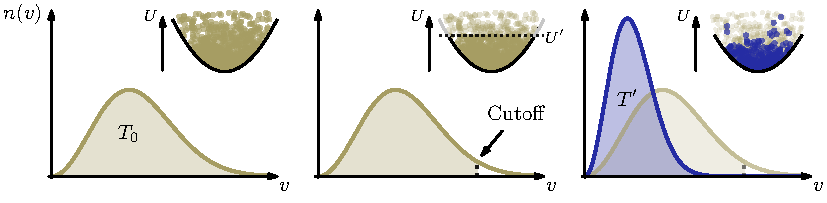
\includegraphics[clip, trim=0 4px 0 0]{Evap/EvaporationSketch1}
    % %% Creator: Matplotlib, PGF backend
%%
%% To include the figure in your LaTeX document, write
%%   \input{<filename>.pgf}
%%
%% Make sure the required packages are loaded in your preamble
%%   \usepackage{pgf}
%%
%% and, on pdftex
%%   \usepackage[utf8]{inputenc}\DeclareUnicodeCharacter{2212}{-}
%%
%% or, on luatex and xetex
%%   \usepackage{unicode-math}
%%
%% Figures using additional raster images can only be included by \input if
%% they are in the same directory as the main LaTeX file. For loading figures
%% from other directories you can use the `import` package
%%   \usepackage{import}
%%
%% and then include the figures with
%%   \import{<path to file>}{<filename>.pgf}
%%
%% Matplotlib used the following preamble
%%   \usepackage[utf8]{inputenc}
%%   \usepackage[T1]{fontenc}
%%   \usepackage[detect-all,locale=UK]{siunitx}
%%   \usepackage{amsmath}
%%   \DeclareUnicodeCharacter{2212}{$-$}
%%   \usepackage{lmodern}
%%
\begingroup%
\makeatletter%
\begin{pgfpicture}%
\pgfpathrectangle{\pgfpointorigin}{\pgfqpoint{5.495882in}{2.419444in}}%
\pgfusepath{use as bounding box, clip}%
\begin{pgfscope}%
\pgfsetbuttcap%
\pgfsetmiterjoin%
\definecolor{currentfill}{rgb}{1.000000,1.000000,1.000000}%
\pgfsetfillcolor{currentfill}%
\pgfsetlinewidth{0.000000pt}%
\definecolor{currentstroke}{rgb}{1.000000,1.000000,1.000000}%
\pgfsetstrokecolor{currentstroke}%
\pgfsetdash{}{0pt}%
\pgfpathmoveto{\pgfqpoint{0.000000in}{0.000000in}}%
\pgfpathlineto{\pgfqpoint{5.495882in}{0.000000in}}%
\pgfpathlineto{\pgfqpoint{5.495882in}{2.419444in}}%
\pgfpathlineto{\pgfqpoint{0.000000in}{2.419444in}}%
\pgfpathclose%
\pgfusepath{fill}%
\end{pgfscope}%
\begin{pgfscope}%
\pgfpathrectangle{\pgfqpoint{0.328148in}{1.094706in}}{\pgfqpoint{1.481618in}{1.235294in}}%
\pgfusepath{clip}%
\pgfsetbuttcap%
\pgfsetroundjoin%
\definecolor{currentfill}{rgb}{0.650000,0.617429,0.389354}%
\pgfsetfillcolor{currentfill}%
\pgfsetfillopacity{0.300000}%
\pgfsetlinewidth{1.003750pt}%
\definecolor{currentstroke}{rgb}{0.650000,0.617429,0.389354}%
\pgfsetstrokecolor{currentstroke}%
\pgfsetstrokeopacity{0.300000}%
\pgfsetdash{}{0pt}%
\pgfsys@defobject{currentmarker}{\pgfqpoint{0.328148in}{1.094706in}}{\pgfqpoint{1.809766in}{1.711798in}}{%
\pgfpathmoveto{\pgfqpoint{0.328148in}{1.094706in}}%
\pgfpathlineto{\pgfqpoint{0.328148in}{1.094706in}}%
\pgfpathlineto{\pgfqpoint{0.331861in}{1.094792in}}%
\pgfpathlineto{\pgfqpoint{0.335575in}{1.095052in}}%
\pgfpathlineto{\pgfqpoint{0.339288in}{1.095483in}}%
\pgfpathlineto{\pgfqpoint{0.343001in}{1.096088in}}%
\pgfpathlineto{\pgfqpoint{0.346715in}{1.096864in}}%
\pgfpathlineto{\pgfqpoint{0.350428in}{1.097812in}}%
\pgfpathlineto{\pgfqpoint{0.354141in}{1.098931in}}%
\pgfpathlineto{\pgfqpoint{0.357855in}{1.100220in}}%
\pgfpathlineto{\pgfqpoint{0.361568in}{1.101678in}}%
\pgfpathlineto{\pgfqpoint{0.365281in}{1.103305in}}%
\pgfpathlineto{\pgfqpoint{0.368995in}{1.105100in}}%
\pgfpathlineto{\pgfqpoint{0.372708in}{1.107061in}}%
\pgfpathlineto{\pgfqpoint{0.376421in}{1.109187in}}%
\pgfpathlineto{\pgfqpoint{0.380135in}{1.111477in}}%
\pgfpathlineto{\pgfqpoint{0.383848in}{1.113930in}}%
\pgfpathlineto{\pgfqpoint{0.387561in}{1.116544in}}%
\pgfpathlineto{\pgfqpoint{0.391275in}{1.119317in}}%
\pgfpathlineto{\pgfqpoint{0.394988in}{1.122248in}}%
\pgfpathlineto{\pgfqpoint{0.398701in}{1.125335in}}%
\pgfpathlineto{\pgfqpoint{0.402415in}{1.128576in}}%
\pgfpathlineto{\pgfqpoint{0.406128in}{1.131969in}}%
\pgfpathlineto{\pgfqpoint{0.409841in}{1.135511in}}%
\pgfpathlineto{\pgfqpoint{0.413555in}{1.139202in}}%
\pgfpathlineto{\pgfqpoint{0.417268in}{1.143038in}}%
\pgfpathlineto{\pgfqpoint{0.420981in}{1.147017in}}%
\pgfpathlineto{\pgfqpoint{0.424695in}{1.151138in}}%
\pgfpathlineto{\pgfqpoint{0.428408in}{1.155396in}}%
\pgfpathlineto{\pgfqpoint{0.432121in}{1.159790in}}%
\pgfpathlineto{\pgfqpoint{0.435835in}{1.164317in}}%
\pgfpathlineto{\pgfqpoint{0.439548in}{1.168975in}}%
\pgfpathlineto{\pgfqpoint{0.443261in}{1.173759in}}%
\pgfpathlineto{\pgfqpoint{0.446975in}{1.178669in}}%
\pgfpathlineto{\pgfqpoint{0.450688in}{1.183700in}}%
\pgfpathlineto{\pgfqpoint{0.454401in}{1.188850in}}%
\pgfpathlineto{\pgfqpoint{0.458115in}{1.194115in}}%
\pgfpathlineto{\pgfqpoint{0.461828in}{1.199493in}}%
\pgfpathlineto{\pgfqpoint{0.465541in}{1.204979in}}%
\pgfpathlineto{\pgfqpoint{0.469255in}{1.210572in}}%
\pgfpathlineto{\pgfqpoint{0.472968in}{1.216267in}}%
\pgfpathlineto{\pgfqpoint{0.476681in}{1.222061in}}%
\pgfpathlineto{\pgfqpoint{0.480395in}{1.227952in}}%
\pgfpathlineto{\pgfqpoint{0.484108in}{1.233934in}}%
\pgfpathlineto{\pgfqpoint{0.487821in}{1.240005in}}%
\pgfpathlineto{\pgfqpoint{0.491535in}{1.246161in}}%
\pgfpathlineto{\pgfqpoint{0.495248in}{1.252399in}}%
\pgfpathlineto{\pgfqpoint{0.498961in}{1.258714in}}%
\pgfpathlineto{\pgfqpoint{0.502675in}{1.265104in}}%
\pgfpathlineto{\pgfqpoint{0.506388in}{1.271564in}}%
\pgfpathlineto{\pgfqpoint{0.510101in}{1.278091in}}%
\pgfpathlineto{\pgfqpoint{0.513814in}{1.284681in}}%
\pgfpathlineto{\pgfqpoint{0.517528in}{1.291330in}}%
\pgfpathlineto{\pgfqpoint{0.521241in}{1.298034in}}%
\pgfpathlineto{\pgfqpoint{0.524954in}{1.304790in}}%
\pgfpathlineto{\pgfqpoint{0.528668in}{1.311594in}}%
\pgfpathlineto{\pgfqpoint{0.532381in}{1.318441in}}%
\pgfpathlineto{\pgfqpoint{0.536094in}{1.325328in}}%
\pgfpathlineto{\pgfqpoint{0.539808in}{1.332250in}}%
\pgfpathlineto{\pgfqpoint{0.543521in}{1.339205in}}%
\pgfpathlineto{\pgfqpoint{0.547234in}{1.346188in}}%
\pgfpathlineto{\pgfqpoint{0.550948in}{1.353195in}}%
\pgfpathlineto{\pgfqpoint{0.554661in}{1.360223in}}%
\pgfpathlineto{\pgfqpoint{0.558374in}{1.367266in}}%
\pgfpathlineto{\pgfqpoint{0.562088in}{1.374323in}}%
\pgfpathlineto{\pgfqpoint{0.565801in}{1.381388in}}%
\pgfpathlineto{\pgfqpoint{0.569514in}{1.388457in}}%
\pgfpathlineto{\pgfqpoint{0.573228in}{1.395528in}}%
\pgfpathlineto{\pgfqpoint{0.576941in}{1.402595in}}%
\pgfpathlineto{\pgfqpoint{0.580654in}{1.409656in}}%
\pgfpathlineto{\pgfqpoint{0.584368in}{1.416706in}}%
\pgfpathlineto{\pgfqpoint{0.588081in}{1.423742in}}%
\pgfpathlineto{\pgfqpoint{0.591794in}{1.430760in}}%
\pgfpathlineto{\pgfqpoint{0.595508in}{1.437755in}}%
\pgfpathlineto{\pgfqpoint{0.599221in}{1.444726in}}%
\pgfpathlineto{\pgfqpoint{0.602934in}{1.451667in}}%
\pgfpathlineto{\pgfqpoint{0.606648in}{1.458575in}}%
\pgfpathlineto{\pgfqpoint{0.610361in}{1.465447in}}%
\pgfpathlineto{\pgfqpoint{0.614074in}{1.472279in}}%
\pgfpathlineto{\pgfqpoint{0.617788in}{1.479068in}}%
\pgfpathlineto{\pgfqpoint{0.621501in}{1.485809in}}%
\pgfpathlineto{\pgfqpoint{0.625214in}{1.492501in}}%
\pgfpathlineto{\pgfqpoint{0.628928in}{1.499138in}}%
\pgfpathlineto{\pgfqpoint{0.632641in}{1.505719in}}%
\pgfpathlineto{\pgfqpoint{0.636354in}{1.512240in}}%
\pgfpathlineto{\pgfqpoint{0.640068in}{1.518697in}}%
\pgfpathlineto{\pgfqpoint{0.643781in}{1.525088in}}%
\pgfpathlineto{\pgfqpoint{0.647494in}{1.531409in}}%
\pgfpathlineto{\pgfqpoint{0.651208in}{1.537658in}}%
\pgfpathlineto{\pgfqpoint{0.654921in}{1.543831in}}%
\pgfpathlineto{\pgfqpoint{0.658634in}{1.549925in}}%
\pgfpathlineto{\pgfqpoint{0.662348in}{1.555938in}}%
\pgfpathlineto{\pgfqpoint{0.666061in}{1.561867in}}%
\pgfpathlineto{\pgfqpoint{0.669774in}{1.567710in}}%
\pgfpathlineto{\pgfqpoint{0.673488in}{1.573462in}}%
\pgfpathlineto{\pgfqpoint{0.677201in}{1.579123in}}%
\pgfpathlineto{\pgfqpoint{0.680914in}{1.584690in}}%
\pgfpathlineto{\pgfqpoint{0.684628in}{1.590159in}}%
\pgfpathlineto{\pgfqpoint{0.688341in}{1.595529in}}%
\pgfpathlineto{\pgfqpoint{0.692054in}{1.600797in}}%
\pgfpathlineto{\pgfqpoint{0.695768in}{1.605962in}}%
\pgfpathlineto{\pgfqpoint{0.699481in}{1.611021in}}%
\pgfpathlineto{\pgfqpoint{0.703194in}{1.615972in}}%
\pgfpathlineto{\pgfqpoint{0.706908in}{1.620813in}}%
\pgfpathlineto{\pgfqpoint{0.710621in}{1.625542in}}%
\pgfpathlineto{\pgfqpoint{0.714334in}{1.630158in}}%
\pgfpathlineto{\pgfqpoint{0.718047in}{1.634658in}}%
\pgfpathlineto{\pgfqpoint{0.721761in}{1.639041in}}%
\pgfpathlineto{\pgfqpoint{0.725474in}{1.643305in}}%
\pgfpathlineto{\pgfqpoint{0.729187in}{1.647450in}}%
\pgfpathlineto{\pgfqpoint{0.732901in}{1.651472in}}%
\pgfpathlineto{\pgfqpoint{0.736614in}{1.655372in}}%
\pgfpathlineto{\pgfqpoint{0.740327in}{1.659148in}}%
\pgfpathlineto{\pgfqpoint{0.744041in}{1.662798in}}%
\pgfpathlineto{\pgfqpoint{0.747754in}{1.666322in}}%
\pgfpathlineto{\pgfqpoint{0.751467in}{1.669718in}}%
\pgfpathlineto{\pgfqpoint{0.755181in}{1.672986in}}%
\pgfpathlineto{\pgfqpoint{0.758894in}{1.676125in}}%
\pgfpathlineto{\pgfqpoint{0.762607in}{1.679133in}}%
\pgfpathlineto{\pgfqpoint{0.766321in}{1.682011in}}%
\pgfpathlineto{\pgfqpoint{0.770034in}{1.684758in}}%
\pgfpathlineto{\pgfqpoint{0.773747in}{1.687372in}}%
\pgfpathlineto{\pgfqpoint{0.777461in}{1.689854in}}%
\pgfpathlineto{\pgfqpoint{0.781174in}{1.692203in}}%
\pgfpathlineto{\pgfqpoint{0.784887in}{1.694419in}}%
\pgfpathlineto{\pgfqpoint{0.788601in}{1.696502in}}%
\pgfpathlineto{\pgfqpoint{0.792314in}{1.698451in}}%
\pgfpathlineto{\pgfqpoint{0.796027in}{1.700266in}}%
\pgfpathlineto{\pgfqpoint{0.799741in}{1.701948in}}%
\pgfpathlineto{\pgfqpoint{0.803454in}{1.703496in}}%
\pgfpathlineto{\pgfqpoint{0.807167in}{1.704911in}}%
\pgfpathlineto{\pgfqpoint{0.810881in}{1.706192in}}%
\pgfpathlineto{\pgfqpoint{0.814594in}{1.707341in}}%
\pgfpathlineto{\pgfqpoint{0.818307in}{1.708357in}}%
\pgfpathlineto{\pgfqpoint{0.822021in}{1.709241in}}%
\pgfpathlineto{\pgfqpoint{0.825734in}{1.709993in}}%
\pgfpathlineto{\pgfqpoint{0.829447in}{1.710614in}}%
\pgfpathlineto{\pgfqpoint{0.833161in}{1.711104in}}%
\pgfpathlineto{\pgfqpoint{0.836874in}{1.711464in}}%
\pgfpathlineto{\pgfqpoint{0.840587in}{1.711696in}}%
\pgfpathlineto{\pgfqpoint{0.844301in}{1.711798in}}%
\pgfpathlineto{\pgfqpoint{0.848014in}{1.711774in}}%
\pgfpathlineto{\pgfqpoint{0.851727in}{1.711623in}}%
\pgfpathlineto{\pgfqpoint{0.855441in}{1.711346in}}%
\pgfpathlineto{\pgfqpoint{0.859154in}{1.710945in}}%
\pgfpathlineto{\pgfqpoint{0.862867in}{1.710421in}}%
\pgfpathlineto{\pgfqpoint{0.866581in}{1.709774in}}%
\pgfpathlineto{\pgfqpoint{0.870294in}{1.709006in}}%
\pgfpathlineto{\pgfqpoint{0.874007in}{1.708118in}}%
\pgfpathlineto{\pgfqpoint{0.877721in}{1.707112in}}%
\pgfpathlineto{\pgfqpoint{0.881434in}{1.705988in}}%
\pgfpathlineto{\pgfqpoint{0.885147in}{1.704749in}}%
\pgfpathlineto{\pgfqpoint{0.888861in}{1.703396in}}%
\pgfpathlineto{\pgfqpoint{0.892574in}{1.701929in}}%
\pgfpathlineto{\pgfqpoint{0.896287in}{1.700351in}}%
\pgfpathlineto{\pgfqpoint{0.900001in}{1.698664in}}%
\pgfpathlineto{\pgfqpoint{0.903714in}{1.696868in}}%
\pgfpathlineto{\pgfqpoint{0.907427in}{1.694966in}}%
\pgfpathlineto{\pgfqpoint{0.911141in}{1.692959in}}%
\pgfpathlineto{\pgfqpoint{0.914854in}{1.690849in}}%
\pgfpathlineto{\pgfqpoint{0.918567in}{1.688638in}}%
\pgfpathlineto{\pgfqpoint{0.922281in}{1.686326in}}%
\pgfpathlineto{\pgfqpoint{0.925994in}{1.683918in}}%
\pgfpathlineto{\pgfqpoint{0.929707in}{1.681413in}}%
\pgfpathlineto{\pgfqpoint{0.933420in}{1.678814in}}%
\pgfpathlineto{\pgfqpoint{0.937134in}{1.676123in}}%
\pgfpathlineto{\pgfqpoint{0.940847in}{1.673342in}}%
\pgfpathlineto{\pgfqpoint{0.944560in}{1.670472in}}%
\pgfpathlineto{\pgfqpoint{0.948274in}{1.667516in}}%
\pgfpathlineto{\pgfqpoint{0.951987in}{1.664476in}}%
\pgfpathlineto{\pgfqpoint{0.955700in}{1.661353in}}%
\pgfpathlineto{\pgfqpoint{0.959414in}{1.658150in}}%
\pgfpathlineto{\pgfqpoint{0.963127in}{1.654868in}}%
\pgfpathlineto{\pgfqpoint{0.966840in}{1.651510in}}%
\pgfpathlineto{\pgfqpoint{0.970554in}{1.648078in}}%
\pgfpathlineto{\pgfqpoint{0.974267in}{1.644573in}}%
\pgfpathlineto{\pgfqpoint{0.977980in}{1.640998in}}%
\pgfpathlineto{\pgfqpoint{0.981694in}{1.637355in}}%
\pgfpathlineto{\pgfqpoint{0.985407in}{1.633646in}}%
\pgfpathlineto{\pgfqpoint{0.989120in}{1.629873in}}%
\pgfpathlineto{\pgfqpoint{0.992834in}{1.626039in}}%
\pgfpathlineto{\pgfqpoint{0.996547in}{1.622144in}}%
\pgfpathlineto{\pgfqpoint{1.000260in}{1.618192in}}%
\pgfpathlineto{\pgfqpoint{1.003974in}{1.614184in}}%
\pgfpathlineto{\pgfqpoint{1.007687in}{1.610122in}}%
\pgfpathlineto{\pgfqpoint{1.011400in}{1.606009in}}%
\pgfpathlineto{\pgfqpoint{1.015114in}{1.601846in}}%
\pgfpathlineto{\pgfqpoint{1.018827in}{1.597637in}}%
\pgfpathlineto{\pgfqpoint{1.022540in}{1.593382in}}%
\pgfpathlineto{\pgfqpoint{1.026254in}{1.589083in}}%
\pgfpathlineto{\pgfqpoint{1.029967in}{1.584744in}}%
\pgfpathlineto{\pgfqpoint{1.033680in}{1.580365in}}%
\pgfpathlineto{\pgfqpoint{1.037394in}{1.575949in}}%
\pgfpathlineto{\pgfqpoint{1.041107in}{1.571498in}}%
\pgfpathlineto{\pgfqpoint{1.044820in}{1.567014in}}%
\pgfpathlineto{\pgfqpoint{1.048534in}{1.562499in}}%
\pgfpathlineto{\pgfqpoint{1.052247in}{1.557955in}}%
\pgfpathlineto{\pgfqpoint{1.055960in}{1.553383in}}%
\pgfpathlineto{\pgfqpoint{1.059674in}{1.548786in}}%
\pgfpathlineto{\pgfqpoint{1.063387in}{1.544165in}}%
\pgfpathlineto{\pgfqpoint{1.067100in}{1.539523in}}%
\pgfpathlineto{\pgfqpoint{1.070814in}{1.534862in}}%
\pgfpathlineto{\pgfqpoint{1.074527in}{1.530182in}}%
\pgfpathlineto{\pgfqpoint{1.078240in}{1.525487in}}%
\pgfpathlineto{\pgfqpoint{1.081954in}{1.520777in}}%
\pgfpathlineto{\pgfqpoint{1.085667in}{1.516055in}}%
\pgfpathlineto{\pgfqpoint{1.089380in}{1.511323in}}%
\pgfpathlineto{\pgfqpoint{1.093094in}{1.506581in}}%
\pgfpathlineto{\pgfqpoint{1.096807in}{1.501833in}}%
\pgfpathlineto{\pgfqpoint{1.100520in}{1.497078in}}%
\pgfpathlineto{\pgfqpoint{1.104234in}{1.492320in}}%
\pgfpathlineto{\pgfqpoint{1.107947in}{1.487560in}}%
\pgfpathlineto{\pgfqpoint{1.111660in}{1.482799in}}%
\pgfpathlineto{\pgfqpoint{1.115374in}{1.478039in}}%
\pgfpathlineto{\pgfqpoint{1.119087in}{1.473282in}}%
\pgfpathlineto{\pgfqpoint{1.122800in}{1.468529in}}%
\pgfpathlineto{\pgfqpoint{1.126514in}{1.463781in}}%
\pgfpathlineto{\pgfqpoint{1.130227in}{1.459040in}}%
\pgfpathlineto{\pgfqpoint{1.133940in}{1.454307in}}%
\pgfpathlineto{\pgfqpoint{1.137653in}{1.449585in}}%
\pgfpathlineto{\pgfqpoint{1.141367in}{1.444873in}}%
\pgfpathlineto{\pgfqpoint{1.145080in}{1.440175in}}%
\pgfpathlineto{\pgfqpoint{1.148793in}{1.435490in}}%
\pgfpathlineto{\pgfqpoint{1.152507in}{1.430820in}}%
\pgfpathlineto{\pgfqpoint{1.156220in}{1.426166in}}%
\pgfpathlineto{\pgfqpoint{1.159933in}{1.421530in}}%
\pgfpathlineto{\pgfqpoint{1.163647in}{1.416913in}}%
\pgfpathlineto{\pgfqpoint{1.167360in}{1.412316in}}%
\pgfpathlineto{\pgfqpoint{1.171073in}{1.407740in}}%
\pgfpathlineto{\pgfqpoint{1.174787in}{1.403186in}}%
\pgfpathlineto{\pgfqpoint{1.178500in}{1.398655in}}%
\pgfpathlineto{\pgfqpoint{1.182213in}{1.394149in}}%
\pgfpathlineto{\pgfqpoint{1.185927in}{1.389667in}}%
\pgfpathlineto{\pgfqpoint{1.189640in}{1.385212in}}%
\pgfpathlineto{\pgfqpoint{1.193353in}{1.380785in}}%
\pgfpathlineto{\pgfqpoint{1.197067in}{1.376385in}}%
\pgfpathlineto{\pgfqpoint{1.200780in}{1.372014in}}%
\pgfpathlineto{\pgfqpoint{1.204493in}{1.367673in}}%
\pgfpathlineto{\pgfqpoint{1.208207in}{1.363363in}}%
\pgfpathlineto{\pgfqpoint{1.211920in}{1.359084in}}%
\pgfpathlineto{\pgfqpoint{1.215633in}{1.354837in}}%
\pgfpathlineto{\pgfqpoint{1.219347in}{1.350623in}}%
\pgfpathlineto{\pgfqpoint{1.223060in}{1.346443in}}%
\pgfpathlineto{\pgfqpoint{1.226773in}{1.342297in}}%
\pgfpathlineto{\pgfqpoint{1.230487in}{1.338185in}}%
\pgfpathlineto{\pgfqpoint{1.234200in}{1.334110in}}%
\pgfpathlineto{\pgfqpoint{1.237913in}{1.330070in}}%
\pgfpathlineto{\pgfqpoint{1.241627in}{1.326067in}}%
\pgfpathlineto{\pgfqpoint{1.245340in}{1.322101in}}%
\pgfpathlineto{\pgfqpoint{1.249053in}{1.318173in}}%
\pgfpathlineto{\pgfqpoint{1.252767in}{1.314282in}}%
\pgfpathlineto{\pgfqpoint{1.256480in}{1.310431in}}%
\pgfpathlineto{\pgfqpoint{1.260193in}{1.306618in}}%
\pgfpathlineto{\pgfqpoint{1.263907in}{1.302845in}}%
\pgfpathlineto{\pgfqpoint{1.267620in}{1.299111in}}%
\pgfpathlineto{\pgfqpoint{1.271333in}{1.295417in}}%
\pgfpathlineto{\pgfqpoint{1.275047in}{1.291764in}}%
\pgfpathlineto{\pgfqpoint{1.278760in}{1.288151in}}%
\pgfpathlineto{\pgfqpoint{1.282473in}{1.284579in}}%
\pgfpathlineto{\pgfqpoint{1.286187in}{1.281048in}}%
\pgfpathlineto{\pgfqpoint{1.289900in}{1.277559in}}%
\pgfpathlineto{\pgfqpoint{1.293613in}{1.274111in}}%
\pgfpathlineto{\pgfqpoint{1.297327in}{1.270704in}}%
\pgfpathlineto{\pgfqpoint{1.301040in}{1.267340in}}%
\pgfpathlineto{\pgfqpoint{1.304753in}{1.264017in}}%
\pgfpathlineto{\pgfqpoint{1.308467in}{1.260737in}}%
\pgfpathlineto{\pgfqpoint{1.312180in}{1.257498in}}%
\pgfpathlineto{\pgfqpoint{1.315893in}{1.254302in}}%
\pgfpathlineto{\pgfqpoint{1.319607in}{1.251148in}}%
\pgfpathlineto{\pgfqpoint{1.323320in}{1.248036in}}%
\pgfpathlineto{\pgfqpoint{1.327033in}{1.244967in}}%
\pgfpathlineto{\pgfqpoint{1.330747in}{1.241939in}}%
\pgfpathlineto{\pgfqpoint{1.334460in}{1.238954in}}%
\pgfpathlineto{\pgfqpoint{1.338173in}{1.236011in}}%
\pgfpathlineto{\pgfqpoint{1.341887in}{1.233110in}}%
\pgfpathlineto{\pgfqpoint{1.345600in}{1.230251in}}%
\pgfpathlineto{\pgfqpoint{1.349313in}{1.227434in}}%
\pgfpathlineto{\pgfqpoint{1.353026in}{1.224658in}}%
\pgfpathlineto{\pgfqpoint{1.356740in}{1.221924in}}%
\pgfpathlineto{\pgfqpoint{1.360453in}{1.219232in}}%
\pgfpathlineto{\pgfqpoint{1.364166in}{1.216580in}}%
\pgfpathlineto{\pgfqpoint{1.367880in}{1.213970in}}%
\pgfpathlineto{\pgfqpoint{1.371593in}{1.211401in}}%
\pgfpathlineto{\pgfqpoint{1.375306in}{1.208873in}}%
\pgfpathlineto{\pgfqpoint{1.379020in}{1.206384in}}%
\pgfpathlineto{\pgfqpoint{1.382733in}{1.203937in}}%
\pgfpathlineto{\pgfqpoint{1.386446in}{1.201529in}}%
\pgfpathlineto{\pgfqpoint{1.390160in}{1.199161in}}%
\pgfpathlineto{\pgfqpoint{1.393873in}{1.196832in}}%
\pgfpathlineto{\pgfqpoint{1.397586in}{1.194543in}}%
\pgfpathlineto{\pgfqpoint{1.401300in}{1.192292in}}%
\pgfpathlineto{\pgfqpoint{1.405013in}{1.190080in}}%
\pgfpathlineto{\pgfqpoint{1.408726in}{1.187906in}}%
\pgfpathlineto{\pgfqpoint{1.412440in}{1.185771in}}%
\pgfpathlineto{\pgfqpoint{1.416153in}{1.183673in}}%
\pgfpathlineto{\pgfqpoint{1.419866in}{1.181612in}}%
\pgfpathlineto{\pgfqpoint{1.423580in}{1.179589in}}%
\pgfpathlineto{\pgfqpoint{1.427293in}{1.177602in}}%
\pgfpathlineto{\pgfqpoint{1.431006in}{1.175651in}}%
\pgfpathlineto{\pgfqpoint{1.434720in}{1.173737in}}%
\pgfpathlineto{\pgfqpoint{1.438433in}{1.171858in}}%
\pgfpathlineto{\pgfqpoint{1.442146in}{1.170014in}}%
\pgfpathlineto{\pgfqpoint{1.445860in}{1.168205in}}%
\pgfpathlineto{\pgfqpoint{1.449573in}{1.166431in}}%
\pgfpathlineto{\pgfqpoint{1.453286in}{1.164690in}}%
\pgfpathlineto{\pgfqpoint{1.457000in}{1.162984in}}%
\pgfpathlineto{\pgfqpoint{1.460713in}{1.161310in}}%
\pgfpathlineto{\pgfqpoint{1.464426in}{1.159670in}}%
\pgfpathlineto{\pgfqpoint{1.468140in}{1.158062in}}%
\pgfpathlineto{\pgfqpoint{1.471853in}{1.156486in}}%
\pgfpathlineto{\pgfqpoint{1.475566in}{1.154942in}}%
\pgfpathlineto{\pgfqpoint{1.479280in}{1.153429in}}%
\pgfpathlineto{\pgfqpoint{1.482993in}{1.151947in}}%
\pgfpathlineto{\pgfqpoint{1.486706in}{1.150496in}}%
\pgfpathlineto{\pgfqpoint{1.490420in}{1.149075in}}%
\pgfpathlineto{\pgfqpoint{1.494133in}{1.147683in}}%
\pgfpathlineto{\pgfqpoint{1.497846in}{1.146321in}}%
\pgfpathlineto{\pgfqpoint{1.501560in}{1.144987in}}%
\pgfpathlineto{\pgfqpoint{1.505273in}{1.143682in}}%
\pgfpathlineto{\pgfqpoint{1.508986in}{1.142405in}}%
\pgfpathlineto{\pgfqpoint{1.512700in}{1.141155in}}%
\pgfpathlineto{\pgfqpoint{1.516413in}{1.139933in}}%
\pgfpathlineto{\pgfqpoint{1.520126in}{1.138738in}}%
\pgfpathlineto{\pgfqpoint{1.523840in}{1.137568in}}%
\pgfpathlineto{\pgfqpoint{1.527553in}{1.136425in}}%
\pgfpathlineto{\pgfqpoint{1.531266in}{1.135307in}}%
\pgfpathlineto{\pgfqpoint{1.534980in}{1.134215in}}%
\pgfpathlineto{\pgfqpoint{1.538693in}{1.133147in}}%
\pgfpathlineto{\pgfqpoint{1.542406in}{1.132103in}}%
\pgfpathlineto{\pgfqpoint{1.546120in}{1.131084in}}%
\pgfpathlineto{\pgfqpoint{1.549833in}{1.130087in}}%
\pgfpathlineto{\pgfqpoint{1.553546in}{1.129114in}}%
\pgfpathlineto{\pgfqpoint{1.557259in}{1.128164in}}%
\pgfpathlineto{\pgfqpoint{1.560973in}{1.127236in}}%
\pgfpathlineto{\pgfqpoint{1.564686in}{1.126330in}}%
\pgfpathlineto{\pgfqpoint{1.568399in}{1.125445in}}%
\pgfpathlineto{\pgfqpoint{1.572113in}{1.124581in}}%
\pgfpathlineto{\pgfqpoint{1.575826in}{1.123739in}}%
\pgfpathlineto{\pgfqpoint{1.579539in}{1.122916in}}%
\pgfpathlineto{\pgfqpoint{1.583253in}{1.122114in}}%
\pgfpathlineto{\pgfqpoint{1.586966in}{1.121331in}}%
\pgfpathlineto{\pgfqpoint{1.590679in}{1.120568in}}%
\pgfpathlineto{\pgfqpoint{1.594393in}{1.119823in}}%
\pgfpathlineto{\pgfqpoint{1.598106in}{1.119097in}}%
\pgfpathlineto{\pgfqpoint{1.601819in}{1.118389in}}%
\pgfpathlineto{\pgfqpoint{1.605533in}{1.117698in}}%
\pgfpathlineto{\pgfqpoint{1.609246in}{1.117026in}}%
\pgfpathlineto{\pgfqpoint{1.612959in}{1.116370in}}%
\pgfpathlineto{\pgfqpoint{1.616673in}{1.115731in}}%
\pgfpathlineto{\pgfqpoint{1.620386in}{1.115108in}}%
\pgfpathlineto{\pgfqpoint{1.624099in}{1.114502in}}%
\pgfpathlineto{\pgfqpoint{1.627813in}{1.113911in}}%
\pgfpathlineto{\pgfqpoint{1.631526in}{1.113336in}}%
\pgfpathlineto{\pgfqpoint{1.635239in}{1.112775in}}%
\pgfpathlineto{\pgfqpoint{1.638953in}{1.112230in}}%
\pgfpathlineto{\pgfqpoint{1.642666in}{1.111699in}}%
\pgfpathlineto{\pgfqpoint{1.646379in}{1.111182in}}%
\pgfpathlineto{\pgfqpoint{1.650093in}{1.110679in}}%
\pgfpathlineto{\pgfqpoint{1.653806in}{1.110189in}}%
\pgfpathlineto{\pgfqpoint{1.657519in}{1.109713in}}%
\pgfpathlineto{\pgfqpoint{1.661233in}{1.109249in}}%
\pgfpathlineto{\pgfqpoint{1.664946in}{1.108799in}}%
\pgfpathlineto{\pgfqpoint{1.668659in}{1.108360in}}%
\pgfpathlineto{\pgfqpoint{1.672373in}{1.107934in}}%
\pgfpathlineto{\pgfqpoint{1.676086in}{1.107519in}}%
\pgfpathlineto{\pgfqpoint{1.679799in}{1.107116in}}%
\pgfpathlineto{\pgfqpoint{1.683513in}{1.106725in}}%
\pgfpathlineto{\pgfqpoint{1.687226in}{1.106344in}}%
\pgfpathlineto{\pgfqpoint{1.690939in}{1.105974in}}%
\pgfpathlineto{\pgfqpoint{1.694653in}{1.105614in}}%
\pgfpathlineto{\pgfqpoint{1.698366in}{1.105265in}}%
\pgfpathlineto{\pgfqpoint{1.702079in}{1.104925in}}%
\pgfpathlineto{\pgfqpoint{1.705793in}{1.104596in}}%
\pgfpathlineto{\pgfqpoint{1.709506in}{1.104276in}}%
\pgfpathlineto{\pgfqpoint{1.713219in}{1.103965in}}%
\pgfpathlineto{\pgfqpoint{1.716933in}{1.103663in}}%
\pgfpathlineto{\pgfqpoint{1.720646in}{1.103370in}}%
\pgfpathlineto{\pgfqpoint{1.724359in}{1.103086in}}%
\pgfpathlineto{\pgfqpoint{1.728073in}{1.102810in}}%
\pgfpathlineto{\pgfqpoint{1.731786in}{1.102542in}}%
\pgfpathlineto{\pgfqpoint{1.735499in}{1.102282in}}%
\pgfpathlineto{\pgfqpoint{1.739213in}{1.102030in}}%
\pgfpathlineto{\pgfqpoint{1.742926in}{1.101785in}}%
\pgfpathlineto{\pgfqpoint{1.746639in}{1.101548in}}%
\pgfpathlineto{\pgfqpoint{1.750353in}{1.101318in}}%
\pgfpathlineto{\pgfqpoint{1.754066in}{1.101095in}}%
\pgfpathlineto{\pgfqpoint{1.757779in}{1.100879in}}%
\pgfpathlineto{\pgfqpoint{1.761493in}{1.100669in}}%
\pgfpathlineto{\pgfqpoint{1.765206in}{1.100466in}}%
\pgfpathlineto{\pgfqpoint{1.768919in}{1.100269in}}%
\pgfpathlineto{\pgfqpoint{1.772632in}{1.100079in}}%
\pgfpathlineto{\pgfqpoint{1.776346in}{1.099894in}}%
\pgfpathlineto{\pgfqpoint{1.780059in}{1.099715in}}%
\pgfpathlineto{\pgfqpoint{1.783772in}{1.099541in}}%
\pgfpathlineto{\pgfqpoint{1.787486in}{1.099373in}}%
\pgfpathlineto{\pgfqpoint{1.791199in}{1.099211in}}%
\pgfpathlineto{\pgfqpoint{1.794912in}{1.099053in}}%
\pgfpathlineto{\pgfqpoint{1.798626in}{1.098901in}}%
\pgfpathlineto{\pgfqpoint{1.802339in}{1.098753in}}%
\pgfpathlineto{\pgfqpoint{1.806052in}{1.098610in}}%
\pgfpathlineto{\pgfqpoint{1.809766in}{1.098472in}}%
\pgfpathlineto{\pgfqpoint{1.809766in}{1.094706in}}%
\pgfpathlineto{\pgfqpoint{1.809766in}{1.094706in}}%
\pgfpathlineto{\pgfqpoint{1.806052in}{1.094706in}}%
\pgfpathlineto{\pgfqpoint{1.802339in}{1.094706in}}%
\pgfpathlineto{\pgfqpoint{1.798626in}{1.094706in}}%
\pgfpathlineto{\pgfqpoint{1.794912in}{1.094706in}}%
\pgfpathlineto{\pgfqpoint{1.791199in}{1.094706in}}%
\pgfpathlineto{\pgfqpoint{1.787486in}{1.094706in}}%
\pgfpathlineto{\pgfqpoint{1.783772in}{1.094706in}}%
\pgfpathlineto{\pgfqpoint{1.780059in}{1.094706in}}%
\pgfpathlineto{\pgfqpoint{1.776346in}{1.094706in}}%
\pgfpathlineto{\pgfqpoint{1.772632in}{1.094706in}}%
\pgfpathlineto{\pgfqpoint{1.768919in}{1.094706in}}%
\pgfpathlineto{\pgfqpoint{1.765206in}{1.094706in}}%
\pgfpathlineto{\pgfqpoint{1.761493in}{1.094706in}}%
\pgfpathlineto{\pgfqpoint{1.757779in}{1.094706in}}%
\pgfpathlineto{\pgfqpoint{1.754066in}{1.094706in}}%
\pgfpathlineto{\pgfqpoint{1.750353in}{1.094706in}}%
\pgfpathlineto{\pgfqpoint{1.746639in}{1.094706in}}%
\pgfpathlineto{\pgfqpoint{1.742926in}{1.094706in}}%
\pgfpathlineto{\pgfqpoint{1.739213in}{1.094706in}}%
\pgfpathlineto{\pgfqpoint{1.735499in}{1.094706in}}%
\pgfpathlineto{\pgfqpoint{1.731786in}{1.094706in}}%
\pgfpathlineto{\pgfqpoint{1.728073in}{1.094706in}}%
\pgfpathlineto{\pgfqpoint{1.724359in}{1.094706in}}%
\pgfpathlineto{\pgfqpoint{1.720646in}{1.094706in}}%
\pgfpathlineto{\pgfqpoint{1.716933in}{1.094706in}}%
\pgfpathlineto{\pgfqpoint{1.713219in}{1.094706in}}%
\pgfpathlineto{\pgfqpoint{1.709506in}{1.094706in}}%
\pgfpathlineto{\pgfqpoint{1.705793in}{1.094706in}}%
\pgfpathlineto{\pgfqpoint{1.702079in}{1.094706in}}%
\pgfpathlineto{\pgfqpoint{1.698366in}{1.094706in}}%
\pgfpathlineto{\pgfqpoint{1.694653in}{1.094706in}}%
\pgfpathlineto{\pgfqpoint{1.690939in}{1.094706in}}%
\pgfpathlineto{\pgfqpoint{1.687226in}{1.094706in}}%
\pgfpathlineto{\pgfqpoint{1.683513in}{1.094706in}}%
\pgfpathlineto{\pgfqpoint{1.679799in}{1.094706in}}%
\pgfpathlineto{\pgfqpoint{1.676086in}{1.094706in}}%
\pgfpathlineto{\pgfqpoint{1.672373in}{1.094706in}}%
\pgfpathlineto{\pgfqpoint{1.668659in}{1.094706in}}%
\pgfpathlineto{\pgfqpoint{1.664946in}{1.094706in}}%
\pgfpathlineto{\pgfqpoint{1.661233in}{1.094706in}}%
\pgfpathlineto{\pgfqpoint{1.657519in}{1.094706in}}%
\pgfpathlineto{\pgfqpoint{1.653806in}{1.094706in}}%
\pgfpathlineto{\pgfqpoint{1.650093in}{1.094706in}}%
\pgfpathlineto{\pgfqpoint{1.646379in}{1.094706in}}%
\pgfpathlineto{\pgfqpoint{1.642666in}{1.094706in}}%
\pgfpathlineto{\pgfqpoint{1.638953in}{1.094706in}}%
\pgfpathlineto{\pgfqpoint{1.635239in}{1.094706in}}%
\pgfpathlineto{\pgfqpoint{1.631526in}{1.094706in}}%
\pgfpathlineto{\pgfqpoint{1.627813in}{1.094706in}}%
\pgfpathlineto{\pgfqpoint{1.624099in}{1.094706in}}%
\pgfpathlineto{\pgfqpoint{1.620386in}{1.094706in}}%
\pgfpathlineto{\pgfqpoint{1.616673in}{1.094706in}}%
\pgfpathlineto{\pgfqpoint{1.612959in}{1.094706in}}%
\pgfpathlineto{\pgfqpoint{1.609246in}{1.094706in}}%
\pgfpathlineto{\pgfqpoint{1.605533in}{1.094706in}}%
\pgfpathlineto{\pgfqpoint{1.601819in}{1.094706in}}%
\pgfpathlineto{\pgfqpoint{1.598106in}{1.094706in}}%
\pgfpathlineto{\pgfqpoint{1.594393in}{1.094706in}}%
\pgfpathlineto{\pgfqpoint{1.590679in}{1.094706in}}%
\pgfpathlineto{\pgfqpoint{1.586966in}{1.094706in}}%
\pgfpathlineto{\pgfqpoint{1.583253in}{1.094706in}}%
\pgfpathlineto{\pgfqpoint{1.579539in}{1.094706in}}%
\pgfpathlineto{\pgfqpoint{1.575826in}{1.094706in}}%
\pgfpathlineto{\pgfqpoint{1.572113in}{1.094706in}}%
\pgfpathlineto{\pgfqpoint{1.568399in}{1.094706in}}%
\pgfpathlineto{\pgfqpoint{1.564686in}{1.094706in}}%
\pgfpathlineto{\pgfqpoint{1.560973in}{1.094706in}}%
\pgfpathlineto{\pgfqpoint{1.557259in}{1.094706in}}%
\pgfpathlineto{\pgfqpoint{1.553546in}{1.094706in}}%
\pgfpathlineto{\pgfqpoint{1.549833in}{1.094706in}}%
\pgfpathlineto{\pgfqpoint{1.546120in}{1.094706in}}%
\pgfpathlineto{\pgfqpoint{1.542406in}{1.094706in}}%
\pgfpathlineto{\pgfqpoint{1.538693in}{1.094706in}}%
\pgfpathlineto{\pgfqpoint{1.534980in}{1.094706in}}%
\pgfpathlineto{\pgfqpoint{1.531266in}{1.094706in}}%
\pgfpathlineto{\pgfqpoint{1.527553in}{1.094706in}}%
\pgfpathlineto{\pgfqpoint{1.523840in}{1.094706in}}%
\pgfpathlineto{\pgfqpoint{1.520126in}{1.094706in}}%
\pgfpathlineto{\pgfqpoint{1.516413in}{1.094706in}}%
\pgfpathlineto{\pgfqpoint{1.512700in}{1.094706in}}%
\pgfpathlineto{\pgfqpoint{1.508986in}{1.094706in}}%
\pgfpathlineto{\pgfqpoint{1.505273in}{1.094706in}}%
\pgfpathlineto{\pgfqpoint{1.501560in}{1.094706in}}%
\pgfpathlineto{\pgfqpoint{1.497846in}{1.094706in}}%
\pgfpathlineto{\pgfqpoint{1.494133in}{1.094706in}}%
\pgfpathlineto{\pgfqpoint{1.490420in}{1.094706in}}%
\pgfpathlineto{\pgfqpoint{1.486706in}{1.094706in}}%
\pgfpathlineto{\pgfqpoint{1.482993in}{1.094706in}}%
\pgfpathlineto{\pgfqpoint{1.479280in}{1.094706in}}%
\pgfpathlineto{\pgfqpoint{1.475566in}{1.094706in}}%
\pgfpathlineto{\pgfqpoint{1.471853in}{1.094706in}}%
\pgfpathlineto{\pgfqpoint{1.468140in}{1.094706in}}%
\pgfpathlineto{\pgfqpoint{1.464426in}{1.094706in}}%
\pgfpathlineto{\pgfqpoint{1.460713in}{1.094706in}}%
\pgfpathlineto{\pgfqpoint{1.457000in}{1.094706in}}%
\pgfpathlineto{\pgfqpoint{1.453286in}{1.094706in}}%
\pgfpathlineto{\pgfqpoint{1.449573in}{1.094706in}}%
\pgfpathlineto{\pgfqpoint{1.445860in}{1.094706in}}%
\pgfpathlineto{\pgfqpoint{1.442146in}{1.094706in}}%
\pgfpathlineto{\pgfqpoint{1.438433in}{1.094706in}}%
\pgfpathlineto{\pgfqpoint{1.434720in}{1.094706in}}%
\pgfpathlineto{\pgfqpoint{1.431006in}{1.094706in}}%
\pgfpathlineto{\pgfqpoint{1.427293in}{1.094706in}}%
\pgfpathlineto{\pgfqpoint{1.423580in}{1.094706in}}%
\pgfpathlineto{\pgfqpoint{1.419866in}{1.094706in}}%
\pgfpathlineto{\pgfqpoint{1.416153in}{1.094706in}}%
\pgfpathlineto{\pgfqpoint{1.412440in}{1.094706in}}%
\pgfpathlineto{\pgfqpoint{1.408726in}{1.094706in}}%
\pgfpathlineto{\pgfqpoint{1.405013in}{1.094706in}}%
\pgfpathlineto{\pgfqpoint{1.401300in}{1.094706in}}%
\pgfpathlineto{\pgfqpoint{1.397586in}{1.094706in}}%
\pgfpathlineto{\pgfqpoint{1.393873in}{1.094706in}}%
\pgfpathlineto{\pgfqpoint{1.390160in}{1.094706in}}%
\pgfpathlineto{\pgfqpoint{1.386446in}{1.094706in}}%
\pgfpathlineto{\pgfqpoint{1.382733in}{1.094706in}}%
\pgfpathlineto{\pgfqpoint{1.379020in}{1.094706in}}%
\pgfpathlineto{\pgfqpoint{1.375306in}{1.094706in}}%
\pgfpathlineto{\pgfqpoint{1.371593in}{1.094706in}}%
\pgfpathlineto{\pgfqpoint{1.367880in}{1.094706in}}%
\pgfpathlineto{\pgfqpoint{1.364166in}{1.094706in}}%
\pgfpathlineto{\pgfqpoint{1.360453in}{1.094706in}}%
\pgfpathlineto{\pgfqpoint{1.356740in}{1.094706in}}%
\pgfpathlineto{\pgfqpoint{1.353026in}{1.094706in}}%
\pgfpathlineto{\pgfqpoint{1.349313in}{1.094706in}}%
\pgfpathlineto{\pgfqpoint{1.345600in}{1.094706in}}%
\pgfpathlineto{\pgfqpoint{1.341887in}{1.094706in}}%
\pgfpathlineto{\pgfqpoint{1.338173in}{1.094706in}}%
\pgfpathlineto{\pgfqpoint{1.334460in}{1.094706in}}%
\pgfpathlineto{\pgfqpoint{1.330747in}{1.094706in}}%
\pgfpathlineto{\pgfqpoint{1.327033in}{1.094706in}}%
\pgfpathlineto{\pgfqpoint{1.323320in}{1.094706in}}%
\pgfpathlineto{\pgfqpoint{1.319607in}{1.094706in}}%
\pgfpathlineto{\pgfqpoint{1.315893in}{1.094706in}}%
\pgfpathlineto{\pgfqpoint{1.312180in}{1.094706in}}%
\pgfpathlineto{\pgfqpoint{1.308467in}{1.094706in}}%
\pgfpathlineto{\pgfqpoint{1.304753in}{1.094706in}}%
\pgfpathlineto{\pgfqpoint{1.301040in}{1.094706in}}%
\pgfpathlineto{\pgfqpoint{1.297327in}{1.094706in}}%
\pgfpathlineto{\pgfqpoint{1.293613in}{1.094706in}}%
\pgfpathlineto{\pgfqpoint{1.289900in}{1.094706in}}%
\pgfpathlineto{\pgfqpoint{1.286187in}{1.094706in}}%
\pgfpathlineto{\pgfqpoint{1.282473in}{1.094706in}}%
\pgfpathlineto{\pgfqpoint{1.278760in}{1.094706in}}%
\pgfpathlineto{\pgfqpoint{1.275047in}{1.094706in}}%
\pgfpathlineto{\pgfqpoint{1.271333in}{1.094706in}}%
\pgfpathlineto{\pgfqpoint{1.267620in}{1.094706in}}%
\pgfpathlineto{\pgfqpoint{1.263907in}{1.094706in}}%
\pgfpathlineto{\pgfqpoint{1.260193in}{1.094706in}}%
\pgfpathlineto{\pgfqpoint{1.256480in}{1.094706in}}%
\pgfpathlineto{\pgfqpoint{1.252767in}{1.094706in}}%
\pgfpathlineto{\pgfqpoint{1.249053in}{1.094706in}}%
\pgfpathlineto{\pgfqpoint{1.245340in}{1.094706in}}%
\pgfpathlineto{\pgfqpoint{1.241627in}{1.094706in}}%
\pgfpathlineto{\pgfqpoint{1.237913in}{1.094706in}}%
\pgfpathlineto{\pgfqpoint{1.234200in}{1.094706in}}%
\pgfpathlineto{\pgfqpoint{1.230487in}{1.094706in}}%
\pgfpathlineto{\pgfqpoint{1.226773in}{1.094706in}}%
\pgfpathlineto{\pgfqpoint{1.223060in}{1.094706in}}%
\pgfpathlineto{\pgfqpoint{1.219347in}{1.094706in}}%
\pgfpathlineto{\pgfqpoint{1.215633in}{1.094706in}}%
\pgfpathlineto{\pgfqpoint{1.211920in}{1.094706in}}%
\pgfpathlineto{\pgfqpoint{1.208207in}{1.094706in}}%
\pgfpathlineto{\pgfqpoint{1.204493in}{1.094706in}}%
\pgfpathlineto{\pgfqpoint{1.200780in}{1.094706in}}%
\pgfpathlineto{\pgfqpoint{1.197067in}{1.094706in}}%
\pgfpathlineto{\pgfqpoint{1.193353in}{1.094706in}}%
\pgfpathlineto{\pgfqpoint{1.189640in}{1.094706in}}%
\pgfpathlineto{\pgfqpoint{1.185927in}{1.094706in}}%
\pgfpathlineto{\pgfqpoint{1.182213in}{1.094706in}}%
\pgfpathlineto{\pgfqpoint{1.178500in}{1.094706in}}%
\pgfpathlineto{\pgfqpoint{1.174787in}{1.094706in}}%
\pgfpathlineto{\pgfqpoint{1.171073in}{1.094706in}}%
\pgfpathlineto{\pgfqpoint{1.167360in}{1.094706in}}%
\pgfpathlineto{\pgfqpoint{1.163647in}{1.094706in}}%
\pgfpathlineto{\pgfqpoint{1.159933in}{1.094706in}}%
\pgfpathlineto{\pgfqpoint{1.156220in}{1.094706in}}%
\pgfpathlineto{\pgfqpoint{1.152507in}{1.094706in}}%
\pgfpathlineto{\pgfqpoint{1.148793in}{1.094706in}}%
\pgfpathlineto{\pgfqpoint{1.145080in}{1.094706in}}%
\pgfpathlineto{\pgfqpoint{1.141367in}{1.094706in}}%
\pgfpathlineto{\pgfqpoint{1.137653in}{1.094706in}}%
\pgfpathlineto{\pgfqpoint{1.133940in}{1.094706in}}%
\pgfpathlineto{\pgfqpoint{1.130227in}{1.094706in}}%
\pgfpathlineto{\pgfqpoint{1.126514in}{1.094706in}}%
\pgfpathlineto{\pgfqpoint{1.122800in}{1.094706in}}%
\pgfpathlineto{\pgfqpoint{1.119087in}{1.094706in}}%
\pgfpathlineto{\pgfqpoint{1.115374in}{1.094706in}}%
\pgfpathlineto{\pgfqpoint{1.111660in}{1.094706in}}%
\pgfpathlineto{\pgfqpoint{1.107947in}{1.094706in}}%
\pgfpathlineto{\pgfqpoint{1.104234in}{1.094706in}}%
\pgfpathlineto{\pgfqpoint{1.100520in}{1.094706in}}%
\pgfpathlineto{\pgfqpoint{1.096807in}{1.094706in}}%
\pgfpathlineto{\pgfqpoint{1.093094in}{1.094706in}}%
\pgfpathlineto{\pgfqpoint{1.089380in}{1.094706in}}%
\pgfpathlineto{\pgfqpoint{1.085667in}{1.094706in}}%
\pgfpathlineto{\pgfqpoint{1.081954in}{1.094706in}}%
\pgfpathlineto{\pgfqpoint{1.078240in}{1.094706in}}%
\pgfpathlineto{\pgfqpoint{1.074527in}{1.094706in}}%
\pgfpathlineto{\pgfqpoint{1.070814in}{1.094706in}}%
\pgfpathlineto{\pgfqpoint{1.067100in}{1.094706in}}%
\pgfpathlineto{\pgfqpoint{1.063387in}{1.094706in}}%
\pgfpathlineto{\pgfqpoint{1.059674in}{1.094706in}}%
\pgfpathlineto{\pgfqpoint{1.055960in}{1.094706in}}%
\pgfpathlineto{\pgfqpoint{1.052247in}{1.094706in}}%
\pgfpathlineto{\pgfqpoint{1.048534in}{1.094706in}}%
\pgfpathlineto{\pgfqpoint{1.044820in}{1.094706in}}%
\pgfpathlineto{\pgfqpoint{1.041107in}{1.094706in}}%
\pgfpathlineto{\pgfqpoint{1.037394in}{1.094706in}}%
\pgfpathlineto{\pgfqpoint{1.033680in}{1.094706in}}%
\pgfpathlineto{\pgfqpoint{1.029967in}{1.094706in}}%
\pgfpathlineto{\pgfqpoint{1.026254in}{1.094706in}}%
\pgfpathlineto{\pgfqpoint{1.022540in}{1.094706in}}%
\pgfpathlineto{\pgfqpoint{1.018827in}{1.094706in}}%
\pgfpathlineto{\pgfqpoint{1.015114in}{1.094706in}}%
\pgfpathlineto{\pgfqpoint{1.011400in}{1.094706in}}%
\pgfpathlineto{\pgfqpoint{1.007687in}{1.094706in}}%
\pgfpathlineto{\pgfqpoint{1.003974in}{1.094706in}}%
\pgfpathlineto{\pgfqpoint{1.000260in}{1.094706in}}%
\pgfpathlineto{\pgfqpoint{0.996547in}{1.094706in}}%
\pgfpathlineto{\pgfqpoint{0.992834in}{1.094706in}}%
\pgfpathlineto{\pgfqpoint{0.989120in}{1.094706in}}%
\pgfpathlineto{\pgfqpoint{0.985407in}{1.094706in}}%
\pgfpathlineto{\pgfqpoint{0.981694in}{1.094706in}}%
\pgfpathlineto{\pgfqpoint{0.977980in}{1.094706in}}%
\pgfpathlineto{\pgfqpoint{0.974267in}{1.094706in}}%
\pgfpathlineto{\pgfqpoint{0.970554in}{1.094706in}}%
\pgfpathlineto{\pgfqpoint{0.966840in}{1.094706in}}%
\pgfpathlineto{\pgfqpoint{0.963127in}{1.094706in}}%
\pgfpathlineto{\pgfqpoint{0.959414in}{1.094706in}}%
\pgfpathlineto{\pgfqpoint{0.955700in}{1.094706in}}%
\pgfpathlineto{\pgfqpoint{0.951987in}{1.094706in}}%
\pgfpathlineto{\pgfqpoint{0.948274in}{1.094706in}}%
\pgfpathlineto{\pgfqpoint{0.944560in}{1.094706in}}%
\pgfpathlineto{\pgfqpoint{0.940847in}{1.094706in}}%
\pgfpathlineto{\pgfqpoint{0.937134in}{1.094706in}}%
\pgfpathlineto{\pgfqpoint{0.933420in}{1.094706in}}%
\pgfpathlineto{\pgfqpoint{0.929707in}{1.094706in}}%
\pgfpathlineto{\pgfqpoint{0.925994in}{1.094706in}}%
\pgfpathlineto{\pgfqpoint{0.922281in}{1.094706in}}%
\pgfpathlineto{\pgfqpoint{0.918567in}{1.094706in}}%
\pgfpathlineto{\pgfqpoint{0.914854in}{1.094706in}}%
\pgfpathlineto{\pgfqpoint{0.911141in}{1.094706in}}%
\pgfpathlineto{\pgfqpoint{0.907427in}{1.094706in}}%
\pgfpathlineto{\pgfqpoint{0.903714in}{1.094706in}}%
\pgfpathlineto{\pgfqpoint{0.900001in}{1.094706in}}%
\pgfpathlineto{\pgfqpoint{0.896287in}{1.094706in}}%
\pgfpathlineto{\pgfqpoint{0.892574in}{1.094706in}}%
\pgfpathlineto{\pgfqpoint{0.888861in}{1.094706in}}%
\pgfpathlineto{\pgfqpoint{0.885147in}{1.094706in}}%
\pgfpathlineto{\pgfqpoint{0.881434in}{1.094706in}}%
\pgfpathlineto{\pgfqpoint{0.877721in}{1.094706in}}%
\pgfpathlineto{\pgfqpoint{0.874007in}{1.094706in}}%
\pgfpathlineto{\pgfqpoint{0.870294in}{1.094706in}}%
\pgfpathlineto{\pgfqpoint{0.866581in}{1.094706in}}%
\pgfpathlineto{\pgfqpoint{0.862867in}{1.094706in}}%
\pgfpathlineto{\pgfqpoint{0.859154in}{1.094706in}}%
\pgfpathlineto{\pgfqpoint{0.855441in}{1.094706in}}%
\pgfpathlineto{\pgfqpoint{0.851727in}{1.094706in}}%
\pgfpathlineto{\pgfqpoint{0.848014in}{1.094706in}}%
\pgfpathlineto{\pgfqpoint{0.844301in}{1.094706in}}%
\pgfpathlineto{\pgfqpoint{0.840587in}{1.094706in}}%
\pgfpathlineto{\pgfqpoint{0.836874in}{1.094706in}}%
\pgfpathlineto{\pgfqpoint{0.833161in}{1.094706in}}%
\pgfpathlineto{\pgfqpoint{0.829447in}{1.094706in}}%
\pgfpathlineto{\pgfqpoint{0.825734in}{1.094706in}}%
\pgfpathlineto{\pgfqpoint{0.822021in}{1.094706in}}%
\pgfpathlineto{\pgfqpoint{0.818307in}{1.094706in}}%
\pgfpathlineto{\pgfqpoint{0.814594in}{1.094706in}}%
\pgfpathlineto{\pgfqpoint{0.810881in}{1.094706in}}%
\pgfpathlineto{\pgfqpoint{0.807167in}{1.094706in}}%
\pgfpathlineto{\pgfqpoint{0.803454in}{1.094706in}}%
\pgfpathlineto{\pgfqpoint{0.799741in}{1.094706in}}%
\pgfpathlineto{\pgfqpoint{0.796027in}{1.094706in}}%
\pgfpathlineto{\pgfqpoint{0.792314in}{1.094706in}}%
\pgfpathlineto{\pgfqpoint{0.788601in}{1.094706in}}%
\pgfpathlineto{\pgfqpoint{0.784887in}{1.094706in}}%
\pgfpathlineto{\pgfqpoint{0.781174in}{1.094706in}}%
\pgfpathlineto{\pgfqpoint{0.777461in}{1.094706in}}%
\pgfpathlineto{\pgfqpoint{0.773747in}{1.094706in}}%
\pgfpathlineto{\pgfqpoint{0.770034in}{1.094706in}}%
\pgfpathlineto{\pgfqpoint{0.766321in}{1.094706in}}%
\pgfpathlineto{\pgfqpoint{0.762607in}{1.094706in}}%
\pgfpathlineto{\pgfqpoint{0.758894in}{1.094706in}}%
\pgfpathlineto{\pgfqpoint{0.755181in}{1.094706in}}%
\pgfpathlineto{\pgfqpoint{0.751467in}{1.094706in}}%
\pgfpathlineto{\pgfqpoint{0.747754in}{1.094706in}}%
\pgfpathlineto{\pgfqpoint{0.744041in}{1.094706in}}%
\pgfpathlineto{\pgfqpoint{0.740327in}{1.094706in}}%
\pgfpathlineto{\pgfqpoint{0.736614in}{1.094706in}}%
\pgfpathlineto{\pgfqpoint{0.732901in}{1.094706in}}%
\pgfpathlineto{\pgfqpoint{0.729187in}{1.094706in}}%
\pgfpathlineto{\pgfqpoint{0.725474in}{1.094706in}}%
\pgfpathlineto{\pgfqpoint{0.721761in}{1.094706in}}%
\pgfpathlineto{\pgfqpoint{0.718047in}{1.094706in}}%
\pgfpathlineto{\pgfqpoint{0.714334in}{1.094706in}}%
\pgfpathlineto{\pgfqpoint{0.710621in}{1.094706in}}%
\pgfpathlineto{\pgfqpoint{0.706908in}{1.094706in}}%
\pgfpathlineto{\pgfqpoint{0.703194in}{1.094706in}}%
\pgfpathlineto{\pgfqpoint{0.699481in}{1.094706in}}%
\pgfpathlineto{\pgfqpoint{0.695768in}{1.094706in}}%
\pgfpathlineto{\pgfqpoint{0.692054in}{1.094706in}}%
\pgfpathlineto{\pgfqpoint{0.688341in}{1.094706in}}%
\pgfpathlineto{\pgfqpoint{0.684628in}{1.094706in}}%
\pgfpathlineto{\pgfqpoint{0.680914in}{1.094706in}}%
\pgfpathlineto{\pgfqpoint{0.677201in}{1.094706in}}%
\pgfpathlineto{\pgfqpoint{0.673488in}{1.094706in}}%
\pgfpathlineto{\pgfqpoint{0.669774in}{1.094706in}}%
\pgfpathlineto{\pgfqpoint{0.666061in}{1.094706in}}%
\pgfpathlineto{\pgfqpoint{0.662348in}{1.094706in}}%
\pgfpathlineto{\pgfqpoint{0.658634in}{1.094706in}}%
\pgfpathlineto{\pgfqpoint{0.654921in}{1.094706in}}%
\pgfpathlineto{\pgfqpoint{0.651208in}{1.094706in}}%
\pgfpathlineto{\pgfqpoint{0.647494in}{1.094706in}}%
\pgfpathlineto{\pgfqpoint{0.643781in}{1.094706in}}%
\pgfpathlineto{\pgfqpoint{0.640068in}{1.094706in}}%
\pgfpathlineto{\pgfqpoint{0.636354in}{1.094706in}}%
\pgfpathlineto{\pgfqpoint{0.632641in}{1.094706in}}%
\pgfpathlineto{\pgfqpoint{0.628928in}{1.094706in}}%
\pgfpathlineto{\pgfqpoint{0.625214in}{1.094706in}}%
\pgfpathlineto{\pgfqpoint{0.621501in}{1.094706in}}%
\pgfpathlineto{\pgfqpoint{0.617788in}{1.094706in}}%
\pgfpathlineto{\pgfqpoint{0.614074in}{1.094706in}}%
\pgfpathlineto{\pgfqpoint{0.610361in}{1.094706in}}%
\pgfpathlineto{\pgfqpoint{0.606648in}{1.094706in}}%
\pgfpathlineto{\pgfqpoint{0.602934in}{1.094706in}}%
\pgfpathlineto{\pgfqpoint{0.599221in}{1.094706in}}%
\pgfpathlineto{\pgfqpoint{0.595508in}{1.094706in}}%
\pgfpathlineto{\pgfqpoint{0.591794in}{1.094706in}}%
\pgfpathlineto{\pgfqpoint{0.588081in}{1.094706in}}%
\pgfpathlineto{\pgfqpoint{0.584368in}{1.094706in}}%
\pgfpathlineto{\pgfqpoint{0.580654in}{1.094706in}}%
\pgfpathlineto{\pgfqpoint{0.576941in}{1.094706in}}%
\pgfpathlineto{\pgfqpoint{0.573228in}{1.094706in}}%
\pgfpathlineto{\pgfqpoint{0.569514in}{1.094706in}}%
\pgfpathlineto{\pgfqpoint{0.565801in}{1.094706in}}%
\pgfpathlineto{\pgfqpoint{0.562088in}{1.094706in}}%
\pgfpathlineto{\pgfqpoint{0.558374in}{1.094706in}}%
\pgfpathlineto{\pgfqpoint{0.554661in}{1.094706in}}%
\pgfpathlineto{\pgfqpoint{0.550948in}{1.094706in}}%
\pgfpathlineto{\pgfqpoint{0.547234in}{1.094706in}}%
\pgfpathlineto{\pgfqpoint{0.543521in}{1.094706in}}%
\pgfpathlineto{\pgfqpoint{0.539808in}{1.094706in}}%
\pgfpathlineto{\pgfqpoint{0.536094in}{1.094706in}}%
\pgfpathlineto{\pgfqpoint{0.532381in}{1.094706in}}%
\pgfpathlineto{\pgfqpoint{0.528668in}{1.094706in}}%
\pgfpathlineto{\pgfqpoint{0.524954in}{1.094706in}}%
\pgfpathlineto{\pgfqpoint{0.521241in}{1.094706in}}%
\pgfpathlineto{\pgfqpoint{0.517528in}{1.094706in}}%
\pgfpathlineto{\pgfqpoint{0.513814in}{1.094706in}}%
\pgfpathlineto{\pgfqpoint{0.510101in}{1.094706in}}%
\pgfpathlineto{\pgfqpoint{0.506388in}{1.094706in}}%
\pgfpathlineto{\pgfqpoint{0.502675in}{1.094706in}}%
\pgfpathlineto{\pgfqpoint{0.498961in}{1.094706in}}%
\pgfpathlineto{\pgfqpoint{0.495248in}{1.094706in}}%
\pgfpathlineto{\pgfqpoint{0.491535in}{1.094706in}}%
\pgfpathlineto{\pgfqpoint{0.487821in}{1.094706in}}%
\pgfpathlineto{\pgfqpoint{0.484108in}{1.094706in}}%
\pgfpathlineto{\pgfqpoint{0.480395in}{1.094706in}}%
\pgfpathlineto{\pgfqpoint{0.476681in}{1.094706in}}%
\pgfpathlineto{\pgfqpoint{0.472968in}{1.094706in}}%
\pgfpathlineto{\pgfqpoint{0.469255in}{1.094706in}}%
\pgfpathlineto{\pgfqpoint{0.465541in}{1.094706in}}%
\pgfpathlineto{\pgfqpoint{0.461828in}{1.094706in}}%
\pgfpathlineto{\pgfqpoint{0.458115in}{1.094706in}}%
\pgfpathlineto{\pgfqpoint{0.454401in}{1.094706in}}%
\pgfpathlineto{\pgfqpoint{0.450688in}{1.094706in}}%
\pgfpathlineto{\pgfqpoint{0.446975in}{1.094706in}}%
\pgfpathlineto{\pgfqpoint{0.443261in}{1.094706in}}%
\pgfpathlineto{\pgfqpoint{0.439548in}{1.094706in}}%
\pgfpathlineto{\pgfqpoint{0.435835in}{1.094706in}}%
\pgfpathlineto{\pgfqpoint{0.432121in}{1.094706in}}%
\pgfpathlineto{\pgfqpoint{0.428408in}{1.094706in}}%
\pgfpathlineto{\pgfqpoint{0.424695in}{1.094706in}}%
\pgfpathlineto{\pgfqpoint{0.420981in}{1.094706in}}%
\pgfpathlineto{\pgfqpoint{0.417268in}{1.094706in}}%
\pgfpathlineto{\pgfqpoint{0.413555in}{1.094706in}}%
\pgfpathlineto{\pgfqpoint{0.409841in}{1.094706in}}%
\pgfpathlineto{\pgfqpoint{0.406128in}{1.094706in}}%
\pgfpathlineto{\pgfqpoint{0.402415in}{1.094706in}}%
\pgfpathlineto{\pgfqpoint{0.398701in}{1.094706in}}%
\pgfpathlineto{\pgfqpoint{0.394988in}{1.094706in}}%
\pgfpathlineto{\pgfqpoint{0.391275in}{1.094706in}}%
\pgfpathlineto{\pgfqpoint{0.387561in}{1.094706in}}%
\pgfpathlineto{\pgfqpoint{0.383848in}{1.094706in}}%
\pgfpathlineto{\pgfqpoint{0.380135in}{1.094706in}}%
\pgfpathlineto{\pgfqpoint{0.376421in}{1.094706in}}%
\pgfpathlineto{\pgfqpoint{0.372708in}{1.094706in}}%
\pgfpathlineto{\pgfqpoint{0.368995in}{1.094706in}}%
\pgfpathlineto{\pgfqpoint{0.365281in}{1.094706in}}%
\pgfpathlineto{\pgfqpoint{0.361568in}{1.094706in}}%
\pgfpathlineto{\pgfqpoint{0.357855in}{1.094706in}}%
\pgfpathlineto{\pgfqpoint{0.354141in}{1.094706in}}%
\pgfpathlineto{\pgfqpoint{0.350428in}{1.094706in}}%
\pgfpathlineto{\pgfqpoint{0.346715in}{1.094706in}}%
\pgfpathlineto{\pgfqpoint{0.343001in}{1.094706in}}%
\pgfpathlineto{\pgfqpoint{0.339288in}{1.094706in}}%
\pgfpathlineto{\pgfqpoint{0.335575in}{1.094706in}}%
\pgfpathlineto{\pgfqpoint{0.331861in}{1.094706in}}%
\pgfpathlineto{\pgfqpoint{0.328148in}{1.094706in}}%
\pgfpathclose%
\pgfusepath{stroke,fill}%
}%
\begin{pgfscope}%
\pgfsys@transformshift{0.000000in}{0.000000in}%
\pgfsys@useobject{currentmarker}{}%
\end{pgfscope}%
\end{pgfscope}%
\begin{pgfscope}%
\pgfpathrectangle{\pgfqpoint{0.328148in}{1.094706in}}{\pgfqpoint{1.481618in}{1.235294in}}%
\pgfusepath{clip}%
\pgfsetrectcap%
\pgfsetroundjoin%
\pgfsetlinewidth{1.505625pt}%
\definecolor{currentstroke}{rgb}{0.650000,0.617429,0.389354}%
\pgfsetstrokecolor{currentstroke}%
\pgfsetdash{}{0pt}%
\pgfpathmoveto{\pgfqpoint{0.328148in}{1.094706in}}%
\pgfpathlineto{\pgfqpoint{0.343001in}{1.096088in}}%
\pgfpathlineto{\pgfqpoint{0.357855in}{1.100220in}}%
\pgfpathlineto{\pgfqpoint{0.372708in}{1.107061in}}%
\pgfpathlineto{\pgfqpoint{0.387561in}{1.116544in}}%
\pgfpathlineto{\pgfqpoint{0.402415in}{1.128576in}}%
\pgfpathlineto{\pgfqpoint{0.420981in}{1.147017in}}%
\pgfpathlineto{\pgfqpoint{0.439548in}{1.168975in}}%
\pgfpathlineto{\pgfqpoint{0.461828in}{1.199493in}}%
\pgfpathlineto{\pgfqpoint{0.484108in}{1.233934in}}%
\pgfpathlineto{\pgfqpoint{0.510101in}{1.278091in}}%
\pgfpathlineto{\pgfqpoint{0.547234in}{1.346188in}}%
\pgfpathlineto{\pgfqpoint{0.636354in}{1.512240in}}%
\pgfpathlineto{\pgfqpoint{0.666061in}{1.561867in}}%
\pgfpathlineto{\pgfqpoint{0.692054in}{1.600797in}}%
\pgfpathlineto{\pgfqpoint{0.714334in}{1.630158in}}%
\pgfpathlineto{\pgfqpoint{0.732901in}{1.651472in}}%
\pgfpathlineto{\pgfqpoint{0.751467in}{1.669718in}}%
\pgfpathlineto{\pgfqpoint{0.770034in}{1.684758in}}%
\pgfpathlineto{\pgfqpoint{0.788601in}{1.696502in}}%
\pgfpathlineto{\pgfqpoint{0.803454in}{1.703496in}}%
\pgfpathlineto{\pgfqpoint{0.818307in}{1.708357in}}%
\pgfpathlineto{\pgfqpoint{0.833161in}{1.711104in}}%
\pgfpathlineto{\pgfqpoint{0.848014in}{1.711774in}}%
\pgfpathlineto{\pgfqpoint{0.862867in}{1.710421in}}%
\pgfpathlineto{\pgfqpoint{0.877721in}{1.707112in}}%
\pgfpathlineto{\pgfqpoint{0.896287in}{1.700351in}}%
\pgfpathlineto{\pgfqpoint{0.914854in}{1.690849in}}%
\pgfpathlineto{\pgfqpoint{0.933420in}{1.678814in}}%
\pgfpathlineto{\pgfqpoint{0.955700in}{1.661353in}}%
\pgfpathlineto{\pgfqpoint{0.977980in}{1.640998in}}%
\pgfpathlineto{\pgfqpoint{1.003974in}{1.614184in}}%
\pgfpathlineto{\pgfqpoint{1.033680in}{1.580365in}}%
\pgfpathlineto{\pgfqpoint{1.074527in}{1.530182in}}%
\pgfpathlineto{\pgfqpoint{1.200780in}{1.372014in}}%
\pgfpathlineto{\pgfqpoint{1.237913in}{1.330070in}}%
\pgfpathlineto{\pgfqpoint{1.271333in}{1.295417in}}%
\pgfpathlineto{\pgfqpoint{1.304753in}{1.264017in}}%
\pgfpathlineto{\pgfqpoint{1.334460in}{1.238954in}}%
\pgfpathlineto{\pgfqpoint{1.364166in}{1.216580in}}%
\pgfpathlineto{\pgfqpoint{1.393873in}{1.196832in}}%
\pgfpathlineto{\pgfqpoint{1.423580in}{1.179589in}}%
\pgfpathlineto{\pgfqpoint{1.453286in}{1.164690in}}%
\pgfpathlineto{\pgfqpoint{1.486706in}{1.150496in}}%
\pgfpathlineto{\pgfqpoint{1.520126in}{1.138738in}}%
\pgfpathlineto{\pgfqpoint{1.557259in}{1.128164in}}%
\pgfpathlineto{\pgfqpoint{1.598106in}{1.119097in}}%
\pgfpathlineto{\pgfqpoint{1.642666in}{1.111699in}}%
\pgfpathlineto{\pgfqpoint{1.690939in}{1.105974in}}%
\pgfpathlineto{\pgfqpoint{1.750353in}{1.101318in}}%
\pgfpathlineto{\pgfqpoint{1.809766in}{1.098472in}}%
\pgfpathlineto{\pgfqpoint{1.809766in}{1.098472in}}%
\pgfusepath{stroke}%
\end{pgfscope}%
\begin{pgfscope}%
\definecolor{textcolor}{rgb}{0.000000,0.000000,0.000000}%
\pgfsetstrokecolor{textcolor}%
\pgfsetfillcolor{textcolor}%
\pgftext[x=0.845440in,y=1.403255in,,]{\color{textcolor}\rmfamily\fontsize{10.000000}{12.000000}\selectfont \(\displaystyle T_0\)}%
\end{pgfscope}%
\begin{pgfscope}%
\definecolor{textcolor}{rgb}{0.000000,0.000000,0.000000}%
\pgfsetstrokecolor{textcolor}%
\pgfsetfillcolor{textcolor}%
\pgftext[x=0.283700in,y=2.330000in,right,]{\color{textcolor}\rmfamily\fontsize{10.000000}{12.000000}\selectfont \(\displaystyle n(v)\)}%
\end{pgfscope}%
\begin{pgfscope}%
\definecolor{textcolor}{rgb}{0.000000,0.000000,0.000000}%
\pgfsetstrokecolor{textcolor}%
\pgfsetfillcolor{textcolor}%
\pgftext[x=1.883847in,y=1.057647in,,top]{\color{textcolor}\rmfamily\fontsize{10.000000}{12.000000}\selectfont \(\displaystyle v\)}%
\end{pgfscope}%
\begin{pgfscope}%
\pgfsetroundcap%
\pgfsetroundjoin%
\pgfsetlinewidth{1.003750pt}%
\definecolor{currentstroke}{rgb}{0.000000,0.000000,0.000000}%
\pgfsetstrokecolor{currentstroke}%
\pgfsetdash{}{0pt}%
\pgfpathmoveto{\pgfqpoint{0.328148in}{1.085410in}}%
\pgfpathquadraticcurveto{\pgfqpoint{0.328148in}{1.693823in}}{\pgfqpoint{0.328148in}{2.278068in}}%
\pgfusepath{stroke}%
\end{pgfscope}%
\begin{pgfscope}%
\pgfsetroundcap%
\pgfsetroundjoin%
\definecolor{currentfill}{rgb}{0.000000,0.000000,0.000000}%
\pgfsetfillcolor{currentfill}%
\pgfsetlinewidth{1.003750pt}%
\definecolor{currentstroke}{rgb}{0.000000,0.000000,0.000000}%
\pgfsetstrokecolor{currentstroke}%
\pgfsetdash{}{0pt}%
\pgfpathmoveto{\pgfqpoint{0.311481in}{2.222512in}}%
\pgfpathlineto{\pgfqpoint{0.328148in}{2.278068in}}%
\pgfpathlineto{\pgfqpoint{0.344815in}{2.222512in}}%
\pgfpathlineto{\pgfqpoint{0.311481in}{2.222512in}}%
\pgfpathclose%
\pgfusepath{stroke,fill}%
\end{pgfscope}%
\begin{pgfscope}%
\pgfsetroundcap%
\pgfsetroundjoin%
\pgfsetlinewidth{1.003750pt}%
\definecolor{currentstroke}{rgb}{0.000000,0.000000,0.000000}%
\pgfsetstrokecolor{currentstroke}%
\pgfsetdash{}{0pt}%
\pgfpathmoveto{\pgfqpoint{0.311485in}{1.094706in}}%
\pgfpathquadraticcurveto{\pgfqpoint{1.083774in}{1.094706in}}{\pgfqpoint{1.831896in}{1.094706in}}%
\pgfusepath{stroke}%
\end{pgfscope}%
\begin{pgfscope}%
\pgfsetroundcap%
\pgfsetroundjoin%
\definecolor{currentfill}{rgb}{0.000000,0.000000,0.000000}%
\pgfsetfillcolor{currentfill}%
\pgfsetlinewidth{1.003750pt}%
\definecolor{currentstroke}{rgb}{0.000000,0.000000,0.000000}%
\pgfsetstrokecolor{currentstroke}%
\pgfsetdash{}{0pt}%
\pgfpathmoveto{\pgfqpoint{1.776341in}{1.111373in}}%
\pgfpathlineto{\pgfqpoint{1.831896in}{1.094706in}}%
\pgfpathlineto{\pgfqpoint{1.776341in}{1.078039in}}%
\pgfpathlineto{\pgfqpoint{1.776341in}{1.111373in}}%
\pgfpathclose%
\pgfusepath{stroke,fill}%
\end{pgfscope}%
\begin{pgfscope}%
\pgfpathrectangle{\pgfqpoint{2.106089in}{1.094706in}}{\pgfqpoint{1.481618in}{1.235294in}}%
\pgfusepath{clip}%
\pgfsetbuttcap%
\pgfsetroundjoin%
\definecolor{currentfill}{rgb}{0.650000,0.617429,0.389354}%
\pgfsetfillcolor{currentfill}%
\pgfsetfillopacity{0.300000}%
\pgfsetlinewidth{1.003750pt}%
\definecolor{currentstroke}{rgb}{0.650000,0.617429,0.389354}%
\pgfsetstrokecolor{currentstroke}%
\pgfsetstrokeopacity{0.300000}%
\pgfsetdash{}{0pt}%
\pgfsys@defobject{currentmarker}{\pgfqpoint{2.106089in}{1.094706in}}{\pgfqpoint{3.164388in}{1.711798in}}{%
\pgfpathmoveto{\pgfqpoint{2.106089in}{1.094706in}}%
\pgfpathlineto{\pgfqpoint{2.106089in}{1.094706in}}%
\pgfpathlineto{\pgfqpoint{2.109803in}{1.094706in}}%
\pgfpathlineto{\pgfqpoint{2.113516in}{1.094706in}}%
\pgfpathlineto{\pgfqpoint{2.117229in}{1.094706in}}%
\pgfpathlineto{\pgfqpoint{2.120943in}{1.094706in}}%
\pgfpathlineto{\pgfqpoint{2.124656in}{1.094706in}}%
\pgfpathlineto{\pgfqpoint{2.128369in}{1.094706in}}%
\pgfpathlineto{\pgfqpoint{2.132083in}{1.094706in}}%
\pgfpathlineto{\pgfqpoint{2.135796in}{1.094706in}}%
\pgfpathlineto{\pgfqpoint{2.139509in}{1.094706in}}%
\pgfpathlineto{\pgfqpoint{2.143223in}{1.094706in}}%
\pgfpathlineto{\pgfqpoint{2.146936in}{1.094706in}}%
\pgfpathlineto{\pgfqpoint{2.150649in}{1.094706in}}%
\pgfpathlineto{\pgfqpoint{2.154363in}{1.094706in}}%
\pgfpathlineto{\pgfqpoint{2.158076in}{1.094706in}}%
\pgfpathlineto{\pgfqpoint{2.161789in}{1.094706in}}%
\pgfpathlineto{\pgfqpoint{2.165503in}{1.094706in}}%
\pgfpathlineto{\pgfqpoint{2.169216in}{1.094706in}}%
\pgfpathlineto{\pgfqpoint{2.172929in}{1.094706in}}%
\pgfpathlineto{\pgfqpoint{2.176643in}{1.094706in}}%
\pgfpathlineto{\pgfqpoint{2.180356in}{1.094706in}}%
\pgfpathlineto{\pgfqpoint{2.184069in}{1.094706in}}%
\pgfpathlineto{\pgfqpoint{2.187782in}{1.094706in}}%
\pgfpathlineto{\pgfqpoint{2.191496in}{1.094706in}}%
\pgfpathlineto{\pgfqpoint{2.195209in}{1.094706in}}%
\pgfpathlineto{\pgfqpoint{2.198922in}{1.094706in}}%
\pgfpathlineto{\pgfqpoint{2.202636in}{1.094706in}}%
\pgfpathlineto{\pgfqpoint{2.206349in}{1.094706in}}%
\pgfpathlineto{\pgfqpoint{2.210062in}{1.094706in}}%
\pgfpathlineto{\pgfqpoint{2.213776in}{1.094706in}}%
\pgfpathlineto{\pgfqpoint{2.217489in}{1.094706in}}%
\pgfpathlineto{\pgfqpoint{2.221202in}{1.094706in}}%
\pgfpathlineto{\pgfqpoint{2.224916in}{1.094706in}}%
\pgfpathlineto{\pgfqpoint{2.228629in}{1.094706in}}%
\pgfpathlineto{\pgfqpoint{2.232342in}{1.094706in}}%
\pgfpathlineto{\pgfqpoint{2.236056in}{1.094706in}}%
\pgfpathlineto{\pgfqpoint{2.239769in}{1.094706in}}%
\pgfpathlineto{\pgfqpoint{2.243482in}{1.094706in}}%
\pgfpathlineto{\pgfqpoint{2.247196in}{1.094706in}}%
\pgfpathlineto{\pgfqpoint{2.250909in}{1.094706in}}%
\pgfpathlineto{\pgfqpoint{2.254622in}{1.094706in}}%
\pgfpathlineto{\pgfqpoint{2.258336in}{1.094706in}}%
\pgfpathlineto{\pgfqpoint{2.262049in}{1.094706in}}%
\pgfpathlineto{\pgfqpoint{2.265762in}{1.094706in}}%
\pgfpathlineto{\pgfqpoint{2.269476in}{1.094706in}}%
\pgfpathlineto{\pgfqpoint{2.273189in}{1.094706in}}%
\pgfpathlineto{\pgfqpoint{2.276902in}{1.094706in}}%
\pgfpathlineto{\pgfqpoint{2.280616in}{1.094706in}}%
\pgfpathlineto{\pgfqpoint{2.284329in}{1.094706in}}%
\pgfpathlineto{\pgfqpoint{2.288042in}{1.094706in}}%
\pgfpathlineto{\pgfqpoint{2.291756in}{1.094706in}}%
\pgfpathlineto{\pgfqpoint{2.295469in}{1.094706in}}%
\pgfpathlineto{\pgfqpoint{2.299182in}{1.094706in}}%
\pgfpathlineto{\pgfqpoint{2.302896in}{1.094706in}}%
\pgfpathlineto{\pgfqpoint{2.306609in}{1.094706in}}%
\pgfpathlineto{\pgfqpoint{2.310322in}{1.094706in}}%
\pgfpathlineto{\pgfqpoint{2.314036in}{1.094706in}}%
\pgfpathlineto{\pgfqpoint{2.317749in}{1.094706in}}%
\pgfpathlineto{\pgfqpoint{2.321462in}{1.094706in}}%
\pgfpathlineto{\pgfqpoint{2.325176in}{1.094706in}}%
\pgfpathlineto{\pgfqpoint{2.328889in}{1.094706in}}%
\pgfpathlineto{\pgfqpoint{2.332602in}{1.094706in}}%
\pgfpathlineto{\pgfqpoint{2.336316in}{1.094706in}}%
\pgfpathlineto{\pgfqpoint{2.340029in}{1.094706in}}%
\pgfpathlineto{\pgfqpoint{2.343742in}{1.094706in}}%
\pgfpathlineto{\pgfqpoint{2.347456in}{1.094706in}}%
\pgfpathlineto{\pgfqpoint{2.351169in}{1.094706in}}%
\pgfpathlineto{\pgfqpoint{2.354882in}{1.094706in}}%
\pgfpathlineto{\pgfqpoint{2.358596in}{1.094706in}}%
\pgfpathlineto{\pgfqpoint{2.362309in}{1.094706in}}%
\pgfpathlineto{\pgfqpoint{2.366022in}{1.094706in}}%
\pgfpathlineto{\pgfqpoint{2.369736in}{1.094706in}}%
\pgfpathlineto{\pgfqpoint{2.373449in}{1.094706in}}%
\pgfpathlineto{\pgfqpoint{2.377162in}{1.094706in}}%
\pgfpathlineto{\pgfqpoint{2.380876in}{1.094706in}}%
\pgfpathlineto{\pgfqpoint{2.384589in}{1.094706in}}%
\pgfpathlineto{\pgfqpoint{2.388302in}{1.094706in}}%
\pgfpathlineto{\pgfqpoint{2.392016in}{1.094706in}}%
\pgfpathlineto{\pgfqpoint{2.395729in}{1.094706in}}%
\pgfpathlineto{\pgfqpoint{2.399442in}{1.094706in}}%
\pgfpathlineto{\pgfqpoint{2.403155in}{1.094706in}}%
\pgfpathlineto{\pgfqpoint{2.406869in}{1.094706in}}%
\pgfpathlineto{\pgfqpoint{2.410582in}{1.094706in}}%
\pgfpathlineto{\pgfqpoint{2.414295in}{1.094706in}}%
\pgfpathlineto{\pgfqpoint{2.418009in}{1.094706in}}%
\pgfpathlineto{\pgfqpoint{2.421722in}{1.094706in}}%
\pgfpathlineto{\pgfqpoint{2.425435in}{1.094706in}}%
\pgfpathlineto{\pgfqpoint{2.429149in}{1.094706in}}%
\pgfpathlineto{\pgfqpoint{2.432862in}{1.094706in}}%
\pgfpathlineto{\pgfqpoint{2.436575in}{1.094706in}}%
\pgfpathlineto{\pgfqpoint{2.440289in}{1.094706in}}%
\pgfpathlineto{\pgfqpoint{2.444002in}{1.094706in}}%
\pgfpathlineto{\pgfqpoint{2.447715in}{1.094706in}}%
\pgfpathlineto{\pgfqpoint{2.451429in}{1.094706in}}%
\pgfpathlineto{\pgfqpoint{2.455142in}{1.094706in}}%
\pgfpathlineto{\pgfqpoint{2.458855in}{1.094706in}}%
\pgfpathlineto{\pgfqpoint{2.462569in}{1.094706in}}%
\pgfpathlineto{\pgfqpoint{2.466282in}{1.094706in}}%
\pgfpathlineto{\pgfqpoint{2.469995in}{1.094706in}}%
\pgfpathlineto{\pgfqpoint{2.473709in}{1.094706in}}%
\pgfpathlineto{\pgfqpoint{2.477422in}{1.094706in}}%
\pgfpathlineto{\pgfqpoint{2.481135in}{1.094706in}}%
\pgfpathlineto{\pgfqpoint{2.484849in}{1.094706in}}%
\pgfpathlineto{\pgfqpoint{2.488562in}{1.094706in}}%
\pgfpathlineto{\pgfqpoint{2.492275in}{1.094706in}}%
\pgfpathlineto{\pgfqpoint{2.495989in}{1.094706in}}%
\pgfpathlineto{\pgfqpoint{2.499702in}{1.094706in}}%
\pgfpathlineto{\pgfqpoint{2.503415in}{1.094706in}}%
\pgfpathlineto{\pgfqpoint{2.507129in}{1.094706in}}%
\pgfpathlineto{\pgfqpoint{2.510842in}{1.094706in}}%
\pgfpathlineto{\pgfqpoint{2.514555in}{1.094706in}}%
\pgfpathlineto{\pgfqpoint{2.518269in}{1.094706in}}%
\pgfpathlineto{\pgfqpoint{2.521982in}{1.094706in}}%
\pgfpathlineto{\pgfqpoint{2.525695in}{1.094706in}}%
\pgfpathlineto{\pgfqpoint{2.529409in}{1.094706in}}%
\pgfpathlineto{\pgfqpoint{2.533122in}{1.094706in}}%
\pgfpathlineto{\pgfqpoint{2.536835in}{1.094706in}}%
\pgfpathlineto{\pgfqpoint{2.540549in}{1.094706in}}%
\pgfpathlineto{\pgfqpoint{2.544262in}{1.094706in}}%
\pgfpathlineto{\pgfqpoint{2.547975in}{1.094706in}}%
\pgfpathlineto{\pgfqpoint{2.551689in}{1.094706in}}%
\pgfpathlineto{\pgfqpoint{2.555402in}{1.094706in}}%
\pgfpathlineto{\pgfqpoint{2.559115in}{1.094706in}}%
\pgfpathlineto{\pgfqpoint{2.562829in}{1.094706in}}%
\pgfpathlineto{\pgfqpoint{2.566542in}{1.094706in}}%
\pgfpathlineto{\pgfqpoint{2.570255in}{1.094706in}}%
\pgfpathlineto{\pgfqpoint{2.573969in}{1.094706in}}%
\pgfpathlineto{\pgfqpoint{2.577682in}{1.094706in}}%
\pgfpathlineto{\pgfqpoint{2.581395in}{1.094706in}}%
\pgfpathlineto{\pgfqpoint{2.585109in}{1.094706in}}%
\pgfpathlineto{\pgfqpoint{2.588822in}{1.094706in}}%
\pgfpathlineto{\pgfqpoint{2.592535in}{1.094706in}}%
\pgfpathlineto{\pgfqpoint{2.596249in}{1.094706in}}%
\pgfpathlineto{\pgfqpoint{2.599962in}{1.094706in}}%
\pgfpathlineto{\pgfqpoint{2.603675in}{1.094706in}}%
\pgfpathlineto{\pgfqpoint{2.607388in}{1.094706in}}%
\pgfpathlineto{\pgfqpoint{2.611102in}{1.094706in}}%
\pgfpathlineto{\pgfqpoint{2.614815in}{1.094706in}}%
\pgfpathlineto{\pgfqpoint{2.618528in}{1.094706in}}%
\pgfpathlineto{\pgfqpoint{2.622242in}{1.094706in}}%
\pgfpathlineto{\pgfqpoint{2.625955in}{1.094706in}}%
\pgfpathlineto{\pgfqpoint{2.629668in}{1.094706in}}%
\pgfpathlineto{\pgfqpoint{2.633382in}{1.094706in}}%
\pgfpathlineto{\pgfqpoint{2.637095in}{1.094706in}}%
\pgfpathlineto{\pgfqpoint{2.640808in}{1.094706in}}%
\pgfpathlineto{\pgfqpoint{2.644522in}{1.094706in}}%
\pgfpathlineto{\pgfqpoint{2.648235in}{1.094706in}}%
\pgfpathlineto{\pgfqpoint{2.651948in}{1.094706in}}%
\pgfpathlineto{\pgfqpoint{2.655662in}{1.094706in}}%
\pgfpathlineto{\pgfqpoint{2.659375in}{1.094706in}}%
\pgfpathlineto{\pgfqpoint{2.663088in}{1.094706in}}%
\pgfpathlineto{\pgfqpoint{2.666802in}{1.094706in}}%
\pgfpathlineto{\pgfqpoint{2.670515in}{1.094706in}}%
\pgfpathlineto{\pgfqpoint{2.674228in}{1.094706in}}%
\pgfpathlineto{\pgfqpoint{2.677942in}{1.094706in}}%
\pgfpathlineto{\pgfqpoint{2.681655in}{1.094706in}}%
\pgfpathlineto{\pgfqpoint{2.685368in}{1.094706in}}%
\pgfpathlineto{\pgfqpoint{2.689082in}{1.094706in}}%
\pgfpathlineto{\pgfqpoint{2.692795in}{1.094706in}}%
\pgfpathlineto{\pgfqpoint{2.696508in}{1.094706in}}%
\pgfpathlineto{\pgfqpoint{2.700222in}{1.094706in}}%
\pgfpathlineto{\pgfqpoint{2.703935in}{1.094706in}}%
\pgfpathlineto{\pgfqpoint{2.707648in}{1.094706in}}%
\pgfpathlineto{\pgfqpoint{2.711362in}{1.094706in}}%
\pgfpathlineto{\pgfqpoint{2.715075in}{1.094706in}}%
\pgfpathlineto{\pgfqpoint{2.718788in}{1.094706in}}%
\pgfpathlineto{\pgfqpoint{2.722502in}{1.094706in}}%
\pgfpathlineto{\pgfqpoint{2.726215in}{1.094706in}}%
\pgfpathlineto{\pgfqpoint{2.729928in}{1.094706in}}%
\pgfpathlineto{\pgfqpoint{2.733642in}{1.094706in}}%
\pgfpathlineto{\pgfqpoint{2.737355in}{1.094706in}}%
\pgfpathlineto{\pgfqpoint{2.741068in}{1.094706in}}%
\pgfpathlineto{\pgfqpoint{2.744782in}{1.094706in}}%
\pgfpathlineto{\pgfqpoint{2.748495in}{1.094706in}}%
\pgfpathlineto{\pgfqpoint{2.752208in}{1.094706in}}%
\pgfpathlineto{\pgfqpoint{2.755922in}{1.094706in}}%
\pgfpathlineto{\pgfqpoint{2.759635in}{1.094706in}}%
\pgfpathlineto{\pgfqpoint{2.763348in}{1.094706in}}%
\pgfpathlineto{\pgfqpoint{2.767062in}{1.094706in}}%
\pgfpathlineto{\pgfqpoint{2.770775in}{1.094706in}}%
\pgfpathlineto{\pgfqpoint{2.774488in}{1.094706in}}%
\pgfpathlineto{\pgfqpoint{2.778202in}{1.094706in}}%
\pgfpathlineto{\pgfqpoint{2.781915in}{1.094706in}}%
\pgfpathlineto{\pgfqpoint{2.785628in}{1.094706in}}%
\pgfpathlineto{\pgfqpoint{2.789342in}{1.094706in}}%
\pgfpathlineto{\pgfqpoint{2.793055in}{1.094706in}}%
\pgfpathlineto{\pgfqpoint{2.796768in}{1.094706in}}%
\pgfpathlineto{\pgfqpoint{2.800482in}{1.094706in}}%
\pgfpathlineto{\pgfqpoint{2.804195in}{1.094706in}}%
\pgfpathlineto{\pgfqpoint{2.807908in}{1.094706in}}%
\pgfpathlineto{\pgfqpoint{2.811622in}{1.094706in}}%
\pgfpathlineto{\pgfqpoint{2.815335in}{1.094706in}}%
\pgfpathlineto{\pgfqpoint{2.819048in}{1.094706in}}%
\pgfpathlineto{\pgfqpoint{2.822761in}{1.094706in}}%
\pgfpathlineto{\pgfqpoint{2.826475in}{1.094706in}}%
\pgfpathlineto{\pgfqpoint{2.830188in}{1.094706in}}%
\pgfpathlineto{\pgfqpoint{2.833901in}{1.094706in}}%
\pgfpathlineto{\pgfqpoint{2.837615in}{1.094706in}}%
\pgfpathlineto{\pgfqpoint{2.841328in}{1.094706in}}%
\pgfpathlineto{\pgfqpoint{2.845041in}{1.094706in}}%
\pgfpathlineto{\pgfqpoint{2.848755in}{1.094706in}}%
\pgfpathlineto{\pgfqpoint{2.852468in}{1.094706in}}%
\pgfpathlineto{\pgfqpoint{2.856181in}{1.094706in}}%
\pgfpathlineto{\pgfqpoint{2.859895in}{1.094706in}}%
\pgfpathlineto{\pgfqpoint{2.863608in}{1.094706in}}%
\pgfpathlineto{\pgfqpoint{2.867321in}{1.094706in}}%
\pgfpathlineto{\pgfqpoint{2.871035in}{1.094706in}}%
\pgfpathlineto{\pgfqpoint{2.874748in}{1.094706in}}%
\pgfpathlineto{\pgfqpoint{2.878461in}{1.094706in}}%
\pgfpathlineto{\pgfqpoint{2.882175in}{1.094706in}}%
\pgfpathlineto{\pgfqpoint{2.885888in}{1.094706in}}%
\pgfpathlineto{\pgfqpoint{2.889601in}{1.094706in}}%
\pgfpathlineto{\pgfqpoint{2.893315in}{1.094706in}}%
\pgfpathlineto{\pgfqpoint{2.897028in}{1.094706in}}%
\pgfpathlineto{\pgfqpoint{2.900741in}{1.094706in}}%
\pgfpathlineto{\pgfqpoint{2.904455in}{1.094706in}}%
\pgfpathlineto{\pgfqpoint{2.908168in}{1.094706in}}%
\pgfpathlineto{\pgfqpoint{2.911881in}{1.094706in}}%
\pgfpathlineto{\pgfqpoint{2.915595in}{1.094706in}}%
\pgfpathlineto{\pgfqpoint{2.919308in}{1.094706in}}%
\pgfpathlineto{\pgfqpoint{2.923021in}{1.094706in}}%
\pgfpathlineto{\pgfqpoint{2.926735in}{1.094706in}}%
\pgfpathlineto{\pgfqpoint{2.930448in}{1.094706in}}%
\pgfpathlineto{\pgfqpoint{2.934161in}{1.094706in}}%
\pgfpathlineto{\pgfqpoint{2.937875in}{1.094706in}}%
\pgfpathlineto{\pgfqpoint{2.941588in}{1.094706in}}%
\pgfpathlineto{\pgfqpoint{2.945301in}{1.094706in}}%
\pgfpathlineto{\pgfqpoint{2.949015in}{1.094706in}}%
\pgfpathlineto{\pgfqpoint{2.952728in}{1.094706in}}%
\pgfpathlineto{\pgfqpoint{2.956441in}{1.094706in}}%
\pgfpathlineto{\pgfqpoint{2.960155in}{1.094706in}}%
\pgfpathlineto{\pgfqpoint{2.963868in}{1.094706in}}%
\pgfpathlineto{\pgfqpoint{2.967581in}{1.094706in}}%
\pgfpathlineto{\pgfqpoint{2.971295in}{1.094706in}}%
\pgfpathlineto{\pgfqpoint{2.975008in}{1.094706in}}%
\pgfpathlineto{\pgfqpoint{2.978721in}{1.094706in}}%
\pgfpathlineto{\pgfqpoint{2.982435in}{1.094706in}}%
\pgfpathlineto{\pgfqpoint{2.986148in}{1.094706in}}%
\pgfpathlineto{\pgfqpoint{2.989861in}{1.094706in}}%
\pgfpathlineto{\pgfqpoint{2.993575in}{1.094706in}}%
\pgfpathlineto{\pgfqpoint{2.997288in}{1.094706in}}%
\pgfpathlineto{\pgfqpoint{3.001001in}{1.094706in}}%
\pgfpathlineto{\pgfqpoint{3.004715in}{1.094706in}}%
\pgfpathlineto{\pgfqpoint{3.008428in}{1.094706in}}%
\pgfpathlineto{\pgfqpoint{3.012141in}{1.094706in}}%
\pgfpathlineto{\pgfqpoint{3.015855in}{1.094706in}}%
\pgfpathlineto{\pgfqpoint{3.019568in}{1.094706in}}%
\pgfpathlineto{\pgfqpoint{3.023281in}{1.094706in}}%
\pgfpathlineto{\pgfqpoint{3.026994in}{1.094706in}}%
\pgfpathlineto{\pgfqpoint{3.030708in}{1.094706in}}%
\pgfpathlineto{\pgfqpoint{3.034421in}{1.094706in}}%
\pgfpathlineto{\pgfqpoint{3.038134in}{1.094706in}}%
\pgfpathlineto{\pgfqpoint{3.041848in}{1.094706in}}%
\pgfpathlineto{\pgfqpoint{3.045561in}{1.094706in}}%
\pgfpathlineto{\pgfqpoint{3.049274in}{1.094706in}}%
\pgfpathlineto{\pgfqpoint{3.052988in}{1.094706in}}%
\pgfpathlineto{\pgfqpoint{3.056701in}{1.094706in}}%
\pgfpathlineto{\pgfqpoint{3.060414in}{1.094706in}}%
\pgfpathlineto{\pgfqpoint{3.064128in}{1.094706in}}%
\pgfpathlineto{\pgfqpoint{3.067841in}{1.094706in}}%
\pgfpathlineto{\pgfqpoint{3.071554in}{1.094706in}}%
\pgfpathlineto{\pgfqpoint{3.075268in}{1.094706in}}%
\pgfpathlineto{\pgfqpoint{3.078981in}{1.094706in}}%
\pgfpathlineto{\pgfqpoint{3.082694in}{1.094706in}}%
\pgfpathlineto{\pgfqpoint{3.086408in}{1.094706in}}%
\pgfpathlineto{\pgfqpoint{3.090121in}{1.094706in}}%
\pgfpathlineto{\pgfqpoint{3.093834in}{1.094706in}}%
\pgfpathlineto{\pgfqpoint{3.097548in}{1.094706in}}%
\pgfpathlineto{\pgfqpoint{3.101261in}{1.094706in}}%
\pgfpathlineto{\pgfqpoint{3.104974in}{1.094706in}}%
\pgfpathlineto{\pgfqpoint{3.108688in}{1.094706in}}%
\pgfpathlineto{\pgfqpoint{3.112401in}{1.094706in}}%
\pgfpathlineto{\pgfqpoint{3.116114in}{1.094706in}}%
\pgfpathlineto{\pgfqpoint{3.119828in}{1.094706in}}%
\pgfpathlineto{\pgfqpoint{3.123541in}{1.094706in}}%
\pgfpathlineto{\pgfqpoint{3.127254in}{1.094706in}}%
\pgfpathlineto{\pgfqpoint{3.130968in}{1.094706in}}%
\pgfpathlineto{\pgfqpoint{3.134681in}{1.094706in}}%
\pgfpathlineto{\pgfqpoint{3.138394in}{1.094706in}}%
\pgfpathlineto{\pgfqpoint{3.142108in}{1.094706in}}%
\pgfpathlineto{\pgfqpoint{3.145821in}{1.094706in}}%
\pgfpathlineto{\pgfqpoint{3.149534in}{1.094706in}}%
\pgfpathlineto{\pgfqpoint{3.153248in}{1.094706in}}%
\pgfpathlineto{\pgfqpoint{3.156961in}{1.094706in}}%
\pgfpathlineto{\pgfqpoint{3.160674in}{1.094706in}}%
\pgfpathlineto{\pgfqpoint{3.164388in}{1.094706in}}%
\pgfpathlineto{\pgfqpoint{3.164388in}{1.201529in}}%
\pgfpathlineto{\pgfqpoint{3.164388in}{1.201529in}}%
\pgfpathlineto{\pgfqpoint{3.160674in}{1.203937in}}%
\pgfpathlineto{\pgfqpoint{3.156961in}{1.206384in}}%
\pgfpathlineto{\pgfqpoint{3.153248in}{1.208873in}}%
\pgfpathlineto{\pgfqpoint{3.149534in}{1.211401in}}%
\pgfpathlineto{\pgfqpoint{3.145821in}{1.213970in}}%
\pgfpathlineto{\pgfqpoint{3.142108in}{1.216580in}}%
\pgfpathlineto{\pgfqpoint{3.138394in}{1.219232in}}%
\pgfpathlineto{\pgfqpoint{3.134681in}{1.221924in}}%
\pgfpathlineto{\pgfqpoint{3.130968in}{1.224658in}}%
\pgfpathlineto{\pgfqpoint{3.127254in}{1.227434in}}%
\pgfpathlineto{\pgfqpoint{3.123541in}{1.230251in}}%
\pgfpathlineto{\pgfqpoint{3.119828in}{1.233110in}}%
\pgfpathlineto{\pgfqpoint{3.116114in}{1.236011in}}%
\pgfpathlineto{\pgfqpoint{3.112401in}{1.238954in}}%
\pgfpathlineto{\pgfqpoint{3.108688in}{1.241939in}}%
\pgfpathlineto{\pgfqpoint{3.104974in}{1.244967in}}%
\pgfpathlineto{\pgfqpoint{3.101261in}{1.248036in}}%
\pgfpathlineto{\pgfqpoint{3.097548in}{1.251148in}}%
\pgfpathlineto{\pgfqpoint{3.093834in}{1.254302in}}%
\pgfpathlineto{\pgfqpoint{3.090121in}{1.257498in}}%
\pgfpathlineto{\pgfqpoint{3.086408in}{1.260737in}}%
\pgfpathlineto{\pgfqpoint{3.082694in}{1.264017in}}%
\pgfpathlineto{\pgfqpoint{3.078981in}{1.267340in}}%
\pgfpathlineto{\pgfqpoint{3.075268in}{1.270704in}}%
\pgfpathlineto{\pgfqpoint{3.071554in}{1.274111in}}%
\pgfpathlineto{\pgfqpoint{3.067841in}{1.277559in}}%
\pgfpathlineto{\pgfqpoint{3.064128in}{1.281048in}}%
\pgfpathlineto{\pgfqpoint{3.060414in}{1.284579in}}%
\pgfpathlineto{\pgfqpoint{3.056701in}{1.288151in}}%
\pgfpathlineto{\pgfqpoint{3.052988in}{1.291764in}}%
\pgfpathlineto{\pgfqpoint{3.049274in}{1.295417in}}%
\pgfpathlineto{\pgfqpoint{3.045561in}{1.299111in}}%
\pgfpathlineto{\pgfqpoint{3.041848in}{1.302845in}}%
\pgfpathlineto{\pgfqpoint{3.038134in}{1.306618in}}%
\pgfpathlineto{\pgfqpoint{3.034421in}{1.310431in}}%
\pgfpathlineto{\pgfqpoint{3.030708in}{1.314282in}}%
\pgfpathlineto{\pgfqpoint{3.026994in}{1.318173in}}%
\pgfpathlineto{\pgfqpoint{3.023281in}{1.322101in}}%
\pgfpathlineto{\pgfqpoint{3.019568in}{1.326067in}}%
\pgfpathlineto{\pgfqpoint{3.015855in}{1.330070in}}%
\pgfpathlineto{\pgfqpoint{3.012141in}{1.334110in}}%
\pgfpathlineto{\pgfqpoint{3.008428in}{1.338185in}}%
\pgfpathlineto{\pgfqpoint{3.004715in}{1.342297in}}%
\pgfpathlineto{\pgfqpoint{3.001001in}{1.346443in}}%
\pgfpathlineto{\pgfqpoint{2.997288in}{1.350623in}}%
\pgfpathlineto{\pgfqpoint{2.993575in}{1.354837in}}%
\pgfpathlineto{\pgfqpoint{2.989861in}{1.359084in}}%
\pgfpathlineto{\pgfqpoint{2.986148in}{1.363363in}}%
\pgfpathlineto{\pgfqpoint{2.982435in}{1.367673in}}%
\pgfpathlineto{\pgfqpoint{2.978721in}{1.372014in}}%
\pgfpathlineto{\pgfqpoint{2.975008in}{1.376385in}}%
\pgfpathlineto{\pgfqpoint{2.971295in}{1.380785in}}%
\pgfpathlineto{\pgfqpoint{2.967581in}{1.385212in}}%
\pgfpathlineto{\pgfqpoint{2.963868in}{1.389667in}}%
\pgfpathlineto{\pgfqpoint{2.960155in}{1.394149in}}%
\pgfpathlineto{\pgfqpoint{2.956441in}{1.398655in}}%
\pgfpathlineto{\pgfqpoint{2.952728in}{1.403186in}}%
\pgfpathlineto{\pgfqpoint{2.949015in}{1.407740in}}%
\pgfpathlineto{\pgfqpoint{2.945301in}{1.412316in}}%
\pgfpathlineto{\pgfqpoint{2.941588in}{1.416913in}}%
\pgfpathlineto{\pgfqpoint{2.937875in}{1.421530in}}%
\pgfpathlineto{\pgfqpoint{2.934161in}{1.426166in}}%
\pgfpathlineto{\pgfqpoint{2.930448in}{1.430820in}}%
\pgfpathlineto{\pgfqpoint{2.926735in}{1.435490in}}%
\pgfpathlineto{\pgfqpoint{2.923021in}{1.440175in}}%
\pgfpathlineto{\pgfqpoint{2.919308in}{1.444873in}}%
\pgfpathlineto{\pgfqpoint{2.915595in}{1.449585in}}%
\pgfpathlineto{\pgfqpoint{2.911881in}{1.454307in}}%
\pgfpathlineto{\pgfqpoint{2.908168in}{1.459040in}}%
\pgfpathlineto{\pgfqpoint{2.904455in}{1.463781in}}%
\pgfpathlineto{\pgfqpoint{2.900741in}{1.468529in}}%
\pgfpathlineto{\pgfqpoint{2.897028in}{1.473282in}}%
\pgfpathlineto{\pgfqpoint{2.893315in}{1.478039in}}%
\pgfpathlineto{\pgfqpoint{2.889601in}{1.482799in}}%
\pgfpathlineto{\pgfqpoint{2.885888in}{1.487560in}}%
\pgfpathlineto{\pgfqpoint{2.882175in}{1.492320in}}%
\pgfpathlineto{\pgfqpoint{2.878461in}{1.497078in}}%
\pgfpathlineto{\pgfqpoint{2.874748in}{1.501833in}}%
\pgfpathlineto{\pgfqpoint{2.871035in}{1.506581in}}%
\pgfpathlineto{\pgfqpoint{2.867321in}{1.511323in}}%
\pgfpathlineto{\pgfqpoint{2.863608in}{1.516055in}}%
\pgfpathlineto{\pgfqpoint{2.859895in}{1.520777in}}%
\pgfpathlineto{\pgfqpoint{2.856181in}{1.525487in}}%
\pgfpathlineto{\pgfqpoint{2.852468in}{1.530182in}}%
\pgfpathlineto{\pgfqpoint{2.848755in}{1.534862in}}%
\pgfpathlineto{\pgfqpoint{2.845041in}{1.539523in}}%
\pgfpathlineto{\pgfqpoint{2.841328in}{1.544165in}}%
\pgfpathlineto{\pgfqpoint{2.837615in}{1.548786in}}%
\pgfpathlineto{\pgfqpoint{2.833901in}{1.553383in}}%
\pgfpathlineto{\pgfqpoint{2.830188in}{1.557955in}}%
\pgfpathlineto{\pgfqpoint{2.826475in}{1.562499in}}%
\pgfpathlineto{\pgfqpoint{2.822761in}{1.567014in}}%
\pgfpathlineto{\pgfqpoint{2.819048in}{1.571498in}}%
\pgfpathlineto{\pgfqpoint{2.815335in}{1.575949in}}%
\pgfpathlineto{\pgfqpoint{2.811622in}{1.580365in}}%
\pgfpathlineto{\pgfqpoint{2.807908in}{1.584744in}}%
\pgfpathlineto{\pgfqpoint{2.804195in}{1.589083in}}%
\pgfpathlineto{\pgfqpoint{2.800482in}{1.593382in}}%
\pgfpathlineto{\pgfqpoint{2.796768in}{1.597637in}}%
\pgfpathlineto{\pgfqpoint{2.793055in}{1.601846in}}%
\pgfpathlineto{\pgfqpoint{2.789342in}{1.606009in}}%
\pgfpathlineto{\pgfqpoint{2.785628in}{1.610122in}}%
\pgfpathlineto{\pgfqpoint{2.781915in}{1.614184in}}%
\pgfpathlineto{\pgfqpoint{2.778202in}{1.618192in}}%
\pgfpathlineto{\pgfqpoint{2.774488in}{1.622144in}}%
\pgfpathlineto{\pgfqpoint{2.770775in}{1.626039in}}%
\pgfpathlineto{\pgfqpoint{2.767062in}{1.629873in}}%
\pgfpathlineto{\pgfqpoint{2.763348in}{1.633646in}}%
\pgfpathlineto{\pgfqpoint{2.759635in}{1.637355in}}%
\pgfpathlineto{\pgfqpoint{2.755922in}{1.640998in}}%
\pgfpathlineto{\pgfqpoint{2.752208in}{1.644573in}}%
\pgfpathlineto{\pgfqpoint{2.748495in}{1.648078in}}%
\pgfpathlineto{\pgfqpoint{2.744782in}{1.651510in}}%
\pgfpathlineto{\pgfqpoint{2.741068in}{1.654868in}}%
\pgfpathlineto{\pgfqpoint{2.737355in}{1.658150in}}%
\pgfpathlineto{\pgfqpoint{2.733642in}{1.661353in}}%
\pgfpathlineto{\pgfqpoint{2.729928in}{1.664476in}}%
\pgfpathlineto{\pgfqpoint{2.726215in}{1.667516in}}%
\pgfpathlineto{\pgfqpoint{2.722502in}{1.670472in}}%
\pgfpathlineto{\pgfqpoint{2.718788in}{1.673342in}}%
\pgfpathlineto{\pgfqpoint{2.715075in}{1.676123in}}%
\pgfpathlineto{\pgfqpoint{2.711362in}{1.678814in}}%
\pgfpathlineto{\pgfqpoint{2.707648in}{1.681413in}}%
\pgfpathlineto{\pgfqpoint{2.703935in}{1.683918in}}%
\pgfpathlineto{\pgfqpoint{2.700222in}{1.686326in}}%
\pgfpathlineto{\pgfqpoint{2.696508in}{1.688638in}}%
\pgfpathlineto{\pgfqpoint{2.692795in}{1.690849in}}%
\pgfpathlineto{\pgfqpoint{2.689082in}{1.692959in}}%
\pgfpathlineto{\pgfqpoint{2.685368in}{1.694966in}}%
\pgfpathlineto{\pgfqpoint{2.681655in}{1.696868in}}%
\pgfpathlineto{\pgfqpoint{2.677942in}{1.698664in}}%
\pgfpathlineto{\pgfqpoint{2.674228in}{1.700351in}}%
\pgfpathlineto{\pgfqpoint{2.670515in}{1.701929in}}%
\pgfpathlineto{\pgfqpoint{2.666802in}{1.703396in}}%
\pgfpathlineto{\pgfqpoint{2.663088in}{1.704749in}}%
\pgfpathlineto{\pgfqpoint{2.659375in}{1.705988in}}%
\pgfpathlineto{\pgfqpoint{2.655662in}{1.707112in}}%
\pgfpathlineto{\pgfqpoint{2.651948in}{1.708118in}}%
\pgfpathlineto{\pgfqpoint{2.648235in}{1.709006in}}%
\pgfpathlineto{\pgfqpoint{2.644522in}{1.709774in}}%
\pgfpathlineto{\pgfqpoint{2.640808in}{1.710421in}}%
\pgfpathlineto{\pgfqpoint{2.637095in}{1.710945in}}%
\pgfpathlineto{\pgfqpoint{2.633382in}{1.711346in}}%
\pgfpathlineto{\pgfqpoint{2.629668in}{1.711623in}}%
\pgfpathlineto{\pgfqpoint{2.625955in}{1.711774in}}%
\pgfpathlineto{\pgfqpoint{2.622242in}{1.711798in}}%
\pgfpathlineto{\pgfqpoint{2.618528in}{1.711696in}}%
\pgfpathlineto{\pgfqpoint{2.614815in}{1.711464in}}%
\pgfpathlineto{\pgfqpoint{2.611102in}{1.711104in}}%
\pgfpathlineto{\pgfqpoint{2.607388in}{1.710614in}}%
\pgfpathlineto{\pgfqpoint{2.603675in}{1.709993in}}%
\pgfpathlineto{\pgfqpoint{2.599962in}{1.709241in}}%
\pgfpathlineto{\pgfqpoint{2.596249in}{1.708357in}}%
\pgfpathlineto{\pgfqpoint{2.592535in}{1.707341in}}%
\pgfpathlineto{\pgfqpoint{2.588822in}{1.706192in}}%
\pgfpathlineto{\pgfqpoint{2.585109in}{1.704911in}}%
\pgfpathlineto{\pgfqpoint{2.581395in}{1.703496in}}%
\pgfpathlineto{\pgfqpoint{2.577682in}{1.701948in}}%
\pgfpathlineto{\pgfqpoint{2.573969in}{1.700266in}}%
\pgfpathlineto{\pgfqpoint{2.570255in}{1.698451in}}%
\pgfpathlineto{\pgfqpoint{2.566542in}{1.696502in}}%
\pgfpathlineto{\pgfqpoint{2.562829in}{1.694419in}}%
\pgfpathlineto{\pgfqpoint{2.559115in}{1.692203in}}%
\pgfpathlineto{\pgfqpoint{2.555402in}{1.689854in}}%
\pgfpathlineto{\pgfqpoint{2.551689in}{1.687372in}}%
\pgfpathlineto{\pgfqpoint{2.547975in}{1.684758in}}%
\pgfpathlineto{\pgfqpoint{2.544262in}{1.682011in}}%
\pgfpathlineto{\pgfqpoint{2.540549in}{1.679133in}}%
\pgfpathlineto{\pgfqpoint{2.536835in}{1.676125in}}%
\pgfpathlineto{\pgfqpoint{2.533122in}{1.672986in}}%
\pgfpathlineto{\pgfqpoint{2.529409in}{1.669718in}}%
\pgfpathlineto{\pgfqpoint{2.525695in}{1.666322in}}%
\pgfpathlineto{\pgfqpoint{2.521982in}{1.662798in}}%
\pgfpathlineto{\pgfqpoint{2.518269in}{1.659148in}}%
\pgfpathlineto{\pgfqpoint{2.514555in}{1.655372in}}%
\pgfpathlineto{\pgfqpoint{2.510842in}{1.651472in}}%
\pgfpathlineto{\pgfqpoint{2.507129in}{1.647450in}}%
\pgfpathlineto{\pgfqpoint{2.503415in}{1.643305in}}%
\pgfpathlineto{\pgfqpoint{2.499702in}{1.639041in}}%
\pgfpathlineto{\pgfqpoint{2.495989in}{1.634658in}}%
\pgfpathlineto{\pgfqpoint{2.492275in}{1.630158in}}%
\pgfpathlineto{\pgfqpoint{2.488562in}{1.625542in}}%
\pgfpathlineto{\pgfqpoint{2.484849in}{1.620813in}}%
\pgfpathlineto{\pgfqpoint{2.481135in}{1.615972in}}%
\pgfpathlineto{\pgfqpoint{2.477422in}{1.611021in}}%
\pgfpathlineto{\pgfqpoint{2.473709in}{1.605962in}}%
\pgfpathlineto{\pgfqpoint{2.469995in}{1.600797in}}%
\pgfpathlineto{\pgfqpoint{2.466282in}{1.595529in}}%
\pgfpathlineto{\pgfqpoint{2.462569in}{1.590159in}}%
\pgfpathlineto{\pgfqpoint{2.458855in}{1.584690in}}%
\pgfpathlineto{\pgfqpoint{2.455142in}{1.579123in}}%
\pgfpathlineto{\pgfqpoint{2.451429in}{1.573462in}}%
\pgfpathlineto{\pgfqpoint{2.447715in}{1.567710in}}%
\pgfpathlineto{\pgfqpoint{2.444002in}{1.561867in}}%
\pgfpathlineto{\pgfqpoint{2.440289in}{1.555938in}}%
\pgfpathlineto{\pgfqpoint{2.436575in}{1.549925in}}%
\pgfpathlineto{\pgfqpoint{2.432862in}{1.543831in}}%
\pgfpathlineto{\pgfqpoint{2.429149in}{1.537658in}}%
\pgfpathlineto{\pgfqpoint{2.425435in}{1.531409in}}%
\pgfpathlineto{\pgfqpoint{2.421722in}{1.525088in}}%
\pgfpathlineto{\pgfqpoint{2.418009in}{1.518697in}}%
\pgfpathlineto{\pgfqpoint{2.414295in}{1.512240in}}%
\pgfpathlineto{\pgfqpoint{2.410582in}{1.505719in}}%
\pgfpathlineto{\pgfqpoint{2.406869in}{1.499138in}}%
\pgfpathlineto{\pgfqpoint{2.403155in}{1.492501in}}%
\pgfpathlineto{\pgfqpoint{2.399442in}{1.485809in}}%
\pgfpathlineto{\pgfqpoint{2.395729in}{1.479068in}}%
\pgfpathlineto{\pgfqpoint{2.392016in}{1.472279in}}%
\pgfpathlineto{\pgfqpoint{2.388302in}{1.465447in}}%
\pgfpathlineto{\pgfqpoint{2.384589in}{1.458575in}}%
\pgfpathlineto{\pgfqpoint{2.380876in}{1.451667in}}%
\pgfpathlineto{\pgfqpoint{2.377162in}{1.444726in}}%
\pgfpathlineto{\pgfqpoint{2.373449in}{1.437755in}}%
\pgfpathlineto{\pgfqpoint{2.369736in}{1.430760in}}%
\pgfpathlineto{\pgfqpoint{2.366022in}{1.423742in}}%
\pgfpathlineto{\pgfqpoint{2.362309in}{1.416706in}}%
\pgfpathlineto{\pgfqpoint{2.358596in}{1.409656in}}%
\pgfpathlineto{\pgfqpoint{2.354882in}{1.402595in}}%
\pgfpathlineto{\pgfqpoint{2.351169in}{1.395528in}}%
\pgfpathlineto{\pgfqpoint{2.347456in}{1.388457in}}%
\pgfpathlineto{\pgfqpoint{2.343742in}{1.381388in}}%
\pgfpathlineto{\pgfqpoint{2.340029in}{1.374323in}}%
\pgfpathlineto{\pgfqpoint{2.336316in}{1.367266in}}%
\pgfpathlineto{\pgfqpoint{2.332602in}{1.360223in}}%
\pgfpathlineto{\pgfqpoint{2.328889in}{1.353195in}}%
\pgfpathlineto{\pgfqpoint{2.325176in}{1.346188in}}%
\pgfpathlineto{\pgfqpoint{2.321462in}{1.339205in}}%
\pgfpathlineto{\pgfqpoint{2.317749in}{1.332250in}}%
\pgfpathlineto{\pgfqpoint{2.314036in}{1.325328in}}%
\pgfpathlineto{\pgfqpoint{2.310322in}{1.318441in}}%
\pgfpathlineto{\pgfqpoint{2.306609in}{1.311594in}}%
\pgfpathlineto{\pgfqpoint{2.302896in}{1.304790in}}%
\pgfpathlineto{\pgfqpoint{2.299182in}{1.298034in}}%
\pgfpathlineto{\pgfqpoint{2.295469in}{1.291330in}}%
\pgfpathlineto{\pgfqpoint{2.291756in}{1.284681in}}%
\pgfpathlineto{\pgfqpoint{2.288042in}{1.278091in}}%
\pgfpathlineto{\pgfqpoint{2.284329in}{1.271564in}}%
\pgfpathlineto{\pgfqpoint{2.280616in}{1.265104in}}%
\pgfpathlineto{\pgfqpoint{2.276902in}{1.258714in}}%
\pgfpathlineto{\pgfqpoint{2.273189in}{1.252399in}}%
\pgfpathlineto{\pgfqpoint{2.269476in}{1.246161in}}%
\pgfpathlineto{\pgfqpoint{2.265762in}{1.240005in}}%
\pgfpathlineto{\pgfqpoint{2.262049in}{1.233934in}}%
\pgfpathlineto{\pgfqpoint{2.258336in}{1.227952in}}%
\pgfpathlineto{\pgfqpoint{2.254622in}{1.222061in}}%
\pgfpathlineto{\pgfqpoint{2.250909in}{1.216267in}}%
\pgfpathlineto{\pgfqpoint{2.247196in}{1.210572in}}%
\pgfpathlineto{\pgfqpoint{2.243482in}{1.204979in}}%
\pgfpathlineto{\pgfqpoint{2.239769in}{1.199493in}}%
\pgfpathlineto{\pgfqpoint{2.236056in}{1.194115in}}%
\pgfpathlineto{\pgfqpoint{2.232342in}{1.188850in}}%
\pgfpathlineto{\pgfqpoint{2.228629in}{1.183700in}}%
\pgfpathlineto{\pgfqpoint{2.224916in}{1.178669in}}%
\pgfpathlineto{\pgfqpoint{2.221202in}{1.173759in}}%
\pgfpathlineto{\pgfqpoint{2.217489in}{1.168975in}}%
\pgfpathlineto{\pgfqpoint{2.213776in}{1.164317in}}%
\pgfpathlineto{\pgfqpoint{2.210062in}{1.159790in}}%
\pgfpathlineto{\pgfqpoint{2.206349in}{1.155396in}}%
\pgfpathlineto{\pgfqpoint{2.202636in}{1.151138in}}%
\pgfpathlineto{\pgfqpoint{2.198922in}{1.147017in}}%
\pgfpathlineto{\pgfqpoint{2.195209in}{1.143038in}}%
\pgfpathlineto{\pgfqpoint{2.191496in}{1.139202in}}%
\pgfpathlineto{\pgfqpoint{2.187782in}{1.135511in}}%
\pgfpathlineto{\pgfqpoint{2.184069in}{1.131969in}}%
\pgfpathlineto{\pgfqpoint{2.180356in}{1.128576in}}%
\pgfpathlineto{\pgfqpoint{2.176643in}{1.125335in}}%
\pgfpathlineto{\pgfqpoint{2.172929in}{1.122248in}}%
\pgfpathlineto{\pgfqpoint{2.169216in}{1.119317in}}%
\pgfpathlineto{\pgfqpoint{2.165503in}{1.116544in}}%
\pgfpathlineto{\pgfqpoint{2.161789in}{1.113930in}}%
\pgfpathlineto{\pgfqpoint{2.158076in}{1.111477in}}%
\pgfpathlineto{\pgfqpoint{2.154363in}{1.109187in}}%
\pgfpathlineto{\pgfqpoint{2.150649in}{1.107061in}}%
\pgfpathlineto{\pgfqpoint{2.146936in}{1.105100in}}%
\pgfpathlineto{\pgfqpoint{2.143223in}{1.103305in}}%
\pgfpathlineto{\pgfqpoint{2.139509in}{1.101678in}}%
\pgfpathlineto{\pgfqpoint{2.135796in}{1.100220in}}%
\pgfpathlineto{\pgfqpoint{2.132083in}{1.098931in}}%
\pgfpathlineto{\pgfqpoint{2.128369in}{1.097812in}}%
\pgfpathlineto{\pgfqpoint{2.124656in}{1.096864in}}%
\pgfpathlineto{\pgfqpoint{2.120943in}{1.096088in}}%
\pgfpathlineto{\pgfqpoint{2.117229in}{1.095483in}}%
\pgfpathlineto{\pgfqpoint{2.113516in}{1.095052in}}%
\pgfpathlineto{\pgfqpoint{2.109803in}{1.094792in}}%
\pgfpathlineto{\pgfqpoint{2.106089in}{1.094706in}}%
\pgfpathclose%
\pgfusepath{stroke,fill}%
}%
\begin{pgfscope}%
\pgfsys@transformshift{0.000000in}{0.000000in}%
\pgfsys@useobject{currentmarker}{}%
\end{pgfscope}%
\end{pgfscope}%
\begin{pgfscope}%
\pgfpathrectangle{\pgfqpoint{2.106089in}{1.094706in}}{\pgfqpoint{1.481618in}{1.235294in}}%
\pgfusepath{clip}%
\pgfsetrectcap%
\pgfsetroundjoin%
\pgfsetlinewidth{1.505625pt}%
\definecolor{currentstroke}{rgb}{0.650000,0.617429,0.389354}%
\pgfsetstrokecolor{currentstroke}%
\pgfsetdash{}{0pt}%
\pgfpathmoveto{\pgfqpoint{2.106089in}{1.094706in}}%
\pgfpathlineto{\pgfqpoint{2.120943in}{1.096088in}}%
\pgfpathlineto{\pgfqpoint{2.135796in}{1.100220in}}%
\pgfpathlineto{\pgfqpoint{2.150649in}{1.107061in}}%
\pgfpathlineto{\pgfqpoint{2.165503in}{1.116544in}}%
\pgfpathlineto{\pgfqpoint{2.180356in}{1.128576in}}%
\pgfpathlineto{\pgfqpoint{2.198922in}{1.147017in}}%
\pgfpathlineto{\pgfqpoint{2.217489in}{1.168975in}}%
\pgfpathlineto{\pgfqpoint{2.239769in}{1.199493in}}%
\pgfpathlineto{\pgfqpoint{2.262049in}{1.233934in}}%
\pgfpathlineto{\pgfqpoint{2.288042in}{1.278091in}}%
\pgfpathlineto{\pgfqpoint{2.325176in}{1.346188in}}%
\pgfpathlineto{\pgfqpoint{2.414295in}{1.512240in}}%
\pgfpathlineto{\pgfqpoint{2.444002in}{1.561867in}}%
\pgfpathlineto{\pgfqpoint{2.469995in}{1.600797in}}%
\pgfpathlineto{\pgfqpoint{2.492275in}{1.630158in}}%
\pgfpathlineto{\pgfqpoint{2.510842in}{1.651472in}}%
\pgfpathlineto{\pgfqpoint{2.529409in}{1.669718in}}%
\pgfpathlineto{\pgfqpoint{2.547975in}{1.684758in}}%
\pgfpathlineto{\pgfqpoint{2.566542in}{1.696502in}}%
\pgfpathlineto{\pgfqpoint{2.581395in}{1.703496in}}%
\pgfpathlineto{\pgfqpoint{2.596249in}{1.708357in}}%
\pgfpathlineto{\pgfqpoint{2.611102in}{1.711104in}}%
\pgfpathlineto{\pgfqpoint{2.625955in}{1.711774in}}%
\pgfpathlineto{\pgfqpoint{2.640808in}{1.710421in}}%
\pgfpathlineto{\pgfqpoint{2.655662in}{1.707112in}}%
\pgfpathlineto{\pgfqpoint{2.674228in}{1.700351in}}%
\pgfpathlineto{\pgfqpoint{2.692795in}{1.690849in}}%
\pgfpathlineto{\pgfqpoint{2.711362in}{1.678814in}}%
\pgfpathlineto{\pgfqpoint{2.733642in}{1.661353in}}%
\pgfpathlineto{\pgfqpoint{2.755922in}{1.640998in}}%
\pgfpathlineto{\pgfqpoint{2.781915in}{1.614184in}}%
\pgfpathlineto{\pgfqpoint{2.811622in}{1.580365in}}%
\pgfpathlineto{\pgfqpoint{2.852468in}{1.530182in}}%
\pgfpathlineto{\pgfqpoint{2.978721in}{1.372014in}}%
\pgfpathlineto{\pgfqpoint{3.015855in}{1.330070in}}%
\pgfpathlineto{\pgfqpoint{3.049274in}{1.295417in}}%
\pgfpathlineto{\pgfqpoint{3.082694in}{1.264017in}}%
\pgfpathlineto{\pgfqpoint{3.112401in}{1.238954in}}%
\pgfpathlineto{\pgfqpoint{3.142108in}{1.216580in}}%
\pgfpathlineto{\pgfqpoint{3.171814in}{1.196832in}}%
\pgfpathlineto{\pgfqpoint{3.201521in}{1.179589in}}%
\pgfpathlineto{\pgfqpoint{3.231228in}{1.164690in}}%
\pgfpathlineto{\pgfqpoint{3.264647in}{1.150496in}}%
\pgfpathlineto{\pgfqpoint{3.298067in}{1.138738in}}%
\pgfpathlineto{\pgfqpoint{3.335201in}{1.128164in}}%
\pgfpathlineto{\pgfqpoint{3.376047in}{1.119097in}}%
\pgfpathlineto{\pgfqpoint{3.420607in}{1.111699in}}%
\pgfpathlineto{\pgfqpoint{3.468880in}{1.105974in}}%
\pgfpathlineto{\pgfqpoint{3.528294in}{1.101318in}}%
\pgfpathlineto{\pgfqpoint{3.587707in}{1.098472in}}%
\pgfpathlineto{\pgfqpoint{3.587707in}{1.098472in}}%
\pgfusepath{stroke}%
\end{pgfscope}%
\begin{pgfscope}%
\pgfpathrectangle{\pgfqpoint{2.106089in}{1.094706in}}{\pgfqpoint{1.481618in}{1.235294in}}%
\pgfusepath{clip}%
\pgfsetbuttcap%
\pgfsetroundjoin%
\pgfsetlinewidth{1.505625pt}%
\definecolor{currentstroke}{rgb}{0.000000,0.000000,0.000000}%
\pgfsetstrokecolor{currentstroke}%
\pgfsetstrokeopacity{0.900000}%
\pgfsetdash{{1.500000pt}{2.475000pt}}{0.000000pt}%
\pgfpathmoveto{\pgfqpoint{3.164388in}{1.094706in}}%
\pgfpathlineto{\pgfqpoint{3.164388in}{1.201529in}}%
\pgfusepath{stroke}%
\end{pgfscope}%
\begin{pgfscope}%
\pgfsetroundcap%
\pgfsetroundjoin%
\pgfsetlinewidth{1.003750pt}%
\definecolor{currentstroke}{rgb}{0.000000,0.000000,0.000000}%
\pgfsetstrokecolor{currentstroke}%
\pgfsetdash{}{0pt}%
\pgfpathmoveto{\pgfqpoint{3.332663in}{1.403212in}}%
\pgfpathquadraticcurveto{\pgfqpoint{3.257430in}{1.313043in}}{\pgfqpoint{3.192145in}{1.234797in}}%
\pgfusepath{stroke}%
\end{pgfscope}%
\begin{pgfscope}%
\pgfsetroundcap%
\pgfsetroundjoin%
\pgfsetlinewidth{1.003750pt}%
\definecolor{currentstroke}{rgb}{0.000000,0.000000,0.000000}%
\pgfsetstrokecolor{currentstroke}%
\pgfsetdash{}{0pt}%
\pgfpathmoveto{\pgfqpoint{3.249065in}{1.259659in}}%
\pgfpathlineto{\pgfqpoint{3.192145in}{1.234797in}}%
\pgfpathlineto{\pgfqpoint{3.206408in}{1.295250in}}%
\pgfusepath{stroke}%
\end{pgfscope}%
\begin{pgfscope}%
\definecolor{textcolor}{rgb}{0.000000,0.000000,0.000000}%
\pgfsetstrokecolor{textcolor}%
\pgfsetfillcolor{textcolor}%
\pgftext[x=3.233832in,y=1.479307in,left,base]{\color{textcolor}\rmfamily\fontsize{10.000000}{12.000000}\selectfont Cutoff}%
\end{pgfscope}%
\begin{pgfscope}%
\definecolor{textcolor}{rgb}{0.000000,0.000000,0.000000}%
\pgfsetstrokecolor{textcolor}%
\pgfsetfillcolor{textcolor}%
\pgftext[x=2.061641in,y=2.330000in,right,]{\color{textcolor}\rmfamily\fontsize{10.000000}{12.000000}\selectfont \(\displaystyle n(v)\)}%
\end{pgfscope}%
\begin{pgfscope}%
\definecolor{textcolor}{rgb}{0.000000,0.000000,0.000000}%
\pgfsetstrokecolor{textcolor}%
\pgfsetfillcolor{textcolor}%
\pgftext[x=3.661788in,y=1.057647in,,top]{\color{textcolor}\rmfamily\fontsize{10.000000}{12.000000}\selectfont \(\displaystyle v\)}%
\end{pgfscope}%
\begin{pgfscope}%
\pgfsetroundcap%
\pgfsetroundjoin%
\pgfsetlinewidth{1.003750pt}%
\definecolor{currentstroke}{rgb}{0.000000,0.000000,0.000000}%
\pgfsetstrokecolor{currentstroke}%
\pgfsetdash{}{0pt}%
\pgfpathmoveto{\pgfqpoint{2.106089in}{1.085410in}}%
\pgfpathquadraticcurveto{\pgfqpoint{2.106089in}{1.693823in}}{\pgfqpoint{2.106089in}{2.278068in}}%
\pgfusepath{stroke}%
\end{pgfscope}%
\begin{pgfscope}%
\pgfsetroundcap%
\pgfsetroundjoin%
\definecolor{currentfill}{rgb}{0.000000,0.000000,0.000000}%
\pgfsetfillcolor{currentfill}%
\pgfsetlinewidth{1.003750pt}%
\definecolor{currentstroke}{rgb}{0.000000,0.000000,0.000000}%
\pgfsetstrokecolor{currentstroke}%
\pgfsetdash{}{0pt}%
\pgfpathmoveto{\pgfqpoint{2.089423in}{2.222512in}}%
\pgfpathlineto{\pgfqpoint{2.106089in}{2.278068in}}%
\pgfpathlineto{\pgfqpoint{2.122756in}{2.222512in}}%
\pgfpathlineto{\pgfqpoint{2.089423in}{2.222512in}}%
\pgfpathclose%
\pgfusepath{stroke,fill}%
\end{pgfscope}%
\begin{pgfscope}%
\pgfsetroundcap%
\pgfsetroundjoin%
\pgfsetlinewidth{1.003750pt}%
\definecolor{currentstroke}{rgb}{0.000000,0.000000,0.000000}%
\pgfsetstrokecolor{currentstroke}%
\pgfsetdash{}{0pt}%
\pgfpathmoveto{\pgfqpoint{2.089427in}{1.094706in}}%
\pgfpathquadraticcurveto{\pgfqpoint{2.861716in}{1.094706in}}{\pgfqpoint{3.609837in}{1.094706in}}%
\pgfusepath{stroke}%
\end{pgfscope}%
\begin{pgfscope}%
\pgfsetroundcap%
\pgfsetroundjoin%
\definecolor{currentfill}{rgb}{0.000000,0.000000,0.000000}%
\pgfsetfillcolor{currentfill}%
\pgfsetlinewidth{1.003750pt}%
\definecolor{currentstroke}{rgb}{0.000000,0.000000,0.000000}%
\pgfsetstrokecolor{currentstroke}%
\pgfsetdash{}{0pt}%
\pgfpathmoveto{\pgfqpoint{3.554282in}{1.111373in}}%
\pgfpathlineto{\pgfqpoint{3.609837in}{1.094706in}}%
\pgfpathlineto{\pgfqpoint{3.554282in}{1.078039in}}%
\pgfpathlineto{\pgfqpoint{3.554282in}{1.111373in}}%
\pgfpathclose%
\pgfusepath{stroke,fill}%
\end{pgfscope}%
\begin{pgfscope}%
\pgfpathrectangle{\pgfqpoint{3.884030in}{1.094706in}}{\pgfqpoint{1.481618in}{1.235294in}}%
\pgfusepath{clip}%
\pgfsetbuttcap%
\pgfsetroundjoin%
\definecolor{currentfill}{rgb}{0.650000,0.617429,0.389354}%
\pgfsetfillcolor{currentfill}%
\pgfsetfillopacity{0.180000}%
\pgfsetlinewidth{1.003750pt}%
\definecolor{currentstroke}{rgb}{0.650000,0.617429,0.389354}%
\pgfsetstrokecolor{currentstroke}%
\pgfsetstrokeopacity{0.180000}%
\pgfsetdash{}{0pt}%
\pgfsys@defobject{currentmarker}{\pgfqpoint{3.884030in}{1.094706in}}{\pgfqpoint{4.942329in}{1.711798in}}{%
\pgfpathmoveto{\pgfqpoint{3.884030in}{1.094706in}}%
\pgfpathlineto{\pgfqpoint{3.884030in}{1.094706in}}%
\pgfpathlineto{\pgfqpoint{3.887744in}{1.094706in}}%
\pgfpathlineto{\pgfqpoint{3.891457in}{1.094706in}}%
\pgfpathlineto{\pgfqpoint{3.895170in}{1.094706in}}%
\pgfpathlineto{\pgfqpoint{3.898884in}{1.094706in}}%
\pgfpathlineto{\pgfqpoint{3.902597in}{1.094706in}}%
\pgfpathlineto{\pgfqpoint{3.906310in}{1.094706in}}%
\pgfpathlineto{\pgfqpoint{3.910024in}{1.094706in}}%
\pgfpathlineto{\pgfqpoint{3.913737in}{1.094706in}}%
\pgfpathlineto{\pgfqpoint{3.917450in}{1.094706in}}%
\pgfpathlineto{\pgfqpoint{3.921164in}{1.094706in}}%
\pgfpathlineto{\pgfqpoint{3.924877in}{1.094706in}}%
\pgfpathlineto{\pgfqpoint{3.928590in}{1.094706in}}%
\pgfpathlineto{\pgfqpoint{3.932304in}{1.094706in}}%
\pgfpathlineto{\pgfqpoint{3.936017in}{1.094706in}}%
\pgfpathlineto{\pgfqpoint{3.939730in}{1.094706in}}%
\pgfpathlineto{\pgfqpoint{3.943444in}{1.094706in}}%
\pgfpathlineto{\pgfqpoint{3.947157in}{1.094706in}}%
\pgfpathlineto{\pgfqpoint{3.950870in}{1.094706in}}%
\pgfpathlineto{\pgfqpoint{3.954584in}{1.094706in}}%
\pgfpathlineto{\pgfqpoint{3.958297in}{1.094706in}}%
\pgfpathlineto{\pgfqpoint{3.962010in}{1.094706in}}%
\pgfpathlineto{\pgfqpoint{3.965724in}{1.094706in}}%
\pgfpathlineto{\pgfqpoint{3.969437in}{1.094706in}}%
\pgfpathlineto{\pgfqpoint{3.973150in}{1.094706in}}%
\pgfpathlineto{\pgfqpoint{3.976864in}{1.094706in}}%
\pgfpathlineto{\pgfqpoint{3.980577in}{1.094706in}}%
\pgfpathlineto{\pgfqpoint{3.984290in}{1.094706in}}%
\pgfpathlineto{\pgfqpoint{3.988004in}{1.094706in}}%
\pgfpathlineto{\pgfqpoint{3.991717in}{1.094706in}}%
\pgfpathlineto{\pgfqpoint{3.995430in}{1.094706in}}%
\pgfpathlineto{\pgfqpoint{3.999144in}{1.094706in}}%
\pgfpathlineto{\pgfqpoint{4.002857in}{1.094706in}}%
\pgfpathlineto{\pgfqpoint{4.006570in}{1.094706in}}%
\pgfpathlineto{\pgfqpoint{4.010284in}{1.094706in}}%
\pgfpathlineto{\pgfqpoint{4.013997in}{1.094706in}}%
\pgfpathlineto{\pgfqpoint{4.017710in}{1.094706in}}%
\pgfpathlineto{\pgfqpoint{4.021424in}{1.094706in}}%
\pgfpathlineto{\pgfqpoint{4.025137in}{1.094706in}}%
\pgfpathlineto{\pgfqpoint{4.028850in}{1.094706in}}%
\pgfpathlineto{\pgfqpoint{4.032564in}{1.094706in}}%
\pgfpathlineto{\pgfqpoint{4.036277in}{1.094706in}}%
\pgfpathlineto{\pgfqpoint{4.039990in}{1.094706in}}%
\pgfpathlineto{\pgfqpoint{4.043704in}{1.094706in}}%
\pgfpathlineto{\pgfqpoint{4.047417in}{1.094706in}}%
\pgfpathlineto{\pgfqpoint{4.051130in}{1.094706in}}%
\pgfpathlineto{\pgfqpoint{4.054844in}{1.094706in}}%
\pgfpathlineto{\pgfqpoint{4.058557in}{1.094706in}}%
\pgfpathlineto{\pgfqpoint{4.062270in}{1.094706in}}%
\pgfpathlineto{\pgfqpoint{4.065984in}{1.094706in}}%
\pgfpathlineto{\pgfqpoint{4.069697in}{1.094706in}}%
\pgfpathlineto{\pgfqpoint{4.073410in}{1.094706in}}%
\pgfpathlineto{\pgfqpoint{4.077123in}{1.094706in}}%
\pgfpathlineto{\pgfqpoint{4.080837in}{1.094706in}}%
\pgfpathlineto{\pgfqpoint{4.084550in}{1.094706in}}%
\pgfpathlineto{\pgfqpoint{4.088263in}{1.094706in}}%
\pgfpathlineto{\pgfqpoint{4.091977in}{1.094706in}}%
\pgfpathlineto{\pgfqpoint{4.095690in}{1.094706in}}%
\pgfpathlineto{\pgfqpoint{4.099403in}{1.094706in}}%
\pgfpathlineto{\pgfqpoint{4.103117in}{1.094706in}}%
\pgfpathlineto{\pgfqpoint{4.106830in}{1.094706in}}%
\pgfpathlineto{\pgfqpoint{4.110543in}{1.094706in}}%
\pgfpathlineto{\pgfqpoint{4.114257in}{1.094706in}}%
\pgfpathlineto{\pgfqpoint{4.117970in}{1.094706in}}%
\pgfpathlineto{\pgfqpoint{4.121683in}{1.094706in}}%
\pgfpathlineto{\pgfqpoint{4.125397in}{1.094706in}}%
\pgfpathlineto{\pgfqpoint{4.129110in}{1.094706in}}%
\pgfpathlineto{\pgfqpoint{4.132823in}{1.094706in}}%
\pgfpathlineto{\pgfqpoint{4.136537in}{1.094706in}}%
\pgfpathlineto{\pgfqpoint{4.140250in}{1.094706in}}%
\pgfpathlineto{\pgfqpoint{4.143963in}{1.094706in}}%
\pgfpathlineto{\pgfqpoint{4.147677in}{1.094706in}}%
\pgfpathlineto{\pgfqpoint{4.151390in}{1.094706in}}%
\pgfpathlineto{\pgfqpoint{4.155103in}{1.094706in}}%
\pgfpathlineto{\pgfqpoint{4.158817in}{1.094706in}}%
\pgfpathlineto{\pgfqpoint{4.162530in}{1.094706in}}%
\pgfpathlineto{\pgfqpoint{4.166243in}{1.094706in}}%
\pgfpathlineto{\pgfqpoint{4.169957in}{1.094706in}}%
\pgfpathlineto{\pgfqpoint{4.173670in}{1.094706in}}%
\pgfpathlineto{\pgfqpoint{4.177383in}{1.094706in}}%
\pgfpathlineto{\pgfqpoint{4.181097in}{1.094706in}}%
\pgfpathlineto{\pgfqpoint{4.184810in}{1.094706in}}%
\pgfpathlineto{\pgfqpoint{4.188523in}{1.094706in}}%
\pgfpathlineto{\pgfqpoint{4.192237in}{1.094706in}}%
\pgfpathlineto{\pgfqpoint{4.195950in}{1.094706in}}%
\pgfpathlineto{\pgfqpoint{4.199663in}{1.094706in}}%
\pgfpathlineto{\pgfqpoint{4.203377in}{1.094706in}}%
\pgfpathlineto{\pgfqpoint{4.207090in}{1.094706in}}%
\pgfpathlineto{\pgfqpoint{4.210803in}{1.094706in}}%
\pgfpathlineto{\pgfqpoint{4.214517in}{1.094706in}}%
\pgfpathlineto{\pgfqpoint{4.218230in}{1.094706in}}%
\pgfpathlineto{\pgfqpoint{4.221943in}{1.094706in}}%
\pgfpathlineto{\pgfqpoint{4.225657in}{1.094706in}}%
\pgfpathlineto{\pgfqpoint{4.229370in}{1.094706in}}%
\pgfpathlineto{\pgfqpoint{4.233083in}{1.094706in}}%
\pgfpathlineto{\pgfqpoint{4.236797in}{1.094706in}}%
\pgfpathlineto{\pgfqpoint{4.240510in}{1.094706in}}%
\pgfpathlineto{\pgfqpoint{4.244223in}{1.094706in}}%
\pgfpathlineto{\pgfqpoint{4.247937in}{1.094706in}}%
\pgfpathlineto{\pgfqpoint{4.251650in}{1.094706in}}%
\pgfpathlineto{\pgfqpoint{4.255363in}{1.094706in}}%
\pgfpathlineto{\pgfqpoint{4.259077in}{1.094706in}}%
\pgfpathlineto{\pgfqpoint{4.262790in}{1.094706in}}%
\pgfpathlineto{\pgfqpoint{4.266503in}{1.094706in}}%
\pgfpathlineto{\pgfqpoint{4.270217in}{1.094706in}}%
\pgfpathlineto{\pgfqpoint{4.273930in}{1.094706in}}%
\pgfpathlineto{\pgfqpoint{4.277643in}{1.094706in}}%
\pgfpathlineto{\pgfqpoint{4.281357in}{1.094706in}}%
\pgfpathlineto{\pgfqpoint{4.285070in}{1.094706in}}%
\pgfpathlineto{\pgfqpoint{4.288783in}{1.094706in}}%
\pgfpathlineto{\pgfqpoint{4.292496in}{1.094706in}}%
\pgfpathlineto{\pgfqpoint{4.296210in}{1.094706in}}%
\pgfpathlineto{\pgfqpoint{4.299923in}{1.094706in}}%
\pgfpathlineto{\pgfqpoint{4.303636in}{1.094706in}}%
\pgfpathlineto{\pgfqpoint{4.307350in}{1.094706in}}%
\pgfpathlineto{\pgfqpoint{4.311063in}{1.094706in}}%
\pgfpathlineto{\pgfqpoint{4.314776in}{1.094706in}}%
\pgfpathlineto{\pgfqpoint{4.318490in}{1.094706in}}%
\pgfpathlineto{\pgfqpoint{4.322203in}{1.094706in}}%
\pgfpathlineto{\pgfqpoint{4.325916in}{1.094706in}}%
\pgfpathlineto{\pgfqpoint{4.329630in}{1.094706in}}%
\pgfpathlineto{\pgfqpoint{4.333343in}{1.094706in}}%
\pgfpathlineto{\pgfqpoint{4.337056in}{1.094706in}}%
\pgfpathlineto{\pgfqpoint{4.340770in}{1.094706in}}%
\pgfpathlineto{\pgfqpoint{4.344483in}{1.094706in}}%
\pgfpathlineto{\pgfqpoint{4.348196in}{1.094706in}}%
\pgfpathlineto{\pgfqpoint{4.351910in}{1.094706in}}%
\pgfpathlineto{\pgfqpoint{4.355623in}{1.094706in}}%
\pgfpathlineto{\pgfqpoint{4.359336in}{1.094706in}}%
\pgfpathlineto{\pgfqpoint{4.363050in}{1.094706in}}%
\pgfpathlineto{\pgfqpoint{4.366763in}{1.094706in}}%
\pgfpathlineto{\pgfqpoint{4.370476in}{1.094706in}}%
\pgfpathlineto{\pgfqpoint{4.374190in}{1.094706in}}%
\pgfpathlineto{\pgfqpoint{4.377903in}{1.094706in}}%
\pgfpathlineto{\pgfqpoint{4.381616in}{1.094706in}}%
\pgfpathlineto{\pgfqpoint{4.385330in}{1.094706in}}%
\pgfpathlineto{\pgfqpoint{4.389043in}{1.094706in}}%
\pgfpathlineto{\pgfqpoint{4.392756in}{1.094706in}}%
\pgfpathlineto{\pgfqpoint{4.396470in}{1.094706in}}%
\pgfpathlineto{\pgfqpoint{4.400183in}{1.094706in}}%
\pgfpathlineto{\pgfqpoint{4.403896in}{1.094706in}}%
\pgfpathlineto{\pgfqpoint{4.407610in}{1.094706in}}%
\pgfpathlineto{\pgfqpoint{4.411323in}{1.094706in}}%
\pgfpathlineto{\pgfqpoint{4.415036in}{1.094706in}}%
\pgfpathlineto{\pgfqpoint{4.418750in}{1.094706in}}%
\pgfpathlineto{\pgfqpoint{4.422463in}{1.094706in}}%
\pgfpathlineto{\pgfqpoint{4.426176in}{1.094706in}}%
\pgfpathlineto{\pgfqpoint{4.429890in}{1.094706in}}%
\pgfpathlineto{\pgfqpoint{4.433603in}{1.094706in}}%
\pgfpathlineto{\pgfqpoint{4.437316in}{1.094706in}}%
\pgfpathlineto{\pgfqpoint{4.441030in}{1.094706in}}%
\pgfpathlineto{\pgfqpoint{4.444743in}{1.094706in}}%
\pgfpathlineto{\pgfqpoint{4.448456in}{1.094706in}}%
\pgfpathlineto{\pgfqpoint{4.452170in}{1.094706in}}%
\pgfpathlineto{\pgfqpoint{4.455883in}{1.094706in}}%
\pgfpathlineto{\pgfqpoint{4.459596in}{1.094706in}}%
\pgfpathlineto{\pgfqpoint{4.463310in}{1.094706in}}%
\pgfpathlineto{\pgfqpoint{4.467023in}{1.094706in}}%
\pgfpathlineto{\pgfqpoint{4.470736in}{1.094706in}}%
\pgfpathlineto{\pgfqpoint{4.474450in}{1.094706in}}%
\pgfpathlineto{\pgfqpoint{4.478163in}{1.094706in}}%
\pgfpathlineto{\pgfqpoint{4.481876in}{1.094706in}}%
\pgfpathlineto{\pgfqpoint{4.485590in}{1.094706in}}%
\pgfpathlineto{\pgfqpoint{4.489303in}{1.094706in}}%
\pgfpathlineto{\pgfqpoint{4.493016in}{1.094706in}}%
\pgfpathlineto{\pgfqpoint{4.496729in}{1.094706in}}%
\pgfpathlineto{\pgfqpoint{4.500443in}{1.094706in}}%
\pgfpathlineto{\pgfqpoint{4.504156in}{1.094706in}}%
\pgfpathlineto{\pgfqpoint{4.507869in}{1.094706in}}%
\pgfpathlineto{\pgfqpoint{4.511583in}{1.094706in}}%
\pgfpathlineto{\pgfqpoint{4.515296in}{1.094706in}}%
\pgfpathlineto{\pgfqpoint{4.519009in}{1.094706in}}%
\pgfpathlineto{\pgfqpoint{4.522723in}{1.094706in}}%
\pgfpathlineto{\pgfqpoint{4.526436in}{1.094706in}}%
\pgfpathlineto{\pgfqpoint{4.530149in}{1.094706in}}%
\pgfpathlineto{\pgfqpoint{4.533863in}{1.094706in}}%
\pgfpathlineto{\pgfqpoint{4.537576in}{1.094706in}}%
\pgfpathlineto{\pgfqpoint{4.541289in}{1.094706in}}%
\pgfpathlineto{\pgfqpoint{4.545003in}{1.094706in}}%
\pgfpathlineto{\pgfqpoint{4.548716in}{1.094706in}}%
\pgfpathlineto{\pgfqpoint{4.552429in}{1.094706in}}%
\pgfpathlineto{\pgfqpoint{4.556143in}{1.094706in}}%
\pgfpathlineto{\pgfqpoint{4.559856in}{1.094706in}}%
\pgfpathlineto{\pgfqpoint{4.563569in}{1.094706in}}%
\pgfpathlineto{\pgfqpoint{4.567283in}{1.094706in}}%
\pgfpathlineto{\pgfqpoint{4.570996in}{1.094706in}}%
\pgfpathlineto{\pgfqpoint{4.574709in}{1.094706in}}%
\pgfpathlineto{\pgfqpoint{4.578423in}{1.094706in}}%
\pgfpathlineto{\pgfqpoint{4.582136in}{1.094706in}}%
\pgfpathlineto{\pgfqpoint{4.585849in}{1.094706in}}%
\pgfpathlineto{\pgfqpoint{4.589563in}{1.094706in}}%
\pgfpathlineto{\pgfqpoint{4.593276in}{1.094706in}}%
\pgfpathlineto{\pgfqpoint{4.596989in}{1.094706in}}%
\pgfpathlineto{\pgfqpoint{4.600703in}{1.094706in}}%
\pgfpathlineto{\pgfqpoint{4.604416in}{1.094706in}}%
\pgfpathlineto{\pgfqpoint{4.608129in}{1.094706in}}%
\pgfpathlineto{\pgfqpoint{4.611843in}{1.094706in}}%
\pgfpathlineto{\pgfqpoint{4.615556in}{1.094706in}}%
\pgfpathlineto{\pgfqpoint{4.619269in}{1.094706in}}%
\pgfpathlineto{\pgfqpoint{4.622983in}{1.094706in}}%
\pgfpathlineto{\pgfqpoint{4.626696in}{1.094706in}}%
\pgfpathlineto{\pgfqpoint{4.630409in}{1.094706in}}%
\pgfpathlineto{\pgfqpoint{4.634123in}{1.094706in}}%
\pgfpathlineto{\pgfqpoint{4.637836in}{1.094706in}}%
\pgfpathlineto{\pgfqpoint{4.641549in}{1.094706in}}%
\pgfpathlineto{\pgfqpoint{4.645263in}{1.094706in}}%
\pgfpathlineto{\pgfqpoint{4.648976in}{1.094706in}}%
\pgfpathlineto{\pgfqpoint{4.652689in}{1.094706in}}%
\pgfpathlineto{\pgfqpoint{4.656403in}{1.094706in}}%
\pgfpathlineto{\pgfqpoint{4.660116in}{1.094706in}}%
\pgfpathlineto{\pgfqpoint{4.663829in}{1.094706in}}%
\pgfpathlineto{\pgfqpoint{4.667543in}{1.094706in}}%
\pgfpathlineto{\pgfqpoint{4.671256in}{1.094706in}}%
\pgfpathlineto{\pgfqpoint{4.674969in}{1.094706in}}%
\pgfpathlineto{\pgfqpoint{4.678683in}{1.094706in}}%
\pgfpathlineto{\pgfqpoint{4.682396in}{1.094706in}}%
\pgfpathlineto{\pgfqpoint{4.686109in}{1.094706in}}%
\pgfpathlineto{\pgfqpoint{4.689823in}{1.094706in}}%
\pgfpathlineto{\pgfqpoint{4.693536in}{1.094706in}}%
\pgfpathlineto{\pgfqpoint{4.697249in}{1.094706in}}%
\pgfpathlineto{\pgfqpoint{4.700963in}{1.094706in}}%
\pgfpathlineto{\pgfqpoint{4.704676in}{1.094706in}}%
\pgfpathlineto{\pgfqpoint{4.708389in}{1.094706in}}%
\pgfpathlineto{\pgfqpoint{4.712102in}{1.094706in}}%
\pgfpathlineto{\pgfqpoint{4.715816in}{1.094706in}}%
\pgfpathlineto{\pgfqpoint{4.719529in}{1.094706in}}%
\pgfpathlineto{\pgfqpoint{4.723242in}{1.094706in}}%
\pgfpathlineto{\pgfqpoint{4.726956in}{1.094706in}}%
\pgfpathlineto{\pgfqpoint{4.730669in}{1.094706in}}%
\pgfpathlineto{\pgfqpoint{4.734382in}{1.094706in}}%
\pgfpathlineto{\pgfqpoint{4.738096in}{1.094706in}}%
\pgfpathlineto{\pgfqpoint{4.741809in}{1.094706in}}%
\pgfpathlineto{\pgfqpoint{4.745522in}{1.094706in}}%
\pgfpathlineto{\pgfqpoint{4.749236in}{1.094706in}}%
\pgfpathlineto{\pgfqpoint{4.752949in}{1.094706in}}%
\pgfpathlineto{\pgfqpoint{4.756662in}{1.094706in}}%
\pgfpathlineto{\pgfqpoint{4.760376in}{1.094706in}}%
\pgfpathlineto{\pgfqpoint{4.764089in}{1.094706in}}%
\pgfpathlineto{\pgfqpoint{4.767802in}{1.094706in}}%
\pgfpathlineto{\pgfqpoint{4.771516in}{1.094706in}}%
\pgfpathlineto{\pgfqpoint{4.775229in}{1.094706in}}%
\pgfpathlineto{\pgfqpoint{4.778942in}{1.094706in}}%
\pgfpathlineto{\pgfqpoint{4.782656in}{1.094706in}}%
\pgfpathlineto{\pgfqpoint{4.786369in}{1.094706in}}%
\pgfpathlineto{\pgfqpoint{4.790082in}{1.094706in}}%
\pgfpathlineto{\pgfqpoint{4.793796in}{1.094706in}}%
\pgfpathlineto{\pgfqpoint{4.797509in}{1.094706in}}%
\pgfpathlineto{\pgfqpoint{4.801222in}{1.094706in}}%
\pgfpathlineto{\pgfqpoint{4.804936in}{1.094706in}}%
\pgfpathlineto{\pgfqpoint{4.808649in}{1.094706in}}%
\pgfpathlineto{\pgfqpoint{4.812362in}{1.094706in}}%
\pgfpathlineto{\pgfqpoint{4.816076in}{1.094706in}}%
\pgfpathlineto{\pgfqpoint{4.819789in}{1.094706in}}%
\pgfpathlineto{\pgfqpoint{4.823502in}{1.094706in}}%
\pgfpathlineto{\pgfqpoint{4.827216in}{1.094706in}}%
\pgfpathlineto{\pgfqpoint{4.830929in}{1.094706in}}%
\pgfpathlineto{\pgfqpoint{4.834642in}{1.094706in}}%
\pgfpathlineto{\pgfqpoint{4.838356in}{1.094706in}}%
\pgfpathlineto{\pgfqpoint{4.842069in}{1.094706in}}%
\pgfpathlineto{\pgfqpoint{4.845782in}{1.094706in}}%
\pgfpathlineto{\pgfqpoint{4.849496in}{1.094706in}}%
\pgfpathlineto{\pgfqpoint{4.853209in}{1.094706in}}%
\pgfpathlineto{\pgfqpoint{4.856922in}{1.094706in}}%
\pgfpathlineto{\pgfqpoint{4.860636in}{1.094706in}}%
\pgfpathlineto{\pgfqpoint{4.864349in}{1.094706in}}%
\pgfpathlineto{\pgfqpoint{4.868062in}{1.094706in}}%
\pgfpathlineto{\pgfqpoint{4.871776in}{1.094706in}}%
\pgfpathlineto{\pgfqpoint{4.875489in}{1.094706in}}%
\pgfpathlineto{\pgfqpoint{4.879202in}{1.094706in}}%
\pgfpathlineto{\pgfqpoint{4.882916in}{1.094706in}}%
\pgfpathlineto{\pgfqpoint{4.886629in}{1.094706in}}%
\pgfpathlineto{\pgfqpoint{4.890342in}{1.094706in}}%
\pgfpathlineto{\pgfqpoint{4.894056in}{1.094706in}}%
\pgfpathlineto{\pgfqpoint{4.897769in}{1.094706in}}%
\pgfpathlineto{\pgfqpoint{4.901482in}{1.094706in}}%
\pgfpathlineto{\pgfqpoint{4.905196in}{1.094706in}}%
\pgfpathlineto{\pgfqpoint{4.908909in}{1.094706in}}%
\pgfpathlineto{\pgfqpoint{4.912622in}{1.094706in}}%
\pgfpathlineto{\pgfqpoint{4.916335in}{1.094706in}}%
\pgfpathlineto{\pgfqpoint{4.920049in}{1.094706in}}%
\pgfpathlineto{\pgfqpoint{4.923762in}{1.094706in}}%
\pgfpathlineto{\pgfqpoint{4.927475in}{1.094706in}}%
\pgfpathlineto{\pgfqpoint{4.931189in}{1.094706in}}%
\pgfpathlineto{\pgfqpoint{4.934902in}{1.094706in}}%
\pgfpathlineto{\pgfqpoint{4.938615in}{1.094706in}}%
\pgfpathlineto{\pgfqpoint{4.942329in}{1.094706in}}%
\pgfpathlineto{\pgfqpoint{4.942329in}{1.201529in}}%
\pgfpathlineto{\pgfqpoint{4.942329in}{1.201529in}}%
\pgfpathlineto{\pgfqpoint{4.938615in}{1.203937in}}%
\pgfpathlineto{\pgfqpoint{4.934902in}{1.206384in}}%
\pgfpathlineto{\pgfqpoint{4.931189in}{1.208873in}}%
\pgfpathlineto{\pgfqpoint{4.927475in}{1.211401in}}%
\pgfpathlineto{\pgfqpoint{4.923762in}{1.213970in}}%
\pgfpathlineto{\pgfqpoint{4.920049in}{1.216580in}}%
\pgfpathlineto{\pgfqpoint{4.916335in}{1.219232in}}%
\pgfpathlineto{\pgfqpoint{4.912622in}{1.221924in}}%
\pgfpathlineto{\pgfqpoint{4.908909in}{1.224658in}}%
\pgfpathlineto{\pgfqpoint{4.905196in}{1.227434in}}%
\pgfpathlineto{\pgfqpoint{4.901482in}{1.230251in}}%
\pgfpathlineto{\pgfqpoint{4.897769in}{1.233110in}}%
\pgfpathlineto{\pgfqpoint{4.894056in}{1.236011in}}%
\pgfpathlineto{\pgfqpoint{4.890342in}{1.238954in}}%
\pgfpathlineto{\pgfqpoint{4.886629in}{1.241939in}}%
\pgfpathlineto{\pgfqpoint{4.882916in}{1.244967in}}%
\pgfpathlineto{\pgfqpoint{4.879202in}{1.248036in}}%
\pgfpathlineto{\pgfqpoint{4.875489in}{1.251148in}}%
\pgfpathlineto{\pgfqpoint{4.871776in}{1.254302in}}%
\pgfpathlineto{\pgfqpoint{4.868062in}{1.257498in}}%
\pgfpathlineto{\pgfqpoint{4.864349in}{1.260737in}}%
\pgfpathlineto{\pgfqpoint{4.860636in}{1.264017in}}%
\pgfpathlineto{\pgfqpoint{4.856922in}{1.267340in}}%
\pgfpathlineto{\pgfqpoint{4.853209in}{1.270704in}}%
\pgfpathlineto{\pgfqpoint{4.849496in}{1.274111in}}%
\pgfpathlineto{\pgfqpoint{4.845782in}{1.277559in}}%
\pgfpathlineto{\pgfqpoint{4.842069in}{1.281048in}}%
\pgfpathlineto{\pgfqpoint{4.838356in}{1.284579in}}%
\pgfpathlineto{\pgfqpoint{4.834642in}{1.288151in}}%
\pgfpathlineto{\pgfqpoint{4.830929in}{1.291764in}}%
\pgfpathlineto{\pgfqpoint{4.827216in}{1.295417in}}%
\pgfpathlineto{\pgfqpoint{4.823502in}{1.299111in}}%
\pgfpathlineto{\pgfqpoint{4.819789in}{1.302845in}}%
\pgfpathlineto{\pgfqpoint{4.816076in}{1.306618in}}%
\pgfpathlineto{\pgfqpoint{4.812362in}{1.310431in}}%
\pgfpathlineto{\pgfqpoint{4.808649in}{1.314282in}}%
\pgfpathlineto{\pgfqpoint{4.804936in}{1.318173in}}%
\pgfpathlineto{\pgfqpoint{4.801222in}{1.322101in}}%
\pgfpathlineto{\pgfqpoint{4.797509in}{1.326067in}}%
\pgfpathlineto{\pgfqpoint{4.793796in}{1.330070in}}%
\pgfpathlineto{\pgfqpoint{4.790082in}{1.334110in}}%
\pgfpathlineto{\pgfqpoint{4.786369in}{1.338185in}}%
\pgfpathlineto{\pgfqpoint{4.782656in}{1.342297in}}%
\pgfpathlineto{\pgfqpoint{4.778942in}{1.346443in}}%
\pgfpathlineto{\pgfqpoint{4.775229in}{1.350623in}}%
\pgfpathlineto{\pgfqpoint{4.771516in}{1.354837in}}%
\pgfpathlineto{\pgfqpoint{4.767802in}{1.359084in}}%
\pgfpathlineto{\pgfqpoint{4.764089in}{1.363363in}}%
\pgfpathlineto{\pgfqpoint{4.760376in}{1.367673in}}%
\pgfpathlineto{\pgfqpoint{4.756662in}{1.372014in}}%
\pgfpathlineto{\pgfqpoint{4.752949in}{1.376385in}}%
\pgfpathlineto{\pgfqpoint{4.749236in}{1.380785in}}%
\pgfpathlineto{\pgfqpoint{4.745522in}{1.385212in}}%
\pgfpathlineto{\pgfqpoint{4.741809in}{1.389667in}}%
\pgfpathlineto{\pgfqpoint{4.738096in}{1.394149in}}%
\pgfpathlineto{\pgfqpoint{4.734382in}{1.398655in}}%
\pgfpathlineto{\pgfqpoint{4.730669in}{1.403186in}}%
\pgfpathlineto{\pgfqpoint{4.726956in}{1.407740in}}%
\pgfpathlineto{\pgfqpoint{4.723242in}{1.412316in}}%
\pgfpathlineto{\pgfqpoint{4.719529in}{1.416913in}}%
\pgfpathlineto{\pgfqpoint{4.715816in}{1.421530in}}%
\pgfpathlineto{\pgfqpoint{4.712102in}{1.426166in}}%
\pgfpathlineto{\pgfqpoint{4.708389in}{1.430820in}}%
\pgfpathlineto{\pgfqpoint{4.704676in}{1.435490in}}%
\pgfpathlineto{\pgfqpoint{4.700963in}{1.440175in}}%
\pgfpathlineto{\pgfqpoint{4.697249in}{1.444873in}}%
\pgfpathlineto{\pgfqpoint{4.693536in}{1.449585in}}%
\pgfpathlineto{\pgfqpoint{4.689823in}{1.454307in}}%
\pgfpathlineto{\pgfqpoint{4.686109in}{1.459040in}}%
\pgfpathlineto{\pgfqpoint{4.682396in}{1.463781in}}%
\pgfpathlineto{\pgfqpoint{4.678683in}{1.468529in}}%
\pgfpathlineto{\pgfqpoint{4.674969in}{1.473282in}}%
\pgfpathlineto{\pgfqpoint{4.671256in}{1.478039in}}%
\pgfpathlineto{\pgfqpoint{4.667543in}{1.482799in}}%
\pgfpathlineto{\pgfqpoint{4.663829in}{1.487560in}}%
\pgfpathlineto{\pgfqpoint{4.660116in}{1.492320in}}%
\pgfpathlineto{\pgfqpoint{4.656403in}{1.497078in}}%
\pgfpathlineto{\pgfqpoint{4.652689in}{1.501833in}}%
\pgfpathlineto{\pgfqpoint{4.648976in}{1.506581in}}%
\pgfpathlineto{\pgfqpoint{4.645263in}{1.511323in}}%
\pgfpathlineto{\pgfqpoint{4.641549in}{1.516055in}}%
\pgfpathlineto{\pgfqpoint{4.637836in}{1.520777in}}%
\pgfpathlineto{\pgfqpoint{4.634123in}{1.525487in}}%
\pgfpathlineto{\pgfqpoint{4.630409in}{1.530182in}}%
\pgfpathlineto{\pgfqpoint{4.626696in}{1.534862in}}%
\pgfpathlineto{\pgfqpoint{4.622983in}{1.539523in}}%
\pgfpathlineto{\pgfqpoint{4.619269in}{1.544165in}}%
\pgfpathlineto{\pgfqpoint{4.615556in}{1.548786in}}%
\pgfpathlineto{\pgfqpoint{4.611843in}{1.553383in}}%
\pgfpathlineto{\pgfqpoint{4.608129in}{1.557955in}}%
\pgfpathlineto{\pgfqpoint{4.604416in}{1.562499in}}%
\pgfpathlineto{\pgfqpoint{4.600703in}{1.567014in}}%
\pgfpathlineto{\pgfqpoint{4.596989in}{1.571498in}}%
\pgfpathlineto{\pgfqpoint{4.593276in}{1.575949in}}%
\pgfpathlineto{\pgfqpoint{4.589563in}{1.580365in}}%
\pgfpathlineto{\pgfqpoint{4.585849in}{1.584744in}}%
\pgfpathlineto{\pgfqpoint{4.582136in}{1.589083in}}%
\pgfpathlineto{\pgfqpoint{4.578423in}{1.593382in}}%
\pgfpathlineto{\pgfqpoint{4.574709in}{1.597637in}}%
\pgfpathlineto{\pgfqpoint{4.570996in}{1.601846in}}%
\pgfpathlineto{\pgfqpoint{4.567283in}{1.606009in}}%
\pgfpathlineto{\pgfqpoint{4.563569in}{1.610122in}}%
\pgfpathlineto{\pgfqpoint{4.559856in}{1.614184in}}%
\pgfpathlineto{\pgfqpoint{4.556143in}{1.618192in}}%
\pgfpathlineto{\pgfqpoint{4.552429in}{1.622144in}}%
\pgfpathlineto{\pgfqpoint{4.548716in}{1.626039in}}%
\pgfpathlineto{\pgfqpoint{4.545003in}{1.629873in}}%
\pgfpathlineto{\pgfqpoint{4.541289in}{1.633646in}}%
\pgfpathlineto{\pgfqpoint{4.537576in}{1.637355in}}%
\pgfpathlineto{\pgfqpoint{4.533863in}{1.640998in}}%
\pgfpathlineto{\pgfqpoint{4.530149in}{1.644573in}}%
\pgfpathlineto{\pgfqpoint{4.526436in}{1.648078in}}%
\pgfpathlineto{\pgfqpoint{4.522723in}{1.651510in}}%
\pgfpathlineto{\pgfqpoint{4.519009in}{1.654868in}}%
\pgfpathlineto{\pgfqpoint{4.515296in}{1.658150in}}%
\pgfpathlineto{\pgfqpoint{4.511583in}{1.661353in}}%
\pgfpathlineto{\pgfqpoint{4.507869in}{1.664476in}}%
\pgfpathlineto{\pgfqpoint{4.504156in}{1.667516in}}%
\pgfpathlineto{\pgfqpoint{4.500443in}{1.670472in}}%
\pgfpathlineto{\pgfqpoint{4.496729in}{1.673342in}}%
\pgfpathlineto{\pgfqpoint{4.493016in}{1.676123in}}%
\pgfpathlineto{\pgfqpoint{4.489303in}{1.678814in}}%
\pgfpathlineto{\pgfqpoint{4.485590in}{1.681413in}}%
\pgfpathlineto{\pgfqpoint{4.481876in}{1.683918in}}%
\pgfpathlineto{\pgfqpoint{4.478163in}{1.686326in}}%
\pgfpathlineto{\pgfqpoint{4.474450in}{1.688638in}}%
\pgfpathlineto{\pgfqpoint{4.470736in}{1.690849in}}%
\pgfpathlineto{\pgfqpoint{4.467023in}{1.692959in}}%
\pgfpathlineto{\pgfqpoint{4.463310in}{1.694966in}}%
\pgfpathlineto{\pgfqpoint{4.459596in}{1.696868in}}%
\pgfpathlineto{\pgfqpoint{4.455883in}{1.698664in}}%
\pgfpathlineto{\pgfqpoint{4.452170in}{1.700351in}}%
\pgfpathlineto{\pgfqpoint{4.448456in}{1.701929in}}%
\pgfpathlineto{\pgfqpoint{4.444743in}{1.703396in}}%
\pgfpathlineto{\pgfqpoint{4.441030in}{1.704749in}}%
\pgfpathlineto{\pgfqpoint{4.437316in}{1.705988in}}%
\pgfpathlineto{\pgfqpoint{4.433603in}{1.707112in}}%
\pgfpathlineto{\pgfqpoint{4.429890in}{1.708118in}}%
\pgfpathlineto{\pgfqpoint{4.426176in}{1.709006in}}%
\pgfpathlineto{\pgfqpoint{4.422463in}{1.709774in}}%
\pgfpathlineto{\pgfqpoint{4.418750in}{1.710421in}}%
\pgfpathlineto{\pgfqpoint{4.415036in}{1.710945in}}%
\pgfpathlineto{\pgfqpoint{4.411323in}{1.711346in}}%
\pgfpathlineto{\pgfqpoint{4.407610in}{1.711623in}}%
\pgfpathlineto{\pgfqpoint{4.403896in}{1.711774in}}%
\pgfpathlineto{\pgfqpoint{4.400183in}{1.711798in}}%
\pgfpathlineto{\pgfqpoint{4.396470in}{1.711696in}}%
\pgfpathlineto{\pgfqpoint{4.392756in}{1.711464in}}%
\pgfpathlineto{\pgfqpoint{4.389043in}{1.711104in}}%
\pgfpathlineto{\pgfqpoint{4.385330in}{1.710614in}}%
\pgfpathlineto{\pgfqpoint{4.381616in}{1.709993in}}%
\pgfpathlineto{\pgfqpoint{4.377903in}{1.709241in}}%
\pgfpathlineto{\pgfqpoint{4.374190in}{1.708357in}}%
\pgfpathlineto{\pgfqpoint{4.370476in}{1.707341in}}%
\pgfpathlineto{\pgfqpoint{4.366763in}{1.706192in}}%
\pgfpathlineto{\pgfqpoint{4.363050in}{1.704911in}}%
\pgfpathlineto{\pgfqpoint{4.359336in}{1.703496in}}%
\pgfpathlineto{\pgfqpoint{4.355623in}{1.701948in}}%
\pgfpathlineto{\pgfqpoint{4.351910in}{1.700266in}}%
\pgfpathlineto{\pgfqpoint{4.348196in}{1.698451in}}%
\pgfpathlineto{\pgfqpoint{4.344483in}{1.696502in}}%
\pgfpathlineto{\pgfqpoint{4.340770in}{1.694419in}}%
\pgfpathlineto{\pgfqpoint{4.337056in}{1.692203in}}%
\pgfpathlineto{\pgfqpoint{4.333343in}{1.689854in}}%
\pgfpathlineto{\pgfqpoint{4.329630in}{1.687372in}}%
\pgfpathlineto{\pgfqpoint{4.325916in}{1.684758in}}%
\pgfpathlineto{\pgfqpoint{4.322203in}{1.682011in}}%
\pgfpathlineto{\pgfqpoint{4.318490in}{1.679133in}}%
\pgfpathlineto{\pgfqpoint{4.314776in}{1.676125in}}%
\pgfpathlineto{\pgfqpoint{4.311063in}{1.672986in}}%
\pgfpathlineto{\pgfqpoint{4.307350in}{1.669718in}}%
\pgfpathlineto{\pgfqpoint{4.303636in}{1.666322in}}%
\pgfpathlineto{\pgfqpoint{4.299923in}{1.662798in}}%
\pgfpathlineto{\pgfqpoint{4.296210in}{1.659148in}}%
\pgfpathlineto{\pgfqpoint{4.292496in}{1.655372in}}%
\pgfpathlineto{\pgfqpoint{4.288783in}{1.651472in}}%
\pgfpathlineto{\pgfqpoint{4.285070in}{1.647450in}}%
\pgfpathlineto{\pgfqpoint{4.281357in}{1.643305in}}%
\pgfpathlineto{\pgfqpoint{4.277643in}{1.639041in}}%
\pgfpathlineto{\pgfqpoint{4.273930in}{1.634658in}}%
\pgfpathlineto{\pgfqpoint{4.270217in}{1.630158in}}%
\pgfpathlineto{\pgfqpoint{4.266503in}{1.625542in}}%
\pgfpathlineto{\pgfqpoint{4.262790in}{1.620813in}}%
\pgfpathlineto{\pgfqpoint{4.259077in}{1.615972in}}%
\pgfpathlineto{\pgfqpoint{4.255363in}{1.611021in}}%
\pgfpathlineto{\pgfqpoint{4.251650in}{1.605962in}}%
\pgfpathlineto{\pgfqpoint{4.247937in}{1.600797in}}%
\pgfpathlineto{\pgfqpoint{4.244223in}{1.595529in}}%
\pgfpathlineto{\pgfqpoint{4.240510in}{1.590159in}}%
\pgfpathlineto{\pgfqpoint{4.236797in}{1.584690in}}%
\pgfpathlineto{\pgfqpoint{4.233083in}{1.579123in}}%
\pgfpathlineto{\pgfqpoint{4.229370in}{1.573462in}}%
\pgfpathlineto{\pgfqpoint{4.225657in}{1.567710in}}%
\pgfpathlineto{\pgfqpoint{4.221943in}{1.561867in}}%
\pgfpathlineto{\pgfqpoint{4.218230in}{1.555938in}}%
\pgfpathlineto{\pgfqpoint{4.214517in}{1.549925in}}%
\pgfpathlineto{\pgfqpoint{4.210803in}{1.543831in}}%
\pgfpathlineto{\pgfqpoint{4.207090in}{1.537658in}}%
\pgfpathlineto{\pgfqpoint{4.203377in}{1.531409in}}%
\pgfpathlineto{\pgfqpoint{4.199663in}{1.525088in}}%
\pgfpathlineto{\pgfqpoint{4.195950in}{1.518697in}}%
\pgfpathlineto{\pgfqpoint{4.192237in}{1.512240in}}%
\pgfpathlineto{\pgfqpoint{4.188523in}{1.505719in}}%
\pgfpathlineto{\pgfqpoint{4.184810in}{1.499138in}}%
\pgfpathlineto{\pgfqpoint{4.181097in}{1.492501in}}%
\pgfpathlineto{\pgfqpoint{4.177383in}{1.485809in}}%
\pgfpathlineto{\pgfqpoint{4.173670in}{1.479068in}}%
\pgfpathlineto{\pgfqpoint{4.169957in}{1.472279in}}%
\pgfpathlineto{\pgfqpoint{4.166243in}{1.465447in}}%
\pgfpathlineto{\pgfqpoint{4.162530in}{1.458575in}}%
\pgfpathlineto{\pgfqpoint{4.158817in}{1.451667in}}%
\pgfpathlineto{\pgfqpoint{4.155103in}{1.444726in}}%
\pgfpathlineto{\pgfqpoint{4.151390in}{1.437755in}}%
\pgfpathlineto{\pgfqpoint{4.147677in}{1.430760in}}%
\pgfpathlineto{\pgfqpoint{4.143963in}{1.423742in}}%
\pgfpathlineto{\pgfqpoint{4.140250in}{1.416706in}}%
\pgfpathlineto{\pgfqpoint{4.136537in}{1.409656in}}%
\pgfpathlineto{\pgfqpoint{4.132823in}{1.402595in}}%
\pgfpathlineto{\pgfqpoint{4.129110in}{1.395528in}}%
\pgfpathlineto{\pgfqpoint{4.125397in}{1.388457in}}%
\pgfpathlineto{\pgfqpoint{4.121683in}{1.381388in}}%
\pgfpathlineto{\pgfqpoint{4.117970in}{1.374323in}}%
\pgfpathlineto{\pgfqpoint{4.114257in}{1.367266in}}%
\pgfpathlineto{\pgfqpoint{4.110543in}{1.360223in}}%
\pgfpathlineto{\pgfqpoint{4.106830in}{1.353195in}}%
\pgfpathlineto{\pgfqpoint{4.103117in}{1.346188in}}%
\pgfpathlineto{\pgfqpoint{4.099403in}{1.339205in}}%
\pgfpathlineto{\pgfqpoint{4.095690in}{1.332250in}}%
\pgfpathlineto{\pgfqpoint{4.091977in}{1.325328in}}%
\pgfpathlineto{\pgfqpoint{4.088263in}{1.318441in}}%
\pgfpathlineto{\pgfqpoint{4.084550in}{1.311594in}}%
\pgfpathlineto{\pgfqpoint{4.080837in}{1.304790in}}%
\pgfpathlineto{\pgfqpoint{4.077123in}{1.298034in}}%
\pgfpathlineto{\pgfqpoint{4.073410in}{1.291330in}}%
\pgfpathlineto{\pgfqpoint{4.069697in}{1.284681in}}%
\pgfpathlineto{\pgfqpoint{4.065984in}{1.278091in}}%
\pgfpathlineto{\pgfqpoint{4.062270in}{1.271564in}}%
\pgfpathlineto{\pgfqpoint{4.058557in}{1.265104in}}%
\pgfpathlineto{\pgfqpoint{4.054844in}{1.258714in}}%
\pgfpathlineto{\pgfqpoint{4.051130in}{1.252399in}}%
\pgfpathlineto{\pgfqpoint{4.047417in}{1.246161in}}%
\pgfpathlineto{\pgfqpoint{4.043704in}{1.240005in}}%
\pgfpathlineto{\pgfqpoint{4.039990in}{1.233934in}}%
\pgfpathlineto{\pgfqpoint{4.036277in}{1.227952in}}%
\pgfpathlineto{\pgfqpoint{4.032564in}{1.222061in}}%
\pgfpathlineto{\pgfqpoint{4.028850in}{1.216267in}}%
\pgfpathlineto{\pgfqpoint{4.025137in}{1.210572in}}%
\pgfpathlineto{\pgfqpoint{4.021424in}{1.204979in}}%
\pgfpathlineto{\pgfqpoint{4.017710in}{1.199493in}}%
\pgfpathlineto{\pgfqpoint{4.013997in}{1.194115in}}%
\pgfpathlineto{\pgfqpoint{4.010284in}{1.188850in}}%
\pgfpathlineto{\pgfqpoint{4.006570in}{1.183700in}}%
\pgfpathlineto{\pgfqpoint{4.002857in}{1.178669in}}%
\pgfpathlineto{\pgfqpoint{3.999144in}{1.173759in}}%
\pgfpathlineto{\pgfqpoint{3.995430in}{1.168975in}}%
\pgfpathlineto{\pgfqpoint{3.991717in}{1.164317in}}%
\pgfpathlineto{\pgfqpoint{3.988004in}{1.159790in}}%
\pgfpathlineto{\pgfqpoint{3.984290in}{1.155396in}}%
\pgfpathlineto{\pgfqpoint{3.980577in}{1.151138in}}%
\pgfpathlineto{\pgfqpoint{3.976864in}{1.147017in}}%
\pgfpathlineto{\pgfqpoint{3.973150in}{1.143038in}}%
\pgfpathlineto{\pgfqpoint{3.969437in}{1.139202in}}%
\pgfpathlineto{\pgfqpoint{3.965724in}{1.135511in}}%
\pgfpathlineto{\pgfqpoint{3.962010in}{1.131969in}}%
\pgfpathlineto{\pgfqpoint{3.958297in}{1.128576in}}%
\pgfpathlineto{\pgfqpoint{3.954584in}{1.125335in}}%
\pgfpathlineto{\pgfqpoint{3.950870in}{1.122248in}}%
\pgfpathlineto{\pgfqpoint{3.947157in}{1.119317in}}%
\pgfpathlineto{\pgfqpoint{3.943444in}{1.116544in}}%
\pgfpathlineto{\pgfqpoint{3.939730in}{1.113930in}}%
\pgfpathlineto{\pgfqpoint{3.936017in}{1.111477in}}%
\pgfpathlineto{\pgfqpoint{3.932304in}{1.109187in}}%
\pgfpathlineto{\pgfqpoint{3.928590in}{1.107061in}}%
\pgfpathlineto{\pgfqpoint{3.924877in}{1.105100in}}%
\pgfpathlineto{\pgfqpoint{3.921164in}{1.103305in}}%
\pgfpathlineto{\pgfqpoint{3.917450in}{1.101678in}}%
\pgfpathlineto{\pgfqpoint{3.913737in}{1.100220in}}%
\pgfpathlineto{\pgfqpoint{3.910024in}{1.098931in}}%
\pgfpathlineto{\pgfqpoint{3.906310in}{1.097812in}}%
\pgfpathlineto{\pgfqpoint{3.902597in}{1.096864in}}%
\pgfpathlineto{\pgfqpoint{3.898884in}{1.096088in}}%
\pgfpathlineto{\pgfqpoint{3.895170in}{1.095483in}}%
\pgfpathlineto{\pgfqpoint{3.891457in}{1.095052in}}%
\pgfpathlineto{\pgfqpoint{3.887744in}{1.094792in}}%
\pgfpathlineto{\pgfqpoint{3.884030in}{1.094706in}}%
\pgfpathclose%
\pgfusepath{stroke,fill}%
}%
\begin{pgfscope}%
\pgfsys@transformshift{0.000000in}{0.000000in}%
\pgfsys@useobject{currentmarker}{}%
\end{pgfscope}%
\end{pgfscope}%
\begin{pgfscope}%
\pgfpathrectangle{\pgfqpoint{3.884030in}{1.094706in}}{\pgfqpoint{1.481618in}{1.235294in}}%
\pgfusepath{clip}%
\pgfsetbuttcap%
\pgfsetroundjoin%
\definecolor{currentfill}{rgb}{0.145643,0.174529,0.638669}%
\pgfsetfillcolor{currentfill}%
\pgfsetfillopacity{0.300000}%
\pgfsetlinewidth{1.003750pt}%
\definecolor{currentstroke}{rgb}{0.145643,0.174529,0.638669}%
\pgfsetstrokecolor{currentstroke}%
\pgfsetstrokeopacity{0.300000}%
\pgfsetdash{}{0pt}%
\pgfsys@defobject{currentmarker}{\pgfqpoint{3.884030in}{1.094706in}}{\pgfqpoint{5.365648in}{2.221333in}}{%
\pgfpathmoveto{\pgfqpoint{3.884030in}{1.094706in}}%
\pgfpathlineto{\pgfqpoint{3.884030in}{1.094706in}}%
\pgfpathlineto{\pgfqpoint{3.887744in}{1.094706in}}%
\pgfpathlineto{\pgfqpoint{3.891457in}{1.094706in}}%
\pgfpathlineto{\pgfqpoint{3.895170in}{1.094706in}}%
\pgfpathlineto{\pgfqpoint{3.898884in}{1.094706in}}%
\pgfpathlineto{\pgfqpoint{3.902597in}{1.094706in}}%
\pgfpathlineto{\pgfqpoint{3.906310in}{1.094706in}}%
\pgfpathlineto{\pgfqpoint{3.910024in}{1.094706in}}%
\pgfpathlineto{\pgfqpoint{3.913737in}{1.094706in}}%
\pgfpathlineto{\pgfqpoint{3.917450in}{1.094706in}}%
\pgfpathlineto{\pgfqpoint{3.921164in}{1.094706in}}%
\pgfpathlineto{\pgfqpoint{3.924877in}{1.094706in}}%
\pgfpathlineto{\pgfqpoint{3.928590in}{1.094706in}}%
\pgfpathlineto{\pgfqpoint{3.932304in}{1.094706in}}%
\pgfpathlineto{\pgfqpoint{3.936017in}{1.094706in}}%
\pgfpathlineto{\pgfqpoint{3.939730in}{1.094706in}}%
\pgfpathlineto{\pgfqpoint{3.943444in}{1.094706in}}%
\pgfpathlineto{\pgfqpoint{3.947157in}{1.094706in}}%
\pgfpathlineto{\pgfqpoint{3.950870in}{1.094706in}}%
\pgfpathlineto{\pgfqpoint{3.954584in}{1.094706in}}%
\pgfpathlineto{\pgfqpoint{3.958297in}{1.094706in}}%
\pgfpathlineto{\pgfqpoint{3.962010in}{1.094706in}}%
\pgfpathlineto{\pgfqpoint{3.965724in}{1.094706in}}%
\pgfpathlineto{\pgfqpoint{3.969437in}{1.094706in}}%
\pgfpathlineto{\pgfqpoint{3.973150in}{1.094706in}}%
\pgfpathlineto{\pgfqpoint{3.976864in}{1.094706in}}%
\pgfpathlineto{\pgfqpoint{3.980577in}{1.094706in}}%
\pgfpathlineto{\pgfqpoint{3.984290in}{1.094706in}}%
\pgfpathlineto{\pgfqpoint{3.988004in}{1.094706in}}%
\pgfpathlineto{\pgfqpoint{3.991717in}{1.094706in}}%
\pgfpathlineto{\pgfqpoint{3.995430in}{1.094706in}}%
\pgfpathlineto{\pgfqpoint{3.999144in}{1.094706in}}%
\pgfpathlineto{\pgfqpoint{4.002857in}{1.094706in}}%
\pgfpathlineto{\pgfqpoint{4.006570in}{1.094706in}}%
\pgfpathlineto{\pgfqpoint{4.010284in}{1.094706in}}%
\pgfpathlineto{\pgfqpoint{4.013997in}{1.094706in}}%
\pgfpathlineto{\pgfqpoint{4.017710in}{1.094706in}}%
\pgfpathlineto{\pgfqpoint{4.021424in}{1.094706in}}%
\pgfpathlineto{\pgfqpoint{4.025137in}{1.094706in}}%
\pgfpathlineto{\pgfqpoint{4.028850in}{1.094706in}}%
\pgfpathlineto{\pgfqpoint{4.032564in}{1.094706in}}%
\pgfpathlineto{\pgfqpoint{4.036277in}{1.094706in}}%
\pgfpathlineto{\pgfqpoint{4.039990in}{1.094706in}}%
\pgfpathlineto{\pgfqpoint{4.043704in}{1.094706in}}%
\pgfpathlineto{\pgfqpoint{4.047417in}{1.094706in}}%
\pgfpathlineto{\pgfqpoint{4.051130in}{1.094706in}}%
\pgfpathlineto{\pgfqpoint{4.054844in}{1.094706in}}%
\pgfpathlineto{\pgfqpoint{4.058557in}{1.094706in}}%
\pgfpathlineto{\pgfqpoint{4.062270in}{1.094706in}}%
\pgfpathlineto{\pgfqpoint{4.065984in}{1.094706in}}%
\pgfpathlineto{\pgfqpoint{4.069697in}{1.094706in}}%
\pgfpathlineto{\pgfqpoint{4.073410in}{1.094706in}}%
\pgfpathlineto{\pgfqpoint{4.077123in}{1.094706in}}%
\pgfpathlineto{\pgfqpoint{4.080837in}{1.094706in}}%
\pgfpathlineto{\pgfqpoint{4.084550in}{1.094706in}}%
\pgfpathlineto{\pgfqpoint{4.088263in}{1.094706in}}%
\pgfpathlineto{\pgfqpoint{4.091977in}{1.094706in}}%
\pgfpathlineto{\pgfqpoint{4.095690in}{1.094706in}}%
\pgfpathlineto{\pgfqpoint{4.099403in}{1.094706in}}%
\pgfpathlineto{\pgfqpoint{4.103117in}{1.094706in}}%
\pgfpathlineto{\pgfqpoint{4.106830in}{1.094706in}}%
\pgfpathlineto{\pgfqpoint{4.110543in}{1.094706in}}%
\pgfpathlineto{\pgfqpoint{4.114257in}{1.094706in}}%
\pgfpathlineto{\pgfqpoint{4.117970in}{1.094706in}}%
\pgfpathlineto{\pgfqpoint{4.121683in}{1.094706in}}%
\pgfpathlineto{\pgfqpoint{4.125397in}{1.094706in}}%
\pgfpathlineto{\pgfqpoint{4.129110in}{1.094706in}}%
\pgfpathlineto{\pgfqpoint{4.132823in}{1.094706in}}%
\pgfpathlineto{\pgfqpoint{4.136537in}{1.094706in}}%
\pgfpathlineto{\pgfqpoint{4.140250in}{1.094706in}}%
\pgfpathlineto{\pgfqpoint{4.143963in}{1.094706in}}%
\pgfpathlineto{\pgfqpoint{4.147677in}{1.094706in}}%
\pgfpathlineto{\pgfqpoint{4.151390in}{1.094706in}}%
\pgfpathlineto{\pgfqpoint{4.155103in}{1.094706in}}%
\pgfpathlineto{\pgfqpoint{4.158817in}{1.094706in}}%
\pgfpathlineto{\pgfqpoint{4.162530in}{1.094706in}}%
\pgfpathlineto{\pgfqpoint{4.166243in}{1.094706in}}%
\pgfpathlineto{\pgfqpoint{4.169957in}{1.094706in}}%
\pgfpathlineto{\pgfqpoint{4.173670in}{1.094706in}}%
\pgfpathlineto{\pgfqpoint{4.177383in}{1.094706in}}%
\pgfpathlineto{\pgfqpoint{4.181097in}{1.094706in}}%
\pgfpathlineto{\pgfqpoint{4.184810in}{1.094706in}}%
\pgfpathlineto{\pgfqpoint{4.188523in}{1.094706in}}%
\pgfpathlineto{\pgfqpoint{4.192237in}{1.094706in}}%
\pgfpathlineto{\pgfqpoint{4.195950in}{1.094706in}}%
\pgfpathlineto{\pgfqpoint{4.199663in}{1.094706in}}%
\pgfpathlineto{\pgfqpoint{4.203377in}{1.094706in}}%
\pgfpathlineto{\pgfqpoint{4.207090in}{1.094706in}}%
\pgfpathlineto{\pgfqpoint{4.210803in}{1.094706in}}%
\pgfpathlineto{\pgfqpoint{4.214517in}{1.094706in}}%
\pgfpathlineto{\pgfqpoint{4.218230in}{1.094706in}}%
\pgfpathlineto{\pgfqpoint{4.221943in}{1.094706in}}%
\pgfpathlineto{\pgfqpoint{4.225657in}{1.094706in}}%
\pgfpathlineto{\pgfqpoint{4.229370in}{1.094706in}}%
\pgfpathlineto{\pgfqpoint{4.233083in}{1.094706in}}%
\pgfpathlineto{\pgfqpoint{4.236797in}{1.094706in}}%
\pgfpathlineto{\pgfqpoint{4.240510in}{1.094706in}}%
\pgfpathlineto{\pgfqpoint{4.244223in}{1.094706in}}%
\pgfpathlineto{\pgfqpoint{4.247937in}{1.094706in}}%
\pgfpathlineto{\pgfqpoint{4.251650in}{1.094706in}}%
\pgfpathlineto{\pgfqpoint{4.255363in}{1.094706in}}%
\pgfpathlineto{\pgfqpoint{4.259077in}{1.094706in}}%
\pgfpathlineto{\pgfqpoint{4.262790in}{1.094706in}}%
\pgfpathlineto{\pgfqpoint{4.266503in}{1.094706in}}%
\pgfpathlineto{\pgfqpoint{4.270217in}{1.094706in}}%
\pgfpathlineto{\pgfqpoint{4.273930in}{1.094706in}}%
\pgfpathlineto{\pgfqpoint{4.277643in}{1.094706in}}%
\pgfpathlineto{\pgfqpoint{4.281357in}{1.094706in}}%
\pgfpathlineto{\pgfqpoint{4.285070in}{1.094706in}}%
\pgfpathlineto{\pgfqpoint{4.288783in}{1.094706in}}%
\pgfpathlineto{\pgfqpoint{4.292496in}{1.094706in}}%
\pgfpathlineto{\pgfqpoint{4.296210in}{1.094706in}}%
\pgfpathlineto{\pgfqpoint{4.299923in}{1.094706in}}%
\pgfpathlineto{\pgfqpoint{4.303636in}{1.094706in}}%
\pgfpathlineto{\pgfqpoint{4.307350in}{1.094706in}}%
\pgfpathlineto{\pgfqpoint{4.311063in}{1.094706in}}%
\pgfpathlineto{\pgfqpoint{4.314776in}{1.094706in}}%
\pgfpathlineto{\pgfqpoint{4.318490in}{1.094706in}}%
\pgfpathlineto{\pgfqpoint{4.322203in}{1.094706in}}%
\pgfpathlineto{\pgfqpoint{4.325916in}{1.094706in}}%
\pgfpathlineto{\pgfqpoint{4.329630in}{1.094706in}}%
\pgfpathlineto{\pgfqpoint{4.333343in}{1.094706in}}%
\pgfpathlineto{\pgfqpoint{4.337056in}{1.094706in}}%
\pgfpathlineto{\pgfqpoint{4.340770in}{1.094706in}}%
\pgfpathlineto{\pgfqpoint{4.344483in}{1.094706in}}%
\pgfpathlineto{\pgfqpoint{4.348196in}{1.094706in}}%
\pgfpathlineto{\pgfqpoint{4.351910in}{1.094706in}}%
\pgfpathlineto{\pgfqpoint{4.355623in}{1.094706in}}%
\pgfpathlineto{\pgfqpoint{4.359336in}{1.094706in}}%
\pgfpathlineto{\pgfqpoint{4.363050in}{1.094706in}}%
\pgfpathlineto{\pgfqpoint{4.366763in}{1.094706in}}%
\pgfpathlineto{\pgfqpoint{4.370476in}{1.094706in}}%
\pgfpathlineto{\pgfqpoint{4.374190in}{1.094706in}}%
\pgfpathlineto{\pgfqpoint{4.377903in}{1.094706in}}%
\pgfpathlineto{\pgfqpoint{4.381616in}{1.094706in}}%
\pgfpathlineto{\pgfqpoint{4.385330in}{1.094706in}}%
\pgfpathlineto{\pgfqpoint{4.389043in}{1.094706in}}%
\pgfpathlineto{\pgfqpoint{4.392756in}{1.094706in}}%
\pgfpathlineto{\pgfqpoint{4.396470in}{1.094706in}}%
\pgfpathlineto{\pgfqpoint{4.400183in}{1.094706in}}%
\pgfpathlineto{\pgfqpoint{4.403896in}{1.094706in}}%
\pgfpathlineto{\pgfqpoint{4.407610in}{1.094706in}}%
\pgfpathlineto{\pgfqpoint{4.411323in}{1.094706in}}%
\pgfpathlineto{\pgfqpoint{4.415036in}{1.094706in}}%
\pgfpathlineto{\pgfqpoint{4.418750in}{1.094706in}}%
\pgfpathlineto{\pgfqpoint{4.422463in}{1.094706in}}%
\pgfpathlineto{\pgfqpoint{4.426176in}{1.094706in}}%
\pgfpathlineto{\pgfqpoint{4.429890in}{1.094706in}}%
\pgfpathlineto{\pgfqpoint{4.433603in}{1.094706in}}%
\pgfpathlineto{\pgfqpoint{4.437316in}{1.094706in}}%
\pgfpathlineto{\pgfqpoint{4.441030in}{1.094706in}}%
\pgfpathlineto{\pgfqpoint{4.444743in}{1.094706in}}%
\pgfpathlineto{\pgfqpoint{4.448456in}{1.094706in}}%
\pgfpathlineto{\pgfqpoint{4.452170in}{1.094706in}}%
\pgfpathlineto{\pgfqpoint{4.455883in}{1.094706in}}%
\pgfpathlineto{\pgfqpoint{4.459596in}{1.094706in}}%
\pgfpathlineto{\pgfqpoint{4.463310in}{1.094706in}}%
\pgfpathlineto{\pgfqpoint{4.467023in}{1.094706in}}%
\pgfpathlineto{\pgfqpoint{4.470736in}{1.094706in}}%
\pgfpathlineto{\pgfqpoint{4.474450in}{1.094706in}}%
\pgfpathlineto{\pgfqpoint{4.478163in}{1.094706in}}%
\pgfpathlineto{\pgfqpoint{4.481876in}{1.094706in}}%
\pgfpathlineto{\pgfqpoint{4.485590in}{1.094706in}}%
\pgfpathlineto{\pgfqpoint{4.489303in}{1.094706in}}%
\pgfpathlineto{\pgfqpoint{4.493016in}{1.094706in}}%
\pgfpathlineto{\pgfqpoint{4.496729in}{1.094706in}}%
\pgfpathlineto{\pgfqpoint{4.500443in}{1.094706in}}%
\pgfpathlineto{\pgfqpoint{4.504156in}{1.094706in}}%
\pgfpathlineto{\pgfqpoint{4.507869in}{1.094706in}}%
\pgfpathlineto{\pgfqpoint{4.511583in}{1.094706in}}%
\pgfpathlineto{\pgfqpoint{4.515296in}{1.094706in}}%
\pgfpathlineto{\pgfqpoint{4.519009in}{1.094706in}}%
\pgfpathlineto{\pgfqpoint{4.522723in}{1.094706in}}%
\pgfpathlineto{\pgfqpoint{4.526436in}{1.094706in}}%
\pgfpathlineto{\pgfqpoint{4.530149in}{1.094706in}}%
\pgfpathlineto{\pgfqpoint{4.533863in}{1.094706in}}%
\pgfpathlineto{\pgfqpoint{4.537576in}{1.094706in}}%
\pgfpathlineto{\pgfqpoint{4.541289in}{1.094706in}}%
\pgfpathlineto{\pgfqpoint{4.545003in}{1.094706in}}%
\pgfpathlineto{\pgfqpoint{4.548716in}{1.094706in}}%
\pgfpathlineto{\pgfqpoint{4.552429in}{1.094706in}}%
\pgfpathlineto{\pgfqpoint{4.556143in}{1.094706in}}%
\pgfpathlineto{\pgfqpoint{4.559856in}{1.094706in}}%
\pgfpathlineto{\pgfqpoint{4.563569in}{1.094706in}}%
\pgfpathlineto{\pgfqpoint{4.567283in}{1.094706in}}%
\pgfpathlineto{\pgfqpoint{4.570996in}{1.094706in}}%
\pgfpathlineto{\pgfqpoint{4.574709in}{1.094706in}}%
\pgfpathlineto{\pgfqpoint{4.578423in}{1.094706in}}%
\pgfpathlineto{\pgfqpoint{4.582136in}{1.094706in}}%
\pgfpathlineto{\pgfqpoint{4.585849in}{1.094706in}}%
\pgfpathlineto{\pgfqpoint{4.589563in}{1.094706in}}%
\pgfpathlineto{\pgfqpoint{4.593276in}{1.094706in}}%
\pgfpathlineto{\pgfqpoint{4.596989in}{1.094706in}}%
\pgfpathlineto{\pgfqpoint{4.600703in}{1.094706in}}%
\pgfpathlineto{\pgfqpoint{4.604416in}{1.094706in}}%
\pgfpathlineto{\pgfqpoint{4.608129in}{1.094706in}}%
\pgfpathlineto{\pgfqpoint{4.611843in}{1.094706in}}%
\pgfpathlineto{\pgfqpoint{4.615556in}{1.094706in}}%
\pgfpathlineto{\pgfqpoint{4.619269in}{1.094706in}}%
\pgfpathlineto{\pgfqpoint{4.622983in}{1.094706in}}%
\pgfpathlineto{\pgfqpoint{4.626696in}{1.094706in}}%
\pgfpathlineto{\pgfqpoint{4.630409in}{1.094706in}}%
\pgfpathlineto{\pgfqpoint{4.634123in}{1.094706in}}%
\pgfpathlineto{\pgfqpoint{4.637836in}{1.094706in}}%
\pgfpathlineto{\pgfqpoint{4.641549in}{1.094706in}}%
\pgfpathlineto{\pgfqpoint{4.645263in}{1.094706in}}%
\pgfpathlineto{\pgfqpoint{4.648976in}{1.094706in}}%
\pgfpathlineto{\pgfqpoint{4.652689in}{1.094706in}}%
\pgfpathlineto{\pgfqpoint{4.656403in}{1.094706in}}%
\pgfpathlineto{\pgfqpoint{4.660116in}{1.094706in}}%
\pgfpathlineto{\pgfqpoint{4.663829in}{1.094706in}}%
\pgfpathlineto{\pgfqpoint{4.667543in}{1.094706in}}%
\pgfpathlineto{\pgfqpoint{4.671256in}{1.094706in}}%
\pgfpathlineto{\pgfqpoint{4.674969in}{1.094706in}}%
\pgfpathlineto{\pgfqpoint{4.678683in}{1.094706in}}%
\pgfpathlineto{\pgfqpoint{4.682396in}{1.094706in}}%
\pgfpathlineto{\pgfqpoint{4.686109in}{1.094706in}}%
\pgfpathlineto{\pgfqpoint{4.689823in}{1.094706in}}%
\pgfpathlineto{\pgfqpoint{4.693536in}{1.094706in}}%
\pgfpathlineto{\pgfqpoint{4.697249in}{1.094706in}}%
\pgfpathlineto{\pgfqpoint{4.700963in}{1.094706in}}%
\pgfpathlineto{\pgfqpoint{4.704676in}{1.094706in}}%
\pgfpathlineto{\pgfqpoint{4.708389in}{1.094706in}}%
\pgfpathlineto{\pgfqpoint{4.712102in}{1.094706in}}%
\pgfpathlineto{\pgfqpoint{4.715816in}{1.094706in}}%
\pgfpathlineto{\pgfqpoint{4.719529in}{1.094706in}}%
\pgfpathlineto{\pgfqpoint{4.723242in}{1.094706in}}%
\pgfpathlineto{\pgfqpoint{4.726956in}{1.094706in}}%
\pgfpathlineto{\pgfqpoint{4.730669in}{1.094706in}}%
\pgfpathlineto{\pgfqpoint{4.734382in}{1.094706in}}%
\pgfpathlineto{\pgfqpoint{4.738096in}{1.094706in}}%
\pgfpathlineto{\pgfqpoint{4.741809in}{1.094706in}}%
\pgfpathlineto{\pgfqpoint{4.745522in}{1.094706in}}%
\pgfpathlineto{\pgfqpoint{4.749236in}{1.094706in}}%
\pgfpathlineto{\pgfqpoint{4.752949in}{1.094706in}}%
\pgfpathlineto{\pgfqpoint{4.756662in}{1.094706in}}%
\pgfpathlineto{\pgfqpoint{4.760376in}{1.094706in}}%
\pgfpathlineto{\pgfqpoint{4.764089in}{1.094706in}}%
\pgfpathlineto{\pgfqpoint{4.767802in}{1.094706in}}%
\pgfpathlineto{\pgfqpoint{4.771516in}{1.094706in}}%
\pgfpathlineto{\pgfqpoint{4.775229in}{1.094706in}}%
\pgfpathlineto{\pgfqpoint{4.778942in}{1.094706in}}%
\pgfpathlineto{\pgfqpoint{4.782656in}{1.094706in}}%
\pgfpathlineto{\pgfqpoint{4.786369in}{1.094706in}}%
\pgfpathlineto{\pgfqpoint{4.790082in}{1.094706in}}%
\pgfpathlineto{\pgfqpoint{4.793796in}{1.094706in}}%
\pgfpathlineto{\pgfqpoint{4.797509in}{1.094706in}}%
\pgfpathlineto{\pgfqpoint{4.801222in}{1.094706in}}%
\pgfpathlineto{\pgfqpoint{4.804936in}{1.094706in}}%
\pgfpathlineto{\pgfqpoint{4.808649in}{1.094706in}}%
\pgfpathlineto{\pgfqpoint{4.812362in}{1.094706in}}%
\pgfpathlineto{\pgfqpoint{4.816076in}{1.094706in}}%
\pgfpathlineto{\pgfqpoint{4.819789in}{1.094706in}}%
\pgfpathlineto{\pgfqpoint{4.823502in}{1.094706in}}%
\pgfpathlineto{\pgfqpoint{4.827216in}{1.094706in}}%
\pgfpathlineto{\pgfqpoint{4.830929in}{1.094706in}}%
\pgfpathlineto{\pgfqpoint{4.834642in}{1.094706in}}%
\pgfpathlineto{\pgfqpoint{4.838356in}{1.094706in}}%
\pgfpathlineto{\pgfqpoint{4.842069in}{1.094706in}}%
\pgfpathlineto{\pgfqpoint{4.845782in}{1.094706in}}%
\pgfpathlineto{\pgfqpoint{4.849496in}{1.094706in}}%
\pgfpathlineto{\pgfqpoint{4.853209in}{1.094706in}}%
\pgfpathlineto{\pgfqpoint{4.856922in}{1.094706in}}%
\pgfpathlineto{\pgfqpoint{4.860636in}{1.094706in}}%
\pgfpathlineto{\pgfqpoint{4.864349in}{1.094706in}}%
\pgfpathlineto{\pgfqpoint{4.868062in}{1.094706in}}%
\pgfpathlineto{\pgfqpoint{4.871776in}{1.094706in}}%
\pgfpathlineto{\pgfqpoint{4.875489in}{1.094706in}}%
\pgfpathlineto{\pgfqpoint{4.879202in}{1.094706in}}%
\pgfpathlineto{\pgfqpoint{4.882916in}{1.094706in}}%
\pgfpathlineto{\pgfqpoint{4.886629in}{1.094706in}}%
\pgfpathlineto{\pgfqpoint{4.890342in}{1.094706in}}%
\pgfpathlineto{\pgfqpoint{4.894056in}{1.094706in}}%
\pgfpathlineto{\pgfqpoint{4.897769in}{1.094706in}}%
\pgfpathlineto{\pgfqpoint{4.901482in}{1.094706in}}%
\pgfpathlineto{\pgfqpoint{4.905196in}{1.094706in}}%
\pgfpathlineto{\pgfqpoint{4.908909in}{1.094706in}}%
\pgfpathlineto{\pgfqpoint{4.912622in}{1.094706in}}%
\pgfpathlineto{\pgfqpoint{4.916335in}{1.094706in}}%
\pgfpathlineto{\pgfqpoint{4.920049in}{1.094706in}}%
\pgfpathlineto{\pgfqpoint{4.923762in}{1.094706in}}%
\pgfpathlineto{\pgfqpoint{4.927475in}{1.094706in}}%
\pgfpathlineto{\pgfqpoint{4.931189in}{1.094706in}}%
\pgfpathlineto{\pgfqpoint{4.934902in}{1.094706in}}%
\pgfpathlineto{\pgfqpoint{4.938615in}{1.094706in}}%
\pgfpathlineto{\pgfqpoint{4.942329in}{1.094706in}}%
\pgfpathlineto{\pgfqpoint{4.946042in}{1.094706in}}%
\pgfpathlineto{\pgfqpoint{4.949755in}{1.094706in}}%
\pgfpathlineto{\pgfqpoint{4.953469in}{1.094706in}}%
\pgfpathlineto{\pgfqpoint{4.957182in}{1.094706in}}%
\pgfpathlineto{\pgfqpoint{4.960895in}{1.094706in}}%
\pgfpathlineto{\pgfqpoint{4.964609in}{1.094706in}}%
\pgfpathlineto{\pgfqpoint{4.968322in}{1.094706in}}%
\pgfpathlineto{\pgfqpoint{4.972035in}{1.094706in}}%
\pgfpathlineto{\pgfqpoint{4.975749in}{1.094706in}}%
\pgfpathlineto{\pgfqpoint{4.979462in}{1.094706in}}%
\pgfpathlineto{\pgfqpoint{4.983175in}{1.094706in}}%
\pgfpathlineto{\pgfqpoint{4.986889in}{1.094706in}}%
\pgfpathlineto{\pgfqpoint{4.990602in}{1.094706in}}%
\pgfpathlineto{\pgfqpoint{4.994315in}{1.094706in}}%
\pgfpathlineto{\pgfqpoint{4.998029in}{1.094706in}}%
\pgfpathlineto{\pgfqpoint{5.001742in}{1.094706in}}%
\pgfpathlineto{\pgfqpoint{5.005455in}{1.094706in}}%
\pgfpathlineto{\pgfqpoint{5.009169in}{1.094706in}}%
\pgfpathlineto{\pgfqpoint{5.012882in}{1.094706in}}%
\pgfpathlineto{\pgfqpoint{5.016595in}{1.094706in}}%
\pgfpathlineto{\pgfqpoint{5.020309in}{1.094706in}}%
\pgfpathlineto{\pgfqpoint{5.024022in}{1.094706in}}%
\pgfpathlineto{\pgfqpoint{5.027735in}{1.094706in}}%
\pgfpathlineto{\pgfqpoint{5.031449in}{1.094706in}}%
\pgfpathlineto{\pgfqpoint{5.035162in}{1.094706in}}%
\pgfpathlineto{\pgfqpoint{5.038875in}{1.094706in}}%
\pgfpathlineto{\pgfqpoint{5.042589in}{1.094706in}}%
\pgfpathlineto{\pgfqpoint{5.046302in}{1.094706in}}%
\pgfpathlineto{\pgfqpoint{5.050015in}{1.094706in}}%
\pgfpathlineto{\pgfqpoint{5.053729in}{1.094706in}}%
\pgfpathlineto{\pgfqpoint{5.057442in}{1.094706in}}%
\pgfpathlineto{\pgfqpoint{5.061155in}{1.094706in}}%
\pgfpathlineto{\pgfqpoint{5.064869in}{1.094706in}}%
\pgfpathlineto{\pgfqpoint{5.068582in}{1.094706in}}%
\pgfpathlineto{\pgfqpoint{5.072295in}{1.094706in}}%
\pgfpathlineto{\pgfqpoint{5.076009in}{1.094706in}}%
\pgfpathlineto{\pgfqpoint{5.079722in}{1.094706in}}%
\pgfpathlineto{\pgfqpoint{5.083435in}{1.094706in}}%
\pgfpathlineto{\pgfqpoint{5.087149in}{1.094706in}}%
\pgfpathlineto{\pgfqpoint{5.090862in}{1.094706in}}%
\pgfpathlineto{\pgfqpoint{5.094575in}{1.094706in}}%
\pgfpathlineto{\pgfqpoint{5.098289in}{1.094706in}}%
\pgfpathlineto{\pgfqpoint{5.102002in}{1.094706in}}%
\pgfpathlineto{\pgfqpoint{5.105715in}{1.094706in}}%
\pgfpathlineto{\pgfqpoint{5.109429in}{1.094706in}}%
\pgfpathlineto{\pgfqpoint{5.113142in}{1.094706in}}%
\pgfpathlineto{\pgfqpoint{5.116855in}{1.094706in}}%
\pgfpathlineto{\pgfqpoint{5.120569in}{1.094706in}}%
\pgfpathlineto{\pgfqpoint{5.124282in}{1.094706in}}%
\pgfpathlineto{\pgfqpoint{5.127995in}{1.094706in}}%
\pgfpathlineto{\pgfqpoint{5.131708in}{1.094706in}}%
\pgfpathlineto{\pgfqpoint{5.135422in}{1.094706in}}%
\pgfpathlineto{\pgfqpoint{5.139135in}{1.094706in}}%
\pgfpathlineto{\pgfqpoint{5.142848in}{1.094706in}}%
\pgfpathlineto{\pgfqpoint{5.146562in}{1.094706in}}%
\pgfpathlineto{\pgfqpoint{5.150275in}{1.094706in}}%
\pgfpathlineto{\pgfqpoint{5.153988in}{1.094706in}}%
\pgfpathlineto{\pgfqpoint{5.157702in}{1.094706in}}%
\pgfpathlineto{\pgfqpoint{5.161415in}{1.094706in}}%
\pgfpathlineto{\pgfqpoint{5.165128in}{1.094706in}}%
\pgfpathlineto{\pgfqpoint{5.168842in}{1.094706in}}%
\pgfpathlineto{\pgfqpoint{5.172555in}{1.094706in}}%
\pgfpathlineto{\pgfqpoint{5.176268in}{1.094706in}}%
\pgfpathlineto{\pgfqpoint{5.179982in}{1.094706in}}%
\pgfpathlineto{\pgfqpoint{5.183695in}{1.094706in}}%
\pgfpathlineto{\pgfqpoint{5.187408in}{1.094706in}}%
\pgfpathlineto{\pgfqpoint{5.191122in}{1.094706in}}%
\pgfpathlineto{\pgfqpoint{5.194835in}{1.094706in}}%
\pgfpathlineto{\pgfqpoint{5.198548in}{1.094706in}}%
\pgfpathlineto{\pgfqpoint{5.202262in}{1.094706in}}%
\pgfpathlineto{\pgfqpoint{5.205975in}{1.094706in}}%
\pgfpathlineto{\pgfqpoint{5.209688in}{1.094706in}}%
\pgfpathlineto{\pgfqpoint{5.213402in}{1.094706in}}%
\pgfpathlineto{\pgfqpoint{5.217115in}{1.094706in}}%
\pgfpathlineto{\pgfqpoint{5.220828in}{1.094706in}}%
\pgfpathlineto{\pgfqpoint{5.224542in}{1.094706in}}%
\pgfpathlineto{\pgfqpoint{5.228255in}{1.094706in}}%
\pgfpathlineto{\pgfqpoint{5.231968in}{1.094706in}}%
\pgfpathlineto{\pgfqpoint{5.235682in}{1.094706in}}%
\pgfpathlineto{\pgfqpoint{5.239395in}{1.094706in}}%
\pgfpathlineto{\pgfqpoint{5.243108in}{1.094706in}}%
\pgfpathlineto{\pgfqpoint{5.246822in}{1.094706in}}%
\pgfpathlineto{\pgfqpoint{5.250535in}{1.094706in}}%
\pgfpathlineto{\pgfqpoint{5.254248in}{1.094706in}}%
\pgfpathlineto{\pgfqpoint{5.257962in}{1.094706in}}%
\pgfpathlineto{\pgfqpoint{5.261675in}{1.094706in}}%
\pgfpathlineto{\pgfqpoint{5.265388in}{1.094706in}}%
\pgfpathlineto{\pgfqpoint{5.269102in}{1.094706in}}%
\pgfpathlineto{\pgfqpoint{5.272815in}{1.094706in}}%
\pgfpathlineto{\pgfqpoint{5.276528in}{1.094706in}}%
\pgfpathlineto{\pgfqpoint{5.280242in}{1.094706in}}%
\pgfpathlineto{\pgfqpoint{5.283955in}{1.094706in}}%
\pgfpathlineto{\pgfqpoint{5.287668in}{1.094706in}}%
\pgfpathlineto{\pgfqpoint{5.291382in}{1.094706in}}%
\pgfpathlineto{\pgfqpoint{5.295095in}{1.094706in}}%
\pgfpathlineto{\pgfqpoint{5.298808in}{1.094706in}}%
\pgfpathlineto{\pgfqpoint{5.302522in}{1.094706in}}%
\pgfpathlineto{\pgfqpoint{5.306235in}{1.094706in}}%
\pgfpathlineto{\pgfqpoint{5.309948in}{1.094706in}}%
\pgfpathlineto{\pgfqpoint{5.313662in}{1.094706in}}%
\pgfpathlineto{\pgfqpoint{5.317375in}{1.094706in}}%
\pgfpathlineto{\pgfqpoint{5.321088in}{1.094706in}}%
\pgfpathlineto{\pgfqpoint{5.324802in}{1.094706in}}%
\pgfpathlineto{\pgfqpoint{5.328515in}{1.094706in}}%
\pgfpathlineto{\pgfqpoint{5.332228in}{1.094706in}}%
\pgfpathlineto{\pgfqpoint{5.335941in}{1.094706in}}%
\pgfpathlineto{\pgfqpoint{5.339655in}{1.094706in}}%
\pgfpathlineto{\pgfqpoint{5.343368in}{1.094706in}}%
\pgfpathlineto{\pgfqpoint{5.347081in}{1.094706in}}%
\pgfpathlineto{\pgfqpoint{5.350795in}{1.094706in}}%
\pgfpathlineto{\pgfqpoint{5.354508in}{1.094706in}}%
\pgfpathlineto{\pgfqpoint{5.358221in}{1.094706in}}%
\pgfpathlineto{\pgfqpoint{5.361935in}{1.094706in}}%
\pgfpathlineto{\pgfqpoint{5.365648in}{1.094706in}}%
\pgfpathlineto{\pgfqpoint{5.365648in}{1.094706in}}%
\pgfpathlineto{\pgfqpoint{5.365648in}{1.094706in}}%
\pgfpathlineto{\pgfqpoint{5.361935in}{1.094706in}}%
\pgfpathlineto{\pgfqpoint{5.358221in}{1.094706in}}%
\pgfpathlineto{\pgfqpoint{5.354508in}{1.094706in}}%
\pgfpathlineto{\pgfqpoint{5.350795in}{1.094706in}}%
\pgfpathlineto{\pgfqpoint{5.347081in}{1.094706in}}%
\pgfpathlineto{\pgfqpoint{5.343368in}{1.094706in}}%
\pgfpathlineto{\pgfqpoint{5.339655in}{1.094706in}}%
\pgfpathlineto{\pgfqpoint{5.335941in}{1.094706in}}%
\pgfpathlineto{\pgfqpoint{5.332228in}{1.094706in}}%
\pgfpathlineto{\pgfqpoint{5.328515in}{1.094706in}}%
\pgfpathlineto{\pgfqpoint{5.324802in}{1.094706in}}%
\pgfpathlineto{\pgfqpoint{5.321088in}{1.094706in}}%
\pgfpathlineto{\pgfqpoint{5.317375in}{1.094706in}}%
\pgfpathlineto{\pgfqpoint{5.313662in}{1.094706in}}%
\pgfpathlineto{\pgfqpoint{5.309948in}{1.094706in}}%
\pgfpathlineto{\pgfqpoint{5.306235in}{1.094706in}}%
\pgfpathlineto{\pgfqpoint{5.302522in}{1.094706in}}%
\pgfpathlineto{\pgfqpoint{5.298808in}{1.094706in}}%
\pgfpathlineto{\pgfqpoint{5.295095in}{1.094706in}}%
\pgfpathlineto{\pgfqpoint{5.291382in}{1.094706in}}%
\pgfpathlineto{\pgfqpoint{5.287668in}{1.094706in}}%
\pgfpathlineto{\pgfqpoint{5.283955in}{1.094706in}}%
\pgfpathlineto{\pgfqpoint{5.280242in}{1.094706in}}%
\pgfpathlineto{\pgfqpoint{5.276528in}{1.094706in}}%
\pgfpathlineto{\pgfqpoint{5.272815in}{1.094706in}}%
\pgfpathlineto{\pgfqpoint{5.269102in}{1.094706in}}%
\pgfpathlineto{\pgfqpoint{5.265388in}{1.094706in}}%
\pgfpathlineto{\pgfqpoint{5.261675in}{1.094706in}}%
\pgfpathlineto{\pgfqpoint{5.257962in}{1.094706in}}%
\pgfpathlineto{\pgfqpoint{5.254248in}{1.094706in}}%
\pgfpathlineto{\pgfqpoint{5.250535in}{1.094706in}}%
\pgfpathlineto{\pgfqpoint{5.246822in}{1.094706in}}%
\pgfpathlineto{\pgfqpoint{5.243108in}{1.094706in}}%
\pgfpathlineto{\pgfqpoint{5.239395in}{1.094706in}}%
\pgfpathlineto{\pgfqpoint{5.235682in}{1.094706in}}%
\pgfpathlineto{\pgfqpoint{5.231968in}{1.094706in}}%
\pgfpathlineto{\pgfqpoint{5.228255in}{1.094706in}}%
\pgfpathlineto{\pgfqpoint{5.224542in}{1.094706in}}%
\pgfpathlineto{\pgfqpoint{5.220828in}{1.094706in}}%
\pgfpathlineto{\pgfqpoint{5.217115in}{1.094706in}}%
\pgfpathlineto{\pgfqpoint{5.213402in}{1.094706in}}%
\pgfpathlineto{\pgfqpoint{5.209688in}{1.094706in}}%
\pgfpathlineto{\pgfqpoint{5.205975in}{1.094706in}}%
\pgfpathlineto{\pgfqpoint{5.202262in}{1.094706in}}%
\pgfpathlineto{\pgfqpoint{5.198548in}{1.094706in}}%
\pgfpathlineto{\pgfqpoint{5.194835in}{1.094706in}}%
\pgfpathlineto{\pgfqpoint{5.191122in}{1.094706in}}%
\pgfpathlineto{\pgfqpoint{5.187408in}{1.094706in}}%
\pgfpathlineto{\pgfqpoint{5.183695in}{1.094706in}}%
\pgfpathlineto{\pgfqpoint{5.179982in}{1.094706in}}%
\pgfpathlineto{\pgfqpoint{5.176268in}{1.094706in}}%
\pgfpathlineto{\pgfqpoint{5.172555in}{1.094706in}}%
\pgfpathlineto{\pgfqpoint{5.168842in}{1.094706in}}%
\pgfpathlineto{\pgfqpoint{5.165128in}{1.094706in}}%
\pgfpathlineto{\pgfqpoint{5.161415in}{1.094706in}}%
\pgfpathlineto{\pgfqpoint{5.157702in}{1.094706in}}%
\pgfpathlineto{\pgfqpoint{5.153988in}{1.094706in}}%
\pgfpathlineto{\pgfqpoint{5.150275in}{1.094706in}}%
\pgfpathlineto{\pgfqpoint{5.146562in}{1.094706in}}%
\pgfpathlineto{\pgfqpoint{5.142848in}{1.094706in}}%
\pgfpathlineto{\pgfqpoint{5.139135in}{1.094706in}}%
\pgfpathlineto{\pgfqpoint{5.135422in}{1.094706in}}%
\pgfpathlineto{\pgfqpoint{5.131708in}{1.094706in}}%
\pgfpathlineto{\pgfqpoint{5.127995in}{1.094706in}}%
\pgfpathlineto{\pgfqpoint{5.124282in}{1.094706in}}%
\pgfpathlineto{\pgfqpoint{5.120569in}{1.094706in}}%
\pgfpathlineto{\pgfqpoint{5.116855in}{1.094706in}}%
\pgfpathlineto{\pgfqpoint{5.113142in}{1.094706in}}%
\pgfpathlineto{\pgfqpoint{5.109429in}{1.094706in}}%
\pgfpathlineto{\pgfqpoint{5.105715in}{1.094706in}}%
\pgfpathlineto{\pgfqpoint{5.102002in}{1.094706in}}%
\pgfpathlineto{\pgfqpoint{5.098289in}{1.094706in}}%
\pgfpathlineto{\pgfqpoint{5.094575in}{1.094707in}}%
\pgfpathlineto{\pgfqpoint{5.090862in}{1.094707in}}%
\pgfpathlineto{\pgfqpoint{5.087149in}{1.094707in}}%
\pgfpathlineto{\pgfqpoint{5.083435in}{1.094707in}}%
\pgfpathlineto{\pgfqpoint{5.079722in}{1.094707in}}%
\pgfpathlineto{\pgfqpoint{5.076009in}{1.094707in}}%
\pgfpathlineto{\pgfqpoint{5.072295in}{1.094707in}}%
\pgfpathlineto{\pgfqpoint{5.068582in}{1.094707in}}%
\pgfpathlineto{\pgfqpoint{5.064869in}{1.094707in}}%
\pgfpathlineto{\pgfqpoint{5.061155in}{1.094708in}}%
\pgfpathlineto{\pgfqpoint{5.057442in}{1.094708in}}%
\pgfpathlineto{\pgfqpoint{5.053729in}{1.094708in}}%
\pgfpathlineto{\pgfqpoint{5.050015in}{1.094708in}}%
\pgfpathlineto{\pgfqpoint{5.046302in}{1.094708in}}%
\pgfpathlineto{\pgfqpoint{5.042589in}{1.094709in}}%
\pgfpathlineto{\pgfqpoint{5.038875in}{1.094709in}}%
\pgfpathlineto{\pgfqpoint{5.035162in}{1.094709in}}%
\pgfpathlineto{\pgfqpoint{5.031449in}{1.094710in}}%
\pgfpathlineto{\pgfqpoint{5.027735in}{1.094710in}}%
\pgfpathlineto{\pgfqpoint{5.024022in}{1.094711in}}%
\pgfpathlineto{\pgfqpoint{5.020309in}{1.094711in}}%
\pgfpathlineto{\pgfqpoint{5.016595in}{1.094712in}}%
\pgfpathlineto{\pgfqpoint{5.012882in}{1.094712in}}%
\pgfpathlineto{\pgfqpoint{5.009169in}{1.094713in}}%
\pgfpathlineto{\pgfqpoint{5.005455in}{1.094713in}}%
\pgfpathlineto{\pgfqpoint{5.001742in}{1.094714in}}%
\pgfpathlineto{\pgfqpoint{4.998029in}{1.094715in}}%
\pgfpathlineto{\pgfqpoint{4.994315in}{1.094716in}}%
\pgfpathlineto{\pgfqpoint{4.990602in}{1.094717in}}%
\pgfpathlineto{\pgfqpoint{4.986889in}{1.094718in}}%
\pgfpathlineto{\pgfqpoint{4.983175in}{1.094719in}}%
\pgfpathlineto{\pgfqpoint{4.979462in}{1.094721in}}%
\pgfpathlineto{\pgfqpoint{4.975749in}{1.094722in}}%
\pgfpathlineto{\pgfqpoint{4.972035in}{1.094724in}}%
\pgfpathlineto{\pgfqpoint{4.968322in}{1.094725in}}%
\pgfpathlineto{\pgfqpoint{4.964609in}{1.094727in}}%
\pgfpathlineto{\pgfqpoint{4.960895in}{1.094729in}}%
\pgfpathlineto{\pgfqpoint{4.957182in}{1.094732in}}%
\pgfpathlineto{\pgfqpoint{4.953469in}{1.094734in}}%
\pgfpathlineto{\pgfqpoint{4.949755in}{1.094737in}}%
\pgfpathlineto{\pgfqpoint{4.946042in}{1.094740in}}%
\pgfpathlineto{\pgfqpoint{4.942329in}{1.094743in}}%
\pgfpathlineto{\pgfqpoint{4.938615in}{1.094747in}}%
\pgfpathlineto{\pgfqpoint{4.934902in}{1.094751in}}%
\pgfpathlineto{\pgfqpoint{4.931189in}{1.094755in}}%
\pgfpathlineto{\pgfqpoint{4.927475in}{1.094759in}}%
\pgfpathlineto{\pgfqpoint{4.923762in}{1.094764in}}%
\pgfpathlineto{\pgfqpoint{4.920049in}{1.094770in}}%
\pgfpathlineto{\pgfqpoint{4.916335in}{1.094776in}}%
\pgfpathlineto{\pgfqpoint{4.912622in}{1.094782in}}%
\pgfpathlineto{\pgfqpoint{4.908909in}{1.094789in}}%
\pgfpathlineto{\pgfqpoint{4.905196in}{1.094797in}}%
\pgfpathlineto{\pgfqpoint{4.901482in}{1.094805in}}%
\pgfpathlineto{\pgfqpoint{4.897769in}{1.094814in}}%
\pgfpathlineto{\pgfqpoint{4.894056in}{1.094824in}}%
\pgfpathlineto{\pgfqpoint{4.890342in}{1.094834in}}%
\pgfpathlineto{\pgfqpoint{4.886629in}{1.094846in}}%
\pgfpathlineto{\pgfqpoint{4.882916in}{1.094858in}}%
\pgfpathlineto{\pgfqpoint{4.879202in}{1.094872in}}%
\pgfpathlineto{\pgfqpoint{4.875489in}{1.094886in}}%
\pgfpathlineto{\pgfqpoint{4.871776in}{1.094902in}}%
\pgfpathlineto{\pgfqpoint{4.868062in}{1.094919in}}%
\pgfpathlineto{\pgfqpoint{4.864349in}{1.094938in}}%
\pgfpathlineto{\pgfqpoint{4.860636in}{1.094958in}}%
\pgfpathlineto{\pgfqpoint{4.856922in}{1.094979in}}%
\pgfpathlineto{\pgfqpoint{4.853209in}{1.095003in}}%
\pgfpathlineto{\pgfqpoint{4.849496in}{1.095028in}}%
\pgfpathlineto{\pgfqpoint{4.845782in}{1.095056in}}%
\pgfpathlineto{\pgfqpoint{4.842069in}{1.095085in}}%
\pgfpathlineto{\pgfqpoint{4.838356in}{1.095117in}}%
\pgfpathlineto{\pgfqpoint{4.834642in}{1.095151in}}%
\pgfpathlineto{\pgfqpoint{4.830929in}{1.095188in}}%
\pgfpathlineto{\pgfqpoint{4.827216in}{1.095228in}}%
\pgfpathlineto{\pgfqpoint{4.823502in}{1.095271in}}%
\pgfpathlineto{\pgfqpoint{4.819789in}{1.095318in}}%
\pgfpathlineto{\pgfqpoint{4.816076in}{1.095368in}}%
\pgfpathlineto{\pgfqpoint{4.812362in}{1.095421in}}%
\pgfpathlineto{\pgfqpoint{4.808649in}{1.095479in}}%
\pgfpathlineto{\pgfqpoint{4.804936in}{1.095541in}}%
\pgfpathlineto{\pgfqpoint{4.801222in}{1.095608in}}%
\pgfpathlineto{\pgfqpoint{4.797509in}{1.095680in}}%
\pgfpathlineto{\pgfqpoint{4.793796in}{1.095757in}}%
\pgfpathlineto{\pgfqpoint{4.790082in}{1.095840in}}%
\pgfpathlineto{\pgfqpoint{4.786369in}{1.095929in}}%
\pgfpathlineto{\pgfqpoint{4.782656in}{1.096024in}}%
\pgfpathlineto{\pgfqpoint{4.778942in}{1.096126in}}%
\pgfpathlineto{\pgfqpoint{4.775229in}{1.096236in}}%
\pgfpathlineto{\pgfqpoint{4.771516in}{1.096353in}}%
\pgfpathlineto{\pgfqpoint{4.767802in}{1.096479in}}%
\pgfpathlineto{\pgfqpoint{4.764089in}{1.096614in}}%
\pgfpathlineto{\pgfqpoint{4.760376in}{1.096758in}}%
\pgfpathlineto{\pgfqpoint{4.756662in}{1.096912in}}%
\pgfpathlineto{\pgfqpoint{4.752949in}{1.097076in}}%
\pgfpathlineto{\pgfqpoint{4.749236in}{1.097253in}}%
\pgfpathlineto{\pgfqpoint{4.745522in}{1.097441in}}%
\pgfpathlineto{\pgfqpoint{4.741809in}{1.097642in}}%
\pgfpathlineto{\pgfqpoint{4.738096in}{1.097856in}}%
\pgfpathlineto{\pgfqpoint{4.734382in}{1.098085in}}%
\pgfpathlineto{\pgfqpoint{4.730669in}{1.098329in}}%
\pgfpathlineto{\pgfqpoint{4.726956in}{1.098589in}}%
\pgfpathlineto{\pgfqpoint{4.723242in}{1.098866in}}%
\pgfpathlineto{\pgfqpoint{4.719529in}{1.099162in}}%
\pgfpathlineto{\pgfqpoint{4.715816in}{1.099476in}}%
\pgfpathlineto{\pgfqpoint{4.712102in}{1.099811in}}%
\pgfpathlineto{\pgfqpoint{4.708389in}{1.100167in}}%
\pgfpathlineto{\pgfqpoint{4.704676in}{1.100546in}}%
\pgfpathlineto{\pgfqpoint{4.700963in}{1.100949in}}%
\pgfpathlineto{\pgfqpoint{4.697249in}{1.101377in}}%
\pgfpathlineto{\pgfqpoint{4.693536in}{1.101831in}}%
\pgfpathlineto{\pgfqpoint{4.689823in}{1.102314in}}%
\pgfpathlineto{\pgfqpoint{4.686109in}{1.102826in}}%
\pgfpathlineto{\pgfqpoint{4.682396in}{1.103369in}}%
\pgfpathlineto{\pgfqpoint{4.678683in}{1.103945in}}%
\pgfpathlineto{\pgfqpoint{4.674969in}{1.104555in}}%
\pgfpathlineto{\pgfqpoint{4.671256in}{1.105202in}}%
\pgfpathlineto{\pgfqpoint{4.667543in}{1.105887in}}%
\pgfpathlineto{\pgfqpoint{4.663829in}{1.106612in}}%
\pgfpathlineto{\pgfqpoint{4.660116in}{1.107378in}}%
\pgfpathlineto{\pgfqpoint{4.656403in}{1.108190in}}%
\pgfpathlineto{\pgfqpoint{4.652689in}{1.109047in}}%
\pgfpathlineto{\pgfqpoint{4.648976in}{1.109953in}}%
\pgfpathlineto{\pgfqpoint{4.645263in}{1.110910in}}%
\pgfpathlineto{\pgfqpoint{4.641549in}{1.111920in}}%
\pgfpathlineto{\pgfqpoint{4.637836in}{1.112986in}}%
\pgfpathlineto{\pgfqpoint{4.634123in}{1.114110in}}%
\pgfpathlineto{\pgfqpoint{4.630409in}{1.115295in}}%
\pgfpathlineto{\pgfqpoint{4.626696in}{1.116544in}}%
\pgfpathlineto{\pgfqpoint{4.622983in}{1.117860in}}%
\pgfpathlineto{\pgfqpoint{4.619269in}{1.119246in}}%
\pgfpathlineto{\pgfqpoint{4.615556in}{1.120704in}}%
\pgfpathlineto{\pgfqpoint{4.611843in}{1.122238in}}%
\pgfpathlineto{\pgfqpoint{4.608129in}{1.123851in}}%
\pgfpathlineto{\pgfqpoint{4.604416in}{1.125546in}}%
\pgfpathlineto{\pgfqpoint{4.600703in}{1.127327in}}%
\pgfpathlineto{\pgfqpoint{4.596989in}{1.129196in}}%
\pgfpathlineto{\pgfqpoint{4.593276in}{1.131159in}}%
\pgfpathlineto{\pgfqpoint{4.589563in}{1.133218in}}%
\pgfpathlineto{\pgfqpoint{4.585849in}{1.135377in}}%
\pgfpathlineto{\pgfqpoint{4.582136in}{1.137640in}}%
\pgfpathlineto{\pgfqpoint{4.578423in}{1.140010in}}%
\pgfpathlineto{\pgfqpoint{4.574709in}{1.142493in}}%
\pgfpathlineto{\pgfqpoint{4.570996in}{1.145091in}}%
\pgfpathlineto{\pgfqpoint{4.567283in}{1.147809in}}%
\pgfpathlineto{\pgfqpoint{4.563569in}{1.150651in}}%
\pgfpathlineto{\pgfqpoint{4.559856in}{1.153622in}}%
\pgfpathlineto{\pgfqpoint{4.556143in}{1.156725in}}%
\pgfpathlineto{\pgfqpoint{4.552429in}{1.159965in}}%
\pgfpathlineto{\pgfqpoint{4.548716in}{1.163347in}}%
\pgfpathlineto{\pgfqpoint{4.545003in}{1.166874in}}%
\pgfpathlineto{\pgfqpoint{4.541289in}{1.170552in}}%
\pgfpathlineto{\pgfqpoint{4.537576in}{1.174385in}}%
\pgfpathlineto{\pgfqpoint{4.533863in}{1.178378in}}%
\pgfpathlineto{\pgfqpoint{4.530149in}{1.182535in}}%
\pgfpathlineto{\pgfqpoint{4.526436in}{1.186860in}}%
\pgfpathlineto{\pgfqpoint{4.522723in}{1.191359in}}%
\pgfpathlineto{\pgfqpoint{4.519009in}{1.196036in}}%
\pgfpathlineto{\pgfqpoint{4.515296in}{1.200895in}}%
\pgfpathlineto{\pgfqpoint{4.511583in}{1.205942in}}%
\pgfpathlineto{\pgfqpoint{4.507869in}{1.211180in}}%
\pgfpathlineto{\pgfqpoint{4.504156in}{1.216614in}}%
\pgfpathlineto{\pgfqpoint{4.500443in}{1.222249in}}%
\pgfpathlineto{\pgfqpoint{4.496729in}{1.228089in}}%
\pgfpathlineto{\pgfqpoint{4.493016in}{1.234138in}}%
\pgfpathlineto{\pgfqpoint{4.489303in}{1.240401in}}%
\pgfpathlineto{\pgfqpoint{4.485590in}{1.246881in}}%
\pgfpathlineto{\pgfqpoint{4.481876in}{1.253582in}}%
\pgfpathlineto{\pgfqpoint{4.478163in}{1.260509in}}%
\pgfpathlineto{\pgfqpoint{4.474450in}{1.267665in}}%
\pgfpathlineto{\pgfqpoint{4.470736in}{1.275053in}}%
\pgfpathlineto{\pgfqpoint{4.467023in}{1.282678in}}%
\pgfpathlineto{\pgfqpoint{4.463310in}{1.290541in}}%
\pgfpathlineto{\pgfqpoint{4.459596in}{1.298647in}}%
\pgfpathlineto{\pgfqpoint{4.455883in}{1.306998in}}%
\pgfpathlineto{\pgfqpoint{4.452170in}{1.315596in}}%
\pgfpathlineto{\pgfqpoint{4.448456in}{1.324444in}}%
\pgfpathlineto{\pgfqpoint{4.444743in}{1.333543in}}%
\pgfpathlineto{\pgfqpoint{4.441030in}{1.342896in}}%
\pgfpathlineto{\pgfqpoint{4.437316in}{1.352503in}}%
\pgfpathlineto{\pgfqpoint{4.433603in}{1.362366in}}%
\pgfpathlineto{\pgfqpoint{4.429890in}{1.372486in}}%
\pgfpathlineto{\pgfqpoint{4.426176in}{1.382863in}}%
\pgfpathlineto{\pgfqpoint{4.422463in}{1.393497in}}%
\pgfpathlineto{\pgfqpoint{4.418750in}{1.404387in}}%
\pgfpathlineto{\pgfqpoint{4.415036in}{1.415533in}}%
\pgfpathlineto{\pgfqpoint{4.411323in}{1.426933in}}%
\pgfpathlineto{\pgfqpoint{4.407610in}{1.438587in}}%
\pgfpathlineto{\pgfqpoint{4.403896in}{1.450491in}}%
\pgfpathlineto{\pgfqpoint{4.400183in}{1.462643in}}%
\pgfpathlineto{\pgfqpoint{4.396470in}{1.475040in}}%
\pgfpathlineto{\pgfqpoint{4.392756in}{1.487678in}}%
\pgfpathlineto{\pgfqpoint{4.389043in}{1.500554in}}%
\pgfpathlineto{\pgfqpoint{4.385330in}{1.513662in}}%
\pgfpathlineto{\pgfqpoint{4.381616in}{1.526998in}}%
\pgfpathlineto{\pgfqpoint{4.377903in}{1.540556in}}%
\pgfpathlineto{\pgfqpoint{4.374190in}{1.554328in}}%
\pgfpathlineto{\pgfqpoint{4.370476in}{1.568309in}}%
\pgfpathlineto{\pgfqpoint{4.366763in}{1.582491in}}%
\pgfpathlineto{\pgfqpoint{4.363050in}{1.596865in}}%
\pgfpathlineto{\pgfqpoint{4.359336in}{1.611424in}}%
\pgfpathlineto{\pgfqpoint{4.355623in}{1.626157in}}%
\pgfpathlineto{\pgfqpoint{4.351910in}{1.641054in}}%
\pgfpathlineto{\pgfqpoint{4.348196in}{1.656106in}}%
\pgfpathlineto{\pgfqpoint{4.344483in}{1.671300in}}%
\pgfpathlineto{\pgfqpoint{4.340770in}{1.686625in}}%
\pgfpathlineto{\pgfqpoint{4.337056in}{1.702068in}}%
\pgfpathlineto{\pgfqpoint{4.333343in}{1.717617in}}%
\pgfpathlineto{\pgfqpoint{4.329630in}{1.733257in}}%
\pgfpathlineto{\pgfqpoint{4.325916in}{1.748974in}}%
\pgfpathlineto{\pgfqpoint{4.322203in}{1.764752in}}%
\pgfpathlineto{\pgfqpoint{4.318490in}{1.780578in}}%
\pgfpathlineto{\pgfqpoint{4.314776in}{1.796433in}}%
\pgfpathlineto{\pgfqpoint{4.311063in}{1.812301in}}%
\pgfpathlineto{\pgfqpoint{4.307350in}{1.828166in}}%
\pgfpathlineto{\pgfqpoint{4.303636in}{1.844008in}}%
\pgfpathlineto{\pgfqpoint{4.299923in}{1.859809in}}%
\pgfpathlineto{\pgfqpoint{4.296210in}{1.875551in}}%
\pgfpathlineto{\pgfqpoint{4.292496in}{1.891214in}}%
\pgfpathlineto{\pgfqpoint{4.288783in}{1.906778in}}%
\pgfpathlineto{\pgfqpoint{4.285070in}{1.922222in}}%
\pgfpathlineto{\pgfqpoint{4.281357in}{1.937526in}}%
\pgfpathlineto{\pgfqpoint{4.277643in}{1.952668in}}%
\pgfpathlineto{\pgfqpoint{4.273930in}{1.967627in}}%
\pgfpathlineto{\pgfqpoint{4.270217in}{1.982380in}}%
\pgfpathlineto{\pgfqpoint{4.266503in}{1.996906in}}%
\pgfpathlineto{\pgfqpoint{4.262790in}{2.011182in}}%
\pgfpathlineto{\pgfqpoint{4.259077in}{2.025185in}}%
\pgfpathlineto{\pgfqpoint{4.255363in}{2.038892in}}%
\pgfpathlineto{\pgfqpoint{4.251650in}{2.052281in}}%
\pgfpathlineto{\pgfqpoint{4.247937in}{2.065327in}}%
\pgfpathlineto{\pgfqpoint{4.244223in}{2.078009in}}%
\pgfpathlineto{\pgfqpoint{4.240510in}{2.090303in}}%
\pgfpathlineto{\pgfqpoint{4.236797in}{2.102186in}}%
\pgfpathlineto{\pgfqpoint{4.233083in}{2.113634in}}%
\pgfpathlineto{\pgfqpoint{4.229370in}{2.124626in}}%
\pgfpathlineto{\pgfqpoint{4.225657in}{2.135137in}}%
\pgfpathlineto{\pgfqpoint{4.221943in}{2.145147in}}%
\pgfpathlineto{\pgfqpoint{4.218230in}{2.154633in}}%
\pgfpathlineto{\pgfqpoint{4.214517in}{2.163573in}}%
\pgfpathlineto{\pgfqpoint{4.210803in}{2.171946in}}%
\pgfpathlineto{\pgfqpoint{4.207090in}{2.179732in}}%
\pgfpathlineto{\pgfqpoint{4.203377in}{2.186910in}}%
\pgfpathlineto{\pgfqpoint{4.199663in}{2.193460in}}%
\pgfpathlineto{\pgfqpoint{4.195950in}{2.199365in}}%
\pgfpathlineto{\pgfqpoint{4.192237in}{2.204605in}}%
\pgfpathlineto{\pgfqpoint{4.188523in}{2.209163in}}%
\pgfpathlineto{\pgfqpoint{4.184810in}{2.213023in}}%
\pgfpathlineto{\pgfqpoint{4.181097in}{2.216169in}}%
\pgfpathlineto{\pgfqpoint{4.177383in}{2.218586in}}%
\pgfpathlineto{\pgfqpoint{4.173670in}{2.220261in}}%
\pgfpathlineto{\pgfqpoint{4.169957in}{2.221180in}}%
\pgfpathlineto{\pgfqpoint{4.166243in}{2.221333in}}%
\pgfpathlineto{\pgfqpoint{4.162530in}{2.220709in}}%
\pgfpathlineto{\pgfqpoint{4.158817in}{2.219299in}}%
\pgfpathlineto{\pgfqpoint{4.155103in}{2.217095in}}%
\pgfpathlineto{\pgfqpoint{4.151390in}{2.214090in}}%
\pgfpathlineto{\pgfqpoint{4.147677in}{2.210280in}}%
\pgfpathlineto{\pgfqpoint{4.143963in}{2.205659in}}%
\pgfpathlineto{\pgfqpoint{4.140250in}{2.200226in}}%
\pgfpathlineto{\pgfqpoint{4.136537in}{2.193980in}}%
\pgfpathlineto{\pgfqpoint{4.132823in}{2.186922in}}%
\pgfpathlineto{\pgfqpoint{4.129110in}{2.179052in}}%
\pgfpathlineto{\pgfqpoint{4.125397in}{2.170376in}}%
\pgfpathlineto{\pgfqpoint{4.121683in}{2.160897in}}%
\pgfpathlineto{\pgfqpoint{4.117970in}{2.150624in}}%
\pgfpathlineto{\pgfqpoint{4.114257in}{2.139563in}}%
\pgfpathlineto{\pgfqpoint{4.110543in}{2.127726in}}%
\pgfpathlineto{\pgfqpoint{4.106830in}{2.115123in}}%
\pgfpathlineto{\pgfqpoint{4.103117in}{2.101768in}}%
\pgfpathlineto{\pgfqpoint{4.099403in}{2.087675in}}%
\pgfpathlineto{\pgfqpoint{4.095690in}{2.072862in}}%
\pgfpathlineto{\pgfqpoint{4.091977in}{2.057346in}}%
\pgfpathlineto{\pgfqpoint{4.088263in}{2.041147in}}%
\pgfpathlineto{\pgfqpoint{4.084550in}{2.024286in}}%
\pgfpathlineto{\pgfqpoint{4.080837in}{2.006785in}}%
\pgfpathlineto{\pgfqpoint{4.077123in}{1.988670in}}%
\pgfpathlineto{\pgfqpoint{4.073410in}{1.969966in}}%
\pgfpathlineto{\pgfqpoint{4.069697in}{1.950701in}}%
\pgfpathlineto{\pgfqpoint{4.065984in}{1.930903in}}%
\pgfpathlineto{\pgfqpoint{4.062270in}{1.910602in}}%
\pgfpathlineto{\pgfqpoint{4.058557in}{1.889829in}}%
\pgfpathlineto{\pgfqpoint{4.054844in}{1.868619in}}%
\pgfpathlineto{\pgfqpoint{4.051130in}{1.847003in}}%
\pgfpathlineto{\pgfqpoint{4.047417in}{1.825019in}}%
\pgfpathlineto{\pgfqpoint{4.043704in}{1.802701in}}%
\pgfpathlineto{\pgfqpoint{4.039990in}{1.780088in}}%
\pgfpathlineto{\pgfqpoint{4.036277in}{1.757218in}}%
\pgfpathlineto{\pgfqpoint{4.032564in}{1.734129in}}%
\pgfpathlineto{\pgfqpoint{4.028850in}{1.710862in}}%
\pgfpathlineto{\pgfqpoint{4.025137in}{1.687457in}}%
\pgfpathlineto{\pgfqpoint{4.021424in}{1.663956in}}%
\pgfpathlineto{\pgfqpoint{4.017710in}{1.640401in}}%
\pgfpathlineto{\pgfqpoint{4.013997in}{1.616835in}}%
\pgfpathlineto{\pgfqpoint{4.010284in}{1.593300in}}%
\pgfpathlineto{\pgfqpoint{4.006570in}{1.569838in}}%
\pgfpathlineto{\pgfqpoint{4.002857in}{1.546495in}}%
\pgfpathlineto{\pgfqpoint{3.999144in}{1.523312in}}%
\pgfpathlineto{\pgfqpoint{3.995430in}{1.500334in}}%
\pgfpathlineto{\pgfqpoint{3.991717in}{1.477604in}}%
\pgfpathlineto{\pgfqpoint{3.988004in}{1.455164in}}%
\pgfpathlineto{\pgfqpoint{3.984290in}{1.433058in}}%
\pgfpathlineto{\pgfqpoint{3.980577in}{1.411329in}}%
\pgfpathlineto{\pgfqpoint{3.976864in}{1.390017in}}%
\pgfpathlineto{\pgfqpoint{3.973150in}{1.369165in}}%
\pgfpathlineto{\pgfqpoint{3.969437in}{1.348813in}}%
\pgfpathlineto{\pgfqpoint{3.965724in}{1.329001in}}%
\pgfpathlineto{\pgfqpoint{3.962010in}{1.309768in}}%
\pgfpathlineto{\pgfqpoint{3.958297in}{1.291152in}}%
\pgfpathlineto{\pgfqpoint{3.954584in}{1.273190in}}%
\pgfpathlineto{\pgfqpoint{3.950870in}{1.255918in}}%
\pgfpathlineto{\pgfqpoint{3.947157in}{1.239370in}}%
\pgfpathlineto{\pgfqpoint{3.943444in}{1.223580in}}%
\pgfpathlineto{\pgfqpoint{3.939730in}{1.208579in}}%
\pgfpathlineto{\pgfqpoint{3.936017in}{1.194397in}}%
\pgfpathlineto{\pgfqpoint{3.932304in}{1.181064in}}%
\pgfpathlineto{\pgfqpoint{3.928590in}{1.168606in}}%
\pgfpathlineto{\pgfqpoint{3.924877in}{1.157048in}}%
\pgfpathlineto{\pgfqpoint{3.921164in}{1.146414in}}%
\pgfpathlineto{\pgfqpoint{3.917450in}{1.136727in}}%
\pgfpathlineto{\pgfqpoint{3.913737in}{1.128005in}}%
\pgfpathlineto{\pgfqpoint{3.910024in}{1.120266in}}%
\pgfpathlineto{\pgfqpoint{3.906310in}{1.113527in}}%
\pgfpathlineto{\pgfqpoint{3.902597in}{1.107801in}}%
\pgfpathlineto{\pgfqpoint{3.898884in}{1.103099in}}%
\pgfpathlineto{\pgfqpoint{3.895170in}{1.099433in}}%
\pgfpathlineto{\pgfqpoint{3.891457in}{1.096809in}}%
\pgfpathlineto{\pgfqpoint{3.887744in}{1.095232in}}%
\pgfpathlineto{\pgfqpoint{3.884030in}{1.094706in}}%
\pgfpathclose%
\pgfusepath{stroke,fill}%
}%
\begin{pgfscope}%
\pgfsys@transformshift{0.000000in}{0.000000in}%
\pgfsys@useobject{currentmarker}{}%
\end{pgfscope}%
\end{pgfscope}%
\begin{pgfscope}%
\pgfpathrectangle{\pgfqpoint{3.884030in}{1.094706in}}{\pgfqpoint{1.481618in}{1.235294in}}%
\pgfusepath{clip}%
\pgfsetrectcap%
\pgfsetroundjoin%
\pgfsetlinewidth{1.505625pt}%
\definecolor{currentstroke}{rgb}{0.650000,0.617429,0.389354}%
\pgfsetstrokecolor{currentstroke}%
\pgfsetstrokeopacity{0.600000}%
\pgfsetdash{}{0pt}%
\pgfpathmoveto{\pgfqpoint{3.884030in}{1.094706in}}%
\pgfpathlineto{\pgfqpoint{3.898884in}{1.096088in}}%
\pgfpathlineto{\pgfqpoint{3.913737in}{1.100220in}}%
\pgfpathlineto{\pgfqpoint{3.928590in}{1.107061in}}%
\pgfpathlineto{\pgfqpoint{3.943444in}{1.116544in}}%
\pgfpathlineto{\pgfqpoint{3.958297in}{1.128576in}}%
\pgfpathlineto{\pgfqpoint{3.976864in}{1.147017in}}%
\pgfpathlineto{\pgfqpoint{3.995430in}{1.168975in}}%
\pgfpathlineto{\pgfqpoint{4.017710in}{1.199493in}}%
\pgfpathlineto{\pgfqpoint{4.039990in}{1.233934in}}%
\pgfpathlineto{\pgfqpoint{4.065984in}{1.278091in}}%
\pgfpathlineto{\pgfqpoint{4.103117in}{1.346188in}}%
\pgfpathlineto{\pgfqpoint{4.192237in}{1.512240in}}%
\pgfpathlineto{\pgfqpoint{4.221943in}{1.561867in}}%
\pgfpathlineto{\pgfqpoint{4.247937in}{1.600797in}}%
\pgfpathlineto{\pgfqpoint{4.270217in}{1.630158in}}%
\pgfpathlineto{\pgfqpoint{4.288783in}{1.651472in}}%
\pgfpathlineto{\pgfqpoint{4.307350in}{1.669718in}}%
\pgfpathlineto{\pgfqpoint{4.325916in}{1.684758in}}%
\pgfpathlineto{\pgfqpoint{4.344483in}{1.696502in}}%
\pgfpathlineto{\pgfqpoint{4.359336in}{1.703496in}}%
\pgfpathlineto{\pgfqpoint{4.374190in}{1.708357in}}%
\pgfpathlineto{\pgfqpoint{4.389043in}{1.711104in}}%
\pgfpathlineto{\pgfqpoint{4.403896in}{1.711774in}}%
\pgfpathlineto{\pgfqpoint{4.418750in}{1.710421in}}%
\pgfpathlineto{\pgfqpoint{4.433603in}{1.707112in}}%
\pgfpathlineto{\pgfqpoint{4.452170in}{1.700351in}}%
\pgfpathlineto{\pgfqpoint{4.470736in}{1.690849in}}%
\pgfpathlineto{\pgfqpoint{4.489303in}{1.678814in}}%
\pgfpathlineto{\pgfqpoint{4.511583in}{1.661353in}}%
\pgfpathlineto{\pgfqpoint{4.533863in}{1.640998in}}%
\pgfpathlineto{\pgfqpoint{4.559856in}{1.614184in}}%
\pgfpathlineto{\pgfqpoint{4.589563in}{1.580365in}}%
\pgfpathlineto{\pgfqpoint{4.630409in}{1.530182in}}%
\pgfpathlineto{\pgfqpoint{4.756662in}{1.372014in}}%
\pgfpathlineto{\pgfqpoint{4.793796in}{1.330070in}}%
\pgfpathlineto{\pgfqpoint{4.827216in}{1.295417in}}%
\pgfpathlineto{\pgfqpoint{4.860636in}{1.264017in}}%
\pgfpathlineto{\pgfqpoint{4.890342in}{1.238954in}}%
\pgfpathlineto{\pgfqpoint{4.920049in}{1.216580in}}%
\pgfpathlineto{\pgfqpoint{4.949755in}{1.196832in}}%
\pgfpathlineto{\pgfqpoint{4.979462in}{1.179589in}}%
\pgfpathlineto{\pgfqpoint{5.009169in}{1.164690in}}%
\pgfpathlineto{\pgfqpoint{5.042589in}{1.150496in}}%
\pgfpathlineto{\pgfqpoint{5.076009in}{1.138738in}}%
\pgfpathlineto{\pgfqpoint{5.113142in}{1.128164in}}%
\pgfpathlineto{\pgfqpoint{5.153988in}{1.119097in}}%
\pgfpathlineto{\pgfqpoint{5.198548in}{1.111699in}}%
\pgfpathlineto{\pgfqpoint{5.246822in}{1.105974in}}%
\pgfpathlineto{\pgfqpoint{5.306235in}{1.101318in}}%
\pgfpathlineto{\pgfqpoint{5.365648in}{1.098472in}}%
\pgfpathlineto{\pgfqpoint{5.365648in}{1.098472in}}%
\pgfusepath{stroke}%
\end{pgfscope}%
\begin{pgfscope}%
\pgfpathrectangle{\pgfqpoint{3.884030in}{1.094706in}}{\pgfqpoint{1.481618in}{1.235294in}}%
\pgfusepath{clip}%
\pgfsetrectcap%
\pgfsetroundjoin%
\pgfsetlinewidth{1.505625pt}%
\definecolor{currentstroke}{rgb}{0.145643,0.174529,0.638669}%
\pgfsetstrokecolor{currentstroke}%
\pgfsetdash{}{0pt}%
\pgfpathmoveto{\pgfqpoint{3.884030in}{1.094706in}}%
\pgfpathlineto{\pgfqpoint{3.891457in}{1.096809in}}%
\pgfpathlineto{\pgfqpoint{3.898884in}{1.103099in}}%
\pgfpathlineto{\pgfqpoint{3.906310in}{1.113527in}}%
\pgfpathlineto{\pgfqpoint{3.913737in}{1.128005in}}%
\pgfpathlineto{\pgfqpoint{3.921164in}{1.146414in}}%
\pgfpathlineto{\pgfqpoint{3.932304in}{1.181064in}}%
\pgfpathlineto{\pgfqpoint{3.943444in}{1.223580in}}%
\pgfpathlineto{\pgfqpoint{3.958297in}{1.291152in}}%
\pgfpathlineto{\pgfqpoint{3.973150in}{1.369165in}}%
\pgfpathlineto{\pgfqpoint{3.995430in}{1.500334in}}%
\pgfpathlineto{\pgfqpoint{4.065984in}{1.930903in}}%
\pgfpathlineto{\pgfqpoint{4.084550in}{2.024286in}}%
\pgfpathlineto{\pgfqpoint{4.099403in}{2.087675in}}%
\pgfpathlineto{\pgfqpoint{4.110543in}{2.127726in}}%
\pgfpathlineto{\pgfqpoint{4.121683in}{2.160897in}}%
\pgfpathlineto{\pgfqpoint{4.132823in}{2.186922in}}%
\pgfpathlineto{\pgfqpoint{4.140250in}{2.200226in}}%
\pgfpathlineto{\pgfqpoint{4.147677in}{2.210280in}}%
\pgfpathlineto{\pgfqpoint{4.155103in}{2.217095in}}%
\pgfpathlineto{\pgfqpoint{4.162530in}{2.220709in}}%
\pgfpathlineto{\pgfqpoint{4.169957in}{2.221180in}}%
\pgfpathlineto{\pgfqpoint{4.177383in}{2.218586in}}%
\pgfpathlineto{\pgfqpoint{4.184810in}{2.213023in}}%
\pgfpathlineto{\pgfqpoint{4.192237in}{2.204605in}}%
\pgfpathlineto{\pgfqpoint{4.199663in}{2.193460in}}%
\pgfpathlineto{\pgfqpoint{4.210803in}{2.171946in}}%
\pgfpathlineto{\pgfqpoint{4.221943in}{2.145147in}}%
\pgfpathlineto{\pgfqpoint{4.236797in}{2.102186in}}%
\pgfpathlineto{\pgfqpoint{4.251650in}{2.052281in}}%
\pgfpathlineto{\pgfqpoint{4.270217in}{1.982380in}}%
\pgfpathlineto{\pgfqpoint{4.299923in}{1.859809in}}%
\pgfpathlineto{\pgfqpoint{4.359336in}{1.611424in}}%
\pgfpathlineto{\pgfqpoint{4.385330in}{1.513662in}}%
\pgfpathlineto{\pgfqpoint{4.407610in}{1.438587in}}%
\pgfpathlineto{\pgfqpoint{4.426176in}{1.382863in}}%
\pgfpathlineto{\pgfqpoint{4.444743in}{1.333543in}}%
\pgfpathlineto{\pgfqpoint{4.463310in}{1.290541in}}%
\pgfpathlineto{\pgfqpoint{4.481876in}{1.253582in}}%
\pgfpathlineto{\pgfqpoint{4.500443in}{1.222249in}}%
\pgfpathlineto{\pgfqpoint{4.519009in}{1.196036in}}%
\pgfpathlineto{\pgfqpoint{4.537576in}{1.174385in}}%
\pgfpathlineto{\pgfqpoint{4.556143in}{1.156725in}}%
\pgfpathlineto{\pgfqpoint{4.574709in}{1.142493in}}%
\pgfpathlineto{\pgfqpoint{4.593276in}{1.131159in}}%
\pgfpathlineto{\pgfqpoint{4.611843in}{1.122238in}}%
\pgfpathlineto{\pgfqpoint{4.634123in}{1.114110in}}%
\pgfpathlineto{\pgfqpoint{4.660116in}{1.107378in}}%
\pgfpathlineto{\pgfqpoint{4.689823in}{1.102314in}}%
\pgfpathlineto{\pgfqpoint{4.726956in}{1.098589in}}%
\pgfpathlineto{\pgfqpoint{4.775229in}{1.096236in}}%
\pgfpathlineto{\pgfqpoint{4.853209in}{1.095003in}}%
\pgfpathlineto{\pgfqpoint{5.076009in}{1.094707in}}%
\pgfpathlineto{\pgfqpoint{5.365648in}{1.094706in}}%
\pgfpathlineto{\pgfqpoint{5.365648in}{1.094706in}}%
\pgfusepath{stroke}%
\end{pgfscope}%
\begin{pgfscope}%
\pgfpathrectangle{\pgfqpoint{3.884030in}{1.094706in}}{\pgfqpoint{1.481618in}{1.235294in}}%
\pgfusepath{clip}%
\pgfsetbuttcap%
\pgfsetroundjoin%
\pgfsetlinewidth{1.505625pt}%
\definecolor{currentstroke}{rgb}{0.000000,0.000000,0.000000}%
\pgfsetstrokecolor{currentstroke}%
\pgfsetstrokeopacity{0.540000}%
\pgfsetdash{{1.500000pt}{2.475000pt}}{0.000000pt}%
\pgfpathmoveto{\pgfqpoint{4.942329in}{1.094706in}}%
\pgfpathlineto{\pgfqpoint{4.942329in}{1.201529in}}%
\pgfusepath{stroke}%
\end{pgfscope}%
\begin{pgfscope}%
\definecolor{textcolor}{rgb}{0.000000,0.000000,0.000000}%
\pgfsetstrokecolor{textcolor}%
\pgfsetfillcolor{textcolor}%
\pgftext[x=4.167363in,y=1.658037in,,]{\color{textcolor}\rmfamily\fontsize{10.000000}{12.000000}\selectfont \(\displaystyle T'\)}%
\end{pgfscope}%
\begin{pgfscope}%
\definecolor{textcolor}{rgb}{0.000000,0.000000,0.000000}%
\pgfsetstrokecolor{textcolor}%
\pgfsetfillcolor{textcolor}%
\pgftext[x=3.839582in,y=2.330000in,right,]{\color{textcolor}\rmfamily\fontsize{10.000000}{12.000000}\selectfont \(\displaystyle n(v)\)}%
\end{pgfscope}%
\begin{pgfscope}%
\definecolor{textcolor}{rgb}{0.000000,0.000000,0.000000}%
\pgfsetstrokecolor{textcolor}%
\pgfsetfillcolor{textcolor}%
\pgftext[x=5.439729in,y=1.057647in,,top]{\color{textcolor}\rmfamily\fontsize{10.000000}{12.000000}\selectfont \(\displaystyle v\)}%
\end{pgfscope}%
\begin{pgfscope}%
\pgfsetroundcap%
\pgfsetroundjoin%
\pgfsetlinewidth{1.003750pt}%
\definecolor{currentstroke}{rgb}{0.000000,0.000000,0.000000}%
\pgfsetstrokecolor{currentstroke}%
\pgfsetdash{}{0pt}%
\pgfpathmoveto{\pgfqpoint{3.884030in}{1.085410in}}%
\pgfpathquadraticcurveto{\pgfqpoint{3.884030in}{1.693823in}}{\pgfqpoint{3.884030in}{2.278068in}}%
\pgfusepath{stroke}%
\end{pgfscope}%
\begin{pgfscope}%
\pgfsetroundcap%
\pgfsetroundjoin%
\definecolor{currentfill}{rgb}{0.000000,0.000000,0.000000}%
\pgfsetfillcolor{currentfill}%
\pgfsetlinewidth{1.003750pt}%
\definecolor{currentstroke}{rgb}{0.000000,0.000000,0.000000}%
\pgfsetstrokecolor{currentstroke}%
\pgfsetdash{}{0pt}%
\pgfpathmoveto{\pgfqpoint{3.867364in}{2.222512in}}%
\pgfpathlineto{\pgfqpoint{3.884030in}{2.278068in}}%
\pgfpathlineto{\pgfqpoint{3.900697in}{2.222512in}}%
\pgfpathlineto{\pgfqpoint{3.867364in}{2.222512in}}%
\pgfpathclose%
\pgfusepath{stroke,fill}%
\end{pgfscope}%
\begin{pgfscope}%
\pgfsetroundcap%
\pgfsetroundjoin%
\pgfsetlinewidth{1.003750pt}%
\definecolor{currentstroke}{rgb}{0.000000,0.000000,0.000000}%
\pgfsetstrokecolor{currentstroke}%
\pgfsetdash{}{0pt}%
\pgfpathmoveto{\pgfqpoint{3.867368in}{1.094706in}}%
\pgfpathquadraticcurveto{\pgfqpoint{4.639657in}{1.094706in}}{\pgfqpoint{5.387779in}{1.094706in}}%
\pgfusepath{stroke}%
\end{pgfscope}%
\begin{pgfscope}%
\pgfsetroundcap%
\pgfsetroundjoin%
\definecolor{currentfill}{rgb}{0.000000,0.000000,0.000000}%
\pgfsetfillcolor{currentfill}%
\pgfsetlinewidth{1.003750pt}%
\definecolor{currentstroke}{rgb}{0.000000,0.000000,0.000000}%
\pgfsetstrokecolor{currentstroke}%
\pgfsetdash{}{0pt}%
\pgfpathmoveto{\pgfqpoint{5.332223in}{1.111373in}}%
\pgfpathlineto{\pgfqpoint{5.387779in}{1.094706in}}%
\pgfpathlineto{\pgfqpoint{5.332223in}{1.078039in}}%
\pgfpathlineto{\pgfqpoint{5.332223in}{1.111373in}}%
\pgfpathclose%
\pgfusepath{stroke,fill}%
\end{pgfscope}%
\begin{pgfscope}%
\pgfpathrectangle{\pgfqpoint{0.328148in}{0.020000in}}{\pgfqpoint{1.481618in}{0.864706in}}%
\pgfusepath{clip}%
\pgfsetbuttcap%
\pgfsetroundjoin%
\definecolor{currentfill}{rgb}{0.650000,0.617429,0.389354}%
\pgfsetfillcolor{currentfill}%
\pgfsetfillopacity{0.700000}%
\pgfsetlinewidth{0.000000pt}%
\definecolor{currentstroke}{rgb}{0.000000,0.000000,0.000000}%
\pgfsetstrokecolor{currentstroke}%
\pgfsetdash{}{0pt}%
\pgfpathmoveto{\pgfqpoint{0.742895in}{0.367734in}}%
\pgfpathcurveto{\pgfqpoint{0.749072in}{0.367734in}}{\pgfqpoint{0.754997in}{0.370188in}}{\pgfqpoint{0.759365in}{0.374556in}}%
\pgfpathcurveto{\pgfqpoint{0.763733in}{0.378924in}}{\pgfqpoint{0.766187in}{0.384849in}}{\pgfqpoint{0.766187in}{0.391026in}}%
\pgfpathcurveto{\pgfqpoint{0.766187in}{0.397204in}}{\pgfqpoint{0.763733in}{0.403129in}}{\pgfqpoint{0.759365in}{0.407497in}}%
\pgfpathcurveto{\pgfqpoint{0.754997in}{0.411864in}}{\pgfqpoint{0.749072in}{0.414319in}}{\pgfqpoint{0.742895in}{0.414319in}}%
\pgfpathcurveto{\pgfqpoint{0.736718in}{0.414319in}}{\pgfqpoint{0.730793in}{0.411864in}}{\pgfqpoint{0.726425in}{0.407497in}}%
\pgfpathcurveto{\pgfqpoint{0.722057in}{0.403129in}}{\pgfqpoint{0.719603in}{0.397204in}}{\pgfqpoint{0.719603in}{0.391026in}}%
\pgfpathcurveto{\pgfqpoint{0.719603in}{0.384849in}}{\pgfqpoint{0.722057in}{0.378924in}}{\pgfqpoint{0.726425in}{0.374556in}}%
\pgfpathcurveto{\pgfqpoint{0.730793in}{0.370188in}}{\pgfqpoint{0.736718in}{0.367734in}}{\pgfqpoint{0.742895in}{0.367734in}}%
\pgfpathclose%
\pgfusepath{fill}%
\end{pgfscope}%
\begin{pgfscope}%
\pgfpathrectangle{\pgfqpoint{0.328148in}{0.020000in}}{\pgfqpoint{1.481618in}{0.864706in}}%
\pgfusepath{clip}%
\pgfsetbuttcap%
\pgfsetroundjoin%
\definecolor{currentfill}{rgb}{0.650000,0.617429,0.389354}%
\pgfsetfillcolor{currentfill}%
\pgfsetfillopacity{0.700000}%
\pgfsetlinewidth{0.000000pt}%
\definecolor{currentstroke}{rgb}{0.000000,0.000000,0.000000}%
\pgfsetstrokecolor{currentstroke}%
\pgfsetdash{}{0pt}%
\pgfpathmoveto{\pgfqpoint{1.265913in}{0.355940in}}%
\pgfpathcurveto{\pgfqpoint{1.272090in}{0.355940in}}{\pgfqpoint{1.278015in}{0.358394in}}{\pgfqpoint{1.282383in}{0.362762in}}%
\pgfpathcurveto{\pgfqpoint{1.286751in}{0.367130in}}{\pgfqpoint{1.289205in}{0.373055in}}{\pgfqpoint{1.289205in}{0.379232in}}%
\pgfpathcurveto{\pgfqpoint{1.289205in}{0.385410in}}{\pgfqpoint{1.286751in}{0.391335in}}{\pgfqpoint{1.282383in}{0.395703in}}%
\pgfpathcurveto{\pgfqpoint{1.278015in}{0.400071in}}{\pgfqpoint{1.272090in}{0.402525in}}{\pgfqpoint{1.265913in}{0.402525in}}%
\pgfpathcurveto{\pgfqpoint{1.259736in}{0.402525in}}{\pgfqpoint{1.253811in}{0.400071in}}{\pgfqpoint{1.249443in}{0.395703in}}%
\pgfpathcurveto{\pgfqpoint{1.245075in}{0.391335in}}{\pgfqpoint{1.242620in}{0.385410in}}{\pgfqpoint{1.242620in}{0.379232in}}%
\pgfpathcurveto{\pgfqpoint{1.242620in}{0.373055in}}{\pgfqpoint{1.245075in}{0.367130in}}{\pgfqpoint{1.249443in}{0.362762in}}%
\pgfpathcurveto{\pgfqpoint{1.253811in}{0.358394in}}{\pgfqpoint{1.259736in}{0.355940in}}{\pgfqpoint{1.265913in}{0.355940in}}%
\pgfpathclose%
\pgfusepath{fill}%
\end{pgfscope}%
\begin{pgfscope}%
\pgfpathrectangle{\pgfqpoint{0.328148in}{0.020000in}}{\pgfqpoint{1.481618in}{0.864706in}}%
\pgfusepath{clip}%
\pgfsetbuttcap%
\pgfsetroundjoin%
\definecolor{currentfill}{rgb}{0.650000,0.617429,0.389354}%
\pgfsetfillcolor{currentfill}%
\pgfsetfillopacity{0.700000}%
\pgfsetlinewidth{0.000000pt}%
\definecolor{currentstroke}{rgb}{0.000000,0.000000,0.000000}%
\pgfsetstrokecolor{currentstroke}%
\pgfsetdash{}{0pt}%
\pgfpathmoveto{\pgfqpoint{0.831865in}{0.765357in}}%
\pgfpathcurveto{\pgfqpoint{0.838042in}{0.765357in}}{\pgfqpoint{0.843967in}{0.767811in}}{\pgfqpoint{0.848335in}{0.772179in}}%
\pgfpathcurveto{\pgfqpoint{0.852703in}{0.776547in}}{\pgfqpoint{0.855157in}{0.782472in}}{\pgfqpoint{0.855157in}{0.788649in}}%
\pgfpathcurveto{\pgfqpoint{0.855157in}{0.794827in}}{\pgfqpoint{0.852703in}{0.800752in}}{\pgfqpoint{0.848335in}{0.805120in}}%
\pgfpathcurveto{\pgfqpoint{0.843967in}{0.809488in}}{\pgfqpoint{0.838042in}{0.811942in}}{\pgfqpoint{0.831865in}{0.811942in}}%
\pgfpathcurveto{\pgfqpoint{0.825687in}{0.811942in}}{\pgfqpoint{0.819762in}{0.809488in}}{\pgfqpoint{0.815394in}{0.805120in}}%
\pgfpathcurveto{\pgfqpoint{0.811026in}{0.800752in}}{\pgfqpoint{0.808572in}{0.794827in}}{\pgfqpoint{0.808572in}{0.788649in}}%
\pgfpathcurveto{\pgfqpoint{0.808572in}{0.782472in}}{\pgfqpoint{0.811026in}{0.776547in}}{\pgfqpoint{0.815394in}{0.772179in}}%
\pgfpathcurveto{\pgfqpoint{0.819762in}{0.767811in}}{\pgfqpoint{0.825687in}{0.765357in}}{\pgfqpoint{0.831865in}{0.765357in}}%
\pgfpathclose%
\pgfusepath{fill}%
\end{pgfscope}%
\begin{pgfscope}%
\pgfpathrectangle{\pgfqpoint{0.328148in}{0.020000in}}{\pgfqpoint{1.481618in}{0.864706in}}%
\pgfusepath{clip}%
\pgfsetbuttcap%
\pgfsetroundjoin%
\definecolor{currentfill}{rgb}{0.650000,0.617429,0.389354}%
\pgfsetfillcolor{currentfill}%
\pgfsetfillopacity{0.700000}%
\pgfsetlinewidth{0.000000pt}%
\definecolor{currentstroke}{rgb}{0.000000,0.000000,0.000000}%
\pgfsetstrokecolor{currentstroke}%
\pgfsetdash{}{0pt}%
\pgfpathmoveto{\pgfqpoint{0.962510in}{0.074944in}}%
\pgfpathcurveto{\pgfqpoint{0.968687in}{0.074944in}}{\pgfqpoint{0.974612in}{0.077398in}}{\pgfqpoint{0.978980in}{0.081766in}}%
\pgfpathcurveto{\pgfqpoint{0.983348in}{0.086134in}}{\pgfqpoint{0.985802in}{0.092059in}}{\pgfqpoint{0.985802in}{0.098236in}}%
\pgfpathcurveto{\pgfqpoint{0.985802in}{0.104413in}}{\pgfqpoint{0.983348in}{0.110338in}}{\pgfqpoint{0.978980in}{0.114706in}}%
\pgfpathcurveto{\pgfqpoint{0.974612in}{0.119074in}}{\pgfqpoint{0.968687in}{0.121528in}}{\pgfqpoint{0.962510in}{0.121528in}}%
\pgfpathcurveto{\pgfqpoint{0.956333in}{0.121528in}}{\pgfqpoint{0.950408in}{0.119074in}}{\pgfqpoint{0.946040in}{0.114706in}}%
\pgfpathcurveto{\pgfqpoint{0.941672in}{0.110338in}}{\pgfqpoint{0.939218in}{0.104413in}}{\pgfqpoint{0.939218in}{0.098236in}}%
\pgfpathcurveto{\pgfqpoint{0.939218in}{0.092059in}}{\pgfqpoint{0.941672in}{0.086134in}}{\pgfqpoint{0.946040in}{0.081766in}}%
\pgfpathcurveto{\pgfqpoint{0.950408in}{0.077398in}}{\pgfqpoint{0.956333in}{0.074944in}}{\pgfqpoint{0.962510in}{0.074944in}}%
\pgfpathclose%
\pgfusepath{fill}%
\end{pgfscope}%
\begin{pgfscope}%
\pgfpathrectangle{\pgfqpoint{0.328148in}{0.020000in}}{\pgfqpoint{1.481618in}{0.864706in}}%
\pgfusepath{clip}%
\pgfsetbuttcap%
\pgfsetroundjoin%
\definecolor{currentfill}{rgb}{0.650000,0.617429,0.389354}%
\pgfsetfillcolor{currentfill}%
\pgfsetfillopacity{0.700000}%
\pgfsetlinewidth{0.000000pt}%
\definecolor{currentstroke}{rgb}{0.000000,0.000000,0.000000}%
\pgfsetstrokecolor{currentstroke}%
\pgfsetdash{}{0pt}%
\pgfpathmoveto{\pgfqpoint{1.095017in}{0.247698in}}%
\pgfpathcurveto{\pgfqpoint{1.101194in}{0.247698in}}{\pgfqpoint{1.107119in}{0.250152in}}{\pgfqpoint{1.111487in}{0.254520in}}%
\pgfpathcurveto{\pgfqpoint{1.115855in}{0.258888in}}{\pgfqpoint{1.118310in}{0.264813in}}{\pgfqpoint{1.118310in}{0.270991in}}%
\pgfpathcurveto{\pgfqpoint{1.118310in}{0.277168in}}{\pgfqpoint{1.115855in}{0.283093in}}{\pgfqpoint{1.111487in}{0.287461in}}%
\pgfpathcurveto{\pgfqpoint{1.107119in}{0.291829in}}{\pgfqpoint{1.101194in}{0.294283in}}{\pgfqpoint{1.095017in}{0.294283in}}%
\pgfpathcurveto{\pgfqpoint{1.088840in}{0.294283in}}{\pgfqpoint{1.082915in}{0.291829in}}{\pgfqpoint{1.078547in}{0.287461in}}%
\pgfpathcurveto{\pgfqpoint{1.074179in}{0.283093in}}{\pgfqpoint{1.071725in}{0.277168in}}{\pgfqpoint{1.071725in}{0.270991in}}%
\pgfpathcurveto{\pgfqpoint{1.071725in}{0.264813in}}{\pgfqpoint{1.074179in}{0.258888in}}{\pgfqpoint{1.078547in}{0.254520in}}%
\pgfpathcurveto{\pgfqpoint{1.082915in}{0.250152in}}{\pgfqpoint{1.088840in}{0.247698in}}{\pgfqpoint{1.095017in}{0.247698in}}%
\pgfpathclose%
\pgfusepath{fill}%
\end{pgfscope}%
\begin{pgfscope}%
\pgfpathrectangle{\pgfqpoint{0.328148in}{0.020000in}}{\pgfqpoint{1.481618in}{0.864706in}}%
\pgfusepath{clip}%
\pgfsetbuttcap%
\pgfsetroundjoin%
\definecolor{currentfill}{rgb}{0.650000,0.617429,0.389354}%
\pgfsetfillcolor{currentfill}%
\pgfsetfillopacity{0.700000}%
\pgfsetlinewidth{0.000000pt}%
\definecolor{currentstroke}{rgb}{0.000000,0.000000,0.000000}%
\pgfsetstrokecolor{currentstroke}%
\pgfsetdash{}{0pt}%
\pgfpathmoveto{\pgfqpoint{1.428752in}{0.623778in}}%
\pgfpathcurveto{\pgfqpoint{1.434930in}{0.623778in}}{\pgfqpoint{1.440855in}{0.626233in}}{\pgfqpoint{1.445223in}{0.630600in}}%
\pgfpathcurveto{\pgfqpoint{1.449591in}{0.634968in}}{\pgfqpoint{1.452045in}{0.640893in}}{\pgfqpoint{1.452045in}{0.647071in}}%
\pgfpathcurveto{\pgfqpoint{1.452045in}{0.653248in}}{\pgfqpoint{1.449591in}{0.659173in}}{\pgfqpoint{1.445223in}{0.663541in}}%
\pgfpathcurveto{\pgfqpoint{1.440855in}{0.667909in}}{\pgfqpoint{1.434930in}{0.670363in}}{\pgfqpoint{1.428752in}{0.670363in}}%
\pgfpathcurveto{\pgfqpoint{1.422575in}{0.670363in}}{\pgfqpoint{1.416650in}{0.667909in}}{\pgfqpoint{1.412282in}{0.663541in}}%
\pgfpathcurveto{\pgfqpoint{1.407914in}{0.659173in}}{\pgfqpoint{1.405460in}{0.653248in}}{\pgfqpoint{1.405460in}{0.647071in}}%
\pgfpathcurveto{\pgfqpoint{1.405460in}{0.640893in}}{\pgfqpoint{1.407914in}{0.634968in}}{\pgfqpoint{1.412282in}{0.630600in}}%
\pgfpathcurveto{\pgfqpoint{1.416650in}{0.626233in}}{\pgfqpoint{1.422575in}{0.623778in}}{\pgfqpoint{1.428752in}{0.623778in}}%
\pgfpathclose%
\pgfusepath{fill}%
\end{pgfscope}%
\begin{pgfscope}%
\pgfpathrectangle{\pgfqpoint{0.328148in}{0.020000in}}{\pgfqpoint{1.481618in}{0.864706in}}%
\pgfusepath{clip}%
\pgfsetbuttcap%
\pgfsetroundjoin%
\definecolor{currentfill}{rgb}{0.650000,0.617429,0.389354}%
\pgfsetfillcolor{currentfill}%
\pgfsetfillopacity{0.700000}%
\pgfsetlinewidth{0.000000pt}%
\definecolor{currentstroke}{rgb}{0.000000,0.000000,0.000000}%
\pgfsetstrokecolor{currentstroke}%
\pgfsetdash{}{0pt}%
\pgfpathmoveto{\pgfqpoint{1.379167in}{0.581550in}}%
\pgfpathcurveto{\pgfqpoint{1.385344in}{0.581550in}}{\pgfqpoint{1.391269in}{0.584004in}}{\pgfqpoint{1.395637in}{0.588372in}}%
\pgfpathcurveto{\pgfqpoint{1.400005in}{0.592740in}}{\pgfqpoint{1.402460in}{0.598665in}}{\pgfqpoint{1.402460in}{0.604842in}}%
\pgfpathcurveto{\pgfqpoint{1.402460in}{0.611019in}}{\pgfqpoint{1.400005in}{0.616944in}}{\pgfqpoint{1.395637in}{0.621312in}}%
\pgfpathcurveto{\pgfqpoint{1.391269in}{0.625680in}}{\pgfqpoint{1.385344in}{0.628134in}}{\pgfqpoint{1.379167in}{0.628134in}}%
\pgfpathcurveto{\pgfqpoint{1.372990in}{0.628134in}}{\pgfqpoint{1.367065in}{0.625680in}}{\pgfqpoint{1.362697in}{0.621312in}}%
\pgfpathcurveto{\pgfqpoint{1.358329in}{0.616944in}}{\pgfqpoint{1.355875in}{0.611019in}}{\pgfqpoint{1.355875in}{0.604842in}}%
\pgfpathcurveto{\pgfqpoint{1.355875in}{0.598665in}}{\pgfqpoint{1.358329in}{0.592740in}}{\pgfqpoint{1.362697in}{0.588372in}}%
\pgfpathcurveto{\pgfqpoint{1.367065in}{0.584004in}}{\pgfqpoint{1.372990in}{0.581550in}}{\pgfqpoint{1.379167in}{0.581550in}}%
\pgfpathclose%
\pgfusepath{fill}%
\end{pgfscope}%
\begin{pgfscope}%
\pgfpathrectangle{\pgfqpoint{0.328148in}{0.020000in}}{\pgfqpoint{1.481618in}{0.864706in}}%
\pgfusepath{clip}%
\pgfsetbuttcap%
\pgfsetroundjoin%
\definecolor{currentfill}{rgb}{0.650000,0.617429,0.389354}%
\pgfsetfillcolor{currentfill}%
\pgfsetfillopacity{0.700000}%
\pgfsetlinewidth{0.000000pt}%
\definecolor{currentstroke}{rgb}{0.000000,0.000000,0.000000}%
\pgfsetstrokecolor{currentstroke}%
\pgfsetdash{}{0pt}%
\pgfpathmoveto{\pgfqpoint{0.993092in}{0.182737in}}%
\pgfpathcurveto{\pgfqpoint{0.999269in}{0.182737in}}{\pgfqpoint{1.005194in}{0.185192in}}{\pgfqpoint{1.009562in}{0.189559in}}%
\pgfpathcurveto{\pgfqpoint{1.013930in}{0.193927in}}{\pgfqpoint{1.016384in}{0.199852in}}{\pgfqpoint{1.016384in}{0.206030in}}%
\pgfpathcurveto{\pgfqpoint{1.016384in}{0.212207in}}{\pgfqpoint{1.013930in}{0.218132in}}{\pgfqpoint{1.009562in}{0.222500in}}%
\pgfpathcurveto{\pgfqpoint{1.005194in}{0.226868in}}{\pgfqpoint{0.999269in}{0.229322in}}{\pgfqpoint{0.993092in}{0.229322in}}%
\pgfpathcurveto{\pgfqpoint{0.986915in}{0.229322in}}{\pgfqpoint{0.980990in}{0.226868in}}{\pgfqpoint{0.976622in}{0.222500in}}%
\pgfpathcurveto{\pgfqpoint{0.972254in}{0.218132in}}{\pgfqpoint{0.969799in}{0.212207in}}{\pgfqpoint{0.969799in}{0.206030in}}%
\pgfpathcurveto{\pgfqpoint{0.969799in}{0.199852in}}{\pgfqpoint{0.972254in}{0.193927in}}{\pgfqpoint{0.976622in}{0.189559in}}%
\pgfpathcurveto{\pgfqpoint{0.980990in}{0.185192in}}{\pgfqpoint{0.986915in}{0.182737in}}{\pgfqpoint{0.993092in}{0.182737in}}%
\pgfpathclose%
\pgfusepath{fill}%
\end{pgfscope}%
\begin{pgfscope}%
\pgfpathrectangle{\pgfqpoint{0.328148in}{0.020000in}}{\pgfqpoint{1.481618in}{0.864706in}}%
\pgfusepath{clip}%
\pgfsetbuttcap%
\pgfsetroundjoin%
\definecolor{currentfill}{rgb}{0.650000,0.617429,0.389354}%
\pgfsetfillcolor{currentfill}%
\pgfsetfillopacity{0.700000}%
\pgfsetlinewidth{0.000000pt}%
\definecolor{currentstroke}{rgb}{0.000000,0.000000,0.000000}%
\pgfsetstrokecolor{currentstroke}%
\pgfsetdash{}{0pt}%
\pgfpathmoveto{\pgfqpoint{1.061139in}{0.149755in}}%
\pgfpathcurveto{\pgfqpoint{1.067316in}{0.149755in}}{\pgfqpoint{1.073241in}{0.152209in}}{\pgfqpoint{1.077609in}{0.156577in}}%
\pgfpathcurveto{\pgfqpoint{1.081977in}{0.160945in}}{\pgfqpoint{1.084431in}{0.166870in}}{\pgfqpoint{1.084431in}{0.173047in}}%
\pgfpathcurveto{\pgfqpoint{1.084431in}{0.179224in}}{\pgfqpoint{1.081977in}{0.185150in}}{\pgfqpoint{1.077609in}{0.189517in}}%
\pgfpathcurveto{\pgfqpoint{1.073241in}{0.193885in}}{\pgfqpoint{1.067316in}{0.196340in}}{\pgfqpoint{1.061139in}{0.196340in}}%
\pgfpathcurveto{\pgfqpoint{1.054961in}{0.196340in}}{\pgfqpoint{1.049036in}{0.193885in}}{\pgfqpoint{1.044668in}{0.189517in}}%
\pgfpathcurveto{\pgfqpoint{1.040300in}{0.185150in}}{\pgfqpoint{1.037846in}{0.179224in}}{\pgfqpoint{1.037846in}{0.173047in}}%
\pgfpathcurveto{\pgfqpoint{1.037846in}{0.166870in}}{\pgfqpoint{1.040300in}{0.160945in}}{\pgfqpoint{1.044668in}{0.156577in}}%
\pgfpathcurveto{\pgfqpoint{1.049036in}{0.152209in}}{\pgfqpoint{1.054961in}{0.149755in}}{\pgfqpoint{1.061139in}{0.149755in}}%
\pgfpathclose%
\pgfusepath{fill}%
\end{pgfscope}%
\begin{pgfscope}%
\pgfpathrectangle{\pgfqpoint{0.328148in}{0.020000in}}{\pgfqpoint{1.481618in}{0.864706in}}%
\pgfusepath{clip}%
\pgfsetbuttcap%
\pgfsetroundjoin%
\definecolor{currentfill}{rgb}{0.650000,0.617429,0.389354}%
\pgfsetfillcolor{currentfill}%
\pgfsetfillopacity{0.700000}%
\pgfsetlinewidth{0.000000pt}%
\definecolor{currentstroke}{rgb}{0.000000,0.000000,0.000000}%
\pgfsetstrokecolor{currentstroke}%
\pgfsetdash{}{0pt}%
\pgfpathmoveto{\pgfqpoint{1.213671in}{0.463067in}}%
\pgfpathcurveto{\pgfqpoint{1.219848in}{0.463067in}}{\pgfqpoint{1.225774in}{0.465522in}}{\pgfqpoint{1.230141in}{0.469890in}}%
\pgfpathcurveto{\pgfqpoint{1.234509in}{0.474258in}}{\pgfqpoint{1.236964in}{0.480183in}}{\pgfqpoint{1.236964in}{0.486360in}}%
\pgfpathcurveto{\pgfqpoint{1.236964in}{0.492537in}}{\pgfqpoint{1.234509in}{0.498462in}}{\pgfqpoint{1.230141in}{0.502830in}}%
\pgfpathcurveto{\pgfqpoint{1.225774in}{0.507198in}}{\pgfqpoint{1.219848in}{0.509652in}}{\pgfqpoint{1.213671in}{0.509652in}}%
\pgfpathcurveto{\pgfqpoint{1.207494in}{0.509652in}}{\pgfqpoint{1.201569in}{0.507198in}}{\pgfqpoint{1.197201in}{0.502830in}}%
\pgfpathcurveto{\pgfqpoint{1.192833in}{0.498462in}}{\pgfqpoint{1.190379in}{0.492537in}}{\pgfqpoint{1.190379in}{0.486360in}}%
\pgfpathcurveto{\pgfqpoint{1.190379in}{0.480183in}}{\pgfqpoint{1.192833in}{0.474258in}}{\pgfqpoint{1.197201in}{0.469890in}}%
\pgfpathcurveto{\pgfqpoint{1.201569in}{0.465522in}}{\pgfqpoint{1.207494in}{0.463067in}}{\pgfqpoint{1.213671in}{0.463067in}}%
\pgfpathclose%
\pgfusepath{fill}%
\end{pgfscope}%
\begin{pgfscope}%
\pgfpathrectangle{\pgfqpoint{0.328148in}{0.020000in}}{\pgfqpoint{1.481618in}{0.864706in}}%
\pgfusepath{clip}%
\pgfsetbuttcap%
\pgfsetroundjoin%
\definecolor{currentfill}{rgb}{0.650000,0.617429,0.389354}%
\pgfsetfillcolor{currentfill}%
\pgfsetfillopacity{0.700000}%
\pgfsetlinewidth{0.000000pt}%
\definecolor{currentstroke}{rgb}{0.000000,0.000000,0.000000}%
\pgfsetstrokecolor{currentstroke}%
\pgfsetdash{}{0pt}%
\pgfpathmoveto{\pgfqpoint{0.950529in}{0.268109in}}%
\pgfpathcurveto{\pgfqpoint{0.956706in}{0.268109in}}{\pgfqpoint{0.962631in}{0.270564in}}{\pgfqpoint{0.966999in}{0.274932in}}%
\pgfpathcurveto{\pgfqpoint{0.971367in}{0.279300in}}{\pgfqpoint{0.973821in}{0.285225in}}{\pgfqpoint{0.973821in}{0.291402in}}%
\pgfpathcurveto{\pgfqpoint{0.973821in}{0.297579in}}{\pgfqpoint{0.971367in}{0.303504in}}{\pgfqpoint{0.966999in}{0.307872in}}%
\pgfpathcurveto{\pgfqpoint{0.962631in}{0.312240in}}{\pgfqpoint{0.956706in}{0.314694in}}{\pgfqpoint{0.950529in}{0.314694in}}%
\pgfpathcurveto{\pgfqpoint{0.944352in}{0.314694in}}{\pgfqpoint{0.938427in}{0.312240in}}{\pgfqpoint{0.934059in}{0.307872in}}%
\pgfpathcurveto{\pgfqpoint{0.929691in}{0.303504in}}{\pgfqpoint{0.927237in}{0.297579in}}{\pgfqpoint{0.927237in}{0.291402in}}%
\pgfpathcurveto{\pgfqpoint{0.927237in}{0.285225in}}{\pgfqpoint{0.929691in}{0.279300in}}{\pgfqpoint{0.934059in}{0.274932in}}%
\pgfpathcurveto{\pgfqpoint{0.938427in}{0.270564in}}{\pgfqpoint{0.944352in}{0.268109in}}{\pgfqpoint{0.950529in}{0.268109in}}%
\pgfpathclose%
\pgfusepath{fill}%
\end{pgfscope}%
\begin{pgfscope}%
\pgfpathrectangle{\pgfqpoint{0.328148in}{0.020000in}}{\pgfqpoint{1.481618in}{0.864706in}}%
\pgfusepath{clip}%
\pgfsetbuttcap%
\pgfsetroundjoin%
\definecolor{currentfill}{rgb}{0.650000,0.617429,0.389354}%
\pgfsetfillcolor{currentfill}%
\pgfsetfillopacity{0.700000}%
\pgfsetlinewidth{0.000000pt}%
\definecolor{currentstroke}{rgb}{0.000000,0.000000,0.000000}%
\pgfsetstrokecolor{currentstroke}%
\pgfsetdash{}{0pt}%
\pgfpathmoveto{\pgfqpoint{0.607706in}{0.592113in}}%
\pgfpathcurveto{\pgfqpoint{0.613883in}{0.592113in}}{\pgfqpoint{0.619808in}{0.594567in}}{\pgfqpoint{0.624176in}{0.598935in}}%
\pgfpathcurveto{\pgfqpoint{0.628544in}{0.603303in}}{\pgfqpoint{0.630998in}{0.609228in}}{\pgfqpoint{0.630998in}{0.615405in}}%
\pgfpathcurveto{\pgfqpoint{0.630998in}{0.621583in}}{\pgfqpoint{0.628544in}{0.627508in}}{\pgfqpoint{0.624176in}{0.631875in}}%
\pgfpathcurveto{\pgfqpoint{0.619808in}{0.636243in}}{\pgfqpoint{0.613883in}{0.638698in}}{\pgfqpoint{0.607706in}{0.638698in}}%
\pgfpathcurveto{\pgfqpoint{0.601529in}{0.638698in}}{\pgfqpoint{0.595603in}{0.636243in}}{\pgfqpoint{0.591236in}{0.631875in}}%
\pgfpathcurveto{\pgfqpoint{0.586868in}{0.627508in}}{\pgfqpoint{0.584413in}{0.621583in}}{\pgfqpoint{0.584413in}{0.615405in}}%
\pgfpathcurveto{\pgfqpoint{0.584413in}{0.609228in}}{\pgfqpoint{0.586868in}{0.603303in}}{\pgfqpoint{0.591236in}{0.598935in}}%
\pgfpathcurveto{\pgfqpoint{0.595603in}{0.594567in}}{\pgfqpoint{0.601529in}{0.592113in}}{\pgfqpoint{0.607706in}{0.592113in}}%
\pgfpathclose%
\pgfusepath{fill}%
\end{pgfscope}%
\begin{pgfscope}%
\pgfpathrectangle{\pgfqpoint{0.328148in}{0.020000in}}{\pgfqpoint{1.481618in}{0.864706in}}%
\pgfusepath{clip}%
\pgfsetbuttcap%
\pgfsetroundjoin%
\definecolor{currentfill}{rgb}{0.650000,0.617429,0.389354}%
\pgfsetfillcolor{currentfill}%
\pgfsetfillopacity{0.700000}%
\pgfsetlinewidth{0.000000pt}%
\definecolor{currentstroke}{rgb}{0.000000,0.000000,0.000000}%
\pgfsetstrokecolor{currentstroke}%
\pgfsetdash{}{0pt}%
\pgfpathmoveto{\pgfqpoint{1.100323in}{0.062221in}}%
\pgfpathcurveto{\pgfqpoint{1.106500in}{0.062221in}}{\pgfqpoint{1.112425in}{0.064676in}}{\pgfqpoint{1.116793in}{0.069044in}}%
\pgfpathcurveto{\pgfqpoint{1.121161in}{0.073412in}}{\pgfqpoint{1.123615in}{0.079337in}}{\pgfqpoint{1.123615in}{0.085514in}}%
\pgfpathcurveto{\pgfqpoint{1.123615in}{0.091691in}}{\pgfqpoint{1.121161in}{0.097616in}}{\pgfqpoint{1.116793in}{0.101984in}}%
\pgfpathcurveto{\pgfqpoint{1.112425in}{0.106352in}}{\pgfqpoint{1.106500in}{0.108806in}}{\pgfqpoint{1.100323in}{0.108806in}}%
\pgfpathcurveto{\pgfqpoint{1.094145in}{0.108806in}}{\pgfqpoint{1.088220in}{0.106352in}}{\pgfqpoint{1.083852in}{0.101984in}}%
\pgfpathcurveto{\pgfqpoint{1.079484in}{0.097616in}}{\pgfqpoint{1.077030in}{0.091691in}}{\pgfqpoint{1.077030in}{0.085514in}}%
\pgfpathcurveto{\pgfqpoint{1.077030in}{0.079337in}}{\pgfqpoint{1.079484in}{0.073412in}}{\pgfqpoint{1.083852in}{0.069044in}}%
\pgfpathcurveto{\pgfqpoint{1.088220in}{0.064676in}}{\pgfqpoint{1.094145in}{0.062221in}}{\pgfqpoint{1.100323in}{0.062221in}}%
\pgfpathclose%
\pgfusepath{fill}%
\end{pgfscope}%
\begin{pgfscope}%
\pgfpathrectangle{\pgfqpoint{0.328148in}{0.020000in}}{\pgfqpoint{1.481618in}{0.864706in}}%
\pgfusepath{clip}%
\pgfsetbuttcap%
\pgfsetroundjoin%
\definecolor{currentfill}{rgb}{0.650000,0.617429,0.389354}%
\pgfsetfillcolor{currentfill}%
\pgfsetfillopacity{0.700000}%
\pgfsetlinewidth{0.000000pt}%
\definecolor{currentstroke}{rgb}{0.000000,0.000000,0.000000}%
\pgfsetstrokecolor{currentstroke}%
\pgfsetdash{}{0pt}%
\pgfpathmoveto{\pgfqpoint{1.186817in}{0.173612in}}%
\pgfpathcurveto{\pgfqpoint{1.192994in}{0.173612in}}{\pgfqpoint{1.198919in}{0.176066in}}{\pgfqpoint{1.203287in}{0.180434in}}%
\pgfpathcurveto{\pgfqpoint{1.207655in}{0.184802in}}{\pgfqpoint{1.210109in}{0.190727in}}{\pgfqpoint{1.210109in}{0.196904in}}%
\pgfpathcurveto{\pgfqpoint{1.210109in}{0.203081in}}{\pgfqpoint{1.207655in}{0.209006in}}{\pgfqpoint{1.203287in}{0.213374in}}%
\pgfpathcurveto{\pgfqpoint{1.198919in}{0.217742in}}{\pgfqpoint{1.192994in}{0.220196in}}{\pgfqpoint{1.186817in}{0.220196in}}%
\pgfpathcurveto{\pgfqpoint{1.180640in}{0.220196in}}{\pgfqpoint{1.174715in}{0.217742in}}{\pgfqpoint{1.170347in}{0.213374in}}%
\pgfpathcurveto{\pgfqpoint{1.165979in}{0.209006in}}{\pgfqpoint{1.163524in}{0.203081in}}{\pgfqpoint{1.163524in}{0.196904in}}%
\pgfpathcurveto{\pgfqpoint{1.163524in}{0.190727in}}{\pgfqpoint{1.165979in}{0.184802in}}{\pgfqpoint{1.170347in}{0.180434in}}%
\pgfpathcurveto{\pgfqpoint{1.174715in}{0.176066in}}{\pgfqpoint{1.180640in}{0.173612in}}{\pgfqpoint{1.186817in}{0.173612in}}%
\pgfpathclose%
\pgfusepath{fill}%
\end{pgfscope}%
\begin{pgfscope}%
\pgfpathrectangle{\pgfqpoint{0.328148in}{0.020000in}}{\pgfqpoint{1.481618in}{0.864706in}}%
\pgfusepath{clip}%
\pgfsetbuttcap%
\pgfsetroundjoin%
\definecolor{currentfill}{rgb}{0.650000,0.617429,0.389354}%
\pgfsetfillcolor{currentfill}%
\pgfsetfillopacity{0.700000}%
\pgfsetlinewidth{0.000000pt}%
\definecolor{currentstroke}{rgb}{0.000000,0.000000,0.000000}%
\pgfsetstrokecolor{currentstroke}%
\pgfsetdash{}{0pt}%
\pgfpathmoveto{\pgfqpoint{1.143136in}{0.059242in}}%
\pgfpathcurveto{\pgfqpoint{1.149313in}{0.059242in}}{\pgfqpoint{1.155238in}{0.061696in}}{\pgfqpoint{1.159606in}{0.066064in}}%
\pgfpathcurveto{\pgfqpoint{1.163974in}{0.070432in}}{\pgfqpoint{1.166428in}{0.076357in}}{\pgfqpoint{1.166428in}{0.082534in}}%
\pgfpathcurveto{\pgfqpoint{1.166428in}{0.088712in}}{\pgfqpoint{1.163974in}{0.094637in}}{\pgfqpoint{1.159606in}{0.099005in}}%
\pgfpathcurveto{\pgfqpoint{1.155238in}{0.103372in}}{\pgfqpoint{1.149313in}{0.105827in}}{\pgfqpoint{1.143136in}{0.105827in}}%
\pgfpathcurveto{\pgfqpoint{1.136959in}{0.105827in}}{\pgfqpoint{1.131034in}{0.103372in}}{\pgfqpoint{1.126666in}{0.099005in}}%
\pgfpathcurveto{\pgfqpoint{1.122298in}{0.094637in}}{\pgfqpoint{1.119844in}{0.088712in}}{\pgfqpoint{1.119844in}{0.082534in}}%
\pgfpathcurveto{\pgfqpoint{1.119844in}{0.076357in}}{\pgfqpoint{1.122298in}{0.070432in}}{\pgfqpoint{1.126666in}{0.066064in}}%
\pgfpathcurveto{\pgfqpoint{1.131034in}{0.061696in}}{\pgfqpoint{1.136959in}{0.059242in}}{\pgfqpoint{1.143136in}{0.059242in}}%
\pgfpathclose%
\pgfusepath{fill}%
\end{pgfscope}%
\begin{pgfscope}%
\pgfpathrectangle{\pgfqpoint{0.328148in}{0.020000in}}{\pgfqpoint{1.481618in}{0.864706in}}%
\pgfusepath{clip}%
\pgfsetbuttcap%
\pgfsetroundjoin%
\definecolor{currentfill}{rgb}{0.650000,0.617429,0.389354}%
\pgfsetfillcolor{currentfill}%
\pgfsetfillopacity{0.700000}%
\pgfsetlinewidth{0.000000pt}%
\definecolor{currentstroke}{rgb}{0.000000,0.000000,0.000000}%
\pgfsetstrokecolor{currentstroke}%
\pgfsetdash{}{0pt}%
\pgfpathmoveto{\pgfqpoint{1.254264in}{0.137176in}}%
\pgfpathcurveto{\pgfqpoint{1.260441in}{0.137176in}}{\pgfqpoint{1.266367in}{0.139630in}}{\pgfqpoint{1.270734in}{0.143998in}}%
\pgfpathcurveto{\pgfqpoint{1.275102in}{0.148366in}}{\pgfqpoint{1.277557in}{0.154291in}}{\pgfqpoint{1.277557in}{0.160468in}}%
\pgfpathcurveto{\pgfqpoint{1.277557in}{0.166645in}}{\pgfqpoint{1.275102in}{0.172571in}}{\pgfqpoint{1.270734in}{0.176938in}}%
\pgfpathcurveto{\pgfqpoint{1.266367in}{0.181306in}}{\pgfqpoint{1.260441in}{0.183761in}}{\pgfqpoint{1.254264in}{0.183761in}}%
\pgfpathcurveto{\pgfqpoint{1.248087in}{0.183761in}}{\pgfqpoint{1.242162in}{0.181306in}}{\pgfqpoint{1.237794in}{0.176938in}}%
\pgfpathcurveto{\pgfqpoint{1.233426in}{0.172571in}}{\pgfqpoint{1.230972in}{0.166645in}}{\pgfqpoint{1.230972in}{0.160468in}}%
\pgfpathcurveto{\pgfqpoint{1.230972in}{0.154291in}}{\pgfqpoint{1.233426in}{0.148366in}}{\pgfqpoint{1.237794in}{0.143998in}}%
\pgfpathcurveto{\pgfqpoint{1.242162in}{0.139630in}}{\pgfqpoint{1.248087in}{0.137176in}}{\pgfqpoint{1.254264in}{0.137176in}}%
\pgfpathclose%
\pgfusepath{fill}%
\end{pgfscope}%
\begin{pgfscope}%
\pgfpathrectangle{\pgfqpoint{0.328148in}{0.020000in}}{\pgfqpoint{1.481618in}{0.864706in}}%
\pgfusepath{clip}%
\pgfsetbuttcap%
\pgfsetroundjoin%
\definecolor{currentfill}{rgb}{0.650000,0.617429,0.389354}%
\pgfsetfillcolor{currentfill}%
\pgfsetfillopacity{0.700000}%
\pgfsetlinewidth{0.000000pt}%
\definecolor{currentstroke}{rgb}{0.000000,0.000000,0.000000}%
\pgfsetstrokecolor{currentstroke}%
\pgfsetdash{}{0pt}%
\pgfpathmoveto{\pgfqpoint{0.853293in}{0.411898in}}%
\pgfpathcurveto{\pgfqpoint{0.859471in}{0.411898in}}{\pgfqpoint{0.865396in}{0.414352in}}{\pgfqpoint{0.869764in}{0.418720in}}%
\pgfpathcurveto{\pgfqpoint{0.874132in}{0.423088in}}{\pgfqpoint{0.876586in}{0.429013in}}{\pgfqpoint{0.876586in}{0.435190in}}%
\pgfpathcurveto{\pgfqpoint{0.876586in}{0.441367in}}{\pgfqpoint{0.874132in}{0.447292in}}{\pgfqpoint{0.869764in}{0.451660in}}%
\pgfpathcurveto{\pgfqpoint{0.865396in}{0.456028in}}{\pgfqpoint{0.859471in}{0.458482in}}{\pgfqpoint{0.853293in}{0.458482in}}%
\pgfpathcurveto{\pgfqpoint{0.847116in}{0.458482in}}{\pgfqpoint{0.841191in}{0.456028in}}{\pgfqpoint{0.836823in}{0.451660in}}%
\pgfpathcurveto{\pgfqpoint{0.832455in}{0.447292in}}{\pgfqpoint{0.830001in}{0.441367in}}{\pgfqpoint{0.830001in}{0.435190in}}%
\pgfpathcurveto{\pgfqpoint{0.830001in}{0.429013in}}{\pgfqpoint{0.832455in}{0.423088in}}{\pgfqpoint{0.836823in}{0.418720in}}%
\pgfpathcurveto{\pgfqpoint{0.841191in}{0.414352in}}{\pgfqpoint{0.847116in}{0.411898in}}{\pgfqpoint{0.853293in}{0.411898in}}%
\pgfpathclose%
\pgfusepath{fill}%
\end{pgfscope}%
\begin{pgfscope}%
\pgfpathrectangle{\pgfqpoint{0.328148in}{0.020000in}}{\pgfqpoint{1.481618in}{0.864706in}}%
\pgfusepath{clip}%
\pgfsetbuttcap%
\pgfsetroundjoin%
\definecolor{currentfill}{rgb}{0.650000,0.617429,0.389354}%
\pgfsetfillcolor{currentfill}%
\pgfsetfillopacity{0.700000}%
\pgfsetlinewidth{0.000000pt}%
\definecolor{currentstroke}{rgb}{0.000000,0.000000,0.000000}%
\pgfsetstrokecolor{currentstroke}%
\pgfsetdash{}{0pt}%
\pgfpathmoveto{\pgfqpoint{0.939998in}{0.113937in}}%
\pgfpathcurveto{\pgfqpoint{0.946175in}{0.113937in}}{\pgfqpoint{0.952100in}{0.116391in}}{\pgfqpoint{0.956468in}{0.120759in}}%
\pgfpathcurveto{\pgfqpoint{0.960836in}{0.125127in}}{\pgfqpoint{0.963290in}{0.131052in}}{\pgfqpoint{0.963290in}{0.137229in}}%
\pgfpathcurveto{\pgfqpoint{0.963290in}{0.143407in}}{\pgfqpoint{0.960836in}{0.149332in}}{\pgfqpoint{0.956468in}{0.153700in}}%
\pgfpathcurveto{\pgfqpoint{0.952100in}{0.158067in}}{\pgfqpoint{0.946175in}{0.160522in}}{\pgfqpoint{0.939998in}{0.160522in}}%
\pgfpathcurveto{\pgfqpoint{0.933821in}{0.160522in}}{\pgfqpoint{0.927896in}{0.158067in}}{\pgfqpoint{0.923528in}{0.153700in}}%
\pgfpathcurveto{\pgfqpoint{0.919160in}{0.149332in}}{\pgfqpoint{0.916706in}{0.143407in}}{\pgfqpoint{0.916706in}{0.137229in}}%
\pgfpathcurveto{\pgfqpoint{0.916706in}{0.131052in}}{\pgfqpoint{0.919160in}{0.125127in}}{\pgfqpoint{0.923528in}{0.120759in}}%
\pgfpathcurveto{\pgfqpoint{0.927896in}{0.116391in}}{\pgfqpoint{0.933821in}{0.113937in}}{\pgfqpoint{0.939998in}{0.113937in}}%
\pgfpathclose%
\pgfusepath{fill}%
\end{pgfscope}%
\begin{pgfscope}%
\pgfpathrectangle{\pgfqpoint{0.328148in}{0.020000in}}{\pgfqpoint{1.481618in}{0.864706in}}%
\pgfusepath{clip}%
\pgfsetbuttcap%
\pgfsetroundjoin%
\definecolor{currentfill}{rgb}{0.650000,0.617429,0.389354}%
\pgfsetfillcolor{currentfill}%
\pgfsetfillopacity{0.700000}%
\pgfsetlinewidth{0.000000pt}%
\definecolor{currentstroke}{rgb}{0.000000,0.000000,0.000000}%
\pgfsetstrokecolor{currentstroke}%
\pgfsetdash{}{0pt}%
\pgfpathmoveto{\pgfqpoint{1.245262in}{0.202868in}}%
\pgfpathcurveto{\pgfqpoint{1.251439in}{0.202868in}}{\pgfqpoint{1.257364in}{0.205322in}}{\pgfqpoint{1.261732in}{0.209690in}}%
\pgfpathcurveto{\pgfqpoint{1.266100in}{0.214058in}}{\pgfqpoint{1.268554in}{0.219983in}}{\pgfqpoint{1.268554in}{0.226161in}}%
\pgfpathcurveto{\pgfqpoint{1.268554in}{0.232338in}}{\pgfqpoint{1.266100in}{0.238263in}}{\pgfqpoint{1.261732in}{0.242631in}}%
\pgfpathcurveto{\pgfqpoint{1.257364in}{0.246999in}}{\pgfqpoint{1.251439in}{0.249453in}}{\pgfqpoint{1.245262in}{0.249453in}}%
\pgfpathcurveto{\pgfqpoint{1.239084in}{0.249453in}}{\pgfqpoint{1.233159in}{0.246999in}}{\pgfqpoint{1.228791in}{0.242631in}}%
\pgfpathcurveto{\pgfqpoint{1.224423in}{0.238263in}}{\pgfqpoint{1.221969in}{0.232338in}}{\pgfqpoint{1.221969in}{0.226161in}}%
\pgfpathcurveto{\pgfqpoint{1.221969in}{0.219983in}}{\pgfqpoint{1.224423in}{0.214058in}}{\pgfqpoint{1.228791in}{0.209690in}}%
\pgfpathcurveto{\pgfqpoint{1.233159in}{0.205322in}}{\pgfqpoint{1.239084in}{0.202868in}}{\pgfqpoint{1.245262in}{0.202868in}}%
\pgfpathclose%
\pgfusepath{fill}%
\end{pgfscope}%
\begin{pgfscope}%
\pgfpathrectangle{\pgfqpoint{0.328148in}{0.020000in}}{\pgfqpoint{1.481618in}{0.864706in}}%
\pgfusepath{clip}%
\pgfsetbuttcap%
\pgfsetroundjoin%
\definecolor{currentfill}{rgb}{0.650000,0.617429,0.389354}%
\pgfsetfillcolor{currentfill}%
\pgfsetfillopacity{0.700000}%
\pgfsetlinewidth{0.000000pt}%
\definecolor{currentstroke}{rgb}{0.000000,0.000000,0.000000}%
\pgfsetstrokecolor{currentstroke}%
\pgfsetdash{}{0pt}%
\pgfpathmoveto{\pgfqpoint{0.884932in}{0.496827in}}%
\pgfpathcurveto{\pgfqpoint{0.891109in}{0.496827in}}{\pgfqpoint{0.897034in}{0.499282in}}{\pgfqpoint{0.901402in}{0.503649in}}%
\pgfpathcurveto{\pgfqpoint{0.905770in}{0.508017in}}{\pgfqpoint{0.908224in}{0.513942in}}{\pgfqpoint{0.908224in}{0.520120in}}%
\pgfpathcurveto{\pgfqpoint{0.908224in}{0.526297in}}{\pgfqpoint{0.905770in}{0.532222in}}{\pgfqpoint{0.901402in}{0.536590in}}%
\pgfpathcurveto{\pgfqpoint{0.897034in}{0.540958in}}{\pgfqpoint{0.891109in}{0.543412in}}{\pgfqpoint{0.884932in}{0.543412in}}%
\pgfpathcurveto{\pgfqpoint{0.878755in}{0.543412in}}{\pgfqpoint{0.872830in}{0.540958in}}{\pgfqpoint{0.868462in}{0.536590in}}%
\pgfpathcurveto{\pgfqpoint{0.864094in}{0.532222in}}{\pgfqpoint{0.861640in}{0.526297in}}{\pgfqpoint{0.861640in}{0.520120in}}%
\pgfpathcurveto{\pgfqpoint{0.861640in}{0.513942in}}{\pgfqpoint{0.864094in}{0.508017in}}{\pgfqpoint{0.868462in}{0.503649in}}%
\pgfpathcurveto{\pgfqpoint{0.872830in}{0.499282in}}{\pgfqpoint{0.878755in}{0.496827in}}{\pgfqpoint{0.884932in}{0.496827in}}%
\pgfpathclose%
\pgfusepath{fill}%
\end{pgfscope}%
\begin{pgfscope}%
\pgfpathrectangle{\pgfqpoint{0.328148in}{0.020000in}}{\pgfqpoint{1.481618in}{0.864706in}}%
\pgfusepath{clip}%
\pgfsetbuttcap%
\pgfsetroundjoin%
\definecolor{currentfill}{rgb}{0.650000,0.617429,0.389354}%
\pgfsetfillcolor{currentfill}%
\pgfsetfillopacity{0.700000}%
\pgfsetlinewidth{0.000000pt}%
\definecolor{currentstroke}{rgb}{0.000000,0.000000,0.000000}%
\pgfsetstrokecolor{currentstroke}%
\pgfsetdash{}{0pt}%
\pgfpathmoveto{\pgfqpoint{1.370539in}{0.535634in}}%
\pgfpathcurveto{\pgfqpoint{1.376716in}{0.535634in}}{\pgfqpoint{1.382641in}{0.538088in}}{\pgfqpoint{1.387009in}{0.542456in}}%
\pgfpathcurveto{\pgfqpoint{1.391377in}{0.546824in}}{\pgfqpoint{1.393831in}{0.552749in}}{\pgfqpoint{1.393831in}{0.558926in}}%
\pgfpathcurveto{\pgfqpoint{1.393831in}{0.565103in}}{\pgfqpoint{1.391377in}{0.571028in}}{\pgfqpoint{1.387009in}{0.575396in}}%
\pgfpathcurveto{\pgfqpoint{1.382641in}{0.579764in}}{\pgfqpoint{1.376716in}{0.582218in}}{\pgfqpoint{1.370539in}{0.582218in}}%
\pgfpathcurveto{\pgfqpoint{1.364362in}{0.582218in}}{\pgfqpoint{1.358437in}{0.579764in}}{\pgfqpoint{1.354069in}{0.575396in}}%
\pgfpathcurveto{\pgfqpoint{1.349701in}{0.571028in}}{\pgfqpoint{1.347247in}{0.565103in}}{\pgfqpoint{1.347247in}{0.558926in}}%
\pgfpathcurveto{\pgfqpoint{1.347247in}{0.552749in}}{\pgfqpoint{1.349701in}{0.546824in}}{\pgfqpoint{1.354069in}{0.542456in}}%
\pgfpathcurveto{\pgfqpoint{1.358437in}{0.538088in}}{\pgfqpoint{1.364362in}{0.535634in}}{\pgfqpoint{1.370539in}{0.535634in}}%
\pgfpathclose%
\pgfusepath{fill}%
\end{pgfscope}%
\begin{pgfscope}%
\pgfpathrectangle{\pgfqpoint{0.328148in}{0.020000in}}{\pgfqpoint{1.481618in}{0.864706in}}%
\pgfusepath{clip}%
\pgfsetbuttcap%
\pgfsetroundjoin%
\definecolor{currentfill}{rgb}{0.650000,0.617429,0.389354}%
\pgfsetfillcolor{currentfill}%
\pgfsetfillopacity{0.700000}%
\pgfsetlinewidth{0.000000pt}%
\definecolor{currentstroke}{rgb}{0.000000,0.000000,0.000000}%
\pgfsetstrokecolor{currentstroke}%
\pgfsetdash{}{0pt}%
\pgfpathmoveto{\pgfqpoint{1.022303in}{0.137977in}}%
\pgfpathcurveto{\pgfqpoint{1.028481in}{0.137977in}}{\pgfqpoint{1.034406in}{0.140431in}}{\pgfqpoint{1.038774in}{0.144799in}}%
\pgfpathcurveto{\pgfqpoint{1.043142in}{0.149167in}}{\pgfqpoint{1.045596in}{0.155092in}}{\pgfqpoint{1.045596in}{0.161269in}}%
\pgfpathcurveto{\pgfqpoint{1.045596in}{0.167447in}}{\pgfqpoint{1.043142in}{0.173372in}}{\pgfqpoint{1.038774in}{0.177740in}}%
\pgfpathcurveto{\pgfqpoint{1.034406in}{0.182108in}}{\pgfqpoint{1.028481in}{0.184562in}}{\pgfqpoint{1.022303in}{0.184562in}}%
\pgfpathcurveto{\pgfqpoint{1.016126in}{0.184562in}}{\pgfqpoint{1.010201in}{0.182108in}}{\pgfqpoint{1.005833in}{0.177740in}}%
\pgfpathcurveto{\pgfqpoint{1.001465in}{0.173372in}}{\pgfqpoint{0.999011in}{0.167447in}}{\pgfqpoint{0.999011in}{0.161269in}}%
\pgfpathcurveto{\pgfqpoint{0.999011in}{0.155092in}}{\pgfqpoint{1.001465in}{0.149167in}}{\pgfqpoint{1.005833in}{0.144799in}}%
\pgfpathcurveto{\pgfqpoint{1.010201in}{0.140431in}}{\pgfqpoint{1.016126in}{0.137977in}}{\pgfqpoint{1.022303in}{0.137977in}}%
\pgfpathclose%
\pgfusepath{fill}%
\end{pgfscope}%
\begin{pgfscope}%
\pgfpathrectangle{\pgfqpoint{0.328148in}{0.020000in}}{\pgfqpoint{1.481618in}{0.864706in}}%
\pgfusepath{clip}%
\pgfsetbuttcap%
\pgfsetroundjoin%
\definecolor{currentfill}{rgb}{0.650000,0.617429,0.389354}%
\pgfsetfillcolor{currentfill}%
\pgfsetfillopacity{0.700000}%
\pgfsetlinewidth{0.000000pt}%
\definecolor{currentstroke}{rgb}{0.000000,0.000000,0.000000}%
\pgfsetstrokecolor{currentstroke}%
\pgfsetdash{}{0pt}%
\pgfpathmoveto{\pgfqpoint{1.167754in}{0.550965in}}%
\pgfpathcurveto{\pgfqpoint{1.173932in}{0.550965in}}{\pgfqpoint{1.179857in}{0.553419in}}{\pgfqpoint{1.184225in}{0.557787in}}%
\pgfpathcurveto{\pgfqpoint{1.188592in}{0.562155in}}{\pgfqpoint{1.191047in}{0.568080in}}{\pgfqpoint{1.191047in}{0.574257in}}%
\pgfpathcurveto{\pgfqpoint{1.191047in}{0.580434in}}{\pgfqpoint{1.188592in}{0.586360in}}{\pgfqpoint{1.184225in}{0.590727in}}%
\pgfpathcurveto{\pgfqpoint{1.179857in}{0.595095in}}{\pgfqpoint{1.173932in}{0.597550in}}{\pgfqpoint{1.167754in}{0.597550in}}%
\pgfpathcurveto{\pgfqpoint{1.161577in}{0.597550in}}{\pgfqpoint{1.155652in}{0.595095in}}{\pgfqpoint{1.151284in}{0.590727in}}%
\pgfpathcurveto{\pgfqpoint{1.146916in}{0.586360in}}{\pgfqpoint{1.144462in}{0.580434in}}{\pgfqpoint{1.144462in}{0.574257in}}%
\pgfpathcurveto{\pgfqpoint{1.144462in}{0.568080in}}{\pgfqpoint{1.146916in}{0.562155in}}{\pgfqpoint{1.151284in}{0.557787in}}%
\pgfpathcurveto{\pgfqpoint{1.155652in}{0.553419in}}{\pgfqpoint{1.161577in}{0.550965in}}{\pgfqpoint{1.167754in}{0.550965in}}%
\pgfpathclose%
\pgfusepath{fill}%
\end{pgfscope}%
\begin{pgfscope}%
\pgfpathrectangle{\pgfqpoint{0.328148in}{0.020000in}}{\pgfqpoint{1.481618in}{0.864706in}}%
\pgfusepath{clip}%
\pgfsetbuttcap%
\pgfsetroundjoin%
\definecolor{currentfill}{rgb}{0.650000,0.617429,0.389354}%
\pgfsetfillcolor{currentfill}%
\pgfsetfillopacity{0.700000}%
\pgfsetlinewidth{0.000000pt}%
\definecolor{currentstroke}{rgb}{0.000000,0.000000,0.000000}%
\pgfsetstrokecolor{currentstroke}%
\pgfsetdash{}{0pt}%
\pgfpathmoveto{\pgfqpoint{1.263811in}{0.238548in}}%
\pgfpathcurveto{\pgfqpoint{1.269988in}{0.238548in}}{\pgfqpoint{1.275913in}{0.241002in}}{\pgfqpoint{1.280281in}{0.245370in}}%
\pgfpathcurveto{\pgfqpoint{1.284649in}{0.249738in}}{\pgfqpoint{1.287104in}{0.255663in}}{\pgfqpoint{1.287104in}{0.261841in}}%
\pgfpathcurveto{\pgfqpoint{1.287104in}{0.268018in}}{\pgfqpoint{1.284649in}{0.273943in}}{\pgfqpoint{1.280281in}{0.278311in}}%
\pgfpathcurveto{\pgfqpoint{1.275913in}{0.282679in}}{\pgfqpoint{1.269988in}{0.285133in}}{\pgfqpoint{1.263811in}{0.285133in}}%
\pgfpathcurveto{\pgfqpoint{1.257634in}{0.285133in}}{\pgfqpoint{1.251709in}{0.282679in}}{\pgfqpoint{1.247341in}{0.278311in}}%
\pgfpathcurveto{\pgfqpoint{1.242973in}{0.273943in}}{\pgfqpoint{1.240519in}{0.268018in}}{\pgfqpoint{1.240519in}{0.261841in}}%
\pgfpathcurveto{\pgfqpoint{1.240519in}{0.255663in}}{\pgfqpoint{1.242973in}{0.249738in}}{\pgfqpoint{1.247341in}{0.245370in}}%
\pgfpathcurveto{\pgfqpoint{1.251709in}{0.241002in}}{\pgfqpoint{1.257634in}{0.238548in}}{\pgfqpoint{1.263811in}{0.238548in}}%
\pgfpathclose%
\pgfusepath{fill}%
\end{pgfscope}%
\begin{pgfscope}%
\pgfpathrectangle{\pgfqpoint{0.328148in}{0.020000in}}{\pgfqpoint{1.481618in}{0.864706in}}%
\pgfusepath{clip}%
\pgfsetbuttcap%
\pgfsetroundjoin%
\definecolor{currentfill}{rgb}{0.650000,0.617429,0.389354}%
\pgfsetfillcolor{currentfill}%
\pgfsetfillopacity{0.700000}%
\pgfsetlinewidth{0.000000pt}%
\definecolor{currentstroke}{rgb}{0.000000,0.000000,0.000000}%
\pgfsetstrokecolor{currentstroke}%
\pgfsetdash{}{0pt}%
\pgfpathmoveto{\pgfqpoint{0.879925in}{0.229815in}}%
\pgfpathcurveto{\pgfqpoint{0.886102in}{0.229815in}}{\pgfqpoint{0.892027in}{0.232269in}}{\pgfqpoint{0.896395in}{0.236637in}}%
\pgfpathcurveto{\pgfqpoint{0.900763in}{0.241005in}}{\pgfqpoint{0.903217in}{0.246930in}}{\pgfqpoint{0.903217in}{0.253108in}}%
\pgfpathcurveto{\pgfqpoint{0.903217in}{0.259285in}}{\pgfqpoint{0.900763in}{0.265210in}}{\pgfqpoint{0.896395in}{0.269578in}}%
\pgfpathcurveto{\pgfqpoint{0.892027in}{0.273946in}}{\pgfqpoint{0.886102in}{0.276400in}}{\pgfqpoint{0.879925in}{0.276400in}}%
\pgfpathcurveto{\pgfqpoint{0.873748in}{0.276400in}}{\pgfqpoint{0.867822in}{0.273946in}}{\pgfqpoint{0.863455in}{0.269578in}}%
\pgfpathcurveto{\pgfqpoint{0.859087in}{0.265210in}}{\pgfqpoint{0.856632in}{0.259285in}}{\pgfqpoint{0.856632in}{0.253108in}}%
\pgfpathcurveto{\pgfqpoint{0.856632in}{0.246930in}}{\pgfqpoint{0.859087in}{0.241005in}}{\pgfqpoint{0.863455in}{0.236637in}}%
\pgfpathcurveto{\pgfqpoint{0.867822in}{0.232269in}}{\pgfqpoint{0.873748in}{0.229815in}}{\pgfqpoint{0.879925in}{0.229815in}}%
\pgfpathclose%
\pgfusepath{fill}%
\end{pgfscope}%
\begin{pgfscope}%
\pgfpathrectangle{\pgfqpoint{0.328148in}{0.020000in}}{\pgfqpoint{1.481618in}{0.864706in}}%
\pgfusepath{clip}%
\pgfsetbuttcap%
\pgfsetroundjoin%
\definecolor{currentfill}{rgb}{0.650000,0.617429,0.389354}%
\pgfsetfillcolor{currentfill}%
\pgfsetfillopacity{0.700000}%
\pgfsetlinewidth{0.000000pt}%
\definecolor{currentstroke}{rgb}{0.000000,0.000000,0.000000}%
\pgfsetstrokecolor{currentstroke}%
\pgfsetdash{}{0pt}%
\pgfpathmoveto{\pgfqpoint{1.211004in}{0.121157in}}%
\pgfpathcurveto{\pgfqpoint{1.217181in}{0.121157in}}{\pgfqpoint{1.223106in}{0.123611in}}{\pgfqpoint{1.227474in}{0.127979in}}%
\pgfpathcurveto{\pgfqpoint{1.231842in}{0.132347in}}{\pgfqpoint{1.234296in}{0.138272in}}{\pgfqpoint{1.234296in}{0.144450in}}%
\pgfpathcurveto{\pgfqpoint{1.234296in}{0.150627in}}{\pgfqpoint{1.231842in}{0.156552in}}{\pgfqpoint{1.227474in}{0.160920in}}%
\pgfpathcurveto{\pgfqpoint{1.223106in}{0.165288in}}{\pgfqpoint{1.217181in}{0.167742in}}{\pgfqpoint{1.211004in}{0.167742in}}%
\pgfpathcurveto{\pgfqpoint{1.204827in}{0.167742in}}{\pgfqpoint{1.198902in}{0.165288in}}{\pgfqpoint{1.194534in}{0.160920in}}%
\pgfpathcurveto{\pgfqpoint{1.190166in}{0.156552in}}{\pgfqpoint{1.187711in}{0.150627in}}{\pgfqpoint{1.187711in}{0.144450in}}%
\pgfpathcurveto{\pgfqpoint{1.187711in}{0.138272in}}{\pgfqpoint{1.190166in}{0.132347in}}{\pgfqpoint{1.194534in}{0.127979in}}%
\pgfpathcurveto{\pgfqpoint{1.198902in}{0.123611in}}{\pgfqpoint{1.204827in}{0.121157in}}{\pgfqpoint{1.211004in}{0.121157in}}%
\pgfpathclose%
\pgfusepath{fill}%
\end{pgfscope}%
\begin{pgfscope}%
\pgfpathrectangle{\pgfqpoint{0.328148in}{0.020000in}}{\pgfqpoint{1.481618in}{0.864706in}}%
\pgfusepath{clip}%
\pgfsetbuttcap%
\pgfsetroundjoin%
\definecolor{currentfill}{rgb}{0.650000,0.617429,0.389354}%
\pgfsetfillcolor{currentfill}%
\pgfsetfillopacity{0.700000}%
\pgfsetlinewidth{0.000000pt}%
\definecolor{currentstroke}{rgb}{0.000000,0.000000,0.000000}%
\pgfsetstrokecolor{currentstroke}%
\pgfsetdash{}{0pt}%
\pgfpathmoveto{\pgfqpoint{0.931705in}{0.123717in}}%
\pgfpathcurveto{\pgfqpoint{0.937882in}{0.123717in}}{\pgfqpoint{0.943807in}{0.126172in}}{\pgfqpoint{0.948175in}{0.130540in}}%
\pgfpathcurveto{\pgfqpoint{0.952543in}{0.134908in}}{\pgfqpoint{0.954997in}{0.140833in}}{\pgfqpoint{0.954997in}{0.147010in}}%
\pgfpathcurveto{\pgfqpoint{0.954997in}{0.153187in}}{\pgfqpoint{0.952543in}{0.159112in}}{\pgfqpoint{0.948175in}{0.163480in}}%
\pgfpathcurveto{\pgfqpoint{0.943807in}{0.167848in}}{\pgfqpoint{0.937882in}{0.170302in}}{\pgfqpoint{0.931705in}{0.170302in}}%
\pgfpathcurveto{\pgfqpoint{0.925528in}{0.170302in}}{\pgfqpoint{0.919602in}{0.167848in}}{\pgfqpoint{0.915235in}{0.163480in}}%
\pgfpathcurveto{\pgfqpoint{0.910867in}{0.159112in}}{\pgfqpoint{0.908412in}{0.153187in}}{\pgfqpoint{0.908412in}{0.147010in}}%
\pgfpathcurveto{\pgfqpoint{0.908412in}{0.140833in}}{\pgfqpoint{0.910867in}{0.134908in}}{\pgfqpoint{0.915235in}{0.130540in}}%
\pgfpathcurveto{\pgfqpoint{0.919602in}{0.126172in}}{\pgfqpoint{0.925528in}{0.123717in}}{\pgfqpoint{0.931705in}{0.123717in}}%
\pgfpathclose%
\pgfusepath{fill}%
\end{pgfscope}%
\begin{pgfscope}%
\pgfpathrectangle{\pgfqpoint{0.328148in}{0.020000in}}{\pgfqpoint{1.481618in}{0.864706in}}%
\pgfusepath{clip}%
\pgfsetbuttcap%
\pgfsetroundjoin%
\definecolor{currentfill}{rgb}{0.650000,0.617429,0.389354}%
\pgfsetfillcolor{currentfill}%
\pgfsetfillopacity{0.700000}%
\pgfsetlinewidth{0.000000pt}%
\definecolor{currentstroke}{rgb}{0.000000,0.000000,0.000000}%
\pgfsetstrokecolor{currentstroke}%
\pgfsetdash{}{0pt}%
\pgfpathmoveto{\pgfqpoint{1.184129in}{0.235418in}}%
\pgfpathcurveto{\pgfqpoint{1.190306in}{0.235418in}}{\pgfqpoint{1.196231in}{0.237872in}}{\pgfqpoint{1.200599in}{0.242240in}}%
\pgfpathcurveto{\pgfqpoint{1.204967in}{0.246608in}}{\pgfqpoint{1.207421in}{0.252533in}}{\pgfqpoint{1.207421in}{0.258711in}}%
\pgfpathcurveto{\pgfqpoint{1.207421in}{0.264888in}}{\pgfqpoint{1.204967in}{0.270813in}}{\pgfqpoint{1.200599in}{0.275181in}}%
\pgfpathcurveto{\pgfqpoint{1.196231in}{0.279549in}}{\pgfqpoint{1.190306in}{0.282003in}}{\pgfqpoint{1.184129in}{0.282003in}}%
\pgfpathcurveto{\pgfqpoint{1.177952in}{0.282003in}}{\pgfqpoint{1.172027in}{0.279549in}}{\pgfqpoint{1.167659in}{0.275181in}}%
\pgfpathcurveto{\pgfqpoint{1.163291in}{0.270813in}}{\pgfqpoint{1.160836in}{0.264888in}}{\pgfqpoint{1.160836in}{0.258711in}}%
\pgfpathcurveto{\pgfqpoint{1.160836in}{0.252533in}}{\pgfqpoint{1.163291in}{0.246608in}}{\pgfqpoint{1.167659in}{0.242240in}}%
\pgfpathcurveto{\pgfqpoint{1.172027in}{0.237872in}}{\pgfqpoint{1.177952in}{0.235418in}}{\pgfqpoint{1.184129in}{0.235418in}}%
\pgfpathclose%
\pgfusepath{fill}%
\end{pgfscope}%
\begin{pgfscope}%
\pgfpathrectangle{\pgfqpoint{0.328148in}{0.020000in}}{\pgfqpoint{1.481618in}{0.864706in}}%
\pgfusepath{clip}%
\pgfsetbuttcap%
\pgfsetroundjoin%
\definecolor{currentfill}{rgb}{0.650000,0.617429,0.389354}%
\pgfsetfillcolor{currentfill}%
\pgfsetfillopacity{0.700000}%
\pgfsetlinewidth{0.000000pt}%
\definecolor{currentstroke}{rgb}{0.000000,0.000000,0.000000}%
\pgfsetstrokecolor{currentstroke}%
\pgfsetdash{}{0pt}%
\pgfpathmoveto{\pgfqpoint{1.322099in}{0.461140in}}%
\pgfpathcurveto{\pgfqpoint{1.328276in}{0.461140in}}{\pgfqpoint{1.334201in}{0.463594in}}{\pgfqpoint{1.338569in}{0.467962in}}%
\pgfpathcurveto{\pgfqpoint{1.342937in}{0.472330in}}{\pgfqpoint{1.345391in}{0.478255in}}{\pgfqpoint{1.345391in}{0.484432in}}%
\pgfpathcurveto{\pgfqpoint{1.345391in}{0.490609in}}{\pgfqpoint{1.342937in}{0.496534in}}{\pgfqpoint{1.338569in}{0.500902in}}%
\pgfpathcurveto{\pgfqpoint{1.334201in}{0.505270in}}{\pgfqpoint{1.328276in}{0.507724in}}{\pgfqpoint{1.322099in}{0.507724in}}%
\pgfpathcurveto{\pgfqpoint{1.315921in}{0.507724in}}{\pgfqpoint{1.309996in}{0.505270in}}{\pgfqpoint{1.305628in}{0.500902in}}%
\pgfpathcurveto{\pgfqpoint{1.301260in}{0.496534in}}{\pgfqpoint{1.298806in}{0.490609in}}{\pgfqpoint{1.298806in}{0.484432in}}%
\pgfpathcurveto{\pgfqpoint{1.298806in}{0.478255in}}{\pgfqpoint{1.301260in}{0.472330in}}{\pgfqpoint{1.305628in}{0.467962in}}%
\pgfpathcurveto{\pgfqpoint{1.309996in}{0.463594in}}{\pgfqpoint{1.315921in}{0.461140in}}{\pgfqpoint{1.322099in}{0.461140in}}%
\pgfpathclose%
\pgfusepath{fill}%
\end{pgfscope}%
\begin{pgfscope}%
\pgfpathrectangle{\pgfqpoint{0.328148in}{0.020000in}}{\pgfqpoint{1.481618in}{0.864706in}}%
\pgfusepath{clip}%
\pgfsetbuttcap%
\pgfsetroundjoin%
\definecolor{currentfill}{rgb}{0.650000,0.617429,0.389354}%
\pgfsetfillcolor{currentfill}%
\pgfsetfillopacity{0.700000}%
\pgfsetlinewidth{0.000000pt}%
\definecolor{currentstroke}{rgb}{0.000000,0.000000,0.000000}%
\pgfsetstrokecolor{currentstroke}%
\pgfsetdash{}{0pt}%
\pgfpathmoveto{\pgfqpoint{1.191375in}{0.822034in}}%
\pgfpathcurveto{\pgfqpoint{1.197553in}{0.822034in}}{\pgfqpoint{1.203478in}{0.824488in}}{\pgfqpoint{1.207846in}{0.828856in}}%
\pgfpathcurveto{\pgfqpoint{1.212214in}{0.833224in}}{\pgfqpoint{1.214668in}{0.839149in}}{\pgfqpoint{1.214668in}{0.845326in}}%
\pgfpathcurveto{\pgfqpoint{1.214668in}{0.851503in}}{\pgfqpoint{1.212214in}{0.857428in}}{\pgfqpoint{1.207846in}{0.861796in}}%
\pgfpathcurveto{\pgfqpoint{1.203478in}{0.866164in}}{\pgfqpoint{1.197553in}{0.868619in}}{\pgfqpoint{1.191375in}{0.868619in}}%
\pgfpathcurveto{\pgfqpoint{1.185198in}{0.868619in}}{\pgfqpoint{1.179273in}{0.866164in}}{\pgfqpoint{1.174905in}{0.861796in}}%
\pgfpathcurveto{\pgfqpoint{1.170537in}{0.857428in}}{\pgfqpoint{1.168083in}{0.851503in}}{\pgfqpoint{1.168083in}{0.845326in}}%
\pgfpathcurveto{\pgfqpoint{1.168083in}{0.839149in}}{\pgfqpoint{1.170537in}{0.833224in}}{\pgfqpoint{1.174905in}{0.828856in}}%
\pgfpathcurveto{\pgfqpoint{1.179273in}{0.824488in}}{\pgfqpoint{1.185198in}{0.822034in}}{\pgfqpoint{1.191375in}{0.822034in}}%
\pgfpathclose%
\pgfusepath{fill}%
\end{pgfscope}%
\begin{pgfscope}%
\pgfpathrectangle{\pgfqpoint{0.328148in}{0.020000in}}{\pgfqpoint{1.481618in}{0.864706in}}%
\pgfusepath{clip}%
\pgfsetbuttcap%
\pgfsetroundjoin%
\definecolor{currentfill}{rgb}{0.650000,0.617429,0.389354}%
\pgfsetfillcolor{currentfill}%
\pgfsetfillopacity{0.700000}%
\pgfsetlinewidth{0.000000pt}%
\definecolor{currentstroke}{rgb}{0.000000,0.000000,0.000000}%
\pgfsetstrokecolor{currentstroke}%
\pgfsetdash{}{0pt}%
\pgfpathmoveto{\pgfqpoint{1.142426in}{0.221598in}}%
\pgfpathcurveto{\pgfqpoint{1.148603in}{0.221598in}}{\pgfqpoint{1.154528in}{0.224052in}}{\pgfqpoint{1.158896in}{0.228420in}}%
\pgfpathcurveto{\pgfqpoint{1.163264in}{0.232788in}}{\pgfqpoint{1.165718in}{0.238713in}}{\pgfqpoint{1.165718in}{0.244890in}}%
\pgfpathcurveto{\pgfqpoint{1.165718in}{0.251068in}}{\pgfqpoint{1.163264in}{0.256993in}}{\pgfqpoint{1.158896in}{0.261361in}}%
\pgfpathcurveto{\pgfqpoint{1.154528in}{0.265728in}}{\pgfqpoint{1.148603in}{0.268183in}}{\pgfqpoint{1.142426in}{0.268183in}}%
\pgfpathcurveto{\pgfqpoint{1.136249in}{0.268183in}}{\pgfqpoint{1.130324in}{0.265728in}}{\pgfqpoint{1.125956in}{0.261361in}}%
\pgfpathcurveto{\pgfqpoint{1.121588in}{0.256993in}}{\pgfqpoint{1.119133in}{0.251068in}}{\pgfqpoint{1.119133in}{0.244890in}}%
\pgfpathcurveto{\pgfqpoint{1.119133in}{0.238713in}}{\pgfqpoint{1.121588in}{0.232788in}}{\pgfqpoint{1.125956in}{0.228420in}}%
\pgfpathcurveto{\pgfqpoint{1.130324in}{0.224052in}}{\pgfqpoint{1.136249in}{0.221598in}}{\pgfqpoint{1.142426in}{0.221598in}}%
\pgfpathclose%
\pgfusepath{fill}%
\end{pgfscope}%
\begin{pgfscope}%
\pgfpathrectangle{\pgfqpoint{0.328148in}{0.020000in}}{\pgfqpoint{1.481618in}{0.864706in}}%
\pgfusepath{clip}%
\pgfsetbuttcap%
\pgfsetroundjoin%
\definecolor{currentfill}{rgb}{0.650000,0.617429,0.389354}%
\pgfsetfillcolor{currentfill}%
\pgfsetfillopacity{0.700000}%
\pgfsetlinewidth{0.000000pt}%
\definecolor{currentstroke}{rgb}{0.000000,0.000000,0.000000}%
\pgfsetstrokecolor{currentstroke}%
\pgfsetdash{}{0pt}%
\pgfpathmoveto{\pgfqpoint{1.144162in}{0.075992in}}%
\pgfpathcurveto{\pgfqpoint{1.150339in}{0.075992in}}{\pgfqpoint{1.156264in}{0.078447in}}{\pgfqpoint{1.160632in}{0.082815in}}%
\pgfpathcurveto{\pgfqpoint{1.165000in}{0.087182in}}{\pgfqpoint{1.167455in}{0.093107in}}{\pgfqpoint{1.167455in}{0.099285in}}%
\pgfpathcurveto{\pgfqpoint{1.167455in}{0.105462in}}{\pgfqpoint{1.165000in}{0.111387in}}{\pgfqpoint{1.160632in}{0.115755in}}%
\pgfpathcurveto{\pgfqpoint{1.156264in}{0.120123in}}{\pgfqpoint{1.150339in}{0.122577in}}{\pgfqpoint{1.144162in}{0.122577in}}%
\pgfpathcurveto{\pgfqpoint{1.137985in}{0.122577in}}{\pgfqpoint{1.132060in}{0.120123in}}{\pgfqpoint{1.127692in}{0.115755in}}%
\pgfpathcurveto{\pgfqpoint{1.123324in}{0.111387in}}{\pgfqpoint{1.120870in}{0.105462in}}{\pgfqpoint{1.120870in}{0.099285in}}%
\pgfpathcurveto{\pgfqpoint{1.120870in}{0.093107in}}{\pgfqpoint{1.123324in}{0.087182in}}{\pgfqpoint{1.127692in}{0.082815in}}%
\pgfpathcurveto{\pgfqpoint{1.132060in}{0.078447in}}{\pgfqpoint{1.137985in}{0.075992in}}{\pgfqpoint{1.144162in}{0.075992in}}%
\pgfpathclose%
\pgfusepath{fill}%
\end{pgfscope}%
\begin{pgfscope}%
\pgfpathrectangle{\pgfqpoint{0.328148in}{0.020000in}}{\pgfqpoint{1.481618in}{0.864706in}}%
\pgfusepath{clip}%
\pgfsetbuttcap%
\pgfsetroundjoin%
\definecolor{currentfill}{rgb}{0.650000,0.617429,0.389354}%
\pgfsetfillcolor{currentfill}%
\pgfsetfillopacity{0.700000}%
\pgfsetlinewidth{0.000000pt}%
\definecolor{currentstroke}{rgb}{0.000000,0.000000,0.000000}%
\pgfsetstrokecolor{currentstroke}%
\pgfsetdash{}{0pt}%
\pgfpathmoveto{\pgfqpoint{1.183262in}{0.398215in}}%
\pgfpathcurveto{\pgfqpoint{1.189439in}{0.398215in}}{\pgfqpoint{1.195364in}{0.400669in}}{\pgfqpoint{1.199732in}{0.405037in}}%
\pgfpathcurveto{\pgfqpoint{1.204100in}{0.409405in}}{\pgfqpoint{1.206554in}{0.415330in}}{\pgfqpoint{1.206554in}{0.421507in}}%
\pgfpathcurveto{\pgfqpoint{1.206554in}{0.427684in}}{\pgfqpoint{1.204100in}{0.433609in}}{\pgfqpoint{1.199732in}{0.437977in}}%
\pgfpathcurveto{\pgfqpoint{1.195364in}{0.442345in}}{\pgfqpoint{1.189439in}{0.444800in}}{\pgfqpoint{1.183262in}{0.444800in}}%
\pgfpathcurveto{\pgfqpoint{1.177084in}{0.444800in}}{\pgfqpoint{1.171159in}{0.442345in}}{\pgfqpoint{1.166791in}{0.437977in}}%
\pgfpathcurveto{\pgfqpoint{1.162423in}{0.433609in}}{\pgfqpoint{1.159969in}{0.427684in}}{\pgfqpoint{1.159969in}{0.421507in}}%
\pgfpathcurveto{\pgfqpoint{1.159969in}{0.415330in}}{\pgfqpoint{1.162423in}{0.409405in}}{\pgfqpoint{1.166791in}{0.405037in}}%
\pgfpathcurveto{\pgfqpoint{1.171159in}{0.400669in}}{\pgfqpoint{1.177084in}{0.398215in}}{\pgfqpoint{1.183262in}{0.398215in}}%
\pgfpathclose%
\pgfusepath{fill}%
\end{pgfscope}%
\begin{pgfscope}%
\pgfpathrectangle{\pgfqpoint{0.328148in}{0.020000in}}{\pgfqpoint{1.481618in}{0.864706in}}%
\pgfusepath{clip}%
\pgfsetbuttcap%
\pgfsetroundjoin%
\definecolor{currentfill}{rgb}{0.650000,0.617429,0.389354}%
\pgfsetfillcolor{currentfill}%
\pgfsetfillopacity{0.700000}%
\pgfsetlinewidth{0.000000pt}%
\definecolor{currentstroke}{rgb}{0.000000,0.000000,0.000000}%
\pgfsetstrokecolor{currentstroke}%
\pgfsetdash{}{0pt}%
\pgfpathmoveto{\pgfqpoint{1.330397in}{0.280818in}}%
\pgfpathcurveto{\pgfqpoint{1.336574in}{0.280818in}}{\pgfqpoint{1.342499in}{0.283272in}}{\pgfqpoint{1.346867in}{0.287640in}}%
\pgfpathcurveto{\pgfqpoint{1.351235in}{0.292008in}}{\pgfqpoint{1.353690in}{0.297933in}}{\pgfqpoint{1.353690in}{0.304110in}}%
\pgfpathcurveto{\pgfqpoint{1.353690in}{0.310287in}}{\pgfqpoint{1.351235in}{0.316212in}}{\pgfqpoint{1.346867in}{0.320580in}}%
\pgfpathcurveto{\pgfqpoint{1.342499in}{0.324948in}}{\pgfqpoint{1.336574in}{0.327402in}}{\pgfqpoint{1.330397in}{0.327402in}}%
\pgfpathcurveto{\pgfqpoint{1.324220in}{0.327402in}}{\pgfqpoint{1.318295in}{0.324948in}}{\pgfqpoint{1.313927in}{0.320580in}}%
\pgfpathcurveto{\pgfqpoint{1.309559in}{0.316212in}}{\pgfqpoint{1.307105in}{0.310287in}}{\pgfqpoint{1.307105in}{0.304110in}}%
\pgfpathcurveto{\pgfqpoint{1.307105in}{0.297933in}}{\pgfqpoint{1.309559in}{0.292008in}}{\pgfqpoint{1.313927in}{0.287640in}}%
\pgfpathcurveto{\pgfqpoint{1.318295in}{0.283272in}}{\pgfqpoint{1.324220in}{0.280818in}}{\pgfqpoint{1.330397in}{0.280818in}}%
\pgfpathclose%
\pgfusepath{fill}%
\end{pgfscope}%
\begin{pgfscope}%
\pgfpathrectangle{\pgfqpoint{0.328148in}{0.020000in}}{\pgfqpoint{1.481618in}{0.864706in}}%
\pgfusepath{clip}%
\pgfsetbuttcap%
\pgfsetroundjoin%
\definecolor{currentfill}{rgb}{0.650000,0.617429,0.389354}%
\pgfsetfillcolor{currentfill}%
\pgfsetfillopacity{0.700000}%
\pgfsetlinewidth{0.000000pt}%
\definecolor{currentstroke}{rgb}{0.000000,0.000000,0.000000}%
\pgfsetstrokecolor{currentstroke}%
\pgfsetdash{}{0pt}%
\pgfpathmoveto{\pgfqpoint{1.116702in}{0.068334in}}%
\pgfpathcurveto{\pgfqpoint{1.122879in}{0.068334in}}{\pgfqpoint{1.128804in}{0.070788in}}{\pgfqpoint{1.133172in}{0.075156in}}%
\pgfpathcurveto{\pgfqpoint{1.137540in}{0.079524in}}{\pgfqpoint{1.139994in}{0.085449in}}{\pgfqpoint{1.139994in}{0.091626in}}%
\pgfpathcurveto{\pgfqpoint{1.139994in}{0.097804in}}{\pgfqpoint{1.137540in}{0.103729in}}{\pgfqpoint{1.133172in}{0.108097in}}%
\pgfpathcurveto{\pgfqpoint{1.128804in}{0.112464in}}{\pgfqpoint{1.122879in}{0.114919in}}{\pgfqpoint{1.116702in}{0.114919in}}%
\pgfpathcurveto{\pgfqpoint{1.110525in}{0.114919in}}{\pgfqpoint{1.104600in}{0.112464in}}{\pgfqpoint{1.100232in}{0.108097in}}%
\pgfpathcurveto{\pgfqpoint{1.095864in}{0.103729in}}{\pgfqpoint{1.093410in}{0.097804in}}{\pgfqpoint{1.093410in}{0.091626in}}%
\pgfpathcurveto{\pgfqpoint{1.093410in}{0.085449in}}{\pgfqpoint{1.095864in}{0.079524in}}{\pgfqpoint{1.100232in}{0.075156in}}%
\pgfpathcurveto{\pgfqpoint{1.104600in}{0.070788in}}{\pgfqpoint{1.110525in}{0.068334in}}{\pgfqpoint{1.116702in}{0.068334in}}%
\pgfpathclose%
\pgfusepath{fill}%
\end{pgfscope}%
\begin{pgfscope}%
\pgfpathrectangle{\pgfqpoint{0.328148in}{0.020000in}}{\pgfqpoint{1.481618in}{0.864706in}}%
\pgfusepath{clip}%
\pgfsetbuttcap%
\pgfsetroundjoin%
\definecolor{currentfill}{rgb}{0.650000,0.617429,0.389354}%
\pgfsetfillcolor{currentfill}%
\pgfsetfillopacity{0.700000}%
\pgfsetlinewidth{0.000000pt}%
\definecolor{currentstroke}{rgb}{0.000000,0.000000,0.000000}%
\pgfsetstrokecolor{currentstroke}%
\pgfsetdash{}{0pt}%
\pgfpathmoveto{\pgfqpoint{0.856682in}{0.457100in}}%
\pgfpathcurveto{\pgfqpoint{0.862859in}{0.457100in}}{\pgfqpoint{0.868784in}{0.459555in}}{\pgfqpoint{0.873152in}{0.463923in}}%
\pgfpathcurveto{\pgfqpoint{0.877520in}{0.468291in}}{\pgfqpoint{0.879974in}{0.474216in}}{\pgfqpoint{0.879974in}{0.480393in}}%
\pgfpathcurveto{\pgfqpoint{0.879974in}{0.486570in}}{\pgfqpoint{0.877520in}{0.492495in}}{\pgfqpoint{0.873152in}{0.496863in}}%
\pgfpathcurveto{\pgfqpoint{0.868784in}{0.501231in}}{\pgfqpoint{0.862859in}{0.503685in}}{\pgfqpoint{0.856682in}{0.503685in}}%
\pgfpathcurveto{\pgfqpoint{0.850505in}{0.503685in}}{\pgfqpoint{0.844580in}{0.501231in}}{\pgfqpoint{0.840212in}{0.496863in}}%
\pgfpathcurveto{\pgfqpoint{0.835844in}{0.492495in}}{\pgfqpoint{0.833390in}{0.486570in}}{\pgfqpoint{0.833390in}{0.480393in}}%
\pgfpathcurveto{\pgfqpoint{0.833390in}{0.474216in}}{\pgfqpoint{0.835844in}{0.468291in}}{\pgfqpoint{0.840212in}{0.463923in}}%
\pgfpathcurveto{\pgfqpoint{0.844580in}{0.459555in}}{\pgfqpoint{0.850505in}{0.457100in}}{\pgfqpoint{0.856682in}{0.457100in}}%
\pgfpathclose%
\pgfusepath{fill}%
\end{pgfscope}%
\begin{pgfscope}%
\pgfpathrectangle{\pgfqpoint{0.328148in}{0.020000in}}{\pgfqpoint{1.481618in}{0.864706in}}%
\pgfusepath{clip}%
\pgfsetbuttcap%
\pgfsetroundjoin%
\definecolor{currentfill}{rgb}{0.650000,0.617429,0.389354}%
\pgfsetfillcolor{currentfill}%
\pgfsetfillopacity{0.700000}%
\pgfsetlinewidth{0.000000pt}%
\definecolor{currentstroke}{rgb}{0.000000,0.000000,0.000000}%
\pgfsetstrokecolor{currentstroke}%
\pgfsetdash{}{0pt}%
\pgfpathmoveto{\pgfqpoint{1.095871in}{0.299026in}}%
\pgfpathcurveto{\pgfqpoint{1.102048in}{0.299026in}}{\pgfqpoint{1.107973in}{0.301481in}}{\pgfqpoint{1.112341in}{0.305849in}}%
\pgfpathcurveto{\pgfqpoint{1.116709in}{0.310217in}}{\pgfqpoint{1.119163in}{0.316142in}}{\pgfqpoint{1.119163in}{0.322319in}}%
\pgfpathcurveto{\pgfqpoint{1.119163in}{0.328496in}}{\pgfqpoint{1.116709in}{0.334421in}}{\pgfqpoint{1.112341in}{0.338789in}}%
\pgfpathcurveto{\pgfqpoint{1.107973in}{0.343157in}}{\pgfqpoint{1.102048in}{0.345611in}}{\pgfqpoint{1.095871in}{0.345611in}}%
\pgfpathcurveto{\pgfqpoint{1.089694in}{0.345611in}}{\pgfqpoint{1.083769in}{0.343157in}}{\pgfqpoint{1.079401in}{0.338789in}}%
\pgfpathcurveto{\pgfqpoint{1.075033in}{0.334421in}}{\pgfqpoint{1.072579in}{0.328496in}}{\pgfqpoint{1.072579in}{0.322319in}}%
\pgfpathcurveto{\pgfqpoint{1.072579in}{0.316142in}}{\pgfqpoint{1.075033in}{0.310217in}}{\pgfqpoint{1.079401in}{0.305849in}}%
\pgfpathcurveto{\pgfqpoint{1.083769in}{0.301481in}}{\pgfqpoint{1.089694in}{0.299026in}}{\pgfqpoint{1.095871in}{0.299026in}}%
\pgfpathclose%
\pgfusepath{fill}%
\end{pgfscope}%
\begin{pgfscope}%
\pgfpathrectangle{\pgfqpoint{0.328148in}{0.020000in}}{\pgfqpoint{1.481618in}{0.864706in}}%
\pgfusepath{clip}%
\pgfsetbuttcap%
\pgfsetroundjoin%
\definecolor{currentfill}{rgb}{0.650000,0.617429,0.389354}%
\pgfsetfillcolor{currentfill}%
\pgfsetfillopacity{0.700000}%
\pgfsetlinewidth{0.000000pt}%
\definecolor{currentstroke}{rgb}{0.000000,0.000000,0.000000}%
\pgfsetstrokecolor{currentstroke}%
\pgfsetdash{}{0pt}%
\pgfpathmoveto{\pgfqpoint{1.318049in}{0.584200in}}%
\pgfpathcurveto{\pgfqpoint{1.324226in}{0.584200in}}{\pgfqpoint{1.330151in}{0.586654in}}{\pgfqpoint{1.334519in}{0.591022in}}%
\pgfpathcurveto{\pgfqpoint{1.338887in}{0.595390in}}{\pgfqpoint{1.341341in}{0.601315in}}{\pgfqpoint{1.341341in}{0.607492in}}%
\pgfpathcurveto{\pgfqpoint{1.341341in}{0.613670in}}{\pgfqpoint{1.338887in}{0.619595in}}{\pgfqpoint{1.334519in}{0.623963in}}%
\pgfpathcurveto{\pgfqpoint{1.330151in}{0.628331in}}{\pgfqpoint{1.324226in}{0.630785in}}{\pgfqpoint{1.318049in}{0.630785in}}%
\pgfpathcurveto{\pgfqpoint{1.311872in}{0.630785in}}{\pgfqpoint{1.305946in}{0.628331in}}{\pgfqpoint{1.301579in}{0.623963in}}%
\pgfpathcurveto{\pgfqpoint{1.297211in}{0.619595in}}{\pgfqpoint{1.294756in}{0.613670in}}{\pgfqpoint{1.294756in}{0.607492in}}%
\pgfpathcurveto{\pgfqpoint{1.294756in}{0.601315in}}{\pgfqpoint{1.297211in}{0.595390in}}{\pgfqpoint{1.301579in}{0.591022in}}%
\pgfpathcurveto{\pgfqpoint{1.305946in}{0.586654in}}{\pgfqpoint{1.311872in}{0.584200in}}{\pgfqpoint{1.318049in}{0.584200in}}%
\pgfpathclose%
\pgfusepath{fill}%
\end{pgfscope}%
\begin{pgfscope}%
\pgfpathrectangle{\pgfqpoint{0.328148in}{0.020000in}}{\pgfqpoint{1.481618in}{0.864706in}}%
\pgfusepath{clip}%
\pgfsetbuttcap%
\pgfsetroundjoin%
\definecolor{currentfill}{rgb}{0.650000,0.617429,0.389354}%
\pgfsetfillcolor{currentfill}%
\pgfsetfillopacity{0.700000}%
\pgfsetlinewidth{0.000000pt}%
\definecolor{currentstroke}{rgb}{0.000000,0.000000,0.000000}%
\pgfsetstrokecolor{currentstroke}%
\pgfsetdash{}{0pt}%
\pgfpathmoveto{\pgfqpoint{1.173524in}{0.749003in}}%
\pgfpathcurveto{\pgfqpoint{1.179701in}{0.749003in}}{\pgfqpoint{1.185626in}{0.751458in}}{\pgfqpoint{1.189994in}{0.755826in}}%
\pgfpathcurveto{\pgfqpoint{1.194362in}{0.760193in}}{\pgfqpoint{1.196816in}{0.766118in}}{\pgfqpoint{1.196816in}{0.772296in}}%
\pgfpathcurveto{\pgfqpoint{1.196816in}{0.778473in}}{\pgfqpoint{1.194362in}{0.784398in}}{\pgfqpoint{1.189994in}{0.788766in}}%
\pgfpathcurveto{\pgfqpoint{1.185626in}{0.793134in}}{\pgfqpoint{1.179701in}{0.795588in}}{\pgfqpoint{1.173524in}{0.795588in}}%
\pgfpathcurveto{\pgfqpoint{1.167346in}{0.795588in}}{\pgfqpoint{1.161421in}{0.793134in}}{\pgfqpoint{1.157053in}{0.788766in}}%
\pgfpathcurveto{\pgfqpoint{1.152685in}{0.784398in}}{\pgfqpoint{1.150231in}{0.778473in}}{\pgfqpoint{1.150231in}{0.772296in}}%
\pgfpathcurveto{\pgfqpoint{1.150231in}{0.766118in}}{\pgfqpoint{1.152685in}{0.760193in}}{\pgfqpoint{1.157053in}{0.755826in}}%
\pgfpathcurveto{\pgfqpoint{1.161421in}{0.751458in}}{\pgfqpoint{1.167346in}{0.749003in}}{\pgfqpoint{1.173524in}{0.749003in}}%
\pgfpathclose%
\pgfusepath{fill}%
\end{pgfscope}%
\begin{pgfscope}%
\pgfpathrectangle{\pgfqpoint{0.328148in}{0.020000in}}{\pgfqpoint{1.481618in}{0.864706in}}%
\pgfusepath{clip}%
\pgfsetbuttcap%
\pgfsetroundjoin%
\definecolor{currentfill}{rgb}{0.650000,0.617429,0.389354}%
\pgfsetfillcolor{currentfill}%
\pgfsetfillopacity{0.700000}%
\pgfsetlinewidth{0.000000pt}%
\definecolor{currentstroke}{rgb}{0.000000,0.000000,0.000000}%
\pgfsetstrokecolor{currentstroke}%
\pgfsetdash{}{0pt}%
\pgfpathmoveto{\pgfqpoint{0.904609in}{0.298993in}}%
\pgfpathcurveto{\pgfqpoint{0.910787in}{0.298993in}}{\pgfqpoint{0.916712in}{0.301447in}}{\pgfqpoint{0.921080in}{0.305815in}}%
\pgfpathcurveto{\pgfqpoint{0.925448in}{0.310183in}}{\pgfqpoint{0.927902in}{0.316108in}}{\pgfqpoint{0.927902in}{0.322285in}}%
\pgfpathcurveto{\pgfqpoint{0.927902in}{0.328462in}}{\pgfqpoint{0.925448in}{0.334387in}}{\pgfqpoint{0.921080in}{0.338755in}}%
\pgfpathcurveto{\pgfqpoint{0.916712in}{0.343123in}}{\pgfqpoint{0.910787in}{0.345577in}}{\pgfqpoint{0.904609in}{0.345577in}}%
\pgfpathcurveto{\pgfqpoint{0.898432in}{0.345577in}}{\pgfqpoint{0.892507in}{0.343123in}}{\pgfqpoint{0.888139in}{0.338755in}}%
\pgfpathcurveto{\pgfqpoint{0.883771in}{0.334387in}}{\pgfqpoint{0.881317in}{0.328462in}}{\pgfqpoint{0.881317in}{0.322285in}}%
\pgfpathcurveto{\pgfqpoint{0.881317in}{0.316108in}}{\pgfqpoint{0.883771in}{0.310183in}}{\pgfqpoint{0.888139in}{0.305815in}}%
\pgfpathcurveto{\pgfqpoint{0.892507in}{0.301447in}}{\pgfqpoint{0.898432in}{0.298993in}}{\pgfqpoint{0.904609in}{0.298993in}}%
\pgfpathclose%
\pgfusepath{fill}%
\end{pgfscope}%
\begin{pgfscope}%
\pgfpathrectangle{\pgfqpoint{0.328148in}{0.020000in}}{\pgfqpoint{1.481618in}{0.864706in}}%
\pgfusepath{clip}%
\pgfsetbuttcap%
\pgfsetroundjoin%
\definecolor{currentfill}{rgb}{0.650000,0.617429,0.389354}%
\pgfsetfillcolor{currentfill}%
\pgfsetfillopacity{0.700000}%
\pgfsetlinewidth{0.000000pt}%
\definecolor{currentstroke}{rgb}{0.000000,0.000000,0.000000}%
\pgfsetstrokecolor{currentstroke}%
\pgfsetdash{}{0pt}%
\pgfpathmoveto{\pgfqpoint{1.089091in}{0.151058in}}%
\pgfpathcurveto{\pgfqpoint{1.095268in}{0.151058in}}{\pgfqpoint{1.101193in}{0.153512in}}{\pgfqpoint{1.105561in}{0.157880in}}%
\pgfpathcurveto{\pgfqpoint{1.109929in}{0.162248in}}{\pgfqpoint{1.112384in}{0.168173in}}{\pgfqpoint{1.112384in}{0.174350in}}%
\pgfpathcurveto{\pgfqpoint{1.112384in}{0.180527in}}{\pgfqpoint{1.109929in}{0.186452in}}{\pgfqpoint{1.105561in}{0.190820in}}%
\pgfpathcurveto{\pgfqpoint{1.101193in}{0.195188in}}{\pgfqpoint{1.095268in}{0.197643in}}{\pgfqpoint{1.089091in}{0.197643in}}%
\pgfpathcurveto{\pgfqpoint{1.082914in}{0.197643in}}{\pgfqpoint{1.076989in}{0.195188in}}{\pgfqpoint{1.072621in}{0.190820in}}%
\pgfpathcurveto{\pgfqpoint{1.068253in}{0.186452in}}{\pgfqpoint{1.065799in}{0.180527in}}{\pgfqpoint{1.065799in}{0.174350in}}%
\pgfpathcurveto{\pgfqpoint{1.065799in}{0.168173in}}{\pgfqpoint{1.068253in}{0.162248in}}{\pgfqpoint{1.072621in}{0.157880in}}%
\pgfpathcurveto{\pgfqpoint{1.076989in}{0.153512in}}{\pgfqpoint{1.082914in}{0.151058in}}{\pgfqpoint{1.089091in}{0.151058in}}%
\pgfpathclose%
\pgfusepath{fill}%
\end{pgfscope}%
\begin{pgfscope}%
\pgfpathrectangle{\pgfqpoint{0.328148in}{0.020000in}}{\pgfqpoint{1.481618in}{0.864706in}}%
\pgfusepath{clip}%
\pgfsetbuttcap%
\pgfsetroundjoin%
\definecolor{currentfill}{rgb}{0.650000,0.617429,0.389354}%
\pgfsetfillcolor{currentfill}%
\pgfsetfillopacity{0.700000}%
\pgfsetlinewidth{0.000000pt}%
\definecolor{currentstroke}{rgb}{0.000000,0.000000,0.000000}%
\pgfsetstrokecolor{currentstroke}%
\pgfsetdash{}{0pt}%
\pgfpathmoveto{\pgfqpoint{1.263518in}{0.291990in}}%
\pgfpathcurveto{\pgfqpoint{1.269695in}{0.291990in}}{\pgfqpoint{1.275620in}{0.294444in}}{\pgfqpoint{1.279988in}{0.298812in}}%
\pgfpathcurveto{\pgfqpoint{1.284356in}{0.303180in}}{\pgfqpoint{1.286810in}{0.309105in}}{\pgfqpoint{1.286810in}{0.315282in}}%
\pgfpathcurveto{\pgfqpoint{1.286810in}{0.321460in}}{\pgfqpoint{1.284356in}{0.327385in}}{\pgfqpoint{1.279988in}{0.331753in}}%
\pgfpathcurveto{\pgfqpoint{1.275620in}{0.336121in}}{\pgfqpoint{1.269695in}{0.338575in}}{\pgfqpoint{1.263518in}{0.338575in}}%
\pgfpathcurveto{\pgfqpoint{1.257340in}{0.338575in}}{\pgfqpoint{1.251415in}{0.336121in}}{\pgfqpoint{1.247047in}{0.331753in}}%
\pgfpathcurveto{\pgfqpoint{1.242680in}{0.327385in}}{\pgfqpoint{1.240225in}{0.321460in}}{\pgfqpoint{1.240225in}{0.315282in}}%
\pgfpathcurveto{\pgfqpoint{1.240225in}{0.309105in}}{\pgfqpoint{1.242680in}{0.303180in}}{\pgfqpoint{1.247047in}{0.298812in}}%
\pgfpathcurveto{\pgfqpoint{1.251415in}{0.294444in}}{\pgfqpoint{1.257340in}{0.291990in}}{\pgfqpoint{1.263518in}{0.291990in}}%
\pgfpathclose%
\pgfusepath{fill}%
\end{pgfscope}%
\begin{pgfscope}%
\pgfpathrectangle{\pgfqpoint{0.328148in}{0.020000in}}{\pgfqpoint{1.481618in}{0.864706in}}%
\pgfusepath{clip}%
\pgfsetbuttcap%
\pgfsetroundjoin%
\definecolor{currentfill}{rgb}{0.650000,0.617429,0.389354}%
\pgfsetfillcolor{currentfill}%
\pgfsetfillopacity{0.700000}%
\pgfsetlinewidth{0.000000pt}%
\definecolor{currentstroke}{rgb}{0.000000,0.000000,0.000000}%
\pgfsetstrokecolor{currentstroke}%
\pgfsetdash{}{0pt}%
\pgfpathmoveto{\pgfqpoint{1.045069in}{0.089249in}}%
\pgfpathcurveto{\pgfqpoint{1.051246in}{0.089249in}}{\pgfqpoint{1.057171in}{0.091704in}}{\pgfqpoint{1.061539in}{0.096072in}}%
\pgfpathcurveto{\pgfqpoint{1.065907in}{0.100440in}}{\pgfqpoint{1.068361in}{0.106365in}}{\pgfqpoint{1.068361in}{0.112542in}}%
\pgfpathcurveto{\pgfqpoint{1.068361in}{0.118719in}}{\pgfqpoint{1.065907in}{0.124644in}}{\pgfqpoint{1.061539in}{0.129012in}}%
\pgfpathcurveto{\pgfqpoint{1.057171in}{0.133380in}}{\pgfqpoint{1.051246in}{0.135834in}}{\pgfqpoint{1.045069in}{0.135834in}}%
\pgfpathcurveto{\pgfqpoint{1.038891in}{0.135834in}}{\pgfqpoint{1.032966in}{0.133380in}}{\pgfqpoint{1.028598in}{0.129012in}}%
\pgfpathcurveto{\pgfqpoint{1.024230in}{0.124644in}}{\pgfqpoint{1.021776in}{0.118719in}}{\pgfqpoint{1.021776in}{0.112542in}}%
\pgfpathcurveto{\pgfqpoint{1.021776in}{0.106365in}}{\pgfqpoint{1.024230in}{0.100440in}}{\pgfqpoint{1.028598in}{0.096072in}}%
\pgfpathcurveto{\pgfqpoint{1.032966in}{0.091704in}}{\pgfqpoint{1.038891in}{0.089249in}}{\pgfqpoint{1.045069in}{0.089249in}}%
\pgfpathclose%
\pgfusepath{fill}%
\end{pgfscope}%
\begin{pgfscope}%
\pgfpathrectangle{\pgfqpoint{0.328148in}{0.020000in}}{\pgfqpoint{1.481618in}{0.864706in}}%
\pgfusepath{clip}%
\pgfsetbuttcap%
\pgfsetroundjoin%
\definecolor{currentfill}{rgb}{0.650000,0.617429,0.389354}%
\pgfsetfillcolor{currentfill}%
\pgfsetfillopacity{0.700000}%
\pgfsetlinewidth{0.000000pt}%
\definecolor{currentstroke}{rgb}{0.000000,0.000000,0.000000}%
\pgfsetstrokecolor{currentstroke}%
\pgfsetdash{}{0pt}%
\pgfpathmoveto{\pgfqpoint{1.321388in}{0.543034in}}%
\pgfpathcurveto{\pgfqpoint{1.327565in}{0.543034in}}{\pgfqpoint{1.333490in}{0.545489in}}{\pgfqpoint{1.337858in}{0.549857in}}%
\pgfpathcurveto{\pgfqpoint{1.342226in}{0.554225in}}{\pgfqpoint{1.344680in}{0.560150in}}{\pgfqpoint{1.344680in}{0.566327in}}%
\pgfpathcurveto{\pgfqpoint{1.344680in}{0.572504in}}{\pgfqpoint{1.342226in}{0.578429in}}{\pgfqpoint{1.337858in}{0.582797in}}%
\pgfpathcurveto{\pgfqpoint{1.333490in}{0.587165in}}{\pgfqpoint{1.327565in}{0.589619in}}{\pgfqpoint{1.321388in}{0.589619in}}%
\pgfpathcurveto{\pgfqpoint{1.315211in}{0.589619in}}{\pgfqpoint{1.309286in}{0.587165in}}{\pgfqpoint{1.304918in}{0.582797in}}%
\pgfpathcurveto{\pgfqpoint{1.300550in}{0.578429in}}{\pgfqpoint{1.298096in}{0.572504in}}{\pgfqpoint{1.298096in}{0.566327in}}%
\pgfpathcurveto{\pgfqpoint{1.298096in}{0.560150in}}{\pgfqpoint{1.300550in}{0.554225in}}{\pgfqpoint{1.304918in}{0.549857in}}%
\pgfpathcurveto{\pgfqpoint{1.309286in}{0.545489in}}{\pgfqpoint{1.315211in}{0.543034in}}{\pgfqpoint{1.321388in}{0.543034in}}%
\pgfpathclose%
\pgfusepath{fill}%
\end{pgfscope}%
\begin{pgfscope}%
\pgfpathrectangle{\pgfqpoint{0.328148in}{0.020000in}}{\pgfqpoint{1.481618in}{0.864706in}}%
\pgfusepath{clip}%
\pgfsetbuttcap%
\pgfsetroundjoin%
\definecolor{currentfill}{rgb}{0.650000,0.617429,0.389354}%
\pgfsetfillcolor{currentfill}%
\pgfsetfillopacity{0.700000}%
\pgfsetlinewidth{0.000000pt}%
\definecolor{currentstroke}{rgb}{0.000000,0.000000,0.000000}%
\pgfsetstrokecolor{currentstroke}%
\pgfsetdash{}{0pt}%
\pgfpathmoveto{\pgfqpoint{1.053760in}{0.518054in}}%
\pgfpathcurveto{\pgfqpoint{1.059937in}{0.518054in}}{\pgfqpoint{1.065862in}{0.520508in}}{\pgfqpoint{1.070230in}{0.524876in}}%
\pgfpathcurveto{\pgfqpoint{1.074598in}{0.529244in}}{\pgfqpoint{1.077052in}{0.535169in}}{\pgfqpoint{1.077052in}{0.541346in}}%
\pgfpathcurveto{\pgfqpoint{1.077052in}{0.547524in}}{\pgfqpoint{1.074598in}{0.553449in}}{\pgfqpoint{1.070230in}{0.557817in}}%
\pgfpathcurveto{\pgfqpoint{1.065862in}{0.562185in}}{\pgfqpoint{1.059937in}{0.564639in}}{\pgfqpoint{1.053760in}{0.564639in}}%
\pgfpathcurveto{\pgfqpoint{1.047583in}{0.564639in}}{\pgfqpoint{1.041658in}{0.562185in}}{\pgfqpoint{1.037290in}{0.557817in}}%
\pgfpathcurveto{\pgfqpoint{1.032922in}{0.553449in}}{\pgfqpoint{1.030468in}{0.547524in}}{\pgfqpoint{1.030468in}{0.541346in}}%
\pgfpathcurveto{\pgfqpoint{1.030468in}{0.535169in}}{\pgfqpoint{1.032922in}{0.529244in}}{\pgfqpoint{1.037290in}{0.524876in}}%
\pgfpathcurveto{\pgfqpoint{1.041658in}{0.520508in}}{\pgfqpoint{1.047583in}{0.518054in}}{\pgfqpoint{1.053760in}{0.518054in}}%
\pgfpathclose%
\pgfusepath{fill}%
\end{pgfscope}%
\begin{pgfscope}%
\pgfpathrectangle{\pgfqpoint{0.328148in}{0.020000in}}{\pgfqpoint{1.481618in}{0.864706in}}%
\pgfusepath{clip}%
\pgfsetbuttcap%
\pgfsetroundjoin%
\definecolor{currentfill}{rgb}{0.650000,0.617429,0.389354}%
\pgfsetfillcolor{currentfill}%
\pgfsetfillopacity{0.700000}%
\pgfsetlinewidth{0.000000pt}%
\definecolor{currentstroke}{rgb}{0.000000,0.000000,0.000000}%
\pgfsetstrokecolor{currentstroke}%
\pgfsetdash{}{0pt}%
\pgfpathmoveto{\pgfqpoint{0.957267in}{0.091073in}}%
\pgfpathcurveto{\pgfqpoint{0.963445in}{0.091073in}}{\pgfqpoint{0.969370in}{0.093527in}}{\pgfqpoint{0.973738in}{0.097895in}}%
\pgfpathcurveto{\pgfqpoint{0.978106in}{0.102263in}}{\pgfqpoint{0.980560in}{0.108188in}}{\pgfqpoint{0.980560in}{0.114365in}}%
\pgfpathcurveto{\pgfqpoint{0.980560in}{0.120543in}}{\pgfqpoint{0.978106in}{0.126468in}}{\pgfqpoint{0.973738in}{0.130836in}}%
\pgfpathcurveto{\pgfqpoint{0.969370in}{0.135204in}}{\pgfqpoint{0.963445in}{0.137658in}}{\pgfqpoint{0.957267in}{0.137658in}}%
\pgfpathcurveto{\pgfqpoint{0.951090in}{0.137658in}}{\pgfqpoint{0.945165in}{0.135204in}}{\pgfqpoint{0.940797in}{0.130836in}}%
\pgfpathcurveto{\pgfqpoint{0.936429in}{0.126468in}}{\pgfqpoint{0.933975in}{0.120543in}}{\pgfqpoint{0.933975in}{0.114365in}}%
\pgfpathcurveto{\pgfqpoint{0.933975in}{0.108188in}}{\pgfqpoint{0.936429in}{0.102263in}}{\pgfqpoint{0.940797in}{0.097895in}}%
\pgfpathcurveto{\pgfqpoint{0.945165in}{0.093527in}}{\pgfqpoint{0.951090in}{0.091073in}}{\pgfqpoint{0.957267in}{0.091073in}}%
\pgfpathclose%
\pgfusepath{fill}%
\end{pgfscope}%
\begin{pgfscope}%
\pgfpathrectangle{\pgfqpoint{0.328148in}{0.020000in}}{\pgfqpoint{1.481618in}{0.864706in}}%
\pgfusepath{clip}%
\pgfsetbuttcap%
\pgfsetroundjoin%
\definecolor{currentfill}{rgb}{0.650000,0.617429,0.389354}%
\pgfsetfillcolor{currentfill}%
\pgfsetfillopacity{0.700000}%
\pgfsetlinewidth{0.000000pt}%
\definecolor{currentstroke}{rgb}{0.000000,0.000000,0.000000}%
\pgfsetstrokecolor{currentstroke}%
\pgfsetdash{}{0pt}%
\pgfpathmoveto{\pgfqpoint{0.696132in}{0.614844in}}%
\pgfpathcurveto{\pgfqpoint{0.702309in}{0.614844in}}{\pgfqpoint{0.708234in}{0.617298in}}{\pgfqpoint{0.712602in}{0.621666in}}%
\pgfpathcurveto{\pgfqpoint{0.716970in}{0.626034in}}{\pgfqpoint{0.719425in}{0.631959in}}{\pgfqpoint{0.719425in}{0.638137in}}%
\pgfpathcurveto{\pgfqpoint{0.719425in}{0.644314in}}{\pgfqpoint{0.716970in}{0.650239in}}{\pgfqpoint{0.712602in}{0.654607in}}%
\pgfpathcurveto{\pgfqpoint{0.708234in}{0.658975in}}{\pgfqpoint{0.702309in}{0.661429in}}{\pgfqpoint{0.696132in}{0.661429in}}%
\pgfpathcurveto{\pgfqpoint{0.689955in}{0.661429in}}{\pgfqpoint{0.684030in}{0.658975in}}{\pgfqpoint{0.679662in}{0.654607in}}%
\pgfpathcurveto{\pgfqpoint{0.675294in}{0.650239in}}{\pgfqpoint{0.672840in}{0.644314in}}{\pgfqpoint{0.672840in}{0.638137in}}%
\pgfpathcurveto{\pgfqpoint{0.672840in}{0.631959in}}{\pgfqpoint{0.675294in}{0.626034in}}{\pgfqpoint{0.679662in}{0.621666in}}%
\pgfpathcurveto{\pgfqpoint{0.684030in}{0.617298in}}{\pgfqpoint{0.689955in}{0.614844in}}{\pgfqpoint{0.696132in}{0.614844in}}%
\pgfpathclose%
\pgfusepath{fill}%
\end{pgfscope}%
\begin{pgfscope}%
\pgfpathrectangle{\pgfqpoint{0.328148in}{0.020000in}}{\pgfqpoint{1.481618in}{0.864706in}}%
\pgfusepath{clip}%
\pgfsetbuttcap%
\pgfsetroundjoin%
\definecolor{currentfill}{rgb}{0.650000,0.617429,0.389354}%
\pgfsetfillcolor{currentfill}%
\pgfsetfillopacity{0.700000}%
\pgfsetlinewidth{0.000000pt}%
\definecolor{currentstroke}{rgb}{0.000000,0.000000,0.000000}%
\pgfsetstrokecolor{currentstroke}%
\pgfsetdash{}{0pt}%
\pgfpathmoveto{\pgfqpoint{1.408826in}{0.313266in}}%
\pgfpathcurveto{\pgfqpoint{1.415003in}{0.313266in}}{\pgfqpoint{1.420928in}{0.315720in}}{\pgfqpoint{1.425296in}{0.320088in}}%
\pgfpathcurveto{\pgfqpoint{1.429664in}{0.324456in}}{\pgfqpoint{1.432119in}{0.330381in}}{\pgfqpoint{1.432119in}{0.336558in}}%
\pgfpathcurveto{\pgfqpoint{1.432119in}{0.342735in}}{\pgfqpoint{1.429664in}{0.348660in}}{\pgfqpoint{1.425296in}{0.353028in}}%
\pgfpathcurveto{\pgfqpoint{1.420928in}{0.357396in}}{\pgfqpoint{1.415003in}{0.359850in}}{\pgfqpoint{1.408826in}{0.359850in}}%
\pgfpathcurveto{\pgfqpoint{1.402649in}{0.359850in}}{\pgfqpoint{1.396724in}{0.357396in}}{\pgfqpoint{1.392356in}{0.353028in}}%
\pgfpathcurveto{\pgfqpoint{1.387988in}{0.348660in}}{\pgfqpoint{1.385534in}{0.342735in}}{\pgfqpoint{1.385534in}{0.336558in}}%
\pgfpathcurveto{\pgfqpoint{1.385534in}{0.330381in}}{\pgfqpoint{1.387988in}{0.324456in}}{\pgfqpoint{1.392356in}{0.320088in}}%
\pgfpathcurveto{\pgfqpoint{1.396724in}{0.315720in}}{\pgfqpoint{1.402649in}{0.313266in}}{\pgfqpoint{1.408826in}{0.313266in}}%
\pgfpathclose%
\pgfusepath{fill}%
\end{pgfscope}%
\begin{pgfscope}%
\pgfpathrectangle{\pgfqpoint{0.328148in}{0.020000in}}{\pgfqpoint{1.481618in}{0.864706in}}%
\pgfusepath{clip}%
\pgfsetbuttcap%
\pgfsetroundjoin%
\definecolor{currentfill}{rgb}{0.650000,0.617429,0.389354}%
\pgfsetfillcolor{currentfill}%
\pgfsetfillopacity{0.700000}%
\pgfsetlinewidth{0.000000pt}%
\definecolor{currentstroke}{rgb}{0.000000,0.000000,0.000000}%
\pgfsetstrokecolor{currentstroke}%
\pgfsetdash{}{0pt}%
\pgfpathmoveto{\pgfqpoint{1.390330in}{0.305546in}}%
\pgfpathcurveto{\pgfqpoint{1.396507in}{0.305546in}}{\pgfqpoint{1.402432in}{0.308001in}}{\pgfqpoint{1.406800in}{0.312369in}}%
\pgfpathcurveto{\pgfqpoint{1.411168in}{0.316736in}}{\pgfqpoint{1.413622in}{0.322661in}}{\pgfqpoint{1.413622in}{0.328839in}}%
\pgfpathcurveto{\pgfqpoint{1.413622in}{0.335016in}}{\pgfqpoint{1.411168in}{0.340941in}}{\pgfqpoint{1.406800in}{0.345309in}}%
\pgfpathcurveto{\pgfqpoint{1.402432in}{0.349677in}}{\pgfqpoint{1.396507in}{0.352131in}}{\pgfqpoint{1.390330in}{0.352131in}}%
\pgfpathcurveto{\pgfqpoint{1.384153in}{0.352131in}}{\pgfqpoint{1.378228in}{0.349677in}}{\pgfqpoint{1.373860in}{0.345309in}}%
\pgfpathcurveto{\pgfqpoint{1.369492in}{0.340941in}}{\pgfqpoint{1.367038in}{0.335016in}}{\pgfqpoint{1.367038in}{0.328839in}}%
\pgfpathcurveto{\pgfqpoint{1.367038in}{0.322661in}}{\pgfqpoint{1.369492in}{0.316736in}}{\pgfqpoint{1.373860in}{0.312369in}}%
\pgfpathcurveto{\pgfqpoint{1.378228in}{0.308001in}}{\pgfqpoint{1.384153in}{0.305546in}}{\pgfqpoint{1.390330in}{0.305546in}}%
\pgfpathclose%
\pgfusepath{fill}%
\end{pgfscope}%
\begin{pgfscope}%
\pgfpathrectangle{\pgfqpoint{0.328148in}{0.020000in}}{\pgfqpoint{1.481618in}{0.864706in}}%
\pgfusepath{clip}%
\pgfsetbuttcap%
\pgfsetroundjoin%
\definecolor{currentfill}{rgb}{0.650000,0.617429,0.389354}%
\pgfsetfillcolor{currentfill}%
\pgfsetfillopacity{0.700000}%
\pgfsetlinewidth{0.000000pt}%
\definecolor{currentstroke}{rgb}{0.000000,0.000000,0.000000}%
\pgfsetstrokecolor{currentstroke}%
\pgfsetdash{}{0pt}%
\pgfpathmoveto{\pgfqpoint{1.097705in}{0.275964in}}%
\pgfpathcurveto{\pgfqpoint{1.103882in}{0.275964in}}{\pgfqpoint{1.109807in}{0.278418in}}{\pgfqpoint{1.114175in}{0.282786in}}%
\pgfpathcurveto{\pgfqpoint{1.118543in}{0.287154in}}{\pgfqpoint{1.120997in}{0.293079in}}{\pgfqpoint{1.120997in}{0.299256in}}%
\pgfpathcurveto{\pgfqpoint{1.120997in}{0.305433in}}{\pgfqpoint{1.118543in}{0.311358in}}{\pgfqpoint{1.114175in}{0.315726in}}%
\pgfpathcurveto{\pgfqpoint{1.109807in}{0.320094in}}{\pgfqpoint{1.103882in}{0.322548in}}{\pgfqpoint{1.097705in}{0.322548in}}%
\pgfpathcurveto{\pgfqpoint{1.091528in}{0.322548in}}{\pgfqpoint{1.085603in}{0.320094in}}{\pgfqpoint{1.081235in}{0.315726in}}%
\pgfpathcurveto{\pgfqpoint{1.076867in}{0.311358in}}{\pgfqpoint{1.074412in}{0.305433in}}{\pgfqpoint{1.074412in}{0.299256in}}%
\pgfpathcurveto{\pgfqpoint{1.074412in}{0.293079in}}{\pgfqpoint{1.076867in}{0.287154in}}{\pgfqpoint{1.081235in}{0.282786in}}%
\pgfpathcurveto{\pgfqpoint{1.085603in}{0.278418in}}{\pgfqpoint{1.091528in}{0.275964in}}{\pgfqpoint{1.097705in}{0.275964in}}%
\pgfpathclose%
\pgfusepath{fill}%
\end{pgfscope}%
\begin{pgfscope}%
\pgfpathrectangle{\pgfqpoint{0.328148in}{0.020000in}}{\pgfqpoint{1.481618in}{0.864706in}}%
\pgfusepath{clip}%
\pgfsetbuttcap%
\pgfsetroundjoin%
\definecolor{currentfill}{rgb}{0.650000,0.617429,0.389354}%
\pgfsetfillcolor{currentfill}%
\pgfsetfillopacity{0.700000}%
\pgfsetlinewidth{0.000000pt}%
\definecolor{currentstroke}{rgb}{0.000000,0.000000,0.000000}%
\pgfsetstrokecolor{currentstroke}%
\pgfsetdash{}{0pt}%
\pgfpathmoveto{\pgfqpoint{0.953780in}{0.170560in}}%
\pgfpathcurveto{\pgfqpoint{0.959957in}{0.170560in}}{\pgfqpoint{0.965882in}{0.173014in}}{\pgfqpoint{0.970250in}{0.177382in}}%
\pgfpathcurveto{\pgfqpoint{0.974618in}{0.181750in}}{\pgfqpoint{0.977072in}{0.187675in}}{\pgfqpoint{0.977072in}{0.193853in}}%
\pgfpathcurveto{\pgfqpoint{0.977072in}{0.200030in}}{\pgfqpoint{0.974618in}{0.205955in}}{\pgfqpoint{0.970250in}{0.210323in}}%
\pgfpathcurveto{\pgfqpoint{0.965882in}{0.214691in}}{\pgfqpoint{0.959957in}{0.217145in}}{\pgfqpoint{0.953780in}{0.217145in}}%
\pgfpathcurveto{\pgfqpoint{0.947603in}{0.217145in}}{\pgfqpoint{0.941678in}{0.214691in}}{\pgfqpoint{0.937310in}{0.210323in}}%
\pgfpathcurveto{\pgfqpoint{0.932942in}{0.205955in}}{\pgfqpoint{0.930487in}{0.200030in}}{\pgfqpoint{0.930487in}{0.193853in}}%
\pgfpathcurveto{\pgfqpoint{0.930487in}{0.187675in}}{\pgfqpoint{0.932942in}{0.181750in}}{\pgfqpoint{0.937310in}{0.177382in}}%
\pgfpathcurveto{\pgfqpoint{0.941678in}{0.173014in}}{\pgfqpoint{0.947603in}{0.170560in}}{\pgfqpoint{0.953780in}{0.170560in}}%
\pgfpathclose%
\pgfusepath{fill}%
\end{pgfscope}%
\begin{pgfscope}%
\pgfpathrectangle{\pgfqpoint{0.328148in}{0.020000in}}{\pgfqpoint{1.481618in}{0.864706in}}%
\pgfusepath{clip}%
\pgfsetbuttcap%
\pgfsetroundjoin%
\definecolor{currentfill}{rgb}{0.650000,0.617429,0.389354}%
\pgfsetfillcolor{currentfill}%
\pgfsetfillopacity{0.700000}%
\pgfsetlinewidth{0.000000pt}%
\definecolor{currentstroke}{rgb}{0.000000,0.000000,0.000000}%
\pgfsetstrokecolor{currentstroke}%
\pgfsetdash{}{0pt}%
\pgfpathmoveto{\pgfqpoint{1.006145in}{0.333039in}}%
\pgfpathcurveto{\pgfqpoint{1.012322in}{0.333039in}}{\pgfqpoint{1.018247in}{0.335493in}}{\pgfqpoint{1.022615in}{0.339861in}}%
\pgfpathcurveto{\pgfqpoint{1.026983in}{0.344229in}}{\pgfqpoint{1.029437in}{0.350154in}}{\pgfqpoint{1.029437in}{0.356331in}}%
\pgfpathcurveto{\pgfqpoint{1.029437in}{0.362509in}}{\pgfqpoint{1.026983in}{0.368434in}}{\pgfqpoint{1.022615in}{0.372802in}}%
\pgfpathcurveto{\pgfqpoint{1.018247in}{0.377170in}}{\pgfqpoint{1.012322in}{0.379624in}}{\pgfqpoint{1.006145in}{0.379624in}}%
\pgfpathcurveto{\pgfqpoint{0.999968in}{0.379624in}}{\pgfqpoint{0.994043in}{0.377170in}}{\pgfqpoint{0.989675in}{0.372802in}}%
\pgfpathcurveto{\pgfqpoint{0.985307in}{0.368434in}}{\pgfqpoint{0.982853in}{0.362509in}}{\pgfqpoint{0.982853in}{0.356331in}}%
\pgfpathcurveto{\pgfqpoint{0.982853in}{0.350154in}}{\pgfqpoint{0.985307in}{0.344229in}}{\pgfqpoint{0.989675in}{0.339861in}}%
\pgfpathcurveto{\pgfqpoint{0.994043in}{0.335493in}}{\pgfqpoint{0.999968in}{0.333039in}}{\pgfqpoint{1.006145in}{0.333039in}}%
\pgfpathclose%
\pgfusepath{fill}%
\end{pgfscope}%
\begin{pgfscope}%
\pgfpathrectangle{\pgfqpoint{0.328148in}{0.020000in}}{\pgfqpoint{1.481618in}{0.864706in}}%
\pgfusepath{clip}%
\pgfsetbuttcap%
\pgfsetroundjoin%
\definecolor{currentfill}{rgb}{0.650000,0.617429,0.389354}%
\pgfsetfillcolor{currentfill}%
\pgfsetfillopacity{0.700000}%
\pgfsetlinewidth{0.000000pt}%
\definecolor{currentstroke}{rgb}{0.000000,0.000000,0.000000}%
\pgfsetstrokecolor{currentstroke}%
\pgfsetdash{}{0pt}%
\pgfpathmoveto{\pgfqpoint{1.395817in}{0.677642in}}%
\pgfpathcurveto{\pgfqpoint{1.401995in}{0.677642in}}{\pgfqpoint{1.407920in}{0.680096in}}{\pgfqpoint{1.412288in}{0.684464in}}%
\pgfpathcurveto{\pgfqpoint{1.416656in}{0.688832in}}{\pgfqpoint{1.419110in}{0.694757in}}{\pgfqpoint{1.419110in}{0.700934in}}%
\pgfpathcurveto{\pgfqpoint{1.419110in}{0.707112in}}{\pgfqpoint{1.416656in}{0.713037in}}{\pgfqpoint{1.412288in}{0.717405in}}%
\pgfpathcurveto{\pgfqpoint{1.407920in}{0.721772in}}{\pgfqpoint{1.401995in}{0.724227in}}{\pgfqpoint{1.395817in}{0.724227in}}%
\pgfpathcurveto{\pgfqpoint{1.389640in}{0.724227in}}{\pgfqpoint{1.383715in}{0.721772in}}{\pgfqpoint{1.379347in}{0.717405in}}%
\pgfpathcurveto{\pgfqpoint{1.374979in}{0.713037in}}{\pgfqpoint{1.372525in}{0.707112in}}{\pgfqpoint{1.372525in}{0.700934in}}%
\pgfpathcurveto{\pgfqpoint{1.372525in}{0.694757in}}{\pgfqpoint{1.374979in}{0.688832in}}{\pgfqpoint{1.379347in}{0.684464in}}%
\pgfpathcurveto{\pgfqpoint{1.383715in}{0.680096in}}{\pgfqpoint{1.389640in}{0.677642in}}{\pgfqpoint{1.395817in}{0.677642in}}%
\pgfpathclose%
\pgfusepath{fill}%
\end{pgfscope}%
\begin{pgfscope}%
\pgfpathrectangle{\pgfqpoint{0.328148in}{0.020000in}}{\pgfqpoint{1.481618in}{0.864706in}}%
\pgfusepath{clip}%
\pgfsetbuttcap%
\pgfsetroundjoin%
\definecolor{currentfill}{rgb}{0.650000,0.617429,0.389354}%
\pgfsetfillcolor{currentfill}%
\pgfsetfillopacity{0.700000}%
\pgfsetlinewidth{0.000000pt}%
\definecolor{currentstroke}{rgb}{0.000000,0.000000,0.000000}%
\pgfsetstrokecolor{currentstroke}%
\pgfsetdash{}{0pt}%
\pgfpathmoveto{\pgfqpoint{1.153965in}{0.164992in}}%
\pgfpathcurveto{\pgfqpoint{1.160143in}{0.164992in}}{\pgfqpoint{1.166068in}{0.167446in}}{\pgfqpoint{1.170436in}{0.171814in}}%
\pgfpathcurveto{\pgfqpoint{1.174804in}{0.176182in}}{\pgfqpoint{1.177258in}{0.182107in}}{\pgfqpoint{1.177258in}{0.188285in}}%
\pgfpathcurveto{\pgfqpoint{1.177258in}{0.194462in}}{\pgfqpoint{1.174804in}{0.200387in}}{\pgfqpoint{1.170436in}{0.204755in}}%
\pgfpathcurveto{\pgfqpoint{1.166068in}{0.209123in}}{\pgfqpoint{1.160143in}{0.211577in}}{\pgfqpoint{1.153965in}{0.211577in}}%
\pgfpathcurveto{\pgfqpoint{1.147788in}{0.211577in}}{\pgfqpoint{1.141863in}{0.209123in}}{\pgfqpoint{1.137495in}{0.204755in}}%
\pgfpathcurveto{\pgfqpoint{1.133127in}{0.200387in}}{\pgfqpoint{1.130673in}{0.194462in}}{\pgfqpoint{1.130673in}{0.188285in}}%
\pgfpathcurveto{\pgfqpoint{1.130673in}{0.182107in}}{\pgfqpoint{1.133127in}{0.176182in}}{\pgfqpoint{1.137495in}{0.171814in}}%
\pgfpathcurveto{\pgfqpoint{1.141863in}{0.167446in}}{\pgfqpoint{1.147788in}{0.164992in}}{\pgfqpoint{1.153965in}{0.164992in}}%
\pgfpathclose%
\pgfusepath{fill}%
\end{pgfscope}%
\begin{pgfscope}%
\pgfpathrectangle{\pgfqpoint{0.328148in}{0.020000in}}{\pgfqpoint{1.481618in}{0.864706in}}%
\pgfusepath{clip}%
\pgfsetbuttcap%
\pgfsetroundjoin%
\definecolor{currentfill}{rgb}{0.650000,0.617429,0.389354}%
\pgfsetfillcolor{currentfill}%
\pgfsetfillopacity{0.700000}%
\pgfsetlinewidth{0.000000pt}%
\definecolor{currentstroke}{rgb}{0.000000,0.000000,0.000000}%
\pgfsetstrokecolor{currentstroke}%
\pgfsetdash{}{0pt}%
\pgfpathmoveto{\pgfqpoint{1.116999in}{0.824581in}}%
\pgfpathcurveto{\pgfqpoint{1.123176in}{0.824581in}}{\pgfqpoint{1.129101in}{0.827035in}}{\pgfqpoint{1.133469in}{0.831403in}}%
\pgfpathcurveto{\pgfqpoint{1.137837in}{0.835771in}}{\pgfqpoint{1.140291in}{0.841696in}}{\pgfqpoint{1.140291in}{0.847873in}}%
\pgfpathcurveto{\pgfqpoint{1.140291in}{0.854050in}}{\pgfqpoint{1.137837in}{0.859975in}}{\pgfqpoint{1.133469in}{0.864343in}}%
\pgfpathcurveto{\pgfqpoint{1.129101in}{0.868711in}}{\pgfqpoint{1.123176in}{0.871165in}}{\pgfqpoint{1.116999in}{0.871165in}}%
\pgfpathcurveto{\pgfqpoint{1.110822in}{0.871165in}}{\pgfqpoint{1.104897in}{0.868711in}}{\pgfqpoint{1.100529in}{0.864343in}}%
\pgfpathcurveto{\pgfqpoint{1.096161in}{0.859975in}}{\pgfqpoint{1.093707in}{0.854050in}}{\pgfqpoint{1.093707in}{0.847873in}}%
\pgfpathcurveto{\pgfqpoint{1.093707in}{0.841696in}}{\pgfqpoint{1.096161in}{0.835771in}}{\pgfqpoint{1.100529in}{0.831403in}}%
\pgfpathcurveto{\pgfqpoint{1.104897in}{0.827035in}}{\pgfqpoint{1.110822in}{0.824581in}}{\pgfqpoint{1.116999in}{0.824581in}}%
\pgfpathclose%
\pgfusepath{fill}%
\end{pgfscope}%
\begin{pgfscope}%
\pgfpathrectangle{\pgfqpoint{0.328148in}{0.020000in}}{\pgfqpoint{1.481618in}{0.864706in}}%
\pgfusepath{clip}%
\pgfsetbuttcap%
\pgfsetroundjoin%
\definecolor{currentfill}{rgb}{0.650000,0.617429,0.389354}%
\pgfsetfillcolor{currentfill}%
\pgfsetfillopacity{0.700000}%
\pgfsetlinewidth{0.000000pt}%
\definecolor{currentstroke}{rgb}{0.000000,0.000000,0.000000}%
\pgfsetstrokecolor{currentstroke}%
\pgfsetdash{}{0pt}%
\pgfpathmoveto{\pgfqpoint{1.212485in}{0.463262in}}%
\pgfpathcurveto{\pgfqpoint{1.218662in}{0.463262in}}{\pgfqpoint{1.224588in}{0.465716in}}{\pgfqpoint{1.228955in}{0.470084in}}%
\pgfpathcurveto{\pgfqpoint{1.233323in}{0.474452in}}{\pgfqpoint{1.235778in}{0.480377in}}{\pgfqpoint{1.235778in}{0.486555in}}%
\pgfpathcurveto{\pgfqpoint{1.235778in}{0.492732in}}{\pgfqpoint{1.233323in}{0.498657in}}{\pgfqpoint{1.228955in}{0.503025in}}%
\pgfpathcurveto{\pgfqpoint{1.224588in}{0.507393in}}{\pgfqpoint{1.218662in}{0.509847in}}{\pgfqpoint{1.212485in}{0.509847in}}%
\pgfpathcurveto{\pgfqpoint{1.206308in}{0.509847in}}{\pgfqpoint{1.200383in}{0.507393in}}{\pgfqpoint{1.196015in}{0.503025in}}%
\pgfpathcurveto{\pgfqpoint{1.191647in}{0.498657in}}{\pgfqpoint{1.189193in}{0.492732in}}{\pgfqpoint{1.189193in}{0.486555in}}%
\pgfpathcurveto{\pgfqpoint{1.189193in}{0.480377in}}{\pgfqpoint{1.191647in}{0.474452in}}{\pgfqpoint{1.196015in}{0.470084in}}%
\pgfpathcurveto{\pgfqpoint{1.200383in}{0.465716in}}{\pgfqpoint{1.206308in}{0.463262in}}{\pgfqpoint{1.212485in}{0.463262in}}%
\pgfpathclose%
\pgfusepath{fill}%
\end{pgfscope}%
\begin{pgfscope}%
\pgfpathrectangle{\pgfqpoint{0.328148in}{0.020000in}}{\pgfqpoint{1.481618in}{0.864706in}}%
\pgfusepath{clip}%
\pgfsetbuttcap%
\pgfsetroundjoin%
\definecolor{currentfill}{rgb}{0.650000,0.617429,0.389354}%
\pgfsetfillcolor{currentfill}%
\pgfsetfillopacity{0.700000}%
\pgfsetlinewidth{0.000000pt}%
\definecolor{currentstroke}{rgb}{0.000000,0.000000,0.000000}%
\pgfsetstrokecolor{currentstroke}%
\pgfsetdash{}{0pt}%
\pgfpathmoveto{\pgfqpoint{0.877509in}{0.240890in}}%
\pgfpathcurveto{\pgfqpoint{0.883686in}{0.240890in}}{\pgfqpoint{0.889611in}{0.243344in}}{\pgfqpoint{0.893979in}{0.247712in}}%
\pgfpathcurveto{\pgfqpoint{0.898347in}{0.252080in}}{\pgfqpoint{0.900802in}{0.258005in}}{\pgfqpoint{0.900802in}{0.264182in}}%
\pgfpathcurveto{\pgfqpoint{0.900802in}{0.270359in}}{\pgfqpoint{0.898347in}{0.276284in}}{\pgfqpoint{0.893979in}{0.280652in}}%
\pgfpathcurveto{\pgfqpoint{0.889611in}{0.285020in}}{\pgfqpoint{0.883686in}{0.287475in}}{\pgfqpoint{0.877509in}{0.287475in}}%
\pgfpathcurveto{\pgfqpoint{0.871332in}{0.287475in}}{\pgfqpoint{0.865407in}{0.285020in}}{\pgfqpoint{0.861039in}{0.280652in}}%
\pgfpathcurveto{\pgfqpoint{0.856671in}{0.276284in}}{\pgfqpoint{0.854217in}{0.270359in}}{\pgfqpoint{0.854217in}{0.264182in}}%
\pgfpathcurveto{\pgfqpoint{0.854217in}{0.258005in}}{\pgfqpoint{0.856671in}{0.252080in}}{\pgfqpoint{0.861039in}{0.247712in}}%
\pgfpathcurveto{\pgfqpoint{0.865407in}{0.243344in}}{\pgfqpoint{0.871332in}{0.240890in}}{\pgfqpoint{0.877509in}{0.240890in}}%
\pgfpathclose%
\pgfusepath{fill}%
\end{pgfscope}%
\begin{pgfscope}%
\pgfpathrectangle{\pgfqpoint{0.328148in}{0.020000in}}{\pgfqpoint{1.481618in}{0.864706in}}%
\pgfusepath{clip}%
\pgfsetbuttcap%
\pgfsetroundjoin%
\definecolor{currentfill}{rgb}{0.650000,0.617429,0.389354}%
\pgfsetfillcolor{currentfill}%
\pgfsetfillopacity{0.700000}%
\pgfsetlinewidth{0.000000pt}%
\definecolor{currentstroke}{rgb}{0.000000,0.000000,0.000000}%
\pgfsetstrokecolor{currentstroke}%
\pgfsetdash{}{0pt}%
\pgfpathmoveto{\pgfqpoint{1.007127in}{0.040543in}}%
\pgfpathcurveto{\pgfqpoint{1.013304in}{0.040543in}}{\pgfqpoint{1.019229in}{0.042997in}}{\pgfqpoint{1.023597in}{0.047365in}}%
\pgfpathcurveto{\pgfqpoint{1.027965in}{0.051733in}}{\pgfqpoint{1.030419in}{0.057658in}}{\pgfqpoint{1.030419in}{0.063835in}}%
\pgfpathcurveto{\pgfqpoint{1.030419in}{0.070012in}}{\pgfqpoint{1.027965in}{0.075937in}}{\pgfqpoint{1.023597in}{0.080305in}}%
\pgfpathcurveto{\pgfqpoint{1.019229in}{0.084673in}}{\pgfqpoint{1.013304in}{0.087127in}}{\pgfqpoint{1.007127in}{0.087127in}}%
\pgfpathcurveto{\pgfqpoint{1.000950in}{0.087127in}}{\pgfqpoint{0.995025in}{0.084673in}}{\pgfqpoint{0.990657in}{0.080305in}}%
\pgfpathcurveto{\pgfqpoint{0.986289in}{0.075937in}}{\pgfqpoint{0.983835in}{0.070012in}}{\pgfqpoint{0.983835in}{0.063835in}}%
\pgfpathcurveto{\pgfqpoint{0.983835in}{0.057658in}}{\pgfqpoint{0.986289in}{0.051733in}}{\pgfqpoint{0.990657in}{0.047365in}}%
\pgfpathcurveto{\pgfqpoint{0.995025in}{0.042997in}}{\pgfqpoint{1.000950in}{0.040543in}}{\pgfqpoint{1.007127in}{0.040543in}}%
\pgfpathclose%
\pgfusepath{fill}%
\end{pgfscope}%
\begin{pgfscope}%
\pgfpathrectangle{\pgfqpoint{0.328148in}{0.020000in}}{\pgfqpoint{1.481618in}{0.864706in}}%
\pgfusepath{clip}%
\pgfsetbuttcap%
\pgfsetroundjoin%
\definecolor{currentfill}{rgb}{0.650000,0.617429,0.389354}%
\pgfsetfillcolor{currentfill}%
\pgfsetfillopacity{0.700000}%
\pgfsetlinewidth{0.000000pt}%
\definecolor{currentstroke}{rgb}{0.000000,0.000000,0.000000}%
\pgfsetstrokecolor{currentstroke}%
\pgfsetdash{}{0pt}%
\pgfpathmoveto{\pgfqpoint{0.984724in}{0.120237in}}%
\pgfpathcurveto{\pgfqpoint{0.990901in}{0.120237in}}{\pgfqpoint{0.996826in}{0.122691in}}{\pgfqpoint{1.001194in}{0.127059in}}%
\pgfpathcurveto{\pgfqpoint{1.005562in}{0.131427in}}{\pgfqpoint{1.008016in}{0.137352in}}{\pgfqpoint{1.008016in}{0.143529in}}%
\pgfpathcurveto{\pgfqpoint{1.008016in}{0.149706in}}{\pgfqpoint{1.005562in}{0.155631in}}{\pgfqpoint{1.001194in}{0.159999in}}%
\pgfpathcurveto{\pgfqpoint{0.996826in}{0.164367in}}{\pgfqpoint{0.990901in}{0.166822in}}{\pgfqpoint{0.984724in}{0.166822in}}%
\pgfpathcurveto{\pgfqpoint{0.978547in}{0.166822in}}{\pgfqpoint{0.972622in}{0.164367in}}{\pgfqpoint{0.968254in}{0.159999in}}%
\pgfpathcurveto{\pgfqpoint{0.963886in}{0.155631in}}{\pgfqpoint{0.961432in}{0.149706in}}{\pgfqpoint{0.961432in}{0.143529in}}%
\pgfpathcurveto{\pgfqpoint{0.961432in}{0.137352in}}{\pgfqpoint{0.963886in}{0.131427in}}{\pgfqpoint{0.968254in}{0.127059in}}%
\pgfpathcurveto{\pgfqpoint{0.972622in}{0.122691in}}{\pgfqpoint{0.978547in}{0.120237in}}{\pgfqpoint{0.984724in}{0.120237in}}%
\pgfpathclose%
\pgfusepath{fill}%
\end{pgfscope}%
\begin{pgfscope}%
\pgfpathrectangle{\pgfqpoint{0.328148in}{0.020000in}}{\pgfqpoint{1.481618in}{0.864706in}}%
\pgfusepath{clip}%
\pgfsetbuttcap%
\pgfsetroundjoin%
\definecolor{currentfill}{rgb}{0.650000,0.617429,0.389354}%
\pgfsetfillcolor{currentfill}%
\pgfsetfillopacity{0.700000}%
\pgfsetlinewidth{0.000000pt}%
\definecolor{currentstroke}{rgb}{0.000000,0.000000,0.000000}%
\pgfsetstrokecolor{currentstroke}%
\pgfsetdash{}{0pt}%
\pgfpathmoveto{\pgfqpoint{0.995460in}{0.086403in}}%
\pgfpathcurveto{\pgfqpoint{1.001637in}{0.086403in}}{\pgfqpoint{1.007562in}{0.088857in}}{\pgfqpoint{1.011930in}{0.093225in}}%
\pgfpathcurveto{\pgfqpoint{1.016298in}{0.097593in}}{\pgfqpoint{1.018752in}{0.103518in}}{\pgfqpoint{1.018752in}{0.109695in}}%
\pgfpathcurveto{\pgfqpoint{1.018752in}{0.115872in}}{\pgfqpoint{1.016298in}{0.121797in}}{\pgfqpoint{1.011930in}{0.126165in}}%
\pgfpathcurveto{\pgfqpoint{1.007562in}{0.130533in}}{\pgfqpoint{1.001637in}{0.132988in}}{\pgfqpoint{0.995460in}{0.132988in}}%
\pgfpathcurveto{\pgfqpoint{0.989283in}{0.132988in}}{\pgfqpoint{0.983358in}{0.130533in}}{\pgfqpoint{0.978990in}{0.126165in}}%
\pgfpathcurveto{\pgfqpoint{0.974622in}{0.121797in}}{\pgfqpoint{0.972168in}{0.115872in}}{\pgfqpoint{0.972168in}{0.109695in}}%
\pgfpathcurveto{\pgfqpoint{0.972168in}{0.103518in}}{\pgfqpoint{0.974622in}{0.097593in}}{\pgfqpoint{0.978990in}{0.093225in}}%
\pgfpathcurveto{\pgfqpoint{0.983358in}{0.088857in}}{\pgfqpoint{0.989283in}{0.086403in}}{\pgfqpoint{0.995460in}{0.086403in}}%
\pgfpathclose%
\pgfusepath{fill}%
\end{pgfscope}%
\begin{pgfscope}%
\pgfpathrectangle{\pgfqpoint{0.328148in}{0.020000in}}{\pgfqpoint{1.481618in}{0.864706in}}%
\pgfusepath{clip}%
\pgfsetbuttcap%
\pgfsetroundjoin%
\definecolor{currentfill}{rgb}{0.650000,0.617429,0.389354}%
\pgfsetfillcolor{currentfill}%
\pgfsetfillopacity{0.700000}%
\pgfsetlinewidth{0.000000pt}%
\definecolor{currentstroke}{rgb}{0.000000,0.000000,0.000000}%
\pgfsetstrokecolor{currentstroke}%
\pgfsetdash{}{0pt}%
\pgfpathmoveto{\pgfqpoint{1.079704in}{0.607866in}}%
\pgfpathcurveto{\pgfqpoint{1.085882in}{0.607866in}}{\pgfqpoint{1.091807in}{0.610320in}}{\pgfqpoint{1.096175in}{0.614688in}}%
\pgfpathcurveto{\pgfqpoint{1.100543in}{0.619056in}}{\pgfqpoint{1.102997in}{0.624981in}}{\pgfqpoint{1.102997in}{0.631158in}}%
\pgfpathcurveto{\pgfqpoint{1.102997in}{0.637336in}}{\pgfqpoint{1.100543in}{0.643261in}}{\pgfqpoint{1.096175in}{0.647629in}}%
\pgfpathcurveto{\pgfqpoint{1.091807in}{0.651997in}}{\pgfqpoint{1.085882in}{0.654451in}}{\pgfqpoint{1.079704in}{0.654451in}}%
\pgfpathcurveto{\pgfqpoint{1.073527in}{0.654451in}}{\pgfqpoint{1.067602in}{0.651997in}}{\pgfqpoint{1.063234in}{0.647629in}}%
\pgfpathcurveto{\pgfqpoint{1.058866in}{0.643261in}}{\pgfqpoint{1.056412in}{0.637336in}}{\pgfqpoint{1.056412in}{0.631158in}}%
\pgfpathcurveto{\pgfqpoint{1.056412in}{0.624981in}}{\pgfqpoint{1.058866in}{0.619056in}}{\pgfqpoint{1.063234in}{0.614688in}}%
\pgfpathcurveto{\pgfqpoint{1.067602in}{0.610320in}}{\pgfqpoint{1.073527in}{0.607866in}}{\pgfqpoint{1.079704in}{0.607866in}}%
\pgfpathclose%
\pgfusepath{fill}%
\end{pgfscope}%
\begin{pgfscope}%
\pgfpathrectangle{\pgfqpoint{0.328148in}{0.020000in}}{\pgfqpoint{1.481618in}{0.864706in}}%
\pgfusepath{clip}%
\pgfsetbuttcap%
\pgfsetroundjoin%
\definecolor{currentfill}{rgb}{0.650000,0.617429,0.389354}%
\pgfsetfillcolor{currentfill}%
\pgfsetfillopacity{0.700000}%
\pgfsetlinewidth{0.000000pt}%
\definecolor{currentstroke}{rgb}{0.000000,0.000000,0.000000}%
\pgfsetstrokecolor{currentstroke}%
\pgfsetdash{}{0pt}%
\pgfpathmoveto{\pgfqpoint{1.222551in}{0.727515in}}%
\pgfpathcurveto{\pgfqpoint{1.228728in}{0.727515in}}{\pgfqpoint{1.234653in}{0.729969in}}{\pgfqpoint{1.239021in}{0.734337in}}%
\pgfpathcurveto{\pgfqpoint{1.243389in}{0.738705in}}{\pgfqpoint{1.245843in}{0.744630in}}{\pgfqpoint{1.245843in}{0.750808in}}%
\pgfpathcurveto{\pgfqpoint{1.245843in}{0.756985in}}{\pgfqpoint{1.243389in}{0.762910in}}{\pgfqpoint{1.239021in}{0.767278in}}%
\pgfpathcurveto{\pgfqpoint{1.234653in}{0.771646in}}{\pgfqpoint{1.228728in}{0.774100in}}{\pgfqpoint{1.222551in}{0.774100in}}%
\pgfpathcurveto{\pgfqpoint{1.216374in}{0.774100in}}{\pgfqpoint{1.210449in}{0.771646in}}{\pgfqpoint{1.206081in}{0.767278in}}%
\pgfpathcurveto{\pgfqpoint{1.201713in}{0.762910in}}{\pgfqpoint{1.199258in}{0.756985in}}{\pgfqpoint{1.199258in}{0.750808in}}%
\pgfpathcurveto{\pgfqpoint{1.199258in}{0.744630in}}{\pgfqpoint{1.201713in}{0.738705in}}{\pgfqpoint{1.206081in}{0.734337in}}%
\pgfpathcurveto{\pgfqpoint{1.210449in}{0.729969in}}{\pgfqpoint{1.216374in}{0.727515in}}{\pgfqpoint{1.222551in}{0.727515in}}%
\pgfpathclose%
\pgfusepath{fill}%
\end{pgfscope}%
\begin{pgfscope}%
\pgfpathrectangle{\pgfqpoint{0.328148in}{0.020000in}}{\pgfqpoint{1.481618in}{0.864706in}}%
\pgfusepath{clip}%
\pgfsetbuttcap%
\pgfsetroundjoin%
\definecolor{currentfill}{rgb}{0.650000,0.617429,0.389354}%
\pgfsetfillcolor{currentfill}%
\pgfsetfillopacity{0.700000}%
\pgfsetlinewidth{0.000000pt}%
\definecolor{currentstroke}{rgb}{0.000000,0.000000,0.000000}%
\pgfsetstrokecolor{currentstroke}%
\pgfsetdash{}{0pt}%
\pgfpathmoveto{\pgfqpoint{0.885828in}{0.111438in}}%
\pgfpathcurveto{\pgfqpoint{0.892005in}{0.111438in}}{\pgfqpoint{0.897931in}{0.113892in}}{\pgfqpoint{0.902298in}{0.118260in}}%
\pgfpathcurveto{\pgfqpoint{0.906666in}{0.122628in}}{\pgfqpoint{0.909121in}{0.128553in}}{\pgfqpoint{0.909121in}{0.134730in}}%
\pgfpathcurveto{\pgfqpoint{0.909121in}{0.140907in}}{\pgfqpoint{0.906666in}{0.146832in}}{\pgfqpoint{0.902298in}{0.151200in}}%
\pgfpathcurveto{\pgfqpoint{0.897931in}{0.155568in}}{\pgfqpoint{0.892005in}{0.158023in}}{\pgfqpoint{0.885828in}{0.158023in}}%
\pgfpathcurveto{\pgfqpoint{0.879651in}{0.158023in}}{\pgfqpoint{0.873726in}{0.155568in}}{\pgfqpoint{0.869358in}{0.151200in}}%
\pgfpathcurveto{\pgfqpoint{0.864990in}{0.146832in}}{\pgfqpoint{0.862536in}{0.140907in}}{\pgfqpoint{0.862536in}{0.134730in}}%
\pgfpathcurveto{\pgfqpoint{0.862536in}{0.128553in}}{\pgfqpoint{0.864990in}{0.122628in}}{\pgfqpoint{0.869358in}{0.118260in}}%
\pgfpathcurveto{\pgfqpoint{0.873726in}{0.113892in}}{\pgfqpoint{0.879651in}{0.111438in}}{\pgfqpoint{0.885828in}{0.111438in}}%
\pgfpathclose%
\pgfusepath{fill}%
\end{pgfscope}%
\begin{pgfscope}%
\pgfpathrectangle{\pgfqpoint{0.328148in}{0.020000in}}{\pgfqpoint{1.481618in}{0.864706in}}%
\pgfusepath{clip}%
\pgfsetbuttcap%
\pgfsetroundjoin%
\definecolor{currentfill}{rgb}{0.650000,0.617429,0.389354}%
\pgfsetfillcolor{currentfill}%
\pgfsetfillopacity{0.700000}%
\pgfsetlinewidth{0.000000pt}%
\definecolor{currentstroke}{rgb}{0.000000,0.000000,0.000000}%
\pgfsetstrokecolor{currentstroke}%
\pgfsetdash{}{0pt}%
\pgfpathmoveto{\pgfqpoint{1.200780in}{0.134237in}}%
\pgfpathcurveto{\pgfqpoint{1.206957in}{0.134237in}}{\pgfqpoint{1.212882in}{0.136691in}}{\pgfqpoint{1.217250in}{0.141059in}}%
\pgfpathcurveto{\pgfqpoint{1.221618in}{0.145427in}}{\pgfqpoint{1.224072in}{0.151352in}}{\pgfqpoint{1.224072in}{0.157530in}}%
\pgfpathcurveto{\pgfqpoint{1.224072in}{0.163707in}}{\pgfqpoint{1.221618in}{0.169632in}}{\pgfqpoint{1.217250in}{0.174000in}}%
\pgfpathcurveto{\pgfqpoint{1.212882in}{0.178368in}}{\pgfqpoint{1.206957in}{0.180822in}}{\pgfqpoint{1.200780in}{0.180822in}}%
\pgfpathcurveto{\pgfqpoint{1.194603in}{0.180822in}}{\pgfqpoint{1.188678in}{0.178368in}}{\pgfqpoint{1.184310in}{0.174000in}}%
\pgfpathcurveto{\pgfqpoint{1.179942in}{0.169632in}}{\pgfqpoint{1.177488in}{0.163707in}}{\pgfqpoint{1.177488in}{0.157530in}}%
\pgfpathcurveto{\pgfqpoint{1.177488in}{0.151352in}}{\pgfqpoint{1.179942in}{0.145427in}}{\pgfqpoint{1.184310in}{0.141059in}}%
\pgfpathcurveto{\pgfqpoint{1.188678in}{0.136691in}}{\pgfqpoint{1.194603in}{0.134237in}}{\pgfqpoint{1.200780in}{0.134237in}}%
\pgfpathclose%
\pgfusepath{fill}%
\end{pgfscope}%
\begin{pgfscope}%
\pgfpathrectangle{\pgfqpoint{0.328148in}{0.020000in}}{\pgfqpoint{1.481618in}{0.864706in}}%
\pgfusepath{clip}%
\pgfsetbuttcap%
\pgfsetroundjoin%
\definecolor{currentfill}{rgb}{0.650000,0.617429,0.389354}%
\pgfsetfillcolor{currentfill}%
\pgfsetfillopacity{0.700000}%
\pgfsetlinewidth{0.000000pt}%
\definecolor{currentstroke}{rgb}{0.000000,0.000000,0.000000}%
\pgfsetstrokecolor{currentstroke}%
\pgfsetdash{}{0pt}%
\pgfpathmoveto{\pgfqpoint{1.095916in}{0.150950in}}%
\pgfpathcurveto{\pgfqpoint{1.102093in}{0.150950in}}{\pgfqpoint{1.108018in}{0.153404in}}{\pgfqpoint{1.112386in}{0.157772in}}%
\pgfpathcurveto{\pgfqpoint{1.116754in}{0.162140in}}{\pgfqpoint{1.119208in}{0.168065in}}{\pgfqpoint{1.119208in}{0.174242in}}%
\pgfpathcurveto{\pgfqpoint{1.119208in}{0.180420in}}{\pgfqpoint{1.116754in}{0.186345in}}{\pgfqpoint{1.112386in}{0.190713in}}%
\pgfpathcurveto{\pgfqpoint{1.108018in}{0.195081in}}{\pgfqpoint{1.102093in}{0.197535in}}{\pgfqpoint{1.095916in}{0.197535in}}%
\pgfpathcurveto{\pgfqpoint{1.089738in}{0.197535in}}{\pgfqpoint{1.083813in}{0.195081in}}{\pgfqpoint{1.079445in}{0.190713in}}%
\pgfpathcurveto{\pgfqpoint{1.075077in}{0.186345in}}{\pgfqpoint{1.072623in}{0.180420in}}{\pgfqpoint{1.072623in}{0.174242in}}%
\pgfpathcurveto{\pgfqpoint{1.072623in}{0.168065in}}{\pgfqpoint{1.075077in}{0.162140in}}{\pgfqpoint{1.079445in}{0.157772in}}%
\pgfpathcurveto{\pgfqpoint{1.083813in}{0.153404in}}{\pgfqpoint{1.089738in}{0.150950in}}{\pgfqpoint{1.095916in}{0.150950in}}%
\pgfpathclose%
\pgfusepath{fill}%
\end{pgfscope}%
\begin{pgfscope}%
\pgfpathrectangle{\pgfqpoint{0.328148in}{0.020000in}}{\pgfqpoint{1.481618in}{0.864706in}}%
\pgfusepath{clip}%
\pgfsetbuttcap%
\pgfsetroundjoin%
\definecolor{currentfill}{rgb}{0.650000,0.617429,0.389354}%
\pgfsetfillcolor{currentfill}%
\pgfsetfillopacity{0.700000}%
\pgfsetlinewidth{0.000000pt}%
\definecolor{currentstroke}{rgb}{0.000000,0.000000,0.000000}%
\pgfsetstrokecolor{currentstroke}%
\pgfsetdash{}{0pt}%
\pgfpathmoveto{\pgfqpoint{0.929244in}{0.797048in}}%
\pgfpathcurveto{\pgfqpoint{0.935421in}{0.797048in}}{\pgfqpoint{0.941346in}{0.799503in}}{\pgfqpoint{0.945714in}{0.803870in}}%
\pgfpathcurveto{\pgfqpoint{0.950082in}{0.808238in}}{\pgfqpoint{0.952536in}{0.814163in}}{\pgfqpoint{0.952536in}{0.820341in}}%
\pgfpathcurveto{\pgfqpoint{0.952536in}{0.826518in}}{\pgfqpoint{0.950082in}{0.832443in}}{\pgfqpoint{0.945714in}{0.836811in}}%
\pgfpathcurveto{\pgfqpoint{0.941346in}{0.841179in}}{\pgfqpoint{0.935421in}{0.843633in}}{\pgfqpoint{0.929244in}{0.843633in}}%
\pgfpathcurveto{\pgfqpoint{0.923067in}{0.843633in}}{\pgfqpoint{0.917142in}{0.841179in}}{\pgfqpoint{0.912774in}{0.836811in}}%
\pgfpathcurveto{\pgfqpoint{0.908406in}{0.832443in}}{\pgfqpoint{0.905952in}{0.826518in}}{\pgfqpoint{0.905952in}{0.820341in}}%
\pgfpathcurveto{\pgfqpoint{0.905952in}{0.814163in}}{\pgfqpoint{0.908406in}{0.808238in}}{\pgfqpoint{0.912774in}{0.803870in}}%
\pgfpathcurveto{\pgfqpoint{0.917142in}{0.799503in}}{\pgfqpoint{0.923067in}{0.797048in}}{\pgfqpoint{0.929244in}{0.797048in}}%
\pgfpathclose%
\pgfusepath{fill}%
\end{pgfscope}%
\begin{pgfscope}%
\pgfpathrectangle{\pgfqpoint{0.328148in}{0.020000in}}{\pgfqpoint{1.481618in}{0.864706in}}%
\pgfusepath{clip}%
\pgfsetbuttcap%
\pgfsetroundjoin%
\definecolor{currentfill}{rgb}{0.650000,0.617429,0.389354}%
\pgfsetfillcolor{currentfill}%
\pgfsetfillopacity{0.700000}%
\pgfsetlinewidth{0.000000pt}%
\definecolor{currentstroke}{rgb}{0.000000,0.000000,0.000000}%
\pgfsetstrokecolor{currentstroke}%
\pgfsetdash{}{0pt}%
\pgfpathmoveto{\pgfqpoint{0.891590in}{0.315784in}}%
\pgfpathcurveto{\pgfqpoint{0.897767in}{0.315784in}}{\pgfqpoint{0.903692in}{0.318238in}}{\pgfqpoint{0.908060in}{0.322606in}}%
\pgfpathcurveto{\pgfqpoint{0.912428in}{0.326974in}}{\pgfqpoint{0.914882in}{0.332899in}}{\pgfqpoint{0.914882in}{0.339076in}}%
\pgfpathcurveto{\pgfqpoint{0.914882in}{0.345253in}}{\pgfqpoint{0.912428in}{0.351178in}}{\pgfqpoint{0.908060in}{0.355546in}}%
\pgfpathcurveto{\pgfqpoint{0.903692in}{0.359914in}}{\pgfqpoint{0.897767in}{0.362369in}}{\pgfqpoint{0.891590in}{0.362369in}}%
\pgfpathcurveto{\pgfqpoint{0.885413in}{0.362369in}}{\pgfqpoint{0.879488in}{0.359914in}}{\pgfqpoint{0.875120in}{0.355546in}}%
\pgfpathcurveto{\pgfqpoint{0.870752in}{0.351178in}}{\pgfqpoint{0.868298in}{0.345253in}}{\pgfqpoint{0.868298in}{0.339076in}}%
\pgfpathcurveto{\pgfqpoint{0.868298in}{0.332899in}}{\pgfqpoint{0.870752in}{0.326974in}}{\pgfqpoint{0.875120in}{0.322606in}}%
\pgfpathcurveto{\pgfqpoint{0.879488in}{0.318238in}}{\pgfqpoint{0.885413in}{0.315784in}}{\pgfqpoint{0.891590in}{0.315784in}}%
\pgfpathclose%
\pgfusepath{fill}%
\end{pgfscope}%
\begin{pgfscope}%
\pgfpathrectangle{\pgfqpoint{0.328148in}{0.020000in}}{\pgfqpoint{1.481618in}{0.864706in}}%
\pgfusepath{clip}%
\pgfsetbuttcap%
\pgfsetroundjoin%
\definecolor{currentfill}{rgb}{0.650000,0.617429,0.389354}%
\pgfsetfillcolor{currentfill}%
\pgfsetfillopacity{0.700000}%
\pgfsetlinewidth{0.000000pt}%
\definecolor{currentstroke}{rgb}{0.000000,0.000000,0.000000}%
\pgfsetstrokecolor{currentstroke}%
\pgfsetdash{}{0pt}%
\pgfpathmoveto{\pgfqpoint{1.488792in}{0.400494in}}%
\pgfpathcurveto{\pgfqpoint{1.494969in}{0.400494in}}{\pgfqpoint{1.500894in}{0.402948in}}{\pgfqpoint{1.505262in}{0.407316in}}%
\pgfpathcurveto{\pgfqpoint{1.509630in}{0.411684in}}{\pgfqpoint{1.512084in}{0.417609in}}{\pgfqpoint{1.512084in}{0.423786in}}%
\pgfpathcurveto{\pgfqpoint{1.512084in}{0.429963in}}{\pgfqpoint{1.509630in}{0.435888in}}{\pgfqpoint{1.505262in}{0.440256in}}%
\pgfpathcurveto{\pgfqpoint{1.500894in}{0.444624in}}{\pgfqpoint{1.494969in}{0.447078in}}{\pgfqpoint{1.488792in}{0.447078in}}%
\pgfpathcurveto{\pgfqpoint{1.482615in}{0.447078in}}{\pgfqpoint{1.476689in}{0.444624in}}{\pgfqpoint{1.472322in}{0.440256in}}%
\pgfpathcurveto{\pgfqpoint{1.467954in}{0.435888in}}{\pgfqpoint{1.465499in}{0.429963in}}{\pgfqpoint{1.465499in}{0.423786in}}%
\pgfpathcurveto{\pgfqpoint{1.465499in}{0.417609in}}{\pgfqpoint{1.467954in}{0.411684in}}{\pgfqpoint{1.472322in}{0.407316in}}%
\pgfpathcurveto{\pgfqpoint{1.476689in}{0.402948in}}{\pgfqpoint{1.482615in}{0.400494in}}{\pgfqpoint{1.488792in}{0.400494in}}%
\pgfpathclose%
\pgfusepath{fill}%
\end{pgfscope}%
\begin{pgfscope}%
\pgfpathrectangle{\pgfqpoint{0.328148in}{0.020000in}}{\pgfqpoint{1.481618in}{0.864706in}}%
\pgfusepath{clip}%
\pgfsetbuttcap%
\pgfsetroundjoin%
\definecolor{currentfill}{rgb}{0.650000,0.617429,0.389354}%
\pgfsetfillcolor{currentfill}%
\pgfsetfillopacity{0.700000}%
\pgfsetlinewidth{0.000000pt}%
\definecolor{currentstroke}{rgb}{0.000000,0.000000,0.000000}%
\pgfsetstrokecolor{currentstroke}%
\pgfsetdash{}{0pt}%
\pgfpathmoveto{\pgfqpoint{0.871530in}{0.489867in}}%
\pgfpathcurveto{\pgfqpoint{0.877708in}{0.489867in}}{\pgfqpoint{0.883633in}{0.492322in}}{\pgfqpoint{0.888001in}{0.496690in}}%
\pgfpathcurveto{\pgfqpoint{0.892369in}{0.501058in}}{\pgfqpoint{0.894823in}{0.506983in}}{\pgfqpoint{0.894823in}{0.513160in}}%
\pgfpathcurveto{\pgfqpoint{0.894823in}{0.519337in}}{\pgfqpoint{0.892369in}{0.525262in}}{\pgfqpoint{0.888001in}{0.529630in}}%
\pgfpathcurveto{\pgfqpoint{0.883633in}{0.533998in}}{\pgfqpoint{0.877708in}{0.536452in}}{\pgfqpoint{0.871530in}{0.536452in}}%
\pgfpathcurveto{\pgfqpoint{0.865353in}{0.536452in}}{\pgfqpoint{0.859428in}{0.533998in}}{\pgfqpoint{0.855060in}{0.529630in}}%
\pgfpathcurveto{\pgfqpoint{0.850692in}{0.525262in}}{\pgfqpoint{0.848238in}{0.519337in}}{\pgfqpoint{0.848238in}{0.513160in}}%
\pgfpathcurveto{\pgfqpoint{0.848238in}{0.506983in}}{\pgfqpoint{0.850692in}{0.501058in}}{\pgfqpoint{0.855060in}{0.496690in}}%
\pgfpathcurveto{\pgfqpoint{0.859428in}{0.492322in}}{\pgfqpoint{0.865353in}{0.489867in}}{\pgfqpoint{0.871530in}{0.489867in}}%
\pgfpathclose%
\pgfusepath{fill}%
\end{pgfscope}%
\begin{pgfscope}%
\pgfpathrectangle{\pgfqpoint{0.328148in}{0.020000in}}{\pgfqpoint{1.481618in}{0.864706in}}%
\pgfusepath{clip}%
\pgfsetbuttcap%
\pgfsetroundjoin%
\definecolor{currentfill}{rgb}{0.650000,0.617429,0.389354}%
\pgfsetfillcolor{currentfill}%
\pgfsetfillopacity{0.700000}%
\pgfsetlinewidth{0.000000pt}%
\definecolor{currentstroke}{rgb}{0.000000,0.000000,0.000000}%
\pgfsetstrokecolor{currentstroke}%
\pgfsetdash{}{0pt}%
\pgfpathmoveto{\pgfqpoint{1.262523in}{0.195689in}}%
\pgfpathcurveto{\pgfqpoint{1.268700in}{0.195689in}}{\pgfqpoint{1.274625in}{0.198144in}}{\pgfqpoint{1.278993in}{0.202512in}}%
\pgfpathcurveto{\pgfqpoint{1.283361in}{0.206880in}}{\pgfqpoint{1.285815in}{0.212805in}}{\pgfqpoint{1.285815in}{0.218982in}}%
\pgfpathcurveto{\pgfqpoint{1.285815in}{0.225159in}}{\pgfqpoint{1.283361in}{0.231084in}}{\pgfqpoint{1.278993in}{0.235452in}}%
\pgfpathcurveto{\pgfqpoint{1.274625in}{0.239820in}}{\pgfqpoint{1.268700in}{0.242274in}}{\pgfqpoint{1.262523in}{0.242274in}}%
\pgfpathcurveto{\pgfqpoint{1.256345in}{0.242274in}}{\pgfqpoint{1.250420in}{0.239820in}}{\pgfqpoint{1.246053in}{0.235452in}}%
\pgfpathcurveto{\pgfqpoint{1.241685in}{0.231084in}}{\pgfqpoint{1.239230in}{0.225159in}}{\pgfqpoint{1.239230in}{0.218982in}}%
\pgfpathcurveto{\pgfqpoint{1.239230in}{0.212805in}}{\pgfqpoint{1.241685in}{0.206880in}}{\pgfqpoint{1.246053in}{0.202512in}}%
\pgfpathcurveto{\pgfqpoint{1.250420in}{0.198144in}}{\pgfqpoint{1.256345in}{0.195689in}}{\pgfqpoint{1.262523in}{0.195689in}}%
\pgfpathclose%
\pgfusepath{fill}%
\end{pgfscope}%
\begin{pgfscope}%
\pgfpathrectangle{\pgfqpoint{0.328148in}{0.020000in}}{\pgfqpoint{1.481618in}{0.864706in}}%
\pgfusepath{clip}%
\pgfsetbuttcap%
\pgfsetroundjoin%
\definecolor{currentfill}{rgb}{0.650000,0.617429,0.389354}%
\pgfsetfillcolor{currentfill}%
\pgfsetfillopacity{0.700000}%
\pgfsetlinewidth{0.000000pt}%
\definecolor{currentstroke}{rgb}{0.000000,0.000000,0.000000}%
\pgfsetstrokecolor{currentstroke}%
\pgfsetdash{}{0pt}%
\pgfpathmoveto{\pgfqpoint{1.379593in}{0.501636in}}%
\pgfpathcurveto{\pgfqpoint{1.385771in}{0.501636in}}{\pgfqpoint{1.391696in}{0.504090in}}{\pgfqpoint{1.396064in}{0.508458in}}%
\pgfpathcurveto{\pgfqpoint{1.400432in}{0.512826in}}{\pgfqpoint{1.402886in}{0.518751in}}{\pgfqpoint{1.402886in}{0.524928in}}%
\pgfpathcurveto{\pgfqpoint{1.402886in}{0.531106in}}{\pgfqpoint{1.400432in}{0.537031in}}{\pgfqpoint{1.396064in}{0.541399in}}%
\pgfpathcurveto{\pgfqpoint{1.391696in}{0.545767in}}{\pgfqpoint{1.385771in}{0.548221in}}{\pgfqpoint{1.379593in}{0.548221in}}%
\pgfpathcurveto{\pgfqpoint{1.373416in}{0.548221in}}{\pgfqpoint{1.367491in}{0.545767in}}{\pgfqpoint{1.363123in}{0.541399in}}%
\pgfpathcurveto{\pgfqpoint{1.358755in}{0.537031in}}{\pgfqpoint{1.356301in}{0.531106in}}{\pgfqpoint{1.356301in}{0.524928in}}%
\pgfpathcurveto{\pgfqpoint{1.356301in}{0.518751in}}{\pgfqpoint{1.358755in}{0.512826in}}{\pgfqpoint{1.363123in}{0.508458in}}%
\pgfpathcurveto{\pgfqpoint{1.367491in}{0.504090in}}{\pgfqpoint{1.373416in}{0.501636in}}{\pgfqpoint{1.379593in}{0.501636in}}%
\pgfpathclose%
\pgfusepath{fill}%
\end{pgfscope}%
\begin{pgfscope}%
\pgfpathrectangle{\pgfqpoint{0.328148in}{0.020000in}}{\pgfqpoint{1.481618in}{0.864706in}}%
\pgfusepath{clip}%
\pgfsetbuttcap%
\pgfsetroundjoin%
\definecolor{currentfill}{rgb}{0.650000,0.617429,0.389354}%
\pgfsetfillcolor{currentfill}%
\pgfsetfillopacity{0.700000}%
\pgfsetlinewidth{0.000000pt}%
\definecolor{currentstroke}{rgb}{0.000000,0.000000,0.000000}%
\pgfsetstrokecolor{currentstroke}%
\pgfsetdash{}{0pt}%
\pgfpathmoveto{\pgfqpoint{1.000773in}{0.813727in}}%
\pgfpathcurveto{\pgfqpoint{1.006951in}{0.813727in}}{\pgfqpoint{1.012876in}{0.816182in}}{\pgfqpoint{1.017244in}{0.820550in}}%
\pgfpathcurveto{\pgfqpoint{1.021612in}{0.824918in}}{\pgfqpoint{1.024066in}{0.830843in}}{\pgfqpoint{1.024066in}{0.837020in}}%
\pgfpathcurveto{\pgfqpoint{1.024066in}{0.843197in}}{\pgfqpoint{1.021612in}{0.849122in}}{\pgfqpoint{1.017244in}{0.853490in}}%
\pgfpathcurveto{\pgfqpoint{1.012876in}{0.857858in}}{\pgfqpoint{1.006951in}{0.860312in}}{\pgfqpoint{1.000773in}{0.860312in}}%
\pgfpathcurveto{\pgfqpoint{0.994596in}{0.860312in}}{\pgfqpoint{0.988671in}{0.857858in}}{\pgfqpoint{0.984303in}{0.853490in}}%
\pgfpathcurveto{\pgfqpoint{0.979935in}{0.849122in}}{\pgfqpoint{0.977481in}{0.843197in}}{\pgfqpoint{0.977481in}{0.837020in}}%
\pgfpathcurveto{\pgfqpoint{0.977481in}{0.830843in}}{\pgfqpoint{0.979935in}{0.824918in}}{\pgfqpoint{0.984303in}{0.820550in}}%
\pgfpathcurveto{\pgfqpoint{0.988671in}{0.816182in}}{\pgfqpoint{0.994596in}{0.813727in}}{\pgfqpoint{1.000773in}{0.813727in}}%
\pgfpathclose%
\pgfusepath{fill}%
\end{pgfscope}%
\begin{pgfscope}%
\pgfpathrectangle{\pgfqpoint{0.328148in}{0.020000in}}{\pgfqpoint{1.481618in}{0.864706in}}%
\pgfusepath{clip}%
\pgfsetbuttcap%
\pgfsetroundjoin%
\definecolor{currentfill}{rgb}{0.650000,0.617429,0.389354}%
\pgfsetfillcolor{currentfill}%
\pgfsetfillopacity{0.700000}%
\pgfsetlinewidth{0.000000pt}%
\definecolor{currentstroke}{rgb}{0.000000,0.000000,0.000000}%
\pgfsetstrokecolor{currentstroke}%
\pgfsetdash{}{0pt}%
\pgfpathmoveto{\pgfqpoint{1.217574in}{0.102870in}}%
\pgfpathcurveto{\pgfqpoint{1.223751in}{0.102870in}}{\pgfqpoint{1.229676in}{0.105325in}}{\pgfqpoint{1.234044in}{0.109693in}}%
\pgfpathcurveto{\pgfqpoint{1.238412in}{0.114060in}}{\pgfqpoint{1.240866in}{0.119986in}}{\pgfqpoint{1.240866in}{0.126163in}}%
\pgfpathcurveto{\pgfqpoint{1.240866in}{0.132340in}}{\pgfqpoint{1.238412in}{0.138265in}}{\pgfqpoint{1.234044in}{0.142633in}}%
\pgfpathcurveto{\pgfqpoint{1.229676in}{0.147001in}}{\pgfqpoint{1.223751in}{0.149455in}}{\pgfqpoint{1.217574in}{0.149455in}}%
\pgfpathcurveto{\pgfqpoint{1.211397in}{0.149455in}}{\pgfqpoint{1.205471in}{0.147001in}}{\pgfqpoint{1.201104in}{0.142633in}}%
\pgfpathcurveto{\pgfqpoint{1.196736in}{0.138265in}}{\pgfqpoint{1.194281in}{0.132340in}}{\pgfqpoint{1.194281in}{0.126163in}}%
\pgfpathcurveto{\pgfqpoint{1.194281in}{0.119986in}}{\pgfqpoint{1.196736in}{0.114060in}}{\pgfqpoint{1.201104in}{0.109693in}}%
\pgfpathcurveto{\pgfqpoint{1.205471in}{0.105325in}}{\pgfqpoint{1.211397in}{0.102870in}}{\pgfqpoint{1.217574in}{0.102870in}}%
\pgfpathclose%
\pgfusepath{fill}%
\end{pgfscope}%
\begin{pgfscope}%
\pgfpathrectangle{\pgfqpoint{0.328148in}{0.020000in}}{\pgfqpoint{1.481618in}{0.864706in}}%
\pgfusepath{clip}%
\pgfsetbuttcap%
\pgfsetroundjoin%
\definecolor{currentfill}{rgb}{0.650000,0.617429,0.389354}%
\pgfsetfillcolor{currentfill}%
\pgfsetfillopacity{0.700000}%
\pgfsetlinewidth{0.000000pt}%
\definecolor{currentstroke}{rgb}{0.000000,0.000000,0.000000}%
\pgfsetstrokecolor{currentstroke}%
\pgfsetdash{}{0pt}%
\pgfpathmoveto{\pgfqpoint{1.242223in}{0.379595in}}%
\pgfpathcurveto{\pgfqpoint{1.248400in}{0.379595in}}{\pgfqpoint{1.254325in}{0.382049in}}{\pgfqpoint{1.258693in}{0.386417in}}%
\pgfpathcurveto{\pgfqpoint{1.263061in}{0.390785in}}{\pgfqpoint{1.265515in}{0.396710in}}{\pgfqpoint{1.265515in}{0.402887in}}%
\pgfpathcurveto{\pgfqpoint{1.265515in}{0.409064in}}{\pgfqpoint{1.263061in}{0.414989in}}{\pgfqpoint{1.258693in}{0.419357in}}%
\pgfpathcurveto{\pgfqpoint{1.254325in}{0.423725in}}{\pgfqpoint{1.248400in}{0.426180in}}{\pgfqpoint{1.242223in}{0.426180in}}%
\pgfpathcurveto{\pgfqpoint{1.236046in}{0.426180in}}{\pgfqpoint{1.230121in}{0.423725in}}{\pgfqpoint{1.225753in}{0.419357in}}%
\pgfpathcurveto{\pgfqpoint{1.221385in}{0.414989in}}{\pgfqpoint{1.218931in}{0.409064in}}{\pgfqpoint{1.218931in}{0.402887in}}%
\pgfpathcurveto{\pgfqpoint{1.218931in}{0.396710in}}{\pgfqpoint{1.221385in}{0.390785in}}{\pgfqpoint{1.225753in}{0.386417in}}%
\pgfpathcurveto{\pgfqpoint{1.230121in}{0.382049in}}{\pgfqpoint{1.236046in}{0.379595in}}{\pgfqpoint{1.242223in}{0.379595in}}%
\pgfpathclose%
\pgfusepath{fill}%
\end{pgfscope}%
\begin{pgfscope}%
\pgfpathrectangle{\pgfqpoint{0.328148in}{0.020000in}}{\pgfqpoint{1.481618in}{0.864706in}}%
\pgfusepath{clip}%
\pgfsetbuttcap%
\pgfsetroundjoin%
\definecolor{currentfill}{rgb}{0.650000,0.617429,0.389354}%
\pgfsetfillcolor{currentfill}%
\pgfsetfillopacity{0.700000}%
\pgfsetlinewidth{0.000000pt}%
\definecolor{currentstroke}{rgb}{0.000000,0.000000,0.000000}%
\pgfsetstrokecolor{currentstroke}%
\pgfsetdash{}{0pt}%
\pgfpathmoveto{\pgfqpoint{1.023821in}{0.412010in}}%
\pgfpathcurveto{\pgfqpoint{1.029999in}{0.412010in}}{\pgfqpoint{1.035924in}{0.414464in}}{\pgfqpoint{1.040292in}{0.418832in}}%
\pgfpathcurveto{\pgfqpoint{1.044660in}{0.423200in}}{\pgfqpoint{1.047114in}{0.429125in}}{\pgfqpoint{1.047114in}{0.435302in}}%
\pgfpathcurveto{\pgfqpoint{1.047114in}{0.441479in}}{\pgfqpoint{1.044660in}{0.447404in}}{\pgfqpoint{1.040292in}{0.451772in}}%
\pgfpathcurveto{\pgfqpoint{1.035924in}{0.456140in}}{\pgfqpoint{1.029999in}{0.458595in}}{\pgfqpoint{1.023821in}{0.458595in}}%
\pgfpathcurveto{\pgfqpoint{1.017644in}{0.458595in}}{\pgfqpoint{1.011719in}{0.456140in}}{\pgfqpoint{1.007351in}{0.451772in}}%
\pgfpathcurveto{\pgfqpoint{1.002983in}{0.447404in}}{\pgfqpoint{1.000529in}{0.441479in}}{\pgfqpoint{1.000529in}{0.435302in}}%
\pgfpathcurveto{\pgfqpoint{1.000529in}{0.429125in}}{\pgfqpoint{1.002983in}{0.423200in}}{\pgfqpoint{1.007351in}{0.418832in}}%
\pgfpathcurveto{\pgfqpoint{1.011719in}{0.414464in}}{\pgfqpoint{1.017644in}{0.412010in}}{\pgfqpoint{1.023821in}{0.412010in}}%
\pgfpathclose%
\pgfusepath{fill}%
\end{pgfscope}%
\begin{pgfscope}%
\pgfpathrectangle{\pgfqpoint{0.328148in}{0.020000in}}{\pgfqpoint{1.481618in}{0.864706in}}%
\pgfusepath{clip}%
\pgfsetbuttcap%
\pgfsetroundjoin%
\definecolor{currentfill}{rgb}{0.650000,0.617429,0.389354}%
\pgfsetfillcolor{currentfill}%
\pgfsetfillopacity{0.700000}%
\pgfsetlinewidth{0.000000pt}%
\definecolor{currentstroke}{rgb}{0.000000,0.000000,0.000000}%
\pgfsetstrokecolor{currentstroke}%
\pgfsetdash{}{0pt}%
\pgfpathmoveto{\pgfqpoint{1.297060in}{0.611828in}}%
\pgfpathcurveto{\pgfqpoint{1.303237in}{0.611828in}}{\pgfqpoint{1.309162in}{0.614282in}}{\pgfqpoint{1.313530in}{0.618650in}}%
\pgfpathcurveto{\pgfqpoint{1.317898in}{0.623018in}}{\pgfqpoint{1.320352in}{0.628943in}}{\pgfqpoint{1.320352in}{0.635120in}}%
\pgfpathcurveto{\pgfqpoint{1.320352in}{0.641297in}}{\pgfqpoint{1.317898in}{0.647222in}}{\pgfqpoint{1.313530in}{0.651590in}}%
\pgfpathcurveto{\pgfqpoint{1.309162in}{0.655958in}}{\pgfqpoint{1.303237in}{0.658413in}}{\pgfqpoint{1.297060in}{0.658413in}}%
\pgfpathcurveto{\pgfqpoint{1.290883in}{0.658413in}}{\pgfqpoint{1.284958in}{0.655958in}}{\pgfqpoint{1.280590in}{0.651590in}}%
\pgfpathcurveto{\pgfqpoint{1.276222in}{0.647222in}}{\pgfqpoint{1.273767in}{0.641297in}}{\pgfqpoint{1.273767in}{0.635120in}}%
\pgfpathcurveto{\pgfqpoint{1.273767in}{0.628943in}}{\pgfqpoint{1.276222in}{0.623018in}}{\pgfqpoint{1.280590in}{0.618650in}}%
\pgfpathcurveto{\pgfqpoint{1.284958in}{0.614282in}}{\pgfqpoint{1.290883in}{0.611828in}}{\pgfqpoint{1.297060in}{0.611828in}}%
\pgfpathclose%
\pgfusepath{fill}%
\end{pgfscope}%
\begin{pgfscope}%
\pgfpathrectangle{\pgfqpoint{0.328148in}{0.020000in}}{\pgfqpoint{1.481618in}{0.864706in}}%
\pgfusepath{clip}%
\pgfsetbuttcap%
\pgfsetroundjoin%
\definecolor{currentfill}{rgb}{0.650000,0.617429,0.389354}%
\pgfsetfillcolor{currentfill}%
\pgfsetfillopacity{0.700000}%
\pgfsetlinewidth{0.000000pt}%
\definecolor{currentstroke}{rgb}{0.000000,0.000000,0.000000}%
\pgfsetstrokecolor{currentstroke}%
\pgfsetdash{}{0pt}%
\pgfpathmoveto{\pgfqpoint{1.328414in}{0.348735in}}%
\pgfpathcurveto{\pgfqpoint{1.334591in}{0.348735in}}{\pgfqpoint{1.340516in}{0.351189in}}{\pgfqpoint{1.344884in}{0.355557in}}%
\pgfpathcurveto{\pgfqpoint{1.349252in}{0.359925in}}{\pgfqpoint{1.351707in}{0.365850in}}{\pgfqpoint{1.351707in}{0.372028in}}%
\pgfpathcurveto{\pgfqpoint{1.351707in}{0.378205in}}{\pgfqpoint{1.349252in}{0.384130in}}{\pgfqpoint{1.344884in}{0.388498in}}%
\pgfpathcurveto{\pgfqpoint{1.340516in}{0.392866in}}{\pgfqpoint{1.334591in}{0.395320in}}{\pgfqpoint{1.328414in}{0.395320in}}%
\pgfpathcurveto{\pgfqpoint{1.322237in}{0.395320in}}{\pgfqpoint{1.316312in}{0.392866in}}{\pgfqpoint{1.311944in}{0.388498in}}%
\pgfpathcurveto{\pgfqpoint{1.307576in}{0.384130in}}{\pgfqpoint{1.305122in}{0.378205in}}{\pgfqpoint{1.305122in}{0.372028in}}%
\pgfpathcurveto{\pgfqpoint{1.305122in}{0.365850in}}{\pgfqpoint{1.307576in}{0.359925in}}{\pgfqpoint{1.311944in}{0.355557in}}%
\pgfpathcurveto{\pgfqpoint{1.316312in}{0.351189in}}{\pgfqpoint{1.322237in}{0.348735in}}{\pgfqpoint{1.328414in}{0.348735in}}%
\pgfpathclose%
\pgfusepath{fill}%
\end{pgfscope}%
\begin{pgfscope}%
\pgfpathrectangle{\pgfqpoint{0.328148in}{0.020000in}}{\pgfqpoint{1.481618in}{0.864706in}}%
\pgfusepath{clip}%
\pgfsetbuttcap%
\pgfsetroundjoin%
\definecolor{currentfill}{rgb}{0.650000,0.617429,0.389354}%
\pgfsetfillcolor{currentfill}%
\pgfsetfillopacity{0.700000}%
\pgfsetlinewidth{0.000000pt}%
\definecolor{currentstroke}{rgb}{0.000000,0.000000,0.000000}%
\pgfsetstrokecolor{currentstroke}%
\pgfsetdash{}{0pt}%
\pgfpathmoveto{\pgfqpoint{0.706872in}{0.415699in}}%
\pgfpathcurveto{\pgfqpoint{0.713049in}{0.415699in}}{\pgfqpoint{0.718974in}{0.418153in}}{\pgfqpoint{0.723342in}{0.422521in}}%
\pgfpathcurveto{\pgfqpoint{0.727710in}{0.426889in}}{\pgfqpoint{0.730164in}{0.432814in}}{\pgfqpoint{0.730164in}{0.438991in}}%
\pgfpathcurveto{\pgfqpoint{0.730164in}{0.445169in}}{\pgfqpoint{0.727710in}{0.451094in}}{\pgfqpoint{0.723342in}{0.455462in}}%
\pgfpathcurveto{\pgfqpoint{0.718974in}{0.459829in}}{\pgfqpoint{0.713049in}{0.462284in}}{\pgfqpoint{0.706872in}{0.462284in}}%
\pgfpathcurveto{\pgfqpoint{0.700695in}{0.462284in}}{\pgfqpoint{0.694770in}{0.459829in}}{\pgfqpoint{0.690402in}{0.455462in}}%
\pgfpathcurveto{\pgfqpoint{0.686034in}{0.451094in}}{\pgfqpoint{0.683579in}{0.445169in}}{\pgfqpoint{0.683579in}{0.438991in}}%
\pgfpathcurveto{\pgfqpoint{0.683579in}{0.432814in}}{\pgfqpoint{0.686034in}{0.426889in}}{\pgfqpoint{0.690402in}{0.422521in}}%
\pgfpathcurveto{\pgfqpoint{0.694770in}{0.418153in}}{\pgfqpoint{0.700695in}{0.415699in}}{\pgfqpoint{0.706872in}{0.415699in}}%
\pgfpathclose%
\pgfusepath{fill}%
\end{pgfscope}%
\begin{pgfscope}%
\pgfpathrectangle{\pgfqpoint{0.328148in}{0.020000in}}{\pgfqpoint{1.481618in}{0.864706in}}%
\pgfusepath{clip}%
\pgfsetbuttcap%
\pgfsetroundjoin%
\definecolor{currentfill}{rgb}{0.650000,0.617429,0.389354}%
\pgfsetfillcolor{currentfill}%
\pgfsetfillopacity{0.700000}%
\pgfsetlinewidth{0.000000pt}%
\definecolor{currentstroke}{rgb}{0.000000,0.000000,0.000000}%
\pgfsetstrokecolor{currentstroke}%
\pgfsetdash{}{0pt}%
\pgfpathmoveto{\pgfqpoint{1.453784in}{0.602833in}}%
\pgfpathcurveto{\pgfqpoint{1.459961in}{0.602833in}}{\pgfqpoint{1.465886in}{0.605287in}}{\pgfqpoint{1.470254in}{0.609655in}}%
\pgfpathcurveto{\pgfqpoint{1.474622in}{0.614023in}}{\pgfqpoint{1.477076in}{0.619948in}}{\pgfqpoint{1.477076in}{0.626125in}}%
\pgfpathcurveto{\pgfqpoint{1.477076in}{0.632302in}}{\pgfqpoint{1.474622in}{0.638227in}}{\pgfqpoint{1.470254in}{0.642595in}}%
\pgfpathcurveto{\pgfqpoint{1.465886in}{0.646963in}}{\pgfqpoint{1.459961in}{0.649417in}}{\pgfqpoint{1.453784in}{0.649417in}}%
\pgfpathcurveto{\pgfqpoint{1.447607in}{0.649417in}}{\pgfqpoint{1.441682in}{0.646963in}}{\pgfqpoint{1.437314in}{0.642595in}}%
\pgfpathcurveto{\pgfqpoint{1.432946in}{0.638227in}}{\pgfqpoint{1.430491in}{0.632302in}}{\pgfqpoint{1.430491in}{0.626125in}}%
\pgfpathcurveto{\pgfqpoint{1.430491in}{0.619948in}}{\pgfqpoint{1.432946in}{0.614023in}}{\pgfqpoint{1.437314in}{0.609655in}}%
\pgfpathcurveto{\pgfqpoint{1.441682in}{0.605287in}}{\pgfqpoint{1.447607in}{0.602833in}}{\pgfqpoint{1.453784in}{0.602833in}}%
\pgfpathclose%
\pgfusepath{fill}%
\end{pgfscope}%
\begin{pgfscope}%
\pgfpathrectangle{\pgfqpoint{0.328148in}{0.020000in}}{\pgfqpoint{1.481618in}{0.864706in}}%
\pgfusepath{clip}%
\pgfsetbuttcap%
\pgfsetroundjoin%
\definecolor{currentfill}{rgb}{0.650000,0.617429,0.389354}%
\pgfsetfillcolor{currentfill}%
\pgfsetfillopacity{0.700000}%
\pgfsetlinewidth{0.000000pt}%
\definecolor{currentstroke}{rgb}{0.000000,0.000000,0.000000}%
\pgfsetstrokecolor{currentstroke}%
\pgfsetdash{}{0pt}%
\pgfpathmoveto{\pgfqpoint{0.800440in}{0.242438in}}%
\pgfpathcurveto{\pgfqpoint{0.806618in}{0.242438in}}{\pgfqpoint{0.812543in}{0.244892in}}{\pgfqpoint{0.816911in}{0.249260in}}%
\pgfpathcurveto{\pgfqpoint{0.821279in}{0.253628in}}{\pgfqpoint{0.823733in}{0.259553in}}{\pgfqpoint{0.823733in}{0.265731in}}%
\pgfpathcurveto{\pgfqpoint{0.823733in}{0.271908in}}{\pgfqpoint{0.821279in}{0.277833in}}{\pgfqpoint{0.816911in}{0.282201in}}%
\pgfpathcurveto{\pgfqpoint{0.812543in}{0.286569in}}{\pgfqpoint{0.806618in}{0.289023in}}{\pgfqpoint{0.800440in}{0.289023in}}%
\pgfpathcurveto{\pgfqpoint{0.794263in}{0.289023in}}{\pgfqpoint{0.788338in}{0.286569in}}{\pgfqpoint{0.783970in}{0.282201in}}%
\pgfpathcurveto{\pgfqpoint{0.779602in}{0.277833in}}{\pgfqpoint{0.777148in}{0.271908in}}{\pgfqpoint{0.777148in}{0.265731in}}%
\pgfpathcurveto{\pgfqpoint{0.777148in}{0.259553in}}{\pgfqpoint{0.779602in}{0.253628in}}{\pgfqpoint{0.783970in}{0.249260in}}%
\pgfpathcurveto{\pgfqpoint{0.788338in}{0.244892in}}{\pgfqpoint{0.794263in}{0.242438in}}{\pgfqpoint{0.800440in}{0.242438in}}%
\pgfpathclose%
\pgfusepath{fill}%
\end{pgfscope}%
\begin{pgfscope}%
\pgfpathrectangle{\pgfqpoint{0.328148in}{0.020000in}}{\pgfqpoint{1.481618in}{0.864706in}}%
\pgfusepath{clip}%
\pgfsetbuttcap%
\pgfsetroundjoin%
\definecolor{currentfill}{rgb}{0.650000,0.617429,0.389354}%
\pgfsetfillcolor{currentfill}%
\pgfsetfillopacity{0.700000}%
\pgfsetlinewidth{0.000000pt}%
\definecolor{currentstroke}{rgb}{0.000000,0.000000,0.000000}%
\pgfsetstrokecolor{currentstroke}%
\pgfsetdash{}{0pt}%
\pgfpathmoveto{\pgfqpoint{1.136496in}{0.431691in}}%
\pgfpathcurveto{\pgfqpoint{1.142673in}{0.431691in}}{\pgfqpoint{1.148598in}{0.434145in}}{\pgfqpoint{1.152966in}{0.438513in}}%
\pgfpathcurveto{\pgfqpoint{1.157334in}{0.442881in}}{\pgfqpoint{1.159788in}{0.448806in}}{\pgfqpoint{1.159788in}{0.454983in}}%
\pgfpathcurveto{\pgfqpoint{1.159788in}{0.461160in}}{\pgfqpoint{1.157334in}{0.467085in}}{\pgfqpoint{1.152966in}{0.471453in}}%
\pgfpathcurveto{\pgfqpoint{1.148598in}{0.475821in}}{\pgfqpoint{1.142673in}{0.478275in}}{\pgfqpoint{1.136496in}{0.478275in}}%
\pgfpathcurveto{\pgfqpoint{1.130318in}{0.478275in}}{\pgfqpoint{1.124393in}{0.475821in}}{\pgfqpoint{1.120025in}{0.471453in}}%
\pgfpathcurveto{\pgfqpoint{1.115658in}{0.467085in}}{\pgfqpoint{1.113203in}{0.461160in}}{\pgfqpoint{1.113203in}{0.454983in}}%
\pgfpathcurveto{\pgfqpoint{1.113203in}{0.448806in}}{\pgfqpoint{1.115658in}{0.442881in}}{\pgfqpoint{1.120025in}{0.438513in}}%
\pgfpathcurveto{\pgfqpoint{1.124393in}{0.434145in}}{\pgfqpoint{1.130318in}{0.431691in}}{\pgfqpoint{1.136496in}{0.431691in}}%
\pgfpathclose%
\pgfusepath{fill}%
\end{pgfscope}%
\begin{pgfscope}%
\pgfpathrectangle{\pgfqpoint{0.328148in}{0.020000in}}{\pgfqpoint{1.481618in}{0.864706in}}%
\pgfusepath{clip}%
\pgfsetbuttcap%
\pgfsetroundjoin%
\definecolor{currentfill}{rgb}{0.650000,0.617429,0.389354}%
\pgfsetfillcolor{currentfill}%
\pgfsetfillopacity{0.700000}%
\pgfsetlinewidth{0.000000pt}%
\definecolor{currentstroke}{rgb}{0.000000,0.000000,0.000000}%
\pgfsetstrokecolor{currentstroke}%
\pgfsetdash{}{0pt}%
\pgfpathmoveto{\pgfqpoint{0.946206in}{0.116370in}}%
\pgfpathcurveto{\pgfqpoint{0.952383in}{0.116370in}}{\pgfqpoint{0.958308in}{0.118824in}}{\pgfqpoint{0.962676in}{0.123192in}}%
\pgfpathcurveto{\pgfqpoint{0.967044in}{0.127560in}}{\pgfqpoint{0.969499in}{0.133485in}}{\pgfqpoint{0.969499in}{0.139662in}}%
\pgfpathcurveto{\pgfqpoint{0.969499in}{0.145839in}}{\pgfqpoint{0.967044in}{0.151764in}}{\pgfqpoint{0.962676in}{0.156132in}}%
\pgfpathcurveto{\pgfqpoint{0.958308in}{0.160500in}}{\pgfqpoint{0.952383in}{0.162954in}}{\pgfqpoint{0.946206in}{0.162954in}}%
\pgfpathcurveto{\pgfqpoint{0.940029in}{0.162954in}}{\pgfqpoint{0.934104in}{0.160500in}}{\pgfqpoint{0.929736in}{0.156132in}}%
\pgfpathcurveto{\pgfqpoint{0.925368in}{0.151764in}}{\pgfqpoint{0.922914in}{0.145839in}}{\pgfqpoint{0.922914in}{0.139662in}}%
\pgfpathcurveto{\pgfqpoint{0.922914in}{0.133485in}}{\pgfqpoint{0.925368in}{0.127560in}}{\pgfqpoint{0.929736in}{0.123192in}}%
\pgfpathcurveto{\pgfqpoint{0.934104in}{0.118824in}}{\pgfqpoint{0.940029in}{0.116370in}}{\pgfqpoint{0.946206in}{0.116370in}}%
\pgfpathclose%
\pgfusepath{fill}%
\end{pgfscope}%
\begin{pgfscope}%
\pgfpathrectangle{\pgfqpoint{0.328148in}{0.020000in}}{\pgfqpoint{1.481618in}{0.864706in}}%
\pgfusepath{clip}%
\pgfsetbuttcap%
\pgfsetroundjoin%
\definecolor{currentfill}{rgb}{0.650000,0.617429,0.389354}%
\pgfsetfillcolor{currentfill}%
\pgfsetfillopacity{0.700000}%
\pgfsetlinewidth{0.000000pt}%
\definecolor{currentstroke}{rgb}{0.000000,0.000000,0.000000}%
\pgfsetstrokecolor{currentstroke}%
\pgfsetdash{}{0pt}%
\pgfpathmoveto{\pgfqpoint{0.943393in}{0.589500in}}%
\pgfpathcurveto{\pgfqpoint{0.949570in}{0.589500in}}{\pgfqpoint{0.955496in}{0.591954in}}{\pgfqpoint{0.959863in}{0.596322in}}%
\pgfpathcurveto{\pgfqpoint{0.964231in}{0.600690in}}{\pgfqpoint{0.966686in}{0.606615in}}{\pgfqpoint{0.966686in}{0.612792in}}%
\pgfpathcurveto{\pgfqpoint{0.966686in}{0.618969in}}{\pgfqpoint{0.964231in}{0.624894in}}{\pgfqpoint{0.959863in}{0.629262in}}%
\pgfpathcurveto{\pgfqpoint{0.955496in}{0.633630in}}{\pgfqpoint{0.949570in}{0.636084in}}{\pgfqpoint{0.943393in}{0.636084in}}%
\pgfpathcurveto{\pgfqpoint{0.937216in}{0.636084in}}{\pgfqpoint{0.931291in}{0.633630in}}{\pgfqpoint{0.926923in}{0.629262in}}%
\pgfpathcurveto{\pgfqpoint{0.922555in}{0.624894in}}{\pgfqpoint{0.920101in}{0.618969in}}{\pgfqpoint{0.920101in}{0.612792in}}%
\pgfpathcurveto{\pgfqpoint{0.920101in}{0.606615in}}{\pgfqpoint{0.922555in}{0.600690in}}{\pgfqpoint{0.926923in}{0.596322in}}%
\pgfpathcurveto{\pgfqpoint{0.931291in}{0.591954in}}{\pgfqpoint{0.937216in}{0.589500in}}{\pgfqpoint{0.943393in}{0.589500in}}%
\pgfpathclose%
\pgfusepath{fill}%
\end{pgfscope}%
\begin{pgfscope}%
\pgfpathrectangle{\pgfqpoint{0.328148in}{0.020000in}}{\pgfqpoint{1.481618in}{0.864706in}}%
\pgfusepath{clip}%
\pgfsetbuttcap%
\pgfsetroundjoin%
\definecolor{currentfill}{rgb}{0.650000,0.617429,0.389354}%
\pgfsetfillcolor{currentfill}%
\pgfsetfillopacity{0.700000}%
\pgfsetlinewidth{0.000000pt}%
\definecolor{currentstroke}{rgb}{0.000000,0.000000,0.000000}%
\pgfsetstrokecolor{currentstroke}%
\pgfsetdash{}{0pt}%
\pgfpathmoveto{\pgfqpoint{1.218767in}{0.341959in}}%
\pgfpathcurveto{\pgfqpoint{1.224944in}{0.341959in}}{\pgfqpoint{1.230869in}{0.344414in}}{\pgfqpoint{1.235237in}{0.348782in}}%
\pgfpathcurveto{\pgfqpoint{1.239605in}{0.353150in}}{\pgfqpoint{1.242059in}{0.359075in}}{\pgfqpoint{1.242059in}{0.365252in}}%
\pgfpathcurveto{\pgfqpoint{1.242059in}{0.371429in}}{\pgfqpoint{1.239605in}{0.377354in}}{\pgfqpoint{1.235237in}{0.381722in}}%
\pgfpathcurveto{\pgfqpoint{1.230869in}{0.386090in}}{\pgfqpoint{1.224944in}{0.388544in}}{\pgfqpoint{1.218767in}{0.388544in}}%
\pgfpathcurveto{\pgfqpoint{1.212589in}{0.388544in}}{\pgfqpoint{1.206664in}{0.386090in}}{\pgfqpoint{1.202296in}{0.381722in}}%
\pgfpathcurveto{\pgfqpoint{1.197929in}{0.377354in}}{\pgfqpoint{1.195474in}{0.371429in}}{\pgfqpoint{1.195474in}{0.365252in}}%
\pgfpathcurveto{\pgfqpoint{1.195474in}{0.359075in}}{\pgfqpoint{1.197929in}{0.353150in}}{\pgfqpoint{1.202296in}{0.348782in}}%
\pgfpathcurveto{\pgfqpoint{1.206664in}{0.344414in}}{\pgfqpoint{1.212589in}{0.341959in}}{\pgfqpoint{1.218767in}{0.341959in}}%
\pgfpathclose%
\pgfusepath{fill}%
\end{pgfscope}%
\begin{pgfscope}%
\pgfpathrectangle{\pgfqpoint{0.328148in}{0.020000in}}{\pgfqpoint{1.481618in}{0.864706in}}%
\pgfusepath{clip}%
\pgfsetbuttcap%
\pgfsetroundjoin%
\definecolor{currentfill}{rgb}{0.650000,0.617429,0.389354}%
\pgfsetfillcolor{currentfill}%
\pgfsetfillopacity{0.700000}%
\pgfsetlinewidth{0.000000pt}%
\definecolor{currentstroke}{rgb}{0.000000,0.000000,0.000000}%
\pgfsetstrokecolor{currentstroke}%
\pgfsetdash{}{0pt}%
\pgfpathmoveto{\pgfqpoint{1.193555in}{0.084955in}}%
\pgfpathcurveto{\pgfqpoint{1.199732in}{0.084955in}}{\pgfqpoint{1.205657in}{0.087409in}}{\pgfqpoint{1.210025in}{0.091777in}}%
\pgfpathcurveto{\pgfqpoint{1.214393in}{0.096145in}}{\pgfqpoint{1.216847in}{0.102070in}}{\pgfqpoint{1.216847in}{0.108247in}}%
\pgfpathcurveto{\pgfqpoint{1.216847in}{0.114424in}}{\pgfqpoint{1.214393in}{0.120349in}}{\pgfqpoint{1.210025in}{0.124717in}}%
\pgfpathcurveto{\pgfqpoint{1.205657in}{0.129085in}}{\pgfqpoint{1.199732in}{0.131539in}}{\pgfqpoint{1.193555in}{0.131539in}}%
\pgfpathcurveto{\pgfqpoint{1.187378in}{0.131539in}}{\pgfqpoint{1.181453in}{0.129085in}}{\pgfqpoint{1.177085in}{0.124717in}}%
\pgfpathcurveto{\pgfqpoint{1.172717in}{0.120349in}}{\pgfqpoint{1.170263in}{0.114424in}}{\pgfqpoint{1.170263in}{0.108247in}}%
\pgfpathcurveto{\pgfqpoint{1.170263in}{0.102070in}}{\pgfqpoint{1.172717in}{0.096145in}}{\pgfqpoint{1.177085in}{0.091777in}}%
\pgfpathcurveto{\pgfqpoint{1.181453in}{0.087409in}}{\pgfqpoint{1.187378in}{0.084955in}}{\pgfqpoint{1.193555in}{0.084955in}}%
\pgfpathclose%
\pgfusepath{fill}%
\end{pgfscope}%
\begin{pgfscope}%
\pgfpathrectangle{\pgfqpoint{0.328148in}{0.020000in}}{\pgfqpoint{1.481618in}{0.864706in}}%
\pgfusepath{clip}%
\pgfsetbuttcap%
\pgfsetroundjoin%
\definecolor{currentfill}{rgb}{0.650000,0.617429,0.389354}%
\pgfsetfillcolor{currentfill}%
\pgfsetfillopacity{0.700000}%
\pgfsetlinewidth{0.000000pt}%
\definecolor{currentstroke}{rgb}{0.000000,0.000000,0.000000}%
\pgfsetstrokecolor{currentstroke}%
\pgfsetdash{}{0pt}%
\pgfpathmoveto{\pgfqpoint{1.477032in}{0.793262in}}%
\pgfpathcurveto{\pgfqpoint{1.483209in}{0.793262in}}{\pgfqpoint{1.489134in}{0.795716in}}{\pgfqpoint{1.493502in}{0.800084in}}%
\pgfpathcurveto{\pgfqpoint{1.497870in}{0.804452in}}{\pgfqpoint{1.500324in}{0.810377in}}{\pgfqpoint{1.500324in}{0.816554in}}%
\pgfpathcurveto{\pgfqpoint{1.500324in}{0.822731in}}{\pgfqpoint{1.497870in}{0.828656in}}{\pgfqpoint{1.493502in}{0.833024in}}%
\pgfpathcurveto{\pgfqpoint{1.489134in}{0.837392in}}{\pgfqpoint{1.483209in}{0.839847in}}{\pgfqpoint{1.477032in}{0.839847in}}%
\pgfpathcurveto{\pgfqpoint{1.470854in}{0.839847in}}{\pgfqpoint{1.464929in}{0.837392in}}{\pgfqpoint{1.460561in}{0.833024in}}%
\pgfpathcurveto{\pgfqpoint{1.456194in}{0.828656in}}{\pgfqpoint{1.453739in}{0.822731in}}{\pgfqpoint{1.453739in}{0.816554in}}%
\pgfpathcurveto{\pgfqpoint{1.453739in}{0.810377in}}{\pgfqpoint{1.456194in}{0.804452in}}{\pgfqpoint{1.460561in}{0.800084in}}%
\pgfpathcurveto{\pgfqpoint{1.464929in}{0.795716in}}{\pgfqpoint{1.470854in}{0.793262in}}{\pgfqpoint{1.477032in}{0.793262in}}%
\pgfpathclose%
\pgfusepath{fill}%
\end{pgfscope}%
\begin{pgfscope}%
\pgfpathrectangle{\pgfqpoint{0.328148in}{0.020000in}}{\pgfqpoint{1.481618in}{0.864706in}}%
\pgfusepath{clip}%
\pgfsetbuttcap%
\pgfsetroundjoin%
\definecolor{currentfill}{rgb}{0.650000,0.617429,0.389354}%
\pgfsetfillcolor{currentfill}%
\pgfsetfillopacity{0.700000}%
\pgfsetlinewidth{0.000000pt}%
\definecolor{currentstroke}{rgb}{0.000000,0.000000,0.000000}%
\pgfsetstrokecolor{currentstroke}%
\pgfsetdash{}{0pt}%
\pgfpathmoveto{\pgfqpoint{0.994589in}{0.056384in}}%
\pgfpathcurveto{\pgfqpoint{1.000766in}{0.056384in}}{\pgfqpoint{1.006692in}{0.058838in}}{\pgfqpoint{1.011059in}{0.063206in}}%
\pgfpathcurveto{\pgfqpoint{1.015427in}{0.067574in}}{\pgfqpoint{1.017882in}{0.073499in}}{\pgfqpoint{1.017882in}{0.079676in}}%
\pgfpathcurveto{\pgfqpoint{1.017882in}{0.085854in}}{\pgfqpoint{1.015427in}{0.091779in}}{\pgfqpoint{1.011059in}{0.096147in}}%
\pgfpathcurveto{\pgfqpoint{1.006692in}{0.100515in}}{\pgfqpoint{1.000766in}{0.102969in}}{\pgfqpoint{0.994589in}{0.102969in}}%
\pgfpathcurveto{\pgfqpoint{0.988412in}{0.102969in}}{\pgfqpoint{0.982487in}{0.100515in}}{\pgfqpoint{0.978119in}{0.096147in}}%
\pgfpathcurveto{\pgfqpoint{0.973751in}{0.091779in}}{\pgfqpoint{0.971297in}{0.085854in}}{\pgfqpoint{0.971297in}{0.079676in}}%
\pgfpathcurveto{\pgfqpoint{0.971297in}{0.073499in}}{\pgfqpoint{0.973751in}{0.067574in}}{\pgfqpoint{0.978119in}{0.063206in}}%
\pgfpathcurveto{\pgfqpoint{0.982487in}{0.058838in}}{\pgfqpoint{0.988412in}{0.056384in}}{\pgfqpoint{0.994589in}{0.056384in}}%
\pgfpathclose%
\pgfusepath{fill}%
\end{pgfscope}%
\begin{pgfscope}%
\pgfpathrectangle{\pgfqpoint{0.328148in}{0.020000in}}{\pgfqpoint{1.481618in}{0.864706in}}%
\pgfusepath{clip}%
\pgfsetbuttcap%
\pgfsetroundjoin%
\definecolor{currentfill}{rgb}{0.650000,0.617429,0.389354}%
\pgfsetfillcolor{currentfill}%
\pgfsetfillopacity{0.700000}%
\pgfsetlinewidth{0.000000pt}%
\definecolor{currentstroke}{rgb}{0.000000,0.000000,0.000000}%
\pgfsetstrokecolor{currentstroke}%
\pgfsetdash{}{0pt}%
\pgfpathmoveto{\pgfqpoint{0.657960in}{0.402354in}}%
\pgfpathcurveto{\pgfqpoint{0.664137in}{0.402354in}}{\pgfqpoint{0.670062in}{0.404808in}}{\pgfqpoint{0.674430in}{0.409176in}}%
\pgfpathcurveto{\pgfqpoint{0.678798in}{0.413544in}}{\pgfqpoint{0.681252in}{0.419469in}}{\pgfqpoint{0.681252in}{0.425646in}}%
\pgfpathcurveto{\pgfqpoint{0.681252in}{0.431824in}}{\pgfqpoint{0.678798in}{0.437749in}}{\pgfqpoint{0.674430in}{0.442117in}}%
\pgfpathcurveto{\pgfqpoint{0.670062in}{0.446485in}}{\pgfqpoint{0.664137in}{0.448939in}}{\pgfqpoint{0.657960in}{0.448939in}}%
\pgfpathcurveto{\pgfqpoint{0.651782in}{0.448939in}}{\pgfqpoint{0.645857in}{0.446485in}}{\pgfqpoint{0.641489in}{0.442117in}}%
\pgfpathcurveto{\pgfqpoint{0.637121in}{0.437749in}}{\pgfqpoint{0.634667in}{0.431824in}}{\pgfqpoint{0.634667in}{0.425646in}}%
\pgfpathcurveto{\pgfqpoint{0.634667in}{0.419469in}}{\pgfqpoint{0.637121in}{0.413544in}}{\pgfqpoint{0.641489in}{0.409176in}}%
\pgfpathcurveto{\pgfqpoint{0.645857in}{0.404808in}}{\pgfqpoint{0.651782in}{0.402354in}}{\pgfqpoint{0.657960in}{0.402354in}}%
\pgfpathclose%
\pgfusepath{fill}%
\end{pgfscope}%
\begin{pgfscope}%
\pgfpathrectangle{\pgfqpoint{0.328148in}{0.020000in}}{\pgfqpoint{1.481618in}{0.864706in}}%
\pgfusepath{clip}%
\pgfsetbuttcap%
\pgfsetroundjoin%
\definecolor{currentfill}{rgb}{0.650000,0.617429,0.389354}%
\pgfsetfillcolor{currentfill}%
\pgfsetfillopacity{0.700000}%
\pgfsetlinewidth{0.000000pt}%
\definecolor{currentstroke}{rgb}{0.000000,0.000000,0.000000}%
\pgfsetstrokecolor{currentstroke}%
\pgfsetdash{}{0pt}%
\pgfpathmoveto{\pgfqpoint{0.876973in}{0.179692in}}%
\pgfpathcurveto{\pgfqpoint{0.883150in}{0.179692in}}{\pgfqpoint{0.889076in}{0.182147in}}{\pgfqpoint{0.893443in}{0.186515in}}%
\pgfpathcurveto{\pgfqpoint{0.897811in}{0.190883in}}{\pgfqpoint{0.900266in}{0.196808in}}{\pgfqpoint{0.900266in}{0.202985in}}%
\pgfpathcurveto{\pgfqpoint{0.900266in}{0.209162in}}{\pgfqpoint{0.897811in}{0.215087in}}{\pgfqpoint{0.893443in}{0.219455in}}%
\pgfpathcurveto{\pgfqpoint{0.889076in}{0.223823in}}{\pgfqpoint{0.883150in}{0.226277in}}{\pgfqpoint{0.876973in}{0.226277in}}%
\pgfpathcurveto{\pgfqpoint{0.870796in}{0.226277in}}{\pgfqpoint{0.864871in}{0.223823in}}{\pgfqpoint{0.860503in}{0.219455in}}%
\pgfpathcurveto{\pgfqpoint{0.856135in}{0.215087in}}{\pgfqpoint{0.853681in}{0.209162in}}{\pgfqpoint{0.853681in}{0.202985in}}%
\pgfpathcurveto{\pgfqpoint{0.853681in}{0.196808in}}{\pgfqpoint{0.856135in}{0.190883in}}{\pgfqpoint{0.860503in}{0.186515in}}%
\pgfpathcurveto{\pgfqpoint{0.864871in}{0.182147in}}{\pgfqpoint{0.870796in}{0.179692in}}{\pgfqpoint{0.876973in}{0.179692in}}%
\pgfpathclose%
\pgfusepath{fill}%
\end{pgfscope}%
\begin{pgfscope}%
\pgfpathrectangle{\pgfqpoint{0.328148in}{0.020000in}}{\pgfqpoint{1.481618in}{0.864706in}}%
\pgfusepath{clip}%
\pgfsetbuttcap%
\pgfsetroundjoin%
\definecolor{currentfill}{rgb}{0.650000,0.617429,0.389354}%
\pgfsetfillcolor{currentfill}%
\pgfsetfillopacity{0.700000}%
\pgfsetlinewidth{0.000000pt}%
\definecolor{currentstroke}{rgb}{0.000000,0.000000,0.000000}%
\pgfsetstrokecolor{currentstroke}%
\pgfsetdash{}{0pt}%
\pgfpathmoveto{\pgfqpoint{1.067789in}{0.072341in}}%
\pgfpathcurveto{\pgfqpoint{1.073966in}{0.072341in}}{\pgfqpoint{1.079891in}{0.074796in}}{\pgfqpoint{1.084259in}{0.079164in}}%
\pgfpathcurveto{\pgfqpoint{1.088627in}{0.083532in}}{\pgfqpoint{1.091082in}{0.089457in}}{\pgfqpoint{1.091082in}{0.095634in}}%
\pgfpathcurveto{\pgfqpoint{1.091082in}{0.101811in}}{\pgfqpoint{1.088627in}{0.107736in}}{\pgfqpoint{1.084259in}{0.112104in}}%
\pgfpathcurveto{\pgfqpoint{1.079891in}{0.116472in}}{\pgfqpoint{1.073966in}{0.118926in}}{\pgfqpoint{1.067789in}{0.118926in}}%
\pgfpathcurveto{\pgfqpoint{1.061612in}{0.118926in}}{\pgfqpoint{1.055687in}{0.116472in}}{\pgfqpoint{1.051319in}{0.112104in}}%
\pgfpathcurveto{\pgfqpoint{1.046951in}{0.107736in}}{\pgfqpoint{1.044497in}{0.101811in}}{\pgfqpoint{1.044497in}{0.095634in}}%
\pgfpathcurveto{\pgfqpoint{1.044497in}{0.089457in}}{\pgfqpoint{1.046951in}{0.083532in}}{\pgfqpoint{1.051319in}{0.079164in}}%
\pgfpathcurveto{\pgfqpoint{1.055687in}{0.074796in}}{\pgfqpoint{1.061612in}{0.072341in}}{\pgfqpoint{1.067789in}{0.072341in}}%
\pgfpathclose%
\pgfusepath{fill}%
\end{pgfscope}%
\begin{pgfscope}%
\pgfpathrectangle{\pgfqpoint{0.328148in}{0.020000in}}{\pgfqpoint{1.481618in}{0.864706in}}%
\pgfusepath{clip}%
\pgfsetbuttcap%
\pgfsetroundjoin%
\definecolor{currentfill}{rgb}{0.650000,0.617429,0.389354}%
\pgfsetfillcolor{currentfill}%
\pgfsetfillopacity{0.700000}%
\pgfsetlinewidth{0.000000pt}%
\definecolor{currentstroke}{rgb}{0.000000,0.000000,0.000000}%
\pgfsetstrokecolor{currentstroke}%
\pgfsetdash{}{0pt}%
\pgfpathmoveto{\pgfqpoint{0.855982in}{0.453220in}}%
\pgfpathcurveto{\pgfqpoint{0.862160in}{0.453220in}}{\pgfqpoint{0.868085in}{0.455675in}}{\pgfqpoint{0.872452in}{0.460043in}}%
\pgfpathcurveto{\pgfqpoint{0.876820in}{0.464410in}}{\pgfqpoint{0.879275in}{0.470336in}}{\pgfqpoint{0.879275in}{0.476513in}}%
\pgfpathcurveto{\pgfqpoint{0.879275in}{0.482690in}}{\pgfqpoint{0.876820in}{0.488615in}}{\pgfqpoint{0.872452in}{0.492983in}}%
\pgfpathcurveto{\pgfqpoint{0.868085in}{0.497351in}}{\pgfqpoint{0.862160in}{0.499805in}}{\pgfqpoint{0.855982in}{0.499805in}}%
\pgfpathcurveto{\pgfqpoint{0.849805in}{0.499805in}}{\pgfqpoint{0.843880in}{0.497351in}}{\pgfqpoint{0.839512in}{0.492983in}}%
\pgfpathcurveto{\pgfqpoint{0.835144in}{0.488615in}}{\pgfqpoint{0.832690in}{0.482690in}}{\pgfqpoint{0.832690in}{0.476513in}}%
\pgfpathcurveto{\pgfqpoint{0.832690in}{0.470336in}}{\pgfqpoint{0.835144in}{0.464410in}}{\pgfqpoint{0.839512in}{0.460043in}}%
\pgfpathcurveto{\pgfqpoint{0.843880in}{0.455675in}}{\pgfqpoint{0.849805in}{0.453220in}}{\pgfqpoint{0.855982in}{0.453220in}}%
\pgfpathclose%
\pgfusepath{fill}%
\end{pgfscope}%
\begin{pgfscope}%
\pgfpathrectangle{\pgfqpoint{0.328148in}{0.020000in}}{\pgfqpoint{1.481618in}{0.864706in}}%
\pgfusepath{clip}%
\pgfsetbuttcap%
\pgfsetroundjoin%
\definecolor{currentfill}{rgb}{0.650000,0.617429,0.389354}%
\pgfsetfillcolor{currentfill}%
\pgfsetfillopacity{0.700000}%
\pgfsetlinewidth{0.000000pt}%
\definecolor{currentstroke}{rgb}{0.000000,0.000000,0.000000}%
\pgfsetstrokecolor{currentstroke}%
\pgfsetdash{}{0pt}%
\pgfpathmoveto{\pgfqpoint{0.926450in}{0.249119in}}%
\pgfpathcurveto{\pgfqpoint{0.932627in}{0.249119in}}{\pgfqpoint{0.938552in}{0.251574in}}{\pgfqpoint{0.942920in}{0.255942in}}%
\pgfpathcurveto{\pgfqpoint{0.947288in}{0.260309in}}{\pgfqpoint{0.949743in}{0.266235in}}{\pgfqpoint{0.949743in}{0.272412in}}%
\pgfpathcurveto{\pgfqpoint{0.949743in}{0.278589in}}{\pgfqpoint{0.947288in}{0.284514in}}{\pgfqpoint{0.942920in}{0.288882in}}%
\pgfpathcurveto{\pgfqpoint{0.938552in}{0.293250in}}{\pgfqpoint{0.932627in}{0.295704in}}{\pgfqpoint{0.926450in}{0.295704in}}%
\pgfpathcurveto{\pgfqpoint{0.920273in}{0.295704in}}{\pgfqpoint{0.914348in}{0.293250in}}{\pgfqpoint{0.909980in}{0.288882in}}%
\pgfpathcurveto{\pgfqpoint{0.905612in}{0.284514in}}{\pgfqpoint{0.903158in}{0.278589in}}{\pgfqpoint{0.903158in}{0.272412in}}%
\pgfpathcurveto{\pgfqpoint{0.903158in}{0.266235in}}{\pgfqpoint{0.905612in}{0.260309in}}{\pgfqpoint{0.909980in}{0.255942in}}%
\pgfpathcurveto{\pgfqpoint{0.914348in}{0.251574in}}{\pgfqpoint{0.920273in}{0.249119in}}{\pgfqpoint{0.926450in}{0.249119in}}%
\pgfpathclose%
\pgfusepath{fill}%
\end{pgfscope}%
\begin{pgfscope}%
\pgfpathrectangle{\pgfqpoint{0.328148in}{0.020000in}}{\pgfqpoint{1.481618in}{0.864706in}}%
\pgfusepath{clip}%
\pgfsetbuttcap%
\pgfsetroundjoin%
\definecolor{currentfill}{rgb}{0.650000,0.617429,0.389354}%
\pgfsetfillcolor{currentfill}%
\pgfsetfillopacity{0.700000}%
\pgfsetlinewidth{0.000000pt}%
\definecolor{currentstroke}{rgb}{0.000000,0.000000,0.000000}%
\pgfsetstrokecolor{currentstroke}%
\pgfsetdash{}{0pt}%
\pgfpathmoveto{\pgfqpoint{1.334121in}{0.346200in}}%
\pgfpathcurveto{\pgfqpoint{1.340298in}{0.346200in}}{\pgfqpoint{1.346223in}{0.348655in}}{\pgfqpoint{1.350591in}{0.353022in}}%
\pgfpathcurveto{\pgfqpoint{1.354959in}{0.357390in}}{\pgfqpoint{1.357413in}{0.363315in}}{\pgfqpoint{1.357413in}{0.369493in}}%
\pgfpathcurveto{\pgfqpoint{1.357413in}{0.375670in}}{\pgfqpoint{1.354959in}{0.381595in}}{\pgfqpoint{1.350591in}{0.385963in}}%
\pgfpathcurveto{\pgfqpoint{1.346223in}{0.390331in}}{\pgfqpoint{1.340298in}{0.392785in}}{\pgfqpoint{1.334121in}{0.392785in}}%
\pgfpathcurveto{\pgfqpoint{1.327944in}{0.392785in}}{\pgfqpoint{1.322019in}{0.390331in}}{\pgfqpoint{1.317651in}{0.385963in}}%
\pgfpathcurveto{\pgfqpoint{1.313283in}{0.381595in}}{\pgfqpoint{1.310829in}{0.375670in}}{\pgfqpoint{1.310829in}{0.369493in}}%
\pgfpathcurveto{\pgfqpoint{1.310829in}{0.363315in}}{\pgfqpoint{1.313283in}{0.357390in}}{\pgfqpoint{1.317651in}{0.353022in}}%
\pgfpathcurveto{\pgfqpoint{1.322019in}{0.348655in}}{\pgfqpoint{1.327944in}{0.346200in}}{\pgfqpoint{1.334121in}{0.346200in}}%
\pgfpathclose%
\pgfusepath{fill}%
\end{pgfscope}%
\begin{pgfscope}%
\pgfpathrectangle{\pgfqpoint{0.328148in}{0.020000in}}{\pgfqpoint{1.481618in}{0.864706in}}%
\pgfusepath{clip}%
\pgfsetbuttcap%
\pgfsetroundjoin%
\definecolor{currentfill}{rgb}{0.650000,0.617429,0.389354}%
\pgfsetfillcolor{currentfill}%
\pgfsetfillopacity{0.700000}%
\pgfsetlinewidth{0.000000pt}%
\definecolor{currentstroke}{rgb}{0.000000,0.000000,0.000000}%
\pgfsetstrokecolor{currentstroke}%
\pgfsetdash{}{0pt}%
\pgfpathmoveto{\pgfqpoint{1.134533in}{0.141331in}}%
\pgfpathcurveto{\pgfqpoint{1.140710in}{0.141331in}}{\pgfqpoint{1.146635in}{0.143785in}}{\pgfqpoint{1.151003in}{0.148153in}}%
\pgfpathcurveto{\pgfqpoint{1.155371in}{0.152521in}}{\pgfqpoint{1.157825in}{0.158446in}}{\pgfqpoint{1.157825in}{0.164623in}}%
\pgfpathcurveto{\pgfqpoint{1.157825in}{0.170801in}}{\pgfqpoint{1.155371in}{0.176726in}}{\pgfqpoint{1.151003in}{0.181094in}}%
\pgfpathcurveto{\pgfqpoint{1.146635in}{0.185462in}}{\pgfqpoint{1.140710in}{0.187916in}}{\pgfqpoint{1.134533in}{0.187916in}}%
\pgfpathcurveto{\pgfqpoint{1.128355in}{0.187916in}}{\pgfqpoint{1.122430in}{0.185462in}}{\pgfqpoint{1.118062in}{0.181094in}}%
\pgfpathcurveto{\pgfqpoint{1.113694in}{0.176726in}}{\pgfqpoint{1.111240in}{0.170801in}}{\pgfqpoint{1.111240in}{0.164623in}}%
\pgfpathcurveto{\pgfqpoint{1.111240in}{0.158446in}}{\pgfqpoint{1.113694in}{0.152521in}}{\pgfqpoint{1.118062in}{0.148153in}}%
\pgfpathcurveto{\pgfqpoint{1.122430in}{0.143785in}}{\pgfqpoint{1.128355in}{0.141331in}}{\pgfqpoint{1.134533in}{0.141331in}}%
\pgfpathclose%
\pgfusepath{fill}%
\end{pgfscope}%
\begin{pgfscope}%
\pgfpathrectangle{\pgfqpoint{0.328148in}{0.020000in}}{\pgfqpoint{1.481618in}{0.864706in}}%
\pgfusepath{clip}%
\pgfsetbuttcap%
\pgfsetroundjoin%
\definecolor{currentfill}{rgb}{0.650000,0.617429,0.389354}%
\pgfsetfillcolor{currentfill}%
\pgfsetfillopacity{0.700000}%
\pgfsetlinewidth{0.000000pt}%
\definecolor{currentstroke}{rgb}{0.000000,0.000000,0.000000}%
\pgfsetstrokecolor{currentstroke}%
\pgfsetdash{}{0pt}%
\pgfpathmoveto{\pgfqpoint{1.559759in}{0.823046in}}%
\pgfpathcurveto{\pgfqpoint{1.565936in}{0.823046in}}{\pgfqpoint{1.571861in}{0.825500in}}{\pgfqpoint{1.576229in}{0.829868in}}%
\pgfpathcurveto{\pgfqpoint{1.580597in}{0.834236in}}{\pgfqpoint{1.583051in}{0.840161in}}{\pgfqpoint{1.583051in}{0.846338in}}%
\pgfpathcurveto{\pgfqpoint{1.583051in}{0.852515in}}{\pgfqpoint{1.580597in}{0.858440in}}{\pgfqpoint{1.576229in}{0.862808in}}%
\pgfpathcurveto{\pgfqpoint{1.571861in}{0.867176in}}{\pgfqpoint{1.565936in}{0.869630in}}{\pgfqpoint{1.559759in}{0.869630in}}%
\pgfpathcurveto{\pgfqpoint{1.553582in}{0.869630in}}{\pgfqpoint{1.547657in}{0.867176in}}{\pgfqpoint{1.543289in}{0.862808in}}%
\pgfpathcurveto{\pgfqpoint{1.538921in}{0.858440in}}{\pgfqpoint{1.536467in}{0.852515in}}{\pgfqpoint{1.536467in}{0.846338in}}%
\pgfpathcurveto{\pgfqpoint{1.536467in}{0.840161in}}{\pgfqpoint{1.538921in}{0.834236in}}{\pgfqpoint{1.543289in}{0.829868in}}%
\pgfpathcurveto{\pgfqpoint{1.547657in}{0.825500in}}{\pgfqpoint{1.553582in}{0.823046in}}{\pgfqpoint{1.559759in}{0.823046in}}%
\pgfpathclose%
\pgfusepath{fill}%
\end{pgfscope}%
\begin{pgfscope}%
\pgfpathrectangle{\pgfqpoint{0.328148in}{0.020000in}}{\pgfqpoint{1.481618in}{0.864706in}}%
\pgfusepath{clip}%
\pgfsetbuttcap%
\pgfsetroundjoin%
\definecolor{currentfill}{rgb}{0.650000,0.617429,0.389354}%
\pgfsetfillcolor{currentfill}%
\pgfsetfillopacity{0.700000}%
\pgfsetlinewidth{0.000000pt}%
\definecolor{currentstroke}{rgb}{0.000000,0.000000,0.000000}%
\pgfsetstrokecolor{currentstroke}%
\pgfsetdash{}{0pt}%
\pgfpathmoveto{\pgfqpoint{0.837801in}{0.480443in}}%
\pgfpathcurveto{\pgfqpoint{0.843978in}{0.480443in}}{\pgfqpoint{0.849903in}{0.482898in}}{\pgfqpoint{0.854271in}{0.487266in}}%
\pgfpathcurveto{\pgfqpoint{0.858639in}{0.491634in}}{\pgfqpoint{0.861093in}{0.497559in}}{\pgfqpoint{0.861093in}{0.503736in}}%
\pgfpathcurveto{\pgfqpoint{0.861093in}{0.509913in}}{\pgfqpoint{0.858639in}{0.515838in}}{\pgfqpoint{0.854271in}{0.520206in}}%
\pgfpathcurveto{\pgfqpoint{0.849903in}{0.524574in}}{\pgfqpoint{0.843978in}{0.527028in}}{\pgfqpoint{0.837801in}{0.527028in}}%
\pgfpathcurveto{\pgfqpoint{0.831624in}{0.527028in}}{\pgfqpoint{0.825699in}{0.524574in}}{\pgfqpoint{0.821331in}{0.520206in}}%
\pgfpathcurveto{\pgfqpoint{0.816963in}{0.515838in}}{\pgfqpoint{0.814509in}{0.509913in}}{\pgfqpoint{0.814509in}{0.503736in}}%
\pgfpathcurveto{\pgfqpoint{0.814509in}{0.497559in}}{\pgfqpoint{0.816963in}{0.491634in}}{\pgfqpoint{0.821331in}{0.487266in}}%
\pgfpathcurveto{\pgfqpoint{0.825699in}{0.482898in}}{\pgfqpoint{0.831624in}{0.480443in}}{\pgfqpoint{0.837801in}{0.480443in}}%
\pgfpathclose%
\pgfusepath{fill}%
\end{pgfscope}%
\begin{pgfscope}%
\pgfpathrectangle{\pgfqpoint{0.328148in}{0.020000in}}{\pgfqpoint{1.481618in}{0.864706in}}%
\pgfusepath{clip}%
\pgfsetbuttcap%
\pgfsetroundjoin%
\definecolor{currentfill}{rgb}{0.650000,0.617429,0.389354}%
\pgfsetfillcolor{currentfill}%
\pgfsetfillopacity{0.700000}%
\pgfsetlinewidth{0.000000pt}%
\definecolor{currentstroke}{rgb}{0.000000,0.000000,0.000000}%
\pgfsetstrokecolor{currentstroke}%
\pgfsetdash{}{0pt}%
\pgfpathmoveto{\pgfqpoint{1.151710in}{0.107535in}}%
\pgfpathcurveto{\pgfqpoint{1.157888in}{0.107535in}}{\pgfqpoint{1.163813in}{0.109989in}}{\pgfqpoint{1.168181in}{0.114357in}}%
\pgfpathcurveto{\pgfqpoint{1.172548in}{0.118725in}}{\pgfqpoint{1.175003in}{0.124650in}}{\pgfqpoint{1.175003in}{0.130828in}}%
\pgfpathcurveto{\pgfqpoint{1.175003in}{0.137005in}}{\pgfqpoint{1.172548in}{0.142930in}}{\pgfqpoint{1.168181in}{0.147298in}}%
\pgfpathcurveto{\pgfqpoint{1.163813in}{0.151666in}}{\pgfqpoint{1.157888in}{0.154120in}}{\pgfqpoint{1.151710in}{0.154120in}}%
\pgfpathcurveto{\pgfqpoint{1.145533in}{0.154120in}}{\pgfqpoint{1.139608in}{0.151666in}}{\pgfqpoint{1.135240in}{0.147298in}}%
\pgfpathcurveto{\pgfqpoint{1.130872in}{0.142930in}}{\pgfqpoint{1.128418in}{0.137005in}}{\pgfqpoint{1.128418in}{0.130828in}}%
\pgfpathcurveto{\pgfqpoint{1.128418in}{0.124650in}}{\pgfqpoint{1.130872in}{0.118725in}}{\pgfqpoint{1.135240in}{0.114357in}}%
\pgfpathcurveto{\pgfqpoint{1.139608in}{0.109989in}}{\pgfqpoint{1.145533in}{0.107535in}}{\pgfqpoint{1.151710in}{0.107535in}}%
\pgfpathclose%
\pgfusepath{fill}%
\end{pgfscope}%
\begin{pgfscope}%
\pgfpathrectangle{\pgfqpoint{0.328148in}{0.020000in}}{\pgfqpoint{1.481618in}{0.864706in}}%
\pgfusepath{clip}%
\pgfsetbuttcap%
\pgfsetroundjoin%
\definecolor{currentfill}{rgb}{0.650000,0.617429,0.389354}%
\pgfsetfillcolor{currentfill}%
\pgfsetfillopacity{0.700000}%
\pgfsetlinewidth{0.000000pt}%
\definecolor{currentstroke}{rgb}{0.000000,0.000000,0.000000}%
\pgfsetstrokecolor{currentstroke}%
\pgfsetdash{}{0pt}%
\pgfpathmoveto{\pgfqpoint{1.230989in}{0.623805in}}%
\pgfpathcurveto{\pgfqpoint{1.237166in}{0.623805in}}{\pgfqpoint{1.243091in}{0.626259in}}{\pgfqpoint{1.247459in}{0.630627in}}%
\pgfpathcurveto{\pgfqpoint{1.251827in}{0.634995in}}{\pgfqpoint{1.254281in}{0.640920in}}{\pgfqpoint{1.254281in}{0.647097in}}%
\pgfpathcurveto{\pgfqpoint{1.254281in}{0.653275in}}{\pgfqpoint{1.251827in}{0.659200in}}{\pgfqpoint{1.247459in}{0.663568in}}%
\pgfpathcurveto{\pgfqpoint{1.243091in}{0.667936in}}{\pgfqpoint{1.237166in}{0.670390in}}{\pgfqpoint{1.230989in}{0.670390in}}%
\pgfpathcurveto{\pgfqpoint{1.224812in}{0.670390in}}{\pgfqpoint{1.218887in}{0.667936in}}{\pgfqpoint{1.214519in}{0.663568in}}%
\pgfpathcurveto{\pgfqpoint{1.210151in}{0.659200in}}{\pgfqpoint{1.207696in}{0.653275in}}{\pgfqpoint{1.207696in}{0.647097in}}%
\pgfpathcurveto{\pgfqpoint{1.207696in}{0.640920in}}{\pgfqpoint{1.210151in}{0.634995in}}{\pgfqpoint{1.214519in}{0.630627in}}%
\pgfpathcurveto{\pgfqpoint{1.218887in}{0.626259in}}{\pgfqpoint{1.224812in}{0.623805in}}{\pgfqpoint{1.230989in}{0.623805in}}%
\pgfpathclose%
\pgfusepath{fill}%
\end{pgfscope}%
\begin{pgfscope}%
\pgfpathrectangle{\pgfqpoint{0.328148in}{0.020000in}}{\pgfqpoint{1.481618in}{0.864706in}}%
\pgfusepath{clip}%
\pgfsetbuttcap%
\pgfsetroundjoin%
\definecolor{currentfill}{rgb}{0.650000,0.617429,0.389354}%
\pgfsetfillcolor{currentfill}%
\pgfsetfillopacity{0.700000}%
\pgfsetlinewidth{0.000000pt}%
\definecolor{currentstroke}{rgb}{0.000000,0.000000,0.000000}%
\pgfsetstrokecolor{currentstroke}%
\pgfsetdash{}{0pt}%
\pgfpathmoveto{\pgfqpoint{1.239651in}{0.106455in}}%
\pgfpathcurveto{\pgfqpoint{1.245828in}{0.106455in}}{\pgfqpoint{1.251753in}{0.108909in}}{\pgfqpoint{1.256121in}{0.113277in}}%
\pgfpathcurveto{\pgfqpoint{1.260489in}{0.117645in}}{\pgfqpoint{1.262944in}{0.123570in}}{\pgfqpoint{1.262944in}{0.129747in}}%
\pgfpathcurveto{\pgfqpoint{1.262944in}{0.135924in}}{\pgfqpoint{1.260489in}{0.141849in}}{\pgfqpoint{1.256121in}{0.146217in}}%
\pgfpathcurveto{\pgfqpoint{1.251753in}{0.150585in}}{\pgfqpoint{1.245828in}{0.153039in}}{\pgfqpoint{1.239651in}{0.153039in}}%
\pgfpathcurveto{\pgfqpoint{1.233474in}{0.153039in}}{\pgfqpoint{1.227549in}{0.150585in}}{\pgfqpoint{1.223181in}{0.146217in}}%
\pgfpathcurveto{\pgfqpoint{1.218813in}{0.141849in}}{\pgfqpoint{1.216359in}{0.135924in}}{\pgfqpoint{1.216359in}{0.129747in}}%
\pgfpathcurveto{\pgfqpoint{1.216359in}{0.123570in}}{\pgfqpoint{1.218813in}{0.117645in}}{\pgfqpoint{1.223181in}{0.113277in}}%
\pgfpathcurveto{\pgfqpoint{1.227549in}{0.108909in}}{\pgfqpoint{1.233474in}{0.106455in}}{\pgfqpoint{1.239651in}{0.106455in}}%
\pgfpathclose%
\pgfusepath{fill}%
\end{pgfscope}%
\begin{pgfscope}%
\pgfpathrectangle{\pgfqpoint{0.328148in}{0.020000in}}{\pgfqpoint{1.481618in}{0.864706in}}%
\pgfusepath{clip}%
\pgfsetbuttcap%
\pgfsetroundjoin%
\definecolor{currentfill}{rgb}{0.650000,0.617429,0.389354}%
\pgfsetfillcolor{currentfill}%
\pgfsetfillopacity{0.700000}%
\pgfsetlinewidth{0.000000pt}%
\definecolor{currentstroke}{rgb}{0.000000,0.000000,0.000000}%
\pgfsetstrokecolor{currentstroke}%
\pgfsetdash{}{0pt}%
\pgfpathmoveto{\pgfqpoint{0.586251in}{0.771070in}}%
\pgfpathcurveto{\pgfqpoint{0.592428in}{0.771070in}}{\pgfqpoint{0.598353in}{0.773524in}}{\pgfqpoint{0.602721in}{0.777892in}}%
\pgfpathcurveto{\pgfqpoint{0.607089in}{0.782260in}}{\pgfqpoint{0.609543in}{0.788185in}}{\pgfqpoint{0.609543in}{0.794362in}}%
\pgfpathcurveto{\pgfqpoint{0.609543in}{0.800539in}}{\pgfqpoint{0.607089in}{0.806464in}}{\pgfqpoint{0.602721in}{0.810832in}}%
\pgfpathcurveto{\pgfqpoint{0.598353in}{0.815200in}}{\pgfqpoint{0.592428in}{0.817654in}}{\pgfqpoint{0.586251in}{0.817654in}}%
\pgfpathcurveto{\pgfqpoint{0.580074in}{0.817654in}}{\pgfqpoint{0.574149in}{0.815200in}}{\pgfqpoint{0.569781in}{0.810832in}}%
\pgfpathcurveto{\pgfqpoint{0.565413in}{0.806464in}}{\pgfqpoint{0.562959in}{0.800539in}}{\pgfqpoint{0.562959in}{0.794362in}}%
\pgfpathcurveto{\pgfqpoint{0.562959in}{0.788185in}}{\pgfqpoint{0.565413in}{0.782260in}}{\pgfqpoint{0.569781in}{0.777892in}}%
\pgfpathcurveto{\pgfqpoint{0.574149in}{0.773524in}}{\pgfqpoint{0.580074in}{0.771070in}}{\pgfqpoint{0.586251in}{0.771070in}}%
\pgfpathclose%
\pgfusepath{fill}%
\end{pgfscope}%
\begin{pgfscope}%
\pgfpathrectangle{\pgfqpoint{0.328148in}{0.020000in}}{\pgfqpoint{1.481618in}{0.864706in}}%
\pgfusepath{clip}%
\pgfsetbuttcap%
\pgfsetroundjoin%
\definecolor{currentfill}{rgb}{0.650000,0.617429,0.389354}%
\pgfsetfillcolor{currentfill}%
\pgfsetfillopacity{0.700000}%
\pgfsetlinewidth{0.000000pt}%
\definecolor{currentstroke}{rgb}{0.000000,0.000000,0.000000}%
\pgfsetstrokecolor{currentstroke}%
\pgfsetdash{}{0pt}%
\pgfpathmoveto{\pgfqpoint{1.127867in}{0.230390in}}%
\pgfpathcurveto{\pgfqpoint{1.134044in}{0.230390in}}{\pgfqpoint{1.139969in}{0.232845in}}{\pgfqpoint{1.144337in}{0.237212in}}%
\pgfpathcurveto{\pgfqpoint{1.148705in}{0.241580in}}{\pgfqpoint{1.151159in}{0.247505in}}{\pgfqpoint{1.151159in}{0.253683in}}%
\pgfpathcurveto{\pgfqpoint{1.151159in}{0.259860in}}{\pgfqpoint{1.148705in}{0.265785in}}{\pgfqpoint{1.144337in}{0.270153in}}%
\pgfpathcurveto{\pgfqpoint{1.139969in}{0.274521in}}{\pgfqpoint{1.134044in}{0.276975in}}{\pgfqpoint{1.127867in}{0.276975in}}%
\pgfpathcurveto{\pgfqpoint{1.121690in}{0.276975in}}{\pgfqpoint{1.115764in}{0.274521in}}{\pgfqpoint{1.111397in}{0.270153in}}%
\pgfpathcurveto{\pgfqpoint{1.107029in}{0.265785in}}{\pgfqpoint{1.104574in}{0.259860in}}{\pgfqpoint{1.104574in}{0.253683in}}%
\pgfpathcurveto{\pgfqpoint{1.104574in}{0.247505in}}{\pgfqpoint{1.107029in}{0.241580in}}{\pgfqpoint{1.111397in}{0.237212in}}%
\pgfpathcurveto{\pgfqpoint{1.115764in}{0.232845in}}{\pgfqpoint{1.121690in}{0.230390in}}{\pgfqpoint{1.127867in}{0.230390in}}%
\pgfpathclose%
\pgfusepath{fill}%
\end{pgfscope}%
\begin{pgfscope}%
\pgfpathrectangle{\pgfqpoint{0.328148in}{0.020000in}}{\pgfqpoint{1.481618in}{0.864706in}}%
\pgfusepath{clip}%
\pgfsetbuttcap%
\pgfsetroundjoin%
\definecolor{currentfill}{rgb}{0.650000,0.617429,0.389354}%
\pgfsetfillcolor{currentfill}%
\pgfsetfillopacity{0.700000}%
\pgfsetlinewidth{0.000000pt}%
\definecolor{currentstroke}{rgb}{0.000000,0.000000,0.000000}%
\pgfsetstrokecolor{currentstroke}%
\pgfsetdash{}{0pt}%
\pgfpathmoveto{\pgfqpoint{1.106461in}{0.083465in}}%
\pgfpathcurveto{\pgfqpoint{1.112638in}{0.083465in}}{\pgfqpoint{1.118563in}{0.085919in}}{\pgfqpoint{1.122931in}{0.090287in}}%
\pgfpathcurveto{\pgfqpoint{1.127299in}{0.094655in}}{\pgfqpoint{1.129753in}{0.100580in}}{\pgfqpoint{1.129753in}{0.106757in}}%
\pgfpathcurveto{\pgfqpoint{1.129753in}{0.112935in}}{\pgfqpoint{1.127299in}{0.118860in}}{\pgfqpoint{1.122931in}{0.123228in}}%
\pgfpathcurveto{\pgfqpoint{1.118563in}{0.127596in}}{\pgfqpoint{1.112638in}{0.130050in}}{\pgfqpoint{1.106461in}{0.130050in}}%
\pgfpathcurveto{\pgfqpoint{1.100283in}{0.130050in}}{\pgfqpoint{1.094358in}{0.127596in}}{\pgfqpoint{1.089990in}{0.123228in}}%
\pgfpathcurveto{\pgfqpoint{1.085622in}{0.118860in}}{\pgfqpoint{1.083168in}{0.112935in}}{\pgfqpoint{1.083168in}{0.106757in}}%
\pgfpathcurveto{\pgfqpoint{1.083168in}{0.100580in}}{\pgfqpoint{1.085622in}{0.094655in}}{\pgfqpoint{1.089990in}{0.090287in}}%
\pgfpathcurveto{\pgfqpoint{1.094358in}{0.085919in}}{\pgfqpoint{1.100283in}{0.083465in}}{\pgfqpoint{1.106461in}{0.083465in}}%
\pgfpathclose%
\pgfusepath{fill}%
\end{pgfscope}%
\begin{pgfscope}%
\pgfpathrectangle{\pgfqpoint{0.328148in}{0.020000in}}{\pgfqpoint{1.481618in}{0.864706in}}%
\pgfusepath{clip}%
\pgfsetbuttcap%
\pgfsetroundjoin%
\definecolor{currentfill}{rgb}{0.650000,0.617429,0.389354}%
\pgfsetfillcolor{currentfill}%
\pgfsetfillopacity{0.700000}%
\pgfsetlinewidth{0.000000pt}%
\definecolor{currentstroke}{rgb}{0.000000,0.000000,0.000000}%
\pgfsetstrokecolor{currentstroke}%
\pgfsetdash{}{0pt}%
\pgfpathmoveto{\pgfqpoint{1.079160in}{0.636294in}}%
\pgfpathcurveto{\pgfqpoint{1.085337in}{0.636294in}}{\pgfqpoint{1.091262in}{0.638748in}}{\pgfqpoint{1.095630in}{0.643116in}}%
\pgfpathcurveto{\pgfqpoint{1.099998in}{0.647484in}}{\pgfqpoint{1.102452in}{0.653409in}}{\pgfqpoint{1.102452in}{0.659587in}}%
\pgfpathcurveto{\pgfqpoint{1.102452in}{0.665764in}}{\pgfqpoint{1.099998in}{0.671689in}}{\pgfqpoint{1.095630in}{0.676057in}}%
\pgfpathcurveto{\pgfqpoint{1.091262in}{0.680425in}}{\pgfqpoint{1.085337in}{0.682879in}}{\pgfqpoint{1.079160in}{0.682879in}}%
\pgfpathcurveto{\pgfqpoint{1.072983in}{0.682879in}}{\pgfqpoint{1.067058in}{0.680425in}}{\pgfqpoint{1.062690in}{0.676057in}}%
\pgfpathcurveto{\pgfqpoint{1.058322in}{0.671689in}}{\pgfqpoint{1.055868in}{0.665764in}}{\pgfqpoint{1.055868in}{0.659587in}}%
\pgfpathcurveto{\pgfqpoint{1.055868in}{0.653409in}}{\pgfqpoint{1.058322in}{0.647484in}}{\pgfqpoint{1.062690in}{0.643116in}}%
\pgfpathcurveto{\pgfqpoint{1.067058in}{0.638748in}}{\pgfqpoint{1.072983in}{0.636294in}}{\pgfqpoint{1.079160in}{0.636294in}}%
\pgfpathclose%
\pgfusepath{fill}%
\end{pgfscope}%
\begin{pgfscope}%
\pgfpathrectangle{\pgfqpoint{0.328148in}{0.020000in}}{\pgfqpoint{1.481618in}{0.864706in}}%
\pgfusepath{clip}%
\pgfsetbuttcap%
\pgfsetroundjoin%
\definecolor{currentfill}{rgb}{0.650000,0.617429,0.389354}%
\pgfsetfillcolor{currentfill}%
\pgfsetfillopacity{0.700000}%
\pgfsetlinewidth{0.000000pt}%
\definecolor{currentstroke}{rgb}{0.000000,0.000000,0.000000}%
\pgfsetstrokecolor{currentstroke}%
\pgfsetdash{}{0pt}%
\pgfpathmoveto{\pgfqpoint{1.118917in}{0.323122in}}%
\pgfpathcurveto{\pgfqpoint{1.125094in}{0.323122in}}{\pgfqpoint{1.131019in}{0.325577in}}{\pgfqpoint{1.135387in}{0.329945in}}%
\pgfpathcurveto{\pgfqpoint{1.139755in}{0.334313in}}{\pgfqpoint{1.142209in}{0.340238in}}{\pgfqpoint{1.142209in}{0.346415in}}%
\pgfpathcurveto{\pgfqpoint{1.142209in}{0.352592in}}{\pgfqpoint{1.139755in}{0.358517in}}{\pgfqpoint{1.135387in}{0.362885in}}%
\pgfpathcurveto{\pgfqpoint{1.131019in}{0.367253in}}{\pgfqpoint{1.125094in}{0.369707in}}{\pgfqpoint{1.118917in}{0.369707in}}%
\pgfpathcurveto{\pgfqpoint{1.112739in}{0.369707in}}{\pgfqpoint{1.106814in}{0.367253in}}{\pgfqpoint{1.102446in}{0.362885in}}%
\pgfpathcurveto{\pgfqpoint{1.098078in}{0.358517in}}{\pgfqpoint{1.095624in}{0.352592in}}{\pgfqpoint{1.095624in}{0.346415in}}%
\pgfpathcurveto{\pgfqpoint{1.095624in}{0.340238in}}{\pgfqpoint{1.098078in}{0.334313in}}{\pgfqpoint{1.102446in}{0.329945in}}%
\pgfpathcurveto{\pgfqpoint{1.106814in}{0.325577in}}{\pgfqpoint{1.112739in}{0.323122in}}{\pgfqpoint{1.118917in}{0.323122in}}%
\pgfpathclose%
\pgfusepath{fill}%
\end{pgfscope}%
\begin{pgfscope}%
\pgfpathrectangle{\pgfqpoint{0.328148in}{0.020000in}}{\pgfqpoint{1.481618in}{0.864706in}}%
\pgfusepath{clip}%
\pgfsetbuttcap%
\pgfsetroundjoin%
\definecolor{currentfill}{rgb}{0.650000,0.617429,0.389354}%
\pgfsetfillcolor{currentfill}%
\pgfsetfillopacity{0.700000}%
\pgfsetlinewidth{0.000000pt}%
\definecolor{currentstroke}{rgb}{0.000000,0.000000,0.000000}%
\pgfsetstrokecolor{currentstroke}%
\pgfsetdash{}{0pt}%
\pgfpathmoveto{\pgfqpoint{0.953774in}{0.124426in}}%
\pgfpathcurveto{\pgfqpoint{0.959951in}{0.124426in}}{\pgfqpoint{0.965876in}{0.126881in}}{\pgfqpoint{0.970244in}{0.131248in}}%
\pgfpathcurveto{\pgfqpoint{0.974612in}{0.135616in}}{\pgfqpoint{0.977067in}{0.141541in}}{\pgfqpoint{0.977067in}{0.147719in}}%
\pgfpathcurveto{\pgfqpoint{0.977067in}{0.153896in}}{\pgfqpoint{0.974612in}{0.159821in}}{\pgfqpoint{0.970244in}{0.164189in}}%
\pgfpathcurveto{\pgfqpoint{0.965876in}{0.168557in}}{\pgfqpoint{0.959951in}{0.171011in}}{\pgfqpoint{0.953774in}{0.171011in}}%
\pgfpathcurveto{\pgfqpoint{0.947597in}{0.171011in}}{\pgfqpoint{0.941672in}{0.168557in}}{\pgfqpoint{0.937304in}{0.164189in}}%
\pgfpathcurveto{\pgfqpoint{0.932936in}{0.159821in}}{\pgfqpoint{0.930482in}{0.153896in}}{\pgfqpoint{0.930482in}{0.147719in}}%
\pgfpathcurveto{\pgfqpoint{0.930482in}{0.141541in}}{\pgfqpoint{0.932936in}{0.135616in}}{\pgfqpoint{0.937304in}{0.131248in}}%
\pgfpathcurveto{\pgfqpoint{0.941672in}{0.126881in}}{\pgfqpoint{0.947597in}{0.124426in}}{\pgfqpoint{0.953774in}{0.124426in}}%
\pgfpathclose%
\pgfusepath{fill}%
\end{pgfscope}%
\begin{pgfscope}%
\pgfpathrectangle{\pgfqpoint{0.328148in}{0.020000in}}{\pgfqpoint{1.481618in}{0.864706in}}%
\pgfusepath{clip}%
\pgfsetbuttcap%
\pgfsetroundjoin%
\definecolor{currentfill}{rgb}{0.650000,0.617429,0.389354}%
\pgfsetfillcolor{currentfill}%
\pgfsetfillopacity{0.700000}%
\pgfsetlinewidth{0.000000pt}%
\definecolor{currentstroke}{rgb}{0.000000,0.000000,0.000000}%
\pgfsetstrokecolor{currentstroke}%
\pgfsetdash{}{0pt}%
\pgfpathmoveto{\pgfqpoint{1.033877in}{0.033995in}}%
\pgfpathcurveto{\pgfqpoint{1.040054in}{0.033995in}}{\pgfqpoint{1.045979in}{0.036449in}}{\pgfqpoint{1.050347in}{0.040817in}}%
\pgfpathcurveto{\pgfqpoint{1.054715in}{0.045185in}}{\pgfqpoint{1.057169in}{0.051110in}}{\pgfqpoint{1.057169in}{0.057288in}}%
\pgfpathcurveto{\pgfqpoint{1.057169in}{0.063465in}}{\pgfqpoint{1.054715in}{0.069390in}}{\pgfqpoint{1.050347in}{0.073758in}}%
\pgfpathcurveto{\pgfqpoint{1.045979in}{0.078126in}}{\pgfqpoint{1.040054in}{0.080580in}}{\pgfqpoint{1.033877in}{0.080580in}}%
\pgfpathcurveto{\pgfqpoint{1.027700in}{0.080580in}}{\pgfqpoint{1.021775in}{0.078126in}}{\pgfqpoint{1.017407in}{0.073758in}}%
\pgfpathcurveto{\pgfqpoint{1.013039in}{0.069390in}}{\pgfqpoint{1.010584in}{0.063465in}}{\pgfqpoint{1.010584in}{0.057288in}}%
\pgfpathcurveto{\pgfqpoint{1.010584in}{0.051110in}}{\pgfqpoint{1.013039in}{0.045185in}}{\pgfqpoint{1.017407in}{0.040817in}}%
\pgfpathcurveto{\pgfqpoint{1.021775in}{0.036449in}}{\pgfqpoint{1.027700in}{0.033995in}}{\pgfqpoint{1.033877in}{0.033995in}}%
\pgfpathclose%
\pgfusepath{fill}%
\end{pgfscope}%
\begin{pgfscope}%
\pgfpathrectangle{\pgfqpoint{0.328148in}{0.020000in}}{\pgfqpoint{1.481618in}{0.864706in}}%
\pgfusepath{clip}%
\pgfsetbuttcap%
\pgfsetroundjoin%
\definecolor{currentfill}{rgb}{0.650000,0.617429,0.389354}%
\pgfsetfillcolor{currentfill}%
\pgfsetfillopacity{0.700000}%
\pgfsetlinewidth{0.000000pt}%
\definecolor{currentstroke}{rgb}{0.000000,0.000000,0.000000}%
\pgfsetstrokecolor{currentstroke}%
\pgfsetdash{}{0pt}%
\pgfpathmoveto{\pgfqpoint{1.372896in}{0.268358in}}%
\pgfpathcurveto{\pgfqpoint{1.379074in}{0.268358in}}{\pgfqpoint{1.384999in}{0.270812in}}{\pgfqpoint{1.389367in}{0.275180in}}%
\pgfpathcurveto{\pgfqpoint{1.393734in}{0.279548in}}{\pgfqpoint{1.396189in}{0.285473in}}{\pgfqpoint{1.396189in}{0.291650in}}%
\pgfpathcurveto{\pgfqpoint{1.396189in}{0.297828in}}{\pgfqpoint{1.393734in}{0.303753in}}{\pgfqpoint{1.389367in}{0.308121in}}%
\pgfpathcurveto{\pgfqpoint{1.384999in}{0.312489in}}{\pgfqpoint{1.379074in}{0.314943in}}{\pgfqpoint{1.372896in}{0.314943in}}%
\pgfpathcurveto{\pgfqpoint{1.366719in}{0.314943in}}{\pgfqpoint{1.360794in}{0.312489in}}{\pgfqpoint{1.356426in}{0.308121in}}%
\pgfpathcurveto{\pgfqpoint{1.352058in}{0.303753in}}{\pgfqpoint{1.349604in}{0.297828in}}{\pgfqpoint{1.349604in}{0.291650in}}%
\pgfpathcurveto{\pgfqpoint{1.349604in}{0.285473in}}{\pgfqpoint{1.352058in}{0.279548in}}{\pgfqpoint{1.356426in}{0.275180in}}%
\pgfpathcurveto{\pgfqpoint{1.360794in}{0.270812in}}{\pgfqpoint{1.366719in}{0.268358in}}{\pgfqpoint{1.372896in}{0.268358in}}%
\pgfpathclose%
\pgfusepath{fill}%
\end{pgfscope}%
\begin{pgfscope}%
\pgfpathrectangle{\pgfqpoint{0.328148in}{0.020000in}}{\pgfqpoint{1.481618in}{0.864706in}}%
\pgfusepath{clip}%
\pgfsetbuttcap%
\pgfsetroundjoin%
\definecolor{currentfill}{rgb}{0.650000,0.617429,0.389354}%
\pgfsetfillcolor{currentfill}%
\pgfsetfillopacity{0.700000}%
\pgfsetlinewidth{0.000000pt}%
\definecolor{currentstroke}{rgb}{0.000000,0.000000,0.000000}%
\pgfsetstrokecolor{currentstroke}%
\pgfsetdash{}{0pt}%
\pgfpathmoveto{\pgfqpoint{1.016787in}{0.076759in}}%
\pgfpathcurveto{\pgfqpoint{1.022964in}{0.076759in}}{\pgfqpoint{1.028889in}{0.079213in}}{\pgfqpoint{1.033257in}{0.083581in}}%
\pgfpathcurveto{\pgfqpoint{1.037625in}{0.087949in}}{\pgfqpoint{1.040079in}{0.093874in}}{\pgfqpoint{1.040079in}{0.100052in}}%
\pgfpathcurveto{\pgfqpoint{1.040079in}{0.106229in}}{\pgfqpoint{1.037625in}{0.112154in}}{\pgfqpoint{1.033257in}{0.116522in}}%
\pgfpathcurveto{\pgfqpoint{1.028889in}{0.120890in}}{\pgfqpoint{1.022964in}{0.123344in}}{\pgfqpoint{1.016787in}{0.123344in}}%
\pgfpathcurveto{\pgfqpoint{1.010609in}{0.123344in}}{\pgfqpoint{1.004684in}{0.120890in}}{\pgfqpoint{1.000316in}{0.116522in}}%
\pgfpathcurveto{\pgfqpoint{0.995949in}{0.112154in}}{\pgfqpoint{0.993494in}{0.106229in}}{\pgfqpoint{0.993494in}{0.100052in}}%
\pgfpathcurveto{\pgfqpoint{0.993494in}{0.093874in}}{\pgfqpoint{0.995949in}{0.087949in}}{\pgfqpoint{1.000316in}{0.083581in}}%
\pgfpathcurveto{\pgfqpoint{1.004684in}{0.079213in}}{\pgfqpoint{1.010609in}{0.076759in}}{\pgfqpoint{1.016787in}{0.076759in}}%
\pgfpathclose%
\pgfusepath{fill}%
\end{pgfscope}%
\begin{pgfscope}%
\pgfpathrectangle{\pgfqpoint{0.328148in}{0.020000in}}{\pgfqpoint{1.481618in}{0.864706in}}%
\pgfusepath{clip}%
\pgfsetbuttcap%
\pgfsetroundjoin%
\definecolor{currentfill}{rgb}{0.650000,0.617429,0.389354}%
\pgfsetfillcolor{currentfill}%
\pgfsetfillopacity{0.700000}%
\pgfsetlinewidth{0.000000pt}%
\definecolor{currentstroke}{rgb}{0.000000,0.000000,0.000000}%
\pgfsetstrokecolor{currentstroke}%
\pgfsetdash{}{0pt}%
\pgfpathmoveto{\pgfqpoint{1.430663in}{0.572803in}}%
\pgfpathcurveto{\pgfqpoint{1.436840in}{0.572803in}}{\pgfqpoint{1.442766in}{0.575257in}}{\pgfqpoint{1.447133in}{0.579625in}}%
\pgfpathcurveto{\pgfqpoint{1.451501in}{0.583993in}}{\pgfqpoint{1.453956in}{0.589918in}}{\pgfqpoint{1.453956in}{0.596095in}}%
\pgfpathcurveto{\pgfqpoint{1.453956in}{0.602272in}}{\pgfqpoint{1.451501in}{0.608198in}}{\pgfqpoint{1.447133in}{0.612565in}}%
\pgfpathcurveto{\pgfqpoint{1.442766in}{0.616933in}}{\pgfqpoint{1.436840in}{0.619388in}}{\pgfqpoint{1.430663in}{0.619388in}}%
\pgfpathcurveto{\pgfqpoint{1.424486in}{0.619388in}}{\pgfqpoint{1.418561in}{0.616933in}}{\pgfqpoint{1.414193in}{0.612565in}}%
\pgfpathcurveto{\pgfqpoint{1.409825in}{0.608198in}}{\pgfqpoint{1.407371in}{0.602272in}}{\pgfqpoint{1.407371in}{0.596095in}}%
\pgfpathcurveto{\pgfqpoint{1.407371in}{0.589918in}}{\pgfqpoint{1.409825in}{0.583993in}}{\pgfqpoint{1.414193in}{0.579625in}}%
\pgfpathcurveto{\pgfqpoint{1.418561in}{0.575257in}}{\pgfqpoint{1.424486in}{0.572803in}}{\pgfqpoint{1.430663in}{0.572803in}}%
\pgfpathclose%
\pgfusepath{fill}%
\end{pgfscope}%
\begin{pgfscope}%
\pgfpathrectangle{\pgfqpoint{0.328148in}{0.020000in}}{\pgfqpoint{1.481618in}{0.864706in}}%
\pgfusepath{clip}%
\pgfsetbuttcap%
\pgfsetroundjoin%
\definecolor{currentfill}{rgb}{0.650000,0.617429,0.389354}%
\pgfsetfillcolor{currentfill}%
\pgfsetfillopacity{0.700000}%
\pgfsetlinewidth{0.000000pt}%
\definecolor{currentstroke}{rgb}{0.000000,0.000000,0.000000}%
\pgfsetstrokecolor{currentstroke}%
\pgfsetdash{}{0pt}%
\pgfpathmoveto{\pgfqpoint{0.525341in}{0.772741in}}%
\pgfpathcurveto{\pgfqpoint{0.531518in}{0.772741in}}{\pgfqpoint{0.537443in}{0.775195in}}{\pgfqpoint{0.541811in}{0.779563in}}%
\pgfpathcurveto{\pgfqpoint{0.546179in}{0.783931in}}{\pgfqpoint{0.548633in}{0.789856in}}{\pgfqpoint{0.548633in}{0.796033in}}%
\pgfpathcurveto{\pgfqpoint{0.548633in}{0.802211in}}{\pgfqpoint{0.546179in}{0.808136in}}{\pgfqpoint{0.541811in}{0.812504in}}%
\pgfpathcurveto{\pgfqpoint{0.537443in}{0.816872in}}{\pgfqpoint{0.531518in}{0.819326in}}{\pgfqpoint{0.525341in}{0.819326in}}%
\pgfpathcurveto{\pgfqpoint{0.519163in}{0.819326in}}{\pgfqpoint{0.513238in}{0.816872in}}{\pgfqpoint{0.508870in}{0.812504in}}%
\pgfpathcurveto{\pgfqpoint{0.504502in}{0.808136in}}{\pgfqpoint{0.502048in}{0.802211in}}{\pgfqpoint{0.502048in}{0.796033in}}%
\pgfpathcurveto{\pgfqpoint{0.502048in}{0.789856in}}{\pgfqpoint{0.504502in}{0.783931in}}{\pgfqpoint{0.508870in}{0.779563in}}%
\pgfpathcurveto{\pgfqpoint{0.513238in}{0.775195in}}{\pgfqpoint{0.519163in}{0.772741in}}{\pgfqpoint{0.525341in}{0.772741in}}%
\pgfpathclose%
\pgfusepath{fill}%
\end{pgfscope}%
\begin{pgfscope}%
\pgfpathrectangle{\pgfqpoint{0.328148in}{0.020000in}}{\pgfqpoint{1.481618in}{0.864706in}}%
\pgfusepath{clip}%
\pgfsetbuttcap%
\pgfsetroundjoin%
\definecolor{currentfill}{rgb}{0.650000,0.617429,0.389354}%
\pgfsetfillcolor{currentfill}%
\pgfsetfillopacity{0.700000}%
\pgfsetlinewidth{0.000000pt}%
\definecolor{currentstroke}{rgb}{0.000000,0.000000,0.000000}%
\pgfsetstrokecolor{currentstroke}%
\pgfsetdash{}{0pt}%
\pgfpathmoveto{\pgfqpoint{0.896659in}{0.634913in}}%
\pgfpathcurveto{\pgfqpoint{0.902836in}{0.634913in}}{\pgfqpoint{0.908761in}{0.637367in}}{\pgfqpoint{0.913129in}{0.641735in}}%
\pgfpathcurveto{\pgfqpoint{0.917497in}{0.646103in}}{\pgfqpoint{0.919951in}{0.652028in}}{\pgfqpoint{0.919951in}{0.658206in}}%
\pgfpathcurveto{\pgfqpoint{0.919951in}{0.664383in}}{\pgfqpoint{0.917497in}{0.670308in}}{\pgfqpoint{0.913129in}{0.674676in}}%
\pgfpathcurveto{\pgfqpoint{0.908761in}{0.679044in}}{\pgfqpoint{0.902836in}{0.681498in}}{\pgfqpoint{0.896659in}{0.681498in}}%
\pgfpathcurveto{\pgfqpoint{0.890481in}{0.681498in}}{\pgfqpoint{0.884556in}{0.679044in}}{\pgfqpoint{0.880188in}{0.674676in}}%
\pgfpathcurveto{\pgfqpoint{0.875820in}{0.670308in}}{\pgfqpoint{0.873366in}{0.664383in}}{\pgfqpoint{0.873366in}{0.658206in}}%
\pgfpathcurveto{\pgfqpoint{0.873366in}{0.652028in}}{\pgfqpoint{0.875820in}{0.646103in}}{\pgfqpoint{0.880188in}{0.641735in}}%
\pgfpathcurveto{\pgfqpoint{0.884556in}{0.637367in}}{\pgfqpoint{0.890481in}{0.634913in}}{\pgfqpoint{0.896659in}{0.634913in}}%
\pgfpathclose%
\pgfusepath{fill}%
\end{pgfscope}%
\begin{pgfscope}%
\pgfpathrectangle{\pgfqpoint{0.328148in}{0.020000in}}{\pgfqpoint{1.481618in}{0.864706in}}%
\pgfusepath{clip}%
\pgfsetbuttcap%
\pgfsetroundjoin%
\definecolor{currentfill}{rgb}{0.650000,0.617429,0.389354}%
\pgfsetfillcolor{currentfill}%
\pgfsetfillopacity{0.700000}%
\pgfsetlinewidth{0.000000pt}%
\definecolor{currentstroke}{rgb}{0.000000,0.000000,0.000000}%
\pgfsetstrokecolor{currentstroke}%
\pgfsetdash{}{0pt}%
\pgfpathmoveto{\pgfqpoint{1.077200in}{0.063345in}}%
\pgfpathcurveto{\pgfqpoint{1.083377in}{0.063345in}}{\pgfqpoint{1.089302in}{0.065799in}}{\pgfqpoint{1.093670in}{0.070167in}}%
\pgfpathcurveto{\pgfqpoint{1.098038in}{0.074535in}}{\pgfqpoint{1.100492in}{0.080460in}}{\pgfqpoint{1.100492in}{0.086637in}}%
\pgfpathcurveto{\pgfqpoint{1.100492in}{0.092815in}}{\pgfqpoint{1.098038in}{0.098740in}}{\pgfqpoint{1.093670in}{0.103107in}}%
\pgfpathcurveto{\pgfqpoint{1.089302in}{0.107475in}}{\pgfqpoint{1.083377in}{0.109930in}}{\pgfqpoint{1.077200in}{0.109930in}}%
\pgfpathcurveto{\pgfqpoint{1.071023in}{0.109930in}}{\pgfqpoint{1.065098in}{0.107475in}}{\pgfqpoint{1.060730in}{0.103107in}}%
\pgfpathcurveto{\pgfqpoint{1.056362in}{0.098740in}}{\pgfqpoint{1.053908in}{0.092815in}}{\pgfqpoint{1.053908in}{0.086637in}}%
\pgfpathcurveto{\pgfqpoint{1.053908in}{0.080460in}}{\pgfqpoint{1.056362in}{0.074535in}}{\pgfqpoint{1.060730in}{0.070167in}}%
\pgfpathcurveto{\pgfqpoint{1.065098in}{0.065799in}}{\pgfqpoint{1.071023in}{0.063345in}}{\pgfqpoint{1.077200in}{0.063345in}}%
\pgfpathclose%
\pgfusepath{fill}%
\end{pgfscope}%
\begin{pgfscope}%
\pgfpathrectangle{\pgfqpoint{0.328148in}{0.020000in}}{\pgfqpoint{1.481618in}{0.864706in}}%
\pgfusepath{clip}%
\pgfsetbuttcap%
\pgfsetroundjoin%
\definecolor{currentfill}{rgb}{0.650000,0.617429,0.389354}%
\pgfsetfillcolor{currentfill}%
\pgfsetfillopacity{0.700000}%
\pgfsetlinewidth{0.000000pt}%
\definecolor{currentstroke}{rgb}{0.000000,0.000000,0.000000}%
\pgfsetstrokecolor{currentstroke}%
\pgfsetdash{}{0pt}%
\pgfpathmoveto{\pgfqpoint{1.037356in}{0.069702in}}%
\pgfpathcurveto{\pgfqpoint{1.043533in}{0.069702in}}{\pgfqpoint{1.049458in}{0.072156in}}{\pgfqpoint{1.053826in}{0.076524in}}%
\pgfpathcurveto{\pgfqpoint{1.058194in}{0.080892in}}{\pgfqpoint{1.060649in}{0.086817in}}{\pgfqpoint{1.060649in}{0.092994in}}%
\pgfpathcurveto{\pgfqpoint{1.060649in}{0.099172in}}{\pgfqpoint{1.058194in}{0.105097in}}{\pgfqpoint{1.053826in}{0.109465in}}%
\pgfpathcurveto{\pgfqpoint{1.049458in}{0.113832in}}{\pgfqpoint{1.043533in}{0.116287in}}{\pgfqpoint{1.037356in}{0.116287in}}%
\pgfpathcurveto{\pgfqpoint{1.031179in}{0.116287in}}{\pgfqpoint{1.025254in}{0.113832in}}{\pgfqpoint{1.020886in}{0.109465in}}%
\pgfpathcurveto{\pgfqpoint{1.016518in}{0.105097in}}{\pgfqpoint{1.014064in}{0.099172in}}{\pgfqpoint{1.014064in}{0.092994in}}%
\pgfpathcurveto{\pgfqpoint{1.014064in}{0.086817in}}{\pgfqpoint{1.016518in}{0.080892in}}{\pgfqpoint{1.020886in}{0.076524in}}%
\pgfpathcurveto{\pgfqpoint{1.025254in}{0.072156in}}{\pgfqpoint{1.031179in}{0.069702in}}{\pgfqpoint{1.037356in}{0.069702in}}%
\pgfpathclose%
\pgfusepath{fill}%
\end{pgfscope}%
\begin{pgfscope}%
\pgfpathrectangle{\pgfqpoint{0.328148in}{0.020000in}}{\pgfqpoint{1.481618in}{0.864706in}}%
\pgfusepath{clip}%
\pgfsetbuttcap%
\pgfsetroundjoin%
\definecolor{currentfill}{rgb}{0.650000,0.617429,0.389354}%
\pgfsetfillcolor{currentfill}%
\pgfsetfillopacity{0.700000}%
\pgfsetlinewidth{0.000000pt}%
\definecolor{currentstroke}{rgb}{0.000000,0.000000,0.000000}%
\pgfsetstrokecolor{currentstroke}%
\pgfsetdash{}{0pt}%
\pgfpathmoveto{\pgfqpoint{0.985013in}{0.274574in}}%
\pgfpathcurveto{\pgfqpoint{0.991190in}{0.274574in}}{\pgfqpoint{0.997115in}{0.277028in}}{\pgfqpoint{1.001483in}{0.281396in}}%
\pgfpathcurveto{\pgfqpoint{1.005851in}{0.285764in}}{\pgfqpoint{1.008305in}{0.291689in}}{\pgfqpoint{1.008305in}{0.297866in}}%
\pgfpathcurveto{\pgfqpoint{1.008305in}{0.304044in}}{\pgfqpoint{1.005851in}{0.309969in}}{\pgfqpoint{1.001483in}{0.314337in}}%
\pgfpathcurveto{\pgfqpoint{0.997115in}{0.318705in}}{\pgfqpoint{0.991190in}{0.321159in}}{\pgfqpoint{0.985013in}{0.321159in}}%
\pgfpathcurveto{\pgfqpoint{0.978835in}{0.321159in}}{\pgfqpoint{0.972910in}{0.318705in}}{\pgfqpoint{0.968542in}{0.314337in}}%
\pgfpathcurveto{\pgfqpoint{0.964174in}{0.309969in}}{\pgfqpoint{0.961720in}{0.304044in}}{\pgfqpoint{0.961720in}{0.297866in}}%
\pgfpathcurveto{\pgfqpoint{0.961720in}{0.291689in}}{\pgfqpoint{0.964174in}{0.285764in}}{\pgfqpoint{0.968542in}{0.281396in}}%
\pgfpathcurveto{\pgfqpoint{0.972910in}{0.277028in}}{\pgfqpoint{0.978835in}{0.274574in}}{\pgfqpoint{0.985013in}{0.274574in}}%
\pgfpathclose%
\pgfusepath{fill}%
\end{pgfscope}%
\begin{pgfscope}%
\pgfpathrectangle{\pgfqpoint{0.328148in}{0.020000in}}{\pgfqpoint{1.481618in}{0.864706in}}%
\pgfusepath{clip}%
\pgfsetbuttcap%
\pgfsetroundjoin%
\definecolor{currentfill}{rgb}{0.650000,0.617429,0.389354}%
\pgfsetfillcolor{currentfill}%
\pgfsetfillopacity{0.700000}%
\pgfsetlinewidth{0.000000pt}%
\definecolor{currentstroke}{rgb}{0.000000,0.000000,0.000000}%
\pgfsetstrokecolor{currentstroke}%
\pgfsetdash{}{0pt}%
\pgfpathmoveto{\pgfqpoint{1.243464in}{0.650819in}}%
\pgfpathcurveto{\pgfqpoint{1.249641in}{0.650819in}}{\pgfqpoint{1.255566in}{0.653273in}}{\pgfqpoint{1.259934in}{0.657641in}}%
\pgfpathcurveto{\pgfqpoint{1.264302in}{0.662009in}}{\pgfqpoint{1.266757in}{0.667934in}}{\pgfqpoint{1.266757in}{0.674111in}}%
\pgfpathcurveto{\pgfqpoint{1.266757in}{0.680288in}}{\pgfqpoint{1.264302in}{0.686213in}}{\pgfqpoint{1.259934in}{0.690581in}}%
\pgfpathcurveto{\pgfqpoint{1.255566in}{0.694949in}}{\pgfqpoint{1.249641in}{0.697403in}}{\pgfqpoint{1.243464in}{0.697403in}}%
\pgfpathcurveto{\pgfqpoint{1.237287in}{0.697403in}}{\pgfqpoint{1.231362in}{0.694949in}}{\pgfqpoint{1.226994in}{0.690581in}}%
\pgfpathcurveto{\pgfqpoint{1.222626in}{0.686213in}}{\pgfqpoint{1.220172in}{0.680288in}}{\pgfqpoint{1.220172in}{0.674111in}}%
\pgfpathcurveto{\pgfqpoint{1.220172in}{0.667934in}}{\pgfqpoint{1.222626in}{0.662009in}}{\pgfqpoint{1.226994in}{0.657641in}}%
\pgfpathcurveto{\pgfqpoint{1.231362in}{0.653273in}}{\pgfqpoint{1.237287in}{0.650819in}}{\pgfqpoint{1.243464in}{0.650819in}}%
\pgfpathclose%
\pgfusepath{fill}%
\end{pgfscope}%
\begin{pgfscope}%
\pgfpathrectangle{\pgfqpoint{0.328148in}{0.020000in}}{\pgfqpoint{1.481618in}{0.864706in}}%
\pgfusepath{clip}%
\pgfsetbuttcap%
\pgfsetroundjoin%
\definecolor{currentfill}{rgb}{0.650000,0.617429,0.389354}%
\pgfsetfillcolor{currentfill}%
\pgfsetfillopacity{0.700000}%
\pgfsetlinewidth{0.000000pt}%
\definecolor{currentstroke}{rgb}{0.000000,0.000000,0.000000}%
\pgfsetstrokecolor{currentstroke}%
\pgfsetdash{}{0pt}%
\pgfpathmoveto{\pgfqpoint{0.922066in}{0.266396in}}%
\pgfpathcurveto{\pgfqpoint{0.928243in}{0.266396in}}{\pgfqpoint{0.934168in}{0.268850in}}{\pgfqpoint{0.938536in}{0.273218in}}%
\pgfpathcurveto{\pgfqpoint{0.942904in}{0.277586in}}{\pgfqpoint{0.945358in}{0.283511in}}{\pgfqpoint{0.945358in}{0.289688in}}%
\pgfpathcurveto{\pgfqpoint{0.945358in}{0.295866in}}{\pgfqpoint{0.942904in}{0.301791in}}{\pgfqpoint{0.938536in}{0.306159in}}%
\pgfpathcurveto{\pgfqpoint{0.934168in}{0.310527in}}{\pgfqpoint{0.928243in}{0.312981in}}{\pgfqpoint{0.922066in}{0.312981in}}%
\pgfpathcurveto{\pgfqpoint{0.915888in}{0.312981in}}{\pgfqpoint{0.909963in}{0.310527in}}{\pgfqpoint{0.905596in}{0.306159in}}%
\pgfpathcurveto{\pgfqpoint{0.901228in}{0.301791in}}{\pgfqpoint{0.898773in}{0.295866in}}{\pgfqpoint{0.898773in}{0.289688in}}%
\pgfpathcurveto{\pgfqpoint{0.898773in}{0.283511in}}{\pgfqpoint{0.901228in}{0.277586in}}{\pgfqpoint{0.905596in}{0.273218in}}%
\pgfpathcurveto{\pgfqpoint{0.909963in}{0.268850in}}{\pgfqpoint{0.915888in}{0.266396in}}{\pgfqpoint{0.922066in}{0.266396in}}%
\pgfpathclose%
\pgfusepath{fill}%
\end{pgfscope}%
\begin{pgfscope}%
\pgfpathrectangle{\pgfqpoint{0.328148in}{0.020000in}}{\pgfqpoint{1.481618in}{0.864706in}}%
\pgfusepath{clip}%
\pgfsetbuttcap%
\pgfsetroundjoin%
\definecolor{currentfill}{rgb}{0.650000,0.617429,0.389354}%
\pgfsetfillcolor{currentfill}%
\pgfsetfillopacity{0.700000}%
\pgfsetlinewidth{0.000000pt}%
\definecolor{currentstroke}{rgb}{0.000000,0.000000,0.000000}%
\pgfsetstrokecolor{currentstroke}%
\pgfsetdash{}{0pt}%
\pgfpathmoveto{\pgfqpoint{0.814835in}{0.760131in}}%
\pgfpathcurveto{\pgfqpoint{0.821013in}{0.760131in}}{\pgfqpoint{0.826938in}{0.762585in}}{\pgfqpoint{0.831306in}{0.766953in}}%
\pgfpathcurveto{\pgfqpoint{0.835673in}{0.771321in}}{\pgfqpoint{0.838128in}{0.777246in}}{\pgfqpoint{0.838128in}{0.783424in}}%
\pgfpathcurveto{\pgfqpoint{0.838128in}{0.789601in}}{\pgfqpoint{0.835673in}{0.795526in}}{\pgfqpoint{0.831306in}{0.799894in}}%
\pgfpathcurveto{\pgfqpoint{0.826938in}{0.804262in}}{\pgfqpoint{0.821013in}{0.806716in}}{\pgfqpoint{0.814835in}{0.806716in}}%
\pgfpathcurveto{\pgfqpoint{0.808658in}{0.806716in}}{\pgfqpoint{0.802733in}{0.804262in}}{\pgfqpoint{0.798365in}{0.799894in}}%
\pgfpathcurveto{\pgfqpoint{0.793997in}{0.795526in}}{\pgfqpoint{0.791543in}{0.789601in}}{\pgfqpoint{0.791543in}{0.783424in}}%
\pgfpathcurveto{\pgfqpoint{0.791543in}{0.777246in}}{\pgfqpoint{0.793997in}{0.771321in}}{\pgfqpoint{0.798365in}{0.766953in}}%
\pgfpathcurveto{\pgfqpoint{0.802733in}{0.762585in}}{\pgfqpoint{0.808658in}{0.760131in}}{\pgfqpoint{0.814835in}{0.760131in}}%
\pgfpathclose%
\pgfusepath{fill}%
\end{pgfscope}%
\begin{pgfscope}%
\pgfpathrectangle{\pgfqpoint{0.328148in}{0.020000in}}{\pgfqpoint{1.481618in}{0.864706in}}%
\pgfusepath{clip}%
\pgfsetbuttcap%
\pgfsetroundjoin%
\definecolor{currentfill}{rgb}{0.650000,0.617429,0.389354}%
\pgfsetfillcolor{currentfill}%
\pgfsetfillopacity{0.700000}%
\pgfsetlinewidth{0.000000pt}%
\definecolor{currentstroke}{rgb}{0.000000,0.000000,0.000000}%
\pgfsetstrokecolor{currentstroke}%
\pgfsetdash{}{0pt}%
\pgfpathmoveto{\pgfqpoint{0.795951in}{0.222523in}}%
\pgfpathcurveto{\pgfqpoint{0.802128in}{0.222523in}}{\pgfqpoint{0.808053in}{0.224977in}}{\pgfqpoint{0.812421in}{0.229345in}}%
\pgfpathcurveto{\pgfqpoint{0.816789in}{0.233713in}}{\pgfqpoint{0.819243in}{0.239638in}}{\pgfqpoint{0.819243in}{0.245815in}}%
\pgfpathcurveto{\pgfqpoint{0.819243in}{0.251993in}}{\pgfqpoint{0.816789in}{0.257918in}}{\pgfqpoint{0.812421in}{0.262286in}}%
\pgfpathcurveto{\pgfqpoint{0.808053in}{0.266653in}}{\pgfqpoint{0.802128in}{0.269108in}}{\pgfqpoint{0.795951in}{0.269108in}}%
\pgfpathcurveto{\pgfqpoint{0.789774in}{0.269108in}}{\pgfqpoint{0.783849in}{0.266653in}}{\pgfqpoint{0.779481in}{0.262286in}}%
\pgfpathcurveto{\pgfqpoint{0.775113in}{0.257918in}}{\pgfqpoint{0.772658in}{0.251993in}}{\pgfqpoint{0.772658in}{0.245815in}}%
\pgfpathcurveto{\pgfqpoint{0.772658in}{0.239638in}}{\pgfqpoint{0.775113in}{0.233713in}}{\pgfqpoint{0.779481in}{0.229345in}}%
\pgfpathcurveto{\pgfqpoint{0.783849in}{0.224977in}}{\pgfqpoint{0.789774in}{0.222523in}}{\pgfqpoint{0.795951in}{0.222523in}}%
\pgfpathclose%
\pgfusepath{fill}%
\end{pgfscope}%
\begin{pgfscope}%
\pgfpathrectangle{\pgfqpoint{0.328148in}{0.020000in}}{\pgfqpoint{1.481618in}{0.864706in}}%
\pgfusepath{clip}%
\pgfsetbuttcap%
\pgfsetroundjoin%
\definecolor{currentfill}{rgb}{0.650000,0.617429,0.389354}%
\pgfsetfillcolor{currentfill}%
\pgfsetfillopacity{0.700000}%
\pgfsetlinewidth{0.000000pt}%
\definecolor{currentstroke}{rgb}{0.000000,0.000000,0.000000}%
\pgfsetstrokecolor{currentstroke}%
\pgfsetdash{}{0pt}%
\pgfpathmoveto{\pgfqpoint{1.268684in}{0.517478in}}%
\pgfpathcurveto{\pgfqpoint{1.274861in}{0.517478in}}{\pgfqpoint{1.280786in}{0.519932in}}{\pgfqpoint{1.285154in}{0.524300in}}%
\pgfpathcurveto{\pgfqpoint{1.289522in}{0.528668in}}{\pgfqpoint{1.291976in}{0.534593in}}{\pgfqpoint{1.291976in}{0.540770in}}%
\pgfpathcurveto{\pgfqpoint{1.291976in}{0.546947in}}{\pgfqpoint{1.289522in}{0.552872in}}{\pgfqpoint{1.285154in}{0.557240in}}%
\pgfpathcurveto{\pgfqpoint{1.280786in}{0.561608in}}{\pgfqpoint{1.274861in}{0.564062in}}{\pgfqpoint{1.268684in}{0.564062in}}%
\pgfpathcurveto{\pgfqpoint{1.262506in}{0.564062in}}{\pgfqpoint{1.256581in}{0.561608in}}{\pgfqpoint{1.252213in}{0.557240in}}%
\pgfpathcurveto{\pgfqpoint{1.247845in}{0.552872in}}{\pgfqpoint{1.245391in}{0.546947in}}{\pgfqpoint{1.245391in}{0.540770in}}%
\pgfpathcurveto{\pgfqpoint{1.245391in}{0.534593in}}{\pgfqpoint{1.247845in}{0.528668in}}{\pgfqpoint{1.252213in}{0.524300in}}%
\pgfpathcurveto{\pgfqpoint{1.256581in}{0.519932in}}{\pgfqpoint{1.262506in}{0.517478in}}{\pgfqpoint{1.268684in}{0.517478in}}%
\pgfpathclose%
\pgfusepath{fill}%
\end{pgfscope}%
\begin{pgfscope}%
\pgfpathrectangle{\pgfqpoint{0.328148in}{0.020000in}}{\pgfqpoint{1.481618in}{0.864706in}}%
\pgfusepath{clip}%
\pgfsetbuttcap%
\pgfsetroundjoin%
\definecolor{currentfill}{rgb}{0.650000,0.617429,0.389354}%
\pgfsetfillcolor{currentfill}%
\pgfsetfillopacity{0.700000}%
\pgfsetlinewidth{0.000000pt}%
\definecolor{currentstroke}{rgb}{0.000000,0.000000,0.000000}%
\pgfsetstrokecolor{currentstroke}%
\pgfsetdash{}{0pt}%
\pgfpathmoveto{\pgfqpoint{1.001055in}{0.335843in}}%
\pgfpathcurveto{\pgfqpoint{1.007232in}{0.335843in}}{\pgfqpoint{1.013157in}{0.338297in}}{\pgfqpoint{1.017525in}{0.342665in}}%
\pgfpathcurveto{\pgfqpoint{1.021893in}{0.347033in}}{\pgfqpoint{1.024347in}{0.352958in}}{\pgfqpoint{1.024347in}{0.359135in}}%
\pgfpathcurveto{\pgfqpoint{1.024347in}{0.365312in}}{\pgfqpoint{1.021893in}{0.371237in}}{\pgfqpoint{1.017525in}{0.375605in}}%
\pgfpathcurveto{\pgfqpoint{1.013157in}{0.379973in}}{\pgfqpoint{1.007232in}{0.382427in}}{\pgfqpoint{1.001055in}{0.382427in}}%
\pgfpathcurveto{\pgfqpoint{0.994878in}{0.382427in}}{\pgfqpoint{0.988952in}{0.379973in}}{\pgfqpoint{0.984585in}{0.375605in}}%
\pgfpathcurveto{\pgfqpoint{0.980217in}{0.371237in}}{\pgfqpoint{0.977762in}{0.365312in}}{\pgfqpoint{0.977762in}{0.359135in}}%
\pgfpathcurveto{\pgfqpoint{0.977762in}{0.352958in}}{\pgfqpoint{0.980217in}{0.347033in}}{\pgfqpoint{0.984585in}{0.342665in}}%
\pgfpathcurveto{\pgfqpoint{0.988952in}{0.338297in}}{\pgfqpoint{0.994878in}{0.335843in}}{\pgfqpoint{1.001055in}{0.335843in}}%
\pgfpathclose%
\pgfusepath{fill}%
\end{pgfscope}%
\begin{pgfscope}%
\pgfpathrectangle{\pgfqpoint{0.328148in}{0.020000in}}{\pgfqpoint{1.481618in}{0.864706in}}%
\pgfusepath{clip}%
\pgfsetbuttcap%
\pgfsetroundjoin%
\definecolor{currentfill}{rgb}{0.650000,0.617429,0.389354}%
\pgfsetfillcolor{currentfill}%
\pgfsetfillopacity{0.700000}%
\pgfsetlinewidth{0.000000pt}%
\definecolor{currentstroke}{rgb}{0.000000,0.000000,0.000000}%
\pgfsetstrokecolor{currentstroke}%
\pgfsetdash{}{0pt}%
\pgfpathmoveto{\pgfqpoint{1.074235in}{0.280676in}}%
\pgfpathcurveto{\pgfqpoint{1.080412in}{0.280676in}}{\pgfqpoint{1.086337in}{0.283130in}}{\pgfqpoint{1.090705in}{0.287498in}}%
\pgfpathcurveto{\pgfqpoint{1.095073in}{0.291866in}}{\pgfqpoint{1.097527in}{0.297791in}}{\pgfqpoint{1.097527in}{0.303968in}}%
\pgfpathcurveto{\pgfqpoint{1.097527in}{0.310145in}}{\pgfqpoint{1.095073in}{0.316070in}}{\pgfqpoint{1.090705in}{0.320438in}}%
\pgfpathcurveto{\pgfqpoint{1.086337in}{0.324806in}}{\pgfqpoint{1.080412in}{0.327260in}}{\pgfqpoint{1.074235in}{0.327260in}}%
\pgfpathcurveto{\pgfqpoint{1.068057in}{0.327260in}}{\pgfqpoint{1.062132in}{0.324806in}}{\pgfqpoint{1.057764in}{0.320438in}}%
\pgfpathcurveto{\pgfqpoint{1.053396in}{0.316070in}}{\pgfqpoint{1.050942in}{0.310145in}}{\pgfqpoint{1.050942in}{0.303968in}}%
\pgfpathcurveto{\pgfqpoint{1.050942in}{0.297791in}}{\pgfqpoint{1.053396in}{0.291866in}}{\pgfqpoint{1.057764in}{0.287498in}}%
\pgfpathcurveto{\pgfqpoint{1.062132in}{0.283130in}}{\pgfqpoint{1.068057in}{0.280676in}}{\pgfqpoint{1.074235in}{0.280676in}}%
\pgfpathclose%
\pgfusepath{fill}%
\end{pgfscope}%
\begin{pgfscope}%
\pgfpathrectangle{\pgfqpoint{0.328148in}{0.020000in}}{\pgfqpoint{1.481618in}{0.864706in}}%
\pgfusepath{clip}%
\pgfsetbuttcap%
\pgfsetroundjoin%
\definecolor{currentfill}{rgb}{0.650000,0.617429,0.389354}%
\pgfsetfillcolor{currentfill}%
\pgfsetfillopacity{0.700000}%
\pgfsetlinewidth{0.000000pt}%
\definecolor{currentstroke}{rgb}{0.000000,0.000000,0.000000}%
\pgfsetstrokecolor{currentstroke}%
\pgfsetdash{}{0pt}%
\pgfpathmoveto{\pgfqpoint{0.965121in}{0.323354in}}%
\pgfpathcurveto{\pgfqpoint{0.971298in}{0.323354in}}{\pgfqpoint{0.977223in}{0.325809in}}{\pgfqpoint{0.981591in}{0.330176in}}%
\pgfpathcurveto{\pgfqpoint{0.985959in}{0.334544in}}{\pgfqpoint{0.988413in}{0.340469in}}{\pgfqpoint{0.988413in}{0.346647in}}%
\pgfpathcurveto{\pgfqpoint{0.988413in}{0.352824in}}{\pgfqpoint{0.985959in}{0.358749in}}{\pgfqpoint{0.981591in}{0.363117in}}%
\pgfpathcurveto{\pgfqpoint{0.977223in}{0.367485in}}{\pgfqpoint{0.971298in}{0.369939in}}{\pgfqpoint{0.965121in}{0.369939in}}%
\pgfpathcurveto{\pgfqpoint{0.958944in}{0.369939in}}{\pgfqpoint{0.953019in}{0.367485in}}{\pgfqpoint{0.948651in}{0.363117in}}%
\pgfpathcurveto{\pgfqpoint{0.944283in}{0.358749in}}{\pgfqpoint{0.941829in}{0.352824in}}{\pgfqpoint{0.941829in}{0.346647in}}%
\pgfpathcurveto{\pgfqpoint{0.941829in}{0.340469in}}{\pgfqpoint{0.944283in}{0.334544in}}{\pgfqpoint{0.948651in}{0.330176in}}%
\pgfpathcurveto{\pgfqpoint{0.953019in}{0.325809in}}{\pgfqpoint{0.958944in}{0.323354in}}{\pgfqpoint{0.965121in}{0.323354in}}%
\pgfpathclose%
\pgfusepath{fill}%
\end{pgfscope}%
\begin{pgfscope}%
\pgfpathrectangle{\pgfqpoint{0.328148in}{0.020000in}}{\pgfqpoint{1.481618in}{0.864706in}}%
\pgfusepath{clip}%
\pgfsetbuttcap%
\pgfsetroundjoin%
\definecolor{currentfill}{rgb}{0.650000,0.617429,0.389354}%
\pgfsetfillcolor{currentfill}%
\pgfsetfillopacity{0.700000}%
\pgfsetlinewidth{0.000000pt}%
\definecolor{currentstroke}{rgb}{0.000000,0.000000,0.000000}%
\pgfsetstrokecolor{currentstroke}%
\pgfsetdash{}{0pt}%
\pgfpathmoveto{\pgfqpoint{0.961428in}{0.106694in}}%
\pgfpathcurveto{\pgfqpoint{0.967606in}{0.106694in}}{\pgfqpoint{0.973531in}{0.109149in}}{\pgfqpoint{0.977899in}{0.113517in}}%
\pgfpathcurveto{\pgfqpoint{0.982266in}{0.117885in}}{\pgfqpoint{0.984721in}{0.123810in}}{\pgfqpoint{0.984721in}{0.129987in}}%
\pgfpathcurveto{\pgfqpoint{0.984721in}{0.136164in}}{\pgfqpoint{0.982266in}{0.142089in}}{\pgfqpoint{0.977899in}{0.146457in}}%
\pgfpathcurveto{\pgfqpoint{0.973531in}{0.150825in}}{\pgfqpoint{0.967606in}{0.153279in}}{\pgfqpoint{0.961428in}{0.153279in}}%
\pgfpathcurveto{\pgfqpoint{0.955251in}{0.153279in}}{\pgfqpoint{0.949326in}{0.150825in}}{\pgfqpoint{0.944958in}{0.146457in}}%
\pgfpathcurveto{\pgfqpoint{0.940590in}{0.142089in}}{\pgfqpoint{0.938136in}{0.136164in}}{\pgfqpoint{0.938136in}{0.129987in}}%
\pgfpathcurveto{\pgfqpoint{0.938136in}{0.123810in}}{\pgfqpoint{0.940590in}{0.117885in}}{\pgfqpoint{0.944958in}{0.113517in}}%
\pgfpathcurveto{\pgfqpoint{0.949326in}{0.109149in}}{\pgfqpoint{0.955251in}{0.106694in}}{\pgfqpoint{0.961428in}{0.106694in}}%
\pgfpathclose%
\pgfusepath{fill}%
\end{pgfscope}%
\begin{pgfscope}%
\pgfpathrectangle{\pgfqpoint{0.328148in}{0.020000in}}{\pgfqpoint{1.481618in}{0.864706in}}%
\pgfusepath{clip}%
\pgfsetbuttcap%
\pgfsetroundjoin%
\definecolor{currentfill}{rgb}{0.650000,0.617429,0.389354}%
\pgfsetfillcolor{currentfill}%
\pgfsetfillopacity{0.700000}%
\pgfsetlinewidth{0.000000pt}%
\definecolor{currentstroke}{rgb}{0.000000,0.000000,0.000000}%
\pgfsetstrokecolor{currentstroke}%
\pgfsetdash{}{0pt}%
\pgfpathmoveto{\pgfqpoint{0.948540in}{0.293707in}}%
\pgfpathcurveto{\pgfqpoint{0.954717in}{0.293707in}}{\pgfqpoint{0.960642in}{0.296161in}}{\pgfqpoint{0.965010in}{0.300529in}}%
\pgfpathcurveto{\pgfqpoint{0.969378in}{0.304897in}}{\pgfqpoint{0.971832in}{0.310822in}}{\pgfqpoint{0.971832in}{0.316999in}}%
\pgfpathcurveto{\pgfqpoint{0.971832in}{0.323176in}}{\pgfqpoint{0.969378in}{0.329101in}}{\pgfqpoint{0.965010in}{0.333469in}}%
\pgfpathcurveto{\pgfqpoint{0.960642in}{0.337837in}}{\pgfqpoint{0.954717in}{0.340292in}}{\pgfqpoint{0.948540in}{0.340292in}}%
\pgfpathcurveto{\pgfqpoint{0.942363in}{0.340292in}}{\pgfqpoint{0.936438in}{0.337837in}}{\pgfqpoint{0.932070in}{0.333469in}}%
\pgfpathcurveto{\pgfqpoint{0.927702in}{0.329101in}}{\pgfqpoint{0.925248in}{0.323176in}}{\pgfqpoint{0.925248in}{0.316999in}}%
\pgfpathcurveto{\pgfqpoint{0.925248in}{0.310822in}}{\pgfqpoint{0.927702in}{0.304897in}}{\pgfqpoint{0.932070in}{0.300529in}}%
\pgfpathcurveto{\pgfqpoint{0.936438in}{0.296161in}}{\pgfqpoint{0.942363in}{0.293707in}}{\pgfqpoint{0.948540in}{0.293707in}}%
\pgfpathclose%
\pgfusepath{fill}%
\end{pgfscope}%
\begin{pgfscope}%
\pgfpathrectangle{\pgfqpoint{0.328148in}{0.020000in}}{\pgfqpoint{1.481618in}{0.864706in}}%
\pgfusepath{clip}%
\pgfsetbuttcap%
\pgfsetroundjoin%
\definecolor{currentfill}{rgb}{0.650000,0.617429,0.389354}%
\pgfsetfillcolor{currentfill}%
\pgfsetfillopacity{0.700000}%
\pgfsetlinewidth{0.000000pt}%
\definecolor{currentstroke}{rgb}{0.000000,0.000000,0.000000}%
\pgfsetstrokecolor{currentstroke}%
\pgfsetdash{}{0pt}%
\pgfpathmoveto{\pgfqpoint{0.737307in}{0.515222in}}%
\pgfpathcurveto{\pgfqpoint{0.743485in}{0.515222in}}{\pgfqpoint{0.749410in}{0.517676in}}{\pgfqpoint{0.753778in}{0.522044in}}%
\pgfpathcurveto{\pgfqpoint{0.758145in}{0.526412in}}{\pgfqpoint{0.760600in}{0.532337in}}{\pgfqpoint{0.760600in}{0.538514in}}%
\pgfpathcurveto{\pgfqpoint{0.760600in}{0.544691in}}{\pgfqpoint{0.758145in}{0.550616in}}{\pgfqpoint{0.753778in}{0.554984in}}%
\pgfpathcurveto{\pgfqpoint{0.749410in}{0.559352in}}{\pgfqpoint{0.743485in}{0.561806in}}{\pgfqpoint{0.737307in}{0.561806in}}%
\pgfpathcurveto{\pgfqpoint{0.731130in}{0.561806in}}{\pgfqpoint{0.725205in}{0.559352in}}{\pgfqpoint{0.720837in}{0.554984in}}%
\pgfpathcurveto{\pgfqpoint{0.716469in}{0.550616in}}{\pgfqpoint{0.714015in}{0.544691in}}{\pgfqpoint{0.714015in}{0.538514in}}%
\pgfpathcurveto{\pgfqpoint{0.714015in}{0.532337in}}{\pgfqpoint{0.716469in}{0.526412in}}{\pgfqpoint{0.720837in}{0.522044in}}%
\pgfpathcurveto{\pgfqpoint{0.725205in}{0.517676in}}{\pgfqpoint{0.731130in}{0.515222in}}{\pgfqpoint{0.737307in}{0.515222in}}%
\pgfpathclose%
\pgfusepath{fill}%
\end{pgfscope}%
\begin{pgfscope}%
\pgfpathrectangle{\pgfqpoint{0.328148in}{0.020000in}}{\pgfqpoint{1.481618in}{0.864706in}}%
\pgfusepath{clip}%
\pgfsetbuttcap%
\pgfsetroundjoin%
\definecolor{currentfill}{rgb}{0.650000,0.617429,0.389354}%
\pgfsetfillcolor{currentfill}%
\pgfsetfillopacity{0.700000}%
\pgfsetlinewidth{0.000000pt}%
\definecolor{currentstroke}{rgb}{0.000000,0.000000,0.000000}%
\pgfsetstrokecolor{currentstroke}%
\pgfsetdash{}{0pt}%
\pgfpathmoveto{\pgfqpoint{1.165425in}{0.163663in}}%
\pgfpathcurveto{\pgfqpoint{1.171602in}{0.163663in}}{\pgfqpoint{1.177527in}{0.166118in}}{\pgfqpoint{1.181895in}{0.170486in}}%
\pgfpathcurveto{\pgfqpoint{1.186263in}{0.174854in}}{\pgfqpoint{1.188717in}{0.180779in}}{\pgfqpoint{1.188717in}{0.186956in}}%
\pgfpathcurveto{\pgfqpoint{1.188717in}{0.193133in}}{\pgfqpoint{1.186263in}{0.199058in}}{\pgfqpoint{1.181895in}{0.203426in}}%
\pgfpathcurveto{\pgfqpoint{1.177527in}{0.207794in}}{\pgfqpoint{1.171602in}{0.210248in}}{\pgfqpoint{1.165425in}{0.210248in}}%
\pgfpathcurveto{\pgfqpoint{1.159248in}{0.210248in}}{\pgfqpoint{1.153323in}{0.207794in}}{\pgfqpoint{1.148955in}{0.203426in}}%
\pgfpathcurveto{\pgfqpoint{1.144587in}{0.199058in}}{\pgfqpoint{1.142133in}{0.193133in}}{\pgfqpoint{1.142133in}{0.186956in}}%
\pgfpathcurveto{\pgfqpoint{1.142133in}{0.180779in}}{\pgfqpoint{1.144587in}{0.174854in}}{\pgfqpoint{1.148955in}{0.170486in}}%
\pgfpathcurveto{\pgfqpoint{1.153323in}{0.166118in}}{\pgfqpoint{1.159248in}{0.163663in}}{\pgfqpoint{1.165425in}{0.163663in}}%
\pgfpathclose%
\pgfusepath{fill}%
\end{pgfscope}%
\begin{pgfscope}%
\pgfpathrectangle{\pgfqpoint{0.328148in}{0.020000in}}{\pgfqpoint{1.481618in}{0.864706in}}%
\pgfusepath{clip}%
\pgfsetbuttcap%
\pgfsetroundjoin%
\definecolor{currentfill}{rgb}{0.650000,0.617429,0.389354}%
\pgfsetfillcolor{currentfill}%
\pgfsetfillopacity{0.700000}%
\pgfsetlinewidth{0.000000pt}%
\definecolor{currentstroke}{rgb}{0.000000,0.000000,0.000000}%
\pgfsetstrokecolor{currentstroke}%
\pgfsetdash{}{0pt}%
\pgfpathmoveto{\pgfqpoint{0.951526in}{0.307719in}}%
\pgfpathcurveto{\pgfqpoint{0.957703in}{0.307719in}}{\pgfqpoint{0.963628in}{0.310173in}}{\pgfqpoint{0.967996in}{0.314541in}}%
\pgfpathcurveto{\pgfqpoint{0.972364in}{0.318909in}}{\pgfqpoint{0.974818in}{0.324834in}}{\pgfqpoint{0.974818in}{0.331011in}}%
\pgfpathcurveto{\pgfqpoint{0.974818in}{0.337189in}}{\pgfqpoint{0.972364in}{0.343114in}}{\pgfqpoint{0.967996in}{0.347482in}}%
\pgfpathcurveto{\pgfqpoint{0.963628in}{0.351849in}}{\pgfqpoint{0.957703in}{0.354304in}}{\pgfqpoint{0.951526in}{0.354304in}}%
\pgfpathcurveto{\pgfqpoint{0.945349in}{0.354304in}}{\pgfqpoint{0.939424in}{0.351849in}}{\pgfqpoint{0.935056in}{0.347482in}}%
\pgfpathcurveto{\pgfqpoint{0.930688in}{0.343114in}}{\pgfqpoint{0.928233in}{0.337189in}}{\pgfqpoint{0.928233in}{0.331011in}}%
\pgfpathcurveto{\pgfqpoint{0.928233in}{0.324834in}}{\pgfqpoint{0.930688in}{0.318909in}}{\pgfqpoint{0.935056in}{0.314541in}}%
\pgfpathcurveto{\pgfqpoint{0.939424in}{0.310173in}}{\pgfqpoint{0.945349in}{0.307719in}}{\pgfqpoint{0.951526in}{0.307719in}}%
\pgfpathclose%
\pgfusepath{fill}%
\end{pgfscope}%
\begin{pgfscope}%
\pgfpathrectangle{\pgfqpoint{0.328148in}{0.020000in}}{\pgfqpoint{1.481618in}{0.864706in}}%
\pgfusepath{clip}%
\pgfsetbuttcap%
\pgfsetroundjoin%
\definecolor{currentfill}{rgb}{0.650000,0.617429,0.389354}%
\pgfsetfillcolor{currentfill}%
\pgfsetfillopacity{0.700000}%
\pgfsetlinewidth{0.000000pt}%
\definecolor{currentstroke}{rgb}{0.000000,0.000000,0.000000}%
\pgfsetstrokecolor{currentstroke}%
\pgfsetdash{}{0pt}%
\pgfpathmoveto{\pgfqpoint{1.286566in}{0.197919in}}%
\pgfpathcurveto{\pgfqpoint{1.292743in}{0.197919in}}{\pgfqpoint{1.298668in}{0.200373in}}{\pgfqpoint{1.303036in}{0.204741in}}%
\pgfpathcurveto{\pgfqpoint{1.307404in}{0.209109in}}{\pgfqpoint{1.309858in}{0.215034in}}{\pgfqpoint{1.309858in}{0.221211in}}%
\pgfpathcurveto{\pgfqpoint{1.309858in}{0.227389in}}{\pgfqpoint{1.307404in}{0.233314in}}{\pgfqpoint{1.303036in}{0.237682in}}%
\pgfpathcurveto{\pgfqpoint{1.298668in}{0.242049in}}{\pgfqpoint{1.292743in}{0.244504in}}{\pgfqpoint{1.286566in}{0.244504in}}%
\pgfpathcurveto{\pgfqpoint{1.280389in}{0.244504in}}{\pgfqpoint{1.274464in}{0.242049in}}{\pgfqpoint{1.270096in}{0.237682in}}%
\pgfpathcurveto{\pgfqpoint{1.265728in}{0.233314in}}{\pgfqpoint{1.263274in}{0.227389in}}{\pgfqpoint{1.263274in}{0.221211in}}%
\pgfpathcurveto{\pgfqpoint{1.263274in}{0.215034in}}{\pgfqpoint{1.265728in}{0.209109in}}{\pgfqpoint{1.270096in}{0.204741in}}%
\pgfpathcurveto{\pgfqpoint{1.274464in}{0.200373in}}{\pgfqpoint{1.280389in}{0.197919in}}{\pgfqpoint{1.286566in}{0.197919in}}%
\pgfpathclose%
\pgfusepath{fill}%
\end{pgfscope}%
\begin{pgfscope}%
\pgfpathrectangle{\pgfqpoint{0.328148in}{0.020000in}}{\pgfqpoint{1.481618in}{0.864706in}}%
\pgfusepath{clip}%
\pgfsetbuttcap%
\pgfsetroundjoin%
\definecolor{currentfill}{rgb}{0.650000,0.617429,0.389354}%
\pgfsetfillcolor{currentfill}%
\pgfsetfillopacity{0.700000}%
\pgfsetlinewidth{0.000000pt}%
\definecolor{currentstroke}{rgb}{0.000000,0.000000,0.000000}%
\pgfsetstrokecolor{currentstroke}%
\pgfsetdash{}{0pt}%
\pgfpathmoveto{\pgfqpoint{0.922995in}{0.395933in}}%
\pgfpathcurveto{\pgfqpoint{0.929172in}{0.395933in}}{\pgfqpoint{0.935097in}{0.398387in}}{\pgfqpoint{0.939465in}{0.402755in}}%
\pgfpathcurveto{\pgfqpoint{0.943833in}{0.407123in}}{\pgfqpoint{0.946287in}{0.413048in}}{\pgfqpoint{0.946287in}{0.419225in}}%
\pgfpathcurveto{\pgfqpoint{0.946287in}{0.425403in}}{\pgfqpoint{0.943833in}{0.431328in}}{\pgfqpoint{0.939465in}{0.435696in}}%
\pgfpathcurveto{\pgfqpoint{0.935097in}{0.440064in}}{\pgfqpoint{0.929172in}{0.442518in}}{\pgfqpoint{0.922995in}{0.442518in}}%
\pgfpathcurveto{\pgfqpoint{0.916818in}{0.442518in}}{\pgfqpoint{0.910893in}{0.440064in}}{\pgfqpoint{0.906525in}{0.435696in}}%
\pgfpathcurveto{\pgfqpoint{0.902157in}{0.431328in}}{\pgfqpoint{0.899702in}{0.425403in}}{\pgfqpoint{0.899702in}{0.419225in}}%
\pgfpathcurveto{\pgfqpoint{0.899702in}{0.413048in}}{\pgfqpoint{0.902157in}{0.407123in}}{\pgfqpoint{0.906525in}{0.402755in}}%
\pgfpathcurveto{\pgfqpoint{0.910893in}{0.398387in}}{\pgfqpoint{0.916818in}{0.395933in}}{\pgfqpoint{0.922995in}{0.395933in}}%
\pgfpathclose%
\pgfusepath{fill}%
\end{pgfscope}%
\begin{pgfscope}%
\pgfpathrectangle{\pgfqpoint{0.328148in}{0.020000in}}{\pgfqpoint{1.481618in}{0.864706in}}%
\pgfusepath{clip}%
\pgfsetbuttcap%
\pgfsetroundjoin%
\definecolor{currentfill}{rgb}{0.650000,0.617429,0.389354}%
\pgfsetfillcolor{currentfill}%
\pgfsetfillopacity{0.700000}%
\pgfsetlinewidth{0.000000pt}%
\definecolor{currentstroke}{rgb}{0.000000,0.000000,0.000000}%
\pgfsetstrokecolor{currentstroke}%
\pgfsetdash{}{0pt}%
\pgfpathmoveto{\pgfqpoint{1.518266in}{0.746237in}}%
\pgfpathcurveto{\pgfqpoint{1.524443in}{0.746237in}}{\pgfqpoint{1.530368in}{0.748691in}}{\pgfqpoint{1.534736in}{0.753059in}}%
\pgfpathcurveto{\pgfqpoint{1.539104in}{0.757427in}}{\pgfqpoint{1.541558in}{0.763352in}}{\pgfqpoint{1.541558in}{0.769529in}}%
\pgfpathcurveto{\pgfqpoint{1.541558in}{0.775706in}}{\pgfqpoint{1.539104in}{0.781631in}}{\pgfqpoint{1.534736in}{0.785999in}}%
\pgfpathcurveto{\pgfqpoint{1.530368in}{0.790367in}}{\pgfqpoint{1.524443in}{0.792821in}}{\pgfqpoint{1.518266in}{0.792821in}}%
\pgfpathcurveto{\pgfqpoint{1.512089in}{0.792821in}}{\pgfqpoint{1.506164in}{0.790367in}}{\pgfqpoint{1.501796in}{0.785999in}}%
\pgfpathcurveto{\pgfqpoint{1.497428in}{0.781631in}}{\pgfqpoint{1.494973in}{0.775706in}}{\pgfqpoint{1.494973in}{0.769529in}}%
\pgfpathcurveto{\pgfqpoint{1.494973in}{0.763352in}}{\pgfqpoint{1.497428in}{0.757427in}}{\pgfqpoint{1.501796in}{0.753059in}}%
\pgfpathcurveto{\pgfqpoint{1.506164in}{0.748691in}}{\pgfqpoint{1.512089in}{0.746237in}}{\pgfqpoint{1.518266in}{0.746237in}}%
\pgfpathclose%
\pgfusepath{fill}%
\end{pgfscope}%
\begin{pgfscope}%
\pgfpathrectangle{\pgfqpoint{0.328148in}{0.020000in}}{\pgfqpoint{1.481618in}{0.864706in}}%
\pgfusepath{clip}%
\pgfsetbuttcap%
\pgfsetroundjoin%
\definecolor{currentfill}{rgb}{0.650000,0.617429,0.389354}%
\pgfsetfillcolor{currentfill}%
\pgfsetfillopacity{0.700000}%
\pgfsetlinewidth{0.000000pt}%
\definecolor{currentstroke}{rgb}{0.000000,0.000000,0.000000}%
\pgfsetstrokecolor{currentstroke}%
\pgfsetdash{}{0pt}%
\pgfpathmoveto{\pgfqpoint{1.082454in}{0.042470in}}%
\pgfpathcurveto{\pgfqpoint{1.088631in}{0.042470in}}{\pgfqpoint{1.094556in}{0.044924in}}{\pgfqpoint{1.098924in}{0.049292in}}%
\pgfpathcurveto{\pgfqpoint{1.103292in}{0.053660in}}{\pgfqpoint{1.105746in}{0.059585in}}{\pgfqpoint{1.105746in}{0.065762in}}%
\pgfpathcurveto{\pgfqpoint{1.105746in}{0.071939in}}{\pgfqpoint{1.103292in}{0.077865in}}{\pgfqpoint{1.098924in}{0.082232in}}%
\pgfpathcurveto{\pgfqpoint{1.094556in}{0.086600in}}{\pgfqpoint{1.088631in}{0.089055in}}{\pgfqpoint{1.082454in}{0.089055in}}%
\pgfpathcurveto{\pgfqpoint{1.076277in}{0.089055in}}{\pgfqpoint{1.070352in}{0.086600in}}{\pgfqpoint{1.065984in}{0.082232in}}%
\pgfpathcurveto{\pgfqpoint{1.061616in}{0.077865in}}{\pgfqpoint{1.059161in}{0.071939in}}{\pgfqpoint{1.059161in}{0.065762in}}%
\pgfpathcurveto{\pgfqpoint{1.059161in}{0.059585in}}{\pgfqpoint{1.061616in}{0.053660in}}{\pgfqpoint{1.065984in}{0.049292in}}%
\pgfpathcurveto{\pgfqpoint{1.070352in}{0.044924in}}{\pgfqpoint{1.076277in}{0.042470in}}{\pgfqpoint{1.082454in}{0.042470in}}%
\pgfpathclose%
\pgfusepath{fill}%
\end{pgfscope}%
\begin{pgfscope}%
\pgfpathrectangle{\pgfqpoint{0.328148in}{0.020000in}}{\pgfqpoint{1.481618in}{0.864706in}}%
\pgfusepath{clip}%
\pgfsetbuttcap%
\pgfsetroundjoin%
\definecolor{currentfill}{rgb}{0.650000,0.617429,0.389354}%
\pgfsetfillcolor{currentfill}%
\pgfsetfillopacity{0.700000}%
\pgfsetlinewidth{0.000000pt}%
\definecolor{currentstroke}{rgb}{0.000000,0.000000,0.000000}%
\pgfsetstrokecolor{currentstroke}%
\pgfsetdash{}{0pt}%
\pgfpathmoveto{\pgfqpoint{0.779626in}{0.460697in}}%
\pgfpathcurveto{\pgfqpoint{0.785803in}{0.460697in}}{\pgfqpoint{0.791728in}{0.463151in}}{\pgfqpoint{0.796096in}{0.467519in}}%
\pgfpathcurveto{\pgfqpoint{0.800464in}{0.471887in}}{\pgfqpoint{0.802918in}{0.477812in}}{\pgfqpoint{0.802918in}{0.483989in}}%
\pgfpathcurveto{\pgfqpoint{0.802918in}{0.490166in}}{\pgfqpoint{0.800464in}{0.496091in}}{\pgfqpoint{0.796096in}{0.500459in}}%
\pgfpathcurveto{\pgfqpoint{0.791728in}{0.504827in}}{\pgfqpoint{0.785803in}{0.507281in}}{\pgfqpoint{0.779626in}{0.507281in}}%
\pgfpathcurveto{\pgfqpoint{0.773448in}{0.507281in}}{\pgfqpoint{0.767523in}{0.504827in}}{\pgfqpoint{0.763155in}{0.500459in}}%
\pgfpathcurveto{\pgfqpoint{0.758787in}{0.496091in}}{\pgfqpoint{0.756333in}{0.490166in}}{\pgfqpoint{0.756333in}{0.483989in}}%
\pgfpathcurveto{\pgfqpoint{0.756333in}{0.477812in}}{\pgfqpoint{0.758787in}{0.471887in}}{\pgfqpoint{0.763155in}{0.467519in}}%
\pgfpathcurveto{\pgfqpoint{0.767523in}{0.463151in}}{\pgfqpoint{0.773448in}{0.460697in}}{\pgfqpoint{0.779626in}{0.460697in}}%
\pgfpathclose%
\pgfusepath{fill}%
\end{pgfscope}%
\begin{pgfscope}%
\pgfpathrectangle{\pgfqpoint{0.328148in}{0.020000in}}{\pgfqpoint{1.481618in}{0.864706in}}%
\pgfusepath{clip}%
\pgfsetbuttcap%
\pgfsetroundjoin%
\definecolor{currentfill}{rgb}{0.650000,0.617429,0.389354}%
\pgfsetfillcolor{currentfill}%
\pgfsetfillopacity{0.700000}%
\pgfsetlinewidth{0.000000pt}%
\definecolor{currentstroke}{rgb}{0.000000,0.000000,0.000000}%
\pgfsetstrokecolor{currentstroke}%
\pgfsetdash{}{0pt}%
\pgfpathmoveto{\pgfqpoint{0.813977in}{0.446604in}}%
\pgfpathcurveto{\pgfqpoint{0.820154in}{0.446604in}}{\pgfqpoint{0.826079in}{0.449058in}}{\pgfqpoint{0.830447in}{0.453426in}}%
\pgfpathcurveto{\pgfqpoint{0.834815in}{0.457794in}}{\pgfqpoint{0.837270in}{0.463719in}}{\pgfqpoint{0.837270in}{0.469896in}}%
\pgfpathcurveto{\pgfqpoint{0.837270in}{0.476073in}}{\pgfqpoint{0.834815in}{0.481998in}}{\pgfqpoint{0.830447in}{0.486366in}}%
\pgfpathcurveto{\pgfqpoint{0.826079in}{0.490734in}}{\pgfqpoint{0.820154in}{0.493188in}}{\pgfqpoint{0.813977in}{0.493188in}}%
\pgfpathcurveto{\pgfqpoint{0.807800in}{0.493188in}}{\pgfqpoint{0.801875in}{0.490734in}}{\pgfqpoint{0.797507in}{0.486366in}}%
\pgfpathcurveto{\pgfqpoint{0.793139in}{0.481998in}}{\pgfqpoint{0.790685in}{0.476073in}}{\pgfqpoint{0.790685in}{0.469896in}}%
\pgfpathcurveto{\pgfqpoint{0.790685in}{0.463719in}}{\pgfqpoint{0.793139in}{0.457794in}}{\pgfqpoint{0.797507in}{0.453426in}}%
\pgfpathcurveto{\pgfqpoint{0.801875in}{0.449058in}}{\pgfqpoint{0.807800in}{0.446604in}}{\pgfqpoint{0.813977in}{0.446604in}}%
\pgfpathclose%
\pgfusepath{fill}%
\end{pgfscope}%
\begin{pgfscope}%
\pgfpathrectangle{\pgfqpoint{0.328148in}{0.020000in}}{\pgfqpoint{1.481618in}{0.864706in}}%
\pgfusepath{clip}%
\pgfsetbuttcap%
\pgfsetroundjoin%
\definecolor{currentfill}{rgb}{0.650000,0.617429,0.389354}%
\pgfsetfillcolor{currentfill}%
\pgfsetfillopacity{0.700000}%
\pgfsetlinewidth{0.000000pt}%
\definecolor{currentstroke}{rgb}{0.000000,0.000000,0.000000}%
\pgfsetstrokecolor{currentstroke}%
\pgfsetdash{}{0pt}%
\pgfpathmoveto{\pgfqpoint{1.510226in}{0.511305in}}%
\pgfpathcurveto{\pgfqpoint{1.516403in}{0.511305in}}{\pgfqpoint{1.522328in}{0.513759in}}{\pgfqpoint{1.526696in}{0.518127in}}%
\pgfpathcurveto{\pgfqpoint{1.531064in}{0.522495in}}{\pgfqpoint{1.533518in}{0.528420in}}{\pgfqpoint{1.533518in}{0.534597in}}%
\pgfpathcurveto{\pgfqpoint{1.533518in}{0.540774in}}{\pgfqpoint{1.531064in}{0.546700in}}{\pgfqpoint{1.526696in}{0.551067in}}%
\pgfpathcurveto{\pgfqpoint{1.522328in}{0.555435in}}{\pgfqpoint{1.516403in}{0.557890in}}{\pgfqpoint{1.510226in}{0.557890in}}%
\pgfpathcurveto{\pgfqpoint{1.504048in}{0.557890in}}{\pgfqpoint{1.498123in}{0.555435in}}{\pgfqpoint{1.493755in}{0.551067in}}%
\pgfpathcurveto{\pgfqpoint{1.489387in}{0.546700in}}{\pgfqpoint{1.486933in}{0.540774in}}{\pgfqpoint{1.486933in}{0.534597in}}%
\pgfpathcurveto{\pgfqpoint{1.486933in}{0.528420in}}{\pgfqpoint{1.489387in}{0.522495in}}{\pgfqpoint{1.493755in}{0.518127in}}%
\pgfpathcurveto{\pgfqpoint{1.498123in}{0.513759in}}{\pgfqpoint{1.504048in}{0.511305in}}{\pgfqpoint{1.510226in}{0.511305in}}%
\pgfpathclose%
\pgfusepath{fill}%
\end{pgfscope}%
\begin{pgfscope}%
\pgfpathrectangle{\pgfqpoint{0.328148in}{0.020000in}}{\pgfqpoint{1.481618in}{0.864706in}}%
\pgfusepath{clip}%
\pgfsetbuttcap%
\pgfsetroundjoin%
\definecolor{currentfill}{rgb}{0.650000,0.617429,0.389354}%
\pgfsetfillcolor{currentfill}%
\pgfsetfillopacity{0.700000}%
\pgfsetlinewidth{0.000000pt}%
\definecolor{currentstroke}{rgb}{0.000000,0.000000,0.000000}%
\pgfsetstrokecolor{currentstroke}%
\pgfsetdash{}{0pt}%
\pgfpathmoveto{\pgfqpoint{1.090786in}{0.063094in}}%
\pgfpathcurveto{\pgfqpoint{1.096963in}{0.063094in}}{\pgfqpoint{1.102888in}{0.065548in}}{\pgfqpoint{1.107256in}{0.069916in}}%
\pgfpathcurveto{\pgfqpoint{1.111624in}{0.074284in}}{\pgfqpoint{1.114079in}{0.080209in}}{\pgfqpoint{1.114079in}{0.086386in}}%
\pgfpathcurveto{\pgfqpoint{1.114079in}{0.092563in}}{\pgfqpoint{1.111624in}{0.098488in}}{\pgfqpoint{1.107256in}{0.102856in}}%
\pgfpathcurveto{\pgfqpoint{1.102888in}{0.107224in}}{\pgfqpoint{1.096963in}{0.109678in}}{\pgfqpoint{1.090786in}{0.109678in}}%
\pgfpathcurveto{\pgfqpoint{1.084609in}{0.109678in}}{\pgfqpoint{1.078684in}{0.107224in}}{\pgfqpoint{1.074316in}{0.102856in}}%
\pgfpathcurveto{\pgfqpoint{1.069948in}{0.098488in}}{\pgfqpoint{1.067494in}{0.092563in}}{\pgfqpoint{1.067494in}{0.086386in}}%
\pgfpathcurveto{\pgfqpoint{1.067494in}{0.080209in}}{\pgfqpoint{1.069948in}{0.074284in}}{\pgfqpoint{1.074316in}{0.069916in}}%
\pgfpathcurveto{\pgfqpoint{1.078684in}{0.065548in}}{\pgfqpoint{1.084609in}{0.063094in}}{\pgfqpoint{1.090786in}{0.063094in}}%
\pgfpathclose%
\pgfusepath{fill}%
\end{pgfscope}%
\begin{pgfscope}%
\pgfpathrectangle{\pgfqpoint{0.328148in}{0.020000in}}{\pgfqpoint{1.481618in}{0.864706in}}%
\pgfusepath{clip}%
\pgfsetbuttcap%
\pgfsetroundjoin%
\definecolor{currentfill}{rgb}{0.650000,0.617429,0.389354}%
\pgfsetfillcolor{currentfill}%
\pgfsetfillopacity{0.700000}%
\pgfsetlinewidth{0.000000pt}%
\definecolor{currentstroke}{rgb}{0.000000,0.000000,0.000000}%
\pgfsetstrokecolor{currentstroke}%
\pgfsetdash{}{0pt}%
\pgfpathmoveto{\pgfqpoint{0.792453in}{0.329924in}}%
\pgfpathcurveto{\pgfqpoint{0.798630in}{0.329924in}}{\pgfqpoint{0.804555in}{0.332379in}}{\pgfqpoint{0.808923in}{0.336746in}}%
\pgfpathcurveto{\pgfqpoint{0.813291in}{0.341114in}}{\pgfqpoint{0.815745in}{0.347039in}}{\pgfqpoint{0.815745in}{0.353217in}}%
\pgfpathcurveto{\pgfqpoint{0.815745in}{0.359394in}}{\pgfqpoint{0.813291in}{0.365319in}}{\pgfqpoint{0.808923in}{0.369687in}}%
\pgfpathcurveto{\pgfqpoint{0.804555in}{0.374055in}}{\pgfqpoint{0.798630in}{0.376509in}}{\pgfqpoint{0.792453in}{0.376509in}}%
\pgfpathcurveto{\pgfqpoint{0.786276in}{0.376509in}}{\pgfqpoint{0.780351in}{0.374055in}}{\pgfqpoint{0.775983in}{0.369687in}}%
\pgfpathcurveto{\pgfqpoint{0.771615in}{0.365319in}}{\pgfqpoint{0.769161in}{0.359394in}}{\pgfqpoint{0.769161in}{0.353217in}}%
\pgfpathcurveto{\pgfqpoint{0.769161in}{0.347039in}}{\pgfqpoint{0.771615in}{0.341114in}}{\pgfqpoint{0.775983in}{0.336746in}}%
\pgfpathcurveto{\pgfqpoint{0.780351in}{0.332379in}}{\pgfqpoint{0.786276in}{0.329924in}}{\pgfqpoint{0.792453in}{0.329924in}}%
\pgfpathclose%
\pgfusepath{fill}%
\end{pgfscope}%
\begin{pgfscope}%
\pgfpathrectangle{\pgfqpoint{0.328148in}{0.020000in}}{\pgfqpoint{1.481618in}{0.864706in}}%
\pgfusepath{clip}%
\pgfsetbuttcap%
\pgfsetroundjoin%
\definecolor{currentfill}{rgb}{0.650000,0.617429,0.389354}%
\pgfsetfillcolor{currentfill}%
\pgfsetfillopacity{0.700000}%
\pgfsetlinewidth{0.000000pt}%
\definecolor{currentstroke}{rgb}{0.000000,0.000000,0.000000}%
\pgfsetstrokecolor{currentstroke}%
\pgfsetdash{}{0pt}%
\pgfpathmoveto{\pgfqpoint{1.450465in}{0.359638in}}%
\pgfpathcurveto{\pgfqpoint{1.456642in}{0.359638in}}{\pgfqpoint{1.462567in}{0.362092in}}{\pgfqpoint{1.466935in}{0.366460in}}%
\pgfpathcurveto{\pgfqpoint{1.471303in}{0.370828in}}{\pgfqpoint{1.473757in}{0.376753in}}{\pgfqpoint{1.473757in}{0.382930in}}%
\pgfpathcurveto{\pgfqpoint{1.473757in}{0.389108in}}{\pgfqpoint{1.471303in}{0.395033in}}{\pgfqpoint{1.466935in}{0.399401in}}%
\pgfpathcurveto{\pgfqpoint{1.462567in}{0.403769in}}{\pgfqpoint{1.456642in}{0.406223in}}{\pgfqpoint{1.450465in}{0.406223in}}%
\pgfpathcurveto{\pgfqpoint{1.444287in}{0.406223in}}{\pgfqpoint{1.438362in}{0.403769in}}{\pgfqpoint{1.433994in}{0.399401in}}%
\pgfpathcurveto{\pgfqpoint{1.429626in}{0.395033in}}{\pgfqpoint{1.427172in}{0.389108in}}{\pgfqpoint{1.427172in}{0.382930in}}%
\pgfpathcurveto{\pgfqpoint{1.427172in}{0.376753in}}{\pgfqpoint{1.429626in}{0.370828in}}{\pgfqpoint{1.433994in}{0.366460in}}%
\pgfpathcurveto{\pgfqpoint{1.438362in}{0.362092in}}{\pgfqpoint{1.444287in}{0.359638in}}{\pgfqpoint{1.450465in}{0.359638in}}%
\pgfpathclose%
\pgfusepath{fill}%
\end{pgfscope}%
\begin{pgfscope}%
\pgfpathrectangle{\pgfqpoint{0.328148in}{0.020000in}}{\pgfqpoint{1.481618in}{0.864706in}}%
\pgfusepath{clip}%
\pgfsetbuttcap%
\pgfsetroundjoin%
\definecolor{currentfill}{rgb}{0.650000,0.617429,0.389354}%
\pgfsetfillcolor{currentfill}%
\pgfsetfillopacity{0.700000}%
\pgfsetlinewidth{0.000000pt}%
\definecolor{currentstroke}{rgb}{0.000000,0.000000,0.000000}%
\pgfsetstrokecolor{currentstroke}%
\pgfsetdash{}{0pt}%
\pgfpathmoveto{\pgfqpoint{0.955257in}{0.135266in}}%
\pgfpathcurveto{\pgfqpoint{0.961435in}{0.135266in}}{\pgfqpoint{0.967360in}{0.137721in}}{\pgfqpoint{0.971728in}{0.142089in}}%
\pgfpathcurveto{\pgfqpoint{0.976096in}{0.146456in}}{\pgfqpoint{0.978550in}{0.152382in}}{\pgfqpoint{0.978550in}{0.158559in}}%
\pgfpathcurveto{\pgfqpoint{0.978550in}{0.164736in}}{\pgfqpoint{0.976096in}{0.170661in}}{\pgfqpoint{0.971728in}{0.175029in}}%
\pgfpathcurveto{\pgfqpoint{0.967360in}{0.179397in}}{\pgfqpoint{0.961435in}{0.181851in}}{\pgfqpoint{0.955257in}{0.181851in}}%
\pgfpathcurveto{\pgfqpoint{0.949080in}{0.181851in}}{\pgfqpoint{0.943155in}{0.179397in}}{\pgfqpoint{0.938787in}{0.175029in}}%
\pgfpathcurveto{\pgfqpoint{0.934419in}{0.170661in}}{\pgfqpoint{0.931965in}{0.164736in}}{\pgfqpoint{0.931965in}{0.158559in}}%
\pgfpathcurveto{\pgfqpoint{0.931965in}{0.152382in}}{\pgfqpoint{0.934419in}{0.146456in}}{\pgfqpoint{0.938787in}{0.142089in}}%
\pgfpathcurveto{\pgfqpoint{0.943155in}{0.137721in}}{\pgfqpoint{0.949080in}{0.135266in}}{\pgfqpoint{0.955257in}{0.135266in}}%
\pgfpathclose%
\pgfusepath{fill}%
\end{pgfscope}%
\begin{pgfscope}%
\pgfpathrectangle{\pgfqpoint{0.328148in}{0.020000in}}{\pgfqpoint{1.481618in}{0.864706in}}%
\pgfusepath{clip}%
\pgfsetbuttcap%
\pgfsetroundjoin%
\definecolor{currentfill}{rgb}{0.650000,0.617429,0.389354}%
\pgfsetfillcolor{currentfill}%
\pgfsetfillopacity{0.700000}%
\pgfsetlinewidth{0.000000pt}%
\definecolor{currentstroke}{rgb}{0.000000,0.000000,0.000000}%
\pgfsetstrokecolor{currentstroke}%
\pgfsetdash{}{0pt}%
\pgfpathmoveto{\pgfqpoint{0.997355in}{0.041952in}}%
\pgfpathcurveto{\pgfqpoint{1.003532in}{0.041952in}}{\pgfqpoint{1.009457in}{0.044406in}}{\pgfqpoint{1.013825in}{0.048774in}}%
\pgfpathcurveto{\pgfqpoint{1.018193in}{0.053142in}}{\pgfqpoint{1.020647in}{0.059067in}}{\pgfqpoint{1.020647in}{0.065244in}}%
\pgfpathcurveto{\pgfqpoint{1.020647in}{0.071421in}}{\pgfqpoint{1.018193in}{0.077346in}}{\pgfqpoint{1.013825in}{0.081714in}}%
\pgfpathcurveto{\pgfqpoint{1.009457in}{0.086082in}}{\pgfqpoint{1.003532in}{0.088537in}}{\pgfqpoint{0.997355in}{0.088537in}}%
\pgfpathcurveto{\pgfqpoint{0.991177in}{0.088537in}}{\pgfqpoint{0.985252in}{0.086082in}}{\pgfqpoint{0.980884in}{0.081714in}}%
\pgfpathcurveto{\pgfqpoint{0.976516in}{0.077346in}}{\pgfqpoint{0.974062in}{0.071421in}}{\pgfqpoint{0.974062in}{0.065244in}}%
\pgfpathcurveto{\pgfqpoint{0.974062in}{0.059067in}}{\pgfqpoint{0.976516in}{0.053142in}}{\pgfqpoint{0.980884in}{0.048774in}}%
\pgfpathcurveto{\pgfqpoint{0.985252in}{0.044406in}}{\pgfqpoint{0.991177in}{0.041952in}}{\pgfqpoint{0.997355in}{0.041952in}}%
\pgfpathclose%
\pgfusepath{fill}%
\end{pgfscope}%
\begin{pgfscope}%
\pgfpathrectangle{\pgfqpoint{0.328148in}{0.020000in}}{\pgfqpoint{1.481618in}{0.864706in}}%
\pgfusepath{clip}%
\pgfsetbuttcap%
\pgfsetroundjoin%
\definecolor{currentfill}{rgb}{0.650000,0.617429,0.389354}%
\pgfsetfillcolor{currentfill}%
\pgfsetfillopacity{0.700000}%
\pgfsetlinewidth{0.000000pt}%
\definecolor{currentstroke}{rgb}{0.000000,0.000000,0.000000}%
\pgfsetstrokecolor{currentstroke}%
\pgfsetdash{}{0pt}%
\pgfpathmoveto{\pgfqpoint{0.960639in}{0.179443in}}%
\pgfpathcurveto{\pgfqpoint{0.966816in}{0.179443in}}{\pgfqpoint{0.972741in}{0.181897in}}{\pgfqpoint{0.977109in}{0.186265in}}%
\pgfpathcurveto{\pgfqpoint{0.981477in}{0.190633in}}{\pgfqpoint{0.983931in}{0.196558in}}{\pgfqpoint{0.983931in}{0.202736in}}%
\pgfpathcurveto{\pgfqpoint{0.983931in}{0.208913in}}{\pgfqpoint{0.981477in}{0.214838in}}{\pgfqpoint{0.977109in}{0.219206in}}%
\pgfpathcurveto{\pgfqpoint{0.972741in}{0.223574in}}{\pgfqpoint{0.966816in}{0.226028in}}{\pgfqpoint{0.960639in}{0.226028in}}%
\pgfpathcurveto{\pgfqpoint{0.954462in}{0.226028in}}{\pgfqpoint{0.948537in}{0.223574in}}{\pgfqpoint{0.944169in}{0.219206in}}%
\pgfpathcurveto{\pgfqpoint{0.939801in}{0.214838in}}{\pgfqpoint{0.937347in}{0.208913in}}{\pgfqpoint{0.937347in}{0.202736in}}%
\pgfpathcurveto{\pgfqpoint{0.937347in}{0.196558in}}{\pgfqpoint{0.939801in}{0.190633in}}{\pgfqpoint{0.944169in}{0.186265in}}%
\pgfpathcurveto{\pgfqpoint{0.948537in}{0.181897in}}{\pgfqpoint{0.954462in}{0.179443in}}{\pgfqpoint{0.960639in}{0.179443in}}%
\pgfpathclose%
\pgfusepath{fill}%
\end{pgfscope}%
\begin{pgfscope}%
\pgfpathrectangle{\pgfqpoint{0.328148in}{0.020000in}}{\pgfqpoint{1.481618in}{0.864706in}}%
\pgfusepath{clip}%
\pgfsetbuttcap%
\pgfsetroundjoin%
\definecolor{currentfill}{rgb}{0.650000,0.617429,0.389354}%
\pgfsetfillcolor{currentfill}%
\pgfsetfillopacity{0.700000}%
\pgfsetlinewidth{0.000000pt}%
\definecolor{currentstroke}{rgb}{0.000000,0.000000,0.000000}%
\pgfsetstrokecolor{currentstroke}%
\pgfsetdash{}{0pt}%
\pgfpathmoveto{\pgfqpoint{1.559452in}{0.559910in}}%
\pgfpathcurveto{\pgfqpoint{1.565629in}{0.559910in}}{\pgfqpoint{1.571554in}{0.562364in}}{\pgfqpoint{1.575922in}{0.566732in}}%
\pgfpathcurveto{\pgfqpoint{1.580290in}{0.571100in}}{\pgfqpoint{1.582744in}{0.577025in}}{\pgfqpoint{1.582744in}{0.583202in}}%
\pgfpathcurveto{\pgfqpoint{1.582744in}{0.589380in}}{\pgfqpoint{1.580290in}{0.595305in}}{\pgfqpoint{1.575922in}{0.599673in}}%
\pgfpathcurveto{\pgfqpoint{1.571554in}{0.604040in}}{\pgfqpoint{1.565629in}{0.606495in}}{\pgfqpoint{1.559452in}{0.606495in}}%
\pgfpathcurveto{\pgfqpoint{1.553274in}{0.606495in}}{\pgfqpoint{1.547349in}{0.604040in}}{\pgfqpoint{1.542981in}{0.599673in}}%
\pgfpathcurveto{\pgfqpoint{1.538613in}{0.595305in}}{\pgfqpoint{1.536159in}{0.589380in}}{\pgfqpoint{1.536159in}{0.583202in}}%
\pgfpathcurveto{\pgfqpoint{1.536159in}{0.577025in}}{\pgfqpoint{1.538613in}{0.571100in}}{\pgfqpoint{1.542981in}{0.566732in}}%
\pgfpathcurveto{\pgfqpoint{1.547349in}{0.562364in}}{\pgfqpoint{1.553274in}{0.559910in}}{\pgfqpoint{1.559452in}{0.559910in}}%
\pgfpathclose%
\pgfusepath{fill}%
\end{pgfscope}%
\begin{pgfscope}%
\pgfpathrectangle{\pgfqpoint{0.328148in}{0.020000in}}{\pgfqpoint{1.481618in}{0.864706in}}%
\pgfusepath{clip}%
\pgfsetbuttcap%
\pgfsetroundjoin%
\definecolor{currentfill}{rgb}{0.650000,0.617429,0.389354}%
\pgfsetfillcolor{currentfill}%
\pgfsetfillopacity{0.700000}%
\pgfsetlinewidth{0.000000pt}%
\definecolor{currentstroke}{rgb}{0.000000,0.000000,0.000000}%
\pgfsetstrokecolor{currentstroke}%
\pgfsetdash{}{0pt}%
\pgfpathmoveto{\pgfqpoint{1.047123in}{0.187862in}}%
\pgfpathcurveto{\pgfqpoint{1.053300in}{0.187862in}}{\pgfqpoint{1.059225in}{0.190316in}}{\pgfqpoint{1.063593in}{0.194684in}}%
\pgfpathcurveto{\pgfqpoint{1.067961in}{0.199052in}}{\pgfqpoint{1.070415in}{0.204977in}}{\pgfqpoint{1.070415in}{0.211155in}}%
\pgfpathcurveto{\pgfqpoint{1.070415in}{0.217332in}}{\pgfqpoint{1.067961in}{0.223257in}}{\pgfqpoint{1.063593in}{0.227625in}}%
\pgfpathcurveto{\pgfqpoint{1.059225in}{0.231993in}}{\pgfqpoint{1.053300in}{0.234447in}}{\pgfqpoint{1.047123in}{0.234447in}}%
\pgfpathcurveto{\pgfqpoint{1.040946in}{0.234447in}}{\pgfqpoint{1.035021in}{0.231993in}}{\pgfqpoint{1.030653in}{0.227625in}}%
\pgfpathcurveto{\pgfqpoint{1.026285in}{0.223257in}}{\pgfqpoint{1.023831in}{0.217332in}}{\pgfqpoint{1.023831in}{0.211155in}}%
\pgfpathcurveto{\pgfqpoint{1.023831in}{0.204977in}}{\pgfqpoint{1.026285in}{0.199052in}}{\pgfqpoint{1.030653in}{0.194684in}}%
\pgfpathcurveto{\pgfqpoint{1.035021in}{0.190316in}}{\pgfqpoint{1.040946in}{0.187862in}}{\pgfqpoint{1.047123in}{0.187862in}}%
\pgfpathclose%
\pgfusepath{fill}%
\end{pgfscope}%
\begin{pgfscope}%
\pgfpathrectangle{\pgfqpoint{0.328148in}{0.020000in}}{\pgfqpoint{1.481618in}{0.864706in}}%
\pgfusepath{clip}%
\pgfsetbuttcap%
\pgfsetroundjoin%
\definecolor{currentfill}{rgb}{0.650000,0.617429,0.389354}%
\pgfsetfillcolor{currentfill}%
\pgfsetfillopacity{0.700000}%
\pgfsetlinewidth{0.000000pt}%
\definecolor{currentstroke}{rgb}{0.000000,0.000000,0.000000}%
\pgfsetstrokecolor{currentstroke}%
\pgfsetdash{}{0pt}%
\pgfpathmoveto{\pgfqpoint{1.116110in}{0.123715in}}%
\pgfpathcurveto{\pgfqpoint{1.122287in}{0.123715in}}{\pgfqpoint{1.128212in}{0.126169in}}{\pgfqpoint{1.132580in}{0.130537in}}%
\pgfpathcurveto{\pgfqpoint{1.136948in}{0.134905in}}{\pgfqpoint{1.139402in}{0.140830in}}{\pgfqpoint{1.139402in}{0.147007in}}%
\pgfpathcurveto{\pgfqpoint{1.139402in}{0.153184in}}{\pgfqpoint{1.136948in}{0.159109in}}{\pgfqpoint{1.132580in}{0.163477in}}%
\pgfpathcurveto{\pgfqpoint{1.128212in}{0.167845in}}{\pgfqpoint{1.122287in}{0.170299in}}{\pgfqpoint{1.116110in}{0.170299in}}%
\pgfpathcurveto{\pgfqpoint{1.109933in}{0.170299in}}{\pgfqpoint{1.104007in}{0.167845in}}{\pgfqpoint{1.099640in}{0.163477in}}%
\pgfpathcurveto{\pgfqpoint{1.095272in}{0.159109in}}{\pgfqpoint{1.092817in}{0.153184in}}{\pgfqpoint{1.092817in}{0.147007in}}%
\pgfpathcurveto{\pgfqpoint{1.092817in}{0.140830in}}{\pgfqpoint{1.095272in}{0.134905in}}{\pgfqpoint{1.099640in}{0.130537in}}%
\pgfpathcurveto{\pgfqpoint{1.104007in}{0.126169in}}{\pgfqpoint{1.109933in}{0.123715in}}{\pgfqpoint{1.116110in}{0.123715in}}%
\pgfpathclose%
\pgfusepath{fill}%
\end{pgfscope}%
\begin{pgfscope}%
\pgfpathrectangle{\pgfqpoint{0.328148in}{0.020000in}}{\pgfqpoint{1.481618in}{0.864706in}}%
\pgfusepath{clip}%
\pgfsetbuttcap%
\pgfsetroundjoin%
\definecolor{currentfill}{rgb}{0.650000,0.617429,0.389354}%
\pgfsetfillcolor{currentfill}%
\pgfsetfillopacity{0.700000}%
\pgfsetlinewidth{0.000000pt}%
\definecolor{currentstroke}{rgb}{0.000000,0.000000,0.000000}%
\pgfsetstrokecolor{currentstroke}%
\pgfsetdash{}{0pt}%
\pgfpathmoveto{\pgfqpoint{1.295664in}{0.447536in}}%
\pgfpathcurveto{\pgfqpoint{1.301841in}{0.447536in}}{\pgfqpoint{1.307766in}{0.449990in}}{\pgfqpoint{1.312134in}{0.454358in}}%
\pgfpathcurveto{\pgfqpoint{1.316502in}{0.458726in}}{\pgfqpoint{1.318956in}{0.464651in}}{\pgfqpoint{1.318956in}{0.470829in}}%
\pgfpathcurveto{\pgfqpoint{1.318956in}{0.477006in}}{\pgfqpoint{1.316502in}{0.482931in}}{\pgfqpoint{1.312134in}{0.487299in}}%
\pgfpathcurveto{\pgfqpoint{1.307766in}{0.491667in}}{\pgfqpoint{1.301841in}{0.494121in}}{\pgfqpoint{1.295664in}{0.494121in}}%
\pgfpathcurveto{\pgfqpoint{1.289487in}{0.494121in}}{\pgfqpoint{1.283562in}{0.491667in}}{\pgfqpoint{1.279194in}{0.487299in}}%
\pgfpathcurveto{\pgfqpoint{1.274826in}{0.482931in}}{\pgfqpoint{1.272372in}{0.477006in}}{\pgfqpoint{1.272372in}{0.470829in}}%
\pgfpathcurveto{\pgfqpoint{1.272372in}{0.464651in}}{\pgfqpoint{1.274826in}{0.458726in}}{\pgfqpoint{1.279194in}{0.454358in}}%
\pgfpathcurveto{\pgfqpoint{1.283562in}{0.449990in}}{\pgfqpoint{1.289487in}{0.447536in}}{\pgfqpoint{1.295664in}{0.447536in}}%
\pgfpathclose%
\pgfusepath{fill}%
\end{pgfscope}%
\begin{pgfscope}%
\pgfpathrectangle{\pgfqpoint{0.328148in}{0.020000in}}{\pgfqpoint{1.481618in}{0.864706in}}%
\pgfusepath{clip}%
\pgfsetbuttcap%
\pgfsetroundjoin%
\definecolor{currentfill}{rgb}{0.650000,0.617429,0.389354}%
\pgfsetfillcolor{currentfill}%
\pgfsetfillopacity{0.700000}%
\pgfsetlinewidth{0.000000pt}%
\definecolor{currentstroke}{rgb}{0.000000,0.000000,0.000000}%
\pgfsetstrokecolor{currentstroke}%
\pgfsetdash{}{0pt}%
\pgfpathmoveto{\pgfqpoint{1.122335in}{0.128438in}}%
\pgfpathcurveto{\pgfqpoint{1.128512in}{0.128438in}}{\pgfqpoint{1.134437in}{0.130892in}}{\pgfqpoint{1.138805in}{0.135260in}}%
\pgfpathcurveto{\pgfqpoint{1.143173in}{0.139628in}}{\pgfqpoint{1.145627in}{0.145553in}}{\pgfqpoint{1.145627in}{0.151730in}}%
\pgfpathcurveto{\pgfqpoint{1.145627in}{0.157908in}}{\pgfqpoint{1.143173in}{0.163833in}}{\pgfqpoint{1.138805in}{0.168201in}}%
\pgfpathcurveto{\pgfqpoint{1.134437in}{0.172569in}}{\pgfqpoint{1.128512in}{0.175023in}}{\pgfqpoint{1.122335in}{0.175023in}}%
\pgfpathcurveto{\pgfqpoint{1.116158in}{0.175023in}}{\pgfqpoint{1.110233in}{0.172569in}}{\pgfqpoint{1.105865in}{0.168201in}}%
\pgfpathcurveto{\pgfqpoint{1.101497in}{0.163833in}}{\pgfqpoint{1.099043in}{0.157908in}}{\pgfqpoint{1.099043in}{0.151730in}}%
\pgfpathcurveto{\pgfqpoint{1.099043in}{0.145553in}}{\pgfqpoint{1.101497in}{0.139628in}}{\pgfqpoint{1.105865in}{0.135260in}}%
\pgfpathcurveto{\pgfqpoint{1.110233in}{0.130892in}}{\pgfqpoint{1.116158in}{0.128438in}}{\pgfqpoint{1.122335in}{0.128438in}}%
\pgfpathclose%
\pgfusepath{fill}%
\end{pgfscope}%
\begin{pgfscope}%
\pgfpathrectangle{\pgfqpoint{0.328148in}{0.020000in}}{\pgfqpoint{1.481618in}{0.864706in}}%
\pgfusepath{clip}%
\pgfsetbuttcap%
\pgfsetroundjoin%
\definecolor{currentfill}{rgb}{0.650000,0.617429,0.389354}%
\pgfsetfillcolor{currentfill}%
\pgfsetfillopacity{0.700000}%
\pgfsetlinewidth{0.000000pt}%
\definecolor{currentstroke}{rgb}{0.000000,0.000000,0.000000}%
\pgfsetstrokecolor{currentstroke}%
\pgfsetdash{}{0pt}%
\pgfpathmoveto{\pgfqpoint{0.895030in}{0.373431in}}%
\pgfpathcurveto{\pgfqpoint{0.901207in}{0.373431in}}{\pgfqpoint{0.907132in}{0.375886in}}{\pgfqpoint{0.911500in}{0.380253in}}%
\pgfpathcurveto{\pgfqpoint{0.915868in}{0.384621in}}{\pgfqpoint{0.918322in}{0.390546in}}{\pgfqpoint{0.918322in}{0.396724in}}%
\pgfpathcurveto{\pgfqpoint{0.918322in}{0.402901in}}{\pgfqpoint{0.915868in}{0.408826in}}{\pgfqpoint{0.911500in}{0.413194in}}%
\pgfpathcurveto{\pgfqpoint{0.907132in}{0.417562in}}{\pgfqpoint{0.901207in}{0.420016in}}{\pgfqpoint{0.895030in}{0.420016in}}%
\pgfpathcurveto{\pgfqpoint{0.888852in}{0.420016in}}{\pgfqpoint{0.882927in}{0.417562in}}{\pgfqpoint{0.878559in}{0.413194in}}%
\pgfpathcurveto{\pgfqpoint{0.874192in}{0.408826in}}{\pgfqpoint{0.871737in}{0.402901in}}{\pgfqpoint{0.871737in}{0.396724in}}%
\pgfpathcurveto{\pgfqpoint{0.871737in}{0.390546in}}{\pgfqpoint{0.874192in}{0.384621in}}{\pgfqpoint{0.878559in}{0.380253in}}%
\pgfpathcurveto{\pgfqpoint{0.882927in}{0.375886in}}{\pgfqpoint{0.888852in}{0.373431in}}{\pgfqpoint{0.895030in}{0.373431in}}%
\pgfpathclose%
\pgfusepath{fill}%
\end{pgfscope}%
\begin{pgfscope}%
\pgfpathrectangle{\pgfqpoint{0.328148in}{0.020000in}}{\pgfqpoint{1.481618in}{0.864706in}}%
\pgfusepath{clip}%
\pgfsetbuttcap%
\pgfsetroundjoin%
\definecolor{currentfill}{rgb}{0.650000,0.617429,0.389354}%
\pgfsetfillcolor{currentfill}%
\pgfsetfillopacity{0.700000}%
\pgfsetlinewidth{0.000000pt}%
\definecolor{currentstroke}{rgb}{0.000000,0.000000,0.000000}%
\pgfsetstrokecolor{currentstroke}%
\pgfsetdash{}{0pt}%
\pgfpathmoveto{\pgfqpoint{1.031514in}{0.686544in}}%
\pgfpathcurveto{\pgfqpoint{1.037691in}{0.686544in}}{\pgfqpoint{1.043616in}{0.688998in}}{\pgfqpoint{1.047984in}{0.693366in}}%
\pgfpathcurveto{\pgfqpoint{1.052352in}{0.697734in}}{\pgfqpoint{1.054806in}{0.703659in}}{\pgfqpoint{1.054806in}{0.709836in}}%
\pgfpathcurveto{\pgfqpoint{1.054806in}{0.716014in}}{\pgfqpoint{1.052352in}{0.721939in}}{\pgfqpoint{1.047984in}{0.726307in}}%
\pgfpathcurveto{\pgfqpoint{1.043616in}{0.730675in}}{\pgfqpoint{1.037691in}{0.733129in}}{\pgfqpoint{1.031514in}{0.733129in}}%
\pgfpathcurveto{\pgfqpoint{1.025336in}{0.733129in}}{\pgfqpoint{1.019411in}{0.730675in}}{\pgfqpoint{1.015043in}{0.726307in}}%
\pgfpathcurveto{\pgfqpoint{1.010676in}{0.721939in}}{\pgfqpoint{1.008221in}{0.716014in}}{\pgfqpoint{1.008221in}{0.709836in}}%
\pgfpathcurveto{\pgfqpoint{1.008221in}{0.703659in}}{\pgfqpoint{1.010676in}{0.697734in}}{\pgfqpoint{1.015043in}{0.693366in}}%
\pgfpathcurveto{\pgfqpoint{1.019411in}{0.688998in}}{\pgfqpoint{1.025336in}{0.686544in}}{\pgfqpoint{1.031514in}{0.686544in}}%
\pgfpathclose%
\pgfusepath{fill}%
\end{pgfscope}%
\begin{pgfscope}%
\pgfpathrectangle{\pgfqpoint{0.328148in}{0.020000in}}{\pgfqpoint{1.481618in}{0.864706in}}%
\pgfusepath{clip}%
\pgfsetbuttcap%
\pgfsetroundjoin%
\definecolor{currentfill}{rgb}{0.650000,0.617429,0.389354}%
\pgfsetfillcolor{currentfill}%
\pgfsetfillopacity{0.700000}%
\pgfsetlinewidth{0.000000pt}%
\definecolor{currentstroke}{rgb}{0.000000,0.000000,0.000000}%
\pgfsetstrokecolor{currentstroke}%
\pgfsetdash{}{0pt}%
\pgfpathmoveto{\pgfqpoint{1.260501in}{0.140275in}}%
\pgfpathcurveto{\pgfqpoint{1.266678in}{0.140275in}}{\pgfqpoint{1.272603in}{0.142729in}}{\pgfqpoint{1.276971in}{0.147097in}}%
\pgfpathcurveto{\pgfqpoint{1.281339in}{0.151465in}}{\pgfqpoint{1.283793in}{0.157390in}}{\pgfqpoint{1.283793in}{0.163567in}}%
\pgfpathcurveto{\pgfqpoint{1.283793in}{0.169744in}}{\pgfqpoint{1.281339in}{0.175669in}}{\pgfqpoint{1.276971in}{0.180037in}}%
\pgfpathcurveto{\pgfqpoint{1.272603in}{0.184405in}}{\pgfqpoint{1.266678in}{0.186859in}}{\pgfqpoint{1.260501in}{0.186859in}}%
\pgfpathcurveto{\pgfqpoint{1.254323in}{0.186859in}}{\pgfqpoint{1.248398in}{0.184405in}}{\pgfqpoint{1.244030in}{0.180037in}}%
\pgfpathcurveto{\pgfqpoint{1.239663in}{0.175669in}}{\pgfqpoint{1.237208in}{0.169744in}}{\pgfqpoint{1.237208in}{0.163567in}}%
\pgfpathcurveto{\pgfqpoint{1.237208in}{0.157390in}}{\pgfqpoint{1.239663in}{0.151465in}}{\pgfqpoint{1.244030in}{0.147097in}}%
\pgfpathcurveto{\pgfqpoint{1.248398in}{0.142729in}}{\pgfqpoint{1.254323in}{0.140275in}}{\pgfqpoint{1.260501in}{0.140275in}}%
\pgfpathclose%
\pgfusepath{fill}%
\end{pgfscope}%
\begin{pgfscope}%
\pgfpathrectangle{\pgfqpoint{0.328148in}{0.020000in}}{\pgfqpoint{1.481618in}{0.864706in}}%
\pgfusepath{clip}%
\pgfsetbuttcap%
\pgfsetroundjoin%
\definecolor{currentfill}{rgb}{0.650000,0.617429,0.389354}%
\pgfsetfillcolor{currentfill}%
\pgfsetfillopacity{0.700000}%
\pgfsetlinewidth{0.000000pt}%
\definecolor{currentstroke}{rgb}{0.000000,0.000000,0.000000}%
\pgfsetstrokecolor{currentstroke}%
\pgfsetdash{}{0pt}%
\pgfpathmoveto{\pgfqpoint{0.927730in}{0.243785in}}%
\pgfpathcurveto{\pgfqpoint{0.933908in}{0.243785in}}{\pgfqpoint{0.939833in}{0.246239in}}{\pgfqpoint{0.944201in}{0.250607in}}%
\pgfpathcurveto{\pgfqpoint{0.948569in}{0.254975in}}{\pgfqpoint{0.951023in}{0.260900in}}{\pgfqpoint{0.951023in}{0.267077in}}%
\pgfpathcurveto{\pgfqpoint{0.951023in}{0.273254in}}{\pgfqpoint{0.948569in}{0.279179in}}{\pgfqpoint{0.944201in}{0.283547in}}%
\pgfpathcurveto{\pgfqpoint{0.939833in}{0.287915in}}{\pgfqpoint{0.933908in}{0.290369in}}{\pgfqpoint{0.927730in}{0.290369in}}%
\pgfpathcurveto{\pgfqpoint{0.921553in}{0.290369in}}{\pgfqpoint{0.915628in}{0.287915in}}{\pgfqpoint{0.911260in}{0.283547in}}%
\pgfpathcurveto{\pgfqpoint{0.906892in}{0.279179in}}{\pgfqpoint{0.904438in}{0.273254in}}{\pgfqpoint{0.904438in}{0.267077in}}%
\pgfpathcurveto{\pgfqpoint{0.904438in}{0.260900in}}{\pgfqpoint{0.906892in}{0.254975in}}{\pgfqpoint{0.911260in}{0.250607in}}%
\pgfpathcurveto{\pgfqpoint{0.915628in}{0.246239in}}{\pgfqpoint{0.921553in}{0.243785in}}{\pgfqpoint{0.927730in}{0.243785in}}%
\pgfpathclose%
\pgfusepath{fill}%
\end{pgfscope}%
\begin{pgfscope}%
\pgfpathrectangle{\pgfqpoint{0.328148in}{0.020000in}}{\pgfqpoint{1.481618in}{0.864706in}}%
\pgfusepath{clip}%
\pgfsetbuttcap%
\pgfsetroundjoin%
\definecolor{currentfill}{rgb}{0.650000,0.617429,0.389354}%
\pgfsetfillcolor{currentfill}%
\pgfsetfillopacity{0.700000}%
\pgfsetlinewidth{0.000000pt}%
\definecolor{currentstroke}{rgb}{0.000000,0.000000,0.000000}%
\pgfsetstrokecolor{currentstroke}%
\pgfsetdash{}{0pt}%
\pgfpathmoveto{\pgfqpoint{1.101929in}{0.265679in}}%
\pgfpathcurveto{\pgfqpoint{1.108106in}{0.265679in}}{\pgfqpoint{1.114031in}{0.268133in}}{\pgfqpoint{1.118399in}{0.272501in}}%
\pgfpathcurveto{\pgfqpoint{1.122767in}{0.276869in}}{\pgfqpoint{1.125221in}{0.282794in}}{\pgfqpoint{1.125221in}{0.288971in}}%
\pgfpathcurveto{\pgfqpoint{1.125221in}{0.295148in}}{\pgfqpoint{1.122767in}{0.301073in}}{\pgfqpoint{1.118399in}{0.305441in}}%
\pgfpathcurveto{\pgfqpoint{1.114031in}{0.309809in}}{\pgfqpoint{1.108106in}{0.312264in}}{\pgfqpoint{1.101929in}{0.312264in}}%
\pgfpathcurveto{\pgfqpoint{1.095752in}{0.312264in}}{\pgfqpoint{1.089827in}{0.309809in}}{\pgfqpoint{1.085459in}{0.305441in}}%
\pgfpathcurveto{\pgfqpoint{1.081091in}{0.301073in}}{\pgfqpoint{1.078636in}{0.295148in}}{\pgfqpoint{1.078636in}{0.288971in}}%
\pgfpathcurveto{\pgfqpoint{1.078636in}{0.282794in}}{\pgfqpoint{1.081091in}{0.276869in}}{\pgfqpoint{1.085459in}{0.272501in}}%
\pgfpathcurveto{\pgfqpoint{1.089827in}{0.268133in}}{\pgfqpoint{1.095752in}{0.265679in}}{\pgfqpoint{1.101929in}{0.265679in}}%
\pgfpathclose%
\pgfusepath{fill}%
\end{pgfscope}%
\begin{pgfscope}%
\pgfpathrectangle{\pgfqpoint{0.328148in}{0.020000in}}{\pgfqpoint{1.481618in}{0.864706in}}%
\pgfusepath{clip}%
\pgfsetbuttcap%
\pgfsetroundjoin%
\definecolor{currentfill}{rgb}{0.650000,0.617429,0.389354}%
\pgfsetfillcolor{currentfill}%
\pgfsetfillopacity{0.700000}%
\pgfsetlinewidth{0.000000pt}%
\definecolor{currentstroke}{rgb}{0.000000,0.000000,0.000000}%
\pgfsetstrokecolor{currentstroke}%
\pgfsetdash{}{0pt}%
\pgfpathmoveto{\pgfqpoint{0.773154in}{0.421322in}}%
\pgfpathcurveto{\pgfqpoint{0.779331in}{0.421322in}}{\pgfqpoint{0.785256in}{0.423776in}}{\pgfqpoint{0.789624in}{0.428144in}}%
\pgfpathcurveto{\pgfqpoint{0.793992in}{0.432512in}}{\pgfqpoint{0.796446in}{0.438437in}}{\pgfqpoint{0.796446in}{0.444615in}}%
\pgfpathcurveto{\pgfqpoint{0.796446in}{0.450792in}}{\pgfqpoint{0.793992in}{0.456717in}}{\pgfqpoint{0.789624in}{0.461085in}}%
\pgfpathcurveto{\pgfqpoint{0.785256in}{0.465453in}}{\pgfqpoint{0.779331in}{0.467907in}}{\pgfqpoint{0.773154in}{0.467907in}}%
\pgfpathcurveto{\pgfqpoint{0.766977in}{0.467907in}}{\pgfqpoint{0.761052in}{0.465453in}}{\pgfqpoint{0.756684in}{0.461085in}}%
\pgfpathcurveto{\pgfqpoint{0.752316in}{0.456717in}}{\pgfqpoint{0.749861in}{0.450792in}}{\pgfqpoint{0.749861in}{0.444615in}}%
\pgfpathcurveto{\pgfqpoint{0.749861in}{0.438437in}}{\pgfqpoint{0.752316in}{0.432512in}}{\pgfqpoint{0.756684in}{0.428144in}}%
\pgfpathcurveto{\pgfqpoint{0.761052in}{0.423776in}}{\pgfqpoint{0.766977in}{0.421322in}}{\pgfqpoint{0.773154in}{0.421322in}}%
\pgfpathclose%
\pgfusepath{fill}%
\end{pgfscope}%
\begin{pgfscope}%
\pgfpathrectangle{\pgfqpoint{0.328148in}{0.020000in}}{\pgfqpoint{1.481618in}{0.864706in}}%
\pgfusepath{clip}%
\pgfsetbuttcap%
\pgfsetroundjoin%
\definecolor{currentfill}{rgb}{0.650000,0.617429,0.389354}%
\pgfsetfillcolor{currentfill}%
\pgfsetfillopacity{0.700000}%
\pgfsetlinewidth{0.000000pt}%
\definecolor{currentstroke}{rgb}{0.000000,0.000000,0.000000}%
\pgfsetstrokecolor{currentstroke}%
\pgfsetdash{}{0pt}%
\pgfpathmoveto{\pgfqpoint{1.285129in}{0.813719in}}%
\pgfpathcurveto{\pgfqpoint{1.291307in}{0.813719in}}{\pgfqpoint{1.297232in}{0.816173in}}{\pgfqpoint{1.301600in}{0.820541in}}%
\pgfpathcurveto{\pgfqpoint{1.305968in}{0.824909in}}{\pgfqpoint{1.308422in}{0.830834in}}{\pgfqpoint{1.308422in}{0.837011in}}%
\pgfpathcurveto{\pgfqpoint{1.308422in}{0.843189in}}{\pgfqpoint{1.305968in}{0.849114in}}{\pgfqpoint{1.301600in}{0.853482in}}%
\pgfpathcurveto{\pgfqpoint{1.297232in}{0.857850in}}{\pgfqpoint{1.291307in}{0.860304in}}{\pgfqpoint{1.285129in}{0.860304in}}%
\pgfpathcurveto{\pgfqpoint{1.278952in}{0.860304in}}{\pgfqpoint{1.273027in}{0.857850in}}{\pgfqpoint{1.268659in}{0.853482in}}%
\pgfpathcurveto{\pgfqpoint{1.264291in}{0.849114in}}{\pgfqpoint{1.261837in}{0.843189in}}{\pgfqpoint{1.261837in}{0.837011in}}%
\pgfpathcurveto{\pgfqpoint{1.261837in}{0.830834in}}{\pgfqpoint{1.264291in}{0.824909in}}{\pgfqpoint{1.268659in}{0.820541in}}%
\pgfpathcurveto{\pgfqpoint{1.273027in}{0.816173in}}{\pgfqpoint{1.278952in}{0.813719in}}{\pgfqpoint{1.285129in}{0.813719in}}%
\pgfpathclose%
\pgfusepath{fill}%
\end{pgfscope}%
\begin{pgfscope}%
\pgfpathrectangle{\pgfqpoint{0.328148in}{0.020000in}}{\pgfqpoint{1.481618in}{0.864706in}}%
\pgfusepath{clip}%
\pgfsetbuttcap%
\pgfsetroundjoin%
\definecolor{currentfill}{rgb}{0.650000,0.617429,0.389354}%
\pgfsetfillcolor{currentfill}%
\pgfsetfillopacity{0.700000}%
\pgfsetlinewidth{0.000000pt}%
\definecolor{currentstroke}{rgb}{0.000000,0.000000,0.000000}%
\pgfsetstrokecolor{currentstroke}%
\pgfsetdash{}{0pt}%
\pgfpathmoveto{\pgfqpoint{1.079553in}{0.293497in}}%
\pgfpathcurveto{\pgfqpoint{1.085731in}{0.293497in}}{\pgfqpoint{1.091656in}{0.295951in}}{\pgfqpoint{1.096024in}{0.300319in}}%
\pgfpathcurveto{\pgfqpoint{1.100392in}{0.304687in}}{\pgfqpoint{1.102846in}{0.310612in}}{\pgfqpoint{1.102846in}{0.316789in}}%
\pgfpathcurveto{\pgfqpoint{1.102846in}{0.322967in}}{\pgfqpoint{1.100392in}{0.328892in}}{\pgfqpoint{1.096024in}{0.333260in}}%
\pgfpathcurveto{\pgfqpoint{1.091656in}{0.337628in}}{\pgfqpoint{1.085731in}{0.340082in}}{\pgfqpoint{1.079553in}{0.340082in}}%
\pgfpathcurveto{\pgfqpoint{1.073376in}{0.340082in}}{\pgfqpoint{1.067451in}{0.337628in}}{\pgfqpoint{1.063083in}{0.333260in}}%
\pgfpathcurveto{\pgfqpoint{1.058715in}{0.328892in}}{\pgfqpoint{1.056261in}{0.322967in}}{\pgfqpoint{1.056261in}{0.316789in}}%
\pgfpathcurveto{\pgfqpoint{1.056261in}{0.310612in}}{\pgfqpoint{1.058715in}{0.304687in}}{\pgfqpoint{1.063083in}{0.300319in}}%
\pgfpathcurveto{\pgfqpoint{1.067451in}{0.295951in}}{\pgfqpoint{1.073376in}{0.293497in}}{\pgfqpoint{1.079553in}{0.293497in}}%
\pgfpathclose%
\pgfusepath{fill}%
\end{pgfscope}%
\begin{pgfscope}%
\pgfpathrectangle{\pgfqpoint{0.328148in}{0.020000in}}{\pgfqpoint{1.481618in}{0.864706in}}%
\pgfusepath{clip}%
\pgfsetbuttcap%
\pgfsetroundjoin%
\definecolor{currentfill}{rgb}{0.650000,0.617429,0.389354}%
\pgfsetfillcolor{currentfill}%
\pgfsetfillopacity{0.700000}%
\pgfsetlinewidth{0.000000pt}%
\definecolor{currentstroke}{rgb}{0.000000,0.000000,0.000000}%
\pgfsetstrokecolor{currentstroke}%
\pgfsetdash{}{0pt}%
\pgfpathmoveto{\pgfqpoint{1.005440in}{0.330493in}}%
\pgfpathcurveto{\pgfqpoint{1.011618in}{0.330493in}}{\pgfqpoint{1.017543in}{0.332947in}}{\pgfqpoint{1.021911in}{0.337315in}}%
\pgfpathcurveto{\pgfqpoint{1.026279in}{0.341683in}}{\pgfqpoint{1.028733in}{0.347608in}}{\pgfqpoint{1.028733in}{0.353785in}}%
\pgfpathcurveto{\pgfqpoint{1.028733in}{0.359962in}}{\pgfqpoint{1.026279in}{0.365887in}}{\pgfqpoint{1.021911in}{0.370255in}}%
\pgfpathcurveto{\pgfqpoint{1.017543in}{0.374623in}}{\pgfqpoint{1.011618in}{0.377077in}}{\pgfqpoint{1.005440in}{0.377077in}}%
\pgfpathcurveto{\pgfqpoint{0.999263in}{0.377077in}}{\pgfqpoint{0.993338in}{0.374623in}}{\pgfqpoint{0.988970in}{0.370255in}}%
\pgfpathcurveto{\pgfqpoint{0.984602in}{0.365887in}}{\pgfqpoint{0.982148in}{0.359962in}}{\pgfqpoint{0.982148in}{0.353785in}}%
\pgfpathcurveto{\pgfqpoint{0.982148in}{0.347608in}}{\pgfqpoint{0.984602in}{0.341683in}}{\pgfqpoint{0.988970in}{0.337315in}}%
\pgfpathcurveto{\pgfqpoint{0.993338in}{0.332947in}}{\pgfqpoint{0.999263in}{0.330493in}}{\pgfqpoint{1.005440in}{0.330493in}}%
\pgfpathclose%
\pgfusepath{fill}%
\end{pgfscope}%
\begin{pgfscope}%
\pgfpathrectangle{\pgfqpoint{0.328148in}{0.020000in}}{\pgfqpoint{1.481618in}{0.864706in}}%
\pgfusepath{clip}%
\pgfsetbuttcap%
\pgfsetroundjoin%
\definecolor{currentfill}{rgb}{0.650000,0.617429,0.389354}%
\pgfsetfillcolor{currentfill}%
\pgfsetfillopacity{0.700000}%
\pgfsetlinewidth{0.000000pt}%
\definecolor{currentstroke}{rgb}{0.000000,0.000000,0.000000}%
\pgfsetstrokecolor{currentstroke}%
\pgfsetdash{}{0pt}%
\pgfpathmoveto{\pgfqpoint{1.038274in}{0.095723in}}%
\pgfpathcurveto{\pgfqpoint{1.044451in}{0.095723in}}{\pgfqpoint{1.050376in}{0.098178in}}{\pgfqpoint{1.054744in}{0.102546in}}%
\pgfpathcurveto{\pgfqpoint{1.059112in}{0.106914in}}{\pgfqpoint{1.061566in}{0.112839in}}{\pgfqpoint{1.061566in}{0.119016in}}%
\pgfpathcurveto{\pgfqpoint{1.061566in}{0.125193in}}{\pgfqpoint{1.059112in}{0.131118in}}{\pgfqpoint{1.054744in}{0.135486in}}%
\pgfpathcurveto{\pgfqpoint{1.050376in}{0.139854in}}{\pgfqpoint{1.044451in}{0.142308in}}{\pgfqpoint{1.038274in}{0.142308in}}%
\pgfpathcurveto{\pgfqpoint{1.032096in}{0.142308in}}{\pgfqpoint{1.026171in}{0.139854in}}{\pgfqpoint{1.021803in}{0.135486in}}%
\pgfpathcurveto{\pgfqpoint{1.017435in}{0.131118in}}{\pgfqpoint{1.014981in}{0.125193in}}{\pgfqpoint{1.014981in}{0.119016in}}%
\pgfpathcurveto{\pgfqpoint{1.014981in}{0.112839in}}{\pgfqpoint{1.017435in}{0.106914in}}{\pgfqpoint{1.021803in}{0.102546in}}%
\pgfpathcurveto{\pgfqpoint{1.026171in}{0.098178in}}{\pgfqpoint{1.032096in}{0.095723in}}{\pgfqpoint{1.038274in}{0.095723in}}%
\pgfpathclose%
\pgfusepath{fill}%
\end{pgfscope}%
\begin{pgfscope}%
\pgfpathrectangle{\pgfqpoint{0.328148in}{0.020000in}}{\pgfqpoint{1.481618in}{0.864706in}}%
\pgfusepath{clip}%
\pgfsetbuttcap%
\pgfsetroundjoin%
\definecolor{currentfill}{rgb}{0.650000,0.617429,0.389354}%
\pgfsetfillcolor{currentfill}%
\pgfsetfillopacity{0.700000}%
\pgfsetlinewidth{0.000000pt}%
\definecolor{currentstroke}{rgb}{0.000000,0.000000,0.000000}%
\pgfsetstrokecolor{currentstroke}%
\pgfsetdash{}{0pt}%
\pgfpathmoveto{\pgfqpoint{1.347553in}{0.240013in}}%
\pgfpathcurveto{\pgfqpoint{1.353730in}{0.240013in}}{\pgfqpoint{1.359655in}{0.242468in}}{\pgfqpoint{1.364023in}{0.246836in}}%
\pgfpathcurveto{\pgfqpoint{1.368391in}{0.251204in}}{\pgfqpoint{1.370845in}{0.257129in}}{\pgfqpoint{1.370845in}{0.263306in}}%
\pgfpathcurveto{\pgfqpoint{1.370845in}{0.269483in}}{\pgfqpoint{1.368391in}{0.275408in}}{\pgfqpoint{1.364023in}{0.279776in}}%
\pgfpathcurveto{\pgfqpoint{1.359655in}{0.284144in}}{\pgfqpoint{1.353730in}{0.286598in}}{\pgfqpoint{1.347553in}{0.286598in}}%
\pgfpathcurveto{\pgfqpoint{1.341376in}{0.286598in}}{\pgfqpoint{1.335451in}{0.284144in}}{\pgfqpoint{1.331083in}{0.279776in}}%
\pgfpathcurveto{\pgfqpoint{1.326715in}{0.275408in}}{\pgfqpoint{1.324261in}{0.269483in}}{\pgfqpoint{1.324261in}{0.263306in}}%
\pgfpathcurveto{\pgfqpoint{1.324261in}{0.257129in}}{\pgfqpoint{1.326715in}{0.251204in}}{\pgfqpoint{1.331083in}{0.246836in}}%
\pgfpathcurveto{\pgfqpoint{1.335451in}{0.242468in}}{\pgfqpoint{1.341376in}{0.240013in}}{\pgfqpoint{1.347553in}{0.240013in}}%
\pgfpathclose%
\pgfusepath{fill}%
\end{pgfscope}%
\begin{pgfscope}%
\pgfpathrectangle{\pgfqpoint{0.328148in}{0.020000in}}{\pgfqpoint{1.481618in}{0.864706in}}%
\pgfusepath{clip}%
\pgfsetbuttcap%
\pgfsetroundjoin%
\definecolor{currentfill}{rgb}{0.650000,0.617429,0.389354}%
\pgfsetfillcolor{currentfill}%
\pgfsetfillopacity{0.700000}%
\pgfsetlinewidth{0.000000pt}%
\definecolor{currentstroke}{rgb}{0.000000,0.000000,0.000000}%
\pgfsetstrokecolor{currentstroke}%
\pgfsetdash{}{0pt}%
\pgfpathmoveto{\pgfqpoint{0.864442in}{0.323925in}}%
\pgfpathcurveto{\pgfqpoint{0.870620in}{0.323925in}}{\pgfqpoint{0.876545in}{0.326379in}}{\pgfqpoint{0.880913in}{0.330747in}}%
\pgfpathcurveto{\pgfqpoint{0.885281in}{0.335115in}}{\pgfqpoint{0.887735in}{0.341040in}}{\pgfqpoint{0.887735in}{0.347217in}}%
\pgfpathcurveto{\pgfqpoint{0.887735in}{0.353395in}}{\pgfqpoint{0.885281in}{0.359320in}}{\pgfqpoint{0.880913in}{0.363688in}}%
\pgfpathcurveto{\pgfqpoint{0.876545in}{0.368056in}}{\pgfqpoint{0.870620in}{0.370510in}}{\pgfqpoint{0.864442in}{0.370510in}}%
\pgfpathcurveto{\pgfqpoint{0.858265in}{0.370510in}}{\pgfqpoint{0.852340in}{0.368056in}}{\pgfqpoint{0.847972in}{0.363688in}}%
\pgfpathcurveto{\pgfqpoint{0.843604in}{0.359320in}}{\pgfqpoint{0.841150in}{0.353395in}}{\pgfqpoint{0.841150in}{0.347217in}}%
\pgfpathcurveto{\pgfqpoint{0.841150in}{0.341040in}}{\pgfqpoint{0.843604in}{0.335115in}}{\pgfqpoint{0.847972in}{0.330747in}}%
\pgfpathcurveto{\pgfqpoint{0.852340in}{0.326379in}}{\pgfqpoint{0.858265in}{0.323925in}}{\pgfqpoint{0.864442in}{0.323925in}}%
\pgfpathclose%
\pgfusepath{fill}%
\end{pgfscope}%
\begin{pgfscope}%
\pgfpathrectangle{\pgfqpoint{0.328148in}{0.020000in}}{\pgfqpoint{1.481618in}{0.864706in}}%
\pgfusepath{clip}%
\pgfsetbuttcap%
\pgfsetroundjoin%
\definecolor{currentfill}{rgb}{0.650000,0.617429,0.389354}%
\pgfsetfillcolor{currentfill}%
\pgfsetfillopacity{0.700000}%
\pgfsetlinewidth{0.000000pt}%
\definecolor{currentstroke}{rgb}{0.000000,0.000000,0.000000}%
\pgfsetstrokecolor{currentstroke}%
\pgfsetdash{}{0pt}%
\pgfpathmoveto{\pgfqpoint{1.307583in}{0.541684in}}%
\pgfpathcurveto{\pgfqpoint{1.313760in}{0.541684in}}{\pgfqpoint{1.319686in}{0.544138in}}{\pgfqpoint{1.324053in}{0.548506in}}%
\pgfpathcurveto{\pgfqpoint{1.328421in}{0.552874in}}{\pgfqpoint{1.330876in}{0.558799in}}{\pgfqpoint{1.330876in}{0.564976in}}%
\pgfpathcurveto{\pgfqpoint{1.330876in}{0.571154in}}{\pgfqpoint{1.328421in}{0.577079in}}{\pgfqpoint{1.324053in}{0.581447in}}%
\pgfpathcurveto{\pgfqpoint{1.319686in}{0.585815in}}{\pgfqpoint{1.313760in}{0.588269in}}{\pgfqpoint{1.307583in}{0.588269in}}%
\pgfpathcurveto{\pgfqpoint{1.301406in}{0.588269in}}{\pgfqpoint{1.295481in}{0.585815in}}{\pgfqpoint{1.291113in}{0.581447in}}%
\pgfpathcurveto{\pgfqpoint{1.286745in}{0.577079in}}{\pgfqpoint{1.284291in}{0.571154in}}{\pgfqpoint{1.284291in}{0.564976in}}%
\pgfpathcurveto{\pgfqpoint{1.284291in}{0.558799in}}{\pgfqpoint{1.286745in}{0.552874in}}{\pgfqpoint{1.291113in}{0.548506in}}%
\pgfpathcurveto{\pgfqpoint{1.295481in}{0.544138in}}{\pgfqpoint{1.301406in}{0.541684in}}{\pgfqpoint{1.307583in}{0.541684in}}%
\pgfpathclose%
\pgfusepath{fill}%
\end{pgfscope}%
\begin{pgfscope}%
\pgfpathrectangle{\pgfqpoint{0.328148in}{0.020000in}}{\pgfqpoint{1.481618in}{0.864706in}}%
\pgfusepath{clip}%
\pgfsetbuttcap%
\pgfsetroundjoin%
\definecolor{currentfill}{rgb}{0.650000,0.617429,0.389354}%
\pgfsetfillcolor{currentfill}%
\pgfsetfillopacity{0.700000}%
\pgfsetlinewidth{0.000000pt}%
\definecolor{currentstroke}{rgb}{0.000000,0.000000,0.000000}%
\pgfsetstrokecolor{currentstroke}%
\pgfsetdash{}{0pt}%
\pgfpathmoveto{\pgfqpoint{1.026158in}{0.217510in}}%
\pgfpathcurveto{\pgfqpoint{1.032335in}{0.217510in}}{\pgfqpoint{1.038260in}{0.219964in}}{\pgfqpoint{1.042628in}{0.224332in}}%
\pgfpathcurveto{\pgfqpoint{1.046996in}{0.228700in}}{\pgfqpoint{1.049450in}{0.234625in}}{\pgfqpoint{1.049450in}{0.240802in}}%
\pgfpathcurveto{\pgfqpoint{1.049450in}{0.246980in}}{\pgfqpoint{1.046996in}{0.252905in}}{\pgfqpoint{1.042628in}{0.257273in}}%
\pgfpathcurveto{\pgfqpoint{1.038260in}{0.261641in}}{\pgfqpoint{1.032335in}{0.264095in}}{\pgfqpoint{1.026158in}{0.264095in}}%
\pgfpathcurveto{\pgfqpoint{1.019980in}{0.264095in}}{\pgfqpoint{1.014055in}{0.261641in}}{\pgfqpoint{1.009687in}{0.257273in}}%
\pgfpathcurveto{\pgfqpoint{1.005319in}{0.252905in}}{\pgfqpoint{1.002865in}{0.246980in}}{\pgfqpoint{1.002865in}{0.240802in}}%
\pgfpathcurveto{\pgfqpoint{1.002865in}{0.234625in}}{\pgfqpoint{1.005319in}{0.228700in}}{\pgfqpoint{1.009687in}{0.224332in}}%
\pgfpathcurveto{\pgfqpoint{1.014055in}{0.219964in}}{\pgfqpoint{1.019980in}{0.217510in}}{\pgfqpoint{1.026158in}{0.217510in}}%
\pgfpathclose%
\pgfusepath{fill}%
\end{pgfscope}%
\begin{pgfscope}%
\pgfpathrectangle{\pgfqpoint{0.328148in}{0.020000in}}{\pgfqpoint{1.481618in}{0.864706in}}%
\pgfusepath{clip}%
\pgfsetbuttcap%
\pgfsetroundjoin%
\definecolor{currentfill}{rgb}{0.650000,0.617429,0.389354}%
\pgfsetfillcolor{currentfill}%
\pgfsetfillopacity{0.700000}%
\pgfsetlinewidth{0.000000pt}%
\definecolor{currentstroke}{rgb}{0.000000,0.000000,0.000000}%
\pgfsetstrokecolor{currentstroke}%
\pgfsetdash{}{0pt}%
\pgfpathmoveto{\pgfqpoint{0.995635in}{0.198455in}}%
\pgfpathcurveto{\pgfqpoint{1.001812in}{0.198455in}}{\pgfqpoint{1.007737in}{0.200909in}}{\pgfqpoint{1.012105in}{0.205277in}}%
\pgfpathcurveto{\pgfqpoint{1.016473in}{0.209645in}}{\pgfqpoint{1.018927in}{0.215570in}}{\pgfqpoint{1.018927in}{0.221747in}}%
\pgfpathcurveto{\pgfqpoint{1.018927in}{0.227924in}}{\pgfqpoint{1.016473in}{0.233849in}}{\pgfqpoint{1.012105in}{0.238217in}}%
\pgfpathcurveto{\pgfqpoint{1.007737in}{0.242585in}}{\pgfqpoint{1.001812in}{0.245039in}}{\pgfqpoint{0.995635in}{0.245039in}}%
\pgfpathcurveto{\pgfqpoint{0.989457in}{0.245039in}}{\pgfqpoint{0.983532in}{0.242585in}}{\pgfqpoint{0.979164in}{0.238217in}}%
\pgfpathcurveto{\pgfqpoint{0.974797in}{0.233849in}}{\pgfqpoint{0.972342in}{0.227924in}}{\pgfqpoint{0.972342in}{0.221747in}}%
\pgfpathcurveto{\pgfqpoint{0.972342in}{0.215570in}}{\pgfqpoint{0.974797in}{0.209645in}}{\pgfqpoint{0.979164in}{0.205277in}}%
\pgfpathcurveto{\pgfqpoint{0.983532in}{0.200909in}}{\pgfqpoint{0.989457in}{0.198455in}}{\pgfqpoint{0.995635in}{0.198455in}}%
\pgfpathclose%
\pgfusepath{fill}%
\end{pgfscope}%
\begin{pgfscope}%
\pgfpathrectangle{\pgfqpoint{0.328148in}{0.020000in}}{\pgfqpoint{1.481618in}{0.864706in}}%
\pgfusepath{clip}%
\pgfsetbuttcap%
\pgfsetroundjoin%
\definecolor{currentfill}{rgb}{0.650000,0.617429,0.389354}%
\pgfsetfillcolor{currentfill}%
\pgfsetfillopacity{0.700000}%
\pgfsetlinewidth{0.000000pt}%
\definecolor{currentstroke}{rgb}{0.000000,0.000000,0.000000}%
\pgfsetstrokecolor{currentstroke}%
\pgfsetdash{}{0pt}%
\pgfpathmoveto{\pgfqpoint{1.347453in}{0.467766in}}%
\pgfpathcurveto{\pgfqpoint{1.353631in}{0.467766in}}{\pgfqpoint{1.359556in}{0.470221in}}{\pgfqpoint{1.363924in}{0.474589in}}%
\pgfpathcurveto{\pgfqpoint{1.368292in}{0.478956in}}{\pgfqpoint{1.370746in}{0.484882in}}{\pgfqpoint{1.370746in}{0.491059in}}%
\pgfpathcurveto{\pgfqpoint{1.370746in}{0.497236in}}{\pgfqpoint{1.368292in}{0.503161in}}{\pgfqpoint{1.363924in}{0.507529in}}%
\pgfpathcurveto{\pgfqpoint{1.359556in}{0.511897in}}{\pgfqpoint{1.353631in}{0.514351in}}{\pgfqpoint{1.347453in}{0.514351in}}%
\pgfpathcurveto{\pgfqpoint{1.341276in}{0.514351in}}{\pgfqpoint{1.335351in}{0.511897in}}{\pgfqpoint{1.330983in}{0.507529in}}%
\pgfpathcurveto{\pgfqpoint{1.326615in}{0.503161in}}{\pgfqpoint{1.324161in}{0.497236in}}{\pgfqpoint{1.324161in}{0.491059in}}%
\pgfpathcurveto{\pgfqpoint{1.324161in}{0.484882in}}{\pgfqpoint{1.326615in}{0.478956in}}{\pgfqpoint{1.330983in}{0.474589in}}%
\pgfpathcurveto{\pgfqpoint{1.335351in}{0.470221in}}{\pgfqpoint{1.341276in}{0.467766in}}{\pgfqpoint{1.347453in}{0.467766in}}%
\pgfpathclose%
\pgfusepath{fill}%
\end{pgfscope}%
\begin{pgfscope}%
\pgfpathrectangle{\pgfqpoint{0.328148in}{0.020000in}}{\pgfqpoint{1.481618in}{0.864706in}}%
\pgfusepath{clip}%
\pgfsetbuttcap%
\pgfsetroundjoin%
\definecolor{currentfill}{rgb}{0.650000,0.617429,0.389354}%
\pgfsetfillcolor{currentfill}%
\pgfsetfillopacity{0.700000}%
\pgfsetlinewidth{0.000000pt}%
\definecolor{currentstroke}{rgb}{0.000000,0.000000,0.000000}%
\pgfsetstrokecolor{currentstroke}%
\pgfsetdash{}{0pt}%
\pgfpathmoveto{\pgfqpoint{1.003923in}{0.561774in}}%
\pgfpathcurveto{\pgfqpoint{1.010101in}{0.561774in}}{\pgfqpoint{1.016026in}{0.564228in}}{\pgfqpoint{1.020394in}{0.568596in}}%
\pgfpathcurveto{\pgfqpoint{1.024762in}{0.572964in}}{\pgfqpoint{1.027216in}{0.578889in}}{\pgfqpoint{1.027216in}{0.585066in}}%
\pgfpathcurveto{\pgfqpoint{1.027216in}{0.591243in}}{\pgfqpoint{1.024762in}{0.597168in}}{\pgfqpoint{1.020394in}{0.601536in}}%
\pgfpathcurveto{\pgfqpoint{1.016026in}{0.605904in}}{\pgfqpoint{1.010101in}{0.608358in}}{\pgfqpoint{1.003923in}{0.608358in}}%
\pgfpathcurveto{\pgfqpoint{0.997746in}{0.608358in}}{\pgfqpoint{0.991821in}{0.605904in}}{\pgfqpoint{0.987453in}{0.601536in}}%
\pgfpathcurveto{\pgfqpoint{0.983085in}{0.597168in}}{\pgfqpoint{0.980631in}{0.591243in}}{\pgfqpoint{0.980631in}{0.585066in}}%
\pgfpathcurveto{\pgfqpoint{0.980631in}{0.578889in}}{\pgfqpoint{0.983085in}{0.572964in}}{\pgfqpoint{0.987453in}{0.568596in}}%
\pgfpathcurveto{\pgfqpoint{0.991821in}{0.564228in}}{\pgfqpoint{0.997746in}{0.561774in}}{\pgfqpoint{1.003923in}{0.561774in}}%
\pgfpathclose%
\pgfusepath{fill}%
\end{pgfscope}%
\begin{pgfscope}%
\pgfpathrectangle{\pgfqpoint{0.328148in}{0.020000in}}{\pgfqpoint{1.481618in}{0.864706in}}%
\pgfusepath{clip}%
\pgfsetbuttcap%
\pgfsetroundjoin%
\definecolor{currentfill}{rgb}{0.650000,0.617429,0.389354}%
\pgfsetfillcolor{currentfill}%
\pgfsetfillopacity{0.700000}%
\pgfsetlinewidth{0.000000pt}%
\definecolor{currentstroke}{rgb}{0.000000,0.000000,0.000000}%
\pgfsetstrokecolor{currentstroke}%
\pgfsetdash{}{0pt}%
\pgfpathmoveto{\pgfqpoint{1.458002in}{0.448167in}}%
\pgfpathcurveto{\pgfqpoint{1.464180in}{0.448167in}}{\pgfqpoint{1.470105in}{0.450621in}}{\pgfqpoint{1.474473in}{0.454989in}}%
\pgfpathcurveto{\pgfqpoint{1.478841in}{0.459357in}}{\pgfqpoint{1.481295in}{0.465282in}}{\pgfqpoint{1.481295in}{0.471459in}}%
\pgfpathcurveto{\pgfqpoint{1.481295in}{0.477636in}}{\pgfqpoint{1.478841in}{0.483561in}}{\pgfqpoint{1.474473in}{0.487929in}}%
\pgfpathcurveto{\pgfqpoint{1.470105in}{0.492297in}}{\pgfqpoint{1.464180in}{0.494751in}}{\pgfqpoint{1.458002in}{0.494751in}}%
\pgfpathcurveto{\pgfqpoint{1.451825in}{0.494751in}}{\pgfqpoint{1.445900in}{0.492297in}}{\pgfqpoint{1.441532in}{0.487929in}}%
\pgfpathcurveto{\pgfqpoint{1.437164in}{0.483561in}}{\pgfqpoint{1.434710in}{0.477636in}}{\pgfqpoint{1.434710in}{0.471459in}}%
\pgfpathcurveto{\pgfqpoint{1.434710in}{0.465282in}}{\pgfqpoint{1.437164in}{0.459357in}}{\pgfqpoint{1.441532in}{0.454989in}}%
\pgfpathcurveto{\pgfqpoint{1.445900in}{0.450621in}}{\pgfqpoint{1.451825in}{0.448167in}}{\pgfqpoint{1.458002in}{0.448167in}}%
\pgfpathclose%
\pgfusepath{fill}%
\end{pgfscope}%
\begin{pgfscope}%
\pgfpathrectangle{\pgfqpoint{0.328148in}{0.020000in}}{\pgfqpoint{1.481618in}{0.864706in}}%
\pgfusepath{clip}%
\pgfsetbuttcap%
\pgfsetroundjoin%
\definecolor{currentfill}{rgb}{0.650000,0.617429,0.389354}%
\pgfsetfillcolor{currentfill}%
\pgfsetfillopacity{0.700000}%
\pgfsetlinewidth{0.000000pt}%
\definecolor{currentstroke}{rgb}{0.000000,0.000000,0.000000}%
\pgfsetstrokecolor{currentstroke}%
\pgfsetdash{}{0pt}%
\pgfpathmoveto{\pgfqpoint{0.812855in}{0.350875in}}%
\pgfpathcurveto{\pgfqpoint{0.819032in}{0.350875in}}{\pgfqpoint{0.824957in}{0.353329in}}{\pgfqpoint{0.829325in}{0.357697in}}%
\pgfpathcurveto{\pgfqpoint{0.833693in}{0.362065in}}{\pgfqpoint{0.836147in}{0.367990in}}{\pgfqpoint{0.836147in}{0.374167in}}%
\pgfpathcurveto{\pgfqpoint{0.836147in}{0.380345in}}{\pgfqpoint{0.833693in}{0.386270in}}{\pgfqpoint{0.829325in}{0.390638in}}%
\pgfpathcurveto{\pgfqpoint{0.824957in}{0.395005in}}{\pgfqpoint{0.819032in}{0.397460in}}{\pgfqpoint{0.812855in}{0.397460in}}%
\pgfpathcurveto{\pgfqpoint{0.806678in}{0.397460in}}{\pgfqpoint{0.800753in}{0.395005in}}{\pgfqpoint{0.796385in}{0.390638in}}%
\pgfpathcurveto{\pgfqpoint{0.792017in}{0.386270in}}{\pgfqpoint{0.789563in}{0.380345in}}{\pgfqpoint{0.789563in}{0.374167in}}%
\pgfpathcurveto{\pgfqpoint{0.789563in}{0.367990in}}{\pgfqpoint{0.792017in}{0.362065in}}{\pgfqpoint{0.796385in}{0.357697in}}%
\pgfpathcurveto{\pgfqpoint{0.800753in}{0.353329in}}{\pgfqpoint{0.806678in}{0.350875in}}{\pgfqpoint{0.812855in}{0.350875in}}%
\pgfpathclose%
\pgfusepath{fill}%
\end{pgfscope}%
\begin{pgfscope}%
\pgfpathrectangle{\pgfqpoint{0.328148in}{0.020000in}}{\pgfqpoint{1.481618in}{0.864706in}}%
\pgfusepath{clip}%
\pgfsetbuttcap%
\pgfsetroundjoin%
\definecolor{currentfill}{rgb}{0.650000,0.617429,0.389354}%
\pgfsetfillcolor{currentfill}%
\pgfsetfillopacity{0.700000}%
\pgfsetlinewidth{0.000000pt}%
\definecolor{currentstroke}{rgb}{0.000000,0.000000,0.000000}%
\pgfsetstrokecolor{currentstroke}%
\pgfsetdash{}{0pt}%
\pgfpathmoveto{\pgfqpoint{1.347962in}{0.404872in}}%
\pgfpathcurveto{\pgfqpoint{1.354139in}{0.404872in}}{\pgfqpoint{1.360064in}{0.407327in}}{\pgfqpoint{1.364432in}{0.411695in}}%
\pgfpathcurveto{\pgfqpoint{1.368800in}{0.416062in}}{\pgfqpoint{1.371254in}{0.421988in}}{\pgfqpoint{1.371254in}{0.428165in}}%
\pgfpathcurveto{\pgfqpoint{1.371254in}{0.434342in}}{\pgfqpoint{1.368800in}{0.440267in}}{\pgfqpoint{1.364432in}{0.444635in}}%
\pgfpathcurveto{\pgfqpoint{1.360064in}{0.449003in}}{\pgfqpoint{1.354139in}{0.451457in}}{\pgfqpoint{1.347962in}{0.451457in}}%
\pgfpathcurveto{\pgfqpoint{1.341784in}{0.451457in}}{\pgfqpoint{1.335859in}{0.449003in}}{\pgfqpoint{1.331491in}{0.444635in}}%
\pgfpathcurveto{\pgfqpoint{1.327123in}{0.440267in}}{\pgfqpoint{1.324669in}{0.434342in}}{\pgfqpoint{1.324669in}{0.428165in}}%
\pgfpathcurveto{\pgfqpoint{1.324669in}{0.421988in}}{\pgfqpoint{1.327123in}{0.416062in}}{\pgfqpoint{1.331491in}{0.411695in}}%
\pgfpathcurveto{\pgfqpoint{1.335859in}{0.407327in}}{\pgfqpoint{1.341784in}{0.404872in}}{\pgfqpoint{1.347962in}{0.404872in}}%
\pgfpathclose%
\pgfusepath{fill}%
\end{pgfscope}%
\begin{pgfscope}%
\pgfpathrectangle{\pgfqpoint{0.328148in}{0.020000in}}{\pgfqpoint{1.481618in}{0.864706in}}%
\pgfusepath{clip}%
\pgfsetbuttcap%
\pgfsetroundjoin%
\definecolor{currentfill}{rgb}{0.650000,0.617429,0.389354}%
\pgfsetfillcolor{currentfill}%
\pgfsetfillopacity{0.700000}%
\pgfsetlinewidth{0.000000pt}%
\definecolor{currentstroke}{rgb}{0.000000,0.000000,0.000000}%
\pgfsetstrokecolor{currentstroke}%
\pgfsetdash{}{0pt}%
\pgfpathmoveto{\pgfqpoint{1.058019in}{0.445532in}}%
\pgfpathcurveto{\pgfqpoint{1.064196in}{0.445532in}}{\pgfqpoint{1.070121in}{0.447987in}}{\pgfqpoint{1.074489in}{0.452355in}}%
\pgfpathcurveto{\pgfqpoint{1.078857in}{0.456723in}}{\pgfqpoint{1.081311in}{0.462648in}}{\pgfqpoint{1.081311in}{0.468825in}}%
\pgfpathcurveto{\pgfqpoint{1.081311in}{0.475002in}}{\pgfqpoint{1.078857in}{0.480927in}}{\pgfqpoint{1.074489in}{0.485295in}}%
\pgfpathcurveto{\pgfqpoint{1.070121in}{0.489663in}}{\pgfqpoint{1.064196in}{0.492117in}}{\pgfqpoint{1.058019in}{0.492117in}}%
\pgfpathcurveto{\pgfqpoint{1.051841in}{0.492117in}}{\pgfqpoint{1.045916in}{0.489663in}}{\pgfqpoint{1.041549in}{0.485295in}}%
\pgfpathcurveto{\pgfqpoint{1.037181in}{0.480927in}}{\pgfqpoint{1.034726in}{0.475002in}}{\pgfqpoint{1.034726in}{0.468825in}}%
\pgfpathcurveto{\pgfqpoint{1.034726in}{0.462648in}}{\pgfqpoint{1.037181in}{0.456723in}}{\pgfqpoint{1.041549in}{0.452355in}}%
\pgfpathcurveto{\pgfqpoint{1.045916in}{0.447987in}}{\pgfqpoint{1.051841in}{0.445532in}}{\pgfqpoint{1.058019in}{0.445532in}}%
\pgfpathclose%
\pgfusepath{fill}%
\end{pgfscope}%
\begin{pgfscope}%
\pgfpathrectangle{\pgfqpoint{0.328148in}{0.020000in}}{\pgfqpoint{1.481618in}{0.864706in}}%
\pgfusepath{clip}%
\pgfsetbuttcap%
\pgfsetroundjoin%
\definecolor{currentfill}{rgb}{0.650000,0.617429,0.389354}%
\pgfsetfillcolor{currentfill}%
\pgfsetfillopacity{0.700000}%
\pgfsetlinewidth{0.000000pt}%
\definecolor{currentstroke}{rgb}{0.000000,0.000000,0.000000}%
\pgfsetstrokecolor{currentstroke}%
\pgfsetdash{}{0pt}%
\pgfpathmoveto{\pgfqpoint{1.104220in}{0.094563in}}%
\pgfpathcurveto{\pgfqpoint{1.110397in}{0.094563in}}{\pgfqpoint{1.116322in}{0.097017in}}{\pgfqpoint{1.120690in}{0.101385in}}%
\pgfpathcurveto{\pgfqpoint{1.125058in}{0.105753in}}{\pgfqpoint{1.127512in}{0.111678in}}{\pgfqpoint{1.127512in}{0.117855in}}%
\pgfpathcurveto{\pgfqpoint{1.127512in}{0.124032in}}{\pgfqpoint{1.125058in}{0.129957in}}{\pgfqpoint{1.120690in}{0.134325in}}%
\pgfpathcurveto{\pgfqpoint{1.116322in}{0.138693in}}{\pgfqpoint{1.110397in}{0.141147in}}{\pgfqpoint{1.104220in}{0.141147in}}%
\pgfpathcurveto{\pgfqpoint{1.098043in}{0.141147in}}{\pgfqpoint{1.092118in}{0.138693in}}{\pgfqpoint{1.087750in}{0.134325in}}%
\pgfpathcurveto{\pgfqpoint{1.083382in}{0.129957in}}{\pgfqpoint{1.080928in}{0.124032in}}{\pgfqpoint{1.080928in}{0.117855in}}%
\pgfpathcurveto{\pgfqpoint{1.080928in}{0.111678in}}{\pgfqpoint{1.083382in}{0.105753in}}{\pgfqpoint{1.087750in}{0.101385in}}%
\pgfpathcurveto{\pgfqpoint{1.092118in}{0.097017in}}{\pgfqpoint{1.098043in}{0.094563in}}{\pgfqpoint{1.104220in}{0.094563in}}%
\pgfpathclose%
\pgfusepath{fill}%
\end{pgfscope}%
\begin{pgfscope}%
\pgfpathrectangle{\pgfqpoint{0.328148in}{0.020000in}}{\pgfqpoint{1.481618in}{0.864706in}}%
\pgfusepath{clip}%
\pgfsetbuttcap%
\pgfsetroundjoin%
\definecolor{currentfill}{rgb}{0.650000,0.617429,0.389354}%
\pgfsetfillcolor{currentfill}%
\pgfsetfillopacity{0.700000}%
\pgfsetlinewidth{0.000000pt}%
\definecolor{currentstroke}{rgb}{0.000000,0.000000,0.000000}%
\pgfsetstrokecolor{currentstroke}%
\pgfsetdash{}{0pt}%
\pgfpathmoveto{\pgfqpoint{0.888944in}{0.136248in}}%
\pgfpathcurveto{\pgfqpoint{0.895121in}{0.136248in}}{\pgfqpoint{0.901046in}{0.138702in}}{\pgfqpoint{0.905414in}{0.143070in}}%
\pgfpathcurveto{\pgfqpoint{0.909782in}{0.147438in}}{\pgfqpoint{0.912236in}{0.153363in}}{\pgfqpoint{0.912236in}{0.159541in}}%
\pgfpathcurveto{\pgfqpoint{0.912236in}{0.165718in}}{\pgfqpoint{0.909782in}{0.171643in}}{\pgfqpoint{0.905414in}{0.176011in}}%
\pgfpathcurveto{\pgfqpoint{0.901046in}{0.180379in}}{\pgfqpoint{0.895121in}{0.182833in}}{\pgfqpoint{0.888944in}{0.182833in}}%
\pgfpathcurveto{\pgfqpoint{0.882767in}{0.182833in}}{\pgfqpoint{0.876841in}{0.180379in}}{\pgfqpoint{0.872474in}{0.176011in}}%
\pgfpathcurveto{\pgfqpoint{0.868106in}{0.171643in}}{\pgfqpoint{0.865651in}{0.165718in}}{\pgfqpoint{0.865651in}{0.159541in}}%
\pgfpathcurveto{\pgfqpoint{0.865651in}{0.153363in}}{\pgfqpoint{0.868106in}{0.147438in}}{\pgfqpoint{0.872474in}{0.143070in}}%
\pgfpathcurveto{\pgfqpoint{0.876841in}{0.138702in}}{\pgfqpoint{0.882767in}{0.136248in}}{\pgfqpoint{0.888944in}{0.136248in}}%
\pgfpathclose%
\pgfusepath{fill}%
\end{pgfscope}%
\begin{pgfscope}%
\pgfpathrectangle{\pgfqpoint{0.328148in}{0.020000in}}{\pgfqpoint{1.481618in}{0.864706in}}%
\pgfusepath{clip}%
\pgfsetbuttcap%
\pgfsetroundjoin%
\definecolor{currentfill}{rgb}{0.650000,0.617429,0.389354}%
\pgfsetfillcolor{currentfill}%
\pgfsetfillopacity{0.700000}%
\pgfsetlinewidth{0.000000pt}%
\definecolor{currentstroke}{rgb}{0.000000,0.000000,0.000000}%
\pgfsetstrokecolor{currentstroke}%
\pgfsetdash{}{0pt}%
\pgfpathmoveto{\pgfqpoint{0.909076in}{0.626931in}}%
\pgfpathcurveto{\pgfqpoint{0.915253in}{0.626931in}}{\pgfqpoint{0.921179in}{0.629385in}}{\pgfqpoint{0.925546in}{0.633753in}}%
\pgfpathcurveto{\pgfqpoint{0.929914in}{0.638121in}}{\pgfqpoint{0.932369in}{0.644046in}}{\pgfqpoint{0.932369in}{0.650224in}}%
\pgfpathcurveto{\pgfqpoint{0.932369in}{0.656401in}}{\pgfqpoint{0.929914in}{0.662326in}}{\pgfqpoint{0.925546in}{0.666694in}}%
\pgfpathcurveto{\pgfqpoint{0.921179in}{0.671062in}}{\pgfqpoint{0.915253in}{0.673516in}}{\pgfqpoint{0.909076in}{0.673516in}}%
\pgfpathcurveto{\pgfqpoint{0.902899in}{0.673516in}}{\pgfqpoint{0.896974in}{0.671062in}}{\pgfqpoint{0.892606in}{0.666694in}}%
\pgfpathcurveto{\pgfqpoint{0.888238in}{0.662326in}}{\pgfqpoint{0.885784in}{0.656401in}}{\pgfqpoint{0.885784in}{0.650224in}}%
\pgfpathcurveto{\pgfqpoint{0.885784in}{0.644046in}}{\pgfqpoint{0.888238in}{0.638121in}}{\pgfqpoint{0.892606in}{0.633753in}}%
\pgfpathcurveto{\pgfqpoint{0.896974in}{0.629385in}}{\pgfqpoint{0.902899in}{0.626931in}}{\pgfqpoint{0.909076in}{0.626931in}}%
\pgfpathclose%
\pgfusepath{fill}%
\end{pgfscope}%
\begin{pgfscope}%
\pgfpathrectangle{\pgfqpoint{0.328148in}{0.020000in}}{\pgfqpoint{1.481618in}{0.864706in}}%
\pgfusepath{clip}%
\pgfsetbuttcap%
\pgfsetroundjoin%
\definecolor{currentfill}{rgb}{0.650000,0.617429,0.389354}%
\pgfsetfillcolor{currentfill}%
\pgfsetfillopacity{0.700000}%
\pgfsetlinewidth{0.000000pt}%
\definecolor{currentstroke}{rgb}{0.000000,0.000000,0.000000}%
\pgfsetstrokecolor{currentstroke}%
\pgfsetdash{}{0pt}%
\pgfpathmoveto{\pgfqpoint{1.185815in}{0.086287in}}%
\pgfpathcurveto{\pgfqpoint{1.191993in}{0.086287in}}{\pgfqpoint{1.197918in}{0.088741in}}{\pgfqpoint{1.202286in}{0.093109in}}%
\pgfpathcurveto{\pgfqpoint{1.206653in}{0.097477in}}{\pgfqpoint{1.209108in}{0.103402in}}{\pgfqpoint{1.209108in}{0.109580in}}%
\pgfpathcurveto{\pgfqpoint{1.209108in}{0.115757in}}{\pgfqpoint{1.206653in}{0.121682in}}{\pgfqpoint{1.202286in}{0.126050in}}%
\pgfpathcurveto{\pgfqpoint{1.197918in}{0.130418in}}{\pgfqpoint{1.191993in}{0.132872in}}{\pgfqpoint{1.185815in}{0.132872in}}%
\pgfpathcurveto{\pgfqpoint{1.179638in}{0.132872in}}{\pgfqpoint{1.173713in}{0.130418in}}{\pgfqpoint{1.169345in}{0.126050in}}%
\pgfpathcurveto{\pgfqpoint{1.164977in}{0.121682in}}{\pgfqpoint{1.162523in}{0.115757in}}{\pgfqpoint{1.162523in}{0.109580in}}%
\pgfpathcurveto{\pgfqpoint{1.162523in}{0.103402in}}{\pgfqpoint{1.164977in}{0.097477in}}{\pgfqpoint{1.169345in}{0.093109in}}%
\pgfpathcurveto{\pgfqpoint{1.173713in}{0.088741in}}{\pgfqpoint{1.179638in}{0.086287in}}{\pgfqpoint{1.185815in}{0.086287in}}%
\pgfpathclose%
\pgfusepath{fill}%
\end{pgfscope}%
\begin{pgfscope}%
\pgfpathrectangle{\pgfqpoint{0.328148in}{0.020000in}}{\pgfqpoint{1.481618in}{0.864706in}}%
\pgfusepath{clip}%
\pgfsetbuttcap%
\pgfsetroundjoin%
\definecolor{currentfill}{rgb}{0.650000,0.617429,0.389354}%
\pgfsetfillcolor{currentfill}%
\pgfsetfillopacity{0.700000}%
\pgfsetlinewidth{0.000000pt}%
\definecolor{currentstroke}{rgb}{0.000000,0.000000,0.000000}%
\pgfsetstrokecolor{currentstroke}%
\pgfsetdash{}{0pt}%
\pgfpathmoveto{\pgfqpoint{0.720907in}{0.803179in}}%
\pgfpathcurveto{\pgfqpoint{0.727084in}{0.803179in}}{\pgfqpoint{0.733009in}{0.805633in}}{\pgfqpoint{0.737377in}{0.810001in}}%
\pgfpathcurveto{\pgfqpoint{0.741745in}{0.814369in}}{\pgfqpoint{0.744200in}{0.820294in}}{\pgfqpoint{0.744200in}{0.826471in}}%
\pgfpathcurveto{\pgfqpoint{0.744200in}{0.832648in}}{\pgfqpoint{0.741745in}{0.838573in}}{\pgfqpoint{0.737377in}{0.842941in}}%
\pgfpathcurveto{\pgfqpoint{0.733009in}{0.847309in}}{\pgfqpoint{0.727084in}{0.849763in}}{\pgfqpoint{0.720907in}{0.849763in}}%
\pgfpathcurveto{\pgfqpoint{0.714730in}{0.849763in}}{\pgfqpoint{0.708805in}{0.847309in}}{\pgfqpoint{0.704437in}{0.842941in}}%
\pgfpathcurveto{\pgfqpoint{0.700069in}{0.838573in}}{\pgfqpoint{0.697615in}{0.832648in}}{\pgfqpoint{0.697615in}{0.826471in}}%
\pgfpathcurveto{\pgfqpoint{0.697615in}{0.820294in}}{\pgfqpoint{0.700069in}{0.814369in}}{\pgfqpoint{0.704437in}{0.810001in}}%
\pgfpathcurveto{\pgfqpoint{0.708805in}{0.805633in}}{\pgfqpoint{0.714730in}{0.803179in}}{\pgfqpoint{0.720907in}{0.803179in}}%
\pgfpathclose%
\pgfusepath{fill}%
\end{pgfscope}%
\begin{pgfscope}%
\pgfpathrectangle{\pgfqpoint{0.328148in}{0.020000in}}{\pgfqpoint{1.481618in}{0.864706in}}%
\pgfusepath{clip}%
\pgfsetbuttcap%
\pgfsetroundjoin%
\definecolor{currentfill}{rgb}{0.650000,0.617429,0.389354}%
\pgfsetfillcolor{currentfill}%
\pgfsetfillopacity{0.700000}%
\pgfsetlinewidth{0.000000pt}%
\definecolor{currentstroke}{rgb}{0.000000,0.000000,0.000000}%
\pgfsetstrokecolor{currentstroke}%
\pgfsetdash{}{0pt}%
\pgfpathmoveto{\pgfqpoint{1.412244in}{0.580289in}}%
\pgfpathcurveto{\pgfqpoint{1.418421in}{0.580289in}}{\pgfqpoint{1.424346in}{0.582744in}}{\pgfqpoint{1.428714in}{0.587111in}}%
\pgfpathcurveto{\pgfqpoint{1.433082in}{0.591479in}}{\pgfqpoint{1.435536in}{0.597404in}}{\pgfqpoint{1.435536in}{0.603582in}}%
\pgfpathcurveto{\pgfqpoint{1.435536in}{0.609759in}}{\pgfqpoint{1.433082in}{0.615684in}}{\pgfqpoint{1.428714in}{0.620052in}}%
\pgfpathcurveto{\pgfqpoint{1.424346in}{0.624420in}}{\pgfqpoint{1.418421in}{0.626874in}}{\pgfqpoint{1.412244in}{0.626874in}}%
\pgfpathcurveto{\pgfqpoint{1.406067in}{0.626874in}}{\pgfqpoint{1.400141in}{0.624420in}}{\pgfqpoint{1.395774in}{0.620052in}}%
\pgfpathcurveto{\pgfqpoint{1.391406in}{0.615684in}}{\pgfqpoint{1.388951in}{0.609759in}}{\pgfqpoint{1.388951in}{0.603582in}}%
\pgfpathcurveto{\pgfqpoint{1.388951in}{0.597404in}}{\pgfqpoint{1.391406in}{0.591479in}}{\pgfqpoint{1.395774in}{0.587111in}}%
\pgfpathcurveto{\pgfqpoint{1.400141in}{0.582744in}}{\pgfqpoint{1.406067in}{0.580289in}}{\pgfqpoint{1.412244in}{0.580289in}}%
\pgfpathclose%
\pgfusepath{fill}%
\end{pgfscope}%
\begin{pgfscope}%
\pgfpathrectangle{\pgfqpoint{0.328148in}{0.020000in}}{\pgfqpoint{1.481618in}{0.864706in}}%
\pgfusepath{clip}%
\pgfsetbuttcap%
\pgfsetroundjoin%
\definecolor{currentfill}{rgb}{0.650000,0.617429,0.389354}%
\pgfsetfillcolor{currentfill}%
\pgfsetfillopacity{0.700000}%
\pgfsetlinewidth{0.000000pt}%
\definecolor{currentstroke}{rgb}{0.000000,0.000000,0.000000}%
\pgfsetstrokecolor{currentstroke}%
\pgfsetdash{}{0pt}%
\pgfpathmoveto{\pgfqpoint{1.190493in}{0.184234in}}%
\pgfpathcurveto{\pgfqpoint{1.196670in}{0.184234in}}{\pgfqpoint{1.202595in}{0.186689in}}{\pgfqpoint{1.206963in}{0.191057in}}%
\pgfpathcurveto{\pgfqpoint{1.211331in}{0.195425in}}{\pgfqpoint{1.213785in}{0.201350in}}{\pgfqpoint{1.213785in}{0.207527in}}%
\pgfpathcurveto{\pgfqpoint{1.213785in}{0.213704in}}{\pgfqpoint{1.211331in}{0.219629in}}{\pgfqpoint{1.206963in}{0.223997in}}%
\pgfpathcurveto{\pgfqpoint{1.202595in}{0.228365in}}{\pgfqpoint{1.196670in}{0.230819in}}{\pgfqpoint{1.190493in}{0.230819in}}%
\pgfpathcurveto{\pgfqpoint{1.184315in}{0.230819in}}{\pgfqpoint{1.178390in}{0.228365in}}{\pgfqpoint{1.174022in}{0.223997in}}%
\pgfpathcurveto{\pgfqpoint{1.169655in}{0.219629in}}{\pgfqpoint{1.167200in}{0.213704in}}{\pgfqpoint{1.167200in}{0.207527in}}%
\pgfpathcurveto{\pgfqpoint{1.167200in}{0.201350in}}{\pgfqpoint{1.169655in}{0.195425in}}{\pgfqpoint{1.174022in}{0.191057in}}%
\pgfpathcurveto{\pgfqpoint{1.178390in}{0.186689in}}{\pgfqpoint{1.184315in}{0.184234in}}{\pgfqpoint{1.190493in}{0.184234in}}%
\pgfpathclose%
\pgfusepath{fill}%
\end{pgfscope}%
\begin{pgfscope}%
\pgfpathrectangle{\pgfqpoint{0.328148in}{0.020000in}}{\pgfqpoint{1.481618in}{0.864706in}}%
\pgfusepath{clip}%
\pgfsetbuttcap%
\pgfsetroundjoin%
\definecolor{currentfill}{rgb}{0.650000,0.617429,0.389354}%
\pgfsetfillcolor{currentfill}%
\pgfsetfillopacity{0.700000}%
\pgfsetlinewidth{0.000000pt}%
\definecolor{currentstroke}{rgb}{0.000000,0.000000,0.000000}%
\pgfsetstrokecolor{currentstroke}%
\pgfsetdash{}{0pt}%
\pgfpathmoveto{\pgfqpoint{1.173824in}{0.156384in}}%
\pgfpathcurveto{\pgfqpoint{1.180001in}{0.156384in}}{\pgfqpoint{1.185926in}{0.158838in}}{\pgfqpoint{1.190294in}{0.163206in}}%
\pgfpathcurveto{\pgfqpoint{1.194662in}{0.167574in}}{\pgfqpoint{1.197117in}{0.173499in}}{\pgfqpoint{1.197117in}{0.179676in}}%
\pgfpathcurveto{\pgfqpoint{1.197117in}{0.185853in}}{\pgfqpoint{1.194662in}{0.191778in}}{\pgfqpoint{1.190294in}{0.196146in}}%
\pgfpathcurveto{\pgfqpoint{1.185926in}{0.200514in}}{\pgfqpoint{1.180001in}{0.202968in}}{\pgfqpoint{1.173824in}{0.202968in}}%
\pgfpathcurveto{\pgfqpoint{1.167647in}{0.202968in}}{\pgfqpoint{1.161722in}{0.200514in}}{\pgfqpoint{1.157354in}{0.196146in}}%
\pgfpathcurveto{\pgfqpoint{1.152986in}{0.191778in}}{\pgfqpoint{1.150532in}{0.185853in}}{\pgfqpoint{1.150532in}{0.179676in}}%
\pgfpathcurveto{\pgfqpoint{1.150532in}{0.173499in}}{\pgfqpoint{1.152986in}{0.167574in}}{\pgfqpoint{1.157354in}{0.163206in}}%
\pgfpathcurveto{\pgfqpoint{1.161722in}{0.158838in}}{\pgfqpoint{1.167647in}{0.156384in}}{\pgfqpoint{1.173824in}{0.156384in}}%
\pgfpathclose%
\pgfusepath{fill}%
\end{pgfscope}%
\begin{pgfscope}%
\pgfpathrectangle{\pgfqpoint{0.328148in}{0.020000in}}{\pgfqpoint{1.481618in}{0.864706in}}%
\pgfusepath{clip}%
\pgfsetbuttcap%
\pgfsetroundjoin%
\definecolor{currentfill}{rgb}{0.650000,0.617429,0.389354}%
\pgfsetfillcolor{currentfill}%
\pgfsetfillopacity{0.700000}%
\pgfsetlinewidth{0.000000pt}%
\definecolor{currentstroke}{rgb}{0.000000,0.000000,0.000000}%
\pgfsetstrokecolor{currentstroke}%
\pgfsetdash{}{0pt}%
\pgfpathmoveto{\pgfqpoint{0.569623in}{0.732527in}}%
\pgfpathcurveto{\pgfqpoint{0.575800in}{0.732527in}}{\pgfqpoint{0.581725in}{0.734981in}}{\pgfqpoint{0.586093in}{0.739349in}}%
\pgfpathcurveto{\pgfqpoint{0.590461in}{0.743717in}}{\pgfqpoint{0.592915in}{0.749642in}}{\pgfqpoint{0.592915in}{0.755819in}}%
\pgfpathcurveto{\pgfqpoint{0.592915in}{0.761996in}}{\pgfqpoint{0.590461in}{0.767921in}}{\pgfqpoint{0.586093in}{0.772289in}}%
\pgfpathcurveto{\pgfqpoint{0.581725in}{0.776657in}}{\pgfqpoint{0.575800in}{0.779111in}}{\pgfqpoint{0.569623in}{0.779111in}}%
\pgfpathcurveto{\pgfqpoint{0.563445in}{0.779111in}}{\pgfqpoint{0.557520in}{0.776657in}}{\pgfqpoint{0.553152in}{0.772289in}}%
\pgfpathcurveto{\pgfqpoint{0.548785in}{0.767921in}}{\pgfqpoint{0.546330in}{0.761996in}}{\pgfqpoint{0.546330in}{0.755819in}}%
\pgfpathcurveto{\pgfqpoint{0.546330in}{0.749642in}}{\pgfqpoint{0.548785in}{0.743717in}}{\pgfqpoint{0.553152in}{0.739349in}}%
\pgfpathcurveto{\pgfqpoint{0.557520in}{0.734981in}}{\pgfqpoint{0.563445in}{0.732527in}}{\pgfqpoint{0.569623in}{0.732527in}}%
\pgfpathclose%
\pgfusepath{fill}%
\end{pgfscope}%
\begin{pgfscope}%
\pgfpathrectangle{\pgfqpoint{0.328148in}{0.020000in}}{\pgfqpoint{1.481618in}{0.864706in}}%
\pgfusepath{clip}%
\pgfsetbuttcap%
\pgfsetroundjoin%
\definecolor{currentfill}{rgb}{0.650000,0.617429,0.389354}%
\pgfsetfillcolor{currentfill}%
\pgfsetfillopacity{0.700000}%
\pgfsetlinewidth{0.000000pt}%
\definecolor{currentstroke}{rgb}{0.000000,0.000000,0.000000}%
\pgfsetstrokecolor{currentstroke}%
\pgfsetdash{}{0pt}%
\pgfpathmoveto{\pgfqpoint{1.180720in}{0.789459in}}%
\pgfpathcurveto{\pgfqpoint{1.186897in}{0.789459in}}{\pgfqpoint{1.192822in}{0.791913in}}{\pgfqpoint{1.197190in}{0.796281in}}%
\pgfpathcurveto{\pgfqpoint{1.201558in}{0.800649in}}{\pgfqpoint{1.204012in}{0.806574in}}{\pgfqpoint{1.204012in}{0.812751in}}%
\pgfpathcurveto{\pgfqpoint{1.204012in}{0.818928in}}{\pgfqpoint{1.201558in}{0.824853in}}{\pgfqpoint{1.197190in}{0.829221in}}%
\pgfpathcurveto{\pgfqpoint{1.192822in}{0.833589in}}{\pgfqpoint{1.186897in}{0.836043in}}{\pgfqpoint{1.180720in}{0.836043in}}%
\pgfpathcurveto{\pgfqpoint{1.174542in}{0.836043in}}{\pgfqpoint{1.168617in}{0.833589in}}{\pgfqpoint{1.164249in}{0.829221in}}%
\pgfpathcurveto{\pgfqpoint{1.159881in}{0.824853in}}{\pgfqpoint{1.157427in}{0.818928in}}{\pgfqpoint{1.157427in}{0.812751in}}%
\pgfpathcurveto{\pgfqpoint{1.157427in}{0.806574in}}{\pgfqpoint{1.159881in}{0.800649in}}{\pgfqpoint{1.164249in}{0.796281in}}%
\pgfpathcurveto{\pgfqpoint{1.168617in}{0.791913in}}{\pgfqpoint{1.174542in}{0.789459in}}{\pgfqpoint{1.180720in}{0.789459in}}%
\pgfpathclose%
\pgfusepath{fill}%
\end{pgfscope}%
\begin{pgfscope}%
\pgfpathrectangle{\pgfqpoint{0.328148in}{0.020000in}}{\pgfqpoint{1.481618in}{0.864706in}}%
\pgfusepath{clip}%
\pgfsetbuttcap%
\pgfsetroundjoin%
\definecolor{currentfill}{rgb}{0.650000,0.617429,0.389354}%
\pgfsetfillcolor{currentfill}%
\pgfsetfillopacity{0.700000}%
\pgfsetlinewidth{0.000000pt}%
\definecolor{currentstroke}{rgb}{0.000000,0.000000,0.000000}%
\pgfsetstrokecolor{currentstroke}%
\pgfsetdash{}{0pt}%
\pgfpathmoveto{\pgfqpoint{0.735790in}{0.267598in}}%
\pgfpathcurveto{\pgfqpoint{0.741967in}{0.267598in}}{\pgfqpoint{0.747892in}{0.270052in}}{\pgfqpoint{0.752260in}{0.274420in}}%
\pgfpathcurveto{\pgfqpoint{0.756628in}{0.278788in}}{\pgfqpoint{0.759082in}{0.284713in}}{\pgfqpoint{0.759082in}{0.290890in}}%
\pgfpathcurveto{\pgfqpoint{0.759082in}{0.297067in}}{\pgfqpoint{0.756628in}{0.302992in}}{\pgfqpoint{0.752260in}{0.307360in}}%
\pgfpathcurveto{\pgfqpoint{0.747892in}{0.311728in}}{\pgfqpoint{0.741967in}{0.314182in}}{\pgfqpoint{0.735790in}{0.314182in}}%
\pgfpathcurveto{\pgfqpoint{0.729612in}{0.314182in}}{\pgfqpoint{0.723687in}{0.311728in}}{\pgfqpoint{0.719319in}{0.307360in}}%
\pgfpathcurveto{\pgfqpoint{0.714951in}{0.302992in}}{\pgfqpoint{0.712497in}{0.297067in}}{\pgfqpoint{0.712497in}{0.290890in}}%
\pgfpathcurveto{\pgfqpoint{0.712497in}{0.284713in}}{\pgfqpoint{0.714951in}{0.278788in}}{\pgfqpoint{0.719319in}{0.274420in}}%
\pgfpathcurveto{\pgfqpoint{0.723687in}{0.270052in}}{\pgfqpoint{0.729612in}{0.267598in}}{\pgfqpoint{0.735790in}{0.267598in}}%
\pgfpathclose%
\pgfusepath{fill}%
\end{pgfscope}%
\begin{pgfscope}%
\pgfpathrectangle{\pgfqpoint{0.328148in}{0.020000in}}{\pgfqpoint{1.481618in}{0.864706in}}%
\pgfusepath{clip}%
\pgfsetbuttcap%
\pgfsetroundjoin%
\definecolor{currentfill}{rgb}{0.650000,0.617429,0.389354}%
\pgfsetfillcolor{currentfill}%
\pgfsetfillopacity{0.700000}%
\pgfsetlinewidth{0.000000pt}%
\definecolor{currentstroke}{rgb}{0.000000,0.000000,0.000000}%
\pgfsetstrokecolor{currentstroke}%
\pgfsetdash{}{0pt}%
\pgfpathmoveto{\pgfqpoint{1.148209in}{0.341022in}}%
\pgfpathcurveto{\pgfqpoint{1.154386in}{0.341022in}}{\pgfqpoint{1.160312in}{0.343477in}}{\pgfqpoint{1.164679in}{0.347844in}}%
\pgfpathcurveto{\pgfqpoint{1.169047in}{0.352212in}}{\pgfqpoint{1.171502in}{0.358137in}}{\pgfqpoint{1.171502in}{0.364315in}}%
\pgfpathcurveto{\pgfqpoint{1.171502in}{0.370492in}}{\pgfqpoint{1.169047in}{0.376417in}}{\pgfqpoint{1.164679in}{0.380785in}}%
\pgfpathcurveto{\pgfqpoint{1.160312in}{0.385153in}}{\pgfqpoint{1.154386in}{0.387607in}}{\pgfqpoint{1.148209in}{0.387607in}}%
\pgfpathcurveto{\pgfqpoint{1.142032in}{0.387607in}}{\pgfqpoint{1.136107in}{0.385153in}}{\pgfqpoint{1.131739in}{0.380785in}}%
\pgfpathcurveto{\pgfqpoint{1.127371in}{0.376417in}}{\pgfqpoint{1.124917in}{0.370492in}}{\pgfqpoint{1.124917in}{0.364315in}}%
\pgfpathcurveto{\pgfqpoint{1.124917in}{0.358137in}}{\pgfqpoint{1.127371in}{0.352212in}}{\pgfqpoint{1.131739in}{0.347844in}}%
\pgfpathcurveto{\pgfqpoint{1.136107in}{0.343477in}}{\pgfqpoint{1.142032in}{0.341022in}}{\pgfqpoint{1.148209in}{0.341022in}}%
\pgfpathclose%
\pgfusepath{fill}%
\end{pgfscope}%
\begin{pgfscope}%
\pgfpathrectangle{\pgfqpoint{0.328148in}{0.020000in}}{\pgfqpoint{1.481618in}{0.864706in}}%
\pgfusepath{clip}%
\pgfsetbuttcap%
\pgfsetroundjoin%
\definecolor{currentfill}{rgb}{0.650000,0.617429,0.389354}%
\pgfsetfillcolor{currentfill}%
\pgfsetfillopacity{0.700000}%
\pgfsetlinewidth{0.000000pt}%
\definecolor{currentstroke}{rgb}{0.000000,0.000000,0.000000}%
\pgfsetstrokecolor{currentstroke}%
\pgfsetdash{}{0pt}%
\pgfpathmoveto{\pgfqpoint{0.913588in}{0.160734in}}%
\pgfpathcurveto{\pgfqpoint{0.919765in}{0.160734in}}{\pgfqpoint{0.925690in}{0.163188in}}{\pgfqpoint{0.930058in}{0.167556in}}%
\pgfpathcurveto{\pgfqpoint{0.934426in}{0.171924in}}{\pgfqpoint{0.936881in}{0.177849in}}{\pgfqpoint{0.936881in}{0.184026in}}%
\pgfpathcurveto{\pgfqpoint{0.936881in}{0.190203in}}{\pgfqpoint{0.934426in}{0.196128in}}{\pgfqpoint{0.930058in}{0.200496in}}%
\pgfpathcurveto{\pgfqpoint{0.925690in}{0.204864in}}{\pgfqpoint{0.919765in}{0.207319in}}{\pgfqpoint{0.913588in}{0.207319in}}%
\pgfpathcurveto{\pgfqpoint{0.907411in}{0.207319in}}{\pgfqpoint{0.901486in}{0.204864in}}{\pgfqpoint{0.897118in}{0.200496in}}%
\pgfpathcurveto{\pgfqpoint{0.892750in}{0.196128in}}{\pgfqpoint{0.890296in}{0.190203in}}{\pgfqpoint{0.890296in}{0.184026in}}%
\pgfpathcurveto{\pgfqpoint{0.890296in}{0.177849in}}{\pgfqpoint{0.892750in}{0.171924in}}{\pgfqpoint{0.897118in}{0.167556in}}%
\pgfpathcurveto{\pgfqpoint{0.901486in}{0.163188in}}{\pgfqpoint{0.907411in}{0.160734in}}{\pgfqpoint{0.913588in}{0.160734in}}%
\pgfpathclose%
\pgfusepath{fill}%
\end{pgfscope}%
\begin{pgfscope}%
\pgfpathrectangle{\pgfqpoint{0.328148in}{0.020000in}}{\pgfqpoint{1.481618in}{0.864706in}}%
\pgfusepath{clip}%
\pgfsetbuttcap%
\pgfsetroundjoin%
\definecolor{currentfill}{rgb}{0.650000,0.617429,0.389354}%
\pgfsetfillcolor{currentfill}%
\pgfsetfillopacity{0.700000}%
\pgfsetlinewidth{0.000000pt}%
\definecolor{currentstroke}{rgb}{0.000000,0.000000,0.000000}%
\pgfsetstrokecolor{currentstroke}%
\pgfsetdash{}{0pt}%
\pgfpathmoveto{\pgfqpoint{1.305223in}{0.287280in}}%
\pgfpathcurveto{\pgfqpoint{1.311400in}{0.287280in}}{\pgfqpoint{1.317325in}{0.289734in}}{\pgfqpoint{1.321693in}{0.294102in}}%
\pgfpathcurveto{\pgfqpoint{1.326061in}{0.298470in}}{\pgfqpoint{1.328515in}{0.304395in}}{\pgfqpoint{1.328515in}{0.310573in}}%
\pgfpathcurveto{\pgfqpoint{1.328515in}{0.316750in}}{\pgfqpoint{1.326061in}{0.322675in}}{\pgfqpoint{1.321693in}{0.327043in}}%
\pgfpathcurveto{\pgfqpoint{1.317325in}{0.331411in}}{\pgfqpoint{1.311400in}{0.333865in}}{\pgfqpoint{1.305223in}{0.333865in}}%
\pgfpathcurveto{\pgfqpoint{1.299045in}{0.333865in}}{\pgfqpoint{1.293120in}{0.331411in}}{\pgfqpoint{1.288752in}{0.327043in}}%
\pgfpathcurveto{\pgfqpoint{1.284384in}{0.322675in}}{\pgfqpoint{1.281930in}{0.316750in}}{\pgfqpoint{1.281930in}{0.310573in}}%
\pgfpathcurveto{\pgfqpoint{1.281930in}{0.304395in}}{\pgfqpoint{1.284384in}{0.298470in}}{\pgfqpoint{1.288752in}{0.294102in}}%
\pgfpathcurveto{\pgfqpoint{1.293120in}{0.289734in}}{\pgfqpoint{1.299045in}{0.287280in}}{\pgfqpoint{1.305223in}{0.287280in}}%
\pgfpathclose%
\pgfusepath{fill}%
\end{pgfscope}%
\begin{pgfscope}%
\pgfpathrectangle{\pgfqpoint{0.328148in}{0.020000in}}{\pgfqpoint{1.481618in}{0.864706in}}%
\pgfusepath{clip}%
\pgfsetbuttcap%
\pgfsetroundjoin%
\definecolor{currentfill}{rgb}{0.650000,0.617429,0.389354}%
\pgfsetfillcolor{currentfill}%
\pgfsetfillopacity{0.700000}%
\pgfsetlinewidth{0.000000pt}%
\definecolor{currentstroke}{rgb}{0.000000,0.000000,0.000000}%
\pgfsetstrokecolor{currentstroke}%
\pgfsetdash{}{0pt}%
\pgfpathmoveto{\pgfqpoint{0.890547in}{0.558963in}}%
\pgfpathcurveto{\pgfqpoint{0.896724in}{0.558963in}}{\pgfqpoint{0.902649in}{0.561417in}}{\pgfqpoint{0.907017in}{0.565785in}}%
\pgfpathcurveto{\pgfqpoint{0.911385in}{0.570153in}}{\pgfqpoint{0.913839in}{0.576078in}}{\pgfqpoint{0.913839in}{0.582255in}}%
\pgfpathcurveto{\pgfqpoint{0.913839in}{0.588432in}}{\pgfqpoint{0.911385in}{0.594358in}}{\pgfqpoint{0.907017in}{0.598725in}}%
\pgfpathcurveto{\pgfqpoint{0.902649in}{0.603093in}}{\pgfqpoint{0.896724in}{0.605548in}}{\pgfqpoint{0.890547in}{0.605548in}}%
\pgfpathcurveto{\pgfqpoint{0.884370in}{0.605548in}}{\pgfqpoint{0.878445in}{0.603093in}}{\pgfqpoint{0.874077in}{0.598725in}}%
\pgfpathcurveto{\pgfqpoint{0.869709in}{0.594358in}}{\pgfqpoint{0.867255in}{0.588432in}}{\pgfqpoint{0.867255in}{0.582255in}}%
\pgfpathcurveto{\pgfqpoint{0.867255in}{0.576078in}}{\pgfqpoint{0.869709in}{0.570153in}}{\pgfqpoint{0.874077in}{0.565785in}}%
\pgfpathcurveto{\pgfqpoint{0.878445in}{0.561417in}}{\pgfqpoint{0.884370in}{0.558963in}}{\pgfqpoint{0.890547in}{0.558963in}}%
\pgfpathclose%
\pgfusepath{fill}%
\end{pgfscope}%
\begin{pgfscope}%
\pgfpathrectangle{\pgfqpoint{0.328148in}{0.020000in}}{\pgfqpoint{1.481618in}{0.864706in}}%
\pgfusepath{clip}%
\pgfsetbuttcap%
\pgfsetroundjoin%
\definecolor{currentfill}{rgb}{0.650000,0.617429,0.389354}%
\pgfsetfillcolor{currentfill}%
\pgfsetfillopacity{0.700000}%
\pgfsetlinewidth{0.000000pt}%
\definecolor{currentstroke}{rgb}{0.000000,0.000000,0.000000}%
\pgfsetstrokecolor{currentstroke}%
\pgfsetdash{}{0pt}%
\pgfpathmoveto{\pgfqpoint{1.491219in}{0.546741in}}%
\pgfpathcurveto{\pgfqpoint{1.497396in}{0.546741in}}{\pgfqpoint{1.503321in}{0.549196in}}{\pgfqpoint{1.507689in}{0.553563in}}%
\pgfpathcurveto{\pgfqpoint{1.512057in}{0.557931in}}{\pgfqpoint{1.514511in}{0.563856in}}{\pgfqpoint{1.514511in}{0.570034in}}%
\pgfpathcurveto{\pgfqpoint{1.514511in}{0.576211in}}{\pgfqpoint{1.512057in}{0.582136in}}{\pgfqpoint{1.507689in}{0.586504in}}%
\pgfpathcurveto{\pgfqpoint{1.503321in}{0.590872in}}{\pgfqpoint{1.497396in}{0.593326in}}{\pgfqpoint{1.491219in}{0.593326in}}%
\pgfpathcurveto{\pgfqpoint{1.485042in}{0.593326in}}{\pgfqpoint{1.479117in}{0.590872in}}{\pgfqpoint{1.474749in}{0.586504in}}%
\pgfpathcurveto{\pgfqpoint{1.470381in}{0.582136in}}{\pgfqpoint{1.467926in}{0.576211in}}{\pgfqpoint{1.467926in}{0.570034in}}%
\pgfpathcurveto{\pgfqpoint{1.467926in}{0.563856in}}{\pgfqpoint{1.470381in}{0.557931in}}{\pgfqpoint{1.474749in}{0.553563in}}%
\pgfpathcurveto{\pgfqpoint{1.479117in}{0.549196in}}{\pgfqpoint{1.485042in}{0.546741in}}{\pgfqpoint{1.491219in}{0.546741in}}%
\pgfpathclose%
\pgfusepath{fill}%
\end{pgfscope}%
\begin{pgfscope}%
\pgfpathrectangle{\pgfqpoint{0.328148in}{0.020000in}}{\pgfqpoint{1.481618in}{0.864706in}}%
\pgfusepath{clip}%
\pgfsetbuttcap%
\pgfsetroundjoin%
\definecolor{currentfill}{rgb}{0.650000,0.617429,0.389354}%
\pgfsetfillcolor{currentfill}%
\pgfsetfillopacity{0.700000}%
\pgfsetlinewidth{0.000000pt}%
\definecolor{currentstroke}{rgb}{0.000000,0.000000,0.000000}%
\pgfsetstrokecolor{currentstroke}%
\pgfsetdash{}{0pt}%
\pgfpathmoveto{\pgfqpoint{0.850783in}{0.180417in}}%
\pgfpathcurveto{\pgfqpoint{0.856960in}{0.180417in}}{\pgfqpoint{0.862885in}{0.182871in}}{\pgfqpoint{0.867253in}{0.187239in}}%
\pgfpathcurveto{\pgfqpoint{0.871621in}{0.191607in}}{\pgfqpoint{0.874075in}{0.197532in}}{\pgfqpoint{0.874075in}{0.203709in}}%
\pgfpathcurveto{\pgfqpoint{0.874075in}{0.209886in}}{\pgfqpoint{0.871621in}{0.215811in}}{\pgfqpoint{0.867253in}{0.220179in}}%
\pgfpathcurveto{\pgfqpoint{0.862885in}{0.224547in}}{\pgfqpoint{0.856960in}{0.227002in}}{\pgfqpoint{0.850783in}{0.227002in}}%
\pgfpathcurveto{\pgfqpoint{0.844605in}{0.227002in}}{\pgfqpoint{0.838680in}{0.224547in}}{\pgfqpoint{0.834312in}{0.220179in}}%
\pgfpathcurveto{\pgfqpoint{0.829944in}{0.215811in}}{\pgfqpoint{0.827490in}{0.209886in}}{\pgfqpoint{0.827490in}{0.203709in}}%
\pgfpathcurveto{\pgfqpoint{0.827490in}{0.197532in}}{\pgfqpoint{0.829944in}{0.191607in}}{\pgfqpoint{0.834312in}{0.187239in}}%
\pgfpathcurveto{\pgfqpoint{0.838680in}{0.182871in}}{\pgfqpoint{0.844605in}{0.180417in}}{\pgfqpoint{0.850783in}{0.180417in}}%
\pgfpathclose%
\pgfusepath{fill}%
\end{pgfscope}%
\begin{pgfscope}%
\pgfpathrectangle{\pgfqpoint{0.328148in}{0.020000in}}{\pgfqpoint{1.481618in}{0.864706in}}%
\pgfusepath{clip}%
\pgfsetbuttcap%
\pgfsetroundjoin%
\definecolor{currentfill}{rgb}{0.650000,0.617429,0.389354}%
\pgfsetfillcolor{currentfill}%
\pgfsetfillopacity{0.700000}%
\pgfsetlinewidth{0.000000pt}%
\definecolor{currentstroke}{rgb}{0.000000,0.000000,0.000000}%
\pgfsetstrokecolor{currentstroke}%
\pgfsetdash{}{0pt}%
\pgfpathmoveto{\pgfqpoint{1.292340in}{0.393210in}}%
\pgfpathcurveto{\pgfqpoint{1.298517in}{0.393210in}}{\pgfqpoint{1.304442in}{0.395665in}}{\pgfqpoint{1.308810in}{0.400033in}}%
\pgfpathcurveto{\pgfqpoint{1.313178in}{0.404401in}}{\pgfqpoint{1.315632in}{0.410326in}}{\pgfqpoint{1.315632in}{0.416503in}}%
\pgfpathcurveto{\pgfqpoint{1.315632in}{0.422680in}}{\pgfqpoint{1.313178in}{0.428605in}}{\pgfqpoint{1.308810in}{0.432973in}}%
\pgfpathcurveto{\pgfqpoint{1.304442in}{0.437341in}}{\pgfqpoint{1.298517in}{0.439795in}}{\pgfqpoint{1.292340in}{0.439795in}}%
\pgfpathcurveto{\pgfqpoint{1.286163in}{0.439795in}}{\pgfqpoint{1.280238in}{0.437341in}}{\pgfqpoint{1.275870in}{0.432973in}}%
\pgfpathcurveto{\pgfqpoint{1.271502in}{0.428605in}}{\pgfqpoint{1.269048in}{0.422680in}}{\pgfqpoint{1.269048in}{0.416503in}}%
\pgfpathcurveto{\pgfqpoint{1.269048in}{0.410326in}}{\pgfqpoint{1.271502in}{0.404401in}}{\pgfqpoint{1.275870in}{0.400033in}}%
\pgfpathcurveto{\pgfqpoint{1.280238in}{0.395665in}}{\pgfqpoint{1.286163in}{0.393210in}}{\pgfqpoint{1.292340in}{0.393210in}}%
\pgfpathclose%
\pgfusepath{fill}%
\end{pgfscope}%
\begin{pgfscope}%
\pgfpathrectangle{\pgfqpoint{0.328148in}{0.020000in}}{\pgfqpoint{1.481618in}{0.864706in}}%
\pgfusepath{clip}%
\pgfsetbuttcap%
\pgfsetroundjoin%
\definecolor{currentfill}{rgb}{0.650000,0.617429,0.389354}%
\pgfsetfillcolor{currentfill}%
\pgfsetfillopacity{0.700000}%
\pgfsetlinewidth{0.000000pt}%
\definecolor{currentstroke}{rgb}{0.000000,0.000000,0.000000}%
\pgfsetstrokecolor{currentstroke}%
\pgfsetdash{}{0pt}%
\pgfpathmoveto{\pgfqpoint{0.617353in}{0.735900in}}%
\pgfpathcurveto{\pgfqpoint{0.623530in}{0.735900in}}{\pgfqpoint{0.629455in}{0.738355in}}{\pgfqpoint{0.633823in}{0.742723in}}%
\pgfpathcurveto{\pgfqpoint{0.638191in}{0.747090in}}{\pgfqpoint{0.640645in}{0.753016in}}{\pgfqpoint{0.640645in}{0.759193in}}%
\pgfpathcurveto{\pgfqpoint{0.640645in}{0.765370in}}{\pgfqpoint{0.638191in}{0.771295in}}{\pgfqpoint{0.633823in}{0.775663in}}%
\pgfpathcurveto{\pgfqpoint{0.629455in}{0.780031in}}{\pgfqpoint{0.623530in}{0.782485in}}{\pgfqpoint{0.617353in}{0.782485in}}%
\pgfpathcurveto{\pgfqpoint{0.611176in}{0.782485in}}{\pgfqpoint{0.605251in}{0.780031in}}{\pgfqpoint{0.600883in}{0.775663in}}%
\pgfpathcurveto{\pgfqpoint{0.596515in}{0.771295in}}{\pgfqpoint{0.594061in}{0.765370in}}{\pgfqpoint{0.594061in}{0.759193in}}%
\pgfpathcurveto{\pgfqpoint{0.594061in}{0.753016in}}{\pgfqpoint{0.596515in}{0.747090in}}{\pgfqpoint{0.600883in}{0.742723in}}%
\pgfpathcurveto{\pgfqpoint{0.605251in}{0.738355in}}{\pgfqpoint{0.611176in}{0.735900in}}{\pgfqpoint{0.617353in}{0.735900in}}%
\pgfpathclose%
\pgfusepath{fill}%
\end{pgfscope}%
\begin{pgfscope}%
\pgfpathrectangle{\pgfqpoint{0.328148in}{0.020000in}}{\pgfqpoint{1.481618in}{0.864706in}}%
\pgfusepath{clip}%
\pgfsetbuttcap%
\pgfsetroundjoin%
\definecolor{currentfill}{rgb}{0.650000,0.617429,0.389354}%
\pgfsetfillcolor{currentfill}%
\pgfsetfillopacity{0.700000}%
\pgfsetlinewidth{0.000000pt}%
\definecolor{currentstroke}{rgb}{0.000000,0.000000,0.000000}%
\pgfsetstrokecolor{currentstroke}%
\pgfsetdash{}{0pt}%
\pgfpathmoveto{\pgfqpoint{0.898666in}{0.113574in}}%
\pgfpathcurveto{\pgfqpoint{0.904843in}{0.113574in}}{\pgfqpoint{0.910768in}{0.116028in}}{\pgfqpoint{0.915136in}{0.120396in}}%
\pgfpathcurveto{\pgfqpoint{0.919504in}{0.124764in}}{\pgfqpoint{0.921958in}{0.130689in}}{\pgfqpoint{0.921958in}{0.136866in}}%
\pgfpathcurveto{\pgfqpoint{0.921958in}{0.143043in}}{\pgfqpoint{0.919504in}{0.148969in}}{\pgfqpoint{0.915136in}{0.153336in}}%
\pgfpathcurveto{\pgfqpoint{0.910768in}{0.157704in}}{\pgfqpoint{0.904843in}{0.160159in}}{\pgfqpoint{0.898666in}{0.160159in}}%
\pgfpathcurveto{\pgfqpoint{0.892489in}{0.160159in}}{\pgfqpoint{0.886564in}{0.157704in}}{\pgfqpoint{0.882196in}{0.153336in}}%
\pgfpathcurveto{\pgfqpoint{0.877828in}{0.148969in}}{\pgfqpoint{0.875374in}{0.143043in}}{\pgfqpoint{0.875374in}{0.136866in}}%
\pgfpathcurveto{\pgfqpoint{0.875374in}{0.130689in}}{\pgfqpoint{0.877828in}{0.124764in}}{\pgfqpoint{0.882196in}{0.120396in}}%
\pgfpathcurveto{\pgfqpoint{0.886564in}{0.116028in}}{\pgfqpoint{0.892489in}{0.113574in}}{\pgfqpoint{0.898666in}{0.113574in}}%
\pgfpathclose%
\pgfusepath{fill}%
\end{pgfscope}%
\begin{pgfscope}%
\pgfpathrectangle{\pgfqpoint{0.328148in}{0.020000in}}{\pgfqpoint{1.481618in}{0.864706in}}%
\pgfusepath{clip}%
\pgfsetbuttcap%
\pgfsetroundjoin%
\definecolor{currentfill}{rgb}{0.650000,0.617429,0.389354}%
\pgfsetfillcolor{currentfill}%
\pgfsetfillopacity{0.700000}%
\pgfsetlinewidth{0.000000pt}%
\definecolor{currentstroke}{rgb}{0.000000,0.000000,0.000000}%
\pgfsetstrokecolor{currentstroke}%
\pgfsetdash{}{0pt}%
\pgfpathmoveto{\pgfqpoint{0.959297in}{0.257104in}}%
\pgfpathcurveto{\pgfqpoint{0.965475in}{0.257104in}}{\pgfqpoint{0.971400in}{0.259558in}}{\pgfqpoint{0.975768in}{0.263926in}}%
\pgfpathcurveto{\pgfqpoint{0.980135in}{0.268294in}}{\pgfqpoint{0.982590in}{0.274219in}}{\pgfqpoint{0.982590in}{0.280396in}}%
\pgfpathcurveto{\pgfqpoint{0.982590in}{0.286574in}}{\pgfqpoint{0.980135in}{0.292499in}}{\pgfqpoint{0.975768in}{0.296867in}}%
\pgfpathcurveto{\pgfqpoint{0.971400in}{0.301235in}}{\pgfqpoint{0.965475in}{0.303689in}}{\pgfqpoint{0.959297in}{0.303689in}}%
\pgfpathcurveto{\pgfqpoint{0.953120in}{0.303689in}}{\pgfqpoint{0.947195in}{0.301235in}}{\pgfqpoint{0.942827in}{0.296867in}}%
\pgfpathcurveto{\pgfqpoint{0.938459in}{0.292499in}}{\pgfqpoint{0.936005in}{0.286574in}}{\pgfqpoint{0.936005in}{0.280396in}}%
\pgfpathcurveto{\pgfqpoint{0.936005in}{0.274219in}}{\pgfqpoint{0.938459in}{0.268294in}}{\pgfqpoint{0.942827in}{0.263926in}}%
\pgfpathcurveto{\pgfqpoint{0.947195in}{0.259558in}}{\pgfqpoint{0.953120in}{0.257104in}}{\pgfqpoint{0.959297in}{0.257104in}}%
\pgfpathclose%
\pgfusepath{fill}%
\end{pgfscope}%
\begin{pgfscope}%
\pgfpathrectangle{\pgfqpoint{0.328148in}{0.020000in}}{\pgfqpoint{1.481618in}{0.864706in}}%
\pgfusepath{clip}%
\pgfsetbuttcap%
\pgfsetroundjoin%
\definecolor{currentfill}{rgb}{0.650000,0.617429,0.389354}%
\pgfsetfillcolor{currentfill}%
\pgfsetfillopacity{0.700000}%
\pgfsetlinewidth{0.000000pt}%
\definecolor{currentstroke}{rgb}{0.000000,0.000000,0.000000}%
\pgfsetstrokecolor{currentstroke}%
\pgfsetdash{}{0pt}%
\pgfpathmoveto{\pgfqpoint{0.931652in}{0.435553in}}%
\pgfpathcurveto{\pgfqpoint{0.937829in}{0.435553in}}{\pgfqpoint{0.943754in}{0.438007in}}{\pgfqpoint{0.948122in}{0.442375in}}%
\pgfpathcurveto{\pgfqpoint{0.952490in}{0.446743in}}{\pgfqpoint{0.954944in}{0.452668in}}{\pgfqpoint{0.954944in}{0.458845in}}%
\pgfpathcurveto{\pgfqpoint{0.954944in}{0.465022in}}{\pgfqpoint{0.952490in}{0.470947in}}{\pgfqpoint{0.948122in}{0.475315in}}%
\pgfpathcurveto{\pgfqpoint{0.943754in}{0.479683in}}{\pgfqpoint{0.937829in}{0.482137in}}{\pgfqpoint{0.931652in}{0.482137in}}%
\pgfpathcurveto{\pgfqpoint{0.925474in}{0.482137in}}{\pgfqpoint{0.919549in}{0.479683in}}{\pgfqpoint{0.915182in}{0.475315in}}%
\pgfpathcurveto{\pgfqpoint{0.910814in}{0.470947in}}{\pgfqpoint{0.908359in}{0.465022in}}{\pgfqpoint{0.908359in}{0.458845in}}%
\pgfpathcurveto{\pgfqpoint{0.908359in}{0.452668in}}{\pgfqpoint{0.910814in}{0.446743in}}{\pgfqpoint{0.915182in}{0.442375in}}%
\pgfpathcurveto{\pgfqpoint{0.919549in}{0.438007in}}{\pgfqpoint{0.925474in}{0.435553in}}{\pgfqpoint{0.931652in}{0.435553in}}%
\pgfpathclose%
\pgfusepath{fill}%
\end{pgfscope}%
\begin{pgfscope}%
\pgfpathrectangle{\pgfqpoint{0.328148in}{0.020000in}}{\pgfqpoint{1.481618in}{0.864706in}}%
\pgfusepath{clip}%
\pgfsetbuttcap%
\pgfsetroundjoin%
\definecolor{currentfill}{rgb}{0.650000,0.617429,0.389354}%
\pgfsetfillcolor{currentfill}%
\pgfsetfillopacity{0.700000}%
\pgfsetlinewidth{0.000000pt}%
\definecolor{currentstroke}{rgb}{0.000000,0.000000,0.000000}%
\pgfsetstrokecolor{currentstroke}%
\pgfsetdash{}{0pt}%
\pgfpathmoveto{\pgfqpoint{1.135224in}{0.181470in}}%
\pgfpathcurveto{\pgfqpoint{1.141402in}{0.181470in}}{\pgfqpoint{1.147327in}{0.183924in}}{\pgfqpoint{1.151695in}{0.188292in}}%
\pgfpathcurveto{\pgfqpoint{1.156062in}{0.192660in}}{\pgfqpoint{1.158517in}{0.198585in}}{\pgfqpoint{1.158517in}{0.204762in}}%
\pgfpathcurveto{\pgfqpoint{1.158517in}{0.210939in}}{\pgfqpoint{1.156062in}{0.216865in}}{\pgfqpoint{1.151695in}{0.221232in}}%
\pgfpathcurveto{\pgfqpoint{1.147327in}{0.225600in}}{\pgfqpoint{1.141402in}{0.228055in}}{\pgfqpoint{1.135224in}{0.228055in}}%
\pgfpathcurveto{\pgfqpoint{1.129047in}{0.228055in}}{\pgfqpoint{1.123122in}{0.225600in}}{\pgfqpoint{1.118754in}{0.221232in}}%
\pgfpathcurveto{\pgfqpoint{1.114386in}{0.216865in}}{\pgfqpoint{1.111932in}{0.210939in}}{\pgfqpoint{1.111932in}{0.204762in}}%
\pgfpathcurveto{\pgfqpoint{1.111932in}{0.198585in}}{\pgfqpoint{1.114386in}{0.192660in}}{\pgfqpoint{1.118754in}{0.188292in}}%
\pgfpathcurveto{\pgfqpoint{1.123122in}{0.183924in}}{\pgfqpoint{1.129047in}{0.181470in}}{\pgfqpoint{1.135224in}{0.181470in}}%
\pgfpathclose%
\pgfusepath{fill}%
\end{pgfscope}%
\begin{pgfscope}%
\pgfpathrectangle{\pgfqpoint{0.328148in}{0.020000in}}{\pgfqpoint{1.481618in}{0.864706in}}%
\pgfusepath{clip}%
\pgfsetbuttcap%
\pgfsetroundjoin%
\definecolor{currentfill}{rgb}{0.650000,0.617429,0.389354}%
\pgfsetfillcolor{currentfill}%
\pgfsetfillopacity{0.700000}%
\pgfsetlinewidth{0.000000pt}%
\definecolor{currentstroke}{rgb}{0.000000,0.000000,0.000000}%
\pgfsetstrokecolor{currentstroke}%
\pgfsetdash{}{0pt}%
\pgfpathmoveto{\pgfqpoint{1.466743in}{0.733356in}}%
\pgfpathcurveto{\pgfqpoint{1.472920in}{0.733356in}}{\pgfqpoint{1.478845in}{0.735810in}}{\pgfqpoint{1.483213in}{0.740178in}}%
\pgfpathcurveto{\pgfqpoint{1.487581in}{0.744546in}}{\pgfqpoint{1.490035in}{0.750471in}}{\pgfqpoint{1.490035in}{0.756648in}}%
\pgfpathcurveto{\pgfqpoint{1.490035in}{0.762825in}}{\pgfqpoint{1.487581in}{0.768751in}}{\pgfqpoint{1.483213in}{0.773118in}}%
\pgfpathcurveto{\pgfqpoint{1.478845in}{0.777486in}}{\pgfqpoint{1.472920in}{0.779941in}}{\pgfqpoint{1.466743in}{0.779941in}}%
\pgfpathcurveto{\pgfqpoint{1.460565in}{0.779941in}}{\pgfqpoint{1.454640in}{0.777486in}}{\pgfqpoint{1.450272in}{0.773118in}}%
\pgfpathcurveto{\pgfqpoint{1.445905in}{0.768751in}}{\pgfqpoint{1.443450in}{0.762825in}}{\pgfqpoint{1.443450in}{0.756648in}}%
\pgfpathcurveto{\pgfqpoint{1.443450in}{0.750471in}}{\pgfqpoint{1.445905in}{0.744546in}}{\pgfqpoint{1.450272in}{0.740178in}}%
\pgfpathcurveto{\pgfqpoint{1.454640in}{0.735810in}}{\pgfqpoint{1.460565in}{0.733356in}}{\pgfqpoint{1.466743in}{0.733356in}}%
\pgfpathclose%
\pgfusepath{fill}%
\end{pgfscope}%
\begin{pgfscope}%
\pgfpathrectangle{\pgfqpoint{0.328148in}{0.020000in}}{\pgfqpoint{1.481618in}{0.864706in}}%
\pgfusepath{clip}%
\pgfsetbuttcap%
\pgfsetroundjoin%
\definecolor{currentfill}{rgb}{0.650000,0.617429,0.389354}%
\pgfsetfillcolor{currentfill}%
\pgfsetfillopacity{0.700000}%
\pgfsetlinewidth{0.000000pt}%
\definecolor{currentstroke}{rgb}{0.000000,0.000000,0.000000}%
\pgfsetstrokecolor{currentstroke}%
\pgfsetdash{}{0pt}%
\pgfpathmoveto{\pgfqpoint{1.298404in}{0.518693in}}%
\pgfpathcurveto{\pgfqpoint{1.304581in}{0.518693in}}{\pgfqpoint{1.310506in}{0.521147in}}{\pgfqpoint{1.314874in}{0.525515in}}%
\pgfpathcurveto{\pgfqpoint{1.319242in}{0.529883in}}{\pgfqpoint{1.321697in}{0.535808in}}{\pgfqpoint{1.321697in}{0.541985in}}%
\pgfpathcurveto{\pgfqpoint{1.321697in}{0.548162in}}{\pgfqpoint{1.319242in}{0.554087in}}{\pgfqpoint{1.314874in}{0.558455in}}%
\pgfpathcurveto{\pgfqpoint{1.310506in}{0.562823in}}{\pgfqpoint{1.304581in}{0.565277in}}{\pgfqpoint{1.298404in}{0.565277in}}%
\pgfpathcurveto{\pgfqpoint{1.292227in}{0.565277in}}{\pgfqpoint{1.286302in}{0.562823in}}{\pgfqpoint{1.281934in}{0.558455in}}%
\pgfpathcurveto{\pgfqpoint{1.277566in}{0.554087in}}{\pgfqpoint{1.275112in}{0.548162in}}{\pgfqpoint{1.275112in}{0.541985in}}%
\pgfpathcurveto{\pgfqpoint{1.275112in}{0.535808in}}{\pgfqpoint{1.277566in}{0.529883in}}{\pgfqpoint{1.281934in}{0.525515in}}%
\pgfpathcurveto{\pgfqpoint{1.286302in}{0.521147in}}{\pgfqpoint{1.292227in}{0.518693in}}{\pgfqpoint{1.298404in}{0.518693in}}%
\pgfpathclose%
\pgfusepath{fill}%
\end{pgfscope}%
\begin{pgfscope}%
\pgfpathrectangle{\pgfqpoint{0.328148in}{0.020000in}}{\pgfqpoint{1.481618in}{0.864706in}}%
\pgfusepath{clip}%
\pgfsetbuttcap%
\pgfsetroundjoin%
\definecolor{currentfill}{rgb}{0.650000,0.617429,0.389354}%
\pgfsetfillcolor{currentfill}%
\pgfsetfillopacity{0.700000}%
\pgfsetlinewidth{0.000000pt}%
\definecolor{currentstroke}{rgb}{0.000000,0.000000,0.000000}%
\pgfsetstrokecolor{currentstroke}%
\pgfsetdash{}{0pt}%
\pgfpathmoveto{\pgfqpoint{1.156774in}{0.137461in}}%
\pgfpathcurveto{\pgfqpoint{1.162952in}{0.137461in}}{\pgfqpoint{1.168877in}{0.139915in}}{\pgfqpoint{1.173245in}{0.144283in}}%
\pgfpathcurveto{\pgfqpoint{1.177613in}{0.148651in}}{\pgfqpoint{1.180067in}{0.154576in}}{\pgfqpoint{1.180067in}{0.160753in}}%
\pgfpathcurveto{\pgfqpoint{1.180067in}{0.166930in}}{\pgfqpoint{1.177613in}{0.172855in}}{\pgfqpoint{1.173245in}{0.177223in}}%
\pgfpathcurveto{\pgfqpoint{1.168877in}{0.181591in}}{\pgfqpoint{1.162952in}{0.184046in}}{\pgfqpoint{1.156774in}{0.184046in}}%
\pgfpathcurveto{\pgfqpoint{1.150597in}{0.184046in}}{\pgfqpoint{1.144672in}{0.181591in}}{\pgfqpoint{1.140304in}{0.177223in}}%
\pgfpathcurveto{\pgfqpoint{1.135936in}{0.172855in}}{\pgfqpoint{1.133482in}{0.166930in}}{\pgfqpoint{1.133482in}{0.160753in}}%
\pgfpathcurveto{\pgfqpoint{1.133482in}{0.154576in}}{\pgfqpoint{1.135936in}{0.148651in}}{\pgfqpoint{1.140304in}{0.144283in}}%
\pgfpathcurveto{\pgfqpoint{1.144672in}{0.139915in}}{\pgfqpoint{1.150597in}{0.137461in}}{\pgfqpoint{1.156774in}{0.137461in}}%
\pgfpathclose%
\pgfusepath{fill}%
\end{pgfscope}%
\begin{pgfscope}%
\pgfpathrectangle{\pgfqpoint{0.328148in}{0.020000in}}{\pgfqpoint{1.481618in}{0.864706in}}%
\pgfusepath{clip}%
\pgfsetbuttcap%
\pgfsetroundjoin%
\definecolor{currentfill}{rgb}{0.650000,0.617429,0.389354}%
\pgfsetfillcolor{currentfill}%
\pgfsetfillopacity{0.700000}%
\pgfsetlinewidth{0.000000pt}%
\definecolor{currentstroke}{rgb}{0.000000,0.000000,0.000000}%
\pgfsetstrokecolor{currentstroke}%
\pgfsetdash{}{0pt}%
\pgfpathmoveto{\pgfqpoint{0.977288in}{0.261380in}}%
\pgfpathcurveto{\pgfqpoint{0.983465in}{0.261380in}}{\pgfqpoint{0.989390in}{0.263835in}}{\pgfqpoint{0.993758in}{0.268203in}}%
\pgfpathcurveto{\pgfqpoint{0.998126in}{0.272571in}}{\pgfqpoint{1.000581in}{0.278496in}}{\pgfqpoint{1.000581in}{0.284673in}}%
\pgfpathcurveto{\pgfqpoint{1.000581in}{0.290850in}}{\pgfqpoint{0.998126in}{0.296775in}}{\pgfqpoint{0.993758in}{0.301143in}}%
\pgfpathcurveto{\pgfqpoint{0.989390in}{0.305511in}}{\pgfqpoint{0.983465in}{0.307965in}}{\pgfqpoint{0.977288in}{0.307965in}}%
\pgfpathcurveto{\pgfqpoint{0.971111in}{0.307965in}}{\pgfqpoint{0.965186in}{0.305511in}}{\pgfqpoint{0.960818in}{0.301143in}}%
\pgfpathcurveto{\pgfqpoint{0.956450in}{0.296775in}}{\pgfqpoint{0.953996in}{0.290850in}}{\pgfqpoint{0.953996in}{0.284673in}}%
\pgfpathcurveto{\pgfqpoint{0.953996in}{0.278496in}}{\pgfqpoint{0.956450in}{0.272571in}}{\pgfqpoint{0.960818in}{0.268203in}}%
\pgfpathcurveto{\pgfqpoint{0.965186in}{0.263835in}}{\pgfqpoint{0.971111in}{0.261380in}}{\pgfqpoint{0.977288in}{0.261380in}}%
\pgfpathclose%
\pgfusepath{fill}%
\end{pgfscope}%
\begin{pgfscope}%
\pgfpathrectangle{\pgfqpoint{0.328148in}{0.020000in}}{\pgfqpoint{1.481618in}{0.864706in}}%
\pgfusepath{clip}%
\pgfsetbuttcap%
\pgfsetroundjoin%
\definecolor{currentfill}{rgb}{0.650000,0.617429,0.389354}%
\pgfsetfillcolor{currentfill}%
\pgfsetfillopacity{0.700000}%
\pgfsetlinewidth{0.000000pt}%
\definecolor{currentstroke}{rgb}{0.000000,0.000000,0.000000}%
\pgfsetstrokecolor{currentstroke}%
\pgfsetdash{}{0pt}%
\pgfpathmoveto{\pgfqpoint{0.955737in}{0.099198in}}%
\pgfpathcurveto{\pgfqpoint{0.961914in}{0.099198in}}{\pgfqpoint{0.967839in}{0.101653in}}{\pgfqpoint{0.972207in}{0.106021in}}%
\pgfpathcurveto{\pgfqpoint{0.976575in}{0.110388in}}{\pgfqpoint{0.979029in}{0.116314in}}{\pgfqpoint{0.979029in}{0.122491in}}%
\pgfpathcurveto{\pgfqpoint{0.979029in}{0.128668in}}{\pgfqpoint{0.976575in}{0.134593in}}{\pgfqpoint{0.972207in}{0.138961in}}%
\pgfpathcurveto{\pgfqpoint{0.967839in}{0.143329in}}{\pgfqpoint{0.961914in}{0.145783in}}{\pgfqpoint{0.955737in}{0.145783in}}%
\pgfpathcurveto{\pgfqpoint{0.949559in}{0.145783in}}{\pgfqpoint{0.943634in}{0.143329in}}{\pgfqpoint{0.939266in}{0.138961in}}%
\pgfpathcurveto{\pgfqpoint{0.934898in}{0.134593in}}{\pgfqpoint{0.932444in}{0.128668in}}{\pgfqpoint{0.932444in}{0.122491in}}%
\pgfpathcurveto{\pgfqpoint{0.932444in}{0.116314in}}{\pgfqpoint{0.934898in}{0.110388in}}{\pgfqpoint{0.939266in}{0.106021in}}%
\pgfpathcurveto{\pgfqpoint{0.943634in}{0.101653in}}{\pgfqpoint{0.949559in}{0.099198in}}{\pgfqpoint{0.955737in}{0.099198in}}%
\pgfpathclose%
\pgfusepath{fill}%
\end{pgfscope}%
\begin{pgfscope}%
\pgfpathrectangle{\pgfqpoint{0.328148in}{0.020000in}}{\pgfqpoint{1.481618in}{0.864706in}}%
\pgfusepath{clip}%
\pgfsetbuttcap%
\pgfsetroundjoin%
\definecolor{currentfill}{rgb}{0.650000,0.617429,0.389354}%
\pgfsetfillcolor{currentfill}%
\pgfsetfillopacity{0.700000}%
\pgfsetlinewidth{0.000000pt}%
\definecolor{currentstroke}{rgb}{0.000000,0.000000,0.000000}%
\pgfsetstrokecolor{currentstroke}%
\pgfsetdash{}{0pt}%
\pgfpathmoveto{\pgfqpoint{1.027342in}{0.087549in}}%
\pgfpathcurveto{\pgfqpoint{1.033519in}{0.087549in}}{\pgfqpoint{1.039444in}{0.090003in}}{\pgfqpoint{1.043812in}{0.094371in}}%
\pgfpathcurveto{\pgfqpoint{1.048180in}{0.098739in}}{\pgfqpoint{1.050634in}{0.104664in}}{\pgfqpoint{1.050634in}{0.110841in}}%
\pgfpathcurveto{\pgfqpoint{1.050634in}{0.117018in}}{\pgfqpoint{1.048180in}{0.122943in}}{\pgfqpoint{1.043812in}{0.127311in}}%
\pgfpathcurveto{\pgfqpoint{1.039444in}{0.131679in}}{\pgfqpoint{1.033519in}{0.134133in}}{\pgfqpoint{1.027342in}{0.134133in}}%
\pgfpathcurveto{\pgfqpoint{1.021165in}{0.134133in}}{\pgfqpoint{1.015240in}{0.131679in}}{\pgfqpoint{1.010872in}{0.127311in}}%
\pgfpathcurveto{\pgfqpoint{1.006504in}{0.122943in}}{\pgfqpoint{1.004050in}{0.117018in}}{\pgfqpoint{1.004050in}{0.110841in}}%
\pgfpathcurveto{\pgfqpoint{1.004050in}{0.104664in}}{\pgfqpoint{1.006504in}{0.098739in}}{\pgfqpoint{1.010872in}{0.094371in}}%
\pgfpathcurveto{\pgfqpoint{1.015240in}{0.090003in}}{\pgfqpoint{1.021165in}{0.087549in}}{\pgfqpoint{1.027342in}{0.087549in}}%
\pgfpathclose%
\pgfusepath{fill}%
\end{pgfscope}%
\begin{pgfscope}%
\pgfpathrectangle{\pgfqpoint{0.328148in}{0.020000in}}{\pgfqpoint{1.481618in}{0.864706in}}%
\pgfusepath{clip}%
\pgfsetbuttcap%
\pgfsetroundjoin%
\definecolor{currentfill}{rgb}{0.650000,0.617429,0.389354}%
\pgfsetfillcolor{currentfill}%
\pgfsetfillopacity{0.700000}%
\pgfsetlinewidth{0.000000pt}%
\definecolor{currentstroke}{rgb}{0.000000,0.000000,0.000000}%
\pgfsetstrokecolor{currentstroke}%
\pgfsetdash{}{0pt}%
\pgfpathmoveto{\pgfqpoint{1.051962in}{0.372646in}}%
\pgfpathcurveto{\pgfqpoint{1.058139in}{0.372646in}}{\pgfqpoint{1.064064in}{0.375101in}}{\pgfqpoint{1.068432in}{0.379469in}}%
\pgfpathcurveto{\pgfqpoint{1.072800in}{0.383837in}}{\pgfqpoint{1.075254in}{0.389762in}}{\pgfqpoint{1.075254in}{0.395939in}}%
\pgfpathcurveto{\pgfqpoint{1.075254in}{0.402116in}}{\pgfqpoint{1.072800in}{0.408041in}}{\pgfqpoint{1.068432in}{0.412409in}}%
\pgfpathcurveto{\pgfqpoint{1.064064in}{0.416777in}}{\pgfqpoint{1.058139in}{0.419231in}}{\pgfqpoint{1.051962in}{0.419231in}}%
\pgfpathcurveto{\pgfqpoint{1.045785in}{0.419231in}}{\pgfqpoint{1.039860in}{0.416777in}}{\pgfqpoint{1.035492in}{0.412409in}}%
\pgfpathcurveto{\pgfqpoint{1.031124in}{0.408041in}}{\pgfqpoint{1.028670in}{0.402116in}}{\pgfqpoint{1.028670in}{0.395939in}}%
\pgfpathcurveto{\pgfqpoint{1.028670in}{0.389762in}}{\pgfqpoint{1.031124in}{0.383837in}}{\pgfqpoint{1.035492in}{0.379469in}}%
\pgfpathcurveto{\pgfqpoint{1.039860in}{0.375101in}}{\pgfqpoint{1.045785in}{0.372646in}}{\pgfqpoint{1.051962in}{0.372646in}}%
\pgfpathclose%
\pgfusepath{fill}%
\end{pgfscope}%
\begin{pgfscope}%
\pgfpathrectangle{\pgfqpoint{0.328148in}{0.020000in}}{\pgfqpoint{1.481618in}{0.864706in}}%
\pgfusepath{clip}%
\pgfsetbuttcap%
\pgfsetroundjoin%
\definecolor{currentfill}{rgb}{0.650000,0.617429,0.389354}%
\pgfsetfillcolor{currentfill}%
\pgfsetfillopacity{0.700000}%
\pgfsetlinewidth{0.000000pt}%
\definecolor{currentstroke}{rgb}{0.000000,0.000000,0.000000}%
\pgfsetstrokecolor{currentstroke}%
\pgfsetdash{}{0pt}%
\pgfpathmoveto{\pgfqpoint{1.156397in}{0.232959in}}%
\pgfpathcurveto{\pgfqpoint{1.162575in}{0.232959in}}{\pgfqpoint{1.168500in}{0.235414in}}{\pgfqpoint{1.172868in}{0.239781in}}%
\pgfpathcurveto{\pgfqpoint{1.177236in}{0.244149in}}{\pgfqpoint{1.179690in}{0.250074in}}{\pgfqpoint{1.179690in}{0.256252in}}%
\pgfpathcurveto{\pgfqpoint{1.179690in}{0.262429in}}{\pgfqpoint{1.177236in}{0.268354in}}{\pgfqpoint{1.172868in}{0.272722in}}%
\pgfpathcurveto{\pgfqpoint{1.168500in}{0.277090in}}{\pgfqpoint{1.162575in}{0.279544in}}{\pgfqpoint{1.156397in}{0.279544in}}%
\pgfpathcurveto{\pgfqpoint{1.150220in}{0.279544in}}{\pgfqpoint{1.144295in}{0.277090in}}{\pgfqpoint{1.139927in}{0.272722in}}%
\pgfpathcurveto{\pgfqpoint{1.135559in}{0.268354in}}{\pgfqpoint{1.133105in}{0.262429in}}{\pgfqpoint{1.133105in}{0.256252in}}%
\pgfpathcurveto{\pgfqpoint{1.133105in}{0.250074in}}{\pgfqpoint{1.135559in}{0.244149in}}{\pgfqpoint{1.139927in}{0.239781in}}%
\pgfpathcurveto{\pgfqpoint{1.144295in}{0.235414in}}{\pgfqpoint{1.150220in}{0.232959in}}{\pgfqpoint{1.156397in}{0.232959in}}%
\pgfpathclose%
\pgfusepath{fill}%
\end{pgfscope}%
\begin{pgfscope}%
\pgfpathrectangle{\pgfqpoint{0.328148in}{0.020000in}}{\pgfqpoint{1.481618in}{0.864706in}}%
\pgfusepath{clip}%
\pgfsetbuttcap%
\pgfsetroundjoin%
\definecolor{currentfill}{rgb}{0.650000,0.617429,0.389354}%
\pgfsetfillcolor{currentfill}%
\pgfsetfillopacity{0.700000}%
\pgfsetlinewidth{0.000000pt}%
\definecolor{currentstroke}{rgb}{0.000000,0.000000,0.000000}%
\pgfsetstrokecolor{currentstroke}%
\pgfsetdash{}{0pt}%
\pgfpathmoveto{\pgfqpoint{0.878124in}{0.627154in}}%
\pgfpathcurveto{\pgfqpoint{0.884301in}{0.627154in}}{\pgfqpoint{0.890226in}{0.629608in}}{\pgfqpoint{0.894594in}{0.633976in}}%
\pgfpathcurveto{\pgfqpoint{0.898962in}{0.638344in}}{\pgfqpoint{0.901416in}{0.644269in}}{\pgfqpoint{0.901416in}{0.650446in}}%
\pgfpathcurveto{\pgfqpoint{0.901416in}{0.656624in}}{\pgfqpoint{0.898962in}{0.662549in}}{\pgfqpoint{0.894594in}{0.666917in}}%
\pgfpathcurveto{\pgfqpoint{0.890226in}{0.671284in}}{\pgfqpoint{0.884301in}{0.673739in}}{\pgfqpoint{0.878124in}{0.673739in}}%
\pgfpathcurveto{\pgfqpoint{0.871947in}{0.673739in}}{\pgfqpoint{0.866022in}{0.671284in}}{\pgfqpoint{0.861654in}{0.666917in}}%
\pgfpathcurveto{\pgfqpoint{0.857286in}{0.662549in}}{\pgfqpoint{0.854831in}{0.656624in}}{\pgfqpoint{0.854831in}{0.650446in}}%
\pgfpathcurveto{\pgfqpoint{0.854831in}{0.644269in}}{\pgfqpoint{0.857286in}{0.638344in}}{\pgfqpoint{0.861654in}{0.633976in}}%
\pgfpathcurveto{\pgfqpoint{0.866022in}{0.629608in}}{\pgfqpoint{0.871947in}{0.627154in}}{\pgfqpoint{0.878124in}{0.627154in}}%
\pgfpathclose%
\pgfusepath{fill}%
\end{pgfscope}%
\begin{pgfscope}%
\pgfpathrectangle{\pgfqpoint{0.328148in}{0.020000in}}{\pgfqpoint{1.481618in}{0.864706in}}%
\pgfusepath{clip}%
\pgfsetbuttcap%
\pgfsetroundjoin%
\definecolor{currentfill}{rgb}{0.650000,0.617429,0.389354}%
\pgfsetfillcolor{currentfill}%
\pgfsetfillopacity{0.700000}%
\pgfsetlinewidth{0.000000pt}%
\definecolor{currentstroke}{rgb}{0.000000,0.000000,0.000000}%
\pgfsetstrokecolor{currentstroke}%
\pgfsetdash{}{0pt}%
\pgfpathmoveto{\pgfqpoint{1.374638in}{0.260220in}}%
\pgfpathcurveto{\pgfqpoint{1.380816in}{0.260220in}}{\pgfqpoint{1.386741in}{0.262674in}}{\pgfqpoint{1.391109in}{0.267042in}}%
\pgfpathcurveto{\pgfqpoint{1.395477in}{0.271410in}}{\pgfqpoint{1.397931in}{0.277335in}}{\pgfqpoint{1.397931in}{0.283513in}}%
\pgfpathcurveto{\pgfqpoint{1.397931in}{0.289690in}}{\pgfqpoint{1.395477in}{0.295615in}}{\pgfqpoint{1.391109in}{0.299983in}}%
\pgfpathcurveto{\pgfqpoint{1.386741in}{0.304351in}}{\pgfqpoint{1.380816in}{0.306805in}}{\pgfqpoint{1.374638in}{0.306805in}}%
\pgfpathcurveto{\pgfqpoint{1.368461in}{0.306805in}}{\pgfqpoint{1.362536in}{0.304351in}}{\pgfqpoint{1.358168in}{0.299983in}}%
\pgfpathcurveto{\pgfqpoint{1.353800in}{0.295615in}}{\pgfqpoint{1.351346in}{0.289690in}}{\pgfqpoint{1.351346in}{0.283513in}}%
\pgfpathcurveto{\pgfqpoint{1.351346in}{0.277335in}}{\pgfqpoint{1.353800in}{0.271410in}}{\pgfqpoint{1.358168in}{0.267042in}}%
\pgfpathcurveto{\pgfqpoint{1.362536in}{0.262674in}}{\pgfqpoint{1.368461in}{0.260220in}}{\pgfqpoint{1.374638in}{0.260220in}}%
\pgfpathclose%
\pgfusepath{fill}%
\end{pgfscope}%
\begin{pgfscope}%
\pgfpathrectangle{\pgfqpoint{0.328148in}{0.020000in}}{\pgfqpoint{1.481618in}{0.864706in}}%
\pgfusepath{clip}%
\pgfsetbuttcap%
\pgfsetroundjoin%
\definecolor{currentfill}{rgb}{0.650000,0.617429,0.389354}%
\pgfsetfillcolor{currentfill}%
\pgfsetfillopacity{0.700000}%
\pgfsetlinewidth{0.000000pt}%
\definecolor{currentstroke}{rgb}{0.000000,0.000000,0.000000}%
\pgfsetstrokecolor{currentstroke}%
\pgfsetdash{}{0pt}%
\pgfpathmoveto{\pgfqpoint{1.026502in}{0.488747in}}%
\pgfpathcurveto{\pgfqpoint{1.032679in}{0.488747in}}{\pgfqpoint{1.038604in}{0.491201in}}{\pgfqpoint{1.042972in}{0.495569in}}%
\pgfpathcurveto{\pgfqpoint{1.047340in}{0.499937in}}{\pgfqpoint{1.049795in}{0.505862in}}{\pgfqpoint{1.049795in}{0.512039in}}%
\pgfpathcurveto{\pgfqpoint{1.049795in}{0.518216in}}{\pgfqpoint{1.047340in}{0.524141in}}{\pgfqpoint{1.042972in}{0.528509in}}%
\pgfpathcurveto{\pgfqpoint{1.038604in}{0.532877in}}{\pgfqpoint{1.032679in}{0.535331in}}{\pgfqpoint{1.026502in}{0.535331in}}%
\pgfpathcurveto{\pgfqpoint{1.020325in}{0.535331in}}{\pgfqpoint{1.014400in}{0.532877in}}{\pgfqpoint{1.010032in}{0.528509in}}%
\pgfpathcurveto{\pgfqpoint{1.005664in}{0.524141in}}{\pgfqpoint{1.003210in}{0.518216in}}{\pgfqpoint{1.003210in}{0.512039in}}%
\pgfpathcurveto{\pgfqpoint{1.003210in}{0.505862in}}{\pgfqpoint{1.005664in}{0.499937in}}{\pgfqpoint{1.010032in}{0.495569in}}%
\pgfpathcurveto{\pgfqpoint{1.014400in}{0.491201in}}{\pgfqpoint{1.020325in}{0.488747in}}{\pgfqpoint{1.026502in}{0.488747in}}%
\pgfpathclose%
\pgfusepath{fill}%
\end{pgfscope}%
\begin{pgfscope}%
\pgfpathrectangle{\pgfqpoint{0.328148in}{0.020000in}}{\pgfqpoint{1.481618in}{0.864706in}}%
\pgfusepath{clip}%
\pgfsetbuttcap%
\pgfsetroundjoin%
\definecolor{currentfill}{rgb}{0.650000,0.617429,0.389354}%
\pgfsetfillcolor{currentfill}%
\pgfsetfillopacity{0.700000}%
\pgfsetlinewidth{0.000000pt}%
\definecolor{currentstroke}{rgb}{0.000000,0.000000,0.000000}%
\pgfsetstrokecolor{currentstroke}%
\pgfsetdash{}{0pt}%
\pgfpathmoveto{\pgfqpoint{1.572734in}{0.610891in}}%
\pgfpathcurveto{\pgfqpoint{1.578911in}{0.610891in}}{\pgfqpoint{1.584836in}{0.613345in}}{\pgfqpoint{1.589204in}{0.617713in}}%
\pgfpathcurveto{\pgfqpoint{1.593572in}{0.622081in}}{\pgfqpoint{1.596026in}{0.628006in}}{\pgfqpoint{1.596026in}{0.634184in}}%
\pgfpathcurveto{\pgfqpoint{1.596026in}{0.640361in}}{\pgfqpoint{1.593572in}{0.646286in}}{\pgfqpoint{1.589204in}{0.650654in}}%
\pgfpathcurveto{\pgfqpoint{1.584836in}{0.655022in}}{\pgfqpoint{1.578911in}{0.657476in}}{\pgfqpoint{1.572734in}{0.657476in}}%
\pgfpathcurveto{\pgfqpoint{1.566557in}{0.657476in}}{\pgfqpoint{1.560632in}{0.655022in}}{\pgfqpoint{1.556264in}{0.650654in}}%
\pgfpathcurveto{\pgfqpoint{1.551896in}{0.646286in}}{\pgfqpoint{1.549442in}{0.640361in}}{\pgfqpoint{1.549442in}{0.634184in}}%
\pgfpathcurveto{\pgfqpoint{1.549442in}{0.628006in}}{\pgfqpoint{1.551896in}{0.622081in}}{\pgfqpoint{1.556264in}{0.617713in}}%
\pgfpathcurveto{\pgfqpoint{1.560632in}{0.613345in}}{\pgfqpoint{1.566557in}{0.610891in}}{\pgfqpoint{1.572734in}{0.610891in}}%
\pgfpathclose%
\pgfusepath{fill}%
\end{pgfscope}%
\begin{pgfscope}%
\pgfpathrectangle{\pgfqpoint{0.328148in}{0.020000in}}{\pgfqpoint{1.481618in}{0.864706in}}%
\pgfusepath{clip}%
\pgfsetbuttcap%
\pgfsetroundjoin%
\definecolor{currentfill}{rgb}{0.650000,0.617429,0.389354}%
\pgfsetfillcolor{currentfill}%
\pgfsetfillopacity{0.700000}%
\pgfsetlinewidth{0.000000pt}%
\definecolor{currentstroke}{rgb}{0.000000,0.000000,0.000000}%
\pgfsetstrokecolor{currentstroke}%
\pgfsetdash{}{0pt}%
\pgfpathmoveto{\pgfqpoint{1.044468in}{0.181707in}}%
\pgfpathcurveto{\pgfqpoint{1.050645in}{0.181707in}}{\pgfqpoint{1.056570in}{0.184161in}}{\pgfqpoint{1.060938in}{0.188529in}}%
\pgfpathcurveto{\pgfqpoint{1.065306in}{0.192897in}}{\pgfqpoint{1.067760in}{0.198822in}}{\pgfqpoint{1.067760in}{0.204999in}}%
\pgfpathcurveto{\pgfqpoint{1.067760in}{0.211176in}}{\pgfqpoint{1.065306in}{0.217101in}}{\pgfqpoint{1.060938in}{0.221469in}}%
\pgfpathcurveto{\pgfqpoint{1.056570in}{0.225837in}}{\pgfqpoint{1.050645in}{0.228291in}}{\pgfqpoint{1.044468in}{0.228291in}}%
\pgfpathcurveto{\pgfqpoint{1.038291in}{0.228291in}}{\pgfqpoint{1.032366in}{0.225837in}}{\pgfqpoint{1.027998in}{0.221469in}}%
\pgfpathcurveto{\pgfqpoint{1.023630in}{0.217101in}}{\pgfqpoint{1.021175in}{0.211176in}}{\pgfqpoint{1.021175in}{0.204999in}}%
\pgfpathcurveto{\pgfqpoint{1.021175in}{0.198822in}}{\pgfqpoint{1.023630in}{0.192897in}}{\pgfqpoint{1.027998in}{0.188529in}}%
\pgfpathcurveto{\pgfqpoint{1.032366in}{0.184161in}}{\pgfqpoint{1.038291in}{0.181707in}}{\pgfqpoint{1.044468in}{0.181707in}}%
\pgfpathclose%
\pgfusepath{fill}%
\end{pgfscope}%
\begin{pgfscope}%
\pgfpathrectangle{\pgfqpoint{0.328148in}{0.020000in}}{\pgfqpoint{1.481618in}{0.864706in}}%
\pgfusepath{clip}%
\pgfsetbuttcap%
\pgfsetroundjoin%
\definecolor{currentfill}{rgb}{0.650000,0.617429,0.389354}%
\pgfsetfillcolor{currentfill}%
\pgfsetfillopacity{0.700000}%
\pgfsetlinewidth{0.000000pt}%
\definecolor{currentstroke}{rgb}{0.000000,0.000000,0.000000}%
\pgfsetstrokecolor{currentstroke}%
\pgfsetdash{}{0pt}%
\pgfpathmoveto{\pgfqpoint{1.186166in}{0.288389in}}%
\pgfpathcurveto{\pgfqpoint{1.192343in}{0.288389in}}{\pgfqpoint{1.198269in}{0.290843in}}{\pgfqpoint{1.202636in}{0.295211in}}%
\pgfpathcurveto{\pgfqpoint{1.207004in}{0.299579in}}{\pgfqpoint{1.209459in}{0.305504in}}{\pgfqpoint{1.209459in}{0.311681in}}%
\pgfpathcurveto{\pgfqpoint{1.209459in}{0.317859in}}{\pgfqpoint{1.207004in}{0.323784in}}{\pgfqpoint{1.202636in}{0.328152in}}%
\pgfpathcurveto{\pgfqpoint{1.198269in}{0.332519in}}{\pgfqpoint{1.192343in}{0.334974in}}{\pgfqpoint{1.186166in}{0.334974in}}%
\pgfpathcurveto{\pgfqpoint{1.179989in}{0.334974in}}{\pgfqpoint{1.174064in}{0.332519in}}{\pgfqpoint{1.169696in}{0.328152in}}%
\pgfpathcurveto{\pgfqpoint{1.165328in}{0.323784in}}{\pgfqpoint{1.162874in}{0.317859in}}{\pgfqpoint{1.162874in}{0.311681in}}%
\pgfpathcurveto{\pgfqpoint{1.162874in}{0.305504in}}{\pgfqpoint{1.165328in}{0.299579in}}{\pgfqpoint{1.169696in}{0.295211in}}%
\pgfpathcurveto{\pgfqpoint{1.174064in}{0.290843in}}{\pgfqpoint{1.179989in}{0.288389in}}{\pgfqpoint{1.186166in}{0.288389in}}%
\pgfpathclose%
\pgfusepath{fill}%
\end{pgfscope}%
\begin{pgfscope}%
\pgfpathrectangle{\pgfqpoint{0.328148in}{0.020000in}}{\pgfqpoint{1.481618in}{0.864706in}}%
\pgfusepath{clip}%
\pgfsetbuttcap%
\pgfsetroundjoin%
\definecolor{currentfill}{rgb}{0.650000,0.617429,0.389354}%
\pgfsetfillcolor{currentfill}%
\pgfsetfillopacity{0.700000}%
\pgfsetlinewidth{0.000000pt}%
\definecolor{currentstroke}{rgb}{0.000000,0.000000,0.000000}%
\pgfsetstrokecolor{currentstroke}%
\pgfsetdash{}{0pt}%
\pgfpathmoveto{\pgfqpoint{1.006030in}{0.166330in}}%
\pgfpathcurveto{\pgfqpoint{1.012207in}{0.166330in}}{\pgfqpoint{1.018132in}{0.168784in}}{\pgfqpoint{1.022500in}{0.173152in}}%
\pgfpathcurveto{\pgfqpoint{1.026868in}{0.177520in}}{\pgfqpoint{1.029323in}{0.183445in}}{\pgfqpoint{1.029323in}{0.189622in}}%
\pgfpathcurveto{\pgfqpoint{1.029323in}{0.195799in}}{\pgfqpoint{1.026868in}{0.201724in}}{\pgfqpoint{1.022500in}{0.206092in}}%
\pgfpathcurveto{\pgfqpoint{1.018132in}{0.210460in}}{\pgfqpoint{1.012207in}{0.212915in}}{\pgfqpoint{1.006030in}{0.212915in}}%
\pgfpathcurveto{\pgfqpoint{0.999853in}{0.212915in}}{\pgfqpoint{0.993928in}{0.210460in}}{\pgfqpoint{0.989560in}{0.206092in}}%
\pgfpathcurveto{\pgfqpoint{0.985192in}{0.201724in}}{\pgfqpoint{0.982738in}{0.195799in}}{\pgfqpoint{0.982738in}{0.189622in}}%
\pgfpathcurveto{\pgfqpoint{0.982738in}{0.183445in}}{\pgfqpoint{0.985192in}{0.177520in}}{\pgfqpoint{0.989560in}{0.173152in}}%
\pgfpathcurveto{\pgfqpoint{0.993928in}{0.168784in}}{\pgfqpoint{0.999853in}{0.166330in}}{\pgfqpoint{1.006030in}{0.166330in}}%
\pgfpathclose%
\pgfusepath{fill}%
\end{pgfscope}%
\begin{pgfscope}%
\pgfpathrectangle{\pgfqpoint{0.328148in}{0.020000in}}{\pgfqpoint{1.481618in}{0.864706in}}%
\pgfusepath{clip}%
\pgfsetbuttcap%
\pgfsetroundjoin%
\definecolor{currentfill}{rgb}{0.650000,0.617429,0.389354}%
\pgfsetfillcolor{currentfill}%
\pgfsetfillopacity{0.700000}%
\pgfsetlinewidth{0.000000pt}%
\definecolor{currentstroke}{rgb}{0.000000,0.000000,0.000000}%
\pgfsetstrokecolor{currentstroke}%
\pgfsetdash{}{0pt}%
\pgfpathmoveto{\pgfqpoint{1.044771in}{0.342184in}}%
\pgfpathcurveto{\pgfqpoint{1.050948in}{0.342184in}}{\pgfqpoint{1.056873in}{0.344638in}}{\pgfqpoint{1.061241in}{0.349006in}}%
\pgfpathcurveto{\pgfqpoint{1.065609in}{0.353374in}}{\pgfqpoint{1.068063in}{0.359299in}}{\pgfqpoint{1.068063in}{0.365476in}}%
\pgfpathcurveto{\pgfqpoint{1.068063in}{0.371653in}}{\pgfqpoint{1.065609in}{0.377578in}}{\pgfqpoint{1.061241in}{0.381946in}}%
\pgfpathcurveto{\pgfqpoint{1.056873in}{0.386314in}}{\pgfqpoint{1.050948in}{0.388769in}}{\pgfqpoint{1.044771in}{0.388769in}}%
\pgfpathcurveto{\pgfqpoint{1.038593in}{0.388769in}}{\pgfqpoint{1.032668in}{0.386314in}}{\pgfqpoint{1.028300in}{0.381946in}}%
\pgfpathcurveto{\pgfqpoint{1.023932in}{0.377578in}}{\pgfqpoint{1.021478in}{0.371653in}}{\pgfqpoint{1.021478in}{0.365476in}}%
\pgfpathcurveto{\pgfqpoint{1.021478in}{0.359299in}}{\pgfqpoint{1.023932in}{0.353374in}}{\pgfqpoint{1.028300in}{0.349006in}}%
\pgfpathcurveto{\pgfqpoint{1.032668in}{0.344638in}}{\pgfqpoint{1.038593in}{0.342184in}}{\pgfqpoint{1.044771in}{0.342184in}}%
\pgfpathclose%
\pgfusepath{fill}%
\end{pgfscope}%
\begin{pgfscope}%
\pgfpathrectangle{\pgfqpoint{0.328148in}{0.020000in}}{\pgfqpoint{1.481618in}{0.864706in}}%
\pgfusepath{clip}%
\pgfsetbuttcap%
\pgfsetroundjoin%
\definecolor{currentfill}{rgb}{0.650000,0.617429,0.389354}%
\pgfsetfillcolor{currentfill}%
\pgfsetfillopacity{0.700000}%
\pgfsetlinewidth{0.000000pt}%
\definecolor{currentstroke}{rgb}{0.000000,0.000000,0.000000}%
\pgfsetstrokecolor{currentstroke}%
\pgfsetdash{}{0pt}%
\pgfpathmoveto{\pgfqpoint{1.378692in}{0.450839in}}%
\pgfpathcurveto{\pgfqpoint{1.384869in}{0.450839in}}{\pgfqpoint{1.390795in}{0.453293in}}{\pgfqpoint{1.395162in}{0.457661in}}%
\pgfpathcurveto{\pgfqpoint{1.399530in}{0.462029in}}{\pgfqpoint{1.401985in}{0.467954in}}{\pgfqpoint{1.401985in}{0.474132in}}%
\pgfpathcurveto{\pgfqpoint{1.401985in}{0.480309in}}{\pgfqpoint{1.399530in}{0.486234in}}{\pgfqpoint{1.395162in}{0.490602in}}%
\pgfpathcurveto{\pgfqpoint{1.390795in}{0.494970in}}{\pgfqpoint{1.384869in}{0.497424in}}{\pgfqpoint{1.378692in}{0.497424in}}%
\pgfpathcurveto{\pgfqpoint{1.372515in}{0.497424in}}{\pgfqpoint{1.366590in}{0.494970in}}{\pgfqpoint{1.362222in}{0.490602in}}%
\pgfpathcurveto{\pgfqpoint{1.357854in}{0.486234in}}{\pgfqpoint{1.355400in}{0.480309in}}{\pgfqpoint{1.355400in}{0.474132in}}%
\pgfpathcurveto{\pgfqpoint{1.355400in}{0.467954in}}{\pgfqpoint{1.357854in}{0.462029in}}{\pgfqpoint{1.362222in}{0.457661in}}%
\pgfpathcurveto{\pgfqpoint{1.366590in}{0.453293in}}{\pgfqpoint{1.372515in}{0.450839in}}{\pgfqpoint{1.378692in}{0.450839in}}%
\pgfpathclose%
\pgfusepath{fill}%
\end{pgfscope}%
\begin{pgfscope}%
\pgfpathrectangle{\pgfqpoint{0.328148in}{0.020000in}}{\pgfqpoint{1.481618in}{0.864706in}}%
\pgfusepath{clip}%
\pgfsetbuttcap%
\pgfsetroundjoin%
\definecolor{currentfill}{rgb}{0.650000,0.617429,0.389354}%
\pgfsetfillcolor{currentfill}%
\pgfsetfillopacity{0.700000}%
\pgfsetlinewidth{0.000000pt}%
\definecolor{currentstroke}{rgb}{0.000000,0.000000,0.000000}%
\pgfsetstrokecolor{currentstroke}%
\pgfsetdash{}{0pt}%
\pgfpathmoveto{\pgfqpoint{0.754748in}{0.258718in}}%
\pgfpathcurveto{\pgfqpoint{0.760925in}{0.258718in}}{\pgfqpoint{0.766850in}{0.261173in}}{\pgfqpoint{0.771218in}{0.265541in}}%
\pgfpathcurveto{\pgfqpoint{0.775586in}{0.269909in}}{\pgfqpoint{0.778040in}{0.275834in}}{\pgfqpoint{0.778040in}{0.282011in}}%
\pgfpathcurveto{\pgfqpoint{0.778040in}{0.288188in}}{\pgfqpoint{0.775586in}{0.294113in}}{\pgfqpoint{0.771218in}{0.298481in}}%
\pgfpathcurveto{\pgfqpoint{0.766850in}{0.302849in}}{\pgfqpoint{0.760925in}{0.305303in}}{\pgfqpoint{0.754748in}{0.305303in}}%
\pgfpathcurveto{\pgfqpoint{0.748570in}{0.305303in}}{\pgfqpoint{0.742645in}{0.302849in}}{\pgfqpoint{0.738277in}{0.298481in}}%
\pgfpathcurveto{\pgfqpoint{0.733909in}{0.294113in}}{\pgfqpoint{0.731455in}{0.288188in}}{\pgfqpoint{0.731455in}{0.282011in}}%
\pgfpathcurveto{\pgfqpoint{0.731455in}{0.275834in}}{\pgfqpoint{0.733909in}{0.269909in}}{\pgfqpoint{0.738277in}{0.265541in}}%
\pgfpathcurveto{\pgfqpoint{0.742645in}{0.261173in}}{\pgfqpoint{0.748570in}{0.258718in}}{\pgfqpoint{0.754748in}{0.258718in}}%
\pgfpathclose%
\pgfusepath{fill}%
\end{pgfscope}%
\begin{pgfscope}%
\pgfpathrectangle{\pgfqpoint{0.328148in}{0.020000in}}{\pgfqpoint{1.481618in}{0.864706in}}%
\pgfusepath{clip}%
\pgfsetbuttcap%
\pgfsetroundjoin%
\definecolor{currentfill}{rgb}{0.650000,0.617429,0.389354}%
\pgfsetfillcolor{currentfill}%
\pgfsetfillopacity{0.700000}%
\pgfsetlinewidth{0.000000pt}%
\definecolor{currentstroke}{rgb}{0.000000,0.000000,0.000000}%
\pgfsetstrokecolor{currentstroke}%
\pgfsetdash{}{0pt}%
\pgfpathmoveto{\pgfqpoint{0.966178in}{0.283298in}}%
\pgfpathcurveto{\pgfqpoint{0.972356in}{0.283298in}}{\pgfqpoint{0.978281in}{0.285752in}}{\pgfqpoint{0.982649in}{0.290120in}}%
\pgfpathcurveto{\pgfqpoint{0.987017in}{0.294488in}}{\pgfqpoint{0.989471in}{0.300413in}}{\pgfqpoint{0.989471in}{0.306590in}}%
\pgfpathcurveto{\pgfqpoint{0.989471in}{0.312767in}}{\pgfqpoint{0.987017in}{0.318692in}}{\pgfqpoint{0.982649in}{0.323060in}}%
\pgfpathcurveto{\pgfqpoint{0.978281in}{0.327428in}}{\pgfqpoint{0.972356in}{0.329882in}}{\pgfqpoint{0.966178in}{0.329882in}}%
\pgfpathcurveto{\pgfqpoint{0.960001in}{0.329882in}}{\pgfqpoint{0.954076in}{0.327428in}}{\pgfqpoint{0.949708in}{0.323060in}}%
\pgfpathcurveto{\pgfqpoint{0.945340in}{0.318692in}}{\pgfqpoint{0.942886in}{0.312767in}}{\pgfqpoint{0.942886in}{0.306590in}}%
\pgfpathcurveto{\pgfqpoint{0.942886in}{0.300413in}}{\pgfqpoint{0.945340in}{0.294488in}}{\pgfqpoint{0.949708in}{0.290120in}}%
\pgfpathcurveto{\pgfqpoint{0.954076in}{0.285752in}}{\pgfqpoint{0.960001in}{0.283298in}}{\pgfqpoint{0.966178in}{0.283298in}}%
\pgfpathclose%
\pgfusepath{fill}%
\end{pgfscope}%
\begin{pgfscope}%
\pgfpathrectangle{\pgfqpoint{0.328148in}{0.020000in}}{\pgfqpoint{1.481618in}{0.864706in}}%
\pgfusepath{clip}%
\pgfsetbuttcap%
\pgfsetroundjoin%
\definecolor{currentfill}{rgb}{0.650000,0.617429,0.389354}%
\pgfsetfillcolor{currentfill}%
\pgfsetfillopacity{0.700000}%
\pgfsetlinewidth{0.000000pt}%
\definecolor{currentstroke}{rgb}{0.000000,0.000000,0.000000}%
\pgfsetstrokecolor{currentstroke}%
\pgfsetdash{}{0pt}%
\pgfpathmoveto{\pgfqpoint{0.904543in}{0.229404in}}%
\pgfpathcurveto{\pgfqpoint{0.910720in}{0.229404in}}{\pgfqpoint{0.916645in}{0.231858in}}{\pgfqpoint{0.921013in}{0.236226in}}%
\pgfpathcurveto{\pgfqpoint{0.925381in}{0.240594in}}{\pgfqpoint{0.927835in}{0.246519in}}{\pgfqpoint{0.927835in}{0.252696in}}%
\pgfpathcurveto{\pgfqpoint{0.927835in}{0.258873in}}{\pgfqpoint{0.925381in}{0.264798in}}{\pgfqpoint{0.921013in}{0.269166in}}%
\pgfpathcurveto{\pgfqpoint{0.916645in}{0.273534in}}{\pgfqpoint{0.910720in}{0.275988in}}{\pgfqpoint{0.904543in}{0.275988in}}%
\pgfpathcurveto{\pgfqpoint{0.898365in}{0.275988in}}{\pgfqpoint{0.892440in}{0.273534in}}{\pgfqpoint{0.888072in}{0.269166in}}%
\pgfpathcurveto{\pgfqpoint{0.883704in}{0.264798in}}{\pgfqpoint{0.881250in}{0.258873in}}{\pgfqpoint{0.881250in}{0.252696in}}%
\pgfpathcurveto{\pgfqpoint{0.881250in}{0.246519in}}{\pgfqpoint{0.883704in}{0.240594in}}{\pgfqpoint{0.888072in}{0.236226in}}%
\pgfpathcurveto{\pgfqpoint{0.892440in}{0.231858in}}{\pgfqpoint{0.898365in}{0.229404in}}{\pgfqpoint{0.904543in}{0.229404in}}%
\pgfpathclose%
\pgfusepath{fill}%
\end{pgfscope}%
\begin{pgfscope}%
\pgfpathrectangle{\pgfqpoint{0.328148in}{0.020000in}}{\pgfqpoint{1.481618in}{0.864706in}}%
\pgfusepath{clip}%
\pgfsetbuttcap%
\pgfsetroundjoin%
\definecolor{currentfill}{rgb}{0.650000,0.617429,0.389354}%
\pgfsetfillcolor{currentfill}%
\pgfsetfillopacity{0.700000}%
\pgfsetlinewidth{0.000000pt}%
\definecolor{currentstroke}{rgb}{0.000000,0.000000,0.000000}%
\pgfsetstrokecolor{currentstroke}%
\pgfsetdash{}{0pt}%
\pgfpathmoveto{\pgfqpoint{1.093880in}{0.067365in}}%
\pgfpathcurveto{\pgfqpoint{1.100057in}{0.067365in}}{\pgfqpoint{1.105982in}{0.069819in}}{\pgfqpoint{1.110350in}{0.074187in}}%
\pgfpathcurveto{\pgfqpoint{1.114718in}{0.078555in}}{\pgfqpoint{1.117172in}{0.084480in}}{\pgfqpoint{1.117172in}{0.090657in}}%
\pgfpathcurveto{\pgfqpoint{1.117172in}{0.096834in}}{\pgfqpoint{1.114718in}{0.102759in}}{\pgfqpoint{1.110350in}{0.107127in}}%
\pgfpathcurveto{\pgfqpoint{1.105982in}{0.111495in}}{\pgfqpoint{1.100057in}{0.113949in}}{\pgfqpoint{1.093880in}{0.113949in}}%
\pgfpathcurveto{\pgfqpoint{1.087703in}{0.113949in}}{\pgfqpoint{1.081778in}{0.111495in}}{\pgfqpoint{1.077410in}{0.107127in}}%
\pgfpathcurveto{\pgfqpoint{1.073042in}{0.102759in}}{\pgfqpoint{1.070587in}{0.096834in}}{\pgfqpoint{1.070587in}{0.090657in}}%
\pgfpathcurveto{\pgfqpoint{1.070587in}{0.084480in}}{\pgfqpoint{1.073042in}{0.078555in}}{\pgfqpoint{1.077410in}{0.074187in}}%
\pgfpathcurveto{\pgfqpoint{1.081778in}{0.069819in}}{\pgfqpoint{1.087703in}{0.067365in}}{\pgfqpoint{1.093880in}{0.067365in}}%
\pgfpathclose%
\pgfusepath{fill}%
\end{pgfscope}%
\begin{pgfscope}%
\pgfpathrectangle{\pgfqpoint{0.328148in}{0.020000in}}{\pgfqpoint{1.481618in}{0.864706in}}%
\pgfusepath{clip}%
\pgfsetbuttcap%
\pgfsetroundjoin%
\definecolor{currentfill}{rgb}{0.650000,0.617429,0.389354}%
\pgfsetfillcolor{currentfill}%
\pgfsetfillopacity{0.700000}%
\pgfsetlinewidth{0.000000pt}%
\definecolor{currentstroke}{rgb}{0.000000,0.000000,0.000000}%
\pgfsetstrokecolor{currentstroke}%
\pgfsetdash{}{0pt}%
\pgfpathmoveto{\pgfqpoint{0.972038in}{0.148036in}}%
\pgfpathcurveto{\pgfqpoint{0.978216in}{0.148036in}}{\pgfqpoint{0.984141in}{0.150491in}}{\pgfqpoint{0.988509in}{0.154859in}}%
\pgfpathcurveto{\pgfqpoint{0.992876in}{0.159226in}}{\pgfqpoint{0.995331in}{0.165152in}}{\pgfqpoint{0.995331in}{0.171329in}}%
\pgfpathcurveto{\pgfqpoint{0.995331in}{0.177506in}}{\pgfqpoint{0.992876in}{0.183431in}}{\pgfqpoint{0.988509in}{0.187799in}}%
\pgfpathcurveto{\pgfqpoint{0.984141in}{0.192167in}}{\pgfqpoint{0.978216in}{0.194621in}}{\pgfqpoint{0.972038in}{0.194621in}}%
\pgfpathcurveto{\pgfqpoint{0.965861in}{0.194621in}}{\pgfqpoint{0.959936in}{0.192167in}}{\pgfqpoint{0.955568in}{0.187799in}}%
\pgfpathcurveto{\pgfqpoint{0.951200in}{0.183431in}}{\pgfqpoint{0.948746in}{0.177506in}}{\pgfqpoint{0.948746in}{0.171329in}}%
\pgfpathcurveto{\pgfqpoint{0.948746in}{0.165152in}}{\pgfqpoint{0.951200in}{0.159226in}}{\pgfqpoint{0.955568in}{0.154859in}}%
\pgfpathcurveto{\pgfqpoint{0.959936in}{0.150491in}}{\pgfqpoint{0.965861in}{0.148036in}}{\pgfqpoint{0.972038in}{0.148036in}}%
\pgfpathclose%
\pgfusepath{fill}%
\end{pgfscope}%
\begin{pgfscope}%
\pgfpathrectangle{\pgfqpoint{0.328148in}{0.020000in}}{\pgfqpoint{1.481618in}{0.864706in}}%
\pgfusepath{clip}%
\pgfsetbuttcap%
\pgfsetroundjoin%
\definecolor{currentfill}{rgb}{0.650000,0.617429,0.389354}%
\pgfsetfillcolor{currentfill}%
\pgfsetfillopacity{0.700000}%
\pgfsetlinewidth{0.000000pt}%
\definecolor{currentstroke}{rgb}{0.000000,0.000000,0.000000}%
\pgfsetstrokecolor{currentstroke}%
\pgfsetdash{}{0pt}%
\pgfpathmoveto{\pgfqpoint{1.003235in}{0.237731in}}%
\pgfpathcurveto{\pgfqpoint{1.009412in}{0.237731in}}{\pgfqpoint{1.015337in}{0.240185in}}{\pgfqpoint{1.019705in}{0.244553in}}%
\pgfpathcurveto{\pgfqpoint{1.024073in}{0.248921in}}{\pgfqpoint{1.026527in}{0.254846in}}{\pgfqpoint{1.026527in}{0.261023in}}%
\pgfpathcurveto{\pgfqpoint{1.026527in}{0.267200in}}{\pgfqpoint{1.024073in}{0.273125in}}{\pgfqpoint{1.019705in}{0.277493in}}%
\pgfpathcurveto{\pgfqpoint{1.015337in}{0.281861in}}{\pgfqpoint{1.009412in}{0.284315in}}{\pgfqpoint{1.003235in}{0.284315in}}%
\pgfpathcurveto{\pgfqpoint{0.997058in}{0.284315in}}{\pgfqpoint{0.991133in}{0.281861in}}{\pgfqpoint{0.986765in}{0.277493in}}%
\pgfpathcurveto{\pgfqpoint{0.982397in}{0.273125in}}{\pgfqpoint{0.979942in}{0.267200in}}{\pgfqpoint{0.979942in}{0.261023in}}%
\pgfpathcurveto{\pgfqpoint{0.979942in}{0.254846in}}{\pgfqpoint{0.982397in}{0.248921in}}{\pgfqpoint{0.986765in}{0.244553in}}%
\pgfpathcurveto{\pgfqpoint{0.991133in}{0.240185in}}{\pgfqpoint{0.997058in}{0.237731in}}{\pgfqpoint{1.003235in}{0.237731in}}%
\pgfpathclose%
\pgfusepath{fill}%
\end{pgfscope}%
\begin{pgfscope}%
\pgfpathrectangle{\pgfqpoint{0.328148in}{0.020000in}}{\pgfqpoint{1.481618in}{0.864706in}}%
\pgfusepath{clip}%
\pgfsetbuttcap%
\pgfsetroundjoin%
\definecolor{currentfill}{rgb}{0.650000,0.617429,0.389354}%
\pgfsetfillcolor{currentfill}%
\pgfsetfillopacity{0.700000}%
\pgfsetlinewidth{0.000000pt}%
\definecolor{currentstroke}{rgb}{0.000000,0.000000,0.000000}%
\pgfsetstrokecolor{currentstroke}%
\pgfsetdash{}{0pt}%
\pgfpathmoveto{\pgfqpoint{0.787377in}{0.295754in}}%
\pgfpathcurveto{\pgfqpoint{0.793554in}{0.295754in}}{\pgfqpoint{0.799479in}{0.298209in}}{\pgfqpoint{0.803847in}{0.302577in}}%
\pgfpathcurveto{\pgfqpoint{0.808215in}{0.306945in}}{\pgfqpoint{0.810669in}{0.312870in}}{\pgfqpoint{0.810669in}{0.319047in}}%
\pgfpathcurveto{\pgfqpoint{0.810669in}{0.325224in}}{\pgfqpoint{0.808215in}{0.331149in}}{\pgfqpoint{0.803847in}{0.335517in}}%
\pgfpathcurveto{\pgfqpoint{0.799479in}{0.339885in}}{\pgfqpoint{0.793554in}{0.342339in}}{\pgfqpoint{0.787377in}{0.342339in}}%
\pgfpathcurveto{\pgfqpoint{0.781200in}{0.342339in}}{\pgfqpoint{0.775275in}{0.339885in}}{\pgfqpoint{0.770907in}{0.335517in}}%
\pgfpathcurveto{\pgfqpoint{0.766539in}{0.331149in}}{\pgfqpoint{0.764085in}{0.325224in}}{\pgfqpoint{0.764085in}{0.319047in}}%
\pgfpathcurveto{\pgfqpoint{0.764085in}{0.312870in}}{\pgfqpoint{0.766539in}{0.306945in}}{\pgfqpoint{0.770907in}{0.302577in}}%
\pgfpathcurveto{\pgfqpoint{0.775275in}{0.298209in}}{\pgfqpoint{0.781200in}{0.295754in}}{\pgfqpoint{0.787377in}{0.295754in}}%
\pgfpathclose%
\pgfusepath{fill}%
\end{pgfscope}%
\begin{pgfscope}%
\pgfpathrectangle{\pgfqpoint{0.328148in}{0.020000in}}{\pgfqpoint{1.481618in}{0.864706in}}%
\pgfusepath{clip}%
\pgfsetbuttcap%
\pgfsetroundjoin%
\definecolor{currentfill}{rgb}{0.650000,0.617429,0.389354}%
\pgfsetfillcolor{currentfill}%
\pgfsetfillopacity{0.700000}%
\pgfsetlinewidth{0.000000pt}%
\definecolor{currentstroke}{rgb}{0.000000,0.000000,0.000000}%
\pgfsetstrokecolor{currentstroke}%
\pgfsetdash{}{0pt}%
\pgfpathmoveto{\pgfqpoint{0.773453in}{0.297711in}}%
\pgfpathcurveto{\pgfqpoint{0.779630in}{0.297711in}}{\pgfqpoint{0.785555in}{0.300166in}}{\pgfqpoint{0.789923in}{0.304533in}}%
\pgfpathcurveto{\pgfqpoint{0.794291in}{0.308901in}}{\pgfqpoint{0.796745in}{0.314826in}}{\pgfqpoint{0.796745in}{0.321004in}}%
\pgfpathcurveto{\pgfqpoint{0.796745in}{0.327181in}}{\pgfqpoint{0.794291in}{0.333106in}}{\pgfqpoint{0.789923in}{0.337474in}}%
\pgfpathcurveto{\pgfqpoint{0.785555in}{0.341842in}}{\pgfqpoint{0.779630in}{0.344296in}}{\pgfqpoint{0.773453in}{0.344296in}}%
\pgfpathcurveto{\pgfqpoint{0.767276in}{0.344296in}}{\pgfqpoint{0.761351in}{0.341842in}}{\pgfqpoint{0.756983in}{0.337474in}}%
\pgfpathcurveto{\pgfqpoint{0.752615in}{0.333106in}}{\pgfqpoint{0.750161in}{0.327181in}}{\pgfqpoint{0.750161in}{0.321004in}}%
\pgfpathcurveto{\pgfqpoint{0.750161in}{0.314826in}}{\pgfqpoint{0.752615in}{0.308901in}}{\pgfqpoint{0.756983in}{0.304533in}}%
\pgfpathcurveto{\pgfqpoint{0.761351in}{0.300166in}}{\pgfqpoint{0.767276in}{0.297711in}}{\pgfqpoint{0.773453in}{0.297711in}}%
\pgfpathclose%
\pgfusepath{fill}%
\end{pgfscope}%
\begin{pgfscope}%
\pgfpathrectangle{\pgfqpoint{0.328148in}{0.020000in}}{\pgfqpoint{1.481618in}{0.864706in}}%
\pgfusepath{clip}%
\pgfsetbuttcap%
\pgfsetroundjoin%
\definecolor{currentfill}{rgb}{0.650000,0.617429,0.389354}%
\pgfsetfillcolor{currentfill}%
\pgfsetfillopacity{0.700000}%
\pgfsetlinewidth{0.000000pt}%
\definecolor{currentstroke}{rgb}{0.000000,0.000000,0.000000}%
\pgfsetstrokecolor{currentstroke}%
\pgfsetdash{}{0pt}%
\pgfpathmoveto{\pgfqpoint{0.865820in}{0.131110in}}%
\pgfpathcurveto{\pgfqpoint{0.871997in}{0.131110in}}{\pgfqpoint{0.877922in}{0.133565in}}{\pgfqpoint{0.882290in}{0.137932in}}%
\pgfpathcurveto{\pgfqpoint{0.886658in}{0.142300in}}{\pgfqpoint{0.889112in}{0.148225in}}{\pgfqpoint{0.889112in}{0.154403in}}%
\pgfpathcurveto{\pgfqpoint{0.889112in}{0.160580in}}{\pgfqpoint{0.886658in}{0.166505in}}{\pgfqpoint{0.882290in}{0.170873in}}%
\pgfpathcurveto{\pgfqpoint{0.877922in}{0.175241in}}{\pgfqpoint{0.871997in}{0.177695in}}{\pgfqpoint{0.865820in}{0.177695in}}%
\pgfpathcurveto{\pgfqpoint{0.859643in}{0.177695in}}{\pgfqpoint{0.853718in}{0.175241in}}{\pgfqpoint{0.849350in}{0.170873in}}%
\pgfpathcurveto{\pgfqpoint{0.844982in}{0.166505in}}{\pgfqpoint{0.842528in}{0.160580in}}{\pgfqpoint{0.842528in}{0.154403in}}%
\pgfpathcurveto{\pgfqpoint{0.842528in}{0.148225in}}{\pgfqpoint{0.844982in}{0.142300in}}{\pgfqpoint{0.849350in}{0.137932in}}%
\pgfpathcurveto{\pgfqpoint{0.853718in}{0.133565in}}{\pgfqpoint{0.859643in}{0.131110in}}{\pgfqpoint{0.865820in}{0.131110in}}%
\pgfpathclose%
\pgfusepath{fill}%
\end{pgfscope}%
\begin{pgfscope}%
\pgfpathrectangle{\pgfqpoint{0.328148in}{0.020000in}}{\pgfqpoint{1.481618in}{0.864706in}}%
\pgfusepath{clip}%
\pgfsetbuttcap%
\pgfsetroundjoin%
\definecolor{currentfill}{rgb}{0.650000,0.617429,0.389354}%
\pgfsetfillcolor{currentfill}%
\pgfsetfillopacity{0.700000}%
\pgfsetlinewidth{0.000000pt}%
\definecolor{currentstroke}{rgb}{0.000000,0.000000,0.000000}%
\pgfsetstrokecolor{currentstroke}%
\pgfsetdash{}{0pt}%
\pgfpathmoveto{\pgfqpoint{1.124350in}{0.390706in}}%
\pgfpathcurveto{\pgfqpoint{1.130528in}{0.390706in}}{\pgfqpoint{1.136453in}{0.393161in}}{\pgfqpoint{1.140821in}{0.397528in}}%
\pgfpathcurveto{\pgfqpoint{1.145189in}{0.401896in}}{\pgfqpoint{1.147643in}{0.407821in}}{\pgfqpoint{1.147643in}{0.413999in}}%
\pgfpathcurveto{\pgfqpoint{1.147643in}{0.420176in}}{\pgfqpoint{1.145189in}{0.426101in}}{\pgfqpoint{1.140821in}{0.430469in}}%
\pgfpathcurveto{\pgfqpoint{1.136453in}{0.434837in}}{\pgfqpoint{1.130528in}{0.437291in}}{\pgfqpoint{1.124350in}{0.437291in}}%
\pgfpathcurveto{\pgfqpoint{1.118173in}{0.437291in}}{\pgfqpoint{1.112248in}{0.434837in}}{\pgfqpoint{1.107880in}{0.430469in}}%
\pgfpathcurveto{\pgfqpoint{1.103512in}{0.426101in}}{\pgfqpoint{1.101058in}{0.420176in}}{\pgfqpoint{1.101058in}{0.413999in}}%
\pgfpathcurveto{\pgfqpoint{1.101058in}{0.407821in}}{\pgfqpoint{1.103512in}{0.401896in}}{\pgfqpoint{1.107880in}{0.397528in}}%
\pgfpathcurveto{\pgfqpoint{1.112248in}{0.393161in}}{\pgfqpoint{1.118173in}{0.390706in}}{\pgfqpoint{1.124350in}{0.390706in}}%
\pgfpathclose%
\pgfusepath{fill}%
\end{pgfscope}%
\begin{pgfscope}%
\pgfpathrectangle{\pgfqpoint{0.328148in}{0.020000in}}{\pgfqpoint{1.481618in}{0.864706in}}%
\pgfusepath{clip}%
\pgfsetbuttcap%
\pgfsetroundjoin%
\definecolor{currentfill}{rgb}{0.650000,0.617429,0.389354}%
\pgfsetfillcolor{currentfill}%
\pgfsetfillopacity{0.700000}%
\pgfsetlinewidth{0.000000pt}%
\definecolor{currentstroke}{rgb}{0.000000,0.000000,0.000000}%
\pgfsetstrokecolor{currentstroke}%
\pgfsetdash{}{0pt}%
\pgfpathmoveto{\pgfqpoint{1.266294in}{0.702036in}}%
\pgfpathcurveto{\pgfqpoint{1.272471in}{0.702036in}}{\pgfqpoint{1.278396in}{0.704491in}}{\pgfqpoint{1.282764in}{0.708859in}}%
\pgfpathcurveto{\pgfqpoint{1.287132in}{0.713227in}}{\pgfqpoint{1.289587in}{0.719152in}}{\pgfqpoint{1.289587in}{0.725329in}}%
\pgfpathcurveto{\pgfqpoint{1.289587in}{0.731506in}}{\pgfqpoint{1.287132in}{0.737431in}}{\pgfqpoint{1.282764in}{0.741799in}}%
\pgfpathcurveto{\pgfqpoint{1.278396in}{0.746167in}}{\pgfqpoint{1.272471in}{0.748621in}}{\pgfqpoint{1.266294in}{0.748621in}}%
\pgfpathcurveto{\pgfqpoint{1.260117in}{0.748621in}}{\pgfqpoint{1.254192in}{0.746167in}}{\pgfqpoint{1.249824in}{0.741799in}}%
\pgfpathcurveto{\pgfqpoint{1.245456in}{0.737431in}}{\pgfqpoint{1.243002in}{0.731506in}}{\pgfqpoint{1.243002in}{0.725329in}}%
\pgfpathcurveto{\pgfqpoint{1.243002in}{0.719152in}}{\pgfqpoint{1.245456in}{0.713227in}}{\pgfqpoint{1.249824in}{0.708859in}}%
\pgfpathcurveto{\pgfqpoint{1.254192in}{0.704491in}}{\pgfqpoint{1.260117in}{0.702036in}}{\pgfqpoint{1.266294in}{0.702036in}}%
\pgfpathclose%
\pgfusepath{fill}%
\end{pgfscope}%
\begin{pgfscope}%
\pgfpathrectangle{\pgfqpoint{0.328148in}{0.020000in}}{\pgfqpoint{1.481618in}{0.864706in}}%
\pgfusepath{clip}%
\pgfsetbuttcap%
\pgfsetroundjoin%
\definecolor{currentfill}{rgb}{0.650000,0.617429,0.389354}%
\pgfsetfillcolor{currentfill}%
\pgfsetfillopacity{0.700000}%
\pgfsetlinewidth{0.000000pt}%
\definecolor{currentstroke}{rgb}{0.000000,0.000000,0.000000}%
\pgfsetstrokecolor{currentstroke}%
\pgfsetdash{}{0pt}%
\pgfpathmoveto{\pgfqpoint{1.265366in}{0.220613in}}%
\pgfpathcurveto{\pgfqpoint{1.271544in}{0.220613in}}{\pgfqpoint{1.277469in}{0.223067in}}{\pgfqpoint{1.281837in}{0.227435in}}%
\pgfpathcurveto{\pgfqpoint{1.286205in}{0.231803in}}{\pgfqpoint{1.288659in}{0.237728in}}{\pgfqpoint{1.288659in}{0.243906in}}%
\pgfpathcurveto{\pgfqpoint{1.288659in}{0.250083in}}{\pgfqpoint{1.286205in}{0.256008in}}{\pgfqpoint{1.281837in}{0.260376in}}%
\pgfpathcurveto{\pgfqpoint{1.277469in}{0.264744in}}{\pgfqpoint{1.271544in}{0.267198in}}{\pgfqpoint{1.265366in}{0.267198in}}%
\pgfpathcurveto{\pgfqpoint{1.259189in}{0.267198in}}{\pgfqpoint{1.253264in}{0.264744in}}{\pgfqpoint{1.248896in}{0.260376in}}%
\pgfpathcurveto{\pgfqpoint{1.244528in}{0.256008in}}{\pgfqpoint{1.242074in}{0.250083in}}{\pgfqpoint{1.242074in}{0.243906in}}%
\pgfpathcurveto{\pgfqpoint{1.242074in}{0.237728in}}{\pgfqpoint{1.244528in}{0.231803in}}{\pgfqpoint{1.248896in}{0.227435in}}%
\pgfpathcurveto{\pgfqpoint{1.253264in}{0.223067in}}{\pgfqpoint{1.259189in}{0.220613in}}{\pgfqpoint{1.265366in}{0.220613in}}%
\pgfpathclose%
\pgfusepath{fill}%
\end{pgfscope}%
\begin{pgfscope}%
\pgfpathrectangle{\pgfqpoint{0.328148in}{0.020000in}}{\pgfqpoint{1.481618in}{0.864706in}}%
\pgfusepath{clip}%
\pgfsetbuttcap%
\pgfsetroundjoin%
\definecolor{currentfill}{rgb}{0.650000,0.617429,0.389354}%
\pgfsetfillcolor{currentfill}%
\pgfsetfillopacity{0.700000}%
\pgfsetlinewidth{0.000000pt}%
\definecolor{currentstroke}{rgb}{0.000000,0.000000,0.000000}%
\pgfsetstrokecolor{currentstroke}%
\pgfsetdash{}{0pt}%
\pgfpathmoveto{\pgfqpoint{1.057084in}{0.601629in}}%
\pgfpathcurveto{\pgfqpoint{1.063262in}{0.601629in}}{\pgfqpoint{1.069187in}{0.604083in}}{\pgfqpoint{1.073555in}{0.608451in}}%
\pgfpathcurveto{\pgfqpoint{1.077923in}{0.612819in}}{\pgfqpoint{1.080377in}{0.618744in}}{\pgfqpoint{1.080377in}{0.624921in}}%
\pgfpathcurveto{\pgfqpoint{1.080377in}{0.631098in}}{\pgfqpoint{1.077923in}{0.637023in}}{\pgfqpoint{1.073555in}{0.641391in}}%
\pgfpathcurveto{\pgfqpoint{1.069187in}{0.645759in}}{\pgfqpoint{1.063262in}{0.648213in}}{\pgfqpoint{1.057084in}{0.648213in}}%
\pgfpathcurveto{\pgfqpoint{1.050907in}{0.648213in}}{\pgfqpoint{1.044982in}{0.645759in}}{\pgfqpoint{1.040614in}{0.641391in}}%
\pgfpathcurveto{\pgfqpoint{1.036246in}{0.637023in}}{\pgfqpoint{1.033792in}{0.631098in}}{\pgfqpoint{1.033792in}{0.624921in}}%
\pgfpathcurveto{\pgfqpoint{1.033792in}{0.618744in}}{\pgfqpoint{1.036246in}{0.612819in}}{\pgfqpoint{1.040614in}{0.608451in}}%
\pgfpathcurveto{\pgfqpoint{1.044982in}{0.604083in}}{\pgfqpoint{1.050907in}{0.601629in}}{\pgfqpoint{1.057084in}{0.601629in}}%
\pgfpathclose%
\pgfusepath{fill}%
\end{pgfscope}%
\begin{pgfscope}%
\pgfpathrectangle{\pgfqpoint{0.328148in}{0.020000in}}{\pgfqpoint{1.481618in}{0.864706in}}%
\pgfusepath{clip}%
\pgfsetbuttcap%
\pgfsetroundjoin%
\definecolor{currentfill}{rgb}{0.650000,0.617429,0.389354}%
\pgfsetfillcolor{currentfill}%
\pgfsetfillopacity{0.700000}%
\pgfsetlinewidth{0.000000pt}%
\definecolor{currentstroke}{rgb}{0.000000,0.000000,0.000000}%
\pgfsetstrokecolor{currentstroke}%
\pgfsetdash{}{0pt}%
\pgfpathmoveto{\pgfqpoint{1.161568in}{0.100235in}}%
\pgfpathcurveto{\pgfqpoint{1.167745in}{0.100235in}}{\pgfqpoint{1.173670in}{0.102689in}}{\pgfqpoint{1.178038in}{0.107057in}}%
\pgfpathcurveto{\pgfqpoint{1.182406in}{0.111425in}}{\pgfqpoint{1.184860in}{0.117350in}}{\pgfqpoint{1.184860in}{0.123527in}}%
\pgfpathcurveto{\pgfqpoint{1.184860in}{0.129704in}}{\pgfqpoint{1.182406in}{0.135629in}}{\pgfqpoint{1.178038in}{0.139997in}}%
\pgfpathcurveto{\pgfqpoint{1.173670in}{0.144365in}}{\pgfqpoint{1.167745in}{0.146819in}}{\pgfqpoint{1.161568in}{0.146819in}}%
\pgfpathcurveto{\pgfqpoint{1.155391in}{0.146819in}}{\pgfqpoint{1.149466in}{0.144365in}}{\pgfqpoint{1.145098in}{0.139997in}}%
\pgfpathcurveto{\pgfqpoint{1.140730in}{0.135629in}}{\pgfqpoint{1.138276in}{0.129704in}}{\pgfqpoint{1.138276in}{0.123527in}}%
\pgfpathcurveto{\pgfqpoint{1.138276in}{0.117350in}}{\pgfqpoint{1.140730in}{0.111425in}}{\pgfqpoint{1.145098in}{0.107057in}}%
\pgfpathcurveto{\pgfqpoint{1.149466in}{0.102689in}}{\pgfqpoint{1.155391in}{0.100235in}}{\pgfqpoint{1.161568in}{0.100235in}}%
\pgfpathclose%
\pgfusepath{fill}%
\end{pgfscope}%
\begin{pgfscope}%
\pgfpathrectangle{\pgfqpoint{0.328148in}{0.020000in}}{\pgfqpoint{1.481618in}{0.864706in}}%
\pgfusepath{clip}%
\pgfsetbuttcap%
\pgfsetroundjoin%
\definecolor{currentfill}{rgb}{0.650000,0.617429,0.389354}%
\pgfsetfillcolor{currentfill}%
\pgfsetfillopacity{0.700000}%
\pgfsetlinewidth{0.000000pt}%
\definecolor{currentstroke}{rgb}{0.000000,0.000000,0.000000}%
\pgfsetstrokecolor{currentstroke}%
\pgfsetdash{}{0pt}%
\pgfpathmoveto{\pgfqpoint{1.314585in}{0.157758in}}%
\pgfpathcurveto{\pgfqpoint{1.320762in}{0.157758in}}{\pgfqpoint{1.326687in}{0.160212in}}{\pgfqpoint{1.331055in}{0.164580in}}%
\pgfpathcurveto{\pgfqpoint{1.335423in}{0.168948in}}{\pgfqpoint{1.337877in}{0.174873in}}{\pgfqpoint{1.337877in}{0.181050in}}%
\pgfpathcurveto{\pgfqpoint{1.337877in}{0.187228in}}{\pgfqpoint{1.335423in}{0.193153in}}{\pgfqpoint{1.331055in}{0.197521in}}%
\pgfpathcurveto{\pgfqpoint{1.326687in}{0.201889in}}{\pgfqpoint{1.320762in}{0.204343in}}{\pgfqpoint{1.314585in}{0.204343in}}%
\pgfpathcurveto{\pgfqpoint{1.308408in}{0.204343in}}{\pgfqpoint{1.302482in}{0.201889in}}{\pgfqpoint{1.298115in}{0.197521in}}%
\pgfpathcurveto{\pgfqpoint{1.293747in}{0.193153in}}{\pgfqpoint{1.291292in}{0.187228in}}{\pgfqpoint{1.291292in}{0.181050in}}%
\pgfpathcurveto{\pgfqpoint{1.291292in}{0.174873in}}{\pgfqpoint{1.293747in}{0.168948in}}{\pgfqpoint{1.298115in}{0.164580in}}%
\pgfpathcurveto{\pgfqpoint{1.302482in}{0.160212in}}{\pgfqpoint{1.308408in}{0.157758in}}{\pgfqpoint{1.314585in}{0.157758in}}%
\pgfpathclose%
\pgfusepath{fill}%
\end{pgfscope}%
\begin{pgfscope}%
\pgfpathrectangle{\pgfqpoint{0.328148in}{0.020000in}}{\pgfqpoint{1.481618in}{0.864706in}}%
\pgfusepath{clip}%
\pgfsetbuttcap%
\pgfsetroundjoin%
\definecolor{currentfill}{rgb}{0.650000,0.617429,0.389354}%
\pgfsetfillcolor{currentfill}%
\pgfsetfillopacity{0.700000}%
\pgfsetlinewidth{0.000000pt}%
\definecolor{currentstroke}{rgb}{0.000000,0.000000,0.000000}%
\pgfsetstrokecolor{currentstroke}%
\pgfsetdash{}{0pt}%
\pgfpathmoveto{\pgfqpoint{1.155629in}{0.253318in}}%
\pgfpathcurveto{\pgfqpoint{1.161806in}{0.253318in}}{\pgfqpoint{1.167731in}{0.255773in}}{\pgfqpoint{1.172099in}{0.260141in}}%
\pgfpathcurveto{\pgfqpoint{1.176467in}{0.264509in}}{\pgfqpoint{1.178921in}{0.270434in}}{\pgfqpoint{1.178921in}{0.276611in}}%
\pgfpathcurveto{\pgfqpoint{1.178921in}{0.282788in}}{\pgfqpoint{1.176467in}{0.288713in}}{\pgfqpoint{1.172099in}{0.293081in}}%
\pgfpathcurveto{\pgfqpoint{1.167731in}{0.297449in}}{\pgfqpoint{1.161806in}{0.299903in}}{\pgfqpoint{1.155629in}{0.299903in}}%
\pgfpathcurveto{\pgfqpoint{1.149452in}{0.299903in}}{\pgfqpoint{1.143527in}{0.297449in}}{\pgfqpoint{1.139159in}{0.293081in}}%
\pgfpathcurveto{\pgfqpoint{1.134791in}{0.288713in}}{\pgfqpoint{1.132336in}{0.282788in}}{\pgfqpoint{1.132336in}{0.276611in}}%
\pgfpathcurveto{\pgfqpoint{1.132336in}{0.270434in}}{\pgfqpoint{1.134791in}{0.264509in}}{\pgfqpoint{1.139159in}{0.260141in}}%
\pgfpathcurveto{\pgfqpoint{1.143527in}{0.255773in}}{\pgfqpoint{1.149452in}{0.253318in}}{\pgfqpoint{1.155629in}{0.253318in}}%
\pgfpathclose%
\pgfusepath{fill}%
\end{pgfscope}%
\begin{pgfscope}%
\pgfpathrectangle{\pgfqpoint{0.328148in}{0.020000in}}{\pgfqpoint{1.481618in}{0.864706in}}%
\pgfusepath{clip}%
\pgfsetbuttcap%
\pgfsetroundjoin%
\definecolor{currentfill}{rgb}{0.650000,0.617429,0.389354}%
\pgfsetfillcolor{currentfill}%
\pgfsetfillopacity{0.700000}%
\pgfsetlinewidth{0.000000pt}%
\definecolor{currentstroke}{rgb}{0.000000,0.000000,0.000000}%
\pgfsetstrokecolor{currentstroke}%
\pgfsetdash{}{0pt}%
\pgfpathmoveto{\pgfqpoint{0.956341in}{0.083938in}}%
\pgfpathcurveto{\pgfqpoint{0.962519in}{0.083938in}}{\pgfqpoint{0.968444in}{0.086392in}}{\pgfqpoint{0.972812in}{0.090760in}}%
\pgfpathcurveto{\pgfqpoint{0.977180in}{0.095128in}}{\pgfqpoint{0.979634in}{0.101053in}}{\pgfqpoint{0.979634in}{0.107230in}}%
\pgfpathcurveto{\pgfqpoint{0.979634in}{0.113408in}}{\pgfqpoint{0.977180in}{0.119333in}}{\pgfqpoint{0.972812in}{0.123701in}}%
\pgfpathcurveto{\pgfqpoint{0.968444in}{0.128069in}}{\pgfqpoint{0.962519in}{0.130523in}}{\pgfqpoint{0.956341in}{0.130523in}}%
\pgfpathcurveto{\pgfqpoint{0.950164in}{0.130523in}}{\pgfqpoint{0.944239in}{0.128069in}}{\pgfqpoint{0.939871in}{0.123701in}}%
\pgfpathcurveto{\pgfqpoint{0.935503in}{0.119333in}}{\pgfqpoint{0.933049in}{0.113408in}}{\pgfqpoint{0.933049in}{0.107230in}}%
\pgfpathcurveto{\pgfqpoint{0.933049in}{0.101053in}}{\pgfqpoint{0.935503in}{0.095128in}}{\pgfqpoint{0.939871in}{0.090760in}}%
\pgfpathcurveto{\pgfqpoint{0.944239in}{0.086392in}}{\pgfqpoint{0.950164in}{0.083938in}}{\pgfqpoint{0.956341in}{0.083938in}}%
\pgfpathclose%
\pgfusepath{fill}%
\end{pgfscope}%
\begin{pgfscope}%
\pgfpathrectangle{\pgfqpoint{0.328148in}{0.020000in}}{\pgfqpoint{1.481618in}{0.864706in}}%
\pgfusepath{clip}%
\pgfsetbuttcap%
\pgfsetroundjoin%
\definecolor{currentfill}{rgb}{0.650000,0.617429,0.389354}%
\pgfsetfillcolor{currentfill}%
\pgfsetfillopacity{0.700000}%
\pgfsetlinewidth{0.000000pt}%
\definecolor{currentstroke}{rgb}{0.000000,0.000000,0.000000}%
\pgfsetstrokecolor{currentstroke}%
\pgfsetdash{}{0pt}%
\pgfpathmoveto{\pgfqpoint{0.765765in}{0.807404in}}%
\pgfpathcurveto{\pgfqpoint{0.771943in}{0.807404in}}{\pgfqpoint{0.777868in}{0.809858in}}{\pgfqpoint{0.782236in}{0.814226in}}%
\pgfpathcurveto{\pgfqpoint{0.786604in}{0.818594in}}{\pgfqpoint{0.789058in}{0.824519in}}{\pgfqpoint{0.789058in}{0.830697in}}%
\pgfpathcurveto{\pgfqpoint{0.789058in}{0.836874in}}{\pgfqpoint{0.786604in}{0.842799in}}{\pgfqpoint{0.782236in}{0.847167in}}%
\pgfpathcurveto{\pgfqpoint{0.777868in}{0.851535in}}{\pgfqpoint{0.771943in}{0.853989in}}{\pgfqpoint{0.765765in}{0.853989in}}%
\pgfpathcurveto{\pgfqpoint{0.759588in}{0.853989in}}{\pgfqpoint{0.753663in}{0.851535in}}{\pgfqpoint{0.749295in}{0.847167in}}%
\pgfpathcurveto{\pgfqpoint{0.744927in}{0.842799in}}{\pgfqpoint{0.742473in}{0.836874in}}{\pgfqpoint{0.742473in}{0.830697in}}%
\pgfpathcurveto{\pgfqpoint{0.742473in}{0.824519in}}{\pgfqpoint{0.744927in}{0.818594in}}{\pgfqpoint{0.749295in}{0.814226in}}%
\pgfpathcurveto{\pgfqpoint{0.753663in}{0.809858in}}{\pgfqpoint{0.759588in}{0.807404in}}{\pgfqpoint{0.765765in}{0.807404in}}%
\pgfpathclose%
\pgfusepath{fill}%
\end{pgfscope}%
\begin{pgfscope}%
\pgfpathrectangle{\pgfqpoint{0.328148in}{0.020000in}}{\pgfqpoint{1.481618in}{0.864706in}}%
\pgfusepath{clip}%
\pgfsetbuttcap%
\pgfsetroundjoin%
\definecolor{currentfill}{rgb}{0.650000,0.617429,0.389354}%
\pgfsetfillcolor{currentfill}%
\pgfsetfillopacity{0.700000}%
\pgfsetlinewidth{0.000000pt}%
\definecolor{currentstroke}{rgb}{0.000000,0.000000,0.000000}%
\pgfsetstrokecolor{currentstroke}%
\pgfsetdash{}{0pt}%
\pgfpathmoveto{\pgfqpoint{1.151911in}{0.162079in}}%
\pgfpathcurveto{\pgfqpoint{1.158088in}{0.162079in}}{\pgfqpoint{1.164013in}{0.164533in}}{\pgfqpoint{1.168381in}{0.168901in}}%
\pgfpathcurveto{\pgfqpoint{1.172749in}{0.173269in}}{\pgfqpoint{1.175203in}{0.179194in}}{\pgfqpoint{1.175203in}{0.185371in}}%
\pgfpathcurveto{\pgfqpoint{1.175203in}{0.191549in}}{\pgfqpoint{1.172749in}{0.197474in}}{\pgfqpoint{1.168381in}{0.201842in}}%
\pgfpathcurveto{\pgfqpoint{1.164013in}{0.206210in}}{\pgfqpoint{1.158088in}{0.208664in}}{\pgfqpoint{1.151911in}{0.208664in}}%
\pgfpathcurveto{\pgfqpoint{1.145734in}{0.208664in}}{\pgfqpoint{1.139809in}{0.206210in}}{\pgfqpoint{1.135441in}{0.201842in}}%
\pgfpathcurveto{\pgfqpoint{1.131073in}{0.197474in}}{\pgfqpoint{1.128619in}{0.191549in}}{\pgfqpoint{1.128619in}{0.185371in}}%
\pgfpathcurveto{\pgfqpoint{1.128619in}{0.179194in}}{\pgfqpoint{1.131073in}{0.173269in}}{\pgfqpoint{1.135441in}{0.168901in}}%
\pgfpathcurveto{\pgfqpoint{1.139809in}{0.164533in}}{\pgfqpoint{1.145734in}{0.162079in}}{\pgfqpoint{1.151911in}{0.162079in}}%
\pgfpathclose%
\pgfusepath{fill}%
\end{pgfscope}%
\begin{pgfscope}%
\pgfpathrectangle{\pgfqpoint{0.328148in}{0.020000in}}{\pgfqpoint{1.481618in}{0.864706in}}%
\pgfusepath{clip}%
\pgfsetbuttcap%
\pgfsetroundjoin%
\definecolor{currentfill}{rgb}{0.650000,0.617429,0.389354}%
\pgfsetfillcolor{currentfill}%
\pgfsetfillopacity{0.700000}%
\pgfsetlinewidth{0.000000pt}%
\definecolor{currentstroke}{rgb}{0.000000,0.000000,0.000000}%
\pgfsetstrokecolor{currentstroke}%
\pgfsetdash{}{0pt}%
\pgfpathmoveto{\pgfqpoint{0.903280in}{0.276055in}}%
\pgfpathcurveto{\pgfqpoint{0.909458in}{0.276055in}}{\pgfqpoint{0.915383in}{0.278509in}}{\pgfqpoint{0.919751in}{0.282877in}}%
\pgfpathcurveto{\pgfqpoint{0.924119in}{0.287245in}}{\pgfqpoint{0.926573in}{0.293170in}}{\pgfqpoint{0.926573in}{0.299347in}}%
\pgfpathcurveto{\pgfqpoint{0.926573in}{0.305524in}}{\pgfqpoint{0.924119in}{0.311449in}}{\pgfqpoint{0.919751in}{0.315817in}}%
\pgfpathcurveto{\pgfqpoint{0.915383in}{0.320185in}}{\pgfqpoint{0.909458in}{0.322640in}}{\pgfqpoint{0.903280in}{0.322640in}}%
\pgfpathcurveto{\pgfqpoint{0.897103in}{0.322640in}}{\pgfqpoint{0.891178in}{0.320185in}}{\pgfqpoint{0.886810in}{0.315817in}}%
\pgfpathcurveto{\pgfqpoint{0.882442in}{0.311449in}}{\pgfqpoint{0.879988in}{0.305524in}}{\pgfqpoint{0.879988in}{0.299347in}}%
\pgfpathcurveto{\pgfqpoint{0.879988in}{0.293170in}}{\pgfqpoint{0.882442in}{0.287245in}}{\pgfqpoint{0.886810in}{0.282877in}}%
\pgfpathcurveto{\pgfqpoint{0.891178in}{0.278509in}}{\pgfqpoint{0.897103in}{0.276055in}}{\pgfqpoint{0.903280in}{0.276055in}}%
\pgfpathclose%
\pgfusepath{fill}%
\end{pgfscope}%
\begin{pgfscope}%
\pgfpathrectangle{\pgfqpoint{0.328148in}{0.020000in}}{\pgfqpoint{1.481618in}{0.864706in}}%
\pgfusepath{clip}%
\pgfsetbuttcap%
\pgfsetroundjoin%
\definecolor{currentfill}{rgb}{0.650000,0.617429,0.389354}%
\pgfsetfillcolor{currentfill}%
\pgfsetfillopacity{0.700000}%
\pgfsetlinewidth{0.000000pt}%
\definecolor{currentstroke}{rgb}{0.000000,0.000000,0.000000}%
\pgfsetstrokecolor{currentstroke}%
\pgfsetdash{}{0pt}%
\pgfpathmoveto{\pgfqpoint{0.987668in}{0.046994in}}%
\pgfpathcurveto{\pgfqpoint{0.993845in}{0.046994in}}{\pgfqpoint{0.999770in}{0.049448in}}{\pgfqpoint{1.004138in}{0.053816in}}%
\pgfpathcurveto{\pgfqpoint{1.008506in}{0.058184in}}{\pgfqpoint{1.010961in}{0.064109in}}{\pgfqpoint{1.010961in}{0.070286in}}%
\pgfpathcurveto{\pgfqpoint{1.010961in}{0.076463in}}{\pgfqpoint{1.008506in}{0.082388in}}{\pgfqpoint{1.004138in}{0.086756in}}%
\pgfpathcurveto{\pgfqpoint{0.999770in}{0.091124in}}{\pgfqpoint{0.993845in}{0.093578in}}{\pgfqpoint{0.987668in}{0.093578in}}%
\pgfpathcurveto{\pgfqpoint{0.981491in}{0.093578in}}{\pgfqpoint{0.975566in}{0.091124in}}{\pgfqpoint{0.971198in}{0.086756in}}%
\pgfpathcurveto{\pgfqpoint{0.966830in}{0.082388in}}{\pgfqpoint{0.964376in}{0.076463in}}{\pgfqpoint{0.964376in}{0.070286in}}%
\pgfpathcurveto{\pgfqpoint{0.964376in}{0.064109in}}{\pgfqpoint{0.966830in}{0.058184in}}{\pgfqpoint{0.971198in}{0.053816in}}%
\pgfpathcurveto{\pgfqpoint{0.975566in}{0.049448in}}{\pgfqpoint{0.981491in}{0.046994in}}{\pgfqpoint{0.987668in}{0.046994in}}%
\pgfpathclose%
\pgfusepath{fill}%
\end{pgfscope}%
\begin{pgfscope}%
\pgfpathrectangle{\pgfqpoint{0.328148in}{0.020000in}}{\pgfqpoint{1.481618in}{0.864706in}}%
\pgfusepath{clip}%
\pgfsetbuttcap%
\pgfsetroundjoin%
\definecolor{currentfill}{rgb}{0.650000,0.617429,0.389354}%
\pgfsetfillcolor{currentfill}%
\pgfsetfillopacity{0.700000}%
\pgfsetlinewidth{0.000000pt}%
\definecolor{currentstroke}{rgb}{0.000000,0.000000,0.000000}%
\pgfsetstrokecolor{currentstroke}%
\pgfsetdash{}{0pt}%
\pgfpathmoveto{\pgfqpoint{1.032307in}{0.121741in}}%
\pgfpathcurveto{\pgfqpoint{1.038484in}{0.121741in}}{\pgfqpoint{1.044409in}{0.124195in}}{\pgfqpoint{1.048777in}{0.128563in}}%
\pgfpathcurveto{\pgfqpoint{1.053145in}{0.132931in}}{\pgfqpoint{1.055599in}{0.138856in}}{\pgfqpoint{1.055599in}{0.145033in}}%
\pgfpathcurveto{\pgfqpoint{1.055599in}{0.151210in}}{\pgfqpoint{1.053145in}{0.157135in}}{\pgfqpoint{1.048777in}{0.161503in}}%
\pgfpathcurveto{\pgfqpoint{1.044409in}{0.165871in}}{\pgfqpoint{1.038484in}{0.168325in}}{\pgfqpoint{1.032307in}{0.168325in}}%
\pgfpathcurveto{\pgfqpoint{1.026130in}{0.168325in}}{\pgfqpoint{1.020204in}{0.165871in}}{\pgfqpoint{1.015837in}{0.161503in}}%
\pgfpathcurveto{\pgfqpoint{1.011469in}{0.157135in}}{\pgfqpoint{1.009014in}{0.151210in}}{\pgfqpoint{1.009014in}{0.145033in}}%
\pgfpathcurveto{\pgfqpoint{1.009014in}{0.138856in}}{\pgfqpoint{1.011469in}{0.132931in}}{\pgfqpoint{1.015837in}{0.128563in}}%
\pgfpathcurveto{\pgfqpoint{1.020204in}{0.124195in}}{\pgfqpoint{1.026130in}{0.121741in}}{\pgfqpoint{1.032307in}{0.121741in}}%
\pgfpathclose%
\pgfusepath{fill}%
\end{pgfscope}%
\begin{pgfscope}%
\pgfpathrectangle{\pgfqpoint{0.328148in}{0.020000in}}{\pgfqpoint{1.481618in}{0.864706in}}%
\pgfusepath{clip}%
\pgfsetbuttcap%
\pgfsetroundjoin%
\definecolor{currentfill}{rgb}{0.650000,0.617429,0.389354}%
\pgfsetfillcolor{currentfill}%
\pgfsetfillopacity{0.700000}%
\pgfsetlinewidth{0.000000pt}%
\definecolor{currentstroke}{rgb}{0.000000,0.000000,0.000000}%
\pgfsetstrokecolor{currentstroke}%
\pgfsetdash{}{0pt}%
\pgfpathmoveto{\pgfqpoint{0.774127in}{0.307606in}}%
\pgfpathcurveto{\pgfqpoint{0.780304in}{0.307606in}}{\pgfqpoint{0.786229in}{0.310060in}}{\pgfqpoint{0.790597in}{0.314428in}}%
\pgfpathcurveto{\pgfqpoint{0.794965in}{0.318796in}}{\pgfqpoint{0.797419in}{0.324721in}}{\pgfqpoint{0.797419in}{0.330898in}}%
\pgfpathcurveto{\pgfqpoint{0.797419in}{0.337075in}}{\pgfqpoint{0.794965in}{0.343000in}}{\pgfqpoint{0.790597in}{0.347368in}}%
\pgfpathcurveto{\pgfqpoint{0.786229in}{0.351736in}}{\pgfqpoint{0.780304in}{0.354191in}}{\pgfqpoint{0.774127in}{0.354191in}}%
\pgfpathcurveto{\pgfqpoint{0.767950in}{0.354191in}}{\pgfqpoint{0.762025in}{0.351736in}}{\pgfqpoint{0.757657in}{0.347368in}}%
\pgfpathcurveto{\pgfqpoint{0.753289in}{0.343000in}}{\pgfqpoint{0.750834in}{0.337075in}}{\pgfqpoint{0.750834in}{0.330898in}}%
\pgfpathcurveto{\pgfqpoint{0.750834in}{0.324721in}}{\pgfqpoint{0.753289in}{0.318796in}}{\pgfqpoint{0.757657in}{0.314428in}}%
\pgfpathcurveto{\pgfqpoint{0.762025in}{0.310060in}}{\pgfqpoint{0.767950in}{0.307606in}}{\pgfqpoint{0.774127in}{0.307606in}}%
\pgfpathclose%
\pgfusepath{fill}%
\end{pgfscope}%
\begin{pgfscope}%
\pgfpathrectangle{\pgfqpoint{0.328148in}{0.020000in}}{\pgfqpoint{1.481618in}{0.864706in}}%
\pgfusepath{clip}%
\pgfsetbuttcap%
\pgfsetroundjoin%
\definecolor{currentfill}{rgb}{0.650000,0.617429,0.389354}%
\pgfsetfillcolor{currentfill}%
\pgfsetfillopacity{0.700000}%
\pgfsetlinewidth{0.000000pt}%
\definecolor{currentstroke}{rgb}{0.000000,0.000000,0.000000}%
\pgfsetstrokecolor{currentstroke}%
\pgfsetdash{}{0pt}%
\pgfpathmoveto{\pgfqpoint{0.845102in}{0.179953in}}%
\pgfpathcurveto{\pgfqpoint{0.851279in}{0.179953in}}{\pgfqpoint{0.857204in}{0.182407in}}{\pgfqpoint{0.861572in}{0.186775in}}%
\pgfpathcurveto{\pgfqpoint{0.865940in}{0.191143in}}{\pgfqpoint{0.868394in}{0.197068in}}{\pgfqpoint{0.868394in}{0.203246in}}%
\pgfpathcurveto{\pgfqpoint{0.868394in}{0.209423in}}{\pgfqpoint{0.865940in}{0.215348in}}{\pgfqpoint{0.861572in}{0.219716in}}%
\pgfpathcurveto{\pgfqpoint{0.857204in}{0.224084in}}{\pgfqpoint{0.851279in}{0.226538in}}{\pgfqpoint{0.845102in}{0.226538in}}%
\pgfpathcurveto{\pgfqpoint{0.838925in}{0.226538in}}{\pgfqpoint{0.832999in}{0.224084in}}{\pgfqpoint{0.828632in}{0.219716in}}%
\pgfpathcurveto{\pgfqpoint{0.824264in}{0.215348in}}{\pgfqpoint{0.821809in}{0.209423in}}{\pgfqpoint{0.821809in}{0.203246in}}%
\pgfpathcurveto{\pgfqpoint{0.821809in}{0.197068in}}{\pgfqpoint{0.824264in}{0.191143in}}{\pgfqpoint{0.828632in}{0.186775in}}%
\pgfpathcurveto{\pgfqpoint{0.832999in}{0.182407in}}{\pgfqpoint{0.838925in}{0.179953in}}{\pgfqpoint{0.845102in}{0.179953in}}%
\pgfpathclose%
\pgfusepath{fill}%
\end{pgfscope}%
\begin{pgfscope}%
\pgfpathrectangle{\pgfqpoint{0.328148in}{0.020000in}}{\pgfqpoint{1.481618in}{0.864706in}}%
\pgfusepath{clip}%
\pgfsetbuttcap%
\pgfsetroundjoin%
\definecolor{currentfill}{rgb}{0.650000,0.617429,0.389354}%
\pgfsetfillcolor{currentfill}%
\pgfsetfillopacity{0.700000}%
\pgfsetlinewidth{0.000000pt}%
\definecolor{currentstroke}{rgb}{0.000000,0.000000,0.000000}%
\pgfsetstrokecolor{currentstroke}%
\pgfsetdash{}{0pt}%
\pgfpathmoveto{\pgfqpoint{1.049315in}{0.268363in}}%
\pgfpathcurveto{\pgfqpoint{1.055492in}{0.268363in}}{\pgfqpoint{1.061417in}{0.270817in}}{\pgfqpoint{1.065785in}{0.275185in}}%
\pgfpathcurveto{\pgfqpoint{1.070153in}{0.279553in}}{\pgfqpoint{1.072607in}{0.285478in}}{\pgfqpoint{1.072607in}{0.291655in}}%
\pgfpathcurveto{\pgfqpoint{1.072607in}{0.297833in}}{\pgfqpoint{1.070153in}{0.303758in}}{\pgfqpoint{1.065785in}{0.308126in}}%
\pgfpathcurveto{\pgfqpoint{1.061417in}{0.312493in}}{\pgfqpoint{1.055492in}{0.314948in}}{\pgfqpoint{1.049315in}{0.314948in}}%
\pgfpathcurveto{\pgfqpoint{1.043138in}{0.314948in}}{\pgfqpoint{1.037213in}{0.312493in}}{\pgfqpoint{1.032845in}{0.308126in}}%
\pgfpathcurveto{\pgfqpoint{1.028477in}{0.303758in}}{\pgfqpoint{1.026023in}{0.297833in}}{\pgfqpoint{1.026023in}{0.291655in}}%
\pgfpathcurveto{\pgfqpoint{1.026023in}{0.285478in}}{\pgfqpoint{1.028477in}{0.279553in}}{\pgfqpoint{1.032845in}{0.275185in}}%
\pgfpathcurveto{\pgfqpoint{1.037213in}{0.270817in}}{\pgfqpoint{1.043138in}{0.268363in}}{\pgfqpoint{1.049315in}{0.268363in}}%
\pgfpathclose%
\pgfusepath{fill}%
\end{pgfscope}%
\begin{pgfscope}%
\pgfpathrectangle{\pgfqpoint{0.328148in}{0.020000in}}{\pgfqpoint{1.481618in}{0.864706in}}%
\pgfusepath{clip}%
\pgfsetbuttcap%
\pgfsetroundjoin%
\definecolor{currentfill}{rgb}{0.650000,0.617429,0.389354}%
\pgfsetfillcolor{currentfill}%
\pgfsetfillopacity{0.700000}%
\pgfsetlinewidth{0.000000pt}%
\definecolor{currentstroke}{rgb}{0.000000,0.000000,0.000000}%
\pgfsetstrokecolor{currentstroke}%
\pgfsetdash{}{0pt}%
\pgfpathmoveto{\pgfqpoint{1.138400in}{0.106743in}}%
\pgfpathcurveto{\pgfqpoint{1.144577in}{0.106743in}}{\pgfqpoint{1.150502in}{0.109197in}}{\pgfqpoint{1.154870in}{0.113565in}}%
\pgfpathcurveto{\pgfqpoint{1.159238in}{0.117933in}}{\pgfqpoint{1.161693in}{0.123858in}}{\pgfqpoint{1.161693in}{0.130036in}}%
\pgfpathcurveto{\pgfqpoint{1.161693in}{0.136213in}}{\pgfqpoint{1.159238in}{0.142138in}}{\pgfqpoint{1.154870in}{0.146506in}}%
\pgfpathcurveto{\pgfqpoint{1.150502in}{0.150874in}}{\pgfqpoint{1.144577in}{0.153328in}}{\pgfqpoint{1.138400in}{0.153328in}}%
\pgfpathcurveto{\pgfqpoint{1.132223in}{0.153328in}}{\pgfqpoint{1.126298in}{0.150874in}}{\pgfqpoint{1.121930in}{0.146506in}}%
\pgfpathcurveto{\pgfqpoint{1.117562in}{0.142138in}}{\pgfqpoint{1.115108in}{0.136213in}}{\pgfqpoint{1.115108in}{0.130036in}}%
\pgfpathcurveto{\pgfqpoint{1.115108in}{0.123858in}}{\pgfqpoint{1.117562in}{0.117933in}}{\pgfqpoint{1.121930in}{0.113565in}}%
\pgfpathcurveto{\pgfqpoint{1.126298in}{0.109197in}}{\pgfqpoint{1.132223in}{0.106743in}}{\pgfqpoint{1.138400in}{0.106743in}}%
\pgfpathclose%
\pgfusepath{fill}%
\end{pgfscope}%
\begin{pgfscope}%
\pgfpathrectangle{\pgfqpoint{0.328148in}{0.020000in}}{\pgfqpoint{1.481618in}{0.864706in}}%
\pgfusepath{clip}%
\pgfsetbuttcap%
\pgfsetroundjoin%
\definecolor{currentfill}{rgb}{0.650000,0.617429,0.389354}%
\pgfsetfillcolor{currentfill}%
\pgfsetfillopacity{0.700000}%
\pgfsetlinewidth{0.000000pt}%
\definecolor{currentstroke}{rgb}{0.000000,0.000000,0.000000}%
\pgfsetstrokecolor{currentstroke}%
\pgfsetdash{}{0pt}%
\pgfpathmoveto{\pgfqpoint{1.246799in}{0.257391in}}%
\pgfpathcurveto{\pgfqpoint{1.252977in}{0.257391in}}{\pgfqpoint{1.258902in}{0.259845in}}{\pgfqpoint{1.263270in}{0.264213in}}%
\pgfpathcurveto{\pgfqpoint{1.267637in}{0.268581in}}{\pgfqpoint{1.270092in}{0.274506in}}{\pgfqpoint{1.270092in}{0.280683in}}%
\pgfpathcurveto{\pgfqpoint{1.270092in}{0.286860in}}{\pgfqpoint{1.267637in}{0.292785in}}{\pgfqpoint{1.263270in}{0.297153in}}%
\pgfpathcurveto{\pgfqpoint{1.258902in}{0.301521in}}{\pgfqpoint{1.252977in}{0.303975in}}{\pgfqpoint{1.246799in}{0.303975in}}%
\pgfpathcurveto{\pgfqpoint{1.240622in}{0.303975in}}{\pgfqpoint{1.234697in}{0.301521in}}{\pgfqpoint{1.230329in}{0.297153in}}%
\pgfpathcurveto{\pgfqpoint{1.225961in}{0.292785in}}{\pgfqpoint{1.223507in}{0.286860in}}{\pgfqpoint{1.223507in}{0.280683in}}%
\pgfpathcurveto{\pgfqpoint{1.223507in}{0.274506in}}{\pgfqpoint{1.225961in}{0.268581in}}{\pgfqpoint{1.230329in}{0.264213in}}%
\pgfpathcurveto{\pgfqpoint{1.234697in}{0.259845in}}{\pgfqpoint{1.240622in}{0.257391in}}{\pgfqpoint{1.246799in}{0.257391in}}%
\pgfpathclose%
\pgfusepath{fill}%
\end{pgfscope}%
\begin{pgfscope}%
\pgfpathrectangle{\pgfqpoint{0.328148in}{0.020000in}}{\pgfqpoint{1.481618in}{0.864706in}}%
\pgfusepath{clip}%
\pgfsetbuttcap%
\pgfsetroundjoin%
\definecolor{currentfill}{rgb}{0.650000,0.617429,0.389354}%
\pgfsetfillcolor{currentfill}%
\pgfsetfillopacity{0.700000}%
\pgfsetlinewidth{0.000000pt}%
\definecolor{currentstroke}{rgb}{0.000000,0.000000,0.000000}%
\pgfsetstrokecolor{currentstroke}%
\pgfsetdash{}{0pt}%
\pgfpathmoveto{\pgfqpoint{0.883152in}{0.226761in}}%
\pgfpathcurveto{\pgfqpoint{0.889329in}{0.226761in}}{\pgfqpoint{0.895254in}{0.229215in}}{\pgfqpoint{0.899622in}{0.233583in}}%
\pgfpathcurveto{\pgfqpoint{0.903990in}{0.237951in}}{\pgfqpoint{0.906444in}{0.243876in}}{\pgfqpoint{0.906444in}{0.250053in}}%
\pgfpathcurveto{\pgfqpoint{0.906444in}{0.256230in}}{\pgfqpoint{0.903990in}{0.262155in}}{\pgfqpoint{0.899622in}{0.266523in}}%
\pgfpathcurveto{\pgfqpoint{0.895254in}{0.270891in}}{\pgfqpoint{0.889329in}{0.273345in}}{\pgfqpoint{0.883152in}{0.273345in}}%
\pgfpathcurveto{\pgfqpoint{0.876975in}{0.273345in}}{\pgfqpoint{0.871050in}{0.270891in}}{\pgfqpoint{0.866682in}{0.266523in}}%
\pgfpathcurveto{\pgfqpoint{0.862314in}{0.262155in}}{\pgfqpoint{0.859860in}{0.256230in}}{\pgfqpoint{0.859860in}{0.250053in}}%
\pgfpathcurveto{\pgfqpoint{0.859860in}{0.243876in}}{\pgfqpoint{0.862314in}{0.237951in}}{\pgfqpoint{0.866682in}{0.233583in}}%
\pgfpathcurveto{\pgfqpoint{0.871050in}{0.229215in}}{\pgfqpoint{0.876975in}{0.226761in}}{\pgfqpoint{0.883152in}{0.226761in}}%
\pgfpathclose%
\pgfusepath{fill}%
\end{pgfscope}%
\begin{pgfscope}%
\pgfpathrectangle{\pgfqpoint{0.328148in}{0.020000in}}{\pgfqpoint{1.481618in}{0.864706in}}%
\pgfusepath{clip}%
\pgfsetbuttcap%
\pgfsetroundjoin%
\definecolor{currentfill}{rgb}{0.650000,0.617429,0.389354}%
\pgfsetfillcolor{currentfill}%
\pgfsetfillopacity{0.700000}%
\pgfsetlinewidth{0.000000pt}%
\definecolor{currentstroke}{rgb}{0.000000,0.000000,0.000000}%
\pgfsetstrokecolor{currentstroke}%
\pgfsetdash{}{0pt}%
\pgfpathmoveto{\pgfqpoint{0.949612in}{0.419937in}}%
\pgfpathcurveto{\pgfqpoint{0.955789in}{0.419937in}}{\pgfqpoint{0.961714in}{0.422391in}}{\pgfqpoint{0.966082in}{0.426759in}}%
\pgfpathcurveto{\pgfqpoint{0.970450in}{0.431127in}}{\pgfqpoint{0.972904in}{0.437052in}}{\pgfqpoint{0.972904in}{0.443229in}}%
\pgfpathcurveto{\pgfqpoint{0.972904in}{0.449406in}}{\pgfqpoint{0.970450in}{0.455332in}}{\pgfqpoint{0.966082in}{0.459699in}}%
\pgfpathcurveto{\pgfqpoint{0.961714in}{0.464067in}}{\pgfqpoint{0.955789in}{0.466522in}}{\pgfqpoint{0.949612in}{0.466522in}}%
\pgfpathcurveto{\pgfqpoint{0.943434in}{0.466522in}}{\pgfqpoint{0.937509in}{0.464067in}}{\pgfqpoint{0.933141in}{0.459699in}}%
\pgfpathcurveto{\pgfqpoint{0.928773in}{0.455332in}}{\pgfqpoint{0.926319in}{0.449406in}}{\pgfqpoint{0.926319in}{0.443229in}}%
\pgfpathcurveto{\pgfqpoint{0.926319in}{0.437052in}}{\pgfqpoint{0.928773in}{0.431127in}}{\pgfqpoint{0.933141in}{0.426759in}}%
\pgfpathcurveto{\pgfqpoint{0.937509in}{0.422391in}}{\pgfqpoint{0.943434in}{0.419937in}}{\pgfqpoint{0.949612in}{0.419937in}}%
\pgfpathclose%
\pgfusepath{fill}%
\end{pgfscope}%
\begin{pgfscope}%
\pgfpathrectangle{\pgfqpoint{0.328148in}{0.020000in}}{\pgfqpoint{1.481618in}{0.864706in}}%
\pgfusepath{clip}%
\pgfsetbuttcap%
\pgfsetroundjoin%
\definecolor{currentfill}{rgb}{0.650000,0.617429,0.389354}%
\pgfsetfillcolor{currentfill}%
\pgfsetfillopacity{0.700000}%
\pgfsetlinewidth{0.000000pt}%
\definecolor{currentstroke}{rgb}{0.000000,0.000000,0.000000}%
\pgfsetstrokecolor{currentstroke}%
\pgfsetdash{}{0pt}%
\pgfpathmoveto{\pgfqpoint{0.757833in}{0.261918in}}%
\pgfpathcurveto{\pgfqpoint{0.764011in}{0.261918in}}{\pgfqpoint{0.769936in}{0.264373in}}{\pgfqpoint{0.774304in}{0.268741in}}%
\pgfpathcurveto{\pgfqpoint{0.778671in}{0.273108in}}{\pgfqpoint{0.781126in}{0.279034in}}{\pgfqpoint{0.781126in}{0.285211in}}%
\pgfpathcurveto{\pgfqpoint{0.781126in}{0.291388in}}{\pgfqpoint{0.778671in}{0.297313in}}{\pgfqpoint{0.774304in}{0.301681in}}%
\pgfpathcurveto{\pgfqpoint{0.769936in}{0.306049in}}{\pgfqpoint{0.764011in}{0.308503in}}{\pgfqpoint{0.757833in}{0.308503in}}%
\pgfpathcurveto{\pgfqpoint{0.751656in}{0.308503in}}{\pgfqpoint{0.745731in}{0.306049in}}{\pgfqpoint{0.741363in}{0.301681in}}%
\pgfpathcurveto{\pgfqpoint{0.736995in}{0.297313in}}{\pgfqpoint{0.734541in}{0.291388in}}{\pgfqpoint{0.734541in}{0.285211in}}%
\pgfpathcurveto{\pgfqpoint{0.734541in}{0.279034in}}{\pgfqpoint{0.736995in}{0.273108in}}{\pgfqpoint{0.741363in}{0.268741in}}%
\pgfpathcurveto{\pgfqpoint{0.745731in}{0.264373in}}{\pgfqpoint{0.751656in}{0.261918in}}{\pgfqpoint{0.757833in}{0.261918in}}%
\pgfpathclose%
\pgfusepath{fill}%
\end{pgfscope}%
\begin{pgfscope}%
\pgfpathrectangle{\pgfqpoint{0.328148in}{0.020000in}}{\pgfqpoint{1.481618in}{0.864706in}}%
\pgfusepath{clip}%
\pgfsetbuttcap%
\pgfsetroundjoin%
\definecolor{currentfill}{rgb}{0.650000,0.617429,0.389354}%
\pgfsetfillcolor{currentfill}%
\pgfsetfillopacity{0.700000}%
\pgfsetlinewidth{0.000000pt}%
\definecolor{currentstroke}{rgb}{0.000000,0.000000,0.000000}%
\pgfsetstrokecolor{currentstroke}%
\pgfsetdash{}{0pt}%
\pgfpathmoveto{\pgfqpoint{1.080042in}{0.667140in}}%
\pgfpathcurveto{\pgfqpoint{1.086219in}{0.667140in}}{\pgfqpoint{1.092144in}{0.669594in}}{\pgfqpoint{1.096512in}{0.673962in}}%
\pgfpathcurveto{\pgfqpoint{1.100880in}{0.678330in}}{\pgfqpoint{1.103334in}{0.684255in}}{\pgfqpoint{1.103334in}{0.690432in}}%
\pgfpathcurveto{\pgfqpoint{1.103334in}{0.696609in}}{\pgfqpoint{1.100880in}{0.702534in}}{\pgfqpoint{1.096512in}{0.706902in}}%
\pgfpathcurveto{\pgfqpoint{1.092144in}{0.711270in}}{\pgfqpoint{1.086219in}{0.713725in}}{\pgfqpoint{1.080042in}{0.713725in}}%
\pgfpathcurveto{\pgfqpoint{1.073865in}{0.713725in}}{\pgfqpoint{1.067940in}{0.711270in}}{\pgfqpoint{1.063572in}{0.706902in}}%
\pgfpathcurveto{\pgfqpoint{1.059204in}{0.702534in}}{\pgfqpoint{1.056749in}{0.696609in}}{\pgfqpoint{1.056749in}{0.690432in}}%
\pgfpathcurveto{\pgfqpoint{1.056749in}{0.684255in}}{\pgfqpoint{1.059204in}{0.678330in}}{\pgfqpoint{1.063572in}{0.673962in}}%
\pgfpathcurveto{\pgfqpoint{1.067940in}{0.669594in}}{\pgfqpoint{1.073865in}{0.667140in}}{\pgfqpoint{1.080042in}{0.667140in}}%
\pgfpathclose%
\pgfusepath{fill}%
\end{pgfscope}%
\begin{pgfscope}%
\pgfpathrectangle{\pgfqpoint{0.328148in}{0.020000in}}{\pgfqpoint{1.481618in}{0.864706in}}%
\pgfusepath{clip}%
\pgfsetbuttcap%
\pgfsetroundjoin%
\definecolor{currentfill}{rgb}{0.650000,0.617429,0.389354}%
\pgfsetfillcolor{currentfill}%
\pgfsetfillopacity{0.700000}%
\pgfsetlinewidth{0.000000pt}%
\definecolor{currentstroke}{rgb}{0.000000,0.000000,0.000000}%
\pgfsetstrokecolor{currentstroke}%
\pgfsetdash{}{0pt}%
\pgfpathmoveto{\pgfqpoint{1.243662in}{0.193277in}}%
\pgfpathcurveto{\pgfqpoint{1.249839in}{0.193277in}}{\pgfqpoint{1.255764in}{0.195731in}}{\pgfqpoint{1.260132in}{0.200099in}}%
\pgfpathcurveto{\pgfqpoint{1.264500in}{0.204467in}}{\pgfqpoint{1.266954in}{0.210392in}}{\pgfqpoint{1.266954in}{0.216569in}}%
\pgfpathcurveto{\pgfqpoint{1.266954in}{0.222746in}}{\pgfqpoint{1.264500in}{0.228671in}}{\pgfqpoint{1.260132in}{0.233039in}}%
\pgfpathcurveto{\pgfqpoint{1.255764in}{0.237407in}}{\pgfqpoint{1.249839in}{0.239861in}}{\pgfqpoint{1.243662in}{0.239861in}}%
\pgfpathcurveto{\pgfqpoint{1.237484in}{0.239861in}}{\pgfqpoint{1.231559in}{0.237407in}}{\pgfqpoint{1.227191in}{0.233039in}}%
\pgfpathcurveto{\pgfqpoint{1.222823in}{0.228671in}}{\pgfqpoint{1.220369in}{0.222746in}}{\pgfqpoint{1.220369in}{0.216569in}}%
\pgfpathcurveto{\pgfqpoint{1.220369in}{0.210392in}}{\pgfqpoint{1.222823in}{0.204467in}}{\pgfqpoint{1.227191in}{0.200099in}}%
\pgfpathcurveto{\pgfqpoint{1.231559in}{0.195731in}}{\pgfqpoint{1.237484in}{0.193277in}}{\pgfqpoint{1.243662in}{0.193277in}}%
\pgfpathclose%
\pgfusepath{fill}%
\end{pgfscope}%
\begin{pgfscope}%
\pgfpathrectangle{\pgfqpoint{0.328148in}{0.020000in}}{\pgfqpoint{1.481618in}{0.864706in}}%
\pgfusepath{clip}%
\pgfsetbuttcap%
\pgfsetroundjoin%
\definecolor{currentfill}{rgb}{0.650000,0.617429,0.389354}%
\pgfsetfillcolor{currentfill}%
\pgfsetfillopacity{0.700000}%
\pgfsetlinewidth{0.000000pt}%
\definecolor{currentstroke}{rgb}{0.000000,0.000000,0.000000}%
\pgfsetstrokecolor{currentstroke}%
\pgfsetdash{}{0pt}%
\pgfpathmoveto{\pgfqpoint{1.135649in}{0.094684in}}%
\pgfpathcurveto{\pgfqpoint{1.141826in}{0.094684in}}{\pgfqpoint{1.147751in}{0.097138in}}{\pgfqpoint{1.152119in}{0.101506in}}%
\pgfpathcurveto{\pgfqpoint{1.156487in}{0.105874in}}{\pgfqpoint{1.158941in}{0.111799in}}{\pgfqpoint{1.158941in}{0.117976in}}%
\pgfpathcurveto{\pgfqpoint{1.158941in}{0.124153in}}{\pgfqpoint{1.156487in}{0.130078in}}{\pgfqpoint{1.152119in}{0.134446in}}%
\pgfpathcurveto{\pgfqpoint{1.147751in}{0.138814in}}{\pgfqpoint{1.141826in}{0.141268in}}{\pgfqpoint{1.135649in}{0.141268in}}%
\pgfpathcurveto{\pgfqpoint{1.129472in}{0.141268in}}{\pgfqpoint{1.123547in}{0.138814in}}{\pgfqpoint{1.119179in}{0.134446in}}%
\pgfpathcurveto{\pgfqpoint{1.114811in}{0.130078in}}{\pgfqpoint{1.112356in}{0.124153in}}{\pgfqpoint{1.112356in}{0.117976in}}%
\pgfpathcurveto{\pgfqpoint{1.112356in}{0.111799in}}{\pgfqpoint{1.114811in}{0.105874in}}{\pgfqpoint{1.119179in}{0.101506in}}%
\pgfpathcurveto{\pgfqpoint{1.123547in}{0.097138in}}{\pgfqpoint{1.129472in}{0.094684in}}{\pgfqpoint{1.135649in}{0.094684in}}%
\pgfpathclose%
\pgfusepath{fill}%
\end{pgfscope}%
\begin{pgfscope}%
\pgfpathrectangle{\pgfqpoint{0.328148in}{0.020000in}}{\pgfqpoint{1.481618in}{0.864706in}}%
\pgfusepath{clip}%
\pgfsetbuttcap%
\pgfsetroundjoin%
\definecolor{currentfill}{rgb}{0.650000,0.617429,0.389354}%
\pgfsetfillcolor{currentfill}%
\pgfsetfillopacity{0.700000}%
\pgfsetlinewidth{0.000000pt}%
\definecolor{currentstroke}{rgb}{0.000000,0.000000,0.000000}%
\pgfsetstrokecolor{currentstroke}%
\pgfsetdash{}{0pt}%
\pgfpathmoveto{\pgfqpoint{1.087118in}{0.308056in}}%
\pgfpathcurveto{\pgfqpoint{1.093295in}{0.308056in}}{\pgfqpoint{1.099220in}{0.310510in}}{\pgfqpoint{1.103588in}{0.314878in}}%
\pgfpathcurveto{\pgfqpoint{1.107956in}{0.319246in}}{\pgfqpoint{1.110410in}{0.325171in}}{\pgfqpoint{1.110410in}{0.331348in}}%
\pgfpathcurveto{\pgfqpoint{1.110410in}{0.337525in}}{\pgfqpoint{1.107956in}{0.343450in}}{\pgfqpoint{1.103588in}{0.347818in}}%
\pgfpathcurveto{\pgfqpoint{1.099220in}{0.352186in}}{\pgfqpoint{1.093295in}{0.354641in}}{\pgfqpoint{1.087118in}{0.354641in}}%
\pgfpathcurveto{\pgfqpoint{1.080940in}{0.354641in}}{\pgfqpoint{1.075015in}{0.352186in}}{\pgfqpoint{1.070647in}{0.347818in}}%
\pgfpathcurveto{\pgfqpoint{1.066279in}{0.343450in}}{\pgfqpoint{1.063825in}{0.337525in}}{\pgfqpoint{1.063825in}{0.331348in}}%
\pgfpathcurveto{\pgfqpoint{1.063825in}{0.325171in}}{\pgfqpoint{1.066279in}{0.319246in}}{\pgfqpoint{1.070647in}{0.314878in}}%
\pgfpathcurveto{\pgfqpoint{1.075015in}{0.310510in}}{\pgfqpoint{1.080940in}{0.308056in}}{\pgfqpoint{1.087118in}{0.308056in}}%
\pgfpathclose%
\pgfusepath{fill}%
\end{pgfscope}%
\begin{pgfscope}%
\pgfpathrectangle{\pgfqpoint{0.328148in}{0.020000in}}{\pgfqpoint{1.481618in}{0.864706in}}%
\pgfusepath{clip}%
\pgfsetbuttcap%
\pgfsetroundjoin%
\definecolor{currentfill}{rgb}{0.650000,0.617429,0.389354}%
\pgfsetfillcolor{currentfill}%
\pgfsetfillopacity{0.700000}%
\pgfsetlinewidth{0.000000pt}%
\definecolor{currentstroke}{rgb}{0.000000,0.000000,0.000000}%
\pgfsetstrokecolor{currentstroke}%
\pgfsetdash{}{0pt}%
\pgfpathmoveto{\pgfqpoint{0.985744in}{0.311571in}}%
\pgfpathcurveto{\pgfqpoint{0.991921in}{0.311571in}}{\pgfqpoint{0.997846in}{0.314026in}}{\pgfqpoint{1.002214in}{0.318394in}}%
\pgfpathcurveto{\pgfqpoint{1.006582in}{0.322762in}}{\pgfqpoint{1.009036in}{0.328687in}}{\pgfqpoint{1.009036in}{0.334864in}}%
\pgfpathcurveto{\pgfqpoint{1.009036in}{0.341041in}}{\pgfqpoint{1.006582in}{0.346966in}}{\pgfqpoint{1.002214in}{0.351334in}}%
\pgfpathcurveto{\pgfqpoint{0.997846in}{0.355702in}}{\pgfqpoint{0.991921in}{0.358156in}}{\pgfqpoint{0.985744in}{0.358156in}}%
\pgfpathcurveto{\pgfqpoint{0.979566in}{0.358156in}}{\pgfqpoint{0.973641in}{0.355702in}}{\pgfqpoint{0.969273in}{0.351334in}}%
\pgfpathcurveto{\pgfqpoint{0.964906in}{0.346966in}}{\pgfqpoint{0.962451in}{0.341041in}}{\pgfqpoint{0.962451in}{0.334864in}}%
\pgfpathcurveto{\pgfqpoint{0.962451in}{0.328687in}}{\pgfqpoint{0.964906in}{0.322762in}}{\pgfqpoint{0.969273in}{0.318394in}}%
\pgfpathcurveto{\pgfqpoint{0.973641in}{0.314026in}}{\pgfqpoint{0.979566in}{0.311571in}}{\pgfqpoint{0.985744in}{0.311571in}}%
\pgfpathclose%
\pgfusepath{fill}%
\end{pgfscope}%
\begin{pgfscope}%
\pgfpathrectangle{\pgfqpoint{0.328148in}{0.020000in}}{\pgfqpoint{1.481618in}{0.864706in}}%
\pgfusepath{clip}%
\pgfsetbuttcap%
\pgfsetroundjoin%
\definecolor{currentfill}{rgb}{0.650000,0.617429,0.389354}%
\pgfsetfillcolor{currentfill}%
\pgfsetfillopacity{0.700000}%
\pgfsetlinewidth{0.000000pt}%
\definecolor{currentstroke}{rgb}{0.000000,0.000000,0.000000}%
\pgfsetstrokecolor{currentstroke}%
\pgfsetdash{}{0pt}%
\pgfpathmoveto{\pgfqpoint{1.517095in}{0.453529in}}%
\pgfpathcurveto{\pgfqpoint{1.523272in}{0.453529in}}{\pgfqpoint{1.529197in}{0.455984in}}{\pgfqpoint{1.533565in}{0.460352in}}%
\pgfpathcurveto{\pgfqpoint{1.537933in}{0.464719in}}{\pgfqpoint{1.540387in}{0.470645in}}{\pgfqpoint{1.540387in}{0.476822in}}%
\pgfpathcurveto{\pgfqpoint{1.540387in}{0.482999in}}{\pgfqpoint{1.537933in}{0.488924in}}{\pgfqpoint{1.533565in}{0.493292in}}%
\pgfpathcurveto{\pgfqpoint{1.529197in}{0.497660in}}{\pgfqpoint{1.523272in}{0.500114in}}{\pgfqpoint{1.517095in}{0.500114in}}%
\pgfpathcurveto{\pgfqpoint{1.510918in}{0.500114in}}{\pgfqpoint{1.504993in}{0.497660in}}{\pgfqpoint{1.500625in}{0.493292in}}%
\pgfpathcurveto{\pgfqpoint{1.496257in}{0.488924in}}{\pgfqpoint{1.493803in}{0.482999in}}{\pgfqpoint{1.493803in}{0.476822in}}%
\pgfpathcurveto{\pgfqpoint{1.493803in}{0.470645in}}{\pgfqpoint{1.496257in}{0.464719in}}{\pgfqpoint{1.500625in}{0.460352in}}%
\pgfpathcurveto{\pgfqpoint{1.504993in}{0.455984in}}{\pgfqpoint{1.510918in}{0.453529in}}{\pgfqpoint{1.517095in}{0.453529in}}%
\pgfpathclose%
\pgfusepath{fill}%
\end{pgfscope}%
\begin{pgfscope}%
\pgfpathrectangle{\pgfqpoint{0.328148in}{0.020000in}}{\pgfqpoint{1.481618in}{0.864706in}}%
\pgfusepath{clip}%
\pgfsetbuttcap%
\pgfsetroundjoin%
\definecolor{currentfill}{rgb}{0.650000,0.617429,0.389354}%
\pgfsetfillcolor{currentfill}%
\pgfsetfillopacity{0.700000}%
\pgfsetlinewidth{0.000000pt}%
\definecolor{currentstroke}{rgb}{0.000000,0.000000,0.000000}%
\pgfsetstrokecolor{currentstroke}%
\pgfsetdash{}{0pt}%
\pgfpathmoveto{\pgfqpoint{1.338109in}{0.497463in}}%
\pgfpathcurveto{\pgfqpoint{1.344286in}{0.497463in}}{\pgfqpoint{1.350211in}{0.499917in}}{\pgfqpoint{1.354579in}{0.504285in}}%
\pgfpathcurveto{\pgfqpoint{1.358947in}{0.508653in}}{\pgfqpoint{1.361401in}{0.514578in}}{\pgfqpoint{1.361401in}{0.520755in}}%
\pgfpathcurveto{\pgfqpoint{1.361401in}{0.526932in}}{\pgfqpoint{1.358947in}{0.532857in}}{\pgfqpoint{1.354579in}{0.537225in}}%
\pgfpathcurveto{\pgfqpoint{1.350211in}{0.541593in}}{\pgfqpoint{1.344286in}{0.544047in}}{\pgfqpoint{1.338109in}{0.544047in}}%
\pgfpathcurveto{\pgfqpoint{1.331932in}{0.544047in}}{\pgfqpoint{1.326007in}{0.541593in}}{\pgfqpoint{1.321639in}{0.537225in}}%
\pgfpathcurveto{\pgfqpoint{1.317271in}{0.532857in}}{\pgfqpoint{1.314817in}{0.526932in}}{\pgfqpoint{1.314817in}{0.520755in}}%
\pgfpathcurveto{\pgfqpoint{1.314817in}{0.514578in}}{\pgfqpoint{1.317271in}{0.508653in}}{\pgfqpoint{1.321639in}{0.504285in}}%
\pgfpathcurveto{\pgfqpoint{1.326007in}{0.499917in}}{\pgfqpoint{1.331932in}{0.497463in}}{\pgfqpoint{1.338109in}{0.497463in}}%
\pgfpathclose%
\pgfusepath{fill}%
\end{pgfscope}%
\begin{pgfscope}%
\pgfpathrectangle{\pgfqpoint{0.328148in}{0.020000in}}{\pgfqpoint{1.481618in}{0.864706in}}%
\pgfusepath{clip}%
\pgfsetbuttcap%
\pgfsetroundjoin%
\definecolor{currentfill}{rgb}{0.650000,0.617429,0.389354}%
\pgfsetfillcolor{currentfill}%
\pgfsetfillopacity{0.700000}%
\pgfsetlinewidth{0.000000pt}%
\definecolor{currentstroke}{rgb}{0.000000,0.000000,0.000000}%
\pgfsetstrokecolor{currentstroke}%
\pgfsetdash{}{0pt}%
\pgfpathmoveto{\pgfqpoint{0.644543in}{0.738332in}}%
\pgfpathcurveto{\pgfqpoint{0.650720in}{0.738332in}}{\pgfqpoint{0.656645in}{0.740786in}}{\pgfqpoint{0.661013in}{0.745154in}}%
\pgfpathcurveto{\pgfqpoint{0.665381in}{0.749522in}}{\pgfqpoint{0.667835in}{0.755447in}}{\pgfqpoint{0.667835in}{0.761624in}}%
\pgfpathcurveto{\pgfqpoint{0.667835in}{0.767801in}}{\pgfqpoint{0.665381in}{0.773726in}}{\pgfqpoint{0.661013in}{0.778094in}}%
\pgfpathcurveto{\pgfqpoint{0.656645in}{0.782462in}}{\pgfqpoint{0.650720in}{0.784917in}}{\pgfqpoint{0.644543in}{0.784917in}}%
\pgfpathcurveto{\pgfqpoint{0.638366in}{0.784917in}}{\pgfqpoint{0.632441in}{0.782462in}}{\pgfqpoint{0.628073in}{0.778094in}}%
\pgfpathcurveto{\pgfqpoint{0.623705in}{0.773726in}}{\pgfqpoint{0.621251in}{0.767801in}}{\pgfqpoint{0.621251in}{0.761624in}}%
\pgfpathcurveto{\pgfqpoint{0.621251in}{0.755447in}}{\pgfqpoint{0.623705in}{0.749522in}}{\pgfqpoint{0.628073in}{0.745154in}}%
\pgfpathcurveto{\pgfqpoint{0.632441in}{0.740786in}}{\pgfqpoint{0.638366in}{0.738332in}}{\pgfqpoint{0.644543in}{0.738332in}}%
\pgfpathclose%
\pgfusepath{fill}%
\end{pgfscope}%
\begin{pgfscope}%
\pgfpathrectangle{\pgfqpoint{0.328148in}{0.020000in}}{\pgfqpoint{1.481618in}{0.864706in}}%
\pgfusepath{clip}%
\pgfsetbuttcap%
\pgfsetroundjoin%
\definecolor{currentfill}{rgb}{0.650000,0.617429,0.389354}%
\pgfsetfillcolor{currentfill}%
\pgfsetfillopacity{0.700000}%
\pgfsetlinewidth{0.000000pt}%
\definecolor{currentstroke}{rgb}{0.000000,0.000000,0.000000}%
\pgfsetstrokecolor{currentstroke}%
\pgfsetdash{}{0pt}%
\pgfpathmoveto{\pgfqpoint{1.113561in}{0.114551in}}%
\pgfpathcurveto{\pgfqpoint{1.119738in}{0.114551in}}{\pgfqpoint{1.125663in}{0.117006in}}{\pgfqpoint{1.130031in}{0.121374in}}%
\pgfpathcurveto{\pgfqpoint{1.134399in}{0.125741in}}{\pgfqpoint{1.136853in}{0.131667in}}{\pgfqpoint{1.136853in}{0.137844in}}%
\pgfpathcurveto{\pgfqpoint{1.136853in}{0.144021in}}{\pgfqpoint{1.134399in}{0.149946in}}{\pgfqpoint{1.130031in}{0.154314in}}%
\pgfpathcurveto{\pgfqpoint{1.125663in}{0.158682in}}{\pgfqpoint{1.119738in}{0.161136in}}{\pgfqpoint{1.113561in}{0.161136in}}%
\pgfpathcurveto{\pgfqpoint{1.107384in}{0.161136in}}{\pgfqpoint{1.101459in}{0.158682in}}{\pgfqpoint{1.097091in}{0.154314in}}%
\pgfpathcurveto{\pgfqpoint{1.092723in}{0.149946in}}{\pgfqpoint{1.090269in}{0.144021in}}{\pgfqpoint{1.090269in}{0.137844in}}%
\pgfpathcurveto{\pgfqpoint{1.090269in}{0.131667in}}{\pgfqpoint{1.092723in}{0.125741in}}{\pgfqpoint{1.097091in}{0.121374in}}%
\pgfpathcurveto{\pgfqpoint{1.101459in}{0.117006in}}{\pgfqpoint{1.107384in}{0.114551in}}{\pgfqpoint{1.113561in}{0.114551in}}%
\pgfpathclose%
\pgfusepath{fill}%
\end{pgfscope}%
\begin{pgfscope}%
\pgfpathrectangle{\pgfqpoint{0.328148in}{0.020000in}}{\pgfqpoint{1.481618in}{0.864706in}}%
\pgfusepath{clip}%
\pgfsetbuttcap%
\pgfsetroundjoin%
\definecolor{currentfill}{rgb}{0.650000,0.617429,0.389354}%
\pgfsetfillcolor{currentfill}%
\pgfsetfillopacity{0.700000}%
\pgfsetlinewidth{0.000000pt}%
\definecolor{currentstroke}{rgb}{0.000000,0.000000,0.000000}%
\pgfsetstrokecolor{currentstroke}%
\pgfsetdash{}{0pt}%
\pgfpathmoveto{\pgfqpoint{0.982929in}{0.499569in}}%
\pgfpathcurveto{\pgfqpoint{0.989107in}{0.499569in}}{\pgfqpoint{0.995032in}{0.502023in}}{\pgfqpoint{0.999400in}{0.506391in}}%
\pgfpathcurveto{\pgfqpoint{1.003768in}{0.510759in}}{\pgfqpoint{1.006222in}{0.516684in}}{\pgfqpoint{1.006222in}{0.522861in}}%
\pgfpathcurveto{\pgfqpoint{1.006222in}{0.529038in}}{\pgfqpoint{1.003768in}{0.534963in}}{\pgfqpoint{0.999400in}{0.539331in}}%
\pgfpathcurveto{\pgfqpoint{0.995032in}{0.543699in}}{\pgfqpoint{0.989107in}{0.546153in}}{\pgfqpoint{0.982929in}{0.546153in}}%
\pgfpathcurveto{\pgfqpoint{0.976752in}{0.546153in}}{\pgfqpoint{0.970827in}{0.543699in}}{\pgfqpoint{0.966459in}{0.539331in}}%
\pgfpathcurveto{\pgfqpoint{0.962091in}{0.534963in}}{\pgfqpoint{0.959637in}{0.529038in}}{\pgfqpoint{0.959637in}{0.522861in}}%
\pgfpathcurveto{\pgfqpoint{0.959637in}{0.516684in}}{\pgfqpoint{0.962091in}{0.510759in}}{\pgfqpoint{0.966459in}{0.506391in}}%
\pgfpathcurveto{\pgfqpoint{0.970827in}{0.502023in}}{\pgfqpoint{0.976752in}{0.499569in}}{\pgfqpoint{0.982929in}{0.499569in}}%
\pgfpathclose%
\pgfusepath{fill}%
\end{pgfscope}%
\begin{pgfscope}%
\pgfpathrectangle{\pgfqpoint{0.328148in}{0.020000in}}{\pgfqpoint{1.481618in}{0.864706in}}%
\pgfusepath{clip}%
\pgfsetbuttcap%
\pgfsetroundjoin%
\definecolor{currentfill}{rgb}{0.650000,0.617429,0.389354}%
\pgfsetfillcolor{currentfill}%
\pgfsetfillopacity{0.700000}%
\pgfsetlinewidth{0.000000pt}%
\definecolor{currentstroke}{rgb}{0.000000,0.000000,0.000000}%
\pgfsetstrokecolor{currentstroke}%
\pgfsetdash{}{0pt}%
\pgfpathmoveto{\pgfqpoint{1.071427in}{0.149875in}}%
\pgfpathcurveto{\pgfqpoint{1.077604in}{0.149875in}}{\pgfqpoint{1.083529in}{0.152329in}}{\pgfqpoint{1.087897in}{0.156697in}}%
\pgfpathcurveto{\pgfqpoint{1.092265in}{0.161065in}}{\pgfqpoint{1.094719in}{0.166990in}}{\pgfqpoint{1.094719in}{0.173167in}}%
\pgfpathcurveto{\pgfqpoint{1.094719in}{0.179345in}}{\pgfqpoint{1.092265in}{0.185270in}}{\pgfqpoint{1.087897in}{0.189638in}}%
\pgfpathcurveto{\pgfqpoint{1.083529in}{0.194006in}}{\pgfqpoint{1.077604in}{0.196460in}}{\pgfqpoint{1.071427in}{0.196460in}}%
\pgfpathcurveto{\pgfqpoint{1.065250in}{0.196460in}}{\pgfqpoint{1.059325in}{0.194006in}}{\pgfqpoint{1.054957in}{0.189638in}}%
\pgfpathcurveto{\pgfqpoint{1.050589in}{0.185270in}}{\pgfqpoint{1.048134in}{0.179345in}}{\pgfqpoint{1.048134in}{0.173167in}}%
\pgfpathcurveto{\pgfqpoint{1.048134in}{0.166990in}}{\pgfqpoint{1.050589in}{0.161065in}}{\pgfqpoint{1.054957in}{0.156697in}}%
\pgfpathcurveto{\pgfqpoint{1.059325in}{0.152329in}}{\pgfqpoint{1.065250in}{0.149875in}}{\pgfqpoint{1.071427in}{0.149875in}}%
\pgfpathclose%
\pgfusepath{fill}%
\end{pgfscope}%
\begin{pgfscope}%
\pgfpathrectangle{\pgfqpoint{0.328148in}{0.020000in}}{\pgfqpoint{1.481618in}{0.864706in}}%
\pgfusepath{clip}%
\pgfsetbuttcap%
\pgfsetroundjoin%
\definecolor{currentfill}{rgb}{0.650000,0.617429,0.389354}%
\pgfsetfillcolor{currentfill}%
\pgfsetfillopacity{0.700000}%
\pgfsetlinewidth{0.000000pt}%
\definecolor{currentstroke}{rgb}{0.000000,0.000000,0.000000}%
\pgfsetstrokecolor{currentstroke}%
\pgfsetdash{}{0pt}%
\pgfpathmoveto{\pgfqpoint{1.267287in}{0.244828in}}%
\pgfpathcurveto{\pgfqpoint{1.273465in}{0.244828in}}{\pgfqpoint{1.279390in}{0.247282in}}{\pgfqpoint{1.283758in}{0.251650in}}%
\pgfpathcurveto{\pgfqpoint{1.288126in}{0.256018in}}{\pgfqpoint{1.290580in}{0.261943in}}{\pgfqpoint{1.290580in}{0.268120in}}%
\pgfpathcurveto{\pgfqpoint{1.290580in}{0.274298in}}{\pgfqpoint{1.288126in}{0.280223in}}{\pgfqpoint{1.283758in}{0.284591in}}%
\pgfpathcurveto{\pgfqpoint{1.279390in}{0.288959in}}{\pgfqpoint{1.273465in}{0.291413in}}{\pgfqpoint{1.267287in}{0.291413in}}%
\pgfpathcurveto{\pgfqpoint{1.261110in}{0.291413in}}{\pgfqpoint{1.255185in}{0.288959in}}{\pgfqpoint{1.250817in}{0.284591in}}%
\pgfpathcurveto{\pgfqpoint{1.246449in}{0.280223in}}{\pgfqpoint{1.243995in}{0.274298in}}{\pgfqpoint{1.243995in}{0.268120in}}%
\pgfpathcurveto{\pgfqpoint{1.243995in}{0.261943in}}{\pgfqpoint{1.246449in}{0.256018in}}{\pgfqpoint{1.250817in}{0.251650in}}%
\pgfpathcurveto{\pgfqpoint{1.255185in}{0.247282in}}{\pgfqpoint{1.261110in}{0.244828in}}{\pgfqpoint{1.267287in}{0.244828in}}%
\pgfpathclose%
\pgfusepath{fill}%
\end{pgfscope}%
\begin{pgfscope}%
\pgfpathrectangle{\pgfqpoint{0.328148in}{0.020000in}}{\pgfqpoint{1.481618in}{0.864706in}}%
\pgfusepath{clip}%
\pgfsetbuttcap%
\pgfsetroundjoin%
\definecolor{currentfill}{rgb}{0.650000,0.617429,0.389354}%
\pgfsetfillcolor{currentfill}%
\pgfsetfillopacity{0.700000}%
\pgfsetlinewidth{0.000000pt}%
\definecolor{currentstroke}{rgb}{0.000000,0.000000,0.000000}%
\pgfsetstrokecolor{currentstroke}%
\pgfsetdash{}{0pt}%
\pgfpathmoveto{\pgfqpoint{1.068725in}{0.259402in}}%
\pgfpathcurveto{\pgfqpoint{1.074903in}{0.259402in}}{\pgfqpoint{1.080828in}{0.261857in}}{\pgfqpoint{1.085196in}{0.266225in}}%
\pgfpathcurveto{\pgfqpoint{1.089564in}{0.270593in}}{\pgfqpoint{1.092018in}{0.276518in}}{\pgfqpoint{1.092018in}{0.282695in}}%
\pgfpathcurveto{\pgfqpoint{1.092018in}{0.288872in}}{\pgfqpoint{1.089564in}{0.294797in}}{\pgfqpoint{1.085196in}{0.299165in}}%
\pgfpathcurveto{\pgfqpoint{1.080828in}{0.303533in}}{\pgfqpoint{1.074903in}{0.305987in}}{\pgfqpoint{1.068725in}{0.305987in}}%
\pgfpathcurveto{\pgfqpoint{1.062548in}{0.305987in}}{\pgfqpoint{1.056623in}{0.303533in}}{\pgfqpoint{1.052255in}{0.299165in}}%
\pgfpathcurveto{\pgfqpoint{1.047887in}{0.294797in}}{\pgfqpoint{1.045433in}{0.288872in}}{\pgfqpoint{1.045433in}{0.282695in}}%
\pgfpathcurveto{\pgfqpoint{1.045433in}{0.276518in}}{\pgfqpoint{1.047887in}{0.270593in}}{\pgfqpoint{1.052255in}{0.266225in}}%
\pgfpathcurveto{\pgfqpoint{1.056623in}{0.261857in}}{\pgfqpoint{1.062548in}{0.259402in}}{\pgfqpoint{1.068725in}{0.259402in}}%
\pgfpathclose%
\pgfusepath{fill}%
\end{pgfscope}%
\begin{pgfscope}%
\pgfpathrectangle{\pgfqpoint{0.328148in}{0.020000in}}{\pgfqpoint{1.481618in}{0.864706in}}%
\pgfusepath{clip}%
\pgfsetbuttcap%
\pgfsetroundjoin%
\definecolor{currentfill}{rgb}{0.650000,0.617429,0.389354}%
\pgfsetfillcolor{currentfill}%
\pgfsetfillopacity{0.700000}%
\pgfsetlinewidth{0.000000pt}%
\definecolor{currentstroke}{rgb}{0.000000,0.000000,0.000000}%
\pgfsetstrokecolor{currentstroke}%
\pgfsetdash{}{0pt}%
\pgfpathmoveto{\pgfqpoint{0.797946in}{0.502999in}}%
\pgfpathcurveto{\pgfqpoint{0.804123in}{0.502999in}}{\pgfqpoint{0.810048in}{0.505453in}}{\pgfqpoint{0.814416in}{0.509821in}}%
\pgfpathcurveto{\pgfqpoint{0.818784in}{0.514189in}}{\pgfqpoint{0.821238in}{0.520114in}}{\pgfqpoint{0.821238in}{0.526291in}}%
\pgfpathcurveto{\pgfqpoint{0.821238in}{0.532469in}}{\pgfqpoint{0.818784in}{0.538394in}}{\pgfqpoint{0.814416in}{0.542761in}}%
\pgfpathcurveto{\pgfqpoint{0.810048in}{0.547129in}}{\pgfqpoint{0.804123in}{0.549584in}}{\pgfqpoint{0.797946in}{0.549584in}}%
\pgfpathcurveto{\pgfqpoint{0.791769in}{0.549584in}}{\pgfqpoint{0.785844in}{0.547129in}}{\pgfqpoint{0.781476in}{0.542761in}}%
\pgfpathcurveto{\pgfqpoint{0.777108in}{0.538394in}}{\pgfqpoint{0.774653in}{0.532469in}}{\pgfqpoint{0.774653in}{0.526291in}}%
\pgfpathcurveto{\pgfqpoint{0.774653in}{0.520114in}}{\pgfqpoint{0.777108in}{0.514189in}}{\pgfqpoint{0.781476in}{0.509821in}}%
\pgfpathcurveto{\pgfqpoint{0.785844in}{0.505453in}}{\pgfqpoint{0.791769in}{0.502999in}}{\pgfqpoint{0.797946in}{0.502999in}}%
\pgfpathclose%
\pgfusepath{fill}%
\end{pgfscope}%
\begin{pgfscope}%
\pgfpathrectangle{\pgfqpoint{0.328148in}{0.020000in}}{\pgfqpoint{1.481618in}{0.864706in}}%
\pgfusepath{clip}%
\pgfsetbuttcap%
\pgfsetroundjoin%
\definecolor{currentfill}{rgb}{0.650000,0.617429,0.389354}%
\pgfsetfillcolor{currentfill}%
\pgfsetfillopacity{0.700000}%
\pgfsetlinewidth{0.000000pt}%
\definecolor{currentstroke}{rgb}{0.000000,0.000000,0.000000}%
\pgfsetstrokecolor{currentstroke}%
\pgfsetdash{}{0pt}%
\pgfpathmoveto{\pgfqpoint{1.040642in}{0.058493in}}%
\pgfpathcurveto{\pgfqpoint{1.046819in}{0.058493in}}{\pgfqpoint{1.052744in}{0.060948in}}{\pgfqpoint{1.057112in}{0.065316in}}%
\pgfpathcurveto{\pgfqpoint{1.061480in}{0.069683in}}{\pgfqpoint{1.063934in}{0.075609in}}{\pgfqpoint{1.063934in}{0.081786in}}%
\pgfpathcurveto{\pgfqpoint{1.063934in}{0.087963in}}{\pgfqpoint{1.061480in}{0.093888in}}{\pgfqpoint{1.057112in}{0.098256in}}%
\pgfpathcurveto{\pgfqpoint{1.052744in}{0.102624in}}{\pgfqpoint{1.046819in}{0.105078in}}{\pgfqpoint{1.040642in}{0.105078in}}%
\pgfpathcurveto{\pgfqpoint{1.034464in}{0.105078in}}{\pgfqpoint{1.028539in}{0.102624in}}{\pgfqpoint{1.024171in}{0.098256in}}%
\pgfpathcurveto{\pgfqpoint{1.019803in}{0.093888in}}{\pgfqpoint{1.017349in}{0.087963in}}{\pgfqpoint{1.017349in}{0.081786in}}%
\pgfpathcurveto{\pgfqpoint{1.017349in}{0.075609in}}{\pgfqpoint{1.019803in}{0.069683in}}{\pgfqpoint{1.024171in}{0.065316in}}%
\pgfpathcurveto{\pgfqpoint{1.028539in}{0.060948in}}{\pgfqpoint{1.034464in}{0.058493in}}{\pgfqpoint{1.040642in}{0.058493in}}%
\pgfpathclose%
\pgfusepath{fill}%
\end{pgfscope}%
\begin{pgfscope}%
\pgfpathrectangle{\pgfqpoint{0.328148in}{0.020000in}}{\pgfqpoint{1.481618in}{0.864706in}}%
\pgfusepath{clip}%
\pgfsetbuttcap%
\pgfsetroundjoin%
\definecolor{currentfill}{rgb}{0.650000,0.617429,0.389354}%
\pgfsetfillcolor{currentfill}%
\pgfsetfillopacity{0.700000}%
\pgfsetlinewidth{0.000000pt}%
\definecolor{currentstroke}{rgb}{0.000000,0.000000,0.000000}%
\pgfsetstrokecolor{currentstroke}%
\pgfsetdash{}{0pt}%
\pgfpathmoveto{\pgfqpoint{1.375941in}{0.272802in}}%
\pgfpathcurveto{\pgfqpoint{1.382119in}{0.272802in}}{\pgfqpoint{1.388044in}{0.275256in}}{\pgfqpoint{1.392412in}{0.279624in}}%
\pgfpathcurveto{\pgfqpoint{1.396780in}{0.283992in}}{\pgfqpoint{1.399234in}{0.289917in}}{\pgfqpoint{1.399234in}{0.296094in}}%
\pgfpathcurveto{\pgfqpoint{1.399234in}{0.302271in}}{\pgfqpoint{1.396780in}{0.308196in}}{\pgfqpoint{1.392412in}{0.312564in}}%
\pgfpathcurveto{\pgfqpoint{1.388044in}{0.316932in}}{\pgfqpoint{1.382119in}{0.319386in}}{\pgfqpoint{1.375941in}{0.319386in}}%
\pgfpathcurveto{\pgfqpoint{1.369764in}{0.319386in}}{\pgfqpoint{1.363839in}{0.316932in}}{\pgfqpoint{1.359471in}{0.312564in}}%
\pgfpathcurveto{\pgfqpoint{1.355103in}{0.308196in}}{\pgfqpoint{1.352649in}{0.302271in}}{\pgfqpoint{1.352649in}{0.296094in}}%
\pgfpathcurveto{\pgfqpoint{1.352649in}{0.289917in}}{\pgfqpoint{1.355103in}{0.283992in}}{\pgfqpoint{1.359471in}{0.279624in}}%
\pgfpathcurveto{\pgfqpoint{1.363839in}{0.275256in}}{\pgfqpoint{1.369764in}{0.272802in}}{\pgfqpoint{1.375941in}{0.272802in}}%
\pgfpathclose%
\pgfusepath{fill}%
\end{pgfscope}%
\begin{pgfscope}%
\pgfpathrectangle{\pgfqpoint{0.328148in}{0.020000in}}{\pgfqpoint{1.481618in}{0.864706in}}%
\pgfusepath{clip}%
\pgfsetbuttcap%
\pgfsetroundjoin%
\definecolor{currentfill}{rgb}{0.650000,0.617429,0.389354}%
\pgfsetfillcolor{currentfill}%
\pgfsetfillopacity{0.700000}%
\pgfsetlinewidth{0.000000pt}%
\definecolor{currentstroke}{rgb}{0.000000,0.000000,0.000000}%
\pgfsetstrokecolor{currentstroke}%
\pgfsetdash{}{0pt}%
\pgfpathmoveto{\pgfqpoint{1.215472in}{0.392543in}}%
\pgfpathcurveto{\pgfqpoint{1.221649in}{0.392543in}}{\pgfqpoint{1.227574in}{0.394997in}}{\pgfqpoint{1.231942in}{0.399365in}}%
\pgfpathcurveto{\pgfqpoint{1.236310in}{0.403733in}}{\pgfqpoint{1.238764in}{0.409658in}}{\pgfqpoint{1.238764in}{0.415836in}}%
\pgfpathcurveto{\pgfqpoint{1.238764in}{0.422013in}}{\pgfqpoint{1.236310in}{0.427938in}}{\pgfqpoint{1.231942in}{0.432306in}}%
\pgfpathcurveto{\pgfqpoint{1.227574in}{0.436674in}}{\pgfqpoint{1.221649in}{0.439128in}}{\pgfqpoint{1.215472in}{0.439128in}}%
\pgfpathcurveto{\pgfqpoint{1.209295in}{0.439128in}}{\pgfqpoint{1.203370in}{0.436674in}}{\pgfqpoint{1.199002in}{0.432306in}}%
\pgfpathcurveto{\pgfqpoint{1.194634in}{0.427938in}}{\pgfqpoint{1.192180in}{0.422013in}}{\pgfqpoint{1.192180in}{0.415836in}}%
\pgfpathcurveto{\pgfqpoint{1.192180in}{0.409658in}}{\pgfqpoint{1.194634in}{0.403733in}}{\pgfqpoint{1.199002in}{0.399365in}}%
\pgfpathcurveto{\pgfqpoint{1.203370in}{0.394997in}}{\pgfqpoint{1.209295in}{0.392543in}}{\pgfqpoint{1.215472in}{0.392543in}}%
\pgfpathclose%
\pgfusepath{fill}%
\end{pgfscope}%
\begin{pgfscope}%
\pgfpathrectangle{\pgfqpoint{0.328148in}{0.020000in}}{\pgfqpoint{1.481618in}{0.864706in}}%
\pgfusepath{clip}%
\pgfsetbuttcap%
\pgfsetroundjoin%
\definecolor{currentfill}{rgb}{0.650000,0.617429,0.389354}%
\pgfsetfillcolor{currentfill}%
\pgfsetfillopacity{0.700000}%
\pgfsetlinewidth{0.000000pt}%
\definecolor{currentstroke}{rgb}{0.000000,0.000000,0.000000}%
\pgfsetstrokecolor{currentstroke}%
\pgfsetdash{}{0pt}%
\pgfpathmoveto{\pgfqpoint{0.840811in}{0.325608in}}%
\pgfpathcurveto{\pgfqpoint{0.846988in}{0.325608in}}{\pgfqpoint{0.852913in}{0.328062in}}{\pgfqpoint{0.857281in}{0.332430in}}%
\pgfpathcurveto{\pgfqpoint{0.861649in}{0.336798in}}{\pgfqpoint{0.864103in}{0.342723in}}{\pgfqpoint{0.864103in}{0.348901in}}%
\pgfpathcurveto{\pgfqpoint{0.864103in}{0.355078in}}{\pgfqpoint{0.861649in}{0.361003in}}{\pgfqpoint{0.857281in}{0.365371in}}%
\pgfpathcurveto{\pgfqpoint{0.852913in}{0.369739in}}{\pgfqpoint{0.846988in}{0.372193in}}{\pgfqpoint{0.840811in}{0.372193in}}%
\pgfpathcurveto{\pgfqpoint{0.834634in}{0.372193in}}{\pgfqpoint{0.828709in}{0.369739in}}{\pgfqpoint{0.824341in}{0.365371in}}%
\pgfpathcurveto{\pgfqpoint{0.819973in}{0.361003in}}{\pgfqpoint{0.817519in}{0.355078in}}{\pgfqpoint{0.817519in}{0.348901in}}%
\pgfpathcurveto{\pgfqpoint{0.817519in}{0.342723in}}{\pgfqpoint{0.819973in}{0.336798in}}{\pgfqpoint{0.824341in}{0.332430in}}%
\pgfpathcurveto{\pgfqpoint{0.828709in}{0.328062in}}{\pgfqpoint{0.834634in}{0.325608in}}{\pgfqpoint{0.840811in}{0.325608in}}%
\pgfpathclose%
\pgfusepath{fill}%
\end{pgfscope}%
\begin{pgfscope}%
\pgfpathrectangle{\pgfqpoint{0.328148in}{0.020000in}}{\pgfqpoint{1.481618in}{0.864706in}}%
\pgfusepath{clip}%
\pgfsetbuttcap%
\pgfsetroundjoin%
\definecolor{currentfill}{rgb}{0.650000,0.617429,0.389354}%
\pgfsetfillcolor{currentfill}%
\pgfsetfillopacity{0.700000}%
\pgfsetlinewidth{0.000000pt}%
\definecolor{currentstroke}{rgb}{0.000000,0.000000,0.000000}%
\pgfsetstrokecolor{currentstroke}%
\pgfsetdash{}{0pt}%
\pgfpathmoveto{\pgfqpoint{1.058181in}{0.260021in}}%
\pgfpathcurveto{\pgfqpoint{1.064358in}{0.260021in}}{\pgfqpoint{1.070284in}{0.262476in}}{\pgfqpoint{1.074651in}{0.266843in}}%
\pgfpathcurveto{\pgfqpoint{1.079019in}{0.271211in}}{\pgfqpoint{1.081474in}{0.277136in}}{\pgfqpoint{1.081474in}{0.283314in}}%
\pgfpathcurveto{\pgfqpoint{1.081474in}{0.289491in}}{\pgfqpoint{1.079019in}{0.295416in}}{\pgfqpoint{1.074651in}{0.299784in}}%
\pgfpathcurveto{\pgfqpoint{1.070284in}{0.304152in}}{\pgfqpoint{1.064358in}{0.306606in}}{\pgfqpoint{1.058181in}{0.306606in}}%
\pgfpathcurveto{\pgfqpoint{1.052004in}{0.306606in}}{\pgfqpoint{1.046079in}{0.304152in}}{\pgfqpoint{1.041711in}{0.299784in}}%
\pgfpathcurveto{\pgfqpoint{1.037343in}{0.295416in}}{\pgfqpoint{1.034889in}{0.289491in}}{\pgfqpoint{1.034889in}{0.283314in}}%
\pgfpathcurveto{\pgfqpoint{1.034889in}{0.277136in}}{\pgfqpoint{1.037343in}{0.271211in}}{\pgfqpoint{1.041711in}{0.266843in}}%
\pgfpathcurveto{\pgfqpoint{1.046079in}{0.262476in}}{\pgfqpoint{1.052004in}{0.260021in}}{\pgfqpoint{1.058181in}{0.260021in}}%
\pgfpathclose%
\pgfusepath{fill}%
\end{pgfscope}%
\begin{pgfscope}%
\pgfpathrectangle{\pgfqpoint{0.328148in}{0.020000in}}{\pgfqpoint{1.481618in}{0.864706in}}%
\pgfusepath{clip}%
\pgfsetbuttcap%
\pgfsetroundjoin%
\definecolor{currentfill}{rgb}{0.650000,0.617429,0.389354}%
\pgfsetfillcolor{currentfill}%
\pgfsetfillopacity{0.700000}%
\pgfsetlinewidth{0.000000pt}%
\definecolor{currentstroke}{rgb}{0.000000,0.000000,0.000000}%
\pgfsetstrokecolor{currentstroke}%
\pgfsetdash{}{0pt}%
\pgfpathmoveto{\pgfqpoint{1.128065in}{0.124606in}}%
\pgfpathcurveto{\pgfqpoint{1.134243in}{0.124606in}}{\pgfqpoint{1.140168in}{0.127061in}}{\pgfqpoint{1.144536in}{0.131429in}}%
\pgfpathcurveto{\pgfqpoint{1.148903in}{0.135797in}}{\pgfqpoint{1.151358in}{0.141722in}}{\pgfqpoint{1.151358in}{0.147899in}}%
\pgfpathcurveto{\pgfqpoint{1.151358in}{0.154076in}}{\pgfqpoint{1.148903in}{0.160001in}}{\pgfqpoint{1.144536in}{0.164369in}}%
\pgfpathcurveto{\pgfqpoint{1.140168in}{0.168737in}}{\pgfqpoint{1.134243in}{0.171191in}}{\pgfqpoint{1.128065in}{0.171191in}}%
\pgfpathcurveto{\pgfqpoint{1.121888in}{0.171191in}}{\pgfqpoint{1.115963in}{0.168737in}}{\pgfqpoint{1.111595in}{0.164369in}}%
\pgfpathcurveto{\pgfqpoint{1.107227in}{0.160001in}}{\pgfqpoint{1.104773in}{0.154076in}}{\pgfqpoint{1.104773in}{0.147899in}}%
\pgfpathcurveto{\pgfqpoint{1.104773in}{0.141722in}}{\pgfqpoint{1.107227in}{0.135797in}}{\pgfqpoint{1.111595in}{0.131429in}}%
\pgfpathcurveto{\pgfqpoint{1.115963in}{0.127061in}}{\pgfqpoint{1.121888in}{0.124606in}}{\pgfqpoint{1.128065in}{0.124606in}}%
\pgfpathclose%
\pgfusepath{fill}%
\end{pgfscope}%
\begin{pgfscope}%
\pgfpathrectangle{\pgfqpoint{0.328148in}{0.020000in}}{\pgfqpoint{1.481618in}{0.864706in}}%
\pgfusepath{clip}%
\pgfsetbuttcap%
\pgfsetroundjoin%
\definecolor{currentfill}{rgb}{0.650000,0.617429,0.389354}%
\pgfsetfillcolor{currentfill}%
\pgfsetfillopacity{0.700000}%
\pgfsetlinewidth{0.000000pt}%
\definecolor{currentstroke}{rgb}{0.000000,0.000000,0.000000}%
\pgfsetstrokecolor{currentstroke}%
\pgfsetdash{}{0pt}%
\pgfpathmoveto{\pgfqpoint{0.978656in}{0.348975in}}%
\pgfpathcurveto{\pgfqpoint{0.984834in}{0.348975in}}{\pgfqpoint{0.990759in}{0.351429in}}{\pgfqpoint{0.995127in}{0.355797in}}%
\pgfpathcurveto{\pgfqpoint{0.999495in}{0.360165in}}{\pgfqpoint{1.001949in}{0.366090in}}{\pgfqpoint{1.001949in}{0.372267in}}%
\pgfpathcurveto{\pgfqpoint{1.001949in}{0.378444in}}{\pgfqpoint{0.999495in}{0.384369in}}{\pgfqpoint{0.995127in}{0.388737in}}%
\pgfpathcurveto{\pgfqpoint{0.990759in}{0.393105in}}{\pgfqpoint{0.984834in}{0.395559in}}{\pgfqpoint{0.978656in}{0.395559in}}%
\pgfpathcurveto{\pgfqpoint{0.972479in}{0.395559in}}{\pgfqpoint{0.966554in}{0.393105in}}{\pgfqpoint{0.962186in}{0.388737in}}%
\pgfpathcurveto{\pgfqpoint{0.957818in}{0.384369in}}{\pgfqpoint{0.955364in}{0.378444in}}{\pgfqpoint{0.955364in}{0.372267in}}%
\pgfpathcurveto{\pgfqpoint{0.955364in}{0.366090in}}{\pgfqpoint{0.957818in}{0.360165in}}{\pgfqpoint{0.962186in}{0.355797in}}%
\pgfpathcurveto{\pgfqpoint{0.966554in}{0.351429in}}{\pgfqpoint{0.972479in}{0.348975in}}{\pgfqpoint{0.978656in}{0.348975in}}%
\pgfpathclose%
\pgfusepath{fill}%
\end{pgfscope}%
\begin{pgfscope}%
\pgfpathrectangle{\pgfqpoint{0.328148in}{0.020000in}}{\pgfqpoint{1.481618in}{0.864706in}}%
\pgfusepath{clip}%
\pgfsetbuttcap%
\pgfsetroundjoin%
\definecolor{currentfill}{rgb}{0.650000,0.617429,0.389354}%
\pgfsetfillcolor{currentfill}%
\pgfsetfillopacity{0.700000}%
\pgfsetlinewidth{0.000000pt}%
\definecolor{currentstroke}{rgb}{0.000000,0.000000,0.000000}%
\pgfsetstrokecolor{currentstroke}%
\pgfsetdash{}{0pt}%
\pgfpathmoveto{\pgfqpoint{1.487395in}{0.432822in}}%
\pgfpathcurveto{\pgfqpoint{1.493572in}{0.432822in}}{\pgfqpoint{1.499497in}{0.435276in}}{\pgfqpoint{1.503865in}{0.439644in}}%
\pgfpathcurveto{\pgfqpoint{1.508233in}{0.444012in}}{\pgfqpoint{1.510688in}{0.449937in}}{\pgfqpoint{1.510688in}{0.456114in}}%
\pgfpathcurveto{\pgfqpoint{1.510688in}{0.462292in}}{\pgfqpoint{1.508233in}{0.468217in}}{\pgfqpoint{1.503865in}{0.472585in}}%
\pgfpathcurveto{\pgfqpoint{1.499497in}{0.476953in}}{\pgfqpoint{1.493572in}{0.479407in}}{\pgfqpoint{1.487395in}{0.479407in}}%
\pgfpathcurveto{\pgfqpoint{1.481218in}{0.479407in}}{\pgfqpoint{1.475293in}{0.476953in}}{\pgfqpoint{1.470925in}{0.472585in}}%
\pgfpathcurveto{\pgfqpoint{1.466557in}{0.468217in}}{\pgfqpoint{1.464103in}{0.462292in}}{\pgfqpoint{1.464103in}{0.456114in}}%
\pgfpathcurveto{\pgfqpoint{1.464103in}{0.449937in}}{\pgfqpoint{1.466557in}{0.444012in}}{\pgfqpoint{1.470925in}{0.439644in}}%
\pgfpathcurveto{\pgfqpoint{1.475293in}{0.435276in}}{\pgfqpoint{1.481218in}{0.432822in}}{\pgfqpoint{1.487395in}{0.432822in}}%
\pgfpathclose%
\pgfusepath{fill}%
\end{pgfscope}%
\begin{pgfscope}%
\pgfpathrectangle{\pgfqpoint{0.328148in}{0.020000in}}{\pgfqpoint{1.481618in}{0.864706in}}%
\pgfusepath{clip}%
\pgfsetbuttcap%
\pgfsetroundjoin%
\definecolor{currentfill}{rgb}{0.650000,0.617429,0.389354}%
\pgfsetfillcolor{currentfill}%
\pgfsetfillopacity{0.700000}%
\pgfsetlinewidth{0.000000pt}%
\definecolor{currentstroke}{rgb}{0.000000,0.000000,0.000000}%
\pgfsetstrokecolor{currentstroke}%
\pgfsetdash{}{0pt}%
\pgfpathmoveto{\pgfqpoint{1.099245in}{0.255272in}}%
\pgfpathcurveto{\pgfqpoint{1.105422in}{0.255272in}}{\pgfqpoint{1.111347in}{0.257727in}}{\pgfqpoint{1.115715in}{0.262095in}}%
\pgfpathcurveto{\pgfqpoint{1.120083in}{0.266463in}}{\pgfqpoint{1.122537in}{0.272388in}}{\pgfqpoint{1.122537in}{0.278565in}}%
\pgfpathcurveto{\pgfqpoint{1.122537in}{0.284742in}}{\pgfqpoint{1.120083in}{0.290667in}}{\pgfqpoint{1.115715in}{0.295035in}}%
\pgfpathcurveto{\pgfqpoint{1.111347in}{0.299403in}}{\pgfqpoint{1.105422in}{0.301857in}}{\pgfqpoint{1.099245in}{0.301857in}}%
\pgfpathcurveto{\pgfqpoint{1.093068in}{0.301857in}}{\pgfqpoint{1.087142in}{0.299403in}}{\pgfqpoint{1.082775in}{0.295035in}}%
\pgfpathcurveto{\pgfqpoint{1.078407in}{0.290667in}}{\pgfqpoint{1.075952in}{0.284742in}}{\pgfqpoint{1.075952in}{0.278565in}}%
\pgfpathcurveto{\pgfqpoint{1.075952in}{0.272388in}}{\pgfqpoint{1.078407in}{0.266463in}}{\pgfqpoint{1.082775in}{0.262095in}}%
\pgfpathcurveto{\pgfqpoint{1.087142in}{0.257727in}}{\pgfqpoint{1.093068in}{0.255272in}}{\pgfqpoint{1.099245in}{0.255272in}}%
\pgfpathclose%
\pgfusepath{fill}%
\end{pgfscope}%
\begin{pgfscope}%
\pgfpathrectangle{\pgfqpoint{0.328148in}{0.020000in}}{\pgfqpoint{1.481618in}{0.864706in}}%
\pgfusepath{clip}%
\pgfsetbuttcap%
\pgfsetroundjoin%
\definecolor{currentfill}{rgb}{0.650000,0.617429,0.389354}%
\pgfsetfillcolor{currentfill}%
\pgfsetfillopacity{0.700000}%
\pgfsetlinewidth{0.000000pt}%
\definecolor{currentstroke}{rgb}{0.000000,0.000000,0.000000}%
\pgfsetstrokecolor{currentstroke}%
\pgfsetdash{}{0pt}%
\pgfpathmoveto{\pgfqpoint{1.292312in}{0.174889in}}%
\pgfpathcurveto{\pgfqpoint{1.298489in}{0.174889in}}{\pgfqpoint{1.304414in}{0.177344in}}{\pgfqpoint{1.308782in}{0.181712in}}%
\pgfpathcurveto{\pgfqpoint{1.313150in}{0.186080in}}{\pgfqpoint{1.315604in}{0.192005in}}{\pgfqpoint{1.315604in}{0.198182in}}%
\pgfpathcurveto{\pgfqpoint{1.315604in}{0.204359in}}{\pgfqpoint{1.313150in}{0.210284in}}{\pgfqpoint{1.308782in}{0.214652in}}%
\pgfpathcurveto{\pgfqpoint{1.304414in}{0.219020in}}{\pgfqpoint{1.298489in}{0.221474in}}{\pgfqpoint{1.292312in}{0.221474in}}%
\pgfpathcurveto{\pgfqpoint{1.286135in}{0.221474in}}{\pgfqpoint{1.280210in}{0.219020in}}{\pgfqpoint{1.275842in}{0.214652in}}%
\pgfpathcurveto{\pgfqpoint{1.271474in}{0.210284in}}{\pgfqpoint{1.269019in}{0.204359in}}{\pgfqpoint{1.269019in}{0.198182in}}%
\pgfpathcurveto{\pgfqpoint{1.269019in}{0.192005in}}{\pgfqpoint{1.271474in}{0.186080in}}{\pgfqpoint{1.275842in}{0.181712in}}%
\pgfpathcurveto{\pgfqpoint{1.280210in}{0.177344in}}{\pgfqpoint{1.286135in}{0.174889in}}{\pgfqpoint{1.292312in}{0.174889in}}%
\pgfpathclose%
\pgfusepath{fill}%
\end{pgfscope}%
\begin{pgfscope}%
\pgfpathrectangle{\pgfqpoint{0.328148in}{0.020000in}}{\pgfqpoint{1.481618in}{0.864706in}}%
\pgfusepath{clip}%
\pgfsetbuttcap%
\pgfsetroundjoin%
\definecolor{currentfill}{rgb}{0.650000,0.617429,0.389354}%
\pgfsetfillcolor{currentfill}%
\pgfsetfillopacity{0.700000}%
\pgfsetlinewidth{0.000000pt}%
\definecolor{currentstroke}{rgb}{0.000000,0.000000,0.000000}%
\pgfsetstrokecolor{currentstroke}%
\pgfsetdash{}{0pt}%
\pgfpathmoveto{\pgfqpoint{1.099256in}{0.106619in}}%
\pgfpathcurveto{\pgfqpoint{1.105433in}{0.106619in}}{\pgfqpoint{1.111359in}{0.109073in}}{\pgfqpoint{1.115726in}{0.113441in}}%
\pgfpathcurveto{\pgfqpoint{1.120094in}{0.117809in}}{\pgfqpoint{1.122549in}{0.123734in}}{\pgfqpoint{1.122549in}{0.129912in}}%
\pgfpathcurveto{\pgfqpoint{1.122549in}{0.136089in}}{\pgfqpoint{1.120094in}{0.142014in}}{\pgfqpoint{1.115726in}{0.146382in}}%
\pgfpathcurveto{\pgfqpoint{1.111359in}{0.150750in}}{\pgfqpoint{1.105433in}{0.153204in}}{\pgfqpoint{1.099256in}{0.153204in}}%
\pgfpathcurveto{\pgfqpoint{1.093079in}{0.153204in}}{\pgfqpoint{1.087154in}{0.150750in}}{\pgfqpoint{1.082786in}{0.146382in}}%
\pgfpathcurveto{\pgfqpoint{1.078418in}{0.142014in}}{\pgfqpoint{1.075964in}{0.136089in}}{\pgfqpoint{1.075964in}{0.129912in}}%
\pgfpathcurveto{\pgfqpoint{1.075964in}{0.123734in}}{\pgfqpoint{1.078418in}{0.117809in}}{\pgfqpoint{1.082786in}{0.113441in}}%
\pgfpathcurveto{\pgfqpoint{1.087154in}{0.109073in}}{\pgfqpoint{1.093079in}{0.106619in}}{\pgfqpoint{1.099256in}{0.106619in}}%
\pgfpathclose%
\pgfusepath{fill}%
\end{pgfscope}%
\begin{pgfscope}%
\pgfpathrectangle{\pgfqpoint{0.328148in}{0.020000in}}{\pgfqpoint{1.481618in}{0.864706in}}%
\pgfusepath{clip}%
\pgfsetbuttcap%
\pgfsetroundjoin%
\definecolor{currentfill}{rgb}{0.650000,0.617429,0.389354}%
\pgfsetfillcolor{currentfill}%
\pgfsetfillopacity{0.700000}%
\pgfsetlinewidth{0.000000pt}%
\definecolor{currentstroke}{rgb}{0.000000,0.000000,0.000000}%
\pgfsetstrokecolor{currentstroke}%
\pgfsetdash{}{0pt}%
\pgfpathmoveto{\pgfqpoint{0.868812in}{0.190873in}}%
\pgfpathcurveto{\pgfqpoint{0.874990in}{0.190873in}}{\pgfqpoint{0.880915in}{0.193327in}}{\pgfqpoint{0.885283in}{0.197695in}}%
\pgfpathcurveto{\pgfqpoint{0.889651in}{0.202063in}}{\pgfqpoint{0.892105in}{0.207988in}}{\pgfqpoint{0.892105in}{0.214166in}}%
\pgfpathcurveto{\pgfqpoint{0.892105in}{0.220343in}}{\pgfqpoint{0.889651in}{0.226268in}}{\pgfqpoint{0.885283in}{0.230636in}}%
\pgfpathcurveto{\pgfqpoint{0.880915in}{0.235004in}}{\pgfqpoint{0.874990in}{0.237458in}}{\pgfqpoint{0.868812in}{0.237458in}}%
\pgfpathcurveto{\pgfqpoint{0.862635in}{0.237458in}}{\pgfqpoint{0.856710in}{0.235004in}}{\pgfqpoint{0.852342in}{0.230636in}}%
\pgfpathcurveto{\pgfqpoint{0.847974in}{0.226268in}}{\pgfqpoint{0.845520in}{0.220343in}}{\pgfqpoint{0.845520in}{0.214166in}}%
\pgfpathcurveto{\pgfqpoint{0.845520in}{0.207988in}}{\pgfqpoint{0.847974in}{0.202063in}}{\pgfqpoint{0.852342in}{0.197695in}}%
\pgfpathcurveto{\pgfqpoint{0.856710in}{0.193327in}}{\pgfqpoint{0.862635in}{0.190873in}}{\pgfqpoint{0.868812in}{0.190873in}}%
\pgfpathclose%
\pgfusepath{fill}%
\end{pgfscope}%
\begin{pgfscope}%
\pgfpathrectangle{\pgfqpoint{0.328148in}{0.020000in}}{\pgfqpoint{1.481618in}{0.864706in}}%
\pgfusepath{clip}%
\pgfsetbuttcap%
\pgfsetroundjoin%
\definecolor{currentfill}{rgb}{0.650000,0.617429,0.389354}%
\pgfsetfillcolor{currentfill}%
\pgfsetfillopacity{0.700000}%
\pgfsetlinewidth{0.000000pt}%
\definecolor{currentstroke}{rgb}{0.000000,0.000000,0.000000}%
\pgfsetstrokecolor{currentstroke}%
\pgfsetdash{}{0pt}%
\pgfpathmoveto{\pgfqpoint{0.973583in}{0.222694in}}%
\pgfpathcurveto{\pgfqpoint{0.979760in}{0.222694in}}{\pgfqpoint{0.985685in}{0.225148in}}{\pgfqpoint{0.990053in}{0.229516in}}%
\pgfpathcurveto{\pgfqpoint{0.994421in}{0.233884in}}{\pgfqpoint{0.996876in}{0.239809in}}{\pgfqpoint{0.996876in}{0.245986in}}%
\pgfpathcurveto{\pgfqpoint{0.996876in}{0.252164in}}{\pgfqpoint{0.994421in}{0.258089in}}{\pgfqpoint{0.990053in}{0.262457in}}%
\pgfpathcurveto{\pgfqpoint{0.985685in}{0.266824in}}{\pgfqpoint{0.979760in}{0.269279in}}{\pgfqpoint{0.973583in}{0.269279in}}%
\pgfpathcurveto{\pgfqpoint{0.967406in}{0.269279in}}{\pgfqpoint{0.961481in}{0.266824in}}{\pgfqpoint{0.957113in}{0.262457in}}%
\pgfpathcurveto{\pgfqpoint{0.952745in}{0.258089in}}{\pgfqpoint{0.950291in}{0.252164in}}{\pgfqpoint{0.950291in}{0.245986in}}%
\pgfpathcurveto{\pgfqpoint{0.950291in}{0.239809in}}{\pgfqpoint{0.952745in}{0.233884in}}{\pgfqpoint{0.957113in}{0.229516in}}%
\pgfpathcurveto{\pgfqpoint{0.961481in}{0.225148in}}{\pgfqpoint{0.967406in}{0.222694in}}{\pgfqpoint{0.973583in}{0.222694in}}%
\pgfpathclose%
\pgfusepath{fill}%
\end{pgfscope}%
\begin{pgfscope}%
\pgfpathrectangle{\pgfqpoint{0.328148in}{0.020000in}}{\pgfqpoint{1.481618in}{0.864706in}}%
\pgfusepath{clip}%
\pgfsetbuttcap%
\pgfsetroundjoin%
\definecolor{currentfill}{rgb}{0.650000,0.617429,0.389354}%
\pgfsetfillcolor{currentfill}%
\pgfsetfillopacity{0.700000}%
\pgfsetlinewidth{0.000000pt}%
\definecolor{currentstroke}{rgb}{0.000000,0.000000,0.000000}%
\pgfsetstrokecolor{currentstroke}%
\pgfsetdash{}{0pt}%
\pgfpathmoveto{\pgfqpoint{1.011895in}{0.161194in}}%
\pgfpathcurveto{\pgfqpoint{1.018072in}{0.161194in}}{\pgfqpoint{1.023997in}{0.163648in}}{\pgfqpoint{1.028365in}{0.168016in}}%
\pgfpathcurveto{\pgfqpoint{1.032733in}{0.172384in}}{\pgfqpoint{1.035187in}{0.178309in}}{\pgfqpoint{1.035187in}{0.184486in}}%
\pgfpathcurveto{\pgfqpoint{1.035187in}{0.190663in}}{\pgfqpoint{1.032733in}{0.196588in}}{\pgfqpoint{1.028365in}{0.200956in}}%
\pgfpathcurveto{\pgfqpoint{1.023997in}{0.205324in}}{\pgfqpoint{1.018072in}{0.207778in}}{\pgfqpoint{1.011895in}{0.207778in}}%
\pgfpathcurveto{\pgfqpoint{1.005717in}{0.207778in}}{\pgfqpoint{0.999792in}{0.205324in}}{\pgfqpoint{0.995425in}{0.200956in}}%
\pgfpathcurveto{\pgfqpoint{0.991057in}{0.196588in}}{\pgfqpoint{0.988602in}{0.190663in}}{\pgfqpoint{0.988602in}{0.184486in}}%
\pgfpathcurveto{\pgfqpoint{0.988602in}{0.178309in}}{\pgfqpoint{0.991057in}{0.172384in}}{\pgfqpoint{0.995425in}{0.168016in}}%
\pgfpathcurveto{\pgfqpoint{0.999792in}{0.163648in}}{\pgfqpoint{1.005717in}{0.161194in}}{\pgfqpoint{1.011895in}{0.161194in}}%
\pgfpathclose%
\pgfusepath{fill}%
\end{pgfscope}%
\begin{pgfscope}%
\pgfpathrectangle{\pgfqpoint{0.328148in}{0.020000in}}{\pgfqpoint{1.481618in}{0.864706in}}%
\pgfusepath{clip}%
\pgfsetbuttcap%
\pgfsetroundjoin%
\definecolor{currentfill}{rgb}{0.650000,0.617429,0.389354}%
\pgfsetfillcolor{currentfill}%
\pgfsetfillopacity{0.700000}%
\pgfsetlinewidth{0.000000pt}%
\definecolor{currentstroke}{rgb}{0.000000,0.000000,0.000000}%
\pgfsetstrokecolor{currentstroke}%
\pgfsetdash{}{0pt}%
\pgfpathmoveto{\pgfqpoint{0.922107in}{0.496480in}}%
\pgfpathcurveto{\pgfqpoint{0.928284in}{0.496480in}}{\pgfqpoint{0.934209in}{0.498934in}}{\pgfqpoint{0.938577in}{0.503302in}}%
\pgfpathcurveto{\pgfqpoint{0.942945in}{0.507670in}}{\pgfqpoint{0.945399in}{0.513595in}}{\pgfqpoint{0.945399in}{0.519772in}}%
\pgfpathcurveto{\pgfqpoint{0.945399in}{0.525949in}}{\pgfqpoint{0.942945in}{0.531874in}}{\pgfqpoint{0.938577in}{0.536242in}}%
\pgfpathcurveto{\pgfqpoint{0.934209in}{0.540610in}}{\pgfqpoint{0.928284in}{0.543064in}}{\pgfqpoint{0.922107in}{0.543064in}}%
\pgfpathcurveto{\pgfqpoint{0.915930in}{0.543064in}}{\pgfqpoint{0.910005in}{0.540610in}}{\pgfqpoint{0.905637in}{0.536242in}}%
\pgfpathcurveto{\pgfqpoint{0.901269in}{0.531874in}}{\pgfqpoint{0.898814in}{0.525949in}}{\pgfqpoint{0.898814in}{0.519772in}}%
\pgfpathcurveto{\pgfqpoint{0.898814in}{0.513595in}}{\pgfqpoint{0.901269in}{0.507670in}}{\pgfqpoint{0.905637in}{0.503302in}}%
\pgfpathcurveto{\pgfqpoint{0.910005in}{0.498934in}}{\pgfqpoint{0.915930in}{0.496480in}}{\pgfqpoint{0.922107in}{0.496480in}}%
\pgfpathclose%
\pgfusepath{fill}%
\end{pgfscope}%
\begin{pgfscope}%
\pgfpathrectangle{\pgfqpoint{0.328148in}{0.020000in}}{\pgfqpoint{1.481618in}{0.864706in}}%
\pgfusepath{clip}%
\pgfsetbuttcap%
\pgfsetroundjoin%
\definecolor{currentfill}{rgb}{0.650000,0.617429,0.389354}%
\pgfsetfillcolor{currentfill}%
\pgfsetfillopacity{0.700000}%
\pgfsetlinewidth{0.000000pt}%
\definecolor{currentstroke}{rgb}{0.000000,0.000000,0.000000}%
\pgfsetstrokecolor{currentstroke}%
\pgfsetdash{}{0pt}%
\pgfpathmoveto{\pgfqpoint{1.198041in}{0.480819in}}%
\pgfpathcurveto{\pgfqpoint{1.204218in}{0.480819in}}{\pgfqpoint{1.210143in}{0.483273in}}{\pgfqpoint{1.214511in}{0.487641in}}%
\pgfpathcurveto{\pgfqpoint{1.218879in}{0.492009in}}{\pgfqpoint{1.221333in}{0.497934in}}{\pgfqpoint{1.221333in}{0.504111in}}%
\pgfpathcurveto{\pgfqpoint{1.221333in}{0.510288in}}{\pgfqpoint{1.218879in}{0.516214in}}{\pgfqpoint{1.214511in}{0.520581in}}%
\pgfpathcurveto{\pgfqpoint{1.210143in}{0.524949in}}{\pgfqpoint{1.204218in}{0.527404in}}{\pgfqpoint{1.198041in}{0.527404in}}%
\pgfpathcurveto{\pgfqpoint{1.191864in}{0.527404in}}{\pgfqpoint{1.185939in}{0.524949in}}{\pgfqpoint{1.181571in}{0.520581in}}%
\pgfpathcurveto{\pgfqpoint{1.177203in}{0.516214in}}{\pgfqpoint{1.174748in}{0.510288in}}{\pgfqpoint{1.174748in}{0.504111in}}%
\pgfpathcurveto{\pgfqpoint{1.174748in}{0.497934in}}{\pgfqpoint{1.177203in}{0.492009in}}{\pgfqpoint{1.181571in}{0.487641in}}%
\pgfpathcurveto{\pgfqpoint{1.185939in}{0.483273in}}{\pgfqpoint{1.191864in}{0.480819in}}{\pgfqpoint{1.198041in}{0.480819in}}%
\pgfpathclose%
\pgfusepath{fill}%
\end{pgfscope}%
\begin{pgfscope}%
\pgfpathrectangle{\pgfqpoint{0.328148in}{0.020000in}}{\pgfqpoint{1.481618in}{0.864706in}}%
\pgfusepath{clip}%
\pgfsetbuttcap%
\pgfsetroundjoin%
\definecolor{currentfill}{rgb}{0.650000,0.617429,0.389354}%
\pgfsetfillcolor{currentfill}%
\pgfsetfillopacity{0.700000}%
\pgfsetlinewidth{0.000000pt}%
\definecolor{currentstroke}{rgb}{0.000000,0.000000,0.000000}%
\pgfsetstrokecolor{currentstroke}%
\pgfsetdash{}{0pt}%
\pgfpathmoveto{\pgfqpoint{1.150599in}{0.496014in}}%
\pgfpathcurveto{\pgfqpoint{1.156776in}{0.496014in}}{\pgfqpoint{1.162701in}{0.498468in}}{\pgfqpoint{1.167069in}{0.502836in}}%
\pgfpathcurveto{\pgfqpoint{1.171437in}{0.507204in}}{\pgfqpoint{1.173891in}{0.513129in}}{\pgfqpoint{1.173891in}{0.519307in}}%
\pgfpathcurveto{\pgfqpoint{1.173891in}{0.525484in}}{\pgfqpoint{1.171437in}{0.531409in}}{\pgfqpoint{1.167069in}{0.535777in}}%
\pgfpathcurveto{\pgfqpoint{1.162701in}{0.540145in}}{\pgfqpoint{1.156776in}{0.542599in}}{\pgfqpoint{1.150599in}{0.542599in}}%
\pgfpathcurveto{\pgfqpoint{1.144422in}{0.542599in}}{\pgfqpoint{1.138497in}{0.540145in}}{\pgfqpoint{1.134129in}{0.535777in}}%
\pgfpathcurveto{\pgfqpoint{1.129761in}{0.531409in}}{\pgfqpoint{1.127306in}{0.525484in}}{\pgfqpoint{1.127306in}{0.519307in}}%
\pgfpathcurveto{\pgfqpoint{1.127306in}{0.513129in}}{\pgfqpoint{1.129761in}{0.507204in}}{\pgfqpoint{1.134129in}{0.502836in}}%
\pgfpathcurveto{\pgfqpoint{1.138497in}{0.498468in}}{\pgfqpoint{1.144422in}{0.496014in}}{\pgfqpoint{1.150599in}{0.496014in}}%
\pgfpathclose%
\pgfusepath{fill}%
\end{pgfscope}%
\begin{pgfscope}%
\pgfpathrectangle{\pgfqpoint{0.328148in}{0.020000in}}{\pgfqpoint{1.481618in}{0.864706in}}%
\pgfusepath{clip}%
\pgfsetbuttcap%
\pgfsetroundjoin%
\definecolor{currentfill}{rgb}{0.650000,0.617429,0.389354}%
\pgfsetfillcolor{currentfill}%
\pgfsetfillopacity{0.700000}%
\pgfsetlinewidth{0.000000pt}%
\definecolor{currentstroke}{rgb}{0.000000,0.000000,0.000000}%
\pgfsetstrokecolor{currentstroke}%
\pgfsetdash{}{0pt}%
\pgfpathmoveto{\pgfqpoint{1.220466in}{0.415892in}}%
\pgfpathcurveto{\pgfqpoint{1.226644in}{0.415892in}}{\pgfqpoint{1.232569in}{0.418347in}}{\pgfqpoint{1.236937in}{0.422715in}}%
\pgfpathcurveto{\pgfqpoint{1.241305in}{0.427083in}}{\pgfqpoint{1.243759in}{0.433008in}}{\pgfqpoint{1.243759in}{0.439185in}}%
\pgfpathcurveto{\pgfqpoint{1.243759in}{0.445362in}}{\pgfqpoint{1.241305in}{0.451287in}}{\pgfqpoint{1.236937in}{0.455655in}}%
\pgfpathcurveto{\pgfqpoint{1.232569in}{0.460023in}}{\pgfqpoint{1.226644in}{0.462477in}}{\pgfqpoint{1.220466in}{0.462477in}}%
\pgfpathcurveto{\pgfqpoint{1.214289in}{0.462477in}}{\pgfqpoint{1.208364in}{0.460023in}}{\pgfqpoint{1.203996in}{0.455655in}}%
\pgfpathcurveto{\pgfqpoint{1.199628in}{0.451287in}}{\pgfqpoint{1.197174in}{0.445362in}}{\pgfqpoint{1.197174in}{0.439185in}}%
\pgfpathcurveto{\pgfqpoint{1.197174in}{0.433008in}}{\pgfqpoint{1.199628in}{0.427083in}}{\pgfqpoint{1.203996in}{0.422715in}}%
\pgfpathcurveto{\pgfqpoint{1.208364in}{0.418347in}}{\pgfqpoint{1.214289in}{0.415892in}}{\pgfqpoint{1.220466in}{0.415892in}}%
\pgfpathclose%
\pgfusepath{fill}%
\end{pgfscope}%
\begin{pgfscope}%
\pgfpathrectangle{\pgfqpoint{0.328148in}{0.020000in}}{\pgfqpoint{1.481618in}{0.864706in}}%
\pgfusepath{clip}%
\pgfsetbuttcap%
\pgfsetroundjoin%
\definecolor{currentfill}{rgb}{0.650000,0.617429,0.389354}%
\pgfsetfillcolor{currentfill}%
\pgfsetfillopacity{0.700000}%
\pgfsetlinewidth{0.000000pt}%
\definecolor{currentstroke}{rgb}{0.000000,0.000000,0.000000}%
\pgfsetstrokecolor{currentstroke}%
\pgfsetdash{}{0pt}%
\pgfpathmoveto{\pgfqpoint{0.930527in}{0.155014in}}%
\pgfpathcurveto{\pgfqpoint{0.936704in}{0.155014in}}{\pgfqpoint{0.942629in}{0.157468in}}{\pgfqpoint{0.946997in}{0.161836in}}%
\pgfpathcurveto{\pgfqpoint{0.951365in}{0.166204in}}{\pgfqpoint{0.953819in}{0.172129in}}{\pgfqpoint{0.953819in}{0.178306in}}%
\pgfpathcurveto{\pgfqpoint{0.953819in}{0.184483in}}{\pgfqpoint{0.951365in}{0.190408in}}{\pgfqpoint{0.946997in}{0.194776in}}%
\pgfpathcurveto{\pgfqpoint{0.942629in}{0.199144in}}{\pgfqpoint{0.936704in}{0.201599in}}{\pgfqpoint{0.930527in}{0.201599in}}%
\pgfpathcurveto{\pgfqpoint{0.924350in}{0.201599in}}{\pgfqpoint{0.918425in}{0.199144in}}{\pgfqpoint{0.914057in}{0.194776in}}%
\pgfpathcurveto{\pgfqpoint{0.909689in}{0.190408in}}{\pgfqpoint{0.907235in}{0.184483in}}{\pgfqpoint{0.907235in}{0.178306in}}%
\pgfpathcurveto{\pgfqpoint{0.907235in}{0.172129in}}{\pgfqpoint{0.909689in}{0.166204in}}{\pgfqpoint{0.914057in}{0.161836in}}%
\pgfpathcurveto{\pgfqpoint{0.918425in}{0.157468in}}{\pgfqpoint{0.924350in}{0.155014in}}{\pgfqpoint{0.930527in}{0.155014in}}%
\pgfpathclose%
\pgfusepath{fill}%
\end{pgfscope}%
\begin{pgfscope}%
\pgfpathrectangle{\pgfqpoint{0.328148in}{0.020000in}}{\pgfqpoint{1.481618in}{0.864706in}}%
\pgfusepath{clip}%
\pgfsetbuttcap%
\pgfsetroundjoin%
\definecolor{currentfill}{rgb}{0.650000,0.617429,0.389354}%
\pgfsetfillcolor{currentfill}%
\pgfsetfillopacity{0.700000}%
\pgfsetlinewidth{0.000000pt}%
\definecolor{currentstroke}{rgb}{0.000000,0.000000,0.000000}%
\pgfsetstrokecolor{currentstroke}%
\pgfsetdash{}{0pt}%
\pgfpathmoveto{\pgfqpoint{0.867666in}{0.260807in}}%
\pgfpathcurveto{\pgfqpoint{0.873843in}{0.260807in}}{\pgfqpoint{0.879768in}{0.263261in}}{\pgfqpoint{0.884136in}{0.267629in}}%
\pgfpathcurveto{\pgfqpoint{0.888504in}{0.271997in}}{\pgfqpoint{0.890958in}{0.277922in}}{\pgfqpoint{0.890958in}{0.284099in}}%
\pgfpathcurveto{\pgfqpoint{0.890958in}{0.290276in}}{\pgfqpoint{0.888504in}{0.296201in}}{\pgfqpoint{0.884136in}{0.300569in}}%
\pgfpathcurveto{\pgfqpoint{0.879768in}{0.304937in}}{\pgfqpoint{0.873843in}{0.307391in}}{\pgfqpoint{0.867666in}{0.307391in}}%
\pgfpathcurveto{\pgfqpoint{0.861489in}{0.307391in}}{\pgfqpoint{0.855564in}{0.304937in}}{\pgfqpoint{0.851196in}{0.300569in}}%
\pgfpathcurveto{\pgfqpoint{0.846828in}{0.296201in}}{\pgfqpoint{0.844374in}{0.290276in}}{\pgfqpoint{0.844374in}{0.284099in}}%
\pgfpathcurveto{\pgfqpoint{0.844374in}{0.277922in}}{\pgfqpoint{0.846828in}{0.271997in}}{\pgfqpoint{0.851196in}{0.267629in}}%
\pgfpathcurveto{\pgfqpoint{0.855564in}{0.263261in}}{\pgfqpoint{0.861489in}{0.260807in}}{\pgfqpoint{0.867666in}{0.260807in}}%
\pgfpathclose%
\pgfusepath{fill}%
\end{pgfscope}%
\begin{pgfscope}%
\pgfpathrectangle{\pgfqpoint{0.328148in}{0.020000in}}{\pgfqpoint{1.481618in}{0.864706in}}%
\pgfusepath{clip}%
\pgfsetbuttcap%
\pgfsetroundjoin%
\definecolor{currentfill}{rgb}{0.650000,0.617429,0.389354}%
\pgfsetfillcolor{currentfill}%
\pgfsetfillopacity{0.700000}%
\pgfsetlinewidth{0.000000pt}%
\definecolor{currentstroke}{rgb}{0.000000,0.000000,0.000000}%
\pgfsetstrokecolor{currentstroke}%
\pgfsetdash{}{0pt}%
\pgfpathmoveto{\pgfqpoint{1.049874in}{0.106720in}}%
\pgfpathcurveto{\pgfqpoint{1.056051in}{0.106720in}}{\pgfqpoint{1.061976in}{0.109174in}}{\pgfqpoint{1.066344in}{0.113542in}}%
\pgfpathcurveto{\pgfqpoint{1.070712in}{0.117910in}}{\pgfqpoint{1.073166in}{0.123835in}}{\pgfqpoint{1.073166in}{0.130012in}}%
\pgfpathcurveto{\pgfqpoint{1.073166in}{0.136189in}}{\pgfqpoint{1.070712in}{0.142114in}}{\pgfqpoint{1.066344in}{0.146482in}}%
\pgfpathcurveto{\pgfqpoint{1.061976in}{0.150850in}}{\pgfqpoint{1.056051in}{0.153304in}}{\pgfqpoint{1.049874in}{0.153304in}}%
\pgfpathcurveto{\pgfqpoint{1.043697in}{0.153304in}}{\pgfqpoint{1.037772in}{0.150850in}}{\pgfqpoint{1.033404in}{0.146482in}}%
\pgfpathcurveto{\pgfqpoint{1.029036in}{0.142114in}}{\pgfqpoint{1.026582in}{0.136189in}}{\pgfqpoint{1.026582in}{0.130012in}}%
\pgfpathcurveto{\pgfqpoint{1.026582in}{0.123835in}}{\pgfqpoint{1.029036in}{0.117910in}}{\pgfqpoint{1.033404in}{0.113542in}}%
\pgfpathcurveto{\pgfqpoint{1.037772in}{0.109174in}}{\pgfqpoint{1.043697in}{0.106720in}}{\pgfqpoint{1.049874in}{0.106720in}}%
\pgfpathclose%
\pgfusepath{fill}%
\end{pgfscope}%
\begin{pgfscope}%
\pgfpathrectangle{\pgfqpoint{0.328148in}{0.020000in}}{\pgfqpoint{1.481618in}{0.864706in}}%
\pgfusepath{clip}%
\pgfsetbuttcap%
\pgfsetroundjoin%
\definecolor{currentfill}{rgb}{0.650000,0.617429,0.389354}%
\pgfsetfillcolor{currentfill}%
\pgfsetfillopacity{0.700000}%
\pgfsetlinewidth{0.000000pt}%
\definecolor{currentstroke}{rgb}{0.000000,0.000000,0.000000}%
\pgfsetstrokecolor{currentstroke}%
\pgfsetdash{}{0pt}%
\pgfpathmoveto{\pgfqpoint{1.288556in}{0.538302in}}%
\pgfpathcurveto{\pgfqpoint{1.294733in}{0.538302in}}{\pgfqpoint{1.300658in}{0.540756in}}{\pgfqpoint{1.305026in}{0.545124in}}%
\pgfpathcurveto{\pgfqpoint{1.309394in}{0.549492in}}{\pgfqpoint{1.311848in}{0.555417in}}{\pgfqpoint{1.311848in}{0.561594in}}%
\pgfpathcurveto{\pgfqpoint{1.311848in}{0.567772in}}{\pgfqpoint{1.309394in}{0.573697in}}{\pgfqpoint{1.305026in}{0.578065in}}%
\pgfpathcurveto{\pgfqpoint{1.300658in}{0.582433in}}{\pgfqpoint{1.294733in}{0.584887in}}{\pgfqpoint{1.288556in}{0.584887in}}%
\pgfpathcurveto{\pgfqpoint{1.282378in}{0.584887in}}{\pgfqpoint{1.276453in}{0.582433in}}{\pgfqpoint{1.272085in}{0.578065in}}%
\pgfpathcurveto{\pgfqpoint{1.267718in}{0.573697in}}{\pgfqpoint{1.265263in}{0.567772in}}{\pgfqpoint{1.265263in}{0.561594in}}%
\pgfpathcurveto{\pgfqpoint{1.265263in}{0.555417in}}{\pgfqpoint{1.267718in}{0.549492in}}{\pgfqpoint{1.272085in}{0.545124in}}%
\pgfpathcurveto{\pgfqpoint{1.276453in}{0.540756in}}{\pgfqpoint{1.282378in}{0.538302in}}{\pgfqpoint{1.288556in}{0.538302in}}%
\pgfpathclose%
\pgfusepath{fill}%
\end{pgfscope}%
\begin{pgfscope}%
\pgfpathrectangle{\pgfqpoint{0.328148in}{0.020000in}}{\pgfqpoint{1.481618in}{0.864706in}}%
\pgfusepath{clip}%
\pgfsetbuttcap%
\pgfsetroundjoin%
\definecolor{currentfill}{rgb}{0.650000,0.617429,0.389354}%
\pgfsetfillcolor{currentfill}%
\pgfsetfillopacity{0.700000}%
\pgfsetlinewidth{0.000000pt}%
\definecolor{currentstroke}{rgb}{0.000000,0.000000,0.000000}%
\pgfsetstrokecolor{currentstroke}%
\pgfsetdash{}{0pt}%
\pgfpathmoveto{\pgfqpoint{1.021620in}{0.794606in}}%
\pgfpathcurveto{\pgfqpoint{1.027797in}{0.794606in}}{\pgfqpoint{1.033722in}{0.797060in}}{\pgfqpoint{1.038090in}{0.801428in}}%
\pgfpathcurveto{\pgfqpoint{1.042458in}{0.805796in}}{\pgfqpoint{1.044912in}{0.811721in}}{\pgfqpoint{1.044912in}{0.817898in}}%
\pgfpathcurveto{\pgfqpoint{1.044912in}{0.824075in}}{\pgfqpoint{1.042458in}{0.830000in}}{\pgfqpoint{1.038090in}{0.834368in}}%
\pgfpathcurveto{\pgfqpoint{1.033722in}{0.838736in}}{\pgfqpoint{1.027797in}{0.841190in}}{\pgfqpoint{1.021620in}{0.841190in}}%
\pgfpathcurveto{\pgfqpoint{1.015442in}{0.841190in}}{\pgfqpoint{1.009517in}{0.838736in}}{\pgfqpoint{1.005149in}{0.834368in}}%
\pgfpathcurveto{\pgfqpoint{1.000782in}{0.830000in}}{\pgfqpoint{0.998327in}{0.824075in}}{\pgfqpoint{0.998327in}{0.817898in}}%
\pgfpathcurveto{\pgfqpoint{0.998327in}{0.811721in}}{\pgfqpoint{1.000782in}{0.805796in}}{\pgfqpoint{1.005149in}{0.801428in}}%
\pgfpathcurveto{\pgfqpoint{1.009517in}{0.797060in}}{\pgfqpoint{1.015442in}{0.794606in}}{\pgfqpoint{1.021620in}{0.794606in}}%
\pgfpathclose%
\pgfusepath{fill}%
\end{pgfscope}%
\begin{pgfscope}%
\pgfpathrectangle{\pgfqpoint{0.328148in}{0.020000in}}{\pgfqpoint{1.481618in}{0.864706in}}%
\pgfusepath{clip}%
\pgfsetbuttcap%
\pgfsetroundjoin%
\definecolor{currentfill}{rgb}{0.650000,0.617429,0.389354}%
\pgfsetfillcolor{currentfill}%
\pgfsetfillopacity{0.700000}%
\pgfsetlinewidth{0.000000pt}%
\definecolor{currentstroke}{rgb}{0.000000,0.000000,0.000000}%
\pgfsetstrokecolor{currentstroke}%
\pgfsetdash{}{0pt}%
\pgfpathmoveto{\pgfqpoint{1.422670in}{0.528589in}}%
\pgfpathcurveto{\pgfqpoint{1.428847in}{0.528589in}}{\pgfqpoint{1.434772in}{0.531043in}}{\pgfqpoint{1.439140in}{0.535411in}}%
\pgfpathcurveto{\pgfqpoint{1.443508in}{0.539779in}}{\pgfqpoint{1.445963in}{0.545704in}}{\pgfqpoint{1.445963in}{0.551881in}}%
\pgfpathcurveto{\pgfqpoint{1.445963in}{0.558059in}}{\pgfqpoint{1.443508in}{0.563984in}}{\pgfqpoint{1.439140in}{0.568352in}}%
\pgfpathcurveto{\pgfqpoint{1.434772in}{0.572719in}}{\pgfqpoint{1.428847in}{0.575174in}}{\pgfqpoint{1.422670in}{0.575174in}}%
\pgfpathcurveto{\pgfqpoint{1.416493in}{0.575174in}}{\pgfqpoint{1.410568in}{0.572719in}}{\pgfqpoint{1.406200in}{0.568352in}}%
\pgfpathcurveto{\pgfqpoint{1.401832in}{0.563984in}}{\pgfqpoint{1.399378in}{0.558059in}}{\pgfqpoint{1.399378in}{0.551881in}}%
\pgfpathcurveto{\pgfqpoint{1.399378in}{0.545704in}}{\pgfqpoint{1.401832in}{0.539779in}}{\pgfqpoint{1.406200in}{0.535411in}}%
\pgfpathcurveto{\pgfqpoint{1.410568in}{0.531043in}}{\pgfqpoint{1.416493in}{0.528589in}}{\pgfqpoint{1.422670in}{0.528589in}}%
\pgfpathclose%
\pgfusepath{fill}%
\end{pgfscope}%
\begin{pgfscope}%
\pgfpathrectangle{\pgfqpoint{0.328148in}{0.020000in}}{\pgfqpoint{1.481618in}{0.864706in}}%
\pgfusepath{clip}%
\pgfsetbuttcap%
\pgfsetroundjoin%
\definecolor{currentfill}{rgb}{0.650000,0.617429,0.389354}%
\pgfsetfillcolor{currentfill}%
\pgfsetfillopacity{0.700000}%
\pgfsetlinewidth{0.000000pt}%
\definecolor{currentstroke}{rgb}{0.000000,0.000000,0.000000}%
\pgfsetstrokecolor{currentstroke}%
\pgfsetdash{}{0pt}%
\pgfpathmoveto{\pgfqpoint{1.351666in}{0.248836in}}%
\pgfpathcurveto{\pgfqpoint{1.357844in}{0.248836in}}{\pgfqpoint{1.363769in}{0.251291in}}{\pgfqpoint{1.368136in}{0.255659in}}%
\pgfpathcurveto{\pgfqpoint{1.372504in}{0.260027in}}{\pgfqpoint{1.374959in}{0.265952in}}{\pgfqpoint{1.374959in}{0.272129in}}%
\pgfpathcurveto{\pgfqpoint{1.374959in}{0.278306in}}{\pgfqpoint{1.372504in}{0.284231in}}{\pgfqpoint{1.368136in}{0.288599in}}%
\pgfpathcurveto{\pgfqpoint{1.363769in}{0.292967in}}{\pgfqpoint{1.357844in}{0.295421in}}{\pgfqpoint{1.351666in}{0.295421in}}%
\pgfpathcurveto{\pgfqpoint{1.345489in}{0.295421in}}{\pgfqpoint{1.339564in}{0.292967in}}{\pgfqpoint{1.335196in}{0.288599in}}%
\pgfpathcurveto{\pgfqpoint{1.330828in}{0.284231in}}{\pgfqpoint{1.328374in}{0.278306in}}{\pgfqpoint{1.328374in}{0.272129in}}%
\pgfpathcurveto{\pgfqpoint{1.328374in}{0.265952in}}{\pgfqpoint{1.330828in}{0.260027in}}{\pgfqpoint{1.335196in}{0.255659in}}%
\pgfpathcurveto{\pgfqpoint{1.339564in}{0.251291in}}{\pgfqpoint{1.345489in}{0.248836in}}{\pgfqpoint{1.351666in}{0.248836in}}%
\pgfpathclose%
\pgfusepath{fill}%
\end{pgfscope}%
\begin{pgfscope}%
\pgfpathrectangle{\pgfqpoint{0.328148in}{0.020000in}}{\pgfqpoint{1.481618in}{0.864706in}}%
\pgfusepath{clip}%
\pgfsetbuttcap%
\pgfsetroundjoin%
\definecolor{currentfill}{rgb}{0.650000,0.617429,0.389354}%
\pgfsetfillcolor{currentfill}%
\pgfsetfillopacity{0.700000}%
\pgfsetlinewidth{0.000000pt}%
\definecolor{currentstroke}{rgb}{0.000000,0.000000,0.000000}%
\pgfsetstrokecolor{currentstroke}%
\pgfsetdash{}{0pt}%
\pgfpathmoveto{\pgfqpoint{1.057957in}{0.532060in}}%
\pgfpathcurveto{\pgfqpoint{1.064135in}{0.532060in}}{\pgfqpoint{1.070060in}{0.534514in}}{\pgfqpoint{1.074428in}{0.538882in}}%
\pgfpathcurveto{\pgfqpoint{1.078796in}{0.543250in}}{\pgfqpoint{1.081250in}{0.549175in}}{\pgfqpoint{1.081250in}{0.555352in}}%
\pgfpathcurveto{\pgfqpoint{1.081250in}{0.561529in}}{\pgfqpoint{1.078796in}{0.567454in}}{\pgfqpoint{1.074428in}{0.571822in}}%
\pgfpathcurveto{\pgfqpoint{1.070060in}{0.576190in}}{\pgfqpoint{1.064135in}{0.578645in}}{\pgfqpoint{1.057957in}{0.578645in}}%
\pgfpathcurveto{\pgfqpoint{1.051780in}{0.578645in}}{\pgfqpoint{1.045855in}{0.576190in}}{\pgfqpoint{1.041487in}{0.571822in}}%
\pgfpathcurveto{\pgfqpoint{1.037119in}{0.567454in}}{\pgfqpoint{1.034665in}{0.561529in}}{\pgfqpoint{1.034665in}{0.555352in}}%
\pgfpathcurveto{\pgfqpoint{1.034665in}{0.549175in}}{\pgfqpoint{1.037119in}{0.543250in}}{\pgfqpoint{1.041487in}{0.538882in}}%
\pgfpathcurveto{\pgfqpoint{1.045855in}{0.534514in}}{\pgfqpoint{1.051780in}{0.532060in}}{\pgfqpoint{1.057957in}{0.532060in}}%
\pgfpathclose%
\pgfusepath{fill}%
\end{pgfscope}%
\begin{pgfscope}%
\pgfpathrectangle{\pgfqpoint{0.328148in}{0.020000in}}{\pgfqpoint{1.481618in}{0.864706in}}%
\pgfusepath{clip}%
\pgfsetbuttcap%
\pgfsetroundjoin%
\definecolor{currentfill}{rgb}{0.650000,0.617429,0.389354}%
\pgfsetfillcolor{currentfill}%
\pgfsetfillopacity{0.700000}%
\pgfsetlinewidth{0.000000pt}%
\definecolor{currentstroke}{rgb}{0.000000,0.000000,0.000000}%
\pgfsetstrokecolor{currentstroke}%
\pgfsetdash{}{0pt}%
\pgfpathmoveto{\pgfqpoint{0.698467in}{0.621912in}}%
\pgfpathcurveto{\pgfqpoint{0.704644in}{0.621912in}}{\pgfqpoint{0.710569in}{0.624366in}}{\pgfqpoint{0.714937in}{0.628734in}}%
\pgfpathcurveto{\pgfqpoint{0.719305in}{0.633102in}}{\pgfqpoint{0.721759in}{0.639027in}}{\pgfqpoint{0.721759in}{0.645204in}}%
\pgfpathcurveto{\pgfqpoint{0.721759in}{0.651382in}}{\pgfqpoint{0.719305in}{0.657307in}}{\pgfqpoint{0.714937in}{0.661675in}}%
\pgfpathcurveto{\pgfqpoint{0.710569in}{0.666043in}}{\pgfqpoint{0.704644in}{0.668497in}}{\pgfqpoint{0.698467in}{0.668497in}}%
\pgfpathcurveto{\pgfqpoint{0.692290in}{0.668497in}}{\pgfqpoint{0.686365in}{0.666043in}}{\pgfqpoint{0.681997in}{0.661675in}}%
\pgfpathcurveto{\pgfqpoint{0.677629in}{0.657307in}}{\pgfqpoint{0.675174in}{0.651382in}}{\pgfqpoint{0.675174in}{0.645204in}}%
\pgfpathcurveto{\pgfqpoint{0.675174in}{0.639027in}}{\pgfqpoint{0.677629in}{0.633102in}}{\pgfqpoint{0.681997in}{0.628734in}}%
\pgfpathcurveto{\pgfqpoint{0.686365in}{0.624366in}}{\pgfqpoint{0.692290in}{0.621912in}}{\pgfqpoint{0.698467in}{0.621912in}}%
\pgfpathclose%
\pgfusepath{fill}%
\end{pgfscope}%
\begin{pgfscope}%
\pgfpathrectangle{\pgfqpoint{0.328148in}{0.020000in}}{\pgfqpoint{1.481618in}{0.864706in}}%
\pgfusepath{clip}%
\pgfsetbuttcap%
\pgfsetroundjoin%
\definecolor{currentfill}{rgb}{0.650000,0.617429,0.389354}%
\pgfsetfillcolor{currentfill}%
\pgfsetfillopacity{0.700000}%
\pgfsetlinewidth{0.000000pt}%
\definecolor{currentstroke}{rgb}{0.000000,0.000000,0.000000}%
\pgfsetstrokecolor{currentstroke}%
\pgfsetdash{}{0pt}%
\pgfpathmoveto{\pgfqpoint{1.159561in}{0.445378in}}%
\pgfpathcurveto{\pgfqpoint{1.165738in}{0.445378in}}{\pgfqpoint{1.171663in}{0.447833in}}{\pgfqpoint{1.176031in}{0.452201in}}%
\pgfpathcurveto{\pgfqpoint{1.180399in}{0.456568in}}{\pgfqpoint{1.182853in}{0.462493in}}{\pgfqpoint{1.182853in}{0.468671in}}%
\pgfpathcurveto{\pgfqpoint{1.182853in}{0.474848in}}{\pgfqpoint{1.180399in}{0.480773in}}{\pgfqpoint{1.176031in}{0.485141in}}%
\pgfpathcurveto{\pgfqpoint{1.171663in}{0.489509in}}{\pgfqpoint{1.165738in}{0.491963in}}{\pgfqpoint{1.159561in}{0.491963in}}%
\pgfpathcurveto{\pgfqpoint{1.153384in}{0.491963in}}{\pgfqpoint{1.147459in}{0.489509in}}{\pgfqpoint{1.143091in}{0.485141in}}%
\pgfpathcurveto{\pgfqpoint{1.138723in}{0.480773in}}{\pgfqpoint{1.136269in}{0.474848in}}{\pgfqpoint{1.136269in}{0.468671in}}%
\pgfpathcurveto{\pgfqpoint{1.136269in}{0.462493in}}{\pgfqpoint{1.138723in}{0.456568in}}{\pgfqpoint{1.143091in}{0.452201in}}%
\pgfpathcurveto{\pgfqpoint{1.147459in}{0.447833in}}{\pgfqpoint{1.153384in}{0.445378in}}{\pgfqpoint{1.159561in}{0.445378in}}%
\pgfpathclose%
\pgfusepath{fill}%
\end{pgfscope}%
\begin{pgfscope}%
\pgfpathrectangle{\pgfqpoint{0.328148in}{0.020000in}}{\pgfqpoint{1.481618in}{0.864706in}}%
\pgfusepath{clip}%
\pgfsetbuttcap%
\pgfsetroundjoin%
\definecolor{currentfill}{rgb}{0.650000,0.617429,0.389354}%
\pgfsetfillcolor{currentfill}%
\pgfsetfillopacity{0.700000}%
\pgfsetlinewidth{0.000000pt}%
\definecolor{currentstroke}{rgb}{0.000000,0.000000,0.000000}%
\pgfsetstrokecolor{currentstroke}%
\pgfsetdash{}{0pt}%
\pgfpathmoveto{\pgfqpoint{1.046228in}{0.295630in}}%
\pgfpathcurveto{\pgfqpoint{1.052405in}{0.295630in}}{\pgfqpoint{1.058330in}{0.298084in}}{\pgfqpoint{1.062698in}{0.302452in}}%
\pgfpathcurveto{\pgfqpoint{1.067066in}{0.306820in}}{\pgfqpoint{1.069520in}{0.312745in}}{\pgfqpoint{1.069520in}{0.318922in}}%
\pgfpathcurveto{\pgfqpoint{1.069520in}{0.325099in}}{\pgfqpoint{1.067066in}{0.331024in}}{\pgfqpoint{1.062698in}{0.335392in}}%
\pgfpathcurveto{\pgfqpoint{1.058330in}{0.339760in}}{\pgfqpoint{1.052405in}{0.342214in}}{\pgfqpoint{1.046228in}{0.342214in}}%
\pgfpathcurveto{\pgfqpoint{1.040051in}{0.342214in}}{\pgfqpoint{1.034126in}{0.339760in}}{\pgfqpoint{1.029758in}{0.335392in}}%
\pgfpathcurveto{\pgfqpoint{1.025390in}{0.331024in}}{\pgfqpoint{1.022936in}{0.325099in}}{\pgfqpoint{1.022936in}{0.318922in}}%
\pgfpathcurveto{\pgfqpoint{1.022936in}{0.312745in}}{\pgfqpoint{1.025390in}{0.306820in}}{\pgfqpoint{1.029758in}{0.302452in}}%
\pgfpathcurveto{\pgfqpoint{1.034126in}{0.298084in}}{\pgfqpoint{1.040051in}{0.295630in}}{\pgfqpoint{1.046228in}{0.295630in}}%
\pgfpathclose%
\pgfusepath{fill}%
\end{pgfscope}%
\begin{pgfscope}%
\pgfpathrectangle{\pgfqpoint{0.328148in}{0.020000in}}{\pgfqpoint{1.481618in}{0.864706in}}%
\pgfusepath{clip}%
\pgfsetbuttcap%
\pgfsetroundjoin%
\definecolor{currentfill}{rgb}{0.650000,0.617429,0.389354}%
\pgfsetfillcolor{currentfill}%
\pgfsetfillopacity{0.700000}%
\pgfsetlinewidth{0.000000pt}%
\definecolor{currentstroke}{rgb}{0.000000,0.000000,0.000000}%
\pgfsetstrokecolor{currentstroke}%
\pgfsetdash{}{0pt}%
\pgfpathmoveto{\pgfqpoint{1.138327in}{0.546081in}}%
\pgfpathcurveto{\pgfqpoint{1.144504in}{0.546081in}}{\pgfqpoint{1.150429in}{0.548536in}}{\pgfqpoint{1.154797in}{0.552904in}}%
\pgfpathcurveto{\pgfqpoint{1.159165in}{0.557271in}}{\pgfqpoint{1.161619in}{0.563197in}}{\pgfqpoint{1.161619in}{0.569374in}}%
\pgfpathcurveto{\pgfqpoint{1.161619in}{0.575551in}}{\pgfqpoint{1.159165in}{0.581476in}}{\pgfqpoint{1.154797in}{0.585844in}}%
\pgfpathcurveto{\pgfqpoint{1.150429in}{0.590212in}}{\pgfqpoint{1.144504in}{0.592666in}}{\pgfqpoint{1.138327in}{0.592666in}}%
\pgfpathcurveto{\pgfqpoint{1.132149in}{0.592666in}}{\pgfqpoint{1.126224in}{0.590212in}}{\pgfqpoint{1.121856in}{0.585844in}}%
\pgfpathcurveto{\pgfqpoint{1.117488in}{0.581476in}}{\pgfqpoint{1.115034in}{0.575551in}}{\pgfqpoint{1.115034in}{0.569374in}}%
\pgfpathcurveto{\pgfqpoint{1.115034in}{0.563197in}}{\pgfqpoint{1.117488in}{0.557271in}}{\pgfqpoint{1.121856in}{0.552904in}}%
\pgfpathcurveto{\pgfqpoint{1.126224in}{0.548536in}}{\pgfqpoint{1.132149in}{0.546081in}}{\pgfqpoint{1.138327in}{0.546081in}}%
\pgfpathclose%
\pgfusepath{fill}%
\end{pgfscope}%
\begin{pgfscope}%
\pgfpathrectangle{\pgfqpoint{0.328148in}{0.020000in}}{\pgfqpoint{1.481618in}{0.864706in}}%
\pgfusepath{clip}%
\pgfsetbuttcap%
\pgfsetroundjoin%
\definecolor{currentfill}{rgb}{0.650000,0.617429,0.389354}%
\pgfsetfillcolor{currentfill}%
\pgfsetfillopacity{0.700000}%
\pgfsetlinewidth{0.000000pt}%
\definecolor{currentstroke}{rgb}{0.000000,0.000000,0.000000}%
\pgfsetstrokecolor{currentstroke}%
\pgfsetdash{}{0pt}%
\pgfpathmoveto{\pgfqpoint{0.976044in}{0.300651in}}%
\pgfpathcurveto{\pgfqpoint{0.982222in}{0.300651in}}{\pgfqpoint{0.988147in}{0.303105in}}{\pgfqpoint{0.992515in}{0.307473in}}%
\pgfpathcurveto{\pgfqpoint{0.996883in}{0.311841in}}{\pgfqpoint{0.999337in}{0.317766in}}{\pgfqpoint{0.999337in}{0.323943in}}%
\pgfpathcurveto{\pgfqpoint{0.999337in}{0.330120in}}{\pgfqpoint{0.996883in}{0.336045in}}{\pgfqpoint{0.992515in}{0.340413in}}%
\pgfpathcurveto{\pgfqpoint{0.988147in}{0.344781in}}{\pgfqpoint{0.982222in}{0.347236in}}{\pgfqpoint{0.976044in}{0.347236in}}%
\pgfpathcurveto{\pgfqpoint{0.969867in}{0.347236in}}{\pgfqpoint{0.963942in}{0.344781in}}{\pgfqpoint{0.959574in}{0.340413in}}%
\pgfpathcurveto{\pgfqpoint{0.955206in}{0.336045in}}{\pgfqpoint{0.952752in}{0.330120in}}{\pgfqpoint{0.952752in}{0.323943in}}%
\pgfpathcurveto{\pgfqpoint{0.952752in}{0.317766in}}{\pgfqpoint{0.955206in}{0.311841in}}{\pgfqpoint{0.959574in}{0.307473in}}%
\pgfpathcurveto{\pgfqpoint{0.963942in}{0.303105in}}{\pgfqpoint{0.969867in}{0.300651in}}{\pgfqpoint{0.976044in}{0.300651in}}%
\pgfpathclose%
\pgfusepath{fill}%
\end{pgfscope}%
\begin{pgfscope}%
\pgfpathrectangle{\pgfqpoint{0.328148in}{0.020000in}}{\pgfqpoint{1.481618in}{0.864706in}}%
\pgfusepath{clip}%
\pgfsetbuttcap%
\pgfsetroundjoin%
\definecolor{currentfill}{rgb}{0.650000,0.617429,0.389354}%
\pgfsetfillcolor{currentfill}%
\pgfsetfillopacity{0.700000}%
\pgfsetlinewidth{0.000000pt}%
\definecolor{currentstroke}{rgb}{0.000000,0.000000,0.000000}%
\pgfsetstrokecolor{currentstroke}%
\pgfsetdash{}{0pt}%
\pgfpathmoveto{\pgfqpoint{0.798438in}{0.356701in}}%
\pgfpathcurveto{\pgfqpoint{0.804615in}{0.356701in}}{\pgfqpoint{0.810540in}{0.359155in}}{\pgfqpoint{0.814908in}{0.363523in}}%
\pgfpathcurveto{\pgfqpoint{0.819276in}{0.367891in}}{\pgfqpoint{0.821730in}{0.373816in}}{\pgfqpoint{0.821730in}{0.379993in}}%
\pgfpathcurveto{\pgfqpoint{0.821730in}{0.386170in}}{\pgfqpoint{0.819276in}{0.392095in}}{\pgfqpoint{0.814908in}{0.396463in}}%
\pgfpathcurveto{\pgfqpoint{0.810540in}{0.400831in}}{\pgfqpoint{0.804615in}{0.403286in}}{\pgfqpoint{0.798438in}{0.403286in}}%
\pgfpathcurveto{\pgfqpoint{0.792261in}{0.403286in}}{\pgfqpoint{0.786336in}{0.400831in}}{\pgfqpoint{0.781968in}{0.396463in}}%
\pgfpathcurveto{\pgfqpoint{0.777600in}{0.392095in}}{\pgfqpoint{0.775146in}{0.386170in}}{\pgfqpoint{0.775146in}{0.379993in}}%
\pgfpathcurveto{\pgfqpoint{0.775146in}{0.373816in}}{\pgfqpoint{0.777600in}{0.367891in}}{\pgfqpoint{0.781968in}{0.363523in}}%
\pgfpathcurveto{\pgfqpoint{0.786336in}{0.359155in}}{\pgfqpoint{0.792261in}{0.356701in}}{\pgfqpoint{0.798438in}{0.356701in}}%
\pgfpathclose%
\pgfusepath{fill}%
\end{pgfscope}%
\begin{pgfscope}%
\pgfpathrectangle{\pgfqpoint{0.328148in}{0.020000in}}{\pgfqpoint{1.481618in}{0.864706in}}%
\pgfusepath{clip}%
\pgfsetbuttcap%
\pgfsetroundjoin%
\definecolor{currentfill}{rgb}{0.650000,0.617429,0.389354}%
\pgfsetfillcolor{currentfill}%
\pgfsetfillopacity{0.700000}%
\pgfsetlinewidth{0.000000pt}%
\definecolor{currentstroke}{rgb}{0.000000,0.000000,0.000000}%
\pgfsetstrokecolor{currentstroke}%
\pgfsetdash{}{0pt}%
\pgfpathmoveto{\pgfqpoint{1.183496in}{0.241403in}}%
\pgfpathcurveto{\pgfqpoint{1.189673in}{0.241403in}}{\pgfqpoint{1.195598in}{0.243857in}}{\pgfqpoint{1.199966in}{0.248225in}}%
\pgfpathcurveto{\pgfqpoint{1.204334in}{0.252593in}}{\pgfqpoint{1.206788in}{0.258518in}}{\pgfqpoint{1.206788in}{0.264696in}}%
\pgfpathcurveto{\pgfqpoint{1.206788in}{0.270873in}}{\pgfqpoint{1.204334in}{0.276798in}}{\pgfqpoint{1.199966in}{0.281166in}}%
\pgfpathcurveto{\pgfqpoint{1.195598in}{0.285534in}}{\pgfqpoint{1.189673in}{0.287988in}}{\pgfqpoint{1.183496in}{0.287988in}}%
\pgfpathcurveto{\pgfqpoint{1.177318in}{0.287988in}}{\pgfqpoint{1.171393in}{0.285534in}}{\pgfqpoint{1.167025in}{0.281166in}}%
\pgfpathcurveto{\pgfqpoint{1.162657in}{0.276798in}}{\pgfqpoint{1.160203in}{0.270873in}}{\pgfqpoint{1.160203in}{0.264696in}}%
\pgfpathcurveto{\pgfqpoint{1.160203in}{0.258518in}}{\pgfqpoint{1.162657in}{0.252593in}}{\pgfqpoint{1.167025in}{0.248225in}}%
\pgfpathcurveto{\pgfqpoint{1.171393in}{0.243857in}}{\pgfqpoint{1.177318in}{0.241403in}}{\pgfqpoint{1.183496in}{0.241403in}}%
\pgfpathclose%
\pgfusepath{fill}%
\end{pgfscope}%
\begin{pgfscope}%
\pgfpathrectangle{\pgfqpoint{0.328148in}{0.020000in}}{\pgfqpoint{1.481618in}{0.864706in}}%
\pgfusepath{clip}%
\pgfsetbuttcap%
\pgfsetroundjoin%
\definecolor{currentfill}{rgb}{0.650000,0.617429,0.389354}%
\pgfsetfillcolor{currentfill}%
\pgfsetfillopacity{0.700000}%
\pgfsetlinewidth{0.000000pt}%
\definecolor{currentstroke}{rgb}{0.000000,0.000000,0.000000}%
\pgfsetstrokecolor{currentstroke}%
\pgfsetdash{}{0pt}%
\pgfpathmoveto{\pgfqpoint{1.438876in}{0.614139in}}%
\pgfpathcurveto{\pgfqpoint{1.445053in}{0.614139in}}{\pgfqpoint{1.450978in}{0.616593in}}{\pgfqpoint{1.455346in}{0.620961in}}%
\pgfpathcurveto{\pgfqpoint{1.459714in}{0.625329in}}{\pgfqpoint{1.462168in}{0.631254in}}{\pgfqpoint{1.462168in}{0.637431in}}%
\pgfpathcurveto{\pgfqpoint{1.462168in}{0.643608in}}{\pgfqpoint{1.459714in}{0.649533in}}{\pgfqpoint{1.455346in}{0.653901in}}%
\pgfpathcurveto{\pgfqpoint{1.450978in}{0.658269in}}{\pgfqpoint{1.445053in}{0.660723in}}{\pgfqpoint{1.438876in}{0.660723in}}%
\pgfpathcurveto{\pgfqpoint{1.432698in}{0.660723in}}{\pgfqpoint{1.426773in}{0.658269in}}{\pgfqpoint{1.422405in}{0.653901in}}%
\pgfpathcurveto{\pgfqpoint{1.418038in}{0.649533in}}{\pgfqpoint{1.415583in}{0.643608in}}{\pgfqpoint{1.415583in}{0.637431in}}%
\pgfpathcurveto{\pgfqpoint{1.415583in}{0.631254in}}{\pgfqpoint{1.418038in}{0.625329in}}{\pgfqpoint{1.422405in}{0.620961in}}%
\pgfpathcurveto{\pgfqpoint{1.426773in}{0.616593in}}{\pgfqpoint{1.432698in}{0.614139in}}{\pgfqpoint{1.438876in}{0.614139in}}%
\pgfpathclose%
\pgfusepath{fill}%
\end{pgfscope}%
\begin{pgfscope}%
\pgfpathrectangle{\pgfqpoint{0.328148in}{0.020000in}}{\pgfqpoint{1.481618in}{0.864706in}}%
\pgfusepath{clip}%
\pgfsetbuttcap%
\pgfsetroundjoin%
\definecolor{currentfill}{rgb}{0.650000,0.617429,0.389354}%
\pgfsetfillcolor{currentfill}%
\pgfsetfillopacity{0.700000}%
\pgfsetlinewidth{0.000000pt}%
\definecolor{currentstroke}{rgb}{0.000000,0.000000,0.000000}%
\pgfsetstrokecolor{currentstroke}%
\pgfsetdash{}{0pt}%
\pgfpathmoveto{\pgfqpoint{0.936442in}{0.119062in}}%
\pgfpathcurveto{\pgfqpoint{0.942620in}{0.119062in}}{\pgfqpoint{0.948545in}{0.121517in}}{\pgfqpoint{0.952913in}{0.125885in}}%
\pgfpathcurveto{\pgfqpoint{0.957281in}{0.130253in}}{\pgfqpoint{0.959735in}{0.136178in}}{\pgfqpoint{0.959735in}{0.142355in}}%
\pgfpathcurveto{\pgfqpoint{0.959735in}{0.148532in}}{\pgfqpoint{0.957281in}{0.154457in}}{\pgfqpoint{0.952913in}{0.158825in}}%
\pgfpathcurveto{\pgfqpoint{0.948545in}{0.163193in}}{\pgfqpoint{0.942620in}{0.165647in}}{\pgfqpoint{0.936442in}{0.165647in}}%
\pgfpathcurveto{\pgfqpoint{0.930265in}{0.165647in}}{\pgfqpoint{0.924340in}{0.163193in}}{\pgfqpoint{0.919972in}{0.158825in}}%
\pgfpathcurveto{\pgfqpoint{0.915604in}{0.154457in}}{\pgfqpoint{0.913150in}{0.148532in}}{\pgfqpoint{0.913150in}{0.142355in}}%
\pgfpathcurveto{\pgfqpoint{0.913150in}{0.136178in}}{\pgfqpoint{0.915604in}{0.130253in}}{\pgfqpoint{0.919972in}{0.125885in}}%
\pgfpathcurveto{\pgfqpoint{0.924340in}{0.121517in}}{\pgfqpoint{0.930265in}{0.119062in}}{\pgfqpoint{0.936442in}{0.119062in}}%
\pgfpathclose%
\pgfusepath{fill}%
\end{pgfscope}%
\begin{pgfscope}%
\pgfpathrectangle{\pgfqpoint{0.328148in}{0.020000in}}{\pgfqpoint{1.481618in}{0.864706in}}%
\pgfusepath{clip}%
\pgfsetbuttcap%
\pgfsetroundjoin%
\definecolor{currentfill}{rgb}{0.650000,0.617429,0.389354}%
\pgfsetfillcolor{currentfill}%
\pgfsetfillopacity{0.700000}%
\pgfsetlinewidth{0.000000pt}%
\definecolor{currentstroke}{rgb}{0.000000,0.000000,0.000000}%
\pgfsetstrokecolor{currentstroke}%
\pgfsetdash{}{0pt}%
\pgfpathmoveto{\pgfqpoint{1.046739in}{0.079330in}}%
\pgfpathcurveto{\pgfqpoint{1.052916in}{0.079330in}}{\pgfqpoint{1.058841in}{0.081784in}}{\pgfqpoint{1.063209in}{0.086152in}}%
\pgfpathcurveto{\pgfqpoint{1.067577in}{0.090520in}}{\pgfqpoint{1.070031in}{0.096445in}}{\pgfqpoint{1.070031in}{0.102622in}}%
\pgfpathcurveto{\pgfqpoint{1.070031in}{0.108799in}}{\pgfqpoint{1.067577in}{0.114724in}}{\pgfqpoint{1.063209in}{0.119092in}}%
\pgfpathcurveto{\pgfqpoint{1.058841in}{0.123460in}}{\pgfqpoint{1.052916in}{0.125915in}}{\pgfqpoint{1.046739in}{0.125915in}}%
\pgfpathcurveto{\pgfqpoint{1.040562in}{0.125915in}}{\pgfqpoint{1.034636in}{0.123460in}}{\pgfqpoint{1.030269in}{0.119092in}}%
\pgfpathcurveto{\pgfqpoint{1.025901in}{0.114724in}}{\pgfqpoint{1.023446in}{0.108799in}}{\pgfqpoint{1.023446in}{0.102622in}}%
\pgfpathcurveto{\pgfqpoint{1.023446in}{0.096445in}}{\pgfqpoint{1.025901in}{0.090520in}}{\pgfqpoint{1.030269in}{0.086152in}}%
\pgfpathcurveto{\pgfqpoint{1.034636in}{0.081784in}}{\pgfqpoint{1.040562in}{0.079330in}}{\pgfqpoint{1.046739in}{0.079330in}}%
\pgfpathclose%
\pgfusepath{fill}%
\end{pgfscope}%
\begin{pgfscope}%
\pgfpathrectangle{\pgfqpoint{0.328148in}{0.020000in}}{\pgfqpoint{1.481618in}{0.864706in}}%
\pgfusepath{clip}%
\pgfsetbuttcap%
\pgfsetroundjoin%
\definecolor{currentfill}{rgb}{0.650000,0.617429,0.389354}%
\pgfsetfillcolor{currentfill}%
\pgfsetfillopacity{0.700000}%
\pgfsetlinewidth{0.000000pt}%
\definecolor{currentstroke}{rgb}{0.000000,0.000000,0.000000}%
\pgfsetstrokecolor{currentstroke}%
\pgfsetdash{}{0pt}%
\pgfpathmoveto{\pgfqpoint{1.484192in}{0.496920in}}%
\pgfpathcurveto{\pgfqpoint{1.490370in}{0.496920in}}{\pgfqpoint{1.496295in}{0.499374in}}{\pgfqpoint{1.500663in}{0.503742in}}%
\pgfpathcurveto{\pgfqpoint{1.505031in}{0.508110in}}{\pgfqpoint{1.507485in}{0.514035in}}{\pgfqpoint{1.507485in}{0.520212in}}%
\pgfpathcurveto{\pgfqpoint{1.507485in}{0.526389in}}{\pgfqpoint{1.505031in}{0.532314in}}{\pgfqpoint{1.500663in}{0.536682in}}%
\pgfpathcurveto{\pgfqpoint{1.496295in}{0.541050in}}{\pgfqpoint{1.490370in}{0.543504in}}{\pgfqpoint{1.484192in}{0.543504in}}%
\pgfpathcurveto{\pgfqpoint{1.478015in}{0.543504in}}{\pgfqpoint{1.472090in}{0.541050in}}{\pgfqpoint{1.467722in}{0.536682in}}%
\pgfpathcurveto{\pgfqpoint{1.463354in}{0.532314in}}{\pgfqpoint{1.460900in}{0.526389in}}{\pgfqpoint{1.460900in}{0.520212in}}%
\pgfpathcurveto{\pgfqpoint{1.460900in}{0.514035in}}{\pgfqpoint{1.463354in}{0.508110in}}{\pgfqpoint{1.467722in}{0.503742in}}%
\pgfpathcurveto{\pgfqpoint{1.472090in}{0.499374in}}{\pgfqpoint{1.478015in}{0.496920in}}{\pgfqpoint{1.484192in}{0.496920in}}%
\pgfpathclose%
\pgfusepath{fill}%
\end{pgfscope}%
\begin{pgfscope}%
\pgfpathrectangle{\pgfqpoint{0.328148in}{0.020000in}}{\pgfqpoint{1.481618in}{0.864706in}}%
\pgfusepath{clip}%
\pgfsetbuttcap%
\pgfsetroundjoin%
\definecolor{currentfill}{rgb}{0.650000,0.617429,0.389354}%
\pgfsetfillcolor{currentfill}%
\pgfsetfillopacity{0.700000}%
\pgfsetlinewidth{0.000000pt}%
\definecolor{currentstroke}{rgb}{0.000000,0.000000,0.000000}%
\pgfsetstrokecolor{currentstroke}%
\pgfsetdash{}{0pt}%
\pgfpathmoveto{\pgfqpoint{1.287228in}{0.193516in}}%
\pgfpathcurveto{\pgfqpoint{1.293406in}{0.193516in}}{\pgfqpoint{1.299331in}{0.195970in}}{\pgfqpoint{1.303699in}{0.200338in}}%
\pgfpathcurveto{\pgfqpoint{1.308067in}{0.204706in}}{\pgfqpoint{1.310521in}{0.210631in}}{\pgfqpoint{1.310521in}{0.216808in}}%
\pgfpathcurveto{\pgfqpoint{1.310521in}{0.222985in}}{\pgfqpoint{1.308067in}{0.228910in}}{\pgfqpoint{1.303699in}{0.233278in}}%
\pgfpathcurveto{\pgfqpoint{1.299331in}{0.237646in}}{\pgfqpoint{1.293406in}{0.240100in}}{\pgfqpoint{1.287228in}{0.240100in}}%
\pgfpathcurveto{\pgfqpoint{1.281051in}{0.240100in}}{\pgfqpoint{1.275126in}{0.237646in}}{\pgfqpoint{1.270758in}{0.233278in}}%
\pgfpathcurveto{\pgfqpoint{1.266390in}{0.228910in}}{\pgfqpoint{1.263936in}{0.222985in}}{\pgfqpoint{1.263936in}{0.216808in}}%
\pgfpathcurveto{\pgfqpoint{1.263936in}{0.210631in}}{\pgfqpoint{1.266390in}{0.204706in}}{\pgfqpoint{1.270758in}{0.200338in}}%
\pgfpathcurveto{\pgfqpoint{1.275126in}{0.195970in}}{\pgfqpoint{1.281051in}{0.193516in}}{\pgfqpoint{1.287228in}{0.193516in}}%
\pgfpathclose%
\pgfusepath{fill}%
\end{pgfscope}%
\begin{pgfscope}%
\pgfpathrectangle{\pgfqpoint{0.328148in}{0.020000in}}{\pgfqpoint{1.481618in}{0.864706in}}%
\pgfusepath{clip}%
\pgfsetbuttcap%
\pgfsetroundjoin%
\definecolor{currentfill}{rgb}{0.650000,0.617429,0.389354}%
\pgfsetfillcolor{currentfill}%
\pgfsetfillopacity{0.700000}%
\pgfsetlinewidth{0.000000pt}%
\definecolor{currentstroke}{rgb}{0.000000,0.000000,0.000000}%
\pgfsetstrokecolor{currentstroke}%
\pgfsetdash{}{0pt}%
\pgfpathmoveto{\pgfqpoint{1.448452in}{0.372595in}}%
\pgfpathcurveto{\pgfqpoint{1.454630in}{0.372595in}}{\pgfqpoint{1.460555in}{0.375050in}}{\pgfqpoint{1.464923in}{0.379418in}}%
\pgfpathcurveto{\pgfqpoint{1.469291in}{0.383785in}}{\pgfqpoint{1.471745in}{0.389710in}}{\pgfqpoint{1.471745in}{0.395888in}}%
\pgfpathcurveto{\pgfqpoint{1.471745in}{0.402065in}}{\pgfqpoint{1.469291in}{0.407990in}}{\pgfqpoint{1.464923in}{0.412358in}}%
\pgfpathcurveto{\pgfqpoint{1.460555in}{0.416726in}}{\pgfqpoint{1.454630in}{0.419180in}}{\pgfqpoint{1.448452in}{0.419180in}}%
\pgfpathcurveto{\pgfqpoint{1.442275in}{0.419180in}}{\pgfqpoint{1.436350in}{0.416726in}}{\pgfqpoint{1.431982in}{0.412358in}}%
\pgfpathcurveto{\pgfqpoint{1.427614in}{0.407990in}}{\pgfqpoint{1.425160in}{0.402065in}}{\pgfqpoint{1.425160in}{0.395888in}}%
\pgfpathcurveto{\pgfqpoint{1.425160in}{0.389710in}}{\pgfqpoint{1.427614in}{0.383785in}}{\pgfqpoint{1.431982in}{0.379418in}}%
\pgfpathcurveto{\pgfqpoint{1.436350in}{0.375050in}}{\pgfqpoint{1.442275in}{0.372595in}}{\pgfqpoint{1.448452in}{0.372595in}}%
\pgfpathclose%
\pgfusepath{fill}%
\end{pgfscope}%
\begin{pgfscope}%
\pgfpathrectangle{\pgfqpoint{0.328148in}{0.020000in}}{\pgfqpoint{1.481618in}{0.864706in}}%
\pgfusepath{clip}%
\pgfsetbuttcap%
\pgfsetroundjoin%
\definecolor{currentfill}{rgb}{0.650000,0.617429,0.389354}%
\pgfsetfillcolor{currentfill}%
\pgfsetfillopacity{0.700000}%
\pgfsetlinewidth{0.000000pt}%
\definecolor{currentstroke}{rgb}{0.000000,0.000000,0.000000}%
\pgfsetstrokecolor{currentstroke}%
\pgfsetdash{}{0pt}%
\pgfpathmoveto{\pgfqpoint{0.853515in}{0.216712in}}%
\pgfpathcurveto{\pgfqpoint{0.859692in}{0.216712in}}{\pgfqpoint{0.865617in}{0.219166in}}{\pgfqpoint{0.869985in}{0.223534in}}%
\pgfpathcurveto{\pgfqpoint{0.874353in}{0.227902in}}{\pgfqpoint{0.876807in}{0.233827in}}{\pgfqpoint{0.876807in}{0.240004in}}%
\pgfpathcurveto{\pgfqpoint{0.876807in}{0.246181in}}{\pgfqpoint{0.874353in}{0.252107in}}{\pgfqpoint{0.869985in}{0.256474in}}%
\pgfpathcurveto{\pgfqpoint{0.865617in}{0.260842in}}{\pgfqpoint{0.859692in}{0.263297in}}{\pgfqpoint{0.853515in}{0.263297in}}%
\pgfpathcurveto{\pgfqpoint{0.847338in}{0.263297in}}{\pgfqpoint{0.841413in}{0.260842in}}{\pgfqpoint{0.837045in}{0.256474in}}%
\pgfpathcurveto{\pgfqpoint{0.832677in}{0.252107in}}{\pgfqpoint{0.830222in}{0.246181in}}{\pgfqpoint{0.830222in}{0.240004in}}%
\pgfpathcurveto{\pgfqpoint{0.830222in}{0.233827in}}{\pgfqpoint{0.832677in}{0.227902in}}{\pgfqpoint{0.837045in}{0.223534in}}%
\pgfpathcurveto{\pgfqpoint{0.841413in}{0.219166in}}{\pgfqpoint{0.847338in}{0.216712in}}{\pgfqpoint{0.853515in}{0.216712in}}%
\pgfpathclose%
\pgfusepath{fill}%
\end{pgfscope}%
\begin{pgfscope}%
\pgfpathrectangle{\pgfqpoint{0.328148in}{0.020000in}}{\pgfqpoint{1.481618in}{0.864706in}}%
\pgfusepath{clip}%
\pgfsetbuttcap%
\pgfsetroundjoin%
\definecolor{currentfill}{rgb}{0.650000,0.617429,0.389354}%
\pgfsetfillcolor{currentfill}%
\pgfsetfillopacity{0.700000}%
\pgfsetlinewidth{0.000000pt}%
\definecolor{currentstroke}{rgb}{0.000000,0.000000,0.000000}%
\pgfsetstrokecolor{currentstroke}%
\pgfsetdash{}{0pt}%
\pgfpathmoveto{\pgfqpoint{1.175113in}{0.054498in}}%
\pgfpathcurveto{\pgfqpoint{1.181290in}{0.054498in}}{\pgfqpoint{1.187215in}{0.056952in}}{\pgfqpoint{1.191583in}{0.061320in}}%
\pgfpathcurveto{\pgfqpoint{1.195951in}{0.065688in}}{\pgfqpoint{1.198405in}{0.071613in}}{\pgfqpoint{1.198405in}{0.077790in}}%
\pgfpathcurveto{\pgfqpoint{1.198405in}{0.083967in}}{\pgfqpoint{1.195951in}{0.089892in}}{\pgfqpoint{1.191583in}{0.094260in}}%
\pgfpathcurveto{\pgfqpoint{1.187215in}{0.098628in}}{\pgfqpoint{1.181290in}{0.101083in}}{\pgfqpoint{1.175113in}{0.101083in}}%
\pgfpathcurveto{\pgfqpoint{1.168936in}{0.101083in}}{\pgfqpoint{1.163011in}{0.098628in}}{\pgfqpoint{1.158643in}{0.094260in}}%
\pgfpathcurveto{\pgfqpoint{1.154275in}{0.089892in}}{\pgfqpoint{1.151821in}{0.083967in}}{\pgfqpoint{1.151821in}{0.077790in}}%
\pgfpathcurveto{\pgfqpoint{1.151821in}{0.071613in}}{\pgfqpoint{1.154275in}{0.065688in}}{\pgfqpoint{1.158643in}{0.061320in}}%
\pgfpathcurveto{\pgfqpoint{1.163011in}{0.056952in}}{\pgfqpoint{1.168936in}{0.054498in}}{\pgfqpoint{1.175113in}{0.054498in}}%
\pgfpathclose%
\pgfusepath{fill}%
\end{pgfscope}%
\begin{pgfscope}%
\pgfpathrectangle{\pgfqpoint{0.328148in}{0.020000in}}{\pgfqpoint{1.481618in}{0.864706in}}%
\pgfusepath{clip}%
\pgfsetbuttcap%
\pgfsetroundjoin%
\definecolor{currentfill}{rgb}{0.650000,0.617429,0.389354}%
\pgfsetfillcolor{currentfill}%
\pgfsetfillopacity{0.700000}%
\pgfsetlinewidth{0.000000pt}%
\definecolor{currentstroke}{rgb}{0.000000,0.000000,0.000000}%
\pgfsetstrokecolor{currentstroke}%
\pgfsetdash{}{0pt}%
\pgfpathmoveto{\pgfqpoint{0.746485in}{0.357086in}}%
\pgfpathcurveto{\pgfqpoint{0.752662in}{0.357086in}}{\pgfqpoint{0.758587in}{0.359540in}}{\pgfqpoint{0.762955in}{0.363908in}}%
\pgfpathcurveto{\pgfqpoint{0.767323in}{0.368276in}}{\pgfqpoint{0.769777in}{0.374201in}}{\pgfqpoint{0.769777in}{0.380378in}}%
\pgfpathcurveto{\pgfqpoint{0.769777in}{0.386555in}}{\pgfqpoint{0.767323in}{0.392480in}}{\pgfqpoint{0.762955in}{0.396848in}}%
\pgfpathcurveto{\pgfqpoint{0.758587in}{0.401216in}}{\pgfqpoint{0.752662in}{0.403670in}}{\pgfqpoint{0.746485in}{0.403670in}}%
\pgfpathcurveto{\pgfqpoint{0.740308in}{0.403670in}}{\pgfqpoint{0.734383in}{0.401216in}}{\pgfqpoint{0.730015in}{0.396848in}}%
\pgfpathcurveto{\pgfqpoint{0.725647in}{0.392480in}}{\pgfqpoint{0.723193in}{0.386555in}}{\pgfqpoint{0.723193in}{0.380378in}}%
\pgfpathcurveto{\pgfqpoint{0.723193in}{0.374201in}}{\pgfqpoint{0.725647in}{0.368276in}}{\pgfqpoint{0.730015in}{0.363908in}}%
\pgfpathcurveto{\pgfqpoint{0.734383in}{0.359540in}}{\pgfqpoint{0.740308in}{0.357086in}}{\pgfqpoint{0.746485in}{0.357086in}}%
\pgfpathclose%
\pgfusepath{fill}%
\end{pgfscope}%
\begin{pgfscope}%
\pgfpathrectangle{\pgfqpoint{0.328148in}{0.020000in}}{\pgfqpoint{1.481618in}{0.864706in}}%
\pgfusepath{clip}%
\pgfsetbuttcap%
\pgfsetroundjoin%
\definecolor{currentfill}{rgb}{0.650000,0.617429,0.389354}%
\pgfsetfillcolor{currentfill}%
\pgfsetfillopacity{0.700000}%
\pgfsetlinewidth{0.000000pt}%
\definecolor{currentstroke}{rgb}{0.000000,0.000000,0.000000}%
\pgfsetstrokecolor{currentstroke}%
\pgfsetdash{}{0pt}%
\pgfpathmoveto{\pgfqpoint{1.232949in}{0.370280in}}%
\pgfpathcurveto{\pgfqpoint{1.239126in}{0.370280in}}{\pgfqpoint{1.245051in}{0.372735in}}{\pgfqpoint{1.249419in}{0.377102in}}%
\pgfpathcurveto{\pgfqpoint{1.253787in}{0.381470in}}{\pgfqpoint{1.256241in}{0.387395in}}{\pgfqpoint{1.256241in}{0.393573in}}%
\pgfpathcurveto{\pgfqpoint{1.256241in}{0.399750in}}{\pgfqpoint{1.253787in}{0.405675in}}{\pgfqpoint{1.249419in}{0.410043in}}%
\pgfpathcurveto{\pgfqpoint{1.245051in}{0.414411in}}{\pgfqpoint{1.239126in}{0.416865in}}{\pgfqpoint{1.232949in}{0.416865in}}%
\pgfpathcurveto{\pgfqpoint{1.226772in}{0.416865in}}{\pgfqpoint{1.220847in}{0.414411in}}{\pgfqpoint{1.216479in}{0.410043in}}%
\pgfpathcurveto{\pgfqpoint{1.212111in}{0.405675in}}{\pgfqpoint{1.209656in}{0.399750in}}{\pgfqpoint{1.209656in}{0.393573in}}%
\pgfpathcurveto{\pgfqpoint{1.209656in}{0.387395in}}{\pgfqpoint{1.212111in}{0.381470in}}{\pgfqpoint{1.216479in}{0.377102in}}%
\pgfpathcurveto{\pgfqpoint{1.220847in}{0.372735in}}{\pgfqpoint{1.226772in}{0.370280in}}{\pgfqpoint{1.232949in}{0.370280in}}%
\pgfpathclose%
\pgfusepath{fill}%
\end{pgfscope}%
\begin{pgfscope}%
\pgfpathrectangle{\pgfqpoint{0.328148in}{0.020000in}}{\pgfqpoint{1.481618in}{0.864706in}}%
\pgfusepath{clip}%
\pgfsetbuttcap%
\pgfsetroundjoin%
\definecolor{currentfill}{rgb}{0.650000,0.617429,0.389354}%
\pgfsetfillcolor{currentfill}%
\pgfsetfillopacity{0.700000}%
\pgfsetlinewidth{0.000000pt}%
\definecolor{currentstroke}{rgb}{0.000000,0.000000,0.000000}%
\pgfsetstrokecolor{currentstroke}%
\pgfsetdash{}{0pt}%
\pgfpathmoveto{\pgfqpoint{0.908161in}{0.330907in}}%
\pgfpathcurveto{\pgfqpoint{0.914338in}{0.330907in}}{\pgfqpoint{0.920263in}{0.333361in}}{\pgfqpoint{0.924631in}{0.337729in}}%
\pgfpathcurveto{\pgfqpoint{0.928999in}{0.342097in}}{\pgfqpoint{0.931453in}{0.348022in}}{\pgfqpoint{0.931453in}{0.354199in}}%
\pgfpathcurveto{\pgfqpoint{0.931453in}{0.360376in}}{\pgfqpoint{0.928999in}{0.366301in}}{\pgfqpoint{0.924631in}{0.370669in}}%
\pgfpathcurveto{\pgfqpoint{0.920263in}{0.375037in}}{\pgfqpoint{0.914338in}{0.377491in}}{\pgfqpoint{0.908161in}{0.377491in}}%
\pgfpathcurveto{\pgfqpoint{0.901983in}{0.377491in}}{\pgfqpoint{0.896058in}{0.375037in}}{\pgfqpoint{0.891690in}{0.370669in}}%
\pgfpathcurveto{\pgfqpoint{0.887322in}{0.366301in}}{\pgfqpoint{0.884868in}{0.360376in}}{\pgfqpoint{0.884868in}{0.354199in}}%
\pgfpathcurveto{\pgfqpoint{0.884868in}{0.348022in}}{\pgfqpoint{0.887322in}{0.342097in}}{\pgfqpoint{0.891690in}{0.337729in}}%
\pgfpathcurveto{\pgfqpoint{0.896058in}{0.333361in}}{\pgfqpoint{0.901983in}{0.330907in}}{\pgfqpoint{0.908161in}{0.330907in}}%
\pgfpathclose%
\pgfusepath{fill}%
\end{pgfscope}%
\begin{pgfscope}%
\pgfpathrectangle{\pgfqpoint{0.328148in}{0.020000in}}{\pgfqpoint{1.481618in}{0.864706in}}%
\pgfusepath{clip}%
\pgfsetbuttcap%
\pgfsetroundjoin%
\definecolor{currentfill}{rgb}{0.650000,0.617429,0.389354}%
\pgfsetfillcolor{currentfill}%
\pgfsetfillopacity{0.700000}%
\pgfsetlinewidth{0.000000pt}%
\definecolor{currentstroke}{rgb}{0.000000,0.000000,0.000000}%
\pgfsetstrokecolor{currentstroke}%
\pgfsetdash{}{0pt}%
\pgfpathmoveto{\pgfqpoint{1.129526in}{0.155430in}}%
\pgfpathcurveto{\pgfqpoint{1.135703in}{0.155430in}}{\pgfqpoint{1.141628in}{0.157884in}}{\pgfqpoint{1.145996in}{0.162252in}}%
\pgfpathcurveto{\pgfqpoint{1.150364in}{0.166620in}}{\pgfqpoint{1.152818in}{0.172545in}}{\pgfqpoint{1.152818in}{0.178722in}}%
\pgfpathcurveto{\pgfqpoint{1.152818in}{0.184900in}}{\pgfqpoint{1.150364in}{0.190825in}}{\pgfqpoint{1.145996in}{0.195193in}}%
\pgfpathcurveto{\pgfqpoint{1.141628in}{0.199561in}}{\pgfqpoint{1.135703in}{0.202015in}}{\pgfqpoint{1.129526in}{0.202015in}}%
\pgfpathcurveto{\pgfqpoint{1.123348in}{0.202015in}}{\pgfqpoint{1.117423in}{0.199561in}}{\pgfqpoint{1.113055in}{0.195193in}}%
\pgfpathcurveto{\pgfqpoint{1.108687in}{0.190825in}}{\pgfqpoint{1.106233in}{0.184900in}}{\pgfqpoint{1.106233in}{0.178722in}}%
\pgfpathcurveto{\pgfqpoint{1.106233in}{0.172545in}}{\pgfqpoint{1.108687in}{0.166620in}}{\pgfqpoint{1.113055in}{0.162252in}}%
\pgfpathcurveto{\pgfqpoint{1.117423in}{0.157884in}}{\pgfqpoint{1.123348in}{0.155430in}}{\pgfqpoint{1.129526in}{0.155430in}}%
\pgfpathclose%
\pgfusepath{fill}%
\end{pgfscope}%
\begin{pgfscope}%
\pgfpathrectangle{\pgfqpoint{0.328148in}{0.020000in}}{\pgfqpoint{1.481618in}{0.864706in}}%
\pgfusepath{clip}%
\pgfsetbuttcap%
\pgfsetroundjoin%
\definecolor{currentfill}{rgb}{0.650000,0.617429,0.389354}%
\pgfsetfillcolor{currentfill}%
\pgfsetfillopacity{0.700000}%
\pgfsetlinewidth{0.000000pt}%
\definecolor{currentstroke}{rgb}{0.000000,0.000000,0.000000}%
\pgfsetstrokecolor{currentstroke}%
\pgfsetdash{}{0pt}%
\pgfpathmoveto{\pgfqpoint{1.100020in}{0.561991in}}%
\pgfpathcurveto{\pgfqpoint{1.106197in}{0.561991in}}{\pgfqpoint{1.112122in}{0.564446in}}{\pgfqpoint{1.116490in}{0.568814in}}%
\pgfpathcurveto{\pgfqpoint{1.120858in}{0.573181in}}{\pgfqpoint{1.123312in}{0.579107in}}{\pgfqpoint{1.123312in}{0.585284in}}%
\pgfpathcurveto{\pgfqpoint{1.123312in}{0.591461in}}{\pgfqpoint{1.120858in}{0.597386in}}{\pgfqpoint{1.116490in}{0.601754in}}%
\pgfpathcurveto{\pgfqpoint{1.112122in}{0.606122in}}{\pgfqpoint{1.106197in}{0.608576in}}{\pgfqpoint{1.100020in}{0.608576in}}%
\pgfpathcurveto{\pgfqpoint{1.093843in}{0.608576in}}{\pgfqpoint{1.087917in}{0.606122in}}{\pgfqpoint{1.083550in}{0.601754in}}%
\pgfpathcurveto{\pgfqpoint{1.079182in}{0.597386in}}{\pgfqpoint{1.076727in}{0.591461in}}{\pgfqpoint{1.076727in}{0.585284in}}%
\pgfpathcurveto{\pgfqpoint{1.076727in}{0.579107in}}{\pgfqpoint{1.079182in}{0.573181in}}{\pgfqpoint{1.083550in}{0.568814in}}%
\pgfpathcurveto{\pgfqpoint{1.087917in}{0.564446in}}{\pgfqpoint{1.093843in}{0.561991in}}{\pgfqpoint{1.100020in}{0.561991in}}%
\pgfpathclose%
\pgfusepath{fill}%
\end{pgfscope}%
\begin{pgfscope}%
\pgfpathrectangle{\pgfqpoint{0.328148in}{0.020000in}}{\pgfqpoint{1.481618in}{0.864706in}}%
\pgfusepath{clip}%
\pgfsetbuttcap%
\pgfsetroundjoin%
\definecolor{currentfill}{rgb}{0.650000,0.617429,0.389354}%
\pgfsetfillcolor{currentfill}%
\pgfsetfillopacity{0.700000}%
\pgfsetlinewidth{0.000000pt}%
\definecolor{currentstroke}{rgb}{0.000000,0.000000,0.000000}%
\pgfsetstrokecolor{currentstroke}%
\pgfsetdash{}{0pt}%
\pgfpathmoveto{\pgfqpoint{1.170611in}{0.637027in}}%
\pgfpathcurveto{\pgfqpoint{1.176789in}{0.637027in}}{\pgfqpoint{1.182714in}{0.639481in}}{\pgfqpoint{1.187082in}{0.643849in}}%
\pgfpathcurveto{\pgfqpoint{1.191450in}{0.648217in}}{\pgfqpoint{1.193904in}{0.654142in}}{\pgfqpoint{1.193904in}{0.660319in}}%
\pgfpathcurveto{\pgfqpoint{1.193904in}{0.666496in}}{\pgfqpoint{1.191450in}{0.672421in}}{\pgfqpoint{1.187082in}{0.676789in}}%
\pgfpathcurveto{\pgfqpoint{1.182714in}{0.681157in}}{\pgfqpoint{1.176789in}{0.683612in}}{\pgfqpoint{1.170611in}{0.683612in}}%
\pgfpathcurveto{\pgfqpoint{1.164434in}{0.683612in}}{\pgfqpoint{1.158509in}{0.681157in}}{\pgfqpoint{1.154141in}{0.676789in}}%
\pgfpathcurveto{\pgfqpoint{1.149773in}{0.672421in}}{\pgfqpoint{1.147319in}{0.666496in}}{\pgfqpoint{1.147319in}{0.660319in}}%
\pgfpathcurveto{\pgfqpoint{1.147319in}{0.654142in}}{\pgfqpoint{1.149773in}{0.648217in}}{\pgfqpoint{1.154141in}{0.643849in}}%
\pgfpathcurveto{\pgfqpoint{1.158509in}{0.639481in}}{\pgfqpoint{1.164434in}{0.637027in}}{\pgfqpoint{1.170611in}{0.637027in}}%
\pgfpathclose%
\pgfusepath{fill}%
\end{pgfscope}%
\begin{pgfscope}%
\pgfpathrectangle{\pgfqpoint{0.328148in}{0.020000in}}{\pgfqpoint{1.481618in}{0.864706in}}%
\pgfusepath{clip}%
\pgfsetbuttcap%
\pgfsetroundjoin%
\definecolor{currentfill}{rgb}{0.650000,0.617429,0.389354}%
\pgfsetfillcolor{currentfill}%
\pgfsetfillopacity{0.700000}%
\pgfsetlinewidth{0.000000pt}%
\definecolor{currentstroke}{rgb}{0.000000,0.000000,0.000000}%
\pgfsetstrokecolor{currentstroke}%
\pgfsetdash{}{0pt}%
\pgfpathmoveto{\pgfqpoint{1.260219in}{0.499364in}}%
\pgfpathcurveto{\pgfqpoint{1.266397in}{0.499364in}}{\pgfqpoint{1.272322in}{0.501818in}}{\pgfqpoint{1.276690in}{0.506186in}}%
\pgfpathcurveto{\pgfqpoint{1.281058in}{0.510554in}}{\pgfqpoint{1.283512in}{0.516479in}}{\pgfqpoint{1.283512in}{0.522657in}}%
\pgfpathcurveto{\pgfqpoint{1.283512in}{0.528834in}}{\pgfqpoint{1.281058in}{0.534759in}}{\pgfqpoint{1.276690in}{0.539127in}}%
\pgfpathcurveto{\pgfqpoint{1.272322in}{0.543495in}}{\pgfqpoint{1.266397in}{0.545949in}}{\pgfqpoint{1.260219in}{0.545949in}}%
\pgfpathcurveto{\pgfqpoint{1.254042in}{0.545949in}}{\pgfqpoint{1.248117in}{0.543495in}}{\pgfqpoint{1.243749in}{0.539127in}}%
\pgfpathcurveto{\pgfqpoint{1.239381in}{0.534759in}}{\pgfqpoint{1.236927in}{0.528834in}}{\pgfqpoint{1.236927in}{0.522657in}}%
\pgfpathcurveto{\pgfqpoint{1.236927in}{0.516479in}}{\pgfqpoint{1.239381in}{0.510554in}}{\pgfqpoint{1.243749in}{0.506186in}}%
\pgfpathcurveto{\pgfqpoint{1.248117in}{0.501818in}}{\pgfqpoint{1.254042in}{0.499364in}}{\pgfqpoint{1.260219in}{0.499364in}}%
\pgfpathclose%
\pgfusepath{fill}%
\end{pgfscope}%
\begin{pgfscope}%
\pgfpathrectangle{\pgfqpoint{0.328148in}{0.020000in}}{\pgfqpoint{1.481618in}{0.864706in}}%
\pgfusepath{clip}%
\pgfsetbuttcap%
\pgfsetroundjoin%
\definecolor{currentfill}{rgb}{0.650000,0.617429,0.389354}%
\pgfsetfillcolor{currentfill}%
\pgfsetfillopacity{0.700000}%
\pgfsetlinewidth{0.000000pt}%
\definecolor{currentstroke}{rgb}{0.000000,0.000000,0.000000}%
\pgfsetstrokecolor{currentstroke}%
\pgfsetdash{}{0pt}%
\pgfpathmoveto{\pgfqpoint{1.127602in}{0.279554in}}%
\pgfpathcurveto{\pgfqpoint{1.133779in}{0.279554in}}{\pgfqpoint{1.139704in}{0.282009in}}{\pgfqpoint{1.144072in}{0.286377in}}%
\pgfpathcurveto{\pgfqpoint{1.148440in}{0.290744in}}{\pgfqpoint{1.150894in}{0.296670in}}{\pgfqpoint{1.150894in}{0.302847in}}%
\pgfpathcurveto{\pgfqpoint{1.150894in}{0.309024in}}{\pgfqpoint{1.148440in}{0.314949in}}{\pgfqpoint{1.144072in}{0.319317in}}%
\pgfpathcurveto{\pgfqpoint{1.139704in}{0.323685in}}{\pgfqpoint{1.133779in}{0.326139in}}{\pgfqpoint{1.127602in}{0.326139in}}%
\pgfpathcurveto{\pgfqpoint{1.121425in}{0.326139in}}{\pgfqpoint{1.115500in}{0.323685in}}{\pgfqpoint{1.111132in}{0.319317in}}%
\pgfpathcurveto{\pgfqpoint{1.106764in}{0.314949in}}{\pgfqpoint{1.104310in}{0.309024in}}{\pgfqpoint{1.104310in}{0.302847in}}%
\pgfpathcurveto{\pgfqpoint{1.104310in}{0.296670in}}{\pgfqpoint{1.106764in}{0.290744in}}{\pgfqpoint{1.111132in}{0.286377in}}%
\pgfpathcurveto{\pgfqpoint{1.115500in}{0.282009in}}{\pgfqpoint{1.121425in}{0.279554in}}{\pgfqpoint{1.127602in}{0.279554in}}%
\pgfpathclose%
\pgfusepath{fill}%
\end{pgfscope}%
\begin{pgfscope}%
\pgfpathrectangle{\pgfqpoint{0.328148in}{0.020000in}}{\pgfqpoint{1.481618in}{0.864706in}}%
\pgfusepath{clip}%
\pgfsetbuttcap%
\pgfsetroundjoin%
\definecolor{currentfill}{rgb}{0.650000,0.617429,0.389354}%
\pgfsetfillcolor{currentfill}%
\pgfsetfillopacity{0.700000}%
\pgfsetlinewidth{0.000000pt}%
\definecolor{currentstroke}{rgb}{0.000000,0.000000,0.000000}%
\pgfsetstrokecolor{currentstroke}%
\pgfsetdash{}{0pt}%
\pgfpathmoveto{\pgfqpoint{1.118808in}{0.383331in}}%
\pgfpathcurveto{\pgfqpoint{1.124985in}{0.383331in}}{\pgfqpoint{1.130910in}{0.385785in}}{\pgfqpoint{1.135278in}{0.390153in}}%
\pgfpathcurveto{\pgfqpoint{1.139646in}{0.394521in}}{\pgfqpoint{1.142100in}{0.400446in}}{\pgfqpoint{1.142100in}{0.406624in}}%
\pgfpathcurveto{\pgfqpoint{1.142100in}{0.412801in}}{\pgfqpoint{1.139646in}{0.418726in}}{\pgfqpoint{1.135278in}{0.423094in}}%
\pgfpathcurveto{\pgfqpoint{1.130910in}{0.427462in}}{\pgfqpoint{1.124985in}{0.429916in}}{\pgfqpoint{1.118808in}{0.429916in}}%
\pgfpathcurveto{\pgfqpoint{1.112631in}{0.429916in}}{\pgfqpoint{1.106706in}{0.427462in}}{\pgfqpoint{1.102338in}{0.423094in}}%
\pgfpathcurveto{\pgfqpoint{1.097970in}{0.418726in}}{\pgfqpoint{1.095515in}{0.412801in}}{\pgfqpoint{1.095515in}{0.406624in}}%
\pgfpathcurveto{\pgfqpoint{1.095515in}{0.400446in}}{\pgfqpoint{1.097970in}{0.394521in}}{\pgfqpoint{1.102338in}{0.390153in}}%
\pgfpathcurveto{\pgfqpoint{1.106706in}{0.385785in}}{\pgfqpoint{1.112631in}{0.383331in}}{\pgfqpoint{1.118808in}{0.383331in}}%
\pgfpathclose%
\pgfusepath{fill}%
\end{pgfscope}%
\begin{pgfscope}%
\pgfpathrectangle{\pgfqpoint{0.328148in}{0.020000in}}{\pgfqpoint{1.481618in}{0.864706in}}%
\pgfusepath{clip}%
\pgfsetbuttcap%
\pgfsetroundjoin%
\definecolor{currentfill}{rgb}{0.650000,0.617429,0.389354}%
\pgfsetfillcolor{currentfill}%
\pgfsetfillopacity{0.700000}%
\pgfsetlinewidth{0.000000pt}%
\definecolor{currentstroke}{rgb}{0.000000,0.000000,0.000000}%
\pgfsetstrokecolor{currentstroke}%
\pgfsetdash{}{0pt}%
\pgfpathmoveto{\pgfqpoint{0.785155in}{0.289989in}}%
\pgfpathcurveto{\pgfqpoint{0.791332in}{0.289989in}}{\pgfqpoint{0.797257in}{0.292444in}}{\pgfqpoint{0.801625in}{0.296812in}}%
\pgfpathcurveto{\pgfqpoint{0.805993in}{0.301179in}}{\pgfqpoint{0.808447in}{0.307105in}}{\pgfqpoint{0.808447in}{0.313282in}}%
\pgfpathcurveto{\pgfqpoint{0.808447in}{0.319459in}}{\pgfqpoint{0.805993in}{0.325384in}}{\pgfqpoint{0.801625in}{0.329752in}}%
\pgfpathcurveto{\pgfqpoint{0.797257in}{0.334120in}}{\pgfqpoint{0.791332in}{0.336574in}}{\pgfqpoint{0.785155in}{0.336574in}}%
\pgfpathcurveto{\pgfqpoint{0.778977in}{0.336574in}}{\pgfqpoint{0.773052in}{0.334120in}}{\pgfqpoint{0.768684in}{0.329752in}}%
\pgfpathcurveto{\pgfqpoint{0.764316in}{0.325384in}}{\pgfqpoint{0.761862in}{0.319459in}}{\pgfqpoint{0.761862in}{0.313282in}}%
\pgfpathcurveto{\pgfqpoint{0.761862in}{0.307105in}}{\pgfqpoint{0.764316in}{0.301179in}}{\pgfqpoint{0.768684in}{0.296812in}}%
\pgfpathcurveto{\pgfqpoint{0.773052in}{0.292444in}}{\pgfqpoint{0.778977in}{0.289989in}}{\pgfqpoint{0.785155in}{0.289989in}}%
\pgfpathclose%
\pgfusepath{fill}%
\end{pgfscope}%
\begin{pgfscope}%
\pgfpathrectangle{\pgfqpoint{0.328148in}{0.020000in}}{\pgfqpoint{1.481618in}{0.864706in}}%
\pgfusepath{clip}%
\pgfsetbuttcap%
\pgfsetroundjoin%
\definecolor{currentfill}{rgb}{0.650000,0.617429,0.389354}%
\pgfsetfillcolor{currentfill}%
\pgfsetfillopacity{0.700000}%
\pgfsetlinewidth{0.000000pt}%
\definecolor{currentstroke}{rgb}{0.000000,0.000000,0.000000}%
\pgfsetstrokecolor{currentstroke}%
\pgfsetdash{}{0pt}%
\pgfpathmoveto{\pgfqpoint{1.315028in}{0.179167in}}%
\pgfpathcurveto{\pgfqpoint{1.321205in}{0.179167in}}{\pgfqpoint{1.327130in}{0.181621in}}{\pgfqpoint{1.331498in}{0.185989in}}%
\pgfpathcurveto{\pgfqpoint{1.335866in}{0.190357in}}{\pgfqpoint{1.338320in}{0.196282in}}{\pgfqpoint{1.338320in}{0.202459in}}%
\pgfpathcurveto{\pgfqpoint{1.338320in}{0.208636in}}{\pgfqpoint{1.335866in}{0.214562in}}{\pgfqpoint{1.331498in}{0.218929in}}%
\pgfpathcurveto{\pgfqpoint{1.327130in}{0.223297in}}{\pgfqpoint{1.321205in}{0.225752in}}{\pgfqpoint{1.315028in}{0.225752in}}%
\pgfpathcurveto{\pgfqpoint{1.308851in}{0.225752in}}{\pgfqpoint{1.302926in}{0.223297in}}{\pgfqpoint{1.298558in}{0.218929in}}%
\pgfpathcurveto{\pgfqpoint{1.294190in}{0.214562in}}{\pgfqpoint{1.291736in}{0.208636in}}{\pgfqpoint{1.291736in}{0.202459in}}%
\pgfpathcurveto{\pgfqpoint{1.291736in}{0.196282in}}{\pgfqpoint{1.294190in}{0.190357in}}{\pgfqpoint{1.298558in}{0.185989in}}%
\pgfpathcurveto{\pgfqpoint{1.302926in}{0.181621in}}{\pgfqpoint{1.308851in}{0.179167in}}{\pgfqpoint{1.315028in}{0.179167in}}%
\pgfpathclose%
\pgfusepath{fill}%
\end{pgfscope}%
\begin{pgfscope}%
\pgfpathrectangle{\pgfqpoint{0.328148in}{0.020000in}}{\pgfqpoint{1.481618in}{0.864706in}}%
\pgfusepath{clip}%
\pgfsetbuttcap%
\pgfsetroundjoin%
\definecolor{currentfill}{rgb}{0.650000,0.617429,0.389354}%
\pgfsetfillcolor{currentfill}%
\pgfsetfillopacity{0.700000}%
\pgfsetlinewidth{0.000000pt}%
\definecolor{currentstroke}{rgb}{0.000000,0.000000,0.000000}%
\pgfsetstrokecolor{currentstroke}%
\pgfsetdash{}{0pt}%
\pgfpathmoveto{\pgfqpoint{0.950425in}{0.616014in}}%
\pgfpathcurveto{\pgfqpoint{0.956602in}{0.616014in}}{\pgfqpoint{0.962527in}{0.618469in}}{\pgfqpoint{0.966895in}{0.622836in}}%
\pgfpathcurveto{\pgfqpoint{0.971263in}{0.627204in}}{\pgfqpoint{0.973718in}{0.633129in}}{\pgfqpoint{0.973718in}{0.639307in}}%
\pgfpathcurveto{\pgfqpoint{0.973718in}{0.645484in}}{\pgfqpoint{0.971263in}{0.651409in}}{\pgfqpoint{0.966895in}{0.655777in}}%
\pgfpathcurveto{\pgfqpoint{0.962527in}{0.660145in}}{\pgfqpoint{0.956602in}{0.662599in}}{\pgfqpoint{0.950425in}{0.662599in}}%
\pgfpathcurveto{\pgfqpoint{0.944248in}{0.662599in}}{\pgfqpoint{0.938323in}{0.660145in}}{\pgfqpoint{0.933955in}{0.655777in}}%
\pgfpathcurveto{\pgfqpoint{0.929587in}{0.651409in}}{\pgfqpoint{0.927133in}{0.645484in}}{\pgfqpoint{0.927133in}{0.639307in}}%
\pgfpathcurveto{\pgfqpoint{0.927133in}{0.633129in}}{\pgfqpoint{0.929587in}{0.627204in}}{\pgfqpoint{0.933955in}{0.622836in}}%
\pgfpathcurveto{\pgfqpoint{0.938323in}{0.618469in}}{\pgfqpoint{0.944248in}{0.616014in}}{\pgfqpoint{0.950425in}{0.616014in}}%
\pgfpathclose%
\pgfusepath{fill}%
\end{pgfscope}%
\begin{pgfscope}%
\pgfpathrectangle{\pgfqpoint{0.328148in}{0.020000in}}{\pgfqpoint{1.481618in}{0.864706in}}%
\pgfusepath{clip}%
\pgfsetbuttcap%
\pgfsetroundjoin%
\definecolor{currentfill}{rgb}{0.650000,0.617429,0.389354}%
\pgfsetfillcolor{currentfill}%
\pgfsetfillopacity{0.700000}%
\pgfsetlinewidth{0.000000pt}%
\definecolor{currentstroke}{rgb}{0.000000,0.000000,0.000000}%
\pgfsetstrokecolor{currentstroke}%
\pgfsetdash{}{0pt}%
\pgfpathmoveto{\pgfqpoint{1.365189in}{0.762219in}}%
\pgfpathcurveto{\pgfqpoint{1.371367in}{0.762219in}}{\pgfqpoint{1.377292in}{0.764673in}}{\pgfqpoint{1.381660in}{0.769041in}}%
\pgfpathcurveto{\pgfqpoint{1.386027in}{0.773409in}}{\pgfqpoint{1.388482in}{0.779334in}}{\pgfqpoint{1.388482in}{0.785512in}}%
\pgfpathcurveto{\pgfqpoint{1.388482in}{0.791689in}}{\pgfqpoint{1.386027in}{0.797614in}}{\pgfqpoint{1.381660in}{0.801982in}}%
\pgfpathcurveto{\pgfqpoint{1.377292in}{0.806350in}}{\pgfqpoint{1.371367in}{0.808804in}}{\pgfqpoint{1.365189in}{0.808804in}}%
\pgfpathcurveto{\pgfqpoint{1.359012in}{0.808804in}}{\pgfqpoint{1.353087in}{0.806350in}}{\pgfqpoint{1.348719in}{0.801982in}}%
\pgfpathcurveto{\pgfqpoint{1.344351in}{0.797614in}}{\pgfqpoint{1.341897in}{0.791689in}}{\pgfqpoint{1.341897in}{0.785512in}}%
\pgfpathcurveto{\pgfqpoint{1.341897in}{0.779334in}}{\pgfqpoint{1.344351in}{0.773409in}}{\pgfqpoint{1.348719in}{0.769041in}}%
\pgfpathcurveto{\pgfqpoint{1.353087in}{0.764673in}}{\pgfqpoint{1.359012in}{0.762219in}}{\pgfqpoint{1.365189in}{0.762219in}}%
\pgfpathclose%
\pgfusepath{fill}%
\end{pgfscope}%
\begin{pgfscope}%
\pgfpathrectangle{\pgfqpoint{0.328148in}{0.020000in}}{\pgfqpoint{1.481618in}{0.864706in}}%
\pgfusepath{clip}%
\pgfsetbuttcap%
\pgfsetroundjoin%
\definecolor{currentfill}{rgb}{0.650000,0.617429,0.389354}%
\pgfsetfillcolor{currentfill}%
\pgfsetfillopacity{0.700000}%
\pgfsetlinewidth{0.000000pt}%
\definecolor{currentstroke}{rgb}{0.000000,0.000000,0.000000}%
\pgfsetstrokecolor{currentstroke}%
\pgfsetdash{}{0pt}%
\pgfpathmoveto{\pgfqpoint{0.793191in}{0.207765in}}%
\pgfpathcurveto{\pgfqpoint{0.799369in}{0.207765in}}{\pgfqpoint{0.805294in}{0.210219in}}{\pgfqpoint{0.809662in}{0.214587in}}%
\pgfpathcurveto{\pgfqpoint{0.814029in}{0.218955in}}{\pgfqpoint{0.816484in}{0.224880in}}{\pgfqpoint{0.816484in}{0.231057in}}%
\pgfpathcurveto{\pgfqpoint{0.816484in}{0.237235in}}{\pgfqpoint{0.814029in}{0.243160in}}{\pgfqpoint{0.809662in}{0.247528in}}%
\pgfpathcurveto{\pgfqpoint{0.805294in}{0.251896in}}{\pgfqpoint{0.799369in}{0.254350in}}{\pgfqpoint{0.793191in}{0.254350in}}%
\pgfpathcurveto{\pgfqpoint{0.787014in}{0.254350in}}{\pgfqpoint{0.781089in}{0.251896in}}{\pgfqpoint{0.776721in}{0.247528in}}%
\pgfpathcurveto{\pgfqpoint{0.772353in}{0.243160in}}{\pgfqpoint{0.769899in}{0.237235in}}{\pgfqpoint{0.769899in}{0.231057in}}%
\pgfpathcurveto{\pgfqpoint{0.769899in}{0.224880in}}{\pgfqpoint{0.772353in}{0.218955in}}{\pgfqpoint{0.776721in}{0.214587in}}%
\pgfpathcurveto{\pgfqpoint{0.781089in}{0.210219in}}{\pgfqpoint{0.787014in}{0.207765in}}{\pgfqpoint{0.793191in}{0.207765in}}%
\pgfpathclose%
\pgfusepath{fill}%
\end{pgfscope}%
\begin{pgfscope}%
\pgfpathrectangle{\pgfqpoint{0.328148in}{0.020000in}}{\pgfqpoint{1.481618in}{0.864706in}}%
\pgfusepath{clip}%
\pgfsetbuttcap%
\pgfsetroundjoin%
\definecolor{currentfill}{rgb}{0.650000,0.617429,0.389354}%
\pgfsetfillcolor{currentfill}%
\pgfsetfillopacity{0.700000}%
\pgfsetlinewidth{0.000000pt}%
\definecolor{currentstroke}{rgb}{0.000000,0.000000,0.000000}%
\pgfsetstrokecolor{currentstroke}%
\pgfsetdash{}{0pt}%
\pgfpathmoveto{\pgfqpoint{1.195127in}{0.381239in}}%
\pgfpathcurveto{\pgfqpoint{1.201305in}{0.381239in}}{\pgfqpoint{1.207230in}{0.383693in}}{\pgfqpoint{1.211598in}{0.388061in}}%
\pgfpathcurveto{\pgfqpoint{1.215966in}{0.392429in}}{\pgfqpoint{1.218420in}{0.398354in}}{\pgfqpoint{1.218420in}{0.404531in}}%
\pgfpathcurveto{\pgfqpoint{1.218420in}{0.410708in}}{\pgfqpoint{1.215966in}{0.416634in}}{\pgfqpoint{1.211598in}{0.421001in}}%
\pgfpathcurveto{\pgfqpoint{1.207230in}{0.425369in}}{\pgfqpoint{1.201305in}{0.427824in}}{\pgfqpoint{1.195127in}{0.427824in}}%
\pgfpathcurveto{\pgfqpoint{1.188950in}{0.427824in}}{\pgfqpoint{1.183025in}{0.425369in}}{\pgfqpoint{1.178657in}{0.421001in}}%
\pgfpathcurveto{\pgfqpoint{1.174289in}{0.416634in}}{\pgfqpoint{1.171835in}{0.410708in}}{\pgfqpoint{1.171835in}{0.404531in}}%
\pgfpathcurveto{\pgfqpoint{1.171835in}{0.398354in}}{\pgfqpoint{1.174289in}{0.392429in}}{\pgfqpoint{1.178657in}{0.388061in}}%
\pgfpathcurveto{\pgfqpoint{1.183025in}{0.383693in}}{\pgfqpoint{1.188950in}{0.381239in}}{\pgfqpoint{1.195127in}{0.381239in}}%
\pgfpathclose%
\pgfusepath{fill}%
\end{pgfscope}%
\begin{pgfscope}%
\pgfpathrectangle{\pgfqpoint{0.328148in}{0.020000in}}{\pgfqpoint{1.481618in}{0.864706in}}%
\pgfusepath{clip}%
\pgfsetbuttcap%
\pgfsetroundjoin%
\definecolor{currentfill}{rgb}{0.650000,0.617429,0.389354}%
\pgfsetfillcolor{currentfill}%
\pgfsetfillopacity{0.700000}%
\pgfsetlinewidth{0.000000pt}%
\definecolor{currentstroke}{rgb}{0.000000,0.000000,0.000000}%
\pgfsetstrokecolor{currentstroke}%
\pgfsetdash{}{0pt}%
\pgfpathmoveto{\pgfqpoint{1.046559in}{0.163180in}}%
\pgfpathcurveto{\pgfqpoint{1.052736in}{0.163180in}}{\pgfqpoint{1.058661in}{0.165634in}}{\pgfqpoint{1.063029in}{0.170002in}}%
\pgfpathcurveto{\pgfqpoint{1.067397in}{0.174370in}}{\pgfqpoint{1.069851in}{0.180295in}}{\pgfqpoint{1.069851in}{0.186472in}}%
\pgfpathcurveto{\pgfqpoint{1.069851in}{0.192649in}}{\pgfqpoint{1.067397in}{0.198574in}}{\pgfqpoint{1.063029in}{0.202942in}}%
\pgfpathcurveto{\pgfqpoint{1.058661in}{0.207310in}}{\pgfqpoint{1.052736in}{0.209765in}}{\pgfqpoint{1.046559in}{0.209765in}}%
\pgfpathcurveto{\pgfqpoint{1.040382in}{0.209765in}}{\pgfqpoint{1.034457in}{0.207310in}}{\pgfqpoint{1.030089in}{0.202942in}}%
\pgfpathcurveto{\pgfqpoint{1.025721in}{0.198574in}}{\pgfqpoint{1.023267in}{0.192649in}}{\pgfqpoint{1.023267in}{0.186472in}}%
\pgfpathcurveto{\pgfqpoint{1.023267in}{0.180295in}}{\pgfqpoint{1.025721in}{0.174370in}}{\pgfqpoint{1.030089in}{0.170002in}}%
\pgfpathcurveto{\pgfqpoint{1.034457in}{0.165634in}}{\pgfqpoint{1.040382in}{0.163180in}}{\pgfqpoint{1.046559in}{0.163180in}}%
\pgfpathclose%
\pgfusepath{fill}%
\end{pgfscope}%
\begin{pgfscope}%
\pgfpathrectangle{\pgfqpoint{0.328148in}{0.020000in}}{\pgfqpoint{1.481618in}{0.864706in}}%
\pgfusepath{clip}%
\pgfsetbuttcap%
\pgfsetroundjoin%
\definecolor{currentfill}{rgb}{0.650000,0.617429,0.389354}%
\pgfsetfillcolor{currentfill}%
\pgfsetfillopacity{0.700000}%
\pgfsetlinewidth{0.000000pt}%
\definecolor{currentstroke}{rgb}{0.000000,0.000000,0.000000}%
\pgfsetstrokecolor{currentstroke}%
\pgfsetdash{}{0pt}%
\pgfpathmoveto{\pgfqpoint{0.694860in}{0.708787in}}%
\pgfpathcurveto{\pgfqpoint{0.701037in}{0.708787in}}{\pgfqpoint{0.706962in}{0.711241in}}{\pgfqpoint{0.711330in}{0.715609in}}%
\pgfpathcurveto{\pgfqpoint{0.715698in}{0.719977in}}{\pgfqpoint{0.718152in}{0.725902in}}{\pgfqpoint{0.718152in}{0.732080in}}%
\pgfpathcurveto{\pgfqpoint{0.718152in}{0.738257in}}{\pgfqpoint{0.715698in}{0.744182in}}{\pgfqpoint{0.711330in}{0.748550in}}%
\pgfpathcurveto{\pgfqpoint{0.706962in}{0.752918in}}{\pgfqpoint{0.701037in}{0.755372in}}{\pgfqpoint{0.694860in}{0.755372in}}%
\pgfpathcurveto{\pgfqpoint{0.688683in}{0.755372in}}{\pgfqpoint{0.682758in}{0.752918in}}{\pgfqpoint{0.678390in}{0.748550in}}%
\pgfpathcurveto{\pgfqpoint{0.674022in}{0.744182in}}{\pgfqpoint{0.671568in}{0.738257in}}{\pgfqpoint{0.671568in}{0.732080in}}%
\pgfpathcurveto{\pgfqpoint{0.671568in}{0.725902in}}{\pgfqpoint{0.674022in}{0.719977in}}{\pgfqpoint{0.678390in}{0.715609in}}%
\pgfpathcurveto{\pgfqpoint{0.682758in}{0.711241in}}{\pgfqpoint{0.688683in}{0.708787in}}{\pgfqpoint{0.694860in}{0.708787in}}%
\pgfpathclose%
\pgfusepath{fill}%
\end{pgfscope}%
\begin{pgfscope}%
\pgfpathrectangle{\pgfqpoint{0.328148in}{0.020000in}}{\pgfqpoint{1.481618in}{0.864706in}}%
\pgfusepath{clip}%
\pgfsetbuttcap%
\pgfsetroundjoin%
\definecolor{currentfill}{rgb}{0.650000,0.617429,0.389354}%
\pgfsetfillcolor{currentfill}%
\pgfsetfillopacity{0.700000}%
\pgfsetlinewidth{0.000000pt}%
\definecolor{currentstroke}{rgb}{0.000000,0.000000,0.000000}%
\pgfsetstrokecolor{currentstroke}%
\pgfsetdash{}{0pt}%
\pgfpathmoveto{\pgfqpoint{1.288289in}{0.268342in}}%
\pgfpathcurveto{\pgfqpoint{1.294466in}{0.268342in}}{\pgfqpoint{1.300391in}{0.270796in}}{\pgfqpoint{1.304759in}{0.275164in}}%
\pgfpathcurveto{\pgfqpoint{1.309127in}{0.279532in}}{\pgfqpoint{1.311581in}{0.285457in}}{\pgfqpoint{1.311581in}{0.291634in}}%
\pgfpathcurveto{\pgfqpoint{1.311581in}{0.297811in}}{\pgfqpoint{1.309127in}{0.303737in}}{\pgfqpoint{1.304759in}{0.308104in}}%
\pgfpathcurveto{\pgfqpoint{1.300391in}{0.312472in}}{\pgfqpoint{1.294466in}{0.314927in}}{\pgfqpoint{1.288289in}{0.314927in}}%
\pgfpathcurveto{\pgfqpoint{1.282111in}{0.314927in}}{\pgfqpoint{1.276186in}{0.312472in}}{\pgfqpoint{1.271818in}{0.308104in}}%
\pgfpathcurveto{\pgfqpoint{1.267450in}{0.303737in}}{\pgfqpoint{1.264996in}{0.297811in}}{\pgfqpoint{1.264996in}{0.291634in}}%
\pgfpathcurveto{\pgfqpoint{1.264996in}{0.285457in}}{\pgfqpoint{1.267450in}{0.279532in}}{\pgfqpoint{1.271818in}{0.275164in}}%
\pgfpathcurveto{\pgfqpoint{1.276186in}{0.270796in}}{\pgfqpoint{1.282111in}{0.268342in}}{\pgfqpoint{1.288289in}{0.268342in}}%
\pgfpathclose%
\pgfusepath{fill}%
\end{pgfscope}%
\begin{pgfscope}%
\pgfpathrectangle{\pgfqpoint{0.328148in}{0.020000in}}{\pgfqpoint{1.481618in}{0.864706in}}%
\pgfusepath{clip}%
\pgfsetbuttcap%
\pgfsetroundjoin%
\definecolor{currentfill}{rgb}{0.650000,0.617429,0.389354}%
\pgfsetfillcolor{currentfill}%
\pgfsetfillopacity{0.700000}%
\pgfsetlinewidth{0.000000pt}%
\definecolor{currentstroke}{rgb}{0.000000,0.000000,0.000000}%
\pgfsetstrokecolor{currentstroke}%
\pgfsetdash{}{0pt}%
\pgfpathmoveto{\pgfqpoint{0.946145in}{0.382607in}}%
\pgfpathcurveto{\pgfqpoint{0.952322in}{0.382607in}}{\pgfqpoint{0.958247in}{0.385061in}}{\pgfqpoint{0.962615in}{0.389429in}}%
\pgfpathcurveto{\pgfqpoint{0.966983in}{0.393797in}}{\pgfqpoint{0.969437in}{0.399722in}}{\pgfqpoint{0.969437in}{0.405899in}}%
\pgfpathcurveto{\pgfqpoint{0.969437in}{0.412077in}}{\pgfqpoint{0.966983in}{0.418002in}}{\pgfqpoint{0.962615in}{0.422370in}}%
\pgfpathcurveto{\pgfqpoint{0.958247in}{0.426737in}}{\pgfqpoint{0.952322in}{0.429192in}}{\pgfqpoint{0.946145in}{0.429192in}}%
\pgfpathcurveto{\pgfqpoint{0.939968in}{0.429192in}}{\pgfqpoint{0.934043in}{0.426737in}}{\pgfqpoint{0.929675in}{0.422370in}}%
\pgfpathcurveto{\pgfqpoint{0.925307in}{0.418002in}}{\pgfqpoint{0.922852in}{0.412077in}}{\pgfqpoint{0.922852in}{0.405899in}}%
\pgfpathcurveto{\pgfqpoint{0.922852in}{0.399722in}}{\pgfqpoint{0.925307in}{0.393797in}}{\pgfqpoint{0.929675in}{0.389429in}}%
\pgfpathcurveto{\pgfqpoint{0.934043in}{0.385061in}}{\pgfqpoint{0.939968in}{0.382607in}}{\pgfqpoint{0.946145in}{0.382607in}}%
\pgfpathclose%
\pgfusepath{fill}%
\end{pgfscope}%
\begin{pgfscope}%
\pgfpathrectangle{\pgfqpoint{0.328148in}{0.020000in}}{\pgfqpoint{1.481618in}{0.864706in}}%
\pgfusepath{clip}%
\pgfsetbuttcap%
\pgfsetroundjoin%
\definecolor{currentfill}{rgb}{0.650000,0.617429,0.389354}%
\pgfsetfillcolor{currentfill}%
\pgfsetfillopacity{0.700000}%
\pgfsetlinewidth{0.000000pt}%
\definecolor{currentstroke}{rgb}{0.000000,0.000000,0.000000}%
\pgfsetstrokecolor{currentstroke}%
\pgfsetdash{}{0pt}%
\pgfpathmoveto{\pgfqpoint{1.255369in}{0.698139in}}%
\pgfpathcurveto{\pgfqpoint{1.261546in}{0.698139in}}{\pgfqpoint{1.267471in}{0.700593in}}{\pgfqpoint{1.271839in}{0.704961in}}%
\pgfpathcurveto{\pgfqpoint{1.276207in}{0.709329in}}{\pgfqpoint{1.278662in}{0.715254in}}{\pgfqpoint{1.278662in}{0.721431in}}%
\pgfpathcurveto{\pgfqpoint{1.278662in}{0.727608in}}{\pgfqpoint{1.276207in}{0.733533in}}{\pgfqpoint{1.271839in}{0.737901in}}%
\pgfpathcurveto{\pgfqpoint{1.267471in}{0.742269in}}{\pgfqpoint{1.261546in}{0.744723in}}{\pgfqpoint{1.255369in}{0.744723in}}%
\pgfpathcurveto{\pgfqpoint{1.249192in}{0.744723in}}{\pgfqpoint{1.243267in}{0.742269in}}{\pgfqpoint{1.238899in}{0.737901in}}%
\pgfpathcurveto{\pgfqpoint{1.234531in}{0.733533in}}{\pgfqpoint{1.232077in}{0.727608in}}{\pgfqpoint{1.232077in}{0.721431in}}%
\pgfpathcurveto{\pgfqpoint{1.232077in}{0.715254in}}{\pgfqpoint{1.234531in}{0.709329in}}{\pgfqpoint{1.238899in}{0.704961in}}%
\pgfpathcurveto{\pgfqpoint{1.243267in}{0.700593in}}{\pgfqpoint{1.249192in}{0.698139in}}{\pgfqpoint{1.255369in}{0.698139in}}%
\pgfpathclose%
\pgfusepath{fill}%
\end{pgfscope}%
\begin{pgfscope}%
\pgfpathrectangle{\pgfqpoint{0.328148in}{0.020000in}}{\pgfqpoint{1.481618in}{0.864706in}}%
\pgfusepath{clip}%
\pgfsetbuttcap%
\pgfsetroundjoin%
\definecolor{currentfill}{rgb}{0.650000,0.617429,0.389354}%
\pgfsetfillcolor{currentfill}%
\pgfsetfillopacity{0.700000}%
\pgfsetlinewidth{0.000000pt}%
\definecolor{currentstroke}{rgb}{0.000000,0.000000,0.000000}%
\pgfsetstrokecolor{currentstroke}%
\pgfsetdash{}{0pt}%
\pgfpathmoveto{\pgfqpoint{0.723443in}{0.349721in}}%
\pgfpathcurveto{\pgfqpoint{0.729620in}{0.349721in}}{\pgfqpoint{0.735545in}{0.352176in}}{\pgfqpoint{0.739913in}{0.356544in}}%
\pgfpathcurveto{\pgfqpoint{0.744281in}{0.360911in}}{\pgfqpoint{0.746735in}{0.366836in}}{\pgfqpoint{0.746735in}{0.373014in}}%
\pgfpathcurveto{\pgfqpoint{0.746735in}{0.379191in}}{\pgfqpoint{0.744281in}{0.385116in}}{\pgfqpoint{0.739913in}{0.389484in}}%
\pgfpathcurveto{\pgfqpoint{0.735545in}{0.393852in}}{\pgfqpoint{0.729620in}{0.396306in}}{\pgfqpoint{0.723443in}{0.396306in}}%
\pgfpathcurveto{\pgfqpoint{0.717266in}{0.396306in}}{\pgfqpoint{0.711341in}{0.393852in}}{\pgfqpoint{0.706973in}{0.389484in}}%
\pgfpathcurveto{\pgfqpoint{0.702605in}{0.385116in}}{\pgfqpoint{0.700150in}{0.379191in}}{\pgfqpoint{0.700150in}{0.373014in}}%
\pgfpathcurveto{\pgfqpoint{0.700150in}{0.366836in}}{\pgfqpoint{0.702605in}{0.360911in}}{\pgfqpoint{0.706973in}{0.356544in}}%
\pgfpathcurveto{\pgfqpoint{0.711341in}{0.352176in}}{\pgfqpoint{0.717266in}{0.349721in}}{\pgfqpoint{0.723443in}{0.349721in}}%
\pgfpathclose%
\pgfusepath{fill}%
\end{pgfscope}%
\begin{pgfscope}%
\pgfpathrectangle{\pgfqpoint{0.328148in}{0.020000in}}{\pgfqpoint{1.481618in}{0.864706in}}%
\pgfusepath{clip}%
\pgfsetbuttcap%
\pgfsetroundjoin%
\definecolor{currentfill}{rgb}{0.650000,0.617429,0.389354}%
\pgfsetfillcolor{currentfill}%
\pgfsetfillopacity{0.700000}%
\pgfsetlinewidth{0.000000pt}%
\definecolor{currentstroke}{rgb}{0.000000,0.000000,0.000000}%
\pgfsetstrokecolor{currentstroke}%
\pgfsetdash{}{0pt}%
\pgfpathmoveto{\pgfqpoint{0.969443in}{0.502364in}}%
\pgfpathcurveto{\pgfqpoint{0.975620in}{0.502364in}}{\pgfqpoint{0.981545in}{0.504818in}}{\pgfqpoint{0.985913in}{0.509186in}}%
\pgfpathcurveto{\pgfqpoint{0.990281in}{0.513554in}}{\pgfqpoint{0.992735in}{0.519479in}}{\pgfqpoint{0.992735in}{0.525657in}}%
\pgfpathcurveto{\pgfqpoint{0.992735in}{0.531834in}}{\pgfqpoint{0.990281in}{0.537759in}}{\pgfqpoint{0.985913in}{0.542127in}}%
\pgfpathcurveto{\pgfqpoint{0.981545in}{0.546495in}}{\pgfqpoint{0.975620in}{0.548949in}}{\pgfqpoint{0.969443in}{0.548949in}}%
\pgfpathcurveto{\pgfqpoint{0.963265in}{0.548949in}}{\pgfqpoint{0.957340in}{0.546495in}}{\pgfqpoint{0.952972in}{0.542127in}}%
\pgfpathcurveto{\pgfqpoint{0.948605in}{0.537759in}}{\pgfqpoint{0.946150in}{0.531834in}}{\pgfqpoint{0.946150in}{0.525657in}}%
\pgfpathcurveto{\pgfqpoint{0.946150in}{0.519479in}}{\pgfqpoint{0.948605in}{0.513554in}}{\pgfqpoint{0.952972in}{0.509186in}}%
\pgfpathcurveto{\pgfqpoint{0.957340in}{0.504818in}}{\pgfqpoint{0.963265in}{0.502364in}}{\pgfqpoint{0.969443in}{0.502364in}}%
\pgfpathclose%
\pgfusepath{fill}%
\end{pgfscope}%
\begin{pgfscope}%
\pgfpathrectangle{\pgfqpoint{0.328148in}{0.020000in}}{\pgfqpoint{1.481618in}{0.864706in}}%
\pgfusepath{clip}%
\pgfsetbuttcap%
\pgfsetroundjoin%
\definecolor{currentfill}{rgb}{0.650000,0.617429,0.389354}%
\pgfsetfillcolor{currentfill}%
\pgfsetfillopacity{0.700000}%
\pgfsetlinewidth{0.000000pt}%
\definecolor{currentstroke}{rgb}{0.000000,0.000000,0.000000}%
\pgfsetstrokecolor{currentstroke}%
\pgfsetdash{}{0pt}%
\pgfpathmoveto{\pgfqpoint{0.892160in}{0.136431in}}%
\pgfpathcurveto{\pgfqpoint{0.898337in}{0.136431in}}{\pgfqpoint{0.904262in}{0.138886in}}{\pgfqpoint{0.908630in}{0.143254in}}%
\pgfpathcurveto{\pgfqpoint{0.912998in}{0.147621in}}{\pgfqpoint{0.915452in}{0.153547in}}{\pgfqpoint{0.915452in}{0.159724in}}%
\pgfpathcurveto{\pgfqpoint{0.915452in}{0.165901in}}{\pgfqpoint{0.912998in}{0.171826in}}{\pgfqpoint{0.908630in}{0.176194in}}%
\pgfpathcurveto{\pgfqpoint{0.904262in}{0.180562in}}{\pgfqpoint{0.898337in}{0.183016in}}{\pgfqpoint{0.892160in}{0.183016in}}%
\pgfpathcurveto{\pgfqpoint{0.885983in}{0.183016in}}{\pgfqpoint{0.880058in}{0.180562in}}{\pgfqpoint{0.875690in}{0.176194in}}%
\pgfpathcurveto{\pgfqpoint{0.871322in}{0.171826in}}{\pgfqpoint{0.868868in}{0.165901in}}{\pgfqpoint{0.868868in}{0.159724in}}%
\pgfpathcurveto{\pgfqpoint{0.868868in}{0.153547in}}{\pgfqpoint{0.871322in}{0.147621in}}{\pgfqpoint{0.875690in}{0.143254in}}%
\pgfpathcurveto{\pgfqpoint{0.880058in}{0.138886in}}{\pgfqpoint{0.885983in}{0.136431in}}{\pgfqpoint{0.892160in}{0.136431in}}%
\pgfpathclose%
\pgfusepath{fill}%
\end{pgfscope}%
\begin{pgfscope}%
\pgfpathrectangle{\pgfqpoint{0.328148in}{0.020000in}}{\pgfqpoint{1.481618in}{0.864706in}}%
\pgfusepath{clip}%
\pgfsetbuttcap%
\pgfsetroundjoin%
\definecolor{currentfill}{rgb}{0.650000,0.617429,0.389354}%
\pgfsetfillcolor{currentfill}%
\pgfsetfillopacity{0.700000}%
\pgfsetlinewidth{0.000000pt}%
\definecolor{currentstroke}{rgb}{0.000000,0.000000,0.000000}%
\pgfsetstrokecolor{currentstroke}%
\pgfsetdash{}{0pt}%
\pgfpathmoveto{\pgfqpoint{1.057227in}{0.547611in}}%
\pgfpathcurveto{\pgfqpoint{1.063404in}{0.547611in}}{\pgfqpoint{1.069329in}{0.550065in}}{\pgfqpoint{1.073697in}{0.554433in}}%
\pgfpathcurveto{\pgfqpoint{1.078065in}{0.558801in}}{\pgfqpoint{1.080520in}{0.564726in}}{\pgfqpoint{1.080520in}{0.570904in}}%
\pgfpathcurveto{\pgfqpoint{1.080520in}{0.577081in}}{\pgfqpoint{1.078065in}{0.583006in}}{\pgfqpoint{1.073697in}{0.587374in}}%
\pgfpathcurveto{\pgfqpoint{1.069329in}{0.591742in}}{\pgfqpoint{1.063404in}{0.594196in}}{\pgfqpoint{1.057227in}{0.594196in}}%
\pgfpathcurveto{\pgfqpoint{1.051050in}{0.594196in}}{\pgfqpoint{1.045125in}{0.591742in}}{\pgfqpoint{1.040757in}{0.587374in}}%
\pgfpathcurveto{\pgfqpoint{1.036389in}{0.583006in}}{\pgfqpoint{1.033935in}{0.577081in}}{\pgfqpoint{1.033935in}{0.570904in}}%
\pgfpathcurveto{\pgfqpoint{1.033935in}{0.564726in}}{\pgfqpoint{1.036389in}{0.558801in}}{\pgfqpoint{1.040757in}{0.554433in}}%
\pgfpathcurveto{\pgfqpoint{1.045125in}{0.550065in}}{\pgfqpoint{1.051050in}{0.547611in}}{\pgfqpoint{1.057227in}{0.547611in}}%
\pgfpathclose%
\pgfusepath{fill}%
\end{pgfscope}%
\begin{pgfscope}%
\pgfpathrectangle{\pgfqpoint{0.328148in}{0.020000in}}{\pgfqpoint{1.481618in}{0.864706in}}%
\pgfusepath{clip}%
\pgfsetbuttcap%
\pgfsetroundjoin%
\definecolor{currentfill}{rgb}{0.650000,0.617429,0.389354}%
\pgfsetfillcolor{currentfill}%
\pgfsetfillopacity{0.700000}%
\pgfsetlinewidth{0.000000pt}%
\definecolor{currentstroke}{rgb}{0.000000,0.000000,0.000000}%
\pgfsetstrokecolor{currentstroke}%
\pgfsetdash{}{0pt}%
\pgfpathmoveto{\pgfqpoint{0.928969in}{0.087340in}}%
\pgfpathcurveto{\pgfqpoint{0.935146in}{0.087340in}}{\pgfqpoint{0.941071in}{0.089794in}}{\pgfqpoint{0.945439in}{0.094162in}}%
\pgfpathcurveto{\pgfqpoint{0.949807in}{0.098530in}}{\pgfqpoint{0.952261in}{0.104455in}}{\pgfqpoint{0.952261in}{0.110632in}}%
\pgfpathcurveto{\pgfqpoint{0.952261in}{0.116810in}}{\pgfqpoint{0.949807in}{0.122735in}}{\pgfqpoint{0.945439in}{0.127103in}}%
\pgfpathcurveto{\pgfqpoint{0.941071in}{0.131471in}}{\pgfqpoint{0.935146in}{0.133925in}}{\pgfqpoint{0.928969in}{0.133925in}}%
\pgfpathcurveto{\pgfqpoint{0.922791in}{0.133925in}}{\pgfqpoint{0.916866in}{0.131471in}}{\pgfqpoint{0.912498in}{0.127103in}}%
\pgfpathcurveto{\pgfqpoint{0.908131in}{0.122735in}}{\pgfqpoint{0.905676in}{0.116810in}}{\pgfqpoint{0.905676in}{0.110632in}}%
\pgfpathcurveto{\pgfqpoint{0.905676in}{0.104455in}}{\pgfqpoint{0.908131in}{0.098530in}}{\pgfqpoint{0.912498in}{0.094162in}}%
\pgfpathcurveto{\pgfqpoint{0.916866in}{0.089794in}}{\pgfqpoint{0.922791in}{0.087340in}}{\pgfqpoint{0.928969in}{0.087340in}}%
\pgfpathclose%
\pgfusepath{fill}%
\end{pgfscope}%
\begin{pgfscope}%
\pgfpathrectangle{\pgfqpoint{0.328148in}{0.020000in}}{\pgfqpoint{1.481618in}{0.864706in}}%
\pgfusepath{clip}%
\pgfsetbuttcap%
\pgfsetroundjoin%
\definecolor{currentfill}{rgb}{0.650000,0.617429,0.389354}%
\pgfsetfillcolor{currentfill}%
\pgfsetfillopacity{0.700000}%
\pgfsetlinewidth{0.000000pt}%
\definecolor{currentstroke}{rgb}{0.000000,0.000000,0.000000}%
\pgfsetstrokecolor{currentstroke}%
\pgfsetdash{}{0pt}%
\pgfpathmoveto{\pgfqpoint{0.939468in}{0.179920in}}%
\pgfpathcurveto{\pgfqpoint{0.945645in}{0.179920in}}{\pgfqpoint{0.951570in}{0.182375in}}{\pgfqpoint{0.955938in}{0.186743in}}%
\pgfpathcurveto{\pgfqpoint{0.960306in}{0.191111in}}{\pgfqpoint{0.962760in}{0.197036in}}{\pgfqpoint{0.962760in}{0.203213in}}%
\pgfpathcurveto{\pgfqpoint{0.962760in}{0.209390in}}{\pgfqpoint{0.960306in}{0.215315in}}{\pgfqpoint{0.955938in}{0.219683in}}%
\pgfpathcurveto{\pgfqpoint{0.951570in}{0.224051in}}{\pgfqpoint{0.945645in}{0.226505in}}{\pgfqpoint{0.939468in}{0.226505in}}%
\pgfpathcurveto{\pgfqpoint{0.933291in}{0.226505in}}{\pgfqpoint{0.927366in}{0.224051in}}{\pgfqpoint{0.922998in}{0.219683in}}%
\pgfpathcurveto{\pgfqpoint{0.918630in}{0.215315in}}{\pgfqpoint{0.916176in}{0.209390in}}{\pgfqpoint{0.916176in}{0.203213in}}%
\pgfpathcurveto{\pgfqpoint{0.916176in}{0.197036in}}{\pgfqpoint{0.918630in}{0.191111in}}{\pgfqpoint{0.922998in}{0.186743in}}%
\pgfpathcurveto{\pgfqpoint{0.927366in}{0.182375in}}{\pgfqpoint{0.933291in}{0.179920in}}{\pgfqpoint{0.939468in}{0.179920in}}%
\pgfpathclose%
\pgfusepath{fill}%
\end{pgfscope}%
\begin{pgfscope}%
\pgfpathrectangle{\pgfqpoint{0.328148in}{0.020000in}}{\pgfqpoint{1.481618in}{0.864706in}}%
\pgfusepath{clip}%
\pgfsetbuttcap%
\pgfsetroundjoin%
\definecolor{currentfill}{rgb}{0.650000,0.617429,0.389354}%
\pgfsetfillcolor{currentfill}%
\pgfsetfillopacity{0.700000}%
\pgfsetlinewidth{0.000000pt}%
\definecolor{currentstroke}{rgb}{0.000000,0.000000,0.000000}%
\pgfsetstrokecolor{currentstroke}%
\pgfsetdash{}{0pt}%
\pgfpathmoveto{\pgfqpoint{1.155452in}{0.167608in}}%
\pgfpathcurveto{\pgfqpoint{1.161630in}{0.167608in}}{\pgfqpoint{1.167555in}{0.170062in}}{\pgfqpoint{1.171923in}{0.174430in}}%
\pgfpathcurveto{\pgfqpoint{1.176291in}{0.178798in}}{\pgfqpoint{1.178745in}{0.184723in}}{\pgfqpoint{1.178745in}{0.190900in}}%
\pgfpathcurveto{\pgfqpoint{1.178745in}{0.197077in}}{\pgfqpoint{1.176291in}{0.203002in}}{\pgfqpoint{1.171923in}{0.207370in}}%
\pgfpathcurveto{\pgfqpoint{1.167555in}{0.211738in}}{\pgfqpoint{1.161630in}{0.214193in}}{\pgfqpoint{1.155452in}{0.214193in}}%
\pgfpathcurveto{\pgfqpoint{1.149275in}{0.214193in}}{\pgfqpoint{1.143350in}{0.211738in}}{\pgfqpoint{1.138982in}{0.207370in}}%
\pgfpathcurveto{\pgfqpoint{1.134614in}{0.203002in}}{\pgfqpoint{1.132160in}{0.197077in}}{\pgfqpoint{1.132160in}{0.190900in}}%
\pgfpathcurveto{\pgfqpoint{1.132160in}{0.184723in}}{\pgfqpoint{1.134614in}{0.178798in}}{\pgfqpoint{1.138982in}{0.174430in}}%
\pgfpathcurveto{\pgfqpoint{1.143350in}{0.170062in}}{\pgfqpoint{1.149275in}{0.167608in}}{\pgfqpoint{1.155452in}{0.167608in}}%
\pgfpathclose%
\pgfusepath{fill}%
\end{pgfscope}%
\begin{pgfscope}%
\pgfpathrectangle{\pgfqpoint{0.328148in}{0.020000in}}{\pgfqpoint{1.481618in}{0.864706in}}%
\pgfusepath{clip}%
\pgfsetbuttcap%
\pgfsetroundjoin%
\definecolor{currentfill}{rgb}{0.650000,0.617429,0.389354}%
\pgfsetfillcolor{currentfill}%
\pgfsetfillopacity{0.700000}%
\pgfsetlinewidth{0.000000pt}%
\definecolor{currentstroke}{rgb}{0.000000,0.000000,0.000000}%
\pgfsetstrokecolor{currentstroke}%
\pgfsetdash{}{0pt}%
\pgfpathmoveto{\pgfqpoint{0.873321in}{0.787830in}}%
\pgfpathcurveto{\pgfqpoint{0.879498in}{0.787830in}}{\pgfqpoint{0.885423in}{0.790284in}}{\pgfqpoint{0.889791in}{0.794652in}}%
\pgfpathcurveto{\pgfqpoint{0.894159in}{0.799020in}}{\pgfqpoint{0.896613in}{0.804945in}}{\pgfqpoint{0.896613in}{0.811122in}}%
\pgfpathcurveto{\pgfqpoint{0.896613in}{0.817299in}}{\pgfqpoint{0.894159in}{0.823224in}}{\pgfqpoint{0.889791in}{0.827592in}}%
\pgfpathcurveto{\pgfqpoint{0.885423in}{0.831960in}}{\pgfqpoint{0.879498in}{0.834414in}}{\pgfqpoint{0.873321in}{0.834414in}}%
\pgfpathcurveto{\pgfqpoint{0.867144in}{0.834414in}}{\pgfqpoint{0.861219in}{0.831960in}}{\pgfqpoint{0.856851in}{0.827592in}}%
\pgfpathcurveto{\pgfqpoint{0.852483in}{0.823224in}}{\pgfqpoint{0.850029in}{0.817299in}}{\pgfqpoint{0.850029in}{0.811122in}}%
\pgfpathcurveto{\pgfqpoint{0.850029in}{0.804945in}}{\pgfqpoint{0.852483in}{0.799020in}}{\pgfqpoint{0.856851in}{0.794652in}}%
\pgfpathcurveto{\pgfqpoint{0.861219in}{0.790284in}}{\pgfqpoint{0.867144in}{0.787830in}}{\pgfqpoint{0.873321in}{0.787830in}}%
\pgfpathclose%
\pgfusepath{fill}%
\end{pgfscope}%
\begin{pgfscope}%
\pgfpathrectangle{\pgfqpoint{0.328148in}{0.020000in}}{\pgfqpoint{1.481618in}{0.864706in}}%
\pgfusepath{clip}%
\pgfsetbuttcap%
\pgfsetroundjoin%
\definecolor{currentfill}{rgb}{0.650000,0.617429,0.389354}%
\pgfsetfillcolor{currentfill}%
\pgfsetfillopacity{0.700000}%
\pgfsetlinewidth{0.000000pt}%
\definecolor{currentstroke}{rgb}{0.000000,0.000000,0.000000}%
\pgfsetstrokecolor{currentstroke}%
\pgfsetdash{}{0pt}%
\pgfpathmoveto{\pgfqpoint{0.951324in}{0.117346in}}%
\pgfpathcurveto{\pgfqpoint{0.957501in}{0.117346in}}{\pgfqpoint{0.963426in}{0.119801in}}{\pgfqpoint{0.967794in}{0.124168in}}%
\pgfpathcurveto{\pgfqpoint{0.972162in}{0.128536in}}{\pgfqpoint{0.974616in}{0.134461in}}{\pgfqpoint{0.974616in}{0.140639in}}%
\pgfpathcurveto{\pgfqpoint{0.974616in}{0.146816in}}{\pgfqpoint{0.972162in}{0.152741in}}{\pgfqpoint{0.967794in}{0.157109in}}%
\pgfpathcurveto{\pgfqpoint{0.963426in}{0.161477in}}{\pgfqpoint{0.957501in}{0.163931in}}{\pgfqpoint{0.951324in}{0.163931in}}%
\pgfpathcurveto{\pgfqpoint{0.945147in}{0.163931in}}{\pgfqpoint{0.939221in}{0.161477in}}{\pgfqpoint{0.934854in}{0.157109in}}%
\pgfpathcurveto{\pgfqpoint{0.930486in}{0.152741in}}{\pgfqpoint{0.928031in}{0.146816in}}{\pgfqpoint{0.928031in}{0.140639in}}%
\pgfpathcurveto{\pgfqpoint{0.928031in}{0.134461in}}{\pgfqpoint{0.930486in}{0.128536in}}{\pgfqpoint{0.934854in}{0.124168in}}%
\pgfpathcurveto{\pgfqpoint{0.939221in}{0.119801in}}{\pgfqpoint{0.945147in}{0.117346in}}{\pgfqpoint{0.951324in}{0.117346in}}%
\pgfpathclose%
\pgfusepath{fill}%
\end{pgfscope}%
\begin{pgfscope}%
\pgfpathrectangle{\pgfqpoint{0.328148in}{0.020000in}}{\pgfqpoint{1.481618in}{0.864706in}}%
\pgfusepath{clip}%
\pgfsetbuttcap%
\pgfsetroundjoin%
\definecolor{currentfill}{rgb}{0.650000,0.617429,0.389354}%
\pgfsetfillcolor{currentfill}%
\pgfsetfillopacity{0.700000}%
\pgfsetlinewidth{0.000000pt}%
\definecolor{currentstroke}{rgb}{0.000000,0.000000,0.000000}%
\pgfsetstrokecolor{currentstroke}%
\pgfsetdash{}{0pt}%
\pgfpathmoveto{\pgfqpoint{1.213007in}{0.642206in}}%
\pgfpathcurveto{\pgfqpoint{1.219184in}{0.642206in}}{\pgfqpoint{1.225109in}{0.644660in}}{\pgfqpoint{1.229477in}{0.649028in}}%
\pgfpathcurveto{\pgfqpoint{1.233845in}{0.653396in}}{\pgfqpoint{1.236299in}{0.659321in}}{\pgfqpoint{1.236299in}{0.665498in}}%
\pgfpathcurveto{\pgfqpoint{1.236299in}{0.671676in}}{\pgfqpoint{1.233845in}{0.677601in}}{\pgfqpoint{1.229477in}{0.681969in}}%
\pgfpathcurveto{\pgfqpoint{1.225109in}{0.686337in}}{\pgfqpoint{1.219184in}{0.688791in}}{\pgfqpoint{1.213007in}{0.688791in}}%
\pgfpathcurveto{\pgfqpoint{1.206829in}{0.688791in}}{\pgfqpoint{1.200904in}{0.686337in}}{\pgfqpoint{1.196536in}{0.681969in}}%
\pgfpathcurveto{\pgfqpoint{1.192169in}{0.677601in}}{\pgfqpoint{1.189714in}{0.671676in}}{\pgfqpoint{1.189714in}{0.665498in}}%
\pgfpathcurveto{\pgfqpoint{1.189714in}{0.659321in}}{\pgfqpoint{1.192169in}{0.653396in}}{\pgfqpoint{1.196536in}{0.649028in}}%
\pgfpathcurveto{\pgfqpoint{1.200904in}{0.644660in}}{\pgfqpoint{1.206829in}{0.642206in}}{\pgfqpoint{1.213007in}{0.642206in}}%
\pgfpathclose%
\pgfusepath{fill}%
\end{pgfscope}%
\begin{pgfscope}%
\pgfpathrectangle{\pgfqpoint{0.328148in}{0.020000in}}{\pgfqpoint{1.481618in}{0.864706in}}%
\pgfusepath{clip}%
\pgfsetbuttcap%
\pgfsetroundjoin%
\definecolor{currentfill}{rgb}{0.650000,0.617429,0.389354}%
\pgfsetfillcolor{currentfill}%
\pgfsetfillopacity{0.700000}%
\pgfsetlinewidth{0.000000pt}%
\definecolor{currentstroke}{rgb}{0.000000,0.000000,0.000000}%
\pgfsetstrokecolor{currentstroke}%
\pgfsetdash{}{0pt}%
\pgfpathmoveto{\pgfqpoint{0.807527in}{0.283190in}}%
\pgfpathcurveto{\pgfqpoint{0.813704in}{0.283190in}}{\pgfqpoint{0.819629in}{0.285644in}}{\pgfqpoint{0.823997in}{0.290012in}}%
\pgfpathcurveto{\pgfqpoint{0.828365in}{0.294380in}}{\pgfqpoint{0.830819in}{0.300305in}}{\pgfqpoint{0.830819in}{0.306482in}}%
\pgfpathcurveto{\pgfqpoint{0.830819in}{0.312659in}}{\pgfqpoint{0.828365in}{0.318584in}}{\pgfqpoint{0.823997in}{0.322952in}}%
\pgfpathcurveto{\pgfqpoint{0.819629in}{0.327320in}}{\pgfqpoint{0.813704in}{0.329774in}}{\pgfqpoint{0.807527in}{0.329774in}}%
\pgfpathcurveto{\pgfqpoint{0.801349in}{0.329774in}}{\pgfqpoint{0.795424in}{0.327320in}}{\pgfqpoint{0.791056in}{0.322952in}}%
\pgfpathcurveto{\pgfqpoint{0.786688in}{0.318584in}}{\pgfqpoint{0.784234in}{0.312659in}}{\pgfqpoint{0.784234in}{0.306482in}}%
\pgfpathcurveto{\pgfqpoint{0.784234in}{0.300305in}}{\pgfqpoint{0.786688in}{0.294380in}}{\pgfqpoint{0.791056in}{0.290012in}}%
\pgfpathcurveto{\pgfqpoint{0.795424in}{0.285644in}}{\pgfqpoint{0.801349in}{0.283190in}}{\pgfqpoint{0.807527in}{0.283190in}}%
\pgfpathclose%
\pgfusepath{fill}%
\end{pgfscope}%
\begin{pgfscope}%
\pgfpathrectangle{\pgfqpoint{0.328148in}{0.020000in}}{\pgfqpoint{1.481618in}{0.864706in}}%
\pgfusepath{clip}%
\pgfsetbuttcap%
\pgfsetroundjoin%
\definecolor{currentfill}{rgb}{0.650000,0.617429,0.389354}%
\pgfsetfillcolor{currentfill}%
\pgfsetfillopacity{0.700000}%
\pgfsetlinewidth{0.000000pt}%
\definecolor{currentstroke}{rgb}{0.000000,0.000000,0.000000}%
\pgfsetstrokecolor{currentstroke}%
\pgfsetdash{}{0pt}%
\pgfpathmoveto{\pgfqpoint{1.311161in}{0.353248in}}%
\pgfpathcurveto{\pgfqpoint{1.317338in}{0.353248in}}{\pgfqpoint{1.323263in}{0.355703in}}{\pgfqpoint{1.327631in}{0.360071in}}%
\pgfpathcurveto{\pgfqpoint{1.331999in}{0.364438in}}{\pgfqpoint{1.334454in}{0.370364in}}{\pgfqpoint{1.334454in}{0.376541in}}%
\pgfpathcurveto{\pgfqpoint{1.334454in}{0.382718in}}{\pgfqpoint{1.331999in}{0.388643in}}{\pgfqpoint{1.327631in}{0.393011in}}%
\pgfpathcurveto{\pgfqpoint{1.323263in}{0.397379in}}{\pgfqpoint{1.317338in}{0.399833in}}{\pgfqpoint{1.311161in}{0.399833in}}%
\pgfpathcurveto{\pgfqpoint{1.304984in}{0.399833in}}{\pgfqpoint{1.299059in}{0.397379in}}{\pgfqpoint{1.294691in}{0.393011in}}%
\pgfpathcurveto{\pgfqpoint{1.290323in}{0.388643in}}{\pgfqpoint{1.287869in}{0.382718in}}{\pgfqpoint{1.287869in}{0.376541in}}%
\pgfpathcurveto{\pgfqpoint{1.287869in}{0.370364in}}{\pgfqpoint{1.290323in}{0.364438in}}{\pgfqpoint{1.294691in}{0.360071in}}%
\pgfpathcurveto{\pgfqpoint{1.299059in}{0.355703in}}{\pgfqpoint{1.304984in}{0.353248in}}{\pgfqpoint{1.311161in}{0.353248in}}%
\pgfpathclose%
\pgfusepath{fill}%
\end{pgfscope}%
\begin{pgfscope}%
\pgfpathrectangle{\pgfqpoint{0.328148in}{0.020000in}}{\pgfqpoint{1.481618in}{0.864706in}}%
\pgfusepath{clip}%
\pgfsetbuttcap%
\pgfsetroundjoin%
\definecolor{currentfill}{rgb}{0.650000,0.617429,0.389354}%
\pgfsetfillcolor{currentfill}%
\pgfsetfillopacity{0.700000}%
\pgfsetlinewidth{0.000000pt}%
\definecolor{currentstroke}{rgb}{0.000000,0.000000,0.000000}%
\pgfsetstrokecolor{currentstroke}%
\pgfsetdash{}{0pt}%
\pgfpathmoveto{\pgfqpoint{1.133193in}{0.219973in}}%
\pgfpathcurveto{\pgfqpoint{1.139371in}{0.219973in}}{\pgfqpoint{1.145296in}{0.222427in}}{\pgfqpoint{1.149664in}{0.226795in}}%
\pgfpathcurveto{\pgfqpoint{1.154031in}{0.231163in}}{\pgfqpoint{1.156486in}{0.237088in}}{\pgfqpoint{1.156486in}{0.243265in}}%
\pgfpathcurveto{\pgfqpoint{1.156486in}{0.249443in}}{\pgfqpoint{1.154031in}{0.255368in}}{\pgfqpoint{1.149664in}{0.259736in}}%
\pgfpathcurveto{\pgfqpoint{1.145296in}{0.264104in}}{\pgfqpoint{1.139371in}{0.266558in}}{\pgfqpoint{1.133193in}{0.266558in}}%
\pgfpathcurveto{\pgfqpoint{1.127016in}{0.266558in}}{\pgfqpoint{1.121091in}{0.264104in}}{\pgfqpoint{1.116723in}{0.259736in}}%
\pgfpathcurveto{\pgfqpoint{1.112355in}{0.255368in}}{\pgfqpoint{1.109901in}{0.249443in}}{\pgfqpoint{1.109901in}{0.243265in}}%
\pgfpathcurveto{\pgfqpoint{1.109901in}{0.237088in}}{\pgfqpoint{1.112355in}{0.231163in}}{\pgfqpoint{1.116723in}{0.226795in}}%
\pgfpathcurveto{\pgfqpoint{1.121091in}{0.222427in}}{\pgfqpoint{1.127016in}{0.219973in}}{\pgfqpoint{1.133193in}{0.219973in}}%
\pgfpathclose%
\pgfusepath{fill}%
\end{pgfscope}%
\begin{pgfscope}%
\pgfpathrectangle{\pgfqpoint{0.328148in}{0.020000in}}{\pgfqpoint{1.481618in}{0.864706in}}%
\pgfusepath{clip}%
\pgfsetbuttcap%
\pgfsetroundjoin%
\definecolor{currentfill}{rgb}{0.650000,0.617429,0.389354}%
\pgfsetfillcolor{currentfill}%
\pgfsetfillopacity{0.700000}%
\pgfsetlinewidth{0.000000pt}%
\definecolor{currentstroke}{rgb}{0.000000,0.000000,0.000000}%
\pgfsetstrokecolor{currentstroke}%
\pgfsetdash{}{0pt}%
\pgfpathmoveto{\pgfqpoint{1.394915in}{0.533592in}}%
\pgfpathcurveto{\pgfqpoint{1.401092in}{0.533592in}}{\pgfqpoint{1.407017in}{0.536046in}}{\pgfqpoint{1.411385in}{0.540414in}}%
\pgfpathcurveto{\pgfqpoint{1.415753in}{0.544782in}}{\pgfqpoint{1.418207in}{0.550707in}}{\pgfqpoint{1.418207in}{0.556884in}}%
\pgfpathcurveto{\pgfqpoint{1.418207in}{0.563061in}}{\pgfqpoint{1.415753in}{0.568986in}}{\pgfqpoint{1.411385in}{0.573354in}}%
\pgfpathcurveto{\pgfqpoint{1.407017in}{0.577722in}}{\pgfqpoint{1.401092in}{0.580176in}}{\pgfqpoint{1.394915in}{0.580176in}}%
\pgfpathcurveto{\pgfqpoint{1.388738in}{0.580176in}}{\pgfqpoint{1.382813in}{0.577722in}}{\pgfqpoint{1.378445in}{0.573354in}}%
\pgfpathcurveto{\pgfqpoint{1.374077in}{0.568986in}}{\pgfqpoint{1.371623in}{0.563061in}}{\pgfqpoint{1.371623in}{0.556884in}}%
\pgfpathcurveto{\pgfqpoint{1.371623in}{0.550707in}}{\pgfqpoint{1.374077in}{0.544782in}}{\pgfqpoint{1.378445in}{0.540414in}}%
\pgfpathcurveto{\pgfqpoint{1.382813in}{0.536046in}}{\pgfqpoint{1.388738in}{0.533592in}}{\pgfqpoint{1.394915in}{0.533592in}}%
\pgfpathclose%
\pgfusepath{fill}%
\end{pgfscope}%
\begin{pgfscope}%
\pgfpathrectangle{\pgfqpoint{0.328148in}{0.020000in}}{\pgfqpoint{1.481618in}{0.864706in}}%
\pgfusepath{clip}%
\pgfsetbuttcap%
\pgfsetroundjoin%
\definecolor{currentfill}{rgb}{0.650000,0.617429,0.389354}%
\pgfsetfillcolor{currentfill}%
\pgfsetfillopacity{0.700000}%
\pgfsetlinewidth{0.000000pt}%
\definecolor{currentstroke}{rgb}{0.000000,0.000000,0.000000}%
\pgfsetstrokecolor{currentstroke}%
\pgfsetdash{}{0pt}%
\pgfpathmoveto{\pgfqpoint{0.874764in}{0.213024in}}%
\pgfpathcurveto{\pgfqpoint{0.880941in}{0.213024in}}{\pgfqpoint{0.886866in}{0.215478in}}{\pgfqpoint{0.891234in}{0.219846in}}%
\pgfpathcurveto{\pgfqpoint{0.895602in}{0.224214in}}{\pgfqpoint{0.898056in}{0.230139in}}{\pgfqpoint{0.898056in}{0.236316in}}%
\pgfpathcurveto{\pgfqpoint{0.898056in}{0.242493in}}{\pgfqpoint{0.895602in}{0.248418in}}{\pgfqpoint{0.891234in}{0.252786in}}%
\pgfpathcurveto{\pgfqpoint{0.886866in}{0.257154in}}{\pgfqpoint{0.880941in}{0.259608in}}{\pgfqpoint{0.874764in}{0.259608in}}%
\pgfpathcurveto{\pgfqpoint{0.868587in}{0.259608in}}{\pgfqpoint{0.862662in}{0.257154in}}{\pgfqpoint{0.858294in}{0.252786in}}%
\pgfpathcurveto{\pgfqpoint{0.853926in}{0.248418in}}{\pgfqpoint{0.851471in}{0.242493in}}{\pgfqpoint{0.851471in}{0.236316in}}%
\pgfpathcurveto{\pgfqpoint{0.851471in}{0.230139in}}{\pgfqpoint{0.853926in}{0.224214in}}{\pgfqpoint{0.858294in}{0.219846in}}%
\pgfpathcurveto{\pgfqpoint{0.862662in}{0.215478in}}{\pgfqpoint{0.868587in}{0.213024in}}{\pgfqpoint{0.874764in}{0.213024in}}%
\pgfpathclose%
\pgfusepath{fill}%
\end{pgfscope}%
\begin{pgfscope}%
\pgfpathrectangle{\pgfqpoint{0.328148in}{0.020000in}}{\pgfqpoint{1.481618in}{0.864706in}}%
\pgfusepath{clip}%
\pgfsetbuttcap%
\pgfsetroundjoin%
\definecolor{currentfill}{rgb}{0.650000,0.617429,0.389354}%
\pgfsetfillcolor{currentfill}%
\pgfsetfillopacity{0.700000}%
\pgfsetlinewidth{0.000000pt}%
\definecolor{currentstroke}{rgb}{0.000000,0.000000,0.000000}%
\pgfsetstrokecolor{currentstroke}%
\pgfsetdash{}{0pt}%
\pgfpathmoveto{\pgfqpoint{1.114838in}{0.133133in}}%
\pgfpathcurveto{\pgfqpoint{1.121015in}{0.133133in}}{\pgfqpoint{1.126940in}{0.135587in}}{\pgfqpoint{1.131308in}{0.139955in}}%
\pgfpathcurveto{\pgfqpoint{1.135676in}{0.144323in}}{\pgfqpoint{1.138130in}{0.150248in}}{\pgfqpoint{1.138130in}{0.156425in}}%
\pgfpathcurveto{\pgfqpoint{1.138130in}{0.162602in}}{\pgfqpoint{1.135676in}{0.168527in}}{\pgfqpoint{1.131308in}{0.172895in}}%
\pgfpathcurveto{\pgfqpoint{1.126940in}{0.177263in}}{\pgfqpoint{1.121015in}{0.179718in}}{\pgfqpoint{1.114838in}{0.179718in}}%
\pgfpathcurveto{\pgfqpoint{1.108661in}{0.179718in}}{\pgfqpoint{1.102736in}{0.177263in}}{\pgfqpoint{1.098368in}{0.172895in}}%
\pgfpathcurveto{\pgfqpoint{1.094000in}{0.168527in}}{\pgfqpoint{1.091546in}{0.162602in}}{\pgfqpoint{1.091546in}{0.156425in}}%
\pgfpathcurveto{\pgfqpoint{1.091546in}{0.150248in}}{\pgfqpoint{1.094000in}{0.144323in}}{\pgfqpoint{1.098368in}{0.139955in}}%
\pgfpathcurveto{\pgfqpoint{1.102736in}{0.135587in}}{\pgfqpoint{1.108661in}{0.133133in}}{\pgfqpoint{1.114838in}{0.133133in}}%
\pgfpathclose%
\pgfusepath{fill}%
\end{pgfscope}%
\begin{pgfscope}%
\pgfpathrectangle{\pgfqpoint{0.328148in}{0.020000in}}{\pgfqpoint{1.481618in}{0.864706in}}%
\pgfusepath{clip}%
\pgfsetbuttcap%
\pgfsetroundjoin%
\definecolor{currentfill}{rgb}{0.650000,0.617429,0.389354}%
\pgfsetfillcolor{currentfill}%
\pgfsetfillopacity{0.700000}%
\pgfsetlinewidth{0.000000pt}%
\definecolor{currentstroke}{rgb}{0.000000,0.000000,0.000000}%
\pgfsetstrokecolor{currentstroke}%
\pgfsetdash{}{0pt}%
\pgfpathmoveto{\pgfqpoint{0.945760in}{0.459507in}}%
\pgfpathcurveto{\pgfqpoint{0.951937in}{0.459507in}}{\pgfqpoint{0.957862in}{0.461961in}}{\pgfqpoint{0.962230in}{0.466329in}}%
\pgfpathcurveto{\pgfqpoint{0.966598in}{0.470697in}}{\pgfqpoint{0.969052in}{0.476622in}}{\pgfqpoint{0.969052in}{0.482799in}}%
\pgfpathcurveto{\pgfqpoint{0.969052in}{0.488976in}}{\pgfqpoint{0.966598in}{0.494901in}}{\pgfqpoint{0.962230in}{0.499269in}}%
\pgfpathcurveto{\pgfqpoint{0.957862in}{0.503637in}}{\pgfqpoint{0.951937in}{0.506091in}}{\pgfqpoint{0.945760in}{0.506091in}}%
\pgfpathcurveto{\pgfqpoint{0.939583in}{0.506091in}}{\pgfqpoint{0.933658in}{0.503637in}}{\pgfqpoint{0.929290in}{0.499269in}}%
\pgfpathcurveto{\pgfqpoint{0.924922in}{0.494901in}}{\pgfqpoint{0.922468in}{0.488976in}}{\pgfqpoint{0.922468in}{0.482799in}}%
\pgfpathcurveto{\pgfqpoint{0.922468in}{0.476622in}}{\pgfqpoint{0.924922in}{0.470697in}}{\pgfqpoint{0.929290in}{0.466329in}}%
\pgfpathcurveto{\pgfqpoint{0.933658in}{0.461961in}}{\pgfqpoint{0.939583in}{0.459507in}}{\pgfqpoint{0.945760in}{0.459507in}}%
\pgfpathclose%
\pgfusepath{fill}%
\end{pgfscope}%
\begin{pgfscope}%
\pgfpathrectangle{\pgfqpoint{0.328148in}{0.020000in}}{\pgfqpoint{1.481618in}{0.864706in}}%
\pgfusepath{clip}%
\pgfsetbuttcap%
\pgfsetroundjoin%
\definecolor{currentfill}{rgb}{0.650000,0.617429,0.389354}%
\pgfsetfillcolor{currentfill}%
\pgfsetfillopacity{0.700000}%
\pgfsetlinewidth{0.000000pt}%
\definecolor{currentstroke}{rgb}{0.000000,0.000000,0.000000}%
\pgfsetstrokecolor{currentstroke}%
\pgfsetdash{}{0pt}%
\pgfpathmoveto{\pgfqpoint{1.265280in}{0.221310in}}%
\pgfpathcurveto{\pgfqpoint{1.271457in}{0.221310in}}{\pgfqpoint{1.277382in}{0.223764in}}{\pgfqpoint{1.281750in}{0.228132in}}%
\pgfpathcurveto{\pgfqpoint{1.286118in}{0.232500in}}{\pgfqpoint{1.288572in}{0.238425in}}{\pgfqpoint{1.288572in}{0.244602in}}%
\pgfpathcurveto{\pgfqpoint{1.288572in}{0.250779in}}{\pgfqpoint{1.286118in}{0.256704in}}{\pgfqpoint{1.281750in}{0.261072in}}%
\pgfpathcurveto{\pgfqpoint{1.277382in}{0.265440in}}{\pgfqpoint{1.271457in}{0.267895in}}{\pgfqpoint{1.265280in}{0.267895in}}%
\pgfpathcurveto{\pgfqpoint{1.259103in}{0.267895in}}{\pgfqpoint{1.253178in}{0.265440in}}{\pgfqpoint{1.248810in}{0.261072in}}%
\pgfpathcurveto{\pgfqpoint{1.244442in}{0.256704in}}{\pgfqpoint{1.241988in}{0.250779in}}{\pgfqpoint{1.241988in}{0.244602in}}%
\pgfpathcurveto{\pgfqpoint{1.241988in}{0.238425in}}{\pgfqpoint{1.244442in}{0.232500in}}{\pgfqpoint{1.248810in}{0.228132in}}%
\pgfpathcurveto{\pgfqpoint{1.253178in}{0.223764in}}{\pgfqpoint{1.259103in}{0.221310in}}{\pgfqpoint{1.265280in}{0.221310in}}%
\pgfpathclose%
\pgfusepath{fill}%
\end{pgfscope}%
\begin{pgfscope}%
\pgfpathrectangle{\pgfqpoint{0.328148in}{0.020000in}}{\pgfqpoint{1.481618in}{0.864706in}}%
\pgfusepath{clip}%
\pgfsetbuttcap%
\pgfsetroundjoin%
\definecolor{currentfill}{rgb}{0.650000,0.617429,0.389354}%
\pgfsetfillcolor{currentfill}%
\pgfsetfillopacity{0.700000}%
\pgfsetlinewidth{0.000000pt}%
\definecolor{currentstroke}{rgb}{0.000000,0.000000,0.000000}%
\pgfsetstrokecolor{currentstroke}%
\pgfsetdash{}{0pt}%
\pgfpathmoveto{\pgfqpoint{1.137690in}{0.505277in}}%
\pgfpathcurveto{\pgfqpoint{1.143867in}{0.505277in}}{\pgfqpoint{1.149792in}{0.507732in}}{\pgfqpoint{1.154160in}{0.512099in}}%
\pgfpathcurveto{\pgfqpoint{1.158528in}{0.516467in}}{\pgfqpoint{1.160982in}{0.522392in}}{\pgfqpoint{1.160982in}{0.528570in}}%
\pgfpathcurveto{\pgfqpoint{1.160982in}{0.534747in}}{\pgfqpoint{1.158528in}{0.540672in}}{\pgfqpoint{1.154160in}{0.545040in}}%
\pgfpathcurveto{\pgfqpoint{1.149792in}{0.549408in}}{\pgfqpoint{1.143867in}{0.551862in}}{\pgfqpoint{1.137690in}{0.551862in}}%
\pgfpathcurveto{\pgfqpoint{1.131513in}{0.551862in}}{\pgfqpoint{1.125588in}{0.549408in}}{\pgfqpoint{1.121220in}{0.545040in}}%
\pgfpathcurveto{\pgfqpoint{1.116852in}{0.540672in}}{\pgfqpoint{1.114398in}{0.534747in}}{\pgfqpoint{1.114398in}{0.528570in}}%
\pgfpathcurveto{\pgfqpoint{1.114398in}{0.522392in}}{\pgfqpoint{1.116852in}{0.516467in}}{\pgfqpoint{1.121220in}{0.512099in}}%
\pgfpathcurveto{\pgfqpoint{1.125588in}{0.507732in}}{\pgfqpoint{1.131513in}{0.505277in}}{\pgfqpoint{1.137690in}{0.505277in}}%
\pgfpathclose%
\pgfusepath{fill}%
\end{pgfscope}%
\begin{pgfscope}%
\pgfpathrectangle{\pgfqpoint{0.328148in}{0.020000in}}{\pgfqpoint{1.481618in}{0.864706in}}%
\pgfusepath{clip}%
\pgfsetbuttcap%
\pgfsetroundjoin%
\definecolor{currentfill}{rgb}{0.650000,0.617429,0.389354}%
\pgfsetfillcolor{currentfill}%
\pgfsetfillopacity{0.700000}%
\pgfsetlinewidth{0.000000pt}%
\definecolor{currentstroke}{rgb}{0.000000,0.000000,0.000000}%
\pgfsetstrokecolor{currentstroke}%
\pgfsetdash{}{0pt}%
\pgfpathmoveto{\pgfqpoint{1.056905in}{0.272209in}}%
\pgfpathcurveto{\pgfqpoint{1.063082in}{0.272209in}}{\pgfqpoint{1.069007in}{0.274664in}}{\pgfqpoint{1.073375in}{0.279032in}}%
\pgfpathcurveto{\pgfqpoint{1.077743in}{0.283399in}}{\pgfqpoint{1.080197in}{0.289325in}}{\pgfqpoint{1.080197in}{0.295502in}}%
\pgfpathcurveto{\pgfqpoint{1.080197in}{0.301679in}}{\pgfqpoint{1.077743in}{0.307604in}}{\pgfqpoint{1.073375in}{0.311972in}}%
\pgfpathcurveto{\pgfqpoint{1.069007in}{0.316340in}}{\pgfqpoint{1.063082in}{0.318794in}}{\pgfqpoint{1.056905in}{0.318794in}}%
\pgfpathcurveto{\pgfqpoint{1.050728in}{0.318794in}}{\pgfqpoint{1.044803in}{0.316340in}}{\pgfqpoint{1.040435in}{0.311972in}}%
\pgfpathcurveto{\pgfqpoint{1.036067in}{0.307604in}}{\pgfqpoint{1.033612in}{0.301679in}}{\pgfqpoint{1.033612in}{0.295502in}}%
\pgfpathcurveto{\pgfqpoint{1.033612in}{0.289325in}}{\pgfqpoint{1.036067in}{0.283399in}}{\pgfqpoint{1.040435in}{0.279032in}}%
\pgfpathcurveto{\pgfqpoint{1.044803in}{0.274664in}}{\pgfqpoint{1.050728in}{0.272209in}}{\pgfqpoint{1.056905in}{0.272209in}}%
\pgfpathclose%
\pgfusepath{fill}%
\end{pgfscope}%
\begin{pgfscope}%
\pgfpathrectangle{\pgfqpoint{0.328148in}{0.020000in}}{\pgfqpoint{1.481618in}{0.864706in}}%
\pgfusepath{clip}%
\pgfsetbuttcap%
\pgfsetroundjoin%
\definecolor{currentfill}{rgb}{0.650000,0.617429,0.389354}%
\pgfsetfillcolor{currentfill}%
\pgfsetfillopacity{0.700000}%
\pgfsetlinewidth{0.000000pt}%
\definecolor{currentstroke}{rgb}{0.000000,0.000000,0.000000}%
\pgfsetstrokecolor{currentstroke}%
\pgfsetdash{}{0pt}%
\pgfpathmoveto{\pgfqpoint{1.264430in}{0.625542in}}%
\pgfpathcurveto{\pgfqpoint{1.270607in}{0.625542in}}{\pgfqpoint{1.276532in}{0.627996in}}{\pgfqpoint{1.280900in}{0.632364in}}%
\pgfpathcurveto{\pgfqpoint{1.285268in}{0.636732in}}{\pgfqpoint{1.287722in}{0.642657in}}{\pgfqpoint{1.287722in}{0.648834in}}%
\pgfpathcurveto{\pgfqpoint{1.287722in}{0.655012in}}{\pgfqpoint{1.285268in}{0.660937in}}{\pgfqpoint{1.280900in}{0.665305in}}%
\pgfpathcurveto{\pgfqpoint{1.276532in}{0.669673in}}{\pgfqpoint{1.270607in}{0.672127in}}{\pgfqpoint{1.264430in}{0.672127in}}%
\pgfpathcurveto{\pgfqpoint{1.258253in}{0.672127in}}{\pgfqpoint{1.252328in}{0.669673in}}{\pgfqpoint{1.247960in}{0.665305in}}%
\pgfpathcurveto{\pgfqpoint{1.243592in}{0.660937in}}{\pgfqpoint{1.241138in}{0.655012in}}{\pgfqpoint{1.241138in}{0.648834in}}%
\pgfpathcurveto{\pgfqpoint{1.241138in}{0.642657in}}{\pgfqpoint{1.243592in}{0.636732in}}{\pgfqpoint{1.247960in}{0.632364in}}%
\pgfpathcurveto{\pgfqpoint{1.252328in}{0.627996in}}{\pgfqpoint{1.258253in}{0.625542in}}{\pgfqpoint{1.264430in}{0.625542in}}%
\pgfpathclose%
\pgfusepath{fill}%
\end{pgfscope}%
\begin{pgfscope}%
\pgfpathrectangle{\pgfqpoint{0.328148in}{0.020000in}}{\pgfqpoint{1.481618in}{0.864706in}}%
\pgfusepath{clip}%
\pgfsetbuttcap%
\pgfsetroundjoin%
\definecolor{currentfill}{rgb}{0.650000,0.617429,0.389354}%
\pgfsetfillcolor{currentfill}%
\pgfsetfillopacity{0.700000}%
\pgfsetlinewidth{0.000000pt}%
\definecolor{currentstroke}{rgb}{0.000000,0.000000,0.000000}%
\pgfsetstrokecolor{currentstroke}%
\pgfsetdash{}{0pt}%
\pgfpathmoveto{\pgfqpoint{0.805705in}{0.205001in}}%
\pgfpathcurveto{\pgfqpoint{0.811882in}{0.205001in}}{\pgfqpoint{0.817807in}{0.207455in}}{\pgfqpoint{0.822175in}{0.211823in}}%
\pgfpathcurveto{\pgfqpoint{0.826543in}{0.216191in}}{\pgfqpoint{0.828998in}{0.222116in}}{\pgfqpoint{0.828998in}{0.228293in}}%
\pgfpathcurveto{\pgfqpoint{0.828998in}{0.234470in}}{\pgfqpoint{0.826543in}{0.240395in}}{\pgfqpoint{0.822175in}{0.244763in}}%
\pgfpathcurveto{\pgfqpoint{0.817807in}{0.249131in}}{\pgfqpoint{0.811882in}{0.251586in}}{\pgfqpoint{0.805705in}{0.251586in}}%
\pgfpathcurveto{\pgfqpoint{0.799528in}{0.251586in}}{\pgfqpoint{0.793603in}{0.249131in}}{\pgfqpoint{0.789235in}{0.244763in}}%
\pgfpathcurveto{\pgfqpoint{0.784867in}{0.240395in}}{\pgfqpoint{0.782413in}{0.234470in}}{\pgfqpoint{0.782413in}{0.228293in}}%
\pgfpathcurveto{\pgfqpoint{0.782413in}{0.222116in}}{\pgfqpoint{0.784867in}{0.216191in}}{\pgfqpoint{0.789235in}{0.211823in}}%
\pgfpathcurveto{\pgfqpoint{0.793603in}{0.207455in}}{\pgfqpoint{0.799528in}{0.205001in}}{\pgfqpoint{0.805705in}{0.205001in}}%
\pgfpathclose%
\pgfusepath{fill}%
\end{pgfscope}%
\begin{pgfscope}%
\pgfpathrectangle{\pgfqpoint{0.328148in}{0.020000in}}{\pgfqpoint{1.481618in}{0.864706in}}%
\pgfusepath{clip}%
\pgfsetbuttcap%
\pgfsetroundjoin%
\definecolor{currentfill}{rgb}{0.650000,0.617429,0.389354}%
\pgfsetfillcolor{currentfill}%
\pgfsetfillopacity{0.700000}%
\pgfsetlinewidth{0.000000pt}%
\definecolor{currentstroke}{rgb}{0.000000,0.000000,0.000000}%
\pgfsetstrokecolor{currentstroke}%
\pgfsetdash{}{0pt}%
\pgfpathmoveto{\pgfqpoint{1.312058in}{0.785665in}}%
\pgfpathcurveto{\pgfqpoint{1.318235in}{0.785665in}}{\pgfqpoint{1.324160in}{0.788119in}}{\pgfqpoint{1.328528in}{0.792487in}}%
\pgfpathcurveto{\pgfqpoint{1.332896in}{0.796855in}}{\pgfqpoint{1.335350in}{0.802780in}}{\pgfqpoint{1.335350in}{0.808957in}}%
\pgfpathcurveto{\pgfqpoint{1.335350in}{0.815134in}}{\pgfqpoint{1.332896in}{0.821059in}}{\pgfqpoint{1.328528in}{0.825427in}}%
\pgfpathcurveto{\pgfqpoint{1.324160in}{0.829795in}}{\pgfqpoint{1.318235in}{0.832249in}}{\pgfqpoint{1.312058in}{0.832249in}}%
\pgfpathcurveto{\pgfqpoint{1.305881in}{0.832249in}}{\pgfqpoint{1.299956in}{0.829795in}}{\pgfqpoint{1.295588in}{0.825427in}}%
\pgfpathcurveto{\pgfqpoint{1.291220in}{0.821059in}}{\pgfqpoint{1.288766in}{0.815134in}}{\pgfqpoint{1.288766in}{0.808957in}}%
\pgfpathcurveto{\pgfqpoint{1.288766in}{0.802780in}}{\pgfqpoint{1.291220in}{0.796855in}}{\pgfqpoint{1.295588in}{0.792487in}}%
\pgfpathcurveto{\pgfqpoint{1.299956in}{0.788119in}}{\pgfqpoint{1.305881in}{0.785665in}}{\pgfqpoint{1.312058in}{0.785665in}}%
\pgfpathclose%
\pgfusepath{fill}%
\end{pgfscope}%
\begin{pgfscope}%
\pgfpathrectangle{\pgfqpoint{0.328148in}{0.020000in}}{\pgfqpoint{1.481618in}{0.864706in}}%
\pgfusepath{clip}%
\pgfsetbuttcap%
\pgfsetroundjoin%
\definecolor{currentfill}{rgb}{0.650000,0.617429,0.389354}%
\pgfsetfillcolor{currentfill}%
\pgfsetfillopacity{0.700000}%
\pgfsetlinewidth{0.000000pt}%
\definecolor{currentstroke}{rgb}{0.000000,0.000000,0.000000}%
\pgfsetstrokecolor{currentstroke}%
\pgfsetdash{}{0pt}%
\pgfpathmoveto{\pgfqpoint{0.928116in}{0.260682in}}%
\pgfpathcurveto{\pgfqpoint{0.934294in}{0.260682in}}{\pgfqpoint{0.940219in}{0.263136in}}{\pgfqpoint{0.944587in}{0.267504in}}%
\pgfpathcurveto{\pgfqpoint{0.948955in}{0.271872in}}{\pgfqpoint{0.951409in}{0.277797in}}{\pgfqpoint{0.951409in}{0.283974in}}%
\pgfpathcurveto{\pgfqpoint{0.951409in}{0.290151in}}{\pgfqpoint{0.948955in}{0.296076in}}{\pgfqpoint{0.944587in}{0.300444in}}%
\pgfpathcurveto{\pgfqpoint{0.940219in}{0.304812in}}{\pgfqpoint{0.934294in}{0.307266in}}{\pgfqpoint{0.928116in}{0.307266in}}%
\pgfpathcurveto{\pgfqpoint{0.921939in}{0.307266in}}{\pgfqpoint{0.916014in}{0.304812in}}{\pgfqpoint{0.911646in}{0.300444in}}%
\pgfpathcurveto{\pgfqpoint{0.907278in}{0.296076in}}{\pgfqpoint{0.904824in}{0.290151in}}{\pgfqpoint{0.904824in}{0.283974in}}%
\pgfpathcurveto{\pgfqpoint{0.904824in}{0.277797in}}{\pgfqpoint{0.907278in}{0.271872in}}{\pgfqpoint{0.911646in}{0.267504in}}%
\pgfpathcurveto{\pgfqpoint{0.916014in}{0.263136in}}{\pgfqpoint{0.921939in}{0.260682in}}{\pgfqpoint{0.928116in}{0.260682in}}%
\pgfpathclose%
\pgfusepath{fill}%
\end{pgfscope}%
\begin{pgfscope}%
\pgfpathrectangle{\pgfqpoint{0.328148in}{0.020000in}}{\pgfqpoint{1.481618in}{0.864706in}}%
\pgfusepath{clip}%
\pgfsetbuttcap%
\pgfsetroundjoin%
\definecolor{currentfill}{rgb}{0.650000,0.617429,0.389354}%
\pgfsetfillcolor{currentfill}%
\pgfsetfillopacity{0.700000}%
\pgfsetlinewidth{0.000000pt}%
\definecolor{currentstroke}{rgb}{0.000000,0.000000,0.000000}%
\pgfsetstrokecolor{currentstroke}%
\pgfsetdash{}{0pt}%
\pgfpathmoveto{\pgfqpoint{1.177095in}{0.243353in}}%
\pgfpathcurveto{\pgfqpoint{1.183272in}{0.243353in}}{\pgfqpoint{1.189197in}{0.245807in}}{\pgfqpoint{1.193565in}{0.250175in}}%
\pgfpathcurveto{\pgfqpoint{1.197933in}{0.254543in}}{\pgfqpoint{1.200387in}{0.260468in}}{\pgfqpoint{1.200387in}{0.266646in}}%
\pgfpathcurveto{\pgfqpoint{1.200387in}{0.272823in}}{\pgfqpoint{1.197933in}{0.278748in}}{\pgfqpoint{1.193565in}{0.283116in}}%
\pgfpathcurveto{\pgfqpoint{1.189197in}{0.287484in}}{\pgfqpoint{1.183272in}{0.289938in}}{\pgfqpoint{1.177095in}{0.289938in}}%
\pgfpathcurveto{\pgfqpoint{1.170918in}{0.289938in}}{\pgfqpoint{1.164993in}{0.287484in}}{\pgfqpoint{1.160625in}{0.283116in}}%
\pgfpathcurveto{\pgfqpoint{1.156257in}{0.278748in}}{\pgfqpoint{1.153803in}{0.272823in}}{\pgfqpoint{1.153803in}{0.266646in}}%
\pgfpathcurveto{\pgfqpoint{1.153803in}{0.260468in}}{\pgfqpoint{1.156257in}{0.254543in}}{\pgfqpoint{1.160625in}{0.250175in}}%
\pgfpathcurveto{\pgfqpoint{1.164993in}{0.245807in}}{\pgfqpoint{1.170918in}{0.243353in}}{\pgfqpoint{1.177095in}{0.243353in}}%
\pgfpathclose%
\pgfusepath{fill}%
\end{pgfscope}%
\begin{pgfscope}%
\pgfpathrectangle{\pgfqpoint{0.328148in}{0.020000in}}{\pgfqpoint{1.481618in}{0.864706in}}%
\pgfusepath{clip}%
\pgfsetbuttcap%
\pgfsetroundjoin%
\definecolor{currentfill}{rgb}{0.650000,0.617429,0.389354}%
\pgfsetfillcolor{currentfill}%
\pgfsetfillopacity{0.700000}%
\pgfsetlinewidth{0.000000pt}%
\definecolor{currentstroke}{rgb}{0.000000,0.000000,0.000000}%
\pgfsetstrokecolor{currentstroke}%
\pgfsetdash{}{0pt}%
\pgfpathmoveto{\pgfqpoint{1.035939in}{0.325402in}}%
\pgfpathcurveto{\pgfqpoint{1.042116in}{0.325402in}}{\pgfqpoint{1.048042in}{0.327856in}}{\pgfqpoint{1.052409in}{0.332224in}}%
\pgfpathcurveto{\pgfqpoint{1.056777in}{0.336592in}}{\pgfqpoint{1.059232in}{0.342517in}}{\pgfqpoint{1.059232in}{0.348694in}}%
\pgfpathcurveto{\pgfqpoint{1.059232in}{0.354871in}}{\pgfqpoint{1.056777in}{0.360796in}}{\pgfqpoint{1.052409in}{0.365164in}}%
\pgfpathcurveto{\pgfqpoint{1.048042in}{0.369532in}}{\pgfqpoint{1.042116in}{0.371986in}}{\pgfqpoint{1.035939in}{0.371986in}}%
\pgfpathcurveto{\pgfqpoint{1.029762in}{0.371986in}}{\pgfqpoint{1.023837in}{0.369532in}}{\pgfqpoint{1.019469in}{0.365164in}}%
\pgfpathcurveto{\pgfqpoint{1.015101in}{0.360796in}}{\pgfqpoint{1.012647in}{0.354871in}}{\pgfqpoint{1.012647in}{0.348694in}}%
\pgfpathcurveto{\pgfqpoint{1.012647in}{0.342517in}}{\pgfqpoint{1.015101in}{0.336592in}}{\pgfqpoint{1.019469in}{0.332224in}}%
\pgfpathcurveto{\pgfqpoint{1.023837in}{0.327856in}}{\pgfqpoint{1.029762in}{0.325402in}}{\pgfqpoint{1.035939in}{0.325402in}}%
\pgfpathclose%
\pgfusepath{fill}%
\end{pgfscope}%
\begin{pgfscope}%
\pgfpathrectangle{\pgfqpoint{0.328148in}{0.020000in}}{\pgfqpoint{1.481618in}{0.864706in}}%
\pgfusepath{clip}%
\pgfsetbuttcap%
\pgfsetroundjoin%
\definecolor{currentfill}{rgb}{0.650000,0.617429,0.389354}%
\pgfsetfillcolor{currentfill}%
\pgfsetfillopacity{0.700000}%
\pgfsetlinewidth{0.000000pt}%
\definecolor{currentstroke}{rgb}{0.000000,0.000000,0.000000}%
\pgfsetstrokecolor{currentstroke}%
\pgfsetdash{}{0pt}%
\pgfpathmoveto{\pgfqpoint{0.955945in}{0.075159in}}%
\pgfpathcurveto{\pgfqpoint{0.962123in}{0.075159in}}{\pgfqpoint{0.968048in}{0.077613in}}{\pgfqpoint{0.972416in}{0.081981in}}%
\pgfpathcurveto{\pgfqpoint{0.976783in}{0.086349in}}{\pgfqpoint{0.979238in}{0.092274in}}{\pgfqpoint{0.979238in}{0.098451in}}%
\pgfpathcurveto{\pgfqpoint{0.979238in}{0.104628in}}{\pgfqpoint{0.976783in}{0.110553in}}{\pgfqpoint{0.972416in}{0.114921in}}%
\pgfpathcurveto{\pgfqpoint{0.968048in}{0.119289in}}{\pgfqpoint{0.962123in}{0.121743in}}{\pgfqpoint{0.955945in}{0.121743in}}%
\pgfpathcurveto{\pgfqpoint{0.949768in}{0.121743in}}{\pgfqpoint{0.943843in}{0.119289in}}{\pgfqpoint{0.939475in}{0.114921in}}%
\pgfpathcurveto{\pgfqpoint{0.935107in}{0.110553in}}{\pgfqpoint{0.932653in}{0.104628in}}{\pgfqpoint{0.932653in}{0.098451in}}%
\pgfpathcurveto{\pgfqpoint{0.932653in}{0.092274in}}{\pgfqpoint{0.935107in}{0.086349in}}{\pgfqpoint{0.939475in}{0.081981in}}%
\pgfpathcurveto{\pgfqpoint{0.943843in}{0.077613in}}{\pgfqpoint{0.949768in}{0.075159in}}{\pgfqpoint{0.955945in}{0.075159in}}%
\pgfpathclose%
\pgfusepath{fill}%
\end{pgfscope}%
\begin{pgfscope}%
\pgfpathrectangle{\pgfqpoint{0.328148in}{0.020000in}}{\pgfqpoint{1.481618in}{0.864706in}}%
\pgfusepath{clip}%
\pgfsetbuttcap%
\pgfsetroundjoin%
\definecolor{currentfill}{rgb}{0.650000,0.617429,0.389354}%
\pgfsetfillcolor{currentfill}%
\pgfsetfillopacity{0.700000}%
\pgfsetlinewidth{0.000000pt}%
\definecolor{currentstroke}{rgb}{0.000000,0.000000,0.000000}%
\pgfsetstrokecolor{currentstroke}%
\pgfsetdash{}{0pt}%
\pgfpathmoveto{\pgfqpoint{1.192277in}{0.091713in}}%
\pgfpathcurveto{\pgfqpoint{1.198454in}{0.091713in}}{\pgfqpoint{1.204379in}{0.094167in}}{\pgfqpoint{1.208747in}{0.098535in}}%
\pgfpathcurveto{\pgfqpoint{1.213115in}{0.102903in}}{\pgfqpoint{1.215569in}{0.108828in}}{\pgfqpoint{1.215569in}{0.115005in}}%
\pgfpathcurveto{\pgfqpoint{1.215569in}{0.121182in}}{\pgfqpoint{1.213115in}{0.127107in}}{\pgfqpoint{1.208747in}{0.131475in}}%
\pgfpathcurveto{\pgfqpoint{1.204379in}{0.135843in}}{\pgfqpoint{1.198454in}{0.138298in}}{\pgfqpoint{1.192277in}{0.138298in}}%
\pgfpathcurveto{\pgfqpoint{1.186099in}{0.138298in}}{\pgfqpoint{1.180174in}{0.135843in}}{\pgfqpoint{1.175806in}{0.131475in}}%
\pgfpathcurveto{\pgfqpoint{1.171438in}{0.127107in}}{\pgfqpoint{1.168984in}{0.121182in}}{\pgfqpoint{1.168984in}{0.115005in}}%
\pgfpathcurveto{\pgfqpoint{1.168984in}{0.108828in}}{\pgfqpoint{1.171438in}{0.102903in}}{\pgfqpoint{1.175806in}{0.098535in}}%
\pgfpathcurveto{\pgfqpoint{1.180174in}{0.094167in}}{\pgfqpoint{1.186099in}{0.091713in}}{\pgfqpoint{1.192277in}{0.091713in}}%
\pgfpathclose%
\pgfusepath{fill}%
\end{pgfscope}%
\begin{pgfscope}%
\pgfpathrectangle{\pgfqpoint{0.328148in}{0.020000in}}{\pgfqpoint{1.481618in}{0.864706in}}%
\pgfusepath{clip}%
\pgfsetbuttcap%
\pgfsetroundjoin%
\definecolor{currentfill}{rgb}{0.650000,0.617429,0.389354}%
\pgfsetfillcolor{currentfill}%
\pgfsetfillopacity{0.700000}%
\pgfsetlinewidth{0.000000pt}%
\definecolor{currentstroke}{rgb}{0.000000,0.000000,0.000000}%
\pgfsetstrokecolor{currentstroke}%
\pgfsetdash{}{0pt}%
\pgfpathmoveto{\pgfqpoint{1.168080in}{0.114950in}}%
\pgfpathcurveto{\pgfqpoint{1.174257in}{0.114950in}}{\pgfqpoint{1.180182in}{0.117405in}}{\pgfqpoint{1.184550in}{0.121773in}}%
\pgfpathcurveto{\pgfqpoint{1.188918in}{0.126141in}}{\pgfqpoint{1.191373in}{0.132066in}}{\pgfqpoint{1.191373in}{0.138243in}}%
\pgfpathcurveto{\pgfqpoint{1.191373in}{0.144420in}}{\pgfqpoint{1.188918in}{0.150345in}}{\pgfqpoint{1.184550in}{0.154713in}}%
\pgfpathcurveto{\pgfqpoint{1.180182in}{0.159081in}}{\pgfqpoint{1.174257in}{0.161535in}}{\pgfqpoint{1.168080in}{0.161535in}}%
\pgfpathcurveto{\pgfqpoint{1.161903in}{0.161535in}}{\pgfqpoint{1.155978in}{0.159081in}}{\pgfqpoint{1.151610in}{0.154713in}}%
\pgfpathcurveto{\pgfqpoint{1.147242in}{0.150345in}}{\pgfqpoint{1.144788in}{0.144420in}}{\pgfqpoint{1.144788in}{0.138243in}}%
\pgfpathcurveto{\pgfqpoint{1.144788in}{0.132066in}}{\pgfqpoint{1.147242in}{0.126141in}}{\pgfqpoint{1.151610in}{0.121773in}}%
\pgfpathcurveto{\pgfqpoint{1.155978in}{0.117405in}}{\pgfqpoint{1.161903in}{0.114950in}}{\pgfqpoint{1.168080in}{0.114950in}}%
\pgfpathclose%
\pgfusepath{fill}%
\end{pgfscope}%
\begin{pgfscope}%
\pgfpathrectangle{\pgfqpoint{0.328148in}{0.020000in}}{\pgfqpoint{1.481618in}{0.864706in}}%
\pgfusepath{clip}%
\pgfsetbuttcap%
\pgfsetroundjoin%
\definecolor{currentfill}{rgb}{0.650000,0.617429,0.389354}%
\pgfsetfillcolor{currentfill}%
\pgfsetfillopacity{0.700000}%
\pgfsetlinewidth{0.000000pt}%
\definecolor{currentstroke}{rgb}{0.000000,0.000000,0.000000}%
\pgfsetstrokecolor{currentstroke}%
\pgfsetdash{}{0pt}%
\pgfpathmoveto{\pgfqpoint{0.994783in}{0.143830in}}%
\pgfpathcurveto{\pgfqpoint{1.000961in}{0.143830in}}{\pgfqpoint{1.006886in}{0.146285in}}{\pgfqpoint{1.011254in}{0.150653in}}%
\pgfpathcurveto{\pgfqpoint{1.015622in}{0.155021in}}{\pgfqpoint{1.018076in}{0.160946in}}{\pgfqpoint{1.018076in}{0.167123in}}%
\pgfpathcurveto{\pgfqpoint{1.018076in}{0.173300in}}{\pgfqpoint{1.015622in}{0.179225in}}{\pgfqpoint{1.011254in}{0.183593in}}%
\pgfpathcurveto{\pgfqpoint{1.006886in}{0.187961in}}{\pgfqpoint{1.000961in}{0.190415in}}{\pgfqpoint{0.994783in}{0.190415in}}%
\pgfpathcurveto{\pgfqpoint{0.988606in}{0.190415in}}{\pgfqpoint{0.982681in}{0.187961in}}{\pgfqpoint{0.978313in}{0.183593in}}%
\pgfpathcurveto{\pgfqpoint{0.973945in}{0.179225in}}{\pgfqpoint{0.971491in}{0.173300in}}{\pgfqpoint{0.971491in}{0.167123in}}%
\pgfpathcurveto{\pgfqpoint{0.971491in}{0.160946in}}{\pgfqpoint{0.973945in}{0.155021in}}{\pgfqpoint{0.978313in}{0.150653in}}%
\pgfpathcurveto{\pgfqpoint{0.982681in}{0.146285in}}{\pgfqpoint{0.988606in}{0.143830in}}{\pgfqpoint{0.994783in}{0.143830in}}%
\pgfpathclose%
\pgfusepath{fill}%
\end{pgfscope}%
\begin{pgfscope}%
\pgfpathrectangle{\pgfqpoint{0.328148in}{0.020000in}}{\pgfqpoint{1.481618in}{0.864706in}}%
\pgfusepath{clip}%
\pgfsetbuttcap%
\pgfsetroundjoin%
\definecolor{currentfill}{rgb}{0.650000,0.617429,0.389354}%
\pgfsetfillcolor{currentfill}%
\pgfsetfillopacity{0.700000}%
\pgfsetlinewidth{0.000000pt}%
\definecolor{currentstroke}{rgb}{0.000000,0.000000,0.000000}%
\pgfsetstrokecolor{currentstroke}%
\pgfsetdash{}{0pt}%
\pgfpathmoveto{\pgfqpoint{1.307005in}{0.204234in}}%
\pgfpathcurveto{\pgfqpoint{1.313182in}{0.204234in}}{\pgfqpoint{1.319107in}{0.206688in}}{\pgfqpoint{1.323475in}{0.211056in}}%
\pgfpathcurveto{\pgfqpoint{1.327843in}{0.215424in}}{\pgfqpoint{1.330297in}{0.221349in}}{\pgfqpoint{1.330297in}{0.227526in}}%
\pgfpathcurveto{\pgfqpoint{1.330297in}{0.233703in}}{\pgfqpoint{1.327843in}{0.239628in}}{\pgfqpoint{1.323475in}{0.243996in}}%
\pgfpathcurveto{\pgfqpoint{1.319107in}{0.248364in}}{\pgfqpoint{1.313182in}{0.250818in}}{\pgfqpoint{1.307005in}{0.250818in}}%
\pgfpathcurveto{\pgfqpoint{1.300828in}{0.250818in}}{\pgfqpoint{1.294903in}{0.248364in}}{\pgfqpoint{1.290535in}{0.243996in}}%
\pgfpathcurveto{\pgfqpoint{1.286167in}{0.239628in}}{\pgfqpoint{1.283713in}{0.233703in}}{\pgfqpoint{1.283713in}{0.227526in}}%
\pgfpathcurveto{\pgfqpoint{1.283713in}{0.221349in}}{\pgfqpoint{1.286167in}{0.215424in}}{\pgfqpoint{1.290535in}{0.211056in}}%
\pgfpathcurveto{\pgfqpoint{1.294903in}{0.206688in}}{\pgfqpoint{1.300828in}{0.204234in}}{\pgfqpoint{1.307005in}{0.204234in}}%
\pgfpathclose%
\pgfusepath{fill}%
\end{pgfscope}%
\begin{pgfscope}%
\pgfpathrectangle{\pgfqpoint{0.328148in}{0.020000in}}{\pgfqpoint{1.481618in}{0.864706in}}%
\pgfusepath{clip}%
\pgfsetbuttcap%
\pgfsetroundjoin%
\definecolor{currentfill}{rgb}{0.650000,0.617429,0.389354}%
\pgfsetfillcolor{currentfill}%
\pgfsetfillopacity{0.700000}%
\pgfsetlinewidth{0.000000pt}%
\definecolor{currentstroke}{rgb}{0.000000,0.000000,0.000000}%
\pgfsetstrokecolor{currentstroke}%
\pgfsetdash{}{0pt}%
\pgfpathmoveto{\pgfqpoint{0.997071in}{0.486769in}}%
\pgfpathcurveto{\pgfqpoint{1.003248in}{0.486769in}}{\pgfqpoint{1.009173in}{0.489223in}}{\pgfqpoint{1.013541in}{0.493591in}}%
\pgfpathcurveto{\pgfqpoint{1.017909in}{0.497959in}}{\pgfqpoint{1.020364in}{0.503884in}}{\pgfqpoint{1.020364in}{0.510062in}}%
\pgfpathcurveto{\pgfqpoint{1.020364in}{0.516239in}}{\pgfqpoint{1.017909in}{0.522164in}}{\pgfqpoint{1.013541in}{0.526532in}}%
\pgfpathcurveto{\pgfqpoint{1.009173in}{0.530900in}}{\pgfqpoint{1.003248in}{0.533354in}}{\pgfqpoint{0.997071in}{0.533354in}}%
\pgfpathcurveto{\pgfqpoint{0.990894in}{0.533354in}}{\pgfqpoint{0.984969in}{0.530900in}}{\pgfqpoint{0.980601in}{0.526532in}}%
\pgfpathcurveto{\pgfqpoint{0.976233in}{0.522164in}}{\pgfqpoint{0.973779in}{0.516239in}}{\pgfqpoint{0.973779in}{0.510062in}}%
\pgfpathcurveto{\pgfqpoint{0.973779in}{0.503884in}}{\pgfqpoint{0.976233in}{0.497959in}}{\pgfqpoint{0.980601in}{0.493591in}}%
\pgfpathcurveto{\pgfqpoint{0.984969in}{0.489223in}}{\pgfqpoint{0.990894in}{0.486769in}}{\pgfqpoint{0.997071in}{0.486769in}}%
\pgfpathclose%
\pgfusepath{fill}%
\end{pgfscope}%
\begin{pgfscope}%
\pgfpathrectangle{\pgfqpoint{0.328148in}{0.020000in}}{\pgfqpoint{1.481618in}{0.864706in}}%
\pgfusepath{clip}%
\pgfsetbuttcap%
\pgfsetroundjoin%
\definecolor{currentfill}{rgb}{0.650000,0.617429,0.389354}%
\pgfsetfillcolor{currentfill}%
\pgfsetfillopacity{0.700000}%
\pgfsetlinewidth{0.000000pt}%
\definecolor{currentstroke}{rgb}{0.000000,0.000000,0.000000}%
\pgfsetstrokecolor{currentstroke}%
\pgfsetdash{}{0pt}%
\pgfpathmoveto{\pgfqpoint{1.025975in}{0.379363in}}%
\pgfpathcurveto{\pgfqpoint{1.032152in}{0.379363in}}{\pgfqpoint{1.038077in}{0.381817in}}{\pgfqpoint{1.042445in}{0.386185in}}%
\pgfpathcurveto{\pgfqpoint{1.046813in}{0.390553in}}{\pgfqpoint{1.049267in}{0.396478in}}{\pgfqpoint{1.049267in}{0.402655in}}%
\pgfpathcurveto{\pgfqpoint{1.049267in}{0.408833in}}{\pgfqpoint{1.046813in}{0.414758in}}{\pgfqpoint{1.042445in}{0.419126in}}%
\pgfpathcurveto{\pgfqpoint{1.038077in}{0.423494in}}{\pgfqpoint{1.032152in}{0.425948in}}{\pgfqpoint{1.025975in}{0.425948in}}%
\pgfpathcurveto{\pgfqpoint{1.019798in}{0.425948in}}{\pgfqpoint{1.013873in}{0.423494in}}{\pgfqpoint{1.009505in}{0.419126in}}%
\pgfpathcurveto{\pgfqpoint{1.005137in}{0.414758in}}{\pgfqpoint{1.002683in}{0.408833in}}{\pgfqpoint{1.002683in}{0.402655in}}%
\pgfpathcurveto{\pgfqpoint{1.002683in}{0.396478in}}{\pgfqpoint{1.005137in}{0.390553in}}{\pgfqpoint{1.009505in}{0.386185in}}%
\pgfpathcurveto{\pgfqpoint{1.013873in}{0.381817in}}{\pgfqpoint{1.019798in}{0.379363in}}{\pgfqpoint{1.025975in}{0.379363in}}%
\pgfpathclose%
\pgfusepath{fill}%
\end{pgfscope}%
\begin{pgfscope}%
\pgfpathrectangle{\pgfqpoint{0.328148in}{0.020000in}}{\pgfqpoint{1.481618in}{0.864706in}}%
\pgfusepath{clip}%
\pgfsetbuttcap%
\pgfsetroundjoin%
\definecolor{currentfill}{rgb}{0.650000,0.617429,0.389354}%
\pgfsetfillcolor{currentfill}%
\pgfsetfillopacity{0.700000}%
\pgfsetlinewidth{0.000000pt}%
\definecolor{currentstroke}{rgb}{0.000000,0.000000,0.000000}%
\pgfsetstrokecolor{currentstroke}%
\pgfsetdash{}{0pt}%
\pgfpathmoveto{\pgfqpoint{0.953542in}{0.096682in}}%
\pgfpathcurveto{\pgfqpoint{0.959719in}{0.096682in}}{\pgfqpoint{0.965644in}{0.099136in}}{\pgfqpoint{0.970012in}{0.103504in}}%
\pgfpathcurveto{\pgfqpoint{0.974380in}{0.107872in}}{\pgfqpoint{0.976834in}{0.113797in}}{\pgfqpoint{0.976834in}{0.119974in}}%
\pgfpathcurveto{\pgfqpoint{0.976834in}{0.126152in}}{\pgfqpoint{0.974380in}{0.132077in}}{\pgfqpoint{0.970012in}{0.136445in}}%
\pgfpathcurveto{\pgfqpoint{0.965644in}{0.140813in}}{\pgfqpoint{0.959719in}{0.143267in}}{\pgfqpoint{0.953542in}{0.143267in}}%
\pgfpathcurveto{\pgfqpoint{0.947365in}{0.143267in}}{\pgfqpoint{0.941440in}{0.140813in}}{\pgfqpoint{0.937072in}{0.136445in}}%
\pgfpathcurveto{\pgfqpoint{0.932704in}{0.132077in}}{\pgfqpoint{0.930250in}{0.126152in}}{\pgfqpoint{0.930250in}{0.119974in}}%
\pgfpathcurveto{\pgfqpoint{0.930250in}{0.113797in}}{\pgfqpoint{0.932704in}{0.107872in}}{\pgfqpoint{0.937072in}{0.103504in}}%
\pgfpathcurveto{\pgfqpoint{0.941440in}{0.099136in}}{\pgfqpoint{0.947365in}{0.096682in}}{\pgfqpoint{0.953542in}{0.096682in}}%
\pgfpathclose%
\pgfusepath{fill}%
\end{pgfscope}%
\begin{pgfscope}%
\pgfpathrectangle{\pgfqpoint{0.328148in}{0.020000in}}{\pgfqpoint{1.481618in}{0.864706in}}%
\pgfusepath{clip}%
\pgfsetbuttcap%
\pgfsetroundjoin%
\definecolor{currentfill}{rgb}{0.650000,0.617429,0.389354}%
\pgfsetfillcolor{currentfill}%
\pgfsetfillopacity{0.700000}%
\pgfsetlinewidth{0.000000pt}%
\definecolor{currentstroke}{rgb}{0.000000,0.000000,0.000000}%
\pgfsetstrokecolor{currentstroke}%
\pgfsetdash{}{0pt}%
\pgfpathmoveto{\pgfqpoint{0.974358in}{0.063271in}}%
\pgfpathcurveto{\pgfqpoint{0.980535in}{0.063271in}}{\pgfqpoint{0.986460in}{0.065725in}}{\pgfqpoint{0.990828in}{0.070093in}}%
\pgfpathcurveto{\pgfqpoint{0.995196in}{0.074461in}}{\pgfqpoint{0.997650in}{0.080386in}}{\pgfqpoint{0.997650in}{0.086563in}}%
\pgfpathcurveto{\pgfqpoint{0.997650in}{0.092740in}}{\pgfqpoint{0.995196in}{0.098665in}}{\pgfqpoint{0.990828in}{0.103033in}}%
\pgfpathcurveto{\pgfqpoint{0.986460in}{0.107401in}}{\pgfqpoint{0.980535in}{0.109855in}}{\pgfqpoint{0.974358in}{0.109855in}}%
\pgfpathcurveto{\pgfqpoint{0.968181in}{0.109855in}}{\pgfqpoint{0.962256in}{0.107401in}}{\pgfqpoint{0.957888in}{0.103033in}}%
\pgfpathcurveto{\pgfqpoint{0.953520in}{0.098665in}}{\pgfqpoint{0.951066in}{0.092740in}}{\pgfqpoint{0.951066in}{0.086563in}}%
\pgfpathcurveto{\pgfqpoint{0.951066in}{0.080386in}}{\pgfqpoint{0.953520in}{0.074461in}}{\pgfqpoint{0.957888in}{0.070093in}}%
\pgfpathcurveto{\pgfqpoint{0.962256in}{0.065725in}}{\pgfqpoint{0.968181in}{0.063271in}}{\pgfqpoint{0.974358in}{0.063271in}}%
\pgfpathclose%
\pgfusepath{fill}%
\end{pgfscope}%
\begin{pgfscope}%
\pgfpathrectangle{\pgfqpoint{0.328148in}{0.020000in}}{\pgfqpoint{1.481618in}{0.864706in}}%
\pgfusepath{clip}%
\pgfsetbuttcap%
\pgfsetroundjoin%
\definecolor{currentfill}{rgb}{0.650000,0.617429,0.389354}%
\pgfsetfillcolor{currentfill}%
\pgfsetfillopacity{0.700000}%
\pgfsetlinewidth{0.000000pt}%
\definecolor{currentstroke}{rgb}{0.000000,0.000000,0.000000}%
\pgfsetstrokecolor{currentstroke}%
\pgfsetdash{}{0pt}%
\pgfpathmoveto{\pgfqpoint{0.868919in}{0.326082in}}%
\pgfpathcurveto{\pgfqpoint{0.875096in}{0.326082in}}{\pgfqpoint{0.881021in}{0.328536in}}{\pgfqpoint{0.885389in}{0.332904in}}%
\pgfpathcurveto{\pgfqpoint{0.889757in}{0.337272in}}{\pgfqpoint{0.892211in}{0.343197in}}{\pgfqpoint{0.892211in}{0.349374in}}%
\pgfpathcurveto{\pgfqpoint{0.892211in}{0.355552in}}{\pgfqpoint{0.889757in}{0.361477in}}{\pgfqpoint{0.885389in}{0.365845in}}%
\pgfpathcurveto{\pgfqpoint{0.881021in}{0.370212in}}{\pgfqpoint{0.875096in}{0.372667in}}{\pgfqpoint{0.868919in}{0.372667in}}%
\pgfpathcurveto{\pgfqpoint{0.862741in}{0.372667in}}{\pgfqpoint{0.856816in}{0.370212in}}{\pgfqpoint{0.852448in}{0.365845in}}%
\pgfpathcurveto{\pgfqpoint{0.848080in}{0.361477in}}{\pgfqpoint{0.845626in}{0.355552in}}{\pgfqpoint{0.845626in}{0.349374in}}%
\pgfpathcurveto{\pgfqpoint{0.845626in}{0.343197in}}{\pgfqpoint{0.848080in}{0.337272in}}{\pgfqpoint{0.852448in}{0.332904in}}%
\pgfpathcurveto{\pgfqpoint{0.856816in}{0.328536in}}{\pgfqpoint{0.862741in}{0.326082in}}{\pgfqpoint{0.868919in}{0.326082in}}%
\pgfpathclose%
\pgfusepath{fill}%
\end{pgfscope}%
\begin{pgfscope}%
\pgfpathrectangle{\pgfqpoint{0.328148in}{0.020000in}}{\pgfqpoint{1.481618in}{0.864706in}}%
\pgfusepath{clip}%
\pgfsetbuttcap%
\pgfsetroundjoin%
\definecolor{currentfill}{rgb}{0.650000,0.617429,0.389354}%
\pgfsetfillcolor{currentfill}%
\pgfsetfillopacity{0.700000}%
\pgfsetlinewidth{0.000000pt}%
\definecolor{currentstroke}{rgb}{0.000000,0.000000,0.000000}%
\pgfsetstrokecolor{currentstroke}%
\pgfsetdash{}{0pt}%
\pgfpathmoveto{\pgfqpoint{0.922185in}{0.095915in}}%
\pgfpathcurveto{\pgfqpoint{0.928363in}{0.095915in}}{\pgfqpoint{0.934288in}{0.098369in}}{\pgfqpoint{0.938656in}{0.102737in}}%
\pgfpathcurveto{\pgfqpoint{0.943024in}{0.107105in}}{\pgfqpoint{0.945478in}{0.113030in}}{\pgfqpoint{0.945478in}{0.119207in}}%
\pgfpathcurveto{\pgfqpoint{0.945478in}{0.125384in}}{\pgfqpoint{0.943024in}{0.131309in}}{\pgfqpoint{0.938656in}{0.135677in}}%
\pgfpathcurveto{\pgfqpoint{0.934288in}{0.140045in}}{\pgfqpoint{0.928363in}{0.142500in}}{\pgfqpoint{0.922185in}{0.142500in}}%
\pgfpathcurveto{\pgfqpoint{0.916008in}{0.142500in}}{\pgfqpoint{0.910083in}{0.140045in}}{\pgfqpoint{0.905715in}{0.135677in}}%
\pgfpathcurveto{\pgfqpoint{0.901347in}{0.131309in}}{\pgfqpoint{0.898893in}{0.125384in}}{\pgfqpoint{0.898893in}{0.119207in}}%
\pgfpathcurveto{\pgfqpoint{0.898893in}{0.113030in}}{\pgfqpoint{0.901347in}{0.107105in}}{\pgfqpoint{0.905715in}{0.102737in}}%
\pgfpathcurveto{\pgfqpoint{0.910083in}{0.098369in}}{\pgfqpoint{0.916008in}{0.095915in}}{\pgfqpoint{0.922185in}{0.095915in}}%
\pgfpathclose%
\pgfusepath{fill}%
\end{pgfscope}%
\begin{pgfscope}%
\pgfpathrectangle{\pgfqpoint{0.328148in}{0.020000in}}{\pgfqpoint{1.481618in}{0.864706in}}%
\pgfusepath{clip}%
\pgfsetbuttcap%
\pgfsetroundjoin%
\definecolor{currentfill}{rgb}{0.650000,0.617429,0.389354}%
\pgfsetfillcolor{currentfill}%
\pgfsetfillopacity{0.700000}%
\pgfsetlinewidth{0.000000pt}%
\definecolor{currentstroke}{rgb}{0.000000,0.000000,0.000000}%
\pgfsetstrokecolor{currentstroke}%
\pgfsetdash{}{0pt}%
\pgfpathmoveto{\pgfqpoint{0.848451in}{0.696066in}}%
\pgfpathcurveto{\pgfqpoint{0.854628in}{0.696066in}}{\pgfqpoint{0.860553in}{0.698520in}}{\pgfqpoint{0.864921in}{0.702888in}}%
\pgfpathcurveto{\pgfqpoint{0.869289in}{0.707256in}}{\pgfqpoint{0.871743in}{0.713181in}}{\pgfqpoint{0.871743in}{0.719358in}}%
\pgfpathcurveto{\pgfqpoint{0.871743in}{0.725535in}}{\pgfqpoint{0.869289in}{0.731460in}}{\pgfqpoint{0.864921in}{0.735828in}}%
\pgfpathcurveto{\pgfqpoint{0.860553in}{0.740196in}}{\pgfqpoint{0.854628in}{0.742651in}}{\pgfqpoint{0.848451in}{0.742651in}}%
\pgfpathcurveto{\pgfqpoint{0.842273in}{0.742651in}}{\pgfqpoint{0.836348in}{0.740196in}}{\pgfqpoint{0.831980in}{0.735828in}}%
\pgfpathcurveto{\pgfqpoint{0.827612in}{0.731460in}}{\pgfqpoint{0.825158in}{0.725535in}}{\pgfqpoint{0.825158in}{0.719358in}}%
\pgfpathcurveto{\pgfqpoint{0.825158in}{0.713181in}}{\pgfqpoint{0.827612in}{0.707256in}}{\pgfqpoint{0.831980in}{0.702888in}}%
\pgfpathcurveto{\pgfqpoint{0.836348in}{0.698520in}}{\pgfqpoint{0.842273in}{0.696066in}}{\pgfqpoint{0.848451in}{0.696066in}}%
\pgfpathclose%
\pgfusepath{fill}%
\end{pgfscope}%
\begin{pgfscope}%
\pgfpathrectangle{\pgfqpoint{0.328148in}{0.020000in}}{\pgfqpoint{1.481618in}{0.864706in}}%
\pgfusepath{clip}%
\pgfsetbuttcap%
\pgfsetroundjoin%
\definecolor{currentfill}{rgb}{0.650000,0.617429,0.389354}%
\pgfsetfillcolor{currentfill}%
\pgfsetfillopacity{0.700000}%
\pgfsetlinewidth{0.000000pt}%
\definecolor{currentstroke}{rgb}{0.000000,0.000000,0.000000}%
\pgfsetstrokecolor{currentstroke}%
\pgfsetdash{}{0pt}%
\pgfpathmoveto{\pgfqpoint{0.747090in}{0.377057in}}%
\pgfpathcurveto{\pgfqpoint{0.753267in}{0.377057in}}{\pgfqpoint{0.759192in}{0.379511in}}{\pgfqpoint{0.763560in}{0.383879in}}%
\pgfpathcurveto{\pgfqpoint{0.767928in}{0.388247in}}{\pgfqpoint{0.770382in}{0.394172in}}{\pgfqpoint{0.770382in}{0.400349in}}%
\pgfpathcurveto{\pgfqpoint{0.770382in}{0.406526in}}{\pgfqpoint{0.767928in}{0.412451in}}{\pgfqpoint{0.763560in}{0.416819in}}%
\pgfpathcurveto{\pgfqpoint{0.759192in}{0.421187in}}{\pgfqpoint{0.753267in}{0.423641in}}{\pgfqpoint{0.747090in}{0.423641in}}%
\pgfpathcurveto{\pgfqpoint{0.740913in}{0.423641in}}{\pgfqpoint{0.734988in}{0.421187in}}{\pgfqpoint{0.730620in}{0.416819in}}%
\pgfpathcurveto{\pgfqpoint{0.726252in}{0.412451in}}{\pgfqpoint{0.723798in}{0.406526in}}{\pgfqpoint{0.723798in}{0.400349in}}%
\pgfpathcurveto{\pgfqpoint{0.723798in}{0.394172in}}{\pgfqpoint{0.726252in}{0.388247in}}{\pgfqpoint{0.730620in}{0.383879in}}%
\pgfpathcurveto{\pgfqpoint{0.734988in}{0.379511in}}{\pgfqpoint{0.740913in}{0.377057in}}{\pgfqpoint{0.747090in}{0.377057in}}%
\pgfpathclose%
\pgfusepath{fill}%
\end{pgfscope}%
\begin{pgfscope}%
\pgfpathrectangle{\pgfqpoint{0.328148in}{0.020000in}}{\pgfqpoint{1.481618in}{0.864706in}}%
\pgfusepath{clip}%
\pgfsetbuttcap%
\pgfsetroundjoin%
\definecolor{currentfill}{rgb}{0.650000,0.617429,0.389354}%
\pgfsetfillcolor{currentfill}%
\pgfsetfillopacity{0.700000}%
\pgfsetlinewidth{0.000000pt}%
\definecolor{currentstroke}{rgb}{0.000000,0.000000,0.000000}%
\pgfsetstrokecolor{currentstroke}%
\pgfsetdash{}{0pt}%
\pgfpathmoveto{\pgfqpoint{0.926898in}{0.116629in}}%
\pgfpathcurveto{\pgfqpoint{0.933075in}{0.116629in}}{\pgfqpoint{0.939000in}{0.119084in}}{\pgfqpoint{0.943368in}{0.123452in}}%
\pgfpathcurveto{\pgfqpoint{0.947736in}{0.127820in}}{\pgfqpoint{0.950191in}{0.133745in}}{\pgfqpoint{0.950191in}{0.139922in}}%
\pgfpathcurveto{\pgfqpoint{0.950191in}{0.146099in}}{\pgfqpoint{0.947736in}{0.152024in}}{\pgfqpoint{0.943368in}{0.156392in}}%
\pgfpathcurveto{\pgfqpoint{0.939000in}{0.160760in}}{\pgfqpoint{0.933075in}{0.163214in}}{\pgfqpoint{0.926898in}{0.163214in}}%
\pgfpathcurveto{\pgfqpoint{0.920721in}{0.163214in}}{\pgfqpoint{0.914796in}{0.160760in}}{\pgfqpoint{0.910428in}{0.156392in}}%
\pgfpathcurveto{\pgfqpoint{0.906060in}{0.152024in}}{\pgfqpoint{0.903606in}{0.146099in}}{\pgfqpoint{0.903606in}{0.139922in}}%
\pgfpathcurveto{\pgfqpoint{0.903606in}{0.133745in}}{\pgfqpoint{0.906060in}{0.127820in}}{\pgfqpoint{0.910428in}{0.123452in}}%
\pgfpathcurveto{\pgfqpoint{0.914796in}{0.119084in}}{\pgfqpoint{0.920721in}{0.116629in}}{\pgfqpoint{0.926898in}{0.116629in}}%
\pgfpathclose%
\pgfusepath{fill}%
\end{pgfscope}%
\begin{pgfscope}%
\pgfpathrectangle{\pgfqpoint{0.328148in}{0.020000in}}{\pgfqpoint{1.481618in}{0.864706in}}%
\pgfusepath{clip}%
\pgfsetbuttcap%
\pgfsetroundjoin%
\definecolor{currentfill}{rgb}{0.650000,0.617429,0.389354}%
\pgfsetfillcolor{currentfill}%
\pgfsetfillopacity{0.700000}%
\pgfsetlinewidth{0.000000pt}%
\definecolor{currentstroke}{rgb}{0.000000,0.000000,0.000000}%
\pgfsetstrokecolor{currentstroke}%
\pgfsetdash{}{0pt}%
\pgfpathmoveto{\pgfqpoint{1.488317in}{0.619135in}}%
\pgfpathcurveto{\pgfqpoint{1.494494in}{0.619135in}}{\pgfqpoint{1.500419in}{0.621589in}}{\pgfqpoint{1.504787in}{0.625957in}}%
\pgfpathcurveto{\pgfqpoint{1.509155in}{0.630325in}}{\pgfqpoint{1.511610in}{0.636250in}}{\pgfqpoint{1.511610in}{0.642427in}}%
\pgfpathcurveto{\pgfqpoint{1.511610in}{0.648604in}}{\pgfqpoint{1.509155in}{0.654529in}}{\pgfqpoint{1.504787in}{0.658897in}}%
\pgfpathcurveto{\pgfqpoint{1.500419in}{0.663265in}}{\pgfqpoint{1.494494in}{0.665719in}}{\pgfqpoint{1.488317in}{0.665719in}}%
\pgfpathcurveto{\pgfqpoint{1.482140in}{0.665719in}}{\pgfqpoint{1.476215in}{0.663265in}}{\pgfqpoint{1.471847in}{0.658897in}}%
\pgfpathcurveto{\pgfqpoint{1.467479in}{0.654529in}}{\pgfqpoint{1.465025in}{0.648604in}}{\pgfqpoint{1.465025in}{0.642427in}}%
\pgfpathcurveto{\pgfqpoint{1.465025in}{0.636250in}}{\pgfqpoint{1.467479in}{0.630325in}}{\pgfqpoint{1.471847in}{0.625957in}}%
\pgfpathcurveto{\pgfqpoint{1.476215in}{0.621589in}}{\pgfqpoint{1.482140in}{0.619135in}}{\pgfqpoint{1.488317in}{0.619135in}}%
\pgfpathclose%
\pgfusepath{fill}%
\end{pgfscope}%
\begin{pgfscope}%
\pgfpathrectangle{\pgfqpoint{0.328148in}{0.020000in}}{\pgfqpoint{1.481618in}{0.864706in}}%
\pgfusepath{clip}%
\pgfsetbuttcap%
\pgfsetroundjoin%
\definecolor{currentfill}{rgb}{0.650000,0.617429,0.389354}%
\pgfsetfillcolor{currentfill}%
\pgfsetfillopacity{0.700000}%
\pgfsetlinewidth{0.000000pt}%
\definecolor{currentstroke}{rgb}{0.000000,0.000000,0.000000}%
\pgfsetstrokecolor{currentstroke}%
\pgfsetdash{}{0pt}%
\pgfpathmoveto{\pgfqpoint{1.091303in}{0.042127in}}%
\pgfpathcurveto{\pgfqpoint{1.097480in}{0.042127in}}{\pgfqpoint{1.103405in}{0.044581in}}{\pgfqpoint{1.107773in}{0.048949in}}%
\pgfpathcurveto{\pgfqpoint{1.112141in}{0.053317in}}{\pgfqpoint{1.114595in}{0.059242in}}{\pgfqpoint{1.114595in}{0.065420in}}%
\pgfpathcurveto{\pgfqpoint{1.114595in}{0.071597in}}{\pgfqpoint{1.112141in}{0.077522in}}{\pgfqpoint{1.107773in}{0.081890in}}%
\pgfpathcurveto{\pgfqpoint{1.103405in}{0.086258in}}{\pgfqpoint{1.097480in}{0.088712in}}{\pgfqpoint{1.091303in}{0.088712in}}%
\pgfpathcurveto{\pgfqpoint{1.085126in}{0.088712in}}{\pgfqpoint{1.079201in}{0.086258in}}{\pgfqpoint{1.074833in}{0.081890in}}%
\pgfpathcurveto{\pgfqpoint{1.070465in}{0.077522in}}{\pgfqpoint{1.068011in}{0.071597in}}{\pgfqpoint{1.068011in}{0.065420in}}%
\pgfpathcurveto{\pgfqpoint{1.068011in}{0.059242in}}{\pgfqpoint{1.070465in}{0.053317in}}{\pgfqpoint{1.074833in}{0.048949in}}%
\pgfpathcurveto{\pgfqpoint{1.079201in}{0.044581in}}{\pgfqpoint{1.085126in}{0.042127in}}{\pgfqpoint{1.091303in}{0.042127in}}%
\pgfpathclose%
\pgfusepath{fill}%
\end{pgfscope}%
\begin{pgfscope}%
\pgfpathrectangle{\pgfqpoint{0.328148in}{0.020000in}}{\pgfqpoint{1.481618in}{0.864706in}}%
\pgfusepath{clip}%
\pgfsetbuttcap%
\pgfsetroundjoin%
\definecolor{currentfill}{rgb}{0.650000,0.617429,0.389354}%
\pgfsetfillcolor{currentfill}%
\pgfsetfillopacity{0.700000}%
\pgfsetlinewidth{0.000000pt}%
\definecolor{currentstroke}{rgb}{0.000000,0.000000,0.000000}%
\pgfsetstrokecolor{currentstroke}%
\pgfsetdash{}{0pt}%
\pgfpathmoveto{\pgfqpoint{1.308321in}{0.341318in}}%
\pgfpathcurveto{\pgfqpoint{1.314499in}{0.341318in}}{\pgfqpoint{1.320424in}{0.343772in}}{\pgfqpoint{1.324792in}{0.348140in}}%
\pgfpathcurveto{\pgfqpoint{1.329159in}{0.352508in}}{\pgfqpoint{1.331614in}{0.358433in}}{\pgfqpoint{1.331614in}{0.364611in}}%
\pgfpathcurveto{\pgfqpoint{1.331614in}{0.370788in}}{\pgfqpoint{1.329159in}{0.376713in}}{\pgfqpoint{1.324792in}{0.381081in}}%
\pgfpathcurveto{\pgfqpoint{1.320424in}{0.385449in}}{\pgfqpoint{1.314499in}{0.387903in}}{\pgfqpoint{1.308321in}{0.387903in}}%
\pgfpathcurveto{\pgfqpoint{1.302144in}{0.387903in}}{\pgfqpoint{1.296219in}{0.385449in}}{\pgfqpoint{1.291851in}{0.381081in}}%
\pgfpathcurveto{\pgfqpoint{1.287483in}{0.376713in}}{\pgfqpoint{1.285029in}{0.370788in}}{\pgfqpoint{1.285029in}{0.364611in}}%
\pgfpathcurveto{\pgfqpoint{1.285029in}{0.358433in}}{\pgfqpoint{1.287483in}{0.352508in}}{\pgfqpoint{1.291851in}{0.348140in}}%
\pgfpathcurveto{\pgfqpoint{1.296219in}{0.343772in}}{\pgfqpoint{1.302144in}{0.341318in}}{\pgfqpoint{1.308321in}{0.341318in}}%
\pgfpathclose%
\pgfusepath{fill}%
\end{pgfscope}%
\begin{pgfscope}%
\pgfpathrectangle{\pgfqpoint{0.328148in}{0.020000in}}{\pgfqpoint{1.481618in}{0.864706in}}%
\pgfusepath{clip}%
\pgfsetbuttcap%
\pgfsetroundjoin%
\definecolor{currentfill}{rgb}{0.650000,0.617429,0.389354}%
\pgfsetfillcolor{currentfill}%
\pgfsetfillopacity{0.700000}%
\pgfsetlinewidth{0.000000pt}%
\definecolor{currentstroke}{rgb}{0.000000,0.000000,0.000000}%
\pgfsetstrokecolor{currentstroke}%
\pgfsetdash{}{0pt}%
\pgfpathmoveto{\pgfqpoint{1.188829in}{0.171729in}}%
\pgfpathcurveto{\pgfqpoint{1.195006in}{0.171729in}}{\pgfqpoint{1.200931in}{0.174183in}}{\pgfqpoint{1.205299in}{0.178551in}}%
\pgfpathcurveto{\pgfqpoint{1.209667in}{0.182919in}}{\pgfqpoint{1.212121in}{0.188844in}}{\pgfqpoint{1.212121in}{0.195021in}}%
\pgfpathcurveto{\pgfqpoint{1.212121in}{0.201198in}}{\pgfqpoint{1.209667in}{0.207124in}}{\pgfqpoint{1.205299in}{0.211491in}}%
\pgfpathcurveto{\pgfqpoint{1.200931in}{0.215859in}}{\pgfqpoint{1.195006in}{0.218314in}}{\pgfqpoint{1.188829in}{0.218314in}}%
\pgfpathcurveto{\pgfqpoint{1.182652in}{0.218314in}}{\pgfqpoint{1.176727in}{0.215859in}}{\pgfqpoint{1.172359in}{0.211491in}}%
\pgfpathcurveto{\pgfqpoint{1.167991in}{0.207124in}}{\pgfqpoint{1.165537in}{0.201198in}}{\pgfqpoint{1.165537in}{0.195021in}}%
\pgfpathcurveto{\pgfqpoint{1.165537in}{0.188844in}}{\pgfqpoint{1.167991in}{0.182919in}}{\pgfqpoint{1.172359in}{0.178551in}}%
\pgfpathcurveto{\pgfqpoint{1.176727in}{0.174183in}}{\pgfqpoint{1.182652in}{0.171729in}}{\pgfqpoint{1.188829in}{0.171729in}}%
\pgfpathclose%
\pgfusepath{fill}%
\end{pgfscope}%
\begin{pgfscope}%
\pgfpathrectangle{\pgfqpoint{0.328148in}{0.020000in}}{\pgfqpoint{1.481618in}{0.864706in}}%
\pgfusepath{clip}%
\pgfsetbuttcap%
\pgfsetroundjoin%
\definecolor{currentfill}{rgb}{0.650000,0.617429,0.389354}%
\pgfsetfillcolor{currentfill}%
\pgfsetfillopacity{0.700000}%
\pgfsetlinewidth{0.000000pt}%
\definecolor{currentstroke}{rgb}{0.000000,0.000000,0.000000}%
\pgfsetstrokecolor{currentstroke}%
\pgfsetdash{}{0pt}%
\pgfpathmoveto{\pgfqpoint{0.943826in}{0.460898in}}%
\pgfpathcurveto{\pgfqpoint{0.950003in}{0.460898in}}{\pgfqpoint{0.955928in}{0.463352in}}{\pgfqpoint{0.960296in}{0.467720in}}%
\pgfpathcurveto{\pgfqpoint{0.964664in}{0.472088in}}{\pgfqpoint{0.967118in}{0.478013in}}{\pgfqpoint{0.967118in}{0.484191in}}%
\pgfpathcurveto{\pgfqpoint{0.967118in}{0.490368in}}{\pgfqpoint{0.964664in}{0.496293in}}{\pgfqpoint{0.960296in}{0.500661in}}%
\pgfpathcurveto{\pgfqpoint{0.955928in}{0.505029in}}{\pgfqpoint{0.950003in}{0.507483in}}{\pgfqpoint{0.943826in}{0.507483in}}%
\pgfpathcurveto{\pgfqpoint{0.937649in}{0.507483in}}{\pgfqpoint{0.931723in}{0.505029in}}{\pgfqpoint{0.927356in}{0.500661in}}%
\pgfpathcurveto{\pgfqpoint{0.922988in}{0.496293in}}{\pgfqpoint{0.920533in}{0.490368in}}{\pgfqpoint{0.920533in}{0.484191in}}%
\pgfpathcurveto{\pgfqpoint{0.920533in}{0.478013in}}{\pgfqpoint{0.922988in}{0.472088in}}{\pgfqpoint{0.927356in}{0.467720in}}%
\pgfpathcurveto{\pgfqpoint{0.931723in}{0.463352in}}{\pgfqpoint{0.937649in}{0.460898in}}{\pgfqpoint{0.943826in}{0.460898in}}%
\pgfpathclose%
\pgfusepath{fill}%
\end{pgfscope}%
\begin{pgfscope}%
\pgfpathrectangle{\pgfqpoint{0.328148in}{0.020000in}}{\pgfqpoint{1.481618in}{0.864706in}}%
\pgfusepath{clip}%
\pgfsetbuttcap%
\pgfsetroundjoin%
\definecolor{currentfill}{rgb}{0.650000,0.617429,0.389354}%
\pgfsetfillcolor{currentfill}%
\pgfsetfillopacity{0.700000}%
\pgfsetlinewidth{0.000000pt}%
\definecolor{currentstroke}{rgb}{0.000000,0.000000,0.000000}%
\pgfsetstrokecolor{currentstroke}%
\pgfsetdash{}{0pt}%
\pgfpathmoveto{\pgfqpoint{1.365803in}{0.463312in}}%
\pgfpathcurveto{\pgfqpoint{1.371980in}{0.463312in}}{\pgfqpoint{1.377905in}{0.465766in}}{\pgfqpoint{1.382273in}{0.470134in}}%
\pgfpathcurveto{\pgfqpoint{1.386641in}{0.474502in}}{\pgfqpoint{1.389095in}{0.480427in}}{\pgfqpoint{1.389095in}{0.486605in}}%
\pgfpathcurveto{\pgfqpoint{1.389095in}{0.492782in}}{\pgfqpoint{1.386641in}{0.498707in}}{\pgfqpoint{1.382273in}{0.503075in}}%
\pgfpathcurveto{\pgfqpoint{1.377905in}{0.507443in}}{\pgfqpoint{1.371980in}{0.509897in}}{\pgfqpoint{1.365803in}{0.509897in}}%
\pgfpathcurveto{\pgfqpoint{1.359626in}{0.509897in}}{\pgfqpoint{1.353701in}{0.507443in}}{\pgfqpoint{1.349333in}{0.503075in}}%
\pgfpathcurveto{\pgfqpoint{1.344965in}{0.498707in}}{\pgfqpoint{1.342510in}{0.492782in}}{\pgfqpoint{1.342510in}{0.486605in}}%
\pgfpathcurveto{\pgfqpoint{1.342510in}{0.480427in}}{\pgfqpoint{1.344965in}{0.474502in}}{\pgfqpoint{1.349333in}{0.470134in}}%
\pgfpathcurveto{\pgfqpoint{1.353701in}{0.465766in}}{\pgfqpoint{1.359626in}{0.463312in}}{\pgfqpoint{1.365803in}{0.463312in}}%
\pgfpathclose%
\pgfusepath{fill}%
\end{pgfscope}%
\begin{pgfscope}%
\pgfpathrectangle{\pgfqpoint{0.328148in}{0.020000in}}{\pgfqpoint{1.481618in}{0.864706in}}%
\pgfusepath{clip}%
\pgfsetbuttcap%
\pgfsetroundjoin%
\definecolor{currentfill}{rgb}{0.650000,0.617429,0.389354}%
\pgfsetfillcolor{currentfill}%
\pgfsetfillopacity{0.700000}%
\pgfsetlinewidth{0.000000pt}%
\definecolor{currentstroke}{rgb}{0.000000,0.000000,0.000000}%
\pgfsetstrokecolor{currentstroke}%
\pgfsetdash{}{0pt}%
\pgfpathmoveto{\pgfqpoint{1.136444in}{0.285947in}}%
\pgfpathcurveto{\pgfqpoint{1.142621in}{0.285947in}}{\pgfqpoint{1.148546in}{0.288402in}}{\pgfqpoint{1.152914in}{0.292770in}}%
\pgfpathcurveto{\pgfqpoint{1.157282in}{0.297138in}}{\pgfqpoint{1.159736in}{0.303063in}}{\pgfqpoint{1.159736in}{0.309240in}}%
\pgfpathcurveto{\pgfqpoint{1.159736in}{0.315417in}}{\pgfqpoint{1.157282in}{0.321342in}}{\pgfqpoint{1.152914in}{0.325710in}}%
\pgfpathcurveto{\pgfqpoint{1.148546in}{0.330078in}}{\pgfqpoint{1.142621in}{0.332532in}}{\pgfqpoint{1.136444in}{0.332532in}}%
\pgfpathcurveto{\pgfqpoint{1.130266in}{0.332532in}}{\pgfqpoint{1.124341in}{0.330078in}}{\pgfqpoint{1.119973in}{0.325710in}}%
\pgfpathcurveto{\pgfqpoint{1.115605in}{0.321342in}}{\pgfqpoint{1.113151in}{0.315417in}}{\pgfqpoint{1.113151in}{0.309240in}}%
\pgfpathcurveto{\pgfqpoint{1.113151in}{0.303063in}}{\pgfqpoint{1.115605in}{0.297138in}}{\pgfqpoint{1.119973in}{0.292770in}}%
\pgfpathcurveto{\pgfqpoint{1.124341in}{0.288402in}}{\pgfqpoint{1.130266in}{0.285947in}}{\pgfqpoint{1.136444in}{0.285947in}}%
\pgfpathclose%
\pgfusepath{fill}%
\end{pgfscope}%
\begin{pgfscope}%
\pgfpathrectangle{\pgfqpoint{0.328148in}{0.020000in}}{\pgfqpoint{1.481618in}{0.864706in}}%
\pgfusepath{clip}%
\pgfsetbuttcap%
\pgfsetroundjoin%
\definecolor{currentfill}{rgb}{0.650000,0.617429,0.389354}%
\pgfsetfillcolor{currentfill}%
\pgfsetfillopacity{0.700000}%
\pgfsetlinewidth{0.000000pt}%
\definecolor{currentstroke}{rgb}{0.000000,0.000000,0.000000}%
\pgfsetstrokecolor{currentstroke}%
\pgfsetdash{}{0pt}%
\pgfpathmoveto{\pgfqpoint{0.901078in}{0.192170in}}%
\pgfpathcurveto{\pgfqpoint{0.907255in}{0.192170in}}{\pgfqpoint{0.913180in}{0.194624in}}{\pgfqpoint{0.917548in}{0.198992in}}%
\pgfpathcurveto{\pgfqpoint{0.921916in}{0.203360in}}{\pgfqpoint{0.924370in}{0.209285in}}{\pgfqpoint{0.924370in}{0.215462in}}%
\pgfpathcurveto{\pgfqpoint{0.924370in}{0.221639in}}{\pgfqpoint{0.921916in}{0.227564in}}{\pgfqpoint{0.917548in}{0.231932in}}%
\pgfpathcurveto{\pgfqpoint{0.913180in}{0.236300in}}{\pgfqpoint{0.907255in}{0.238754in}}{\pgfqpoint{0.901078in}{0.238754in}}%
\pgfpathcurveto{\pgfqpoint{0.894901in}{0.238754in}}{\pgfqpoint{0.888976in}{0.236300in}}{\pgfqpoint{0.884608in}{0.231932in}}%
\pgfpathcurveto{\pgfqpoint{0.880240in}{0.227564in}}{\pgfqpoint{0.877786in}{0.221639in}}{\pgfqpoint{0.877786in}{0.215462in}}%
\pgfpathcurveto{\pgfqpoint{0.877786in}{0.209285in}}{\pgfqpoint{0.880240in}{0.203360in}}{\pgfqpoint{0.884608in}{0.198992in}}%
\pgfpathcurveto{\pgfqpoint{0.888976in}{0.194624in}}{\pgfqpoint{0.894901in}{0.192170in}}{\pgfqpoint{0.901078in}{0.192170in}}%
\pgfpathclose%
\pgfusepath{fill}%
\end{pgfscope}%
\begin{pgfscope}%
\pgfpathrectangle{\pgfqpoint{0.328148in}{0.020000in}}{\pgfqpoint{1.481618in}{0.864706in}}%
\pgfusepath{clip}%
\pgfsetbuttcap%
\pgfsetroundjoin%
\definecolor{currentfill}{rgb}{0.650000,0.617429,0.389354}%
\pgfsetfillcolor{currentfill}%
\pgfsetfillopacity{0.700000}%
\pgfsetlinewidth{0.000000pt}%
\definecolor{currentstroke}{rgb}{0.000000,0.000000,0.000000}%
\pgfsetstrokecolor{currentstroke}%
\pgfsetdash{}{0pt}%
\pgfpathmoveto{\pgfqpoint{1.187094in}{0.151441in}}%
\pgfpathcurveto{\pgfqpoint{1.193271in}{0.151441in}}{\pgfqpoint{1.199196in}{0.153895in}}{\pgfqpoint{1.203564in}{0.158263in}}%
\pgfpathcurveto{\pgfqpoint{1.207932in}{0.162631in}}{\pgfqpoint{1.210386in}{0.168556in}}{\pgfqpoint{1.210386in}{0.174733in}}%
\pgfpathcurveto{\pgfqpoint{1.210386in}{0.180911in}}{\pgfqpoint{1.207932in}{0.186836in}}{\pgfqpoint{1.203564in}{0.191204in}}%
\pgfpathcurveto{\pgfqpoint{1.199196in}{0.195572in}}{\pgfqpoint{1.193271in}{0.198026in}}{\pgfqpoint{1.187094in}{0.198026in}}%
\pgfpathcurveto{\pgfqpoint{1.180916in}{0.198026in}}{\pgfqpoint{1.174991in}{0.195572in}}{\pgfqpoint{1.170623in}{0.191204in}}%
\pgfpathcurveto{\pgfqpoint{1.166256in}{0.186836in}}{\pgfqpoint{1.163801in}{0.180911in}}{\pgfqpoint{1.163801in}{0.174733in}}%
\pgfpathcurveto{\pgfqpoint{1.163801in}{0.168556in}}{\pgfqpoint{1.166256in}{0.162631in}}{\pgfqpoint{1.170623in}{0.158263in}}%
\pgfpathcurveto{\pgfqpoint{1.174991in}{0.153895in}}{\pgfqpoint{1.180916in}{0.151441in}}{\pgfqpoint{1.187094in}{0.151441in}}%
\pgfpathclose%
\pgfusepath{fill}%
\end{pgfscope}%
\begin{pgfscope}%
\pgfpathrectangle{\pgfqpoint{0.328148in}{0.020000in}}{\pgfqpoint{1.481618in}{0.864706in}}%
\pgfusepath{clip}%
\pgfsetbuttcap%
\pgfsetroundjoin%
\definecolor{currentfill}{rgb}{0.650000,0.617429,0.389354}%
\pgfsetfillcolor{currentfill}%
\pgfsetfillopacity{0.700000}%
\pgfsetlinewidth{0.000000pt}%
\definecolor{currentstroke}{rgb}{0.000000,0.000000,0.000000}%
\pgfsetstrokecolor{currentstroke}%
\pgfsetdash{}{0pt}%
\pgfpathmoveto{\pgfqpoint{0.963119in}{0.103825in}}%
\pgfpathcurveto{\pgfqpoint{0.969297in}{0.103825in}}{\pgfqpoint{0.975222in}{0.106279in}}{\pgfqpoint{0.979590in}{0.110647in}}%
\pgfpathcurveto{\pgfqpoint{0.983957in}{0.115015in}}{\pgfqpoint{0.986412in}{0.120940in}}{\pgfqpoint{0.986412in}{0.127117in}}%
\pgfpathcurveto{\pgfqpoint{0.986412in}{0.133295in}}{\pgfqpoint{0.983957in}{0.139220in}}{\pgfqpoint{0.979590in}{0.143588in}}%
\pgfpathcurveto{\pgfqpoint{0.975222in}{0.147956in}}{\pgfqpoint{0.969297in}{0.150410in}}{\pgfqpoint{0.963119in}{0.150410in}}%
\pgfpathcurveto{\pgfqpoint{0.956942in}{0.150410in}}{\pgfqpoint{0.951017in}{0.147956in}}{\pgfqpoint{0.946649in}{0.143588in}}%
\pgfpathcurveto{\pgfqpoint{0.942281in}{0.139220in}}{\pgfqpoint{0.939827in}{0.133295in}}{\pgfqpoint{0.939827in}{0.127117in}}%
\pgfpathcurveto{\pgfqpoint{0.939827in}{0.120940in}}{\pgfqpoint{0.942281in}{0.115015in}}{\pgfqpoint{0.946649in}{0.110647in}}%
\pgfpathcurveto{\pgfqpoint{0.951017in}{0.106279in}}{\pgfqpoint{0.956942in}{0.103825in}}{\pgfqpoint{0.963119in}{0.103825in}}%
\pgfpathclose%
\pgfusepath{fill}%
\end{pgfscope}%
\begin{pgfscope}%
\pgfpathrectangle{\pgfqpoint{0.328148in}{0.020000in}}{\pgfqpoint{1.481618in}{0.864706in}}%
\pgfusepath{clip}%
\pgfsetbuttcap%
\pgfsetroundjoin%
\definecolor{currentfill}{rgb}{0.650000,0.617429,0.389354}%
\pgfsetfillcolor{currentfill}%
\pgfsetfillopacity{0.700000}%
\pgfsetlinewidth{0.000000pt}%
\definecolor{currentstroke}{rgb}{0.000000,0.000000,0.000000}%
\pgfsetstrokecolor{currentstroke}%
\pgfsetdash{}{0pt}%
\pgfpathmoveto{\pgfqpoint{1.184361in}{0.487478in}}%
\pgfpathcurveto{\pgfqpoint{1.190538in}{0.487478in}}{\pgfqpoint{1.196463in}{0.489932in}}{\pgfqpoint{1.200831in}{0.494300in}}%
\pgfpathcurveto{\pgfqpoint{1.205199in}{0.498668in}}{\pgfqpoint{1.207653in}{0.504593in}}{\pgfqpoint{1.207653in}{0.510771in}}%
\pgfpathcurveto{\pgfqpoint{1.207653in}{0.516948in}}{\pgfqpoint{1.205199in}{0.522873in}}{\pgfqpoint{1.200831in}{0.527241in}}%
\pgfpathcurveto{\pgfqpoint{1.196463in}{0.531609in}}{\pgfqpoint{1.190538in}{0.534063in}}{\pgfqpoint{1.184361in}{0.534063in}}%
\pgfpathcurveto{\pgfqpoint{1.178184in}{0.534063in}}{\pgfqpoint{1.172259in}{0.531609in}}{\pgfqpoint{1.167891in}{0.527241in}}%
\pgfpathcurveto{\pgfqpoint{1.163523in}{0.522873in}}{\pgfqpoint{1.161068in}{0.516948in}}{\pgfqpoint{1.161068in}{0.510771in}}%
\pgfpathcurveto{\pgfqpoint{1.161068in}{0.504593in}}{\pgfqpoint{1.163523in}{0.498668in}}{\pgfqpoint{1.167891in}{0.494300in}}%
\pgfpathcurveto{\pgfqpoint{1.172259in}{0.489932in}}{\pgfqpoint{1.178184in}{0.487478in}}{\pgfqpoint{1.184361in}{0.487478in}}%
\pgfpathclose%
\pgfusepath{fill}%
\end{pgfscope}%
\begin{pgfscope}%
\pgfpathrectangle{\pgfqpoint{0.328148in}{0.020000in}}{\pgfqpoint{1.481618in}{0.864706in}}%
\pgfusepath{clip}%
\pgfsetbuttcap%
\pgfsetroundjoin%
\definecolor{currentfill}{rgb}{0.650000,0.617429,0.389354}%
\pgfsetfillcolor{currentfill}%
\pgfsetfillopacity{0.700000}%
\pgfsetlinewidth{0.000000pt}%
\definecolor{currentstroke}{rgb}{0.000000,0.000000,0.000000}%
\pgfsetstrokecolor{currentstroke}%
\pgfsetdash{}{0pt}%
\pgfpathmoveto{\pgfqpoint{0.911626in}{0.217761in}}%
\pgfpathcurveto{\pgfqpoint{0.917803in}{0.217761in}}{\pgfqpoint{0.923728in}{0.220215in}}{\pgfqpoint{0.928096in}{0.224583in}}%
\pgfpathcurveto{\pgfqpoint{0.932464in}{0.228951in}}{\pgfqpoint{0.934918in}{0.234876in}}{\pgfqpoint{0.934918in}{0.241053in}}%
\pgfpathcurveto{\pgfqpoint{0.934918in}{0.247230in}}{\pgfqpoint{0.932464in}{0.253155in}}{\pgfqpoint{0.928096in}{0.257523in}}%
\pgfpathcurveto{\pgfqpoint{0.923728in}{0.261891in}}{\pgfqpoint{0.917803in}{0.264346in}}{\pgfqpoint{0.911626in}{0.264346in}}%
\pgfpathcurveto{\pgfqpoint{0.905449in}{0.264346in}}{\pgfqpoint{0.899524in}{0.261891in}}{\pgfqpoint{0.895156in}{0.257523in}}%
\pgfpathcurveto{\pgfqpoint{0.890788in}{0.253155in}}{\pgfqpoint{0.888333in}{0.247230in}}{\pgfqpoint{0.888333in}{0.241053in}}%
\pgfpathcurveto{\pgfqpoint{0.888333in}{0.234876in}}{\pgfqpoint{0.890788in}{0.228951in}}{\pgfqpoint{0.895156in}{0.224583in}}%
\pgfpathcurveto{\pgfqpoint{0.899524in}{0.220215in}}{\pgfqpoint{0.905449in}{0.217761in}}{\pgfqpoint{0.911626in}{0.217761in}}%
\pgfpathclose%
\pgfusepath{fill}%
\end{pgfscope}%
\begin{pgfscope}%
\pgfpathrectangle{\pgfqpoint{0.328148in}{0.020000in}}{\pgfqpoint{1.481618in}{0.864706in}}%
\pgfusepath{clip}%
\pgfsetbuttcap%
\pgfsetroundjoin%
\definecolor{currentfill}{rgb}{0.650000,0.617429,0.389354}%
\pgfsetfillcolor{currentfill}%
\pgfsetfillopacity{0.700000}%
\pgfsetlinewidth{0.000000pt}%
\definecolor{currentstroke}{rgb}{0.000000,0.000000,0.000000}%
\pgfsetstrokecolor{currentstroke}%
\pgfsetdash{}{0pt}%
\pgfpathmoveto{\pgfqpoint{0.981967in}{0.604119in}}%
\pgfpathcurveto{\pgfqpoint{0.988144in}{0.604119in}}{\pgfqpoint{0.994069in}{0.606574in}}{\pgfqpoint{0.998437in}{0.610942in}}%
\pgfpathcurveto{\pgfqpoint{1.002805in}{0.615309in}}{\pgfqpoint{1.005259in}{0.621234in}}{\pgfqpoint{1.005259in}{0.627412in}}%
\pgfpathcurveto{\pgfqpoint{1.005259in}{0.633589in}}{\pgfqpoint{1.002805in}{0.639514in}}{\pgfqpoint{0.998437in}{0.643882in}}%
\pgfpathcurveto{\pgfqpoint{0.994069in}{0.648250in}}{\pgfqpoint{0.988144in}{0.650704in}}{\pgfqpoint{0.981967in}{0.650704in}}%
\pgfpathcurveto{\pgfqpoint{0.975790in}{0.650704in}}{\pgfqpoint{0.969865in}{0.648250in}}{\pgfqpoint{0.965497in}{0.643882in}}%
\pgfpathcurveto{\pgfqpoint{0.961129in}{0.639514in}}{\pgfqpoint{0.958675in}{0.633589in}}{\pgfqpoint{0.958675in}{0.627412in}}%
\pgfpathcurveto{\pgfqpoint{0.958675in}{0.621234in}}{\pgfqpoint{0.961129in}{0.615309in}}{\pgfqpoint{0.965497in}{0.610942in}}%
\pgfpathcurveto{\pgfqpoint{0.969865in}{0.606574in}}{\pgfqpoint{0.975790in}{0.604119in}}{\pgfqpoint{0.981967in}{0.604119in}}%
\pgfpathclose%
\pgfusepath{fill}%
\end{pgfscope}%
\begin{pgfscope}%
\pgfpathrectangle{\pgfqpoint{0.328148in}{0.020000in}}{\pgfqpoint{1.481618in}{0.864706in}}%
\pgfusepath{clip}%
\pgfsetbuttcap%
\pgfsetroundjoin%
\definecolor{currentfill}{rgb}{0.650000,0.617429,0.389354}%
\pgfsetfillcolor{currentfill}%
\pgfsetfillopacity{0.700000}%
\pgfsetlinewidth{0.000000pt}%
\definecolor{currentstroke}{rgb}{0.000000,0.000000,0.000000}%
\pgfsetstrokecolor{currentstroke}%
\pgfsetdash{}{0pt}%
\pgfpathmoveto{\pgfqpoint{1.228868in}{0.222518in}}%
\pgfpathcurveto{\pgfqpoint{1.235045in}{0.222518in}}{\pgfqpoint{1.240970in}{0.224972in}}{\pgfqpoint{1.245338in}{0.229340in}}%
\pgfpathcurveto{\pgfqpoint{1.249706in}{0.233708in}}{\pgfqpoint{1.252160in}{0.239633in}}{\pgfqpoint{1.252160in}{0.245810in}}%
\pgfpathcurveto{\pgfqpoint{1.252160in}{0.251987in}}{\pgfqpoint{1.249706in}{0.257912in}}{\pgfqpoint{1.245338in}{0.262280in}}%
\pgfpathcurveto{\pgfqpoint{1.240970in}{0.266648in}}{\pgfqpoint{1.235045in}{0.269103in}}{\pgfqpoint{1.228868in}{0.269103in}}%
\pgfpathcurveto{\pgfqpoint{1.222691in}{0.269103in}}{\pgfqpoint{1.216766in}{0.266648in}}{\pgfqpoint{1.212398in}{0.262280in}}%
\pgfpathcurveto{\pgfqpoint{1.208030in}{0.257912in}}{\pgfqpoint{1.205575in}{0.251987in}}{\pgfqpoint{1.205575in}{0.245810in}}%
\pgfpathcurveto{\pgfqpoint{1.205575in}{0.239633in}}{\pgfqpoint{1.208030in}{0.233708in}}{\pgfqpoint{1.212398in}{0.229340in}}%
\pgfpathcurveto{\pgfqpoint{1.216766in}{0.224972in}}{\pgfqpoint{1.222691in}{0.222518in}}{\pgfqpoint{1.228868in}{0.222518in}}%
\pgfpathclose%
\pgfusepath{fill}%
\end{pgfscope}%
\begin{pgfscope}%
\pgfpathrectangle{\pgfqpoint{0.328148in}{0.020000in}}{\pgfqpoint{1.481618in}{0.864706in}}%
\pgfusepath{clip}%
\pgfsetbuttcap%
\pgfsetroundjoin%
\definecolor{currentfill}{rgb}{0.650000,0.617429,0.389354}%
\pgfsetfillcolor{currentfill}%
\pgfsetfillopacity{0.700000}%
\pgfsetlinewidth{0.000000pt}%
\definecolor{currentstroke}{rgb}{0.000000,0.000000,0.000000}%
\pgfsetstrokecolor{currentstroke}%
\pgfsetdash{}{0pt}%
\pgfpathmoveto{\pgfqpoint{1.077877in}{0.446037in}}%
\pgfpathcurveto{\pgfqpoint{1.084054in}{0.446037in}}{\pgfqpoint{1.089979in}{0.448491in}}{\pgfqpoint{1.094347in}{0.452859in}}%
\pgfpathcurveto{\pgfqpoint{1.098715in}{0.457227in}}{\pgfqpoint{1.101169in}{0.463152in}}{\pgfqpoint{1.101169in}{0.469330in}}%
\pgfpathcurveto{\pgfqpoint{1.101169in}{0.475507in}}{\pgfqpoint{1.098715in}{0.481432in}}{\pgfqpoint{1.094347in}{0.485800in}}%
\pgfpathcurveto{\pgfqpoint{1.089979in}{0.490168in}}{\pgfqpoint{1.084054in}{0.492622in}}{\pgfqpoint{1.077877in}{0.492622in}}%
\pgfpathcurveto{\pgfqpoint{1.071699in}{0.492622in}}{\pgfqpoint{1.065774in}{0.490168in}}{\pgfqpoint{1.061406in}{0.485800in}}%
\pgfpathcurveto{\pgfqpoint{1.057038in}{0.481432in}}{\pgfqpoint{1.054584in}{0.475507in}}{\pgfqpoint{1.054584in}{0.469330in}}%
\pgfpathcurveto{\pgfqpoint{1.054584in}{0.463152in}}{\pgfqpoint{1.057038in}{0.457227in}}{\pgfqpoint{1.061406in}{0.452859in}}%
\pgfpathcurveto{\pgfqpoint{1.065774in}{0.448491in}}{\pgfqpoint{1.071699in}{0.446037in}}{\pgfqpoint{1.077877in}{0.446037in}}%
\pgfpathclose%
\pgfusepath{fill}%
\end{pgfscope}%
\begin{pgfscope}%
\pgfpathrectangle{\pgfqpoint{0.328148in}{0.020000in}}{\pgfqpoint{1.481618in}{0.864706in}}%
\pgfusepath{clip}%
\pgfsetbuttcap%
\pgfsetroundjoin%
\definecolor{currentfill}{rgb}{0.650000,0.617429,0.389354}%
\pgfsetfillcolor{currentfill}%
\pgfsetfillopacity{0.700000}%
\pgfsetlinewidth{0.000000pt}%
\definecolor{currentstroke}{rgb}{0.000000,0.000000,0.000000}%
\pgfsetstrokecolor{currentstroke}%
\pgfsetdash{}{0pt}%
\pgfpathmoveto{\pgfqpoint{0.920363in}{0.340916in}}%
\pgfpathcurveto{\pgfqpoint{0.926540in}{0.340916in}}{\pgfqpoint{0.932465in}{0.343370in}}{\pgfqpoint{0.936833in}{0.347738in}}%
\pgfpathcurveto{\pgfqpoint{0.941201in}{0.352106in}}{\pgfqpoint{0.943655in}{0.358031in}}{\pgfqpoint{0.943655in}{0.364209in}}%
\pgfpathcurveto{\pgfqpoint{0.943655in}{0.370386in}}{\pgfqpoint{0.941201in}{0.376311in}}{\pgfqpoint{0.936833in}{0.380679in}}%
\pgfpathcurveto{\pgfqpoint{0.932465in}{0.385047in}}{\pgfqpoint{0.926540in}{0.387501in}}{\pgfqpoint{0.920363in}{0.387501in}}%
\pgfpathcurveto{\pgfqpoint{0.914186in}{0.387501in}}{\pgfqpoint{0.908260in}{0.385047in}}{\pgfqpoint{0.903893in}{0.380679in}}%
\pgfpathcurveto{\pgfqpoint{0.899525in}{0.376311in}}{\pgfqpoint{0.897070in}{0.370386in}}{\pgfqpoint{0.897070in}{0.364209in}}%
\pgfpathcurveto{\pgfqpoint{0.897070in}{0.358031in}}{\pgfqpoint{0.899525in}{0.352106in}}{\pgfqpoint{0.903893in}{0.347738in}}%
\pgfpathcurveto{\pgfqpoint{0.908260in}{0.343370in}}{\pgfqpoint{0.914186in}{0.340916in}}{\pgfqpoint{0.920363in}{0.340916in}}%
\pgfpathclose%
\pgfusepath{fill}%
\end{pgfscope}%
\begin{pgfscope}%
\pgfpathrectangle{\pgfqpoint{0.328148in}{0.020000in}}{\pgfqpoint{1.481618in}{0.864706in}}%
\pgfusepath{clip}%
\pgfsetbuttcap%
\pgfsetroundjoin%
\definecolor{currentfill}{rgb}{0.650000,0.617429,0.389354}%
\pgfsetfillcolor{currentfill}%
\pgfsetfillopacity{0.700000}%
\pgfsetlinewidth{0.000000pt}%
\definecolor{currentstroke}{rgb}{0.000000,0.000000,0.000000}%
\pgfsetstrokecolor{currentstroke}%
\pgfsetdash{}{0pt}%
\pgfpathmoveto{\pgfqpoint{1.169465in}{0.246417in}}%
\pgfpathcurveto{\pgfqpoint{1.175642in}{0.246417in}}{\pgfqpoint{1.181567in}{0.248871in}}{\pgfqpoint{1.185935in}{0.253239in}}%
\pgfpathcurveto{\pgfqpoint{1.190303in}{0.257607in}}{\pgfqpoint{1.192757in}{0.263532in}}{\pgfqpoint{1.192757in}{0.269709in}}%
\pgfpathcurveto{\pgfqpoint{1.192757in}{0.275886in}}{\pgfqpoint{1.190303in}{0.281811in}}{\pgfqpoint{1.185935in}{0.286179in}}%
\pgfpathcurveto{\pgfqpoint{1.181567in}{0.290547in}}{\pgfqpoint{1.175642in}{0.293001in}}{\pgfqpoint{1.169465in}{0.293001in}}%
\pgfpathcurveto{\pgfqpoint{1.163288in}{0.293001in}}{\pgfqpoint{1.157363in}{0.290547in}}{\pgfqpoint{1.152995in}{0.286179in}}%
\pgfpathcurveto{\pgfqpoint{1.148627in}{0.281811in}}{\pgfqpoint{1.146173in}{0.275886in}}{\pgfqpoint{1.146173in}{0.269709in}}%
\pgfpathcurveto{\pgfqpoint{1.146173in}{0.263532in}}{\pgfqpoint{1.148627in}{0.257607in}}{\pgfqpoint{1.152995in}{0.253239in}}%
\pgfpathcurveto{\pgfqpoint{1.157363in}{0.248871in}}{\pgfqpoint{1.163288in}{0.246417in}}{\pgfqpoint{1.169465in}{0.246417in}}%
\pgfpathclose%
\pgfusepath{fill}%
\end{pgfscope}%
\begin{pgfscope}%
\pgfpathrectangle{\pgfqpoint{0.328148in}{0.020000in}}{\pgfqpoint{1.481618in}{0.864706in}}%
\pgfusepath{clip}%
\pgfsetbuttcap%
\pgfsetroundjoin%
\definecolor{currentfill}{rgb}{0.650000,0.617429,0.389354}%
\pgfsetfillcolor{currentfill}%
\pgfsetfillopacity{0.700000}%
\pgfsetlinewidth{0.000000pt}%
\definecolor{currentstroke}{rgb}{0.000000,0.000000,0.000000}%
\pgfsetstrokecolor{currentstroke}%
\pgfsetdash{}{0pt}%
\pgfpathmoveto{\pgfqpoint{1.247132in}{0.159712in}}%
\pgfpathcurveto{\pgfqpoint{1.253309in}{0.159712in}}{\pgfqpoint{1.259234in}{0.162166in}}{\pgfqpoint{1.263602in}{0.166534in}}%
\pgfpathcurveto{\pgfqpoint{1.267970in}{0.170902in}}{\pgfqpoint{1.270424in}{0.176827in}}{\pgfqpoint{1.270424in}{0.183004in}}%
\pgfpathcurveto{\pgfqpoint{1.270424in}{0.189182in}}{\pgfqpoint{1.267970in}{0.195107in}}{\pgfqpoint{1.263602in}{0.199475in}}%
\pgfpathcurveto{\pgfqpoint{1.259234in}{0.203843in}}{\pgfqpoint{1.253309in}{0.206297in}}{\pgfqpoint{1.247132in}{0.206297in}}%
\pgfpathcurveto{\pgfqpoint{1.240955in}{0.206297in}}{\pgfqpoint{1.235030in}{0.203843in}}{\pgfqpoint{1.230662in}{0.199475in}}%
\pgfpathcurveto{\pgfqpoint{1.226294in}{0.195107in}}{\pgfqpoint{1.223839in}{0.189182in}}{\pgfqpoint{1.223839in}{0.183004in}}%
\pgfpathcurveto{\pgfqpoint{1.223839in}{0.176827in}}{\pgfqpoint{1.226294in}{0.170902in}}{\pgfqpoint{1.230662in}{0.166534in}}%
\pgfpathcurveto{\pgfqpoint{1.235030in}{0.162166in}}{\pgfqpoint{1.240955in}{0.159712in}}{\pgfqpoint{1.247132in}{0.159712in}}%
\pgfpathclose%
\pgfusepath{fill}%
\end{pgfscope}%
\begin{pgfscope}%
\pgfpathrectangle{\pgfqpoint{0.328148in}{0.020000in}}{\pgfqpoint{1.481618in}{0.864706in}}%
\pgfusepath{clip}%
\pgfsetbuttcap%
\pgfsetroundjoin%
\definecolor{currentfill}{rgb}{0.650000,0.617429,0.389354}%
\pgfsetfillcolor{currentfill}%
\pgfsetfillopacity{0.700000}%
\pgfsetlinewidth{0.000000pt}%
\definecolor{currentstroke}{rgb}{0.000000,0.000000,0.000000}%
\pgfsetstrokecolor{currentstroke}%
\pgfsetdash{}{0pt}%
\pgfpathmoveto{\pgfqpoint{1.104952in}{0.127124in}}%
\pgfpathcurveto{\pgfqpoint{1.111130in}{0.127124in}}{\pgfqpoint{1.117055in}{0.129578in}}{\pgfqpoint{1.121423in}{0.133946in}}%
\pgfpathcurveto{\pgfqpoint{1.125791in}{0.138314in}}{\pgfqpoint{1.128245in}{0.144239in}}{\pgfqpoint{1.128245in}{0.150416in}}%
\pgfpathcurveto{\pgfqpoint{1.128245in}{0.156593in}}{\pgfqpoint{1.125791in}{0.162518in}}{\pgfqpoint{1.121423in}{0.166886in}}%
\pgfpathcurveto{\pgfqpoint{1.117055in}{0.171254in}}{\pgfqpoint{1.111130in}{0.173708in}}{\pgfqpoint{1.104952in}{0.173708in}}%
\pgfpathcurveto{\pgfqpoint{1.098775in}{0.173708in}}{\pgfqpoint{1.092850in}{0.171254in}}{\pgfqpoint{1.088482in}{0.166886in}}%
\pgfpathcurveto{\pgfqpoint{1.084114in}{0.162518in}}{\pgfqpoint{1.081660in}{0.156593in}}{\pgfqpoint{1.081660in}{0.150416in}}%
\pgfpathcurveto{\pgfqpoint{1.081660in}{0.144239in}}{\pgfqpoint{1.084114in}{0.138314in}}{\pgfqpoint{1.088482in}{0.133946in}}%
\pgfpathcurveto{\pgfqpoint{1.092850in}{0.129578in}}{\pgfqpoint{1.098775in}{0.127124in}}{\pgfqpoint{1.104952in}{0.127124in}}%
\pgfpathclose%
\pgfusepath{fill}%
\end{pgfscope}%
\begin{pgfscope}%
\pgfpathrectangle{\pgfqpoint{0.328148in}{0.020000in}}{\pgfqpoint{1.481618in}{0.864706in}}%
\pgfusepath{clip}%
\pgfsetbuttcap%
\pgfsetroundjoin%
\definecolor{currentfill}{rgb}{0.650000,0.617429,0.389354}%
\pgfsetfillcolor{currentfill}%
\pgfsetfillopacity{0.700000}%
\pgfsetlinewidth{0.000000pt}%
\definecolor{currentstroke}{rgb}{0.000000,0.000000,0.000000}%
\pgfsetstrokecolor{currentstroke}%
\pgfsetdash{}{0pt}%
\pgfpathmoveto{\pgfqpoint{0.820916in}{0.477027in}}%
\pgfpathcurveto{\pgfqpoint{0.827094in}{0.477027in}}{\pgfqpoint{0.833019in}{0.479481in}}{\pgfqpoint{0.837387in}{0.483849in}}%
\pgfpathcurveto{\pgfqpoint{0.841754in}{0.488217in}}{\pgfqpoint{0.844209in}{0.494142in}}{\pgfqpoint{0.844209in}{0.500319in}}%
\pgfpathcurveto{\pgfqpoint{0.844209in}{0.506497in}}{\pgfqpoint{0.841754in}{0.512422in}}{\pgfqpoint{0.837387in}{0.516790in}}%
\pgfpathcurveto{\pgfqpoint{0.833019in}{0.521158in}}{\pgfqpoint{0.827094in}{0.523612in}}{\pgfqpoint{0.820916in}{0.523612in}}%
\pgfpathcurveto{\pgfqpoint{0.814739in}{0.523612in}}{\pgfqpoint{0.808814in}{0.521158in}}{\pgfqpoint{0.804446in}{0.516790in}}%
\pgfpathcurveto{\pgfqpoint{0.800078in}{0.512422in}}{\pgfqpoint{0.797624in}{0.506497in}}{\pgfqpoint{0.797624in}{0.500319in}}%
\pgfpathcurveto{\pgfqpoint{0.797624in}{0.494142in}}{\pgfqpoint{0.800078in}{0.488217in}}{\pgfqpoint{0.804446in}{0.483849in}}%
\pgfpathcurveto{\pgfqpoint{0.808814in}{0.479481in}}{\pgfqpoint{0.814739in}{0.477027in}}{\pgfqpoint{0.820916in}{0.477027in}}%
\pgfpathclose%
\pgfusepath{fill}%
\end{pgfscope}%
\begin{pgfscope}%
\pgfpathrectangle{\pgfqpoint{0.328148in}{0.020000in}}{\pgfqpoint{1.481618in}{0.864706in}}%
\pgfusepath{clip}%
\pgfsetbuttcap%
\pgfsetroundjoin%
\definecolor{currentfill}{rgb}{0.650000,0.617429,0.389354}%
\pgfsetfillcolor{currentfill}%
\pgfsetfillopacity{0.700000}%
\pgfsetlinewidth{0.000000pt}%
\definecolor{currentstroke}{rgb}{0.000000,0.000000,0.000000}%
\pgfsetstrokecolor{currentstroke}%
\pgfsetdash{}{0pt}%
\pgfpathmoveto{\pgfqpoint{0.945526in}{0.136357in}}%
\pgfpathcurveto{\pgfqpoint{0.951703in}{0.136357in}}{\pgfqpoint{0.957628in}{0.138811in}}{\pgfqpoint{0.961996in}{0.143179in}}%
\pgfpathcurveto{\pgfqpoint{0.966364in}{0.147547in}}{\pgfqpoint{0.968819in}{0.153472in}}{\pgfqpoint{0.968819in}{0.159649in}}%
\pgfpathcurveto{\pgfqpoint{0.968819in}{0.165826in}}{\pgfqpoint{0.966364in}{0.171751in}}{\pgfqpoint{0.961996in}{0.176119in}}%
\pgfpathcurveto{\pgfqpoint{0.957628in}{0.180487in}}{\pgfqpoint{0.951703in}{0.182942in}}{\pgfqpoint{0.945526in}{0.182942in}}%
\pgfpathcurveto{\pgfqpoint{0.939349in}{0.182942in}}{\pgfqpoint{0.933424in}{0.180487in}}{\pgfqpoint{0.929056in}{0.176119in}}%
\pgfpathcurveto{\pgfqpoint{0.924688in}{0.171751in}}{\pgfqpoint{0.922234in}{0.165826in}}{\pgfqpoint{0.922234in}{0.159649in}}%
\pgfpathcurveto{\pgfqpoint{0.922234in}{0.153472in}}{\pgfqpoint{0.924688in}{0.147547in}}{\pgfqpoint{0.929056in}{0.143179in}}%
\pgfpathcurveto{\pgfqpoint{0.933424in}{0.138811in}}{\pgfqpoint{0.939349in}{0.136357in}}{\pgfqpoint{0.945526in}{0.136357in}}%
\pgfpathclose%
\pgfusepath{fill}%
\end{pgfscope}%
\begin{pgfscope}%
\pgfpathrectangle{\pgfqpoint{0.328148in}{0.020000in}}{\pgfqpoint{1.481618in}{0.864706in}}%
\pgfusepath{clip}%
\pgfsetbuttcap%
\pgfsetroundjoin%
\definecolor{currentfill}{rgb}{0.650000,0.617429,0.389354}%
\pgfsetfillcolor{currentfill}%
\pgfsetfillopacity{0.700000}%
\pgfsetlinewidth{0.000000pt}%
\definecolor{currentstroke}{rgb}{0.000000,0.000000,0.000000}%
\pgfsetstrokecolor{currentstroke}%
\pgfsetdash{}{0pt}%
\pgfpathmoveto{\pgfqpoint{1.073518in}{0.218957in}}%
\pgfpathcurveto{\pgfqpoint{1.079696in}{0.218957in}}{\pgfqpoint{1.085621in}{0.221411in}}{\pgfqpoint{1.089989in}{0.225779in}}%
\pgfpathcurveto{\pgfqpoint{1.094357in}{0.230147in}}{\pgfqpoint{1.096811in}{0.236072in}}{\pgfqpoint{1.096811in}{0.242249in}}%
\pgfpathcurveto{\pgfqpoint{1.096811in}{0.248426in}}{\pgfqpoint{1.094357in}{0.254351in}}{\pgfqpoint{1.089989in}{0.258719in}}%
\pgfpathcurveto{\pgfqpoint{1.085621in}{0.263087in}}{\pgfqpoint{1.079696in}{0.265541in}}{\pgfqpoint{1.073518in}{0.265541in}}%
\pgfpathcurveto{\pgfqpoint{1.067341in}{0.265541in}}{\pgfqpoint{1.061416in}{0.263087in}}{\pgfqpoint{1.057048in}{0.258719in}}%
\pgfpathcurveto{\pgfqpoint{1.052680in}{0.254351in}}{\pgfqpoint{1.050226in}{0.248426in}}{\pgfqpoint{1.050226in}{0.242249in}}%
\pgfpathcurveto{\pgfqpoint{1.050226in}{0.236072in}}{\pgfqpoint{1.052680in}{0.230147in}}{\pgfqpoint{1.057048in}{0.225779in}}%
\pgfpathcurveto{\pgfqpoint{1.061416in}{0.221411in}}{\pgfqpoint{1.067341in}{0.218957in}}{\pgfqpoint{1.073518in}{0.218957in}}%
\pgfpathclose%
\pgfusepath{fill}%
\end{pgfscope}%
\begin{pgfscope}%
\pgfpathrectangle{\pgfqpoint{0.328148in}{0.020000in}}{\pgfqpoint{1.481618in}{0.864706in}}%
\pgfusepath{clip}%
\pgfsetbuttcap%
\pgfsetroundjoin%
\definecolor{currentfill}{rgb}{0.650000,0.617429,0.389354}%
\pgfsetfillcolor{currentfill}%
\pgfsetfillopacity{0.700000}%
\pgfsetlinewidth{0.000000pt}%
\definecolor{currentstroke}{rgb}{0.000000,0.000000,0.000000}%
\pgfsetstrokecolor{currentstroke}%
\pgfsetdash{}{0pt}%
\pgfpathmoveto{\pgfqpoint{1.239136in}{0.492716in}}%
\pgfpathcurveto{\pgfqpoint{1.245313in}{0.492716in}}{\pgfqpoint{1.251238in}{0.495171in}}{\pgfqpoint{1.255606in}{0.499539in}}%
\pgfpathcurveto{\pgfqpoint{1.259974in}{0.503906in}}{\pgfqpoint{1.262428in}{0.509832in}}{\pgfqpoint{1.262428in}{0.516009in}}%
\pgfpathcurveto{\pgfqpoint{1.262428in}{0.522186in}}{\pgfqpoint{1.259974in}{0.528111in}}{\pgfqpoint{1.255606in}{0.532479in}}%
\pgfpathcurveto{\pgfqpoint{1.251238in}{0.536847in}}{\pgfqpoint{1.245313in}{0.539301in}}{\pgfqpoint{1.239136in}{0.539301in}}%
\pgfpathcurveto{\pgfqpoint{1.232958in}{0.539301in}}{\pgfqpoint{1.227033in}{0.536847in}}{\pgfqpoint{1.222665in}{0.532479in}}%
\pgfpathcurveto{\pgfqpoint{1.218297in}{0.528111in}}{\pgfqpoint{1.215843in}{0.522186in}}{\pgfqpoint{1.215843in}{0.516009in}}%
\pgfpathcurveto{\pgfqpoint{1.215843in}{0.509832in}}{\pgfqpoint{1.218297in}{0.503906in}}{\pgfqpoint{1.222665in}{0.499539in}}%
\pgfpathcurveto{\pgfqpoint{1.227033in}{0.495171in}}{\pgfqpoint{1.232958in}{0.492716in}}{\pgfqpoint{1.239136in}{0.492716in}}%
\pgfpathclose%
\pgfusepath{fill}%
\end{pgfscope}%
\begin{pgfscope}%
\pgfpathrectangle{\pgfqpoint{0.328148in}{0.020000in}}{\pgfqpoint{1.481618in}{0.864706in}}%
\pgfusepath{clip}%
\pgfsetbuttcap%
\pgfsetroundjoin%
\definecolor{currentfill}{rgb}{0.650000,0.617429,0.389354}%
\pgfsetfillcolor{currentfill}%
\pgfsetfillopacity{0.700000}%
\pgfsetlinewidth{0.000000pt}%
\definecolor{currentstroke}{rgb}{0.000000,0.000000,0.000000}%
\pgfsetstrokecolor{currentstroke}%
\pgfsetdash{}{0pt}%
\pgfpathmoveto{\pgfqpoint{1.208599in}{0.085166in}}%
\pgfpathcurveto{\pgfqpoint{1.214776in}{0.085166in}}{\pgfqpoint{1.220701in}{0.087620in}}{\pgfqpoint{1.225069in}{0.091988in}}%
\pgfpathcurveto{\pgfqpoint{1.229437in}{0.096356in}}{\pgfqpoint{1.231892in}{0.102281in}}{\pgfqpoint{1.231892in}{0.108458in}}%
\pgfpathcurveto{\pgfqpoint{1.231892in}{0.114635in}}{\pgfqpoint{1.229437in}{0.120560in}}{\pgfqpoint{1.225069in}{0.124928in}}%
\pgfpathcurveto{\pgfqpoint{1.220701in}{0.129296in}}{\pgfqpoint{1.214776in}{0.131750in}}{\pgfqpoint{1.208599in}{0.131750in}}%
\pgfpathcurveto{\pgfqpoint{1.202422in}{0.131750in}}{\pgfqpoint{1.196497in}{0.129296in}}{\pgfqpoint{1.192129in}{0.124928in}}%
\pgfpathcurveto{\pgfqpoint{1.187761in}{0.120560in}}{\pgfqpoint{1.185307in}{0.114635in}}{\pgfqpoint{1.185307in}{0.108458in}}%
\pgfpathcurveto{\pgfqpoint{1.185307in}{0.102281in}}{\pgfqpoint{1.187761in}{0.096356in}}{\pgfqpoint{1.192129in}{0.091988in}}%
\pgfpathcurveto{\pgfqpoint{1.196497in}{0.087620in}}{\pgfqpoint{1.202422in}{0.085166in}}{\pgfqpoint{1.208599in}{0.085166in}}%
\pgfpathclose%
\pgfusepath{fill}%
\end{pgfscope}%
\begin{pgfscope}%
\pgfpathrectangle{\pgfqpoint{0.328148in}{0.020000in}}{\pgfqpoint{1.481618in}{0.864706in}}%
\pgfusepath{clip}%
\pgfsetbuttcap%
\pgfsetroundjoin%
\definecolor{currentfill}{rgb}{0.650000,0.617429,0.389354}%
\pgfsetfillcolor{currentfill}%
\pgfsetfillopacity{0.700000}%
\pgfsetlinewidth{0.000000pt}%
\definecolor{currentstroke}{rgb}{0.000000,0.000000,0.000000}%
\pgfsetstrokecolor{currentstroke}%
\pgfsetdash{}{0pt}%
\pgfpathmoveto{\pgfqpoint{1.190768in}{0.215029in}}%
\pgfpathcurveto{\pgfqpoint{1.196945in}{0.215029in}}{\pgfqpoint{1.202870in}{0.217483in}}{\pgfqpoint{1.207238in}{0.221851in}}%
\pgfpathcurveto{\pgfqpoint{1.211606in}{0.226219in}}{\pgfqpoint{1.214061in}{0.232144in}}{\pgfqpoint{1.214061in}{0.238321in}}%
\pgfpathcurveto{\pgfqpoint{1.214061in}{0.244499in}}{\pgfqpoint{1.211606in}{0.250424in}}{\pgfqpoint{1.207238in}{0.254792in}}%
\pgfpathcurveto{\pgfqpoint{1.202870in}{0.259159in}}{\pgfqpoint{1.196945in}{0.261614in}}{\pgfqpoint{1.190768in}{0.261614in}}%
\pgfpathcurveto{\pgfqpoint{1.184591in}{0.261614in}}{\pgfqpoint{1.178666in}{0.259159in}}{\pgfqpoint{1.174298in}{0.254792in}}%
\pgfpathcurveto{\pgfqpoint{1.169930in}{0.250424in}}{\pgfqpoint{1.167476in}{0.244499in}}{\pgfqpoint{1.167476in}{0.238321in}}%
\pgfpathcurveto{\pgfqpoint{1.167476in}{0.232144in}}{\pgfqpoint{1.169930in}{0.226219in}}{\pgfqpoint{1.174298in}{0.221851in}}%
\pgfpathcurveto{\pgfqpoint{1.178666in}{0.217483in}}{\pgfqpoint{1.184591in}{0.215029in}}{\pgfqpoint{1.190768in}{0.215029in}}%
\pgfpathclose%
\pgfusepath{fill}%
\end{pgfscope}%
\begin{pgfscope}%
\pgfpathrectangle{\pgfqpoint{0.328148in}{0.020000in}}{\pgfqpoint{1.481618in}{0.864706in}}%
\pgfusepath{clip}%
\pgfsetbuttcap%
\pgfsetroundjoin%
\definecolor{currentfill}{rgb}{0.650000,0.617429,0.389354}%
\pgfsetfillcolor{currentfill}%
\pgfsetfillopacity{0.700000}%
\pgfsetlinewidth{0.000000pt}%
\definecolor{currentstroke}{rgb}{0.000000,0.000000,0.000000}%
\pgfsetstrokecolor{currentstroke}%
\pgfsetdash{}{0pt}%
\pgfpathmoveto{\pgfqpoint{1.128292in}{0.081405in}}%
\pgfpathcurveto{\pgfqpoint{1.134469in}{0.081405in}}{\pgfqpoint{1.140394in}{0.083859in}}{\pgfqpoint{1.144762in}{0.088227in}}%
\pgfpathcurveto{\pgfqpoint{1.149130in}{0.092595in}}{\pgfqpoint{1.151584in}{0.098520in}}{\pgfqpoint{1.151584in}{0.104697in}}%
\pgfpathcurveto{\pgfqpoint{1.151584in}{0.110874in}}{\pgfqpoint{1.149130in}{0.116799in}}{\pgfqpoint{1.144762in}{0.121167in}}%
\pgfpathcurveto{\pgfqpoint{1.140394in}{0.125535in}}{\pgfqpoint{1.134469in}{0.127989in}}{\pgfqpoint{1.128292in}{0.127989in}}%
\pgfpathcurveto{\pgfqpoint{1.122115in}{0.127989in}}{\pgfqpoint{1.116190in}{0.125535in}}{\pgfqpoint{1.111822in}{0.121167in}}%
\pgfpathcurveto{\pgfqpoint{1.107454in}{0.116799in}}{\pgfqpoint{1.105000in}{0.110874in}}{\pgfqpoint{1.105000in}{0.104697in}}%
\pgfpathcurveto{\pgfqpoint{1.105000in}{0.098520in}}{\pgfqpoint{1.107454in}{0.092595in}}{\pgfqpoint{1.111822in}{0.088227in}}%
\pgfpathcurveto{\pgfqpoint{1.116190in}{0.083859in}}{\pgfqpoint{1.122115in}{0.081405in}}{\pgfqpoint{1.128292in}{0.081405in}}%
\pgfpathclose%
\pgfusepath{fill}%
\end{pgfscope}%
\begin{pgfscope}%
\pgfpathrectangle{\pgfqpoint{0.328148in}{0.020000in}}{\pgfqpoint{1.481618in}{0.864706in}}%
\pgfusepath{clip}%
\pgfsetbuttcap%
\pgfsetroundjoin%
\definecolor{currentfill}{rgb}{0.650000,0.617429,0.389354}%
\pgfsetfillcolor{currentfill}%
\pgfsetfillopacity{0.700000}%
\pgfsetlinewidth{0.000000pt}%
\definecolor{currentstroke}{rgb}{0.000000,0.000000,0.000000}%
\pgfsetstrokecolor{currentstroke}%
\pgfsetdash{}{0pt}%
\pgfpathmoveto{\pgfqpoint{1.162825in}{0.100251in}}%
\pgfpathcurveto{\pgfqpoint{1.169002in}{0.100251in}}{\pgfqpoint{1.174927in}{0.102705in}}{\pgfqpoint{1.179295in}{0.107073in}}%
\pgfpathcurveto{\pgfqpoint{1.183663in}{0.111441in}}{\pgfqpoint{1.186117in}{0.117366in}}{\pgfqpoint{1.186117in}{0.123543in}}%
\pgfpathcurveto{\pgfqpoint{1.186117in}{0.129720in}}{\pgfqpoint{1.183663in}{0.135645in}}{\pgfqpoint{1.179295in}{0.140013in}}%
\pgfpathcurveto{\pgfqpoint{1.174927in}{0.144381in}}{\pgfqpoint{1.169002in}{0.146836in}}{\pgfqpoint{1.162825in}{0.146836in}}%
\pgfpathcurveto{\pgfqpoint{1.156648in}{0.146836in}}{\pgfqpoint{1.150723in}{0.144381in}}{\pgfqpoint{1.146355in}{0.140013in}}%
\pgfpathcurveto{\pgfqpoint{1.141987in}{0.135645in}}{\pgfqpoint{1.139533in}{0.129720in}}{\pgfqpoint{1.139533in}{0.123543in}}%
\pgfpathcurveto{\pgfqpoint{1.139533in}{0.117366in}}{\pgfqpoint{1.141987in}{0.111441in}}{\pgfqpoint{1.146355in}{0.107073in}}%
\pgfpathcurveto{\pgfqpoint{1.150723in}{0.102705in}}{\pgfqpoint{1.156648in}{0.100251in}}{\pgfqpoint{1.162825in}{0.100251in}}%
\pgfpathclose%
\pgfusepath{fill}%
\end{pgfscope}%
\begin{pgfscope}%
\pgfpathrectangle{\pgfqpoint{0.328148in}{0.020000in}}{\pgfqpoint{1.481618in}{0.864706in}}%
\pgfusepath{clip}%
\pgfsetbuttcap%
\pgfsetroundjoin%
\definecolor{currentfill}{rgb}{0.650000,0.617429,0.389354}%
\pgfsetfillcolor{currentfill}%
\pgfsetfillopacity{0.700000}%
\pgfsetlinewidth{0.000000pt}%
\definecolor{currentstroke}{rgb}{0.000000,0.000000,0.000000}%
\pgfsetstrokecolor{currentstroke}%
\pgfsetdash{}{0pt}%
\pgfpathmoveto{\pgfqpoint{0.986549in}{0.156916in}}%
\pgfpathcurveto{\pgfqpoint{0.992726in}{0.156916in}}{\pgfqpoint{0.998651in}{0.159370in}}{\pgfqpoint{1.003019in}{0.163738in}}%
\pgfpathcurveto{\pgfqpoint{1.007387in}{0.168106in}}{\pgfqpoint{1.009841in}{0.174031in}}{\pgfqpoint{1.009841in}{0.180209in}}%
\pgfpathcurveto{\pgfqpoint{1.009841in}{0.186386in}}{\pgfqpoint{1.007387in}{0.192311in}}{\pgfqpoint{1.003019in}{0.196679in}}%
\pgfpathcurveto{\pgfqpoint{0.998651in}{0.201047in}}{\pgfqpoint{0.992726in}{0.203501in}}{\pgfqpoint{0.986549in}{0.203501in}}%
\pgfpathcurveto{\pgfqpoint{0.980372in}{0.203501in}}{\pgfqpoint{0.974447in}{0.201047in}}{\pgfqpoint{0.970079in}{0.196679in}}%
\pgfpathcurveto{\pgfqpoint{0.965711in}{0.192311in}}{\pgfqpoint{0.963257in}{0.186386in}}{\pgfqpoint{0.963257in}{0.180209in}}%
\pgfpathcurveto{\pgfqpoint{0.963257in}{0.174031in}}{\pgfqpoint{0.965711in}{0.168106in}}{\pgfqpoint{0.970079in}{0.163738in}}%
\pgfpathcurveto{\pgfqpoint{0.974447in}{0.159370in}}{\pgfqpoint{0.980372in}{0.156916in}}{\pgfqpoint{0.986549in}{0.156916in}}%
\pgfpathclose%
\pgfusepath{fill}%
\end{pgfscope}%
\begin{pgfscope}%
\pgfpathrectangle{\pgfqpoint{0.328148in}{0.020000in}}{\pgfqpoint{1.481618in}{0.864706in}}%
\pgfusepath{clip}%
\pgfsetbuttcap%
\pgfsetroundjoin%
\definecolor{currentfill}{rgb}{0.650000,0.617429,0.389354}%
\pgfsetfillcolor{currentfill}%
\pgfsetfillopacity{0.700000}%
\pgfsetlinewidth{0.000000pt}%
\definecolor{currentstroke}{rgb}{0.000000,0.000000,0.000000}%
\pgfsetstrokecolor{currentstroke}%
\pgfsetdash{}{0pt}%
\pgfpathmoveto{\pgfqpoint{0.937850in}{0.557170in}}%
\pgfpathcurveto{\pgfqpoint{0.944027in}{0.557170in}}{\pgfqpoint{0.949953in}{0.559625in}}{\pgfqpoint{0.954320in}{0.563993in}}%
\pgfpathcurveto{\pgfqpoint{0.958688in}{0.568361in}}{\pgfqpoint{0.961143in}{0.574286in}}{\pgfqpoint{0.961143in}{0.580463in}}%
\pgfpathcurveto{\pgfqpoint{0.961143in}{0.586640in}}{\pgfqpoint{0.958688in}{0.592565in}}{\pgfqpoint{0.954320in}{0.596933in}}%
\pgfpathcurveto{\pgfqpoint{0.949953in}{0.601301in}}{\pgfqpoint{0.944027in}{0.603755in}}{\pgfqpoint{0.937850in}{0.603755in}}%
\pgfpathcurveto{\pgfqpoint{0.931673in}{0.603755in}}{\pgfqpoint{0.925748in}{0.601301in}}{\pgfqpoint{0.921380in}{0.596933in}}%
\pgfpathcurveto{\pgfqpoint{0.917012in}{0.592565in}}{\pgfqpoint{0.914558in}{0.586640in}}{\pgfqpoint{0.914558in}{0.580463in}}%
\pgfpathcurveto{\pgfqpoint{0.914558in}{0.574286in}}{\pgfqpoint{0.917012in}{0.568361in}}{\pgfqpoint{0.921380in}{0.563993in}}%
\pgfpathcurveto{\pgfqpoint{0.925748in}{0.559625in}}{\pgfqpoint{0.931673in}{0.557170in}}{\pgfqpoint{0.937850in}{0.557170in}}%
\pgfpathclose%
\pgfusepath{fill}%
\end{pgfscope}%
\begin{pgfscope}%
\pgfpathrectangle{\pgfqpoint{0.328148in}{0.020000in}}{\pgfqpoint{1.481618in}{0.864706in}}%
\pgfusepath{clip}%
\pgfsetbuttcap%
\pgfsetroundjoin%
\definecolor{currentfill}{rgb}{0.650000,0.617429,0.389354}%
\pgfsetfillcolor{currentfill}%
\pgfsetfillopacity{0.700000}%
\pgfsetlinewidth{0.000000pt}%
\definecolor{currentstroke}{rgb}{0.000000,0.000000,0.000000}%
\pgfsetstrokecolor{currentstroke}%
\pgfsetdash{}{0pt}%
\pgfpathmoveto{\pgfqpoint{0.876205in}{0.383738in}}%
\pgfpathcurveto{\pgfqpoint{0.882382in}{0.383738in}}{\pgfqpoint{0.888307in}{0.386193in}}{\pgfqpoint{0.892675in}{0.390561in}}%
\pgfpathcurveto{\pgfqpoint{0.897043in}{0.394928in}}{\pgfqpoint{0.899497in}{0.400853in}}{\pgfqpoint{0.899497in}{0.407031in}}%
\pgfpathcurveto{\pgfqpoint{0.899497in}{0.413208in}}{\pgfqpoint{0.897043in}{0.419133in}}{\pgfqpoint{0.892675in}{0.423501in}}%
\pgfpathcurveto{\pgfqpoint{0.888307in}{0.427869in}}{\pgfqpoint{0.882382in}{0.430323in}}{\pgfqpoint{0.876205in}{0.430323in}}%
\pgfpathcurveto{\pgfqpoint{0.870028in}{0.430323in}}{\pgfqpoint{0.864103in}{0.427869in}}{\pgfqpoint{0.859735in}{0.423501in}}%
\pgfpathcurveto{\pgfqpoint{0.855367in}{0.419133in}}{\pgfqpoint{0.852912in}{0.413208in}}{\pgfqpoint{0.852912in}{0.407031in}}%
\pgfpathcurveto{\pgfqpoint{0.852912in}{0.400853in}}{\pgfqpoint{0.855367in}{0.394928in}}{\pgfqpoint{0.859735in}{0.390561in}}%
\pgfpathcurveto{\pgfqpoint{0.864103in}{0.386193in}}{\pgfqpoint{0.870028in}{0.383738in}}{\pgfqpoint{0.876205in}{0.383738in}}%
\pgfpathclose%
\pgfusepath{fill}%
\end{pgfscope}%
\begin{pgfscope}%
\pgfpathrectangle{\pgfqpoint{0.328148in}{0.020000in}}{\pgfqpoint{1.481618in}{0.864706in}}%
\pgfusepath{clip}%
\pgfsetbuttcap%
\pgfsetroundjoin%
\definecolor{currentfill}{rgb}{0.650000,0.617429,0.389354}%
\pgfsetfillcolor{currentfill}%
\pgfsetfillopacity{0.700000}%
\pgfsetlinewidth{0.000000pt}%
\definecolor{currentstroke}{rgb}{0.000000,0.000000,0.000000}%
\pgfsetstrokecolor{currentstroke}%
\pgfsetdash{}{0pt}%
\pgfpathmoveto{\pgfqpoint{0.685433in}{0.683585in}}%
\pgfpathcurveto{\pgfqpoint{0.691610in}{0.683585in}}{\pgfqpoint{0.697535in}{0.686039in}}{\pgfqpoint{0.701903in}{0.690407in}}%
\pgfpathcurveto{\pgfqpoint{0.706271in}{0.694775in}}{\pgfqpoint{0.708725in}{0.700700in}}{\pgfqpoint{0.708725in}{0.706877in}}%
\pgfpathcurveto{\pgfqpoint{0.708725in}{0.713055in}}{\pgfqpoint{0.706271in}{0.718980in}}{\pgfqpoint{0.701903in}{0.723348in}}%
\pgfpathcurveto{\pgfqpoint{0.697535in}{0.727715in}}{\pgfqpoint{0.691610in}{0.730170in}}{\pgfqpoint{0.685433in}{0.730170in}}%
\pgfpathcurveto{\pgfqpoint{0.679256in}{0.730170in}}{\pgfqpoint{0.673331in}{0.727715in}}{\pgfqpoint{0.668963in}{0.723348in}}%
\pgfpathcurveto{\pgfqpoint{0.664595in}{0.718980in}}{\pgfqpoint{0.662141in}{0.713055in}}{\pgfqpoint{0.662141in}{0.706877in}}%
\pgfpathcurveto{\pgfqpoint{0.662141in}{0.700700in}}{\pgfqpoint{0.664595in}{0.694775in}}{\pgfqpoint{0.668963in}{0.690407in}}%
\pgfpathcurveto{\pgfqpoint{0.673331in}{0.686039in}}{\pgfqpoint{0.679256in}{0.683585in}}{\pgfqpoint{0.685433in}{0.683585in}}%
\pgfpathclose%
\pgfusepath{fill}%
\end{pgfscope}%
\begin{pgfscope}%
\pgfpathrectangle{\pgfqpoint{0.328148in}{0.020000in}}{\pgfqpoint{1.481618in}{0.864706in}}%
\pgfusepath{clip}%
\pgfsetbuttcap%
\pgfsetroundjoin%
\definecolor{currentfill}{rgb}{0.650000,0.617429,0.389354}%
\pgfsetfillcolor{currentfill}%
\pgfsetfillopacity{0.700000}%
\pgfsetlinewidth{0.000000pt}%
\definecolor{currentstroke}{rgb}{0.000000,0.000000,0.000000}%
\pgfsetstrokecolor{currentstroke}%
\pgfsetdash{}{0pt}%
\pgfpathmoveto{\pgfqpoint{1.352799in}{0.545125in}}%
\pgfpathcurveto{\pgfqpoint{1.358976in}{0.545125in}}{\pgfqpoint{1.364901in}{0.547579in}}{\pgfqpoint{1.369269in}{0.551947in}}%
\pgfpathcurveto{\pgfqpoint{1.373637in}{0.556315in}}{\pgfqpoint{1.376091in}{0.562240in}}{\pgfqpoint{1.376091in}{0.568417in}}%
\pgfpathcurveto{\pgfqpoint{1.376091in}{0.574594in}}{\pgfqpoint{1.373637in}{0.580519in}}{\pgfqpoint{1.369269in}{0.584887in}}%
\pgfpathcurveto{\pgfqpoint{1.364901in}{0.589255in}}{\pgfqpoint{1.358976in}{0.591709in}}{\pgfqpoint{1.352799in}{0.591709in}}%
\pgfpathcurveto{\pgfqpoint{1.346622in}{0.591709in}}{\pgfqpoint{1.340697in}{0.589255in}}{\pgfqpoint{1.336329in}{0.584887in}}%
\pgfpathcurveto{\pgfqpoint{1.331961in}{0.580519in}}{\pgfqpoint{1.329507in}{0.574594in}}{\pgfqpoint{1.329507in}{0.568417in}}%
\pgfpathcurveto{\pgfqpoint{1.329507in}{0.562240in}}{\pgfqpoint{1.331961in}{0.556315in}}{\pgfqpoint{1.336329in}{0.551947in}}%
\pgfpathcurveto{\pgfqpoint{1.340697in}{0.547579in}}{\pgfqpoint{1.346622in}{0.545125in}}{\pgfqpoint{1.352799in}{0.545125in}}%
\pgfpathclose%
\pgfusepath{fill}%
\end{pgfscope}%
\begin{pgfscope}%
\pgfpathrectangle{\pgfqpoint{0.328148in}{0.020000in}}{\pgfqpoint{1.481618in}{0.864706in}}%
\pgfusepath{clip}%
\pgfsetbuttcap%
\pgfsetroundjoin%
\definecolor{currentfill}{rgb}{0.650000,0.617429,0.389354}%
\pgfsetfillcolor{currentfill}%
\pgfsetfillopacity{0.700000}%
\pgfsetlinewidth{0.000000pt}%
\definecolor{currentstroke}{rgb}{0.000000,0.000000,0.000000}%
\pgfsetstrokecolor{currentstroke}%
\pgfsetdash{}{0pt}%
\pgfpathmoveto{\pgfqpoint{0.941580in}{0.158954in}}%
\pgfpathcurveto{\pgfqpoint{0.947758in}{0.158954in}}{\pgfqpoint{0.953683in}{0.161408in}}{\pgfqpoint{0.958051in}{0.165776in}}%
\pgfpathcurveto{\pgfqpoint{0.962419in}{0.170144in}}{\pgfqpoint{0.964873in}{0.176069in}}{\pgfqpoint{0.964873in}{0.182246in}}%
\pgfpathcurveto{\pgfqpoint{0.964873in}{0.188423in}}{\pgfqpoint{0.962419in}{0.194348in}}{\pgfqpoint{0.958051in}{0.198716in}}%
\pgfpathcurveto{\pgfqpoint{0.953683in}{0.203084in}}{\pgfqpoint{0.947758in}{0.205539in}}{\pgfqpoint{0.941580in}{0.205539in}}%
\pgfpathcurveto{\pgfqpoint{0.935403in}{0.205539in}}{\pgfqpoint{0.929478in}{0.203084in}}{\pgfqpoint{0.925110in}{0.198716in}}%
\pgfpathcurveto{\pgfqpoint{0.920742in}{0.194348in}}{\pgfqpoint{0.918288in}{0.188423in}}{\pgfqpoint{0.918288in}{0.182246in}}%
\pgfpathcurveto{\pgfqpoint{0.918288in}{0.176069in}}{\pgfqpoint{0.920742in}{0.170144in}}{\pgfqpoint{0.925110in}{0.165776in}}%
\pgfpathcurveto{\pgfqpoint{0.929478in}{0.161408in}}{\pgfqpoint{0.935403in}{0.158954in}}{\pgfqpoint{0.941580in}{0.158954in}}%
\pgfpathclose%
\pgfusepath{fill}%
\end{pgfscope}%
\begin{pgfscope}%
\pgfpathrectangle{\pgfqpoint{0.328148in}{0.020000in}}{\pgfqpoint{1.481618in}{0.864706in}}%
\pgfusepath{clip}%
\pgfsetbuttcap%
\pgfsetroundjoin%
\definecolor{currentfill}{rgb}{0.650000,0.617429,0.389354}%
\pgfsetfillcolor{currentfill}%
\pgfsetfillopacity{0.700000}%
\pgfsetlinewidth{0.000000pt}%
\definecolor{currentstroke}{rgb}{0.000000,0.000000,0.000000}%
\pgfsetstrokecolor{currentstroke}%
\pgfsetdash{}{0pt}%
\pgfpathmoveto{\pgfqpoint{1.082027in}{0.101096in}}%
\pgfpathcurveto{\pgfqpoint{1.088204in}{0.101096in}}{\pgfqpoint{1.094129in}{0.103550in}}{\pgfqpoint{1.098497in}{0.107918in}}%
\pgfpathcurveto{\pgfqpoint{1.102865in}{0.112286in}}{\pgfqpoint{1.105320in}{0.118211in}}{\pgfqpoint{1.105320in}{0.124388in}}%
\pgfpathcurveto{\pgfqpoint{1.105320in}{0.130565in}}{\pgfqpoint{1.102865in}{0.136490in}}{\pgfqpoint{1.098497in}{0.140858in}}%
\pgfpathcurveto{\pgfqpoint{1.094129in}{0.145226in}}{\pgfqpoint{1.088204in}{0.147680in}}{\pgfqpoint{1.082027in}{0.147680in}}%
\pgfpathcurveto{\pgfqpoint{1.075850in}{0.147680in}}{\pgfqpoint{1.069925in}{0.145226in}}{\pgfqpoint{1.065557in}{0.140858in}}%
\pgfpathcurveto{\pgfqpoint{1.061189in}{0.136490in}}{\pgfqpoint{1.058735in}{0.130565in}}{\pgfqpoint{1.058735in}{0.124388in}}%
\pgfpathcurveto{\pgfqpoint{1.058735in}{0.118211in}}{\pgfqpoint{1.061189in}{0.112286in}}{\pgfqpoint{1.065557in}{0.107918in}}%
\pgfpathcurveto{\pgfqpoint{1.069925in}{0.103550in}}{\pgfqpoint{1.075850in}{0.101096in}}{\pgfqpoint{1.082027in}{0.101096in}}%
\pgfpathclose%
\pgfusepath{fill}%
\end{pgfscope}%
\begin{pgfscope}%
\pgfpathrectangle{\pgfqpoint{0.328148in}{0.020000in}}{\pgfqpoint{1.481618in}{0.864706in}}%
\pgfusepath{clip}%
\pgfsetbuttcap%
\pgfsetroundjoin%
\definecolor{currentfill}{rgb}{0.650000,0.617429,0.389354}%
\pgfsetfillcolor{currentfill}%
\pgfsetfillopacity{0.700000}%
\pgfsetlinewidth{0.000000pt}%
\definecolor{currentstroke}{rgb}{0.000000,0.000000,0.000000}%
\pgfsetstrokecolor{currentstroke}%
\pgfsetdash{}{0pt}%
\pgfpathmoveto{\pgfqpoint{0.834911in}{0.160587in}}%
\pgfpathcurveto{\pgfqpoint{0.841088in}{0.160587in}}{\pgfqpoint{0.847013in}{0.163041in}}{\pgfqpoint{0.851381in}{0.167409in}}%
\pgfpathcurveto{\pgfqpoint{0.855749in}{0.171777in}}{\pgfqpoint{0.858203in}{0.177702in}}{\pgfqpoint{0.858203in}{0.183880in}}%
\pgfpathcurveto{\pgfqpoint{0.858203in}{0.190057in}}{\pgfqpoint{0.855749in}{0.195982in}}{\pgfqpoint{0.851381in}{0.200350in}}%
\pgfpathcurveto{\pgfqpoint{0.847013in}{0.204718in}}{\pgfqpoint{0.841088in}{0.207172in}}{\pgfqpoint{0.834911in}{0.207172in}}%
\pgfpathcurveto{\pgfqpoint{0.828734in}{0.207172in}}{\pgfqpoint{0.822809in}{0.204718in}}{\pgfqpoint{0.818441in}{0.200350in}}%
\pgfpathcurveto{\pgfqpoint{0.814073in}{0.195982in}}{\pgfqpoint{0.811619in}{0.190057in}}{\pgfqpoint{0.811619in}{0.183880in}}%
\pgfpathcurveto{\pgfqpoint{0.811619in}{0.177702in}}{\pgfqpoint{0.814073in}{0.171777in}}{\pgfqpoint{0.818441in}{0.167409in}}%
\pgfpathcurveto{\pgfqpoint{0.822809in}{0.163041in}}{\pgfqpoint{0.828734in}{0.160587in}}{\pgfqpoint{0.834911in}{0.160587in}}%
\pgfpathclose%
\pgfusepath{fill}%
\end{pgfscope}%
\begin{pgfscope}%
\pgfpathrectangle{\pgfqpoint{0.328148in}{0.020000in}}{\pgfqpoint{1.481618in}{0.864706in}}%
\pgfusepath{clip}%
\pgfsetbuttcap%
\pgfsetroundjoin%
\definecolor{currentfill}{rgb}{0.650000,0.617429,0.389354}%
\pgfsetfillcolor{currentfill}%
\pgfsetfillopacity{0.700000}%
\pgfsetlinewidth{0.000000pt}%
\definecolor{currentstroke}{rgb}{0.000000,0.000000,0.000000}%
\pgfsetstrokecolor{currentstroke}%
\pgfsetdash{}{0pt}%
\pgfpathmoveto{\pgfqpoint{0.916464in}{0.104091in}}%
\pgfpathcurveto{\pgfqpoint{0.922641in}{0.104091in}}{\pgfqpoint{0.928566in}{0.106546in}}{\pgfqpoint{0.932934in}{0.110914in}}%
\pgfpathcurveto{\pgfqpoint{0.937302in}{0.115282in}}{\pgfqpoint{0.939756in}{0.121207in}}{\pgfqpoint{0.939756in}{0.127384in}}%
\pgfpathcurveto{\pgfqpoint{0.939756in}{0.133561in}}{\pgfqpoint{0.937302in}{0.139486in}}{\pgfqpoint{0.932934in}{0.143854in}}%
\pgfpathcurveto{\pgfqpoint{0.928566in}{0.148222in}}{\pgfqpoint{0.922641in}{0.150676in}}{\pgfqpoint{0.916464in}{0.150676in}}%
\pgfpathcurveto{\pgfqpoint{0.910286in}{0.150676in}}{\pgfqpoint{0.904361in}{0.148222in}}{\pgfqpoint{0.899993in}{0.143854in}}%
\pgfpathcurveto{\pgfqpoint{0.895625in}{0.139486in}}{\pgfqpoint{0.893171in}{0.133561in}}{\pgfqpoint{0.893171in}{0.127384in}}%
\pgfpathcurveto{\pgfqpoint{0.893171in}{0.121207in}}{\pgfqpoint{0.895625in}{0.115282in}}{\pgfqpoint{0.899993in}{0.110914in}}%
\pgfpathcurveto{\pgfqpoint{0.904361in}{0.106546in}}{\pgfqpoint{0.910286in}{0.104091in}}{\pgfqpoint{0.916464in}{0.104091in}}%
\pgfpathclose%
\pgfusepath{fill}%
\end{pgfscope}%
\begin{pgfscope}%
\pgfpathrectangle{\pgfqpoint{0.328148in}{0.020000in}}{\pgfqpoint{1.481618in}{0.864706in}}%
\pgfusepath{clip}%
\pgfsetbuttcap%
\pgfsetroundjoin%
\definecolor{currentfill}{rgb}{0.650000,0.617429,0.389354}%
\pgfsetfillcolor{currentfill}%
\pgfsetfillopacity{0.700000}%
\pgfsetlinewidth{0.000000pt}%
\definecolor{currentstroke}{rgb}{0.000000,0.000000,0.000000}%
\pgfsetstrokecolor{currentstroke}%
\pgfsetdash{}{0pt}%
\pgfpathmoveto{\pgfqpoint{0.908102in}{0.326734in}}%
\pgfpathcurveto{\pgfqpoint{0.914279in}{0.326734in}}{\pgfqpoint{0.920205in}{0.329188in}}{\pgfqpoint{0.924572in}{0.333556in}}%
\pgfpathcurveto{\pgfqpoint{0.928940in}{0.337924in}}{\pgfqpoint{0.931395in}{0.343849in}}{\pgfqpoint{0.931395in}{0.350026in}}%
\pgfpathcurveto{\pgfqpoint{0.931395in}{0.356204in}}{\pgfqpoint{0.928940in}{0.362129in}}{\pgfqpoint{0.924572in}{0.366497in}}%
\pgfpathcurveto{\pgfqpoint{0.920205in}{0.370865in}}{\pgfqpoint{0.914279in}{0.373319in}}{\pgfqpoint{0.908102in}{0.373319in}}%
\pgfpathcurveto{\pgfqpoint{0.901925in}{0.373319in}}{\pgfqpoint{0.896000in}{0.370865in}}{\pgfqpoint{0.891632in}{0.366497in}}%
\pgfpathcurveto{\pgfqpoint{0.887264in}{0.362129in}}{\pgfqpoint{0.884810in}{0.356204in}}{\pgfqpoint{0.884810in}{0.350026in}}%
\pgfpathcurveto{\pgfqpoint{0.884810in}{0.343849in}}{\pgfqpoint{0.887264in}{0.337924in}}{\pgfqpoint{0.891632in}{0.333556in}}%
\pgfpathcurveto{\pgfqpoint{0.896000in}{0.329188in}}{\pgfqpoint{0.901925in}{0.326734in}}{\pgfqpoint{0.908102in}{0.326734in}}%
\pgfpathclose%
\pgfusepath{fill}%
\end{pgfscope}%
\begin{pgfscope}%
\pgfpathrectangle{\pgfqpoint{0.328148in}{0.020000in}}{\pgfqpoint{1.481618in}{0.864706in}}%
\pgfusepath{clip}%
\pgfsetbuttcap%
\pgfsetroundjoin%
\definecolor{currentfill}{rgb}{0.650000,0.617429,0.389354}%
\pgfsetfillcolor{currentfill}%
\pgfsetfillopacity{0.700000}%
\pgfsetlinewidth{0.000000pt}%
\definecolor{currentstroke}{rgb}{0.000000,0.000000,0.000000}%
\pgfsetstrokecolor{currentstroke}%
\pgfsetdash{}{0pt}%
\pgfpathmoveto{\pgfqpoint{0.986080in}{0.351945in}}%
\pgfpathcurveto{\pgfqpoint{0.992257in}{0.351945in}}{\pgfqpoint{0.998182in}{0.354399in}}{\pgfqpoint{1.002550in}{0.358767in}}%
\pgfpathcurveto{\pgfqpoint{1.006918in}{0.363135in}}{\pgfqpoint{1.009372in}{0.369060in}}{\pgfqpoint{1.009372in}{0.375237in}}%
\pgfpathcurveto{\pgfqpoint{1.009372in}{0.381414in}}{\pgfqpoint{1.006918in}{0.387339in}}{\pgfqpoint{1.002550in}{0.391707in}}%
\pgfpathcurveto{\pgfqpoint{0.998182in}{0.396075in}}{\pgfqpoint{0.992257in}{0.398529in}}{\pgfqpoint{0.986080in}{0.398529in}}%
\pgfpathcurveto{\pgfqpoint{0.979903in}{0.398529in}}{\pgfqpoint{0.973978in}{0.396075in}}{\pgfqpoint{0.969610in}{0.391707in}}%
\pgfpathcurveto{\pgfqpoint{0.965242in}{0.387339in}}{\pgfqpoint{0.962787in}{0.381414in}}{\pgfqpoint{0.962787in}{0.375237in}}%
\pgfpathcurveto{\pgfqpoint{0.962787in}{0.369060in}}{\pgfqpoint{0.965242in}{0.363135in}}{\pgfqpoint{0.969610in}{0.358767in}}%
\pgfpathcurveto{\pgfqpoint{0.973978in}{0.354399in}}{\pgfqpoint{0.979903in}{0.351945in}}{\pgfqpoint{0.986080in}{0.351945in}}%
\pgfpathclose%
\pgfusepath{fill}%
\end{pgfscope}%
\begin{pgfscope}%
\pgfpathrectangle{\pgfqpoint{0.328148in}{0.020000in}}{\pgfqpoint{1.481618in}{0.864706in}}%
\pgfusepath{clip}%
\pgfsetbuttcap%
\pgfsetroundjoin%
\definecolor{currentfill}{rgb}{0.650000,0.617429,0.389354}%
\pgfsetfillcolor{currentfill}%
\pgfsetfillopacity{0.700000}%
\pgfsetlinewidth{0.000000pt}%
\definecolor{currentstroke}{rgb}{0.000000,0.000000,0.000000}%
\pgfsetstrokecolor{currentstroke}%
\pgfsetdash{}{0pt}%
\pgfpathmoveto{\pgfqpoint{0.954248in}{0.314564in}}%
\pgfpathcurveto{\pgfqpoint{0.960426in}{0.314564in}}{\pgfqpoint{0.966351in}{0.317019in}}{\pgfqpoint{0.970719in}{0.321386in}}%
\pgfpathcurveto{\pgfqpoint{0.975086in}{0.325754in}}{\pgfqpoint{0.977541in}{0.331679in}}{\pgfqpoint{0.977541in}{0.337857in}}%
\pgfpathcurveto{\pgfqpoint{0.977541in}{0.344034in}}{\pgfqpoint{0.975086in}{0.349959in}}{\pgfqpoint{0.970719in}{0.354327in}}%
\pgfpathcurveto{\pgfqpoint{0.966351in}{0.358695in}}{\pgfqpoint{0.960426in}{0.361149in}}{\pgfqpoint{0.954248in}{0.361149in}}%
\pgfpathcurveto{\pgfqpoint{0.948071in}{0.361149in}}{\pgfqpoint{0.942146in}{0.358695in}}{\pgfqpoint{0.937778in}{0.354327in}}%
\pgfpathcurveto{\pgfqpoint{0.933410in}{0.349959in}}{\pgfqpoint{0.930956in}{0.344034in}}{\pgfqpoint{0.930956in}{0.337857in}}%
\pgfpathcurveto{\pgfqpoint{0.930956in}{0.331679in}}{\pgfqpoint{0.933410in}{0.325754in}}{\pgfqpoint{0.937778in}{0.321386in}}%
\pgfpathcurveto{\pgfqpoint{0.942146in}{0.317019in}}{\pgfqpoint{0.948071in}{0.314564in}}{\pgfqpoint{0.954248in}{0.314564in}}%
\pgfpathclose%
\pgfusepath{fill}%
\end{pgfscope}%
\begin{pgfscope}%
\pgfpathrectangle{\pgfqpoint{0.328148in}{0.020000in}}{\pgfqpoint{1.481618in}{0.864706in}}%
\pgfusepath{clip}%
\pgfsetbuttcap%
\pgfsetroundjoin%
\definecolor{currentfill}{rgb}{0.650000,0.617429,0.389354}%
\pgfsetfillcolor{currentfill}%
\pgfsetfillopacity{0.700000}%
\pgfsetlinewidth{0.000000pt}%
\definecolor{currentstroke}{rgb}{0.000000,0.000000,0.000000}%
\pgfsetstrokecolor{currentstroke}%
\pgfsetdash{}{0pt}%
\pgfpathmoveto{\pgfqpoint{1.097877in}{0.108315in}}%
\pgfpathcurveto{\pgfqpoint{1.104054in}{0.108315in}}{\pgfqpoint{1.109979in}{0.110770in}}{\pgfqpoint{1.114347in}{0.115138in}}%
\pgfpathcurveto{\pgfqpoint{1.118715in}{0.119506in}}{\pgfqpoint{1.121169in}{0.125431in}}{\pgfqpoint{1.121169in}{0.131608in}}%
\pgfpathcurveto{\pgfqpoint{1.121169in}{0.137785in}}{\pgfqpoint{1.118715in}{0.143710in}}{\pgfqpoint{1.114347in}{0.148078in}}%
\pgfpathcurveto{\pgfqpoint{1.109979in}{0.152446in}}{\pgfqpoint{1.104054in}{0.154900in}}{\pgfqpoint{1.097877in}{0.154900in}}%
\pgfpathcurveto{\pgfqpoint{1.091700in}{0.154900in}}{\pgfqpoint{1.085775in}{0.152446in}}{\pgfqpoint{1.081407in}{0.148078in}}%
\pgfpathcurveto{\pgfqpoint{1.077039in}{0.143710in}}{\pgfqpoint{1.074585in}{0.137785in}}{\pgfqpoint{1.074585in}{0.131608in}}%
\pgfpathcurveto{\pgfqpoint{1.074585in}{0.125431in}}{\pgfqpoint{1.077039in}{0.119506in}}{\pgfqpoint{1.081407in}{0.115138in}}%
\pgfpathcurveto{\pgfqpoint{1.085775in}{0.110770in}}{\pgfqpoint{1.091700in}{0.108315in}}{\pgfqpoint{1.097877in}{0.108315in}}%
\pgfpathclose%
\pgfusepath{fill}%
\end{pgfscope}%
\begin{pgfscope}%
\pgfpathrectangle{\pgfqpoint{0.328148in}{0.020000in}}{\pgfqpoint{1.481618in}{0.864706in}}%
\pgfusepath{clip}%
\pgfsetbuttcap%
\pgfsetroundjoin%
\definecolor{currentfill}{rgb}{0.650000,0.617429,0.389354}%
\pgfsetfillcolor{currentfill}%
\pgfsetfillopacity{0.700000}%
\pgfsetlinewidth{0.000000pt}%
\definecolor{currentstroke}{rgb}{0.000000,0.000000,0.000000}%
\pgfsetstrokecolor{currentstroke}%
\pgfsetdash{}{0pt}%
\pgfpathmoveto{\pgfqpoint{1.248472in}{0.597625in}}%
\pgfpathcurveto{\pgfqpoint{1.254649in}{0.597625in}}{\pgfqpoint{1.260574in}{0.600079in}}{\pgfqpoint{1.264942in}{0.604447in}}%
\pgfpathcurveto{\pgfqpoint{1.269310in}{0.608815in}}{\pgfqpoint{1.271765in}{0.614740in}}{\pgfqpoint{1.271765in}{0.620917in}}%
\pgfpathcurveto{\pgfqpoint{1.271765in}{0.627094in}}{\pgfqpoint{1.269310in}{0.633019in}}{\pgfqpoint{1.264942in}{0.637387in}}%
\pgfpathcurveto{\pgfqpoint{1.260574in}{0.641755in}}{\pgfqpoint{1.254649in}{0.644209in}}{\pgfqpoint{1.248472in}{0.644209in}}%
\pgfpathcurveto{\pgfqpoint{1.242295in}{0.644209in}}{\pgfqpoint{1.236370in}{0.641755in}}{\pgfqpoint{1.232002in}{0.637387in}}%
\pgfpathcurveto{\pgfqpoint{1.227634in}{0.633019in}}{\pgfqpoint{1.225180in}{0.627094in}}{\pgfqpoint{1.225180in}{0.620917in}}%
\pgfpathcurveto{\pgfqpoint{1.225180in}{0.614740in}}{\pgfqpoint{1.227634in}{0.608815in}}{\pgfqpoint{1.232002in}{0.604447in}}%
\pgfpathcurveto{\pgfqpoint{1.236370in}{0.600079in}}{\pgfqpoint{1.242295in}{0.597625in}}{\pgfqpoint{1.248472in}{0.597625in}}%
\pgfpathclose%
\pgfusepath{fill}%
\end{pgfscope}%
\begin{pgfscope}%
\pgfpathrectangle{\pgfqpoint{0.328148in}{0.020000in}}{\pgfqpoint{1.481618in}{0.864706in}}%
\pgfusepath{clip}%
\pgfsetbuttcap%
\pgfsetroundjoin%
\definecolor{currentfill}{rgb}{0.650000,0.617429,0.389354}%
\pgfsetfillcolor{currentfill}%
\pgfsetfillopacity{0.700000}%
\pgfsetlinewidth{0.000000pt}%
\definecolor{currentstroke}{rgb}{0.000000,0.000000,0.000000}%
\pgfsetstrokecolor{currentstroke}%
\pgfsetdash{}{0pt}%
\pgfpathmoveto{\pgfqpoint{0.798528in}{0.398498in}}%
\pgfpathcurveto{\pgfqpoint{0.804705in}{0.398498in}}{\pgfqpoint{0.810630in}{0.400952in}}{\pgfqpoint{0.814998in}{0.405320in}}%
\pgfpathcurveto{\pgfqpoint{0.819366in}{0.409688in}}{\pgfqpoint{0.821820in}{0.415613in}}{\pgfqpoint{0.821820in}{0.421790in}}%
\pgfpathcurveto{\pgfqpoint{0.821820in}{0.427967in}}{\pgfqpoint{0.819366in}{0.433892in}}{\pgfqpoint{0.814998in}{0.438260in}}%
\pgfpathcurveto{\pgfqpoint{0.810630in}{0.442628in}}{\pgfqpoint{0.804705in}{0.445083in}}{\pgfqpoint{0.798528in}{0.445083in}}%
\pgfpathcurveto{\pgfqpoint{0.792351in}{0.445083in}}{\pgfqpoint{0.786426in}{0.442628in}}{\pgfqpoint{0.782058in}{0.438260in}}%
\pgfpathcurveto{\pgfqpoint{0.777690in}{0.433892in}}{\pgfqpoint{0.775236in}{0.427967in}}{\pgfqpoint{0.775236in}{0.421790in}}%
\pgfpathcurveto{\pgfqpoint{0.775236in}{0.415613in}}{\pgfqpoint{0.777690in}{0.409688in}}{\pgfqpoint{0.782058in}{0.405320in}}%
\pgfpathcurveto{\pgfqpoint{0.786426in}{0.400952in}}{\pgfqpoint{0.792351in}{0.398498in}}{\pgfqpoint{0.798528in}{0.398498in}}%
\pgfpathclose%
\pgfusepath{fill}%
\end{pgfscope}%
\begin{pgfscope}%
\pgfpathrectangle{\pgfqpoint{0.328148in}{0.020000in}}{\pgfqpoint{1.481618in}{0.864706in}}%
\pgfusepath{clip}%
\pgfsetbuttcap%
\pgfsetroundjoin%
\definecolor{currentfill}{rgb}{0.650000,0.617429,0.389354}%
\pgfsetfillcolor{currentfill}%
\pgfsetfillopacity{0.700000}%
\pgfsetlinewidth{0.000000pt}%
\definecolor{currentstroke}{rgb}{0.000000,0.000000,0.000000}%
\pgfsetstrokecolor{currentstroke}%
\pgfsetdash{}{0pt}%
\pgfpathmoveto{\pgfqpoint{1.176408in}{0.082127in}}%
\pgfpathcurveto{\pgfqpoint{1.182585in}{0.082127in}}{\pgfqpoint{1.188510in}{0.084581in}}{\pgfqpoint{1.192878in}{0.088949in}}%
\pgfpathcurveto{\pgfqpoint{1.197246in}{0.093317in}}{\pgfqpoint{1.199700in}{0.099242in}}{\pgfqpoint{1.199700in}{0.105420in}}%
\pgfpathcurveto{\pgfqpoint{1.199700in}{0.111597in}}{\pgfqpoint{1.197246in}{0.117522in}}{\pgfqpoint{1.192878in}{0.121890in}}%
\pgfpathcurveto{\pgfqpoint{1.188510in}{0.126258in}}{\pgfqpoint{1.182585in}{0.128712in}}{\pgfqpoint{1.176408in}{0.128712in}}%
\pgfpathcurveto{\pgfqpoint{1.170231in}{0.128712in}}{\pgfqpoint{1.164306in}{0.126258in}}{\pgfqpoint{1.159938in}{0.121890in}}%
\pgfpathcurveto{\pgfqpoint{1.155570in}{0.117522in}}{\pgfqpoint{1.153115in}{0.111597in}}{\pgfqpoint{1.153115in}{0.105420in}}%
\pgfpathcurveto{\pgfqpoint{1.153115in}{0.099242in}}{\pgfqpoint{1.155570in}{0.093317in}}{\pgfqpoint{1.159938in}{0.088949in}}%
\pgfpathcurveto{\pgfqpoint{1.164306in}{0.084581in}}{\pgfqpoint{1.170231in}{0.082127in}}{\pgfqpoint{1.176408in}{0.082127in}}%
\pgfpathclose%
\pgfusepath{fill}%
\end{pgfscope}%
\begin{pgfscope}%
\pgfpathrectangle{\pgfqpoint{0.328148in}{0.020000in}}{\pgfqpoint{1.481618in}{0.864706in}}%
\pgfusepath{clip}%
\pgfsetbuttcap%
\pgfsetroundjoin%
\definecolor{currentfill}{rgb}{0.650000,0.617429,0.389354}%
\pgfsetfillcolor{currentfill}%
\pgfsetfillopacity{0.700000}%
\pgfsetlinewidth{0.000000pt}%
\definecolor{currentstroke}{rgb}{0.000000,0.000000,0.000000}%
\pgfsetstrokecolor{currentstroke}%
\pgfsetdash{}{0pt}%
\pgfpathmoveto{\pgfqpoint{1.178810in}{0.129433in}}%
\pgfpathcurveto{\pgfqpoint{1.184987in}{0.129433in}}{\pgfqpoint{1.190912in}{0.131887in}}{\pgfqpoint{1.195280in}{0.136255in}}%
\pgfpathcurveto{\pgfqpoint{1.199648in}{0.140623in}}{\pgfqpoint{1.202102in}{0.146548in}}{\pgfqpoint{1.202102in}{0.152725in}}%
\pgfpathcurveto{\pgfqpoint{1.202102in}{0.158902in}}{\pgfqpoint{1.199648in}{0.164828in}}{\pgfqpoint{1.195280in}{0.169195in}}%
\pgfpathcurveto{\pgfqpoint{1.190912in}{0.173563in}}{\pgfqpoint{1.184987in}{0.176018in}}{\pgfqpoint{1.178810in}{0.176018in}}%
\pgfpathcurveto{\pgfqpoint{1.172633in}{0.176018in}}{\pgfqpoint{1.166708in}{0.173563in}}{\pgfqpoint{1.162340in}{0.169195in}}%
\pgfpathcurveto{\pgfqpoint{1.157972in}{0.164828in}}{\pgfqpoint{1.155518in}{0.158902in}}{\pgfqpoint{1.155518in}{0.152725in}}%
\pgfpathcurveto{\pgfqpoint{1.155518in}{0.146548in}}{\pgfqpoint{1.157972in}{0.140623in}}{\pgfqpoint{1.162340in}{0.136255in}}%
\pgfpathcurveto{\pgfqpoint{1.166708in}{0.131887in}}{\pgfqpoint{1.172633in}{0.129433in}}{\pgfqpoint{1.178810in}{0.129433in}}%
\pgfpathclose%
\pgfusepath{fill}%
\end{pgfscope}%
\begin{pgfscope}%
\pgfpathrectangle{\pgfqpoint{0.328148in}{0.020000in}}{\pgfqpoint{1.481618in}{0.864706in}}%
\pgfusepath{clip}%
\pgfsetbuttcap%
\pgfsetroundjoin%
\definecolor{currentfill}{rgb}{0.650000,0.617429,0.389354}%
\pgfsetfillcolor{currentfill}%
\pgfsetfillopacity{0.700000}%
\pgfsetlinewidth{0.000000pt}%
\definecolor{currentstroke}{rgb}{0.000000,0.000000,0.000000}%
\pgfsetstrokecolor{currentstroke}%
\pgfsetdash{}{0pt}%
\pgfpathmoveto{\pgfqpoint{0.907706in}{0.260183in}}%
\pgfpathcurveto{\pgfqpoint{0.913884in}{0.260183in}}{\pgfqpoint{0.919809in}{0.262637in}}{\pgfqpoint{0.924177in}{0.267005in}}%
\pgfpathcurveto{\pgfqpoint{0.928545in}{0.271373in}}{\pgfqpoint{0.930999in}{0.277298in}}{\pgfqpoint{0.930999in}{0.283476in}}%
\pgfpathcurveto{\pgfqpoint{0.930999in}{0.289653in}}{\pgfqpoint{0.928545in}{0.295578in}}{\pgfqpoint{0.924177in}{0.299946in}}%
\pgfpathcurveto{\pgfqpoint{0.919809in}{0.304314in}}{\pgfqpoint{0.913884in}{0.306768in}}{\pgfqpoint{0.907706in}{0.306768in}}%
\pgfpathcurveto{\pgfqpoint{0.901529in}{0.306768in}}{\pgfqpoint{0.895604in}{0.304314in}}{\pgfqpoint{0.891236in}{0.299946in}}%
\pgfpathcurveto{\pgfqpoint{0.886868in}{0.295578in}}{\pgfqpoint{0.884414in}{0.289653in}}{\pgfqpoint{0.884414in}{0.283476in}}%
\pgfpathcurveto{\pgfqpoint{0.884414in}{0.277298in}}{\pgfqpoint{0.886868in}{0.271373in}}{\pgfqpoint{0.891236in}{0.267005in}}%
\pgfpathcurveto{\pgfqpoint{0.895604in}{0.262637in}}{\pgfqpoint{0.901529in}{0.260183in}}{\pgfqpoint{0.907706in}{0.260183in}}%
\pgfpathclose%
\pgfusepath{fill}%
\end{pgfscope}%
\begin{pgfscope}%
\pgfpathrectangle{\pgfqpoint{0.328148in}{0.020000in}}{\pgfqpoint{1.481618in}{0.864706in}}%
\pgfusepath{clip}%
\pgfsetbuttcap%
\pgfsetroundjoin%
\definecolor{currentfill}{rgb}{0.650000,0.617429,0.389354}%
\pgfsetfillcolor{currentfill}%
\pgfsetfillopacity{0.700000}%
\pgfsetlinewidth{0.000000pt}%
\definecolor{currentstroke}{rgb}{0.000000,0.000000,0.000000}%
\pgfsetstrokecolor{currentstroke}%
\pgfsetdash{}{0pt}%
\pgfpathmoveto{\pgfqpoint{0.988582in}{0.060962in}}%
\pgfpathcurveto{\pgfqpoint{0.994759in}{0.060962in}}{\pgfqpoint{1.000684in}{0.063416in}}{\pgfqpoint{1.005052in}{0.067784in}}%
\pgfpathcurveto{\pgfqpoint{1.009420in}{0.072152in}}{\pgfqpoint{1.011875in}{0.078077in}}{\pgfqpoint{1.011875in}{0.084255in}}%
\pgfpathcurveto{\pgfqpoint{1.011875in}{0.090432in}}{\pgfqpoint{1.009420in}{0.096357in}}{\pgfqpoint{1.005052in}{0.100725in}}%
\pgfpathcurveto{\pgfqpoint{1.000684in}{0.105093in}}{\pgfqpoint{0.994759in}{0.107547in}}{\pgfqpoint{0.988582in}{0.107547in}}%
\pgfpathcurveto{\pgfqpoint{0.982405in}{0.107547in}}{\pgfqpoint{0.976480in}{0.105093in}}{\pgfqpoint{0.972112in}{0.100725in}}%
\pgfpathcurveto{\pgfqpoint{0.967744in}{0.096357in}}{\pgfqpoint{0.965290in}{0.090432in}}{\pgfqpoint{0.965290in}{0.084255in}}%
\pgfpathcurveto{\pgfqpoint{0.965290in}{0.078077in}}{\pgfqpoint{0.967744in}{0.072152in}}{\pgfqpoint{0.972112in}{0.067784in}}%
\pgfpathcurveto{\pgfqpoint{0.976480in}{0.063416in}}{\pgfqpoint{0.982405in}{0.060962in}}{\pgfqpoint{0.988582in}{0.060962in}}%
\pgfpathclose%
\pgfusepath{fill}%
\end{pgfscope}%
\begin{pgfscope}%
\pgfpathrectangle{\pgfqpoint{0.328148in}{0.020000in}}{\pgfqpoint{1.481618in}{0.864706in}}%
\pgfusepath{clip}%
\pgfsetbuttcap%
\pgfsetroundjoin%
\definecolor{currentfill}{rgb}{0.650000,0.617429,0.389354}%
\pgfsetfillcolor{currentfill}%
\pgfsetfillopacity{0.700000}%
\pgfsetlinewidth{0.000000pt}%
\definecolor{currentstroke}{rgb}{0.000000,0.000000,0.000000}%
\pgfsetstrokecolor{currentstroke}%
\pgfsetdash{}{0pt}%
\pgfpathmoveto{\pgfqpoint{0.904124in}{0.704921in}}%
\pgfpathcurveto{\pgfqpoint{0.910302in}{0.704921in}}{\pgfqpoint{0.916227in}{0.707375in}}{\pgfqpoint{0.920595in}{0.711743in}}%
\pgfpathcurveto{\pgfqpoint{0.924963in}{0.716111in}}{\pgfqpoint{0.927417in}{0.722036in}}{\pgfqpoint{0.927417in}{0.728213in}}%
\pgfpathcurveto{\pgfqpoint{0.927417in}{0.734390in}}{\pgfqpoint{0.924963in}{0.740315in}}{\pgfqpoint{0.920595in}{0.744683in}}%
\pgfpathcurveto{\pgfqpoint{0.916227in}{0.749051in}}{\pgfqpoint{0.910302in}{0.751505in}}{\pgfqpoint{0.904124in}{0.751505in}}%
\pgfpathcurveto{\pgfqpoint{0.897947in}{0.751505in}}{\pgfqpoint{0.892022in}{0.749051in}}{\pgfqpoint{0.887654in}{0.744683in}}%
\pgfpathcurveto{\pgfqpoint{0.883286in}{0.740315in}}{\pgfqpoint{0.880832in}{0.734390in}}{\pgfqpoint{0.880832in}{0.728213in}}%
\pgfpathcurveto{\pgfqpoint{0.880832in}{0.722036in}}{\pgfqpoint{0.883286in}{0.716111in}}{\pgfqpoint{0.887654in}{0.711743in}}%
\pgfpathcurveto{\pgfqpoint{0.892022in}{0.707375in}}{\pgfqpoint{0.897947in}{0.704921in}}{\pgfqpoint{0.904124in}{0.704921in}}%
\pgfpathclose%
\pgfusepath{fill}%
\end{pgfscope}%
\begin{pgfscope}%
\pgfpathrectangle{\pgfqpoint{0.328148in}{0.020000in}}{\pgfqpoint{1.481618in}{0.864706in}}%
\pgfusepath{clip}%
\pgfsetbuttcap%
\pgfsetroundjoin%
\definecolor{currentfill}{rgb}{0.650000,0.617429,0.389354}%
\pgfsetfillcolor{currentfill}%
\pgfsetfillopacity{0.700000}%
\pgfsetlinewidth{0.000000pt}%
\definecolor{currentstroke}{rgb}{0.000000,0.000000,0.000000}%
\pgfsetstrokecolor{currentstroke}%
\pgfsetdash{}{0pt}%
\pgfpathmoveto{\pgfqpoint{1.000600in}{0.273344in}}%
\pgfpathcurveto{\pgfqpoint{1.006777in}{0.273344in}}{\pgfqpoint{1.012702in}{0.275799in}}{\pgfqpoint{1.017070in}{0.280167in}}%
\pgfpathcurveto{\pgfqpoint{1.021438in}{0.284535in}}{\pgfqpoint{1.023892in}{0.290460in}}{\pgfqpoint{1.023892in}{0.296637in}}%
\pgfpathcurveto{\pgfqpoint{1.023892in}{0.302814in}}{\pgfqpoint{1.021438in}{0.308739in}}{\pgfqpoint{1.017070in}{0.313107in}}%
\pgfpathcurveto{\pgfqpoint{1.012702in}{0.317475in}}{\pgfqpoint{1.006777in}{0.319929in}}{\pgfqpoint{1.000600in}{0.319929in}}%
\pgfpathcurveto{\pgfqpoint{0.994423in}{0.319929in}}{\pgfqpoint{0.988498in}{0.317475in}}{\pgfqpoint{0.984130in}{0.313107in}}%
\pgfpathcurveto{\pgfqpoint{0.979762in}{0.308739in}}{\pgfqpoint{0.977307in}{0.302814in}}{\pgfqpoint{0.977307in}{0.296637in}}%
\pgfpathcurveto{\pgfqpoint{0.977307in}{0.290460in}}{\pgfqpoint{0.979762in}{0.284535in}}{\pgfqpoint{0.984130in}{0.280167in}}%
\pgfpathcurveto{\pgfqpoint{0.988498in}{0.275799in}}{\pgfqpoint{0.994423in}{0.273344in}}{\pgfqpoint{1.000600in}{0.273344in}}%
\pgfpathclose%
\pgfusepath{fill}%
\end{pgfscope}%
\begin{pgfscope}%
\pgfpathrectangle{\pgfqpoint{0.328148in}{0.020000in}}{\pgfqpoint{1.481618in}{0.864706in}}%
\pgfusepath{clip}%
\pgfsetbuttcap%
\pgfsetroundjoin%
\definecolor{currentfill}{rgb}{0.650000,0.617429,0.389354}%
\pgfsetfillcolor{currentfill}%
\pgfsetfillopacity{0.700000}%
\pgfsetlinewidth{0.000000pt}%
\definecolor{currentstroke}{rgb}{0.000000,0.000000,0.000000}%
\pgfsetstrokecolor{currentstroke}%
\pgfsetdash{}{0pt}%
\pgfpathmoveto{\pgfqpoint{0.803880in}{0.340222in}}%
\pgfpathcurveto{\pgfqpoint{0.810057in}{0.340222in}}{\pgfqpoint{0.815982in}{0.342676in}}{\pgfqpoint{0.820350in}{0.347044in}}%
\pgfpathcurveto{\pgfqpoint{0.824718in}{0.351412in}}{\pgfqpoint{0.827172in}{0.357337in}}{\pgfqpoint{0.827172in}{0.363514in}}%
\pgfpathcurveto{\pgfqpoint{0.827172in}{0.369691in}}{\pgfqpoint{0.824718in}{0.375616in}}{\pgfqpoint{0.820350in}{0.379984in}}%
\pgfpathcurveto{\pgfqpoint{0.815982in}{0.384352in}}{\pgfqpoint{0.810057in}{0.386806in}}{\pgfqpoint{0.803880in}{0.386806in}}%
\pgfpathcurveto{\pgfqpoint{0.797702in}{0.386806in}}{\pgfqpoint{0.791777in}{0.384352in}}{\pgfqpoint{0.787409in}{0.379984in}}%
\pgfpathcurveto{\pgfqpoint{0.783041in}{0.375616in}}{\pgfqpoint{0.780587in}{0.369691in}}{\pgfqpoint{0.780587in}{0.363514in}}%
\pgfpathcurveto{\pgfqpoint{0.780587in}{0.357337in}}{\pgfqpoint{0.783041in}{0.351412in}}{\pgfqpoint{0.787409in}{0.347044in}}%
\pgfpathcurveto{\pgfqpoint{0.791777in}{0.342676in}}{\pgfqpoint{0.797702in}{0.340222in}}{\pgfqpoint{0.803880in}{0.340222in}}%
\pgfpathclose%
\pgfusepath{fill}%
\end{pgfscope}%
\begin{pgfscope}%
\pgfpathrectangle{\pgfqpoint{0.328148in}{0.020000in}}{\pgfqpoint{1.481618in}{0.864706in}}%
\pgfusepath{clip}%
\pgfsetbuttcap%
\pgfsetroundjoin%
\definecolor{currentfill}{rgb}{0.650000,0.617429,0.389354}%
\pgfsetfillcolor{currentfill}%
\pgfsetfillopacity{0.700000}%
\pgfsetlinewidth{0.000000pt}%
\definecolor{currentstroke}{rgb}{0.000000,0.000000,0.000000}%
\pgfsetstrokecolor{currentstroke}%
\pgfsetdash{}{0pt}%
\pgfpathmoveto{\pgfqpoint{1.489353in}{0.405230in}}%
\pgfpathcurveto{\pgfqpoint{1.495530in}{0.405230in}}{\pgfqpoint{1.501455in}{0.407684in}}{\pgfqpoint{1.505823in}{0.412052in}}%
\pgfpathcurveto{\pgfqpoint{1.510191in}{0.416420in}}{\pgfqpoint{1.512645in}{0.422345in}}{\pgfqpoint{1.512645in}{0.428523in}}%
\pgfpathcurveto{\pgfqpoint{1.512645in}{0.434700in}}{\pgfqpoint{1.510191in}{0.440625in}}{\pgfqpoint{1.505823in}{0.444993in}}%
\pgfpathcurveto{\pgfqpoint{1.501455in}{0.449361in}}{\pgfqpoint{1.495530in}{0.451815in}}{\pgfqpoint{1.489353in}{0.451815in}}%
\pgfpathcurveto{\pgfqpoint{1.483176in}{0.451815in}}{\pgfqpoint{1.477251in}{0.449361in}}{\pgfqpoint{1.472883in}{0.444993in}}%
\pgfpathcurveto{\pgfqpoint{1.468515in}{0.440625in}}{\pgfqpoint{1.466061in}{0.434700in}}{\pgfqpoint{1.466061in}{0.428523in}}%
\pgfpathcurveto{\pgfqpoint{1.466061in}{0.422345in}}{\pgfqpoint{1.468515in}{0.416420in}}{\pgfqpoint{1.472883in}{0.412052in}}%
\pgfpathcurveto{\pgfqpoint{1.477251in}{0.407684in}}{\pgfqpoint{1.483176in}{0.405230in}}{\pgfqpoint{1.489353in}{0.405230in}}%
\pgfpathclose%
\pgfusepath{fill}%
\end{pgfscope}%
\begin{pgfscope}%
\pgfpathrectangle{\pgfqpoint{0.328148in}{0.020000in}}{\pgfqpoint{1.481618in}{0.864706in}}%
\pgfusepath{clip}%
\pgfsetbuttcap%
\pgfsetroundjoin%
\definecolor{currentfill}{rgb}{0.650000,0.617429,0.389354}%
\pgfsetfillcolor{currentfill}%
\pgfsetfillopacity{0.700000}%
\pgfsetlinewidth{0.000000pt}%
\definecolor{currentstroke}{rgb}{0.000000,0.000000,0.000000}%
\pgfsetstrokecolor{currentstroke}%
\pgfsetdash{}{0pt}%
\pgfpathmoveto{\pgfqpoint{0.848249in}{0.366621in}}%
\pgfpathcurveto{\pgfqpoint{0.854426in}{0.366621in}}{\pgfqpoint{0.860351in}{0.369075in}}{\pgfqpoint{0.864719in}{0.373443in}}%
\pgfpathcurveto{\pgfqpoint{0.869087in}{0.377811in}}{\pgfqpoint{0.871541in}{0.383736in}}{\pgfqpoint{0.871541in}{0.389913in}}%
\pgfpathcurveto{\pgfqpoint{0.871541in}{0.396090in}}{\pgfqpoint{0.869087in}{0.402015in}}{\pgfqpoint{0.864719in}{0.406383in}}%
\pgfpathcurveto{\pgfqpoint{0.860351in}{0.410751in}}{\pgfqpoint{0.854426in}{0.413205in}}{\pgfqpoint{0.848249in}{0.413205in}}%
\pgfpathcurveto{\pgfqpoint{0.842072in}{0.413205in}}{\pgfqpoint{0.836147in}{0.410751in}}{\pgfqpoint{0.831779in}{0.406383in}}%
\pgfpathcurveto{\pgfqpoint{0.827411in}{0.402015in}}{\pgfqpoint{0.824956in}{0.396090in}}{\pgfqpoint{0.824956in}{0.389913in}}%
\pgfpathcurveto{\pgfqpoint{0.824956in}{0.383736in}}{\pgfqpoint{0.827411in}{0.377811in}}{\pgfqpoint{0.831779in}{0.373443in}}%
\pgfpathcurveto{\pgfqpoint{0.836147in}{0.369075in}}{\pgfqpoint{0.842072in}{0.366621in}}{\pgfqpoint{0.848249in}{0.366621in}}%
\pgfpathclose%
\pgfusepath{fill}%
\end{pgfscope}%
\begin{pgfscope}%
\pgfpathrectangle{\pgfqpoint{0.328148in}{0.020000in}}{\pgfqpoint{1.481618in}{0.864706in}}%
\pgfusepath{clip}%
\pgfsetbuttcap%
\pgfsetroundjoin%
\definecolor{currentfill}{rgb}{0.650000,0.617429,0.389354}%
\pgfsetfillcolor{currentfill}%
\pgfsetfillopacity{0.700000}%
\pgfsetlinewidth{0.000000pt}%
\definecolor{currentstroke}{rgb}{0.000000,0.000000,0.000000}%
\pgfsetstrokecolor{currentstroke}%
\pgfsetdash{}{0pt}%
\pgfpathmoveto{\pgfqpoint{0.849546in}{0.408992in}}%
\pgfpathcurveto{\pgfqpoint{0.855723in}{0.408992in}}{\pgfqpoint{0.861648in}{0.411446in}}{\pgfqpoint{0.866016in}{0.415814in}}%
\pgfpathcurveto{\pgfqpoint{0.870384in}{0.420182in}}{\pgfqpoint{0.872838in}{0.426107in}}{\pgfqpoint{0.872838in}{0.432284in}}%
\pgfpathcurveto{\pgfqpoint{0.872838in}{0.438461in}}{\pgfqpoint{0.870384in}{0.444387in}}{\pgfqpoint{0.866016in}{0.448754in}}%
\pgfpathcurveto{\pgfqpoint{0.861648in}{0.453122in}}{\pgfqpoint{0.855723in}{0.455577in}}{\pgfqpoint{0.849546in}{0.455577in}}%
\pgfpathcurveto{\pgfqpoint{0.843369in}{0.455577in}}{\pgfqpoint{0.837443in}{0.453122in}}{\pgfqpoint{0.833076in}{0.448754in}}%
\pgfpathcurveto{\pgfqpoint{0.828708in}{0.444387in}}{\pgfqpoint{0.826253in}{0.438461in}}{\pgfqpoint{0.826253in}{0.432284in}}%
\pgfpathcurveto{\pgfqpoint{0.826253in}{0.426107in}}{\pgfqpoint{0.828708in}{0.420182in}}{\pgfqpoint{0.833076in}{0.415814in}}%
\pgfpathcurveto{\pgfqpoint{0.837443in}{0.411446in}}{\pgfqpoint{0.843369in}{0.408992in}}{\pgfqpoint{0.849546in}{0.408992in}}%
\pgfpathclose%
\pgfusepath{fill}%
\end{pgfscope}%
\begin{pgfscope}%
\pgfpathrectangle{\pgfqpoint{0.328148in}{0.020000in}}{\pgfqpoint{1.481618in}{0.864706in}}%
\pgfusepath{clip}%
\pgfsetbuttcap%
\pgfsetroundjoin%
\definecolor{currentfill}{rgb}{0.650000,0.617429,0.389354}%
\pgfsetfillcolor{currentfill}%
\pgfsetfillopacity{0.700000}%
\pgfsetlinewidth{0.000000pt}%
\definecolor{currentstroke}{rgb}{0.000000,0.000000,0.000000}%
\pgfsetstrokecolor{currentstroke}%
\pgfsetdash{}{0pt}%
\pgfpathmoveto{\pgfqpoint{1.130038in}{0.224001in}}%
\pgfpathcurveto{\pgfqpoint{1.136215in}{0.224001in}}{\pgfqpoint{1.142140in}{0.226456in}}{\pgfqpoint{1.146508in}{0.230823in}}%
\pgfpathcurveto{\pgfqpoint{1.150876in}{0.235191in}}{\pgfqpoint{1.153330in}{0.241116in}}{\pgfqpoint{1.153330in}{0.247294in}}%
\pgfpathcurveto{\pgfqpoint{1.153330in}{0.253471in}}{\pgfqpoint{1.150876in}{0.259396in}}{\pgfqpoint{1.146508in}{0.263764in}}%
\pgfpathcurveto{\pgfqpoint{1.142140in}{0.268132in}}{\pgfqpoint{1.136215in}{0.270586in}}{\pgfqpoint{1.130038in}{0.270586in}}%
\pgfpathcurveto{\pgfqpoint{1.123861in}{0.270586in}}{\pgfqpoint{1.117936in}{0.268132in}}{\pgfqpoint{1.113568in}{0.263764in}}%
\pgfpathcurveto{\pgfqpoint{1.109200in}{0.259396in}}{\pgfqpoint{1.106746in}{0.253471in}}{\pgfqpoint{1.106746in}{0.247294in}}%
\pgfpathcurveto{\pgfqpoint{1.106746in}{0.241116in}}{\pgfqpoint{1.109200in}{0.235191in}}{\pgfqpoint{1.113568in}{0.230823in}}%
\pgfpathcurveto{\pgfqpoint{1.117936in}{0.226456in}}{\pgfqpoint{1.123861in}{0.224001in}}{\pgfqpoint{1.130038in}{0.224001in}}%
\pgfpathclose%
\pgfusepath{fill}%
\end{pgfscope}%
\begin{pgfscope}%
\pgfpathrectangle{\pgfqpoint{0.328148in}{0.020000in}}{\pgfqpoint{1.481618in}{0.864706in}}%
\pgfusepath{clip}%
\pgfsetbuttcap%
\pgfsetroundjoin%
\definecolor{currentfill}{rgb}{0.650000,0.617429,0.389354}%
\pgfsetfillcolor{currentfill}%
\pgfsetfillopacity{0.700000}%
\pgfsetlinewidth{0.000000pt}%
\definecolor{currentstroke}{rgb}{0.000000,0.000000,0.000000}%
\pgfsetstrokecolor{currentstroke}%
\pgfsetdash{}{0pt}%
\pgfpathmoveto{\pgfqpoint{1.100005in}{0.195064in}}%
\pgfpathcurveto{\pgfqpoint{1.106182in}{0.195064in}}{\pgfqpoint{1.112107in}{0.197519in}}{\pgfqpoint{1.116475in}{0.201887in}}%
\pgfpathcurveto{\pgfqpoint{1.120843in}{0.206255in}}{\pgfqpoint{1.123297in}{0.212180in}}{\pgfqpoint{1.123297in}{0.218357in}}%
\pgfpathcurveto{\pgfqpoint{1.123297in}{0.224534in}}{\pgfqpoint{1.120843in}{0.230459in}}{\pgfqpoint{1.116475in}{0.234827in}}%
\pgfpathcurveto{\pgfqpoint{1.112107in}{0.239195in}}{\pgfqpoint{1.106182in}{0.241649in}}{\pgfqpoint{1.100005in}{0.241649in}}%
\pgfpathcurveto{\pgfqpoint{1.093828in}{0.241649in}}{\pgfqpoint{1.087903in}{0.239195in}}{\pgfqpoint{1.083535in}{0.234827in}}%
\pgfpathcurveto{\pgfqpoint{1.079167in}{0.230459in}}{\pgfqpoint{1.076713in}{0.224534in}}{\pgfqpoint{1.076713in}{0.218357in}}%
\pgfpathcurveto{\pgfqpoint{1.076713in}{0.212180in}}{\pgfqpoint{1.079167in}{0.206255in}}{\pgfqpoint{1.083535in}{0.201887in}}%
\pgfpathcurveto{\pgfqpoint{1.087903in}{0.197519in}}{\pgfqpoint{1.093828in}{0.195064in}}{\pgfqpoint{1.100005in}{0.195064in}}%
\pgfpathclose%
\pgfusepath{fill}%
\end{pgfscope}%
\begin{pgfscope}%
\pgfpathrectangle{\pgfqpoint{0.328148in}{0.020000in}}{\pgfqpoint{1.481618in}{0.864706in}}%
\pgfusepath{clip}%
\pgfsetbuttcap%
\pgfsetroundjoin%
\definecolor{currentfill}{rgb}{0.650000,0.617429,0.389354}%
\pgfsetfillcolor{currentfill}%
\pgfsetfillopacity{0.700000}%
\pgfsetlinewidth{0.000000pt}%
\definecolor{currentstroke}{rgb}{0.000000,0.000000,0.000000}%
\pgfsetstrokecolor{currentstroke}%
\pgfsetdash{}{0pt}%
\pgfpathmoveto{\pgfqpoint{1.060744in}{0.073766in}}%
\pgfpathcurveto{\pgfqpoint{1.066921in}{0.073766in}}{\pgfqpoint{1.072846in}{0.076221in}}{\pgfqpoint{1.077214in}{0.080589in}}%
\pgfpathcurveto{\pgfqpoint{1.081582in}{0.084957in}}{\pgfqpoint{1.084036in}{0.090882in}}{\pgfqpoint{1.084036in}{0.097059in}}%
\pgfpathcurveto{\pgfqpoint{1.084036in}{0.103236in}}{\pgfqpoint{1.081582in}{0.109161in}}{\pgfqpoint{1.077214in}{0.113529in}}%
\pgfpathcurveto{\pgfqpoint{1.072846in}{0.117897in}}{\pgfqpoint{1.066921in}{0.120351in}}{\pgfqpoint{1.060744in}{0.120351in}}%
\pgfpathcurveto{\pgfqpoint{1.054566in}{0.120351in}}{\pgfqpoint{1.048641in}{0.117897in}}{\pgfqpoint{1.044274in}{0.113529in}}%
\pgfpathcurveto{\pgfqpoint{1.039906in}{0.109161in}}{\pgfqpoint{1.037451in}{0.103236in}}{\pgfqpoint{1.037451in}{0.097059in}}%
\pgfpathcurveto{\pgfqpoint{1.037451in}{0.090882in}}{\pgfqpoint{1.039906in}{0.084957in}}{\pgfqpoint{1.044274in}{0.080589in}}%
\pgfpathcurveto{\pgfqpoint{1.048641in}{0.076221in}}{\pgfqpoint{1.054566in}{0.073766in}}{\pgfqpoint{1.060744in}{0.073766in}}%
\pgfpathclose%
\pgfusepath{fill}%
\end{pgfscope}%
\begin{pgfscope}%
\pgfpathrectangle{\pgfqpoint{0.328148in}{0.020000in}}{\pgfqpoint{1.481618in}{0.864706in}}%
\pgfusepath{clip}%
\pgfsetbuttcap%
\pgfsetroundjoin%
\definecolor{currentfill}{rgb}{0.650000,0.617429,0.389354}%
\pgfsetfillcolor{currentfill}%
\pgfsetfillopacity{0.700000}%
\pgfsetlinewidth{0.000000pt}%
\definecolor{currentstroke}{rgb}{0.000000,0.000000,0.000000}%
\pgfsetstrokecolor{currentstroke}%
\pgfsetdash{}{0pt}%
\pgfpathmoveto{\pgfqpoint{0.817471in}{0.189919in}}%
\pgfpathcurveto{\pgfqpoint{0.823648in}{0.189919in}}{\pgfqpoint{0.829573in}{0.192373in}}{\pgfqpoint{0.833941in}{0.196741in}}%
\pgfpathcurveto{\pgfqpoint{0.838309in}{0.201109in}}{\pgfqpoint{0.840763in}{0.207034in}}{\pgfqpoint{0.840763in}{0.213211in}}%
\pgfpathcurveto{\pgfqpoint{0.840763in}{0.219388in}}{\pgfqpoint{0.838309in}{0.225313in}}{\pgfqpoint{0.833941in}{0.229681in}}%
\pgfpathcurveto{\pgfqpoint{0.829573in}{0.234049in}}{\pgfqpoint{0.823648in}{0.236503in}}{\pgfqpoint{0.817471in}{0.236503in}}%
\pgfpathcurveto{\pgfqpoint{0.811294in}{0.236503in}}{\pgfqpoint{0.805369in}{0.234049in}}{\pgfqpoint{0.801001in}{0.229681in}}%
\pgfpathcurveto{\pgfqpoint{0.796633in}{0.225313in}}{\pgfqpoint{0.794179in}{0.219388in}}{\pgfqpoint{0.794179in}{0.213211in}}%
\pgfpathcurveto{\pgfqpoint{0.794179in}{0.207034in}}{\pgfqpoint{0.796633in}{0.201109in}}{\pgfqpoint{0.801001in}{0.196741in}}%
\pgfpathcurveto{\pgfqpoint{0.805369in}{0.192373in}}{\pgfqpoint{0.811294in}{0.189919in}}{\pgfqpoint{0.817471in}{0.189919in}}%
\pgfpathclose%
\pgfusepath{fill}%
\end{pgfscope}%
\begin{pgfscope}%
\pgfpathrectangle{\pgfqpoint{0.328148in}{0.020000in}}{\pgfqpoint{1.481618in}{0.864706in}}%
\pgfusepath{clip}%
\pgfsetbuttcap%
\pgfsetroundjoin%
\definecolor{currentfill}{rgb}{0.650000,0.617429,0.389354}%
\pgfsetfillcolor{currentfill}%
\pgfsetfillopacity{0.700000}%
\pgfsetlinewidth{0.000000pt}%
\definecolor{currentstroke}{rgb}{0.000000,0.000000,0.000000}%
\pgfsetstrokecolor{currentstroke}%
\pgfsetdash{}{0pt}%
\pgfpathmoveto{\pgfqpoint{1.202508in}{0.428781in}}%
\pgfpathcurveto{\pgfqpoint{1.208685in}{0.428781in}}{\pgfqpoint{1.214610in}{0.431235in}}{\pgfqpoint{1.218978in}{0.435603in}}%
\pgfpathcurveto{\pgfqpoint{1.223346in}{0.439971in}}{\pgfqpoint{1.225800in}{0.445896in}}{\pgfqpoint{1.225800in}{0.452073in}}%
\pgfpathcurveto{\pgfqpoint{1.225800in}{0.458250in}}{\pgfqpoint{1.223346in}{0.464175in}}{\pgfqpoint{1.218978in}{0.468543in}}%
\pgfpathcurveto{\pgfqpoint{1.214610in}{0.472911in}}{\pgfqpoint{1.208685in}{0.475365in}}{\pgfqpoint{1.202508in}{0.475365in}}%
\pgfpathcurveto{\pgfqpoint{1.196331in}{0.475365in}}{\pgfqpoint{1.190406in}{0.472911in}}{\pgfqpoint{1.186038in}{0.468543in}}%
\pgfpathcurveto{\pgfqpoint{1.181670in}{0.464175in}}{\pgfqpoint{1.179216in}{0.458250in}}{\pgfqpoint{1.179216in}{0.452073in}}%
\pgfpathcurveto{\pgfqpoint{1.179216in}{0.445896in}}{\pgfqpoint{1.181670in}{0.439971in}}{\pgfqpoint{1.186038in}{0.435603in}}%
\pgfpathcurveto{\pgfqpoint{1.190406in}{0.431235in}}{\pgfqpoint{1.196331in}{0.428781in}}{\pgfqpoint{1.202508in}{0.428781in}}%
\pgfpathclose%
\pgfusepath{fill}%
\end{pgfscope}%
\begin{pgfscope}%
\pgfpathrectangle{\pgfqpoint{0.328148in}{0.020000in}}{\pgfqpoint{1.481618in}{0.864706in}}%
\pgfusepath{clip}%
\pgfsetbuttcap%
\pgfsetroundjoin%
\definecolor{currentfill}{rgb}{0.650000,0.617429,0.389354}%
\pgfsetfillcolor{currentfill}%
\pgfsetfillopacity{0.700000}%
\pgfsetlinewidth{0.000000pt}%
\definecolor{currentstroke}{rgb}{0.000000,0.000000,0.000000}%
\pgfsetstrokecolor{currentstroke}%
\pgfsetdash{}{0pt}%
\pgfpathmoveto{\pgfqpoint{0.919683in}{0.140368in}}%
\pgfpathcurveto{\pgfqpoint{0.925860in}{0.140368in}}{\pgfqpoint{0.931785in}{0.142822in}}{\pgfqpoint{0.936153in}{0.147190in}}%
\pgfpathcurveto{\pgfqpoint{0.940521in}{0.151558in}}{\pgfqpoint{0.942975in}{0.157483in}}{\pgfqpoint{0.942975in}{0.163661in}}%
\pgfpathcurveto{\pgfqpoint{0.942975in}{0.169838in}}{\pgfqpoint{0.940521in}{0.175763in}}{\pgfqpoint{0.936153in}{0.180131in}}%
\pgfpathcurveto{\pgfqpoint{0.931785in}{0.184499in}}{\pgfqpoint{0.925860in}{0.186953in}}{\pgfqpoint{0.919683in}{0.186953in}}%
\pgfpathcurveto{\pgfqpoint{0.913506in}{0.186953in}}{\pgfqpoint{0.907581in}{0.184499in}}{\pgfqpoint{0.903213in}{0.180131in}}%
\pgfpathcurveto{\pgfqpoint{0.898845in}{0.175763in}}{\pgfqpoint{0.896390in}{0.169838in}}{\pgfqpoint{0.896390in}{0.163661in}}%
\pgfpathcurveto{\pgfqpoint{0.896390in}{0.157483in}}{\pgfqpoint{0.898845in}{0.151558in}}{\pgfqpoint{0.903213in}{0.147190in}}%
\pgfpathcurveto{\pgfqpoint{0.907581in}{0.142822in}}{\pgfqpoint{0.913506in}{0.140368in}}{\pgfqpoint{0.919683in}{0.140368in}}%
\pgfpathclose%
\pgfusepath{fill}%
\end{pgfscope}%
\begin{pgfscope}%
\pgfpathrectangle{\pgfqpoint{0.328148in}{0.020000in}}{\pgfqpoint{1.481618in}{0.864706in}}%
\pgfusepath{clip}%
\pgfsetbuttcap%
\pgfsetroundjoin%
\definecolor{currentfill}{rgb}{0.650000,0.617429,0.389354}%
\pgfsetfillcolor{currentfill}%
\pgfsetfillopacity{0.700000}%
\pgfsetlinewidth{0.000000pt}%
\definecolor{currentstroke}{rgb}{0.000000,0.000000,0.000000}%
\pgfsetstrokecolor{currentstroke}%
\pgfsetdash{}{0pt}%
\pgfpathmoveto{\pgfqpoint{1.063276in}{0.104502in}}%
\pgfpathcurveto{\pgfqpoint{1.069454in}{0.104502in}}{\pgfqpoint{1.075379in}{0.106956in}}{\pgfqpoint{1.079747in}{0.111324in}}%
\pgfpathcurveto{\pgfqpoint{1.084115in}{0.115692in}}{\pgfqpoint{1.086569in}{0.121617in}}{\pgfqpoint{1.086569in}{0.127794in}}%
\pgfpathcurveto{\pgfqpoint{1.086569in}{0.133971in}}{\pgfqpoint{1.084115in}{0.139896in}}{\pgfqpoint{1.079747in}{0.144264in}}%
\pgfpathcurveto{\pgfqpoint{1.075379in}{0.148632in}}{\pgfqpoint{1.069454in}{0.151087in}}{\pgfqpoint{1.063276in}{0.151087in}}%
\pgfpathcurveto{\pgfqpoint{1.057099in}{0.151087in}}{\pgfqpoint{1.051174in}{0.148632in}}{\pgfqpoint{1.046806in}{0.144264in}}%
\pgfpathcurveto{\pgfqpoint{1.042438in}{0.139896in}}{\pgfqpoint{1.039984in}{0.133971in}}{\pgfqpoint{1.039984in}{0.127794in}}%
\pgfpathcurveto{\pgfqpoint{1.039984in}{0.121617in}}{\pgfqpoint{1.042438in}{0.115692in}}{\pgfqpoint{1.046806in}{0.111324in}}%
\pgfpathcurveto{\pgfqpoint{1.051174in}{0.106956in}}{\pgfqpoint{1.057099in}{0.104502in}}{\pgfqpoint{1.063276in}{0.104502in}}%
\pgfpathclose%
\pgfusepath{fill}%
\end{pgfscope}%
\begin{pgfscope}%
\pgfpathrectangle{\pgfqpoint{0.328148in}{0.020000in}}{\pgfqpoint{1.481618in}{0.864706in}}%
\pgfusepath{clip}%
\pgfsetbuttcap%
\pgfsetroundjoin%
\definecolor{currentfill}{rgb}{0.650000,0.617429,0.389354}%
\pgfsetfillcolor{currentfill}%
\pgfsetfillopacity{0.700000}%
\pgfsetlinewidth{0.000000pt}%
\definecolor{currentstroke}{rgb}{0.000000,0.000000,0.000000}%
\pgfsetstrokecolor{currentstroke}%
\pgfsetdash{}{0pt}%
\pgfpathmoveto{\pgfqpoint{1.267324in}{0.269130in}}%
\pgfpathcurveto{\pgfqpoint{1.273502in}{0.269130in}}{\pgfqpoint{1.279427in}{0.271584in}}{\pgfqpoint{1.283795in}{0.275952in}}%
\pgfpathcurveto{\pgfqpoint{1.288163in}{0.280320in}}{\pgfqpoint{1.290617in}{0.286245in}}{\pgfqpoint{1.290617in}{0.292422in}}%
\pgfpathcurveto{\pgfqpoint{1.290617in}{0.298600in}}{\pgfqpoint{1.288163in}{0.304525in}}{\pgfqpoint{1.283795in}{0.308893in}}%
\pgfpathcurveto{\pgfqpoint{1.279427in}{0.313261in}}{\pgfqpoint{1.273502in}{0.315715in}}{\pgfqpoint{1.267324in}{0.315715in}}%
\pgfpathcurveto{\pgfqpoint{1.261147in}{0.315715in}}{\pgfqpoint{1.255222in}{0.313261in}}{\pgfqpoint{1.250854in}{0.308893in}}%
\pgfpathcurveto{\pgfqpoint{1.246486in}{0.304525in}}{\pgfqpoint{1.244032in}{0.298600in}}{\pgfqpoint{1.244032in}{0.292422in}}%
\pgfpathcurveto{\pgfqpoint{1.244032in}{0.286245in}}{\pgfqpoint{1.246486in}{0.280320in}}{\pgfqpoint{1.250854in}{0.275952in}}%
\pgfpathcurveto{\pgfqpoint{1.255222in}{0.271584in}}{\pgfqpoint{1.261147in}{0.269130in}}{\pgfqpoint{1.267324in}{0.269130in}}%
\pgfpathclose%
\pgfusepath{fill}%
\end{pgfscope}%
\begin{pgfscope}%
\pgfpathrectangle{\pgfqpoint{0.328148in}{0.020000in}}{\pgfqpoint{1.481618in}{0.864706in}}%
\pgfusepath{clip}%
\pgfsetbuttcap%
\pgfsetroundjoin%
\definecolor{currentfill}{rgb}{0.650000,0.617429,0.389354}%
\pgfsetfillcolor{currentfill}%
\pgfsetfillopacity{0.700000}%
\pgfsetlinewidth{0.000000pt}%
\definecolor{currentstroke}{rgb}{0.000000,0.000000,0.000000}%
\pgfsetstrokecolor{currentstroke}%
\pgfsetdash{}{0pt}%
\pgfpathmoveto{\pgfqpoint{1.386524in}{0.575504in}}%
\pgfpathcurveto{\pgfqpoint{1.392701in}{0.575504in}}{\pgfqpoint{1.398626in}{0.577959in}}{\pgfqpoint{1.402994in}{0.582327in}}%
\pgfpathcurveto{\pgfqpoint{1.407362in}{0.586695in}}{\pgfqpoint{1.409816in}{0.592620in}}{\pgfqpoint{1.409816in}{0.598797in}}%
\pgfpathcurveto{\pgfqpoint{1.409816in}{0.604974in}}{\pgfqpoint{1.407362in}{0.610899in}}{\pgfqpoint{1.402994in}{0.615267in}}%
\pgfpathcurveto{\pgfqpoint{1.398626in}{0.619635in}}{\pgfqpoint{1.392701in}{0.622089in}}{\pgfqpoint{1.386524in}{0.622089in}}%
\pgfpathcurveto{\pgfqpoint{1.380347in}{0.622089in}}{\pgfqpoint{1.374422in}{0.619635in}}{\pgfqpoint{1.370054in}{0.615267in}}%
\pgfpathcurveto{\pgfqpoint{1.365686in}{0.610899in}}{\pgfqpoint{1.363232in}{0.604974in}}{\pgfqpoint{1.363232in}{0.598797in}}%
\pgfpathcurveto{\pgfqpoint{1.363232in}{0.592620in}}{\pgfqpoint{1.365686in}{0.586695in}}{\pgfqpoint{1.370054in}{0.582327in}}%
\pgfpathcurveto{\pgfqpoint{1.374422in}{0.577959in}}{\pgfqpoint{1.380347in}{0.575504in}}{\pgfqpoint{1.386524in}{0.575504in}}%
\pgfpathclose%
\pgfusepath{fill}%
\end{pgfscope}%
\begin{pgfscope}%
\pgfpathrectangle{\pgfqpoint{0.328148in}{0.020000in}}{\pgfqpoint{1.481618in}{0.864706in}}%
\pgfusepath{clip}%
\pgfsetbuttcap%
\pgfsetroundjoin%
\definecolor{currentfill}{rgb}{0.650000,0.617429,0.389354}%
\pgfsetfillcolor{currentfill}%
\pgfsetfillopacity{0.700000}%
\pgfsetlinewidth{0.000000pt}%
\definecolor{currentstroke}{rgb}{0.000000,0.000000,0.000000}%
\pgfsetstrokecolor{currentstroke}%
\pgfsetdash{}{0pt}%
\pgfpathmoveto{\pgfqpoint{1.058307in}{0.133308in}}%
\pgfpathcurveto{\pgfqpoint{1.064484in}{0.133308in}}{\pgfqpoint{1.070410in}{0.135763in}}{\pgfqpoint{1.074777in}{0.140131in}}%
\pgfpathcurveto{\pgfqpoint{1.079145in}{0.144499in}}{\pgfqpoint{1.081600in}{0.150424in}}{\pgfqpoint{1.081600in}{0.156601in}}%
\pgfpathcurveto{\pgfqpoint{1.081600in}{0.162778in}}{\pgfqpoint{1.079145in}{0.168703in}}{\pgfqpoint{1.074777in}{0.173071in}}%
\pgfpathcurveto{\pgfqpoint{1.070410in}{0.177439in}}{\pgfqpoint{1.064484in}{0.179893in}}{\pgfqpoint{1.058307in}{0.179893in}}%
\pgfpathcurveto{\pgfqpoint{1.052130in}{0.179893in}}{\pgfqpoint{1.046205in}{0.177439in}}{\pgfqpoint{1.041837in}{0.173071in}}%
\pgfpathcurveto{\pgfqpoint{1.037469in}{0.168703in}}{\pgfqpoint{1.035015in}{0.162778in}}{\pgfqpoint{1.035015in}{0.156601in}}%
\pgfpathcurveto{\pgfqpoint{1.035015in}{0.150424in}}{\pgfqpoint{1.037469in}{0.144499in}}{\pgfqpoint{1.041837in}{0.140131in}}%
\pgfpathcurveto{\pgfqpoint{1.046205in}{0.135763in}}{\pgfqpoint{1.052130in}{0.133308in}}{\pgfqpoint{1.058307in}{0.133308in}}%
\pgfpathclose%
\pgfusepath{fill}%
\end{pgfscope}%
\begin{pgfscope}%
\pgfpathrectangle{\pgfqpoint{0.328148in}{0.020000in}}{\pgfqpoint{1.481618in}{0.864706in}}%
\pgfusepath{clip}%
\pgfsetbuttcap%
\pgfsetroundjoin%
\definecolor{currentfill}{rgb}{0.650000,0.617429,0.389354}%
\pgfsetfillcolor{currentfill}%
\pgfsetfillopacity{0.700000}%
\pgfsetlinewidth{0.000000pt}%
\definecolor{currentstroke}{rgb}{0.000000,0.000000,0.000000}%
\pgfsetstrokecolor{currentstroke}%
\pgfsetdash{}{0pt}%
\pgfpathmoveto{\pgfqpoint{1.061713in}{0.244958in}}%
\pgfpathcurveto{\pgfqpoint{1.067890in}{0.244958in}}{\pgfqpoint{1.073815in}{0.247412in}}{\pgfqpoint{1.078183in}{0.251780in}}%
\pgfpathcurveto{\pgfqpoint{1.082551in}{0.256148in}}{\pgfqpoint{1.085005in}{0.262073in}}{\pgfqpoint{1.085005in}{0.268250in}}%
\pgfpathcurveto{\pgfqpoint{1.085005in}{0.274428in}}{\pgfqpoint{1.082551in}{0.280353in}}{\pgfqpoint{1.078183in}{0.284721in}}%
\pgfpathcurveto{\pgfqpoint{1.073815in}{0.289089in}}{\pgfqpoint{1.067890in}{0.291543in}}{\pgfqpoint{1.061713in}{0.291543in}}%
\pgfpathcurveto{\pgfqpoint{1.055536in}{0.291543in}}{\pgfqpoint{1.049611in}{0.289089in}}{\pgfqpoint{1.045243in}{0.284721in}}%
\pgfpathcurveto{\pgfqpoint{1.040875in}{0.280353in}}{\pgfqpoint{1.038421in}{0.274428in}}{\pgfqpoint{1.038421in}{0.268250in}}%
\pgfpathcurveto{\pgfqpoint{1.038421in}{0.262073in}}{\pgfqpoint{1.040875in}{0.256148in}}{\pgfqpoint{1.045243in}{0.251780in}}%
\pgfpathcurveto{\pgfqpoint{1.049611in}{0.247412in}}{\pgfqpoint{1.055536in}{0.244958in}}{\pgfqpoint{1.061713in}{0.244958in}}%
\pgfpathclose%
\pgfusepath{fill}%
\end{pgfscope}%
\begin{pgfscope}%
\pgfpathrectangle{\pgfqpoint{0.328148in}{0.020000in}}{\pgfqpoint{1.481618in}{0.864706in}}%
\pgfusepath{clip}%
\pgfsetbuttcap%
\pgfsetroundjoin%
\definecolor{currentfill}{rgb}{0.650000,0.617429,0.389354}%
\pgfsetfillcolor{currentfill}%
\pgfsetfillopacity{0.700000}%
\pgfsetlinewidth{0.000000pt}%
\definecolor{currentstroke}{rgb}{0.000000,0.000000,0.000000}%
\pgfsetstrokecolor{currentstroke}%
\pgfsetdash{}{0pt}%
\pgfpathmoveto{\pgfqpoint{1.182321in}{0.781241in}}%
\pgfpathcurveto{\pgfqpoint{1.188499in}{0.781241in}}{\pgfqpoint{1.194424in}{0.783695in}}{\pgfqpoint{1.198792in}{0.788063in}}%
\pgfpathcurveto{\pgfqpoint{1.203160in}{0.792431in}}{\pgfqpoint{1.205614in}{0.798356in}}{\pgfqpoint{1.205614in}{0.804533in}}%
\pgfpathcurveto{\pgfqpoint{1.205614in}{0.810710in}}{\pgfqpoint{1.203160in}{0.816635in}}{\pgfqpoint{1.198792in}{0.821003in}}%
\pgfpathcurveto{\pgfqpoint{1.194424in}{0.825371in}}{\pgfqpoint{1.188499in}{0.827825in}}{\pgfqpoint{1.182321in}{0.827825in}}%
\pgfpathcurveto{\pgfqpoint{1.176144in}{0.827825in}}{\pgfqpoint{1.170219in}{0.825371in}}{\pgfqpoint{1.165851in}{0.821003in}}%
\pgfpathcurveto{\pgfqpoint{1.161483in}{0.816635in}}{\pgfqpoint{1.159029in}{0.810710in}}{\pgfqpoint{1.159029in}{0.804533in}}%
\pgfpathcurveto{\pgfqpoint{1.159029in}{0.798356in}}{\pgfqpoint{1.161483in}{0.792431in}}{\pgfqpoint{1.165851in}{0.788063in}}%
\pgfpathcurveto{\pgfqpoint{1.170219in}{0.783695in}}{\pgfqpoint{1.176144in}{0.781241in}}{\pgfqpoint{1.182321in}{0.781241in}}%
\pgfpathclose%
\pgfusepath{fill}%
\end{pgfscope}%
\begin{pgfscope}%
\pgfpathrectangle{\pgfqpoint{0.328148in}{0.020000in}}{\pgfqpoint{1.481618in}{0.864706in}}%
\pgfusepath{clip}%
\pgfsetbuttcap%
\pgfsetroundjoin%
\definecolor{currentfill}{rgb}{0.650000,0.617429,0.389354}%
\pgfsetfillcolor{currentfill}%
\pgfsetfillopacity{0.700000}%
\pgfsetlinewidth{0.000000pt}%
\definecolor{currentstroke}{rgb}{0.000000,0.000000,0.000000}%
\pgfsetstrokecolor{currentstroke}%
\pgfsetdash{}{0pt}%
\pgfpathmoveto{\pgfqpoint{1.015602in}{0.488404in}}%
\pgfpathcurveto{\pgfqpoint{1.021779in}{0.488404in}}{\pgfqpoint{1.027704in}{0.490858in}}{\pgfqpoint{1.032072in}{0.495226in}}%
\pgfpathcurveto{\pgfqpoint{1.036440in}{0.499594in}}{\pgfqpoint{1.038894in}{0.505519in}}{\pgfqpoint{1.038894in}{0.511696in}}%
\pgfpathcurveto{\pgfqpoint{1.038894in}{0.517874in}}{\pgfqpoint{1.036440in}{0.523799in}}{\pgfqpoint{1.032072in}{0.528167in}}%
\pgfpathcurveto{\pgfqpoint{1.027704in}{0.532535in}}{\pgfqpoint{1.021779in}{0.534989in}}{\pgfqpoint{1.015602in}{0.534989in}}%
\pgfpathcurveto{\pgfqpoint{1.009425in}{0.534989in}}{\pgfqpoint{1.003500in}{0.532535in}}{\pgfqpoint{0.999132in}{0.528167in}}%
\pgfpathcurveto{\pgfqpoint{0.994764in}{0.523799in}}{\pgfqpoint{0.992310in}{0.517874in}}{\pgfqpoint{0.992310in}{0.511696in}}%
\pgfpathcurveto{\pgfqpoint{0.992310in}{0.505519in}}{\pgfqpoint{0.994764in}{0.499594in}}{\pgfqpoint{0.999132in}{0.495226in}}%
\pgfpathcurveto{\pgfqpoint{1.003500in}{0.490858in}}{\pgfqpoint{1.009425in}{0.488404in}}{\pgfqpoint{1.015602in}{0.488404in}}%
\pgfpathclose%
\pgfusepath{fill}%
\end{pgfscope}%
\begin{pgfscope}%
\pgfpathrectangle{\pgfqpoint{0.328148in}{0.020000in}}{\pgfqpoint{1.481618in}{0.864706in}}%
\pgfusepath{clip}%
\pgfsetbuttcap%
\pgfsetroundjoin%
\definecolor{currentfill}{rgb}{0.650000,0.617429,0.389354}%
\pgfsetfillcolor{currentfill}%
\pgfsetfillopacity{0.700000}%
\pgfsetlinewidth{0.000000pt}%
\definecolor{currentstroke}{rgb}{0.000000,0.000000,0.000000}%
\pgfsetstrokecolor{currentstroke}%
\pgfsetdash{}{0pt}%
\pgfpathmoveto{\pgfqpoint{0.936854in}{0.157183in}}%
\pgfpathcurveto{\pgfqpoint{0.943031in}{0.157183in}}{\pgfqpoint{0.948956in}{0.159637in}}{\pgfqpoint{0.953324in}{0.164005in}}%
\pgfpathcurveto{\pgfqpoint{0.957692in}{0.168373in}}{\pgfqpoint{0.960146in}{0.174298in}}{\pgfqpoint{0.960146in}{0.180475in}}%
\pgfpathcurveto{\pgfqpoint{0.960146in}{0.186652in}}{\pgfqpoint{0.957692in}{0.192577in}}{\pgfqpoint{0.953324in}{0.196945in}}%
\pgfpathcurveto{\pgfqpoint{0.948956in}{0.201313in}}{\pgfqpoint{0.943031in}{0.203767in}}{\pgfqpoint{0.936854in}{0.203767in}}%
\pgfpathcurveto{\pgfqpoint{0.930676in}{0.203767in}}{\pgfqpoint{0.924751in}{0.201313in}}{\pgfqpoint{0.920383in}{0.196945in}}%
\pgfpathcurveto{\pgfqpoint{0.916015in}{0.192577in}}{\pgfqpoint{0.913561in}{0.186652in}}{\pgfqpoint{0.913561in}{0.180475in}}%
\pgfpathcurveto{\pgfqpoint{0.913561in}{0.174298in}}{\pgfqpoint{0.916015in}{0.168373in}}{\pgfqpoint{0.920383in}{0.164005in}}%
\pgfpathcurveto{\pgfqpoint{0.924751in}{0.159637in}}{\pgfqpoint{0.930676in}{0.157183in}}{\pgfqpoint{0.936854in}{0.157183in}}%
\pgfpathclose%
\pgfusepath{fill}%
\end{pgfscope}%
\begin{pgfscope}%
\pgfpathrectangle{\pgfqpoint{0.328148in}{0.020000in}}{\pgfqpoint{1.481618in}{0.864706in}}%
\pgfusepath{clip}%
\pgfsetbuttcap%
\pgfsetroundjoin%
\definecolor{currentfill}{rgb}{0.650000,0.617429,0.389354}%
\pgfsetfillcolor{currentfill}%
\pgfsetfillopacity{0.700000}%
\pgfsetlinewidth{0.000000pt}%
\definecolor{currentstroke}{rgb}{0.000000,0.000000,0.000000}%
\pgfsetstrokecolor{currentstroke}%
\pgfsetdash{}{0pt}%
\pgfpathmoveto{\pgfqpoint{1.420165in}{0.310785in}}%
\pgfpathcurveto{\pgfqpoint{1.426342in}{0.310785in}}{\pgfqpoint{1.432267in}{0.313239in}}{\pgfqpoint{1.436635in}{0.317607in}}%
\pgfpathcurveto{\pgfqpoint{1.441003in}{0.321975in}}{\pgfqpoint{1.443457in}{0.327900in}}{\pgfqpoint{1.443457in}{0.334077in}}%
\pgfpathcurveto{\pgfqpoint{1.443457in}{0.340254in}}{\pgfqpoint{1.441003in}{0.346180in}}{\pgfqpoint{1.436635in}{0.350547in}}%
\pgfpathcurveto{\pgfqpoint{1.432267in}{0.354915in}}{\pgfqpoint{1.426342in}{0.357370in}}{\pgfqpoint{1.420165in}{0.357370in}}%
\pgfpathcurveto{\pgfqpoint{1.413987in}{0.357370in}}{\pgfqpoint{1.408062in}{0.354915in}}{\pgfqpoint{1.403694in}{0.350547in}}%
\pgfpathcurveto{\pgfqpoint{1.399326in}{0.346180in}}{\pgfqpoint{1.396872in}{0.340254in}}{\pgfqpoint{1.396872in}{0.334077in}}%
\pgfpathcurveto{\pgfqpoint{1.396872in}{0.327900in}}{\pgfqpoint{1.399326in}{0.321975in}}{\pgfqpoint{1.403694in}{0.317607in}}%
\pgfpathcurveto{\pgfqpoint{1.408062in}{0.313239in}}{\pgfqpoint{1.413987in}{0.310785in}}{\pgfqpoint{1.420165in}{0.310785in}}%
\pgfpathclose%
\pgfusepath{fill}%
\end{pgfscope}%
\begin{pgfscope}%
\pgfpathrectangle{\pgfqpoint{0.328148in}{0.020000in}}{\pgfqpoint{1.481618in}{0.864706in}}%
\pgfusepath{clip}%
\pgfsetbuttcap%
\pgfsetroundjoin%
\definecolor{currentfill}{rgb}{0.650000,0.617429,0.389354}%
\pgfsetfillcolor{currentfill}%
\pgfsetfillopacity{0.700000}%
\pgfsetlinewidth{0.000000pt}%
\definecolor{currentstroke}{rgb}{0.000000,0.000000,0.000000}%
\pgfsetstrokecolor{currentstroke}%
\pgfsetdash{}{0pt}%
\pgfpathmoveto{\pgfqpoint{0.699807in}{0.738485in}}%
\pgfpathcurveto{\pgfqpoint{0.705984in}{0.738485in}}{\pgfqpoint{0.711909in}{0.740939in}}{\pgfqpoint{0.716277in}{0.745307in}}%
\pgfpathcurveto{\pgfqpoint{0.720645in}{0.749675in}}{\pgfqpoint{0.723099in}{0.755600in}}{\pgfqpoint{0.723099in}{0.761777in}}%
\pgfpathcurveto{\pgfqpoint{0.723099in}{0.767954in}}{\pgfqpoint{0.720645in}{0.773879in}}{\pgfqpoint{0.716277in}{0.778247in}}%
\pgfpathcurveto{\pgfqpoint{0.711909in}{0.782615in}}{\pgfqpoint{0.705984in}{0.785070in}}{\pgfqpoint{0.699807in}{0.785070in}}%
\pgfpathcurveto{\pgfqpoint{0.693629in}{0.785070in}}{\pgfqpoint{0.687704in}{0.782615in}}{\pgfqpoint{0.683336in}{0.778247in}}%
\pgfpathcurveto{\pgfqpoint{0.678968in}{0.773879in}}{\pgfqpoint{0.676514in}{0.767954in}}{\pgfqpoint{0.676514in}{0.761777in}}%
\pgfpathcurveto{\pgfqpoint{0.676514in}{0.755600in}}{\pgfqpoint{0.678968in}{0.749675in}}{\pgfqpoint{0.683336in}{0.745307in}}%
\pgfpathcurveto{\pgfqpoint{0.687704in}{0.740939in}}{\pgfqpoint{0.693629in}{0.738485in}}{\pgfqpoint{0.699807in}{0.738485in}}%
\pgfpathclose%
\pgfusepath{fill}%
\end{pgfscope}%
\begin{pgfscope}%
\pgfpathrectangle{\pgfqpoint{0.328148in}{0.020000in}}{\pgfqpoint{1.481618in}{0.864706in}}%
\pgfusepath{clip}%
\pgfsetbuttcap%
\pgfsetroundjoin%
\definecolor{currentfill}{rgb}{0.650000,0.617429,0.389354}%
\pgfsetfillcolor{currentfill}%
\pgfsetfillopacity{0.700000}%
\pgfsetlinewidth{0.000000pt}%
\definecolor{currentstroke}{rgb}{0.000000,0.000000,0.000000}%
\pgfsetstrokecolor{currentstroke}%
\pgfsetdash{}{0pt}%
\pgfpathmoveto{\pgfqpoint{1.230623in}{0.420762in}}%
\pgfpathcurveto{\pgfqpoint{1.236801in}{0.420762in}}{\pgfqpoint{1.242726in}{0.423217in}}{\pgfqpoint{1.247094in}{0.427585in}}%
\pgfpathcurveto{\pgfqpoint{1.251461in}{0.431953in}}{\pgfqpoint{1.253916in}{0.437878in}}{\pgfqpoint{1.253916in}{0.444055in}}%
\pgfpathcurveto{\pgfqpoint{1.253916in}{0.450232in}}{\pgfqpoint{1.251461in}{0.456157in}}{\pgfqpoint{1.247094in}{0.460525in}}%
\pgfpathcurveto{\pgfqpoint{1.242726in}{0.464893in}}{\pgfqpoint{1.236801in}{0.467347in}}{\pgfqpoint{1.230623in}{0.467347in}}%
\pgfpathcurveto{\pgfqpoint{1.224446in}{0.467347in}}{\pgfqpoint{1.218521in}{0.464893in}}{\pgfqpoint{1.214153in}{0.460525in}}%
\pgfpathcurveto{\pgfqpoint{1.209785in}{0.456157in}}{\pgfqpoint{1.207331in}{0.450232in}}{\pgfqpoint{1.207331in}{0.444055in}}%
\pgfpathcurveto{\pgfqpoint{1.207331in}{0.437878in}}{\pgfqpoint{1.209785in}{0.431953in}}{\pgfqpoint{1.214153in}{0.427585in}}%
\pgfpathcurveto{\pgfqpoint{1.218521in}{0.423217in}}{\pgfqpoint{1.224446in}{0.420762in}}{\pgfqpoint{1.230623in}{0.420762in}}%
\pgfpathclose%
\pgfusepath{fill}%
\end{pgfscope}%
\begin{pgfscope}%
\pgfpathrectangle{\pgfqpoint{0.328148in}{0.020000in}}{\pgfqpoint{1.481618in}{0.864706in}}%
\pgfusepath{clip}%
\pgfsetbuttcap%
\pgfsetroundjoin%
\definecolor{currentfill}{rgb}{0.650000,0.617429,0.389354}%
\pgfsetfillcolor{currentfill}%
\pgfsetfillopacity{0.700000}%
\pgfsetlinewidth{0.000000pt}%
\definecolor{currentstroke}{rgb}{0.000000,0.000000,0.000000}%
\pgfsetstrokecolor{currentstroke}%
\pgfsetdash{}{0pt}%
\pgfpathmoveto{\pgfqpoint{0.706560in}{0.350138in}}%
\pgfpathcurveto{\pgfqpoint{0.712737in}{0.350138in}}{\pgfqpoint{0.718662in}{0.352592in}}{\pgfqpoint{0.723030in}{0.356960in}}%
\pgfpathcurveto{\pgfqpoint{0.727398in}{0.361328in}}{\pgfqpoint{0.729852in}{0.367253in}}{\pgfqpoint{0.729852in}{0.373430in}}%
\pgfpathcurveto{\pgfqpoint{0.729852in}{0.379608in}}{\pgfqpoint{0.727398in}{0.385533in}}{\pgfqpoint{0.723030in}{0.389901in}}%
\pgfpathcurveto{\pgfqpoint{0.718662in}{0.394269in}}{\pgfqpoint{0.712737in}{0.396723in}}{\pgfqpoint{0.706560in}{0.396723in}}%
\pgfpathcurveto{\pgfqpoint{0.700383in}{0.396723in}}{\pgfqpoint{0.694458in}{0.394269in}}{\pgfqpoint{0.690090in}{0.389901in}}%
\pgfpathcurveto{\pgfqpoint{0.685722in}{0.385533in}}{\pgfqpoint{0.683268in}{0.379608in}}{\pgfqpoint{0.683268in}{0.373430in}}%
\pgfpathcurveto{\pgfqpoint{0.683268in}{0.367253in}}{\pgfqpoint{0.685722in}{0.361328in}}{\pgfqpoint{0.690090in}{0.356960in}}%
\pgfpathcurveto{\pgfqpoint{0.694458in}{0.352592in}}{\pgfqpoint{0.700383in}{0.350138in}}{\pgfqpoint{0.706560in}{0.350138in}}%
\pgfpathclose%
\pgfusepath{fill}%
\end{pgfscope}%
\begin{pgfscope}%
\pgfpathrectangle{\pgfqpoint{0.328148in}{0.020000in}}{\pgfqpoint{1.481618in}{0.864706in}}%
\pgfusepath{clip}%
\pgfsetbuttcap%
\pgfsetroundjoin%
\definecolor{currentfill}{rgb}{0.650000,0.617429,0.389354}%
\pgfsetfillcolor{currentfill}%
\pgfsetfillopacity{0.700000}%
\pgfsetlinewidth{0.000000pt}%
\definecolor{currentstroke}{rgb}{0.000000,0.000000,0.000000}%
\pgfsetstrokecolor{currentstroke}%
\pgfsetdash{}{0pt}%
\pgfpathmoveto{\pgfqpoint{0.823795in}{0.605809in}}%
\pgfpathcurveto{\pgfqpoint{0.829972in}{0.605809in}}{\pgfqpoint{0.835897in}{0.608263in}}{\pgfqpoint{0.840265in}{0.612631in}}%
\pgfpathcurveto{\pgfqpoint{0.844633in}{0.616999in}}{\pgfqpoint{0.847087in}{0.622924in}}{\pgfqpoint{0.847087in}{0.629101in}}%
\pgfpathcurveto{\pgfqpoint{0.847087in}{0.635279in}}{\pgfqpoint{0.844633in}{0.641204in}}{\pgfqpoint{0.840265in}{0.645572in}}%
\pgfpathcurveto{\pgfqpoint{0.835897in}{0.649940in}}{\pgfqpoint{0.829972in}{0.652394in}}{\pgfqpoint{0.823795in}{0.652394in}}%
\pgfpathcurveto{\pgfqpoint{0.817618in}{0.652394in}}{\pgfqpoint{0.811693in}{0.649940in}}{\pgfqpoint{0.807325in}{0.645572in}}%
\pgfpathcurveto{\pgfqpoint{0.802957in}{0.641204in}}{\pgfqpoint{0.800503in}{0.635279in}}{\pgfqpoint{0.800503in}{0.629101in}}%
\pgfpathcurveto{\pgfqpoint{0.800503in}{0.622924in}}{\pgfqpoint{0.802957in}{0.616999in}}{\pgfqpoint{0.807325in}{0.612631in}}%
\pgfpathcurveto{\pgfqpoint{0.811693in}{0.608263in}}{\pgfqpoint{0.817618in}{0.605809in}}{\pgfqpoint{0.823795in}{0.605809in}}%
\pgfpathclose%
\pgfusepath{fill}%
\end{pgfscope}%
\begin{pgfscope}%
\pgfpathrectangle{\pgfqpoint{0.328148in}{0.020000in}}{\pgfqpoint{1.481618in}{0.864706in}}%
\pgfusepath{clip}%
\pgfsetbuttcap%
\pgfsetroundjoin%
\definecolor{currentfill}{rgb}{0.650000,0.617429,0.389354}%
\pgfsetfillcolor{currentfill}%
\pgfsetfillopacity{0.700000}%
\pgfsetlinewidth{0.000000pt}%
\definecolor{currentstroke}{rgb}{0.000000,0.000000,0.000000}%
\pgfsetstrokecolor{currentstroke}%
\pgfsetdash{}{0pt}%
\pgfpathmoveto{\pgfqpoint{1.001729in}{0.263521in}}%
\pgfpathcurveto{\pgfqpoint{1.007907in}{0.263521in}}{\pgfqpoint{1.013832in}{0.265975in}}{\pgfqpoint{1.018200in}{0.270343in}}%
\pgfpathcurveto{\pgfqpoint{1.022568in}{0.274711in}}{\pgfqpoint{1.025022in}{0.280636in}}{\pgfqpoint{1.025022in}{0.286813in}}%
\pgfpathcurveto{\pgfqpoint{1.025022in}{0.292990in}}{\pgfqpoint{1.022568in}{0.298915in}}{\pgfqpoint{1.018200in}{0.303283in}}%
\pgfpathcurveto{\pgfqpoint{1.013832in}{0.307651in}}{\pgfqpoint{1.007907in}{0.310105in}}{\pgfqpoint{1.001729in}{0.310105in}}%
\pgfpathcurveto{\pgfqpoint{0.995552in}{0.310105in}}{\pgfqpoint{0.989627in}{0.307651in}}{\pgfqpoint{0.985259in}{0.303283in}}%
\pgfpathcurveto{\pgfqpoint{0.980891in}{0.298915in}}{\pgfqpoint{0.978437in}{0.292990in}}{\pgfqpoint{0.978437in}{0.286813in}}%
\pgfpathcurveto{\pgfqpoint{0.978437in}{0.280636in}}{\pgfqpoint{0.980891in}{0.274711in}}{\pgfqpoint{0.985259in}{0.270343in}}%
\pgfpathcurveto{\pgfqpoint{0.989627in}{0.265975in}}{\pgfqpoint{0.995552in}{0.263521in}}{\pgfqpoint{1.001729in}{0.263521in}}%
\pgfpathclose%
\pgfusepath{fill}%
\end{pgfscope}%
\begin{pgfscope}%
\pgfpathrectangle{\pgfqpoint{0.328148in}{0.020000in}}{\pgfqpoint{1.481618in}{0.864706in}}%
\pgfusepath{clip}%
\pgfsetbuttcap%
\pgfsetroundjoin%
\definecolor{currentfill}{rgb}{0.650000,0.617429,0.389354}%
\pgfsetfillcolor{currentfill}%
\pgfsetfillopacity{0.700000}%
\pgfsetlinewidth{0.000000pt}%
\definecolor{currentstroke}{rgb}{0.000000,0.000000,0.000000}%
\pgfsetstrokecolor{currentstroke}%
\pgfsetdash{}{0pt}%
\pgfpathmoveto{\pgfqpoint{1.259911in}{0.238699in}}%
\pgfpathcurveto{\pgfqpoint{1.266089in}{0.238699in}}{\pgfqpoint{1.272014in}{0.241153in}}{\pgfqpoint{1.276382in}{0.245521in}}%
\pgfpathcurveto{\pgfqpoint{1.280750in}{0.249889in}}{\pgfqpoint{1.283204in}{0.255814in}}{\pgfqpoint{1.283204in}{0.261991in}}%
\pgfpathcurveto{\pgfqpoint{1.283204in}{0.268168in}}{\pgfqpoint{1.280750in}{0.274093in}}{\pgfqpoint{1.276382in}{0.278461in}}%
\pgfpathcurveto{\pgfqpoint{1.272014in}{0.282829in}}{\pgfqpoint{1.266089in}{0.285284in}}{\pgfqpoint{1.259911in}{0.285284in}}%
\pgfpathcurveto{\pgfqpoint{1.253734in}{0.285284in}}{\pgfqpoint{1.247809in}{0.282829in}}{\pgfqpoint{1.243441in}{0.278461in}}%
\pgfpathcurveto{\pgfqpoint{1.239073in}{0.274093in}}{\pgfqpoint{1.236619in}{0.268168in}}{\pgfqpoint{1.236619in}{0.261991in}}%
\pgfpathcurveto{\pgfqpoint{1.236619in}{0.255814in}}{\pgfqpoint{1.239073in}{0.249889in}}{\pgfqpoint{1.243441in}{0.245521in}}%
\pgfpathcurveto{\pgfqpoint{1.247809in}{0.241153in}}{\pgfqpoint{1.253734in}{0.238699in}}{\pgfqpoint{1.259911in}{0.238699in}}%
\pgfpathclose%
\pgfusepath{fill}%
\end{pgfscope}%
\begin{pgfscope}%
\pgfpathrectangle{\pgfqpoint{0.328148in}{0.020000in}}{\pgfqpoint{1.481618in}{0.864706in}}%
\pgfusepath{clip}%
\pgfsetbuttcap%
\pgfsetroundjoin%
\definecolor{currentfill}{rgb}{0.650000,0.617429,0.389354}%
\pgfsetfillcolor{currentfill}%
\pgfsetfillopacity{0.700000}%
\pgfsetlinewidth{0.000000pt}%
\definecolor{currentstroke}{rgb}{0.000000,0.000000,0.000000}%
\pgfsetstrokecolor{currentstroke}%
\pgfsetdash{}{0pt}%
\pgfpathmoveto{\pgfqpoint{1.118245in}{0.159030in}}%
\pgfpathcurveto{\pgfqpoint{1.124422in}{0.159030in}}{\pgfqpoint{1.130347in}{0.161484in}}{\pgfqpoint{1.134715in}{0.165852in}}%
\pgfpathcurveto{\pgfqpoint{1.139083in}{0.170220in}}{\pgfqpoint{1.141538in}{0.176145in}}{\pgfqpoint{1.141538in}{0.182322in}}%
\pgfpathcurveto{\pgfqpoint{1.141538in}{0.188499in}}{\pgfqpoint{1.139083in}{0.194424in}}{\pgfqpoint{1.134715in}{0.198792in}}%
\pgfpathcurveto{\pgfqpoint{1.130347in}{0.203160in}}{\pgfqpoint{1.124422in}{0.205614in}}{\pgfqpoint{1.118245in}{0.205614in}}%
\pgfpathcurveto{\pgfqpoint{1.112068in}{0.205614in}}{\pgfqpoint{1.106143in}{0.203160in}}{\pgfqpoint{1.101775in}{0.198792in}}%
\pgfpathcurveto{\pgfqpoint{1.097407in}{0.194424in}}{\pgfqpoint{1.094953in}{0.188499in}}{\pgfqpoint{1.094953in}{0.182322in}}%
\pgfpathcurveto{\pgfqpoint{1.094953in}{0.176145in}}{\pgfqpoint{1.097407in}{0.170220in}}{\pgfqpoint{1.101775in}{0.165852in}}%
\pgfpathcurveto{\pgfqpoint{1.106143in}{0.161484in}}{\pgfqpoint{1.112068in}{0.159030in}}{\pgfqpoint{1.118245in}{0.159030in}}%
\pgfpathclose%
\pgfusepath{fill}%
\end{pgfscope}%
\begin{pgfscope}%
\pgfpathrectangle{\pgfqpoint{0.328148in}{0.020000in}}{\pgfqpoint{1.481618in}{0.864706in}}%
\pgfusepath{clip}%
\pgfsetbuttcap%
\pgfsetroundjoin%
\definecolor{currentfill}{rgb}{0.650000,0.617429,0.389354}%
\pgfsetfillcolor{currentfill}%
\pgfsetfillopacity{0.700000}%
\pgfsetlinewidth{0.000000pt}%
\definecolor{currentstroke}{rgb}{0.000000,0.000000,0.000000}%
\pgfsetstrokecolor{currentstroke}%
\pgfsetdash{}{0pt}%
\pgfpathmoveto{\pgfqpoint{1.083376in}{0.116531in}}%
\pgfpathcurveto{\pgfqpoint{1.089553in}{0.116531in}}{\pgfqpoint{1.095478in}{0.118985in}}{\pgfqpoint{1.099846in}{0.123353in}}%
\pgfpathcurveto{\pgfqpoint{1.104214in}{0.127721in}}{\pgfqpoint{1.106669in}{0.133646in}}{\pgfqpoint{1.106669in}{0.139823in}}%
\pgfpathcurveto{\pgfqpoint{1.106669in}{0.146000in}}{\pgfqpoint{1.104214in}{0.151925in}}{\pgfqpoint{1.099846in}{0.156293in}}%
\pgfpathcurveto{\pgfqpoint{1.095478in}{0.160661in}}{\pgfqpoint{1.089553in}{0.163115in}}{\pgfqpoint{1.083376in}{0.163115in}}%
\pgfpathcurveto{\pgfqpoint{1.077199in}{0.163115in}}{\pgfqpoint{1.071274in}{0.160661in}}{\pgfqpoint{1.066906in}{0.156293in}}%
\pgfpathcurveto{\pgfqpoint{1.062538in}{0.151925in}}{\pgfqpoint{1.060084in}{0.146000in}}{\pgfqpoint{1.060084in}{0.139823in}}%
\pgfpathcurveto{\pgfqpoint{1.060084in}{0.133646in}}{\pgfqpoint{1.062538in}{0.127721in}}{\pgfqpoint{1.066906in}{0.123353in}}%
\pgfpathcurveto{\pgfqpoint{1.071274in}{0.118985in}}{\pgfqpoint{1.077199in}{0.116531in}}{\pgfqpoint{1.083376in}{0.116531in}}%
\pgfpathclose%
\pgfusepath{fill}%
\end{pgfscope}%
\begin{pgfscope}%
\pgfpathrectangle{\pgfqpoint{0.328148in}{0.020000in}}{\pgfqpoint{1.481618in}{0.864706in}}%
\pgfusepath{clip}%
\pgfsetbuttcap%
\pgfsetroundjoin%
\definecolor{currentfill}{rgb}{0.650000,0.617429,0.389354}%
\pgfsetfillcolor{currentfill}%
\pgfsetfillopacity{0.700000}%
\pgfsetlinewidth{0.000000pt}%
\definecolor{currentstroke}{rgb}{0.000000,0.000000,0.000000}%
\pgfsetstrokecolor{currentstroke}%
\pgfsetdash{}{0pt}%
\pgfpathmoveto{\pgfqpoint{1.197582in}{0.674010in}}%
\pgfpathcurveto{\pgfqpoint{1.203759in}{0.674010in}}{\pgfqpoint{1.209684in}{0.676464in}}{\pgfqpoint{1.214052in}{0.680832in}}%
\pgfpathcurveto{\pgfqpoint{1.218420in}{0.685200in}}{\pgfqpoint{1.220874in}{0.691125in}}{\pgfqpoint{1.220874in}{0.697302in}}%
\pgfpathcurveto{\pgfqpoint{1.220874in}{0.703479in}}{\pgfqpoint{1.218420in}{0.709404in}}{\pgfqpoint{1.214052in}{0.713772in}}%
\pgfpathcurveto{\pgfqpoint{1.209684in}{0.718140in}}{\pgfqpoint{1.203759in}{0.720594in}}{\pgfqpoint{1.197582in}{0.720594in}}%
\pgfpathcurveto{\pgfqpoint{1.191404in}{0.720594in}}{\pgfqpoint{1.185479in}{0.718140in}}{\pgfqpoint{1.181111in}{0.713772in}}%
\pgfpathcurveto{\pgfqpoint{1.176744in}{0.709404in}}{\pgfqpoint{1.174289in}{0.703479in}}{\pgfqpoint{1.174289in}{0.697302in}}%
\pgfpathcurveto{\pgfqpoint{1.174289in}{0.691125in}}{\pgfqpoint{1.176744in}{0.685200in}}{\pgfqpoint{1.181111in}{0.680832in}}%
\pgfpathcurveto{\pgfqpoint{1.185479in}{0.676464in}}{\pgfqpoint{1.191404in}{0.674010in}}{\pgfqpoint{1.197582in}{0.674010in}}%
\pgfpathclose%
\pgfusepath{fill}%
\end{pgfscope}%
\begin{pgfscope}%
\pgfpathrectangle{\pgfqpoint{0.328148in}{0.020000in}}{\pgfqpoint{1.481618in}{0.864706in}}%
\pgfusepath{clip}%
\pgfsetbuttcap%
\pgfsetroundjoin%
\definecolor{currentfill}{rgb}{0.650000,0.617429,0.389354}%
\pgfsetfillcolor{currentfill}%
\pgfsetfillopacity{0.700000}%
\pgfsetlinewidth{0.000000pt}%
\definecolor{currentstroke}{rgb}{0.000000,0.000000,0.000000}%
\pgfsetstrokecolor{currentstroke}%
\pgfsetdash{}{0pt}%
\pgfpathmoveto{\pgfqpoint{0.928665in}{0.164942in}}%
\pgfpathcurveto{\pgfqpoint{0.934842in}{0.164942in}}{\pgfqpoint{0.940767in}{0.167397in}}{\pgfqpoint{0.945135in}{0.171765in}}%
\pgfpathcurveto{\pgfqpoint{0.949503in}{0.176132in}}{\pgfqpoint{0.951957in}{0.182058in}}{\pgfqpoint{0.951957in}{0.188235in}}%
\pgfpathcurveto{\pgfqpoint{0.951957in}{0.194412in}}{\pgfqpoint{0.949503in}{0.200337in}}{\pgfqpoint{0.945135in}{0.204705in}}%
\pgfpathcurveto{\pgfqpoint{0.940767in}{0.209073in}}{\pgfqpoint{0.934842in}{0.211527in}}{\pgfqpoint{0.928665in}{0.211527in}}%
\pgfpathcurveto{\pgfqpoint{0.922488in}{0.211527in}}{\pgfqpoint{0.916562in}{0.209073in}}{\pgfqpoint{0.912195in}{0.204705in}}%
\pgfpathcurveto{\pgfqpoint{0.907827in}{0.200337in}}{\pgfqpoint{0.905372in}{0.194412in}}{\pgfqpoint{0.905372in}{0.188235in}}%
\pgfpathcurveto{\pgfqpoint{0.905372in}{0.182058in}}{\pgfqpoint{0.907827in}{0.176132in}}{\pgfqpoint{0.912195in}{0.171765in}}%
\pgfpathcurveto{\pgfqpoint{0.916562in}{0.167397in}}{\pgfqpoint{0.922488in}{0.164942in}}{\pgfqpoint{0.928665in}{0.164942in}}%
\pgfpathclose%
\pgfusepath{fill}%
\end{pgfscope}%
\begin{pgfscope}%
\pgfpathrectangle{\pgfqpoint{0.328148in}{0.020000in}}{\pgfqpoint{1.481618in}{0.864706in}}%
\pgfusepath{clip}%
\pgfsetbuttcap%
\pgfsetroundjoin%
\definecolor{currentfill}{rgb}{0.650000,0.617429,0.389354}%
\pgfsetfillcolor{currentfill}%
\pgfsetfillopacity{0.700000}%
\pgfsetlinewidth{0.000000pt}%
\definecolor{currentstroke}{rgb}{0.000000,0.000000,0.000000}%
\pgfsetstrokecolor{currentstroke}%
\pgfsetdash{}{0pt}%
\pgfpathmoveto{\pgfqpoint{0.711870in}{0.361373in}}%
\pgfpathcurveto{\pgfqpoint{0.718048in}{0.361373in}}{\pgfqpoint{0.723973in}{0.363828in}}{\pgfqpoint{0.728341in}{0.368195in}}%
\pgfpathcurveto{\pgfqpoint{0.732709in}{0.372563in}}{\pgfqpoint{0.735163in}{0.378488in}}{\pgfqpoint{0.735163in}{0.384666in}}%
\pgfpathcurveto{\pgfqpoint{0.735163in}{0.390843in}}{\pgfqpoint{0.732709in}{0.396768in}}{\pgfqpoint{0.728341in}{0.401136in}}%
\pgfpathcurveto{\pgfqpoint{0.723973in}{0.405504in}}{\pgfqpoint{0.718048in}{0.407958in}}{\pgfqpoint{0.711870in}{0.407958in}}%
\pgfpathcurveto{\pgfqpoint{0.705693in}{0.407958in}}{\pgfqpoint{0.699768in}{0.405504in}}{\pgfqpoint{0.695400in}{0.401136in}}%
\pgfpathcurveto{\pgfqpoint{0.691032in}{0.396768in}}{\pgfqpoint{0.688578in}{0.390843in}}{\pgfqpoint{0.688578in}{0.384666in}}%
\pgfpathcurveto{\pgfqpoint{0.688578in}{0.378488in}}{\pgfqpoint{0.691032in}{0.372563in}}{\pgfqpoint{0.695400in}{0.368195in}}%
\pgfpathcurveto{\pgfqpoint{0.699768in}{0.363828in}}{\pgfqpoint{0.705693in}{0.361373in}}{\pgfqpoint{0.711870in}{0.361373in}}%
\pgfpathclose%
\pgfusepath{fill}%
\end{pgfscope}%
\begin{pgfscope}%
\pgfpathrectangle{\pgfqpoint{0.328148in}{0.020000in}}{\pgfqpoint{1.481618in}{0.864706in}}%
\pgfusepath{clip}%
\pgfsetbuttcap%
\pgfsetroundjoin%
\definecolor{currentfill}{rgb}{0.650000,0.617429,0.389354}%
\pgfsetfillcolor{currentfill}%
\pgfsetfillopacity{0.700000}%
\pgfsetlinewidth{0.000000pt}%
\definecolor{currentstroke}{rgb}{0.000000,0.000000,0.000000}%
\pgfsetstrokecolor{currentstroke}%
\pgfsetdash{}{0pt}%
\pgfpathmoveto{\pgfqpoint{0.853832in}{0.362006in}}%
\pgfpathcurveto{\pgfqpoint{0.860009in}{0.362006in}}{\pgfqpoint{0.865934in}{0.364460in}}{\pgfqpoint{0.870302in}{0.368828in}}%
\pgfpathcurveto{\pgfqpoint{0.874670in}{0.373196in}}{\pgfqpoint{0.877124in}{0.379121in}}{\pgfqpoint{0.877124in}{0.385298in}}%
\pgfpathcurveto{\pgfqpoint{0.877124in}{0.391475in}}{\pgfqpoint{0.874670in}{0.397400in}}{\pgfqpoint{0.870302in}{0.401768in}}%
\pgfpathcurveto{\pgfqpoint{0.865934in}{0.406136in}}{\pgfqpoint{0.860009in}{0.408590in}}{\pgfqpoint{0.853832in}{0.408590in}}%
\pgfpathcurveto{\pgfqpoint{0.847654in}{0.408590in}}{\pgfqpoint{0.841729in}{0.406136in}}{\pgfqpoint{0.837361in}{0.401768in}}%
\pgfpathcurveto{\pgfqpoint{0.832993in}{0.397400in}}{\pgfqpoint{0.830539in}{0.391475in}}{\pgfqpoint{0.830539in}{0.385298in}}%
\pgfpathcurveto{\pgfqpoint{0.830539in}{0.379121in}}{\pgfqpoint{0.832993in}{0.373196in}}{\pgfqpoint{0.837361in}{0.368828in}}%
\pgfpathcurveto{\pgfqpoint{0.841729in}{0.364460in}}{\pgfqpoint{0.847654in}{0.362006in}}{\pgfqpoint{0.853832in}{0.362006in}}%
\pgfpathclose%
\pgfusepath{fill}%
\end{pgfscope}%
\begin{pgfscope}%
\pgfpathrectangle{\pgfqpoint{0.328148in}{0.020000in}}{\pgfqpoint{1.481618in}{0.864706in}}%
\pgfusepath{clip}%
\pgfsetbuttcap%
\pgfsetroundjoin%
\definecolor{currentfill}{rgb}{0.650000,0.617429,0.389354}%
\pgfsetfillcolor{currentfill}%
\pgfsetfillopacity{0.700000}%
\pgfsetlinewidth{0.000000pt}%
\definecolor{currentstroke}{rgb}{0.000000,0.000000,0.000000}%
\pgfsetstrokecolor{currentstroke}%
\pgfsetdash{}{0pt}%
\pgfpathmoveto{\pgfqpoint{1.400904in}{0.376951in}}%
\pgfpathcurveto{\pgfqpoint{1.407081in}{0.376951in}}{\pgfqpoint{1.413006in}{0.379405in}}{\pgfqpoint{1.417374in}{0.383773in}}%
\pgfpathcurveto{\pgfqpoint{1.421742in}{0.388141in}}{\pgfqpoint{1.424197in}{0.394066in}}{\pgfqpoint{1.424197in}{0.400243in}}%
\pgfpathcurveto{\pgfqpoint{1.424197in}{0.406421in}}{\pgfqpoint{1.421742in}{0.412346in}}{\pgfqpoint{1.417374in}{0.416714in}}%
\pgfpathcurveto{\pgfqpoint{1.413006in}{0.421082in}}{\pgfqpoint{1.407081in}{0.423536in}}{\pgfqpoint{1.400904in}{0.423536in}}%
\pgfpathcurveto{\pgfqpoint{1.394727in}{0.423536in}}{\pgfqpoint{1.388802in}{0.421082in}}{\pgfqpoint{1.384434in}{0.416714in}}%
\pgfpathcurveto{\pgfqpoint{1.380066in}{0.412346in}}{\pgfqpoint{1.377612in}{0.406421in}}{\pgfqpoint{1.377612in}{0.400243in}}%
\pgfpathcurveto{\pgfqpoint{1.377612in}{0.394066in}}{\pgfqpoint{1.380066in}{0.388141in}}{\pgfqpoint{1.384434in}{0.383773in}}%
\pgfpathcurveto{\pgfqpoint{1.388802in}{0.379405in}}{\pgfqpoint{1.394727in}{0.376951in}}{\pgfqpoint{1.400904in}{0.376951in}}%
\pgfpathclose%
\pgfusepath{fill}%
\end{pgfscope}%
\begin{pgfscope}%
\pgfpathrectangle{\pgfqpoint{0.328148in}{0.020000in}}{\pgfqpoint{1.481618in}{0.864706in}}%
\pgfusepath{clip}%
\pgfsetbuttcap%
\pgfsetroundjoin%
\definecolor{currentfill}{rgb}{0.650000,0.617429,0.389354}%
\pgfsetfillcolor{currentfill}%
\pgfsetfillopacity{0.700000}%
\pgfsetlinewidth{0.000000pt}%
\definecolor{currentstroke}{rgb}{0.000000,0.000000,0.000000}%
\pgfsetstrokecolor{currentstroke}%
\pgfsetdash{}{0pt}%
\pgfpathmoveto{\pgfqpoint{1.067163in}{0.508865in}}%
\pgfpathcurveto{\pgfqpoint{1.073340in}{0.508865in}}{\pgfqpoint{1.079266in}{0.511319in}}{\pgfqpoint{1.083633in}{0.515687in}}%
\pgfpathcurveto{\pgfqpoint{1.088001in}{0.520055in}}{\pgfqpoint{1.090456in}{0.525980in}}{\pgfqpoint{1.090456in}{0.532157in}}%
\pgfpathcurveto{\pgfqpoint{1.090456in}{0.538334in}}{\pgfqpoint{1.088001in}{0.544259in}}{\pgfqpoint{1.083633in}{0.548627in}}%
\pgfpathcurveto{\pgfqpoint{1.079266in}{0.552995in}}{\pgfqpoint{1.073340in}{0.555449in}}{\pgfqpoint{1.067163in}{0.555449in}}%
\pgfpathcurveto{\pgfqpoint{1.060986in}{0.555449in}}{\pgfqpoint{1.055061in}{0.552995in}}{\pgfqpoint{1.050693in}{0.548627in}}%
\pgfpathcurveto{\pgfqpoint{1.046325in}{0.544259in}}{\pgfqpoint{1.043871in}{0.538334in}}{\pgfqpoint{1.043871in}{0.532157in}}%
\pgfpathcurveto{\pgfqpoint{1.043871in}{0.525980in}}{\pgfqpoint{1.046325in}{0.520055in}}{\pgfqpoint{1.050693in}{0.515687in}}%
\pgfpathcurveto{\pgfqpoint{1.055061in}{0.511319in}}{\pgfqpoint{1.060986in}{0.508865in}}{\pgfqpoint{1.067163in}{0.508865in}}%
\pgfpathclose%
\pgfusepath{fill}%
\end{pgfscope}%
\begin{pgfscope}%
\pgfpathrectangle{\pgfqpoint{0.328148in}{0.020000in}}{\pgfqpoint{1.481618in}{0.864706in}}%
\pgfusepath{clip}%
\pgfsetbuttcap%
\pgfsetroundjoin%
\definecolor{currentfill}{rgb}{0.650000,0.617429,0.389354}%
\pgfsetfillcolor{currentfill}%
\pgfsetfillopacity{0.700000}%
\pgfsetlinewidth{0.000000pt}%
\definecolor{currentstroke}{rgb}{0.000000,0.000000,0.000000}%
\pgfsetstrokecolor{currentstroke}%
\pgfsetdash{}{0pt}%
\pgfpathmoveto{\pgfqpoint{1.031527in}{0.305608in}}%
\pgfpathcurveto{\pgfqpoint{1.037705in}{0.305608in}}{\pgfqpoint{1.043630in}{0.308062in}}{\pgfqpoint{1.047998in}{0.312430in}}%
\pgfpathcurveto{\pgfqpoint{1.052366in}{0.316798in}}{\pgfqpoint{1.054820in}{0.322723in}}{\pgfqpoint{1.054820in}{0.328900in}}%
\pgfpathcurveto{\pgfqpoint{1.054820in}{0.335078in}}{\pgfqpoint{1.052366in}{0.341003in}}{\pgfqpoint{1.047998in}{0.345371in}}%
\pgfpathcurveto{\pgfqpoint{1.043630in}{0.349739in}}{\pgfqpoint{1.037705in}{0.352193in}}{\pgfqpoint{1.031527in}{0.352193in}}%
\pgfpathcurveto{\pgfqpoint{1.025350in}{0.352193in}}{\pgfqpoint{1.019425in}{0.349739in}}{\pgfqpoint{1.015057in}{0.345371in}}%
\pgfpathcurveto{\pgfqpoint{1.010689in}{0.341003in}}{\pgfqpoint{1.008235in}{0.335078in}}{\pgfqpoint{1.008235in}{0.328900in}}%
\pgfpathcurveto{\pgfqpoint{1.008235in}{0.322723in}}{\pgfqpoint{1.010689in}{0.316798in}}{\pgfqpoint{1.015057in}{0.312430in}}%
\pgfpathcurveto{\pgfqpoint{1.019425in}{0.308062in}}{\pgfqpoint{1.025350in}{0.305608in}}{\pgfqpoint{1.031527in}{0.305608in}}%
\pgfpathclose%
\pgfusepath{fill}%
\end{pgfscope}%
\begin{pgfscope}%
\pgfpathrectangle{\pgfqpoint{0.328148in}{0.020000in}}{\pgfqpoint{1.481618in}{0.864706in}}%
\pgfusepath{clip}%
\pgfsetbuttcap%
\pgfsetroundjoin%
\definecolor{currentfill}{rgb}{0.650000,0.617429,0.389354}%
\pgfsetfillcolor{currentfill}%
\pgfsetfillopacity{0.700000}%
\pgfsetlinewidth{0.000000pt}%
\definecolor{currentstroke}{rgb}{0.000000,0.000000,0.000000}%
\pgfsetstrokecolor{currentstroke}%
\pgfsetdash{}{0pt}%
\pgfpathmoveto{\pgfqpoint{1.272364in}{0.281713in}}%
\pgfpathcurveto{\pgfqpoint{1.278542in}{0.281713in}}{\pgfqpoint{1.284467in}{0.284167in}}{\pgfqpoint{1.288835in}{0.288535in}}%
\pgfpathcurveto{\pgfqpoint{1.293203in}{0.292903in}}{\pgfqpoint{1.295657in}{0.298828in}}{\pgfqpoint{1.295657in}{0.305005in}}%
\pgfpathcurveto{\pgfqpoint{1.295657in}{0.311183in}}{\pgfqpoint{1.293203in}{0.317108in}}{\pgfqpoint{1.288835in}{0.321476in}}%
\pgfpathcurveto{\pgfqpoint{1.284467in}{0.325844in}}{\pgfqpoint{1.278542in}{0.328298in}}{\pgfqpoint{1.272364in}{0.328298in}}%
\pgfpathcurveto{\pgfqpoint{1.266187in}{0.328298in}}{\pgfqpoint{1.260262in}{0.325844in}}{\pgfqpoint{1.255894in}{0.321476in}}%
\pgfpathcurveto{\pgfqpoint{1.251526in}{0.317108in}}{\pgfqpoint{1.249072in}{0.311183in}}{\pgfqpoint{1.249072in}{0.305005in}}%
\pgfpathcurveto{\pgfqpoint{1.249072in}{0.298828in}}{\pgfqpoint{1.251526in}{0.292903in}}{\pgfqpoint{1.255894in}{0.288535in}}%
\pgfpathcurveto{\pgfqpoint{1.260262in}{0.284167in}}{\pgfqpoint{1.266187in}{0.281713in}}{\pgfqpoint{1.272364in}{0.281713in}}%
\pgfpathclose%
\pgfusepath{fill}%
\end{pgfscope}%
\begin{pgfscope}%
\pgfpathrectangle{\pgfqpoint{0.328148in}{0.020000in}}{\pgfqpoint{1.481618in}{0.864706in}}%
\pgfusepath{clip}%
\pgfsetbuttcap%
\pgfsetroundjoin%
\definecolor{currentfill}{rgb}{0.650000,0.617429,0.389354}%
\pgfsetfillcolor{currentfill}%
\pgfsetfillopacity{0.700000}%
\pgfsetlinewidth{0.000000pt}%
\definecolor{currentstroke}{rgb}{0.000000,0.000000,0.000000}%
\pgfsetstrokecolor{currentstroke}%
\pgfsetdash{}{0pt}%
\pgfpathmoveto{\pgfqpoint{0.888336in}{0.260843in}}%
\pgfpathcurveto{\pgfqpoint{0.894513in}{0.260843in}}{\pgfqpoint{0.900438in}{0.263297in}}{\pgfqpoint{0.904806in}{0.267665in}}%
\pgfpathcurveto{\pgfqpoint{0.909174in}{0.272033in}}{\pgfqpoint{0.911628in}{0.277958in}}{\pgfqpoint{0.911628in}{0.284135in}}%
\pgfpathcurveto{\pgfqpoint{0.911628in}{0.290313in}}{\pgfqpoint{0.909174in}{0.296238in}}{\pgfqpoint{0.904806in}{0.300606in}}%
\pgfpathcurveto{\pgfqpoint{0.900438in}{0.304974in}}{\pgfqpoint{0.894513in}{0.307428in}}{\pgfqpoint{0.888336in}{0.307428in}}%
\pgfpathcurveto{\pgfqpoint{0.882159in}{0.307428in}}{\pgfqpoint{0.876234in}{0.304974in}}{\pgfqpoint{0.871866in}{0.300606in}}%
\pgfpathcurveto{\pgfqpoint{0.867498in}{0.296238in}}{\pgfqpoint{0.865044in}{0.290313in}}{\pgfqpoint{0.865044in}{0.284135in}}%
\pgfpathcurveto{\pgfqpoint{0.865044in}{0.277958in}}{\pgfqpoint{0.867498in}{0.272033in}}{\pgfqpoint{0.871866in}{0.267665in}}%
\pgfpathcurveto{\pgfqpoint{0.876234in}{0.263297in}}{\pgfqpoint{0.882159in}{0.260843in}}{\pgfqpoint{0.888336in}{0.260843in}}%
\pgfpathclose%
\pgfusepath{fill}%
\end{pgfscope}%
\begin{pgfscope}%
\pgfpathrectangle{\pgfqpoint{0.328148in}{0.020000in}}{\pgfqpoint{1.481618in}{0.864706in}}%
\pgfusepath{clip}%
\pgfsetbuttcap%
\pgfsetroundjoin%
\definecolor{currentfill}{rgb}{0.650000,0.617429,0.389354}%
\pgfsetfillcolor{currentfill}%
\pgfsetfillopacity{0.700000}%
\pgfsetlinewidth{0.000000pt}%
\definecolor{currentstroke}{rgb}{0.000000,0.000000,0.000000}%
\pgfsetstrokecolor{currentstroke}%
\pgfsetdash{}{0pt}%
\pgfpathmoveto{\pgfqpoint{0.894863in}{0.139175in}}%
\pgfpathcurveto{\pgfqpoint{0.901040in}{0.139175in}}{\pgfqpoint{0.906965in}{0.141629in}}{\pgfqpoint{0.911333in}{0.145997in}}%
\pgfpathcurveto{\pgfqpoint{0.915701in}{0.150365in}}{\pgfqpoint{0.918156in}{0.156290in}}{\pgfqpoint{0.918156in}{0.162467in}}%
\pgfpathcurveto{\pgfqpoint{0.918156in}{0.168644in}}{\pgfqpoint{0.915701in}{0.174569in}}{\pgfqpoint{0.911333in}{0.178937in}}%
\pgfpathcurveto{\pgfqpoint{0.906965in}{0.183305in}}{\pgfqpoint{0.901040in}{0.185759in}}{\pgfqpoint{0.894863in}{0.185759in}}%
\pgfpathcurveto{\pgfqpoint{0.888686in}{0.185759in}}{\pgfqpoint{0.882761in}{0.183305in}}{\pgfqpoint{0.878393in}{0.178937in}}%
\pgfpathcurveto{\pgfqpoint{0.874025in}{0.174569in}}{\pgfqpoint{0.871571in}{0.168644in}}{\pgfqpoint{0.871571in}{0.162467in}}%
\pgfpathcurveto{\pgfqpoint{0.871571in}{0.156290in}}{\pgfqpoint{0.874025in}{0.150365in}}{\pgfqpoint{0.878393in}{0.145997in}}%
\pgfpathcurveto{\pgfqpoint{0.882761in}{0.141629in}}{\pgfqpoint{0.888686in}{0.139175in}}{\pgfqpoint{0.894863in}{0.139175in}}%
\pgfpathclose%
\pgfusepath{fill}%
\end{pgfscope}%
\begin{pgfscope}%
\pgfpathrectangle{\pgfqpoint{0.328148in}{0.020000in}}{\pgfqpoint{1.481618in}{0.864706in}}%
\pgfusepath{clip}%
\pgfsetbuttcap%
\pgfsetroundjoin%
\definecolor{currentfill}{rgb}{0.650000,0.617429,0.389354}%
\pgfsetfillcolor{currentfill}%
\pgfsetfillopacity{0.700000}%
\pgfsetlinewidth{0.000000pt}%
\definecolor{currentstroke}{rgb}{0.000000,0.000000,0.000000}%
\pgfsetstrokecolor{currentstroke}%
\pgfsetdash{}{0pt}%
\pgfpathmoveto{\pgfqpoint{1.099776in}{0.255266in}}%
\pgfpathcurveto{\pgfqpoint{1.105953in}{0.255266in}}{\pgfqpoint{1.111878in}{0.257720in}}{\pgfqpoint{1.116246in}{0.262088in}}%
\pgfpathcurveto{\pgfqpoint{1.120614in}{0.266456in}}{\pgfqpoint{1.123068in}{0.272381in}}{\pgfqpoint{1.123068in}{0.278558in}}%
\pgfpathcurveto{\pgfqpoint{1.123068in}{0.284736in}}{\pgfqpoint{1.120614in}{0.290661in}}{\pgfqpoint{1.116246in}{0.295029in}}%
\pgfpathcurveto{\pgfqpoint{1.111878in}{0.299396in}}{\pgfqpoint{1.105953in}{0.301851in}}{\pgfqpoint{1.099776in}{0.301851in}}%
\pgfpathcurveto{\pgfqpoint{1.093599in}{0.301851in}}{\pgfqpoint{1.087674in}{0.299396in}}{\pgfqpoint{1.083306in}{0.295029in}}%
\pgfpathcurveto{\pgfqpoint{1.078938in}{0.290661in}}{\pgfqpoint{1.076484in}{0.284736in}}{\pgfqpoint{1.076484in}{0.278558in}}%
\pgfpathcurveto{\pgfqpoint{1.076484in}{0.272381in}}{\pgfqpoint{1.078938in}{0.266456in}}{\pgfqpoint{1.083306in}{0.262088in}}%
\pgfpathcurveto{\pgfqpoint{1.087674in}{0.257720in}}{\pgfqpoint{1.093599in}{0.255266in}}{\pgfqpoint{1.099776in}{0.255266in}}%
\pgfpathclose%
\pgfusepath{fill}%
\end{pgfscope}%
\begin{pgfscope}%
\pgfpathrectangle{\pgfqpoint{0.328148in}{0.020000in}}{\pgfqpoint{1.481618in}{0.864706in}}%
\pgfusepath{clip}%
\pgfsetbuttcap%
\pgfsetroundjoin%
\definecolor{currentfill}{rgb}{0.650000,0.617429,0.389354}%
\pgfsetfillcolor{currentfill}%
\pgfsetfillopacity{0.700000}%
\pgfsetlinewidth{0.000000pt}%
\definecolor{currentstroke}{rgb}{0.000000,0.000000,0.000000}%
\pgfsetstrokecolor{currentstroke}%
\pgfsetdash{}{0pt}%
\pgfpathmoveto{\pgfqpoint{1.204449in}{0.083407in}}%
\pgfpathcurveto{\pgfqpoint{1.210627in}{0.083407in}}{\pgfqpoint{1.216552in}{0.085861in}}{\pgfqpoint{1.220920in}{0.090229in}}%
\pgfpathcurveto{\pgfqpoint{1.225287in}{0.094597in}}{\pgfqpoint{1.227742in}{0.100522in}}{\pgfqpoint{1.227742in}{0.106699in}}%
\pgfpathcurveto{\pgfqpoint{1.227742in}{0.112877in}}{\pgfqpoint{1.225287in}{0.118802in}}{\pgfqpoint{1.220920in}{0.123170in}}%
\pgfpathcurveto{\pgfqpoint{1.216552in}{0.127538in}}{\pgfqpoint{1.210627in}{0.129992in}}{\pgfqpoint{1.204449in}{0.129992in}}%
\pgfpathcurveto{\pgfqpoint{1.198272in}{0.129992in}}{\pgfqpoint{1.192347in}{0.127538in}}{\pgfqpoint{1.187979in}{0.123170in}}%
\pgfpathcurveto{\pgfqpoint{1.183611in}{0.118802in}}{\pgfqpoint{1.181157in}{0.112877in}}{\pgfqpoint{1.181157in}{0.106699in}}%
\pgfpathcurveto{\pgfqpoint{1.181157in}{0.100522in}}{\pgfqpoint{1.183611in}{0.094597in}}{\pgfqpoint{1.187979in}{0.090229in}}%
\pgfpathcurveto{\pgfqpoint{1.192347in}{0.085861in}}{\pgfqpoint{1.198272in}{0.083407in}}{\pgfqpoint{1.204449in}{0.083407in}}%
\pgfpathclose%
\pgfusepath{fill}%
\end{pgfscope}%
\begin{pgfscope}%
\pgfpathrectangle{\pgfqpoint{0.328148in}{0.020000in}}{\pgfqpoint{1.481618in}{0.864706in}}%
\pgfusepath{clip}%
\pgfsetbuttcap%
\pgfsetroundjoin%
\definecolor{currentfill}{rgb}{0.650000,0.617429,0.389354}%
\pgfsetfillcolor{currentfill}%
\pgfsetfillopacity{0.700000}%
\pgfsetlinewidth{0.000000pt}%
\definecolor{currentstroke}{rgb}{0.000000,0.000000,0.000000}%
\pgfsetstrokecolor{currentstroke}%
\pgfsetdash{}{0pt}%
\pgfpathmoveto{\pgfqpoint{0.875974in}{0.606860in}}%
\pgfpathcurveto{\pgfqpoint{0.882152in}{0.606860in}}{\pgfqpoint{0.888077in}{0.609315in}}{\pgfqpoint{0.892445in}{0.613683in}}%
\pgfpathcurveto{\pgfqpoint{0.896813in}{0.618050in}}{\pgfqpoint{0.899267in}{0.623976in}}{\pgfqpoint{0.899267in}{0.630153in}}%
\pgfpathcurveto{\pgfqpoint{0.899267in}{0.636330in}}{\pgfqpoint{0.896813in}{0.642255in}}{\pgfqpoint{0.892445in}{0.646623in}}%
\pgfpathcurveto{\pgfqpoint{0.888077in}{0.650991in}}{\pgfqpoint{0.882152in}{0.653445in}}{\pgfqpoint{0.875974in}{0.653445in}}%
\pgfpathcurveto{\pgfqpoint{0.869797in}{0.653445in}}{\pgfqpoint{0.863872in}{0.650991in}}{\pgfqpoint{0.859504in}{0.646623in}}%
\pgfpathcurveto{\pgfqpoint{0.855136in}{0.642255in}}{\pgfqpoint{0.852682in}{0.636330in}}{\pgfqpoint{0.852682in}{0.630153in}}%
\pgfpathcurveto{\pgfqpoint{0.852682in}{0.623976in}}{\pgfqpoint{0.855136in}{0.618050in}}{\pgfqpoint{0.859504in}{0.613683in}}%
\pgfpathcurveto{\pgfqpoint{0.863872in}{0.609315in}}{\pgfqpoint{0.869797in}{0.606860in}}{\pgfqpoint{0.875974in}{0.606860in}}%
\pgfpathclose%
\pgfusepath{fill}%
\end{pgfscope}%
\begin{pgfscope}%
\pgfpathrectangle{\pgfqpoint{0.328148in}{0.020000in}}{\pgfqpoint{1.481618in}{0.864706in}}%
\pgfusepath{clip}%
\pgfsetbuttcap%
\pgfsetroundjoin%
\definecolor{currentfill}{rgb}{0.650000,0.617429,0.389354}%
\pgfsetfillcolor{currentfill}%
\pgfsetfillopacity{0.700000}%
\pgfsetlinewidth{0.000000pt}%
\definecolor{currentstroke}{rgb}{0.000000,0.000000,0.000000}%
\pgfsetstrokecolor{currentstroke}%
\pgfsetdash{}{0pt}%
\pgfpathmoveto{\pgfqpoint{1.131434in}{0.098680in}}%
\pgfpathcurveto{\pgfqpoint{1.137611in}{0.098680in}}{\pgfqpoint{1.143536in}{0.101134in}}{\pgfqpoint{1.147904in}{0.105502in}}%
\pgfpathcurveto{\pgfqpoint{1.152272in}{0.109870in}}{\pgfqpoint{1.154726in}{0.115795in}}{\pgfqpoint{1.154726in}{0.121972in}}%
\pgfpathcurveto{\pgfqpoint{1.154726in}{0.128149in}}{\pgfqpoint{1.152272in}{0.134075in}}{\pgfqpoint{1.147904in}{0.138442in}}%
\pgfpathcurveto{\pgfqpoint{1.143536in}{0.142810in}}{\pgfqpoint{1.137611in}{0.145265in}}{\pgfqpoint{1.131434in}{0.145265in}}%
\pgfpathcurveto{\pgfqpoint{1.125257in}{0.145265in}}{\pgfqpoint{1.119331in}{0.142810in}}{\pgfqpoint{1.114964in}{0.138442in}}%
\pgfpathcurveto{\pgfqpoint{1.110596in}{0.134075in}}{\pgfqpoint{1.108141in}{0.128149in}}{\pgfqpoint{1.108141in}{0.121972in}}%
\pgfpathcurveto{\pgfqpoint{1.108141in}{0.115795in}}{\pgfqpoint{1.110596in}{0.109870in}}{\pgfqpoint{1.114964in}{0.105502in}}%
\pgfpathcurveto{\pgfqpoint{1.119331in}{0.101134in}}{\pgfqpoint{1.125257in}{0.098680in}}{\pgfqpoint{1.131434in}{0.098680in}}%
\pgfpathclose%
\pgfusepath{fill}%
\end{pgfscope}%
\begin{pgfscope}%
\pgfpathrectangle{\pgfqpoint{0.328148in}{0.020000in}}{\pgfqpoint{1.481618in}{0.864706in}}%
\pgfusepath{clip}%
\pgfsetbuttcap%
\pgfsetroundjoin%
\definecolor{currentfill}{rgb}{0.650000,0.617429,0.389354}%
\pgfsetfillcolor{currentfill}%
\pgfsetfillopacity{0.700000}%
\pgfsetlinewidth{0.000000pt}%
\definecolor{currentstroke}{rgb}{0.000000,0.000000,0.000000}%
\pgfsetstrokecolor{currentstroke}%
\pgfsetdash{}{0pt}%
\pgfpathmoveto{\pgfqpoint{1.327990in}{0.440141in}}%
\pgfpathcurveto{\pgfqpoint{1.334167in}{0.440141in}}{\pgfqpoint{1.340092in}{0.442595in}}{\pgfqpoint{1.344460in}{0.446963in}}%
\pgfpathcurveto{\pgfqpoint{1.348828in}{0.451331in}}{\pgfqpoint{1.351283in}{0.457256in}}{\pgfqpoint{1.351283in}{0.463433in}}%
\pgfpathcurveto{\pgfqpoint{1.351283in}{0.469610in}}{\pgfqpoint{1.348828in}{0.475535in}}{\pgfqpoint{1.344460in}{0.479903in}}%
\pgfpathcurveto{\pgfqpoint{1.340092in}{0.484271in}}{\pgfqpoint{1.334167in}{0.486725in}}{\pgfqpoint{1.327990in}{0.486725in}}%
\pgfpathcurveto{\pgfqpoint{1.321813in}{0.486725in}}{\pgfqpoint{1.315888in}{0.484271in}}{\pgfqpoint{1.311520in}{0.479903in}}%
\pgfpathcurveto{\pgfqpoint{1.307152in}{0.475535in}}{\pgfqpoint{1.304698in}{0.469610in}}{\pgfqpoint{1.304698in}{0.463433in}}%
\pgfpathcurveto{\pgfqpoint{1.304698in}{0.457256in}}{\pgfqpoint{1.307152in}{0.451331in}}{\pgfqpoint{1.311520in}{0.446963in}}%
\pgfpathcurveto{\pgfqpoint{1.315888in}{0.442595in}}{\pgfqpoint{1.321813in}{0.440141in}}{\pgfqpoint{1.327990in}{0.440141in}}%
\pgfpathclose%
\pgfusepath{fill}%
\end{pgfscope}%
\begin{pgfscope}%
\pgfpathrectangle{\pgfqpoint{0.328148in}{0.020000in}}{\pgfqpoint{1.481618in}{0.864706in}}%
\pgfusepath{clip}%
\pgfsetbuttcap%
\pgfsetroundjoin%
\definecolor{currentfill}{rgb}{0.650000,0.617429,0.389354}%
\pgfsetfillcolor{currentfill}%
\pgfsetfillopacity{0.700000}%
\pgfsetlinewidth{0.000000pt}%
\definecolor{currentstroke}{rgb}{0.000000,0.000000,0.000000}%
\pgfsetstrokecolor{currentstroke}%
\pgfsetdash{}{0pt}%
\pgfpathmoveto{\pgfqpoint{1.012730in}{0.328253in}}%
\pgfpathcurveto{\pgfqpoint{1.018908in}{0.328253in}}{\pgfqpoint{1.024833in}{0.330707in}}{\pgfqpoint{1.029201in}{0.335075in}}%
\pgfpathcurveto{\pgfqpoint{1.033568in}{0.339443in}}{\pgfqpoint{1.036023in}{0.345368in}}{\pgfqpoint{1.036023in}{0.351545in}}%
\pgfpathcurveto{\pgfqpoint{1.036023in}{0.357723in}}{\pgfqpoint{1.033568in}{0.363648in}}{\pgfqpoint{1.029201in}{0.368016in}}%
\pgfpathcurveto{\pgfqpoint{1.024833in}{0.372384in}}{\pgfqpoint{1.018908in}{0.374838in}}{\pgfqpoint{1.012730in}{0.374838in}}%
\pgfpathcurveto{\pgfqpoint{1.006553in}{0.374838in}}{\pgfqpoint{1.000628in}{0.372384in}}{\pgfqpoint{0.996260in}{0.368016in}}%
\pgfpathcurveto{\pgfqpoint{0.991892in}{0.363648in}}{\pgfqpoint{0.989438in}{0.357723in}}{\pgfqpoint{0.989438in}{0.351545in}}%
\pgfpathcurveto{\pgfqpoint{0.989438in}{0.345368in}}{\pgfqpoint{0.991892in}{0.339443in}}{\pgfqpoint{0.996260in}{0.335075in}}%
\pgfpathcurveto{\pgfqpoint{1.000628in}{0.330707in}}{\pgfqpoint{1.006553in}{0.328253in}}{\pgfqpoint{1.012730in}{0.328253in}}%
\pgfpathclose%
\pgfusepath{fill}%
\end{pgfscope}%
\begin{pgfscope}%
\pgfpathrectangle{\pgfqpoint{0.328148in}{0.020000in}}{\pgfqpoint{1.481618in}{0.864706in}}%
\pgfusepath{clip}%
\pgfsetbuttcap%
\pgfsetroundjoin%
\definecolor{currentfill}{rgb}{0.650000,0.617429,0.389354}%
\pgfsetfillcolor{currentfill}%
\pgfsetfillopacity{0.700000}%
\pgfsetlinewidth{0.000000pt}%
\definecolor{currentstroke}{rgb}{0.000000,0.000000,0.000000}%
\pgfsetstrokecolor{currentstroke}%
\pgfsetdash{}{0pt}%
\pgfpathmoveto{\pgfqpoint{1.366624in}{0.667890in}}%
\pgfpathcurveto{\pgfqpoint{1.372801in}{0.667890in}}{\pgfqpoint{1.378726in}{0.670345in}}{\pgfqpoint{1.383094in}{0.674713in}}%
\pgfpathcurveto{\pgfqpoint{1.387462in}{0.679080in}}{\pgfqpoint{1.389916in}{0.685005in}}{\pgfqpoint{1.389916in}{0.691183in}}%
\pgfpathcurveto{\pgfqpoint{1.389916in}{0.697360in}}{\pgfqpoint{1.387462in}{0.703285in}}{\pgfqpoint{1.383094in}{0.707653in}}%
\pgfpathcurveto{\pgfqpoint{1.378726in}{0.712021in}}{\pgfqpoint{1.372801in}{0.714475in}}{\pgfqpoint{1.366624in}{0.714475in}}%
\pgfpathcurveto{\pgfqpoint{1.360446in}{0.714475in}}{\pgfqpoint{1.354521in}{0.712021in}}{\pgfqpoint{1.350153in}{0.707653in}}%
\pgfpathcurveto{\pgfqpoint{1.345786in}{0.703285in}}{\pgfqpoint{1.343331in}{0.697360in}}{\pgfqpoint{1.343331in}{0.691183in}}%
\pgfpathcurveto{\pgfqpoint{1.343331in}{0.685005in}}{\pgfqpoint{1.345786in}{0.679080in}}{\pgfqpoint{1.350153in}{0.674713in}}%
\pgfpathcurveto{\pgfqpoint{1.354521in}{0.670345in}}{\pgfqpoint{1.360446in}{0.667890in}}{\pgfqpoint{1.366624in}{0.667890in}}%
\pgfpathclose%
\pgfusepath{fill}%
\end{pgfscope}%
\begin{pgfscope}%
\pgfpathrectangle{\pgfqpoint{0.328148in}{0.020000in}}{\pgfqpoint{1.481618in}{0.864706in}}%
\pgfusepath{clip}%
\pgfsetbuttcap%
\pgfsetroundjoin%
\definecolor{currentfill}{rgb}{0.650000,0.617429,0.389354}%
\pgfsetfillcolor{currentfill}%
\pgfsetfillopacity{0.700000}%
\pgfsetlinewidth{0.000000pt}%
\definecolor{currentstroke}{rgb}{0.000000,0.000000,0.000000}%
\pgfsetstrokecolor{currentstroke}%
\pgfsetdash{}{0pt}%
\pgfpathmoveto{\pgfqpoint{1.089092in}{0.169835in}}%
\pgfpathcurveto{\pgfqpoint{1.095269in}{0.169835in}}{\pgfqpoint{1.101194in}{0.172290in}}{\pgfqpoint{1.105562in}{0.176658in}}%
\pgfpathcurveto{\pgfqpoint{1.109930in}{0.181025in}}{\pgfqpoint{1.112384in}{0.186951in}}{\pgfqpoint{1.112384in}{0.193128in}}%
\pgfpathcurveto{\pgfqpoint{1.112384in}{0.199305in}}{\pgfqpoint{1.109930in}{0.205230in}}{\pgfqpoint{1.105562in}{0.209598in}}%
\pgfpathcurveto{\pgfqpoint{1.101194in}{0.213966in}}{\pgfqpoint{1.095269in}{0.216420in}}{\pgfqpoint{1.089092in}{0.216420in}}%
\pgfpathcurveto{\pgfqpoint{1.082915in}{0.216420in}}{\pgfqpoint{1.076990in}{0.213966in}}{\pgfqpoint{1.072622in}{0.209598in}}%
\pgfpathcurveto{\pgfqpoint{1.068254in}{0.205230in}}{\pgfqpoint{1.065799in}{0.199305in}}{\pgfqpoint{1.065799in}{0.193128in}}%
\pgfpathcurveto{\pgfqpoint{1.065799in}{0.186951in}}{\pgfqpoint{1.068254in}{0.181025in}}{\pgfqpoint{1.072622in}{0.176658in}}%
\pgfpathcurveto{\pgfqpoint{1.076990in}{0.172290in}}{\pgfqpoint{1.082915in}{0.169835in}}{\pgfqpoint{1.089092in}{0.169835in}}%
\pgfpathclose%
\pgfusepath{fill}%
\end{pgfscope}%
\begin{pgfscope}%
\pgfpathrectangle{\pgfqpoint{0.328148in}{0.020000in}}{\pgfqpoint{1.481618in}{0.864706in}}%
\pgfusepath{clip}%
\pgfsetbuttcap%
\pgfsetroundjoin%
\definecolor{currentfill}{rgb}{0.650000,0.617429,0.389354}%
\pgfsetfillcolor{currentfill}%
\pgfsetfillopacity{0.700000}%
\pgfsetlinewidth{0.000000pt}%
\definecolor{currentstroke}{rgb}{0.000000,0.000000,0.000000}%
\pgfsetstrokecolor{currentstroke}%
\pgfsetdash{}{0pt}%
\pgfpathmoveto{\pgfqpoint{1.481266in}{0.586677in}}%
\pgfpathcurveto{\pgfqpoint{1.487443in}{0.586677in}}{\pgfqpoint{1.493368in}{0.589131in}}{\pgfqpoint{1.497736in}{0.593499in}}%
\pgfpathcurveto{\pgfqpoint{1.502104in}{0.597867in}}{\pgfqpoint{1.504559in}{0.603792in}}{\pgfqpoint{1.504559in}{0.609969in}}%
\pgfpathcurveto{\pgfqpoint{1.504559in}{0.616147in}}{\pgfqpoint{1.502104in}{0.622072in}}{\pgfqpoint{1.497736in}{0.626440in}}%
\pgfpathcurveto{\pgfqpoint{1.493368in}{0.630807in}}{\pgfqpoint{1.487443in}{0.633262in}}{\pgfqpoint{1.481266in}{0.633262in}}%
\pgfpathcurveto{\pgfqpoint{1.475089in}{0.633262in}}{\pgfqpoint{1.469164in}{0.630807in}}{\pgfqpoint{1.464796in}{0.626440in}}%
\pgfpathcurveto{\pgfqpoint{1.460428in}{0.622072in}}{\pgfqpoint{1.457974in}{0.616147in}}{\pgfqpoint{1.457974in}{0.609969in}}%
\pgfpathcurveto{\pgfqpoint{1.457974in}{0.603792in}}{\pgfqpoint{1.460428in}{0.597867in}}{\pgfqpoint{1.464796in}{0.593499in}}%
\pgfpathcurveto{\pgfqpoint{1.469164in}{0.589131in}}{\pgfqpoint{1.475089in}{0.586677in}}{\pgfqpoint{1.481266in}{0.586677in}}%
\pgfpathclose%
\pgfusepath{fill}%
\end{pgfscope}%
\begin{pgfscope}%
\pgfpathrectangle{\pgfqpoint{0.328148in}{0.020000in}}{\pgfqpoint{1.481618in}{0.864706in}}%
\pgfusepath{clip}%
\pgfsetbuttcap%
\pgfsetroundjoin%
\definecolor{currentfill}{rgb}{0.650000,0.617429,0.389354}%
\pgfsetfillcolor{currentfill}%
\pgfsetfillopacity{0.700000}%
\pgfsetlinewidth{0.000000pt}%
\definecolor{currentstroke}{rgb}{0.000000,0.000000,0.000000}%
\pgfsetstrokecolor{currentstroke}%
\pgfsetdash{}{0pt}%
\pgfpathmoveto{\pgfqpoint{1.050254in}{0.638811in}}%
\pgfpathcurveto{\pgfqpoint{1.056431in}{0.638811in}}{\pgfqpoint{1.062356in}{0.641265in}}{\pgfqpoint{1.066724in}{0.645633in}}%
\pgfpathcurveto{\pgfqpoint{1.071092in}{0.650001in}}{\pgfqpoint{1.073546in}{0.655926in}}{\pgfqpoint{1.073546in}{0.662103in}}%
\pgfpathcurveto{\pgfqpoint{1.073546in}{0.668281in}}{\pgfqpoint{1.071092in}{0.674206in}}{\pgfqpoint{1.066724in}{0.678574in}}%
\pgfpathcurveto{\pgfqpoint{1.062356in}{0.682941in}}{\pgfqpoint{1.056431in}{0.685396in}}{\pgfqpoint{1.050254in}{0.685396in}}%
\pgfpathcurveto{\pgfqpoint{1.044076in}{0.685396in}}{\pgfqpoint{1.038151in}{0.682941in}}{\pgfqpoint{1.033783in}{0.678574in}}%
\pgfpathcurveto{\pgfqpoint{1.029415in}{0.674206in}}{\pgfqpoint{1.026961in}{0.668281in}}{\pgfqpoint{1.026961in}{0.662103in}}%
\pgfpathcurveto{\pgfqpoint{1.026961in}{0.655926in}}{\pgfqpoint{1.029415in}{0.650001in}}{\pgfqpoint{1.033783in}{0.645633in}}%
\pgfpathcurveto{\pgfqpoint{1.038151in}{0.641265in}}{\pgfqpoint{1.044076in}{0.638811in}}{\pgfqpoint{1.050254in}{0.638811in}}%
\pgfpathclose%
\pgfusepath{fill}%
\end{pgfscope}%
\begin{pgfscope}%
\pgfpathrectangle{\pgfqpoint{0.328148in}{0.020000in}}{\pgfqpoint{1.481618in}{0.864706in}}%
\pgfusepath{clip}%
\pgfsetbuttcap%
\pgfsetroundjoin%
\definecolor{currentfill}{rgb}{0.650000,0.617429,0.389354}%
\pgfsetfillcolor{currentfill}%
\pgfsetfillopacity{0.700000}%
\pgfsetlinewidth{0.000000pt}%
\definecolor{currentstroke}{rgb}{0.000000,0.000000,0.000000}%
\pgfsetstrokecolor{currentstroke}%
\pgfsetdash{}{0pt}%
\pgfpathmoveto{\pgfqpoint{1.135380in}{0.141368in}}%
\pgfpathcurveto{\pgfqpoint{1.141557in}{0.141368in}}{\pgfqpoint{1.147482in}{0.143822in}}{\pgfqpoint{1.151850in}{0.148190in}}%
\pgfpathcurveto{\pgfqpoint{1.156218in}{0.152558in}}{\pgfqpoint{1.158672in}{0.158483in}}{\pgfqpoint{1.158672in}{0.164660in}}%
\pgfpathcurveto{\pgfqpoint{1.158672in}{0.170837in}}{\pgfqpoint{1.156218in}{0.176762in}}{\pgfqpoint{1.151850in}{0.181130in}}%
\pgfpathcurveto{\pgfqpoint{1.147482in}{0.185498in}}{\pgfqpoint{1.141557in}{0.187952in}}{\pgfqpoint{1.135380in}{0.187952in}}%
\pgfpathcurveto{\pgfqpoint{1.129202in}{0.187952in}}{\pgfqpoint{1.123277in}{0.185498in}}{\pgfqpoint{1.118909in}{0.181130in}}%
\pgfpathcurveto{\pgfqpoint{1.114542in}{0.176762in}}{\pgfqpoint{1.112087in}{0.170837in}}{\pgfqpoint{1.112087in}{0.164660in}}%
\pgfpathcurveto{\pgfqpoint{1.112087in}{0.158483in}}{\pgfqpoint{1.114542in}{0.152558in}}{\pgfqpoint{1.118909in}{0.148190in}}%
\pgfpathcurveto{\pgfqpoint{1.123277in}{0.143822in}}{\pgfqpoint{1.129202in}{0.141368in}}{\pgfqpoint{1.135380in}{0.141368in}}%
\pgfpathclose%
\pgfusepath{fill}%
\end{pgfscope}%
\begin{pgfscope}%
\pgfpathrectangle{\pgfqpoint{0.328148in}{0.020000in}}{\pgfqpoint{1.481618in}{0.864706in}}%
\pgfusepath{clip}%
\pgfsetbuttcap%
\pgfsetroundjoin%
\definecolor{currentfill}{rgb}{0.650000,0.617429,0.389354}%
\pgfsetfillcolor{currentfill}%
\pgfsetfillopacity{0.700000}%
\pgfsetlinewidth{0.000000pt}%
\definecolor{currentstroke}{rgb}{0.000000,0.000000,0.000000}%
\pgfsetstrokecolor{currentstroke}%
\pgfsetdash{}{0pt}%
\pgfpathmoveto{\pgfqpoint{1.332515in}{0.358349in}}%
\pgfpathcurveto{\pgfqpoint{1.338692in}{0.358349in}}{\pgfqpoint{1.344617in}{0.360803in}}{\pgfqpoint{1.348985in}{0.365171in}}%
\pgfpathcurveto{\pgfqpoint{1.353353in}{0.369539in}}{\pgfqpoint{1.355807in}{0.375464in}}{\pgfqpoint{1.355807in}{0.381641in}}%
\pgfpathcurveto{\pgfqpoint{1.355807in}{0.387818in}}{\pgfqpoint{1.353353in}{0.393743in}}{\pgfqpoint{1.348985in}{0.398111in}}%
\pgfpathcurveto{\pgfqpoint{1.344617in}{0.402479in}}{\pgfqpoint{1.338692in}{0.404933in}}{\pgfqpoint{1.332515in}{0.404933in}}%
\pgfpathcurveto{\pgfqpoint{1.326337in}{0.404933in}}{\pgfqpoint{1.320412in}{0.402479in}}{\pgfqpoint{1.316044in}{0.398111in}}%
\pgfpathcurveto{\pgfqpoint{1.311677in}{0.393743in}}{\pgfqpoint{1.309222in}{0.387818in}}{\pgfqpoint{1.309222in}{0.381641in}}%
\pgfpathcurveto{\pgfqpoint{1.309222in}{0.375464in}}{\pgfqpoint{1.311677in}{0.369539in}}{\pgfqpoint{1.316044in}{0.365171in}}%
\pgfpathcurveto{\pgfqpoint{1.320412in}{0.360803in}}{\pgfqpoint{1.326337in}{0.358349in}}{\pgfqpoint{1.332515in}{0.358349in}}%
\pgfpathclose%
\pgfusepath{fill}%
\end{pgfscope}%
\begin{pgfscope}%
\pgfpathrectangle{\pgfqpoint{0.328148in}{0.020000in}}{\pgfqpoint{1.481618in}{0.864706in}}%
\pgfusepath{clip}%
\pgfsetbuttcap%
\pgfsetroundjoin%
\definecolor{currentfill}{rgb}{0.650000,0.617429,0.389354}%
\pgfsetfillcolor{currentfill}%
\pgfsetfillopacity{0.700000}%
\pgfsetlinewidth{0.000000pt}%
\definecolor{currentstroke}{rgb}{0.000000,0.000000,0.000000}%
\pgfsetstrokecolor{currentstroke}%
\pgfsetdash{}{0pt}%
\pgfpathmoveto{\pgfqpoint{0.847585in}{0.308714in}}%
\pgfpathcurveto{\pgfqpoint{0.853763in}{0.308714in}}{\pgfqpoint{0.859688in}{0.311168in}}{\pgfqpoint{0.864056in}{0.315536in}}%
\pgfpathcurveto{\pgfqpoint{0.868424in}{0.319904in}}{\pgfqpoint{0.870878in}{0.325829in}}{\pgfqpoint{0.870878in}{0.332006in}}%
\pgfpathcurveto{\pgfqpoint{0.870878in}{0.338184in}}{\pgfqpoint{0.868424in}{0.344109in}}{\pgfqpoint{0.864056in}{0.348477in}}%
\pgfpathcurveto{\pgfqpoint{0.859688in}{0.352845in}}{\pgfqpoint{0.853763in}{0.355299in}}{\pgfqpoint{0.847585in}{0.355299in}}%
\pgfpathcurveto{\pgfqpoint{0.841408in}{0.355299in}}{\pgfqpoint{0.835483in}{0.352845in}}{\pgfqpoint{0.831115in}{0.348477in}}%
\pgfpathcurveto{\pgfqpoint{0.826747in}{0.344109in}}{\pgfqpoint{0.824293in}{0.338184in}}{\pgfqpoint{0.824293in}{0.332006in}}%
\pgfpathcurveto{\pgfqpoint{0.824293in}{0.325829in}}{\pgfqpoint{0.826747in}{0.319904in}}{\pgfqpoint{0.831115in}{0.315536in}}%
\pgfpathcurveto{\pgfqpoint{0.835483in}{0.311168in}}{\pgfqpoint{0.841408in}{0.308714in}}{\pgfqpoint{0.847585in}{0.308714in}}%
\pgfpathclose%
\pgfusepath{fill}%
\end{pgfscope}%
\begin{pgfscope}%
\pgfpathrectangle{\pgfqpoint{0.328148in}{0.020000in}}{\pgfqpoint{1.481618in}{0.864706in}}%
\pgfusepath{clip}%
\pgfsetbuttcap%
\pgfsetroundjoin%
\definecolor{currentfill}{rgb}{0.650000,0.617429,0.389354}%
\pgfsetfillcolor{currentfill}%
\pgfsetfillopacity{0.700000}%
\pgfsetlinewidth{0.000000pt}%
\definecolor{currentstroke}{rgb}{0.000000,0.000000,0.000000}%
\pgfsetstrokecolor{currentstroke}%
\pgfsetdash{}{0pt}%
\pgfpathmoveto{\pgfqpoint{1.263069in}{0.595811in}}%
\pgfpathcurveto{\pgfqpoint{1.269246in}{0.595811in}}{\pgfqpoint{1.275171in}{0.598265in}}{\pgfqpoint{1.279539in}{0.602633in}}%
\pgfpathcurveto{\pgfqpoint{1.283907in}{0.607001in}}{\pgfqpoint{1.286361in}{0.612926in}}{\pgfqpoint{1.286361in}{0.619103in}}%
\pgfpathcurveto{\pgfqpoint{1.286361in}{0.625280in}}{\pgfqpoint{1.283907in}{0.631205in}}{\pgfqpoint{1.279539in}{0.635573in}}%
\pgfpathcurveto{\pgfqpoint{1.275171in}{0.639941in}}{\pgfqpoint{1.269246in}{0.642395in}}{\pgfqpoint{1.263069in}{0.642395in}}%
\pgfpathcurveto{\pgfqpoint{1.256891in}{0.642395in}}{\pgfqpoint{1.250966in}{0.639941in}}{\pgfqpoint{1.246598in}{0.635573in}}%
\pgfpathcurveto{\pgfqpoint{1.242230in}{0.631205in}}{\pgfqpoint{1.239776in}{0.625280in}}{\pgfqpoint{1.239776in}{0.619103in}}%
\pgfpathcurveto{\pgfqpoint{1.239776in}{0.612926in}}{\pgfqpoint{1.242230in}{0.607001in}}{\pgfqpoint{1.246598in}{0.602633in}}%
\pgfpathcurveto{\pgfqpoint{1.250966in}{0.598265in}}{\pgfqpoint{1.256891in}{0.595811in}}{\pgfqpoint{1.263069in}{0.595811in}}%
\pgfpathclose%
\pgfusepath{fill}%
\end{pgfscope}%
\begin{pgfscope}%
\pgfpathrectangle{\pgfqpoint{0.328148in}{0.020000in}}{\pgfqpoint{1.481618in}{0.864706in}}%
\pgfusepath{clip}%
\pgfsetbuttcap%
\pgfsetroundjoin%
\definecolor{currentfill}{rgb}{0.650000,0.617429,0.389354}%
\pgfsetfillcolor{currentfill}%
\pgfsetfillopacity{0.700000}%
\pgfsetlinewidth{0.000000pt}%
\definecolor{currentstroke}{rgb}{0.000000,0.000000,0.000000}%
\pgfsetstrokecolor{currentstroke}%
\pgfsetdash{}{0pt}%
\pgfpathmoveto{\pgfqpoint{0.820497in}{0.383852in}}%
\pgfpathcurveto{\pgfqpoint{0.826675in}{0.383852in}}{\pgfqpoint{0.832600in}{0.386306in}}{\pgfqpoint{0.836967in}{0.390674in}}%
\pgfpathcurveto{\pgfqpoint{0.841335in}{0.395042in}}{\pgfqpoint{0.843790in}{0.400967in}}{\pgfqpoint{0.843790in}{0.407144in}}%
\pgfpathcurveto{\pgfqpoint{0.843790in}{0.413321in}}{\pgfqpoint{0.841335in}{0.419246in}}{\pgfqpoint{0.836967in}{0.423614in}}%
\pgfpathcurveto{\pgfqpoint{0.832600in}{0.427982in}}{\pgfqpoint{0.826675in}{0.430436in}}{\pgfqpoint{0.820497in}{0.430436in}}%
\pgfpathcurveto{\pgfqpoint{0.814320in}{0.430436in}}{\pgfqpoint{0.808395in}{0.427982in}}{\pgfqpoint{0.804027in}{0.423614in}}%
\pgfpathcurveto{\pgfqpoint{0.799659in}{0.419246in}}{\pgfqpoint{0.797205in}{0.413321in}}{\pgfqpoint{0.797205in}{0.407144in}}%
\pgfpathcurveto{\pgfqpoint{0.797205in}{0.400967in}}{\pgfqpoint{0.799659in}{0.395042in}}{\pgfqpoint{0.804027in}{0.390674in}}%
\pgfpathcurveto{\pgfqpoint{0.808395in}{0.386306in}}{\pgfqpoint{0.814320in}{0.383852in}}{\pgfqpoint{0.820497in}{0.383852in}}%
\pgfpathclose%
\pgfusepath{fill}%
\end{pgfscope}%
\begin{pgfscope}%
\pgfpathrectangle{\pgfqpoint{0.328148in}{0.020000in}}{\pgfqpoint{1.481618in}{0.864706in}}%
\pgfusepath{clip}%
\pgfsetbuttcap%
\pgfsetroundjoin%
\definecolor{currentfill}{rgb}{0.650000,0.617429,0.389354}%
\pgfsetfillcolor{currentfill}%
\pgfsetfillopacity{0.700000}%
\pgfsetlinewidth{0.000000pt}%
\definecolor{currentstroke}{rgb}{0.000000,0.000000,0.000000}%
\pgfsetstrokecolor{currentstroke}%
\pgfsetdash{}{0pt}%
\pgfpathmoveto{\pgfqpoint{0.781486in}{0.447985in}}%
\pgfpathcurveto{\pgfqpoint{0.787663in}{0.447985in}}{\pgfqpoint{0.793588in}{0.450439in}}{\pgfqpoint{0.797956in}{0.454807in}}%
\pgfpathcurveto{\pgfqpoint{0.802324in}{0.459175in}}{\pgfqpoint{0.804779in}{0.465100in}}{\pgfqpoint{0.804779in}{0.471277in}}%
\pgfpathcurveto{\pgfqpoint{0.804779in}{0.477455in}}{\pgfqpoint{0.802324in}{0.483380in}}{\pgfqpoint{0.797956in}{0.487747in}}%
\pgfpathcurveto{\pgfqpoint{0.793588in}{0.492115in}}{\pgfqpoint{0.787663in}{0.494570in}}{\pgfqpoint{0.781486in}{0.494570in}}%
\pgfpathcurveto{\pgfqpoint{0.775309in}{0.494570in}}{\pgfqpoint{0.769384in}{0.492115in}}{\pgfqpoint{0.765016in}{0.487747in}}%
\pgfpathcurveto{\pgfqpoint{0.760648in}{0.483380in}}{\pgfqpoint{0.758194in}{0.477455in}}{\pgfqpoint{0.758194in}{0.471277in}}%
\pgfpathcurveto{\pgfqpoint{0.758194in}{0.465100in}}{\pgfqpoint{0.760648in}{0.459175in}}{\pgfqpoint{0.765016in}{0.454807in}}%
\pgfpathcurveto{\pgfqpoint{0.769384in}{0.450439in}}{\pgfqpoint{0.775309in}{0.447985in}}{\pgfqpoint{0.781486in}{0.447985in}}%
\pgfpathclose%
\pgfusepath{fill}%
\end{pgfscope}%
\begin{pgfscope}%
\pgfpathrectangle{\pgfqpoint{0.328148in}{0.020000in}}{\pgfqpoint{1.481618in}{0.864706in}}%
\pgfusepath{clip}%
\pgfsetbuttcap%
\pgfsetroundjoin%
\definecolor{currentfill}{rgb}{0.650000,0.617429,0.389354}%
\pgfsetfillcolor{currentfill}%
\pgfsetfillopacity{0.700000}%
\pgfsetlinewidth{0.000000pt}%
\definecolor{currentstroke}{rgb}{0.000000,0.000000,0.000000}%
\pgfsetstrokecolor{currentstroke}%
\pgfsetdash{}{0pt}%
\pgfpathmoveto{\pgfqpoint{1.387846in}{0.388529in}}%
\pgfpathcurveto{\pgfqpoint{1.394023in}{0.388529in}}{\pgfqpoint{1.399948in}{0.390983in}}{\pgfqpoint{1.404316in}{0.395351in}}%
\pgfpathcurveto{\pgfqpoint{1.408684in}{0.399719in}}{\pgfqpoint{1.411138in}{0.405644in}}{\pgfqpoint{1.411138in}{0.411821in}}%
\pgfpathcurveto{\pgfqpoint{1.411138in}{0.417998in}}{\pgfqpoint{1.408684in}{0.423923in}}{\pgfqpoint{1.404316in}{0.428291in}}%
\pgfpathcurveto{\pgfqpoint{1.399948in}{0.432659in}}{\pgfqpoint{1.394023in}{0.435113in}}{\pgfqpoint{1.387846in}{0.435113in}}%
\pgfpathcurveto{\pgfqpoint{1.381669in}{0.435113in}}{\pgfqpoint{1.375744in}{0.432659in}}{\pgfqpoint{1.371376in}{0.428291in}}%
\pgfpathcurveto{\pgfqpoint{1.367008in}{0.423923in}}{\pgfqpoint{1.364553in}{0.417998in}}{\pgfqpoint{1.364553in}{0.411821in}}%
\pgfpathcurveto{\pgfqpoint{1.364553in}{0.405644in}}{\pgfqpoint{1.367008in}{0.399719in}}{\pgfqpoint{1.371376in}{0.395351in}}%
\pgfpathcurveto{\pgfqpoint{1.375744in}{0.390983in}}{\pgfqpoint{1.381669in}{0.388529in}}{\pgfqpoint{1.387846in}{0.388529in}}%
\pgfpathclose%
\pgfusepath{fill}%
\end{pgfscope}%
\begin{pgfscope}%
\pgfpathrectangle{\pgfqpoint{0.328148in}{0.020000in}}{\pgfqpoint{1.481618in}{0.864706in}}%
\pgfusepath{clip}%
\pgfsetbuttcap%
\pgfsetroundjoin%
\definecolor{currentfill}{rgb}{0.650000,0.617429,0.389354}%
\pgfsetfillcolor{currentfill}%
\pgfsetfillopacity{0.700000}%
\pgfsetlinewidth{0.000000pt}%
\definecolor{currentstroke}{rgb}{0.000000,0.000000,0.000000}%
\pgfsetstrokecolor{currentstroke}%
\pgfsetdash{}{0pt}%
\pgfpathmoveto{\pgfqpoint{0.910057in}{0.654581in}}%
\pgfpathcurveto{\pgfqpoint{0.916234in}{0.654581in}}{\pgfqpoint{0.922159in}{0.657035in}}{\pgfqpoint{0.926527in}{0.661403in}}%
\pgfpathcurveto{\pgfqpoint{0.930895in}{0.665771in}}{\pgfqpoint{0.933349in}{0.671696in}}{\pgfqpoint{0.933349in}{0.677873in}}%
\pgfpathcurveto{\pgfqpoint{0.933349in}{0.684051in}}{\pgfqpoint{0.930895in}{0.689976in}}{\pgfqpoint{0.926527in}{0.694344in}}%
\pgfpathcurveto{\pgfqpoint{0.922159in}{0.698712in}}{\pgfqpoint{0.916234in}{0.701166in}}{\pgfqpoint{0.910057in}{0.701166in}}%
\pgfpathcurveto{\pgfqpoint{0.903879in}{0.701166in}}{\pgfqpoint{0.897954in}{0.698712in}}{\pgfqpoint{0.893586in}{0.694344in}}%
\pgfpathcurveto{\pgfqpoint{0.889218in}{0.689976in}}{\pgfqpoint{0.886764in}{0.684051in}}{\pgfqpoint{0.886764in}{0.677873in}}%
\pgfpathcurveto{\pgfqpoint{0.886764in}{0.671696in}}{\pgfqpoint{0.889218in}{0.665771in}}{\pgfqpoint{0.893586in}{0.661403in}}%
\pgfpathcurveto{\pgfqpoint{0.897954in}{0.657035in}}{\pgfqpoint{0.903879in}{0.654581in}}{\pgfqpoint{0.910057in}{0.654581in}}%
\pgfpathclose%
\pgfusepath{fill}%
\end{pgfscope}%
\begin{pgfscope}%
\pgfpathrectangle{\pgfqpoint{0.328148in}{0.020000in}}{\pgfqpoint{1.481618in}{0.864706in}}%
\pgfusepath{clip}%
\pgfsetbuttcap%
\pgfsetroundjoin%
\definecolor{currentfill}{rgb}{0.650000,0.617429,0.389354}%
\pgfsetfillcolor{currentfill}%
\pgfsetfillopacity{0.700000}%
\pgfsetlinewidth{0.000000pt}%
\definecolor{currentstroke}{rgb}{0.000000,0.000000,0.000000}%
\pgfsetstrokecolor{currentstroke}%
\pgfsetdash{}{0pt}%
\pgfpathmoveto{\pgfqpoint{1.161169in}{0.375077in}}%
\pgfpathcurveto{\pgfqpoint{1.167346in}{0.375077in}}{\pgfqpoint{1.173271in}{0.377531in}}{\pgfqpoint{1.177639in}{0.381899in}}%
\pgfpathcurveto{\pgfqpoint{1.182007in}{0.386267in}}{\pgfqpoint{1.184461in}{0.392192in}}{\pgfqpoint{1.184461in}{0.398369in}}%
\pgfpathcurveto{\pgfqpoint{1.184461in}{0.404546in}}{\pgfqpoint{1.182007in}{0.410471in}}{\pgfqpoint{1.177639in}{0.414839in}}%
\pgfpathcurveto{\pgfqpoint{1.173271in}{0.419207in}}{\pgfqpoint{1.167346in}{0.421662in}}{\pgfqpoint{1.161169in}{0.421662in}}%
\pgfpathcurveto{\pgfqpoint{1.154992in}{0.421662in}}{\pgfqpoint{1.149067in}{0.419207in}}{\pgfqpoint{1.144699in}{0.414839in}}%
\pgfpathcurveto{\pgfqpoint{1.140331in}{0.410471in}}{\pgfqpoint{1.137877in}{0.404546in}}{\pgfqpoint{1.137877in}{0.398369in}}%
\pgfpathcurveto{\pgfqpoint{1.137877in}{0.392192in}}{\pgfqpoint{1.140331in}{0.386267in}}{\pgfqpoint{1.144699in}{0.381899in}}%
\pgfpathcurveto{\pgfqpoint{1.149067in}{0.377531in}}{\pgfqpoint{1.154992in}{0.375077in}}{\pgfqpoint{1.161169in}{0.375077in}}%
\pgfpathclose%
\pgfusepath{fill}%
\end{pgfscope}%
\begin{pgfscope}%
\pgfpathrectangle{\pgfqpoint{0.328148in}{0.020000in}}{\pgfqpoint{1.481618in}{0.864706in}}%
\pgfusepath{clip}%
\pgfsetbuttcap%
\pgfsetroundjoin%
\definecolor{currentfill}{rgb}{0.650000,0.617429,0.389354}%
\pgfsetfillcolor{currentfill}%
\pgfsetfillopacity{0.700000}%
\pgfsetlinewidth{0.000000pt}%
\definecolor{currentstroke}{rgb}{0.000000,0.000000,0.000000}%
\pgfsetstrokecolor{currentstroke}%
\pgfsetdash{}{0pt}%
\pgfpathmoveto{\pgfqpoint{1.428303in}{0.424042in}}%
\pgfpathcurveto{\pgfqpoint{1.434480in}{0.424042in}}{\pgfqpoint{1.440405in}{0.426497in}}{\pgfqpoint{1.444773in}{0.430864in}}%
\pgfpathcurveto{\pgfqpoint{1.449141in}{0.435232in}}{\pgfqpoint{1.451596in}{0.441157in}}{\pgfqpoint{1.451596in}{0.447335in}}%
\pgfpathcurveto{\pgfqpoint{1.451596in}{0.453512in}}{\pgfqpoint{1.449141in}{0.459437in}}{\pgfqpoint{1.444773in}{0.463805in}}%
\pgfpathcurveto{\pgfqpoint{1.440405in}{0.468173in}}{\pgfqpoint{1.434480in}{0.470627in}}{\pgfqpoint{1.428303in}{0.470627in}}%
\pgfpathcurveto{\pgfqpoint{1.422126in}{0.470627in}}{\pgfqpoint{1.416201in}{0.468173in}}{\pgfqpoint{1.411833in}{0.463805in}}%
\pgfpathcurveto{\pgfqpoint{1.407465in}{0.459437in}}{\pgfqpoint{1.405011in}{0.453512in}}{\pgfqpoint{1.405011in}{0.447335in}}%
\pgfpathcurveto{\pgfqpoint{1.405011in}{0.441157in}}{\pgfqpoint{1.407465in}{0.435232in}}{\pgfqpoint{1.411833in}{0.430864in}}%
\pgfpathcurveto{\pgfqpoint{1.416201in}{0.426497in}}{\pgfqpoint{1.422126in}{0.424042in}}{\pgfqpoint{1.428303in}{0.424042in}}%
\pgfpathclose%
\pgfusepath{fill}%
\end{pgfscope}%
\begin{pgfscope}%
\pgfpathrectangle{\pgfqpoint{0.328148in}{0.020000in}}{\pgfqpoint{1.481618in}{0.864706in}}%
\pgfusepath{clip}%
\pgfsetbuttcap%
\pgfsetroundjoin%
\definecolor{currentfill}{rgb}{0.650000,0.617429,0.389354}%
\pgfsetfillcolor{currentfill}%
\pgfsetfillopacity{0.700000}%
\pgfsetlinewidth{0.000000pt}%
\definecolor{currentstroke}{rgb}{0.000000,0.000000,0.000000}%
\pgfsetstrokecolor{currentstroke}%
\pgfsetdash{}{0pt}%
\pgfpathmoveto{\pgfqpoint{1.581285in}{0.625947in}}%
\pgfpathcurveto{\pgfqpoint{1.587462in}{0.625947in}}{\pgfqpoint{1.593387in}{0.628401in}}{\pgfqpoint{1.597755in}{0.632769in}}%
\pgfpathcurveto{\pgfqpoint{1.602123in}{0.637137in}}{\pgfqpoint{1.604577in}{0.643062in}}{\pgfqpoint{1.604577in}{0.649240in}}%
\pgfpathcurveto{\pgfqpoint{1.604577in}{0.655417in}}{\pgfqpoint{1.602123in}{0.661342in}}{\pgfqpoint{1.597755in}{0.665710in}}%
\pgfpathcurveto{\pgfqpoint{1.593387in}{0.670078in}}{\pgfqpoint{1.587462in}{0.672532in}}{\pgfqpoint{1.581285in}{0.672532in}}%
\pgfpathcurveto{\pgfqpoint{1.575107in}{0.672532in}}{\pgfqpoint{1.569182in}{0.670078in}}{\pgfqpoint{1.564814in}{0.665710in}}%
\pgfpathcurveto{\pgfqpoint{1.560446in}{0.661342in}}{\pgfqpoint{1.557992in}{0.655417in}}{\pgfqpoint{1.557992in}{0.649240in}}%
\pgfpathcurveto{\pgfqpoint{1.557992in}{0.643062in}}{\pgfqpoint{1.560446in}{0.637137in}}{\pgfqpoint{1.564814in}{0.632769in}}%
\pgfpathcurveto{\pgfqpoint{1.569182in}{0.628401in}}{\pgfqpoint{1.575107in}{0.625947in}}{\pgfqpoint{1.581285in}{0.625947in}}%
\pgfpathclose%
\pgfusepath{fill}%
\end{pgfscope}%
\begin{pgfscope}%
\pgfpathrectangle{\pgfqpoint{0.328148in}{0.020000in}}{\pgfqpoint{1.481618in}{0.864706in}}%
\pgfusepath{clip}%
\pgfsetbuttcap%
\pgfsetroundjoin%
\definecolor{currentfill}{rgb}{0.650000,0.617429,0.389354}%
\pgfsetfillcolor{currentfill}%
\pgfsetfillopacity{0.700000}%
\pgfsetlinewidth{0.000000pt}%
\definecolor{currentstroke}{rgb}{0.000000,0.000000,0.000000}%
\pgfsetstrokecolor{currentstroke}%
\pgfsetdash{}{0pt}%
\pgfpathmoveto{\pgfqpoint{0.774250in}{0.243038in}}%
\pgfpathcurveto{\pgfqpoint{0.780427in}{0.243038in}}{\pgfqpoint{0.786352in}{0.245492in}}{\pgfqpoint{0.790720in}{0.249860in}}%
\pgfpathcurveto{\pgfqpoint{0.795088in}{0.254228in}}{\pgfqpoint{0.797542in}{0.260153in}}{\pgfqpoint{0.797542in}{0.266330in}}%
\pgfpathcurveto{\pgfqpoint{0.797542in}{0.272507in}}{\pgfqpoint{0.795088in}{0.278432in}}{\pgfqpoint{0.790720in}{0.282800in}}%
\pgfpathcurveto{\pgfqpoint{0.786352in}{0.287168in}}{\pgfqpoint{0.780427in}{0.289622in}}{\pgfqpoint{0.774250in}{0.289622in}}%
\pgfpathcurveto{\pgfqpoint{0.768073in}{0.289622in}}{\pgfqpoint{0.762148in}{0.287168in}}{\pgfqpoint{0.757780in}{0.282800in}}%
\pgfpathcurveto{\pgfqpoint{0.753412in}{0.278432in}}{\pgfqpoint{0.750957in}{0.272507in}}{\pgfqpoint{0.750957in}{0.266330in}}%
\pgfpathcurveto{\pgfqpoint{0.750957in}{0.260153in}}{\pgfqpoint{0.753412in}{0.254228in}}{\pgfqpoint{0.757780in}{0.249860in}}%
\pgfpathcurveto{\pgfqpoint{0.762148in}{0.245492in}}{\pgfqpoint{0.768073in}{0.243038in}}{\pgfqpoint{0.774250in}{0.243038in}}%
\pgfpathclose%
\pgfusepath{fill}%
\end{pgfscope}%
\begin{pgfscope}%
\pgfpathrectangle{\pgfqpoint{0.328148in}{0.020000in}}{\pgfqpoint{1.481618in}{0.864706in}}%
\pgfusepath{clip}%
\pgfsetbuttcap%
\pgfsetroundjoin%
\definecolor{currentfill}{rgb}{0.650000,0.617429,0.389354}%
\pgfsetfillcolor{currentfill}%
\pgfsetfillopacity{0.700000}%
\pgfsetlinewidth{0.000000pt}%
\definecolor{currentstroke}{rgb}{0.000000,0.000000,0.000000}%
\pgfsetstrokecolor{currentstroke}%
\pgfsetdash{}{0pt}%
\pgfpathmoveto{\pgfqpoint{1.183913in}{0.272089in}}%
\pgfpathcurveto{\pgfqpoint{1.190090in}{0.272089in}}{\pgfqpoint{1.196015in}{0.274544in}}{\pgfqpoint{1.200383in}{0.278912in}}%
\pgfpathcurveto{\pgfqpoint{1.204751in}{0.283280in}}{\pgfqpoint{1.207205in}{0.289205in}}{\pgfqpoint{1.207205in}{0.295382in}}%
\pgfpathcurveto{\pgfqpoint{1.207205in}{0.301559in}}{\pgfqpoint{1.204751in}{0.307484in}}{\pgfqpoint{1.200383in}{0.311852in}}%
\pgfpathcurveto{\pgfqpoint{1.196015in}{0.316220in}}{\pgfqpoint{1.190090in}{0.318674in}}{\pgfqpoint{1.183913in}{0.318674in}}%
\pgfpathcurveto{\pgfqpoint{1.177736in}{0.318674in}}{\pgfqpoint{1.171811in}{0.316220in}}{\pgfqpoint{1.167443in}{0.311852in}}%
\pgfpathcurveto{\pgfqpoint{1.163075in}{0.307484in}}{\pgfqpoint{1.160621in}{0.301559in}}{\pgfqpoint{1.160621in}{0.295382in}}%
\pgfpathcurveto{\pgfqpoint{1.160621in}{0.289205in}}{\pgfqpoint{1.163075in}{0.283280in}}{\pgfqpoint{1.167443in}{0.278912in}}%
\pgfpathcurveto{\pgfqpoint{1.171811in}{0.274544in}}{\pgfqpoint{1.177736in}{0.272089in}}{\pgfqpoint{1.183913in}{0.272089in}}%
\pgfpathclose%
\pgfusepath{fill}%
\end{pgfscope}%
\begin{pgfscope}%
\pgfpathrectangle{\pgfqpoint{0.328148in}{0.020000in}}{\pgfqpoint{1.481618in}{0.864706in}}%
\pgfusepath{clip}%
\pgfsetbuttcap%
\pgfsetroundjoin%
\definecolor{currentfill}{rgb}{0.650000,0.617429,0.389354}%
\pgfsetfillcolor{currentfill}%
\pgfsetfillopacity{0.700000}%
\pgfsetlinewidth{0.000000pt}%
\definecolor{currentstroke}{rgb}{0.000000,0.000000,0.000000}%
\pgfsetstrokecolor{currentstroke}%
\pgfsetdash{}{0pt}%
\pgfpathmoveto{\pgfqpoint{1.598812in}{0.738326in}}%
\pgfpathcurveto{\pgfqpoint{1.604989in}{0.738326in}}{\pgfqpoint{1.610914in}{0.740780in}}{\pgfqpoint{1.615282in}{0.745148in}}%
\pgfpathcurveto{\pgfqpoint{1.619650in}{0.749516in}}{\pgfqpoint{1.622104in}{0.755441in}}{\pgfqpoint{1.622104in}{0.761618in}}%
\pgfpathcurveto{\pgfqpoint{1.622104in}{0.767795in}}{\pgfqpoint{1.619650in}{0.773720in}}{\pgfqpoint{1.615282in}{0.778088in}}%
\pgfpathcurveto{\pgfqpoint{1.610914in}{0.782456in}}{\pgfqpoint{1.604989in}{0.784910in}}{\pgfqpoint{1.598812in}{0.784910in}}%
\pgfpathcurveto{\pgfqpoint{1.592635in}{0.784910in}}{\pgfqpoint{1.586710in}{0.782456in}}{\pgfqpoint{1.582342in}{0.778088in}}%
\pgfpathcurveto{\pgfqpoint{1.577974in}{0.773720in}}{\pgfqpoint{1.575519in}{0.767795in}}{\pgfqpoint{1.575519in}{0.761618in}}%
\pgfpathcurveto{\pgfqpoint{1.575519in}{0.755441in}}{\pgfqpoint{1.577974in}{0.749516in}}{\pgfqpoint{1.582342in}{0.745148in}}%
\pgfpathcurveto{\pgfqpoint{1.586710in}{0.740780in}}{\pgfqpoint{1.592635in}{0.738326in}}{\pgfqpoint{1.598812in}{0.738326in}}%
\pgfpathclose%
\pgfusepath{fill}%
\end{pgfscope}%
\begin{pgfscope}%
\pgfpathrectangle{\pgfqpoint{0.328148in}{0.020000in}}{\pgfqpoint{1.481618in}{0.864706in}}%
\pgfusepath{clip}%
\pgfsetbuttcap%
\pgfsetroundjoin%
\definecolor{currentfill}{rgb}{0.650000,0.617429,0.389354}%
\pgfsetfillcolor{currentfill}%
\pgfsetfillopacity{0.700000}%
\pgfsetlinewidth{0.000000pt}%
\definecolor{currentstroke}{rgb}{0.000000,0.000000,0.000000}%
\pgfsetstrokecolor{currentstroke}%
\pgfsetdash{}{0pt}%
\pgfpathmoveto{\pgfqpoint{1.265184in}{0.297942in}}%
\pgfpathcurveto{\pgfqpoint{1.271361in}{0.297942in}}{\pgfqpoint{1.277286in}{0.300396in}}{\pgfqpoint{1.281654in}{0.304764in}}%
\pgfpathcurveto{\pgfqpoint{1.286022in}{0.309132in}}{\pgfqpoint{1.288476in}{0.315057in}}{\pgfqpoint{1.288476in}{0.321235in}}%
\pgfpathcurveto{\pgfqpoint{1.288476in}{0.327412in}}{\pgfqpoint{1.286022in}{0.333337in}}{\pgfqpoint{1.281654in}{0.337705in}}%
\pgfpathcurveto{\pgfqpoint{1.277286in}{0.342073in}}{\pgfqpoint{1.271361in}{0.344527in}}{\pgfqpoint{1.265184in}{0.344527in}}%
\pgfpathcurveto{\pgfqpoint{1.259006in}{0.344527in}}{\pgfqpoint{1.253081in}{0.342073in}}{\pgfqpoint{1.248713in}{0.337705in}}%
\pgfpathcurveto{\pgfqpoint{1.244345in}{0.333337in}}{\pgfqpoint{1.241891in}{0.327412in}}{\pgfqpoint{1.241891in}{0.321235in}}%
\pgfpathcurveto{\pgfqpoint{1.241891in}{0.315057in}}{\pgfqpoint{1.244345in}{0.309132in}}{\pgfqpoint{1.248713in}{0.304764in}}%
\pgfpathcurveto{\pgfqpoint{1.253081in}{0.300396in}}{\pgfqpoint{1.259006in}{0.297942in}}{\pgfqpoint{1.265184in}{0.297942in}}%
\pgfpathclose%
\pgfusepath{fill}%
\end{pgfscope}%
\begin{pgfscope}%
\pgfpathrectangle{\pgfqpoint{0.328148in}{0.020000in}}{\pgfqpoint{1.481618in}{0.864706in}}%
\pgfusepath{clip}%
\pgfsetbuttcap%
\pgfsetroundjoin%
\definecolor{currentfill}{rgb}{0.650000,0.617429,0.389354}%
\pgfsetfillcolor{currentfill}%
\pgfsetfillopacity{0.700000}%
\pgfsetlinewidth{0.000000pt}%
\definecolor{currentstroke}{rgb}{0.000000,0.000000,0.000000}%
\pgfsetstrokecolor{currentstroke}%
\pgfsetdash{}{0pt}%
\pgfpathmoveto{\pgfqpoint{0.805558in}{0.373755in}}%
\pgfpathcurveto{\pgfqpoint{0.811735in}{0.373755in}}{\pgfqpoint{0.817660in}{0.376209in}}{\pgfqpoint{0.822028in}{0.380577in}}%
\pgfpathcurveto{\pgfqpoint{0.826396in}{0.384945in}}{\pgfqpoint{0.828850in}{0.390870in}}{\pgfqpoint{0.828850in}{0.397047in}}%
\pgfpathcurveto{\pgfqpoint{0.828850in}{0.403224in}}{\pgfqpoint{0.826396in}{0.409149in}}{\pgfqpoint{0.822028in}{0.413517in}}%
\pgfpathcurveto{\pgfqpoint{0.817660in}{0.417885in}}{\pgfqpoint{0.811735in}{0.420340in}}{\pgfqpoint{0.805558in}{0.420340in}}%
\pgfpathcurveto{\pgfqpoint{0.799381in}{0.420340in}}{\pgfqpoint{0.793456in}{0.417885in}}{\pgfqpoint{0.789088in}{0.413517in}}%
\pgfpathcurveto{\pgfqpoint{0.784720in}{0.409149in}}{\pgfqpoint{0.782265in}{0.403224in}}{\pgfqpoint{0.782265in}{0.397047in}}%
\pgfpathcurveto{\pgfqpoint{0.782265in}{0.390870in}}{\pgfqpoint{0.784720in}{0.384945in}}{\pgfqpoint{0.789088in}{0.380577in}}%
\pgfpathcurveto{\pgfqpoint{0.793456in}{0.376209in}}{\pgfqpoint{0.799381in}{0.373755in}}{\pgfqpoint{0.805558in}{0.373755in}}%
\pgfpathclose%
\pgfusepath{fill}%
\end{pgfscope}%
\begin{pgfscope}%
\pgfpathrectangle{\pgfqpoint{0.328148in}{0.020000in}}{\pgfqpoint{1.481618in}{0.864706in}}%
\pgfusepath{clip}%
\pgfsetbuttcap%
\pgfsetroundjoin%
\definecolor{currentfill}{rgb}{0.650000,0.617429,0.389354}%
\pgfsetfillcolor{currentfill}%
\pgfsetfillopacity{0.700000}%
\pgfsetlinewidth{0.000000pt}%
\definecolor{currentstroke}{rgb}{0.000000,0.000000,0.000000}%
\pgfsetstrokecolor{currentstroke}%
\pgfsetdash{}{0pt}%
\pgfpathmoveto{\pgfqpoint{1.258685in}{0.330862in}}%
\pgfpathcurveto{\pgfqpoint{1.264862in}{0.330862in}}{\pgfqpoint{1.270787in}{0.333317in}}{\pgfqpoint{1.275155in}{0.337685in}}%
\pgfpathcurveto{\pgfqpoint{1.279523in}{0.342052in}}{\pgfqpoint{1.281977in}{0.347978in}}{\pgfqpoint{1.281977in}{0.354155in}}%
\pgfpathcurveto{\pgfqpoint{1.281977in}{0.360332in}}{\pgfqpoint{1.279523in}{0.366257in}}{\pgfqpoint{1.275155in}{0.370625in}}%
\pgfpathcurveto{\pgfqpoint{1.270787in}{0.374993in}}{\pgfqpoint{1.264862in}{0.377447in}}{\pgfqpoint{1.258685in}{0.377447in}}%
\pgfpathcurveto{\pgfqpoint{1.252508in}{0.377447in}}{\pgfqpoint{1.246583in}{0.374993in}}{\pgfqpoint{1.242215in}{0.370625in}}%
\pgfpathcurveto{\pgfqpoint{1.237847in}{0.366257in}}{\pgfqpoint{1.235393in}{0.360332in}}{\pgfqpoint{1.235393in}{0.354155in}}%
\pgfpathcurveto{\pgfqpoint{1.235393in}{0.347978in}}{\pgfqpoint{1.237847in}{0.342052in}}{\pgfqpoint{1.242215in}{0.337685in}}%
\pgfpathcurveto{\pgfqpoint{1.246583in}{0.333317in}}{\pgfqpoint{1.252508in}{0.330862in}}{\pgfqpoint{1.258685in}{0.330862in}}%
\pgfpathclose%
\pgfusepath{fill}%
\end{pgfscope}%
\begin{pgfscope}%
\pgfpathrectangle{\pgfqpoint{0.328148in}{0.020000in}}{\pgfqpoint{1.481618in}{0.864706in}}%
\pgfusepath{clip}%
\pgfsetbuttcap%
\pgfsetroundjoin%
\definecolor{currentfill}{rgb}{0.650000,0.617429,0.389354}%
\pgfsetfillcolor{currentfill}%
\pgfsetfillopacity{0.700000}%
\pgfsetlinewidth{0.000000pt}%
\definecolor{currentstroke}{rgb}{0.000000,0.000000,0.000000}%
\pgfsetstrokecolor{currentstroke}%
\pgfsetdash{}{0pt}%
\pgfpathmoveto{\pgfqpoint{1.110956in}{0.144661in}}%
\pgfpathcurveto{\pgfqpoint{1.117133in}{0.144661in}}{\pgfqpoint{1.123058in}{0.147115in}}{\pgfqpoint{1.127426in}{0.151483in}}%
\pgfpathcurveto{\pgfqpoint{1.131794in}{0.155851in}}{\pgfqpoint{1.134248in}{0.161776in}}{\pgfqpoint{1.134248in}{0.167953in}}%
\pgfpathcurveto{\pgfqpoint{1.134248in}{0.174130in}}{\pgfqpoint{1.131794in}{0.180055in}}{\pgfqpoint{1.127426in}{0.184423in}}%
\pgfpathcurveto{\pgfqpoint{1.123058in}{0.188791in}}{\pgfqpoint{1.117133in}{0.191245in}}{\pgfqpoint{1.110956in}{0.191245in}}%
\pgfpathcurveto{\pgfqpoint{1.104779in}{0.191245in}}{\pgfqpoint{1.098854in}{0.188791in}}{\pgfqpoint{1.094486in}{0.184423in}}%
\pgfpathcurveto{\pgfqpoint{1.090118in}{0.180055in}}{\pgfqpoint{1.087664in}{0.174130in}}{\pgfqpoint{1.087664in}{0.167953in}}%
\pgfpathcurveto{\pgfqpoint{1.087664in}{0.161776in}}{\pgfqpoint{1.090118in}{0.155851in}}{\pgfqpoint{1.094486in}{0.151483in}}%
\pgfpathcurveto{\pgfqpoint{1.098854in}{0.147115in}}{\pgfqpoint{1.104779in}{0.144661in}}{\pgfqpoint{1.110956in}{0.144661in}}%
\pgfpathclose%
\pgfusepath{fill}%
\end{pgfscope}%
\begin{pgfscope}%
\pgfpathrectangle{\pgfqpoint{0.328148in}{0.020000in}}{\pgfqpoint{1.481618in}{0.864706in}}%
\pgfusepath{clip}%
\pgfsetbuttcap%
\pgfsetroundjoin%
\definecolor{currentfill}{rgb}{0.650000,0.617429,0.389354}%
\pgfsetfillcolor{currentfill}%
\pgfsetfillopacity{0.700000}%
\pgfsetlinewidth{0.000000pt}%
\definecolor{currentstroke}{rgb}{0.000000,0.000000,0.000000}%
\pgfsetstrokecolor{currentstroke}%
\pgfsetdash{}{0pt}%
\pgfpathmoveto{\pgfqpoint{1.249795in}{0.515702in}}%
\pgfpathcurveto{\pgfqpoint{1.255972in}{0.515702in}}{\pgfqpoint{1.261897in}{0.518157in}}{\pgfqpoint{1.266265in}{0.522525in}}%
\pgfpathcurveto{\pgfqpoint{1.270633in}{0.526892in}}{\pgfqpoint{1.273088in}{0.532818in}}{\pgfqpoint{1.273088in}{0.538995in}}%
\pgfpathcurveto{\pgfqpoint{1.273088in}{0.545172in}}{\pgfqpoint{1.270633in}{0.551097in}}{\pgfqpoint{1.266265in}{0.555465in}}%
\pgfpathcurveto{\pgfqpoint{1.261897in}{0.559833in}}{\pgfqpoint{1.255972in}{0.562287in}}{\pgfqpoint{1.249795in}{0.562287in}}%
\pgfpathcurveto{\pgfqpoint{1.243618in}{0.562287in}}{\pgfqpoint{1.237693in}{0.559833in}}{\pgfqpoint{1.233325in}{0.555465in}}%
\pgfpathcurveto{\pgfqpoint{1.228957in}{0.551097in}}{\pgfqpoint{1.226503in}{0.545172in}}{\pgfqpoint{1.226503in}{0.538995in}}%
\pgfpathcurveto{\pgfqpoint{1.226503in}{0.532818in}}{\pgfqpoint{1.228957in}{0.526892in}}{\pgfqpoint{1.233325in}{0.522525in}}%
\pgfpathcurveto{\pgfqpoint{1.237693in}{0.518157in}}{\pgfqpoint{1.243618in}{0.515702in}}{\pgfqpoint{1.249795in}{0.515702in}}%
\pgfpathclose%
\pgfusepath{fill}%
\end{pgfscope}%
\begin{pgfscope}%
\pgfpathrectangle{\pgfqpoint{0.328148in}{0.020000in}}{\pgfqpoint{1.481618in}{0.864706in}}%
\pgfusepath{clip}%
\pgfsetbuttcap%
\pgfsetroundjoin%
\definecolor{currentfill}{rgb}{0.650000,0.617429,0.389354}%
\pgfsetfillcolor{currentfill}%
\pgfsetfillopacity{0.700000}%
\pgfsetlinewidth{0.000000pt}%
\definecolor{currentstroke}{rgb}{0.000000,0.000000,0.000000}%
\pgfsetstrokecolor{currentstroke}%
\pgfsetdash{}{0pt}%
\pgfpathmoveto{\pgfqpoint{1.023958in}{0.173132in}}%
\pgfpathcurveto{\pgfqpoint{1.030135in}{0.173132in}}{\pgfqpoint{1.036060in}{0.175586in}}{\pgfqpoint{1.040428in}{0.179954in}}%
\pgfpathcurveto{\pgfqpoint{1.044796in}{0.184322in}}{\pgfqpoint{1.047250in}{0.190247in}}{\pgfqpoint{1.047250in}{0.196424in}}%
\pgfpathcurveto{\pgfqpoint{1.047250in}{0.202601in}}{\pgfqpoint{1.044796in}{0.208526in}}{\pgfqpoint{1.040428in}{0.212894in}}%
\pgfpathcurveto{\pgfqpoint{1.036060in}{0.217262in}}{\pgfqpoint{1.030135in}{0.219717in}}{\pgfqpoint{1.023958in}{0.219717in}}%
\pgfpathcurveto{\pgfqpoint{1.017780in}{0.219717in}}{\pgfqpoint{1.011855in}{0.217262in}}{\pgfqpoint{1.007487in}{0.212894in}}%
\pgfpathcurveto{\pgfqpoint{1.003119in}{0.208526in}}{\pgfqpoint{1.000665in}{0.202601in}}{\pgfqpoint{1.000665in}{0.196424in}}%
\pgfpathcurveto{\pgfqpoint{1.000665in}{0.190247in}}{\pgfqpoint{1.003119in}{0.184322in}}{\pgfqpoint{1.007487in}{0.179954in}}%
\pgfpathcurveto{\pgfqpoint{1.011855in}{0.175586in}}{\pgfqpoint{1.017780in}{0.173132in}}{\pgfqpoint{1.023958in}{0.173132in}}%
\pgfpathclose%
\pgfusepath{fill}%
\end{pgfscope}%
\begin{pgfscope}%
\pgfpathrectangle{\pgfqpoint{0.328148in}{0.020000in}}{\pgfqpoint{1.481618in}{0.864706in}}%
\pgfusepath{clip}%
\pgfsetbuttcap%
\pgfsetroundjoin%
\definecolor{currentfill}{rgb}{0.650000,0.617429,0.389354}%
\pgfsetfillcolor{currentfill}%
\pgfsetfillopacity{0.700000}%
\pgfsetlinewidth{0.000000pt}%
\definecolor{currentstroke}{rgb}{0.000000,0.000000,0.000000}%
\pgfsetstrokecolor{currentstroke}%
\pgfsetdash{}{0pt}%
\pgfpathmoveto{\pgfqpoint{1.147553in}{0.083316in}}%
\pgfpathcurveto{\pgfqpoint{1.153731in}{0.083316in}}{\pgfqpoint{1.159656in}{0.085770in}}{\pgfqpoint{1.164024in}{0.090138in}}%
\pgfpathcurveto{\pgfqpoint{1.168392in}{0.094506in}}{\pgfqpoint{1.170846in}{0.100431in}}{\pgfqpoint{1.170846in}{0.106608in}}%
\pgfpathcurveto{\pgfqpoint{1.170846in}{0.112785in}}{\pgfqpoint{1.168392in}{0.118710in}}{\pgfqpoint{1.164024in}{0.123078in}}%
\pgfpathcurveto{\pgfqpoint{1.159656in}{0.127446in}}{\pgfqpoint{1.153731in}{0.129900in}}{\pgfqpoint{1.147553in}{0.129900in}}%
\pgfpathcurveto{\pgfqpoint{1.141376in}{0.129900in}}{\pgfqpoint{1.135451in}{0.127446in}}{\pgfqpoint{1.131083in}{0.123078in}}%
\pgfpathcurveto{\pgfqpoint{1.126715in}{0.118710in}}{\pgfqpoint{1.124261in}{0.112785in}}{\pgfqpoint{1.124261in}{0.106608in}}%
\pgfpathcurveto{\pgfqpoint{1.124261in}{0.100431in}}{\pgfqpoint{1.126715in}{0.094506in}}{\pgfqpoint{1.131083in}{0.090138in}}%
\pgfpathcurveto{\pgfqpoint{1.135451in}{0.085770in}}{\pgfqpoint{1.141376in}{0.083316in}}{\pgfqpoint{1.147553in}{0.083316in}}%
\pgfpathclose%
\pgfusepath{fill}%
\end{pgfscope}%
\begin{pgfscope}%
\pgfpathrectangle{\pgfqpoint{0.328148in}{0.020000in}}{\pgfqpoint{1.481618in}{0.864706in}}%
\pgfusepath{clip}%
\pgfsetbuttcap%
\pgfsetroundjoin%
\definecolor{currentfill}{rgb}{0.650000,0.617429,0.389354}%
\pgfsetfillcolor{currentfill}%
\pgfsetfillopacity{0.700000}%
\pgfsetlinewidth{0.000000pt}%
\definecolor{currentstroke}{rgb}{0.000000,0.000000,0.000000}%
\pgfsetstrokecolor{currentstroke}%
\pgfsetdash{}{0pt}%
\pgfpathmoveto{\pgfqpoint{1.025157in}{0.608465in}}%
\pgfpathcurveto{\pgfqpoint{1.031334in}{0.608465in}}{\pgfqpoint{1.037259in}{0.610919in}}{\pgfqpoint{1.041627in}{0.615287in}}%
\pgfpathcurveto{\pgfqpoint{1.045995in}{0.619655in}}{\pgfqpoint{1.048449in}{0.625580in}}{\pgfqpoint{1.048449in}{0.631757in}}%
\pgfpathcurveto{\pgfqpoint{1.048449in}{0.637934in}}{\pgfqpoint{1.045995in}{0.643859in}}{\pgfqpoint{1.041627in}{0.648227in}}%
\pgfpathcurveto{\pgfqpoint{1.037259in}{0.652595in}}{\pgfqpoint{1.031334in}{0.655049in}}{\pgfqpoint{1.025157in}{0.655049in}}%
\pgfpathcurveto{\pgfqpoint{1.018980in}{0.655049in}}{\pgfqpoint{1.013055in}{0.652595in}}{\pgfqpoint{1.008687in}{0.648227in}}%
\pgfpathcurveto{\pgfqpoint{1.004319in}{0.643859in}}{\pgfqpoint{1.001864in}{0.637934in}}{\pgfqpoint{1.001864in}{0.631757in}}%
\pgfpathcurveto{\pgfqpoint{1.001864in}{0.625580in}}{\pgfqpoint{1.004319in}{0.619655in}}{\pgfqpoint{1.008687in}{0.615287in}}%
\pgfpathcurveto{\pgfqpoint{1.013055in}{0.610919in}}{\pgfqpoint{1.018980in}{0.608465in}}{\pgfqpoint{1.025157in}{0.608465in}}%
\pgfpathclose%
\pgfusepath{fill}%
\end{pgfscope}%
\begin{pgfscope}%
\pgfpathrectangle{\pgfqpoint{0.328148in}{0.020000in}}{\pgfqpoint{1.481618in}{0.864706in}}%
\pgfusepath{clip}%
\pgfsetbuttcap%
\pgfsetroundjoin%
\definecolor{currentfill}{rgb}{0.650000,0.617429,0.389354}%
\pgfsetfillcolor{currentfill}%
\pgfsetfillopacity{0.700000}%
\pgfsetlinewidth{0.000000pt}%
\definecolor{currentstroke}{rgb}{0.000000,0.000000,0.000000}%
\pgfsetstrokecolor{currentstroke}%
\pgfsetdash{}{0pt}%
\pgfpathmoveto{\pgfqpoint{1.089987in}{0.313274in}}%
\pgfpathcurveto{\pgfqpoint{1.096164in}{0.313274in}}{\pgfqpoint{1.102089in}{0.315728in}}{\pgfqpoint{1.106457in}{0.320096in}}%
\pgfpathcurveto{\pgfqpoint{1.110825in}{0.324464in}}{\pgfqpoint{1.113280in}{0.330389in}}{\pgfqpoint{1.113280in}{0.336567in}}%
\pgfpathcurveto{\pgfqpoint{1.113280in}{0.342744in}}{\pgfqpoint{1.110825in}{0.348669in}}{\pgfqpoint{1.106457in}{0.353037in}}%
\pgfpathcurveto{\pgfqpoint{1.102089in}{0.357405in}}{\pgfqpoint{1.096164in}{0.359859in}}{\pgfqpoint{1.089987in}{0.359859in}}%
\pgfpathcurveto{\pgfqpoint{1.083810in}{0.359859in}}{\pgfqpoint{1.077885in}{0.357405in}}{\pgfqpoint{1.073517in}{0.353037in}}%
\pgfpathcurveto{\pgfqpoint{1.069149in}{0.348669in}}{\pgfqpoint{1.066695in}{0.342744in}}{\pgfqpoint{1.066695in}{0.336567in}}%
\pgfpathcurveto{\pgfqpoint{1.066695in}{0.330389in}}{\pgfqpoint{1.069149in}{0.324464in}}{\pgfqpoint{1.073517in}{0.320096in}}%
\pgfpathcurveto{\pgfqpoint{1.077885in}{0.315728in}}{\pgfqpoint{1.083810in}{0.313274in}}{\pgfqpoint{1.089987in}{0.313274in}}%
\pgfpathclose%
\pgfusepath{fill}%
\end{pgfscope}%
\begin{pgfscope}%
\pgfpathrectangle{\pgfqpoint{0.328148in}{0.020000in}}{\pgfqpoint{1.481618in}{0.864706in}}%
\pgfusepath{clip}%
\pgfsetbuttcap%
\pgfsetroundjoin%
\definecolor{currentfill}{rgb}{0.650000,0.617429,0.389354}%
\pgfsetfillcolor{currentfill}%
\pgfsetfillopacity{0.700000}%
\pgfsetlinewidth{0.000000pt}%
\definecolor{currentstroke}{rgb}{0.000000,0.000000,0.000000}%
\pgfsetstrokecolor{currentstroke}%
\pgfsetdash{}{0pt}%
\pgfpathmoveto{\pgfqpoint{0.630613in}{0.621839in}}%
\pgfpathcurveto{\pgfqpoint{0.636790in}{0.621839in}}{\pgfqpoint{0.642715in}{0.624293in}}{\pgfqpoint{0.647083in}{0.628661in}}%
\pgfpathcurveto{\pgfqpoint{0.651451in}{0.633029in}}{\pgfqpoint{0.653905in}{0.638954in}}{\pgfqpoint{0.653905in}{0.645131in}}%
\pgfpathcurveto{\pgfqpoint{0.653905in}{0.651308in}}{\pgfqpoint{0.651451in}{0.657233in}}{\pgfqpoint{0.647083in}{0.661601in}}%
\pgfpathcurveto{\pgfqpoint{0.642715in}{0.665969in}}{\pgfqpoint{0.636790in}{0.668423in}}{\pgfqpoint{0.630613in}{0.668423in}}%
\pgfpathcurveto{\pgfqpoint{0.624435in}{0.668423in}}{\pgfqpoint{0.618510in}{0.665969in}}{\pgfqpoint{0.614142in}{0.661601in}}%
\pgfpathcurveto{\pgfqpoint{0.609774in}{0.657233in}}{\pgfqpoint{0.607320in}{0.651308in}}{\pgfqpoint{0.607320in}{0.645131in}}%
\pgfpathcurveto{\pgfqpoint{0.607320in}{0.638954in}}{\pgfqpoint{0.609774in}{0.633029in}}{\pgfqpoint{0.614142in}{0.628661in}}%
\pgfpathcurveto{\pgfqpoint{0.618510in}{0.624293in}}{\pgfqpoint{0.624435in}{0.621839in}}{\pgfqpoint{0.630613in}{0.621839in}}%
\pgfpathclose%
\pgfusepath{fill}%
\end{pgfscope}%
\begin{pgfscope}%
\pgfpathrectangle{\pgfqpoint{0.328148in}{0.020000in}}{\pgfqpoint{1.481618in}{0.864706in}}%
\pgfusepath{clip}%
\pgfsetbuttcap%
\pgfsetroundjoin%
\definecolor{currentfill}{rgb}{0.650000,0.617429,0.389354}%
\pgfsetfillcolor{currentfill}%
\pgfsetfillopacity{0.700000}%
\pgfsetlinewidth{0.000000pt}%
\definecolor{currentstroke}{rgb}{0.000000,0.000000,0.000000}%
\pgfsetstrokecolor{currentstroke}%
\pgfsetdash{}{0pt}%
\pgfpathmoveto{\pgfqpoint{1.076017in}{0.218418in}}%
\pgfpathcurveto{\pgfqpoint{1.082194in}{0.218418in}}{\pgfqpoint{1.088119in}{0.220872in}}{\pgfqpoint{1.092487in}{0.225240in}}%
\pgfpathcurveto{\pgfqpoint{1.096855in}{0.229608in}}{\pgfqpoint{1.099310in}{0.235533in}}{\pgfqpoint{1.099310in}{0.241711in}}%
\pgfpathcurveto{\pgfqpoint{1.099310in}{0.247888in}}{\pgfqpoint{1.096855in}{0.253813in}}{\pgfqpoint{1.092487in}{0.258181in}}%
\pgfpathcurveto{\pgfqpoint{1.088119in}{0.262549in}}{\pgfqpoint{1.082194in}{0.265003in}}{\pgfqpoint{1.076017in}{0.265003in}}%
\pgfpathcurveto{\pgfqpoint{1.069840in}{0.265003in}}{\pgfqpoint{1.063915in}{0.262549in}}{\pgfqpoint{1.059547in}{0.258181in}}%
\pgfpathcurveto{\pgfqpoint{1.055179in}{0.253813in}}{\pgfqpoint{1.052725in}{0.247888in}}{\pgfqpoint{1.052725in}{0.241711in}}%
\pgfpathcurveto{\pgfqpoint{1.052725in}{0.235533in}}{\pgfqpoint{1.055179in}{0.229608in}}{\pgfqpoint{1.059547in}{0.225240in}}%
\pgfpathcurveto{\pgfqpoint{1.063915in}{0.220872in}}{\pgfqpoint{1.069840in}{0.218418in}}{\pgfqpoint{1.076017in}{0.218418in}}%
\pgfpathclose%
\pgfusepath{fill}%
\end{pgfscope}%
\begin{pgfscope}%
\pgfpathrectangle{\pgfqpoint{0.328148in}{0.020000in}}{\pgfqpoint{1.481618in}{0.864706in}}%
\pgfusepath{clip}%
\pgfsetbuttcap%
\pgfsetroundjoin%
\definecolor{currentfill}{rgb}{0.650000,0.617429,0.389354}%
\pgfsetfillcolor{currentfill}%
\pgfsetfillopacity{0.700000}%
\pgfsetlinewidth{0.000000pt}%
\definecolor{currentstroke}{rgb}{0.000000,0.000000,0.000000}%
\pgfsetstrokecolor{currentstroke}%
\pgfsetdash{}{0pt}%
\pgfpathmoveto{\pgfqpoint{1.215467in}{0.294736in}}%
\pgfpathcurveto{\pgfqpoint{1.221644in}{0.294736in}}{\pgfqpoint{1.227569in}{0.297190in}}{\pgfqpoint{1.231937in}{0.301558in}}%
\pgfpathcurveto{\pgfqpoint{1.236305in}{0.305926in}}{\pgfqpoint{1.238759in}{0.311851in}}{\pgfqpoint{1.238759in}{0.318028in}}%
\pgfpathcurveto{\pgfqpoint{1.238759in}{0.324205in}}{\pgfqpoint{1.236305in}{0.330130in}}{\pgfqpoint{1.231937in}{0.334498in}}%
\pgfpathcurveto{\pgfqpoint{1.227569in}{0.338866in}}{\pgfqpoint{1.221644in}{0.341320in}}{\pgfqpoint{1.215467in}{0.341320in}}%
\pgfpathcurveto{\pgfqpoint{1.209290in}{0.341320in}}{\pgfqpoint{1.203365in}{0.338866in}}{\pgfqpoint{1.198997in}{0.334498in}}%
\pgfpathcurveto{\pgfqpoint{1.194629in}{0.330130in}}{\pgfqpoint{1.192175in}{0.324205in}}{\pgfqpoint{1.192175in}{0.318028in}}%
\pgfpathcurveto{\pgfqpoint{1.192175in}{0.311851in}}{\pgfqpoint{1.194629in}{0.305926in}}{\pgfqpoint{1.198997in}{0.301558in}}%
\pgfpathcurveto{\pgfqpoint{1.203365in}{0.297190in}}{\pgfqpoint{1.209290in}{0.294736in}}{\pgfqpoint{1.215467in}{0.294736in}}%
\pgfpathclose%
\pgfusepath{fill}%
\end{pgfscope}%
\begin{pgfscope}%
\pgfpathrectangle{\pgfqpoint{0.328148in}{0.020000in}}{\pgfqpoint{1.481618in}{0.864706in}}%
\pgfusepath{clip}%
\pgfsetbuttcap%
\pgfsetroundjoin%
\definecolor{currentfill}{rgb}{0.650000,0.617429,0.389354}%
\pgfsetfillcolor{currentfill}%
\pgfsetfillopacity{0.700000}%
\pgfsetlinewidth{0.000000pt}%
\definecolor{currentstroke}{rgb}{0.000000,0.000000,0.000000}%
\pgfsetstrokecolor{currentstroke}%
\pgfsetdash{}{0pt}%
\pgfpathmoveto{\pgfqpoint{0.759853in}{0.637109in}}%
\pgfpathcurveto{\pgfqpoint{0.766031in}{0.637109in}}{\pgfqpoint{0.771956in}{0.639563in}}{\pgfqpoint{0.776324in}{0.643931in}}%
\pgfpathcurveto{\pgfqpoint{0.780692in}{0.648299in}}{\pgfqpoint{0.783146in}{0.654224in}}{\pgfqpoint{0.783146in}{0.660401in}}%
\pgfpathcurveto{\pgfqpoint{0.783146in}{0.666579in}}{\pgfqpoint{0.780692in}{0.672504in}}{\pgfqpoint{0.776324in}{0.676872in}}%
\pgfpathcurveto{\pgfqpoint{0.771956in}{0.681239in}}{\pgfqpoint{0.766031in}{0.683694in}}{\pgfqpoint{0.759853in}{0.683694in}}%
\pgfpathcurveto{\pgfqpoint{0.753676in}{0.683694in}}{\pgfqpoint{0.747751in}{0.681239in}}{\pgfqpoint{0.743383in}{0.676872in}}%
\pgfpathcurveto{\pgfqpoint{0.739015in}{0.672504in}}{\pgfqpoint{0.736561in}{0.666579in}}{\pgfqpoint{0.736561in}{0.660401in}}%
\pgfpathcurveto{\pgfqpoint{0.736561in}{0.654224in}}{\pgfqpoint{0.739015in}{0.648299in}}{\pgfqpoint{0.743383in}{0.643931in}}%
\pgfpathcurveto{\pgfqpoint{0.747751in}{0.639563in}}{\pgfqpoint{0.753676in}{0.637109in}}{\pgfqpoint{0.759853in}{0.637109in}}%
\pgfpathclose%
\pgfusepath{fill}%
\end{pgfscope}%
\begin{pgfscope}%
\pgfpathrectangle{\pgfqpoint{0.328148in}{0.020000in}}{\pgfqpoint{1.481618in}{0.864706in}}%
\pgfusepath{clip}%
\pgfsetbuttcap%
\pgfsetroundjoin%
\definecolor{currentfill}{rgb}{0.650000,0.617429,0.389354}%
\pgfsetfillcolor{currentfill}%
\pgfsetfillopacity{0.700000}%
\pgfsetlinewidth{0.000000pt}%
\definecolor{currentstroke}{rgb}{0.000000,0.000000,0.000000}%
\pgfsetstrokecolor{currentstroke}%
\pgfsetdash{}{0pt}%
\pgfpathmoveto{\pgfqpoint{1.331711in}{0.525382in}}%
\pgfpathcurveto{\pgfqpoint{1.337888in}{0.525382in}}{\pgfqpoint{1.343813in}{0.527837in}}{\pgfqpoint{1.348181in}{0.532205in}}%
\pgfpathcurveto{\pgfqpoint{1.352549in}{0.536573in}}{\pgfqpoint{1.355003in}{0.542498in}}{\pgfqpoint{1.355003in}{0.548675in}}%
\pgfpathcurveto{\pgfqpoint{1.355003in}{0.554852in}}{\pgfqpoint{1.352549in}{0.560777in}}{\pgfqpoint{1.348181in}{0.565145in}}%
\pgfpathcurveto{\pgfqpoint{1.343813in}{0.569513in}}{\pgfqpoint{1.337888in}{0.571967in}}{\pgfqpoint{1.331711in}{0.571967in}}%
\pgfpathcurveto{\pgfqpoint{1.325534in}{0.571967in}}{\pgfqpoint{1.319609in}{0.569513in}}{\pgfqpoint{1.315241in}{0.565145in}}%
\pgfpathcurveto{\pgfqpoint{1.310873in}{0.560777in}}{\pgfqpoint{1.308419in}{0.554852in}}{\pgfqpoint{1.308419in}{0.548675in}}%
\pgfpathcurveto{\pgfqpoint{1.308419in}{0.542498in}}{\pgfqpoint{1.310873in}{0.536573in}}{\pgfqpoint{1.315241in}{0.532205in}}%
\pgfpathcurveto{\pgfqpoint{1.319609in}{0.527837in}}{\pgfqpoint{1.325534in}{0.525382in}}{\pgfqpoint{1.331711in}{0.525382in}}%
\pgfpathclose%
\pgfusepath{fill}%
\end{pgfscope}%
\begin{pgfscope}%
\pgfpathrectangle{\pgfqpoint{0.328148in}{0.020000in}}{\pgfqpoint{1.481618in}{0.864706in}}%
\pgfusepath{clip}%
\pgfsetbuttcap%
\pgfsetroundjoin%
\definecolor{currentfill}{rgb}{0.650000,0.617429,0.389354}%
\pgfsetfillcolor{currentfill}%
\pgfsetfillopacity{0.700000}%
\pgfsetlinewidth{0.000000pt}%
\definecolor{currentstroke}{rgb}{0.000000,0.000000,0.000000}%
\pgfsetstrokecolor{currentstroke}%
\pgfsetdash{}{0pt}%
\pgfpathmoveto{\pgfqpoint{0.682127in}{0.674870in}}%
\pgfpathcurveto{\pgfqpoint{0.688304in}{0.674870in}}{\pgfqpoint{0.694229in}{0.677324in}}{\pgfqpoint{0.698597in}{0.681692in}}%
\pgfpathcurveto{\pgfqpoint{0.702965in}{0.686060in}}{\pgfqpoint{0.705419in}{0.691985in}}{\pgfqpoint{0.705419in}{0.698162in}}%
\pgfpathcurveto{\pgfqpoint{0.705419in}{0.704340in}}{\pgfqpoint{0.702965in}{0.710265in}}{\pgfqpoint{0.698597in}{0.714633in}}%
\pgfpathcurveto{\pgfqpoint{0.694229in}{0.719000in}}{\pgfqpoint{0.688304in}{0.721455in}}{\pgfqpoint{0.682127in}{0.721455in}}%
\pgfpathcurveto{\pgfqpoint{0.675949in}{0.721455in}}{\pgfqpoint{0.670024in}{0.719000in}}{\pgfqpoint{0.665656in}{0.714633in}}%
\pgfpathcurveto{\pgfqpoint{0.661289in}{0.710265in}}{\pgfqpoint{0.658834in}{0.704340in}}{\pgfqpoint{0.658834in}{0.698162in}}%
\pgfpathcurveto{\pgfqpoint{0.658834in}{0.691985in}}{\pgfqpoint{0.661289in}{0.686060in}}{\pgfqpoint{0.665656in}{0.681692in}}%
\pgfpathcurveto{\pgfqpoint{0.670024in}{0.677324in}}{\pgfqpoint{0.675949in}{0.674870in}}{\pgfqpoint{0.682127in}{0.674870in}}%
\pgfpathclose%
\pgfusepath{fill}%
\end{pgfscope}%
\begin{pgfscope}%
\pgfpathrectangle{\pgfqpoint{0.328148in}{0.020000in}}{\pgfqpoint{1.481618in}{0.864706in}}%
\pgfusepath{clip}%
\pgfsetbuttcap%
\pgfsetroundjoin%
\definecolor{currentfill}{rgb}{0.650000,0.617429,0.389354}%
\pgfsetfillcolor{currentfill}%
\pgfsetfillopacity{0.700000}%
\pgfsetlinewidth{0.000000pt}%
\definecolor{currentstroke}{rgb}{0.000000,0.000000,0.000000}%
\pgfsetstrokecolor{currentstroke}%
\pgfsetdash{}{0pt}%
\pgfpathmoveto{\pgfqpoint{1.363615in}{0.326712in}}%
\pgfpathcurveto{\pgfqpoint{1.369792in}{0.326712in}}{\pgfqpoint{1.375717in}{0.329167in}}{\pgfqpoint{1.380085in}{0.333535in}}%
\pgfpathcurveto{\pgfqpoint{1.384453in}{0.337902in}}{\pgfqpoint{1.386907in}{0.343827in}}{\pgfqpoint{1.386907in}{0.350005in}}%
\pgfpathcurveto{\pgfqpoint{1.386907in}{0.356182in}}{\pgfqpoint{1.384453in}{0.362107in}}{\pgfqpoint{1.380085in}{0.366475in}}%
\pgfpathcurveto{\pgfqpoint{1.375717in}{0.370843in}}{\pgfqpoint{1.369792in}{0.373297in}}{\pgfqpoint{1.363615in}{0.373297in}}%
\pgfpathcurveto{\pgfqpoint{1.357438in}{0.373297in}}{\pgfqpoint{1.351513in}{0.370843in}}{\pgfqpoint{1.347145in}{0.366475in}}%
\pgfpathcurveto{\pgfqpoint{1.342777in}{0.362107in}}{\pgfqpoint{1.340323in}{0.356182in}}{\pgfqpoint{1.340323in}{0.350005in}}%
\pgfpathcurveto{\pgfqpoint{1.340323in}{0.343827in}}{\pgfqpoint{1.342777in}{0.337902in}}{\pgfqpoint{1.347145in}{0.333535in}}%
\pgfpathcurveto{\pgfqpoint{1.351513in}{0.329167in}}{\pgfqpoint{1.357438in}{0.326712in}}{\pgfqpoint{1.363615in}{0.326712in}}%
\pgfpathclose%
\pgfusepath{fill}%
\end{pgfscope}%
\begin{pgfscope}%
\pgfpathrectangle{\pgfqpoint{0.328148in}{0.020000in}}{\pgfqpoint{1.481618in}{0.864706in}}%
\pgfusepath{clip}%
\pgfsetbuttcap%
\pgfsetroundjoin%
\definecolor{currentfill}{rgb}{0.650000,0.617429,0.389354}%
\pgfsetfillcolor{currentfill}%
\pgfsetfillopacity{0.700000}%
\pgfsetlinewidth{0.000000pt}%
\definecolor{currentstroke}{rgb}{0.000000,0.000000,0.000000}%
\pgfsetstrokecolor{currentstroke}%
\pgfsetdash{}{0pt}%
\pgfpathmoveto{\pgfqpoint{0.920752in}{0.435313in}}%
\pgfpathcurveto{\pgfqpoint{0.926929in}{0.435313in}}{\pgfqpoint{0.932854in}{0.437767in}}{\pgfqpoint{0.937222in}{0.442135in}}%
\pgfpathcurveto{\pgfqpoint{0.941590in}{0.446503in}}{\pgfqpoint{0.944045in}{0.452428in}}{\pgfqpoint{0.944045in}{0.458605in}}%
\pgfpathcurveto{\pgfqpoint{0.944045in}{0.464782in}}{\pgfqpoint{0.941590in}{0.470707in}}{\pgfqpoint{0.937222in}{0.475075in}}%
\pgfpathcurveto{\pgfqpoint{0.932854in}{0.479443in}}{\pgfqpoint{0.926929in}{0.481897in}}{\pgfqpoint{0.920752in}{0.481897in}}%
\pgfpathcurveto{\pgfqpoint{0.914575in}{0.481897in}}{\pgfqpoint{0.908650in}{0.479443in}}{\pgfqpoint{0.904282in}{0.475075in}}%
\pgfpathcurveto{\pgfqpoint{0.899914in}{0.470707in}}{\pgfqpoint{0.897460in}{0.464782in}}{\pgfqpoint{0.897460in}{0.458605in}}%
\pgfpathcurveto{\pgfqpoint{0.897460in}{0.452428in}}{\pgfqpoint{0.899914in}{0.446503in}}{\pgfqpoint{0.904282in}{0.442135in}}%
\pgfpathcurveto{\pgfqpoint{0.908650in}{0.437767in}}{\pgfqpoint{0.914575in}{0.435313in}}{\pgfqpoint{0.920752in}{0.435313in}}%
\pgfpathclose%
\pgfusepath{fill}%
\end{pgfscope}%
\begin{pgfscope}%
\pgfpathrectangle{\pgfqpoint{0.328148in}{0.020000in}}{\pgfqpoint{1.481618in}{0.864706in}}%
\pgfusepath{clip}%
\pgfsetbuttcap%
\pgfsetroundjoin%
\definecolor{currentfill}{rgb}{0.650000,0.617429,0.389354}%
\pgfsetfillcolor{currentfill}%
\pgfsetfillopacity{0.700000}%
\pgfsetlinewidth{0.000000pt}%
\definecolor{currentstroke}{rgb}{0.000000,0.000000,0.000000}%
\pgfsetstrokecolor{currentstroke}%
\pgfsetdash{}{0pt}%
\pgfpathmoveto{\pgfqpoint{1.118690in}{0.351328in}}%
\pgfpathcurveto{\pgfqpoint{1.124867in}{0.351328in}}{\pgfqpoint{1.130792in}{0.353783in}}{\pgfqpoint{1.135160in}{0.358151in}}%
\pgfpathcurveto{\pgfqpoint{1.139528in}{0.362519in}}{\pgfqpoint{1.141983in}{0.368444in}}{\pgfqpoint{1.141983in}{0.374621in}}%
\pgfpathcurveto{\pgfqpoint{1.141983in}{0.380798in}}{\pgfqpoint{1.139528in}{0.386723in}}{\pgfqpoint{1.135160in}{0.391091in}}%
\pgfpathcurveto{\pgfqpoint{1.130792in}{0.395459in}}{\pgfqpoint{1.124867in}{0.397913in}}{\pgfqpoint{1.118690in}{0.397913in}}%
\pgfpathcurveto{\pgfqpoint{1.112513in}{0.397913in}}{\pgfqpoint{1.106588in}{0.395459in}}{\pgfqpoint{1.102220in}{0.391091in}}%
\pgfpathcurveto{\pgfqpoint{1.097852in}{0.386723in}}{\pgfqpoint{1.095398in}{0.380798in}}{\pgfqpoint{1.095398in}{0.374621in}}%
\pgfpathcurveto{\pgfqpoint{1.095398in}{0.368444in}}{\pgfqpoint{1.097852in}{0.362519in}}{\pgfqpoint{1.102220in}{0.358151in}}%
\pgfpathcurveto{\pgfqpoint{1.106588in}{0.353783in}}{\pgfqpoint{1.112513in}{0.351328in}}{\pgfqpoint{1.118690in}{0.351328in}}%
\pgfpathclose%
\pgfusepath{fill}%
\end{pgfscope}%
\begin{pgfscope}%
\pgfpathrectangle{\pgfqpoint{0.328148in}{0.020000in}}{\pgfqpoint{1.481618in}{0.864706in}}%
\pgfusepath{clip}%
\pgfsetbuttcap%
\pgfsetroundjoin%
\definecolor{currentfill}{rgb}{0.650000,0.617429,0.389354}%
\pgfsetfillcolor{currentfill}%
\pgfsetfillopacity{0.700000}%
\pgfsetlinewidth{0.000000pt}%
\definecolor{currentstroke}{rgb}{0.000000,0.000000,0.000000}%
\pgfsetstrokecolor{currentstroke}%
\pgfsetdash{}{0pt}%
\pgfpathmoveto{\pgfqpoint{0.839225in}{0.267058in}}%
\pgfpathcurveto{\pgfqpoint{0.845402in}{0.267058in}}{\pgfqpoint{0.851327in}{0.269512in}}{\pgfqpoint{0.855695in}{0.273880in}}%
\pgfpathcurveto{\pgfqpoint{0.860063in}{0.278248in}}{\pgfqpoint{0.862517in}{0.284173in}}{\pgfqpoint{0.862517in}{0.290350in}}%
\pgfpathcurveto{\pgfqpoint{0.862517in}{0.296527in}}{\pgfqpoint{0.860063in}{0.302452in}}{\pgfqpoint{0.855695in}{0.306820in}}%
\pgfpathcurveto{\pgfqpoint{0.851327in}{0.311188in}}{\pgfqpoint{0.845402in}{0.313643in}}{\pgfqpoint{0.839225in}{0.313643in}}%
\pgfpathcurveto{\pgfqpoint{0.833048in}{0.313643in}}{\pgfqpoint{0.827123in}{0.311188in}}{\pgfqpoint{0.822755in}{0.306820in}}%
\pgfpathcurveto{\pgfqpoint{0.818387in}{0.302452in}}{\pgfqpoint{0.815932in}{0.296527in}}{\pgfqpoint{0.815932in}{0.290350in}}%
\pgfpathcurveto{\pgfqpoint{0.815932in}{0.284173in}}{\pgfqpoint{0.818387in}{0.278248in}}{\pgfqpoint{0.822755in}{0.273880in}}%
\pgfpathcurveto{\pgfqpoint{0.827123in}{0.269512in}}{\pgfqpoint{0.833048in}{0.267058in}}{\pgfqpoint{0.839225in}{0.267058in}}%
\pgfpathclose%
\pgfusepath{fill}%
\end{pgfscope}%
\begin{pgfscope}%
\pgfpathrectangle{\pgfqpoint{0.328148in}{0.020000in}}{\pgfqpoint{1.481618in}{0.864706in}}%
\pgfusepath{clip}%
\pgfsetbuttcap%
\pgfsetroundjoin%
\definecolor{currentfill}{rgb}{0.650000,0.617429,0.389354}%
\pgfsetfillcolor{currentfill}%
\pgfsetfillopacity{0.700000}%
\pgfsetlinewidth{0.000000pt}%
\definecolor{currentstroke}{rgb}{0.000000,0.000000,0.000000}%
\pgfsetstrokecolor{currentstroke}%
\pgfsetdash{}{0pt}%
\pgfpathmoveto{\pgfqpoint{1.057032in}{0.542091in}}%
\pgfpathcurveto{\pgfqpoint{1.063210in}{0.542091in}}{\pgfqpoint{1.069135in}{0.544545in}}{\pgfqpoint{1.073503in}{0.548913in}}%
\pgfpathcurveto{\pgfqpoint{1.077871in}{0.553281in}}{\pgfqpoint{1.080325in}{0.559206in}}{\pgfqpoint{1.080325in}{0.565384in}}%
\pgfpathcurveto{\pgfqpoint{1.080325in}{0.571561in}}{\pgfqpoint{1.077871in}{0.577486in}}{\pgfqpoint{1.073503in}{0.581854in}}%
\pgfpathcurveto{\pgfqpoint{1.069135in}{0.586222in}}{\pgfqpoint{1.063210in}{0.588676in}}{\pgfqpoint{1.057032in}{0.588676in}}%
\pgfpathcurveto{\pgfqpoint{1.050855in}{0.588676in}}{\pgfqpoint{1.044930in}{0.586222in}}{\pgfqpoint{1.040562in}{0.581854in}}%
\pgfpathcurveto{\pgfqpoint{1.036194in}{0.577486in}}{\pgfqpoint{1.033740in}{0.571561in}}{\pgfqpoint{1.033740in}{0.565384in}}%
\pgfpathcurveto{\pgfqpoint{1.033740in}{0.559206in}}{\pgfqpoint{1.036194in}{0.553281in}}{\pgfqpoint{1.040562in}{0.548913in}}%
\pgfpathcurveto{\pgfqpoint{1.044930in}{0.544545in}}{\pgfqpoint{1.050855in}{0.542091in}}{\pgfqpoint{1.057032in}{0.542091in}}%
\pgfpathclose%
\pgfusepath{fill}%
\end{pgfscope}%
\begin{pgfscope}%
\pgfpathrectangle{\pgfqpoint{0.328148in}{0.020000in}}{\pgfqpoint{1.481618in}{0.864706in}}%
\pgfusepath{clip}%
\pgfsetbuttcap%
\pgfsetroundjoin%
\definecolor{currentfill}{rgb}{0.650000,0.617429,0.389354}%
\pgfsetfillcolor{currentfill}%
\pgfsetfillopacity{0.700000}%
\pgfsetlinewidth{0.000000pt}%
\definecolor{currentstroke}{rgb}{0.000000,0.000000,0.000000}%
\pgfsetstrokecolor{currentstroke}%
\pgfsetdash{}{0pt}%
\pgfpathmoveto{\pgfqpoint{1.235267in}{0.107395in}}%
\pgfpathcurveto{\pgfqpoint{1.241444in}{0.107395in}}{\pgfqpoint{1.247369in}{0.109849in}}{\pgfqpoint{1.251737in}{0.114217in}}%
\pgfpathcurveto{\pgfqpoint{1.256105in}{0.118585in}}{\pgfqpoint{1.258559in}{0.124510in}}{\pgfqpoint{1.258559in}{0.130687in}}%
\pgfpathcurveto{\pgfqpoint{1.258559in}{0.136865in}}{\pgfqpoint{1.256105in}{0.142790in}}{\pgfqpoint{1.251737in}{0.147158in}}%
\pgfpathcurveto{\pgfqpoint{1.247369in}{0.151526in}}{\pgfqpoint{1.241444in}{0.153980in}}{\pgfqpoint{1.235267in}{0.153980in}}%
\pgfpathcurveto{\pgfqpoint{1.229090in}{0.153980in}}{\pgfqpoint{1.223165in}{0.151526in}}{\pgfqpoint{1.218797in}{0.147158in}}%
\pgfpathcurveto{\pgfqpoint{1.214429in}{0.142790in}}{\pgfqpoint{1.211975in}{0.136865in}}{\pgfqpoint{1.211975in}{0.130687in}}%
\pgfpathcurveto{\pgfqpoint{1.211975in}{0.124510in}}{\pgfqpoint{1.214429in}{0.118585in}}{\pgfqpoint{1.218797in}{0.114217in}}%
\pgfpathcurveto{\pgfqpoint{1.223165in}{0.109849in}}{\pgfqpoint{1.229090in}{0.107395in}}{\pgfqpoint{1.235267in}{0.107395in}}%
\pgfpathclose%
\pgfusepath{fill}%
\end{pgfscope}%
\begin{pgfscope}%
\pgfpathrectangle{\pgfqpoint{0.328148in}{0.020000in}}{\pgfqpoint{1.481618in}{0.864706in}}%
\pgfusepath{clip}%
\pgfsetbuttcap%
\pgfsetroundjoin%
\definecolor{currentfill}{rgb}{0.650000,0.617429,0.389354}%
\pgfsetfillcolor{currentfill}%
\pgfsetfillopacity{0.700000}%
\pgfsetlinewidth{0.000000pt}%
\definecolor{currentstroke}{rgb}{0.000000,0.000000,0.000000}%
\pgfsetstrokecolor{currentstroke}%
\pgfsetdash{}{0pt}%
\pgfpathmoveto{\pgfqpoint{1.390475in}{0.472561in}}%
\pgfpathcurveto{\pgfqpoint{1.396653in}{0.472561in}}{\pgfqpoint{1.402578in}{0.475015in}}{\pgfqpoint{1.406946in}{0.479383in}}%
\pgfpathcurveto{\pgfqpoint{1.411314in}{0.483751in}}{\pgfqpoint{1.413768in}{0.489676in}}{\pgfqpoint{1.413768in}{0.495854in}}%
\pgfpathcurveto{\pgfqpoint{1.413768in}{0.502031in}}{\pgfqpoint{1.411314in}{0.507956in}}{\pgfqpoint{1.406946in}{0.512324in}}%
\pgfpathcurveto{\pgfqpoint{1.402578in}{0.516692in}}{\pgfqpoint{1.396653in}{0.519146in}}{\pgfqpoint{1.390475in}{0.519146in}}%
\pgfpathcurveto{\pgfqpoint{1.384298in}{0.519146in}}{\pgfqpoint{1.378373in}{0.516692in}}{\pgfqpoint{1.374005in}{0.512324in}}%
\pgfpathcurveto{\pgfqpoint{1.369637in}{0.507956in}}{\pgfqpoint{1.367183in}{0.502031in}}{\pgfqpoint{1.367183in}{0.495854in}}%
\pgfpathcurveto{\pgfqpoint{1.367183in}{0.489676in}}{\pgfqpoint{1.369637in}{0.483751in}}{\pgfqpoint{1.374005in}{0.479383in}}%
\pgfpathcurveto{\pgfqpoint{1.378373in}{0.475015in}}{\pgfqpoint{1.384298in}{0.472561in}}{\pgfqpoint{1.390475in}{0.472561in}}%
\pgfpathclose%
\pgfusepath{fill}%
\end{pgfscope}%
\begin{pgfscope}%
\pgfpathrectangle{\pgfqpoint{0.328148in}{0.020000in}}{\pgfqpoint{1.481618in}{0.864706in}}%
\pgfusepath{clip}%
\pgfsetbuttcap%
\pgfsetroundjoin%
\definecolor{currentfill}{rgb}{0.650000,0.617429,0.389354}%
\pgfsetfillcolor{currentfill}%
\pgfsetfillopacity{0.700000}%
\pgfsetlinewidth{0.000000pt}%
\definecolor{currentstroke}{rgb}{0.000000,0.000000,0.000000}%
\pgfsetstrokecolor{currentstroke}%
\pgfsetdash{}{0pt}%
\pgfpathmoveto{\pgfqpoint{1.104992in}{0.487512in}}%
\pgfpathcurveto{\pgfqpoint{1.111169in}{0.487512in}}{\pgfqpoint{1.117095in}{0.489966in}}{\pgfqpoint{1.121462in}{0.494334in}}%
\pgfpathcurveto{\pgfqpoint{1.125830in}{0.498702in}}{\pgfqpoint{1.128285in}{0.504627in}}{\pgfqpoint{1.128285in}{0.510804in}}%
\pgfpathcurveto{\pgfqpoint{1.128285in}{0.516981in}}{\pgfqpoint{1.125830in}{0.522906in}}{\pgfqpoint{1.121462in}{0.527274in}}%
\pgfpathcurveto{\pgfqpoint{1.117095in}{0.531642in}}{\pgfqpoint{1.111169in}{0.534096in}}{\pgfqpoint{1.104992in}{0.534096in}}%
\pgfpathcurveto{\pgfqpoint{1.098815in}{0.534096in}}{\pgfqpoint{1.092890in}{0.531642in}}{\pgfqpoint{1.088522in}{0.527274in}}%
\pgfpathcurveto{\pgfqpoint{1.084154in}{0.522906in}}{\pgfqpoint{1.081700in}{0.516981in}}{\pgfqpoint{1.081700in}{0.510804in}}%
\pgfpathcurveto{\pgfqpoint{1.081700in}{0.504627in}}{\pgfqpoint{1.084154in}{0.498702in}}{\pgfqpoint{1.088522in}{0.494334in}}%
\pgfpathcurveto{\pgfqpoint{1.092890in}{0.489966in}}{\pgfqpoint{1.098815in}{0.487512in}}{\pgfqpoint{1.104992in}{0.487512in}}%
\pgfpathclose%
\pgfusepath{fill}%
\end{pgfscope}%
\begin{pgfscope}%
\pgfpathrectangle{\pgfqpoint{0.328148in}{0.020000in}}{\pgfqpoint{1.481618in}{0.864706in}}%
\pgfusepath{clip}%
\pgfsetbuttcap%
\pgfsetroundjoin%
\definecolor{currentfill}{rgb}{0.650000,0.617429,0.389354}%
\pgfsetfillcolor{currentfill}%
\pgfsetfillopacity{0.700000}%
\pgfsetlinewidth{0.000000pt}%
\definecolor{currentstroke}{rgb}{0.000000,0.000000,0.000000}%
\pgfsetstrokecolor{currentstroke}%
\pgfsetdash{}{0pt}%
\pgfpathmoveto{\pgfqpoint{1.513866in}{0.520437in}}%
\pgfpathcurveto{\pgfqpoint{1.520043in}{0.520437in}}{\pgfqpoint{1.525968in}{0.522892in}}{\pgfqpoint{1.530336in}{0.527260in}}%
\pgfpathcurveto{\pgfqpoint{1.534704in}{0.531627in}}{\pgfqpoint{1.537158in}{0.537552in}}{\pgfqpoint{1.537158in}{0.543730in}}%
\pgfpathcurveto{\pgfqpoint{1.537158in}{0.549907in}}{\pgfqpoint{1.534704in}{0.555832in}}{\pgfqpoint{1.530336in}{0.560200in}}%
\pgfpathcurveto{\pgfqpoint{1.525968in}{0.564568in}}{\pgfqpoint{1.520043in}{0.567022in}}{\pgfqpoint{1.513866in}{0.567022in}}%
\pgfpathcurveto{\pgfqpoint{1.507688in}{0.567022in}}{\pgfqpoint{1.501763in}{0.564568in}}{\pgfqpoint{1.497395in}{0.560200in}}%
\pgfpathcurveto{\pgfqpoint{1.493028in}{0.555832in}}{\pgfqpoint{1.490573in}{0.549907in}}{\pgfqpoint{1.490573in}{0.543730in}}%
\pgfpathcurveto{\pgfqpoint{1.490573in}{0.537552in}}{\pgfqpoint{1.493028in}{0.531627in}}{\pgfqpoint{1.497395in}{0.527260in}}%
\pgfpathcurveto{\pgfqpoint{1.501763in}{0.522892in}}{\pgfqpoint{1.507688in}{0.520437in}}{\pgfqpoint{1.513866in}{0.520437in}}%
\pgfpathclose%
\pgfusepath{fill}%
\end{pgfscope}%
\begin{pgfscope}%
\pgfpathrectangle{\pgfqpoint{0.328148in}{0.020000in}}{\pgfqpoint{1.481618in}{0.864706in}}%
\pgfusepath{clip}%
\pgfsetbuttcap%
\pgfsetroundjoin%
\definecolor{currentfill}{rgb}{0.650000,0.617429,0.389354}%
\pgfsetfillcolor{currentfill}%
\pgfsetfillopacity{0.700000}%
\pgfsetlinewidth{0.000000pt}%
\definecolor{currentstroke}{rgb}{0.000000,0.000000,0.000000}%
\pgfsetstrokecolor{currentstroke}%
\pgfsetdash{}{0pt}%
\pgfpathmoveto{\pgfqpoint{0.996995in}{0.261460in}}%
\pgfpathcurveto{\pgfqpoint{1.003172in}{0.261460in}}{\pgfqpoint{1.009097in}{0.263914in}}{\pgfqpoint{1.013465in}{0.268282in}}%
\pgfpathcurveto{\pgfqpoint{1.017833in}{0.272650in}}{\pgfqpoint{1.020287in}{0.278575in}}{\pgfqpoint{1.020287in}{0.284752in}}%
\pgfpathcurveto{\pgfqpoint{1.020287in}{0.290929in}}{\pgfqpoint{1.017833in}{0.296854in}}{\pgfqpoint{1.013465in}{0.301222in}}%
\pgfpathcurveto{\pgfqpoint{1.009097in}{0.305590in}}{\pgfqpoint{1.003172in}{0.308044in}}{\pgfqpoint{0.996995in}{0.308044in}}%
\pgfpathcurveto{\pgfqpoint{0.990818in}{0.308044in}}{\pgfqpoint{0.984893in}{0.305590in}}{\pgfqpoint{0.980525in}{0.301222in}}%
\pgfpathcurveto{\pgfqpoint{0.976157in}{0.296854in}}{\pgfqpoint{0.973703in}{0.290929in}}{\pgfqpoint{0.973703in}{0.284752in}}%
\pgfpathcurveto{\pgfqpoint{0.973703in}{0.278575in}}{\pgfqpoint{0.976157in}{0.272650in}}{\pgfqpoint{0.980525in}{0.268282in}}%
\pgfpathcurveto{\pgfqpoint{0.984893in}{0.263914in}}{\pgfqpoint{0.990818in}{0.261460in}}{\pgfqpoint{0.996995in}{0.261460in}}%
\pgfpathclose%
\pgfusepath{fill}%
\end{pgfscope}%
\begin{pgfscope}%
\pgfpathrectangle{\pgfqpoint{0.328148in}{0.020000in}}{\pgfqpoint{1.481618in}{0.864706in}}%
\pgfusepath{clip}%
\pgfsetbuttcap%
\pgfsetroundjoin%
\definecolor{currentfill}{rgb}{0.650000,0.617429,0.389354}%
\pgfsetfillcolor{currentfill}%
\pgfsetfillopacity{0.700000}%
\pgfsetlinewidth{0.000000pt}%
\definecolor{currentstroke}{rgb}{0.000000,0.000000,0.000000}%
\pgfsetstrokecolor{currentstroke}%
\pgfsetdash{}{0pt}%
\pgfpathmoveto{\pgfqpoint{1.256375in}{0.204755in}}%
\pgfpathcurveto{\pgfqpoint{1.262552in}{0.204755in}}{\pgfqpoint{1.268477in}{0.207209in}}{\pgfqpoint{1.272845in}{0.211577in}}%
\pgfpathcurveto{\pgfqpoint{1.277213in}{0.215945in}}{\pgfqpoint{1.279668in}{0.221870in}}{\pgfqpoint{1.279668in}{0.228047in}}%
\pgfpathcurveto{\pgfqpoint{1.279668in}{0.234224in}}{\pgfqpoint{1.277213in}{0.240149in}}{\pgfqpoint{1.272845in}{0.244517in}}%
\pgfpathcurveto{\pgfqpoint{1.268477in}{0.248885in}}{\pgfqpoint{1.262552in}{0.251339in}}{\pgfqpoint{1.256375in}{0.251339in}}%
\pgfpathcurveto{\pgfqpoint{1.250198in}{0.251339in}}{\pgfqpoint{1.244273in}{0.248885in}}{\pgfqpoint{1.239905in}{0.244517in}}%
\pgfpathcurveto{\pgfqpoint{1.235537in}{0.240149in}}{\pgfqpoint{1.233083in}{0.234224in}}{\pgfqpoint{1.233083in}{0.228047in}}%
\pgfpathcurveto{\pgfqpoint{1.233083in}{0.221870in}}{\pgfqpoint{1.235537in}{0.215945in}}{\pgfqpoint{1.239905in}{0.211577in}}%
\pgfpathcurveto{\pgfqpoint{1.244273in}{0.207209in}}{\pgfqpoint{1.250198in}{0.204755in}}{\pgfqpoint{1.256375in}{0.204755in}}%
\pgfpathclose%
\pgfusepath{fill}%
\end{pgfscope}%
\begin{pgfscope}%
\pgfpathrectangle{\pgfqpoint{0.328148in}{0.020000in}}{\pgfqpoint{1.481618in}{0.864706in}}%
\pgfusepath{clip}%
\pgfsetbuttcap%
\pgfsetroundjoin%
\definecolor{currentfill}{rgb}{0.650000,0.617429,0.389354}%
\pgfsetfillcolor{currentfill}%
\pgfsetfillopacity{0.700000}%
\pgfsetlinewidth{0.000000pt}%
\definecolor{currentstroke}{rgb}{0.000000,0.000000,0.000000}%
\pgfsetstrokecolor{currentstroke}%
\pgfsetdash{}{0pt}%
\pgfpathmoveto{\pgfqpoint{0.574599in}{0.530750in}}%
\pgfpathcurveto{\pgfqpoint{0.580776in}{0.530750in}}{\pgfqpoint{0.586701in}{0.533204in}}{\pgfqpoint{0.591069in}{0.537572in}}%
\pgfpathcurveto{\pgfqpoint{0.595437in}{0.541940in}}{\pgfqpoint{0.597891in}{0.547865in}}{\pgfqpoint{0.597891in}{0.554042in}}%
\pgfpathcurveto{\pgfqpoint{0.597891in}{0.560219in}}{\pgfqpoint{0.595437in}{0.566144in}}{\pgfqpoint{0.591069in}{0.570512in}}%
\pgfpathcurveto{\pgfqpoint{0.586701in}{0.574880in}}{\pgfqpoint{0.580776in}{0.577334in}}{\pgfqpoint{0.574599in}{0.577334in}}%
\pgfpathcurveto{\pgfqpoint{0.568421in}{0.577334in}}{\pgfqpoint{0.562496in}{0.574880in}}{\pgfqpoint{0.558128in}{0.570512in}}%
\pgfpathcurveto{\pgfqpoint{0.553760in}{0.566144in}}{\pgfqpoint{0.551306in}{0.560219in}}{\pgfqpoint{0.551306in}{0.554042in}}%
\pgfpathcurveto{\pgfqpoint{0.551306in}{0.547865in}}{\pgfqpoint{0.553760in}{0.541940in}}{\pgfqpoint{0.558128in}{0.537572in}}%
\pgfpathcurveto{\pgfqpoint{0.562496in}{0.533204in}}{\pgfqpoint{0.568421in}{0.530750in}}{\pgfqpoint{0.574599in}{0.530750in}}%
\pgfpathclose%
\pgfusepath{fill}%
\end{pgfscope}%
\begin{pgfscope}%
\pgfpathrectangle{\pgfqpoint{0.328148in}{0.020000in}}{\pgfqpoint{1.481618in}{0.864706in}}%
\pgfusepath{clip}%
\pgfsetbuttcap%
\pgfsetroundjoin%
\definecolor{currentfill}{rgb}{0.650000,0.617429,0.389354}%
\pgfsetfillcolor{currentfill}%
\pgfsetfillopacity{0.700000}%
\pgfsetlinewidth{0.000000pt}%
\definecolor{currentstroke}{rgb}{0.000000,0.000000,0.000000}%
\pgfsetstrokecolor{currentstroke}%
\pgfsetdash{}{0pt}%
\pgfpathmoveto{\pgfqpoint{1.320002in}{0.433664in}}%
\pgfpathcurveto{\pgfqpoint{1.326179in}{0.433664in}}{\pgfqpoint{1.332104in}{0.436118in}}{\pgfqpoint{1.336472in}{0.440486in}}%
\pgfpathcurveto{\pgfqpoint{1.340840in}{0.444854in}}{\pgfqpoint{1.343294in}{0.450779in}}{\pgfqpoint{1.343294in}{0.456956in}}%
\pgfpathcurveto{\pgfqpoint{1.343294in}{0.463134in}}{\pgfqpoint{1.340840in}{0.469059in}}{\pgfqpoint{1.336472in}{0.473427in}}%
\pgfpathcurveto{\pgfqpoint{1.332104in}{0.477795in}}{\pgfqpoint{1.326179in}{0.480249in}}{\pgfqpoint{1.320002in}{0.480249in}}%
\pgfpathcurveto{\pgfqpoint{1.313825in}{0.480249in}}{\pgfqpoint{1.307900in}{0.477795in}}{\pgfqpoint{1.303532in}{0.473427in}}%
\pgfpathcurveto{\pgfqpoint{1.299164in}{0.469059in}}{\pgfqpoint{1.296710in}{0.463134in}}{\pgfqpoint{1.296710in}{0.456956in}}%
\pgfpathcurveto{\pgfqpoint{1.296710in}{0.450779in}}{\pgfqpoint{1.299164in}{0.444854in}}{\pgfqpoint{1.303532in}{0.440486in}}%
\pgfpathcurveto{\pgfqpoint{1.307900in}{0.436118in}}{\pgfqpoint{1.313825in}{0.433664in}}{\pgfqpoint{1.320002in}{0.433664in}}%
\pgfpathclose%
\pgfusepath{fill}%
\end{pgfscope}%
\begin{pgfscope}%
\pgfpathrectangle{\pgfqpoint{0.328148in}{0.020000in}}{\pgfqpoint{1.481618in}{0.864706in}}%
\pgfusepath{clip}%
\pgfsetbuttcap%
\pgfsetroundjoin%
\definecolor{currentfill}{rgb}{0.650000,0.617429,0.389354}%
\pgfsetfillcolor{currentfill}%
\pgfsetfillopacity{0.700000}%
\pgfsetlinewidth{0.000000pt}%
\definecolor{currentstroke}{rgb}{0.000000,0.000000,0.000000}%
\pgfsetstrokecolor{currentstroke}%
\pgfsetdash{}{0pt}%
\pgfpathmoveto{\pgfqpoint{0.709546in}{0.584475in}}%
\pgfpathcurveto{\pgfqpoint{0.715723in}{0.584475in}}{\pgfqpoint{0.721648in}{0.586929in}}{\pgfqpoint{0.726016in}{0.591297in}}%
\pgfpathcurveto{\pgfqpoint{0.730384in}{0.595665in}}{\pgfqpoint{0.732838in}{0.601590in}}{\pgfqpoint{0.732838in}{0.607767in}}%
\pgfpathcurveto{\pgfqpoint{0.732838in}{0.613944in}}{\pgfqpoint{0.730384in}{0.619869in}}{\pgfqpoint{0.726016in}{0.624237in}}%
\pgfpathcurveto{\pgfqpoint{0.721648in}{0.628605in}}{\pgfqpoint{0.715723in}{0.631059in}}{\pgfqpoint{0.709546in}{0.631059in}}%
\pgfpathcurveto{\pgfqpoint{0.703369in}{0.631059in}}{\pgfqpoint{0.697444in}{0.628605in}}{\pgfqpoint{0.693076in}{0.624237in}}%
\pgfpathcurveto{\pgfqpoint{0.688708in}{0.619869in}}{\pgfqpoint{0.686253in}{0.613944in}}{\pgfqpoint{0.686253in}{0.607767in}}%
\pgfpathcurveto{\pgfqpoint{0.686253in}{0.601590in}}{\pgfqpoint{0.688708in}{0.595665in}}{\pgfqpoint{0.693076in}{0.591297in}}%
\pgfpathcurveto{\pgfqpoint{0.697444in}{0.586929in}}{\pgfqpoint{0.703369in}{0.584475in}}{\pgfqpoint{0.709546in}{0.584475in}}%
\pgfpathclose%
\pgfusepath{fill}%
\end{pgfscope}%
\begin{pgfscope}%
\pgfpathrectangle{\pgfqpoint{0.328148in}{0.020000in}}{\pgfqpoint{1.481618in}{0.864706in}}%
\pgfusepath{clip}%
\pgfsetbuttcap%
\pgfsetroundjoin%
\definecolor{currentfill}{rgb}{0.650000,0.617429,0.389354}%
\pgfsetfillcolor{currentfill}%
\pgfsetfillopacity{0.700000}%
\pgfsetlinewidth{0.000000pt}%
\definecolor{currentstroke}{rgb}{0.000000,0.000000,0.000000}%
\pgfsetstrokecolor{currentstroke}%
\pgfsetdash{}{0pt}%
\pgfpathmoveto{\pgfqpoint{1.270712in}{0.248269in}}%
\pgfpathcurveto{\pgfqpoint{1.276889in}{0.248269in}}{\pgfqpoint{1.282814in}{0.250723in}}{\pgfqpoint{1.287182in}{0.255091in}}%
\pgfpathcurveto{\pgfqpoint{1.291550in}{0.259459in}}{\pgfqpoint{1.294004in}{0.265384in}}{\pgfqpoint{1.294004in}{0.271561in}}%
\pgfpathcurveto{\pgfqpoint{1.294004in}{0.277738in}}{\pgfqpoint{1.291550in}{0.283663in}}{\pgfqpoint{1.287182in}{0.288031in}}%
\pgfpathcurveto{\pgfqpoint{1.282814in}{0.292399in}}{\pgfqpoint{1.276889in}{0.294853in}}{\pgfqpoint{1.270712in}{0.294853in}}%
\pgfpathcurveto{\pgfqpoint{1.264535in}{0.294853in}}{\pgfqpoint{1.258610in}{0.292399in}}{\pgfqpoint{1.254242in}{0.288031in}}%
\pgfpathcurveto{\pgfqpoint{1.249874in}{0.283663in}}{\pgfqpoint{1.247420in}{0.277738in}}{\pgfqpoint{1.247420in}{0.271561in}}%
\pgfpathcurveto{\pgfqpoint{1.247420in}{0.265384in}}{\pgfqpoint{1.249874in}{0.259459in}}{\pgfqpoint{1.254242in}{0.255091in}}%
\pgfpathcurveto{\pgfqpoint{1.258610in}{0.250723in}}{\pgfqpoint{1.264535in}{0.248269in}}{\pgfqpoint{1.270712in}{0.248269in}}%
\pgfpathclose%
\pgfusepath{fill}%
\end{pgfscope}%
\begin{pgfscope}%
\pgfpathrectangle{\pgfqpoint{0.328148in}{0.020000in}}{\pgfqpoint{1.481618in}{0.864706in}}%
\pgfusepath{clip}%
\pgfsetbuttcap%
\pgfsetroundjoin%
\definecolor{currentfill}{rgb}{0.650000,0.617429,0.389354}%
\pgfsetfillcolor{currentfill}%
\pgfsetfillopacity{0.700000}%
\pgfsetlinewidth{0.000000pt}%
\definecolor{currentstroke}{rgb}{0.000000,0.000000,0.000000}%
\pgfsetstrokecolor{currentstroke}%
\pgfsetdash{}{0pt}%
\pgfpathmoveto{\pgfqpoint{0.926052in}{0.088601in}}%
\pgfpathcurveto{\pgfqpoint{0.932229in}{0.088601in}}{\pgfqpoint{0.938154in}{0.091056in}}{\pgfqpoint{0.942522in}{0.095424in}}%
\pgfpathcurveto{\pgfqpoint{0.946890in}{0.099791in}}{\pgfqpoint{0.949344in}{0.105717in}}{\pgfqpoint{0.949344in}{0.111894in}}%
\pgfpathcurveto{\pgfqpoint{0.949344in}{0.118071in}}{\pgfqpoint{0.946890in}{0.123996in}}{\pgfqpoint{0.942522in}{0.128364in}}%
\pgfpathcurveto{\pgfqpoint{0.938154in}{0.132732in}}{\pgfqpoint{0.932229in}{0.135186in}}{\pgfqpoint{0.926052in}{0.135186in}}%
\pgfpathcurveto{\pgfqpoint{0.919875in}{0.135186in}}{\pgfqpoint{0.913950in}{0.132732in}}{\pgfqpoint{0.909582in}{0.128364in}}%
\pgfpathcurveto{\pgfqpoint{0.905214in}{0.123996in}}{\pgfqpoint{0.902760in}{0.118071in}}{\pgfqpoint{0.902760in}{0.111894in}}%
\pgfpathcurveto{\pgfqpoint{0.902760in}{0.105717in}}{\pgfqpoint{0.905214in}{0.099791in}}{\pgfqpoint{0.909582in}{0.095424in}}%
\pgfpathcurveto{\pgfqpoint{0.913950in}{0.091056in}}{\pgfqpoint{0.919875in}{0.088601in}}{\pgfqpoint{0.926052in}{0.088601in}}%
\pgfpathclose%
\pgfusepath{fill}%
\end{pgfscope}%
\begin{pgfscope}%
\pgfpathrectangle{\pgfqpoint{0.328148in}{0.020000in}}{\pgfqpoint{1.481618in}{0.864706in}}%
\pgfusepath{clip}%
\pgfsetbuttcap%
\pgfsetroundjoin%
\definecolor{currentfill}{rgb}{0.650000,0.617429,0.389354}%
\pgfsetfillcolor{currentfill}%
\pgfsetfillopacity{0.700000}%
\pgfsetlinewidth{0.000000pt}%
\definecolor{currentstroke}{rgb}{0.000000,0.000000,0.000000}%
\pgfsetstrokecolor{currentstroke}%
\pgfsetdash{}{0pt}%
\pgfpathmoveto{\pgfqpoint{1.185757in}{0.415162in}}%
\pgfpathcurveto{\pgfqpoint{1.191934in}{0.415162in}}{\pgfqpoint{1.197859in}{0.417616in}}{\pgfqpoint{1.202227in}{0.421984in}}%
\pgfpathcurveto{\pgfqpoint{1.206595in}{0.426352in}}{\pgfqpoint{1.209049in}{0.432277in}}{\pgfqpoint{1.209049in}{0.438454in}}%
\pgfpathcurveto{\pgfqpoint{1.209049in}{0.444631in}}{\pgfqpoint{1.206595in}{0.450556in}}{\pgfqpoint{1.202227in}{0.454924in}}%
\pgfpathcurveto{\pgfqpoint{1.197859in}{0.459292in}}{\pgfqpoint{1.191934in}{0.461747in}}{\pgfqpoint{1.185757in}{0.461747in}}%
\pgfpathcurveto{\pgfqpoint{1.179580in}{0.461747in}}{\pgfqpoint{1.173655in}{0.459292in}}{\pgfqpoint{1.169287in}{0.454924in}}%
\pgfpathcurveto{\pgfqpoint{1.164919in}{0.450556in}}{\pgfqpoint{1.162465in}{0.444631in}}{\pgfqpoint{1.162465in}{0.438454in}}%
\pgfpathcurveto{\pgfqpoint{1.162465in}{0.432277in}}{\pgfqpoint{1.164919in}{0.426352in}}{\pgfqpoint{1.169287in}{0.421984in}}%
\pgfpathcurveto{\pgfqpoint{1.173655in}{0.417616in}}{\pgfqpoint{1.179580in}{0.415162in}}{\pgfqpoint{1.185757in}{0.415162in}}%
\pgfpathclose%
\pgfusepath{fill}%
\end{pgfscope}%
\begin{pgfscope}%
\pgfpathrectangle{\pgfqpoint{0.328148in}{0.020000in}}{\pgfqpoint{1.481618in}{0.864706in}}%
\pgfusepath{clip}%
\pgfsetbuttcap%
\pgfsetroundjoin%
\definecolor{currentfill}{rgb}{0.650000,0.617429,0.389354}%
\pgfsetfillcolor{currentfill}%
\pgfsetfillopacity{0.700000}%
\pgfsetlinewidth{0.000000pt}%
\definecolor{currentstroke}{rgb}{0.000000,0.000000,0.000000}%
\pgfsetstrokecolor{currentstroke}%
\pgfsetdash{}{0pt}%
\pgfpathmoveto{\pgfqpoint{1.120436in}{0.355382in}}%
\pgfpathcurveto{\pgfqpoint{1.126613in}{0.355382in}}{\pgfqpoint{1.132539in}{0.357837in}}{\pgfqpoint{1.136906in}{0.362205in}}%
\pgfpathcurveto{\pgfqpoint{1.141274in}{0.366573in}}{\pgfqpoint{1.143729in}{0.372498in}}{\pgfqpoint{1.143729in}{0.378675in}}%
\pgfpathcurveto{\pgfqpoint{1.143729in}{0.384852in}}{\pgfqpoint{1.141274in}{0.390777in}}{\pgfqpoint{1.136906in}{0.395145in}}%
\pgfpathcurveto{\pgfqpoint{1.132539in}{0.399513in}}{\pgfqpoint{1.126613in}{0.401967in}}{\pgfqpoint{1.120436in}{0.401967in}}%
\pgfpathcurveto{\pgfqpoint{1.114259in}{0.401967in}}{\pgfqpoint{1.108334in}{0.399513in}}{\pgfqpoint{1.103966in}{0.395145in}}%
\pgfpathcurveto{\pgfqpoint{1.099598in}{0.390777in}}{\pgfqpoint{1.097144in}{0.384852in}}{\pgfqpoint{1.097144in}{0.378675in}}%
\pgfpathcurveto{\pgfqpoint{1.097144in}{0.372498in}}{\pgfqpoint{1.099598in}{0.366573in}}{\pgfqpoint{1.103966in}{0.362205in}}%
\pgfpathcurveto{\pgfqpoint{1.108334in}{0.357837in}}{\pgfqpoint{1.114259in}{0.355382in}}{\pgfqpoint{1.120436in}{0.355382in}}%
\pgfpathclose%
\pgfusepath{fill}%
\end{pgfscope}%
\begin{pgfscope}%
\pgfpathrectangle{\pgfqpoint{0.328148in}{0.020000in}}{\pgfqpoint{1.481618in}{0.864706in}}%
\pgfusepath{clip}%
\pgfsetbuttcap%
\pgfsetroundjoin%
\definecolor{currentfill}{rgb}{0.650000,0.617429,0.389354}%
\pgfsetfillcolor{currentfill}%
\pgfsetfillopacity{0.700000}%
\pgfsetlinewidth{0.000000pt}%
\definecolor{currentstroke}{rgb}{0.000000,0.000000,0.000000}%
\pgfsetstrokecolor{currentstroke}%
\pgfsetdash{}{0pt}%
\pgfpathmoveto{\pgfqpoint{0.806598in}{0.778376in}}%
\pgfpathcurveto{\pgfqpoint{0.812775in}{0.778376in}}{\pgfqpoint{0.818700in}{0.780831in}}{\pgfqpoint{0.823068in}{0.785199in}}%
\pgfpathcurveto{\pgfqpoint{0.827436in}{0.789567in}}{\pgfqpoint{0.829890in}{0.795492in}}{\pgfqpoint{0.829890in}{0.801669in}}%
\pgfpathcurveto{\pgfqpoint{0.829890in}{0.807846in}}{\pgfqpoint{0.827436in}{0.813771in}}{\pgfqpoint{0.823068in}{0.818139in}}%
\pgfpathcurveto{\pgfqpoint{0.818700in}{0.822507in}}{\pgfqpoint{0.812775in}{0.824961in}}{\pgfqpoint{0.806598in}{0.824961in}}%
\pgfpathcurveto{\pgfqpoint{0.800420in}{0.824961in}}{\pgfqpoint{0.794495in}{0.822507in}}{\pgfqpoint{0.790127in}{0.818139in}}%
\pgfpathcurveto{\pgfqpoint{0.785759in}{0.813771in}}{\pgfqpoint{0.783305in}{0.807846in}}{\pgfqpoint{0.783305in}{0.801669in}}%
\pgfpathcurveto{\pgfqpoint{0.783305in}{0.795492in}}{\pgfqpoint{0.785759in}{0.789567in}}{\pgfqpoint{0.790127in}{0.785199in}}%
\pgfpathcurveto{\pgfqpoint{0.794495in}{0.780831in}}{\pgfqpoint{0.800420in}{0.778376in}}{\pgfqpoint{0.806598in}{0.778376in}}%
\pgfpathclose%
\pgfusepath{fill}%
\end{pgfscope}%
\begin{pgfscope}%
\pgfpathrectangle{\pgfqpoint{0.328148in}{0.020000in}}{\pgfqpoint{1.481618in}{0.864706in}}%
\pgfusepath{clip}%
\pgfsetbuttcap%
\pgfsetroundjoin%
\definecolor{currentfill}{rgb}{0.650000,0.617429,0.389354}%
\pgfsetfillcolor{currentfill}%
\pgfsetfillopacity{0.700000}%
\pgfsetlinewidth{0.000000pt}%
\definecolor{currentstroke}{rgb}{0.000000,0.000000,0.000000}%
\pgfsetstrokecolor{currentstroke}%
\pgfsetdash{}{0pt}%
\pgfpathmoveto{\pgfqpoint{1.279895in}{0.431481in}}%
\pgfpathcurveto{\pgfqpoint{1.286072in}{0.431481in}}{\pgfqpoint{1.291997in}{0.433936in}}{\pgfqpoint{1.296365in}{0.438304in}}%
\pgfpathcurveto{\pgfqpoint{1.300733in}{0.442671in}}{\pgfqpoint{1.303188in}{0.448597in}}{\pgfqpoint{1.303188in}{0.454774in}}%
\pgfpathcurveto{\pgfqpoint{1.303188in}{0.460951in}}{\pgfqpoint{1.300733in}{0.466876in}}{\pgfqpoint{1.296365in}{0.471244in}}%
\pgfpathcurveto{\pgfqpoint{1.291997in}{0.475612in}}{\pgfqpoint{1.286072in}{0.478066in}}{\pgfqpoint{1.279895in}{0.478066in}}%
\pgfpathcurveto{\pgfqpoint{1.273718in}{0.478066in}}{\pgfqpoint{1.267793in}{0.475612in}}{\pgfqpoint{1.263425in}{0.471244in}}%
\pgfpathcurveto{\pgfqpoint{1.259057in}{0.466876in}}{\pgfqpoint{1.256603in}{0.460951in}}{\pgfqpoint{1.256603in}{0.454774in}}%
\pgfpathcurveto{\pgfqpoint{1.256603in}{0.448597in}}{\pgfqpoint{1.259057in}{0.442671in}}{\pgfqpoint{1.263425in}{0.438304in}}%
\pgfpathcurveto{\pgfqpoint{1.267793in}{0.433936in}}{\pgfqpoint{1.273718in}{0.431481in}}{\pgfqpoint{1.279895in}{0.431481in}}%
\pgfpathclose%
\pgfusepath{fill}%
\end{pgfscope}%
\begin{pgfscope}%
\pgfpathrectangle{\pgfqpoint{0.328148in}{0.020000in}}{\pgfqpoint{1.481618in}{0.864706in}}%
\pgfusepath{clip}%
\pgfsetbuttcap%
\pgfsetroundjoin%
\definecolor{currentfill}{rgb}{0.650000,0.617429,0.389354}%
\pgfsetfillcolor{currentfill}%
\pgfsetfillopacity{0.700000}%
\pgfsetlinewidth{0.000000pt}%
\definecolor{currentstroke}{rgb}{0.000000,0.000000,0.000000}%
\pgfsetstrokecolor{currentstroke}%
\pgfsetdash{}{0pt}%
\pgfpathmoveto{\pgfqpoint{0.991683in}{0.127334in}}%
\pgfpathcurveto{\pgfqpoint{0.997860in}{0.127334in}}{\pgfqpoint{1.003785in}{0.129788in}}{\pgfqpoint{1.008153in}{0.134156in}}%
\pgfpathcurveto{\pgfqpoint{1.012521in}{0.138524in}}{\pgfqpoint{1.014975in}{0.144449in}}{\pgfqpoint{1.014975in}{0.150627in}}%
\pgfpathcurveto{\pgfqpoint{1.014975in}{0.156804in}}{\pgfqpoint{1.012521in}{0.162729in}}{\pgfqpoint{1.008153in}{0.167097in}}%
\pgfpathcurveto{\pgfqpoint{1.003785in}{0.171465in}}{\pgfqpoint{0.997860in}{0.173919in}}{\pgfqpoint{0.991683in}{0.173919in}}%
\pgfpathcurveto{\pgfqpoint{0.985506in}{0.173919in}}{\pgfqpoint{0.979581in}{0.171465in}}{\pgfqpoint{0.975213in}{0.167097in}}%
\pgfpathcurveto{\pgfqpoint{0.970845in}{0.162729in}}{\pgfqpoint{0.968390in}{0.156804in}}{\pgfqpoint{0.968390in}{0.150627in}}%
\pgfpathcurveto{\pgfqpoint{0.968390in}{0.144449in}}{\pgfqpoint{0.970845in}{0.138524in}}{\pgfqpoint{0.975213in}{0.134156in}}%
\pgfpathcurveto{\pgfqpoint{0.979581in}{0.129788in}}{\pgfqpoint{0.985506in}{0.127334in}}{\pgfqpoint{0.991683in}{0.127334in}}%
\pgfpathclose%
\pgfusepath{fill}%
\end{pgfscope}%
\begin{pgfscope}%
\pgfpathrectangle{\pgfqpoint{0.328148in}{0.020000in}}{\pgfqpoint{1.481618in}{0.864706in}}%
\pgfusepath{clip}%
\pgfsetbuttcap%
\pgfsetroundjoin%
\definecolor{currentfill}{rgb}{0.650000,0.617429,0.389354}%
\pgfsetfillcolor{currentfill}%
\pgfsetfillopacity{0.700000}%
\pgfsetlinewidth{0.000000pt}%
\definecolor{currentstroke}{rgb}{0.000000,0.000000,0.000000}%
\pgfsetstrokecolor{currentstroke}%
\pgfsetdash{}{0pt}%
\pgfpathmoveto{\pgfqpoint{0.688989in}{0.592850in}}%
\pgfpathcurveto{\pgfqpoint{0.695166in}{0.592850in}}{\pgfqpoint{0.701091in}{0.595304in}}{\pgfqpoint{0.705459in}{0.599672in}}%
\pgfpathcurveto{\pgfqpoint{0.709827in}{0.604040in}}{\pgfqpoint{0.712281in}{0.609965in}}{\pgfqpoint{0.712281in}{0.616142in}}%
\pgfpathcurveto{\pgfqpoint{0.712281in}{0.622319in}}{\pgfqpoint{0.709827in}{0.628244in}}{\pgfqpoint{0.705459in}{0.632612in}}%
\pgfpathcurveto{\pgfqpoint{0.701091in}{0.636980in}}{\pgfqpoint{0.695166in}{0.639435in}}{\pgfqpoint{0.688989in}{0.639435in}}%
\pgfpathcurveto{\pgfqpoint{0.682812in}{0.639435in}}{\pgfqpoint{0.676887in}{0.636980in}}{\pgfqpoint{0.672519in}{0.632612in}}%
\pgfpathcurveto{\pgfqpoint{0.668151in}{0.628244in}}{\pgfqpoint{0.665697in}{0.622319in}}{\pgfqpoint{0.665697in}{0.616142in}}%
\pgfpathcurveto{\pgfqpoint{0.665697in}{0.609965in}}{\pgfqpoint{0.668151in}{0.604040in}}{\pgfqpoint{0.672519in}{0.599672in}}%
\pgfpathcurveto{\pgfqpoint{0.676887in}{0.595304in}}{\pgfqpoint{0.682812in}{0.592850in}}{\pgfqpoint{0.688989in}{0.592850in}}%
\pgfpathclose%
\pgfusepath{fill}%
\end{pgfscope}%
\begin{pgfscope}%
\pgfpathrectangle{\pgfqpoint{0.328148in}{0.020000in}}{\pgfqpoint{1.481618in}{0.864706in}}%
\pgfusepath{clip}%
\pgfsetbuttcap%
\pgfsetroundjoin%
\definecolor{currentfill}{rgb}{0.650000,0.617429,0.389354}%
\pgfsetfillcolor{currentfill}%
\pgfsetfillopacity{0.700000}%
\pgfsetlinewidth{0.000000pt}%
\definecolor{currentstroke}{rgb}{0.000000,0.000000,0.000000}%
\pgfsetstrokecolor{currentstroke}%
\pgfsetdash{}{0pt}%
\pgfpathmoveto{\pgfqpoint{1.238002in}{0.463013in}}%
\pgfpathcurveto{\pgfqpoint{1.244179in}{0.463013in}}{\pgfqpoint{1.250104in}{0.465468in}}{\pgfqpoint{1.254472in}{0.469835in}}%
\pgfpathcurveto{\pgfqpoint{1.258840in}{0.474203in}}{\pgfqpoint{1.261294in}{0.480128in}}{\pgfqpoint{1.261294in}{0.486306in}}%
\pgfpathcurveto{\pgfqpoint{1.261294in}{0.492483in}}{\pgfqpoint{1.258840in}{0.498408in}}{\pgfqpoint{1.254472in}{0.502776in}}%
\pgfpathcurveto{\pgfqpoint{1.250104in}{0.507144in}}{\pgfqpoint{1.244179in}{0.509598in}}{\pgfqpoint{1.238002in}{0.509598in}}%
\pgfpathcurveto{\pgfqpoint{1.231824in}{0.509598in}}{\pgfqpoint{1.225899in}{0.507144in}}{\pgfqpoint{1.221531in}{0.502776in}}%
\pgfpathcurveto{\pgfqpoint{1.217163in}{0.498408in}}{\pgfqpoint{1.214709in}{0.492483in}}{\pgfqpoint{1.214709in}{0.486306in}}%
\pgfpathcurveto{\pgfqpoint{1.214709in}{0.480128in}}{\pgfqpoint{1.217163in}{0.474203in}}{\pgfqpoint{1.221531in}{0.469835in}}%
\pgfpathcurveto{\pgfqpoint{1.225899in}{0.465468in}}{\pgfqpoint{1.231824in}{0.463013in}}{\pgfqpoint{1.238002in}{0.463013in}}%
\pgfpathclose%
\pgfusepath{fill}%
\end{pgfscope}%
\begin{pgfscope}%
\pgfpathrectangle{\pgfqpoint{0.328148in}{0.020000in}}{\pgfqpoint{1.481618in}{0.864706in}}%
\pgfusepath{clip}%
\pgfsetbuttcap%
\pgfsetroundjoin%
\definecolor{currentfill}{rgb}{0.650000,0.617429,0.389354}%
\pgfsetfillcolor{currentfill}%
\pgfsetfillopacity{0.700000}%
\pgfsetlinewidth{0.000000pt}%
\definecolor{currentstroke}{rgb}{0.000000,0.000000,0.000000}%
\pgfsetstrokecolor{currentstroke}%
\pgfsetdash{}{0pt}%
\pgfpathmoveto{\pgfqpoint{0.963957in}{0.675823in}}%
\pgfpathcurveto{\pgfqpoint{0.970135in}{0.675823in}}{\pgfqpoint{0.976060in}{0.678277in}}{\pgfqpoint{0.980428in}{0.682645in}}%
\pgfpathcurveto{\pgfqpoint{0.984796in}{0.687013in}}{\pgfqpoint{0.987250in}{0.692938in}}{\pgfqpoint{0.987250in}{0.699115in}}%
\pgfpathcurveto{\pgfqpoint{0.987250in}{0.705292in}}{\pgfqpoint{0.984796in}{0.711217in}}{\pgfqpoint{0.980428in}{0.715585in}}%
\pgfpathcurveto{\pgfqpoint{0.976060in}{0.719953in}}{\pgfqpoint{0.970135in}{0.722407in}}{\pgfqpoint{0.963957in}{0.722407in}}%
\pgfpathcurveto{\pgfqpoint{0.957780in}{0.722407in}}{\pgfqpoint{0.951855in}{0.719953in}}{\pgfqpoint{0.947487in}{0.715585in}}%
\pgfpathcurveto{\pgfqpoint{0.943119in}{0.711217in}}{\pgfqpoint{0.940665in}{0.705292in}}{\pgfqpoint{0.940665in}{0.699115in}}%
\pgfpathcurveto{\pgfqpoint{0.940665in}{0.692938in}}{\pgfqpoint{0.943119in}{0.687013in}}{\pgfqpoint{0.947487in}{0.682645in}}%
\pgfpathcurveto{\pgfqpoint{0.951855in}{0.678277in}}{\pgfqpoint{0.957780in}{0.675823in}}{\pgfqpoint{0.963957in}{0.675823in}}%
\pgfpathclose%
\pgfusepath{fill}%
\end{pgfscope}%
\begin{pgfscope}%
\pgfpathrectangle{\pgfqpoint{0.328148in}{0.020000in}}{\pgfqpoint{1.481618in}{0.864706in}}%
\pgfusepath{clip}%
\pgfsetbuttcap%
\pgfsetroundjoin%
\definecolor{currentfill}{rgb}{0.650000,0.617429,0.389354}%
\pgfsetfillcolor{currentfill}%
\pgfsetfillopacity{0.700000}%
\pgfsetlinewidth{0.000000pt}%
\definecolor{currentstroke}{rgb}{0.000000,0.000000,0.000000}%
\pgfsetstrokecolor{currentstroke}%
\pgfsetdash{}{0pt}%
\pgfpathmoveto{\pgfqpoint{1.216529in}{0.204451in}}%
\pgfpathcurveto{\pgfqpoint{1.222706in}{0.204451in}}{\pgfqpoint{1.228631in}{0.206905in}}{\pgfqpoint{1.232999in}{0.211273in}}%
\pgfpathcurveto{\pgfqpoint{1.237367in}{0.215641in}}{\pgfqpoint{1.239821in}{0.221566in}}{\pgfqpoint{1.239821in}{0.227743in}}%
\pgfpathcurveto{\pgfqpoint{1.239821in}{0.233920in}}{\pgfqpoint{1.237367in}{0.239845in}}{\pgfqpoint{1.232999in}{0.244213in}}%
\pgfpathcurveto{\pgfqpoint{1.228631in}{0.248581in}}{\pgfqpoint{1.222706in}{0.251035in}}{\pgfqpoint{1.216529in}{0.251035in}}%
\pgfpathcurveto{\pgfqpoint{1.210352in}{0.251035in}}{\pgfqpoint{1.204427in}{0.248581in}}{\pgfqpoint{1.200059in}{0.244213in}}%
\pgfpathcurveto{\pgfqpoint{1.195691in}{0.239845in}}{\pgfqpoint{1.193237in}{0.233920in}}{\pgfqpoint{1.193237in}{0.227743in}}%
\pgfpathcurveto{\pgfqpoint{1.193237in}{0.221566in}}{\pgfqpoint{1.195691in}{0.215641in}}{\pgfqpoint{1.200059in}{0.211273in}}%
\pgfpathcurveto{\pgfqpoint{1.204427in}{0.206905in}}{\pgfqpoint{1.210352in}{0.204451in}}{\pgfqpoint{1.216529in}{0.204451in}}%
\pgfpathclose%
\pgfusepath{fill}%
\end{pgfscope}%
\begin{pgfscope}%
\pgfpathrectangle{\pgfqpoint{0.328148in}{0.020000in}}{\pgfqpoint{1.481618in}{0.864706in}}%
\pgfusepath{clip}%
\pgfsetbuttcap%
\pgfsetroundjoin%
\definecolor{currentfill}{rgb}{0.650000,0.617429,0.389354}%
\pgfsetfillcolor{currentfill}%
\pgfsetfillopacity{0.700000}%
\pgfsetlinewidth{0.000000pt}%
\definecolor{currentstroke}{rgb}{0.000000,0.000000,0.000000}%
\pgfsetstrokecolor{currentstroke}%
\pgfsetdash{}{0pt}%
\pgfpathmoveto{\pgfqpoint{1.143813in}{0.050808in}}%
\pgfpathcurveto{\pgfqpoint{1.149990in}{0.050808in}}{\pgfqpoint{1.155915in}{0.053262in}}{\pgfqpoint{1.160283in}{0.057630in}}%
\pgfpathcurveto{\pgfqpoint{1.164651in}{0.061998in}}{\pgfqpoint{1.167105in}{0.067923in}}{\pgfqpoint{1.167105in}{0.074100in}}%
\pgfpathcurveto{\pgfqpoint{1.167105in}{0.080277in}}{\pgfqpoint{1.164651in}{0.086202in}}{\pgfqpoint{1.160283in}{0.090570in}}%
\pgfpathcurveto{\pgfqpoint{1.155915in}{0.094938in}}{\pgfqpoint{1.149990in}{0.097392in}}{\pgfqpoint{1.143813in}{0.097392in}}%
\pgfpathcurveto{\pgfqpoint{1.137635in}{0.097392in}}{\pgfqpoint{1.131710in}{0.094938in}}{\pgfqpoint{1.127342in}{0.090570in}}%
\pgfpathcurveto{\pgfqpoint{1.122974in}{0.086202in}}{\pgfqpoint{1.120520in}{0.080277in}}{\pgfqpoint{1.120520in}{0.074100in}}%
\pgfpathcurveto{\pgfqpoint{1.120520in}{0.067923in}}{\pgfqpoint{1.122974in}{0.061998in}}{\pgfqpoint{1.127342in}{0.057630in}}%
\pgfpathcurveto{\pgfqpoint{1.131710in}{0.053262in}}{\pgfqpoint{1.137635in}{0.050808in}}{\pgfqpoint{1.143813in}{0.050808in}}%
\pgfpathclose%
\pgfusepath{fill}%
\end{pgfscope}%
\begin{pgfscope}%
\pgfpathrectangle{\pgfqpoint{0.328148in}{0.020000in}}{\pgfqpoint{1.481618in}{0.864706in}}%
\pgfusepath{clip}%
\pgfsetbuttcap%
\pgfsetroundjoin%
\definecolor{currentfill}{rgb}{0.650000,0.617429,0.389354}%
\pgfsetfillcolor{currentfill}%
\pgfsetfillopacity{0.700000}%
\pgfsetlinewidth{0.000000pt}%
\definecolor{currentstroke}{rgb}{0.000000,0.000000,0.000000}%
\pgfsetstrokecolor{currentstroke}%
\pgfsetdash{}{0pt}%
\pgfpathmoveto{\pgfqpoint{1.380039in}{0.680727in}}%
\pgfpathcurveto{\pgfqpoint{1.386216in}{0.680727in}}{\pgfqpoint{1.392141in}{0.683182in}}{\pgfqpoint{1.396509in}{0.687550in}}%
\pgfpathcurveto{\pgfqpoint{1.400877in}{0.691917in}}{\pgfqpoint{1.403331in}{0.697842in}}{\pgfqpoint{1.403331in}{0.704020in}}%
\pgfpathcurveto{\pgfqpoint{1.403331in}{0.710197in}}{\pgfqpoint{1.400877in}{0.716122in}}{\pgfqpoint{1.396509in}{0.720490in}}%
\pgfpathcurveto{\pgfqpoint{1.392141in}{0.724858in}}{\pgfqpoint{1.386216in}{0.727312in}}{\pgfqpoint{1.380039in}{0.727312in}}%
\pgfpathcurveto{\pgfqpoint{1.373862in}{0.727312in}}{\pgfqpoint{1.367936in}{0.724858in}}{\pgfqpoint{1.363569in}{0.720490in}}%
\pgfpathcurveto{\pgfqpoint{1.359201in}{0.716122in}}{\pgfqpoint{1.356746in}{0.710197in}}{\pgfqpoint{1.356746in}{0.704020in}}%
\pgfpathcurveto{\pgfqpoint{1.356746in}{0.697842in}}{\pgfqpoint{1.359201in}{0.691917in}}{\pgfqpoint{1.363569in}{0.687550in}}%
\pgfpathcurveto{\pgfqpoint{1.367936in}{0.683182in}}{\pgfqpoint{1.373862in}{0.680727in}}{\pgfqpoint{1.380039in}{0.680727in}}%
\pgfpathclose%
\pgfusepath{fill}%
\end{pgfscope}%
\begin{pgfscope}%
\pgfpathrectangle{\pgfqpoint{0.328148in}{0.020000in}}{\pgfqpoint{1.481618in}{0.864706in}}%
\pgfusepath{clip}%
\pgfsetbuttcap%
\pgfsetroundjoin%
\definecolor{currentfill}{rgb}{0.650000,0.617429,0.389354}%
\pgfsetfillcolor{currentfill}%
\pgfsetfillopacity{0.700000}%
\pgfsetlinewidth{0.000000pt}%
\definecolor{currentstroke}{rgb}{0.000000,0.000000,0.000000}%
\pgfsetstrokecolor{currentstroke}%
\pgfsetdash{}{0pt}%
\pgfpathmoveto{\pgfqpoint{1.269317in}{0.398993in}}%
\pgfpathcurveto{\pgfqpoint{1.275494in}{0.398993in}}{\pgfqpoint{1.281419in}{0.401448in}}{\pgfqpoint{1.285787in}{0.405816in}}%
\pgfpathcurveto{\pgfqpoint{1.290155in}{0.410184in}}{\pgfqpoint{1.292609in}{0.416109in}}{\pgfqpoint{1.292609in}{0.422286in}}%
\pgfpathcurveto{\pgfqpoint{1.292609in}{0.428463in}}{\pgfqpoint{1.290155in}{0.434388in}}{\pgfqpoint{1.285787in}{0.438756in}}%
\pgfpathcurveto{\pgfqpoint{1.281419in}{0.443124in}}{\pgfqpoint{1.275494in}{0.445578in}}{\pgfqpoint{1.269317in}{0.445578in}}%
\pgfpathcurveto{\pgfqpoint{1.263140in}{0.445578in}}{\pgfqpoint{1.257215in}{0.443124in}}{\pgfqpoint{1.252847in}{0.438756in}}%
\pgfpathcurveto{\pgfqpoint{1.248479in}{0.434388in}}{\pgfqpoint{1.246025in}{0.428463in}}{\pgfqpoint{1.246025in}{0.422286in}}%
\pgfpathcurveto{\pgfqpoint{1.246025in}{0.416109in}}{\pgfqpoint{1.248479in}{0.410184in}}{\pgfqpoint{1.252847in}{0.405816in}}%
\pgfpathcurveto{\pgfqpoint{1.257215in}{0.401448in}}{\pgfqpoint{1.263140in}{0.398993in}}{\pgfqpoint{1.269317in}{0.398993in}}%
\pgfpathclose%
\pgfusepath{fill}%
\end{pgfscope}%
\begin{pgfscope}%
\pgfpathrectangle{\pgfqpoint{0.328148in}{0.020000in}}{\pgfqpoint{1.481618in}{0.864706in}}%
\pgfusepath{clip}%
\pgfsetbuttcap%
\pgfsetroundjoin%
\definecolor{currentfill}{rgb}{0.650000,0.617429,0.389354}%
\pgfsetfillcolor{currentfill}%
\pgfsetfillopacity{0.700000}%
\pgfsetlinewidth{0.000000pt}%
\definecolor{currentstroke}{rgb}{0.000000,0.000000,0.000000}%
\pgfsetstrokecolor{currentstroke}%
\pgfsetdash{}{0pt}%
\pgfpathmoveto{\pgfqpoint{0.919050in}{0.366309in}}%
\pgfpathcurveto{\pgfqpoint{0.925228in}{0.366309in}}{\pgfqpoint{0.931153in}{0.368763in}}{\pgfqpoint{0.935521in}{0.373131in}}%
\pgfpathcurveto{\pgfqpoint{0.939888in}{0.377499in}}{\pgfqpoint{0.942343in}{0.383424in}}{\pgfqpoint{0.942343in}{0.389601in}}%
\pgfpathcurveto{\pgfqpoint{0.942343in}{0.395778in}}{\pgfqpoint{0.939888in}{0.401703in}}{\pgfqpoint{0.935521in}{0.406071in}}%
\pgfpathcurveto{\pgfqpoint{0.931153in}{0.410439in}}{\pgfqpoint{0.925228in}{0.412894in}}{\pgfqpoint{0.919050in}{0.412894in}}%
\pgfpathcurveto{\pgfqpoint{0.912873in}{0.412894in}}{\pgfqpoint{0.906948in}{0.410439in}}{\pgfqpoint{0.902580in}{0.406071in}}%
\pgfpathcurveto{\pgfqpoint{0.898212in}{0.401703in}}{\pgfqpoint{0.895758in}{0.395778in}}{\pgfqpoint{0.895758in}{0.389601in}}%
\pgfpathcurveto{\pgfqpoint{0.895758in}{0.383424in}}{\pgfqpoint{0.898212in}{0.377499in}}{\pgfqpoint{0.902580in}{0.373131in}}%
\pgfpathcurveto{\pgfqpoint{0.906948in}{0.368763in}}{\pgfqpoint{0.912873in}{0.366309in}}{\pgfqpoint{0.919050in}{0.366309in}}%
\pgfpathclose%
\pgfusepath{fill}%
\end{pgfscope}%
\begin{pgfscope}%
\pgfpathrectangle{\pgfqpoint{0.328148in}{0.020000in}}{\pgfqpoint{1.481618in}{0.864706in}}%
\pgfusepath{clip}%
\pgfsetbuttcap%
\pgfsetroundjoin%
\definecolor{currentfill}{rgb}{0.650000,0.617429,0.389354}%
\pgfsetfillcolor{currentfill}%
\pgfsetfillopacity{0.700000}%
\pgfsetlinewidth{0.000000pt}%
\definecolor{currentstroke}{rgb}{0.000000,0.000000,0.000000}%
\pgfsetstrokecolor{currentstroke}%
\pgfsetdash{}{0pt}%
\pgfpathmoveto{\pgfqpoint{1.427946in}{0.394819in}}%
\pgfpathcurveto{\pgfqpoint{1.434123in}{0.394819in}}{\pgfqpoint{1.440049in}{0.397273in}}{\pgfqpoint{1.444416in}{0.401641in}}%
\pgfpathcurveto{\pgfqpoint{1.448784in}{0.406009in}}{\pgfqpoint{1.451239in}{0.411934in}}{\pgfqpoint{1.451239in}{0.418112in}}%
\pgfpathcurveto{\pgfqpoint{1.451239in}{0.424289in}}{\pgfqpoint{1.448784in}{0.430214in}}{\pgfqpoint{1.444416in}{0.434582in}}%
\pgfpathcurveto{\pgfqpoint{1.440049in}{0.438950in}}{\pgfqpoint{1.434123in}{0.441404in}}{\pgfqpoint{1.427946in}{0.441404in}}%
\pgfpathcurveto{\pgfqpoint{1.421769in}{0.441404in}}{\pgfqpoint{1.415844in}{0.438950in}}{\pgfqpoint{1.411476in}{0.434582in}}%
\pgfpathcurveto{\pgfqpoint{1.407108in}{0.430214in}}{\pgfqpoint{1.404654in}{0.424289in}}{\pgfqpoint{1.404654in}{0.418112in}}%
\pgfpathcurveto{\pgfqpoint{1.404654in}{0.411934in}}{\pgfqpoint{1.407108in}{0.406009in}}{\pgfqpoint{1.411476in}{0.401641in}}%
\pgfpathcurveto{\pgfqpoint{1.415844in}{0.397273in}}{\pgfqpoint{1.421769in}{0.394819in}}{\pgfqpoint{1.427946in}{0.394819in}}%
\pgfpathclose%
\pgfusepath{fill}%
\end{pgfscope}%
\begin{pgfscope}%
\pgfpathrectangle{\pgfqpoint{0.328148in}{0.020000in}}{\pgfqpoint{1.481618in}{0.864706in}}%
\pgfusepath{clip}%
\pgfsetbuttcap%
\pgfsetroundjoin%
\definecolor{currentfill}{rgb}{0.650000,0.617429,0.389354}%
\pgfsetfillcolor{currentfill}%
\pgfsetfillopacity{0.700000}%
\pgfsetlinewidth{0.000000pt}%
\definecolor{currentstroke}{rgb}{0.000000,0.000000,0.000000}%
\pgfsetstrokecolor{currentstroke}%
\pgfsetdash{}{0pt}%
\pgfpathmoveto{\pgfqpoint{1.154079in}{0.069944in}}%
\pgfpathcurveto{\pgfqpoint{1.160256in}{0.069944in}}{\pgfqpoint{1.166181in}{0.072398in}}{\pgfqpoint{1.170549in}{0.076766in}}%
\pgfpathcurveto{\pgfqpoint{1.174917in}{0.081134in}}{\pgfqpoint{1.177371in}{0.087059in}}{\pgfqpoint{1.177371in}{0.093237in}}%
\pgfpathcurveto{\pgfqpoint{1.177371in}{0.099414in}}{\pgfqpoint{1.174917in}{0.105339in}}{\pgfqpoint{1.170549in}{0.109707in}}%
\pgfpathcurveto{\pgfqpoint{1.166181in}{0.114075in}}{\pgfqpoint{1.160256in}{0.116529in}}{\pgfqpoint{1.154079in}{0.116529in}}%
\pgfpathcurveto{\pgfqpoint{1.147902in}{0.116529in}}{\pgfqpoint{1.141977in}{0.114075in}}{\pgfqpoint{1.137609in}{0.109707in}}%
\pgfpathcurveto{\pgfqpoint{1.133241in}{0.105339in}}{\pgfqpoint{1.130787in}{0.099414in}}{\pgfqpoint{1.130787in}{0.093237in}}%
\pgfpathcurveto{\pgfqpoint{1.130787in}{0.087059in}}{\pgfqpoint{1.133241in}{0.081134in}}{\pgfqpoint{1.137609in}{0.076766in}}%
\pgfpathcurveto{\pgfqpoint{1.141977in}{0.072398in}}{\pgfqpoint{1.147902in}{0.069944in}}{\pgfqpoint{1.154079in}{0.069944in}}%
\pgfpathclose%
\pgfusepath{fill}%
\end{pgfscope}%
\begin{pgfscope}%
\pgfpathrectangle{\pgfqpoint{0.328148in}{0.020000in}}{\pgfqpoint{1.481618in}{0.864706in}}%
\pgfusepath{clip}%
\pgfsetbuttcap%
\pgfsetroundjoin%
\definecolor{currentfill}{rgb}{0.650000,0.617429,0.389354}%
\pgfsetfillcolor{currentfill}%
\pgfsetfillopacity{0.700000}%
\pgfsetlinewidth{0.000000pt}%
\definecolor{currentstroke}{rgb}{0.000000,0.000000,0.000000}%
\pgfsetstrokecolor{currentstroke}%
\pgfsetdash{}{0pt}%
\pgfpathmoveto{\pgfqpoint{0.952825in}{0.159989in}}%
\pgfpathcurveto{\pgfqpoint{0.959002in}{0.159989in}}{\pgfqpoint{0.964927in}{0.162443in}}{\pgfqpoint{0.969295in}{0.166811in}}%
\pgfpathcurveto{\pgfqpoint{0.973663in}{0.171179in}}{\pgfqpoint{0.976117in}{0.177104in}}{\pgfqpoint{0.976117in}{0.183281in}}%
\pgfpathcurveto{\pgfqpoint{0.976117in}{0.189459in}}{\pgfqpoint{0.973663in}{0.195384in}}{\pgfqpoint{0.969295in}{0.199752in}}%
\pgfpathcurveto{\pgfqpoint{0.964927in}{0.204120in}}{\pgfqpoint{0.959002in}{0.206574in}}{\pgfqpoint{0.952825in}{0.206574in}}%
\pgfpathcurveto{\pgfqpoint{0.946648in}{0.206574in}}{\pgfqpoint{0.940723in}{0.204120in}}{\pgfqpoint{0.936355in}{0.199752in}}%
\pgfpathcurveto{\pgfqpoint{0.931987in}{0.195384in}}{\pgfqpoint{0.929532in}{0.189459in}}{\pgfqpoint{0.929532in}{0.183281in}}%
\pgfpathcurveto{\pgfqpoint{0.929532in}{0.177104in}}{\pgfqpoint{0.931987in}{0.171179in}}{\pgfqpoint{0.936355in}{0.166811in}}%
\pgfpathcurveto{\pgfqpoint{0.940723in}{0.162443in}}{\pgfqpoint{0.946648in}{0.159989in}}{\pgfqpoint{0.952825in}{0.159989in}}%
\pgfpathclose%
\pgfusepath{fill}%
\end{pgfscope}%
\begin{pgfscope}%
\pgfpathrectangle{\pgfqpoint{0.328148in}{0.020000in}}{\pgfqpoint{1.481618in}{0.864706in}}%
\pgfusepath{clip}%
\pgfsetbuttcap%
\pgfsetroundjoin%
\definecolor{currentfill}{rgb}{0.650000,0.617429,0.389354}%
\pgfsetfillcolor{currentfill}%
\pgfsetfillopacity{0.700000}%
\pgfsetlinewidth{0.000000pt}%
\definecolor{currentstroke}{rgb}{0.000000,0.000000,0.000000}%
\pgfsetstrokecolor{currentstroke}%
\pgfsetdash{}{0pt}%
\pgfpathmoveto{\pgfqpoint{1.067261in}{0.174441in}}%
\pgfpathcurveto{\pgfqpoint{1.073438in}{0.174441in}}{\pgfqpoint{1.079363in}{0.176895in}}{\pgfqpoint{1.083731in}{0.181263in}}%
\pgfpathcurveto{\pgfqpoint{1.088099in}{0.185631in}}{\pgfqpoint{1.090553in}{0.191556in}}{\pgfqpoint{1.090553in}{0.197734in}}%
\pgfpathcurveto{\pgfqpoint{1.090553in}{0.203911in}}{\pgfqpoint{1.088099in}{0.209836in}}{\pgfqpoint{1.083731in}{0.214204in}}%
\pgfpathcurveto{\pgfqpoint{1.079363in}{0.218572in}}{\pgfqpoint{1.073438in}{0.221026in}}{\pgfqpoint{1.067261in}{0.221026in}}%
\pgfpathcurveto{\pgfqpoint{1.061084in}{0.221026in}}{\pgfqpoint{1.055159in}{0.218572in}}{\pgfqpoint{1.050791in}{0.214204in}}%
\pgfpathcurveto{\pgfqpoint{1.046423in}{0.209836in}}{\pgfqpoint{1.043968in}{0.203911in}}{\pgfqpoint{1.043968in}{0.197734in}}%
\pgfpathcurveto{\pgfqpoint{1.043968in}{0.191556in}}{\pgfqpoint{1.046423in}{0.185631in}}{\pgfqpoint{1.050791in}{0.181263in}}%
\pgfpathcurveto{\pgfqpoint{1.055159in}{0.176895in}}{\pgfqpoint{1.061084in}{0.174441in}}{\pgfqpoint{1.067261in}{0.174441in}}%
\pgfpathclose%
\pgfusepath{fill}%
\end{pgfscope}%
\begin{pgfscope}%
\pgfpathrectangle{\pgfqpoint{0.328148in}{0.020000in}}{\pgfqpoint{1.481618in}{0.864706in}}%
\pgfusepath{clip}%
\pgfsetbuttcap%
\pgfsetroundjoin%
\definecolor{currentfill}{rgb}{0.650000,0.617429,0.389354}%
\pgfsetfillcolor{currentfill}%
\pgfsetfillopacity{0.700000}%
\pgfsetlinewidth{0.000000pt}%
\definecolor{currentstroke}{rgb}{0.000000,0.000000,0.000000}%
\pgfsetstrokecolor{currentstroke}%
\pgfsetdash{}{0pt}%
\pgfpathmoveto{\pgfqpoint{1.154693in}{0.476837in}}%
\pgfpathcurveto{\pgfqpoint{1.160870in}{0.476837in}}{\pgfqpoint{1.166795in}{0.479291in}}{\pgfqpoint{1.171163in}{0.483659in}}%
\pgfpathcurveto{\pgfqpoint{1.175531in}{0.488027in}}{\pgfqpoint{1.177985in}{0.493952in}}{\pgfqpoint{1.177985in}{0.500129in}}%
\pgfpathcurveto{\pgfqpoint{1.177985in}{0.506306in}}{\pgfqpoint{1.175531in}{0.512231in}}{\pgfqpoint{1.171163in}{0.516599in}}%
\pgfpathcurveto{\pgfqpoint{1.166795in}{0.520967in}}{\pgfqpoint{1.160870in}{0.523421in}}{\pgfqpoint{1.154693in}{0.523421in}}%
\pgfpathcurveto{\pgfqpoint{1.148515in}{0.523421in}}{\pgfqpoint{1.142590in}{0.520967in}}{\pgfqpoint{1.138222in}{0.516599in}}%
\pgfpathcurveto{\pgfqpoint{1.133854in}{0.512231in}}{\pgfqpoint{1.131400in}{0.506306in}}{\pgfqpoint{1.131400in}{0.500129in}}%
\pgfpathcurveto{\pgfqpoint{1.131400in}{0.493952in}}{\pgfqpoint{1.133854in}{0.488027in}}{\pgfqpoint{1.138222in}{0.483659in}}%
\pgfpathcurveto{\pgfqpoint{1.142590in}{0.479291in}}{\pgfqpoint{1.148515in}{0.476837in}}{\pgfqpoint{1.154693in}{0.476837in}}%
\pgfpathclose%
\pgfusepath{fill}%
\end{pgfscope}%
\begin{pgfscope}%
\pgfpathrectangle{\pgfqpoint{0.328148in}{0.020000in}}{\pgfqpoint{1.481618in}{0.864706in}}%
\pgfusepath{clip}%
\pgfsetbuttcap%
\pgfsetroundjoin%
\definecolor{currentfill}{rgb}{0.650000,0.617429,0.389354}%
\pgfsetfillcolor{currentfill}%
\pgfsetfillopacity{0.700000}%
\pgfsetlinewidth{0.000000pt}%
\definecolor{currentstroke}{rgb}{0.000000,0.000000,0.000000}%
\pgfsetstrokecolor{currentstroke}%
\pgfsetdash{}{0pt}%
\pgfpathmoveto{\pgfqpoint{1.467236in}{0.633755in}}%
\pgfpathcurveto{\pgfqpoint{1.473413in}{0.633755in}}{\pgfqpoint{1.479338in}{0.636210in}}{\pgfqpoint{1.483706in}{0.640577in}}%
\pgfpathcurveto{\pgfqpoint{1.488074in}{0.644945in}}{\pgfqpoint{1.490528in}{0.650870in}}{\pgfqpoint{1.490528in}{0.657048in}}%
\pgfpathcurveto{\pgfqpoint{1.490528in}{0.663225in}}{\pgfqpoint{1.488074in}{0.669150in}}{\pgfqpoint{1.483706in}{0.673518in}}%
\pgfpathcurveto{\pgfqpoint{1.479338in}{0.677886in}}{\pgfqpoint{1.473413in}{0.680340in}}{\pgfqpoint{1.467236in}{0.680340in}}%
\pgfpathcurveto{\pgfqpoint{1.461059in}{0.680340in}}{\pgfqpoint{1.455134in}{0.677886in}}{\pgfqpoint{1.450766in}{0.673518in}}%
\pgfpathcurveto{\pgfqpoint{1.446398in}{0.669150in}}{\pgfqpoint{1.443944in}{0.663225in}}{\pgfqpoint{1.443944in}{0.657048in}}%
\pgfpathcurveto{\pgfqpoint{1.443944in}{0.650870in}}{\pgfqpoint{1.446398in}{0.644945in}}{\pgfqpoint{1.450766in}{0.640577in}}%
\pgfpathcurveto{\pgfqpoint{1.455134in}{0.636210in}}{\pgfqpoint{1.461059in}{0.633755in}}{\pgfqpoint{1.467236in}{0.633755in}}%
\pgfpathclose%
\pgfusepath{fill}%
\end{pgfscope}%
\begin{pgfscope}%
\pgfpathrectangle{\pgfqpoint{0.328148in}{0.020000in}}{\pgfqpoint{1.481618in}{0.864706in}}%
\pgfusepath{clip}%
\pgfsetbuttcap%
\pgfsetroundjoin%
\definecolor{currentfill}{rgb}{0.650000,0.617429,0.389354}%
\pgfsetfillcolor{currentfill}%
\pgfsetfillopacity{0.700000}%
\pgfsetlinewidth{0.000000pt}%
\definecolor{currentstroke}{rgb}{0.000000,0.000000,0.000000}%
\pgfsetstrokecolor{currentstroke}%
\pgfsetdash{}{0pt}%
\pgfpathmoveto{\pgfqpoint{0.824309in}{0.220345in}}%
\pgfpathcurveto{\pgfqpoint{0.830486in}{0.220345in}}{\pgfqpoint{0.836411in}{0.222799in}}{\pgfqpoint{0.840779in}{0.227167in}}%
\pgfpathcurveto{\pgfqpoint{0.845147in}{0.231535in}}{\pgfqpoint{0.847601in}{0.237460in}}{\pgfqpoint{0.847601in}{0.243637in}}%
\pgfpathcurveto{\pgfqpoint{0.847601in}{0.249814in}}{\pgfqpoint{0.845147in}{0.255739in}}{\pgfqpoint{0.840779in}{0.260107in}}%
\pgfpathcurveto{\pgfqpoint{0.836411in}{0.264475in}}{\pgfqpoint{0.830486in}{0.266929in}}{\pgfqpoint{0.824309in}{0.266929in}}%
\pgfpathcurveto{\pgfqpoint{0.818132in}{0.266929in}}{\pgfqpoint{0.812207in}{0.264475in}}{\pgfqpoint{0.807839in}{0.260107in}}%
\pgfpathcurveto{\pgfqpoint{0.803471in}{0.255739in}}{\pgfqpoint{0.801017in}{0.249814in}}{\pgfqpoint{0.801017in}{0.243637in}}%
\pgfpathcurveto{\pgfqpoint{0.801017in}{0.237460in}}{\pgfqpoint{0.803471in}{0.231535in}}{\pgfqpoint{0.807839in}{0.227167in}}%
\pgfpathcurveto{\pgfqpoint{0.812207in}{0.222799in}}{\pgfqpoint{0.818132in}{0.220345in}}{\pgfqpoint{0.824309in}{0.220345in}}%
\pgfpathclose%
\pgfusepath{fill}%
\end{pgfscope}%
\begin{pgfscope}%
\pgfpathrectangle{\pgfqpoint{0.328148in}{0.020000in}}{\pgfqpoint{1.481618in}{0.864706in}}%
\pgfusepath{clip}%
\pgfsetbuttcap%
\pgfsetroundjoin%
\definecolor{currentfill}{rgb}{0.650000,0.617429,0.389354}%
\pgfsetfillcolor{currentfill}%
\pgfsetfillopacity{0.700000}%
\pgfsetlinewidth{0.000000pt}%
\definecolor{currentstroke}{rgb}{0.000000,0.000000,0.000000}%
\pgfsetstrokecolor{currentstroke}%
\pgfsetdash{}{0pt}%
\pgfpathmoveto{\pgfqpoint{1.389338in}{0.347192in}}%
\pgfpathcurveto{\pgfqpoint{1.395515in}{0.347192in}}{\pgfqpoint{1.401440in}{0.349646in}}{\pgfqpoint{1.405808in}{0.354014in}}%
\pgfpathcurveto{\pgfqpoint{1.410176in}{0.358382in}}{\pgfqpoint{1.412630in}{0.364307in}}{\pgfqpoint{1.412630in}{0.370484in}}%
\pgfpathcurveto{\pgfqpoint{1.412630in}{0.376662in}}{\pgfqpoint{1.410176in}{0.382587in}}{\pgfqpoint{1.405808in}{0.386955in}}%
\pgfpathcurveto{\pgfqpoint{1.401440in}{0.391323in}}{\pgfqpoint{1.395515in}{0.393777in}}{\pgfqpoint{1.389338in}{0.393777in}}%
\pgfpathcurveto{\pgfqpoint{1.383161in}{0.393777in}}{\pgfqpoint{1.377236in}{0.391323in}}{\pgfqpoint{1.372868in}{0.386955in}}%
\pgfpathcurveto{\pgfqpoint{1.368500in}{0.382587in}}{\pgfqpoint{1.366045in}{0.376662in}}{\pgfqpoint{1.366045in}{0.370484in}}%
\pgfpathcurveto{\pgfqpoint{1.366045in}{0.364307in}}{\pgfqpoint{1.368500in}{0.358382in}}{\pgfqpoint{1.372868in}{0.354014in}}%
\pgfpathcurveto{\pgfqpoint{1.377236in}{0.349646in}}{\pgfqpoint{1.383161in}{0.347192in}}{\pgfqpoint{1.389338in}{0.347192in}}%
\pgfpathclose%
\pgfusepath{fill}%
\end{pgfscope}%
\begin{pgfscope}%
\pgfpathrectangle{\pgfqpoint{0.328148in}{0.020000in}}{\pgfqpoint{1.481618in}{0.864706in}}%
\pgfusepath{clip}%
\pgfsetbuttcap%
\pgfsetroundjoin%
\definecolor{currentfill}{rgb}{0.650000,0.617429,0.389354}%
\pgfsetfillcolor{currentfill}%
\pgfsetfillopacity{0.700000}%
\pgfsetlinewidth{0.000000pt}%
\definecolor{currentstroke}{rgb}{0.000000,0.000000,0.000000}%
\pgfsetstrokecolor{currentstroke}%
\pgfsetdash{}{0pt}%
\pgfpathmoveto{\pgfqpoint{1.018600in}{0.052402in}}%
\pgfpathcurveto{\pgfqpoint{1.024778in}{0.052402in}}{\pgfqpoint{1.030703in}{0.054856in}}{\pgfqpoint{1.035071in}{0.059224in}}%
\pgfpathcurveto{\pgfqpoint{1.039439in}{0.063592in}}{\pgfqpoint{1.041893in}{0.069517in}}{\pgfqpoint{1.041893in}{0.075694in}}%
\pgfpathcurveto{\pgfqpoint{1.041893in}{0.081872in}}{\pgfqpoint{1.039439in}{0.087797in}}{\pgfqpoint{1.035071in}{0.092165in}}%
\pgfpathcurveto{\pgfqpoint{1.030703in}{0.096533in}}{\pgfqpoint{1.024778in}{0.098987in}}{\pgfqpoint{1.018600in}{0.098987in}}%
\pgfpathcurveto{\pgfqpoint{1.012423in}{0.098987in}}{\pgfqpoint{1.006498in}{0.096533in}}{\pgfqpoint{1.002130in}{0.092165in}}%
\pgfpathcurveto{\pgfqpoint{0.997762in}{0.087797in}}{\pgfqpoint{0.995308in}{0.081872in}}{\pgfqpoint{0.995308in}{0.075694in}}%
\pgfpathcurveto{\pgfqpoint{0.995308in}{0.069517in}}{\pgfqpoint{0.997762in}{0.063592in}}{\pgfqpoint{1.002130in}{0.059224in}}%
\pgfpathcurveto{\pgfqpoint{1.006498in}{0.054856in}}{\pgfqpoint{1.012423in}{0.052402in}}{\pgfqpoint{1.018600in}{0.052402in}}%
\pgfpathclose%
\pgfusepath{fill}%
\end{pgfscope}%
\begin{pgfscope}%
\pgfpathrectangle{\pgfqpoint{0.328148in}{0.020000in}}{\pgfqpoint{1.481618in}{0.864706in}}%
\pgfusepath{clip}%
\pgfsetbuttcap%
\pgfsetroundjoin%
\definecolor{currentfill}{rgb}{0.650000,0.617429,0.389354}%
\pgfsetfillcolor{currentfill}%
\pgfsetfillopacity{0.700000}%
\pgfsetlinewidth{0.000000pt}%
\definecolor{currentstroke}{rgb}{0.000000,0.000000,0.000000}%
\pgfsetstrokecolor{currentstroke}%
\pgfsetdash{}{0pt}%
\pgfpathmoveto{\pgfqpoint{1.492751in}{0.397224in}}%
\pgfpathcurveto{\pgfqpoint{1.498928in}{0.397224in}}{\pgfqpoint{1.504853in}{0.399678in}}{\pgfqpoint{1.509221in}{0.404046in}}%
\pgfpathcurveto{\pgfqpoint{1.513589in}{0.408414in}}{\pgfqpoint{1.516043in}{0.414339in}}{\pgfqpoint{1.516043in}{0.420517in}}%
\pgfpathcurveto{\pgfqpoint{1.516043in}{0.426694in}}{\pgfqpoint{1.513589in}{0.432619in}}{\pgfqpoint{1.509221in}{0.436987in}}%
\pgfpathcurveto{\pgfqpoint{1.504853in}{0.441355in}}{\pgfqpoint{1.498928in}{0.443809in}}{\pgfqpoint{1.492751in}{0.443809in}}%
\pgfpathcurveto{\pgfqpoint{1.486573in}{0.443809in}}{\pgfqpoint{1.480648in}{0.441355in}}{\pgfqpoint{1.476280in}{0.436987in}}%
\pgfpathcurveto{\pgfqpoint{1.471912in}{0.432619in}}{\pgfqpoint{1.469458in}{0.426694in}}{\pgfqpoint{1.469458in}{0.420517in}}%
\pgfpathcurveto{\pgfqpoint{1.469458in}{0.414339in}}{\pgfqpoint{1.471912in}{0.408414in}}{\pgfqpoint{1.476280in}{0.404046in}}%
\pgfpathcurveto{\pgfqpoint{1.480648in}{0.399678in}}{\pgfqpoint{1.486573in}{0.397224in}}{\pgfqpoint{1.492751in}{0.397224in}}%
\pgfpathclose%
\pgfusepath{fill}%
\end{pgfscope}%
\begin{pgfscope}%
\pgfpathrectangle{\pgfqpoint{0.328148in}{0.020000in}}{\pgfqpoint{1.481618in}{0.864706in}}%
\pgfusepath{clip}%
\pgfsetbuttcap%
\pgfsetroundjoin%
\definecolor{currentfill}{rgb}{0.650000,0.617429,0.389354}%
\pgfsetfillcolor{currentfill}%
\pgfsetfillopacity{0.700000}%
\pgfsetlinewidth{0.000000pt}%
\definecolor{currentstroke}{rgb}{0.000000,0.000000,0.000000}%
\pgfsetstrokecolor{currentstroke}%
\pgfsetdash{}{0pt}%
\pgfpathmoveto{\pgfqpoint{1.254316in}{0.262643in}}%
\pgfpathcurveto{\pgfqpoint{1.260493in}{0.262643in}}{\pgfqpoint{1.266418in}{0.265097in}}{\pgfqpoint{1.270786in}{0.269465in}}%
\pgfpathcurveto{\pgfqpoint{1.275154in}{0.273833in}}{\pgfqpoint{1.277608in}{0.279758in}}{\pgfqpoint{1.277608in}{0.285935in}}%
\pgfpathcurveto{\pgfqpoint{1.277608in}{0.292112in}}{\pgfqpoint{1.275154in}{0.298037in}}{\pgfqpoint{1.270786in}{0.302405in}}%
\pgfpathcurveto{\pgfqpoint{1.266418in}{0.306773in}}{\pgfqpoint{1.260493in}{0.309227in}}{\pgfqpoint{1.254316in}{0.309227in}}%
\pgfpathcurveto{\pgfqpoint{1.248139in}{0.309227in}}{\pgfqpoint{1.242213in}{0.306773in}}{\pgfqpoint{1.237846in}{0.302405in}}%
\pgfpathcurveto{\pgfqpoint{1.233478in}{0.298037in}}{\pgfqpoint{1.231023in}{0.292112in}}{\pgfqpoint{1.231023in}{0.285935in}}%
\pgfpathcurveto{\pgfqpoint{1.231023in}{0.279758in}}{\pgfqpoint{1.233478in}{0.273833in}}{\pgfqpoint{1.237846in}{0.269465in}}%
\pgfpathcurveto{\pgfqpoint{1.242213in}{0.265097in}}{\pgfqpoint{1.248139in}{0.262643in}}{\pgfqpoint{1.254316in}{0.262643in}}%
\pgfpathclose%
\pgfusepath{fill}%
\end{pgfscope}%
\begin{pgfscope}%
\pgfpathrectangle{\pgfqpoint{0.328148in}{0.020000in}}{\pgfqpoint{1.481618in}{0.864706in}}%
\pgfusepath{clip}%
\pgfsetbuttcap%
\pgfsetroundjoin%
\definecolor{currentfill}{rgb}{0.650000,0.617429,0.389354}%
\pgfsetfillcolor{currentfill}%
\pgfsetfillopacity{0.700000}%
\pgfsetlinewidth{0.000000pt}%
\definecolor{currentstroke}{rgb}{0.000000,0.000000,0.000000}%
\pgfsetstrokecolor{currentstroke}%
\pgfsetdash{}{0pt}%
\pgfpathmoveto{\pgfqpoint{1.566480in}{0.732592in}}%
\pgfpathcurveto{\pgfqpoint{1.572657in}{0.732592in}}{\pgfqpoint{1.578582in}{0.735047in}}{\pgfqpoint{1.582950in}{0.739414in}}%
\pgfpathcurveto{\pgfqpoint{1.587318in}{0.743782in}}{\pgfqpoint{1.589772in}{0.749707in}}{\pgfqpoint{1.589772in}{0.755885in}}%
\pgfpathcurveto{\pgfqpoint{1.589772in}{0.762062in}}{\pgfqpoint{1.587318in}{0.767987in}}{\pgfqpoint{1.582950in}{0.772355in}}%
\pgfpathcurveto{\pgfqpoint{1.578582in}{0.776723in}}{\pgfqpoint{1.572657in}{0.779177in}}{\pgfqpoint{1.566480in}{0.779177in}}%
\pgfpathcurveto{\pgfqpoint{1.560303in}{0.779177in}}{\pgfqpoint{1.554378in}{0.776723in}}{\pgfqpoint{1.550010in}{0.772355in}}%
\pgfpathcurveto{\pgfqpoint{1.545642in}{0.767987in}}{\pgfqpoint{1.543188in}{0.762062in}}{\pgfqpoint{1.543188in}{0.755885in}}%
\pgfpathcurveto{\pgfqpoint{1.543188in}{0.749707in}}{\pgfqpoint{1.545642in}{0.743782in}}{\pgfqpoint{1.550010in}{0.739414in}}%
\pgfpathcurveto{\pgfqpoint{1.554378in}{0.735047in}}{\pgfqpoint{1.560303in}{0.732592in}}{\pgfqpoint{1.566480in}{0.732592in}}%
\pgfpathclose%
\pgfusepath{fill}%
\end{pgfscope}%
\begin{pgfscope}%
\pgfpathrectangle{\pgfqpoint{0.328148in}{0.020000in}}{\pgfqpoint{1.481618in}{0.864706in}}%
\pgfusepath{clip}%
\pgfsetbuttcap%
\pgfsetroundjoin%
\definecolor{currentfill}{rgb}{0.650000,0.617429,0.389354}%
\pgfsetfillcolor{currentfill}%
\pgfsetfillopacity{0.700000}%
\pgfsetlinewidth{0.000000pt}%
\definecolor{currentstroke}{rgb}{0.000000,0.000000,0.000000}%
\pgfsetstrokecolor{currentstroke}%
\pgfsetdash{}{0pt}%
\pgfpathmoveto{\pgfqpoint{0.933418in}{0.163574in}}%
\pgfpathcurveto{\pgfqpoint{0.939596in}{0.163574in}}{\pgfqpoint{0.945521in}{0.166028in}}{\pgfqpoint{0.949889in}{0.170396in}}%
\pgfpathcurveto{\pgfqpoint{0.954257in}{0.174764in}}{\pgfqpoint{0.956711in}{0.180689in}}{\pgfqpoint{0.956711in}{0.186866in}}%
\pgfpathcurveto{\pgfqpoint{0.956711in}{0.193043in}}{\pgfqpoint{0.954257in}{0.198968in}}{\pgfqpoint{0.949889in}{0.203336in}}%
\pgfpathcurveto{\pgfqpoint{0.945521in}{0.207704in}}{\pgfqpoint{0.939596in}{0.210159in}}{\pgfqpoint{0.933418in}{0.210159in}}%
\pgfpathcurveto{\pgfqpoint{0.927241in}{0.210159in}}{\pgfqpoint{0.921316in}{0.207704in}}{\pgfqpoint{0.916948in}{0.203336in}}%
\pgfpathcurveto{\pgfqpoint{0.912580in}{0.198968in}}{\pgfqpoint{0.910126in}{0.193043in}}{\pgfqpoint{0.910126in}{0.186866in}}%
\pgfpathcurveto{\pgfqpoint{0.910126in}{0.180689in}}{\pgfqpoint{0.912580in}{0.174764in}}{\pgfqpoint{0.916948in}{0.170396in}}%
\pgfpathcurveto{\pgfqpoint{0.921316in}{0.166028in}}{\pgfqpoint{0.927241in}{0.163574in}}{\pgfqpoint{0.933418in}{0.163574in}}%
\pgfpathclose%
\pgfusepath{fill}%
\end{pgfscope}%
\begin{pgfscope}%
\pgfpathrectangle{\pgfqpoint{0.328148in}{0.020000in}}{\pgfqpoint{1.481618in}{0.864706in}}%
\pgfusepath{clip}%
\pgfsetbuttcap%
\pgfsetroundjoin%
\definecolor{currentfill}{rgb}{0.650000,0.617429,0.389354}%
\pgfsetfillcolor{currentfill}%
\pgfsetfillopacity{0.700000}%
\pgfsetlinewidth{0.000000pt}%
\definecolor{currentstroke}{rgb}{0.000000,0.000000,0.000000}%
\pgfsetstrokecolor{currentstroke}%
\pgfsetdash{}{0pt}%
\pgfpathmoveto{\pgfqpoint{0.913478in}{0.163304in}}%
\pgfpathcurveto{\pgfqpoint{0.919656in}{0.163304in}}{\pgfqpoint{0.925581in}{0.165759in}}{\pgfqpoint{0.929949in}{0.170127in}}%
\pgfpathcurveto{\pgfqpoint{0.934316in}{0.174495in}}{\pgfqpoint{0.936771in}{0.180420in}}{\pgfqpoint{0.936771in}{0.186597in}}%
\pgfpathcurveto{\pgfqpoint{0.936771in}{0.192774in}}{\pgfqpoint{0.934316in}{0.198699in}}{\pgfqpoint{0.929949in}{0.203067in}}%
\pgfpathcurveto{\pgfqpoint{0.925581in}{0.207435in}}{\pgfqpoint{0.919656in}{0.209889in}}{\pgfqpoint{0.913478in}{0.209889in}}%
\pgfpathcurveto{\pgfqpoint{0.907301in}{0.209889in}}{\pgfqpoint{0.901376in}{0.207435in}}{\pgfqpoint{0.897008in}{0.203067in}}%
\pgfpathcurveto{\pgfqpoint{0.892640in}{0.198699in}}{\pgfqpoint{0.890186in}{0.192774in}}{\pgfqpoint{0.890186in}{0.186597in}}%
\pgfpathcurveto{\pgfqpoint{0.890186in}{0.180420in}}{\pgfqpoint{0.892640in}{0.174495in}}{\pgfqpoint{0.897008in}{0.170127in}}%
\pgfpathcurveto{\pgfqpoint{0.901376in}{0.165759in}}{\pgfqpoint{0.907301in}{0.163304in}}{\pgfqpoint{0.913478in}{0.163304in}}%
\pgfpathclose%
\pgfusepath{fill}%
\end{pgfscope}%
\begin{pgfscope}%
\pgfpathrectangle{\pgfqpoint{0.328148in}{0.020000in}}{\pgfqpoint{1.481618in}{0.864706in}}%
\pgfusepath{clip}%
\pgfsetbuttcap%
\pgfsetroundjoin%
\definecolor{currentfill}{rgb}{0.650000,0.617429,0.389354}%
\pgfsetfillcolor{currentfill}%
\pgfsetfillopacity{0.700000}%
\pgfsetlinewidth{0.000000pt}%
\definecolor{currentstroke}{rgb}{0.000000,0.000000,0.000000}%
\pgfsetstrokecolor{currentstroke}%
\pgfsetdash{}{0pt}%
\pgfpathmoveto{\pgfqpoint{1.259224in}{0.214527in}}%
\pgfpathcurveto{\pgfqpoint{1.265401in}{0.214527in}}{\pgfqpoint{1.271326in}{0.216981in}}{\pgfqpoint{1.275694in}{0.221349in}}%
\pgfpathcurveto{\pgfqpoint{1.280062in}{0.225717in}}{\pgfqpoint{1.282516in}{0.231642in}}{\pgfqpoint{1.282516in}{0.237819in}}%
\pgfpathcurveto{\pgfqpoint{1.282516in}{0.243997in}}{\pgfqpoint{1.280062in}{0.249922in}}{\pgfqpoint{1.275694in}{0.254290in}}%
\pgfpathcurveto{\pgfqpoint{1.271326in}{0.258657in}}{\pgfqpoint{1.265401in}{0.261112in}}{\pgfqpoint{1.259224in}{0.261112in}}%
\pgfpathcurveto{\pgfqpoint{1.253047in}{0.261112in}}{\pgfqpoint{1.247122in}{0.258657in}}{\pgfqpoint{1.242754in}{0.254290in}}%
\pgfpathcurveto{\pgfqpoint{1.238386in}{0.249922in}}{\pgfqpoint{1.235932in}{0.243997in}}{\pgfqpoint{1.235932in}{0.237819in}}%
\pgfpathcurveto{\pgfqpoint{1.235932in}{0.231642in}}{\pgfqpoint{1.238386in}{0.225717in}}{\pgfqpoint{1.242754in}{0.221349in}}%
\pgfpathcurveto{\pgfqpoint{1.247122in}{0.216981in}}{\pgfqpoint{1.253047in}{0.214527in}}{\pgfqpoint{1.259224in}{0.214527in}}%
\pgfpathclose%
\pgfusepath{fill}%
\end{pgfscope}%
\begin{pgfscope}%
\pgfpathrectangle{\pgfqpoint{0.328148in}{0.020000in}}{\pgfqpoint{1.481618in}{0.864706in}}%
\pgfusepath{clip}%
\pgfsetbuttcap%
\pgfsetroundjoin%
\definecolor{currentfill}{rgb}{0.650000,0.617429,0.389354}%
\pgfsetfillcolor{currentfill}%
\pgfsetfillopacity{0.700000}%
\pgfsetlinewidth{0.000000pt}%
\definecolor{currentstroke}{rgb}{0.000000,0.000000,0.000000}%
\pgfsetstrokecolor{currentstroke}%
\pgfsetdash{}{0pt}%
\pgfpathmoveto{\pgfqpoint{0.953128in}{0.245431in}}%
\pgfpathcurveto{\pgfqpoint{0.959305in}{0.245431in}}{\pgfqpoint{0.965230in}{0.247885in}}{\pgfqpoint{0.969598in}{0.252253in}}%
\pgfpathcurveto{\pgfqpoint{0.973966in}{0.256621in}}{\pgfqpoint{0.976420in}{0.262546in}}{\pgfqpoint{0.976420in}{0.268723in}}%
\pgfpathcurveto{\pgfqpoint{0.976420in}{0.274901in}}{\pgfqpoint{0.973966in}{0.280826in}}{\pgfqpoint{0.969598in}{0.285194in}}%
\pgfpathcurveto{\pgfqpoint{0.965230in}{0.289562in}}{\pgfqpoint{0.959305in}{0.292016in}}{\pgfqpoint{0.953128in}{0.292016in}}%
\pgfpathcurveto{\pgfqpoint{0.946950in}{0.292016in}}{\pgfqpoint{0.941025in}{0.289562in}}{\pgfqpoint{0.936657in}{0.285194in}}%
\pgfpathcurveto{\pgfqpoint{0.932289in}{0.280826in}}{\pgfqpoint{0.929835in}{0.274901in}}{\pgfqpoint{0.929835in}{0.268723in}}%
\pgfpathcurveto{\pgfqpoint{0.929835in}{0.262546in}}{\pgfqpoint{0.932289in}{0.256621in}}{\pgfqpoint{0.936657in}{0.252253in}}%
\pgfpathcurveto{\pgfqpoint{0.941025in}{0.247885in}}{\pgfqpoint{0.946950in}{0.245431in}}{\pgfqpoint{0.953128in}{0.245431in}}%
\pgfpathclose%
\pgfusepath{fill}%
\end{pgfscope}%
\begin{pgfscope}%
\pgfpathrectangle{\pgfqpoint{0.328148in}{0.020000in}}{\pgfqpoint{1.481618in}{0.864706in}}%
\pgfusepath{clip}%
\pgfsetbuttcap%
\pgfsetroundjoin%
\definecolor{currentfill}{rgb}{0.650000,0.617429,0.389354}%
\pgfsetfillcolor{currentfill}%
\pgfsetfillopacity{0.700000}%
\pgfsetlinewidth{0.000000pt}%
\definecolor{currentstroke}{rgb}{0.000000,0.000000,0.000000}%
\pgfsetstrokecolor{currentstroke}%
\pgfsetdash{}{0pt}%
\pgfpathmoveto{\pgfqpoint{0.977009in}{0.372643in}}%
\pgfpathcurveto{\pgfqpoint{0.983187in}{0.372643in}}{\pgfqpoint{0.989112in}{0.375098in}}{\pgfqpoint{0.993480in}{0.379466in}}%
\pgfpathcurveto{\pgfqpoint{0.997848in}{0.383834in}}{\pgfqpoint{1.000302in}{0.389759in}}{\pgfqpoint{1.000302in}{0.395936in}}%
\pgfpathcurveto{\pgfqpoint{1.000302in}{0.402113in}}{\pgfqpoint{0.997848in}{0.408038in}}{\pgfqpoint{0.993480in}{0.412406in}}%
\pgfpathcurveto{\pgfqpoint{0.989112in}{0.416774in}}{\pgfqpoint{0.983187in}{0.419228in}}{\pgfqpoint{0.977009in}{0.419228in}}%
\pgfpathcurveto{\pgfqpoint{0.970832in}{0.419228in}}{\pgfqpoint{0.964907in}{0.416774in}}{\pgfqpoint{0.960539in}{0.412406in}}%
\pgfpathcurveto{\pgfqpoint{0.956171in}{0.408038in}}{\pgfqpoint{0.953717in}{0.402113in}}{\pgfqpoint{0.953717in}{0.395936in}}%
\pgfpathcurveto{\pgfqpoint{0.953717in}{0.389759in}}{\pgfqpoint{0.956171in}{0.383834in}}{\pgfqpoint{0.960539in}{0.379466in}}%
\pgfpathcurveto{\pgfqpoint{0.964907in}{0.375098in}}{\pgfqpoint{0.970832in}{0.372643in}}{\pgfqpoint{0.977009in}{0.372643in}}%
\pgfpathclose%
\pgfusepath{fill}%
\end{pgfscope}%
\begin{pgfscope}%
\pgfpathrectangle{\pgfqpoint{0.328148in}{0.020000in}}{\pgfqpoint{1.481618in}{0.864706in}}%
\pgfusepath{clip}%
\pgfsetbuttcap%
\pgfsetroundjoin%
\definecolor{currentfill}{rgb}{0.650000,0.617429,0.389354}%
\pgfsetfillcolor{currentfill}%
\pgfsetfillopacity{0.700000}%
\pgfsetlinewidth{0.000000pt}%
\definecolor{currentstroke}{rgb}{0.000000,0.000000,0.000000}%
\pgfsetstrokecolor{currentstroke}%
\pgfsetdash{}{0pt}%
\pgfpathmoveto{\pgfqpoint{1.190354in}{0.540823in}}%
\pgfpathcurveto{\pgfqpoint{1.196531in}{0.540823in}}{\pgfqpoint{1.202456in}{0.543278in}}{\pgfqpoint{1.206824in}{0.547646in}}%
\pgfpathcurveto{\pgfqpoint{1.211192in}{0.552014in}}{\pgfqpoint{1.213646in}{0.557939in}}{\pgfqpoint{1.213646in}{0.564116in}}%
\pgfpathcurveto{\pgfqpoint{1.213646in}{0.570293in}}{\pgfqpoint{1.211192in}{0.576218in}}{\pgfqpoint{1.206824in}{0.580586in}}%
\pgfpathcurveto{\pgfqpoint{1.202456in}{0.584954in}}{\pgfqpoint{1.196531in}{0.587408in}}{\pgfqpoint{1.190354in}{0.587408in}}%
\pgfpathcurveto{\pgfqpoint{1.184177in}{0.587408in}}{\pgfqpoint{1.178252in}{0.584954in}}{\pgfqpoint{1.173884in}{0.580586in}}%
\pgfpathcurveto{\pgfqpoint{1.169516in}{0.576218in}}{\pgfqpoint{1.167062in}{0.570293in}}{\pgfqpoint{1.167062in}{0.564116in}}%
\pgfpathcurveto{\pgfqpoint{1.167062in}{0.557939in}}{\pgfqpoint{1.169516in}{0.552014in}}{\pgfqpoint{1.173884in}{0.547646in}}%
\pgfpathcurveto{\pgfqpoint{1.178252in}{0.543278in}}{\pgfqpoint{1.184177in}{0.540823in}}{\pgfqpoint{1.190354in}{0.540823in}}%
\pgfpathclose%
\pgfusepath{fill}%
\end{pgfscope}%
\begin{pgfscope}%
\pgfpathrectangle{\pgfqpoint{0.328148in}{0.020000in}}{\pgfqpoint{1.481618in}{0.864706in}}%
\pgfusepath{clip}%
\pgfsetbuttcap%
\pgfsetroundjoin%
\definecolor{currentfill}{rgb}{0.650000,0.617429,0.389354}%
\pgfsetfillcolor{currentfill}%
\pgfsetfillopacity{0.700000}%
\pgfsetlinewidth{0.000000pt}%
\definecolor{currentstroke}{rgb}{0.000000,0.000000,0.000000}%
\pgfsetstrokecolor{currentstroke}%
\pgfsetdash{}{0pt}%
\pgfpathmoveto{\pgfqpoint{0.678433in}{0.616080in}}%
\pgfpathcurveto{\pgfqpoint{0.684611in}{0.616080in}}{\pgfqpoint{0.690536in}{0.618534in}}{\pgfqpoint{0.694903in}{0.622902in}}%
\pgfpathcurveto{\pgfqpoint{0.699271in}{0.627270in}}{\pgfqpoint{0.701726in}{0.633195in}}{\pgfqpoint{0.701726in}{0.639372in}}%
\pgfpathcurveto{\pgfqpoint{0.701726in}{0.645549in}}{\pgfqpoint{0.699271in}{0.651474in}}{\pgfqpoint{0.694903in}{0.655842in}}%
\pgfpathcurveto{\pgfqpoint{0.690536in}{0.660210in}}{\pgfqpoint{0.684611in}{0.662664in}}{\pgfqpoint{0.678433in}{0.662664in}}%
\pgfpathcurveto{\pgfqpoint{0.672256in}{0.662664in}}{\pgfqpoint{0.666331in}{0.660210in}}{\pgfqpoint{0.661963in}{0.655842in}}%
\pgfpathcurveto{\pgfqpoint{0.657595in}{0.651474in}}{\pgfqpoint{0.655141in}{0.645549in}}{\pgfqpoint{0.655141in}{0.639372in}}%
\pgfpathcurveto{\pgfqpoint{0.655141in}{0.633195in}}{\pgfqpoint{0.657595in}{0.627270in}}{\pgfqpoint{0.661963in}{0.622902in}}%
\pgfpathcurveto{\pgfqpoint{0.666331in}{0.618534in}}{\pgfqpoint{0.672256in}{0.616080in}}{\pgfqpoint{0.678433in}{0.616080in}}%
\pgfpathclose%
\pgfusepath{fill}%
\end{pgfscope}%
\begin{pgfscope}%
\pgfpathrectangle{\pgfqpoint{0.328148in}{0.020000in}}{\pgfqpoint{1.481618in}{0.864706in}}%
\pgfusepath{clip}%
\pgfsetbuttcap%
\pgfsetroundjoin%
\definecolor{currentfill}{rgb}{0.650000,0.617429,0.389354}%
\pgfsetfillcolor{currentfill}%
\pgfsetfillopacity{0.700000}%
\pgfsetlinewidth{0.000000pt}%
\definecolor{currentstroke}{rgb}{0.000000,0.000000,0.000000}%
\pgfsetstrokecolor{currentstroke}%
\pgfsetdash{}{0pt}%
\pgfpathmoveto{\pgfqpoint{0.876105in}{0.384440in}}%
\pgfpathcurveto{\pgfqpoint{0.882282in}{0.384440in}}{\pgfqpoint{0.888207in}{0.386895in}}{\pgfqpoint{0.892575in}{0.391263in}}%
\pgfpathcurveto{\pgfqpoint{0.896943in}{0.395630in}}{\pgfqpoint{0.899397in}{0.401556in}}{\pgfqpoint{0.899397in}{0.407733in}}%
\pgfpathcurveto{\pgfqpoint{0.899397in}{0.413910in}}{\pgfqpoint{0.896943in}{0.419835in}}{\pgfqpoint{0.892575in}{0.424203in}}%
\pgfpathcurveto{\pgfqpoint{0.888207in}{0.428571in}}{\pgfqpoint{0.882282in}{0.431025in}}{\pgfqpoint{0.876105in}{0.431025in}}%
\pgfpathcurveto{\pgfqpoint{0.869927in}{0.431025in}}{\pgfqpoint{0.864002in}{0.428571in}}{\pgfqpoint{0.859634in}{0.424203in}}%
\pgfpathcurveto{\pgfqpoint{0.855266in}{0.419835in}}{\pgfqpoint{0.852812in}{0.413910in}}{\pgfqpoint{0.852812in}{0.407733in}}%
\pgfpathcurveto{\pgfqpoint{0.852812in}{0.401556in}}{\pgfqpoint{0.855266in}{0.395630in}}{\pgfqpoint{0.859634in}{0.391263in}}%
\pgfpathcurveto{\pgfqpoint{0.864002in}{0.386895in}}{\pgfqpoint{0.869927in}{0.384440in}}{\pgfqpoint{0.876105in}{0.384440in}}%
\pgfpathclose%
\pgfusepath{fill}%
\end{pgfscope}%
\begin{pgfscope}%
\pgfpathrectangle{\pgfqpoint{0.328148in}{0.020000in}}{\pgfqpoint{1.481618in}{0.864706in}}%
\pgfusepath{clip}%
\pgfsetbuttcap%
\pgfsetroundjoin%
\definecolor{currentfill}{rgb}{0.650000,0.617429,0.389354}%
\pgfsetfillcolor{currentfill}%
\pgfsetfillopacity{0.700000}%
\pgfsetlinewidth{0.000000pt}%
\definecolor{currentstroke}{rgb}{0.000000,0.000000,0.000000}%
\pgfsetstrokecolor{currentstroke}%
\pgfsetdash{}{0pt}%
\pgfpathmoveto{\pgfqpoint{0.672085in}{0.438890in}}%
\pgfpathcurveto{\pgfqpoint{0.678262in}{0.438890in}}{\pgfqpoint{0.684187in}{0.441344in}}{\pgfqpoint{0.688555in}{0.445712in}}%
\pgfpathcurveto{\pgfqpoint{0.692923in}{0.450080in}}{\pgfqpoint{0.695377in}{0.456005in}}{\pgfqpoint{0.695377in}{0.462182in}}%
\pgfpathcurveto{\pgfqpoint{0.695377in}{0.468359in}}{\pgfqpoint{0.692923in}{0.474284in}}{\pgfqpoint{0.688555in}{0.478652in}}%
\pgfpathcurveto{\pgfqpoint{0.684187in}{0.483020in}}{\pgfqpoint{0.678262in}{0.485474in}}{\pgfqpoint{0.672085in}{0.485474in}}%
\pgfpathcurveto{\pgfqpoint{0.665908in}{0.485474in}}{\pgfqpoint{0.659983in}{0.483020in}}{\pgfqpoint{0.655615in}{0.478652in}}%
\pgfpathcurveto{\pgfqpoint{0.651247in}{0.474284in}}{\pgfqpoint{0.648793in}{0.468359in}}{\pgfqpoint{0.648793in}{0.462182in}}%
\pgfpathcurveto{\pgfqpoint{0.648793in}{0.456005in}}{\pgfqpoint{0.651247in}{0.450080in}}{\pgfqpoint{0.655615in}{0.445712in}}%
\pgfpathcurveto{\pgfqpoint{0.659983in}{0.441344in}}{\pgfqpoint{0.665908in}{0.438890in}}{\pgfqpoint{0.672085in}{0.438890in}}%
\pgfpathclose%
\pgfusepath{fill}%
\end{pgfscope}%
\begin{pgfscope}%
\pgfpathrectangle{\pgfqpoint{0.328148in}{0.020000in}}{\pgfqpoint{1.481618in}{0.864706in}}%
\pgfusepath{clip}%
\pgfsetbuttcap%
\pgfsetroundjoin%
\definecolor{currentfill}{rgb}{0.650000,0.617429,0.389354}%
\pgfsetfillcolor{currentfill}%
\pgfsetfillopacity{0.700000}%
\pgfsetlinewidth{0.000000pt}%
\definecolor{currentstroke}{rgb}{0.000000,0.000000,0.000000}%
\pgfsetstrokecolor{currentstroke}%
\pgfsetdash{}{0pt}%
\pgfpathmoveto{\pgfqpoint{0.966466in}{0.634466in}}%
\pgfpathcurveto{\pgfqpoint{0.972643in}{0.634466in}}{\pgfqpoint{0.978568in}{0.636920in}}{\pgfqpoint{0.982936in}{0.641288in}}%
\pgfpathcurveto{\pgfqpoint{0.987304in}{0.645656in}}{\pgfqpoint{0.989758in}{0.651581in}}{\pgfqpoint{0.989758in}{0.657758in}}%
\pgfpathcurveto{\pgfqpoint{0.989758in}{0.663935in}}{\pgfqpoint{0.987304in}{0.669860in}}{\pgfqpoint{0.982936in}{0.674228in}}%
\pgfpathcurveto{\pgfqpoint{0.978568in}{0.678596in}}{\pgfqpoint{0.972643in}{0.681050in}}{\pgfqpoint{0.966466in}{0.681050in}}%
\pgfpathcurveto{\pgfqpoint{0.960289in}{0.681050in}}{\pgfqpoint{0.954364in}{0.678596in}}{\pgfqpoint{0.949996in}{0.674228in}}%
\pgfpathcurveto{\pgfqpoint{0.945628in}{0.669860in}}{\pgfqpoint{0.943174in}{0.663935in}}{\pgfqpoint{0.943174in}{0.657758in}}%
\pgfpathcurveto{\pgfqpoint{0.943174in}{0.651581in}}{\pgfqpoint{0.945628in}{0.645656in}}{\pgfqpoint{0.949996in}{0.641288in}}%
\pgfpathcurveto{\pgfqpoint{0.954364in}{0.636920in}}{\pgfqpoint{0.960289in}{0.634466in}}{\pgfqpoint{0.966466in}{0.634466in}}%
\pgfpathclose%
\pgfusepath{fill}%
\end{pgfscope}%
\begin{pgfscope}%
\pgfpathrectangle{\pgfqpoint{0.328148in}{0.020000in}}{\pgfqpoint{1.481618in}{0.864706in}}%
\pgfusepath{clip}%
\pgfsetbuttcap%
\pgfsetroundjoin%
\definecolor{currentfill}{rgb}{0.650000,0.617429,0.389354}%
\pgfsetfillcolor{currentfill}%
\pgfsetfillopacity{0.700000}%
\pgfsetlinewidth{0.000000pt}%
\definecolor{currentstroke}{rgb}{0.000000,0.000000,0.000000}%
\pgfsetstrokecolor{currentstroke}%
\pgfsetdash{}{0pt}%
\pgfpathmoveto{\pgfqpoint{0.954198in}{0.358145in}}%
\pgfpathcurveto{\pgfqpoint{0.960375in}{0.358145in}}{\pgfqpoint{0.966300in}{0.360599in}}{\pgfqpoint{0.970668in}{0.364967in}}%
\pgfpathcurveto{\pgfqpoint{0.975036in}{0.369335in}}{\pgfqpoint{0.977491in}{0.375260in}}{\pgfqpoint{0.977491in}{0.381437in}}%
\pgfpathcurveto{\pgfqpoint{0.977491in}{0.387615in}}{\pgfqpoint{0.975036in}{0.393540in}}{\pgfqpoint{0.970668in}{0.397908in}}%
\pgfpathcurveto{\pgfqpoint{0.966300in}{0.402275in}}{\pgfqpoint{0.960375in}{0.404730in}}{\pgfqpoint{0.954198in}{0.404730in}}%
\pgfpathcurveto{\pgfqpoint{0.948021in}{0.404730in}}{\pgfqpoint{0.942096in}{0.402275in}}{\pgfqpoint{0.937728in}{0.397908in}}%
\pgfpathcurveto{\pgfqpoint{0.933360in}{0.393540in}}{\pgfqpoint{0.930906in}{0.387615in}}{\pgfqpoint{0.930906in}{0.381437in}}%
\pgfpathcurveto{\pgfqpoint{0.930906in}{0.375260in}}{\pgfqpoint{0.933360in}{0.369335in}}{\pgfqpoint{0.937728in}{0.364967in}}%
\pgfpathcurveto{\pgfqpoint{0.942096in}{0.360599in}}{\pgfqpoint{0.948021in}{0.358145in}}{\pgfqpoint{0.954198in}{0.358145in}}%
\pgfpathclose%
\pgfusepath{fill}%
\end{pgfscope}%
\begin{pgfscope}%
\pgfpathrectangle{\pgfqpoint{0.328148in}{0.020000in}}{\pgfqpoint{1.481618in}{0.864706in}}%
\pgfusepath{clip}%
\pgfsetbuttcap%
\pgfsetroundjoin%
\definecolor{currentfill}{rgb}{0.650000,0.617429,0.389354}%
\pgfsetfillcolor{currentfill}%
\pgfsetfillopacity{0.700000}%
\pgfsetlinewidth{0.000000pt}%
\definecolor{currentstroke}{rgb}{0.000000,0.000000,0.000000}%
\pgfsetstrokecolor{currentstroke}%
\pgfsetdash{}{0pt}%
\pgfpathmoveto{\pgfqpoint{1.408137in}{0.336857in}}%
\pgfpathcurveto{\pgfqpoint{1.414315in}{0.336857in}}{\pgfqpoint{1.420240in}{0.339311in}}{\pgfqpoint{1.424608in}{0.343679in}}%
\pgfpathcurveto{\pgfqpoint{1.428976in}{0.348047in}}{\pgfqpoint{1.431430in}{0.353972in}}{\pgfqpoint{1.431430in}{0.360149in}}%
\pgfpathcurveto{\pgfqpoint{1.431430in}{0.366326in}}{\pgfqpoint{1.428976in}{0.372251in}}{\pgfqpoint{1.424608in}{0.376619in}}%
\pgfpathcurveto{\pgfqpoint{1.420240in}{0.380987in}}{\pgfqpoint{1.414315in}{0.383442in}}{\pgfqpoint{1.408137in}{0.383442in}}%
\pgfpathcurveto{\pgfqpoint{1.401960in}{0.383442in}}{\pgfqpoint{1.396035in}{0.380987in}}{\pgfqpoint{1.391667in}{0.376619in}}%
\pgfpathcurveto{\pgfqpoint{1.387299in}{0.372251in}}{\pgfqpoint{1.384845in}{0.366326in}}{\pgfqpoint{1.384845in}{0.360149in}}%
\pgfpathcurveto{\pgfqpoint{1.384845in}{0.353972in}}{\pgfqpoint{1.387299in}{0.348047in}}{\pgfqpoint{1.391667in}{0.343679in}}%
\pgfpathcurveto{\pgfqpoint{1.396035in}{0.339311in}}{\pgfqpoint{1.401960in}{0.336857in}}{\pgfqpoint{1.408137in}{0.336857in}}%
\pgfpathclose%
\pgfusepath{fill}%
\end{pgfscope}%
\begin{pgfscope}%
\pgfpathrectangle{\pgfqpoint{0.328148in}{0.020000in}}{\pgfqpoint{1.481618in}{0.864706in}}%
\pgfusepath{clip}%
\pgfsetbuttcap%
\pgfsetroundjoin%
\definecolor{currentfill}{rgb}{0.650000,0.617429,0.389354}%
\pgfsetfillcolor{currentfill}%
\pgfsetfillopacity{0.700000}%
\pgfsetlinewidth{0.000000pt}%
\definecolor{currentstroke}{rgb}{0.000000,0.000000,0.000000}%
\pgfsetstrokecolor{currentstroke}%
\pgfsetdash{}{0pt}%
\pgfpathmoveto{\pgfqpoint{1.185359in}{0.591638in}}%
\pgfpathcurveto{\pgfqpoint{1.191536in}{0.591638in}}{\pgfqpoint{1.197461in}{0.594092in}}{\pgfqpoint{1.201829in}{0.598460in}}%
\pgfpathcurveto{\pgfqpoint{1.206197in}{0.602828in}}{\pgfqpoint{1.208651in}{0.608753in}}{\pgfqpoint{1.208651in}{0.614930in}}%
\pgfpathcurveto{\pgfqpoint{1.208651in}{0.621107in}}{\pgfqpoint{1.206197in}{0.627032in}}{\pgfqpoint{1.201829in}{0.631400in}}%
\pgfpathcurveto{\pgfqpoint{1.197461in}{0.635768in}}{\pgfqpoint{1.191536in}{0.638222in}}{\pgfqpoint{1.185359in}{0.638222in}}%
\pgfpathcurveto{\pgfqpoint{1.179181in}{0.638222in}}{\pgfqpoint{1.173256in}{0.635768in}}{\pgfqpoint{1.168888in}{0.631400in}}%
\pgfpathcurveto{\pgfqpoint{1.164520in}{0.627032in}}{\pgfqpoint{1.162066in}{0.621107in}}{\pgfqpoint{1.162066in}{0.614930in}}%
\pgfpathcurveto{\pgfqpoint{1.162066in}{0.608753in}}{\pgfqpoint{1.164520in}{0.602828in}}{\pgfqpoint{1.168888in}{0.598460in}}%
\pgfpathcurveto{\pgfqpoint{1.173256in}{0.594092in}}{\pgfqpoint{1.179181in}{0.591638in}}{\pgfqpoint{1.185359in}{0.591638in}}%
\pgfpathclose%
\pgfusepath{fill}%
\end{pgfscope}%
\begin{pgfscope}%
\pgfpathrectangle{\pgfqpoint{0.328148in}{0.020000in}}{\pgfqpoint{1.481618in}{0.864706in}}%
\pgfusepath{clip}%
\pgfsetbuttcap%
\pgfsetroundjoin%
\definecolor{currentfill}{rgb}{0.650000,0.617429,0.389354}%
\pgfsetfillcolor{currentfill}%
\pgfsetfillopacity{0.700000}%
\pgfsetlinewidth{0.000000pt}%
\definecolor{currentstroke}{rgb}{0.000000,0.000000,0.000000}%
\pgfsetstrokecolor{currentstroke}%
\pgfsetdash{}{0pt}%
\pgfpathmoveto{\pgfqpoint{1.097868in}{0.091789in}}%
\pgfpathcurveto{\pgfqpoint{1.104045in}{0.091789in}}{\pgfqpoint{1.109970in}{0.094243in}}{\pgfqpoint{1.114338in}{0.098611in}}%
\pgfpathcurveto{\pgfqpoint{1.118706in}{0.102979in}}{\pgfqpoint{1.121160in}{0.108904in}}{\pgfqpoint{1.121160in}{0.115081in}}%
\pgfpathcurveto{\pgfqpoint{1.121160in}{0.121259in}}{\pgfqpoint{1.118706in}{0.127184in}}{\pgfqpoint{1.114338in}{0.131552in}}%
\pgfpathcurveto{\pgfqpoint{1.109970in}{0.135920in}}{\pgfqpoint{1.104045in}{0.138374in}}{\pgfqpoint{1.097868in}{0.138374in}}%
\pgfpathcurveto{\pgfqpoint{1.091691in}{0.138374in}}{\pgfqpoint{1.085766in}{0.135920in}}{\pgfqpoint{1.081398in}{0.131552in}}%
\pgfpathcurveto{\pgfqpoint{1.077030in}{0.127184in}}{\pgfqpoint{1.074575in}{0.121259in}}{\pgfqpoint{1.074575in}{0.115081in}}%
\pgfpathcurveto{\pgfqpoint{1.074575in}{0.108904in}}{\pgfqpoint{1.077030in}{0.102979in}}{\pgfqpoint{1.081398in}{0.098611in}}%
\pgfpathcurveto{\pgfqpoint{1.085766in}{0.094243in}}{\pgfqpoint{1.091691in}{0.091789in}}{\pgfqpoint{1.097868in}{0.091789in}}%
\pgfpathclose%
\pgfusepath{fill}%
\end{pgfscope}%
\begin{pgfscope}%
\pgfpathrectangle{\pgfqpoint{0.328148in}{0.020000in}}{\pgfqpoint{1.481618in}{0.864706in}}%
\pgfusepath{clip}%
\pgfsetbuttcap%
\pgfsetroundjoin%
\definecolor{currentfill}{rgb}{0.650000,0.617429,0.389354}%
\pgfsetfillcolor{currentfill}%
\pgfsetfillopacity{0.700000}%
\pgfsetlinewidth{0.000000pt}%
\definecolor{currentstroke}{rgb}{0.000000,0.000000,0.000000}%
\pgfsetstrokecolor{currentstroke}%
\pgfsetdash{}{0pt}%
\pgfpathmoveto{\pgfqpoint{0.811219in}{0.376500in}}%
\pgfpathcurveto{\pgfqpoint{0.817396in}{0.376500in}}{\pgfqpoint{0.823321in}{0.378955in}}{\pgfqpoint{0.827689in}{0.383323in}}%
\pgfpathcurveto{\pgfqpoint{0.832057in}{0.387691in}}{\pgfqpoint{0.834511in}{0.393616in}}{\pgfqpoint{0.834511in}{0.399793in}}%
\pgfpathcurveto{\pgfqpoint{0.834511in}{0.405970in}}{\pgfqpoint{0.832057in}{0.411895in}}{\pgfqpoint{0.827689in}{0.416263in}}%
\pgfpathcurveto{\pgfqpoint{0.823321in}{0.420631in}}{\pgfqpoint{0.817396in}{0.423085in}}{\pgfqpoint{0.811219in}{0.423085in}}%
\pgfpathcurveto{\pgfqpoint{0.805041in}{0.423085in}}{\pgfqpoint{0.799116in}{0.420631in}}{\pgfqpoint{0.794748in}{0.416263in}}%
\pgfpathcurveto{\pgfqpoint{0.790380in}{0.411895in}}{\pgfqpoint{0.787926in}{0.405970in}}{\pgfqpoint{0.787926in}{0.399793in}}%
\pgfpathcurveto{\pgfqpoint{0.787926in}{0.393616in}}{\pgfqpoint{0.790380in}{0.387691in}}{\pgfqpoint{0.794748in}{0.383323in}}%
\pgfpathcurveto{\pgfqpoint{0.799116in}{0.378955in}}{\pgfqpoint{0.805041in}{0.376500in}}{\pgfqpoint{0.811219in}{0.376500in}}%
\pgfpathclose%
\pgfusepath{fill}%
\end{pgfscope}%
\begin{pgfscope}%
\pgfpathrectangle{\pgfqpoint{0.328148in}{0.020000in}}{\pgfqpoint{1.481618in}{0.864706in}}%
\pgfusepath{clip}%
\pgfsetbuttcap%
\pgfsetroundjoin%
\definecolor{currentfill}{rgb}{0.650000,0.617429,0.389354}%
\pgfsetfillcolor{currentfill}%
\pgfsetfillopacity{0.700000}%
\pgfsetlinewidth{0.000000pt}%
\definecolor{currentstroke}{rgb}{0.000000,0.000000,0.000000}%
\pgfsetstrokecolor{currentstroke}%
\pgfsetdash{}{0pt}%
\pgfpathmoveto{\pgfqpoint{1.150312in}{0.061652in}}%
\pgfpathcurveto{\pgfqpoint{1.156489in}{0.061652in}}{\pgfqpoint{1.162414in}{0.064106in}}{\pgfqpoint{1.166782in}{0.068474in}}%
\pgfpathcurveto{\pgfqpoint{1.171150in}{0.072842in}}{\pgfqpoint{1.173604in}{0.078767in}}{\pgfqpoint{1.173604in}{0.084944in}}%
\pgfpathcurveto{\pgfqpoint{1.173604in}{0.091121in}}{\pgfqpoint{1.171150in}{0.097046in}}{\pgfqpoint{1.166782in}{0.101414in}}%
\pgfpathcurveto{\pgfqpoint{1.162414in}{0.105782in}}{\pgfqpoint{1.156489in}{0.108236in}}{\pgfqpoint{1.150312in}{0.108236in}}%
\pgfpathcurveto{\pgfqpoint{1.144134in}{0.108236in}}{\pgfqpoint{1.138209in}{0.105782in}}{\pgfqpoint{1.133841in}{0.101414in}}%
\pgfpathcurveto{\pgfqpoint{1.129473in}{0.097046in}}{\pgfqpoint{1.127019in}{0.091121in}}{\pgfqpoint{1.127019in}{0.084944in}}%
\pgfpathcurveto{\pgfqpoint{1.127019in}{0.078767in}}{\pgfqpoint{1.129473in}{0.072842in}}{\pgfqpoint{1.133841in}{0.068474in}}%
\pgfpathcurveto{\pgfqpoint{1.138209in}{0.064106in}}{\pgfqpoint{1.144134in}{0.061652in}}{\pgfqpoint{1.150312in}{0.061652in}}%
\pgfpathclose%
\pgfusepath{fill}%
\end{pgfscope}%
\begin{pgfscope}%
\pgfpathrectangle{\pgfqpoint{0.328148in}{0.020000in}}{\pgfqpoint{1.481618in}{0.864706in}}%
\pgfusepath{clip}%
\pgfsetbuttcap%
\pgfsetroundjoin%
\definecolor{currentfill}{rgb}{0.650000,0.617429,0.389354}%
\pgfsetfillcolor{currentfill}%
\pgfsetfillopacity{0.700000}%
\pgfsetlinewidth{0.000000pt}%
\definecolor{currentstroke}{rgb}{0.000000,0.000000,0.000000}%
\pgfsetstrokecolor{currentstroke}%
\pgfsetdash{}{0pt}%
\pgfpathmoveto{\pgfqpoint{0.792190in}{0.347273in}}%
\pgfpathcurveto{\pgfqpoint{0.798367in}{0.347273in}}{\pgfqpoint{0.804292in}{0.349727in}}{\pgfqpoint{0.808660in}{0.354095in}}%
\pgfpathcurveto{\pgfqpoint{0.813028in}{0.358463in}}{\pgfqpoint{0.815482in}{0.364388in}}{\pgfqpoint{0.815482in}{0.370566in}}%
\pgfpathcurveto{\pgfqpoint{0.815482in}{0.376743in}}{\pgfqpoint{0.813028in}{0.382668in}}{\pgfqpoint{0.808660in}{0.387036in}}%
\pgfpathcurveto{\pgfqpoint{0.804292in}{0.391404in}}{\pgfqpoint{0.798367in}{0.393858in}}{\pgfqpoint{0.792190in}{0.393858in}}%
\pgfpathcurveto{\pgfqpoint{0.786013in}{0.393858in}}{\pgfqpoint{0.780087in}{0.391404in}}{\pgfqpoint{0.775720in}{0.387036in}}%
\pgfpathcurveto{\pgfqpoint{0.771352in}{0.382668in}}{\pgfqpoint{0.768897in}{0.376743in}}{\pgfqpoint{0.768897in}{0.370566in}}%
\pgfpathcurveto{\pgfqpoint{0.768897in}{0.364388in}}{\pgfqpoint{0.771352in}{0.358463in}}{\pgfqpoint{0.775720in}{0.354095in}}%
\pgfpathcurveto{\pgfqpoint{0.780087in}{0.349727in}}{\pgfqpoint{0.786013in}{0.347273in}}{\pgfqpoint{0.792190in}{0.347273in}}%
\pgfpathclose%
\pgfusepath{fill}%
\end{pgfscope}%
\begin{pgfscope}%
\pgfpathrectangle{\pgfqpoint{0.328148in}{0.020000in}}{\pgfqpoint{1.481618in}{0.864706in}}%
\pgfusepath{clip}%
\pgfsetbuttcap%
\pgfsetroundjoin%
\definecolor{currentfill}{rgb}{0.650000,0.617429,0.389354}%
\pgfsetfillcolor{currentfill}%
\pgfsetfillopacity{0.700000}%
\pgfsetlinewidth{0.000000pt}%
\definecolor{currentstroke}{rgb}{0.000000,0.000000,0.000000}%
\pgfsetstrokecolor{currentstroke}%
\pgfsetdash{}{0pt}%
\pgfpathmoveto{\pgfqpoint{1.250191in}{0.102401in}}%
\pgfpathcurveto{\pgfqpoint{1.256368in}{0.102401in}}{\pgfqpoint{1.262293in}{0.104855in}}{\pgfqpoint{1.266661in}{0.109223in}}%
\pgfpathcurveto{\pgfqpoint{1.271029in}{0.113591in}}{\pgfqpoint{1.273483in}{0.119516in}}{\pgfqpoint{1.273483in}{0.125693in}}%
\pgfpathcurveto{\pgfqpoint{1.273483in}{0.131870in}}{\pgfqpoint{1.271029in}{0.137795in}}{\pgfqpoint{1.266661in}{0.142163in}}%
\pgfpathcurveto{\pgfqpoint{1.262293in}{0.146531in}}{\pgfqpoint{1.256368in}{0.148985in}}{\pgfqpoint{1.250191in}{0.148985in}}%
\pgfpathcurveto{\pgfqpoint{1.244014in}{0.148985in}}{\pgfqpoint{1.238089in}{0.146531in}}{\pgfqpoint{1.233721in}{0.142163in}}%
\pgfpathcurveto{\pgfqpoint{1.229353in}{0.137795in}}{\pgfqpoint{1.226899in}{0.131870in}}{\pgfqpoint{1.226899in}{0.125693in}}%
\pgfpathcurveto{\pgfqpoint{1.226899in}{0.119516in}}{\pgfqpoint{1.229353in}{0.113591in}}{\pgfqpoint{1.233721in}{0.109223in}}%
\pgfpathcurveto{\pgfqpoint{1.238089in}{0.104855in}}{\pgfqpoint{1.244014in}{0.102401in}}{\pgfqpoint{1.250191in}{0.102401in}}%
\pgfpathclose%
\pgfusepath{fill}%
\end{pgfscope}%
\begin{pgfscope}%
\pgfpathrectangle{\pgfqpoint{0.328148in}{0.020000in}}{\pgfqpoint{1.481618in}{0.864706in}}%
\pgfusepath{clip}%
\pgfsetbuttcap%
\pgfsetroundjoin%
\definecolor{currentfill}{rgb}{0.650000,0.617429,0.389354}%
\pgfsetfillcolor{currentfill}%
\pgfsetfillopacity{0.700000}%
\pgfsetlinewidth{0.000000pt}%
\definecolor{currentstroke}{rgb}{0.000000,0.000000,0.000000}%
\pgfsetstrokecolor{currentstroke}%
\pgfsetdash{}{0pt}%
\pgfpathmoveto{\pgfqpoint{0.845848in}{0.466290in}}%
\pgfpathcurveto{\pgfqpoint{0.852025in}{0.466290in}}{\pgfqpoint{0.857950in}{0.468745in}}{\pgfqpoint{0.862318in}{0.473113in}}%
\pgfpathcurveto{\pgfqpoint{0.866686in}{0.477481in}}{\pgfqpoint{0.869140in}{0.483406in}}{\pgfqpoint{0.869140in}{0.489583in}}%
\pgfpathcurveto{\pgfqpoint{0.869140in}{0.495760in}}{\pgfqpoint{0.866686in}{0.501685in}}{\pgfqpoint{0.862318in}{0.506053in}}%
\pgfpathcurveto{\pgfqpoint{0.857950in}{0.510421in}}{\pgfqpoint{0.852025in}{0.512875in}}{\pgfqpoint{0.845848in}{0.512875in}}%
\pgfpathcurveto{\pgfqpoint{0.839670in}{0.512875in}}{\pgfqpoint{0.833745in}{0.510421in}}{\pgfqpoint{0.829377in}{0.506053in}}%
\pgfpathcurveto{\pgfqpoint{0.825009in}{0.501685in}}{\pgfqpoint{0.822555in}{0.495760in}}{\pgfqpoint{0.822555in}{0.489583in}}%
\pgfpathcurveto{\pgfqpoint{0.822555in}{0.483406in}}{\pgfqpoint{0.825009in}{0.477481in}}{\pgfqpoint{0.829377in}{0.473113in}}%
\pgfpathcurveto{\pgfqpoint{0.833745in}{0.468745in}}{\pgfqpoint{0.839670in}{0.466290in}}{\pgfqpoint{0.845848in}{0.466290in}}%
\pgfpathclose%
\pgfusepath{fill}%
\end{pgfscope}%
\begin{pgfscope}%
\pgfpathrectangle{\pgfqpoint{0.328148in}{0.020000in}}{\pgfqpoint{1.481618in}{0.864706in}}%
\pgfusepath{clip}%
\pgfsetbuttcap%
\pgfsetroundjoin%
\definecolor{currentfill}{rgb}{0.650000,0.617429,0.389354}%
\pgfsetfillcolor{currentfill}%
\pgfsetfillopacity{0.700000}%
\pgfsetlinewidth{0.000000pt}%
\definecolor{currentstroke}{rgb}{0.000000,0.000000,0.000000}%
\pgfsetstrokecolor{currentstroke}%
\pgfsetdash{}{0pt}%
\pgfpathmoveto{\pgfqpoint{1.360831in}{0.470136in}}%
\pgfpathcurveto{\pgfqpoint{1.367009in}{0.470136in}}{\pgfqpoint{1.372934in}{0.472591in}}{\pgfqpoint{1.377301in}{0.476958in}}%
\pgfpathcurveto{\pgfqpoint{1.381669in}{0.481326in}}{\pgfqpoint{1.384124in}{0.487251in}}{\pgfqpoint{1.384124in}{0.493429in}}%
\pgfpathcurveto{\pgfqpoint{1.384124in}{0.499606in}}{\pgfqpoint{1.381669in}{0.505531in}}{\pgfqpoint{1.377301in}{0.509899in}}%
\pgfpathcurveto{\pgfqpoint{1.372934in}{0.514267in}}{\pgfqpoint{1.367009in}{0.516721in}}{\pgfqpoint{1.360831in}{0.516721in}}%
\pgfpathcurveto{\pgfqpoint{1.354654in}{0.516721in}}{\pgfqpoint{1.348729in}{0.514267in}}{\pgfqpoint{1.344361in}{0.509899in}}%
\pgfpathcurveto{\pgfqpoint{1.339993in}{0.505531in}}{\pgfqpoint{1.337539in}{0.499606in}}{\pgfqpoint{1.337539in}{0.493429in}}%
\pgfpathcurveto{\pgfqpoint{1.337539in}{0.487251in}}{\pgfqpoint{1.339993in}{0.481326in}}{\pgfqpoint{1.344361in}{0.476958in}}%
\pgfpathcurveto{\pgfqpoint{1.348729in}{0.472591in}}{\pgfqpoint{1.354654in}{0.470136in}}{\pgfqpoint{1.360831in}{0.470136in}}%
\pgfpathclose%
\pgfusepath{fill}%
\end{pgfscope}%
\begin{pgfscope}%
\pgfpathrectangle{\pgfqpoint{0.328148in}{0.020000in}}{\pgfqpoint{1.481618in}{0.864706in}}%
\pgfusepath{clip}%
\pgfsetbuttcap%
\pgfsetroundjoin%
\definecolor{currentfill}{rgb}{0.650000,0.617429,0.389354}%
\pgfsetfillcolor{currentfill}%
\pgfsetfillopacity{0.700000}%
\pgfsetlinewidth{0.000000pt}%
\definecolor{currentstroke}{rgb}{0.000000,0.000000,0.000000}%
\pgfsetstrokecolor{currentstroke}%
\pgfsetdash{}{0pt}%
\pgfpathmoveto{\pgfqpoint{1.163024in}{0.136398in}}%
\pgfpathcurveto{\pgfqpoint{1.169201in}{0.136398in}}{\pgfqpoint{1.175126in}{0.138852in}}{\pgfqpoint{1.179494in}{0.143220in}}%
\pgfpathcurveto{\pgfqpoint{1.183862in}{0.147588in}}{\pgfqpoint{1.186316in}{0.153513in}}{\pgfqpoint{1.186316in}{0.159690in}}%
\pgfpathcurveto{\pgfqpoint{1.186316in}{0.165867in}}{\pgfqpoint{1.183862in}{0.171792in}}{\pgfqpoint{1.179494in}{0.176160in}}%
\pgfpathcurveto{\pgfqpoint{1.175126in}{0.180528in}}{\pgfqpoint{1.169201in}{0.182982in}}{\pgfqpoint{1.163024in}{0.182982in}}%
\pgfpathcurveto{\pgfqpoint{1.156847in}{0.182982in}}{\pgfqpoint{1.150921in}{0.180528in}}{\pgfqpoint{1.146554in}{0.176160in}}%
\pgfpathcurveto{\pgfqpoint{1.142186in}{0.171792in}}{\pgfqpoint{1.139731in}{0.165867in}}{\pgfqpoint{1.139731in}{0.159690in}}%
\pgfpathcurveto{\pgfqpoint{1.139731in}{0.153513in}}{\pgfqpoint{1.142186in}{0.147588in}}{\pgfqpoint{1.146554in}{0.143220in}}%
\pgfpathcurveto{\pgfqpoint{1.150921in}{0.138852in}}{\pgfqpoint{1.156847in}{0.136398in}}{\pgfqpoint{1.163024in}{0.136398in}}%
\pgfpathclose%
\pgfusepath{fill}%
\end{pgfscope}%
\begin{pgfscope}%
\pgfpathrectangle{\pgfqpoint{0.328148in}{0.020000in}}{\pgfqpoint{1.481618in}{0.864706in}}%
\pgfusepath{clip}%
\pgfsetbuttcap%
\pgfsetroundjoin%
\definecolor{currentfill}{rgb}{0.650000,0.617429,0.389354}%
\pgfsetfillcolor{currentfill}%
\pgfsetfillopacity{0.700000}%
\pgfsetlinewidth{0.000000pt}%
\definecolor{currentstroke}{rgb}{0.000000,0.000000,0.000000}%
\pgfsetstrokecolor{currentstroke}%
\pgfsetdash{}{0pt}%
\pgfpathmoveto{\pgfqpoint{1.115861in}{0.209975in}}%
\pgfpathcurveto{\pgfqpoint{1.122038in}{0.209975in}}{\pgfqpoint{1.127963in}{0.212429in}}{\pgfqpoint{1.132331in}{0.216797in}}%
\pgfpathcurveto{\pgfqpoint{1.136699in}{0.221165in}}{\pgfqpoint{1.139153in}{0.227090in}}{\pgfqpoint{1.139153in}{0.233267in}}%
\pgfpathcurveto{\pgfqpoint{1.139153in}{0.239444in}}{\pgfqpoint{1.136699in}{0.245370in}}{\pgfqpoint{1.132331in}{0.249737in}}%
\pgfpathcurveto{\pgfqpoint{1.127963in}{0.254105in}}{\pgfqpoint{1.122038in}{0.256560in}}{\pgfqpoint{1.115861in}{0.256560in}}%
\pgfpathcurveto{\pgfqpoint{1.109684in}{0.256560in}}{\pgfqpoint{1.103759in}{0.254105in}}{\pgfqpoint{1.099391in}{0.249737in}}%
\pgfpathcurveto{\pgfqpoint{1.095023in}{0.245370in}}{\pgfqpoint{1.092568in}{0.239444in}}{\pgfqpoint{1.092568in}{0.233267in}}%
\pgfpathcurveto{\pgfqpoint{1.092568in}{0.227090in}}{\pgfqpoint{1.095023in}{0.221165in}}{\pgfqpoint{1.099391in}{0.216797in}}%
\pgfpathcurveto{\pgfqpoint{1.103759in}{0.212429in}}{\pgfqpoint{1.109684in}{0.209975in}}{\pgfqpoint{1.115861in}{0.209975in}}%
\pgfpathclose%
\pgfusepath{fill}%
\end{pgfscope}%
\begin{pgfscope}%
\pgfpathrectangle{\pgfqpoint{0.328148in}{0.020000in}}{\pgfqpoint{1.481618in}{0.864706in}}%
\pgfusepath{clip}%
\pgfsetbuttcap%
\pgfsetroundjoin%
\definecolor{currentfill}{rgb}{0.650000,0.617429,0.389354}%
\pgfsetfillcolor{currentfill}%
\pgfsetfillopacity{0.700000}%
\pgfsetlinewidth{0.000000pt}%
\definecolor{currentstroke}{rgb}{0.000000,0.000000,0.000000}%
\pgfsetstrokecolor{currentstroke}%
\pgfsetdash{}{0pt}%
\pgfpathmoveto{\pgfqpoint{1.293408in}{0.132751in}}%
\pgfpathcurveto{\pgfqpoint{1.299586in}{0.132751in}}{\pgfqpoint{1.305511in}{0.135205in}}{\pgfqpoint{1.309879in}{0.139573in}}%
\pgfpathcurveto{\pgfqpoint{1.314247in}{0.143941in}}{\pgfqpoint{1.316701in}{0.149866in}}{\pgfqpoint{1.316701in}{0.156043in}}%
\pgfpathcurveto{\pgfqpoint{1.316701in}{0.162220in}}{\pgfqpoint{1.314247in}{0.168146in}}{\pgfqpoint{1.309879in}{0.172513in}}%
\pgfpathcurveto{\pgfqpoint{1.305511in}{0.176881in}}{\pgfqpoint{1.299586in}{0.179336in}}{\pgfqpoint{1.293408in}{0.179336in}}%
\pgfpathcurveto{\pgfqpoint{1.287231in}{0.179336in}}{\pgfqpoint{1.281306in}{0.176881in}}{\pgfqpoint{1.276938in}{0.172513in}}%
\pgfpathcurveto{\pgfqpoint{1.272570in}{0.168146in}}{\pgfqpoint{1.270116in}{0.162220in}}{\pgfqpoint{1.270116in}{0.156043in}}%
\pgfpathcurveto{\pgfqpoint{1.270116in}{0.149866in}}{\pgfqpoint{1.272570in}{0.143941in}}{\pgfqpoint{1.276938in}{0.139573in}}%
\pgfpathcurveto{\pgfqpoint{1.281306in}{0.135205in}}{\pgfqpoint{1.287231in}{0.132751in}}{\pgfqpoint{1.293408in}{0.132751in}}%
\pgfpathclose%
\pgfusepath{fill}%
\end{pgfscope}%
\begin{pgfscope}%
\pgfpathrectangle{\pgfqpoint{0.328148in}{0.020000in}}{\pgfqpoint{1.481618in}{0.864706in}}%
\pgfusepath{clip}%
\pgfsetbuttcap%
\pgfsetroundjoin%
\definecolor{currentfill}{rgb}{0.650000,0.617429,0.389354}%
\pgfsetfillcolor{currentfill}%
\pgfsetfillopacity{0.700000}%
\pgfsetlinewidth{0.000000pt}%
\definecolor{currentstroke}{rgb}{0.000000,0.000000,0.000000}%
\pgfsetstrokecolor{currentstroke}%
\pgfsetdash{}{0pt}%
\pgfpathmoveto{\pgfqpoint{0.534215in}{0.715312in}}%
\pgfpathcurveto{\pgfqpoint{0.540392in}{0.715312in}}{\pgfqpoint{0.546317in}{0.717767in}}{\pgfqpoint{0.550685in}{0.722135in}}%
\pgfpathcurveto{\pgfqpoint{0.555053in}{0.726503in}}{\pgfqpoint{0.557507in}{0.732428in}}{\pgfqpoint{0.557507in}{0.738605in}}%
\pgfpathcurveto{\pgfqpoint{0.557507in}{0.744782in}}{\pgfqpoint{0.555053in}{0.750707in}}{\pgfqpoint{0.550685in}{0.755075in}}%
\pgfpathcurveto{\pgfqpoint{0.546317in}{0.759443in}}{\pgfqpoint{0.540392in}{0.761897in}}{\pgfqpoint{0.534215in}{0.761897in}}%
\pgfpathcurveto{\pgfqpoint{0.528038in}{0.761897in}}{\pgfqpoint{0.522113in}{0.759443in}}{\pgfqpoint{0.517745in}{0.755075in}}%
\pgfpathcurveto{\pgfqpoint{0.513377in}{0.750707in}}{\pgfqpoint{0.510922in}{0.744782in}}{\pgfqpoint{0.510922in}{0.738605in}}%
\pgfpathcurveto{\pgfqpoint{0.510922in}{0.732428in}}{\pgfqpoint{0.513377in}{0.726503in}}{\pgfqpoint{0.517745in}{0.722135in}}%
\pgfpathcurveto{\pgfqpoint{0.522113in}{0.717767in}}{\pgfqpoint{0.528038in}{0.715312in}}{\pgfqpoint{0.534215in}{0.715312in}}%
\pgfpathclose%
\pgfusepath{fill}%
\end{pgfscope}%
\begin{pgfscope}%
\pgfpathrectangle{\pgfqpoint{0.328148in}{0.020000in}}{\pgfqpoint{1.481618in}{0.864706in}}%
\pgfusepath{clip}%
\pgfsetbuttcap%
\pgfsetroundjoin%
\definecolor{currentfill}{rgb}{0.650000,0.617429,0.389354}%
\pgfsetfillcolor{currentfill}%
\pgfsetfillopacity{0.700000}%
\pgfsetlinewidth{0.000000pt}%
\definecolor{currentstroke}{rgb}{0.000000,0.000000,0.000000}%
\pgfsetstrokecolor{currentstroke}%
\pgfsetdash{}{0pt}%
\pgfpathmoveto{\pgfqpoint{0.759848in}{0.582158in}}%
\pgfpathcurveto{\pgfqpoint{0.766025in}{0.582158in}}{\pgfqpoint{0.771950in}{0.584612in}}{\pgfqpoint{0.776318in}{0.588980in}}%
\pgfpathcurveto{\pgfqpoint{0.780686in}{0.593348in}}{\pgfqpoint{0.783140in}{0.599273in}}{\pgfqpoint{0.783140in}{0.605450in}}%
\pgfpathcurveto{\pgfqpoint{0.783140in}{0.611627in}}{\pgfqpoint{0.780686in}{0.617552in}}{\pgfqpoint{0.776318in}{0.621920in}}%
\pgfpathcurveto{\pgfqpoint{0.771950in}{0.626288in}}{\pgfqpoint{0.766025in}{0.628743in}}{\pgfqpoint{0.759848in}{0.628743in}}%
\pgfpathcurveto{\pgfqpoint{0.753671in}{0.628743in}}{\pgfqpoint{0.747746in}{0.626288in}}{\pgfqpoint{0.743378in}{0.621920in}}%
\pgfpathcurveto{\pgfqpoint{0.739010in}{0.617552in}}{\pgfqpoint{0.736556in}{0.611627in}}{\pgfqpoint{0.736556in}{0.605450in}}%
\pgfpathcurveto{\pgfqpoint{0.736556in}{0.599273in}}{\pgfqpoint{0.739010in}{0.593348in}}{\pgfqpoint{0.743378in}{0.588980in}}%
\pgfpathcurveto{\pgfqpoint{0.747746in}{0.584612in}}{\pgfqpoint{0.753671in}{0.582158in}}{\pgfqpoint{0.759848in}{0.582158in}}%
\pgfpathclose%
\pgfusepath{fill}%
\end{pgfscope}%
\begin{pgfscope}%
\pgfpathrectangle{\pgfqpoint{0.328148in}{0.020000in}}{\pgfqpoint{1.481618in}{0.864706in}}%
\pgfusepath{clip}%
\pgfsetbuttcap%
\pgfsetroundjoin%
\definecolor{currentfill}{rgb}{0.650000,0.617429,0.389354}%
\pgfsetfillcolor{currentfill}%
\pgfsetfillopacity{0.700000}%
\pgfsetlinewidth{0.000000pt}%
\definecolor{currentstroke}{rgb}{0.000000,0.000000,0.000000}%
\pgfsetstrokecolor{currentstroke}%
\pgfsetdash{}{0pt}%
\pgfpathmoveto{\pgfqpoint{1.075570in}{0.412330in}}%
\pgfpathcurveto{\pgfqpoint{1.081747in}{0.412330in}}{\pgfqpoint{1.087672in}{0.414785in}}{\pgfqpoint{1.092040in}{0.419153in}}%
\pgfpathcurveto{\pgfqpoint{1.096408in}{0.423521in}}{\pgfqpoint{1.098863in}{0.429446in}}{\pgfqpoint{1.098863in}{0.435623in}}%
\pgfpathcurveto{\pgfqpoint{1.098863in}{0.441800in}}{\pgfqpoint{1.096408in}{0.447725in}}{\pgfqpoint{1.092040in}{0.452093in}}%
\pgfpathcurveto{\pgfqpoint{1.087672in}{0.456461in}}{\pgfqpoint{1.081747in}{0.458915in}}{\pgfqpoint{1.075570in}{0.458915in}}%
\pgfpathcurveto{\pgfqpoint{1.069393in}{0.458915in}}{\pgfqpoint{1.063468in}{0.456461in}}{\pgfqpoint{1.059100in}{0.452093in}}%
\pgfpathcurveto{\pgfqpoint{1.054732in}{0.447725in}}{\pgfqpoint{1.052278in}{0.441800in}}{\pgfqpoint{1.052278in}{0.435623in}}%
\pgfpathcurveto{\pgfqpoint{1.052278in}{0.429446in}}{\pgfqpoint{1.054732in}{0.423521in}}{\pgfqpoint{1.059100in}{0.419153in}}%
\pgfpathcurveto{\pgfqpoint{1.063468in}{0.414785in}}{\pgfqpoint{1.069393in}{0.412330in}}{\pgfqpoint{1.075570in}{0.412330in}}%
\pgfpathclose%
\pgfusepath{fill}%
\end{pgfscope}%
\begin{pgfscope}%
\pgfpathrectangle{\pgfqpoint{0.328148in}{0.020000in}}{\pgfqpoint{1.481618in}{0.864706in}}%
\pgfusepath{clip}%
\pgfsetbuttcap%
\pgfsetroundjoin%
\definecolor{currentfill}{rgb}{0.650000,0.617429,0.389354}%
\pgfsetfillcolor{currentfill}%
\pgfsetfillopacity{0.700000}%
\pgfsetlinewidth{0.000000pt}%
\definecolor{currentstroke}{rgb}{0.000000,0.000000,0.000000}%
\pgfsetstrokecolor{currentstroke}%
\pgfsetdash{}{0pt}%
\pgfpathmoveto{\pgfqpoint{1.117537in}{0.286834in}}%
\pgfpathcurveto{\pgfqpoint{1.123714in}{0.286834in}}{\pgfqpoint{1.129639in}{0.289289in}}{\pgfqpoint{1.134007in}{0.293657in}}%
\pgfpathcurveto{\pgfqpoint{1.138375in}{0.298025in}}{\pgfqpoint{1.140829in}{0.303950in}}{\pgfqpoint{1.140829in}{0.310127in}}%
\pgfpathcurveto{\pgfqpoint{1.140829in}{0.316304in}}{\pgfqpoint{1.138375in}{0.322229in}}{\pgfqpoint{1.134007in}{0.326597in}}%
\pgfpathcurveto{\pgfqpoint{1.129639in}{0.330965in}}{\pgfqpoint{1.123714in}{0.333419in}}{\pgfqpoint{1.117537in}{0.333419in}}%
\pgfpathcurveto{\pgfqpoint{1.111360in}{0.333419in}}{\pgfqpoint{1.105434in}{0.330965in}}{\pgfqpoint{1.101067in}{0.326597in}}%
\pgfpathcurveto{\pgfqpoint{1.096699in}{0.322229in}}{\pgfqpoint{1.094244in}{0.316304in}}{\pgfqpoint{1.094244in}{0.310127in}}%
\pgfpathcurveto{\pgfqpoint{1.094244in}{0.303950in}}{\pgfqpoint{1.096699in}{0.298025in}}{\pgfqpoint{1.101067in}{0.293657in}}%
\pgfpathcurveto{\pgfqpoint{1.105434in}{0.289289in}}{\pgfqpoint{1.111360in}{0.286834in}}{\pgfqpoint{1.117537in}{0.286834in}}%
\pgfpathclose%
\pgfusepath{fill}%
\end{pgfscope}%
\begin{pgfscope}%
\pgfpathrectangle{\pgfqpoint{0.328148in}{0.020000in}}{\pgfqpoint{1.481618in}{0.864706in}}%
\pgfusepath{clip}%
\pgfsetbuttcap%
\pgfsetroundjoin%
\definecolor{currentfill}{rgb}{0.650000,0.617429,0.389354}%
\pgfsetfillcolor{currentfill}%
\pgfsetfillopacity{0.700000}%
\pgfsetlinewidth{0.000000pt}%
\definecolor{currentstroke}{rgb}{0.000000,0.000000,0.000000}%
\pgfsetstrokecolor{currentstroke}%
\pgfsetdash{}{0pt}%
\pgfpathmoveto{\pgfqpoint{0.588889in}{0.673905in}}%
\pgfpathcurveto{\pgfqpoint{0.595066in}{0.673905in}}{\pgfqpoint{0.600991in}{0.676360in}}{\pgfqpoint{0.605359in}{0.680728in}}%
\pgfpathcurveto{\pgfqpoint{0.609727in}{0.685096in}}{\pgfqpoint{0.612182in}{0.691021in}}{\pgfqpoint{0.612182in}{0.697198in}}%
\pgfpathcurveto{\pgfqpoint{0.612182in}{0.703375in}}{\pgfqpoint{0.609727in}{0.709300in}}{\pgfqpoint{0.605359in}{0.713668in}}%
\pgfpathcurveto{\pgfqpoint{0.600991in}{0.718036in}}{\pgfqpoint{0.595066in}{0.720490in}}{\pgfqpoint{0.588889in}{0.720490in}}%
\pgfpathcurveto{\pgfqpoint{0.582712in}{0.720490in}}{\pgfqpoint{0.576787in}{0.718036in}}{\pgfqpoint{0.572419in}{0.713668in}}%
\pgfpathcurveto{\pgfqpoint{0.568051in}{0.709300in}}{\pgfqpoint{0.565597in}{0.703375in}}{\pgfqpoint{0.565597in}{0.697198in}}%
\pgfpathcurveto{\pgfqpoint{0.565597in}{0.691021in}}{\pgfqpoint{0.568051in}{0.685096in}}{\pgfqpoint{0.572419in}{0.680728in}}%
\pgfpathcurveto{\pgfqpoint{0.576787in}{0.676360in}}{\pgfqpoint{0.582712in}{0.673905in}}{\pgfqpoint{0.588889in}{0.673905in}}%
\pgfpathclose%
\pgfusepath{fill}%
\end{pgfscope}%
\begin{pgfscope}%
\pgfpathrectangle{\pgfqpoint{0.328148in}{0.020000in}}{\pgfqpoint{1.481618in}{0.864706in}}%
\pgfusepath{clip}%
\pgfsetbuttcap%
\pgfsetroundjoin%
\definecolor{currentfill}{rgb}{0.650000,0.617429,0.389354}%
\pgfsetfillcolor{currentfill}%
\pgfsetfillopacity{0.700000}%
\pgfsetlinewidth{0.000000pt}%
\definecolor{currentstroke}{rgb}{0.000000,0.000000,0.000000}%
\pgfsetstrokecolor{currentstroke}%
\pgfsetdash{}{0pt}%
\pgfpathmoveto{\pgfqpoint{0.871852in}{0.210509in}}%
\pgfpathcurveto{\pgfqpoint{0.878029in}{0.210509in}}{\pgfqpoint{0.883954in}{0.212963in}}{\pgfqpoint{0.888322in}{0.217331in}}%
\pgfpathcurveto{\pgfqpoint{0.892690in}{0.221699in}}{\pgfqpoint{0.895144in}{0.227624in}}{\pgfqpoint{0.895144in}{0.233801in}}%
\pgfpathcurveto{\pgfqpoint{0.895144in}{0.239978in}}{\pgfqpoint{0.892690in}{0.245903in}}{\pgfqpoint{0.888322in}{0.250271in}}%
\pgfpathcurveto{\pgfqpoint{0.883954in}{0.254639in}}{\pgfqpoint{0.878029in}{0.257093in}}{\pgfqpoint{0.871852in}{0.257093in}}%
\pgfpathcurveto{\pgfqpoint{0.865675in}{0.257093in}}{\pgfqpoint{0.859750in}{0.254639in}}{\pgfqpoint{0.855382in}{0.250271in}}%
\pgfpathcurveto{\pgfqpoint{0.851014in}{0.245903in}}{\pgfqpoint{0.848559in}{0.239978in}}{\pgfqpoint{0.848559in}{0.233801in}}%
\pgfpathcurveto{\pgfqpoint{0.848559in}{0.227624in}}{\pgfqpoint{0.851014in}{0.221699in}}{\pgfqpoint{0.855382in}{0.217331in}}%
\pgfpathcurveto{\pgfqpoint{0.859750in}{0.212963in}}{\pgfqpoint{0.865675in}{0.210509in}}{\pgfqpoint{0.871852in}{0.210509in}}%
\pgfpathclose%
\pgfusepath{fill}%
\end{pgfscope}%
\begin{pgfscope}%
\pgfpathrectangle{\pgfqpoint{0.328148in}{0.020000in}}{\pgfqpoint{1.481618in}{0.864706in}}%
\pgfusepath{clip}%
\pgfsetbuttcap%
\pgfsetroundjoin%
\definecolor{currentfill}{rgb}{0.650000,0.617429,0.389354}%
\pgfsetfillcolor{currentfill}%
\pgfsetfillopacity{0.700000}%
\pgfsetlinewidth{0.000000pt}%
\definecolor{currentstroke}{rgb}{0.000000,0.000000,0.000000}%
\pgfsetstrokecolor{currentstroke}%
\pgfsetdash{}{0pt}%
\pgfpathmoveto{\pgfqpoint{0.952486in}{0.384923in}}%
\pgfpathcurveto{\pgfqpoint{0.958663in}{0.384923in}}{\pgfqpoint{0.964588in}{0.387377in}}{\pgfqpoint{0.968956in}{0.391745in}}%
\pgfpathcurveto{\pgfqpoint{0.973324in}{0.396113in}}{\pgfqpoint{0.975778in}{0.402038in}}{\pgfqpoint{0.975778in}{0.408215in}}%
\pgfpathcurveto{\pgfqpoint{0.975778in}{0.414392in}}{\pgfqpoint{0.973324in}{0.420317in}}{\pgfqpoint{0.968956in}{0.424685in}}%
\pgfpathcurveto{\pgfqpoint{0.964588in}{0.429053in}}{\pgfqpoint{0.958663in}{0.431507in}}{\pgfqpoint{0.952486in}{0.431507in}}%
\pgfpathcurveto{\pgfqpoint{0.946308in}{0.431507in}}{\pgfqpoint{0.940383in}{0.429053in}}{\pgfqpoint{0.936015in}{0.424685in}}%
\pgfpathcurveto{\pgfqpoint{0.931647in}{0.420317in}}{\pgfqpoint{0.929193in}{0.414392in}}{\pgfqpoint{0.929193in}{0.408215in}}%
\pgfpathcurveto{\pgfqpoint{0.929193in}{0.402038in}}{\pgfqpoint{0.931647in}{0.396113in}}{\pgfqpoint{0.936015in}{0.391745in}}%
\pgfpathcurveto{\pgfqpoint{0.940383in}{0.387377in}}{\pgfqpoint{0.946308in}{0.384923in}}{\pgfqpoint{0.952486in}{0.384923in}}%
\pgfpathclose%
\pgfusepath{fill}%
\end{pgfscope}%
\begin{pgfscope}%
\pgfpathrectangle{\pgfqpoint{0.328148in}{0.020000in}}{\pgfqpoint{1.481618in}{0.864706in}}%
\pgfusepath{clip}%
\pgfsetbuttcap%
\pgfsetroundjoin%
\definecolor{currentfill}{rgb}{0.650000,0.617429,0.389354}%
\pgfsetfillcolor{currentfill}%
\pgfsetfillopacity{0.700000}%
\pgfsetlinewidth{0.000000pt}%
\definecolor{currentstroke}{rgb}{0.000000,0.000000,0.000000}%
\pgfsetstrokecolor{currentstroke}%
\pgfsetdash{}{0pt}%
\pgfpathmoveto{\pgfqpoint{0.972075in}{0.067360in}}%
\pgfpathcurveto{\pgfqpoint{0.978252in}{0.067360in}}{\pgfqpoint{0.984177in}{0.069814in}}{\pgfqpoint{0.988545in}{0.074182in}}%
\pgfpathcurveto{\pgfqpoint{0.992913in}{0.078550in}}{\pgfqpoint{0.995367in}{0.084475in}}{\pgfqpoint{0.995367in}{0.090652in}}%
\pgfpathcurveto{\pgfqpoint{0.995367in}{0.096829in}}{\pgfqpoint{0.992913in}{0.102754in}}{\pgfqpoint{0.988545in}{0.107122in}}%
\pgfpathcurveto{\pgfqpoint{0.984177in}{0.111490in}}{\pgfqpoint{0.978252in}{0.113944in}}{\pgfqpoint{0.972075in}{0.113944in}}%
\pgfpathcurveto{\pgfqpoint{0.965897in}{0.113944in}}{\pgfqpoint{0.959972in}{0.111490in}}{\pgfqpoint{0.955604in}{0.107122in}}%
\pgfpathcurveto{\pgfqpoint{0.951236in}{0.102754in}}{\pgfqpoint{0.948782in}{0.096829in}}{\pgfqpoint{0.948782in}{0.090652in}}%
\pgfpathcurveto{\pgfqpoint{0.948782in}{0.084475in}}{\pgfqpoint{0.951236in}{0.078550in}}{\pgfqpoint{0.955604in}{0.074182in}}%
\pgfpathcurveto{\pgfqpoint{0.959972in}{0.069814in}}{\pgfqpoint{0.965897in}{0.067360in}}{\pgfqpoint{0.972075in}{0.067360in}}%
\pgfpathclose%
\pgfusepath{fill}%
\end{pgfscope}%
\begin{pgfscope}%
\pgfpathrectangle{\pgfqpoint{0.328148in}{0.020000in}}{\pgfqpoint{1.481618in}{0.864706in}}%
\pgfusepath{clip}%
\pgfsetbuttcap%
\pgfsetroundjoin%
\definecolor{currentfill}{rgb}{0.650000,0.617429,0.389354}%
\pgfsetfillcolor{currentfill}%
\pgfsetfillopacity{0.700000}%
\pgfsetlinewidth{0.000000pt}%
\definecolor{currentstroke}{rgb}{0.000000,0.000000,0.000000}%
\pgfsetstrokecolor{currentstroke}%
\pgfsetdash{}{0pt}%
\pgfpathmoveto{\pgfqpoint{1.332598in}{0.344295in}}%
\pgfpathcurveto{\pgfqpoint{1.338775in}{0.344295in}}{\pgfqpoint{1.344700in}{0.346749in}}{\pgfqpoint{1.349068in}{0.351117in}}%
\pgfpathcurveto{\pgfqpoint{1.353436in}{0.355485in}}{\pgfqpoint{1.355890in}{0.361410in}}{\pgfqpoint{1.355890in}{0.367587in}}%
\pgfpathcurveto{\pgfqpoint{1.355890in}{0.373765in}}{\pgfqpoint{1.353436in}{0.379690in}}{\pgfqpoint{1.349068in}{0.384058in}}%
\pgfpathcurveto{\pgfqpoint{1.344700in}{0.388426in}}{\pgfqpoint{1.338775in}{0.390880in}}{\pgfqpoint{1.332598in}{0.390880in}}%
\pgfpathcurveto{\pgfqpoint{1.326420in}{0.390880in}}{\pgfqpoint{1.320495in}{0.388426in}}{\pgfqpoint{1.316127in}{0.384058in}}%
\pgfpathcurveto{\pgfqpoint{1.311759in}{0.379690in}}{\pgfqpoint{1.309305in}{0.373765in}}{\pgfqpoint{1.309305in}{0.367587in}}%
\pgfpathcurveto{\pgfqpoint{1.309305in}{0.361410in}}{\pgfqpoint{1.311759in}{0.355485in}}{\pgfqpoint{1.316127in}{0.351117in}}%
\pgfpathcurveto{\pgfqpoint{1.320495in}{0.346749in}}{\pgfqpoint{1.326420in}{0.344295in}}{\pgfqpoint{1.332598in}{0.344295in}}%
\pgfpathclose%
\pgfusepath{fill}%
\end{pgfscope}%
\begin{pgfscope}%
\pgfpathrectangle{\pgfqpoint{0.328148in}{0.020000in}}{\pgfqpoint{1.481618in}{0.864706in}}%
\pgfusepath{clip}%
\pgfsetbuttcap%
\pgfsetroundjoin%
\definecolor{currentfill}{rgb}{0.650000,0.617429,0.389354}%
\pgfsetfillcolor{currentfill}%
\pgfsetfillopacity{0.700000}%
\pgfsetlinewidth{0.000000pt}%
\definecolor{currentstroke}{rgb}{0.000000,0.000000,0.000000}%
\pgfsetstrokecolor{currentstroke}%
\pgfsetdash{}{0pt}%
\pgfpathmoveto{\pgfqpoint{0.915668in}{0.138683in}}%
\pgfpathcurveto{\pgfqpoint{0.921845in}{0.138683in}}{\pgfqpoint{0.927770in}{0.141138in}}{\pgfqpoint{0.932138in}{0.145506in}}%
\pgfpathcurveto{\pgfqpoint{0.936506in}{0.149874in}}{\pgfqpoint{0.938960in}{0.155799in}}{\pgfqpoint{0.938960in}{0.161976in}}%
\pgfpathcurveto{\pgfqpoint{0.938960in}{0.168153in}}{\pgfqpoint{0.936506in}{0.174078in}}{\pgfqpoint{0.932138in}{0.178446in}}%
\pgfpathcurveto{\pgfqpoint{0.927770in}{0.182814in}}{\pgfqpoint{0.921845in}{0.185268in}}{\pgfqpoint{0.915668in}{0.185268in}}%
\pgfpathcurveto{\pgfqpoint{0.909490in}{0.185268in}}{\pgfqpoint{0.903565in}{0.182814in}}{\pgfqpoint{0.899197in}{0.178446in}}%
\pgfpathcurveto{\pgfqpoint{0.894829in}{0.174078in}}{\pgfqpoint{0.892375in}{0.168153in}}{\pgfqpoint{0.892375in}{0.161976in}}%
\pgfpathcurveto{\pgfqpoint{0.892375in}{0.155799in}}{\pgfqpoint{0.894829in}{0.149874in}}{\pgfqpoint{0.899197in}{0.145506in}}%
\pgfpathcurveto{\pgfqpoint{0.903565in}{0.141138in}}{\pgfqpoint{0.909490in}{0.138683in}}{\pgfqpoint{0.915668in}{0.138683in}}%
\pgfpathclose%
\pgfusepath{fill}%
\end{pgfscope}%
\begin{pgfscope}%
\pgfpathrectangle{\pgfqpoint{0.328148in}{0.020000in}}{\pgfqpoint{1.481618in}{0.864706in}}%
\pgfusepath{clip}%
\pgfsetbuttcap%
\pgfsetroundjoin%
\definecolor{currentfill}{rgb}{0.650000,0.617429,0.389354}%
\pgfsetfillcolor{currentfill}%
\pgfsetfillopacity{0.700000}%
\pgfsetlinewidth{0.000000pt}%
\definecolor{currentstroke}{rgb}{0.000000,0.000000,0.000000}%
\pgfsetstrokecolor{currentstroke}%
\pgfsetdash{}{0pt}%
\pgfpathmoveto{\pgfqpoint{1.339501in}{0.785259in}}%
\pgfpathcurveto{\pgfqpoint{1.345678in}{0.785259in}}{\pgfqpoint{1.351603in}{0.787714in}}{\pgfqpoint{1.355971in}{0.792082in}}%
\pgfpathcurveto{\pgfqpoint{1.360339in}{0.796450in}}{\pgfqpoint{1.362794in}{0.802375in}}{\pgfqpoint{1.362794in}{0.808552in}}%
\pgfpathcurveto{\pgfqpoint{1.362794in}{0.814729in}}{\pgfqpoint{1.360339in}{0.820654in}}{\pgfqpoint{1.355971in}{0.825022in}}%
\pgfpathcurveto{\pgfqpoint{1.351603in}{0.829390in}}{\pgfqpoint{1.345678in}{0.831844in}}{\pgfqpoint{1.339501in}{0.831844in}}%
\pgfpathcurveto{\pgfqpoint{1.333324in}{0.831844in}}{\pgfqpoint{1.327399in}{0.829390in}}{\pgfqpoint{1.323031in}{0.825022in}}%
\pgfpathcurveto{\pgfqpoint{1.318663in}{0.820654in}}{\pgfqpoint{1.316209in}{0.814729in}}{\pgfqpoint{1.316209in}{0.808552in}}%
\pgfpathcurveto{\pgfqpoint{1.316209in}{0.802375in}}{\pgfqpoint{1.318663in}{0.796450in}}{\pgfqpoint{1.323031in}{0.792082in}}%
\pgfpathcurveto{\pgfqpoint{1.327399in}{0.787714in}}{\pgfqpoint{1.333324in}{0.785259in}}{\pgfqpoint{1.339501in}{0.785259in}}%
\pgfpathclose%
\pgfusepath{fill}%
\end{pgfscope}%
\begin{pgfscope}%
\pgfpathrectangle{\pgfqpoint{0.328148in}{0.020000in}}{\pgfqpoint{1.481618in}{0.864706in}}%
\pgfusepath{clip}%
\pgfsetbuttcap%
\pgfsetroundjoin%
\definecolor{currentfill}{rgb}{0.650000,0.617429,0.389354}%
\pgfsetfillcolor{currentfill}%
\pgfsetfillopacity{0.700000}%
\pgfsetlinewidth{0.000000pt}%
\definecolor{currentstroke}{rgb}{0.000000,0.000000,0.000000}%
\pgfsetstrokecolor{currentstroke}%
\pgfsetdash{}{0pt}%
\pgfpathmoveto{\pgfqpoint{0.808997in}{0.654345in}}%
\pgfpathcurveto{\pgfqpoint{0.815174in}{0.654345in}}{\pgfqpoint{0.821099in}{0.656799in}}{\pgfqpoint{0.825467in}{0.661167in}}%
\pgfpathcurveto{\pgfqpoint{0.829835in}{0.665535in}}{\pgfqpoint{0.832289in}{0.671460in}}{\pgfqpoint{0.832289in}{0.677637in}}%
\pgfpathcurveto{\pgfqpoint{0.832289in}{0.683815in}}{\pgfqpoint{0.829835in}{0.689740in}}{\pgfqpoint{0.825467in}{0.694108in}}%
\pgfpathcurveto{\pgfqpoint{0.821099in}{0.698476in}}{\pgfqpoint{0.815174in}{0.700930in}}{\pgfqpoint{0.808997in}{0.700930in}}%
\pgfpathcurveto{\pgfqpoint{0.802819in}{0.700930in}}{\pgfqpoint{0.796894in}{0.698476in}}{\pgfqpoint{0.792527in}{0.694108in}}%
\pgfpathcurveto{\pgfqpoint{0.788159in}{0.689740in}}{\pgfqpoint{0.785704in}{0.683815in}}{\pgfqpoint{0.785704in}{0.677637in}}%
\pgfpathcurveto{\pgfqpoint{0.785704in}{0.671460in}}{\pgfqpoint{0.788159in}{0.665535in}}{\pgfqpoint{0.792527in}{0.661167in}}%
\pgfpathcurveto{\pgfqpoint{0.796894in}{0.656799in}}{\pgfqpoint{0.802819in}{0.654345in}}{\pgfqpoint{0.808997in}{0.654345in}}%
\pgfpathclose%
\pgfusepath{fill}%
\end{pgfscope}%
\begin{pgfscope}%
\pgfpathrectangle{\pgfqpoint{0.328148in}{0.020000in}}{\pgfqpoint{1.481618in}{0.864706in}}%
\pgfusepath{clip}%
\pgfsetbuttcap%
\pgfsetroundjoin%
\definecolor{currentfill}{rgb}{0.650000,0.617429,0.389354}%
\pgfsetfillcolor{currentfill}%
\pgfsetfillopacity{0.700000}%
\pgfsetlinewidth{0.000000pt}%
\definecolor{currentstroke}{rgb}{0.000000,0.000000,0.000000}%
\pgfsetstrokecolor{currentstroke}%
\pgfsetdash{}{0pt}%
\pgfpathmoveto{\pgfqpoint{1.196888in}{0.116904in}}%
\pgfpathcurveto{\pgfqpoint{1.203066in}{0.116904in}}{\pgfqpoint{1.208991in}{0.119358in}}{\pgfqpoint{1.213359in}{0.123726in}}%
\pgfpathcurveto{\pgfqpoint{1.217727in}{0.128094in}}{\pgfqpoint{1.220181in}{0.134019in}}{\pgfqpoint{1.220181in}{0.140197in}}%
\pgfpathcurveto{\pgfqpoint{1.220181in}{0.146374in}}{\pgfqpoint{1.217727in}{0.152299in}}{\pgfqpoint{1.213359in}{0.156667in}}%
\pgfpathcurveto{\pgfqpoint{1.208991in}{0.161035in}}{\pgfqpoint{1.203066in}{0.163489in}}{\pgfqpoint{1.196888in}{0.163489in}}%
\pgfpathcurveto{\pgfqpoint{1.190711in}{0.163489in}}{\pgfqpoint{1.184786in}{0.161035in}}{\pgfqpoint{1.180418in}{0.156667in}}%
\pgfpathcurveto{\pgfqpoint{1.176050in}{0.152299in}}{\pgfqpoint{1.173596in}{0.146374in}}{\pgfqpoint{1.173596in}{0.140197in}}%
\pgfpathcurveto{\pgfqpoint{1.173596in}{0.134019in}}{\pgfqpoint{1.176050in}{0.128094in}}{\pgfqpoint{1.180418in}{0.123726in}}%
\pgfpathcurveto{\pgfqpoint{1.184786in}{0.119358in}}{\pgfqpoint{1.190711in}{0.116904in}}{\pgfqpoint{1.196888in}{0.116904in}}%
\pgfpathclose%
\pgfusepath{fill}%
\end{pgfscope}%
\begin{pgfscope}%
\pgfpathrectangle{\pgfqpoint{0.328148in}{0.020000in}}{\pgfqpoint{1.481618in}{0.864706in}}%
\pgfusepath{clip}%
\pgfsetbuttcap%
\pgfsetroundjoin%
\definecolor{currentfill}{rgb}{0.650000,0.617429,0.389354}%
\pgfsetfillcolor{currentfill}%
\pgfsetfillopacity{0.700000}%
\pgfsetlinewidth{0.000000pt}%
\definecolor{currentstroke}{rgb}{0.000000,0.000000,0.000000}%
\pgfsetstrokecolor{currentstroke}%
\pgfsetdash{}{0pt}%
\pgfpathmoveto{\pgfqpoint{1.254051in}{0.164040in}}%
\pgfpathcurveto{\pgfqpoint{1.260228in}{0.164040in}}{\pgfqpoint{1.266153in}{0.166494in}}{\pgfqpoint{1.270521in}{0.170862in}}%
\pgfpathcurveto{\pgfqpoint{1.274889in}{0.175230in}}{\pgfqpoint{1.277344in}{0.181155in}}{\pgfqpoint{1.277344in}{0.187332in}}%
\pgfpathcurveto{\pgfqpoint{1.277344in}{0.193509in}}{\pgfqpoint{1.274889in}{0.199434in}}{\pgfqpoint{1.270521in}{0.203802in}}%
\pgfpathcurveto{\pgfqpoint{1.266153in}{0.208170in}}{\pgfqpoint{1.260228in}{0.210624in}}{\pgfqpoint{1.254051in}{0.210624in}}%
\pgfpathcurveto{\pgfqpoint{1.247874in}{0.210624in}}{\pgfqpoint{1.241949in}{0.208170in}}{\pgfqpoint{1.237581in}{0.203802in}}%
\pgfpathcurveto{\pgfqpoint{1.233213in}{0.199434in}}{\pgfqpoint{1.230759in}{0.193509in}}{\pgfqpoint{1.230759in}{0.187332in}}%
\pgfpathcurveto{\pgfqpoint{1.230759in}{0.181155in}}{\pgfqpoint{1.233213in}{0.175230in}}{\pgfqpoint{1.237581in}{0.170862in}}%
\pgfpathcurveto{\pgfqpoint{1.241949in}{0.166494in}}{\pgfqpoint{1.247874in}{0.164040in}}{\pgfqpoint{1.254051in}{0.164040in}}%
\pgfpathclose%
\pgfusepath{fill}%
\end{pgfscope}%
\begin{pgfscope}%
\pgfpathrectangle{\pgfqpoint{0.328148in}{0.020000in}}{\pgfqpoint{1.481618in}{0.864706in}}%
\pgfusepath{clip}%
\pgfsetbuttcap%
\pgfsetroundjoin%
\definecolor{currentfill}{rgb}{0.650000,0.617429,0.389354}%
\pgfsetfillcolor{currentfill}%
\pgfsetfillopacity{0.700000}%
\pgfsetlinewidth{0.000000pt}%
\definecolor{currentstroke}{rgb}{0.000000,0.000000,0.000000}%
\pgfsetstrokecolor{currentstroke}%
\pgfsetdash{}{0pt}%
\pgfpathmoveto{\pgfqpoint{1.153101in}{0.061664in}}%
\pgfpathcurveto{\pgfqpoint{1.159278in}{0.061664in}}{\pgfqpoint{1.165203in}{0.064118in}}{\pgfqpoint{1.169571in}{0.068486in}}%
\pgfpathcurveto{\pgfqpoint{1.173939in}{0.072854in}}{\pgfqpoint{1.176393in}{0.078779in}}{\pgfqpoint{1.176393in}{0.084956in}}%
\pgfpathcurveto{\pgfqpoint{1.176393in}{0.091133in}}{\pgfqpoint{1.173939in}{0.097058in}}{\pgfqpoint{1.169571in}{0.101426in}}%
\pgfpathcurveto{\pgfqpoint{1.165203in}{0.105794in}}{\pgfqpoint{1.159278in}{0.108249in}}{\pgfqpoint{1.153101in}{0.108249in}}%
\pgfpathcurveto{\pgfqpoint{1.146924in}{0.108249in}}{\pgfqpoint{1.140999in}{0.105794in}}{\pgfqpoint{1.136631in}{0.101426in}}%
\pgfpathcurveto{\pgfqpoint{1.132263in}{0.097058in}}{\pgfqpoint{1.129809in}{0.091133in}}{\pgfqpoint{1.129809in}{0.084956in}}%
\pgfpathcurveto{\pgfqpoint{1.129809in}{0.078779in}}{\pgfqpoint{1.132263in}{0.072854in}}{\pgfqpoint{1.136631in}{0.068486in}}%
\pgfpathcurveto{\pgfqpoint{1.140999in}{0.064118in}}{\pgfqpoint{1.146924in}{0.061664in}}{\pgfqpoint{1.153101in}{0.061664in}}%
\pgfpathclose%
\pgfusepath{fill}%
\end{pgfscope}%
\begin{pgfscope}%
\pgfpathrectangle{\pgfqpoint{0.328148in}{0.020000in}}{\pgfqpoint{1.481618in}{0.864706in}}%
\pgfusepath{clip}%
\pgfsetbuttcap%
\pgfsetroundjoin%
\definecolor{currentfill}{rgb}{0.650000,0.617429,0.389354}%
\pgfsetfillcolor{currentfill}%
\pgfsetfillopacity{0.700000}%
\pgfsetlinewidth{0.000000pt}%
\definecolor{currentstroke}{rgb}{0.000000,0.000000,0.000000}%
\pgfsetstrokecolor{currentstroke}%
\pgfsetdash{}{0pt}%
\pgfpathmoveto{\pgfqpoint{1.444658in}{0.368736in}}%
\pgfpathcurveto{\pgfqpoint{1.450835in}{0.368736in}}{\pgfqpoint{1.456760in}{0.371190in}}{\pgfqpoint{1.461128in}{0.375558in}}%
\pgfpathcurveto{\pgfqpoint{1.465496in}{0.379926in}}{\pgfqpoint{1.467951in}{0.385851in}}{\pgfqpoint{1.467951in}{0.392028in}}%
\pgfpathcurveto{\pgfqpoint{1.467951in}{0.398205in}}{\pgfqpoint{1.465496in}{0.404130in}}{\pgfqpoint{1.461128in}{0.408498in}}%
\pgfpathcurveto{\pgfqpoint{1.456760in}{0.412866in}}{\pgfqpoint{1.450835in}{0.415321in}}{\pgfqpoint{1.444658in}{0.415321in}}%
\pgfpathcurveto{\pgfqpoint{1.438481in}{0.415321in}}{\pgfqpoint{1.432556in}{0.412866in}}{\pgfqpoint{1.428188in}{0.408498in}}%
\pgfpathcurveto{\pgfqpoint{1.423820in}{0.404130in}}{\pgfqpoint{1.421366in}{0.398205in}}{\pgfqpoint{1.421366in}{0.392028in}}%
\pgfpathcurveto{\pgfqpoint{1.421366in}{0.385851in}}{\pgfqpoint{1.423820in}{0.379926in}}{\pgfqpoint{1.428188in}{0.375558in}}%
\pgfpathcurveto{\pgfqpoint{1.432556in}{0.371190in}}{\pgfqpoint{1.438481in}{0.368736in}}{\pgfqpoint{1.444658in}{0.368736in}}%
\pgfpathclose%
\pgfusepath{fill}%
\end{pgfscope}%
\begin{pgfscope}%
\pgfpathrectangle{\pgfqpoint{0.328148in}{0.020000in}}{\pgfqpoint{1.481618in}{0.864706in}}%
\pgfusepath{clip}%
\pgfsetbuttcap%
\pgfsetroundjoin%
\definecolor{currentfill}{rgb}{0.650000,0.617429,0.389354}%
\pgfsetfillcolor{currentfill}%
\pgfsetfillopacity{0.700000}%
\pgfsetlinewidth{0.000000pt}%
\definecolor{currentstroke}{rgb}{0.000000,0.000000,0.000000}%
\pgfsetstrokecolor{currentstroke}%
\pgfsetdash{}{0pt}%
\pgfpathmoveto{\pgfqpoint{0.854734in}{0.452385in}}%
\pgfpathcurveto{\pgfqpoint{0.860911in}{0.452385in}}{\pgfqpoint{0.866836in}{0.454839in}}{\pgfqpoint{0.871204in}{0.459207in}}%
\pgfpathcurveto{\pgfqpoint{0.875572in}{0.463575in}}{\pgfqpoint{0.878026in}{0.469500in}}{\pgfqpoint{0.878026in}{0.475677in}}%
\pgfpathcurveto{\pgfqpoint{0.878026in}{0.481855in}}{\pgfqpoint{0.875572in}{0.487780in}}{\pgfqpoint{0.871204in}{0.492148in}}%
\pgfpathcurveto{\pgfqpoint{0.866836in}{0.496516in}}{\pgfqpoint{0.860911in}{0.498970in}}{\pgfqpoint{0.854734in}{0.498970in}}%
\pgfpathcurveto{\pgfqpoint{0.848556in}{0.498970in}}{\pgfqpoint{0.842631in}{0.496516in}}{\pgfqpoint{0.838263in}{0.492148in}}%
\pgfpathcurveto{\pgfqpoint{0.833895in}{0.487780in}}{\pgfqpoint{0.831441in}{0.481855in}}{\pgfqpoint{0.831441in}{0.475677in}}%
\pgfpathcurveto{\pgfqpoint{0.831441in}{0.469500in}}{\pgfqpoint{0.833895in}{0.463575in}}{\pgfqpoint{0.838263in}{0.459207in}}%
\pgfpathcurveto{\pgfqpoint{0.842631in}{0.454839in}}{\pgfqpoint{0.848556in}{0.452385in}}{\pgfqpoint{0.854734in}{0.452385in}}%
\pgfpathclose%
\pgfusepath{fill}%
\end{pgfscope}%
\begin{pgfscope}%
\pgfpathrectangle{\pgfqpoint{0.328148in}{0.020000in}}{\pgfqpoint{1.481618in}{0.864706in}}%
\pgfusepath{clip}%
\pgfsetbuttcap%
\pgfsetroundjoin%
\definecolor{currentfill}{rgb}{0.650000,0.617429,0.389354}%
\pgfsetfillcolor{currentfill}%
\pgfsetfillopacity{0.700000}%
\pgfsetlinewidth{0.000000pt}%
\definecolor{currentstroke}{rgb}{0.000000,0.000000,0.000000}%
\pgfsetstrokecolor{currentstroke}%
\pgfsetdash{}{0pt}%
\pgfpathmoveto{\pgfqpoint{1.121606in}{0.112040in}}%
\pgfpathcurveto{\pgfqpoint{1.127783in}{0.112040in}}{\pgfqpoint{1.133708in}{0.114494in}}{\pgfqpoint{1.138076in}{0.118862in}}%
\pgfpathcurveto{\pgfqpoint{1.142444in}{0.123230in}}{\pgfqpoint{1.144898in}{0.129155in}}{\pgfqpoint{1.144898in}{0.135333in}}%
\pgfpathcurveto{\pgfqpoint{1.144898in}{0.141510in}}{\pgfqpoint{1.142444in}{0.147435in}}{\pgfqpoint{1.138076in}{0.151803in}}%
\pgfpathcurveto{\pgfqpoint{1.133708in}{0.156171in}}{\pgfqpoint{1.127783in}{0.158625in}}{\pgfqpoint{1.121606in}{0.158625in}}%
\pgfpathcurveto{\pgfqpoint{1.115428in}{0.158625in}}{\pgfqpoint{1.109503in}{0.156171in}}{\pgfqpoint{1.105135in}{0.151803in}}%
\pgfpathcurveto{\pgfqpoint{1.100767in}{0.147435in}}{\pgfqpoint{1.098313in}{0.141510in}}{\pgfqpoint{1.098313in}{0.135333in}}%
\pgfpathcurveto{\pgfqpoint{1.098313in}{0.129155in}}{\pgfqpoint{1.100767in}{0.123230in}}{\pgfqpoint{1.105135in}{0.118862in}}%
\pgfpathcurveto{\pgfqpoint{1.109503in}{0.114494in}}{\pgfqpoint{1.115428in}{0.112040in}}{\pgfqpoint{1.121606in}{0.112040in}}%
\pgfpathclose%
\pgfusepath{fill}%
\end{pgfscope}%
\begin{pgfscope}%
\pgfpathrectangle{\pgfqpoint{0.328148in}{0.020000in}}{\pgfqpoint{1.481618in}{0.864706in}}%
\pgfusepath{clip}%
\pgfsetbuttcap%
\pgfsetroundjoin%
\definecolor{currentfill}{rgb}{0.650000,0.617429,0.389354}%
\pgfsetfillcolor{currentfill}%
\pgfsetfillopacity{0.700000}%
\pgfsetlinewidth{0.000000pt}%
\definecolor{currentstroke}{rgb}{0.000000,0.000000,0.000000}%
\pgfsetstrokecolor{currentstroke}%
\pgfsetdash{}{0pt}%
\pgfpathmoveto{\pgfqpoint{1.158464in}{0.245613in}}%
\pgfpathcurveto{\pgfqpoint{1.164641in}{0.245613in}}{\pgfqpoint{1.170566in}{0.248068in}}{\pgfqpoint{1.174934in}{0.252436in}}%
\pgfpathcurveto{\pgfqpoint{1.179302in}{0.256804in}}{\pgfqpoint{1.181756in}{0.262729in}}{\pgfqpoint{1.181756in}{0.268906in}}%
\pgfpathcurveto{\pgfqpoint{1.181756in}{0.275083in}}{\pgfqpoint{1.179302in}{0.281008in}}{\pgfqpoint{1.174934in}{0.285376in}}%
\pgfpathcurveto{\pgfqpoint{1.170566in}{0.289744in}}{\pgfqpoint{1.164641in}{0.292198in}}{\pgfqpoint{1.158464in}{0.292198in}}%
\pgfpathcurveto{\pgfqpoint{1.152286in}{0.292198in}}{\pgfqpoint{1.146361in}{0.289744in}}{\pgfqpoint{1.141993in}{0.285376in}}%
\pgfpathcurveto{\pgfqpoint{1.137625in}{0.281008in}}{\pgfqpoint{1.135171in}{0.275083in}}{\pgfqpoint{1.135171in}{0.268906in}}%
\pgfpathcurveto{\pgfqpoint{1.135171in}{0.262729in}}{\pgfqpoint{1.137625in}{0.256804in}}{\pgfqpoint{1.141993in}{0.252436in}}%
\pgfpathcurveto{\pgfqpoint{1.146361in}{0.248068in}}{\pgfqpoint{1.152286in}{0.245613in}}{\pgfqpoint{1.158464in}{0.245613in}}%
\pgfpathclose%
\pgfusepath{fill}%
\end{pgfscope}%
\begin{pgfscope}%
\pgfpathrectangle{\pgfqpoint{0.328148in}{0.020000in}}{\pgfqpoint{1.481618in}{0.864706in}}%
\pgfusepath{clip}%
\pgfsetbuttcap%
\pgfsetroundjoin%
\definecolor{currentfill}{rgb}{0.650000,0.617429,0.389354}%
\pgfsetfillcolor{currentfill}%
\pgfsetfillopacity{0.700000}%
\pgfsetlinewidth{0.000000pt}%
\definecolor{currentstroke}{rgb}{0.000000,0.000000,0.000000}%
\pgfsetstrokecolor{currentstroke}%
\pgfsetdash{}{0pt}%
\pgfpathmoveto{\pgfqpoint{0.685460in}{0.530406in}}%
\pgfpathcurveto{\pgfqpoint{0.691638in}{0.530406in}}{\pgfqpoint{0.697563in}{0.532860in}}{\pgfqpoint{0.701931in}{0.537228in}}%
\pgfpathcurveto{\pgfqpoint{0.706299in}{0.541596in}}{\pgfqpoint{0.708753in}{0.547521in}}{\pgfqpoint{0.708753in}{0.553698in}}%
\pgfpathcurveto{\pgfqpoint{0.708753in}{0.559875in}}{\pgfqpoint{0.706299in}{0.565800in}}{\pgfqpoint{0.701931in}{0.570168in}}%
\pgfpathcurveto{\pgfqpoint{0.697563in}{0.574536in}}{\pgfqpoint{0.691638in}{0.576991in}}{\pgfqpoint{0.685460in}{0.576991in}}%
\pgfpathcurveto{\pgfqpoint{0.679283in}{0.576991in}}{\pgfqpoint{0.673358in}{0.574536in}}{\pgfqpoint{0.668990in}{0.570168in}}%
\pgfpathcurveto{\pgfqpoint{0.664622in}{0.565800in}}{\pgfqpoint{0.662168in}{0.559875in}}{\pgfqpoint{0.662168in}{0.553698in}}%
\pgfpathcurveto{\pgfqpoint{0.662168in}{0.547521in}}{\pgfqpoint{0.664622in}{0.541596in}}{\pgfqpoint{0.668990in}{0.537228in}}%
\pgfpathcurveto{\pgfqpoint{0.673358in}{0.532860in}}{\pgfqpoint{0.679283in}{0.530406in}}{\pgfqpoint{0.685460in}{0.530406in}}%
\pgfpathclose%
\pgfusepath{fill}%
\end{pgfscope}%
\begin{pgfscope}%
\pgfpathrectangle{\pgfqpoint{0.328148in}{0.020000in}}{\pgfqpoint{1.481618in}{0.864706in}}%
\pgfusepath{clip}%
\pgfsetbuttcap%
\pgfsetroundjoin%
\definecolor{currentfill}{rgb}{0.650000,0.617429,0.389354}%
\pgfsetfillcolor{currentfill}%
\pgfsetfillopacity{0.700000}%
\pgfsetlinewidth{0.000000pt}%
\definecolor{currentstroke}{rgb}{0.000000,0.000000,0.000000}%
\pgfsetstrokecolor{currentstroke}%
\pgfsetdash{}{0pt}%
\pgfpathmoveto{\pgfqpoint{1.402650in}{0.301824in}}%
\pgfpathcurveto{\pgfqpoint{1.408827in}{0.301824in}}{\pgfqpoint{1.414752in}{0.304279in}}{\pgfqpoint{1.419120in}{0.308647in}}%
\pgfpathcurveto{\pgfqpoint{1.423488in}{0.313015in}}{\pgfqpoint{1.425942in}{0.318940in}}{\pgfqpoint{1.425942in}{0.325117in}}%
\pgfpathcurveto{\pgfqpoint{1.425942in}{0.331294in}}{\pgfqpoint{1.423488in}{0.337219in}}{\pgfqpoint{1.419120in}{0.341587in}}%
\pgfpathcurveto{\pgfqpoint{1.414752in}{0.345955in}}{\pgfqpoint{1.408827in}{0.348409in}}{\pgfqpoint{1.402650in}{0.348409in}}%
\pgfpathcurveto{\pgfqpoint{1.396473in}{0.348409in}}{\pgfqpoint{1.390548in}{0.345955in}}{\pgfqpoint{1.386180in}{0.341587in}}%
\pgfpathcurveto{\pgfqpoint{1.381812in}{0.337219in}}{\pgfqpoint{1.379358in}{0.331294in}}{\pgfqpoint{1.379358in}{0.325117in}}%
\pgfpathcurveto{\pgfqpoint{1.379358in}{0.318940in}}{\pgfqpoint{1.381812in}{0.313015in}}{\pgfqpoint{1.386180in}{0.308647in}}%
\pgfpathcurveto{\pgfqpoint{1.390548in}{0.304279in}}{\pgfqpoint{1.396473in}{0.301824in}}{\pgfqpoint{1.402650in}{0.301824in}}%
\pgfpathclose%
\pgfusepath{fill}%
\end{pgfscope}%
\begin{pgfscope}%
\pgfpathrectangle{\pgfqpoint{0.328148in}{0.020000in}}{\pgfqpoint{1.481618in}{0.864706in}}%
\pgfusepath{clip}%
\pgfsetbuttcap%
\pgfsetroundjoin%
\definecolor{currentfill}{rgb}{0.650000,0.617429,0.389354}%
\pgfsetfillcolor{currentfill}%
\pgfsetfillopacity{0.700000}%
\pgfsetlinewidth{0.000000pt}%
\definecolor{currentstroke}{rgb}{0.000000,0.000000,0.000000}%
\pgfsetstrokecolor{currentstroke}%
\pgfsetdash{}{0pt}%
\pgfpathmoveto{\pgfqpoint{1.131057in}{0.140857in}}%
\pgfpathcurveto{\pgfqpoint{1.137235in}{0.140857in}}{\pgfqpoint{1.143160in}{0.143311in}}{\pgfqpoint{1.147528in}{0.147679in}}%
\pgfpathcurveto{\pgfqpoint{1.151895in}{0.152047in}}{\pgfqpoint{1.154350in}{0.157972in}}{\pgfqpoint{1.154350in}{0.164149in}}%
\pgfpathcurveto{\pgfqpoint{1.154350in}{0.170326in}}{\pgfqpoint{1.151895in}{0.176251in}}{\pgfqpoint{1.147528in}{0.180619in}}%
\pgfpathcurveto{\pgfqpoint{1.143160in}{0.184987in}}{\pgfqpoint{1.137235in}{0.187441in}}{\pgfqpoint{1.131057in}{0.187441in}}%
\pgfpathcurveto{\pgfqpoint{1.124880in}{0.187441in}}{\pgfqpoint{1.118955in}{0.184987in}}{\pgfqpoint{1.114587in}{0.180619in}}%
\pgfpathcurveto{\pgfqpoint{1.110219in}{0.176251in}}{\pgfqpoint{1.107765in}{0.170326in}}{\pgfqpoint{1.107765in}{0.164149in}}%
\pgfpathcurveto{\pgfqpoint{1.107765in}{0.157972in}}{\pgfqpoint{1.110219in}{0.152047in}}{\pgfqpoint{1.114587in}{0.147679in}}%
\pgfpathcurveto{\pgfqpoint{1.118955in}{0.143311in}}{\pgfqpoint{1.124880in}{0.140857in}}{\pgfqpoint{1.131057in}{0.140857in}}%
\pgfpathclose%
\pgfusepath{fill}%
\end{pgfscope}%
\begin{pgfscope}%
\pgfpathrectangle{\pgfqpoint{0.328148in}{0.020000in}}{\pgfqpoint{1.481618in}{0.864706in}}%
\pgfusepath{clip}%
\pgfsetbuttcap%
\pgfsetroundjoin%
\definecolor{currentfill}{rgb}{0.650000,0.617429,0.389354}%
\pgfsetfillcolor{currentfill}%
\pgfsetfillopacity{0.700000}%
\pgfsetlinewidth{0.000000pt}%
\definecolor{currentstroke}{rgb}{0.000000,0.000000,0.000000}%
\pgfsetstrokecolor{currentstroke}%
\pgfsetdash{}{0pt}%
\pgfpathmoveto{\pgfqpoint{1.057686in}{0.076287in}}%
\pgfpathcurveto{\pgfqpoint{1.063863in}{0.076287in}}{\pgfqpoint{1.069788in}{0.078741in}}{\pgfqpoint{1.074156in}{0.083109in}}%
\pgfpathcurveto{\pgfqpoint{1.078524in}{0.087477in}}{\pgfqpoint{1.080978in}{0.093402in}}{\pgfqpoint{1.080978in}{0.099580in}}%
\pgfpathcurveto{\pgfqpoint{1.080978in}{0.105757in}}{\pgfqpoint{1.078524in}{0.111682in}}{\pgfqpoint{1.074156in}{0.116050in}}%
\pgfpathcurveto{\pgfqpoint{1.069788in}{0.120418in}}{\pgfqpoint{1.063863in}{0.122872in}}{\pgfqpoint{1.057686in}{0.122872in}}%
\pgfpathcurveto{\pgfqpoint{1.051509in}{0.122872in}}{\pgfqpoint{1.045584in}{0.120418in}}{\pgfqpoint{1.041216in}{0.116050in}}%
\pgfpathcurveto{\pgfqpoint{1.036848in}{0.111682in}}{\pgfqpoint{1.034393in}{0.105757in}}{\pgfqpoint{1.034393in}{0.099580in}}%
\pgfpathcurveto{\pgfqpoint{1.034393in}{0.093402in}}{\pgfqpoint{1.036848in}{0.087477in}}{\pgfqpoint{1.041216in}{0.083109in}}%
\pgfpathcurveto{\pgfqpoint{1.045584in}{0.078741in}}{\pgfqpoint{1.051509in}{0.076287in}}{\pgfqpoint{1.057686in}{0.076287in}}%
\pgfpathclose%
\pgfusepath{fill}%
\end{pgfscope}%
\begin{pgfscope}%
\pgfpathrectangle{\pgfqpoint{0.328148in}{0.020000in}}{\pgfqpoint{1.481618in}{0.864706in}}%
\pgfusepath{clip}%
\pgfsetbuttcap%
\pgfsetroundjoin%
\definecolor{currentfill}{rgb}{0.650000,0.617429,0.389354}%
\pgfsetfillcolor{currentfill}%
\pgfsetfillopacity{0.700000}%
\pgfsetlinewidth{0.000000pt}%
\definecolor{currentstroke}{rgb}{0.000000,0.000000,0.000000}%
\pgfsetstrokecolor{currentstroke}%
\pgfsetdash{}{0pt}%
\pgfpathmoveto{\pgfqpoint{1.228689in}{0.142762in}}%
\pgfpathcurveto{\pgfqpoint{1.234866in}{0.142762in}}{\pgfqpoint{1.240791in}{0.145216in}}{\pgfqpoint{1.245159in}{0.149584in}}%
\pgfpathcurveto{\pgfqpoint{1.249527in}{0.153952in}}{\pgfqpoint{1.251982in}{0.159877in}}{\pgfqpoint{1.251982in}{0.166055in}}%
\pgfpathcurveto{\pgfqpoint{1.251982in}{0.172232in}}{\pgfqpoint{1.249527in}{0.178157in}}{\pgfqpoint{1.245159in}{0.182525in}}%
\pgfpathcurveto{\pgfqpoint{1.240791in}{0.186893in}}{\pgfqpoint{1.234866in}{0.189347in}}{\pgfqpoint{1.228689in}{0.189347in}}%
\pgfpathcurveto{\pgfqpoint{1.222512in}{0.189347in}}{\pgfqpoint{1.216587in}{0.186893in}}{\pgfqpoint{1.212219in}{0.182525in}}%
\pgfpathcurveto{\pgfqpoint{1.207851in}{0.178157in}}{\pgfqpoint{1.205397in}{0.172232in}}{\pgfqpoint{1.205397in}{0.166055in}}%
\pgfpathcurveto{\pgfqpoint{1.205397in}{0.159877in}}{\pgfqpoint{1.207851in}{0.153952in}}{\pgfqpoint{1.212219in}{0.149584in}}%
\pgfpathcurveto{\pgfqpoint{1.216587in}{0.145216in}}{\pgfqpoint{1.222512in}{0.142762in}}{\pgfqpoint{1.228689in}{0.142762in}}%
\pgfpathclose%
\pgfusepath{fill}%
\end{pgfscope}%
\begin{pgfscope}%
\pgfpathrectangle{\pgfqpoint{0.328148in}{0.020000in}}{\pgfqpoint{1.481618in}{0.864706in}}%
\pgfusepath{clip}%
\pgfsetbuttcap%
\pgfsetroundjoin%
\definecolor{currentfill}{rgb}{0.650000,0.617429,0.389354}%
\pgfsetfillcolor{currentfill}%
\pgfsetfillopacity{0.700000}%
\pgfsetlinewidth{0.000000pt}%
\definecolor{currentstroke}{rgb}{0.000000,0.000000,0.000000}%
\pgfsetstrokecolor{currentstroke}%
\pgfsetdash{}{0pt}%
\pgfpathmoveto{\pgfqpoint{0.684181in}{0.648365in}}%
\pgfpathcurveto{\pgfqpoint{0.690358in}{0.648365in}}{\pgfqpoint{0.696283in}{0.650819in}}{\pgfqpoint{0.700651in}{0.655187in}}%
\pgfpathcurveto{\pgfqpoint{0.705019in}{0.659555in}}{\pgfqpoint{0.707473in}{0.665480in}}{\pgfqpoint{0.707473in}{0.671658in}}%
\pgfpathcurveto{\pgfqpoint{0.707473in}{0.677835in}}{\pgfqpoint{0.705019in}{0.683760in}}{\pgfqpoint{0.700651in}{0.688128in}}%
\pgfpathcurveto{\pgfqpoint{0.696283in}{0.692496in}}{\pgfqpoint{0.690358in}{0.694950in}}{\pgfqpoint{0.684181in}{0.694950in}}%
\pgfpathcurveto{\pgfqpoint{0.678004in}{0.694950in}}{\pgfqpoint{0.672079in}{0.692496in}}{\pgfqpoint{0.667711in}{0.688128in}}%
\pgfpathcurveto{\pgfqpoint{0.663343in}{0.683760in}}{\pgfqpoint{0.660888in}{0.677835in}}{\pgfqpoint{0.660888in}{0.671658in}}%
\pgfpathcurveto{\pgfqpoint{0.660888in}{0.665480in}}{\pgfqpoint{0.663343in}{0.659555in}}{\pgfqpoint{0.667711in}{0.655187in}}%
\pgfpathcurveto{\pgfqpoint{0.672079in}{0.650819in}}{\pgfqpoint{0.678004in}{0.648365in}}{\pgfqpoint{0.684181in}{0.648365in}}%
\pgfpathclose%
\pgfusepath{fill}%
\end{pgfscope}%
\begin{pgfscope}%
\pgfpathrectangle{\pgfqpoint{0.328148in}{0.020000in}}{\pgfqpoint{1.481618in}{0.864706in}}%
\pgfusepath{clip}%
\pgfsetbuttcap%
\pgfsetroundjoin%
\definecolor{currentfill}{rgb}{0.650000,0.617429,0.389354}%
\pgfsetfillcolor{currentfill}%
\pgfsetfillopacity{0.700000}%
\pgfsetlinewidth{0.000000pt}%
\definecolor{currentstroke}{rgb}{0.000000,0.000000,0.000000}%
\pgfsetstrokecolor{currentstroke}%
\pgfsetdash{}{0pt}%
\pgfpathmoveto{\pgfqpoint{0.911762in}{0.132012in}}%
\pgfpathcurveto{\pgfqpoint{0.917939in}{0.132012in}}{\pgfqpoint{0.923864in}{0.134467in}}{\pgfqpoint{0.928232in}{0.138835in}}%
\pgfpathcurveto{\pgfqpoint{0.932600in}{0.143203in}}{\pgfqpoint{0.935054in}{0.149128in}}{\pgfqpoint{0.935054in}{0.155305in}}%
\pgfpathcurveto{\pgfqpoint{0.935054in}{0.161482in}}{\pgfqpoint{0.932600in}{0.167407in}}{\pgfqpoint{0.928232in}{0.171775in}}%
\pgfpathcurveto{\pgfqpoint{0.923864in}{0.176143in}}{\pgfqpoint{0.917939in}{0.178597in}}{\pgfqpoint{0.911762in}{0.178597in}}%
\pgfpathcurveto{\pgfqpoint{0.905584in}{0.178597in}}{\pgfqpoint{0.899659in}{0.176143in}}{\pgfqpoint{0.895291in}{0.171775in}}%
\pgfpathcurveto{\pgfqpoint{0.890923in}{0.167407in}}{\pgfqpoint{0.888469in}{0.161482in}}{\pgfqpoint{0.888469in}{0.155305in}}%
\pgfpathcurveto{\pgfqpoint{0.888469in}{0.149128in}}{\pgfqpoint{0.890923in}{0.143203in}}{\pgfqpoint{0.895291in}{0.138835in}}%
\pgfpathcurveto{\pgfqpoint{0.899659in}{0.134467in}}{\pgfqpoint{0.905584in}{0.132012in}}{\pgfqpoint{0.911762in}{0.132012in}}%
\pgfpathclose%
\pgfusepath{fill}%
\end{pgfscope}%
\begin{pgfscope}%
\pgfpathrectangle{\pgfqpoint{0.328148in}{0.020000in}}{\pgfqpoint{1.481618in}{0.864706in}}%
\pgfusepath{clip}%
\pgfsetbuttcap%
\pgfsetroundjoin%
\definecolor{currentfill}{rgb}{0.650000,0.617429,0.389354}%
\pgfsetfillcolor{currentfill}%
\pgfsetfillopacity{0.700000}%
\pgfsetlinewidth{0.000000pt}%
\definecolor{currentstroke}{rgb}{0.000000,0.000000,0.000000}%
\pgfsetstrokecolor{currentstroke}%
\pgfsetdash{}{0pt}%
\pgfpathmoveto{\pgfqpoint{0.872756in}{0.159856in}}%
\pgfpathcurveto{\pgfqpoint{0.878934in}{0.159856in}}{\pgfqpoint{0.884859in}{0.162310in}}{\pgfqpoint{0.889227in}{0.166678in}}%
\pgfpathcurveto{\pgfqpoint{0.893595in}{0.171046in}}{\pgfqpoint{0.896049in}{0.176971in}}{\pgfqpoint{0.896049in}{0.183148in}}%
\pgfpathcurveto{\pgfqpoint{0.896049in}{0.189325in}}{\pgfqpoint{0.893595in}{0.195250in}}{\pgfqpoint{0.889227in}{0.199618in}}%
\pgfpathcurveto{\pgfqpoint{0.884859in}{0.203986in}}{\pgfqpoint{0.878934in}{0.206440in}}{\pgfqpoint{0.872756in}{0.206440in}}%
\pgfpathcurveto{\pgfqpoint{0.866579in}{0.206440in}}{\pgfqpoint{0.860654in}{0.203986in}}{\pgfqpoint{0.856286in}{0.199618in}}%
\pgfpathcurveto{\pgfqpoint{0.851918in}{0.195250in}}{\pgfqpoint{0.849464in}{0.189325in}}{\pgfqpoint{0.849464in}{0.183148in}}%
\pgfpathcurveto{\pgfqpoint{0.849464in}{0.176971in}}{\pgfqpoint{0.851918in}{0.171046in}}{\pgfqpoint{0.856286in}{0.166678in}}%
\pgfpathcurveto{\pgfqpoint{0.860654in}{0.162310in}}{\pgfqpoint{0.866579in}{0.159856in}}{\pgfqpoint{0.872756in}{0.159856in}}%
\pgfpathclose%
\pgfusepath{fill}%
\end{pgfscope}%
\begin{pgfscope}%
\pgfpathrectangle{\pgfqpoint{0.328148in}{0.020000in}}{\pgfqpoint{1.481618in}{0.864706in}}%
\pgfusepath{clip}%
\pgfsetbuttcap%
\pgfsetroundjoin%
\definecolor{currentfill}{rgb}{0.650000,0.617429,0.389354}%
\pgfsetfillcolor{currentfill}%
\pgfsetfillopacity{0.700000}%
\pgfsetlinewidth{0.000000pt}%
\definecolor{currentstroke}{rgb}{0.000000,0.000000,0.000000}%
\pgfsetstrokecolor{currentstroke}%
\pgfsetdash{}{0pt}%
\pgfpathmoveto{\pgfqpoint{1.199360in}{0.408198in}}%
\pgfpathcurveto{\pgfqpoint{1.205537in}{0.408198in}}{\pgfqpoint{1.211462in}{0.410652in}}{\pgfqpoint{1.215830in}{0.415020in}}%
\pgfpathcurveto{\pgfqpoint{1.220198in}{0.419388in}}{\pgfqpoint{1.222652in}{0.425313in}}{\pgfqpoint{1.222652in}{0.431490in}}%
\pgfpathcurveto{\pgfqpoint{1.222652in}{0.437667in}}{\pgfqpoint{1.220198in}{0.443592in}}{\pgfqpoint{1.215830in}{0.447960in}}%
\pgfpathcurveto{\pgfqpoint{1.211462in}{0.452328in}}{\pgfqpoint{1.205537in}{0.454782in}}{\pgfqpoint{1.199360in}{0.454782in}}%
\pgfpathcurveto{\pgfqpoint{1.193183in}{0.454782in}}{\pgfqpoint{1.187258in}{0.452328in}}{\pgfqpoint{1.182890in}{0.447960in}}%
\pgfpathcurveto{\pgfqpoint{1.178522in}{0.443592in}}{\pgfqpoint{1.176068in}{0.437667in}}{\pgfqpoint{1.176068in}{0.431490in}}%
\pgfpathcurveto{\pgfqpoint{1.176068in}{0.425313in}}{\pgfqpoint{1.178522in}{0.419388in}}{\pgfqpoint{1.182890in}{0.415020in}}%
\pgfpathcurveto{\pgfqpoint{1.187258in}{0.410652in}}{\pgfqpoint{1.193183in}{0.408198in}}{\pgfqpoint{1.199360in}{0.408198in}}%
\pgfpathclose%
\pgfusepath{fill}%
\end{pgfscope}%
\begin{pgfscope}%
\pgfpathrectangle{\pgfqpoint{0.328148in}{0.020000in}}{\pgfqpoint{1.481618in}{0.864706in}}%
\pgfusepath{clip}%
\pgfsetbuttcap%
\pgfsetroundjoin%
\definecolor{currentfill}{rgb}{0.650000,0.617429,0.389354}%
\pgfsetfillcolor{currentfill}%
\pgfsetfillopacity{0.700000}%
\pgfsetlinewidth{0.000000pt}%
\definecolor{currentstroke}{rgb}{0.000000,0.000000,0.000000}%
\pgfsetstrokecolor{currentstroke}%
\pgfsetdash{}{0pt}%
\pgfpathmoveto{\pgfqpoint{0.984769in}{0.359045in}}%
\pgfpathcurveto{\pgfqpoint{0.990946in}{0.359045in}}{\pgfqpoint{0.996871in}{0.361499in}}{\pgfqpoint{1.001239in}{0.365867in}}%
\pgfpathcurveto{\pgfqpoint{1.005607in}{0.370235in}}{\pgfqpoint{1.008061in}{0.376160in}}{\pgfqpoint{1.008061in}{0.382337in}}%
\pgfpathcurveto{\pgfqpoint{1.008061in}{0.388514in}}{\pgfqpoint{1.005607in}{0.394439in}}{\pgfqpoint{1.001239in}{0.398807in}}%
\pgfpathcurveto{\pgfqpoint{0.996871in}{0.403175in}}{\pgfqpoint{0.990946in}{0.405629in}}{\pgfqpoint{0.984769in}{0.405629in}}%
\pgfpathcurveto{\pgfqpoint{0.978591in}{0.405629in}}{\pgfqpoint{0.972666in}{0.403175in}}{\pgfqpoint{0.968298in}{0.398807in}}%
\pgfpathcurveto{\pgfqpoint{0.963930in}{0.394439in}}{\pgfqpoint{0.961476in}{0.388514in}}{\pgfqpoint{0.961476in}{0.382337in}}%
\pgfpathcurveto{\pgfqpoint{0.961476in}{0.376160in}}{\pgfqpoint{0.963930in}{0.370235in}}{\pgfqpoint{0.968298in}{0.365867in}}%
\pgfpathcurveto{\pgfqpoint{0.972666in}{0.361499in}}{\pgfqpoint{0.978591in}{0.359045in}}{\pgfqpoint{0.984769in}{0.359045in}}%
\pgfpathclose%
\pgfusepath{fill}%
\end{pgfscope}%
\begin{pgfscope}%
\pgfpathrectangle{\pgfqpoint{0.328148in}{0.020000in}}{\pgfqpoint{1.481618in}{0.864706in}}%
\pgfusepath{clip}%
\pgfsetbuttcap%
\pgfsetroundjoin%
\definecolor{currentfill}{rgb}{0.650000,0.617429,0.389354}%
\pgfsetfillcolor{currentfill}%
\pgfsetfillopacity{0.700000}%
\pgfsetlinewidth{0.000000pt}%
\definecolor{currentstroke}{rgb}{0.000000,0.000000,0.000000}%
\pgfsetstrokecolor{currentstroke}%
\pgfsetdash{}{0pt}%
\pgfpathmoveto{\pgfqpoint{1.413145in}{0.270648in}}%
\pgfpathcurveto{\pgfqpoint{1.419322in}{0.270648in}}{\pgfqpoint{1.425247in}{0.273103in}}{\pgfqpoint{1.429615in}{0.277470in}}%
\pgfpathcurveto{\pgfqpoint{1.433983in}{0.281838in}}{\pgfqpoint{1.436437in}{0.287763in}}{\pgfqpoint{1.436437in}{0.293941in}}%
\pgfpathcurveto{\pgfqpoint{1.436437in}{0.300118in}}{\pgfqpoint{1.433983in}{0.306043in}}{\pgfqpoint{1.429615in}{0.310411in}}%
\pgfpathcurveto{\pgfqpoint{1.425247in}{0.314779in}}{\pgfqpoint{1.419322in}{0.317233in}}{\pgfqpoint{1.413145in}{0.317233in}}%
\pgfpathcurveto{\pgfqpoint{1.406967in}{0.317233in}}{\pgfqpoint{1.401042in}{0.314779in}}{\pgfqpoint{1.396674in}{0.310411in}}%
\pgfpathcurveto{\pgfqpoint{1.392306in}{0.306043in}}{\pgfqpoint{1.389852in}{0.300118in}}{\pgfqpoint{1.389852in}{0.293941in}}%
\pgfpathcurveto{\pgfqpoint{1.389852in}{0.287763in}}{\pgfqpoint{1.392306in}{0.281838in}}{\pgfqpoint{1.396674in}{0.277470in}}%
\pgfpathcurveto{\pgfqpoint{1.401042in}{0.273103in}}{\pgfqpoint{1.406967in}{0.270648in}}{\pgfqpoint{1.413145in}{0.270648in}}%
\pgfpathclose%
\pgfusepath{fill}%
\end{pgfscope}%
\begin{pgfscope}%
\pgfpathrectangle{\pgfqpoint{0.328148in}{0.020000in}}{\pgfqpoint{1.481618in}{0.864706in}}%
\pgfusepath{clip}%
\pgfsetbuttcap%
\pgfsetroundjoin%
\definecolor{currentfill}{rgb}{0.650000,0.617429,0.389354}%
\pgfsetfillcolor{currentfill}%
\pgfsetfillopacity{0.700000}%
\pgfsetlinewidth{0.000000pt}%
\definecolor{currentstroke}{rgb}{0.000000,0.000000,0.000000}%
\pgfsetstrokecolor{currentstroke}%
\pgfsetdash{}{0pt}%
\pgfpathmoveto{\pgfqpoint{0.795688in}{0.286814in}}%
\pgfpathcurveto{\pgfqpoint{0.801865in}{0.286814in}}{\pgfqpoint{0.807790in}{0.289268in}}{\pgfqpoint{0.812158in}{0.293636in}}%
\pgfpathcurveto{\pgfqpoint{0.816526in}{0.298004in}}{\pgfqpoint{0.818980in}{0.303929in}}{\pgfqpoint{0.818980in}{0.310106in}}%
\pgfpathcurveto{\pgfqpoint{0.818980in}{0.316283in}}{\pgfqpoint{0.816526in}{0.322208in}}{\pgfqpoint{0.812158in}{0.326576in}}%
\pgfpathcurveto{\pgfqpoint{0.807790in}{0.330944in}}{\pgfqpoint{0.801865in}{0.333398in}}{\pgfqpoint{0.795688in}{0.333398in}}%
\pgfpathcurveto{\pgfqpoint{0.789511in}{0.333398in}}{\pgfqpoint{0.783585in}{0.330944in}}{\pgfqpoint{0.779218in}{0.326576in}}%
\pgfpathcurveto{\pgfqpoint{0.774850in}{0.322208in}}{\pgfqpoint{0.772395in}{0.316283in}}{\pgfqpoint{0.772395in}{0.310106in}}%
\pgfpathcurveto{\pgfqpoint{0.772395in}{0.303929in}}{\pgfqpoint{0.774850in}{0.298004in}}{\pgfqpoint{0.779218in}{0.293636in}}%
\pgfpathcurveto{\pgfqpoint{0.783585in}{0.289268in}}{\pgfqpoint{0.789511in}{0.286814in}}{\pgfqpoint{0.795688in}{0.286814in}}%
\pgfpathclose%
\pgfusepath{fill}%
\end{pgfscope}%
\begin{pgfscope}%
\pgfpathrectangle{\pgfqpoint{0.328148in}{0.020000in}}{\pgfqpoint{1.481618in}{0.864706in}}%
\pgfusepath{clip}%
\pgfsetbuttcap%
\pgfsetroundjoin%
\definecolor{currentfill}{rgb}{0.650000,0.617429,0.389354}%
\pgfsetfillcolor{currentfill}%
\pgfsetfillopacity{0.700000}%
\pgfsetlinewidth{0.000000pt}%
\definecolor{currentstroke}{rgb}{0.000000,0.000000,0.000000}%
\pgfsetstrokecolor{currentstroke}%
\pgfsetdash{}{0pt}%
\pgfpathmoveto{\pgfqpoint{1.300605in}{0.180959in}}%
\pgfpathcurveto{\pgfqpoint{1.306782in}{0.180959in}}{\pgfqpoint{1.312707in}{0.183413in}}{\pgfqpoint{1.317075in}{0.187781in}}%
\pgfpathcurveto{\pgfqpoint{1.321443in}{0.192149in}}{\pgfqpoint{1.323897in}{0.198074in}}{\pgfqpoint{1.323897in}{0.204251in}}%
\pgfpathcurveto{\pgfqpoint{1.323897in}{0.210429in}}{\pgfqpoint{1.321443in}{0.216354in}}{\pgfqpoint{1.317075in}{0.220722in}}%
\pgfpathcurveto{\pgfqpoint{1.312707in}{0.225090in}}{\pgfqpoint{1.306782in}{0.227544in}}{\pgfqpoint{1.300605in}{0.227544in}}%
\pgfpathcurveto{\pgfqpoint{1.294428in}{0.227544in}}{\pgfqpoint{1.288503in}{0.225090in}}{\pgfqpoint{1.284135in}{0.220722in}}%
\pgfpathcurveto{\pgfqpoint{1.279767in}{0.216354in}}{\pgfqpoint{1.277313in}{0.210429in}}{\pgfqpoint{1.277313in}{0.204251in}}%
\pgfpathcurveto{\pgfqpoint{1.277313in}{0.198074in}}{\pgfqpoint{1.279767in}{0.192149in}}{\pgfqpoint{1.284135in}{0.187781in}}%
\pgfpathcurveto{\pgfqpoint{1.288503in}{0.183413in}}{\pgfqpoint{1.294428in}{0.180959in}}{\pgfqpoint{1.300605in}{0.180959in}}%
\pgfpathclose%
\pgfusepath{fill}%
\end{pgfscope}%
\begin{pgfscope}%
\pgfpathrectangle{\pgfqpoint{0.328148in}{0.020000in}}{\pgfqpoint{1.481618in}{0.864706in}}%
\pgfusepath{clip}%
\pgfsetbuttcap%
\pgfsetroundjoin%
\definecolor{currentfill}{rgb}{0.650000,0.617429,0.389354}%
\pgfsetfillcolor{currentfill}%
\pgfsetfillopacity{0.700000}%
\pgfsetlinewidth{0.000000pt}%
\definecolor{currentstroke}{rgb}{0.000000,0.000000,0.000000}%
\pgfsetstrokecolor{currentstroke}%
\pgfsetdash{}{0pt}%
\pgfpathmoveto{\pgfqpoint{1.340048in}{0.256558in}}%
\pgfpathcurveto{\pgfqpoint{1.346225in}{0.256558in}}{\pgfqpoint{1.352150in}{0.259012in}}{\pgfqpoint{1.356518in}{0.263380in}}%
\pgfpathcurveto{\pgfqpoint{1.360886in}{0.267748in}}{\pgfqpoint{1.363341in}{0.273673in}}{\pgfqpoint{1.363341in}{0.279851in}}%
\pgfpathcurveto{\pgfqpoint{1.363341in}{0.286028in}}{\pgfqpoint{1.360886in}{0.291953in}}{\pgfqpoint{1.356518in}{0.296321in}}%
\pgfpathcurveto{\pgfqpoint{1.352150in}{0.300689in}}{\pgfqpoint{1.346225in}{0.303143in}}{\pgfqpoint{1.340048in}{0.303143in}}%
\pgfpathcurveto{\pgfqpoint{1.333871in}{0.303143in}}{\pgfqpoint{1.327946in}{0.300689in}}{\pgfqpoint{1.323578in}{0.296321in}}%
\pgfpathcurveto{\pgfqpoint{1.319210in}{0.291953in}}{\pgfqpoint{1.316756in}{0.286028in}}{\pgfqpoint{1.316756in}{0.279851in}}%
\pgfpathcurveto{\pgfqpoint{1.316756in}{0.273673in}}{\pgfqpoint{1.319210in}{0.267748in}}{\pgfqpoint{1.323578in}{0.263380in}}%
\pgfpathcurveto{\pgfqpoint{1.327946in}{0.259012in}}{\pgfqpoint{1.333871in}{0.256558in}}{\pgfqpoint{1.340048in}{0.256558in}}%
\pgfpathclose%
\pgfusepath{fill}%
\end{pgfscope}%
\begin{pgfscope}%
\pgfpathrectangle{\pgfqpoint{0.328148in}{0.020000in}}{\pgfqpoint{1.481618in}{0.864706in}}%
\pgfusepath{clip}%
\pgfsetbuttcap%
\pgfsetroundjoin%
\definecolor{currentfill}{rgb}{0.650000,0.617429,0.389354}%
\pgfsetfillcolor{currentfill}%
\pgfsetfillopacity{0.700000}%
\pgfsetlinewidth{0.000000pt}%
\definecolor{currentstroke}{rgb}{0.000000,0.000000,0.000000}%
\pgfsetstrokecolor{currentstroke}%
\pgfsetdash{}{0pt}%
\pgfpathmoveto{\pgfqpoint{0.791557in}{0.269511in}}%
\pgfpathcurveto{\pgfqpoint{0.797735in}{0.269511in}}{\pgfqpoint{0.803660in}{0.271965in}}{\pgfqpoint{0.808028in}{0.276333in}}%
\pgfpathcurveto{\pgfqpoint{0.812396in}{0.280701in}}{\pgfqpoint{0.814850in}{0.286626in}}{\pgfqpoint{0.814850in}{0.292803in}}%
\pgfpathcurveto{\pgfqpoint{0.814850in}{0.298980in}}{\pgfqpoint{0.812396in}{0.304905in}}{\pgfqpoint{0.808028in}{0.309273in}}%
\pgfpathcurveto{\pgfqpoint{0.803660in}{0.313641in}}{\pgfqpoint{0.797735in}{0.316096in}}{\pgfqpoint{0.791557in}{0.316096in}}%
\pgfpathcurveto{\pgfqpoint{0.785380in}{0.316096in}}{\pgfqpoint{0.779455in}{0.313641in}}{\pgfqpoint{0.775087in}{0.309273in}}%
\pgfpathcurveto{\pgfqpoint{0.770719in}{0.304905in}}{\pgfqpoint{0.768265in}{0.298980in}}{\pgfqpoint{0.768265in}{0.292803in}}%
\pgfpathcurveto{\pgfqpoint{0.768265in}{0.286626in}}{\pgfqpoint{0.770719in}{0.280701in}}{\pgfqpoint{0.775087in}{0.276333in}}%
\pgfpathcurveto{\pgfqpoint{0.779455in}{0.271965in}}{\pgfqpoint{0.785380in}{0.269511in}}{\pgfqpoint{0.791557in}{0.269511in}}%
\pgfpathclose%
\pgfusepath{fill}%
\end{pgfscope}%
\begin{pgfscope}%
\pgfpathrectangle{\pgfqpoint{0.328148in}{0.020000in}}{\pgfqpoint{1.481618in}{0.864706in}}%
\pgfusepath{clip}%
\pgfsetbuttcap%
\pgfsetroundjoin%
\definecolor{currentfill}{rgb}{0.650000,0.617429,0.389354}%
\pgfsetfillcolor{currentfill}%
\pgfsetfillopacity{0.700000}%
\pgfsetlinewidth{0.000000pt}%
\definecolor{currentstroke}{rgb}{0.000000,0.000000,0.000000}%
\pgfsetstrokecolor{currentstroke}%
\pgfsetdash{}{0pt}%
\pgfpathmoveto{\pgfqpoint{1.015857in}{0.641663in}}%
\pgfpathcurveto{\pgfqpoint{1.022035in}{0.641663in}}{\pgfqpoint{1.027960in}{0.644117in}}{\pgfqpoint{1.032327in}{0.648485in}}%
\pgfpathcurveto{\pgfqpoint{1.036695in}{0.652853in}}{\pgfqpoint{1.039150in}{0.658778in}}{\pgfqpoint{1.039150in}{0.664955in}}%
\pgfpathcurveto{\pgfqpoint{1.039150in}{0.671133in}}{\pgfqpoint{1.036695in}{0.677058in}}{\pgfqpoint{1.032327in}{0.681426in}}%
\pgfpathcurveto{\pgfqpoint{1.027960in}{0.685794in}}{\pgfqpoint{1.022035in}{0.688248in}}{\pgfqpoint{1.015857in}{0.688248in}}%
\pgfpathcurveto{\pgfqpoint{1.009680in}{0.688248in}}{\pgfqpoint{1.003755in}{0.685794in}}{\pgfqpoint{0.999387in}{0.681426in}}%
\pgfpathcurveto{\pgfqpoint{0.995019in}{0.677058in}}{\pgfqpoint{0.992565in}{0.671133in}}{\pgfqpoint{0.992565in}{0.664955in}}%
\pgfpathcurveto{\pgfqpoint{0.992565in}{0.658778in}}{\pgfqpoint{0.995019in}{0.652853in}}{\pgfqpoint{0.999387in}{0.648485in}}%
\pgfpathcurveto{\pgfqpoint{1.003755in}{0.644117in}}{\pgfqpoint{1.009680in}{0.641663in}}{\pgfqpoint{1.015857in}{0.641663in}}%
\pgfpathclose%
\pgfusepath{fill}%
\end{pgfscope}%
\begin{pgfscope}%
\pgfpathrectangle{\pgfqpoint{0.328148in}{0.020000in}}{\pgfqpoint{1.481618in}{0.864706in}}%
\pgfusepath{clip}%
\pgfsetbuttcap%
\pgfsetroundjoin%
\definecolor{currentfill}{rgb}{0.650000,0.617429,0.389354}%
\pgfsetfillcolor{currentfill}%
\pgfsetfillopacity{0.700000}%
\pgfsetlinewidth{0.000000pt}%
\definecolor{currentstroke}{rgb}{0.000000,0.000000,0.000000}%
\pgfsetstrokecolor{currentstroke}%
\pgfsetdash{}{0pt}%
\pgfpathmoveto{\pgfqpoint{0.857474in}{0.284428in}}%
\pgfpathcurveto{\pgfqpoint{0.863651in}{0.284428in}}{\pgfqpoint{0.869576in}{0.286883in}}{\pgfqpoint{0.873944in}{0.291251in}}%
\pgfpathcurveto{\pgfqpoint{0.878312in}{0.295618in}}{\pgfqpoint{0.880766in}{0.301544in}}{\pgfqpoint{0.880766in}{0.307721in}}%
\pgfpathcurveto{\pgfqpoint{0.880766in}{0.313898in}}{\pgfqpoint{0.878312in}{0.319823in}}{\pgfqpoint{0.873944in}{0.324191in}}%
\pgfpathcurveto{\pgfqpoint{0.869576in}{0.328559in}}{\pgfqpoint{0.863651in}{0.331013in}}{\pgfqpoint{0.857474in}{0.331013in}}%
\pgfpathcurveto{\pgfqpoint{0.851297in}{0.331013in}}{\pgfqpoint{0.845372in}{0.328559in}}{\pgfqpoint{0.841004in}{0.324191in}}%
\pgfpathcurveto{\pgfqpoint{0.836636in}{0.319823in}}{\pgfqpoint{0.834182in}{0.313898in}}{\pgfqpoint{0.834182in}{0.307721in}}%
\pgfpathcurveto{\pgfqpoint{0.834182in}{0.301544in}}{\pgfqpoint{0.836636in}{0.295618in}}{\pgfqpoint{0.841004in}{0.291251in}}%
\pgfpathcurveto{\pgfqpoint{0.845372in}{0.286883in}}{\pgfqpoint{0.851297in}{0.284428in}}{\pgfqpoint{0.857474in}{0.284428in}}%
\pgfpathclose%
\pgfusepath{fill}%
\end{pgfscope}%
\begin{pgfscope}%
\pgfpathrectangle{\pgfqpoint{0.328148in}{0.020000in}}{\pgfqpoint{1.481618in}{0.864706in}}%
\pgfusepath{clip}%
\pgfsetbuttcap%
\pgfsetroundjoin%
\definecolor{currentfill}{rgb}{0.650000,0.617429,0.389354}%
\pgfsetfillcolor{currentfill}%
\pgfsetfillopacity{0.700000}%
\pgfsetlinewidth{0.000000pt}%
\definecolor{currentstroke}{rgb}{0.000000,0.000000,0.000000}%
\pgfsetstrokecolor{currentstroke}%
\pgfsetdash{}{0pt}%
\pgfpathmoveto{\pgfqpoint{0.830671in}{0.237561in}}%
\pgfpathcurveto{\pgfqpoint{0.836848in}{0.237561in}}{\pgfqpoint{0.842773in}{0.240015in}}{\pgfqpoint{0.847141in}{0.244383in}}%
\pgfpathcurveto{\pgfqpoint{0.851509in}{0.248751in}}{\pgfqpoint{0.853963in}{0.254676in}}{\pgfqpoint{0.853963in}{0.260854in}}%
\pgfpathcurveto{\pgfqpoint{0.853963in}{0.267031in}}{\pgfqpoint{0.851509in}{0.272956in}}{\pgfqpoint{0.847141in}{0.277324in}}%
\pgfpathcurveto{\pgfqpoint{0.842773in}{0.281692in}}{\pgfqpoint{0.836848in}{0.284146in}}{\pgfqpoint{0.830671in}{0.284146in}}%
\pgfpathcurveto{\pgfqpoint{0.824494in}{0.284146in}}{\pgfqpoint{0.818569in}{0.281692in}}{\pgfqpoint{0.814201in}{0.277324in}}%
\pgfpathcurveto{\pgfqpoint{0.809833in}{0.272956in}}{\pgfqpoint{0.807378in}{0.267031in}}{\pgfqpoint{0.807378in}{0.260854in}}%
\pgfpathcurveto{\pgfqpoint{0.807378in}{0.254676in}}{\pgfqpoint{0.809833in}{0.248751in}}{\pgfqpoint{0.814201in}{0.244383in}}%
\pgfpathcurveto{\pgfqpoint{0.818569in}{0.240015in}}{\pgfqpoint{0.824494in}{0.237561in}}{\pgfqpoint{0.830671in}{0.237561in}}%
\pgfpathclose%
\pgfusepath{fill}%
\end{pgfscope}%
\begin{pgfscope}%
\pgfpathrectangle{\pgfqpoint{0.328148in}{0.020000in}}{\pgfqpoint{1.481618in}{0.864706in}}%
\pgfusepath{clip}%
\pgfsetbuttcap%
\pgfsetroundjoin%
\definecolor{currentfill}{rgb}{0.650000,0.617429,0.389354}%
\pgfsetfillcolor{currentfill}%
\pgfsetfillopacity{0.700000}%
\pgfsetlinewidth{0.000000pt}%
\definecolor{currentstroke}{rgb}{0.000000,0.000000,0.000000}%
\pgfsetstrokecolor{currentstroke}%
\pgfsetdash{}{0pt}%
\pgfpathmoveto{\pgfqpoint{1.336136in}{0.194460in}}%
\pgfpathcurveto{\pgfqpoint{1.342313in}{0.194460in}}{\pgfqpoint{1.348238in}{0.196914in}}{\pgfqpoint{1.352606in}{0.201282in}}%
\pgfpathcurveto{\pgfqpoint{1.356974in}{0.205650in}}{\pgfqpoint{1.359428in}{0.211575in}}{\pgfqpoint{1.359428in}{0.217752in}}%
\pgfpathcurveto{\pgfqpoint{1.359428in}{0.223929in}}{\pgfqpoint{1.356974in}{0.229854in}}{\pgfqpoint{1.352606in}{0.234222in}}%
\pgfpathcurveto{\pgfqpoint{1.348238in}{0.238590in}}{\pgfqpoint{1.342313in}{0.241044in}}{\pgfqpoint{1.336136in}{0.241044in}}%
\pgfpathcurveto{\pgfqpoint{1.329959in}{0.241044in}}{\pgfqpoint{1.324034in}{0.238590in}}{\pgfqpoint{1.319666in}{0.234222in}}%
\pgfpathcurveto{\pgfqpoint{1.315298in}{0.229854in}}{\pgfqpoint{1.312844in}{0.223929in}}{\pgfqpoint{1.312844in}{0.217752in}}%
\pgfpathcurveto{\pgfqpoint{1.312844in}{0.211575in}}{\pgfqpoint{1.315298in}{0.205650in}}{\pgfqpoint{1.319666in}{0.201282in}}%
\pgfpathcurveto{\pgfqpoint{1.324034in}{0.196914in}}{\pgfqpoint{1.329959in}{0.194460in}}{\pgfqpoint{1.336136in}{0.194460in}}%
\pgfpathclose%
\pgfusepath{fill}%
\end{pgfscope}%
\begin{pgfscope}%
\pgfpathrectangle{\pgfqpoint{0.328148in}{0.020000in}}{\pgfqpoint{1.481618in}{0.864706in}}%
\pgfusepath{clip}%
\pgfsetbuttcap%
\pgfsetroundjoin%
\definecolor{currentfill}{rgb}{0.650000,0.617429,0.389354}%
\pgfsetfillcolor{currentfill}%
\pgfsetfillopacity{0.700000}%
\pgfsetlinewidth{0.000000pt}%
\definecolor{currentstroke}{rgb}{0.000000,0.000000,0.000000}%
\pgfsetstrokecolor{currentstroke}%
\pgfsetdash{}{0pt}%
\pgfpathmoveto{\pgfqpoint{0.583652in}{0.509946in}}%
\pgfpathcurveto{\pgfqpoint{0.589830in}{0.509946in}}{\pgfqpoint{0.595755in}{0.512400in}}{\pgfqpoint{0.600122in}{0.516768in}}%
\pgfpathcurveto{\pgfqpoint{0.604490in}{0.521136in}}{\pgfqpoint{0.606945in}{0.527061in}}{\pgfqpoint{0.606945in}{0.533239in}}%
\pgfpathcurveto{\pgfqpoint{0.606945in}{0.539416in}}{\pgfqpoint{0.604490in}{0.545341in}}{\pgfqpoint{0.600122in}{0.549709in}}%
\pgfpathcurveto{\pgfqpoint{0.595755in}{0.554077in}}{\pgfqpoint{0.589830in}{0.556531in}}{\pgfqpoint{0.583652in}{0.556531in}}%
\pgfpathcurveto{\pgfqpoint{0.577475in}{0.556531in}}{\pgfqpoint{0.571550in}{0.554077in}}{\pgfqpoint{0.567182in}{0.549709in}}%
\pgfpathcurveto{\pgfqpoint{0.562814in}{0.545341in}}{\pgfqpoint{0.560360in}{0.539416in}}{\pgfqpoint{0.560360in}{0.533239in}}%
\pgfpathcurveto{\pgfqpoint{0.560360in}{0.527061in}}{\pgfqpoint{0.562814in}{0.521136in}}{\pgfqpoint{0.567182in}{0.516768in}}%
\pgfpathcurveto{\pgfqpoint{0.571550in}{0.512400in}}{\pgfqpoint{0.577475in}{0.509946in}}{\pgfqpoint{0.583652in}{0.509946in}}%
\pgfpathclose%
\pgfusepath{fill}%
\end{pgfscope}%
\begin{pgfscope}%
\pgfpathrectangle{\pgfqpoint{0.328148in}{0.020000in}}{\pgfqpoint{1.481618in}{0.864706in}}%
\pgfusepath{clip}%
\pgfsetbuttcap%
\pgfsetroundjoin%
\definecolor{currentfill}{rgb}{0.650000,0.617429,0.389354}%
\pgfsetfillcolor{currentfill}%
\pgfsetfillopacity{0.700000}%
\pgfsetlinewidth{0.000000pt}%
\definecolor{currentstroke}{rgb}{0.000000,0.000000,0.000000}%
\pgfsetstrokecolor{currentstroke}%
\pgfsetdash{}{0pt}%
\pgfpathmoveto{\pgfqpoint{1.052311in}{0.066026in}}%
\pgfpathcurveto{\pgfqpoint{1.058488in}{0.066026in}}{\pgfqpoint{1.064413in}{0.068480in}}{\pgfqpoint{1.068781in}{0.072848in}}%
\pgfpathcurveto{\pgfqpoint{1.073149in}{0.077216in}}{\pgfqpoint{1.075603in}{0.083141in}}{\pgfqpoint{1.075603in}{0.089318in}}%
\pgfpathcurveto{\pgfqpoint{1.075603in}{0.095496in}}{\pgfqpoint{1.073149in}{0.101421in}}{\pgfqpoint{1.068781in}{0.105789in}}%
\pgfpathcurveto{\pgfqpoint{1.064413in}{0.110157in}}{\pgfqpoint{1.058488in}{0.112611in}}{\pgfqpoint{1.052311in}{0.112611in}}%
\pgfpathcurveto{\pgfqpoint{1.046134in}{0.112611in}}{\pgfqpoint{1.040208in}{0.110157in}}{\pgfqpoint{1.035841in}{0.105789in}}%
\pgfpathcurveto{\pgfqpoint{1.031473in}{0.101421in}}{\pgfqpoint{1.029018in}{0.095496in}}{\pgfqpoint{1.029018in}{0.089318in}}%
\pgfpathcurveto{\pgfqpoint{1.029018in}{0.083141in}}{\pgfqpoint{1.031473in}{0.077216in}}{\pgfqpoint{1.035841in}{0.072848in}}%
\pgfpathcurveto{\pgfqpoint{1.040208in}{0.068480in}}{\pgfqpoint{1.046134in}{0.066026in}}{\pgfqpoint{1.052311in}{0.066026in}}%
\pgfpathclose%
\pgfusepath{fill}%
\end{pgfscope}%
\begin{pgfscope}%
\pgfpathrectangle{\pgfqpoint{0.328148in}{0.020000in}}{\pgfqpoint{1.481618in}{0.864706in}}%
\pgfusepath{clip}%
\pgfsetbuttcap%
\pgfsetroundjoin%
\definecolor{currentfill}{rgb}{0.650000,0.617429,0.389354}%
\pgfsetfillcolor{currentfill}%
\pgfsetfillopacity{0.700000}%
\pgfsetlinewidth{0.000000pt}%
\definecolor{currentstroke}{rgb}{0.000000,0.000000,0.000000}%
\pgfsetstrokecolor{currentstroke}%
\pgfsetdash{}{0pt}%
\pgfpathmoveto{\pgfqpoint{1.022967in}{0.344145in}}%
\pgfpathcurveto{\pgfqpoint{1.029144in}{0.344145in}}{\pgfqpoint{1.035069in}{0.346599in}}{\pgfqpoint{1.039437in}{0.350967in}}%
\pgfpathcurveto{\pgfqpoint{1.043805in}{0.355335in}}{\pgfqpoint{1.046259in}{0.361260in}}{\pgfqpoint{1.046259in}{0.367437in}}%
\pgfpathcurveto{\pgfqpoint{1.046259in}{0.373615in}}{\pgfqpoint{1.043805in}{0.379540in}}{\pgfqpoint{1.039437in}{0.383908in}}%
\pgfpathcurveto{\pgfqpoint{1.035069in}{0.388275in}}{\pgfqpoint{1.029144in}{0.390730in}}{\pgfqpoint{1.022967in}{0.390730in}}%
\pgfpathcurveto{\pgfqpoint{1.016789in}{0.390730in}}{\pgfqpoint{1.010864in}{0.388275in}}{\pgfqpoint{1.006496in}{0.383908in}}%
\pgfpathcurveto{\pgfqpoint{1.002129in}{0.379540in}}{\pgfqpoint{0.999674in}{0.373615in}}{\pgfqpoint{0.999674in}{0.367437in}}%
\pgfpathcurveto{\pgfqpoint{0.999674in}{0.361260in}}{\pgfqpoint{1.002129in}{0.355335in}}{\pgfqpoint{1.006496in}{0.350967in}}%
\pgfpathcurveto{\pgfqpoint{1.010864in}{0.346599in}}{\pgfqpoint{1.016789in}{0.344145in}}{\pgfqpoint{1.022967in}{0.344145in}}%
\pgfpathclose%
\pgfusepath{fill}%
\end{pgfscope}%
\begin{pgfscope}%
\pgfpathrectangle{\pgfqpoint{0.328148in}{0.020000in}}{\pgfqpoint{1.481618in}{0.864706in}}%
\pgfusepath{clip}%
\pgfsetbuttcap%
\pgfsetroundjoin%
\definecolor{currentfill}{rgb}{0.650000,0.617429,0.389354}%
\pgfsetfillcolor{currentfill}%
\pgfsetfillopacity{0.700000}%
\pgfsetlinewidth{0.000000pt}%
\definecolor{currentstroke}{rgb}{0.000000,0.000000,0.000000}%
\pgfsetstrokecolor{currentstroke}%
\pgfsetdash{}{0pt}%
\pgfpathmoveto{\pgfqpoint{0.798618in}{0.210964in}}%
\pgfpathcurveto{\pgfqpoint{0.804796in}{0.210964in}}{\pgfqpoint{0.810721in}{0.213419in}}{\pgfqpoint{0.815089in}{0.217787in}}%
\pgfpathcurveto{\pgfqpoint{0.819457in}{0.222154in}}{\pgfqpoint{0.821911in}{0.228080in}}{\pgfqpoint{0.821911in}{0.234257in}}%
\pgfpathcurveto{\pgfqpoint{0.821911in}{0.240434in}}{\pgfqpoint{0.819457in}{0.246359in}}{\pgfqpoint{0.815089in}{0.250727in}}%
\pgfpathcurveto{\pgfqpoint{0.810721in}{0.255095in}}{\pgfqpoint{0.804796in}{0.257549in}}{\pgfqpoint{0.798618in}{0.257549in}}%
\pgfpathcurveto{\pgfqpoint{0.792441in}{0.257549in}}{\pgfqpoint{0.786516in}{0.255095in}}{\pgfqpoint{0.782148in}{0.250727in}}%
\pgfpathcurveto{\pgfqpoint{0.777780in}{0.246359in}}{\pgfqpoint{0.775326in}{0.240434in}}{\pgfqpoint{0.775326in}{0.234257in}}%
\pgfpathcurveto{\pgfqpoint{0.775326in}{0.228080in}}{\pgfqpoint{0.777780in}{0.222154in}}{\pgfqpoint{0.782148in}{0.217787in}}%
\pgfpathcurveto{\pgfqpoint{0.786516in}{0.213419in}}{\pgfqpoint{0.792441in}{0.210964in}}{\pgfqpoint{0.798618in}{0.210964in}}%
\pgfpathclose%
\pgfusepath{fill}%
\end{pgfscope}%
\begin{pgfscope}%
\pgfpathrectangle{\pgfqpoint{0.328148in}{0.020000in}}{\pgfqpoint{1.481618in}{0.864706in}}%
\pgfusepath{clip}%
\pgfsetbuttcap%
\pgfsetroundjoin%
\definecolor{currentfill}{rgb}{0.650000,0.617429,0.389354}%
\pgfsetfillcolor{currentfill}%
\pgfsetfillopacity{0.700000}%
\pgfsetlinewidth{0.000000pt}%
\definecolor{currentstroke}{rgb}{0.000000,0.000000,0.000000}%
\pgfsetstrokecolor{currentstroke}%
\pgfsetdash{}{0pt}%
\pgfpathmoveto{\pgfqpoint{1.069608in}{0.232076in}}%
\pgfpathcurveto{\pgfqpoint{1.075785in}{0.232076in}}{\pgfqpoint{1.081710in}{0.234530in}}{\pgfqpoint{1.086078in}{0.238898in}}%
\pgfpathcurveto{\pgfqpoint{1.090446in}{0.243266in}}{\pgfqpoint{1.092900in}{0.249191in}}{\pgfqpoint{1.092900in}{0.255368in}}%
\pgfpathcurveto{\pgfqpoint{1.092900in}{0.261545in}}{\pgfqpoint{1.090446in}{0.267470in}}{\pgfqpoint{1.086078in}{0.271838in}}%
\pgfpathcurveto{\pgfqpoint{1.081710in}{0.276206in}}{\pgfqpoint{1.075785in}{0.278661in}}{\pgfqpoint{1.069608in}{0.278661in}}%
\pgfpathcurveto{\pgfqpoint{1.063431in}{0.278661in}}{\pgfqpoint{1.057506in}{0.276206in}}{\pgfqpoint{1.053138in}{0.271838in}}%
\pgfpathcurveto{\pgfqpoint{1.048770in}{0.267470in}}{\pgfqpoint{1.046316in}{0.261545in}}{\pgfqpoint{1.046316in}{0.255368in}}%
\pgfpathcurveto{\pgfqpoint{1.046316in}{0.249191in}}{\pgfqpoint{1.048770in}{0.243266in}}{\pgfqpoint{1.053138in}{0.238898in}}%
\pgfpathcurveto{\pgfqpoint{1.057506in}{0.234530in}}{\pgfqpoint{1.063431in}{0.232076in}}{\pgfqpoint{1.069608in}{0.232076in}}%
\pgfpathclose%
\pgfusepath{fill}%
\end{pgfscope}%
\begin{pgfscope}%
\pgfpathrectangle{\pgfqpoint{0.328148in}{0.020000in}}{\pgfqpoint{1.481618in}{0.864706in}}%
\pgfusepath{clip}%
\pgfsetbuttcap%
\pgfsetroundjoin%
\definecolor{currentfill}{rgb}{0.650000,0.617429,0.389354}%
\pgfsetfillcolor{currentfill}%
\pgfsetfillopacity{0.700000}%
\pgfsetlinewidth{0.000000pt}%
\definecolor{currentstroke}{rgb}{0.000000,0.000000,0.000000}%
\pgfsetstrokecolor{currentstroke}%
\pgfsetdash{}{0pt}%
\pgfpathmoveto{\pgfqpoint{1.136730in}{0.581516in}}%
\pgfpathcurveto{\pgfqpoint{1.142908in}{0.581516in}}{\pgfqpoint{1.148833in}{0.583970in}}{\pgfqpoint{1.153201in}{0.588338in}}%
\pgfpathcurveto{\pgfqpoint{1.157569in}{0.592706in}}{\pgfqpoint{1.160023in}{0.598631in}}{\pgfqpoint{1.160023in}{0.604808in}}%
\pgfpathcurveto{\pgfqpoint{1.160023in}{0.610986in}}{\pgfqpoint{1.157569in}{0.616911in}}{\pgfqpoint{1.153201in}{0.621279in}}%
\pgfpathcurveto{\pgfqpoint{1.148833in}{0.625647in}}{\pgfqpoint{1.142908in}{0.628101in}}{\pgfqpoint{1.136730in}{0.628101in}}%
\pgfpathcurveto{\pgfqpoint{1.130553in}{0.628101in}}{\pgfqpoint{1.124628in}{0.625647in}}{\pgfqpoint{1.120260in}{0.621279in}}%
\pgfpathcurveto{\pgfqpoint{1.115892in}{0.616911in}}{\pgfqpoint{1.113438in}{0.610986in}}{\pgfqpoint{1.113438in}{0.604808in}}%
\pgfpathcurveto{\pgfqpoint{1.113438in}{0.598631in}}{\pgfqpoint{1.115892in}{0.592706in}}{\pgfqpoint{1.120260in}{0.588338in}}%
\pgfpathcurveto{\pgfqpoint{1.124628in}{0.583970in}}{\pgfqpoint{1.130553in}{0.581516in}}{\pgfqpoint{1.136730in}{0.581516in}}%
\pgfpathclose%
\pgfusepath{fill}%
\end{pgfscope}%
\begin{pgfscope}%
\pgfpathrectangle{\pgfqpoint{0.328148in}{0.020000in}}{\pgfqpoint{1.481618in}{0.864706in}}%
\pgfusepath{clip}%
\pgfsetbuttcap%
\pgfsetroundjoin%
\definecolor{currentfill}{rgb}{0.650000,0.617429,0.389354}%
\pgfsetfillcolor{currentfill}%
\pgfsetfillopacity{0.700000}%
\pgfsetlinewidth{0.000000pt}%
\definecolor{currentstroke}{rgb}{0.000000,0.000000,0.000000}%
\pgfsetstrokecolor{currentstroke}%
\pgfsetdash{}{0pt}%
\pgfpathmoveto{\pgfqpoint{1.062459in}{0.265075in}}%
\pgfpathcurveto{\pgfqpoint{1.068636in}{0.265075in}}{\pgfqpoint{1.074561in}{0.267529in}}{\pgfqpoint{1.078929in}{0.271897in}}%
\pgfpathcurveto{\pgfqpoint{1.083297in}{0.276265in}}{\pgfqpoint{1.085751in}{0.282190in}}{\pgfqpoint{1.085751in}{0.288367in}}%
\pgfpathcurveto{\pgfqpoint{1.085751in}{0.294544in}}{\pgfqpoint{1.083297in}{0.300469in}}{\pgfqpoint{1.078929in}{0.304837in}}%
\pgfpathcurveto{\pgfqpoint{1.074561in}{0.309205in}}{\pgfqpoint{1.068636in}{0.311659in}}{\pgfqpoint{1.062459in}{0.311659in}}%
\pgfpathcurveto{\pgfqpoint{1.056281in}{0.311659in}}{\pgfqpoint{1.050356in}{0.309205in}}{\pgfqpoint{1.045989in}{0.304837in}}%
\pgfpathcurveto{\pgfqpoint{1.041621in}{0.300469in}}{\pgfqpoint{1.039166in}{0.294544in}}{\pgfqpoint{1.039166in}{0.288367in}}%
\pgfpathcurveto{\pgfqpoint{1.039166in}{0.282190in}}{\pgfqpoint{1.041621in}{0.276265in}}{\pgfqpoint{1.045989in}{0.271897in}}%
\pgfpathcurveto{\pgfqpoint{1.050356in}{0.267529in}}{\pgfqpoint{1.056281in}{0.265075in}}{\pgfqpoint{1.062459in}{0.265075in}}%
\pgfpathclose%
\pgfusepath{fill}%
\end{pgfscope}%
\begin{pgfscope}%
\pgfpathrectangle{\pgfqpoint{0.328148in}{0.020000in}}{\pgfqpoint{1.481618in}{0.864706in}}%
\pgfusepath{clip}%
\pgfsetbuttcap%
\pgfsetroundjoin%
\definecolor{currentfill}{rgb}{0.650000,0.617429,0.389354}%
\pgfsetfillcolor{currentfill}%
\pgfsetfillopacity{0.700000}%
\pgfsetlinewidth{0.000000pt}%
\definecolor{currentstroke}{rgb}{0.000000,0.000000,0.000000}%
\pgfsetstrokecolor{currentstroke}%
\pgfsetdash{}{0pt}%
\pgfpathmoveto{\pgfqpoint{0.829280in}{0.257520in}}%
\pgfpathcurveto{\pgfqpoint{0.835457in}{0.257520in}}{\pgfqpoint{0.841382in}{0.259975in}}{\pgfqpoint{0.845750in}{0.264343in}}%
\pgfpathcurveto{\pgfqpoint{0.850118in}{0.268711in}}{\pgfqpoint{0.852572in}{0.274636in}}{\pgfqpoint{0.852572in}{0.280813in}}%
\pgfpathcurveto{\pgfqpoint{0.852572in}{0.286990in}}{\pgfqpoint{0.850118in}{0.292915in}}{\pgfqpoint{0.845750in}{0.297283in}}%
\pgfpathcurveto{\pgfqpoint{0.841382in}{0.301651in}}{\pgfqpoint{0.835457in}{0.304105in}}{\pgfqpoint{0.829280in}{0.304105in}}%
\pgfpathcurveto{\pgfqpoint{0.823103in}{0.304105in}}{\pgfqpoint{0.817178in}{0.301651in}}{\pgfqpoint{0.812810in}{0.297283in}}%
\pgfpathcurveto{\pgfqpoint{0.808442in}{0.292915in}}{\pgfqpoint{0.805988in}{0.286990in}}{\pgfqpoint{0.805988in}{0.280813in}}%
\pgfpathcurveto{\pgfqpoint{0.805988in}{0.274636in}}{\pgfqpoint{0.808442in}{0.268711in}}{\pgfqpoint{0.812810in}{0.264343in}}%
\pgfpathcurveto{\pgfqpoint{0.817178in}{0.259975in}}{\pgfqpoint{0.823103in}{0.257520in}}{\pgfqpoint{0.829280in}{0.257520in}}%
\pgfpathclose%
\pgfusepath{fill}%
\end{pgfscope}%
\begin{pgfscope}%
\pgfpathrectangle{\pgfqpoint{0.328148in}{0.020000in}}{\pgfqpoint{1.481618in}{0.864706in}}%
\pgfusepath{clip}%
\pgfsetbuttcap%
\pgfsetroundjoin%
\definecolor{currentfill}{rgb}{0.650000,0.617429,0.389354}%
\pgfsetfillcolor{currentfill}%
\pgfsetfillopacity{0.700000}%
\pgfsetlinewidth{0.000000pt}%
\definecolor{currentstroke}{rgb}{0.000000,0.000000,0.000000}%
\pgfsetstrokecolor{currentstroke}%
\pgfsetdash{}{0pt}%
\pgfpathmoveto{\pgfqpoint{0.959727in}{0.102219in}}%
\pgfpathcurveto{\pgfqpoint{0.965904in}{0.102219in}}{\pgfqpoint{0.971829in}{0.104673in}}{\pgfqpoint{0.976197in}{0.109041in}}%
\pgfpathcurveto{\pgfqpoint{0.980565in}{0.113409in}}{\pgfqpoint{0.983019in}{0.119334in}}{\pgfqpoint{0.983019in}{0.125511in}}%
\pgfpathcurveto{\pgfqpoint{0.983019in}{0.131688in}}{\pgfqpoint{0.980565in}{0.137613in}}{\pgfqpoint{0.976197in}{0.141981in}}%
\pgfpathcurveto{\pgfqpoint{0.971829in}{0.146349in}}{\pgfqpoint{0.965904in}{0.148803in}}{\pgfqpoint{0.959727in}{0.148803in}}%
\pgfpathcurveto{\pgfqpoint{0.953550in}{0.148803in}}{\pgfqpoint{0.947625in}{0.146349in}}{\pgfqpoint{0.943257in}{0.141981in}}%
\pgfpathcurveto{\pgfqpoint{0.938889in}{0.137613in}}{\pgfqpoint{0.936434in}{0.131688in}}{\pgfqpoint{0.936434in}{0.125511in}}%
\pgfpathcurveto{\pgfqpoint{0.936434in}{0.119334in}}{\pgfqpoint{0.938889in}{0.113409in}}{\pgfqpoint{0.943257in}{0.109041in}}%
\pgfpathcurveto{\pgfqpoint{0.947625in}{0.104673in}}{\pgfqpoint{0.953550in}{0.102219in}}{\pgfqpoint{0.959727in}{0.102219in}}%
\pgfpathclose%
\pgfusepath{fill}%
\end{pgfscope}%
\begin{pgfscope}%
\pgfpathrectangle{\pgfqpoint{0.328148in}{0.020000in}}{\pgfqpoint{1.481618in}{0.864706in}}%
\pgfusepath{clip}%
\pgfsetbuttcap%
\pgfsetroundjoin%
\definecolor{currentfill}{rgb}{0.650000,0.617429,0.389354}%
\pgfsetfillcolor{currentfill}%
\pgfsetfillopacity{0.700000}%
\pgfsetlinewidth{0.000000pt}%
\definecolor{currentstroke}{rgb}{0.000000,0.000000,0.000000}%
\pgfsetstrokecolor{currentstroke}%
\pgfsetdash{}{0pt}%
\pgfpathmoveto{\pgfqpoint{0.809848in}{0.350537in}}%
\pgfpathcurveto{\pgfqpoint{0.816025in}{0.350537in}}{\pgfqpoint{0.821950in}{0.352992in}}{\pgfqpoint{0.826318in}{0.357360in}}%
\pgfpathcurveto{\pgfqpoint{0.830686in}{0.361728in}}{\pgfqpoint{0.833140in}{0.367653in}}{\pgfqpoint{0.833140in}{0.373830in}}%
\pgfpathcurveto{\pgfqpoint{0.833140in}{0.380007in}}{\pgfqpoint{0.830686in}{0.385932in}}{\pgfqpoint{0.826318in}{0.390300in}}%
\pgfpathcurveto{\pgfqpoint{0.821950in}{0.394668in}}{\pgfqpoint{0.816025in}{0.397122in}}{\pgfqpoint{0.809848in}{0.397122in}}%
\pgfpathcurveto{\pgfqpoint{0.803671in}{0.397122in}}{\pgfqpoint{0.797746in}{0.394668in}}{\pgfqpoint{0.793378in}{0.390300in}}%
\pgfpathcurveto{\pgfqpoint{0.789010in}{0.385932in}}{\pgfqpoint{0.786556in}{0.380007in}}{\pgfqpoint{0.786556in}{0.373830in}}%
\pgfpathcurveto{\pgfqpoint{0.786556in}{0.367653in}}{\pgfqpoint{0.789010in}{0.361728in}}{\pgfqpoint{0.793378in}{0.357360in}}%
\pgfpathcurveto{\pgfqpoint{0.797746in}{0.352992in}}{\pgfqpoint{0.803671in}{0.350537in}}{\pgfqpoint{0.809848in}{0.350537in}}%
\pgfpathclose%
\pgfusepath{fill}%
\end{pgfscope}%
\begin{pgfscope}%
\pgfpathrectangle{\pgfqpoint{0.328148in}{0.020000in}}{\pgfqpoint{1.481618in}{0.864706in}}%
\pgfusepath{clip}%
\pgfsetbuttcap%
\pgfsetroundjoin%
\definecolor{currentfill}{rgb}{0.650000,0.617429,0.389354}%
\pgfsetfillcolor{currentfill}%
\pgfsetfillopacity{0.700000}%
\pgfsetlinewidth{0.000000pt}%
\definecolor{currentstroke}{rgb}{0.000000,0.000000,0.000000}%
\pgfsetstrokecolor{currentstroke}%
\pgfsetdash{}{0pt}%
\pgfpathmoveto{\pgfqpoint{1.045200in}{0.440976in}}%
\pgfpathcurveto{\pgfqpoint{1.051377in}{0.440976in}}{\pgfqpoint{1.057302in}{0.443430in}}{\pgfqpoint{1.061670in}{0.447798in}}%
\pgfpathcurveto{\pgfqpoint{1.066038in}{0.452166in}}{\pgfqpoint{1.068493in}{0.458091in}}{\pgfqpoint{1.068493in}{0.464268in}}%
\pgfpathcurveto{\pgfqpoint{1.068493in}{0.470446in}}{\pgfqpoint{1.066038in}{0.476371in}}{\pgfqpoint{1.061670in}{0.480739in}}%
\pgfpathcurveto{\pgfqpoint{1.057302in}{0.485107in}}{\pgfqpoint{1.051377in}{0.487561in}}{\pgfqpoint{1.045200in}{0.487561in}}%
\pgfpathcurveto{\pgfqpoint{1.039023in}{0.487561in}}{\pgfqpoint{1.033098in}{0.485107in}}{\pgfqpoint{1.028730in}{0.480739in}}%
\pgfpathcurveto{\pgfqpoint{1.024362in}{0.476371in}}{\pgfqpoint{1.021908in}{0.470446in}}{\pgfqpoint{1.021908in}{0.464268in}}%
\pgfpathcurveto{\pgfqpoint{1.021908in}{0.458091in}}{\pgfqpoint{1.024362in}{0.452166in}}{\pgfqpoint{1.028730in}{0.447798in}}%
\pgfpathcurveto{\pgfqpoint{1.033098in}{0.443430in}}{\pgfqpoint{1.039023in}{0.440976in}}{\pgfqpoint{1.045200in}{0.440976in}}%
\pgfpathclose%
\pgfusepath{fill}%
\end{pgfscope}%
\begin{pgfscope}%
\pgfpathrectangle{\pgfqpoint{0.328148in}{0.020000in}}{\pgfqpoint{1.481618in}{0.864706in}}%
\pgfusepath{clip}%
\pgfsetbuttcap%
\pgfsetroundjoin%
\definecolor{currentfill}{rgb}{0.650000,0.617429,0.389354}%
\pgfsetfillcolor{currentfill}%
\pgfsetfillopacity{0.700000}%
\pgfsetlinewidth{0.000000pt}%
\definecolor{currentstroke}{rgb}{0.000000,0.000000,0.000000}%
\pgfsetstrokecolor{currentstroke}%
\pgfsetdash{}{0pt}%
\pgfpathmoveto{\pgfqpoint{1.197989in}{0.392274in}}%
\pgfpathcurveto{\pgfqpoint{1.204166in}{0.392274in}}{\pgfqpoint{1.210091in}{0.394728in}}{\pgfqpoint{1.214459in}{0.399096in}}%
\pgfpathcurveto{\pgfqpoint{1.218827in}{0.403464in}}{\pgfqpoint{1.221281in}{0.409389in}}{\pgfqpoint{1.221281in}{0.415566in}}%
\pgfpathcurveto{\pgfqpoint{1.221281in}{0.421743in}}{\pgfqpoint{1.218827in}{0.427668in}}{\pgfqpoint{1.214459in}{0.432036in}}%
\pgfpathcurveto{\pgfqpoint{1.210091in}{0.436404in}}{\pgfqpoint{1.204166in}{0.438858in}}{\pgfqpoint{1.197989in}{0.438858in}}%
\pgfpathcurveto{\pgfqpoint{1.191812in}{0.438858in}}{\pgfqpoint{1.185886in}{0.436404in}}{\pgfqpoint{1.181519in}{0.432036in}}%
\pgfpathcurveto{\pgfqpoint{1.177151in}{0.427668in}}{\pgfqpoint{1.174696in}{0.421743in}}{\pgfqpoint{1.174696in}{0.415566in}}%
\pgfpathcurveto{\pgfqpoint{1.174696in}{0.409389in}}{\pgfqpoint{1.177151in}{0.403464in}}{\pgfqpoint{1.181519in}{0.399096in}}%
\pgfpathcurveto{\pgfqpoint{1.185886in}{0.394728in}}{\pgfqpoint{1.191812in}{0.392274in}}{\pgfqpoint{1.197989in}{0.392274in}}%
\pgfpathclose%
\pgfusepath{fill}%
\end{pgfscope}%
\begin{pgfscope}%
\pgfpathrectangle{\pgfqpoint{0.328148in}{0.020000in}}{\pgfqpoint{1.481618in}{0.864706in}}%
\pgfusepath{clip}%
\pgfsetbuttcap%
\pgfsetroundjoin%
\definecolor{currentfill}{rgb}{0.650000,0.617429,0.389354}%
\pgfsetfillcolor{currentfill}%
\pgfsetfillopacity{0.700000}%
\pgfsetlinewidth{0.000000pt}%
\definecolor{currentstroke}{rgb}{0.000000,0.000000,0.000000}%
\pgfsetstrokecolor{currentstroke}%
\pgfsetdash{}{0pt}%
\pgfpathmoveto{\pgfqpoint{1.102159in}{0.259608in}}%
\pgfpathcurveto{\pgfqpoint{1.108336in}{0.259608in}}{\pgfqpoint{1.114261in}{0.262063in}}{\pgfqpoint{1.118629in}{0.266431in}}%
\pgfpathcurveto{\pgfqpoint{1.122997in}{0.270799in}}{\pgfqpoint{1.125451in}{0.276724in}}{\pgfqpoint{1.125451in}{0.282901in}}%
\pgfpathcurveto{\pgfqpoint{1.125451in}{0.289078in}}{\pgfqpoint{1.122997in}{0.295003in}}{\pgfqpoint{1.118629in}{0.299371in}}%
\pgfpathcurveto{\pgfqpoint{1.114261in}{0.303739in}}{\pgfqpoint{1.108336in}{0.306193in}}{\pgfqpoint{1.102159in}{0.306193in}}%
\pgfpathcurveto{\pgfqpoint{1.095982in}{0.306193in}}{\pgfqpoint{1.090057in}{0.303739in}}{\pgfqpoint{1.085689in}{0.299371in}}%
\pgfpathcurveto{\pgfqpoint{1.081321in}{0.295003in}}{\pgfqpoint{1.078867in}{0.289078in}}{\pgfqpoint{1.078867in}{0.282901in}}%
\pgfpathcurveto{\pgfqpoint{1.078867in}{0.276724in}}{\pgfqpoint{1.081321in}{0.270799in}}{\pgfqpoint{1.085689in}{0.266431in}}%
\pgfpathcurveto{\pgfqpoint{1.090057in}{0.262063in}}{\pgfqpoint{1.095982in}{0.259608in}}{\pgfqpoint{1.102159in}{0.259608in}}%
\pgfpathclose%
\pgfusepath{fill}%
\end{pgfscope}%
\begin{pgfscope}%
\pgfpathrectangle{\pgfqpoint{0.328148in}{0.020000in}}{\pgfqpoint{1.481618in}{0.864706in}}%
\pgfusepath{clip}%
\pgfsetbuttcap%
\pgfsetroundjoin%
\definecolor{currentfill}{rgb}{0.650000,0.617429,0.389354}%
\pgfsetfillcolor{currentfill}%
\pgfsetfillopacity{0.700000}%
\pgfsetlinewidth{0.000000pt}%
\definecolor{currentstroke}{rgb}{0.000000,0.000000,0.000000}%
\pgfsetstrokecolor{currentstroke}%
\pgfsetdash{}{0pt}%
\pgfpathmoveto{\pgfqpoint{0.785238in}{0.204719in}}%
\pgfpathcurveto{\pgfqpoint{0.791416in}{0.204719in}}{\pgfqpoint{0.797341in}{0.207174in}}{\pgfqpoint{0.801709in}{0.211541in}}%
\pgfpathcurveto{\pgfqpoint{0.806077in}{0.215909in}}{\pgfqpoint{0.808531in}{0.221834in}}{\pgfqpoint{0.808531in}{0.228012in}}%
\pgfpathcurveto{\pgfqpoint{0.808531in}{0.234189in}}{\pgfqpoint{0.806077in}{0.240114in}}{\pgfqpoint{0.801709in}{0.244482in}}%
\pgfpathcurveto{\pgfqpoint{0.797341in}{0.248850in}}{\pgfqpoint{0.791416in}{0.251304in}}{\pgfqpoint{0.785238in}{0.251304in}}%
\pgfpathcurveto{\pgfqpoint{0.779061in}{0.251304in}}{\pgfqpoint{0.773136in}{0.248850in}}{\pgfqpoint{0.768768in}{0.244482in}}%
\pgfpathcurveto{\pgfqpoint{0.764400in}{0.240114in}}{\pgfqpoint{0.761946in}{0.234189in}}{\pgfqpoint{0.761946in}{0.228012in}}%
\pgfpathcurveto{\pgfqpoint{0.761946in}{0.221834in}}{\pgfqpoint{0.764400in}{0.215909in}}{\pgfqpoint{0.768768in}{0.211541in}}%
\pgfpathcurveto{\pgfqpoint{0.773136in}{0.207174in}}{\pgfqpoint{0.779061in}{0.204719in}}{\pgfqpoint{0.785238in}{0.204719in}}%
\pgfpathclose%
\pgfusepath{fill}%
\end{pgfscope}%
\begin{pgfscope}%
\pgfpathrectangle{\pgfqpoint{0.328148in}{0.020000in}}{\pgfqpoint{1.481618in}{0.864706in}}%
\pgfusepath{clip}%
\pgfsetbuttcap%
\pgfsetroundjoin%
\definecolor{currentfill}{rgb}{0.650000,0.617429,0.389354}%
\pgfsetfillcolor{currentfill}%
\pgfsetfillopacity{0.700000}%
\pgfsetlinewidth{0.000000pt}%
\definecolor{currentstroke}{rgb}{0.000000,0.000000,0.000000}%
\pgfsetstrokecolor{currentstroke}%
\pgfsetdash{}{0pt}%
\pgfpathmoveto{\pgfqpoint{0.806543in}{0.203769in}}%
\pgfpathcurveto{\pgfqpoint{0.812721in}{0.203769in}}{\pgfqpoint{0.818646in}{0.206223in}}{\pgfqpoint{0.823014in}{0.210591in}}%
\pgfpathcurveto{\pgfqpoint{0.827381in}{0.214959in}}{\pgfqpoint{0.829836in}{0.220884in}}{\pgfqpoint{0.829836in}{0.227061in}}%
\pgfpathcurveto{\pgfqpoint{0.829836in}{0.233238in}}{\pgfqpoint{0.827381in}{0.239163in}}{\pgfqpoint{0.823014in}{0.243531in}}%
\pgfpathcurveto{\pgfqpoint{0.818646in}{0.247899in}}{\pgfqpoint{0.812721in}{0.250354in}}{\pgfqpoint{0.806543in}{0.250354in}}%
\pgfpathcurveto{\pgfqpoint{0.800366in}{0.250354in}}{\pgfqpoint{0.794441in}{0.247899in}}{\pgfqpoint{0.790073in}{0.243531in}}%
\pgfpathcurveto{\pgfqpoint{0.785705in}{0.239163in}}{\pgfqpoint{0.783251in}{0.233238in}}{\pgfqpoint{0.783251in}{0.227061in}}%
\pgfpathcurveto{\pgfqpoint{0.783251in}{0.220884in}}{\pgfqpoint{0.785705in}{0.214959in}}{\pgfqpoint{0.790073in}{0.210591in}}%
\pgfpathcurveto{\pgfqpoint{0.794441in}{0.206223in}}{\pgfqpoint{0.800366in}{0.203769in}}{\pgfqpoint{0.806543in}{0.203769in}}%
\pgfpathclose%
\pgfusepath{fill}%
\end{pgfscope}%
\begin{pgfscope}%
\pgfpathrectangle{\pgfqpoint{0.328148in}{0.020000in}}{\pgfqpoint{1.481618in}{0.864706in}}%
\pgfusepath{clip}%
\pgfsetbuttcap%
\pgfsetroundjoin%
\definecolor{currentfill}{rgb}{0.650000,0.617429,0.389354}%
\pgfsetfillcolor{currentfill}%
\pgfsetfillopacity{0.700000}%
\pgfsetlinewidth{0.000000pt}%
\definecolor{currentstroke}{rgb}{0.000000,0.000000,0.000000}%
\pgfsetstrokecolor{currentstroke}%
\pgfsetdash{}{0pt}%
\pgfpathmoveto{\pgfqpoint{0.841879in}{0.442150in}}%
\pgfpathcurveto{\pgfqpoint{0.848056in}{0.442150in}}{\pgfqpoint{0.853981in}{0.444604in}}{\pgfqpoint{0.858349in}{0.448972in}}%
\pgfpathcurveto{\pgfqpoint{0.862717in}{0.453340in}}{\pgfqpoint{0.865172in}{0.459265in}}{\pgfqpoint{0.865172in}{0.465442in}}%
\pgfpathcurveto{\pgfqpoint{0.865172in}{0.471619in}}{\pgfqpoint{0.862717in}{0.477545in}}{\pgfqpoint{0.858349in}{0.481912in}}%
\pgfpathcurveto{\pgfqpoint{0.853981in}{0.486280in}}{\pgfqpoint{0.848056in}{0.488735in}}{\pgfqpoint{0.841879in}{0.488735in}}%
\pgfpathcurveto{\pgfqpoint{0.835702in}{0.488735in}}{\pgfqpoint{0.829777in}{0.486280in}}{\pgfqpoint{0.825409in}{0.481912in}}%
\pgfpathcurveto{\pgfqpoint{0.821041in}{0.477545in}}{\pgfqpoint{0.818587in}{0.471619in}}{\pgfqpoint{0.818587in}{0.465442in}}%
\pgfpathcurveto{\pgfqpoint{0.818587in}{0.459265in}}{\pgfqpoint{0.821041in}{0.453340in}}{\pgfqpoint{0.825409in}{0.448972in}}%
\pgfpathcurveto{\pgfqpoint{0.829777in}{0.444604in}}{\pgfqpoint{0.835702in}{0.442150in}}{\pgfqpoint{0.841879in}{0.442150in}}%
\pgfpathclose%
\pgfusepath{fill}%
\end{pgfscope}%
\begin{pgfscope}%
\pgfpathrectangle{\pgfqpoint{0.328148in}{0.020000in}}{\pgfqpoint{1.481618in}{0.864706in}}%
\pgfusepath{clip}%
\pgfsetbuttcap%
\pgfsetroundjoin%
\definecolor{currentfill}{rgb}{0.650000,0.617429,0.389354}%
\pgfsetfillcolor{currentfill}%
\pgfsetfillopacity{0.700000}%
\pgfsetlinewidth{0.000000pt}%
\definecolor{currentstroke}{rgb}{0.000000,0.000000,0.000000}%
\pgfsetstrokecolor{currentstroke}%
\pgfsetdash{}{0pt}%
\pgfpathmoveto{\pgfqpoint{0.999630in}{0.094101in}}%
\pgfpathcurveto{\pgfqpoint{1.005807in}{0.094101in}}{\pgfqpoint{1.011732in}{0.096556in}}{\pgfqpoint{1.016100in}{0.100924in}}%
\pgfpathcurveto{\pgfqpoint{1.020468in}{0.105292in}}{\pgfqpoint{1.022923in}{0.111217in}}{\pgfqpoint{1.022923in}{0.117394in}}%
\pgfpathcurveto{\pgfqpoint{1.022923in}{0.123571in}}{\pgfqpoint{1.020468in}{0.129496in}}{\pgfqpoint{1.016100in}{0.133864in}}%
\pgfpathcurveto{\pgfqpoint{1.011732in}{0.138232in}}{\pgfqpoint{1.005807in}{0.140686in}}{\pgfqpoint{0.999630in}{0.140686in}}%
\pgfpathcurveto{\pgfqpoint{0.993453in}{0.140686in}}{\pgfqpoint{0.987528in}{0.138232in}}{\pgfqpoint{0.983160in}{0.133864in}}%
\pgfpathcurveto{\pgfqpoint{0.978792in}{0.129496in}}{\pgfqpoint{0.976338in}{0.123571in}}{\pgfqpoint{0.976338in}{0.117394in}}%
\pgfpathcurveto{\pgfqpoint{0.976338in}{0.111217in}}{\pgfqpoint{0.978792in}{0.105292in}}{\pgfqpoint{0.983160in}{0.100924in}}%
\pgfpathcurveto{\pgfqpoint{0.987528in}{0.096556in}}{\pgfqpoint{0.993453in}{0.094101in}}{\pgfqpoint{0.999630in}{0.094101in}}%
\pgfpathclose%
\pgfusepath{fill}%
\end{pgfscope}%
\begin{pgfscope}%
\pgfpathrectangle{\pgfqpoint{0.328148in}{0.020000in}}{\pgfqpoint{1.481618in}{0.864706in}}%
\pgfusepath{clip}%
\pgfsetbuttcap%
\pgfsetroundjoin%
\definecolor{currentfill}{rgb}{0.650000,0.617429,0.389354}%
\pgfsetfillcolor{currentfill}%
\pgfsetfillopacity{0.700000}%
\pgfsetlinewidth{0.000000pt}%
\definecolor{currentstroke}{rgb}{0.000000,0.000000,0.000000}%
\pgfsetstrokecolor{currentstroke}%
\pgfsetdash{}{0pt}%
\pgfpathmoveto{\pgfqpoint{1.565375in}{0.538187in}}%
\pgfpathcurveto{\pgfqpoint{1.571552in}{0.538187in}}{\pgfqpoint{1.577477in}{0.540641in}}{\pgfqpoint{1.581845in}{0.545009in}}%
\pgfpathcurveto{\pgfqpoint{1.586213in}{0.549377in}}{\pgfqpoint{1.588667in}{0.555302in}}{\pgfqpoint{1.588667in}{0.561480in}}%
\pgfpathcurveto{\pgfqpoint{1.588667in}{0.567657in}}{\pgfqpoint{1.586213in}{0.573582in}}{\pgfqpoint{1.581845in}{0.577950in}}%
\pgfpathcurveto{\pgfqpoint{1.577477in}{0.582318in}}{\pgfqpoint{1.571552in}{0.584772in}}{\pgfqpoint{1.565375in}{0.584772in}}%
\pgfpathcurveto{\pgfqpoint{1.559197in}{0.584772in}}{\pgfqpoint{1.553272in}{0.582318in}}{\pgfqpoint{1.548904in}{0.577950in}}%
\pgfpathcurveto{\pgfqpoint{1.544537in}{0.573582in}}{\pgfqpoint{1.542082in}{0.567657in}}{\pgfqpoint{1.542082in}{0.561480in}}%
\pgfpathcurveto{\pgfqpoint{1.542082in}{0.555302in}}{\pgfqpoint{1.544537in}{0.549377in}}{\pgfqpoint{1.548904in}{0.545009in}}%
\pgfpathcurveto{\pgfqpoint{1.553272in}{0.540641in}}{\pgfqpoint{1.559197in}{0.538187in}}{\pgfqpoint{1.565375in}{0.538187in}}%
\pgfpathclose%
\pgfusepath{fill}%
\end{pgfscope}%
\begin{pgfscope}%
\pgfpathrectangle{\pgfqpoint{0.328148in}{0.020000in}}{\pgfqpoint{1.481618in}{0.864706in}}%
\pgfusepath{clip}%
\pgfsetbuttcap%
\pgfsetroundjoin%
\definecolor{currentfill}{rgb}{0.650000,0.617429,0.389354}%
\pgfsetfillcolor{currentfill}%
\pgfsetfillopacity{0.700000}%
\pgfsetlinewidth{0.000000pt}%
\definecolor{currentstroke}{rgb}{0.000000,0.000000,0.000000}%
\pgfsetstrokecolor{currentstroke}%
\pgfsetdash{}{0pt}%
\pgfpathmoveto{\pgfqpoint{1.098621in}{0.639775in}}%
\pgfpathcurveto{\pgfqpoint{1.104798in}{0.639775in}}{\pgfqpoint{1.110723in}{0.642229in}}{\pgfqpoint{1.115091in}{0.646597in}}%
\pgfpathcurveto{\pgfqpoint{1.119459in}{0.650965in}}{\pgfqpoint{1.121913in}{0.656890in}}{\pgfqpoint{1.121913in}{0.663067in}}%
\pgfpathcurveto{\pgfqpoint{1.121913in}{0.669244in}}{\pgfqpoint{1.119459in}{0.675169in}}{\pgfqpoint{1.115091in}{0.679537in}}%
\pgfpathcurveto{\pgfqpoint{1.110723in}{0.683905in}}{\pgfqpoint{1.104798in}{0.686360in}}{\pgfqpoint{1.098621in}{0.686360in}}%
\pgfpathcurveto{\pgfqpoint{1.092443in}{0.686360in}}{\pgfqpoint{1.086518in}{0.683905in}}{\pgfqpoint{1.082150in}{0.679537in}}%
\pgfpathcurveto{\pgfqpoint{1.077782in}{0.675169in}}{\pgfqpoint{1.075328in}{0.669244in}}{\pgfqpoint{1.075328in}{0.663067in}}%
\pgfpathcurveto{\pgfqpoint{1.075328in}{0.656890in}}{\pgfqpoint{1.077782in}{0.650965in}}{\pgfqpoint{1.082150in}{0.646597in}}%
\pgfpathcurveto{\pgfqpoint{1.086518in}{0.642229in}}{\pgfqpoint{1.092443in}{0.639775in}}{\pgfqpoint{1.098621in}{0.639775in}}%
\pgfpathclose%
\pgfusepath{fill}%
\end{pgfscope}%
\begin{pgfscope}%
\pgfpathrectangle{\pgfqpoint{0.328148in}{0.020000in}}{\pgfqpoint{1.481618in}{0.864706in}}%
\pgfusepath{clip}%
\pgfsetbuttcap%
\pgfsetroundjoin%
\definecolor{currentfill}{rgb}{0.650000,0.617429,0.389354}%
\pgfsetfillcolor{currentfill}%
\pgfsetfillopacity{0.700000}%
\pgfsetlinewidth{0.000000pt}%
\definecolor{currentstroke}{rgb}{0.000000,0.000000,0.000000}%
\pgfsetstrokecolor{currentstroke}%
\pgfsetdash{}{0pt}%
\pgfpathmoveto{\pgfqpoint{1.275714in}{0.289178in}}%
\pgfpathcurveto{\pgfqpoint{1.281891in}{0.289178in}}{\pgfqpoint{1.287816in}{0.291632in}}{\pgfqpoint{1.292184in}{0.296000in}}%
\pgfpathcurveto{\pgfqpoint{1.296552in}{0.300368in}}{\pgfqpoint{1.299006in}{0.306293in}}{\pgfqpoint{1.299006in}{0.312470in}}%
\pgfpathcurveto{\pgfqpoint{1.299006in}{0.318647in}}{\pgfqpoint{1.296552in}{0.324572in}}{\pgfqpoint{1.292184in}{0.328940in}}%
\pgfpathcurveto{\pgfqpoint{1.287816in}{0.333308in}}{\pgfqpoint{1.281891in}{0.335762in}}{\pgfqpoint{1.275714in}{0.335762in}}%
\pgfpathcurveto{\pgfqpoint{1.269536in}{0.335762in}}{\pgfqpoint{1.263611in}{0.333308in}}{\pgfqpoint{1.259243in}{0.328940in}}%
\pgfpathcurveto{\pgfqpoint{1.254876in}{0.324572in}}{\pgfqpoint{1.252421in}{0.318647in}}{\pgfqpoint{1.252421in}{0.312470in}}%
\pgfpathcurveto{\pgfqpoint{1.252421in}{0.306293in}}{\pgfqpoint{1.254876in}{0.300368in}}{\pgfqpoint{1.259243in}{0.296000in}}%
\pgfpathcurveto{\pgfqpoint{1.263611in}{0.291632in}}{\pgfqpoint{1.269536in}{0.289178in}}{\pgfqpoint{1.275714in}{0.289178in}}%
\pgfpathclose%
\pgfusepath{fill}%
\end{pgfscope}%
\begin{pgfscope}%
\pgfpathrectangle{\pgfqpoint{0.328148in}{0.020000in}}{\pgfqpoint{1.481618in}{0.864706in}}%
\pgfusepath{clip}%
\pgfsetbuttcap%
\pgfsetroundjoin%
\definecolor{currentfill}{rgb}{0.650000,0.617429,0.389354}%
\pgfsetfillcolor{currentfill}%
\pgfsetfillopacity{0.700000}%
\pgfsetlinewidth{0.000000pt}%
\definecolor{currentstroke}{rgb}{0.000000,0.000000,0.000000}%
\pgfsetstrokecolor{currentstroke}%
\pgfsetdash{}{0pt}%
\pgfpathmoveto{\pgfqpoint{0.839266in}{0.688778in}}%
\pgfpathcurveto{\pgfqpoint{0.845443in}{0.688778in}}{\pgfqpoint{0.851369in}{0.691232in}}{\pgfqpoint{0.855736in}{0.695600in}}%
\pgfpathcurveto{\pgfqpoint{0.860104in}{0.699968in}}{\pgfqpoint{0.862559in}{0.705893in}}{\pgfqpoint{0.862559in}{0.712070in}}%
\pgfpathcurveto{\pgfqpoint{0.862559in}{0.718247in}}{\pgfqpoint{0.860104in}{0.724173in}}{\pgfqpoint{0.855736in}{0.728540in}}%
\pgfpathcurveto{\pgfqpoint{0.851369in}{0.732908in}}{\pgfqpoint{0.845443in}{0.735363in}}{\pgfqpoint{0.839266in}{0.735363in}}%
\pgfpathcurveto{\pgfqpoint{0.833089in}{0.735363in}}{\pgfqpoint{0.827164in}{0.732908in}}{\pgfqpoint{0.822796in}{0.728540in}}%
\pgfpathcurveto{\pgfqpoint{0.818428in}{0.724173in}}{\pgfqpoint{0.815974in}{0.718247in}}{\pgfqpoint{0.815974in}{0.712070in}}%
\pgfpathcurveto{\pgfqpoint{0.815974in}{0.705893in}}{\pgfqpoint{0.818428in}{0.699968in}}{\pgfqpoint{0.822796in}{0.695600in}}%
\pgfpathcurveto{\pgfqpoint{0.827164in}{0.691232in}}{\pgfqpoint{0.833089in}{0.688778in}}{\pgfqpoint{0.839266in}{0.688778in}}%
\pgfpathclose%
\pgfusepath{fill}%
\end{pgfscope}%
\begin{pgfscope}%
\pgfpathrectangle{\pgfqpoint{0.328148in}{0.020000in}}{\pgfqpoint{1.481618in}{0.864706in}}%
\pgfusepath{clip}%
\pgfsetbuttcap%
\pgfsetroundjoin%
\definecolor{currentfill}{rgb}{0.650000,0.617429,0.389354}%
\pgfsetfillcolor{currentfill}%
\pgfsetfillopacity{0.700000}%
\pgfsetlinewidth{0.000000pt}%
\definecolor{currentstroke}{rgb}{0.000000,0.000000,0.000000}%
\pgfsetstrokecolor{currentstroke}%
\pgfsetdash{}{0pt}%
\pgfpathmoveto{\pgfqpoint{1.120997in}{0.164049in}}%
\pgfpathcurveto{\pgfqpoint{1.127174in}{0.164049in}}{\pgfqpoint{1.133099in}{0.166504in}}{\pgfqpoint{1.137467in}{0.170872in}}%
\pgfpathcurveto{\pgfqpoint{1.141835in}{0.175240in}}{\pgfqpoint{1.144290in}{0.181165in}}{\pgfqpoint{1.144290in}{0.187342in}}%
\pgfpathcurveto{\pgfqpoint{1.144290in}{0.193519in}}{\pgfqpoint{1.141835in}{0.199444in}}{\pgfqpoint{1.137467in}{0.203812in}}%
\pgfpathcurveto{\pgfqpoint{1.133099in}{0.208180in}}{\pgfqpoint{1.127174in}{0.210634in}}{\pgfqpoint{1.120997in}{0.210634in}}%
\pgfpathcurveto{\pgfqpoint{1.114820in}{0.210634in}}{\pgfqpoint{1.108895in}{0.208180in}}{\pgfqpoint{1.104527in}{0.203812in}}%
\pgfpathcurveto{\pgfqpoint{1.100159in}{0.199444in}}{\pgfqpoint{1.097705in}{0.193519in}}{\pgfqpoint{1.097705in}{0.187342in}}%
\pgfpathcurveto{\pgfqpoint{1.097705in}{0.181165in}}{\pgfqpoint{1.100159in}{0.175240in}}{\pgfqpoint{1.104527in}{0.170872in}}%
\pgfpathcurveto{\pgfqpoint{1.108895in}{0.166504in}}{\pgfqpoint{1.114820in}{0.164049in}}{\pgfqpoint{1.120997in}{0.164049in}}%
\pgfpathclose%
\pgfusepath{fill}%
\end{pgfscope}%
\begin{pgfscope}%
\pgfpathrectangle{\pgfqpoint{0.328148in}{0.020000in}}{\pgfqpoint{1.481618in}{0.864706in}}%
\pgfusepath{clip}%
\pgfsetbuttcap%
\pgfsetroundjoin%
\definecolor{currentfill}{rgb}{0.650000,0.617429,0.389354}%
\pgfsetfillcolor{currentfill}%
\pgfsetfillopacity{0.700000}%
\pgfsetlinewidth{0.000000pt}%
\definecolor{currentstroke}{rgb}{0.000000,0.000000,0.000000}%
\pgfsetstrokecolor{currentstroke}%
\pgfsetdash{}{0pt}%
\pgfpathmoveto{\pgfqpoint{0.789237in}{0.463114in}}%
\pgfpathcurveto{\pgfqpoint{0.795414in}{0.463114in}}{\pgfqpoint{0.801339in}{0.465568in}}{\pgfqpoint{0.805707in}{0.469936in}}%
\pgfpathcurveto{\pgfqpoint{0.810075in}{0.474304in}}{\pgfqpoint{0.812529in}{0.480229in}}{\pgfqpoint{0.812529in}{0.486406in}}%
\pgfpathcurveto{\pgfqpoint{0.812529in}{0.492584in}}{\pgfqpoint{0.810075in}{0.498509in}}{\pgfqpoint{0.805707in}{0.502877in}}%
\pgfpathcurveto{\pgfqpoint{0.801339in}{0.507245in}}{\pgfqpoint{0.795414in}{0.509699in}}{\pgfqpoint{0.789237in}{0.509699in}}%
\pgfpathcurveto{\pgfqpoint{0.783060in}{0.509699in}}{\pgfqpoint{0.777135in}{0.507245in}}{\pgfqpoint{0.772767in}{0.502877in}}%
\pgfpathcurveto{\pgfqpoint{0.768399in}{0.498509in}}{\pgfqpoint{0.765944in}{0.492584in}}{\pgfqpoint{0.765944in}{0.486406in}}%
\pgfpathcurveto{\pgfqpoint{0.765944in}{0.480229in}}{\pgfqpoint{0.768399in}{0.474304in}}{\pgfqpoint{0.772767in}{0.469936in}}%
\pgfpathcurveto{\pgfqpoint{0.777135in}{0.465568in}}{\pgfqpoint{0.783060in}{0.463114in}}{\pgfqpoint{0.789237in}{0.463114in}}%
\pgfpathclose%
\pgfusepath{fill}%
\end{pgfscope}%
\begin{pgfscope}%
\pgfpathrectangle{\pgfqpoint{0.328148in}{0.020000in}}{\pgfqpoint{1.481618in}{0.864706in}}%
\pgfusepath{clip}%
\pgfsetbuttcap%
\pgfsetroundjoin%
\definecolor{currentfill}{rgb}{0.650000,0.617429,0.389354}%
\pgfsetfillcolor{currentfill}%
\pgfsetfillopacity{0.700000}%
\pgfsetlinewidth{0.000000pt}%
\definecolor{currentstroke}{rgb}{0.000000,0.000000,0.000000}%
\pgfsetstrokecolor{currentstroke}%
\pgfsetdash{}{0pt}%
\pgfpathmoveto{\pgfqpoint{1.152980in}{0.368295in}}%
\pgfpathcurveto{\pgfqpoint{1.159157in}{0.368295in}}{\pgfqpoint{1.165082in}{0.370749in}}{\pgfqpoint{1.169450in}{0.375117in}}%
\pgfpathcurveto{\pgfqpoint{1.173818in}{0.379485in}}{\pgfqpoint{1.176272in}{0.385410in}}{\pgfqpoint{1.176272in}{0.391587in}}%
\pgfpathcurveto{\pgfqpoint{1.176272in}{0.397765in}}{\pgfqpoint{1.173818in}{0.403690in}}{\pgfqpoint{1.169450in}{0.408058in}}%
\pgfpathcurveto{\pgfqpoint{1.165082in}{0.412425in}}{\pgfqpoint{1.159157in}{0.414880in}}{\pgfqpoint{1.152980in}{0.414880in}}%
\pgfpathcurveto{\pgfqpoint{1.146803in}{0.414880in}}{\pgfqpoint{1.140878in}{0.412425in}}{\pgfqpoint{1.136510in}{0.408058in}}%
\pgfpathcurveto{\pgfqpoint{1.132142in}{0.403690in}}{\pgfqpoint{1.129687in}{0.397765in}}{\pgfqpoint{1.129687in}{0.391587in}}%
\pgfpathcurveto{\pgfqpoint{1.129687in}{0.385410in}}{\pgfqpoint{1.132142in}{0.379485in}}{\pgfqpoint{1.136510in}{0.375117in}}%
\pgfpathcurveto{\pgfqpoint{1.140878in}{0.370749in}}{\pgfqpoint{1.146803in}{0.368295in}}{\pgfqpoint{1.152980in}{0.368295in}}%
\pgfpathclose%
\pgfusepath{fill}%
\end{pgfscope}%
\begin{pgfscope}%
\pgfpathrectangle{\pgfqpoint{0.328148in}{0.020000in}}{\pgfqpoint{1.481618in}{0.864706in}}%
\pgfusepath{clip}%
\pgfsetbuttcap%
\pgfsetroundjoin%
\definecolor{currentfill}{rgb}{0.650000,0.617429,0.389354}%
\pgfsetfillcolor{currentfill}%
\pgfsetfillopacity{0.700000}%
\pgfsetlinewidth{0.000000pt}%
\definecolor{currentstroke}{rgb}{0.000000,0.000000,0.000000}%
\pgfsetstrokecolor{currentstroke}%
\pgfsetdash{}{0pt}%
\pgfpathmoveto{\pgfqpoint{1.264478in}{0.794606in}}%
\pgfpathcurveto{\pgfqpoint{1.270655in}{0.794606in}}{\pgfqpoint{1.276580in}{0.797060in}}{\pgfqpoint{1.280948in}{0.801428in}}%
\pgfpathcurveto{\pgfqpoint{1.285316in}{0.805796in}}{\pgfqpoint{1.287770in}{0.811721in}}{\pgfqpoint{1.287770in}{0.817899in}}%
\pgfpathcurveto{\pgfqpoint{1.287770in}{0.824076in}}{\pgfqpoint{1.285316in}{0.830001in}}{\pgfqpoint{1.280948in}{0.834369in}}%
\pgfpathcurveto{\pgfqpoint{1.276580in}{0.838737in}}{\pgfqpoint{1.270655in}{0.841191in}}{\pgfqpoint{1.264478in}{0.841191in}}%
\pgfpathcurveto{\pgfqpoint{1.258301in}{0.841191in}}{\pgfqpoint{1.252376in}{0.838737in}}{\pgfqpoint{1.248008in}{0.834369in}}%
\pgfpathcurveto{\pgfqpoint{1.243640in}{0.830001in}}{\pgfqpoint{1.241186in}{0.824076in}}{\pgfqpoint{1.241186in}{0.817899in}}%
\pgfpathcurveto{\pgfqpoint{1.241186in}{0.811721in}}{\pgfqpoint{1.243640in}{0.805796in}}{\pgfqpoint{1.248008in}{0.801428in}}%
\pgfpathcurveto{\pgfqpoint{1.252376in}{0.797060in}}{\pgfqpoint{1.258301in}{0.794606in}}{\pgfqpoint{1.264478in}{0.794606in}}%
\pgfpathclose%
\pgfusepath{fill}%
\end{pgfscope}%
\begin{pgfscope}%
\pgfpathrectangle{\pgfqpoint{0.328148in}{0.020000in}}{\pgfqpoint{1.481618in}{0.864706in}}%
\pgfusepath{clip}%
\pgfsetbuttcap%
\pgfsetroundjoin%
\definecolor{currentfill}{rgb}{0.650000,0.617429,0.389354}%
\pgfsetfillcolor{currentfill}%
\pgfsetfillopacity{0.700000}%
\pgfsetlinewidth{0.000000pt}%
\definecolor{currentstroke}{rgb}{0.000000,0.000000,0.000000}%
\pgfsetstrokecolor{currentstroke}%
\pgfsetdash{}{0pt}%
\pgfpathmoveto{\pgfqpoint{0.692093in}{0.498355in}}%
\pgfpathcurveto{\pgfqpoint{0.698270in}{0.498355in}}{\pgfqpoint{0.704195in}{0.500810in}}{\pgfqpoint{0.708563in}{0.505177in}}%
\pgfpathcurveto{\pgfqpoint{0.712931in}{0.509545in}}{\pgfqpoint{0.715386in}{0.515470in}}{\pgfqpoint{0.715386in}{0.521648in}}%
\pgfpathcurveto{\pgfqpoint{0.715386in}{0.527825in}}{\pgfqpoint{0.712931in}{0.533750in}}{\pgfqpoint{0.708563in}{0.538118in}}%
\pgfpathcurveto{\pgfqpoint{0.704195in}{0.542486in}}{\pgfqpoint{0.698270in}{0.544940in}}{\pgfqpoint{0.692093in}{0.544940in}}%
\pgfpathcurveto{\pgfqpoint{0.685916in}{0.544940in}}{\pgfqpoint{0.679991in}{0.542486in}}{\pgfqpoint{0.675623in}{0.538118in}}%
\pgfpathcurveto{\pgfqpoint{0.671255in}{0.533750in}}{\pgfqpoint{0.668801in}{0.527825in}}{\pgfqpoint{0.668801in}{0.521648in}}%
\pgfpathcurveto{\pgfqpoint{0.668801in}{0.515470in}}{\pgfqpoint{0.671255in}{0.509545in}}{\pgfqpoint{0.675623in}{0.505177in}}%
\pgfpathcurveto{\pgfqpoint{0.679991in}{0.500810in}}{\pgfqpoint{0.685916in}{0.498355in}}{\pgfqpoint{0.692093in}{0.498355in}}%
\pgfpathclose%
\pgfusepath{fill}%
\end{pgfscope}%
\begin{pgfscope}%
\pgfpathrectangle{\pgfqpoint{0.328148in}{0.020000in}}{\pgfqpoint{1.481618in}{0.864706in}}%
\pgfusepath{clip}%
\pgfsetbuttcap%
\pgfsetroundjoin%
\definecolor{currentfill}{rgb}{0.650000,0.617429,0.389354}%
\pgfsetfillcolor{currentfill}%
\pgfsetfillopacity{0.700000}%
\pgfsetlinewidth{0.000000pt}%
\definecolor{currentstroke}{rgb}{0.000000,0.000000,0.000000}%
\pgfsetstrokecolor{currentstroke}%
\pgfsetdash{}{0pt}%
\pgfpathmoveto{\pgfqpoint{1.055154in}{0.084467in}}%
\pgfpathcurveto{\pgfqpoint{1.061331in}{0.084467in}}{\pgfqpoint{1.067256in}{0.086922in}}{\pgfqpoint{1.071624in}{0.091289in}}%
\pgfpathcurveto{\pgfqpoint{1.075992in}{0.095657in}}{\pgfqpoint{1.078446in}{0.101582in}}{\pgfqpoint{1.078446in}{0.107760in}}%
\pgfpathcurveto{\pgfqpoint{1.078446in}{0.113937in}}{\pgfqpoint{1.075992in}{0.119862in}}{\pgfqpoint{1.071624in}{0.124230in}}%
\pgfpathcurveto{\pgfqpoint{1.067256in}{0.128598in}}{\pgfqpoint{1.061331in}{0.131052in}}{\pgfqpoint{1.055154in}{0.131052in}}%
\pgfpathcurveto{\pgfqpoint{1.048976in}{0.131052in}}{\pgfqpoint{1.043051in}{0.128598in}}{\pgfqpoint{1.038683in}{0.124230in}}%
\pgfpathcurveto{\pgfqpoint{1.034315in}{0.119862in}}{\pgfqpoint{1.031861in}{0.113937in}}{\pgfqpoint{1.031861in}{0.107760in}}%
\pgfpathcurveto{\pgfqpoint{1.031861in}{0.101582in}}{\pgfqpoint{1.034315in}{0.095657in}}{\pgfqpoint{1.038683in}{0.091289in}}%
\pgfpathcurveto{\pgfqpoint{1.043051in}{0.086922in}}{\pgfqpoint{1.048976in}{0.084467in}}{\pgfqpoint{1.055154in}{0.084467in}}%
\pgfpathclose%
\pgfusepath{fill}%
\end{pgfscope}%
\begin{pgfscope}%
\pgfpathrectangle{\pgfqpoint{0.328148in}{0.020000in}}{\pgfqpoint{1.481618in}{0.864706in}}%
\pgfusepath{clip}%
\pgfsetbuttcap%
\pgfsetroundjoin%
\definecolor{currentfill}{rgb}{0.650000,0.617429,0.389354}%
\pgfsetfillcolor{currentfill}%
\pgfsetfillopacity{0.700000}%
\pgfsetlinewidth{0.000000pt}%
\definecolor{currentstroke}{rgb}{0.000000,0.000000,0.000000}%
\pgfsetstrokecolor{currentstroke}%
\pgfsetdash{}{0pt}%
\pgfpathmoveto{\pgfqpoint{0.889229in}{0.396561in}}%
\pgfpathcurveto{\pgfqpoint{0.895406in}{0.396561in}}{\pgfqpoint{0.901331in}{0.399015in}}{\pgfqpoint{0.905699in}{0.403383in}}%
\pgfpathcurveto{\pgfqpoint{0.910067in}{0.407751in}}{\pgfqpoint{0.912522in}{0.413676in}}{\pgfqpoint{0.912522in}{0.419854in}}%
\pgfpathcurveto{\pgfqpoint{0.912522in}{0.426031in}}{\pgfqpoint{0.910067in}{0.431956in}}{\pgfqpoint{0.905699in}{0.436324in}}%
\pgfpathcurveto{\pgfqpoint{0.901331in}{0.440692in}}{\pgfqpoint{0.895406in}{0.443146in}}{\pgfqpoint{0.889229in}{0.443146in}}%
\pgfpathcurveto{\pgfqpoint{0.883052in}{0.443146in}}{\pgfqpoint{0.877127in}{0.440692in}}{\pgfqpoint{0.872759in}{0.436324in}}%
\pgfpathcurveto{\pgfqpoint{0.868391in}{0.431956in}}{\pgfqpoint{0.865937in}{0.426031in}}{\pgfqpoint{0.865937in}{0.419854in}}%
\pgfpathcurveto{\pgfqpoint{0.865937in}{0.413676in}}{\pgfqpoint{0.868391in}{0.407751in}}{\pgfqpoint{0.872759in}{0.403383in}}%
\pgfpathcurveto{\pgfqpoint{0.877127in}{0.399015in}}{\pgfqpoint{0.883052in}{0.396561in}}{\pgfqpoint{0.889229in}{0.396561in}}%
\pgfpathclose%
\pgfusepath{fill}%
\end{pgfscope}%
\begin{pgfscope}%
\pgfpathrectangle{\pgfqpoint{0.328148in}{0.020000in}}{\pgfqpoint{1.481618in}{0.864706in}}%
\pgfusepath{clip}%
\pgfsetbuttcap%
\pgfsetroundjoin%
\definecolor{currentfill}{rgb}{0.650000,0.617429,0.389354}%
\pgfsetfillcolor{currentfill}%
\pgfsetfillopacity{0.700000}%
\pgfsetlinewidth{0.000000pt}%
\definecolor{currentstroke}{rgb}{0.000000,0.000000,0.000000}%
\pgfsetstrokecolor{currentstroke}%
\pgfsetdash{}{0pt}%
\pgfpathmoveto{\pgfqpoint{0.557994in}{0.733842in}}%
\pgfpathcurveto{\pgfqpoint{0.564171in}{0.733842in}}{\pgfqpoint{0.570096in}{0.736296in}}{\pgfqpoint{0.574464in}{0.740664in}}%
\pgfpathcurveto{\pgfqpoint{0.578832in}{0.745032in}}{\pgfqpoint{0.581286in}{0.750957in}}{\pgfqpoint{0.581286in}{0.757134in}}%
\pgfpathcurveto{\pgfqpoint{0.581286in}{0.763312in}}{\pgfqpoint{0.578832in}{0.769237in}}{\pgfqpoint{0.574464in}{0.773605in}}%
\pgfpathcurveto{\pgfqpoint{0.570096in}{0.777973in}}{\pgfqpoint{0.564171in}{0.780427in}}{\pgfqpoint{0.557994in}{0.780427in}}%
\pgfpathcurveto{\pgfqpoint{0.551817in}{0.780427in}}{\pgfqpoint{0.545892in}{0.777973in}}{\pgfqpoint{0.541524in}{0.773605in}}%
\pgfpathcurveto{\pgfqpoint{0.537156in}{0.769237in}}{\pgfqpoint{0.534702in}{0.763312in}}{\pgfqpoint{0.534702in}{0.757134in}}%
\pgfpathcurveto{\pgfqpoint{0.534702in}{0.750957in}}{\pgfqpoint{0.537156in}{0.745032in}}{\pgfqpoint{0.541524in}{0.740664in}}%
\pgfpathcurveto{\pgfqpoint{0.545892in}{0.736296in}}{\pgfqpoint{0.551817in}{0.733842in}}{\pgfqpoint{0.557994in}{0.733842in}}%
\pgfpathclose%
\pgfusepath{fill}%
\end{pgfscope}%
\begin{pgfscope}%
\pgfpathrectangle{\pgfqpoint{0.328148in}{0.020000in}}{\pgfqpoint{1.481618in}{0.864706in}}%
\pgfusepath{clip}%
\pgfsetbuttcap%
\pgfsetroundjoin%
\definecolor{currentfill}{rgb}{0.650000,0.617429,0.389354}%
\pgfsetfillcolor{currentfill}%
\pgfsetfillopacity{0.700000}%
\pgfsetlinewidth{0.000000pt}%
\definecolor{currentstroke}{rgb}{0.000000,0.000000,0.000000}%
\pgfsetstrokecolor{currentstroke}%
\pgfsetdash{}{0pt}%
\pgfpathmoveto{\pgfqpoint{0.845081in}{0.201706in}}%
\pgfpathcurveto{\pgfqpoint{0.851258in}{0.201706in}}{\pgfqpoint{0.857183in}{0.204160in}}{\pgfqpoint{0.861551in}{0.208528in}}%
\pgfpathcurveto{\pgfqpoint{0.865919in}{0.212896in}}{\pgfqpoint{0.868373in}{0.218821in}}{\pgfqpoint{0.868373in}{0.224999in}}%
\pgfpathcurveto{\pgfqpoint{0.868373in}{0.231176in}}{\pgfqpoint{0.865919in}{0.237101in}}{\pgfqpoint{0.861551in}{0.241469in}}%
\pgfpathcurveto{\pgfqpoint{0.857183in}{0.245837in}}{\pgfqpoint{0.851258in}{0.248291in}}{\pgfqpoint{0.845081in}{0.248291in}}%
\pgfpathcurveto{\pgfqpoint{0.838904in}{0.248291in}}{\pgfqpoint{0.832979in}{0.245837in}}{\pgfqpoint{0.828611in}{0.241469in}}%
\pgfpathcurveto{\pgfqpoint{0.824243in}{0.237101in}}{\pgfqpoint{0.821788in}{0.231176in}}{\pgfqpoint{0.821788in}{0.224999in}}%
\pgfpathcurveto{\pgfqpoint{0.821788in}{0.218821in}}{\pgfqpoint{0.824243in}{0.212896in}}{\pgfqpoint{0.828611in}{0.208528in}}%
\pgfpathcurveto{\pgfqpoint{0.832979in}{0.204160in}}{\pgfqpoint{0.838904in}{0.201706in}}{\pgfqpoint{0.845081in}{0.201706in}}%
\pgfpathclose%
\pgfusepath{fill}%
\end{pgfscope}%
\begin{pgfscope}%
\pgfpathrectangle{\pgfqpoint{0.328148in}{0.020000in}}{\pgfqpoint{1.481618in}{0.864706in}}%
\pgfusepath{clip}%
\pgfsetbuttcap%
\pgfsetroundjoin%
\definecolor{currentfill}{rgb}{0.650000,0.617429,0.389354}%
\pgfsetfillcolor{currentfill}%
\pgfsetfillopacity{0.700000}%
\pgfsetlinewidth{0.000000pt}%
\definecolor{currentstroke}{rgb}{0.000000,0.000000,0.000000}%
\pgfsetstrokecolor{currentstroke}%
\pgfsetdash{}{0pt}%
\pgfpathmoveto{\pgfqpoint{1.071900in}{0.472134in}}%
\pgfpathcurveto{\pgfqpoint{1.078078in}{0.472134in}}{\pgfqpoint{1.084003in}{0.474588in}}{\pgfqpoint{1.088371in}{0.478956in}}%
\pgfpathcurveto{\pgfqpoint{1.092738in}{0.483324in}}{\pgfqpoint{1.095193in}{0.489249in}}{\pgfqpoint{1.095193in}{0.495426in}}%
\pgfpathcurveto{\pgfqpoint{1.095193in}{0.501604in}}{\pgfqpoint{1.092738in}{0.507529in}}{\pgfqpoint{1.088371in}{0.511897in}}%
\pgfpathcurveto{\pgfqpoint{1.084003in}{0.516264in}}{\pgfqpoint{1.078078in}{0.518719in}}{\pgfqpoint{1.071900in}{0.518719in}}%
\pgfpathcurveto{\pgfqpoint{1.065723in}{0.518719in}}{\pgfqpoint{1.059798in}{0.516264in}}{\pgfqpoint{1.055430in}{0.511897in}}%
\pgfpathcurveto{\pgfqpoint{1.051062in}{0.507529in}}{\pgfqpoint{1.048608in}{0.501604in}}{\pgfqpoint{1.048608in}{0.495426in}}%
\pgfpathcurveto{\pgfqpoint{1.048608in}{0.489249in}}{\pgfqpoint{1.051062in}{0.483324in}}{\pgfqpoint{1.055430in}{0.478956in}}%
\pgfpathcurveto{\pgfqpoint{1.059798in}{0.474588in}}{\pgfqpoint{1.065723in}{0.472134in}}{\pgfqpoint{1.071900in}{0.472134in}}%
\pgfpathclose%
\pgfusepath{fill}%
\end{pgfscope}%
\begin{pgfscope}%
\pgfpathrectangle{\pgfqpoint{0.328148in}{0.020000in}}{\pgfqpoint{1.481618in}{0.864706in}}%
\pgfusepath{clip}%
\pgfsetbuttcap%
\pgfsetroundjoin%
\definecolor{currentfill}{rgb}{0.650000,0.617429,0.389354}%
\pgfsetfillcolor{currentfill}%
\pgfsetfillopacity{0.700000}%
\pgfsetlinewidth{0.000000pt}%
\definecolor{currentstroke}{rgb}{0.000000,0.000000,0.000000}%
\pgfsetstrokecolor{currentstroke}%
\pgfsetdash{}{0pt}%
\pgfpathmoveto{\pgfqpoint{1.159417in}{0.055170in}}%
\pgfpathcurveto{\pgfqpoint{1.165594in}{0.055170in}}{\pgfqpoint{1.171519in}{0.057624in}}{\pgfqpoint{1.175887in}{0.061992in}}%
\pgfpathcurveto{\pgfqpoint{1.180255in}{0.066360in}}{\pgfqpoint{1.182710in}{0.072285in}}{\pgfqpoint{1.182710in}{0.078462in}}%
\pgfpathcurveto{\pgfqpoint{1.182710in}{0.084639in}}{\pgfqpoint{1.180255in}{0.090564in}}{\pgfqpoint{1.175887in}{0.094932in}}%
\pgfpathcurveto{\pgfqpoint{1.171519in}{0.099300in}}{\pgfqpoint{1.165594in}{0.101754in}}{\pgfqpoint{1.159417in}{0.101754in}}%
\pgfpathcurveto{\pgfqpoint{1.153240in}{0.101754in}}{\pgfqpoint{1.147315in}{0.099300in}}{\pgfqpoint{1.142947in}{0.094932in}}%
\pgfpathcurveto{\pgfqpoint{1.138579in}{0.090564in}}{\pgfqpoint{1.136125in}{0.084639in}}{\pgfqpoint{1.136125in}{0.078462in}}%
\pgfpathcurveto{\pgfqpoint{1.136125in}{0.072285in}}{\pgfqpoint{1.138579in}{0.066360in}}{\pgfqpoint{1.142947in}{0.061992in}}%
\pgfpathcurveto{\pgfqpoint{1.147315in}{0.057624in}}{\pgfqpoint{1.153240in}{0.055170in}}{\pgfqpoint{1.159417in}{0.055170in}}%
\pgfpathclose%
\pgfusepath{fill}%
\end{pgfscope}%
\begin{pgfscope}%
\pgfpathrectangle{\pgfqpoint{0.328148in}{0.020000in}}{\pgfqpoint{1.481618in}{0.864706in}}%
\pgfusepath{clip}%
\pgfsetbuttcap%
\pgfsetroundjoin%
\definecolor{currentfill}{rgb}{0.650000,0.617429,0.389354}%
\pgfsetfillcolor{currentfill}%
\pgfsetfillopacity{0.700000}%
\pgfsetlinewidth{0.000000pt}%
\definecolor{currentstroke}{rgb}{0.000000,0.000000,0.000000}%
\pgfsetstrokecolor{currentstroke}%
\pgfsetdash{}{0pt}%
\pgfpathmoveto{\pgfqpoint{1.224440in}{0.235180in}}%
\pgfpathcurveto{\pgfqpoint{1.230617in}{0.235180in}}{\pgfqpoint{1.236542in}{0.237635in}}{\pgfqpoint{1.240910in}{0.242003in}}%
\pgfpathcurveto{\pgfqpoint{1.245278in}{0.246371in}}{\pgfqpoint{1.247733in}{0.252296in}}{\pgfqpoint{1.247733in}{0.258473in}}%
\pgfpathcurveto{\pgfqpoint{1.247733in}{0.264650in}}{\pgfqpoint{1.245278in}{0.270575in}}{\pgfqpoint{1.240910in}{0.274943in}}%
\pgfpathcurveto{\pgfqpoint{1.236542in}{0.279311in}}{\pgfqpoint{1.230617in}{0.281765in}}{\pgfqpoint{1.224440in}{0.281765in}}%
\pgfpathcurveto{\pgfqpoint{1.218263in}{0.281765in}}{\pgfqpoint{1.212338in}{0.279311in}}{\pgfqpoint{1.207970in}{0.274943in}}%
\pgfpathcurveto{\pgfqpoint{1.203602in}{0.270575in}}{\pgfqpoint{1.201148in}{0.264650in}}{\pgfqpoint{1.201148in}{0.258473in}}%
\pgfpathcurveto{\pgfqpoint{1.201148in}{0.252296in}}{\pgfqpoint{1.203602in}{0.246371in}}{\pgfqpoint{1.207970in}{0.242003in}}%
\pgfpathcurveto{\pgfqpoint{1.212338in}{0.237635in}}{\pgfqpoint{1.218263in}{0.235180in}}{\pgfqpoint{1.224440in}{0.235180in}}%
\pgfpathclose%
\pgfusepath{fill}%
\end{pgfscope}%
\begin{pgfscope}%
\pgfpathrectangle{\pgfqpoint{0.328148in}{0.020000in}}{\pgfqpoint{1.481618in}{0.864706in}}%
\pgfusepath{clip}%
\pgfsetbuttcap%
\pgfsetroundjoin%
\definecolor{currentfill}{rgb}{0.650000,0.617429,0.389354}%
\pgfsetfillcolor{currentfill}%
\pgfsetfillopacity{0.700000}%
\pgfsetlinewidth{0.000000pt}%
\definecolor{currentstroke}{rgb}{0.000000,0.000000,0.000000}%
\pgfsetstrokecolor{currentstroke}%
\pgfsetdash{}{0pt}%
\pgfpathmoveto{\pgfqpoint{0.904441in}{0.172994in}}%
\pgfpathcurveto{\pgfqpoint{0.910619in}{0.172994in}}{\pgfqpoint{0.916544in}{0.175449in}}{\pgfqpoint{0.920912in}{0.179817in}}%
\pgfpathcurveto{\pgfqpoint{0.925280in}{0.184184in}}{\pgfqpoint{0.927734in}{0.190109in}}{\pgfqpoint{0.927734in}{0.196287in}}%
\pgfpathcurveto{\pgfqpoint{0.927734in}{0.202464in}}{\pgfqpoint{0.925280in}{0.208389in}}{\pgfqpoint{0.920912in}{0.212757in}}%
\pgfpathcurveto{\pgfqpoint{0.916544in}{0.217125in}}{\pgfqpoint{0.910619in}{0.219579in}}{\pgfqpoint{0.904441in}{0.219579in}}%
\pgfpathcurveto{\pgfqpoint{0.898264in}{0.219579in}}{\pgfqpoint{0.892339in}{0.217125in}}{\pgfqpoint{0.887971in}{0.212757in}}%
\pgfpathcurveto{\pgfqpoint{0.883603in}{0.208389in}}{\pgfqpoint{0.881149in}{0.202464in}}{\pgfqpoint{0.881149in}{0.196287in}}%
\pgfpathcurveto{\pgfqpoint{0.881149in}{0.190109in}}{\pgfqpoint{0.883603in}{0.184184in}}{\pgfqpoint{0.887971in}{0.179817in}}%
\pgfpathcurveto{\pgfqpoint{0.892339in}{0.175449in}}{\pgfqpoint{0.898264in}{0.172994in}}{\pgfqpoint{0.904441in}{0.172994in}}%
\pgfpathclose%
\pgfusepath{fill}%
\end{pgfscope}%
\begin{pgfscope}%
\pgfpathrectangle{\pgfqpoint{0.328148in}{0.020000in}}{\pgfqpoint{1.481618in}{0.864706in}}%
\pgfusepath{clip}%
\pgfsetbuttcap%
\pgfsetroundjoin%
\definecolor{currentfill}{rgb}{0.650000,0.617429,0.389354}%
\pgfsetfillcolor{currentfill}%
\pgfsetfillopacity{0.700000}%
\pgfsetlinewidth{0.000000pt}%
\definecolor{currentstroke}{rgb}{0.000000,0.000000,0.000000}%
\pgfsetstrokecolor{currentstroke}%
\pgfsetdash{}{0pt}%
\pgfpathmoveto{\pgfqpoint{1.183582in}{0.131584in}}%
\pgfpathcurveto{\pgfqpoint{1.189759in}{0.131584in}}{\pgfqpoint{1.195684in}{0.134039in}}{\pgfqpoint{1.200052in}{0.138407in}}%
\pgfpathcurveto{\pgfqpoint{1.204420in}{0.142774in}}{\pgfqpoint{1.206874in}{0.148699in}}{\pgfqpoint{1.206874in}{0.154877in}}%
\pgfpathcurveto{\pgfqpoint{1.206874in}{0.161054in}}{\pgfqpoint{1.204420in}{0.166979in}}{\pgfqpoint{1.200052in}{0.171347in}}%
\pgfpathcurveto{\pgfqpoint{1.195684in}{0.175715in}}{\pgfqpoint{1.189759in}{0.178169in}}{\pgfqpoint{1.183582in}{0.178169in}}%
\pgfpathcurveto{\pgfqpoint{1.177405in}{0.178169in}}{\pgfqpoint{1.171480in}{0.175715in}}{\pgfqpoint{1.167112in}{0.171347in}}%
\pgfpathcurveto{\pgfqpoint{1.162744in}{0.166979in}}{\pgfqpoint{1.160290in}{0.161054in}}{\pgfqpoint{1.160290in}{0.154877in}}%
\pgfpathcurveto{\pgfqpoint{1.160290in}{0.148699in}}{\pgfqpoint{1.162744in}{0.142774in}}{\pgfqpoint{1.167112in}{0.138407in}}%
\pgfpathcurveto{\pgfqpoint{1.171480in}{0.134039in}}{\pgfqpoint{1.177405in}{0.131584in}}{\pgfqpoint{1.183582in}{0.131584in}}%
\pgfpathclose%
\pgfusepath{fill}%
\end{pgfscope}%
\begin{pgfscope}%
\pgfpathrectangle{\pgfqpoint{0.328148in}{0.020000in}}{\pgfqpoint{1.481618in}{0.864706in}}%
\pgfusepath{clip}%
\pgfsetbuttcap%
\pgfsetroundjoin%
\definecolor{currentfill}{rgb}{0.650000,0.617429,0.389354}%
\pgfsetfillcolor{currentfill}%
\pgfsetfillopacity{0.700000}%
\pgfsetlinewidth{0.000000pt}%
\definecolor{currentstroke}{rgb}{0.000000,0.000000,0.000000}%
\pgfsetstrokecolor{currentstroke}%
\pgfsetdash{}{0pt}%
\pgfpathmoveto{\pgfqpoint{1.175643in}{0.067261in}}%
\pgfpathcurveto{\pgfqpoint{1.181821in}{0.067261in}}{\pgfqpoint{1.187746in}{0.069715in}}{\pgfqpoint{1.192114in}{0.074083in}}%
\pgfpathcurveto{\pgfqpoint{1.196481in}{0.078451in}}{\pgfqpoint{1.198936in}{0.084376in}}{\pgfqpoint{1.198936in}{0.090553in}}%
\pgfpathcurveto{\pgfqpoint{1.198936in}{0.096730in}}{\pgfqpoint{1.196481in}{0.102655in}}{\pgfqpoint{1.192114in}{0.107023in}}%
\pgfpathcurveto{\pgfqpoint{1.187746in}{0.111391in}}{\pgfqpoint{1.181821in}{0.113845in}}{\pgfqpoint{1.175643in}{0.113845in}}%
\pgfpathcurveto{\pgfqpoint{1.169466in}{0.113845in}}{\pgfqpoint{1.163541in}{0.111391in}}{\pgfqpoint{1.159173in}{0.107023in}}%
\pgfpathcurveto{\pgfqpoint{1.154805in}{0.102655in}}{\pgfqpoint{1.152351in}{0.096730in}}{\pgfqpoint{1.152351in}{0.090553in}}%
\pgfpathcurveto{\pgfqpoint{1.152351in}{0.084376in}}{\pgfqpoint{1.154805in}{0.078451in}}{\pgfqpoint{1.159173in}{0.074083in}}%
\pgfpathcurveto{\pgfqpoint{1.163541in}{0.069715in}}{\pgfqpoint{1.169466in}{0.067261in}}{\pgfqpoint{1.175643in}{0.067261in}}%
\pgfpathclose%
\pgfusepath{fill}%
\end{pgfscope}%
\begin{pgfscope}%
\pgfpathrectangle{\pgfqpoint{0.328148in}{0.020000in}}{\pgfqpoint{1.481618in}{0.864706in}}%
\pgfusepath{clip}%
\pgfsetbuttcap%
\pgfsetroundjoin%
\definecolor{currentfill}{rgb}{0.650000,0.617429,0.389354}%
\pgfsetfillcolor{currentfill}%
\pgfsetfillopacity{0.700000}%
\pgfsetlinewidth{0.000000pt}%
\definecolor{currentstroke}{rgb}{0.000000,0.000000,0.000000}%
\pgfsetstrokecolor{currentstroke}%
\pgfsetdash{}{0pt}%
\pgfpathmoveto{\pgfqpoint{1.319461in}{0.398983in}}%
\pgfpathcurveto{\pgfqpoint{1.325638in}{0.398983in}}{\pgfqpoint{1.331563in}{0.401437in}}{\pgfqpoint{1.335931in}{0.405805in}}%
\pgfpathcurveto{\pgfqpoint{1.340299in}{0.410173in}}{\pgfqpoint{1.342753in}{0.416098in}}{\pgfqpoint{1.342753in}{0.422276in}}%
\pgfpathcurveto{\pgfqpoint{1.342753in}{0.428453in}}{\pgfqpoint{1.340299in}{0.434378in}}{\pgfqpoint{1.335931in}{0.438746in}}%
\pgfpathcurveto{\pgfqpoint{1.331563in}{0.443114in}}{\pgfqpoint{1.325638in}{0.445568in}}{\pgfqpoint{1.319461in}{0.445568in}}%
\pgfpathcurveto{\pgfqpoint{1.313284in}{0.445568in}}{\pgfqpoint{1.307359in}{0.443114in}}{\pgfqpoint{1.302991in}{0.438746in}}%
\pgfpathcurveto{\pgfqpoint{1.298623in}{0.434378in}}{\pgfqpoint{1.296168in}{0.428453in}}{\pgfqpoint{1.296168in}{0.422276in}}%
\pgfpathcurveto{\pgfqpoint{1.296168in}{0.416098in}}{\pgfqpoint{1.298623in}{0.410173in}}{\pgfqpoint{1.302991in}{0.405805in}}%
\pgfpathcurveto{\pgfqpoint{1.307359in}{0.401437in}}{\pgfqpoint{1.313284in}{0.398983in}}{\pgfqpoint{1.319461in}{0.398983in}}%
\pgfpathclose%
\pgfusepath{fill}%
\end{pgfscope}%
\begin{pgfscope}%
\pgfpathrectangle{\pgfqpoint{0.328148in}{0.020000in}}{\pgfqpoint{1.481618in}{0.864706in}}%
\pgfusepath{clip}%
\pgfsetbuttcap%
\pgfsetroundjoin%
\definecolor{currentfill}{rgb}{0.650000,0.617429,0.389354}%
\pgfsetfillcolor{currentfill}%
\pgfsetfillopacity{0.700000}%
\pgfsetlinewidth{0.000000pt}%
\definecolor{currentstroke}{rgb}{0.000000,0.000000,0.000000}%
\pgfsetstrokecolor{currentstroke}%
\pgfsetdash{}{0pt}%
\pgfpathmoveto{\pgfqpoint{0.935516in}{0.525672in}}%
\pgfpathcurveto{\pgfqpoint{0.941693in}{0.525672in}}{\pgfqpoint{0.947618in}{0.528126in}}{\pgfqpoint{0.951986in}{0.532494in}}%
\pgfpathcurveto{\pgfqpoint{0.956354in}{0.536862in}}{\pgfqpoint{0.958808in}{0.542787in}}{\pgfqpoint{0.958808in}{0.548964in}}%
\pgfpathcurveto{\pgfqpoint{0.958808in}{0.555141in}}{\pgfqpoint{0.956354in}{0.561066in}}{\pgfqpoint{0.951986in}{0.565434in}}%
\pgfpathcurveto{\pgfqpoint{0.947618in}{0.569802in}}{\pgfqpoint{0.941693in}{0.572257in}}{\pgfqpoint{0.935516in}{0.572257in}}%
\pgfpathcurveto{\pgfqpoint{0.929338in}{0.572257in}}{\pgfqpoint{0.923413in}{0.569802in}}{\pgfqpoint{0.919045in}{0.565434in}}%
\pgfpathcurveto{\pgfqpoint{0.914677in}{0.561066in}}{\pgfqpoint{0.912223in}{0.555141in}}{\pgfqpoint{0.912223in}{0.548964in}}%
\pgfpathcurveto{\pgfqpoint{0.912223in}{0.542787in}}{\pgfqpoint{0.914677in}{0.536862in}}{\pgfqpoint{0.919045in}{0.532494in}}%
\pgfpathcurveto{\pgfqpoint{0.923413in}{0.528126in}}{\pgfqpoint{0.929338in}{0.525672in}}{\pgfqpoint{0.935516in}{0.525672in}}%
\pgfpathclose%
\pgfusepath{fill}%
\end{pgfscope}%
\begin{pgfscope}%
\pgfpathrectangle{\pgfqpoint{0.328148in}{0.020000in}}{\pgfqpoint{1.481618in}{0.864706in}}%
\pgfusepath{clip}%
\pgfsetbuttcap%
\pgfsetroundjoin%
\definecolor{currentfill}{rgb}{0.650000,0.617429,0.389354}%
\pgfsetfillcolor{currentfill}%
\pgfsetfillopacity{0.700000}%
\pgfsetlinewidth{0.000000pt}%
\definecolor{currentstroke}{rgb}{0.000000,0.000000,0.000000}%
\pgfsetstrokecolor{currentstroke}%
\pgfsetdash{}{0pt}%
\pgfpathmoveto{\pgfqpoint{1.583621in}{0.805873in}}%
\pgfpathcurveto{\pgfqpoint{1.589798in}{0.805873in}}{\pgfqpoint{1.595723in}{0.808327in}}{\pgfqpoint{1.600091in}{0.812695in}}%
\pgfpathcurveto{\pgfqpoint{1.604459in}{0.817063in}}{\pgfqpoint{1.606913in}{0.822988in}}{\pgfqpoint{1.606913in}{0.829165in}}%
\pgfpathcurveto{\pgfqpoint{1.606913in}{0.835342in}}{\pgfqpoint{1.604459in}{0.841267in}}{\pgfqpoint{1.600091in}{0.845635in}}%
\pgfpathcurveto{\pgfqpoint{1.595723in}{0.850003in}}{\pgfqpoint{1.589798in}{0.852457in}}{\pgfqpoint{1.583621in}{0.852457in}}%
\pgfpathcurveto{\pgfqpoint{1.577444in}{0.852457in}}{\pgfqpoint{1.571519in}{0.850003in}}{\pgfqpoint{1.567151in}{0.845635in}}%
\pgfpathcurveto{\pgfqpoint{1.562783in}{0.841267in}}{\pgfqpoint{1.560328in}{0.835342in}}{\pgfqpoint{1.560328in}{0.829165in}}%
\pgfpathcurveto{\pgfqpoint{1.560328in}{0.822988in}}{\pgfqpoint{1.562783in}{0.817063in}}{\pgfqpoint{1.567151in}{0.812695in}}%
\pgfpathcurveto{\pgfqpoint{1.571519in}{0.808327in}}{\pgfqpoint{1.577444in}{0.805873in}}{\pgfqpoint{1.583621in}{0.805873in}}%
\pgfpathclose%
\pgfusepath{fill}%
\end{pgfscope}%
\begin{pgfscope}%
\pgfpathrectangle{\pgfqpoint{0.328148in}{0.020000in}}{\pgfqpoint{1.481618in}{0.864706in}}%
\pgfusepath{clip}%
\pgfsetbuttcap%
\pgfsetroundjoin%
\definecolor{currentfill}{rgb}{0.650000,0.617429,0.389354}%
\pgfsetfillcolor{currentfill}%
\pgfsetfillopacity{0.700000}%
\pgfsetlinewidth{0.000000pt}%
\definecolor{currentstroke}{rgb}{0.000000,0.000000,0.000000}%
\pgfsetstrokecolor{currentstroke}%
\pgfsetdash{}{0pt}%
\pgfpathmoveto{\pgfqpoint{1.115181in}{0.155289in}}%
\pgfpathcurveto{\pgfqpoint{1.121358in}{0.155289in}}{\pgfqpoint{1.127283in}{0.157743in}}{\pgfqpoint{1.131651in}{0.162111in}}%
\pgfpathcurveto{\pgfqpoint{1.136019in}{0.166479in}}{\pgfqpoint{1.138473in}{0.172404in}}{\pgfqpoint{1.138473in}{0.178581in}}%
\pgfpathcurveto{\pgfqpoint{1.138473in}{0.184759in}}{\pgfqpoint{1.136019in}{0.190684in}}{\pgfqpoint{1.131651in}{0.195052in}}%
\pgfpathcurveto{\pgfqpoint{1.127283in}{0.199419in}}{\pgfqpoint{1.121358in}{0.201874in}}{\pgfqpoint{1.115181in}{0.201874in}}%
\pgfpathcurveto{\pgfqpoint{1.109004in}{0.201874in}}{\pgfqpoint{1.103079in}{0.199419in}}{\pgfqpoint{1.098711in}{0.195052in}}%
\pgfpathcurveto{\pgfqpoint{1.094343in}{0.190684in}}{\pgfqpoint{1.091889in}{0.184759in}}{\pgfqpoint{1.091889in}{0.178581in}}%
\pgfpathcurveto{\pgfqpoint{1.091889in}{0.172404in}}{\pgfqpoint{1.094343in}{0.166479in}}{\pgfqpoint{1.098711in}{0.162111in}}%
\pgfpathcurveto{\pgfqpoint{1.103079in}{0.157743in}}{\pgfqpoint{1.109004in}{0.155289in}}{\pgfqpoint{1.115181in}{0.155289in}}%
\pgfpathclose%
\pgfusepath{fill}%
\end{pgfscope}%
\begin{pgfscope}%
\pgfpathrectangle{\pgfqpoint{0.328148in}{0.020000in}}{\pgfqpoint{1.481618in}{0.864706in}}%
\pgfusepath{clip}%
\pgfsetbuttcap%
\pgfsetroundjoin%
\definecolor{currentfill}{rgb}{0.650000,0.617429,0.389354}%
\pgfsetfillcolor{currentfill}%
\pgfsetfillopacity{0.700000}%
\pgfsetlinewidth{0.000000pt}%
\definecolor{currentstroke}{rgb}{0.000000,0.000000,0.000000}%
\pgfsetstrokecolor{currentstroke}%
\pgfsetdash{}{0pt}%
\pgfpathmoveto{\pgfqpoint{1.170948in}{0.152549in}}%
\pgfpathcurveto{\pgfqpoint{1.177125in}{0.152549in}}{\pgfqpoint{1.183050in}{0.155003in}}{\pgfqpoint{1.187418in}{0.159371in}}%
\pgfpathcurveto{\pgfqpoint{1.191786in}{0.163739in}}{\pgfqpoint{1.194241in}{0.169664in}}{\pgfqpoint{1.194241in}{0.175841in}}%
\pgfpathcurveto{\pgfqpoint{1.194241in}{0.182018in}}{\pgfqpoint{1.191786in}{0.187943in}}{\pgfqpoint{1.187418in}{0.192311in}}%
\pgfpathcurveto{\pgfqpoint{1.183050in}{0.196679in}}{\pgfqpoint{1.177125in}{0.199134in}}{\pgfqpoint{1.170948in}{0.199134in}}%
\pgfpathcurveto{\pgfqpoint{1.164771in}{0.199134in}}{\pgfqpoint{1.158846in}{0.196679in}}{\pgfqpoint{1.154478in}{0.192311in}}%
\pgfpathcurveto{\pgfqpoint{1.150110in}{0.187943in}}{\pgfqpoint{1.147656in}{0.182018in}}{\pgfqpoint{1.147656in}{0.175841in}}%
\pgfpathcurveto{\pgfqpoint{1.147656in}{0.169664in}}{\pgfqpoint{1.150110in}{0.163739in}}{\pgfqpoint{1.154478in}{0.159371in}}%
\pgfpathcurveto{\pgfqpoint{1.158846in}{0.155003in}}{\pgfqpoint{1.164771in}{0.152549in}}{\pgfqpoint{1.170948in}{0.152549in}}%
\pgfpathclose%
\pgfusepath{fill}%
\end{pgfscope}%
\begin{pgfscope}%
\pgfpathrectangle{\pgfqpoint{0.328148in}{0.020000in}}{\pgfqpoint{1.481618in}{0.864706in}}%
\pgfusepath{clip}%
\pgfsetbuttcap%
\pgfsetroundjoin%
\definecolor{currentfill}{rgb}{0.650000,0.617429,0.389354}%
\pgfsetfillcolor{currentfill}%
\pgfsetfillopacity{0.700000}%
\pgfsetlinewidth{0.000000pt}%
\definecolor{currentstroke}{rgb}{0.000000,0.000000,0.000000}%
\pgfsetstrokecolor{currentstroke}%
\pgfsetdash{}{0pt}%
\pgfpathmoveto{\pgfqpoint{1.138082in}{0.135088in}}%
\pgfpathcurveto{\pgfqpoint{1.144259in}{0.135088in}}{\pgfqpoint{1.150184in}{0.137542in}}{\pgfqpoint{1.154552in}{0.141910in}}%
\pgfpathcurveto{\pgfqpoint{1.158920in}{0.146278in}}{\pgfqpoint{1.161375in}{0.152203in}}{\pgfqpoint{1.161375in}{0.158380in}}%
\pgfpathcurveto{\pgfqpoint{1.161375in}{0.164558in}}{\pgfqpoint{1.158920in}{0.170483in}}{\pgfqpoint{1.154552in}{0.174851in}}%
\pgfpathcurveto{\pgfqpoint{1.150184in}{0.179219in}}{\pgfqpoint{1.144259in}{0.181673in}}{\pgfqpoint{1.138082in}{0.181673in}}%
\pgfpathcurveto{\pgfqpoint{1.131905in}{0.181673in}}{\pgfqpoint{1.125980in}{0.179219in}}{\pgfqpoint{1.121612in}{0.174851in}}%
\pgfpathcurveto{\pgfqpoint{1.117244in}{0.170483in}}{\pgfqpoint{1.114790in}{0.164558in}}{\pgfqpoint{1.114790in}{0.158380in}}%
\pgfpathcurveto{\pgfqpoint{1.114790in}{0.152203in}}{\pgfqpoint{1.117244in}{0.146278in}}{\pgfqpoint{1.121612in}{0.141910in}}%
\pgfpathcurveto{\pgfqpoint{1.125980in}{0.137542in}}{\pgfqpoint{1.131905in}{0.135088in}}{\pgfqpoint{1.138082in}{0.135088in}}%
\pgfpathclose%
\pgfusepath{fill}%
\end{pgfscope}%
\begin{pgfscope}%
\pgfpathrectangle{\pgfqpoint{0.328148in}{0.020000in}}{\pgfqpoint{1.481618in}{0.864706in}}%
\pgfusepath{clip}%
\pgfsetbuttcap%
\pgfsetroundjoin%
\definecolor{currentfill}{rgb}{0.650000,0.617429,0.389354}%
\pgfsetfillcolor{currentfill}%
\pgfsetfillopacity{0.700000}%
\pgfsetlinewidth{0.000000pt}%
\definecolor{currentstroke}{rgb}{0.000000,0.000000,0.000000}%
\pgfsetstrokecolor{currentstroke}%
\pgfsetdash{}{0pt}%
\pgfpathmoveto{\pgfqpoint{0.873487in}{0.487487in}}%
\pgfpathcurveto{\pgfqpoint{0.879665in}{0.487487in}}{\pgfqpoint{0.885590in}{0.489941in}}{\pgfqpoint{0.889958in}{0.494309in}}%
\pgfpathcurveto{\pgfqpoint{0.894325in}{0.498677in}}{\pgfqpoint{0.896780in}{0.504602in}}{\pgfqpoint{0.896780in}{0.510780in}}%
\pgfpathcurveto{\pgfqpoint{0.896780in}{0.516957in}}{\pgfqpoint{0.894325in}{0.522882in}}{\pgfqpoint{0.889958in}{0.527250in}}%
\pgfpathcurveto{\pgfqpoint{0.885590in}{0.531618in}}{\pgfqpoint{0.879665in}{0.534072in}}{\pgfqpoint{0.873487in}{0.534072in}}%
\pgfpathcurveto{\pgfqpoint{0.867310in}{0.534072in}}{\pgfqpoint{0.861385in}{0.531618in}}{\pgfqpoint{0.857017in}{0.527250in}}%
\pgfpathcurveto{\pgfqpoint{0.852649in}{0.522882in}}{\pgfqpoint{0.850195in}{0.516957in}}{\pgfqpoint{0.850195in}{0.510780in}}%
\pgfpathcurveto{\pgfqpoint{0.850195in}{0.504602in}}{\pgfqpoint{0.852649in}{0.498677in}}{\pgfqpoint{0.857017in}{0.494309in}}%
\pgfpathcurveto{\pgfqpoint{0.861385in}{0.489941in}}{\pgfqpoint{0.867310in}{0.487487in}}{\pgfqpoint{0.873487in}{0.487487in}}%
\pgfpathclose%
\pgfusepath{fill}%
\end{pgfscope}%
\begin{pgfscope}%
\pgfpathrectangle{\pgfqpoint{0.328148in}{0.020000in}}{\pgfqpoint{1.481618in}{0.864706in}}%
\pgfusepath{clip}%
\pgfsetbuttcap%
\pgfsetroundjoin%
\definecolor{currentfill}{rgb}{0.650000,0.617429,0.389354}%
\pgfsetfillcolor{currentfill}%
\pgfsetfillopacity{0.700000}%
\pgfsetlinewidth{0.000000pt}%
\definecolor{currentstroke}{rgb}{0.000000,0.000000,0.000000}%
\pgfsetstrokecolor{currentstroke}%
\pgfsetdash{}{0pt}%
\pgfpathmoveto{\pgfqpoint{0.714998in}{0.347793in}}%
\pgfpathcurveto{\pgfqpoint{0.721175in}{0.347793in}}{\pgfqpoint{0.727100in}{0.350247in}}{\pgfqpoint{0.731468in}{0.354615in}}%
\pgfpathcurveto{\pgfqpoint{0.735836in}{0.358983in}}{\pgfqpoint{0.738290in}{0.364908in}}{\pgfqpoint{0.738290in}{0.371085in}}%
\pgfpathcurveto{\pgfqpoint{0.738290in}{0.377262in}}{\pgfqpoint{0.735836in}{0.383187in}}{\pgfqpoint{0.731468in}{0.387555in}}%
\pgfpathcurveto{\pgfqpoint{0.727100in}{0.391923in}}{\pgfqpoint{0.721175in}{0.394378in}}{\pgfqpoint{0.714998in}{0.394378in}}%
\pgfpathcurveto{\pgfqpoint{0.708821in}{0.394378in}}{\pgfqpoint{0.702896in}{0.391923in}}{\pgfqpoint{0.698528in}{0.387555in}}%
\pgfpathcurveto{\pgfqpoint{0.694160in}{0.383187in}}{\pgfqpoint{0.691706in}{0.377262in}}{\pgfqpoint{0.691706in}{0.371085in}}%
\pgfpathcurveto{\pgfqpoint{0.691706in}{0.364908in}}{\pgfqpoint{0.694160in}{0.358983in}}{\pgfqpoint{0.698528in}{0.354615in}}%
\pgfpathcurveto{\pgfqpoint{0.702896in}{0.350247in}}{\pgfqpoint{0.708821in}{0.347793in}}{\pgfqpoint{0.714998in}{0.347793in}}%
\pgfpathclose%
\pgfusepath{fill}%
\end{pgfscope}%
\begin{pgfscope}%
\pgfpathrectangle{\pgfqpoint{0.328148in}{0.020000in}}{\pgfqpoint{1.481618in}{0.864706in}}%
\pgfusepath{clip}%
\pgfsetbuttcap%
\pgfsetroundjoin%
\definecolor{currentfill}{rgb}{0.650000,0.617429,0.389354}%
\pgfsetfillcolor{currentfill}%
\pgfsetfillopacity{0.700000}%
\pgfsetlinewidth{0.000000pt}%
\definecolor{currentstroke}{rgb}{0.000000,0.000000,0.000000}%
\pgfsetstrokecolor{currentstroke}%
\pgfsetdash{}{0pt}%
\pgfpathmoveto{\pgfqpoint{0.996575in}{0.117202in}}%
\pgfpathcurveto{\pgfqpoint{1.002752in}{0.117202in}}{\pgfqpoint{1.008677in}{0.119657in}}{\pgfqpoint{1.013045in}{0.124025in}}%
\pgfpathcurveto{\pgfqpoint{1.017413in}{0.128393in}}{\pgfqpoint{1.019868in}{0.134318in}}{\pgfqpoint{1.019868in}{0.140495in}}%
\pgfpathcurveto{\pgfqpoint{1.019868in}{0.146672in}}{\pgfqpoint{1.017413in}{0.152597in}}{\pgfqpoint{1.013045in}{0.156965in}}%
\pgfpathcurveto{\pgfqpoint{1.008677in}{0.161333in}}{\pgfqpoint{1.002752in}{0.163787in}}{\pgfqpoint{0.996575in}{0.163787in}}%
\pgfpathcurveto{\pgfqpoint{0.990398in}{0.163787in}}{\pgfqpoint{0.984473in}{0.161333in}}{\pgfqpoint{0.980105in}{0.156965in}}%
\pgfpathcurveto{\pgfqpoint{0.975737in}{0.152597in}}{\pgfqpoint{0.973283in}{0.146672in}}{\pgfqpoint{0.973283in}{0.140495in}}%
\pgfpathcurveto{\pgfqpoint{0.973283in}{0.134318in}}{\pgfqpoint{0.975737in}{0.128393in}}{\pgfqpoint{0.980105in}{0.124025in}}%
\pgfpathcurveto{\pgfqpoint{0.984473in}{0.119657in}}{\pgfqpoint{0.990398in}{0.117202in}}{\pgfqpoint{0.996575in}{0.117202in}}%
\pgfpathclose%
\pgfusepath{fill}%
\end{pgfscope}%
\begin{pgfscope}%
\pgfpathrectangle{\pgfqpoint{0.328148in}{0.020000in}}{\pgfqpoint{1.481618in}{0.864706in}}%
\pgfusepath{clip}%
\pgfsetbuttcap%
\pgfsetroundjoin%
\definecolor{currentfill}{rgb}{0.650000,0.617429,0.389354}%
\pgfsetfillcolor{currentfill}%
\pgfsetfillopacity{0.700000}%
\pgfsetlinewidth{0.000000pt}%
\definecolor{currentstroke}{rgb}{0.000000,0.000000,0.000000}%
\pgfsetstrokecolor{currentstroke}%
\pgfsetdash{}{0pt}%
\pgfpathmoveto{\pgfqpoint{1.224202in}{0.209609in}}%
\pgfpathcurveto{\pgfqpoint{1.230379in}{0.209609in}}{\pgfqpoint{1.236304in}{0.212063in}}{\pgfqpoint{1.240672in}{0.216431in}}%
\pgfpathcurveto{\pgfqpoint{1.245040in}{0.220799in}}{\pgfqpoint{1.247494in}{0.226724in}}{\pgfqpoint{1.247494in}{0.232901in}}%
\pgfpathcurveto{\pgfqpoint{1.247494in}{0.239078in}}{\pgfqpoint{1.245040in}{0.245003in}}{\pgfqpoint{1.240672in}{0.249371in}}%
\pgfpathcurveto{\pgfqpoint{1.236304in}{0.253739in}}{\pgfqpoint{1.230379in}{0.256194in}}{\pgfqpoint{1.224202in}{0.256194in}}%
\pgfpathcurveto{\pgfqpoint{1.218025in}{0.256194in}}{\pgfqpoint{1.212099in}{0.253739in}}{\pgfqpoint{1.207732in}{0.249371in}}%
\pgfpathcurveto{\pgfqpoint{1.203364in}{0.245003in}}{\pgfqpoint{1.200909in}{0.239078in}}{\pgfqpoint{1.200909in}{0.232901in}}%
\pgfpathcurveto{\pgfqpoint{1.200909in}{0.226724in}}{\pgfqpoint{1.203364in}{0.220799in}}{\pgfqpoint{1.207732in}{0.216431in}}%
\pgfpathcurveto{\pgfqpoint{1.212099in}{0.212063in}}{\pgfqpoint{1.218025in}{0.209609in}}{\pgfqpoint{1.224202in}{0.209609in}}%
\pgfpathclose%
\pgfusepath{fill}%
\end{pgfscope}%
\begin{pgfscope}%
\pgfpathrectangle{\pgfqpoint{0.328148in}{0.020000in}}{\pgfqpoint{1.481618in}{0.864706in}}%
\pgfusepath{clip}%
\pgfsetbuttcap%
\pgfsetroundjoin%
\definecolor{currentfill}{rgb}{0.650000,0.617429,0.389354}%
\pgfsetfillcolor{currentfill}%
\pgfsetfillopacity{0.700000}%
\pgfsetlinewidth{0.000000pt}%
\definecolor{currentstroke}{rgb}{0.000000,0.000000,0.000000}%
\pgfsetstrokecolor{currentstroke}%
\pgfsetdash{}{0pt}%
\pgfpathmoveto{\pgfqpoint{0.870699in}{0.791836in}}%
\pgfpathcurveto{\pgfqpoint{0.876876in}{0.791836in}}{\pgfqpoint{0.882801in}{0.794290in}}{\pgfqpoint{0.887169in}{0.798658in}}%
\pgfpathcurveto{\pgfqpoint{0.891537in}{0.803026in}}{\pgfqpoint{0.893992in}{0.808951in}}{\pgfqpoint{0.893992in}{0.815128in}}%
\pgfpathcurveto{\pgfqpoint{0.893992in}{0.821306in}}{\pgfqpoint{0.891537in}{0.827231in}}{\pgfqpoint{0.887169in}{0.831598in}}%
\pgfpathcurveto{\pgfqpoint{0.882801in}{0.835966in}}{\pgfqpoint{0.876876in}{0.838421in}}{\pgfqpoint{0.870699in}{0.838421in}}%
\pgfpathcurveto{\pgfqpoint{0.864522in}{0.838421in}}{\pgfqpoint{0.858597in}{0.835966in}}{\pgfqpoint{0.854229in}{0.831598in}}%
\pgfpathcurveto{\pgfqpoint{0.849861in}{0.827231in}}{\pgfqpoint{0.847407in}{0.821306in}}{\pgfqpoint{0.847407in}{0.815128in}}%
\pgfpathcurveto{\pgfqpoint{0.847407in}{0.808951in}}{\pgfqpoint{0.849861in}{0.803026in}}{\pgfqpoint{0.854229in}{0.798658in}}%
\pgfpathcurveto{\pgfqpoint{0.858597in}{0.794290in}}{\pgfqpoint{0.864522in}{0.791836in}}{\pgfqpoint{0.870699in}{0.791836in}}%
\pgfpathclose%
\pgfusepath{fill}%
\end{pgfscope}%
\begin{pgfscope}%
\pgfpathrectangle{\pgfqpoint{0.328148in}{0.020000in}}{\pgfqpoint{1.481618in}{0.864706in}}%
\pgfusepath{clip}%
\pgfsetbuttcap%
\pgfsetroundjoin%
\definecolor{currentfill}{rgb}{0.650000,0.617429,0.389354}%
\pgfsetfillcolor{currentfill}%
\pgfsetfillopacity{0.700000}%
\pgfsetlinewidth{0.000000pt}%
\definecolor{currentstroke}{rgb}{0.000000,0.000000,0.000000}%
\pgfsetstrokecolor{currentstroke}%
\pgfsetdash{}{0pt}%
\pgfpathmoveto{\pgfqpoint{1.089369in}{0.188820in}}%
\pgfpathcurveto{\pgfqpoint{1.095546in}{0.188820in}}{\pgfqpoint{1.101471in}{0.191274in}}{\pgfqpoint{1.105839in}{0.195642in}}%
\pgfpathcurveto{\pgfqpoint{1.110207in}{0.200010in}}{\pgfqpoint{1.112661in}{0.205935in}}{\pgfqpoint{1.112661in}{0.212112in}}%
\pgfpathcurveto{\pgfqpoint{1.112661in}{0.218289in}}{\pgfqpoint{1.110207in}{0.224214in}}{\pgfqpoint{1.105839in}{0.228582in}}%
\pgfpathcurveto{\pgfqpoint{1.101471in}{0.232950in}}{\pgfqpoint{1.095546in}{0.235405in}}{\pgfqpoint{1.089369in}{0.235405in}}%
\pgfpathcurveto{\pgfqpoint{1.083191in}{0.235405in}}{\pgfqpoint{1.077266in}{0.232950in}}{\pgfqpoint{1.072898in}{0.228582in}}%
\pgfpathcurveto{\pgfqpoint{1.068530in}{0.224214in}}{\pgfqpoint{1.066076in}{0.218289in}}{\pgfqpoint{1.066076in}{0.212112in}}%
\pgfpathcurveto{\pgfqpoint{1.066076in}{0.205935in}}{\pgfqpoint{1.068530in}{0.200010in}}{\pgfqpoint{1.072898in}{0.195642in}}%
\pgfpathcurveto{\pgfqpoint{1.077266in}{0.191274in}}{\pgfqpoint{1.083191in}{0.188820in}}{\pgfqpoint{1.089369in}{0.188820in}}%
\pgfpathclose%
\pgfusepath{fill}%
\end{pgfscope}%
\begin{pgfscope}%
\pgfpathrectangle{\pgfqpoint{0.328148in}{0.020000in}}{\pgfqpoint{1.481618in}{0.864706in}}%
\pgfusepath{clip}%
\pgfsetbuttcap%
\pgfsetroundjoin%
\definecolor{currentfill}{rgb}{0.650000,0.617429,0.389354}%
\pgfsetfillcolor{currentfill}%
\pgfsetfillopacity{0.700000}%
\pgfsetlinewidth{0.000000pt}%
\definecolor{currentstroke}{rgb}{0.000000,0.000000,0.000000}%
\pgfsetstrokecolor{currentstroke}%
\pgfsetdash{}{0pt}%
\pgfpathmoveto{\pgfqpoint{1.098302in}{0.373004in}}%
\pgfpathcurveto{\pgfqpoint{1.104479in}{0.373004in}}{\pgfqpoint{1.110404in}{0.375458in}}{\pgfqpoint{1.114772in}{0.379826in}}%
\pgfpathcurveto{\pgfqpoint{1.119140in}{0.384194in}}{\pgfqpoint{1.121594in}{0.390119in}}{\pgfqpoint{1.121594in}{0.396296in}}%
\pgfpathcurveto{\pgfqpoint{1.121594in}{0.402474in}}{\pgfqpoint{1.119140in}{0.408399in}}{\pgfqpoint{1.114772in}{0.412767in}}%
\pgfpathcurveto{\pgfqpoint{1.110404in}{0.417135in}}{\pgfqpoint{1.104479in}{0.419589in}}{\pgfqpoint{1.098302in}{0.419589in}}%
\pgfpathcurveto{\pgfqpoint{1.092125in}{0.419589in}}{\pgfqpoint{1.086200in}{0.417135in}}{\pgfqpoint{1.081832in}{0.412767in}}%
\pgfpathcurveto{\pgfqpoint{1.077464in}{0.408399in}}{\pgfqpoint{1.075010in}{0.402474in}}{\pgfqpoint{1.075010in}{0.396296in}}%
\pgfpathcurveto{\pgfqpoint{1.075010in}{0.390119in}}{\pgfqpoint{1.077464in}{0.384194in}}{\pgfqpoint{1.081832in}{0.379826in}}%
\pgfpathcurveto{\pgfqpoint{1.086200in}{0.375458in}}{\pgfqpoint{1.092125in}{0.373004in}}{\pgfqpoint{1.098302in}{0.373004in}}%
\pgfpathclose%
\pgfusepath{fill}%
\end{pgfscope}%
\begin{pgfscope}%
\pgfpathrectangle{\pgfqpoint{0.328148in}{0.020000in}}{\pgfqpoint{1.481618in}{0.864706in}}%
\pgfusepath{clip}%
\pgfsetbuttcap%
\pgfsetroundjoin%
\definecolor{currentfill}{rgb}{0.650000,0.617429,0.389354}%
\pgfsetfillcolor{currentfill}%
\pgfsetfillopacity{0.700000}%
\pgfsetlinewidth{0.000000pt}%
\definecolor{currentstroke}{rgb}{0.000000,0.000000,0.000000}%
\pgfsetstrokecolor{currentstroke}%
\pgfsetdash{}{0pt}%
\pgfpathmoveto{\pgfqpoint{1.212970in}{0.265024in}}%
\pgfpathcurveto{\pgfqpoint{1.219147in}{0.265024in}}{\pgfqpoint{1.225072in}{0.267478in}}{\pgfqpoint{1.229440in}{0.271846in}}%
\pgfpathcurveto{\pgfqpoint{1.233808in}{0.276214in}}{\pgfqpoint{1.236262in}{0.282139in}}{\pgfqpoint{1.236262in}{0.288316in}}%
\pgfpathcurveto{\pgfqpoint{1.236262in}{0.294493in}}{\pgfqpoint{1.233808in}{0.300418in}}{\pgfqpoint{1.229440in}{0.304786in}}%
\pgfpathcurveto{\pgfqpoint{1.225072in}{0.309154in}}{\pgfqpoint{1.219147in}{0.311608in}}{\pgfqpoint{1.212970in}{0.311608in}}%
\pgfpathcurveto{\pgfqpoint{1.206793in}{0.311608in}}{\pgfqpoint{1.200868in}{0.309154in}}{\pgfqpoint{1.196500in}{0.304786in}}%
\pgfpathcurveto{\pgfqpoint{1.192132in}{0.300418in}}{\pgfqpoint{1.189678in}{0.294493in}}{\pgfqpoint{1.189678in}{0.288316in}}%
\pgfpathcurveto{\pgfqpoint{1.189678in}{0.282139in}}{\pgfqpoint{1.192132in}{0.276214in}}{\pgfqpoint{1.196500in}{0.271846in}}%
\pgfpathcurveto{\pgfqpoint{1.200868in}{0.267478in}}{\pgfqpoint{1.206793in}{0.265024in}}{\pgfqpoint{1.212970in}{0.265024in}}%
\pgfpathclose%
\pgfusepath{fill}%
\end{pgfscope}%
\begin{pgfscope}%
\pgfpathrectangle{\pgfqpoint{0.328148in}{0.020000in}}{\pgfqpoint{1.481618in}{0.864706in}}%
\pgfusepath{clip}%
\pgfsetbuttcap%
\pgfsetroundjoin%
\definecolor{currentfill}{rgb}{0.650000,0.617429,0.389354}%
\pgfsetfillcolor{currentfill}%
\pgfsetfillopacity{0.700000}%
\pgfsetlinewidth{0.000000pt}%
\definecolor{currentstroke}{rgb}{0.000000,0.000000,0.000000}%
\pgfsetstrokecolor{currentstroke}%
\pgfsetdash{}{0pt}%
\pgfpathmoveto{\pgfqpoint{1.425541in}{0.403088in}}%
\pgfpathcurveto{\pgfqpoint{1.431718in}{0.403088in}}{\pgfqpoint{1.437643in}{0.405543in}}{\pgfqpoint{1.442011in}{0.409910in}}%
\pgfpathcurveto{\pgfqpoint{1.446379in}{0.414278in}}{\pgfqpoint{1.448833in}{0.420203in}}{\pgfqpoint{1.448833in}{0.426381in}}%
\pgfpathcurveto{\pgfqpoint{1.448833in}{0.432558in}}{\pgfqpoint{1.446379in}{0.438483in}}{\pgfqpoint{1.442011in}{0.442851in}}%
\pgfpathcurveto{\pgfqpoint{1.437643in}{0.447219in}}{\pgfqpoint{1.431718in}{0.449673in}}{\pgfqpoint{1.425541in}{0.449673in}}%
\pgfpathcurveto{\pgfqpoint{1.419363in}{0.449673in}}{\pgfqpoint{1.413438in}{0.447219in}}{\pgfqpoint{1.409070in}{0.442851in}}%
\pgfpathcurveto{\pgfqpoint{1.404702in}{0.438483in}}{\pgfqpoint{1.402248in}{0.432558in}}{\pgfqpoint{1.402248in}{0.426381in}}%
\pgfpathcurveto{\pgfqpoint{1.402248in}{0.420203in}}{\pgfqpoint{1.404702in}{0.414278in}}{\pgfqpoint{1.409070in}{0.409910in}}%
\pgfpathcurveto{\pgfqpoint{1.413438in}{0.405543in}}{\pgfqpoint{1.419363in}{0.403088in}}{\pgfqpoint{1.425541in}{0.403088in}}%
\pgfpathclose%
\pgfusepath{fill}%
\end{pgfscope}%
\begin{pgfscope}%
\pgfpathrectangle{\pgfqpoint{0.328148in}{0.020000in}}{\pgfqpoint{1.481618in}{0.864706in}}%
\pgfusepath{clip}%
\pgfsetbuttcap%
\pgfsetroundjoin%
\definecolor{currentfill}{rgb}{0.650000,0.617429,0.389354}%
\pgfsetfillcolor{currentfill}%
\pgfsetfillopacity{0.700000}%
\pgfsetlinewidth{0.000000pt}%
\definecolor{currentstroke}{rgb}{0.000000,0.000000,0.000000}%
\pgfsetstrokecolor{currentstroke}%
\pgfsetdash{}{0pt}%
\pgfpathmoveto{\pgfqpoint{1.241954in}{0.150669in}}%
\pgfpathcurveto{\pgfqpoint{1.248131in}{0.150669in}}{\pgfqpoint{1.254056in}{0.153123in}}{\pgfqpoint{1.258424in}{0.157491in}}%
\pgfpathcurveto{\pgfqpoint{1.262792in}{0.161859in}}{\pgfqpoint{1.265246in}{0.167784in}}{\pgfqpoint{1.265246in}{0.173962in}}%
\pgfpathcurveto{\pgfqpoint{1.265246in}{0.180139in}}{\pgfqpoint{1.262792in}{0.186064in}}{\pgfqpoint{1.258424in}{0.190432in}}%
\pgfpathcurveto{\pgfqpoint{1.254056in}{0.194800in}}{\pgfqpoint{1.248131in}{0.197254in}}{\pgfqpoint{1.241954in}{0.197254in}}%
\pgfpathcurveto{\pgfqpoint{1.235777in}{0.197254in}}{\pgfqpoint{1.229852in}{0.194800in}}{\pgfqpoint{1.225484in}{0.190432in}}%
\pgfpathcurveto{\pgfqpoint{1.221116in}{0.186064in}}{\pgfqpoint{1.218661in}{0.180139in}}{\pgfqpoint{1.218661in}{0.173962in}}%
\pgfpathcurveto{\pgfqpoint{1.218661in}{0.167784in}}{\pgfqpoint{1.221116in}{0.161859in}}{\pgfqpoint{1.225484in}{0.157491in}}%
\pgfpathcurveto{\pgfqpoint{1.229852in}{0.153123in}}{\pgfqpoint{1.235777in}{0.150669in}}{\pgfqpoint{1.241954in}{0.150669in}}%
\pgfpathclose%
\pgfusepath{fill}%
\end{pgfscope}%
\begin{pgfscope}%
\pgfpathrectangle{\pgfqpoint{0.328148in}{0.020000in}}{\pgfqpoint{1.481618in}{0.864706in}}%
\pgfusepath{clip}%
\pgfsetbuttcap%
\pgfsetroundjoin%
\definecolor{currentfill}{rgb}{0.650000,0.617429,0.389354}%
\pgfsetfillcolor{currentfill}%
\pgfsetfillopacity{0.700000}%
\pgfsetlinewidth{0.000000pt}%
\definecolor{currentstroke}{rgb}{0.000000,0.000000,0.000000}%
\pgfsetstrokecolor{currentstroke}%
\pgfsetdash{}{0pt}%
\pgfpathmoveto{\pgfqpoint{0.980930in}{0.283278in}}%
\pgfpathcurveto{\pgfqpoint{0.987107in}{0.283278in}}{\pgfqpoint{0.993032in}{0.285732in}}{\pgfqpoint{0.997400in}{0.290100in}}%
\pgfpathcurveto{\pgfqpoint{1.001768in}{0.294468in}}{\pgfqpoint{1.004223in}{0.300393in}}{\pgfqpoint{1.004223in}{0.306570in}}%
\pgfpathcurveto{\pgfqpoint{1.004223in}{0.312747in}}{\pgfqpoint{1.001768in}{0.318672in}}{\pgfqpoint{0.997400in}{0.323040in}}%
\pgfpathcurveto{\pgfqpoint{0.993032in}{0.327408in}}{\pgfqpoint{0.987107in}{0.329862in}}{\pgfqpoint{0.980930in}{0.329862in}}%
\pgfpathcurveto{\pgfqpoint{0.974753in}{0.329862in}}{\pgfqpoint{0.968828in}{0.327408in}}{\pgfqpoint{0.964460in}{0.323040in}}%
\pgfpathcurveto{\pgfqpoint{0.960092in}{0.318672in}}{\pgfqpoint{0.957638in}{0.312747in}}{\pgfqpoint{0.957638in}{0.306570in}}%
\pgfpathcurveto{\pgfqpoint{0.957638in}{0.300393in}}{\pgfqpoint{0.960092in}{0.294468in}}{\pgfqpoint{0.964460in}{0.290100in}}%
\pgfpathcurveto{\pgfqpoint{0.968828in}{0.285732in}}{\pgfqpoint{0.974753in}{0.283278in}}{\pgfqpoint{0.980930in}{0.283278in}}%
\pgfpathclose%
\pgfusepath{fill}%
\end{pgfscope}%
\begin{pgfscope}%
\pgfpathrectangle{\pgfqpoint{0.328148in}{0.020000in}}{\pgfqpoint{1.481618in}{0.864706in}}%
\pgfusepath{clip}%
\pgfsetbuttcap%
\pgfsetroundjoin%
\definecolor{currentfill}{rgb}{0.650000,0.617429,0.389354}%
\pgfsetfillcolor{currentfill}%
\pgfsetfillopacity{0.700000}%
\pgfsetlinewidth{0.000000pt}%
\definecolor{currentstroke}{rgb}{0.000000,0.000000,0.000000}%
\pgfsetstrokecolor{currentstroke}%
\pgfsetdash{}{0pt}%
\pgfpathmoveto{\pgfqpoint{1.207976in}{0.088081in}}%
\pgfpathcurveto{\pgfqpoint{1.214153in}{0.088081in}}{\pgfqpoint{1.220078in}{0.090536in}}{\pgfqpoint{1.224446in}{0.094904in}}%
\pgfpathcurveto{\pgfqpoint{1.228814in}{0.099272in}}{\pgfqpoint{1.231268in}{0.105197in}}{\pgfqpoint{1.231268in}{0.111374in}}%
\pgfpathcurveto{\pgfqpoint{1.231268in}{0.117551in}}{\pgfqpoint{1.228814in}{0.123476in}}{\pgfqpoint{1.224446in}{0.127844in}}%
\pgfpathcurveto{\pgfqpoint{1.220078in}{0.132212in}}{\pgfqpoint{1.214153in}{0.134666in}}{\pgfqpoint{1.207976in}{0.134666in}}%
\pgfpathcurveto{\pgfqpoint{1.201798in}{0.134666in}}{\pgfqpoint{1.195873in}{0.132212in}}{\pgfqpoint{1.191505in}{0.127844in}}%
\pgfpathcurveto{\pgfqpoint{1.187137in}{0.123476in}}{\pgfqpoint{1.184683in}{0.117551in}}{\pgfqpoint{1.184683in}{0.111374in}}%
\pgfpathcurveto{\pgfqpoint{1.184683in}{0.105197in}}{\pgfqpoint{1.187137in}{0.099272in}}{\pgfqpoint{1.191505in}{0.094904in}}%
\pgfpathcurveto{\pgfqpoint{1.195873in}{0.090536in}}{\pgfqpoint{1.201798in}{0.088081in}}{\pgfqpoint{1.207976in}{0.088081in}}%
\pgfpathclose%
\pgfusepath{fill}%
\end{pgfscope}%
\begin{pgfscope}%
\pgfpathrectangle{\pgfqpoint{0.328148in}{0.020000in}}{\pgfqpoint{1.481618in}{0.864706in}}%
\pgfusepath{clip}%
\pgfsetbuttcap%
\pgfsetroundjoin%
\definecolor{currentfill}{rgb}{0.650000,0.617429,0.389354}%
\pgfsetfillcolor{currentfill}%
\pgfsetfillopacity{0.700000}%
\pgfsetlinewidth{0.000000pt}%
\definecolor{currentstroke}{rgb}{0.000000,0.000000,0.000000}%
\pgfsetstrokecolor{currentstroke}%
\pgfsetdash{}{0pt}%
\pgfpathmoveto{\pgfqpoint{1.308436in}{0.466399in}}%
\pgfpathcurveto{\pgfqpoint{1.314614in}{0.466399in}}{\pgfqpoint{1.320539in}{0.468853in}}{\pgfqpoint{1.324907in}{0.473221in}}%
\pgfpathcurveto{\pgfqpoint{1.329275in}{0.477589in}}{\pgfqpoint{1.331729in}{0.483514in}}{\pgfqpoint{1.331729in}{0.489692in}}%
\pgfpathcurveto{\pgfqpoint{1.331729in}{0.495869in}}{\pgfqpoint{1.329275in}{0.501794in}}{\pgfqpoint{1.324907in}{0.506162in}}%
\pgfpathcurveto{\pgfqpoint{1.320539in}{0.510530in}}{\pgfqpoint{1.314614in}{0.512984in}}{\pgfqpoint{1.308436in}{0.512984in}}%
\pgfpathcurveto{\pgfqpoint{1.302259in}{0.512984in}}{\pgfqpoint{1.296334in}{0.510530in}}{\pgfqpoint{1.291966in}{0.506162in}}%
\pgfpathcurveto{\pgfqpoint{1.287598in}{0.501794in}}{\pgfqpoint{1.285144in}{0.495869in}}{\pgfqpoint{1.285144in}{0.489692in}}%
\pgfpathcurveto{\pgfqpoint{1.285144in}{0.483514in}}{\pgfqpoint{1.287598in}{0.477589in}}{\pgfqpoint{1.291966in}{0.473221in}}%
\pgfpathcurveto{\pgfqpoint{1.296334in}{0.468853in}}{\pgfqpoint{1.302259in}{0.466399in}}{\pgfqpoint{1.308436in}{0.466399in}}%
\pgfpathclose%
\pgfusepath{fill}%
\end{pgfscope}%
\begin{pgfscope}%
\pgfpathrectangle{\pgfqpoint{0.328148in}{0.020000in}}{\pgfqpoint{1.481618in}{0.864706in}}%
\pgfusepath{clip}%
\pgfsetbuttcap%
\pgfsetroundjoin%
\definecolor{currentfill}{rgb}{0.650000,0.617429,0.389354}%
\pgfsetfillcolor{currentfill}%
\pgfsetfillopacity{0.700000}%
\pgfsetlinewidth{0.000000pt}%
\definecolor{currentstroke}{rgb}{0.000000,0.000000,0.000000}%
\pgfsetstrokecolor{currentstroke}%
\pgfsetdash{}{0pt}%
\pgfpathmoveto{\pgfqpoint{1.385878in}{0.458510in}}%
\pgfpathcurveto{\pgfqpoint{1.392055in}{0.458510in}}{\pgfqpoint{1.397980in}{0.460964in}}{\pgfqpoint{1.402348in}{0.465332in}}%
\pgfpathcurveto{\pgfqpoint{1.406716in}{0.469700in}}{\pgfqpoint{1.409170in}{0.475625in}}{\pgfqpoint{1.409170in}{0.481802in}}%
\pgfpathcurveto{\pgfqpoint{1.409170in}{0.487980in}}{\pgfqpoint{1.406716in}{0.493905in}}{\pgfqpoint{1.402348in}{0.498273in}}%
\pgfpathcurveto{\pgfqpoint{1.397980in}{0.502640in}}{\pgfqpoint{1.392055in}{0.505095in}}{\pgfqpoint{1.385878in}{0.505095in}}%
\pgfpathcurveto{\pgfqpoint{1.379701in}{0.505095in}}{\pgfqpoint{1.373776in}{0.502640in}}{\pgfqpoint{1.369408in}{0.498273in}}%
\pgfpathcurveto{\pgfqpoint{1.365040in}{0.493905in}}{\pgfqpoint{1.362586in}{0.487980in}}{\pgfqpoint{1.362586in}{0.481802in}}%
\pgfpathcurveto{\pgfqpoint{1.362586in}{0.475625in}}{\pgfqpoint{1.365040in}{0.469700in}}{\pgfqpoint{1.369408in}{0.465332in}}%
\pgfpathcurveto{\pgfqpoint{1.373776in}{0.460964in}}{\pgfqpoint{1.379701in}{0.458510in}}{\pgfqpoint{1.385878in}{0.458510in}}%
\pgfpathclose%
\pgfusepath{fill}%
\end{pgfscope}%
\begin{pgfscope}%
\pgfpathrectangle{\pgfqpoint{0.328148in}{0.020000in}}{\pgfqpoint{1.481618in}{0.864706in}}%
\pgfusepath{clip}%
\pgfsetbuttcap%
\pgfsetroundjoin%
\definecolor{currentfill}{rgb}{0.650000,0.617429,0.389354}%
\pgfsetfillcolor{currentfill}%
\pgfsetfillopacity{0.700000}%
\pgfsetlinewidth{0.000000pt}%
\definecolor{currentstroke}{rgb}{0.000000,0.000000,0.000000}%
\pgfsetstrokecolor{currentstroke}%
\pgfsetdash{}{0pt}%
\pgfpathmoveto{\pgfqpoint{1.336488in}{0.261378in}}%
\pgfpathcurveto{\pgfqpoint{1.342665in}{0.261378in}}{\pgfqpoint{1.348590in}{0.263832in}}{\pgfqpoint{1.352958in}{0.268200in}}%
\pgfpathcurveto{\pgfqpoint{1.357326in}{0.272568in}}{\pgfqpoint{1.359780in}{0.278493in}}{\pgfqpoint{1.359780in}{0.284671in}}%
\pgfpathcurveto{\pgfqpoint{1.359780in}{0.290848in}}{\pgfqpoint{1.357326in}{0.296773in}}{\pgfqpoint{1.352958in}{0.301141in}}%
\pgfpathcurveto{\pgfqpoint{1.348590in}{0.305509in}}{\pgfqpoint{1.342665in}{0.307963in}}{\pgfqpoint{1.336488in}{0.307963in}}%
\pgfpathcurveto{\pgfqpoint{1.330311in}{0.307963in}}{\pgfqpoint{1.324386in}{0.305509in}}{\pgfqpoint{1.320018in}{0.301141in}}%
\pgfpathcurveto{\pgfqpoint{1.315650in}{0.296773in}}{\pgfqpoint{1.313196in}{0.290848in}}{\pgfqpoint{1.313196in}{0.284671in}}%
\pgfpathcurveto{\pgfqpoint{1.313196in}{0.278493in}}{\pgfqpoint{1.315650in}{0.272568in}}{\pgfqpoint{1.320018in}{0.268200in}}%
\pgfpathcurveto{\pgfqpoint{1.324386in}{0.263832in}}{\pgfqpoint{1.330311in}{0.261378in}}{\pgfqpoint{1.336488in}{0.261378in}}%
\pgfpathclose%
\pgfusepath{fill}%
\end{pgfscope}%
\begin{pgfscope}%
\pgfpathrectangle{\pgfqpoint{0.328148in}{0.020000in}}{\pgfqpoint{1.481618in}{0.864706in}}%
\pgfusepath{clip}%
\pgfsetbuttcap%
\pgfsetroundjoin%
\definecolor{currentfill}{rgb}{0.650000,0.617429,0.389354}%
\pgfsetfillcolor{currentfill}%
\pgfsetfillopacity{0.700000}%
\pgfsetlinewidth{0.000000pt}%
\definecolor{currentstroke}{rgb}{0.000000,0.000000,0.000000}%
\pgfsetstrokecolor{currentstroke}%
\pgfsetdash{}{0pt}%
\pgfpathmoveto{\pgfqpoint{0.926996in}{0.259765in}}%
\pgfpathcurveto{\pgfqpoint{0.933173in}{0.259765in}}{\pgfqpoint{0.939098in}{0.262220in}}{\pgfqpoint{0.943466in}{0.266588in}}%
\pgfpathcurveto{\pgfqpoint{0.947834in}{0.270955in}}{\pgfqpoint{0.950288in}{0.276880in}}{\pgfqpoint{0.950288in}{0.283058in}}%
\pgfpathcurveto{\pgfqpoint{0.950288in}{0.289235in}}{\pgfqpoint{0.947834in}{0.295160in}}{\pgfqpoint{0.943466in}{0.299528in}}%
\pgfpathcurveto{\pgfqpoint{0.939098in}{0.303896in}}{\pgfqpoint{0.933173in}{0.306350in}}{\pgfqpoint{0.926996in}{0.306350in}}%
\pgfpathcurveto{\pgfqpoint{0.920819in}{0.306350in}}{\pgfqpoint{0.914893in}{0.303896in}}{\pgfqpoint{0.910526in}{0.299528in}}%
\pgfpathcurveto{\pgfqpoint{0.906158in}{0.295160in}}{\pgfqpoint{0.903703in}{0.289235in}}{\pgfqpoint{0.903703in}{0.283058in}}%
\pgfpathcurveto{\pgfqpoint{0.903703in}{0.276880in}}{\pgfqpoint{0.906158in}{0.270955in}}{\pgfqpoint{0.910526in}{0.266588in}}%
\pgfpathcurveto{\pgfqpoint{0.914893in}{0.262220in}}{\pgfqpoint{0.920819in}{0.259765in}}{\pgfqpoint{0.926996in}{0.259765in}}%
\pgfpathclose%
\pgfusepath{fill}%
\end{pgfscope}%
\begin{pgfscope}%
\pgfpathrectangle{\pgfqpoint{0.328148in}{0.020000in}}{\pgfqpoint{1.481618in}{0.864706in}}%
\pgfusepath{clip}%
\pgfsetbuttcap%
\pgfsetroundjoin%
\definecolor{currentfill}{rgb}{0.650000,0.617429,0.389354}%
\pgfsetfillcolor{currentfill}%
\pgfsetfillopacity{0.700000}%
\pgfsetlinewidth{0.000000pt}%
\definecolor{currentstroke}{rgb}{0.000000,0.000000,0.000000}%
\pgfsetstrokecolor{currentstroke}%
\pgfsetdash{}{0pt}%
\pgfpathmoveto{\pgfqpoint{0.676892in}{0.635600in}}%
\pgfpathcurveto{\pgfqpoint{0.683069in}{0.635600in}}{\pgfqpoint{0.688994in}{0.638054in}}{\pgfqpoint{0.693362in}{0.642422in}}%
\pgfpathcurveto{\pgfqpoint{0.697730in}{0.646790in}}{\pgfqpoint{0.700184in}{0.652715in}}{\pgfqpoint{0.700184in}{0.658892in}}%
\pgfpathcurveto{\pgfqpoint{0.700184in}{0.665070in}}{\pgfqpoint{0.697730in}{0.670995in}}{\pgfqpoint{0.693362in}{0.675363in}}%
\pgfpathcurveto{\pgfqpoint{0.688994in}{0.679730in}}{\pgfqpoint{0.683069in}{0.682185in}}{\pgfqpoint{0.676892in}{0.682185in}}%
\pgfpathcurveto{\pgfqpoint{0.670714in}{0.682185in}}{\pgfqpoint{0.664789in}{0.679730in}}{\pgfqpoint{0.660421in}{0.675363in}}%
\pgfpathcurveto{\pgfqpoint{0.656053in}{0.670995in}}{\pgfqpoint{0.653599in}{0.665070in}}{\pgfqpoint{0.653599in}{0.658892in}}%
\pgfpathcurveto{\pgfqpoint{0.653599in}{0.652715in}}{\pgfqpoint{0.656053in}{0.646790in}}{\pgfqpoint{0.660421in}{0.642422in}}%
\pgfpathcurveto{\pgfqpoint{0.664789in}{0.638054in}}{\pgfqpoint{0.670714in}{0.635600in}}{\pgfqpoint{0.676892in}{0.635600in}}%
\pgfpathclose%
\pgfusepath{fill}%
\end{pgfscope}%
\begin{pgfscope}%
\pgfpathrectangle{\pgfqpoint{0.328148in}{0.020000in}}{\pgfqpoint{1.481618in}{0.864706in}}%
\pgfusepath{clip}%
\pgfsetbuttcap%
\pgfsetroundjoin%
\definecolor{currentfill}{rgb}{0.650000,0.617429,0.389354}%
\pgfsetfillcolor{currentfill}%
\pgfsetfillopacity{0.700000}%
\pgfsetlinewidth{0.000000pt}%
\definecolor{currentstroke}{rgb}{0.000000,0.000000,0.000000}%
\pgfsetstrokecolor{currentstroke}%
\pgfsetdash{}{0pt}%
\pgfpathmoveto{\pgfqpoint{1.025498in}{0.080022in}}%
\pgfpathcurveto{\pgfqpoint{1.031675in}{0.080022in}}{\pgfqpoint{1.037600in}{0.082477in}}{\pgfqpoint{1.041968in}{0.086845in}}%
\pgfpathcurveto{\pgfqpoint{1.046336in}{0.091213in}}{\pgfqpoint{1.048790in}{0.097138in}}{\pgfqpoint{1.048790in}{0.103315in}}%
\pgfpathcurveto{\pgfqpoint{1.048790in}{0.109492in}}{\pgfqpoint{1.046336in}{0.115417in}}{\pgfqpoint{1.041968in}{0.119785in}}%
\pgfpathcurveto{\pgfqpoint{1.037600in}{0.124153in}}{\pgfqpoint{1.031675in}{0.126607in}}{\pgfqpoint{1.025498in}{0.126607in}}%
\pgfpathcurveto{\pgfqpoint{1.019321in}{0.126607in}}{\pgfqpoint{1.013396in}{0.124153in}}{\pgfqpoint{1.009028in}{0.119785in}}%
\pgfpathcurveto{\pgfqpoint{1.004660in}{0.115417in}}{\pgfqpoint{1.002206in}{0.109492in}}{\pgfqpoint{1.002206in}{0.103315in}}%
\pgfpathcurveto{\pgfqpoint{1.002206in}{0.097138in}}{\pgfqpoint{1.004660in}{0.091213in}}{\pgfqpoint{1.009028in}{0.086845in}}%
\pgfpathcurveto{\pgfqpoint{1.013396in}{0.082477in}}{\pgfqpoint{1.019321in}{0.080022in}}{\pgfqpoint{1.025498in}{0.080022in}}%
\pgfpathclose%
\pgfusepath{fill}%
\end{pgfscope}%
\begin{pgfscope}%
\pgfpathrectangle{\pgfqpoint{0.328148in}{0.020000in}}{\pgfqpoint{1.481618in}{0.864706in}}%
\pgfusepath{clip}%
\pgfsetbuttcap%
\pgfsetroundjoin%
\definecolor{currentfill}{rgb}{0.650000,0.617429,0.389354}%
\pgfsetfillcolor{currentfill}%
\pgfsetfillopacity{0.700000}%
\pgfsetlinewidth{0.000000pt}%
\definecolor{currentstroke}{rgb}{0.000000,0.000000,0.000000}%
\pgfsetstrokecolor{currentstroke}%
\pgfsetdash{}{0pt}%
\pgfpathmoveto{\pgfqpoint{0.904170in}{0.270437in}}%
\pgfpathcurveto{\pgfqpoint{0.910347in}{0.270437in}}{\pgfqpoint{0.916272in}{0.272891in}}{\pgfqpoint{0.920640in}{0.277259in}}%
\pgfpathcurveto{\pgfqpoint{0.925008in}{0.281627in}}{\pgfqpoint{0.927462in}{0.287552in}}{\pgfqpoint{0.927462in}{0.293729in}}%
\pgfpathcurveto{\pgfqpoint{0.927462in}{0.299906in}}{\pgfqpoint{0.925008in}{0.305831in}}{\pgfqpoint{0.920640in}{0.310199in}}%
\pgfpathcurveto{\pgfqpoint{0.916272in}{0.314567in}}{\pgfqpoint{0.910347in}{0.317021in}}{\pgfqpoint{0.904170in}{0.317021in}}%
\pgfpathcurveto{\pgfqpoint{0.897993in}{0.317021in}}{\pgfqpoint{0.892068in}{0.314567in}}{\pgfqpoint{0.887700in}{0.310199in}}%
\pgfpathcurveto{\pgfqpoint{0.883332in}{0.305831in}}{\pgfqpoint{0.880878in}{0.299906in}}{\pgfqpoint{0.880878in}{0.293729in}}%
\pgfpathcurveto{\pgfqpoint{0.880878in}{0.287552in}}{\pgfqpoint{0.883332in}{0.281627in}}{\pgfqpoint{0.887700in}{0.277259in}}%
\pgfpathcurveto{\pgfqpoint{0.892068in}{0.272891in}}{\pgfqpoint{0.897993in}{0.270437in}}{\pgfqpoint{0.904170in}{0.270437in}}%
\pgfpathclose%
\pgfusepath{fill}%
\end{pgfscope}%
\begin{pgfscope}%
\pgfpathrectangle{\pgfqpoint{0.328148in}{0.020000in}}{\pgfqpoint{1.481618in}{0.864706in}}%
\pgfusepath{clip}%
\pgfsetbuttcap%
\pgfsetroundjoin%
\definecolor{currentfill}{rgb}{0.650000,0.617429,0.389354}%
\pgfsetfillcolor{currentfill}%
\pgfsetfillopacity{0.700000}%
\pgfsetlinewidth{0.000000pt}%
\definecolor{currentstroke}{rgb}{0.000000,0.000000,0.000000}%
\pgfsetstrokecolor{currentstroke}%
\pgfsetdash{}{0pt}%
\pgfpathmoveto{\pgfqpoint{0.962256in}{0.175254in}}%
\pgfpathcurveto{\pgfqpoint{0.968433in}{0.175254in}}{\pgfqpoint{0.974358in}{0.177708in}}{\pgfqpoint{0.978726in}{0.182076in}}%
\pgfpathcurveto{\pgfqpoint{0.983094in}{0.186444in}}{\pgfqpoint{0.985549in}{0.192369in}}{\pgfqpoint{0.985549in}{0.198546in}}%
\pgfpathcurveto{\pgfqpoint{0.985549in}{0.204723in}}{\pgfqpoint{0.983094in}{0.210648in}}{\pgfqpoint{0.978726in}{0.215016in}}%
\pgfpathcurveto{\pgfqpoint{0.974358in}{0.219384in}}{\pgfqpoint{0.968433in}{0.221838in}}{\pgfqpoint{0.962256in}{0.221838in}}%
\pgfpathcurveto{\pgfqpoint{0.956079in}{0.221838in}}{\pgfqpoint{0.950154in}{0.219384in}}{\pgfqpoint{0.945786in}{0.215016in}}%
\pgfpathcurveto{\pgfqpoint{0.941418in}{0.210648in}}{\pgfqpoint{0.938964in}{0.204723in}}{\pgfqpoint{0.938964in}{0.198546in}}%
\pgfpathcurveto{\pgfqpoint{0.938964in}{0.192369in}}{\pgfqpoint{0.941418in}{0.186444in}}{\pgfqpoint{0.945786in}{0.182076in}}%
\pgfpathcurveto{\pgfqpoint{0.950154in}{0.177708in}}{\pgfqpoint{0.956079in}{0.175254in}}{\pgfqpoint{0.962256in}{0.175254in}}%
\pgfpathclose%
\pgfusepath{fill}%
\end{pgfscope}%
\begin{pgfscope}%
\pgfpathrectangle{\pgfqpoint{0.328148in}{0.020000in}}{\pgfqpoint{1.481618in}{0.864706in}}%
\pgfusepath{clip}%
\pgfsetbuttcap%
\pgfsetroundjoin%
\definecolor{currentfill}{rgb}{0.650000,0.617429,0.389354}%
\pgfsetfillcolor{currentfill}%
\pgfsetfillopacity{0.700000}%
\pgfsetlinewidth{0.000000pt}%
\definecolor{currentstroke}{rgb}{0.000000,0.000000,0.000000}%
\pgfsetstrokecolor{currentstroke}%
\pgfsetdash{}{0pt}%
\pgfpathmoveto{\pgfqpoint{1.006168in}{0.218889in}}%
\pgfpathcurveto{\pgfqpoint{1.012345in}{0.218889in}}{\pgfqpoint{1.018270in}{0.221343in}}{\pgfqpoint{1.022638in}{0.225711in}}%
\pgfpathcurveto{\pgfqpoint{1.027006in}{0.230079in}}{\pgfqpoint{1.029460in}{0.236004in}}{\pgfqpoint{1.029460in}{0.242182in}}%
\pgfpathcurveto{\pgfqpoint{1.029460in}{0.248359in}}{\pgfqpoint{1.027006in}{0.254284in}}{\pgfqpoint{1.022638in}{0.258652in}}%
\pgfpathcurveto{\pgfqpoint{1.018270in}{0.263020in}}{\pgfqpoint{1.012345in}{0.265474in}}{\pgfqpoint{1.006168in}{0.265474in}}%
\pgfpathcurveto{\pgfqpoint{0.999991in}{0.265474in}}{\pgfqpoint{0.994066in}{0.263020in}}{\pgfqpoint{0.989698in}{0.258652in}}%
\pgfpathcurveto{\pgfqpoint{0.985330in}{0.254284in}}{\pgfqpoint{0.982875in}{0.248359in}}{\pgfqpoint{0.982875in}{0.242182in}}%
\pgfpathcurveto{\pgfqpoint{0.982875in}{0.236004in}}{\pgfqpoint{0.985330in}{0.230079in}}{\pgfqpoint{0.989698in}{0.225711in}}%
\pgfpathcurveto{\pgfqpoint{0.994066in}{0.221343in}}{\pgfqpoint{0.999991in}{0.218889in}}{\pgfqpoint{1.006168in}{0.218889in}}%
\pgfpathclose%
\pgfusepath{fill}%
\end{pgfscope}%
\begin{pgfscope}%
\pgfpathrectangle{\pgfqpoint{0.328148in}{0.020000in}}{\pgfqpoint{1.481618in}{0.864706in}}%
\pgfusepath{clip}%
\pgfsetbuttcap%
\pgfsetroundjoin%
\definecolor{currentfill}{rgb}{0.650000,0.617429,0.389354}%
\pgfsetfillcolor{currentfill}%
\pgfsetfillopacity{0.700000}%
\pgfsetlinewidth{0.000000pt}%
\definecolor{currentstroke}{rgb}{0.000000,0.000000,0.000000}%
\pgfsetstrokecolor{currentstroke}%
\pgfsetdash{}{0pt}%
\pgfpathmoveto{\pgfqpoint{1.265699in}{0.565884in}}%
\pgfpathcurveto{\pgfqpoint{1.271876in}{0.565884in}}{\pgfqpoint{1.277801in}{0.568338in}}{\pgfqpoint{1.282169in}{0.572706in}}%
\pgfpathcurveto{\pgfqpoint{1.286537in}{0.577074in}}{\pgfqpoint{1.288991in}{0.582999in}}{\pgfqpoint{1.288991in}{0.589176in}}%
\pgfpathcurveto{\pgfqpoint{1.288991in}{0.595353in}}{\pgfqpoint{1.286537in}{0.601278in}}{\pgfqpoint{1.282169in}{0.605646in}}%
\pgfpathcurveto{\pgfqpoint{1.277801in}{0.610014in}}{\pgfqpoint{1.271876in}{0.612468in}}{\pgfqpoint{1.265699in}{0.612468in}}%
\pgfpathcurveto{\pgfqpoint{1.259522in}{0.612468in}}{\pgfqpoint{1.253597in}{0.610014in}}{\pgfqpoint{1.249229in}{0.605646in}}%
\pgfpathcurveto{\pgfqpoint{1.244861in}{0.601278in}}{\pgfqpoint{1.242406in}{0.595353in}}{\pgfqpoint{1.242406in}{0.589176in}}%
\pgfpathcurveto{\pgfqpoint{1.242406in}{0.582999in}}{\pgfqpoint{1.244861in}{0.577074in}}{\pgfqpoint{1.249229in}{0.572706in}}%
\pgfpathcurveto{\pgfqpoint{1.253597in}{0.568338in}}{\pgfqpoint{1.259522in}{0.565884in}}{\pgfqpoint{1.265699in}{0.565884in}}%
\pgfpathclose%
\pgfusepath{fill}%
\end{pgfscope}%
\begin{pgfscope}%
\pgfpathrectangle{\pgfqpoint{0.328148in}{0.020000in}}{\pgfqpoint{1.481618in}{0.864706in}}%
\pgfusepath{clip}%
\pgfsetbuttcap%
\pgfsetroundjoin%
\definecolor{currentfill}{rgb}{0.650000,0.617429,0.389354}%
\pgfsetfillcolor{currentfill}%
\pgfsetfillopacity{0.700000}%
\pgfsetlinewidth{0.000000pt}%
\definecolor{currentstroke}{rgb}{0.000000,0.000000,0.000000}%
\pgfsetstrokecolor{currentstroke}%
\pgfsetdash{}{0pt}%
\pgfpathmoveto{\pgfqpoint{1.056145in}{0.250119in}}%
\pgfpathcurveto{\pgfqpoint{1.062322in}{0.250119in}}{\pgfqpoint{1.068247in}{0.252573in}}{\pgfqpoint{1.072615in}{0.256941in}}%
\pgfpathcurveto{\pgfqpoint{1.076983in}{0.261309in}}{\pgfqpoint{1.079437in}{0.267234in}}{\pgfqpoint{1.079437in}{0.273411in}}%
\pgfpathcurveto{\pgfqpoint{1.079437in}{0.279589in}}{\pgfqpoint{1.076983in}{0.285514in}}{\pgfqpoint{1.072615in}{0.289882in}}%
\pgfpathcurveto{\pgfqpoint{1.068247in}{0.294249in}}{\pgfqpoint{1.062322in}{0.296704in}}{\pgfqpoint{1.056145in}{0.296704in}}%
\pgfpathcurveto{\pgfqpoint{1.049968in}{0.296704in}}{\pgfqpoint{1.044043in}{0.294249in}}{\pgfqpoint{1.039675in}{0.289882in}}%
\pgfpathcurveto{\pgfqpoint{1.035307in}{0.285514in}}{\pgfqpoint{1.032853in}{0.279589in}}{\pgfqpoint{1.032853in}{0.273411in}}%
\pgfpathcurveto{\pgfqpoint{1.032853in}{0.267234in}}{\pgfqpoint{1.035307in}{0.261309in}}{\pgfqpoint{1.039675in}{0.256941in}}%
\pgfpathcurveto{\pgfqpoint{1.044043in}{0.252573in}}{\pgfqpoint{1.049968in}{0.250119in}}{\pgfqpoint{1.056145in}{0.250119in}}%
\pgfpathclose%
\pgfusepath{fill}%
\end{pgfscope}%
\begin{pgfscope}%
\pgfpathrectangle{\pgfqpoint{0.328148in}{0.020000in}}{\pgfqpoint{1.481618in}{0.864706in}}%
\pgfusepath{clip}%
\pgfsetbuttcap%
\pgfsetroundjoin%
\definecolor{currentfill}{rgb}{0.650000,0.617429,0.389354}%
\pgfsetfillcolor{currentfill}%
\pgfsetfillopacity{0.700000}%
\pgfsetlinewidth{0.000000pt}%
\definecolor{currentstroke}{rgb}{0.000000,0.000000,0.000000}%
\pgfsetstrokecolor{currentstroke}%
\pgfsetdash{}{0pt}%
\pgfpathmoveto{\pgfqpoint{0.582916in}{0.778731in}}%
\pgfpathcurveto{\pgfqpoint{0.589093in}{0.778731in}}{\pgfqpoint{0.595019in}{0.781185in}}{\pgfqpoint{0.599386in}{0.785553in}}%
\pgfpathcurveto{\pgfqpoint{0.603754in}{0.789921in}}{\pgfqpoint{0.606209in}{0.795846in}}{\pgfqpoint{0.606209in}{0.802023in}}%
\pgfpathcurveto{\pgfqpoint{0.606209in}{0.808200in}}{\pgfqpoint{0.603754in}{0.814125in}}{\pgfqpoint{0.599386in}{0.818493in}}%
\pgfpathcurveto{\pgfqpoint{0.595019in}{0.822861in}}{\pgfqpoint{0.589093in}{0.825315in}}{\pgfqpoint{0.582916in}{0.825315in}}%
\pgfpathcurveto{\pgfqpoint{0.576739in}{0.825315in}}{\pgfqpoint{0.570814in}{0.822861in}}{\pgfqpoint{0.566446in}{0.818493in}}%
\pgfpathcurveto{\pgfqpoint{0.562078in}{0.814125in}}{\pgfqpoint{0.559624in}{0.808200in}}{\pgfqpoint{0.559624in}{0.802023in}}%
\pgfpathcurveto{\pgfqpoint{0.559624in}{0.795846in}}{\pgfqpoint{0.562078in}{0.789921in}}{\pgfqpoint{0.566446in}{0.785553in}}%
\pgfpathcurveto{\pgfqpoint{0.570814in}{0.781185in}}{\pgfqpoint{0.576739in}{0.778731in}}{\pgfqpoint{0.582916in}{0.778731in}}%
\pgfpathclose%
\pgfusepath{fill}%
\end{pgfscope}%
\begin{pgfscope}%
\pgfpathrectangle{\pgfqpoint{0.328148in}{0.020000in}}{\pgfqpoint{1.481618in}{0.864706in}}%
\pgfusepath{clip}%
\pgfsetbuttcap%
\pgfsetroundjoin%
\definecolor{currentfill}{rgb}{0.650000,0.617429,0.389354}%
\pgfsetfillcolor{currentfill}%
\pgfsetfillopacity{0.700000}%
\pgfsetlinewidth{0.000000pt}%
\definecolor{currentstroke}{rgb}{0.000000,0.000000,0.000000}%
\pgfsetstrokecolor{currentstroke}%
\pgfsetdash{}{0pt}%
\pgfpathmoveto{\pgfqpoint{1.221392in}{0.171708in}}%
\pgfpathcurveto{\pgfqpoint{1.227570in}{0.171708in}}{\pgfqpoint{1.233495in}{0.174162in}}{\pgfqpoint{1.237863in}{0.178530in}}%
\pgfpathcurveto{\pgfqpoint{1.242231in}{0.182898in}}{\pgfqpoint{1.244685in}{0.188823in}}{\pgfqpoint{1.244685in}{0.195000in}}%
\pgfpathcurveto{\pgfqpoint{1.244685in}{0.201177in}}{\pgfqpoint{1.242231in}{0.207102in}}{\pgfqpoint{1.237863in}{0.211470in}}%
\pgfpathcurveto{\pgfqpoint{1.233495in}{0.215838in}}{\pgfqpoint{1.227570in}{0.218292in}}{\pgfqpoint{1.221392in}{0.218292in}}%
\pgfpathcurveto{\pgfqpoint{1.215215in}{0.218292in}}{\pgfqpoint{1.209290in}{0.215838in}}{\pgfqpoint{1.204922in}{0.211470in}}%
\pgfpathcurveto{\pgfqpoint{1.200554in}{0.207102in}}{\pgfqpoint{1.198100in}{0.201177in}}{\pgfqpoint{1.198100in}{0.195000in}}%
\pgfpathcurveto{\pgfqpoint{1.198100in}{0.188823in}}{\pgfqpoint{1.200554in}{0.182898in}}{\pgfqpoint{1.204922in}{0.178530in}}%
\pgfpathcurveto{\pgfqpoint{1.209290in}{0.174162in}}{\pgfqpoint{1.215215in}{0.171708in}}{\pgfqpoint{1.221392in}{0.171708in}}%
\pgfpathclose%
\pgfusepath{fill}%
\end{pgfscope}%
\begin{pgfscope}%
\pgfpathrectangle{\pgfqpoint{0.328148in}{0.020000in}}{\pgfqpoint{1.481618in}{0.864706in}}%
\pgfusepath{clip}%
\pgfsetbuttcap%
\pgfsetroundjoin%
\definecolor{currentfill}{rgb}{0.650000,0.617429,0.389354}%
\pgfsetfillcolor{currentfill}%
\pgfsetfillopacity{0.700000}%
\pgfsetlinewidth{0.000000pt}%
\definecolor{currentstroke}{rgb}{0.000000,0.000000,0.000000}%
\pgfsetstrokecolor{currentstroke}%
\pgfsetdash{}{0pt}%
\pgfpathmoveto{\pgfqpoint{0.858047in}{0.410281in}}%
\pgfpathcurveto{\pgfqpoint{0.864224in}{0.410281in}}{\pgfqpoint{0.870149in}{0.412735in}}{\pgfqpoint{0.874517in}{0.417103in}}%
\pgfpathcurveto{\pgfqpoint{0.878885in}{0.421471in}}{\pgfqpoint{0.881339in}{0.427396in}}{\pgfqpoint{0.881339in}{0.433573in}}%
\pgfpathcurveto{\pgfqpoint{0.881339in}{0.439751in}}{\pgfqpoint{0.878885in}{0.445676in}}{\pgfqpoint{0.874517in}{0.450044in}}%
\pgfpathcurveto{\pgfqpoint{0.870149in}{0.454412in}}{\pgfqpoint{0.864224in}{0.456866in}}{\pgfqpoint{0.858047in}{0.456866in}}%
\pgfpathcurveto{\pgfqpoint{0.851869in}{0.456866in}}{\pgfqpoint{0.845944in}{0.454412in}}{\pgfqpoint{0.841576in}{0.450044in}}%
\pgfpathcurveto{\pgfqpoint{0.837209in}{0.445676in}}{\pgfqpoint{0.834754in}{0.439751in}}{\pgfqpoint{0.834754in}{0.433573in}}%
\pgfpathcurveto{\pgfqpoint{0.834754in}{0.427396in}}{\pgfqpoint{0.837209in}{0.421471in}}{\pgfqpoint{0.841576in}{0.417103in}}%
\pgfpathcurveto{\pgfqpoint{0.845944in}{0.412735in}}{\pgfqpoint{0.851869in}{0.410281in}}{\pgfqpoint{0.858047in}{0.410281in}}%
\pgfpathclose%
\pgfusepath{fill}%
\end{pgfscope}%
\begin{pgfscope}%
\pgfpathrectangle{\pgfqpoint{0.328148in}{0.020000in}}{\pgfqpoint{1.481618in}{0.864706in}}%
\pgfusepath{clip}%
\pgfsetbuttcap%
\pgfsetroundjoin%
\definecolor{currentfill}{rgb}{0.650000,0.617429,0.389354}%
\pgfsetfillcolor{currentfill}%
\pgfsetfillopacity{0.700000}%
\pgfsetlinewidth{0.000000pt}%
\definecolor{currentstroke}{rgb}{0.000000,0.000000,0.000000}%
\pgfsetstrokecolor{currentstroke}%
\pgfsetdash{}{0pt}%
\pgfpathmoveto{\pgfqpoint{0.715822in}{0.472526in}}%
\pgfpathcurveto{\pgfqpoint{0.721999in}{0.472526in}}{\pgfqpoint{0.727924in}{0.474980in}}{\pgfqpoint{0.732292in}{0.479348in}}%
\pgfpathcurveto{\pgfqpoint{0.736660in}{0.483716in}}{\pgfqpoint{0.739114in}{0.489641in}}{\pgfqpoint{0.739114in}{0.495818in}}%
\pgfpathcurveto{\pgfqpoint{0.739114in}{0.501996in}}{\pgfqpoint{0.736660in}{0.507921in}}{\pgfqpoint{0.732292in}{0.512289in}}%
\pgfpathcurveto{\pgfqpoint{0.727924in}{0.516657in}}{\pgfqpoint{0.721999in}{0.519111in}}{\pgfqpoint{0.715822in}{0.519111in}}%
\pgfpathcurveto{\pgfqpoint{0.709645in}{0.519111in}}{\pgfqpoint{0.703720in}{0.516657in}}{\pgfqpoint{0.699352in}{0.512289in}}%
\pgfpathcurveto{\pgfqpoint{0.694984in}{0.507921in}}{\pgfqpoint{0.692530in}{0.501996in}}{\pgfqpoint{0.692530in}{0.495818in}}%
\pgfpathcurveto{\pgfqpoint{0.692530in}{0.489641in}}{\pgfqpoint{0.694984in}{0.483716in}}{\pgfqpoint{0.699352in}{0.479348in}}%
\pgfpathcurveto{\pgfqpoint{0.703720in}{0.474980in}}{\pgfqpoint{0.709645in}{0.472526in}}{\pgfqpoint{0.715822in}{0.472526in}}%
\pgfpathclose%
\pgfusepath{fill}%
\end{pgfscope}%
\begin{pgfscope}%
\pgfpathrectangle{\pgfqpoint{0.328148in}{0.020000in}}{\pgfqpoint{1.481618in}{0.864706in}}%
\pgfusepath{clip}%
\pgfsetbuttcap%
\pgfsetroundjoin%
\definecolor{currentfill}{rgb}{0.650000,0.617429,0.389354}%
\pgfsetfillcolor{currentfill}%
\pgfsetfillopacity{0.700000}%
\pgfsetlinewidth{0.000000pt}%
\definecolor{currentstroke}{rgb}{0.000000,0.000000,0.000000}%
\pgfsetstrokecolor{currentstroke}%
\pgfsetdash{}{0pt}%
\pgfpathmoveto{\pgfqpoint{1.022008in}{0.278735in}}%
\pgfpathcurveto{\pgfqpoint{1.028185in}{0.278735in}}{\pgfqpoint{1.034110in}{0.281189in}}{\pgfqpoint{1.038478in}{0.285557in}}%
\pgfpathcurveto{\pgfqpoint{1.042846in}{0.289925in}}{\pgfqpoint{1.045300in}{0.295850in}}{\pgfqpoint{1.045300in}{0.302027in}}%
\pgfpathcurveto{\pgfqpoint{1.045300in}{0.308205in}}{\pgfqpoint{1.042846in}{0.314130in}}{\pgfqpoint{1.038478in}{0.318498in}}%
\pgfpathcurveto{\pgfqpoint{1.034110in}{0.322866in}}{\pgfqpoint{1.028185in}{0.325320in}}{\pgfqpoint{1.022008in}{0.325320in}}%
\pgfpathcurveto{\pgfqpoint{1.015830in}{0.325320in}}{\pgfqpoint{1.009905in}{0.322866in}}{\pgfqpoint{1.005537in}{0.318498in}}%
\pgfpathcurveto{\pgfqpoint{1.001169in}{0.314130in}}{\pgfqpoint{0.998715in}{0.308205in}}{\pgfqpoint{0.998715in}{0.302027in}}%
\pgfpathcurveto{\pgfqpoint{0.998715in}{0.295850in}}{\pgfqpoint{1.001169in}{0.289925in}}{\pgfqpoint{1.005537in}{0.285557in}}%
\pgfpathcurveto{\pgfqpoint{1.009905in}{0.281189in}}{\pgfqpoint{1.015830in}{0.278735in}}{\pgfqpoint{1.022008in}{0.278735in}}%
\pgfpathclose%
\pgfusepath{fill}%
\end{pgfscope}%
\begin{pgfscope}%
\pgfpathrectangle{\pgfqpoint{0.328148in}{0.020000in}}{\pgfqpoint{1.481618in}{0.864706in}}%
\pgfusepath{clip}%
\pgfsetbuttcap%
\pgfsetroundjoin%
\definecolor{currentfill}{rgb}{0.650000,0.617429,0.389354}%
\pgfsetfillcolor{currentfill}%
\pgfsetfillopacity{0.700000}%
\pgfsetlinewidth{0.000000pt}%
\definecolor{currentstroke}{rgb}{0.000000,0.000000,0.000000}%
\pgfsetstrokecolor{currentstroke}%
\pgfsetdash{}{0pt}%
\pgfpathmoveto{\pgfqpoint{0.867169in}{0.212077in}}%
\pgfpathcurveto{\pgfqpoint{0.873346in}{0.212077in}}{\pgfqpoint{0.879271in}{0.214531in}}{\pgfqpoint{0.883639in}{0.218899in}}%
\pgfpathcurveto{\pgfqpoint{0.888007in}{0.223267in}}{\pgfqpoint{0.890462in}{0.229192in}}{\pgfqpoint{0.890462in}{0.235370in}}%
\pgfpathcurveto{\pgfqpoint{0.890462in}{0.241547in}}{\pgfqpoint{0.888007in}{0.247472in}}{\pgfqpoint{0.883639in}{0.251840in}}%
\pgfpathcurveto{\pgfqpoint{0.879271in}{0.256208in}}{\pgfqpoint{0.873346in}{0.258662in}}{\pgfqpoint{0.867169in}{0.258662in}}%
\pgfpathcurveto{\pgfqpoint{0.860992in}{0.258662in}}{\pgfqpoint{0.855067in}{0.256208in}}{\pgfqpoint{0.850699in}{0.251840in}}%
\pgfpathcurveto{\pgfqpoint{0.846331in}{0.247472in}}{\pgfqpoint{0.843877in}{0.241547in}}{\pgfqpoint{0.843877in}{0.235370in}}%
\pgfpathcurveto{\pgfqpoint{0.843877in}{0.229192in}}{\pgfqpoint{0.846331in}{0.223267in}}{\pgfqpoint{0.850699in}{0.218899in}}%
\pgfpathcurveto{\pgfqpoint{0.855067in}{0.214531in}}{\pgfqpoint{0.860992in}{0.212077in}}{\pgfqpoint{0.867169in}{0.212077in}}%
\pgfpathclose%
\pgfusepath{fill}%
\end{pgfscope}%
\begin{pgfscope}%
\pgfpathrectangle{\pgfqpoint{0.328148in}{0.020000in}}{\pgfqpoint{1.481618in}{0.864706in}}%
\pgfusepath{clip}%
\pgfsetbuttcap%
\pgfsetroundjoin%
\definecolor{currentfill}{rgb}{0.650000,0.617429,0.389354}%
\pgfsetfillcolor{currentfill}%
\pgfsetfillopacity{0.700000}%
\pgfsetlinewidth{0.000000pt}%
\definecolor{currentstroke}{rgb}{0.000000,0.000000,0.000000}%
\pgfsetstrokecolor{currentstroke}%
\pgfsetdash{}{0pt}%
\pgfpathmoveto{\pgfqpoint{1.017968in}{0.070554in}}%
\pgfpathcurveto{\pgfqpoint{1.024145in}{0.070554in}}{\pgfqpoint{1.030070in}{0.073008in}}{\pgfqpoint{1.034438in}{0.077376in}}%
\pgfpathcurveto{\pgfqpoint{1.038806in}{0.081744in}}{\pgfqpoint{1.041260in}{0.087669in}}{\pgfqpoint{1.041260in}{0.093846in}}%
\pgfpathcurveto{\pgfqpoint{1.041260in}{0.100023in}}{\pgfqpoint{1.038806in}{0.105948in}}{\pgfqpoint{1.034438in}{0.110316in}}%
\pgfpathcurveto{\pgfqpoint{1.030070in}{0.114684in}}{\pgfqpoint{1.024145in}{0.117139in}}{\pgfqpoint{1.017968in}{0.117139in}}%
\pgfpathcurveto{\pgfqpoint{1.011790in}{0.117139in}}{\pgfqpoint{1.005865in}{0.114684in}}{\pgfqpoint{1.001497in}{0.110316in}}%
\pgfpathcurveto{\pgfqpoint{0.997129in}{0.105948in}}{\pgfqpoint{0.994675in}{0.100023in}}{\pgfqpoint{0.994675in}{0.093846in}}%
\pgfpathcurveto{\pgfqpoint{0.994675in}{0.087669in}}{\pgfqpoint{0.997129in}{0.081744in}}{\pgfqpoint{1.001497in}{0.077376in}}%
\pgfpathcurveto{\pgfqpoint{1.005865in}{0.073008in}}{\pgfqpoint{1.011790in}{0.070554in}}{\pgfqpoint{1.017968in}{0.070554in}}%
\pgfpathclose%
\pgfusepath{fill}%
\end{pgfscope}%
\begin{pgfscope}%
\pgfpathrectangle{\pgfqpoint{0.328148in}{0.020000in}}{\pgfqpoint{1.481618in}{0.864706in}}%
\pgfusepath{clip}%
\pgfsetbuttcap%
\pgfsetroundjoin%
\definecolor{currentfill}{rgb}{0.650000,0.617429,0.389354}%
\pgfsetfillcolor{currentfill}%
\pgfsetfillopacity{0.700000}%
\pgfsetlinewidth{0.000000pt}%
\definecolor{currentstroke}{rgb}{0.000000,0.000000,0.000000}%
\pgfsetstrokecolor{currentstroke}%
\pgfsetdash{}{0pt}%
\pgfpathmoveto{\pgfqpoint{1.405548in}{0.379976in}}%
\pgfpathcurveto{\pgfqpoint{1.411725in}{0.379976in}}{\pgfqpoint{1.417650in}{0.382430in}}{\pgfqpoint{1.422018in}{0.386798in}}%
\pgfpathcurveto{\pgfqpoint{1.426386in}{0.391166in}}{\pgfqpoint{1.428840in}{0.397091in}}{\pgfqpoint{1.428840in}{0.403269in}}%
\pgfpathcurveto{\pgfqpoint{1.428840in}{0.409446in}}{\pgfqpoint{1.426386in}{0.415371in}}{\pgfqpoint{1.422018in}{0.419739in}}%
\pgfpathcurveto{\pgfqpoint{1.417650in}{0.424107in}}{\pgfqpoint{1.411725in}{0.426561in}}{\pgfqpoint{1.405548in}{0.426561in}}%
\pgfpathcurveto{\pgfqpoint{1.399371in}{0.426561in}}{\pgfqpoint{1.393446in}{0.424107in}}{\pgfqpoint{1.389078in}{0.419739in}}%
\pgfpathcurveto{\pgfqpoint{1.384710in}{0.415371in}}{\pgfqpoint{1.382256in}{0.409446in}}{\pgfqpoint{1.382256in}{0.403269in}}%
\pgfpathcurveto{\pgfqpoint{1.382256in}{0.397091in}}{\pgfqpoint{1.384710in}{0.391166in}}{\pgfqpoint{1.389078in}{0.386798in}}%
\pgfpathcurveto{\pgfqpoint{1.393446in}{0.382430in}}{\pgfqpoint{1.399371in}{0.379976in}}{\pgfqpoint{1.405548in}{0.379976in}}%
\pgfpathclose%
\pgfusepath{fill}%
\end{pgfscope}%
\begin{pgfscope}%
\pgfpathrectangle{\pgfqpoint{0.328148in}{0.020000in}}{\pgfqpoint{1.481618in}{0.864706in}}%
\pgfusepath{clip}%
\pgfsetbuttcap%
\pgfsetroundjoin%
\definecolor{currentfill}{rgb}{0.650000,0.617429,0.389354}%
\pgfsetfillcolor{currentfill}%
\pgfsetfillopacity{0.700000}%
\pgfsetlinewidth{0.000000pt}%
\definecolor{currentstroke}{rgb}{0.000000,0.000000,0.000000}%
\pgfsetstrokecolor{currentstroke}%
\pgfsetdash{}{0pt}%
\pgfpathmoveto{\pgfqpoint{1.087484in}{0.245956in}}%
\pgfpathcurveto{\pgfqpoint{1.093661in}{0.245956in}}{\pgfqpoint{1.099587in}{0.248410in}}{\pgfqpoint{1.103954in}{0.252778in}}%
\pgfpathcurveto{\pgfqpoint{1.108322in}{0.257146in}}{\pgfqpoint{1.110777in}{0.263071in}}{\pgfqpoint{1.110777in}{0.269248in}}%
\pgfpathcurveto{\pgfqpoint{1.110777in}{0.275425in}}{\pgfqpoint{1.108322in}{0.281350in}}{\pgfqpoint{1.103954in}{0.285718in}}%
\pgfpathcurveto{\pgfqpoint{1.099587in}{0.290086in}}{\pgfqpoint{1.093661in}{0.292540in}}{\pgfqpoint{1.087484in}{0.292540in}}%
\pgfpathcurveto{\pgfqpoint{1.081307in}{0.292540in}}{\pgfqpoint{1.075382in}{0.290086in}}{\pgfqpoint{1.071014in}{0.285718in}}%
\pgfpathcurveto{\pgfqpoint{1.066646in}{0.281350in}}{\pgfqpoint{1.064192in}{0.275425in}}{\pgfqpoint{1.064192in}{0.269248in}}%
\pgfpathcurveto{\pgfqpoint{1.064192in}{0.263071in}}{\pgfqpoint{1.066646in}{0.257146in}}{\pgfqpoint{1.071014in}{0.252778in}}%
\pgfpathcurveto{\pgfqpoint{1.075382in}{0.248410in}}{\pgfqpoint{1.081307in}{0.245956in}}{\pgfqpoint{1.087484in}{0.245956in}}%
\pgfpathclose%
\pgfusepath{fill}%
\end{pgfscope}%
\begin{pgfscope}%
\pgfpathrectangle{\pgfqpoint{0.328148in}{0.020000in}}{\pgfqpoint{1.481618in}{0.864706in}}%
\pgfusepath{clip}%
\pgfsetbuttcap%
\pgfsetroundjoin%
\definecolor{currentfill}{rgb}{0.650000,0.617429,0.389354}%
\pgfsetfillcolor{currentfill}%
\pgfsetfillopacity{0.700000}%
\pgfsetlinewidth{0.000000pt}%
\definecolor{currentstroke}{rgb}{0.000000,0.000000,0.000000}%
\pgfsetstrokecolor{currentstroke}%
\pgfsetdash{}{0pt}%
\pgfpathmoveto{\pgfqpoint{1.202571in}{0.129462in}}%
\pgfpathcurveto{\pgfqpoint{1.208748in}{0.129462in}}{\pgfqpoint{1.214673in}{0.131916in}}{\pgfqpoint{1.219041in}{0.136284in}}%
\pgfpathcurveto{\pgfqpoint{1.223409in}{0.140652in}}{\pgfqpoint{1.225863in}{0.146577in}}{\pgfqpoint{1.225863in}{0.152754in}}%
\pgfpathcurveto{\pgfqpoint{1.225863in}{0.158931in}}{\pgfqpoint{1.223409in}{0.164857in}}{\pgfqpoint{1.219041in}{0.169224in}}%
\pgfpathcurveto{\pgfqpoint{1.214673in}{0.173592in}}{\pgfqpoint{1.208748in}{0.176047in}}{\pgfqpoint{1.202571in}{0.176047in}}%
\pgfpathcurveto{\pgfqpoint{1.196393in}{0.176047in}}{\pgfqpoint{1.190468in}{0.173592in}}{\pgfqpoint{1.186100in}{0.169224in}}%
\pgfpathcurveto{\pgfqpoint{1.181732in}{0.164857in}}{\pgfqpoint{1.179278in}{0.158931in}}{\pgfqpoint{1.179278in}{0.152754in}}%
\pgfpathcurveto{\pgfqpoint{1.179278in}{0.146577in}}{\pgfqpoint{1.181732in}{0.140652in}}{\pgfqpoint{1.186100in}{0.136284in}}%
\pgfpathcurveto{\pgfqpoint{1.190468in}{0.131916in}}{\pgfqpoint{1.196393in}{0.129462in}}{\pgfqpoint{1.202571in}{0.129462in}}%
\pgfpathclose%
\pgfusepath{fill}%
\end{pgfscope}%
\begin{pgfscope}%
\pgfpathrectangle{\pgfqpoint{0.328148in}{0.020000in}}{\pgfqpoint{1.481618in}{0.864706in}}%
\pgfusepath{clip}%
\pgfsetbuttcap%
\pgfsetroundjoin%
\definecolor{currentfill}{rgb}{0.650000,0.617429,0.389354}%
\pgfsetfillcolor{currentfill}%
\pgfsetfillopacity{0.700000}%
\pgfsetlinewidth{0.000000pt}%
\definecolor{currentstroke}{rgb}{0.000000,0.000000,0.000000}%
\pgfsetstrokecolor{currentstroke}%
\pgfsetdash{}{0pt}%
\pgfpathmoveto{\pgfqpoint{0.560612in}{0.592657in}}%
\pgfpathcurveto{\pgfqpoint{0.566789in}{0.592657in}}{\pgfqpoint{0.572714in}{0.595111in}}{\pgfqpoint{0.577082in}{0.599479in}}%
\pgfpathcurveto{\pgfqpoint{0.581450in}{0.603847in}}{\pgfqpoint{0.583904in}{0.609772in}}{\pgfqpoint{0.583904in}{0.615949in}}%
\pgfpathcurveto{\pgfqpoint{0.583904in}{0.622126in}}{\pgfqpoint{0.581450in}{0.628051in}}{\pgfqpoint{0.577082in}{0.632419in}}%
\pgfpathcurveto{\pgfqpoint{0.572714in}{0.636787in}}{\pgfqpoint{0.566789in}{0.639242in}}{\pgfqpoint{0.560612in}{0.639242in}}%
\pgfpathcurveto{\pgfqpoint{0.554434in}{0.639242in}}{\pgfqpoint{0.548509in}{0.636787in}}{\pgfqpoint{0.544141in}{0.632419in}}%
\pgfpathcurveto{\pgfqpoint{0.539773in}{0.628051in}}{\pgfqpoint{0.537319in}{0.622126in}}{\pgfqpoint{0.537319in}{0.615949in}}%
\pgfpathcurveto{\pgfqpoint{0.537319in}{0.609772in}}{\pgfqpoint{0.539773in}{0.603847in}}{\pgfqpoint{0.544141in}{0.599479in}}%
\pgfpathcurveto{\pgfqpoint{0.548509in}{0.595111in}}{\pgfqpoint{0.554434in}{0.592657in}}{\pgfqpoint{0.560612in}{0.592657in}}%
\pgfpathclose%
\pgfusepath{fill}%
\end{pgfscope}%
\begin{pgfscope}%
\pgfpathrectangle{\pgfqpoint{0.328148in}{0.020000in}}{\pgfqpoint{1.481618in}{0.864706in}}%
\pgfusepath{clip}%
\pgfsetbuttcap%
\pgfsetroundjoin%
\definecolor{currentfill}{rgb}{0.650000,0.617429,0.389354}%
\pgfsetfillcolor{currentfill}%
\pgfsetfillopacity{0.700000}%
\pgfsetlinewidth{0.000000pt}%
\definecolor{currentstroke}{rgb}{0.000000,0.000000,0.000000}%
\pgfsetstrokecolor{currentstroke}%
\pgfsetdash{}{0pt}%
\pgfpathmoveto{\pgfqpoint{1.050476in}{0.249214in}}%
\pgfpathcurveto{\pgfqpoint{1.056654in}{0.249214in}}{\pgfqpoint{1.062579in}{0.251668in}}{\pgfqpoint{1.066946in}{0.256036in}}%
\pgfpathcurveto{\pgfqpoint{1.071314in}{0.260404in}}{\pgfqpoint{1.073769in}{0.266329in}}{\pgfqpoint{1.073769in}{0.272506in}}%
\pgfpathcurveto{\pgfqpoint{1.073769in}{0.278683in}}{\pgfqpoint{1.071314in}{0.284608in}}{\pgfqpoint{1.066946in}{0.288976in}}%
\pgfpathcurveto{\pgfqpoint{1.062579in}{0.293344in}}{\pgfqpoint{1.056654in}{0.295798in}}{\pgfqpoint{1.050476in}{0.295798in}}%
\pgfpathcurveto{\pgfqpoint{1.044299in}{0.295798in}}{\pgfqpoint{1.038374in}{0.293344in}}{\pgfqpoint{1.034006in}{0.288976in}}%
\pgfpathcurveto{\pgfqpoint{1.029638in}{0.284608in}}{\pgfqpoint{1.027184in}{0.278683in}}{\pgfqpoint{1.027184in}{0.272506in}}%
\pgfpathcurveto{\pgfqpoint{1.027184in}{0.266329in}}{\pgfqpoint{1.029638in}{0.260404in}}{\pgfqpoint{1.034006in}{0.256036in}}%
\pgfpathcurveto{\pgfqpoint{1.038374in}{0.251668in}}{\pgfqpoint{1.044299in}{0.249214in}}{\pgfqpoint{1.050476in}{0.249214in}}%
\pgfpathclose%
\pgfusepath{fill}%
\end{pgfscope}%
\begin{pgfscope}%
\pgfpathrectangle{\pgfqpoint{0.328148in}{0.020000in}}{\pgfqpoint{1.481618in}{0.864706in}}%
\pgfusepath{clip}%
\pgfsetbuttcap%
\pgfsetroundjoin%
\definecolor{currentfill}{rgb}{0.650000,0.617429,0.389354}%
\pgfsetfillcolor{currentfill}%
\pgfsetfillopacity{0.700000}%
\pgfsetlinewidth{0.000000pt}%
\definecolor{currentstroke}{rgb}{0.000000,0.000000,0.000000}%
\pgfsetstrokecolor{currentstroke}%
\pgfsetdash{}{0pt}%
\pgfpathmoveto{\pgfqpoint{0.970035in}{0.259143in}}%
\pgfpathcurveto{\pgfqpoint{0.976213in}{0.259143in}}{\pgfqpoint{0.982138in}{0.261598in}}{\pgfqpoint{0.986506in}{0.265966in}}%
\pgfpathcurveto{\pgfqpoint{0.990874in}{0.270334in}}{\pgfqpoint{0.993328in}{0.276259in}}{\pgfqpoint{0.993328in}{0.282436in}}%
\pgfpathcurveto{\pgfqpoint{0.993328in}{0.288613in}}{\pgfqpoint{0.990874in}{0.294538in}}{\pgfqpoint{0.986506in}{0.298906in}}%
\pgfpathcurveto{\pgfqpoint{0.982138in}{0.303274in}}{\pgfqpoint{0.976213in}{0.305728in}}{\pgfqpoint{0.970035in}{0.305728in}}%
\pgfpathcurveto{\pgfqpoint{0.963858in}{0.305728in}}{\pgfqpoint{0.957933in}{0.303274in}}{\pgfqpoint{0.953565in}{0.298906in}}%
\pgfpathcurveto{\pgfqpoint{0.949197in}{0.294538in}}{\pgfqpoint{0.946743in}{0.288613in}}{\pgfqpoint{0.946743in}{0.282436in}}%
\pgfpathcurveto{\pgfqpoint{0.946743in}{0.276259in}}{\pgfqpoint{0.949197in}{0.270334in}}{\pgfqpoint{0.953565in}{0.265966in}}%
\pgfpathcurveto{\pgfqpoint{0.957933in}{0.261598in}}{\pgfqpoint{0.963858in}{0.259143in}}{\pgfqpoint{0.970035in}{0.259143in}}%
\pgfpathclose%
\pgfusepath{fill}%
\end{pgfscope}%
\begin{pgfscope}%
\pgfpathrectangle{\pgfqpoint{0.328148in}{0.020000in}}{\pgfqpoint{1.481618in}{0.864706in}}%
\pgfusepath{clip}%
\pgfsetbuttcap%
\pgfsetroundjoin%
\definecolor{currentfill}{rgb}{0.650000,0.617429,0.389354}%
\pgfsetfillcolor{currentfill}%
\pgfsetfillopacity{0.700000}%
\pgfsetlinewidth{0.000000pt}%
\definecolor{currentstroke}{rgb}{0.000000,0.000000,0.000000}%
\pgfsetstrokecolor{currentstroke}%
\pgfsetdash{}{0pt}%
\pgfpathmoveto{\pgfqpoint{1.200466in}{0.111758in}}%
\pgfpathcurveto{\pgfqpoint{1.206644in}{0.111758in}}{\pgfqpoint{1.212569in}{0.114213in}}{\pgfqpoint{1.216937in}{0.118580in}}%
\pgfpathcurveto{\pgfqpoint{1.221305in}{0.122948in}}{\pgfqpoint{1.223759in}{0.128873in}}{\pgfqpoint{1.223759in}{0.135051in}}%
\pgfpathcurveto{\pgfqpoint{1.223759in}{0.141228in}}{\pgfqpoint{1.221305in}{0.147153in}}{\pgfqpoint{1.216937in}{0.151521in}}%
\pgfpathcurveto{\pgfqpoint{1.212569in}{0.155889in}}{\pgfqpoint{1.206644in}{0.158343in}}{\pgfqpoint{1.200466in}{0.158343in}}%
\pgfpathcurveto{\pgfqpoint{1.194289in}{0.158343in}}{\pgfqpoint{1.188364in}{0.155889in}}{\pgfqpoint{1.183996in}{0.151521in}}%
\pgfpathcurveto{\pgfqpoint{1.179628in}{0.147153in}}{\pgfqpoint{1.177174in}{0.141228in}}{\pgfqpoint{1.177174in}{0.135051in}}%
\pgfpathcurveto{\pgfqpoint{1.177174in}{0.128873in}}{\pgfqpoint{1.179628in}{0.122948in}}{\pgfqpoint{1.183996in}{0.118580in}}%
\pgfpathcurveto{\pgfqpoint{1.188364in}{0.114213in}}{\pgfqpoint{1.194289in}{0.111758in}}{\pgfqpoint{1.200466in}{0.111758in}}%
\pgfpathclose%
\pgfusepath{fill}%
\end{pgfscope}%
\begin{pgfscope}%
\pgfpathrectangle{\pgfqpoint{0.328148in}{0.020000in}}{\pgfqpoint{1.481618in}{0.864706in}}%
\pgfusepath{clip}%
\pgfsetbuttcap%
\pgfsetroundjoin%
\definecolor{currentfill}{rgb}{0.650000,0.617429,0.389354}%
\pgfsetfillcolor{currentfill}%
\pgfsetfillopacity{0.700000}%
\pgfsetlinewidth{0.000000pt}%
\definecolor{currentstroke}{rgb}{0.000000,0.000000,0.000000}%
\pgfsetstrokecolor{currentstroke}%
\pgfsetdash{}{0pt}%
\pgfpathmoveto{\pgfqpoint{1.251344in}{0.184445in}}%
\pgfpathcurveto{\pgfqpoint{1.257521in}{0.184445in}}{\pgfqpoint{1.263446in}{0.186900in}}{\pgfqpoint{1.267814in}{0.191268in}}%
\pgfpathcurveto{\pgfqpoint{1.272182in}{0.195636in}}{\pgfqpoint{1.274636in}{0.201561in}}{\pgfqpoint{1.274636in}{0.207738in}}%
\pgfpathcurveto{\pgfqpoint{1.274636in}{0.213915in}}{\pgfqpoint{1.272182in}{0.219840in}}{\pgfqpoint{1.267814in}{0.224208in}}%
\pgfpathcurveto{\pgfqpoint{1.263446in}{0.228576in}}{\pgfqpoint{1.257521in}{0.231030in}}{\pgfqpoint{1.251344in}{0.231030in}}%
\pgfpathcurveto{\pgfqpoint{1.245167in}{0.231030in}}{\pgfqpoint{1.239242in}{0.228576in}}{\pgfqpoint{1.234874in}{0.224208in}}%
\pgfpathcurveto{\pgfqpoint{1.230506in}{0.219840in}}{\pgfqpoint{1.228051in}{0.213915in}}{\pgfqpoint{1.228051in}{0.207738in}}%
\pgfpathcurveto{\pgfqpoint{1.228051in}{0.201561in}}{\pgfqpoint{1.230506in}{0.195636in}}{\pgfqpoint{1.234874in}{0.191268in}}%
\pgfpathcurveto{\pgfqpoint{1.239242in}{0.186900in}}{\pgfqpoint{1.245167in}{0.184445in}}{\pgfqpoint{1.251344in}{0.184445in}}%
\pgfpathclose%
\pgfusepath{fill}%
\end{pgfscope}%
\begin{pgfscope}%
\pgfpathrectangle{\pgfqpoint{0.328148in}{0.020000in}}{\pgfqpoint{1.481618in}{0.864706in}}%
\pgfusepath{clip}%
\pgfsetbuttcap%
\pgfsetroundjoin%
\definecolor{currentfill}{rgb}{0.650000,0.617429,0.389354}%
\pgfsetfillcolor{currentfill}%
\pgfsetfillopacity{0.700000}%
\pgfsetlinewidth{0.000000pt}%
\definecolor{currentstroke}{rgb}{0.000000,0.000000,0.000000}%
\pgfsetstrokecolor{currentstroke}%
\pgfsetdash{}{0pt}%
\pgfpathmoveto{\pgfqpoint{0.788890in}{0.217811in}}%
\pgfpathcurveto{\pgfqpoint{0.795067in}{0.217811in}}{\pgfqpoint{0.800992in}{0.220265in}}{\pgfqpoint{0.805360in}{0.224633in}}%
\pgfpathcurveto{\pgfqpoint{0.809728in}{0.229001in}}{\pgfqpoint{0.812182in}{0.234926in}}{\pgfqpoint{0.812182in}{0.241103in}}%
\pgfpathcurveto{\pgfqpoint{0.812182in}{0.247280in}}{\pgfqpoint{0.809728in}{0.253205in}}{\pgfqpoint{0.805360in}{0.257573in}}%
\pgfpathcurveto{\pgfqpoint{0.800992in}{0.261941in}}{\pgfqpoint{0.795067in}{0.264395in}}{\pgfqpoint{0.788890in}{0.264395in}}%
\pgfpathcurveto{\pgfqpoint{0.782713in}{0.264395in}}{\pgfqpoint{0.776788in}{0.261941in}}{\pgfqpoint{0.772420in}{0.257573in}}%
\pgfpathcurveto{\pgfqpoint{0.768052in}{0.253205in}}{\pgfqpoint{0.765597in}{0.247280in}}{\pgfqpoint{0.765597in}{0.241103in}}%
\pgfpathcurveto{\pgfqpoint{0.765597in}{0.234926in}}{\pgfqpoint{0.768052in}{0.229001in}}{\pgfqpoint{0.772420in}{0.224633in}}%
\pgfpathcurveto{\pgfqpoint{0.776788in}{0.220265in}}{\pgfqpoint{0.782713in}{0.217811in}}{\pgfqpoint{0.788890in}{0.217811in}}%
\pgfpathclose%
\pgfusepath{fill}%
\end{pgfscope}%
\begin{pgfscope}%
\pgfpathrectangle{\pgfqpoint{0.328148in}{0.020000in}}{\pgfqpoint{1.481618in}{0.864706in}}%
\pgfusepath{clip}%
\pgfsetbuttcap%
\pgfsetroundjoin%
\definecolor{currentfill}{rgb}{0.650000,0.617429,0.389354}%
\pgfsetfillcolor{currentfill}%
\pgfsetfillopacity{0.700000}%
\pgfsetlinewidth{0.000000pt}%
\definecolor{currentstroke}{rgb}{0.000000,0.000000,0.000000}%
\pgfsetstrokecolor{currentstroke}%
\pgfsetdash{}{0pt}%
\pgfpathmoveto{\pgfqpoint{1.340732in}{0.347300in}}%
\pgfpathcurveto{\pgfqpoint{1.346909in}{0.347300in}}{\pgfqpoint{1.352834in}{0.349754in}}{\pgfqpoint{1.357202in}{0.354122in}}%
\pgfpathcurveto{\pgfqpoint{1.361570in}{0.358490in}}{\pgfqpoint{1.364024in}{0.364415in}}{\pgfqpoint{1.364024in}{0.370592in}}%
\pgfpathcurveto{\pgfqpoint{1.364024in}{0.376769in}}{\pgfqpoint{1.361570in}{0.382694in}}{\pgfqpoint{1.357202in}{0.387062in}}%
\pgfpathcurveto{\pgfqpoint{1.352834in}{0.391430in}}{\pgfqpoint{1.346909in}{0.393884in}}{\pgfqpoint{1.340732in}{0.393884in}}%
\pgfpathcurveto{\pgfqpoint{1.334554in}{0.393884in}}{\pgfqpoint{1.328629in}{0.391430in}}{\pgfqpoint{1.324261in}{0.387062in}}%
\pgfpathcurveto{\pgfqpoint{1.319893in}{0.382694in}}{\pgfqpoint{1.317439in}{0.376769in}}{\pgfqpoint{1.317439in}{0.370592in}}%
\pgfpathcurveto{\pgfqpoint{1.317439in}{0.364415in}}{\pgfqpoint{1.319893in}{0.358490in}}{\pgfqpoint{1.324261in}{0.354122in}}%
\pgfpathcurveto{\pgfqpoint{1.328629in}{0.349754in}}{\pgfqpoint{1.334554in}{0.347300in}}{\pgfqpoint{1.340732in}{0.347300in}}%
\pgfpathclose%
\pgfusepath{fill}%
\end{pgfscope}%
\begin{pgfscope}%
\pgfpathrectangle{\pgfqpoint{0.328148in}{0.020000in}}{\pgfqpoint{1.481618in}{0.864706in}}%
\pgfusepath{clip}%
\pgfsetbuttcap%
\pgfsetroundjoin%
\definecolor{currentfill}{rgb}{0.650000,0.617429,0.389354}%
\pgfsetfillcolor{currentfill}%
\pgfsetfillopacity{0.700000}%
\pgfsetlinewidth{0.000000pt}%
\definecolor{currentstroke}{rgb}{0.000000,0.000000,0.000000}%
\pgfsetstrokecolor{currentstroke}%
\pgfsetdash{}{0pt}%
\pgfpathmoveto{\pgfqpoint{1.006370in}{0.531897in}}%
\pgfpathcurveto{\pgfqpoint{1.012548in}{0.531897in}}{\pgfqpoint{1.018473in}{0.534352in}}{\pgfqpoint{1.022841in}{0.538720in}}%
\pgfpathcurveto{\pgfqpoint{1.027209in}{0.543087in}}{\pgfqpoint{1.029663in}{0.549013in}}{\pgfqpoint{1.029663in}{0.555190in}}%
\pgfpathcurveto{\pgfqpoint{1.029663in}{0.561367in}}{\pgfqpoint{1.027209in}{0.567292in}}{\pgfqpoint{1.022841in}{0.571660in}}%
\pgfpathcurveto{\pgfqpoint{1.018473in}{0.576028in}}{\pgfqpoint{1.012548in}{0.578482in}}{\pgfqpoint{1.006370in}{0.578482in}}%
\pgfpathcurveto{\pgfqpoint{1.000193in}{0.578482in}}{\pgfqpoint{0.994268in}{0.576028in}}{\pgfqpoint{0.989900in}{0.571660in}}%
\pgfpathcurveto{\pgfqpoint{0.985532in}{0.567292in}}{\pgfqpoint{0.983078in}{0.561367in}}{\pgfqpoint{0.983078in}{0.555190in}}%
\pgfpathcurveto{\pgfqpoint{0.983078in}{0.549013in}}{\pgfqpoint{0.985532in}{0.543087in}}{\pgfqpoint{0.989900in}{0.538720in}}%
\pgfpathcurveto{\pgfqpoint{0.994268in}{0.534352in}}{\pgfqpoint{1.000193in}{0.531897in}}{\pgfqpoint{1.006370in}{0.531897in}}%
\pgfpathclose%
\pgfusepath{fill}%
\end{pgfscope}%
\begin{pgfscope}%
\pgfpathrectangle{\pgfqpoint{0.328148in}{0.020000in}}{\pgfqpoint{1.481618in}{0.864706in}}%
\pgfusepath{clip}%
\pgfsetbuttcap%
\pgfsetroundjoin%
\definecolor{currentfill}{rgb}{0.650000,0.617429,0.389354}%
\pgfsetfillcolor{currentfill}%
\pgfsetfillopacity{0.700000}%
\pgfsetlinewidth{0.000000pt}%
\definecolor{currentstroke}{rgb}{0.000000,0.000000,0.000000}%
\pgfsetstrokecolor{currentstroke}%
\pgfsetdash{}{0pt}%
\pgfpathmoveto{\pgfqpoint{0.863870in}{0.561340in}}%
\pgfpathcurveto{\pgfqpoint{0.870047in}{0.561340in}}{\pgfqpoint{0.875972in}{0.563794in}}{\pgfqpoint{0.880340in}{0.568162in}}%
\pgfpathcurveto{\pgfqpoint{0.884708in}{0.572530in}}{\pgfqpoint{0.887162in}{0.578455in}}{\pgfqpoint{0.887162in}{0.584632in}}%
\pgfpathcurveto{\pgfqpoint{0.887162in}{0.590809in}}{\pgfqpoint{0.884708in}{0.596734in}}{\pgfqpoint{0.880340in}{0.601102in}}%
\pgfpathcurveto{\pgfqpoint{0.875972in}{0.605470in}}{\pgfqpoint{0.870047in}{0.607925in}}{\pgfqpoint{0.863870in}{0.607925in}}%
\pgfpathcurveto{\pgfqpoint{0.857693in}{0.607925in}}{\pgfqpoint{0.851768in}{0.605470in}}{\pgfqpoint{0.847400in}{0.601102in}}%
\pgfpathcurveto{\pgfqpoint{0.843032in}{0.596734in}}{\pgfqpoint{0.840577in}{0.590809in}}{\pgfqpoint{0.840577in}{0.584632in}}%
\pgfpathcurveto{\pgfqpoint{0.840577in}{0.578455in}}{\pgfqpoint{0.843032in}{0.572530in}}{\pgfqpoint{0.847400in}{0.568162in}}%
\pgfpathcurveto{\pgfqpoint{0.851768in}{0.563794in}}{\pgfqpoint{0.857693in}{0.561340in}}{\pgfqpoint{0.863870in}{0.561340in}}%
\pgfpathclose%
\pgfusepath{fill}%
\end{pgfscope}%
\begin{pgfscope}%
\pgfpathrectangle{\pgfqpoint{0.328148in}{0.020000in}}{\pgfqpoint{1.481618in}{0.864706in}}%
\pgfusepath{clip}%
\pgfsetbuttcap%
\pgfsetroundjoin%
\definecolor{currentfill}{rgb}{0.650000,0.617429,0.389354}%
\pgfsetfillcolor{currentfill}%
\pgfsetfillopacity{0.700000}%
\pgfsetlinewidth{0.000000pt}%
\definecolor{currentstroke}{rgb}{0.000000,0.000000,0.000000}%
\pgfsetstrokecolor{currentstroke}%
\pgfsetdash{}{0pt}%
\pgfpathmoveto{\pgfqpoint{1.299386in}{0.157102in}}%
\pgfpathcurveto{\pgfqpoint{1.305563in}{0.157102in}}{\pgfqpoint{1.311488in}{0.159556in}}{\pgfqpoint{1.315856in}{0.163924in}}%
\pgfpathcurveto{\pgfqpoint{1.320224in}{0.168292in}}{\pgfqpoint{1.322678in}{0.174217in}}{\pgfqpoint{1.322678in}{0.180395in}}%
\pgfpathcurveto{\pgfqpoint{1.322678in}{0.186572in}}{\pgfqpoint{1.320224in}{0.192497in}}{\pgfqpoint{1.315856in}{0.196865in}}%
\pgfpathcurveto{\pgfqpoint{1.311488in}{0.201233in}}{\pgfqpoint{1.305563in}{0.203687in}}{\pgfqpoint{1.299386in}{0.203687in}}%
\pgfpathcurveto{\pgfqpoint{1.293209in}{0.203687in}}{\pgfqpoint{1.287284in}{0.201233in}}{\pgfqpoint{1.282916in}{0.196865in}}%
\pgfpathcurveto{\pgfqpoint{1.278548in}{0.192497in}}{\pgfqpoint{1.276094in}{0.186572in}}{\pgfqpoint{1.276094in}{0.180395in}}%
\pgfpathcurveto{\pgfqpoint{1.276094in}{0.174217in}}{\pgfqpoint{1.278548in}{0.168292in}}{\pgfqpoint{1.282916in}{0.163924in}}%
\pgfpathcurveto{\pgfqpoint{1.287284in}{0.159556in}}{\pgfqpoint{1.293209in}{0.157102in}}{\pgfqpoint{1.299386in}{0.157102in}}%
\pgfpathclose%
\pgfusepath{fill}%
\end{pgfscope}%
\begin{pgfscope}%
\pgfpathrectangle{\pgfqpoint{0.328148in}{0.020000in}}{\pgfqpoint{1.481618in}{0.864706in}}%
\pgfusepath{clip}%
\pgfsetbuttcap%
\pgfsetroundjoin%
\definecolor{currentfill}{rgb}{0.650000,0.617429,0.389354}%
\pgfsetfillcolor{currentfill}%
\pgfsetfillopacity{0.700000}%
\pgfsetlinewidth{0.000000pt}%
\definecolor{currentstroke}{rgb}{0.000000,0.000000,0.000000}%
\pgfsetstrokecolor{currentstroke}%
\pgfsetdash{}{0pt}%
\pgfpathmoveto{\pgfqpoint{0.929796in}{0.077660in}}%
\pgfpathcurveto{\pgfqpoint{0.935973in}{0.077660in}}{\pgfqpoint{0.941898in}{0.080114in}}{\pgfqpoint{0.946266in}{0.084482in}}%
\pgfpathcurveto{\pgfqpoint{0.950634in}{0.088850in}}{\pgfqpoint{0.953088in}{0.094775in}}{\pgfqpoint{0.953088in}{0.100952in}}%
\pgfpathcurveto{\pgfqpoint{0.953088in}{0.107129in}}{\pgfqpoint{0.950634in}{0.113054in}}{\pgfqpoint{0.946266in}{0.117422in}}%
\pgfpathcurveto{\pgfqpoint{0.941898in}{0.121790in}}{\pgfqpoint{0.935973in}{0.124244in}}{\pgfqpoint{0.929796in}{0.124244in}}%
\pgfpathcurveto{\pgfqpoint{0.923619in}{0.124244in}}{\pgfqpoint{0.917694in}{0.121790in}}{\pgfqpoint{0.913326in}{0.117422in}}%
\pgfpathcurveto{\pgfqpoint{0.908958in}{0.113054in}}{\pgfqpoint{0.906504in}{0.107129in}}{\pgfqpoint{0.906504in}{0.100952in}}%
\pgfpathcurveto{\pgfqpoint{0.906504in}{0.094775in}}{\pgfqpoint{0.908958in}{0.088850in}}{\pgfqpoint{0.913326in}{0.084482in}}%
\pgfpathcurveto{\pgfqpoint{0.917694in}{0.080114in}}{\pgfqpoint{0.923619in}{0.077660in}}{\pgfqpoint{0.929796in}{0.077660in}}%
\pgfpathclose%
\pgfusepath{fill}%
\end{pgfscope}%
\begin{pgfscope}%
\pgfpathrectangle{\pgfqpoint{0.328148in}{0.020000in}}{\pgfqpoint{1.481618in}{0.864706in}}%
\pgfusepath{clip}%
\pgfsetbuttcap%
\pgfsetroundjoin%
\definecolor{currentfill}{rgb}{0.650000,0.617429,0.389354}%
\pgfsetfillcolor{currentfill}%
\pgfsetfillopacity{0.700000}%
\pgfsetlinewidth{0.000000pt}%
\definecolor{currentstroke}{rgb}{0.000000,0.000000,0.000000}%
\pgfsetstrokecolor{currentstroke}%
\pgfsetdash{}{0pt}%
\pgfpathmoveto{\pgfqpoint{1.044026in}{0.041295in}}%
\pgfpathcurveto{\pgfqpoint{1.050203in}{0.041295in}}{\pgfqpoint{1.056128in}{0.043749in}}{\pgfqpoint{1.060496in}{0.048117in}}%
\pgfpathcurveto{\pgfqpoint{1.064864in}{0.052485in}}{\pgfqpoint{1.067318in}{0.058410in}}{\pgfqpoint{1.067318in}{0.064587in}}%
\pgfpathcurveto{\pgfqpoint{1.067318in}{0.070764in}}{\pgfqpoint{1.064864in}{0.076689in}}{\pgfqpoint{1.060496in}{0.081057in}}%
\pgfpathcurveto{\pgfqpoint{1.056128in}{0.085425in}}{\pgfqpoint{1.050203in}{0.087880in}}{\pgfqpoint{1.044026in}{0.087880in}}%
\pgfpathcurveto{\pgfqpoint{1.037848in}{0.087880in}}{\pgfqpoint{1.031923in}{0.085425in}}{\pgfqpoint{1.027555in}{0.081057in}}%
\pgfpathcurveto{\pgfqpoint{1.023187in}{0.076689in}}{\pgfqpoint{1.020733in}{0.070764in}}{\pgfqpoint{1.020733in}{0.064587in}}%
\pgfpathcurveto{\pgfqpoint{1.020733in}{0.058410in}}{\pgfqpoint{1.023187in}{0.052485in}}{\pgfqpoint{1.027555in}{0.048117in}}%
\pgfpathcurveto{\pgfqpoint{1.031923in}{0.043749in}}{\pgfqpoint{1.037848in}{0.041295in}}{\pgfqpoint{1.044026in}{0.041295in}}%
\pgfpathclose%
\pgfusepath{fill}%
\end{pgfscope}%
\begin{pgfscope}%
\pgfpathrectangle{\pgfqpoint{0.328148in}{0.020000in}}{\pgfqpoint{1.481618in}{0.864706in}}%
\pgfusepath{clip}%
\pgfsetbuttcap%
\pgfsetroundjoin%
\definecolor{currentfill}{rgb}{0.650000,0.617429,0.389354}%
\pgfsetfillcolor{currentfill}%
\pgfsetfillopacity{0.700000}%
\pgfsetlinewidth{0.000000pt}%
\definecolor{currentstroke}{rgb}{0.000000,0.000000,0.000000}%
\pgfsetstrokecolor{currentstroke}%
\pgfsetdash{}{0pt}%
\pgfpathmoveto{\pgfqpoint{0.707292in}{0.328432in}}%
\pgfpathcurveto{\pgfqpoint{0.713469in}{0.328432in}}{\pgfqpoint{0.719394in}{0.330887in}}{\pgfqpoint{0.723762in}{0.335255in}}%
\pgfpathcurveto{\pgfqpoint{0.728130in}{0.339623in}}{\pgfqpoint{0.730584in}{0.345548in}}{\pgfqpoint{0.730584in}{0.351725in}}%
\pgfpathcurveto{\pgfqpoint{0.730584in}{0.357902in}}{\pgfqpoint{0.728130in}{0.363827in}}{\pgfqpoint{0.723762in}{0.368195in}}%
\pgfpathcurveto{\pgfqpoint{0.719394in}{0.372563in}}{\pgfqpoint{0.713469in}{0.375017in}}{\pgfqpoint{0.707292in}{0.375017in}}%
\pgfpathcurveto{\pgfqpoint{0.701115in}{0.375017in}}{\pgfqpoint{0.695190in}{0.372563in}}{\pgfqpoint{0.690822in}{0.368195in}}%
\pgfpathcurveto{\pgfqpoint{0.686454in}{0.363827in}}{\pgfqpoint{0.683999in}{0.357902in}}{\pgfqpoint{0.683999in}{0.351725in}}%
\pgfpathcurveto{\pgfqpoint{0.683999in}{0.345548in}}{\pgfqpoint{0.686454in}{0.339623in}}{\pgfqpoint{0.690822in}{0.335255in}}%
\pgfpathcurveto{\pgfqpoint{0.695190in}{0.330887in}}{\pgfqpoint{0.701115in}{0.328432in}}{\pgfqpoint{0.707292in}{0.328432in}}%
\pgfpathclose%
\pgfusepath{fill}%
\end{pgfscope}%
\begin{pgfscope}%
\pgfpathrectangle{\pgfqpoint{0.328148in}{0.020000in}}{\pgfqpoint{1.481618in}{0.864706in}}%
\pgfusepath{clip}%
\pgfsetbuttcap%
\pgfsetroundjoin%
\definecolor{currentfill}{rgb}{0.650000,0.617429,0.389354}%
\pgfsetfillcolor{currentfill}%
\pgfsetfillopacity{0.700000}%
\pgfsetlinewidth{0.000000pt}%
\definecolor{currentstroke}{rgb}{0.000000,0.000000,0.000000}%
\pgfsetstrokecolor{currentstroke}%
\pgfsetdash{}{0pt}%
\pgfpathmoveto{\pgfqpoint{0.839904in}{0.483575in}}%
\pgfpathcurveto{\pgfqpoint{0.846081in}{0.483575in}}{\pgfqpoint{0.852006in}{0.486029in}}{\pgfqpoint{0.856374in}{0.490397in}}%
\pgfpathcurveto{\pgfqpoint{0.860742in}{0.494765in}}{\pgfqpoint{0.863196in}{0.500690in}}{\pgfqpoint{0.863196in}{0.506867in}}%
\pgfpathcurveto{\pgfqpoint{0.863196in}{0.513044in}}{\pgfqpoint{0.860742in}{0.518970in}}{\pgfqpoint{0.856374in}{0.523337in}}%
\pgfpathcurveto{\pgfqpoint{0.852006in}{0.527705in}}{\pgfqpoint{0.846081in}{0.530160in}}{\pgfqpoint{0.839904in}{0.530160in}}%
\pgfpathcurveto{\pgfqpoint{0.833727in}{0.530160in}}{\pgfqpoint{0.827802in}{0.527705in}}{\pgfqpoint{0.823434in}{0.523337in}}%
\pgfpathcurveto{\pgfqpoint{0.819066in}{0.518970in}}{\pgfqpoint{0.816612in}{0.513044in}}{\pgfqpoint{0.816612in}{0.506867in}}%
\pgfpathcurveto{\pgfqpoint{0.816612in}{0.500690in}}{\pgfqpoint{0.819066in}{0.494765in}}{\pgfqpoint{0.823434in}{0.490397in}}%
\pgfpathcurveto{\pgfqpoint{0.827802in}{0.486029in}}{\pgfqpoint{0.833727in}{0.483575in}}{\pgfqpoint{0.839904in}{0.483575in}}%
\pgfpathclose%
\pgfusepath{fill}%
\end{pgfscope}%
\begin{pgfscope}%
\pgfpathrectangle{\pgfqpoint{0.328148in}{0.020000in}}{\pgfqpoint{1.481618in}{0.864706in}}%
\pgfusepath{clip}%
\pgfsetbuttcap%
\pgfsetroundjoin%
\definecolor{currentfill}{rgb}{0.650000,0.617429,0.389354}%
\pgfsetfillcolor{currentfill}%
\pgfsetfillopacity{0.700000}%
\pgfsetlinewidth{0.000000pt}%
\definecolor{currentstroke}{rgb}{0.000000,0.000000,0.000000}%
\pgfsetstrokecolor{currentstroke}%
\pgfsetdash{}{0pt}%
\pgfpathmoveto{\pgfqpoint{1.160078in}{0.063001in}}%
\pgfpathcurveto{\pgfqpoint{1.166255in}{0.063001in}}{\pgfqpoint{1.172180in}{0.065455in}}{\pgfqpoint{1.176548in}{0.069823in}}%
\pgfpathcurveto{\pgfqpoint{1.180916in}{0.074191in}}{\pgfqpoint{1.183370in}{0.080116in}}{\pgfqpoint{1.183370in}{0.086293in}}%
\pgfpathcurveto{\pgfqpoint{1.183370in}{0.092471in}}{\pgfqpoint{1.180916in}{0.098396in}}{\pgfqpoint{1.176548in}{0.102764in}}%
\pgfpathcurveto{\pgfqpoint{1.172180in}{0.107132in}}{\pgfqpoint{1.166255in}{0.109586in}}{\pgfqpoint{1.160078in}{0.109586in}}%
\pgfpathcurveto{\pgfqpoint{1.153901in}{0.109586in}}{\pgfqpoint{1.147976in}{0.107132in}}{\pgfqpoint{1.143608in}{0.102764in}}%
\pgfpathcurveto{\pgfqpoint{1.139240in}{0.098396in}}{\pgfqpoint{1.136786in}{0.092471in}}{\pgfqpoint{1.136786in}{0.086293in}}%
\pgfpathcurveto{\pgfqpoint{1.136786in}{0.080116in}}{\pgfqpoint{1.139240in}{0.074191in}}{\pgfqpoint{1.143608in}{0.069823in}}%
\pgfpathcurveto{\pgfqpoint{1.147976in}{0.065455in}}{\pgfqpoint{1.153901in}{0.063001in}}{\pgfqpoint{1.160078in}{0.063001in}}%
\pgfpathclose%
\pgfusepath{fill}%
\end{pgfscope}%
\begin{pgfscope}%
\pgfpathrectangle{\pgfqpoint{0.328148in}{0.020000in}}{\pgfqpoint{1.481618in}{0.864706in}}%
\pgfusepath{clip}%
\pgfsetbuttcap%
\pgfsetroundjoin%
\definecolor{currentfill}{rgb}{0.650000,0.617429,0.389354}%
\pgfsetfillcolor{currentfill}%
\pgfsetfillopacity{0.700000}%
\pgfsetlinewidth{0.000000pt}%
\definecolor{currentstroke}{rgb}{0.000000,0.000000,0.000000}%
\pgfsetstrokecolor{currentstroke}%
\pgfsetdash{}{0pt}%
\pgfpathmoveto{\pgfqpoint{1.000990in}{0.346752in}}%
\pgfpathcurveto{\pgfqpoint{1.007167in}{0.346752in}}{\pgfqpoint{1.013092in}{0.349207in}}{\pgfqpoint{1.017460in}{0.353574in}}%
\pgfpathcurveto{\pgfqpoint{1.021828in}{0.357942in}}{\pgfqpoint{1.024282in}{0.363867in}}{\pgfqpoint{1.024282in}{0.370045in}}%
\pgfpathcurveto{\pgfqpoint{1.024282in}{0.376222in}}{\pgfqpoint{1.021828in}{0.382147in}}{\pgfqpoint{1.017460in}{0.386515in}}%
\pgfpathcurveto{\pgfqpoint{1.013092in}{0.390883in}}{\pgfqpoint{1.007167in}{0.393337in}}{\pgfqpoint{1.000990in}{0.393337in}}%
\pgfpathcurveto{\pgfqpoint{0.994812in}{0.393337in}}{\pgfqpoint{0.988887in}{0.390883in}}{\pgfqpoint{0.984519in}{0.386515in}}%
\pgfpathcurveto{\pgfqpoint{0.980151in}{0.382147in}}{\pgfqpoint{0.977697in}{0.376222in}}{\pgfqpoint{0.977697in}{0.370045in}}%
\pgfpathcurveto{\pgfqpoint{0.977697in}{0.363867in}}{\pgfqpoint{0.980151in}{0.357942in}}{\pgfqpoint{0.984519in}{0.353574in}}%
\pgfpathcurveto{\pgfqpoint{0.988887in}{0.349207in}}{\pgfqpoint{0.994812in}{0.346752in}}{\pgfqpoint{1.000990in}{0.346752in}}%
\pgfpathclose%
\pgfusepath{fill}%
\end{pgfscope}%
\begin{pgfscope}%
\pgfpathrectangle{\pgfqpoint{0.328148in}{0.020000in}}{\pgfqpoint{1.481618in}{0.864706in}}%
\pgfusepath{clip}%
\pgfsetbuttcap%
\pgfsetroundjoin%
\definecolor{currentfill}{rgb}{0.650000,0.617429,0.389354}%
\pgfsetfillcolor{currentfill}%
\pgfsetfillopacity{0.700000}%
\pgfsetlinewidth{0.000000pt}%
\definecolor{currentstroke}{rgb}{0.000000,0.000000,0.000000}%
\pgfsetstrokecolor{currentstroke}%
\pgfsetdash{}{0pt}%
\pgfpathmoveto{\pgfqpoint{1.327229in}{0.177247in}}%
\pgfpathcurveto{\pgfqpoint{1.333406in}{0.177247in}}{\pgfqpoint{1.339331in}{0.179702in}}{\pgfqpoint{1.343699in}{0.184070in}}%
\pgfpathcurveto{\pgfqpoint{1.348067in}{0.188438in}}{\pgfqpoint{1.350521in}{0.194363in}}{\pgfqpoint{1.350521in}{0.200540in}}%
\pgfpathcurveto{\pgfqpoint{1.350521in}{0.206717in}}{\pgfqpoint{1.348067in}{0.212642in}}{\pgfqpoint{1.343699in}{0.217010in}}%
\pgfpathcurveto{\pgfqpoint{1.339331in}{0.221378in}}{\pgfqpoint{1.333406in}{0.223832in}}{\pgfqpoint{1.327229in}{0.223832in}}%
\pgfpathcurveto{\pgfqpoint{1.321052in}{0.223832in}}{\pgfqpoint{1.315127in}{0.221378in}}{\pgfqpoint{1.310759in}{0.217010in}}%
\pgfpathcurveto{\pgfqpoint{1.306391in}{0.212642in}}{\pgfqpoint{1.303936in}{0.206717in}}{\pgfqpoint{1.303936in}{0.200540in}}%
\pgfpathcurveto{\pgfqpoint{1.303936in}{0.194363in}}{\pgfqpoint{1.306391in}{0.188438in}}{\pgfqpoint{1.310759in}{0.184070in}}%
\pgfpathcurveto{\pgfqpoint{1.315127in}{0.179702in}}{\pgfqpoint{1.321052in}{0.177247in}}{\pgfqpoint{1.327229in}{0.177247in}}%
\pgfpathclose%
\pgfusepath{fill}%
\end{pgfscope}%
\begin{pgfscope}%
\pgfpathrectangle{\pgfqpoint{0.328148in}{0.020000in}}{\pgfqpoint{1.481618in}{0.864706in}}%
\pgfusepath{clip}%
\pgfsetbuttcap%
\pgfsetroundjoin%
\definecolor{currentfill}{rgb}{0.650000,0.617429,0.389354}%
\pgfsetfillcolor{currentfill}%
\pgfsetfillopacity{0.700000}%
\pgfsetlinewidth{0.000000pt}%
\definecolor{currentstroke}{rgb}{0.000000,0.000000,0.000000}%
\pgfsetstrokecolor{currentstroke}%
\pgfsetdash{}{0pt}%
\pgfpathmoveto{\pgfqpoint{0.988492in}{0.199366in}}%
\pgfpathcurveto{\pgfqpoint{0.994669in}{0.199366in}}{\pgfqpoint{1.000594in}{0.201820in}}{\pgfqpoint{1.004962in}{0.206188in}}%
\pgfpathcurveto{\pgfqpoint{1.009330in}{0.210556in}}{\pgfqpoint{1.011784in}{0.216481in}}{\pgfqpoint{1.011784in}{0.222658in}}%
\pgfpathcurveto{\pgfqpoint{1.011784in}{0.228835in}}{\pgfqpoint{1.009330in}{0.234760in}}{\pgfqpoint{1.004962in}{0.239128in}}%
\pgfpathcurveto{\pgfqpoint{1.000594in}{0.243496in}}{\pgfqpoint{0.994669in}{0.245950in}}{\pgfqpoint{0.988492in}{0.245950in}}%
\pgfpathcurveto{\pgfqpoint{0.982314in}{0.245950in}}{\pgfqpoint{0.976389in}{0.243496in}}{\pgfqpoint{0.972021in}{0.239128in}}%
\pgfpathcurveto{\pgfqpoint{0.967653in}{0.234760in}}{\pgfqpoint{0.965199in}{0.228835in}}{\pgfqpoint{0.965199in}{0.222658in}}%
\pgfpathcurveto{\pgfqpoint{0.965199in}{0.216481in}}{\pgfqpoint{0.967653in}{0.210556in}}{\pgfqpoint{0.972021in}{0.206188in}}%
\pgfpathcurveto{\pgfqpoint{0.976389in}{0.201820in}}{\pgfqpoint{0.982314in}{0.199366in}}{\pgfqpoint{0.988492in}{0.199366in}}%
\pgfpathclose%
\pgfusepath{fill}%
\end{pgfscope}%
\begin{pgfscope}%
\pgfpathrectangle{\pgfqpoint{0.328148in}{0.020000in}}{\pgfqpoint{1.481618in}{0.864706in}}%
\pgfusepath{clip}%
\pgfsetbuttcap%
\pgfsetroundjoin%
\definecolor{currentfill}{rgb}{0.650000,0.617429,0.389354}%
\pgfsetfillcolor{currentfill}%
\pgfsetfillopacity{0.700000}%
\pgfsetlinewidth{0.000000pt}%
\definecolor{currentstroke}{rgb}{0.000000,0.000000,0.000000}%
\pgfsetstrokecolor{currentstroke}%
\pgfsetdash{}{0pt}%
\pgfpathmoveto{\pgfqpoint{0.790070in}{0.338065in}}%
\pgfpathcurveto{\pgfqpoint{0.796247in}{0.338065in}}{\pgfqpoint{0.802172in}{0.340519in}}{\pgfqpoint{0.806540in}{0.344887in}}%
\pgfpathcurveto{\pgfqpoint{0.810908in}{0.349255in}}{\pgfqpoint{0.813362in}{0.355180in}}{\pgfqpoint{0.813362in}{0.361357in}}%
\pgfpathcurveto{\pgfqpoint{0.813362in}{0.367535in}}{\pgfqpoint{0.810908in}{0.373460in}}{\pgfqpoint{0.806540in}{0.377828in}}%
\pgfpathcurveto{\pgfqpoint{0.802172in}{0.382196in}}{\pgfqpoint{0.796247in}{0.384650in}}{\pgfqpoint{0.790070in}{0.384650in}}%
\pgfpathcurveto{\pgfqpoint{0.783892in}{0.384650in}}{\pgfqpoint{0.777967in}{0.382196in}}{\pgfqpoint{0.773599in}{0.377828in}}%
\pgfpathcurveto{\pgfqpoint{0.769231in}{0.373460in}}{\pgfqpoint{0.766777in}{0.367535in}}{\pgfqpoint{0.766777in}{0.361357in}}%
\pgfpathcurveto{\pgfqpoint{0.766777in}{0.355180in}}{\pgfqpoint{0.769231in}{0.349255in}}{\pgfqpoint{0.773599in}{0.344887in}}%
\pgfpathcurveto{\pgfqpoint{0.777967in}{0.340519in}}{\pgfqpoint{0.783892in}{0.338065in}}{\pgfqpoint{0.790070in}{0.338065in}}%
\pgfpathclose%
\pgfusepath{fill}%
\end{pgfscope}%
\begin{pgfscope}%
\pgfpathrectangle{\pgfqpoint{0.328148in}{0.020000in}}{\pgfqpoint{1.481618in}{0.864706in}}%
\pgfusepath{clip}%
\pgfsetbuttcap%
\pgfsetroundjoin%
\definecolor{currentfill}{rgb}{0.650000,0.617429,0.389354}%
\pgfsetfillcolor{currentfill}%
\pgfsetfillopacity{0.700000}%
\pgfsetlinewidth{0.000000pt}%
\definecolor{currentstroke}{rgb}{0.000000,0.000000,0.000000}%
\pgfsetstrokecolor{currentstroke}%
\pgfsetdash{}{0pt}%
\pgfpathmoveto{\pgfqpoint{1.330570in}{0.289799in}}%
\pgfpathcurveto{\pgfqpoint{1.336747in}{0.289799in}}{\pgfqpoint{1.342672in}{0.292254in}}{\pgfqpoint{1.347040in}{0.296622in}}%
\pgfpathcurveto{\pgfqpoint{1.351408in}{0.300989in}}{\pgfqpoint{1.353862in}{0.306915in}}{\pgfqpoint{1.353862in}{0.313092in}}%
\pgfpathcurveto{\pgfqpoint{1.353862in}{0.319269in}}{\pgfqpoint{1.351408in}{0.325194in}}{\pgfqpoint{1.347040in}{0.329562in}}%
\pgfpathcurveto{\pgfqpoint{1.342672in}{0.333930in}}{\pgfqpoint{1.336747in}{0.336384in}}{\pgfqpoint{1.330570in}{0.336384in}}%
\pgfpathcurveto{\pgfqpoint{1.324392in}{0.336384in}}{\pgfqpoint{1.318467in}{0.333930in}}{\pgfqpoint{1.314099in}{0.329562in}}%
\pgfpathcurveto{\pgfqpoint{1.309731in}{0.325194in}}{\pgfqpoint{1.307277in}{0.319269in}}{\pgfqpoint{1.307277in}{0.313092in}}%
\pgfpathcurveto{\pgfqpoint{1.307277in}{0.306915in}}{\pgfqpoint{1.309731in}{0.300989in}}{\pgfqpoint{1.314099in}{0.296622in}}%
\pgfpathcurveto{\pgfqpoint{1.318467in}{0.292254in}}{\pgfqpoint{1.324392in}{0.289799in}}{\pgfqpoint{1.330570in}{0.289799in}}%
\pgfpathclose%
\pgfusepath{fill}%
\end{pgfscope}%
\begin{pgfscope}%
\pgfpathrectangle{\pgfqpoint{0.328148in}{0.020000in}}{\pgfqpoint{1.481618in}{0.864706in}}%
\pgfusepath{clip}%
\pgfsetbuttcap%
\pgfsetroundjoin%
\definecolor{currentfill}{rgb}{0.650000,0.617429,0.389354}%
\pgfsetfillcolor{currentfill}%
\pgfsetfillopacity{0.700000}%
\pgfsetlinewidth{0.000000pt}%
\definecolor{currentstroke}{rgb}{0.000000,0.000000,0.000000}%
\pgfsetstrokecolor{currentstroke}%
\pgfsetdash{}{0pt}%
\pgfpathmoveto{\pgfqpoint{1.138931in}{0.154585in}}%
\pgfpathcurveto{\pgfqpoint{1.145109in}{0.154585in}}{\pgfqpoint{1.151034in}{0.157039in}}{\pgfqpoint{1.155402in}{0.161407in}}%
\pgfpathcurveto{\pgfqpoint{1.159770in}{0.165775in}}{\pgfqpoint{1.162224in}{0.171700in}}{\pgfqpoint{1.162224in}{0.177877in}}%
\pgfpathcurveto{\pgfqpoint{1.162224in}{0.184055in}}{\pgfqpoint{1.159770in}{0.189980in}}{\pgfqpoint{1.155402in}{0.194348in}}%
\pgfpathcurveto{\pgfqpoint{1.151034in}{0.198715in}}{\pgfqpoint{1.145109in}{0.201170in}}{\pgfqpoint{1.138931in}{0.201170in}}%
\pgfpathcurveto{\pgfqpoint{1.132754in}{0.201170in}}{\pgfqpoint{1.126829in}{0.198715in}}{\pgfqpoint{1.122461in}{0.194348in}}%
\pgfpathcurveto{\pgfqpoint{1.118093in}{0.189980in}}{\pgfqpoint{1.115639in}{0.184055in}}{\pgfqpoint{1.115639in}{0.177877in}}%
\pgfpathcurveto{\pgfqpoint{1.115639in}{0.171700in}}{\pgfqpoint{1.118093in}{0.165775in}}{\pgfqpoint{1.122461in}{0.161407in}}%
\pgfpathcurveto{\pgfqpoint{1.126829in}{0.157039in}}{\pgfqpoint{1.132754in}{0.154585in}}{\pgfqpoint{1.138931in}{0.154585in}}%
\pgfpathclose%
\pgfusepath{fill}%
\end{pgfscope}%
\begin{pgfscope}%
\pgfpathrectangle{\pgfqpoint{0.328148in}{0.020000in}}{\pgfqpoint{1.481618in}{0.864706in}}%
\pgfusepath{clip}%
\pgfsetbuttcap%
\pgfsetroundjoin%
\definecolor{currentfill}{rgb}{0.650000,0.617429,0.389354}%
\pgfsetfillcolor{currentfill}%
\pgfsetfillopacity{0.700000}%
\pgfsetlinewidth{0.000000pt}%
\definecolor{currentstroke}{rgb}{0.000000,0.000000,0.000000}%
\pgfsetstrokecolor{currentstroke}%
\pgfsetdash{}{0pt}%
\pgfpathmoveto{\pgfqpoint{0.868480in}{0.212443in}}%
\pgfpathcurveto{\pgfqpoint{0.874658in}{0.212443in}}{\pgfqpoint{0.880583in}{0.214898in}}{\pgfqpoint{0.884951in}{0.219266in}}%
\pgfpathcurveto{\pgfqpoint{0.889318in}{0.223633in}}{\pgfqpoint{0.891773in}{0.229558in}}{\pgfqpoint{0.891773in}{0.235736in}}%
\pgfpathcurveto{\pgfqpoint{0.891773in}{0.241913in}}{\pgfqpoint{0.889318in}{0.247838in}}{\pgfqpoint{0.884951in}{0.252206in}}%
\pgfpathcurveto{\pgfqpoint{0.880583in}{0.256574in}}{\pgfqpoint{0.874658in}{0.259028in}}{\pgfqpoint{0.868480in}{0.259028in}}%
\pgfpathcurveto{\pgfqpoint{0.862303in}{0.259028in}}{\pgfqpoint{0.856378in}{0.256574in}}{\pgfqpoint{0.852010in}{0.252206in}}%
\pgfpathcurveto{\pgfqpoint{0.847642in}{0.247838in}}{\pgfqpoint{0.845188in}{0.241913in}}{\pgfqpoint{0.845188in}{0.235736in}}%
\pgfpathcurveto{\pgfqpoint{0.845188in}{0.229558in}}{\pgfqpoint{0.847642in}{0.223633in}}{\pgfqpoint{0.852010in}{0.219266in}}%
\pgfpathcurveto{\pgfqpoint{0.856378in}{0.214898in}}{\pgfqpoint{0.862303in}{0.212443in}}{\pgfqpoint{0.868480in}{0.212443in}}%
\pgfpathclose%
\pgfusepath{fill}%
\end{pgfscope}%
\begin{pgfscope}%
\pgfpathrectangle{\pgfqpoint{0.328148in}{0.020000in}}{\pgfqpoint{1.481618in}{0.864706in}}%
\pgfusepath{clip}%
\pgfsetbuttcap%
\pgfsetroundjoin%
\definecolor{currentfill}{rgb}{0.650000,0.617429,0.389354}%
\pgfsetfillcolor{currentfill}%
\pgfsetfillopacity{0.700000}%
\pgfsetlinewidth{0.000000pt}%
\definecolor{currentstroke}{rgb}{0.000000,0.000000,0.000000}%
\pgfsetstrokecolor{currentstroke}%
\pgfsetdash{}{0pt}%
\pgfpathmoveto{\pgfqpoint{0.838676in}{0.295259in}}%
\pgfpathcurveto{\pgfqpoint{0.844854in}{0.295259in}}{\pgfqpoint{0.850779in}{0.297713in}}{\pgfqpoint{0.855147in}{0.302081in}}%
\pgfpathcurveto{\pgfqpoint{0.859515in}{0.306449in}}{\pgfqpoint{0.861969in}{0.312374in}}{\pgfqpoint{0.861969in}{0.318551in}}%
\pgfpathcurveto{\pgfqpoint{0.861969in}{0.324729in}}{\pgfqpoint{0.859515in}{0.330654in}}{\pgfqpoint{0.855147in}{0.335022in}}%
\pgfpathcurveto{\pgfqpoint{0.850779in}{0.339390in}}{\pgfqpoint{0.844854in}{0.341844in}}{\pgfqpoint{0.838676in}{0.341844in}}%
\pgfpathcurveto{\pgfqpoint{0.832499in}{0.341844in}}{\pgfqpoint{0.826574in}{0.339390in}}{\pgfqpoint{0.822206in}{0.335022in}}%
\pgfpathcurveto{\pgfqpoint{0.817838in}{0.330654in}}{\pgfqpoint{0.815384in}{0.324729in}}{\pgfqpoint{0.815384in}{0.318551in}}%
\pgfpathcurveto{\pgfqpoint{0.815384in}{0.312374in}}{\pgfqpoint{0.817838in}{0.306449in}}{\pgfqpoint{0.822206in}{0.302081in}}%
\pgfpathcurveto{\pgfqpoint{0.826574in}{0.297713in}}{\pgfqpoint{0.832499in}{0.295259in}}{\pgfqpoint{0.838676in}{0.295259in}}%
\pgfpathclose%
\pgfusepath{fill}%
\end{pgfscope}%
\begin{pgfscope}%
\pgfpathrectangle{\pgfqpoint{0.328148in}{0.020000in}}{\pgfqpoint{1.481618in}{0.864706in}}%
\pgfusepath{clip}%
\pgfsetbuttcap%
\pgfsetroundjoin%
\definecolor{currentfill}{rgb}{0.650000,0.617429,0.389354}%
\pgfsetfillcolor{currentfill}%
\pgfsetfillopacity{0.700000}%
\pgfsetlinewidth{0.000000pt}%
\definecolor{currentstroke}{rgb}{0.000000,0.000000,0.000000}%
\pgfsetstrokecolor{currentstroke}%
\pgfsetdash{}{0pt}%
\pgfpathmoveto{\pgfqpoint{1.123305in}{0.536935in}}%
\pgfpathcurveto{\pgfqpoint{1.129482in}{0.536935in}}{\pgfqpoint{1.135407in}{0.539389in}}{\pgfqpoint{1.139775in}{0.543757in}}%
\pgfpathcurveto{\pgfqpoint{1.144143in}{0.548125in}}{\pgfqpoint{1.146598in}{0.554050in}}{\pgfqpoint{1.146598in}{0.560227in}}%
\pgfpathcurveto{\pgfqpoint{1.146598in}{0.566404in}}{\pgfqpoint{1.144143in}{0.572329in}}{\pgfqpoint{1.139775in}{0.576697in}}%
\pgfpathcurveto{\pgfqpoint{1.135407in}{0.581065in}}{\pgfqpoint{1.129482in}{0.583519in}}{\pgfqpoint{1.123305in}{0.583519in}}%
\pgfpathcurveto{\pgfqpoint{1.117128in}{0.583519in}}{\pgfqpoint{1.111203in}{0.581065in}}{\pgfqpoint{1.106835in}{0.576697in}}%
\pgfpathcurveto{\pgfqpoint{1.102467in}{0.572329in}}{\pgfqpoint{1.100013in}{0.566404in}}{\pgfqpoint{1.100013in}{0.560227in}}%
\pgfpathcurveto{\pgfqpoint{1.100013in}{0.554050in}}{\pgfqpoint{1.102467in}{0.548125in}}{\pgfqpoint{1.106835in}{0.543757in}}%
\pgfpathcurveto{\pgfqpoint{1.111203in}{0.539389in}}{\pgfqpoint{1.117128in}{0.536935in}}{\pgfqpoint{1.123305in}{0.536935in}}%
\pgfpathclose%
\pgfusepath{fill}%
\end{pgfscope}%
\begin{pgfscope}%
\pgfpathrectangle{\pgfqpoint{0.328148in}{0.020000in}}{\pgfqpoint{1.481618in}{0.864706in}}%
\pgfusepath{clip}%
\pgfsetbuttcap%
\pgfsetroundjoin%
\definecolor{currentfill}{rgb}{0.650000,0.617429,0.389354}%
\pgfsetfillcolor{currentfill}%
\pgfsetfillopacity{0.700000}%
\pgfsetlinewidth{0.000000pt}%
\definecolor{currentstroke}{rgb}{0.000000,0.000000,0.000000}%
\pgfsetstrokecolor{currentstroke}%
\pgfsetdash{}{0pt}%
\pgfpathmoveto{\pgfqpoint{1.245202in}{0.245001in}}%
\pgfpathcurveto{\pgfqpoint{1.251380in}{0.245001in}}{\pgfqpoint{1.257305in}{0.247455in}}{\pgfqpoint{1.261673in}{0.251823in}}%
\pgfpathcurveto{\pgfqpoint{1.266041in}{0.256191in}}{\pgfqpoint{1.268495in}{0.262116in}}{\pgfqpoint{1.268495in}{0.268293in}}%
\pgfpathcurveto{\pgfqpoint{1.268495in}{0.274470in}}{\pgfqpoint{1.266041in}{0.280395in}}{\pgfqpoint{1.261673in}{0.284763in}}%
\pgfpathcurveto{\pgfqpoint{1.257305in}{0.289131in}}{\pgfqpoint{1.251380in}{0.291585in}}{\pgfqpoint{1.245202in}{0.291585in}}%
\pgfpathcurveto{\pgfqpoint{1.239025in}{0.291585in}}{\pgfqpoint{1.233100in}{0.289131in}}{\pgfqpoint{1.228732in}{0.284763in}}%
\pgfpathcurveto{\pgfqpoint{1.224364in}{0.280395in}}{\pgfqpoint{1.221910in}{0.274470in}}{\pgfqpoint{1.221910in}{0.268293in}}%
\pgfpathcurveto{\pgfqpoint{1.221910in}{0.262116in}}{\pgfqpoint{1.224364in}{0.256191in}}{\pgfqpoint{1.228732in}{0.251823in}}%
\pgfpathcurveto{\pgfqpoint{1.233100in}{0.247455in}}{\pgfqpoint{1.239025in}{0.245001in}}{\pgfqpoint{1.245202in}{0.245001in}}%
\pgfpathclose%
\pgfusepath{fill}%
\end{pgfscope}%
\begin{pgfscope}%
\pgfpathrectangle{\pgfqpoint{0.328148in}{0.020000in}}{\pgfqpoint{1.481618in}{0.864706in}}%
\pgfusepath{clip}%
\pgfsetbuttcap%
\pgfsetroundjoin%
\definecolor{currentfill}{rgb}{0.650000,0.617429,0.389354}%
\pgfsetfillcolor{currentfill}%
\pgfsetfillopacity{0.700000}%
\pgfsetlinewidth{0.000000pt}%
\definecolor{currentstroke}{rgb}{0.000000,0.000000,0.000000}%
\pgfsetstrokecolor{currentstroke}%
\pgfsetdash{}{0pt}%
\pgfpathmoveto{\pgfqpoint{1.108910in}{0.352769in}}%
\pgfpathcurveto{\pgfqpoint{1.115087in}{0.352769in}}{\pgfqpoint{1.121012in}{0.355223in}}{\pgfqpoint{1.125380in}{0.359591in}}%
\pgfpathcurveto{\pgfqpoint{1.129748in}{0.363959in}}{\pgfqpoint{1.132202in}{0.369884in}}{\pgfqpoint{1.132202in}{0.376061in}}%
\pgfpathcurveto{\pgfqpoint{1.132202in}{0.382239in}}{\pgfqpoint{1.129748in}{0.388164in}}{\pgfqpoint{1.125380in}{0.392532in}}%
\pgfpathcurveto{\pgfqpoint{1.121012in}{0.396900in}}{\pgfqpoint{1.115087in}{0.399354in}}{\pgfqpoint{1.108910in}{0.399354in}}%
\pgfpathcurveto{\pgfqpoint{1.102732in}{0.399354in}}{\pgfqpoint{1.096807in}{0.396900in}}{\pgfqpoint{1.092439in}{0.392532in}}%
\pgfpathcurveto{\pgfqpoint{1.088071in}{0.388164in}}{\pgfqpoint{1.085617in}{0.382239in}}{\pgfqpoint{1.085617in}{0.376061in}}%
\pgfpathcurveto{\pgfqpoint{1.085617in}{0.369884in}}{\pgfqpoint{1.088071in}{0.363959in}}{\pgfqpoint{1.092439in}{0.359591in}}%
\pgfpathcurveto{\pgfqpoint{1.096807in}{0.355223in}}{\pgfqpoint{1.102732in}{0.352769in}}{\pgfqpoint{1.108910in}{0.352769in}}%
\pgfpathclose%
\pgfusepath{fill}%
\end{pgfscope}%
\begin{pgfscope}%
\pgfpathrectangle{\pgfqpoint{0.328148in}{0.020000in}}{\pgfqpoint{1.481618in}{0.864706in}}%
\pgfusepath{clip}%
\pgfsetbuttcap%
\pgfsetroundjoin%
\definecolor{currentfill}{rgb}{0.650000,0.617429,0.389354}%
\pgfsetfillcolor{currentfill}%
\pgfsetfillopacity{0.700000}%
\pgfsetlinewidth{0.000000pt}%
\definecolor{currentstroke}{rgb}{0.000000,0.000000,0.000000}%
\pgfsetstrokecolor{currentstroke}%
\pgfsetdash{}{0pt}%
\pgfpathmoveto{\pgfqpoint{1.412815in}{0.417987in}}%
\pgfpathcurveto{\pgfqpoint{1.418992in}{0.417987in}}{\pgfqpoint{1.424917in}{0.420441in}}{\pgfqpoint{1.429285in}{0.424809in}}%
\pgfpathcurveto{\pgfqpoint{1.433653in}{0.429177in}}{\pgfqpoint{1.436107in}{0.435102in}}{\pgfqpoint{1.436107in}{0.441280in}}%
\pgfpathcurveto{\pgfqpoint{1.436107in}{0.447457in}}{\pgfqpoint{1.433653in}{0.453382in}}{\pgfqpoint{1.429285in}{0.457750in}}%
\pgfpathcurveto{\pgfqpoint{1.424917in}{0.462118in}}{\pgfqpoint{1.418992in}{0.464572in}}{\pgfqpoint{1.412815in}{0.464572in}}%
\pgfpathcurveto{\pgfqpoint{1.406638in}{0.464572in}}{\pgfqpoint{1.400713in}{0.462118in}}{\pgfqpoint{1.396345in}{0.457750in}}%
\pgfpathcurveto{\pgfqpoint{1.391977in}{0.453382in}}{\pgfqpoint{1.389523in}{0.447457in}}{\pgfqpoint{1.389523in}{0.441280in}}%
\pgfpathcurveto{\pgfqpoint{1.389523in}{0.435102in}}{\pgfqpoint{1.391977in}{0.429177in}}{\pgfqpoint{1.396345in}{0.424809in}}%
\pgfpathcurveto{\pgfqpoint{1.400713in}{0.420441in}}{\pgfqpoint{1.406638in}{0.417987in}}{\pgfqpoint{1.412815in}{0.417987in}}%
\pgfpathclose%
\pgfusepath{fill}%
\end{pgfscope}%
\begin{pgfscope}%
\pgfpathrectangle{\pgfqpoint{0.328148in}{0.020000in}}{\pgfqpoint{1.481618in}{0.864706in}}%
\pgfusepath{clip}%
\pgfsetbuttcap%
\pgfsetroundjoin%
\definecolor{currentfill}{rgb}{0.650000,0.617429,0.389354}%
\pgfsetfillcolor{currentfill}%
\pgfsetfillopacity{0.700000}%
\pgfsetlinewidth{0.000000pt}%
\definecolor{currentstroke}{rgb}{0.000000,0.000000,0.000000}%
\pgfsetstrokecolor{currentstroke}%
\pgfsetdash{}{0pt}%
\pgfpathmoveto{\pgfqpoint{0.987650in}{0.145553in}}%
\pgfpathcurveto{\pgfqpoint{0.993827in}{0.145553in}}{\pgfqpoint{0.999752in}{0.148007in}}{\pgfqpoint{1.004120in}{0.152375in}}%
\pgfpathcurveto{\pgfqpoint{1.008488in}{0.156743in}}{\pgfqpoint{1.010942in}{0.162668in}}{\pgfqpoint{1.010942in}{0.168845in}}%
\pgfpathcurveto{\pgfqpoint{1.010942in}{0.175022in}}{\pgfqpoint{1.008488in}{0.180947in}}{\pgfqpoint{1.004120in}{0.185315in}}%
\pgfpathcurveto{\pgfqpoint{0.999752in}{0.189683in}}{\pgfqpoint{0.993827in}{0.192137in}}{\pgfqpoint{0.987650in}{0.192137in}}%
\pgfpathcurveto{\pgfqpoint{0.981473in}{0.192137in}}{\pgfqpoint{0.975547in}{0.189683in}}{\pgfqpoint{0.971180in}{0.185315in}}%
\pgfpathcurveto{\pgfqpoint{0.966812in}{0.180947in}}{\pgfqpoint{0.964357in}{0.175022in}}{\pgfqpoint{0.964357in}{0.168845in}}%
\pgfpathcurveto{\pgfqpoint{0.964357in}{0.162668in}}{\pgfqpoint{0.966812in}{0.156743in}}{\pgfqpoint{0.971180in}{0.152375in}}%
\pgfpathcurveto{\pgfqpoint{0.975547in}{0.148007in}}{\pgfqpoint{0.981473in}{0.145553in}}{\pgfqpoint{0.987650in}{0.145553in}}%
\pgfpathclose%
\pgfusepath{fill}%
\end{pgfscope}%
\begin{pgfscope}%
\pgfpathrectangle{\pgfqpoint{0.328148in}{0.020000in}}{\pgfqpoint{1.481618in}{0.864706in}}%
\pgfusepath{clip}%
\pgfsetbuttcap%
\pgfsetroundjoin%
\definecolor{currentfill}{rgb}{0.650000,0.617429,0.389354}%
\pgfsetfillcolor{currentfill}%
\pgfsetfillopacity{0.700000}%
\pgfsetlinewidth{0.000000pt}%
\definecolor{currentstroke}{rgb}{0.000000,0.000000,0.000000}%
\pgfsetstrokecolor{currentstroke}%
\pgfsetdash{}{0pt}%
\pgfpathmoveto{\pgfqpoint{0.998715in}{0.625357in}}%
\pgfpathcurveto{\pgfqpoint{1.004892in}{0.625357in}}{\pgfqpoint{1.010817in}{0.627811in}}{\pgfqpoint{1.015185in}{0.632179in}}%
\pgfpathcurveto{\pgfqpoint{1.019553in}{0.636547in}}{\pgfqpoint{1.022007in}{0.642472in}}{\pgfqpoint{1.022007in}{0.648649in}}%
\pgfpathcurveto{\pgfqpoint{1.022007in}{0.654826in}}{\pgfqpoint{1.019553in}{0.660751in}}{\pgfqpoint{1.015185in}{0.665119in}}%
\pgfpathcurveto{\pgfqpoint{1.010817in}{0.669487in}}{\pgfqpoint{1.004892in}{0.671942in}}{\pgfqpoint{0.998715in}{0.671942in}}%
\pgfpathcurveto{\pgfqpoint{0.992538in}{0.671942in}}{\pgfqpoint{0.986613in}{0.669487in}}{\pgfqpoint{0.982245in}{0.665119in}}%
\pgfpathcurveto{\pgfqpoint{0.977877in}{0.660751in}}{\pgfqpoint{0.975423in}{0.654826in}}{\pgfqpoint{0.975423in}{0.648649in}}%
\pgfpathcurveto{\pgfqpoint{0.975423in}{0.642472in}}{\pgfqpoint{0.977877in}{0.636547in}}{\pgfqpoint{0.982245in}{0.632179in}}%
\pgfpathcurveto{\pgfqpoint{0.986613in}{0.627811in}}{\pgfqpoint{0.992538in}{0.625357in}}{\pgfqpoint{0.998715in}{0.625357in}}%
\pgfpathclose%
\pgfusepath{fill}%
\end{pgfscope}%
\begin{pgfscope}%
\pgfpathrectangle{\pgfqpoint{0.328148in}{0.020000in}}{\pgfqpoint{1.481618in}{0.864706in}}%
\pgfusepath{clip}%
\pgfsetbuttcap%
\pgfsetroundjoin%
\definecolor{currentfill}{rgb}{0.650000,0.617429,0.389354}%
\pgfsetfillcolor{currentfill}%
\pgfsetfillopacity{0.700000}%
\pgfsetlinewidth{0.000000pt}%
\definecolor{currentstroke}{rgb}{0.000000,0.000000,0.000000}%
\pgfsetstrokecolor{currentstroke}%
\pgfsetdash{}{0pt}%
\pgfpathmoveto{\pgfqpoint{0.677691in}{0.699544in}}%
\pgfpathcurveto{\pgfqpoint{0.683869in}{0.699544in}}{\pgfqpoint{0.689794in}{0.701999in}}{\pgfqpoint{0.694162in}{0.706367in}}%
\pgfpathcurveto{\pgfqpoint{0.698529in}{0.710734in}}{\pgfqpoint{0.700984in}{0.716660in}}{\pgfqpoint{0.700984in}{0.722837in}}%
\pgfpathcurveto{\pgfqpoint{0.700984in}{0.729014in}}{\pgfqpoint{0.698529in}{0.734939in}}{\pgfqpoint{0.694162in}{0.739307in}}%
\pgfpathcurveto{\pgfqpoint{0.689794in}{0.743675in}}{\pgfqpoint{0.683869in}{0.746129in}}{\pgfqpoint{0.677691in}{0.746129in}}%
\pgfpathcurveto{\pgfqpoint{0.671514in}{0.746129in}}{\pgfqpoint{0.665589in}{0.743675in}}{\pgfqpoint{0.661221in}{0.739307in}}%
\pgfpathcurveto{\pgfqpoint{0.656853in}{0.734939in}}{\pgfqpoint{0.654399in}{0.729014in}}{\pgfqpoint{0.654399in}{0.722837in}}%
\pgfpathcurveto{\pgfqpoint{0.654399in}{0.716660in}}{\pgfqpoint{0.656853in}{0.710734in}}{\pgfqpoint{0.661221in}{0.706367in}}%
\pgfpathcurveto{\pgfqpoint{0.665589in}{0.701999in}}{\pgfqpoint{0.671514in}{0.699544in}}{\pgfqpoint{0.677691in}{0.699544in}}%
\pgfpathclose%
\pgfusepath{fill}%
\end{pgfscope}%
\begin{pgfscope}%
\pgfpathrectangle{\pgfqpoint{0.328148in}{0.020000in}}{\pgfqpoint{1.481618in}{0.864706in}}%
\pgfusepath{clip}%
\pgfsetbuttcap%
\pgfsetroundjoin%
\definecolor{currentfill}{rgb}{0.650000,0.617429,0.389354}%
\pgfsetfillcolor{currentfill}%
\pgfsetfillopacity{0.700000}%
\pgfsetlinewidth{0.000000pt}%
\definecolor{currentstroke}{rgb}{0.000000,0.000000,0.000000}%
\pgfsetstrokecolor{currentstroke}%
\pgfsetdash{}{0pt}%
\pgfpathmoveto{\pgfqpoint{0.803025in}{0.211803in}}%
\pgfpathcurveto{\pgfqpoint{0.809202in}{0.211803in}}{\pgfqpoint{0.815127in}{0.214257in}}{\pgfqpoint{0.819495in}{0.218625in}}%
\pgfpathcurveto{\pgfqpoint{0.823863in}{0.222993in}}{\pgfqpoint{0.826318in}{0.228918in}}{\pgfqpoint{0.826318in}{0.235095in}}%
\pgfpathcurveto{\pgfqpoint{0.826318in}{0.241272in}}{\pgfqpoint{0.823863in}{0.247197in}}{\pgfqpoint{0.819495in}{0.251565in}}%
\pgfpathcurveto{\pgfqpoint{0.815127in}{0.255933in}}{\pgfqpoint{0.809202in}{0.258387in}}{\pgfqpoint{0.803025in}{0.258387in}}%
\pgfpathcurveto{\pgfqpoint{0.796848in}{0.258387in}}{\pgfqpoint{0.790923in}{0.255933in}}{\pgfqpoint{0.786555in}{0.251565in}}%
\pgfpathcurveto{\pgfqpoint{0.782187in}{0.247197in}}{\pgfqpoint{0.779733in}{0.241272in}}{\pgfqpoint{0.779733in}{0.235095in}}%
\pgfpathcurveto{\pgfqpoint{0.779733in}{0.228918in}}{\pgfqpoint{0.782187in}{0.222993in}}{\pgfqpoint{0.786555in}{0.218625in}}%
\pgfpathcurveto{\pgfqpoint{0.790923in}{0.214257in}}{\pgfqpoint{0.796848in}{0.211803in}}{\pgfqpoint{0.803025in}{0.211803in}}%
\pgfpathclose%
\pgfusepath{fill}%
\end{pgfscope}%
\begin{pgfscope}%
\pgfpathrectangle{\pgfqpoint{0.328148in}{0.020000in}}{\pgfqpoint{1.481618in}{0.864706in}}%
\pgfusepath{clip}%
\pgfsetbuttcap%
\pgfsetroundjoin%
\definecolor{currentfill}{rgb}{0.650000,0.617429,0.389354}%
\pgfsetfillcolor{currentfill}%
\pgfsetfillopacity{0.700000}%
\pgfsetlinewidth{0.000000pt}%
\definecolor{currentstroke}{rgb}{0.000000,0.000000,0.000000}%
\pgfsetstrokecolor{currentstroke}%
\pgfsetdash{}{0pt}%
\pgfpathmoveto{\pgfqpoint{1.185377in}{0.190324in}}%
\pgfpathcurveto{\pgfqpoint{1.191554in}{0.190324in}}{\pgfqpoint{1.197479in}{0.192778in}}{\pgfqpoint{1.201847in}{0.197146in}}%
\pgfpathcurveto{\pgfqpoint{1.206215in}{0.201514in}}{\pgfqpoint{1.208669in}{0.207439in}}{\pgfqpoint{1.208669in}{0.213616in}}%
\pgfpathcurveto{\pgfqpoint{1.208669in}{0.219793in}}{\pgfqpoint{1.206215in}{0.225718in}}{\pgfqpoint{1.201847in}{0.230086in}}%
\pgfpathcurveto{\pgfqpoint{1.197479in}{0.234454in}}{\pgfqpoint{1.191554in}{0.236908in}}{\pgfqpoint{1.185377in}{0.236908in}}%
\pgfpathcurveto{\pgfqpoint{1.179200in}{0.236908in}}{\pgfqpoint{1.173275in}{0.234454in}}{\pgfqpoint{1.168907in}{0.230086in}}%
\pgfpathcurveto{\pgfqpoint{1.164539in}{0.225718in}}{\pgfqpoint{1.162084in}{0.219793in}}{\pgfqpoint{1.162084in}{0.213616in}}%
\pgfpathcurveto{\pgfqpoint{1.162084in}{0.207439in}}{\pgfqpoint{1.164539in}{0.201514in}}{\pgfqpoint{1.168907in}{0.197146in}}%
\pgfpathcurveto{\pgfqpoint{1.173275in}{0.192778in}}{\pgfqpoint{1.179200in}{0.190324in}}{\pgfqpoint{1.185377in}{0.190324in}}%
\pgfpathclose%
\pgfusepath{fill}%
\end{pgfscope}%
\begin{pgfscope}%
\pgfpathrectangle{\pgfqpoint{0.328148in}{0.020000in}}{\pgfqpoint{1.481618in}{0.864706in}}%
\pgfusepath{clip}%
\pgfsetbuttcap%
\pgfsetroundjoin%
\definecolor{currentfill}{rgb}{0.650000,0.617429,0.389354}%
\pgfsetfillcolor{currentfill}%
\pgfsetfillopacity{0.700000}%
\pgfsetlinewidth{0.000000pt}%
\definecolor{currentstroke}{rgb}{0.000000,0.000000,0.000000}%
\pgfsetstrokecolor{currentstroke}%
\pgfsetdash{}{0pt}%
\pgfpathmoveto{\pgfqpoint{1.415234in}{0.681416in}}%
\pgfpathcurveto{\pgfqpoint{1.421412in}{0.681416in}}{\pgfqpoint{1.427337in}{0.683870in}}{\pgfqpoint{1.431705in}{0.688238in}}%
\pgfpathcurveto{\pgfqpoint{1.436073in}{0.692606in}}{\pgfqpoint{1.438527in}{0.698531in}}{\pgfqpoint{1.438527in}{0.704708in}}%
\pgfpathcurveto{\pgfqpoint{1.438527in}{0.710885in}}{\pgfqpoint{1.436073in}{0.716810in}}{\pgfqpoint{1.431705in}{0.721178in}}%
\pgfpathcurveto{\pgfqpoint{1.427337in}{0.725546in}}{\pgfqpoint{1.421412in}{0.728000in}}{\pgfqpoint{1.415234in}{0.728000in}}%
\pgfpathcurveto{\pgfqpoint{1.409057in}{0.728000in}}{\pgfqpoint{1.403132in}{0.725546in}}{\pgfqpoint{1.398764in}{0.721178in}}%
\pgfpathcurveto{\pgfqpoint{1.394396in}{0.716810in}}{\pgfqpoint{1.391942in}{0.710885in}}{\pgfqpoint{1.391942in}{0.704708in}}%
\pgfpathcurveto{\pgfqpoint{1.391942in}{0.698531in}}{\pgfqpoint{1.394396in}{0.692606in}}{\pgfqpoint{1.398764in}{0.688238in}}%
\pgfpathcurveto{\pgfqpoint{1.403132in}{0.683870in}}{\pgfqpoint{1.409057in}{0.681416in}}{\pgfqpoint{1.415234in}{0.681416in}}%
\pgfpathclose%
\pgfusepath{fill}%
\end{pgfscope}%
\begin{pgfscope}%
\pgfpathrectangle{\pgfqpoint{0.328148in}{0.020000in}}{\pgfqpoint{1.481618in}{0.864706in}}%
\pgfusepath{clip}%
\pgfsetbuttcap%
\pgfsetroundjoin%
\definecolor{currentfill}{rgb}{1.000000,1.000000,1.000000}%
\pgfsetfillcolor{currentfill}%
\pgfsetlinewidth{1.003750pt}%
\definecolor{currentstroke}{rgb}{1.000000,1.000000,1.000000}%
\pgfsetstrokecolor{currentstroke}%
\pgfsetdash{}{0pt}%
\pgfsys@defobject{currentmarker}{\pgfqpoint{0.451616in}{-0.637176in}}{\pgfqpoint{1.686298in}{0.746353in}}{%
\pgfpathmoveto{\pgfqpoint{0.451616in}{-0.637176in}}%
\pgfpathlineto{\pgfqpoint{0.451616in}{0.746353in}}%
\pgfpathlineto{\pgfqpoint{0.454711in}{0.739435in}}%
\pgfpathlineto{\pgfqpoint{0.457805in}{0.732552in}}%
\pgfpathlineto{\pgfqpoint{0.460900in}{0.725704in}}%
\pgfpathlineto{\pgfqpoint{0.463994in}{0.718891in}}%
\pgfpathlineto{\pgfqpoint{0.467088in}{0.712113in}}%
\pgfpathlineto{\pgfqpoint{0.470183in}{0.705369in}}%
\pgfpathlineto{\pgfqpoint{0.473277in}{0.698660in}}%
\pgfpathlineto{\pgfqpoint{0.476372in}{0.691985in}}%
\pgfpathlineto{\pgfqpoint{0.479466in}{0.685346in}}%
\pgfpathlineto{\pgfqpoint{0.482561in}{0.678741in}}%
\pgfpathlineto{\pgfqpoint{0.485655in}{0.672171in}}%
\pgfpathlineto{\pgfqpoint{0.488750in}{0.665636in}}%
\pgfpathlineto{\pgfqpoint{0.491844in}{0.659136in}}%
\pgfpathlineto{\pgfqpoint{0.494938in}{0.652670in}}%
\pgfpathlineto{\pgfqpoint{0.498033in}{0.646239in}}%
\pgfpathlineto{\pgfqpoint{0.501127in}{0.639843in}}%
\pgfpathlineto{\pgfqpoint{0.504222in}{0.633481in}}%
\pgfpathlineto{\pgfqpoint{0.507316in}{0.627155in}}%
\pgfpathlineto{\pgfqpoint{0.510411in}{0.620863in}}%
\pgfpathlineto{\pgfqpoint{0.513505in}{0.614606in}}%
\pgfpathlineto{\pgfqpoint{0.516599in}{0.608383in}}%
\pgfpathlineto{\pgfqpoint{0.519694in}{0.602196in}}%
\pgfpathlineto{\pgfqpoint{0.522788in}{0.596043in}}%
\pgfpathlineto{\pgfqpoint{0.525883in}{0.589925in}}%
\pgfpathlineto{\pgfqpoint{0.528977in}{0.583841in}}%
\pgfpathlineto{\pgfqpoint{0.532072in}{0.577793in}}%
\pgfpathlineto{\pgfqpoint{0.535166in}{0.571779in}}%
\pgfpathlineto{\pgfqpoint{0.538261in}{0.565800in}}%
\pgfpathlineto{\pgfqpoint{0.541355in}{0.559856in}}%
\pgfpathlineto{\pgfqpoint{0.544449in}{0.553946in}}%
\pgfpathlineto{\pgfqpoint{0.547544in}{0.548071in}}%
\pgfpathlineto{\pgfqpoint{0.550638in}{0.542231in}}%
\pgfpathlineto{\pgfqpoint{0.553733in}{0.536426in}}%
\pgfpathlineto{\pgfqpoint{0.556827in}{0.530656in}}%
\pgfpathlineto{\pgfqpoint{0.559922in}{0.524920in}}%
\pgfpathlineto{\pgfqpoint{0.563016in}{0.519219in}}%
\pgfpathlineto{\pgfqpoint{0.566111in}{0.513553in}}%
\pgfpathlineto{\pgfqpoint{0.569205in}{0.507922in}}%
\pgfpathlineto{\pgfqpoint{0.572299in}{0.502325in}}%
\pgfpathlineto{\pgfqpoint{0.575394in}{0.496763in}}%
\pgfpathlineto{\pgfqpoint{0.578488in}{0.491236in}}%
\pgfpathlineto{\pgfqpoint{0.581583in}{0.485744in}}%
\pgfpathlineto{\pgfqpoint{0.584677in}{0.480286in}}%
\pgfpathlineto{\pgfqpoint{0.587772in}{0.474863in}}%
\pgfpathlineto{\pgfqpoint{0.590866in}{0.469475in}}%
\pgfpathlineto{\pgfqpoint{0.593960in}{0.464122in}}%
\pgfpathlineto{\pgfqpoint{0.597055in}{0.458803in}}%
\pgfpathlineto{\pgfqpoint{0.600149in}{0.453519in}}%
\pgfpathlineto{\pgfqpoint{0.603244in}{0.448270in}}%
\pgfpathlineto{\pgfqpoint{0.606338in}{0.443056in}}%
\pgfpathlineto{\pgfqpoint{0.609433in}{0.437876in}}%
\pgfpathlineto{\pgfqpoint{0.612527in}{0.432732in}}%
\pgfpathlineto{\pgfqpoint{0.615622in}{0.427622in}}%
\pgfpathlineto{\pgfqpoint{0.618716in}{0.422547in}}%
\pgfpathlineto{\pgfqpoint{0.621810in}{0.417506in}}%
\pgfpathlineto{\pgfqpoint{0.624905in}{0.412500in}}%
\pgfpathlineto{\pgfqpoint{0.627999in}{0.407529in}}%
\pgfpathlineto{\pgfqpoint{0.631094in}{0.402593in}}%
\pgfpathlineto{\pgfqpoint{0.634188in}{0.397692in}}%
\pgfpathlineto{\pgfqpoint{0.637283in}{0.392825in}}%
\pgfpathlineto{\pgfqpoint{0.640377in}{0.387993in}}%
\pgfpathlineto{\pgfqpoint{0.643472in}{0.383196in}}%
\pgfpathlineto{\pgfqpoint{0.646566in}{0.378434in}}%
\pgfpathlineto{\pgfqpoint{0.649660in}{0.373706in}}%
\pgfpathlineto{\pgfqpoint{0.652755in}{0.369013in}}%
\pgfpathlineto{\pgfqpoint{0.655849in}{0.364355in}}%
\pgfpathlineto{\pgfqpoint{0.658944in}{0.359732in}}%
\pgfpathlineto{\pgfqpoint{0.662038in}{0.355143in}}%
\pgfpathlineto{\pgfqpoint{0.665133in}{0.350590in}}%
\pgfpathlineto{\pgfqpoint{0.668227in}{0.346071in}}%
\pgfpathlineto{\pgfqpoint{0.671321in}{0.341586in}}%
\pgfpathlineto{\pgfqpoint{0.674416in}{0.337137in}}%
\pgfpathlineto{\pgfqpoint{0.677510in}{0.332722in}}%
\pgfpathlineto{\pgfqpoint{0.680605in}{0.328342in}}%
\pgfpathlineto{\pgfqpoint{0.683699in}{0.323997in}}%
\pgfpathlineto{\pgfqpoint{0.686794in}{0.319686in}}%
\pgfpathlineto{\pgfqpoint{0.689888in}{0.315411in}}%
\pgfpathlineto{\pgfqpoint{0.692983in}{0.311170in}}%
\pgfpathlineto{\pgfqpoint{0.696077in}{0.306963in}}%
\pgfpathlineto{\pgfqpoint{0.699171in}{0.302792in}}%
\pgfpathlineto{\pgfqpoint{0.702266in}{0.298655in}}%
\pgfpathlineto{\pgfqpoint{0.705360in}{0.294553in}}%
\pgfpathlineto{\pgfqpoint{0.708455in}{0.290486in}}%
\pgfpathlineto{\pgfqpoint{0.711549in}{0.286454in}}%
\pgfpathlineto{\pgfqpoint{0.714644in}{0.282456in}}%
\pgfpathlineto{\pgfqpoint{0.717738in}{0.278494in}}%
\pgfpathlineto{\pgfqpoint{0.720832in}{0.274565in}}%
\pgfpathlineto{\pgfqpoint{0.723927in}{0.270672in}}%
\pgfpathlineto{\pgfqpoint{0.727021in}{0.266814in}}%
\pgfpathlineto{\pgfqpoint{0.730116in}{0.262990in}}%
\pgfpathlineto{\pgfqpoint{0.733210in}{0.259201in}}%
\pgfpathlineto{\pgfqpoint{0.736305in}{0.255446in}}%
\pgfpathlineto{\pgfqpoint{0.739399in}{0.251727in}}%
\pgfpathlineto{\pgfqpoint{0.742494in}{0.248042in}}%
\pgfpathlineto{\pgfqpoint{0.745588in}{0.244392in}}%
\pgfpathlineto{\pgfqpoint{0.748682in}{0.240777in}}%
\pgfpathlineto{\pgfqpoint{0.751777in}{0.237196in}}%
\pgfpathlineto{\pgfqpoint{0.754871in}{0.233651in}}%
\pgfpathlineto{\pgfqpoint{0.757966in}{0.230140in}}%
\pgfpathlineto{\pgfqpoint{0.761060in}{0.226664in}}%
\pgfpathlineto{\pgfqpoint{0.764155in}{0.223222in}}%
\pgfpathlineto{\pgfqpoint{0.767249in}{0.219816in}}%
\pgfpathlineto{\pgfqpoint{0.770344in}{0.216444in}}%
\pgfpathlineto{\pgfqpoint{0.773438in}{0.213107in}}%
\pgfpathlineto{\pgfqpoint{0.776532in}{0.209804in}}%
\pgfpathlineto{\pgfqpoint{0.779627in}{0.206537in}}%
\pgfpathlineto{\pgfqpoint{0.782721in}{0.203304in}}%
\pgfpathlineto{\pgfqpoint{0.785816in}{0.200106in}}%
\pgfpathlineto{\pgfqpoint{0.788910in}{0.196942in}}%
\pgfpathlineto{\pgfqpoint{0.792005in}{0.193814in}}%
\pgfpathlineto{\pgfqpoint{0.795099in}{0.190720in}}%
\pgfpathlineto{\pgfqpoint{0.798193in}{0.187661in}}%
\pgfpathlineto{\pgfqpoint{0.801288in}{0.184637in}}%
\pgfpathlineto{\pgfqpoint{0.804382in}{0.181647in}}%
\pgfpathlineto{\pgfqpoint{0.807477in}{0.178692in}}%
\pgfpathlineto{\pgfqpoint{0.810571in}{0.175772in}}%
\pgfpathlineto{\pgfqpoint{0.813666in}{0.172887in}}%
\pgfpathlineto{\pgfqpoint{0.816760in}{0.170037in}}%
\pgfpathlineto{\pgfqpoint{0.819855in}{0.167221in}}%
\pgfpathlineto{\pgfqpoint{0.822949in}{0.164440in}}%
\pgfpathlineto{\pgfqpoint{0.826043in}{0.161694in}}%
\pgfpathlineto{\pgfqpoint{0.829138in}{0.158982in}}%
\pgfpathlineto{\pgfqpoint{0.832232in}{0.156306in}}%
\pgfpathlineto{\pgfqpoint{0.835327in}{0.153664in}}%
\pgfpathlineto{\pgfqpoint{0.838421in}{0.151057in}}%
\pgfpathlineto{\pgfqpoint{0.841516in}{0.148484in}}%
\pgfpathlineto{\pgfqpoint{0.844610in}{0.145947in}}%
\pgfpathlineto{\pgfqpoint{0.847705in}{0.143444in}}%
\pgfpathlineto{\pgfqpoint{0.850799in}{0.140976in}}%
\pgfpathlineto{\pgfqpoint{0.853893in}{0.138542in}}%
\pgfpathlineto{\pgfqpoint{0.856988in}{0.136144in}}%
\pgfpathlineto{\pgfqpoint{0.860082in}{0.133780in}}%
\pgfpathlineto{\pgfqpoint{0.863177in}{0.131451in}}%
\pgfpathlineto{\pgfqpoint{0.866271in}{0.129157in}}%
\pgfpathlineto{\pgfqpoint{0.869366in}{0.126897in}}%
\pgfpathlineto{\pgfqpoint{0.872460in}{0.124672in}}%
\pgfpathlineto{\pgfqpoint{0.875554in}{0.122482in}}%
\pgfpathlineto{\pgfqpoint{0.878649in}{0.120327in}}%
\pgfpathlineto{\pgfqpoint{0.881743in}{0.118207in}}%
\pgfpathlineto{\pgfqpoint{0.884838in}{0.116121in}}%
\pgfpathlineto{\pgfqpoint{0.887932in}{0.114070in}}%
\pgfpathlineto{\pgfqpoint{0.891027in}{0.112054in}}%
\pgfpathlineto{\pgfqpoint{0.894121in}{0.110072in}}%
\pgfpathlineto{\pgfqpoint{0.897216in}{0.108126in}}%
\pgfpathlineto{\pgfqpoint{0.900310in}{0.106214in}}%
\pgfpathlineto{\pgfqpoint{0.903404in}{0.104337in}}%
\pgfpathlineto{\pgfqpoint{0.906499in}{0.102494in}}%
\pgfpathlineto{\pgfqpoint{0.909593in}{0.100687in}}%
\pgfpathlineto{\pgfqpoint{0.912688in}{0.098914in}}%
\pgfpathlineto{\pgfqpoint{0.915782in}{0.097176in}}%
\pgfpathlineto{\pgfqpoint{0.918877in}{0.095472in}}%
\pgfpathlineto{\pgfqpoint{0.921971in}{0.093804in}}%
\pgfpathlineto{\pgfqpoint{0.925065in}{0.092170in}}%
\pgfpathlineto{\pgfqpoint{0.928160in}{0.090571in}}%
\pgfpathlineto{\pgfqpoint{0.931254in}{0.089007in}}%
\pgfpathlineto{\pgfqpoint{0.934349in}{0.087477in}}%
\pgfpathlineto{\pgfqpoint{0.937443in}{0.085983in}}%
\pgfpathlineto{\pgfqpoint{0.940538in}{0.084523in}}%
\pgfpathlineto{\pgfqpoint{0.943632in}{0.083097in}}%
\pgfpathlineto{\pgfqpoint{0.946727in}{0.081707in}}%
\pgfpathlineto{\pgfqpoint{0.949821in}{0.080351in}}%
\pgfpathlineto{\pgfqpoint{0.952915in}{0.079030in}}%
\pgfpathlineto{\pgfqpoint{0.956010in}{0.077744in}}%
\pgfpathlineto{\pgfqpoint{0.959104in}{0.076493in}}%
\pgfpathlineto{\pgfqpoint{0.962199in}{0.075276in}}%
\pgfpathlineto{\pgfqpoint{0.965293in}{0.074094in}}%
\pgfpathlineto{\pgfqpoint{0.968388in}{0.072947in}}%
\pgfpathlineto{\pgfqpoint{0.971482in}{0.071834in}}%
\pgfpathlineto{\pgfqpoint{0.974577in}{0.070757in}}%
\pgfpathlineto{\pgfqpoint{0.977671in}{0.069714in}}%
\pgfpathlineto{\pgfqpoint{0.980765in}{0.068706in}}%
\pgfpathlineto{\pgfqpoint{0.983860in}{0.067733in}}%
\pgfpathlineto{\pgfqpoint{0.986954in}{0.066794in}}%
\pgfpathlineto{\pgfqpoint{0.990049in}{0.065890in}}%
\pgfpathlineto{\pgfqpoint{0.993143in}{0.065021in}}%
\pgfpathlineto{\pgfqpoint{0.996238in}{0.064187in}}%
\pgfpathlineto{\pgfqpoint{0.999332in}{0.063387in}}%
\pgfpathlineto{\pgfqpoint{1.002426in}{0.062623in}}%
\pgfpathlineto{\pgfqpoint{1.005521in}{0.061893in}}%
\pgfpathlineto{\pgfqpoint{1.008615in}{0.061197in}}%
\pgfpathlineto{\pgfqpoint{1.011710in}{0.060537in}}%
\pgfpathlineto{\pgfqpoint{1.014804in}{0.059911in}}%
\pgfpathlineto{\pgfqpoint{1.017899in}{0.059320in}}%
\pgfpathlineto{\pgfqpoint{1.020993in}{0.058764in}}%
\pgfpathlineto{\pgfqpoint{1.024088in}{0.058243in}}%
\pgfpathlineto{\pgfqpoint{1.027182in}{0.057756in}}%
\pgfpathlineto{\pgfqpoint{1.030276in}{0.057304in}}%
\pgfpathlineto{\pgfqpoint{1.033371in}{0.056887in}}%
\pgfpathlineto{\pgfqpoint{1.036465in}{0.056504in}}%
\pgfpathlineto{\pgfqpoint{1.039560in}{0.056157in}}%
\pgfpathlineto{\pgfqpoint{1.042654in}{0.055844in}}%
\pgfpathlineto{\pgfqpoint{1.045749in}{0.055566in}}%
\pgfpathlineto{\pgfqpoint{1.048843in}{0.055323in}}%
\pgfpathlineto{\pgfqpoint{1.051938in}{0.055114in}}%
\pgfpathlineto{\pgfqpoint{1.055032in}{0.054940in}}%
\pgfpathlineto{\pgfqpoint{1.058126in}{0.054801in}}%
\pgfpathlineto{\pgfqpoint{1.061221in}{0.054697in}}%
\pgfpathlineto{\pgfqpoint{1.064315in}{0.054627in}}%
\pgfpathlineto{\pgfqpoint{1.067410in}{0.054593in}}%
\pgfpathlineto{\pgfqpoint{1.070504in}{0.054593in}}%
\pgfpathlineto{\pgfqpoint{1.073599in}{0.054627in}}%
\pgfpathlineto{\pgfqpoint{1.076693in}{0.054697in}}%
\pgfpathlineto{\pgfqpoint{1.079787in}{0.054801in}}%
\pgfpathlineto{\pgfqpoint{1.082882in}{0.054940in}}%
\pgfpathlineto{\pgfqpoint{1.085976in}{0.055114in}}%
\pgfpathlineto{\pgfqpoint{1.089071in}{0.055323in}}%
\pgfpathlineto{\pgfqpoint{1.092165in}{0.055566in}}%
\pgfpathlineto{\pgfqpoint{1.095260in}{0.055844in}}%
\pgfpathlineto{\pgfqpoint{1.098354in}{0.056157in}}%
\pgfpathlineto{\pgfqpoint{1.101449in}{0.056504in}}%
\pgfpathlineto{\pgfqpoint{1.104543in}{0.056887in}}%
\pgfpathlineto{\pgfqpoint{1.107637in}{0.057304in}}%
\pgfpathlineto{\pgfqpoint{1.110732in}{0.057756in}}%
\pgfpathlineto{\pgfqpoint{1.113826in}{0.058243in}}%
\pgfpathlineto{\pgfqpoint{1.116921in}{0.058764in}}%
\pgfpathlineto{\pgfqpoint{1.120015in}{0.059320in}}%
\pgfpathlineto{\pgfqpoint{1.123110in}{0.059911in}}%
\pgfpathlineto{\pgfqpoint{1.126204in}{0.060537in}}%
\pgfpathlineto{\pgfqpoint{1.129299in}{0.061197in}}%
\pgfpathlineto{\pgfqpoint{1.132393in}{0.061893in}}%
\pgfpathlineto{\pgfqpoint{1.135487in}{0.062623in}}%
\pgfpathlineto{\pgfqpoint{1.138582in}{0.063387in}}%
\pgfpathlineto{\pgfqpoint{1.141676in}{0.064187in}}%
\pgfpathlineto{\pgfqpoint{1.144771in}{0.065021in}}%
\pgfpathlineto{\pgfqpoint{1.147865in}{0.065890in}}%
\pgfpathlineto{\pgfqpoint{1.150960in}{0.066794in}}%
\pgfpathlineto{\pgfqpoint{1.154054in}{0.067733in}}%
\pgfpathlineto{\pgfqpoint{1.157148in}{0.068706in}}%
\pgfpathlineto{\pgfqpoint{1.160243in}{0.069714in}}%
\pgfpathlineto{\pgfqpoint{1.163337in}{0.070757in}}%
\pgfpathlineto{\pgfqpoint{1.166432in}{0.071834in}}%
\pgfpathlineto{\pgfqpoint{1.169526in}{0.072947in}}%
\pgfpathlineto{\pgfqpoint{1.172621in}{0.074094in}}%
\pgfpathlineto{\pgfqpoint{1.175715in}{0.075276in}}%
\pgfpathlineto{\pgfqpoint{1.178810in}{0.076493in}}%
\pgfpathlineto{\pgfqpoint{1.181904in}{0.077744in}}%
\pgfpathlineto{\pgfqpoint{1.184998in}{0.079030in}}%
\pgfpathlineto{\pgfqpoint{1.188093in}{0.080351in}}%
\pgfpathlineto{\pgfqpoint{1.191187in}{0.081707in}}%
\pgfpathlineto{\pgfqpoint{1.194282in}{0.083097in}}%
\pgfpathlineto{\pgfqpoint{1.197376in}{0.084523in}}%
\pgfpathlineto{\pgfqpoint{1.200471in}{0.085983in}}%
\pgfpathlineto{\pgfqpoint{1.203565in}{0.087477in}}%
\pgfpathlineto{\pgfqpoint{1.206659in}{0.089007in}}%
\pgfpathlineto{\pgfqpoint{1.209754in}{0.090571in}}%
\pgfpathlineto{\pgfqpoint{1.212848in}{0.092170in}}%
\pgfpathlineto{\pgfqpoint{1.215943in}{0.093804in}}%
\pgfpathlineto{\pgfqpoint{1.219037in}{0.095472in}}%
\pgfpathlineto{\pgfqpoint{1.222132in}{0.097176in}}%
\pgfpathlineto{\pgfqpoint{1.225226in}{0.098914in}}%
\pgfpathlineto{\pgfqpoint{1.228321in}{0.100687in}}%
\pgfpathlineto{\pgfqpoint{1.231415in}{0.102494in}}%
\pgfpathlineto{\pgfqpoint{1.234509in}{0.104337in}}%
\pgfpathlineto{\pgfqpoint{1.237604in}{0.106214in}}%
\pgfpathlineto{\pgfqpoint{1.240698in}{0.108126in}}%
\pgfpathlineto{\pgfqpoint{1.243793in}{0.110072in}}%
\pgfpathlineto{\pgfqpoint{1.246887in}{0.112054in}}%
\pgfpathlineto{\pgfqpoint{1.249982in}{0.114070in}}%
\pgfpathlineto{\pgfqpoint{1.253076in}{0.116121in}}%
\pgfpathlineto{\pgfqpoint{1.256171in}{0.118207in}}%
\pgfpathlineto{\pgfqpoint{1.259265in}{0.120327in}}%
\pgfpathlineto{\pgfqpoint{1.262359in}{0.122482in}}%
\pgfpathlineto{\pgfqpoint{1.265454in}{0.124672in}}%
\pgfpathlineto{\pgfqpoint{1.268548in}{0.126897in}}%
\pgfpathlineto{\pgfqpoint{1.271643in}{0.129157in}}%
\pgfpathlineto{\pgfqpoint{1.274737in}{0.131451in}}%
\pgfpathlineto{\pgfqpoint{1.277832in}{0.133780in}}%
\pgfpathlineto{\pgfqpoint{1.280926in}{0.136144in}}%
\pgfpathlineto{\pgfqpoint{1.284020in}{0.138542in}}%
\pgfpathlineto{\pgfqpoint{1.287115in}{0.140976in}}%
\pgfpathlineto{\pgfqpoint{1.290209in}{0.143444in}}%
\pgfpathlineto{\pgfqpoint{1.293304in}{0.145947in}}%
\pgfpathlineto{\pgfqpoint{1.296398in}{0.148484in}}%
\pgfpathlineto{\pgfqpoint{1.299493in}{0.151057in}}%
\pgfpathlineto{\pgfqpoint{1.302587in}{0.153664in}}%
\pgfpathlineto{\pgfqpoint{1.305682in}{0.156306in}}%
\pgfpathlineto{\pgfqpoint{1.308776in}{0.158982in}}%
\pgfpathlineto{\pgfqpoint{1.311870in}{0.161694in}}%
\pgfpathlineto{\pgfqpoint{1.314965in}{0.164440in}}%
\pgfpathlineto{\pgfqpoint{1.318059in}{0.167221in}}%
\pgfpathlineto{\pgfqpoint{1.321154in}{0.170037in}}%
\pgfpathlineto{\pgfqpoint{1.324248in}{0.172887in}}%
\pgfpathlineto{\pgfqpoint{1.327343in}{0.175772in}}%
\pgfpathlineto{\pgfqpoint{1.330437in}{0.178692in}}%
\pgfpathlineto{\pgfqpoint{1.333532in}{0.181647in}}%
\pgfpathlineto{\pgfqpoint{1.336626in}{0.184637in}}%
\pgfpathlineto{\pgfqpoint{1.339720in}{0.187661in}}%
\pgfpathlineto{\pgfqpoint{1.342815in}{0.190720in}}%
\pgfpathlineto{\pgfqpoint{1.345909in}{0.193814in}}%
\pgfpathlineto{\pgfqpoint{1.349004in}{0.196942in}}%
\pgfpathlineto{\pgfqpoint{1.352098in}{0.200106in}}%
\pgfpathlineto{\pgfqpoint{1.355193in}{0.203304in}}%
\pgfpathlineto{\pgfqpoint{1.358287in}{0.206537in}}%
\pgfpathlineto{\pgfqpoint{1.361381in}{0.209804in}}%
\pgfpathlineto{\pgfqpoint{1.364476in}{0.213107in}}%
\pgfpathlineto{\pgfqpoint{1.367570in}{0.216444in}}%
\pgfpathlineto{\pgfqpoint{1.370665in}{0.219816in}}%
\pgfpathlineto{\pgfqpoint{1.373759in}{0.223222in}}%
\pgfpathlineto{\pgfqpoint{1.376854in}{0.226664in}}%
\pgfpathlineto{\pgfqpoint{1.379948in}{0.230140in}}%
\pgfpathlineto{\pgfqpoint{1.383043in}{0.233651in}}%
\pgfpathlineto{\pgfqpoint{1.386137in}{0.237196in}}%
\pgfpathlineto{\pgfqpoint{1.389231in}{0.240777in}}%
\pgfpathlineto{\pgfqpoint{1.392326in}{0.244392in}}%
\pgfpathlineto{\pgfqpoint{1.395420in}{0.248042in}}%
\pgfpathlineto{\pgfqpoint{1.398515in}{0.251727in}}%
\pgfpathlineto{\pgfqpoint{1.401609in}{0.255446in}}%
\pgfpathlineto{\pgfqpoint{1.404704in}{0.259201in}}%
\pgfpathlineto{\pgfqpoint{1.407798in}{0.262990in}}%
\pgfpathlineto{\pgfqpoint{1.410893in}{0.266814in}}%
\pgfpathlineto{\pgfqpoint{1.413987in}{0.270672in}}%
\pgfpathlineto{\pgfqpoint{1.417081in}{0.274565in}}%
\pgfpathlineto{\pgfqpoint{1.420176in}{0.278494in}}%
\pgfpathlineto{\pgfqpoint{1.423270in}{0.282456in}}%
\pgfpathlineto{\pgfqpoint{1.426365in}{0.286454in}}%
\pgfpathlineto{\pgfqpoint{1.429459in}{0.290486in}}%
\pgfpathlineto{\pgfqpoint{1.432554in}{0.294553in}}%
\pgfpathlineto{\pgfqpoint{1.435648in}{0.298655in}}%
\pgfpathlineto{\pgfqpoint{1.438742in}{0.302792in}}%
\pgfpathlineto{\pgfqpoint{1.441837in}{0.306963in}}%
\pgfpathlineto{\pgfqpoint{1.444931in}{0.311170in}}%
\pgfpathlineto{\pgfqpoint{1.448026in}{0.315411in}}%
\pgfpathlineto{\pgfqpoint{1.451120in}{0.319686in}}%
\pgfpathlineto{\pgfqpoint{1.454215in}{0.323997in}}%
\pgfpathlineto{\pgfqpoint{1.457309in}{0.328342in}}%
\pgfpathlineto{\pgfqpoint{1.460404in}{0.332722in}}%
\pgfpathlineto{\pgfqpoint{1.463498in}{0.337137in}}%
\pgfpathlineto{\pgfqpoint{1.466592in}{0.341586in}}%
\pgfpathlineto{\pgfqpoint{1.469687in}{0.346071in}}%
\pgfpathlineto{\pgfqpoint{1.472781in}{0.350590in}}%
\pgfpathlineto{\pgfqpoint{1.475876in}{0.355143in}}%
\pgfpathlineto{\pgfqpoint{1.478970in}{0.359732in}}%
\pgfpathlineto{\pgfqpoint{1.482065in}{0.364355in}}%
\pgfpathlineto{\pgfqpoint{1.485159in}{0.369013in}}%
\pgfpathlineto{\pgfqpoint{1.488253in}{0.373706in}}%
\pgfpathlineto{\pgfqpoint{1.491348in}{0.378434in}}%
\pgfpathlineto{\pgfqpoint{1.494442in}{0.383196in}}%
\pgfpathlineto{\pgfqpoint{1.497537in}{0.387993in}}%
\pgfpathlineto{\pgfqpoint{1.500631in}{0.392825in}}%
\pgfpathlineto{\pgfqpoint{1.503726in}{0.397692in}}%
\pgfpathlineto{\pgfqpoint{1.506820in}{0.402593in}}%
\pgfpathlineto{\pgfqpoint{1.509915in}{0.407529in}}%
\pgfpathlineto{\pgfqpoint{1.513009in}{0.412500in}}%
\pgfpathlineto{\pgfqpoint{1.516103in}{0.417506in}}%
\pgfpathlineto{\pgfqpoint{1.519198in}{0.422547in}}%
\pgfpathlineto{\pgfqpoint{1.522292in}{0.427622in}}%
\pgfpathlineto{\pgfqpoint{1.525387in}{0.432732in}}%
\pgfpathlineto{\pgfqpoint{1.528481in}{0.437876in}}%
\pgfpathlineto{\pgfqpoint{1.531576in}{0.443056in}}%
\pgfpathlineto{\pgfqpoint{1.534670in}{0.448270in}}%
\pgfpathlineto{\pgfqpoint{1.537765in}{0.453519in}}%
\pgfpathlineto{\pgfqpoint{1.540859in}{0.458803in}}%
\pgfpathlineto{\pgfqpoint{1.543953in}{0.464122in}}%
\pgfpathlineto{\pgfqpoint{1.547048in}{0.469475in}}%
\pgfpathlineto{\pgfqpoint{1.550142in}{0.474863in}}%
\pgfpathlineto{\pgfqpoint{1.553237in}{0.480286in}}%
\pgfpathlineto{\pgfqpoint{1.556331in}{0.485744in}}%
\pgfpathlineto{\pgfqpoint{1.559426in}{0.491236in}}%
\pgfpathlineto{\pgfqpoint{1.562520in}{0.496763in}}%
\pgfpathlineto{\pgfqpoint{1.565614in}{0.502325in}}%
\pgfpathlineto{\pgfqpoint{1.568709in}{0.507922in}}%
\pgfpathlineto{\pgfqpoint{1.571803in}{0.513553in}}%
\pgfpathlineto{\pgfqpoint{1.574898in}{0.519219in}}%
\pgfpathlineto{\pgfqpoint{1.577992in}{0.524920in}}%
\pgfpathlineto{\pgfqpoint{1.581087in}{0.530656in}}%
\pgfpathlineto{\pgfqpoint{1.584181in}{0.536426in}}%
\pgfpathlineto{\pgfqpoint{1.587276in}{0.542231in}}%
\pgfpathlineto{\pgfqpoint{1.590370in}{0.548071in}}%
\pgfpathlineto{\pgfqpoint{1.593464in}{0.553946in}}%
\pgfpathlineto{\pgfqpoint{1.596559in}{0.559856in}}%
\pgfpathlineto{\pgfqpoint{1.599653in}{0.565800in}}%
\pgfpathlineto{\pgfqpoint{1.602748in}{0.571779in}}%
\pgfpathlineto{\pgfqpoint{1.605842in}{0.577793in}}%
\pgfpathlineto{\pgfqpoint{1.608937in}{0.583841in}}%
\pgfpathlineto{\pgfqpoint{1.612031in}{0.589925in}}%
\pgfpathlineto{\pgfqpoint{1.615126in}{0.596043in}}%
\pgfpathlineto{\pgfqpoint{1.618220in}{0.602196in}}%
\pgfpathlineto{\pgfqpoint{1.621314in}{0.608383in}}%
\pgfpathlineto{\pgfqpoint{1.624409in}{0.614606in}}%
\pgfpathlineto{\pgfqpoint{1.627503in}{0.620863in}}%
\pgfpathlineto{\pgfqpoint{1.630598in}{0.627155in}}%
\pgfpathlineto{\pgfqpoint{1.633692in}{0.633481in}}%
\pgfpathlineto{\pgfqpoint{1.636787in}{0.639843in}}%
\pgfpathlineto{\pgfqpoint{1.639881in}{0.646239in}}%
\pgfpathlineto{\pgfqpoint{1.642975in}{0.652670in}}%
\pgfpathlineto{\pgfqpoint{1.646070in}{0.659136in}}%
\pgfpathlineto{\pgfqpoint{1.649164in}{0.665636in}}%
\pgfpathlineto{\pgfqpoint{1.652259in}{0.672171in}}%
\pgfpathlineto{\pgfqpoint{1.655353in}{0.678741in}}%
\pgfpathlineto{\pgfqpoint{1.658448in}{0.685346in}}%
\pgfpathlineto{\pgfqpoint{1.661542in}{0.691985in}}%
\pgfpathlineto{\pgfqpoint{1.664637in}{0.698660in}}%
\pgfpathlineto{\pgfqpoint{1.667731in}{0.705369in}}%
\pgfpathlineto{\pgfqpoint{1.670825in}{0.712113in}}%
\pgfpathlineto{\pgfqpoint{1.673920in}{0.718891in}}%
\pgfpathlineto{\pgfqpoint{1.677014in}{0.725704in}}%
\pgfpathlineto{\pgfqpoint{1.680109in}{0.732552in}}%
\pgfpathlineto{\pgfqpoint{1.683203in}{0.739435in}}%
\pgfpathlineto{\pgfqpoint{1.686298in}{0.746353in}}%
\pgfpathlineto{\pgfqpoint{1.686298in}{-0.637176in}}%
\pgfpathlineto{\pgfqpoint{1.686298in}{-0.637176in}}%
\pgfpathlineto{\pgfqpoint{1.683203in}{-0.637176in}}%
\pgfpathlineto{\pgfqpoint{1.680109in}{-0.637176in}}%
\pgfpathlineto{\pgfqpoint{1.677014in}{-0.637176in}}%
\pgfpathlineto{\pgfqpoint{1.673920in}{-0.637176in}}%
\pgfpathlineto{\pgfqpoint{1.670825in}{-0.637176in}}%
\pgfpathlineto{\pgfqpoint{1.667731in}{-0.637176in}}%
\pgfpathlineto{\pgfqpoint{1.664637in}{-0.637176in}}%
\pgfpathlineto{\pgfqpoint{1.661542in}{-0.637176in}}%
\pgfpathlineto{\pgfqpoint{1.658448in}{-0.637176in}}%
\pgfpathlineto{\pgfqpoint{1.655353in}{-0.637176in}}%
\pgfpathlineto{\pgfqpoint{1.652259in}{-0.637176in}}%
\pgfpathlineto{\pgfqpoint{1.649164in}{-0.637176in}}%
\pgfpathlineto{\pgfqpoint{1.646070in}{-0.637176in}}%
\pgfpathlineto{\pgfqpoint{1.642975in}{-0.637176in}}%
\pgfpathlineto{\pgfqpoint{1.639881in}{-0.637176in}}%
\pgfpathlineto{\pgfqpoint{1.636787in}{-0.637176in}}%
\pgfpathlineto{\pgfqpoint{1.633692in}{-0.637176in}}%
\pgfpathlineto{\pgfqpoint{1.630598in}{-0.637176in}}%
\pgfpathlineto{\pgfqpoint{1.627503in}{-0.637176in}}%
\pgfpathlineto{\pgfqpoint{1.624409in}{-0.637176in}}%
\pgfpathlineto{\pgfqpoint{1.621314in}{-0.637176in}}%
\pgfpathlineto{\pgfqpoint{1.618220in}{-0.637176in}}%
\pgfpathlineto{\pgfqpoint{1.615126in}{-0.637176in}}%
\pgfpathlineto{\pgfqpoint{1.612031in}{-0.637176in}}%
\pgfpathlineto{\pgfqpoint{1.608937in}{-0.637176in}}%
\pgfpathlineto{\pgfqpoint{1.605842in}{-0.637176in}}%
\pgfpathlineto{\pgfqpoint{1.602748in}{-0.637176in}}%
\pgfpathlineto{\pgfqpoint{1.599653in}{-0.637176in}}%
\pgfpathlineto{\pgfqpoint{1.596559in}{-0.637176in}}%
\pgfpathlineto{\pgfqpoint{1.593464in}{-0.637176in}}%
\pgfpathlineto{\pgfqpoint{1.590370in}{-0.637176in}}%
\pgfpathlineto{\pgfqpoint{1.587276in}{-0.637176in}}%
\pgfpathlineto{\pgfqpoint{1.584181in}{-0.637176in}}%
\pgfpathlineto{\pgfqpoint{1.581087in}{-0.637176in}}%
\pgfpathlineto{\pgfqpoint{1.577992in}{-0.637176in}}%
\pgfpathlineto{\pgfqpoint{1.574898in}{-0.637176in}}%
\pgfpathlineto{\pgfqpoint{1.571803in}{-0.637176in}}%
\pgfpathlineto{\pgfqpoint{1.568709in}{-0.637176in}}%
\pgfpathlineto{\pgfqpoint{1.565614in}{-0.637176in}}%
\pgfpathlineto{\pgfqpoint{1.562520in}{-0.637176in}}%
\pgfpathlineto{\pgfqpoint{1.559426in}{-0.637176in}}%
\pgfpathlineto{\pgfqpoint{1.556331in}{-0.637176in}}%
\pgfpathlineto{\pgfqpoint{1.553237in}{-0.637176in}}%
\pgfpathlineto{\pgfqpoint{1.550142in}{-0.637176in}}%
\pgfpathlineto{\pgfqpoint{1.547048in}{-0.637176in}}%
\pgfpathlineto{\pgfqpoint{1.543953in}{-0.637176in}}%
\pgfpathlineto{\pgfqpoint{1.540859in}{-0.637176in}}%
\pgfpathlineto{\pgfqpoint{1.537765in}{-0.637176in}}%
\pgfpathlineto{\pgfqpoint{1.534670in}{-0.637176in}}%
\pgfpathlineto{\pgfqpoint{1.531576in}{-0.637176in}}%
\pgfpathlineto{\pgfqpoint{1.528481in}{-0.637176in}}%
\pgfpathlineto{\pgfqpoint{1.525387in}{-0.637176in}}%
\pgfpathlineto{\pgfqpoint{1.522292in}{-0.637176in}}%
\pgfpathlineto{\pgfqpoint{1.519198in}{-0.637176in}}%
\pgfpathlineto{\pgfqpoint{1.516103in}{-0.637176in}}%
\pgfpathlineto{\pgfqpoint{1.513009in}{-0.637176in}}%
\pgfpathlineto{\pgfqpoint{1.509915in}{-0.637176in}}%
\pgfpathlineto{\pgfqpoint{1.506820in}{-0.637176in}}%
\pgfpathlineto{\pgfqpoint{1.503726in}{-0.637176in}}%
\pgfpathlineto{\pgfqpoint{1.500631in}{-0.637176in}}%
\pgfpathlineto{\pgfqpoint{1.497537in}{-0.637176in}}%
\pgfpathlineto{\pgfqpoint{1.494442in}{-0.637176in}}%
\pgfpathlineto{\pgfqpoint{1.491348in}{-0.637176in}}%
\pgfpathlineto{\pgfqpoint{1.488253in}{-0.637176in}}%
\pgfpathlineto{\pgfqpoint{1.485159in}{-0.637176in}}%
\pgfpathlineto{\pgfqpoint{1.482065in}{-0.637176in}}%
\pgfpathlineto{\pgfqpoint{1.478970in}{-0.637176in}}%
\pgfpathlineto{\pgfqpoint{1.475876in}{-0.637176in}}%
\pgfpathlineto{\pgfqpoint{1.472781in}{-0.637176in}}%
\pgfpathlineto{\pgfqpoint{1.469687in}{-0.637176in}}%
\pgfpathlineto{\pgfqpoint{1.466592in}{-0.637176in}}%
\pgfpathlineto{\pgfqpoint{1.463498in}{-0.637176in}}%
\pgfpathlineto{\pgfqpoint{1.460404in}{-0.637176in}}%
\pgfpathlineto{\pgfqpoint{1.457309in}{-0.637176in}}%
\pgfpathlineto{\pgfqpoint{1.454215in}{-0.637176in}}%
\pgfpathlineto{\pgfqpoint{1.451120in}{-0.637176in}}%
\pgfpathlineto{\pgfqpoint{1.448026in}{-0.637176in}}%
\pgfpathlineto{\pgfqpoint{1.444931in}{-0.637176in}}%
\pgfpathlineto{\pgfqpoint{1.441837in}{-0.637176in}}%
\pgfpathlineto{\pgfqpoint{1.438742in}{-0.637176in}}%
\pgfpathlineto{\pgfqpoint{1.435648in}{-0.637176in}}%
\pgfpathlineto{\pgfqpoint{1.432554in}{-0.637176in}}%
\pgfpathlineto{\pgfqpoint{1.429459in}{-0.637176in}}%
\pgfpathlineto{\pgfqpoint{1.426365in}{-0.637176in}}%
\pgfpathlineto{\pgfqpoint{1.423270in}{-0.637176in}}%
\pgfpathlineto{\pgfqpoint{1.420176in}{-0.637176in}}%
\pgfpathlineto{\pgfqpoint{1.417081in}{-0.637176in}}%
\pgfpathlineto{\pgfqpoint{1.413987in}{-0.637176in}}%
\pgfpathlineto{\pgfqpoint{1.410893in}{-0.637176in}}%
\pgfpathlineto{\pgfqpoint{1.407798in}{-0.637176in}}%
\pgfpathlineto{\pgfqpoint{1.404704in}{-0.637176in}}%
\pgfpathlineto{\pgfqpoint{1.401609in}{-0.637176in}}%
\pgfpathlineto{\pgfqpoint{1.398515in}{-0.637176in}}%
\pgfpathlineto{\pgfqpoint{1.395420in}{-0.637176in}}%
\pgfpathlineto{\pgfqpoint{1.392326in}{-0.637176in}}%
\pgfpathlineto{\pgfqpoint{1.389231in}{-0.637176in}}%
\pgfpathlineto{\pgfqpoint{1.386137in}{-0.637176in}}%
\pgfpathlineto{\pgfqpoint{1.383043in}{-0.637176in}}%
\pgfpathlineto{\pgfqpoint{1.379948in}{-0.637176in}}%
\pgfpathlineto{\pgfqpoint{1.376854in}{-0.637176in}}%
\pgfpathlineto{\pgfqpoint{1.373759in}{-0.637176in}}%
\pgfpathlineto{\pgfqpoint{1.370665in}{-0.637176in}}%
\pgfpathlineto{\pgfqpoint{1.367570in}{-0.637176in}}%
\pgfpathlineto{\pgfqpoint{1.364476in}{-0.637176in}}%
\pgfpathlineto{\pgfqpoint{1.361381in}{-0.637176in}}%
\pgfpathlineto{\pgfqpoint{1.358287in}{-0.637176in}}%
\pgfpathlineto{\pgfqpoint{1.355193in}{-0.637176in}}%
\pgfpathlineto{\pgfqpoint{1.352098in}{-0.637176in}}%
\pgfpathlineto{\pgfqpoint{1.349004in}{-0.637176in}}%
\pgfpathlineto{\pgfqpoint{1.345909in}{-0.637176in}}%
\pgfpathlineto{\pgfqpoint{1.342815in}{-0.637176in}}%
\pgfpathlineto{\pgfqpoint{1.339720in}{-0.637176in}}%
\pgfpathlineto{\pgfqpoint{1.336626in}{-0.637176in}}%
\pgfpathlineto{\pgfqpoint{1.333532in}{-0.637176in}}%
\pgfpathlineto{\pgfqpoint{1.330437in}{-0.637176in}}%
\pgfpathlineto{\pgfqpoint{1.327343in}{-0.637176in}}%
\pgfpathlineto{\pgfqpoint{1.324248in}{-0.637176in}}%
\pgfpathlineto{\pgfqpoint{1.321154in}{-0.637176in}}%
\pgfpathlineto{\pgfqpoint{1.318059in}{-0.637176in}}%
\pgfpathlineto{\pgfqpoint{1.314965in}{-0.637176in}}%
\pgfpathlineto{\pgfqpoint{1.311870in}{-0.637176in}}%
\pgfpathlineto{\pgfqpoint{1.308776in}{-0.637176in}}%
\pgfpathlineto{\pgfqpoint{1.305682in}{-0.637176in}}%
\pgfpathlineto{\pgfqpoint{1.302587in}{-0.637176in}}%
\pgfpathlineto{\pgfqpoint{1.299493in}{-0.637176in}}%
\pgfpathlineto{\pgfqpoint{1.296398in}{-0.637176in}}%
\pgfpathlineto{\pgfqpoint{1.293304in}{-0.637176in}}%
\pgfpathlineto{\pgfqpoint{1.290209in}{-0.637176in}}%
\pgfpathlineto{\pgfqpoint{1.287115in}{-0.637176in}}%
\pgfpathlineto{\pgfqpoint{1.284020in}{-0.637176in}}%
\pgfpathlineto{\pgfqpoint{1.280926in}{-0.637176in}}%
\pgfpathlineto{\pgfqpoint{1.277832in}{-0.637176in}}%
\pgfpathlineto{\pgfqpoint{1.274737in}{-0.637176in}}%
\pgfpathlineto{\pgfqpoint{1.271643in}{-0.637176in}}%
\pgfpathlineto{\pgfqpoint{1.268548in}{-0.637176in}}%
\pgfpathlineto{\pgfqpoint{1.265454in}{-0.637176in}}%
\pgfpathlineto{\pgfqpoint{1.262359in}{-0.637176in}}%
\pgfpathlineto{\pgfqpoint{1.259265in}{-0.637176in}}%
\pgfpathlineto{\pgfqpoint{1.256171in}{-0.637176in}}%
\pgfpathlineto{\pgfqpoint{1.253076in}{-0.637176in}}%
\pgfpathlineto{\pgfqpoint{1.249982in}{-0.637176in}}%
\pgfpathlineto{\pgfqpoint{1.246887in}{-0.637176in}}%
\pgfpathlineto{\pgfqpoint{1.243793in}{-0.637176in}}%
\pgfpathlineto{\pgfqpoint{1.240698in}{-0.637176in}}%
\pgfpathlineto{\pgfqpoint{1.237604in}{-0.637176in}}%
\pgfpathlineto{\pgfqpoint{1.234509in}{-0.637176in}}%
\pgfpathlineto{\pgfqpoint{1.231415in}{-0.637176in}}%
\pgfpathlineto{\pgfqpoint{1.228321in}{-0.637176in}}%
\pgfpathlineto{\pgfqpoint{1.225226in}{-0.637176in}}%
\pgfpathlineto{\pgfqpoint{1.222132in}{-0.637176in}}%
\pgfpathlineto{\pgfqpoint{1.219037in}{-0.637176in}}%
\pgfpathlineto{\pgfqpoint{1.215943in}{-0.637176in}}%
\pgfpathlineto{\pgfqpoint{1.212848in}{-0.637176in}}%
\pgfpathlineto{\pgfqpoint{1.209754in}{-0.637176in}}%
\pgfpathlineto{\pgfqpoint{1.206659in}{-0.637176in}}%
\pgfpathlineto{\pgfqpoint{1.203565in}{-0.637176in}}%
\pgfpathlineto{\pgfqpoint{1.200471in}{-0.637176in}}%
\pgfpathlineto{\pgfqpoint{1.197376in}{-0.637176in}}%
\pgfpathlineto{\pgfqpoint{1.194282in}{-0.637176in}}%
\pgfpathlineto{\pgfqpoint{1.191187in}{-0.637176in}}%
\pgfpathlineto{\pgfqpoint{1.188093in}{-0.637176in}}%
\pgfpathlineto{\pgfqpoint{1.184998in}{-0.637176in}}%
\pgfpathlineto{\pgfqpoint{1.181904in}{-0.637176in}}%
\pgfpathlineto{\pgfqpoint{1.178810in}{-0.637176in}}%
\pgfpathlineto{\pgfqpoint{1.175715in}{-0.637176in}}%
\pgfpathlineto{\pgfqpoint{1.172621in}{-0.637176in}}%
\pgfpathlineto{\pgfqpoint{1.169526in}{-0.637176in}}%
\pgfpathlineto{\pgfqpoint{1.166432in}{-0.637176in}}%
\pgfpathlineto{\pgfqpoint{1.163337in}{-0.637176in}}%
\pgfpathlineto{\pgfqpoint{1.160243in}{-0.637176in}}%
\pgfpathlineto{\pgfqpoint{1.157148in}{-0.637176in}}%
\pgfpathlineto{\pgfqpoint{1.154054in}{-0.637176in}}%
\pgfpathlineto{\pgfqpoint{1.150960in}{-0.637176in}}%
\pgfpathlineto{\pgfqpoint{1.147865in}{-0.637176in}}%
\pgfpathlineto{\pgfqpoint{1.144771in}{-0.637176in}}%
\pgfpathlineto{\pgfqpoint{1.141676in}{-0.637176in}}%
\pgfpathlineto{\pgfqpoint{1.138582in}{-0.637176in}}%
\pgfpathlineto{\pgfqpoint{1.135487in}{-0.637176in}}%
\pgfpathlineto{\pgfqpoint{1.132393in}{-0.637176in}}%
\pgfpathlineto{\pgfqpoint{1.129299in}{-0.637176in}}%
\pgfpathlineto{\pgfqpoint{1.126204in}{-0.637176in}}%
\pgfpathlineto{\pgfqpoint{1.123110in}{-0.637176in}}%
\pgfpathlineto{\pgfqpoint{1.120015in}{-0.637176in}}%
\pgfpathlineto{\pgfqpoint{1.116921in}{-0.637176in}}%
\pgfpathlineto{\pgfqpoint{1.113826in}{-0.637176in}}%
\pgfpathlineto{\pgfqpoint{1.110732in}{-0.637176in}}%
\pgfpathlineto{\pgfqpoint{1.107637in}{-0.637176in}}%
\pgfpathlineto{\pgfqpoint{1.104543in}{-0.637176in}}%
\pgfpathlineto{\pgfqpoint{1.101449in}{-0.637176in}}%
\pgfpathlineto{\pgfqpoint{1.098354in}{-0.637176in}}%
\pgfpathlineto{\pgfqpoint{1.095260in}{-0.637176in}}%
\pgfpathlineto{\pgfqpoint{1.092165in}{-0.637176in}}%
\pgfpathlineto{\pgfqpoint{1.089071in}{-0.637176in}}%
\pgfpathlineto{\pgfqpoint{1.085976in}{-0.637176in}}%
\pgfpathlineto{\pgfqpoint{1.082882in}{-0.637176in}}%
\pgfpathlineto{\pgfqpoint{1.079787in}{-0.637176in}}%
\pgfpathlineto{\pgfqpoint{1.076693in}{-0.637176in}}%
\pgfpathlineto{\pgfqpoint{1.073599in}{-0.637176in}}%
\pgfpathlineto{\pgfqpoint{1.070504in}{-0.637176in}}%
\pgfpathlineto{\pgfqpoint{1.067410in}{-0.637176in}}%
\pgfpathlineto{\pgfqpoint{1.064315in}{-0.637176in}}%
\pgfpathlineto{\pgfqpoint{1.061221in}{-0.637176in}}%
\pgfpathlineto{\pgfqpoint{1.058126in}{-0.637176in}}%
\pgfpathlineto{\pgfqpoint{1.055032in}{-0.637176in}}%
\pgfpathlineto{\pgfqpoint{1.051938in}{-0.637176in}}%
\pgfpathlineto{\pgfqpoint{1.048843in}{-0.637176in}}%
\pgfpathlineto{\pgfqpoint{1.045749in}{-0.637176in}}%
\pgfpathlineto{\pgfqpoint{1.042654in}{-0.637176in}}%
\pgfpathlineto{\pgfqpoint{1.039560in}{-0.637176in}}%
\pgfpathlineto{\pgfqpoint{1.036465in}{-0.637176in}}%
\pgfpathlineto{\pgfqpoint{1.033371in}{-0.637176in}}%
\pgfpathlineto{\pgfqpoint{1.030276in}{-0.637176in}}%
\pgfpathlineto{\pgfqpoint{1.027182in}{-0.637176in}}%
\pgfpathlineto{\pgfqpoint{1.024088in}{-0.637176in}}%
\pgfpathlineto{\pgfqpoint{1.020993in}{-0.637176in}}%
\pgfpathlineto{\pgfqpoint{1.017899in}{-0.637176in}}%
\pgfpathlineto{\pgfqpoint{1.014804in}{-0.637176in}}%
\pgfpathlineto{\pgfqpoint{1.011710in}{-0.637176in}}%
\pgfpathlineto{\pgfqpoint{1.008615in}{-0.637176in}}%
\pgfpathlineto{\pgfqpoint{1.005521in}{-0.637176in}}%
\pgfpathlineto{\pgfqpoint{1.002426in}{-0.637176in}}%
\pgfpathlineto{\pgfqpoint{0.999332in}{-0.637176in}}%
\pgfpathlineto{\pgfqpoint{0.996238in}{-0.637176in}}%
\pgfpathlineto{\pgfqpoint{0.993143in}{-0.637176in}}%
\pgfpathlineto{\pgfqpoint{0.990049in}{-0.637176in}}%
\pgfpathlineto{\pgfqpoint{0.986954in}{-0.637176in}}%
\pgfpathlineto{\pgfqpoint{0.983860in}{-0.637176in}}%
\pgfpathlineto{\pgfqpoint{0.980765in}{-0.637176in}}%
\pgfpathlineto{\pgfqpoint{0.977671in}{-0.637176in}}%
\pgfpathlineto{\pgfqpoint{0.974577in}{-0.637176in}}%
\pgfpathlineto{\pgfqpoint{0.971482in}{-0.637176in}}%
\pgfpathlineto{\pgfqpoint{0.968388in}{-0.637176in}}%
\pgfpathlineto{\pgfqpoint{0.965293in}{-0.637176in}}%
\pgfpathlineto{\pgfqpoint{0.962199in}{-0.637176in}}%
\pgfpathlineto{\pgfqpoint{0.959104in}{-0.637176in}}%
\pgfpathlineto{\pgfqpoint{0.956010in}{-0.637176in}}%
\pgfpathlineto{\pgfqpoint{0.952915in}{-0.637176in}}%
\pgfpathlineto{\pgfqpoint{0.949821in}{-0.637176in}}%
\pgfpathlineto{\pgfqpoint{0.946727in}{-0.637176in}}%
\pgfpathlineto{\pgfqpoint{0.943632in}{-0.637176in}}%
\pgfpathlineto{\pgfqpoint{0.940538in}{-0.637176in}}%
\pgfpathlineto{\pgfqpoint{0.937443in}{-0.637176in}}%
\pgfpathlineto{\pgfqpoint{0.934349in}{-0.637176in}}%
\pgfpathlineto{\pgfqpoint{0.931254in}{-0.637176in}}%
\pgfpathlineto{\pgfqpoint{0.928160in}{-0.637176in}}%
\pgfpathlineto{\pgfqpoint{0.925065in}{-0.637176in}}%
\pgfpathlineto{\pgfqpoint{0.921971in}{-0.637176in}}%
\pgfpathlineto{\pgfqpoint{0.918877in}{-0.637176in}}%
\pgfpathlineto{\pgfqpoint{0.915782in}{-0.637176in}}%
\pgfpathlineto{\pgfqpoint{0.912688in}{-0.637176in}}%
\pgfpathlineto{\pgfqpoint{0.909593in}{-0.637176in}}%
\pgfpathlineto{\pgfqpoint{0.906499in}{-0.637176in}}%
\pgfpathlineto{\pgfqpoint{0.903404in}{-0.637176in}}%
\pgfpathlineto{\pgfqpoint{0.900310in}{-0.637176in}}%
\pgfpathlineto{\pgfqpoint{0.897216in}{-0.637176in}}%
\pgfpathlineto{\pgfqpoint{0.894121in}{-0.637176in}}%
\pgfpathlineto{\pgfqpoint{0.891027in}{-0.637176in}}%
\pgfpathlineto{\pgfqpoint{0.887932in}{-0.637176in}}%
\pgfpathlineto{\pgfqpoint{0.884838in}{-0.637176in}}%
\pgfpathlineto{\pgfqpoint{0.881743in}{-0.637176in}}%
\pgfpathlineto{\pgfqpoint{0.878649in}{-0.637176in}}%
\pgfpathlineto{\pgfqpoint{0.875554in}{-0.637176in}}%
\pgfpathlineto{\pgfqpoint{0.872460in}{-0.637176in}}%
\pgfpathlineto{\pgfqpoint{0.869366in}{-0.637176in}}%
\pgfpathlineto{\pgfqpoint{0.866271in}{-0.637176in}}%
\pgfpathlineto{\pgfqpoint{0.863177in}{-0.637176in}}%
\pgfpathlineto{\pgfqpoint{0.860082in}{-0.637176in}}%
\pgfpathlineto{\pgfqpoint{0.856988in}{-0.637176in}}%
\pgfpathlineto{\pgfqpoint{0.853893in}{-0.637176in}}%
\pgfpathlineto{\pgfqpoint{0.850799in}{-0.637176in}}%
\pgfpathlineto{\pgfqpoint{0.847705in}{-0.637176in}}%
\pgfpathlineto{\pgfqpoint{0.844610in}{-0.637176in}}%
\pgfpathlineto{\pgfqpoint{0.841516in}{-0.637176in}}%
\pgfpathlineto{\pgfqpoint{0.838421in}{-0.637176in}}%
\pgfpathlineto{\pgfqpoint{0.835327in}{-0.637176in}}%
\pgfpathlineto{\pgfqpoint{0.832232in}{-0.637176in}}%
\pgfpathlineto{\pgfqpoint{0.829138in}{-0.637176in}}%
\pgfpathlineto{\pgfqpoint{0.826043in}{-0.637176in}}%
\pgfpathlineto{\pgfqpoint{0.822949in}{-0.637176in}}%
\pgfpathlineto{\pgfqpoint{0.819855in}{-0.637176in}}%
\pgfpathlineto{\pgfqpoint{0.816760in}{-0.637176in}}%
\pgfpathlineto{\pgfqpoint{0.813666in}{-0.637176in}}%
\pgfpathlineto{\pgfqpoint{0.810571in}{-0.637176in}}%
\pgfpathlineto{\pgfqpoint{0.807477in}{-0.637176in}}%
\pgfpathlineto{\pgfqpoint{0.804382in}{-0.637176in}}%
\pgfpathlineto{\pgfqpoint{0.801288in}{-0.637176in}}%
\pgfpathlineto{\pgfqpoint{0.798193in}{-0.637176in}}%
\pgfpathlineto{\pgfqpoint{0.795099in}{-0.637176in}}%
\pgfpathlineto{\pgfqpoint{0.792005in}{-0.637176in}}%
\pgfpathlineto{\pgfqpoint{0.788910in}{-0.637176in}}%
\pgfpathlineto{\pgfqpoint{0.785816in}{-0.637176in}}%
\pgfpathlineto{\pgfqpoint{0.782721in}{-0.637176in}}%
\pgfpathlineto{\pgfqpoint{0.779627in}{-0.637176in}}%
\pgfpathlineto{\pgfqpoint{0.776532in}{-0.637176in}}%
\pgfpathlineto{\pgfqpoint{0.773438in}{-0.637176in}}%
\pgfpathlineto{\pgfqpoint{0.770344in}{-0.637176in}}%
\pgfpathlineto{\pgfqpoint{0.767249in}{-0.637176in}}%
\pgfpathlineto{\pgfqpoint{0.764155in}{-0.637176in}}%
\pgfpathlineto{\pgfqpoint{0.761060in}{-0.637176in}}%
\pgfpathlineto{\pgfqpoint{0.757966in}{-0.637176in}}%
\pgfpathlineto{\pgfqpoint{0.754871in}{-0.637176in}}%
\pgfpathlineto{\pgfqpoint{0.751777in}{-0.637176in}}%
\pgfpathlineto{\pgfqpoint{0.748682in}{-0.637176in}}%
\pgfpathlineto{\pgfqpoint{0.745588in}{-0.637176in}}%
\pgfpathlineto{\pgfqpoint{0.742494in}{-0.637176in}}%
\pgfpathlineto{\pgfqpoint{0.739399in}{-0.637176in}}%
\pgfpathlineto{\pgfqpoint{0.736305in}{-0.637176in}}%
\pgfpathlineto{\pgfqpoint{0.733210in}{-0.637176in}}%
\pgfpathlineto{\pgfqpoint{0.730116in}{-0.637176in}}%
\pgfpathlineto{\pgfqpoint{0.727021in}{-0.637176in}}%
\pgfpathlineto{\pgfqpoint{0.723927in}{-0.637176in}}%
\pgfpathlineto{\pgfqpoint{0.720832in}{-0.637176in}}%
\pgfpathlineto{\pgfqpoint{0.717738in}{-0.637176in}}%
\pgfpathlineto{\pgfqpoint{0.714644in}{-0.637176in}}%
\pgfpathlineto{\pgfqpoint{0.711549in}{-0.637176in}}%
\pgfpathlineto{\pgfqpoint{0.708455in}{-0.637176in}}%
\pgfpathlineto{\pgfqpoint{0.705360in}{-0.637176in}}%
\pgfpathlineto{\pgfqpoint{0.702266in}{-0.637176in}}%
\pgfpathlineto{\pgfqpoint{0.699171in}{-0.637176in}}%
\pgfpathlineto{\pgfqpoint{0.696077in}{-0.637176in}}%
\pgfpathlineto{\pgfqpoint{0.692983in}{-0.637176in}}%
\pgfpathlineto{\pgfqpoint{0.689888in}{-0.637176in}}%
\pgfpathlineto{\pgfqpoint{0.686794in}{-0.637176in}}%
\pgfpathlineto{\pgfqpoint{0.683699in}{-0.637176in}}%
\pgfpathlineto{\pgfqpoint{0.680605in}{-0.637176in}}%
\pgfpathlineto{\pgfqpoint{0.677510in}{-0.637176in}}%
\pgfpathlineto{\pgfqpoint{0.674416in}{-0.637176in}}%
\pgfpathlineto{\pgfqpoint{0.671321in}{-0.637176in}}%
\pgfpathlineto{\pgfqpoint{0.668227in}{-0.637176in}}%
\pgfpathlineto{\pgfqpoint{0.665133in}{-0.637176in}}%
\pgfpathlineto{\pgfqpoint{0.662038in}{-0.637176in}}%
\pgfpathlineto{\pgfqpoint{0.658944in}{-0.637176in}}%
\pgfpathlineto{\pgfqpoint{0.655849in}{-0.637176in}}%
\pgfpathlineto{\pgfqpoint{0.652755in}{-0.637176in}}%
\pgfpathlineto{\pgfqpoint{0.649660in}{-0.637176in}}%
\pgfpathlineto{\pgfqpoint{0.646566in}{-0.637176in}}%
\pgfpathlineto{\pgfqpoint{0.643472in}{-0.637176in}}%
\pgfpathlineto{\pgfqpoint{0.640377in}{-0.637176in}}%
\pgfpathlineto{\pgfqpoint{0.637283in}{-0.637176in}}%
\pgfpathlineto{\pgfqpoint{0.634188in}{-0.637176in}}%
\pgfpathlineto{\pgfqpoint{0.631094in}{-0.637176in}}%
\pgfpathlineto{\pgfqpoint{0.627999in}{-0.637176in}}%
\pgfpathlineto{\pgfqpoint{0.624905in}{-0.637176in}}%
\pgfpathlineto{\pgfqpoint{0.621810in}{-0.637176in}}%
\pgfpathlineto{\pgfqpoint{0.618716in}{-0.637176in}}%
\pgfpathlineto{\pgfqpoint{0.615622in}{-0.637176in}}%
\pgfpathlineto{\pgfqpoint{0.612527in}{-0.637176in}}%
\pgfpathlineto{\pgfqpoint{0.609433in}{-0.637176in}}%
\pgfpathlineto{\pgfqpoint{0.606338in}{-0.637176in}}%
\pgfpathlineto{\pgfqpoint{0.603244in}{-0.637176in}}%
\pgfpathlineto{\pgfqpoint{0.600149in}{-0.637176in}}%
\pgfpathlineto{\pgfqpoint{0.597055in}{-0.637176in}}%
\pgfpathlineto{\pgfqpoint{0.593960in}{-0.637176in}}%
\pgfpathlineto{\pgfqpoint{0.590866in}{-0.637176in}}%
\pgfpathlineto{\pgfqpoint{0.587772in}{-0.637176in}}%
\pgfpathlineto{\pgfqpoint{0.584677in}{-0.637176in}}%
\pgfpathlineto{\pgfqpoint{0.581583in}{-0.637176in}}%
\pgfpathlineto{\pgfqpoint{0.578488in}{-0.637176in}}%
\pgfpathlineto{\pgfqpoint{0.575394in}{-0.637176in}}%
\pgfpathlineto{\pgfqpoint{0.572299in}{-0.637176in}}%
\pgfpathlineto{\pgfqpoint{0.569205in}{-0.637176in}}%
\pgfpathlineto{\pgfqpoint{0.566111in}{-0.637176in}}%
\pgfpathlineto{\pgfqpoint{0.563016in}{-0.637176in}}%
\pgfpathlineto{\pgfqpoint{0.559922in}{-0.637176in}}%
\pgfpathlineto{\pgfqpoint{0.556827in}{-0.637176in}}%
\pgfpathlineto{\pgfqpoint{0.553733in}{-0.637176in}}%
\pgfpathlineto{\pgfqpoint{0.550638in}{-0.637176in}}%
\pgfpathlineto{\pgfqpoint{0.547544in}{-0.637176in}}%
\pgfpathlineto{\pgfqpoint{0.544449in}{-0.637176in}}%
\pgfpathlineto{\pgfqpoint{0.541355in}{-0.637176in}}%
\pgfpathlineto{\pgfqpoint{0.538261in}{-0.637176in}}%
\pgfpathlineto{\pgfqpoint{0.535166in}{-0.637176in}}%
\pgfpathlineto{\pgfqpoint{0.532072in}{-0.637176in}}%
\pgfpathlineto{\pgfqpoint{0.528977in}{-0.637176in}}%
\pgfpathlineto{\pgfqpoint{0.525883in}{-0.637176in}}%
\pgfpathlineto{\pgfqpoint{0.522788in}{-0.637176in}}%
\pgfpathlineto{\pgfqpoint{0.519694in}{-0.637176in}}%
\pgfpathlineto{\pgfqpoint{0.516599in}{-0.637176in}}%
\pgfpathlineto{\pgfqpoint{0.513505in}{-0.637176in}}%
\pgfpathlineto{\pgfqpoint{0.510411in}{-0.637176in}}%
\pgfpathlineto{\pgfqpoint{0.507316in}{-0.637176in}}%
\pgfpathlineto{\pgfqpoint{0.504222in}{-0.637176in}}%
\pgfpathlineto{\pgfqpoint{0.501127in}{-0.637176in}}%
\pgfpathlineto{\pgfqpoint{0.498033in}{-0.637176in}}%
\pgfpathlineto{\pgfqpoint{0.494938in}{-0.637176in}}%
\pgfpathlineto{\pgfqpoint{0.491844in}{-0.637176in}}%
\pgfpathlineto{\pgfqpoint{0.488750in}{-0.637176in}}%
\pgfpathlineto{\pgfqpoint{0.485655in}{-0.637176in}}%
\pgfpathlineto{\pgfqpoint{0.482561in}{-0.637176in}}%
\pgfpathlineto{\pgfqpoint{0.479466in}{-0.637176in}}%
\pgfpathlineto{\pgfqpoint{0.476372in}{-0.637176in}}%
\pgfpathlineto{\pgfqpoint{0.473277in}{-0.637176in}}%
\pgfpathlineto{\pgfqpoint{0.470183in}{-0.637176in}}%
\pgfpathlineto{\pgfqpoint{0.467088in}{-0.637176in}}%
\pgfpathlineto{\pgfqpoint{0.463994in}{-0.637176in}}%
\pgfpathlineto{\pgfqpoint{0.460900in}{-0.637176in}}%
\pgfpathlineto{\pgfqpoint{0.457805in}{-0.637176in}}%
\pgfpathlineto{\pgfqpoint{0.454711in}{-0.637176in}}%
\pgfpathlineto{\pgfqpoint{0.451616in}{-0.637176in}}%
\pgfpathclose%
\pgfusepath{stroke,fill}%
}%
\begin{pgfscope}%
\pgfsys@transformshift{0.000000in}{0.000000in}%
\pgfsys@useobject{currentmarker}{}%
\end{pgfscope}%
\end{pgfscope}%
\begin{pgfscope}%
\pgfpathrectangle{\pgfqpoint{0.328148in}{0.020000in}}{\pgfqpoint{1.481618in}{0.864706in}}%
\pgfusepath{clip}%
\pgfsetrectcap%
\pgfsetroundjoin%
\pgfsetlinewidth{1.505625pt}%
\definecolor{currentstroke}{rgb}{0.000000,0.000000,0.000000}%
\pgfsetstrokecolor{currentstroke}%
\pgfsetdash{}{0pt}%
\pgfpathmoveto{\pgfqpoint{0.451616in}{0.746353in}}%
\pgfpathlineto{\pgfqpoint{0.491844in}{0.659136in}}%
\pgfpathlineto{\pgfqpoint{0.528977in}{0.583841in}}%
\pgfpathlineto{\pgfqpoint{0.566111in}{0.513553in}}%
\pgfpathlineto{\pgfqpoint{0.603244in}{0.448270in}}%
\pgfpathlineto{\pgfqpoint{0.637283in}{0.392825in}}%
\pgfpathlineto{\pgfqpoint{0.671321in}{0.341586in}}%
\pgfpathlineto{\pgfqpoint{0.705360in}{0.294553in}}%
\pgfpathlineto{\pgfqpoint{0.736305in}{0.255446in}}%
\pgfpathlineto{\pgfqpoint{0.767249in}{0.219816in}}%
\pgfpathlineto{\pgfqpoint{0.798193in}{0.187661in}}%
\pgfpathlineto{\pgfqpoint{0.826043in}{0.161694in}}%
\pgfpathlineto{\pgfqpoint{0.853893in}{0.138542in}}%
\pgfpathlineto{\pgfqpoint{0.881743in}{0.118207in}}%
\pgfpathlineto{\pgfqpoint{0.909593in}{0.100687in}}%
\pgfpathlineto{\pgfqpoint{0.937443in}{0.085983in}}%
\pgfpathlineto{\pgfqpoint{0.962199in}{0.075276in}}%
\pgfpathlineto{\pgfqpoint{0.986954in}{0.066794in}}%
\pgfpathlineto{\pgfqpoint{1.011710in}{0.060537in}}%
\pgfpathlineto{\pgfqpoint{1.036465in}{0.056504in}}%
\pgfpathlineto{\pgfqpoint{1.061221in}{0.054697in}}%
\pgfpathlineto{\pgfqpoint{1.085976in}{0.055114in}}%
\pgfpathlineto{\pgfqpoint{1.110732in}{0.057756in}}%
\pgfpathlineto{\pgfqpoint{1.135487in}{0.062623in}}%
\pgfpathlineto{\pgfqpoint{1.160243in}{0.069714in}}%
\pgfpathlineto{\pgfqpoint{1.184998in}{0.079030in}}%
\pgfpathlineto{\pgfqpoint{1.209754in}{0.090571in}}%
\pgfpathlineto{\pgfqpoint{1.234509in}{0.104337in}}%
\pgfpathlineto{\pgfqpoint{1.262359in}{0.122482in}}%
\pgfpathlineto{\pgfqpoint{1.290209in}{0.143444in}}%
\pgfpathlineto{\pgfqpoint{1.318059in}{0.167221in}}%
\pgfpathlineto{\pgfqpoint{1.345909in}{0.193814in}}%
\pgfpathlineto{\pgfqpoint{1.376854in}{0.226664in}}%
\pgfpathlineto{\pgfqpoint{1.407798in}{0.262990in}}%
\pgfpathlineto{\pgfqpoint{1.438742in}{0.302792in}}%
\pgfpathlineto{\pgfqpoint{1.469687in}{0.346071in}}%
\pgfpathlineto{\pgfqpoint{1.503726in}{0.397692in}}%
\pgfpathlineto{\pgfqpoint{1.537765in}{0.453519in}}%
\pgfpathlineto{\pgfqpoint{1.571803in}{0.513553in}}%
\pgfpathlineto{\pgfqpoint{1.608937in}{0.583841in}}%
\pgfpathlineto{\pgfqpoint{1.646070in}{0.659136in}}%
\pgfpathlineto{\pgfqpoint{1.683203in}{0.739435in}}%
\pgfpathlineto{\pgfqpoint{1.686298in}{0.746353in}}%
\pgfpathlineto{\pgfqpoint{1.686298in}{0.746353in}}%
\pgfusepath{stroke}%
\end{pgfscope}%
\begin{pgfscope}%
\definecolor{textcolor}{rgb}{0.000000,0.000000,0.000000}%
\pgfsetstrokecolor{textcolor}%
\pgfsetfillcolor{textcolor}%
\pgftext[x=0.283700in,y=0.884706in,right,]{\color{textcolor}\rmfamily\fontsize{10.000000}{12.000000}\selectfont \(\displaystyle U\)}%
\end{pgfscope}%
\begin{pgfscope}%
\pgfsetroundcap%
\pgfsetroundjoin%
\pgfsetlinewidth{1.003750pt}%
\definecolor{currentstroke}{rgb}{0.000000,0.000000,0.000000}%
\pgfsetstrokecolor{currentstroke}%
\pgfsetdash{}{0pt}%
\pgfpathmoveto{\pgfqpoint{0.328148in}{0.047787in}}%
\pgfpathquadraticcurveto{\pgfqpoint{0.328148in}{0.452365in}}{\pgfqpoint{0.328148in}{0.832776in}}%
\pgfusepath{stroke}%
\end{pgfscope}%
\begin{pgfscope}%
\pgfsetroundcap%
\pgfsetroundjoin%
\definecolor{currentfill}{rgb}{0.000000,0.000000,0.000000}%
\pgfsetfillcolor{currentfill}%
\pgfsetlinewidth{1.003750pt}%
\definecolor{currentstroke}{rgb}{0.000000,0.000000,0.000000}%
\pgfsetstrokecolor{currentstroke}%
\pgfsetdash{}{0pt}%
\pgfpathmoveto{\pgfqpoint{0.311481in}{0.777220in}}%
\pgfpathlineto{\pgfqpoint{0.328148in}{0.832776in}}%
\pgfpathlineto{\pgfqpoint{0.344815in}{0.777220in}}%
\pgfpathlineto{\pgfqpoint{0.311481in}{0.777220in}}%
\pgfpathclose%
\pgfusepath{stroke,fill}%
\end{pgfscope}%
\begin{pgfscope}%
\pgfpathrectangle{\pgfqpoint{2.106089in}{0.020000in}}{\pgfqpoint{1.481618in}{0.864706in}}%
\pgfusepath{clip}%
\pgfsetbuttcap%
\pgfsetroundjoin%
\definecolor{currentfill}{rgb}{0.650000,0.617429,0.389354}%
\pgfsetfillcolor{currentfill}%
\pgfsetfillopacity{0.700000}%
\pgfsetlinewidth{0.000000pt}%
\definecolor{currentstroke}{rgb}{0.000000,0.000000,0.000000}%
\pgfsetstrokecolor{currentstroke}%
\pgfsetdash{}{0pt}%
\pgfpathmoveto{\pgfqpoint{2.520836in}{0.367734in}}%
\pgfpathcurveto{\pgfqpoint{2.527013in}{0.367734in}}{\pgfqpoint{2.532938in}{0.370188in}}{\pgfqpoint{2.537306in}{0.374556in}}%
\pgfpathcurveto{\pgfqpoint{2.541674in}{0.378924in}}{\pgfqpoint{2.544129in}{0.384849in}}{\pgfqpoint{2.544129in}{0.391026in}}%
\pgfpathcurveto{\pgfqpoint{2.544129in}{0.397204in}}{\pgfqpoint{2.541674in}{0.403129in}}{\pgfqpoint{2.537306in}{0.407497in}}%
\pgfpathcurveto{\pgfqpoint{2.532938in}{0.411864in}}{\pgfqpoint{2.527013in}{0.414319in}}{\pgfqpoint{2.520836in}{0.414319in}}%
\pgfpathcurveto{\pgfqpoint{2.514659in}{0.414319in}}{\pgfqpoint{2.508734in}{0.411864in}}{\pgfqpoint{2.504366in}{0.407497in}}%
\pgfpathcurveto{\pgfqpoint{2.499998in}{0.403129in}}{\pgfqpoint{2.497544in}{0.397204in}}{\pgfqpoint{2.497544in}{0.391026in}}%
\pgfpathcurveto{\pgfqpoint{2.497544in}{0.384849in}}{\pgfqpoint{2.499998in}{0.378924in}}{\pgfqpoint{2.504366in}{0.374556in}}%
\pgfpathcurveto{\pgfqpoint{2.508734in}{0.370188in}}{\pgfqpoint{2.514659in}{0.367734in}}{\pgfqpoint{2.520836in}{0.367734in}}%
\pgfpathclose%
\pgfusepath{fill}%
\end{pgfscope}%
\begin{pgfscope}%
\pgfpathrectangle{\pgfqpoint{2.106089in}{0.020000in}}{\pgfqpoint{1.481618in}{0.864706in}}%
\pgfusepath{clip}%
\pgfsetbuttcap%
\pgfsetroundjoin%
\definecolor{currentfill}{rgb}{0.650000,0.617429,0.389354}%
\pgfsetfillcolor{currentfill}%
\pgfsetfillopacity{0.700000}%
\pgfsetlinewidth{0.000000pt}%
\definecolor{currentstroke}{rgb}{0.000000,0.000000,0.000000}%
\pgfsetstrokecolor{currentstroke}%
\pgfsetdash{}{0pt}%
\pgfpathmoveto{\pgfqpoint{3.043854in}{0.355940in}}%
\pgfpathcurveto{\pgfqpoint{3.050031in}{0.355940in}}{\pgfqpoint{3.055956in}{0.358394in}}{\pgfqpoint{3.060324in}{0.362762in}}%
\pgfpathcurveto{\pgfqpoint{3.064692in}{0.367130in}}{\pgfqpoint{3.067146in}{0.373055in}}{\pgfqpoint{3.067146in}{0.379232in}}%
\pgfpathcurveto{\pgfqpoint{3.067146in}{0.385410in}}{\pgfqpoint{3.064692in}{0.391335in}}{\pgfqpoint{3.060324in}{0.395703in}}%
\pgfpathcurveto{\pgfqpoint{3.055956in}{0.400071in}}{\pgfqpoint{3.050031in}{0.402525in}}{\pgfqpoint{3.043854in}{0.402525in}}%
\pgfpathcurveto{\pgfqpoint{3.037677in}{0.402525in}}{\pgfqpoint{3.031752in}{0.400071in}}{\pgfqpoint{3.027384in}{0.395703in}}%
\pgfpathcurveto{\pgfqpoint{3.023016in}{0.391335in}}{\pgfqpoint{3.020562in}{0.385410in}}{\pgfqpoint{3.020562in}{0.379232in}}%
\pgfpathcurveto{\pgfqpoint{3.020562in}{0.373055in}}{\pgfqpoint{3.023016in}{0.367130in}}{\pgfqpoint{3.027384in}{0.362762in}}%
\pgfpathcurveto{\pgfqpoint{3.031752in}{0.358394in}}{\pgfqpoint{3.037677in}{0.355940in}}{\pgfqpoint{3.043854in}{0.355940in}}%
\pgfpathclose%
\pgfusepath{fill}%
\end{pgfscope}%
\begin{pgfscope}%
\pgfpathrectangle{\pgfqpoint{2.106089in}{0.020000in}}{\pgfqpoint{1.481618in}{0.864706in}}%
\pgfusepath{clip}%
\pgfsetbuttcap%
\pgfsetroundjoin%
\definecolor{currentfill}{rgb}{0.650000,0.617429,0.389354}%
\pgfsetfillcolor{currentfill}%
\pgfsetfillopacity{0.700000}%
\pgfsetlinewidth{0.000000pt}%
\definecolor{currentstroke}{rgb}{0.000000,0.000000,0.000000}%
\pgfsetstrokecolor{currentstroke}%
\pgfsetdash{}{0pt}%
\pgfpathmoveto{\pgfqpoint{2.740451in}{0.074944in}}%
\pgfpathcurveto{\pgfqpoint{2.746628in}{0.074944in}}{\pgfqpoint{2.752553in}{0.077398in}}{\pgfqpoint{2.756921in}{0.081766in}}%
\pgfpathcurveto{\pgfqpoint{2.761289in}{0.086134in}}{\pgfqpoint{2.763744in}{0.092059in}}{\pgfqpoint{2.763744in}{0.098236in}}%
\pgfpathcurveto{\pgfqpoint{2.763744in}{0.104413in}}{\pgfqpoint{2.761289in}{0.110338in}}{\pgfqpoint{2.756921in}{0.114706in}}%
\pgfpathcurveto{\pgfqpoint{2.752553in}{0.119074in}}{\pgfqpoint{2.746628in}{0.121528in}}{\pgfqpoint{2.740451in}{0.121528in}}%
\pgfpathcurveto{\pgfqpoint{2.734274in}{0.121528in}}{\pgfqpoint{2.728349in}{0.119074in}}{\pgfqpoint{2.723981in}{0.114706in}}%
\pgfpathcurveto{\pgfqpoint{2.719613in}{0.110338in}}{\pgfqpoint{2.717159in}{0.104413in}}{\pgfqpoint{2.717159in}{0.098236in}}%
\pgfpathcurveto{\pgfqpoint{2.717159in}{0.092059in}}{\pgfqpoint{2.719613in}{0.086134in}}{\pgfqpoint{2.723981in}{0.081766in}}%
\pgfpathcurveto{\pgfqpoint{2.728349in}{0.077398in}}{\pgfqpoint{2.734274in}{0.074944in}}{\pgfqpoint{2.740451in}{0.074944in}}%
\pgfpathclose%
\pgfusepath{fill}%
\end{pgfscope}%
\begin{pgfscope}%
\pgfpathrectangle{\pgfqpoint{2.106089in}{0.020000in}}{\pgfqpoint{1.481618in}{0.864706in}}%
\pgfusepath{clip}%
\pgfsetbuttcap%
\pgfsetroundjoin%
\definecolor{currentfill}{rgb}{0.650000,0.617429,0.389354}%
\pgfsetfillcolor{currentfill}%
\pgfsetfillopacity{0.700000}%
\pgfsetlinewidth{0.000000pt}%
\definecolor{currentstroke}{rgb}{0.000000,0.000000,0.000000}%
\pgfsetstrokecolor{currentstroke}%
\pgfsetdash{}{0pt}%
\pgfpathmoveto{\pgfqpoint{2.872958in}{0.247698in}}%
\pgfpathcurveto{\pgfqpoint{2.879136in}{0.247698in}}{\pgfqpoint{2.885061in}{0.250152in}}{\pgfqpoint{2.889429in}{0.254520in}}%
\pgfpathcurveto{\pgfqpoint{2.893797in}{0.258888in}}{\pgfqpoint{2.896251in}{0.264813in}}{\pgfqpoint{2.896251in}{0.270991in}}%
\pgfpathcurveto{\pgfqpoint{2.896251in}{0.277168in}}{\pgfqpoint{2.893797in}{0.283093in}}{\pgfqpoint{2.889429in}{0.287461in}}%
\pgfpathcurveto{\pgfqpoint{2.885061in}{0.291829in}}{\pgfqpoint{2.879136in}{0.294283in}}{\pgfqpoint{2.872958in}{0.294283in}}%
\pgfpathcurveto{\pgfqpoint{2.866781in}{0.294283in}}{\pgfqpoint{2.860856in}{0.291829in}}{\pgfqpoint{2.856488in}{0.287461in}}%
\pgfpathcurveto{\pgfqpoint{2.852120in}{0.283093in}}{\pgfqpoint{2.849666in}{0.277168in}}{\pgfqpoint{2.849666in}{0.270991in}}%
\pgfpathcurveto{\pgfqpoint{2.849666in}{0.264813in}}{\pgfqpoint{2.852120in}{0.258888in}}{\pgfqpoint{2.856488in}{0.254520in}}%
\pgfpathcurveto{\pgfqpoint{2.860856in}{0.250152in}}{\pgfqpoint{2.866781in}{0.247698in}}{\pgfqpoint{2.872958in}{0.247698in}}%
\pgfpathclose%
\pgfusepath{fill}%
\end{pgfscope}%
\begin{pgfscope}%
\pgfpathrectangle{\pgfqpoint{2.106089in}{0.020000in}}{\pgfqpoint{1.481618in}{0.864706in}}%
\pgfusepath{clip}%
\pgfsetbuttcap%
\pgfsetroundjoin%
\definecolor{currentfill}{rgb}{0.650000,0.617429,0.389354}%
\pgfsetfillcolor{currentfill}%
\pgfsetfillopacity{0.700000}%
\pgfsetlinewidth{0.000000pt}%
\definecolor{currentstroke}{rgb}{0.000000,0.000000,0.000000}%
\pgfsetstrokecolor{currentstroke}%
\pgfsetdash{}{0pt}%
\pgfpathmoveto{\pgfqpoint{2.771033in}{0.182737in}}%
\pgfpathcurveto{\pgfqpoint{2.777210in}{0.182737in}}{\pgfqpoint{2.783135in}{0.185192in}}{\pgfqpoint{2.787503in}{0.189559in}}%
\pgfpathcurveto{\pgfqpoint{2.791871in}{0.193927in}}{\pgfqpoint{2.794325in}{0.199852in}}{\pgfqpoint{2.794325in}{0.206030in}}%
\pgfpathcurveto{\pgfqpoint{2.794325in}{0.212207in}}{\pgfqpoint{2.791871in}{0.218132in}}{\pgfqpoint{2.787503in}{0.222500in}}%
\pgfpathcurveto{\pgfqpoint{2.783135in}{0.226868in}}{\pgfqpoint{2.777210in}{0.229322in}}{\pgfqpoint{2.771033in}{0.229322in}}%
\pgfpathcurveto{\pgfqpoint{2.764856in}{0.229322in}}{\pgfqpoint{2.758931in}{0.226868in}}{\pgfqpoint{2.754563in}{0.222500in}}%
\pgfpathcurveto{\pgfqpoint{2.750195in}{0.218132in}}{\pgfqpoint{2.747741in}{0.212207in}}{\pgfqpoint{2.747741in}{0.206030in}}%
\pgfpathcurveto{\pgfqpoint{2.747741in}{0.199852in}}{\pgfqpoint{2.750195in}{0.193927in}}{\pgfqpoint{2.754563in}{0.189559in}}%
\pgfpathcurveto{\pgfqpoint{2.758931in}{0.185192in}}{\pgfqpoint{2.764856in}{0.182737in}}{\pgfqpoint{2.771033in}{0.182737in}}%
\pgfpathclose%
\pgfusepath{fill}%
\end{pgfscope}%
\begin{pgfscope}%
\pgfpathrectangle{\pgfqpoint{2.106089in}{0.020000in}}{\pgfqpoint{1.481618in}{0.864706in}}%
\pgfusepath{clip}%
\pgfsetbuttcap%
\pgfsetroundjoin%
\definecolor{currentfill}{rgb}{0.650000,0.617429,0.389354}%
\pgfsetfillcolor{currentfill}%
\pgfsetfillopacity{0.700000}%
\pgfsetlinewidth{0.000000pt}%
\definecolor{currentstroke}{rgb}{0.000000,0.000000,0.000000}%
\pgfsetstrokecolor{currentstroke}%
\pgfsetdash{}{0pt}%
\pgfpathmoveto{\pgfqpoint{2.839080in}{0.149755in}}%
\pgfpathcurveto{\pgfqpoint{2.845257in}{0.149755in}}{\pgfqpoint{2.851182in}{0.152209in}}{\pgfqpoint{2.855550in}{0.156577in}}%
\pgfpathcurveto{\pgfqpoint{2.859918in}{0.160945in}}{\pgfqpoint{2.862372in}{0.166870in}}{\pgfqpoint{2.862372in}{0.173047in}}%
\pgfpathcurveto{\pgfqpoint{2.862372in}{0.179224in}}{\pgfqpoint{2.859918in}{0.185150in}}{\pgfqpoint{2.855550in}{0.189517in}}%
\pgfpathcurveto{\pgfqpoint{2.851182in}{0.193885in}}{\pgfqpoint{2.845257in}{0.196340in}}{\pgfqpoint{2.839080in}{0.196340in}}%
\pgfpathcurveto{\pgfqpoint{2.832903in}{0.196340in}}{\pgfqpoint{2.826977in}{0.193885in}}{\pgfqpoint{2.822610in}{0.189517in}}%
\pgfpathcurveto{\pgfqpoint{2.818242in}{0.185150in}}{\pgfqpoint{2.815787in}{0.179224in}}{\pgfqpoint{2.815787in}{0.173047in}}%
\pgfpathcurveto{\pgfqpoint{2.815787in}{0.166870in}}{\pgfqpoint{2.818242in}{0.160945in}}{\pgfqpoint{2.822610in}{0.156577in}}%
\pgfpathcurveto{\pgfqpoint{2.826977in}{0.152209in}}{\pgfqpoint{2.832903in}{0.149755in}}{\pgfqpoint{2.839080in}{0.149755in}}%
\pgfpathclose%
\pgfusepath{fill}%
\end{pgfscope}%
\begin{pgfscope}%
\pgfpathrectangle{\pgfqpoint{2.106089in}{0.020000in}}{\pgfqpoint{1.481618in}{0.864706in}}%
\pgfusepath{clip}%
\pgfsetbuttcap%
\pgfsetroundjoin%
\definecolor{currentfill}{rgb}{0.650000,0.617429,0.389354}%
\pgfsetfillcolor{currentfill}%
\pgfsetfillopacity{0.700000}%
\pgfsetlinewidth{0.000000pt}%
\definecolor{currentstroke}{rgb}{0.000000,0.000000,0.000000}%
\pgfsetstrokecolor{currentstroke}%
\pgfsetdash{}{0pt}%
\pgfpathmoveto{\pgfqpoint{2.991612in}{0.463067in}}%
\pgfpathcurveto{\pgfqpoint{2.997790in}{0.463067in}}{\pgfqpoint{3.003715in}{0.465522in}}{\pgfqpoint{3.008083in}{0.469890in}}%
\pgfpathcurveto{\pgfqpoint{3.012451in}{0.474258in}}{\pgfqpoint{3.014905in}{0.480183in}}{\pgfqpoint{3.014905in}{0.486360in}}%
\pgfpathcurveto{\pgfqpoint{3.014905in}{0.492537in}}{\pgfqpoint{3.012451in}{0.498462in}}{\pgfqpoint{3.008083in}{0.502830in}}%
\pgfpathcurveto{\pgfqpoint{3.003715in}{0.507198in}}{\pgfqpoint{2.997790in}{0.509652in}}{\pgfqpoint{2.991612in}{0.509652in}}%
\pgfpathcurveto{\pgfqpoint{2.985435in}{0.509652in}}{\pgfqpoint{2.979510in}{0.507198in}}{\pgfqpoint{2.975142in}{0.502830in}}%
\pgfpathcurveto{\pgfqpoint{2.970774in}{0.498462in}}{\pgfqpoint{2.968320in}{0.492537in}}{\pgfqpoint{2.968320in}{0.486360in}}%
\pgfpathcurveto{\pgfqpoint{2.968320in}{0.480183in}}{\pgfqpoint{2.970774in}{0.474258in}}{\pgfqpoint{2.975142in}{0.469890in}}%
\pgfpathcurveto{\pgfqpoint{2.979510in}{0.465522in}}{\pgfqpoint{2.985435in}{0.463067in}}{\pgfqpoint{2.991612in}{0.463067in}}%
\pgfpathclose%
\pgfusepath{fill}%
\end{pgfscope}%
\begin{pgfscope}%
\pgfpathrectangle{\pgfqpoint{2.106089in}{0.020000in}}{\pgfqpoint{1.481618in}{0.864706in}}%
\pgfusepath{clip}%
\pgfsetbuttcap%
\pgfsetroundjoin%
\definecolor{currentfill}{rgb}{0.650000,0.617429,0.389354}%
\pgfsetfillcolor{currentfill}%
\pgfsetfillopacity{0.700000}%
\pgfsetlinewidth{0.000000pt}%
\definecolor{currentstroke}{rgb}{0.000000,0.000000,0.000000}%
\pgfsetstrokecolor{currentstroke}%
\pgfsetdash{}{0pt}%
\pgfpathmoveto{\pgfqpoint{2.728470in}{0.268109in}}%
\pgfpathcurveto{\pgfqpoint{2.734647in}{0.268109in}}{\pgfqpoint{2.740572in}{0.270564in}}{\pgfqpoint{2.744940in}{0.274932in}}%
\pgfpathcurveto{\pgfqpoint{2.749308in}{0.279300in}}{\pgfqpoint{2.751763in}{0.285225in}}{\pgfqpoint{2.751763in}{0.291402in}}%
\pgfpathcurveto{\pgfqpoint{2.751763in}{0.297579in}}{\pgfqpoint{2.749308in}{0.303504in}}{\pgfqpoint{2.744940in}{0.307872in}}%
\pgfpathcurveto{\pgfqpoint{2.740572in}{0.312240in}}{\pgfqpoint{2.734647in}{0.314694in}}{\pgfqpoint{2.728470in}{0.314694in}}%
\pgfpathcurveto{\pgfqpoint{2.722293in}{0.314694in}}{\pgfqpoint{2.716368in}{0.312240in}}{\pgfqpoint{2.712000in}{0.307872in}}%
\pgfpathcurveto{\pgfqpoint{2.707632in}{0.303504in}}{\pgfqpoint{2.705178in}{0.297579in}}{\pgfqpoint{2.705178in}{0.291402in}}%
\pgfpathcurveto{\pgfqpoint{2.705178in}{0.285225in}}{\pgfqpoint{2.707632in}{0.279300in}}{\pgfqpoint{2.712000in}{0.274932in}}%
\pgfpathcurveto{\pgfqpoint{2.716368in}{0.270564in}}{\pgfqpoint{2.722293in}{0.268109in}}{\pgfqpoint{2.728470in}{0.268109in}}%
\pgfpathclose%
\pgfusepath{fill}%
\end{pgfscope}%
\begin{pgfscope}%
\pgfpathrectangle{\pgfqpoint{2.106089in}{0.020000in}}{\pgfqpoint{1.481618in}{0.864706in}}%
\pgfusepath{clip}%
\pgfsetbuttcap%
\pgfsetroundjoin%
\definecolor{currentfill}{rgb}{0.650000,0.617429,0.389354}%
\pgfsetfillcolor{currentfill}%
\pgfsetfillopacity{0.700000}%
\pgfsetlinewidth{0.000000pt}%
\definecolor{currentstroke}{rgb}{0.000000,0.000000,0.000000}%
\pgfsetstrokecolor{currentstroke}%
\pgfsetdash{}{0pt}%
\pgfpathmoveto{\pgfqpoint{2.878264in}{0.062221in}}%
\pgfpathcurveto{\pgfqpoint{2.884441in}{0.062221in}}{\pgfqpoint{2.890366in}{0.064676in}}{\pgfqpoint{2.894734in}{0.069044in}}%
\pgfpathcurveto{\pgfqpoint{2.899102in}{0.073412in}}{\pgfqpoint{2.901556in}{0.079337in}}{\pgfqpoint{2.901556in}{0.085514in}}%
\pgfpathcurveto{\pgfqpoint{2.901556in}{0.091691in}}{\pgfqpoint{2.899102in}{0.097616in}}{\pgfqpoint{2.894734in}{0.101984in}}%
\pgfpathcurveto{\pgfqpoint{2.890366in}{0.106352in}}{\pgfqpoint{2.884441in}{0.108806in}}{\pgfqpoint{2.878264in}{0.108806in}}%
\pgfpathcurveto{\pgfqpoint{2.872087in}{0.108806in}}{\pgfqpoint{2.866162in}{0.106352in}}{\pgfqpoint{2.861794in}{0.101984in}}%
\pgfpathcurveto{\pgfqpoint{2.857426in}{0.097616in}}{\pgfqpoint{2.854971in}{0.091691in}}{\pgfqpoint{2.854971in}{0.085514in}}%
\pgfpathcurveto{\pgfqpoint{2.854971in}{0.079337in}}{\pgfqpoint{2.857426in}{0.073412in}}{\pgfqpoint{2.861794in}{0.069044in}}%
\pgfpathcurveto{\pgfqpoint{2.866162in}{0.064676in}}{\pgfqpoint{2.872087in}{0.062221in}}{\pgfqpoint{2.878264in}{0.062221in}}%
\pgfpathclose%
\pgfusepath{fill}%
\end{pgfscope}%
\begin{pgfscope}%
\pgfpathrectangle{\pgfqpoint{2.106089in}{0.020000in}}{\pgfqpoint{1.481618in}{0.864706in}}%
\pgfusepath{clip}%
\pgfsetbuttcap%
\pgfsetroundjoin%
\definecolor{currentfill}{rgb}{0.650000,0.617429,0.389354}%
\pgfsetfillcolor{currentfill}%
\pgfsetfillopacity{0.700000}%
\pgfsetlinewidth{0.000000pt}%
\definecolor{currentstroke}{rgb}{0.000000,0.000000,0.000000}%
\pgfsetstrokecolor{currentstroke}%
\pgfsetdash{}{0pt}%
\pgfpathmoveto{\pgfqpoint{2.964758in}{0.173612in}}%
\pgfpathcurveto{\pgfqpoint{2.970935in}{0.173612in}}{\pgfqpoint{2.976860in}{0.176066in}}{\pgfqpoint{2.981228in}{0.180434in}}%
\pgfpathcurveto{\pgfqpoint{2.985596in}{0.184802in}}{\pgfqpoint{2.988050in}{0.190727in}}{\pgfqpoint{2.988050in}{0.196904in}}%
\pgfpathcurveto{\pgfqpoint{2.988050in}{0.203081in}}{\pgfqpoint{2.985596in}{0.209006in}}{\pgfqpoint{2.981228in}{0.213374in}}%
\pgfpathcurveto{\pgfqpoint{2.976860in}{0.217742in}}{\pgfqpoint{2.970935in}{0.220196in}}{\pgfqpoint{2.964758in}{0.220196in}}%
\pgfpathcurveto{\pgfqpoint{2.958581in}{0.220196in}}{\pgfqpoint{2.952656in}{0.217742in}}{\pgfqpoint{2.948288in}{0.213374in}}%
\pgfpathcurveto{\pgfqpoint{2.943920in}{0.209006in}}{\pgfqpoint{2.941466in}{0.203081in}}{\pgfqpoint{2.941466in}{0.196904in}}%
\pgfpathcurveto{\pgfqpoint{2.941466in}{0.190727in}}{\pgfqpoint{2.943920in}{0.184802in}}{\pgfqpoint{2.948288in}{0.180434in}}%
\pgfpathcurveto{\pgfqpoint{2.952656in}{0.176066in}}{\pgfqpoint{2.958581in}{0.173612in}}{\pgfqpoint{2.964758in}{0.173612in}}%
\pgfpathclose%
\pgfusepath{fill}%
\end{pgfscope}%
\begin{pgfscope}%
\pgfpathrectangle{\pgfqpoint{2.106089in}{0.020000in}}{\pgfqpoint{1.481618in}{0.864706in}}%
\pgfusepath{clip}%
\pgfsetbuttcap%
\pgfsetroundjoin%
\definecolor{currentfill}{rgb}{0.650000,0.617429,0.389354}%
\pgfsetfillcolor{currentfill}%
\pgfsetfillopacity{0.700000}%
\pgfsetlinewidth{0.000000pt}%
\definecolor{currentstroke}{rgb}{0.000000,0.000000,0.000000}%
\pgfsetstrokecolor{currentstroke}%
\pgfsetdash{}{0pt}%
\pgfpathmoveto{\pgfqpoint{2.921077in}{0.059242in}}%
\pgfpathcurveto{\pgfqpoint{2.927254in}{0.059242in}}{\pgfqpoint{2.933179in}{0.061696in}}{\pgfqpoint{2.937547in}{0.066064in}}%
\pgfpathcurveto{\pgfqpoint{2.941915in}{0.070432in}}{\pgfqpoint{2.944369in}{0.076357in}}{\pgfqpoint{2.944369in}{0.082534in}}%
\pgfpathcurveto{\pgfqpoint{2.944369in}{0.088712in}}{\pgfqpoint{2.941915in}{0.094637in}}{\pgfqpoint{2.937547in}{0.099005in}}%
\pgfpathcurveto{\pgfqpoint{2.933179in}{0.103372in}}{\pgfqpoint{2.927254in}{0.105827in}}{\pgfqpoint{2.921077in}{0.105827in}}%
\pgfpathcurveto{\pgfqpoint{2.914900in}{0.105827in}}{\pgfqpoint{2.908975in}{0.103372in}}{\pgfqpoint{2.904607in}{0.099005in}}%
\pgfpathcurveto{\pgfqpoint{2.900239in}{0.094637in}}{\pgfqpoint{2.897785in}{0.088712in}}{\pgfqpoint{2.897785in}{0.082534in}}%
\pgfpathcurveto{\pgfqpoint{2.897785in}{0.076357in}}{\pgfqpoint{2.900239in}{0.070432in}}{\pgfqpoint{2.904607in}{0.066064in}}%
\pgfpathcurveto{\pgfqpoint{2.908975in}{0.061696in}}{\pgfqpoint{2.914900in}{0.059242in}}{\pgfqpoint{2.921077in}{0.059242in}}%
\pgfpathclose%
\pgfusepath{fill}%
\end{pgfscope}%
\begin{pgfscope}%
\pgfpathrectangle{\pgfqpoint{2.106089in}{0.020000in}}{\pgfqpoint{1.481618in}{0.864706in}}%
\pgfusepath{clip}%
\pgfsetbuttcap%
\pgfsetroundjoin%
\definecolor{currentfill}{rgb}{0.650000,0.617429,0.389354}%
\pgfsetfillcolor{currentfill}%
\pgfsetfillopacity{0.700000}%
\pgfsetlinewidth{0.000000pt}%
\definecolor{currentstroke}{rgb}{0.000000,0.000000,0.000000}%
\pgfsetstrokecolor{currentstroke}%
\pgfsetdash{}{0pt}%
\pgfpathmoveto{\pgfqpoint{3.032205in}{0.137176in}}%
\pgfpathcurveto{\pgfqpoint{3.038383in}{0.137176in}}{\pgfqpoint{3.044308in}{0.139630in}}{\pgfqpoint{3.048676in}{0.143998in}}%
\pgfpathcurveto{\pgfqpoint{3.053044in}{0.148366in}}{\pgfqpoint{3.055498in}{0.154291in}}{\pgfqpoint{3.055498in}{0.160468in}}%
\pgfpathcurveto{\pgfqpoint{3.055498in}{0.166645in}}{\pgfqpoint{3.053044in}{0.172571in}}{\pgfqpoint{3.048676in}{0.176938in}}%
\pgfpathcurveto{\pgfqpoint{3.044308in}{0.181306in}}{\pgfqpoint{3.038383in}{0.183761in}}{\pgfqpoint{3.032205in}{0.183761in}}%
\pgfpathcurveto{\pgfqpoint{3.026028in}{0.183761in}}{\pgfqpoint{3.020103in}{0.181306in}}{\pgfqpoint{3.015735in}{0.176938in}}%
\pgfpathcurveto{\pgfqpoint{3.011367in}{0.172571in}}{\pgfqpoint{3.008913in}{0.166645in}}{\pgfqpoint{3.008913in}{0.160468in}}%
\pgfpathcurveto{\pgfqpoint{3.008913in}{0.154291in}}{\pgfqpoint{3.011367in}{0.148366in}}{\pgfqpoint{3.015735in}{0.143998in}}%
\pgfpathcurveto{\pgfqpoint{3.020103in}{0.139630in}}{\pgfqpoint{3.026028in}{0.137176in}}{\pgfqpoint{3.032205in}{0.137176in}}%
\pgfpathclose%
\pgfusepath{fill}%
\end{pgfscope}%
\begin{pgfscope}%
\pgfpathrectangle{\pgfqpoint{2.106089in}{0.020000in}}{\pgfqpoint{1.481618in}{0.864706in}}%
\pgfusepath{clip}%
\pgfsetbuttcap%
\pgfsetroundjoin%
\definecolor{currentfill}{rgb}{0.650000,0.617429,0.389354}%
\pgfsetfillcolor{currentfill}%
\pgfsetfillopacity{0.700000}%
\pgfsetlinewidth{0.000000pt}%
\definecolor{currentstroke}{rgb}{0.000000,0.000000,0.000000}%
\pgfsetstrokecolor{currentstroke}%
\pgfsetdash{}{0pt}%
\pgfpathmoveto{\pgfqpoint{2.631235in}{0.411898in}}%
\pgfpathcurveto{\pgfqpoint{2.637412in}{0.411898in}}{\pgfqpoint{2.643337in}{0.414352in}}{\pgfqpoint{2.647705in}{0.418720in}}%
\pgfpathcurveto{\pgfqpoint{2.652073in}{0.423088in}}{\pgfqpoint{2.654527in}{0.429013in}}{\pgfqpoint{2.654527in}{0.435190in}}%
\pgfpathcurveto{\pgfqpoint{2.654527in}{0.441367in}}{\pgfqpoint{2.652073in}{0.447292in}}{\pgfqpoint{2.647705in}{0.451660in}}%
\pgfpathcurveto{\pgfqpoint{2.643337in}{0.456028in}}{\pgfqpoint{2.637412in}{0.458482in}}{\pgfqpoint{2.631235in}{0.458482in}}%
\pgfpathcurveto{\pgfqpoint{2.625057in}{0.458482in}}{\pgfqpoint{2.619132in}{0.456028in}}{\pgfqpoint{2.614764in}{0.451660in}}%
\pgfpathcurveto{\pgfqpoint{2.610396in}{0.447292in}}{\pgfqpoint{2.607942in}{0.441367in}}{\pgfqpoint{2.607942in}{0.435190in}}%
\pgfpathcurveto{\pgfqpoint{2.607942in}{0.429013in}}{\pgfqpoint{2.610396in}{0.423088in}}{\pgfqpoint{2.614764in}{0.418720in}}%
\pgfpathcurveto{\pgfqpoint{2.619132in}{0.414352in}}{\pgfqpoint{2.625057in}{0.411898in}}{\pgfqpoint{2.631235in}{0.411898in}}%
\pgfpathclose%
\pgfusepath{fill}%
\end{pgfscope}%
\begin{pgfscope}%
\pgfpathrectangle{\pgfqpoint{2.106089in}{0.020000in}}{\pgfqpoint{1.481618in}{0.864706in}}%
\pgfusepath{clip}%
\pgfsetbuttcap%
\pgfsetroundjoin%
\definecolor{currentfill}{rgb}{0.650000,0.617429,0.389354}%
\pgfsetfillcolor{currentfill}%
\pgfsetfillopacity{0.700000}%
\pgfsetlinewidth{0.000000pt}%
\definecolor{currentstroke}{rgb}{0.000000,0.000000,0.000000}%
\pgfsetstrokecolor{currentstroke}%
\pgfsetdash{}{0pt}%
\pgfpathmoveto{\pgfqpoint{2.717939in}{0.113937in}}%
\pgfpathcurveto{\pgfqpoint{2.724116in}{0.113937in}}{\pgfqpoint{2.730041in}{0.116391in}}{\pgfqpoint{2.734409in}{0.120759in}}%
\pgfpathcurveto{\pgfqpoint{2.738777in}{0.125127in}}{\pgfqpoint{2.741232in}{0.131052in}}{\pgfqpoint{2.741232in}{0.137229in}}%
\pgfpathcurveto{\pgfqpoint{2.741232in}{0.143407in}}{\pgfqpoint{2.738777in}{0.149332in}}{\pgfqpoint{2.734409in}{0.153700in}}%
\pgfpathcurveto{\pgfqpoint{2.730041in}{0.158067in}}{\pgfqpoint{2.724116in}{0.160522in}}{\pgfqpoint{2.717939in}{0.160522in}}%
\pgfpathcurveto{\pgfqpoint{2.711762in}{0.160522in}}{\pgfqpoint{2.705837in}{0.158067in}}{\pgfqpoint{2.701469in}{0.153700in}}%
\pgfpathcurveto{\pgfqpoint{2.697101in}{0.149332in}}{\pgfqpoint{2.694647in}{0.143407in}}{\pgfqpoint{2.694647in}{0.137229in}}%
\pgfpathcurveto{\pgfqpoint{2.694647in}{0.131052in}}{\pgfqpoint{2.697101in}{0.125127in}}{\pgfqpoint{2.701469in}{0.120759in}}%
\pgfpathcurveto{\pgfqpoint{2.705837in}{0.116391in}}{\pgfqpoint{2.711762in}{0.113937in}}{\pgfqpoint{2.717939in}{0.113937in}}%
\pgfpathclose%
\pgfusepath{fill}%
\end{pgfscope}%
\begin{pgfscope}%
\pgfpathrectangle{\pgfqpoint{2.106089in}{0.020000in}}{\pgfqpoint{1.481618in}{0.864706in}}%
\pgfusepath{clip}%
\pgfsetbuttcap%
\pgfsetroundjoin%
\definecolor{currentfill}{rgb}{0.650000,0.617429,0.389354}%
\pgfsetfillcolor{currentfill}%
\pgfsetfillopacity{0.700000}%
\pgfsetlinewidth{0.000000pt}%
\definecolor{currentstroke}{rgb}{0.000000,0.000000,0.000000}%
\pgfsetstrokecolor{currentstroke}%
\pgfsetdash{}{0pt}%
\pgfpathmoveto{\pgfqpoint{3.023203in}{0.202868in}}%
\pgfpathcurveto{\pgfqpoint{3.029380in}{0.202868in}}{\pgfqpoint{3.035305in}{0.205322in}}{\pgfqpoint{3.039673in}{0.209690in}}%
\pgfpathcurveto{\pgfqpoint{3.044041in}{0.214058in}}{\pgfqpoint{3.046495in}{0.219983in}}{\pgfqpoint{3.046495in}{0.226161in}}%
\pgfpathcurveto{\pgfqpoint{3.046495in}{0.232338in}}{\pgfqpoint{3.044041in}{0.238263in}}{\pgfqpoint{3.039673in}{0.242631in}}%
\pgfpathcurveto{\pgfqpoint{3.035305in}{0.246999in}}{\pgfqpoint{3.029380in}{0.249453in}}{\pgfqpoint{3.023203in}{0.249453in}}%
\pgfpathcurveto{\pgfqpoint{3.017026in}{0.249453in}}{\pgfqpoint{3.011101in}{0.246999in}}{\pgfqpoint{3.006733in}{0.242631in}}%
\pgfpathcurveto{\pgfqpoint{3.002365in}{0.238263in}}{\pgfqpoint{2.999910in}{0.232338in}}{\pgfqpoint{2.999910in}{0.226161in}}%
\pgfpathcurveto{\pgfqpoint{2.999910in}{0.219983in}}{\pgfqpoint{3.002365in}{0.214058in}}{\pgfqpoint{3.006733in}{0.209690in}}%
\pgfpathcurveto{\pgfqpoint{3.011101in}{0.205322in}}{\pgfqpoint{3.017026in}{0.202868in}}{\pgfqpoint{3.023203in}{0.202868in}}%
\pgfpathclose%
\pgfusepath{fill}%
\end{pgfscope}%
\begin{pgfscope}%
\pgfpathrectangle{\pgfqpoint{2.106089in}{0.020000in}}{\pgfqpoint{1.481618in}{0.864706in}}%
\pgfusepath{clip}%
\pgfsetbuttcap%
\pgfsetroundjoin%
\definecolor{currentfill}{rgb}{0.650000,0.617429,0.389354}%
\pgfsetfillcolor{currentfill}%
\pgfsetfillopacity{0.700000}%
\pgfsetlinewidth{0.000000pt}%
\definecolor{currentstroke}{rgb}{0.000000,0.000000,0.000000}%
\pgfsetstrokecolor{currentstroke}%
\pgfsetdash{}{0pt}%
\pgfpathmoveto{\pgfqpoint{2.662873in}{0.496827in}}%
\pgfpathcurveto{\pgfqpoint{2.669050in}{0.496827in}}{\pgfqpoint{2.674976in}{0.499282in}}{\pgfqpoint{2.679343in}{0.503649in}}%
\pgfpathcurveto{\pgfqpoint{2.683711in}{0.508017in}}{\pgfqpoint{2.686166in}{0.513942in}}{\pgfqpoint{2.686166in}{0.520120in}}%
\pgfpathcurveto{\pgfqpoint{2.686166in}{0.526297in}}{\pgfqpoint{2.683711in}{0.532222in}}{\pgfqpoint{2.679343in}{0.536590in}}%
\pgfpathcurveto{\pgfqpoint{2.674976in}{0.540958in}}{\pgfqpoint{2.669050in}{0.543412in}}{\pgfqpoint{2.662873in}{0.543412in}}%
\pgfpathcurveto{\pgfqpoint{2.656696in}{0.543412in}}{\pgfqpoint{2.650771in}{0.540958in}}{\pgfqpoint{2.646403in}{0.536590in}}%
\pgfpathcurveto{\pgfqpoint{2.642035in}{0.532222in}}{\pgfqpoint{2.639581in}{0.526297in}}{\pgfqpoint{2.639581in}{0.520120in}}%
\pgfpathcurveto{\pgfqpoint{2.639581in}{0.513942in}}{\pgfqpoint{2.642035in}{0.508017in}}{\pgfqpoint{2.646403in}{0.503649in}}%
\pgfpathcurveto{\pgfqpoint{2.650771in}{0.499282in}}{\pgfqpoint{2.656696in}{0.496827in}}{\pgfqpoint{2.662873in}{0.496827in}}%
\pgfpathclose%
\pgfusepath{fill}%
\end{pgfscope}%
\begin{pgfscope}%
\pgfpathrectangle{\pgfqpoint{2.106089in}{0.020000in}}{\pgfqpoint{1.481618in}{0.864706in}}%
\pgfusepath{clip}%
\pgfsetbuttcap%
\pgfsetroundjoin%
\definecolor{currentfill}{rgb}{0.650000,0.617429,0.389354}%
\pgfsetfillcolor{currentfill}%
\pgfsetfillopacity{0.700000}%
\pgfsetlinewidth{0.000000pt}%
\definecolor{currentstroke}{rgb}{0.000000,0.000000,0.000000}%
\pgfsetstrokecolor{currentstroke}%
\pgfsetdash{}{0pt}%
\pgfpathmoveto{\pgfqpoint{2.800245in}{0.137977in}}%
\pgfpathcurveto{\pgfqpoint{2.806422in}{0.137977in}}{\pgfqpoint{2.812347in}{0.140431in}}{\pgfqpoint{2.816715in}{0.144799in}}%
\pgfpathcurveto{\pgfqpoint{2.821083in}{0.149167in}}{\pgfqpoint{2.823537in}{0.155092in}}{\pgfqpoint{2.823537in}{0.161269in}}%
\pgfpathcurveto{\pgfqpoint{2.823537in}{0.167447in}}{\pgfqpoint{2.821083in}{0.173372in}}{\pgfqpoint{2.816715in}{0.177740in}}%
\pgfpathcurveto{\pgfqpoint{2.812347in}{0.182108in}}{\pgfqpoint{2.806422in}{0.184562in}}{\pgfqpoint{2.800245in}{0.184562in}}%
\pgfpathcurveto{\pgfqpoint{2.794067in}{0.184562in}}{\pgfqpoint{2.788142in}{0.182108in}}{\pgfqpoint{2.783774in}{0.177740in}}%
\pgfpathcurveto{\pgfqpoint{2.779406in}{0.173372in}}{\pgfqpoint{2.776952in}{0.167447in}}{\pgfqpoint{2.776952in}{0.161269in}}%
\pgfpathcurveto{\pgfqpoint{2.776952in}{0.155092in}}{\pgfqpoint{2.779406in}{0.149167in}}{\pgfqpoint{2.783774in}{0.144799in}}%
\pgfpathcurveto{\pgfqpoint{2.788142in}{0.140431in}}{\pgfqpoint{2.794067in}{0.137977in}}{\pgfqpoint{2.800245in}{0.137977in}}%
\pgfpathclose%
\pgfusepath{fill}%
\end{pgfscope}%
\begin{pgfscope}%
\pgfpathrectangle{\pgfqpoint{2.106089in}{0.020000in}}{\pgfqpoint{1.481618in}{0.864706in}}%
\pgfusepath{clip}%
\pgfsetbuttcap%
\pgfsetroundjoin%
\definecolor{currentfill}{rgb}{0.650000,0.617429,0.389354}%
\pgfsetfillcolor{currentfill}%
\pgfsetfillopacity{0.700000}%
\pgfsetlinewidth{0.000000pt}%
\definecolor{currentstroke}{rgb}{0.000000,0.000000,0.000000}%
\pgfsetstrokecolor{currentstroke}%
\pgfsetdash{}{0pt}%
\pgfpathmoveto{\pgfqpoint{3.041752in}{0.238548in}}%
\pgfpathcurveto{\pgfqpoint{3.047930in}{0.238548in}}{\pgfqpoint{3.053855in}{0.241002in}}{\pgfqpoint{3.058223in}{0.245370in}}%
\pgfpathcurveto{\pgfqpoint{3.062591in}{0.249738in}}{\pgfqpoint{3.065045in}{0.255663in}}{\pgfqpoint{3.065045in}{0.261841in}}%
\pgfpathcurveto{\pgfqpoint{3.065045in}{0.268018in}}{\pgfqpoint{3.062591in}{0.273943in}}{\pgfqpoint{3.058223in}{0.278311in}}%
\pgfpathcurveto{\pgfqpoint{3.053855in}{0.282679in}}{\pgfqpoint{3.047930in}{0.285133in}}{\pgfqpoint{3.041752in}{0.285133in}}%
\pgfpathcurveto{\pgfqpoint{3.035575in}{0.285133in}}{\pgfqpoint{3.029650in}{0.282679in}}{\pgfqpoint{3.025282in}{0.278311in}}%
\pgfpathcurveto{\pgfqpoint{3.020914in}{0.273943in}}{\pgfqpoint{3.018460in}{0.268018in}}{\pgfqpoint{3.018460in}{0.261841in}}%
\pgfpathcurveto{\pgfqpoint{3.018460in}{0.255663in}}{\pgfqpoint{3.020914in}{0.249738in}}{\pgfqpoint{3.025282in}{0.245370in}}%
\pgfpathcurveto{\pgfqpoint{3.029650in}{0.241002in}}{\pgfqpoint{3.035575in}{0.238548in}}{\pgfqpoint{3.041752in}{0.238548in}}%
\pgfpathclose%
\pgfusepath{fill}%
\end{pgfscope}%
\begin{pgfscope}%
\pgfpathrectangle{\pgfqpoint{2.106089in}{0.020000in}}{\pgfqpoint{1.481618in}{0.864706in}}%
\pgfusepath{clip}%
\pgfsetbuttcap%
\pgfsetroundjoin%
\definecolor{currentfill}{rgb}{0.650000,0.617429,0.389354}%
\pgfsetfillcolor{currentfill}%
\pgfsetfillopacity{0.700000}%
\pgfsetlinewidth{0.000000pt}%
\definecolor{currentstroke}{rgb}{0.000000,0.000000,0.000000}%
\pgfsetstrokecolor{currentstroke}%
\pgfsetdash{}{0pt}%
\pgfpathmoveto{\pgfqpoint{2.657866in}{0.229815in}}%
\pgfpathcurveto{\pgfqpoint{2.664043in}{0.229815in}}{\pgfqpoint{2.669968in}{0.232269in}}{\pgfqpoint{2.674336in}{0.236637in}}%
\pgfpathcurveto{\pgfqpoint{2.678704in}{0.241005in}}{\pgfqpoint{2.681158in}{0.246930in}}{\pgfqpoint{2.681158in}{0.253108in}}%
\pgfpathcurveto{\pgfqpoint{2.681158in}{0.259285in}}{\pgfqpoint{2.678704in}{0.265210in}}{\pgfqpoint{2.674336in}{0.269578in}}%
\pgfpathcurveto{\pgfqpoint{2.669968in}{0.273946in}}{\pgfqpoint{2.664043in}{0.276400in}}{\pgfqpoint{2.657866in}{0.276400in}}%
\pgfpathcurveto{\pgfqpoint{2.651689in}{0.276400in}}{\pgfqpoint{2.645764in}{0.273946in}}{\pgfqpoint{2.641396in}{0.269578in}}%
\pgfpathcurveto{\pgfqpoint{2.637028in}{0.265210in}}{\pgfqpoint{2.634574in}{0.259285in}}{\pgfqpoint{2.634574in}{0.253108in}}%
\pgfpathcurveto{\pgfqpoint{2.634574in}{0.246930in}}{\pgfqpoint{2.637028in}{0.241005in}}{\pgfqpoint{2.641396in}{0.236637in}}%
\pgfpathcurveto{\pgfqpoint{2.645764in}{0.232269in}}{\pgfqpoint{2.651689in}{0.229815in}}{\pgfqpoint{2.657866in}{0.229815in}}%
\pgfpathclose%
\pgfusepath{fill}%
\end{pgfscope}%
\begin{pgfscope}%
\pgfpathrectangle{\pgfqpoint{2.106089in}{0.020000in}}{\pgfqpoint{1.481618in}{0.864706in}}%
\pgfusepath{clip}%
\pgfsetbuttcap%
\pgfsetroundjoin%
\definecolor{currentfill}{rgb}{0.650000,0.617429,0.389354}%
\pgfsetfillcolor{currentfill}%
\pgfsetfillopacity{0.700000}%
\pgfsetlinewidth{0.000000pt}%
\definecolor{currentstroke}{rgb}{0.000000,0.000000,0.000000}%
\pgfsetstrokecolor{currentstroke}%
\pgfsetdash{}{0pt}%
\pgfpathmoveto{\pgfqpoint{2.988945in}{0.121157in}}%
\pgfpathcurveto{\pgfqpoint{2.995122in}{0.121157in}}{\pgfqpoint{3.001047in}{0.123611in}}{\pgfqpoint{3.005415in}{0.127979in}}%
\pgfpathcurveto{\pgfqpoint{3.009783in}{0.132347in}}{\pgfqpoint{3.012237in}{0.138272in}}{\pgfqpoint{3.012237in}{0.144450in}}%
\pgfpathcurveto{\pgfqpoint{3.012237in}{0.150627in}}{\pgfqpoint{3.009783in}{0.156552in}}{\pgfqpoint{3.005415in}{0.160920in}}%
\pgfpathcurveto{\pgfqpoint{3.001047in}{0.165288in}}{\pgfqpoint{2.995122in}{0.167742in}}{\pgfqpoint{2.988945in}{0.167742in}}%
\pgfpathcurveto{\pgfqpoint{2.982768in}{0.167742in}}{\pgfqpoint{2.976843in}{0.165288in}}{\pgfqpoint{2.972475in}{0.160920in}}%
\pgfpathcurveto{\pgfqpoint{2.968107in}{0.156552in}}{\pgfqpoint{2.965653in}{0.150627in}}{\pgfqpoint{2.965653in}{0.144450in}}%
\pgfpathcurveto{\pgfqpoint{2.965653in}{0.138272in}}{\pgfqpoint{2.968107in}{0.132347in}}{\pgfqpoint{2.972475in}{0.127979in}}%
\pgfpathcurveto{\pgfqpoint{2.976843in}{0.123611in}}{\pgfqpoint{2.982768in}{0.121157in}}{\pgfqpoint{2.988945in}{0.121157in}}%
\pgfpathclose%
\pgfusepath{fill}%
\end{pgfscope}%
\begin{pgfscope}%
\pgfpathrectangle{\pgfqpoint{2.106089in}{0.020000in}}{\pgfqpoint{1.481618in}{0.864706in}}%
\pgfusepath{clip}%
\pgfsetbuttcap%
\pgfsetroundjoin%
\definecolor{currentfill}{rgb}{0.650000,0.617429,0.389354}%
\pgfsetfillcolor{currentfill}%
\pgfsetfillopacity{0.700000}%
\pgfsetlinewidth{0.000000pt}%
\definecolor{currentstroke}{rgb}{0.000000,0.000000,0.000000}%
\pgfsetstrokecolor{currentstroke}%
\pgfsetdash{}{0pt}%
\pgfpathmoveto{\pgfqpoint{2.709646in}{0.123717in}}%
\pgfpathcurveto{\pgfqpoint{2.715823in}{0.123717in}}{\pgfqpoint{2.721748in}{0.126172in}}{\pgfqpoint{2.726116in}{0.130540in}}%
\pgfpathcurveto{\pgfqpoint{2.730484in}{0.134908in}}{\pgfqpoint{2.732938in}{0.140833in}}{\pgfqpoint{2.732938in}{0.147010in}}%
\pgfpathcurveto{\pgfqpoint{2.732938in}{0.153187in}}{\pgfqpoint{2.730484in}{0.159112in}}{\pgfqpoint{2.726116in}{0.163480in}}%
\pgfpathcurveto{\pgfqpoint{2.721748in}{0.167848in}}{\pgfqpoint{2.715823in}{0.170302in}}{\pgfqpoint{2.709646in}{0.170302in}}%
\pgfpathcurveto{\pgfqpoint{2.703469in}{0.170302in}}{\pgfqpoint{2.697544in}{0.167848in}}{\pgfqpoint{2.693176in}{0.163480in}}%
\pgfpathcurveto{\pgfqpoint{2.688808in}{0.159112in}}{\pgfqpoint{2.686354in}{0.153187in}}{\pgfqpoint{2.686354in}{0.147010in}}%
\pgfpathcurveto{\pgfqpoint{2.686354in}{0.140833in}}{\pgfqpoint{2.688808in}{0.134908in}}{\pgfqpoint{2.693176in}{0.130540in}}%
\pgfpathcurveto{\pgfqpoint{2.697544in}{0.126172in}}{\pgfqpoint{2.703469in}{0.123717in}}{\pgfqpoint{2.709646in}{0.123717in}}%
\pgfpathclose%
\pgfusepath{fill}%
\end{pgfscope}%
\begin{pgfscope}%
\pgfpathrectangle{\pgfqpoint{2.106089in}{0.020000in}}{\pgfqpoint{1.481618in}{0.864706in}}%
\pgfusepath{clip}%
\pgfsetbuttcap%
\pgfsetroundjoin%
\definecolor{currentfill}{rgb}{0.650000,0.617429,0.389354}%
\pgfsetfillcolor{currentfill}%
\pgfsetfillopacity{0.700000}%
\pgfsetlinewidth{0.000000pt}%
\definecolor{currentstroke}{rgb}{0.000000,0.000000,0.000000}%
\pgfsetstrokecolor{currentstroke}%
\pgfsetdash{}{0pt}%
\pgfpathmoveto{\pgfqpoint{2.962070in}{0.235418in}}%
\pgfpathcurveto{\pgfqpoint{2.968247in}{0.235418in}}{\pgfqpoint{2.974172in}{0.237872in}}{\pgfqpoint{2.978540in}{0.242240in}}%
\pgfpathcurveto{\pgfqpoint{2.982908in}{0.246608in}}{\pgfqpoint{2.985362in}{0.252533in}}{\pgfqpoint{2.985362in}{0.258711in}}%
\pgfpathcurveto{\pgfqpoint{2.985362in}{0.264888in}}{\pgfqpoint{2.982908in}{0.270813in}}{\pgfqpoint{2.978540in}{0.275181in}}%
\pgfpathcurveto{\pgfqpoint{2.974172in}{0.279549in}}{\pgfqpoint{2.968247in}{0.282003in}}{\pgfqpoint{2.962070in}{0.282003in}}%
\pgfpathcurveto{\pgfqpoint{2.955893in}{0.282003in}}{\pgfqpoint{2.949968in}{0.279549in}}{\pgfqpoint{2.945600in}{0.275181in}}%
\pgfpathcurveto{\pgfqpoint{2.941232in}{0.270813in}}{\pgfqpoint{2.938778in}{0.264888in}}{\pgfqpoint{2.938778in}{0.258711in}}%
\pgfpathcurveto{\pgfqpoint{2.938778in}{0.252533in}}{\pgfqpoint{2.941232in}{0.246608in}}{\pgfqpoint{2.945600in}{0.242240in}}%
\pgfpathcurveto{\pgfqpoint{2.949968in}{0.237872in}}{\pgfqpoint{2.955893in}{0.235418in}}{\pgfqpoint{2.962070in}{0.235418in}}%
\pgfpathclose%
\pgfusepath{fill}%
\end{pgfscope}%
\begin{pgfscope}%
\pgfpathrectangle{\pgfqpoint{2.106089in}{0.020000in}}{\pgfqpoint{1.481618in}{0.864706in}}%
\pgfusepath{clip}%
\pgfsetbuttcap%
\pgfsetroundjoin%
\definecolor{currentfill}{rgb}{0.650000,0.617429,0.389354}%
\pgfsetfillcolor{currentfill}%
\pgfsetfillopacity{0.700000}%
\pgfsetlinewidth{0.000000pt}%
\definecolor{currentstroke}{rgb}{0.000000,0.000000,0.000000}%
\pgfsetstrokecolor{currentstroke}%
\pgfsetdash{}{0pt}%
\pgfpathmoveto{\pgfqpoint{3.100040in}{0.461140in}}%
\pgfpathcurveto{\pgfqpoint{3.106217in}{0.461140in}}{\pgfqpoint{3.112142in}{0.463594in}}{\pgfqpoint{3.116510in}{0.467962in}}%
\pgfpathcurveto{\pgfqpoint{3.120878in}{0.472330in}}{\pgfqpoint{3.123332in}{0.478255in}}{\pgfqpoint{3.123332in}{0.484432in}}%
\pgfpathcurveto{\pgfqpoint{3.123332in}{0.490609in}}{\pgfqpoint{3.120878in}{0.496534in}}{\pgfqpoint{3.116510in}{0.500902in}}%
\pgfpathcurveto{\pgfqpoint{3.112142in}{0.505270in}}{\pgfqpoint{3.106217in}{0.507724in}}{\pgfqpoint{3.100040in}{0.507724in}}%
\pgfpathcurveto{\pgfqpoint{3.093862in}{0.507724in}}{\pgfqpoint{3.087937in}{0.505270in}}{\pgfqpoint{3.083569in}{0.500902in}}%
\pgfpathcurveto{\pgfqpoint{3.079202in}{0.496534in}}{\pgfqpoint{3.076747in}{0.490609in}}{\pgfqpoint{3.076747in}{0.484432in}}%
\pgfpathcurveto{\pgfqpoint{3.076747in}{0.478255in}}{\pgfqpoint{3.079202in}{0.472330in}}{\pgfqpoint{3.083569in}{0.467962in}}%
\pgfpathcurveto{\pgfqpoint{3.087937in}{0.463594in}}{\pgfqpoint{3.093862in}{0.461140in}}{\pgfqpoint{3.100040in}{0.461140in}}%
\pgfpathclose%
\pgfusepath{fill}%
\end{pgfscope}%
\begin{pgfscope}%
\pgfpathrectangle{\pgfqpoint{2.106089in}{0.020000in}}{\pgfqpoint{1.481618in}{0.864706in}}%
\pgfusepath{clip}%
\pgfsetbuttcap%
\pgfsetroundjoin%
\definecolor{currentfill}{rgb}{0.650000,0.617429,0.389354}%
\pgfsetfillcolor{currentfill}%
\pgfsetfillopacity{0.700000}%
\pgfsetlinewidth{0.000000pt}%
\definecolor{currentstroke}{rgb}{0.000000,0.000000,0.000000}%
\pgfsetstrokecolor{currentstroke}%
\pgfsetdash{}{0pt}%
\pgfpathmoveto{\pgfqpoint{2.920367in}{0.221598in}}%
\pgfpathcurveto{\pgfqpoint{2.926544in}{0.221598in}}{\pgfqpoint{2.932469in}{0.224052in}}{\pgfqpoint{2.936837in}{0.228420in}}%
\pgfpathcurveto{\pgfqpoint{2.941205in}{0.232788in}}{\pgfqpoint{2.943659in}{0.238713in}}{\pgfqpoint{2.943659in}{0.244890in}}%
\pgfpathcurveto{\pgfqpoint{2.943659in}{0.251068in}}{\pgfqpoint{2.941205in}{0.256993in}}{\pgfqpoint{2.936837in}{0.261361in}}%
\pgfpathcurveto{\pgfqpoint{2.932469in}{0.265728in}}{\pgfqpoint{2.926544in}{0.268183in}}{\pgfqpoint{2.920367in}{0.268183in}}%
\pgfpathcurveto{\pgfqpoint{2.914190in}{0.268183in}}{\pgfqpoint{2.908265in}{0.265728in}}{\pgfqpoint{2.903897in}{0.261361in}}%
\pgfpathcurveto{\pgfqpoint{2.899529in}{0.256993in}}{\pgfqpoint{2.897075in}{0.251068in}}{\pgfqpoint{2.897075in}{0.244890in}}%
\pgfpathcurveto{\pgfqpoint{2.897075in}{0.238713in}}{\pgfqpoint{2.899529in}{0.232788in}}{\pgfqpoint{2.903897in}{0.228420in}}%
\pgfpathcurveto{\pgfqpoint{2.908265in}{0.224052in}}{\pgfqpoint{2.914190in}{0.221598in}}{\pgfqpoint{2.920367in}{0.221598in}}%
\pgfpathclose%
\pgfusepath{fill}%
\end{pgfscope}%
\begin{pgfscope}%
\pgfpathrectangle{\pgfqpoint{2.106089in}{0.020000in}}{\pgfqpoint{1.481618in}{0.864706in}}%
\pgfusepath{clip}%
\pgfsetbuttcap%
\pgfsetroundjoin%
\definecolor{currentfill}{rgb}{0.650000,0.617429,0.389354}%
\pgfsetfillcolor{currentfill}%
\pgfsetfillopacity{0.700000}%
\pgfsetlinewidth{0.000000pt}%
\definecolor{currentstroke}{rgb}{0.000000,0.000000,0.000000}%
\pgfsetstrokecolor{currentstroke}%
\pgfsetdash{}{0pt}%
\pgfpathmoveto{\pgfqpoint{2.922103in}{0.075992in}}%
\pgfpathcurveto{\pgfqpoint{2.928281in}{0.075992in}}{\pgfqpoint{2.934206in}{0.078447in}}{\pgfqpoint{2.938574in}{0.082815in}}%
\pgfpathcurveto{\pgfqpoint{2.942941in}{0.087182in}}{\pgfqpoint{2.945396in}{0.093107in}}{\pgfqpoint{2.945396in}{0.099285in}}%
\pgfpathcurveto{\pgfqpoint{2.945396in}{0.105462in}}{\pgfqpoint{2.942941in}{0.111387in}}{\pgfqpoint{2.938574in}{0.115755in}}%
\pgfpathcurveto{\pgfqpoint{2.934206in}{0.120123in}}{\pgfqpoint{2.928281in}{0.122577in}}{\pgfqpoint{2.922103in}{0.122577in}}%
\pgfpathcurveto{\pgfqpoint{2.915926in}{0.122577in}}{\pgfqpoint{2.910001in}{0.120123in}}{\pgfqpoint{2.905633in}{0.115755in}}%
\pgfpathcurveto{\pgfqpoint{2.901265in}{0.111387in}}{\pgfqpoint{2.898811in}{0.105462in}}{\pgfqpoint{2.898811in}{0.099285in}}%
\pgfpathcurveto{\pgfqpoint{2.898811in}{0.093107in}}{\pgfqpoint{2.901265in}{0.087182in}}{\pgfqpoint{2.905633in}{0.082815in}}%
\pgfpathcurveto{\pgfqpoint{2.910001in}{0.078447in}}{\pgfqpoint{2.915926in}{0.075992in}}{\pgfqpoint{2.922103in}{0.075992in}}%
\pgfpathclose%
\pgfusepath{fill}%
\end{pgfscope}%
\begin{pgfscope}%
\pgfpathrectangle{\pgfqpoint{2.106089in}{0.020000in}}{\pgfqpoint{1.481618in}{0.864706in}}%
\pgfusepath{clip}%
\pgfsetbuttcap%
\pgfsetroundjoin%
\definecolor{currentfill}{rgb}{0.650000,0.617429,0.389354}%
\pgfsetfillcolor{currentfill}%
\pgfsetfillopacity{0.700000}%
\pgfsetlinewidth{0.000000pt}%
\definecolor{currentstroke}{rgb}{0.000000,0.000000,0.000000}%
\pgfsetstrokecolor{currentstroke}%
\pgfsetdash{}{0pt}%
\pgfpathmoveto{\pgfqpoint{2.961203in}{0.398215in}}%
\pgfpathcurveto{\pgfqpoint{2.967380in}{0.398215in}}{\pgfqpoint{2.973305in}{0.400669in}}{\pgfqpoint{2.977673in}{0.405037in}}%
\pgfpathcurveto{\pgfqpoint{2.982041in}{0.409405in}}{\pgfqpoint{2.984495in}{0.415330in}}{\pgfqpoint{2.984495in}{0.421507in}}%
\pgfpathcurveto{\pgfqpoint{2.984495in}{0.427684in}}{\pgfqpoint{2.982041in}{0.433609in}}{\pgfqpoint{2.977673in}{0.437977in}}%
\pgfpathcurveto{\pgfqpoint{2.973305in}{0.442345in}}{\pgfqpoint{2.967380in}{0.444800in}}{\pgfqpoint{2.961203in}{0.444800in}}%
\pgfpathcurveto{\pgfqpoint{2.955025in}{0.444800in}}{\pgfqpoint{2.949100in}{0.442345in}}{\pgfqpoint{2.944733in}{0.437977in}}%
\pgfpathcurveto{\pgfqpoint{2.940365in}{0.433609in}}{\pgfqpoint{2.937910in}{0.427684in}}{\pgfqpoint{2.937910in}{0.421507in}}%
\pgfpathcurveto{\pgfqpoint{2.937910in}{0.415330in}}{\pgfqpoint{2.940365in}{0.409405in}}{\pgfqpoint{2.944733in}{0.405037in}}%
\pgfpathcurveto{\pgfqpoint{2.949100in}{0.400669in}}{\pgfqpoint{2.955025in}{0.398215in}}{\pgfqpoint{2.961203in}{0.398215in}}%
\pgfpathclose%
\pgfusepath{fill}%
\end{pgfscope}%
\begin{pgfscope}%
\pgfpathrectangle{\pgfqpoint{2.106089in}{0.020000in}}{\pgfqpoint{1.481618in}{0.864706in}}%
\pgfusepath{clip}%
\pgfsetbuttcap%
\pgfsetroundjoin%
\definecolor{currentfill}{rgb}{0.650000,0.617429,0.389354}%
\pgfsetfillcolor{currentfill}%
\pgfsetfillopacity{0.700000}%
\pgfsetlinewidth{0.000000pt}%
\definecolor{currentstroke}{rgb}{0.000000,0.000000,0.000000}%
\pgfsetstrokecolor{currentstroke}%
\pgfsetdash{}{0pt}%
\pgfpathmoveto{\pgfqpoint{3.108338in}{0.280818in}}%
\pgfpathcurveto{\pgfqpoint{3.114516in}{0.280818in}}{\pgfqpoint{3.120441in}{0.283272in}}{\pgfqpoint{3.124809in}{0.287640in}}%
\pgfpathcurveto{\pgfqpoint{3.129177in}{0.292008in}}{\pgfqpoint{3.131631in}{0.297933in}}{\pgfqpoint{3.131631in}{0.304110in}}%
\pgfpathcurveto{\pgfqpoint{3.131631in}{0.310287in}}{\pgfqpoint{3.129177in}{0.316212in}}{\pgfqpoint{3.124809in}{0.320580in}}%
\pgfpathcurveto{\pgfqpoint{3.120441in}{0.324948in}}{\pgfqpoint{3.114516in}{0.327402in}}{\pgfqpoint{3.108338in}{0.327402in}}%
\pgfpathcurveto{\pgfqpoint{3.102161in}{0.327402in}}{\pgfqpoint{3.096236in}{0.324948in}}{\pgfqpoint{3.091868in}{0.320580in}}%
\pgfpathcurveto{\pgfqpoint{3.087500in}{0.316212in}}{\pgfqpoint{3.085046in}{0.310287in}}{\pgfqpoint{3.085046in}{0.304110in}}%
\pgfpathcurveto{\pgfqpoint{3.085046in}{0.297933in}}{\pgfqpoint{3.087500in}{0.292008in}}{\pgfqpoint{3.091868in}{0.287640in}}%
\pgfpathcurveto{\pgfqpoint{3.096236in}{0.283272in}}{\pgfqpoint{3.102161in}{0.280818in}}{\pgfqpoint{3.108338in}{0.280818in}}%
\pgfpathclose%
\pgfusepath{fill}%
\end{pgfscope}%
\begin{pgfscope}%
\pgfpathrectangle{\pgfqpoint{2.106089in}{0.020000in}}{\pgfqpoint{1.481618in}{0.864706in}}%
\pgfusepath{clip}%
\pgfsetbuttcap%
\pgfsetroundjoin%
\definecolor{currentfill}{rgb}{0.650000,0.617429,0.389354}%
\pgfsetfillcolor{currentfill}%
\pgfsetfillopacity{0.700000}%
\pgfsetlinewidth{0.000000pt}%
\definecolor{currentstroke}{rgb}{0.000000,0.000000,0.000000}%
\pgfsetstrokecolor{currentstroke}%
\pgfsetdash{}{0pt}%
\pgfpathmoveto{\pgfqpoint{2.894643in}{0.068334in}}%
\pgfpathcurveto{\pgfqpoint{2.900820in}{0.068334in}}{\pgfqpoint{2.906746in}{0.070788in}}{\pgfqpoint{2.911113in}{0.075156in}}%
\pgfpathcurveto{\pgfqpoint{2.915481in}{0.079524in}}{\pgfqpoint{2.917936in}{0.085449in}}{\pgfqpoint{2.917936in}{0.091626in}}%
\pgfpathcurveto{\pgfqpoint{2.917936in}{0.097804in}}{\pgfqpoint{2.915481in}{0.103729in}}{\pgfqpoint{2.911113in}{0.108097in}}%
\pgfpathcurveto{\pgfqpoint{2.906746in}{0.112464in}}{\pgfqpoint{2.900820in}{0.114919in}}{\pgfqpoint{2.894643in}{0.114919in}}%
\pgfpathcurveto{\pgfqpoint{2.888466in}{0.114919in}}{\pgfqpoint{2.882541in}{0.112464in}}{\pgfqpoint{2.878173in}{0.108097in}}%
\pgfpathcurveto{\pgfqpoint{2.873805in}{0.103729in}}{\pgfqpoint{2.871351in}{0.097804in}}{\pgfqpoint{2.871351in}{0.091626in}}%
\pgfpathcurveto{\pgfqpoint{2.871351in}{0.085449in}}{\pgfqpoint{2.873805in}{0.079524in}}{\pgfqpoint{2.878173in}{0.075156in}}%
\pgfpathcurveto{\pgfqpoint{2.882541in}{0.070788in}}{\pgfqpoint{2.888466in}{0.068334in}}{\pgfqpoint{2.894643in}{0.068334in}}%
\pgfpathclose%
\pgfusepath{fill}%
\end{pgfscope}%
\begin{pgfscope}%
\pgfpathrectangle{\pgfqpoint{2.106089in}{0.020000in}}{\pgfqpoint{1.481618in}{0.864706in}}%
\pgfusepath{clip}%
\pgfsetbuttcap%
\pgfsetroundjoin%
\definecolor{currentfill}{rgb}{0.650000,0.617429,0.389354}%
\pgfsetfillcolor{currentfill}%
\pgfsetfillopacity{0.700000}%
\pgfsetlinewidth{0.000000pt}%
\definecolor{currentstroke}{rgb}{0.000000,0.000000,0.000000}%
\pgfsetstrokecolor{currentstroke}%
\pgfsetdash{}{0pt}%
\pgfpathmoveto{\pgfqpoint{2.634623in}{0.457100in}}%
\pgfpathcurveto{\pgfqpoint{2.640800in}{0.457100in}}{\pgfqpoint{2.646725in}{0.459555in}}{\pgfqpoint{2.651093in}{0.463923in}}%
\pgfpathcurveto{\pgfqpoint{2.655461in}{0.468291in}}{\pgfqpoint{2.657916in}{0.474216in}}{\pgfqpoint{2.657916in}{0.480393in}}%
\pgfpathcurveto{\pgfqpoint{2.657916in}{0.486570in}}{\pgfqpoint{2.655461in}{0.492495in}}{\pgfqpoint{2.651093in}{0.496863in}}%
\pgfpathcurveto{\pgfqpoint{2.646725in}{0.501231in}}{\pgfqpoint{2.640800in}{0.503685in}}{\pgfqpoint{2.634623in}{0.503685in}}%
\pgfpathcurveto{\pgfqpoint{2.628446in}{0.503685in}}{\pgfqpoint{2.622521in}{0.501231in}}{\pgfqpoint{2.618153in}{0.496863in}}%
\pgfpathcurveto{\pgfqpoint{2.613785in}{0.492495in}}{\pgfqpoint{2.611331in}{0.486570in}}{\pgfqpoint{2.611331in}{0.480393in}}%
\pgfpathcurveto{\pgfqpoint{2.611331in}{0.474216in}}{\pgfqpoint{2.613785in}{0.468291in}}{\pgfqpoint{2.618153in}{0.463923in}}%
\pgfpathcurveto{\pgfqpoint{2.622521in}{0.459555in}}{\pgfqpoint{2.628446in}{0.457100in}}{\pgfqpoint{2.634623in}{0.457100in}}%
\pgfpathclose%
\pgfusepath{fill}%
\end{pgfscope}%
\begin{pgfscope}%
\pgfpathrectangle{\pgfqpoint{2.106089in}{0.020000in}}{\pgfqpoint{1.481618in}{0.864706in}}%
\pgfusepath{clip}%
\pgfsetbuttcap%
\pgfsetroundjoin%
\definecolor{currentfill}{rgb}{0.650000,0.617429,0.389354}%
\pgfsetfillcolor{currentfill}%
\pgfsetfillopacity{0.700000}%
\pgfsetlinewidth{0.000000pt}%
\definecolor{currentstroke}{rgb}{0.000000,0.000000,0.000000}%
\pgfsetstrokecolor{currentstroke}%
\pgfsetdash{}{0pt}%
\pgfpathmoveto{\pgfqpoint{2.873812in}{0.299026in}}%
\pgfpathcurveto{\pgfqpoint{2.879989in}{0.299026in}}{\pgfqpoint{2.885914in}{0.301481in}}{\pgfqpoint{2.890282in}{0.305849in}}%
\pgfpathcurveto{\pgfqpoint{2.894650in}{0.310217in}}{\pgfqpoint{2.897105in}{0.316142in}}{\pgfqpoint{2.897105in}{0.322319in}}%
\pgfpathcurveto{\pgfqpoint{2.897105in}{0.328496in}}{\pgfqpoint{2.894650in}{0.334421in}}{\pgfqpoint{2.890282in}{0.338789in}}%
\pgfpathcurveto{\pgfqpoint{2.885914in}{0.343157in}}{\pgfqpoint{2.879989in}{0.345611in}}{\pgfqpoint{2.873812in}{0.345611in}}%
\pgfpathcurveto{\pgfqpoint{2.867635in}{0.345611in}}{\pgfqpoint{2.861710in}{0.343157in}}{\pgfqpoint{2.857342in}{0.338789in}}%
\pgfpathcurveto{\pgfqpoint{2.852974in}{0.334421in}}{\pgfqpoint{2.850520in}{0.328496in}}{\pgfqpoint{2.850520in}{0.322319in}}%
\pgfpathcurveto{\pgfqpoint{2.850520in}{0.316142in}}{\pgfqpoint{2.852974in}{0.310217in}}{\pgfqpoint{2.857342in}{0.305849in}}%
\pgfpathcurveto{\pgfqpoint{2.861710in}{0.301481in}}{\pgfqpoint{2.867635in}{0.299026in}}{\pgfqpoint{2.873812in}{0.299026in}}%
\pgfpathclose%
\pgfusepath{fill}%
\end{pgfscope}%
\begin{pgfscope}%
\pgfpathrectangle{\pgfqpoint{2.106089in}{0.020000in}}{\pgfqpoint{1.481618in}{0.864706in}}%
\pgfusepath{clip}%
\pgfsetbuttcap%
\pgfsetroundjoin%
\definecolor{currentfill}{rgb}{0.650000,0.617429,0.389354}%
\pgfsetfillcolor{currentfill}%
\pgfsetfillopacity{0.700000}%
\pgfsetlinewidth{0.000000pt}%
\definecolor{currentstroke}{rgb}{0.000000,0.000000,0.000000}%
\pgfsetstrokecolor{currentstroke}%
\pgfsetdash{}{0pt}%
\pgfpathmoveto{\pgfqpoint{2.682551in}{0.298993in}}%
\pgfpathcurveto{\pgfqpoint{2.688728in}{0.298993in}}{\pgfqpoint{2.694653in}{0.301447in}}{\pgfqpoint{2.699021in}{0.305815in}}%
\pgfpathcurveto{\pgfqpoint{2.703389in}{0.310183in}}{\pgfqpoint{2.705843in}{0.316108in}}{\pgfqpoint{2.705843in}{0.322285in}}%
\pgfpathcurveto{\pgfqpoint{2.705843in}{0.328462in}}{\pgfqpoint{2.703389in}{0.334387in}}{\pgfqpoint{2.699021in}{0.338755in}}%
\pgfpathcurveto{\pgfqpoint{2.694653in}{0.343123in}}{\pgfqpoint{2.688728in}{0.345577in}}{\pgfqpoint{2.682551in}{0.345577in}}%
\pgfpathcurveto{\pgfqpoint{2.676373in}{0.345577in}}{\pgfqpoint{2.670448in}{0.343123in}}{\pgfqpoint{2.666080in}{0.338755in}}%
\pgfpathcurveto{\pgfqpoint{2.661712in}{0.334387in}}{\pgfqpoint{2.659258in}{0.328462in}}{\pgfqpoint{2.659258in}{0.322285in}}%
\pgfpathcurveto{\pgfqpoint{2.659258in}{0.316108in}}{\pgfqpoint{2.661712in}{0.310183in}}{\pgfqpoint{2.666080in}{0.305815in}}%
\pgfpathcurveto{\pgfqpoint{2.670448in}{0.301447in}}{\pgfqpoint{2.676373in}{0.298993in}}{\pgfqpoint{2.682551in}{0.298993in}}%
\pgfpathclose%
\pgfusepath{fill}%
\end{pgfscope}%
\begin{pgfscope}%
\pgfpathrectangle{\pgfqpoint{2.106089in}{0.020000in}}{\pgfqpoint{1.481618in}{0.864706in}}%
\pgfusepath{clip}%
\pgfsetbuttcap%
\pgfsetroundjoin%
\definecolor{currentfill}{rgb}{0.650000,0.617429,0.389354}%
\pgfsetfillcolor{currentfill}%
\pgfsetfillopacity{0.700000}%
\pgfsetlinewidth{0.000000pt}%
\definecolor{currentstroke}{rgb}{0.000000,0.000000,0.000000}%
\pgfsetstrokecolor{currentstroke}%
\pgfsetdash{}{0pt}%
\pgfpathmoveto{\pgfqpoint{2.867032in}{0.151058in}}%
\pgfpathcurveto{\pgfqpoint{2.873210in}{0.151058in}}{\pgfqpoint{2.879135in}{0.153512in}}{\pgfqpoint{2.883503in}{0.157880in}}%
\pgfpathcurveto{\pgfqpoint{2.887871in}{0.162248in}}{\pgfqpoint{2.890325in}{0.168173in}}{\pgfqpoint{2.890325in}{0.174350in}}%
\pgfpathcurveto{\pgfqpoint{2.890325in}{0.180527in}}{\pgfqpoint{2.887871in}{0.186452in}}{\pgfqpoint{2.883503in}{0.190820in}}%
\pgfpathcurveto{\pgfqpoint{2.879135in}{0.195188in}}{\pgfqpoint{2.873210in}{0.197643in}}{\pgfqpoint{2.867032in}{0.197643in}}%
\pgfpathcurveto{\pgfqpoint{2.860855in}{0.197643in}}{\pgfqpoint{2.854930in}{0.195188in}}{\pgfqpoint{2.850562in}{0.190820in}}%
\pgfpathcurveto{\pgfqpoint{2.846194in}{0.186452in}}{\pgfqpoint{2.843740in}{0.180527in}}{\pgfqpoint{2.843740in}{0.174350in}}%
\pgfpathcurveto{\pgfqpoint{2.843740in}{0.168173in}}{\pgfqpoint{2.846194in}{0.162248in}}{\pgfqpoint{2.850562in}{0.157880in}}%
\pgfpathcurveto{\pgfqpoint{2.854930in}{0.153512in}}{\pgfqpoint{2.860855in}{0.151058in}}{\pgfqpoint{2.867032in}{0.151058in}}%
\pgfpathclose%
\pgfusepath{fill}%
\end{pgfscope}%
\begin{pgfscope}%
\pgfpathrectangle{\pgfqpoint{2.106089in}{0.020000in}}{\pgfqpoint{1.481618in}{0.864706in}}%
\pgfusepath{clip}%
\pgfsetbuttcap%
\pgfsetroundjoin%
\definecolor{currentfill}{rgb}{0.650000,0.617429,0.389354}%
\pgfsetfillcolor{currentfill}%
\pgfsetfillopacity{0.700000}%
\pgfsetlinewidth{0.000000pt}%
\definecolor{currentstroke}{rgb}{0.000000,0.000000,0.000000}%
\pgfsetstrokecolor{currentstroke}%
\pgfsetdash{}{0pt}%
\pgfpathmoveto{\pgfqpoint{3.041459in}{0.291990in}}%
\pgfpathcurveto{\pgfqpoint{3.047636in}{0.291990in}}{\pgfqpoint{3.053561in}{0.294444in}}{\pgfqpoint{3.057929in}{0.298812in}}%
\pgfpathcurveto{\pgfqpoint{3.062297in}{0.303180in}}{\pgfqpoint{3.064751in}{0.309105in}}{\pgfqpoint{3.064751in}{0.315282in}}%
\pgfpathcurveto{\pgfqpoint{3.064751in}{0.321460in}}{\pgfqpoint{3.062297in}{0.327385in}}{\pgfqpoint{3.057929in}{0.331753in}}%
\pgfpathcurveto{\pgfqpoint{3.053561in}{0.336121in}}{\pgfqpoint{3.047636in}{0.338575in}}{\pgfqpoint{3.041459in}{0.338575in}}%
\pgfpathcurveto{\pgfqpoint{3.035282in}{0.338575in}}{\pgfqpoint{3.029357in}{0.336121in}}{\pgfqpoint{3.024989in}{0.331753in}}%
\pgfpathcurveto{\pgfqpoint{3.020621in}{0.327385in}}{\pgfqpoint{3.018166in}{0.321460in}}{\pgfqpoint{3.018166in}{0.315282in}}%
\pgfpathcurveto{\pgfqpoint{3.018166in}{0.309105in}}{\pgfqpoint{3.020621in}{0.303180in}}{\pgfqpoint{3.024989in}{0.298812in}}%
\pgfpathcurveto{\pgfqpoint{3.029357in}{0.294444in}}{\pgfqpoint{3.035282in}{0.291990in}}{\pgfqpoint{3.041459in}{0.291990in}}%
\pgfpathclose%
\pgfusepath{fill}%
\end{pgfscope}%
\begin{pgfscope}%
\pgfpathrectangle{\pgfqpoint{2.106089in}{0.020000in}}{\pgfqpoint{1.481618in}{0.864706in}}%
\pgfusepath{clip}%
\pgfsetbuttcap%
\pgfsetroundjoin%
\definecolor{currentfill}{rgb}{0.650000,0.617429,0.389354}%
\pgfsetfillcolor{currentfill}%
\pgfsetfillopacity{0.700000}%
\pgfsetlinewidth{0.000000pt}%
\definecolor{currentstroke}{rgb}{0.000000,0.000000,0.000000}%
\pgfsetstrokecolor{currentstroke}%
\pgfsetdash{}{0pt}%
\pgfpathmoveto{\pgfqpoint{2.823010in}{0.089249in}}%
\pgfpathcurveto{\pgfqpoint{2.829187in}{0.089249in}}{\pgfqpoint{2.835112in}{0.091704in}}{\pgfqpoint{2.839480in}{0.096072in}}%
\pgfpathcurveto{\pgfqpoint{2.843848in}{0.100440in}}{\pgfqpoint{2.846302in}{0.106365in}}{\pgfqpoint{2.846302in}{0.112542in}}%
\pgfpathcurveto{\pgfqpoint{2.846302in}{0.118719in}}{\pgfqpoint{2.843848in}{0.124644in}}{\pgfqpoint{2.839480in}{0.129012in}}%
\pgfpathcurveto{\pgfqpoint{2.835112in}{0.133380in}}{\pgfqpoint{2.829187in}{0.135834in}}{\pgfqpoint{2.823010in}{0.135834in}}%
\pgfpathcurveto{\pgfqpoint{2.816833in}{0.135834in}}{\pgfqpoint{2.810908in}{0.133380in}}{\pgfqpoint{2.806540in}{0.129012in}}%
\pgfpathcurveto{\pgfqpoint{2.802172in}{0.124644in}}{\pgfqpoint{2.799717in}{0.118719in}}{\pgfqpoint{2.799717in}{0.112542in}}%
\pgfpathcurveto{\pgfqpoint{2.799717in}{0.106365in}}{\pgfqpoint{2.802172in}{0.100440in}}{\pgfqpoint{2.806540in}{0.096072in}}%
\pgfpathcurveto{\pgfqpoint{2.810908in}{0.091704in}}{\pgfqpoint{2.816833in}{0.089249in}}{\pgfqpoint{2.823010in}{0.089249in}}%
\pgfpathclose%
\pgfusepath{fill}%
\end{pgfscope}%
\begin{pgfscope}%
\pgfpathrectangle{\pgfqpoint{2.106089in}{0.020000in}}{\pgfqpoint{1.481618in}{0.864706in}}%
\pgfusepath{clip}%
\pgfsetbuttcap%
\pgfsetroundjoin%
\definecolor{currentfill}{rgb}{0.650000,0.617429,0.389354}%
\pgfsetfillcolor{currentfill}%
\pgfsetfillopacity{0.700000}%
\pgfsetlinewidth{0.000000pt}%
\definecolor{currentstroke}{rgb}{0.000000,0.000000,0.000000}%
\pgfsetstrokecolor{currentstroke}%
\pgfsetdash{}{0pt}%
\pgfpathmoveto{\pgfqpoint{2.735209in}{0.091073in}}%
\pgfpathcurveto{\pgfqpoint{2.741386in}{0.091073in}}{\pgfqpoint{2.747311in}{0.093527in}}{\pgfqpoint{2.751679in}{0.097895in}}%
\pgfpathcurveto{\pgfqpoint{2.756047in}{0.102263in}}{\pgfqpoint{2.758501in}{0.108188in}}{\pgfqpoint{2.758501in}{0.114365in}}%
\pgfpathcurveto{\pgfqpoint{2.758501in}{0.120543in}}{\pgfqpoint{2.756047in}{0.126468in}}{\pgfqpoint{2.751679in}{0.130836in}}%
\pgfpathcurveto{\pgfqpoint{2.747311in}{0.135204in}}{\pgfqpoint{2.741386in}{0.137658in}}{\pgfqpoint{2.735209in}{0.137658in}}%
\pgfpathcurveto{\pgfqpoint{2.729031in}{0.137658in}}{\pgfqpoint{2.723106in}{0.135204in}}{\pgfqpoint{2.718738in}{0.130836in}}%
\pgfpathcurveto{\pgfqpoint{2.714371in}{0.126468in}}{\pgfqpoint{2.711916in}{0.120543in}}{\pgfqpoint{2.711916in}{0.114365in}}%
\pgfpathcurveto{\pgfqpoint{2.711916in}{0.108188in}}{\pgfqpoint{2.714371in}{0.102263in}}{\pgfqpoint{2.718738in}{0.097895in}}%
\pgfpathcurveto{\pgfqpoint{2.723106in}{0.093527in}}{\pgfqpoint{2.729031in}{0.091073in}}{\pgfqpoint{2.735209in}{0.091073in}}%
\pgfpathclose%
\pgfusepath{fill}%
\end{pgfscope}%
\begin{pgfscope}%
\pgfpathrectangle{\pgfqpoint{2.106089in}{0.020000in}}{\pgfqpoint{1.481618in}{0.864706in}}%
\pgfusepath{clip}%
\pgfsetbuttcap%
\pgfsetroundjoin%
\definecolor{currentfill}{rgb}{0.650000,0.617429,0.389354}%
\pgfsetfillcolor{currentfill}%
\pgfsetfillopacity{0.700000}%
\pgfsetlinewidth{0.000000pt}%
\definecolor{currentstroke}{rgb}{0.000000,0.000000,0.000000}%
\pgfsetstrokecolor{currentstroke}%
\pgfsetdash{}{0pt}%
\pgfpathmoveto{\pgfqpoint{3.186767in}{0.313266in}}%
\pgfpathcurveto{\pgfqpoint{3.192945in}{0.313266in}}{\pgfqpoint{3.198870in}{0.315720in}}{\pgfqpoint{3.203238in}{0.320088in}}%
\pgfpathcurveto{\pgfqpoint{3.207605in}{0.324456in}}{\pgfqpoint{3.210060in}{0.330381in}}{\pgfqpoint{3.210060in}{0.336558in}}%
\pgfpathcurveto{\pgfqpoint{3.210060in}{0.342735in}}{\pgfqpoint{3.207605in}{0.348660in}}{\pgfqpoint{3.203238in}{0.353028in}}%
\pgfpathcurveto{\pgfqpoint{3.198870in}{0.357396in}}{\pgfqpoint{3.192945in}{0.359850in}}{\pgfqpoint{3.186767in}{0.359850in}}%
\pgfpathcurveto{\pgfqpoint{3.180590in}{0.359850in}}{\pgfqpoint{3.174665in}{0.357396in}}{\pgfqpoint{3.170297in}{0.353028in}}%
\pgfpathcurveto{\pgfqpoint{3.165929in}{0.348660in}}{\pgfqpoint{3.163475in}{0.342735in}}{\pgfqpoint{3.163475in}{0.336558in}}%
\pgfpathcurveto{\pgfqpoint{3.163475in}{0.330381in}}{\pgfqpoint{3.165929in}{0.324456in}}{\pgfqpoint{3.170297in}{0.320088in}}%
\pgfpathcurveto{\pgfqpoint{3.174665in}{0.315720in}}{\pgfqpoint{3.180590in}{0.313266in}}{\pgfqpoint{3.186767in}{0.313266in}}%
\pgfpathclose%
\pgfusepath{fill}%
\end{pgfscope}%
\begin{pgfscope}%
\pgfpathrectangle{\pgfqpoint{2.106089in}{0.020000in}}{\pgfqpoint{1.481618in}{0.864706in}}%
\pgfusepath{clip}%
\pgfsetbuttcap%
\pgfsetroundjoin%
\definecolor{currentfill}{rgb}{0.650000,0.617429,0.389354}%
\pgfsetfillcolor{currentfill}%
\pgfsetfillopacity{0.700000}%
\pgfsetlinewidth{0.000000pt}%
\definecolor{currentstroke}{rgb}{0.000000,0.000000,0.000000}%
\pgfsetstrokecolor{currentstroke}%
\pgfsetdash{}{0pt}%
\pgfpathmoveto{\pgfqpoint{3.168271in}{0.305546in}}%
\pgfpathcurveto{\pgfqpoint{3.174448in}{0.305546in}}{\pgfqpoint{3.180373in}{0.308001in}}{\pgfqpoint{3.184741in}{0.312369in}}%
\pgfpathcurveto{\pgfqpoint{3.189109in}{0.316736in}}{\pgfqpoint{3.191563in}{0.322661in}}{\pgfqpoint{3.191563in}{0.328839in}}%
\pgfpathcurveto{\pgfqpoint{3.191563in}{0.335016in}}{\pgfqpoint{3.189109in}{0.340941in}}{\pgfqpoint{3.184741in}{0.345309in}}%
\pgfpathcurveto{\pgfqpoint{3.180373in}{0.349677in}}{\pgfqpoint{3.174448in}{0.352131in}}{\pgfqpoint{3.168271in}{0.352131in}}%
\pgfpathcurveto{\pgfqpoint{3.162094in}{0.352131in}}{\pgfqpoint{3.156169in}{0.349677in}}{\pgfqpoint{3.151801in}{0.345309in}}%
\pgfpathcurveto{\pgfqpoint{3.147433in}{0.340941in}}{\pgfqpoint{3.144979in}{0.335016in}}{\pgfqpoint{3.144979in}{0.328839in}}%
\pgfpathcurveto{\pgfqpoint{3.144979in}{0.322661in}}{\pgfqpoint{3.147433in}{0.316736in}}{\pgfqpoint{3.151801in}{0.312369in}}%
\pgfpathcurveto{\pgfqpoint{3.156169in}{0.308001in}}{\pgfqpoint{3.162094in}{0.305546in}}{\pgfqpoint{3.168271in}{0.305546in}}%
\pgfpathclose%
\pgfusepath{fill}%
\end{pgfscope}%
\begin{pgfscope}%
\pgfpathrectangle{\pgfqpoint{2.106089in}{0.020000in}}{\pgfqpoint{1.481618in}{0.864706in}}%
\pgfusepath{clip}%
\pgfsetbuttcap%
\pgfsetroundjoin%
\definecolor{currentfill}{rgb}{0.650000,0.617429,0.389354}%
\pgfsetfillcolor{currentfill}%
\pgfsetfillopacity{0.700000}%
\pgfsetlinewidth{0.000000pt}%
\definecolor{currentstroke}{rgb}{0.000000,0.000000,0.000000}%
\pgfsetstrokecolor{currentstroke}%
\pgfsetdash{}{0pt}%
\pgfpathmoveto{\pgfqpoint{2.875646in}{0.275964in}}%
\pgfpathcurveto{\pgfqpoint{2.881823in}{0.275964in}}{\pgfqpoint{2.887748in}{0.278418in}}{\pgfqpoint{2.892116in}{0.282786in}}%
\pgfpathcurveto{\pgfqpoint{2.896484in}{0.287154in}}{\pgfqpoint{2.898938in}{0.293079in}}{\pgfqpoint{2.898938in}{0.299256in}}%
\pgfpathcurveto{\pgfqpoint{2.898938in}{0.305433in}}{\pgfqpoint{2.896484in}{0.311358in}}{\pgfqpoint{2.892116in}{0.315726in}}%
\pgfpathcurveto{\pgfqpoint{2.887748in}{0.320094in}}{\pgfqpoint{2.881823in}{0.322548in}}{\pgfqpoint{2.875646in}{0.322548in}}%
\pgfpathcurveto{\pgfqpoint{2.869469in}{0.322548in}}{\pgfqpoint{2.863544in}{0.320094in}}{\pgfqpoint{2.859176in}{0.315726in}}%
\pgfpathcurveto{\pgfqpoint{2.854808in}{0.311358in}}{\pgfqpoint{2.852354in}{0.305433in}}{\pgfqpoint{2.852354in}{0.299256in}}%
\pgfpathcurveto{\pgfqpoint{2.852354in}{0.293079in}}{\pgfqpoint{2.854808in}{0.287154in}}{\pgfqpoint{2.859176in}{0.282786in}}%
\pgfpathcurveto{\pgfqpoint{2.863544in}{0.278418in}}{\pgfqpoint{2.869469in}{0.275964in}}{\pgfqpoint{2.875646in}{0.275964in}}%
\pgfpathclose%
\pgfusepath{fill}%
\end{pgfscope}%
\begin{pgfscope}%
\pgfpathrectangle{\pgfqpoint{2.106089in}{0.020000in}}{\pgfqpoint{1.481618in}{0.864706in}}%
\pgfusepath{clip}%
\pgfsetbuttcap%
\pgfsetroundjoin%
\definecolor{currentfill}{rgb}{0.650000,0.617429,0.389354}%
\pgfsetfillcolor{currentfill}%
\pgfsetfillopacity{0.700000}%
\pgfsetlinewidth{0.000000pt}%
\definecolor{currentstroke}{rgb}{0.000000,0.000000,0.000000}%
\pgfsetstrokecolor{currentstroke}%
\pgfsetdash{}{0pt}%
\pgfpathmoveto{\pgfqpoint{2.731721in}{0.170560in}}%
\pgfpathcurveto{\pgfqpoint{2.737898in}{0.170560in}}{\pgfqpoint{2.743823in}{0.173014in}}{\pgfqpoint{2.748191in}{0.177382in}}%
\pgfpathcurveto{\pgfqpoint{2.752559in}{0.181750in}}{\pgfqpoint{2.755013in}{0.187675in}}{\pgfqpoint{2.755013in}{0.193853in}}%
\pgfpathcurveto{\pgfqpoint{2.755013in}{0.200030in}}{\pgfqpoint{2.752559in}{0.205955in}}{\pgfqpoint{2.748191in}{0.210323in}}%
\pgfpathcurveto{\pgfqpoint{2.743823in}{0.214691in}}{\pgfqpoint{2.737898in}{0.217145in}}{\pgfqpoint{2.731721in}{0.217145in}}%
\pgfpathcurveto{\pgfqpoint{2.725544in}{0.217145in}}{\pgfqpoint{2.719619in}{0.214691in}}{\pgfqpoint{2.715251in}{0.210323in}}%
\pgfpathcurveto{\pgfqpoint{2.710883in}{0.205955in}}{\pgfqpoint{2.708429in}{0.200030in}}{\pgfqpoint{2.708429in}{0.193853in}}%
\pgfpathcurveto{\pgfqpoint{2.708429in}{0.187675in}}{\pgfqpoint{2.710883in}{0.181750in}}{\pgfqpoint{2.715251in}{0.177382in}}%
\pgfpathcurveto{\pgfqpoint{2.719619in}{0.173014in}}{\pgfqpoint{2.725544in}{0.170560in}}{\pgfqpoint{2.731721in}{0.170560in}}%
\pgfpathclose%
\pgfusepath{fill}%
\end{pgfscope}%
\begin{pgfscope}%
\pgfpathrectangle{\pgfqpoint{2.106089in}{0.020000in}}{\pgfqpoint{1.481618in}{0.864706in}}%
\pgfusepath{clip}%
\pgfsetbuttcap%
\pgfsetroundjoin%
\definecolor{currentfill}{rgb}{0.650000,0.617429,0.389354}%
\pgfsetfillcolor{currentfill}%
\pgfsetfillopacity{0.700000}%
\pgfsetlinewidth{0.000000pt}%
\definecolor{currentstroke}{rgb}{0.000000,0.000000,0.000000}%
\pgfsetstrokecolor{currentstroke}%
\pgfsetdash{}{0pt}%
\pgfpathmoveto{\pgfqpoint{2.784086in}{0.333039in}}%
\pgfpathcurveto{\pgfqpoint{2.790263in}{0.333039in}}{\pgfqpoint{2.796188in}{0.335493in}}{\pgfqpoint{2.800556in}{0.339861in}}%
\pgfpathcurveto{\pgfqpoint{2.804924in}{0.344229in}}{\pgfqpoint{2.807379in}{0.350154in}}{\pgfqpoint{2.807379in}{0.356331in}}%
\pgfpathcurveto{\pgfqpoint{2.807379in}{0.362509in}}{\pgfqpoint{2.804924in}{0.368434in}}{\pgfqpoint{2.800556in}{0.372802in}}%
\pgfpathcurveto{\pgfqpoint{2.796188in}{0.377170in}}{\pgfqpoint{2.790263in}{0.379624in}}{\pgfqpoint{2.784086in}{0.379624in}}%
\pgfpathcurveto{\pgfqpoint{2.777909in}{0.379624in}}{\pgfqpoint{2.771984in}{0.377170in}}{\pgfqpoint{2.767616in}{0.372802in}}%
\pgfpathcurveto{\pgfqpoint{2.763248in}{0.368434in}}{\pgfqpoint{2.760794in}{0.362509in}}{\pgfqpoint{2.760794in}{0.356331in}}%
\pgfpathcurveto{\pgfqpoint{2.760794in}{0.350154in}}{\pgfqpoint{2.763248in}{0.344229in}}{\pgfqpoint{2.767616in}{0.339861in}}%
\pgfpathcurveto{\pgfqpoint{2.771984in}{0.335493in}}{\pgfqpoint{2.777909in}{0.333039in}}{\pgfqpoint{2.784086in}{0.333039in}}%
\pgfpathclose%
\pgfusepath{fill}%
\end{pgfscope}%
\begin{pgfscope}%
\pgfpathrectangle{\pgfqpoint{2.106089in}{0.020000in}}{\pgfqpoint{1.481618in}{0.864706in}}%
\pgfusepath{clip}%
\pgfsetbuttcap%
\pgfsetroundjoin%
\definecolor{currentfill}{rgb}{0.650000,0.617429,0.389354}%
\pgfsetfillcolor{currentfill}%
\pgfsetfillopacity{0.700000}%
\pgfsetlinewidth{0.000000pt}%
\definecolor{currentstroke}{rgb}{0.000000,0.000000,0.000000}%
\pgfsetstrokecolor{currentstroke}%
\pgfsetdash{}{0pt}%
\pgfpathmoveto{\pgfqpoint{2.931907in}{0.164992in}}%
\pgfpathcurveto{\pgfqpoint{2.938084in}{0.164992in}}{\pgfqpoint{2.944009in}{0.167446in}}{\pgfqpoint{2.948377in}{0.171814in}}%
\pgfpathcurveto{\pgfqpoint{2.952745in}{0.176182in}}{\pgfqpoint{2.955199in}{0.182107in}}{\pgfqpoint{2.955199in}{0.188285in}}%
\pgfpathcurveto{\pgfqpoint{2.955199in}{0.194462in}}{\pgfqpoint{2.952745in}{0.200387in}}{\pgfqpoint{2.948377in}{0.204755in}}%
\pgfpathcurveto{\pgfqpoint{2.944009in}{0.209123in}}{\pgfqpoint{2.938084in}{0.211577in}}{\pgfqpoint{2.931907in}{0.211577in}}%
\pgfpathcurveto{\pgfqpoint{2.925729in}{0.211577in}}{\pgfqpoint{2.919804in}{0.209123in}}{\pgfqpoint{2.915436in}{0.204755in}}%
\pgfpathcurveto{\pgfqpoint{2.911069in}{0.200387in}}{\pgfqpoint{2.908614in}{0.194462in}}{\pgfqpoint{2.908614in}{0.188285in}}%
\pgfpathcurveto{\pgfqpoint{2.908614in}{0.182107in}}{\pgfqpoint{2.911069in}{0.176182in}}{\pgfqpoint{2.915436in}{0.171814in}}%
\pgfpathcurveto{\pgfqpoint{2.919804in}{0.167446in}}{\pgfqpoint{2.925729in}{0.164992in}}{\pgfqpoint{2.931907in}{0.164992in}}%
\pgfpathclose%
\pgfusepath{fill}%
\end{pgfscope}%
\begin{pgfscope}%
\pgfpathrectangle{\pgfqpoint{2.106089in}{0.020000in}}{\pgfqpoint{1.481618in}{0.864706in}}%
\pgfusepath{clip}%
\pgfsetbuttcap%
\pgfsetroundjoin%
\definecolor{currentfill}{rgb}{0.650000,0.617429,0.389354}%
\pgfsetfillcolor{currentfill}%
\pgfsetfillopacity{0.700000}%
\pgfsetlinewidth{0.000000pt}%
\definecolor{currentstroke}{rgb}{0.000000,0.000000,0.000000}%
\pgfsetstrokecolor{currentstroke}%
\pgfsetdash{}{0pt}%
\pgfpathmoveto{\pgfqpoint{2.990426in}{0.463262in}}%
\pgfpathcurveto{\pgfqpoint{2.996604in}{0.463262in}}{\pgfqpoint{3.002529in}{0.465716in}}{\pgfqpoint{3.006897in}{0.470084in}}%
\pgfpathcurveto{\pgfqpoint{3.011265in}{0.474452in}}{\pgfqpoint{3.013719in}{0.480377in}}{\pgfqpoint{3.013719in}{0.486555in}}%
\pgfpathcurveto{\pgfqpoint{3.013719in}{0.492732in}}{\pgfqpoint{3.011265in}{0.498657in}}{\pgfqpoint{3.006897in}{0.503025in}}%
\pgfpathcurveto{\pgfqpoint{3.002529in}{0.507393in}}{\pgfqpoint{2.996604in}{0.509847in}}{\pgfqpoint{2.990426in}{0.509847in}}%
\pgfpathcurveto{\pgfqpoint{2.984249in}{0.509847in}}{\pgfqpoint{2.978324in}{0.507393in}}{\pgfqpoint{2.973956in}{0.503025in}}%
\pgfpathcurveto{\pgfqpoint{2.969588in}{0.498657in}}{\pgfqpoint{2.967134in}{0.492732in}}{\pgfqpoint{2.967134in}{0.486555in}}%
\pgfpathcurveto{\pgfqpoint{2.967134in}{0.480377in}}{\pgfqpoint{2.969588in}{0.474452in}}{\pgfqpoint{2.973956in}{0.470084in}}%
\pgfpathcurveto{\pgfqpoint{2.978324in}{0.465716in}}{\pgfqpoint{2.984249in}{0.463262in}}{\pgfqpoint{2.990426in}{0.463262in}}%
\pgfpathclose%
\pgfusepath{fill}%
\end{pgfscope}%
\begin{pgfscope}%
\pgfpathrectangle{\pgfqpoint{2.106089in}{0.020000in}}{\pgfqpoint{1.481618in}{0.864706in}}%
\pgfusepath{clip}%
\pgfsetbuttcap%
\pgfsetroundjoin%
\definecolor{currentfill}{rgb}{0.650000,0.617429,0.389354}%
\pgfsetfillcolor{currentfill}%
\pgfsetfillopacity{0.700000}%
\pgfsetlinewidth{0.000000pt}%
\definecolor{currentstroke}{rgb}{0.000000,0.000000,0.000000}%
\pgfsetstrokecolor{currentstroke}%
\pgfsetdash{}{0pt}%
\pgfpathmoveto{\pgfqpoint{2.655450in}{0.240890in}}%
\pgfpathcurveto{\pgfqpoint{2.661628in}{0.240890in}}{\pgfqpoint{2.667553in}{0.243344in}}{\pgfqpoint{2.671921in}{0.247712in}}%
\pgfpathcurveto{\pgfqpoint{2.676289in}{0.252080in}}{\pgfqpoint{2.678743in}{0.258005in}}{\pgfqpoint{2.678743in}{0.264182in}}%
\pgfpathcurveto{\pgfqpoint{2.678743in}{0.270359in}}{\pgfqpoint{2.676289in}{0.276284in}}{\pgfqpoint{2.671921in}{0.280652in}}%
\pgfpathcurveto{\pgfqpoint{2.667553in}{0.285020in}}{\pgfqpoint{2.661628in}{0.287475in}}{\pgfqpoint{2.655450in}{0.287475in}}%
\pgfpathcurveto{\pgfqpoint{2.649273in}{0.287475in}}{\pgfqpoint{2.643348in}{0.285020in}}{\pgfqpoint{2.638980in}{0.280652in}}%
\pgfpathcurveto{\pgfqpoint{2.634612in}{0.276284in}}{\pgfqpoint{2.632158in}{0.270359in}}{\pgfqpoint{2.632158in}{0.264182in}}%
\pgfpathcurveto{\pgfqpoint{2.632158in}{0.258005in}}{\pgfqpoint{2.634612in}{0.252080in}}{\pgfqpoint{2.638980in}{0.247712in}}%
\pgfpathcurveto{\pgfqpoint{2.643348in}{0.243344in}}{\pgfqpoint{2.649273in}{0.240890in}}{\pgfqpoint{2.655450in}{0.240890in}}%
\pgfpathclose%
\pgfusepath{fill}%
\end{pgfscope}%
\begin{pgfscope}%
\pgfpathrectangle{\pgfqpoint{2.106089in}{0.020000in}}{\pgfqpoint{1.481618in}{0.864706in}}%
\pgfusepath{clip}%
\pgfsetbuttcap%
\pgfsetroundjoin%
\definecolor{currentfill}{rgb}{0.650000,0.617429,0.389354}%
\pgfsetfillcolor{currentfill}%
\pgfsetfillopacity{0.700000}%
\pgfsetlinewidth{0.000000pt}%
\definecolor{currentstroke}{rgb}{0.000000,0.000000,0.000000}%
\pgfsetstrokecolor{currentstroke}%
\pgfsetdash{}{0pt}%
\pgfpathmoveto{\pgfqpoint{2.785068in}{0.040543in}}%
\pgfpathcurveto{\pgfqpoint{2.791245in}{0.040543in}}{\pgfqpoint{2.797170in}{0.042997in}}{\pgfqpoint{2.801538in}{0.047365in}}%
\pgfpathcurveto{\pgfqpoint{2.805906in}{0.051733in}}{\pgfqpoint{2.808361in}{0.057658in}}{\pgfqpoint{2.808361in}{0.063835in}}%
\pgfpathcurveto{\pgfqpoint{2.808361in}{0.070012in}}{\pgfqpoint{2.805906in}{0.075937in}}{\pgfqpoint{2.801538in}{0.080305in}}%
\pgfpathcurveto{\pgfqpoint{2.797170in}{0.084673in}}{\pgfqpoint{2.791245in}{0.087127in}}{\pgfqpoint{2.785068in}{0.087127in}}%
\pgfpathcurveto{\pgfqpoint{2.778891in}{0.087127in}}{\pgfqpoint{2.772966in}{0.084673in}}{\pgfqpoint{2.768598in}{0.080305in}}%
\pgfpathcurveto{\pgfqpoint{2.764230in}{0.075937in}}{\pgfqpoint{2.761776in}{0.070012in}}{\pgfqpoint{2.761776in}{0.063835in}}%
\pgfpathcurveto{\pgfqpoint{2.761776in}{0.057658in}}{\pgfqpoint{2.764230in}{0.051733in}}{\pgfqpoint{2.768598in}{0.047365in}}%
\pgfpathcurveto{\pgfqpoint{2.772966in}{0.042997in}}{\pgfqpoint{2.778891in}{0.040543in}}{\pgfqpoint{2.785068in}{0.040543in}}%
\pgfpathclose%
\pgfusepath{fill}%
\end{pgfscope}%
\begin{pgfscope}%
\pgfpathrectangle{\pgfqpoint{2.106089in}{0.020000in}}{\pgfqpoint{1.481618in}{0.864706in}}%
\pgfusepath{clip}%
\pgfsetbuttcap%
\pgfsetroundjoin%
\definecolor{currentfill}{rgb}{0.650000,0.617429,0.389354}%
\pgfsetfillcolor{currentfill}%
\pgfsetfillopacity{0.700000}%
\pgfsetlinewidth{0.000000pt}%
\definecolor{currentstroke}{rgb}{0.000000,0.000000,0.000000}%
\pgfsetstrokecolor{currentstroke}%
\pgfsetdash{}{0pt}%
\pgfpathmoveto{\pgfqpoint{2.762665in}{0.120237in}}%
\pgfpathcurveto{\pgfqpoint{2.768842in}{0.120237in}}{\pgfqpoint{2.774767in}{0.122691in}}{\pgfqpoint{2.779135in}{0.127059in}}%
\pgfpathcurveto{\pgfqpoint{2.783503in}{0.131427in}}{\pgfqpoint{2.785958in}{0.137352in}}{\pgfqpoint{2.785958in}{0.143529in}}%
\pgfpathcurveto{\pgfqpoint{2.785958in}{0.149706in}}{\pgfqpoint{2.783503in}{0.155631in}}{\pgfqpoint{2.779135in}{0.159999in}}%
\pgfpathcurveto{\pgfqpoint{2.774767in}{0.164367in}}{\pgfqpoint{2.768842in}{0.166822in}}{\pgfqpoint{2.762665in}{0.166822in}}%
\pgfpathcurveto{\pgfqpoint{2.756488in}{0.166822in}}{\pgfqpoint{2.750563in}{0.164367in}}{\pgfqpoint{2.746195in}{0.159999in}}%
\pgfpathcurveto{\pgfqpoint{2.741827in}{0.155631in}}{\pgfqpoint{2.739373in}{0.149706in}}{\pgfqpoint{2.739373in}{0.143529in}}%
\pgfpathcurveto{\pgfqpoint{2.739373in}{0.137352in}}{\pgfqpoint{2.741827in}{0.131427in}}{\pgfqpoint{2.746195in}{0.127059in}}%
\pgfpathcurveto{\pgfqpoint{2.750563in}{0.122691in}}{\pgfqpoint{2.756488in}{0.120237in}}{\pgfqpoint{2.762665in}{0.120237in}}%
\pgfpathclose%
\pgfusepath{fill}%
\end{pgfscope}%
\begin{pgfscope}%
\pgfpathrectangle{\pgfqpoint{2.106089in}{0.020000in}}{\pgfqpoint{1.481618in}{0.864706in}}%
\pgfusepath{clip}%
\pgfsetbuttcap%
\pgfsetroundjoin%
\definecolor{currentfill}{rgb}{0.650000,0.617429,0.389354}%
\pgfsetfillcolor{currentfill}%
\pgfsetfillopacity{0.700000}%
\pgfsetlinewidth{0.000000pt}%
\definecolor{currentstroke}{rgb}{0.000000,0.000000,0.000000}%
\pgfsetstrokecolor{currentstroke}%
\pgfsetdash{}{0pt}%
\pgfpathmoveto{\pgfqpoint{2.773401in}{0.086403in}}%
\pgfpathcurveto{\pgfqpoint{2.779578in}{0.086403in}}{\pgfqpoint{2.785503in}{0.088857in}}{\pgfqpoint{2.789871in}{0.093225in}}%
\pgfpathcurveto{\pgfqpoint{2.794239in}{0.097593in}}{\pgfqpoint{2.796693in}{0.103518in}}{\pgfqpoint{2.796693in}{0.109695in}}%
\pgfpathcurveto{\pgfqpoint{2.796693in}{0.115872in}}{\pgfqpoint{2.794239in}{0.121797in}}{\pgfqpoint{2.789871in}{0.126165in}}%
\pgfpathcurveto{\pgfqpoint{2.785503in}{0.130533in}}{\pgfqpoint{2.779578in}{0.132988in}}{\pgfqpoint{2.773401in}{0.132988in}}%
\pgfpathcurveto{\pgfqpoint{2.767224in}{0.132988in}}{\pgfqpoint{2.761299in}{0.130533in}}{\pgfqpoint{2.756931in}{0.126165in}}%
\pgfpathcurveto{\pgfqpoint{2.752563in}{0.121797in}}{\pgfqpoint{2.750109in}{0.115872in}}{\pgfqpoint{2.750109in}{0.109695in}}%
\pgfpathcurveto{\pgfqpoint{2.750109in}{0.103518in}}{\pgfqpoint{2.752563in}{0.097593in}}{\pgfqpoint{2.756931in}{0.093225in}}%
\pgfpathcurveto{\pgfqpoint{2.761299in}{0.088857in}}{\pgfqpoint{2.767224in}{0.086403in}}{\pgfqpoint{2.773401in}{0.086403in}}%
\pgfpathclose%
\pgfusepath{fill}%
\end{pgfscope}%
\begin{pgfscope}%
\pgfpathrectangle{\pgfqpoint{2.106089in}{0.020000in}}{\pgfqpoint{1.481618in}{0.864706in}}%
\pgfusepath{clip}%
\pgfsetbuttcap%
\pgfsetroundjoin%
\definecolor{currentfill}{rgb}{0.650000,0.617429,0.389354}%
\pgfsetfillcolor{currentfill}%
\pgfsetfillopacity{0.700000}%
\pgfsetlinewidth{0.000000pt}%
\definecolor{currentstroke}{rgb}{0.000000,0.000000,0.000000}%
\pgfsetstrokecolor{currentstroke}%
\pgfsetdash{}{0pt}%
\pgfpathmoveto{\pgfqpoint{2.663769in}{0.111438in}}%
\pgfpathcurveto{\pgfqpoint{2.669947in}{0.111438in}}{\pgfqpoint{2.675872in}{0.113892in}}{\pgfqpoint{2.680240in}{0.118260in}}%
\pgfpathcurveto{\pgfqpoint{2.684608in}{0.122628in}}{\pgfqpoint{2.687062in}{0.128553in}}{\pgfqpoint{2.687062in}{0.134730in}}%
\pgfpathcurveto{\pgfqpoint{2.687062in}{0.140907in}}{\pgfqpoint{2.684608in}{0.146832in}}{\pgfqpoint{2.680240in}{0.151200in}}%
\pgfpathcurveto{\pgfqpoint{2.675872in}{0.155568in}}{\pgfqpoint{2.669947in}{0.158023in}}{\pgfqpoint{2.663769in}{0.158023in}}%
\pgfpathcurveto{\pgfqpoint{2.657592in}{0.158023in}}{\pgfqpoint{2.651667in}{0.155568in}}{\pgfqpoint{2.647299in}{0.151200in}}%
\pgfpathcurveto{\pgfqpoint{2.642931in}{0.146832in}}{\pgfqpoint{2.640477in}{0.140907in}}{\pgfqpoint{2.640477in}{0.134730in}}%
\pgfpathcurveto{\pgfqpoint{2.640477in}{0.128553in}}{\pgfqpoint{2.642931in}{0.122628in}}{\pgfqpoint{2.647299in}{0.118260in}}%
\pgfpathcurveto{\pgfqpoint{2.651667in}{0.113892in}}{\pgfqpoint{2.657592in}{0.111438in}}{\pgfqpoint{2.663769in}{0.111438in}}%
\pgfpathclose%
\pgfusepath{fill}%
\end{pgfscope}%
\begin{pgfscope}%
\pgfpathrectangle{\pgfqpoint{2.106089in}{0.020000in}}{\pgfqpoint{1.481618in}{0.864706in}}%
\pgfusepath{clip}%
\pgfsetbuttcap%
\pgfsetroundjoin%
\definecolor{currentfill}{rgb}{0.650000,0.617429,0.389354}%
\pgfsetfillcolor{currentfill}%
\pgfsetfillopacity{0.700000}%
\pgfsetlinewidth{0.000000pt}%
\definecolor{currentstroke}{rgb}{0.000000,0.000000,0.000000}%
\pgfsetstrokecolor{currentstroke}%
\pgfsetdash{}{0pt}%
\pgfpathmoveto{\pgfqpoint{2.978721in}{0.134237in}}%
\pgfpathcurveto{\pgfqpoint{2.984898in}{0.134237in}}{\pgfqpoint{2.990824in}{0.136691in}}{\pgfqpoint{2.995191in}{0.141059in}}%
\pgfpathcurveto{\pgfqpoint{2.999559in}{0.145427in}}{\pgfqpoint{3.002014in}{0.151352in}}{\pgfqpoint{3.002014in}{0.157530in}}%
\pgfpathcurveto{\pgfqpoint{3.002014in}{0.163707in}}{\pgfqpoint{2.999559in}{0.169632in}}{\pgfqpoint{2.995191in}{0.174000in}}%
\pgfpathcurveto{\pgfqpoint{2.990824in}{0.178368in}}{\pgfqpoint{2.984898in}{0.180822in}}{\pgfqpoint{2.978721in}{0.180822in}}%
\pgfpathcurveto{\pgfqpoint{2.972544in}{0.180822in}}{\pgfqpoint{2.966619in}{0.178368in}}{\pgfqpoint{2.962251in}{0.174000in}}%
\pgfpathcurveto{\pgfqpoint{2.957883in}{0.169632in}}{\pgfqpoint{2.955429in}{0.163707in}}{\pgfqpoint{2.955429in}{0.157530in}}%
\pgfpathcurveto{\pgfqpoint{2.955429in}{0.151352in}}{\pgfqpoint{2.957883in}{0.145427in}}{\pgfqpoint{2.962251in}{0.141059in}}%
\pgfpathcurveto{\pgfqpoint{2.966619in}{0.136691in}}{\pgfqpoint{2.972544in}{0.134237in}}{\pgfqpoint{2.978721in}{0.134237in}}%
\pgfpathclose%
\pgfusepath{fill}%
\end{pgfscope}%
\begin{pgfscope}%
\pgfpathrectangle{\pgfqpoint{2.106089in}{0.020000in}}{\pgfqpoint{1.481618in}{0.864706in}}%
\pgfusepath{clip}%
\pgfsetbuttcap%
\pgfsetroundjoin%
\definecolor{currentfill}{rgb}{0.650000,0.617429,0.389354}%
\pgfsetfillcolor{currentfill}%
\pgfsetfillopacity{0.700000}%
\pgfsetlinewidth{0.000000pt}%
\definecolor{currentstroke}{rgb}{0.000000,0.000000,0.000000}%
\pgfsetstrokecolor{currentstroke}%
\pgfsetdash{}{0pt}%
\pgfpathmoveto{\pgfqpoint{2.873857in}{0.150950in}}%
\pgfpathcurveto{\pgfqpoint{2.880034in}{0.150950in}}{\pgfqpoint{2.885959in}{0.153404in}}{\pgfqpoint{2.890327in}{0.157772in}}%
\pgfpathcurveto{\pgfqpoint{2.894695in}{0.162140in}}{\pgfqpoint{2.897149in}{0.168065in}}{\pgfqpoint{2.897149in}{0.174242in}}%
\pgfpathcurveto{\pgfqpoint{2.897149in}{0.180420in}}{\pgfqpoint{2.894695in}{0.186345in}}{\pgfqpoint{2.890327in}{0.190713in}}%
\pgfpathcurveto{\pgfqpoint{2.885959in}{0.195081in}}{\pgfqpoint{2.880034in}{0.197535in}}{\pgfqpoint{2.873857in}{0.197535in}}%
\pgfpathcurveto{\pgfqpoint{2.867680in}{0.197535in}}{\pgfqpoint{2.861755in}{0.195081in}}{\pgfqpoint{2.857387in}{0.190713in}}%
\pgfpathcurveto{\pgfqpoint{2.853019in}{0.186345in}}{\pgfqpoint{2.850564in}{0.180420in}}{\pgfqpoint{2.850564in}{0.174242in}}%
\pgfpathcurveto{\pgfqpoint{2.850564in}{0.168065in}}{\pgfqpoint{2.853019in}{0.162140in}}{\pgfqpoint{2.857387in}{0.157772in}}%
\pgfpathcurveto{\pgfqpoint{2.861755in}{0.153404in}}{\pgfqpoint{2.867680in}{0.150950in}}{\pgfqpoint{2.873857in}{0.150950in}}%
\pgfpathclose%
\pgfusepath{fill}%
\end{pgfscope}%
\begin{pgfscope}%
\pgfpathrectangle{\pgfqpoint{2.106089in}{0.020000in}}{\pgfqpoint{1.481618in}{0.864706in}}%
\pgfusepath{clip}%
\pgfsetbuttcap%
\pgfsetroundjoin%
\definecolor{currentfill}{rgb}{0.650000,0.617429,0.389354}%
\pgfsetfillcolor{currentfill}%
\pgfsetfillopacity{0.700000}%
\pgfsetlinewidth{0.000000pt}%
\definecolor{currentstroke}{rgb}{0.000000,0.000000,0.000000}%
\pgfsetstrokecolor{currentstroke}%
\pgfsetdash{}{0pt}%
\pgfpathmoveto{\pgfqpoint{2.669531in}{0.315784in}}%
\pgfpathcurveto{\pgfqpoint{2.675708in}{0.315784in}}{\pgfqpoint{2.681634in}{0.318238in}}{\pgfqpoint{2.686001in}{0.322606in}}%
\pgfpathcurveto{\pgfqpoint{2.690369in}{0.326974in}}{\pgfqpoint{2.692824in}{0.332899in}}{\pgfqpoint{2.692824in}{0.339076in}}%
\pgfpathcurveto{\pgfqpoint{2.692824in}{0.345253in}}{\pgfqpoint{2.690369in}{0.351178in}}{\pgfqpoint{2.686001in}{0.355546in}}%
\pgfpathcurveto{\pgfqpoint{2.681634in}{0.359914in}}{\pgfqpoint{2.675708in}{0.362369in}}{\pgfqpoint{2.669531in}{0.362369in}}%
\pgfpathcurveto{\pgfqpoint{2.663354in}{0.362369in}}{\pgfqpoint{2.657429in}{0.359914in}}{\pgfqpoint{2.653061in}{0.355546in}}%
\pgfpathcurveto{\pgfqpoint{2.648693in}{0.351178in}}{\pgfqpoint{2.646239in}{0.345253in}}{\pgfqpoint{2.646239in}{0.339076in}}%
\pgfpathcurveto{\pgfqpoint{2.646239in}{0.332899in}}{\pgfqpoint{2.648693in}{0.326974in}}{\pgfqpoint{2.653061in}{0.322606in}}%
\pgfpathcurveto{\pgfqpoint{2.657429in}{0.318238in}}{\pgfqpoint{2.663354in}{0.315784in}}{\pgfqpoint{2.669531in}{0.315784in}}%
\pgfpathclose%
\pgfusepath{fill}%
\end{pgfscope}%
\begin{pgfscope}%
\pgfpathrectangle{\pgfqpoint{2.106089in}{0.020000in}}{\pgfqpoint{1.481618in}{0.864706in}}%
\pgfusepath{clip}%
\pgfsetbuttcap%
\pgfsetroundjoin%
\definecolor{currentfill}{rgb}{0.650000,0.617429,0.389354}%
\pgfsetfillcolor{currentfill}%
\pgfsetfillopacity{0.700000}%
\pgfsetlinewidth{0.000000pt}%
\definecolor{currentstroke}{rgb}{0.000000,0.000000,0.000000}%
\pgfsetstrokecolor{currentstroke}%
\pgfsetdash{}{0pt}%
\pgfpathmoveto{\pgfqpoint{3.266733in}{0.400494in}}%
\pgfpathcurveto{\pgfqpoint{3.272910in}{0.400494in}}{\pgfqpoint{3.278835in}{0.402948in}}{\pgfqpoint{3.283203in}{0.407316in}}%
\pgfpathcurveto{\pgfqpoint{3.287571in}{0.411684in}}{\pgfqpoint{3.290025in}{0.417609in}}{\pgfqpoint{3.290025in}{0.423786in}}%
\pgfpathcurveto{\pgfqpoint{3.290025in}{0.429963in}}{\pgfqpoint{3.287571in}{0.435888in}}{\pgfqpoint{3.283203in}{0.440256in}}%
\pgfpathcurveto{\pgfqpoint{3.278835in}{0.444624in}}{\pgfqpoint{3.272910in}{0.447078in}}{\pgfqpoint{3.266733in}{0.447078in}}%
\pgfpathcurveto{\pgfqpoint{3.260556in}{0.447078in}}{\pgfqpoint{3.254631in}{0.444624in}}{\pgfqpoint{3.250263in}{0.440256in}}%
\pgfpathcurveto{\pgfqpoint{3.245895in}{0.435888in}}{\pgfqpoint{3.243441in}{0.429963in}}{\pgfqpoint{3.243441in}{0.423786in}}%
\pgfpathcurveto{\pgfqpoint{3.243441in}{0.417609in}}{\pgfqpoint{3.245895in}{0.411684in}}{\pgfqpoint{3.250263in}{0.407316in}}%
\pgfpathcurveto{\pgfqpoint{3.254631in}{0.402948in}}{\pgfqpoint{3.260556in}{0.400494in}}{\pgfqpoint{3.266733in}{0.400494in}}%
\pgfpathclose%
\pgfusepath{fill}%
\end{pgfscope}%
\begin{pgfscope}%
\pgfpathrectangle{\pgfqpoint{2.106089in}{0.020000in}}{\pgfqpoint{1.481618in}{0.864706in}}%
\pgfusepath{clip}%
\pgfsetbuttcap%
\pgfsetroundjoin%
\definecolor{currentfill}{rgb}{0.650000,0.617429,0.389354}%
\pgfsetfillcolor{currentfill}%
\pgfsetfillopacity{0.700000}%
\pgfsetlinewidth{0.000000pt}%
\definecolor{currentstroke}{rgb}{0.000000,0.000000,0.000000}%
\pgfsetstrokecolor{currentstroke}%
\pgfsetdash{}{0pt}%
\pgfpathmoveto{\pgfqpoint{2.649472in}{0.489867in}}%
\pgfpathcurveto{\pgfqpoint{2.655649in}{0.489867in}}{\pgfqpoint{2.661574in}{0.492322in}}{\pgfqpoint{2.665942in}{0.496690in}}%
\pgfpathcurveto{\pgfqpoint{2.670310in}{0.501058in}}{\pgfqpoint{2.672764in}{0.506983in}}{\pgfqpoint{2.672764in}{0.513160in}}%
\pgfpathcurveto{\pgfqpoint{2.672764in}{0.519337in}}{\pgfqpoint{2.670310in}{0.525262in}}{\pgfqpoint{2.665942in}{0.529630in}}%
\pgfpathcurveto{\pgfqpoint{2.661574in}{0.533998in}}{\pgfqpoint{2.655649in}{0.536452in}}{\pgfqpoint{2.649472in}{0.536452in}}%
\pgfpathcurveto{\pgfqpoint{2.643294in}{0.536452in}}{\pgfqpoint{2.637369in}{0.533998in}}{\pgfqpoint{2.633001in}{0.529630in}}%
\pgfpathcurveto{\pgfqpoint{2.628633in}{0.525262in}}{\pgfqpoint{2.626179in}{0.519337in}}{\pgfqpoint{2.626179in}{0.513160in}}%
\pgfpathcurveto{\pgfqpoint{2.626179in}{0.506983in}}{\pgfqpoint{2.628633in}{0.501058in}}{\pgfqpoint{2.633001in}{0.496690in}}%
\pgfpathcurveto{\pgfqpoint{2.637369in}{0.492322in}}{\pgfqpoint{2.643294in}{0.489867in}}{\pgfqpoint{2.649472in}{0.489867in}}%
\pgfpathclose%
\pgfusepath{fill}%
\end{pgfscope}%
\begin{pgfscope}%
\pgfpathrectangle{\pgfqpoint{2.106089in}{0.020000in}}{\pgfqpoint{1.481618in}{0.864706in}}%
\pgfusepath{clip}%
\pgfsetbuttcap%
\pgfsetroundjoin%
\definecolor{currentfill}{rgb}{0.650000,0.617429,0.389354}%
\pgfsetfillcolor{currentfill}%
\pgfsetfillopacity{0.700000}%
\pgfsetlinewidth{0.000000pt}%
\definecolor{currentstroke}{rgb}{0.000000,0.000000,0.000000}%
\pgfsetstrokecolor{currentstroke}%
\pgfsetdash{}{0pt}%
\pgfpathmoveto{\pgfqpoint{3.040464in}{0.195689in}}%
\pgfpathcurveto{\pgfqpoint{3.046641in}{0.195689in}}{\pgfqpoint{3.052566in}{0.198144in}}{\pgfqpoint{3.056934in}{0.202512in}}%
\pgfpathcurveto{\pgfqpoint{3.061302in}{0.206880in}}{\pgfqpoint{3.063756in}{0.212805in}}{\pgfqpoint{3.063756in}{0.218982in}}%
\pgfpathcurveto{\pgfqpoint{3.063756in}{0.225159in}}{\pgfqpoint{3.061302in}{0.231084in}}{\pgfqpoint{3.056934in}{0.235452in}}%
\pgfpathcurveto{\pgfqpoint{3.052566in}{0.239820in}}{\pgfqpoint{3.046641in}{0.242274in}}{\pgfqpoint{3.040464in}{0.242274in}}%
\pgfpathcurveto{\pgfqpoint{3.034287in}{0.242274in}}{\pgfqpoint{3.028362in}{0.239820in}}{\pgfqpoint{3.023994in}{0.235452in}}%
\pgfpathcurveto{\pgfqpoint{3.019626in}{0.231084in}}{\pgfqpoint{3.017172in}{0.225159in}}{\pgfqpoint{3.017172in}{0.218982in}}%
\pgfpathcurveto{\pgfqpoint{3.017172in}{0.212805in}}{\pgfqpoint{3.019626in}{0.206880in}}{\pgfqpoint{3.023994in}{0.202512in}}%
\pgfpathcurveto{\pgfqpoint{3.028362in}{0.198144in}}{\pgfqpoint{3.034287in}{0.195689in}}{\pgfqpoint{3.040464in}{0.195689in}}%
\pgfpathclose%
\pgfusepath{fill}%
\end{pgfscope}%
\begin{pgfscope}%
\pgfpathrectangle{\pgfqpoint{2.106089in}{0.020000in}}{\pgfqpoint{1.481618in}{0.864706in}}%
\pgfusepath{clip}%
\pgfsetbuttcap%
\pgfsetroundjoin%
\definecolor{currentfill}{rgb}{0.650000,0.617429,0.389354}%
\pgfsetfillcolor{currentfill}%
\pgfsetfillopacity{0.700000}%
\pgfsetlinewidth{0.000000pt}%
\definecolor{currentstroke}{rgb}{0.000000,0.000000,0.000000}%
\pgfsetstrokecolor{currentstroke}%
\pgfsetdash{}{0pt}%
\pgfpathmoveto{\pgfqpoint{3.157535in}{0.501636in}}%
\pgfpathcurveto{\pgfqpoint{3.163712in}{0.501636in}}{\pgfqpoint{3.169637in}{0.504090in}}{\pgfqpoint{3.174005in}{0.508458in}}%
\pgfpathcurveto{\pgfqpoint{3.178373in}{0.512826in}}{\pgfqpoint{3.180827in}{0.518751in}}{\pgfqpoint{3.180827in}{0.524928in}}%
\pgfpathcurveto{\pgfqpoint{3.180827in}{0.531106in}}{\pgfqpoint{3.178373in}{0.537031in}}{\pgfqpoint{3.174005in}{0.541399in}}%
\pgfpathcurveto{\pgfqpoint{3.169637in}{0.545767in}}{\pgfqpoint{3.163712in}{0.548221in}}{\pgfqpoint{3.157535in}{0.548221in}}%
\pgfpathcurveto{\pgfqpoint{3.151357in}{0.548221in}}{\pgfqpoint{3.145432in}{0.545767in}}{\pgfqpoint{3.141064in}{0.541399in}}%
\pgfpathcurveto{\pgfqpoint{3.136696in}{0.537031in}}{\pgfqpoint{3.134242in}{0.531106in}}{\pgfqpoint{3.134242in}{0.524928in}}%
\pgfpathcurveto{\pgfqpoint{3.134242in}{0.518751in}}{\pgfqpoint{3.136696in}{0.512826in}}{\pgfqpoint{3.141064in}{0.508458in}}%
\pgfpathcurveto{\pgfqpoint{3.145432in}{0.504090in}}{\pgfqpoint{3.151357in}{0.501636in}}{\pgfqpoint{3.157535in}{0.501636in}}%
\pgfpathclose%
\pgfusepath{fill}%
\end{pgfscope}%
\begin{pgfscope}%
\pgfpathrectangle{\pgfqpoint{2.106089in}{0.020000in}}{\pgfqpoint{1.481618in}{0.864706in}}%
\pgfusepath{clip}%
\pgfsetbuttcap%
\pgfsetroundjoin%
\definecolor{currentfill}{rgb}{0.650000,0.617429,0.389354}%
\pgfsetfillcolor{currentfill}%
\pgfsetfillopacity{0.700000}%
\pgfsetlinewidth{0.000000pt}%
\definecolor{currentstroke}{rgb}{0.000000,0.000000,0.000000}%
\pgfsetstrokecolor{currentstroke}%
\pgfsetdash{}{0pt}%
\pgfpathmoveto{\pgfqpoint{2.995515in}{0.102870in}}%
\pgfpathcurveto{\pgfqpoint{3.001692in}{0.102870in}}{\pgfqpoint{3.007617in}{0.105325in}}{\pgfqpoint{3.011985in}{0.109693in}}%
\pgfpathcurveto{\pgfqpoint{3.016353in}{0.114060in}}{\pgfqpoint{3.018807in}{0.119986in}}{\pgfqpoint{3.018807in}{0.126163in}}%
\pgfpathcurveto{\pgfqpoint{3.018807in}{0.132340in}}{\pgfqpoint{3.016353in}{0.138265in}}{\pgfqpoint{3.011985in}{0.142633in}}%
\pgfpathcurveto{\pgfqpoint{3.007617in}{0.147001in}}{\pgfqpoint{3.001692in}{0.149455in}}{\pgfqpoint{2.995515in}{0.149455in}}%
\pgfpathcurveto{\pgfqpoint{2.989338in}{0.149455in}}{\pgfqpoint{2.983413in}{0.147001in}}{\pgfqpoint{2.979045in}{0.142633in}}%
\pgfpathcurveto{\pgfqpoint{2.974677in}{0.138265in}}{\pgfqpoint{2.972223in}{0.132340in}}{\pgfqpoint{2.972223in}{0.126163in}}%
\pgfpathcurveto{\pgfqpoint{2.972223in}{0.119986in}}{\pgfqpoint{2.974677in}{0.114060in}}{\pgfqpoint{2.979045in}{0.109693in}}%
\pgfpathcurveto{\pgfqpoint{2.983413in}{0.105325in}}{\pgfqpoint{2.989338in}{0.102870in}}{\pgfqpoint{2.995515in}{0.102870in}}%
\pgfpathclose%
\pgfusepath{fill}%
\end{pgfscope}%
\begin{pgfscope}%
\pgfpathrectangle{\pgfqpoint{2.106089in}{0.020000in}}{\pgfqpoint{1.481618in}{0.864706in}}%
\pgfusepath{clip}%
\pgfsetbuttcap%
\pgfsetroundjoin%
\definecolor{currentfill}{rgb}{0.650000,0.617429,0.389354}%
\pgfsetfillcolor{currentfill}%
\pgfsetfillopacity{0.700000}%
\pgfsetlinewidth{0.000000pt}%
\definecolor{currentstroke}{rgb}{0.000000,0.000000,0.000000}%
\pgfsetstrokecolor{currentstroke}%
\pgfsetdash{}{0pt}%
\pgfpathmoveto{\pgfqpoint{3.020164in}{0.379595in}}%
\pgfpathcurveto{\pgfqpoint{3.026341in}{0.379595in}}{\pgfqpoint{3.032266in}{0.382049in}}{\pgfqpoint{3.036634in}{0.386417in}}%
\pgfpathcurveto{\pgfqpoint{3.041002in}{0.390785in}}{\pgfqpoint{3.043456in}{0.396710in}}{\pgfqpoint{3.043456in}{0.402887in}}%
\pgfpathcurveto{\pgfqpoint{3.043456in}{0.409064in}}{\pgfqpoint{3.041002in}{0.414989in}}{\pgfqpoint{3.036634in}{0.419357in}}%
\pgfpathcurveto{\pgfqpoint{3.032266in}{0.423725in}}{\pgfqpoint{3.026341in}{0.426180in}}{\pgfqpoint{3.020164in}{0.426180in}}%
\pgfpathcurveto{\pgfqpoint{3.013987in}{0.426180in}}{\pgfqpoint{3.008062in}{0.423725in}}{\pgfqpoint{3.003694in}{0.419357in}}%
\pgfpathcurveto{\pgfqpoint{2.999326in}{0.414989in}}{\pgfqpoint{2.996872in}{0.409064in}}{\pgfqpoint{2.996872in}{0.402887in}}%
\pgfpathcurveto{\pgfqpoint{2.996872in}{0.396710in}}{\pgfqpoint{2.999326in}{0.390785in}}{\pgfqpoint{3.003694in}{0.386417in}}%
\pgfpathcurveto{\pgfqpoint{3.008062in}{0.382049in}}{\pgfqpoint{3.013987in}{0.379595in}}{\pgfqpoint{3.020164in}{0.379595in}}%
\pgfpathclose%
\pgfusepath{fill}%
\end{pgfscope}%
\begin{pgfscope}%
\pgfpathrectangle{\pgfqpoint{2.106089in}{0.020000in}}{\pgfqpoint{1.481618in}{0.864706in}}%
\pgfusepath{clip}%
\pgfsetbuttcap%
\pgfsetroundjoin%
\definecolor{currentfill}{rgb}{0.650000,0.617429,0.389354}%
\pgfsetfillcolor{currentfill}%
\pgfsetfillopacity{0.700000}%
\pgfsetlinewidth{0.000000pt}%
\definecolor{currentstroke}{rgb}{0.000000,0.000000,0.000000}%
\pgfsetstrokecolor{currentstroke}%
\pgfsetdash{}{0pt}%
\pgfpathmoveto{\pgfqpoint{2.801763in}{0.412010in}}%
\pgfpathcurveto{\pgfqpoint{2.807940in}{0.412010in}}{\pgfqpoint{2.813865in}{0.414464in}}{\pgfqpoint{2.818233in}{0.418832in}}%
\pgfpathcurveto{\pgfqpoint{2.822601in}{0.423200in}}{\pgfqpoint{2.825055in}{0.429125in}}{\pgfqpoint{2.825055in}{0.435302in}}%
\pgfpathcurveto{\pgfqpoint{2.825055in}{0.441479in}}{\pgfqpoint{2.822601in}{0.447404in}}{\pgfqpoint{2.818233in}{0.451772in}}%
\pgfpathcurveto{\pgfqpoint{2.813865in}{0.456140in}}{\pgfqpoint{2.807940in}{0.458595in}}{\pgfqpoint{2.801763in}{0.458595in}}%
\pgfpathcurveto{\pgfqpoint{2.795585in}{0.458595in}}{\pgfqpoint{2.789660in}{0.456140in}}{\pgfqpoint{2.785292in}{0.451772in}}%
\pgfpathcurveto{\pgfqpoint{2.780925in}{0.447404in}}{\pgfqpoint{2.778470in}{0.441479in}}{\pgfqpoint{2.778470in}{0.435302in}}%
\pgfpathcurveto{\pgfqpoint{2.778470in}{0.429125in}}{\pgfqpoint{2.780925in}{0.423200in}}{\pgfqpoint{2.785292in}{0.418832in}}%
\pgfpathcurveto{\pgfqpoint{2.789660in}{0.414464in}}{\pgfqpoint{2.795585in}{0.412010in}}{\pgfqpoint{2.801763in}{0.412010in}}%
\pgfpathclose%
\pgfusepath{fill}%
\end{pgfscope}%
\begin{pgfscope}%
\pgfpathrectangle{\pgfqpoint{2.106089in}{0.020000in}}{\pgfqpoint{1.481618in}{0.864706in}}%
\pgfusepath{clip}%
\pgfsetbuttcap%
\pgfsetroundjoin%
\definecolor{currentfill}{rgb}{0.650000,0.617429,0.389354}%
\pgfsetfillcolor{currentfill}%
\pgfsetfillopacity{0.700000}%
\pgfsetlinewidth{0.000000pt}%
\definecolor{currentstroke}{rgb}{0.000000,0.000000,0.000000}%
\pgfsetstrokecolor{currentstroke}%
\pgfsetdash{}{0pt}%
\pgfpathmoveto{\pgfqpoint{3.106355in}{0.348735in}}%
\pgfpathcurveto{\pgfqpoint{3.112533in}{0.348735in}}{\pgfqpoint{3.118458in}{0.351189in}}{\pgfqpoint{3.122826in}{0.355557in}}%
\pgfpathcurveto{\pgfqpoint{3.127194in}{0.359925in}}{\pgfqpoint{3.129648in}{0.365850in}}{\pgfqpoint{3.129648in}{0.372028in}}%
\pgfpathcurveto{\pgfqpoint{3.129648in}{0.378205in}}{\pgfqpoint{3.127194in}{0.384130in}}{\pgfqpoint{3.122826in}{0.388498in}}%
\pgfpathcurveto{\pgfqpoint{3.118458in}{0.392866in}}{\pgfqpoint{3.112533in}{0.395320in}}{\pgfqpoint{3.106355in}{0.395320in}}%
\pgfpathcurveto{\pgfqpoint{3.100178in}{0.395320in}}{\pgfqpoint{3.094253in}{0.392866in}}{\pgfqpoint{3.089885in}{0.388498in}}%
\pgfpathcurveto{\pgfqpoint{3.085517in}{0.384130in}}{\pgfqpoint{3.083063in}{0.378205in}}{\pgfqpoint{3.083063in}{0.372028in}}%
\pgfpathcurveto{\pgfqpoint{3.083063in}{0.365850in}}{\pgfqpoint{3.085517in}{0.359925in}}{\pgfqpoint{3.089885in}{0.355557in}}%
\pgfpathcurveto{\pgfqpoint{3.094253in}{0.351189in}}{\pgfqpoint{3.100178in}{0.348735in}}{\pgfqpoint{3.106355in}{0.348735in}}%
\pgfpathclose%
\pgfusepath{fill}%
\end{pgfscope}%
\begin{pgfscope}%
\pgfpathrectangle{\pgfqpoint{2.106089in}{0.020000in}}{\pgfqpoint{1.481618in}{0.864706in}}%
\pgfusepath{clip}%
\pgfsetbuttcap%
\pgfsetroundjoin%
\definecolor{currentfill}{rgb}{0.650000,0.617429,0.389354}%
\pgfsetfillcolor{currentfill}%
\pgfsetfillopacity{0.700000}%
\pgfsetlinewidth{0.000000pt}%
\definecolor{currentstroke}{rgb}{0.000000,0.000000,0.000000}%
\pgfsetstrokecolor{currentstroke}%
\pgfsetdash{}{0pt}%
\pgfpathmoveto{\pgfqpoint{2.484813in}{0.415699in}}%
\pgfpathcurveto{\pgfqpoint{2.490990in}{0.415699in}}{\pgfqpoint{2.496915in}{0.418153in}}{\pgfqpoint{2.501283in}{0.422521in}}%
\pgfpathcurveto{\pgfqpoint{2.505651in}{0.426889in}}{\pgfqpoint{2.508105in}{0.432814in}}{\pgfqpoint{2.508105in}{0.438991in}}%
\pgfpathcurveto{\pgfqpoint{2.508105in}{0.445169in}}{\pgfqpoint{2.505651in}{0.451094in}}{\pgfqpoint{2.501283in}{0.455462in}}%
\pgfpathcurveto{\pgfqpoint{2.496915in}{0.459829in}}{\pgfqpoint{2.490990in}{0.462284in}}{\pgfqpoint{2.484813in}{0.462284in}}%
\pgfpathcurveto{\pgfqpoint{2.478636in}{0.462284in}}{\pgfqpoint{2.472711in}{0.459829in}}{\pgfqpoint{2.468343in}{0.455462in}}%
\pgfpathcurveto{\pgfqpoint{2.463975in}{0.451094in}}{\pgfqpoint{2.461521in}{0.445169in}}{\pgfqpoint{2.461521in}{0.438991in}}%
\pgfpathcurveto{\pgfqpoint{2.461521in}{0.432814in}}{\pgfqpoint{2.463975in}{0.426889in}}{\pgfqpoint{2.468343in}{0.422521in}}%
\pgfpathcurveto{\pgfqpoint{2.472711in}{0.418153in}}{\pgfqpoint{2.478636in}{0.415699in}}{\pgfqpoint{2.484813in}{0.415699in}}%
\pgfpathclose%
\pgfusepath{fill}%
\end{pgfscope}%
\begin{pgfscope}%
\pgfpathrectangle{\pgfqpoint{2.106089in}{0.020000in}}{\pgfqpoint{1.481618in}{0.864706in}}%
\pgfusepath{clip}%
\pgfsetbuttcap%
\pgfsetroundjoin%
\definecolor{currentfill}{rgb}{0.650000,0.617429,0.389354}%
\pgfsetfillcolor{currentfill}%
\pgfsetfillopacity{0.700000}%
\pgfsetlinewidth{0.000000pt}%
\definecolor{currentstroke}{rgb}{0.000000,0.000000,0.000000}%
\pgfsetstrokecolor{currentstroke}%
\pgfsetdash{}{0pt}%
\pgfpathmoveto{\pgfqpoint{2.578382in}{0.242438in}}%
\pgfpathcurveto{\pgfqpoint{2.584559in}{0.242438in}}{\pgfqpoint{2.590484in}{0.244892in}}{\pgfqpoint{2.594852in}{0.249260in}}%
\pgfpathcurveto{\pgfqpoint{2.599220in}{0.253628in}}{\pgfqpoint{2.601674in}{0.259553in}}{\pgfqpoint{2.601674in}{0.265731in}}%
\pgfpathcurveto{\pgfqpoint{2.601674in}{0.271908in}}{\pgfqpoint{2.599220in}{0.277833in}}{\pgfqpoint{2.594852in}{0.282201in}}%
\pgfpathcurveto{\pgfqpoint{2.590484in}{0.286569in}}{\pgfqpoint{2.584559in}{0.289023in}}{\pgfqpoint{2.578382in}{0.289023in}}%
\pgfpathcurveto{\pgfqpoint{2.572204in}{0.289023in}}{\pgfqpoint{2.566279in}{0.286569in}}{\pgfqpoint{2.561911in}{0.282201in}}%
\pgfpathcurveto{\pgfqpoint{2.557544in}{0.277833in}}{\pgfqpoint{2.555089in}{0.271908in}}{\pgfqpoint{2.555089in}{0.265731in}}%
\pgfpathcurveto{\pgfqpoint{2.555089in}{0.259553in}}{\pgfqpoint{2.557544in}{0.253628in}}{\pgfqpoint{2.561911in}{0.249260in}}%
\pgfpathcurveto{\pgfqpoint{2.566279in}{0.244892in}}{\pgfqpoint{2.572204in}{0.242438in}}{\pgfqpoint{2.578382in}{0.242438in}}%
\pgfpathclose%
\pgfusepath{fill}%
\end{pgfscope}%
\begin{pgfscope}%
\pgfpathrectangle{\pgfqpoint{2.106089in}{0.020000in}}{\pgfqpoint{1.481618in}{0.864706in}}%
\pgfusepath{clip}%
\pgfsetbuttcap%
\pgfsetroundjoin%
\definecolor{currentfill}{rgb}{0.650000,0.617429,0.389354}%
\pgfsetfillcolor{currentfill}%
\pgfsetfillopacity{0.700000}%
\pgfsetlinewidth{0.000000pt}%
\definecolor{currentstroke}{rgb}{0.000000,0.000000,0.000000}%
\pgfsetstrokecolor{currentstroke}%
\pgfsetdash{}{0pt}%
\pgfpathmoveto{\pgfqpoint{2.914437in}{0.431691in}}%
\pgfpathcurveto{\pgfqpoint{2.920614in}{0.431691in}}{\pgfqpoint{2.926539in}{0.434145in}}{\pgfqpoint{2.930907in}{0.438513in}}%
\pgfpathcurveto{\pgfqpoint{2.935275in}{0.442881in}}{\pgfqpoint{2.937729in}{0.448806in}}{\pgfqpoint{2.937729in}{0.454983in}}%
\pgfpathcurveto{\pgfqpoint{2.937729in}{0.461160in}}{\pgfqpoint{2.935275in}{0.467085in}}{\pgfqpoint{2.930907in}{0.471453in}}%
\pgfpathcurveto{\pgfqpoint{2.926539in}{0.475821in}}{\pgfqpoint{2.920614in}{0.478275in}}{\pgfqpoint{2.914437in}{0.478275in}}%
\pgfpathcurveto{\pgfqpoint{2.908260in}{0.478275in}}{\pgfqpoint{2.902335in}{0.475821in}}{\pgfqpoint{2.897967in}{0.471453in}}%
\pgfpathcurveto{\pgfqpoint{2.893599in}{0.467085in}}{\pgfqpoint{2.891144in}{0.461160in}}{\pgfqpoint{2.891144in}{0.454983in}}%
\pgfpathcurveto{\pgfqpoint{2.891144in}{0.448806in}}{\pgfqpoint{2.893599in}{0.442881in}}{\pgfqpoint{2.897967in}{0.438513in}}%
\pgfpathcurveto{\pgfqpoint{2.902335in}{0.434145in}}{\pgfqpoint{2.908260in}{0.431691in}}{\pgfqpoint{2.914437in}{0.431691in}}%
\pgfpathclose%
\pgfusepath{fill}%
\end{pgfscope}%
\begin{pgfscope}%
\pgfpathrectangle{\pgfqpoint{2.106089in}{0.020000in}}{\pgfqpoint{1.481618in}{0.864706in}}%
\pgfusepath{clip}%
\pgfsetbuttcap%
\pgfsetroundjoin%
\definecolor{currentfill}{rgb}{0.650000,0.617429,0.389354}%
\pgfsetfillcolor{currentfill}%
\pgfsetfillopacity{0.700000}%
\pgfsetlinewidth{0.000000pt}%
\definecolor{currentstroke}{rgb}{0.000000,0.000000,0.000000}%
\pgfsetstrokecolor{currentstroke}%
\pgfsetdash{}{0pt}%
\pgfpathmoveto{\pgfqpoint{2.724147in}{0.116370in}}%
\pgfpathcurveto{\pgfqpoint{2.730325in}{0.116370in}}{\pgfqpoint{2.736250in}{0.118824in}}{\pgfqpoint{2.740618in}{0.123192in}}%
\pgfpathcurveto{\pgfqpoint{2.744986in}{0.127560in}}{\pgfqpoint{2.747440in}{0.133485in}}{\pgfqpoint{2.747440in}{0.139662in}}%
\pgfpathcurveto{\pgfqpoint{2.747440in}{0.145839in}}{\pgfqpoint{2.744986in}{0.151764in}}{\pgfqpoint{2.740618in}{0.156132in}}%
\pgfpathcurveto{\pgfqpoint{2.736250in}{0.160500in}}{\pgfqpoint{2.730325in}{0.162954in}}{\pgfqpoint{2.724147in}{0.162954in}}%
\pgfpathcurveto{\pgfqpoint{2.717970in}{0.162954in}}{\pgfqpoint{2.712045in}{0.160500in}}{\pgfqpoint{2.707677in}{0.156132in}}%
\pgfpathcurveto{\pgfqpoint{2.703309in}{0.151764in}}{\pgfqpoint{2.700855in}{0.145839in}}{\pgfqpoint{2.700855in}{0.139662in}}%
\pgfpathcurveto{\pgfqpoint{2.700855in}{0.133485in}}{\pgfqpoint{2.703309in}{0.127560in}}{\pgfqpoint{2.707677in}{0.123192in}}%
\pgfpathcurveto{\pgfqpoint{2.712045in}{0.118824in}}{\pgfqpoint{2.717970in}{0.116370in}}{\pgfqpoint{2.724147in}{0.116370in}}%
\pgfpathclose%
\pgfusepath{fill}%
\end{pgfscope}%
\begin{pgfscope}%
\pgfpathrectangle{\pgfqpoint{2.106089in}{0.020000in}}{\pgfqpoint{1.481618in}{0.864706in}}%
\pgfusepath{clip}%
\pgfsetbuttcap%
\pgfsetroundjoin%
\definecolor{currentfill}{rgb}{0.650000,0.617429,0.389354}%
\pgfsetfillcolor{currentfill}%
\pgfsetfillopacity{0.700000}%
\pgfsetlinewidth{0.000000pt}%
\definecolor{currentstroke}{rgb}{0.000000,0.000000,0.000000}%
\pgfsetstrokecolor{currentstroke}%
\pgfsetdash{}{0pt}%
\pgfpathmoveto{\pgfqpoint{2.996708in}{0.341959in}}%
\pgfpathcurveto{\pgfqpoint{3.002885in}{0.341959in}}{\pgfqpoint{3.008810in}{0.344414in}}{\pgfqpoint{3.013178in}{0.348782in}}%
\pgfpathcurveto{\pgfqpoint{3.017546in}{0.353150in}}{\pgfqpoint{3.020000in}{0.359075in}}{\pgfqpoint{3.020000in}{0.365252in}}%
\pgfpathcurveto{\pgfqpoint{3.020000in}{0.371429in}}{\pgfqpoint{3.017546in}{0.377354in}}{\pgfqpoint{3.013178in}{0.381722in}}%
\pgfpathcurveto{\pgfqpoint{3.008810in}{0.386090in}}{\pgfqpoint{3.002885in}{0.388544in}}{\pgfqpoint{2.996708in}{0.388544in}}%
\pgfpathcurveto{\pgfqpoint{2.990531in}{0.388544in}}{\pgfqpoint{2.984606in}{0.386090in}}{\pgfqpoint{2.980238in}{0.381722in}}%
\pgfpathcurveto{\pgfqpoint{2.975870in}{0.377354in}}{\pgfqpoint{2.973415in}{0.371429in}}{\pgfqpoint{2.973415in}{0.365252in}}%
\pgfpathcurveto{\pgfqpoint{2.973415in}{0.359075in}}{\pgfqpoint{2.975870in}{0.353150in}}{\pgfqpoint{2.980238in}{0.348782in}}%
\pgfpathcurveto{\pgfqpoint{2.984606in}{0.344414in}}{\pgfqpoint{2.990531in}{0.341959in}}{\pgfqpoint{2.996708in}{0.341959in}}%
\pgfpathclose%
\pgfusepath{fill}%
\end{pgfscope}%
\begin{pgfscope}%
\pgfpathrectangle{\pgfqpoint{2.106089in}{0.020000in}}{\pgfqpoint{1.481618in}{0.864706in}}%
\pgfusepath{clip}%
\pgfsetbuttcap%
\pgfsetroundjoin%
\definecolor{currentfill}{rgb}{0.650000,0.617429,0.389354}%
\pgfsetfillcolor{currentfill}%
\pgfsetfillopacity{0.700000}%
\pgfsetlinewidth{0.000000pt}%
\definecolor{currentstroke}{rgb}{0.000000,0.000000,0.000000}%
\pgfsetstrokecolor{currentstroke}%
\pgfsetdash{}{0pt}%
\pgfpathmoveto{\pgfqpoint{2.971496in}{0.084955in}}%
\pgfpathcurveto{\pgfqpoint{2.977673in}{0.084955in}}{\pgfqpoint{2.983598in}{0.087409in}}{\pgfqpoint{2.987966in}{0.091777in}}%
\pgfpathcurveto{\pgfqpoint{2.992334in}{0.096145in}}{\pgfqpoint{2.994788in}{0.102070in}}{\pgfqpoint{2.994788in}{0.108247in}}%
\pgfpathcurveto{\pgfqpoint{2.994788in}{0.114424in}}{\pgfqpoint{2.992334in}{0.120349in}}{\pgfqpoint{2.987966in}{0.124717in}}%
\pgfpathcurveto{\pgfqpoint{2.983598in}{0.129085in}}{\pgfqpoint{2.977673in}{0.131539in}}{\pgfqpoint{2.971496in}{0.131539in}}%
\pgfpathcurveto{\pgfqpoint{2.965319in}{0.131539in}}{\pgfqpoint{2.959394in}{0.129085in}}{\pgfqpoint{2.955026in}{0.124717in}}%
\pgfpathcurveto{\pgfqpoint{2.950658in}{0.120349in}}{\pgfqpoint{2.948204in}{0.114424in}}{\pgfqpoint{2.948204in}{0.108247in}}%
\pgfpathcurveto{\pgfqpoint{2.948204in}{0.102070in}}{\pgfqpoint{2.950658in}{0.096145in}}{\pgfqpoint{2.955026in}{0.091777in}}%
\pgfpathcurveto{\pgfqpoint{2.959394in}{0.087409in}}{\pgfqpoint{2.965319in}{0.084955in}}{\pgfqpoint{2.971496in}{0.084955in}}%
\pgfpathclose%
\pgfusepath{fill}%
\end{pgfscope}%
\begin{pgfscope}%
\pgfpathrectangle{\pgfqpoint{2.106089in}{0.020000in}}{\pgfqpoint{1.481618in}{0.864706in}}%
\pgfusepath{clip}%
\pgfsetbuttcap%
\pgfsetroundjoin%
\definecolor{currentfill}{rgb}{0.650000,0.617429,0.389354}%
\pgfsetfillcolor{currentfill}%
\pgfsetfillopacity{0.700000}%
\pgfsetlinewidth{0.000000pt}%
\definecolor{currentstroke}{rgb}{0.000000,0.000000,0.000000}%
\pgfsetstrokecolor{currentstroke}%
\pgfsetdash{}{0pt}%
\pgfpathmoveto{\pgfqpoint{2.772530in}{0.056384in}}%
\pgfpathcurveto{\pgfqpoint{2.778708in}{0.056384in}}{\pgfqpoint{2.784633in}{0.058838in}}{\pgfqpoint{2.789001in}{0.063206in}}%
\pgfpathcurveto{\pgfqpoint{2.793369in}{0.067574in}}{\pgfqpoint{2.795823in}{0.073499in}}{\pgfqpoint{2.795823in}{0.079676in}}%
\pgfpathcurveto{\pgfqpoint{2.795823in}{0.085854in}}{\pgfqpoint{2.793369in}{0.091779in}}{\pgfqpoint{2.789001in}{0.096147in}}%
\pgfpathcurveto{\pgfqpoint{2.784633in}{0.100515in}}{\pgfqpoint{2.778708in}{0.102969in}}{\pgfqpoint{2.772530in}{0.102969in}}%
\pgfpathcurveto{\pgfqpoint{2.766353in}{0.102969in}}{\pgfqpoint{2.760428in}{0.100515in}}{\pgfqpoint{2.756060in}{0.096147in}}%
\pgfpathcurveto{\pgfqpoint{2.751692in}{0.091779in}}{\pgfqpoint{2.749238in}{0.085854in}}{\pgfqpoint{2.749238in}{0.079676in}}%
\pgfpathcurveto{\pgfqpoint{2.749238in}{0.073499in}}{\pgfqpoint{2.751692in}{0.067574in}}{\pgfqpoint{2.756060in}{0.063206in}}%
\pgfpathcurveto{\pgfqpoint{2.760428in}{0.058838in}}{\pgfqpoint{2.766353in}{0.056384in}}{\pgfqpoint{2.772530in}{0.056384in}}%
\pgfpathclose%
\pgfusepath{fill}%
\end{pgfscope}%
\begin{pgfscope}%
\pgfpathrectangle{\pgfqpoint{2.106089in}{0.020000in}}{\pgfqpoint{1.481618in}{0.864706in}}%
\pgfusepath{clip}%
\pgfsetbuttcap%
\pgfsetroundjoin%
\definecolor{currentfill}{rgb}{0.650000,0.617429,0.389354}%
\pgfsetfillcolor{currentfill}%
\pgfsetfillopacity{0.700000}%
\pgfsetlinewidth{0.000000pt}%
\definecolor{currentstroke}{rgb}{0.000000,0.000000,0.000000}%
\pgfsetstrokecolor{currentstroke}%
\pgfsetdash{}{0pt}%
\pgfpathmoveto{\pgfqpoint{2.435901in}{0.402354in}}%
\pgfpathcurveto{\pgfqpoint{2.442078in}{0.402354in}}{\pgfqpoint{2.448003in}{0.404808in}}{\pgfqpoint{2.452371in}{0.409176in}}%
\pgfpathcurveto{\pgfqpoint{2.456739in}{0.413544in}}{\pgfqpoint{2.459193in}{0.419469in}}{\pgfqpoint{2.459193in}{0.425646in}}%
\pgfpathcurveto{\pgfqpoint{2.459193in}{0.431824in}}{\pgfqpoint{2.456739in}{0.437749in}}{\pgfqpoint{2.452371in}{0.442117in}}%
\pgfpathcurveto{\pgfqpoint{2.448003in}{0.446485in}}{\pgfqpoint{2.442078in}{0.448939in}}{\pgfqpoint{2.435901in}{0.448939in}}%
\pgfpathcurveto{\pgfqpoint{2.429724in}{0.448939in}}{\pgfqpoint{2.423799in}{0.446485in}}{\pgfqpoint{2.419431in}{0.442117in}}%
\pgfpathcurveto{\pgfqpoint{2.415063in}{0.437749in}}{\pgfqpoint{2.412608in}{0.431824in}}{\pgfqpoint{2.412608in}{0.425646in}}%
\pgfpathcurveto{\pgfqpoint{2.412608in}{0.419469in}}{\pgfqpoint{2.415063in}{0.413544in}}{\pgfqpoint{2.419431in}{0.409176in}}%
\pgfpathcurveto{\pgfqpoint{2.423799in}{0.404808in}}{\pgfqpoint{2.429724in}{0.402354in}}{\pgfqpoint{2.435901in}{0.402354in}}%
\pgfpathclose%
\pgfusepath{fill}%
\end{pgfscope}%
\begin{pgfscope}%
\pgfpathrectangle{\pgfqpoint{2.106089in}{0.020000in}}{\pgfqpoint{1.481618in}{0.864706in}}%
\pgfusepath{clip}%
\pgfsetbuttcap%
\pgfsetroundjoin%
\definecolor{currentfill}{rgb}{0.650000,0.617429,0.389354}%
\pgfsetfillcolor{currentfill}%
\pgfsetfillopacity{0.700000}%
\pgfsetlinewidth{0.000000pt}%
\definecolor{currentstroke}{rgb}{0.000000,0.000000,0.000000}%
\pgfsetstrokecolor{currentstroke}%
\pgfsetdash{}{0pt}%
\pgfpathmoveto{\pgfqpoint{2.654914in}{0.179692in}}%
\pgfpathcurveto{\pgfqpoint{2.661092in}{0.179692in}}{\pgfqpoint{2.667017in}{0.182147in}}{\pgfqpoint{2.671385in}{0.186515in}}%
\pgfpathcurveto{\pgfqpoint{2.675753in}{0.190883in}}{\pgfqpoint{2.678207in}{0.196808in}}{\pgfqpoint{2.678207in}{0.202985in}}%
\pgfpathcurveto{\pgfqpoint{2.678207in}{0.209162in}}{\pgfqpoint{2.675753in}{0.215087in}}{\pgfqpoint{2.671385in}{0.219455in}}%
\pgfpathcurveto{\pgfqpoint{2.667017in}{0.223823in}}{\pgfqpoint{2.661092in}{0.226277in}}{\pgfqpoint{2.654914in}{0.226277in}}%
\pgfpathcurveto{\pgfqpoint{2.648737in}{0.226277in}}{\pgfqpoint{2.642812in}{0.223823in}}{\pgfqpoint{2.638444in}{0.219455in}}%
\pgfpathcurveto{\pgfqpoint{2.634076in}{0.215087in}}{\pgfqpoint{2.631622in}{0.209162in}}{\pgfqpoint{2.631622in}{0.202985in}}%
\pgfpathcurveto{\pgfqpoint{2.631622in}{0.196808in}}{\pgfqpoint{2.634076in}{0.190883in}}{\pgfqpoint{2.638444in}{0.186515in}}%
\pgfpathcurveto{\pgfqpoint{2.642812in}{0.182147in}}{\pgfqpoint{2.648737in}{0.179692in}}{\pgfqpoint{2.654914in}{0.179692in}}%
\pgfpathclose%
\pgfusepath{fill}%
\end{pgfscope}%
\begin{pgfscope}%
\pgfpathrectangle{\pgfqpoint{2.106089in}{0.020000in}}{\pgfqpoint{1.481618in}{0.864706in}}%
\pgfusepath{clip}%
\pgfsetbuttcap%
\pgfsetroundjoin%
\definecolor{currentfill}{rgb}{0.650000,0.617429,0.389354}%
\pgfsetfillcolor{currentfill}%
\pgfsetfillopacity{0.700000}%
\pgfsetlinewidth{0.000000pt}%
\definecolor{currentstroke}{rgb}{0.000000,0.000000,0.000000}%
\pgfsetstrokecolor{currentstroke}%
\pgfsetdash{}{0pt}%
\pgfpathmoveto{\pgfqpoint{2.845730in}{0.072341in}}%
\pgfpathcurveto{\pgfqpoint{2.851908in}{0.072341in}}{\pgfqpoint{2.857833in}{0.074796in}}{\pgfqpoint{2.862201in}{0.079164in}}%
\pgfpathcurveto{\pgfqpoint{2.866569in}{0.083532in}}{\pgfqpoint{2.869023in}{0.089457in}}{\pgfqpoint{2.869023in}{0.095634in}}%
\pgfpathcurveto{\pgfqpoint{2.869023in}{0.101811in}}{\pgfqpoint{2.866569in}{0.107736in}}{\pgfqpoint{2.862201in}{0.112104in}}%
\pgfpathcurveto{\pgfqpoint{2.857833in}{0.116472in}}{\pgfqpoint{2.851908in}{0.118926in}}{\pgfqpoint{2.845730in}{0.118926in}}%
\pgfpathcurveto{\pgfqpoint{2.839553in}{0.118926in}}{\pgfqpoint{2.833628in}{0.116472in}}{\pgfqpoint{2.829260in}{0.112104in}}%
\pgfpathcurveto{\pgfqpoint{2.824892in}{0.107736in}}{\pgfqpoint{2.822438in}{0.101811in}}{\pgfqpoint{2.822438in}{0.095634in}}%
\pgfpathcurveto{\pgfqpoint{2.822438in}{0.089457in}}{\pgfqpoint{2.824892in}{0.083532in}}{\pgfqpoint{2.829260in}{0.079164in}}%
\pgfpathcurveto{\pgfqpoint{2.833628in}{0.074796in}}{\pgfqpoint{2.839553in}{0.072341in}}{\pgfqpoint{2.845730in}{0.072341in}}%
\pgfpathclose%
\pgfusepath{fill}%
\end{pgfscope}%
\begin{pgfscope}%
\pgfpathrectangle{\pgfqpoint{2.106089in}{0.020000in}}{\pgfqpoint{1.481618in}{0.864706in}}%
\pgfusepath{clip}%
\pgfsetbuttcap%
\pgfsetroundjoin%
\definecolor{currentfill}{rgb}{0.650000,0.617429,0.389354}%
\pgfsetfillcolor{currentfill}%
\pgfsetfillopacity{0.700000}%
\pgfsetlinewidth{0.000000pt}%
\definecolor{currentstroke}{rgb}{0.000000,0.000000,0.000000}%
\pgfsetstrokecolor{currentstroke}%
\pgfsetdash{}{0pt}%
\pgfpathmoveto{\pgfqpoint{2.633923in}{0.453220in}}%
\pgfpathcurveto{\pgfqpoint{2.640101in}{0.453220in}}{\pgfqpoint{2.646026in}{0.455675in}}{\pgfqpoint{2.650394in}{0.460043in}}%
\pgfpathcurveto{\pgfqpoint{2.654762in}{0.464410in}}{\pgfqpoint{2.657216in}{0.470336in}}{\pgfqpoint{2.657216in}{0.476513in}}%
\pgfpathcurveto{\pgfqpoint{2.657216in}{0.482690in}}{\pgfqpoint{2.654762in}{0.488615in}}{\pgfqpoint{2.650394in}{0.492983in}}%
\pgfpathcurveto{\pgfqpoint{2.646026in}{0.497351in}}{\pgfqpoint{2.640101in}{0.499805in}}{\pgfqpoint{2.633923in}{0.499805in}}%
\pgfpathcurveto{\pgfqpoint{2.627746in}{0.499805in}}{\pgfqpoint{2.621821in}{0.497351in}}{\pgfqpoint{2.617453in}{0.492983in}}%
\pgfpathcurveto{\pgfqpoint{2.613085in}{0.488615in}}{\pgfqpoint{2.610631in}{0.482690in}}{\pgfqpoint{2.610631in}{0.476513in}}%
\pgfpathcurveto{\pgfqpoint{2.610631in}{0.470336in}}{\pgfqpoint{2.613085in}{0.464410in}}{\pgfqpoint{2.617453in}{0.460043in}}%
\pgfpathcurveto{\pgfqpoint{2.621821in}{0.455675in}}{\pgfqpoint{2.627746in}{0.453220in}}{\pgfqpoint{2.633923in}{0.453220in}}%
\pgfpathclose%
\pgfusepath{fill}%
\end{pgfscope}%
\begin{pgfscope}%
\pgfpathrectangle{\pgfqpoint{2.106089in}{0.020000in}}{\pgfqpoint{1.481618in}{0.864706in}}%
\pgfusepath{clip}%
\pgfsetbuttcap%
\pgfsetroundjoin%
\definecolor{currentfill}{rgb}{0.650000,0.617429,0.389354}%
\pgfsetfillcolor{currentfill}%
\pgfsetfillopacity{0.700000}%
\pgfsetlinewidth{0.000000pt}%
\definecolor{currentstroke}{rgb}{0.000000,0.000000,0.000000}%
\pgfsetstrokecolor{currentstroke}%
\pgfsetdash{}{0pt}%
\pgfpathmoveto{\pgfqpoint{2.704391in}{0.249119in}}%
\pgfpathcurveto{\pgfqpoint{2.710569in}{0.249119in}}{\pgfqpoint{2.716494in}{0.251574in}}{\pgfqpoint{2.720862in}{0.255942in}}%
\pgfpathcurveto{\pgfqpoint{2.725229in}{0.260309in}}{\pgfqpoint{2.727684in}{0.266235in}}{\pgfqpoint{2.727684in}{0.272412in}}%
\pgfpathcurveto{\pgfqpoint{2.727684in}{0.278589in}}{\pgfqpoint{2.725229in}{0.284514in}}{\pgfqpoint{2.720862in}{0.288882in}}%
\pgfpathcurveto{\pgfqpoint{2.716494in}{0.293250in}}{\pgfqpoint{2.710569in}{0.295704in}}{\pgfqpoint{2.704391in}{0.295704in}}%
\pgfpathcurveto{\pgfqpoint{2.698214in}{0.295704in}}{\pgfqpoint{2.692289in}{0.293250in}}{\pgfqpoint{2.687921in}{0.288882in}}%
\pgfpathcurveto{\pgfqpoint{2.683553in}{0.284514in}}{\pgfqpoint{2.681099in}{0.278589in}}{\pgfqpoint{2.681099in}{0.272412in}}%
\pgfpathcurveto{\pgfqpoint{2.681099in}{0.266235in}}{\pgfqpoint{2.683553in}{0.260309in}}{\pgfqpoint{2.687921in}{0.255942in}}%
\pgfpathcurveto{\pgfqpoint{2.692289in}{0.251574in}}{\pgfqpoint{2.698214in}{0.249119in}}{\pgfqpoint{2.704391in}{0.249119in}}%
\pgfpathclose%
\pgfusepath{fill}%
\end{pgfscope}%
\begin{pgfscope}%
\pgfpathrectangle{\pgfqpoint{2.106089in}{0.020000in}}{\pgfqpoint{1.481618in}{0.864706in}}%
\pgfusepath{clip}%
\pgfsetbuttcap%
\pgfsetroundjoin%
\definecolor{currentfill}{rgb}{0.650000,0.617429,0.389354}%
\pgfsetfillcolor{currentfill}%
\pgfsetfillopacity{0.700000}%
\pgfsetlinewidth{0.000000pt}%
\definecolor{currentstroke}{rgb}{0.000000,0.000000,0.000000}%
\pgfsetstrokecolor{currentstroke}%
\pgfsetdash{}{0pt}%
\pgfpathmoveto{\pgfqpoint{3.112062in}{0.346200in}}%
\pgfpathcurveto{\pgfqpoint{3.118239in}{0.346200in}}{\pgfqpoint{3.124164in}{0.348655in}}{\pgfqpoint{3.128532in}{0.353022in}}%
\pgfpathcurveto{\pgfqpoint{3.132900in}{0.357390in}}{\pgfqpoint{3.135354in}{0.363315in}}{\pgfqpoint{3.135354in}{0.369493in}}%
\pgfpathcurveto{\pgfqpoint{3.135354in}{0.375670in}}{\pgfqpoint{3.132900in}{0.381595in}}{\pgfqpoint{3.128532in}{0.385963in}}%
\pgfpathcurveto{\pgfqpoint{3.124164in}{0.390331in}}{\pgfqpoint{3.118239in}{0.392785in}}{\pgfqpoint{3.112062in}{0.392785in}}%
\pgfpathcurveto{\pgfqpoint{3.105885in}{0.392785in}}{\pgfqpoint{3.099960in}{0.390331in}}{\pgfqpoint{3.095592in}{0.385963in}}%
\pgfpathcurveto{\pgfqpoint{3.091224in}{0.381595in}}{\pgfqpoint{3.088770in}{0.375670in}}{\pgfqpoint{3.088770in}{0.369493in}}%
\pgfpathcurveto{\pgfqpoint{3.088770in}{0.363315in}}{\pgfqpoint{3.091224in}{0.357390in}}{\pgfqpoint{3.095592in}{0.353022in}}%
\pgfpathcurveto{\pgfqpoint{3.099960in}{0.348655in}}{\pgfqpoint{3.105885in}{0.346200in}}{\pgfqpoint{3.112062in}{0.346200in}}%
\pgfpathclose%
\pgfusepath{fill}%
\end{pgfscope}%
\begin{pgfscope}%
\pgfpathrectangle{\pgfqpoint{2.106089in}{0.020000in}}{\pgfqpoint{1.481618in}{0.864706in}}%
\pgfusepath{clip}%
\pgfsetbuttcap%
\pgfsetroundjoin%
\definecolor{currentfill}{rgb}{0.650000,0.617429,0.389354}%
\pgfsetfillcolor{currentfill}%
\pgfsetfillopacity{0.700000}%
\pgfsetlinewidth{0.000000pt}%
\definecolor{currentstroke}{rgb}{0.000000,0.000000,0.000000}%
\pgfsetstrokecolor{currentstroke}%
\pgfsetdash{}{0pt}%
\pgfpathmoveto{\pgfqpoint{2.912474in}{0.141331in}}%
\pgfpathcurveto{\pgfqpoint{2.918651in}{0.141331in}}{\pgfqpoint{2.924576in}{0.143785in}}{\pgfqpoint{2.928944in}{0.148153in}}%
\pgfpathcurveto{\pgfqpoint{2.933312in}{0.152521in}}{\pgfqpoint{2.935766in}{0.158446in}}{\pgfqpoint{2.935766in}{0.164623in}}%
\pgfpathcurveto{\pgfqpoint{2.935766in}{0.170801in}}{\pgfqpoint{2.933312in}{0.176726in}}{\pgfqpoint{2.928944in}{0.181094in}}%
\pgfpathcurveto{\pgfqpoint{2.924576in}{0.185462in}}{\pgfqpoint{2.918651in}{0.187916in}}{\pgfqpoint{2.912474in}{0.187916in}}%
\pgfpathcurveto{\pgfqpoint{2.906297in}{0.187916in}}{\pgfqpoint{2.900371in}{0.185462in}}{\pgfqpoint{2.896004in}{0.181094in}}%
\pgfpathcurveto{\pgfqpoint{2.891636in}{0.176726in}}{\pgfqpoint{2.889181in}{0.170801in}}{\pgfqpoint{2.889181in}{0.164623in}}%
\pgfpathcurveto{\pgfqpoint{2.889181in}{0.158446in}}{\pgfqpoint{2.891636in}{0.152521in}}{\pgfqpoint{2.896004in}{0.148153in}}%
\pgfpathcurveto{\pgfqpoint{2.900371in}{0.143785in}}{\pgfqpoint{2.906297in}{0.141331in}}{\pgfqpoint{2.912474in}{0.141331in}}%
\pgfpathclose%
\pgfusepath{fill}%
\end{pgfscope}%
\begin{pgfscope}%
\pgfpathrectangle{\pgfqpoint{2.106089in}{0.020000in}}{\pgfqpoint{1.481618in}{0.864706in}}%
\pgfusepath{clip}%
\pgfsetbuttcap%
\pgfsetroundjoin%
\definecolor{currentfill}{rgb}{0.650000,0.617429,0.389354}%
\pgfsetfillcolor{currentfill}%
\pgfsetfillopacity{0.700000}%
\pgfsetlinewidth{0.000000pt}%
\definecolor{currentstroke}{rgb}{0.000000,0.000000,0.000000}%
\pgfsetstrokecolor{currentstroke}%
\pgfsetdash{}{0pt}%
\pgfpathmoveto{\pgfqpoint{2.615742in}{0.480443in}}%
\pgfpathcurveto{\pgfqpoint{2.621919in}{0.480443in}}{\pgfqpoint{2.627844in}{0.482898in}}{\pgfqpoint{2.632212in}{0.487266in}}%
\pgfpathcurveto{\pgfqpoint{2.636580in}{0.491634in}}{\pgfqpoint{2.639034in}{0.497559in}}{\pgfqpoint{2.639034in}{0.503736in}}%
\pgfpathcurveto{\pgfqpoint{2.639034in}{0.509913in}}{\pgfqpoint{2.636580in}{0.515838in}}{\pgfqpoint{2.632212in}{0.520206in}}%
\pgfpathcurveto{\pgfqpoint{2.627844in}{0.524574in}}{\pgfqpoint{2.621919in}{0.527028in}}{\pgfqpoint{2.615742in}{0.527028in}}%
\pgfpathcurveto{\pgfqpoint{2.609565in}{0.527028in}}{\pgfqpoint{2.603640in}{0.524574in}}{\pgfqpoint{2.599272in}{0.520206in}}%
\pgfpathcurveto{\pgfqpoint{2.594904in}{0.515838in}}{\pgfqpoint{2.592450in}{0.509913in}}{\pgfqpoint{2.592450in}{0.503736in}}%
\pgfpathcurveto{\pgfqpoint{2.592450in}{0.497559in}}{\pgfqpoint{2.594904in}{0.491634in}}{\pgfqpoint{2.599272in}{0.487266in}}%
\pgfpathcurveto{\pgfqpoint{2.603640in}{0.482898in}}{\pgfqpoint{2.609565in}{0.480443in}}{\pgfqpoint{2.615742in}{0.480443in}}%
\pgfpathclose%
\pgfusepath{fill}%
\end{pgfscope}%
\begin{pgfscope}%
\pgfpathrectangle{\pgfqpoint{2.106089in}{0.020000in}}{\pgfqpoint{1.481618in}{0.864706in}}%
\pgfusepath{clip}%
\pgfsetbuttcap%
\pgfsetroundjoin%
\definecolor{currentfill}{rgb}{0.650000,0.617429,0.389354}%
\pgfsetfillcolor{currentfill}%
\pgfsetfillopacity{0.700000}%
\pgfsetlinewidth{0.000000pt}%
\definecolor{currentstroke}{rgb}{0.000000,0.000000,0.000000}%
\pgfsetstrokecolor{currentstroke}%
\pgfsetdash{}{0pt}%
\pgfpathmoveto{\pgfqpoint{2.929652in}{0.107535in}}%
\pgfpathcurveto{\pgfqpoint{2.935829in}{0.107535in}}{\pgfqpoint{2.941754in}{0.109989in}}{\pgfqpoint{2.946122in}{0.114357in}}%
\pgfpathcurveto{\pgfqpoint{2.950490in}{0.118725in}}{\pgfqpoint{2.952944in}{0.124650in}}{\pgfqpoint{2.952944in}{0.130828in}}%
\pgfpathcurveto{\pgfqpoint{2.952944in}{0.137005in}}{\pgfqpoint{2.950490in}{0.142930in}}{\pgfqpoint{2.946122in}{0.147298in}}%
\pgfpathcurveto{\pgfqpoint{2.941754in}{0.151666in}}{\pgfqpoint{2.935829in}{0.154120in}}{\pgfqpoint{2.929652in}{0.154120in}}%
\pgfpathcurveto{\pgfqpoint{2.923474in}{0.154120in}}{\pgfqpoint{2.917549in}{0.151666in}}{\pgfqpoint{2.913181in}{0.147298in}}%
\pgfpathcurveto{\pgfqpoint{2.908813in}{0.142930in}}{\pgfqpoint{2.906359in}{0.137005in}}{\pgfqpoint{2.906359in}{0.130828in}}%
\pgfpathcurveto{\pgfqpoint{2.906359in}{0.124650in}}{\pgfqpoint{2.908813in}{0.118725in}}{\pgfqpoint{2.913181in}{0.114357in}}%
\pgfpathcurveto{\pgfqpoint{2.917549in}{0.109989in}}{\pgfqpoint{2.923474in}{0.107535in}}{\pgfqpoint{2.929652in}{0.107535in}}%
\pgfpathclose%
\pgfusepath{fill}%
\end{pgfscope}%
\begin{pgfscope}%
\pgfpathrectangle{\pgfqpoint{2.106089in}{0.020000in}}{\pgfqpoint{1.481618in}{0.864706in}}%
\pgfusepath{clip}%
\pgfsetbuttcap%
\pgfsetroundjoin%
\definecolor{currentfill}{rgb}{0.650000,0.617429,0.389354}%
\pgfsetfillcolor{currentfill}%
\pgfsetfillopacity{0.700000}%
\pgfsetlinewidth{0.000000pt}%
\definecolor{currentstroke}{rgb}{0.000000,0.000000,0.000000}%
\pgfsetstrokecolor{currentstroke}%
\pgfsetdash{}{0pt}%
\pgfpathmoveto{\pgfqpoint{3.017592in}{0.106455in}}%
\pgfpathcurveto{\pgfqpoint{3.023770in}{0.106455in}}{\pgfqpoint{3.029695in}{0.108909in}}{\pgfqpoint{3.034063in}{0.113277in}}%
\pgfpathcurveto{\pgfqpoint{3.038431in}{0.117645in}}{\pgfqpoint{3.040885in}{0.123570in}}{\pgfqpoint{3.040885in}{0.129747in}}%
\pgfpathcurveto{\pgfqpoint{3.040885in}{0.135924in}}{\pgfqpoint{3.038431in}{0.141849in}}{\pgfqpoint{3.034063in}{0.146217in}}%
\pgfpathcurveto{\pgfqpoint{3.029695in}{0.150585in}}{\pgfqpoint{3.023770in}{0.153039in}}{\pgfqpoint{3.017592in}{0.153039in}}%
\pgfpathcurveto{\pgfqpoint{3.011415in}{0.153039in}}{\pgfqpoint{3.005490in}{0.150585in}}{\pgfqpoint{3.001122in}{0.146217in}}%
\pgfpathcurveto{\pgfqpoint{2.996754in}{0.141849in}}{\pgfqpoint{2.994300in}{0.135924in}}{\pgfqpoint{2.994300in}{0.129747in}}%
\pgfpathcurveto{\pgfqpoint{2.994300in}{0.123570in}}{\pgfqpoint{2.996754in}{0.117645in}}{\pgfqpoint{3.001122in}{0.113277in}}%
\pgfpathcurveto{\pgfqpoint{3.005490in}{0.108909in}}{\pgfqpoint{3.011415in}{0.106455in}}{\pgfqpoint{3.017592in}{0.106455in}}%
\pgfpathclose%
\pgfusepath{fill}%
\end{pgfscope}%
\begin{pgfscope}%
\pgfpathrectangle{\pgfqpoint{2.106089in}{0.020000in}}{\pgfqpoint{1.481618in}{0.864706in}}%
\pgfusepath{clip}%
\pgfsetbuttcap%
\pgfsetroundjoin%
\definecolor{currentfill}{rgb}{0.650000,0.617429,0.389354}%
\pgfsetfillcolor{currentfill}%
\pgfsetfillopacity{0.700000}%
\pgfsetlinewidth{0.000000pt}%
\definecolor{currentstroke}{rgb}{0.000000,0.000000,0.000000}%
\pgfsetstrokecolor{currentstroke}%
\pgfsetdash{}{0pt}%
\pgfpathmoveto{\pgfqpoint{2.905808in}{0.230390in}}%
\pgfpathcurveto{\pgfqpoint{2.911985in}{0.230390in}}{\pgfqpoint{2.917910in}{0.232845in}}{\pgfqpoint{2.922278in}{0.237212in}}%
\pgfpathcurveto{\pgfqpoint{2.926646in}{0.241580in}}{\pgfqpoint{2.929100in}{0.247505in}}{\pgfqpoint{2.929100in}{0.253683in}}%
\pgfpathcurveto{\pgfqpoint{2.929100in}{0.259860in}}{\pgfqpoint{2.926646in}{0.265785in}}{\pgfqpoint{2.922278in}{0.270153in}}%
\pgfpathcurveto{\pgfqpoint{2.917910in}{0.274521in}}{\pgfqpoint{2.911985in}{0.276975in}}{\pgfqpoint{2.905808in}{0.276975in}}%
\pgfpathcurveto{\pgfqpoint{2.899631in}{0.276975in}}{\pgfqpoint{2.893706in}{0.274521in}}{\pgfqpoint{2.889338in}{0.270153in}}%
\pgfpathcurveto{\pgfqpoint{2.884970in}{0.265785in}}{\pgfqpoint{2.882516in}{0.259860in}}{\pgfqpoint{2.882516in}{0.253683in}}%
\pgfpathcurveto{\pgfqpoint{2.882516in}{0.247505in}}{\pgfqpoint{2.884970in}{0.241580in}}{\pgfqpoint{2.889338in}{0.237212in}}%
\pgfpathcurveto{\pgfqpoint{2.893706in}{0.232845in}}{\pgfqpoint{2.899631in}{0.230390in}}{\pgfqpoint{2.905808in}{0.230390in}}%
\pgfpathclose%
\pgfusepath{fill}%
\end{pgfscope}%
\begin{pgfscope}%
\pgfpathrectangle{\pgfqpoint{2.106089in}{0.020000in}}{\pgfqpoint{1.481618in}{0.864706in}}%
\pgfusepath{clip}%
\pgfsetbuttcap%
\pgfsetroundjoin%
\definecolor{currentfill}{rgb}{0.650000,0.617429,0.389354}%
\pgfsetfillcolor{currentfill}%
\pgfsetfillopacity{0.700000}%
\pgfsetlinewidth{0.000000pt}%
\definecolor{currentstroke}{rgb}{0.000000,0.000000,0.000000}%
\pgfsetstrokecolor{currentstroke}%
\pgfsetdash{}{0pt}%
\pgfpathmoveto{\pgfqpoint{2.884402in}{0.083465in}}%
\pgfpathcurveto{\pgfqpoint{2.890579in}{0.083465in}}{\pgfqpoint{2.896504in}{0.085919in}}{\pgfqpoint{2.900872in}{0.090287in}}%
\pgfpathcurveto{\pgfqpoint{2.905240in}{0.094655in}}{\pgfqpoint{2.907694in}{0.100580in}}{\pgfqpoint{2.907694in}{0.106757in}}%
\pgfpathcurveto{\pgfqpoint{2.907694in}{0.112935in}}{\pgfqpoint{2.905240in}{0.118860in}}{\pgfqpoint{2.900872in}{0.123228in}}%
\pgfpathcurveto{\pgfqpoint{2.896504in}{0.127596in}}{\pgfqpoint{2.890579in}{0.130050in}}{\pgfqpoint{2.884402in}{0.130050in}}%
\pgfpathcurveto{\pgfqpoint{2.878224in}{0.130050in}}{\pgfqpoint{2.872299in}{0.127596in}}{\pgfqpoint{2.867931in}{0.123228in}}%
\pgfpathcurveto{\pgfqpoint{2.863564in}{0.118860in}}{\pgfqpoint{2.861109in}{0.112935in}}{\pgfqpoint{2.861109in}{0.106757in}}%
\pgfpathcurveto{\pgfqpoint{2.861109in}{0.100580in}}{\pgfqpoint{2.863564in}{0.094655in}}{\pgfqpoint{2.867931in}{0.090287in}}%
\pgfpathcurveto{\pgfqpoint{2.872299in}{0.085919in}}{\pgfqpoint{2.878224in}{0.083465in}}{\pgfqpoint{2.884402in}{0.083465in}}%
\pgfpathclose%
\pgfusepath{fill}%
\end{pgfscope}%
\begin{pgfscope}%
\pgfpathrectangle{\pgfqpoint{2.106089in}{0.020000in}}{\pgfqpoint{1.481618in}{0.864706in}}%
\pgfusepath{clip}%
\pgfsetbuttcap%
\pgfsetroundjoin%
\definecolor{currentfill}{rgb}{0.650000,0.617429,0.389354}%
\pgfsetfillcolor{currentfill}%
\pgfsetfillopacity{0.700000}%
\pgfsetlinewidth{0.000000pt}%
\definecolor{currentstroke}{rgb}{0.000000,0.000000,0.000000}%
\pgfsetstrokecolor{currentstroke}%
\pgfsetdash{}{0pt}%
\pgfpathmoveto{\pgfqpoint{2.896858in}{0.323122in}}%
\pgfpathcurveto{\pgfqpoint{2.903035in}{0.323122in}}{\pgfqpoint{2.908960in}{0.325577in}}{\pgfqpoint{2.913328in}{0.329945in}}%
\pgfpathcurveto{\pgfqpoint{2.917696in}{0.334313in}}{\pgfqpoint{2.920150in}{0.340238in}}{\pgfqpoint{2.920150in}{0.346415in}}%
\pgfpathcurveto{\pgfqpoint{2.920150in}{0.352592in}}{\pgfqpoint{2.917696in}{0.358517in}}{\pgfqpoint{2.913328in}{0.362885in}}%
\pgfpathcurveto{\pgfqpoint{2.908960in}{0.367253in}}{\pgfqpoint{2.903035in}{0.369707in}}{\pgfqpoint{2.896858in}{0.369707in}}%
\pgfpathcurveto{\pgfqpoint{2.890680in}{0.369707in}}{\pgfqpoint{2.884755in}{0.367253in}}{\pgfqpoint{2.880388in}{0.362885in}}%
\pgfpathcurveto{\pgfqpoint{2.876020in}{0.358517in}}{\pgfqpoint{2.873565in}{0.352592in}}{\pgfqpoint{2.873565in}{0.346415in}}%
\pgfpathcurveto{\pgfqpoint{2.873565in}{0.340238in}}{\pgfqpoint{2.876020in}{0.334313in}}{\pgfqpoint{2.880388in}{0.329945in}}%
\pgfpathcurveto{\pgfqpoint{2.884755in}{0.325577in}}{\pgfqpoint{2.890680in}{0.323122in}}{\pgfqpoint{2.896858in}{0.323122in}}%
\pgfpathclose%
\pgfusepath{fill}%
\end{pgfscope}%
\begin{pgfscope}%
\pgfpathrectangle{\pgfqpoint{2.106089in}{0.020000in}}{\pgfqpoint{1.481618in}{0.864706in}}%
\pgfusepath{clip}%
\pgfsetbuttcap%
\pgfsetroundjoin%
\definecolor{currentfill}{rgb}{0.650000,0.617429,0.389354}%
\pgfsetfillcolor{currentfill}%
\pgfsetfillopacity{0.700000}%
\pgfsetlinewidth{0.000000pt}%
\definecolor{currentstroke}{rgb}{0.000000,0.000000,0.000000}%
\pgfsetstrokecolor{currentstroke}%
\pgfsetdash{}{0pt}%
\pgfpathmoveto{\pgfqpoint{2.731715in}{0.124426in}}%
\pgfpathcurveto{\pgfqpoint{2.737893in}{0.124426in}}{\pgfqpoint{2.743818in}{0.126881in}}{\pgfqpoint{2.748186in}{0.131248in}}%
\pgfpathcurveto{\pgfqpoint{2.752553in}{0.135616in}}{\pgfqpoint{2.755008in}{0.141541in}}{\pgfqpoint{2.755008in}{0.147719in}}%
\pgfpathcurveto{\pgfqpoint{2.755008in}{0.153896in}}{\pgfqpoint{2.752553in}{0.159821in}}{\pgfqpoint{2.748186in}{0.164189in}}%
\pgfpathcurveto{\pgfqpoint{2.743818in}{0.168557in}}{\pgfqpoint{2.737893in}{0.171011in}}{\pgfqpoint{2.731715in}{0.171011in}}%
\pgfpathcurveto{\pgfqpoint{2.725538in}{0.171011in}}{\pgfqpoint{2.719613in}{0.168557in}}{\pgfqpoint{2.715245in}{0.164189in}}%
\pgfpathcurveto{\pgfqpoint{2.710877in}{0.159821in}}{\pgfqpoint{2.708423in}{0.153896in}}{\pgfqpoint{2.708423in}{0.147719in}}%
\pgfpathcurveto{\pgfqpoint{2.708423in}{0.141541in}}{\pgfqpoint{2.710877in}{0.135616in}}{\pgfqpoint{2.715245in}{0.131248in}}%
\pgfpathcurveto{\pgfqpoint{2.719613in}{0.126881in}}{\pgfqpoint{2.725538in}{0.124426in}}{\pgfqpoint{2.731715in}{0.124426in}}%
\pgfpathclose%
\pgfusepath{fill}%
\end{pgfscope}%
\begin{pgfscope}%
\pgfpathrectangle{\pgfqpoint{2.106089in}{0.020000in}}{\pgfqpoint{1.481618in}{0.864706in}}%
\pgfusepath{clip}%
\pgfsetbuttcap%
\pgfsetroundjoin%
\definecolor{currentfill}{rgb}{0.650000,0.617429,0.389354}%
\pgfsetfillcolor{currentfill}%
\pgfsetfillopacity{0.700000}%
\pgfsetlinewidth{0.000000pt}%
\definecolor{currentstroke}{rgb}{0.000000,0.000000,0.000000}%
\pgfsetstrokecolor{currentstroke}%
\pgfsetdash{}{0pt}%
\pgfpathmoveto{\pgfqpoint{2.811818in}{0.033995in}}%
\pgfpathcurveto{\pgfqpoint{2.817995in}{0.033995in}}{\pgfqpoint{2.823920in}{0.036449in}}{\pgfqpoint{2.828288in}{0.040817in}}%
\pgfpathcurveto{\pgfqpoint{2.832656in}{0.045185in}}{\pgfqpoint{2.835110in}{0.051110in}}{\pgfqpoint{2.835110in}{0.057288in}}%
\pgfpathcurveto{\pgfqpoint{2.835110in}{0.063465in}}{\pgfqpoint{2.832656in}{0.069390in}}{\pgfqpoint{2.828288in}{0.073758in}}%
\pgfpathcurveto{\pgfqpoint{2.823920in}{0.078126in}}{\pgfqpoint{2.817995in}{0.080580in}}{\pgfqpoint{2.811818in}{0.080580in}}%
\pgfpathcurveto{\pgfqpoint{2.805641in}{0.080580in}}{\pgfqpoint{2.799716in}{0.078126in}}{\pgfqpoint{2.795348in}{0.073758in}}%
\pgfpathcurveto{\pgfqpoint{2.790980in}{0.069390in}}{\pgfqpoint{2.788526in}{0.063465in}}{\pgfqpoint{2.788526in}{0.057288in}}%
\pgfpathcurveto{\pgfqpoint{2.788526in}{0.051110in}}{\pgfqpoint{2.790980in}{0.045185in}}{\pgfqpoint{2.795348in}{0.040817in}}%
\pgfpathcurveto{\pgfqpoint{2.799716in}{0.036449in}}{\pgfqpoint{2.805641in}{0.033995in}}{\pgfqpoint{2.811818in}{0.033995in}}%
\pgfpathclose%
\pgfusepath{fill}%
\end{pgfscope}%
\begin{pgfscope}%
\pgfpathrectangle{\pgfqpoint{2.106089in}{0.020000in}}{\pgfqpoint{1.481618in}{0.864706in}}%
\pgfusepath{clip}%
\pgfsetbuttcap%
\pgfsetroundjoin%
\definecolor{currentfill}{rgb}{0.650000,0.617429,0.389354}%
\pgfsetfillcolor{currentfill}%
\pgfsetfillopacity{0.700000}%
\pgfsetlinewidth{0.000000pt}%
\definecolor{currentstroke}{rgb}{0.000000,0.000000,0.000000}%
\pgfsetstrokecolor{currentstroke}%
\pgfsetdash{}{0pt}%
\pgfpathmoveto{\pgfqpoint{3.150838in}{0.268358in}}%
\pgfpathcurveto{\pgfqpoint{3.157015in}{0.268358in}}{\pgfqpoint{3.162940in}{0.270812in}}{\pgfqpoint{3.167308in}{0.275180in}}%
\pgfpathcurveto{\pgfqpoint{3.171676in}{0.279548in}}{\pgfqpoint{3.174130in}{0.285473in}}{\pgfqpoint{3.174130in}{0.291650in}}%
\pgfpathcurveto{\pgfqpoint{3.174130in}{0.297828in}}{\pgfqpoint{3.171676in}{0.303753in}}{\pgfqpoint{3.167308in}{0.308121in}}%
\pgfpathcurveto{\pgfqpoint{3.162940in}{0.312489in}}{\pgfqpoint{3.157015in}{0.314943in}}{\pgfqpoint{3.150838in}{0.314943in}}%
\pgfpathcurveto{\pgfqpoint{3.144660in}{0.314943in}}{\pgfqpoint{3.138735in}{0.312489in}}{\pgfqpoint{3.134367in}{0.308121in}}%
\pgfpathcurveto{\pgfqpoint{3.129999in}{0.303753in}}{\pgfqpoint{3.127545in}{0.297828in}}{\pgfqpoint{3.127545in}{0.291650in}}%
\pgfpathcurveto{\pgfqpoint{3.127545in}{0.285473in}}{\pgfqpoint{3.129999in}{0.279548in}}{\pgfqpoint{3.134367in}{0.275180in}}%
\pgfpathcurveto{\pgfqpoint{3.138735in}{0.270812in}}{\pgfqpoint{3.144660in}{0.268358in}}{\pgfqpoint{3.150838in}{0.268358in}}%
\pgfpathclose%
\pgfusepath{fill}%
\end{pgfscope}%
\begin{pgfscope}%
\pgfpathrectangle{\pgfqpoint{2.106089in}{0.020000in}}{\pgfqpoint{1.481618in}{0.864706in}}%
\pgfusepath{clip}%
\pgfsetbuttcap%
\pgfsetroundjoin%
\definecolor{currentfill}{rgb}{0.650000,0.617429,0.389354}%
\pgfsetfillcolor{currentfill}%
\pgfsetfillopacity{0.700000}%
\pgfsetlinewidth{0.000000pt}%
\definecolor{currentstroke}{rgb}{0.000000,0.000000,0.000000}%
\pgfsetstrokecolor{currentstroke}%
\pgfsetdash{}{0pt}%
\pgfpathmoveto{\pgfqpoint{2.794728in}{0.076759in}}%
\pgfpathcurveto{\pgfqpoint{2.800905in}{0.076759in}}{\pgfqpoint{2.806830in}{0.079213in}}{\pgfqpoint{2.811198in}{0.083581in}}%
\pgfpathcurveto{\pgfqpoint{2.815566in}{0.087949in}}{\pgfqpoint{2.818020in}{0.093874in}}{\pgfqpoint{2.818020in}{0.100052in}}%
\pgfpathcurveto{\pgfqpoint{2.818020in}{0.106229in}}{\pgfqpoint{2.815566in}{0.112154in}}{\pgfqpoint{2.811198in}{0.116522in}}%
\pgfpathcurveto{\pgfqpoint{2.806830in}{0.120890in}}{\pgfqpoint{2.800905in}{0.123344in}}{\pgfqpoint{2.794728in}{0.123344in}}%
\pgfpathcurveto{\pgfqpoint{2.788551in}{0.123344in}}{\pgfqpoint{2.782626in}{0.120890in}}{\pgfqpoint{2.778258in}{0.116522in}}%
\pgfpathcurveto{\pgfqpoint{2.773890in}{0.112154in}}{\pgfqpoint{2.771435in}{0.106229in}}{\pgfqpoint{2.771435in}{0.100052in}}%
\pgfpathcurveto{\pgfqpoint{2.771435in}{0.093874in}}{\pgfqpoint{2.773890in}{0.087949in}}{\pgfqpoint{2.778258in}{0.083581in}}%
\pgfpathcurveto{\pgfqpoint{2.782626in}{0.079213in}}{\pgfqpoint{2.788551in}{0.076759in}}{\pgfqpoint{2.794728in}{0.076759in}}%
\pgfpathclose%
\pgfusepath{fill}%
\end{pgfscope}%
\begin{pgfscope}%
\pgfpathrectangle{\pgfqpoint{2.106089in}{0.020000in}}{\pgfqpoint{1.481618in}{0.864706in}}%
\pgfusepath{clip}%
\pgfsetbuttcap%
\pgfsetroundjoin%
\definecolor{currentfill}{rgb}{0.650000,0.617429,0.389354}%
\pgfsetfillcolor{currentfill}%
\pgfsetfillopacity{0.700000}%
\pgfsetlinewidth{0.000000pt}%
\definecolor{currentstroke}{rgb}{0.000000,0.000000,0.000000}%
\pgfsetstrokecolor{currentstroke}%
\pgfsetdash{}{0pt}%
\pgfpathmoveto{\pgfqpoint{2.855141in}{0.063345in}}%
\pgfpathcurveto{\pgfqpoint{2.861318in}{0.063345in}}{\pgfqpoint{2.867244in}{0.065799in}}{\pgfqpoint{2.871611in}{0.070167in}}%
\pgfpathcurveto{\pgfqpoint{2.875979in}{0.074535in}}{\pgfqpoint{2.878434in}{0.080460in}}{\pgfqpoint{2.878434in}{0.086637in}}%
\pgfpathcurveto{\pgfqpoint{2.878434in}{0.092815in}}{\pgfqpoint{2.875979in}{0.098740in}}{\pgfqpoint{2.871611in}{0.103107in}}%
\pgfpathcurveto{\pgfqpoint{2.867244in}{0.107475in}}{\pgfqpoint{2.861318in}{0.109930in}}{\pgfqpoint{2.855141in}{0.109930in}}%
\pgfpathcurveto{\pgfqpoint{2.848964in}{0.109930in}}{\pgfqpoint{2.843039in}{0.107475in}}{\pgfqpoint{2.838671in}{0.103107in}}%
\pgfpathcurveto{\pgfqpoint{2.834303in}{0.098740in}}{\pgfqpoint{2.831849in}{0.092815in}}{\pgfqpoint{2.831849in}{0.086637in}}%
\pgfpathcurveto{\pgfqpoint{2.831849in}{0.080460in}}{\pgfqpoint{2.834303in}{0.074535in}}{\pgfqpoint{2.838671in}{0.070167in}}%
\pgfpathcurveto{\pgfqpoint{2.843039in}{0.065799in}}{\pgfqpoint{2.848964in}{0.063345in}}{\pgfqpoint{2.855141in}{0.063345in}}%
\pgfpathclose%
\pgfusepath{fill}%
\end{pgfscope}%
\begin{pgfscope}%
\pgfpathrectangle{\pgfqpoint{2.106089in}{0.020000in}}{\pgfqpoint{1.481618in}{0.864706in}}%
\pgfusepath{clip}%
\pgfsetbuttcap%
\pgfsetroundjoin%
\definecolor{currentfill}{rgb}{0.650000,0.617429,0.389354}%
\pgfsetfillcolor{currentfill}%
\pgfsetfillopacity{0.700000}%
\pgfsetlinewidth{0.000000pt}%
\definecolor{currentstroke}{rgb}{0.000000,0.000000,0.000000}%
\pgfsetstrokecolor{currentstroke}%
\pgfsetdash{}{0pt}%
\pgfpathmoveto{\pgfqpoint{2.815297in}{0.069702in}}%
\pgfpathcurveto{\pgfqpoint{2.821475in}{0.069702in}}{\pgfqpoint{2.827400in}{0.072156in}}{\pgfqpoint{2.831768in}{0.076524in}}%
\pgfpathcurveto{\pgfqpoint{2.836136in}{0.080892in}}{\pgfqpoint{2.838590in}{0.086817in}}{\pgfqpoint{2.838590in}{0.092994in}}%
\pgfpathcurveto{\pgfqpoint{2.838590in}{0.099172in}}{\pgfqpoint{2.836136in}{0.105097in}}{\pgfqpoint{2.831768in}{0.109465in}}%
\pgfpathcurveto{\pgfqpoint{2.827400in}{0.113832in}}{\pgfqpoint{2.821475in}{0.116287in}}{\pgfqpoint{2.815297in}{0.116287in}}%
\pgfpathcurveto{\pgfqpoint{2.809120in}{0.116287in}}{\pgfqpoint{2.803195in}{0.113832in}}{\pgfqpoint{2.798827in}{0.109465in}}%
\pgfpathcurveto{\pgfqpoint{2.794459in}{0.105097in}}{\pgfqpoint{2.792005in}{0.099172in}}{\pgfqpoint{2.792005in}{0.092994in}}%
\pgfpathcurveto{\pgfqpoint{2.792005in}{0.086817in}}{\pgfqpoint{2.794459in}{0.080892in}}{\pgfqpoint{2.798827in}{0.076524in}}%
\pgfpathcurveto{\pgfqpoint{2.803195in}{0.072156in}}{\pgfqpoint{2.809120in}{0.069702in}}{\pgfqpoint{2.815297in}{0.069702in}}%
\pgfpathclose%
\pgfusepath{fill}%
\end{pgfscope}%
\begin{pgfscope}%
\pgfpathrectangle{\pgfqpoint{2.106089in}{0.020000in}}{\pgfqpoint{1.481618in}{0.864706in}}%
\pgfusepath{clip}%
\pgfsetbuttcap%
\pgfsetroundjoin%
\definecolor{currentfill}{rgb}{0.650000,0.617429,0.389354}%
\pgfsetfillcolor{currentfill}%
\pgfsetfillopacity{0.700000}%
\pgfsetlinewidth{0.000000pt}%
\definecolor{currentstroke}{rgb}{0.000000,0.000000,0.000000}%
\pgfsetstrokecolor{currentstroke}%
\pgfsetdash{}{0pt}%
\pgfpathmoveto{\pgfqpoint{2.762954in}{0.274574in}}%
\pgfpathcurveto{\pgfqpoint{2.769131in}{0.274574in}}{\pgfqpoint{2.775056in}{0.277028in}}{\pgfqpoint{2.779424in}{0.281396in}}%
\pgfpathcurveto{\pgfqpoint{2.783792in}{0.285764in}}{\pgfqpoint{2.786246in}{0.291689in}}{\pgfqpoint{2.786246in}{0.297866in}}%
\pgfpathcurveto{\pgfqpoint{2.786246in}{0.304044in}}{\pgfqpoint{2.783792in}{0.309969in}}{\pgfqpoint{2.779424in}{0.314337in}}%
\pgfpathcurveto{\pgfqpoint{2.775056in}{0.318705in}}{\pgfqpoint{2.769131in}{0.321159in}}{\pgfqpoint{2.762954in}{0.321159in}}%
\pgfpathcurveto{\pgfqpoint{2.756777in}{0.321159in}}{\pgfqpoint{2.750852in}{0.318705in}}{\pgfqpoint{2.746484in}{0.314337in}}%
\pgfpathcurveto{\pgfqpoint{2.742116in}{0.309969in}}{\pgfqpoint{2.739661in}{0.304044in}}{\pgfqpoint{2.739661in}{0.297866in}}%
\pgfpathcurveto{\pgfqpoint{2.739661in}{0.291689in}}{\pgfqpoint{2.742116in}{0.285764in}}{\pgfqpoint{2.746484in}{0.281396in}}%
\pgfpathcurveto{\pgfqpoint{2.750852in}{0.277028in}}{\pgfqpoint{2.756777in}{0.274574in}}{\pgfqpoint{2.762954in}{0.274574in}}%
\pgfpathclose%
\pgfusepath{fill}%
\end{pgfscope}%
\begin{pgfscope}%
\pgfpathrectangle{\pgfqpoint{2.106089in}{0.020000in}}{\pgfqpoint{1.481618in}{0.864706in}}%
\pgfusepath{clip}%
\pgfsetbuttcap%
\pgfsetroundjoin%
\definecolor{currentfill}{rgb}{0.650000,0.617429,0.389354}%
\pgfsetfillcolor{currentfill}%
\pgfsetfillopacity{0.700000}%
\pgfsetlinewidth{0.000000pt}%
\definecolor{currentstroke}{rgb}{0.000000,0.000000,0.000000}%
\pgfsetstrokecolor{currentstroke}%
\pgfsetdash{}{0pt}%
\pgfpathmoveto{\pgfqpoint{2.700007in}{0.266396in}}%
\pgfpathcurveto{\pgfqpoint{2.706184in}{0.266396in}}{\pgfqpoint{2.712109in}{0.268850in}}{\pgfqpoint{2.716477in}{0.273218in}}%
\pgfpathcurveto{\pgfqpoint{2.720845in}{0.277586in}}{\pgfqpoint{2.723299in}{0.283511in}}{\pgfqpoint{2.723299in}{0.289688in}}%
\pgfpathcurveto{\pgfqpoint{2.723299in}{0.295866in}}{\pgfqpoint{2.720845in}{0.301791in}}{\pgfqpoint{2.716477in}{0.306159in}}%
\pgfpathcurveto{\pgfqpoint{2.712109in}{0.310527in}}{\pgfqpoint{2.706184in}{0.312981in}}{\pgfqpoint{2.700007in}{0.312981in}}%
\pgfpathcurveto{\pgfqpoint{2.693830in}{0.312981in}}{\pgfqpoint{2.687905in}{0.310527in}}{\pgfqpoint{2.683537in}{0.306159in}}%
\pgfpathcurveto{\pgfqpoint{2.679169in}{0.301791in}}{\pgfqpoint{2.676715in}{0.295866in}}{\pgfqpoint{2.676715in}{0.289688in}}%
\pgfpathcurveto{\pgfqpoint{2.676715in}{0.283511in}}{\pgfqpoint{2.679169in}{0.277586in}}{\pgfqpoint{2.683537in}{0.273218in}}%
\pgfpathcurveto{\pgfqpoint{2.687905in}{0.268850in}}{\pgfqpoint{2.693830in}{0.266396in}}{\pgfqpoint{2.700007in}{0.266396in}}%
\pgfpathclose%
\pgfusepath{fill}%
\end{pgfscope}%
\begin{pgfscope}%
\pgfpathrectangle{\pgfqpoint{2.106089in}{0.020000in}}{\pgfqpoint{1.481618in}{0.864706in}}%
\pgfusepath{clip}%
\pgfsetbuttcap%
\pgfsetroundjoin%
\definecolor{currentfill}{rgb}{0.650000,0.617429,0.389354}%
\pgfsetfillcolor{currentfill}%
\pgfsetfillopacity{0.700000}%
\pgfsetlinewidth{0.000000pt}%
\definecolor{currentstroke}{rgb}{0.000000,0.000000,0.000000}%
\pgfsetstrokecolor{currentstroke}%
\pgfsetdash{}{0pt}%
\pgfpathmoveto{\pgfqpoint{2.573892in}{0.222523in}}%
\pgfpathcurveto{\pgfqpoint{2.580069in}{0.222523in}}{\pgfqpoint{2.585994in}{0.224977in}}{\pgfqpoint{2.590362in}{0.229345in}}%
\pgfpathcurveto{\pgfqpoint{2.594730in}{0.233713in}}{\pgfqpoint{2.597184in}{0.239638in}}{\pgfqpoint{2.597184in}{0.245815in}}%
\pgfpathcurveto{\pgfqpoint{2.597184in}{0.251993in}}{\pgfqpoint{2.594730in}{0.257918in}}{\pgfqpoint{2.590362in}{0.262286in}}%
\pgfpathcurveto{\pgfqpoint{2.585994in}{0.266653in}}{\pgfqpoint{2.580069in}{0.269108in}}{\pgfqpoint{2.573892in}{0.269108in}}%
\pgfpathcurveto{\pgfqpoint{2.567715in}{0.269108in}}{\pgfqpoint{2.561790in}{0.266653in}}{\pgfqpoint{2.557422in}{0.262286in}}%
\pgfpathcurveto{\pgfqpoint{2.553054in}{0.257918in}}{\pgfqpoint{2.550600in}{0.251993in}}{\pgfqpoint{2.550600in}{0.245815in}}%
\pgfpathcurveto{\pgfqpoint{2.550600in}{0.239638in}}{\pgfqpoint{2.553054in}{0.233713in}}{\pgfqpoint{2.557422in}{0.229345in}}%
\pgfpathcurveto{\pgfqpoint{2.561790in}{0.224977in}}{\pgfqpoint{2.567715in}{0.222523in}}{\pgfqpoint{2.573892in}{0.222523in}}%
\pgfpathclose%
\pgfusepath{fill}%
\end{pgfscope}%
\begin{pgfscope}%
\pgfpathrectangle{\pgfqpoint{2.106089in}{0.020000in}}{\pgfqpoint{1.481618in}{0.864706in}}%
\pgfusepath{clip}%
\pgfsetbuttcap%
\pgfsetroundjoin%
\definecolor{currentfill}{rgb}{0.650000,0.617429,0.389354}%
\pgfsetfillcolor{currentfill}%
\pgfsetfillopacity{0.700000}%
\pgfsetlinewidth{0.000000pt}%
\definecolor{currentstroke}{rgb}{0.000000,0.000000,0.000000}%
\pgfsetstrokecolor{currentstroke}%
\pgfsetdash{}{0pt}%
\pgfpathmoveto{\pgfqpoint{2.778996in}{0.335843in}}%
\pgfpathcurveto{\pgfqpoint{2.785173in}{0.335843in}}{\pgfqpoint{2.791098in}{0.338297in}}{\pgfqpoint{2.795466in}{0.342665in}}%
\pgfpathcurveto{\pgfqpoint{2.799834in}{0.347033in}}{\pgfqpoint{2.802288in}{0.352958in}}{\pgfqpoint{2.802288in}{0.359135in}}%
\pgfpathcurveto{\pgfqpoint{2.802288in}{0.365312in}}{\pgfqpoint{2.799834in}{0.371237in}}{\pgfqpoint{2.795466in}{0.375605in}}%
\pgfpathcurveto{\pgfqpoint{2.791098in}{0.379973in}}{\pgfqpoint{2.785173in}{0.382427in}}{\pgfqpoint{2.778996in}{0.382427in}}%
\pgfpathcurveto{\pgfqpoint{2.772819in}{0.382427in}}{\pgfqpoint{2.766894in}{0.379973in}}{\pgfqpoint{2.762526in}{0.375605in}}%
\pgfpathcurveto{\pgfqpoint{2.758158in}{0.371237in}}{\pgfqpoint{2.755704in}{0.365312in}}{\pgfqpoint{2.755704in}{0.359135in}}%
\pgfpathcurveto{\pgfqpoint{2.755704in}{0.352958in}}{\pgfqpoint{2.758158in}{0.347033in}}{\pgfqpoint{2.762526in}{0.342665in}}%
\pgfpathcurveto{\pgfqpoint{2.766894in}{0.338297in}}{\pgfqpoint{2.772819in}{0.335843in}}{\pgfqpoint{2.778996in}{0.335843in}}%
\pgfpathclose%
\pgfusepath{fill}%
\end{pgfscope}%
\begin{pgfscope}%
\pgfpathrectangle{\pgfqpoint{2.106089in}{0.020000in}}{\pgfqpoint{1.481618in}{0.864706in}}%
\pgfusepath{clip}%
\pgfsetbuttcap%
\pgfsetroundjoin%
\definecolor{currentfill}{rgb}{0.650000,0.617429,0.389354}%
\pgfsetfillcolor{currentfill}%
\pgfsetfillopacity{0.700000}%
\pgfsetlinewidth{0.000000pt}%
\definecolor{currentstroke}{rgb}{0.000000,0.000000,0.000000}%
\pgfsetstrokecolor{currentstroke}%
\pgfsetdash{}{0pt}%
\pgfpathmoveto{\pgfqpoint{2.852176in}{0.280676in}}%
\pgfpathcurveto{\pgfqpoint{2.858353in}{0.280676in}}{\pgfqpoint{2.864278in}{0.283130in}}{\pgfqpoint{2.868646in}{0.287498in}}%
\pgfpathcurveto{\pgfqpoint{2.873014in}{0.291866in}}{\pgfqpoint{2.875468in}{0.297791in}}{\pgfqpoint{2.875468in}{0.303968in}}%
\pgfpathcurveto{\pgfqpoint{2.875468in}{0.310145in}}{\pgfqpoint{2.873014in}{0.316070in}}{\pgfqpoint{2.868646in}{0.320438in}}%
\pgfpathcurveto{\pgfqpoint{2.864278in}{0.324806in}}{\pgfqpoint{2.858353in}{0.327260in}}{\pgfqpoint{2.852176in}{0.327260in}}%
\pgfpathcurveto{\pgfqpoint{2.845999in}{0.327260in}}{\pgfqpoint{2.840073in}{0.324806in}}{\pgfqpoint{2.835706in}{0.320438in}}%
\pgfpathcurveto{\pgfqpoint{2.831338in}{0.316070in}}{\pgfqpoint{2.828883in}{0.310145in}}{\pgfqpoint{2.828883in}{0.303968in}}%
\pgfpathcurveto{\pgfqpoint{2.828883in}{0.297791in}}{\pgfqpoint{2.831338in}{0.291866in}}{\pgfqpoint{2.835706in}{0.287498in}}%
\pgfpathcurveto{\pgfqpoint{2.840073in}{0.283130in}}{\pgfqpoint{2.845999in}{0.280676in}}{\pgfqpoint{2.852176in}{0.280676in}}%
\pgfpathclose%
\pgfusepath{fill}%
\end{pgfscope}%
\begin{pgfscope}%
\pgfpathrectangle{\pgfqpoint{2.106089in}{0.020000in}}{\pgfqpoint{1.481618in}{0.864706in}}%
\pgfusepath{clip}%
\pgfsetbuttcap%
\pgfsetroundjoin%
\definecolor{currentfill}{rgb}{0.650000,0.617429,0.389354}%
\pgfsetfillcolor{currentfill}%
\pgfsetfillopacity{0.700000}%
\pgfsetlinewidth{0.000000pt}%
\definecolor{currentstroke}{rgb}{0.000000,0.000000,0.000000}%
\pgfsetstrokecolor{currentstroke}%
\pgfsetdash{}{0pt}%
\pgfpathmoveto{\pgfqpoint{2.743062in}{0.323354in}}%
\pgfpathcurveto{\pgfqpoint{2.749239in}{0.323354in}}{\pgfqpoint{2.755164in}{0.325809in}}{\pgfqpoint{2.759532in}{0.330176in}}%
\pgfpathcurveto{\pgfqpoint{2.763900in}{0.334544in}}{\pgfqpoint{2.766355in}{0.340469in}}{\pgfqpoint{2.766355in}{0.346647in}}%
\pgfpathcurveto{\pgfqpoint{2.766355in}{0.352824in}}{\pgfqpoint{2.763900in}{0.358749in}}{\pgfqpoint{2.759532in}{0.363117in}}%
\pgfpathcurveto{\pgfqpoint{2.755164in}{0.367485in}}{\pgfqpoint{2.749239in}{0.369939in}}{\pgfqpoint{2.743062in}{0.369939in}}%
\pgfpathcurveto{\pgfqpoint{2.736885in}{0.369939in}}{\pgfqpoint{2.730960in}{0.367485in}}{\pgfqpoint{2.726592in}{0.363117in}}%
\pgfpathcurveto{\pgfqpoint{2.722224in}{0.358749in}}{\pgfqpoint{2.719770in}{0.352824in}}{\pgfqpoint{2.719770in}{0.346647in}}%
\pgfpathcurveto{\pgfqpoint{2.719770in}{0.340469in}}{\pgfqpoint{2.722224in}{0.334544in}}{\pgfqpoint{2.726592in}{0.330176in}}%
\pgfpathcurveto{\pgfqpoint{2.730960in}{0.325809in}}{\pgfqpoint{2.736885in}{0.323354in}}{\pgfqpoint{2.743062in}{0.323354in}}%
\pgfpathclose%
\pgfusepath{fill}%
\end{pgfscope}%
\begin{pgfscope}%
\pgfpathrectangle{\pgfqpoint{2.106089in}{0.020000in}}{\pgfqpoint{1.481618in}{0.864706in}}%
\pgfusepath{clip}%
\pgfsetbuttcap%
\pgfsetroundjoin%
\definecolor{currentfill}{rgb}{0.650000,0.617429,0.389354}%
\pgfsetfillcolor{currentfill}%
\pgfsetfillopacity{0.700000}%
\pgfsetlinewidth{0.000000pt}%
\definecolor{currentstroke}{rgb}{0.000000,0.000000,0.000000}%
\pgfsetstrokecolor{currentstroke}%
\pgfsetdash{}{0pt}%
\pgfpathmoveto{\pgfqpoint{2.739369in}{0.106694in}}%
\pgfpathcurveto{\pgfqpoint{2.745547in}{0.106694in}}{\pgfqpoint{2.751472in}{0.109149in}}{\pgfqpoint{2.755840in}{0.113517in}}%
\pgfpathcurveto{\pgfqpoint{2.760208in}{0.117885in}}{\pgfqpoint{2.762662in}{0.123810in}}{\pgfqpoint{2.762662in}{0.129987in}}%
\pgfpathcurveto{\pgfqpoint{2.762662in}{0.136164in}}{\pgfqpoint{2.760208in}{0.142089in}}{\pgfqpoint{2.755840in}{0.146457in}}%
\pgfpathcurveto{\pgfqpoint{2.751472in}{0.150825in}}{\pgfqpoint{2.745547in}{0.153279in}}{\pgfqpoint{2.739369in}{0.153279in}}%
\pgfpathcurveto{\pgfqpoint{2.733192in}{0.153279in}}{\pgfqpoint{2.727267in}{0.150825in}}{\pgfqpoint{2.722899in}{0.146457in}}%
\pgfpathcurveto{\pgfqpoint{2.718531in}{0.142089in}}{\pgfqpoint{2.716077in}{0.136164in}}{\pgfqpoint{2.716077in}{0.129987in}}%
\pgfpathcurveto{\pgfqpoint{2.716077in}{0.123810in}}{\pgfqpoint{2.718531in}{0.117885in}}{\pgfqpoint{2.722899in}{0.113517in}}%
\pgfpathcurveto{\pgfqpoint{2.727267in}{0.109149in}}{\pgfqpoint{2.733192in}{0.106694in}}{\pgfqpoint{2.739369in}{0.106694in}}%
\pgfpathclose%
\pgfusepath{fill}%
\end{pgfscope}%
\begin{pgfscope}%
\pgfpathrectangle{\pgfqpoint{2.106089in}{0.020000in}}{\pgfqpoint{1.481618in}{0.864706in}}%
\pgfusepath{clip}%
\pgfsetbuttcap%
\pgfsetroundjoin%
\definecolor{currentfill}{rgb}{0.650000,0.617429,0.389354}%
\pgfsetfillcolor{currentfill}%
\pgfsetfillopacity{0.700000}%
\pgfsetlinewidth{0.000000pt}%
\definecolor{currentstroke}{rgb}{0.000000,0.000000,0.000000}%
\pgfsetstrokecolor{currentstroke}%
\pgfsetdash{}{0pt}%
\pgfpathmoveto{\pgfqpoint{2.726481in}{0.293707in}}%
\pgfpathcurveto{\pgfqpoint{2.732658in}{0.293707in}}{\pgfqpoint{2.738584in}{0.296161in}}{\pgfqpoint{2.742951in}{0.300529in}}%
\pgfpathcurveto{\pgfqpoint{2.747319in}{0.304897in}}{\pgfqpoint{2.749774in}{0.310822in}}{\pgfqpoint{2.749774in}{0.316999in}}%
\pgfpathcurveto{\pgfqpoint{2.749774in}{0.323176in}}{\pgfqpoint{2.747319in}{0.329101in}}{\pgfqpoint{2.742951in}{0.333469in}}%
\pgfpathcurveto{\pgfqpoint{2.738584in}{0.337837in}}{\pgfqpoint{2.732658in}{0.340292in}}{\pgfqpoint{2.726481in}{0.340292in}}%
\pgfpathcurveto{\pgfqpoint{2.720304in}{0.340292in}}{\pgfqpoint{2.714379in}{0.337837in}}{\pgfqpoint{2.710011in}{0.333469in}}%
\pgfpathcurveto{\pgfqpoint{2.705643in}{0.329101in}}{\pgfqpoint{2.703189in}{0.323176in}}{\pgfqpoint{2.703189in}{0.316999in}}%
\pgfpathcurveto{\pgfqpoint{2.703189in}{0.310822in}}{\pgfqpoint{2.705643in}{0.304897in}}{\pgfqpoint{2.710011in}{0.300529in}}%
\pgfpathcurveto{\pgfqpoint{2.714379in}{0.296161in}}{\pgfqpoint{2.720304in}{0.293707in}}{\pgfqpoint{2.726481in}{0.293707in}}%
\pgfpathclose%
\pgfusepath{fill}%
\end{pgfscope}%
\begin{pgfscope}%
\pgfpathrectangle{\pgfqpoint{2.106089in}{0.020000in}}{\pgfqpoint{1.481618in}{0.864706in}}%
\pgfusepath{clip}%
\pgfsetbuttcap%
\pgfsetroundjoin%
\definecolor{currentfill}{rgb}{0.650000,0.617429,0.389354}%
\pgfsetfillcolor{currentfill}%
\pgfsetfillopacity{0.700000}%
\pgfsetlinewidth{0.000000pt}%
\definecolor{currentstroke}{rgb}{0.000000,0.000000,0.000000}%
\pgfsetstrokecolor{currentstroke}%
\pgfsetdash{}{0pt}%
\pgfpathmoveto{\pgfqpoint{2.515248in}{0.515222in}}%
\pgfpathcurveto{\pgfqpoint{2.521426in}{0.515222in}}{\pgfqpoint{2.527351in}{0.517676in}}{\pgfqpoint{2.531719in}{0.522044in}}%
\pgfpathcurveto{\pgfqpoint{2.536087in}{0.526412in}}{\pgfqpoint{2.538541in}{0.532337in}}{\pgfqpoint{2.538541in}{0.538514in}}%
\pgfpathcurveto{\pgfqpoint{2.538541in}{0.544691in}}{\pgfqpoint{2.536087in}{0.550616in}}{\pgfqpoint{2.531719in}{0.554984in}}%
\pgfpathcurveto{\pgfqpoint{2.527351in}{0.559352in}}{\pgfqpoint{2.521426in}{0.561806in}}{\pgfqpoint{2.515248in}{0.561806in}}%
\pgfpathcurveto{\pgfqpoint{2.509071in}{0.561806in}}{\pgfqpoint{2.503146in}{0.559352in}}{\pgfqpoint{2.498778in}{0.554984in}}%
\pgfpathcurveto{\pgfqpoint{2.494410in}{0.550616in}}{\pgfqpoint{2.491956in}{0.544691in}}{\pgfqpoint{2.491956in}{0.538514in}}%
\pgfpathcurveto{\pgfqpoint{2.491956in}{0.532337in}}{\pgfqpoint{2.494410in}{0.526412in}}{\pgfqpoint{2.498778in}{0.522044in}}%
\pgfpathcurveto{\pgfqpoint{2.503146in}{0.517676in}}{\pgfqpoint{2.509071in}{0.515222in}}{\pgfqpoint{2.515248in}{0.515222in}}%
\pgfpathclose%
\pgfusepath{fill}%
\end{pgfscope}%
\begin{pgfscope}%
\pgfpathrectangle{\pgfqpoint{2.106089in}{0.020000in}}{\pgfqpoint{1.481618in}{0.864706in}}%
\pgfusepath{clip}%
\pgfsetbuttcap%
\pgfsetroundjoin%
\definecolor{currentfill}{rgb}{0.650000,0.617429,0.389354}%
\pgfsetfillcolor{currentfill}%
\pgfsetfillopacity{0.700000}%
\pgfsetlinewidth{0.000000pt}%
\definecolor{currentstroke}{rgb}{0.000000,0.000000,0.000000}%
\pgfsetstrokecolor{currentstroke}%
\pgfsetdash{}{0pt}%
\pgfpathmoveto{\pgfqpoint{2.943366in}{0.163663in}}%
\pgfpathcurveto{\pgfqpoint{2.949543in}{0.163663in}}{\pgfqpoint{2.955468in}{0.166118in}}{\pgfqpoint{2.959836in}{0.170486in}}%
\pgfpathcurveto{\pgfqpoint{2.964204in}{0.174854in}}{\pgfqpoint{2.966659in}{0.180779in}}{\pgfqpoint{2.966659in}{0.186956in}}%
\pgfpathcurveto{\pgfqpoint{2.966659in}{0.193133in}}{\pgfqpoint{2.964204in}{0.199058in}}{\pgfqpoint{2.959836in}{0.203426in}}%
\pgfpathcurveto{\pgfqpoint{2.955468in}{0.207794in}}{\pgfqpoint{2.949543in}{0.210248in}}{\pgfqpoint{2.943366in}{0.210248in}}%
\pgfpathcurveto{\pgfqpoint{2.937189in}{0.210248in}}{\pgfqpoint{2.931264in}{0.207794in}}{\pgfqpoint{2.926896in}{0.203426in}}%
\pgfpathcurveto{\pgfqpoint{2.922528in}{0.199058in}}{\pgfqpoint{2.920074in}{0.193133in}}{\pgfqpoint{2.920074in}{0.186956in}}%
\pgfpathcurveto{\pgfqpoint{2.920074in}{0.180779in}}{\pgfqpoint{2.922528in}{0.174854in}}{\pgfqpoint{2.926896in}{0.170486in}}%
\pgfpathcurveto{\pgfqpoint{2.931264in}{0.166118in}}{\pgfqpoint{2.937189in}{0.163663in}}{\pgfqpoint{2.943366in}{0.163663in}}%
\pgfpathclose%
\pgfusepath{fill}%
\end{pgfscope}%
\begin{pgfscope}%
\pgfpathrectangle{\pgfqpoint{2.106089in}{0.020000in}}{\pgfqpoint{1.481618in}{0.864706in}}%
\pgfusepath{clip}%
\pgfsetbuttcap%
\pgfsetroundjoin%
\definecolor{currentfill}{rgb}{0.650000,0.617429,0.389354}%
\pgfsetfillcolor{currentfill}%
\pgfsetfillopacity{0.700000}%
\pgfsetlinewidth{0.000000pt}%
\definecolor{currentstroke}{rgb}{0.000000,0.000000,0.000000}%
\pgfsetstrokecolor{currentstroke}%
\pgfsetdash{}{0pt}%
\pgfpathmoveto{\pgfqpoint{2.729467in}{0.307719in}}%
\pgfpathcurveto{\pgfqpoint{2.735644in}{0.307719in}}{\pgfqpoint{2.741569in}{0.310173in}}{\pgfqpoint{2.745937in}{0.314541in}}%
\pgfpathcurveto{\pgfqpoint{2.750305in}{0.318909in}}{\pgfqpoint{2.752759in}{0.324834in}}{\pgfqpoint{2.752759in}{0.331011in}}%
\pgfpathcurveto{\pgfqpoint{2.752759in}{0.337189in}}{\pgfqpoint{2.750305in}{0.343114in}}{\pgfqpoint{2.745937in}{0.347482in}}%
\pgfpathcurveto{\pgfqpoint{2.741569in}{0.351849in}}{\pgfqpoint{2.735644in}{0.354304in}}{\pgfqpoint{2.729467in}{0.354304in}}%
\pgfpathcurveto{\pgfqpoint{2.723290in}{0.354304in}}{\pgfqpoint{2.717365in}{0.351849in}}{\pgfqpoint{2.712997in}{0.347482in}}%
\pgfpathcurveto{\pgfqpoint{2.708629in}{0.343114in}}{\pgfqpoint{2.706175in}{0.337189in}}{\pgfqpoint{2.706175in}{0.331011in}}%
\pgfpathcurveto{\pgfqpoint{2.706175in}{0.324834in}}{\pgfqpoint{2.708629in}{0.318909in}}{\pgfqpoint{2.712997in}{0.314541in}}%
\pgfpathcurveto{\pgfqpoint{2.717365in}{0.310173in}}{\pgfqpoint{2.723290in}{0.307719in}}{\pgfqpoint{2.729467in}{0.307719in}}%
\pgfpathclose%
\pgfusepath{fill}%
\end{pgfscope}%
\begin{pgfscope}%
\pgfpathrectangle{\pgfqpoint{2.106089in}{0.020000in}}{\pgfqpoint{1.481618in}{0.864706in}}%
\pgfusepath{clip}%
\pgfsetbuttcap%
\pgfsetroundjoin%
\definecolor{currentfill}{rgb}{0.650000,0.617429,0.389354}%
\pgfsetfillcolor{currentfill}%
\pgfsetfillopacity{0.700000}%
\pgfsetlinewidth{0.000000pt}%
\definecolor{currentstroke}{rgb}{0.000000,0.000000,0.000000}%
\pgfsetstrokecolor{currentstroke}%
\pgfsetdash{}{0pt}%
\pgfpathmoveto{\pgfqpoint{3.064507in}{0.197919in}}%
\pgfpathcurveto{\pgfqpoint{3.070684in}{0.197919in}}{\pgfqpoint{3.076609in}{0.200373in}}{\pgfqpoint{3.080977in}{0.204741in}}%
\pgfpathcurveto{\pgfqpoint{3.085345in}{0.209109in}}{\pgfqpoint{3.087800in}{0.215034in}}{\pgfqpoint{3.087800in}{0.221211in}}%
\pgfpathcurveto{\pgfqpoint{3.087800in}{0.227389in}}{\pgfqpoint{3.085345in}{0.233314in}}{\pgfqpoint{3.080977in}{0.237682in}}%
\pgfpathcurveto{\pgfqpoint{3.076609in}{0.242049in}}{\pgfqpoint{3.070684in}{0.244504in}}{\pgfqpoint{3.064507in}{0.244504in}}%
\pgfpathcurveto{\pgfqpoint{3.058330in}{0.244504in}}{\pgfqpoint{3.052405in}{0.242049in}}{\pgfqpoint{3.048037in}{0.237682in}}%
\pgfpathcurveto{\pgfqpoint{3.043669in}{0.233314in}}{\pgfqpoint{3.041215in}{0.227389in}}{\pgfqpoint{3.041215in}{0.221211in}}%
\pgfpathcurveto{\pgfqpoint{3.041215in}{0.215034in}}{\pgfqpoint{3.043669in}{0.209109in}}{\pgfqpoint{3.048037in}{0.204741in}}%
\pgfpathcurveto{\pgfqpoint{3.052405in}{0.200373in}}{\pgfqpoint{3.058330in}{0.197919in}}{\pgfqpoint{3.064507in}{0.197919in}}%
\pgfpathclose%
\pgfusepath{fill}%
\end{pgfscope}%
\begin{pgfscope}%
\pgfpathrectangle{\pgfqpoint{2.106089in}{0.020000in}}{\pgfqpoint{1.481618in}{0.864706in}}%
\pgfusepath{clip}%
\pgfsetbuttcap%
\pgfsetroundjoin%
\definecolor{currentfill}{rgb}{0.650000,0.617429,0.389354}%
\pgfsetfillcolor{currentfill}%
\pgfsetfillopacity{0.700000}%
\pgfsetlinewidth{0.000000pt}%
\definecolor{currentstroke}{rgb}{0.000000,0.000000,0.000000}%
\pgfsetstrokecolor{currentstroke}%
\pgfsetdash{}{0pt}%
\pgfpathmoveto{\pgfqpoint{2.700936in}{0.395933in}}%
\pgfpathcurveto{\pgfqpoint{2.707113in}{0.395933in}}{\pgfqpoint{2.713038in}{0.398387in}}{\pgfqpoint{2.717406in}{0.402755in}}%
\pgfpathcurveto{\pgfqpoint{2.721774in}{0.407123in}}{\pgfqpoint{2.724228in}{0.413048in}}{\pgfqpoint{2.724228in}{0.419225in}}%
\pgfpathcurveto{\pgfqpoint{2.724228in}{0.425403in}}{\pgfqpoint{2.721774in}{0.431328in}}{\pgfqpoint{2.717406in}{0.435696in}}%
\pgfpathcurveto{\pgfqpoint{2.713038in}{0.440064in}}{\pgfqpoint{2.707113in}{0.442518in}}{\pgfqpoint{2.700936in}{0.442518in}}%
\pgfpathcurveto{\pgfqpoint{2.694759in}{0.442518in}}{\pgfqpoint{2.688834in}{0.440064in}}{\pgfqpoint{2.684466in}{0.435696in}}%
\pgfpathcurveto{\pgfqpoint{2.680098in}{0.431328in}}{\pgfqpoint{2.677644in}{0.425403in}}{\pgfqpoint{2.677644in}{0.419225in}}%
\pgfpathcurveto{\pgfqpoint{2.677644in}{0.413048in}}{\pgfqpoint{2.680098in}{0.407123in}}{\pgfqpoint{2.684466in}{0.402755in}}%
\pgfpathcurveto{\pgfqpoint{2.688834in}{0.398387in}}{\pgfqpoint{2.694759in}{0.395933in}}{\pgfqpoint{2.700936in}{0.395933in}}%
\pgfpathclose%
\pgfusepath{fill}%
\end{pgfscope}%
\begin{pgfscope}%
\pgfpathrectangle{\pgfqpoint{2.106089in}{0.020000in}}{\pgfqpoint{1.481618in}{0.864706in}}%
\pgfusepath{clip}%
\pgfsetbuttcap%
\pgfsetroundjoin%
\definecolor{currentfill}{rgb}{0.650000,0.617429,0.389354}%
\pgfsetfillcolor{currentfill}%
\pgfsetfillopacity{0.700000}%
\pgfsetlinewidth{0.000000pt}%
\definecolor{currentstroke}{rgb}{0.000000,0.000000,0.000000}%
\pgfsetstrokecolor{currentstroke}%
\pgfsetdash{}{0pt}%
\pgfpathmoveto{\pgfqpoint{2.860395in}{0.042470in}}%
\pgfpathcurveto{\pgfqpoint{2.866572in}{0.042470in}}{\pgfqpoint{2.872497in}{0.044924in}}{\pgfqpoint{2.876865in}{0.049292in}}%
\pgfpathcurveto{\pgfqpoint{2.881233in}{0.053660in}}{\pgfqpoint{2.883687in}{0.059585in}}{\pgfqpoint{2.883687in}{0.065762in}}%
\pgfpathcurveto{\pgfqpoint{2.883687in}{0.071939in}}{\pgfqpoint{2.881233in}{0.077865in}}{\pgfqpoint{2.876865in}{0.082232in}}%
\pgfpathcurveto{\pgfqpoint{2.872497in}{0.086600in}}{\pgfqpoint{2.866572in}{0.089055in}}{\pgfqpoint{2.860395in}{0.089055in}}%
\pgfpathcurveto{\pgfqpoint{2.854218in}{0.089055in}}{\pgfqpoint{2.848293in}{0.086600in}}{\pgfqpoint{2.843925in}{0.082232in}}%
\pgfpathcurveto{\pgfqpoint{2.839557in}{0.077865in}}{\pgfqpoint{2.837103in}{0.071939in}}{\pgfqpoint{2.837103in}{0.065762in}}%
\pgfpathcurveto{\pgfqpoint{2.837103in}{0.059585in}}{\pgfqpoint{2.839557in}{0.053660in}}{\pgfqpoint{2.843925in}{0.049292in}}%
\pgfpathcurveto{\pgfqpoint{2.848293in}{0.044924in}}{\pgfqpoint{2.854218in}{0.042470in}}{\pgfqpoint{2.860395in}{0.042470in}}%
\pgfpathclose%
\pgfusepath{fill}%
\end{pgfscope}%
\begin{pgfscope}%
\pgfpathrectangle{\pgfqpoint{2.106089in}{0.020000in}}{\pgfqpoint{1.481618in}{0.864706in}}%
\pgfusepath{clip}%
\pgfsetbuttcap%
\pgfsetroundjoin%
\definecolor{currentfill}{rgb}{0.650000,0.617429,0.389354}%
\pgfsetfillcolor{currentfill}%
\pgfsetfillopacity{0.700000}%
\pgfsetlinewidth{0.000000pt}%
\definecolor{currentstroke}{rgb}{0.000000,0.000000,0.000000}%
\pgfsetstrokecolor{currentstroke}%
\pgfsetdash{}{0pt}%
\pgfpathmoveto{\pgfqpoint{2.557567in}{0.460697in}}%
\pgfpathcurveto{\pgfqpoint{2.563744in}{0.460697in}}{\pgfqpoint{2.569669in}{0.463151in}}{\pgfqpoint{2.574037in}{0.467519in}}%
\pgfpathcurveto{\pgfqpoint{2.578405in}{0.471887in}}{\pgfqpoint{2.580859in}{0.477812in}}{\pgfqpoint{2.580859in}{0.483989in}}%
\pgfpathcurveto{\pgfqpoint{2.580859in}{0.490166in}}{\pgfqpoint{2.578405in}{0.496091in}}{\pgfqpoint{2.574037in}{0.500459in}}%
\pgfpathcurveto{\pgfqpoint{2.569669in}{0.504827in}}{\pgfqpoint{2.563744in}{0.507281in}}{\pgfqpoint{2.557567in}{0.507281in}}%
\pgfpathcurveto{\pgfqpoint{2.551389in}{0.507281in}}{\pgfqpoint{2.545464in}{0.504827in}}{\pgfqpoint{2.541097in}{0.500459in}}%
\pgfpathcurveto{\pgfqpoint{2.536729in}{0.496091in}}{\pgfqpoint{2.534274in}{0.490166in}}{\pgfqpoint{2.534274in}{0.483989in}}%
\pgfpathcurveto{\pgfqpoint{2.534274in}{0.477812in}}{\pgfqpoint{2.536729in}{0.471887in}}{\pgfqpoint{2.541097in}{0.467519in}}%
\pgfpathcurveto{\pgfqpoint{2.545464in}{0.463151in}}{\pgfqpoint{2.551389in}{0.460697in}}{\pgfqpoint{2.557567in}{0.460697in}}%
\pgfpathclose%
\pgfusepath{fill}%
\end{pgfscope}%
\begin{pgfscope}%
\pgfpathrectangle{\pgfqpoint{2.106089in}{0.020000in}}{\pgfqpoint{1.481618in}{0.864706in}}%
\pgfusepath{clip}%
\pgfsetbuttcap%
\pgfsetroundjoin%
\definecolor{currentfill}{rgb}{0.650000,0.617429,0.389354}%
\pgfsetfillcolor{currentfill}%
\pgfsetfillopacity{0.700000}%
\pgfsetlinewidth{0.000000pt}%
\definecolor{currentstroke}{rgb}{0.000000,0.000000,0.000000}%
\pgfsetstrokecolor{currentstroke}%
\pgfsetdash{}{0pt}%
\pgfpathmoveto{\pgfqpoint{2.591918in}{0.446604in}}%
\pgfpathcurveto{\pgfqpoint{2.598096in}{0.446604in}}{\pgfqpoint{2.604021in}{0.449058in}}{\pgfqpoint{2.608389in}{0.453426in}}%
\pgfpathcurveto{\pgfqpoint{2.612756in}{0.457794in}}{\pgfqpoint{2.615211in}{0.463719in}}{\pgfqpoint{2.615211in}{0.469896in}}%
\pgfpathcurveto{\pgfqpoint{2.615211in}{0.476073in}}{\pgfqpoint{2.612756in}{0.481998in}}{\pgfqpoint{2.608389in}{0.486366in}}%
\pgfpathcurveto{\pgfqpoint{2.604021in}{0.490734in}}{\pgfqpoint{2.598096in}{0.493188in}}{\pgfqpoint{2.591918in}{0.493188in}}%
\pgfpathcurveto{\pgfqpoint{2.585741in}{0.493188in}}{\pgfqpoint{2.579816in}{0.490734in}}{\pgfqpoint{2.575448in}{0.486366in}}%
\pgfpathcurveto{\pgfqpoint{2.571080in}{0.481998in}}{\pgfqpoint{2.568626in}{0.476073in}}{\pgfqpoint{2.568626in}{0.469896in}}%
\pgfpathcurveto{\pgfqpoint{2.568626in}{0.463719in}}{\pgfqpoint{2.571080in}{0.457794in}}{\pgfqpoint{2.575448in}{0.453426in}}%
\pgfpathcurveto{\pgfqpoint{2.579816in}{0.449058in}}{\pgfqpoint{2.585741in}{0.446604in}}{\pgfqpoint{2.591918in}{0.446604in}}%
\pgfpathclose%
\pgfusepath{fill}%
\end{pgfscope}%
\begin{pgfscope}%
\pgfpathrectangle{\pgfqpoint{2.106089in}{0.020000in}}{\pgfqpoint{1.481618in}{0.864706in}}%
\pgfusepath{clip}%
\pgfsetbuttcap%
\pgfsetroundjoin%
\definecolor{currentfill}{rgb}{0.650000,0.617429,0.389354}%
\pgfsetfillcolor{currentfill}%
\pgfsetfillopacity{0.700000}%
\pgfsetlinewidth{0.000000pt}%
\definecolor{currentstroke}{rgb}{0.000000,0.000000,0.000000}%
\pgfsetstrokecolor{currentstroke}%
\pgfsetdash{}{0pt}%
\pgfpathmoveto{\pgfqpoint{3.288167in}{0.511305in}}%
\pgfpathcurveto{\pgfqpoint{3.294344in}{0.511305in}}{\pgfqpoint{3.300269in}{0.513759in}}{\pgfqpoint{3.304637in}{0.518127in}}%
\pgfpathcurveto{\pgfqpoint{3.309005in}{0.522495in}}{\pgfqpoint{3.311459in}{0.528420in}}{\pgfqpoint{3.311459in}{0.534597in}}%
\pgfpathcurveto{\pgfqpoint{3.311459in}{0.540774in}}{\pgfqpoint{3.309005in}{0.546700in}}{\pgfqpoint{3.304637in}{0.551067in}}%
\pgfpathcurveto{\pgfqpoint{3.300269in}{0.555435in}}{\pgfqpoint{3.294344in}{0.557890in}}{\pgfqpoint{3.288167in}{0.557890in}}%
\pgfpathcurveto{\pgfqpoint{3.281990in}{0.557890in}}{\pgfqpoint{3.276065in}{0.555435in}}{\pgfqpoint{3.271697in}{0.551067in}}%
\pgfpathcurveto{\pgfqpoint{3.267329in}{0.546700in}}{\pgfqpoint{3.264874in}{0.540774in}}{\pgfqpoint{3.264874in}{0.534597in}}%
\pgfpathcurveto{\pgfqpoint{3.264874in}{0.528420in}}{\pgfqpoint{3.267329in}{0.522495in}}{\pgfqpoint{3.271697in}{0.518127in}}%
\pgfpathcurveto{\pgfqpoint{3.276065in}{0.513759in}}{\pgfqpoint{3.281990in}{0.511305in}}{\pgfqpoint{3.288167in}{0.511305in}}%
\pgfpathclose%
\pgfusepath{fill}%
\end{pgfscope}%
\begin{pgfscope}%
\pgfpathrectangle{\pgfqpoint{2.106089in}{0.020000in}}{\pgfqpoint{1.481618in}{0.864706in}}%
\pgfusepath{clip}%
\pgfsetbuttcap%
\pgfsetroundjoin%
\definecolor{currentfill}{rgb}{0.650000,0.617429,0.389354}%
\pgfsetfillcolor{currentfill}%
\pgfsetfillopacity{0.700000}%
\pgfsetlinewidth{0.000000pt}%
\definecolor{currentstroke}{rgb}{0.000000,0.000000,0.000000}%
\pgfsetstrokecolor{currentstroke}%
\pgfsetdash{}{0pt}%
\pgfpathmoveto{\pgfqpoint{2.868727in}{0.063094in}}%
\pgfpathcurveto{\pgfqpoint{2.874905in}{0.063094in}}{\pgfqpoint{2.880830in}{0.065548in}}{\pgfqpoint{2.885198in}{0.069916in}}%
\pgfpathcurveto{\pgfqpoint{2.889565in}{0.074284in}}{\pgfqpoint{2.892020in}{0.080209in}}{\pgfqpoint{2.892020in}{0.086386in}}%
\pgfpathcurveto{\pgfqpoint{2.892020in}{0.092563in}}{\pgfqpoint{2.889565in}{0.098488in}}{\pgfqpoint{2.885198in}{0.102856in}}%
\pgfpathcurveto{\pgfqpoint{2.880830in}{0.107224in}}{\pgfqpoint{2.874905in}{0.109678in}}{\pgfqpoint{2.868727in}{0.109678in}}%
\pgfpathcurveto{\pgfqpoint{2.862550in}{0.109678in}}{\pgfqpoint{2.856625in}{0.107224in}}{\pgfqpoint{2.852257in}{0.102856in}}%
\pgfpathcurveto{\pgfqpoint{2.847889in}{0.098488in}}{\pgfqpoint{2.845435in}{0.092563in}}{\pgfqpoint{2.845435in}{0.086386in}}%
\pgfpathcurveto{\pgfqpoint{2.845435in}{0.080209in}}{\pgfqpoint{2.847889in}{0.074284in}}{\pgfqpoint{2.852257in}{0.069916in}}%
\pgfpathcurveto{\pgfqpoint{2.856625in}{0.065548in}}{\pgfqpoint{2.862550in}{0.063094in}}{\pgfqpoint{2.868727in}{0.063094in}}%
\pgfpathclose%
\pgfusepath{fill}%
\end{pgfscope}%
\begin{pgfscope}%
\pgfpathrectangle{\pgfqpoint{2.106089in}{0.020000in}}{\pgfqpoint{1.481618in}{0.864706in}}%
\pgfusepath{clip}%
\pgfsetbuttcap%
\pgfsetroundjoin%
\definecolor{currentfill}{rgb}{0.650000,0.617429,0.389354}%
\pgfsetfillcolor{currentfill}%
\pgfsetfillopacity{0.700000}%
\pgfsetlinewidth{0.000000pt}%
\definecolor{currentstroke}{rgb}{0.000000,0.000000,0.000000}%
\pgfsetstrokecolor{currentstroke}%
\pgfsetdash{}{0pt}%
\pgfpathmoveto{\pgfqpoint{2.570394in}{0.329924in}}%
\pgfpathcurveto{\pgfqpoint{2.576571in}{0.329924in}}{\pgfqpoint{2.582496in}{0.332379in}}{\pgfqpoint{2.586864in}{0.336746in}}%
\pgfpathcurveto{\pgfqpoint{2.591232in}{0.341114in}}{\pgfqpoint{2.593687in}{0.347039in}}{\pgfqpoint{2.593687in}{0.353217in}}%
\pgfpathcurveto{\pgfqpoint{2.593687in}{0.359394in}}{\pgfqpoint{2.591232in}{0.365319in}}{\pgfqpoint{2.586864in}{0.369687in}}%
\pgfpathcurveto{\pgfqpoint{2.582496in}{0.374055in}}{\pgfqpoint{2.576571in}{0.376509in}}{\pgfqpoint{2.570394in}{0.376509in}}%
\pgfpathcurveto{\pgfqpoint{2.564217in}{0.376509in}}{\pgfqpoint{2.558292in}{0.374055in}}{\pgfqpoint{2.553924in}{0.369687in}}%
\pgfpathcurveto{\pgfqpoint{2.549556in}{0.365319in}}{\pgfqpoint{2.547102in}{0.359394in}}{\pgfqpoint{2.547102in}{0.353217in}}%
\pgfpathcurveto{\pgfqpoint{2.547102in}{0.347039in}}{\pgfqpoint{2.549556in}{0.341114in}}{\pgfqpoint{2.553924in}{0.336746in}}%
\pgfpathcurveto{\pgfqpoint{2.558292in}{0.332379in}}{\pgfqpoint{2.564217in}{0.329924in}}{\pgfqpoint{2.570394in}{0.329924in}}%
\pgfpathclose%
\pgfusepath{fill}%
\end{pgfscope}%
\begin{pgfscope}%
\pgfpathrectangle{\pgfqpoint{2.106089in}{0.020000in}}{\pgfqpoint{1.481618in}{0.864706in}}%
\pgfusepath{clip}%
\pgfsetbuttcap%
\pgfsetroundjoin%
\definecolor{currentfill}{rgb}{0.650000,0.617429,0.389354}%
\pgfsetfillcolor{currentfill}%
\pgfsetfillopacity{0.700000}%
\pgfsetlinewidth{0.000000pt}%
\definecolor{currentstroke}{rgb}{0.000000,0.000000,0.000000}%
\pgfsetstrokecolor{currentstroke}%
\pgfsetdash{}{0pt}%
\pgfpathmoveto{\pgfqpoint{3.228406in}{0.359638in}}%
\pgfpathcurveto{\pgfqpoint{3.234583in}{0.359638in}}{\pgfqpoint{3.240508in}{0.362092in}}{\pgfqpoint{3.244876in}{0.366460in}}%
\pgfpathcurveto{\pgfqpoint{3.249244in}{0.370828in}}{\pgfqpoint{3.251698in}{0.376753in}}{\pgfqpoint{3.251698in}{0.382930in}}%
\pgfpathcurveto{\pgfqpoint{3.251698in}{0.389108in}}{\pgfqpoint{3.249244in}{0.395033in}}{\pgfqpoint{3.244876in}{0.399401in}}%
\pgfpathcurveto{\pgfqpoint{3.240508in}{0.403769in}}{\pgfqpoint{3.234583in}{0.406223in}}{\pgfqpoint{3.228406in}{0.406223in}}%
\pgfpathcurveto{\pgfqpoint{3.222229in}{0.406223in}}{\pgfqpoint{3.216303in}{0.403769in}}{\pgfqpoint{3.211936in}{0.399401in}}%
\pgfpathcurveto{\pgfqpoint{3.207568in}{0.395033in}}{\pgfqpoint{3.205113in}{0.389108in}}{\pgfqpoint{3.205113in}{0.382930in}}%
\pgfpathcurveto{\pgfqpoint{3.205113in}{0.376753in}}{\pgfqpoint{3.207568in}{0.370828in}}{\pgfqpoint{3.211936in}{0.366460in}}%
\pgfpathcurveto{\pgfqpoint{3.216303in}{0.362092in}}{\pgfqpoint{3.222229in}{0.359638in}}{\pgfqpoint{3.228406in}{0.359638in}}%
\pgfpathclose%
\pgfusepath{fill}%
\end{pgfscope}%
\begin{pgfscope}%
\pgfpathrectangle{\pgfqpoint{2.106089in}{0.020000in}}{\pgfqpoint{1.481618in}{0.864706in}}%
\pgfusepath{clip}%
\pgfsetbuttcap%
\pgfsetroundjoin%
\definecolor{currentfill}{rgb}{0.650000,0.617429,0.389354}%
\pgfsetfillcolor{currentfill}%
\pgfsetfillopacity{0.700000}%
\pgfsetlinewidth{0.000000pt}%
\definecolor{currentstroke}{rgb}{0.000000,0.000000,0.000000}%
\pgfsetstrokecolor{currentstroke}%
\pgfsetdash{}{0pt}%
\pgfpathmoveto{\pgfqpoint{2.733199in}{0.135266in}}%
\pgfpathcurveto{\pgfqpoint{2.739376in}{0.135266in}}{\pgfqpoint{2.745301in}{0.137721in}}{\pgfqpoint{2.749669in}{0.142089in}}%
\pgfpathcurveto{\pgfqpoint{2.754037in}{0.146456in}}{\pgfqpoint{2.756491in}{0.152382in}}{\pgfqpoint{2.756491in}{0.158559in}}%
\pgfpathcurveto{\pgfqpoint{2.756491in}{0.164736in}}{\pgfqpoint{2.754037in}{0.170661in}}{\pgfqpoint{2.749669in}{0.175029in}}%
\pgfpathcurveto{\pgfqpoint{2.745301in}{0.179397in}}{\pgfqpoint{2.739376in}{0.181851in}}{\pgfqpoint{2.733199in}{0.181851in}}%
\pgfpathcurveto{\pgfqpoint{2.727021in}{0.181851in}}{\pgfqpoint{2.721096in}{0.179397in}}{\pgfqpoint{2.716728in}{0.175029in}}%
\pgfpathcurveto{\pgfqpoint{2.712360in}{0.170661in}}{\pgfqpoint{2.709906in}{0.164736in}}{\pgfqpoint{2.709906in}{0.158559in}}%
\pgfpathcurveto{\pgfqpoint{2.709906in}{0.152382in}}{\pgfqpoint{2.712360in}{0.146456in}}{\pgfqpoint{2.716728in}{0.142089in}}%
\pgfpathcurveto{\pgfqpoint{2.721096in}{0.137721in}}{\pgfqpoint{2.727021in}{0.135266in}}{\pgfqpoint{2.733199in}{0.135266in}}%
\pgfpathclose%
\pgfusepath{fill}%
\end{pgfscope}%
\begin{pgfscope}%
\pgfpathrectangle{\pgfqpoint{2.106089in}{0.020000in}}{\pgfqpoint{1.481618in}{0.864706in}}%
\pgfusepath{clip}%
\pgfsetbuttcap%
\pgfsetroundjoin%
\definecolor{currentfill}{rgb}{0.650000,0.617429,0.389354}%
\pgfsetfillcolor{currentfill}%
\pgfsetfillopacity{0.700000}%
\pgfsetlinewidth{0.000000pt}%
\definecolor{currentstroke}{rgb}{0.000000,0.000000,0.000000}%
\pgfsetstrokecolor{currentstroke}%
\pgfsetdash{}{0pt}%
\pgfpathmoveto{\pgfqpoint{2.775296in}{0.041952in}}%
\pgfpathcurveto{\pgfqpoint{2.781473in}{0.041952in}}{\pgfqpoint{2.787398in}{0.044406in}}{\pgfqpoint{2.791766in}{0.048774in}}%
\pgfpathcurveto{\pgfqpoint{2.796134in}{0.053142in}}{\pgfqpoint{2.798588in}{0.059067in}}{\pgfqpoint{2.798588in}{0.065244in}}%
\pgfpathcurveto{\pgfqpoint{2.798588in}{0.071421in}}{\pgfqpoint{2.796134in}{0.077346in}}{\pgfqpoint{2.791766in}{0.081714in}}%
\pgfpathcurveto{\pgfqpoint{2.787398in}{0.086082in}}{\pgfqpoint{2.781473in}{0.088537in}}{\pgfqpoint{2.775296in}{0.088537in}}%
\pgfpathcurveto{\pgfqpoint{2.769119in}{0.088537in}}{\pgfqpoint{2.763193in}{0.086082in}}{\pgfqpoint{2.758826in}{0.081714in}}%
\pgfpathcurveto{\pgfqpoint{2.754458in}{0.077346in}}{\pgfqpoint{2.752003in}{0.071421in}}{\pgfqpoint{2.752003in}{0.065244in}}%
\pgfpathcurveto{\pgfqpoint{2.752003in}{0.059067in}}{\pgfqpoint{2.754458in}{0.053142in}}{\pgfqpoint{2.758826in}{0.048774in}}%
\pgfpathcurveto{\pgfqpoint{2.763193in}{0.044406in}}{\pgfqpoint{2.769119in}{0.041952in}}{\pgfqpoint{2.775296in}{0.041952in}}%
\pgfpathclose%
\pgfusepath{fill}%
\end{pgfscope}%
\begin{pgfscope}%
\pgfpathrectangle{\pgfqpoint{2.106089in}{0.020000in}}{\pgfqpoint{1.481618in}{0.864706in}}%
\pgfusepath{clip}%
\pgfsetbuttcap%
\pgfsetroundjoin%
\definecolor{currentfill}{rgb}{0.650000,0.617429,0.389354}%
\pgfsetfillcolor{currentfill}%
\pgfsetfillopacity{0.700000}%
\pgfsetlinewidth{0.000000pt}%
\definecolor{currentstroke}{rgb}{0.000000,0.000000,0.000000}%
\pgfsetstrokecolor{currentstroke}%
\pgfsetdash{}{0pt}%
\pgfpathmoveto{\pgfqpoint{2.738580in}{0.179443in}}%
\pgfpathcurveto{\pgfqpoint{2.744757in}{0.179443in}}{\pgfqpoint{2.750682in}{0.181897in}}{\pgfqpoint{2.755050in}{0.186265in}}%
\pgfpathcurveto{\pgfqpoint{2.759418in}{0.190633in}}{\pgfqpoint{2.761873in}{0.196558in}}{\pgfqpoint{2.761873in}{0.202736in}}%
\pgfpathcurveto{\pgfqpoint{2.761873in}{0.208913in}}{\pgfqpoint{2.759418in}{0.214838in}}{\pgfqpoint{2.755050in}{0.219206in}}%
\pgfpathcurveto{\pgfqpoint{2.750682in}{0.223574in}}{\pgfqpoint{2.744757in}{0.226028in}}{\pgfqpoint{2.738580in}{0.226028in}}%
\pgfpathcurveto{\pgfqpoint{2.732403in}{0.226028in}}{\pgfqpoint{2.726478in}{0.223574in}}{\pgfqpoint{2.722110in}{0.219206in}}%
\pgfpathcurveto{\pgfqpoint{2.717742in}{0.214838in}}{\pgfqpoint{2.715288in}{0.208913in}}{\pgfqpoint{2.715288in}{0.202736in}}%
\pgfpathcurveto{\pgfqpoint{2.715288in}{0.196558in}}{\pgfqpoint{2.717742in}{0.190633in}}{\pgfqpoint{2.722110in}{0.186265in}}%
\pgfpathcurveto{\pgfqpoint{2.726478in}{0.181897in}}{\pgfqpoint{2.732403in}{0.179443in}}{\pgfqpoint{2.738580in}{0.179443in}}%
\pgfpathclose%
\pgfusepath{fill}%
\end{pgfscope}%
\begin{pgfscope}%
\pgfpathrectangle{\pgfqpoint{2.106089in}{0.020000in}}{\pgfqpoint{1.481618in}{0.864706in}}%
\pgfusepath{clip}%
\pgfsetbuttcap%
\pgfsetroundjoin%
\definecolor{currentfill}{rgb}{0.650000,0.617429,0.389354}%
\pgfsetfillcolor{currentfill}%
\pgfsetfillopacity{0.700000}%
\pgfsetlinewidth{0.000000pt}%
\definecolor{currentstroke}{rgb}{0.000000,0.000000,0.000000}%
\pgfsetstrokecolor{currentstroke}%
\pgfsetdash{}{0pt}%
\pgfpathmoveto{\pgfqpoint{2.825064in}{0.187862in}}%
\pgfpathcurveto{\pgfqpoint{2.831241in}{0.187862in}}{\pgfqpoint{2.837166in}{0.190316in}}{\pgfqpoint{2.841534in}{0.194684in}}%
\pgfpathcurveto{\pgfqpoint{2.845902in}{0.199052in}}{\pgfqpoint{2.848356in}{0.204977in}}{\pgfqpoint{2.848356in}{0.211155in}}%
\pgfpathcurveto{\pgfqpoint{2.848356in}{0.217332in}}{\pgfqpoint{2.845902in}{0.223257in}}{\pgfqpoint{2.841534in}{0.227625in}}%
\pgfpathcurveto{\pgfqpoint{2.837166in}{0.231993in}}{\pgfqpoint{2.831241in}{0.234447in}}{\pgfqpoint{2.825064in}{0.234447in}}%
\pgfpathcurveto{\pgfqpoint{2.818887in}{0.234447in}}{\pgfqpoint{2.812962in}{0.231993in}}{\pgfqpoint{2.808594in}{0.227625in}}%
\pgfpathcurveto{\pgfqpoint{2.804226in}{0.223257in}}{\pgfqpoint{2.801772in}{0.217332in}}{\pgfqpoint{2.801772in}{0.211155in}}%
\pgfpathcurveto{\pgfqpoint{2.801772in}{0.204977in}}{\pgfqpoint{2.804226in}{0.199052in}}{\pgfqpoint{2.808594in}{0.194684in}}%
\pgfpathcurveto{\pgfqpoint{2.812962in}{0.190316in}}{\pgfqpoint{2.818887in}{0.187862in}}{\pgfqpoint{2.825064in}{0.187862in}}%
\pgfpathclose%
\pgfusepath{fill}%
\end{pgfscope}%
\begin{pgfscope}%
\pgfpathrectangle{\pgfqpoint{2.106089in}{0.020000in}}{\pgfqpoint{1.481618in}{0.864706in}}%
\pgfusepath{clip}%
\pgfsetbuttcap%
\pgfsetroundjoin%
\definecolor{currentfill}{rgb}{0.650000,0.617429,0.389354}%
\pgfsetfillcolor{currentfill}%
\pgfsetfillopacity{0.700000}%
\pgfsetlinewidth{0.000000pt}%
\definecolor{currentstroke}{rgb}{0.000000,0.000000,0.000000}%
\pgfsetstrokecolor{currentstroke}%
\pgfsetdash{}{0pt}%
\pgfpathmoveto{\pgfqpoint{2.894051in}{0.123715in}}%
\pgfpathcurveto{\pgfqpoint{2.900228in}{0.123715in}}{\pgfqpoint{2.906153in}{0.126169in}}{\pgfqpoint{2.910521in}{0.130537in}}%
\pgfpathcurveto{\pgfqpoint{2.914889in}{0.134905in}}{\pgfqpoint{2.917343in}{0.140830in}}{\pgfqpoint{2.917343in}{0.147007in}}%
\pgfpathcurveto{\pgfqpoint{2.917343in}{0.153184in}}{\pgfqpoint{2.914889in}{0.159109in}}{\pgfqpoint{2.910521in}{0.163477in}}%
\pgfpathcurveto{\pgfqpoint{2.906153in}{0.167845in}}{\pgfqpoint{2.900228in}{0.170299in}}{\pgfqpoint{2.894051in}{0.170299in}}%
\pgfpathcurveto{\pgfqpoint{2.887874in}{0.170299in}}{\pgfqpoint{2.881949in}{0.167845in}}{\pgfqpoint{2.877581in}{0.163477in}}%
\pgfpathcurveto{\pgfqpoint{2.873213in}{0.159109in}}{\pgfqpoint{2.870759in}{0.153184in}}{\pgfqpoint{2.870759in}{0.147007in}}%
\pgfpathcurveto{\pgfqpoint{2.870759in}{0.140830in}}{\pgfqpoint{2.873213in}{0.134905in}}{\pgfqpoint{2.877581in}{0.130537in}}%
\pgfpathcurveto{\pgfqpoint{2.881949in}{0.126169in}}{\pgfqpoint{2.887874in}{0.123715in}}{\pgfqpoint{2.894051in}{0.123715in}}%
\pgfpathclose%
\pgfusepath{fill}%
\end{pgfscope}%
\begin{pgfscope}%
\pgfpathrectangle{\pgfqpoint{2.106089in}{0.020000in}}{\pgfqpoint{1.481618in}{0.864706in}}%
\pgfusepath{clip}%
\pgfsetbuttcap%
\pgfsetroundjoin%
\definecolor{currentfill}{rgb}{0.650000,0.617429,0.389354}%
\pgfsetfillcolor{currentfill}%
\pgfsetfillopacity{0.700000}%
\pgfsetlinewidth{0.000000pt}%
\definecolor{currentstroke}{rgb}{0.000000,0.000000,0.000000}%
\pgfsetstrokecolor{currentstroke}%
\pgfsetdash{}{0pt}%
\pgfpathmoveto{\pgfqpoint{3.073605in}{0.447536in}}%
\pgfpathcurveto{\pgfqpoint{3.079782in}{0.447536in}}{\pgfqpoint{3.085708in}{0.449990in}}{\pgfqpoint{3.090075in}{0.454358in}}%
\pgfpathcurveto{\pgfqpoint{3.094443in}{0.458726in}}{\pgfqpoint{3.096898in}{0.464651in}}{\pgfqpoint{3.096898in}{0.470829in}}%
\pgfpathcurveto{\pgfqpoint{3.096898in}{0.477006in}}{\pgfqpoint{3.094443in}{0.482931in}}{\pgfqpoint{3.090075in}{0.487299in}}%
\pgfpathcurveto{\pgfqpoint{3.085708in}{0.491667in}}{\pgfqpoint{3.079782in}{0.494121in}}{\pgfqpoint{3.073605in}{0.494121in}}%
\pgfpathcurveto{\pgfqpoint{3.067428in}{0.494121in}}{\pgfqpoint{3.061503in}{0.491667in}}{\pgfqpoint{3.057135in}{0.487299in}}%
\pgfpathcurveto{\pgfqpoint{3.052767in}{0.482931in}}{\pgfqpoint{3.050313in}{0.477006in}}{\pgfqpoint{3.050313in}{0.470829in}}%
\pgfpathcurveto{\pgfqpoint{3.050313in}{0.464651in}}{\pgfqpoint{3.052767in}{0.458726in}}{\pgfqpoint{3.057135in}{0.454358in}}%
\pgfpathcurveto{\pgfqpoint{3.061503in}{0.449990in}}{\pgfqpoint{3.067428in}{0.447536in}}{\pgfqpoint{3.073605in}{0.447536in}}%
\pgfpathclose%
\pgfusepath{fill}%
\end{pgfscope}%
\begin{pgfscope}%
\pgfpathrectangle{\pgfqpoint{2.106089in}{0.020000in}}{\pgfqpoint{1.481618in}{0.864706in}}%
\pgfusepath{clip}%
\pgfsetbuttcap%
\pgfsetroundjoin%
\definecolor{currentfill}{rgb}{0.650000,0.617429,0.389354}%
\pgfsetfillcolor{currentfill}%
\pgfsetfillopacity{0.700000}%
\pgfsetlinewidth{0.000000pt}%
\definecolor{currentstroke}{rgb}{0.000000,0.000000,0.000000}%
\pgfsetstrokecolor{currentstroke}%
\pgfsetdash{}{0pt}%
\pgfpathmoveto{\pgfqpoint{2.900276in}{0.128438in}}%
\pgfpathcurveto{\pgfqpoint{2.906453in}{0.128438in}}{\pgfqpoint{2.912378in}{0.130892in}}{\pgfqpoint{2.916746in}{0.135260in}}%
\pgfpathcurveto{\pgfqpoint{2.921114in}{0.139628in}}{\pgfqpoint{2.923568in}{0.145553in}}{\pgfqpoint{2.923568in}{0.151730in}}%
\pgfpathcurveto{\pgfqpoint{2.923568in}{0.157908in}}{\pgfqpoint{2.921114in}{0.163833in}}{\pgfqpoint{2.916746in}{0.168201in}}%
\pgfpathcurveto{\pgfqpoint{2.912378in}{0.172569in}}{\pgfqpoint{2.906453in}{0.175023in}}{\pgfqpoint{2.900276in}{0.175023in}}%
\pgfpathcurveto{\pgfqpoint{2.894099in}{0.175023in}}{\pgfqpoint{2.888174in}{0.172569in}}{\pgfqpoint{2.883806in}{0.168201in}}%
\pgfpathcurveto{\pgfqpoint{2.879438in}{0.163833in}}{\pgfqpoint{2.876984in}{0.157908in}}{\pgfqpoint{2.876984in}{0.151730in}}%
\pgfpathcurveto{\pgfqpoint{2.876984in}{0.145553in}}{\pgfqpoint{2.879438in}{0.139628in}}{\pgfqpoint{2.883806in}{0.135260in}}%
\pgfpathcurveto{\pgfqpoint{2.888174in}{0.130892in}}{\pgfqpoint{2.894099in}{0.128438in}}{\pgfqpoint{2.900276in}{0.128438in}}%
\pgfpathclose%
\pgfusepath{fill}%
\end{pgfscope}%
\begin{pgfscope}%
\pgfpathrectangle{\pgfqpoint{2.106089in}{0.020000in}}{\pgfqpoint{1.481618in}{0.864706in}}%
\pgfusepath{clip}%
\pgfsetbuttcap%
\pgfsetroundjoin%
\definecolor{currentfill}{rgb}{0.650000,0.617429,0.389354}%
\pgfsetfillcolor{currentfill}%
\pgfsetfillopacity{0.700000}%
\pgfsetlinewidth{0.000000pt}%
\definecolor{currentstroke}{rgb}{0.000000,0.000000,0.000000}%
\pgfsetstrokecolor{currentstroke}%
\pgfsetdash{}{0pt}%
\pgfpathmoveto{\pgfqpoint{2.672971in}{0.373431in}}%
\pgfpathcurveto{\pgfqpoint{2.679148in}{0.373431in}}{\pgfqpoint{2.685073in}{0.375886in}}{\pgfqpoint{2.689441in}{0.380253in}}%
\pgfpathcurveto{\pgfqpoint{2.693809in}{0.384621in}}{\pgfqpoint{2.696263in}{0.390546in}}{\pgfqpoint{2.696263in}{0.396724in}}%
\pgfpathcurveto{\pgfqpoint{2.696263in}{0.402901in}}{\pgfqpoint{2.693809in}{0.408826in}}{\pgfqpoint{2.689441in}{0.413194in}}%
\pgfpathcurveto{\pgfqpoint{2.685073in}{0.417562in}}{\pgfqpoint{2.679148in}{0.420016in}}{\pgfqpoint{2.672971in}{0.420016in}}%
\pgfpathcurveto{\pgfqpoint{2.666794in}{0.420016in}}{\pgfqpoint{2.660869in}{0.417562in}}{\pgfqpoint{2.656501in}{0.413194in}}%
\pgfpathcurveto{\pgfqpoint{2.652133in}{0.408826in}}{\pgfqpoint{2.649678in}{0.402901in}}{\pgfqpoint{2.649678in}{0.396724in}}%
\pgfpathcurveto{\pgfqpoint{2.649678in}{0.390546in}}{\pgfqpoint{2.652133in}{0.384621in}}{\pgfqpoint{2.656501in}{0.380253in}}%
\pgfpathcurveto{\pgfqpoint{2.660869in}{0.375886in}}{\pgfqpoint{2.666794in}{0.373431in}}{\pgfqpoint{2.672971in}{0.373431in}}%
\pgfpathclose%
\pgfusepath{fill}%
\end{pgfscope}%
\begin{pgfscope}%
\pgfpathrectangle{\pgfqpoint{2.106089in}{0.020000in}}{\pgfqpoint{1.481618in}{0.864706in}}%
\pgfusepath{clip}%
\pgfsetbuttcap%
\pgfsetroundjoin%
\definecolor{currentfill}{rgb}{0.650000,0.617429,0.389354}%
\pgfsetfillcolor{currentfill}%
\pgfsetfillopacity{0.700000}%
\pgfsetlinewidth{0.000000pt}%
\definecolor{currentstroke}{rgb}{0.000000,0.000000,0.000000}%
\pgfsetstrokecolor{currentstroke}%
\pgfsetdash{}{0pt}%
\pgfpathmoveto{\pgfqpoint{3.038442in}{0.140275in}}%
\pgfpathcurveto{\pgfqpoint{3.044619in}{0.140275in}}{\pgfqpoint{3.050544in}{0.142729in}}{\pgfqpoint{3.054912in}{0.147097in}}%
\pgfpathcurveto{\pgfqpoint{3.059280in}{0.151465in}}{\pgfqpoint{3.061734in}{0.157390in}}{\pgfqpoint{3.061734in}{0.163567in}}%
\pgfpathcurveto{\pgfqpoint{3.061734in}{0.169744in}}{\pgfqpoint{3.059280in}{0.175669in}}{\pgfqpoint{3.054912in}{0.180037in}}%
\pgfpathcurveto{\pgfqpoint{3.050544in}{0.184405in}}{\pgfqpoint{3.044619in}{0.186859in}}{\pgfqpoint{3.038442in}{0.186859in}}%
\pgfpathcurveto{\pgfqpoint{3.032265in}{0.186859in}}{\pgfqpoint{3.026340in}{0.184405in}}{\pgfqpoint{3.021972in}{0.180037in}}%
\pgfpathcurveto{\pgfqpoint{3.017604in}{0.175669in}}{\pgfqpoint{3.015149in}{0.169744in}}{\pgfqpoint{3.015149in}{0.163567in}}%
\pgfpathcurveto{\pgfqpoint{3.015149in}{0.157390in}}{\pgfqpoint{3.017604in}{0.151465in}}{\pgfqpoint{3.021972in}{0.147097in}}%
\pgfpathcurveto{\pgfqpoint{3.026340in}{0.142729in}}{\pgfqpoint{3.032265in}{0.140275in}}{\pgfqpoint{3.038442in}{0.140275in}}%
\pgfpathclose%
\pgfusepath{fill}%
\end{pgfscope}%
\begin{pgfscope}%
\pgfpathrectangle{\pgfqpoint{2.106089in}{0.020000in}}{\pgfqpoint{1.481618in}{0.864706in}}%
\pgfusepath{clip}%
\pgfsetbuttcap%
\pgfsetroundjoin%
\definecolor{currentfill}{rgb}{0.650000,0.617429,0.389354}%
\pgfsetfillcolor{currentfill}%
\pgfsetfillopacity{0.700000}%
\pgfsetlinewidth{0.000000pt}%
\definecolor{currentstroke}{rgb}{0.000000,0.000000,0.000000}%
\pgfsetstrokecolor{currentstroke}%
\pgfsetdash{}{0pt}%
\pgfpathmoveto{\pgfqpoint{2.705672in}{0.243785in}}%
\pgfpathcurveto{\pgfqpoint{2.711849in}{0.243785in}}{\pgfqpoint{2.717774in}{0.246239in}}{\pgfqpoint{2.722142in}{0.250607in}}%
\pgfpathcurveto{\pgfqpoint{2.726510in}{0.254975in}}{\pgfqpoint{2.728964in}{0.260900in}}{\pgfqpoint{2.728964in}{0.267077in}}%
\pgfpathcurveto{\pgfqpoint{2.728964in}{0.273254in}}{\pgfqpoint{2.726510in}{0.279179in}}{\pgfqpoint{2.722142in}{0.283547in}}%
\pgfpathcurveto{\pgfqpoint{2.717774in}{0.287915in}}{\pgfqpoint{2.711849in}{0.290369in}}{\pgfqpoint{2.705672in}{0.290369in}}%
\pgfpathcurveto{\pgfqpoint{2.699494in}{0.290369in}}{\pgfqpoint{2.693569in}{0.287915in}}{\pgfqpoint{2.689201in}{0.283547in}}%
\pgfpathcurveto{\pgfqpoint{2.684834in}{0.279179in}}{\pgfqpoint{2.682379in}{0.273254in}}{\pgfqpoint{2.682379in}{0.267077in}}%
\pgfpathcurveto{\pgfqpoint{2.682379in}{0.260900in}}{\pgfqpoint{2.684834in}{0.254975in}}{\pgfqpoint{2.689201in}{0.250607in}}%
\pgfpathcurveto{\pgfqpoint{2.693569in}{0.246239in}}{\pgfqpoint{2.699494in}{0.243785in}}{\pgfqpoint{2.705672in}{0.243785in}}%
\pgfpathclose%
\pgfusepath{fill}%
\end{pgfscope}%
\begin{pgfscope}%
\pgfpathrectangle{\pgfqpoint{2.106089in}{0.020000in}}{\pgfqpoint{1.481618in}{0.864706in}}%
\pgfusepath{clip}%
\pgfsetbuttcap%
\pgfsetroundjoin%
\definecolor{currentfill}{rgb}{0.650000,0.617429,0.389354}%
\pgfsetfillcolor{currentfill}%
\pgfsetfillopacity{0.700000}%
\pgfsetlinewidth{0.000000pt}%
\definecolor{currentstroke}{rgb}{0.000000,0.000000,0.000000}%
\pgfsetstrokecolor{currentstroke}%
\pgfsetdash{}{0pt}%
\pgfpathmoveto{\pgfqpoint{2.879870in}{0.265679in}}%
\pgfpathcurveto{\pgfqpoint{2.886047in}{0.265679in}}{\pgfqpoint{2.891972in}{0.268133in}}{\pgfqpoint{2.896340in}{0.272501in}}%
\pgfpathcurveto{\pgfqpoint{2.900708in}{0.276869in}}{\pgfqpoint{2.903162in}{0.282794in}}{\pgfqpoint{2.903162in}{0.288971in}}%
\pgfpathcurveto{\pgfqpoint{2.903162in}{0.295148in}}{\pgfqpoint{2.900708in}{0.301073in}}{\pgfqpoint{2.896340in}{0.305441in}}%
\pgfpathcurveto{\pgfqpoint{2.891972in}{0.309809in}}{\pgfqpoint{2.886047in}{0.312264in}}{\pgfqpoint{2.879870in}{0.312264in}}%
\pgfpathcurveto{\pgfqpoint{2.873693in}{0.312264in}}{\pgfqpoint{2.867768in}{0.309809in}}{\pgfqpoint{2.863400in}{0.305441in}}%
\pgfpathcurveto{\pgfqpoint{2.859032in}{0.301073in}}{\pgfqpoint{2.856578in}{0.295148in}}{\pgfqpoint{2.856578in}{0.288971in}}%
\pgfpathcurveto{\pgfqpoint{2.856578in}{0.282794in}}{\pgfqpoint{2.859032in}{0.276869in}}{\pgfqpoint{2.863400in}{0.272501in}}%
\pgfpathcurveto{\pgfqpoint{2.867768in}{0.268133in}}{\pgfqpoint{2.873693in}{0.265679in}}{\pgfqpoint{2.879870in}{0.265679in}}%
\pgfpathclose%
\pgfusepath{fill}%
\end{pgfscope}%
\begin{pgfscope}%
\pgfpathrectangle{\pgfqpoint{2.106089in}{0.020000in}}{\pgfqpoint{1.481618in}{0.864706in}}%
\pgfusepath{clip}%
\pgfsetbuttcap%
\pgfsetroundjoin%
\definecolor{currentfill}{rgb}{0.650000,0.617429,0.389354}%
\pgfsetfillcolor{currentfill}%
\pgfsetfillopacity{0.700000}%
\pgfsetlinewidth{0.000000pt}%
\definecolor{currentstroke}{rgb}{0.000000,0.000000,0.000000}%
\pgfsetstrokecolor{currentstroke}%
\pgfsetdash{}{0pt}%
\pgfpathmoveto{\pgfqpoint{2.551095in}{0.421322in}}%
\pgfpathcurveto{\pgfqpoint{2.557272in}{0.421322in}}{\pgfqpoint{2.563197in}{0.423776in}}{\pgfqpoint{2.567565in}{0.428144in}}%
\pgfpathcurveto{\pgfqpoint{2.571933in}{0.432512in}}{\pgfqpoint{2.574387in}{0.438437in}}{\pgfqpoint{2.574387in}{0.444615in}}%
\pgfpathcurveto{\pgfqpoint{2.574387in}{0.450792in}}{\pgfqpoint{2.571933in}{0.456717in}}{\pgfqpoint{2.567565in}{0.461085in}}%
\pgfpathcurveto{\pgfqpoint{2.563197in}{0.465453in}}{\pgfqpoint{2.557272in}{0.467907in}}{\pgfqpoint{2.551095in}{0.467907in}}%
\pgfpathcurveto{\pgfqpoint{2.544918in}{0.467907in}}{\pgfqpoint{2.538993in}{0.465453in}}{\pgfqpoint{2.534625in}{0.461085in}}%
\pgfpathcurveto{\pgfqpoint{2.530257in}{0.456717in}}{\pgfqpoint{2.527803in}{0.450792in}}{\pgfqpoint{2.527803in}{0.444615in}}%
\pgfpathcurveto{\pgfqpoint{2.527803in}{0.438437in}}{\pgfqpoint{2.530257in}{0.432512in}}{\pgfqpoint{2.534625in}{0.428144in}}%
\pgfpathcurveto{\pgfqpoint{2.538993in}{0.423776in}}{\pgfqpoint{2.544918in}{0.421322in}}{\pgfqpoint{2.551095in}{0.421322in}}%
\pgfpathclose%
\pgfusepath{fill}%
\end{pgfscope}%
\begin{pgfscope}%
\pgfpathrectangle{\pgfqpoint{2.106089in}{0.020000in}}{\pgfqpoint{1.481618in}{0.864706in}}%
\pgfusepath{clip}%
\pgfsetbuttcap%
\pgfsetroundjoin%
\definecolor{currentfill}{rgb}{0.650000,0.617429,0.389354}%
\pgfsetfillcolor{currentfill}%
\pgfsetfillopacity{0.700000}%
\pgfsetlinewidth{0.000000pt}%
\definecolor{currentstroke}{rgb}{0.000000,0.000000,0.000000}%
\pgfsetstrokecolor{currentstroke}%
\pgfsetdash{}{0pt}%
\pgfpathmoveto{\pgfqpoint{2.857495in}{0.293497in}}%
\pgfpathcurveto{\pgfqpoint{2.863672in}{0.293497in}}{\pgfqpoint{2.869597in}{0.295951in}}{\pgfqpoint{2.873965in}{0.300319in}}%
\pgfpathcurveto{\pgfqpoint{2.878333in}{0.304687in}}{\pgfqpoint{2.880787in}{0.310612in}}{\pgfqpoint{2.880787in}{0.316789in}}%
\pgfpathcurveto{\pgfqpoint{2.880787in}{0.322967in}}{\pgfqpoint{2.878333in}{0.328892in}}{\pgfqpoint{2.873965in}{0.333260in}}%
\pgfpathcurveto{\pgfqpoint{2.869597in}{0.337628in}}{\pgfqpoint{2.863672in}{0.340082in}}{\pgfqpoint{2.857495in}{0.340082in}}%
\pgfpathcurveto{\pgfqpoint{2.851317in}{0.340082in}}{\pgfqpoint{2.845392in}{0.337628in}}{\pgfqpoint{2.841024in}{0.333260in}}%
\pgfpathcurveto{\pgfqpoint{2.836656in}{0.328892in}}{\pgfqpoint{2.834202in}{0.322967in}}{\pgfqpoint{2.834202in}{0.316789in}}%
\pgfpathcurveto{\pgfqpoint{2.834202in}{0.310612in}}{\pgfqpoint{2.836656in}{0.304687in}}{\pgfqpoint{2.841024in}{0.300319in}}%
\pgfpathcurveto{\pgfqpoint{2.845392in}{0.295951in}}{\pgfqpoint{2.851317in}{0.293497in}}{\pgfqpoint{2.857495in}{0.293497in}}%
\pgfpathclose%
\pgfusepath{fill}%
\end{pgfscope}%
\begin{pgfscope}%
\pgfpathrectangle{\pgfqpoint{2.106089in}{0.020000in}}{\pgfqpoint{1.481618in}{0.864706in}}%
\pgfusepath{clip}%
\pgfsetbuttcap%
\pgfsetroundjoin%
\definecolor{currentfill}{rgb}{0.650000,0.617429,0.389354}%
\pgfsetfillcolor{currentfill}%
\pgfsetfillopacity{0.700000}%
\pgfsetlinewidth{0.000000pt}%
\definecolor{currentstroke}{rgb}{0.000000,0.000000,0.000000}%
\pgfsetstrokecolor{currentstroke}%
\pgfsetdash{}{0pt}%
\pgfpathmoveto{\pgfqpoint{2.783382in}{0.330493in}}%
\pgfpathcurveto{\pgfqpoint{2.789559in}{0.330493in}}{\pgfqpoint{2.795484in}{0.332947in}}{\pgfqpoint{2.799852in}{0.337315in}}%
\pgfpathcurveto{\pgfqpoint{2.804220in}{0.341683in}}{\pgfqpoint{2.806674in}{0.347608in}}{\pgfqpoint{2.806674in}{0.353785in}}%
\pgfpathcurveto{\pgfqpoint{2.806674in}{0.359962in}}{\pgfqpoint{2.804220in}{0.365887in}}{\pgfqpoint{2.799852in}{0.370255in}}%
\pgfpathcurveto{\pgfqpoint{2.795484in}{0.374623in}}{\pgfqpoint{2.789559in}{0.377077in}}{\pgfqpoint{2.783382in}{0.377077in}}%
\pgfpathcurveto{\pgfqpoint{2.777204in}{0.377077in}}{\pgfqpoint{2.771279in}{0.374623in}}{\pgfqpoint{2.766911in}{0.370255in}}%
\pgfpathcurveto{\pgfqpoint{2.762544in}{0.365887in}}{\pgfqpoint{2.760089in}{0.359962in}}{\pgfqpoint{2.760089in}{0.353785in}}%
\pgfpathcurveto{\pgfqpoint{2.760089in}{0.347608in}}{\pgfqpoint{2.762544in}{0.341683in}}{\pgfqpoint{2.766911in}{0.337315in}}%
\pgfpathcurveto{\pgfqpoint{2.771279in}{0.332947in}}{\pgfqpoint{2.777204in}{0.330493in}}{\pgfqpoint{2.783382in}{0.330493in}}%
\pgfpathclose%
\pgfusepath{fill}%
\end{pgfscope}%
\begin{pgfscope}%
\pgfpathrectangle{\pgfqpoint{2.106089in}{0.020000in}}{\pgfqpoint{1.481618in}{0.864706in}}%
\pgfusepath{clip}%
\pgfsetbuttcap%
\pgfsetroundjoin%
\definecolor{currentfill}{rgb}{0.650000,0.617429,0.389354}%
\pgfsetfillcolor{currentfill}%
\pgfsetfillopacity{0.700000}%
\pgfsetlinewidth{0.000000pt}%
\definecolor{currentstroke}{rgb}{0.000000,0.000000,0.000000}%
\pgfsetstrokecolor{currentstroke}%
\pgfsetdash{}{0pt}%
\pgfpathmoveto{\pgfqpoint{2.816215in}{0.095723in}}%
\pgfpathcurveto{\pgfqpoint{2.822392in}{0.095723in}}{\pgfqpoint{2.828317in}{0.098178in}}{\pgfqpoint{2.832685in}{0.102546in}}%
\pgfpathcurveto{\pgfqpoint{2.837053in}{0.106914in}}{\pgfqpoint{2.839507in}{0.112839in}}{\pgfqpoint{2.839507in}{0.119016in}}%
\pgfpathcurveto{\pgfqpoint{2.839507in}{0.125193in}}{\pgfqpoint{2.837053in}{0.131118in}}{\pgfqpoint{2.832685in}{0.135486in}}%
\pgfpathcurveto{\pgfqpoint{2.828317in}{0.139854in}}{\pgfqpoint{2.822392in}{0.142308in}}{\pgfqpoint{2.816215in}{0.142308in}}%
\pgfpathcurveto{\pgfqpoint{2.810037in}{0.142308in}}{\pgfqpoint{2.804112in}{0.139854in}}{\pgfqpoint{2.799744in}{0.135486in}}%
\pgfpathcurveto{\pgfqpoint{2.795377in}{0.131118in}}{\pgfqpoint{2.792922in}{0.125193in}}{\pgfqpoint{2.792922in}{0.119016in}}%
\pgfpathcurveto{\pgfqpoint{2.792922in}{0.112839in}}{\pgfqpoint{2.795377in}{0.106914in}}{\pgfqpoint{2.799744in}{0.102546in}}%
\pgfpathcurveto{\pgfqpoint{2.804112in}{0.098178in}}{\pgfqpoint{2.810037in}{0.095723in}}{\pgfqpoint{2.816215in}{0.095723in}}%
\pgfpathclose%
\pgfusepath{fill}%
\end{pgfscope}%
\begin{pgfscope}%
\pgfpathrectangle{\pgfqpoint{2.106089in}{0.020000in}}{\pgfqpoint{1.481618in}{0.864706in}}%
\pgfusepath{clip}%
\pgfsetbuttcap%
\pgfsetroundjoin%
\definecolor{currentfill}{rgb}{0.650000,0.617429,0.389354}%
\pgfsetfillcolor{currentfill}%
\pgfsetfillopacity{0.700000}%
\pgfsetlinewidth{0.000000pt}%
\definecolor{currentstroke}{rgb}{0.000000,0.000000,0.000000}%
\pgfsetstrokecolor{currentstroke}%
\pgfsetdash{}{0pt}%
\pgfpathmoveto{\pgfqpoint{3.125494in}{0.240013in}}%
\pgfpathcurveto{\pgfqpoint{3.131671in}{0.240013in}}{\pgfqpoint{3.137596in}{0.242468in}}{\pgfqpoint{3.141964in}{0.246836in}}%
\pgfpathcurveto{\pgfqpoint{3.146332in}{0.251204in}}{\pgfqpoint{3.148786in}{0.257129in}}{\pgfqpoint{3.148786in}{0.263306in}}%
\pgfpathcurveto{\pgfqpoint{3.148786in}{0.269483in}}{\pgfqpoint{3.146332in}{0.275408in}}{\pgfqpoint{3.141964in}{0.279776in}}%
\pgfpathcurveto{\pgfqpoint{3.137596in}{0.284144in}}{\pgfqpoint{3.131671in}{0.286598in}}{\pgfqpoint{3.125494in}{0.286598in}}%
\pgfpathcurveto{\pgfqpoint{3.119317in}{0.286598in}}{\pgfqpoint{3.113392in}{0.284144in}}{\pgfqpoint{3.109024in}{0.279776in}}%
\pgfpathcurveto{\pgfqpoint{3.104656in}{0.275408in}}{\pgfqpoint{3.102202in}{0.269483in}}{\pgfqpoint{3.102202in}{0.263306in}}%
\pgfpathcurveto{\pgfqpoint{3.102202in}{0.257129in}}{\pgfqpoint{3.104656in}{0.251204in}}{\pgfqpoint{3.109024in}{0.246836in}}%
\pgfpathcurveto{\pgfqpoint{3.113392in}{0.242468in}}{\pgfqpoint{3.119317in}{0.240013in}}{\pgfqpoint{3.125494in}{0.240013in}}%
\pgfpathclose%
\pgfusepath{fill}%
\end{pgfscope}%
\begin{pgfscope}%
\pgfpathrectangle{\pgfqpoint{2.106089in}{0.020000in}}{\pgfqpoint{1.481618in}{0.864706in}}%
\pgfusepath{clip}%
\pgfsetbuttcap%
\pgfsetroundjoin%
\definecolor{currentfill}{rgb}{0.650000,0.617429,0.389354}%
\pgfsetfillcolor{currentfill}%
\pgfsetfillopacity{0.700000}%
\pgfsetlinewidth{0.000000pt}%
\definecolor{currentstroke}{rgb}{0.000000,0.000000,0.000000}%
\pgfsetstrokecolor{currentstroke}%
\pgfsetdash{}{0pt}%
\pgfpathmoveto{\pgfqpoint{2.642384in}{0.323925in}}%
\pgfpathcurveto{\pgfqpoint{2.648561in}{0.323925in}}{\pgfqpoint{2.654486in}{0.326379in}}{\pgfqpoint{2.658854in}{0.330747in}}%
\pgfpathcurveto{\pgfqpoint{2.663222in}{0.335115in}}{\pgfqpoint{2.665676in}{0.341040in}}{\pgfqpoint{2.665676in}{0.347217in}}%
\pgfpathcurveto{\pgfqpoint{2.665676in}{0.353395in}}{\pgfqpoint{2.663222in}{0.359320in}}{\pgfqpoint{2.658854in}{0.363688in}}%
\pgfpathcurveto{\pgfqpoint{2.654486in}{0.368056in}}{\pgfqpoint{2.648561in}{0.370510in}}{\pgfqpoint{2.642384in}{0.370510in}}%
\pgfpathcurveto{\pgfqpoint{2.636206in}{0.370510in}}{\pgfqpoint{2.630281in}{0.368056in}}{\pgfqpoint{2.625913in}{0.363688in}}%
\pgfpathcurveto{\pgfqpoint{2.621545in}{0.359320in}}{\pgfqpoint{2.619091in}{0.353395in}}{\pgfqpoint{2.619091in}{0.347217in}}%
\pgfpathcurveto{\pgfqpoint{2.619091in}{0.341040in}}{\pgfqpoint{2.621545in}{0.335115in}}{\pgfqpoint{2.625913in}{0.330747in}}%
\pgfpathcurveto{\pgfqpoint{2.630281in}{0.326379in}}{\pgfqpoint{2.636206in}{0.323925in}}{\pgfqpoint{2.642384in}{0.323925in}}%
\pgfpathclose%
\pgfusepath{fill}%
\end{pgfscope}%
\begin{pgfscope}%
\pgfpathrectangle{\pgfqpoint{2.106089in}{0.020000in}}{\pgfqpoint{1.481618in}{0.864706in}}%
\pgfusepath{clip}%
\pgfsetbuttcap%
\pgfsetroundjoin%
\definecolor{currentfill}{rgb}{0.650000,0.617429,0.389354}%
\pgfsetfillcolor{currentfill}%
\pgfsetfillopacity{0.700000}%
\pgfsetlinewidth{0.000000pt}%
\definecolor{currentstroke}{rgb}{0.000000,0.000000,0.000000}%
\pgfsetstrokecolor{currentstroke}%
\pgfsetdash{}{0pt}%
\pgfpathmoveto{\pgfqpoint{2.804099in}{0.217510in}}%
\pgfpathcurveto{\pgfqpoint{2.810276in}{0.217510in}}{\pgfqpoint{2.816201in}{0.219964in}}{\pgfqpoint{2.820569in}{0.224332in}}%
\pgfpathcurveto{\pgfqpoint{2.824937in}{0.228700in}}{\pgfqpoint{2.827391in}{0.234625in}}{\pgfqpoint{2.827391in}{0.240802in}}%
\pgfpathcurveto{\pgfqpoint{2.827391in}{0.246980in}}{\pgfqpoint{2.824937in}{0.252905in}}{\pgfqpoint{2.820569in}{0.257273in}}%
\pgfpathcurveto{\pgfqpoint{2.816201in}{0.261641in}}{\pgfqpoint{2.810276in}{0.264095in}}{\pgfqpoint{2.804099in}{0.264095in}}%
\pgfpathcurveto{\pgfqpoint{2.797921in}{0.264095in}}{\pgfqpoint{2.791996in}{0.261641in}}{\pgfqpoint{2.787628in}{0.257273in}}%
\pgfpathcurveto{\pgfqpoint{2.783261in}{0.252905in}}{\pgfqpoint{2.780806in}{0.246980in}}{\pgfqpoint{2.780806in}{0.240802in}}%
\pgfpathcurveto{\pgfqpoint{2.780806in}{0.234625in}}{\pgfqpoint{2.783261in}{0.228700in}}{\pgfqpoint{2.787628in}{0.224332in}}%
\pgfpathcurveto{\pgfqpoint{2.791996in}{0.219964in}}{\pgfqpoint{2.797921in}{0.217510in}}{\pgfqpoint{2.804099in}{0.217510in}}%
\pgfpathclose%
\pgfusepath{fill}%
\end{pgfscope}%
\begin{pgfscope}%
\pgfpathrectangle{\pgfqpoint{2.106089in}{0.020000in}}{\pgfqpoint{1.481618in}{0.864706in}}%
\pgfusepath{clip}%
\pgfsetbuttcap%
\pgfsetroundjoin%
\definecolor{currentfill}{rgb}{0.650000,0.617429,0.389354}%
\pgfsetfillcolor{currentfill}%
\pgfsetfillopacity{0.700000}%
\pgfsetlinewidth{0.000000pt}%
\definecolor{currentstroke}{rgb}{0.000000,0.000000,0.000000}%
\pgfsetstrokecolor{currentstroke}%
\pgfsetdash{}{0pt}%
\pgfpathmoveto{\pgfqpoint{2.773576in}{0.198455in}}%
\pgfpathcurveto{\pgfqpoint{2.779753in}{0.198455in}}{\pgfqpoint{2.785678in}{0.200909in}}{\pgfqpoint{2.790046in}{0.205277in}}%
\pgfpathcurveto{\pgfqpoint{2.794414in}{0.209645in}}{\pgfqpoint{2.796868in}{0.215570in}}{\pgfqpoint{2.796868in}{0.221747in}}%
\pgfpathcurveto{\pgfqpoint{2.796868in}{0.227924in}}{\pgfqpoint{2.794414in}{0.233849in}}{\pgfqpoint{2.790046in}{0.238217in}}%
\pgfpathcurveto{\pgfqpoint{2.785678in}{0.242585in}}{\pgfqpoint{2.779753in}{0.245039in}}{\pgfqpoint{2.773576in}{0.245039in}}%
\pgfpathcurveto{\pgfqpoint{2.767399in}{0.245039in}}{\pgfqpoint{2.761474in}{0.242585in}}{\pgfqpoint{2.757106in}{0.238217in}}%
\pgfpathcurveto{\pgfqpoint{2.752738in}{0.233849in}}{\pgfqpoint{2.750283in}{0.227924in}}{\pgfqpoint{2.750283in}{0.221747in}}%
\pgfpathcurveto{\pgfqpoint{2.750283in}{0.215570in}}{\pgfqpoint{2.752738in}{0.209645in}}{\pgfqpoint{2.757106in}{0.205277in}}%
\pgfpathcurveto{\pgfqpoint{2.761474in}{0.200909in}}{\pgfqpoint{2.767399in}{0.198455in}}{\pgfqpoint{2.773576in}{0.198455in}}%
\pgfpathclose%
\pgfusepath{fill}%
\end{pgfscope}%
\begin{pgfscope}%
\pgfpathrectangle{\pgfqpoint{2.106089in}{0.020000in}}{\pgfqpoint{1.481618in}{0.864706in}}%
\pgfusepath{clip}%
\pgfsetbuttcap%
\pgfsetroundjoin%
\definecolor{currentfill}{rgb}{0.650000,0.617429,0.389354}%
\pgfsetfillcolor{currentfill}%
\pgfsetfillopacity{0.700000}%
\pgfsetlinewidth{0.000000pt}%
\definecolor{currentstroke}{rgb}{0.000000,0.000000,0.000000}%
\pgfsetstrokecolor{currentstroke}%
\pgfsetdash{}{0pt}%
\pgfpathmoveto{\pgfqpoint{3.125395in}{0.467766in}}%
\pgfpathcurveto{\pgfqpoint{3.131572in}{0.467766in}}{\pgfqpoint{3.137497in}{0.470221in}}{\pgfqpoint{3.141865in}{0.474589in}}%
\pgfpathcurveto{\pgfqpoint{3.146233in}{0.478956in}}{\pgfqpoint{3.148687in}{0.484882in}}{\pgfqpoint{3.148687in}{0.491059in}}%
\pgfpathcurveto{\pgfqpoint{3.148687in}{0.497236in}}{\pgfqpoint{3.146233in}{0.503161in}}{\pgfqpoint{3.141865in}{0.507529in}}%
\pgfpathcurveto{\pgfqpoint{3.137497in}{0.511897in}}{\pgfqpoint{3.131572in}{0.514351in}}{\pgfqpoint{3.125395in}{0.514351in}}%
\pgfpathcurveto{\pgfqpoint{3.119217in}{0.514351in}}{\pgfqpoint{3.113292in}{0.511897in}}{\pgfqpoint{3.108924in}{0.507529in}}%
\pgfpathcurveto{\pgfqpoint{3.104557in}{0.503161in}}{\pgfqpoint{3.102102in}{0.497236in}}{\pgfqpoint{3.102102in}{0.491059in}}%
\pgfpathcurveto{\pgfqpoint{3.102102in}{0.484882in}}{\pgfqpoint{3.104557in}{0.478956in}}{\pgfqpoint{3.108924in}{0.474589in}}%
\pgfpathcurveto{\pgfqpoint{3.113292in}{0.470221in}}{\pgfqpoint{3.119217in}{0.467766in}}{\pgfqpoint{3.125395in}{0.467766in}}%
\pgfpathclose%
\pgfusepath{fill}%
\end{pgfscope}%
\begin{pgfscope}%
\pgfpathrectangle{\pgfqpoint{2.106089in}{0.020000in}}{\pgfqpoint{1.481618in}{0.864706in}}%
\pgfusepath{clip}%
\pgfsetbuttcap%
\pgfsetroundjoin%
\definecolor{currentfill}{rgb}{0.650000,0.617429,0.389354}%
\pgfsetfillcolor{currentfill}%
\pgfsetfillopacity{0.700000}%
\pgfsetlinewidth{0.000000pt}%
\definecolor{currentstroke}{rgb}{0.000000,0.000000,0.000000}%
\pgfsetstrokecolor{currentstroke}%
\pgfsetdash{}{0pt}%
\pgfpathmoveto{\pgfqpoint{3.235944in}{0.448167in}}%
\pgfpathcurveto{\pgfqpoint{3.242121in}{0.448167in}}{\pgfqpoint{3.248046in}{0.450621in}}{\pgfqpoint{3.252414in}{0.454989in}}%
\pgfpathcurveto{\pgfqpoint{3.256782in}{0.459357in}}{\pgfqpoint{3.259236in}{0.465282in}}{\pgfqpoint{3.259236in}{0.471459in}}%
\pgfpathcurveto{\pgfqpoint{3.259236in}{0.477636in}}{\pgfqpoint{3.256782in}{0.483561in}}{\pgfqpoint{3.252414in}{0.487929in}}%
\pgfpathcurveto{\pgfqpoint{3.248046in}{0.492297in}}{\pgfqpoint{3.242121in}{0.494751in}}{\pgfqpoint{3.235944in}{0.494751in}}%
\pgfpathcurveto{\pgfqpoint{3.229766in}{0.494751in}}{\pgfqpoint{3.223841in}{0.492297in}}{\pgfqpoint{3.219473in}{0.487929in}}%
\pgfpathcurveto{\pgfqpoint{3.215105in}{0.483561in}}{\pgfqpoint{3.212651in}{0.477636in}}{\pgfqpoint{3.212651in}{0.471459in}}%
\pgfpathcurveto{\pgfqpoint{3.212651in}{0.465282in}}{\pgfqpoint{3.215105in}{0.459357in}}{\pgfqpoint{3.219473in}{0.454989in}}%
\pgfpathcurveto{\pgfqpoint{3.223841in}{0.450621in}}{\pgfqpoint{3.229766in}{0.448167in}}{\pgfqpoint{3.235944in}{0.448167in}}%
\pgfpathclose%
\pgfusepath{fill}%
\end{pgfscope}%
\begin{pgfscope}%
\pgfpathrectangle{\pgfqpoint{2.106089in}{0.020000in}}{\pgfqpoint{1.481618in}{0.864706in}}%
\pgfusepath{clip}%
\pgfsetbuttcap%
\pgfsetroundjoin%
\definecolor{currentfill}{rgb}{0.650000,0.617429,0.389354}%
\pgfsetfillcolor{currentfill}%
\pgfsetfillopacity{0.700000}%
\pgfsetlinewidth{0.000000pt}%
\definecolor{currentstroke}{rgb}{0.000000,0.000000,0.000000}%
\pgfsetstrokecolor{currentstroke}%
\pgfsetdash{}{0pt}%
\pgfpathmoveto{\pgfqpoint{2.590796in}{0.350875in}}%
\pgfpathcurveto{\pgfqpoint{2.596973in}{0.350875in}}{\pgfqpoint{2.602898in}{0.353329in}}{\pgfqpoint{2.607266in}{0.357697in}}%
\pgfpathcurveto{\pgfqpoint{2.611634in}{0.362065in}}{\pgfqpoint{2.614089in}{0.367990in}}{\pgfqpoint{2.614089in}{0.374167in}}%
\pgfpathcurveto{\pgfqpoint{2.614089in}{0.380345in}}{\pgfqpoint{2.611634in}{0.386270in}}{\pgfqpoint{2.607266in}{0.390638in}}%
\pgfpathcurveto{\pgfqpoint{2.602898in}{0.395005in}}{\pgfqpoint{2.596973in}{0.397460in}}{\pgfqpoint{2.590796in}{0.397460in}}%
\pgfpathcurveto{\pgfqpoint{2.584619in}{0.397460in}}{\pgfqpoint{2.578694in}{0.395005in}}{\pgfqpoint{2.574326in}{0.390638in}}%
\pgfpathcurveto{\pgfqpoint{2.569958in}{0.386270in}}{\pgfqpoint{2.567504in}{0.380345in}}{\pgfqpoint{2.567504in}{0.374167in}}%
\pgfpathcurveto{\pgfqpoint{2.567504in}{0.367990in}}{\pgfqpoint{2.569958in}{0.362065in}}{\pgfqpoint{2.574326in}{0.357697in}}%
\pgfpathcurveto{\pgfqpoint{2.578694in}{0.353329in}}{\pgfqpoint{2.584619in}{0.350875in}}{\pgfqpoint{2.590796in}{0.350875in}}%
\pgfpathclose%
\pgfusepath{fill}%
\end{pgfscope}%
\begin{pgfscope}%
\pgfpathrectangle{\pgfqpoint{2.106089in}{0.020000in}}{\pgfqpoint{1.481618in}{0.864706in}}%
\pgfusepath{clip}%
\pgfsetbuttcap%
\pgfsetroundjoin%
\definecolor{currentfill}{rgb}{0.650000,0.617429,0.389354}%
\pgfsetfillcolor{currentfill}%
\pgfsetfillopacity{0.700000}%
\pgfsetlinewidth{0.000000pt}%
\definecolor{currentstroke}{rgb}{0.000000,0.000000,0.000000}%
\pgfsetstrokecolor{currentstroke}%
\pgfsetdash{}{0pt}%
\pgfpathmoveto{\pgfqpoint{3.125903in}{0.404872in}}%
\pgfpathcurveto{\pgfqpoint{3.132080in}{0.404872in}}{\pgfqpoint{3.138005in}{0.407327in}}{\pgfqpoint{3.142373in}{0.411695in}}%
\pgfpathcurveto{\pgfqpoint{3.146741in}{0.416062in}}{\pgfqpoint{3.149195in}{0.421988in}}{\pgfqpoint{3.149195in}{0.428165in}}%
\pgfpathcurveto{\pgfqpoint{3.149195in}{0.434342in}}{\pgfqpoint{3.146741in}{0.440267in}}{\pgfqpoint{3.142373in}{0.444635in}}%
\pgfpathcurveto{\pgfqpoint{3.138005in}{0.449003in}}{\pgfqpoint{3.132080in}{0.451457in}}{\pgfqpoint{3.125903in}{0.451457in}}%
\pgfpathcurveto{\pgfqpoint{3.119726in}{0.451457in}}{\pgfqpoint{3.113801in}{0.449003in}}{\pgfqpoint{3.109433in}{0.444635in}}%
\pgfpathcurveto{\pgfqpoint{3.105065in}{0.440267in}}{\pgfqpoint{3.102610in}{0.434342in}}{\pgfqpoint{3.102610in}{0.428165in}}%
\pgfpathcurveto{\pgfqpoint{3.102610in}{0.421988in}}{\pgfqpoint{3.105065in}{0.416062in}}{\pgfqpoint{3.109433in}{0.411695in}}%
\pgfpathcurveto{\pgfqpoint{3.113801in}{0.407327in}}{\pgfqpoint{3.119726in}{0.404872in}}{\pgfqpoint{3.125903in}{0.404872in}}%
\pgfpathclose%
\pgfusepath{fill}%
\end{pgfscope}%
\begin{pgfscope}%
\pgfpathrectangle{\pgfqpoint{2.106089in}{0.020000in}}{\pgfqpoint{1.481618in}{0.864706in}}%
\pgfusepath{clip}%
\pgfsetbuttcap%
\pgfsetroundjoin%
\definecolor{currentfill}{rgb}{0.650000,0.617429,0.389354}%
\pgfsetfillcolor{currentfill}%
\pgfsetfillopacity{0.700000}%
\pgfsetlinewidth{0.000000pt}%
\definecolor{currentstroke}{rgb}{0.000000,0.000000,0.000000}%
\pgfsetstrokecolor{currentstroke}%
\pgfsetdash{}{0pt}%
\pgfpathmoveto{\pgfqpoint{2.835960in}{0.445532in}}%
\pgfpathcurveto{\pgfqpoint{2.842137in}{0.445532in}}{\pgfqpoint{2.848062in}{0.447987in}}{\pgfqpoint{2.852430in}{0.452355in}}%
\pgfpathcurveto{\pgfqpoint{2.856798in}{0.456723in}}{\pgfqpoint{2.859252in}{0.462648in}}{\pgfqpoint{2.859252in}{0.468825in}}%
\pgfpathcurveto{\pgfqpoint{2.859252in}{0.475002in}}{\pgfqpoint{2.856798in}{0.480927in}}{\pgfqpoint{2.852430in}{0.485295in}}%
\pgfpathcurveto{\pgfqpoint{2.848062in}{0.489663in}}{\pgfqpoint{2.842137in}{0.492117in}}{\pgfqpoint{2.835960in}{0.492117in}}%
\pgfpathcurveto{\pgfqpoint{2.829783in}{0.492117in}}{\pgfqpoint{2.823858in}{0.489663in}}{\pgfqpoint{2.819490in}{0.485295in}}%
\pgfpathcurveto{\pgfqpoint{2.815122in}{0.480927in}}{\pgfqpoint{2.812667in}{0.475002in}}{\pgfqpoint{2.812667in}{0.468825in}}%
\pgfpathcurveto{\pgfqpoint{2.812667in}{0.462648in}}{\pgfqpoint{2.815122in}{0.456723in}}{\pgfqpoint{2.819490in}{0.452355in}}%
\pgfpathcurveto{\pgfqpoint{2.823858in}{0.447987in}}{\pgfqpoint{2.829783in}{0.445532in}}{\pgfqpoint{2.835960in}{0.445532in}}%
\pgfpathclose%
\pgfusepath{fill}%
\end{pgfscope}%
\begin{pgfscope}%
\pgfpathrectangle{\pgfqpoint{2.106089in}{0.020000in}}{\pgfqpoint{1.481618in}{0.864706in}}%
\pgfusepath{clip}%
\pgfsetbuttcap%
\pgfsetroundjoin%
\definecolor{currentfill}{rgb}{0.650000,0.617429,0.389354}%
\pgfsetfillcolor{currentfill}%
\pgfsetfillopacity{0.700000}%
\pgfsetlinewidth{0.000000pt}%
\definecolor{currentstroke}{rgb}{0.000000,0.000000,0.000000}%
\pgfsetstrokecolor{currentstroke}%
\pgfsetdash{}{0pt}%
\pgfpathmoveto{\pgfqpoint{2.882161in}{0.094563in}}%
\pgfpathcurveto{\pgfqpoint{2.888338in}{0.094563in}}{\pgfqpoint{2.894263in}{0.097017in}}{\pgfqpoint{2.898631in}{0.101385in}}%
\pgfpathcurveto{\pgfqpoint{2.902999in}{0.105753in}}{\pgfqpoint{2.905454in}{0.111678in}}{\pgfqpoint{2.905454in}{0.117855in}}%
\pgfpathcurveto{\pgfqpoint{2.905454in}{0.124032in}}{\pgfqpoint{2.902999in}{0.129957in}}{\pgfqpoint{2.898631in}{0.134325in}}%
\pgfpathcurveto{\pgfqpoint{2.894263in}{0.138693in}}{\pgfqpoint{2.888338in}{0.141147in}}{\pgfqpoint{2.882161in}{0.141147in}}%
\pgfpathcurveto{\pgfqpoint{2.875984in}{0.141147in}}{\pgfqpoint{2.870059in}{0.138693in}}{\pgfqpoint{2.865691in}{0.134325in}}%
\pgfpathcurveto{\pgfqpoint{2.861323in}{0.129957in}}{\pgfqpoint{2.858869in}{0.124032in}}{\pgfqpoint{2.858869in}{0.117855in}}%
\pgfpathcurveto{\pgfqpoint{2.858869in}{0.111678in}}{\pgfqpoint{2.861323in}{0.105753in}}{\pgfqpoint{2.865691in}{0.101385in}}%
\pgfpathcurveto{\pgfqpoint{2.870059in}{0.097017in}}{\pgfqpoint{2.875984in}{0.094563in}}{\pgfqpoint{2.882161in}{0.094563in}}%
\pgfpathclose%
\pgfusepath{fill}%
\end{pgfscope}%
\begin{pgfscope}%
\pgfpathrectangle{\pgfqpoint{2.106089in}{0.020000in}}{\pgfqpoint{1.481618in}{0.864706in}}%
\pgfusepath{clip}%
\pgfsetbuttcap%
\pgfsetroundjoin%
\definecolor{currentfill}{rgb}{0.650000,0.617429,0.389354}%
\pgfsetfillcolor{currentfill}%
\pgfsetfillopacity{0.700000}%
\pgfsetlinewidth{0.000000pt}%
\definecolor{currentstroke}{rgb}{0.000000,0.000000,0.000000}%
\pgfsetstrokecolor{currentstroke}%
\pgfsetdash{}{0pt}%
\pgfpathmoveto{\pgfqpoint{2.666885in}{0.136248in}}%
\pgfpathcurveto{\pgfqpoint{2.673062in}{0.136248in}}{\pgfqpoint{2.678987in}{0.138702in}}{\pgfqpoint{2.683355in}{0.143070in}}%
\pgfpathcurveto{\pgfqpoint{2.687723in}{0.147438in}}{\pgfqpoint{2.690177in}{0.153363in}}{\pgfqpoint{2.690177in}{0.159541in}}%
\pgfpathcurveto{\pgfqpoint{2.690177in}{0.165718in}}{\pgfqpoint{2.687723in}{0.171643in}}{\pgfqpoint{2.683355in}{0.176011in}}%
\pgfpathcurveto{\pgfqpoint{2.678987in}{0.180379in}}{\pgfqpoint{2.673062in}{0.182833in}}{\pgfqpoint{2.666885in}{0.182833in}}%
\pgfpathcurveto{\pgfqpoint{2.660708in}{0.182833in}}{\pgfqpoint{2.654783in}{0.180379in}}{\pgfqpoint{2.650415in}{0.176011in}}%
\pgfpathcurveto{\pgfqpoint{2.646047in}{0.171643in}}{\pgfqpoint{2.643593in}{0.165718in}}{\pgfqpoint{2.643593in}{0.159541in}}%
\pgfpathcurveto{\pgfqpoint{2.643593in}{0.153363in}}{\pgfqpoint{2.646047in}{0.147438in}}{\pgfqpoint{2.650415in}{0.143070in}}%
\pgfpathcurveto{\pgfqpoint{2.654783in}{0.138702in}}{\pgfqpoint{2.660708in}{0.136248in}}{\pgfqpoint{2.666885in}{0.136248in}}%
\pgfpathclose%
\pgfusepath{fill}%
\end{pgfscope}%
\begin{pgfscope}%
\pgfpathrectangle{\pgfqpoint{2.106089in}{0.020000in}}{\pgfqpoint{1.481618in}{0.864706in}}%
\pgfusepath{clip}%
\pgfsetbuttcap%
\pgfsetroundjoin%
\definecolor{currentfill}{rgb}{0.650000,0.617429,0.389354}%
\pgfsetfillcolor{currentfill}%
\pgfsetfillopacity{0.700000}%
\pgfsetlinewidth{0.000000pt}%
\definecolor{currentstroke}{rgb}{0.000000,0.000000,0.000000}%
\pgfsetstrokecolor{currentstroke}%
\pgfsetdash{}{0pt}%
\pgfpathmoveto{\pgfqpoint{2.963757in}{0.086287in}}%
\pgfpathcurveto{\pgfqpoint{2.969934in}{0.086287in}}{\pgfqpoint{2.975859in}{0.088741in}}{\pgfqpoint{2.980227in}{0.093109in}}%
\pgfpathcurveto{\pgfqpoint{2.984595in}{0.097477in}}{\pgfqpoint{2.987049in}{0.103402in}}{\pgfqpoint{2.987049in}{0.109580in}}%
\pgfpathcurveto{\pgfqpoint{2.987049in}{0.115757in}}{\pgfqpoint{2.984595in}{0.121682in}}{\pgfqpoint{2.980227in}{0.126050in}}%
\pgfpathcurveto{\pgfqpoint{2.975859in}{0.130418in}}{\pgfqpoint{2.969934in}{0.132872in}}{\pgfqpoint{2.963757in}{0.132872in}}%
\pgfpathcurveto{\pgfqpoint{2.957579in}{0.132872in}}{\pgfqpoint{2.951654in}{0.130418in}}{\pgfqpoint{2.947286in}{0.126050in}}%
\pgfpathcurveto{\pgfqpoint{2.942918in}{0.121682in}}{\pgfqpoint{2.940464in}{0.115757in}}{\pgfqpoint{2.940464in}{0.109580in}}%
\pgfpathcurveto{\pgfqpoint{2.940464in}{0.103402in}}{\pgfqpoint{2.942918in}{0.097477in}}{\pgfqpoint{2.947286in}{0.093109in}}%
\pgfpathcurveto{\pgfqpoint{2.951654in}{0.088741in}}{\pgfqpoint{2.957579in}{0.086287in}}{\pgfqpoint{2.963757in}{0.086287in}}%
\pgfpathclose%
\pgfusepath{fill}%
\end{pgfscope}%
\begin{pgfscope}%
\pgfpathrectangle{\pgfqpoint{2.106089in}{0.020000in}}{\pgfqpoint{1.481618in}{0.864706in}}%
\pgfusepath{clip}%
\pgfsetbuttcap%
\pgfsetroundjoin%
\definecolor{currentfill}{rgb}{0.650000,0.617429,0.389354}%
\pgfsetfillcolor{currentfill}%
\pgfsetfillopacity{0.700000}%
\pgfsetlinewidth{0.000000pt}%
\definecolor{currentstroke}{rgb}{0.000000,0.000000,0.000000}%
\pgfsetstrokecolor{currentstroke}%
\pgfsetdash{}{0pt}%
\pgfpathmoveto{\pgfqpoint{2.968434in}{0.184234in}}%
\pgfpathcurveto{\pgfqpoint{2.974611in}{0.184234in}}{\pgfqpoint{2.980536in}{0.186689in}}{\pgfqpoint{2.984904in}{0.191057in}}%
\pgfpathcurveto{\pgfqpoint{2.989272in}{0.195425in}}{\pgfqpoint{2.991726in}{0.201350in}}{\pgfqpoint{2.991726in}{0.207527in}}%
\pgfpathcurveto{\pgfqpoint{2.991726in}{0.213704in}}{\pgfqpoint{2.989272in}{0.219629in}}{\pgfqpoint{2.984904in}{0.223997in}}%
\pgfpathcurveto{\pgfqpoint{2.980536in}{0.228365in}}{\pgfqpoint{2.974611in}{0.230819in}}{\pgfqpoint{2.968434in}{0.230819in}}%
\pgfpathcurveto{\pgfqpoint{2.962257in}{0.230819in}}{\pgfqpoint{2.956332in}{0.228365in}}{\pgfqpoint{2.951964in}{0.223997in}}%
\pgfpathcurveto{\pgfqpoint{2.947596in}{0.219629in}}{\pgfqpoint{2.945141in}{0.213704in}}{\pgfqpoint{2.945141in}{0.207527in}}%
\pgfpathcurveto{\pgfqpoint{2.945141in}{0.201350in}}{\pgfqpoint{2.947596in}{0.195425in}}{\pgfqpoint{2.951964in}{0.191057in}}%
\pgfpathcurveto{\pgfqpoint{2.956332in}{0.186689in}}{\pgfqpoint{2.962257in}{0.184234in}}{\pgfqpoint{2.968434in}{0.184234in}}%
\pgfpathclose%
\pgfusepath{fill}%
\end{pgfscope}%
\begin{pgfscope}%
\pgfpathrectangle{\pgfqpoint{2.106089in}{0.020000in}}{\pgfqpoint{1.481618in}{0.864706in}}%
\pgfusepath{clip}%
\pgfsetbuttcap%
\pgfsetroundjoin%
\definecolor{currentfill}{rgb}{0.650000,0.617429,0.389354}%
\pgfsetfillcolor{currentfill}%
\pgfsetfillopacity{0.700000}%
\pgfsetlinewidth{0.000000pt}%
\definecolor{currentstroke}{rgb}{0.000000,0.000000,0.000000}%
\pgfsetstrokecolor{currentstroke}%
\pgfsetdash{}{0pt}%
\pgfpathmoveto{\pgfqpoint{2.951765in}{0.156384in}}%
\pgfpathcurveto{\pgfqpoint{2.957943in}{0.156384in}}{\pgfqpoint{2.963868in}{0.158838in}}{\pgfqpoint{2.968236in}{0.163206in}}%
\pgfpathcurveto{\pgfqpoint{2.972603in}{0.167574in}}{\pgfqpoint{2.975058in}{0.173499in}}{\pgfqpoint{2.975058in}{0.179676in}}%
\pgfpathcurveto{\pgfqpoint{2.975058in}{0.185853in}}{\pgfqpoint{2.972603in}{0.191778in}}{\pgfqpoint{2.968236in}{0.196146in}}%
\pgfpathcurveto{\pgfqpoint{2.963868in}{0.200514in}}{\pgfqpoint{2.957943in}{0.202968in}}{\pgfqpoint{2.951765in}{0.202968in}}%
\pgfpathcurveto{\pgfqpoint{2.945588in}{0.202968in}}{\pgfqpoint{2.939663in}{0.200514in}}{\pgfqpoint{2.935295in}{0.196146in}}%
\pgfpathcurveto{\pgfqpoint{2.930927in}{0.191778in}}{\pgfqpoint{2.928473in}{0.185853in}}{\pgfqpoint{2.928473in}{0.179676in}}%
\pgfpathcurveto{\pgfqpoint{2.928473in}{0.173499in}}{\pgfqpoint{2.930927in}{0.167574in}}{\pgfqpoint{2.935295in}{0.163206in}}%
\pgfpathcurveto{\pgfqpoint{2.939663in}{0.158838in}}{\pgfqpoint{2.945588in}{0.156384in}}{\pgfqpoint{2.951765in}{0.156384in}}%
\pgfpathclose%
\pgfusepath{fill}%
\end{pgfscope}%
\begin{pgfscope}%
\pgfpathrectangle{\pgfqpoint{2.106089in}{0.020000in}}{\pgfqpoint{1.481618in}{0.864706in}}%
\pgfusepath{clip}%
\pgfsetbuttcap%
\pgfsetroundjoin%
\definecolor{currentfill}{rgb}{0.650000,0.617429,0.389354}%
\pgfsetfillcolor{currentfill}%
\pgfsetfillopacity{0.700000}%
\pgfsetlinewidth{0.000000pt}%
\definecolor{currentstroke}{rgb}{0.000000,0.000000,0.000000}%
\pgfsetstrokecolor{currentstroke}%
\pgfsetdash{}{0pt}%
\pgfpathmoveto{\pgfqpoint{2.513731in}{0.267598in}}%
\pgfpathcurveto{\pgfqpoint{2.519908in}{0.267598in}}{\pgfqpoint{2.525833in}{0.270052in}}{\pgfqpoint{2.530201in}{0.274420in}}%
\pgfpathcurveto{\pgfqpoint{2.534569in}{0.278788in}}{\pgfqpoint{2.537023in}{0.284713in}}{\pgfqpoint{2.537023in}{0.290890in}}%
\pgfpathcurveto{\pgfqpoint{2.537023in}{0.297067in}}{\pgfqpoint{2.534569in}{0.302992in}}{\pgfqpoint{2.530201in}{0.307360in}}%
\pgfpathcurveto{\pgfqpoint{2.525833in}{0.311728in}}{\pgfqpoint{2.519908in}{0.314182in}}{\pgfqpoint{2.513731in}{0.314182in}}%
\pgfpathcurveto{\pgfqpoint{2.507554in}{0.314182in}}{\pgfqpoint{2.501628in}{0.311728in}}{\pgfqpoint{2.497261in}{0.307360in}}%
\pgfpathcurveto{\pgfqpoint{2.492893in}{0.302992in}}{\pgfqpoint{2.490438in}{0.297067in}}{\pgfqpoint{2.490438in}{0.290890in}}%
\pgfpathcurveto{\pgfqpoint{2.490438in}{0.284713in}}{\pgfqpoint{2.492893in}{0.278788in}}{\pgfqpoint{2.497261in}{0.274420in}}%
\pgfpathcurveto{\pgfqpoint{2.501628in}{0.270052in}}{\pgfqpoint{2.507554in}{0.267598in}}{\pgfqpoint{2.513731in}{0.267598in}}%
\pgfpathclose%
\pgfusepath{fill}%
\end{pgfscope}%
\begin{pgfscope}%
\pgfpathrectangle{\pgfqpoint{2.106089in}{0.020000in}}{\pgfqpoint{1.481618in}{0.864706in}}%
\pgfusepath{clip}%
\pgfsetbuttcap%
\pgfsetroundjoin%
\definecolor{currentfill}{rgb}{0.650000,0.617429,0.389354}%
\pgfsetfillcolor{currentfill}%
\pgfsetfillopacity{0.700000}%
\pgfsetlinewidth{0.000000pt}%
\definecolor{currentstroke}{rgb}{0.000000,0.000000,0.000000}%
\pgfsetstrokecolor{currentstroke}%
\pgfsetdash{}{0pt}%
\pgfpathmoveto{\pgfqpoint{2.926150in}{0.341022in}}%
\pgfpathcurveto{\pgfqpoint{2.932328in}{0.341022in}}{\pgfqpoint{2.938253in}{0.343477in}}{\pgfqpoint{2.942621in}{0.347844in}}%
\pgfpathcurveto{\pgfqpoint{2.946989in}{0.352212in}}{\pgfqpoint{2.949443in}{0.358137in}}{\pgfqpoint{2.949443in}{0.364315in}}%
\pgfpathcurveto{\pgfqpoint{2.949443in}{0.370492in}}{\pgfqpoint{2.946989in}{0.376417in}}{\pgfqpoint{2.942621in}{0.380785in}}%
\pgfpathcurveto{\pgfqpoint{2.938253in}{0.385153in}}{\pgfqpoint{2.932328in}{0.387607in}}{\pgfqpoint{2.926150in}{0.387607in}}%
\pgfpathcurveto{\pgfqpoint{2.919973in}{0.387607in}}{\pgfqpoint{2.914048in}{0.385153in}}{\pgfqpoint{2.909680in}{0.380785in}}%
\pgfpathcurveto{\pgfqpoint{2.905312in}{0.376417in}}{\pgfqpoint{2.902858in}{0.370492in}}{\pgfqpoint{2.902858in}{0.364315in}}%
\pgfpathcurveto{\pgfqpoint{2.902858in}{0.358137in}}{\pgfqpoint{2.905312in}{0.352212in}}{\pgfqpoint{2.909680in}{0.347844in}}%
\pgfpathcurveto{\pgfqpoint{2.914048in}{0.343477in}}{\pgfqpoint{2.919973in}{0.341022in}}{\pgfqpoint{2.926150in}{0.341022in}}%
\pgfpathclose%
\pgfusepath{fill}%
\end{pgfscope}%
\begin{pgfscope}%
\pgfpathrectangle{\pgfqpoint{2.106089in}{0.020000in}}{\pgfqpoint{1.481618in}{0.864706in}}%
\pgfusepath{clip}%
\pgfsetbuttcap%
\pgfsetroundjoin%
\definecolor{currentfill}{rgb}{0.650000,0.617429,0.389354}%
\pgfsetfillcolor{currentfill}%
\pgfsetfillopacity{0.700000}%
\pgfsetlinewidth{0.000000pt}%
\definecolor{currentstroke}{rgb}{0.000000,0.000000,0.000000}%
\pgfsetstrokecolor{currentstroke}%
\pgfsetdash{}{0pt}%
\pgfpathmoveto{\pgfqpoint{2.691529in}{0.160734in}}%
\pgfpathcurveto{\pgfqpoint{2.697707in}{0.160734in}}{\pgfqpoint{2.703632in}{0.163188in}}{\pgfqpoint{2.708000in}{0.167556in}}%
\pgfpathcurveto{\pgfqpoint{2.712368in}{0.171924in}}{\pgfqpoint{2.714822in}{0.177849in}}{\pgfqpoint{2.714822in}{0.184026in}}%
\pgfpathcurveto{\pgfqpoint{2.714822in}{0.190203in}}{\pgfqpoint{2.712368in}{0.196128in}}{\pgfqpoint{2.708000in}{0.200496in}}%
\pgfpathcurveto{\pgfqpoint{2.703632in}{0.204864in}}{\pgfqpoint{2.697707in}{0.207319in}}{\pgfqpoint{2.691529in}{0.207319in}}%
\pgfpathcurveto{\pgfqpoint{2.685352in}{0.207319in}}{\pgfqpoint{2.679427in}{0.204864in}}{\pgfqpoint{2.675059in}{0.200496in}}%
\pgfpathcurveto{\pgfqpoint{2.670691in}{0.196128in}}{\pgfqpoint{2.668237in}{0.190203in}}{\pgfqpoint{2.668237in}{0.184026in}}%
\pgfpathcurveto{\pgfqpoint{2.668237in}{0.177849in}}{\pgfqpoint{2.670691in}{0.171924in}}{\pgfqpoint{2.675059in}{0.167556in}}%
\pgfpathcurveto{\pgfqpoint{2.679427in}{0.163188in}}{\pgfqpoint{2.685352in}{0.160734in}}{\pgfqpoint{2.691529in}{0.160734in}}%
\pgfpathclose%
\pgfusepath{fill}%
\end{pgfscope}%
\begin{pgfscope}%
\pgfpathrectangle{\pgfqpoint{2.106089in}{0.020000in}}{\pgfqpoint{1.481618in}{0.864706in}}%
\pgfusepath{clip}%
\pgfsetbuttcap%
\pgfsetroundjoin%
\definecolor{currentfill}{rgb}{0.650000,0.617429,0.389354}%
\pgfsetfillcolor{currentfill}%
\pgfsetfillopacity{0.700000}%
\pgfsetlinewidth{0.000000pt}%
\definecolor{currentstroke}{rgb}{0.000000,0.000000,0.000000}%
\pgfsetstrokecolor{currentstroke}%
\pgfsetdash{}{0pt}%
\pgfpathmoveto{\pgfqpoint{3.083164in}{0.287280in}}%
\pgfpathcurveto{\pgfqpoint{3.089341in}{0.287280in}}{\pgfqpoint{3.095266in}{0.289734in}}{\pgfqpoint{3.099634in}{0.294102in}}%
\pgfpathcurveto{\pgfqpoint{3.104002in}{0.298470in}}{\pgfqpoint{3.106456in}{0.304395in}}{\pgfqpoint{3.106456in}{0.310573in}}%
\pgfpathcurveto{\pgfqpoint{3.106456in}{0.316750in}}{\pgfqpoint{3.104002in}{0.322675in}}{\pgfqpoint{3.099634in}{0.327043in}}%
\pgfpathcurveto{\pgfqpoint{3.095266in}{0.331411in}}{\pgfqpoint{3.089341in}{0.333865in}}{\pgfqpoint{3.083164in}{0.333865in}}%
\pgfpathcurveto{\pgfqpoint{3.076987in}{0.333865in}}{\pgfqpoint{3.071062in}{0.331411in}}{\pgfqpoint{3.066694in}{0.327043in}}%
\pgfpathcurveto{\pgfqpoint{3.062326in}{0.322675in}}{\pgfqpoint{3.059871in}{0.316750in}}{\pgfqpoint{3.059871in}{0.310573in}}%
\pgfpathcurveto{\pgfqpoint{3.059871in}{0.304395in}}{\pgfqpoint{3.062326in}{0.298470in}}{\pgfqpoint{3.066694in}{0.294102in}}%
\pgfpathcurveto{\pgfqpoint{3.071062in}{0.289734in}}{\pgfqpoint{3.076987in}{0.287280in}}{\pgfqpoint{3.083164in}{0.287280in}}%
\pgfpathclose%
\pgfusepath{fill}%
\end{pgfscope}%
\begin{pgfscope}%
\pgfpathrectangle{\pgfqpoint{2.106089in}{0.020000in}}{\pgfqpoint{1.481618in}{0.864706in}}%
\pgfusepath{clip}%
\pgfsetbuttcap%
\pgfsetroundjoin%
\definecolor{currentfill}{rgb}{0.650000,0.617429,0.389354}%
\pgfsetfillcolor{currentfill}%
\pgfsetfillopacity{0.700000}%
\pgfsetlinewidth{0.000000pt}%
\definecolor{currentstroke}{rgb}{0.000000,0.000000,0.000000}%
\pgfsetstrokecolor{currentstroke}%
\pgfsetdash{}{0pt}%
\pgfpathmoveto{\pgfqpoint{2.628724in}{0.180417in}}%
\pgfpathcurveto{\pgfqpoint{2.634901in}{0.180417in}}{\pgfqpoint{2.640826in}{0.182871in}}{\pgfqpoint{2.645194in}{0.187239in}}%
\pgfpathcurveto{\pgfqpoint{2.649562in}{0.191607in}}{\pgfqpoint{2.652016in}{0.197532in}}{\pgfqpoint{2.652016in}{0.203709in}}%
\pgfpathcurveto{\pgfqpoint{2.652016in}{0.209886in}}{\pgfqpoint{2.649562in}{0.215811in}}{\pgfqpoint{2.645194in}{0.220179in}}%
\pgfpathcurveto{\pgfqpoint{2.640826in}{0.224547in}}{\pgfqpoint{2.634901in}{0.227002in}}{\pgfqpoint{2.628724in}{0.227002in}}%
\pgfpathcurveto{\pgfqpoint{2.622547in}{0.227002in}}{\pgfqpoint{2.616622in}{0.224547in}}{\pgfqpoint{2.612254in}{0.220179in}}%
\pgfpathcurveto{\pgfqpoint{2.607886in}{0.215811in}}{\pgfqpoint{2.605431in}{0.209886in}}{\pgfqpoint{2.605431in}{0.203709in}}%
\pgfpathcurveto{\pgfqpoint{2.605431in}{0.197532in}}{\pgfqpoint{2.607886in}{0.191607in}}{\pgfqpoint{2.612254in}{0.187239in}}%
\pgfpathcurveto{\pgfqpoint{2.616622in}{0.182871in}}{\pgfqpoint{2.622547in}{0.180417in}}{\pgfqpoint{2.628724in}{0.180417in}}%
\pgfpathclose%
\pgfusepath{fill}%
\end{pgfscope}%
\begin{pgfscope}%
\pgfpathrectangle{\pgfqpoint{2.106089in}{0.020000in}}{\pgfqpoint{1.481618in}{0.864706in}}%
\pgfusepath{clip}%
\pgfsetbuttcap%
\pgfsetroundjoin%
\definecolor{currentfill}{rgb}{0.650000,0.617429,0.389354}%
\pgfsetfillcolor{currentfill}%
\pgfsetfillopacity{0.700000}%
\pgfsetlinewidth{0.000000pt}%
\definecolor{currentstroke}{rgb}{0.000000,0.000000,0.000000}%
\pgfsetstrokecolor{currentstroke}%
\pgfsetdash{}{0pt}%
\pgfpathmoveto{\pgfqpoint{3.070281in}{0.393210in}}%
\pgfpathcurveto{\pgfqpoint{3.076458in}{0.393210in}}{\pgfqpoint{3.082383in}{0.395665in}}{\pgfqpoint{3.086751in}{0.400033in}}%
\pgfpathcurveto{\pgfqpoint{3.091119in}{0.404401in}}{\pgfqpoint{3.093574in}{0.410326in}}{\pgfqpoint{3.093574in}{0.416503in}}%
\pgfpathcurveto{\pgfqpoint{3.093574in}{0.422680in}}{\pgfqpoint{3.091119in}{0.428605in}}{\pgfqpoint{3.086751in}{0.432973in}}%
\pgfpathcurveto{\pgfqpoint{3.082383in}{0.437341in}}{\pgfqpoint{3.076458in}{0.439795in}}{\pgfqpoint{3.070281in}{0.439795in}}%
\pgfpathcurveto{\pgfqpoint{3.064104in}{0.439795in}}{\pgfqpoint{3.058179in}{0.437341in}}{\pgfqpoint{3.053811in}{0.432973in}}%
\pgfpathcurveto{\pgfqpoint{3.049443in}{0.428605in}}{\pgfqpoint{3.046989in}{0.422680in}}{\pgfqpoint{3.046989in}{0.416503in}}%
\pgfpathcurveto{\pgfqpoint{3.046989in}{0.410326in}}{\pgfqpoint{3.049443in}{0.404401in}}{\pgfqpoint{3.053811in}{0.400033in}}%
\pgfpathcurveto{\pgfqpoint{3.058179in}{0.395665in}}{\pgfqpoint{3.064104in}{0.393210in}}{\pgfqpoint{3.070281in}{0.393210in}}%
\pgfpathclose%
\pgfusepath{fill}%
\end{pgfscope}%
\begin{pgfscope}%
\pgfpathrectangle{\pgfqpoint{2.106089in}{0.020000in}}{\pgfqpoint{1.481618in}{0.864706in}}%
\pgfusepath{clip}%
\pgfsetbuttcap%
\pgfsetroundjoin%
\definecolor{currentfill}{rgb}{0.650000,0.617429,0.389354}%
\pgfsetfillcolor{currentfill}%
\pgfsetfillopacity{0.700000}%
\pgfsetlinewidth{0.000000pt}%
\definecolor{currentstroke}{rgb}{0.000000,0.000000,0.000000}%
\pgfsetstrokecolor{currentstroke}%
\pgfsetdash{}{0pt}%
\pgfpathmoveto{\pgfqpoint{2.676607in}{0.113574in}}%
\pgfpathcurveto{\pgfqpoint{2.682784in}{0.113574in}}{\pgfqpoint{2.688709in}{0.116028in}}{\pgfqpoint{2.693077in}{0.120396in}}%
\pgfpathcurveto{\pgfqpoint{2.697445in}{0.124764in}}{\pgfqpoint{2.699899in}{0.130689in}}{\pgfqpoint{2.699899in}{0.136866in}}%
\pgfpathcurveto{\pgfqpoint{2.699899in}{0.143043in}}{\pgfqpoint{2.697445in}{0.148969in}}{\pgfqpoint{2.693077in}{0.153336in}}%
\pgfpathcurveto{\pgfqpoint{2.688709in}{0.157704in}}{\pgfqpoint{2.682784in}{0.160159in}}{\pgfqpoint{2.676607in}{0.160159in}}%
\pgfpathcurveto{\pgfqpoint{2.670430in}{0.160159in}}{\pgfqpoint{2.664505in}{0.157704in}}{\pgfqpoint{2.660137in}{0.153336in}}%
\pgfpathcurveto{\pgfqpoint{2.655769in}{0.148969in}}{\pgfqpoint{2.653315in}{0.143043in}}{\pgfqpoint{2.653315in}{0.136866in}}%
\pgfpathcurveto{\pgfqpoint{2.653315in}{0.130689in}}{\pgfqpoint{2.655769in}{0.124764in}}{\pgfqpoint{2.660137in}{0.120396in}}%
\pgfpathcurveto{\pgfqpoint{2.664505in}{0.116028in}}{\pgfqpoint{2.670430in}{0.113574in}}{\pgfqpoint{2.676607in}{0.113574in}}%
\pgfpathclose%
\pgfusepath{fill}%
\end{pgfscope}%
\begin{pgfscope}%
\pgfpathrectangle{\pgfqpoint{2.106089in}{0.020000in}}{\pgfqpoint{1.481618in}{0.864706in}}%
\pgfusepath{clip}%
\pgfsetbuttcap%
\pgfsetroundjoin%
\definecolor{currentfill}{rgb}{0.650000,0.617429,0.389354}%
\pgfsetfillcolor{currentfill}%
\pgfsetfillopacity{0.700000}%
\pgfsetlinewidth{0.000000pt}%
\definecolor{currentstroke}{rgb}{0.000000,0.000000,0.000000}%
\pgfsetstrokecolor{currentstroke}%
\pgfsetdash{}{0pt}%
\pgfpathmoveto{\pgfqpoint{2.737239in}{0.257104in}}%
\pgfpathcurveto{\pgfqpoint{2.743416in}{0.257104in}}{\pgfqpoint{2.749341in}{0.259558in}}{\pgfqpoint{2.753709in}{0.263926in}}%
\pgfpathcurveto{\pgfqpoint{2.758077in}{0.268294in}}{\pgfqpoint{2.760531in}{0.274219in}}{\pgfqpoint{2.760531in}{0.280396in}}%
\pgfpathcurveto{\pgfqpoint{2.760531in}{0.286574in}}{\pgfqpoint{2.758077in}{0.292499in}}{\pgfqpoint{2.753709in}{0.296867in}}%
\pgfpathcurveto{\pgfqpoint{2.749341in}{0.301235in}}{\pgfqpoint{2.743416in}{0.303689in}}{\pgfqpoint{2.737239in}{0.303689in}}%
\pgfpathcurveto{\pgfqpoint{2.731061in}{0.303689in}}{\pgfqpoint{2.725136in}{0.301235in}}{\pgfqpoint{2.720768in}{0.296867in}}%
\pgfpathcurveto{\pgfqpoint{2.716400in}{0.292499in}}{\pgfqpoint{2.713946in}{0.286574in}}{\pgfqpoint{2.713946in}{0.280396in}}%
\pgfpathcurveto{\pgfqpoint{2.713946in}{0.274219in}}{\pgfqpoint{2.716400in}{0.268294in}}{\pgfqpoint{2.720768in}{0.263926in}}%
\pgfpathcurveto{\pgfqpoint{2.725136in}{0.259558in}}{\pgfqpoint{2.731061in}{0.257104in}}{\pgfqpoint{2.737239in}{0.257104in}}%
\pgfpathclose%
\pgfusepath{fill}%
\end{pgfscope}%
\begin{pgfscope}%
\pgfpathrectangle{\pgfqpoint{2.106089in}{0.020000in}}{\pgfqpoint{1.481618in}{0.864706in}}%
\pgfusepath{clip}%
\pgfsetbuttcap%
\pgfsetroundjoin%
\definecolor{currentfill}{rgb}{0.650000,0.617429,0.389354}%
\pgfsetfillcolor{currentfill}%
\pgfsetfillopacity{0.700000}%
\pgfsetlinewidth{0.000000pt}%
\definecolor{currentstroke}{rgb}{0.000000,0.000000,0.000000}%
\pgfsetstrokecolor{currentstroke}%
\pgfsetdash{}{0pt}%
\pgfpathmoveto{\pgfqpoint{2.709593in}{0.435553in}}%
\pgfpathcurveto{\pgfqpoint{2.715770in}{0.435553in}}{\pgfqpoint{2.721695in}{0.438007in}}{\pgfqpoint{2.726063in}{0.442375in}}%
\pgfpathcurveto{\pgfqpoint{2.730431in}{0.446743in}}{\pgfqpoint{2.732885in}{0.452668in}}{\pgfqpoint{2.732885in}{0.458845in}}%
\pgfpathcurveto{\pgfqpoint{2.732885in}{0.465022in}}{\pgfqpoint{2.730431in}{0.470947in}}{\pgfqpoint{2.726063in}{0.475315in}}%
\pgfpathcurveto{\pgfqpoint{2.721695in}{0.479683in}}{\pgfqpoint{2.715770in}{0.482137in}}{\pgfqpoint{2.709593in}{0.482137in}}%
\pgfpathcurveto{\pgfqpoint{2.703416in}{0.482137in}}{\pgfqpoint{2.697491in}{0.479683in}}{\pgfqpoint{2.693123in}{0.475315in}}%
\pgfpathcurveto{\pgfqpoint{2.688755in}{0.470947in}}{\pgfqpoint{2.686301in}{0.465022in}}{\pgfqpoint{2.686301in}{0.458845in}}%
\pgfpathcurveto{\pgfqpoint{2.686301in}{0.452668in}}{\pgfqpoint{2.688755in}{0.446743in}}{\pgfqpoint{2.693123in}{0.442375in}}%
\pgfpathcurveto{\pgfqpoint{2.697491in}{0.438007in}}{\pgfqpoint{2.703416in}{0.435553in}}{\pgfqpoint{2.709593in}{0.435553in}}%
\pgfpathclose%
\pgfusepath{fill}%
\end{pgfscope}%
\begin{pgfscope}%
\pgfpathrectangle{\pgfqpoint{2.106089in}{0.020000in}}{\pgfqpoint{1.481618in}{0.864706in}}%
\pgfusepath{clip}%
\pgfsetbuttcap%
\pgfsetroundjoin%
\definecolor{currentfill}{rgb}{0.650000,0.617429,0.389354}%
\pgfsetfillcolor{currentfill}%
\pgfsetfillopacity{0.700000}%
\pgfsetlinewidth{0.000000pt}%
\definecolor{currentstroke}{rgb}{0.000000,0.000000,0.000000}%
\pgfsetstrokecolor{currentstroke}%
\pgfsetdash{}{0pt}%
\pgfpathmoveto{\pgfqpoint{2.913165in}{0.181470in}}%
\pgfpathcurveto{\pgfqpoint{2.919343in}{0.181470in}}{\pgfqpoint{2.925268in}{0.183924in}}{\pgfqpoint{2.929636in}{0.188292in}}%
\pgfpathcurveto{\pgfqpoint{2.934004in}{0.192660in}}{\pgfqpoint{2.936458in}{0.198585in}}{\pgfqpoint{2.936458in}{0.204762in}}%
\pgfpathcurveto{\pgfqpoint{2.936458in}{0.210939in}}{\pgfqpoint{2.934004in}{0.216865in}}{\pgfqpoint{2.929636in}{0.221232in}}%
\pgfpathcurveto{\pgfqpoint{2.925268in}{0.225600in}}{\pgfqpoint{2.919343in}{0.228055in}}{\pgfqpoint{2.913165in}{0.228055in}}%
\pgfpathcurveto{\pgfqpoint{2.906988in}{0.228055in}}{\pgfqpoint{2.901063in}{0.225600in}}{\pgfqpoint{2.896695in}{0.221232in}}%
\pgfpathcurveto{\pgfqpoint{2.892327in}{0.216865in}}{\pgfqpoint{2.889873in}{0.210939in}}{\pgfqpoint{2.889873in}{0.204762in}}%
\pgfpathcurveto{\pgfqpoint{2.889873in}{0.198585in}}{\pgfqpoint{2.892327in}{0.192660in}}{\pgfqpoint{2.896695in}{0.188292in}}%
\pgfpathcurveto{\pgfqpoint{2.901063in}{0.183924in}}{\pgfqpoint{2.906988in}{0.181470in}}{\pgfqpoint{2.913165in}{0.181470in}}%
\pgfpathclose%
\pgfusepath{fill}%
\end{pgfscope}%
\begin{pgfscope}%
\pgfpathrectangle{\pgfqpoint{2.106089in}{0.020000in}}{\pgfqpoint{1.481618in}{0.864706in}}%
\pgfusepath{clip}%
\pgfsetbuttcap%
\pgfsetroundjoin%
\definecolor{currentfill}{rgb}{0.650000,0.617429,0.389354}%
\pgfsetfillcolor{currentfill}%
\pgfsetfillopacity{0.700000}%
\pgfsetlinewidth{0.000000pt}%
\definecolor{currentstroke}{rgb}{0.000000,0.000000,0.000000}%
\pgfsetstrokecolor{currentstroke}%
\pgfsetdash{}{0pt}%
\pgfpathmoveto{\pgfqpoint{2.934716in}{0.137461in}}%
\pgfpathcurveto{\pgfqpoint{2.940893in}{0.137461in}}{\pgfqpoint{2.946818in}{0.139915in}}{\pgfqpoint{2.951186in}{0.144283in}}%
\pgfpathcurveto{\pgfqpoint{2.955554in}{0.148651in}}{\pgfqpoint{2.958008in}{0.154576in}}{\pgfqpoint{2.958008in}{0.160753in}}%
\pgfpathcurveto{\pgfqpoint{2.958008in}{0.166930in}}{\pgfqpoint{2.955554in}{0.172855in}}{\pgfqpoint{2.951186in}{0.177223in}}%
\pgfpathcurveto{\pgfqpoint{2.946818in}{0.181591in}}{\pgfqpoint{2.940893in}{0.184046in}}{\pgfqpoint{2.934716in}{0.184046in}}%
\pgfpathcurveto{\pgfqpoint{2.928538in}{0.184046in}}{\pgfqpoint{2.922613in}{0.181591in}}{\pgfqpoint{2.918245in}{0.177223in}}%
\pgfpathcurveto{\pgfqpoint{2.913878in}{0.172855in}}{\pgfqpoint{2.911423in}{0.166930in}}{\pgfqpoint{2.911423in}{0.160753in}}%
\pgfpathcurveto{\pgfqpoint{2.911423in}{0.154576in}}{\pgfqpoint{2.913878in}{0.148651in}}{\pgfqpoint{2.918245in}{0.144283in}}%
\pgfpathcurveto{\pgfqpoint{2.922613in}{0.139915in}}{\pgfqpoint{2.928538in}{0.137461in}}{\pgfqpoint{2.934716in}{0.137461in}}%
\pgfpathclose%
\pgfusepath{fill}%
\end{pgfscope}%
\begin{pgfscope}%
\pgfpathrectangle{\pgfqpoint{2.106089in}{0.020000in}}{\pgfqpoint{1.481618in}{0.864706in}}%
\pgfusepath{clip}%
\pgfsetbuttcap%
\pgfsetroundjoin%
\definecolor{currentfill}{rgb}{0.650000,0.617429,0.389354}%
\pgfsetfillcolor{currentfill}%
\pgfsetfillopacity{0.700000}%
\pgfsetlinewidth{0.000000pt}%
\definecolor{currentstroke}{rgb}{0.000000,0.000000,0.000000}%
\pgfsetstrokecolor{currentstroke}%
\pgfsetdash{}{0pt}%
\pgfpathmoveto{\pgfqpoint{2.755229in}{0.261380in}}%
\pgfpathcurveto{\pgfqpoint{2.761407in}{0.261380in}}{\pgfqpoint{2.767332in}{0.263835in}}{\pgfqpoint{2.771700in}{0.268203in}}%
\pgfpathcurveto{\pgfqpoint{2.776067in}{0.272571in}}{\pgfqpoint{2.778522in}{0.278496in}}{\pgfqpoint{2.778522in}{0.284673in}}%
\pgfpathcurveto{\pgfqpoint{2.778522in}{0.290850in}}{\pgfqpoint{2.776067in}{0.296775in}}{\pgfqpoint{2.771700in}{0.301143in}}%
\pgfpathcurveto{\pgfqpoint{2.767332in}{0.305511in}}{\pgfqpoint{2.761407in}{0.307965in}}{\pgfqpoint{2.755229in}{0.307965in}}%
\pgfpathcurveto{\pgfqpoint{2.749052in}{0.307965in}}{\pgfqpoint{2.743127in}{0.305511in}}{\pgfqpoint{2.738759in}{0.301143in}}%
\pgfpathcurveto{\pgfqpoint{2.734391in}{0.296775in}}{\pgfqpoint{2.731937in}{0.290850in}}{\pgfqpoint{2.731937in}{0.284673in}}%
\pgfpathcurveto{\pgfqpoint{2.731937in}{0.278496in}}{\pgfqpoint{2.734391in}{0.272571in}}{\pgfqpoint{2.738759in}{0.268203in}}%
\pgfpathcurveto{\pgfqpoint{2.743127in}{0.263835in}}{\pgfqpoint{2.749052in}{0.261380in}}{\pgfqpoint{2.755229in}{0.261380in}}%
\pgfpathclose%
\pgfusepath{fill}%
\end{pgfscope}%
\begin{pgfscope}%
\pgfpathrectangle{\pgfqpoint{2.106089in}{0.020000in}}{\pgfqpoint{1.481618in}{0.864706in}}%
\pgfusepath{clip}%
\pgfsetbuttcap%
\pgfsetroundjoin%
\definecolor{currentfill}{rgb}{0.650000,0.617429,0.389354}%
\pgfsetfillcolor{currentfill}%
\pgfsetfillopacity{0.700000}%
\pgfsetlinewidth{0.000000pt}%
\definecolor{currentstroke}{rgb}{0.000000,0.000000,0.000000}%
\pgfsetstrokecolor{currentstroke}%
\pgfsetdash{}{0pt}%
\pgfpathmoveto{\pgfqpoint{2.733678in}{0.099198in}}%
\pgfpathcurveto{\pgfqpoint{2.739855in}{0.099198in}}{\pgfqpoint{2.745780in}{0.101653in}}{\pgfqpoint{2.750148in}{0.106021in}}%
\pgfpathcurveto{\pgfqpoint{2.754516in}{0.110388in}}{\pgfqpoint{2.756970in}{0.116314in}}{\pgfqpoint{2.756970in}{0.122491in}}%
\pgfpathcurveto{\pgfqpoint{2.756970in}{0.128668in}}{\pgfqpoint{2.754516in}{0.134593in}}{\pgfqpoint{2.750148in}{0.138961in}}%
\pgfpathcurveto{\pgfqpoint{2.745780in}{0.143329in}}{\pgfqpoint{2.739855in}{0.145783in}}{\pgfqpoint{2.733678in}{0.145783in}}%
\pgfpathcurveto{\pgfqpoint{2.727500in}{0.145783in}}{\pgfqpoint{2.721575in}{0.143329in}}{\pgfqpoint{2.717208in}{0.138961in}}%
\pgfpathcurveto{\pgfqpoint{2.712840in}{0.134593in}}{\pgfqpoint{2.710385in}{0.128668in}}{\pgfqpoint{2.710385in}{0.122491in}}%
\pgfpathcurveto{\pgfqpoint{2.710385in}{0.116314in}}{\pgfqpoint{2.712840in}{0.110388in}}{\pgfqpoint{2.717208in}{0.106021in}}%
\pgfpathcurveto{\pgfqpoint{2.721575in}{0.101653in}}{\pgfqpoint{2.727500in}{0.099198in}}{\pgfqpoint{2.733678in}{0.099198in}}%
\pgfpathclose%
\pgfusepath{fill}%
\end{pgfscope}%
\begin{pgfscope}%
\pgfpathrectangle{\pgfqpoint{2.106089in}{0.020000in}}{\pgfqpoint{1.481618in}{0.864706in}}%
\pgfusepath{clip}%
\pgfsetbuttcap%
\pgfsetroundjoin%
\definecolor{currentfill}{rgb}{0.650000,0.617429,0.389354}%
\pgfsetfillcolor{currentfill}%
\pgfsetfillopacity{0.700000}%
\pgfsetlinewidth{0.000000pt}%
\definecolor{currentstroke}{rgb}{0.000000,0.000000,0.000000}%
\pgfsetstrokecolor{currentstroke}%
\pgfsetdash{}{0pt}%
\pgfpathmoveto{\pgfqpoint{2.805283in}{0.087549in}}%
\pgfpathcurveto{\pgfqpoint{2.811460in}{0.087549in}}{\pgfqpoint{2.817385in}{0.090003in}}{\pgfqpoint{2.821753in}{0.094371in}}%
\pgfpathcurveto{\pgfqpoint{2.826121in}{0.098739in}}{\pgfqpoint{2.828576in}{0.104664in}}{\pgfqpoint{2.828576in}{0.110841in}}%
\pgfpathcurveto{\pgfqpoint{2.828576in}{0.117018in}}{\pgfqpoint{2.826121in}{0.122943in}}{\pgfqpoint{2.821753in}{0.127311in}}%
\pgfpathcurveto{\pgfqpoint{2.817385in}{0.131679in}}{\pgfqpoint{2.811460in}{0.134133in}}{\pgfqpoint{2.805283in}{0.134133in}}%
\pgfpathcurveto{\pgfqpoint{2.799106in}{0.134133in}}{\pgfqpoint{2.793181in}{0.131679in}}{\pgfqpoint{2.788813in}{0.127311in}}%
\pgfpathcurveto{\pgfqpoint{2.784445in}{0.122943in}}{\pgfqpoint{2.781991in}{0.117018in}}{\pgfqpoint{2.781991in}{0.110841in}}%
\pgfpathcurveto{\pgfqpoint{2.781991in}{0.104664in}}{\pgfqpoint{2.784445in}{0.098739in}}{\pgfqpoint{2.788813in}{0.094371in}}%
\pgfpathcurveto{\pgfqpoint{2.793181in}{0.090003in}}{\pgfqpoint{2.799106in}{0.087549in}}{\pgfqpoint{2.805283in}{0.087549in}}%
\pgfpathclose%
\pgfusepath{fill}%
\end{pgfscope}%
\begin{pgfscope}%
\pgfpathrectangle{\pgfqpoint{2.106089in}{0.020000in}}{\pgfqpoint{1.481618in}{0.864706in}}%
\pgfusepath{clip}%
\pgfsetbuttcap%
\pgfsetroundjoin%
\definecolor{currentfill}{rgb}{0.650000,0.617429,0.389354}%
\pgfsetfillcolor{currentfill}%
\pgfsetfillopacity{0.700000}%
\pgfsetlinewidth{0.000000pt}%
\definecolor{currentstroke}{rgb}{0.000000,0.000000,0.000000}%
\pgfsetstrokecolor{currentstroke}%
\pgfsetdash{}{0pt}%
\pgfpathmoveto{\pgfqpoint{2.829903in}{0.372646in}}%
\pgfpathcurveto{\pgfqpoint{2.836080in}{0.372646in}}{\pgfqpoint{2.842005in}{0.375101in}}{\pgfqpoint{2.846373in}{0.379469in}}%
\pgfpathcurveto{\pgfqpoint{2.850741in}{0.383837in}}{\pgfqpoint{2.853195in}{0.389762in}}{\pgfqpoint{2.853195in}{0.395939in}}%
\pgfpathcurveto{\pgfqpoint{2.853195in}{0.402116in}}{\pgfqpoint{2.850741in}{0.408041in}}{\pgfqpoint{2.846373in}{0.412409in}}%
\pgfpathcurveto{\pgfqpoint{2.842005in}{0.416777in}}{\pgfqpoint{2.836080in}{0.419231in}}{\pgfqpoint{2.829903in}{0.419231in}}%
\pgfpathcurveto{\pgfqpoint{2.823726in}{0.419231in}}{\pgfqpoint{2.817801in}{0.416777in}}{\pgfqpoint{2.813433in}{0.412409in}}%
\pgfpathcurveto{\pgfqpoint{2.809065in}{0.408041in}}{\pgfqpoint{2.806611in}{0.402116in}}{\pgfqpoint{2.806611in}{0.395939in}}%
\pgfpathcurveto{\pgfqpoint{2.806611in}{0.389762in}}{\pgfqpoint{2.809065in}{0.383837in}}{\pgfqpoint{2.813433in}{0.379469in}}%
\pgfpathcurveto{\pgfqpoint{2.817801in}{0.375101in}}{\pgfqpoint{2.823726in}{0.372646in}}{\pgfqpoint{2.829903in}{0.372646in}}%
\pgfpathclose%
\pgfusepath{fill}%
\end{pgfscope}%
\begin{pgfscope}%
\pgfpathrectangle{\pgfqpoint{2.106089in}{0.020000in}}{\pgfqpoint{1.481618in}{0.864706in}}%
\pgfusepath{clip}%
\pgfsetbuttcap%
\pgfsetroundjoin%
\definecolor{currentfill}{rgb}{0.650000,0.617429,0.389354}%
\pgfsetfillcolor{currentfill}%
\pgfsetfillopacity{0.700000}%
\pgfsetlinewidth{0.000000pt}%
\definecolor{currentstroke}{rgb}{0.000000,0.000000,0.000000}%
\pgfsetstrokecolor{currentstroke}%
\pgfsetdash{}{0pt}%
\pgfpathmoveto{\pgfqpoint{2.934339in}{0.232959in}}%
\pgfpathcurveto{\pgfqpoint{2.940516in}{0.232959in}}{\pgfqpoint{2.946441in}{0.235414in}}{\pgfqpoint{2.950809in}{0.239781in}}%
\pgfpathcurveto{\pgfqpoint{2.955177in}{0.244149in}}{\pgfqpoint{2.957631in}{0.250074in}}{\pgfqpoint{2.957631in}{0.256252in}}%
\pgfpathcurveto{\pgfqpoint{2.957631in}{0.262429in}}{\pgfqpoint{2.955177in}{0.268354in}}{\pgfqpoint{2.950809in}{0.272722in}}%
\pgfpathcurveto{\pgfqpoint{2.946441in}{0.277090in}}{\pgfqpoint{2.940516in}{0.279544in}}{\pgfqpoint{2.934339in}{0.279544in}}%
\pgfpathcurveto{\pgfqpoint{2.928161in}{0.279544in}}{\pgfqpoint{2.922236in}{0.277090in}}{\pgfqpoint{2.917868in}{0.272722in}}%
\pgfpathcurveto{\pgfqpoint{2.913500in}{0.268354in}}{\pgfqpoint{2.911046in}{0.262429in}}{\pgfqpoint{2.911046in}{0.256252in}}%
\pgfpathcurveto{\pgfqpoint{2.911046in}{0.250074in}}{\pgfqpoint{2.913500in}{0.244149in}}{\pgfqpoint{2.917868in}{0.239781in}}%
\pgfpathcurveto{\pgfqpoint{2.922236in}{0.235414in}}{\pgfqpoint{2.928161in}{0.232959in}}{\pgfqpoint{2.934339in}{0.232959in}}%
\pgfpathclose%
\pgfusepath{fill}%
\end{pgfscope}%
\begin{pgfscope}%
\pgfpathrectangle{\pgfqpoint{2.106089in}{0.020000in}}{\pgfqpoint{1.481618in}{0.864706in}}%
\pgfusepath{clip}%
\pgfsetbuttcap%
\pgfsetroundjoin%
\definecolor{currentfill}{rgb}{0.650000,0.617429,0.389354}%
\pgfsetfillcolor{currentfill}%
\pgfsetfillopacity{0.700000}%
\pgfsetlinewidth{0.000000pt}%
\definecolor{currentstroke}{rgb}{0.000000,0.000000,0.000000}%
\pgfsetstrokecolor{currentstroke}%
\pgfsetdash{}{0pt}%
\pgfpathmoveto{\pgfqpoint{3.152580in}{0.260220in}}%
\pgfpathcurveto{\pgfqpoint{3.158757in}{0.260220in}}{\pgfqpoint{3.164682in}{0.262674in}}{\pgfqpoint{3.169050in}{0.267042in}}%
\pgfpathcurveto{\pgfqpoint{3.173418in}{0.271410in}}{\pgfqpoint{3.175872in}{0.277335in}}{\pgfqpoint{3.175872in}{0.283513in}}%
\pgfpathcurveto{\pgfqpoint{3.175872in}{0.289690in}}{\pgfqpoint{3.173418in}{0.295615in}}{\pgfqpoint{3.169050in}{0.299983in}}%
\pgfpathcurveto{\pgfqpoint{3.164682in}{0.304351in}}{\pgfqpoint{3.158757in}{0.306805in}}{\pgfqpoint{3.152580in}{0.306805in}}%
\pgfpathcurveto{\pgfqpoint{3.146402in}{0.306805in}}{\pgfqpoint{3.140477in}{0.304351in}}{\pgfqpoint{3.136109in}{0.299983in}}%
\pgfpathcurveto{\pgfqpoint{3.131742in}{0.295615in}}{\pgfqpoint{3.129287in}{0.289690in}}{\pgfqpoint{3.129287in}{0.283513in}}%
\pgfpathcurveto{\pgfqpoint{3.129287in}{0.277335in}}{\pgfqpoint{3.131742in}{0.271410in}}{\pgfqpoint{3.136109in}{0.267042in}}%
\pgfpathcurveto{\pgfqpoint{3.140477in}{0.262674in}}{\pgfqpoint{3.146402in}{0.260220in}}{\pgfqpoint{3.152580in}{0.260220in}}%
\pgfpathclose%
\pgfusepath{fill}%
\end{pgfscope}%
\begin{pgfscope}%
\pgfpathrectangle{\pgfqpoint{2.106089in}{0.020000in}}{\pgfqpoint{1.481618in}{0.864706in}}%
\pgfusepath{clip}%
\pgfsetbuttcap%
\pgfsetroundjoin%
\definecolor{currentfill}{rgb}{0.650000,0.617429,0.389354}%
\pgfsetfillcolor{currentfill}%
\pgfsetfillopacity{0.700000}%
\pgfsetlinewidth{0.000000pt}%
\definecolor{currentstroke}{rgb}{0.000000,0.000000,0.000000}%
\pgfsetstrokecolor{currentstroke}%
\pgfsetdash{}{0pt}%
\pgfpathmoveto{\pgfqpoint{2.804443in}{0.488747in}}%
\pgfpathcurveto{\pgfqpoint{2.810621in}{0.488747in}}{\pgfqpoint{2.816546in}{0.491201in}}{\pgfqpoint{2.820914in}{0.495569in}}%
\pgfpathcurveto{\pgfqpoint{2.825281in}{0.499937in}}{\pgfqpoint{2.827736in}{0.505862in}}{\pgfqpoint{2.827736in}{0.512039in}}%
\pgfpathcurveto{\pgfqpoint{2.827736in}{0.518216in}}{\pgfqpoint{2.825281in}{0.524141in}}{\pgfqpoint{2.820914in}{0.528509in}}%
\pgfpathcurveto{\pgfqpoint{2.816546in}{0.532877in}}{\pgfqpoint{2.810621in}{0.535331in}}{\pgfqpoint{2.804443in}{0.535331in}}%
\pgfpathcurveto{\pgfqpoint{2.798266in}{0.535331in}}{\pgfqpoint{2.792341in}{0.532877in}}{\pgfqpoint{2.787973in}{0.528509in}}%
\pgfpathcurveto{\pgfqpoint{2.783605in}{0.524141in}}{\pgfqpoint{2.781151in}{0.518216in}}{\pgfqpoint{2.781151in}{0.512039in}}%
\pgfpathcurveto{\pgfqpoint{2.781151in}{0.505862in}}{\pgfqpoint{2.783605in}{0.499937in}}{\pgfqpoint{2.787973in}{0.495569in}}%
\pgfpathcurveto{\pgfqpoint{2.792341in}{0.491201in}}{\pgfqpoint{2.798266in}{0.488747in}}{\pgfqpoint{2.804443in}{0.488747in}}%
\pgfpathclose%
\pgfusepath{fill}%
\end{pgfscope}%
\begin{pgfscope}%
\pgfpathrectangle{\pgfqpoint{2.106089in}{0.020000in}}{\pgfqpoint{1.481618in}{0.864706in}}%
\pgfusepath{clip}%
\pgfsetbuttcap%
\pgfsetroundjoin%
\definecolor{currentfill}{rgb}{0.650000,0.617429,0.389354}%
\pgfsetfillcolor{currentfill}%
\pgfsetfillopacity{0.700000}%
\pgfsetlinewidth{0.000000pt}%
\definecolor{currentstroke}{rgb}{0.000000,0.000000,0.000000}%
\pgfsetstrokecolor{currentstroke}%
\pgfsetdash{}{0pt}%
\pgfpathmoveto{\pgfqpoint{2.822409in}{0.181707in}}%
\pgfpathcurveto{\pgfqpoint{2.828586in}{0.181707in}}{\pgfqpoint{2.834511in}{0.184161in}}{\pgfqpoint{2.838879in}{0.188529in}}%
\pgfpathcurveto{\pgfqpoint{2.843247in}{0.192897in}}{\pgfqpoint{2.845701in}{0.198822in}}{\pgfqpoint{2.845701in}{0.204999in}}%
\pgfpathcurveto{\pgfqpoint{2.845701in}{0.211176in}}{\pgfqpoint{2.843247in}{0.217101in}}{\pgfqpoint{2.838879in}{0.221469in}}%
\pgfpathcurveto{\pgfqpoint{2.834511in}{0.225837in}}{\pgfqpoint{2.828586in}{0.228291in}}{\pgfqpoint{2.822409in}{0.228291in}}%
\pgfpathcurveto{\pgfqpoint{2.816232in}{0.228291in}}{\pgfqpoint{2.810307in}{0.225837in}}{\pgfqpoint{2.805939in}{0.221469in}}%
\pgfpathcurveto{\pgfqpoint{2.801571in}{0.217101in}}{\pgfqpoint{2.799117in}{0.211176in}}{\pgfqpoint{2.799117in}{0.204999in}}%
\pgfpathcurveto{\pgfqpoint{2.799117in}{0.198822in}}{\pgfqpoint{2.801571in}{0.192897in}}{\pgfqpoint{2.805939in}{0.188529in}}%
\pgfpathcurveto{\pgfqpoint{2.810307in}{0.184161in}}{\pgfqpoint{2.816232in}{0.181707in}}{\pgfqpoint{2.822409in}{0.181707in}}%
\pgfpathclose%
\pgfusepath{fill}%
\end{pgfscope}%
\begin{pgfscope}%
\pgfpathrectangle{\pgfqpoint{2.106089in}{0.020000in}}{\pgfqpoint{1.481618in}{0.864706in}}%
\pgfusepath{clip}%
\pgfsetbuttcap%
\pgfsetroundjoin%
\definecolor{currentfill}{rgb}{0.650000,0.617429,0.389354}%
\pgfsetfillcolor{currentfill}%
\pgfsetfillopacity{0.700000}%
\pgfsetlinewidth{0.000000pt}%
\definecolor{currentstroke}{rgb}{0.000000,0.000000,0.000000}%
\pgfsetstrokecolor{currentstroke}%
\pgfsetdash{}{0pt}%
\pgfpathmoveto{\pgfqpoint{2.964107in}{0.288389in}}%
\pgfpathcurveto{\pgfqpoint{2.970285in}{0.288389in}}{\pgfqpoint{2.976210in}{0.290843in}}{\pgfqpoint{2.980578in}{0.295211in}}%
\pgfpathcurveto{\pgfqpoint{2.984946in}{0.299579in}}{\pgfqpoint{2.987400in}{0.305504in}}{\pgfqpoint{2.987400in}{0.311681in}}%
\pgfpathcurveto{\pgfqpoint{2.987400in}{0.317859in}}{\pgfqpoint{2.984946in}{0.323784in}}{\pgfqpoint{2.980578in}{0.328152in}}%
\pgfpathcurveto{\pgfqpoint{2.976210in}{0.332519in}}{\pgfqpoint{2.970285in}{0.334974in}}{\pgfqpoint{2.964107in}{0.334974in}}%
\pgfpathcurveto{\pgfqpoint{2.957930in}{0.334974in}}{\pgfqpoint{2.952005in}{0.332519in}}{\pgfqpoint{2.947637in}{0.328152in}}%
\pgfpathcurveto{\pgfqpoint{2.943269in}{0.323784in}}{\pgfqpoint{2.940815in}{0.317859in}}{\pgfqpoint{2.940815in}{0.311681in}}%
\pgfpathcurveto{\pgfqpoint{2.940815in}{0.305504in}}{\pgfqpoint{2.943269in}{0.299579in}}{\pgfqpoint{2.947637in}{0.295211in}}%
\pgfpathcurveto{\pgfqpoint{2.952005in}{0.290843in}}{\pgfqpoint{2.957930in}{0.288389in}}{\pgfqpoint{2.964107in}{0.288389in}}%
\pgfpathclose%
\pgfusepath{fill}%
\end{pgfscope}%
\begin{pgfscope}%
\pgfpathrectangle{\pgfqpoint{2.106089in}{0.020000in}}{\pgfqpoint{1.481618in}{0.864706in}}%
\pgfusepath{clip}%
\pgfsetbuttcap%
\pgfsetroundjoin%
\definecolor{currentfill}{rgb}{0.650000,0.617429,0.389354}%
\pgfsetfillcolor{currentfill}%
\pgfsetfillopacity{0.700000}%
\pgfsetlinewidth{0.000000pt}%
\definecolor{currentstroke}{rgb}{0.000000,0.000000,0.000000}%
\pgfsetstrokecolor{currentstroke}%
\pgfsetdash{}{0pt}%
\pgfpathmoveto{\pgfqpoint{2.783971in}{0.166330in}}%
\pgfpathcurveto{\pgfqpoint{2.790149in}{0.166330in}}{\pgfqpoint{2.796074in}{0.168784in}}{\pgfqpoint{2.800442in}{0.173152in}}%
\pgfpathcurveto{\pgfqpoint{2.804809in}{0.177520in}}{\pgfqpoint{2.807264in}{0.183445in}}{\pgfqpoint{2.807264in}{0.189622in}}%
\pgfpathcurveto{\pgfqpoint{2.807264in}{0.195799in}}{\pgfqpoint{2.804809in}{0.201724in}}{\pgfqpoint{2.800442in}{0.206092in}}%
\pgfpathcurveto{\pgfqpoint{2.796074in}{0.210460in}}{\pgfqpoint{2.790149in}{0.212915in}}{\pgfqpoint{2.783971in}{0.212915in}}%
\pgfpathcurveto{\pgfqpoint{2.777794in}{0.212915in}}{\pgfqpoint{2.771869in}{0.210460in}}{\pgfqpoint{2.767501in}{0.206092in}}%
\pgfpathcurveto{\pgfqpoint{2.763133in}{0.201724in}}{\pgfqpoint{2.760679in}{0.195799in}}{\pgfqpoint{2.760679in}{0.189622in}}%
\pgfpathcurveto{\pgfqpoint{2.760679in}{0.183445in}}{\pgfqpoint{2.763133in}{0.177520in}}{\pgfqpoint{2.767501in}{0.173152in}}%
\pgfpathcurveto{\pgfqpoint{2.771869in}{0.168784in}}{\pgfqpoint{2.777794in}{0.166330in}}{\pgfqpoint{2.783971in}{0.166330in}}%
\pgfpathclose%
\pgfusepath{fill}%
\end{pgfscope}%
\begin{pgfscope}%
\pgfpathrectangle{\pgfqpoint{2.106089in}{0.020000in}}{\pgfqpoint{1.481618in}{0.864706in}}%
\pgfusepath{clip}%
\pgfsetbuttcap%
\pgfsetroundjoin%
\definecolor{currentfill}{rgb}{0.650000,0.617429,0.389354}%
\pgfsetfillcolor{currentfill}%
\pgfsetfillopacity{0.700000}%
\pgfsetlinewidth{0.000000pt}%
\definecolor{currentstroke}{rgb}{0.000000,0.000000,0.000000}%
\pgfsetstrokecolor{currentstroke}%
\pgfsetdash{}{0pt}%
\pgfpathmoveto{\pgfqpoint{2.822712in}{0.342184in}}%
\pgfpathcurveto{\pgfqpoint{2.828889in}{0.342184in}}{\pgfqpoint{2.834814in}{0.344638in}}{\pgfqpoint{2.839182in}{0.349006in}}%
\pgfpathcurveto{\pgfqpoint{2.843550in}{0.353374in}}{\pgfqpoint{2.846004in}{0.359299in}}{\pgfqpoint{2.846004in}{0.365476in}}%
\pgfpathcurveto{\pgfqpoint{2.846004in}{0.371653in}}{\pgfqpoint{2.843550in}{0.377578in}}{\pgfqpoint{2.839182in}{0.381946in}}%
\pgfpathcurveto{\pgfqpoint{2.834814in}{0.386314in}}{\pgfqpoint{2.828889in}{0.388769in}}{\pgfqpoint{2.822712in}{0.388769in}}%
\pgfpathcurveto{\pgfqpoint{2.816535in}{0.388769in}}{\pgfqpoint{2.810610in}{0.386314in}}{\pgfqpoint{2.806242in}{0.381946in}}%
\pgfpathcurveto{\pgfqpoint{2.801874in}{0.377578in}}{\pgfqpoint{2.799419in}{0.371653in}}{\pgfqpoint{2.799419in}{0.365476in}}%
\pgfpathcurveto{\pgfqpoint{2.799419in}{0.359299in}}{\pgfqpoint{2.801874in}{0.353374in}}{\pgfqpoint{2.806242in}{0.349006in}}%
\pgfpathcurveto{\pgfqpoint{2.810610in}{0.344638in}}{\pgfqpoint{2.816535in}{0.342184in}}{\pgfqpoint{2.822712in}{0.342184in}}%
\pgfpathclose%
\pgfusepath{fill}%
\end{pgfscope}%
\begin{pgfscope}%
\pgfpathrectangle{\pgfqpoint{2.106089in}{0.020000in}}{\pgfqpoint{1.481618in}{0.864706in}}%
\pgfusepath{clip}%
\pgfsetbuttcap%
\pgfsetroundjoin%
\definecolor{currentfill}{rgb}{0.650000,0.617429,0.389354}%
\pgfsetfillcolor{currentfill}%
\pgfsetfillopacity{0.700000}%
\pgfsetlinewidth{0.000000pt}%
\definecolor{currentstroke}{rgb}{0.000000,0.000000,0.000000}%
\pgfsetstrokecolor{currentstroke}%
\pgfsetdash{}{0pt}%
\pgfpathmoveto{\pgfqpoint{3.156633in}{0.450839in}}%
\pgfpathcurveto{\pgfqpoint{3.162811in}{0.450839in}}{\pgfqpoint{3.168736in}{0.453293in}}{\pgfqpoint{3.173104in}{0.457661in}}%
\pgfpathcurveto{\pgfqpoint{3.177472in}{0.462029in}}{\pgfqpoint{3.179926in}{0.467954in}}{\pgfqpoint{3.179926in}{0.474132in}}%
\pgfpathcurveto{\pgfqpoint{3.179926in}{0.480309in}}{\pgfqpoint{3.177472in}{0.486234in}}{\pgfqpoint{3.173104in}{0.490602in}}%
\pgfpathcurveto{\pgfqpoint{3.168736in}{0.494970in}}{\pgfqpoint{3.162811in}{0.497424in}}{\pgfqpoint{3.156633in}{0.497424in}}%
\pgfpathcurveto{\pgfqpoint{3.150456in}{0.497424in}}{\pgfqpoint{3.144531in}{0.494970in}}{\pgfqpoint{3.140163in}{0.490602in}}%
\pgfpathcurveto{\pgfqpoint{3.135795in}{0.486234in}}{\pgfqpoint{3.133341in}{0.480309in}}{\pgfqpoint{3.133341in}{0.474132in}}%
\pgfpathcurveto{\pgfqpoint{3.133341in}{0.467954in}}{\pgfqpoint{3.135795in}{0.462029in}}{\pgfqpoint{3.140163in}{0.457661in}}%
\pgfpathcurveto{\pgfqpoint{3.144531in}{0.453293in}}{\pgfqpoint{3.150456in}{0.450839in}}{\pgfqpoint{3.156633in}{0.450839in}}%
\pgfpathclose%
\pgfusepath{fill}%
\end{pgfscope}%
\begin{pgfscope}%
\pgfpathrectangle{\pgfqpoint{2.106089in}{0.020000in}}{\pgfqpoint{1.481618in}{0.864706in}}%
\pgfusepath{clip}%
\pgfsetbuttcap%
\pgfsetroundjoin%
\definecolor{currentfill}{rgb}{0.650000,0.617429,0.389354}%
\pgfsetfillcolor{currentfill}%
\pgfsetfillopacity{0.700000}%
\pgfsetlinewidth{0.000000pt}%
\definecolor{currentstroke}{rgb}{0.000000,0.000000,0.000000}%
\pgfsetstrokecolor{currentstroke}%
\pgfsetdash{}{0pt}%
\pgfpathmoveto{\pgfqpoint{2.532689in}{0.258718in}}%
\pgfpathcurveto{\pgfqpoint{2.538866in}{0.258718in}}{\pgfqpoint{2.544791in}{0.261173in}}{\pgfqpoint{2.549159in}{0.265541in}}%
\pgfpathcurveto{\pgfqpoint{2.553527in}{0.269909in}}{\pgfqpoint{2.555981in}{0.275834in}}{\pgfqpoint{2.555981in}{0.282011in}}%
\pgfpathcurveto{\pgfqpoint{2.555981in}{0.288188in}}{\pgfqpoint{2.553527in}{0.294113in}}{\pgfqpoint{2.549159in}{0.298481in}}%
\pgfpathcurveto{\pgfqpoint{2.544791in}{0.302849in}}{\pgfqpoint{2.538866in}{0.305303in}}{\pgfqpoint{2.532689in}{0.305303in}}%
\pgfpathcurveto{\pgfqpoint{2.526512in}{0.305303in}}{\pgfqpoint{2.520587in}{0.302849in}}{\pgfqpoint{2.516219in}{0.298481in}}%
\pgfpathcurveto{\pgfqpoint{2.511851in}{0.294113in}}{\pgfqpoint{2.509396in}{0.288188in}}{\pgfqpoint{2.509396in}{0.282011in}}%
\pgfpathcurveto{\pgfqpoint{2.509396in}{0.275834in}}{\pgfqpoint{2.511851in}{0.269909in}}{\pgfqpoint{2.516219in}{0.265541in}}%
\pgfpathcurveto{\pgfqpoint{2.520587in}{0.261173in}}{\pgfqpoint{2.526512in}{0.258718in}}{\pgfqpoint{2.532689in}{0.258718in}}%
\pgfpathclose%
\pgfusepath{fill}%
\end{pgfscope}%
\begin{pgfscope}%
\pgfpathrectangle{\pgfqpoint{2.106089in}{0.020000in}}{\pgfqpoint{1.481618in}{0.864706in}}%
\pgfusepath{clip}%
\pgfsetbuttcap%
\pgfsetroundjoin%
\definecolor{currentfill}{rgb}{0.650000,0.617429,0.389354}%
\pgfsetfillcolor{currentfill}%
\pgfsetfillopacity{0.700000}%
\pgfsetlinewidth{0.000000pt}%
\definecolor{currentstroke}{rgb}{0.000000,0.000000,0.000000}%
\pgfsetstrokecolor{currentstroke}%
\pgfsetdash{}{0pt}%
\pgfpathmoveto{\pgfqpoint{2.744120in}{0.283298in}}%
\pgfpathcurveto{\pgfqpoint{2.750297in}{0.283298in}}{\pgfqpoint{2.756222in}{0.285752in}}{\pgfqpoint{2.760590in}{0.290120in}}%
\pgfpathcurveto{\pgfqpoint{2.764958in}{0.294488in}}{\pgfqpoint{2.767412in}{0.300413in}}{\pgfqpoint{2.767412in}{0.306590in}}%
\pgfpathcurveto{\pgfqpoint{2.767412in}{0.312767in}}{\pgfqpoint{2.764958in}{0.318692in}}{\pgfqpoint{2.760590in}{0.323060in}}%
\pgfpathcurveto{\pgfqpoint{2.756222in}{0.327428in}}{\pgfqpoint{2.750297in}{0.329882in}}{\pgfqpoint{2.744120in}{0.329882in}}%
\pgfpathcurveto{\pgfqpoint{2.737942in}{0.329882in}}{\pgfqpoint{2.732017in}{0.327428in}}{\pgfqpoint{2.727649in}{0.323060in}}%
\pgfpathcurveto{\pgfqpoint{2.723281in}{0.318692in}}{\pgfqpoint{2.720827in}{0.312767in}}{\pgfqpoint{2.720827in}{0.306590in}}%
\pgfpathcurveto{\pgfqpoint{2.720827in}{0.300413in}}{\pgfqpoint{2.723281in}{0.294488in}}{\pgfqpoint{2.727649in}{0.290120in}}%
\pgfpathcurveto{\pgfqpoint{2.732017in}{0.285752in}}{\pgfqpoint{2.737942in}{0.283298in}}{\pgfqpoint{2.744120in}{0.283298in}}%
\pgfpathclose%
\pgfusepath{fill}%
\end{pgfscope}%
\begin{pgfscope}%
\pgfpathrectangle{\pgfqpoint{2.106089in}{0.020000in}}{\pgfqpoint{1.481618in}{0.864706in}}%
\pgfusepath{clip}%
\pgfsetbuttcap%
\pgfsetroundjoin%
\definecolor{currentfill}{rgb}{0.650000,0.617429,0.389354}%
\pgfsetfillcolor{currentfill}%
\pgfsetfillopacity{0.700000}%
\pgfsetlinewidth{0.000000pt}%
\definecolor{currentstroke}{rgb}{0.000000,0.000000,0.000000}%
\pgfsetstrokecolor{currentstroke}%
\pgfsetdash{}{0pt}%
\pgfpathmoveto{\pgfqpoint{2.682484in}{0.229404in}}%
\pgfpathcurveto{\pgfqpoint{2.688661in}{0.229404in}}{\pgfqpoint{2.694586in}{0.231858in}}{\pgfqpoint{2.698954in}{0.236226in}}%
\pgfpathcurveto{\pgfqpoint{2.703322in}{0.240594in}}{\pgfqpoint{2.705776in}{0.246519in}}{\pgfqpoint{2.705776in}{0.252696in}}%
\pgfpathcurveto{\pgfqpoint{2.705776in}{0.258873in}}{\pgfqpoint{2.703322in}{0.264798in}}{\pgfqpoint{2.698954in}{0.269166in}}%
\pgfpathcurveto{\pgfqpoint{2.694586in}{0.273534in}}{\pgfqpoint{2.688661in}{0.275988in}}{\pgfqpoint{2.682484in}{0.275988in}}%
\pgfpathcurveto{\pgfqpoint{2.676306in}{0.275988in}}{\pgfqpoint{2.670381in}{0.273534in}}{\pgfqpoint{2.666013in}{0.269166in}}%
\pgfpathcurveto{\pgfqpoint{2.661646in}{0.264798in}}{\pgfqpoint{2.659191in}{0.258873in}}{\pgfqpoint{2.659191in}{0.252696in}}%
\pgfpathcurveto{\pgfqpoint{2.659191in}{0.246519in}}{\pgfqpoint{2.661646in}{0.240594in}}{\pgfqpoint{2.666013in}{0.236226in}}%
\pgfpathcurveto{\pgfqpoint{2.670381in}{0.231858in}}{\pgfqpoint{2.676306in}{0.229404in}}{\pgfqpoint{2.682484in}{0.229404in}}%
\pgfpathclose%
\pgfusepath{fill}%
\end{pgfscope}%
\begin{pgfscope}%
\pgfpathrectangle{\pgfqpoint{2.106089in}{0.020000in}}{\pgfqpoint{1.481618in}{0.864706in}}%
\pgfusepath{clip}%
\pgfsetbuttcap%
\pgfsetroundjoin%
\definecolor{currentfill}{rgb}{0.650000,0.617429,0.389354}%
\pgfsetfillcolor{currentfill}%
\pgfsetfillopacity{0.700000}%
\pgfsetlinewidth{0.000000pt}%
\definecolor{currentstroke}{rgb}{0.000000,0.000000,0.000000}%
\pgfsetstrokecolor{currentstroke}%
\pgfsetdash{}{0pt}%
\pgfpathmoveto{\pgfqpoint{2.871821in}{0.067365in}}%
\pgfpathcurveto{\pgfqpoint{2.877998in}{0.067365in}}{\pgfqpoint{2.883923in}{0.069819in}}{\pgfqpoint{2.888291in}{0.074187in}}%
\pgfpathcurveto{\pgfqpoint{2.892659in}{0.078555in}}{\pgfqpoint{2.895113in}{0.084480in}}{\pgfqpoint{2.895113in}{0.090657in}}%
\pgfpathcurveto{\pgfqpoint{2.895113in}{0.096834in}}{\pgfqpoint{2.892659in}{0.102759in}}{\pgfqpoint{2.888291in}{0.107127in}}%
\pgfpathcurveto{\pgfqpoint{2.883923in}{0.111495in}}{\pgfqpoint{2.877998in}{0.113949in}}{\pgfqpoint{2.871821in}{0.113949in}}%
\pgfpathcurveto{\pgfqpoint{2.865644in}{0.113949in}}{\pgfqpoint{2.859719in}{0.111495in}}{\pgfqpoint{2.855351in}{0.107127in}}%
\pgfpathcurveto{\pgfqpoint{2.850983in}{0.102759in}}{\pgfqpoint{2.848529in}{0.096834in}}{\pgfqpoint{2.848529in}{0.090657in}}%
\pgfpathcurveto{\pgfqpoint{2.848529in}{0.084480in}}{\pgfqpoint{2.850983in}{0.078555in}}{\pgfqpoint{2.855351in}{0.074187in}}%
\pgfpathcurveto{\pgfqpoint{2.859719in}{0.069819in}}{\pgfqpoint{2.865644in}{0.067365in}}{\pgfqpoint{2.871821in}{0.067365in}}%
\pgfpathclose%
\pgfusepath{fill}%
\end{pgfscope}%
\begin{pgfscope}%
\pgfpathrectangle{\pgfqpoint{2.106089in}{0.020000in}}{\pgfqpoint{1.481618in}{0.864706in}}%
\pgfusepath{clip}%
\pgfsetbuttcap%
\pgfsetroundjoin%
\definecolor{currentfill}{rgb}{0.650000,0.617429,0.389354}%
\pgfsetfillcolor{currentfill}%
\pgfsetfillopacity{0.700000}%
\pgfsetlinewidth{0.000000pt}%
\definecolor{currentstroke}{rgb}{0.000000,0.000000,0.000000}%
\pgfsetstrokecolor{currentstroke}%
\pgfsetdash{}{0pt}%
\pgfpathmoveto{\pgfqpoint{2.749980in}{0.148036in}}%
\pgfpathcurveto{\pgfqpoint{2.756157in}{0.148036in}}{\pgfqpoint{2.762082in}{0.150491in}}{\pgfqpoint{2.766450in}{0.154859in}}%
\pgfpathcurveto{\pgfqpoint{2.770818in}{0.159226in}}{\pgfqpoint{2.773272in}{0.165152in}}{\pgfqpoint{2.773272in}{0.171329in}}%
\pgfpathcurveto{\pgfqpoint{2.773272in}{0.177506in}}{\pgfqpoint{2.770818in}{0.183431in}}{\pgfqpoint{2.766450in}{0.187799in}}%
\pgfpathcurveto{\pgfqpoint{2.762082in}{0.192167in}}{\pgfqpoint{2.756157in}{0.194621in}}{\pgfqpoint{2.749980in}{0.194621in}}%
\pgfpathcurveto{\pgfqpoint{2.743802in}{0.194621in}}{\pgfqpoint{2.737877in}{0.192167in}}{\pgfqpoint{2.733509in}{0.187799in}}%
\pgfpathcurveto{\pgfqpoint{2.729141in}{0.183431in}}{\pgfqpoint{2.726687in}{0.177506in}}{\pgfqpoint{2.726687in}{0.171329in}}%
\pgfpathcurveto{\pgfqpoint{2.726687in}{0.165152in}}{\pgfqpoint{2.729141in}{0.159226in}}{\pgfqpoint{2.733509in}{0.154859in}}%
\pgfpathcurveto{\pgfqpoint{2.737877in}{0.150491in}}{\pgfqpoint{2.743802in}{0.148036in}}{\pgfqpoint{2.749980in}{0.148036in}}%
\pgfpathclose%
\pgfusepath{fill}%
\end{pgfscope}%
\begin{pgfscope}%
\pgfpathrectangle{\pgfqpoint{2.106089in}{0.020000in}}{\pgfqpoint{1.481618in}{0.864706in}}%
\pgfusepath{clip}%
\pgfsetbuttcap%
\pgfsetroundjoin%
\definecolor{currentfill}{rgb}{0.650000,0.617429,0.389354}%
\pgfsetfillcolor{currentfill}%
\pgfsetfillopacity{0.700000}%
\pgfsetlinewidth{0.000000pt}%
\definecolor{currentstroke}{rgb}{0.000000,0.000000,0.000000}%
\pgfsetstrokecolor{currentstroke}%
\pgfsetdash{}{0pt}%
\pgfpathmoveto{\pgfqpoint{2.781176in}{0.237731in}}%
\pgfpathcurveto{\pgfqpoint{2.787353in}{0.237731in}}{\pgfqpoint{2.793278in}{0.240185in}}{\pgfqpoint{2.797646in}{0.244553in}}%
\pgfpathcurveto{\pgfqpoint{2.802014in}{0.248921in}}{\pgfqpoint{2.804468in}{0.254846in}}{\pgfqpoint{2.804468in}{0.261023in}}%
\pgfpathcurveto{\pgfqpoint{2.804468in}{0.267200in}}{\pgfqpoint{2.802014in}{0.273125in}}{\pgfqpoint{2.797646in}{0.277493in}}%
\pgfpathcurveto{\pgfqpoint{2.793278in}{0.281861in}}{\pgfqpoint{2.787353in}{0.284315in}}{\pgfqpoint{2.781176in}{0.284315in}}%
\pgfpathcurveto{\pgfqpoint{2.774999in}{0.284315in}}{\pgfqpoint{2.769074in}{0.281861in}}{\pgfqpoint{2.764706in}{0.277493in}}%
\pgfpathcurveto{\pgfqpoint{2.760338in}{0.273125in}}{\pgfqpoint{2.757884in}{0.267200in}}{\pgfqpoint{2.757884in}{0.261023in}}%
\pgfpathcurveto{\pgfqpoint{2.757884in}{0.254846in}}{\pgfqpoint{2.760338in}{0.248921in}}{\pgfqpoint{2.764706in}{0.244553in}}%
\pgfpathcurveto{\pgfqpoint{2.769074in}{0.240185in}}{\pgfqpoint{2.774999in}{0.237731in}}{\pgfqpoint{2.781176in}{0.237731in}}%
\pgfpathclose%
\pgfusepath{fill}%
\end{pgfscope}%
\begin{pgfscope}%
\pgfpathrectangle{\pgfqpoint{2.106089in}{0.020000in}}{\pgfqpoint{1.481618in}{0.864706in}}%
\pgfusepath{clip}%
\pgfsetbuttcap%
\pgfsetroundjoin%
\definecolor{currentfill}{rgb}{0.650000,0.617429,0.389354}%
\pgfsetfillcolor{currentfill}%
\pgfsetfillopacity{0.700000}%
\pgfsetlinewidth{0.000000pt}%
\definecolor{currentstroke}{rgb}{0.000000,0.000000,0.000000}%
\pgfsetstrokecolor{currentstroke}%
\pgfsetdash{}{0pt}%
\pgfpathmoveto{\pgfqpoint{2.565318in}{0.295754in}}%
\pgfpathcurveto{\pgfqpoint{2.571495in}{0.295754in}}{\pgfqpoint{2.577420in}{0.298209in}}{\pgfqpoint{2.581788in}{0.302577in}}%
\pgfpathcurveto{\pgfqpoint{2.586156in}{0.306945in}}{\pgfqpoint{2.588611in}{0.312870in}}{\pgfqpoint{2.588611in}{0.319047in}}%
\pgfpathcurveto{\pgfqpoint{2.588611in}{0.325224in}}{\pgfqpoint{2.586156in}{0.331149in}}{\pgfqpoint{2.581788in}{0.335517in}}%
\pgfpathcurveto{\pgfqpoint{2.577420in}{0.339885in}}{\pgfqpoint{2.571495in}{0.342339in}}{\pgfqpoint{2.565318in}{0.342339in}}%
\pgfpathcurveto{\pgfqpoint{2.559141in}{0.342339in}}{\pgfqpoint{2.553216in}{0.339885in}}{\pgfqpoint{2.548848in}{0.335517in}}%
\pgfpathcurveto{\pgfqpoint{2.544480in}{0.331149in}}{\pgfqpoint{2.542026in}{0.325224in}}{\pgfqpoint{2.542026in}{0.319047in}}%
\pgfpathcurveto{\pgfqpoint{2.542026in}{0.312870in}}{\pgfqpoint{2.544480in}{0.306945in}}{\pgfqpoint{2.548848in}{0.302577in}}%
\pgfpathcurveto{\pgfqpoint{2.553216in}{0.298209in}}{\pgfqpoint{2.559141in}{0.295754in}}{\pgfqpoint{2.565318in}{0.295754in}}%
\pgfpathclose%
\pgfusepath{fill}%
\end{pgfscope}%
\begin{pgfscope}%
\pgfpathrectangle{\pgfqpoint{2.106089in}{0.020000in}}{\pgfqpoint{1.481618in}{0.864706in}}%
\pgfusepath{clip}%
\pgfsetbuttcap%
\pgfsetroundjoin%
\definecolor{currentfill}{rgb}{0.650000,0.617429,0.389354}%
\pgfsetfillcolor{currentfill}%
\pgfsetfillopacity{0.700000}%
\pgfsetlinewidth{0.000000pt}%
\definecolor{currentstroke}{rgb}{0.000000,0.000000,0.000000}%
\pgfsetstrokecolor{currentstroke}%
\pgfsetdash{}{0pt}%
\pgfpathmoveto{\pgfqpoint{2.551394in}{0.297711in}}%
\pgfpathcurveto{\pgfqpoint{2.557571in}{0.297711in}}{\pgfqpoint{2.563496in}{0.300166in}}{\pgfqpoint{2.567864in}{0.304533in}}%
\pgfpathcurveto{\pgfqpoint{2.572232in}{0.308901in}}{\pgfqpoint{2.574687in}{0.314826in}}{\pgfqpoint{2.574687in}{0.321004in}}%
\pgfpathcurveto{\pgfqpoint{2.574687in}{0.327181in}}{\pgfqpoint{2.572232in}{0.333106in}}{\pgfqpoint{2.567864in}{0.337474in}}%
\pgfpathcurveto{\pgfqpoint{2.563496in}{0.341842in}}{\pgfqpoint{2.557571in}{0.344296in}}{\pgfqpoint{2.551394in}{0.344296in}}%
\pgfpathcurveto{\pgfqpoint{2.545217in}{0.344296in}}{\pgfqpoint{2.539292in}{0.341842in}}{\pgfqpoint{2.534924in}{0.337474in}}%
\pgfpathcurveto{\pgfqpoint{2.530556in}{0.333106in}}{\pgfqpoint{2.528102in}{0.327181in}}{\pgfqpoint{2.528102in}{0.321004in}}%
\pgfpathcurveto{\pgfqpoint{2.528102in}{0.314826in}}{\pgfqpoint{2.530556in}{0.308901in}}{\pgfqpoint{2.534924in}{0.304533in}}%
\pgfpathcurveto{\pgfqpoint{2.539292in}{0.300166in}}{\pgfqpoint{2.545217in}{0.297711in}}{\pgfqpoint{2.551394in}{0.297711in}}%
\pgfpathclose%
\pgfusepath{fill}%
\end{pgfscope}%
\begin{pgfscope}%
\pgfpathrectangle{\pgfqpoint{2.106089in}{0.020000in}}{\pgfqpoint{1.481618in}{0.864706in}}%
\pgfusepath{clip}%
\pgfsetbuttcap%
\pgfsetroundjoin%
\definecolor{currentfill}{rgb}{0.650000,0.617429,0.389354}%
\pgfsetfillcolor{currentfill}%
\pgfsetfillopacity{0.700000}%
\pgfsetlinewidth{0.000000pt}%
\definecolor{currentstroke}{rgb}{0.000000,0.000000,0.000000}%
\pgfsetstrokecolor{currentstroke}%
\pgfsetdash{}{0pt}%
\pgfpathmoveto{\pgfqpoint{2.643761in}{0.131110in}}%
\pgfpathcurveto{\pgfqpoint{2.649938in}{0.131110in}}{\pgfqpoint{2.655863in}{0.133565in}}{\pgfqpoint{2.660231in}{0.137932in}}%
\pgfpathcurveto{\pgfqpoint{2.664599in}{0.142300in}}{\pgfqpoint{2.667054in}{0.148225in}}{\pgfqpoint{2.667054in}{0.154403in}}%
\pgfpathcurveto{\pgfqpoint{2.667054in}{0.160580in}}{\pgfqpoint{2.664599in}{0.166505in}}{\pgfqpoint{2.660231in}{0.170873in}}%
\pgfpathcurveto{\pgfqpoint{2.655863in}{0.175241in}}{\pgfqpoint{2.649938in}{0.177695in}}{\pgfqpoint{2.643761in}{0.177695in}}%
\pgfpathcurveto{\pgfqpoint{2.637584in}{0.177695in}}{\pgfqpoint{2.631659in}{0.175241in}}{\pgfqpoint{2.627291in}{0.170873in}}%
\pgfpathcurveto{\pgfqpoint{2.622923in}{0.166505in}}{\pgfqpoint{2.620469in}{0.160580in}}{\pgfqpoint{2.620469in}{0.154403in}}%
\pgfpathcurveto{\pgfqpoint{2.620469in}{0.148225in}}{\pgfqpoint{2.622923in}{0.142300in}}{\pgfqpoint{2.627291in}{0.137932in}}%
\pgfpathcurveto{\pgfqpoint{2.631659in}{0.133565in}}{\pgfqpoint{2.637584in}{0.131110in}}{\pgfqpoint{2.643761in}{0.131110in}}%
\pgfpathclose%
\pgfusepath{fill}%
\end{pgfscope}%
\begin{pgfscope}%
\pgfpathrectangle{\pgfqpoint{2.106089in}{0.020000in}}{\pgfqpoint{1.481618in}{0.864706in}}%
\pgfusepath{clip}%
\pgfsetbuttcap%
\pgfsetroundjoin%
\definecolor{currentfill}{rgb}{0.650000,0.617429,0.389354}%
\pgfsetfillcolor{currentfill}%
\pgfsetfillopacity{0.700000}%
\pgfsetlinewidth{0.000000pt}%
\definecolor{currentstroke}{rgb}{0.000000,0.000000,0.000000}%
\pgfsetstrokecolor{currentstroke}%
\pgfsetdash{}{0pt}%
\pgfpathmoveto{\pgfqpoint{2.902292in}{0.390706in}}%
\pgfpathcurveto{\pgfqpoint{2.908469in}{0.390706in}}{\pgfqpoint{2.914394in}{0.393161in}}{\pgfqpoint{2.918762in}{0.397528in}}%
\pgfpathcurveto{\pgfqpoint{2.923130in}{0.401896in}}{\pgfqpoint{2.925584in}{0.407821in}}{\pgfqpoint{2.925584in}{0.413999in}}%
\pgfpathcurveto{\pgfqpoint{2.925584in}{0.420176in}}{\pgfqpoint{2.923130in}{0.426101in}}{\pgfqpoint{2.918762in}{0.430469in}}%
\pgfpathcurveto{\pgfqpoint{2.914394in}{0.434837in}}{\pgfqpoint{2.908469in}{0.437291in}}{\pgfqpoint{2.902292in}{0.437291in}}%
\pgfpathcurveto{\pgfqpoint{2.896114in}{0.437291in}}{\pgfqpoint{2.890189in}{0.434837in}}{\pgfqpoint{2.885821in}{0.430469in}}%
\pgfpathcurveto{\pgfqpoint{2.881453in}{0.426101in}}{\pgfqpoint{2.878999in}{0.420176in}}{\pgfqpoint{2.878999in}{0.413999in}}%
\pgfpathcurveto{\pgfqpoint{2.878999in}{0.407821in}}{\pgfqpoint{2.881453in}{0.401896in}}{\pgfqpoint{2.885821in}{0.397528in}}%
\pgfpathcurveto{\pgfqpoint{2.890189in}{0.393161in}}{\pgfqpoint{2.896114in}{0.390706in}}{\pgfqpoint{2.902292in}{0.390706in}}%
\pgfpathclose%
\pgfusepath{fill}%
\end{pgfscope}%
\begin{pgfscope}%
\pgfpathrectangle{\pgfqpoint{2.106089in}{0.020000in}}{\pgfqpoint{1.481618in}{0.864706in}}%
\pgfusepath{clip}%
\pgfsetbuttcap%
\pgfsetroundjoin%
\definecolor{currentfill}{rgb}{0.650000,0.617429,0.389354}%
\pgfsetfillcolor{currentfill}%
\pgfsetfillopacity{0.700000}%
\pgfsetlinewidth{0.000000pt}%
\definecolor{currentstroke}{rgb}{0.000000,0.000000,0.000000}%
\pgfsetstrokecolor{currentstroke}%
\pgfsetdash{}{0pt}%
\pgfpathmoveto{\pgfqpoint{3.043308in}{0.220613in}}%
\pgfpathcurveto{\pgfqpoint{3.049485in}{0.220613in}}{\pgfqpoint{3.055410in}{0.223067in}}{\pgfqpoint{3.059778in}{0.227435in}}%
\pgfpathcurveto{\pgfqpoint{3.064146in}{0.231803in}}{\pgfqpoint{3.066600in}{0.237728in}}{\pgfqpoint{3.066600in}{0.243906in}}%
\pgfpathcurveto{\pgfqpoint{3.066600in}{0.250083in}}{\pgfqpoint{3.064146in}{0.256008in}}{\pgfqpoint{3.059778in}{0.260376in}}%
\pgfpathcurveto{\pgfqpoint{3.055410in}{0.264744in}}{\pgfqpoint{3.049485in}{0.267198in}}{\pgfqpoint{3.043308in}{0.267198in}}%
\pgfpathcurveto{\pgfqpoint{3.037130in}{0.267198in}}{\pgfqpoint{3.031205in}{0.264744in}}{\pgfqpoint{3.026837in}{0.260376in}}%
\pgfpathcurveto{\pgfqpoint{3.022470in}{0.256008in}}{\pgfqpoint{3.020015in}{0.250083in}}{\pgfqpoint{3.020015in}{0.243906in}}%
\pgfpathcurveto{\pgfqpoint{3.020015in}{0.237728in}}{\pgfqpoint{3.022470in}{0.231803in}}{\pgfqpoint{3.026837in}{0.227435in}}%
\pgfpathcurveto{\pgfqpoint{3.031205in}{0.223067in}}{\pgfqpoint{3.037130in}{0.220613in}}{\pgfqpoint{3.043308in}{0.220613in}}%
\pgfpathclose%
\pgfusepath{fill}%
\end{pgfscope}%
\begin{pgfscope}%
\pgfpathrectangle{\pgfqpoint{2.106089in}{0.020000in}}{\pgfqpoint{1.481618in}{0.864706in}}%
\pgfusepath{clip}%
\pgfsetbuttcap%
\pgfsetroundjoin%
\definecolor{currentfill}{rgb}{0.650000,0.617429,0.389354}%
\pgfsetfillcolor{currentfill}%
\pgfsetfillopacity{0.700000}%
\pgfsetlinewidth{0.000000pt}%
\definecolor{currentstroke}{rgb}{0.000000,0.000000,0.000000}%
\pgfsetstrokecolor{currentstroke}%
\pgfsetdash{}{0pt}%
\pgfpathmoveto{\pgfqpoint{2.939509in}{0.100235in}}%
\pgfpathcurveto{\pgfqpoint{2.945686in}{0.100235in}}{\pgfqpoint{2.951612in}{0.102689in}}{\pgfqpoint{2.955979in}{0.107057in}}%
\pgfpathcurveto{\pgfqpoint{2.960347in}{0.111425in}}{\pgfqpoint{2.962802in}{0.117350in}}{\pgfqpoint{2.962802in}{0.123527in}}%
\pgfpathcurveto{\pgfqpoint{2.962802in}{0.129704in}}{\pgfqpoint{2.960347in}{0.135629in}}{\pgfqpoint{2.955979in}{0.139997in}}%
\pgfpathcurveto{\pgfqpoint{2.951612in}{0.144365in}}{\pgfqpoint{2.945686in}{0.146819in}}{\pgfqpoint{2.939509in}{0.146819in}}%
\pgfpathcurveto{\pgfqpoint{2.933332in}{0.146819in}}{\pgfqpoint{2.927407in}{0.144365in}}{\pgfqpoint{2.923039in}{0.139997in}}%
\pgfpathcurveto{\pgfqpoint{2.918671in}{0.135629in}}{\pgfqpoint{2.916217in}{0.129704in}}{\pgfqpoint{2.916217in}{0.123527in}}%
\pgfpathcurveto{\pgfqpoint{2.916217in}{0.117350in}}{\pgfqpoint{2.918671in}{0.111425in}}{\pgfqpoint{2.923039in}{0.107057in}}%
\pgfpathcurveto{\pgfqpoint{2.927407in}{0.102689in}}{\pgfqpoint{2.933332in}{0.100235in}}{\pgfqpoint{2.939509in}{0.100235in}}%
\pgfpathclose%
\pgfusepath{fill}%
\end{pgfscope}%
\begin{pgfscope}%
\pgfpathrectangle{\pgfqpoint{2.106089in}{0.020000in}}{\pgfqpoint{1.481618in}{0.864706in}}%
\pgfusepath{clip}%
\pgfsetbuttcap%
\pgfsetroundjoin%
\definecolor{currentfill}{rgb}{0.650000,0.617429,0.389354}%
\pgfsetfillcolor{currentfill}%
\pgfsetfillopacity{0.700000}%
\pgfsetlinewidth{0.000000pt}%
\definecolor{currentstroke}{rgb}{0.000000,0.000000,0.000000}%
\pgfsetstrokecolor{currentstroke}%
\pgfsetdash{}{0pt}%
\pgfpathmoveto{\pgfqpoint{3.092526in}{0.157758in}}%
\pgfpathcurveto{\pgfqpoint{3.098703in}{0.157758in}}{\pgfqpoint{3.104628in}{0.160212in}}{\pgfqpoint{3.108996in}{0.164580in}}%
\pgfpathcurveto{\pgfqpoint{3.113364in}{0.168948in}}{\pgfqpoint{3.115818in}{0.174873in}}{\pgfqpoint{3.115818in}{0.181050in}}%
\pgfpathcurveto{\pgfqpoint{3.115818in}{0.187228in}}{\pgfqpoint{3.113364in}{0.193153in}}{\pgfqpoint{3.108996in}{0.197521in}}%
\pgfpathcurveto{\pgfqpoint{3.104628in}{0.201889in}}{\pgfqpoint{3.098703in}{0.204343in}}{\pgfqpoint{3.092526in}{0.204343in}}%
\pgfpathcurveto{\pgfqpoint{3.086349in}{0.204343in}}{\pgfqpoint{3.080424in}{0.201889in}}{\pgfqpoint{3.076056in}{0.197521in}}%
\pgfpathcurveto{\pgfqpoint{3.071688in}{0.193153in}}{\pgfqpoint{3.069234in}{0.187228in}}{\pgfqpoint{3.069234in}{0.181050in}}%
\pgfpathcurveto{\pgfqpoint{3.069234in}{0.174873in}}{\pgfqpoint{3.071688in}{0.168948in}}{\pgfqpoint{3.076056in}{0.164580in}}%
\pgfpathcurveto{\pgfqpoint{3.080424in}{0.160212in}}{\pgfqpoint{3.086349in}{0.157758in}}{\pgfqpoint{3.092526in}{0.157758in}}%
\pgfpathclose%
\pgfusepath{fill}%
\end{pgfscope}%
\begin{pgfscope}%
\pgfpathrectangle{\pgfqpoint{2.106089in}{0.020000in}}{\pgfqpoint{1.481618in}{0.864706in}}%
\pgfusepath{clip}%
\pgfsetbuttcap%
\pgfsetroundjoin%
\definecolor{currentfill}{rgb}{0.650000,0.617429,0.389354}%
\pgfsetfillcolor{currentfill}%
\pgfsetfillopacity{0.700000}%
\pgfsetlinewidth{0.000000pt}%
\definecolor{currentstroke}{rgb}{0.000000,0.000000,0.000000}%
\pgfsetstrokecolor{currentstroke}%
\pgfsetdash{}{0pt}%
\pgfpathmoveto{\pgfqpoint{2.933570in}{0.253318in}}%
\pgfpathcurveto{\pgfqpoint{2.939747in}{0.253318in}}{\pgfqpoint{2.945672in}{0.255773in}}{\pgfqpoint{2.950040in}{0.260141in}}%
\pgfpathcurveto{\pgfqpoint{2.954408in}{0.264509in}}{\pgfqpoint{2.956862in}{0.270434in}}{\pgfqpoint{2.956862in}{0.276611in}}%
\pgfpathcurveto{\pgfqpoint{2.956862in}{0.282788in}}{\pgfqpoint{2.954408in}{0.288713in}}{\pgfqpoint{2.950040in}{0.293081in}}%
\pgfpathcurveto{\pgfqpoint{2.945672in}{0.297449in}}{\pgfqpoint{2.939747in}{0.299903in}}{\pgfqpoint{2.933570in}{0.299903in}}%
\pgfpathcurveto{\pgfqpoint{2.927393in}{0.299903in}}{\pgfqpoint{2.921468in}{0.297449in}}{\pgfqpoint{2.917100in}{0.293081in}}%
\pgfpathcurveto{\pgfqpoint{2.912732in}{0.288713in}}{\pgfqpoint{2.910278in}{0.282788in}}{\pgfqpoint{2.910278in}{0.276611in}}%
\pgfpathcurveto{\pgfqpoint{2.910278in}{0.270434in}}{\pgfqpoint{2.912732in}{0.264509in}}{\pgfqpoint{2.917100in}{0.260141in}}%
\pgfpathcurveto{\pgfqpoint{2.921468in}{0.255773in}}{\pgfqpoint{2.927393in}{0.253318in}}{\pgfqpoint{2.933570in}{0.253318in}}%
\pgfpathclose%
\pgfusepath{fill}%
\end{pgfscope}%
\begin{pgfscope}%
\pgfpathrectangle{\pgfqpoint{2.106089in}{0.020000in}}{\pgfqpoint{1.481618in}{0.864706in}}%
\pgfusepath{clip}%
\pgfsetbuttcap%
\pgfsetroundjoin%
\definecolor{currentfill}{rgb}{0.650000,0.617429,0.389354}%
\pgfsetfillcolor{currentfill}%
\pgfsetfillopacity{0.700000}%
\pgfsetlinewidth{0.000000pt}%
\definecolor{currentstroke}{rgb}{0.000000,0.000000,0.000000}%
\pgfsetstrokecolor{currentstroke}%
\pgfsetdash{}{0pt}%
\pgfpathmoveto{\pgfqpoint{2.734283in}{0.083938in}}%
\pgfpathcurveto{\pgfqpoint{2.740460in}{0.083938in}}{\pgfqpoint{2.746385in}{0.086392in}}{\pgfqpoint{2.750753in}{0.090760in}}%
\pgfpathcurveto{\pgfqpoint{2.755121in}{0.095128in}}{\pgfqpoint{2.757575in}{0.101053in}}{\pgfqpoint{2.757575in}{0.107230in}}%
\pgfpathcurveto{\pgfqpoint{2.757575in}{0.113408in}}{\pgfqpoint{2.755121in}{0.119333in}}{\pgfqpoint{2.750753in}{0.123701in}}%
\pgfpathcurveto{\pgfqpoint{2.746385in}{0.128069in}}{\pgfqpoint{2.740460in}{0.130523in}}{\pgfqpoint{2.734283in}{0.130523in}}%
\pgfpathcurveto{\pgfqpoint{2.728105in}{0.130523in}}{\pgfqpoint{2.722180in}{0.128069in}}{\pgfqpoint{2.717812in}{0.123701in}}%
\pgfpathcurveto{\pgfqpoint{2.713444in}{0.119333in}}{\pgfqpoint{2.710990in}{0.113408in}}{\pgfqpoint{2.710990in}{0.107230in}}%
\pgfpathcurveto{\pgfqpoint{2.710990in}{0.101053in}}{\pgfqpoint{2.713444in}{0.095128in}}{\pgfqpoint{2.717812in}{0.090760in}}%
\pgfpathcurveto{\pgfqpoint{2.722180in}{0.086392in}}{\pgfqpoint{2.728105in}{0.083938in}}{\pgfqpoint{2.734283in}{0.083938in}}%
\pgfpathclose%
\pgfusepath{fill}%
\end{pgfscope}%
\begin{pgfscope}%
\pgfpathrectangle{\pgfqpoint{2.106089in}{0.020000in}}{\pgfqpoint{1.481618in}{0.864706in}}%
\pgfusepath{clip}%
\pgfsetbuttcap%
\pgfsetroundjoin%
\definecolor{currentfill}{rgb}{0.650000,0.617429,0.389354}%
\pgfsetfillcolor{currentfill}%
\pgfsetfillopacity{0.700000}%
\pgfsetlinewidth{0.000000pt}%
\definecolor{currentstroke}{rgb}{0.000000,0.000000,0.000000}%
\pgfsetstrokecolor{currentstroke}%
\pgfsetdash{}{0pt}%
\pgfpathmoveto{\pgfqpoint{2.929852in}{0.162079in}}%
\pgfpathcurveto{\pgfqpoint{2.936029in}{0.162079in}}{\pgfqpoint{2.941954in}{0.164533in}}{\pgfqpoint{2.946322in}{0.168901in}}%
\pgfpathcurveto{\pgfqpoint{2.950690in}{0.173269in}}{\pgfqpoint{2.953144in}{0.179194in}}{\pgfqpoint{2.953144in}{0.185371in}}%
\pgfpathcurveto{\pgfqpoint{2.953144in}{0.191549in}}{\pgfqpoint{2.950690in}{0.197474in}}{\pgfqpoint{2.946322in}{0.201842in}}%
\pgfpathcurveto{\pgfqpoint{2.941954in}{0.206210in}}{\pgfqpoint{2.936029in}{0.208664in}}{\pgfqpoint{2.929852in}{0.208664in}}%
\pgfpathcurveto{\pgfqpoint{2.923675in}{0.208664in}}{\pgfqpoint{2.917750in}{0.206210in}}{\pgfqpoint{2.913382in}{0.201842in}}%
\pgfpathcurveto{\pgfqpoint{2.909014in}{0.197474in}}{\pgfqpoint{2.906560in}{0.191549in}}{\pgfqpoint{2.906560in}{0.185371in}}%
\pgfpathcurveto{\pgfqpoint{2.906560in}{0.179194in}}{\pgfqpoint{2.909014in}{0.173269in}}{\pgfqpoint{2.913382in}{0.168901in}}%
\pgfpathcurveto{\pgfqpoint{2.917750in}{0.164533in}}{\pgfqpoint{2.923675in}{0.162079in}}{\pgfqpoint{2.929852in}{0.162079in}}%
\pgfpathclose%
\pgfusepath{fill}%
\end{pgfscope}%
\begin{pgfscope}%
\pgfpathrectangle{\pgfqpoint{2.106089in}{0.020000in}}{\pgfqpoint{1.481618in}{0.864706in}}%
\pgfusepath{clip}%
\pgfsetbuttcap%
\pgfsetroundjoin%
\definecolor{currentfill}{rgb}{0.650000,0.617429,0.389354}%
\pgfsetfillcolor{currentfill}%
\pgfsetfillopacity{0.700000}%
\pgfsetlinewidth{0.000000pt}%
\definecolor{currentstroke}{rgb}{0.000000,0.000000,0.000000}%
\pgfsetstrokecolor{currentstroke}%
\pgfsetdash{}{0pt}%
\pgfpathmoveto{\pgfqpoint{2.681222in}{0.276055in}}%
\pgfpathcurveto{\pgfqpoint{2.687399in}{0.276055in}}{\pgfqpoint{2.693324in}{0.278509in}}{\pgfqpoint{2.697692in}{0.282877in}}%
\pgfpathcurveto{\pgfqpoint{2.702060in}{0.287245in}}{\pgfqpoint{2.704514in}{0.293170in}}{\pgfqpoint{2.704514in}{0.299347in}}%
\pgfpathcurveto{\pgfqpoint{2.704514in}{0.305524in}}{\pgfqpoint{2.702060in}{0.311449in}}{\pgfqpoint{2.697692in}{0.315817in}}%
\pgfpathcurveto{\pgfqpoint{2.693324in}{0.320185in}}{\pgfqpoint{2.687399in}{0.322640in}}{\pgfqpoint{2.681222in}{0.322640in}}%
\pgfpathcurveto{\pgfqpoint{2.675044in}{0.322640in}}{\pgfqpoint{2.669119in}{0.320185in}}{\pgfqpoint{2.664751in}{0.315817in}}%
\pgfpathcurveto{\pgfqpoint{2.660383in}{0.311449in}}{\pgfqpoint{2.657929in}{0.305524in}}{\pgfqpoint{2.657929in}{0.299347in}}%
\pgfpathcurveto{\pgfqpoint{2.657929in}{0.293170in}}{\pgfqpoint{2.660383in}{0.287245in}}{\pgfqpoint{2.664751in}{0.282877in}}%
\pgfpathcurveto{\pgfqpoint{2.669119in}{0.278509in}}{\pgfqpoint{2.675044in}{0.276055in}}{\pgfqpoint{2.681222in}{0.276055in}}%
\pgfpathclose%
\pgfusepath{fill}%
\end{pgfscope}%
\begin{pgfscope}%
\pgfpathrectangle{\pgfqpoint{2.106089in}{0.020000in}}{\pgfqpoint{1.481618in}{0.864706in}}%
\pgfusepath{clip}%
\pgfsetbuttcap%
\pgfsetroundjoin%
\definecolor{currentfill}{rgb}{0.650000,0.617429,0.389354}%
\pgfsetfillcolor{currentfill}%
\pgfsetfillopacity{0.700000}%
\pgfsetlinewidth{0.000000pt}%
\definecolor{currentstroke}{rgb}{0.000000,0.000000,0.000000}%
\pgfsetstrokecolor{currentstroke}%
\pgfsetdash{}{0pt}%
\pgfpathmoveto{\pgfqpoint{2.765609in}{0.046994in}}%
\pgfpathcurveto{\pgfqpoint{2.771787in}{0.046994in}}{\pgfqpoint{2.777712in}{0.049448in}}{\pgfqpoint{2.782080in}{0.053816in}}%
\pgfpathcurveto{\pgfqpoint{2.786448in}{0.058184in}}{\pgfqpoint{2.788902in}{0.064109in}}{\pgfqpoint{2.788902in}{0.070286in}}%
\pgfpathcurveto{\pgfqpoint{2.788902in}{0.076463in}}{\pgfqpoint{2.786448in}{0.082388in}}{\pgfqpoint{2.782080in}{0.086756in}}%
\pgfpathcurveto{\pgfqpoint{2.777712in}{0.091124in}}{\pgfqpoint{2.771787in}{0.093578in}}{\pgfqpoint{2.765609in}{0.093578in}}%
\pgfpathcurveto{\pgfqpoint{2.759432in}{0.093578in}}{\pgfqpoint{2.753507in}{0.091124in}}{\pgfqpoint{2.749139in}{0.086756in}}%
\pgfpathcurveto{\pgfqpoint{2.744771in}{0.082388in}}{\pgfqpoint{2.742317in}{0.076463in}}{\pgfqpoint{2.742317in}{0.070286in}}%
\pgfpathcurveto{\pgfqpoint{2.742317in}{0.064109in}}{\pgfqpoint{2.744771in}{0.058184in}}{\pgfqpoint{2.749139in}{0.053816in}}%
\pgfpathcurveto{\pgfqpoint{2.753507in}{0.049448in}}{\pgfqpoint{2.759432in}{0.046994in}}{\pgfqpoint{2.765609in}{0.046994in}}%
\pgfpathclose%
\pgfusepath{fill}%
\end{pgfscope}%
\begin{pgfscope}%
\pgfpathrectangle{\pgfqpoint{2.106089in}{0.020000in}}{\pgfqpoint{1.481618in}{0.864706in}}%
\pgfusepath{clip}%
\pgfsetbuttcap%
\pgfsetroundjoin%
\definecolor{currentfill}{rgb}{0.650000,0.617429,0.389354}%
\pgfsetfillcolor{currentfill}%
\pgfsetfillopacity{0.700000}%
\pgfsetlinewidth{0.000000pt}%
\definecolor{currentstroke}{rgb}{0.000000,0.000000,0.000000}%
\pgfsetstrokecolor{currentstroke}%
\pgfsetdash{}{0pt}%
\pgfpathmoveto{\pgfqpoint{2.810248in}{0.121741in}}%
\pgfpathcurveto{\pgfqpoint{2.816425in}{0.121741in}}{\pgfqpoint{2.822350in}{0.124195in}}{\pgfqpoint{2.826718in}{0.128563in}}%
\pgfpathcurveto{\pgfqpoint{2.831086in}{0.132931in}}{\pgfqpoint{2.833540in}{0.138856in}}{\pgfqpoint{2.833540in}{0.145033in}}%
\pgfpathcurveto{\pgfqpoint{2.833540in}{0.151210in}}{\pgfqpoint{2.831086in}{0.157135in}}{\pgfqpoint{2.826718in}{0.161503in}}%
\pgfpathcurveto{\pgfqpoint{2.822350in}{0.165871in}}{\pgfqpoint{2.816425in}{0.168325in}}{\pgfqpoint{2.810248in}{0.168325in}}%
\pgfpathcurveto{\pgfqpoint{2.804071in}{0.168325in}}{\pgfqpoint{2.798146in}{0.165871in}}{\pgfqpoint{2.793778in}{0.161503in}}%
\pgfpathcurveto{\pgfqpoint{2.789410in}{0.157135in}}{\pgfqpoint{2.786956in}{0.151210in}}{\pgfqpoint{2.786956in}{0.145033in}}%
\pgfpathcurveto{\pgfqpoint{2.786956in}{0.138856in}}{\pgfqpoint{2.789410in}{0.132931in}}{\pgfqpoint{2.793778in}{0.128563in}}%
\pgfpathcurveto{\pgfqpoint{2.798146in}{0.124195in}}{\pgfqpoint{2.804071in}{0.121741in}}{\pgfqpoint{2.810248in}{0.121741in}}%
\pgfpathclose%
\pgfusepath{fill}%
\end{pgfscope}%
\begin{pgfscope}%
\pgfpathrectangle{\pgfqpoint{2.106089in}{0.020000in}}{\pgfqpoint{1.481618in}{0.864706in}}%
\pgfusepath{clip}%
\pgfsetbuttcap%
\pgfsetroundjoin%
\definecolor{currentfill}{rgb}{0.650000,0.617429,0.389354}%
\pgfsetfillcolor{currentfill}%
\pgfsetfillopacity{0.700000}%
\pgfsetlinewidth{0.000000pt}%
\definecolor{currentstroke}{rgb}{0.000000,0.000000,0.000000}%
\pgfsetstrokecolor{currentstroke}%
\pgfsetdash{}{0pt}%
\pgfpathmoveto{\pgfqpoint{2.552068in}{0.307606in}}%
\pgfpathcurveto{\pgfqpoint{2.558245in}{0.307606in}}{\pgfqpoint{2.564170in}{0.310060in}}{\pgfqpoint{2.568538in}{0.314428in}}%
\pgfpathcurveto{\pgfqpoint{2.572906in}{0.318796in}}{\pgfqpoint{2.575360in}{0.324721in}}{\pgfqpoint{2.575360in}{0.330898in}}%
\pgfpathcurveto{\pgfqpoint{2.575360in}{0.337075in}}{\pgfqpoint{2.572906in}{0.343000in}}{\pgfqpoint{2.568538in}{0.347368in}}%
\pgfpathcurveto{\pgfqpoint{2.564170in}{0.351736in}}{\pgfqpoint{2.558245in}{0.354191in}}{\pgfqpoint{2.552068in}{0.354191in}}%
\pgfpathcurveto{\pgfqpoint{2.545891in}{0.354191in}}{\pgfqpoint{2.539966in}{0.351736in}}{\pgfqpoint{2.535598in}{0.347368in}}%
\pgfpathcurveto{\pgfqpoint{2.531230in}{0.343000in}}{\pgfqpoint{2.528776in}{0.337075in}}{\pgfqpoint{2.528776in}{0.330898in}}%
\pgfpathcurveto{\pgfqpoint{2.528776in}{0.324721in}}{\pgfqpoint{2.531230in}{0.318796in}}{\pgfqpoint{2.535598in}{0.314428in}}%
\pgfpathcurveto{\pgfqpoint{2.539966in}{0.310060in}}{\pgfqpoint{2.545891in}{0.307606in}}{\pgfqpoint{2.552068in}{0.307606in}}%
\pgfpathclose%
\pgfusepath{fill}%
\end{pgfscope}%
\begin{pgfscope}%
\pgfpathrectangle{\pgfqpoint{2.106089in}{0.020000in}}{\pgfqpoint{1.481618in}{0.864706in}}%
\pgfusepath{clip}%
\pgfsetbuttcap%
\pgfsetroundjoin%
\definecolor{currentfill}{rgb}{0.650000,0.617429,0.389354}%
\pgfsetfillcolor{currentfill}%
\pgfsetfillopacity{0.700000}%
\pgfsetlinewidth{0.000000pt}%
\definecolor{currentstroke}{rgb}{0.000000,0.000000,0.000000}%
\pgfsetstrokecolor{currentstroke}%
\pgfsetdash{}{0pt}%
\pgfpathmoveto{\pgfqpoint{2.623043in}{0.179953in}}%
\pgfpathcurveto{\pgfqpoint{2.629220in}{0.179953in}}{\pgfqpoint{2.635145in}{0.182407in}}{\pgfqpoint{2.639513in}{0.186775in}}%
\pgfpathcurveto{\pgfqpoint{2.643881in}{0.191143in}}{\pgfqpoint{2.646335in}{0.197068in}}{\pgfqpoint{2.646335in}{0.203246in}}%
\pgfpathcurveto{\pgfqpoint{2.646335in}{0.209423in}}{\pgfqpoint{2.643881in}{0.215348in}}{\pgfqpoint{2.639513in}{0.219716in}}%
\pgfpathcurveto{\pgfqpoint{2.635145in}{0.224084in}}{\pgfqpoint{2.629220in}{0.226538in}}{\pgfqpoint{2.623043in}{0.226538in}}%
\pgfpathcurveto{\pgfqpoint{2.616866in}{0.226538in}}{\pgfqpoint{2.610941in}{0.224084in}}{\pgfqpoint{2.606573in}{0.219716in}}%
\pgfpathcurveto{\pgfqpoint{2.602205in}{0.215348in}}{\pgfqpoint{2.599751in}{0.209423in}}{\pgfqpoint{2.599751in}{0.203246in}}%
\pgfpathcurveto{\pgfqpoint{2.599751in}{0.197068in}}{\pgfqpoint{2.602205in}{0.191143in}}{\pgfqpoint{2.606573in}{0.186775in}}%
\pgfpathcurveto{\pgfqpoint{2.610941in}{0.182407in}}{\pgfqpoint{2.616866in}{0.179953in}}{\pgfqpoint{2.623043in}{0.179953in}}%
\pgfpathclose%
\pgfusepath{fill}%
\end{pgfscope}%
\begin{pgfscope}%
\pgfpathrectangle{\pgfqpoint{2.106089in}{0.020000in}}{\pgfqpoint{1.481618in}{0.864706in}}%
\pgfusepath{clip}%
\pgfsetbuttcap%
\pgfsetroundjoin%
\definecolor{currentfill}{rgb}{0.650000,0.617429,0.389354}%
\pgfsetfillcolor{currentfill}%
\pgfsetfillopacity{0.700000}%
\pgfsetlinewidth{0.000000pt}%
\definecolor{currentstroke}{rgb}{0.000000,0.000000,0.000000}%
\pgfsetstrokecolor{currentstroke}%
\pgfsetdash{}{0pt}%
\pgfpathmoveto{\pgfqpoint{2.827256in}{0.268363in}}%
\pgfpathcurveto{\pgfqpoint{2.833433in}{0.268363in}}{\pgfqpoint{2.839358in}{0.270817in}}{\pgfqpoint{2.843726in}{0.275185in}}%
\pgfpathcurveto{\pgfqpoint{2.848094in}{0.279553in}}{\pgfqpoint{2.850548in}{0.285478in}}{\pgfqpoint{2.850548in}{0.291655in}}%
\pgfpathcurveto{\pgfqpoint{2.850548in}{0.297833in}}{\pgfqpoint{2.848094in}{0.303758in}}{\pgfqpoint{2.843726in}{0.308126in}}%
\pgfpathcurveto{\pgfqpoint{2.839358in}{0.312493in}}{\pgfqpoint{2.833433in}{0.314948in}}{\pgfqpoint{2.827256in}{0.314948in}}%
\pgfpathcurveto{\pgfqpoint{2.821079in}{0.314948in}}{\pgfqpoint{2.815154in}{0.312493in}}{\pgfqpoint{2.810786in}{0.308126in}}%
\pgfpathcurveto{\pgfqpoint{2.806418in}{0.303758in}}{\pgfqpoint{2.803964in}{0.297833in}}{\pgfqpoint{2.803964in}{0.291655in}}%
\pgfpathcurveto{\pgfqpoint{2.803964in}{0.285478in}}{\pgfqpoint{2.806418in}{0.279553in}}{\pgfqpoint{2.810786in}{0.275185in}}%
\pgfpathcurveto{\pgfqpoint{2.815154in}{0.270817in}}{\pgfqpoint{2.821079in}{0.268363in}}{\pgfqpoint{2.827256in}{0.268363in}}%
\pgfpathclose%
\pgfusepath{fill}%
\end{pgfscope}%
\begin{pgfscope}%
\pgfpathrectangle{\pgfqpoint{2.106089in}{0.020000in}}{\pgfqpoint{1.481618in}{0.864706in}}%
\pgfusepath{clip}%
\pgfsetbuttcap%
\pgfsetroundjoin%
\definecolor{currentfill}{rgb}{0.650000,0.617429,0.389354}%
\pgfsetfillcolor{currentfill}%
\pgfsetfillopacity{0.700000}%
\pgfsetlinewidth{0.000000pt}%
\definecolor{currentstroke}{rgb}{0.000000,0.000000,0.000000}%
\pgfsetstrokecolor{currentstroke}%
\pgfsetdash{}{0pt}%
\pgfpathmoveto{\pgfqpoint{2.916341in}{0.106743in}}%
\pgfpathcurveto{\pgfqpoint{2.922519in}{0.106743in}}{\pgfqpoint{2.928444in}{0.109197in}}{\pgfqpoint{2.932812in}{0.113565in}}%
\pgfpathcurveto{\pgfqpoint{2.937180in}{0.117933in}}{\pgfqpoint{2.939634in}{0.123858in}}{\pgfqpoint{2.939634in}{0.130036in}}%
\pgfpathcurveto{\pgfqpoint{2.939634in}{0.136213in}}{\pgfqpoint{2.937180in}{0.142138in}}{\pgfqpoint{2.932812in}{0.146506in}}%
\pgfpathcurveto{\pgfqpoint{2.928444in}{0.150874in}}{\pgfqpoint{2.922519in}{0.153328in}}{\pgfqpoint{2.916341in}{0.153328in}}%
\pgfpathcurveto{\pgfqpoint{2.910164in}{0.153328in}}{\pgfqpoint{2.904239in}{0.150874in}}{\pgfqpoint{2.899871in}{0.146506in}}%
\pgfpathcurveto{\pgfqpoint{2.895503in}{0.142138in}}{\pgfqpoint{2.893049in}{0.136213in}}{\pgfqpoint{2.893049in}{0.130036in}}%
\pgfpathcurveto{\pgfqpoint{2.893049in}{0.123858in}}{\pgfqpoint{2.895503in}{0.117933in}}{\pgfqpoint{2.899871in}{0.113565in}}%
\pgfpathcurveto{\pgfqpoint{2.904239in}{0.109197in}}{\pgfqpoint{2.910164in}{0.106743in}}{\pgfqpoint{2.916341in}{0.106743in}}%
\pgfpathclose%
\pgfusepath{fill}%
\end{pgfscope}%
\begin{pgfscope}%
\pgfpathrectangle{\pgfqpoint{2.106089in}{0.020000in}}{\pgfqpoint{1.481618in}{0.864706in}}%
\pgfusepath{clip}%
\pgfsetbuttcap%
\pgfsetroundjoin%
\definecolor{currentfill}{rgb}{0.650000,0.617429,0.389354}%
\pgfsetfillcolor{currentfill}%
\pgfsetfillopacity{0.700000}%
\pgfsetlinewidth{0.000000pt}%
\definecolor{currentstroke}{rgb}{0.000000,0.000000,0.000000}%
\pgfsetstrokecolor{currentstroke}%
\pgfsetdash{}{0pt}%
\pgfpathmoveto{\pgfqpoint{3.024740in}{0.257391in}}%
\pgfpathcurveto{\pgfqpoint{3.030918in}{0.257391in}}{\pgfqpoint{3.036843in}{0.259845in}}{\pgfqpoint{3.041211in}{0.264213in}}%
\pgfpathcurveto{\pgfqpoint{3.045579in}{0.268581in}}{\pgfqpoint{3.048033in}{0.274506in}}{\pgfqpoint{3.048033in}{0.280683in}}%
\pgfpathcurveto{\pgfqpoint{3.048033in}{0.286860in}}{\pgfqpoint{3.045579in}{0.292785in}}{\pgfqpoint{3.041211in}{0.297153in}}%
\pgfpathcurveto{\pgfqpoint{3.036843in}{0.301521in}}{\pgfqpoint{3.030918in}{0.303975in}}{\pgfqpoint{3.024740in}{0.303975in}}%
\pgfpathcurveto{\pgfqpoint{3.018563in}{0.303975in}}{\pgfqpoint{3.012638in}{0.301521in}}{\pgfqpoint{3.008270in}{0.297153in}}%
\pgfpathcurveto{\pgfqpoint{3.003902in}{0.292785in}}{\pgfqpoint{3.001448in}{0.286860in}}{\pgfqpoint{3.001448in}{0.280683in}}%
\pgfpathcurveto{\pgfqpoint{3.001448in}{0.274506in}}{\pgfqpoint{3.003902in}{0.268581in}}{\pgfqpoint{3.008270in}{0.264213in}}%
\pgfpathcurveto{\pgfqpoint{3.012638in}{0.259845in}}{\pgfqpoint{3.018563in}{0.257391in}}{\pgfqpoint{3.024740in}{0.257391in}}%
\pgfpathclose%
\pgfusepath{fill}%
\end{pgfscope}%
\begin{pgfscope}%
\pgfpathrectangle{\pgfqpoint{2.106089in}{0.020000in}}{\pgfqpoint{1.481618in}{0.864706in}}%
\pgfusepath{clip}%
\pgfsetbuttcap%
\pgfsetroundjoin%
\definecolor{currentfill}{rgb}{0.650000,0.617429,0.389354}%
\pgfsetfillcolor{currentfill}%
\pgfsetfillopacity{0.700000}%
\pgfsetlinewidth{0.000000pt}%
\definecolor{currentstroke}{rgb}{0.000000,0.000000,0.000000}%
\pgfsetstrokecolor{currentstroke}%
\pgfsetdash{}{0pt}%
\pgfpathmoveto{\pgfqpoint{2.661093in}{0.226761in}}%
\pgfpathcurveto{\pgfqpoint{2.667270in}{0.226761in}}{\pgfqpoint{2.673196in}{0.229215in}}{\pgfqpoint{2.677563in}{0.233583in}}%
\pgfpathcurveto{\pgfqpoint{2.681931in}{0.237951in}}{\pgfqpoint{2.684386in}{0.243876in}}{\pgfqpoint{2.684386in}{0.250053in}}%
\pgfpathcurveto{\pgfqpoint{2.684386in}{0.256230in}}{\pgfqpoint{2.681931in}{0.262155in}}{\pgfqpoint{2.677563in}{0.266523in}}%
\pgfpathcurveto{\pgfqpoint{2.673196in}{0.270891in}}{\pgfqpoint{2.667270in}{0.273345in}}{\pgfqpoint{2.661093in}{0.273345in}}%
\pgfpathcurveto{\pgfqpoint{2.654916in}{0.273345in}}{\pgfqpoint{2.648991in}{0.270891in}}{\pgfqpoint{2.644623in}{0.266523in}}%
\pgfpathcurveto{\pgfqpoint{2.640255in}{0.262155in}}{\pgfqpoint{2.637801in}{0.256230in}}{\pgfqpoint{2.637801in}{0.250053in}}%
\pgfpathcurveto{\pgfqpoint{2.637801in}{0.243876in}}{\pgfqpoint{2.640255in}{0.237951in}}{\pgfqpoint{2.644623in}{0.233583in}}%
\pgfpathcurveto{\pgfqpoint{2.648991in}{0.229215in}}{\pgfqpoint{2.654916in}{0.226761in}}{\pgfqpoint{2.661093in}{0.226761in}}%
\pgfpathclose%
\pgfusepath{fill}%
\end{pgfscope}%
\begin{pgfscope}%
\pgfpathrectangle{\pgfqpoint{2.106089in}{0.020000in}}{\pgfqpoint{1.481618in}{0.864706in}}%
\pgfusepath{clip}%
\pgfsetbuttcap%
\pgfsetroundjoin%
\definecolor{currentfill}{rgb}{0.650000,0.617429,0.389354}%
\pgfsetfillcolor{currentfill}%
\pgfsetfillopacity{0.700000}%
\pgfsetlinewidth{0.000000pt}%
\definecolor{currentstroke}{rgb}{0.000000,0.000000,0.000000}%
\pgfsetstrokecolor{currentstroke}%
\pgfsetdash{}{0pt}%
\pgfpathmoveto{\pgfqpoint{2.727553in}{0.419937in}}%
\pgfpathcurveto{\pgfqpoint{2.733730in}{0.419937in}}{\pgfqpoint{2.739655in}{0.422391in}}{\pgfqpoint{2.744023in}{0.426759in}}%
\pgfpathcurveto{\pgfqpoint{2.748391in}{0.431127in}}{\pgfqpoint{2.750845in}{0.437052in}}{\pgfqpoint{2.750845in}{0.443229in}}%
\pgfpathcurveto{\pgfqpoint{2.750845in}{0.449406in}}{\pgfqpoint{2.748391in}{0.455332in}}{\pgfqpoint{2.744023in}{0.459699in}}%
\pgfpathcurveto{\pgfqpoint{2.739655in}{0.464067in}}{\pgfqpoint{2.733730in}{0.466522in}}{\pgfqpoint{2.727553in}{0.466522in}}%
\pgfpathcurveto{\pgfqpoint{2.721376in}{0.466522in}}{\pgfqpoint{2.715451in}{0.464067in}}{\pgfqpoint{2.711083in}{0.459699in}}%
\pgfpathcurveto{\pgfqpoint{2.706715in}{0.455332in}}{\pgfqpoint{2.704260in}{0.449406in}}{\pgfqpoint{2.704260in}{0.443229in}}%
\pgfpathcurveto{\pgfqpoint{2.704260in}{0.437052in}}{\pgfqpoint{2.706715in}{0.431127in}}{\pgfqpoint{2.711083in}{0.426759in}}%
\pgfpathcurveto{\pgfqpoint{2.715451in}{0.422391in}}{\pgfqpoint{2.721376in}{0.419937in}}{\pgfqpoint{2.727553in}{0.419937in}}%
\pgfpathclose%
\pgfusepath{fill}%
\end{pgfscope}%
\begin{pgfscope}%
\pgfpathrectangle{\pgfqpoint{2.106089in}{0.020000in}}{\pgfqpoint{1.481618in}{0.864706in}}%
\pgfusepath{clip}%
\pgfsetbuttcap%
\pgfsetroundjoin%
\definecolor{currentfill}{rgb}{0.650000,0.617429,0.389354}%
\pgfsetfillcolor{currentfill}%
\pgfsetfillopacity{0.700000}%
\pgfsetlinewidth{0.000000pt}%
\definecolor{currentstroke}{rgb}{0.000000,0.000000,0.000000}%
\pgfsetstrokecolor{currentstroke}%
\pgfsetdash{}{0pt}%
\pgfpathmoveto{\pgfqpoint{2.535774in}{0.261918in}}%
\pgfpathcurveto{\pgfqpoint{2.541952in}{0.261918in}}{\pgfqpoint{2.547877in}{0.264373in}}{\pgfqpoint{2.552245in}{0.268741in}}%
\pgfpathcurveto{\pgfqpoint{2.556613in}{0.273108in}}{\pgfqpoint{2.559067in}{0.279034in}}{\pgfqpoint{2.559067in}{0.285211in}}%
\pgfpathcurveto{\pgfqpoint{2.559067in}{0.291388in}}{\pgfqpoint{2.556613in}{0.297313in}}{\pgfqpoint{2.552245in}{0.301681in}}%
\pgfpathcurveto{\pgfqpoint{2.547877in}{0.306049in}}{\pgfqpoint{2.541952in}{0.308503in}}{\pgfqpoint{2.535774in}{0.308503in}}%
\pgfpathcurveto{\pgfqpoint{2.529597in}{0.308503in}}{\pgfqpoint{2.523672in}{0.306049in}}{\pgfqpoint{2.519304in}{0.301681in}}%
\pgfpathcurveto{\pgfqpoint{2.514936in}{0.297313in}}{\pgfqpoint{2.512482in}{0.291388in}}{\pgfqpoint{2.512482in}{0.285211in}}%
\pgfpathcurveto{\pgfqpoint{2.512482in}{0.279034in}}{\pgfqpoint{2.514936in}{0.273108in}}{\pgfqpoint{2.519304in}{0.268741in}}%
\pgfpathcurveto{\pgfqpoint{2.523672in}{0.264373in}}{\pgfqpoint{2.529597in}{0.261918in}}{\pgfqpoint{2.535774in}{0.261918in}}%
\pgfpathclose%
\pgfusepath{fill}%
\end{pgfscope}%
\begin{pgfscope}%
\pgfpathrectangle{\pgfqpoint{2.106089in}{0.020000in}}{\pgfqpoint{1.481618in}{0.864706in}}%
\pgfusepath{clip}%
\pgfsetbuttcap%
\pgfsetroundjoin%
\definecolor{currentfill}{rgb}{0.650000,0.617429,0.389354}%
\pgfsetfillcolor{currentfill}%
\pgfsetfillopacity{0.700000}%
\pgfsetlinewidth{0.000000pt}%
\definecolor{currentstroke}{rgb}{0.000000,0.000000,0.000000}%
\pgfsetstrokecolor{currentstroke}%
\pgfsetdash{}{0pt}%
\pgfpathmoveto{\pgfqpoint{3.021603in}{0.193277in}}%
\pgfpathcurveto{\pgfqpoint{3.027780in}{0.193277in}}{\pgfqpoint{3.033705in}{0.195731in}}{\pgfqpoint{3.038073in}{0.200099in}}%
\pgfpathcurveto{\pgfqpoint{3.042441in}{0.204467in}}{\pgfqpoint{3.044895in}{0.210392in}}{\pgfqpoint{3.044895in}{0.216569in}}%
\pgfpathcurveto{\pgfqpoint{3.044895in}{0.222746in}}{\pgfqpoint{3.042441in}{0.228671in}}{\pgfqpoint{3.038073in}{0.233039in}}%
\pgfpathcurveto{\pgfqpoint{3.033705in}{0.237407in}}{\pgfqpoint{3.027780in}{0.239861in}}{\pgfqpoint{3.021603in}{0.239861in}}%
\pgfpathcurveto{\pgfqpoint{3.015426in}{0.239861in}}{\pgfqpoint{3.009501in}{0.237407in}}{\pgfqpoint{3.005133in}{0.233039in}}%
\pgfpathcurveto{\pgfqpoint{3.000765in}{0.228671in}}{\pgfqpoint{2.998310in}{0.222746in}}{\pgfqpoint{2.998310in}{0.216569in}}%
\pgfpathcurveto{\pgfqpoint{2.998310in}{0.210392in}}{\pgfqpoint{3.000765in}{0.204467in}}{\pgfqpoint{3.005133in}{0.200099in}}%
\pgfpathcurveto{\pgfqpoint{3.009501in}{0.195731in}}{\pgfqpoint{3.015426in}{0.193277in}}{\pgfqpoint{3.021603in}{0.193277in}}%
\pgfpathclose%
\pgfusepath{fill}%
\end{pgfscope}%
\begin{pgfscope}%
\pgfpathrectangle{\pgfqpoint{2.106089in}{0.020000in}}{\pgfqpoint{1.481618in}{0.864706in}}%
\pgfusepath{clip}%
\pgfsetbuttcap%
\pgfsetroundjoin%
\definecolor{currentfill}{rgb}{0.650000,0.617429,0.389354}%
\pgfsetfillcolor{currentfill}%
\pgfsetfillopacity{0.700000}%
\pgfsetlinewidth{0.000000pt}%
\definecolor{currentstroke}{rgb}{0.000000,0.000000,0.000000}%
\pgfsetstrokecolor{currentstroke}%
\pgfsetdash{}{0pt}%
\pgfpathmoveto{\pgfqpoint{2.913590in}{0.094684in}}%
\pgfpathcurveto{\pgfqpoint{2.919767in}{0.094684in}}{\pgfqpoint{2.925692in}{0.097138in}}{\pgfqpoint{2.930060in}{0.101506in}}%
\pgfpathcurveto{\pgfqpoint{2.934428in}{0.105874in}}{\pgfqpoint{2.936882in}{0.111799in}}{\pgfqpoint{2.936882in}{0.117976in}}%
\pgfpathcurveto{\pgfqpoint{2.936882in}{0.124153in}}{\pgfqpoint{2.934428in}{0.130078in}}{\pgfqpoint{2.930060in}{0.134446in}}%
\pgfpathcurveto{\pgfqpoint{2.925692in}{0.138814in}}{\pgfqpoint{2.919767in}{0.141268in}}{\pgfqpoint{2.913590in}{0.141268in}}%
\pgfpathcurveto{\pgfqpoint{2.907413in}{0.141268in}}{\pgfqpoint{2.901488in}{0.138814in}}{\pgfqpoint{2.897120in}{0.134446in}}%
\pgfpathcurveto{\pgfqpoint{2.892752in}{0.130078in}}{\pgfqpoint{2.890298in}{0.124153in}}{\pgfqpoint{2.890298in}{0.117976in}}%
\pgfpathcurveto{\pgfqpoint{2.890298in}{0.111799in}}{\pgfqpoint{2.892752in}{0.105874in}}{\pgfqpoint{2.897120in}{0.101506in}}%
\pgfpathcurveto{\pgfqpoint{2.901488in}{0.097138in}}{\pgfqpoint{2.907413in}{0.094684in}}{\pgfqpoint{2.913590in}{0.094684in}}%
\pgfpathclose%
\pgfusepath{fill}%
\end{pgfscope}%
\begin{pgfscope}%
\pgfpathrectangle{\pgfqpoint{2.106089in}{0.020000in}}{\pgfqpoint{1.481618in}{0.864706in}}%
\pgfusepath{clip}%
\pgfsetbuttcap%
\pgfsetroundjoin%
\definecolor{currentfill}{rgb}{0.650000,0.617429,0.389354}%
\pgfsetfillcolor{currentfill}%
\pgfsetfillopacity{0.700000}%
\pgfsetlinewidth{0.000000pt}%
\definecolor{currentstroke}{rgb}{0.000000,0.000000,0.000000}%
\pgfsetstrokecolor{currentstroke}%
\pgfsetdash{}{0pt}%
\pgfpathmoveto{\pgfqpoint{2.865059in}{0.308056in}}%
\pgfpathcurveto{\pgfqpoint{2.871236in}{0.308056in}}{\pgfqpoint{2.877161in}{0.310510in}}{\pgfqpoint{2.881529in}{0.314878in}}%
\pgfpathcurveto{\pgfqpoint{2.885897in}{0.319246in}}{\pgfqpoint{2.888351in}{0.325171in}}{\pgfqpoint{2.888351in}{0.331348in}}%
\pgfpathcurveto{\pgfqpoint{2.888351in}{0.337525in}}{\pgfqpoint{2.885897in}{0.343450in}}{\pgfqpoint{2.881529in}{0.347818in}}%
\pgfpathcurveto{\pgfqpoint{2.877161in}{0.352186in}}{\pgfqpoint{2.871236in}{0.354641in}}{\pgfqpoint{2.865059in}{0.354641in}}%
\pgfpathcurveto{\pgfqpoint{2.858882in}{0.354641in}}{\pgfqpoint{2.852957in}{0.352186in}}{\pgfqpoint{2.848589in}{0.347818in}}%
\pgfpathcurveto{\pgfqpoint{2.844221in}{0.343450in}}{\pgfqpoint{2.841766in}{0.337525in}}{\pgfqpoint{2.841766in}{0.331348in}}%
\pgfpathcurveto{\pgfqpoint{2.841766in}{0.325171in}}{\pgfqpoint{2.844221in}{0.319246in}}{\pgfqpoint{2.848589in}{0.314878in}}%
\pgfpathcurveto{\pgfqpoint{2.852957in}{0.310510in}}{\pgfqpoint{2.858882in}{0.308056in}}{\pgfqpoint{2.865059in}{0.308056in}}%
\pgfpathclose%
\pgfusepath{fill}%
\end{pgfscope}%
\begin{pgfscope}%
\pgfpathrectangle{\pgfqpoint{2.106089in}{0.020000in}}{\pgfqpoint{1.481618in}{0.864706in}}%
\pgfusepath{clip}%
\pgfsetbuttcap%
\pgfsetroundjoin%
\definecolor{currentfill}{rgb}{0.650000,0.617429,0.389354}%
\pgfsetfillcolor{currentfill}%
\pgfsetfillopacity{0.700000}%
\pgfsetlinewidth{0.000000pt}%
\definecolor{currentstroke}{rgb}{0.000000,0.000000,0.000000}%
\pgfsetstrokecolor{currentstroke}%
\pgfsetdash{}{0pt}%
\pgfpathmoveto{\pgfqpoint{2.763685in}{0.311571in}}%
\pgfpathcurveto{\pgfqpoint{2.769862in}{0.311571in}}{\pgfqpoint{2.775787in}{0.314026in}}{\pgfqpoint{2.780155in}{0.318394in}}%
\pgfpathcurveto{\pgfqpoint{2.784523in}{0.322762in}}{\pgfqpoint{2.786977in}{0.328687in}}{\pgfqpoint{2.786977in}{0.334864in}}%
\pgfpathcurveto{\pgfqpoint{2.786977in}{0.341041in}}{\pgfqpoint{2.784523in}{0.346966in}}{\pgfqpoint{2.780155in}{0.351334in}}%
\pgfpathcurveto{\pgfqpoint{2.775787in}{0.355702in}}{\pgfqpoint{2.769862in}{0.358156in}}{\pgfqpoint{2.763685in}{0.358156in}}%
\pgfpathcurveto{\pgfqpoint{2.757508in}{0.358156in}}{\pgfqpoint{2.751583in}{0.355702in}}{\pgfqpoint{2.747215in}{0.351334in}}%
\pgfpathcurveto{\pgfqpoint{2.742847in}{0.346966in}}{\pgfqpoint{2.740392in}{0.341041in}}{\pgfqpoint{2.740392in}{0.334864in}}%
\pgfpathcurveto{\pgfqpoint{2.740392in}{0.328687in}}{\pgfqpoint{2.742847in}{0.322762in}}{\pgfqpoint{2.747215in}{0.318394in}}%
\pgfpathcurveto{\pgfqpoint{2.751583in}{0.314026in}}{\pgfqpoint{2.757508in}{0.311571in}}{\pgfqpoint{2.763685in}{0.311571in}}%
\pgfpathclose%
\pgfusepath{fill}%
\end{pgfscope}%
\begin{pgfscope}%
\pgfpathrectangle{\pgfqpoint{2.106089in}{0.020000in}}{\pgfqpoint{1.481618in}{0.864706in}}%
\pgfusepath{clip}%
\pgfsetbuttcap%
\pgfsetroundjoin%
\definecolor{currentfill}{rgb}{0.650000,0.617429,0.389354}%
\pgfsetfillcolor{currentfill}%
\pgfsetfillopacity{0.700000}%
\pgfsetlinewidth{0.000000pt}%
\definecolor{currentstroke}{rgb}{0.000000,0.000000,0.000000}%
\pgfsetstrokecolor{currentstroke}%
\pgfsetdash{}{0pt}%
\pgfpathmoveto{\pgfqpoint{3.295036in}{0.453529in}}%
\pgfpathcurveto{\pgfqpoint{3.301213in}{0.453529in}}{\pgfqpoint{3.307138in}{0.455984in}}{\pgfqpoint{3.311506in}{0.460352in}}%
\pgfpathcurveto{\pgfqpoint{3.315874in}{0.464719in}}{\pgfqpoint{3.318328in}{0.470645in}}{\pgfqpoint{3.318328in}{0.476822in}}%
\pgfpathcurveto{\pgfqpoint{3.318328in}{0.482999in}}{\pgfqpoint{3.315874in}{0.488924in}}{\pgfqpoint{3.311506in}{0.493292in}}%
\pgfpathcurveto{\pgfqpoint{3.307138in}{0.497660in}}{\pgfqpoint{3.301213in}{0.500114in}}{\pgfqpoint{3.295036in}{0.500114in}}%
\pgfpathcurveto{\pgfqpoint{3.288859in}{0.500114in}}{\pgfqpoint{3.282934in}{0.497660in}}{\pgfqpoint{3.278566in}{0.493292in}}%
\pgfpathcurveto{\pgfqpoint{3.274198in}{0.488924in}}{\pgfqpoint{3.271744in}{0.482999in}}{\pgfqpoint{3.271744in}{0.476822in}}%
\pgfpathcurveto{\pgfqpoint{3.271744in}{0.470645in}}{\pgfqpoint{3.274198in}{0.464719in}}{\pgfqpoint{3.278566in}{0.460352in}}%
\pgfpathcurveto{\pgfqpoint{3.282934in}{0.455984in}}{\pgfqpoint{3.288859in}{0.453529in}}{\pgfqpoint{3.295036in}{0.453529in}}%
\pgfpathclose%
\pgfusepath{fill}%
\end{pgfscope}%
\begin{pgfscope}%
\pgfpathrectangle{\pgfqpoint{2.106089in}{0.020000in}}{\pgfqpoint{1.481618in}{0.864706in}}%
\pgfusepath{clip}%
\pgfsetbuttcap%
\pgfsetroundjoin%
\definecolor{currentfill}{rgb}{0.650000,0.617429,0.389354}%
\pgfsetfillcolor{currentfill}%
\pgfsetfillopacity{0.700000}%
\pgfsetlinewidth{0.000000pt}%
\definecolor{currentstroke}{rgb}{0.000000,0.000000,0.000000}%
\pgfsetstrokecolor{currentstroke}%
\pgfsetdash{}{0pt}%
\pgfpathmoveto{\pgfqpoint{3.116050in}{0.497463in}}%
\pgfpathcurveto{\pgfqpoint{3.122227in}{0.497463in}}{\pgfqpoint{3.128152in}{0.499917in}}{\pgfqpoint{3.132520in}{0.504285in}}%
\pgfpathcurveto{\pgfqpoint{3.136888in}{0.508653in}}{\pgfqpoint{3.139343in}{0.514578in}}{\pgfqpoint{3.139343in}{0.520755in}}%
\pgfpathcurveto{\pgfqpoint{3.139343in}{0.526932in}}{\pgfqpoint{3.136888in}{0.532857in}}{\pgfqpoint{3.132520in}{0.537225in}}%
\pgfpathcurveto{\pgfqpoint{3.128152in}{0.541593in}}{\pgfqpoint{3.122227in}{0.544047in}}{\pgfqpoint{3.116050in}{0.544047in}}%
\pgfpathcurveto{\pgfqpoint{3.109873in}{0.544047in}}{\pgfqpoint{3.103948in}{0.541593in}}{\pgfqpoint{3.099580in}{0.537225in}}%
\pgfpathcurveto{\pgfqpoint{3.095212in}{0.532857in}}{\pgfqpoint{3.092758in}{0.526932in}}{\pgfqpoint{3.092758in}{0.520755in}}%
\pgfpathcurveto{\pgfqpoint{3.092758in}{0.514578in}}{\pgfqpoint{3.095212in}{0.508653in}}{\pgfqpoint{3.099580in}{0.504285in}}%
\pgfpathcurveto{\pgfqpoint{3.103948in}{0.499917in}}{\pgfqpoint{3.109873in}{0.497463in}}{\pgfqpoint{3.116050in}{0.497463in}}%
\pgfpathclose%
\pgfusepath{fill}%
\end{pgfscope}%
\begin{pgfscope}%
\pgfpathrectangle{\pgfqpoint{2.106089in}{0.020000in}}{\pgfqpoint{1.481618in}{0.864706in}}%
\pgfusepath{clip}%
\pgfsetbuttcap%
\pgfsetroundjoin%
\definecolor{currentfill}{rgb}{0.650000,0.617429,0.389354}%
\pgfsetfillcolor{currentfill}%
\pgfsetfillopacity{0.700000}%
\pgfsetlinewidth{0.000000pt}%
\definecolor{currentstroke}{rgb}{0.000000,0.000000,0.000000}%
\pgfsetstrokecolor{currentstroke}%
\pgfsetdash{}{0pt}%
\pgfpathmoveto{\pgfqpoint{2.891502in}{0.114551in}}%
\pgfpathcurveto{\pgfqpoint{2.897679in}{0.114551in}}{\pgfqpoint{2.903604in}{0.117006in}}{\pgfqpoint{2.907972in}{0.121374in}}%
\pgfpathcurveto{\pgfqpoint{2.912340in}{0.125741in}}{\pgfqpoint{2.914795in}{0.131667in}}{\pgfqpoint{2.914795in}{0.137844in}}%
\pgfpathcurveto{\pgfqpoint{2.914795in}{0.144021in}}{\pgfqpoint{2.912340in}{0.149946in}}{\pgfqpoint{2.907972in}{0.154314in}}%
\pgfpathcurveto{\pgfqpoint{2.903604in}{0.158682in}}{\pgfqpoint{2.897679in}{0.161136in}}{\pgfqpoint{2.891502in}{0.161136in}}%
\pgfpathcurveto{\pgfqpoint{2.885325in}{0.161136in}}{\pgfqpoint{2.879400in}{0.158682in}}{\pgfqpoint{2.875032in}{0.154314in}}%
\pgfpathcurveto{\pgfqpoint{2.870664in}{0.149946in}}{\pgfqpoint{2.868210in}{0.144021in}}{\pgfqpoint{2.868210in}{0.137844in}}%
\pgfpathcurveto{\pgfqpoint{2.868210in}{0.131667in}}{\pgfqpoint{2.870664in}{0.125741in}}{\pgfqpoint{2.875032in}{0.121374in}}%
\pgfpathcurveto{\pgfqpoint{2.879400in}{0.117006in}}{\pgfqpoint{2.885325in}{0.114551in}}{\pgfqpoint{2.891502in}{0.114551in}}%
\pgfpathclose%
\pgfusepath{fill}%
\end{pgfscope}%
\begin{pgfscope}%
\pgfpathrectangle{\pgfqpoint{2.106089in}{0.020000in}}{\pgfqpoint{1.481618in}{0.864706in}}%
\pgfusepath{clip}%
\pgfsetbuttcap%
\pgfsetroundjoin%
\definecolor{currentfill}{rgb}{0.650000,0.617429,0.389354}%
\pgfsetfillcolor{currentfill}%
\pgfsetfillopacity{0.700000}%
\pgfsetlinewidth{0.000000pt}%
\definecolor{currentstroke}{rgb}{0.000000,0.000000,0.000000}%
\pgfsetstrokecolor{currentstroke}%
\pgfsetdash{}{0pt}%
\pgfpathmoveto{\pgfqpoint{2.760871in}{0.499569in}}%
\pgfpathcurveto{\pgfqpoint{2.767048in}{0.499569in}}{\pgfqpoint{2.772973in}{0.502023in}}{\pgfqpoint{2.777341in}{0.506391in}}%
\pgfpathcurveto{\pgfqpoint{2.781709in}{0.510759in}}{\pgfqpoint{2.784163in}{0.516684in}}{\pgfqpoint{2.784163in}{0.522861in}}%
\pgfpathcurveto{\pgfqpoint{2.784163in}{0.529038in}}{\pgfqpoint{2.781709in}{0.534963in}}{\pgfqpoint{2.777341in}{0.539331in}}%
\pgfpathcurveto{\pgfqpoint{2.772973in}{0.543699in}}{\pgfqpoint{2.767048in}{0.546153in}}{\pgfqpoint{2.760871in}{0.546153in}}%
\pgfpathcurveto{\pgfqpoint{2.754693in}{0.546153in}}{\pgfqpoint{2.748768in}{0.543699in}}{\pgfqpoint{2.744400in}{0.539331in}}%
\pgfpathcurveto{\pgfqpoint{2.740032in}{0.534963in}}{\pgfqpoint{2.737578in}{0.529038in}}{\pgfqpoint{2.737578in}{0.522861in}}%
\pgfpathcurveto{\pgfqpoint{2.737578in}{0.516684in}}{\pgfqpoint{2.740032in}{0.510759in}}{\pgfqpoint{2.744400in}{0.506391in}}%
\pgfpathcurveto{\pgfqpoint{2.748768in}{0.502023in}}{\pgfqpoint{2.754693in}{0.499569in}}{\pgfqpoint{2.760871in}{0.499569in}}%
\pgfpathclose%
\pgfusepath{fill}%
\end{pgfscope}%
\begin{pgfscope}%
\pgfpathrectangle{\pgfqpoint{2.106089in}{0.020000in}}{\pgfqpoint{1.481618in}{0.864706in}}%
\pgfusepath{clip}%
\pgfsetbuttcap%
\pgfsetroundjoin%
\definecolor{currentfill}{rgb}{0.650000,0.617429,0.389354}%
\pgfsetfillcolor{currentfill}%
\pgfsetfillopacity{0.700000}%
\pgfsetlinewidth{0.000000pt}%
\definecolor{currentstroke}{rgb}{0.000000,0.000000,0.000000}%
\pgfsetstrokecolor{currentstroke}%
\pgfsetdash{}{0pt}%
\pgfpathmoveto{\pgfqpoint{2.849368in}{0.149875in}}%
\pgfpathcurveto{\pgfqpoint{2.855545in}{0.149875in}}{\pgfqpoint{2.861470in}{0.152329in}}{\pgfqpoint{2.865838in}{0.156697in}}%
\pgfpathcurveto{\pgfqpoint{2.870206in}{0.161065in}}{\pgfqpoint{2.872660in}{0.166990in}}{\pgfqpoint{2.872660in}{0.173167in}}%
\pgfpathcurveto{\pgfqpoint{2.872660in}{0.179345in}}{\pgfqpoint{2.870206in}{0.185270in}}{\pgfqpoint{2.865838in}{0.189638in}}%
\pgfpathcurveto{\pgfqpoint{2.861470in}{0.194006in}}{\pgfqpoint{2.855545in}{0.196460in}}{\pgfqpoint{2.849368in}{0.196460in}}%
\pgfpathcurveto{\pgfqpoint{2.843191in}{0.196460in}}{\pgfqpoint{2.837266in}{0.194006in}}{\pgfqpoint{2.832898in}{0.189638in}}%
\pgfpathcurveto{\pgfqpoint{2.828530in}{0.185270in}}{\pgfqpoint{2.826076in}{0.179345in}}{\pgfqpoint{2.826076in}{0.173167in}}%
\pgfpathcurveto{\pgfqpoint{2.826076in}{0.166990in}}{\pgfqpoint{2.828530in}{0.161065in}}{\pgfqpoint{2.832898in}{0.156697in}}%
\pgfpathcurveto{\pgfqpoint{2.837266in}{0.152329in}}{\pgfqpoint{2.843191in}{0.149875in}}{\pgfqpoint{2.849368in}{0.149875in}}%
\pgfpathclose%
\pgfusepath{fill}%
\end{pgfscope}%
\begin{pgfscope}%
\pgfpathrectangle{\pgfqpoint{2.106089in}{0.020000in}}{\pgfqpoint{1.481618in}{0.864706in}}%
\pgfusepath{clip}%
\pgfsetbuttcap%
\pgfsetroundjoin%
\definecolor{currentfill}{rgb}{0.650000,0.617429,0.389354}%
\pgfsetfillcolor{currentfill}%
\pgfsetfillopacity{0.700000}%
\pgfsetlinewidth{0.000000pt}%
\definecolor{currentstroke}{rgb}{0.000000,0.000000,0.000000}%
\pgfsetstrokecolor{currentstroke}%
\pgfsetdash{}{0pt}%
\pgfpathmoveto{\pgfqpoint{3.045229in}{0.244828in}}%
\pgfpathcurveto{\pgfqpoint{3.051406in}{0.244828in}}{\pgfqpoint{3.057331in}{0.247282in}}{\pgfqpoint{3.061699in}{0.251650in}}%
\pgfpathcurveto{\pgfqpoint{3.066067in}{0.256018in}}{\pgfqpoint{3.068521in}{0.261943in}}{\pgfqpoint{3.068521in}{0.268120in}}%
\pgfpathcurveto{\pgfqpoint{3.068521in}{0.274298in}}{\pgfqpoint{3.066067in}{0.280223in}}{\pgfqpoint{3.061699in}{0.284591in}}%
\pgfpathcurveto{\pgfqpoint{3.057331in}{0.288959in}}{\pgfqpoint{3.051406in}{0.291413in}}{\pgfqpoint{3.045229in}{0.291413in}}%
\pgfpathcurveto{\pgfqpoint{3.039051in}{0.291413in}}{\pgfqpoint{3.033126in}{0.288959in}}{\pgfqpoint{3.028758in}{0.284591in}}%
\pgfpathcurveto{\pgfqpoint{3.024390in}{0.280223in}}{\pgfqpoint{3.021936in}{0.274298in}}{\pgfqpoint{3.021936in}{0.268120in}}%
\pgfpathcurveto{\pgfqpoint{3.021936in}{0.261943in}}{\pgfqpoint{3.024390in}{0.256018in}}{\pgfqpoint{3.028758in}{0.251650in}}%
\pgfpathcurveto{\pgfqpoint{3.033126in}{0.247282in}}{\pgfqpoint{3.039051in}{0.244828in}}{\pgfqpoint{3.045229in}{0.244828in}}%
\pgfpathclose%
\pgfusepath{fill}%
\end{pgfscope}%
\begin{pgfscope}%
\pgfpathrectangle{\pgfqpoint{2.106089in}{0.020000in}}{\pgfqpoint{1.481618in}{0.864706in}}%
\pgfusepath{clip}%
\pgfsetbuttcap%
\pgfsetroundjoin%
\definecolor{currentfill}{rgb}{0.650000,0.617429,0.389354}%
\pgfsetfillcolor{currentfill}%
\pgfsetfillopacity{0.700000}%
\pgfsetlinewidth{0.000000pt}%
\definecolor{currentstroke}{rgb}{0.000000,0.000000,0.000000}%
\pgfsetstrokecolor{currentstroke}%
\pgfsetdash{}{0pt}%
\pgfpathmoveto{\pgfqpoint{2.846667in}{0.259402in}}%
\pgfpathcurveto{\pgfqpoint{2.852844in}{0.259402in}}{\pgfqpoint{2.858769in}{0.261857in}}{\pgfqpoint{2.863137in}{0.266225in}}%
\pgfpathcurveto{\pgfqpoint{2.867505in}{0.270593in}}{\pgfqpoint{2.869959in}{0.276518in}}{\pgfqpoint{2.869959in}{0.282695in}}%
\pgfpathcurveto{\pgfqpoint{2.869959in}{0.288872in}}{\pgfqpoint{2.867505in}{0.294797in}}{\pgfqpoint{2.863137in}{0.299165in}}%
\pgfpathcurveto{\pgfqpoint{2.858769in}{0.303533in}}{\pgfqpoint{2.852844in}{0.305987in}}{\pgfqpoint{2.846667in}{0.305987in}}%
\pgfpathcurveto{\pgfqpoint{2.840489in}{0.305987in}}{\pgfqpoint{2.834564in}{0.303533in}}{\pgfqpoint{2.830196in}{0.299165in}}%
\pgfpathcurveto{\pgfqpoint{2.825828in}{0.294797in}}{\pgfqpoint{2.823374in}{0.288872in}}{\pgfqpoint{2.823374in}{0.282695in}}%
\pgfpathcurveto{\pgfqpoint{2.823374in}{0.276518in}}{\pgfqpoint{2.825828in}{0.270593in}}{\pgfqpoint{2.830196in}{0.266225in}}%
\pgfpathcurveto{\pgfqpoint{2.834564in}{0.261857in}}{\pgfqpoint{2.840489in}{0.259402in}}{\pgfqpoint{2.846667in}{0.259402in}}%
\pgfpathclose%
\pgfusepath{fill}%
\end{pgfscope}%
\begin{pgfscope}%
\pgfpathrectangle{\pgfqpoint{2.106089in}{0.020000in}}{\pgfqpoint{1.481618in}{0.864706in}}%
\pgfusepath{clip}%
\pgfsetbuttcap%
\pgfsetroundjoin%
\definecolor{currentfill}{rgb}{0.650000,0.617429,0.389354}%
\pgfsetfillcolor{currentfill}%
\pgfsetfillopacity{0.700000}%
\pgfsetlinewidth{0.000000pt}%
\definecolor{currentstroke}{rgb}{0.000000,0.000000,0.000000}%
\pgfsetstrokecolor{currentstroke}%
\pgfsetdash{}{0pt}%
\pgfpathmoveto{\pgfqpoint{2.575887in}{0.502999in}}%
\pgfpathcurveto{\pgfqpoint{2.582064in}{0.502999in}}{\pgfqpoint{2.587989in}{0.505453in}}{\pgfqpoint{2.592357in}{0.509821in}}%
\pgfpathcurveto{\pgfqpoint{2.596725in}{0.514189in}}{\pgfqpoint{2.599179in}{0.520114in}}{\pgfqpoint{2.599179in}{0.526291in}}%
\pgfpathcurveto{\pgfqpoint{2.599179in}{0.532469in}}{\pgfqpoint{2.596725in}{0.538394in}}{\pgfqpoint{2.592357in}{0.542761in}}%
\pgfpathcurveto{\pgfqpoint{2.587989in}{0.547129in}}{\pgfqpoint{2.582064in}{0.549584in}}{\pgfqpoint{2.575887in}{0.549584in}}%
\pgfpathcurveto{\pgfqpoint{2.569710in}{0.549584in}}{\pgfqpoint{2.563785in}{0.547129in}}{\pgfqpoint{2.559417in}{0.542761in}}%
\pgfpathcurveto{\pgfqpoint{2.555049in}{0.538394in}}{\pgfqpoint{2.552595in}{0.532469in}}{\pgfqpoint{2.552595in}{0.526291in}}%
\pgfpathcurveto{\pgfqpoint{2.552595in}{0.520114in}}{\pgfqpoint{2.555049in}{0.514189in}}{\pgfqpoint{2.559417in}{0.509821in}}%
\pgfpathcurveto{\pgfqpoint{2.563785in}{0.505453in}}{\pgfqpoint{2.569710in}{0.502999in}}{\pgfqpoint{2.575887in}{0.502999in}}%
\pgfpathclose%
\pgfusepath{fill}%
\end{pgfscope}%
\begin{pgfscope}%
\pgfpathrectangle{\pgfqpoint{2.106089in}{0.020000in}}{\pgfqpoint{1.481618in}{0.864706in}}%
\pgfusepath{clip}%
\pgfsetbuttcap%
\pgfsetroundjoin%
\definecolor{currentfill}{rgb}{0.650000,0.617429,0.389354}%
\pgfsetfillcolor{currentfill}%
\pgfsetfillopacity{0.700000}%
\pgfsetlinewidth{0.000000pt}%
\definecolor{currentstroke}{rgb}{0.000000,0.000000,0.000000}%
\pgfsetstrokecolor{currentstroke}%
\pgfsetdash{}{0pt}%
\pgfpathmoveto{\pgfqpoint{2.818583in}{0.058493in}}%
\pgfpathcurveto{\pgfqpoint{2.824760in}{0.058493in}}{\pgfqpoint{2.830685in}{0.060948in}}{\pgfqpoint{2.835053in}{0.065316in}}%
\pgfpathcurveto{\pgfqpoint{2.839421in}{0.069683in}}{\pgfqpoint{2.841875in}{0.075609in}}{\pgfqpoint{2.841875in}{0.081786in}}%
\pgfpathcurveto{\pgfqpoint{2.841875in}{0.087963in}}{\pgfqpoint{2.839421in}{0.093888in}}{\pgfqpoint{2.835053in}{0.098256in}}%
\pgfpathcurveto{\pgfqpoint{2.830685in}{0.102624in}}{\pgfqpoint{2.824760in}{0.105078in}}{\pgfqpoint{2.818583in}{0.105078in}}%
\pgfpathcurveto{\pgfqpoint{2.812406in}{0.105078in}}{\pgfqpoint{2.806480in}{0.102624in}}{\pgfqpoint{2.802113in}{0.098256in}}%
\pgfpathcurveto{\pgfqpoint{2.797745in}{0.093888in}}{\pgfqpoint{2.795290in}{0.087963in}}{\pgfqpoint{2.795290in}{0.081786in}}%
\pgfpathcurveto{\pgfqpoint{2.795290in}{0.075609in}}{\pgfqpoint{2.797745in}{0.069683in}}{\pgfqpoint{2.802113in}{0.065316in}}%
\pgfpathcurveto{\pgfqpoint{2.806480in}{0.060948in}}{\pgfqpoint{2.812406in}{0.058493in}}{\pgfqpoint{2.818583in}{0.058493in}}%
\pgfpathclose%
\pgfusepath{fill}%
\end{pgfscope}%
\begin{pgfscope}%
\pgfpathrectangle{\pgfqpoint{2.106089in}{0.020000in}}{\pgfqpoint{1.481618in}{0.864706in}}%
\pgfusepath{clip}%
\pgfsetbuttcap%
\pgfsetroundjoin%
\definecolor{currentfill}{rgb}{0.650000,0.617429,0.389354}%
\pgfsetfillcolor{currentfill}%
\pgfsetfillopacity{0.700000}%
\pgfsetlinewidth{0.000000pt}%
\definecolor{currentstroke}{rgb}{0.000000,0.000000,0.000000}%
\pgfsetstrokecolor{currentstroke}%
\pgfsetdash{}{0pt}%
\pgfpathmoveto{\pgfqpoint{3.153883in}{0.272802in}}%
\pgfpathcurveto{\pgfqpoint{3.160060in}{0.272802in}}{\pgfqpoint{3.165985in}{0.275256in}}{\pgfqpoint{3.170353in}{0.279624in}}%
\pgfpathcurveto{\pgfqpoint{3.174721in}{0.283992in}}{\pgfqpoint{3.177175in}{0.289917in}}{\pgfqpoint{3.177175in}{0.296094in}}%
\pgfpathcurveto{\pgfqpoint{3.177175in}{0.302271in}}{\pgfqpoint{3.174721in}{0.308196in}}{\pgfqpoint{3.170353in}{0.312564in}}%
\pgfpathcurveto{\pgfqpoint{3.165985in}{0.316932in}}{\pgfqpoint{3.160060in}{0.319386in}}{\pgfqpoint{3.153883in}{0.319386in}}%
\pgfpathcurveto{\pgfqpoint{3.147705in}{0.319386in}}{\pgfqpoint{3.141780in}{0.316932in}}{\pgfqpoint{3.137412in}{0.312564in}}%
\pgfpathcurveto{\pgfqpoint{3.133044in}{0.308196in}}{\pgfqpoint{3.130590in}{0.302271in}}{\pgfqpoint{3.130590in}{0.296094in}}%
\pgfpathcurveto{\pgfqpoint{3.130590in}{0.289917in}}{\pgfqpoint{3.133044in}{0.283992in}}{\pgfqpoint{3.137412in}{0.279624in}}%
\pgfpathcurveto{\pgfqpoint{3.141780in}{0.275256in}}{\pgfqpoint{3.147705in}{0.272802in}}{\pgfqpoint{3.153883in}{0.272802in}}%
\pgfpathclose%
\pgfusepath{fill}%
\end{pgfscope}%
\begin{pgfscope}%
\pgfpathrectangle{\pgfqpoint{2.106089in}{0.020000in}}{\pgfqpoint{1.481618in}{0.864706in}}%
\pgfusepath{clip}%
\pgfsetbuttcap%
\pgfsetroundjoin%
\definecolor{currentfill}{rgb}{0.650000,0.617429,0.389354}%
\pgfsetfillcolor{currentfill}%
\pgfsetfillopacity{0.700000}%
\pgfsetlinewidth{0.000000pt}%
\definecolor{currentstroke}{rgb}{0.000000,0.000000,0.000000}%
\pgfsetstrokecolor{currentstroke}%
\pgfsetdash{}{0pt}%
\pgfpathmoveto{\pgfqpoint{2.993413in}{0.392543in}}%
\pgfpathcurveto{\pgfqpoint{2.999590in}{0.392543in}}{\pgfqpoint{3.005515in}{0.394997in}}{\pgfqpoint{3.009883in}{0.399365in}}%
\pgfpathcurveto{\pgfqpoint{3.014251in}{0.403733in}}{\pgfqpoint{3.016706in}{0.409658in}}{\pgfqpoint{3.016706in}{0.415836in}}%
\pgfpathcurveto{\pgfqpoint{3.016706in}{0.422013in}}{\pgfqpoint{3.014251in}{0.427938in}}{\pgfqpoint{3.009883in}{0.432306in}}%
\pgfpathcurveto{\pgfqpoint{3.005515in}{0.436674in}}{\pgfqpoint{2.999590in}{0.439128in}}{\pgfqpoint{2.993413in}{0.439128in}}%
\pgfpathcurveto{\pgfqpoint{2.987236in}{0.439128in}}{\pgfqpoint{2.981311in}{0.436674in}}{\pgfqpoint{2.976943in}{0.432306in}}%
\pgfpathcurveto{\pgfqpoint{2.972575in}{0.427938in}}{\pgfqpoint{2.970121in}{0.422013in}}{\pgfqpoint{2.970121in}{0.415836in}}%
\pgfpathcurveto{\pgfqpoint{2.970121in}{0.409658in}}{\pgfqpoint{2.972575in}{0.403733in}}{\pgfqpoint{2.976943in}{0.399365in}}%
\pgfpathcurveto{\pgfqpoint{2.981311in}{0.394997in}}{\pgfqpoint{2.987236in}{0.392543in}}{\pgfqpoint{2.993413in}{0.392543in}}%
\pgfpathclose%
\pgfusepath{fill}%
\end{pgfscope}%
\begin{pgfscope}%
\pgfpathrectangle{\pgfqpoint{2.106089in}{0.020000in}}{\pgfqpoint{1.481618in}{0.864706in}}%
\pgfusepath{clip}%
\pgfsetbuttcap%
\pgfsetroundjoin%
\definecolor{currentfill}{rgb}{0.650000,0.617429,0.389354}%
\pgfsetfillcolor{currentfill}%
\pgfsetfillopacity{0.700000}%
\pgfsetlinewidth{0.000000pt}%
\definecolor{currentstroke}{rgb}{0.000000,0.000000,0.000000}%
\pgfsetstrokecolor{currentstroke}%
\pgfsetdash{}{0pt}%
\pgfpathmoveto{\pgfqpoint{2.618752in}{0.325608in}}%
\pgfpathcurveto{\pgfqpoint{2.624929in}{0.325608in}}{\pgfqpoint{2.630854in}{0.328062in}}{\pgfqpoint{2.635222in}{0.332430in}}%
\pgfpathcurveto{\pgfqpoint{2.639590in}{0.336798in}}{\pgfqpoint{2.642045in}{0.342723in}}{\pgfqpoint{2.642045in}{0.348901in}}%
\pgfpathcurveto{\pgfqpoint{2.642045in}{0.355078in}}{\pgfqpoint{2.639590in}{0.361003in}}{\pgfqpoint{2.635222in}{0.365371in}}%
\pgfpathcurveto{\pgfqpoint{2.630854in}{0.369739in}}{\pgfqpoint{2.624929in}{0.372193in}}{\pgfqpoint{2.618752in}{0.372193in}}%
\pgfpathcurveto{\pgfqpoint{2.612575in}{0.372193in}}{\pgfqpoint{2.606650in}{0.369739in}}{\pgfqpoint{2.602282in}{0.365371in}}%
\pgfpathcurveto{\pgfqpoint{2.597914in}{0.361003in}}{\pgfqpoint{2.595460in}{0.355078in}}{\pgfqpoint{2.595460in}{0.348901in}}%
\pgfpathcurveto{\pgfqpoint{2.595460in}{0.342723in}}{\pgfqpoint{2.597914in}{0.336798in}}{\pgfqpoint{2.602282in}{0.332430in}}%
\pgfpathcurveto{\pgfqpoint{2.606650in}{0.328062in}}{\pgfqpoint{2.612575in}{0.325608in}}{\pgfqpoint{2.618752in}{0.325608in}}%
\pgfpathclose%
\pgfusepath{fill}%
\end{pgfscope}%
\begin{pgfscope}%
\pgfpathrectangle{\pgfqpoint{2.106089in}{0.020000in}}{\pgfqpoint{1.481618in}{0.864706in}}%
\pgfusepath{clip}%
\pgfsetbuttcap%
\pgfsetroundjoin%
\definecolor{currentfill}{rgb}{0.650000,0.617429,0.389354}%
\pgfsetfillcolor{currentfill}%
\pgfsetfillopacity{0.700000}%
\pgfsetlinewidth{0.000000pt}%
\definecolor{currentstroke}{rgb}{0.000000,0.000000,0.000000}%
\pgfsetstrokecolor{currentstroke}%
\pgfsetdash{}{0pt}%
\pgfpathmoveto{\pgfqpoint{2.836122in}{0.260021in}}%
\pgfpathcurveto{\pgfqpoint{2.842300in}{0.260021in}}{\pgfqpoint{2.848225in}{0.262476in}}{\pgfqpoint{2.852593in}{0.266843in}}%
\pgfpathcurveto{\pgfqpoint{2.856961in}{0.271211in}}{\pgfqpoint{2.859415in}{0.277136in}}{\pgfqpoint{2.859415in}{0.283314in}}%
\pgfpathcurveto{\pgfqpoint{2.859415in}{0.289491in}}{\pgfqpoint{2.856961in}{0.295416in}}{\pgfqpoint{2.852593in}{0.299784in}}%
\pgfpathcurveto{\pgfqpoint{2.848225in}{0.304152in}}{\pgfqpoint{2.842300in}{0.306606in}}{\pgfqpoint{2.836122in}{0.306606in}}%
\pgfpathcurveto{\pgfqpoint{2.829945in}{0.306606in}}{\pgfqpoint{2.824020in}{0.304152in}}{\pgfqpoint{2.819652in}{0.299784in}}%
\pgfpathcurveto{\pgfqpoint{2.815284in}{0.295416in}}{\pgfqpoint{2.812830in}{0.289491in}}{\pgfqpoint{2.812830in}{0.283314in}}%
\pgfpathcurveto{\pgfqpoint{2.812830in}{0.277136in}}{\pgfqpoint{2.815284in}{0.271211in}}{\pgfqpoint{2.819652in}{0.266843in}}%
\pgfpathcurveto{\pgfqpoint{2.824020in}{0.262476in}}{\pgfqpoint{2.829945in}{0.260021in}}{\pgfqpoint{2.836122in}{0.260021in}}%
\pgfpathclose%
\pgfusepath{fill}%
\end{pgfscope}%
\begin{pgfscope}%
\pgfpathrectangle{\pgfqpoint{2.106089in}{0.020000in}}{\pgfqpoint{1.481618in}{0.864706in}}%
\pgfusepath{clip}%
\pgfsetbuttcap%
\pgfsetroundjoin%
\definecolor{currentfill}{rgb}{0.650000,0.617429,0.389354}%
\pgfsetfillcolor{currentfill}%
\pgfsetfillopacity{0.700000}%
\pgfsetlinewidth{0.000000pt}%
\definecolor{currentstroke}{rgb}{0.000000,0.000000,0.000000}%
\pgfsetstrokecolor{currentstroke}%
\pgfsetdash{}{0pt}%
\pgfpathmoveto{\pgfqpoint{2.906006in}{0.124606in}}%
\pgfpathcurveto{\pgfqpoint{2.912184in}{0.124606in}}{\pgfqpoint{2.918109in}{0.127061in}}{\pgfqpoint{2.922477in}{0.131429in}}%
\pgfpathcurveto{\pgfqpoint{2.926845in}{0.135797in}}{\pgfqpoint{2.929299in}{0.141722in}}{\pgfqpoint{2.929299in}{0.147899in}}%
\pgfpathcurveto{\pgfqpoint{2.929299in}{0.154076in}}{\pgfqpoint{2.926845in}{0.160001in}}{\pgfqpoint{2.922477in}{0.164369in}}%
\pgfpathcurveto{\pgfqpoint{2.918109in}{0.168737in}}{\pgfqpoint{2.912184in}{0.171191in}}{\pgfqpoint{2.906006in}{0.171191in}}%
\pgfpathcurveto{\pgfqpoint{2.899829in}{0.171191in}}{\pgfqpoint{2.893904in}{0.168737in}}{\pgfqpoint{2.889536in}{0.164369in}}%
\pgfpathcurveto{\pgfqpoint{2.885168in}{0.160001in}}{\pgfqpoint{2.882714in}{0.154076in}}{\pgfqpoint{2.882714in}{0.147899in}}%
\pgfpathcurveto{\pgfqpoint{2.882714in}{0.141722in}}{\pgfqpoint{2.885168in}{0.135797in}}{\pgfqpoint{2.889536in}{0.131429in}}%
\pgfpathcurveto{\pgfqpoint{2.893904in}{0.127061in}}{\pgfqpoint{2.899829in}{0.124606in}}{\pgfqpoint{2.906006in}{0.124606in}}%
\pgfpathclose%
\pgfusepath{fill}%
\end{pgfscope}%
\begin{pgfscope}%
\pgfpathrectangle{\pgfqpoint{2.106089in}{0.020000in}}{\pgfqpoint{1.481618in}{0.864706in}}%
\pgfusepath{clip}%
\pgfsetbuttcap%
\pgfsetroundjoin%
\definecolor{currentfill}{rgb}{0.650000,0.617429,0.389354}%
\pgfsetfillcolor{currentfill}%
\pgfsetfillopacity{0.700000}%
\pgfsetlinewidth{0.000000pt}%
\definecolor{currentstroke}{rgb}{0.000000,0.000000,0.000000}%
\pgfsetstrokecolor{currentstroke}%
\pgfsetdash{}{0pt}%
\pgfpathmoveto{\pgfqpoint{2.756598in}{0.348975in}}%
\pgfpathcurveto{\pgfqpoint{2.762775in}{0.348975in}}{\pgfqpoint{2.768700in}{0.351429in}}{\pgfqpoint{2.773068in}{0.355797in}}%
\pgfpathcurveto{\pgfqpoint{2.777436in}{0.360165in}}{\pgfqpoint{2.779890in}{0.366090in}}{\pgfqpoint{2.779890in}{0.372267in}}%
\pgfpathcurveto{\pgfqpoint{2.779890in}{0.378444in}}{\pgfqpoint{2.777436in}{0.384369in}}{\pgfqpoint{2.773068in}{0.388737in}}%
\pgfpathcurveto{\pgfqpoint{2.768700in}{0.393105in}}{\pgfqpoint{2.762775in}{0.395559in}}{\pgfqpoint{2.756598in}{0.395559in}}%
\pgfpathcurveto{\pgfqpoint{2.750420in}{0.395559in}}{\pgfqpoint{2.744495in}{0.393105in}}{\pgfqpoint{2.740127in}{0.388737in}}%
\pgfpathcurveto{\pgfqpoint{2.735760in}{0.384369in}}{\pgfqpoint{2.733305in}{0.378444in}}{\pgfqpoint{2.733305in}{0.372267in}}%
\pgfpathcurveto{\pgfqpoint{2.733305in}{0.366090in}}{\pgfqpoint{2.735760in}{0.360165in}}{\pgfqpoint{2.740127in}{0.355797in}}%
\pgfpathcurveto{\pgfqpoint{2.744495in}{0.351429in}}{\pgfqpoint{2.750420in}{0.348975in}}{\pgfqpoint{2.756598in}{0.348975in}}%
\pgfpathclose%
\pgfusepath{fill}%
\end{pgfscope}%
\begin{pgfscope}%
\pgfpathrectangle{\pgfqpoint{2.106089in}{0.020000in}}{\pgfqpoint{1.481618in}{0.864706in}}%
\pgfusepath{clip}%
\pgfsetbuttcap%
\pgfsetroundjoin%
\definecolor{currentfill}{rgb}{0.650000,0.617429,0.389354}%
\pgfsetfillcolor{currentfill}%
\pgfsetfillopacity{0.700000}%
\pgfsetlinewidth{0.000000pt}%
\definecolor{currentstroke}{rgb}{0.000000,0.000000,0.000000}%
\pgfsetstrokecolor{currentstroke}%
\pgfsetdash{}{0pt}%
\pgfpathmoveto{\pgfqpoint{3.265336in}{0.432822in}}%
\pgfpathcurveto{\pgfqpoint{3.271514in}{0.432822in}}{\pgfqpoint{3.277439in}{0.435276in}}{\pgfqpoint{3.281807in}{0.439644in}}%
\pgfpathcurveto{\pgfqpoint{3.286174in}{0.444012in}}{\pgfqpoint{3.288629in}{0.449937in}}{\pgfqpoint{3.288629in}{0.456114in}}%
\pgfpathcurveto{\pgfqpoint{3.288629in}{0.462292in}}{\pgfqpoint{3.286174in}{0.468217in}}{\pgfqpoint{3.281807in}{0.472585in}}%
\pgfpathcurveto{\pgfqpoint{3.277439in}{0.476953in}}{\pgfqpoint{3.271514in}{0.479407in}}{\pgfqpoint{3.265336in}{0.479407in}}%
\pgfpathcurveto{\pgfqpoint{3.259159in}{0.479407in}}{\pgfqpoint{3.253234in}{0.476953in}}{\pgfqpoint{3.248866in}{0.472585in}}%
\pgfpathcurveto{\pgfqpoint{3.244498in}{0.468217in}}{\pgfqpoint{3.242044in}{0.462292in}}{\pgfqpoint{3.242044in}{0.456114in}}%
\pgfpathcurveto{\pgfqpoint{3.242044in}{0.449937in}}{\pgfqpoint{3.244498in}{0.444012in}}{\pgfqpoint{3.248866in}{0.439644in}}%
\pgfpathcurveto{\pgfqpoint{3.253234in}{0.435276in}}{\pgfqpoint{3.259159in}{0.432822in}}{\pgfqpoint{3.265336in}{0.432822in}}%
\pgfpathclose%
\pgfusepath{fill}%
\end{pgfscope}%
\begin{pgfscope}%
\pgfpathrectangle{\pgfqpoint{2.106089in}{0.020000in}}{\pgfqpoint{1.481618in}{0.864706in}}%
\pgfusepath{clip}%
\pgfsetbuttcap%
\pgfsetroundjoin%
\definecolor{currentfill}{rgb}{0.650000,0.617429,0.389354}%
\pgfsetfillcolor{currentfill}%
\pgfsetfillopacity{0.700000}%
\pgfsetlinewidth{0.000000pt}%
\definecolor{currentstroke}{rgb}{0.000000,0.000000,0.000000}%
\pgfsetstrokecolor{currentstroke}%
\pgfsetdash{}{0pt}%
\pgfpathmoveto{\pgfqpoint{2.877186in}{0.255272in}}%
\pgfpathcurveto{\pgfqpoint{2.883363in}{0.255272in}}{\pgfqpoint{2.889288in}{0.257727in}}{\pgfqpoint{2.893656in}{0.262095in}}%
\pgfpathcurveto{\pgfqpoint{2.898024in}{0.266463in}}{\pgfqpoint{2.900478in}{0.272388in}}{\pgfqpoint{2.900478in}{0.278565in}}%
\pgfpathcurveto{\pgfqpoint{2.900478in}{0.284742in}}{\pgfqpoint{2.898024in}{0.290667in}}{\pgfqpoint{2.893656in}{0.295035in}}%
\pgfpathcurveto{\pgfqpoint{2.889288in}{0.299403in}}{\pgfqpoint{2.883363in}{0.301857in}}{\pgfqpoint{2.877186in}{0.301857in}}%
\pgfpathcurveto{\pgfqpoint{2.871009in}{0.301857in}}{\pgfqpoint{2.865084in}{0.299403in}}{\pgfqpoint{2.860716in}{0.295035in}}%
\pgfpathcurveto{\pgfqpoint{2.856348in}{0.290667in}}{\pgfqpoint{2.853894in}{0.284742in}}{\pgfqpoint{2.853894in}{0.278565in}}%
\pgfpathcurveto{\pgfqpoint{2.853894in}{0.272388in}}{\pgfqpoint{2.856348in}{0.266463in}}{\pgfqpoint{2.860716in}{0.262095in}}%
\pgfpathcurveto{\pgfqpoint{2.865084in}{0.257727in}}{\pgfqpoint{2.871009in}{0.255272in}}{\pgfqpoint{2.877186in}{0.255272in}}%
\pgfpathclose%
\pgfusepath{fill}%
\end{pgfscope}%
\begin{pgfscope}%
\pgfpathrectangle{\pgfqpoint{2.106089in}{0.020000in}}{\pgfqpoint{1.481618in}{0.864706in}}%
\pgfusepath{clip}%
\pgfsetbuttcap%
\pgfsetroundjoin%
\definecolor{currentfill}{rgb}{0.650000,0.617429,0.389354}%
\pgfsetfillcolor{currentfill}%
\pgfsetfillopacity{0.700000}%
\pgfsetlinewidth{0.000000pt}%
\definecolor{currentstroke}{rgb}{0.000000,0.000000,0.000000}%
\pgfsetstrokecolor{currentstroke}%
\pgfsetdash{}{0pt}%
\pgfpathmoveto{\pgfqpoint{3.070253in}{0.174889in}}%
\pgfpathcurveto{\pgfqpoint{3.076430in}{0.174889in}}{\pgfqpoint{3.082355in}{0.177344in}}{\pgfqpoint{3.086723in}{0.181712in}}%
\pgfpathcurveto{\pgfqpoint{3.091091in}{0.186080in}}{\pgfqpoint{3.093545in}{0.192005in}}{\pgfqpoint{3.093545in}{0.198182in}}%
\pgfpathcurveto{\pgfqpoint{3.093545in}{0.204359in}}{\pgfqpoint{3.091091in}{0.210284in}}{\pgfqpoint{3.086723in}{0.214652in}}%
\pgfpathcurveto{\pgfqpoint{3.082355in}{0.219020in}}{\pgfqpoint{3.076430in}{0.221474in}}{\pgfqpoint{3.070253in}{0.221474in}}%
\pgfpathcurveto{\pgfqpoint{3.064076in}{0.221474in}}{\pgfqpoint{3.058151in}{0.219020in}}{\pgfqpoint{3.053783in}{0.214652in}}%
\pgfpathcurveto{\pgfqpoint{3.049415in}{0.210284in}}{\pgfqpoint{3.046961in}{0.204359in}}{\pgfqpoint{3.046961in}{0.198182in}}%
\pgfpathcurveto{\pgfqpoint{3.046961in}{0.192005in}}{\pgfqpoint{3.049415in}{0.186080in}}{\pgfqpoint{3.053783in}{0.181712in}}%
\pgfpathcurveto{\pgfqpoint{3.058151in}{0.177344in}}{\pgfqpoint{3.064076in}{0.174889in}}{\pgfqpoint{3.070253in}{0.174889in}}%
\pgfpathclose%
\pgfusepath{fill}%
\end{pgfscope}%
\begin{pgfscope}%
\pgfpathrectangle{\pgfqpoint{2.106089in}{0.020000in}}{\pgfqpoint{1.481618in}{0.864706in}}%
\pgfusepath{clip}%
\pgfsetbuttcap%
\pgfsetroundjoin%
\definecolor{currentfill}{rgb}{0.650000,0.617429,0.389354}%
\pgfsetfillcolor{currentfill}%
\pgfsetfillopacity{0.700000}%
\pgfsetlinewidth{0.000000pt}%
\definecolor{currentstroke}{rgb}{0.000000,0.000000,0.000000}%
\pgfsetstrokecolor{currentstroke}%
\pgfsetdash{}{0pt}%
\pgfpathmoveto{\pgfqpoint{2.877197in}{0.106619in}}%
\pgfpathcurveto{\pgfqpoint{2.883375in}{0.106619in}}{\pgfqpoint{2.889300in}{0.109073in}}{\pgfqpoint{2.893668in}{0.113441in}}%
\pgfpathcurveto{\pgfqpoint{2.898036in}{0.117809in}}{\pgfqpoint{2.900490in}{0.123734in}}{\pgfqpoint{2.900490in}{0.129912in}}%
\pgfpathcurveto{\pgfqpoint{2.900490in}{0.136089in}}{\pgfqpoint{2.898036in}{0.142014in}}{\pgfqpoint{2.893668in}{0.146382in}}%
\pgfpathcurveto{\pgfqpoint{2.889300in}{0.150750in}}{\pgfqpoint{2.883375in}{0.153204in}}{\pgfqpoint{2.877197in}{0.153204in}}%
\pgfpathcurveto{\pgfqpoint{2.871020in}{0.153204in}}{\pgfqpoint{2.865095in}{0.150750in}}{\pgfqpoint{2.860727in}{0.146382in}}%
\pgfpathcurveto{\pgfqpoint{2.856359in}{0.142014in}}{\pgfqpoint{2.853905in}{0.136089in}}{\pgfqpoint{2.853905in}{0.129912in}}%
\pgfpathcurveto{\pgfqpoint{2.853905in}{0.123734in}}{\pgfqpoint{2.856359in}{0.117809in}}{\pgfqpoint{2.860727in}{0.113441in}}%
\pgfpathcurveto{\pgfqpoint{2.865095in}{0.109073in}}{\pgfqpoint{2.871020in}{0.106619in}}{\pgfqpoint{2.877197in}{0.106619in}}%
\pgfpathclose%
\pgfusepath{fill}%
\end{pgfscope}%
\begin{pgfscope}%
\pgfpathrectangle{\pgfqpoint{2.106089in}{0.020000in}}{\pgfqpoint{1.481618in}{0.864706in}}%
\pgfusepath{clip}%
\pgfsetbuttcap%
\pgfsetroundjoin%
\definecolor{currentfill}{rgb}{0.650000,0.617429,0.389354}%
\pgfsetfillcolor{currentfill}%
\pgfsetfillopacity{0.700000}%
\pgfsetlinewidth{0.000000pt}%
\definecolor{currentstroke}{rgb}{0.000000,0.000000,0.000000}%
\pgfsetstrokecolor{currentstroke}%
\pgfsetdash{}{0pt}%
\pgfpathmoveto{\pgfqpoint{2.646754in}{0.190873in}}%
\pgfpathcurveto{\pgfqpoint{2.652931in}{0.190873in}}{\pgfqpoint{2.658856in}{0.193327in}}{\pgfqpoint{2.663224in}{0.197695in}}%
\pgfpathcurveto{\pgfqpoint{2.667592in}{0.202063in}}{\pgfqpoint{2.670046in}{0.207988in}}{\pgfqpoint{2.670046in}{0.214166in}}%
\pgfpathcurveto{\pgfqpoint{2.670046in}{0.220343in}}{\pgfqpoint{2.667592in}{0.226268in}}{\pgfqpoint{2.663224in}{0.230636in}}%
\pgfpathcurveto{\pgfqpoint{2.658856in}{0.235004in}}{\pgfqpoint{2.652931in}{0.237458in}}{\pgfqpoint{2.646754in}{0.237458in}}%
\pgfpathcurveto{\pgfqpoint{2.640576in}{0.237458in}}{\pgfqpoint{2.634651in}{0.235004in}}{\pgfqpoint{2.630283in}{0.230636in}}%
\pgfpathcurveto{\pgfqpoint{2.625916in}{0.226268in}}{\pgfqpoint{2.623461in}{0.220343in}}{\pgfqpoint{2.623461in}{0.214166in}}%
\pgfpathcurveto{\pgfqpoint{2.623461in}{0.207988in}}{\pgfqpoint{2.625916in}{0.202063in}}{\pgfqpoint{2.630283in}{0.197695in}}%
\pgfpathcurveto{\pgfqpoint{2.634651in}{0.193327in}}{\pgfqpoint{2.640576in}{0.190873in}}{\pgfqpoint{2.646754in}{0.190873in}}%
\pgfpathclose%
\pgfusepath{fill}%
\end{pgfscope}%
\begin{pgfscope}%
\pgfpathrectangle{\pgfqpoint{2.106089in}{0.020000in}}{\pgfqpoint{1.481618in}{0.864706in}}%
\pgfusepath{clip}%
\pgfsetbuttcap%
\pgfsetroundjoin%
\definecolor{currentfill}{rgb}{0.650000,0.617429,0.389354}%
\pgfsetfillcolor{currentfill}%
\pgfsetfillopacity{0.700000}%
\pgfsetlinewidth{0.000000pt}%
\definecolor{currentstroke}{rgb}{0.000000,0.000000,0.000000}%
\pgfsetstrokecolor{currentstroke}%
\pgfsetdash{}{0pt}%
\pgfpathmoveto{\pgfqpoint{2.751524in}{0.222694in}}%
\pgfpathcurveto{\pgfqpoint{2.757702in}{0.222694in}}{\pgfqpoint{2.763627in}{0.225148in}}{\pgfqpoint{2.767995in}{0.229516in}}%
\pgfpathcurveto{\pgfqpoint{2.772363in}{0.233884in}}{\pgfqpoint{2.774817in}{0.239809in}}{\pgfqpoint{2.774817in}{0.245986in}}%
\pgfpathcurveto{\pgfqpoint{2.774817in}{0.252164in}}{\pgfqpoint{2.772363in}{0.258089in}}{\pgfqpoint{2.767995in}{0.262457in}}%
\pgfpathcurveto{\pgfqpoint{2.763627in}{0.266824in}}{\pgfqpoint{2.757702in}{0.269279in}}{\pgfqpoint{2.751524in}{0.269279in}}%
\pgfpathcurveto{\pgfqpoint{2.745347in}{0.269279in}}{\pgfqpoint{2.739422in}{0.266824in}}{\pgfqpoint{2.735054in}{0.262457in}}%
\pgfpathcurveto{\pgfqpoint{2.730686in}{0.258089in}}{\pgfqpoint{2.728232in}{0.252164in}}{\pgfqpoint{2.728232in}{0.245986in}}%
\pgfpathcurveto{\pgfqpoint{2.728232in}{0.239809in}}{\pgfqpoint{2.730686in}{0.233884in}}{\pgfqpoint{2.735054in}{0.229516in}}%
\pgfpathcurveto{\pgfqpoint{2.739422in}{0.225148in}}{\pgfqpoint{2.745347in}{0.222694in}}{\pgfqpoint{2.751524in}{0.222694in}}%
\pgfpathclose%
\pgfusepath{fill}%
\end{pgfscope}%
\begin{pgfscope}%
\pgfpathrectangle{\pgfqpoint{2.106089in}{0.020000in}}{\pgfqpoint{1.481618in}{0.864706in}}%
\pgfusepath{clip}%
\pgfsetbuttcap%
\pgfsetroundjoin%
\definecolor{currentfill}{rgb}{0.650000,0.617429,0.389354}%
\pgfsetfillcolor{currentfill}%
\pgfsetfillopacity{0.700000}%
\pgfsetlinewidth{0.000000pt}%
\definecolor{currentstroke}{rgb}{0.000000,0.000000,0.000000}%
\pgfsetstrokecolor{currentstroke}%
\pgfsetdash{}{0pt}%
\pgfpathmoveto{\pgfqpoint{2.789836in}{0.161194in}}%
\pgfpathcurveto{\pgfqpoint{2.796013in}{0.161194in}}{\pgfqpoint{2.801938in}{0.163648in}}{\pgfqpoint{2.806306in}{0.168016in}}%
\pgfpathcurveto{\pgfqpoint{2.810674in}{0.172384in}}{\pgfqpoint{2.813128in}{0.178309in}}{\pgfqpoint{2.813128in}{0.184486in}}%
\pgfpathcurveto{\pgfqpoint{2.813128in}{0.190663in}}{\pgfqpoint{2.810674in}{0.196588in}}{\pgfqpoint{2.806306in}{0.200956in}}%
\pgfpathcurveto{\pgfqpoint{2.801938in}{0.205324in}}{\pgfqpoint{2.796013in}{0.207778in}}{\pgfqpoint{2.789836in}{0.207778in}}%
\pgfpathcurveto{\pgfqpoint{2.783659in}{0.207778in}}{\pgfqpoint{2.777734in}{0.205324in}}{\pgfqpoint{2.773366in}{0.200956in}}%
\pgfpathcurveto{\pgfqpoint{2.768998in}{0.196588in}}{\pgfqpoint{2.766544in}{0.190663in}}{\pgfqpoint{2.766544in}{0.184486in}}%
\pgfpathcurveto{\pgfqpoint{2.766544in}{0.178309in}}{\pgfqpoint{2.768998in}{0.172384in}}{\pgfqpoint{2.773366in}{0.168016in}}%
\pgfpathcurveto{\pgfqpoint{2.777734in}{0.163648in}}{\pgfqpoint{2.783659in}{0.161194in}}{\pgfqpoint{2.789836in}{0.161194in}}%
\pgfpathclose%
\pgfusepath{fill}%
\end{pgfscope}%
\begin{pgfscope}%
\pgfpathrectangle{\pgfqpoint{2.106089in}{0.020000in}}{\pgfqpoint{1.481618in}{0.864706in}}%
\pgfusepath{clip}%
\pgfsetbuttcap%
\pgfsetroundjoin%
\definecolor{currentfill}{rgb}{0.650000,0.617429,0.389354}%
\pgfsetfillcolor{currentfill}%
\pgfsetfillopacity{0.700000}%
\pgfsetlinewidth{0.000000pt}%
\definecolor{currentstroke}{rgb}{0.000000,0.000000,0.000000}%
\pgfsetstrokecolor{currentstroke}%
\pgfsetdash{}{0pt}%
\pgfpathmoveto{\pgfqpoint{2.700048in}{0.496480in}}%
\pgfpathcurveto{\pgfqpoint{2.706225in}{0.496480in}}{\pgfqpoint{2.712150in}{0.498934in}}{\pgfqpoint{2.716518in}{0.503302in}}%
\pgfpathcurveto{\pgfqpoint{2.720886in}{0.507670in}}{\pgfqpoint{2.723340in}{0.513595in}}{\pgfqpoint{2.723340in}{0.519772in}}%
\pgfpathcurveto{\pgfqpoint{2.723340in}{0.525949in}}{\pgfqpoint{2.720886in}{0.531874in}}{\pgfqpoint{2.716518in}{0.536242in}}%
\pgfpathcurveto{\pgfqpoint{2.712150in}{0.540610in}}{\pgfqpoint{2.706225in}{0.543064in}}{\pgfqpoint{2.700048in}{0.543064in}}%
\pgfpathcurveto{\pgfqpoint{2.693871in}{0.543064in}}{\pgfqpoint{2.687946in}{0.540610in}}{\pgfqpoint{2.683578in}{0.536242in}}%
\pgfpathcurveto{\pgfqpoint{2.679210in}{0.531874in}}{\pgfqpoint{2.676756in}{0.525949in}}{\pgfqpoint{2.676756in}{0.519772in}}%
\pgfpathcurveto{\pgfqpoint{2.676756in}{0.513595in}}{\pgfqpoint{2.679210in}{0.507670in}}{\pgfqpoint{2.683578in}{0.503302in}}%
\pgfpathcurveto{\pgfqpoint{2.687946in}{0.498934in}}{\pgfqpoint{2.693871in}{0.496480in}}{\pgfqpoint{2.700048in}{0.496480in}}%
\pgfpathclose%
\pgfusepath{fill}%
\end{pgfscope}%
\begin{pgfscope}%
\pgfpathrectangle{\pgfqpoint{2.106089in}{0.020000in}}{\pgfqpoint{1.481618in}{0.864706in}}%
\pgfusepath{clip}%
\pgfsetbuttcap%
\pgfsetroundjoin%
\definecolor{currentfill}{rgb}{0.650000,0.617429,0.389354}%
\pgfsetfillcolor{currentfill}%
\pgfsetfillopacity{0.700000}%
\pgfsetlinewidth{0.000000pt}%
\definecolor{currentstroke}{rgb}{0.000000,0.000000,0.000000}%
\pgfsetstrokecolor{currentstroke}%
\pgfsetdash{}{0pt}%
\pgfpathmoveto{\pgfqpoint{2.975982in}{0.480819in}}%
\pgfpathcurveto{\pgfqpoint{2.982159in}{0.480819in}}{\pgfqpoint{2.988084in}{0.483273in}}{\pgfqpoint{2.992452in}{0.487641in}}%
\pgfpathcurveto{\pgfqpoint{2.996820in}{0.492009in}}{\pgfqpoint{2.999274in}{0.497934in}}{\pgfqpoint{2.999274in}{0.504111in}}%
\pgfpathcurveto{\pgfqpoint{2.999274in}{0.510288in}}{\pgfqpoint{2.996820in}{0.516214in}}{\pgfqpoint{2.992452in}{0.520581in}}%
\pgfpathcurveto{\pgfqpoint{2.988084in}{0.524949in}}{\pgfqpoint{2.982159in}{0.527404in}}{\pgfqpoint{2.975982in}{0.527404in}}%
\pgfpathcurveto{\pgfqpoint{2.969805in}{0.527404in}}{\pgfqpoint{2.963880in}{0.524949in}}{\pgfqpoint{2.959512in}{0.520581in}}%
\pgfpathcurveto{\pgfqpoint{2.955144in}{0.516214in}}{\pgfqpoint{2.952690in}{0.510288in}}{\pgfqpoint{2.952690in}{0.504111in}}%
\pgfpathcurveto{\pgfqpoint{2.952690in}{0.497934in}}{\pgfqpoint{2.955144in}{0.492009in}}{\pgfqpoint{2.959512in}{0.487641in}}%
\pgfpathcurveto{\pgfqpoint{2.963880in}{0.483273in}}{\pgfqpoint{2.969805in}{0.480819in}}{\pgfqpoint{2.975982in}{0.480819in}}%
\pgfpathclose%
\pgfusepath{fill}%
\end{pgfscope}%
\begin{pgfscope}%
\pgfpathrectangle{\pgfqpoint{2.106089in}{0.020000in}}{\pgfqpoint{1.481618in}{0.864706in}}%
\pgfusepath{clip}%
\pgfsetbuttcap%
\pgfsetroundjoin%
\definecolor{currentfill}{rgb}{0.650000,0.617429,0.389354}%
\pgfsetfillcolor{currentfill}%
\pgfsetfillopacity{0.700000}%
\pgfsetlinewidth{0.000000pt}%
\definecolor{currentstroke}{rgb}{0.000000,0.000000,0.000000}%
\pgfsetstrokecolor{currentstroke}%
\pgfsetdash{}{0pt}%
\pgfpathmoveto{\pgfqpoint{2.928540in}{0.496014in}}%
\pgfpathcurveto{\pgfqpoint{2.934717in}{0.496014in}}{\pgfqpoint{2.940642in}{0.498468in}}{\pgfqpoint{2.945010in}{0.502836in}}%
\pgfpathcurveto{\pgfqpoint{2.949378in}{0.507204in}}{\pgfqpoint{2.951832in}{0.513129in}}{\pgfqpoint{2.951832in}{0.519307in}}%
\pgfpathcurveto{\pgfqpoint{2.951832in}{0.525484in}}{\pgfqpoint{2.949378in}{0.531409in}}{\pgfqpoint{2.945010in}{0.535777in}}%
\pgfpathcurveto{\pgfqpoint{2.940642in}{0.540145in}}{\pgfqpoint{2.934717in}{0.542599in}}{\pgfqpoint{2.928540in}{0.542599in}}%
\pgfpathcurveto{\pgfqpoint{2.922363in}{0.542599in}}{\pgfqpoint{2.916438in}{0.540145in}}{\pgfqpoint{2.912070in}{0.535777in}}%
\pgfpathcurveto{\pgfqpoint{2.907702in}{0.531409in}}{\pgfqpoint{2.905248in}{0.525484in}}{\pgfqpoint{2.905248in}{0.519307in}}%
\pgfpathcurveto{\pgfqpoint{2.905248in}{0.513129in}}{\pgfqpoint{2.907702in}{0.507204in}}{\pgfqpoint{2.912070in}{0.502836in}}%
\pgfpathcurveto{\pgfqpoint{2.916438in}{0.498468in}}{\pgfqpoint{2.922363in}{0.496014in}}{\pgfqpoint{2.928540in}{0.496014in}}%
\pgfpathclose%
\pgfusepath{fill}%
\end{pgfscope}%
\begin{pgfscope}%
\pgfpathrectangle{\pgfqpoint{2.106089in}{0.020000in}}{\pgfqpoint{1.481618in}{0.864706in}}%
\pgfusepath{clip}%
\pgfsetbuttcap%
\pgfsetroundjoin%
\definecolor{currentfill}{rgb}{0.650000,0.617429,0.389354}%
\pgfsetfillcolor{currentfill}%
\pgfsetfillopacity{0.700000}%
\pgfsetlinewidth{0.000000pt}%
\definecolor{currentstroke}{rgb}{0.000000,0.000000,0.000000}%
\pgfsetstrokecolor{currentstroke}%
\pgfsetdash{}{0pt}%
\pgfpathmoveto{\pgfqpoint{2.998408in}{0.415892in}}%
\pgfpathcurveto{\pgfqpoint{3.004585in}{0.415892in}}{\pgfqpoint{3.010510in}{0.418347in}}{\pgfqpoint{3.014878in}{0.422715in}}%
\pgfpathcurveto{\pgfqpoint{3.019246in}{0.427083in}}{\pgfqpoint{3.021700in}{0.433008in}}{\pgfqpoint{3.021700in}{0.439185in}}%
\pgfpathcurveto{\pgfqpoint{3.021700in}{0.445362in}}{\pgfqpoint{3.019246in}{0.451287in}}{\pgfqpoint{3.014878in}{0.455655in}}%
\pgfpathcurveto{\pgfqpoint{3.010510in}{0.460023in}}{\pgfqpoint{3.004585in}{0.462477in}}{\pgfqpoint{2.998408in}{0.462477in}}%
\pgfpathcurveto{\pgfqpoint{2.992230in}{0.462477in}}{\pgfqpoint{2.986305in}{0.460023in}}{\pgfqpoint{2.981937in}{0.455655in}}%
\pgfpathcurveto{\pgfqpoint{2.977569in}{0.451287in}}{\pgfqpoint{2.975115in}{0.445362in}}{\pgfqpoint{2.975115in}{0.439185in}}%
\pgfpathcurveto{\pgfqpoint{2.975115in}{0.433008in}}{\pgfqpoint{2.977569in}{0.427083in}}{\pgfqpoint{2.981937in}{0.422715in}}%
\pgfpathcurveto{\pgfqpoint{2.986305in}{0.418347in}}{\pgfqpoint{2.992230in}{0.415892in}}{\pgfqpoint{2.998408in}{0.415892in}}%
\pgfpathclose%
\pgfusepath{fill}%
\end{pgfscope}%
\begin{pgfscope}%
\pgfpathrectangle{\pgfqpoint{2.106089in}{0.020000in}}{\pgfqpoint{1.481618in}{0.864706in}}%
\pgfusepath{clip}%
\pgfsetbuttcap%
\pgfsetroundjoin%
\definecolor{currentfill}{rgb}{0.650000,0.617429,0.389354}%
\pgfsetfillcolor{currentfill}%
\pgfsetfillopacity{0.700000}%
\pgfsetlinewidth{0.000000pt}%
\definecolor{currentstroke}{rgb}{0.000000,0.000000,0.000000}%
\pgfsetstrokecolor{currentstroke}%
\pgfsetdash{}{0pt}%
\pgfpathmoveto{\pgfqpoint{2.708468in}{0.155014in}}%
\pgfpathcurveto{\pgfqpoint{2.714645in}{0.155014in}}{\pgfqpoint{2.720570in}{0.157468in}}{\pgfqpoint{2.724938in}{0.161836in}}%
\pgfpathcurveto{\pgfqpoint{2.729306in}{0.166204in}}{\pgfqpoint{2.731761in}{0.172129in}}{\pgfqpoint{2.731761in}{0.178306in}}%
\pgfpathcurveto{\pgfqpoint{2.731761in}{0.184483in}}{\pgfqpoint{2.729306in}{0.190408in}}{\pgfqpoint{2.724938in}{0.194776in}}%
\pgfpathcurveto{\pgfqpoint{2.720570in}{0.199144in}}{\pgfqpoint{2.714645in}{0.201599in}}{\pgfqpoint{2.708468in}{0.201599in}}%
\pgfpathcurveto{\pgfqpoint{2.702291in}{0.201599in}}{\pgfqpoint{2.696366in}{0.199144in}}{\pgfqpoint{2.691998in}{0.194776in}}%
\pgfpathcurveto{\pgfqpoint{2.687630in}{0.190408in}}{\pgfqpoint{2.685176in}{0.184483in}}{\pgfqpoint{2.685176in}{0.178306in}}%
\pgfpathcurveto{\pgfqpoint{2.685176in}{0.172129in}}{\pgfqpoint{2.687630in}{0.166204in}}{\pgfqpoint{2.691998in}{0.161836in}}%
\pgfpathcurveto{\pgfqpoint{2.696366in}{0.157468in}}{\pgfqpoint{2.702291in}{0.155014in}}{\pgfqpoint{2.708468in}{0.155014in}}%
\pgfpathclose%
\pgfusepath{fill}%
\end{pgfscope}%
\begin{pgfscope}%
\pgfpathrectangle{\pgfqpoint{2.106089in}{0.020000in}}{\pgfqpoint{1.481618in}{0.864706in}}%
\pgfusepath{clip}%
\pgfsetbuttcap%
\pgfsetroundjoin%
\definecolor{currentfill}{rgb}{0.650000,0.617429,0.389354}%
\pgfsetfillcolor{currentfill}%
\pgfsetfillopacity{0.700000}%
\pgfsetlinewidth{0.000000pt}%
\definecolor{currentstroke}{rgb}{0.000000,0.000000,0.000000}%
\pgfsetstrokecolor{currentstroke}%
\pgfsetdash{}{0pt}%
\pgfpathmoveto{\pgfqpoint{2.645607in}{0.260807in}}%
\pgfpathcurveto{\pgfqpoint{2.651784in}{0.260807in}}{\pgfqpoint{2.657709in}{0.263261in}}{\pgfqpoint{2.662077in}{0.267629in}}%
\pgfpathcurveto{\pgfqpoint{2.666445in}{0.271997in}}{\pgfqpoint{2.668900in}{0.277922in}}{\pgfqpoint{2.668900in}{0.284099in}}%
\pgfpathcurveto{\pgfqpoint{2.668900in}{0.290276in}}{\pgfqpoint{2.666445in}{0.296201in}}{\pgfqpoint{2.662077in}{0.300569in}}%
\pgfpathcurveto{\pgfqpoint{2.657709in}{0.304937in}}{\pgfqpoint{2.651784in}{0.307391in}}{\pgfqpoint{2.645607in}{0.307391in}}%
\pgfpathcurveto{\pgfqpoint{2.639430in}{0.307391in}}{\pgfqpoint{2.633505in}{0.304937in}}{\pgfqpoint{2.629137in}{0.300569in}}%
\pgfpathcurveto{\pgfqpoint{2.624769in}{0.296201in}}{\pgfqpoint{2.622315in}{0.290276in}}{\pgfqpoint{2.622315in}{0.284099in}}%
\pgfpathcurveto{\pgfqpoint{2.622315in}{0.277922in}}{\pgfqpoint{2.624769in}{0.271997in}}{\pgfqpoint{2.629137in}{0.267629in}}%
\pgfpathcurveto{\pgfqpoint{2.633505in}{0.263261in}}{\pgfqpoint{2.639430in}{0.260807in}}{\pgfqpoint{2.645607in}{0.260807in}}%
\pgfpathclose%
\pgfusepath{fill}%
\end{pgfscope}%
\begin{pgfscope}%
\pgfpathrectangle{\pgfqpoint{2.106089in}{0.020000in}}{\pgfqpoint{1.481618in}{0.864706in}}%
\pgfusepath{clip}%
\pgfsetbuttcap%
\pgfsetroundjoin%
\definecolor{currentfill}{rgb}{0.650000,0.617429,0.389354}%
\pgfsetfillcolor{currentfill}%
\pgfsetfillopacity{0.700000}%
\pgfsetlinewidth{0.000000pt}%
\definecolor{currentstroke}{rgb}{0.000000,0.000000,0.000000}%
\pgfsetstrokecolor{currentstroke}%
\pgfsetdash{}{0pt}%
\pgfpathmoveto{\pgfqpoint{2.827815in}{0.106720in}}%
\pgfpathcurveto{\pgfqpoint{2.833992in}{0.106720in}}{\pgfqpoint{2.839917in}{0.109174in}}{\pgfqpoint{2.844285in}{0.113542in}}%
\pgfpathcurveto{\pgfqpoint{2.848653in}{0.117910in}}{\pgfqpoint{2.851108in}{0.123835in}}{\pgfqpoint{2.851108in}{0.130012in}}%
\pgfpathcurveto{\pgfqpoint{2.851108in}{0.136189in}}{\pgfqpoint{2.848653in}{0.142114in}}{\pgfqpoint{2.844285in}{0.146482in}}%
\pgfpathcurveto{\pgfqpoint{2.839917in}{0.150850in}}{\pgfqpoint{2.833992in}{0.153304in}}{\pgfqpoint{2.827815in}{0.153304in}}%
\pgfpathcurveto{\pgfqpoint{2.821638in}{0.153304in}}{\pgfqpoint{2.815713in}{0.150850in}}{\pgfqpoint{2.811345in}{0.146482in}}%
\pgfpathcurveto{\pgfqpoint{2.806977in}{0.142114in}}{\pgfqpoint{2.804523in}{0.136189in}}{\pgfqpoint{2.804523in}{0.130012in}}%
\pgfpathcurveto{\pgfqpoint{2.804523in}{0.123835in}}{\pgfqpoint{2.806977in}{0.117910in}}{\pgfqpoint{2.811345in}{0.113542in}}%
\pgfpathcurveto{\pgfqpoint{2.815713in}{0.109174in}}{\pgfqpoint{2.821638in}{0.106720in}}{\pgfqpoint{2.827815in}{0.106720in}}%
\pgfpathclose%
\pgfusepath{fill}%
\end{pgfscope}%
\begin{pgfscope}%
\pgfpathrectangle{\pgfqpoint{2.106089in}{0.020000in}}{\pgfqpoint{1.481618in}{0.864706in}}%
\pgfusepath{clip}%
\pgfsetbuttcap%
\pgfsetroundjoin%
\definecolor{currentfill}{rgb}{0.650000,0.617429,0.389354}%
\pgfsetfillcolor{currentfill}%
\pgfsetfillopacity{0.700000}%
\pgfsetlinewidth{0.000000pt}%
\definecolor{currentstroke}{rgb}{0.000000,0.000000,0.000000}%
\pgfsetstrokecolor{currentstroke}%
\pgfsetdash{}{0pt}%
\pgfpathmoveto{\pgfqpoint{3.129607in}{0.248836in}}%
\pgfpathcurveto{\pgfqpoint{3.135785in}{0.248836in}}{\pgfqpoint{3.141710in}{0.251291in}}{\pgfqpoint{3.146078in}{0.255659in}}%
\pgfpathcurveto{\pgfqpoint{3.150446in}{0.260027in}}{\pgfqpoint{3.152900in}{0.265952in}}{\pgfqpoint{3.152900in}{0.272129in}}%
\pgfpathcurveto{\pgfqpoint{3.152900in}{0.278306in}}{\pgfqpoint{3.150446in}{0.284231in}}{\pgfqpoint{3.146078in}{0.288599in}}%
\pgfpathcurveto{\pgfqpoint{3.141710in}{0.292967in}}{\pgfqpoint{3.135785in}{0.295421in}}{\pgfqpoint{3.129607in}{0.295421in}}%
\pgfpathcurveto{\pgfqpoint{3.123430in}{0.295421in}}{\pgfqpoint{3.117505in}{0.292967in}}{\pgfqpoint{3.113137in}{0.288599in}}%
\pgfpathcurveto{\pgfqpoint{3.108769in}{0.284231in}}{\pgfqpoint{3.106315in}{0.278306in}}{\pgfqpoint{3.106315in}{0.272129in}}%
\pgfpathcurveto{\pgfqpoint{3.106315in}{0.265952in}}{\pgfqpoint{3.108769in}{0.260027in}}{\pgfqpoint{3.113137in}{0.255659in}}%
\pgfpathcurveto{\pgfqpoint{3.117505in}{0.251291in}}{\pgfqpoint{3.123430in}{0.248836in}}{\pgfqpoint{3.129607in}{0.248836in}}%
\pgfpathclose%
\pgfusepath{fill}%
\end{pgfscope}%
\begin{pgfscope}%
\pgfpathrectangle{\pgfqpoint{2.106089in}{0.020000in}}{\pgfqpoint{1.481618in}{0.864706in}}%
\pgfusepath{clip}%
\pgfsetbuttcap%
\pgfsetroundjoin%
\definecolor{currentfill}{rgb}{0.650000,0.617429,0.389354}%
\pgfsetfillcolor{currentfill}%
\pgfsetfillopacity{0.700000}%
\pgfsetlinewidth{0.000000pt}%
\definecolor{currentstroke}{rgb}{0.000000,0.000000,0.000000}%
\pgfsetstrokecolor{currentstroke}%
\pgfsetdash{}{0pt}%
\pgfpathmoveto{\pgfqpoint{2.937502in}{0.445378in}}%
\pgfpathcurveto{\pgfqpoint{2.943679in}{0.445378in}}{\pgfqpoint{2.949605in}{0.447833in}}{\pgfqpoint{2.953972in}{0.452201in}}%
\pgfpathcurveto{\pgfqpoint{2.958340in}{0.456568in}}{\pgfqpoint{2.960795in}{0.462493in}}{\pgfqpoint{2.960795in}{0.468671in}}%
\pgfpathcurveto{\pgfqpoint{2.960795in}{0.474848in}}{\pgfqpoint{2.958340in}{0.480773in}}{\pgfqpoint{2.953972in}{0.485141in}}%
\pgfpathcurveto{\pgfqpoint{2.949605in}{0.489509in}}{\pgfqpoint{2.943679in}{0.491963in}}{\pgfqpoint{2.937502in}{0.491963in}}%
\pgfpathcurveto{\pgfqpoint{2.931325in}{0.491963in}}{\pgfqpoint{2.925400in}{0.489509in}}{\pgfqpoint{2.921032in}{0.485141in}}%
\pgfpathcurveto{\pgfqpoint{2.916664in}{0.480773in}}{\pgfqpoint{2.914210in}{0.474848in}}{\pgfqpoint{2.914210in}{0.468671in}}%
\pgfpathcurveto{\pgfqpoint{2.914210in}{0.462493in}}{\pgfqpoint{2.916664in}{0.456568in}}{\pgfqpoint{2.921032in}{0.452201in}}%
\pgfpathcurveto{\pgfqpoint{2.925400in}{0.447833in}}{\pgfqpoint{2.931325in}{0.445378in}}{\pgfqpoint{2.937502in}{0.445378in}}%
\pgfpathclose%
\pgfusepath{fill}%
\end{pgfscope}%
\begin{pgfscope}%
\pgfpathrectangle{\pgfqpoint{2.106089in}{0.020000in}}{\pgfqpoint{1.481618in}{0.864706in}}%
\pgfusepath{clip}%
\pgfsetbuttcap%
\pgfsetroundjoin%
\definecolor{currentfill}{rgb}{0.650000,0.617429,0.389354}%
\pgfsetfillcolor{currentfill}%
\pgfsetfillopacity{0.700000}%
\pgfsetlinewidth{0.000000pt}%
\definecolor{currentstroke}{rgb}{0.000000,0.000000,0.000000}%
\pgfsetstrokecolor{currentstroke}%
\pgfsetdash{}{0pt}%
\pgfpathmoveto{\pgfqpoint{2.824169in}{0.295630in}}%
\pgfpathcurveto{\pgfqpoint{2.830346in}{0.295630in}}{\pgfqpoint{2.836271in}{0.298084in}}{\pgfqpoint{2.840639in}{0.302452in}}%
\pgfpathcurveto{\pgfqpoint{2.845007in}{0.306820in}}{\pgfqpoint{2.847461in}{0.312745in}}{\pgfqpoint{2.847461in}{0.318922in}}%
\pgfpathcurveto{\pgfqpoint{2.847461in}{0.325099in}}{\pgfqpoint{2.845007in}{0.331024in}}{\pgfqpoint{2.840639in}{0.335392in}}%
\pgfpathcurveto{\pgfqpoint{2.836271in}{0.339760in}}{\pgfqpoint{2.830346in}{0.342214in}}{\pgfqpoint{2.824169in}{0.342214in}}%
\pgfpathcurveto{\pgfqpoint{2.817992in}{0.342214in}}{\pgfqpoint{2.812067in}{0.339760in}}{\pgfqpoint{2.807699in}{0.335392in}}%
\pgfpathcurveto{\pgfqpoint{2.803331in}{0.331024in}}{\pgfqpoint{2.800877in}{0.325099in}}{\pgfqpoint{2.800877in}{0.318922in}}%
\pgfpathcurveto{\pgfqpoint{2.800877in}{0.312745in}}{\pgfqpoint{2.803331in}{0.306820in}}{\pgfqpoint{2.807699in}{0.302452in}}%
\pgfpathcurveto{\pgfqpoint{2.812067in}{0.298084in}}{\pgfqpoint{2.817992in}{0.295630in}}{\pgfqpoint{2.824169in}{0.295630in}}%
\pgfpathclose%
\pgfusepath{fill}%
\end{pgfscope}%
\begin{pgfscope}%
\pgfpathrectangle{\pgfqpoint{2.106089in}{0.020000in}}{\pgfqpoint{1.481618in}{0.864706in}}%
\pgfusepath{clip}%
\pgfsetbuttcap%
\pgfsetroundjoin%
\definecolor{currentfill}{rgb}{0.650000,0.617429,0.389354}%
\pgfsetfillcolor{currentfill}%
\pgfsetfillopacity{0.700000}%
\pgfsetlinewidth{0.000000pt}%
\definecolor{currentstroke}{rgb}{0.000000,0.000000,0.000000}%
\pgfsetstrokecolor{currentstroke}%
\pgfsetdash{}{0pt}%
\pgfpathmoveto{\pgfqpoint{2.753986in}{0.300651in}}%
\pgfpathcurveto{\pgfqpoint{2.760163in}{0.300651in}}{\pgfqpoint{2.766088in}{0.303105in}}{\pgfqpoint{2.770456in}{0.307473in}}%
\pgfpathcurveto{\pgfqpoint{2.774824in}{0.311841in}}{\pgfqpoint{2.777278in}{0.317766in}}{\pgfqpoint{2.777278in}{0.323943in}}%
\pgfpathcurveto{\pgfqpoint{2.777278in}{0.330120in}}{\pgfqpoint{2.774824in}{0.336045in}}{\pgfqpoint{2.770456in}{0.340413in}}%
\pgfpathcurveto{\pgfqpoint{2.766088in}{0.344781in}}{\pgfqpoint{2.760163in}{0.347236in}}{\pgfqpoint{2.753986in}{0.347236in}}%
\pgfpathcurveto{\pgfqpoint{2.747808in}{0.347236in}}{\pgfqpoint{2.741883in}{0.344781in}}{\pgfqpoint{2.737515in}{0.340413in}}%
\pgfpathcurveto{\pgfqpoint{2.733148in}{0.336045in}}{\pgfqpoint{2.730693in}{0.330120in}}{\pgfqpoint{2.730693in}{0.323943in}}%
\pgfpathcurveto{\pgfqpoint{2.730693in}{0.317766in}}{\pgfqpoint{2.733148in}{0.311841in}}{\pgfqpoint{2.737515in}{0.307473in}}%
\pgfpathcurveto{\pgfqpoint{2.741883in}{0.303105in}}{\pgfqpoint{2.747808in}{0.300651in}}{\pgfqpoint{2.753986in}{0.300651in}}%
\pgfpathclose%
\pgfusepath{fill}%
\end{pgfscope}%
\begin{pgfscope}%
\pgfpathrectangle{\pgfqpoint{2.106089in}{0.020000in}}{\pgfqpoint{1.481618in}{0.864706in}}%
\pgfusepath{clip}%
\pgfsetbuttcap%
\pgfsetroundjoin%
\definecolor{currentfill}{rgb}{0.650000,0.617429,0.389354}%
\pgfsetfillcolor{currentfill}%
\pgfsetfillopacity{0.700000}%
\pgfsetlinewidth{0.000000pt}%
\definecolor{currentstroke}{rgb}{0.000000,0.000000,0.000000}%
\pgfsetstrokecolor{currentstroke}%
\pgfsetdash{}{0pt}%
\pgfpathmoveto{\pgfqpoint{2.576379in}{0.356701in}}%
\pgfpathcurveto{\pgfqpoint{2.582556in}{0.356701in}}{\pgfqpoint{2.588482in}{0.359155in}}{\pgfqpoint{2.592849in}{0.363523in}}%
\pgfpathcurveto{\pgfqpoint{2.597217in}{0.367891in}}{\pgfqpoint{2.599672in}{0.373816in}}{\pgfqpoint{2.599672in}{0.379993in}}%
\pgfpathcurveto{\pgfqpoint{2.599672in}{0.386170in}}{\pgfqpoint{2.597217in}{0.392095in}}{\pgfqpoint{2.592849in}{0.396463in}}%
\pgfpathcurveto{\pgfqpoint{2.588482in}{0.400831in}}{\pgfqpoint{2.582556in}{0.403286in}}{\pgfqpoint{2.576379in}{0.403286in}}%
\pgfpathcurveto{\pgfqpoint{2.570202in}{0.403286in}}{\pgfqpoint{2.564277in}{0.400831in}}{\pgfqpoint{2.559909in}{0.396463in}}%
\pgfpathcurveto{\pgfqpoint{2.555541in}{0.392095in}}{\pgfqpoint{2.553087in}{0.386170in}}{\pgfqpoint{2.553087in}{0.379993in}}%
\pgfpathcurveto{\pgfqpoint{2.553087in}{0.373816in}}{\pgfqpoint{2.555541in}{0.367891in}}{\pgfqpoint{2.559909in}{0.363523in}}%
\pgfpathcurveto{\pgfqpoint{2.564277in}{0.359155in}}{\pgfqpoint{2.570202in}{0.356701in}}{\pgfqpoint{2.576379in}{0.356701in}}%
\pgfpathclose%
\pgfusepath{fill}%
\end{pgfscope}%
\begin{pgfscope}%
\pgfpathrectangle{\pgfqpoint{2.106089in}{0.020000in}}{\pgfqpoint{1.481618in}{0.864706in}}%
\pgfusepath{clip}%
\pgfsetbuttcap%
\pgfsetroundjoin%
\definecolor{currentfill}{rgb}{0.650000,0.617429,0.389354}%
\pgfsetfillcolor{currentfill}%
\pgfsetfillopacity{0.700000}%
\pgfsetlinewidth{0.000000pt}%
\definecolor{currentstroke}{rgb}{0.000000,0.000000,0.000000}%
\pgfsetstrokecolor{currentstroke}%
\pgfsetdash{}{0pt}%
\pgfpathmoveto{\pgfqpoint{2.961437in}{0.241403in}}%
\pgfpathcurveto{\pgfqpoint{2.967614in}{0.241403in}}{\pgfqpoint{2.973539in}{0.243857in}}{\pgfqpoint{2.977907in}{0.248225in}}%
\pgfpathcurveto{\pgfqpoint{2.982275in}{0.252593in}}{\pgfqpoint{2.984729in}{0.258518in}}{\pgfqpoint{2.984729in}{0.264696in}}%
\pgfpathcurveto{\pgfqpoint{2.984729in}{0.270873in}}{\pgfqpoint{2.982275in}{0.276798in}}{\pgfqpoint{2.977907in}{0.281166in}}%
\pgfpathcurveto{\pgfqpoint{2.973539in}{0.285534in}}{\pgfqpoint{2.967614in}{0.287988in}}{\pgfqpoint{2.961437in}{0.287988in}}%
\pgfpathcurveto{\pgfqpoint{2.955260in}{0.287988in}}{\pgfqpoint{2.949335in}{0.285534in}}{\pgfqpoint{2.944967in}{0.281166in}}%
\pgfpathcurveto{\pgfqpoint{2.940599in}{0.276798in}}{\pgfqpoint{2.938144in}{0.270873in}}{\pgfqpoint{2.938144in}{0.264696in}}%
\pgfpathcurveto{\pgfqpoint{2.938144in}{0.258518in}}{\pgfqpoint{2.940599in}{0.252593in}}{\pgfqpoint{2.944967in}{0.248225in}}%
\pgfpathcurveto{\pgfqpoint{2.949335in}{0.243857in}}{\pgfqpoint{2.955260in}{0.241403in}}{\pgfqpoint{2.961437in}{0.241403in}}%
\pgfpathclose%
\pgfusepath{fill}%
\end{pgfscope}%
\begin{pgfscope}%
\pgfpathrectangle{\pgfqpoint{2.106089in}{0.020000in}}{\pgfqpoint{1.481618in}{0.864706in}}%
\pgfusepath{clip}%
\pgfsetbuttcap%
\pgfsetroundjoin%
\definecolor{currentfill}{rgb}{0.650000,0.617429,0.389354}%
\pgfsetfillcolor{currentfill}%
\pgfsetfillopacity{0.700000}%
\pgfsetlinewidth{0.000000pt}%
\definecolor{currentstroke}{rgb}{0.000000,0.000000,0.000000}%
\pgfsetstrokecolor{currentstroke}%
\pgfsetdash{}{0pt}%
\pgfpathmoveto{\pgfqpoint{2.714384in}{0.119062in}}%
\pgfpathcurveto{\pgfqpoint{2.720561in}{0.119062in}}{\pgfqpoint{2.726486in}{0.121517in}}{\pgfqpoint{2.730854in}{0.125885in}}%
\pgfpathcurveto{\pgfqpoint{2.735222in}{0.130253in}}{\pgfqpoint{2.737676in}{0.136178in}}{\pgfqpoint{2.737676in}{0.142355in}}%
\pgfpathcurveto{\pgfqpoint{2.737676in}{0.148532in}}{\pgfqpoint{2.735222in}{0.154457in}}{\pgfqpoint{2.730854in}{0.158825in}}%
\pgfpathcurveto{\pgfqpoint{2.726486in}{0.163193in}}{\pgfqpoint{2.720561in}{0.165647in}}{\pgfqpoint{2.714384in}{0.165647in}}%
\pgfpathcurveto{\pgfqpoint{2.708206in}{0.165647in}}{\pgfqpoint{2.702281in}{0.163193in}}{\pgfqpoint{2.697913in}{0.158825in}}%
\pgfpathcurveto{\pgfqpoint{2.693545in}{0.154457in}}{\pgfqpoint{2.691091in}{0.148532in}}{\pgfqpoint{2.691091in}{0.142355in}}%
\pgfpathcurveto{\pgfqpoint{2.691091in}{0.136178in}}{\pgfqpoint{2.693545in}{0.130253in}}{\pgfqpoint{2.697913in}{0.125885in}}%
\pgfpathcurveto{\pgfqpoint{2.702281in}{0.121517in}}{\pgfqpoint{2.708206in}{0.119062in}}{\pgfqpoint{2.714384in}{0.119062in}}%
\pgfpathclose%
\pgfusepath{fill}%
\end{pgfscope}%
\begin{pgfscope}%
\pgfpathrectangle{\pgfqpoint{2.106089in}{0.020000in}}{\pgfqpoint{1.481618in}{0.864706in}}%
\pgfusepath{clip}%
\pgfsetbuttcap%
\pgfsetroundjoin%
\definecolor{currentfill}{rgb}{0.650000,0.617429,0.389354}%
\pgfsetfillcolor{currentfill}%
\pgfsetfillopacity{0.700000}%
\pgfsetlinewidth{0.000000pt}%
\definecolor{currentstroke}{rgb}{0.000000,0.000000,0.000000}%
\pgfsetstrokecolor{currentstroke}%
\pgfsetdash{}{0pt}%
\pgfpathmoveto{\pgfqpoint{2.824680in}{0.079330in}}%
\pgfpathcurveto{\pgfqpoint{2.830857in}{0.079330in}}{\pgfqpoint{2.836782in}{0.081784in}}{\pgfqpoint{2.841150in}{0.086152in}}%
\pgfpathcurveto{\pgfqpoint{2.845518in}{0.090520in}}{\pgfqpoint{2.847972in}{0.096445in}}{\pgfqpoint{2.847972in}{0.102622in}}%
\pgfpathcurveto{\pgfqpoint{2.847972in}{0.108799in}}{\pgfqpoint{2.845518in}{0.114724in}}{\pgfqpoint{2.841150in}{0.119092in}}%
\pgfpathcurveto{\pgfqpoint{2.836782in}{0.123460in}}{\pgfqpoint{2.830857in}{0.125915in}}{\pgfqpoint{2.824680in}{0.125915in}}%
\pgfpathcurveto{\pgfqpoint{2.818503in}{0.125915in}}{\pgfqpoint{2.812578in}{0.123460in}}{\pgfqpoint{2.808210in}{0.119092in}}%
\pgfpathcurveto{\pgfqpoint{2.803842in}{0.114724in}}{\pgfqpoint{2.801388in}{0.108799in}}{\pgfqpoint{2.801388in}{0.102622in}}%
\pgfpathcurveto{\pgfqpoint{2.801388in}{0.096445in}}{\pgfqpoint{2.803842in}{0.090520in}}{\pgfqpoint{2.808210in}{0.086152in}}%
\pgfpathcurveto{\pgfqpoint{2.812578in}{0.081784in}}{\pgfqpoint{2.818503in}{0.079330in}}{\pgfqpoint{2.824680in}{0.079330in}}%
\pgfpathclose%
\pgfusepath{fill}%
\end{pgfscope}%
\begin{pgfscope}%
\pgfpathrectangle{\pgfqpoint{2.106089in}{0.020000in}}{\pgfqpoint{1.481618in}{0.864706in}}%
\pgfusepath{clip}%
\pgfsetbuttcap%
\pgfsetroundjoin%
\definecolor{currentfill}{rgb}{0.650000,0.617429,0.389354}%
\pgfsetfillcolor{currentfill}%
\pgfsetfillopacity{0.700000}%
\pgfsetlinewidth{0.000000pt}%
\definecolor{currentstroke}{rgb}{0.000000,0.000000,0.000000}%
\pgfsetstrokecolor{currentstroke}%
\pgfsetdash{}{0pt}%
\pgfpathmoveto{\pgfqpoint{3.262134in}{0.496920in}}%
\pgfpathcurveto{\pgfqpoint{3.268311in}{0.496920in}}{\pgfqpoint{3.274236in}{0.499374in}}{\pgfqpoint{3.278604in}{0.503742in}}%
\pgfpathcurveto{\pgfqpoint{3.282972in}{0.508110in}}{\pgfqpoint{3.285426in}{0.514035in}}{\pgfqpoint{3.285426in}{0.520212in}}%
\pgfpathcurveto{\pgfqpoint{3.285426in}{0.526389in}}{\pgfqpoint{3.282972in}{0.532314in}}{\pgfqpoint{3.278604in}{0.536682in}}%
\pgfpathcurveto{\pgfqpoint{3.274236in}{0.541050in}}{\pgfqpoint{3.268311in}{0.543504in}}{\pgfqpoint{3.262134in}{0.543504in}}%
\pgfpathcurveto{\pgfqpoint{3.255956in}{0.543504in}}{\pgfqpoint{3.250031in}{0.541050in}}{\pgfqpoint{3.245663in}{0.536682in}}%
\pgfpathcurveto{\pgfqpoint{3.241296in}{0.532314in}}{\pgfqpoint{3.238841in}{0.526389in}}{\pgfqpoint{3.238841in}{0.520212in}}%
\pgfpathcurveto{\pgfqpoint{3.238841in}{0.514035in}}{\pgfqpoint{3.241296in}{0.508110in}}{\pgfqpoint{3.245663in}{0.503742in}}%
\pgfpathcurveto{\pgfqpoint{3.250031in}{0.499374in}}{\pgfqpoint{3.255956in}{0.496920in}}{\pgfqpoint{3.262134in}{0.496920in}}%
\pgfpathclose%
\pgfusepath{fill}%
\end{pgfscope}%
\begin{pgfscope}%
\pgfpathrectangle{\pgfqpoint{2.106089in}{0.020000in}}{\pgfqpoint{1.481618in}{0.864706in}}%
\pgfusepath{clip}%
\pgfsetbuttcap%
\pgfsetroundjoin%
\definecolor{currentfill}{rgb}{0.650000,0.617429,0.389354}%
\pgfsetfillcolor{currentfill}%
\pgfsetfillopacity{0.700000}%
\pgfsetlinewidth{0.000000pt}%
\definecolor{currentstroke}{rgb}{0.000000,0.000000,0.000000}%
\pgfsetstrokecolor{currentstroke}%
\pgfsetdash{}{0pt}%
\pgfpathmoveto{\pgfqpoint{3.065170in}{0.193516in}}%
\pgfpathcurveto{\pgfqpoint{3.071347in}{0.193516in}}{\pgfqpoint{3.077272in}{0.195970in}}{\pgfqpoint{3.081640in}{0.200338in}}%
\pgfpathcurveto{\pgfqpoint{3.086008in}{0.204706in}}{\pgfqpoint{3.088462in}{0.210631in}}{\pgfqpoint{3.088462in}{0.216808in}}%
\pgfpathcurveto{\pgfqpoint{3.088462in}{0.222985in}}{\pgfqpoint{3.086008in}{0.228910in}}{\pgfqpoint{3.081640in}{0.233278in}}%
\pgfpathcurveto{\pgfqpoint{3.077272in}{0.237646in}}{\pgfqpoint{3.071347in}{0.240100in}}{\pgfqpoint{3.065170in}{0.240100in}}%
\pgfpathcurveto{\pgfqpoint{3.058992in}{0.240100in}}{\pgfqpoint{3.053067in}{0.237646in}}{\pgfqpoint{3.048699in}{0.233278in}}%
\pgfpathcurveto{\pgfqpoint{3.044331in}{0.228910in}}{\pgfqpoint{3.041877in}{0.222985in}}{\pgfqpoint{3.041877in}{0.216808in}}%
\pgfpathcurveto{\pgfqpoint{3.041877in}{0.210631in}}{\pgfqpoint{3.044331in}{0.204706in}}{\pgfqpoint{3.048699in}{0.200338in}}%
\pgfpathcurveto{\pgfqpoint{3.053067in}{0.195970in}}{\pgfqpoint{3.058992in}{0.193516in}}{\pgfqpoint{3.065170in}{0.193516in}}%
\pgfpathclose%
\pgfusepath{fill}%
\end{pgfscope}%
\begin{pgfscope}%
\pgfpathrectangle{\pgfqpoint{2.106089in}{0.020000in}}{\pgfqpoint{1.481618in}{0.864706in}}%
\pgfusepath{clip}%
\pgfsetbuttcap%
\pgfsetroundjoin%
\definecolor{currentfill}{rgb}{0.650000,0.617429,0.389354}%
\pgfsetfillcolor{currentfill}%
\pgfsetfillopacity{0.700000}%
\pgfsetlinewidth{0.000000pt}%
\definecolor{currentstroke}{rgb}{0.000000,0.000000,0.000000}%
\pgfsetstrokecolor{currentstroke}%
\pgfsetdash{}{0pt}%
\pgfpathmoveto{\pgfqpoint{3.226394in}{0.372595in}}%
\pgfpathcurveto{\pgfqpoint{3.232571in}{0.372595in}}{\pgfqpoint{3.238496in}{0.375050in}}{\pgfqpoint{3.242864in}{0.379418in}}%
\pgfpathcurveto{\pgfqpoint{3.247232in}{0.383785in}}{\pgfqpoint{3.249686in}{0.389710in}}{\pgfqpoint{3.249686in}{0.395888in}}%
\pgfpathcurveto{\pgfqpoint{3.249686in}{0.402065in}}{\pgfqpoint{3.247232in}{0.407990in}}{\pgfqpoint{3.242864in}{0.412358in}}%
\pgfpathcurveto{\pgfqpoint{3.238496in}{0.416726in}}{\pgfqpoint{3.232571in}{0.419180in}}{\pgfqpoint{3.226394in}{0.419180in}}%
\pgfpathcurveto{\pgfqpoint{3.220216in}{0.419180in}}{\pgfqpoint{3.214291in}{0.416726in}}{\pgfqpoint{3.209923in}{0.412358in}}%
\pgfpathcurveto{\pgfqpoint{3.205556in}{0.407990in}}{\pgfqpoint{3.203101in}{0.402065in}}{\pgfqpoint{3.203101in}{0.395888in}}%
\pgfpathcurveto{\pgfqpoint{3.203101in}{0.389710in}}{\pgfqpoint{3.205556in}{0.383785in}}{\pgfqpoint{3.209923in}{0.379418in}}%
\pgfpathcurveto{\pgfqpoint{3.214291in}{0.375050in}}{\pgfqpoint{3.220216in}{0.372595in}}{\pgfqpoint{3.226394in}{0.372595in}}%
\pgfpathclose%
\pgfusepath{fill}%
\end{pgfscope}%
\begin{pgfscope}%
\pgfpathrectangle{\pgfqpoint{2.106089in}{0.020000in}}{\pgfqpoint{1.481618in}{0.864706in}}%
\pgfusepath{clip}%
\pgfsetbuttcap%
\pgfsetroundjoin%
\definecolor{currentfill}{rgb}{0.650000,0.617429,0.389354}%
\pgfsetfillcolor{currentfill}%
\pgfsetfillopacity{0.700000}%
\pgfsetlinewidth{0.000000pt}%
\definecolor{currentstroke}{rgb}{0.000000,0.000000,0.000000}%
\pgfsetstrokecolor{currentstroke}%
\pgfsetdash{}{0pt}%
\pgfpathmoveto{\pgfqpoint{2.631456in}{0.216712in}}%
\pgfpathcurveto{\pgfqpoint{2.637633in}{0.216712in}}{\pgfqpoint{2.643558in}{0.219166in}}{\pgfqpoint{2.647926in}{0.223534in}}%
\pgfpathcurveto{\pgfqpoint{2.652294in}{0.227902in}}{\pgfqpoint{2.654748in}{0.233827in}}{\pgfqpoint{2.654748in}{0.240004in}}%
\pgfpathcurveto{\pgfqpoint{2.654748in}{0.246181in}}{\pgfqpoint{2.652294in}{0.252107in}}{\pgfqpoint{2.647926in}{0.256474in}}%
\pgfpathcurveto{\pgfqpoint{2.643558in}{0.260842in}}{\pgfqpoint{2.637633in}{0.263297in}}{\pgfqpoint{2.631456in}{0.263297in}}%
\pgfpathcurveto{\pgfqpoint{2.625279in}{0.263297in}}{\pgfqpoint{2.619354in}{0.260842in}}{\pgfqpoint{2.614986in}{0.256474in}}%
\pgfpathcurveto{\pgfqpoint{2.610618in}{0.252107in}}{\pgfqpoint{2.608164in}{0.246181in}}{\pgfqpoint{2.608164in}{0.240004in}}%
\pgfpathcurveto{\pgfqpoint{2.608164in}{0.233827in}}{\pgfqpoint{2.610618in}{0.227902in}}{\pgfqpoint{2.614986in}{0.223534in}}%
\pgfpathcurveto{\pgfqpoint{2.619354in}{0.219166in}}{\pgfqpoint{2.625279in}{0.216712in}}{\pgfqpoint{2.631456in}{0.216712in}}%
\pgfpathclose%
\pgfusepath{fill}%
\end{pgfscope}%
\begin{pgfscope}%
\pgfpathrectangle{\pgfqpoint{2.106089in}{0.020000in}}{\pgfqpoint{1.481618in}{0.864706in}}%
\pgfusepath{clip}%
\pgfsetbuttcap%
\pgfsetroundjoin%
\definecolor{currentfill}{rgb}{0.650000,0.617429,0.389354}%
\pgfsetfillcolor{currentfill}%
\pgfsetfillopacity{0.700000}%
\pgfsetlinewidth{0.000000pt}%
\definecolor{currentstroke}{rgb}{0.000000,0.000000,0.000000}%
\pgfsetstrokecolor{currentstroke}%
\pgfsetdash{}{0pt}%
\pgfpathmoveto{\pgfqpoint{2.953054in}{0.054498in}}%
\pgfpathcurveto{\pgfqpoint{2.959231in}{0.054498in}}{\pgfqpoint{2.965156in}{0.056952in}}{\pgfqpoint{2.969524in}{0.061320in}}%
\pgfpathcurveto{\pgfqpoint{2.973892in}{0.065688in}}{\pgfqpoint{2.976347in}{0.071613in}}{\pgfqpoint{2.976347in}{0.077790in}}%
\pgfpathcurveto{\pgfqpoint{2.976347in}{0.083967in}}{\pgfqpoint{2.973892in}{0.089892in}}{\pgfqpoint{2.969524in}{0.094260in}}%
\pgfpathcurveto{\pgfqpoint{2.965156in}{0.098628in}}{\pgfqpoint{2.959231in}{0.101083in}}{\pgfqpoint{2.953054in}{0.101083in}}%
\pgfpathcurveto{\pgfqpoint{2.946877in}{0.101083in}}{\pgfqpoint{2.940952in}{0.098628in}}{\pgfqpoint{2.936584in}{0.094260in}}%
\pgfpathcurveto{\pgfqpoint{2.932216in}{0.089892in}}{\pgfqpoint{2.929762in}{0.083967in}}{\pgfqpoint{2.929762in}{0.077790in}}%
\pgfpathcurveto{\pgfqpoint{2.929762in}{0.071613in}}{\pgfqpoint{2.932216in}{0.065688in}}{\pgfqpoint{2.936584in}{0.061320in}}%
\pgfpathcurveto{\pgfqpoint{2.940952in}{0.056952in}}{\pgfqpoint{2.946877in}{0.054498in}}{\pgfqpoint{2.953054in}{0.054498in}}%
\pgfpathclose%
\pgfusepath{fill}%
\end{pgfscope}%
\begin{pgfscope}%
\pgfpathrectangle{\pgfqpoint{2.106089in}{0.020000in}}{\pgfqpoint{1.481618in}{0.864706in}}%
\pgfusepath{clip}%
\pgfsetbuttcap%
\pgfsetroundjoin%
\definecolor{currentfill}{rgb}{0.650000,0.617429,0.389354}%
\pgfsetfillcolor{currentfill}%
\pgfsetfillopacity{0.700000}%
\pgfsetlinewidth{0.000000pt}%
\definecolor{currentstroke}{rgb}{0.000000,0.000000,0.000000}%
\pgfsetstrokecolor{currentstroke}%
\pgfsetdash{}{0pt}%
\pgfpathmoveto{\pgfqpoint{2.524426in}{0.357086in}}%
\pgfpathcurveto{\pgfqpoint{2.530603in}{0.357086in}}{\pgfqpoint{2.536528in}{0.359540in}}{\pgfqpoint{2.540896in}{0.363908in}}%
\pgfpathcurveto{\pgfqpoint{2.545264in}{0.368276in}}{\pgfqpoint{2.547719in}{0.374201in}}{\pgfqpoint{2.547719in}{0.380378in}}%
\pgfpathcurveto{\pgfqpoint{2.547719in}{0.386555in}}{\pgfqpoint{2.545264in}{0.392480in}}{\pgfqpoint{2.540896in}{0.396848in}}%
\pgfpathcurveto{\pgfqpoint{2.536528in}{0.401216in}}{\pgfqpoint{2.530603in}{0.403670in}}{\pgfqpoint{2.524426in}{0.403670in}}%
\pgfpathcurveto{\pgfqpoint{2.518249in}{0.403670in}}{\pgfqpoint{2.512324in}{0.401216in}}{\pgfqpoint{2.507956in}{0.396848in}}%
\pgfpathcurveto{\pgfqpoint{2.503588in}{0.392480in}}{\pgfqpoint{2.501134in}{0.386555in}}{\pgfqpoint{2.501134in}{0.380378in}}%
\pgfpathcurveto{\pgfqpoint{2.501134in}{0.374201in}}{\pgfqpoint{2.503588in}{0.368276in}}{\pgfqpoint{2.507956in}{0.363908in}}%
\pgfpathcurveto{\pgfqpoint{2.512324in}{0.359540in}}{\pgfqpoint{2.518249in}{0.357086in}}{\pgfqpoint{2.524426in}{0.357086in}}%
\pgfpathclose%
\pgfusepath{fill}%
\end{pgfscope}%
\begin{pgfscope}%
\pgfpathrectangle{\pgfqpoint{2.106089in}{0.020000in}}{\pgfqpoint{1.481618in}{0.864706in}}%
\pgfusepath{clip}%
\pgfsetbuttcap%
\pgfsetroundjoin%
\definecolor{currentfill}{rgb}{0.650000,0.617429,0.389354}%
\pgfsetfillcolor{currentfill}%
\pgfsetfillopacity{0.700000}%
\pgfsetlinewidth{0.000000pt}%
\definecolor{currentstroke}{rgb}{0.000000,0.000000,0.000000}%
\pgfsetstrokecolor{currentstroke}%
\pgfsetdash{}{0pt}%
\pgfpathmoveto{\pgfqpoint{3.010890in}{0.370280in}}%
\pgfpathcurveto{\pgfqpoint{3.017067in}{0.370280in}}{\pgfqpoint{3.022992in}{0.372735in}}{\pgfqpoint{3.027360in}{0.377102in}}%
\pgfpathcurveto{\pgfqpoint{3.031728in}{0.381470in}}{\pgfqpoint{3.034182in}{0.387395in}}{\pgfqpoint{3.034182in}{0.393573in}}%
\pgfpathcurveto{\pgfqpoint{3.034182in}{0.399750in}}{\pgfqpoint{3.031728in}{0.405675in}}{\pgfqpoint{3.027360in}{0.410043in}}%
\pgfpathcurveto{\pgfqpoint{3.022992in}{0.414411in}}{\pgfqpoint{3.017067in}{0.416865in}}{\pgfqpoint{3.010890in}{0.416865in}}%
\pgfpathcurveto{\pgfqpoint{3.004713in}{0.416865in}}{\pgfqpoint{2.998788in}{0.414411in}}{\pgfqpoint{2.994420in}{0.410043in}}%
\pgfpathcurveto{\pgfqpoint{2.990052in}{0.405675in}}{\pgfqpoint{2.987598in}{0.399750in}}{\pgfqpoint{2.987598in}{0.393573in}}%
\pgfpathcurveto{\pgfqpoint{2.987598in}{0.387395in}}{\pgfqpoint{2.990052in}{0.381470in}}{\pgfqpoint{2.994420in}{0.377102in}}%
\pgfpathcurveto{\pgfqpoint{2.998788in}{0.372735in}}{\pgfqpoint{3.004713in}{0.370280in}}{\pgfqpoint{3.010890in}{0.370280in}}%
\pgfpathclose%
\pgfusepath{fill}%
\end{pgfscope}%
\begin{pgfscope}%
\pgfpathrectangle{\pgfqpoint{2.106089in}{0.020000in}}{\pgfqpoint{1.481618in}{0.864706in}}%
\pgfusepath{clip}%
\pgfsetbuttcap%
\pgfsetroundjoin%
\definecolor{currentfill}{rgb}{0.650000,0.617429,0.389354}%
\pgfsetfillcolor{currentfill}%
\pgfsetfillopacity{0.700000}%
\pgfsetlinewidth{0.000000pt}%
\definecolor{currentstroke}{rgb}{0.000000,0.000000,0.000000}%
\pgfsetstrokecolor{currentstroke}%
\pgfsetdash{}{0pt}%
\pgfpathmoveto{\pgfqpoint{2.686102in}{0.330907in}}%
\pgfpathcurveto{\pgfqpoint{2.692279in}{0.330907in}}{\pgfqpoint{2.698204in}{0.333361in}}{\pgfqpoint{2.702572in}{0.337729in}}%
\pgfpathcurveto{\pgfqpoint{2.706940in}{0.342097in}}{\pgfqpoint{2.709394in}{0.348022in}}{\pgfqpoint{2.709394in}{0.354199in}}%
\pgfpathcurveto{\pgfqpoint{2.709394in}{0.360376in}}{\pgfqpoint{2.706940in}{0.366301in}}{\pgfqpoint{2.702572in}{0.370669in}}%
\pgfpathcurveto{\pgfqpoint{2.698204in}{0.375037in}}{\pgfqpoint{2.692279in}{0.377491in}}{\pgfqpoint{2.686102in}{0.377491in}}%
\pgfpathcurveto{\pgfqpoint{2.679925in}{0.377491in}}{\pgfqpoint{2.674000in}{0.375037in}}{\pgfqpoint{2.669632in}{0.370669in}}%
\pgfpathcurveto{\pgfqpoint{2.665264in}{0.366301in}}{\pgfqpoint{2.662809in}{0.360376in}}{\pgfqpoint{2.662809in}{0.354199in}}%
\pgfpathcurveto{\pgfqpoint{2.662809in}{0.348022in}}{\pgfqpoint{2.665264in}{0.342097in}}{\pgfqpoint{2.669632in}{0.337729in}}%
\pgfpathcurveto{\pgfqpoint{2.674000in}{0.333361in}}{\pgfqpoint{2.679925in}{0.330907in}}{\pgfqpoint{2.686102in}{0.330907in}}%
\pgfpathclose%
\pgfusepath{fill}%
\end{pgfscope}%
\begin{pgfscope}%
\pgfpathrectangle{\pgfqpoint{2.106089in}{0.020000in}}{\pgfqpoint{1.481618in}{0.864706in}}%
\pgfusepath{clip}%
\pgfsetbuttcap%
\pgfsetroundjoin%
\definecolor{currentfill}{rgb}{0.650000,0.617429,0.389354}%
\pgfsetfillcolor{currentfill}%
\pgfsetfillopacity{0.700000}%
\pgfsetlinewidth{0.000000pt}%
\definecolor{currentstroke}{rgb}{0.000000,0.000000,0.000000}%
\pgfsetstrokecolor{currentstroke}%
\pgfsetdash{}{0pt}%
\pgfpathmoveto{\pgfqpoint{2.907467in}{0.155430in}}%
\pgfpathcurveto{\pgfqpoint{2.913644in}{0.155430in}}{\pgfqpoint{2.919569in}{0.157884in}}{\pgfqpoint{2.923937in}{0.162252in}}%
\pgfpathcurveto{\pgfqpoint{2.928305in}{0.166620in}}{\pgfqpoint{2.930759in}{0.172545in}}{\pgfqpoint{2.930759in}{0.178722in}}%
\pgfpathcurveto{\pgfqpoint{2.930759in}{0.184900in}}{\pgfqpoint{2.928305in}{0.190825in}}{\pgfqpoint{2.923937in}{0.195193in}}%
\pgfpathcurveto{\pgfqpoint{2.919569in}{0.199561in}}{\pgfqpoint{2.913644in}{0.202015in}}{\pgfqpoint{2.907467in}{0.202015in}}%
\pgfpathcurveto{\pgfqpoint{2.901290in}{0.202015in}}{\pgfqpoint{2.895365in}{0.199561in}}{\pgfqpoint{2.890997in}{0.195193in}}%
\pgfpathcurveto{\pgfqpoint{2.886629in}{0.190825in}}{\pgfqpoint{2.884174in}{0.184900in}}{\pgfqpoint{2.884174in}{0.178722in}}%
\pgfpathcurveto{\pgfqpoint{2.884174in}{0.172545in}}{\pgfqpoint{2.886629in}{0.166620in}}{\pgfqpoint{2.890997in}{0.162252in}}%
\pgfpathcurveto{\pgfqpoint{2.895365in}{0.157884in}}{\pgfqpoint{2.901290in}{0.155430in}}{\pgfqpoint{2.907467in}{0.155430in}}%
\pgfpathclose%
\pgfusepath{fill}%
\end{pgfscope}%
\begin{pgfscope}%
\pgfpathrectangle{\pgfqpoint{2.106089in}{0.020000in}}{\pgfqpoint{1.481618in}{0.864706in}}%
\pgfusepath{clip}%
\pgfsetbuttcap%
\pgfsetroundjoin%
\definecolor{currentfill}{rgb}{0.650000,0.617429,0.389354}%
\pgfsetfillcolor{currentfill}%
\pgfsetfillopacity{0.700000}%
\pgfsetlinewidth{0.000000pt}%
\definecolor{currentstroke}{rgb}{0.000000,0.000000,0.000000}%
\pgfsetstrokecolor{currentstroke}%
\pgfsetdash{}{0pt}%
\pgfpathmoveto{\pgfqpoint{3.038161in}{0.499364in}}%
\pgfpathcurveto{\pgfqpoint{3.044338in}{0.499364in}}{\pgfqpoint{3.050263in}{0.501818in}}{\pgfqpoint{3.054631in}{0.506186in}}%
\pgfpathcurveto{\pgfqpoint{3.058999in}{0.510554in}}{\pgfqpoint{3.061453in}{0.516479in}}{\pgfqpoint{3.061453in}{0.522657in}}%
\pgfpathcurveto{\pgfqpoint{3.061453in}{0.528834in}}{\pgfqpoint{3.058999in}{0.534759in}}{\pgfqpoint{3.054631in}{0.539127in}}%
\pgfpathcurveto{\pgfqpoint{3.050263in}{0.543495in}}{\pgfqpoint{3.044338in}{0.545949in}}{\pgfqpoint{3.038161in}{0.545949in}}%
\pgfpathcurveto{\pgfqpoint{3.031983in}{0.545949in}}{\pgfqpoint{3.026058in}{0.543495in}}{\pgfqpoint{3.021690in}{0.539127in}}%
\pgfpathcurveto{\pgfqpoint{3.017322in}{0.534759in}}{\pgfqpoint{3.014868in}{0.528834in}}{\pgfqpoint{3.014868in}{0.522657in}}%
\pgfpathcurveto{\pgfqpoint{3.014868in}{0.516479in}}{\pgfqpoint{3.017322in}{0.510554in}}{\pgfqpoint{3.021690in}{0.506186in}}%
\pgfpathcurveto{\pgfqpoint{3.026058in}{0.501818in}}{\pgfqpoint{3.031983in}{0.499364in}}{\pgfqpoint{3.038161in}{0.499364in}}%
\pgfpathclose%
\pgfusepath{fill}%
\end{pgfscope}%
\begin{pgfscope}%
\pgfpathrectangle{\pgfqpoint{2.106089in}{0.020000in}}{\pgfqpoint{1.481618in}{0.864706in}}%
\pgfusepath{clip}%
\pgfsetbuttcap%
\pgfsetroundjoin%
\definecolor{currentfill}{rgb}{0.650000,0.617429,0.389354}%
\pgfsetfillcolor{currentfill}%
\pgfsetfillopacity{0.700000}%
\pgfsetlinewidth{0.000000pt}%
\definecolor{currentstroke}{rgb}{0.000000,0.000000,0.000000}%
\pgfsetstrokecolor{currentstroke}%
\pgfsetdash{}{0pt}%
\pgfpathmoveto{\pgfqpoint{2.905543in}{0.279554in}}%
\pgfpathcurveto{\pgfqpoint{2.911720in}{0.279554in}}{\pgfqpoint{2.917645in}{0.282009in}}{\pgfqpoint{2.922013in}{0.286377in}}%
\pgfpathcurveto{\pgfqpoint{2.926381in}{0.290744in}}{\pgfqpoint{2.928835in}{0.296670in}}{\pgfqpoint{2.928835in}{0.302847in}}%
\pgfpathcurveto{\pgfqpoint{2.928835in}{0.309024in}}{\pgfqpoint{2.926381in}{0.314949in}}{\pgfqpoint{2.922013in}{0.319317in}}%
\pgfpathcurveto{\pgfqpoint{2.917645in}{0.323685in}}{\pgfqpoint{2.911720in}{0.326139in}}{\pgfqpoint{2.905543in}{0.326139in}}%
\pgfpathcurveto{\pgfqpoint{2.899366in}{0.326139in}}{\pgfqpoint{2.893441in}{0.323685in}}{\pgfqpoint{2.889073in}{0.319317in}}%
\pgfpathcurveto{\pgfqpoint{2.884705in}{0.314949in}}{\pgfqpoint{2.882251in}{0.309024in}}{\pgfqpoint{2.882251in}{0.302847in}}%
\pgfpathcurveto{\pgfqpoint{2.882251in}{0.296670in}}{\pgfqpoint{2.884705in}{0.290744in}}{\pgfqpoint{2.889073in}{0.286377in}}%
\pgfpathcurveto{\pgfqpoint{2.893441in}{0.282009in}}{\pgfqpoint{2.899366in}{0.279554in}}{\pgfqpoint{2.905543in}{0.279554in}}%
\pgfpathclose%
\pgfusepath{fill}%
\end{pgfscope}%
\begin{pgfscope}%
\pgfpathrectangle{\pgfqpoint{2.106089in}{0.020000in}}{\pgfqpoint{1.481618in}{0.864706in}}%
\pgfusepath{clip}%
\pgfsetbuttcap%
\pgfsetroundjoin%
\definecolor{currentfill}{rgb}{0.650000,0.617429,0.389354}%
\pgfsetfillcolor{currentfill}%
\pgfsetfillopacity{0.700000}%
\pgfsetlinewidth{0.000000pt}%
\definecolor{currentstroke}{rgb}{0.000000,0.000000,0.000000}%
\pgfsetstrokecolor{currentstroke}%
\pgfsetdash{}{0pt}%
\pgfpathmoveto{\pgfqpoint{2.896749in}{0.383331in}}%
\pgfpathcurveto{\pgfqpoint{2.902926in}{0.383331in}}{\pgfqpoint{2.908851in}{0.385785in}}{\pgfqpoint{2.913219in}{0.390153in}}%
\pgfpathcurveto{\pgfqpoint{2.917587in}{0.394521in}}{\pgfqpoint{2.920041in}{0.400446in}}{\pgfqpoint{2.920041in}{0.406624in}}%
\pgfpathcurveto{\pgfqpoint{2.920041in}{0.412801in}}{\pgfqpoint{2.917587in}{0.418726in}}{\pgfqpoint{2.913219in}{0.423094in}}%
\pgfpathcurveto{\pgfqpoint{2.908851in}{0.427462in}}{\pgfqpoint{2.902926in}{0.429916in}}{\pgfqpoint{2.896749in}{0.429916in}}%
\pgfpathcurveto{\pgfqpoint{2.890572in}{0.429916in}}{\pgfqpoint{2.884647in}{0.427462in}}{\pgfqpoint{2.880279in}{0.423094in}}%
\pgfpathcurveto{\pgfqpoint{2.875911in}{0.418726in}}{\pgfqpoint{2.873457in}{0.412801in}}{\pgfqpoint{2.873457in}{0.406624in}}%
\pgfpathcurveto{\pgfqpoint{2.873457in}{0.400446in}}{\pgfqpoint{2.875911in}{0.394521in}}{\pgfqpoint{2.880279in}{0.390153in}}%
\pgfpathcurveto{\pgfqpoint{2.884647in}{0.385785in}}{\pgfqpoint{2.890572in}{0.383331in}}{\pgfqpoint{2.896749in}{0.383331in}}%
\pgfpathclose%
\pgfusepath{fill}%
\end{pgfscope}%
\begin{pgfscope}%
\pgfpathrectangle{\pgfqpoint{2.106089in}{0.020000in}}{\pgfqpoint{1.481618in}{0.864706in}}%
\pgfusepath{clip}%
\pgfsetbuttcap%
\pgfsetroundjoin%
\definecolor{currentfill}{rgb}{0.650000,0.617429,0.389354}%
\pgfsetfillcolor{currentfill}%
\pgfsetfillopacity{0.700000}%
\pgfsetlinewidth{0.000000pt}%
\definecolor{currentstroke}{rgb}{0.000000,0.000000,0.000000}%
\pgfsetstrokecolor{currentstroke}%
\pgfsetdash{}{0pt}%
\pgfpathmoveto{\pgfqpoint{2.563096in}{0.289989in}}%
\pgfpathcurveto{\pgfqpoint{2.569273in}{0.289989in}}{\pgfqpoint{2.575198in}{0.292444in}}{\pgfqpoint{2.579566in}{0.296812in}}%
\pgfpathcurveto{\pgfqpoint{2.583934in}{0.301179in}}{\pgfqpoint{2.586388in}{0.307105in}}{\pgfqpoint{2.586388in}{0.313282in}}%
\pgfpathcurveto{\pgfqpoint{2.586388in}{0.319459in}}{\pgfqpoint{2.583934in}{0.325384in}}{\pgfqpoint{2.579566in}{0.329752in}}%
\pgfpathcurveto{\pgfqpoint{2.575198in}{0.334120in}}{\pgfqpoint{2.569273in}{0.336574in}}{\pgfqpoint{2.563096in}{0.336574in}}%
\pgfpathcurveto{\pgfqpoint{2.556918in}{0.336574in}}{\pgfqpoint{2.550993in}{0.334120in}}{\pgfqpoint{2.546625in}{0.329752in}}%
\pgfpathcurveto{\pgfqpoint{2.542258in}{0.325384in}}{\pgfqpoint{2.539803in}{0.319459in}}{\pgfqpoint{2.539803in}{0.313282in}}%
\pgfpathcurveto{\pgfqpoint{2.539803in}{0.307105in}}{\pgfqpoint{2.542258in}{0.301179in}}{\pgfqpoint{2.546625in}{0.296812in}}%
\pgfpathcurveto{\pgfqpoint{2.550993in}{0.292444in}}{\pgfqpoint{2.556918in}{0.289989in}}{\pgfqpoint{2.563096in}{0.289989in}}%
\pgfpathclose%
\pgfusepath{fill}%
\end{pgfscope}%
\begin{pgfscope}%
\pgfpathrectangle{\pgfqpoint{2.106089in}{0.020000in}}{\pgfqpoint{1.481618in}{0.864706in}}%
\pgfusepath{clip}%
\pgfsetbuttcap%
\pgfsetroundjoin%
\definecolor{currentfill}{rgb}{0.650000,0.617429,0.389354}%
\pgfsetfillcolor{currentfill}%
\pgfsetfillopacity{0.700000}%
\pgfsetlinewidth{0.000000pt}%
\definecolor{currentstroke}{rgb}{0.000000,0.000000,0.000000}%
\pgfsetstrokecolor{currentstroke}%
\pgfsetdash{}{0pt}%
\pgfpathmoveto{\pgfqpoint{3.092969in}{0.179167in}}%
\pgfpathcurveto{\pgfqpoint{3.099146in}{0.179167in}}{\pgfqpoint{3.105071in}{0.181621in}}{\pgfqpoint{3.109439in}{0.185989in}}%
\pgfpathcurveto{\pgfqpoint{3.113807in}{0.190357in}}{\pgfqpoint{3.116261in}{0.196282in}}{\pgfqpoint{3.116261in}{0.202459in}}%
\pgfpathcurveto{\pgfqpoint{3.116261in}{0.208636in}}{\pgfqpoint{3.113807in}{0.214562in}}{\pgfqpoint{3.109439in}{0.218929in}}%
\pgfpathcurveto{\pgfqpoint{3.105071in}{0.223297in}}{\pgfqpoint{3.099146in}{0.225752in}}{\pgfqpoint{3.092969in}{0.225752in}}%
\pgfpathcurveto{\pgfqpoint{3.086792in}{0.225752in}}{\pgfqpoint{3.080867in}{0.223297in}}{\pgfqpoint{3.076499in}{0.218929in}}%
\pgfpathcurveto{\pgfqpoint{3.072131in}{0.214562in}}{\pgfqpoint{3.069677in}{0.208636in}}{\pgfqpoint{3.069677in}{0.202459in}}%
\pgfpathcurveto{\pgfqpoint{3.069677in}{0.196282in}}{\pgfqpoint{3.072131in}{0.190357in}}{\pgfqpoint{3.076499in}{0.185989in}}%
\pgfpathcurveto{\pgfqpoint{3.080867in}{0.181621in}}{\pgfqpoint{3.086792in}{0.179167in}}{\pgfqpoint{3.092969in}{0.179167in}}%
\pgfpathclose%
\pgfusepath{fill}%
\end{pgfscope}%
\begin{pgfscope}%
\pgfpathrectangle{\pgfqpoint{2.106089in}{0.020000in}}{\pgfqpoint{1.481618in}{0.864706in}}%
\pgfusepath{clip}%
\pgfsetbuttcap%
\pgfsetroundjoin%
\definecolor{currentfill}{rgb}{0.650000,0.617429,0.389354}%
\pgfsetfillcolor{currentfill}%
\pgfsetfillopacity{0.700000}%
\pgfsetlinewidth{0.000000pt}%
\definecolor{currentstroke}{rgb}{0.000000,0.000000,0.000000}%
\pgfsetstrokecolor{currentstroke}%
\pgfsetdash{}{0pt}%
\pgfpathmoveto{\pgfqpoint{2.571133in}{0.207765in}}%
\pgfpathcurveto{\pgfqpoint{2.577310in}{0.207765in}}{\pgfqpoint{2.583235in}{0.210219in}}{\pgfqpoint{2.587603in}{0.214587in}}%
\pgfpathcurveto{\pgfqpoint{2.591971in}{0.218955in}}{\pgfqpoint{2.594425in}{0.224880in}}{\pgfqpoint{2.594425in}{0.231057in}}%
\pgfpathcurveto{\pgfqpoint{2.594425in}{0.237235in}}{\pgfqpoint{2.591971in}{0.243160in}}{\pgfqpoint{2.587603in}{0.247528in}}%
\pgfpathcurveto{\pgfqpoint{2.583235in}{0.251896in}}{\pgfqpoint{2.577310in}{0.254350in}}{\pgfqpoint{2.571133in}{0.254350in}}%
\pgfpathcurveto{\pgfqpoint{2.564955in}{0.254350in}}{\pgfqpoint{2.559030in}{0.251896in}}{\pgfqpoint{2.554662in}{0.247528in}}%
\pgfpathcurveto{\pgfqpoint{2.550294in}{0.243160in}}{\pgfqpoint{2.547840in}{0.237235in}}{\pgfqpoint{2.547840in}{0.231057in}}%
\pgfpathcurveto{\pgfqpoint{2.547840in}{0.224880in}}{\pgfqpoint{2.550294in}{0.218955in}}{\pgfqpoint{2.554662in}{0.214587in}}%
\pgfpathcurveto{\pgfqpoint{2.559030in}{0.210219in}}{\pgfqpoint{2.564955in}{0.207765in}}{\pgfqpoint{2.571133in}{0.207765in}}%
\pgfpathclose%
\pgfusepath{fill}%
\end{pgfscope}%
\begin{pgfscope}%
\pgfpathrectangle{\pgfqpoint{2.106089in}{0.020000in}}{\pgfqpoint{1.481618in}{0.864706in}}%
\pgfusepath{clip}%
\pgfsetbuttcap%
\pgfsetroundjoin%
\definecolor{currentfill}{rgb}{0.650000,0.617429,0.389354}%
\pgfsetfillcolor{currentfill}%
\pgfsetfillopacity{0.700000}%
\pgfsetlinewidth{0.000000pt}%
\definecolor{currentstroke}{rgb}{0.000000,0.000000,0.000000}%
\pgfsetstrokecolor{currentstroke}%
\pgfsetdash{}{0pt}%
\pgfpathmoveto{\pgfqpoint{2.973069in}{0.381239in}}%
\pgfpathcurveto{\pgfqpoint{2.979246in}{0.381239in}}{\pgfqpoint{2.985171in}{0.383693in}}{\pgfqpoint{2.989539in}{0.388061in}}%
\pgfpathcurveto{\pgfqpoint{2.993907in}{0.392429in}}{\pgfqpoint{2.996361in}{0.398354in}}{\pgfqpoint{2.996361in}{0.404531in}}%
\pgfpathcurveto{\pgfqpoint{2.996361in}{0.410708in}}{\pgfqpoint{2.993907in}{0.416634in}}{\pgfqpoint{2.989539in}{0.421001in}}%
\pgfpathcurveto{\pgfqpoint{2.985171in}{0.425369in}}{\pgfqpoint{2.979246in}{0.427824in}}{\pgfqpoint{2.973069in}{0.427824in}}%
\pgfpathcurveto{\pgfqpoint{2.966891in}{0.427824in}}{\pgfqpoint{2.960966in}{0.425369in}}{\pgfqpoint{2.956598in}{0.421001in}}%
\pgfpathcurveto{\pgfqpoint{2.952230in}{0.416634in}}{\pgfqpoint{2.949776in}{0.410708in}}{\pgfqpoint{2.949776in}{0.404531in}}%
\pgfpathcurveto{\pgfqpoint{2.949776in}{0.398354in}}{\pgfqpoint{2.952230in}{0.392429in}}{\pgfqpoint{2.956598in}{0.388061in}}%
\pgfpathcurveto{\pgfqpoint{2.960966in}{0.383693in}}{\pgfqpoint{2.966891in}{0.381239in}}{\pgfqpoint{2.973069in}{0.381239in}}%
\pgfpathclose%
\pgfusepath{fill}%
\end{pgfscope}%
\begin{pgfscope}%
\pgfpathrectangle{\pgfqpoint{2.106089in}{0.020000in}}{\pgfqpoint{1.481618in}{0.864706in}}%
\pgfusepath{clip}%
\pgfsetbuttcap%
\pgfsetroundjoin%
\definecolor{currentfill}{rgb}{0.650000,0.617429,0.389354}%
\pgfsetfillcolor{currentfill}%
\pgfsetfillopacity{0.700000}%
\pgfsetlinewidth{0.000000pt}%
\definecolor{currentstroke}{rgb}{0.000000,0.000000,0.000000}%
\pgfsetstrokecolor{currentstroke}%
\pgfsetdash{}{0pt}%
\pgfpathmoveto{\pgfqpoint{2.824500in}{0.163180in}}%
\pgfpathcurveto{\pgfqpoint{2.830677in}{0.163180in}}{\pgfqpoint{2.836602in}{0.165634in}}{\pgfqpoint{2.840970in}{0.170002in}}%
\pgfpathcurveto{\pgfqpoint{2.845338in}{0.174370in}}{\pgfqpoint{2.847793in}{0.180295in}}{\pgfqpoint{2.847793in}{0.186472in}}%
\pgfpathcurveto{\pgfqpoint{2.847793in}{0.192649in}}{\pgfqpoint{2.845338in}{0.198574in}}{\pgfqpoint{2.840970in}{0.202942in}}%
\pgfpathcurveto{\pgfqpoint{2.836602in}{0.207310in}}{\pgfqpoint{2.830677in}{0.209765in}}{\pgfqpoint{2.824500in}{0.209765in}}%
\pgfpathcurveto{\pgfqpoint{2.818323in}{0.209765in}}{\pgfqpoint{2.812398in}{0.207310in}}{\pgfqpoint{2.808030in}{0.202942in}}%
\pgfpathcurveto{\pgfqpoint{2.803662in}{0.198574in}}{\pgfqpoint{2.801208in}{0.192649in}}{\pgfqpoint{2.801208in}{0.186472in}}%
\pgfpathcurveto{\pgfqpoint{2.801208in}{0.180295in}}{\pgfqpoint{2.803662in}{0.174370in}}{\pgfqpoint{2.808030in}{0.170002in}}%
\pgfpathcurveto{\pgfqpoint{2.812398in}{0.165634in}}{\pgfqpoint{2.818323in}{0.163180in}}{\pgfqpoint{2.824500in}{0.163180in}}%
\pgfpathclose%
\pgfusepath{fill}%
\end{pgfscope}%
\begin{pgfscope}%
\pgfpathrectangle{\pgfqpoint{2.106089in}{0.020000in}}{\pgfqpoint{1.481618in}{0.864706in}}%
\pgfusepath{clip}%
\pgfsetbuttcap%
\pgfsetroundjoin%
\definecolor{currentfill}{rgb}{0.650000,0.617429,0.389354}%
\pgfsetfillcolor{currentfill}%
\pgfsetfillopacity{0.700000}%
\pgfsetlinewidth{0.000000pt}%
\definecolor{currentstroke}{rgb}{0.000000,0.000000,0.000000}%
\pgfsetstrokecolor{currentstroke}%
\pgfsetdash{}{0pt}%
\pgfpathmoveto{\pgfqpoint{3.066230in}{0.268342in}}%
\pgfpathcurveto{\pgfqpoint{3.072407in}{0.268342in}}{\pgfqpoint{3.078332in}{0.270796in}}{\pgfqpoint{3.082700in}{0.275164in}}%
\pgfpathcurveto{\pgfqpoint{3.087068in}{0.279532in}}{\pgfqpoint{3.089522in}{0.285457in}}{\pgfqpoint{3.089522in}{0.291634in}}%
\pgfpathcurveto{\pgfqpoint{3.089522in}{0.297811in}}{\pgfqpoint{3.087068in}{0.303737in}}{\pgfqpoint{3.082700in}{0.308104in}}%
\pgfpathcurveto{\pgfqpoint{3.078332in}{0.312472in}}{\pgfqpoint{3.072407in}{0.314927in}}{\pgfqpoint{3.066230in}{0.314927in}}%
\pgfpathcurveto{\pgfqpoint{3.060052in}{0.314927in}}{\pgfqpoint{3.054127in}{0.312472in}}{\pgfqpoint{3.049759in}{0.308104in}}%
\pgfpathcurveto{\pgfqpoint{3.045392in}{0.303737in}}{\pgfqpoint{3.042937in}{0.297811in}}{\pgfqpoint{3.042937in}{0.291634in}}%
\pgfpathcurveto{\pgfqpoint{3.042937in}{0.285457in}}{\pgfqpoint{3.045392in}{0.279532in}}{\pgfqpoint{3.049759in}{0.275164in}}%
\pgfpathcurveto{\pgfqpoint{3.054127in}{0.270796in}}{\pgfqpoint{3.060052in}{0.268342in}}{\pgfqpoint{3.066230in}{0.268342in}}%
\pgfpathclose%
\pgfusepath{fill}%
\end{pgfscope}%
\begin{pgfscope}%
\pgfpathrectangle{\pgfqpoint{2.106089in}{0.020000in}}{\pgfqpoint{1.481618in}{0.864706in}}%
\pgfusepath{clip}%
\pgfsetbuttcap%
\pgfsetroundjoin%
\definecolor{currentfill}{rgb}{0.650000,0.617429,0.389354}%
\pgfsetfillcolor{currentfill}%
\pgfsetfillopacity{0.700000}%
\pgfsetlinewidth{0.000000pt}%
\definecolor{currentstroke}{rgb}{0.000000,0.000000,0.000000}%
\pgfsetstrokecolor{currentstroke}%
\pgfsetdash{}{0pt}%
\pgfpathmoveto{\pgfqpoint{2.724086in}{0.382607in}}%
\pgfpathcurveto{\pgfqpoint{2.730263in}{0.382607in}}{\pgfqpoint{2.736188in}{0.385061in}}{\pgfqpoint{2.740556in}{0.389429in}}%
\pgfpathcurveto{\pgfqpoint{2.744924in}{0.393797in}}{\pgfqpoint{2.747378in}{0.399722in}}{\pgfqpoint{2.747378in}{0.405899in}}%
\pgfpathcurveto{\pgfqpoint{2.747378in}{0.412077in}}{\pgfqpoint{2.744924in}{0.418002in}}{\pgfqpoint{2.740556in}{0.422370in}}%
\pgfpathcurveto{\pgfqpoint{2.736188in}{0.426737in}}{\pgfqpoint{2.730263in}{0.429192in}}{\pgfqpoint{2.724086in}{0.429192in}}%
\pgfpathcurveto{\pgfqpoint{2.717909in}{0.429192in}}{\pgfqpoint{2.711984in}{0.426737in}}{\pgfqpoint{2.707616in}{0.422370in}}%
\pgfpathcurveto{\pgfqpoint{2.703248in}{0.418002in}}{\pgfqpoint{2.700794in}{0.412077in}}{\pgfqpoint{2.700794in}{0.405899in}}%
\pgfpathcurveto{\pgfqpoint{2.700794in}{0.399722in}}{\pgfqpoint{2.703248in}{0.393797in}}{\pgfqpoint{2.707616in}{0.389429in}}%
\pgfpathcurveto{\pgfqpoint{2.711984in}{0.385061in}}{\pgfqpoint{2.717909in}{0.382607in}}{\pgfqpoint{2.724086in}{0.382607in}}%
\pgfpathclose%
\pgfusepath{fill}%
\end{pgfscope}%
\begin{pgfscope}%
\pgfpathrectangle{\pgfqpoint{2.106089in}{0.020000in}}{\pgfqpoint{1.481618in}{0.864706in}}%
\pgfusepath{clip}%
\pgfsetbuttcap%
\pgfsetroundjoin%
\definecolor{currentfill}{rgb}{0.650000,0.617429,0.389354}%
\pgfsetfillcolor{currentfill}%
\pgfsetfillopacity{0.700000}%
\pgfsetlinewidth{0.000000pt}%
\definecolor{currentstroke}{rgb}{0.000000,0.000000,0.000000}%
\pgfsetstrokecolor{currentstroke}%
\pgfsetdash{}{0pt}%
\pgfpathmoveto{\pgfqpoint{2.501384in}{0.349721in}}%
\pgfpathcurveto{\pgfqpoint{2.507561in}{0.349721in}}{\pgfqpoint{2.513486in}{0.352176in}}{\pgfqpoint{2.517854in}{0.356544in}}%
\pgfpathcurveto{\pgfqpoint{2.522222in}{0.360911in}}{\pgfqpoint{2.524676in}{0.366836in}}{\pgfqpoint{2.524676in}{0.373014in}}%
\pgfpathcurveto{\pgfqpoint{2.524676in}{0.379191in}}{\pgfqpoint{2.522222in}{0.385116in}}{\pgfqpoint{2.517854in}{0.389484in}}%
\pgfpathcurveto{\pgfqpoint{2.513486in}{0.393852in}}{\pgfqpoint{2.507561in}{0.396306in}}{\pgfqpoint{2.501384in}{0.396306in}}%
\pgfpathcurveto{\pgfqpoint{2.495207in}{0.396306in}}{\pgfqpoint{2.489282in}{0.393852in}}{\pgfqpoint{2.484914in}{0.389484in}}%
\pgfpathcurveto{\pgfqpoint{2.480546in}{0.385116in}}{\pgfqpoint{2.478092in}{0.379191in}}{\pgfqpoint{2.478092in}{0.373014in}}%
\pgfpathcurveto{\pgfqpoint{2.478092in}{0.366836in}}{\pgfqpoint{2.480546in}{0.360911in}}{\pgfqpoint{2.484914in}{0.356544in}}%
\pgfpathcurveto{\pgfqpoint{2.489282in}{0.352176in}}{\pgfqpoint{2.495207in}{0.349721in}}{\pgfqpoint{2.501384in}{0.349721in}}%
\pgfpathclose%
\pgfusepath{fill}%
\end{pgfscope}%
\begin{pgfscope}%
\pgfpathrectangle{\pgfqpoint{2.106089in}{0.020000in}}{\pgfqpoint{1.481618in}{0.864706in}}%
\pgfusepath{clip}%
\pgfsetbuttcap%
\pgfsetroundjoin%
\definecolor{currentfill}{rgb}{0.650000,0.617429,0.389354}%
\pgfsetfillcolor{currentfill}%
\pgfsetfillopacity{0.700000}%
\pgfsetlinewidth{0.000000pt}%
\definecolor{currentstroke}{rgb}{0.000000,0.000000,0.000000}%
\pgfsetstrokecolor{currentstroke}%
\pgfsetdash{}{0pt}%
\pgfpathmoveto{\pgfqpoint{2.747384in}{0.502364in}}%
\pgfpathcurveto{\pgfqpoint{2.753561in}{0.502364in}}{\pgfqpoint{2.759486in}{0.504818in}}{\pgfqpoint{2.763854in}{0.509186in}}%
\pgfpathcurveto{\pgfqpoint{2.768222in}{0.513554in}}{\pgfqpoint{2.770676in}{0.519479in}}{\pgfqpoint{2.770676in}{0.525657in}}%
\pgfpathcurveto{\pgfqpoint{2.770676in}{0.531834in}}{\pgfqpoint{2.768222in}{0.537759in}}{\pgfqpoint{2.763854in}{0.542127in}}%
\pgfpathcurveto{\pgfqpoint{2.759486in}{0.546495in}}{\pgfqpoint{2.753561in}{0.548949in}}{\pgfqpoint{2.747384in}{0.548949in}}%
\pgfpathcurveto{\pgfqpoint{2.741207in}{0.548949in}}{\pgfqpoint{2.735282in}{0.546495in}}{\pgfqpoint{2.730914in}{0.542127in}}%
\pgfpathcurveto{\pgfqpoint{2.726546in}{0.537759in}}{\pgfqpoint{2.724091in}{0.531834in}}{\pgfqpoint{2.724091in}{0.525657in}}%
\pgfpathcurveto{\pgfqpoint{2.724091in}{0.519479in}}{\pgfqpoint{2.726546in}{0.513554in}}{\pgfqpoint{2.730914in}{0.509186in}}%
\pgfpathcurveto{\pgfqpoint{2.735282in}{0.504818in}}{\pgfqpoint{2.741207in}{0.502364in}}{\pgfqpoint{2.747384in}{0.502364in}}%
\pgfpathclose%
\pgfusepath{fill}%
\end{pgfscope}%
\begin{pgfscope}%
\pgfpathrectangle{\pgfqpoint{2.106089in}{0.020000in}}{\pgfqpoint{1.481618in}{0.864706in}}%
\pgfusepath{clip}%
\pgfsetbuttcap%
\pgfsetroundjoin%
\definecolor{currentfill}{rgb}{0.650000,0.617429,0.389354}%
\pgfsetfillcolor{currentfill}%
\pgfsetfillopacity{0.700000}%
\pgfsetlinewidth{0.000000pt}%
\definecolor{currentstroke}{rgb}{0.000000,0.000000,0.000000}%
\pgfsetstrokecolor{currentstroke}%
\pgfsetdash{}{0pt}%
\pgfpathmoveto{\pgfqpoint{2.670101in}{0.136431in}}%
\pgfpathcurveto{\pgfqpoint{2.676278in}{0.136431in}}{\pgfqpoint{2.682203in}{0.138886in}}{\pgfqpoint{2.686571in}{0.143254in}}%
\pgfpathcurveto{\pgfqpoint{2.690939in}{0.147621in}}{\pgfqpoint{2.693393in}{0.153547in}}{\pgfqpoint{2.693393in}{0.159724in}}%
\pgfpathcurveto{\pgfqpoint{2.693393in}{0.165901in}}{\pgfqpoint{2.690939in}{0.171826in}}{\pgfqpoint{2.686571in}{0.176194in}}%
\pgfpathcurveto{\pgfqpoint{2.682203in}{0.180562in}}{\pgfqpoint{2.676278in}{0.183016in}}{\pgfqpoint{2.670101in}{0.183016in}}%
\pgfpathcurveto{\pgfqpoint{2.663924in}{0.183016in}}{\pgfqpoint{2.657999in}{0.180562in}}{\pgfqpoint{2.653631in}{0.176194in}}%
\pgfpathcurveto{\pgfqpoint{2.649263in}{0.171826in}}{\pgfqpoint{2.646809in}{0.165901in}}{\pgfqpoint{2.646809in}{0.159724in}}%
\pgfpathcurveto{\pgfqpoint{2.646809in}{0.153547in}}{\pgfqpoint{2.649263in}{0.147621in}}{\pgfqpoint{2.653631in}{0.143254in}}%
\pgfpathcurveto{\pgfqpoint{2.657999in}{0.138886in}}{\pgfqpoint{2.663924in}{0.136431in}}{\pgfqpoint{2.670101in}{0.136431in}}%
\pgfpathclose%
\pgfusepath{fill}%
\end{pgfscope}%
\begin{pgfscope}%
\pgfpathrectangle{\pgfqpoint{2.106089in}{0.020000in}}{\pgfqpoint{1.481618in}{0.864706in}}%
\pgfusepath{clip}%
\pgfsetbuttcap%
\pgfsetroundjoin%
\definecolor{currentfill}{rgb}{0.650000,0.617429,0.389354}%
\pgfsetfillcolor{currentfill}%
\pgfsetfillopacity{0.700000}%
\pgfsetlinewidth{0.000000pt}%
\definecolor{currentstroke}{rgb}{0.000000,0.000000,0.000000}%
\pgfsetstrokecolor{currentstroke}%
\pgfsetdash{}{0pt}%
\pgfpathmoveto{\pgfqpoint{2.706910in}{0.087340in}}%
\pgfpathcurveto{\pgfqpoint{2.713087in}{0.087340in}}{\pgfqpoint{2.719012in}{0.089794in}}{\pgfqpoint{2.723380in}{0.094162in}}%
\pgfpathcurveto{\pgfqpoint{2.727748in}{0.098530in}}{\pgfqpoint{2.730202in}{0.104455in}}{\pgfqpoint{2.730202in}{0.110632in}}%
\pgfpathcurveto{\pgfqpoint{2.730202in}{0.116810in}}{\pgfqpoint{2.727748in}{0.122735in}}{\pgfqpoint{2.723380in}{0.127103in}}%
\pgfpathcurveto{\pgfqpoint{2.719012in}{0.131471in}}{\pgfqpoint{2.713087in}{0.133925in}}{\pgfqpoint{2.706910in}{0.133925in}}%
\pgfpathcurveto{\pgfqpoint{2.700733in}{0.133925in}}{\pgfqpoint{2.694808in}{0.131471in}}{\pgfqpoint{2.690440in}{0.127103in}}%
\pgfpathcurveto{\pgfqpoint{2.686072in}{0.122735in}}{\pgfqpoint{2.683617in}{0.116810in}}{\pgfqpoint{2.683617in}{0.110632in}}%
\pgfpathcurveto{\pgfqpoint{2.683617in}{0.104455in}}{\pgfqpoint{2.686072in}{0.098530in}}{\pgfqpoint{2.690440in}{0.094162in}}%
\pgfpathcurveto{\pgfqpoint{2.694808in}{0.089794in}}{\pgfqpoint{2.700733in}{0.087340in}}{\pgfqpoint{2.706910in}{0.087340in}}%
\pgfpathclose%
\pgfusepath{fill}%
\end{pgfscope}%
\begin{pgfscope}%
\pgfpathrectangle{\pgfqpoint{2.106089in}{0.020000in}}{\pgfqpoint{1.481618in}{0.864706in}}%
\pgfusepath{clip}%
\pgfsetbuttcap%
\pgfsetroundjoin%
\definecolor{currentfill}{rgb}{0.650000,0.617429,0.389354}%
\pgfsetfillcolor{currentfill}%
\pgfsetfillopacity{0.700000}%
\pgfsetlinewidth{0.000000pt}%
\definecolor{currentstroke}{rgb}{0.000000,0.000000,0.000000}%
\pgfsetstrokecolor{currentstroke}%
\pgfsetdash{}{0pt}%
\pgfpathmoveto{\pgfqpoint{2.717409in}{0.179920in}}%
\pgfpathcurveto{\pgfqpoint{2.723586in}{0.179920in}}{\pgfqpoint{2.729511in}{0.182375in}}{\pgfqpoint{2.733879in}{0.186743in}}%
\pgfpathcurveto{\pgfqpoint{2.738247in}{0.191111in}}{\pgfqpoint{2.740701in}{0.197036in}}{\pgfqpoint{2.740701in}{0.203213in}}%
\pgfpathcurveto{\pgfqpoint{2.740701in}{0.209390in}}{\pgfqpoint{2.738247in}{0.215315in}}{\pgfqpoint{2.733879in}{0.219683in}}%
\pgfpathcurveto{\pgfqpoint{2.729511in}{0.224051in}}{\pgfqpoint{2.723586in}{0.226505in}}{\pgfqpoint{2.717409in}{0.226505in}}%
\pgfpathcurveto{\pgfqpoint{2.711232in}{0.226505in}}{\pgfqpoint{2.705307in}{0.224051in}}{\pgfqpoint{2.700939in}{0.219683in}}%
\pgfpathcurveto{\pgfqpoint{2.696571in}{0.215315in}}{\pgfqpoint{2.694117in}{0.209390in}}{\pgfqpoint{2.694117in}{0.203213in}}%
\pgfpathcurveto{\pgfqpoint{2.694117in}{0.197036in}}{\pgfqpoint{2.696571in}{0.191111in}}{\pgfqpoint{2.700939in}{0.186743in}}%
\pgfpathcurveto{\pgfqpoint{2.705307in}{0.182375in}}{\pgfqpoint{2.711232in}{0.179920in}}{\pgfqpoint{2.717409in}{0.179920in}}%
\pgfpathclose%
\pgfusepath{fill}%
\end{pgfscope}%
\begin{pgfscope}%
\pgfpathrectangle{\pgfqpoint{2.106089in}{0.020000in}}{\pgfqpoint{1.481618in}{0.864706in}}%
\pgfusepath{clip}%
\pgfsetbuttcap%
\pgfsetroundjoin%
\definecolor{currentfill}{rgb}{0.650000,0.617429,0.389354}%
\pgfsetfillcolor{currentfill}%
\pgfsetfillopacity{0.700000}%
\pgfsetlinewidth{0.000000pt}%
\definecolor{currentstroke}{rgb}{0.000000,0.000000,0.000000}%
\pgfsetstrokecolor{currentstroke}%
\pgfsetdash{}{0pt}%
\pgfpathmoveto{\pgfqpoint{2.933394in}{0.167608in}}%
\pgfpathcurveto{\pgfqpoint{2.939571in}{0.167608in}}{\pgfqpoint{2.945496in}{0.170062in}}{\pgfqpoint{2.949864in}{0.174430in}}%
\pgfpathcurveto{\pgfqpoint{2.954232in}{0.178798in}}{\pgfqpoint{2.956686in}{0.184723in}}{\pgfqpoint{2.956686in}{0.190900in}}%
\pgfpathcurveto{\pgfqpoint{2.956686in}{0.197077in}}{\pgfqpoint{2.954232in}{0.203002in}}{\pgfqpoint{2.949864in}{0.207370in}}%
\pgfpathcurveto{\pgfqpoint{2.945496in}{0.211738in}}{\pgfqpoint{2.939571in}{0.214193in}}{\pgfqpoint{2.933394in}{0.214193in}}%
\pgfpathcurveto{\pgfqpoint{2.927216in}{0.214193in}}{\pgfqpoint{2.921291in}{0.211738in}}{\pgfqpoint{2.916923in}{0.207370in}}%
\pgfpathcurveto{\pgfqpoint{2.912555in}{0.203002in}}{\pgfqpoint{2.910101in}{0.197077in}}{\pgfqpoint{2.910101in}{0.190900in}}%
\pgfpathcurveto{\pgfqpoint{2.910101in}{0.184723in}}{\pgfqpoint{2.912555in}{0.178798in}}{\pgfqpoint{2.916923in}{0.174430in}}%
\pgfpathcurveto{\pgfqpoint{2.921291in}{0.170062in}}{\pgfqpoint{2.927216in}{0.167608in}}{\pgfqpoint{2.933394in}{0.167608in}}%
\pgfpathclose%
\pgfusepath{fill}%
\end{pgfscope}%
\begin{pgfscope}%
\pgfpathrectangle{\pgfqpoint{2.106089in}{0.020000in}}{\pgfqpoint{1.481618in}{0.864706in}}%
\pgfusepath{clip}%
\pgfsetbuttcap%
\pgfsetroundjoin%
\definecolor{currentfill}{rgb}{0.650000,0.617429,0.389354}%
\pgfsetfillcolor{currentfill}%
\pgfsetfillopacity{0.700000}%
\pgfsetlinewidth{0.000000pt}%
\definecolor{currentstroke}{rgb}{0.000000,0.000000,0.000000}%
\pgfsetstrokecolor{currentstroke}%
\pgfsetdash{}{0pt}%
\pgfpathmoveto{\pgfqpoint{2.729265in}{0.117346in}}%
\pgfpathcurveto{\pgfqpoint{2.735442in}{0.117346in}}{\pgfqpoint{2.741367in}{0.119801in}}{\pgfqpoint{2.745735in}{0.124168in}}%
\pgfpathcurveto{\pgfqpoint{2.750103in}{0.128536in}}{\pgfqpoint{2.752557in}{0.134461in}}{\pgfqpoint{2.752557in}{0.140639in}}%
\pgfpathcurveto{\pgfqpoint{2.752557in}{0.146816in}}{\pgfqpoint{2.750103in}{0.152741in}}{\pgfqpoint{2.745735in}{0.157109in}}%
\pgfpathcurveto{\pgfqpoint{2.741367in}{0.161477in}}{\pgfqpoint{2.735442in}{0.163931in}}{\pgfqpoint{2.729265in}{0.163931in}}%
\pgfpathcurveto{\pgfqpoint{2.723088in}{0.163931in}}{\pgfqpoint{2.717163in}{0.161477in}}{\pgfqpoint{2.712795in}{0.157109in}}%
\pgfpathcurveto{\pgfqpoint{2.708427in}{0.152741in}}{\pgfqpoint{2.705973in}{0.146816in}}{\pgfqpoint{2.705973in}{0.140639in}}%
\pgfpathcurveto{\pgfqpoint{2.705973in}{0.134461in}}{\pgfqpoint{2.708427in}{0.128536in}}{\pgfqpoint{2.712795in}{0.124168in}}%
\pgfpathcurveto{\pgfqpoint{2.717163in}{0.119801in}}{\pgfqpoint{2.723088in}{0.117346in}}{\pgfqpoint{2.729265in}{0.117346in}}%
\pgfpathclose%
\pgfusepath{fill}%
\end{pgfscope}%
\begin{pgfscope}%
\pgfpathrectangle{\pgfqpoint{2.106089in}{0.020000in}}{\pgfqpoint{1.481618in}{0.864706in}}%
\pgfusepath{clip}%
\pgfsetbuttcap%
\pgfsetroundjoin%
\definecolor{currentfill}{rgb}{0.650000,0.617429,0.389354}%
\pgfsetfillcolor{currentfill}%
\pgfsetfillopacity{0.700000}%
\pgfsetlinewidth{0.000000pt}%
\definecolor{currentstroke}{rgb}{0.000000,0.000000,0.000000}%
\pgfsetstrokecolor{currentstroke}%
\pgfsetdash{}{0pt}%
\pgfpathmoveto{\pgfqpoint{2.585468in}{0.283190in}}%
\pgfpathcurveto{\pgfqpoint{2.591645in}{0.283190in}}{\pgfqpoint{2.597570in}{0.285644in}}{\pgfqpoint{2.601938in}{0.290012in}}%
\pgfpathcurveto{\pgfqpoint{2.606306in}{0.294380in}}{\pgfqpoint{2.608760in}{0.300305in}}{\pgfqpoint{2.608760in}{0.306482in}}%
\pgfpathcurveto{\pgfqpoint{2.608760in}{0.312659in}}{\pgfqpoint{2.606306in}{0.318584in}}{\pgfqpoint{2.601938in}{0.322952in}}%
\pgfpathcurveto{\pgfqpoint{2.597570in}{0.327320in}}{\pgfqpoint{2.591645in}{0.329774in}}{\pgfqpoint{2.585468in}{0.329774in}}%
\pgfpathcurveto{\pgfqpoint{2.579291in}{0.329774in}}{\pgfqpoint{2.573365in}{0.327320in}}{\pgfqpoint{2.568998in}{0.322952in}}%
\pgfpathcurveto{\pgfqpoint{2.564630in}{0.318584in}}{\pgfqpoint{2.562175in}{0.312659in}}{\pgfqpoint{2.562175in}{0.306482in}}%
\pgfpathcurveto{\pgfqpoint{2.562175in}{0.300305in}}{\pgfqpoint{2.564630in}{0.294380in}}{\pgfqpoint{2.568998in}{0.290012in}}%
\pgfpathcurveto{\pgfqpoint{2.573365in}{0.285644in}}{\pgfqpoint{2.579291in}{0.283190in}}{\pgfqpoint{2.585468in}{0.283190in}}%
\pgfpathclose%
\pgfusepath{fill}%
\end{pgfscope}%
\begin{pgfscope}%
\pgfpathrectangle{\pgfqpoint{2.106089in}{0.020000in}}{\pgfqpoint{1.481618in}{0.864706in}}%
\pgfusepath{clip}%
\pgfsetbuttcap%
\pgfsetroundjoin%
\definecolor{currentfill}{rgb}{0.650000,0.617429,0.389354}%
\pgfsetfillcolor{currentfill}%
\pgfsetfillopacity{0.700000}%
\pgfsetlinewidth{0.000000pt}%
\definecolor{currentstroke}{rgb}{0.000000,0.000000,0.000000}%
\pgfsetstrokecolor{currentstroke}%
\pgfsetdash{}{0pt}%
\pgfpathmoveto{\pgfqpoint{3.089102in}{0.353248in}}%
\pgfpathcurveto{\pgfqpoint{3.095280in}{0.353248in}}{\pgfqpoint{3.101205in}{0.355703in}}{\pgfqpoint{3.105573in}{0.360071in}}%
\pgfpathcurveto{\pgfqpoint{3.109941in}{0.364438in}}{\pgfqpoint{3.112395in}{0.370364in}}{\pgfqpoint{3.112395in}{0.376541in}}%
\pgfpathcurveto{\pgfqpoint{3.112395in}{0.382718in}}{\pgfqpoint{3.109941in}{0.388643in}}{\pgfqpoint{3.105573in}{0.393011in}}%
\pgfpathcurveto{\pgfqpoint{3.101205in}{0.397379in}}{\pgfqpoint{3.095280in}{0.399833in}}{\pgfqpoint{3.089102in}{0.399833in}}%
\pgfpathcurveto{\pgfqpoint{3.082925in}{0.399833in}}{\pgfqpoint{3.077000in}{0.397379in}}{\pgfqpoint{3.072632in}{0.393011in}}%
\pgfpathcurveto{\pgfqpoint{3.068264in}{0.388643in}}{\pgfqpoint{3.065810in}{0.382718in}}{\pgfqpoint{3.065810in}{0.376541in}}%
\pgfpathcurveto{\pgfqpoint{3.065810in}{0.370364in}}{\pgfqpoint{3.068264in}{0.364438in}}{\pgfqpoint{3.072632in}{0.360071in}}%
\pgfpathcurveto{\pgfqpoint{3.077000in}{0.355703in}}{\pgfqpoint{3.082925in}{0.353248in}}{\pgfqpoint{3.089102in}{0.353248in}}%
\pgfpathclose%
\pgfusepath{fill}%
\end{pgfscope}%
\begin{pgfscope}%
\pgfpathrectangle{\pgfqpoint{2.106089in}{0.020000in}}{\pgfqpoint{1.481618in}{0.864706in}}%
\pgfusepath{clip}%
\pgfsetbuttcap%
\pgfsetroundjoin%
\definecolor{currentfill}{rgb}{0.650000,0.617429,0.389354}%
\pgfsetfillcolor{currentfill}%
\pgfsetfillopacity{0.700000}%
\pgfsetlinewidth{0.000000pt}%
\definecolor{currentstroke}{rgb}{0.000000,0.000000,0.000000}%
\pgfsetstrokecolor{currentstroke}%
\pgfsetdash{}{0pt}%
\pgfpathmoveto{\pgfqpoint{2.911135in}{0.219973in}}%
\pgfpathcurveto{\pgfqpoint{2.917312in}{0.219973in}}{\pgfqpoint{2.923237in}{0.222427in}}{\pgfqpoint{2.927605in}{0.226795in}}%
\pgfpathcurveto{\pgfqpoint{2.931973in}{0.231163in}}{\pgfqpoint{2.934427in}{0.237088in}}{\pgfqpoint{2.934427in}{0.243265in}}%
\pgfpathcurveto{\pgfqpoint{2.934427in}{0.249443in}}{\pgfqpoint{2.931973in}{0.255368in}}{\pgfqpoint{2.927605in}{0.259736in}}%
\pgfpathcurveto{\pgfqpoint{2.923237in}{0.264104in}}{\pgfqpoint{2.917312in}{0.266558in}}{\pgfqpoint{2.911135in}{0.266558in}}%
\pgfpathcurveto{\pgfqpoint{2.904957in}{0.266558in}}{\pgfqpoint{2.899032in}{0.264104in}}{\pgfqpoint{2.894664in}{0.259736in}}%
\pgfpathcurveto{\pgfqpoint{2.890296in}{0.255368in}}{\pgfqpoint{2.887842in}{0.249443in}}{\pgfqpoint{2.887842in}{0.243265in}}%
\pgfpathcurveto{\pgfqpoint{2.887842in}{0.237088in}}{\pgfqpoint{2.890296in}{0.231163in}}{\pgfqpoint{2.894664in}{0.226795in}}%
\pgfpathcurveto{\pgfqpoint{2.899032in}{0.222427in}}{\pgfqpoint{2.904957in}{0.219973in}}{\pgfqpoint{2.911135in}{0.219973in}}%
\pgfpathclose%
\pgfusepath{fill}%
\end{pgfscope}%
\begin{pgfscope}%
\pgfpathrectangle{\pgfqpoint{2.106089in}{0.020000in}}{\pgfqpoint{1.481618in}{0.864706in}}%
\pgfusepath{clip}%
\pgfsetbuttcap%
\pgfsetroundjoin%
\definecolor{currentfill}{rgb}{0.650000,0.617429,0.389354}%
\pgfsetfillcolor{currentfill}%
\pgfsetfillopacity{0.700000}%
\pgfsetlinewidth{0.000000pt}%
\definecolor{currentstroke}{rgb}{0.000000,0.000000,0.000000}%
\pgfsetstrokecolor{currentstroke}%
\pgfsetdash{}{0pt}%
\pgfpathmoveto{\pgfqpoint{2.652705in}{0.213024in}}%
\pgfpathcurveto{\pgfqpoint{2.658882in}{0.213024in}}{\pgfqpoint{2.664807in}{0.215478in}}{\pgfqpoint{2.669175in}{0.219846in}}%
\pgfpathcurveto{\pgfqpoint{2.673543in}{0.224214in}}{\pgfqpoint{2.675997in}{0.230139in}}{\pgfqpoint{2.675997in}{0.236316in}}%
\pgfpathcurveto{\pgfqpoint{2.675997in}{0.242493in}}{\pgfqpoint{2.673543in}{0.248418in}}{\pgfqpoint{2.669175in}{0.252786in}}%
\pgfpathcurveto{\pgfqpoint{2.664807in}{0.257154in}}{\pgfqpoint{2.658882in}{0.259608in}}{\pgfqpoint{2.652705in}{0.259608in}}%
\pgfpathcurveto{\pgfqpoint{2.646528in}{0.259608in}}{\pgfqpoint{2.640603in}{0.257154in}}{\pgfqpoint{2.636235in}{0.252786in}}%
\pgfpathcurveto{\pgfqpoint{2.631867in}{0.248418in}}{\pgfqpoint{2.629413in}{0.242493in}}{\pgfqpoint{2.629413in}{0.236316in}}%
\pgfpathcurveto{\pgfqpoint{2.629413in}{0.230139in}}{\pgfqpoint{2.631867in}{0.224214in}}{\pgfqpoint{2.636235in}{0.219846in}}%
\pgfpathcurveto{\pgfqpoint{2.640603in}{0.215478in}}{\pgfqpoint{2.646528in}{0.213024in}}{\pgfqpoint{2.652705in}{0.213024in}}%
\pgfpathclose%
\pgfusepath{fill}%
\end{pgfscope}%
\begin{pgfscope}%
\pgfpathrectangle{\pgfqpoint{2.106089in}{0.020000in}}{\pgfqpoint{1.481618in}{0.864706in}}%
\pgfusepath{clip}%
\pgfsetbuttcap%
\pgfsetroundjoin%
\definecolor{currentfill}{rgb}{0.650000,0.617429,0.389354}%
\pgfsetfillcolor{currentfill}%
\pgfsetfillopacity{0.700000}%
\pgfsetlinewidth{0.000000pt}%
\definecolor{currentstroke}{rgb}{0.000000,0.000000,0.000000}%
\pgfsetstrokecolor{currentstroke}%
\pgfsetdash{}{0pt}%
\pgfpathmoveto{\pgfqpoint{2.892779in}{0.133133in}}%
\pgfpathcurveto{\pgfqpoint{2.898956in}{0.133133in}}{\pgfqpoint{2.904881in}{0.135587in}}{\pgfqpoint{2.909249in}{0.139955in}}%
\pgfpathcurveto{\pgfqpoint{2.913617in}{0.144323in}}{\pgfqpoint{2.916072in}{0.150248in}}{\pgfqpoint{2.916072in}{0.156425in}}%
\pgfpathcurveto{\pgfqpoint{2.916072in}{0.162602in}}{\pgfqpoint{2.913617in}{0.168527in}}{\pgfqpoint{2.909249in}{0.172895in}}%
\pgfpathcurveto{\pgfqpoint{2.904881in}{0.177263in}}{\pgfqpoint{2.898956in}{0.179718in}}{\pgfqpoint{2.892779in}{0.179718in}}%
\pgfpathcurveto{\pgfqpoint{2.886602in}{0.179718in}}{\pgfqpoint{2.880677in}{0.177263in}}{\pgfqpoint{2.876309in}{0.172895in}}%
\pgfpathcurveto{\pgfqpoint{2.871941in}{0.168527in}}{\pgfqpoint{2.869487in}{0.162602in}}{\pgfqpoint{2.869487in}{0.156425in}}%
\pgfpathcurveto{\pgfqpoint{2.869487in}{0.150248in}}{\pgfqpoint{2.871941in}{0.144323in}}{\pgfqpoint{2.876309in}{0.139955in}}%
\pgfpathcurveto{\pgfqpoint{2.880677in}{0.135587in}}{\pgfqpoint{2.886602in}{0.133133in}}{\pgfqpoint{2.892779in}{0.133133in}}%
\pgfpathclose%
\pgfusepath{fill}%
\end{pgfscope}%
\begin{pgfscope}%
\pgfpathrectangle{\pgfqpoint{2.106089in}{0.020000in}}{\pgfqpoint{1.481618in}{0.864706in}}%
\pgfusepath{clip}%
\pgfsetbuttcap%
\pgfsetroundjoin%
\definecolor{currentfill}{rgb}{0.650000,0.617429,0.389354}%
\pgfsetfillcolor{currentfill}%
\pgfsetfillopacity{0.700000}%
\pgfsetlinewidth{0.000000pt}%
\definecolor{currentstroke}{rgb}{0.000000,0.000000,0.000000}%
\pgfsetstrokecolor{currentstroke}%
\pgfsetdash{}{0pt}%
\pgfpathmoveto{\pgfqpoint{2.723701in}{0.459507in}}%
\pgfpathcurveto{\pgfqpoint{2.729878in}{0.459507in}}{\pgfqpoint{2.735803in}{0.461961in}}{\pgfqpoint{2.740171in}{0.466329in}}%
\pgfpathcurveto{\pgfqpoint{2.744539in}{0.470697in}}{\pgfqpoint{2.746994in}{0.476622in}}{\pgfqpoint{2.746994in}{0.482799in}}%
\pgfpathcurveto{\pgfqpoint{2.746994in}{0.488976in}}{\pgfqpoint{2.744539in}{0.494901in}}{\pgfqpoint{2.740171in}{0.499269in}}%
\pgfpathcurveto{\pgfqpoint{2.735803in}{0.503637in}}{\pgfqpoint{2.729878in}{0.506091in}}{\pgfqpoint{2.723701in}{0.506091in}}%
\pgfpathcurveto{\pgfqpoint{2.717524in}{0.506091in}}{\pgfqpoint{2.711599in}{0.503637in}}{\pgfqpoint{2.707231in}{0.499269in}}%
\pgfpathcurveto{\pgfqpoint{2.702863in}{0.494901in}}{\pgfqpoint{2.700409in}{0.488976in}}{\pgfqpoint{2.700409in}{0.482799in}}%
\pgfpathcurveto{\pgfqpoint{2.700409in}{0.476622in}}{\pgfqpoint{2.702863in}{0.470697in}}{\pgfqpoint{2.707231in}{0.466329in}}%
\pgfpathcurveto{\pgfqpoint{2.711599in}{0.461961in}}{\pgfqpoint{2.717524in}{0.459507in}}{\pgfqpoint{2.723701in}{0.459507in}}%
\pgfpathclose%
\pgfusepath{fill}%
\end{pgfscope}%
\begin{pgfscope}%
\pgfpathrectangle{\pgfqpoint{2.106089in}{0.020000in}}{\pgfqpoint{1.481618in}{0.864706in}}%
\pgfusepath{clip}%
\pgfsetbuttcap%
\pgfsetroundjoin%
\definecolor{currentfill}{rgb}{0.650000,0.617429,0.389354}%
\pgfsetfillcolor{currentfill}%
\pgfsetfillopacity{0.700000}%
\pgfsetlinewidth{0.000000pt}%
\definecolor{currentstroke}{rgb}{0.000000,0.000000,0.000000}%
\pgfsetstrokecolor{currentstroke}%
\pgfsetdash{}{0pt}%
\pgfpathmoveto{\pgfqpoint{3.043221in}{0.221310in}}%
\pgfpathcurveto{\pgfqpoint{3.049398in}{0.221310in}}{\pgfqpoint{3.055324in}{0.223764in}}{\pgfqpoint{3.059691in}{0.228132in}}%
\pgfpathcurveto{\pgfqpoint{3.064059in}{0.232500in}}{\pgfqpoint{3.066514in}{0.238425in}}{\pgfqpoint{3.066514in}{0.244602in}}%
\pgfpathcurveto{\pgfqpoint{3.066514in}{0.250779in}}{\pgfqpoint{3.064059in}{0.256704in}}{\pgfqpoint{3.059691in}{0.261072in}}%
\pgfpathcurveto{\pgfqpoint{3.055324in}{0.265440in}}{\pgfqpoint{3.049398in}{0.267895in}}{\pgfqpoint{3.043221in}{0.267895in}}%
\pgfpathcurveto{\pgfqpoint{3.037044in}{0.267895in}}{\pgfqpoint{3.031119in}{0.265440in}}{\pgfqpoint{3.026751in}{0.261072in}}%
\pgfpathcurveto{\pgfqpoint{3.022383in}{0.256704in}}{\pgfqpoint{3.019929in}{0.250779in}}{\pgfqpoint{3.019929in}{0.244602in}}%
\pgfpathcurveto{\pgfqpoint{3.019929in}{0.238425in}}{\pgfqpoint{3.022383in}{0.232500in}}{\pgfqpoint{3.026751in}{0.228132in}}%
\pgfpathcurveto{\pgfqpoint{3.031119in}{0.223764in}}{\pgfqpoint{3.037044in}{0.221310in}}{\pgfqpoint{3.043221in}{0.221310in}}%
\pgfpathclose%
\pgfusepath{fill}%
\end{pgfscope}%
\begin{pgfscope}%
\pgfpathrectangle{\pgfqpoint{2.106089in}{0.020000in}}{\pgfqpoint{1.481618in}{0.864706in}}%
\pgfusepath{clip}%
\pgfsetbuttcap%
\pgfsetroundjoin%
\definecolor{currentfill}{rgb}{0.650000,0.617429,0.389354}%
\pgfsetfillcolor{currentfill}%
\pgfsetfillopacity{0.700000}%
\pgfsetlinewidth{0.000000pt}%
\definecolor{currentstroke}{rgb}{0.000000,0.000000,0.000000}%
\pgfsetstrokecolor{currentstroke}%
\pgfsetdash{}{0pt}%
\pgfpathmoveto{\pgfqpoint{2.915631in}{0.505277in}}%
\pgfpathcurveto{\pgfqpoint{2.921808in}{0.505277in}}{\pgfqpoint{2.927733in}{0.507732in}}{\pgfqpoint{2.932101in}{0.512099in}}%
\pgfpathcurveto{\pgfqpoint{2.936469in}{0.516467in}}{\pgfqpoint{2.938924in}{0.522392in}}{\pgfqpoint{2.938924in}{0.528570in}}%
\pgfpathcurveto{\pgfqpoint{2.938924in}{0.534747in}}{\pgfqpoint{2.936469in}{0.540672in}}{\pgfqpoint{2.932101in}{0.545040in}}%
\pgfpathcurveto{\pgfqpoint{2.927733in}{0.549408in}}{\pgfqpoint{2.921808in}{0.551862in}}{\pgfqpoint{2.915631in}{0.551862in}}%
\pgfpathcurveto{\pgfqpoint{2.909454in}{0.551862in}}{\pgfqpoint{2.903529in}{0.549408in}}{\pgfqpoint{2.899161in}{0.545040in}}%
\pgfpathcurveto{\pgfqpoint{2.894793in}{0.540672in}}{\pgfqpoint{2.892339in}{0.534747in}}{\pgfqpoint{2.892339in}{0.528570in}}%
\pgfpathcurveto{\pgfqpoint{2.892339in}{0.522392in}}{\pgfqpoint{2.894793in}{0.516467in}}{\pgfqpoint{2.899161in}{0.512099in}}%
\pgfpathcurveto{\pgfqpoint{2.903529in}{0.507732in}}{\pgfqpoint{2.909454in}{0.505277in}}{\pgfqpoint{2.915631in}{0.505277in}}%
\pgfpathclose%
\pgfusepath{fill}%
\end{pgfscope}%
\begin{pgfscope}%
\pgfpathrectangle{\pgfqpoint{2.106089in}{0.020000in}}{\pgfqpoint{1.481618in}{0.864706in}}%
\pgfusepath{clip}%
\pgfsetbuttcap%
\pgfsetroundjoin%
\definecolor{currentfill}{rgb}{0.650000,0.617429,0.389354}%
\pgfsetfillcolor{currentfill}%
\pgfsetfillopacity{0.700000}%
\pgfsetlinewidth{0.000000pt}%
\definecolor{currentstroke}{rgb}{0.000000,0.000000,0.000000}%
\pgfsetstrokecolor{currentstroke}%
\pgfsetdash{}{0pt}%
\pgfpathmoveto{\pgfqpoint{2.834846in}{0.272209in}}%
\pgfpathcurveto{\pgfqpoint{2.841023in}{0.272209in}}{\pgfqpoint{2.846948in}{0.274664in}}{\pgfqpoint{2.851316in}{0.279032in}}%
\pgfpathcurveto{\pgfqpoint{2.855684in}{0.283399in}}{\pgfqpoint{2.858138in}{0.289325in}}{\pgfqpoint{2.858138in}{0.295502in}}%
\pgfpathcurveto{\pgfqpoint{2.858138in}{0.301679in}}{\pgfqpoint{2.855684in}{0.307604in}}{\pgfqpoint{2.851316in}{0.311972in}}%
\pgfpathcurveto{\pgfqpoint{2.846948in}{0.316340in}}{\pgfqpoint{2.841023in}{0.318794in}}{\pgfqpoint{2.834846in}{0.318794in}}%
\pgfpathcurveto{\pgfqpoint{2.828669in}{0.318794in}}{\pgfqpoint{2.822744in}{0.316340in}}{\pgfqpoint{2.818376in}{0.311972in}}%
\pgfpathcurveto{\pgfqpoint{2.814008in}{0.307604in}}{\pgfqpoint{2.811554in}{0.301679in}}{\pgfqpoint{2.811554in}{0.295502in}}%
\pgfpathcurveto{\pgfqpoint{2.811554in}{0.289325in}}{\pgfqpoint{2.814008in}{0.283399in}}{\pgfqpoint{2.818376in}{0.279032in}}%
\pgfpathcurveto{\pgfqpoint{2.822744in}{0.274664in}}{\pgfqpoint{2.828669in}{0.272209in}}{\pgfqpoint{2.834846in}{0.272209in}}%
\pgfpathclose%
\pgfusepath{fill}%
\end{pgfscope}%
\begin{pgfscope}%
\pgfpathrectangle{\pgfqpoint{2.106089in}{0.020000in}}{\pgfqpoint{1.481618in}{0.864706in}}%
\pgfusepath{clip}%
\pgfsetbuttcap%
\pgfsetroundjoin%
\definecolor{currentfill}{rgb}{0.650000,0.617429,0.389354}%
\pgfsetfillcolor{currentfill}%
\pgfsetfillopacity{0.700000}%
\pgfsetlinewidth{0.000000pt}%
\definecolor{currentstroke}{rgb}{0.000000,0.000000,0.000000}%
\pgfsetstrokecolor{currentstroke}%
\pgfsetdash{}{0pt}%
\pgfpathmoveto{\pgfqpoint{2.583646in}{0.205001in}}%
\pgfpathcurveto{\pgfqpoint{2.589824in}{0.205001in}}{\pgfqpoint{2.595749in}{0.207455in}}{\pgfqpoint{2.600117in}{0.211823in}}%
\pgfpathcurveto{\pgfqpoint{2.604485in}{0.216191in}}{\pgfqpoint{2.606939in}{0.222116in}}{\pgfqpoint{2.606939in}{0.228293in}}%
\pgfpathcurveto{\pgfqpoint{2.606939in}{0.234470in}}{\pgfqpoint{2.604485in}{0.240395in}}{\pgfqpoint{2.600117in}{0.244763in}}%
\pgfpathcurveto{\pgfqpoint{2.595749in}{0.249131in}}{\pgfqpoint{2.589824in}{0.251586in}}{\pgfqpoint{2.583646in}{0.251586in}}%
\pgfpathcurveto{\pgfqpoint{2.577469in}{0.251586in}}{\pgfqpoint{2.571544in}{0.249131in}}{\pgfqpoint{2.567176in}{0.244763in}}%
\pgfpathcurveto{\pgfqpoint{2.562808in}{0.240395in}}{\pgfqpoint{2.560354in}{0.234470in}}{\pgfqpoint{2.560354in}{0.228293in}}%
\pgfpathcurveto{\pgfqpoint{2.560354in}{0.222116in}}{\pgfqpoint{2.562808in}{0.216191in}}{\pgfqpoint{2.567176in}{0.211823in}}%
\pgfpathcurveto{\pgfqpoint{2.571544in}{0.207455in}}{\pgfqpoint{2.577469in}{0.205001in}}{\pgfqpoint{2.583646in}{0.205001in}}%
\pgfpathclose%
\pgfusepath{fill}%
\end{pgfscope}%
\begin{pgfscope}%
\pgfpathrectangle{\pgfqpoint{2.106089in}{0.020000in}}{\pgfqpoint{1.481618in}{0.864706in}}%
\pgfusepath{clip}%
\pgfsetbuttcap%
\pgfsetroundjoin%
\definecolor{currentfill}{rgb}{0.650000,0.617429,0.389354}%
\pgfsetfillcolor{currentfill}%
\pgfsetfillopacity{0.700000}%
\pgfsetlinewidth{0.000000pt}%
\definecolor{currentstroke}{rgb}{0.000000,0.000000,0.000000}%
\pgfsetstrokecolor{currentstroke}%
\pgfsetdash{}{0pt}%
\pgfpathmoveto{\pgfqpoint{2.706058in}{0.260682in}}%
\pgfpathcurveto{\pgfqpoint{2.712235in}{0.260682in}}{\pgfqpoint{2.718160in}{0.263136in}}{\pgfqpoint{2.722528in}{0.267504in}}%
\pgfpathcurveto{\pgfqpoint{2.726896in}{0.271872in}}{\pgfqpoint{2.729350in}{0.277797in}}{\pgfqpoint{2.729350in}{0.283974in}}%
\pgfpathcurveto{\pgfqpoint{2.729350in}{0.290151in}}{\pgfqpoint{2.726896in}{0.296076in}}{\pgfqpoint{2.722528in}{0.300444in}}%
\pgfpathcurveto{\pgfqpoint{2.718160in}{0.304812in}}{\pgfqpoint{2.712235in}{0.307266in}}{\pgfqpoint{2.706058in}{0.307266in}}%
\pgfpathcurveto{\pgfqpoint{2.699880in}{0.307266in}}{\pgfqpoint{2.693955in}{0.304812in}}{\pgfqpoint{2.689587in}{0.300444in}}%
\pgfpathcurveto{\pgfqpoint{2.685219in}{0.296076in}}{\pgfqpoint{2.682765in}{0.290151in}}{\pgfqpoint{2.682765in}{0.283974in}}%
\pgfpathcurveto{\pgfqpoint{2.682765in}{0.277797in}}{\pgfqpoint{2.685219in}{0.271872in}}{\pgfqpoint{2.689587in}{0.267504in}}%
\pgfpathcurveto{\pgfqpoint{2.693955in}{0.263136in}}{\pgfqpoint{2.699880in}{0.260682in}}{\pgfqpoint{2.706058in}{0.260682in}}%
\pgfpathclose%
\pgfusepath{fill}%
\end{pgfscope}%
\begin{pgfscope}%
\pgfpathrectangle{\pgfqpoint{2.106089in}{0.020000in}}{\pgfqpoint{1.481618in}{0.864706in}}%
\pgfusepath{clip}%
\pgfsetbuttcap%
\pgfsetroundjoin%
\definecolor{currentfill}{rgb}{0.650000,0.617429,0.389354}%
\pgfsetfillcolor{currentfill}%
\pgfsetfillopacity{0.700000}%
\pgfsetlinewidth{0.000000pt}%
\definecolor{currentstroke}{rgb}{0.000000,0.000000,0.000000}%
\pgfsetstrokecolor{currentstroke}%
\pgfsetdash{}{0pt}%
\pgfpathmoveto{\pgfqpoint{2.955036in}{0.243353in}}%
\pgfpathcurveto{\pgfqpoint{2.961213in}{0.243353in}}{\pgfqpoint{2.967139in}{0.245807in}}{\pgfqpoint{2.971506in}{0.250175in}}%
\pgfpathcurveto{\pgfqpoint{2.975874in}{0.254543in}}{\pgfqpoint{2.978329in}{0.260468in}}{\pgfqpoint{2.978329in}{0.266646in}}%
\pgfpathcurveto{\pgfqpoint{2.978329in}{0.272823in}}{\pgfqpoint{2.975874in}{0.278748in}}{\pgfqpoint{2.971506in}{0.283116in}}%
\pgfpathcurveto{\pgfqpoint{2.967139in}{0.287484in}}{\pgfqpoint{2.961213in}{0.289938in}}{\pgfqpoint{2.955036in}{0.289938in}}%
\pgfpathcurveto{\pgfqpoint{2.948859in}{0.289938in}}{\pgfqpoint{2.942934in}{0.287484in}}{\pgfqpoint{2.938566in}{0.283116in}}%
\pgfpathcurveto{\pgfqpoint{2.934198in}{0.278748in}}{\pgfqpoint{2.931744in}{0.272823in}}{\pgfqpoint{2.931744in}{0.266646in}}%
\pgfpathcurveto{\pgfqpoint{2.931744in}{0.260468in}}{\pgfqpoint{2.934198in}{0.254543in}}{\pgfqpoint{2.938566in}{0.250175in}}%
\pgfpathcurveto{\pgfqpoint{2.942934in}{0.245807in}}{\pgfqpoint{2.948859in}{0.243353in}}{\pgfqpoint{2.955036in}{0.243353in}}%
\pgfpathclose%
\pgfusepath{fill}%
\end{pgfscope}%
\begin{pgfscope}%
\pgfpathrectangle{\pgfqpoint{2.106089in}{0.020000in}}{\pgfqpoint{1.481618in}{0.864706in}}%
\pgfusepath{clip}%
\pgfsetbuttcap%
\pgfsetroundjoin%
\definecolor{currentfill}{rgb}{0.650000,0.617429,0.389354}%
\pgfsetfillcolor{currentfill}%
\pgfsetfillopacity{0.700000}%
\pgfsetlinewidth{0.000000pt}%
\definecolor{currentstroke}{rgb}{0.000000,0.000000,0.000000}%
\pgfsetstrokecolor{currentstroke}%
\pgfsetdash{}{0pt}%
\pgfpathmoveto{\pgfqpoint{2.813880in}{0.325402in}}%
\pgfpathcurveto{\pgfqpoint{2.820058in}{0.325402in}}{\pgfqpoint{2.825983in}{0.327856in}}{\pgfqpoint{2.830351in}{0.332224in}}%
\pgfpathcurveto{\pgfqpoint{2.834719in}{0.336592in}}{\pgfqpoint{2.837173in}{0.342517in}}{\pgfqpoint{2.837173in}{0.348694in}}%
\pgfpathcurveto{\pgfqpoint{2.837173in}{0.354871in}}{\pgfqpoint{2.834719in}{0.360796in}}{\pgfqpoint{2.830351in}{0.365164in}}%
\pgfpathcurveto{\pgfqpoint{2.825983in}{0.369532in}}{\pgfqpoint{2.820058in}{0.371986in}}{\pgfqpoint{2.813880in}{0.371986in}}%
\pgfpathcurveto{\pgfqpoint{2.807703in}{0.371986in}}{\pgfqpoint{2.801778in}{0.369532in}}{\pgfqpoint{2.797410in}{0.365164in}}%
\pgfpathcurveto{\pgfqpoint{2.793042in}{0.360796in}}{\pgfqpoint{2.790588in}{0.354871in}}{\pgfqpoint{2.790588in}{0.348694in}}%
\pgfpathcurveto{\pgfqpoint{2.790588in}{0.342517in}}{\pgfqpoint{2.793042in}{0.336592in}}{\pgfqpoint{2.797410in}{0.332224in}}%
\pgfpathcurveto{\pgfqpoint{2.801778in}{0.327856in}}{\pgfqpoint{2.807703in}{0.325402in}}{\pgfqpoint{2.813880in}{0.325402in}}%
\pgfpathclose%
\pgfusepath{fill}%
\end{pgfscope}%
\begin{pgfscope}%
\pgfpathrectangle{\pgfqpoint{2.106089in}{0.020000in}}{\pgfqpoint{1.481618in}{0.864706in}}%
\pgfusepath{clip}%
\pgfsetbuttcap%
\pgfsetroundjoin%
\definecolor{currentfill}{rgb}{0.650000,0.617429,0.389354}%
\pgfsetfillcolor{currentfill}%
\pgfsetfillopacity{0.700000}%
\pgfsetlinewidth{0.000000pt}%
\definecolor{currentstroke}{rgb}{0.000000,0.000000,0.000000}%
\pgfsetstrokecolor{currentstroke}%
\pgfsetdash{}{0pt}%
\pgfpathmoveto{\pgfqpoint{2.733887in}{0.075159in}}%
\pgfpathcurveto{\pgfqpoint{2.740064in}{0.075159in}}{\pgfqpoint{2.745989in}{0.077613in}}{\pgfqpoint{2.750357in}{0.081981in}}%
\pgfpathcurveto{\pgfqpoint{2.754725in}{0.086349in}}{\pgfqpoint{2.757179in}{0.092274in}}{\pgfqpoint{2.757179in}{0.098451in}}%
\pgfpathcurveto{\pgfqpoint{2.757179in}{0.104628in}}{\pgfqpoint{2.754725in}{0.110553in}}{\pgfqpoint{2.750357in}{0.114921in}}%
\pgfpathcurveto{\pgfqpoint{2.745989in}{0.119289in}}{\pgfqpoint{2.740064in}{0.121743in}}{\pgfqpoint{2.733887in}{0.121743in}}%
\pgfpathcurveto{\pgfqpoint{2.727709in}{0.121743in}}{\pgfqpoint{2.721784in}{0.119289in}}{\pgfqpoint{2.717416in}{0.114921in}}%
\pgfpathcurveto{\pgfqpoint{2.713048in}{0.110553in}}{\pgfqpoint{2.710594in}{0.104628in}}{\pgfqpoint{2.710594in}{0.098451in}}%
\pgfpathcurveto{\pgfqpoint{2.710594in}{0.092274in}}{\pgfqpoint{2.713048in}{0.086349in}}{\pgfqpoint{2.717416in}{0.081981in}}%
\pgfpathcurveto{\pgfqpoint{2.721784in}{0.077613in}}{\pgfqpoint{2.727709in}{0.075159in}}{\pgfqpoint{2.733887in}{0.075159in}}%
\pgfpathclose%
\pgfusepath{fill}%
\end{pgfscope}%
\begin{pgfscope}%
\pgfpathrectangle{\pgfqpoint{2.106089in}{0.020000in}}{\pgfqpoint{1.481618in}{0.864706in}}%
\pgfusepath{clip}%
\pgfsetbuttcap%
\pgfsetroundjoin%
\definecolor{currentfill}{rgb}{0.650000,0.617429,0.389354}%
\pgfsetfillcolor{currentfill}%
\pgfsetfillopacity{0.700000}%
\pgfsetlinewidth{0.000000pt}%
\definecolor{currentstroke}{rgb}{0.000000,0.000000,0.000000}%
\pgfsetstrokecolor{currentstroke}%
\pgfsetdash{}{0pt}%
\pgfpathmoveto{\pgfqpoint{2.970218in}{0.091713in}}%
\pgfpathcurveto{\pgfqpoint{2.976395in}{0.091713in}}{\pgfqpoint{2.982320in}{0.094167in}}{\pgfqpoint{2.986688in}{0.098535in}}%
\pgfpathcurveto{\pgfqpoint{2.991056in}{0.102903in}}{\pgfqpoint{2.993510in}{0.108828in}}{\pgfqpoint{2.993510in}{0.115005in}}%
\pgfpathcurveto{\pgfqpoint{2.993510in}{0.121182in}}{\pgfqpoint{2.991056in}{0.127107in}}{\pgfqpoint{2.986688in}{0.131475in}}%
\pgfpathcurveto{\pgfqpoint{2.982320in}{0.135843in}}{\pgfqpoint{2.976395in}{0.138298in}}{\pgfqpoint{2.970218in}{0.138298in}}%
\pgfpathcurveto{\pgfqpoint{2.964041in}{0.138298in}}{\pgfqpoint{2.958116in}{0.135843in}}{\pgfqpoint{2.953748in}{0.131475in}}%
\pgfpathcurveto{\pgfqpoint{2.949380in}{0.127107in}}{\pgfqpoint{2.946925in}{0.121182in}}{\pgfqpoint{2.946925in}{0.115005in}}%
\pgfpathcurveto{\pgfqpoint{2.946925in}{0.108828in}}{\pgfqpoint{2.949380in}{0.102903in}}{\pgfqpoint{2.953748in}{0.098535in}}%
\pgfpathcurveto{\pgfqpoint{2.958116in}{0.094167in}}{\pgfqpoint{2.964041in}{0.091713in}}{\pgfqpoint{2.970218in}{0.091713in}}%
\pgfpathclose%
\pgfusepath{fill}%
\end{pgfscope}%
\begin{pgfscope}%
\pgfpathrectangle{\pgfqpoint{2.106089in}{0.020000in}}{\pgfqpoint{1.481618in}{0.864706in}}%
\pgfusepath{clip}%
\pgfsetbuttcap%
\pgfsetroundjoin%
\definecolor{currentfill}{rgb}{0.650000,0.617429,0.389354}%
\pgfsetfillcolor{currentfill}%
\pgfsetfillopacity{0.700000}%
\pgfsetlinewidth{0.000000pt}%
\definecolor{currentstroke}{rgb}{0.000000,0.000000,0.000000}%
\pgfsetstrokecolor{currentstroke}%
\pgfsetdash{}{0pt}%
\pgfpathmoveto{\pgfqpoint{2.946021in}{0.114950in}}%
\pgfpathcurveto{\pgfqpoint{2.952199in}{0.114950in}}{\pgfqpoint{2.958124in}{0.117405in}}{\pgfqpoint{2.962492in}{0.121773in}}%
\pgfpathcurveto{\pgfqpoint{2.966860in}{0.126141in}}{\pgfqpoint{2.969314in}{0.132066in}}{\pgfqpoint{2.969314in}{0.138243in}}%
\pgfpathcurveto{\pgfqpoint{2.969314in}{0.144420in}}{\pgfqpoint{2.966860in}{0.150345in}}{\pgfqpoint{2.962492in}{0.154713in}}%
\pgfpathcurveto{\pgfqpoint{2.958124in}{0.159081in}}{\pgfqpoint{2.952199in}{0.161535in}}{\pgfqpoint{2.946021in}{0.161535in}}%
\pgfpathcurveto{\pgfqpoint{2.939844in}{0.161535in}}{\pgfqpoint{2.933919in}{0.159081in}}{\pgfqpoint{2.929551in}{0.154713in}}%
\pgfpathcurveto{\pgfqpoint{2.925183in}{0.150345in}}{\pgfqpoint{2.922729in}{0.144420in}}{\pgfqpoint{2.922729in}{0.138243in}}%
\pgfpathcurveto{\pgfqpoint{2.922729in}{0.132066in}}{\pgfqpoint{2.925183in}{0.126141in}}{\pgfqpoint{2.929551in}{0.121773in}}%
\pgfpathcurveto{\pgfqpoint{2.933919in}{0.117405in}}{\pgfqpoint{2.939844in}{0.114950in}}{\pgfqpoint{2.946021in}{0.114950in}}%
\pgfpathclose%
\pgfusepath{fill}%
\end{pgfscope}%
\begin{pgfscope}%
\pgfpathrectangle{\pgfqpoint{2.106089in}{0.020000in}}{\pgfqpoint{1.481618in}{0.864706in}}%
\pgfusepath{clip}%
\pgfsetbuttcap%
\pgfsetroundjoin%
\definecolor{currentfill}{rgb}{0.650000,0.617429,0.389354}%
\pgfsetfillcolor{currentfill}%
\pgfsetfillopacity{0.700000}%
\pgfsetlinewidth{0.000000pt}%
\definecolor{currentstroke}{rgb}{0.000000,0.000000,0.000000}%
\pgfsetstrokecolor{currentstroke}%
\pgfsetdash{}{0pt}%
\pgfpathmoveto{\pgfqpoint{2.772725in}{0.143830in}}%
\pgfpathcurveto{\pgfqpoint{2.778902in}{0.143830in}}{\pgfqpoint{2.784827in}{0.146285in}}{\pgfqpoint{2.789195in}{0.150653in}}%
\pgfpathcurveto{\pgfqpoint{2.793563in}{0.155021in}}{\pgfqpoint{2.796017in}{0.160946in}}{\pgfqpoint{2.796017in}{0.167123in}}%
\pgfpathcurveto{\pgfqpoint{2.796017in}{0.173300in}}{\pgfqpoint{2.793563in}{0.179225in}}{\pgfqpoint{2.789195in}{0.183593in}}%
\pgfpathcurveto{\pgfqpoint{2.784827in}{0.187961in}}{\pgfqpoint{2.778902in}{0.190415in}}{\pgfqpoint{2.772725in}{0.190415in}}%
\pgfpathcurveto{\pgfqpoint{2.766547in}{0.190415in}}{\pgfqpoint{2.760622in}{0.187961in}}{\pgfqpoint{2.756254in}{0.183593in}}%
\pgfpathcurveto{\pgfqpoint{2.751887in}{0.179225in}}{\pgfqpoint{2.749432in}{0.173300in}}{\pgfqpoint{2.749432in}{0.167123in}}%
\pgfpathcurveto{\pgfqpoint{2.749432in}{0.160946in}}{\pgfqpoint{2.751887in}{0.155021in}}{\pgfqpoint{2.756254in}{0.150653in}}%
\pgfpathcurveto{\pgfqpoint{2.760622in}{0.146285in}}{\pgfqpoint{2.766547in}{0.143830in}}{\pgfqpoint{2.772725in}{0.143830in}}%
\pgfpathclose%
\pgfusepath{fill}%
\end{pgfscope}%
\begin{pgfscope}%
\pgfpathrectangle{\pgfqpoint{2.106089in}{0.020000in}}{\pgfqpoint{1.481618in}{0.864706in}}%
\pgfusepath{clip}%
\pgfsetbuttcap%
\pgfsetroundjoin%
\definecolor{currentfill}{rgb}{0.650000,0.617429,0.389354}%
\pgfsetfillcolor{currentfill}%
\pgfsetfillopacity{0.700000}%
\pgfsetlinewidth{0.000000pt}%
\definecolor{currentstroke}{rgb}{0.000000,0.000000,0.000000}%
\pgfsetstrokecolor{currentstroke}%
\pgfsetdash{}{0pt}%
\pgfpathmoveto{\pgfqpoint{3.084946in}{0.204234in}}%
\pgfpathcurveto{\pgfqpoint{3.091123in}{0.204234in}}{\pgfqpoint{3.097048in}{0.206688in}}{\pgfqpoint{3.101416in}{0.211056in}}%
\pgfpathcurveto{\pgfqpoint{3.105784in}{0.215424in}}{\pgfqpoint{3.108238in}{0.221349in}}{\pgfqpoint{3.108238in}{0.227526in}}%
\pgfpathcurveto{\pgfqpoint{3.108238in}{0.233703in}}{\pgfqpoint{3.105784in}{0.239628in}}{\pgfqpoint{3.101416in}{0.243996in}}%
\pgfpathcurveto{\pgfqpoint{3.097048in}{0.248364in}}{\pgfqpoint{3.091123in}{0.250818in}}{\pgfqpoint{3.084946in}{0.250818in}}%
\pgfpathcurveto{\pgfqpoint{3.078769in}{0.250818in}}{\pgfqpoint{3.072844in}{0.248364in}}{\pgfqpoint{3.068476in}{0.243996in}}%
\pgfpathcurveto{\pgfqpoint{3.064108in}{0.239628in}}{\pgfqpoint{3.061654in}{0.233703in}}{\pgfqpoint{3.061654in}{0.227526in}}%
\pgfpathcurveto{\pgfqpoint{3.061654in}{0.221349in}}{\pgfqpoint{3.064108in}{0.215424in}}{\pgfqpoint{3.068476in}{0.211056in}}%
\pgfpathcurveto{\pgfqpoint{3.072844in}{0.206688in}}{\pgfqpoint{3.078769in}{0.204234in}}{\pgfqpoint{3.084946in}{0.204234in}}%
\pgfpathclose%
\pgfusepath{fill}%
\end{pgfscope}%
\begin{pgfscope}%
\pgfpathrectangle{\pgfqpoint{2.106089in}{0.020000in}}{\pgfqpoint{1.481618in}{0.864706in}}%
\pgfusepath{clip}%
\pgfsetbuttcap%
\pgfsetroundjoin%
\definecolor{currentfill}{rgb}{0.650000,0.617429,0.389354}%
\pgfsetfillcolor{currentfill}%
\pgfsetfillopacity{0.700000}%
\pgfsetlinewidth{0.000000pt}%
\definecolor{currentstroke}{rgb}{0.000000,0.000000,0.000000}%
\pgfsetstrokecolor{currentstroke}%
\pgfsetdash{}{0pt}%
\pgfpathmoveto{\pgfqpoint{2.775012in}{0.486769in}}%
\pgfpathcurveto{\pgfqpoint{2.781190in}{0.486769in}}{\pgfqpoint{2.787115in}{0.489223in}}{\pgfqpoint{2.791483in}{0.493591in}}%
\pgfpathcurveto{\pgfqpoint{2.795851in}{0.497959in}}{\pgfqpoint{2.798305in}{0.503884in}}{\pgfqpoint{2.798305in}{0.510062in}}%
\pgfpathcurveto{\pgfqpoint{2.798305in}{0.516239in}}{\pgfqpoint{2.795851in}{0.522164in}}{\pgfqpoint{2.791483in}{0.526532in}}%
\pgfpathcurveto{\pgfqpoint{2.787115in}{0.530900in}}{\pgfqpoint{2.781190in}{0.533354in}}{\pgfqpoint{2.775012in}{0.533354in}}%
\pgfpathcurveto{\pgfqpoint{2.768835in}{0.533354in}}{\pgfqpoint{2.762910in}{0.530900in}}{\pgfqpoint{2.758542in}{0.526532in}}%
\pgfpathcurveto{\pgfqpoint{2.754174in}{0.522164in}}{\pgfqpoint{2.751720in}{0.516239in}}{\pgfqpoint{2.751720in}{0.510062in}}%
\pgfpathcurveto{\pgfqpoint{2.751720in}{0.503884in}}{\pgfqpoint{2.754174in}{0.497959in}}{\pgfqpoint{2.758542in}{0.493591in}}%
\pgfpathcurveto{\pgfqpoint{2.762910in}{0.489223in}}{\pgfqpoint{2.768835in}{0.486769in}}{\pgfqpoint{2.775012in}{0.486769in}}%
\pgfpathclose%
\pgfusepath{fill}%
\end{pgfscope}%
\begin{pgfscope}%
\pgfpathrectangle{\pgfqpoint{2.106089in}{0.020000in}}{\pgfqpoint{1.481618in}{0.864706in}}%
\pgfusepath{clip}%
\pgfsetbuttcap%
\pgfsetroundjoin%
\definecolor{currentfill}{rgb}{0.650000,0.617429,0.389354}%
\pgfsetfillcolor{currentfill}%
\pgfsetfillopacity{0.700000}%
\pgfsetlinewidth{0.000000pt}%
\definecolor{currentstroke}{rgb}{0.000000,0.000000,0.000000}%
\pgfsetstrokecolor{currentstroke}%
\pgfsetdash{}{0pt}%
\pgfpathmoveto{\pgfqpoint{2.803916in}{0.379363in}}%
\pgfpathcurveto{\pgfqpoint{2.810093in}{0.379363in}}{\pgfqpoint{2.816018in}{0.381817in}}{\pgfqpoint{2.820386in}{0.386185in}}%
\pgfpathcurveto{\pgfqpoint{2.824754in}{0.390553in}}{\pgfqpoint{2.827208in}{0.396478in}}{\pgfqpoint{2.827208in}{0.402655in}}%
\pgfpathcurveto{\pgfqpoint{2.827208in}{0.408833in}}{\pgfqpoint{2.824754in}{0.414758in}}{\pgfqpoint{2.820386in}{0.419126in}}%
\pgfpathcurveto{\pgfqpoint{2.816018in}{0.423494in}}{\pgfqpoint{2.810093in}{0.425948in}}{\pgfqpoint{2.803916in}{0.425948in}}%
\pgfpathcurveto{\pgfqpoint{2.797739in}{0.425948in}}{\pgfqpoint{2.791814in}{0.423494in}}{\pgfqpoint{2.787446in}{0.419126in}}%
\pgfpathcurveto{\pgfqpoint{2.783078in}{0.414758in}}{\pgfqpoint{2.780624in}{0.408833in}}{\pgfqpoint{2.780624in}{0.402655in}}%
\pgfpathcurveto{\pgfqpoint{2.780624in}{0.396478in}}{\pgfqpoint{2.783078in}{0.390553in}}{\pgfqpoint{2.787446in}{0.386185in}}%
\pgfpathcurveto{\pgfqpoint{2.791814in}{0.381817in}}{\pgfqpoint{2.797739in}{0.379363in}}{\pgfqpoint{2.803916in}{0.379363in}}%
\pgfpathclose%
\pgfusepath{fill}%
\end{pgfscope}%
\begin{pgfscope}%
\pgfpathrectangle{\pgfqpoint{2.106089in}{0.020000in}}{\pgfqpoint{1.481618in}{0.864706in}}%
\pgfusepath{clip}%
\pgfsetbuttcap%
\pgfsetroundjoin%
\definecolor{currentfill}{rgb}{0.650000,0.617429,0.389354}%
\pgfsetfillcolor{currentfill}%
\pgfsetfillopacity{0.700000}%
\pgfsetlinewidth{0.000000pt}%
\definecolor{currentstroke}{rgb}{0.000000,0.000000,0.000000}%
\pgfsetstrokecolor{currentstroke}%
\pgfsetdash{}{0pt}%
\pgfpathmoveto{\pgfqpoint{2.731483in}{0.096682in}}%
\pgfpathcurveto{\pgfqpoint{2.737660in}{0.096682in}}{\pgfqpoint{2.743585in}{0.099136in}}{\pgfqpoint{2.747953in}{0.103504in}}%
\pgfpathcurveto{\pgfqpoint{2.752321in}{0.107872in}}{\pgfqpoint{2.754776in}{0.113797in}}{\pgfqpoint{2.754776in}{0.119974in}}%
\pgfpathcurveto{\pgfqpoint{2.754776in}{0.126152in}}{\pgfqpoint{2.752321in}{0.132077in}}{\pgfqpoint{2.747953in}{0.136445in}}%
\pgfpathcurveto{\pgfqpoint{2.743585in}{0.140813in}}{\pgfqpoint{2.737660in}{0.143267in}}{\pgfqpoint{2.731483in}{0.143267in}}%
\pgfpathcurveto{\pgfqpoint{2.725306in}{0.143267in}}{\pgfqpoint{2.719381in}{0.140813in}}{\pgfqpoint{2.715013in}{0.136445in}}%
\pgfpathcurveto{\pgfqpoint{2.710645in}{0.132077in}}{\pgfqpoint{2.708191in}{0.126152in}}{\pgfqpoint{2.708191in}{0.119974in}}%
\pgfpathcurveto{\pgfqpoint{2.708191in}{0.113797in}}{\pgfqpoint{2.710645in}{0.107872in}}{\pgfqpoint{2.715013in}{0.103504in}}%
\pgfpathcurveto{\pgfqpoint{2.719381in}{0.099136in}}{\pgfqpoint{2.725306in}{0.096682in}}{\pgfqpoint{2.731483in}{0.096682in}}%
\pgfpathclose%
\pgfusepath{fill}%
\end{pgfscope}%
\begin{pgfscope}%
\pgfpathrectangle{\pgfqpoint{2.106089in}{0.020000in}}{\pgfqpoint{1.481618in}{0.864706in}}%
\pgfusepath{clip}%
\pgfsetbuttcap%
\pgfsetroundjoin%
\definecolor{currentfill}{rgb}{0.650000,0.617429,0.389354}%
\pgfsetfillcolor{currentfill}%
\pgfsetfillopacity{0.700000}%
\pgfsetlinewidth{0.000000pt}%
\definecolor{currentstroke}{rgb}{0.000000,0.000000,0.000000}%
\pgfsetstrokecolor{currentstroke}%
\pgfsetdash{}{0pt}%
\pgfpathmoveto{\pgfqpoint{2.752299in}{0.063271in}}%
\pgfpathcurveto{\pgfqpoint{2.758476in}{0.063271in}}{\pgfqpoint{2.764401in}{0.065725in}}{\pgfqpoint{2.768769in}{0.070093in}}%
\pgfpathcurveto{\pgfqpoint{2.773137in}{0.074461in}}{\pgfqpoint{2.775592in}{0.080386in}}{\pgfqpoint{2.775592in}{0.086563in}}%
\pgfpathcurveto{\pgfqpoint{2.775592in}{0.092740in}}{\pgfqpoint{2.773137in}{0.098665in}}{\pgfqpoint{2.768769in}{0.103033in}}%
\pgfpathcurveto{\pgfqpoint{2.764401in}{0.107401in}}{\pgfqpoint{2.758476in}{0.109855in}}{\pgfqpoint{2.752299in}{0.109855in}}%
\pgfpathcurveto{\pgfqpoint{2.746122in}{0.109855in}}{\pgfqpoint{2.740197in}{0.107401in}}{\pgfqpoint{2.735829in}{0.103033in}}%
\pgfpathcurveto{\pgfqpoint{2.731461in}{0.098665in}}{\pgfqpoint{2.729007in}{0.092740in}}{\pgfqpoint{2.729007in}{0.086563in}}%
\pgfpathcurveto{\pgfqpoint{2.729007in}{0.080386in}}{\pgfqpoint{2.731461in}{0.074461in}}{\pgfqpoint{2.735829in}{0.070093in}}%
\pgfpathcurveto{\pgfqpoint{2.740197in}{0.065725in}}{\pgfqpoint{2.746122in}{0.063271in}}{\pgfqpoint{2.752299in}{0.063271in}}%
\pgfpathclose%
\pgfusepath{fill}%
\end{pgfscope}%
\begin{pgfscope}%
\pgfpathrectangle{\pgfqpoint{2.106089in}{0.020000in}}{\pgfqpoint{1.481618in}{0.864706in}}%
\pgfusepath{clip}%
\pgfsetbuttcap%
\pgfsetroundjoin%
\definecolor{currentfill}{rgb}{0.650000,0.617429,0.389354}%
\pgfsetfillcolor{currentfill}%
\pgfsetfillopacity{0.700000}%
\pgfsetlinewidth{0.000000pt}%
\definecolor{currentstroke}{rgb}{0.000000,0.000000,0.000000}%
\pgfsetstrokecolor{currentstroke}%
\pgfsetdash{}{0pt}%
\pgfpathmoveto{\pgfqpoint{2.646860in}{0.326082in}}%
\pgfpathcurveto{\pgfqpoint{2.653037in}{0.326082in}}{\pgfqpoint{2.658962in}{0.328536in}}{\pgfqpoint{2.663330in}{0.332904in}}%
\pgfpathcurveto{\pgfqpoint{2.667698in}{0.337272in}}{\pgfqpoint{2.670152in}{0.343197in}}{\pgfqpoint{2.670152in}{0.349374in}}%
\pgfpathcurveto{\pgfqpoint{2.670152in}{0.355552in}}{\pgfqpoint{2.667698in}{0.361477in}}{\pgfqpoint{2.663330in}{0.365845in}}%
\pgfpathcurveto{\pgfqpoint{2.658962in}{0.370212in}}{\pgfqpoint{2.653037in}{0.372667in}}{\pgfqpoint{2.646860in}{0.372667in}}%
\pgfpathcurveto{\pgfqpoint{2.640683in}{0.372667in}}{\pgfqpoint{2.634758in}{0.370212in}}{\pgfqpoint{2.630390in}{0.365845in}}%
\pgfpathcurveto{\pgfqpoint{2.626022in}{0.361477in}}{\pgfqpoint{2.623567in}{0.355552in}}{\pgfqpoint{2.623567in}{0.349374in}}%
\pgfpathcurveto{\pgfqpoint{2.623567in}{0.343197in}}{\pgfqpoint{2.626022in}{0.337272in}}{\pgfqpoint{2.630390in}{0.332904in}}%
\pgfpathcurveto{\pgfqpoint{2.634758in}{0.328536in}}{\pgfqpoint{2.640683in}{0.326082in}}{\pgfqpoint{2.646860in}{0.326082in}}%
\pgfpathclose%
\pgfusepath{fill}%
\end{pgfscope}%
\begin{pgfscope}%
\pgfpathrectangle{\pgfqpoint{2.106089in}{0.020000in}}{\pgfqpoint{1.481618in}{0.864706in}}%
\pgfusepath{clip}%
\pgfsetbuttcap%
\pgfsetroundjoin%
\definecolor{currentfill}{rgb}{0.650000,0.617429,0.389354}%
\pgfsetfillcolor{currentfill}%
\pgfsetfillopacity{0.700000}%
\pgfsetlinewidth{0.000000pt}%
\definecolor{currentstroke}{rgb}{0.000000,0.000000,0.000000}%
\pgfsetstrokecolor{currentstroke}%
\pgfsetdash{}{0pt}%
\pgfpathmoveto{\pgfqpoint{2.700127in}{0.095915in}}%
\pgfpathcurveto{\pgfqpoint{2.706304in}{0.095915in}}{\pgfqpoint{2.712229in}{0.098369in}}{\pgfqpoint{2.716597in}{0.102737in}}%
\pgfpathcurveto{\pgfqpoint{2.720965in}{0.107105in}}{\pgfqpoint{2.723419in}{0.113030in}}{\pgfqpoint{2.723419in}{0.119207in}}%
\pgfpathcurveto{\pgfqpoint{2.723419in}{0.125384in}}{\pgfqpoint{2.720965in}{0.131309in}}{\pgfqpoint{2.716597in}{0.135677in}}%
\pgfpathcurveto{\pgfqpoint{2.712229in}{0.140045in}}{\pgfqpoint{2.706304in}{0.142500in}}{\pgfqpoint{2.700127in}{0.142500in}}%
\pgfpathcurveto{\pgfqpoint{2.693949in}{0.142500in}}{\pgfqpoint{2.688024in}{0.140045in}}{\pgfqpoint{2.683656in}{0.135677in}}%
\pgfpathcurveto{\pgfqpoint{2.679288in}{0.131309in}}{\pgfqpoint{2.676834in}{0.125384in}}{\pgfqpoint{2.676834in}{0.119207in}}%
\pgfpathcurveto{\pgfqpoint{2.676834in}{0.113030in}}{\pgfqpoint{2.679288in}{0.107105in}}{\pgfqpoint{2.683656in}{0.102737in}}%
\pgfpathcurveto{\pgfqpoint{2.688024in}{0.098369in}}{\pgfqpoint{2.693949in}{0.095915in}}{\pgfqpoint{2.700127in}{0.095915in}}%
\pgfpathclose%
\pgfusepath{fill}%
\end{pgfscope}%
\begin{pgfscope}%
\pgfpathrectangle{\pgfqpoint{2.106089in}{0.020000in}}{\pgfqpoint{1.481618in}{0.864706in}}%
\pgfusepath{clip}%
\pgfsetbuttcap%
\pgfsetroundjoin%
\definecolor{currentfill}{rgb}{0.650000,0.617429,0.389354}%
\pgfsetfillcolor{currentfill}%
\pgfsetfillopacity{0.700000}%
\pgfsetlinewidth{0.000000pt}%
\definecolor{currentstroke}{rgb}{0.000000,0.000000,0.000000}%
\pgfsetstrokecolor{currentstroke}%
\pgfsetdash{}{0pt}%
\pgfpathmoveto{\pgfqpoint{2.525031in}{0.377057in}}%
\pgfpathcurveto{\pgfqpoint{2.531208in}{0.377057in}}{\pgfqpoint{2.537134in}{0.379511in}}{\pgfqpoint{2.541501in}{0.383879in}}%
\pgfpathcurveto{\pgfqpoint{2.545869in}{0.388247in}}{\pgfqpoint{2.548324in}{0.394172in}}{\pgfqpoint{2.548324in}{0.400349in}}%
\pgfpathcurveto{\pgfqpoint{2.548324in}{0.406526in}}{\pgfqpoint{2.545869in}{0.412451in}}{\pgfqpoint{2.541501in}{0.416819in}}%
\pgfpathcurveto{\pgfqpoint{2.537134in}{0.421187in}}{\pgfqpoint{2.531208in}{0.423641in}}{\pgfqpoint{2.525031in}{0.423641in}}%
\pgfpathcurveto{\pgfqpoint{2.518854in}{0.423641in}}{\pgfqpoint{2.512929in}{0.421187in}}{\pgfqpoint{2.508561in}{0.416819in}}%
\pgfpathcurveto{\pgfqpoint{2.504193in}{0.412451in}}{\pgfqpoint{2.501739in}{0.406526in}}{\pgfqpoint{2.501739in}{0.400349in}}%
\pgfpathcurveto{\pgfqpoint{2.501739in}{0.394172in}}{\pgfqpoint{2.504193in}{0.388247in}}{\pgfqpoint{2.508561in}{0.383879in}}%
\pgfpathcurveto{\pgfqpoint{2.512929in}{0.379511in}}{\pgfqpoint{2.518854in}{0.377057in}}{\pgfqpoint{2.525031in}{0.377057in}}%
\pgfpathclose%
\pgfusepath{fill}%
\end{pgfscope}%
\begin{pgfscope}%
\pgfpathrectangle{\pgfqpoint{2.106089in}{0.020000in}}{\pgfqpoint{1.481618in}{0.864706in}}%
\pgfusepath{clip}%
\pgfsetbuttcap%
\pgfsetroundjoin%
\definecolor{currentfill}{rgb}{0.650000,0.617429,0.389354}%
\pgfsetfillcolor{currentfill}%
\pgfsetfillopacity{0.700000}%
\pgfsetlinewidth{0.000000pt}%
\definecolor{currentstroke}{rgb}{0.000000,0.000000,0.000000}%
\pgfsetstrokecolor{currentstroke}%
\pgfsetdash{}{0pt}%
\pgfpathmoveto{\pgfqpoint{2.704839in}{0.116629in}}%
\pgfpathcurveto{\pgfqpoint{2.711017in}{0.116629in}}{\pgfqpoint{2.716942in}{0.119084in}}{\pgfqpoint{2.721310in}{0.123452in}}%
\pgfpathcurveto{\pgfqpoint{2.725677in}{0.127820in}}{\pgfqpoint{2.728132in}{0.133745in}}{\pgfqpoint{2.728132in}{0.139922in}}%
\pgfpathcurveto{\pgfqpoint{2.728132in}{0.146099in}}{\pgfqpoint{2.725677in}{0.152024in}}{\pgfqpoint{2.721310in}{0.156392in}}%
\pgfpathcurveto{\pgfqpoint{2.716942in}{0.160760in}}{\pgfqpoint{2.711017in}{0.163214in}}{\pgfqpoint{2.704839in}{0.163214in}}%
\pgfpathcurveto{\pgfqpoint{2.698662in}{0.163214in}}{\pgfqpoint{2.692737in}{0.160760in}}{\pgfqpoint{2.688369in}{0.156392in}}%
\pgfpathcurveto{\pgfqpoint{2.684001in}{0.152024in}}{\pgfqpoint{2.681547in}{0.146099in}}{\pgfqpoint{2.681547in}{0.139922in}}%
\pgfpathcurveto{\pgfqpoint{2.681547in}{0.133745in}}{\pgfqpoint{2.684001in}{0.127820in}}{\pgfqpoint{2.688369in}{0.123452in}}%
\pgfpathcurveto{\pgfqpoint{2.692737in}{0.119084in}}{\pgfqpoint{2.698662in}{0.116629in}}{\pgfqpoint{2.704839in}{0.116629in}}%
\pgfpathclose%
\pgfusepath{fill}%
\end{pgfscope}%
\begin{pgfscope}%
\pgfpathrectangle{\pgfqpoint{2.106089in}{0.020000in}}{\pgfqpoint{1.481618in}{0.864706in}}%
\pgfusepath{clip}%
\pgfsetbuttcap%
\pgfsetroundjoin%
\definecolor{currentfill}{rgb}{0.650000,0.617429,0.389354}%
\pgfsetfillcolor{currentfill}%
\pgfsetfillopacity{0.700000}%
\pgfsetlinewidth{0.000000pt}%
\definecolor{currentstroke}{rgb}{0.000000,0.000000,0.000000}%
\pgfsetstrokecolor{currentstroke}%
\pgfsetdash{}{0pt}%
\pgfpathmoveto{\pgfqpoint{2.869244in}{0.042127in}}%
\pgfpathcurveto{\pgfqpoint{2.875421in}{0.042127in}}{\pgfqpoint{2.881347in}{0.044581in}}{\pgfqpoint{2.885714in}{0.048949in}}%
\pgfpathcurveto{\pgfqpoint{2.890082in}{0.053317in}}{\pgfqpoint{2.892537in}{0.059242in}}{\pgfqpoint{2.892537in}{0.065420in}}%
\pgfpathcurveto{\pgfqpoint{2.892537in}{0.071597in}}{\pgfqpoint{2.890082in}{0.077522in}}{\pgfqpoint{2.885714in}{0.081890in}}%
\pgfpathcurveto{\pgfqpoint{2.881347in}{0.086258in}}{\pgfqpoint{2.875421in}{0.088712in}}{\pgfqpoint{2.869244in}{0.088712in}}%
\pgfpathcurveto{\pgfqpoint{2.863067in}{0.088712in}}{\pgfqpoint{2.857142in}{0.086258in}}{\pgfqpoint{2.852774in}{0.081890in}}%
\pgfpathcurveto{\pgfqpoint{2.848406in}{0.077522in}}{\pgfqpoint{2.845952in}{0.071597in}}{\pgfqpoint{2.845952in}{0.065420in}}%
\pgfpathcurveto{\pgfqpoint{2.845952in}{0.059242in}}{\pgfqpoint{2.848406in}{0.053317in}}{\pgfqpoint{2.852774in}{0.048949in}}%
\pgfpathcurveto{\pgfqpoint{2.857142in}{0.044581in}}{\pgfqpoint{2.863067in}{0.042127in}}{\pgfqpoint{2.869244in}{0.042127in}}%
\pgfpathclose%
\pgfusepath{fill}%
\end{pgfscope}%
\begin{pgfscope}%
\pgfpathrectangle{\pgfqpoint{2.106089in}{0.020000in}}{\pgfqpoint{1.481618in}{0.864706in}}%
\pgfusepath{clip}%
\pgfsetbuttcap%
\pgfsetroundjoin%
\definecolor{currentfill}{rgb}{0.650000,0.617429,0.389354}%
\pgfsetfillcolor{currentfill}%
\pgfsetfillopacity{0.700000}%
\pgfsetlinewidth{0.000000pt}%
\definecolor{currentstroke}{rgb}{0.000000,0.000000,0.000000}%
\pgfsetstrokecolor{currentstroke}%
\pgfsetdash{}{0pt}%
\pgfpathmoveto{\pgfqpoint{3.086262in}{0.341318in}}%
\pgfpathcurveto{\pgfqpoint{3.092440in}{0.341318in}}{\pgfqpoint{3.098365in}{0.343772in}}{\pgfqpoint{3.102733in}{0.348140in}}%
\pgfpathcurveto{\pgfqpoint{3.107101in}{0.352508in}}{\pgfqpoint{3.109555in}{0.358433in}}{\pgfqpoint{3.109555in}{0.364611in}}%
\pgfpathcurveto{\pgfqpoint{3.109555in}{0.370788in}}{\pgfqpoint{3.107101in}{0.376713in}}{\pgfqpoint{3.102733in}{0.381081in}}%
\pgfpathcurveto{\pgfqpoint{3.098365in}{0.385449in}}{\pgfqpoint{3.092440in}{0.387903in}}{\pgfqpoint{3.086262in}{0.387903in}}%
\pgfpathcurveto{\pgfqpoint{3.080085in}{0.387903in}}{\pgfqpoint{3.074160in}{0.385449in}}{\pgfqpoint{3.069792in}{0.381081in}}%
\pgfpathcurveto{\pgfqpoint{3.065424in}{0.376713in}}{\pgfqpoint{3.062970in}{0.370788in}}{\pgfqpoint{3.062970in}{0.364611in}}%
\pgfpathcurveto{\pgfqpoint{3.062970in}{0.358433in}}{\pgfqpoint{3.065424in}{0.352508in}}{\pgfqpoint{3.069792in}{0.348140in}}%
\pgfpathcurveto{\pgfqpoint{3.074160in}{0.343772in}}{\pgfqpoint{3.080085in}{0.341318in}}{\pgfqpoint{3.086262in}{0.341318in}}%
\pgfpathclose%
\pgfusepath{fill}%
\end{pgfscope}%
\begin{pgfscope}%
\pgfpathrectangle{\pgfqpoint{2.106089in}{0.020000in}}{\pgfqpoint{1.481618in}{0.864706in}}%
\pgfusepath{clip}%
\pgfsetbuttcap%
\pgfsetroundjoin%
\definecolor{currentfill}{rgb}{0.650000,0.617429,0.389354}%
\pgfsetfillcolor{currentfill}%
\pgfsetfillopacity{0.700000}%
\pgfsetlinewidth{0.000000pt}%
\definecolor{currentstroke}{rgb}{0.000000,0.000000,0.000000}%
\pgfsetstrokecolor{currentstroke}%
\pgfsetdash{}{0pt}%
\pgfpathmoveto{\pgfqpoint{2.966770in}{0.171729in}}%
\pgfpathcurveto{\pgfqpoint{2.972947in}{0.171729in}}{\pgfqpoint{2.978872in}{0.174183in}}{\pgfqpoint{2.983240in}{0.178551in}}%
\pgfpathcurveto{\pgfqpoint{2.987608in}{0.182919in}}{\pgfqpoint{2.990063in}{0.188844in}}{\pgfqpoint{2.990063in}{0.195021in}}%
\pgfpathcurveto{\pgfqpoint{2.990063in}{0.201198in}}{\pgfqpoint{2.987608in}{0.207124in}}{\pgfqpoint{2.983240in}{0.211491in}}%
\pgfpathcurveto{\pgfqpoint{2.978872in}{0.215859in}}{\pgfqpoint{2.972947in}{0.218314in}}{\pgfqpoint{2.966770in}{0.218314in}}%
\pgfpathcurveto{\pgfqpoint{2.960593in}{0.218314in}}{\pgfqpoint{2.954668in}{0.215859in}}{\pgfqpoint{2.950300in}{0.211491in}}%
\pgfpathcurveto{\pgfqpoint{2.945932in}{0.207124in}}{\pgfqpoint{2.943478in}{0.201198in}}{\pgfqpoint{2.943478in}{0.195021in}}%
\pgfpathcurveto{\pgfqpoint{2.943478in}{0.188844in}}{\pgfqpoint{2.945932in}{0.182919in}}{\pgfqpoint{2.950300in}{0.178551in}}%
\pgfpathcurveto{\pgfqpoint{2.954668in}{0.174183in}}{\pgfqpoint{2.960593in}{0.171729in}}{\pgfqpoint{2.966770in}{0.171729in}}%
\pgfpathclose%
\pgfusepath{fill}%
\end{pgfscope}%
\begin{pgfscope}%
\pgfpathrectangle{\pgfqpoint{2.106089in}{0.020000in}}{\pgfqpoint{1.481618in}{0.864706in}}%
\pgfusepath{clip}%
\pgfsetbuttcap%
\pgfsetroundjoin%
\definecolor{currentfill}{rgb}{0.650000,0.617429,0.389354}%
\pgfsetfillcolor{currentfill}%
\pgfsetfillopacity{0.700000}%
\pgfsetlinewidth{0.000000pt}%
\definecolor{currentstroke}{rgb}{0.000000,0.000000,0.000000}%
\pgfsetstrokecolor{currentstroke}%
\pgfsetdash{}{0pt}%
\pgfpathmoveto{\pgfqpoint{2.721767in}{0.460898in}}%
\pgfpathcurveto{\pgfqpoint{2.727944in}{0.460898in}}{\pgfqpoint{2.733869in}{0.463352in}}{\pgfqpoint{2.738237in}{0.467720in}}%
\pgfpathcurveto{\pgfqpoint{2.742605in}{0.472088in}}{\pgfqpoint{2.745059in}{0.478013in}}{\pgfqpoint{2.745059in}{0.484191in}}%
\pgfpathcurveto{\pgfqpoint{2.745059in}{0.490368in}}{\pgfqpoint{2.742605in}{0.496293in}}{\pgfqpoint{2.738237in}{0.500661in}}%
\pgfpathcurveto{\pgfqpoint{2.733869in}{0.505029in}}{\pgfqpoint{2.727944in}{0.507483in}}{\pgfqpoint{2.721767in}{0.507483in}}%
\pgfpathcurveto{\pgfqpoint{2.715590in}{0.507483in}}{\pgfqpoint{2.709665in}{0.505029in}}{\pgfqpoint{2.705297in}{0.500661in}}%
\pgfpathcurveto{\pgfqpoint{2.700929in}{0.496293in}}{\pgfqpoint{2.698475in}{0.490368in}}{\pgfqpoint{2.698475in}{0.484191in}}%
\pgfpathcurveto{\pgfqpoint{2.698475in}{0.478013in}}{\pgfqpoint{2.700929in}{0.472088in}}{\pgfqpoint{2.705297in}{0.467720in}}%
\pgfpathcurveto{\pgfqpoint{2.709665in}{0.463352in}}{\pgfqpoint{2.715590in}{0.460898in}}{\pgfqpoint{2.721767in}{0.460898in}}%
\pgfpathclose%
\pgfusepath{fill}%
\end{pgfscope}%
\begin{pgfscope}%
\pgfpathrectangle{\pgfqpoint{2.106089in}{0.020000in}}{\pgfqpoint{1.481618in}{0.864706in}}%
\pgfusepath{clip}%
\pgfsetbuttcap%
\pgfsetroundjoin%
\definecolor{currentfill}{rgb}{0.650000,0.617429,0.389354}%
\pgfsetfillcolor{currentfill}%
\pgfsetfillopacity{0.700000}%
\pgfsetlinewidth{0.000000pt}%
\definecolor{currentstroke}{rgb}{0.000000,0.000000,0.000000}%
\pgfsetstrokecolor{currentstroke}%
\pgfsetdash{}{0pt}%
\pgfpathmoveto{\pgfqpoint{3.143744in}{0.463312in}}%
\pgfpathcurveto{\pgfqpoint{3.149921in}{0.463312in}}{\pgfqpoint{3.155846in}{0.465766in}}{\pgfqpoint{3.160214in}{0.470134in}}%
\pgfpathcurveto{\pgfqpoint{3.164582in}{0.474502in}}{\pgfqpoint{3.167036in}{0.480427in}}{\pgfqpoint{3.167036in}{0.486605in}}%
\pgfpathcurveto{\pgfqpoint{3.167036in}{0.492782in}}{\pgfqpoint{3.164582in}{0.498707in}}{\pgfqpoint{3.160214in}{0.503075in}}%
\pgfpathcurveto{\pgfqpoint{3.155846in}{0.507443in}}{\pgfqpoint{3.149921in}{0.509897in}}{\pgfqpoint{3.143744in}{0.509897in}}%
\pgfpathcurveto{\pgfqpoint{3.137567in}{0.509897in}}{\pgfqpoint{3.131642in}{0.507443in}}{\pgfqpoint{3.127274in}{0.503075in}}%
\pgfpathcurveto{\pgfqpoint{3.122906in}{0.498707in}}{\pgfqpoint{3.120452in}{0.492782in}}{\pgfqpoint{3.120452in}{0.486605in}}%
\pgfpathcurveto{\pgfqpoint{3.120452in}{0.480427in}}{\pgfqpoint{3.122906in}{0.474502in}}{\pgfqpoint{3.127274in}{0.470134in}}%
\pgfpathcurveto{\pgfqpoint{3.131642in}{0.465766in}}{\pgfqpoint{3.137567in}{0.463312in}}{\pgfqpoint{3.143744in}{0.463312in}}%
\pgfpathclose%
\pgfusepath{fill}%
\end{pgfscope}%
\begin{pgfscope}%
\pgfpathrectangle{\pgfqpoint{2.106089in}{0.020000in}}{\pgfqpoint{1.481618in}{0.864706in}}%
\pgfusepath{clip}%
\pgfsetbuttcap%
\pgfsetroundjoin%
\definecolor{currentfill}{rgb}{0.650000,0.617429,0.389354}%
\pgfsetfillcolor{currentfill}%
\pgfsetfillopacity{0.700000}%
\pgfsetlinewidth{0.000000pt}%
\definecolor{currentstroke}{rgb}{0.000000,0.000000,0.000000}%
\pgfsetstrokecolor{currentstroke}%
\pgfsetdash{}{0pt}%
\pgfpathmoveto{\pgfqpoint{2.914385in}{0.285947in}}%
\pgfpathcurveto{\pgfqpoint{2.920562in}{0.285947in}}{\pgfqpoint{2.926487in}{0.288402in}}{\pgfqpoint{2.930855in}{0.292770in}}%
\pgfpathcurveto{\pgfqpoint{2.935223in}{0.297138in}}{\pgfqpoint{2.937677in}{0.303063in}}{\pgfqpoint{2.937677in}{0.309240in}}%
\pgfpathcurveto{\pgfqpoint{2.937677in}{0.315417in}}{\pgfqpoint{2.935223in}{0.321342in}}{\pgfqpoint{2.930855in}{0.325710in}}%
\pgfpathcurveto{\pgfqpoint{2.926487in}{0.330078in}}{\pgfqpoint{2.920562in}{0.332532in}}{\pgfqpoint{2.914385in}{0.332532in}}%
\pgfpathcurveto{\pgfqpoint{2.908208in}{0.332532in}}{\pgfqpoint{2.902283in}{0.330078in}}{\pgfqpoint{2.897915in}{0.325710in}}%
\pgfpathcurveto{\pgfqpoint{2.893547in}{0.321342in}}{\pgfqpoint{2.891092in}{0.315417in}}{\pgfqpoint{2.891092in}{0.309240in}}%
\pgfpathcurveto{\pgfqpoint{2.891092in}{0.303063in}}{\pgfqpoint{2.893547in}{0.297138in}}{\pgfqpoint{2.897915in}{0.292770in}}%
\pgfpathcurveto{\pgfqpoint{2.902283in}{0.288402in}}{\pgfqpoint{2.908208in}{0.285947in}}{\pgfqpoint{2.914385in}{0.285947in}}%
\pgfpathclose%
\pgfusepath{fill}%
\end{pgfscope}%
\begin{pgfscope}%
\pgfpathrectangle{\pgfqpoint{2.106089in}{0.020000in}}{\pgfqpoint{1.481618in}{0.864706in}}%
\pgfusepath{clip}%
\pgfsetbuttcap%
\pgfsetroundjoin%
\definecolor{currentfill}{rgb}{0.650000,0.617429,0.389354}%
\pgfsetfillcolor{currentfill}%
\pgfsetfillopacity{0.700000}%
\pgfsetlinewidth{0.000000pt}%
\definecolor{currentstroke}{rgb}{0.000000,0.000000,0.000000}%
\pgfsetstrokecolor{currentstroke}%
\pgfsetdash{}{0pt}%
\pgfpathmoveto{\pgfqpoint{2.679019in}{0.192170in}}%
\pgfpathcurveto{\pgfqpoint{2.685196in}{0.192170in}}{\pgfqpoint{2.691121in}{0.194624in}}{\pgfqpoint{2.695489in}{0.198992in}}%
\pgfpathcurveto{\pgfqpoint{2.699857in}{0.203360in}}{\pgfqpoint{2.702312in}{0.209285in}}{\pgfqpoint{2.702312in}{0.215462in}}%
\pgfpathcurveto{\pgfqpoint{2.702312in}{0.221639in}}{\pgfqpoint{2.699857in}{0.227564in}}{\pgfqpoint{2.695489in}{0.231932in}}%
\pgfpathcurveto{\pgfqpoint{2.691121in}{0.236300in}}{\pgfqpoint{2.685196in}{0.238754in}}{\pgfqpoint{2.679019in}{0.238754in}}%
\pgfpathcurveto{\pgfqpoint{2.672842in}{0.238754in}}{\pgfqpoint{2.666917in}{0.236300in}}{\pgfqpoint{2.662549in}{0.231932in}}%
\pgfpathcurveto{\pgfqpoint{2.658181in}{0.227564in}}{\pgfqpoint{2.655727in}{0.221639in}}{\pgfqpoint{2.655727in}{0.215462in}}%
\pgfpathcurveto{\pgfqpoint{2.655727in}{0.209285in}}{\pgfqpoint{2.658181in}{0.203360in}}{\pgfqpoint{2.662549in}{0.198992in}}%
\pgfpathcurveto{\pgfqpoint{2.666917in}{0.194624in}}{\pgfqpoint{2.672842in}{0.192170in}}{\pgfqpoint{2.679019in}{0.192170in}}%
\pgfpathclose%
\pgfusepath{fill}%
\end{pgfscope}%
\begin{pgfscope}%
\pgfpathrectangle{\pgfqpoint{2.106089in}{0.020000in}}{\pgfqpoint{1.481618in}{0.864706in}}%
\pgfusepath{clip}%
\pgfsetbuttcap%
\pgfsetroundjoin%
\definecolor{currentfill}{rgb}{0.650000,0.617429,0.389354}%
\pgfsetfillcolor{currentfill}%
\pgfsetfillopacity{0.700000}%
\pgfsetlinewidth{0.000000pt}%
\definecolor{currentstroke}{rgb}{0.000000,0.000000,0.000000}%
\pgfsetstrokecolor{currentstroke}%
\pgfsetdash{}{0pt}%
\pgfpathmoveto{\pgfqpoint{2.965035in}{0.151441in}}%
\pgfpathcurveto{\pgfqpoint{2.971212in}{0.151441in}}{\pgfqpoint{2.977137in}{0.153895in}}{\pgfqpoint{2.981505in}{0.158263in}}%
\pgfpathcurveto{\pgfqpoint{2.985873in}{0.162631in}}{\pgfqpoint{2.988327in}{0.168556in}}{\pgfqpoint{2.988327in}{0.174733in}}%
\pgfpathcurveto{\pgfqpoint{2.988327in}{0.180911in}}{\pgfqpoint{2.985873in}{0.186836in}}{\pgfqpoint{2.981505in}{0.191204in}}%
\pgfpathcurveto{\pgfqpoint{2.977137in}{0.195572in}}{\pgfqpoint{2.971212in}{0.198026in}}{\pgfqpoint{2.965035in}{0.198026in}}%
\pgfpathcurveto{\pgfqpoint{2.958858in}{0.198026in}}{\pgfqpoint{2.952933in}{0.195572in}}{\pgfqpoint{2.948565in}{0.191204in}}%
\pgfpathcurveto{\pgfqpoint{2.944197in}{0.186836in}}{\pgfqpoint{2.941742in}{0.180911in}}{\pgfqpoint{2.941742in}{0.174733in}}%
\pgfpathcurveto{\pgfqpoint{2.941742in}{0.168556in}}{\pgfqpoint{2.944197in}{0.162631in}}{\pgfqpoint{2.948565in}{0.158263in}}%
\pgfpathcurveto{\pgfqpoint{2.952933in}{0.153895in}}{\pgfqpoint{2.958858in}{0.151441in}}{\pgfqpoint{2.965035in}{0.151441in}}%
\pgfpathclose%
\pgfusepath{fill}%
\end{pgfscope}%
\begin{pgfscope}%
\pgfpathrectangle{\pgfqpoint{2.106089in}{0.020000in}}{\pgfqpoint{1.481618in}{0.864706in}}%
\pgfusepath{clip}%
\pgfsetbuttcap%
\pgfsetroundjoin%
\definecolor{currentfill}{rgb}{0.650000,0.617429,0.389354}%
\pgfsetfillcolor{currentfill}%
\pgfsetfillopacity{0.700000}%
\pgfsetlinewidth{0.000000pt}%
\definecolor{currentstroke}{rgb}{0.000000,0.000000,0.000000}%
\pgfsetstrokecolor{currentstroke}%
\pgfsetdash{}{0pt}%
\pgfpathmoveto{\pgfqpoint{2.741060in}{0.103825in}}%
\pgfpathcurveto{\pgfqpoint{2.747238in}{0.103825in}}{\pgfqpoint{2.753163in}{0.106279in}}{\pgfqpoint{2.757531in}{0.110647in}}%
\pgfpathcurveto{\pgfqpoint{2.761899in}{0.115015in}}{\pgfqpoint{2.764353in}{0.120940in}}{\pgfqpoint{2.764353in}{0.127117in}}%
\pgfpathcurveto{\pgfqpoint{2.764353in}{0.133295in}}{\pgfqpoint{2.761899in}{0.139220in}}{\pgfqpoint{2.757531in}{0.143588in}}%
\pgfpathcurveto{\pgfqpoint{2.753163in}{0.147956in}}{\pgfqpoint{2.747238in}{0.150410in}}{\pgfqpoint{2.741060in}{0.150410in}}%
\pgfpathcurveto{\pgfqpoint{2.734883in}{0.150410in}}{\pgfqpoint{2.728958in}{0.147956in}}{\pgfqpoint{2.724590in}{0.143588in}}%
\pgfpathcurveto{\pgfqpoint{2.720222in}{0.139220in}}{\pgfqpoint{2.717768in}{0.133295in}}{\pgfqpoint{2.717768in}{0.127117in}}%
\pgfpathcurveto{\pgfqpoint{2.717768in}{0.120940in}}{\pgfqpoint{2.720222in}{0.115015in}}{\pgfqpoint{2.724590in}{0.110647in}}%
\pgfpathcurveto{\pgfqpoint{2.728958in}{0.106279in}}{\pgfqpoint{2.734883in}{0.103825in}}{\pgfqpoint{2.741060in}{0.103825in}}%
\pgfpathclose%
\pgfusepath{fill}%
\end{pgfscope}%
\begin{pgfscope}%
\pgfpathrectangle{\pgfqpoint{2.106089in}{0.020000in}}{\pgfqpoint{1.481618in}{0.864706in}}%
\pgfusepath{clip}%
\pgfsetbuttcap%
\pgfsetroundjoin%
\definecolor{currentfill}{rgb}{0.650000,0.617429,0.389354}%
\pgfsetfillcolor{currentfill}%
\pgfsetfillopacity{0.700000}%
\pgfsetlinewidth{0.000000pt}%
\definecolor{currentstroke}{rgb}{0.000000,0.000000,0.000000}%
\pgfsetstrokecolor{currentstroke}%
\pgfsetdash{}{0pt}%
\pgfpathmoveto{\pgfqpoint{2.962302in}{0.487478in}}%
\pgfpathcurveto{\pgfqpoint{2.968479in}{0.487478in}}{\pgfqpoint{2.974404in}{0.489932in}}{\pgfqpoint{2.978772in}{0.494300in}}%
\pgfpathcurveto{\pgfqpoint{2.983140in}{0.498668in}}{\pgfqpoint{2.985594in}{0.504593in}}{\pgfqpoint{2.985594in}{0.510771in}}%
\pgfpathcurveto{\pgfqpoint{2.985594in}{0.516948in}}{\pgfqpoint{2.983140in}{0.522873in}}{\pgfqpoint{2.978772in}{0.527241in}}%
\pgfpathcurveto{\pgfqpoint{2.974404in}{0.531609in}}{\pgfqpoint{2.968479in}{0.534063in}}{\pgfqpoint{2.962302in}{0.534063in}}%
\pgfpathcurveto{\pgfqpoint{2.956125in}{0.534063in}}{\pgfqpoint{2.950200in}{0.531609in}}{\pgfqpoint{2.945832in}{0.527241in}}%
\pgfpathcurveto{\pgfqpoint{2.941464in}{0.522873in}}{\pgfqpoint{2.939010in}{0.516948in}}{\pgfqpoint{2.939010in}{0.510771in}}%
\pgfpathcurveto{\pgfqpoint{2.939010in}{0.504593in}}{\pgfqpoint{2.941464in}{0.498668in}}{\pgfqpoint{2.945832in}{0.494300in}}%
\pgfpathcurveto{\pgfqpoint{2.950200in}{0.489932in}}{\pgfqpoint{2.956125in}{0.487478in}}{\pgfqpoint{2.962302in}{0.487478in}}%
\pgfpathclose%
\pgfusepath{fill}%
\end{pgfscope}%
\begin{pgfscope}%
\pgfpathrectangle{\pgfqpoint{2.106089in}{0.020000in}}{\pgfqpoint{1.481618in}{0.864706in}}%
\pgfusepath{clip}%
\pgfsetbuttcap%
\pgfsetroundjoin%
\definecolor{currentfill}{rgb}{0.650000,0.617429,0.389354}%
\pgfsetfillcolor{currentfill}%
\pgfsetfillopacity{0.700000}%
\pgfsetlinewidth{0.000000pt}%
\definecolor{currentstroke}{rgb}{0.000000,0.000000,0.000000}%
\pgfsetstrokecolor{currentstroke}%
\pgfsetdash{}{0pt}%
\pgfpathmoveto{\pgfqpoint{2.689567in}{0.217761in}}%
\pgfpathcurveto{\pgfqpoint{2.695744in}{0.217761in}}{\pgfqpoint{2.701669in}{0.220215in}}{\pgfqpoint{2.706037in}{0.224583in}}%
\pgfpathcurveto{\pgfqpoint{2.710405in}{0.228951in}}{\pgfqpoint{2.712859in}{0.234876in}}{\pgfqpoint{2.712859in}{0.241053in}}%
\pgfpathcurveto{\pgfqpoint{2.712859in}{0.247230in}}{\pgfqpoint{2.710405in}{0.253155in}}{\pgfqpoint{2.706037in}{0.257523in}}%
\pgfpathcurveto{\pgfqpoint{2.701669in}{0.261891in}}{\pgfqpoint{2.695744in}{0.264346in}}{\pgfqpoint{2.689567in}{0.264346in}}%
\pgfpathcurveto{\pgfqpoint{2.683390in}{0.264346in}}{\pgfqpoint{2.677465in}{0.261891in}}{\pgfqpoint{2.673097in}{0.257523in}}%
\pgfpathcurveto{\pgfqpoint{2.668729in}{0.253155in}}{\pgfqpoint{2.666275in}{0.247230in}}{\pgfqpoint{2.666275in}{0.241053in}}%
\pgfpathcurveto{\pgfqpoint{2.666275in}{0.234876in}}{\pgfqpoint{2.668729in}{0.228951in}}{\pgfqpoint{2.673097in}{0.224583in}}%
\pgfpathcurveto{\pgfqpoint{2.677465in}{0.220215in}}{\pgfqpoint{2.683390in}{0.217761in}}{\pgfqpoint{2.689567in}{0.217761in}}%
\pgfpathclose%
\pgfusepath{fill}%
\end{pgfscope}%
\begin{pgfscope}%
\pgfpathrectangle{\pgfqpoint{2.106089in}{0.020000in}}{\pgfqpoint{1.481618in}{0.864706in}}%
\pgfusepath{clip}%
\pgfsetbuttcap%
\pgfsetroundjoin%
\definecolor{currentfill}{rgb}{0.650000,0.617429,0.389354}%
\pgfsetfillcolor{currentfill}%
\pgfsetfillopacity{0.700000}%
\pgfsetlinewidth{0.000000pt}%
\definecolor{currentstroke}{rgb}{0.000000,0.000000,0.000000}%
\pgfsetstrokecolor{currentstroke}%
\pgfsetdash{}{0pt}%
\pgfpathmoveto{\pgfqpoint{3.006809in}{0.222518in}}%
\pgfpathcurveto{\pgfqpoint{3.012986in}{0.222518in}}{\pgfqpoint{3.018911in}{0.224972in}}{\pgfqpoint{3.023279in}{0.229340in}}%
\pgfpathcurveto{\pgfqpoint{3.027647in}{0.233708in}}{\pgfqpoint{3.030101in}{0.239633in}}{\pgfqpoint{3.030101in}{0.245810in}}%
\pgfpathcurveto{\pgfqpoint{3.030101in}{0.251987in}}{\pgfqpoint{3.027647in}{0.257912in}}{\pgfqpoint{3.023279in}{0.262280in}}%
\pgfpathcurveto{\pgfqpoint{3.018911in}{0.266648in}}{\pgfqpoint{3.012986in}{0.269103in}}{\pgfqpoint{3.006809in}{0.269103in}}%
\pgfpathcurveto{\pgfqpoint{3.000632in}{0.269103in}}{\pgfqpoint{2.994707in}{0.266648in}}{\pgfqpoint{2.990339in}{0.262280in}}%
\pgfpathcurveto{\pgfqpoint{2.985971in}{0.257912in}}{\pgfqpoint{2.983517in}{0.251987in}}{\pgfqpoint{2.983517in}{0.245810in}}%
\pgfpathcurveto{\pgfqpoint{2.983517in}{0.239633in}}{\pgfqpoint{2.985971in}{0.233708in}}{\pgfqpoint{2.990339in}{0.229340in}}%
\pgfpathcurveto{\pgfqpoint{2.994707in}{0.224972in}}{\pgfqpoint{3.000632in}{0.222518in}}{\pgfqpoint{3.006809in}{0.222518in}}%
\pgfpathclose%
\pgfusepath{fill}%
\end{pgfscope}%
\begin{pgfscope}%
\pgfpathrectangle{\pgfqpoint{2.106089in}{0.020000in}}{\pgfqpoint{1.481618in}{0.864706in}}%
\pgfusepath{clip}%
\pgfsetbuttcap%
\pgfsetroundjoin%
\definecolor{currentfill}{rgb}{0.650000,0.617429,0.389354}%
\pgfsetfillcolor{currentfill}%
\pgfsetfillopacity{0.700000}%
\pgfsetlinewidth{0.000000pt}%
\definecolor{currentstroke}{rgb}{0.000000,0.000000,0.000000}%
\pgfsetstrokecolor{currentstroke}%
\pgfsetdash{}{0pt}%
\pgfpathmoveto{\pgfqpoint{2.855818in}{0.446037in}}%
\pgfpathcurveto{\pgfqpoint{2.861995in}{0.446037in}}{\pgfqpoint{2.867920in}{0.448491in}}{\pgfqpoint{2.872288in}{0.452859in}}%
\pgfpathcurveto{\pgfqpoint{2.876656in}{0.457227in}}{\pgfqpoint{2.879110in}{0.463152in}}{\pgfqpoint{2.879110in}{0.469330in}}%
\pgfpathcurveto{\pgfqpoint{2.879110in}{0.475507in}}{\pgfqpoint{2.876656in}{0.481432in}}{\pgfqpoint{2.872288in}{0.485800in}}%
\pgfpathcurveto{\pgfqpoint{2.867920in}{0.490168in}}{\pgfqpoint{2.861995in}{0.492622in}}{\pgfqpoint{2.855818in}{0.492622in}}%
\pgfpathcurveto{\pgfqpoint{2.849640in}{0.492622in}}{\pgfqpoint{2.843715in}{0.490168in}}{\pgfqpoint{2.839348in}{0.485800in}}%
\pgfpathcurveto{\pgfqpoint{2.834980in}{0.481432in}}{\pgfqpoint{2.832525in}{0.475507in}}{\pgfqpoint{2.832525in}{0.469330in}}%
\pgfpathcurveto{\pgfqpoint{2.832525in}{0.463152in}}{\pgfqpoint{2.834980in}{0.457227in}}{\pgfqpoint{2.839348in}{0.452859in}}%
\pgfpathcurveto{\pgfqpoint{2.843715in}{0.448491in}}{\pgfqpoint{2.849640in}{0.446037in}}{\pgfqpoint{2.855818in}{0.446037in}}%
\pgfpathclose%
\pgfusepath{fill}%
\end{pgfscope}%
\begin{pgfscope}%
\pgfpathrectangle{\pgfqpoint{2.106089in}{0.020000in}}{\pgfqpoint{1.481618in}{0.864706in}}%
\pgfusepath{clip}%
\pgfsetbuttcap%
\pgfsetroundjoin%
\definecolor{currentfill}{rgb}{0.650000,0.617429,0.389354}%
\pgfsetfillcolor{currentfill}%
\pgfsetfillopacity{0.700000}%
\pgfsetlinewidth{0.000000pt}%
\definecolor{currentstroke}{rgb}{0.000000,0.000000,0.000000}%
\pgfsetstrokecolor{currentstroke}%
\pgfsetdash{}{0pt}%
\pgfpathmoveto{\pgfqpoint{2.698304in}{0.340916in}}%
\pgfpathcurveto{\pgfqpoint{2.704481in}{0.340916in}}{\pgfqpoint{2.710406in}{0.343370in}}{\pgfqpoint{2.714774in}{0.347738in}}%
\pgfpathcurveto{\pgfqpoint{2.719142in}{0.352106in}}{\pgfqpoint{2.721596in}{0.358031in}}{\pgfqpoint{2.721596in}{0.364209in}}%
\pgfpathcurveto{\pgfqpoint{2.721596in}{0.370386in}}{\pgfqpoint{2.719142in}{0.376311in}}{\pgfqpoint{2.714774in}{0.380679in}}%
\pgfpathcurveto{\pgfqpoint{2.710406in}{0.385047in}}{\pgfqpoint{2.704481in}{0.387501in}}{\pgfqpoint{2.698304in}{0.387501in}}%
\pgfpathcurveto{\pgfqpoint{2.692127in}{0.387501in}}{\pgfqpoint{2.686202in}{0.385047in}}{\pgfqpoint{2.681834in}{0.380679in}}%
\pgfpathcurveto{\pgfqpoint{2.677466in}{0.376311in}}{\pgfqpoint{2.675012in}{0.370386in}}{\pgfqpoint{2.675012in}{0.364209in}}%
\pgfpathcurveto{\pgfqpoint{2.675012in}{0.358031in}}{\pgfqpoint{2.677466in}{0.352106in}}{\pgfqpoint{2.681834in}{0.347738in}}%
\pgfpathcurveto{\pgfqpoint{2.686202in}{0.343370in}}{\pgfqpoint{2.692127in}{0.340916in}}{\pgfqpoint{2.698304in}{0.340916in}}%
\pgfpathclose%
\pgfusepath{fill}%
\end{pgfscope}%
\begin{pgfscope}%
\pgfpathrectangle{\pgfqpoint{2.106089in}{0.020000in}}{\pgfqpoint{1.481618in}{0.864706in}}%
\pgfusepath{clip}%
\pgfsetbuttcap%
\pgfsetroundjoin%
\definecolor{currentfill}{rgb}{0.650000,0.617429,0.389354}%
\pgfsetfillcolor{currentfill}%
\pgfsetfillopacity{0.700000}%
\pgfsetlinewidth{0.000000pt}%
\definecolor{currentstroke}{rgb}{0.000000,0.000000,0.000000}%
\pgfsetstrokecolor{currentstroke}%
\pgfsetdash{}{0pt}%
\pgfpathmoveto{\pgfqpoint{2.947406in}{0.246417in}}%
\pgfpathcurveto{\pgfqpoint{2.953583in}{0.246417in}}{\pgfqpoint{2.959509in}{0.248871in}}{\pgfqpoint{2.963876in}{0.253239in}}%
\pgfpathcurveto{\pgfqpoint{2.968244in}{0.257607in}}{\pgfqpoint{2.970699in}{0.263532in}}{\pgfqpoint{2.970699in}{0.269709in}}%
\pgfpathcurveto{\pgfqpoint{2.970699in}{0.275886in}}{\pgfqpoint{2.968244in}{0.281811in}}{\pgfqpoint{2.963876in}{0.286179in}}%
\pgfpathcurveto{\pgfqpoint{2.959509in}{0.290547in}}{\pgfqpoint{2.953583in}{0.293001in}}{\pgfqpoint{2.947406in}{0.293001in}}%
\pgfpathcurveto{\pgfqpoint{2.941229in}{0.293001in}}{\pgfqpoint{2.935304in}{0.290547in}}{\pgfqpoint{2.930936in}{0.286179in}}%
\pgfpathcurveto{\pgfqpoint{2.926568in}{0.281811in}}{\pgfqpoint{2.924114in}{0.275886in}}{\pgfqpoint{2.924114in}{0.269709in}}%
\pgfpathcurveto{\pgfqpoint{2.924114in}{0.263532in}}{\pgfqpoint{2.926568in}{0.257607in}}{\pgfqpoint{2.930936in}{0.253239in}}%
\pgfpathcurveto{\pgfqpoint{2.935304in}{0.248871in}}{\pgfqpoint{2.941229in}{0.246417in}}{\pgfqpoint{2.947406in}{0.246417in}}%
\pgfpathclose%
\pgfusepath{fill}%
\end{pgfscope}%
\begin{pgfscope}%
\pgfpathrectangle{\pgfqpoint{2.106089in}{0.020000in}}{\pgfqpoint{1.481618in}{0.864706in}}%
\pgfusepath{clip}%
\pgfsetbuttcap%
\pgfsetroundjoin%
\definecolor{currentfill}{rgb}{0.650000,0.617429,0.389354}%
\pgfsetfillcolor{currentfill}%
\pgfsetfillopacity{0.700000}%
\pgfsetlinewidth{0.000000pt}%
\definecolor{currentstroke}{rgb}{0.000000,0.000000,0.000000}%
\pgfsetstrokecolor{currentstroke}%
\pgfsetdash{}{0pt}%
\pgfpathmoveto{\pgfqpoint{3.025073in}{0.159712in}}%
\pgfpathcurveto{\pgfqpoint{3.031250in}{0.159712in}}{\pgfqpoint{3.037175in}{0.162166in}}{\pgfqpoint{3.041543in}{0.166534in}}%
\pgfpathcurveto{\pgfqpoint{3.045911in}{0.170902in}}{\pgfqpoint{3.048365in}{0.176827in}}{\pgfqpoint{3.048365in}{0.183004in}}%
\pgfpathcurveto{\pgfqpoint{3.048365in}{0.189182in}}{\pgfqpoint{3.045911in}{0.195107in}}{\pgfqpoint{3.041543in}{0.199475in}}%
\pgfpathcurveto{\pgfqpoint{3.037175in}{0.203843in}}{\pgfqpoint{3.031250in}{0.206297in}}{\pgfqpoint{3.025073in}{0.206297in}}%
\pgfpathcurveto{\pgfqpoint{3.018896in}{0.206297in}}{\pgfqpoint{3.012971in}{0.203843in}}{\pgfqpoint{3.008603in}{0.199475in}}%
\pgfpathcurveto{\pgfqpoint{3.004235in}{0.195107in}}{\pgfqpoint{3.001781in}{0.189182in}}{\pgfqpoint{3.001781in}{0.183004in}}%
\pgfpathcurveto{\pgfqpoint{3.001781in}{0.176827in}}{\pgfqpoint{3.004235in}{0.170902in}}{\pgfqpoint{3.008603in}{0.166534in}}%
\pgfpathcurveto{\pgfqpoint{3.012971in}{0.162166in}}{\pgfqpoint{3.018896in}{0.159712in}}{\pgfqpoint{3.025073in}{0.159712in}}%
\pgfpathclose%
\pgfusepath{fill}%
\end{pgfscope}%
\begin{pgfscope}%
\pgfpathrectangle{\pgfqpoint{2.106089in}{0.020000in}}{\pgfqpoint{1.481618in}{0.864706in}}%
\pgfusepath{clip}%
\pgfsetbuttcap%
\pgfsetroundjoin%
\definecolor{currentfill}{rgb}{0.650000,0.617429,0.389354}%
\pgfsetfillcolor{currentfill}%
\pgfsetfillopacity{0.700000}%
\pgfsetlinewidth{0.000000pt}%
\definecolor{currentstroke}{rgb}{0.000000,0.000000,0.000000}%
\pgfsetstrokecolor{currentstroke}%
\pgfsetdash{}{0pt}%
\pgfpathmoveto{\pgfqpoint{2.882894in}{0.127124in}}%
\pgfpathcurveto{\pgfqpoint{2.889071in}{0.127124in}}{\pgfqpoint{2.894996in}{0.129578in}}{\pgfqpoint{2.899364in}{0.133946in}}%
\pgfpathcurveto{\pgfqpoint{2.903732in}{0.138314in}}{\pgfqpoint{2.906186in}{0.144239in}}{\pgfqpoint{2.906186in}{0.150416in}}%
\pgfpathcurveto{\pgfqpoint{2.906186in}{0.156593in}}{\pgfqpoint{2.903732in}{0.162518in}}{\pgfqpoint{2.899364in}{0.166886in}}%
\pgfpathcurveto{\pgfqpoint{2.894996in}{0.171254in}}{\pgfqpoint{2.889071in}{0.173708in}}{\pgfqpoint{2.882894in}{0.173708in}}%
\pgfpathcurveto{\pgfqpoint{2.876716in}{0.173708in}}{\pgfqpoint{2.870791in}{0.171254in}}{\pgfqpoint{2.866423in}{0.166886in}}%
\pgfpathcurveto{\pgfqpoint{2.862055in}{0.162518in}}{\pgfqpoint{2.859601in}{0.156593in}}{\pgfqpoint{2.859601in}{0.150416in}}%
\pgfpathcurveto{\pgfqpoint{2.859601in}{0.144239in}}{\pgfqpoint{2.862055in}{0.138314in}}{\pgfqpoint{2.866423in}{0.133946in}}%
\pgfpathcurveto{\pgfqpoint{2.870791in}{0.129578in}}{\pgfqpoint{2.876716in}{0.127124in}}{\pgfqpoint{2.882894in}{0.127124in}}%
\pgfpathclose%
\pgfusepath{fill}%
\end{pgfscope}%
\begin{pgfscope}%
\pgfpathrectangle{\pgfqpoint{2.106089in}{0.020000in}}{\pgfqpoint{1.481618in}{0.864706in}}%
\pgfusepath{clip}%
\pgfsetbuttcap%
\pgfsetroundjoin%
\definecolor{currentfill}{rgb}{0.650000,0.617429,0.389354}%
\pgfsetfillcolor{currentfill}%
\pgfsetfillopacity{0.700000}%
\pgfsetlinewidth{0.000000pt}%
\definecolor{currentstroke}{rgb}{0.000000,0.000000,0.000000}%
\pgfsetstrokecolor{currentstroke}%
\pgfsetdash{}{0pt}%
\pgfpathmoveto{\pgfqpoint{2.598858in}{0.477027in}}%
\pgfpathcurveto{\pgfqpoint{2.605035in}{0.477027in}}{\pgfqpoint{2.610960in}{0.479481in}}{\pgfqpoint{2.615328in}{0.483849in}}%
\pgfpathcurveto{\pgfqpoint{2.619696in}{0.488217in}}{\pgfqpoint{2.622150in}{0.494142in}}{\pgfqpoint{2.622150in}{0.500319in}}%
\pgfpathcurveto{\pgfqpoint{2.622150in}{0.506497in}}{\pgfqpoint{2.619696in}{0.512422in}}{\pgfqpoint{2.615328in}{0.516790in}}%
\pgfpathcurveto{\pgfqpoint{2.610960in}{0.521158in}}{\pgfqpoint{2.605035in}{0.523612in}}{\pgfqpoint{2.598858in}{0.523612in}}%
\pgfpathcurveto{\pgfqpoint{2.592680in}{0.523612in}}{\pgfqpoint{2.586755in}{0.521158in}}{\pgfqpoint{2.582387in}{0.516790in}}%
\pgfpathcurveto{\pgfqpoint{2.578019in}{0.512422in}}{\pgfqpoint{2.575565in}{0.506497in}}{\pgfqpoint{2.575565in}{0.500319in}}%
\pgfpathcurveto{\pgfqpoint{2.575565in}{0.494142in}}{\pgfqpoint{2.578019in}{0.488217in}}{\pgfqpoint{2.582387in}{0.483849in}}%
\pgfpathcurveto{\pgfqpoint{2.586755in}{0.479481in}}{\pgfqpoint{2.592680in}{0.477027in}}{\pgfqpoint{2.598858in}{0.477027in}}%
\pgfpathclose%
\pgfusepath{fill}%
\end{pgfscope}%
\begin{pgfscope}%
\pgfpathrectangle{\pgfqpoint{2.106089in}{0.020000in}}{\pgfqpoint{1.481618in}{0.864706in}}%
\pgfusepath{clip}%
\pgfsetbuttcap%
\pgfsetroundjoin%
\definecolor{currentfill}{rgb}{0.650000,0.617429,0.389354}%
\pgfsetfillcolor{currentfill}%
\pgfsetfillopacity{0.700000}%
\pgfsetlinewidth{0.000000pt}%
\definecolor{currentstroke}{rgb}{0.000000,0.000000,0.000000}%
\pgfsetstrokecolor{currentstroke}%
\pgfsetdash{}{0pt}%
\pgfpathmoveto{\pgfqpoint{2.723467in}{0.136357in}}%
\pgfpathcurveto{\pgfqpoint{2.729645in}{0.136357in}}{\pgfqpoint{2.735570in}{0.138811in}}{\pgfqpoint{2.739938in}{0.143179in}}%
\pgfpathcurveto{\pgfqpoint{2.744306in}{0.147547in}}{\pgfqpoint{2.746760in}{0.153472in}}{\pgfqpoint{2.746760in}{0.159649in}}%
\pgfpathcurveto{\pgfqpoint{2.746760in}{0.165826in}}{\pgfqpoint{2.744306in}{0.171751in}}{\pgfqpoint{2.739938in}{0.176119in}}%
\pgfpathcurveto{\pgfqpoint{2.735570in}{0.180487in}}{\pgfqpoint{2.729645in}{0.182942in}}{\pgfqpoint{2.723467in}{0.182942in}}%
\pgfpathcurveto{\pgfqpoint{2.717290in}{0.182942in}}{\pgfqpoint{2.711365in}{0.180487in}}{\pgfqpoint{2.706997in}{0.176119in}}%
\pgfpathcurveto{\pgfqpoint{2.702629in}{0.171751in}}{\pgfqpoint{2.700175in}{0.165826in}}{\pgfqpoint{2.700175in}{0.159649in}}%
\pgfpathcurveto{\pgfqpoint{2.700175in}{0.153472in}}{\pgfqpoint{2.702629in}{0.147547in}}{\pgfqpoint{2.706997in}{0.143179in}}%
\pgfpathcurveto{\pgfqpoint{2.711365in}{0.138811in}}{\pgfqpoint{2.717290in}{0.136357in}}{\pgfqpoint{2.723467in}{0.136357in}}%
\pgfpathclose%
\pgfusepath{fill}%
\end{pgfscope}%
\begin{pgfscope}%
\pgfpathrectangle{\pgfqpoint{2.106089in}{0.020000in}}{\pgfqpoint{1.481618in}{0.864706in}}%
\pgfusepath{clip}%
\pgfsetbuttcap%
\pgfsetroundjoin%
\definecolor{currentfill}{rgb}{0.650000,0.617429,0.389354}%
\pgfsetfillcolor{currentfill}%
\pgfsetfillopacity{0.700000}%
\pgfsetlinewidth{0.000000pt}%
\definecolor{currentstroke}{rgb}{0.000000,0.000000,0.000000}%
\pgfsetstrokecolor{currentstroke}%
\pgfsetdash{}{0pt}%
\pgfpathmoveto{\pgfqpoint{2.851460in}{0.218957in}}%
\pgfpathcurveto{\pgfqpoint{2.857637in}{0.218957in}}{\pgfqpoint{2.863562in}{0.221411in}}{\pgfqpoint{2.867930in}{0.225779in}}%
\pgfpathcurveto{\pgfqpoint{2.872298in}{0.230147in}}{\pgfqpoint{2.874752in}{0.236072in}}{\pgfqpoint{2.874752in}{0.242249in}}%
\pgfpathcurveto{\pgfqpoint{2.874752in}{0.248426in}}{\pgfqpoint{2.872298in}{0.254351in}}{\pgfqpoint{2.867930in}{0.258719in}}%
\pgfpathcurveto{\pgfqpoint{2.863562in}{0.263087in}}{\pgfqpoint{2.857637in}{0.265541in}}{\pgfqpoint{2.851460in}{0.265541in}}%
\pgfpathcurveto{\pgfqpoint{2.845282in}{0.265541in}}{\pgfqpoint{2.839357in}{0.263087in}}{\pgfqpoint{2.834989in}{0.258719in}}%
\pgfpathcurveto{\pgfqpoint{2.830621in}{0.254351in}}{\pgfqpoint{2.828167in}{0.248426in}}{\pgfqpoint{2.828167in}{0.242249in}}%
\pgfpathcurveto{\pgfqpoint{2.828167in}{0.236072in}}{\pgfqpoint{2.830621in}{0.230147in}}{\pgfqpoint{2.834989in}{0.225779in}}%
\pgfpathcurveto{\pgfqpoint{2.839357in}{0.221411in}}{\pgfqpoint{2.845282in}{0.218957in}}{\pgfqpoint{2.851460in}{0.218957in}}%
\pgfpathclose%
\pgfusepath{fill}%
\end{pgfscope}%
\begin{pgfscope}%
\pgfpathrectangle{\pgfqpoint{2.106089in}{0.020000in}}{\pgfqpoint{1.481618in}{0.864706in}}%
\pgfusepath{clip}%
\pgfsetbuttcap%
\pgfsetroundjoin%
\definecolor{currentfill}{rgb}{0.650000,0.617429,0.389354}%
\pgfsetfillcolor{currentfill}%
\pgfsetfillopacity{0.700000}%
\pgfsetlinewidth{0.000000pt}%
\definecolor{currentstroke}{rgb}{0.000000,0.000000,0.000000}%
\pgfsetstrokecolor{currentstroke}%
\pgfsetdash{}{0pt}%
\pgfpathmoveto{\pgfqpoint{3.017077in}{0.492716in}}%
\pgfpathcurveto{\pgfqpoint{3.023254in}{0.492716in}}{\pgfqpoint{3.029179in}{0.495171in}}{\pgfqpoint{3.033547in}{0.499539in}}%
\pgfpathcurveto{\pgfqpoint{3.037915in}{0.503906in}}{\pgfqpoint{3.040369in}{0.509832in}}{\pgfqpoint{3.040369in}{0.516009in}}%
\pgfpathcurveto{\pgfqpoint{3.040369in}{0.522186in}}{\pgfqpoint{3.037915in}{0.528111in}}{\pgfqpoint{3.033547in}{0.532479in}}%
\pgfpathcurveto{\pgfqpoint{3.029179in}{0.536847in}}{\pgfqpoint{3.023254in}{0.539301in}}{\pgfqpoint{3.017077in}{0.539301in}}%
\pgfpathcurveto{\pgfqpoint{3.010900in}{0.539301in}}{\pgfqpoint{3.004975in}{0.536847in}}{\pgfqpoint{3.000607in}{0.532479in}}%
\pgfpathcurveto{\pgfqpoint{2.996239in}{0.528111in}}{\pgfqpoint{2.993784in}{0.522186in}}{\pgfqpoint{2.993784in}{0.516009in}}%
\pgfpathcurveto{\pgfqpoint{2.993784in}{0.509832in}}{\pgfqpoint{2.996239in}{0.503906in}}{\pgfqpoint{3.000607in}{0.499539in}}%
\pgfpathcurveto{\pgfqpoint{3.004975in}{0.495171in}}{\pgfqpoint{3.010900in}{0.492716in}}{\pgfqpoint{3.017077in}{0.492716in}}%
\pgfpathclose%
\pgfusepath{fill}%
\end{pgfscope}%
\begin{pgfscope}%
\pgfpathrectangle{\pgfqpoint{2.106089in}{0.020000in}}{\pgfqpoint{1.481618in}{0.864706in}}%
\pgfusepath{clip}%
\pgfsetbuttcap%
\pgfsetroundjoin%
\definecolor{currentfill}{rgb}{0.650000,0.617429,0.389354}%
\pgfsetfillcolor{currentfill}%
\pgfsetfillopacity{0.700000}%
\pgfsetlinewidth{0.000000pt}%
\definecolor{currentstroke}{rgb}{0.000000,0.000000,0.000000}%
\pgfsetstrokecolor{currentstroke}%
\pgfsetdash{}{0pt}%
\pgfpathmoveto{\pgfqpoint{2.986540in}{0.085166in}}%
\pgfpathcurveto{\pgfqpoint{2.992718in}{0.085166in}}{\pgfqpoint{2.998643in}{0.087620in}}{\pgfqpoint{3.003011in}{0.091988in}}%
\pgfpathcurveto{\pgfqpoint{3.007379in}{0.096356in}}{\pgfqpoint{3.009833in}{0.102281in}}{\pgfqpoint{3.009833in}{0.108458in}}%
\pgfpathcurveto{\pgfqpoint{3.009833in}{0.114635in}}{\pgfqpoint{3.007379in}{0.120560in}}{\pgfqpoint{3.003011in}{0.124928in}}%
\pgfpathcurveto{\pgfqpoint{2.998643in}{0.129296in}}{\pgfqpoint{2.992718in}{0.131750in}}{\pgfqpoint{2.986540in}{0.131750in}}%
\pgfpathcurveto{\pgfqpoint{2.980363in}{0.131750in}}{\pgfqpoint{2.974438in}{0.129296in}}{\pgfqpoint{2.970070in}{0.124928in}}%
\pgfpathcurveto{\pgfqpoint{2.965702in}{0.120560in}}{\pgfqpoint{2.963248in}{0.114635in}}{\pgfqpoint{2.963248in}{0.108458in}}%
\pgfpathcurveto{\pgfqpoint{2.963248in}{0.102281in}}{\pgfqpoint{2.965702in}{0.096356in}}{\pgfqpoint{2.970070in}{0.091988in}}%
\pgfpathcurveto{\pgfqpoint{2.974438in}{0.087620in}}{\pgfqpoint{2.980363in}{0.085166in}}{\pgfqpoint{2.986540in}{0.085166in}}%
\pgfpathclose%
\pgfusepath{fill}%
\end{pgfscope}%
\begin{pgfscope}%
\pgfpathrectangle{\pgfqpoint{2.106089in}{0.020000in}}{\pgfqpoint{1.481618in}{0.864706in}}%
\pgfusepath{clip}%
\pgfsetbuttcap%
\pgfsetroundjoin%
\definecolor{currentfill}{rgb}{0.650000,0.617429,0.389354}%
\pgfsetfillcolor{currentfill}%
\pgfsetfillopacity{0.700000}%
\pgfsetlinewidth{0.000000pt}%
\definecolor{currentstroke}{rgb}{0.000000,0.000000,0.000000}%
\pgfsetstrokecolor{currentstroke}%
\pgfsetdash{}{0pt}%
\pgfpathmoveto{\pgfqpoint{2.968709in}{0.215029in}}%
\pgfpathcurveto{\pgfqpoint{2.974887in}{0.215029in}}{\pgfqpoint{2.980812in}{0.217483in}}{\pgfqpoint{2.985179in}{0.221851in}}%
\pgfpathcurveto{\pgfqpoint{2.989547in}{0.226219in}}{\pgfqpoint{2.992002in}{0.232144in}}{\pgfqpoint{2.992002in}{0.238321in}}%
\pgfpathcurveto{\pgfqpoint{2.992002in}{0.244499in}}{\pgfqpoint{2.989547in}{0.250424in}}{\pgfqpoint{2.985179in}{0.254792in}}%
\pgfpathcurveto{\pgfqpoint{2.980812in}{0.259159in}}{\pgfqpoint{2.974887in}{0.261614in}}{\pgfqpoint{2.968709in}{0.261614in}}%
\pgfpathcurveto{\pgfqpoint{2.962532in}{0.261614in}}{\pgfqpoint{2.956607in}{0.259159in}}{\pgfqpoint{2.952239in}{0.254792in}}%
\pgfpathcurveto{\pgfqpoint{2.947871in}{0.250424in}}{\pgfqpoint{2.945417in}{0.244499in}}{\pgfqpoint{2.945417in}{0.238321in}}%
\pgfpathcurveto{\pgfqpoint{2.945417in}{0.232144in}}{\pgfqpoint{2.947871in}{0.226219in}}{\pgfqpoint{2.952239in}{0.221851in}}%
\pgfpathcurveto{\pgfqpoint{2.956607in}{0.217483in}}{\pgfqpoint{2.962532in}{0.215029in}}{\pgfqpoint{2.968709in}{0.215029in}}%
\pgfpathclose%
\pgfusepath{fill}%
\end{pgfscope}%
\begin{pgfscope}%
\pgfpathrectangle{\pgfqpoint{2.106089in}{0.020000in}}{\pgfqpoint{1.481618in}{0.864706in}}%
\pgfusepath{clip}%
\pgfsetbuttcap%
\pgfsetroundjoin%
\definecolor{currentfill}{rgb}{0.650000,0.617429,0.389354}%
\pgfsetfillcolor{currentfill}%
\pgfsetfillopacity{0.700000}%
\pgfsetlinewidth{0.000000pt}%
\definecolor{currentstroke}{rgb}{0.000000,0.000000,0.000000}%
\pgfsetstrokecolor{currentstroke}%
\pgfsetdash{}{0pt}%
\pgfpathmoveto{\pgfqpoint{2.906233in}{0.081405in}}%
\pgfpathcurveto{\pgfqpoint{2.912410in}{0.081405in}}{\pgfqpoint{2.918336in}{0.083859in}}{\pgfqpoint{2.922703in}{0.088227in}}%
\pgfpathcurveto{\pgfqpoint{2.927071in}{0.092595in}}{\pgfqpoint{2.929526in}{0.098520in}}{\pgfqpoint{2.929526in}{0.104697in}}%
\pgfpathcurveto{\pgfqpoint{2.929526in}{0.110874in}}{\pgfqpoint{2.927071in}{0.116799in}}{\pgfqpoint{2.922703in}{0.121167in}}%
\pgfpathcurveto{\pgfqpoint{2.918336in}{0.125535in}}{\pgfqpoint{2.912410in}{0.127989in}}{\pgfqpoint{2.906233in}{0.127989in}}%
\pgfpathcurveto{\pgfqpoint{2.900056in}{0.127989in}}{\pgfqpoint{2.894131in}{0.125535in}}{\pgfqpoint{2.889763in}{0.121167in}}%
\pgfpathcurveto{\pgfqpoint{2.885395in}{0.116799in}}{\pgfqpoint{2.882941in}{0.110874in}}{\pgfqpoint{2.882941in}{0.104697in}}%
\pgfpathcurveto{\pgfqpoint{2.882941in}{0.098520in}}{\pgfqpoint{2.885395in}{0.092595in}}{\pgfqpoint{2.889763in}{0.088227in}}%
\pgfpathcurveto{\pgfqpoint{2.894131in}{0.083859in}}{\pgfqpoint{2.900056in}{0.081405in}}{\pgfqpoint{2.906233in}{0.081405in}}%
\pgfpathclose%
\pgfusepath{fill}%
\end{pgfscope}%
\begin{pgfscope}%
\pgfpathrectangle{\pgfqpoint{2.106089in}{0.020000in}}{\pgfqpoint{1.481618in}{0.864706in}}%
\pgfusepath{clip}%
\pgfsetbuttcap%
\pgfsetroundjoin%
\definecolor{currentfill}{rgb}{0.650000,0.617429,0.389354}%
\pgfsetfillcolor{currentfill}%
\pgfsetfillopacity{0.700000}%
\pgfsetlinewidth{0.000000pt}%
\definecolor{currentstroke}{rgb}{0.000000,0.000000,0.000000}%
\pgfsetstrokecolor{currentstroke}%
\pgfsetdash{}{0pt}%
\pgfpathmoveto{\pgfqpoint{2.940766in}{0.100251in}}%
\pgfpathcurveto{\pgfqpoint{2.946943in}{0.100251in}}{\pgfqpoint{2.952868in}{0.102705in}}{\pgfqpoint{2.957236in}{0.107073in}}%
\pgfpathcurveto{\pgfqpoint{2.961604in}{0.111441in}}{\pgfqpoint{2.964059in}{0.117366in}}{\pgfqpoint{2.964059in}{0.123543in}}%
\pgfpathcurveto{\pgfqpoint{2.964059in}{0.129720in}}{\pgfqpoint{2.961604in}{0.135645in}}{\pgfqpoint{2.957236in}{0.140013in}}%
\pgfpathcurveto{\pgfqpoint{2.952868in}{0.144381in}}{\pgfqpoint{2.946943in}{0.146836in}}{\pgfqpoint{2.940766in}{0.146836in}}%
\pgfpathcurveto{\pgfqpoint{2.934589in}{0.146836in}}{\pgfqpoint{2.928664in}{0.144381in}}{\pgfqpoint{2.924296in}{0.140013in}}%
\pgfpathcurveto{\pgfqpoint{2.919928in}{0.135645in}}{\pgfqpoint{2.917474in}{0.129720in}}{\pgfqpoint{2.917474in}{0.123543in}}%
\pgfpathcurveto{\pgfqpoint{2.917474in}{0.117366in}}{\pgfqpoint{2.919928in}{0.111441in}}{\pgfqpoint{2.924296in}{0.107073in}}%
\pgfpathcurveto{\pgfqpoint{2.928664in}{0.102705in}}{\pgfqpoint{2.934589in}{0.100251in}}{\pgfqpoint{2.940766in}{0.100251in}}%
\pgfpathclose%
\pgfusepath{fill}%
\end{pgfscope}%
\begin{pgfscope}%
\pgfpathrectangle{\pgfqpoint{2.106089in}{0.020000in}}{\pgfqpoint{1.481618in}{0.864706in}}%
\pgfusepath{clip}%
\pgfsetbuttcap%
\pgfsetroundjoin%
\definecolor{currentfill}{rgb}{0.650000,0.617429,0.389354}%
\pgfsetfillcolor{currentfill}%
\pgfsetfillopacity{0.700000}%
\pgfsetlinewidth{0.000000pt}%
\definecolor{currentstroke}{rgb}{0.000000,0.000000,0.000000}%
\pgfsetstrokecolor{currentstroke}%
\pgfsetdash{}{0pt}%
\pgfpathmoveto{\pgfqpoint{2.764490in}{0.156916in}}%
\pgfpathcurveto{\pgfqpoint{2.770667in}{0.156916in}}{\pgfqpoint{2.776592in}{0.159370in}}{\pgfqpoint{2.780960in}{0.163738in}}%
\pgfpathcurveto{\pgfqpoint{2.785328in}{0.168106in}}{\pgfqpoint{2.787783in}{0.174031in}}{\pgfqpoint{2.787783in}{0.180209in}}%
\pgfpathcurveto{\pgfqpoint{2.787783in}{0.186386in}}{\pgfqpoint{2.785328in}{0.192311in}}{\pgfqpoint{2.780960in}{0.196679in}}%
\pgfpathcurveto{\pgfqpoint{2.776592in}{0.201047in}}{\pgfqpoint{2.770667in}{0.203501in}}{\pgfqpoint{2.764490in}{0.203501in}}%
\pgfpathcurveto{\pgfqpoint{2.758313in}{0.203501in}}{\pgfqpoint{2.752388in}{0.201047in}}{\pgfqpoint{2.748020in}{0.196679in}}%
\pgfpathcurveto{\pgfqpoint{2.743652in}{0.192311in}}{\pgfqpoint{2.741198in}{0.186386in}}{\pgfqpoint{2.741198in}{0.180209in}}%
\pgfpathcurveto{\pgfqpoint{2.741198in}{0.174031in}}{\pgfqpoint{2.743652in}{0.168106in}}{\pgfqpoint{2.748020in}{0.163738in}}%
\pgfpathcurveto{\pgfqpoint{2.752388in}{0.159370in}}{\pgfqpoint{2.758313in}{0.156916in}}{\pgfqpoint{2.764490in}{0.156916in}}%
\pgfpathclose%
\pgfusepath{fill}%
\end{pgfscope}%
\begin{pgfscope}%
\pgfpathrectangle{\pgfqpoint{2.106089in}{0.020000in}}{\pgfqpoint{1.481618in}{0.864706in}}%
\pgfusepath{clip}%
\pgfsetbuttcap%
\pgfsetroundjoin%
\definecolor{currentfill}{rgb}{0.650000,0.617429,0.389354}%
\pgfsetfillcolor{currentfill}%
\pgfsetfillopacity{0.700000}%
\pgfsetlinewidth{0.000000pt}%
\definecolor{currentstroke}{rgb}{0.000000,0.000000,0.000000}%
\pgfsetstrokecolor{currentstroke}%
\pgfsetdash{}{0pt}%
\pgfpathmoveto{\pgfqpoint{2.654146in}{0.383738in}}%
\pgfpathcurveto{\pgfqpoint{2.660323in}{0.383738in}}{\pgfqpoint{2.666248in}{0.386193in}}{\pgfqpoint{2.670616in}{0.390561in}}%
\pgfpathcurveto{\pgfqpoint{2.674984in}{0.394928in}}{\pgfqpoint{2.677438in}{0.400853in}}{\pgfqpoint{2.677438in}{0.407031in}}%
\pgfpathcurveto{\pgfqpoint{2.677438in}{0.413208in}}{\pgfqpoint{2.674984in}{0.419133in}}{\pgfqpoint{2.670616in}{0.423501in}}%
\pgfpathcurveto{\pgfqpoint{2.666248in}{0.427869in}}{\pgfqpoint{2.660323in}{0.430323in}}{\pgfqpoint{2.654146in}{0.430323in}}%
\pgfpathcurveto{\pgfqpoint{2.647969in}{0.430323in}}{\pgfqpoint{2.642044in}{0.427869in}}{\pgfqpoint{2.637676in}{0.423501in}}%
\pgfpathcurveto{\pgfqpoint{2.633308in}{0.419133in}}{\pgfqpoint{2.630854in}{0.413208in}}{\pgfqpoint{2.630854in}{0.407031in}}%
\pgfpathcurveto{\pgfqpoint{2.630854in}{0.400853in}}{\pgfqpoint{2.633308in}{0.394928in}}{\pgfqpoint{2.637676in}{0.390561in}}%
\pgfpathcurveto{\pgfqpoint{2.642044in}{0.386193in}}{\pgfqpoint{2.647969in}{0.383738in}}{\pgfqpoint{2.654146in}{0.383738in}}%
\pgfpathclose%
\pgfusepath{fill}%
\end{pgfscope}%
\begin{pgfscope}%
\pgfpathrectangle{\pgfqpoint{2.106089in}{0.020000in}}{\pgfqpoint{1.481618in}{0.864706in}}%
\pgfusepath{clip}%
\pgfsetbuttcap%
\pgfsetroundjoin%
\definecolor{currentfill}{rgb}{0.650000,0.617429,0.389354}%
\pgfsetfillcolor{currentfill}%
\pgfsetfillopacity{0.700000}%
\pgfsetlinewidth{0.000000pt}%
\definecolor{currentstroke}{rgb}{0.000000,0.000000,0.000000}%
\pgfsetstrokecolor{currentstroke}%
\pgfsetdash{}{0pt}%
\pgfpathmoveto{\pgfqpoint{2.719522in}{0.158954in}}%
\pgfpathcurveto{\pgfqpoint{2.725699in}{0.158954in}}{\pgfqpoint{2.731624in}{0.161408in}}{\pgfqpoint{2.735992in}{0.165776in}}%
\pgfpathcurveto{\pgfqpoint{2.740360in}{0.170144in}}{\pgfqpoint{2.742814in}{0.176069in}}{\pgfqpoint{2.742814in}{0.182246in}}%
\pgfpathcurveto{\pgfqpoint{2.742814in}{0.188423in}}{\pgfqpoint{2.740360in}{0.194348in}}{\pgfqpoint{2.735992in}{0.198716in}}%
\pgfpathcurveto{\pgfqpoint{2.731624in}{0.203084in}}{\pgfqpoint{2.725699in}{0.205539in}}{\pgfqpoint{2.719522in}{0.205539in}}%
\pgfpathcurveto{\pgfqpoint{2.713344in}{0.205539in}}{\pgfqpoint{2.707419in}{0.203084in}}{\pgfqpoint{2.703051in}{0.198716in}}%
\pgfpathcurveto{\pgfqpoint{2.698684in}{0.194348in}}{\pgfqpoint{2.696229in}{0.188423in}}{\pgfqpoint{2.696229in}{0.182246in}}%
\pgfpathcurveto{\pgfqpoint{2.696229in}{0.176069in}}{\pgfqpoint{2.698684in}{0.170144in}}{\pgfqpoint{2.703051in}{0.165776in}}%
\pgfpathcurveto{\pgfqpoint{2.707419in}{0.161408in}}{\pgfqpoint{2.713344in}{0.158954in}}{\pgfqpoint{2.719522in}{0.158954in}}%
\pgfpathclose%
\pgfusepath{fill}%
\end{pgfscope}%
\begin{pgfscope}%
\pgfpathrectangle{\pgfqpoint{2.106089in}{0.020000in}}{\pgfqpoint{1.481618in}{0.864706in}}%
\pgfusepath{clip}%
\pgfsetbuttcap%
\pgfsetroundjoin%
\definecolor{currentfill}{rgb}{0.650000,0.617429,0.389354}%
\pgfsetfillcolor{currentfill}%
\pgfsetfillopacity{0.700000}%
\pgfsetlinewidth{0.000000pt}%
\definecolor{currentstroke}{rgb}{0.000000,0.000000,0.000000}%
\pgfsetstrokecolor{currentstroke}%
\pgfsetdash{}{0pt}%
\pgfpathmoveto{\pgfqpoint{2.859968in}{0.101096in}}%
\pgfpathcurveto{\pgfqpoint{2.866146in}{0.101096in}}{\pgfqpoint{2.872071in}{0.103550in}}{\pgfqpoint{2.876439in}{0.107918in}}%
\pgfpathcurveto{\pgfqpoint{2.880806in}{0.112286in}}{\pgfqpoint{2.883261in}{0.118211in}}{\pgfqpoint{2.883261in}{0.124388in}}%
\pgfpathcurveto{\pgfqpoint{2.883261in}{0.130565in}}{\pgfqpoint{2.880806in}{0.136490in}}{\pgfqpoint{2.876439in}{0.140858in}}%
\pgfpathcurveto{\pgfqpoint{2.872071in}{0.145226in}}{\pgfqpoint{2.866146in}{0.147680in}}{\pgfqpoint{2.859968in}{0.147680in}}%
\pgfpathcurveto{\pgfqpoint{2.853791in}{0.147680in}}{\pgfqpoint{2.847866in}{0.145226in}}{\pgfqpoint{2.843498in}{0.140858in}}%
\pgfpathcurveto{\pgfqpoint{2.839130in}{0.136490in}}{\pgfqpoint{2.836676in}{0.130565in}}{\pgfqpoint{2.836676in}{0.124388in}}%
\pgfpathcurveto{\pgfqpoint{2.836676in}{0.118211in}}{\pgfqpoint{2.839130in}{0.112286in}}{\pgfqpoint{2.843498in}{0.107918in}}%
\pgfpathcurveto{\pgfqpoint{2.847866in}{0.103550in}}{\pgfqpoint{2.853791in}{0.101096in}}{\pgfqpoint{2.859968in}{0.101096in}}%
\pgfpathclose%
\pgfusepath{fill}%
\end{pgfscope}%
\begin{pgfscope}%
\pgfpathrectangle{\pgfqpoint{2.106089in}{0.020000in}}{\pgfqpoint{1.481618in}{0.864706in}}%
\pgfusepath{clip}%
\pgfsetbuttcap%
\pgfsetroundjoin%
\definecolor{currentfill}{rgb}{0.650000,0.617429,0.389354}%
\pgfsetfillcolor{currentfill}%
\pgfsetfillopacity{0.700000}%
\pgfsetlinewidth{0.000000pt}%
\definecolor{currentstroke}{rgb}{0.000000,0.000000,0.000000}%
\pgfsetstrokecolor{currentstroke}%
\pgfsetdash{}{0pt}%
\pgfpathmoveto{\pgfqpoint{2.612852in}{0.160587in}}%
\pgfpathcurveto{\pgfqpoint{2.619029in}{0.160587in}}{\pgfqpoint{2.624954in}{0.163041in}}{\pgfqpoint{2.629322in}{0.167409in}}%
\pgfpathcurveto{\pgfqpoint{2.633690in}{0.171777in}}{\pgfqpoint{2.636145in}{0.177702in}}{\pgfqpoint{2.636145in}{0.183880in}}%
\pgfpathcurveto{\pgfqpoint{2.636145in}{0.190057in}}{\pgfqpoint{2.633690in}{0.195982in}}{\pgfqpoint{2.629322in}{0.200350in}}%
\pgfpathcurveto{\pgfqpoint{2.624954in}{0.204718in}}{\pgfqpoint{2.619029in}{0.207172in}}{\pgfqpoint{2.612852in}{0.207172in}}%
\pgfpathcurveto{\pgfqpoint{2.606675in}{0.207172in}}{\pgfqpoint{2.600750in}{0.204718in}}{\pgfqpoint{2.596382in}{0.200350in}}%
\pgfpathcurveto{\pgfqpoint{2.592014in}{0.195982in}}{\pgfqpoint{2.589560in}{0.190057in}}{\pgfqpoint{2.589560in}{0.183880in}}%
\pgfpathcurveto{\pgfqpoint{2.589560in}{0.177702in}}{\pgfqpoint{2.592014in}{0.171777in}}{\pgfqpoint{2.596382in}{0.167409in}}%
\pgfpathcurveto{\pgfqpoint{2.600750in}{0.163041in}}{\pgfqpoint{2.606675in}{0.160587in}}{\pgfqpoint{2.612852in}{0.160587in}}%
\pgfpathclose%
\pgfusepath{fill}%
\end{pgfscope}%
\begin{pgfscope}%
\pgfpathrectangle{\pgfqpoint{2.106089in}{0.020000in}}{\pgfqpoint{1.481618in}{0.864706in}}%
\pgfusepath{clip}%
\pgfsetbuttcap%
\pgfsetroundjoin%
\definecolor{currentfill}{rgb}{0.650000,0.617429,0.389354}%
\pgfsetfillcolor{currentfill}%
\pgfsetfillopacity{0.700000}%
\pgfsetlinewidth{0.000000pt}%
\definecolor{currentstroke}{rgb}{0.000000,0.000000,0.000000}%
\pgfsetstrokecolor{currentstroke}%
\pgfsetdash{}{0pt}%
\pgfpathmoveto{\pgfqpoint{2.694405in}{0.104091in}}%
\pgfpathcurveto{\pgfqpoint{2.700582in}{0.104091in}}{\pgfqpoint{2.706507in}{0.106546in}}{\pgfqpoint{2.710875in}{0.110914in}}%
\pgfpathcurveto{\pgfqpoint{2.715243in}{0.115282in}}{\pgfqpoint{2.717697in}{0.121207in}}{\pgfqpoint{2.717697in}{0.127384in}}%
\pgfpathcurveto{\pgfqpoint{2.717697in}{0.133561in}}{\pgfqpoint{2.715243in}{0.139486in}}{\pgfqpoint{2.710875in}{0.143854in}}%
\pgfpathcurveto{\pgfqpoint{2.706507in}{0.148222in}}{\pgfqpoint{2.700582in}{0.150676in}}{\pgfqpoint{2.694405in}{0.150676in}}%
\pgfpathcurveto{\pgfqpoint{2.688228in}{0.150676in}}{\pgfqpoint{2.682303in}{0.148222in}}{\pgfqpoint{2.677935in}{0.143854in}}%
\pgfpathcurveto{\pgfqpoint{2.673567in}{0.139486in}}{\pgfqpoint{2.671112in}{0.133561in}}{\pgfqpoint{2.671112in}{0.127384in}}%
\pgfpathcurveto{\pgfqpoint{2.671112in}{0.121207in}}{\pgfqpoint{2.673567in}{0.115282in}}{\pgfqpoint{2.677935in}{0.110914in}}%
\pgfpathcurveto{\pgfqpoint{2.682303in}{0.106546in}}{\pgfqpoint{2.688228in}{0.104091in}}{\pgfqpoint{2.694405in}{0.104091in}}%
\pgfpathclose%
\pgfusepath{fill}%
\end{pgfscope}%
\begin{pgfscope}%
\pgfpathrectangle{\pgfqpoint{2.106089in}{0.020000in}}{\pgfqpoint{1.481618in}{0.864706in}}%
\pgfusepath{clip}%
\pgfsetbuttcap%
\pgfsetroundjoin%
\definecolor{currentfill}{rgb}{0.650000,0.617429,0.389354}%
\pgfsetfillcolor{currentfill}%
\pgfsetfillopacity{0.700000}%
\pgfsetlinewidth{0.000000pt}%
\definecolor{currentstroke}{rgb}{0.000000,0.000000,0.000000}%
\pgfsetstrokecolor{currentstroke}%
\pgfsetdash{}{0pt}%
\pgfpathmoveto{\pgfqpoint{2.686043in}{0.326734in}}%
\pgfpathcurveto{\pgfqpoint{2.692221in}{0.326734in}}{\pgfqpoint{2.698146in}{0.329188in}}{\pgfqpoint{2.702514in}{0.333556in}}%
\pgfpathcurveto{\pgfqpoint{2.706882in}{0.337924in}}{\pgfqpoint{2.709336in}{0.343849in}}{\pgfqpoint{2.709336in}{0.350026in}}%
\pgfpathcurveto{\pgfqpoint{2.709336in}{0.356204in}}{\pgfqpoint{2.706882in}{0.362129in}}{\pgfqpoint{2.702514in}{0.366497in}}%
\pgfpathcurveto{\pgfqpoint{2.698146in}{0.370865in}}{\pgfqpoint{2.692221in}{0.373319in}}{\pgfqpoint{2.686043in}{0.373319in}}%
\pgfpathcurveto{\pgfqpoint{2.679866in}{0.373319in}}{\pgfqpoint{2.673941in}{0.370865in}}{\pgfqpoint{2.669573in}{0.366497in}}%
\pgfpathcurveto{\pgfqpoint{2.665205in}{0.362129in}}{\pgfqpoint{2.662751in}{0.356204in}}{\pgfqpoint{2.662751in}{0.350026in}}%
\pgfpathcurveto{\pgfqpoint{2.662751in}{0.343849in}}{\pgfqpoint{2.665205in}{0.337924in}}{\pgfqpoint{2.669573in}{0.333556in}}%
\pgfpathcurveto{\pgfqpoint{2.673941in}{0.329188in}}{\pgfqpoint{2.679866in}{0.326734in}}{\pgfqpoint{2.686043in}{0.326734in}}%
\pgfpathclose%
\pgfusepath{fill}%
\end{pgfscope}%
\begin{pgfscope}%
\pgfpathrectangle{\pgfqpoint{2.106089in}{0.020000in}}{\pgfqpoint{1.481618in}{0.864706in}}%
\pgfusepath{clip}%
\pgfsetbuttcap%
\pgfsetroundjoin%
\definecolor{currentfill}{rgb}{0.650000,0.617429,0.389354}%
\pgfsetfillcolor{currentfill}%
\pgfsetfillopacity{0.700000}%
\pgfsetlinewidth{0.000000pt}%
\definecolor{currentstroke}{rgb}{0.000000,0.000000,0.000000}%
\pgfsetstrokecolor{currentstroke}%
\pgfsetdash{}{0pt}%
\pgfpathmoveto{\pgfqpoint{2.764021in}{0.351945in}}%
\pgfpathcurveto{\pgfqpoint{2.770198in}{0.351945in}}{\pgfqpoint{2.776123in}{0.354399in}}{\pgfqpoint{2.780491in}{0.358767in}}%
\pgfpathcurveto{\pgfqpoint{2.784859in}{0.363135in}}{\pgfqpoint{2.787313in}{0.369060in}}{\pgfqpoint{2.787313in}{0.375237in}}%
\pgfpathcurveto{\pgfqpoint{2.787313in}{0.381414in}}{\pgfqpoint{2.784859in}{0.387339in}}{\pgfqpoint{2.780491in}{0.391707in}}%
\pgfpathcurveto{\pgfqpoint{2.776123in}{0.396075in}}{\pgfqpoint{2.770198in}{0.398529in}}{\pgfqpoint{2.764021in}{0.398529in}}%
\pgfpathcurveto{\pgfqpoint{2.757844in}{0.398529in}}{\pgfqpoint{2.751919in}{0.396075in}}{\pgfqpoint{2.747551in}{0.391707in}}%
\pgfpathcurveto{\pgfqpoint{2.743183in}{0.387339in}}{\pgfqpoint{2.740729in}{0.381414in}}{\pgfqpoint{2.740729in}{0.375237in}}%
\pgfpathcurveto{\pgfqpoint{2.740729in}{0.369060in}}{\pgfqpoint{2.743183in}{0.363135in}}{\pgfqpoint{2.747551in}{0.358767in}}%
\pgfpathcurveto{\pgfqpoint{2.751919in}{0.354399in}}{\pgfqpoint{2.757844in}{0.351945in}}{\pgfqpoint{2.764021in}{0.351945in}}%
\pgfpathclose%
\pgfusepath{fill}%
\end{pgfscope}%
\begin{pgfscope}%
\pgfpathrectangle{\pgfqpoint{2.106089in}{0.020000in}}{\pgfqpoint{1.481618in}{0.864706in}}%
\pgfusepath{clip}%
\pgfsetbuttcap%
\pgfsetroundjoin%
\definecolor{currentfill}{rgb}{0.650000,0.617429,0.389354}%
\pgfsetfillcolor{currentfill}%
\pgfsetfillopacity{0.700000}%
\pgfsetlinewidth{0.000000pt}%
\definecolor{currentstroke}{rgb}{0.000000,0.000000,0.000000}%
\pgfsetstrokecolor{currentstroke}%
\pgfsetdash{}{0pt}%
\pgfpathmoveto{\pgfqpoint{2.732190in}{0.314564in}}%
\pgfpathcurveto{\pgfqpoint{2.738367in}{0.314564in}}{\pgfqpoint{2.744292in}{0.317019in}}{\pgfqpoint{2.748660in}{0.321386in}}%
\pgfpathcurveto{\pgfqpoint{2.753028in}{0.325754in}}{\pgfqpoint{2.755482in}{0.331679in}}{\pgfqpoint{2.755482in}{0.337857in}}%
\pgfpathcurveto{\pgfqpoint{2.755482in}{0.344034in}}{\pgfqpoint{2.753028in}{0.349959in}}{\pgfqpoint{2.748660in}{0.354327in}}%
\pgfpathcurveto{\pgfqpoint{2.744292in}{0.358695in}}{\pgfqpoint{2.738367in}{0.361149in}}{\pgfqpoint{2.732190in}{0.361149in}}%
\pgfpathcurveto{\pgfqpoint{2.726012in}{0.361149in}}{\pgfqpoint{2.720087in}{0.358695in}}{\pgfqpoint{2.715719in}{0.354327in}}%
\pgfpathcurveto{\pgfqpoint{2.711351in}{0.349959in}}{\pgfqpoint{2.708897in}{0.344034in}}{\pgfqpoint{2.708897in}{0.337857in}}%
\pgfpathcurveto{\pgfqpoint{2.708897in}{0.331679in}}{\pgfqpoint{2.711351in}{0.325754in}}{\pgfqpoint{2.715719in}{0.321386in}}%
\pgfpathcurveto{\pgfqpoint{2.720087in}{0.317019in}}{\pgfqpoint{2.726012in}{0.314564in}}{\pgfqpoint{2.732190in}{0.314564in}}%
\pgfpathclose%
\pgfusepath{fill}%
\end{pgfscope}%
\begin{pgfscope}%
\pgfpathrectangle{\pgfqpoint{2.106089in}{0.020000in}}{\pgfqpoint{1.481618in}{0.864706in}}%
\pgfusepath{clip}%
\pgfsetbuttcap%
\pgfsetroundjoin%
\definecolor{currentfill}{rgb}{0.650000,0.617429,0.389354}%
\pgfsetfillcolor{currentfill}%
\pgfsetfillopacity{0.700000}%
\pgfsetlinewidth{0.000000pt}%
\definecolor{currentstroke}{rgb}{0.000000,0.000000,0.000000}%
\pgfsetstrokecolor{currentstroke}%
\pgfsetdash{}{0pt}%
\pgfpathmoveto{\pgfqpoint{2.875818in}{0.108315in}}%
\pgfpathcurveto{\pgfqpoint{2.881995in}{0.108315in}}{\pgfqpoint{2.887920in}{0.110770in}}{\pgfqpoint{2.892288in}{0.115138in}}%
\pgfpathcurveto{\pgfqpoint{2.896656in}{0.119506in}}{\pgfqpoint{2.899111in}{0.125431in}}{\pgfqpoint{2.899111in}{0.131608in}}%
\pgfpathcurveto{\pgfqpoint{2.899111in}{0.137785in}}{\pgfqpoint{2.896656in}{0.143710in}}{\pgfqpoint{2.892288in}{0.148078in}}%
\pgfpathcurveto{\pgfqpoint{2.887920in}{0.152446in}}{\pgfqpoint{2.881995in}{0.154900in}}{\pgfqpoint{2.875818in}{0.154900in}}%
\pgfpathcurveto{\pgfqpoint{2.869641in}{0.154900in}}{\pgfqpoint{2.863716in}{0.152446in}}{\pgfqpoint{2.859348in}{0.148078in}}%
\pgfpathcurveto{\pgfqpoint{2.854980in}{0.143710in}}{\pgfqpoint{2.852526in}{0.137785in}}{\pgfqpoint{2.852526in}{0.131608in}}%
\pgfpathcurveto{\pgfqpoint{2.852526in}{0.125431in}}{\pgfqpoint{2.854980in}{0.119506in}}{\pgfqpoint{2.859348in}{0.115138in}}%
\pgfpathcurveto{\pgfqpoint{2.863716in}{0.110770in}}{\pgfqpoint{2.869641in}{0.108315in}}{\pgfqpoint{2.875818in}{0.108315in}}%
\pgfpathclose%
\pgfusepath{fill}%
\end{pgfscope}%
\begin{pgfscope}%
\pgfpathrectangle{\pgfqpoint{2.106089in}{0.020000in}}{\pgfqpoint{1.481618in}{0.864706in}}%
\pgfusepath{clip}%
\pgfsetbuttcap%
\pgfsetroundjoin%
\definecolor{currentfill}{rgb}{0.650000,0.617429,0.389354}%
\pgfsetfillcolor{currentfill}%
\pgfsetfillopacity{0.700000}%
\pgfsetlinewidth{0.000000pt}%
\definecolor{currentstroke}{rgb}{0.000000,0.000000,0.000000}%
\pgfsetstrokecolor{currentstroke}%
\pgfsetdash{}{0pt}%
\pgfpathmoveto{\pgfqpoint{2.576469in}{0.398498in}}%
\pgfpathcurveto{\pgfqpoint{2.582646in}{0.398498in}}{\pgfqpoint{2.588571in}{0.400952in}}{\pgfqpoint{2.592939in}{0.405320in}}%
\pgfpathcurveto{\pgfqpoint{2.597307in}{0.409688in}}{\pgfqpoint{2.599762in}{0.415613in}}{\pgfqpoint{2.599762in}{0.421790in}}%
\pgfpathcurveto{\pgfqpoint{2.599762in}{0.427967in}}{\pgfqpoint{2.597307in}{0.433892in}}{\pgfqpoint{2.592939in}{0.438260in}}%
\pgfpathcurveto{\pgfqpoint{2.588571in}{0.442628in}}{\pgfqpoint{2.582646in}{0.445083in}}{\pgfqpoint{2.576469in}{0.445083in}}%
\pgfpathcurveto{\pgfqpoint{2.570292in}{0.445083in}}{\pgfqpoint{2.564367in}{0.442628in}}{\pgfqpoint{2.559999in}{0.438260in}}%
\pgfpathcurveto{\pgfqpoint{2.555631in}{0.433892in}}{\pgfqpoint{2.553177in}{0.427967in}}{\pgfqpoint{2.553177in}{0.421790in}}%
\pgfpathcurveto{\pgfqpoint{2.553177in}{0.415613in}}{\pgfqpoint{2.555631in}{0.409688in}}{\pgfqpoint{2.559999in}{0.405320in}}%
\pgfpathcurveto{\pgfqpoint{2.564367in}{0.400952in}}{\pgfqpoint{2.570292in}{0.398498in}}{\pgfqpoint{2.576469in}{0.398498in}}%
\pgfpathclose%
\pgfusepath{fill}%
\end{pgfscope}%
\begin{pgfscope}%
\pgfpathrectangle{\pgfqpoint{2.106089in}{0.020000in}}{\pgfqpoint{1.481618in}{0.864706in}}%
\pgfusepath{clip}%
\pgfsetbuttcap%
\pgfsetroundjoin%
\definecolor{currentfill}{rgb}{0.650000,0.617429,0.389354}%
\pgfsetfillcolor{currentfill}%
\pgfsetfillopacity{0.700000}%
\pgfsetlinewidth{0.000000pt}%
\definecolor{currentstroke}{rgb}{0.000000,0.000000,0.000000}%
\pgfsetstrokecolor{currentstroke}%
\pgfsetdash{}{0pt}%
\pgfpathmoveto{\pgfqpoint{2.954349in}{0.082127in}}%
\pgfpathcurveto{\pgfqpoint{2.960526in}{0.082127in}}{\pgfqpoint{2.966451in}{0.084581in}}{\pgfqpoint{2.970819in}{0.088949in}}%
\pgfpathcurveto{\pgfqpoint{2.975187in}{0.093317in}}{\pgfqpoint{2.977641in}{0.099242in}}{\pgfqpoint{2.977641in}{0.105420in}}%
\pgfpathcurveto{\pgfqpoint{2.977641in}{0.111597in}}{\pgfqpoint{2.975187in}{0.117522in}}{\pgfqpoint{2.970819in}{0.121890in}}%
\pgfpathcurveto{\pgfqpoint{2.966451in}{0.126258in}}{\pgfqpoint{2.960526in}{0.128712in}}{\pgfqpoint{2.954349in}{0.128712in}}%
\pgfpathcurveto{\pgfqpoint{2.948172in}{0.128712in}}{\pgfqpoint{2.942247in}{0.126258in}}{\pgfqpoint{2.937879in}{0.121890in}}%
\pgfpathcurveto{\pgfqpoint{2.933511in}{0.117522in}}{\pgfqpoint{2.931057in}{0.111597in}}{\pgfqpoint{2.931057in}{0.105420in}}%
\pgfpathcurveto{\pgfqpoint{2.931057in}{0.099242in}}{\pgfqpoint{2.933511in}{0.093317in}}{\pgfqpoint{2.937879in}{0.088949in}}%
\pgfpathcurveto{\pgfqpoint{2.942247in}{0.084581in}}{\pgfqpoint{2.948172in}{0.082127in}}{\pgfqpoint{2.954349in}{0.082127in}}%
\pgfpathclose%
\pgfusepath{fill}%
\end{pgfscope}%
\begin{pgfscope}%
\pgfpathrectangle{\pgfqpoint{2.106089in}{0.020000in}}{\pgfqpoint{1.481618in}{0.864706in}}%
\pgfusepath{clip}%
\pgfsetbuttcap%
\pgfsetroundjoin%
\definecolor{currentfill}{rgb}{0.650000,0.617429,0.389354}%
\pgfsetfillcolor{currentfill}%
\pgfsetfillopacity{0.700000}%
\pgfsetlinewidth{0.000000pt}%
\definecolor{currentstroke}{rgb}{0.000000,0.000000,0.000000}%
\pgfsetstrokecolor{currentstroke}%
\pgfsetdash{}{0pt}%
\pgfpathmoveto{\pgfqpoint{2.956751in}{0.129433in}}%
\pgfpathcurveto{\pgfqpoint{2.962928in}{0.129433in}}{\pgfqpoint{2.968853in}{0.131887in}}{\pgfqpoint{2.973221in}{0.136255in}}%
\pgfpathcurveto{\pgfqpoint{2.977589in}{0.140623in}}{\pgfqpoint{2.980044in}{0.146548in}}{\pgfqpoint{2.980044in}{0.152725in}}%
\pgfpathcurveto{\pgfqpoint{2.980044in}{0.158902in}}{\pgfqpoint{2.977589in}{0.164828in}}{\pgfqpoint{2.973221in}{0.169195in}}%
\pgfpathcurveto{\pgfqpoint{2.968853in}{0.173563in}}{\pgfqpoint{2.962928in}{0.176018in}}{\pgfqpoint{2.956751in}{0.176018in}}%
\pgfpathcurveto{\pgfqpoint{2.950574in}{0.176018in}}{\pgfqpoint{2.944649in}{0.173563in}}{\pgfqpoint{2.940281in}{0.169195in}}%
\pgfpathcurveto{\pgfqpoint{2.935913in}{0.164828in}}{\pgfqpoint{2.933459in}{0.158902in}}{\pgfqpoint{2.933459in}{0.152725in}}%
\pgfpathcurveto{\pgfqpoint{2.933459in}{0.146548in}}{\pgfqpoint{2.935913in}{0.140623in}}{\pgfqpoint{2.940281in}{0.136255in}}%
\pgfpathcurveto{\pgfqpoint{2.944649in}{0.131887in}}{\pgfqpoint{2.950574in}{0.129433in}}{\pgfqpoint{2.956751in}{0.129433in}}%
\pgfpathclose%
\pgfusepath{fill}%
\end{pgfscope}%
\begin{pgfscope}%
\pgfpathrectangle{\pgfqpoint{2.106089in}{0.020000in}}{\pgfqpoint{1.481618in}{0.864706in}}%
\pgfusepath{clip}%
\pgfsetbuttcap%
\pgfsetroundjoin%
\definecolor{currentfill}{rgb}{0.650000,0.617429,0.389354}%
\pgfsetfillcolor{currentfill}%
\pgfsetfillopacity{0.700000}%
\pgfsetlinewidth{0.000000pt}%
\definecolor{currentstroke}{rgb}{0.000000,0.000000,0.000000}%
\pgfsetstrokecolor{currentstroke}%
\pgfsetdash{}{0pt}%
\pgfpathmoveto{\pgfqpoint{2.685648in}{0.260183in}}%
\pgfpathcurveto{\pgfqpoint{2.691825in}{0.260183in}}{\pgfqpoint{2.697750in}{0.262637in}}{\pgfqpoint{2.702118in}{0.267005in}}%
\pgfpathcurveto{\pgfqpoint{2.706486in}{0.271373in}}{\pgfqpoint{2.708940in}{0.277298in}}{\pgfqpoint{2.708940in}{0.283476in}}%
\pgfpathcurveto{\pgfqpoint{2.708940in}{0.289653in}}{\pgfqpoint{2.706486in}{0.295578in}}{\pgfqpoint{2.702118in}{0.299946in}}%
\pgfpathcurveto{\pgfqpoint{2.697750in}{0.304314in}}{\pgfqpoint{2.691825in}{0.306768in}}{\pgfqpoint{2.685648in}{0.306768in}}%
\pgfpathcurveto{\pgfqpoint{2.679470in}{0.306768in}}{\pgfqpoint{2.673545in}{0.304314in}}{\pgfqpoint{2.669177in}{0.299946in}}%
\pgfpathcurveto{\pgfqpoint{2.664809in}{0.295578in}}{\pgfqpoint{2.662355in}{0.289653in}}{\pgfqpoint{2.662355in}{0.283476in}}%
\pgfpathcurveto{\pgfqpoint{2.662355in}{0.277298in}}{\pgfqpoint{2.664809in}{0.271373in}}{\pgfqpoint{2.669177in}{0.267005in}}%
\pgfpathcurveto{\pgfqpoint{2.673545in}{0.262637in}}{\pgfqpoint{2.679470in}{0.260183in}}{\pgfqpoint{2.685648in}{0.260183in}}%
\pgfpathclose%
\pgfusepath{fill}%
\end{pgfscope}%
\begin{pgfscope}%
\pgfpathrectangle{\pgfqpoint{2.106089in}{0.020000in}}{\pgfqpoint{1.481618in}{0.864706in}}%
\pgfusepath{clip}%
\pgfsetbuttcap%
\pgfsetroundjoin%
\definecolor{currentfill}{rgb}{0.650000,0.617429,0.389354}%
\pgfsetfillcolor{currentfill}%
\pgfsetfillopacity{0.700000}%
\pgfsetlinewidth{0.000000pt}%
\definecolor{currentstroke}{rgb}{0.000000,0.000000,0.000000}%
\pgfsetstrokecolor{currentstroke}%
\pgfsetdash{}{0pt}%
\pgfpathmoveto{\pgfqpoint{2.766523in}{0.060962in}}%
\pgfpathcurveto{\pgfqpoint{2.772701in}{0.060962in}}{\pgfqpoint{2.778626in}{0.063416in}}{\pgfqpoint{2.782994in}{0.067784in}}%
\pgfpathcurveto{\pgfqpoint{2.787361in}{0.072152in}}{\pgfqpoint{2.789816in}{0.078077in}}{\pgfqpoint{2.789816in}{0.084255in}}%
\pgfpathcurveto{\pgfqpoint{2.789816in}{0.090432in}}{\pgfqpoint{2.787361in}{0.096357in}}{\pgfqpoint{2.782994in}{0.100725in}}%
\pgfpathcurveto{\pgfqpoint{2.778626in}{0.105093in}}{\pgfqpoint{2.772701in}{0.107547in}}{\pgfqpoint{2.766523in}{0.107547in}}%
\pgfpathcurveto{\pgfqpoint{2.760346in}{0.107547in}}{\pgfqpoint{2.754421in}{0.105093in}}{\pgfqpoint{2.750053in}{0.100725in}}%
\pgfpathcurveto{\pgfqpoint{2.745685in}{0.096357in}}{\pgfqpoint{2.743231in}{0.090432in}}{\pgfqpoint{2.743231in}{0.084255in}}%
\pgfpathcurveto{\pgfqpoint{2.743231in}{0.078077in}}{\pgfqpoint{2.745685in}{0.072152in}}{\pgfqpoint{2.750053in}{0.067784in}}%
\pgfpathcurveto{\pgfqpoint{2.754421in}{0.063416in}}{\pgfqpoint{2.760346in}{0.060962in}}{\pgfqpoint{2.766523in}{0.060962in}}%
\pgfpathclose%
\pgfusepath{fill}%
\end{pgfscope}%
\begin{pgfscope}%
\pgfpathrectangle{\pgfqpoint{2.106089in}{0.020000in}}{\pgfqpoint{1.481618in}{0.864706in}}%
\pgfusepath{clip}%
\pgfsetbuttcap%
\pgfsetroundjoin%
\definecolor{currentfill}{rgb}{0.650000,0.617429,0.389354}%
\pgfsetfillcolor{currentfill}%
\pgfsetfillopacity{0.700000}%
\pgfsetlinewidth{0.000000pt}%
\definecolor{currentstroke}{rgb}{0.000000,0.000000,0.000000}%
\pgfsetstrokecolor{currentstroke}%
\pgfsetdash{}{0pt}%
\pgfpathmoveto{\pgfqpoint{2.778541in}{0.273344in}}%
\pgfpathcurveto{\pgfqpoint{2.784718in}{0.273344in}}{\pgfqpoint{2.790643in}{0.275799in}}{\pgfqpoint{2.795011in}{0.280167in}}%
\pgfpathcurveto{\pgfqpoint{2.799379in}{0.284535in}}{\pgfqpoint{2.801833in}{0.290460in}}{\pgfqpoint{2.801833in}{0.296637in}}%
\pgfpathcurveto{\pgfqpoint{2.801833in}{0.302814in}}{\pgfqpoint{2.799379in}{0.308739in}}{\pgfqpoint{2.795011in}{0.313107in}}%
\pgfpathcurveto{\pgfqpoint{2.790643in}{0.317475in}}{\pgfqpoint{2.784718in}{0.319929in}}{\pgfqpoint{2.778541in}{0.319929in}}%
\pgfpathcurveto{\pgfqpoint{2.772364in}{0.319929in}}{\pgfqpoint{2.766439in}{0.317475in}}{\pgfqpoint{2.762071in}{0.313107in}}%
\pgfpathcurveto{\pgfqpoint{2.757703in}{0.308739in}}{\pgfqpoint{2.755249in}{0.302814in}}{\pgfqpoint{2.755249in}{0.296637in}}%
\pgfpathcurveto{\pgfqpoint{2.755249in}{0.290460in}}{\pgfqpoint{2.757703in}{0.284535in}}{\pgfqpoint{2.762071in}{0.280167in}}%
\pgfpathcurveto{\pgfqpoint{2.766439in}{0.275799in}}{\pgfqpoint{2.772364in}{0.273344in}}{\pgfqpoint{2.778541in}{0.273344in}}%
\pgfpathclose%
\pgfusepath{fill}%
\end{pgfscope}%
\begin{pgfscope}%
\pgfpathrectangle{\pgfqpoint{2.106089in}{0.020000in}}{\pgfqpoint{1.481618in}{0.864706in}}%
\pgfusepath{clip}%
\pgfsetbuttcap%
\pgfsetroundjoin%
\definecolor{currentfill}{rgb}{0.650000,0.617429,0.389354}%
\pgfsetfillcolor{currentfill}%
\pgfsetfillopacity{0.700000}%
\pgfsetlinewidth{0.000000pt}%
\definecolor{currentstroke}{rgb}{0.000000,0.000000,0.000000}%
\pgfsetstrokecolor{currentstroke}%
\pgfsetdash{}{0pt}%
\pgfpathmoveto{\pgfqpoint{2.581821in}{0.340222in}}%
\pgfpathcurveto{\pgfqpoint{2.587998in}{0.340222in}}{\pgfqpoint{2.593923in}{0.342676in}}{\pgfqpoint{2.598291in}{0.347044in}}%
\pgfpathcurveto{\pgfqpoint{2.602659in}{0.351412in}}{\pgfqpoint{2.605113in}{0.357337in}}{\pgfqpoint{2.605113in}{0.363514in}}%
\pgfpathcurveto{\pgfqpoint{2.605113in}{0.369691in}}{\pgfqpoint{2.602659in}{0.375616in}}{\pgfqpoint{2.598291in}{0.379984in}}%
\pgfpathcurveto{\pgfqpoint{2.593923in}{0.384352in}}{\pgfqpoint{2.587998in}{0.386806in}}{\pgfqpoint{2.581821in}{0.386806in}}%
\pgfpathcurveto{\pgfqpoint{2.575643in}{0.386806in}}{\pgfqpoint{2.569718in}{0.384352in}}{\pgfqpoint{2.565350in}{0.379984in}}%
\pgfpathcurveto{\pgfqpoint{2.560983in}{0.375616in}}{\pgfqpoint{2.558528in}{0.369691in}}{\pgfqpoint{2.558528in}{0.363514in}}%
\pgfpathcurveto{\pgfqpoint{2.558528in}{0.357337in}}{\pgfqpoint{2.560983in}{0.351412in}}{\pgfqpoint{2.565350in}{0.347044in}}%
\pgfpathcurveto{\pgfqpoint{2.569718in}{0.342676in}}{\pgfqpoint{2.575643in}{0.340222in}}{\pgfqpoint{2.581821in}{0.340222in}}%
\pgfpathclose%
\pgfusepath{fill}%
\end{pgfscope}%
\begin{pgfscope}%
\pgfpathrectangle{\pgfqpoint{2.106089in}{0.020000in}}{\pgfqpoint{1.481618in}{0.864706in}}%
\pgfusepath{clip}%
\pgfsetbuttcap%
\pgfsetroundjoin%
\definecolor{currentfill}{rgb}{0.650000,0.617429,0.389354}%
\pgfsetfillcolor{currentfill}%
\pgfsetfillopacity{0.700000}%
\pgfsetlinewidth{0.000000pt}%
\definecolor{currentstroke}{rgb}{0.000000,0.000000,0.000000}%
\pgfsetstrokecolor{currentstroke}%
\pgfsetdash{}{0pt}%
\pgfpathmoveto{\pgfqpoint{3.267294in}{0.405230in}}%
\pgfpathcurveto{\pgfqpoint{3.273471in}{0.405230in}}{\pgfqpoint{3.279396in}{0.407684in}}{\pgfqpoint{3.283764in}{0.412052in}}%
\pgfpathcurveto{\pgfqpoint{3.288132in}{0.416420in}}{\pgfqpoint{3.290586in}{0.422345in}}{\pgfqpoint{3.290586in}{0.428523in}}%
\pgfpathcurveto{\pgfqpoint{3.290586in}{0.434700in}}{\pgfqpoint{3.288132in}{0.440625in}}{\pgfqpoint{3.283764in}{0.444993in}}%
\pgfpathcurveto{\pgfqpoint{3.279396in}{0.449361in}}{\pgfqpoint{3.273471in}{0.451815in}}{\pgfqpoint{3.267294in}{0.451815in}}%
\pgfpathcurveto{\pgfqpoint{3.261117in}{0.451815in}}{\pgfqpoint{3.255192in}{0.449361in}}{\pgfqpoint{3.250824in}{0.444993in}}%
\pgfpathcurveto{\pgfqpoint{3.246456in}{0.440625in}}{\pgfqpoint{3.244002in}{0.434700in}}{\pgfqpoint{3.244002in}{0.428523in}}%
\pgfpathcurveto{\pgfqpoint{3.244002in}{0.422345in}}{\pgfqpoint{3.246456in}{0.416420in}}{\pgfqpoint{3.250824in}{0.412052in}}%
\pgfpathcurveto{\pgfqpoint{3.255192in}{0.407684in}}{\pgfqpoint{3.261117in}{0.405230in}}{\pgfqpoint{3.267294in}{0.405230in}}%
\pgfpathclose%
\pgfusepath{fill}%
\end{pgfscope}%
\begin{pgfscope}%
\pgfpathrectangle{\pgfqpoint{2.106089in}{0.020000in}}{\pgfqpoint{1.481618in}{0.864706in}}%
\pgfusepath{clip}%
\pgfsetbuttcap%
\pgfsetroundjoin%
\definecolor{currentfill}{rgb}{0.650000,0.617429,0.389354}%
\pgfsetfillcolor{currentfill}%
\pgfsetfillopacity{0.700000}%
\pgfsetlinewidth{0.000000pt}%
\definecolor{currentstroke}{rgb}{0.000000,0.000000,0.000000}%
\pgfsetstrokecolor{currentstroke}%
\pgfsetdash{}{0pt}%
\pgfpathmoveto{\pgfqpoint{2.626190in}{0.366621in}}%
\pgfpathcurveto{\pgfqpoint{2.632367in}{0.366621in}}{\pgfqpoint{2.638292in}{0.369075in}}{\pgfqpoint{2.642660in}{0.373443in}}%
\pgfpathcurveto{\pgfqpoint{2.647028in}{0.377811in}}{\pgfqpoint{2.649482in}{0.383736in}}{\pgfqpoint{2.649482in}{0.389913in}}%
\pgfpathcurveto{\pgfqpoint{2.649482in}{0.396090in}}{\pgfqpoint{2.647028in}{0.402015in}}{\pgfqpoint{2.642660in}{0.406383in}}%
\pgfpathcurveto{\pgfqpoint{2.638292in}{0.410751in}}{\pgfqpoint{2.632367in}{0.413205in}}{\pgfqpoint{2.626190in}{0.413205in}}%
\pgfpathcurveto{\pgfqpoint{2.620013in}{0.413205in}}{\pgfqpoint{2.614088in}{0.410751in}}{\pgfqpoint{2.609720in}{0.406383in}}%
\pgfpathcurveto{\pgfqpoint{2.605352in}{0.402015in}}{\pgfqpoint{2.602898in}{0.396090in}}{\pgfqpoint{2.602898in}{0.389913in}}%
\pgfpathcurveto{\pgfqpoint{2.602898in}{0.383736in}}{\pgfqpoint{2.605352in}{0.377811in}}{\pgfqpoint{2.609720in}{0.373443in}}%
\pgfpathcurveto{\pgfqpoint{2.614088in}{0.369075in}}{\pgfqpoint{2.620013in}{0.366621in}}{\pgfqpoint{2.626190in}{0.366621in}}%
\pgfpathclose%
\pgfusepath{fill}%
\end{pgfscope}%
\begin{pgfscope}%
\pgfpathrectangle{\pgfqpoint{2.106089in}{0.020000in}}{\pgfqpoint{1.481618in}{0.864706in}}%
\pgfusepath{clip}%
\pgfsetbuttcap%
\pgfsetroundjoin%
\definecolor{currentfill}{rgb}{0.650000,0.617429,0.389354}%
\pgfsetfillcolor{currentfill}%
\pgfsetfillopacity{0.700000}%
\pgfsetlinewidth{0.000000pt}%
\definecolor{currentstroke}{rgb}{0.000000,0.000000,0.000000}%
\pgfsetstrokecolor{currentstroke}%
\pgfsetdash{}{0pt}%
\pgfpathmoveto{\pgfqpoint{2.627487in}{0.408992in}}%
\pgfpathcurveto{\pgfqpoint{2.633664in}{0.408992in}}{\pgfqpoint{2.639589in}{0.411446in}}{\pgfqpoint{2.643957in}{0.415814in}}%
\pgfpathcurveto{\pgfqpoint{2.648325in}{0.420182in}}{\pgfqpoint{2.650779in}{0.426107in}}{\pgfqpoint{2.650779in}{0.432284in}}%
\pgfpathcurveto{\pgfqpoint{2.650779in}{0.438461in}}{\pgfqpoint{2.648325in}{0.444387in}}{\pgfqpoint{2.643957in}{0.448754in}}%
\pgfpathcurveto{\pgfqpoint{2.639589in}{0.453122in}}{\pgfqpoint{2.633664in}{0.455577in}}{\pgfqpoint{2.627487in}{0.455577in}}%
\pgfpathcurveto{\pgfqpoint{2.621310in}{0.455577in}}{\pgfqpoint{2.615385in}{0.453122in}}{\pgfqpoint{2.611017in}{0.448754in}}%
\pgfpathcurveto{\pgfqpoint{2.606649in}{0.444387in}}{\pgfqpoint{2.604195in}{0.438461in}}{\pgfqpoint{2.604195in}{0.432284in}}%
\pgfpathcurveto{\pgfqpoint{2.604195in}{0.426107in}}{\pgfqpoint{2.606649in}{0.420182in}}{\pgfqpoint{2.611017in}{0.415814in}}%
\pgfpathcurveto{\pgfqpoint{2.615385in}{0.411446in}}{\pgfqpoint{2.621310in}{0.408992in}}{\pgfqpoint{2.627487in}{0.408992in}}%
\pgfpathclose%
\pgfusepath{fill}%
\end{pgfscope}%
\begin{pgfscope}%
\pgfpathrectangle{\pgfqpoint{2.106089in}{0.020000in}}{\pgfqpoint{1.481618in}{0.864706in}}%
\pgfusepath{clip}%
\pgfsetbuttcap%
\pgfsetroundjoin%
\definecolor{currentfill}{rgb}{0.650000,0.617429,0.389354}%
\pgfsetfillcolor{currentfill}%
\pgfsetfillopacity{0.700000}%
\pgfsetlinewidth{0.000000pt}%
\definecolor{currentstroke}{rgb}{0.000000,0.000000,0.000000}%
\pgfsetstrokecolor{currentstroke}%
\pgfsetdash{}{0pt}%
\pgfpathmoveto{\pgfqpoint{2.907979in}{0.224001in}}%
\pgfpathcurveto{\pgfqpoint{2.914156in}{0.224001in}}{\pgfqpoint{2.920081in}{0.226456in}}{\pgfqpoint{2.924449in}{0.230823in}}%
\pgfpathcurveto{\pgfqpoint{2.928817in}{0.235191in}}{\pgfqpoint{2.931272in}{0.241116in}}{\pgfqpoint{2.931272in}{0.247294in}}%
\pgfpathcurveto{\pgfqpoint{2.931272in}{0.253471in}}{\pgfqpoint{2.928817in}{0.259396in}}{\pgfqpoint{2.924449in}{0.263764in}}%
\pgfpathcurveto{\pgfqpoint{2.920081in}{0.268132in}}{\pgfqpoint{2.914156in}{0.270586in}}{\pgfqpoint{2.907979in}{0.270586in}}%
\pgfpathcurveto{\pgfqpoint{2.901802in}{0.270586in}}{\pgfqpoint{2.895877in}{0.268132in}}{\pgfqpoint{2.891509in}{0.263764in}}%
\pgfpathcurveto{\pgfqpoint{2.887141in}{0.259396in}}{\pgfqpoint{2.884687in}{0.253471in}}{\pgfqpoint{2.884687in}{0.247294in}}%
\pgfpathcurveto{\pgfqpoint{2.884687in}{0.241116in}}{\pgfqpoint{2.887141in}{0.235191in}}{\pgfqpoint{2.891509in}{0.230823in}}%
\pgfpathcurveto{\pgfqpoint{2.895877in}{0.226456in}}{\pgfqpoint{2.901802in}{0.224001in}}{\pgfqpoint{2.907979in}{0.224001in}}%
\pgfpathclose%
\pgfusepath{fill}%
\end{pgfscope}%
\begin{pgfscope}%
\pgfpathrectangle{\pgfqpoint{2.106089in}{0.020000in}}{\pgfqpoint{1.481618in}{0.864706in}}%
\pgfusepath{clip}%
\pgfsetbuttcap%
\pgfsetroundjoin%
\definecolor{currentfill}{rgb}{0.650000,0.617429,0.389354}%
\pgfsetfillcolor{currentfill}%
\pgfsetfillopacity{0.700000}%
\pgfsetlinewidth{0.000000pt}%
\definecolor{currentstroke}{rgb}{0.000000,0.000000,0.000000}%
\pgfsetstrokecolor{currentstroke}%
\pgfsetdash{}{0pt}%
\pgfpathmoveto{\pgfqpoint{2.877946in}{0.195064in}}%
\pgfpathcurveto{\pgfqpoint{2.884123in}{0.195064in}}{\pgfqpoint{2.890048in}{0.197519in}}{\pgfqpoint{2.894416in}{0.201887in}}%
\pgfpathcurveto{\pgfqpoint{2.898784in}{0.206255in}}{\pgfqpoint{2.901239in}{0.212180in}}{\pgfqpoint{2.901239in}{0.218357in}}%
\pgfpathcurveto{\pgfqpoint{2.901239in}{0.224534in}}{\pgfqpoint{2.898784in}{0.230459in}}{\pgfqpoint{2.894416in}{0.234827in}}%
\pgfpathcurveto{\pgfqpoint{2.890048in}{0.239195in}}{\pgfqpoint{2.884123in}{0.241649in}}{\pgfqpoint{2.877946in}{0.241649in}}%
\pgfpathcurveto{\pgfqpoint{2.871769in}{0.241649in}}{\pgfqpoint{2.865844in}{0.239195in}}{\pgfqpoint{2.861476in}{0.234827in}}%
\pgfpathcurveto{\pgfqpoint{2.857108in}{0.230459in}}{\pgfqpoint{2.854654in}{0.224534in}}{\pgfqpoint{2.854654in}{0.218357in}}%
\pgfpathcurveto{\pgfqpoint{2.854654in}{0.212180in}}{\pgfqpoint{2.857108in}{0.206255in}}{\pgfqpoint{2.861476in}{0.201887in}}%
\pgfpathcurveto{\pgfqpoint{2.865844in}{0.197519in}}{\pgfqpoint{2.871769in}{0.195064in}}{\pgfqpoint{2.877946in}{0.195064in}}%
\pgfpathclose%
\pgfusepath{fill}%
\end{pgfscope}%
\begin{pgfscope}%
\pgfpathrectangle{\pgfqpoint{2.106089in}{0.020000in}}{\pgfqpoint{1.481618in}{0.864706in}}%
\pgfusepath{clip}%
\pgfsetbuttcap%
\pgfsetroundjoin%
\definecolor{currentfill}{rgb}{0.650000,0.617429,0.389354}%
\pgfsetfillcolor{currentfill}%
\pgfsetfillopacity{0.700000}%
\pgfsetlinewidth{0.000000pt}%
\definecolor{currentstroke}{rgb}{0.000000,0.000000,0.000000}%
\pgfsetstrokecolor{currentstroke}%
\pgfsetdash{}{0pt}%
\pgfpathmoveto{\pgfqpoint{2.838685in}{0.073766in}}%
\pgfpathcurveto{\pgfqpoint{2.844862in}{0.073766in}}{\pgfqpoint{2.850787in}{0.076221in}}{\pgfqpoint{2.855155in}{0.080589in}}%
\pgfpathcurveto{\pgfqpoint{2.859523in}{0.084957in}}{\pgfqpoint{2.861977in}{0.090882in}}{\pgfqpoint{2.861977in}{0.097059in}}%
\pgfpathcurveto{\pgfqpoint{2.861977in}{0.103236in}}{\pgfqpoint{2.859523in}{0.109161in}}{\pgfqpoint{2.855155in}{0.113529in}}%
\pgfpathcurveto{\pgfqpoint{2.850787in}{0.117897in}}{\pgfqpoint{2.844862in}{0.120351in}}{\pgfqpoint{2.838685in}{0.120351in}}%
\pgfpathcurveto{\pgfqpoint{2.832508in}{0.120351in}}{\pgfqpoint{2.826583in}{0.117897in}}{\pgfqpoint{2.822215in}{0.113529in}}%
\pgfpathcurveto{\pgfqpoint{2.817847in}{0.109161in}}{\pgfqpoint{2.815393in}{0.103236in}}{\pgfqpoint{2.815393in}{0.097059in}}%
\pgfpathcurveto{\pgfqpoint{2.815393in}{0.090882in}}{\pgfqpoint{2.817847in}{0.084957in}}{\pgfqpoint{2.822215in}{0.080589in}}%
\pgfpathcurveto{\pgfqpoint{2.826583in}{0.076221in}}{\pgfqpoint{2.832508in}{0.073766in}}{\pgfqpoint{2.838685in}{0.073766in}}%
\pgfpathclose%
\pgfusepath{fill}%
\end{pgfscope}%
\begin{pgfscope}%
\pgfpathrectangle{\pgfqpoint{2.106089in}{0.020000in}}{\pgfqpoint{1.481618in}{0.864706in}}%
\pgfusepath{clip}%
\pgfsetbuttcap%
\pgfsetroundjoin%
\definecolor{currentfill}{rgb}{0.650000,0.617429,0.389354}%
\pgfsetfillcolor{currentfill}%
\pgfsetfillopacity{0.700000}%
\pgfsetlinewidth{0.000000pt}%
\definecolor{currentstroke}{rgb}{0.000000,0.000000,0.000000}%
\pgfsetstrokecolor{currentstroke}%
\pgfsetdash{}{0pt}%
\pgfpathmoveto{\pgfqpoint{2.595412in}{0.189919in}}%
\pgfpathcurveto{\pgfqpoint{2.601589in}{0.189919in}}{\pgfqpoint{2.607514in}{0.192373in}}{\pgfqpoint{2.611882in}{0.196741in}}%
\pgfpathcurveto{\pgfqpoint{2.616250in}{0.201109in}}{\pgfqpoint{2.618705in}{0.207034in}}{\pgfqpoint{2.618705in}{0.213211in}}%
\pgfpathcurveto{\pgfqpoint{2.618705in}{0.219388in}}{\pgfqpoint{2.616250in}{0.225313in}}{\pgfqpoint{2.611882in}{0.229681in}}%
\pgfpathcurveto{\pgfqpoint{2.607514in}{0.234049in}}{\pgfqpoint{2.601589in}{0.236503in}}{\pgfqpoint{2.595412in}{0.236503in}}%
\pgfpathcurveto{\pgfqpoint{2.589235in}{0.236503in}}{\pgfqpoint{2.583310in}{0.234049in}}{\pgfqpoint{2.578942in}{0.229681in}}%
\pgfpathcurveto{\pgfqpoint{2.574574in}{0.225313in}}{\pgfqpoint{2.572120in}{0.219388in}}{\pgfqpoint{2.572120in}{0.213211in}}%
\pgfpathcurveto{\pgfqpoint{2.572120in}{0.207034in}}{\pgfqpoint{2.574574in}{0.201109in}}{\pgfqpoint{2.578942in}{0.196741in}}%
\pgfpathcurveto{\pgfqpoint{2.583310in}{0.192373in}}{\pgfqpoint{2.589235in}{0.189919in}}{\pgfqpoint{2.595412in}{0.189919in}}%
\pgfpathclose%
\pgfusepath{fill}%
\end{pgfscope}%
\begin{pgfscope}%
\pgfpathrectangle{\pgfqpoint{2.106089in}{0.020000in}}{\pgfqpoint{1.481618in}{0.864706in}}%
\pgfusepath{clip}%
\pgfsetbuttcap%
\pgfsetroundjoin%
\definecolor{currentfill}{rgb}{0.650000,0.617429,0.389354}%
\pgfsetfillcolor{currentfill}%
\pgfsetfillopacity{0.700000}%
\pgfsetlinewidth{0.000000pt}%
\definecolor{currentstroke}{rgb}{0.000000,0.000000,0.000000}%
\pgfsetstrokecolor{currentstroke}%
\pgfsetdash{}{0pt}%
\pgfpathmoveto{\pgfqpoint{2.980449in}{0.428781in}}%
\pgfpathcurveto{\pgfqpoint{2.986626in}{0.428781in}}{\pgfqpoint{2.992551in}{0.431235in}}{\pgfqpoint{2.996919in}{0.435603in}}%
\pgfpathcurveto{\pgfqpoint{3.001287in}{0.439971in}}{\pgfqpoint{3.003742in}{0.445896in}}{\pgfqpoint{3.003742in}{0.452073in}}%
\pgfpathcurveto{\pgfqpoint{3.003742in}{0.458250in}}{\pgfqpoint{3.001287in}{0.464175in}}{\pgfqpoint{2.996919in}{0.468543in}}%
\pgfpathcurveto{\pgfqpoint{2.992551in}{0.472911in}}{\pgfqpoint{2.986626in}{0.475365in}}{\pgfqpoint{2.980449in}{0.475365in}}%
\pgfpathcurveto{\pgfqpoint{2.974272in}{0.475365in}}{\pgfqpoint{2.968347in}{0.472911in}}{\pgfqpoint{2.963979in}{0.468543in}}%
\pgfpathcurveto{\pgfqpoint{2.959611in}{0.464175in}}{\pgfqpoint{2.957157in}{0.458250in}}{\pgfqpoint{2.957157in}{0.452073in}}%
\pgfpathcurveto{\pgfqpoint{2.957157in}{0.445896in}}{\pgfqpoint{2.959611in}{0.439971in}}{\pgfqpoint{2.963979in}{0.435603in}}%
\pgfpathcurveto{\pgfqpoint{2.968347in}{0.431235in}}{\pgfqpoint{2.974272in}{0.428781in}}{\pgfqpoint{2.980449in}{0.428781in}}%
\pgfpathclose%
\pgfusepath{fill}%
\end{pgfscope}%
\begin{pgfscope}%
\pgfpathrectangle{\pgfqpoint{2.106089in}{0.020000in}}{\pgfqpoint{1.481618in}{0.864706in}}%
\pgfusepath{clip}%
\pgfsetbuttcap%
\pgfsetroundjoin%
\definecolor{currentfill}{rgb}{0.650000,0.617429,0.389354}%
\pgfsetfillcolor{currentfill}%
\pgfsetfillopacity{0.700000}%
\pgfsetlinewidth{0.000000pt}%
\definecolor{currentstroke}{rgb}{0.000000,0.000000,0.000000}%
\pgfsetstrokecolor{currentstroke}%
\pgfsetdash{}{0pt}%
\pgfpathmoveto{\pgfqpoint{2.697624in}{0.140368in}}%
\pgfpathcurveto{\pgfqpoint{2.703801in}{0.140368in}}{\pgfqpoint{2.709726in}{0.142822in}}{\pgfqpoint{2.714094in}{0.147190in}}%
\pgfpathcurveto{\pgfqpoint{2.718462in}{0.151558in}}{\pgfqpoint{2.720916in}{0.157483in}}{\pgfqpoint{2.720916in}{0.163661in}}%
\pgfpathcurveto{\pgfqpoint{2.720916in}{0.169838in}}{\pgfqpoint{2.718462in}{0.175763in}}{\pgfqpoint{2.714094in}{0.180131in}}%
\pgfpathcurveto{\pgfqpoint{2.709726in}{0.184499in}}{\pgfqpoint{2.703801in}{0.186953in}}{\pgfqpoint{2.697624in}{0.186953in}}%
\pgfpathcurveto{\pgfqpoint{2.691447in}{0.186953in}}{\pgfqpoint{2.685522in}{0.184499in}}{\pgfqpoint{2.681154in}{0.180131in}}%
\pgfpathcurveto{\pgfqpoint{2.676786in}{0.175763in}}{\pgfqpoint{2.674332in}{0.169838in}}{\pgfqpoint{2.674332in}{0.163661in}}%
\pgfpathcurveto{\pgfqpoint{2.674332in}{0.157483in}}{\pgfqpoint{2.676786in}{0.151558in}}{\pgfqpoint{2.681154in}{0.147190in}}%
\pgfpathcurveto{\pgfqpoint{2.685522in}{0.142822in}}{\pgfqpoint{2.691447in}{0.140368in}}{\pgfqpoint{2.697624in}{0.140368in}}%
\pgfpathclose%
\pgfusepath{fill}%
\end{pgfscope}%
\begin{pgfscope}%
\pgfpathrectangle{\pgfqpoint{2.106089in}{0.020000in}}{\pgfqpoint{1.481618in}{0.864706in}}%
\pgfusepath{clip}%
\pgfsetbuttcap%
\pgfsetroundjoin%
\definecolor{currentfill}{rgb}{0.650000,0.617429,0.389354}%
\pgfsetfillcolor{currentfill}%
\pgfsetfillopacity{0.700000}%
\pgfsetlinewidth{0.000000pt}%
\definecolor{currentstroke}{rgb}{0.000000,0.000000,0.000000}%
\pgfsetstrokecolor{currentstroke}%
\pgfsetdash{}{0pt}%
\pgfpathmoveto{\pgfqpoint{2.841218in}{0.104502in}}%
\pgfpathcurveto{\pgfqpoint{2.847395in}{0.104502in}}{\pgfqpoint{2.853320in}{0.106956in}}{\pgfqpoint{2.857688in}{0.111324in}}%
\pgfpathcurveto{\pgfqpoint{2.862056in}{0.115692in}}{\pgfqpoint{2.864510in}{0.121617in}}{\pgfqpoint{2.864510in}{0.127794in}}%
\pgfpathcurveto{\pgfqpoint{2.864510in}{0.133971in}}{\pgfqpoint{2.862056in}{0.139896in}}{\pgfqpoint{2.857688in}{0.144264in}}%
\pgfpathcurveto{\pgfqpoint{2.853320in}{0.148632in}}{\pgfqpoint{2.847395in}{0.151087in}}{\pgfqpoint{2.841218in}{0.151087in}}%
\pgfpathcurveto{\pgfqpoint{2.835040in}{0.151087in}}{\pgfqpoint{2.829115in}{0.148632in}}{\pgfqpoint{2.824747in}{0.144264in}}%
\pgfpathcurveto{\pgfqpoint{2.820379in}{0.139896in}}{\pgfqpoint{2.817925in}{0.133971in}}{\pgfqpoint{2.817925in}{0.127794in}}%
\pgfpathcurveto{\pgfqpoint{2.817925in}{0.121617in}}{\pgfqpoint{2.820379in}{0.115692in}}{\pgfqpoint{2.824747in}{0.111324in}}%
\pgfpathcurveto{\pgfqpoint{2.829115in}{0.106956in}}{\pgfqpoint{2.835040in}{0.104502in}}{\pgfqpoint{2.841218in}{0.104502in}}%
\pgfpathclose%
\pgfusepath{fill}%
\end{pgfscope}%
\begin{pgfscope}%
\pgfpathrectangle{\pgfqpoint{2.106089in}{0.020000in}}{\pgfqpoint{1.481618in}{0.864706in}}%
\pgfusepath{clip}%
\pgfsetbuttcap%
\pgfsetroundjoin%
\definecolor{currentfill}{rgb}{0.650000,0.617429,0.389354}%
\pgfsetfillcolor{currentfill}%
\pgfsetfillopacity{0.700000}%
\pgfsetlinewidth{0.000000pt}%
\definecolor{currentstroke}{rgb}{0.000000,0.000000,0.000000}%
\pgfsetstrokecolor{currentstroke}%
\pgfsetdash{}{0pt}%
\pgfpathmoveto{\pgfqpoint{3.045266in}{0.269130in}}%
\pgfpathcurveto{\pgfqpoint{3.051443in}{0.269130in}}{\pgfqpoint{3.057368in}{0.271584in}}{\pgfqpoint{3.061736in}{0.275952in}}%
\pgfpathcurveto{\pgfqpoint{3.066104in}{0.280320in}}{\pgfqpoint{3.068558in}{0.286245in}}{\pgfqpoint{3.068558in}{0.292422in}}%
\pgfpathcurveto{\pgfqpoint{3.068558in}{0.298600in}}{\pgfqpoint{3.066104in}{0.304525in}}{\pgfqpoint{3.061736in}{0.308893in}}%
\pgfpathcurveto{\pgfqpoint{3.057368in}{0.313261in}}{\pgfqpoint{3.051443in}{0.315715in}}{\pgfqpoint{3.045266in}{0.315715in}}%
\pgfpathcurveto{\pgfqpoint{3.039088in}{0.315715in}}{\pgfqpoint{3.033163in}{0.313261in}}{\pgfqpoint{3.028795in}{0.308893in}}%
\pgfpathcurveto{\pgfqpoint{3.024427in}{0.304525in}}{\pgfqpoint{3.021973in}{0.298600in}}{\pgfqpoint{3.021973in}{0.292422in}}%
\pgfpathcurveto{\pgfqpoint{3.021973in}{0.286245in}}{\pgfqpoint{3.024427in}{0.280320in}}{\pgfqpoint{3.028795in}{0.275952in}}%
\pgfpathcurveto{\pgfqpoint{3.033163in}{0.271584in}}{\pgfqpoint{3.039088in}{0.269130in}}{\pgfqpoint{3.045266in}{0.269130in}}%
\pgfpathclose%
\pgfusepath{fill}%
\end{pgfscope}%
\begin{pgfscope}%
\pgfpathrectangle{\pgfqpoint{2.106089in}{0.020000in}}{\pgfqpoint{1.481618in}{0.864706in}}%
\pgfusepath{clip}%
\pgfsetbuttcap%
\pgfsetroundjoin%
\definecolor{currentfill}{rgb}{0.650000,0.617429,0.389354}%
\pgfsetfillcolor{currentfill}%
\pgfsetfillopacity{0.700000}%
\pgfsetlinewidth{0.000000pt}%
\definecolor{currentstroke}{rgb}{0.000000,0.000000,0.000000}%
\pgfsetstrokecolor{currentstroke}%
\pgfsetdash{}{0pt}%
\pgfpathmoveto{\pgfqpoint{2.836248in}{0.133308in}}%
\pgfpathcurveto{\pgfqpoint{2.842426in}{0.133308in}}{\pgfqpoint{2.848351in}{0.135763in}}{\pgfqpoint{2.852719in}{0.140131in}}%
\pgfpathcurveto{\pgfqpoint{2.857087in}{0.144499in}}{\pgfqpoint{2.859541in}{0.150424in}}{\pgfqpoint{2.859541in}{0.156601in}}%
\pgfpathcurveto{\pgfqpoint{2.859541in}{0.162778in}}{\pgfqpoint{2.857087in}{0.168703in}}{\pgfqpoint{2.852719in}{0.173071in}}%
\pgfpathcurveto{\pgfqpoint{2.848351in}{0.177439in}}{\pgfqpoint{2.842426in}{0.179893in}}{\pgfqpoint{2.836248in}{0.179893in}}%
\pgfpathcurveto{\pgfqpoint{2.830071in}{0.179893in}}{\pgfqpoint{2.824146in}{0.177439in}}{\pgfqpoint{2.819778in}{0.173071in}}%
\pgfpathcurveto{\pgfqpoint{2.815410in}{0.168703in}}{\pgfqpoint{2.812956in}{0.162778in}}{\pgfqpoint{2.812956in}{0.156601in}}%
\pgfpathcurveto{\pgfqpoint{2.812956in}{0.150424in}}{\pgfqpoint{2.815410in}{0.144499in}}{\pgfqpoint{2.819778in}{0.140131in}}%
\pgfpathcurveto{\pgfqpoint{2.824146in}{0.135763in}}{\pgfqpoint{2.830071in}{0.133308in}}{\pgfqpoint{2.836248in}{0.133308in}}%
\pgfpathclose%
\pgfusepath{fill}%
\end{pgfscope}%
\begin{pgfscope}%
\pgfpathrectangle{\pgfqpoint{2.106089in}{0.020000in}}{\pgfqpoint{1.481618in}{0.864706in}}%
\pgfusepath{clip}%
\pgfsetbuttcap%
\pgfsetroundjoin%
\definecolor{currentfill}{rgb}{0.650000,0.617429,0.389354}%
\pgfsetfillcolor{currentfill}%
\pgfsetfillopacity{0.700000}%
\pgfsetlinewidth{0.000000pt}%
\definecolor{currentstroke}{rgb}{0.000000,0.000000,0.000000}%
\pgfsetstrokecolor{currentstroke}%
\pgfsetdash{}{0pt}%
\pgfpathmoveto{\pgfqpoint{2.839654in}{0.244958in}}%
\pgfpathcurveto{\pgfqpoint{2.845831in}{0.244958in}}{\pgfqpoint{2.851756in}{0.247412in}}{\pgfqpoint{2.856124in}{0.251780in}}%
\pgfpathcurveto{\pgfqpoint{2.860492in}{0.256148in}}{\pgfqpoint{2.862946in}{0.262073in}}{\pgfqpoint{2.862946in}{0.268250in}}%
\pgfpathcurveto{\pgfqpoint{2.862946in}{0.274428in}}{\pgfqpoint{2.860492in}{0.280353in}}{\pgfqpoint{2.856124in}{0.284721in}}%
\pgfpathcurveto{\pgfqpoint{2.851756in}{0.289089in}}{\pgfqpoint{2.845831in}{0.291543in}}{\pgfqpoint{2.839654in}{0.291543in}}%
\pgfpathcurveto{\pgfqpoint{2.833477in}{0.291543in}}{\pgfqpoint{2.827552in}{0.289089in}}{\pgfqpoint{2.823184in}{0.284721in}}%
\pgfpathcurveto{\pgfqpoint{2.818816in}{0.280353in}}{\pgfqpoint{2.816362in}{0.274428in}}{\pgfqpoint{2.816362in}{0.268250in}}%
\pgfpathcurveto{\pgfqpoint{2.816362in}{0.262073in}}{\pgfqpoint{2.818816in}{0.256148in}}{\pgfqpoint{2.823184in}{0.251780in}}%
\pgfpathcurveto{\pgfqpoint{2.827552in}{0.247412in}}{\pgfqpoint{2.833477in}{0.244958in}}{\pgfqpoint{2.839654in}{0.244958in}}%
\pgfpathclose%
\pgfusepath{fill}%
\end{pgfscope}%
\begin{pgfscope}%
\pgfpathrectangle{\pgfqpoint{2.106089in}{0.020000in}}{\pgfqpoint{1.481618in}{0.864706in}}%
\pgfusepath{clip}%
\pgfsetbuttcap%
\pgfsetroundjoin%
\definecolor{currentfill}{rgb}{0.650000,0.617429,0.389354}%
\pgfsetfillcolor{currentfill}%
\pgfsetfillopacity{0.700000}%
\pgfsetlinewidth{0.000000pt}%
\definecolor{currentstroke}{rgb}{0.000000,0.000000,0.000000}%
\pgfsetstrokecolor{currentstroke}%
\pgfsetdash{}{0pt}%
\pgfpathmoveto{\pgfqpoint{2.793543in}{0.488404in}}%
\pgfpathcurveto{\pgfqpoint{2.799720in}{0.488404in}}{\pgfqpoint{2.805646in}{0.490858in}}{\pgfqpoint{2.810013in}{0.495226in}}%
\pgfpathcurveto{\pgfqpoint{2.814381in}{0.499594in}}{\pgfqpoint{2.816836in}{0.505519in}}{\pgfqpoint{2.816836in}{0.511696in}}%
\pgfpathcurveto{\pgfqpoint{2.816836in}{0.517874in}}{\pgfqpoint{2.814381in}{0.523799in}}{\pgfqpoint{2.810013in}{0.528167in}}%
\pgfpathcurveto{\pgfqpoint{2.805646in}{0.532535in}}{\pgfqpoint{2.799720in}{0.534989in}}{\pgfqpoint{2.793543in}{0.534989in}}%
\pgfpathcurveto{\pgfqpoint{2.787366in}{0.534989in}}{\pgfqpoint{2.781441in}{0.532535in}}{\pgfqpoint{2.777073in}{0.528167in}}%
\pgfpathcurveto{\pgfqpoint{2.772705in}{0.523799in}}{\pgfqpoint{2.770251in}{0.517874in}}{\pgfqpoint{2.770251in}{0.511696in}}%
\pgfpathcurveto{\pgfqpoint{2.770251in}{0.505519in}}{\pgfqpoint{2.772705in}{0.499594in}}{\pgfqpoint{2.777073in}{0.495226in}}%
\pgfpathcurveto{\pgfqpoint{2.781441in}{0.490858in}}{\pgfqpoint{2.787366in}{0.488404in}}{\pgfqpoint{2.793543in}{0.488404in}}%
\pgfpathclose%
\pgfusepath{fill}%
\end{pgfscope}%
\begin{pgfscope}%
\pgfpathrectangle{\pgfqpoint{2.106089in}{0.020000in}}{\pgfqpoint{1.481618in}{0.864706in}}%
\pgfusepath{clip}%
\pgfsetbuttcap%
\pgfsetroundjoin%
\definecolor{currentfill}{rgb}{0.650000,0.617429,0.389354}%
\pgfsetfillcolor{currentfill}%
\pgfsetfillopacity{0.700000}%
\pgfsetlinewidth{0.000000pt}%
\definecolor{currentstroke}{rgb}{0.000000,0.000000,0.000000}%
\pgfsetstrokecolor{currentstroke}%
\pgfsetdash{}{0pt}%
\pgfpathmoveto{\pgfqpoint{2.714795in}{0.157183in}}%
\pgfpathcurveto{\pgfqpoint{2.720972in}{0.157183in}}{\pgfqpoint{2.726897in}{0.159637in}}{\pgfqpoint{2.731265in}{0.164005in}}%
\pgfpathcurveto{\pgfqpoint{2.735633in}{0.168373in}}{\pgfqpoint{2.738087in}{0.174298in}}{\pgfqpoint{2.738087in}{0.180475in}}%
\pgfpathcurveto{\pgfqpoint{2.738087in}{0.186652in}}{\pgfqpoint{2.735633in}{0.192577in}}{\pgfqpoint{2.731265in}{0.196945in}}%
\pgfpathcurveto{\pgfqpoint{2.726897in}{0.201313in}}{\pgfqpoint{2.720972in}{0.203767in}}{\pgfqpoint{2.714795in}{0.203767in}}%
\pgfpathcurveto{\pgfqpoint{2.708618in}{0.203767in}}{\pgfqpoint{2.702692in}{0.201313in}}{\pgfqpoint{2.698325in}{0.196945in}}%
\pgfpathcurveto{\pgfqpoint{2.693957in}{0.192577in}}{\pgfqpoint{2.691502in}{0.186652in}}{\pgfqpoint{2.691502in}{0.180475in}}%
\pgfpathcurveto{\pgfqpoint{2.691502in}{0.174298in}}{\pgfqpoint{2.693957in}{0.168373in}}{\pgfqpoint{2.698325in}{0.164005in}}%
\pgfpathcurveto{\pgfqpoint{2.702692in}{0.159637in}}{\pgfqpoint{2.708618in}{0.157183in}}{\pgfqpoint{2.714795in}{0.157183in}}%
\pgfpathclose%
\pgfusepath{fill}%
\end{pgfscope}%
\begin{pgfscope}%
\pgfpathrectangle{\pgfqpoint{2.106089in}{0.020000in}}{\pgfqpoint{1.481618in}{0.864706in}}%
\pgfusepath{clip}%
\pgfsetbuttcap%
\pgfsetroundjoin%
\definecolor{currentfill}{rgb}{0.650000,0.617429,0.389354}%
\pgfsetfillcolor{currentfill}%
\pgfsetfillopacity{0.700000}%
\pgfsetlinewidth{0.000000pt}%
\definecolor{currentstroke}{rgb}{0.000000,0.000000,0.000000}%
\pgfsetstrokecolor{currentstroke}%
\pgfsetdash{}{0pt}%
\pgfpathmoveto{\pgfqpoint{3.198106in}{0.310785in}}%
\pgfpathcurveto{\pgfqpoint{3.204283in}{0.310785in}}{\pgfqpoint{3.210208in}{0.313239in}}{\pgfqpoint{3.214576in}{0.317607in}}%
\pgfpathcurveto{\pgfqpoint{3.218944in}{0.321975in}}{\pgfqpoint{3.221398in}{0.327900in}}{\pgfqpoint{3.221398in}{0.334077in}}%
\pgfpathcurveto{\pgfqpoint{3.221398in}{0.340254in}}{\pgfqpoint{3.218944in}{0.346180in}}{\pgfqpoint{3.214576in}{0.350547in}}%
\pgfpathcurveto{\pgfqpoint{3.210208in}{0.354915in}}{\pgfqpoint{3.204283in}{0.357370in}}{\pgfqpoint{3.198106in}{0.357370in}}%
\pgfpathcurveto{\pgfqpoint{3.191929in}{0.357370in}}{\pgfqpoint{3.186004in}{0.354915in}}{\pgfqpoint{3.181636in}{0.350547in}}%
\pgfpathcurveto{\pgfqpoint{3.177268in}{0.346180in}}{\pgfqpoint{3.174813in}{0.340254in}}{\pgfqpoint{3.174813in}{0.334077in}}%
\pgfpathcurveto{\pgfqpoint{3.174813in}{0.327900in}}{\pgfqpoint{3.177268in}{0.321975in}}{\pgfqpoint{3.181636in}{0.317607in}}%
\pgfpathcurveto{\pgfqpoint{3.186004in}{0.313239in}}{\pgfqpoint{3.191929in}{0.310785in}}{\pgfqpoint{3.198106in}{0.310785in}}%
\pgfpathclose%
\pgfusepath{fill}%
\end{pgfscope}%
\begin{pgfscope}%
\pgfpathrectangle{\pgfqpoint{2.106089in}{0.020000in}}{\pgfqpoint{1.481618in}{0.864706in}}%
\pgfusepath{clip}%
\pgfsetbuttcap%
\pgfsetroundjoin%
\definecolor{currentfill}{rgb}{0.650000,0.617429,0.389354}%
\pgfsetfillcolor{currentfill}%
\pgfsetfillopacity{0.700000}%
\pgfsetlinewidth{0.000000pt}%
\definecolor{currentstroke}{rgb}{0.000000,0.000000,0.000000}%
\pgfsetstrokecolor{currentstroke}%
\pgfsetdash{}{0pt}%
\pgfpathmoveto{\pgfqpoint{3.008565in}{0.420762in}}%
\pgfpathcurveto{\pgfqpoint{3.014742in}{0.420762in}}{\pgfqpoint{3.020667in}{0.423217in}}{\pgfqpoint{3.025035in}{0.427585in}}%
\pgfpathcurveto{\pgfqpoint{3.029403in}{0.431953in}}{\pgfqpoint{3.031857in}{0.437878in}}{\pgfqpoint{3.031857in}{0.444055in}}%
\pgfpathcurveto{\pgfqpoint{3.031857in}{0.450232in}}{\pgfqpoint{3.029403in}{0.456157in}}{\pgfqpoint{3.025035in}{0.460525in}}%
\pgfpathcurveto{\pgfqpoint{3.020667in}{0.464893in}}{\pgfqpoint{3.014742in}{0.467347in}}{\pgfqpoint{3.008565in}{0.467347in}}%
\pgfpathcurveto{\pgfqpoint{3.002387in}{0.467347in}}{\pgfqpoint{2.996462in}{0.464893in}}{\pgfqpoint{2.992094in}{0.460525in}}%
\pgfpathcurveto{\pgfqpoint{2.987726in}{0.456157in}}{\pgfqpoint{2.985272in}{0.450232in}}{\pgfqpoint{2.985272in}{0.444055in}}%
\pgfpathcurveto{\pgfqpoint{2.985272in}{0.437878in}}{\pgfqpoint{2.987726in}{0.431953in}}{\pgfqpoint{2.992094in}{0.427585in}}%
\pgfpathcurveto{\pgfqpoint{2.996462in}{0.423217in}}{\pgfqpoint{3.002387in}{0.420762in}}{\pgfqpoint{3.008565in}{0.420762in}}%
\pgfpathclose%
\pgfusepath{fill}%
\end{pgfscope}%
\begin{pgfscope}%
\pgfpathrectangle{\pgfqpoint{2.106089in}{0.020000in}}{\pgfqpoint{1.481618in}{0.864706in}}%
\pgfusepath{clip}%
\pgfsetbuttcap%
\pgfsetroundjoin%
\definecolor{currentfill}{rgb}{0.650000,0.617429,0.389354}%
\pgfsetfillcolor{currentfill}%
\pgfsetfillopacity{0.700000}%
\pgfsetlinewidth{0.000000pt}%
\definecolor{currentstroke}{rgb}{0.000000,0.000000,0.000000}%
\pgfsetstrokecolor{currentstroke}%
\pgfsetdash{}{0pt}%
\pgfpathmoveto{\pgfqpoint{2.484501in}{0.350138in}}%
\pgfpathcurveto{\pgfqpoint{2.490678in}{0.350138in}}{\pgfqpoint{2.496603in}{0.352592in}}{\pgfqpoint{2.500971in}{0.356960in}}%
\pgfpathcurveto{\pgfqpoint{2.505339in}{0.361328in}}{\pgfqpoint{2.507794in}{0.367253in}}{\pgfqpoint{2.507794in}{0.373430in}}%
\pgfpathcurveto{\pgfqpoint{2.507794in}{0.379608in}}{\pgfqpoint{2.505339in}{0.385533in}}{\pgfqpoint{2.500971in}{0.389901in}}%
\pgfpathcurveto{\pgfqpoint{2.496603in}{0.394269in}}{\pgfqpoint{2.490678in}{0.396723in}}{\pgfqpoint{2.484501in}{0.396723in}}%
\pgfpathcurveto{\pgfqpoint{2.478324in}{0.396723in}}{\pgfqpoint{2.472399in}{0.394269in}}{\pgfqpoint{2.468031in}{0.389901in}}%
\pgfpathcurveto{\pgfqpoint{2.463663in}{0.385533in}}{\pgfqpoint{2.461209in}{0.379608in}}{\pgfqpoint{2.461209in}{0.373430in}}%
\pgfpathcurveto{\pgfqpoint{2.461209in}{0.367253in}}{\pgfqpoint{2.463663in}{0.361328in}}{\pgfqpoint{2.468031in}{0.356960in}}%
\pgfpathcurveto{\pgfqpoint{2.472399in}{0.352592in}}{\pgfqpoint{2.478324in}{0.350138in}}{\pgfqpoint{2.484501in}{0.350138in}}%
\pgfpathclose%
\pgfusepath{fill}%
\end{pgfscope}%
\begin{pgfscope}%
\pgfpathrectangle{\pgfqpoint{2.106089in}{0.020000in}}{\pgfqpoint{1.481618in}{0.864706in}}%
\pgfusepath{clip}%
\pgfsetbuttcap%
\pgfsetroundjoin%
\definecolor{currentfill}{rgb}{0.650000,0.617429,0.389354}%
\pgfsetfillcolor{currentfill}%
\pgfsetfillopacity{0.700000}%
\pgfsetlinewidth{0.000000pt}%
\definecolor{currentstroke}{rgb}{0.000000,0.000000,0.000000}%
\pgfsetstrokecolor{currentstroke}%
\pgfsetdash{}{0pt}%
\pgfpathmoveto{\pgfqpoint{2.779671in}{0.263521in}}%
\pgfpathcurveto{\pgfqpoint{2.785848in}{0.263521in}}{\pgfqpoint{2.791773in}{0.265975in}}{\pgfqpoint{2.796141in}{0.270343in}}%
\pgfpathcurveto{\pgfqpoint{2.800509in}{0.274711in}}{\pgfqpoint{2.802963in}{0.280636in}}{\pgfqpoint{2.802963in}{0.286813in}}%
\pgfpathcurveto{\pgfqpoint{2.802963in}{0.292990in}}{\pgfqpoint{2.800509in}{0.298915in}}{\pgfqpoint{2.796141in}{0.303283in}}%
\pgfpathcurveto{\pgfqpoint{2.791773in}{0.307651in}}{\pgfqpoint{2.785848in}{0.310105in}}{\pgfqpoint{2.779671in}{0.310105in}}%
\pgfpathcurveto{\pgfqpoint{2.773493in}{0.310105in}}{\pgfqpoint{2.767568in}{0.307651in}}{\pgfqpoint{2.763200in}{0.303283in}}%
\pgfpathcurveto{\pgfqpoint{2.758833in}{0.298915in}}{\pgfqpoint{2.756378in}{0.292990in}}{\pgfqpoint{2.756378in}{0.286813in}}%
\pgfpathcurveto{\pgfqpoint{2.756378in}{0.280636in}}{\pgfqpoint{2.758833in}{0.274711in}}{\pgfqpoint{2.763200in}{0.270343in}}%
\pgfpathcurveto{\pgfqpoint{2.767568in}{0.265975in}}{\pgfqpoint{2.773493in}{0.263521in}}{\pgfqpoint{2.779671in}{0.263521in}}%
\pgfpathclose%
\pgfusepath{fill}%
\end{pgfscope}%
\begin{pgfscope}%
\pgfpathrectangle{\pgfqpoint{2.106089in}{0.020000in}}{\pgfqpoint{1.481618in}{0.864706in}}%
\pgfusepath{clip}%
\pgfsetbuttcap%
\pgfsetroundjoin%
\definecolor{currentfill}{rgb}{0.650000,0.617429,0.389354}%
\pgfsetfillcolor{currentfill}%
\pgfsetfillopacity{0.700000}%
\pgfsetlinewidth{0.000000pt}%
\definecolor{currentstroke}{rgb}{0.000000,0.000000,0.000000}%
\pgfsetstrokecolor{currentstroke}%
\pgfsetdash{}{0pt}%
\pgfpathmoveto{\pgfqpoint{3.037853in}{0.238699in}}%
\pgfpathcurveto{\pgfqpoint{3.044030in}{0.238699in}}{\pgfqpoint{3.049955in}{0.241153in}}{\pgfqpoint{3.054323in}{0.245521in}}%
\pgfpathcurveto{\pgfqpoint{3.058691in}{0.249889in}}{\pgfqpoint{3.061145in}{0.255814in}}{\pgfqpoint{3.061145in}{0.261991in}}%
\pgfpathcurveto{\pgfqpoint{3.061145in}{0.268168in}}{\pgfqpoint{3.058691in}{0.274093in}}{\pgfqpoint{3.054323in}{0.278461in}}%
\pgfpathcurveto{\pgfqpoint{3.049955in}{0.282829in}}{\pgfqpoint{3.044030in}{0.285284in}}{\pgfqpoint{3.037853in}{0.285284in}}%
\pgfpathcurveto{\pgfqpoint{3.031675in}{0.285284in}}{\pgfqpoint{3.025750in}{0.282829in}}{\pgfqpoint{3.021382in}{0.278461in}}%
\pgfpathcurveto{\pgfqpoint{3.017014in}{0.274093in}}{\pgfqpoint{3.014560in}{0.268168in}}{\pgfqpoint{3.014560in}{0.261991in}}%
\pgfpathcurveto{\pgfqpoint{3.014560in}{0.255814in}}{\pgfqpoint{3.017014in}{0.249889in}}{\pgfqpoint{3.021382in}{0.245521in}}%
\pgfpathcurveto{\pgfqpoint{3.025750in}{0.241153in}}{\pgfqpoint{3.031675in}{0.238699in}}{\pgfqpoint{3.037853in}{0.238699in}}%
\pgfpathclose%
\pgfusepath{fill}%
\end{pgfscope}%
\begin{pgfscope}%
\pgfpathrectangle{\pgfqpoint{2.106089in}{0.020000in}}{\pgfqpoint{1.481618in}{0.864706in}}%
\pgfusepath{clip}%
\pgfsetbuttcap%
\pgfsetroundjoin%
\definecolor{currentfill}{rgb}{0.650000,0.617429,0.389354}%
\pgfsetfillcolor{currentfill}%
\pgfsetfillopacity{0.700000}%
\pgfsetlinewidth{0.000000pt}%
\definecolor{currentstroke}{rgb}{0.000000,0.000000,0.000000}%
\pgfsetstrokecolor{currentstroke}%
\pgfsetdash{}{0pt}%
\pgfpathmoveto{\pgfqpoint{2.896186in}{0.159030in}}%
\pgfpathcurveto{\pgfqpoint{2.902364in}{0.159030in}}{\pgfqpoint{2.908289in}{0.161484in}}{\pgfqpoint{2.912657in}{0.165852in}}%
\pgfpathcurveto{\pgfqpoint{2.917024in}{0.170220in}}{\pgfqpoint{2.919479in}{0.176145in}}{\pgfqpoint{2.919479in}{0.182322in}}%
\pgfpathcurveto{\pgfqpoint{2.919479in}{0.188499in}}{\pgfqpoint{2.917024in}{0.194424in}}{\pgfqpoint{2.912657in}{0.198792in}}%
\pgfpathcurveto{\pgfqpoint{2.908289in}{0.203160in}}{\pgfqpoint{2.902364in}{0.205614in}}{\pgfqpoint{2.896186in}{0.205614in}}%
\pgfpathcurveto{\pgfqpoint{2.890009in}{0.205614in}}{\pgfqpoint{2.884084in}{0.203160in}}{\pgfqpoint{2.879716in}{0.198792in}}%
\pgfpathcurveto{\pgfqpoint{2.875348in}{0.194424in}}{\pgfqpoint{2.872894in}{0.188499in}}{\pgfqpoint{2.872894in}{0.182322in}}%
\pgfpathcurveto{\pgfqpoint{2.872894in}{0.176145in}}{\pgfqpoint{2.875348in}{0.170220in}}{\pgfqpoint{2.879716in}{0.165852in}}%
\pgfpathcurveto{\pgfqpoint{2.884084in}{0.161484in}}{\pgfqpoint{2.890009in}{0.159030in}}{\pgfqpoint{2.896186in}{0.159030in}}%
\pgfpathclose%
\pgfusepath{fill}%
\end{pgfscope}%
\begin{pgfscope}%
\pgfpathrectangle{\pgfqpoint{2.106089in}{0.020000in}}{\pgfqpoint{1.481618in}{0.864706in}}%
\pgfusepath{clip}%
\pgfsetbuttcap%
\pgfsetroundjoin%
\definecolor{currentfill}{rgb}{0.650000,0.617429,0.389354}%
\pgfsetfillcolor{currentfill}%
\pgfsetfillopacity{0.700000}%
\pgfsetlinewidth{0.000000pt}%
\definecolor{currentstroke}{rgb}{0.000000,0.000000,0.000000}%
\pgfsetstrokecolor{currentstroke}%
\pgfsetdash{}{0pt}%
\pgfpathmoveto{\pgfqpoint{2.861317in}{0.116531in}}%
\pgfpathcurveto{\pgfqpoint{2.867495in}{0.116531in}}{\pgfqpoint{2.873420in}{0.118985in}}{\pgfqpoint{2.877788in}{0.123353in}}%
\pgfpathcurveto{\pgfqpoint{2.882155in}{0.127721in}}{\pgfqpoint{2.884610in}{0.133646in}}{\pgfqpoint{2.884610in}{0.139823in}}%
\pgfpathcurveto{\pgfqpoint{2.884610in}{0.146000in}}{\pgfqpoint{2.882155in}{0.151925in}}{\pgfqpoint{2.877788in}{0.156293in}}%
\pgfpathcurveto{\pgfqpoint{2.873420in}{0.160661in}}{\pgfqpoint{2.867495in}{0.163115in}}{\pgfqpoint{2.861317in}{0.163115in}}%
\pgfpathcurveto{\pgfqpoint{2.855140in}{0.163115in}}{\pgfqpoint{2.849215in}{0.160661in}}{\pgfqpoint{2.844847in}{0.156293in}}%
\pgfpathcurveto{\pgfqpoint{2.840479in}{0.151925in}}{\pgfqpoint{2.838025in}{0.146000in}}{\pgfqpoint{2.838025in}{0.139823in}}%
\pgfpathcurveto{\pgfqpoint{2.838025in}{0.133646in}}{\pgfqpoint{2.840479in}{0.127721in}}{\pgfqpoint{2.844847in}{0.123353in}}%
\pgfpathcurveto{\pgfqpoint{2.849215in}{0.118985in}}{\pgfqpoint{2.855140in}{0.116531in}}{\pgfqpoint{2.861317in}{0.116531in}}%
\pgfpathclose%
\pgfusepath{fill}%
\end{pgfscope}%
\begin{pgfscope}%
\pgfpathrectangle{\pgfqpoint{2.106089in}{0.020000in}}{\pgfqpoint{1.481618in}{0.864706in}}%
\pgfusepath{clip}%
\pgfsetbuttcap%
\pgfsetroundjoin%
\definecolor{currentfill}{rgb}{0.650000,0.617429,0.389354}%
\pgfsetfillcolor{currentfill}%
\pgfsetfillopacity{0.700000}%
\pgfsetlinewidth{0.000000pt}%
\definecolor{currentstroke}{rgb}{0.000000,0.000000,0.000000}%
\pgfsetstrokecolor{currentstroke}%
\pgfsetdash{}{0pt}%
\pgfpathmoveto{\pgfqpoint{2.706606in}{0.164942in}}%
\pgfpathcurveto{\pgfqpoint{2.712783in}{0.164942in}}{\pgfqpoint{2.718708in}{0.167397in}}{\pgfqpoint{2.723076in}{0.171765in}}%
\pgfpathcurveto{\pgfqpoint{2.727444in}{0.176132in}}{\pgfqpoint{2.729898in}{0.182058in}}{\pgfqpoint{2.729898in}{0.188235in}}%
\pgfpathcurveto{\pgfqpoint{2.729898in}{0.194412in}}{\pgfqpoint{2.727444in}{0.200337in}}{\pgfqpoint{2.723076in}{0.204705in}}%
\pgfpathcurveto{\pgfqpoint{2.718708in}{0.209073in}}{\pgfqpoint{2.712783in}{0.211527in}}{\pgfqpoint{2.706606in}{0.211527in}}%
\pgfpathcurveto{\pgfqpoint{2.700429in}{0.211527in}}{\pgfqpoint{2.694504in}{0.209073in}}{\pgfqpoint{2.690136in}{0.204705in}}%
\pgfpathcurveto{\pgfqpoint{2.685768in}{0.200337in}}{\pgfqpoint{2.683314in}{0.194412in}}{\pgfqpoint{2.683314in}{0.188235in}}%
\pgfpathcurveto{\pgfqpoint{2.683314in}{0.182058in}}{\pgfqpoint{2.685768in}{0.176132in}}{\pgfqpoint{2.690136in}{0.171765in}}%
\pgfpathcurveto{\pgfqpoint{2.694504in}{0.167397in}}{\pgfqpoint{2.700429in}{0.164942in}}{\pgfqpoint{2.706606in}{0.164942in}}%
\pgfpathclose%
\pgfusepath{fill}%
\end{pgfscope}%
\begin{pgfscope}%
\pgfpathrectangle{\pgfqpoint{2.106089in}{0.020000in}}{\pgfqpoint{1.481618in}{0.864706in}}%
\pgfusepath{clip}%
\pgfsetbuttcap%
\pgfsetroundjoin%
\definecolor{currentfill}{rgb}{0.650000,0.617429,0.389354}%
\pgfsetfillcolor{currentfill}%
\pgfsetfillopacity{0.700000}%
\pgfsetlinewidth{0.000000pt}%
\definecolor{currentstroke}{rgb}{0.000000,0.000000,0.000000}%
\pgfsetstrokecolor{currentstroke}%
\pgfsetdash{}{0pt}%
\pgfpathmoveto{\pgfqpoint{2.489812in}{0.361373in}}%
\pgfpathcurveto{\pgfqpoint{2.495989in}{0.361373in}}{\pgfqpoint{2.501914in}{0.363828in}}{\pgfqpoint{2.506282in}{0.368195in}}%
\pgfpathcurveto{\pgfqpoint{2.510650in}{0.372563in}}{\pgfqpoint{2.513104in}{0.378488in}}{\pgfqpoint{2.513104in}{0.384666in}}%
\pgfpathcurveto{\pgfqpoint{2.513104in}{0.390843in}}{\pgfqpoint{2.510650in}{0.396768in}}{\pgfqpoint{2.506282in}{0.401136in}}%
\pgfpathcurveto{\pgfqpoint{2.501914in}{0.405504in}}{\pgfqpoint{2.495989in}{0.407958in}}{\pgfqpoint{2.489812in}{0.407958in}}%
\pgfpathcurveto{\pgfqpoint{2.483634in}{0.407958in}}{\pgfqpoint{2.477709in}{0.405504in}}{\pgfqpoint{2.473341in}{0.401136in}}%
\pgfpathcurveto{\pgfqpoint{2.468973in}{0.396768in}}{\pgfqpoint{2.466519in}{0.390843in}}{\pgfqpoint{2.466519in}{0.384666in}}%
\pgfpathcurveto{\pgfqpoint{2.466519in}{0.378488in}}{\pgfqpoint{2.468973in}{0.372563in}}{\pgfqpoint{2.473341in}{0.368195in}}%
\pgfpathcurveto{\pgfqpoint{2.477709in}{0.363828in}}{\pgfqpoint{2.483634in}{0.361373in}}{\pgfqpoint{2.489812in}{0.361373in}}%
\pgfpathclose%
\pgfusepath{fill}%
\end{pgfscope}%
\begin{pgfscope}%
\pgfpathrectangle{\pgfqpoint{2.106089in}{0.020000in}}{\pgfqpoint{1.481618in}{0.864706in}}%
\pgfusepath{clip}%
\pgfsetbuttcap%
\pgfsetroundjoin%
\definecolor{currentfill}{rgb}{0.650000,0.617429,0.389354}%
\pgfsetfillcolor{currentfill}%
\pgfsetfillopacity{0.700000}%
\pgfsetlinewidth{0.000000pt}%
\definecolor{currentstroke}{rgb}{0.000000,0.000000,0.000000}%
\pgfsetstrokecolor{currentstroke}%
\pgfsetdash{}{0pt}%
\pgfpathmoveto{\pgfqpoint{2.631773in}{0.362006in}}%
\pgfpathcurveto{\pgfqpoint{2.637950in}{0.362006in}}{\pgfqpoint{2.643875in}{0.364460in}}{\pgfqpoint{2.648243in}{0.368828in}}%
\pgfpathcurveto{\pgfqpoint{2.652611in}{0.373196in}}{\pgfqpoint{2.655065in}{0.379121in}}{\pgfqpoint{2.655065in}{0.385298in}}%
\pgfpathcurveto{\pgfqpoint{2.655065in}{0.391475in}}{\pgfqpoint{2.652611in}{0.397400in}}{\pgfqpoint{2.648243in}{0.401768in}}%
\pgfpathcurveto{\pgfqpoint{2.643875in}{0.406136in}}{\pgfqpoint{2.637950in}{0.408590in}}{\pgfqpoint{2.631773in}{0.408590in}}%
\pgfpathcurveto{\pgfqpoint{2.625595in}{0.408590in}}{\pgfqpoint{2.619670in}{0.406136in}}{\pgfqpoint{2.615303in}{0.401768in}}%
\pgfpathcurveto{\pgfqpoint{2.610935in}{0.397400in}}{\pgfqpoint{2.608480in}{0.391475in}}{\pgfqpoint{2.608480in}{0.385298in}}%
\pgfpathcurveto{\pgfqpoint{2.608480in}{0.379121in}}{\pgfqpoint{2.610935in}{0.373196in}}{\pgfqpoint{2.615303in}{0.368828in}}%
\pgfpathcurveto{\pgfqpoint{2.619670in}{0.364460in}}{\pgfqpoint{2.625595in}{0.362006in}}{\pgfqpoint{2.631773in}{0.362006in}}%
\pgfpathclose%
\pgfusepath{fill}%
\end{pgfscope}%
\begin{pgfscope}%
\pgfpathrectangle{\pgfqpoint{2.106089in}{0.020000in}}{\pgfqpoint{1.481618in}{0.864706in}}%
\pgfusepath{clip}%
\pgfsetbuttcap%
\pgfsetroundjoin%
\definecolor{currentfill}{rgb}{0.650000,0.617429,0.389354}%
\pgfsetfillcolor{currentfill}%
\pgfsetfillopacity{0.700000}%
\pgfsetlinewidth{0.000000pt}%
\definecolor{currentstroke}{rgb}{0.000000,0.000000,0.000000}%
\pgfsetstrokecolor{currentstroke}%
\pgfsetdash{}{0pt}%
\pgfpathmoveto{\pgfqpoint{3.178845in}{0.376951in}}%
\pgfpathcurveto{\pgfqpoint{3.185023in}{0.376951in}}{\pgfqpoint{3.190948in}{0.379405in}}{\pgfqpoint{3.195316in}{0.383773in}}%
\pgfpathcurveto{\pgfqpoint{3.199683in}{0.388141in}}{\pgfqpoint{3.202138in}{0.394066in}}{\pgfqpoint{3.202138in}{0.400243in}}%
\pgfpathcurveto{\pgfqpoint{3.202138in}{0.406421in}}{\pgfqpoint{3.199683in}{0.412346in}}{\pgfqpoint{3.195316in}{0.416714in}}%
\pgfpathcurveto{\pgfqpoint{3.190948in}{0.421082in}}{\pgfqpoint{3.185023in}{0.423536in}}{\pgfqpoint{3.178845in}{0.423536in}}%
\pgfpathcurveto{\pgfqpoint{3.172668in}{0.423536in}}{\pgfqpoint{3.166743in}{0.421082in}}{\pgfqpoint{3.162375in}{0.416714in}}%
\pgfpathcurveto{\pgfqpoint{3.158007in}{0.412346in}}{\pgfqpoint{3.155553in}{0.406421in}}{\pgfqpoint{3.155553in}{0.400243in}}%
\pgfpathcurveto{\pgfqpoint{3.155553in}{0.394066in}}{\pgfqpoint{3.158007in}{0.388141in}}{\pgfqpoint{3.162375in}{0.383773in}}%
\pgfpathcurveto{\pgfqpoint{3.166743in}{0.379405in}}{\pgfqpoint{3.172668in}{0.376951in}}{\pgfqpoint{3.178845in}{0.376951in}}%
\pgfpathclose%
\pgfusepath{fill}%
\end{pgfscope}%
\begin{pgfscope}%
\pgfpathrectangle{\pgfqpoint{2.106089in}{0.020000in}}{\pgfqpoint{1.481618in}{0.864706in}}%
\pgfusepath{clip}%
\pgfsetbuttcap%
\pgfsetroundjoin%
\definecolor{currentfill}{rgb}{0.650000,0.617429,0.389354}%
\pgfsetfillcolor{currentfill}%
\pgfsetfillopacity{0.700000}%
\pgfsetlinewidth{0.000000pt}%
\definecolor{currentstroke}{rgb}{0.000000,0.000000,0.000000}%
\pgfsetstrokecolor{currentstroke}%
\pgfsetdash{}{0pt}%
\pgfpathmoveto{\pgfqpoint{2.845104in}{0.508865in}}%
\pgfpathcurveto{\pgfqpoint{2.851282in}{0.508865in}}{\pgfqpoint{2.857207in}{0.511319in}}{\pgfqpoint{2.861575in}{0.515687in}}%
\pgfpathcurveto{\pgfqpoint{2.865943in}{0.520055in}}{\pgfqpoint{2.868397in}{0.525980in}}{\pgfqpoint{2.868397in}{0.532157in}}%
\pgfpathcurveto{\pgfqpoint{2.868397in}{0.538334in}}{\pgfqpoint{2.865943in}{0.544259in}}{\pgfqpoint{2.861575in}{0.548627in}}%
\pgfpathcurveto{\pgfqpoint{2.857207in}{0.552995in}}{\pgfqpoint{2.851282in}{0.555449in}}{\pgfqpoint{2.845104in}{0.555449in}}%
\pgfpathcurveto{\pgfqpoint{2.838927in}{0.555449in}}{\pgfqpoint{2.833002in}{0.552995in}}{\pgfqpoint{2.828634in}{0.548627in}}%
\pgfpathcurveto{\pgfqpoint{2.824266in}{0.544259in}}{\pgfqpoint{2.821812in}{0.538334in}}{\pgfqpoint{2.821812in}{0.532157in}}%
\pgfpathcurveto{\pgfqpoint{2.821812in}{0.525980in}}{\pgfqpoint{2.824266in}{0.520055in}}{\pgfqpoint{2.828634in}{0.515687in}}%
\pgfpathcurveto{\pgfqpoint{2.833002in}{0.511319in}}{\pgfqpoint{2.838927in}{0.508865in}}{\pgfqpoint{2.845104in}{0.508865in}}%
\pgfpathclose%
\pgfusepath{fill}%
\end{pgfscope}%
\begin{pgfscope}%
\pgfpathrectangle{\pgfqpoint{2.106089in}{0.020000in}}{\pgfqpoint{1.481618in}{0.864706in}}%
\pgfusepath{clip}%
\pgfsetbuttcap%
\pgfsetroundjoin%
\definecolor{currentfill}{rgb}{0.650000,0.617429,0.389354}%
\pgfsetfillcolor{currentfill}%
\pgfsetfillopacity{0.700000}%
\pgfsetlinewidth{0.000000pt}%
\definecolor{currentstroke}{rgb}{0.000000,0.000000,0.000000}%
\pgfsetstrokecolor{currentstroke}%
\pgfsetdash{}{0pt}%
\pgfpathmoveto{\pgfqpoint{2.809469in}{0.305608in}}%
\pgfpathcurveto{\pgfqpoint{2.815646in}{0.305608in}}{\pgfqpoint{2.821571in}{0.308062in}}{\pgfqpoint{2.825939in}{0.312430in}}%
\pgfpathcurveto{\pgfqpoint{2.830307in}{0.316798in}}{\pgfqpoint{2.832761in}{0.322723in}}{\pgfqpoint{2.832761in}{0.328900in}}%
\pgfpathcurveto{\pgfqpoint{2.832761in}{0.335078in}}{\pgfqpoint{2.830307in}{0.341003in}}{\pgfqpoint{2.825939in}{0.345371in}}%
\pgfpathcurveto{\pgfqpoint{2.821571in}{0.349739in}}{\pgfqpoint{2.815646in}{0.352193in}}{\pgfqpoint{2.809469in}{0.352193in}}%
\pgfpathcurveto{\pgfqpoint{2.803291in}{0.352193in}}{\pgfqpoint{2.797366in}{0.349739in}}{\pgfqpoint{2.792998in}{0.345371in}}%
\pgfpathcurveto{\pgfqpoint{2.788630in}{0.341003in}}{\pgfqpoint{2.786176in}{0.335078in}}{\pgfqpoint{2.786176in}{0.328900in}}%
\pgfpathcurveto{\pgfqpoint{2.786176in}{0.322723in}}{\pgfqpoint{2.788630in}{0.316798in}}{\pgfqpoint{2.792998in}{0.312430in}}%
\pgfpathcurveto{\pgfqpoint{2.797366in}{0.308062in}}{\pgfqpoint{2.803291in}{0.305608in}}{\pgfqpoint{2.809469in}{0.305608in}}%
\pgfpathclose%
\pgfusepath{fill}%
\end{pgfscope}%
\begin{pgfscope}%
\pgfpathrectangle{\pgfqpoint{2.106089in}{0.020000in}}{\pgfqpoint{1.481618in}{0.864706in}}%
\pgfusepath{clip}%
\pgfsetbuttcap%
\pgfsetroundjoin%
\definecolor{currentfill}{rgb}{0.650000,0.617429,0.389354}%
\pgfsetfillcolor{currentfill}%
\pgfsetfillopacity{0.700000}%
\pgfsetlinewidth{0.000000pt}%
\definecolor{currentstroke}{rgb}{0.000000,0.000000,0.000000}%
\pgfsetstrokecolor{currentstroke}%
\pgfsetdash{}{0pt}%
\pgfpathmoveto{\pgfqpoint{3.050306in}{0.281713in}}%
\pgfpathcurveto{\pgfqpoint{3.056483in}{0.281713in}}{\pgfqpoint{3.062408in}{0.284167in}}{\pgfqpoint{3.066776in}{0.288535in}}%
\pgfpathcurveto{\pgfqpoint{3.071144in}{0.292903in}}{\pgfqpoint{3.073598in}{0.298828in}}{\pgfqpoint{3.073598in}{0.305005in}}%
\pgfpathcurveto{\pgfqpoint{3.073598in}{0.311183in}}{\pgfqpoint{3.071144in}{0.317108in}}{\pgfqpoint{3.066776in}{0.321476in}}%
\pgfpathcurveto{\pgfqpoint{3.062408in}{0.325844in}}{\pgfqpoint{3.056483in}{0.328298in}}{\pgfqpoint{3.050306in}{0.328298in}}%
\pgfpathcurveto{\pgfqpoint{3.044128in}{0.328298in}}{\pgfqpoint{3.038203in}{0.325844in}}{\pgfqpoint{3.033835in}{0.321476in}}%
\pgfpathcurveto{\pgfqpoint{3.029468in}{0.317108in}}{\pgfqpoint{3.027013in}{0.311183in}}{\pgfqpoint{3.027013in}{0.305005in}}%
\pgfpathcurveto{\pgfqpoint{3.027013in}{0.298828in}}{\pgfqpoint{3.029468in}{0.292903in}}{\pgfqpoint{3.033835in}{0.288535in}}%
\pgfpathcurveto{\pgfqpoint{3.038203in}{0.284167in}}{\pgfqpoint{3.044128in}{0.281713in}}{\pgfqpoint{3.050306in}{0.281713in}}%
\pgfpathclose%
\pgfusepath{fill}%
\end{pgfscope}%
\begin{pgfscope}%
\pgfpathrectangle{\pgfqpoint{2.106089in}{0.020000in}}{\pgfqpoint{1.481618in}{0.864706in}}%
\pgfusepath{clip}%
\pgfsetbuttcap%
\pgfsetroundjoin%
\definecolor{currentfill}{rgb}{0.650000,0.617429,0.389354}%
\pgfsetfillcolor{currentfill}%
\pgfsetfillopacity{0.700000}%
\pgfsetlinewidth{0.000000pt}%
\definecolor{currentstroke}{rgb}{0.000000,0.000000,0.000000}%
\pgfsetstrokecolor{currentstroke}%
\pgfsetdash{}{0pt}%
\pgfpathmoveto{\pgfqpoint{2.666277in}{0.260843in}}%
\pgfpathcurveto{\pgfqpoint{2.672454in}{0.260843in}}{\pgfqpoint{2.678379in}{0.263297in}}{\pgfqpoint{2.682747in}{0.267665in}}%
\pgfpathcurveto{\pgfqpoint{2.687115in}{0.272033in}}{\pgfqpoint{2.689570in}{0.277958in}}{\pgfqpoint{2.689570in}{0.284135in}}%
\pgfpathcurveto{\pgfqpoint{2.689570in}{0.290313in}}{\pgfqpoint{2.687115in}{0.296238in}}{\pgfqpoint{2.682747in}{0.300606in}}%
\pgfpathcurveto{\pgfqpoint{2.678379in}{0.304974in}}{\pgfqpoint{2.672454in}{0.307428in}}{\pgfqpoint{2.666277in}{0.307428in}}%
\pgfpathcurveto{\pgfqpoint{2.660100in}{0.307428in}}{\pgfqpoint{2.654175in}{0.304974in}}{\pgfqpoint{2.649807in}{0.300606in}}%
\pgfpathcurveto{\pgfqpoint{2.645439in}{0.296238in}}{\pgfqpoint{2.642985in}{0.290313in}}{\pgfqpoint{2.642985in}{0.284135in}}%
\pgfpathcurveto{\pgfqpoint{2.642985in}{0.277958in}}{\pgfqpoint{2.645439in}{0.272033in}}{\pgfqpoint{2.649807in}{0.267665in}}%
\pgfpathcurveto{\pgfqpoint{2.654175in}{0.263297in}}{\pgfqpoint{2.660100in}{0.260843in}}{\pgfqpoint{2.666277in}{0.260843in}}%
\pgfpathclose%
\pgfusepath{fill}%
\end{pgfscope}%
\begin{pgfscope}%
\pgfpathrectangle{\pgfqpoint{2.106089in}{0.020000in}}{\pgfqpoint{1.481618in}{0.864706in}}%
\pgfusepath{clip}%
\pgfsetbuttcap%
\pgfsetroundjoin%
\definecolor{currentfill}{rgb}{0.650000,0.617429,0.389354}%
\pgfsetfillcolor{currentfill}%
\pgfsetfillopacity{0.700000}%
\pgfsetlinewidth{0.000000pt}%
\definecolor{currentstroke}{rgb}{0.000000,0.000000,0.000000}%
\pgfsetstrokecolor{currentstroke}%
\pgfsetdash{}{0pt}%
\pgfpathmoveto{\pgfqpoint{2.672804in}{0.139175in}}%
\pgfpathcurveto{\pgfqpoint{2.678982in}{0.139175in}}{\pgfqpoint{2.684907in}{0.141629in}}{\pgfqpoint{2.689275in}{0.145997in}}%
\pgfpathcurveto{\pgfqpoint{2.693643in}{0.150365in}}{\pgfqpoint{2.696097in}{0.156290in}}{\pgfqpoint{2.696097in}{0.162467in}}%
\pgfpathcurveto{\pgfqpoint{2.696097in}{0.168644in}}{\pgfqpoint{2.693643in}{0.174569in}}{\pgfqpoint{2.689275in}{0.178937in}}%
\pgfpathcurveto{\pgfqpoint{2.684907in}{0.183305in}}{\pgfqpoint{2.678982in}{0.185759in}}{\pgfqpoint{2.672804in}{0.185759in}}%
\pgfpathcurveto{\pgfqpoint{2.666627in}{0.185759in}}{\pgfqpoint{2.660702in}{0.183305in}}{\pgfqpoint{2.656334in}{0.178937in}}%
\pgfpathcurveto{\pgfqpoint{2.651966in}{0.174569in}}{\pgfqpoint{2.649512in}{0.168644in}}{\pgfqpoint{2.649512in}{0.162467in}}%
\pgfpathcurveto{\pgfqpoint{2.649512in}{0.156290in}}{\pgfqpoint{2.651966in}{0.150365in}}{\pgfqpoint{2.656334in}{0.145997in}}%
\pgfpathcurveto{\pgfqpoint{2.660702in}{0.141629in}}{\pgfqpoint{2.666627in}{0.139175in}}{\pgfqpoint{2.672804in}{0.139175in}}%
\pgfpathclose%
\pgfusepath{fill}%
\end{pgfscope}%
\begin{pgfscope}%
\pgfpathrectangle{\pgfqpoint{2.106089in}{0.020000in}}{\pgfqpoint{1.481618in}{0.864706in}}%
\pgfusepath{clip}%
\pgfsetbuttcap%
\pgfsetroundjoin%
\definecolor{currentfill}{rgb}{0.650000,0.617429,0.389354}%
\pgfsetfillcolor{currentfill}%
\pgfsetfillopacity{0.700000}%
\pgfsetlinewidth{0.000000pt}%
\definecolor{currentstroke}{rgb}{0.000000,0.000000,0.000000}%
\pgfsetstrokecolor{currentstroke}%
\pgfsetdash{}{0pt}%
\pgfpathmoveto{\pgfqpoint{2.877717in}{0.255266in}}%
\pgfpathcurveto{\pgfqpoint{2.883895in}{0.255266in}}{\pgfqpoint{2.889820in}{0.257720in}}{\pgfqpoint{2.894187in}{0.262088in}}%
\pgfpathcurveto{\pgfqpoint{2.898555in}{0.266456in}}{\pgfqpoint{2.901010in}{0.272381in}}{\pgfqpoint{2.901010in}{0.278558in}}%
\pgfpathcurveto{\pgfqpoint{2.901010in}{0.284736in}}{\pgfqpoint{2.898555in}{0.290661in}}{\pgfqpoint{2.894187in}{0.295029in}}%
\pgfpathcurveto{\pgfqpoint{2.889820in}{0.299396in}}{\pgfqpoint{2.883895in}{0.301851in}}{\pgfqpoint{2.877717in}{0.301851in}}%
\pgfpathcurveto{\pgfqpoint{2.871540in}{0.301851in}}{\pgfqpoint{2.865615in}{0.299396in}}{\pgfqpoint{2.861247in}{0.295029in}}%
\pgfpathcurveto{\pgfqpoint{2.856879in}{0.290661in}}{\pgfqpoint{2.854425in}{0.284736in}}{\pgfqpoint{2.854425in}{0.278558in}}%
\pgfpathcurveto{\pgfqpoint{2.854425in}{0.272381in}}{\pgfqpoint{2.856879in}{0.266456in}}{\pgfqpoint{2.861247in}{0.262088in}}%
\pgfpathcurveto{\pgfqpoint{2.865615in}{0.257720in}}{\pgfqpoint{2.871540in}{0.255266in}}{\pgfqpoint{2.877717in}{0.255266in}}%
\pgfpathclose%
\pgfusepath{fill}%
\end{pgfscope}%
\begin{pgfscope}%
\pgfpathrectangle{\pgfqpoint{2.106089in}{0.020000in}}{\pgfqpoint{1.481618in}{0.864706in}}%
\pgfusepath{clip}%
\pgfsetbuttcap%
\pgfsetroundjoin%
\definecolor{currentfill}{rgb}{0.650000,0.617429,0.389354}%
\pgfsetfillcolor{currentfill}%
\pgfsetfillopacity{0.700000}%
\pgfsetlinewidth{0.000000pt}%
\definecolor{currentstroke}{rgb}{0.000000,0.000000,0.000000}%
\pgfsetstrokecolor{currentstroke}%
\pgfsetdash{}{0pt}%
\pgfpathmoveto{\pgfqpoint{2.982390in}{0.083407in}}%
\pgfpathcurveto{\pgfqpoint{2.988568in}{0.083407in}}{\pgfqpoint{2.994493in}{0.085861in}}{\pgfqpoint{2.998861in}{0.090229in}}%
\pgfpathcurveto{\pgfqpoint{3.003229in}{0.094597in}}{\pgfqpoint{3.005683in}{0.100522in}}{\pgfqpoint{3.005683in}{0.106699in}}%
\pgfpathcurveto{\pgfqpoint{3.005683in}{0.112877in}}{\pgfqpoint{3.003229in}{0.118802in}}{\pgfqpoint{2.998861in}{0.123170in}}%
\pgfpathcurveto{\pgfqpoint{2.994493in}{0.127538in}}{\pgfqpoint{2.988568in}{0.129992in}}{\pgfqpoint{2.982390in}{0.129992in}}%
\pgfpathcurveto{\pgfqpoint{2.976213in}{0.129992in}}{\pgfqpoint{2.970288in}{0.127538in}}{\pgfqpoint{2.965920in}{0.123170in}}%
\pgfpathcurveto{\pgfqpoint{2.961552in}{0.118802in}}{\pgfqpoint{2.959098in}{0.112877in}}{\pgfqpoint{2.959098in}{0.106699in}}%
\pgfpathcurveto{\pgfqpoint{2.959098in}{0.100522in}}{\pgfqpoint{2.961552in}{0.094597in}}{\pgfqpoint{2.965920in}{0.090229in}}%
\pgfpathcurveto{\pgfqpoint{2.970288in}{0.085861in}}{\pgfqpoint{2.976213in}{0.083407in}}{\pgfqpoint{2.982390in}{0.083407in}}%
\pgfpathclose%
\pgfusepath{fill}%
\end{pgfscope}%
\begin{pgfscope}%
\pgfpathrectangle{\pgfqpoint{2.106089in}{0.020000in}}{\pgfqpoint{1.481618in}{0.864706in}}%
\pgfusepath{clip}%
\pgfsetbuttcap%
\pgfsetroundjoin%
\definecolor{currentfill}{rgb}{0.650000,0.617429,0.389354}%
\pgfsetfillcolor{currentfill}%
\pgfsetfillopacity{0.700000}%
\pgfsetlinewidth{0.000000pt}%
\definecolor{currentstroke}{rgb}{0.000000,0.000000,0.000000}%
\pgfsetstrokecolor{currentstroke}%
\pgfsetdash{}{0pt}%
\pgfpathmoveto{\pgfqpoint{2.909375in}{0.098680in}}%
\pgfpathcurveto{\pgfqpoint{2.915552in}{0.098680in}}{\pgfqpoint{2.921477in}{0.101134in}}{\pgfqpoint{2.925845in}{0.105502in}}%
\pgfpathcurveto{\pgfqpoint{2.930213in}{0.109870in}}{\pgfqpoint{2.932667in}{0.115795in}}{\pgfqpoint{2.932667in}{0.121972in}}%
\pgfpathcurveto{\pgfqpoint{2.932667in}{0.128149in}}{\pgfqpoint{2.930213in}{0.134075in}}{\pgfqpoint{2.925845in}{0.138442in}}%
\pgfpathcurveto{\pgfqpoint{2.921477in}{0.142810in}}{\pgfqpoint{2.915552in}{0.145265in}}{\pgfqpoint{2.909375in}{0.145265in}}%
\pgfpathcurveto{\pgfqpoint{2.903198in}{0.145265in}}{\pgfqpoint{2.897273in}{0.142810in}}{\pgfqpoint{2.892905in}{0.138442in}}%
\pgfpathcurveto{\pgfqpoint{2.888537in}{0.134075in}}{\pgfqpoint{2.886083in}{0.128149in}}{\pgfqpoint{2.886083in}{0.121972in}}%
\pgfpathcurveto{\pgfqpoint{2.886083in}{0.115795in}}{\pgfqpoint{2.888537in}{0.109870in}}{\pgfqpoint{2.892905in}{0.105502in}}%
\pgfpathcurveto{\pgfqpoint{2.897273in}{0.101134in}}{\pgfqpoint{2.903198in}{0.098680in}}{\pgfqpoint{2.909375in}{0.098680in}}%
\pgfpathclose%
\pgfusepath{fill}%
\end{pgfscope}%
\begin{pgfscope}%
\pgfpathrectangle{\pgfqpoint{2.106089in}{0.020000in}}{\pgfqpoint{1.481618in}{0.864706in}}%
\pgfusepath{clip}%
\pgfsetbuttcap%
\pgfsetroundjoin%
\definecolor{currentfill}{rgb}{0.650000,0.617429,0.389354}%
\pgfsetfillcolor{currentfill}%
\pgfsetfillopacity{0.700000}%
\pgfsetlinewidth{0.000000pt}%
\definecolor{currentstroke}{rgb}{0.000000,0.000000,0.000000}%
\pgfsetstrokecolor{currentstroke}%
\pgfsetdash{}{0pt}%
\pgfpathmoveto{\pgfqpoint{3.105931in}{0.440141in}}%
\pgfpathcurveto{\pgfqpoint{3.112109in}{0.440141in}}{\pgfqpoint{3.118034in}{0.442595in}}{\pgfqpoint{3.122402in}{0.446963in}}%
\pgfpathcurveto{\pgfqpoint{3.126769in}{0.451331in}}{\pgfqpoint{3.129224in}{0.457256in}}{\pgfqpoint{3.129224in}{0.463433in}}%
\pgfpathcurveto{\pgfqpoint{3.129224in}{0.469610in}}{\pgfqpoint{3.126769in}{0.475535in}}{\pgfqpoint{3.122402in}{0.479903in}}%
\pgfpathcurveto{\pgfqpoint{3.118034in}{0.484271in}}{\pgfqpoint{3.112109in}{0.486725in}}{\pgfqpoint{3.105931in}{0.486725in}}%
\pgfpathcurveto{\pgfqpoint{3.099754in}{0.486725in}}{\pgfqpoint{3.093829in}{0.484271in}}{\pgfqpoint{3.089461in}{0.479903in}}%
\pgfpathcurveto{\pgfqpoint{3.085093in}{0.475535in}}{\pgfqpoint{3.082639in}{0.469610in}}{\pgfqpoint{3.082639in}{0.463433in}}%
\pgfpathcurveto{\pgfqpoint{3.082639in}{0.457256in}}{\pgfqpoint{3.085093in}{0.451331in}}{\pgfqpoint{3.089461in}{0.446963in}}%
\pgfpathcurveto{\pgfqpoint{3.093829in}{0.442595in}}{\pgfqpoint{3.099754in}{0.440141in}}{\pgfqpoint{3.105931in}{0.440141in}}%
\pgfpathclose%
\pgfusepath{fill}%
\end{pgfscope}%
\begin{pgfscope}%
\pgfpathrectangle{\pgfqpoint{2.106089in}{0.020000in}}{\pgfqpoint{1.481618in}{0.864706in}}%
\pgfusepath{clip}%
\pgfsetbuttcap%
\pgfsetroundjoin%
\definecolor{currentfill}{rgb}{0.650000,0.617429,0.389354}%
\pgfsetfillcolor{currentfill}%
\pgfsetfillopacity{0.700000}%
\pgfsetlinewidth{0.000000pt}%
\definecolor{currentstroke}{rgb}{0.000000,0.000000,0.000000}%
\pgfsetstrokecolor{currentstroke}%
\pgfsetdash{}{0pt}%
\pgfpathmoveto{\pgfqpoint{2.790672in}{0.328253in}}%
\pgfpathcurveto{\pgfqpoint{2.796849in}{0.328253in}}{\pgfqpoint{2.802774in}{0.330707in}}{\pgfqpoint{2.807142in}{0.335075in}}%
\pgfpathcurveto{\pgfqpoint{2.811510in}{0.339443in}}{\pgfqpoint{2.813964in}{0.345368in}}{\pgfqpoint{2.813964in}{0.351545in}}%
\pgfpathcurveto{\pgfqpoint{2.813964in}{0.357723in}}{\pgfqpoint{2.811510in}{0.363648in}}{\pgfqpoint{2.807142in}{0.368016in}}%
\pgfpathcurveto{\pgfqpoint{2.802774in}{0.372384in}}{\pgfqpoint{2.796849in}{0.374838in}}{\pgfqpoint{2.790672in}{0.374838in}}%
\pgfpathcurveto{\pgfqpoint{2.784494in}{0.374838in}}{\pgfqpoint{2.778569in}{0.372384in}}{\pgfqpoint{2.774201in}{0.368016in}}%
\pgfpathcurveto{\pgfqpoint{2.769833in}{0.363648in}}{\pgfqpoint{2.767379in}{0.357723in}}{\pgfqpoint{2.767379in}{0.351545in}}%
\pgfpathcurveto{\pgfqpoint{2.767379in}{0.345368in}}{\pgfqpoint{2.769833in}{0.339443in}}{\pgfqpoint{2.774201in}{0.335075in}}%
\pgfpathcurveto{\pgfqpoint{2.778569in}{0.330707in}}{\pgfqpoint{2.784494in}{0.328253in}}{\pgfqpoint{2.790672in}{0.328253in}}%
\pgfpathclose%
\pgfusepath{fill}%
\end{pgfscope}%
\begin{pgfscope}%
\pgfpathrectangle{\pgfqpoint{2.106089in}{0.020000in}}{\pgfqpoint{1.481618in}{0.864706in}}%
\pgfusepath{clip}%
\pgfsetbuttcap%
\pgfsetroundjoin%
\definecolor{currentfill}{rgb}{0.650000,0.617429,0.389354}%
\pgfsetfillcolor{currentfill}%
\pgfsetfillopacity{0.700000}%
\pgfsetlinewidth{0.000000pt}%
\definecolor{currentstroke}{rgb}{0.000000,0.000000,0.000000}%
\pgfsetstrokecolor{currentstroke}%
\pgfsetdash{}{0pt}%
\pgfpathmoveto{\pgfqpoint{2.867033in}{0.169835in}}%
\pgfpathcurveto{\pgfqpoint{2.873210in}{0.169835in}}{\pgfqpoint{2.879135in}{0.172290in}}{\pgfqpoint{2.883503in}{0.176658in}}%
\pgfpathcurveto{\pgfqpoint{2.887871in}{0.181025in}}{\pgfqpoint{2.890325in}{0.186951in}}{\pgfqpoint{2.890325in}{0.193128in}}%
\pgfpathcurveto{\pgfqpoint{2.890325in}{0.199305in}}{\pgfqpoint{2.887871in}{0.205230in}}{\pgfqpoint{2.883503in}{0.209598in}}%
\pgfpathcurveto{\pgfqpoint{2.879135in}{0.213966in}}{\pgfqpoint{2.873210in}{0.216420in}}{\pgfqpoint{2.867033in}{0.216420in}}%
\pgfpathcurveto{\pgfqpoint{2.860856in}{0.216420in}}{\pgfqpoint{2.854931in}{0.213966in}}{\pgfqpoint{2.850563in}{0.209598in}}%
\pgfpathcurveto{\pgfqpoint{2.846195in}{0.205230in}}{\pgfqpoint{2.843741in}{0.199305in}}{\pgfqpoint{2.843741in}{0.193128in}}%
\pgfpathcurveto{\pgfqpoint{2.843741in}{0.186951in}}{\pgfqpoint{2.846195in}{0.181025in}}{\pgfqpoint{2.850563in}{0.176658in}}%
\pgfpathcurveto{\pgfqpoint{2.854931in}{0.172290in}}{\pgfqpoint{2.860856in}{0.169835in}}{\pgfqpoint{2.867033in}{0.169835in}}%
\pgfpathclose%
\pgfusepath{fill}%
\end{pgfscope}%
\begin{pgfscope}%
\pgfpathrectangle{\pgfqpoint{2.106089in}{0.020000in}}{\pgfqpoint{1.481618in}{0.864706in}}%
\pgfusepath{clip}%
\pgfsetbuttcap%
\pgfsetroundjoin%
\definecolor{currentfill}{rgb}{0.650000,0.617429,0.389354}%
\pgfsetfillcolor{currentfill}%
\pgfsetfillopacity{0.700000}%
\pgfsetlinewidth{0.000000pt}%
\definecolor{currentstroke}{rgb}{0.000000,0.000000,0.000000}%
\pgfsetstrokecolor{currentstroke}%
\pgfsetdash{}{0pt}%
\pgfpathmoveto{\pgfqpoint{2.913321in}{0.141368in}}%
\pgfpathcurveto{\pgfqpoint{2.919498in}{0.141368in}}{\pgfqpoint{2.925423in}{0.143822in}}{\pgfqpoint{2.929791in}{0.148190in}}%
\pgfpathcurveto{\pgfqpoint{2.934159in}{0.152558in}}{\pgfqpoint{2.936613in}{0.158483in}}{\pgfqpoint{2.936613in}{0.164660in}}%
\pgfpathcurveto{\pgfqpoint{2.936613in}{0.170837in}}{\pgfqpoint{2.934159in}{0.176762in}}{\pgfqpoint{2.929791in}{0.181130in}}%
\pgfpathcurveto{\pgfqpoint{2.925423in}{0.185498in}}{\pgfqpoint{2.919498in}{0.187952in}}{\pgfqpoint{2.913321in}{0.187952in}}%
\pgfpathcurveto{\pgfqpoint{2.907144in}{0.187952in}}{\pgfqpoint{2.901219in}{0.185498in}}{\pgfqpoint{2.896851in}{0.181130in}}%
\pgfpathcurveto{\pgfqpoint{2.892483in}{0.176762in}}{\pgfqpoint{2.890028in}{0.170837in}}{\pgfqpoint{2.890028in}{0.164660in}}%
\pgfpathcurveto{\pgfqpoint{2.890028in}{0.158483in}}{\pgfqpoint{2.892483in}{0.152558in}}{\pgfqpoint{2.896851in}{0.148190in}}%
\pgfpathcurveto{\pgfqpoint{2.901219in}{0.143822in}}{\pgfqpoint{2.907144in}{0.141368in}}{\pgfqpoint{2.913321in}{0.141368in}}%
\pgfpathclose%
\pgfusepath{fill}%
\end{pgfscope}%
\begin{pgfscope}%
\pgfpathrectangle{\pgfqpoint{2.106089in}{0.020000in}}{\pgfqpoint{1.481618in}{0.864706in}}%
\pgfusepath{clip}%
\pgfsetbuttcap%
\pgfsetroundjoin%
\definecolor{currentfill}{rgb}{0.650000,0.617429,0.389354}%
\pgfsetfillcolor{currentfill}%
\pgfsetfillopacity{0.700000}%
\pgfsetlinewidth{0.000000pt}%
\definecolor{currentstroke}{rgb}{0.000000,0.000000,0.000000}%
\pgfsetstrokecolor{currentstroke}%
\pgfsetdash{}{0pt}%
\pgfpathmoveto{\pgfqpoint{3.110456in}{0.358349in}}%
\pgfpathcurveto{\pgfqpoint{3.116633in}{0.358349in}}{\pgfqpoint{3.122558in}{0.360803in}}{\pgfqpoint{3.126926in}{0.365171in}}%
\pgfpathcurveto{\pgfqpoint{3.131294in}{0.369539in}}{\pgfqpoint{3.133748in}{0.375464in}}{\pgfqpoint{3.133748in}{0.381641in}}%
\pgfpathcurveto{\pgfqpoint{3.133748in}{0.387818in}}{\pgfqpoint{3.131294in}{0.393743in}}{\pgfqpoint{3.126926in}{0.398111in}}%
\pgfpathcurveto{\pgfqpoint{3.122558in}{0.402479in}}{\pgfqpoint{3.116633in}{0.404933in}}{\pgfqpoint{3.110456in}{0.404933in}}%
\pgfpathcurveto{\pgfqpoint{3.104279in}{0.404933in}}{\pgfqpoint{3.098354in}{0.402479in}}{\pgfqpoint{3.093986in}{0.398111in}}%
\pgfpathcurveto{\pgfqpoint{3.089618in}{0.393743in}}{\pgfqpoint{3.087163in}{0.387818in}}{\pgfqpoint{3.087163in}{0.381641in}}%
\pgfpathcurveto{\pgfqpoint{3.087163in}{0.375464in}}{\pgfqpoint{3.089618in}{0.369539in}}{\pgfqpoint{3.093986in}{0.365171in}}%
\pgfpathcurveto{\pgfqpoint{3.098354in}{0.360803in}}{\pgfqpoint{3.104279in}{0.358349in}}{\pgfqpoint{3.110456in}{0.358349in}}%
\pgfpathclose%
\pgfusepath{fill}%
\end{pgfscope}%
\begin{pgfscope}%
\pgfpathrectangle{\pgfqpoint{2.106089in}{0.020000in}}{\pgfqpoint{1.481618in}{0.864706in}}%
\pgfusepath{clip}%
\pgfsetbuttcap%
\pgfsetroundjoin%
\definecolor{currentfill}{rgb}{0.650000,0.617429,0.389354}%
\pgfsetfillcolor{currentfill}%
\pgfsetfillopacity{0.700000}%
\pgfsetlinewidth{0.000000pt}%
\definecolor{currentstroke}{rgb}{0.000000,0.000000,0.000000}%
\pgfsetstrokecolor{currentstroke}%
\pgfsetdash{}{0pt}%
\pgfpathmoveto{\pgfqpoint{2.625527in}{0.308714in}}%
\pgfpathcurveto{\pgfqpoint{2.631704in}{0.308714in}}{\pgfqpoint{2.637629in}{0.311168in}}{\pgfqpoint{2.641997in}{0.315536in}}%
\pgfpathcurveto{\pgfqpoint{2.646365in}{0.319904in}}{\pgfqpoint{2.648819in}{0.325829in}}{\pgfqpoint{2.648819in}{0.332006in}}%
\pgfpathcurveto{\pgfqpoint{2.648819in}{0.338184in}}{\pgfqpoint{2.646365in}{0.344109in}}{\pgfqpoint{2.641997in}{0.348477in}}%
\pgfpathcurveto{\pgfqpoint{2.637629in}{0.352845in}}{\pgfqpoint{2.631704in}{0.355299in}}{\pgfqpoint{2.625527in}{0.355299in}}%
\pgfpathcurveto{\pgfqpoint{2.619349in}{0.355299in}}{\pgfqpoint{2.613424in}{0.352845in}}{\pgfqpoint{2.609056in}{0.348477in}}%
\pgfpathcurveto{\pgfqpoint{2.604689in}{0.344109in}}{\pgfqpoint{2.602234in}{0.338184in}}{\pgfqpoint{2.602234in}{0.332006in}}%
\pgfpathcurveto{\pgfqpoint{2.602234in}{0.325829in}}{\pgfqpoint{2.604689in}{0.319904in}}{\pgfqpoint{2.609056in}{0.315536in}}%
\pgfpathcurveto{\pgfqpoint{2.613424in}{0.311168in}}{\pgfqpoint{2.619349in}{0.308714in}}{\pgfqpoint{2.625527in}{0.308714in}}%
\pgfpathclose%
\pgfusepath{fill}%
\end{pgfscope}%
\begin{pgfscope}%
\pgfpathrectangle{\pgfqpoint{2.106089in}{0.020000in}}{\pgfqpoint{1.481618in}{0.864706in}}%
\pgfusepath{clip}%
\pgfsetbuttcap%
\pgfsetroundjoin%
\definecolor{currentfill}{rgb}{0.650000,0.617429,0.389354}%
\pgfsetfillcolor{currentfill}%
\pgfsetfillopacity{0.700000}%
\pgfsetlinewidth{0.000000pt}%
\definecolor{currentstroke}{rgb}{0.000000,0.000000,0.000000}%
\pgfsetstrokecolor{currentstroke}%
\pgfsetdash{}{0pt}%
\pgfpathmoveto{\pgfqpoint{2.598438in}{0.383852in}}%
\pgfpathcurveto{\pgfqpoint{2.604616in}{0.383852in}}{\pgfqpoint{2.610541in}{0.386306in}}{\pgfqpoint{2.614909in}{0.390674in}}%
\pgfpathcurveto{\pgfqpoint{2.619277in}{0.395042in}}{\pgfqpoint{2.621731in}{0.400967in}}{\pgfqpoint{2.621731in}{0.407144in}}%
\pgfpathcurveto{\pgfqpoint{2.621731in}{0.413321in}}{\pgfqpoint{2.619277in}{0.419246in}}{\pgfqpoint{2.614909in}{0.423614in}}%
\pgfpathcurveto{\pgfqpoint{2.610541in}{0.427982in}}{\pgfqpoint{2.604616in}{0.430436in}}{\pgfqpoint{2.598438in}{0.430436in}}%
\pgfpathcurveto{\pgfqpoint{2.592261in}{0.430436in}}{\pgfqpoint{2.586336in}{0.427982in}}{\pgfqpoint{2.581968in}{0.423614in}}%
\pgfpathcurveto{\pgfqpoint{2.577600in}{0.419246in}}{\pgfqpoint{2.575146in}{0.413321in}}{\pgfqpoint{2.575146in}{0.407144in}}%
\pgfpathcurveto{\pgfqpoint{2.575146in}{0.400967in}}{\pgfqpoint{2.577600in}{0.395042in}}{\pgfqpoint{2.581968in}{0.390674in}}%
\pgfpathcurveto{\pgfqpoint{2.586336in}{0.386306in}}{\pgfqpoint{2.592261in}{0.383852in}}{\pgfqpoint{2.598438in}{0.383852in}}%
\pgfpathclose%
\pgfusepath{fill}%
\end{pgfscope}%
\begin{pgfscope}%
\pgfpathrectangle{\pgfqpoint{2.106089in}{0.020000in}}{\pgfqpoint{1.481618in}{0.864706in}}%
\pgfusepath{clip}%
\pgfsetbuttcap%
\pgfsetroundjoin%
\definecolor{currentfill}{rgb}{0.650000,0.617429,0.389354}%
\pgfsetfillcolor{currentfill}%
\pgfsetfillopacity{0.700000}%
\pgfsetlinewidth{0.000000pt}%
\definecolor{currentstroke}{rgb}{0.000000,0.000000,0.000000}%
\pgfsetstrokecolor{currentstroke}%
\pgfsetdash{}{0pt}%
\pgfpathmoveto{\pgfqpoint{2.559427in}{0.447985in}}%
\pgfpathcurveto{\pgfqpoint{2.565605in}{0.447985in}}{\pgfqpoint{2.571530in}{0.450439in}}{\pgfqpoint{2.575898in}{0.454807in}}%
\pgfpathcurveto{\pgfqpoint{2.580266in}{0.459175in}}{\pgfqpoint{2.582720in}{0.465100in}}{\pgfqpoint{2.582720in}{0.471277in}}%
\pgfpathcurveto{\pgfqpoint{2.582720in}{0.477455in}}{\pgfqpoint{2.580266in}{0.483380in}}{\pgfqpoint{2.575898in}{0.487747in}}%
\pgfpathcurveto{\pgfqpoint{2.571530in}{0.492115in}}{\pgfqpoint{2.565605in}{0.494570in}}{\pgfqpoint{2.559427in}{0.494570in}}%
\pgfpathcurveto{\pgfqpoint{2.553250in}{0.494570in}}{\pgfqpoint{2.547325in}{0.492115in}}{\pgfqpoint{2.542957in}{0.487747in}}%
\pgfpathcurveto{\pgfqpoint{2.538589in}{0.483380in}}{\pgfqpoint{2.536135in}{0.477455in}}{\pgfqpoint{2.536135in}{0.471277in}}%
\pgfpathcurveto{\pgfqpoint{2.536135in}{0.465100in}}{\pgfqpoint{2.538589in}{0.459175in}}{\pgfqpoint{2.542957in}{0.454807in}}%
\pgfpathcurveto{\pgfqpoint{2.547325in}{0.450439in}}{\pgfqpoint{2.553250in}{0.447985in}}{\pgfqpoint{2.559427in}{0.447985in}}%
\pgfpathclose%
\pgfusepath{fill}%
\end{pgfscope}%
\begin{pgfscope}%
\pgfpathrectangle{\pgfqpoint{2.106089in}{0.020000in}}{\pgfqpoint{1.481618in}{0.864706in}}%
\pgfusepath{clip}%
\pgfsetbuttcap%
\pgfsetroundjoin%
\definecolor{currentfill}{rgb}{0.650000,0.617429,0.389354}%
\pgfsetfillcolor{currentfill}%
\pgfsetfillopacity{0.700000}%
\pgfsetlinewidth{0.000000pt}%
\definecolor{currentstroke}{rgb}{0.000000,0.000000,0.000000}%
\pgfsetstrokecolor{currentstroke}%
\pgfsetdash{}{0pt}%
\pgfpathmoveto{\pgfqpoint{3.165787in}{0.388529in}}%
\pgfpathcurveto{\pgfqpoint{3.171964in}{0.388529in}}{\pgfqpoint{3.177889in}{0.390983in}}{\pgfqpoint{3.182257in}{0.395351in}}%
\pgfpathcurveto{\pgfqpoint{3.186625in}{0.399719in}}{\pgfqpoint{3.189079in}{0.405644in}}{\pgfqpoint{3.189079in}{0.411821in}}%
\pgfpathcurveto{\pgfqpoint{3.189079in}{0.417998in}}{\pgfqpoint{3.186625in}{0.423923in}}{\pgfqpoint{3.182257in}{0.428291in}}%
\pgfpathcurveto{\pgfqpoint{3.177889in}{0.432659in}}{\pgfqpoint{3.171964in}{0.435113in}}{\pgfqpoint{3.165787in}{0.435113in}}%
\pgfpathcurveto{\pgfqpoint{3.159610in}{0.435113in}}{\pgfqpoint{3.153685in}{0.432659in}}{\pgfqpoint{3.149317in}{0.428291in}}%
\pgfpathcurveto{\pgfqpoint{3.144949in}{0.423923in}}{\pgfqpoint{3.142495in}{0.417998in}}{\pgfqpoint{3.142495in}{0.411821in}}%
\pgfpathcurveto{\pgfqpoint{3.142495in}{0.405644in}}{\pgfqpoint{3.144949in}{0.399719in}}{\pgfqpoint{3.149317in}{0.395351in}}%
\pgfpathcurveto{\pgfqpoint{3.153685in}{0.390983in}}{\pgfqpoint{3.159610in}{0.388529in}}{\pgfqpoint{3.165787in}{0.388529in}}%
\pgfpathclose%
\pgfusepath{fill}%
\end{pgfscope}%
\begin{pgfscope}%
\pgfpathrectangle{\pgfqpoint{2.106089in}{0.020000in}}{\pgfqpoint{1.481618in}{0.864706in}}%
\pgfusepath{clip}%
\pgfsetbuttcap%
\pgfsetroundjoin%
\definecolor{currentfill}{rgb}{0.650000,0.617429,0.389354}%
\pgfsetfillcolor{currentfill}%
\pgfsetfillopacity{0.700000}%
\pgfsetlinewidth{0.000000pt}%
\definecolor{currentstroke}{rgb}{0.000000,0.000000,0.000000}%
\pgfsetstrokecolor{currentstroke}%
\pgfsetdash{}{0pt}%
\pgfpathmoveto{\pgfqpoint{2.939110in}{0.375077in}}%
\pgfpathcurveto{\pgfqpoint{2.945287in}{0.375077in}}{\pgfqpoint{2.951213in}{0.377531in}}{\pgfqpoint{2.955580in}{0.381899in}}%
\pgfpathcurveto{\pgfqpoint{2.959948in}{0.386267in}}{\pgfqpoint{2.962403in}{0.392192in}}{\pgfqpoint{2.962403in}{0.398369in}}%
\pgfpathcurveto{\pgfqpoint{2.962403in}{0.404546in}}{\pgfqpoint{2.959948in}{0.410471in}}{\pgfqpoint{2.955580in}{0.414839in}}%
\pgfpathcurveto{\pgfqpoint{2.951213in}{0.419207in}}{\pgfqpoint{2.945287in}{0.421662in}}{\pgfqpoint{2.939110in}{0.421662in}}%
\pgfpathcurveto{\pgfqpoint{2.932933in}{0.421662in}}{\pgfqpoint{2.927008in}{0.419207in}}{\pgfqpoint{2.922640in}{0.414839in}}%
\pgfpathcurveto{\pgfqpoint{2.918272in}{0.410471in}}{\pgfqpoint{2.915818in}{0.404546in}}{\pgfqpoint{2.915818in}{0.398369in}}%
\pgfpathcurveto{\pgfqpoint{2.915818in}{0.392192in}}{\pgfqpoint{2.918272in}{0.386267in}}{\pgfqpoint{2.922640in}{0.381899in}}%
\pgfpathcurveto{\pgfqpoint{2.927008in}{0.377531in}}{\pgfqpoint{2.932933in}{0.375077in}}{\pgfqpoint{2.939110in}{0.375077in}}%
\pgfpathclose%
\pgfusepath{fill}%
\end{pgfscope}%
\begin{pgfscope}%
\pgfpathrectangle{\pgfqpoint{2.106089in}{0.020000in}}{\pgfqpoint{1.481618in}{0.864706in}}%
\pgfusepath{clip}%
\pgfsetbuttcap%
\pgfsetroundjoin%
\definecolor{currentfill}{rgb}{0.650000,0.617429,0.389354}%
\pgfsetfillcolor{currentfill}%
\pgfsetfillopacity{0.700000}%
\pgfsetlinewidth{0.000000pt}%
\definecolor{currentstroke}{rgb}{0.000000,0.000000,0.000000}%
\pgfsetstrokecolor{currentstroke}%
\pgfsetdash{}{0pt}%
\pgfpathmoveto{\pgfqpoint{3.206244in}{0.424042in}}%
\pgfpathcurveto{\pgfqpoint{3.212422in}{0.424042in}}{\pgfqpoint{3.218347in}{0.426497in}}{\pgfqpoint{3.222715in}{0.430864in}}%
\pgfpathcurveto{\pgfqpoint{3.227082in}{0.435232in}}{\pgfqpoint{3.229537in}{0.441157in}}{\pgfqpoint{3.229537in}{0.447335in}}%
\pgfpathcurveto{\pgfqpoint{3.229537in}{0.453512in}}{\pgfqpoint{3.227082in}{0.459437in}}{\pgfqpoint{3.222715in}{0.463805in}}%
\pgfpathcurveto{\pgfqpoint{3.218347in}{0.468173in}}{\pgfqpoint{3.212422in}{0.470627in}}{\pgfqpoint{3.206244in}{0.470627in}}%
\pgfpathcurveto{\pgfqpoint{3.200067in}{0.470627in}}{\pgfqpoint{3.194142in}{0.468173in}}{\pgfqpoint{3.189774in}{0.463805in}}%
\pgfpathcurveto{\pgfqpoint{3.185406in}{0.459437in}}{\pgfqpoint{3.182952in}{0.453512in}}{\pgfqpoint{3.182952in}{0.447335in}}%
\pgfpathcurveto{\pgfqpoint{3.182952in}{0.441157in}}{\pgfqpoint{3.185406in}{0.435232in}}{\pgfqpoint{3.189774in}{0.430864in}}%
\pgfpathcurveto{\pgfqpoint{3.194142in}{0.426497in}}{\pgfqpoint{3.200067in}{0.424042in}}{\pgfqpoint{3.206244in}{0.424042in}}%
\pgfpathclose%
\pgfusepath{fill}%
\end{pgfscope}%
\begin{pgfscope}%
\pgfpathrectangle{\pgfqpoint{2.106089in}{0.020000in}}{\pgfqpoint{1.481618in}{0.864706in}}%
\pgfusepath{clip}%
\pgfsetbuttcap%
\pgfsetroundjoin%
\definecolor{currentfill}{rgb}{0.650000,0.617429,0.389354}%
\pgfsetfillcolor{currentfill}%
\pgfsetfillopacity{0.700000}%
\pgfsetlinewidth{0.000000pt}%
\definecolor{currentstroke}{rgb}{0.000000,0.000000,0.000000}%
\pgfsetstrokecolor{currentstroke}%
\pgfsetdash{}{0pt}%
\pgfpathmoveto{\pgfqpoint{2.552191in}{0.243038in}}%
\pgfpathcurveto{\pgfqpoint{2.558368in}{0.243038in}}{\pgfqpoint{2.564293in}{0.245492in}}{\pgfqpoint{2.568661in}{0.249860in}}%
\pgfpathcurveto{\pgfqpoint{2.573029in}{0.254228in}}{\pgfqpoint{2.575483in}{0.260153in}}{\pgfqpoint{2.575483in}{0.266330in}}%
\pgfpathcurveto{\pgfqpoint{2.575483in}{0.272507in}}{\pgfqpoint{2.573029in}{0.278432in}}{\pgfqpoint{2.568661in}{0.282800in}}%
\pgfpathcurveto{\pgfqpoint{2.564293in}{0.287168in}}{\pgfqpoint{2.558368in}{0.289622in}}{\pgfqpoint{2.552191in}{0.289622in}}%
\pgfpathcurveto{\pgfqpoint{2.546014in}{0.289622in}}{\pgfqpoint{2.540089in}{0.287168in}}{\pgfqpoint{2.535721in}{0.282800in}}%
\pgfpathcurveto{\pgfqpoint{2.531353in}{0.278432in}}{\pgfqpoint{2.528899in}{0.272507in}}{\pgfqpoint{2.528899in}{0.266330in}}%
\pgfpathcurveto{\pgfqpoint{2.528899in}{0.260153in}}{\pgfqpoint{2.531353in}{0.254228in}}{\pgfqpoint{2.535721in}{0.249860in}}%
\pgfpathcurveto{\pgfqpoint{2.540089in}{0.245492in}}{\pgfqpoint{2.546014in}{0.243038in}}{\pgfqpoint{2.552191in}{0.243038in}}%
\pgfpathclose%
\pgfusepath{fill}%
\end{pgfscope}%
\begin{pgfscope}%
\pgfpathrectangle{\pgfqpoint{2.106089in}{0.020000in}}{\pgfqpoint{1.481618in}{0.864706in}}%
\pgfusepath{clip}%
\pgfsetbuttcap%
\pgfsetroundjoin%
\definecolor{currentfill}{rgb}{0.650000,0.617429,0.389354}%
\pgfsetfillcolor{currentfill}%
\pgfsetfillopacity{0.700000}%
\pgfsetlinewidth{0.000000pt}%
\definecolor{currentstroke}{rgb}{0.000000,0.000000,0.000000}%
\pgfsetstrokecolor{currentstroke}%
\pgfsetdash{}{0pt}%
\pgfpathmoveto{\pgfqpoint{2.961854in}{0.272089in}}%
\pgfpathcurveto{\pgfqpoint{2.968031in}{0.272089in}}{\pgfqpoint{2.973956in}{0.274544in}}{\pgfqpoint{2.978324in}{0.278912in}}%
\pgfpathcurveto{\pgfqpoint{2.982692in}{0.283280in}}{\pgfqpoint{2.985147in}{0.289205in}}{\pgfqpoint{2.985147in}{0.295382in}}%
\pgfpathcurveto{\pgfqpoint{2.985147in}{0.301559in}}{\pgfqpoint{2.982692in}{0.307484in}}{\pgfqpoint{2.978324in}{0.311852in}}%
\pgfpathcurveto{\pgfqpoint{2.973956in}{0.316220in}}{\pgfqpoint{2.968031in}{0.318674in}}{\pgfqpoint{2.961854in}{0.318674in}}%
\pgfpathcurveto{\pgfqpoint{2.955677in}{0.318674in}}{\pgfqpoint{2.949752in}{0.316220in}}{\pgfqpoint{2.945384in}{0.311852in}}%
\pgfpathcurveto{\pgfqpoint{2.941016in}{0.307484in}}{\pgfqpoint{2.938562in}{0.301559in}}{\pgfqpoint{2.938562in}{0.295382in}}%
\pgfpathcurveto{\pgfqpoint{2.938562in}{0.289205in}}{\pgfqpoint{2.941016in}{0.283280in}}{\pgfqpoint{2.945384in}{0.278912in}}%
\pgfpathcurveto{\pgfqpoint{2.949752in}{0.274544in}}{\pgfqpoint{2.955677in}{0.272089in}}{\pgfqpoint{2.961854in}{0.272089in}}%
\pgfpathclose%
\pgfusepath{fill}%
\end{pgfscope}%
\begin{pgfscope}%
\pgfpathrectangle{\pgfqpoint{2.106089in}{0.020000in}}{\pgfqpoint{1.481618in}{0.864706in}}%
\pgfusepath{clip}%
\pgfsetbuttcap%
\pgfsetroundjoin%
\definecolor{currentfill}{rgb}{0.650000,0.617429,0.389354}%
\pgfsetfillcolor{currentfill}%
\pgfsetfillopacity{0.700000}%
\pgfsetlinewidth{0.000000pt}%
\definecolor{currentstroke}{rgb}{0.000000,0.000000,0.000000}%
\pgfsetstrokecolor{currentstroke}%
\pgfsetdash{}{0pt}%
\pgfpathmoveto{\pgfqpoint{3.043125in}{0.297942in}}%
\pgfpathcurveto{\pgfqpoint{3.049302in}{0.297942in}}{\pgfqpoint{3.055227in}{0.300396in}}{\pgfqpoint{3.059595in}{0.304764in}}%
\pgfpathcurveto{\pgfqpoint{3.063963in}{0.309132in}}{\pgfqpoint{3.066417in}{0.315057in}}{\pgfqpoint{3.066417in}{0.321235in}}%
\pgfpathcurveto{\pgfqpoint{3.066417in}{0.327412in}}{\pgfqpoint{3.063963in}{0.333337in}}{\pgfqpoint{3.059595in}{0.337705in}}%
\pgfpathcurveto{\pgfqpoint{3.055227in}{0.342073in}}{\pgfqpoint{3.049302in}{0.344527in}}{\pgfqpoint{3.043125in}{0.344527in}}%
\pgfpathcurveto{\pgfqpoint{3.036948in}{0.344527in}}{\pgfqpoint{3.031022in}{0.342073in}}{\pgfqpoint{3.026655in}{0.337705in}}%
\pgfpathcurveto{\pgfqpoint{3.022287in}{0.333337in}}{\pgfqpoint{3.019832in}{0.327412in}}{\pgfqpoint{3.019832in}{0.321235in}}%
\pgfpathcurveto{\pgfqpoint{3.019832in}{0.315057in}}{\pgfqpoint{3.022287in}{0.309132in}}{\pgfqpoint{3.026655in}{0.304764in}}%
\pgfpathcurveto{\pgfqpoint{3.031022in}{0.300396in}}{\pgfqpoint{3.036948in}{0.297942in}}{\pgfqpoint{3.043125in}{0.297942in}}%
\pgfpathclose%
\pgfusepath{fill}%
\end{pgfscope}%
\begin{pgfscope}%
\pgfpathrectangle{\pgfqpoint{2.106089in}{0.020000in}}{\pgfqpoint{1.481618in}{0.864706in}}%
\pgfusepath{clip}%
\pgfsetbuttcap%
\pgfsetroundjoin%
\definecolor{currentfill}{rgb}{0.650000,0.617429,0.389354}%
\pgfsetfillcolor{currentfill}%
\pgfsetfillopacity{0.700000}%
\pgfsetlinewidth{0.000000pt}%
\definecolor{currentstroke}{rgb}{0.000000,0.000000,0.000000}%
\pgfsetstrokecolor{currentstroke}%
\pgfsetdash{}{0pt}%
\pgfpathmoveto{\pgfqpoint{2.583499in}{0.373755in}}%
\pgfpathcurveto{\pgfqpoint{2.589676in}{0.373755in}}{\pgfqpoint{2.595601in}{0.376209in}}{\pgfqpoint{2.599969in}{0.380577in}}%
\pgfpathcurveto{\pgfqpoint{2.604337in}{0.384945in}}{\pgfqpoint{2.606791in}{0.390870in}}{\pgfqpoint{2.606791in}{0.397047in}}%
\pgfpathcurveto{\pgfqpoint{2.606791in}{0.403224in}}{\pgfqpoint{2.604337in}{0.409149in}}{\pgfqpoint{2.599969in}{0.413517in}}%
\pgfpathcurveto{\pgfqpoint{2.595601in}{0.417885in}}{\pgfqpoint{2.589676in}{0.420340in}}{\pgfqpoint{2.583499in}{0.420340in}}%
\pgfpathcurveto{\pgfqpoint{2.577322in}{0.420340in}}{\pgfqpoint{2.571397in}{0.417885in}}{\pgfqpoint{2.567029in}{0.413517in}}%
\pgfpathcurveto{\pgfqpoint{2.562661in}{0.409149in}}{\pgfqpoint{2.560207in}{0.403224in}}{\pgfqpoint{2.560207in}{0.397047in}}%
\pgfpathcurveto{\pgfqpoint{2.560207in}{0.390870in}}{\pgfqpoint{2.562661in}{0.384945in}}{\pgfqpoint{2.567029in}{0.380577in}}%
\pgfpathcurveto{\pgfqpoint{2.571397in}{0.376209in}}{\pgfqpoint{2.577322in}{0.373755in}}{\pgfqpoint{2.583499in}{0.373755in}}%
\pgfpathclose%
\pgfusepath{fill}%
\end{pgfscope}%
\begin{pgfscope}%
\pgfpathrectangle{\pgfqpoint{2.106089in}{0.020000in}}{\pgfqpoint{1.481618in}{0.864706in}}%
\pgfusepath{clip}%
\pgfsetbuttcap%
\pgfsetroundjoin%
\definecolor{currentfill}{rgb}{0.650000,0.617429,0.389354}%
\pgfsetfillcolor{currentfill}%
\pgfsetfillopacity{0.700000}%
\pgfsetlinewidth{0.000000pt}%
\definecolor{currentstroke}{rgb}{0.000000,0.000000,0.000000}%
\pgfsetstrokecolor{currentstroke}%
\pgfsetdash{}{0pt}%
\pgfpathmoveto{\pgfqpoint{3.036626in}{0.330862in}}%
\pgfpathcurveto{\pgfqpoint{3.042803in}{0.330862in}}{\pgfqpoint{3.048728in}{0.333317in}}{\pgfqpoint{3.053096in}{0.337685in}}%
\pgfpathcurveto{\pgfqpoint{3.057464in}{0.342052in}}{\pgfqpoint{3.059918in}{0.347978in}}{\pgfqpoint{3.059918in}{0.354155in}}%
\pgfpathcurveto{\pgfqpoint{3.059918in}{0.360332in}}{\pgfqpoint{3.057464in}{0.366257in}}{\pgfqpoint{3.053096in}{0.370625in}}%
\pgfpathcurveto{\pgfqpoint{3.048728in}{0.374993in}}{\pgfqpoint{3.042803in}{0.377447in}}{\pgfqpoint{3.036626in}{0.377447in}}%
\pgfpathcurveto{\pgfqpoint{3.030449in}{0.377447in}}{\pgfqpoint{3.024524in}{0.374993in}}{\pgfqpoint{3.020156in}{0.370625in}}%
\pgfpathcurveto{\pgfqpoint{3.015788in}{0.366257in}}{\pgfqpoint{3.013334in}{0.360332in}}{\pgfqpoint{3.013334in}{0.354155in}}%
\pgfpathcurveto{\pgfqpoint{3.013334in}{0.347978in}}{\pgfqpoint{3.015788in}{0.342052in}}{\pgfqpoint{3.020156in}{0.337685in}}%
\pgfpathcurveto{\pgfqpoint{3.024524in}{0.333317in}}{\pgfqpoint{3.030449in}{0.330862in}}{\pgfqpoint{3.036626in}{0.330862in}}%
\pgfpathclose%
\pgfusepath{fill}%
\end{pgfscope}%
\begin{pgfscope}%
\pgfpathrectangle{\pgfqpoint{2.106089in}{0.020000in}}{\pgfqpoint{1.481618in}{0.864706in}}%
\pgfusepath{clip}%
\pgfsetbuttcap%
\pgfsetroundjoin%
\definecolor{currentfill}{rgb}{0.650000,0.617429,0.389354}%
\pgfsetfillcolor{currentfill}%
\pgfsetfillopacity{0.700000}%
\pgfsetlinewidth{0.000000pt}%
\definecolor{currentstroke}{rgb}{0.000000,0.000000,0.000000}%
\pgfsetstrokecolor{currentstroke}%
\pgfsetdash{}{0pt}%
\pgfpathmoveto{\pgfqpoint{2.888897in}{0.144661in}}%
\pgfpathcurveto{\pgfqpoint{2.895074in}{0.144661in}}{\pgfqpoint{2.900999in}{0.147115in}}{\pgfqpoint{2.905367in}{0.151483in}}%
\pgfpathcurveto{\pgfqpoint{2.909735in}{0.155851in}}{\pgfqpoint{2.912189in}{0.161776in}}{\pgfqpoint{2.912189in}{0.167953in}}%
\pgfpathcurveto{\pgfqpoint{2.912189in}{0.174130in}}{\pgfqpoint{2.909735in}{0.180055in}}{\pgfqpoint{2.905367in}{0.184423in}}%
\pgfpathcurveto{\pgfqpoint{2.900999in}{0.188791in}}{\pgfqpoint{2.895074in}{0.191245in}}{\pgfqpoint{2.888897in}{0.191245in}}%
\pgfpathcurveto{\pgfqpoint{2.882720in}{0.191245in}}{\pgfqpoint{2.876795in}{0.188791in}}{\pgfqpoint{2.872427in}{0.184423in}}%
\pgfpathcurveto{\pgfqpoint{2.868059in}{0.180055in}}{\pgfqpoint{2.865605in}{0.174130in}}{\pgfqpoint{2.865605in}{0.167953in}}%
\pgfpathcurveto{\pgfqpoint{2.865605in}{0.161776in}}{\pgfqpoint{2.868059in}{0.155851in}}{\pgfqpoint{2.872427in}{0.151483in}}%
\pgfpathcurveto{\pgfqpoint{2.876795in}{0.147115in}}{\pgfqpoint{2.882720in}{0.144661in}}{\pgfqpoint{2.888897in}{0.144661in}}%
\pgfpathclose%
\pgfusepath{fill}%
\end{pgfscope}%
\begin{pgfscope}%
\pgfpathrectangle{\pgfqpoint{2.106089in}{0.020000in}}{\pgfqpoint{1.481618in}{0.864706in}}%
\pgfusepath{clip}%
\pgfsetbuttcap%
\pgfsetroundjoin%
\definecolor{currentfill}{rgb}{0.650000,0.617429,0.389354}%
\pgfsetfillcolor{currentfill}%
\pgfsetfillopacity{0.700000}%
\pgfsetlinewidth{0.000000pt}%
\definecolor{currentstroke}{rgb}{0.000000,0.000000,0.000000}%
\pgfsetstrokecolor{currentstroke}%
\pgfsetdash{}{0pt}%
\pgfpathmoveto{\pgfqpoint{2.801899in}{0.173132in}}%
\pgfpathcurveto{\pgfqpoint{2.808076in}{0.173132in}}{\pgfqpoint{2.814001in}{0.175586in}}{\pgfqpoint{2.818369in}{0.179954in}}%
\pgfpathcurveto{\pgfqpoint{2.822737in}{0.184322in}}{\pgfqpoint{2.825191in}{0.190247in}}{\pgfqpoint{2.825191in}{0.196424in}}%
\pgfpathcurveto{\pgfqpoint{2.825191in}{0.202601in}}{\pgfqpoint{2.822737in}{0.208526in}}{\pgfqpoint{2.818369in}{0.212894in}}%
\pgfpathcurveto{\pgfqpoint{2.814001in}{0.217262in}}{\pgfqpoint{2.808076in}{0.219717in}}{\pgfqpoint{2.801899in}{0.219717in}}%
\pgfpathcurveto{\pgfqpoint{2.795722in}{0.219717in}}{\pgfqpoint{2.789797in}{0.217262in}}{\pgfqpoint{2.785429in}{0.212894in}}%
\pgfpathcurveto{\pgfqpoint{2.781061in}{0.208526in}}{\pgfqpoint{2.778606in}{0.202601in}}{\pgfqpoint{2.778606in}{0.196424in}}%
\pgfpathcurveto{\pgfqpoint{2.778606in}{0.190247in}}{\pgfqpoint{2.781061in}{0.184322in}}{\pgfqpoint{2.785429in}{0.179954in}}%
\pgfpathcurveto{\pgfqpoint{2.789797in}{0.175586in}}{\pgfqpoint{2.795722in}{0.173132in}}{\pgfqpoint{2.801899in}{0.173132in}}%
\pgfpathclose%
\pgfusepath{fill}%
\end{pgfscope}%
\begin{pgfscope}%
\pgfpathrectangle{\pgfqpoint{2.106089in}{0.020000in}}{\pgfqpoint{1.481618in}{0.864706in}}%
\pgfusepath{clip}%
\pgfsetbuttcap%
\pgfsetroundjoin%
\definecolor{currentfill}{rgb}{0.650000,0.617429,0.389354}%
\pgfsetfillcolor{currentfill}%
\pgfsetfillopacity{0.700000}%
\pgfsetlinewidth{0.000000pt}%
\definecolor{currentstroke}{rgb}{0.000000,0.000000,0.000000}%
\pgfsetstrokecolor{currentstroke}%
\pgfsetdash{}{0pt}%
\pgfpathmoveto{\pgfqpoint{2.925495in}{0.083316in}}%
\pgfpathcurveto{\pgfqpoint{2.931672in}{0.083316in}}{\pgfqpoint{2.937597in}{0.085770in}}{\pgfqpoint{2.941965in}{0.090138in}}%
\pgfpathcurveto{\pgfqpoint{2.946333in}{0.094506in}}{\pgfqpoint{2.948787in}{0.100431in}}{\pgfqpoint{2.948787in}{0.106608in}}%
\pgfpathcurveto{\pgfqpoint{2.948787in}{0.112785in}}{\pgfqpoint{2.946333in}{0.118710in}}{\pgfqpoint{2.941965in}{0.123078in}}%
\pgfpathcurveto{\pgfqpoint{2.937597in}{0.127446in}}{\pgfqpoint{2.931672in}{0.129900in}}{\pgfqpoint{2.925495in}{0.129900in}}%
\pgfpathcurveto{\pgfqpoint{2.919317in}{0.129900in}}{\pgfqpoint{2.913392in}{0.127446in}}{\pgfqpoint{2.909024in}{0.123078in}}%
\pgfpathcurveto{\pgfqpoint{2.904656in}{0.118710in}}{\pgfqpoint{2.902202in}{0.112785in}}{\pgfqpoint{2.902202in}{0.106608in}}%
\pgfpathcurveto{\pgfqpoint{2.902202in}{0.100431in}}{\pgfqpoint{2.904656in}{0.094506in}}{\pgfqpoint{2.909024in}{0.090138in}}%
\pgfpathcurveto{\pgfqpoint{2.913392in}{0.085770in}}{\pgfqpoint{2.919317in}{0.083316in}}{\pgfqpoint{2.925495in}{0.083316in}}%
\pgfpathclose%
\pgfusepath{fill}%
\end{pgfscope}%
\begin{pgfscope}%
\pgfpathrectangle{\pgfqpoint{2.106089in}{0.020000in}}{\pgfqpoint{1.481618in}{0.864706in}}%
\pgfusepath{clip}%
\pgfsetbuttcap%
\pgfsetroundjoin%
\definecolor{currentfill}{rgb}{0.650000,0.617429,0.389354}%
\pgfsetfillcolor{currentfill}%
\pgfsetfillopacity{0.700000}%
\pgfsetlinewidth{0.000000pt}%
\definecolor{currentstroke}{rgb}{0.000000,0.000000,0.000000}%
\pgfsetstrokecolor{currentstroke}%
\pgfsetdash{}{0pt}%
\pgfpathmoveto{\pgfqpoint{2.867928in}{0.313274in}}%
\pgfpathcurveto{\pgfqpoint{2.874106in}{0.313274in}}{\pgfqpoint{2.880031in}{0.315728in}}{\pgfqpoint{2.884399in}{0.320096in}}%
\pgfpathcurveto{\pgfqpoint{2.888766in}{0.324464in}}{\pgfqpoint{2.891221in}{0.330389in}}{\pgfqpoint{2.891221in}{0.336567in}}%
\pgfpathcurveto{\pgfqpoint{2.891221in}{0.342744in}}{\pgfqpoint{2.888766in}{0.348669in}}{\pgfqpoint{2.884399in}{0.353037in}}%
\pgfpathcurveto{\pgfqpoint{2.880031in}{0.357405in}}{\pgfqpoint{2.874106in}{0.359859in}}{\pgfqpoint{2.867928in}{0.359859in}}%
\pgfpathcurveto{\pgfqpoint{2.861751in}{0.359859in}}{\pgfqpoint{2.855826in}{0.357405in}}{\pgfqpoint{2.851458in}{0.353037in}}%
\pgfpathcurveto{\pgfqpoint{2.847090in}{0.348669in}}{\pgfqpoint{2.844636in}{0.342744in}}{\pgfqpoint{2.844636in}{0.336567in}}%
\pgfpathcurveto{\pgfqpoint{2.844636in}{0.330389in}}{\pgfqpoint{2.847090in}{0.324464in}}{\pgfqpoint{2.851458in}{0.320096in}}%
\pgfpathcurveto{\pgfqpoint{2.855826in}{0.315728in}}{\pgfqpoint{2.861751in}{0.313274in}}{\pgfqpoint{2.867928in}{0.313274in}}%
\pgfpathclose%
\pgfusepath{fill}%
\end{pgfscope}%
\begin{pgfscope}%
\pgfpathrectangle{\pgfqpoint{2.106089in}{0.020000in}}{\pgfqpoint{1.481618in}{0.864706in}}%
\pgfusepath{clip}%
\pgfsetbuttcap%
\pgfsetroundjoin%
\definecolor{currentfill}{rgb}{0.650000,0.617429,0.389354}%
\pgfsetfillcolor{currentfill}%
\pgfsetfillopacity{0.700000}%
\pgfsetlinewidth{0.000000pt}%
\definecolor{currentstroke}{rgb}{0.000000,0.000000,0.000000}%
\pgfsetstrokecolor{currentstroke}%
\pgfsetdash{}{0pt}%
\pgfpathmoveto{\pgfqpoint{2.853958in}{0.218418in}}%
\pgfpathcurveto{\pgfqpoint{2.860136in}{0.218418in}}{\pgfqpoint{2.866061in}{0.220872in}}{\pgfqpoint{2.870429in}{0.225240in}}%
\pgfpathcurveto{\pgfqpoint{2.874797in}{0.229608in}}{\pgfqpoint{2.877251in}{0.235533in}}{\pgfqpoint{2.877251in}{0.241711in}}%
\pgfpathcurveto{\pgfqpoint{2.877251in}{0.247888in}}{\pgfqpoint{2.874797in}{0.253813in}}{\pgfqpoint{2.870429in}{0.258181in}}%
\pgfpathcurveto{\pgfqpoint{2.866061in}{0.262549in}}{\pgfqpoint{2.860136in}{0.265003in}}{\pgfqpoint{2.853958in}{0.265003in}}%
\pgfpathcurveto{\pgfqpoint{2.847781in}{0.265003in}}{\pgfqpoint{2.841856in}{0.262549in}}{\pgfqpoint{2.837488in}{0.258181in}}%
\pgfpathcurveto{\pgfqpoint{2.833120in}{0.253813in}}{\pgfqpoint{2.830666in}{0.247888in}}{\pgfqpoint{2.830666in}{0.241711in}}%
\pgfpathcurveto{\pgfqpoint{2.830666in}{0.235533in}}{\pgfqpoint{2.833120in}{0.229608in}}{\pgfqpoint{2.837488in}{0.225240in}}%
\pgfpathcurveto{\pgfqpoint{2.841856in}{0.220872in}}{\pgfqpoint{2.847781in}{0.218418in}}{\pgfqpoint{2.853958in}{0.218418in}}%
\pgfpathclose%
\pgfusepath{fill}%
\end{pgfscope}%
\begin{pgfscope}%
\pgfpathrectangle{\pgfqpoint{2.106089in}{0.020000in}}{\pgfqpoint{1.481618in}{0.864706in}}%
\pgfusepath{clip}%
\pgfsetbuttcap%
\pgfsetroundjoin%
\definecolor{currentfill}{rgb}{0.650000,0.617429,0.389354}%
\pgfsetfillcolor{currentfill}%
\pgfsetfillopacity{0.700000}%
\pgfsetlinewidth{0.000000pt}%
\definecolor{currentstroke}{rgb}{0.000000,0.000000,0.000000}%
\pgfsetstrokecolor{currentstroke}%
\pgfsetdash{}{0pt}%
\pgfpathmoveto{\pgfqpoint{2.993408in}{0.294736in}}%
\pgfpathcurveto{\pgfqpoint{2.999585in}{0.294736in}}{\pgfqpoint{3.005510in}{0.297190in}}{\pgfqpoint{3.009878in}{0.301558in}}%
\pgfpathcurveto{\pgfqpoint{3.014246in}{0.305926in}}{\pgfqpoint{3.016700in}{0.311851in}}{\pgfqpoint{3.016700in}{0.318028in}}%
\pgfpathcurveto{\pgfqpoint{3.016700in}{0.324205in}}{\pgfqpoint{3.014246in}{0.330130in}}{\pgfqpoint{3.009878in}{0.334498in}}%
\pgfpathcurveto{\pgfqpoint{3.005510in}{0.338866in}}{\pgfqpoint{2.999585in}{0.341320in}}{\pgfqpoint{2.993408in}{0.341320in}}%
\pgfpathcurveto{\pgfqpoint{2.987231in}{0.341320in}}{\pgfqpoint{2.981306in}{0.338866in}}{\pgfqpoint{2.976938in}{0.334498in}}%
\pgfpathcurveto{\pgfqpoint{2.972570in}{0.330130in}}{\pgfqpoint{2.970116in}{0.324205in}}{\pgfqpoint{2.970116in}{0.318028in}}%
\pgfpathcurveto{\pgfqpoint{2.970116in}{0.311851in}}{\pgfqpoint{2.972570in}{0.305926in}}{\pgfqpoint{2.976938in}{0.301558in}}%
\pgfpathcurveto{\pgfqpoint{2.981306in}{0.297190in}}{\pgfqpoint{2.987231in}{0.294736in}}{\pgfqpoint{2.993408in}{0.294736in}}%
\pgfpathclose%
\pgfusepath{fill}%
\end{pgfscope}%
\begin{pgfscope}%
\pgfpathrectangle{\pgfqpoint{2.106089in}{0.020000in}}{\pgfqpoint{1.481618in}{0.864706in}}%
\pgfusepath{clip}%
\pgfsetbuttcap%
\pgfsetroundjoin%
\definecolor{currentfill}{rgb}{0.650000,0.617429,0.389354}%
\pgfsetfillcolor{currentfill}%
\pgfsetfillopacity{0.700000}%
\pgfsetlinewidth{0.000000pt}%
\definecolor{currentstroke}{rgb}{0.000000,0.000000,0.000000}%
\pgfsetstrokecolor{currentstroke}%
\pgfsetdash{}{0pt}%
\pgfpathmoveto{\pgfqpoint{3.141556in}{0.326712in}}%
\pgfpathcurveto{\pgfqpoint{3.147734in}{0.326712in}}{\pgfqpoint{3.153659in}{0.329167in}}{\pgfqpoint{3.158026in}{0.333535in}}%
\pgfpathcurveto{\pgfqpoint{3.162394in}{0.337902in}}{\pgfqpoint{3.164849in}{0.343827in}}{\pgfqpoint{3.164849in}{0.350005in}}%
\pgfpathcurveto{\pgfqpoint{3.164849in}{0.356182in}}{\pgfqpoint{3.162394in}{0.362107in}}{\pgfqpoint{3.158026in}{0.366475in}}%
\pgfpathcurveto{\pgfqpoint{3.153659in}{0.370843in}}{\pgfqpoint{3.147734in}{0.373297in}}{\pgfqpoint{3.141556in}{0.373297in}}%
\pgfpathcurveto{\pgfqpoint{3.135379in}{0.373297in}}{\pgfqpoint{3.129454in}{0.370843in}}{\pgfqpoint{3.125086in}{0.366475in}}%
\pgfpathcurveto{\pgfqpoint{3.120718in}{0.362107in}}{\pgfqpoint{3.118264in}{0.356182in}}{\pgfqpoint{3.118264in}{0.350005in}}%
\pgfpathcurveto{\pgfqpoint{3.118264in}{0.343827in}}{\pgfqpoint{3.120718in}{0.337902in}}{\pgfqpoint{3.125086in}{0.333535in}}%
\pgfpathcurveto{\pgfqpoint{3.129454in}{0.329167in}}{\pgfqpoint{3.135379in}{0.326712in}}{\pgfqpoint{3.141556in}{0.326712in}}%
\pgfpathclose%
\pgfusepath{fill}%
\end{pgfscope}%
\begin{pgfscope}%
\pgfpathrectangle{\pgfqpoint{2.106089in}{0.020000in}}{\pgfqpoint{1.481618in}{0.864706in}}%
\pgfusepath{clip}%
\pgfsetbuttcap%
\pgfsetroundjoin%
\definecolor{currentfill}{rgb}{0.650000,0.617429,0.389354}%
\pgfsetfillcolor{currentfill}%
\pgfsetfillopacity{0.700000}%
\pgfsetlinewidth{0.000000pt}%
\definecolor{currentstroke}{rgb}{0.000000,0.000000,0.000000}%
\pgfsetstrokecolor{currentstroke}%
\pgfsetdash{}{0pt}%
\pgfpathmoveto{\pgfqpoint{2.698693in}{0.435313in}}%
\pgfpathcurveto{\pgfqpoint{2.704871in}{0.435313in}}{\pgfqpoint{2.710796in}{0.437767in}}{\pgfqpoint{2.715164in}{0.442135in}}%
\pgfpathcurveto{\pgfqpoint{2.719532in}{0.446503in}}{\pgfqpoint{2.721986in}{0.452428in}}{\pgfqpoint{2.721986in}{0.458605in}}%
\pgfpathcurveto{\pgfqpoint{2.721986in}{0.464782in}}{\pgfqpoint{2.719532in}{0.470707in}}{\pgfqpoint{2.715164in}{0.475075in}}%
\pgfpathcurveto{\pgfqpoint{2.710796in}{0.479443in}}{\pgfqpoint{2.704871in}{0.481897in}}{\pgfqpoint{2.698693in}{0.481897in}}%
\pgfpathcurveto{\pgfqpoint{2.692516in}{0.481897in}}{\pgfqpoint{2.686591in}{0.479443in}}{\pgfqpoint{2.682223in}{0.475075in}}%
\pgfpathcurveto{\pgfqpoint{2.677855in}{0.470707in}}{\pgfqpoint{2.675401in}{0.464782in}}{\pgfqpoint{2.675401in}{0.458605in}}%
\pgfpathcurveto{\pgfqpoint{2.675401in}{0.452428in}}{\pgfqpoint{2.677855in}{0.446503in}}{\pgfqpoint{2.682223in}{0.442135in}}%
\pgfpathcurveto{\pgfqpoint{2.686591in}{0.437767in}}{\pgfqpoint{2.692516in}{0.435313in}}{\pgfqpoint{2.698693in}{0.435313in}}%
\pgfpathclose%
\pgfusepath{fill}%
\end{pgfscope}%
\begin{pgfscope}%
\pgfpathrectangle{\pgfqpoint{2.106089in}{0.020000in}}{\pgfqpoint{1.481618in}{0.864706in}}%
\pgfusepath{clip}%
\pgfsetbuttcap%
\pgfsetroundjoin%
\definecolor{currentfill}{rgb}{0.650000,0.617429,0.389354}%
\pgfsetfillcolor{currentfill}%
\pgfsetfillopacity{0.700000}%
\pgfsetlinewidth{0.000000pt}%
\definecolor{currentstroke}{rgb}{0.000000,0.000000,0.000000}%
\pgfsetstrokecolor{currentstroke}%
\pgfsetdash{}{0pt}%
\pgfpathmoveto{\pgfqpoint{2.896631in}{0.351328in}}%
\pgfpathcurveto{\pgfqpoint{2.902809in}{0.351328in}}{\pgfqpoint{2.908734in}{0.353783in}}{\pgfqpoint{2.913102in}{0.358151in}}%
\pgfpathcurveto{\pgfqpoint{2.917469in}{0.362519in}}{\pgfqpoint{2.919924in}{0.368444in}}{\pgfqpoint{2.919924in}{0.374621in}}%
\pgfpathcurveto{\pgfqpoint{2.919924in}{0.380798in}}{\pgfqpoint{2.917469in}{0.386723in}}{\pgfqpoint{2.913102in}{0.391091in}}%
\pgfpathcurveto{\pgfqpoint{2.908734in}{0.395459in}}{\pgfqpoint{2.902809in}{0.397913in}}{\pgfqpoint{2.896631in}{0.397913in}}%
\pgfpathcurveto{\pgfqpoint{2.890454in}{0.397913in}}{\pgfqpoint{2.884529in}{0.395459in}}{\pgfqpoint{2.880161in}{0.391091in}}%
\pgfpathcurveto{\pgfqpoint{2.875793in}{0.386723in}}{\pgfqpoint{2.873339in}{0.380798in}}{\pgfqpoint{2.873339in}{0.374621in}}%
\pgfpathcurveto{\pgfqpoint{2.873339in}{0.368444in}}{\pgfqpoint{2.875793in}{0.362519in}}{\pgfqpoint{2.880161in}{0.358151in}}%
\pgfpathcurveto{\pgfqpoint{2.884529in}{0.353783in}}{\pgfqpoint{2.890454in}{0.351328in}}{\pgfqpoint{2.896631in}{0.351328in}}%
\pgfpathclose%
\pgfusepath{fill}%
\end{pgfscope}%
\begin{pgfscope}%
\pgfpathrectangle{\pgfqpoint{2.106089in}{0.020000in}}{\pgfqpoint{1.481618in}{0.864706in}}%
\pgfusepath{clip}%
\pgfsetbuttcap%
\pgfsetroundjoin%
\definecolor{currentfill}{rgb}{0.650000,0.617429,0.389354}%
\pgfsetfillcolor{currentfill}%
\pgfsetfillopacity{0.700000}%
\pgfsetlinewidth{0.000000pt}%
\definecolor{currentstroke}{rgb}{0.000000,0.000000,0.000000}%
\pgfsetstrokecolor{currentstroke}%
\pgfsetdash{}{0pt}%
\pgfpathmoveto{\pgfqpoint{2.617166in}{0.267058in}}%
\pgfpathcurveto{\pgfqpoint{2.623343in}{0.267058in}}{\pgfqpoint{2.629268in}{0.269512in}}{\pgfqpoint{2.633636in}{0.273880in}}%
\pgfpathcurveto{\pgfqpoint{2.638004in}{0.278248in}}{\pgfqpoint{2.640458in}{0.284173in}}{\pgfqpoint{2.640458in}{0.290350in}}%
\pgfpathcurveto{\pgfqpoint{2.640458in}{0.296527in}}{\pgfqpoint{2.638004in}{0.302452in}}{\pgfqpoint{2.633636in}{0.306820in}}%
\pgfpathcurveto{\pgfqpoint{2.629268in}{0.311188in}}{\pgfqpoint{2.623343in}{0.313643in}}{\pgfqpoint{2.617166in}{0.313643in}}%
\pgfpathcurveto{\pgfqpoint{2.610989in}{0.313643in}}{\pgfqpoint{2.605064in}{0.311188in}}{\pgfqpoint{2.600696in}{0.306820in}}%
\pgfpathcurveto{\pgfqpoint{2.596328in}{0.302452in}}{\pgfqpoint{2.593874in}{0.296527in}}{\pgfqpoint{2.593874in}{0.290350in}}%
\pgfpathcurveto{\pgfqpoint{2.593874in}{0.284173in}}{\pgfqpoint{2.596328in}{0.278248in}}{\pgfqpoint{2.600696in}{0.273880in}}%
\pgfpathcurveto{\pgfqpoint{2.605064in}{0.269512in}}{\pgfqpoint{2.610989in}{0.267058in}}{\pgfqpoint{2.617166in}{0.267058in}}%
\pgfpathclose%
\pgfusepath{fill}%
\end{pgfscope}%
\begin{pgfscope}%
\pgfpathrectangle{\pgfqpoint{2.106089in}{0.020000in}}{\pgfqpoint{1.481618in}{0.864706in}}%
\pgfusepath{clip}%
\pgfsetbuttcap%
\pgfsetroundjoin%
\definecolor{currentfill}{rgb}{0.650000,0.617429,0.389354}%
\pgfsetfillcolor{currentfill}%
\pgfsetfillopacity{0.700000}%
\pgfsetlinewidth{0.000000pt}%
\definecolor{currentstroke}{rgb}{0.000000,0.000000,0.000000}%
\pgfsetstrokecolor{currentstroke}%
\pgfsetdash{}{0pt}%
\pgfpathmoveto{\pgfqpoint{3.013208in}{0.107395in}}%
\pgfpathcurveto{\pgfqpoint{3.019385in}{0.107395in}}{\pgfqpoint{3.025310in}{0.109849in}}{\pgfqpoint{3.029678in}{0.114217in}}%
\pgfpathcurveto{\pgfqpoint{3.034046in}{0.118585in}}{\pgfqpoint{3.036500in}{0.124510in}}{\pgfqpoint{3.036500in}{0.130687in}}%
\pgfpathcurveto{\pgfqpoint{3.036500in}{0.136865in}}{\pgfqpoint{3.034046in}{0.142790in}}{\pgfqpoint{3.029678in}{0.147158in}}%
\pgfpathcurveto{\pgfqpoint{3.025310in}{0.151526in}}{\pgfqpoint{3.019385in}{0.153980in}}{\pgfqpoint{3.013208in}{0.153980in}}%
\pgfpathcurveto{\pgfqpoint{3.007031in}{0.153980in}}{\pgfqpoint{3.001106in}{0.151526in}}{\pgfqpoint{2.996738in}{0.147158in}}%
\pgfpathcurveto{\pgfqpoint{2.992370in}{0.142790in}}{\pgfqpoint{2.989916in}{0.136865in}}{\pgfqpoint{2.989916in}{0.130687in}}%
\pgfpathcurveto{\pgfqpoint{2.989916in}{0.124510in}}{\pgfqpoint{2.992370in}{0.118585in}}{\pgfqpoint{2.996738in}{0.114217in}}%
\pgfpathcurveto{\pgfqpoint{3.001106in}{0.109849in}}{\pgfqpoint{3.007031in}{0.107395in}}{\pgfqpoint{3.013208in}{0.107395in}}%
\pgfpathclose%
\pgfusepath{fill}%
\end{pgfscope}%
\begin{pgfscope}%
\pgfpathrectangle{\pgfqpoint{2.106089in}{0.020000in}}{\pgfqpoint{1.481618in}{0.864706in}}%
\pgfusepath{clip}%
\pgfsetbuttcap%
\pgfsetroundjoin%
\definecolor{currentfill}{rgb}{0.650000,0.617429,0.389354}%
\pgfsetfillcolor{currentfill}%
\pgfsetfillopacity{0.700000}%
\pgfsetlinewidth{0.000000pt}%
\definecolor{currentstroke}{rgb}{0.000000,0.000000,0.000000}%
\pgfsetstrokecolor{currentstroke}%
\pgfsetdash{}{0pt}%
\pgfpathmoveto{\pgfqpoint{3.168417in}{0.472561in}}%
\pgfpathcurveto{\pgfqpoint{3.174594in}{0.472561in}}{\pgfqpoint{3.180519in}{0.475015in}}{\pgfqpoint{3.184887in}{0.479383in}}%
\pgfpathcurveto{\pgfqpoint{3.189255in}{0.483751in}}{\pgfqpoint{3.191709in}{0.489676in}}{\pgfqpoint{3.191709in}{0.495854in}}%
\pgfpathcurveto{\pgfqpoint{3.191709in}{0.502031in}}{\pgfqpoint{3.189255in}{0.507956in}}{\pgfqpoint{3.184887in}{0.512324in}}%
\pgfpathcurveto{\pgfqpoint{3.180519in}{0.516692in}}{\pgfqpoint{3.174594in}{0.519146in}}{\pgfqpoint{3.168417in}{0.519146in}}%
\pgfpathcurveto{\pgfqpoint{3.162239in}{0.519146in}}{\pgfqpoint{3.156314in}{0.516692in}}{\pgfqpoint{3.151946in}{0.512324in}}%
\pgfpathcurveto{\pgfqpoint{3.147579in}{0.507956in}}{\pgfqpoint{3.145124in}{0.502031in}}{\pgfqpoint{3.145124in}{0.495854in}}%
\pgfpathcurveto{\pgfqpoint{3.145124in}{0.489676in}}{\pgfqpoint{3.147579in}{0.483751in}}{\pgfqpoint{3.151946in}{0.479383in}}%
\pgfpathcurveto{\pgfqpoint{3.156314in}{0.475015in}}{\pgfqpoint{3.162239in}{0.472561in}}{\pgfqpoint{3.168417in}{0.472561in}}%
\pgfpathclose%
\pgfusepath{fill}%
\end{pgfscope}%
\begin{pgfscope}%
\pgfpathrectangle{\pgfqpoint{2.106089in}{0.020000in}}{\pgfqpoint{1.481618in}{0.864706in}}%
\pgfusepath{clip}%
\pgfsetbuttcap%
\pgfsetroundjoin%
\definecolor{currentfill}{rgb}{0.650000,0.617429,0.389354}%
\pgfsetfillcolor{currentfill}%
\pgfsetfillopacity{0.700000}%
\pgfsetlinewidth{0.000000pt}%
\definecolor{currentstroke}{rgb}{0.000000,0.000000,0.000000}%
\pgfsetstrokecolor{currentstroke}%
\pgfsetdash{}{0pt}%
\pgfpathmoveto{\pgfqpoint{2.882933in}{0.487512in}}%
\pgfpathcurveto{\pgfqpoint{2.889111in}{0.487512in}}{\pgfqpoint{2.895036in}{0.489966in}}{\pgfqpoint{2.899404in}{0.494334in}}%
\pgfpathcurveto{\pgfqpoint{2.903772in}{0.498702in}}{\pgfqpoint{2.906226in}{0.504627in}}{\pgfqpoint{2.906226in}{0.510804in}}%
\pgfpathcurveto{\pgfqpoint{2.906226in}{0.516981in}}{\pgfqpoint{2.903772in}{0.522906in}}{\pgfqpoint{2.899404in}{0.527274in}}%
\pgfpathcurveto{\pgfqpoint{2.895036in}{0.531642in}}{\pgfqpoint{2.889111in}{0.534096in}}{\pgfqpoint{2.882933in}{0.534096in}}%
\pgfpathcurveto{\pgfqpoint{2.876756in}{0.534096in}}{\pgfqpoint{2.870831in}{0.531642in}}{\pgfqpoint{2.866463in}{0.527274in}}%
\pgfpathcurveto{\pgfqpoint{2.862095in}{0.522906in}}{\pgfqpoint{2.859641in}{0.516981in}}{\pgfqpoint{2.859641in}{0.510804in}}%
\pgfpathcurveto{\pgfqpoint{2.859641in}{0.504627in}}{\pgfqpoint{2.862095in}{0.498702in}}{\pgfqpoint{2.866463in}{0.494334in}}%
\pgfpathcurveto{\pgfqpoint{2.870831in}{0.489966in}}{\pgfqpoint{2.876756in}{0.487512in}}{\pgfqpoint{2.882933in}{0.487512in}}%
\pgfpathclose%
\pgfusepath{fill}%
\end{pgfscope}%
\begin{pgfscope}%
\pgfpathrectangle{\pgfqpoint{2.106089in}{0.020000in}}{\pgfqpoint{1.481618in}{0.864706in}}%
\pgfusepath{clip}%
\pgfsetbuttcap%
\pgfsetroundjoin%
\definecolor{currentfill}{rgb}{0.650000,0.617429,0.389354}%
\pgfsetfillcolor{currentfill}%
\pgfsetfillopacity{0.700000}%
\pgfsetlinewidth{0.000000pt}%
\definecolor{currentstroke}{rgb}{0.000000,0.000000,0.000000}%
\pgfsetstrokecolor{currentstroke}%
\pgfsetdash{}{0pt}%
\pgfpathmoveto{\pgfqpoint{2.774936in}{0.261460in}}%
\pgfpathcurveto{\pgfqpoint{2.781114in}{0.261460in}}{\pgfqpoint{2.787039in}{0.263914in}}{\pgfqpoint{2.791406in}{0.268282in}}%
\pgfpathcurveto{\pgfqpoint{2.795774in}{0.272650in}}{\pgfqpoint{2.798229in}{0.278575in}}{\pgfqpoint{2.798229in}{0.284752in}}%
\pgfpathcurveto{\pgfqpoint{2.798229in}{0.290929in}}{\pgfqpoint{2.795774in}{0.296854in}}{\pgfqpoint{2.791406in}{0.301222in}}%
\pgfpathcurveto{\pgfqpoint{2.787039in}{0.305590in}}{\pgfqpoint{2.781114in}{0.308044in}}{\pgfqpoint{2.774936in}{0.308044in}}%
\pgfpathcurveto{\pgfqpoint{2.768759in}{0.308044in}}{\pgfqpoint{2.762834in}{0.305590in}}{\pgfqpoint{2.758466in}{0.301222in}}%
\pgfpathcurveto{\pgfqpoint{2.754098in}{0.296854in}}{\pgfqpoint{2.751644in}{0.290929in}}{\pgfqpoint{2.751644in}{0.284752in}}%
\pgfpathcurveto{\pgfqpoint{2.751644in}{0.278575in}}{\pgfqpoint{2.754098in}{0.272650in}}{\pgfqpoint{2.758466in}{0.268282in}}%
\pgfpathcurveto{\pgfqpoint{2.762834in}{0.263914in}}{\pgfqpoint{2.768759in}{0.261460in}}{\pgfqpoint{2.774936in}{0.261460in}}%
\pgfpathclose%
\pgfusepath{fill}%
\end{pgfscope}%
\begin{pgfscope}%
\pgfpathrectangle{\pgfqpoint{2.106089in}{0.020000in}}{\pgfqpoint{1.481618in}{0.864706in}}%
\pgfusepath{clip}%
\pgfsetbuttcap%
\pgfsetroundjoin%
\definecolor{currentfill}{rgb}{0.650000,0.617429,0.389354}%
\pgfsetfillcolor{currentfill}%
\pgfsetfillopacity{0.700000}%
\pgfsetlinewidth{0.000000pt}%
\definecolor{currentstroke}{rgb}{0.000000,0.000000,0.000000}%
\pgfsetstrokecolor{currentstroke}%
\pgfsetdash{}{0pt}%
\pgfpathmoveto{\pgfqpoint{3.034316in}{0.204755in}}%
\pgfpathcurveto{\pgfqpoint{3.040494in}{0.204755in}}{\pgfqpoint{3.046419in}{0.207209in}}{\pgfqpoint{3.050787in}{0.211577in}}%
\pgfpathcurveto{\pgfqpoint{3.055155in}{0.215945in}}{\pgfqpoint{3.057609in}{0.221870in}}{\pgfqpoint{3.057609in}{0.228047in}}%
\pgfpathcurveto{\pgfqpoint{3.057609in}{0.234224in}}{\pgfqpoint{3.055155in}{0.240149in}}{\pgfqpoint{3.050787in}{0.244517in}}%
\pgfpathcurveto{\pgfqpoint{3.046419in}{0.248885in}}{\pgfqpoint{3.040494in}{0.251339in}}{\pgfqpoint{3.034316in}{0.251339in}}%
\pgfpathcurveto{\pgfqpoint{3.028139in}{0.251339in}}{\pgfqpoint{3.022214in}{0.248885in}}{\pgfqpoint{3.017846in}{0.244517in}}%
\pgfpathcurveto{\pgfqpoint{3.013478in}{0.240149in}}{\pgfqpoint{3.011024in}{0.234224in}}{\pgfqpoint{3.011024in}{0.228047in}}%
\pgfpathcurveto{\pgfqpoint{3.011024in}{0.221870in}}{\pgfqpoint{3.013478in}{0.215945in}}{\pgfqpoint{3.017846in}{0.211577in}}%
\pgfpathcurveto{\pgfqpoint{3.022214in}{0.207209in}}{\pgfqpoint{3.028139in}{0.204755in}}{\pgfqpoint{3.034316in}{0.204755in}}%
\pgfpathclose%
\pgfusepath{fill}%
\end{pgfscope}%
\begin{pgfscope}%
\pgfpathrectangle{\pgfqpoint{2.106089in}{0.020000in}}{\pgfqpoint{1.481618in}{0.864706in}}%
\pgfusepath{clip}%
\pgfsetbuttcap%
\pgfsetroundjoin%
\definecolor{currentfill}{rgb}{0.650000,0.617429,0.389354}%
\pgfsetfillcolor{currentfill}%
\pgfsetfillopacity{0.700000}%
\pgfsetlinewidth{0.000000pt}%
\definecolor{currentstroke}{rgb}{0.000000,0.000000,0.000000}%
\pgfsetstrokecolor{currentstroke}%
\pgfsetdash{}{0pt}%
\pgfpathmoveto{\pgfqpoint{3.097943in}{0.433664in}}%
\pgfpathcurveto{\pgfqpoint{3.104120in}{0.433664in}}{\pgfqpoint{3.110045in}{0.436118in}}{\pgfqpoint{3.114413in}{0.440486in}}%
\pgfpathcurveto{\pgfqpoint{3.118781in}{0.444854in}}{\pgfqpoint{3.121236in}{0.450779in}}{\pgfqpoint{3.121236in}{0.456956in}}%
\pgfpathcurveto{\pgfqpoint{3.121236in}{0.463134in}}{\pgfqpoint{3.118781in}{0.469059in}}{\pgfqpoint{3.114413in}{0.473427in}}%
\pgfpathcurveto{\pgfqpoint{3.110045in}{0.477795in}}{\pgfqpoint{3.104120in}{0.480249in}}{\pgfqpoint{3.097943in}{0.480249in}}%
\pgfpathcurveto{\pgfqpoint{3.091766in}{0.480249in}}{\pgfqpoint{3.085841in}{0.477795in}}{\pgfqpoint{3.081473in}{0.473427in}}%
\pgfpathcurveto{\pgfqpoint{3.077105in}{0.469059in}}{\pgfqpoint{3.074651in}{0.463134in}}{\pgfqpoint{3.074651in}{0.456956in}}%
\pgfpathcurveto{\pgfqpoint{3.074651in}{0.450779in}}{\pgfqpoint{3.077105in}{0.444854in}}{\pgfqpoint{3.081473in}{0.440486in}}%
\pgfpathcurveto{\pgfqpoint{3.085841in}{0.436118in}}{\pgfqpoint{3.091766in}{0.433664in}}{\pgfqpoint{3.097943in}{0.433664in}}%
\pgfpathclose%
\pgfusepath{fill}%
\end{pgfscope}%
\begin{pgfscope}%
\pgfpathrectangle{\pgfqpoint{2.106089in}{0.020000in}}{\pgfqpoint{1.481618in}{0.864706in}}%
\pgfusepath{clip}%
\pgfsetbuttcap%
\pgfsetroundjoin%
\definecolor{currentfill}{rgb}{0.650000,0.617429,0.389354}%
\pgfsetfillcolor{currentfill}%
\pgfsetfillopacity{0.700000}%
\pgfsetlinewidth{0.000000pt}%
\definecolor{currentstroke}{rgb}{0.000000,0.000000,0.000000}%
\pgfsetstrokecolor{currentstroke}%
\pgfsetdash{}{0pt}%
\pgfpathmoveto{\pgfqpoint{3.048653in}{0.248269in}}%
\pgfpathcurveto{\pgfqpoint{3.054830in}{0.248269in}}{\pgfqpoint{3.060755in}{0.250723in}}{\pgfqpoint{3.065123in}{0.255091in}}%
\pgfpathcurveto{\pgfqpoint{3.069491in}{0.259459in}}{\pgfqpoint{3.071945in}{0.265384in}}{\pgfqpoint{3.071945in}{0.271561in}}%
\pgfpathcurveto{\pgfqpoint{3.071945in}{0.277738in}}{\pgfqpoint{3.069491in}{0.283663in}}{\pgfqpoint{3.065123in}{0.288031in}}%
\pgfpathcurveto{\pgfqpoint{3.060755in}{0.292399in}}{\pgfqpoint{3.054830in}{0.294853in}}{\pgfqpoint{3.048653in}{0.294853in}}%
\pgfpathcurveto{\pgfqpoint{3.042476in}{0.294853in}}{\pgfqpoint{3.036551in}{0.292399in}}{\pgfqpoint{3.032183in}{0.288031in}}%
\pgfpathcurveto{\pgfqpoint{3.027815in}{0.283663in}}{\pgfqpoint{3.025361in}{0.277738in}}{\pgfqpoint{3.025361in}{0.271561in}}%
\pgfpathcurveto{\pgfqpoint{3.025361in}{0.265384in}}{\pgfqpoint{3.027815in}{0.259459in}}{\pgfqpoint{3.032183in}{0.255091in}}%
\pgfpathcurveto{\pgfqpoint{3.036551in}{0.250723in}}{\pgfqpoint{3.042476in}{0.248269in}}{\pgfqpoint{3.048653in}{0.248269in}}%
\pgfpathclose%
\pgfusepath{fill}%
\end{pgfscope}%
\begin{pgfscope}%
\pgfpathrectangle{\pgfqpoint{2.106089in}{0.020000in}}{\pgfqpoint{1.481618in}{0.864706in}}%
\pgfusepath{clip}%
\pgfsetbuttcap%
\pgfsetroundjoin%
\definecolor{currentfill}{rgb}{0.650000,0.617429,0.389354}%
\pgfsetfillcolor{currentfill}%
\pgfsetfillopacity{0.700000}%
\pgfsetlinewidth{0.000000pt}%
\definecolor{currentstroke}{rgb}{0.000000,0.000000,0.000000}%
\pgfsetstrokecolor{currentstroke}%
\pgfsetdash{}{0pt}%
\pgfpathmoveto{\pgfqpoint{2.703993in}{0.088601in}}%
\pgfpathcurveto{\pgfqpoint{2.710170in}{0.088601in}}{\pgfqpoint{2.716095in}{0.091056in}}{\pgfqpoint{2.720463in}{0.095424in}}%
\pgfpathcurveto{\pgfqpoint{2.724831in}{0.099791in}}{\pgfqpoint{2.727285in}{0.105717in}}{\pgfqpoint{2.727285in}{0.111894in}}%
\pgfpathcurveto{\pgfqpoint{2.727285in}{0.118071in}}{\pgfqpoint{2.724831in}{0.123996in}}{\pgfqpoint{2.720463in}{0.128364in}}%
\pgfpathcurveto{\pgfqpoint{2.716095in}{0.132732in}}{\pgfqpoint{2.710170in}{0.135186in}}{\pgfqpoint{2.703993in}{0.135186in}}%
\pgfpathcurveto{\pgfqpoint{2.697816in}{0.135186in}}{\pgfqpoint{2.691891in}{0.132732in}}{\pgfqpoint{2.687523in}{0.128364in}}%
\pgfpathcurveto{\pgfqpoint{2.683155in}{0.123996in}}{\pgfqpoint{2.680701in}{0.118071in}}{\pgfqpoint{2.680701in}{0.111894in}}%
\pgfpathcurveto{\pgfqpoint{2.680701in}{0.105717in}}{\pgfqpoint{2.683155in}{0.099791in}}{\pgfqpoint{2.687523in}{0.095424in}}%
\pgfpathcurveto{\pgfqpoint{2.691891in}{0.091056in}}{\pgfqpoint{2.697816in}{0.088601in}}{\pgfqpoint{2.703993in}{0.088601in}}%
\pgfpathclose%
\pgfusepath{fill}%
\end{pgfscope}%
\begin{pgfscope}%
\pgfpathrectangle{\pgfqpoint{2.106089in}{0.020000in}}{\pgfqpoint{1.481618in}{0.864706in}}%
\pgfusepath{clip}%
\pgfsetbuttcap%
\pgfsetroundjoin%
\definecolor{currentfill}{rgb}{0.650000,0.617429,0.389354}%
\pgfsetfillcolor{currentfill}%
\pgfsetfillopacity{0.700000}%
\pgfsetlinewidth{0.000000pt}%
\definecolor{currentstroke}{rgb}{0.000000,0.000000,0.000000}%
\pgfsetstrokecolor{currentstroke}%
\pgfsetdash{}{0pt}%
\pgfpathmoveto{\pgfqpoint{2.963698in}{0.415162in}}%
\pgfpathcurveto{\pgfqpoint{2.969875in}{0.415162in}}{\pgfqpoint{2.975800in}{0.417616in}}{\pgfqpoint{2.980168in}{0.421984in}}%
\pgfpathcurveto{\pgfqpoint{2.984536in}{0.426352in}}{\pgfqpoint{2.986991in}{0.432277in}}{\pgfqpoint{2.986991in}{0.438454in}}%
\pgfpathcurveto{\pgfqpoint{2.986991in}{0.444631in}}{\pgfqpoint{2.984536in}{0.450556in}}{\pgfqpoint{2.980168in}{0.454924in}}%
\pgfpathcurveto{\pgfqpoint{2.975800in}{0.459292in}}{\pgfqpoint{2.969875in}{0.461747in}}{\pgfqpoint{2.963698in}{0.461747in}}%
\pgfpathcurveto{\pgfqpoint{2.957521in}{0.461747in}}{\pgfqpoint{2.951596in}{0.459292in}}{\pgfqpoint{2.947228in}{0.454924in}}%
\pgfpathcurveto{\pgfqpoint{2.942860in}{0.450556in}}{\pgfqpoint{2.940406in}{0.444631in}}{\pgfqpoint{2.940406in}{0.438454in}}%
\pgfpathcurveto{\pgfqpoint{2.940406in}{0.432277in}}{\pgfqpoint{2.942860in}{0.426352in}}{\pgfqpoint{2.947228in}{0.421984in}}%
\pgfpathcurveto{\pgfqpoint{2.951596in}{0.417616in}}{\pgfqpoint{2.957521in}{0.415162in}}{\pgfqpoint{2.963698in}{0.415162in}}%
\pgfpathclose%
\pgfusepath{fill}%
\end{pgfscope}%
\begin{pgfscope}%
\pgfpathrectangle{\pgfqpoint{2.106089in}{0.020000in}}{\pgfqpoint{1.481618in}{0.864706in}}%
\pgfusepath{clip}%
\pgfsetbuttcap%
\pgfsetroundjoin%
\definecolor{currentfill}{rgb}{0.650000,0.617429,0.389354}%
\pgfsetfillcolor{currentfill}%
\pgfsetfillopacity{0.700000}%
\pgfsetlinewidth{0.000000pt}%
\definecolor{currentstroke}{rgb}{0.000000,0.000000,0.000000}%
\pgfsetstrokecolor{currentstroke}%
\pgfsetdash{}{0pt}%
\pgfpathmoveto{\pgfqpoint{2.898377in}{0.355382in}}%
\pgfpathcurveto{\pgfqpoint{2.904555in}{0.355382in}}{\pgfqpoint{2.910480in}{0.357837in}}{\pgfqpoint{2.914848in}{0.362205in}}%
\pgfpathcurveto{\pgfqpoint{2.919216in}{0.366573in}}{\pgfqpoint{2.921670in}{0.372498in}}{\pgfqpoint{2.921670in}{0.378675in}}%
\pgfpathcurveto{\pgfqpoint{2.921670in}{0.384852in}}{\pgfqpoint{2.919216in}{0.390777in}}{\pgfqpoint{2.914848in}{0.395145in}}%
\pgfpathcurveto{\pgfqpoint{2.910480in}{0.399513in}}{\pgfqpoint{2.904555in}{0.401967in}}{\pgfqpoint{2.898377in}{0.401967in}}%
\pgfpathcurveto{\pgfqpoint{2.892200in}{0.401967in}}{\pgfqpoint{2.886275in}{0.399513in}}{\pgfqpoint{2.881907in}{0.395145in}}%
\pgfpathcurveto{\pgfqpoint{2.877539in}{0.390777in}}{\pgfqpoint{2.875085in}{0.384852in}}{\pgfqpoint{2.875085in}{0.378675in}}%
\pgfpathcurveto{\pgfqpoint{2.875085in}{0.372498in}}{\pgfqpoint{2.877539in}{0.366573in}}{\pgfqpoint{2.881907in}{0.362205in}}%
\pgfpathcurveto{\pgfqpoint{2.886275in}{0.357837in}}{\pgfqpoint{2.892200in}{0.355382in}}{\pgfqpoint{2.898377in}{0.355382in}}%
\pgfpathclose%
\pgfusepath{fill}%
\end{pgfscope}%
\begin{pgfscope}%
\pgfpathrectangle{\pgfqpoint{2.106089in}{0.020000in}}{\pgfqpoint{1.481618in}{0.864706in}}%
\pgfusepath{clip}%
\pgfsetbuttcap%
\pgfsetroundjoin%
\definecolor{currentfill}{rgb}{0.650000,0.617429,0.389354}%
\pgfsetfillcolor{currentfill}%
\pgfsetfillopacity{0.700000}%
\pgfsetlinewidth{0.000000pt}%
\definecolor{currentstroke}{rgb}{0.000000,0.000000,0.000000}%
\pgfsetstrokecolor{currentstroke}%
\pgfsetdash{}{0pt}%
\pgfpathmoveto{\pgfqpoint{3.057836in}{0.431481in}}%
\pgfpathcurveto{\pgfqpoint{3.064014in}{0.431481in}}{\pgfqpoint{3.069939in}{0.433936in}}{\pgfqpoint{3.074307in}{0.438304in}}%
\pgfpathcurveto{\pgfqpoint{3.078675in}{0.442671in}}{\pgfqpoint{3.081129in}{0.448597in}}{\pgfqpoint{3.081129in}{0.454774in}}%
\pgfpathcurveto{\pgfqpoint{3.081129in}{0.460951in}}{\pgfqpoint{3.078675in}{0.466876in}}{\pgfqpoint{3.074307in}{0.471244in}}%
\pgfpathcurveto{\pgfqpoint{3.069939in}{0.475612in}}{\pgfqpoint{3.064014in}{0.478066in}}{\pgfqpoint{3.057836in}{0.478066in}}%
\pgfpathcurveto{\pgfqpoint{3.051659in}{0.478066in}}{\pgfqpoint{3.045734in}{0.475612in}}{\pgfqpoint{3.041366in}{0.471244in}}%
\pgfpathcurveto{\pgfqpoint{3.036998in}{0.466876in}}{\pgfqpoint{3.034544in}{0.460951in}}{\pgfqpoint{3.034544in}{0.454774in}}%
\pgfpathcurveto{\pgfqpoint{3.034544in}{0.448597in}}{\pgfqpoint{3.036998in}{0.442671in}}{\pgfqpoint{3.041366in}{0.438304in}}%
\pgfpathcurveto{\pgfqpoint{3.045734in}{0.433936in}}{\pgfqpoint{3.051659in}{0.431481in}}{\pgfqpoint{3.057836in}{0.431481in}}%
\pgfpathclose%
\pgfusepath{fill}%
\end{pgfscope}%
\begin{pgfscope}%
\pgfpathrectangle{\pgfqpoint{2.106089in}{0.020000in}}{\pgfqpoint{1.481618in}{0.864706in}}%
\pgfusepath{clip}%
\pgfsetbuttcap%
\pgfsetroundjoin%
\definecolor{currentfill}{rgb}{0.650000,0.617429,0.389354}%
\pgfsetfillcolor{currentfill}%
\pgfsetfillopacity{0.700000}%
\pgfsetlinewidth{0.000000pt}%
\definecolor{currentstroke}{rgb}{0.000000,0.000000,0.000000}%
\pgfsetstrokecolor{currentstroke}%
\pgfsetdash{}{0pt}%
\pgfpathmoveto{\pgfqpoint{2.769624in}{0.127334in}}%
\pgfpathcurveto{\pgfqpoint{2.775801in}{0.127334in}}{\pgfqpoint{2.781726in}{0.129788in}}{\pgfqpoint{2.786094in}{0.134156in}}%
\pgfpathcurveto{\pgfqpoint{2.790462in}{0.138524in}}{\pgfqpoint{2.792916in}{0.144449in}}{\pgfqpoint{2.792916in}{0.150627in}}%
\pgfpathcurveto{\pgfqpoint{2.792916in}{0.156804in}}{\pgfqpoint{2.790462in}{0.162729in}}{\pgfqpoint{2.786094in}{0.167097in}}%
\pgfpathcurveto{\pgfqpoint{2.781726in}{0.171465in}}{\pgfqpoint{2.775801in}{0.173919in}}{\pgfqpoint{2.769624in}{0.173919in}}%
\pgfpathcurveto{\pgfqpoint{2.763447in}{0.173919in}}{\pgfqpoint{2.757522in}{0.171465in}}{\pgfqpoint{2.753154in}{0.167097in}}%
\pgfpathcurveto{\pgfqpoint{2.748786in}{0.162729in}}{\pgfqpoint{2.746332in}{0.156804in}}{\pgfqpoint{2.746332in}{0.150627in}}%
\pgfpathcurveto{\pgfqpoint{2.746332in}{0.144449in}}{\pgfqpoint{2.748786in}{0.138524in}}{\pgfqpoint{2.753154in}{0.134156in}}%
\pgfpathcurveto{\pgfqpoint{2.757522in}{0.129788in}}{\pgfqpoint{2.763447in}{0.127334in}}{\pgfqpoint{2.769624in}{0.127334in}}%
\pgfpathclose%
\pgfusepath{fill}%
\end{pgfscope}%
\begin{pgfscope}%
\pgfpathrectangle{\pgfqpoint{2.106089in}{0.020000in}}{\pgfqpoint{1.481618in}{0.864706in}}%
\pgfusepath{clip}%
\pgfsetbuttcap%
\pgfsetroundjoin%
\definecolor{currentfill}{rgb}{0.650000,0.617429,0.389354}%
\pgfsetfillcolor{currentfill}%
\pgfsetfillopacity{0.700000}%
\pgfsetlinewidth{0.000000pt}%
\definecolor{currentstroke}{rgb}{0.000000,0.000000,0.000000}%
\pgfsetstrokecolor{currentstroke}%
\pgfsetdash{}{0pt}%
\pgfpathmoveto{\pgfqpoint{3.015943in}{0.463013in}}%
\pgfpathcurveto{\pgfqpoint{3.022120in}{0.463013in}}{\pgfqpoint{3.028045in}{0.465468in}}{\pgfqpoint{3.032413in}{0.469835in}}%
\pgfpathcurveto{\pgfqpoint{3.036781in}{0.474203in}}{\pgfqpoint{3.039235in}{0.480128in}}{\pgfqpoint{3.039235in}{0.486306in}}%
\pgfpathcurveto{\pgfqpoint{3.039235in}{0.492483in}}{\pgfqpoint{3.036781in}{0.498408in}}{\pgfqpoint{3.032413in}{0.502776in}}%
\pgfpathcurveto{\pgfqpoint{3.028045in}{0.507144in}}{\pgfqpoint{3.022120in}{0.509598in}}{\pgfqpoint{3.015943in}{0.509598in}}%
\pgfpathcurveto{\pgfqpoint{3.009766in}{0.509598in}}{\pgfqpoint{3.003840in}{0.507144in}}{\pgfqpoint{2.999473in}{0.502776in}}%
\pgfpathcurveto{\pgfqpoint{2.995105in}{0.498408in}}{\pgfqpoint{2.992650in}{0.492483in}}{\pgfqpoint{2.992650in}{0.486306in}}%
\pgfpathcurveto{\pgfqpoint{2.992650in}{0.480128in}}{\pgfqpoint{2.995105in}{0.474203in}}{\pgfqpoint{2.999473in}{0.469835in}}%
\pgfpathcurveto{\pgfqpoint{3.003840in}{0.465468in}}{\pgfqpoint{3.009766in}{0.463013in}}{\pgfqpoint{3.015943in}{0.463013in}}%
\pgfpathclose%
\pgfusepath{fill}%
\end{pgfscope}%
\begin{pgfscope}%
\pgfpathrectangle{\pgfqpoint{2.106089in}{0.020000in}}{\pgfqpoint{1.481618in}{0.864706in}}%
\pgfusepath{clip}%
\pgfsetbuttcap%
\pgfsetroundjoin%
\definecolor{currentfill}{rgb}{0.650000,0.617429,0.389354}%
\pgfsetfillcolor{currentfill}%
\pgfsetfillopacity{0.700000}%
\pgfsetlinewidth{0.000000pt}%
\definecolor{currentstroke}{rgb}{0.000000,0.000000,0.000000}%
\pgfsetstrokecolor{currentstroke}%
\pgfsetdash{}{0pt}%
\pgfpathmoveto{\pgfqpoint{2.994470in}{0.204451in}}%
\pgfpathcurveto{\pgfqpoint{3.000647in}{0.204451in}}{\pgfqpoint{3.006572in}{0.206905in}}{\pgfqpoint{3.010940in}{0.211273in}}%
\pgfpathcurveto{\pgfqpoint{3.015308in}{0.215641in}}{\pgfqpoint{3.017763in}{0.221566in}}{\pgfqpoint{3.017763in}{0.227743in}}%
\pgfpathcurveto{\pgfqpoint{3.017763in}{0.233920in}}{\pgfqpoint{3.015308in}{0.239845in}}{\pgfqpoint{3.010940in}{0.244213in}}%
\pgfpathcurveto{\pgfqpoint{3.006572in}{0.248581in}}{\pgfqpoint{3.000647in}{0.251035in}}{\pgfqpoint{2.994470in}{0.251035in}}%
\pgfpathcurveto{\pgfqpoint{2.988293in}{0.251035in}}{\pgfqpoint{2.982368in}{0.248581in}}{\pgfqpoint{2.978000in}{0.244213in}}%
\pgfpathcurveto{\pgfqpoint{2.973632in}{0.239845in}}{\pgfqpoint{2.971178in}{0.233920in}}{\pgfqpoint{2.971178in}{0.227743in}}%
\pgfpathcurveto{\pgfqpoint{2.971178in}{0.221566in}}{\pgfqpoint{2.973632in}{0.215641in}}{\pgfqpoint{2.978000in}{0.211273in}}%
\pgfpathcurveto{\pgfqpoint{2.982368in}{0.206905in}}{\pgfqpoint{2.988293in}{0.204451in}}{\pgfqpoint{2.994470in}{0.204451in}}%
\pgfpathclose%
\pgfusepath{fill}%
\end{pgfscope}%
\begin{pgfscope}%
\pgfpathrectangle{\pgfqpoint{2.106089in}{0.020000in}}{\pgfqpoint{1.481618in}{0.864706in}}%
\pgfusepath{clip}%
\pgfsetbuttcap%
\pgfsetroundjoin%
\definecolor{currentfill}{rgb}{0.650000,0.617429,0.389354}%
\pgfsetfillcolor{currentfill}%
\pgfsetfillopacity{0.700000}%
\pgfsetlinewidth{0.000000pt}%
\definecolor{currentstroke}{rgb}{0.000000,0.000000,0.000000}%
\pgfsetstrokecolor{currentstroke}%
\pgfsetdash{}{0pt}%
\pgfpathmoveto{\pgfqpoint{2.921754in}{0.050808in}}%
\pgfpathcurveto{\pgfqpoint{2.927931in}{0.050808in}}{\pgfqpoint{2.933856in}{0.053262in}}{\pgfqpoint{2.938224in}{0.057630in}}%
\pgfpathcurveto{\pgfqpoint{2.942592in}{0.061998in}}{\pgfqpoint{2.945046in}{0.067923in}}{\pgfqpoint{2.945046in}{0.074100in}}%
\pgfpathcurveto{\pgfqpoint{2.945046in}{0.080277in}}{\pgfqpoint{2.942592in}{0.086202in}}{\pgfqpoint{2.938224in}{0.090570in}}%
\pgfpathcurveto{\pgfqpoint{2.933856in}{0.094938in}}{\pgfqpoint{2.927931in}{0.097392in}}{\pgfqpoint{2.921754in}{0.097392in}}%
\pgfpathcurveto{\pgfqpoint{2.915577in}{0.097392in}}{\pgfqpoint{2.909651in}{0.094938in}}{\pgfqpoint{2.905284in}{0.090570in}}%
\pgfpathcurveto{\pgfqpoint{2.900916in}{0.086202in}}{\pgfqpoint{2.898461in}{0.080277in}}{\pgfqpoint{2.898461in}{0.074100in}}%
\pgfpathcurveto{\pgfqpoint{2.898461in}{0.067923in}}{\pgfqpoint{2.900916in}{0.061998in}}{\pgfqpoint{2.905284in}{0.057630in}}%
\pgfpathcurveto{\pgfqpoint{2.909651in}{0.053262in}}{\pgfqpoint{2.915577in}{0.050808in}}{\pgfqpoint{2.921754in}{0.050808in}}%
\pgfpathclose%
\pgfusepath{fill}%
\end{pgfscope}%
\begin{pgfscope}%
\pgfpathrectangle{\pgfqpoint{2.106089in}{0.020000in}}{\pgfqpoint{1.481618in}{0.864706in}}%
\pgfusepath{clip}%
\pgfsetbuttcap%
\pgfsetroundjoin%
\definecolor{currentfill}{rgb}{0.650000,0.617429,0.389354}%
\pgfsetfillcolor{currentfill}%
\pgfsetfillopacity{0.700000}%
\pgfsetlinewidth{0.000000pt}%
\definecolor{currentstroke}{rgb}{0.000000,0.000000,0.000000}%
\pgfsetstrokecolor{currentstroke}%
\pgfsetdash{}{0pt}%
\pgfpathmoveto{\pgfqpoint{3.047258in}{0.398993in}}%
\pgfpathcurveto{\pgfqpoint{3.053435in}{0.398993in}}{\pgfqpoint{3.059360in}{0.401448in}}{\pgfqpoint{3.063728in}{0.405816in}}%
\pgfpathcurveto{\pgfqpoint{3.068096in}{0.410184in}}{\pgfqpoint{3.070551in}{0.416109in}}{\pgfqpoint{3.070551in}{0.422286in}}%
\pgfpathcurveto{\pgfqpoint{3.070551in}{0.428463in}}{\pgfqpoint{3.068096in}{0.434388in}}{\pgfqpoint{3.063728in}{0.438756in}}%
\pgfpathcurveto{\pgfqpoint{3.059360in}{0.443124in}}{\pgfqpoint{3.053435in}{0.445578in}}{\pgfqpoint{3.047258in}{0.445578in}}%
\pgfpathcurveto{\pgfqpoint{3.041081in}{0.445578in}}{\pgfqpoint{3.035156in}{0.443124in}}{\pgfqpoint{3.030788in}{0.438756in}}%
\pgfpathcurveto{\pgfqpoint{3.026420in}{0.434388in}}{\pgfqpoint{3.023966in}{0.428463in}}{\pgfqpoint{3.023966in}{0.422286in}}%
\pgfpathcurveto{\pgfqpoint{3.023966in}{0.416109in}}{\pgfqpoint{3.026420in}{0.410184in}}{\pgfqpoint{3.030788in}{0.405816in}}%
\pgfpathcurveto{\pgfqpoint{3.035156in}{0.401448in}}{\pgfqpoint{3.041081in}{0.398993in}}{\pgfqpoint{3.047258in}{0.398993in}}%
\pgfpathclose%
\pgfusepath{fill}%
\end{pgfscope}%
\begin{pgfscope}%
\pgfpathrectangle{\pgfqpoint{2.106089in}{0.020000in}}{\pgfqpoint{1.481618in}{0.864706in}}%
\pgfusepath{clip}%
\pgfsetbuttcap%
\pgfsetroundjoin%
\definecolor{currentfill}{rgb}{0.650000,0.617429,0.389354}%
\pgfsetfillcolor{currentfill}%
\pgfsetfillopacity{0.700000}%
\pgfsetlinewidth{0.000000pt}%
\definecolor{currentstroke}{rgb}{0.000000,0.000000,0.000000}%
\pgfsetstrokecolor{currentstroke}%
\pgfsetdash{}{0pt}%
\pgfpathmoveto{\pgfqpoint{2.696991in}{0.366309in}}%
\pgfpathcurveto{\pgfqpoint{2.703169in}{0.366309in}}{\pgfqpoint{2.709094in}{0.368763in}}{\pgfqpoint{2.713462in}{0.373131in}}%
\pgfpathcurveto{\pgfqpoint{2.717830in}{0.377499in}}{\pgfqpoint{2.720284in}{0.383424in}}{\pgfqpoint{2.720284in}{0.389601in}}%
\pgfpathcurveto{\pgfqpoint{2.720284in}{0.395778in}}{\pgfqpoint{2.717830in}{0.401703in}}{\pgfqpoint{2.713462in}{0.406071in}}%
\pgfpathcurveto{\pgfqpoint{2.709094in}{0.410439in}}{\pgfqpoint{2.703169in}{0.412894in}}{\pgfqpoint{2.696991in}{0.412894in}}%
\pgfpathcurveto{\pgfqpoint{2.690814in}{0.412894in}}{\pgfqpoint{2.684889in}{0.410439in}}{\pgfqpoint{2.680521in}{0.406071in}}%
\pgfpathcurveto{\pgfqpoint{2.676153in}{0.401703in}}{\pgfqpoint{2.673699in}{0.395778in}}{\pgfqpoint{2.673699in}{0.389601in}}%
\pgfpathcurveto{\pgfqpoint{2.673699in}{0.383424in}}{\pgfqpoint{2.676153in}{0.377499in}}{\pgfqpoint{2.680521in}{0.373131in}}%
\pgfpathcurveto{\pgfqpoint{2.684889in}{0.368763in}}{\pgfqpoint{2.690814in}{0.366309in}}{\pgfqpoint{2.696991in}{0.366309in}}%
\pgfpathclose%
\pgfusepath{fill}%
\end{pgfscope}%
\begin{pgfscope}%
\pgfpathrectangle{\pgfqpoint{2.106089in}{0.020000in}}{\pgfqpoint{1.481618in}{0.864706in}}%
\pgfusepath{clip}%
\pgfsetbuttcap%
\pgfsetroundjoin%
\definecolor{currentfill}{rgb}{0.650000,0.617429,0.389354}%
\pgfsetfillcolor{currentfill}%
\pgfsetfillopacity{0.700000}%
\pgfsetlinewidth{0.000000pt}%
\definecolor{currentstroke}{rgb}{0.000000,0.000000,0.000000}%
\pgfsetstrokecolor{currentstroke}%
\pgfsetdash{}{0pt}%
\pgfpathmoveto{\pgfqpoint{3.205887in}{0.394819in}}%
\pgfpathcurveto{\pgfqpoint{3.212065in}{0.394819in}}{\pgfqpoint{3.217990in}{0.397273in}}{\pgfqpoint{3.222358in}{0.401641in}}%
\pgfpathcurveto{\pgfqpoint{3.226726in}{0.406009in}}{\pgfqpoint{3.229180in}{0.411934in}}{\pgfqpoint{3.229180in}{0.418112in}}%
\pgfpathcurveto{\pgfqpoint{3.229180in}{0.424289in}}{\pgfqpoint{3.226726in}{0.430214in}}{\pgfqpoint{3.222358in}{0.434582in}}%
\pgfpathcurveto{\pgfqpoint{3.217990in}{0.438950in}}{\pgfqpoint{3.212065in}{0.441404in}}{\pgfqpoint{3.205887in}{0.441404in}}%
\pgfpathcurveto{\pgfqpoint{3.199710in}{0.441404in}}{\pgfqpoint{3.193785in}{0.438950in}}{\pgfqpoint{3.189417in}{0.434582in}}%
\pgfpathcurveto{\pgfqpoint{3.185049in}{0.430214in}}{\pgfqpoint{3.182595in}{0.424289in}}{\pgfqpoint{3.182595in}{0.418112in}}%
\pgfpathcurveto{\pgfqpoint{3.182595in}{0.411934in}}{\pgfqpoint{3.185049in}{0.406009in}}{\pgfqpoint{3.189417in}{0.401641in}}%
\pgfpathcurveto{\pgfqpoint{3.193785in}{0.397273in}}{\pgfqpoint{3.199710in}{0.394819in}}{\pgfqpoint{3.205887in}{0.394819in}}%
\pgfpathclose%
\pgfusepath{fill}%
\end{pgfscope}%
\begin{pgfscope}%
\pgfpathrectangle{\pgfqpoint{2.106089in}{0.020000in}}{\pgfqpoint{1.481618in}{0.864706in}}%
\pgfusepath{clip}%
\pgfsetbuttcap%
\pgfsetroundjoin%
\definecolor{currentfill}{rgb}{0.650000,0.617429,0.389354}%
\pgfsetfillcolor{currentfill}%
\pgfsetfillopacity{0.700000}%
\pgfsetlinewidth{0.000000pt}%
\definecolor{currentstroke}{rgb}{0.000000,0.000000,0.000000}%
\pgfsetstrokecolor{currentstroke}%
\pgfsetdash{}{0pt}%
\pgfpathmoveto{\pgfqpoint{2.932020in}{0.069944in}}%
\pgfpathcurveto{\pgfqpoint{2.938197in}{0.069944in}}{\pgfqpoint{2.944122in}{0.072398in}}{\pgfqpoint{2.948490in}{0.076766in}}%
\pgfpathcurveto{\pgfqpoint{2.952858in}{0.081134in}}{\pgfqpoint{2.955312in}{0.087059in}}{\pgfqpoint{2.955312in}{0.093237in}}%
\pgfpathcurveto{\pgfqpoint{2.955312in}{0.099414in}}{\pgfqpoint{2.952858in}{0.105339in}}{\pgfqpoint{2.948490in}{0.109707in}}%
\pgfpathcurveto{\pgfqpoint{2.944122in}{0.114075in}}{\pgfqpoint{2.938197in}{0.116529in}}{\pgfqpoint{2.932020in}{0.116529in}}%
\pgfpathcurveto{\pgfqpoint{2.925843in}{0.116529in}}{\pgfqpoint{2.919918in}{0.114075in}}{\pgfqpoint{2.915550in}{0.109707in}}%
\pgfpathcurveto{\pgfqpoint{2.911182in}{0.105339in}}{\pgfqpoint{2.908728in}{0.099414in}}{\pgfqpoint{2.908728in}{0.093237in}}%
\pgfpathcurveto{\pgfqpoint{2.908728in}{0.087059in}}{\pgfqpoint{2.911182in}{0.081134in}}{\pgfqpoint{2.915550in}{0.076766in}}%
\pgfpathcurveto{\pgfqpoint{2.919918in}{0.072398in}}{\pgfqpoint{2.925843in}{0.069944in}}{\pgfqpoint{2.932020in}{0.069944in}}%
\pgfpathclose%
\pgfusepath{fill}%
\end{pgfscope}%
\begin{pgfscope}%
\pgfpathrectangle{\pgfqpoint{2.106089in}{0.020000in}}{\pgfqpoint{1.481618in}{0.864706in}}%
\pgfusepath{clip}%
\pgfsetbuttcap%
\pgfsetroundjoin%
\definecolor{currentfill}{rgb}{0.650000,0.617429,0.389354}%
\pgfsetfillcolor{currentfill}%
\pgfsetfillopacity{0.700000}%
\pgfsetlinewidth{0.000000pt}%
\definecolor{currentstroke}{rgb}{0.000000,0.000000,0.000000}%
\pgfsetstrokecolor{currentstroke}%
\pgfsetdash{}{0pt}%
\pgfpathmoveto{\pgfqpoint{2.730766in}{0.159989in}}%
\pgfpathcurveto{\pgfqpoint{2.736943in}{0.159989in}}{\pgfqpoint{2.742868in}{0.162443in}}{\pgfqpoint{2.747236in}{0.166811in}}%
\pgfpathcurveto{\pgfqpoint{2.751604in}{0.171179in}}{\pgfqpoint{2.754058in}{0.177104in}}{\pgfqpoint{2.754058in}{0.183281in}}%
\pgfpathcurveto{\pgfqpoint{2.754058in}{0.189459in}}{\pgfqpoint{2.751604in}{0.195384in}}{\pgfqpoint{2.747236in}{0.199752in}}%
\pgfpathcurveto{\pgfqpoint{2.742868in}{0.204120in}}{\pgfqpoint{2.736943in}{0.206574in}}{\pgfqpoint{2.730766in}{0.206574in}}%
\pgfpathcurveto{\pgfqpoint{2.724589in}{0.206574in}}{\pgfqpoint{2.718664in}{0.204120in}}{\pgfqpoint{2.714296in}{0.199752in}}%
\pgfpathcurveto{\pgfqpoint{2.709928in}{0.195384in}}{\pgfqpoint{2.707474in}{0.189459in}}{\pgfqpoint{2.707474in}{0.183281in}}%
\pgfpathcurveto{\pgfqpoint{2.707474in}{0.177104in}}{\pgfqpoint{2.709928in}{0.171179in}}{\pgfqpoint{2.714296in}{0.166811in}}%
\pgfpathcurveto{\pgfqpoint{2.718664in}{0.162443in}}{\pgfqpoint{2.724589in}{0.159989in}}{\pgfqpoint{2.730766in}{0.159989in}}%
\pgfpathclose%
\pgfusepath{fill}%
\end{pgfscope}%
\begin{pgfscope}%
\pgfpathrectangle{\pgfqpoint{2.106089in}{0.020000in}}{\pgfqpoint{1.481618in}{0.864706in}}%
\pgfusepath{clip}%
\pgfsetbuttcap%
\pgfsetroundjoin%
\definecolor{currentfill}{rgb}{0.650000,0.617429,0.389354}%
\pgfsetfillcolor{currentfill}%
\pgfsetfillopacity{0.700000}%
\pgfsetlinewidth{0.000000pt}%
\definecolor{currentstroke}{rgb}{0.000000,0.000000,0.000000}%
\pgfsetstrokecolor{currentstroke}%
\pgfsetdash{}{0pt}%
\pgfpathmoveto{\pgfqpoint{2.845202in}{0.174441in}}%
\pgfpathcurveto{\pgfqpoint{2.851379in}{0.174441in}}{\pgfqpoint{2.857304in}{0.176895in}}{\pgfqpoint{2.861672in}{0.181263in}}%
\pgfpathcurveto{\pgfqpoint{2.866040in}{0.185631in}}{\pgfqpoint{2.868494in}{0.191556in}}{\pgfqpoint{2.868494in}{0.197734in}}%
\pgfpathcurveto{\pgfqpoint{2.868494in}{0.203911in}}{\pgfqpoint{2.866040in}{0.209836in}}{\pgfqpoint{2.861672in}{0.214204in}}%
\pgfpathcurveto{\pgfqpoint{2.857304in}{0.218572in}}{\pgfqpoint{2.851379in}{0.221026in}}{\pgfqpoint{2.845202in}{0.221026in}}%
\pgfpathcurveto{\pgfqpoint{2.839025in}{0.221026in}}{\pgfqpoint{2.833100in}{0.218572in}}{\pgfqpoint{2.828732in}{0.214204in}}%
\pgfpathcurveto{\pgfqpoint{2.824364in}{0.209836in}}{\pgfqpoint{2.821910in}{0.203911in}}{\pgfqpoint{2.821910in}{0.197734in}}%
\pgfpathcurveto{\pgfqpoint{2.821910in}{0.191556in}}{\pgfqpoint{2.824364in}{0.185631in}}{\pgfqpoint{2.828732in}{0.181263in}}%
\pgfpathcurveto{\pgfqpoint{2.833100in}{0.176895in}}{\pgfqpoint{2.839025in}{0.174441in}}{\pgfqpoint{2.845202in}{0.174441in}}%
\pgfpathclose%
\pgfusepath{fill}%
\end{pgfscope}%
\begin{pgfscope}%
\pgfpathrectangle{\pgfqpoint{2.106089in}{0.020000in}}{\pgfqpoint{1.481618in}{0.864706in}}%
\pgfusepath{clip}%
\pgfsetbuttcap%
\pgfsetroundjoin%
\definecolor{currentfill}{rgb}{0.650000,0.617429,0.389354}%
\pgfsetfillcolor{currentfill}%
\pgfsetfillopacity{0.700000}%
\pgfsetlinewidth{0.000000pt}%
\definecolor{currentstroke}{rgb}{0.000000,0.000000,0.000000}%
\pgfsetstrokecolor{currentstroke}%
\pgfsetdash{}{0pt}%
\pgfpathmoveto{\pgfqpoint{2.932634in}{0.476837in}}%
\pgfpathcurveto{\pgfqpoint{2.938811in}{0.476837in}}{\pgfqpoint{2.944736in}{0.479291in}}{\pgfqpoint{2.949104in}{0.483659in}}%
\pgfpathcurveto{\pgfqpoint{2.953472in}{0.488027in}}{\pgfqpoint{2.955926in}{0.493952in}}{\pgfqpoint{2.955926in}{0.500129in}}%
\pgfpathcurveto{\pgfqpoint{2.955926in}{0.506306in}}{\pgfqpoint{2.953472in}{0.512231in}}{\pgfqpoint{2.949104in}{0.516599in}}%
\pgfpathcurveto{\pgfqpoint{2.944736in}{0.520967in}}{\pgfqpoint{2.938811in}{0.523421in}}{\pgfqpoint{2.932634in}{0.523421in}}%
\pgfpathcurveto{\pgfqpoint{2.926456in}{0.523421in}}{\pgfqpoint{2.920531in}{0.520967in}}{\pgfqpoint{2.916163in}{0.516599in}}%
\pgfpathcurveto{\pgfqpoint{2.911796in}{0.512231in}}{\pgfqpoint{2.909341in}{0.506306in}}{\pgfqpoint{2.909341in}{0.500129in}}%
\pgfpathcurveto{\pgfqpoint{2.909341in}{0.493952in}}{\pgfqpoint{2.911796in}{0.488027in}}{\pgfqpoint{2.916163in}{0.483659in}}%
\pgfpathcurveto{\pgfqpoint{2.920531in}{0.479291in}}{\pgfqpoint{2.926456in}{0.476837in}}{\pgfqpoint{2.932634in}{0.476837in}}%
\pgfpathclose%
\pgfusepath{fill}%
\end{pgfscope}%
\begin{pgfscope}%
\pgfpathrectangle{\pgfqpoint{2.106089in}{0.020000in}}{\pgfqpoint{1.481618in}{0.864706in}}%
\pgfusepath{clip}%
\pgfsetbuttcap%
\pgfsetroundjoin%
\definecolor{currentfill}{rgb}{0.650000,0.617429,0.389354}%
\pgfsetfillcolor{currentfill}%
\pgfsetfillopacity{0.700000}%
\pgfsetlinewidth{0.000000pt}%
\definecolor{currentstroke}{rgb}{0.000000,0.000000,0.000000}%
\pgfsetstrokecolor{currentstroke}%
\pgfsetdash{}{0pt}%
\pgfpathmoveto{\pgfqpoint{2.602250in}{0.220345in}}%
\pgfpathcurveto{\pgfqpoint{2.608427in}{0.220345in}}{\pgfqpoint{2.614352in}{0.222799in}}{\pgfqpoint{2.618720in}{0.227167in}}%
\pgfpathcurveto{\pgfqpoint{2.623088in}{0.231535in}}{\pgfqpoint{2.625543in}{0.237460in}}{\pgfqpoint{2.625543in}{0.243637in}}%
\pgfpathcurveto{\pgfqpoint{2.625543in}{0.249814in}}{\pgfqpoint{2.623088in}{0.255739in}}{\pgfqpoint{2.618720in}{0.260107in}}%
\pgfpathcurveto{\pgfqpoint{2.614352in}{0.264475in}}{\pgfqpoint{2.608427in}{0.266929in}}{\pgfqpoint{2.602250in}{0.266929in}}%
\pgfpathcurveto{\pgfqpoint{2.596073in}{0.266929in}}{\pgfqpoint{2.590148in}{0.264475in}}{\pgfqpoint{2.585780in}{0.260107in}}%
\pgfpathcurveto{\pgfqpoint{2.581412in}{0.255739in}}{\pgfqpoint{2.578958in}{0.249814in}}{\pgfqpoint{2.578958in}{0.243637in}}%
\pgfpathcurveto{\pgfqpoint{2.578958in}{0.237460in}}{\pgfqpoint{2.581412in}{0.231535in}}{\pgfqpoint{2.585780in}{0.227167in}}%
\pgfpathcurveto{\pgfqpoint{2.590148in}{0.222799in}}{\pgfqpoint{2.596073in}{0.220345in}}{\pgfqpoint{2.602250in}{0.220345in}}%
\pgfpathclose%
\pgfusepath{fill}%
\end{pgfscope}%
\begin{pgfscope}%
\pgfpathrectangle{\pgfqpoint{2.106089in}{0.020000in}}{\pgfqpoint{1.481618in}{0.864706in}}%
\pgfusepath{clip}%
\pgfsetbuttcap%
\pgfsetroundjoin%
\definecolor{currentfill}{rgb}{0.650000,0.617429,0.389354}%
\pgfsetfillcolor{currentfill}%
\pgfsetfillopacity{0.700000}%
\pgfsetlinewidth{0.000000pt}%
\definecolor{currentstroke}{rgb}{0.000000,0.000000,0.000000}%
\pgfsetstrokecolor{currentstroke}%
\pgfsetdash{}{0pt}%
\pgfpathmoveto{\pgfqpoint{3.167279in}{0.347192in}}%
\pgfpathcurveto{\pgfqpoint{3.173456in}{0.347192in}}{\pgfqpoint{3.179381in}{0.349646in}}{\pgfqpoint{3.183749in}{0.354014in}}%
\pgfpathcurveto{\pgfqpoint{3.188117in}{0.358382in}}{\pgfqpoint{3.190571in}{0.364307in}}{\pgfqpoint{3.190571in}{0.370484in}}%
\pgfpathcurveto{\pgfqpoint{3.190571in}{0.376662in}}{\pgfqpoint{3.188117in}{0.382587in}}{\pgfqpoint{3.183749in}{0.386955in}}%
\pgfpathcurveto{\pgfqpoint{3.179381in}{0.391323in}}{\pgfqpoint{3.173456in}{0.393777in}}{\pgfqpoint{3.167279in}{0.393777in}}%
\pgfpathcurveto{\pgfqpoint{3.161102in}{0.393777in}}{\pgfqpoint{3.155177in}{0.391323in}}{\pgfqpoint{3.150809in}{0.386955in}}%
\pgfpathcurveto{\pgfqpoint{3.146441in}{0.382587in}}{\pgfqpoint{3.143987in}{0.376662in}}{\pgfqpoint{3.143987in}{0.370484in}}%
\pgfpathcurveto{\pgfqpoint{3.143987in}{0.364307in}}{\pgfqpoint{3.146441in}{0.358382in}}{\pgfqpoint{3.150809in}{0.354014in}}%
\pgfpathcurveto{\pgfqpoint{3.155177in}{0.349646in}}{\pgfqpoint{3.161102in}{0.347192in}}{\pgfqpoint{3.167279in}{0.347192in}}%
\pgfpathclose%
\pgfusepath{fill}%
\end{pgfscope}%
\begin{pgfscope}%
\pgfpathrectangle{\pgfqpoint{2.106089in}{0.020000in}}{\pgfqpoint{1.481618in}{0.864706in}}%
\pgfusepath{clip}%
\pgfsetbuttcap%
\pgfsetroundjoin%
\definecolor{currentfill}{rgb}{0.650000,0.617429,0.389354}%
\pgfsetfillcolor{currentfill}%
\pgfsetfillopacity{0.700000}%
\pgfsetlinewidth{0.000000pt}%
\definecolor{currentstroke}{rgb}{0.000000,0.000000,0.000000}%
\pgfsetstrokecolor{currentstroke}%
\pgfsetdash{}{0pt}%
\pgfpathmoveto{\pgfqpoint{2.796542in}{0.052402in}}%
\pgfpathcurveto{\pgfqpoint{2.802719in}{0.052402in}}{\pgfqpoint{2.808644in}{0.054856in}}{\pgfqpoint{2.813012in}{0.059224in}}%
\pgfpathcurveto{\pgfqpoint{2.817380in}{0.063592in}}{\pgfqpoint{2.819834in}{0.069517in}}{\pgfqpoint{2.819834in}{0.075694in}}%
\pgfpathcurveto{\pgfqpoint{2.819834in}{0.081872in}}{\pgfqpoint{2.817380in}{0.087797in}}{\pgfqpoint{2.813012in}{0.092165in}}%
\pgfpathcurveto{\pgfqpoint{2.808644in}{0.096533in}}{\pgfqpoint{2.802719in}{0.098987in}}{\pgfqpoint{2.796542in}{0.098987in}}%
\pgfpathcurveto{\pgfqpoint{2.790364in}{0.098987in}}{\pgfqpoint{2.784439in}{0.096533in}}{\pgfqpoint{2.780071in}{0.092165in}}%
\pgfpathcurveto{\pgfqpoint{2.775703in}{0.087797in}}{\pgfqpoint{2.773249in}{0.081872in}}{\pgfqpoint{2.773249in}{0.075694in}}%
\pgfpathcurveto{\pgfqpoint{2.773249in}{0.069517in}}{\pgfqpoint{2.775703in}{0.063592in}}{\pgfqpoint{2.780071in}{0.059224in}}%
\pgfpathcurveto{\pgfqpoint{2.784439in}{0.054856in}}{\pgfqpoint{2.790364in}{0.052402in}}{\pgfqpoint{2.796542in}{0.052402in}}%
\pgfpathclose%
\pgfusepath{fill}%
\end{pgfscope}%
\begin{pgfscope}%
\pgfpathrectangle{\pgfqpoint{2.106089in}{0.020000in}}{\pgfqpoint{1.481618in}{0.864706in}}%
\pgfusepath{clip}%
\pgfsetbuttcap%
\pgfsetroundjoin%
\definecolor{currentfill}{rgb}{0.650000,0.617429,0.389354}%
\pgfsetfillcolor{currentfill}%
\pgfsetfillopacity{0.700000}%
\pgfsetlinewidth{0.000000pt}%
\definecolor{currentstroke}{rgb}{0.000000,0.000000,0.000000}%
\pgfsetstrokecolor{currentstroke}%
\pgfsetdash{}{0pt}%
\pgfpathmoveto{\pgfqpoint{3.270692in}{0.397224in}}%
\pgfpathcurveto{\pgfqpoint{3.276869in}{0.397224in}}{\pgfqpoint{3.282794in}{0.399678in}}{\pgfqpoint{3.287162in}{0.404046in}}%
\pgfpathcurveto{\pgfqpoint{3.291530in}{0.408414in}}{\pgfqpoint{3.293984in}{0.414339in}}{\pgfqpoint{3.293984in}{0.420517in}}%
\pgfpathcurveto{\pgfqpoint{3.293984in}{0.426694in}}{\pgfqpoint{3.291530in}{0.432619in}}{\pgfqpoint{3.287162in}{0.436987in}}%
\pgfpathcurveto{\pgfqpoint{3.282794in}{0.441355in}}{\pgfqpoint{3.276869in}{0.443809in}}{\pgfqpoint{3.270692in}{0.443809in}}%
\pgfpathcurveto{\pgfqpoint{3.264515in}{0.443809in}}{\pgfqpoint{3.258590in}{0.441355in}}{\pgfqpoint{3.254222in}{0.436987in}}%
\pgfpathcurveto{\pgfqpoint{3.249854in}{0.432619in}}{\pgfqpoint{3.247399in}{0.426694in}}{\pgfqpoint{3.247399in}{0.420517in}}%
\pgfpathcurveto{\pgfqpoint{3.247399in}{0.414339in}}{\pgfqpoint{3.249854in}{0.408414in}}{\pgfqpoint{3.254222in}{0.404046in}}%
\pgfpathcurveto{\pgfqpoint{3.258590in}{0.399678in}}{\pgfqpoint{3.264515in}{0.397224in}}{\pgfqpoint{3.270692in}{0.397224in}}%
\pgfpathclose%
\pgfusepath{fill}%
\end{pgfscope}%
\begin{pgfscope}%
\pgfpathrectangle{\pgfqpoint{2.106089in}{0.020000in}}{\pgfqpoint{1.481618in}{0.864706in}}%
\pgfusepath{clip}%
\pgfsetbuttcap%
\pgfsetroundjoin%
\definecolor{currentfill}{rgb}{0.650000,0.617429,0.389354}%
\pgfsetfillcolor{currentfill}%
\pgfsetfillopacity{0.700000}%
\pgfsetlinewidth{0.000000pt}%
\definecolor{currentstroke}{rgb}{0.000000,0.000000,0.000000}%
\pgfsetstrokecolor{currentstroke}%
\pgfsetdash{}{0pt}%
\pgfpathmoveto{\pgfqpoint{3.032257in}{0.262643in}}%
\pgfpathcurveto{\pgfqpoint{3.038434in}{0.262643in}}{\pgfqpoint{3.044359in}{0.265097in}}{\pgfqpoint{3.048727in}{0.269465in}}%
\pgfpathcurveto{\pgfqpoint{3.053095in}{0.273833in}}{\pgfqpoint{3.055549in}{0.279758in}}{\pgfqpoint{3.055549in}{0.285935in}}%
\pgfpathcurveto{\pgfqpoint{3.055549in}{0.292112in}}{\pgfqpoint{3.053095in}{0.298037in}}{\pgfqpoint{3.048727in}{0.302405in}}%
\pgfpathcurveto{\pgfqpoint{3.044359in}{0.306773in}}{\pgfqpoint{3.038434in}{0.309227in}}{\pgfqpoint{3.032257in}{0.309227in}}%
\pgfpathcurveto{\pgfqpoint{3.026080in}{0.309227in}}{\pgfqpoint{3.020155in}{0.306773in}}{\pgfqpoint{3.015787in}{0.302405in}}%
\pgfpathcurveto{\pgfqpoint{3.011419in}{0.298037in}}{\pgfqpoint{3.008965in}{0.292112in}}{\pgfqpoint{3.008965in}{0.285935in}}%
\pgfpathcurveto{\pgfqpoint{3.008965in}{0.279758in}}{\pgfqpoint{3.011419in}{0.273833in}}{\pgfqpoint{3.015787in}{0.269465in}}%
\pgfpathcurveto{\pgfqpoint{3.020155in}{0.265097in}}{\pgfqpoint{3.026080in}{0.262643in}}{\pgfqpoint{3.032257in}{0.262643in}}%
\pgfpathclose%
\pgfusepath{fill}%
\end{pgfscope}%
\begin{pgfscope}%
\pgfpathrectangle{\pgfqpoint{2.106089in}{0.020000in}}{\pgfqpoint{1.481618in}{0.864706in}}%
\pgfusepath{clip}%
\pgfsetbuttcap%
\pgfsetroundjoin%
\definecolor{currentfill}{rgb}{0.650000,0.617429,0.389354}%
\pgfsetfillcolor{currentfill}%
\pgfsetfillopacity{0.700000}%
\pgfsetlinewidth{0.000000pt}%
\definecolor{currentstroke}{rgb}{0.000000,0.000000,0.000000}%
\pgfsetstrokecolor{currentstroke}%
\pgfsetdash{}{0pt}%
\pgfpathmoveto{\pgfqpoint{2.711360in}{0.163574in}}%
\pgfpathcurveto{\pgfqpoint{2.717537in}{0.163574in}}{\pgfqpoint{2.723462in}{0.166028in}}{\pgfqpoint{2.727830in}{0.170396in}}%
\pgfpathcurveto{\pgfqpoint{2.732198in}{0.174764in}}{\pgfqpoint{2.734652in}{0.180689in}}{\pgfqpoint{2.734652in}{0.186866in}}%
\pgfpathcurveto{\pgfqpoint{2.734652in}{0.193043in}}{\pgfqpoint{2.732198in}{0.198968in}}{\pgfqpoint{2.727830in}{0.203336in}}%
\pgfpathcurveto{\pgfqpoint{2.723462in}{0.207704in}}{\pgfqpoint{2.717537in}{0.210159in}}{\pgfqpoint{2.711360in}{0.210159in}}%
\pgfpathcurveto{\pgfqpoint{2.705182in}{0.210159in}}{\pgfqpoint{2.699257in}{0.207704in}}{\pgfqpoint{2.694889in}{0.203336in}}%
\pgfpathcurveto{\pgfqpoint{2.690521in}{0.198968in}}{\pgfqpoint{2.688067in}{0.193043in}}{\pgfqpoint{2.688067in}{0.186866in}}%
\pgfpathcurveto{\pgfqpoint{2.688067in}{0.180689in}}{\pgfqpoint{2.690521in}{0.174764in}}{\pgfqpoint{2.694889in}{0.170396in}}%
\pgfpathcurveto{\pgfqpoint{2.699257in}{0.166028in}}{\pgfqpoint{2.705182in}{0.163574in}}{\pgfqpoint{2.711360in}{0.163574in}}%
\pgfpathclose%
\pgfusepath{fill}%
\end{pgfscope}%
\begin{pgfscope}%
\pgfpathrectangle{\pgfqpoint{2.106089in}{0.020000in}}{\pgfqpoint{1.481618in}{0.864706in}}%
\pgfusepath{clip}%
\pgfsetbuttcap%
\pgfsetroundjoin%
\definecolor{currentfill}{rgb}{0.650000,0.617429,0.389354}%
\pgfsetfillcolor{currentfill}%
\pgfsetfillopacity{0.700000}%
\pgfsetlinewidth{0.000000pt}%
\definecolor{currentstroke}{rgb}{0.000000,0.000000,0.000000}%
\pgfsetstrokecolor{currentstroke}%
\pgfsetdash{}{0pt}%
\pgfpathmoveto{\pgfqpoint{2.691420in}{0.163304in}}%
\pgfpathcurveto{\pgfqpoint{2.697597in}{0.163304in}}{\pgfqpoint{2.703522in}{0.165759in}}{\pgfqpoint{2.707890in}{0.170127in}}%
\pgfpathcurveto{\pgfqpoint{2.712258in}{0.174495in}}{\pgfqpoint{2.714712in}{0.180420in}}{\pgfqpoint{2.714712in}{0.186597in}}%
\pgfpathcurveto{\pgfqpoint{2.714712in}{0.192774in}}{\pgfqpoint{2.712258in}{0.198699in}}{\pgfqpoint{2.707890in}{0.203067in}}%
\pgfpathcurveto{\pgfqpoint{2.703522in}{0.207435in}}{\pgfqpoint{2.697597in}{0.209889in}}{\pgfqpoint{2.691420in}{0.209889in}}%
\pgfpathcurveto{\pgfqpoint{2.685242in}{0.209889in}}{\pgfqpoint{2.679317in}{0.207435in}}{\pgfqpoint{2.674949in}{0.203067in}}%
\pgfpathcurveto{\pgfqpoint{2.670581in}{0.198699in}}{\pgfqpoint{2.668127in}{0.192774in}}{\pgfqpoint{2.668127in}{0.186597in}}%
\pgfpathcurveto{\pgfqpoint{2.668127in}{0.180420in}}{\pgfqpoint{2.670581in}{0.174495in}}{\pgfqpoint{2.674949in}{0.170127in}}%
\pgfpathcurveto{\pgfqpoint{2.679317in}{0.165759in}}{\pgfqpoint{2.685242in}{0.163304in}}{\pgfqpoint{2.691420in}{0.163304in}}%
\pgfpathclose%
\pgfusepath{fill}%
\end{pgfscope}%
\begin{pgfscope}%
\pgfpathrectangle{\pgfqpoint{2.106089in}{0.020000in}}{\pgfqpoint{1.481618in}{0.864706in}}%
\pgfusepath{clip}%
\pgfsetbuttcap%
\pgfsetroundjoin%
\definecolor{currentfill}{rgb}{0.650000,0.617429,0.389354}%
\pgfsetfillcolor{currentfill}%
\pgfsetfillopacity{0.700000}%
\pgfsetlinewidth{0.000000pt}%
\definecolor{currentstroke}{rgb}{0.000000,0.000000,0.000000}%
\pgfsetstrokecolor{currentstroke}%
\pgfsetdash{}{0pt}%
\pgfpathmoveto{\pgfqpoint{3.037165in}{0.214527in}}%
\pgfpathcurveto{\pgfqpoint{3.043342in}{0.214527in}}{\pgfqpoint{3.049267in}{0.216981in}}{\pgfqpoint{3.053635in}{0.221349in}}%
\pgfpathcurveto{\pgfqpoint{3.058003in}{0.225717in}}{\pgfqpoint{3.060457in}{0.231642in}}{\pgfqpoint{3.060457in}{0.237819in}}%
\pgfpathcurveto{\pgfqpoint{3.060457in}{0.243997in}}{\pgfqpoint{3.058003in}{0.249922in}}{\pgfqpoint{3.053635in}{0.254290in}}%
\pgfpathcurveto{\pgfqpoint{3.049267in}{0.258657in}}{\pgfqpoint{3.043342in}{0.261112in}}{\pgfqpoint{3.037165in}{0.261112in}}%
\pgfpathcurveto{\pgfqpoint{3.030988in}{0.261112in}}{\pgfqpoint{3.025063in}{0.258657in}}{\pgfqpoint{3.020695in}{0.254290in}}%
\pgfpathcurveto{\pgfqpoint{3.016327in}{0.249922in}}{\pgfqpoint{3.013873in}{0.243997in}}{\pgfqpoint{3.013873in}{0.237819in}}%
\pgfpathcurveto{\pgfqpoint{3.013873in}{0.231642in}}{\pgfqpoint{3.016327in}{0.225717in}}{\pgfqpoint{3.020695in}{0.221349in}}%
\pgfpathcurveto{\pgfqpoint{3.025063in}{0.216981in}}{\pgfqpoint{3.030988in}{0.214527in}}{\pgfqpoint{3.037165in}{0.214527in}}%
\pgfpathclose%
\pgfusepath{fill}%
\end{pgfscope}%
\begin{pgfscope}%
\pgfpathrectangle{\pgfqpoint{2.106089in}{0.020000in}}{\pgfqpoint{1.481618in}{0.864706in}}%
\pgfusepath{clip}%
\pgfsetbuttcap%
\pgfsetroundjoin%
\definecolor{currentfill}{rgb}{0.650000,0.617429,0.389354}%
\pgfsetfillcolor{currentfill}%
\pgfsetfillopacity{0.700000}%
\pgfsetlinewidth{0.000000pt}%
\definecolor{currentstroke}{rgb}{0.000000,0.000000,0.000000}%
\pgfsetstrokecolor{currentstroke}%
\pgfsetdash{}{0pt}%
\pgfpathmoveto{\pgfqpoint{2.731069in}{0.245431in}}%
\pgfpathcurveto{\pgfqpoint{2.737246in}{0.245431in}}{\pgfqpoint{2.743171in}{0.247885in}}{\pgfqpoint{2.747539in}{0.252253in}}%
\pgfpathcurveto{\pgfqpoint{2.751907in}{0.256621in}}{\pgfqpoint{2.754361in}{0.262546in}}{\pgfqpoint{2.754361in}{0.268723in}}%
\pgfpathcurveto{\pgfqpoint{2.754361in}{0.274901in}}{\pgfqpoint{2.751907in}{0.280826in}}{\pgfqpoint{2.747539in}{0.285194in}}%
\pgfpathcurveto{\pgfqpoint{2.743171in}{0.289562in}}{\pgfqpoint{2.737246in}{0.292016in}}{\pgfqpoint{2.731069in}{0.292016in}}%
\pgfpathcurveto{\pgfqpoint{2.724892in}{0.292016in}}{\pgfqpoint{2.718966in}{0.289562in}}{\pgfqpoint{2.714599in}{0.285194in}}%
\pgfpathcurveto{\pgfqpoint{2.710231in}{0.280826in}}{\pgfqpoint{2.707776in}{0.274901in}}{\pgfqpoint{2.707776in}{0.268723in}}%
\pgfpathcurveto{\pgfqpoint{2.707776in}{0.262546in}}{\pgfqpoint{2.710231in}{0.256621in}}{\pgfqpoint{2.714599in}{0.252253in}}%
\pgfpathcurveto{\pgfqpoint{2.718966in}{0.247885in}}{\pgfqpoint{2.724892in}{0.245431in}}{\pgfqpoint{2.731069in}{0.245431in}}%
\pgfpathclose%
\pgfusepath{fill}%
\end{pgfscope}%
\begin{pgfscope}%
\pgfpathrectangle{\pgfqpoint{2.106089in}{0.020000in}}{\pgfqpoint{1.481618in}{0.864706in}}%
\pgfusepath{clip}%
\pgfsetbuttcap%
\pgfsetroundjoin%
\definecolor{currentfill}{rgb}{0.650000,0.617429,0.389354}%
\pgfsetfillcolor{currentfill}%
\pgfsetfillopacity{0.700000}%
\pgfsetlinewidth{0.000000pt}%
\definecolor{currentstroke}{rgb}{0.000000,0.000000,0.000000}%
\pgfsetstrokecolor{currentstroke}%
\pgfsetdash{}{0pt}%
\pgfpathmoveto{\pgfqpoint{2.754951in}{0.372643in}}%
\pgfpathcurveto{\pgfqpoint{2.761128in}{0.372643in}}{\pgfqpoint{2.767053in}{0.375098in}}{\pgfqpoint{2.771421in}{0.379466in}}%
\pgfpathcurveto{\pgfqpoint{2.775789in}{0.383834in}}{\pgfqpoint{2.778243in}{0.389759in}}{\pgfqpoint{2.778243in}{0.395936in}}%
\pgfpathcurveto{\pgfqpoint{2.778243in}{0.402113in}}{\pgfqpoint{2.775789in}{0.408038in}}{\pgfqpoint{2.771421in}{0.412406in}}%
\pgfpathcurveto{\pgfqpoint{2.767053in}{0.416774in}}{\pgfqpoint{2.761128in}{0.419228in}}{\pgfqpoint{2.754951in}{0.419228in}}%
\pgfpathcurveto{\pgfqpoint{2.748773in}{0.419228in}}{\pgfqpoint{2.742848in}{0.416774in}}{\pgfqpoint{2.738480in}{0.412406in}}%
\pgfpathcurveto{\pgfqpoint{2.734112in}{0.408038in}}{\pgfqpoint{2.731658in}{0.402113in}}{\pgfqpoint{2.731658in}{0.395936in}}%
\pgfpathcurveto{\pgfqpoint{2.731658in}{0.389759in}}{\pgfqpoint{2.734112in}{0.383834in}}{\pgfqpoint{2.738480in}{0.379466in}}%
\pgfpathcurveto{\pgfqpoint{2.742848in}{0.375098in}}{\pgfqpoint{2.748773in}{0.372643in}}{\pgfqpoint{2.754951in}{0.372643in}}%
\pgfpathclose%
\pgfusepath{fill}%
\end{pgfscope}%
\begin{pgfscope}%
\pgfpathrectangle{\pgfqpoint{2.106089in}{0.020000in}}{\pgfqpoint{1.481618in}{0.864706in}}%
\pgfusepath{clip}%
\pgfsetbuttcap%
\pgfsetroundjoin%
\definecolor{currentfill}{rgb}{0.650000,0.617429,0.389354}%
\pgfsetfillcolor{currentfill}%
\pgfsetfillopacity{0.700000}%
\pgfsetlinewidth{0.000000pt}%
\definecolor{currentstroke}{rgb}{0.000000,0.000000,0.000000}%
\pgfsetstrokecolor{currentstroke}%
\pgfsetdash{}{0pt}%
\pgfpathmoveto{\pgfqpoint{2.654046in}{0.384440in}}%
\pgfpathcurveto{\pgfqpoint{2.660223in}{0.384440in}}{\pgfqpoint{2.666148in}{0.386895in}}{\pgfqpoint{2.670516in}{0.391263in}}%
\pgfpathcurveto{\pgfqpoint{2.674884in}{0.395630in}}{\pgfqpoint{2.677338in}{0.401556in}}{\pgfqpoint{2.677338in}{0.407733in}}%
\pgfpathcurveto{\pgfqpoint{2.677338in}{0.413910in}}{\pgfqpoint{2.674884in}{0.419835in}}{\pgfqpoint{2.670516in}{0.424203in}}%
\pgfpathcurveto{\pgfqpoint{2.666148in}{0.428571in}}{\pgfqpoint{2.660223in}{0.431025in}}{\pgfqpoint{2.654046in}{0.431025in}}%
\pgfpathcurveto{\pgfqpoint{2.647869in}{0.431025in}}{\pgfqpoint{2.641944in}{0.428571in}}{\pgfqpoint{2.637576in}{0.424203in}}%
\pgfpathcurveto{\pgfqpoint{2.633208in}{0.419835in}}{\pgfqpoint{2.630753in}{0.413910in}}{\pgfqpoint{2.630753in}{0.407733in}}%
\pgfpathcurveto{\pgfqpoint{2.630753in}{0.401556in}}{\pgfqpoint{2.633208in}{0.395630in}}{\pgfqpoint{2.637576in}{0.391263in}}%
\pgfpathcurveto{\pgfqpoint{2.641944in}{0.386895in}}{\pgfqpoint{2.647869in}{0.384440in}}{\pgfqpoint{2.654046in}{0.384440in}}%
\pgfpathclose%
\pgfusepath{fill}%
\end{pgfscope}%
\begin{pgfscope}%
\pgfpathrectangle{\pgfqpoint{2.106089in}{0.020000in}}{\pgfqpoint{1.481618in}{0.864706in}}%
\pgfusepath{clip}%
\pgfsetbuttcap%
\pgfsetroundjoin%
\definecolor{currentfill}{rgb}{0.650000,0.617429,0.389354}%
\pgfsetfillcolor{currentfill}%
\pgfsetfillopacity{0.700000}%
\pgfsetlinewidth{0.000000pt}%
\definecolor{currentstroke}{rgb}{0.000000,0.000000,0.000000}%
\pgfsetstrokecolor{currentstroke}%
\pgfsetdash{}{0pt}%
\pgfpathmoveto{\pgfqpoint{2.450026in}{0.438890in}}%
\pgfpathcurveto{\pgfqpoint{2.456203in}{0.438890in}}{\pgfqpoint{2.462128in}{0.441344in}}{\pgfqpoint{2.466496in}{0.445712in}}%
\pgfpathcurveto{\pgfqpoint{2.470864in}{0.450080in}}{\pgfqpoint{2.473318in}{0.456005in}}{\pgfqpoint{2.473318in}{0.462182in}}%
\pgfpathcurveto{\pgfqpoint{2.473318in}{0.468359in}}{\pgfqpoint{2.470864in}{0.474284in}}{\pgfqpoint{2.466496in}{0.478652in}}%
\pgfpathcurveto{\pgfqpoint{2.462128in}{0.483020in}}{\pgfqpoint{2.456203in}{0.485474in}}{\pgfqpoint{2.450026in}{0.485474in}}%
\pgfpathcurveto{\pgfqpoint{2.443849in}{0.485474in}}{\pgfqpoint{2.437924in}{0.483020in}}{\pgfqpoint{2.433556in}{0.478652in}}%
\pgfpathcurveto{\pgfqpoint{2.429188in}{0.474284in}}{\pgfqpoint{2.426734in}{0.468359in}}{\pgfqpoint{2.426734in}{0.462182in}}%
\pgfpathcurveto{\pgfqpoint{2.426734in}{0.456005in}}{\pgfqpoint{2.429188in}{0.450080in}}{\pgfqpoint{2.433556in}{0.445712in}}%
\pgfpathcurveto{\pgfqpoint{2.437924in}{0.441344in}}{\pgfqpoint{2.443849in}{0.438890in}}{\pgfqpoint{2.450026in}{0.438890in}}%
\pgfpathclose%
\pgfusepath{fill}%
\end{pgfscope}%
\begin{pgfscope}%
\pgfpathrectangle{\pgfqpoint{2.106089in}{0.020000in}}{\pgfqpoint{1.481618in}{0.864706in}}%
\pgfusepath{clip}%
\pgfsetbuttcap%
\pgfsetroundjoin%
\definecolor{currentfill}{rgb}{0.650000,0.617429,0.389354}%
\pgfsetfillcolor{currentfill}%
\pgfsetfillopacity{0.700000}%
\pgfsetlinewidth{0.000000pt}%
\definecolor{currentstroke}{rgb}{0.000000,0.000000,0.000000}%
\pgfsetstrokecolor{currentstroke}%
\pgfsetdash{}{0pt}%
\pgfpathmoveto{\pgfqpoint{2.732139in}{0.358145in}}%
\pgfpathcurveto{\pgfqpoint{2.738317in}{0.358145in}}{\pgfqpoint{2.744242in}{0.360599in}}{\pgfqpoint{2.748610in}{0.364967in}}%
\pgfpathcurveto{\pgfqpoint{2.752977in}{0.369335in}}{\pgfqpoint{2.755432in}{0.375260in}}{\pgfqpoint{2.755432in}{0.381437in}}%
\pgfpathcurveto{\pgfqpoint{2.755432in}{0.387615in}}{\pgfqpoint{2.752977in}{0.393540in}}{\pgfqpoint{2.748610in}{0.397908in}}%
\pgfpathcurveto{\pgfqpoint{2.744242in}{0.402275in}}{\pgfqpoint{2.738317in}{0.404730in}}{\pgfqpoint{2.732139in}{0.404730in}}%
\pgfpathcurveto{\pgfqpoint{2.725962in}{0.404730in}}{\pgfqpoint{2.720037in}{0.402275in}}{\pgfqpoint{2.715669in}{0.397908in}}%
\pgfpathcurveto{\pgfqpoint{2.711301in}{0.393540in}}{\pgfqpoint{2.708847in}{0.387615in}}{\pgfqpoint{2.708847in}{0.381437in}}%
\pgfpathcurveto{\pgfqpoint{2.708847in}{0.375260in}}{\pgfqpoint{2.711301in}{0.369335in}}{\pgfqpoint{2.715669in}{0.364967in}}%
\pgfpathcurveto{\pgfqpoint{2.720037in}{0.360599in}}{\pgfqpoint{2.725962in}{0.358145in}}{\pgfqpoint{2.732139in}{0.358145in}}%
\pgfpathclose%
\pgfusepath{fill}%
\end{pgfscope}%
\begin{pgfscope}%
\pgfpathrectangle{\pgfqpoint{2.106089in}{0.020000in}}{\pgfqpoint{1.481618in}{0.864706in}}%
\pgfusepath{clip}%
\pgfsetbuttcap%
\pgfsetroundjoin%
\definecolor{currentfill}{rgb}{0.650000,0.617429,0.389354}%
\pgfsetfillcolor{currentfill}%
\pgfsetfillopacity{0.700000}%
\pgfsetlinewidth{0.000000pt}%
\definecolor{currentstroke}{rgb}{0.000000,0.000000,0.000000}%
\pgfsetstrokecolor{currentstroke}%
\pgfsetdash{}{0pt}%
\pgfpathmoveto{\pgfqpoint{3.186079in}{0.336857in}}%
\pgfpathcurveto{\pgfqpoint{3.192256in}{0.336857in}}{\pgfqpoint{3.198181in}{0.339311in}}{\pgfqpoint{3.202549in}{0.343679in}}%
\pgfpathcurveto{\pgfqpoint{3.206917in}{0.348047in}}{\pgfqpoint{3.209371in}{0.353972in}}{\pgfqpoint{3.209371in}{0.360149in}}%
\pgfpathcurveto{\pgfqpoint{3.209371in}{0.366326in}}{\pgfqpoint{3.206917in}{0.372251in}}{\pgfqpoint{3.202549in}{0.376619in}}%
\pgfpathcurveto{\pgfqpoint{3.198181in}{0.380987in}}{\pgfqpoint{3.192256in}{0.383442in}}{\pgfqpoint{3.186079in}{0.383442in}}%
\pgfpathcurveto{\pgfqpoint{3.179901in}{0.383442in}}{\pgfqpoint{3.173976in}{0.380987in}}{\pgfqpoint{3.169608in}{0.376619in}}%
\pgfpathcurveto{\pgfqpoint{3.165240in}{0.372251in}}{\pgfqpoint{3.162786in}{0.366326in}}{\pgfqpoint{3.162786in}{0.360149in}}%
\pgfpathcurveto{\pgfqpoint{3.162786in}{0.353972in}}{\pgfqpoint{3.165240in}{0.348047in}}{\pgfqpoint{3.169608in}{0.343679in}}%
\pgfpathcurveto{\pgfqpoint{3.173976in}{0.339311in}}{\pgfqpoint{3.179901in}{0.336857in}}{\pgfqpoint{3.186079in}{0.336857in}}%
\pgfpathclose%
\pgfusepath{fill}%
\end{pgfscope}%
\begin{pgfscope}%
\pgfpathrectangle{\pgfqpoint{2.106089in}{0.020000in}}{\pgfqpoint{1.481618in}{0.864706in}}%
\pgfusepath{clip}%
\pgfsetbuttcap%
\pgfsetroundjoin%
\definecolor{currentfill}{rgb}{0.650000,0.617429,0.389354}%
\pgfsetfillcolor{currentfill}%
\pgfsetfillopacity{0.700000}%
\pgfsetlinewidth{0.000000pt}%
\definecolor{currentstroke}{rgb}{0.000000,0.000000,0.000000}%
\pgfsetstrokecolor{currentstroke}%
\pgfsetdash{}{0pt}%
\pgfpathmoveto{\pgfqpoint{2.875809in}{0.091789in}}%
\pgfpathcurveto{\pgfqpoint{2.881986in}{0.091789in}}{\pgfqpoint{2.887911in}{0.094243in}}{\pgfqpoint{2.892279in}{0.098611in}}%
\pgfpathcurveto{\pgfqpoint{2.896647in}{0.102979in}}{\pgfqpoint{2.899101in}{0.108904in}}{\pgfqpoint{2.899101in}{0.115081in}}%
\pgfpathcurveto{\pgfqpoint{2.899101in}{0.121259in}}{\pgfqpoint{2.896647in}{0.127184in}}{\pgfqpoint{2.892279in}{0.131552in}}%
\pgfpathcurveto{\pgfqpoint{2.887911in}{0.135920in}}{\pgfqpoint{2.881986in}{0.138374in}}{\pgfqpoint{2.875809in}{0.138374in}}%
\pgfpathcurveto{\pgfqpoint{2.869632in}{0.138374in}}{\pgfqpoint{2.863707in}{0.135920in}}{\pgfqpoint{2.859339in}{0.131552in}}%
\pgfpathcurveto{\pgfqpoint{2.854971in}{0.127184in}}{\pgfqpoint{2.852517in}{0.121259in}}{\pgfqpoint{2.852517in}{0.115081in}}%
\pgfpathcurveto{\pgfqpoint{2.852517in}{0.108904in}}{\pgfqpoint{2.854971in}{0.102979in}}{\pgfqpoint{2.859339in}{0.098611in}}%
\pgfpathcurveto{\pgfqpoint{2.863707in}{0.094243in}}{\pgfqpoint{2.869632in}{0.091789in}}{\pgfqpoint{2.875809in}{0.091789in}}%
\pgfpathclose%
\pgfusepath{fill}%
\end{pgfscope}%
\begin{pgfscope}%
\pgfpathrectangle{\pgfqpoint{2.106089in}{0.020000in}}{\pgfqpoint{1.481618in}{0.864706in}}%
\pgfusepath{clip}%
\pgfsetbuttcap%
\pgfsetroundjoin%
\definecolor{currentfill}{rgb}{0.650000,0.617429,0.389354}%
\pgfsetfillcolor{currentfill}%
\pgfsetfillopacity{0.700000}%
\pgfsetlinewidth{0.000000pt}%
\definecolor{currentstroke}{rgb}{0.000000,0.000000,0.000000}%
\pgfsetstrokecolor{currentstroke}%
\pgfsetdash{}{0pt}%
\pgfpathmoveto{\pgfqpoint{2.589160in}{0.376500in}}%
\pgfpathcurveto{\pgfqpoint{2.595337in}{0.376500in}}{\pgfqpoint{2.601262in}{0.378955in}}{\pgfqpoint{2.605630in}{0.383323in}}%
\pgfpathcurveto{\pgfqpoint{2.609998in}{0.387691in}}{\pgfqpoint{2.612452in}{0.393616in}}{\pgfqpoint{2.612452in}{0.399793in}}%
\pgfpathcurveto{\pgfqpoint{2.612452in}{0.405970in}}{\pgfqpoint{2.609998in}{0.411895in}}{\pgfqpoint{2.605630in}{0.416263in}}%
\pgfpathcurveto{\pgfqpoint{2.601262in}{0.420631in}}{\pgfqpoint{2.595337in}{0.423085in}}{\pgfqpoint{2.589160in}{0.423085in}}%
\pgfpathcurveto{\pgfqpoint{2.582983in}{0.423085in}}{\pgfqpoint{2.577057in}{0.420631in}}{\pgfqpoint{2.572690in}{0.416263in}}%
\pgfpathcurveto{\pgfqpoint{2.568322in}{0.411895in}}{\pgfqpoint{2.565867in}{0.405970in}}{\pgfqpoint{2.565867in}{0.399793in}}%
\pgfpathcurveto{\pgfqpoint{2.565867in}{0.393616in}}{\pgfqpoint{2.568322in}{0.387691in}}{\pgfqpoint{2.572690in}{0.383323in}}%
\pgfpathcurveto{\pgfqpoint{2.577057in}{0.378955in}}{\pgfqpoint{2.582983in}{0.376500in}}{\pgfqpoint{2.589160in}{0.376500in}}%
\pgfpathclose%
\pgfusepath{fill}%
\end{pgfscope}%
\begin{pgfscope}%
\pgfpathrectangle{\pgfqpoint{2.106089in}{0.020000in}}{\pgfqpoint{1.481618in}{0.864706in}}%
\pgfusepath{clip}%
\pgfsetbuttcap%
\pgfsetroundjoin%
\definecolor{currentfill}{rgb}{0.650000,0.617429,0.389354}%
\pgfsetfillcolor{currentfill}%
\pgfsetfillopacity{0.700000}%
\pgfsetlinewidth{0.000000pt}%
\definecolor{currentstroke}{rgb}{0.000000,0.000000,0.000000}%
\pgfsetstrokecolor{currentstroke}%
\pgfsetdash{}{0pt}%
\pgfpathmoveto{\pgfqpoint{2.928253in}{0.061652in}}%
\pgfpathcurveto{\pgfqpoint{2.934430in}{0.061652in}}{\pgfqpoint{2.940355in}{0.064106in}}{\pgfqpoint{2.944723in}{0.068474in}}%
\pgfpathcurveto{\pgfqpoint{2.949091in}{0.072842in}}{\pgfqpoint{2.951545in}{0.078767in}}{\pgfqpoint{2.951545in}{0.084944in}}%
\pgfpathcurveto{\pgfqpoint{2.951545in}{0.091121in}}{\pgfqpoint{2.949091in}{0.097046in}}{\pgfqpoint{2.944723in}{0.101414in}}%
\pgfpathcurveto{\pgfqpoint{2.940355in}{0.105782in}}{\pgfqpoint{2.934430in}{0.108236in}}{\pgfqpoint{2.928253in}{0.108236in}}%
\pgfpathcurveto{\pgfqpoint{2.922075in}{0.108236in}}{\pgfqpoint{2.916150in}{0.105782in}}{\pgfqpoint{2.911782in}{0.101414in}}%
\pgfpathcurveto{\pgfqpoint{2.907415in}{0.097046in}}{\pgfqpoint{2.904960in}{0.091121in}}{\pgfqpoint{2.904960in}{0.084944in}}%
\pgfpathcurveto{\pgfqpoint{2.904960in}{0.078767in}}{\pgfqpoint{2.907415in}{0.072842in}}{\pgfqpoint{2.911782in}{0.068474in}}%
\pgfpathcurveto{\pgfqpoint{2.916150in}{0.064106in}}{\pgfqpoint{2.922075in}{0.061652in}}{\pgfqpoint{2.928253in}{0.061652in}}%
\pgfpathclose%
\pgfusepath{fill}%
\end{pgfscope}%
\begin{pgfscope}%
\pgfpathrectangle{\pgfqpoint{2.106089in}{0.020000in}}{\pgfqpoint{1.481618in}{0.864706in}}%
\pgfusepath{clip}%
\pgfsetbuttcap%
\pgfsetroundjoin%
\definecolor{currentfill}{rgb}{0.650000,0.617429,0.389354}%
\pgfsetfillcolor{currentfill}%
\pgfsetfillopacity{0.700000}%
\pgfsetlinewidth{0.000000pt}%
\definecolor{currentstroke}{rgb}{0.000000,0.000000,0.000000}%
\pgfsetstrokecolor{currentstroke}%
\pgfsetdash{}{0pt}%
\pgfpathmoveto{\pgfqpoint{2.570131in}{0.347273in}}%
\pgfpathcurveto{\pgfqpoint{2.576308in}{0.347273in}}{\pgfqpoint{2.582233in}{0.349727in}}{\pgfqpoint{2.586601in}{0.354095in}}%
\pgfpathcurveto{\pgfqpoint{2.590969in}{0.358463in}}{\pgfqpoint{2.593423in}{0.364388in}}{\pgfqpoint{2.593423in}{0.370566in}}%
\pgfpathcurveto{\pgfqpoint{2.593423in}{0.376743in}}{\pgfqpoint{2.590969in}{0.382668in}}{\pgfqpoint{2.586601in}{0.387036in}}%
\pgfpathcurveto{\pgfqpoint{2.582233in}{0.391404in}}{\pgfqpoint{2.576308in}{0.393858in}}{\pgfqpoint{2.570131in}{0.393858in}}%
\pgfpathcurveto{\pgfqpoint{2.563954in}{0.393858in}}{\pgfqpoint{2.558029in}{0.391404in}}{\pgfqpoint{2.553661in}{0.387036in}}%
\pgfpathcurveto{\pgfqpoint{2.549293in}{0.382668in}}{\pgfqpoint{2.546839in}{0.376743in}}{\pgfqpoint{2.546839in}{0.370566in}}%
\pgfpathcurveto{\pgfqpoint{2.546839in}{0.364388in}}{\pgfqpoint{2.549293in}{0.358463in}}{\pgfqpoint{2.553661in}{0.354095in}}%
\pgfpathcurveto{\pgfqpoint{2.558029in}{0.349727in}}{\pgfqpoint{2.563954in}{0.347273in}}{\pgfqpoint{2.570131in}{0.347273in}}%
\pgfpathclose%
\pgfusepath{fill}%
\end{pgfscope}%
\begin{pgfscope}%
\pgfpathrectangle{\pgfqpoint{2.106089in}{0.020000in}}{\pgfqpoint{1.481618in}{0.864706in}}%
\pgfusepath{clip}%
\pgfsetbuttcap%
\pgfsetroundjoin%
\definecolor{currentfill}{rgb}{0.650000,0.617429,0.389354}%
\pgfsetfillcolor{currentfill}%
\pgfsetfillopacity{0.700000}%
\pgfsetlinewidth{0.000000pt}%
\definecolor{currentstroke}{rgb}{0.000000,0.000000,0.000000}%
\pgfsetstrokecolor{currentstroke}%
\pgfsetdash{}{0pt}%
\pgfpathmoveto{\pgfqpoint{3.028132in}{0.102401in}}%
\pgfpathcurveto{\pgfqpoint{3.034309in}{0.102401in}}{\pgfqpoint{3.040234in}{0.104855in}}{\pgfqpoint{3.044602in}{0.109223in}}%
\pgfpathcurveto{\pgfqpoint{3.048970in}{0.113591in}}{\pgfqpoint{3.051424in}{0.119516in}}{\pgfqpoint{3.051424in}{0.125693in}}%
\pgfpathcurveto{\pgfqpoint{3.051424in}{0.131870in}}{\pgfqpoint{3.048970in}{0.137795in}}{\pgfqpoint{3.044602in}{0.142163in}}%
\pgfpathcurveto{\pgfqpoint{3.040234in}{0.146531in}}{\pgfqpoint{3.034309in}{0.148985in}}{\pgfqpoint{3.028132in}{0.148985in}}%
\pgfpathcurveto{\pgfqpoint{3.021955in}{0.148985in}}{\pgfqpoint{3.016030in}{0.146531in}}{\pgfqpoint{3.011662in}{0.142163in}}%
\pgfpathcurveto{\pgfqpoint{3.007294in}{0.137795in}}{\pgfqpoint{3.004840in}{0.131870in}}{\pgfqpoint{3.004840in}{0.125693in}}%
\pgfpathcurveto{\pgfqpoint{3.004840in}{0.119516in}}{\pgfqpoint{3.007294in}{0.113591in}}{\pgfqpoint{3.011662in}{0.109223in}}%
\pgfpathcurveto{\pgfqpoint{3.016030in}{0.104855in}}{\pgfqpoint{3.021955in}{0.102401in}}{\pgfqpoint{3.028132in}{0.102401in}}%
\pgfpathclose%
\pgfusepath{fill}%
\end{pgfscope}%
\begin{pgfscope}%
\pgfpathrectangle{\pgfqpoint{2.106089in}{0.020000in}}{\pgfqpoint{1.481618in}{0.864706in}}%
\pgfusepath{clip}%
\pgfsetbuttcap%
\pgfsetroundjoin%
\definecolor{currentfill}{rgb}{0.650000,0.617429,0.389354}%
\pgfsetfillcolor{currentfill}%
\pgfsetfillopacity{0.700000}%
\pgfsetlinewidth{0.000000pt}%
\definecolor{currentstroke}{rgb}{0.000000,0.000000,0.000000}%
\pgfsetstrokecolor{currentstroke}%
\pgfsetdash{}{0pt}%
\pgfpathmoveto{\pgfqpoint{2.623789in}{0.466290in}}%
\pgfpathcurveto{\pgfqpoint{2.629966in}{0.466290in}}{\pgfqpoint{2.635891in}{0.468745in}}{\pgfqpoint{2.640259in}{0.473113in}}%
\pgfpathcurveto{\pgfqpoint{2.644627in}{0.477481in}}{\pgfqpoint{2.647081in}{0.483406in}}{\pgfqpoint{2.647081in}{0.489583in}}%
\pgfpathcurveto{\pgfqpoint{2.647081in}{0.495760in}}{\pgfqpoint{2.644627in}{0.501685in}}{\pgfqpoint{2.640259in}{0.506053in}}%
\pgfpathcurveto{\pgfqpoint{2.635891in}{0.510421in}}{\pgfqpoint{2.629966in}{0.512875in}}{\pgfqpoint{2.623789in}{0.512875in}}%
\pgfpathcurveto{\pgfqpoint{2.617612in}{0.512875in}}{\pgfqpoint{2.611687in}{0.510421in}}{\pgfqpoint{2.607319in}{0.506053in}}%
\pgfpathcurveto{\pgfqpoint{2.602951in}{0.501685in}}{\pgfqpoint{2.600496in}{0.495760in}}{\pgfqpoint{2.600496in}{0.489583in}}%
\pgfpathcurveto{\pgfqpoint{2.600496in}{0.483406in}}{\pgfqpoint{2.602951in}{0.477481in}}{\pgfqpoint{2.607319in}{0.473113in}}%
\pgfpathcurveto{\pgfqpoint{2.611687in}{0.468745in}}{\pgfqpoint{2.617612in}{0.466290in}}{\pgfqpoint{2.623789in}{0.466290in}}%
\pgfpathclose%
\pgfusepath{fill}%
\end{pgfscope}%
\begin{pgfscope}%
\pgfpathrectangle{\pgfqpoint{2.106089in}{0.020000in}}{\pgfqpoint{1.481618in}{0.864706in}}%
\pgfusepath{clip}%
\pgfsetbuttcap%
\pgfsetroundjoin%
\definecolor{currentfill}{rgb}{0.650000,0.617429,0.389354}%
\pgfsetfillcolor{currentfill}%
\pgfsetfillopacity{0.700000}%
\pgfsetlinewidth{0.000000pt}%
\definecolor{currentstroke}{rgb}{0.000000,0.000000,0.000000}%
\pgfsetstrokecolor{currentstroke}%
\pgfsetdash{}{0pt}%
\pgfpathmoveto{\pgfqpoint{3.138772in}{0.470136in}}%
\pgfpathcurveto{\pgfqpoint{3.144950in}{0.470136in}}{\pgfqpoint{3.150875in}{0.472591in}}{\pgfqpoint{3.155243in}{0.476958in}}%
\pgfpathcurveto{\pgfqpoint{3.159611in}{0.481326in}}{\pgfqpoint{3.162065in}{0.487251in}}{\pgfqpoint{3.162065in}{0.493429in}}%
\pgfpathcurveto{\pgfqpoint{3.162065in}{0.499606in}}{\pgfqpoint{3.159611in}{0.505531in}}{\pgfqpoint{3.155243in}{0.509899in}}%
\pgfpathcurveto{\pgfqpoint{3.150875in}{0.514267in}}{\pgfqpoint{3.144950in}{0.516721in}}{\pgfqpoint{3.138772in}{0.516721in}}%
\pgfpathcurveto{\pgfqpoint{3.132595in}{0.516721in}}{\pgfqpoint{3.126670in}{0.514267in}}{\pgfqpoint{3.122302in}{0.509899in}}%
\pgfpathcurveto{\pgfqpoint{3.117934in}{0.505531in}}{\pgfqpoint{3.115480in}{0.499606in}}{\pgfqpoint{3.115480in}{0.493429in}}%
\pgfpathcurveto{\pgfqpoint{3.115480in}{0.487251in}}{\pgfqpoint{3.117934in}{0.481326in}}{\pgfqpoint{3.122302in}{0.476958in}}%
\pgfpathcurveto{\pgfqpoint{3.126670in}{0.472591in}}{\pgfqpoint{3.132595in}{0.470136in}}{\pgfqpoint{3.138772in}{0.470136in}}%
\pgfpathclose%
\pgfusepath{fill}%
\end{pgfscope}%
\begin{pgfscope}%
\pgfpathrectangle{\pgfqpoint{2.106089in}{0.020000in}}{\pgfqpoint{1.481618in}{0.864706in}}%
\pgfusepath{clip}%
\pgfsetbuttcap%
\pgfsetroundjoin%
\definecolor{currentfill}{rgb}{0.650000,0.617429,0.389354}%
\pgfsetfillcolor{currentfill}%
\pgfsetfillopacity{0.700000}%
\pgfsetlinewidth{0.000000pt}%
\definecolor{currentstroke}{rgb}{0.000000,0.000000,0.000000}%
\pgfsetstrokecolor{currentstroke}%
\pgfsetdash{}{0pt}%
\pgfpathmoveto{\pgfqpoint{2.940965in}{0.136398in}}%
\pgfpathcurveto{\pgfqpoint{2.947142in}{0.136398in}}{\pgfqpoint{2.953067in}{0.138852in}}{\pgfqpoint{2.957435in}{0.143220in}}%
\pgfpathcurveto{\pgfqpoint{2.961803in}{0.147588in}}{\pgfqpoint{2.964257in}{0.153513in}}{\pgfqpoint{2.964257in}{0.159690in}}%
\pgfpathcurveto{\pgfqpoint{2.964257in}{0.165867in}}{\pgfqpoint{2.961803in}{0.171792in}}{\pgfqpoint{2.957435in}{0.176160in}}%
\pgfpathcurveto{\pgfqpoint{2.953067in}{0.180528in}}{\pgfqpoint{2.947142in}{0.182982in}}{\pgfqpoint{2.940965in}{0.182982in}}%
\pgfpathcurveto{\pgfqpoint{2.934788in}{0.182982in}}{\pgfqpoint{2.928863in}{0.180528in}}{\pgfqpoint{2.924495in}{0.176160in}}%
\pgfpathcurveto{\pgfqpoint{2.920127in}{0.171792in}}{\pgfqpoint{2.917673in}{0.165867in}}{\pgfqpoint{2.917673in}{0.159690in}}%
\pgfpathcurveto{\pgfqpoint{2.917673in}{0.153513in}}{\pgfqpoint{2.920127in}{0.147588in}}{\pgfqpoint{2.924495in}{0.143220in}}%
\pgfpathcurveto{\pgfqpoint{2.928863in}{0.138852in}}{\pgfqpoint{2.934788in}{0.136398in}}{\pgfqpoint{2.940965in}{0.136398in}}%
\pgfpathclose%
\pgfusepath{fill}%
\end{pgfscope}%
\begin{pgfscope}%
\pgfpathrectangle{\pgfqpoint{2.106089in}{0.020000in}}{\pgfqpoint{1.481618in}{0.864706in}}%
\pgfusepath{clip}%
\pgfsetbuttcap%
\pgfsetroundjoin%
\definecolor{currentfill}{rgb}{0.650000,0.617429,0.389354}%
\pgfsetfillcolor{currentfill}%
\pgfsetfillopacity{0.700000}%
\pgfsetlinewidth{0.000000pt}%
\definecolor{currentstroke}{rgb}{0.000000,0.000000,0.000000}%
\pgfsetstrokecolor{currentstroke}%
\pgfsetdash{}{0pt}%
\pgfpathmoveto{\pgfqpoint{2.893802in}{0.209975in}}%
\pgfpathcurveto{\pgfqpoint{2.899979in}{0.209975in}}{\pgfqpoint{2.905904in}{0.212429in}}{\pgfqpoint{2.910272in}{0.216797in}}%
\pgfpathcurveto{\pgfqpoint{2.914640in}{0.221165in}}{\pgfqpoint{2.917094in}{0.227090in}}{\pgfqpoint{2.917094in}{0.233267in}}%
\pgfpathcurveto{\pgfqpoint{2.917094in}{0.239444in}}{\pgfqpoint{2.914640in}{0.245370in}}{\pgfqpoint{2.910272in}{0.249737in}}%
\pgfpathcurveto{\pgfqpoint{2.905904in}{0.254105in}}{\pgfqpoint{2.899979in}{0.256560in}}{\pgfqpoint{2.893802in}{0.256560in}}%
\pgfpathcurveto{\pgfqpoint{2.887625in}{0.256560in}}{\pgfqpoint{2.881700in}{0.254105in}}{\pgfqpoint{2.877332in}{0.249737in}}%
\pgfpathcurveto{\pgfqpoint{2.872964in}{0.245370in}}{\pgfqpoint{2.870510in}{0.239444in}}{\pgfqpoint{2.870510in}{0.233267in}}%
\pgfpathcurveto{\pgfqpoint{2.870510in}{0.227090in}}{\pgfqpoint{2.872964in}{0.221165in}}{\pgfqpoint{2.877332in}{0.216797in}}%
\pgfpathcurveto{\pgfqpoint{2.881700in}{0.212429in}}{\pgfqpoint{2.887625in}{0.209975in}}{\pgfqpoint{2.893802in}{0.209975in}}%
\pgfpathclose%
\pgfusepath{fill}%
\end{pgfscope}%
\begin{pgfscope}%
\pgfpathrectangle{\pgfqpoint{2.106089in}{0.020000in}}{\pgfqpoint{1.481618in}{0.864706in}}%
\pgfusepath{clip}%
\pgfsetbuttcap%
\pgfsetroundjoin%
\definecolor{currentfill}{rgb}{0.650000,0.617429,0.389354}%
\pgfsetfillcolor{currentfill}%
\pgfsetfillopacity{0.700000}%
\pgfsetlinewidth{0.000000pt}%
\definecolor{currentstroke}{rgb}{0.000000,0.000000,0.000000}%
\pgfsetstrokecolor{currentstroke}%
\pgfsetdash{}{0pt}%
\pgfpathmoveto{\pgfqpoint{3.071350in}{0.132751in}}%
\pgfpathcurveto{\pgfqpoint{3.077527in}{0.132751in}}{\pgfqpoint{3.083452in}{0.135205in}}{\pgfqpoint{3.087820in}{0.139573in}}%
\pgfpathcurveto{\pgfqpoint{3.092188in}{0.143941in}}{\pgfqpoint{3.094642in}{0.149866in}}{\pgfqpoint{3.094642in}{0.156043in}}%
\pgfpathcurveto{\pgfqpoint{3.094642in}{0.162220in}}{\pgfqpoint{3.092188in}{0.168146in}}{\pgfqpoint{3.087820in}{0.172513in}}%
\pgfpathcurveto{\pgfqpoint{3.083452in}{0.176881in}}{\pgfqpoint{3.077527in}{0.179336in}}{\pgfqpoint{3.071350in}{0.179336in}}%
\pgfpathcurveto{\pgfqpoint{3.065172in}{0.179336in}}{\pgfqpoint{3.059247in}{0.176881in}}{\pgfqpoint{3.054879in}{0.172513in}}%
\pgfpathcurveto{\pgfqpoint{3.050511in}{0.168146in}}{\pgfqpoint{3.048057in}{0.162220in}}{\pgfqpoint{3.048057in}{0.156043in}}%
\pgfpathcurveto{\pgfqpoint{3.048057in}{0.149866in}}{\pgfqpoint{3.050511in}{0.143941in}}{\pgfqpoint{3.054879in}{0.139573in}}%
\pgfpathcurveto{\pgfqpoint{3.059247in}{0.135205in}}{\pgfqpoint{3.065172in}{0.132751in}}{\pgfqpoint{3.071350in}{0.132751in}}%
\pgfpathclose%
\pgfusepath{fill}%
\end{pgfscope}%
\begin{pgfscope}%
\pgfpathrectangle{\pgfqpoint{2.106089in}{0.020000in}}{\pgfqpoint{1.481618in}{0.864706in}}%
\pgfusepath{clip}%
\pgfsetbuttcap%
\pgfsetroundjoin%
\definecolor{currentfill}{rgb}{0.650000,0.617429,0.389354}%
\pgfsetfillcolor{currentfill}%
\pgfsetfillopacity{0.700000}%
\pgfsetlinewidth{0.000000pt}%
\definecolor{currentstroke}{rgb}{0.000000,0.000000,0.000000}%
\pgfsetstrokecolor{currentstroke}%
\pgfsetdash{}{0pt}%
\pgfpathmoveto{\pgfqpoint{2.853511in}{0.412330in}}%
\pgfpathcurveto{\pgfqpoint{2.859689in}{0.412330in}}{\pgfqpoint{2.865614in}{0.414785in}}{\pgfqpoint{2.869982in}{0.419153in}}%
\pgfpathcurveto{\pgfqpoint{2.874349in}{0.423521in}}{\pgfqpoint{2.876804in}{0.429446in}}{\pgfqpoint{2.876804in}{0.435623in}}%
\pgfpathcurveto{\pgfqpoint{2.876804in}{0.441800in}}{\pgfqpoint{2.874349in}{0.447725in}}{\pgfqpoint{2.869982in}{0.452093in}}%
\pgfpathcurveto{\pgfqpoint{2.865614in}{0.456461in}}{\pgfqpoint{2.859689in}{0.458915in}}{\pgfqpoint{2.853511in}{0.458915in}}%
\pgfpathcurveto{\pgfqpoint{2.847334in}{0.458915in}}{\pgfqpoint{2.841409in}{0.456461in}}{\pgfqpoint{2.837041in}{0.452093in}}%
\pgfpathcurveto{\pgfqpoint{2.832673in}{0.447725in}}{\pgfqpoint{2.830219in}{0.441800in}}{\pgfqpoint{2.830219in}{0.435623in}}%
\pgfpathcurveto{\pgfqpoint{2.830219in}{0.429446in}}{\pgfqpoint{2.832673in}{0.423521in}}{\pgfqpoint{2.837041in}{0.419153in}}%
\pgfpathcurveto{\pgfqpoint{2.841409in}{0.414785in}}{\pgfqpoint{2.847334in}{0.412330in}}{\pgfqpoint{2.853511in}{0.412330in}}%
\pgfpathclose%
\pgfusepath{fill}%
\end{pgfscope}%
\begin{pgfscope}%
\pgfpathrectangle{\pgfqpoint{2.106089in}{0.020000in}}{\pgfqpoint{1.481618in}{0.864706in}}%
\pgfusepath{clip}%
\pgfsetbuttcap%
\pgfsetroundjoin%
\definecolor{currentfill}{rgb}{0.650000,0.617429,0.389354}%
\pgfsetfillcolor{currentfill}%
\pgfsetfillopacity{0.700000}%
\pgfsetlinewidth{0.000000pt}%
\definecolor{currentstroke}{rgb}{0.000000,0.000000,0.000000}%
\pgfsetstrokecolor{currentstroke}%
\pgfsetdash{}{0pt}%
\pgfpathmoveto{\pgfqpoint{2.895478in}{0.286834in}}%
\pgfpathcurveto{\pgfqpoint{2.901655in}{0.286834in}}{\pgfqpoint{2.907580in}{0.289289in}}{\pgfqpoint{2.911948in}{0.293657in}}%
\pgfpathcurveto{\pgfqpoint{2.916316in}{0.298025in}}{\pgfqpoint{2.918770in}{0.303950in}}{\pgfqpoint{2.918770in}{0.310127in}}%
\pgfpathcurveto{\pgfqpoint{2.918770in}{0.316304in}}{\pgfqpoint{2.916316in}{0.322229in}}{\pgfqpoint{2.911948in}{0.326597in}}%
\pgfpathcurveto{\pgfqpoint{2.907580in}{0.330965in}}{\pgfqpoint{2.901655in}{0.333419in}}{\pgfqpoint{2.895478in}{0.333419in}}%
\pgfpathcurveto{\pgfqpoint{2.889301in}{0.333419in}}{\pgfqpoint{2.883376in}{0.330965in}}{\pgfqpoint{2.879008in}{0.326597in}}%
\pgfpathcurveto{\pgfqpoint{2.874640in}{0.322229in}}{\pgfqpoint{2.872186in}{0.316304in}}{\pgfqpoint{2.872186in}{0.310127in}}%
\pgfpathcurveto{\pgfqpoint{2.872186in}{0.303950in}}{\pgfqpoint{2.874640in}{0.298025in}}{\pgfqpoint{2.879008in}{0.293657in}}%
\pgfpathcurveto{\pgfqpoint{2.883376in}{0.289289in}}{\pgfqpoint{2.889301in}{0.286834in}}{\pgfqpoint{2.895478in}{0.286834in}}%
\pgfpathclose%
\pgfusepath{fill}%
\end{pgfscope}%
\begin{pgfscope}%
\pgfpathrectangle{\pgfqpoint{2.106089in}{0.020000in}}{\pgfqpoint{1.481618in}{0.864706in}}%
\pgfusepath{clip}%
\pgfsetbuttcap%
\pgfsetroundjoin%
\definecolor{currentfill}{rgb}{0.650000,0.617429,0.389354}%
\pgfsetfillcolor{currentfill}%
\pgfsetfillopacity{0.700000}%
\pgfsetlinewidth{0.000000pt}%
\definecolor{currentstroke}{rgb}{0.000000,0.000000,0.000000}%
\pgfsetstrokecolor{currentstroke}%
\pgfsetdash{}{0pt}%
\pgfpathmoveto{\pgfqpoint{2.649793in}{0.210509in}}%
\pgfpathcurveto{\pgfqpoint{2.655970in}{0.210509in}}{\pgfqpoint{2.661895in}{0.212963in}}{\pgfqpoint{2.666263in}{0.217331in}}%
\pgfpathcurveto{\pgfqpoint{2.670631in}{0.221699in}}{\pgfqpoint{2.673085in}{0.227624in}}{\pgfqpoint{2.673085in}{0.233801in}}%
\pgfpathcurveto{\pgfqpoint{2.673085in}{0.239978in}}{\pgfqpoint{2.670631in}{0.245903in}}{\pgfqpoint{2.666263in}{0.250271in}}%
\pgfpathcurveto{\pgfqpoint{2.661895in}{0.254639in}}{\pgfqpoint{2.655970in}{0.257093in}}{\pgfqpoint{2.649793in}{0.257093in}}%
\pgfpathcurveto{\pgfqpoint{2.643616in}{0.257093in}}{\pgfqpoint{2.637691in}{0.254639in}}{\pgfqpoint{2.633323in}{0.250271in}}%
\pgfpathcurveto{\pgfqpoint{2.628955in}{0.245903in}}{\pgfqpoint{2.626501in}{0.239978in}}{\pgfqpoint{2.626501in}{0.233801in}}%
\pgfpathcurveto{\pgfqpoint{2.626501in}{0.227624in}}{\pgfqpoint{2.628955in}{0.221699in}}{\pgfqpoint{2.633323in}{0.217331in}}%
\pgfpathcurveto{\pgfqpoint{2.637691in}{0.212963in}}{\pgfqpoint{2.643616in}{0.210509in}}{\pgfqpoint{2.649793in}{0.210509in}}%
\pgfpathclose%
\pgfusepath{fill}%
\end{pgfscope}%
\begin{pgfscope}%
\pgfpathrectangle{\pgfqpoint{2.106089in}{0.020000in}}{\pgfqpoint{1.481618in}{0.864706in}}%
\pgfusepath{clip}%
\pgfsetbuttcap%
\pgfsetroundjoin%
\definecolor{currentfill}{rgb}{0.650000,0.617429,0.389354}%
\pgfsetfillcolor{currentfill}%
\pgfsetfillopacity{0.700000}%
\pgfsetlinewidth{0.000000pt}%
\definecolor{currentstroke}{rgb}{0.000000,0.000000,0.000000}%
\pgfsetstrokecolor{currentstroke}%
\pgfsetdash{}{0pt}%
\pgfpathmoveto{\pgfqpoint{2.730427in}{0.384923in}}%
\pgfpathcurveto{\pgfqpoint{2.736604in}{0.384923in}}{\pgfqpoint{2.742529in}{0.387377in}}{\pgfqpoint{2.746897in}{0.391745in}}%
\pgfpathcurveto{\pgfqpoint{2.751265in}{0.396113in}}{\pgfqpoint{2.753719in}{0.402038in}}{\pgfqpoint{2.753719in}{0.408215in}}%
\pgfpathcurveto{\pgfqpoint{2.753719in}{0.414392in}}{\pgfqpoint{2.751265in}{0.420317in}}{\pgfqpoint{2.746897in}{0.424685in}}%
\pgfpathcurveto{\pgfqpoint{2.742529in}{0.429053in}}{\pgfqpoint{2.736604in}{0.431507in}}{\pgfqpoint{2.730427in}{0.431507in}}%
\pgfpathcurveto{\pgfqpoint{2.724249in}{0.431507in}}{\pgfqpoint{2.718324in}{0.429053in}}{\pgfqpoint{2.713957in}{0.424685in}}%
\pgfpathcurveto{\pgfqpoint{2.709589in}{0.420317in}}{\pgfqpoint{2.707134in}{0.414392in}}{\pgfqpoint{2.707134in}{0.408215in}}%
\pgfpathcurveto{\pgfqpoint{2.707134in}{0.402038in}}{\pgfqpoint{2.709589in}{0.396113in}}{\pgfqpoint{2.713957in}{0.391745in}}%
\pgfpathcurveto{\pgfqpoint{2.718324in}{0.387377in}}{\pgfqpoint{2.724249in}{0.384923in}}{\pgfqpoint{2.730427in}{0.384923in}}%
\pgfpathclose%
\pgfusepath{fill}%
\end{pgfscope}%
\begin{pgfscope}%
\pgfpathrectangle{\pgfqpoint{2.106089in}{0.020000in}}{\pgfqpoint{1.481618in}{0.864706in}}%
\pgfusepath{clip}%
\pgfsetbuttcap%
\pgfsetroundjoin%
\definecolor{currentfill}{rgb}{0.650000,0.617429,0.389354}%
\pgfsetfillcolor{currentfill}%
\pgfsetfillopacity{0.700000}%
\pgfsetlinewidth{0.000000pt}%
\definecolor{currentstroke}{rgb}{0.000000,0.000000,0.000000}%
\pgfsetstrokecolor{currentstroke}%
\pgfsetdash{}{0pt}%
\pgfpathmoveto{\pgfqpoint{2.750016in}{0.067360in}}%
\pgfpathcurveto{\pgfqpoint{2.756193in}{0.067360in}}{\pgfqpoint{2.762118in}{0.069814in}}{\pgfqpoint{2.766486in}{0.074182in}}%
\pgfpathcurveto{\pgfqpoint{2.770854in}{0.078550in}}{\pgfqpoint{2.773308in}{0.084475in}}{\pgfqpoint{2.773308in}{0.090652in}}%
\pgfpathcurveto{\pgfqpoint{2.773308in}{0.096829in}}{\pgfqpoint{2.770854in}{0.102754in}}{\pgfqpoint{2.766486in}{0.107122in}}%
\pgfpathcurveto{\pgfqpoint{2.762118in}{0.111490in}}{\pgfqpoint{2.756193in}{0.113944in}}{\pgfqpoint{2.750016in}{0.113944in}}%
\pgfpathcurveto{\pgfqpoint{2.743839in}{0.113944in}}{\pgfqpoint{2.737913in}{0.111490in}}{\pgfqpoint{2.733546in}{0.107122in}}%
\pgfpathcurveto{\pgfqpoint{2.729178in}{0.102754in}}{\pgfqpoint{2.726723in}{0.096829in}}{\pgfqpoint{2.726723in}{0.090652in}}%
\pgfpathcurveto{\pgfqpoint{2.726723in}{0.084475in}}{\pgfqpoint{2.729178in}{0.078550in}}{\pgfqpoint{2.733546in}{0.074182in}}%
\pgfpathcurveto{\pgfqpoint{2.737913in}{0.069814in}}{\pgfqpoint{2.743839in}{0.067360in}}{\pgfqpoint{2.750016in}{0.067360in}}%
\pgfpathclose%
\pgfusepath{fill}%
\end{pgfscope}%
\begin{pgfscope}%
\pgfpathrectangle{\pgfqpoint{2.106089in}{0.020000in}}{\pgfqpoint{1.481618in}{0.864706in}}%
\pgfusepath{clip}%
\pgfsetbuttcap%
\pgfsetroundjoin%
\definecolor{currentfill}{rgb}{0.650000,0.617429,0.389354}%
\pgfsetfillcolor{currentfill}%
\pgfsetfillopacity{0.700000}%
\pgfsetlinewidth{0.000000pt}%
\definecolor{currentstroke}{rgb}{0.000000,0.000000,0.000000}%
\pgfsetstrokecolor{currentstroke}%
\pgfsetdash{}{0pt}%
\pgfpathmoveto{\pgfqpoint{3.110539in}{0.344295in}}%
\pgfpathcurveto{\pgfqpoint{3.116716in}{0.344295in}}{\pgfqpoint{3.122641in}{0.346749in}}{\pgfqpoint{3.127009in}{0.351117in}}%
\pgfpathcurveto{\pgfqpoint{3.131377in}{0.355485in}}{\pgfqpoint{3.133831in}{0.361410in}}{\pgfqpoint{3.133831in}{0.367587in}}%
\pgfpathcurveto{\pgfqpoint{3.133831in}{0.373765in}}{\pgfqpoint{3.131377in}{0.379690in}}{\pgfqpoint{3.127009in}{0.384058in}}%
\pgfpathcurveto{\pgfqpoint{3.122641in}{0.388426in}}{\pgfqpoint{3.116716in}{0.390880in}}{\pgfqpoint{3.110539in}{0.390880in}}%
\pgfpathcurveto{\pgfqpoint{3.104362in}{0.390880in}}{\pgfqpoint{3.098436in}{0.388426in}}{\pgfqpoint{3.094069in}{0.384058in}}%
\pgfpathcurveto{\pgfqpoint{3.089701in}{0.379690in}}{\pgfqpoint{3.087246in}{0.373765in}}{\pgfqpoint{3.087246in}{0.367587in}}%
\pgfpathcurveto{\pgfqpoint{3.087246in}{0.361410in}}{\pgfqpoint{3.089701in}{0.355485in}}{\pgfqpoint{3.094069in}{0.351117in}}%
\pgfpathcurveto{\pgfqpoint{3.098436in}{0.346749in}}{\pgfqpoint{3.104362in}{0.344295in}}{\pgfqpoint{3.110539in}{0.344295in}}%
\pgfpathclose%
\pgfusepath{fill}%
\end{pgfscope}%
\begin{pgfscope}%
\pgfpathrectangle{\pgfqpoint{2.106089in}{0.020000in}}{\pgfqpoint{1.481618in}{0.864706in}}%
\pgfusepath{clip}%
\pgfsetbuttcap%
\pgfsetroundjoin%
\definecolor{currentfill}{rgb}{0.650000,0.617429,0.389354}%
\pgfsetfillcolor{currentfill}%
\pgfsetfillopacity{0.700000}%
\pgfsetlinewidth{0.000000pt}%
\definecolor{currentstroke}{rgb}{0.000000,0.000000,0.000000}%
\pgfsetstrokecolor{currentstroke}%
\pgfsetdash{}{0pt}%
\pgfpathmoveto{\pgfqpoint{2.693609in}{0.138683in}}%
\pgfpathcurveto{\pgfqpoint{2.699786in}{0.138683in}}{\pgfqpoint{2.705711in}{0.141138in}}{\pgfqpoint{2.710079in}{0.145506in}}%
\pgfpathcurveto{\pgfqpoint{2.714447in}{0.149874in}}{\pgfqpoint{2.716901in}{0.155799in}}{\pgfqpoint{2.716901in}{0.161976in}}%
\pgfpathcurveto{\pgfqpoint{2.716901in}{0.168153in}}{\pgfqpoint{2.714447in}{0.174078in}}{\pgfqpoint{2.710079in}{0.178446in}}%
\pgfpathcurveto{\pgfqpoint{2.705711in}{0.182814in}}{\pgfqpoint{2.699786in}{0.185268in}}{\pgfqpoint{2.693609in}{0.185268in}}%
\pgfpathcurveto{\pgfqpoint{2.687432in}{0.185268in}}{\pgfqpoint{2.681507in}{0.182814in}}{\pgfqpoint{2.677139in}{0.178446in}}%
\pgfpathcurveto{\pgfqpoint{2.672771in}{0.174078in}}{\pgfqpoint{2.670316in}{0.168153in}}{\pgfqpoint{2.670316in}{0.161976in}}%
\pgfpathcurveto{\pgfqpoint{2.670316in}{0.155799in}}{\pgfqpoint{2.672771in}{0.149874in}}{\pgfqpoint{2.677139in}{0.145506in}}%
\pgfpathcurveto{\pgfqpoint{2.681507in}{0.141138in}}{\pgfqpoint{2.687432in}{0.138683in}}{\pgfqpoint{2.693609in}{0.138683in}}%
\pgfpathclose%
\pgfusepath{fill}%
\end{pgfscope}%
\begin{pgfscope}%
\pgfpathrectangle{\pgfqpoint{2.106089in}{0.020000in}}{\pgfqpoint{1.481618in}{0.864706in}}%
\pgfusepath{clip}%
\pgfsetbuttcap%
\pgfsetroundjoin%
\definecolor{currentfill}{rgb}{0.650000,0.617429,0.389354}%
\pgfsetfillcolor{currentfill}%
\pgfsetfillopacity{0.700000}%
\pgfsetlinewidth{0.000000pt}%
\definecolor{currentstroke}{rgb}{0.000000,0.000000,0.000000}%
\pgfsetstrokecolor{currentstroke}%
\pgfsetdash{}{0pt}%
\pgfpathmoveto{\pgfqpoint{2.974830in}{0.116904in}}%
\pgfpathcurveto{\pgfqpoint{2.981007in}{0.116904in}}{\pgfqpoint{2.986932in}{0.119358in}}{\pgfqpoint{2.991300in}{0.123726in}}%
\pgfpathcurveto{\pgfqpoint{2.995668in}{0.128094in}}{\pgfqpoint{2.998122in}{0.134019in}}{\pgfqpoint{2.998122in}{0.140197in}}%
\pgfpathcurveto{\pgfqpoint{2.998122in}{0.146374in}}{\pgfqpoint{2.995668in}{0.152299in}}{\pgfqpoint{2.991300in}{0.156667in}}%
\pgfpathcurveto{\pgfqpoint{2.986932in}{0.161035in}}{\pgfqpoint{2.981007in}{0.163489in}}{\pgfqpoint{2.974830in}{0.163489in}}%
\pgfpathcurveto{\pgfqpoint{2.968652in}{0.163489in}}{\pgfqpoint{2.962727in}{0.161035in}}{\pgfqpoint{2.958359in}{0.156667in}}%
\pgfpathcurveto{\pgfqpoint{2.953991in}{0.152299in}}{\pgfqpoint{2.951537in}{0.146374in}}{\pgfqpoint{2.951537in}{0.140197in}}%
\pgfpathcurveto{\pgfqpoint{2.951537in}{0.134019in}}{\pgfqpoint{2.953991in}{0.128094in}}{\pgfqpoint{2.958359in}{0.123726in}}%
\pgfpathcurveto{\pgfqpoint{2.962727in}{0.119358in}}{\pgfqpoint{2.968652in}{0.116904in}}{\pgfqpoint{2.974830in}{0.116904in}}%
\pgfpathclose%
\pgfusepath{fill}%
\end{pgfscope}%
\begin{pgfscope}%
\pgfpathrectangle{\pgfqpoint{2.106089in}{0.020000in}}{\pgfqpoint{1.481618in}{0.864706in}}%
\pgfusepath{clip}%
\pgfsetbuttcap%
\pgfsetroundjoin%
\definecolor{currentfill}{rgb}{0.650000,0.617429,0.389354}%
\pgfsetfillcolor{currentfill}%
\pgfsetfillopacity{0.700000}%
\pgfsetlinewidth{0.000000pt}%
\definecolor{currentstroke}{rgb}{0.000000,0.000000,0.000000}%
\pgfsetstrokecolor{currentstroke}%
\pgfsetdash{}{0pt}%
\pgfpathmoveto{\pgfqpoint{3.031992in}{0.164040in}}%
\pgfpathcurveto{\pgfqpoint{3.038170in}{0.164040in}}{\pgfqpoint{3.044095in}{0.166494in}}{\pgfqpoint{3.048463in}{0.170862in}}%
\pgfpathcurveto{\pgfqpoint{3.052831in}{0.175230in}}{\pgfqpoint{3.055285in}{0.181155in}}{\pgfqpoint{3.055285in}{0.187332in}}%
\pgfpathcurveto{\pgfqpoint{3.055285in}{0.193509in}}{\pgfqpoint{3.052831in}{0.199434in}}{\pgfqpoint{3.048463in}{0.203802in}}%
\pgfpathcurveto{\pgfqpoint{3.044095in}{0.208170in}}{\pgfqpoint{3.038170in}{0.210624in}}{\pgfqpoint{3.031992in}{0.210624in}}%
\pgfpathcurveto{\pgfqpoint{3.025815in}{0.210624in}}{\pgfqpoint{3.019890in}{0.208170in}}{\pgfqpoint{3.015522in}{0.203802in}}%
\pgfpathcurveto{\pgfqpoint{3.011154in}{0.199434in}}{\pgfqpoint{3.008700in}{0.193509in}}{\pgfqpoint{3.008700in}{0.187332in}}%
\pgfpathcurveto{\pgfqpoint{3.008700in}{0.181155in}}{\pgfqpoint{3.011154in}{0.175230in}}{\pgfqpoint{3.015522in}{0.170862in}}%
\pgfpathcurveto{\pgfqpoint{3.019890in}{0.166494in}}{\pgfqpoint{3.025815in}{0.164040in}}{\pgfqpoint{3.031992in}{0.164040in}}%
\pgfpathclose%
\pgfusepath{fill}%
\end{pgfscope}%
\begin{pgfscope}%
\pgfpathrectangle{\pgfqpoint{2.106089in}{0.020000in}}{\pgfqpoint{1.481618in}{0.864706in}}%
\pgfusepath{clip}%
\pgfsetbuttcap%
\pgfsetroundjoin%
\definecolor{currentfill}{rgb}{0.650000,0.617429,0.389354}%
\pgfsetfillcolor{currentfill}%
\pgfsetfillopacity{0.700000}%
\pgfsetlinewidth{0.000000pt}%
\definecolor{currentstroke}{rgb}{0.000000,0.000000,0.000000}%
\pgfsetstrokecolor{currentstroke}%
\pgfsetdash{}{0pt}%
\pgfpathmoveto{\pgfqpoint{2.931042in}{0.061664in}}%
\pgfpathcurveto{\pgfqpoint{2.937219in}{0.061664in}}{\pgfqpoint{2.943145in}{0.064118in}}{\pgfqpoint{2.947512in}{0.068486in}}%
\pgfpathcurveto{\pgfqpoint{2.951880in}{0.072854in}}{\pgfqpoint{2.954335in}{0.078779in}}{\pgfqpoint{2.954335in}{0.084956in}}%
\pgfpathcurveto{\pgfqpoint{2.954335in}{0.091133in}}{\pgfqpoint{2.951880in}{0.097058in}}{\pgfqpoint{2.947512in}{0.101426in}}%
\pgfpathcurveto{\pgfqpoint{2.943145in}{0.105794in}}{\pgfqpoint{2.937219in}{0.108249in}}{\pgfqpoint{2.931042in}{0.108249in}}%
\pgfpathcurveto{\pgfqpoint{2.924865in}{0.108249in}}{\pgfqpoint{2.918940in}{0.105794in}}{\pgfqpoint{2.914572in}{0.101426in}}%
\pgfpathcurveto{\pgfqpoint{2.910204in}{0.097058in}}{\pgfqpoint{2.907750in}{0.091133in}}{\pgfqpoint{2.907750in}{0.084956in}}%
\pgfpathcurveto{\pgfqpoint{2.907750in}{0.078779in}}{\pgfqpoint{2.910204in}{0.072854in}}{\pgfqpoint{2.914572in}{0.068486in}}%
\pgfpathcurveto{\pgfqpoint{2.918940in}{0.064118in}}{\pgfqpoint{2.924865in}{0.061664in}}{\pgfqpoint{2.931042in}{0.061664in}}%
\pgfpathclose%
\pgfusepath{fill}%
\end{pgfscope}%
\begin{pgfscope}%
\pgfpathrectangle{\pgfqpoint{2.106089in}{0.020000in}}{\pgfqpoint{1.481618in}{0.864706in}}%
\pgfusepath{clip}%
\pgfsetbuttcap%
\pgfsetroundjoin%
\definecolor{currentfill}{rgb}{0.650000,0.617429,0.389354}%
\pgfsetfillcolor{currentfill}%
\pgfsetfillopacity{0.700000}%
\pgfsetlinewidth{0.000000pt}%
\definecolor{currentstroke}{rgb}{0.000000,0.000000,0.000000}%
\pgfsetstrokecolor{currentstroke}%
\pgfsetdash{}{0pt}%
\pgfpathmoveto{\pgfqpoint{3.222599in}{0.368736in}}%
\pgfpathcurveto{\pgfqpoint{3.228777in}{0.368736in}}{\pgfqpoint{3.234702in}{0.371190in}}{\pgfqpoint{3.239070in}{0.375558in}}%
\pgfpathcurveto{\pgfqpoint{3.243437in}{0.379926in}}{\pgfqpoint{3.245892in}{0.385851in}}{\pgfqpoint{3.245892in}{0.392028in}}%
\pgfpathcurveto{\pgfqpoint{3.245892in}{0.398205in}}{\pgfqpoint{3.243437in}{0.404130in}}{\pgfqpoint{3.239070in}{0.408498in}}%
\pgfpathcurveto{\pgfqpoint{3.234702in}{0.412866in}}{\pgfqpoint{3.228777in}{0.415321in}}{\pgfqpoint{3.222599in}{0.415321in}}%
\pgfpathcurveto{\pgfqpoint{3.216422in}{0.415321in}}{\pgfqpoint{3.210497in}{0.412866in}}{\pgfqpoint{3.206129in}{0.408498in}}%
\pgfpathcurveto{\pgfqpoint{3.201761in}{0.404130in}}{\pgfqpoint{3.199307in}{0.398205in}}{\pgfqpoint{3.199307in}{0.392028in}}%
\pgfpathcurveto{\pgfqpoint{3.199307in}{0.385851in}}{\pgfqpoint{3.201761in}{0.379926in}}{\pgfqpoint{3.206129in}{0.375558in}}%
\pgfpathcurveto{\pgfqpoint{3.210497in}{0.371190in}}{\pgfqpoint{3.216422in}{0.368736in}}{\pgfqpoint{3.222599in}{0.368736in}}%
\pgfpathclose%
\pgfusepath{fill}%
\end{pgfscope}%
\begin{pgfscope}%
\pgfpathrectangle{\pgfqpoint{2.106089in}{0.020000in}}{\pgfqpoint{1.481618in}{0.864706in}}%
\pgfusepath{clip}%
\pgfsetbuttcap%
\pgfsetroundjoin%
\definecolor{currentfill}{rgb}{0.650000,0.617429,0.389354}%
\pgfsetfillcolor{currentfill}%
\pgfsetfillopacity{0.700000}%
\pgfsetlinewidth{0.000000pt}%
\definecolor{currentstroke}{rgb}{0.000000,0.000000,0.000000}%
\pgfsetstrokecolor{currentstroke}%
\pgfsetdash{}{0pt}%
\pgfpathmoveto{\pgfqpoint{2.632675in}{0.452385in}}%
\pgfpathcurveto{\pgfqpoint{2.638852in}{0.452385in}}{\pgfqpoint{2.644777in}{0.454839in}}{\pgfqpoint{2.649145in}{0.459207in}}%
\pgfpathcurveto{\pgfqpoint{2.653513in}{0.463575in}}{\pgfqpoint{2.655967in}{0.469500in}}{\pgfqpoint{2.655967in}{0.475677in}}%
\pgfpathcurveto{\pgfqpoint{2.655967in}{0.481855in}}{\pgfqpoint{2.653513in}{0.487780in}}{\pgfqpoint{2.649145in}{0.492148in}}%
\pgfpathcurveto{\pgfqpoint{2.644777in}{0.496516in}}{\pgfqpoint{2.638852in}{0.498970in}}{\pgfqpoint{2.632675in}{0.498970in}}%
\pgfpathcurveto{\pgfqpoint{2.626498in}{0.498970in}}{\pgfqpoint{2.620573in}{0.496516in}}{\pgfqpoint{2.616205in}{0.492148in}}%
\pgfpathcurveto{\pgfqpoint{2.611837in}{0.487780in}}{\pgfqpoint{2.609382in}{0.481855in}}{\pgfqpoint{2.609382in}{0.475677in}}%
\pgfpathcurveto{\pgfqpoint{2.609382in}{0.469500in}}{\pgfqpoint{2.611837in}{0.463575in}}{\pgfqpoint{2.616205in}{0.459207in}}%
\pgfpathcurveto{\pgfqpoint{2.620573in}{0.454839in}}{\pgfqpoint{2.626498in}{0.452385in}}{\pgfqpoint{2.632675in}{0.452385in}}%
\pgfpathclose%
\pgfusepath{fill}%
\end{pgfscope}%
\begin{pgfscope}%
\pgfpathrectangle{\pgfqpoint{2.106089in}{0.020000in}}{\pgfqpoint{1.481618in}{0.864706in}}%
\pgfusepath{clip}%
\pgfsetbuttcap%
\pgfsetroundjoin%
\definecolor{currentfill}{rgb}{0.650000,0.617429,0.389354}%
\pgfsetfillcolor{currentfill}%
\pgfsetfillopacity{0.700000}%
\pgfsetlinewidth{0.000000pt}%
\definecolor{currentstroke}{rgb}{0.000000,0.000000,0.000000}%
\pgfsetstrokecolor{currentstroke}%
\pgfsetdash{}{0pt}%
\pgfpathmoveto{\pgfqpoint{2.899547in}{0.112040in}}%
\pgfpathcurveto{\pgfqpoint{2.905724in}{0.112040in}}{\pgfqpoint{2.911649in}{0.114494in}}{\pgfqpoint{2.916017in}{0.118862in}}%
\pgfpathcurveto{\pgfqpoint{2.920385in}{0.123230in}}{\pgfqpoint{2.922839in}{0.129155in}}{\pgfqpoint{2.922839in}{0.135333in}}%
\pgfpathcurveto{\pgfqpoint{2.922839in}{0.141510in}}{\pgfqpoint{2.920385in}{0.147435in}}{\pgfqpoint{2.916017in}{0.151803in}}%
\pgfpathcurveto{\pgfqpoint{2.911649in}{0.156171in}}{\pgfqpoint{2.905724in}{0.158625in}}{\pgfqpoint{2.899547in}{0.158625in}}%
\pgfpathcurveto{\pgfqpoint{2.893370in}{0.158625in}}{\pgfqpoint{2.887445in}{0.156171in}}{\pgfqpoint{2.883077in}{0.151803in}}%
\pgfpathcurveto{\pgfqpoint{2.878709in}{0.147435in}}{\pgfqpoint{2.876254in}{0.141510in}}{\pgfqpoint{2.876254in}{0.135333in}}%
\pgfpathcurveto{\pgfqpoint{2.876254in}{0.129155in}}{\pgfqpoint{2.878709in}{0.123230in}}{\pgfqpoint{2.883077in}{0.118862in}}%
\pgfpathcurveto{\pgfqpoint{2.887445in}{0.114494in}}{\pgfqpoint{2.893370in}{0.112040in}}{\pgfqpoint{2.899547in}{0.112040in}}%
\pgfpathclose%
\pgfusepath{fill}%
\end{pgfscope}%
\begin{pgfscope}%
\pgfpathrectangle{\pgfqpoint{2.106089in}{0.020000in}}{\pgfqpoint{1.481618in}{0.864706in}}%
\pgfusepath{clip}%
\pgfsetbuttcap%
\pgfsetroundjoin%
\definecolor{currentfill}{rgb}{0.650000,0.617429,0.389354}%
\pgfsetfillcolor{currentfill}%
\pgfsetfillopacity{0.700000}%
\pgfsetlinewidth{0.000000pt}%
\definecolor{currentstroke}{rgb}{0.000000,0.000000,0.000000}%
\pgfsetstrokecolor{currentstroke}%
\pgfsetdash{}{0pt}%
\pgfpathmoveto{\pgfqpoint{2.936405in}{0.245613in}}%
\pgfpathcurveto{\pgfqpoint{2.942582in}{0.245613in}}{\pgfqpoint{2.948507in}{0.248068in}}{\pgfqpoint{2.952875in}{0.252436in}}%
\pgfpathcurveto{\pgfqpoint{2.957243in}{0.256804in}}{\pgfqpoint{2.959697in}{0.262729in}}{\pgfqpoint{2.959697in}{0.268906in}}%
\pgfpathcurveto{\pgfqpoint{2.959697in}{0.275083in}}{\pgfqpoint{2.957243in}{0.281008in}}{\pgfqpoint{2.952875in}{0.285376in}}%
\pgfpathcurveto{\pgfqpoint{2.948507in}{0.289744in}}{\pgfqpoint{2.942582in}{0.292198in}}{\pgfqpoint{2.936405in}{0.292198in}}%
\pgfpathcurveto{\pgfqpoint{2.930227in}{0.292198in}}{\pgfqpoint{2.924302in}{0.289744in}}{\pgfqpoint{2.919934in}{0.285376in}}%
\pgfpathcurveto{\pgfqpoint{2.915567in}{0.281008in}}{\pgfqpoint{2.913112in}{0.275083in}}{\pgfqpoint{2.913112in}{0.268906in}}%
\pgfpathcurveto{\pgfqpoint{2.913112in}{0.262729in}}{\pgfqpoint{2.915567in}{0.256804in}}{\pgfqpoint{2.919934in}{0.252436in}}%
\pgfpathcurveto{\pgfqpoint{2.924302in}{0.248068in}}{\pgfqpoint{2.930227in}{0.245613in}}{\pgfqpoint{2.936405in}{0.245613in}}%
\pgfpathclose%
\pgfusepath{fill}%
\end{pgfscope}%
\begin{pgfscope}%
\pgfpathrectangle{\pgfqpoint{2.106089in}{0.020000in}}{\pgfqpoint{1.481618in}{0.864706in}}%
\pgfusepath{clip}%
\pgfsetbuttcap%
\pgfsetroundjoin%
\definecolor{currentfill}{rgb}{0.650000,0.617429,0.389354}%
\pgfsetfillcolor{currentfill}%
\pgfsetfillopacity{0.700000}%
\pgfsetlinewidth{0.000000pt}%
\definecolor{currentstroke}{rgb}{0.000000,0.000000,0.000000}%
\pgfsetstrokecolor{currentstroke}%
\pgfsetdash{}{0pt}%
\pgfpathmoveto{\pgfqpoint{3.180591in}{0.301824in}}%
\pgfpathcurveto{\pgfqpoint{3.186768in}{0.301824in}}{\pgfqpoint{3.192693in}{0.304279in}}{\pgfqpoint{3.197061in}{0.308647in}}%
\pgfpathcurveto{\pgfqpoint{3.201429in}{0.313015in}}{\pgfqpoint{3.203884in}{0.318940in}}{\pgfqpoint{3.203884in}{0.325117in}}%
\pgfpathcurveto{\pgfqpoint{3.203884in}{0.331294in}}{\pgfqpoint{3.201429in}{0.337219in}}{\pgfqpoint{3.197061in}{0.341587in}}%
\pgfpathcurveto{\pgfqpoint{3.192693in}{0.345955in}}{\pgfqpoint{3.186768in}{0.348409in}}{\pgfqpoint{3.180591in}{0.348409in}}%
\pgfpathcurveto{\pgfqpoint{3.174414in}{0.348409in}}{\pgfqpoint{3.168489in}{0.345955in}}{\pgfqpoint{3.164121in}{0.341587in}}%
\pgfpathcurveto{\pgfqpoint{3.159753in}{0.337219in}}{\pgfqpoint{3.157299in}{0.331294in}}{\pgfqpoint{3.157299in}{0.325117in}}%
\pgfpathcurveto{\pgfqpoint{3.157299in}{0.318940in}}{\pgfqpoint{3.159753in}{0.313015in}}{\pgfqpoint{3.164121in}{0.308647in}}%
\pgfpathcurveto{\pgfqpoint{3.168489in}{0.304279in}}{\pgfqpoint{3.174414in}{0.301824in}}{\pgfqpoint{3.180591in}{0.301824in}}%
\pgfpathclose%
\pgfusepath{fill}%
\end{pgfscope}%
\begin{pgfscope}%
\pgfpathrectangle{\pgfqpoint{2.106089in}{0.020000in}}{\pgfqpoint{1.481618in}{0.864706in}}%
\pgfusepath{clip}%
\pgfsetbuttcap%
\pgfsetroundjoin%
\definecolor{currentfill}{rgb}{0.650000,0.617429,0.389354}%
\pgfsetfillcolor{currentfill}%
\pgfsetfillopacity{0.700000}%
\pgfsetlinewidth{0.000000pt}%
\definecolor{currentstroke}{rgb}{0.000000,0.000000,0.000000}%
\pgfsetstrokecolor{currentstroke}%
\pgfsetdash{}{0pt}%
\pgfpathmoveto{\pgfqpoint{2.908999in}{0.140857in}}%
\pgfpathcurveto{\pgfqpoint{2.915176in}{0.140857in}}{\pgfqpoint{2.921101in}{0.143311in}}{\pgfqpoint{2.925469in}{0.147679in}}%
\pgfpathcurveto{\pgfqpoint{2.929837in}{0.152047in}}{\pgfqpoint{2.932291in}{0.157972in}}{\pgfqpoint{2.932291in}{0.164149in}}%
\pgfpathcurveto{\pgfqpoint{2.932291in}{0.170326in}}{\pgfqpoint{2.929837in}{0.176251in}}{\pgfqpoint{2.925469in}{0.180619in}}%
\pgfpathcurveto{\pgfqpoint{2.921101in}{0.184987in}}{\pgfqpoint{2.915176in}{0.187441in}}{\pgfqpoint{2.908999in}{0.187441in}}%
\pgfpathcurveto{\pgfqpoint{2.902821in}{0.187441in}}{\pgfqpoint{2.896896in}{0.184987in}}{\pgfqpoint{2.892528in}{0.180619in}}%
\pgfpathcurveto{\pgfqpoint{2.888160in}{0.176251in}}{\pgfqpoint{2.885706in}{0.170326in}}{\pgfqpoint{2.885706in}{0.164149in}}%
\pgfpathcurveto{\pgfqpoint{2.885706in}{0.157972in}}{\pgfqpoint{2.888160in}{0.152047in}}{\pgfqpoint{2.892528in}{0.147679in}}%
\pgfpathcurveto{\pgfqpoint{2.896896in}{0.143311in}}{\pgfqpoint{2.902821in}{0.140857in}}{\pgfqpoint{2.908999in}{0.140857in}}%
\pgfpathclose%
\pgfusepath{fill}%
\end{pgfscope}%
\begin{pgfscope}%
\pgfpathrectangle{\pgfqpoint{2.106089in}{0.020000in}}{\pgfqpoint{1.481618in}{0.864706in}}%
\pgfusepath{clip}%
\pgfsetbuttcap%
\pgfsetroundjoin%
\definecolor{currentfill}{rgb}{0.650000,0.617429,0.389354}%
\pgfsetfillcolor{currentfill}%
\pgfsetfillopacity{0.700000}%
\pgfsetlinewidth{0.000000pt}%
\definecolor{currentstroke}{rgb}{0.000000,0.000000,0.000000}%
\pgfsetstrokecolor{currentstroke}%
\pgfsetdash{}{0pt}%
\pgfpathmoveto{\pgfqpoint{2.835627in}{0.076287in}}%
\pgfpathcurveto{\pgfqpoint{2.841804in}{0.076287in}}{\pgfqpoint{2.847729in}{0.078741in}}{\pgfqpoint{2.852097in}{0.083109in}}%
\pgfpathcurveto{\pgfqpoint{2.856465in}{0.087477in}}{\pgfqpoint{2.858919in}{0.093402in}}{\pgfqpoint{2.858919in}{0.099580in}}%
\pgfpathcurveto{\pgfqpoint{2.858919in}{0.105757in}}{\pgfqpoint{2.856465in}{0.111682in}}{\pgfqpoint{2.852097in}{0.116050in}}%
\pgfpathcurveto{\pgfqpoint{2.847729in}{0.120418in}}{\pgfqpoint{2.841804in}{0.122872in}}{\pgfqpoint{2.835627in}{0.122872in}}%
\pgfpathcurveto{\pgfqpoint{2.829450in}{0.122872in}}{\pgfqpoint{2.823525in}{0.120418in}}{\pgfqpoint{2.819157in}{0.116050in}}%
\pgfpathcurveto{\pgfqpoint{2.814789in}{0.111682in}}{\pgfqpoint{2.812335in}{0.105757in}}{\pgfqpoint{2.812335in}{0.099580in}}%
\pgfpathcurveto{\pgfqpoint{2.812335in}{0.093402in}}{\pgfqpoint{2.814789in}{0.087477in}}{\pgfqpoint{2.819157in}{0.083109in}}%
\pgfpathcurveto{\pgfqpoint{2.823525in}{0.078741in}}{\pgfqpoint{2.829450in}{0.076287in}}{\pgfqpoint{2.835627in}{0.076287in}}%
\pgfpathclose%
\pgfusepath{fill}%
\end{pgfscope}%
\begin{pgfscope}%
\pgfpathrectangle{\pgfqpoint{2.106089in}{0.020000in}}{\pgfqpoint{1.481618in}{0.864706in}}%
\pgfusepath{clip}%
\pgfsetbuttcap%
\pgfsetroundjoin%
\definecolor{currentfill}{rgb}{0.650000,0.617429,0.389354}%
\pgfsetfillcolor{currentfill}%
\pgfsetfillopacity{0.700000}%
\pgfsetlinewidth{0.000000pt}%
\definecolor{currentstroke}{rgb}{0.000000,0.000000,0.000000}%
\pgfsetstrokecolor{currentstroke}%
\pgfsetdash{}{0pt}%
\pgfpathmoveto{\pgfqpoint{3.006630in}{0.142762in}}%
\pgfpathcurveto{\pgfqpoint{3.012808in}{0.142762in}}{\pgfqpoint{3.018733in}{0.145216in}}{\pgfqpoint{3.023101in}{0.149584in}}%
\pgfpathcurveto{\pgfqpoint{3.027469in}{0.153952in}}{\pgfqpoint{3.029923in}{0.159877in}}{\pgfqpoint{3.029923in}{0.166055in}}%
\pgfpathcurveto{\pgfqpoint{3.029923in}{0.172232in}}{\pgfqpoint{3.027469in}{0.178157in}}{\pgfqpoint{3.023101in}{0.182525in}}%
\pgfpathcurveto{\pgfqpoint{3.018733in}{0.186893in}}{\pgfqpoint{3.012808in}{0.189347in}}{\pgfqpoint{3.006630in}{0.189347in}}%
\pgfpathcurveto{\pgfqpoint{3.000453in}{0.189347in}}{\pgfqpoint{2.994528in}{0.186893in}}{\pgfqpoint{2.990160in}{0.182525in}}%
\pgfpathcurveto{\pgfqpoint{2.985792in}{0.178157in}}{\pgfqpoint{2.983338in}{0.172232in}}{\pgfqpoint{2.983338in}{0.166055in}}%
\pgfpathcurveto{\pgfqpoint{2.983338in}{0.159877in}}{\pgfqpoint{2.985792in}{0.153952in}}{\pgfqpoint{2.990160in}{0.149584in}}%
\pgfpathcurveto{\pgfqpoint{2.994528in}{0.145216in}}{\pgfqpoint{3.000453in}{0.142762in}}{\pgfqpoint{3.006630in}{0.142762in}}%
\pgfpathclose%
\pgfusepath{fill}%
\end{pgfscope}%
\begin{pgfscope}%
\pgfpathrectangle{\pgfqpoint{2.106089in}{0.020000in}}{\pgfqpoint{1.481618in}{0.864706in}}%
\pgfusepath{clip}%
\pgfsetbuttcap%
\pgfsetroundjoin%
\definecolor{currentfill}{rgb}{0.650000,0.617429,0.389354}%
\pgfsetfillcolor{currentfill}%
\pgfsetfillopacity{0.700000}%
\pgfsetlinewidth{0.000000pt}%
\definecolor{currentstroke}{rgb}{0.000000,0.000000,0.000000}%
\pgfsetstrokecolor{currentstroke}%
\pgfsetdash{}{0pt}%
\pgfpathmoveto{\pgfqpoint{2.689703in}{0.132012in}}%
\pgfpathcurveto{\pgfqpoint{2.695880in}{0.132012in}}{\pgfqpoint{2.701805in}{0.134467in}}{\pgfqpoint{2.706173in}{0.138835in}}%
\pgfpathcurveto{\pgfqpoint{2.710541in}{0.143203in}}{\pgfqpoint{2.712995in}{0.149128in}}{\pgfqpoint{2.712995in}{0.155305in}}%
\pgfpathcurveto{\pgfqpoint{2.712995in}{0.161482in}}{\pgfqpoint{2.710541in}{0.167407in}}{\pgfqpoint{2.706173in}{0.171775in}}%
\pgfpathcurveto{\pgfqpoint{2.701805in}{0.176143in}}{\pgfqpoint{2.695880in}{0.178597in}}{\pgfqpoint{2.689703in}{0.178597in}}%
\pgfpathcurveto{\pgfqpoint{2.683526in}{0.178597in}}{\pgfqpoint{2.677601in}{0.176143in}}{\pgfqpoint{2.673233in}{0.171775in}}%
\pgfpathcurveto{\pgfqpoint{2.668865in}{0.167407in}}{\pgfqpoint{2.666410in}{0.161482in}}{\pgfqpoint{2.666410in}{0.155305in}}%
\pgfpathcurveto{\pgfqpoint{2.666410in}{0.149128in}}{\pgfqpoint{2.668865in}{0.143203in}}{\pgfqpoint{2.673233in}{0.138835in}}%
\pgfpathcurveto{\pgfqpoint{2.677601in}{0.134467in}}{\pgfqpoint{2.683526in}{0.132012in}}{\pgfqpoint{2.689703in}{0.132012in}}%
\pgfpathclose%
\pgfusepath{fill}%
\end{pgfscope}%
\begin{pgfscope}%
\pgfpathrectangle{\pgfqpoint{2.106089in}{0.020000in}}{\pgfqpoint{1.481618in}{0.864706in}}%
\pgfusepath{clip}%
\pgfsetbuttcap%
\pgfsetroundjoin%
\definecolor{currentfill}{rgb}{0.650000,0.617429,0.389354}%
\pgfsetfillcolor{currentfill}%
\pgfsetfillopacity{0.700000}%
\pgfsetlinewidth{0.000000pt}%
\definecolor{currentstroke}{rgb}{0.000000,0.000000,0.000000}%
\pgfsetstrokecolor{currentstroke}%
\pgfsetdash{}{0pt}%
\pgfpathmoveto{\pgfqpoint{2.650698in}{0.159856in}}%
\pgfpathcurveto{\pgfqpoint{2.656875in}{0.159856in}}{\pgfqpoint{2.662800in}{0.162310in}}{\pgfqpoint{2.667168in}{0.166678in}}%
\pgfpathcurveto{\pgfqpoint{2.671536in}{0.171046in}}{\pgfqpoint{2.673990in}{0.176971in}}{\pgfqpoint{2.673990in}{0.183148in}}%
\pgfpathcurveto{\pgfqpoint{2.673990in}{0.189325in}}{\pgfqpoint{2.671536in}{0.195250in}}{\pgfqpoint{2.667168in}{0.199618in}}%
\pgfpathcurveto{\pgfqpoint{2.662800in}{0.203986in}}{\pgfqpoint{2.656875in}{0.206440in}}{\pgfqpoint{2.650698in}{0.206440in}}%
\pgfpathcurveto{\pgfqpoint{2.644520in}{0.206440in}}{\pgfqpoint{2.638595in}{0.203986in}}{\pgfqpoint{2.634227in}{0.199618in}}%
\pgfpathcurveto{\pgfqpoint{2.629859in}{0.195250in}}{\pgfqpoint{2.627405in}{0.189325in}}{\pgfqpoint{2.627405in}{0.183148in}}%
\pgfpathcurveto{\pgfqpoint{2.627405in}{0.176971in}}{\pgfqpoint{2.629859in}{0.171046in}}{\pgfqpoint{2.634227in}{0.166678in}}%
\pgfpathcurveto{\pgfqpoint{2.638595in}{0.162310in}}{\pgfqpoint{2.644520in}{0.159856in}}{\pgfqpoint{2.650698in}{0.159856in}}%
\pgfpathclose%
\pgfusepath{fill}%
\end{pgfscope}%
\begin{pgfscope}%
\pgfpathrectangle{\pgfqpoint{2.106089in}{0.020000in}}{\pgfqpoint{1.481618in}{0.864706in}}%
\pgfusepath{clip}%
\pgfsetbuttcap%
\pgfsetroundjoin%
\definecolor{currentfill}{rgb}{0.650000,0.617429,0.389354}%
\pgfsetfillcolor{currentfill}%
\pgfsetfillopacity{0.700000}%
\pgfsetlinewidth{0.000000pt}%
\definecolor{currentstroke}{rgb}{0.000000,0.000000,0.000000}%
\pgfsetstrokecolor{currentstroke}%
\pgfsetdash{}{0pt}%
\pgfpathmoveto{\pgfqpoint{2.977301in}{0.408198in}}%
\pgfpathcurveto{\pgfqpoint{2.983478in}{0.408198in}}{\pgfqpoint{2.989403in}{0.410652in}}{\pgfqpoint{2.993771in}{0.415020in}}%
\pgfpathcurveto{\pgfqpoint{2.998139in}{0.419388in}}{\pgfqpoint{3.000594in}{0.425313in}}{\pgfqpoint{3.000594in}{0.431490in}}%
\pgfpathcurveto{\pgfqpoint{3.000594in}{0.437667in}}{\pgfqpoint{2.998139in}{0.443592in}}{\pgfqpoint{2.993771in}{0.447960in}}%
\pgfpathcurveto{\pgfqpoint{2.989403in}{0.452328in}}{\pgfqpoint{2.983478in}{0.454782in}}{\pgfqpoint{2.977301in}{0.454782in}}%
\pgfpathcurveto{\pgfqpoint{2.971124in}{0.454782in}}{\pgfqpoint{2.965199in}{0.452328in}}{\pgfqpoint{2.960831in}{0.447960in}}%
\pgfpathcurveto{\pgfqpoint{2.956463in}{0.443592in}}{\pgfqpoint{2.954009in}{0.437667in}}{\pgfqpoint{2.954009in}{0.431490in}}%
\pgfpathcurveto{\pgfqpoint{2.954009in}{0.425313in}}{\pgfqpoint{2.956463in}{0.419388in}}{\pgfqpoint{2.960831in}{0.415020in}}%
\pgfpathcurveto{\pgfqpoint{2.965199in}{0.410652in}}{\pgfqpoint{2.971124in}{0.408198in}}{\pgfqpoint{2.977301in}{0.408198in}}%
\pgfpathclose%
\pgfusepath{fill}%
\end{pgfscope}%
\begin{pgfscope}%
\pgfpathrectangle{\pgfqpoint{2.106089in}{0.020000in}}{\pgfqpoint{1.481618in}{0.864706in}}%
\pgfusepath{clip}%
\pgfsetbuttcap%
\pgfsetroundjoin%
\definecolor{currentfill}{rgb}{0.650000,0.617429,0.389354}%
\pgfsetfillcolor{currentfill}%
\pgfsetfillopacity{0.700000}%
\pgfsetlinewidth{0.000000pt}%
\definecolor{currentstroke}{rgb}{0.000000,0.000000,0.000000}%
\pgfsetstrokecolor{currentstroke}%
\pgfsetdash{}{0pt}%
\pgfpathmoveto{\pgfqpoint{2.762710in}{0.359045in}}%
\pgfpathcurveto{\pgfqpoint{2.768887in}{0.359045in}}{\pgfqpoint{2.774812in}{0.361499in}}{\pgfqpoint{2.779180in}{0.365867in}}%
\pgfpathcurveto{\pgfqpoint{2.783548in}{0.370235in}}{\pgfqpoint{2.786002in}{0.376160in}}{\pgfqpoint{2.786002in}{0.382337in}}%
\pgfpathcurveto{\pgfqpoint{2.786002in}{0.388514in}}{\pgfqpoint{2.783548in}{0.394439in}}{\pgfqpoint{2.779180in}{0.398807in}}%
\pgfpathcurveto{\pgfqpoint{2.774812in}{0.403175in}}{\pgfqpoint{2.768887in}{0.405629in}}{\pgfqpoint{2.762710in}{0.405629in}}%
\pgfpathcurveto{\pgfqpoint{2.756533in}{0.405629in}}{\pgfqpoint{2.750608in}{0.403175in}}{\pgfqpoint{2.746240in}{0.398807in}}%
\pgfpathcurveto{\pgfqpoint{2.741872in}{0.394439in}}{\pgfqpoint{2.739417in}{0.388514in}}{\pgfqpoint{2.739417in}{0.382337in}}%
\pgfpathcurveto{\pgfqpoint{2.739417in}{0.376160in}}{\pgfqpoint{2.741872in}{0.370235in}}{\pgfqpoint{2.746240in}{0.365867in}}%
\pgfpathcurveto{\pgfqpoint{2.750608in}{0.361499in}}{\pgfqpoint{2.756533in}{0.359045in}}{\pgfqpoint{2.762710in}{0.359045in}}%
\pgfpathclose%
\pgfusepath{fill}%
\end{pgfscope}%
\begin{pgfscope}%
\pgfpathrectangle{\pgfqpoint{2.106089in}{0.020000in}}{\pgfqpoint{1.481618in}{0.864706in}}%
\pgfusepath{clip}%
\pgfsetbuttcap%
\pgfsetroundjoin%
\definecolor{currentfill}{rgb}{0.650000,0.617429,0.389354}%
\pgfsetfillcolor{currentfill}%
\pgfsetfillopacity{0.700000}%
\pgfsetlinewidth{0.000000pt}%
\definecolor{currentstroke}{rgb}{0.000000,0.000000,0.000000}%
\pgfsetstrokecolor{currentstroke}%
\pgfsetdash{}{0pt}%
\pgfpathmoveto{\pgfqpoint{3.191086in}{0.270648in}}%
\pgfpathcurveto{\pgfqpoint{3.197263in}{0.270648in}}{\pgfqpoint{3.203188in}{0.273103in}}{\pgfqpoint{3.207556in}{0.277470in}}%
\pgfpathcurveto{\pgfqpoint{3.211924in}{0.281838in}}{\pgfqpoint{3.214378in}{0.287763in}}{\pgfqpoint{3.214378in}{0.293941in}}%
\pgfpathcurveto{\pgfqpoint{3.214378in}{0.300118in}}{\pgfqpoint{3.211924in}{0.306043in}}{\pgfqpoint{3.207556in}{0.310411in}}%
\pgfpathcurveto{\pgfqpoint{3.203188in}{0.314779in}}{\pgfqpoint{3.197263in}{0.317233in}}{\pgfqpoint{3.191086in}{0.317233in}}%
\pgfpathcurveto{\pgfqpoint{3.184908in}{0.317233in}}{\pgfqpoint{3.178983in}{0.314779in}}{\pgfqpoint{3.174616in}{0.310411in}}%
\pgfpathcurveto{\pgfqpoint{3.170248in}{0.306043in}}{\pgfqpoint{3.167793in}{0.300118in}}{\pgfqpoint{3.167793in}{0.293941in}}%
\pgfpathcurveto{\pgfqpoint{3.167793in}{0.287763in}}{\pgfqpoint{3.170248in}{0.281838in}}{\pgfqpoint{3.174616in}{0.277470in}}%
\pgfpathcurveto{\pgfqpoint{3.178983in}{0.273103in}}{\pgfqpoint{3.184908in}{0.270648in}}{\pgfqpoint{3.191086in}{0.270648in}}%
\pgfpathclose%
\pgfusepath{fill}%
\end{pgfscope}%
\begin{pgfscope}%
\pgfpathrectangle{\pgfqpoint{2.106089in}{0.020000in}}{\pgfqpoint{1.481618in}{0.864706in}}%
\pgfusepath{clip}%
\pgfsetbuttcap%
\pgfsetroundjoin%
\definecolor{currentfill}{rgb}{0.650000,0.617429,0.389354}%
\pgfsetfillcolor{currentfill}%
\pgfsetfillopacity{0.700000}%
\pgfsetlinewidth{0.000000pt}%
\definecolor{currentstroke}{rgb}{0.000000,0.000000,0.000000}%
\pgfsetstrokecolor{currentstroke}%
\pgfsetdash{}{0pt}%
\pgfpathmoveto{\pgfqpoint{2.573629in}{0.286814in}}%
\pgfpathcurveto{\pgfqpoint{2.579806in}{0.286814in}}{\pgfqpoint{2.585731in}{0.289268in}}{\pgfqpoint{2.590099in}{0.293636in}}%
\pgfpathcurveto{\pgfqpoint{2.594467in}{0.298004in}}{\pgfqpoint{2.596921in}{0.303929in}}{\pgfqpoint{2.596921in}{0.310106in}}%
\pgfpathcurveto{\pgfqpoint{2.596921in}{0.316283in}}{\pgfqpoint{2.594467in}{0.322208in}}{\pgfqpoint{2.590099in}{0.326576in}}%
\pgfpathcurveto{\pgfqpoint{2.585731in}{0.330944in}}{\pgfqpoint{2.579806in}{0.333398in}}{\pgfqpoint{2.573629in}{0.333398in}}%
\pgfpathcurveto{\pgfqpoint{2.567452in}{0.333398in}}{\pgfqpoint{2.561527in}{0.330944in}}{\pgfqpoint{2.557159in}{0.326576in}}%
\pgfpathcurveto{\pgfqpoint{2.552791in}{0.322208in}}{\pgfqpoint{2.550337in}{0.316283in}}{\pgfqpoint{2.550337in}{0.310106in}}%
\pgfpathcurveto{\pgfqpoint{2.550337in}{0.303929in}}{\pgfqpoint{2.552791in}{0.298004in}}{\pgfqpoint{2.557159in}{0.293636in}}%
\pgfpathcurveto{\pgfqpoint{2.561527in}{0.289268in}}{\pgfqpoint{2.567452in}{0.286814in}}{\pgfqpoint{2.573629in}{0.286814in}}%
\pgfpathclose%
\pgfusepath{fill}%
\end{pgfscope}%
\begin{pgfscope}%
\pgfpathrectangle{\pgfqpoint{2.106089in}{0.020000in}}{\pgfqpoint{1.481618in}{0.864706in}}%
\pgfusepath{clip}%
\pgfsetbuttcap%
\pgfsetroundjoin%
\definecolor{currentfill}{rgb}{0.650000,0.617429,0.389354}%
\pgfsetfillcolor{currentfill}%
\pgfsetfillopacity{0.700000}%
\pgfsetlinewidth{0.000000pt}%
\definecolor{currentstroke}{rgb}{0.000000,0.000000,0.000000}%
\pgfsetstrokecolor{currentstroke}%
\pgfsetdash{}{0pt}%
\pgfpathmoveto{\pgfqpoint{3.078546in}{0.180959in}}%
\pgfpathcurveto{\pgfqpoint{3.084723in}{0.180959in}}{\pgfqpoint{3.090648in}{0.183413in}}{\pgfqpoint{3.095016in}{0.187781in}}%
\pgfpathcurveto{\pgfqpoint{3.099384in}{0.192149in}}{\pgfqpoint{3.101839in}{0.198074in}}{\pgfqpoint{3.101839in}{0.204251in}}%
\pgfpathcurveto{\pgfqpoint{3.101839in}{0.210429in}}{\pgfqpoint{3.099384in}{0.216354in}}{\pgfqpoint{3.095016in}{0.220722in}}%
\pgfpathcurveto{\pgfqpoint{3.090648in}{0.225090in}}{\pgfqpoint{3.084723in}{0.227544in}}{\pgfqpoint{3.078546in}{0.227544in}}%
\pgfpathcurveto{\pgfqpoint{3.072369in}{0.227544in}}{\pgfqpoint{3.066444in}{0.225090in}}{\pgfqpoint{3.062076in}{0.220722in}}%
\pgfpathcurveto{\pgfqpoint{3.057708in}{0.216354in}}{\pgfqpoint{3.055254in}{0.210429in}}{\pgfqpoint{3.055254in}{0.204251in}}%
\pgfpathcurveto{\pgfqpoint{3.055254in}{0.198074in}}{\pgfqpoint{3.057708in}{0.192149in}}{\pgfqpoint{3.062076in}{0.187781in}}%
\pgfpathcurveto{\pgfqpoint{3.066444in}{0.183413in}}{\pgfqpoint{3.072369in}{0.180959in}}{\pgfqpoint{3.078546in}{0.180959in}}%
\pgfpathclose%
\pgfusepath{fill}%
\end{pgfscope}%
\begin{pgfscope}%
\pgfpathrectangle{\pgfqpoint{2.106089in}{0.020000in}}{\pgfqpoint{1.481618in}{0.864706in}}%
\pgfusepath{clip}%
\pgfsetbuttcap%
\pgfsetroundjoin%
\definecolor{currentfill}{rgb}{0.650000,0.617429,0.389354}%
\pgfsetfillcolor{currentfill}%
\pgfsetfillopacity{0.700000}%
\pgfsetlinewidth{0.000000pt}%
\definecolor{currentstroke}{rgb}{0.000000,0.000000,0.000000}%
\pgfsetstrokecolor{currentstroke}%
\pgfsetdash{}{0pt}%
\pgfpathmoveto{\pgfqpoint{3.117989in}{0.256558in}}%
\pgfpathcurveto{\pgfqpoint{3.124167in}{0.256558in}}{\pgfqpoint{3.130092in}{0.259012in}}{\pgfqpoint{3.134460in}{0.263380in}}%
\pgfpathcurveto{\pgfqpoint{3.138827in}{0.267748in}}{\pgfqpoint{3.141282in}{0.273673in}}{\pgfqpoint{3.141282in}{0.279851in}}%
\pgfpathcurveto{\pgfqpoint{3.141282in}{0.286028in}}{\pgfqpoint{3.138827in}{0.291953in}}{\pgfqpoint{3.134460in}{0.296321in}}%
\pgfpathcurveto{\pgfqpoint{3.130092in}{0.300689in}}{\pgfqpoint{3.124167in}{0.303143in}}{\pgfqpoint{3.117989in}{0.303143in}}%
\pgfpathcurveto{\pgfqpoint{3.111812in}{0.303143in}}{\pgfqpoint{3.105887in}{0.300689in}}{\pgfqpoint{3.101519in}{0.296321in}}%
\pgfpathcurveto{\pgfqpoint{3.097151in}{0.291953in}}{\pgfqpoint{3.094697in}{0.286028in}}{\pgfqpoint{3.094697in}{0.279851in}}%
\pgfpathcurveto{\pgfqpoint{3.094697in}{0.273673in}}{\pgfqpoint{3.097151in}{0.267748in}}{\pgfqpoint{3.101519in}{0.263380in}}%
\pgfpathcurveto{\pgfqpoint{3.105887in}{0.259012in}}{\pgfqpoint{3.111812in}{0.256558in}}{\pgfqpoint{3.117989in}{0.256558in}}%
\pgfpathclose%
\pgfusepath{fill}%
\end{pgfscope}%
\begin{pgfscope}%
\pgfpathrectangle{\pgfqpoint{2.106089in}{0.020000in}}{\pgfqpoint{1.481618in}{0.864706in}}%
\pgfusepath{clip}%
\pgfsetbuttcap%
\pgfsetroundjoin%
\definecolor{currentfill}{rgb}{0.650000,0.617429,0.389354}%
\pgfsetfillcolor{currentfill}%
\pgfsetfillopacity{0.700000}%
\pgfsetlinewidth{0.000000pt}%
\definecolor{currentstroke}{rgb}{0.000000,0.000000,0.000000}%
\pgfsetstrokecolor{currentstroke}%
\pgfsetdash{}{0pt}%
\pgfpathmoveto{\pgfqpoint{2.569499in}{0.269511in}}%
\pgfpathcurveto{\pgfqpoint{2.575676in}{0.269511in}}{\pgfqpoint{2.581601in}{0.271965in}}{\pgfqpoint{2.585969in}{0.276333in}}%
\pgfpathcurveto{\pgfqpoint{2.590337in}{0.280701in}}{\pgfqpoint{2.592791in}{0.286626in}}{\pgfqpoint{2.592791in}{0.292803in}}%
\pgfpathcurveto{\pgfqpoint{2.592791in}{0.298980in}}{\pgfqpoint{2.590337in}{0.304905in}}{\pgfqpoint{2.585969in}{0.309273in}}%
\pgfpathcurveto{\pgfqpoint{2.581601in}{0.313641in}}{\pgfqpoint{2.575676in}{0.316096in}}{\pgfqpoint{2.569499in}{0.316096in}}%
\pgfpathcurveto{\pgfqpoint{2.563321in}{0.316096in}}{\pgfqpoint{2.557396in}{0.313641in}}{\pgfqpoint{2.553028in}{0.309273in}}%
\pgfpathcurveto{\pgfqpoint{2.548660in}{0.304905in}}{\pgfqpoint{2.546206in}{0.298980in}}{\pgfqpoint{2.546206in}{0.292803in}}%
\pgfpathcurveto{\pgfqpoint{2.546206in}{0.286626in}}{\pgfqpoint{2.548660in}{0.280701in}}{\pgfqpoint{2.553028in}{0.276333in}}%
\pgfpathcurveto{\pgfqpoint{2.557396in}{0.271965in}}{\pgfqpoint{2.563321in}{0.269511in}}{\pgfqpoint{2.569499in}{0.269511in}}%
\pgfpathclose%
\pgfusepath{fill}%
\end{pgfscope}%
\begin{pgfscope}%
\pgfpathrectangle{\pgfqpoint{2.106089in}{0.020000in}}{\pgfqpoint{1.481618in}{0.864706in}}%
\pgfusepath{clip}%
\pgfsetbuttcap%
\pgfsetroundjoin%
\definecolor{currentfill}{rgb}{0.650000,0.617429,0.389354}%
\pgfsetfillcolor{currentfill}%
\pgfsetfillopacity{0.700000}%
\pgfsetlinewidth{0.000000pt}%
\definecolor{currentstroke}{rgb}{0.000000,0.000000,0.000000}%
\pgfsetstrokecolor{currentstroke}%
\pgfsetdash{}{0pt}%
\pgfpathmoveto{\pgfqpoint{2.635415in}{0.284428in}}%
\pgfpathcurveto{\pgfqpoint{2.641592in}{0.284428in}}{\pgfqpoint{2.647517in}{0.286883in}}{\pgfqpoint{2.651885in}{0.291251in}}%
\pgfpathcurveto{\pgfqpoint{2.656253in}{0.295618in}}{\pgfqpoint{2.658708in}{0.301544in}}{\pgfqpoint{2.658708in}{0.307721in}}%
\pgfpathcurveto{\pgfqpoint{2.658708in}{0.313898in}}{\pgfqpoint{2.656253in}{0.319823in}}{\pgfqpoint{2.651885in}{0.324191in}}%
\pgfpathcurveto{\pgfqpoint{2.647517in}{0.328559in}}{\pgfqpoint{2.641592in}{0.331013in}}{\pgfqpoint{2.635415in}{0.331013in}}%
\pgfpathcurveto{\pgfqpoint{2.629238in}{0.331013in}}{\pgfqpoint{2.623313in}{0.328559in}}{\pgfqpoint{2.618945in}{0.324191in}}%
\pgfpathcurveto{\pgfqpoint{2.614577in}{0.319823in}}{\pgfqpoint{2.612123in}{0.313898in}}{\pgfqpoint{2.612123in}{0.307721in}}%
\pgfpathcurveto{\pgfqpoint{2.612123in}{0.301544in}}{\pgfqpoint{2.614577in}{0.295618in}}{\pgfqpoint{2.618945in}{0.291251in}}%
\pgfpathcurveto{\pgfqpoint{2.623313in}{0.286883in}}{\pgfqpoint{2.629238in}{0.284428in}}{\pgfqpoint{2.635415in}{0.284428in}}%
\pgfpathclose%
\pgfusepath{fill}%
\end{pgfscope}%
\begin{pgfscope}%
\pgfpathrectangle{\pgfqpoint{2.106089in}{0.020000in}}{\pgfqpoint{1.481618in}{0.864706in}}%
\pgfusepath{clip}%
\pgfsetbuttcap%
\pgfsetroundjoin%
\definecolor{currentfill}{rgb}{0.650000,0.617429,0.389354}%
\pgfsetfillcolor{currentfill}%
\pgfsetfillopacity{0.700000}%
\pgfsetlinewidth{0.000000pt}%
\definecolor{currentstroke}{rgb}{0.000000,0.000000,0.000000}%
\pgfsetstrokecolor{currentstroke}%
\pgfsetdash{}{0pt}%
\pgfpathmoveto{\pgfqpoint{2.608612in}{0.237561in}}%
\pgfpathcurveto{\pgfqpoint{2.614789in}{0.237561in}}{\pgfqpoint{2.620714in}{0.240015in}}{\pgfqpoint{2.625082in}{0.244383in}}%
\pgfpathcurveto{\pgfqpoint{2.629450in}{0.248751in}}{\pgfqpoint{2.631904in}{0.254676in}}{\pgfqpoint{2.631904in}{0.260854in}}%
\pgfpathcurveto{\pgfqpoint{2.631904in}{0.267031in}}{\pgfqpoint{2.629450in}{0.272956in}}{\pgfqpoint{2.625082in}{0.277324in}}%
\pgfpathcurveto{\pgfqpoint{2.620714in}{0.281692in}}{\pgfqpoint{2.614789in}{0.284146in}}{\pgfqpoint{2.608612in}{0.284146in}}%
\pgfpathcurveto{\pgfqpoint{2.602435in}{0.284146in}}{\pgfqpoint{2.596510in}{0.281692in}}{\pgfqpoint{2.592142in}{0.277324in}}%
\pgfpathcurveto{\pgfqpoint{2.587774in}{0.272956in}}{\pgfqpoint{2.585320in}{0.267031in}}{\pgfqpoint{2.585320in}{0.260854in}}%
\pgfpathcurveto{\pgfqpoint{2.585320in}{0.254676in}}{\pgfqpoint{2.587774in}{0.248751in}}{\pgfqpoint{2.592142in}{0.244383in}}%
\pgfpathcurveto{\pgfqpoint{2.596510in}{0.240015in}}{\pgfqpoint{2.602435in}{0.237561in}}{\pgfqpoint{2.608612in}{0.237561in}}%
\pgfpathclose%
\pgfusepath{fill}%
\end{pgfscope}%
\begin{pgfscope}%
\pgfpathrectangle{\pgfqpoint{2.106089in}{0.020000in}}{\pgfqpoint{1.481618in}{0.864706in}}%
\pgfusepath{clip}%
\pgfsetbuttcap%
\pgfsetroundjoin%
\definecolor{currentfill}{rgb}{0.650000,0.617429,0.389354}%
\pgfsetfillcolor{currentfill}%
\pgfsetfillopacity{0.700000}%
\pgfsetlinewidth{0.000000pt}%
\definecolor{currentstroke}{rgb}{0.000000,0.000000,0.000000}%
\pgfsetstrokecolor{currentstroke}%
\pgfsetdash{}{0pt}%
\pgfpathmoveto{\pgfqpoint{3.114077in}{0.194460in}}%
\pgfpathcurveto{\pgfqpoint{3.120254in}{0.194460in}}{\pgfqpoint{3.126179in}{0.196914in}}{\pgfqpoint{3.130547in}{0.201282in}}%
\pgfpathcurveto{\pgfqpoint{3.134915in}{0.205650in}}{\pgfqpoint{3.137369in}{0.211575in}}{\pgfqpoint{3.137369in}{0.217752in}}%
\pgfpathcurveto{\pgfqpoint{3.137369in}{0.223929in}}{\pgfqpoint{3.134915in}{0.229854in}}{\pgfqpoint{3.130547in}{0.234222in}}%
\pgfpathcurveto{\pgfqpoint{3.126179in}{0.238590in}}{\pgfqpoint{3.120254in}{0.241044in}}{\pgfqpoint{3.114077in}{0.241044in}}%
\pgfpathcurveto{\pgfqpoint{3.107900in}{0.241044in}}{\pgfqpoint{3.101975in}{0.238590in}}{\pgfqpoint{3.097607in}{0.234222in}}%
\pgfpathcurveto{\pgfqpoint{3.093239in}{0.229854in}}{\pgfqpoint{3.090785in}{0.223929in}}{\pgfqpoint{3.090785in}{0.217752in}}%
\pgfpathcurveto{\pgfqpoint{3.090785in}{0.211575in}}{\pgfqpoint{3.093239in}{0.205650in}}{\pgfqpoint{3.097607in}{0.201282in}}%
\pgfpathcurveto{\pgfqpoint{3.101975in}{0.196914in}}{\pgfqpoint{3.107900in}{0.194460in}}{\pgfqpoint{3.114077in}{0.194460in}}%
\pgfpathclose%
\pgfusepath{fill}%
\end{pgfscope}%
\begin{pgfscope}%
\pgfpathrectangle{\pgfqpoint{2.106089in}{0.020000in}}{\pgfqpoint{1.481618in}{0.864706in}}%
\pgfusepath{clip}%
\pgfsetbuttcap%
\pgfsetroundjoin%
\definecolor{currentfill}{rgb}{0.650000,0.617429,0.389354}%
\pgfsetfillcolor{currentfill}%
\pgfsetfillopacity{0.700000}%
\pgfsetlinewidth{0.000000pt}%
\definecolor{currentstroke}{rgb}{0.000000,0.000000,0.000000}%
\pgfsetstrokecolor{currentstroke}%
\pgfsetdash{}{0pt}%
\pgfpathmoveto{\pgfqpoint{2.361593in}{0.509946in}}%
\pgfpathcurveto{\pgfqpoint{2.367771in}{0.509946in}}{\pgfqpoint{2.373696in}{0.512400in}}{\pgfqpoint{2.378064in}{0.516768in}}%
\pgfpathcurveto{\pgfqpoint{2.382432in}{0.521136in}}{\pgfqpoint{2.384886in}{0.527061in}}{\pgfqpoint{2.384886in}{0.533239in}}%
\pgfpathcurveto{\pgfqpoint{2.384886in}{0.539416in}}{\pgfqpoint{2.382432in}{0.545341in}}{\pgfqpoint{2.378064in}{0.549709in}}%
\pgfpathcurveto{\pgfqpoint{2.373696in}{0.554077in}}{\pgfqpoint{2.367771in}{0.556531in}}{\pgfqpoint{2.361593in}{0.556531in}}%
\pgfpathcurveto{\pgfqpoint{2.355416in}{0.556531in}}{\pgfqpoint{2.349491in}{0.554077in}}{\pgfqpoint{2.345123in}{0.549709in}}%
\pgfpathcurveto{\pgfqpoint{2.340755in}{0.545341in}}{\pgfqpoint{2.338301in}{0.539416in}}{\pgfqpoint{2.338301in}{0.533239in}}%
\pgfpathcurveto{\pgfqpoint{2.338301in}{0.527061in}}{\pgfqpoint{2.340755in}{0.521136in}}{\pgfqpoint{2.345123in}{0.516768in}}%
\pgfpathcurveto{\pgfqpoint{2.349491in}{0.512400in}}{\pgfqpoint{2.355416in}{0.509946in}}{\pgfqpoint{2.361593in}{0.509946in}}%
\pgfpathclose%
\pgfusepath{fill}%
\end{pgfscope}%
\begin{pgfscope}%
\pgfpathrectangle{\pgfqpoint{2.106089in}{0.020000in}}{\pgfqpoint{1.481618in}{0.864706in}}%
\pgfusepath{clip}%
\pgfsetbuttcap%
\pgfsetroundjoin%
\definecolor{currentfill}{rgb}{0.650000,0.617429,0.389354}%
\pgfsetfillcolor{currentfill}%
\pgfsetfillopacity{0.700000}%
\pgfsetlinewidth{0.000000pt}%
\definecolor{currentstroke}{rgb}{0.000000,0.000000,0.000000}%
\pgfsetstrokecolor{currentstroke}%
\pgfsetdash{}{0pt}%
\pgfpathmoveto{\pgfqpoint{2.830252in}{0.066026in}}%
\pgfpathcurveto{\pgfqpoint{2.836429in}{0.066026in}}{\pgfqpoint{2.842354in}{0.068480in}}{\pgfqpoint{2.846722in}{0.072848in}}%
\pgfpathcurveto{\pgfqpoint{2.851090in}{0.077216in}}{\pgfqpoint{2.853544in}{0.083141in}}{\pgfqpoint{2.853544in}{0.089318in}}%
\pgfpathcurveto{\pgfqpoint{2.853544in}{0.095496in}}{\pgfqpoint{2.851090in}{0.101421in}}{\pgfqpoint{2.846722in}{0.105789in}}%
\pgfpathcurveto{\pgfqpoint{2.842354in}{0.110157in}}{\pgfqpoint{2.836429in}{0.112611in}}{\pgfqpoint{2.830252in}{0.112611in}}%
\pgfpathcurveto{\pgfqpoint{2.824075in}{0.112611in}}{\pgfqpoint{2.818150in}{0.110157in}}{\pgfqpoint{2.813782in}{0.105789in}}%
\pgfpathcurveto{\pgfqpoint{2.809414in}{0.101421in}}{\pgfqpoint{2.806960in}{0.095496in}}{\pgfqpoint{2.806960in}{0.089318in}}%
\pgfpathcurveto{\pgfqpoint{2.806960in}{0.083141in}}{\pgfqpoint{2.809414in}{0.077216in}}{\pgfqpoint{2.813782in}{0.072848in}}%
\pgfpathcurveto{\pgfqpoint{2.818150in}{0.068480in}}{\pgfqpoint{2.824075in}{0.066026in}}{\pgfqpoint{2.830252in}{0.066026in}}%
\pgfpathclose%
\pgfusepath{fill}%
\end{pgfscope}%
\begin{pgfscope}%
\pgfpathrectangle{\pgfqpoint{2.106089in}{0.020000in}}{\pgfqpoint{1.481618in}{0.864706in}}%
\pgfusepath{clip}%
\pgfsetbuttcap%
\pgfsetroundjoin%
\definecolor{currentfill}{rgb}{0.650000,0.617429,0.389354}%
\pgfsetfillcolor{currentfill}%
\pgfsetfillopacity{0.700000}%
\pgfsetlinewidth{0.000000pt}%
\definecolor{currentstroke}{rgb}{0.000000,0.000000,0.000000}%
\pgfsetstrokecolor{currentstroke}%
\pgfsetdash{}{0pt}%
\pgfpathmoveto{\pgfqpoint{2.800908in}{0.344145in}}%
\pgfpathcurveto{\pgfqpoint{2.807085in}{0.344145in}}{\pgfqpoint{2.813010in}{0.346599in}}{\pgfqpoint{2.817378in}{0.350967in}}%
\pgfpathcurveto{\pgfqpoint{2.821746in}{0.355335in}}{\pgfqpoint{2.824200in}{0.361260in}}{\pgfqpoint{2.824200in}{0.367437in}}%
\pgfpathcurveto{\pgfqpoint{2.824200in}{0.373615in}}{\pgfqpoint{2.821746in}{0.379540in}}{\pgfqpoint{2.817378in}{0.383908in}}%
\pgfpathcurveto{\pgfqpoint{2.813010in}{0.388275in}}{\pgfqpoint{2.807085in}{0.390730in}}{\pgfqpoint{2.800908in}{0.390730in}}%
\pgfpathcurveto{\pgfqpoint{2.794731in}{0.390730in}}{\pgfqpoint{2.788806in}{0.388275in}}{\pgfqpoint{2.784438in}{0.383908in}}%
\pgfpathcurveto{\pgfqpoint{2.780070in}{0.379540in}}{\pgfqpoint{2.777615in}{0.373615in}}{\pgfqpoint{2.777615in}{0.367437in}}%
\pgfpathcurveto{\pgfqpoint{2.777615in}{0.361260in}}{\pgfqpoint{2.780070in}{0.355335in}}{\pgfqpoint{2.784438in}{0.350967in}}%
\pgfpathcurveto{\pgfqpoint{2.788806in}{0.346599in}}{\pgfqpoint{2.794731in}{0.344145in}}{\pgfqpoint{2.800908in}{0.344145in}}%
\pgfpathclose%
\pgfusepath{fill}%
\end{pgfscope}%
\begin{pgfscope}%
\pgfpathrectangle{\pgfqpoint{2.106089in}{0.020000in}}{\pgfqpoint{1.481618in}{0.864706in}}%
\pgfusepath{clip}%
\pgfsetbuttcap%
\pgfsetroundjoin%
\definecolor{currentfill}{rgb}{0.650000,0.617429,0.389354}%
\pgfsetfillcolor{currentfill}%
\pgfsetfillopacity{0.700000}%
\pgfsetlinewidth{0.000000pt}%
\definecolor{currentstroke}{rgb}{0.000000,0.000000,0.000000}%
\pgfsetstrokecolor{currentstroke}%
\pgfsetdash{}{0pt}%
\pgfpathmoveto{\pgfqpoint{2.576560in}{0.210964in}}%
\pgfpathcurveto{\pgfqpoint{2.582737in}{0.210964in}}{\pgfqpoint{2.588662in}{0.213419in}}{\pgfqpoint{2.593030in}{0.217787in}}%
\pgfpathcurveto{\pgfqpoint{2.597398in}{0.222154in}}{\pgfqpoint{2.599852in}{0.228080in}}{\pgfqpoint{2.599852in}{0.234257in}}%
\pgfpathcurveto{\pgfqpoint{2.599852in}{0.240434in}}{\pgfqpoint{2.597398in}{0.246359in}}{\pgfqpoint{2.593030in}{0.250727in}}%
\pgfpathcurveto{\pgfqpoint{2.588662in}{0.255095in}}{\pgfqpoint{2.582737in}{0.257549in}}{\pgfqpoint{2.576560in}{0.257549in}}%
\pgfpathcurveto{\pgfqpoint{2.570382in}{0.257549in}}{\pgfqpoint{2.564457in}{0.255095in}}{\pgfqpoint{2.560089in}{0.250727in}}%
\pgfpathcurveto{\pgfqpoint{2.555721in}{0.246359in}}{\pgfqpoint{2.553267in}{0.240434in}}{\pgfqpoint{2.553267in}{0.234257in}}%
\pgfpathcurveto{\pgfqpoint{2.553267in}{0.228080in}}{\pgfqpoint{2.555721in}{0.222154in}}{\pgfqpoint{2.560089in}{0.217787in}}%
\pgfpathcurveto{\pgfqpoint{2.564457in}{0.213419in}}{\pgfqpoint{2.570382in}{0.210964in}}{\pgfqpoint{2.576560in}{0.210964in}}%
\pgfpathclose%
\pgfusepath{fill}%
\end{pgfscope}%
\begin{pgfscope}%
\pgfpathrectangle{\pgfqpoint{2.106089in}{0.020000in}}{\pgfqpoint{1.481618in}{0.864706in}}%
\pgfusepath{clip}%
\pgfsetbuttcap%
\pgfsetroundjoin%
\definecolor{currentfill}{rgb}{0.650000,0.617429,0.389354}%
\pgfsetfillcolor{currentfill}%
\pgfsetfillopacity{0.700000}%
\pgfsetlinewidth{0.000000pt}%
\definecolor{currentstroke}{rgb}{0.000000,0.000000,0.000000}%
\pgfsetstrokecolor{currentstroke}%
\pgfsetdash{}{0pt}%
\pgfpathmoveto{\pgfqpoint{2.847549in}{0.232076in}}%
\pgfpathcurveto{\pgfqpoint{2.853726in}{0.232076in}}{\pgfqpoint{2.859652in}{0.234530in}}{\pgfqpoint{2.864019in}{0.238898in}}%
\pgfpathcurveto{\pgfqpoint{2.868387in}{0.243266in}}{\pgfqpoint{2.870842in}{0.249191in}}{\pgfqpoint{2.870842in}{0.255368in}}%
\pgfpathcurveto{\pgfqpoint{2.870842in}{0.261545in}}{\pgfqpoint{2.868387in}{0.267470in}}{\pgfqpoint{2.864019in}{0.271838in}}%
\pgfpathcurveto{\pgfqpoint{2.859652in}{0.276206in}}{\pgfqpoint{2.853726in}{0.278661in}}{\pgfqpoint{2.847549in}{0.278661in}}%
\pgfpathcurveto{\pgfqpoint{2.841372in}{0.278661in}}{\pgfqpoint{2.835447in}{0.276206in}}{\pgfqpoint{2.831079in}{0.271838in}}%
\pgfpathcurveto{\pgfqpoint{2.826711in}{0.267470in}}{\pgfqpoint{2.824257in}{0.261545in}}{\pgfqpoint{2.824257in}{0.255368in}}%
\pgfpathcurveto{\pgfqpoint{2.824257in}{0.249191in}}{\pgfqpoint{2.826711in}{0.243266in}}{\pgfqpoint{2.831079in}{0.238898in}}%
\pgfpathcurveto{\pgfqpoint{2.835447in}{0.234530in}}{\pgfqpoint{2.841372in}{0.232076in}}{\pgfqpoint{2.847549in}{0.232076in}}%
\pgfpathclose%
\pgfusepath{fill}%
\end{pgfscope}%
\begin{pgfscope}%
\pgfpathrectangle{\pgfqpoint{2.106089in}{0.020000in}}{\pgfqpoint{1.481618in}{0.864706in}}%
\pgfusepath{clip}%
\pgfsetbuttcap%
\pgfsetroundjoin%
\definecolor{currentfill}{rgb}{0.650000,0.617429,0.389354}%
\pgfsetfillcolor{currentfill}%
\pgfsetfillopacity{0.700000}%
\pgfsetlinewidth{0.000000pt}%
\definecolor{currentstroke}{rgb}{0.000000,0.000000,0.000000}%
\pgfsetstrokecolor{currentstroke}%
\pgfsetdash{}{0pt}%
\pgfpathmoveto{\pgfqpoint{2.840400in}{0.265075in}}%
\pgfpathcurveto{\pgfqpoint{2.846577in}{0.265075in}}{\pgfqpoint{2.852502in}{0.267529in}}{\pgfqpoint{2.856870in}{0.271897in}}%
\pgfpathcurveto{\pgfqpoint{2.861238in}{0.276265in}}{\pgfqpoint{2.863692in}{0.282190in}}{\pgfqpoint{2.863692in}{0.288367in}}%
\pgfpathcurveto{\pgfqpoint{2.863692in}{0.294544in}}{\pgfqpoint{2.861238in}{0.300469in}}{\pgfqpoint{2.856870in}{0.304837in}}%
\pgfpathcurveto{\pgfqpoint{2.852502in}{0.309205in}}{\pgfqpoint{2.846577in}{0.311659in}}{\pgfqpoint{2.840400in}{0.311659in}}%
\pgfpathcurveto{\pgfqpoint{2.834223in}{0.311659in}}{\pgfqpoint{2.828298in}{0.309205in}}{\pgfqpoint{2.823930in}{0.304837in}}%
\pgfpathcurveto{\pgfqpoint{2.819562in}{0.300469in}}{\pgfqpoint{2.817108in}{0.294544in}}{\pgfqpoint{2.817108in}{0.288367in}}%
\pgfpathcurveto{\pgfqpoint{2.817108in}{0.282190in}}{\pgfqpoint{2.819562in}{0.276265in}}{\pgfqpoint{2.823930in}{0.271897in}}%
\pgfpathcurveto{\pgfqpoint{2.828298in}{0.267529in}}{\pgfqpoint{2.834223in}{0.265075in}}{\pgfqpoint{2.840400in}{0.265075in}}%
\pgfpathclose%
\pgfusepath{fill}%
\end{pgfscope}%
\begin{pgfscope}%
\pgfpathrectangle{\pgfqpoint{2.106089in}{0.020000in}}{\pgfqpoint{1.481618in}{0.864706in}}%
\pgfusepath{clip}%
\pgfsetbuttcap%
\pgfsetroundjoin%
\definecolor{currentfill}{rgb}{0.650000,0.617429,0.389354}%
\pgfsetfillcolor{currentfill}%
\pgfsetfillopacity{0.700000}%
\pgfsetlinewidth{0.000000pt}%
\definecolor{currentstroke}{rgb}{0.000000,0.000000,0.000000}%
\pgfsetstrokecolor{currentstroke}%
\pgfsetdash{}{0pt}%
\pgfpathmoveto{\pgfqpoint{2.607221in}{0.257520in}}%
\pgfpathcurveto{\pgfqpoint{2.613398in}{0.257520in}}{\pgfqpoint{2.619323in}{0.259975in}}{\pgfqpoint{2.623691in}{0.264343in}}%
\pgfpathcurveto{\pgfqpoint{2.628059in}{0.268711in}}{\pgfqpoint{2.630514in}{0.274636in}}{\pgfqpoint{2.630514in}{0.280813in}}%
\pgfpathcurveto{\pgfqpoint{2.630514in}{0.286990in}}{\pgfqpoint{2.628059in}{0.292915in}}{\pgfqpoint{2.623691in}{0.297283in}}%
\pgfpathcurveto{\pgfqpoint{2.619323in}{0.301651in}}{\pgfqpoint{2.613398in}{0.304105in}}{\pgfqpoint{2.607221in}{0.304105in}}%
\pgfpathcurveto{\pgfqpoint{2.601044in}{0.304105in}}{\pgfqpoint{2.595119in}{0.301651in}}{\pgfqpoint{2.590751in}{0.297283in}}%
\pgfpathcurveto{\pgfqpoint{2.586383in}{0.292915in}}{\pgfqpoint{2.583929in}{0.286990in}}{\pgfqpoint{2.583929in}{0.280813in}}%
\pgfpathcurveto{\pgfqpoint{2.583929in}{0.274636in}}{\pgfqpoint{2.586383in}{0.268711in}}{\pgfqpoint{2.590751in}{0.264343in}}%
\pgfpathcurveto{\pgfqpoint{2.595119in}{0.259975in}}{\pgfqpoint{2.601044in}{0.257520in}}{\pgfqpoint{2.607221in}{0.257520in}}%
\pgfpathclose%
\pgfusepath{fill}%
\end{pgfscope}%
\begin{pgfscope}%
\pgfpathrectangle{\pgfqpoint{2.106089in}{0.020000in}}{\pgfqpoint{1.481618in}{0.864706in}}%
\pgfusepath{clip}%
\pgfsetbuttcap%
\pgfsetroundjoin%
\definecolor{currentfill}{rgb}{0.650000,0.617429,0.389354}%
\pgfsetfillcolor{currentfill}%
\pgfsetfillopacity{0.700000}%
\pgfsetlinewidth{0.000000pt}%
\definecolor{currentstroke}{rgb}{0.000000,0.000000,0.000000}%
\pgfsetstrokecolor{currentstroke}%
\pgfsetdash{}{0pt}%
\pgfpathmoveto{\pgfqpoint{2.737668in}{0.102219in}}%
\pgfpathcurveto{\pgfqpoint{2.743845in}{0.102219in}}{\pgfqpoint{2.749770in}{0.104673in}}{\pgfqpoint{2.754138in}{0.109041in}}%
\pgfpathcurveto{\pgfqpoint{2.758506in}{0.113409in}}{\pgfqpoint{2.760960in}{0.119334in}}{\pgfqpoint{2.760960in}{0.125511in}}%
\pgfpathcurveto{\pgfqpoint{2.760960in}{0.131688in}}{\pgfqpoint{2.758506in}{0.137613in}}{\pgfqpoint{2.754138in}{0.141981in}}%
\pgfpathcurveto{\pgfqpoint{2.749770in}{0.146349in}}{\pgfqpoint{2.743845in}{0.148803in}}{\pgfqpoint{2.737668in}{0.148803in}}%
\pgfpathcurveto{\pgfqpoint{2.731491in}{0.148803in}}{\pgfqpoint{2.725566in}{0.146349in}}{\pgfqpoint{2.721198in}{0.141981in}}%
\pgfpathcurveto{\pgfqpoint{2.716830in}{0.137613in}}{\pgfqpoint{2.714376in}{0.131688in}}{\pgfqpoint{2.714376in}{0.125511in}}%
\pgfpathcurveto{\pgfqpoint{2.714376in}{0.119334in}}{\pgfqpoint{2.716830in}{0.113409in}}{\pgfqpoint{2.721198in}{0.109041in}}%
\pgfpathcurveto{\pgfqpoint{2.725566in}{0.104673in}}{\pgfqpoint{2.731491in}{0.102219in}}{\pgfqpoint{2.737668in}{0.102219in}}%
\pgfpathclose%
\pgfusepath{fill}%
\end{pgfscope}%
\begin{pgfscope}%
\pgfpathrectangle{\pgfqpoint{2.106089in}{0.020000in}}{\pgfqpoint{1.481618in}{0.864706in}}%
\pgfusepath{clip}%
\pgfsetbuttcap%
\pgfsetroundjoin%
\definecolor{currentfill}{rgb}{0.650000,0.617429,0.389354}%
\pgfsetfillcolor{currentfill}%
\pgfsetfillopacity{0.700000}%
\pgfsetlinewidth{0.000000pt}%
\definecolor{currentstroke}{rgb}{0.000000,0.000000,0.000000}%
\pgfsetstrokecolor{currentstroke}%
\pgfsetdash{}{0pt}%
\pgfpathmoveto{\pgfqpoint{2.587789in}{0.350537in}}%
\pgfpathcurveto{\pgfqpoint{2.593966in}{0.350537in}}{\pgfqpoint{2.599891in}{0.352992in}}{\pgfqpoint{2.604259in}{0.357360in}}%
\pgfpathcurveto{\pgfqpoint{2.608627in}{0.361728in}}{\pgfqpoint{2.611082in}{0.367653in}}{\pgfqpoint{2.611082in}{0.373830in}}%
\pgfpathcurveto{\pgfqpoint{2.611082in}{0.380007in}}{\pgfqpoint{2.608627in}{0.385932in}}{\pgfqpoint{2.604259in}{0.390300in}}%
\pgfpathcurveto{\pgfqpoint{2.599891in}{0.394668in}}{\pgfqpoint{2.593966in}{0.397122in}}{\pgfqpoint{2.587789in}{0.397122in}}%
\pgfpathcurveto{\pgfqpoint{2.581612in}{0.397122in}}{\pgfqpoint{2.575687in}{0.394668in}}{\pgfqpoint{2.571319in}{0.390300in}}%
\pgfpathcurveto{\pgfqpoint{2.566951in}{0.385932in}}{\pgfqpoint{2.564497in}{0.380007in}}{\pgfqpoint{2.564497in}{0.373830in}}%
\pgfpathcurveto{\pgfqpoint{2.564497in}{0.367653in}}{\pgfqpoint{2.566951in}{0.361728in}}{\pgfqpoint{2.571319in}{0.357360in}}%
\pgfpathcurveto{\pgfqpoint{2.575687in}{0.352992in}}{\pgfqpoint{2.581612in}{0.350537in}}{\pgfqpoint{2.587789in}{0.350537in}}%
\pgfpathclose%
\pgfusepath{fill}%
\end{pgfscope}%
\begin{pgfscope}%
\pgfpathrectangle{\pgfqpoint{2.106089in}{0.020000in}}{\pgfqpoint{1.481618in}{0.864706in}}%
\pgfusepath{clip}%
\pgfsetbuttcap%
\pgfsetroundjoin%
\definecolor{currentfill}{rgb}{0.650000,0.617429,0.389354}%
\pgfsetfillcolor{currentfill}%
\pgfsetfillopacity{0.700000}%
\pgfsetlinewidth{0.000000pt}%
\definecolor{currentstroke}{rgb}{0.000000,0.000000,0.000000}%
\pgfsetstrokecolor{currentstroke}%
\pgfsetdash{}{0pt}%
\pgfpathmoveto{\pgfqpoint{2.823141in}{0.440976in}}%
\pgfpathcurveto{\pgfqpoint{2.829319in}{0.440976in}}{\pgfqpoint{2.835244in}{0.443430in}}{\pgfqpoint{2.839612in}{0.447798in}}%
\pgfpathcurveto{\pgfqpoint{2.843979in}{0.452166in}}{\pgfqpoint{2.846434in}{0.458091in}}{\pgfqpoint{2.846434in}{0.464268in}}%
\pgfpathcurveto{\pgfqpoint{2.846434in}{0.470446in}}{\pgfqpoint{2.843979in}{0.476371in}}{\pgfqpoint{2.839612in}{0.480739in}}%
\pgfpathcurveto{\pgfqpoint{2.835244in}{0.485107in}}{\pgfqpoint{2.829319in}{0.487561in}}{\pgfqpoint{2.823141in}{0.487561in}}%
\pgfpathcurveto{\pgfqpoint{2.816964in}{0.487561in}}{\pgfqpoint{2.811039in}{0.485107in}}{\pgfqpoint{2.806671in}{0.480739in}}%
\pgfpathcurveto{\pgfqpoint{2.802303in}{0.476371in}}{\pgfqpoint{2.799849in}{0.470446in}}{\pgfqpoint{2.799849in}{0.464268in}}%
\pgfpathcurveto{\pgfqpoint{2.799849in}{0.458091in}}{\pgfqpoint{2.802303in}{0.452166in}}{\pgfqpoint{2.806671in}{0.447798in}}%
\pgfpathcurveto{\pgfqpoint{2.811039in}{0.443430in}}{\pgfqpoint{2.816964in}{0.440976in}}{\pgfqpoint{2.823141in}{0.440976in}}%
\pgfpathclose%
\pgfusepath{fill}%
\end{pgfscope}%
\begin{pgfscope}%
\pgfpathrectangle{\pgfqpoint{2.106089in}{0.020000in}}{\pgfqpoint{1.481618in}{0.864706in}}%
\pgfusepath{clip}%
\pgfsetbuttcap%
\pgfsetroundjoin%
\definecolor{currentfill}{rgb}{0.650000,0.617429,0.389354}%
\pgfsetfillcolor{currentfill}%
\pgfsetfillopacity{0.700000}%
\pgfsetlinewidth{0.000000pt}%
\definecolor{currentstroke}{rgb}{0.000000,0.000000,0.000000}%
\pgfsetstrokecolor{currentstroke}%
\pgfsetdash{}{0pt}%
\pgfpathmoveto{\pgfqpoint{2.975930in}{0.392274in}}%
\pgfpathcurveto{\pgfqpoint{2.982107in}{0.392274in}}{\pgfqpoint{2.988032in}{0.394728in}}{\pgfqpoint{2.992400in}{0.399096in}}%
\pgfpathcurveto{\pgfqpoint{2.996768in}{0.403464in}}{\pgfqpoint{2.999222in}{0.409389in}}{\pgfqpoint{2.999222in}{0.415566in}}%
\pgfpathcurveto{\pgfqpoint{2.999222in}{0.421743in}}{\pgfqpoint{2.996768in}{0.427668in}}{\pgfqpoint{2.992400in}{0.432036in}}%
\pgfpathcurveto{\pgfqpoint{2.988032in}{0.436404in}}{\pgfqpoint{2.982107in}{0.438858in}}{\pgfqpoint{2.975930in}{0.438858in}}%
\pgfpathcurveto{\pgfqpoint{2.969753in}{0.438858in}}{\pgfqpoint{2.963828in}{0.436404in}}{\pgfqpoint{2.959460in}{0.432036in}}%
\pgfpathcurveto{\pgfqpoint{2.955092in}{0.427668in}}{\pgfqpoint{2.952638in}{0.421743in}}{\pgfqpoint{2.952638in}{0.415566in}}%
\pgfpathcurveto{\pgfqpoint{2.952638in}{0.409389in}}{\pgfqpoint{2.955092in}{0.403464in}}{\pgfqpoint{2.959460in}{0.399096in}}%
\pgfpathcurveto{\pgfqpoint{2.963828in}{0.394728in}}{\pgfqpoint{2.969753in}{0.392274in}}{\pgfqpoint{2.975930in}{0.392274in}}%
\pgfpathclose%
\pgfusepath{fill}%
\end{pgfscope}%
\begin{pgfscope}%
\pgfpathrectangle{\pgfqpoint{2.106089in}{0.020000in}}{\pgfqpoint{1.481618in}{0.864706in}}%
\pgfusepath{clip}%
\pgfsetbuttcap%
\pgfsetroundjoin%
\definecolor{currentfill}{rgb}{0.650000,0.617429,0.389354}%
\pgfsetfillcolor{currentfill}%
\pgfsetfillopacity{0.700000}%
\pgfsetlinewidth{0.000000pt}%
\definecolor{currentstroke}{rgb}{0.000000,0.000000,0.000000}%
\pgfsetstrokecolor{currentstroke}%
\pgfsetdash{}{0pt}%
\pgfpathmoveto{\pgfqpoint{2.880100in}{0.259608in}}%
\pgfpathcurveto{\pgfqpoint{2.886277in}{0.259608in}}{\pgfqpoint{2.892202in}{0.262063in}}{\pgfqpoint{2.896570in}{0.266431in}}%
\pgfpathcurveto{\pgfqpoint{2.900938in}{0.270799in}}{\pgfqpoint{2.903393in}{0.276724in}}{\pgfqpoint{2.903393in}{0.282901in}}%
\pgfpathcurveto{\pgfqpoint{2.903393in}{0.289078in}}{\pgfqpoint{2.900938in}{0.295003in}}{\pgfqpoint{2.896570in}{0.299371in}}%
\pgfpathcurveto{\pgfqpoint{2.892202in}{0.303739in}}{\pgfqpoint{2.886277in}{0.306193in}}{\pgfqpoint{2.880100in}{0.306193in}}%
\pgfpathcurveto{\pgfqpoint{2.873923in}{0.306193in}}{\pgfqpoint{2.867998in}{0.303739in}}{\pgfqpoint{2.863630in}{0.299371in}}%
\pgfpathcurveto{\pgfqpoint{2.859262in}{0.295003in}}{\pgfqpoint{2.856808in}{0.289078in}}{\pgfqpoint{2.856808in}{0.282901in}}%
\pgfpathcurveto{\pgfqpoint{2.856808in}{0.276724in}}{\pgfqpoint{2.859262in}{0.270799in}}{\pgfqpoint{2.863630in}{0.266431in}}%
\pgfpathcurveto{\pgfqpoint{2.867998in}{0.262063in}}{\pgfqpoint{2.873923in}{0.259608in}}{\pgfqpoint{2.880100in}{0.259608in}}%
\pgfpathclose%
\pgfusepath{fill}%
\end{pgfscope}%
\begin{pgfscope}%
\pgfpathrectangle{\pgfqpoint{2.106089in}{0.020000in}}{\pgfqpoint{1.481618in}{0.864706in}}%
\pgfusepath{clip}%
\pgfsetbuttcap%
\pgfsetroundjoin%
\definecolor{currentfill}{rgb}{0.650000,0.617429,0.389354}%
\pgfsetfillcolor{currentfill}%
\pgfsetfillopacity{0.700000}%
\pgfsetlinewidth{0.000000pt}%
\definecolor{currentstroke}{rgb}{0.000000,0.000000,0.000000}%
\pgfsetstrokecolor{currentstroke}%
\pgfsetdash{}{0pt}%
\pgfpathmoveto{\pgfqpoint{2.563180in}{0.204719in}}%
\pgfpathcurveto{\pgfqpoint{2.569357in}{0.204719in}}{\pgfqpoint{2.575282in}{0.207174in}}{\pgfqpoint{2.579650in}{0.211541in}}%
\pgfpathcurveto{\pgfqpoint{2.584018in}{0.215909in}}{\pgfqpoint{2.586472in}{0.221834in}}{\pgfqpoint{2.586472in}{0.228012in}}%
\pgfpathcurveto{\pgfqpoint{2.586472in}{0.234189in}}{\pgfqpoint{2.584018in}{0.240114in}}{\pgfqpoint{2.579650in}{0.244482in}}%
\pgfpathcurveto{\pgfqpoint{2.575282in}{0.248850in}}{\pgfqpoint{2.569357in}{0.251304in}}{\pgfqpoint{2.563180in}{0.251304in}}%
\pgfpathcurveto{\pgfqpoint{2.557002in}{0.251304in}}{\pgfqpoint{2.551077in}{0.248850in}}{\pgfqpoint{2.546709in}{0.244482in}}%
\pgfpathcurveto{\pgfqpoint{2.542341in}{0.240114in}}{\pgfqpoint{2.539887in}{0.234189in}}{\pgfqpoint{2.539887in}{0.228012in}}%
\pgfpathcurveto{\pgfqpoint{2.539887in}{0.221834in}}{\pgfqpoint{2.542341in}{0.215909in}}{\pgfqpoint{2.546709in}{0.211541in}}%
\pgfpathcurveto{\pgfqpoint{2.551077in}{0.207174in}}{\pgfqpoint{2.557002in}{0.204719in}}{\pgfqpoint{2.563180in}{0.204719in}}%
\pgfpathclose%
\pgfusepath{fill}%
\end{pgfscope}%
\begin{pgfscope}%
\pgfpathrectangle{\pgfqpoint{2.106089in}{0.020000in}}{\pgfqpoint{1.481618in}{0.864706in}}%
\pgfusepath{clip}%
\pgfsetbuttcap%
\pgfsetroundjoin%
\definecolor{currentfill}{rgb}{0.650000,0.617429,0.389354}%
\pgfsetfillcolor{currentfill}%
\pgfsetfillopacity{0.700000}%
\pgfsetlinewidth{0.000000pt}%
\definecolor{currentstroke}{rgb}{0.000000,0.000000,0.000000}%
\pgfsetstrokecolor{currentstroke}%
\pgfsetdash{}{0pt}%
\pgfpathmoveto{\pgfqpoint{2.584485in}{0.203769in}}%
\pgfpathcurveto{\pgfqpoint{2.590662in}{0.203769in}}{\pgfqpoint{2.596587in}{0.206223in}}{\pgfqpoint{2.600955in}{0.210591in}}%
\pgfpathcurveto{\pgfqpoint{2.605323in}{0.214959in}}{\pgfqpoint{2.607777in}{0.220884in}}{\pgfqpoint{2.607777in}{0.227061in}}%
\pgfpathcurveto{\pgfqpoint{2.607777in}{0.233238in}}{\pgfqpoint{2.605323in}{0.239163in}}{\pgfqpoint{2.600955in}{0.243531in}}%
\pgfpathcurveto{\pgfqpoint{2.596587in}{0.247899in}}{\pgfqpoint{2.590662in}{0.250354in}}{\pgfqpoint{2.584485in}{0.250354in}}%
\pgfpathcurveto{\pgfqpoint{2.578307in}{0.250354in}}{\pgfqpoint{2.572382in}{0.247899in}}{\pgfqpoint{2.568014in}{0.243531in}}%
\pgfpathcurveto{\pgfqpoint{2.563646in}{0.239163in}}{\pgfqpoint{2.561192in}{0.233238in}}{\pgfqpoint{2.561192in}{0.227061in}}%
\pgfpathcurveto{\pgfqpoint{2.561192in}{0.220884in}}{\pgfqpoint{2.563646in}{0.214959in}}{\pgfqpoint{2.568014in}{0.210591in}}%
\pgfpathcurveto{\pgfqpoint{2.572382in}{0.206223in}}{\pgfqpoint{2.578307in}{0.203769in}}{\pgfqpoint{2.584485in}{0.203769in}}%
\pgfpathclose%
\pgfusepath{fill}%
\end{pgfscope}%
\begin{pgfscope}%
\pgfpathrectangle{\pgfqpoint{2.106089in}{0.020000in}}{\pgfqpoint{1.481618in}{0.864706in}}%
\pgfusepath{clip}%
\pgfsetbuttcap%
\pgfsetroundjoin%
\definecolor{currentfill}{rgb}{0.650000,0.617429,0.389354}%
\pgfsetfillcolor{currentfill}%
\pgfsetfillopacity{0.700000}%
\pgfsetlinewidth{0.000000pt}%
\definecolor{currentstroke}{rgb}{0.000000,0.000000,0.000000}%
\pgfsetstrokecolor{currentstroke}%
\pgfsetdash{}{0pt}%
\pgfpathmoveto{\pgfqpoint{2.619820in}{0.442150in}}%
\pgfpathcurveto{\pgfqpoint{2.625998in}{0.442150in}}{\pgfqpoint{2.631923in}{0.444604in}}{\pgfqpoint{2.636291in}{0.448972in}}%
\pgfpathcurveto{\pgfqpoint{2.640658in}{0.453340in}}{\pgfqpoint{2.643113in}{0.459265in}}{\pgfqpoint{2.643113in}{0.465442in}}%
\pgfpathcurveto{\pgfqpoint{2.643113in}{0.471619in}}{\pgfqpoint{2.640658in}{0.477545in}}{\pgfqpoint{2.636291in}{0.481912in}}%
\pgfpathcurveto{\pgfqpoint{2.631923in}{0.486280in}}{\pgfqpoint{2.625998in}{0.488735in}}{\pgfqpoint{2.619820in}{0.488735in}}%
\pgfpathcurveto{\pgfqpoint{2.613643in}{0.488735in}}{\pgfqpoint{2.607718in}{0.486280in}}{\pgfqpoint{2.603350in}{0.481912in}}%
\pgfpathcurveto{\pgfqpoint{2.598982in}{0.477545in}}{\pgfqpoint{2.596528in}{0.471619in}}{\pgfqpoint{2.596528in}{0.465442in}}%
\pgfpathcurveto{\pgfqpoint{2.596528in}{0.459265in}}{\pgfqpoint{2.598982in}{0.453340in}}{\pgfqpoint{2.603350in}{0.448972in}}%
\pgfpathcurveto{\pgfqpoint{2.607718in}{0.444604in}}{\pgfqpoint{2.613643in}{0.442150in}}{\pgfqpoint{2.619820in}{0.442150in}}%
\pgfpathclose%
\pgfusepath{fill}%
\end{pgfscope}%
\begin{pgfscope}%
\pgfpathrectangle{\pgfqpoint{2.106089in}{0.020000in}}{\pgfqpoint{1.481618in}{0.864706in}}%
\pgfusepath{clip}%
\pgfsetbuttcap%
\pgfsetroundjoin%
\definecolor{currentfill}{rgb}{0.650000,0.617429,0.389354}%
\pgfsetfillcolor{currentfill}%
\pgfsetfillopacity{0.700000}%
\pgfsetlinewidth{0.000000pt}%
\definecolor{currentstroke}{rgb}{0.000000,0.000000,0.000000}%
\pgfsetstrokecolor{currentstroke}%
\pgfsetdash{}{0pt}%
\pgfpathmoveto{\pgfqpoint{2.777571in}{0.094101in}}%
\pgfpathcurveto{\pgfqpoint{2.783749in}{0.094101in}}{\pgfqpoint{2.789674in}{0.096556in}}{\pgfqpoint{2.794042in}{0.100924in}}%
\pgfpathcurveto{\pgfqpoint{2.798409in}{0.105292in}}{\pgfqpoint{2.800864in}{0.111217in}}{\pgfqpoint{2.800864in}{0.117394in}}%
\pgfpathcurveto{\pgfqpoint{2.800864in}{0.123571in}}{\pgfqpoint{2.798409in}{0.129496in}}{\pgfqpoint{2.794042in}{0.133864in}}%
\pgfpathcurveto{\pgfqpoint{2.789674in}{0.138232in}}{\pgfqpoint{2.783749in}{0.140686in}}{\pgfqpoint{2.777571in}{0.140686in}}%
\pgfpathcurveto{\pgfqpoint{2.771394in}{0.140686in}}{\pgfqpoint{2.765469in}{0.138232in}}{\pgfqpoint{2.761101in}{0.133864in}}%
\pgfpathcurveto{\pgfqpoint{2.756733in}{0.129496in}}{\pgfqpoint{2.754279in}{0.123571in}}{\pgfqpoint{2.754279in}{0.117394in}}%
\pgfpathcurveto{\pgfqpoint{2.754279in}{0.111217in}}{\pgfqpoint{2.756733in}{0.105292in}}{\pgfqpoint{2.761101in}{0.100924in}}%
\pgfpathcurveto{\pgfqpoint{2.765469in}{0.096556in}}{\pgfqpoint{2.771394in}{0.094101in}}{\pgfqpoint{2.777571in}{0.094101in}}%
\pgfpathclose%
\pgfusepath{fill}%
\end{pgfscope}%
\begin{pgfscope}%
\pgfpathrectangle{\pgfqpoint{2.106089in}{0.020000in}}{\pgfqpoint{1.481618in}{0.864706in}}%
\pgfusepath{clip}%
\pgfsetbuttcap%
\pgfsetroundjoin%
\definecolor{currentfill}{rgb}{0.650000,0.617429,0.389354}%
\pgfsetfillcolor{currentfill}%
\pgfsetfillopacity{0.700000}%
\pgfsetlinewidth{0.000000pt}%
\definecolor{currentstroke}{rgb}{0.000000,0.000000,0.000000}%
\pgfsetstrokecolor{currentstroke}%
\pgfsetdash{}{0pt}%
\pgfpathmoveto{\pgfqpoint{3.053655in}{0.289178in}}%
\pgfpathcurveto{\pgfqpoint{3.059832in}{0.289178in}}{\pgfqpoint{3.065757in}{0.291632in}}{\pgfqpoint{3.070125in}{0.296000in}}%
\pgfpathcurveto{\pgfqpoint{3.074493in}{0.300368in}}{\pgfqpoint{3.076947in}{0.306293in}}{\pgfqpoint{3.076947in}{0.312470in}}%
\pgfpathcurveto{\pgfqpoint{3.076947in}{0.318647in}}{\pgfqpoint{3.074493in}{0.324572in}}{\pgfqpoint{3.070125in}{0.328940in}}%
\pgfpathcurveto{\pgfqpoint{3.065757in}{0.333308in}}{\pgfqpoint{3.059832in}{0.335762in}}{\pgfqpoint{3.053655in}{0.335762in}}%
\pgfpathcurveto{\pgfqpoint{3.047478in}{0.335762in}}{\pgfqpoint{3.041553in}{0.333308in}}{\pgfqpoint{3.037185in}{0.328940in}}%
\pgfpathcurveto{\pgfqpoint{3.032817in}{0.324572in}}{\pgfqpoint{3.030362in}{0.318647in}}{\pgfqpoint{3.030362in}{0.312470in}}%
\pgfpathcurveto{\pgfqpoint{3.030362in}{0.306293in}}{\pgfqpoint{3.032817in}{0.300368in}}{\pgfqpoint{3.037185in}{0.296000in}}%
\pgfpathcurveto{\pgfqpoint{3.041553in}{0.291632in}}{\pgfqpoint{3.047478in}{0.289178in}}{\pgfqpoint{3.053655in}{0.289178in}}%
\pgfpathclose%
\pgfusepath{fill}%
\end{pgfscope}%
\begin{pgfscope}%
\pgfpathrectangle{\pgfqpoint{2.106089in}{0.020000in}}{\pgfqpoint{1.481618in}{0.864706in}}%
\pgfusepath{clip}%
\pgfsetbuttcap%
\pgfsetroundjoin%
\definecolor{currentfill}{rgb}{0.650000,0.617429,0.389354}%
\pgfsetfillcolor{currentfill}%
\pgfsetfillopacity{0.700000}%
\pgfsetlinewidth{0.000000pt}%
\definecolor{currentstroke}{rgb}{0.000000,0.000000,0.000000}%
\pgfsetstrokecolor{currentstroke}%
\pgfsetdash{}{0pt}%
\pgfpathmoveto{\pgfqpoint{2.898938in}{0.164049in}}%
\pgfpathcurveto{\pgfqpoint{2.905116in}{0.164049in}}{\pgfqpoint{2.911041in}{0.166504in}}{\pgfqpoint{2.915409in}{0.170872in}}%
\pgfpathcurveto{\pgfqpoint{2.919776in}{0.175240in}}{\pgfqpoint{2.922231in}{0.181165in}}{\pgfqpoint{2.922231in}{0.187342in}}%
\pgfpathcurveto{\pgfqpoint{2.922231in}{0.193519in}}{\pgfqpoint{2.919776in}{0.199444in}}{\pgfqpoint{2.915409in}{0.203812in}}%
\pgfpathcurveto{\pgfqpoint{2.911041in}{0.208180in}}{\pgfqpoint{2.905116in}{0.210634in}}{\pgfqpoint{2.898938in}{0.210634in}}%
\pgfpathcurveto{\pgfqpoint{2.892761in}{0.210634in}}{\pgfqpoint{2.886836in}{0.208180in}}{\pgfqpoint{2.882468in}{0.203812in}}%
\pgfpathcurveto{\pgfqpoint{2.878100in}{0.199444in}}{\pgfqpoint{2.875646in}{0.193519in}}{\pgfqpoint{2.875646in}{0.187342in}}%
\pgfpathcurveto{\pgfqpoint{2.875646in}{0.181165in}}{\pgfqpoint{2.878100in}{0.175240in}}{\pgfqpoint{2.882468in}{0.170872in}}%
\pgfpathcurveto{\pgfqpoint{2.886836in}{0.166504in}}{\pgfqpoint{2.892761in}{0.164049in}}{\pgfqpoint{2.898938in}{0.164049in}}%
\pgfpathclose%
\pgfusepath{fill}%
\end{pgfscope}%
\begin{pgfscope}%
\pgfpathrectangle{\pgfqpoint{2.106089in}{0.020000in}}{\pgfqpoint{1.481618in}{0.864706in}}%
\pgfusepath{clip}%
\pgfsetbuttcap%
\pgfsetroundjoin%
\definecolor{currentfill}{rgb}{0.650000,0.617429,0.389354}%
\pgfsetfillcolor{currentfill}%
\pgfsetfillopacity{0.700000}%
\pgfsetlinewidth{0.000000pt}%
\definecolor{currentstroke}{rgb}{0.000000,0.000000,0.000000}%
\pgfsetstrokecolor{currentstroke}%
\pgfsetdash{}{0pt}%
\pgfpathmoveto{\pgfqpoint{2.567178in}{0.463114in}}%
\pgfpathcurveto{\pgfqpoint{2.573355in}{0.463114in}}{\pgfqpoint{2.579280in}{0.465568in}}{\pgfqpoint{2.583648in}{0.469936in}}%
\pgfpathcurveto{\pgfqpoint{2.588016in}{0.474304in}}{\pgfqpoint{2.590470in}{0.480229in}}{\pgfqpoint{2.590470in}{0.486406in}}%
\pgfpathcurveto{\pgfqpoint{2.590470in}{0.492584in}}{\pgfqpoint{2.588016in}{0.498509in}}{\pgfqpoint{2.583648in}{0.502877in}}%
\pgfpathcurveto{\pgfqpoint{2.579280in}{0.507245in}}{\pgfqpoint{2.573355in}{0.509699in}}{\pgfqpoint{2.567178in}{0.509699in}}%
\pgfpathcurveto{\pgfqpoint{2.561001in}{0.509699in}}{\pgfqpoint{2.555076in}{0.507245in}}{\pgfqpoint{2.550708in}{0.502877in}}%
\pgfpathcurveto{\pgfqpoint{2.546340in}{0.498509in}}{\pgfqpoint{2.543886in}{0.492584in}}{\pgfqpoint{2.543886in}{0.486406in}}%
\pgfpathcurveto{\pgfqpoint{2.543886in}{0.480229in}}{\pgfqpoint{2.546340in}{0.474304in}}{\pgfqpoint{2.550708in}{0.469936in}}%
\pgfpathcurveto{\pgfqpoint{2.555076in}{0.465568in}}{\pgfqpoint{2.561001in}{0.463114in}}{\pgfqpoint{2.567178in}{0.463114in}}%
\pgfpathclose%
\pgfusepath{fill}%
\end{pgfscope}%
\begin{pgfscope}%
\pgfpathrectangle{\pgfqpoint{2.106089in}{0.020000in}}{\pgfqpoint{1.481618in}{0.864706in}}%
\pgfusepath{clip}%
\pgfsetbuttcap%
\pgfsetroundjoin%
\definecolor{currentfill}{rgb}{0.650000,0.617429,0.389354}%
\pgfsetfillcolor{currentfill}%
\pgfsetfillopacity{0.700000}%
\pgfsetlinewidth{0.000000pt}%
\definecolor{currentstroke}{rgb}{0.000000,0.000000,0.000000}%
\pgfsetstrokecolor{currentstroke}%
\pgfsetdash{}{0pt}%
\pgfpathmoveto{\pgfqpoint{2.930921in}{0.368295in}}%
\pgfpathcurveto{\pgfqpoint{2.937098in}{0.368295in}}{\pgfqpoint{2.943023in}{0.370749in}}{\pgfqpoint{2.947391in}{0.375117in}}%
\pgfpathcurveto{\pgfqpoint{2.951759in}{0.379485in}}{\pgfqpoint{2.954213in}{0.385410in}}{\pgfqpoint{2.954213in}{0.391587in}}%
\pgfpathcurveto{\pgfqpoint{2.954213in}{0.397765in}}{\pgfqpoint{2.951759in}{0.403690in}}{\pgfqpoint{2.947391in}{0.408058in}}%
\pgfpathcurveto{\pgfqpoint{2.943023in}{0.412425in}}{\pgfqpoint{2.937098in}{0.414880in}}{\pgfqpoint{2.930921in}{0.414880in}}%
\pgfpathcurveto{\pgfqpoint{2.924744in}{0.414880in}}{\pgfqpoint{2.918819in}{0.412425in}}{\pgfqpoint{2.914451in}{0.408058in}}%
\pgfpathcurveto{\pgfqpoint{2.910083in}{0.403690in}}{\pgfqpoint{2.907629in}{0.397765in}}{\pgfqpoint{2.907629in}{0.391587in}}%
\pgfpathcurveto{\pgfqpoint{2.907629in}{0.385410in}}{\pgfqpoint{2.910083in}{0.379485in}}{\pgfqpoint{2.914451in}{0.375117in}}%
\pgfpathcurveto{\pgfqpoint{2.918819in}{0.370749in}}{\pgfqpoint{2.924744in}{0.368295in}}{\pgfqpoint{2.930921in}{0.368295in}}%
\pgfpathclose%
\pgfusepath{fill}%
\end{pgfscope}%
\begin{pgfscope}%
\pgfpathrectangle{\pgfqpoint{2.106089in}{0.020000in}}{\pgfqpoint{1.481618in}{0.864706in}}%
\pgfusepath{clip}%
\pgfsetbuttcap%
\pgfsetroundjoin%
\definecolor{currentfill}{rgb}{0.650000,0.617429,0.389354}%
\pgfsetfillcolor{currentfill}%
\pgfsetfillopacity{0.700000}%
\pgfsetlinewidth{0.000000pt}%
\definecolor{currentstroke}{rgb}{0.000000,0.000000,0.000000}%
\pgfsetstrokecolor{currentstroke}%
\pgfsetdash{}{0pt}%
\pgfpathmoveto{\pgfqpoint{2.470034in}{0.498355in}}%
\pgfpathcurveto{\pgfqpoint{2.476212in}{0.498355in}}{\pgfqpoint{2.482137in}{0.500810in}}{\pgfqpoint{2.486505in}{0.505177in}}%
\pgfpathcurveto{\pgfqpoint{2.490872in}{0.509545in}}{\pgfqpoint{2.493327in}{0.515470in}}{\pgfqpoint{2.493327in}{0.521648in}}%
\pgfpathcurveto{\pgfqpoint{2.493327in}{0.527825in}}{\pgfqpoint{2.490872in}{0.533750in}}{\pgfqpoint{2.486505in}{0.538118in}}%
\pgfpathcurveto{\pgfqpoint{2.482137in}{0.542486in}}{\pgfqpoint{2.476212in}{0.544940in}}{\pgfqpoint{2.470034in}{0.544940in}}%
\pgfpathcurveto{\pgfqpoint{2.463857in}{0.544940in}}{\pgfqpoint{2.457932in}{0.542486in}}{\pgfqpoint{2.453564in}{0.538118in}}%
\pgfpathcurveto{\pgfqpoint{2.449196in}{0.533750in}}{\pgfqpoint{2.446742in}{0.527825in}}{\pgfqpoint{2.446742in}{0.521648in}}%
\pgfpathcurveto{\pgfqpoint{2.446742in}{0.515470in}}{\pgfqpoint{2.449196in}{0.509545in}}{\pgfqpoint{2.453564in}{0.505177in}}%
\pgfpathcurveto{\pgfqpoint{2.457932in}{0.500810in}}{\pgfqpoint{2.463857in}{0.498355in}}{\pgfqpoint{2.470034in}{0.498355in}}%
\pgfpathclose%
\pgfusepath{fill}%
\end{pgfscope}%
\begin{pgfscope}%
\pgfpathrectangle{\pgfqpoint{2.106089in}{0.020000in}}{\pgfqpoint{1.481618in}{0.864706in}}%
\pgfusepath{clip}%
\pgfsetbuttcap%
\pgfsetroundjoin%
\definecolor{currentfill}{rgb}{0.650000,0.617429,0.389354}%
\pgfsetfillcolor{currentfill}%
\pgfsetfillopacity{0.700000}%
\pgfsetlinewidth{0.000000pt}%
\definecolor{currentstroke}{rgb}{0.000000,0.000000,0.000000}%
\pgfsetstrokecolor{currentstroke}%
\pgfsetdash{}{0pt}%
\pgfpathmoveto{\pgfqpoint{2.833095in}{0.084467in}}%
\pgfpathcurveto{\pgfqpoint{2.839272in}{0.084467in}}{\pgfqpoint{2.845197in}{0.086922in}}{\pgfqpoint{2.849565in}{0.091289in}}%
\pgfpathcurveto{\pgfqpoint{2.853933in}{0.095657in}}{\pgfqpoint{2.856387in}{0.101582in}}{\pgfqpoint{2.856387in}{0.107760in}}%
\pgfpathcurveto{\pgfqpoint{2.856387in}{0.113937in}}{\pgfqpoint{2.853933in}{0.119862in}}{\pgfqpoint{2.849565in}{0.124230in}}%
\pgfpathcurveto{\pgfqpoint{2.845197in}{0.128598in}}{\pgfqpoint{2.839272in}{0.131052in}}{\pgfqpoint{2.833095in}{0.131052in}}%
\pgfpathcurveto{\pgfqpoint{2.826918in}{0.131052in}}{\pgfqpoint{2.820993in}{0.128598in}}{\pgfqpoint{2.816625in}{0.124230in}}%
\pgfpathcurveto{\pgfqpoint{2.812257in}{0.119862in}}{\pgfqpoint{2.809802in}{0.113937in}}{\pgfqpoint{2.809802in}{0.107760in}}%
\pgfpathcurveto{\pgfqpoint{2.809802in}{0.101582in}}{\pgfqpoint{2.812257in}{0.095657in}}{\pgfqpoint{2.816625in}{0.091289in}}%
\pgfpathcurveto{\pgfqpoint{2.820993in}{0.086922in}}{\pgfqpoint{2.826918in}{0.084467in}}{\pgfqpoint{2.833095in}{0.084467in}}%
\pgfpathclose%
\pgfusepath{fill}%
\end{pgfscope}%
\begin{pgfscope}%
\pgfpathrectangle{\pgfqpoint{2.106089in}{0.020000in}}{\pgfqpoint{1.481618in}{0.864706in}}%
\pgfusepath{clip}%
\pgfsetbuttcap%
\pgfsetroundjoin%
\definecolor{currentfill}{rgb}{0.650000,0.617429,0.389354}%
\pgfsetfillcolor{currentfill}%
\pgfsetfillopacity{0.700000}%
\pgfsetlinewidth{0.000000pt}%
\definecolor{currentstroke}{rgb}{0.000000,0.000000,0.000000}%
\pgfsetstrokecolor{currentstroke}%
\pgfsetdash{}{0pt}%
\pgfpathmoveto{\pgfqpoint{2.667170in}{0.396561in}}%
\pgfpathcurveto{\pgfqpoint{2.673348in}{0.396561in}}{\pgfqpoint{2.679273in}{0.399015in}}{\pgfqpoint{2.683641in}{0.403383in}}%
\pgfpathcurveto{\pgfqpoint{2.688009in}{0.407751in}}{\pgfqpoint{2.690463in}{0.413676in}}{\pgfqpoint{2.690463in}{0.419854in}}%
\pgfpathcurveto{\pgfqpoint{2.690463in}{0.426031in}}{\pgfqpoint{2.688009in}{0.431956in}}{\pgfqpoint{2.683641in}{0.436324in}}%
\pgfpathcurveto{\pgfqpoint{2.679273in}{0.440692in}}{\pgfqpoint{2.673348in}{0.443146in}}{\pgfqpoint{2.667170in}{0.443146in}}%
\pgfpathcurveto{\pgfqpoint{2.660993in}{0.443146in}}{\pgfqpoint{2.655068in}{0.440692in}}{\pgfqpoint{2.650700in}{0.436324in}}%
\pgfpathcurveto{\pgfqpoint{2.646332in}{0.431956in}}{\pgfqpoint{2.643878in}{0.426031in}}{\pgfqpoint{2.643878in}{0.419854in}}%
\pgfpathcurveto{\pgfqpoint{2.643878in}{0.413676in}}{\pgfqpoint{2.646332in}{0.407751in}}{\pgfqpoint{2.650700in}{0.403383in}}%
\pgfpathcurveto{\pgfqpoint{2.655068in}{0.399015in}}{\pgfqpoint{2.660993in}{0.396561in}}{\pgfqpoint{2.667170in}{0.396561in}}%
\pgfpathclose%
\pgfusepath{fill}%
\end{pgfscope}%
\begin{pgfscope}%
\pgfpathrectangle{\pgfqpoint{2.106089in}{0.020000in}}{\pgfqpoint{1.481618in}{0.864706in}}%
\pgfusepath{clip}%
\pgfsetbuttcap%
\pgfsetroundjoin%
\definecolor{currentfill}{rgb}{0.650000,0.617429,0.389354}%
\pgfsetfillcolor{currentfill}%
\pgfsetfillopacity{0.700000}%
\pgfsetlinewidth{0.000000pt}%
\definecolor{currentstroke}{rgb}{0.000000,0.000000,0.000000}%
\pgfsetstrokecolor{currentstroke}%
\pgfsetdash{}{0pt}%
\pgfpathmoveto{\pgfqpoint{2.623022in}{0.201706in}}%
\pgfpathcurveto{\pgfqpoint{2.629199in}{0.201706in}}{\pgfqpoint{2.635124in}{0.204160in}}{\pgfqpoint{2.639492in}{0.208528in}}%
\pgfpathcurveto{\pgfqpoint{2.643860in}{0.212896in}}{\pgfqpoint{2.646314in}{0.218821in}}{\pgfqpoint{2.646314in}{0.224999in}}%
\pgfpathcurveto{\pgfqpoint{2.646314in}{0.231176in}}{\pgfqpoint{2.643860in}{0.237101in}}{\pgfqpoint{2.639492in}{0.241469in}}%
\pgfpathcurveto{\pgfqpoint{2.635124in}{0.245837in}}{\pgfqpoint{2.629199in}{0.248291in}}{\pgfqpoint{2.623022in}{0.248291in}}%
\pgfpathcurveto{\pgfqpoint{2.616845in}{0.248291in}}{\pgfqpoint{2.610920in}{0.245837in}}{\pgfqpoint{2.606552in}{0.241469in}}%
\pgfpathcurveto{\pgfqpoint{2.602184in}{0.237101in}}{\pgfqpoint{2.599730in}{0.231176in}}{\pgfqpoint{2.599730in}{0.224999in}}%
\pgfpathcurveto{\pgfqpoint{2.599730in}{0.218821in}}{\pgfqpoint{2.602184in}{0.212896in}}{\pgfqpoint{2.606552in}{0.208528in}}%
\pgfpathcurveto{\pgfqpoint{2.610920in}{0.204160in}}{\pgfqpoint{2.616845in}{0.201706in}}{\pgfqpoint{2.623022in}{0.201706in}}%
\pgfpathclose%
\pgfusepath{fill}%
\end{pgfscope}%
\begin{pgfscope}%
\pgfpathrectangle{\pgfqpoint{2.106089in}{0.020000in}}{\pgfqpoint{1.481618in}{0.864706in}}%
\pgfusepath{clip}%
\pgfsetbuttcap%
\pgfsetroundjoin%
\definecolor{currentfill}{rgb}{0.650000,0.617429,0.389354}%
\pgfsetfillcolor{currentfill}%
\pgfsetfillopacity{0.700000}%
\pgfsetlinewidth{0.000000pt}%
\definecolor{currentstroke}{rgb}{0.000000,0.000000,0.000000}%
\pgfsetstrokecolor{currentstroke}%
\pgfsetdash{}{0pt}%
\pgfpathmoveto{\pgfqpoint{2.849841in}{0.472134in}}%
\pgfpathcurveto{\pgfqpoint{2.856019in}{0.472134in}}{\pgfqpoint{2.861944in}{0.474588in}}{\pgfqpoint{2.866312in}{0.478956in}}%
\pgfpathcurveto{\pgfqpoint{2.870680in}{0.483324in}}{\pgfqpoint{2.873134in}{0.489249in}}{\pgfqpoint{2.873134in}{0.495426in}}%
\pgfpathcurveto{\pgfqpoint{2.873134in}{0.501604in}}{\pgfqpoint{2.870680in}{0.507529in}}{\pgfqpoint{2.866312in}{0.511897in}}%
\pgfpathcurveto{\pgfqpoint{2.861944in}{0.516264in}}{\pgfqpoint{2.856019in}{0.518719in}}{\pgfqpoint{2.849841in}{0.518719in}}%
\pgfpathcurveto{\pgfqpoint{2.843664in}{0.518719in}}{\pgfqpoint{2.837739in}{0.516264in}}{\pgfqpoint{2.833371in}{0.511897in}}%
\pgfpathcurveto{\pgfqpoint{2.829003in}{0.507529in}}{\pgfqpoint{2.826549in}{0.501604in}}{\pgfqpoint{2.826549in}{0.495426in}}%
\pgfpathcurveto{\pgfqpoint{2.826549in}{0.489249in}}{\pgfqpoint{2.829003in}{0.483324in}}{\pgfqpoint{2.833371in}{0.478956in}}%
\pgfpathcurveto{\pgfqpoint{2.837739in}{0.474588in}}{\pgfqpoint{2.843664in}{0.472134in}}{\pgfqpoint{2.849841in}{0.472134in}}%
\pgfpathclose%
\pgfusepath{fill}%
\end{pgfscope}%
\begin{pgfscope}%
\pgfpathrectangle{\pgfqpoint{2.106089in}{0.020000in}}{\pgfqpoint{1.481618in}{0.864706in}}%
\pgfusepath{clip}%
\pgfsetbuttcap%
\pgfsetroundjoin%
\definecolor{currentfill}{rgb}{0.650000,0.617429,0.389354}%
\pgfsetfillcolor{currentfill}%
\pgfsetfillopacity{0.700000}%
\pgfsetlinewidth{0.000000pt}%
\definecolor{currentstroke}{rgb}{0.000000,0.000000,0.000000}%
\pgfsetstrokecolor{currentstroke}%
\pgfsetdash{}{0pt}%
\pgfpathmoveto{\pgfqpoint{2.937358in}{0.055170in}}%
\pgfpathcurveto{\pgfqpoint{2.943536in}{0.055170in}}{\pgfqpoint{2.949461in}{0.057624in}}{\pgfqpoint{2.953829in}{0.061992in}}%
\pgfpathcurveto{\pgfqpoint{2.958196in}{0.066360in}}{\pgfqpoint{2.960651in}{0.072285in}}{\pgfqpoint{2.960651in}{0.078462in}}%
\pgfpathcurveto{\pgfqpoint{2.960651in}{0.084639in}}{\pgfqpoint{2.958196in}{0.090564in}}{\pgfqpoint{2.953829in}{0.094932in}}%
\pgfpathcurveto{\pgfqpoint{2.949461in}{0.099300in}}{\pgfqpoint{2.943536in}{0.101754in}}{\pgfqpoint{2.937358in}{0.101754in}}%
\pgfpathcurveto{\pgfqpoint{2.931181in}{0.101754in}}{\pgfqpoint{2.925256in}{0.099300in}}{\pgfqpoint{2.920888in}{0.094932in}}%
\pgfpathcurveto{\pgfqpoint{2.916520in}{0.090564in}}{\pgfqpoint{2.914066in}{0.084639in}}{\pgfqpoint{2.914066in}{0.078462in}}%
\pgfpathcurveto{\pgfqpoint{2.914066in}{0.072285in}}{\pgfqpoint{2.916520in}{0.066360in}}{\pgfqpoint{2.920888in}{0.061992in}}%
\pgfpathcurveto{\pgfqpoint{2.925256in}{0.057624in}}{\pgfqpoint{2.931181in}{0.055170in}}{\pgfqpoint{2.937358in}{0.055170in}}%
\pgfpathclose%
\pgfusepath{fill}%
\end{pgfscope}%
\begin{pgfscope}%
\pgfpathrectangle{\pgfqpoint{2.106089in}{0.020000in}}{\pgfqpoint{1.481618in}{0.864706in}}%
\pgfusepath{clip}%
\pgfsetbuttcap%
\pgfsetroundjoin%
\definecolor{currentfill}{rgb}{0.650000,0.617429,0.389354}%
\pgfsetfillcolor{currentfill}%
\pgfsetfillopacity{0.700000}%
\pgfsetlinewidth{0.000000pt}%
\definecolor{currentstroke}{rgb}{0.000000,0.000000,0.000000}%
\pgfsetstrokecolor{currentstroke}%
\pgfsetdash{}{0pt}%
\pgfpathmoveto{\pgfqpoint{3.002381in}{0.235180in}}%
\pgfpathcurveto{\pgfqpoint{3.008559in}{0.235180in}}{\pgfqpoint{3.014484in}{0.237635in}}{\pgfqpoint{3.018852in}{0.242003in}}%
\pgfpathcurveto{\pgfqpoint{3.023219in}{0.246371in}}{\pgfqpoint{3.025674in}{0.252296in}}{\pgfqpoint{3.025674in}{0.258473in}}%
\pgfpathcurveto{\pgfqpoint{3.025674in}{0.264650in}}{\pgfqpoint{3.023219in}{0.270575in}}{\pgfqpoint{3.018852in}{0.274943in}}%
\pgfpathcurveto{\pgfqpoint{3.014484in}{0.279311in}}{\pgfqpoint{3.008559in}{0.281765in}}{\pgfqpoint{3.002381in}{0.281765in}}%
\pgfpathcurveto{\pgfqpoint{2.996204in}{0.281765in}}{\pgfqpoint{2.990279in}{0.279311in}}{\pgfqpoint{2.985911in}{0.274943in}}%
\pgfpathcurveto{\pgfqpoint{2.981543in}{0.270575in}}{\pgfqpoint{2.979089in}{0.264650in}}{\pgfqpoint{2.979089in}{0.258473in}}%
\pgfpathcurveto{\pgfqpoint{2.979089in}{0.252296in}}{\pgfqpoint{2.981543in}{0.246371in}}{\pgfqpoint{2.985911in}{0.242003in}}%
\pgfpathcurveto{\pgfqpoint{2.990279in}{0.237635in}}{\pgfqpoint{2.996204in}{0.235180in}}{\pgfqpoint{3.002381in}{0.235180in}}%
\pgfpathclose%
\pgfusepath{fill}%
\end{pgfscope}%
\begin{pgfscope}%
\pgfpathrectangle{\pgfqpoint{2.106089in}{0.020000in}}{\pgfqpoint{1.481618in}{0.864706in}}%
\pgfusepath{clip}%
\pgfsetbuttcap%
\pgfsetroundjoin%
\definecolor{currentfill}{rgb}{0.650000,0.617429,0.389354}%
\pgfsetfillcolor{currentfill}%
\pgfsetfillopacity{0.700000}%
\pgfsetlinewidth{0.000000pt}%
\definecolor{currentstroke}{rgb}{0.000000,0.000000,0.000000}%
\pgfsetstrokecolor{currentstroke}%
\pgfsetdash{}{0pt}%
\pgfpathmoveto{\pgfqpoint{2.682383in}{0.172994in}}%
\pgfpathcurveto{\pgfqpoint{2.688560in}{0.172994in}}{\pgfqpoint{2.694485in}{0.175449in}}{\pgfqpoint{2.698853in}{0.179817in}}%
\pgfpathcurveto{\pgfqpoint{2.703221in}{0.184184in}}{\pgfqpoint{2.705675in}{0.190109in}}{\pgfqpoint{2.705675in}{0.196287in}}%
\pgfpathcurveto{\pgfqpoint{2.705675in}{0.202464in}}{\pgfqpoint{2.703221in}{0.208389in}}{\pgfqpoint{2.698853in}{0.212757in}}%
\pgfpathcurveto{\pgfqpoint{2.694485in}{0.217125in}}{\pgfqpoint{2.688560in}{0.219579in}}{\pgfqpoint{2.682383in}{0.219579in}}%
\pgfpathcurveto{\pgfqpoint{2.676205in}{0.219579in}}{\pgfqpoint{2.670280in}{0.217125in}}{\pgfqpoint{2.665912in}{0.212757in}}%
\pgfpathcurveto{\pgfqpoint{2.661545in}{0.208389in}}{\pgfqpoint{2.659090in}{0.202464in}}{\pgfqpoint{2.659090in}{0.196287in}}%
\pgfpathcurveto{\pgfqpoint{2.659090in}{0.190109in}}{\pgfqpoint{2.661545in}{0.184184in}}{\pgfqpoint{2.665912in}{0.179817in}}%
\pgfpathcurveto{\pgfqpoint{2.670280in}{0.175449in}}{\pgfqpoint{2.676205in}{0.172994in}}{\pgfqpoint{2.682383in}{0.172994in}}%
\pgfpathclose%
\pgfusepath{fill}%
\end{pgfscope}%
\begin{pgfscope}%
\pgfpathrectangle{\pgfqpoint{2.106089in}{0.020000in}}{\pgfqpoint{1.481618in}{0.864706in}}%
\pgfusepath{clip}%
\pgfsetbuttcap%
\pgfsetroundjoin%
\definecolor{currentfill}{rgb}{0.650000,0.617429,0.389354}%
\pgfsetfillcolor{currentfill}%
\pgfsetfillopacity{0.700000}%
\pgfsetlinewidth{0.000000pt}%
\definecolor{currentstroke}{rgb}{0.000000,0.000000,0.000000}%
\pgfsetstrokecolor{currentstroke}%
\pgfsetdash{}{0pt}%
\pgfpathmoveto{\pgfqpoint{2.961523in}{0.131584in}}%
\pgfpathcurveto{\pgfqpoint{2.967700in}{0.131584in}}{\pgfqpoint{2.973625in}{0.134039in}}{\pgfqpoint{2.977993in}{0.138407in}}%
\pgfpathcurveto{\pgfqpoint{2.982361in}{0.142774in}}{\pgfqpoint{2.984815in}{0.148699in}}{\pgfqpoint{2.984815in}{0.154877in}}%
\pgfpathcurveto{\pgfqpoint{2.984815in}{0.161054in}}{\pgfqpoint{2.982361in}{0.166979in}}{\pgfqpoint{2.977993in}{0.171347in}}%
\pgfpathcurveto{\pgfqpoint{2.973625in}{0.175715in}}{\pgfqpoint{2.967700in}{0.178169in}}{\pgfqpoint{2.961523in}{0.178169in}}%
\pgfpathcurveto{\pgfqpoint{2.955346in}{0.178169in}}{\pgfqpoint{2.949421in}{0.175715in}}{\pgfqpoint{2.945053in}{0.171347in}}%
\pgfpathcurveto{\pgfqpoint{2.940685in}{0.166979in}}{\pgfqpoint{2.938231in}{0.161054in}}{\pgfqpoint{2.938231in}{0.154877in}}%
\pgfpathcurveto{\pgfqpoint{2.938231in}{0.148699in}}{\pgfqpoint{2.940685in}{0.142774in}}{\pgfqpoint{2.945053in}{0.138407in}}%
\pgfpathcurveto{\pgfqpoint{2.949421in}{0.134039in}}{\pgfqpoint{2.955346in}{0.131584in}}{\pgfqpoint{2.961523in}{0.131584in}}%
\pgfpathclose%
\pgfusepath{fill}%
\end{pgfscope}%
\begin{pgfscope}%
\pgfpathrectangle{\pgfqpoint{2.106089in}{0.020000in}}{\pgfqpoint{1.481618in}{0.864706in}}%
\pgfusepath{clip}%
\pgfsetbuttcap%
\pgfsetroundjoin%
\definecolor{currentfill}{rgb}{0.650000,0.617429,0.389354}%
\pgfsetfillcolor{currentfill}%
\pgfsetfillopacity{0.700000}%
\pgfsetlinewidth{0.000000pt}%
\definecolor{currentstroke}{rgb}{0.000000,0.000000,0.000000}%
\pgfsetstrokecolor{currentstroke}%
\pgfsetdash{}{0pt}%
\pgfpathmoveto{\pgfqpoint{2.953585in}{0.067261in}}%
\pgfpathcurveto{\pgfqpoint{2.959762in}{0.067261in}}{\pgfqpoint{2.965687in}{0.069715in}}{\pgfqpoint{2.970055in}{0.074083in}}%
\pgfpathcurveto{\pgfqpoint{2.974423in}{0.078451in}}{\pgfqpoint{2.976877in}{0.084376in}}{\pgfqpoint{2.976877in}{0.090553in}}%
\pgfpathcurveto{\pgfqpoint{2.976877in}{0.096730in}}{\pgfqpoint{2.974423in}{0.102655in}}{\pgfqpoint{2.970055in}{0.107023in}}%
\pgfpathcurveto{\pgfqpoint{2.965687in}{0.111391in}}{\pgfqpoint{2.959762in}{0.113845in}}{\pgfqpoint{2.953585in}{0.113845in}}%
\pgfpathcurveto{\pgfqpoint{2.947407in}{0.113845in}}{\pgfqpoint{2.941482in}{0.111391in}}{\pgfqpoint{2.937114in}{0.107023in}}%
\pgfpathcurveto{\pgfqpoint{2.932746in}{0.102655in}}{\pgfqpoint{2.930292in}{0.096730in}}{\pgfqpoint{2.930292in}{0.090553in}}%
\pgfpathcurveto{\pgfqpoint{2.930292in}{0.084376in}}{\pgfqpoint{2.932746in}{0.078451in}}{\pgfqpoint{2.937114in}{0.074083in}}%
\pgfpathcurveto{\pgfqpoint{2.941482in}{0.069715in}}{\pgfqpoint{2.947407in}{0.067261in}}{\pgfqpoint{2.953585in}{0.067261in}}%
\pgfpathclose%
\pgfusepath{fill}%
\end{pgfscope}%
\begin{pgfscope}%
\pgfpathrectangle{\pgfqpoint{2.106089in}{0.020000in}}{\pgfqpoint{1.481618in}{0.864706in}}%
\pgfusepath{clip}%
\pgfsetbuttcap%
\pgfsetroundjoin%
\definecolor{currentfill}{rgb}{0.650000,0.617429,0.389354}%
\pgfsetfillcolor{currentfill}%
\pgfsetfillopacity{0.700000}%
\pgfsetlinewidth{0.000000pt}%
\definecolor{currentstroke}{rgb}{0.000000,0.000000,0.000000}%
\pgfsetstrokecolor{currentstroke}%
\pgfsetdash{}{0pt}%
\pgfpathmoveto{\pgfqpoint{3.097402in}{0.398983in}}%
\pgfpathcurveto{\pgfqpoint{3.103579in}{0.398983in}}{\pgfqpoint{3.109504in}{0.401437in}}{\pgfqpoint{3.113872in}{0.405805in}}%
\pgfpathcurveto{\pgfqpoint{3.118240in}{0.410173in}}{\pgfqpoint{3.120694in}{0.416098in}}{\pgfqpoint{3.120694in}{0.422276in}}%
\pgfpathcurveto{\pgfqpoint{3.120694in}{0.428453in}}{\pgfqpoint{3.118240in}{0.434378in}}{\pgfqpoint{3.113872in}{0.438746in}}%
\pgfpathcurveto{\pgfqpoint{3.109504in}{0.443114in}}{\pgfqpoint{3.103579in}{0.445568in}}{\pgfqpoint{3.097402in}{0.445568in}}%
\pgfpathcurveto{\pgfqpoint{3.091225in}{0.445568in}}{\pgfqpoint{3.085300in}{0.443114in}}{\pgfqpoint{3.080932in}{0.438746in}}%
\pgfpathcurveto{\pgfqpoint{3.076564in}{0.434378in}}{\pgfqpoint{3.074110in}{0.428453in}}{\pgfqpoint{3.074110in}{0.422276in}}%
\pgfpathcurveto{\pgfqpoint{3.074110in}{0.416098in}}{\pgfqpoint{3.076564in}{0.410173in}}{\pgfqpoint{3.080932in}{0.405805in}}%
\pgfpathcurveto{\pgfqpoint{3.085300in}{0.401437in}}{\pgfqpoint{3.091225in}{0.398983in}}{\pgfqpoint{3.097402in}{0.398983in}}%
\pgfpathclose%
\pgfusepath{fill}%
\end{pgfscope}%
\begin{pgfscope}%
\pgfpathrectangle{\pgfqpoint{2.106089in}{0.020000in}}{\pgfqpoint{1.481618in}{0.864706in}}%
\pgfusepath{clip}%
\pgfsetbuttcap%
\pgfsetroundjoin%
\definecolor{currentfill}{rgb}{0.650000,0.617429,0.389354}%
\pgfsetfillcolor{currentfill}%
\pgfsetfillopacity{0.700000}%
\pgfsetlinewidth{0.000000pt}%
\definecolor{currentstroke}{rgb}{0.000000,0.000000,0.000000}%
\pgfsetstrokecolor{currentstroke}%
\pgfsetdash{}{0pt}%
\pgfpathmoveto{\pgfqpoint{2.893122in}{0.155289in}}%
\pgfpathcurveto{\pgfqpoint{2.899299in}{0.155289in}}{\pgfqpoint{2.905224in}{0.157743in}}{\pgfqpoint{2.909592in}{0.162111in}}%
\pgfpathcurveto{\pgfqpoint{2.913960in}{0.166479in}}{\pgfqpoint{2.916415in}{0.172404in}}{\pgfqpoint{2.916415in}{0.178581in}}%
\pgfpathcurveto{\pgfqpoint{2.916415in}{0.184759in}}{\pgfqpoint{2.913960in}{0.190684in}}{\pgfqpoint{2.909592in}{0.195052in}}%
\pgfpathcurveto{\pgfqpoint{2.905224in}{0.199419in}}{\pgfqpoint{2.899299in}{0.201874in}}{\pgfqpoint{2.893122in}{0.201874in}}%
\pgfpathcurveto{\pgfqpoint{2.886945in}{0.201874in}}{\pgfqpoint{2.881020in}{0.199419in}}{\pgfqpoint{2.876652in}{0.195052in}}%
\pgfpathcurveto{\pgfqpoint{2.872284in}{0.190684in}}{\pgfqpoint{2.869830in}{0.184759in}}{\pgfqpoint{2.869830in}{0.178581in}}%
\pgfpathcurveto{\pgfqpoint{2.869830in}{0.172404in}}{\pgfqpoint{2.872284in}{0.166479in}}{\pgfqpoint{2.876652in}{0.162111in}}%
\pgfpathcurveto{\pgfqpoint{2.881020in}{0.157743in}}{\pgfqpoint{2.886945in}{0.155289in}}{\pgfqpoint{2.893122in}{0.155289in}}%
\pgfpathclose%
\pgfusepath{fill}%
\end{pgfscope}%
\begin{pgfscope}%
\pgfpathrectangle{\pgfqpoint{2.106089in}{0.020000in}}{\pgfqpoint{1.481618in}{0.864706in}}%
\pgfusepath{clip}%
\pgfsetbuttcap%
\pgfsetroundjoin%
\definecolor{currentfill}{rgb}{0.650000,0.617429,0.389354}%
\pgfsetfillcolor{currentfill}%
\pgfsetfillopacity{0.700000}%
\pgfsetlinewidth{0.000000pt}%
\definecolor{currentstroke}{rgb}{0.000000,0.000000,0.000000}%
\pgfsetstrokecolor{currentstroke}%
\pgfsetdash{}{0pt}%
\pgfpathmoveto{\pgfqpoint{2.948889in}{0.152549in}}%
\pgfpathcurveto{\pgfqpoint{2.955067in}{0.152549in}}{\pgfqpoint{2.960992in}{0.155003in}}{\pgfqpoint{2.965360in}{0.159371in}}%
\pgfpathcurveto{\pgfqpoint{2.969727in}{0.163739in}}{\pgfqpoint{2.972182in}{0.169664in}}{\pgfqpoint{2.972182in}{0.175841in}}%
\pgfpathcurveto{\pgfqpoint{2.972182in}{0.182018in}}{\pgfqpoint{2.969727in}{0.187943in}}{\pgfqpoint{2.965360in}{0.192311in}}%
\pgfpathcurveto{\pgfqpoint{2.960992in}{0.196679in}}{\pgfqpoint{2.955067in}{0.199134in}}{\pgfqpoint{2.948889in}{0.199134in}}%
\pgfpathcurveto{\pgfqpoint{2.942712in}{0.199134in}}{\pgfqpoint{2.936787in}{0.196679in}}{\pgfqpoint{2.932419in}{0.192311in}}%
\pgfpathcurveto{\pgfqpoint{2.928051in}{0.187943in}}{\pgfqpoint{2.925597in}{0.182018in}}{\pgfqpoint{2.925597in}{0.175841in}}%
\pgfpathcurveto{\pgfqpoint{2.925597in}{0.169664in}}{\pgfqpoint{2.928051in}{0.163739in}}{\pgfqpoint{2.932419in}{0.159371in}}%
\pgfpathcurveto{\pgfqpoint{2.936787in}{0.155003in}}{\pgfqpoint{2.942712in}{0.152549in}}{\pgfqpoint{2.948889in}{0.152549in}}%
\pgfpathclose%
\pgfusepath{fill}%
\end{pgfscope}%
\begin{pgfscope}%
\pgfpathrectangle{\pgfqpoint{2.106089in}{0.020000in}}{\pgfqpoint{1.481618in}{0.864706in}}%
\pgfusepath{clip}%
\pgfsetbuttcap%
\pgfsetroundjoin%
\definecolor{currentfill}{rgb}{0.650000,0.617429,0.389354}%
\pgfsetfillcolor{currentfill}%
\pgfsetfillopacity{0.700000}%
\pgfsetlinewidth{0.000000pt}%
\definecolor{currentstroke}{rgb}{0.000000,0.000000,0.000000}%
\pgfsetstrokecolor{currentstroke}%
\pgfsetdash{}{0pt}%
\pgfpathmoveto{\pgfqpoint{2.916023in}{0.135088in}}%
\pgfpathcurveto{\pgfqpoint{2.922201in}{0.135088in}}{\pgfqpoint{2.928126in}{0.137542in}}{\pgfqpoint{2.932494in}{0.141910in}}%
\pgfpathcurveto{\pgfqpoint{2.936862in}{0.146278in}}{\pgfqpoint{2.939316in}{0.152203in}}{\pgfqpoint{2.939316in}{0.158380in}}%
\pgfpathcurveto{\pgfqpoint{2.939316in}{0.164558in}}{\pgfqpoint{2.936862in}{0.170483in}}{\pgfqpoint{2.932494in}{0.174851in}}%
\pgfpathcurveto{\pgfqpoint{2.928126in}{0.179219in}}{\pgfqpoint{2.922201in}{0.181673in}}{\pgfqpoint{2.916023in}{0.181673in}}%
\pgfpathcurveto{\pgfqpoint{2.909846in}{0.181673in}}{\pgfqpoint{2.903921in}{0.179219in}}{\pgfqpoint{2.899553in}{0.174851in}}%
\pgfpathcurveto{\pgfqpoint{2.895185in}{0.170483in}}{\pgfqpoint{2.892731in}{0.164558in}}{\pgfqpoint{2.892731in}{0.158380in}}%
\pgfpathcurveto{\pgfqpoint{2.892731in}{0.152203in}}{\pgfqpoint{2.895185in}{0.146278in}}{\pgfqpoint{2.899553in}{0.141910in}}%
\pgfpathcurveto{\pgfqpoint{2.903921in}{0.137542in}}{\pgfqpoint{2.909846in}{0.135088in}}{\pgfqpoint{2.916023in}{0.135088in}}%
\pgfpathclose%
\pgfusepath{fill}%
\end{pgfscope}%
\begin{pgfscope}%
\pgfpathrectangle{\pgfqpoint{2.106089in}{0.020000in}}{\pgfqpoint{1.481618in}{0.864706in}}%
\pgfusepath{clip}%
\pgfsetbuttcap%
\pgfsetroundjoin%
\definecolor{currentfill}{rgb}{0.650000,0.617429,0.389354}%
\pgfsetfillcolor{currentfill}%
\pgfsetfillopacity{0.700000}%
\pgfsetlinewidth{0.000000pt}%
\definecolor{currentstroke}{rgb}{0.000000,0.000000,0.000000}%
\pgfsetstrokecolor{currentstroke}%
\pgfsetdash{}{0pt}%
\pgfpathmoveto{\pgfqpoint{2.651429in}{0.487487in}}%
\pgfpathcurveto{\pgfqpoint{2.657606in}{0.487487in}}{\pgfqpoint{2.663531in}{0.489941in}}{\pgfqpoint{2.667899in}{0.494309in}}%
\pgfpathcurveto{\pgfqpoint{2.672267in}{0.498677in}}{\pgfqpoint{2.674721in}{0.504602in}}{\pgfqpoint{2.674721in}{0.510780in}}%
\pgfpathcurveto{\pgfqpoint{2.674721in}{0.516957in}}{\pgfqpoint{2.672267in}{0.522882in}}{\pgfqpoint{2.667899in}{0.527250in}}%
\pgfpathcurveto{\pgfqpoint{2.663531in}{0.531618in}}{\pgfqpoint{2.657606in}{0.534072in}}{\pgfqpoint{2.651429in}{0.534072in}}%
\pgfpathcurveto{\pgfqpoint{2.645251in}{0.534072in}}{\pgfqpoint{2.639326in}{0.531618in}}{\pgfqpoint{2.634958in}{0.527250in}}%
\pgfpathcurveto{\pgfqpoint{2.630590in}{0.522882in}}{\pgfqpoint{2.628136in}{0.516957in}}{\pgfqpoint{2.628136in}{0.510780in}}%
\pgfpathcurveto{\pgfqpoint{2.628136in}{0.504602in}}{\pgfqpoint{2.630590in}{0.498677in}}{\pgfqpoint{2.634958in}{0.494309in}}%
\pgfpathcurveto{\pgfqpoint{2.639326in}{0.489941in}}{\pgfqpoint{2.645251in}{0.487487in}}{\pgfqpoint{2.651429in}{0.487487in}}%
\pgfpathclose%
\pgfusepath{fill}%
\end{pgfscope}%
\begin{pgfscope}%
\pgfpathrectangle{\pgfqpoint{2.106089in}{0.020000in}}{\pgfqpoint{1.481618in}{0.864706in}}%
\pgfusepath{clip}%
\pgfsetbuttcap%
\pgfsetroundjoin%
\definecolor{currentfill}{rgb}{0.650000,0.617429,0.389354}%
\pgfsetfillcolor{currentfill}%
\pgfsetfillopacity{0.700000}%
\pgfsetlinewidth{0.000000pt}%
\definecolor{currentstroke}{rgb}{0.000000,0.000000,0.000000}%
\pgfsetstrokecolor{currentstroke}%
\pgfsetdash{}{0pt}%
\pgfpathmoveto{\pgfqpoint{2.492939in}{0.347793in}}%
\pgfpathcurveto{\pgfqpoint{2.499116in}{0.347793in}}{\pgfqpoint{2.505041in}{0.350247in}}{\pgfqpoint{2.509409in}{0.354615in}}%
\pgfpathcurveto{\pgfqpoint{2.513777in}{0.358983in}}{\pgfqpoint{2.516232in}{0.364908in}}{\pgfqpoint{2.516232in}{0.371085in}}%
\pgfpathcurveto{\pgfqpoint{2.516232in}{0.377262in}}{\pgfqpoint{2.513777in}{0.383187in}}{\pgfqpoint{2.509409in}{0.387555in}}%
\pgfpathcurveto{\pgfqpoint{2.505041in}{0.391923in}}{\pgfqpoint{2.499116in}{0.394378in}}{\pgfqpoint{2.492939in}{0.394378in}}%
\pgfpathcurveto{\pgfqpoint{2.486762in}{0.394378in}}{\pgfqpoint{2.480837in}{0.391923in}}{\pgfqpoint{2.476469in}{0.387555in}}%
\pgfpathcurveto{\pgfqpoint{2.472101in}{0.383187in}}{\pgfqpoint{2.469647in}{0.377262in}}{\pgfqpoint{2.469647in}{0.371085in}}%
\pgfpathcurveto{\pgfqpoint{2.469647in}{0.364908in}}{\pgfqpoint{2.472101in}{0.358983in}}{\pgfqpoint{2.476469in}{0.354615in}}%
\pgfpathcurveto{\pgfqpoint{2.480837in}{0.350247in}}{\pgfqpoint{2.486762in}{0.347793in}}{\pgfqpoint{2.492939in}{0.347793in}}%
\pgfpathclose%
\pgfusepath{fill}%
\end{pgfscope}%
\begin{pgfscope}%
\pgfpathrectangle{\pgfqpoint{2.106089in}{0.020000in}}{\pgfqpoint{1.481618in}{0.864706in}}%
\pgfusepath{clip}%
\pgfsetbuttcap%
\pgfsetroundjoin%
\definecolor{currentfill}{rgb}{0.650000,0.617429,0.389354}%
\pgfsetfillcolor{currentfill}%
\pgfsetfillopacity{0.700000}%
\pgfsetlinewidth{0.000000pt}%
\definecolor{currentstroke}{rgb}{0.000000,0.000000,0.000000}%
\pgfsetstrokecolor{currentstroke}%
\pgfsetdash{}{0pt}%
\pgfpathmoveto{\pgfqpoint{2.774516in}{0.117202in}}%
\pgfpathcurveto{\pgfqpoint{2.780694in}{0.117202in}}{\pgfqpoint{2.786619in}{0.119657in}}{\pgfqpoint{2.790987in}{0.124025in}}%
\pgfpathcurveto{\pgfqpoint{2.795354in}{0.128393in}}{\pgfqpoint{2.797809in}{0.134318in}}{\pgfqpoint{2.797809in}{0.140495in}}%
\pgfpathcurveto{\pgfqpoint{2.797809in}{0.146672in}}{\pgfqpoint{2.795354in}{0.152597in}}{\pgfqpoint{2.790987in}{0.156965in}}%
\pgfpathcurveto{\pgfqpoint{2.786619in}{0.161333in}}{\pgfqpoint{2.780694in}{0.163787in}}{\pgfqpoint{2.774516in}{0.163787in}}%
\pgfpathcurveto{\pgfqpoint{2.768339in}{0.163787in}}{\pgfqpoint{2.762414in}{0.161333in}}{\pgfqpoint{2.758046in}{0.156965in}}%
\pgfpathcurveto{\pgfqpoint{2.753678in}{0.152597in}}{\pgfqpoint{2.751224in}{0.146672in}}{\pgfqpoint{2.751224in}{0.140495in}}%
\pgfpathcurveto{\pgfqpoint{2.751224in}{0.134318in}}{\pgfqpoint{2.753678in}{0.128393in}}{\pgfqpoint{2.758046in}{0.124025in}}%
\pgfpathcurveto{\pgfqpoint{2.762414in}{0.119657in}}{\pgfqpoint{2.768339in}{0.117202in}}{\pgfqpoint{2.774516in}{0.117202in}}%
\pgfpathclose%
\pgfusepath{fill}%
\end{pgfscope}%
\begin{pgfscope}%
\pgfpathrectangle{\pgfqpoint{2.106089in}{0.020000in}}{\pgfqpoint{1.481618in}{0.864706in}}%
\pgfusepath{clip}%
\pgfsetbuttcap%
\pgfsetroundjoin%
\definecolor{currentfill}{rgb}{0.650000,0.617429,0.389354}%
\pgfsetfillcolor{currentfill}%
\pgfsetfillopacity{0.700000}%
\pgfsetlinewidth{0.000000pt}%
\definecolor{currentstroke}{rgb}{0.000000,0.000000,0.000000}%
\pgfsetstrokecolor{currentstroke}%
\pgfsetdash{}{0pt}%
\pgfpathmoveto{\pgfqpoint{3.002143in}{0.209609in}}%
\pgfpathcurveto{\pgfqpoint{3.008320in}{0.209609in}}{\pgfqpoint{3.014245in}{0.212063in}}{\pgfqpoint{3.018613in}{0.216431in}}%
\pgfpathcurveto{\pgfqpoint{3.022981in}{0.220799in}}{\pgfqpoint{3.025435in}{0.226724in}}{\pgfqpoint{3.025435in}{0.232901in}}%
\pgfpathcurveto{\pgfqpoint{3.025435in}{0.239078in}}{\pgfqpoint{3.022981in}{0.245003in}}{\pgfqpoint{3.018613in}{0.249371in}}%
\pgfpathcurveto{\pgfqpoint{3.014245in}{0.253739in}}{\pgfqpoint{3.008320in}{0.256194in}}{\pgfqpoint{3.002143in}{0.256194in}}%
\pgfpathcurveto{\pgfqpoint{2.995966in}{0.256194in}}{\pgfqpoint{2.990041in}{0.253739in}}{\pgfqpoint{2.985673in}{0.249371in}}%
\pgfpathcurveto{\pgfqpoint{2.981305in}{0.245003in}}{\pgfqpoint{2.978851in}{0.239078in}}{\pgfqpoint{2.978851in}{0.232901in}}%
\pgfpathcurveto{\pgfqpoint{2.978851in}{0.226724in}}{\pgfqpoint{2.981305in}{0.220799in}}{\pgfqpoint{2.985673in}{0.216431in}}%
\pgfpathcurveto{\pgfqpoint{2.990041in}{0.212063in}}{\pgfqpoint{2.995966in}{0.209609in}}{\pgfqpoint{3.002143in}{0.209609in}}%
\pgfpathclose%
\pgfusepath{fill}%
\end{pgfscope}%
\begin{pgfscope}%
\pgfpathrectangle{\pgfqpoint{2.106089in}{0.020000in}}{\pgfqpoint{1.481618in}{0.864706in}}%
\pgfusepath{clip}%
\pgfsetbuttcap%
\pgfsetroundjoin%
\definecolor{currentfill}{rgb}{0.650000,0.617429,0.389354}%
\pgfsetfillcolor{currentfill}%
\pgfsetfillopacity{0.700000}%
\pgfsetlinewidth{0.000000pt}%
\definecolor{currentstroke}{rgb}{0.000000,0.000000,0.000000}%
\pgfsetstrokecolor{currentstroke}%
\pgfsetdash{}{0pt}%
\pgfpathmoveto{\pgfqpoint{2.867310in}{0.188820in}}%
\pgfpathcurveto{\pgfqpoint{2.873487in}{0.188820in}}{\pgfqpoint{2.879412in}{0.191274in}}{\pgfqpoint{2.883780in}{0.195642in}}%
\pgfpathcurveto{\pgfqpoint{2.888148in}{0.200010in}}{\pgfqpoint{2.890602in}{0.205935in}}{\pgfqpoint{2.890602in}{0.212112in}}%
\pgfpathcurveto{\pgfqpoint{2.890602in}{0.218289in}}{\pgfqpoint{2.888148in}{0.224214in}}{\pgfqpoint{2.883780in}{0.228582in}}%
\pgfpathcurveto{\pgfqpoint{2.879412in}{0.232950in}}{\pgfqpoint{2.873487in}{0.235405in}}{\pgfqpoint{2.867310in}{0.235405in}}%
\pgfpathcurveto{\pgfqpoint{2.861133in}{0.235405in}}{\pgfqpoint{2.855208in}{0.232950in}}{\pgfqpoint{2.850840in}{0.228582in}}%
\pgfpathcurveto{\pgfqpoint{2.846472in}{0.224214in}}{\pgfqpoint{2.844017in}{0.218289in}}{\pgfqpoint{2.844017in}{0.212112in}}%
\pgfpathcurveto{\pgfqpoint{2.844017in}{0.205935in}}{\pgfqpoint{2.846472in}{0.200010in}}{\pgfqpoint{2.850840in}{0.195642in}}%
\pgfpathcurveto{\pgfqpoint{2.855208in}{0.191274in}}{\pgfqpoint{2.861133in}{0.188820in}}{\pgfqpoint{2.867310in}{0.188820in}}%
\pgfpathclose%
\pgfusepath{fill}%
\end{pgfscope}%
\begin{pgfscope}%
\pgfpathrectangle{\pgfqpoint{2.106089in}{0.020000in}}{\pgfqpoint{1.481618in}{0.864706in}}%
\pgfusepath{clip}%
\pgfsetbuttcap%
\pgfsetroundjoin%
\definecolor{currentfill}{rgb}{0.650000,0.617429,0.389354}%
\pgfsetfillcolor{currentfill}%
\pgfsetfillopacity{0.700000}%
\pgfsetlinewidth{0.000000pt}%
\definecolor{currentstroke}{rgb}{0.000000,0.000000,0.000000}%
\pgfsetstrokecolor{currentstroke}%
\pgfsetdash{}{0pt}%
\pgfpathmoveto{\pgfqpoint{2.876243in}{0.373004in}}%
\pgfpathcurveto{\pgfqpoint{2.882420in}{0.373004in}}{\pgfqpoint{2.888345in}{0.375458in}}{\pgfqpoint{2.892713in}{0.379826in}}%
\pgfpathcurveto{\pgfqpoint{2.897081in}{0.384194in}}{\pgfqpoint{2.899536in}{0.390119in}}{\pgfqpoint{2.899536in}{0.396296in}}%
\pgfpathcurveto{\pgfqpoint{2.899536in}{0.402474in}}{\pgfqpoint{2.897081in}{0.408399in}}{\pgfqpoint{2.892713in}{0.412767in}}%
\pgfpathcurveto{\pgfqpoint{2.888345in}{0.417135in}}{\pgfqpoint{2.882420in}{0.419589in}}{\pgfqpoint{2.876243in}{0.419589in}}%
\pgfpathcurveto{\pgfqpoint{2.870066in}{0.419589in}}{\pgfqpoint{2.864141in}{0.417135in}}{\pgfqpoint{2.859773in}{0.412767in}}%
\pgfpathcurveto{\pgfqpoint{2.855405in}{0.408399in}}{\pgfqpoint{2.852951in}{0.402474in}}{\pgfqpoint{2.852951in}{0.396296in}}%
\pgfpathcurveto{\pgfqpoint{2.852951in}{0.390119in}}{\pgfqpoint{2.855405in}{0.384194in}}{\pgfqpoint{2.859773in}{0.379826in}}%
\pgfpathcurveto{\pgfqpoint{2.864141in}{0.375458in}}{\pgfqpoint{2.870066in}{0.373004in}}{\pgfqpoint{2.876243in}{0.373004in}}%
\pgfpathclose%
\pgfusepath{fill}%
\end{pgfscope}%
\begin{pgfscope}%
\pgfpathrectangle{\pgfqpoint{2.106089in}{0.020000in}}{\pgfqpoint{1.481618in}{0.864706in}}%
\pgfusepath{clip}%
\pgfsetbuttcap%
\pgfsetroundjoin%
\definecolor{currentfill}{rgb}{0.650000,0.617429,0.389354}%
\pgfsetfillcolor{currentfill}%
\pgfsetfillopacity{0.700000}%
\pgfsetlinewidth{0.000000pt}%
\definecolor{currentstroke}{rgb}{0.000000,0.000000,0.000000}%
\pgfsetstrokecolor{currentstroke}%
\pgfsetdash{}{0pt}%
\pgfpathmoveto{\pgfqpoint{2.990911in}{0.265024in}}%
\pgfpathcurveto{\pgfqpoint{2.997088in}{0.265024in}}{\pgfqpoint{3.003013in}{0.267478in}}{\pgfqpoint{3.007381in}{0.271846in}}%
\pgfpathcurveto{\pgfqpoint{3.011749in}{0.276214in}}{\pgfqpoint{3.014204in}{0.282139in}}{\pgfqpoint{3.014204in}{0.288316in}}%
\pgfpathcurveto{\pgfqpoint{3.014204in}{0.294493in}}{\pgfqpoint{3.011749in}{0.300418in}}{\pgfqpoint{3.007381in}{0.304786in}}%
\pgfpathcurveto{\pgfqpoint{3.003013in}{0.309154in}}{\pgfqpoint{2.997088in}{0.311608in}}{\pgfqpoint{2.990911in}{0.311608in}}%
\pgfpathcurveto{\pgfqpoint{2.984734in}{0.311608in}}{\pgfqpoint{2.978809in}{0.309154in}}{\pgfqpoint{2.974441in}{0.304786in}}%
\pgfpathcurveto{\pgfqpoint{2.970073in}{0.300418in}}{\pgfqpoint{2.967619in}{0.294493in}}{\pgfqpoint{2.967619in}{0.288316in}}%
\pgfpathcurveto{\pgfqpoint{2.967619in}{0.282139in}}{\pgfqpoint{2.970073in}{0.276214in}}{\pgfqpoint{2.974441in}{0.271846in}}%
\pgfpathcurveto{\pgfqpoint{2.978809in}{0.267478in}}{\pgfqpoint{2.984734in}{0.265024in}}{\pgfqpoint{2.990911in}{0.265024in}}%
\pgfpathclose%
\pgfusepath{fill}%
\end{pgfscope}%
\begin{pgfscope}%
\pgfpathrectangle{\pgfqpoint{2.106089in}{0.020000in}}{\pgfqpoint{1.481618in}{0.864706in}}%
\pgfusepath{clip}%
\pgfsetbuttcap%
\pgfsetroundjoin%
\definecolor{currentfill}{rgb}{0.650000,0.617429,0.389354}%
\pgfsetfillcolor{currentfill}%
\pgfsetfillopacity{0.700000}%
\pgfsetlinewidth{0.000000pt}%
\definecolor{currentstroke}{rgb}{0.000000,0.000000,0.000000}%
\pgfsetstrokecolor{currentstroke}%
\pgfsetdash{}{0pt}%
\pgfpathmoveto{\pgfqpoint{3.203482in}{0.403088in}}%
\pgfpathcurveto{\pgfqpoint{3.209659in}{0.403088in}}{\pgfqpoint{3.215584in}{0.405543in}}{\pgfqpoint{3.219952in}{0.409910in}}%
\pgfpathcurveto{\pgfqpoint{3.224320in}{0.414278in}}{\pgfqpoint{3.226774in}{0.420203in}}{\pgfqpoint{3.226774in}{0.426381in}}%
\pgfpathcurveto{\pgfqpoint{3.226774in}{0.432558in}}{\pgfqpoint{3.224320in}{0.438483in}}{\pgfqpoint{3.219952in}{0.442851in}}%
\pgfpathcurveto{\pgfqpoint{3.215584in}{0.447219in}}{\pgfqpoint{3.209659in}{0.449673in}}{\pgfqpoint{3.203482in}{0.449673in}}%
\pgfpathcurveto{\pgfqpoint{3.197304in}{0.449673in}}{\pgfqpoint{3.191379in}{0.447219in}}{\pgfqpoint{3.187012in}{0.442851in}}%
\pgfpathcurveto{\pgfqpoint{3.182644in}{0.438483in}}{\pgfqpoint{3.180189in}{0.432558in}}{\pgfqpoint{3.180189in}{0.426381in}}%
\pgfpathcurveto{\pgfqpoint{3.180189in}{0.420203in}}{\pgfqpoint{3.182644in}{0.414278in}}{\pgfqpoint{3.187012in}{0.409910in}}%
\pgfpathcurveto{\pgfqpoint{3.191379in}{0.405543in}}{\pgfqpoint{3.197304in}{0.403088in}}{\pgfqpoint{3.203482in}{0.403088in}}%
\pgfpathclose%
\pgfusepath{fill}%
\end{pgfscope}%
\begin{pgfscope}%
\pgfpathrectangle{\pgfqpoint{2.106089in}{0.020000in}}{\pgfqpoint{1.481618in}{0.864706in}}%
\pgfusepath{clip}%
\pgfsetbuttcap%
\pgfsetroundjoin%
\definecolor{currentfill}{rgb}{0.650000,0.617429,0.389354}%
\pgfsetfillcolor{currentfill}%
\pgfsetfillopacity{0.700000}%
\pgfsetlinewidth{0.000000pt}%
\definecolor{currentstroke}{rgb}{0.000000,0.000000,0.000000}%
\pgfsetstrokecolor{currentstroke}%
\pgfsetdash{}{0pt}%
\pgfpathmoveto{\pgfqpoint{3.019895in}{0.150669in}}%
\pgfpathcurveto{\pgfqpoint{3.026072in}{0.150669in}}{\pgfqpoint{3.031997in}{0.153123in}}{\pgfqpoint{3.036365in}{0.157491in}}%
\pgfpathcurveto{\pgfqpoint{3.040733in}{0.161859in}}{\pgfqpoint{3.043187in}{0.167784in}}{\pgfqpoint{3.043187in}{0.173962in}}%
\pgfpathcurveto{\pgfqpoint{3.043187in}{0.180139in}}{\pgfqpoint{3.040733in}{0.186064in}}{\pgfqpoint{3.036365in}{0.190432in}}%
\pgfpathcurveto{\pgfqpoint{3.031997in}{0.194800in}}{\pgfqpoint{3.026072in}{0.197254in}}{\pgfqpoint{3.019895in}{0.197254in}}%
\pgfpathcurveto{\pgfqpoint{3.013718in}{0.197254in}}{\pgfqpoint{3.007793in}{0.194800in}}{\pgfqpoint{3.003425in}{0.190432in}}%
\pgfpathcurveto{\pgfqpoint{2.999057in}{0.186064in}}{\pgfqpoint{2.996603in}{0.180139in}}{\pgfqpoint{2.996603in}{0.173962in}}%
\pgfpathcurveto{\pgfqpoint{2.996603in}{0.167784in}}{\pgfqpoint{2.999057in}{0.161859in}}{\pgfqpoint{3.003425in}{0.157491in}}%
\pgfpathcurveto{\pgfqpoint{3.007793in}{0.153123in}}{\pgfqpoint{3.013718in}{0.150669in}}{\pgfqpoint{3.019895in}{0.150669in}}%
\pgfpathclose%
\pgfusepath{fill}%
\end{pgfscope}%
\begin{pgfscope}%
\pgfpathrectangle{\pgfqpoint{2.106089in}{0.020000in}}{\pgfqpoint{1.481618in}{0.864706in}}%
\pgfusepath{clip}%
\pgfsetbuttcap%
\pgfsetroundjoin%
\definecolor{currentfill}{rgb}{0.650000,0.617429,0.389354}%
\pgfsetfillcolor{currentfill}%
\pgfsetfillopacity{0.700000}%
\pgfsetlinewidth{0.000000pt}%
\definecolor{currentstroke}{rgb}{0.000000,0.000000,0.000000}%
\pgfsetstrokecolor{currentstroke}%
\pgfsetdash{}{0pt}%
\pgfpathmoveto{\pgfqpoint{2.758871in}{0.283278in}}%
\pgfpathcurveto{\pgfqpoint{2.765049in}{0.283278in}}{\pgfqpoint{2.770974in}{0.285732in}}{\pgfqpoint{2.775342in}{0.290100in}}%
\pgfpathcurveto{\pgfqpoint{2.779709in}{0.294468in}}{\pgfqpoint{2.782164in}{0.300393in}}{\pgfqpoint{2.782164in}{0.306570in}}%
\pgfpathcurveto{\pgfqpoint{2.782164in}{0.312747in}}{\pgfqpoint{2.779709in}{0.318672in}}{\pgfqpoint{2.775342in}{0.323040in}}%
\pgfpathcurveto{\pgfqpoint{2.770974in}{0.327408in}}{\pgfqpoint{2.765049in}{0.329862in}}{\pgfqpoint{2.758871in}{0.329862in}}%
\pgfpathcurveto{\pgfqpoint{2.752694in}{0.329862in}}{\pgfqpoint{2.746769in}{0.327408in}}{\pgfqpoint{2.742401in}{0.323040in}}%
\pgfpathcurveto{\pgfqpoint{2.738033in}{0.318672in}}{\pgfqpoint{2.735579in}{0.312747in}}{\pgfqpoint{2.735579in}{0.306570in}}%
\pgfpathcurveto{\pgfqpoint{2.735579in}{0.300393in}}{\pgfqpoint{2.738033in}{0.294468in}}{\pgfqpoint{2.742401in}{0.290100in}}%
\pgfpathcurveto{\pgfqpoint{2.746769in}{0.285732in}}{\pgfqpoint{2.752694in}{0.283278in}}{\pgfqpoint{2.758871in}{0.283278in}}%
\pgfpathclose%
\pgfusepath{fill}%
\end{pgfscope}%
\begin{pgfscope}%
\pgfpathrectangle{\pgfqpoint{2.106089in}{0.020000in}}{\pgfqpoint{1.481618in}{0.864706in}}%
\pgfusepath{clip}%
\pgfsetbuttcap%
\pgfsetroundjoin%
\definecolor{currentfill}{rgb}{0.650000,0.617429,0.389354}%
\pgfsetfillcolor{currentfill}%
\pgfsetfillopacity{0.700000}%
\pgfsetlinewidth{0.000000pt}%
\definecolor{currentstroke}{rgb}{0.000000,0.000000,0.000000}%
\pgfsetstrokecolor{currentstroke}%
\pgfsetdash{}{0pt}%
\pgfpathmoveto{\pgfqpoint{2.985917in}{0.088081in}}%
\pgfpathcurveto{\pgfqpoint{2.992094in}{0.088081in}}{\pgfqpoint{2.998019in}{0.090536in}}{\pgfqpoint{3.002387in}{0.094904in}}%
\pgfpathcurveto{\pgfqpoint{3.006755in}{0.099272in}}{\pgfqpoint{3.009209in}{0.105197in}}{\pgfqpoint{3.009209in}{0.111374in}}%
\pgfpathcurveto{\pgfqpoint{3.009209in}{0.117551in}}{\pgfqpoint{3.006755in}{0.123476in}}{\pgfqpoint{3.002387in}{0.127844in}}%
\pgfpathcurveto{\pgfqpoint{2.998019in}{0.132212in}}{\pgfqpoint{2.992094in}{0.134666in}}{\pgfqpoint{2.985917in}{0.134666in}}%
\pgfpathcurveto{\pgfqpoint{2.979740in}{0.134666in}}{\pgfqpoint{2.973814in}{0.132212in}}{\pgfqpoint{2.969447in}{0.127844in}}%
\pgfpathcurveto{\pgfqpoint{2.965079in}{0.123476in}}{\pgfqpoint{2.962624in}{0.117551in}}{\pgfqpoint{2.962624in}{0.111374in}}%
\pgfpathcurveto{\pgfqpoint{2.962624in}{0.105197in}}{\pgfqpoint{2.965079in}{0.099272in}}{\pgfqpoint{2.969447in}{0.094904in}}%
\pgfpathcurveto{\pgfqpoint{2.973814in}{0.090536in}}{\pgfqpoint{2.979740in}{0.088081in}}{\pgfqpoint{2.985917in}{0.088081in}}%
\pgfpathclose%
\pgfusepath{fill}%
\end{pgfscope}%
\begin{pgfscope}%
\pgfpathrectangle{\pgfqpoint{2.106089in}{0.020000in}}{\pgfqpoint{1.481618in}{0.864706in}}%
\pgfusepath{clip}%
\pgfsetbuttcap%
\pgfsetroundjoin%
\definecolor{currentfill}{rgb}{0.650000,0.617429,0.389354}%
\pgfsetfillcolor{currentfill}%
\pgfsetfillopacity{0.700000}%
\pgfsetlinewidth{0.000000pt}%
\definecolor{currentstroke}{rgb}{0.000000,0.000000,0.000000}%
\pgfsetstrokecolor{currentstroke}%
\pgfsetdash{}{0pt}%
\pgfpathmoveto{\pgfqpoint{3.086378in}{0.466399in}}%
\pgfpathcurveto{\pgfqpoint{3.092555in}{0.466399in}}{\pgfqpoint{3.098480in}{0.468853in}}{\pgfqpoint{3.102848in}{0.473221in}}%
\pgfpathcurveto{\pgfqpoint{3.107216in}{0.477589in}}{\pgfqpoint{3.109670in}{0.483514in}}{\pgfqpoint{3.109670in}{0.489692in}}%
\pgfpathcurveto{\pgfqpoint{3.109670in}{0.495869in}}{\pgfqpoint{3.107216in}{0.501794in}}{\pgfqpoint{3.102848in}{0.506162in}}%
\pgfpathcurveto{\pgfqpoint{3.098480in}{0.510530in}}{\pgfqpoint{3.092555in}{0.512984in}}{\pgfqpoint{3.086378in}{0.512984in}}%
\pgfpathcurveto{\pgfqpoint{3.080200in}{0.512984in}}{\pgfqpoint{3.074275in}{0.510530in}}{\pgfqpoint{3.069907in}{0.506162in}}%
\pgfpathcurveto{\pgfqpoint{3.065539in}{0.501794in}}{\pgfqpoint{3.063085in}{0.495869in}}{\pgfqpoint{3.063085in}{0.489692in}}%
\pgfpathcurveto{\pgfqpoint{3.063085in}{0.483514in}}{\pgfqpoint{3.065539in}{0.477589in}}{\pgfqpoint{3.069907in}{0.473221in}}%
\pgfpathcurveto{\pgfqpoint{3.074275in}{0.468853in}}{\pgfqpoint{3.080200in}{0.466399in}}{\pgfqpoint{3.086378in}{0.466399in}}%
\pgfpathclose%
\pgfusepath{fill}%
\end{pgfscope}%
\begin{pgfscope}%
\pgfpathrectangle{\pgfqpoint{2.106089in}{0.020000in}}{\pgfqpoint{1.481618in}{0.864706in}}%
\pgfusepath{clip}%
\pgfsetbuttcap%
\pgfsetroundjoin%
\definecolor{currentfill}{rgb}{0.650000,0.617429,0.389354}%
\pgfsetfillcolor{currentfill}%
\pgfsetfillopacity{0.700000}%
\pgfsetlinewidth{0.000000pt}%
\definecolor{currentstroke}{rgb}{0.000000,0.000000,0.000000}%
\pgfsetstrokecolor{currentstroke}%
\pgfsetdash{}{0pt}%
\pgfpathmoveto{\pgfqpoint{3.163819in}{0.458510in}}%
\pgfpathcurveto{\pgfqpoint{3.169996in}{0.458510in}}{\pgfqpoint{3.175921in}{0.460964in}}{\pgfqpoint{3.180289in}{0.465332in}}%
\pgfpathcurveto{\pgfqpoint{3.184657in}{0.469700in}}{\pgfqpoint{3.187112in}{0.475625in}}{\pgfqpoint{3.187112in}{0.481802in}}%
\pgfpathcurveto{\pgfqpoint{3.187112in}{0.487980in}}{\pgfqpoint{3.184657in}{0.493905in}}{\pgfqpoint{3.180289in}{0.498273in}}%
\pgfpathcurveto{\pgfqpoint{3.175921in}{0.502640in}}{\pgfqpoint{3.169996in}{0.505095in}}{\pgfqpoint{3.163819in}{0.505095in}}%
\pgfpathcurveto{\pgfqpoint{3.157642in}{0.505095in}}{\pgfqpoint{3.151717in}{0.502640in}}{\pgfqpoint{3.147349in}{0.498273in}}%
\pgfpathcurveto{\pgfqpoint{3.142981in}{0.493905in}}{\pgfqpoint{3.140527in}{0.487980in}}{\pgfqpoint{3.140527in}{0.481802in}}%
\pgfpathcurveto{\pgfqpoint{3.140527in}{0.475625in}}{\pgfqpoint{3.142981in}{0.469700in}}{\pgfqpoint{3.147349in}{0.465332in}}%
\pgfpathcurveto{\pgfqpoint{3.151717in}{0.460964in}}{\pgfqpoint{3.157642in}{0.458510in}}{\pgfqpoint{3.163819in}{0.458510in}}%
\pgfpathclose%
\pgfusepath{fill}%
\end{pgfscope}%
\begin{pgfscope}%
\pgfpathrectangle{\pgfqpoint{2.106089in}{0.020000in}}{\pgfqpoint{1.481618in}{0.864706in}}%
\pgfusepath{clip}%
\pgfsetbuttcap%
\pgfsetroundjoin%
\definecolor{currentfill}{rgb}{0.650000,0.617429,0.389354}%
\pgfsetfillcolor{currentfill}%
\pgfsetfillopacity{0.700000}%
\pgfsetlinewidth{0.000000pt}%
\definecolor{currentstroke}{rgb}{0.000000,0.000000,0.000000}%
\pgfsetstrokecolor{currentstroke}%
\pgfsetdash{}{0pt}%
\pgfpathmoveto{\pgfqpoint{3.114429in}{0.261378in}}%
\pgfpathcurveto{\pgfqpoint{3.120606in}{0.261378in}}{\pgfqpoint{3.126531in}{0.263832in}}{\pgfqpoint{3.130899in}{0.268200in}}%
\pgfpathcurveto{\pgfqpoint{3.135267in}{0.272568in}}{\pgfqpoint{3.137721in}{0.278493in}}{\pgfqpoint{3.137721in}{0.284671in}}%
\pgfpathcurveto{\pgfqpoint{3.137721in}{0.290848in}}{\pgfqpoint{3.135267in}{0.296773in}}{\pgfqpoint{3.130899in}{0.301141in}}%
\pgfpathcurveto{\pgfqpoint{3.126531in}{0.305509in}}{\pgfqpoint{3.120606in}{0.307963in}}{\pgfqpoint{3.114429in}{0.307963in}}%
\pgfpathcurveto{\pgfqpoint{3.108252in}{0.307963in}}{\pgfqpoint{3.102327in}{0.305509in}}{\pgfqpoint{3.097959in}{0.301141in}}%
\pgfpathcurveto{\pgfqpoint{3.093591in}{0.296773in}}{\pgfqpoint{3.091137in}{0.290848in}}{\pgfqpoint{3.091137in}{0.284671in}}%
\pgfpathcurveto{\pgfqpoint{3.091137in}{0.278493in}}{\pgfqpoint{3.093591in}{0.272568in}}{\pgfqpoint{3.097959in}{0.268200in}}%
\pgfpathcurveto{\pgfqpoint{3.102327in}{0.263832in}}{\pgfqpoint{3.108252in}{0.261378in}}{\pgfqpoint{3.114429in}{0.261378in}}%
\pgfpathclose%
\pgfusepath{fill}%
\end{pgfscope}%
\begin{pgfscope}%
\pgfpathrectangle{\pgfqpoint{2.106089in}{0.020000in}}{\pgfqpoint{1.481618in}{0.864706in}}%
\pgfusepath{clip}%
\pgfsetbuttcap%
\pgfsetroundjoin%
\definecolor{currentfill}{rgb}{0.650000,0.617429,0.389354}%
\pgfsetfillcolor{currentfill}%
\pgfsetfillopacity{0.700000}%
\pgfsetlinewidth{0.000000pt}%
\definecolor{currentstroke}{rgb}{0.000000,0.000000,0.000000}%
\pgfsetstrokecolor{currentstroke}%
\pgfsetdash{}{0pt}%
\pgfpathmoveto{\pgfqpoint{2.704937in}{0.259765in}}%
\pgfpathcurveto{\pgfqpoint{2.711114in}{0.259765in}}{\pgfqpoint{2.717039in}{0.262220in}}{\pgfqpoint{2.721407in}{0.266588in}}%
\pgfpathcurveto{\pgfqpoint{2.725775in}{0.270955in}}{\pgfqpoint{2.728229in}{0.276880in}}{\pgfqpoint{2.728229in}{0.283058in}}%
\pgfpathcurveto{\pgfqpoint{2.728229in}{0.289235in}}{\pgfqpoint{2.725775in}{0.295160in}}{\pgfqpoint{2.721407in}{0.299528in}}%
\pgfpathcurveto{\pgfqpoint{2.717039in}{0.303896in}}{\pgfqpoint{2.711114in}{0.306350in}}{\pgfqpoint{2.704937in}{0.306350in}}%
\pgfpathcurveto{\pgfqpoint{2.698760in}{0.306350in}}{\pgfqpoint{2.692835in}{0.303896in}}{\pgfqpoint{2.688467in}{0.299528in}}%
\pgfpathcurveto{\pgfqpoint{2.684099in}{0.295160in}}{\pgfqpoint{2.681645in}{0.289235in}}{\pgfqpoint{2.681645in}{0.283058in}}%
\pgfpathcurveto{\pgfqpoint{2.681645in}{0.276880in}}{\pgfqpoint{2.684099in}{0.270955in}}{\pgfqpoint{2.688467in}{0.266588in}}%
\pgfpathcurveto{\pgfqpoint{2.692835in}{0.262220in}}{\pgfqpoint{2.698760in}{0.259765in}}{\pgfqpoint{2.704937in}{0.259765in}}%
\pgfpathclose%
\pgfusepath{fill}%
\end{pgfscope}%
\begin{pgfscope}%
\pgfpathrectangle{\pgfqpoint{2.106089in}{0.020000in}}{\pgfqpoint{1.481618in}{0.864706in}}%
\pgfusepath{clip}%
\pgfsetbuttcap%
\pgfsetroundjoin%
\definecolor{currentfill}{rgb}{0.650000,0.617429,0.389354}%
\pgfsetfillcolor{currentfill}%
\pgfsetfillopacity{0.700000}%
\pgfsetlinewidth{0.000000pt}%
\definecolor{currentstroke}{rgb}{0.000000,0.000000,0.000000}%
\pgfsetstrokecolor{currentstroke}%
\pgfsetdash{}{0pt}%
\pgfpathmoveto{\pgfqpoint{2.803439in}{0.080022in}}%
\pgfpathcurveto{\pgfqpoint{2.809616in}{0.080022in}}{\pgfqpoint{2.815541in}{0.082477in}}{\pgfqpoint{2.819909in}{0.086845in}}%
\pgfpathcurveto{\pgfqpoint{2.824277in}{0.091213in}}{\pgfqpoint{2.826732in}{0.097138in}}{\pgfqpoint{2.826732in}{0.103315in}}%
\pgfpathcurveto{\pgfqpoint{2.826732in}{0.109492in}}{\pgfqpoint{2.824277in}{0.115417in}}{\pgfqpoint{2.819909in}{0.119785in}}%
\pgfpathcurveto{\pgfqpoint{2.815541in}{0.124153in}}{\pgfqpoint{2.809616in}{0.126607in}}{\pgfqpoint{2.803439in}{0.126607in}}%
\pgfpathcurveto{\pgfqpoint{2.797262in}{0.126607in}}{\pgfqpoint{2.791337in}{0.124153in}}{\pgfqpoint{2.786969in}{0.119785in}}%
\pgfpathcurveto{\pgfqpoint{2.782601in}{0.115417in}}{\pgfqpoint{2.780147in}{0.109492in}}{\pgfqpoint{2.780147in}{0.103315in}}%
\pgfpathcurveto{\pgfqpoint{2.780147in}{0.097138in}}{\pgfqpoint{2.782601in}{0.091213in}}{\pgfqpoint{2.786969in}{0.086845in}}%
\pgfpathcurveto{\pgfqpoint{2.791337in}{0.082477in}}{\pgfqpoint{2.797262in}{0.080022in}}{\pgfqpoint{2.803439in}{0.080022in}}%
\pgfpathclose%
\pgfusepath{fill}%
\end{pgfscope}%
\begin{pgfscope}%
\pgfpathrectangle{\pgfqpoint{2.106089in}{0.020000in}}{\pgfqpoint{1.481618in}{0.864706in}}%
\pgfusepath{clip}%
\pgfsetbuttcap%
\pgfsetroundjoin%
\definecolor{currentfill}{rgb}{0.650000,0.617429,0.389354}%
\pgfsetfillcolor{currentfill}%
\pgfsetfillopacity{0.700000}%
\pgfsetlinewidth{0.000000pt}%
\definecolor{currentstroke}{rgb}{0.000000,0.000000,0.000000}%
\pgfsetstrokecolor{currentstroke}%
\pgfsetdash{}{0pt}%
\pgfpathmoveto{\pgfqpoint{2.682111in}{0.270437in}}%
\pgfpathcurveto{\pgfqpoint{2.688288in}{0.270437in}}{\pgfqpoint{2.694213in}{0.272891in}}{\pgfqpoint{2.698581in}{0.277259in}}%
\pgfpathcurveto{\pgfqpoint{2.702949in}{0.281627in}}{\pgfqpoint{2.705404in}{0.287552in}}{\pgfqpoint{2.705404in}{0.293729in}}%
\pgfpathcurveto{\pgfqpoint{2.705404in}{0.299906in}}{\pgfqpoint{2.702949in}{0.305831in}}{\pgfqpoint{2.698581in}{0.310199in}}%
\pgfpathcurveto{\pgfqpoint{2.694213in}{0.314567in}}{\pgfqpoint{2.688288in}{0.317021in}}{\pgfqpoint{2.682111in}{0.317021in}}%
\pgfpathcurveto{\pgfqpoint{2.675934in}{0.317021in}}{\pgfqpoint{2.670009in}{0.314567in}}{\pgfqpoint{2.665641in}{0.310199in}}%
\pgfpathcurveto{\pgfqpoint{2.661273in}{0.305831in}}{\pgfqpoint{2.658819in}{0.299906in}}{\pgfqpoint{2.658819in}{0.293729in}}%
\pgfpathcurveto{\pgfqpoint{2.658819in}{0.287552in}}{\pgfqpoint{2.661273in}{0.281627in}}{\pgfqpoint{2.665641in}{0.277259in}}%
\pgfpathcurveto{\pgfqpoint{2.670009in}{0.272891in}}{\pgfqpoint{2.675934in}{0.270437in}}{\pgfqpoint{2.682111in}{0.270437in}}%
\pgfpathclose%
\pgfusepath{fill}%
\end{pgfscope}%
\begin{pgfscope}%
\pgfpathrectangle{\pgfqpoint{2.106089in}{0.020000in}}{\pgfqpoint{1.481618in}{0.864706in}}%
\pgfusepath{clip}%
\pgfsetbuttcap%
\pgfsetroundjoin%
\definecolor{currentfill}{rgb}{0.650000,0.617429,0.389354}%
\pgfsetfillcolor{currentfill}%
\pgfsetfillopacity{0.700000}%
\pgfsetlinewidth{0.000000pt}%
\definecolor{currentstroke}{rgb}{0.000000,0.000000,0.000000}%
\pgfsetstrokecolor{currentstroke}%
\pgfsetdash{}{0pt}%
\pgfpathmoveto{\pgfqpoint{2.740197in}{0.175254in}}%
\pgfpathcurveto{\pgfqpoint{2.746375in}{0.175254in}}{\pgfqpoint{2.752300in}{0.177708in}}{\pgfqpoint{2.756668in}{0.182076in}}%
\pgfpathcurveto{\pgfqpoint{2.761035in}{0.186444in}}{\pgfqpoint{2.763490in}{0.192369in}}{\pgfqpoint{2.763490in}{0.198546in}}%
\pgfpathcurveto{\pgfqpoint{2.763490in}{0.204723in}}{\pgfqpoint{2.761035in}{0.210648in}}{\pgfqpoint{2.756668in}{0.215016in}}%
\pgfpathcurveto{\pgfqpoint{2.752300in}{0.219384in}}{\pgfqpoint{2.746375in}{0.221838in}}{\pgfqpoint{2.740197in}{0.221838in}}%
\pgfpathcurveto{\pgfqpoint{2.734020in}{0.221838in}}{\pgfqpoint{2.728095in}{0.219384in}}{\pgfqpoint{2.723727in}{0.215016in}}%
\pgfpathcurveto{\pgfqpoint{2.719359in}{0.210648in}}{\pgfqpoint{2.716905in}{0.204723in}}{\pgfqpoint{2.716905in}{0.198546in}}%
\pgfpathcurveto{\pgfqpoint{2.716905in}{0.192369in}}{\pgfqpoint{2.719359in}{0.186444in}}{\pgfqpoint{2.723727in}{0.182076in}}%
\pgfpathcurveto{\pgfqpoint{2.728095in}{0.177708in}}{\pgfqpoint{2.734020in}{0.175254in}}{\pgfqpoint{2.740197in}{0.175254in}}%
\pgfpathclose%
\pgfusepath{fill}%
\end{pgfscope}%
\begin{pgfscope}%
\pgfpathrectangle{\pgfqpoint{2.106089in}{0.020000in}}{\pgfqpoint{1.481618in}{0.864706in}}%
\pgfusepath{clip}%
\pgfsetbuttcap%
\pgfsetroundjoin%
\definecolor{currentfill}{rgb}{0.650000,0.617429,0.389354}%
\pgfsetfillcolor{currentfill}%
\pgfsetfillopacity{0.700000}%
\pgfsetlinewidth{0.000000pt}%
\definecolor{currentstroke}{rgb}{0.000000,0.000000,0.000000}%
\pgfsetstrokecolor{currentstroke}%
\pgfsetdash{}{0pt}%
\pgfpathmoveto{\pgfqpoint{2.784109in}{0.218889in}}%
\pgfpathcurveto{\pgfqpoint{2.790286in}{0.218889in}}{\pgfqpoint{2.796211in}{0.221343in}}{\pgfqpoint{2.800579in}{0.225711in}}%
\pgfpathcurveto{\pgfqpoint{2.804947in}{0.230079in}}{\pgfqpoint{2.807401in}{0.236004in}}{\pgfqpoint{2.807401in}{0.242182in}}%
\pgfpathcurveto{\pgfqpoint{2.807401in}{0.248359in}}{\pgfqpoint{2.804947in}{0.254284in}}{\pgfqpoint{2.800579in}{0.258652in}}%
\pgfpathcurveto{\pgfqpoint{2.796211in}{0.263020in}}{\pgfqpoint{2.790286in}{0.265474in}}{\pgfqpoint{2.784109in}{0.265474in}}%
\pgfpathcurveto{\pgfqpoint{2.777932in}{0.265474in}}{\pgfqpoint{2.772007in}{0.263020in}}{\pgfqpoint{2.767639in}{0.258652in}}%
\pgfpathcurveto{\pgfqpoint{2.763271in}{0.254284in}}{\pgfqpoint{2.760817in}{0.248359in}}{\pgfqpoint{2.760817in}{0.242182in}}%
\pgfpathcurveto{\pgfqpoint{2.760817in}{0.236004in}}{\pgfqpoint{2.763271in}{0.230079in}}{\pgfqpoint{2.767639in}{0.225711in}}%
\pgfpathcurveto{\pgfqpoint{2.772007in}{0.221343in}}{\pgfqpoint{2.777932in}{0.218889in}}{\pgfqpoint{2.784109in}{0.218889in}}%
\pgfpathclose%
\pgfusepath{fill}%
\end{pgfscope}%
\begin{pgfscope}%
\pgfpathrectangle{\pgfqpoint{2.106089in}{0.020000in}}{\pgfqpoint{1.481618in}{0.864706in}}%
\pgfusepath{clip}%
\pgfsetbuttcap%
\pgfsetroundjoin%
\definecolor{currentfill}{rgb}{0.650000,0.617429,0.389354}%
\pgfsetfillcolor{currentfill}%
\pgfsetfillopacity{0.700000}%
\pgfsetlinewidth{0.000000pt}%
\definecolor{currentstroke}{rgb}{0.000000,0.000000,0.000000}%
\pgfsetstrokecolor{currentstroke}%
\pgfsetdash{}{0pt}%
\pgfpathmoveto{\pgfqpoint{2.834086in}{0.250119in}}%
\pgfpathcurveto{\pgfqpoint{2.840263in}{0.250119in}}{\pgfqpoint{2.846189in}{0.252573in}}{\pgfqpoint{2.850556in}{0.256941in}}%
\pgfpathcurveto{\pgfqpoint{2.854924in}{0.261309in}}{\pgfqpoint{2.857379in}{0.267234in}}{\pgfqpoint{2.857379in}{0.273411in}}%
\pgfpathcurveto{\pgfqpoint{2.857379in}{0.279589in}}{\pgfqpoint{2.854924in}{0.285514in}}{\pgfqpoint{2.850556in}{0.289882in}}%
\pgfpathcurveto{\pgfqpoint{2.846189in}{0.294249in}}{\pgfqpoint{2.840263in}{0.296704in}}{\pgfqpoint{2.834086in}{0.296704in}}%
\pgfpathcurveto{\pgfqpoint{2.827909in}{0.296704in}}{\pgfqpoint{2.821984in}{0.294249in}}{\pgfqpoint{2.817616in}{0.289882in}}%
\pgfpathcurveto{\pgfqpoint{2.813248in}{0.285514in}}{\pgfqpoint{2.810794in}{0.279589in}}{\pgfqpoint{2.810794in}{0.273411in}}%
\pgfpathcurveto{\pgfqpoint{2.810794in}{0.267234in}}{\pgfqpoint{2.813248in}{0.261309in}}{\pgfqpoint{2.817616in}{0.256941in}}%
\pgfpathcurveto{\pgfqpoint{2.821984in}{0.252573in}}{\pgfqpoint{2.827909in}{0.250119in}}{\pgfqpoint{2.834086in}{0.250119in}}%
\pgfpathclose%
\pgfusepath{fill}%
\end{pgfscope}%
\begin{pgfscope}%
\pgfpathrectangle{\pgfqpoint{2.106089in}{0.020000in}}{\pgfqpoint{1.481618in}{0.864706in}}%
\pgfusepath{clip}%
\pgfsetbuttcap%
\pgfsetroundjoin%
\definecolor{currentfill}{rgb}{0.650000,0.617429,0.389354}%
\pgfsetfillcolor{currentfill}%
\pgfsetfillopacity{0.700000}%
\pgfsetlinewidth{0.000000pt}%
\definecolor{currentstroke}{rgb}{0.000000,0.000000,0.000000}%
\pgfsetstrokecolor{currentstroke}%
\pgfsetdash{}{0pt}%
\pgfpathmoveto{\pgfqpoint{2.999334in}{0.171708in}}%
\pgfpathcurveto{\pgfqpoint{3.005511in}{0.171708in}}{\pgfqpoint{3.011436in}{0.174162in}}{\pgfqpoint{3.015804in}{0.178530in}}%
\pgfpathcurveto{\pgfqpoint{3.020172in}{0.182898in}}{\pgfqpoint{3.022626in}{0.188823in}}{\pgfqpoint{3.022626in}{0.195000in}}%
\pgfpathcurveto{\pgfqpoint{3.022626in}{0.201177in}}{\pgfqpoint{3.020172in}{0.207102in}}{\pgfqpoint{3.015804in}{0.211470in}}%
\pgfpathcurveto{\pgfqpoint{3.011436in}{0.215838in}}{\pgfqpoint{3.005511in}{0.218292in}}{\pgfqpoint{2.999334in}{0.218292in}}%
\pgfpathcurveto{\pgfqpoint{2.993156in}{0.218292in}}{\pgfqpoint{2.987231in}{0.215838in}}{\pgfqpoint{2.982863in}{0.211470in}}%
\pgfpathcurveto{\pgfqpoint{2.978495in}{0.207102in}}{\pgfqpoint{2.976041in}{0.201177in}}{\pgfqpoint{2.976041in}{0.195000in}}%
\pgfpathcurveto{\pgfqpoint{2.976041in}{0.188823in}}{\pgfqpoint{2.978495in}{0.182898in}}{\pgfqpoint{2.982863in}{0.178530in}}%
\pgfpathcurveto{\pgfqpoint{2.987231in}{0.174162in}}{\pgfqpoint{2.993156in}{0.171708in}}{\pgfqpoint{2.999334in}{0.171708in}}%
\pgfpathclose%
\pgfusepath{fill}%
\end{pgfscope}%
\begin{pgfscope}%
\pgfpathrectangle{\pgfqpoint{2.106089in}{0.020000in}}{\pgfqpoint{1.481618in}{0.864706in}}%
\pgfusepath{clip}%
\pgfsetbuttcap%
\pgfsetroundjoin%
\definecolor{currentfill}{rgb}{0.650000,0.617429,0.389354}%
\pgfsetfillcolor{currentfill}%
\pgfsetfillopacity{0.700000}%
\pgfsetlinewidth{0.000000pt}%
\definecolor{currentstroke}{rgb}{0.000000,0.000000,0.000000}%
\pgfsetstrokecolor{currentstroke}%
\pgfsetdash{}{0pt}%
\pgfpathmoveto{\pgfqpoint{2.635988in}{0.410281in}}%
\pgfpathcurveto{\pgfqpoint{2.642165in}{0.410281in}}{\pgfqpoint{2.648090in}{0.412735in}}{\pgfqpoint{2.652458in}{0.417103in}}%
\pgfpathcurveto{\pgfqpoint{2.656826in}{0.421471in}}{\pgfqpoint{2.659280in}{0.427396in}}{\pgfqpoint{2.659280in}{0.433573in}}%
\pgfpathcurveto{\pgfqpoint{2.659280in}{0.439751in}}{\pgfqpoint{2.656826in}{0.445676in}}{\pgfqpoint{2.652458in}{0.450044in}}%
\pgfpathcurveto{\pgfqpoint{2.648090in}{0.454412in}}{\pgfqpoint{2.642165in}{0.456866in}}{\pgfqpoint{2.635988in}{0.456866in}}%
\pgfpathcurveto{\pgfqpoint{2.629811in}{0.456866in}}{\pgfqpoint{2.623886in}{0.454412in}}{\pgfqpoint{2.619518in}{0.450044in}}%
\pgfpathcurveto{\pgfqpoint{2.615150in}{0.445676in}}{\pgfqpoint{2.612695in}{0.439751in}}{\pgfqpoint{2.612695in}{0.433573in}}%
\pgfpathcurveto{\pgfqpoint{2.612695in}{0.427396in}}{\pgfqpoint{2.615150in}{0.421471in}}{\pgfqpoint{2.619518in}{0.417103in}}%
\pgfpathcurveto{\pgfqpoint{2.623886in}{0.412735in}}{\pgfqpoint{2.629811in}{0.410281in}}{\pgfqpoint{2.635988in}{0.410281in}}%
\pgfpathclose%
\pgfusepath{fill}%
\end{pgfscope}%
\begin{pgfscope}%
\pgfpathrectangle{\pgfqpoint{2.106089in}{0.020000in}}{\pgfqpoint{1.481618in}{0.864706in}}%
\pgfusepath{clip}%
\pgfsetbuttcap%
\pgfsetroundjoin%
\definecolor{currentfill}{rgb}{0.650000,0.617429,0.389354}%
\pgfsetfillcolor{currentfill}%
\pgfsetfillopacity{0.700000}%
\pgfsetlinewidth{0.000000pt}%
\definecolor{currentstroke}{rgb}{0.000000,0.000000,0.000000}%
\pgfsetstrokecolor{currentstroke}%
\pgfsetdash{}{0pt}%
\pgfpathmoveto{\pgfqpoint{2.493763in}{0.472526in}}%
\pgfpathcurveto{\pgfqpoint{2.499940in}{0.472526in}}{\pgfqpoint{2.505866in}{0.474980in}}{\pgfqpoint{2.510233in}{0.479348in}}%
\pgfpathcurveto{\pgfqpoint{2.514601in}{0.483716in}}{\pgfqpoint{2.517056in}{0.489641in}}{\pgfqpoint{2.517056in}{0.495818in}}%
\pgfpathcurveto{\pgfqpoint{2.517056in}{0.501996in}}{\pgfqpoint{2.514601in}{0.507921in}}{\pgfqpoint{2.510233in}{0.512289in}}%
\pgfpathcurveto{\pgfqpoint{2.505866in}{0.516657in}}{\pgfqpoint{2.499940in}{0.519111in}}{\pgfqpoint{2.493763in}{0.519111in}}%
\pgfpathcurveto{\pgfqpoint{2.487586in}{0.519111in}}{\pgfqpoint{2.481661in}{0.516657in}}{\pgfqpoint{2.477293in}{0.512289in}}%
\pgfpathcurveto{\pgfqpoint{2.472925in}{0.507921in}}{\pgfqpoint{2.470471in}{0.501996in}}{\pgfqpoint{2.470471in}{0.495818in}}%
\pgfpathcurveto{\pgfqpoint{2.470471in}{0.489641in}}{\pgfqpoint{2.472925in}{0.483716in}}{\pgfqpoint{2.477293in}{0.479348in}}%
\pgfpathcurveto{\pgfqpoint{2.481661in}{0.474980in}}{\pgfqpoint{2.487586in}{0.472526in}}{\pgfqpoint{2.493763in}{0.472526in}}%
\pgfpathclose%
\pgfusepath{fill}%
\end{pgfscope}%
\begin{pgfscope}%
\pgfpathrectangle{\pgfqpoint{2.106089in}{0.020000in}}{\pgfqpoint{1.481618in}{0.864706in}}%
\pgfusepath{clip}%
\pgfsetbuttcap%
\pgfsetroundjoin%
\definecolor{currentfill}{rgb}{0.650000,0.617429,0.389354}%
\pgfsetfillcolor{currentfill}%
\pgfsetfillopacity{0.700000}%
\pgfsetlinewidth{0.000000pt}%
\definecolor{currentstroke}{rgb}{0.000000,0.000000,0.000000}%
\pgfsetstrokecolor{currentstroke}%
\pgfsetdash{}{0pt}%
\pgfpathmoveto{\pgfqpoint{2.799949in}{0.278735in}}%
\pgfpathcurveto{\pgfqpoint{2.806126in}{0.278735in}}{\pgfqpoint{2.812051in}{0.281189in}}{\pgfqpoint{2.816419in}{0.285557in}}%
\pgfpathcurveto{\pgfqpoint{2.820787in}{0.289925in}}{\pgfqpoint{2.823241in}{0.295850in}}{\pgfqpoint{2.823241in}{0.302027in}}%
\pgfpathcurveto{\pgfqpoint{2.823241in}{0.308205in}}{\pgfqpoint{2.820787in}{0.314130in}}{\pgfqpoint{2.816419in}{0.318498in}}%
\pgfpathcurveto{\pgfqpoint{2.812051in}{0.322866in}}{\pgfqpoint{2.806126in}{0.325320in}}{\pgfqpoint{2.799949in}{0.325320in}}%
\pgfpathcurveto{\pgfqpoint{2.793772in}{0.325320in}}{\pgfqpoint{2.787847in}{0.322866in}}{\pgfqpoint{2.783479in}{0.318498in}}%
\pgfpathcurveto{\pgfqpoint{2.779111in}{0.314130in}}{\pgfqpoint{2.776656in}{0.308205in}}{\pgfqpoint{2.776656in}{0.302027in}}%
\pgfpathcurveto{\pgfqpoint{2.776656in}{0.295850in}}{\pgfqpoint{2.779111in}{0.289925in}}{\pgfqpoint{2.783479in}{0.285557in}}%
\pgfpathcurveto{\pgfqpoint{2.787847in}{0.281189in}}{\pgfqpoint{2.793772in}{0.278735in}}{\pgfqpoint{2.799949in}{0.278735in}}%
\pgfpathclose%
\pgfusepath{fill}%
\end{pgfscope}%
\begin{pgfscope}%
\pgfpathrectangle{\pgfqpoint{2.106089in}{0.020000in}}{\pgfqpoint{1.481618in}{0.864706in}}%
\pgfusepath{clip}%
\pgfsetbuttcap%
\pgfsetroundjoin%
\definecolor{currentfill}{rgb}{0.650000,0.617429,0.389354}%
\pgfsetfillcolor{currentfill}%
\pgfsetfillopacity{0.700000}%
\pgfsetlinewidth{0.000000pt}%
\definecolor{currentstroke}{rgb}{0.000000,0.000000,0.000000}%
\pgfsetstrokecolor{currentstroke}%
\pgfsetdash{}{0pt}%
\pgfpathmoveto{\pgfqpoint{2.645110in}{0.212077in}}%
\pgfpathcurveto{\pgfqpoint{2.651288in}{0.212077in}}{\pgfqpoint{2.657213in}{0.214531in}}{\pgfqpoint{2.661581in}{0.218899in}}%
\pgfpathcurveto{\pgfqpoint{2.665949in}{0.223267in}}{\pgfqpoint{2.668403in}{0.229192in}}{\pgfqpoint{2.668403in}{0.235370in}}%
\pgfpathcurveto{\pgfqpoint{2.668403in}{0.241547in}}{\pgfqpoint{2.665949in}{0.247472in}}{\pgfqpoint{2.661581in}{0.251840in}}%
\pgfpathcurveto{\pgfqpoint{2.657213in}{0.256208in}}{\pgfqpoint{2.651288in}{0.258662in}}{\pgfqpoint{2.645110in}{0.258662in}}%
\pgfpathcurveto{\pgfqpoint{2.638933in}{0.258662in}}{\pgfqpoint{2.633008in}{0.256208in}}{\pgfqpoint{2.628640in}{0.251840in}}%
\pgfpathcurveto{\pgfqpoint{2.624272in}{0.247472in}}{\pgfqpoint{2.621818in}{0.241547in}}{\pgfqpoint{2.621818in}{0.235370in}}%
\pgfpathcurveto{\pgfqpoint{2.621818in}{0.229192in}}{\pgfqpoint{2.624272in}{0.223267in}}{\pgfqpoint{2.628640in}{0.218899in}}%
\pgfpathcurveto{\pgfqpoint{2.633008in}{0.214531in}}{\pgfqpoint{2.638933in}{0.212077in}}{\pgfqpoint{2.645110in}{0.212077in}}%
\pgfpathclose%
\pgfusepath{fill}%
\end{pgfscope}%
\begin{pgfscope}%
\pgfpathrectangle{\pgfqpoint{2.106089in}{0.020000in}}{\pgfqpoint{1.481618in}{0.864706in}}%
\pgfusepath{clip}%
\pgfsetbuttcap%
\pgfsetroundjoin%
\definecolor{currentfill}{rgb}{0.650000,0.617429,0.389354}%
\pgfsetfillcolor{currentfill}%
\pgfsetfillopacity{0.700000}%
\pgfsetlinewidth{0.000000pt}%
\definecolor{currentstroke}{rgb}{0.000000,0.000000,0.000000}%
\pgfsetstrokecolor{currentstroke}%
\pgfsetdash{}{0pt}%
\pgfpathmoveto{\pgfqpoint{2.795909in}{0.070554in}}%
\pgfpathcurveto{\pgfqpoint{2.802086in}{0.070554in}}{\pgfqpoint{2.808011in}{0.073008in}}{\pgfqpoint{2.812379in}{0.077376in}}%
\pgfpathcurveto{\pgfqpoint{2.816747in}{0.081744in}}{\pgfqpoint{2.819201in}{0.087669in}}{\pgfqpoint{2.819201in}{0.093846in}}%
\pgfpathcurveto{\pgfqpoint{2.819201in}{0.100023in}}{\pgfqpoint{2.816747in}{0.105948in}}{\pgfqpoint{2.812379in}{0.110316in}}%
\pgfpathcurveto{\pgfqpoint{2.808011in}{0.114684in}}{\pgfqpoint{2.802086in}{0.117139in}}{\pgfqpoint{2.795909in}{0.117139in}}%
\pgfpathcurveto{\pgfqpoint{2.789732in}{0.117139in}}{\pgfqpoint{2.783806in}{0.114684in}}{\pgfqpoint{2.779439in}{0.110316in}}%
\pgfpathcurveto{\pgfqpoint{2.775071in}{0.105948in}}{\pgfqpoint{2.772616in}{0.100023in}}{\pgfqpoint{2.772616in}{0.093846in}}%
\pgfpathcurveto{\pgfqpoint{2.772616in}{0.087669in}}{\pgfqpoint{2.775071in}{0.081744in}}{\pgfqpoint{2.779439in}{0.077376in}}%
\pgfpathcurveto{\pgfqpoint{2.783806in}{0.073008in}}{\pgfqpoint{2.789732in}{0.070554in}}{\pgfqpoint{2.795909in}{0.070554in}}%
\pgfpathclose%
\pgfusepath{fill}%
\end{pgfscope}%
\begin{pgfscope}%
\pgfpathrectangle{\pgfqpoint{2.106089in}{0.020000in}}{\pgfqpoint{1.481618in}{0.864706in}}%
\pgfusepath{clip}%
\pgfsetbuttcap%
\pgfsetroundjoin%
\definecolor{currentfill}{rgb}{0.650000,0.617429,0.389354}%
\pgfsetfillcolor{currentfill}%
\pgfsetfillopacity{0.700000}%
\pgfsetlinewidth{0.000000pt}%
\definecolor{currentstroke}{rgb}{0.000000,0.000000,0.000000}%
\pgfsetstrokecolor{currentstroke}%
\pgfsetdash{}{0pt}%
\pgfpathmoveto{\pgfqpoint{3.183489in}{0.379976in}}%
\pgfpathcurveto{\pgfqpoint{3.189666in}{0.379976in}}{\pgfqpoint{3.195592in}{0.382430in}}{\pgfqpoint{3.199959in}{0.386798in}}%
\pgfpathcurveto{\pgfqpoint{3.204327in}{0.391166in}}{\pgfqpoint{3.206782in}{0.397091in}}{\pgfqpoint{3.206782in}{0.403269in}}%
\pgfpathcurveto{\pgfqpoint{3.206782in}{0.409446in}}{\pgfqpoint{3.204327in}{0.415371in}}{\pgfqpoint{3.199959in}{0.419739in}}%
\pgfpathcurveto{\pgfqpoint{3.195592in}{0.424107in}}{\pgfqpoint{3.189666in}{0.426561in}}{\pgfqpoint{3.183489in}{0.426561in}}%
\pgfpathcurveto{\pgfqpoint{3.177312in}{0.426561in}}{\pgfqpoint{3.171387in}{0.424107in}}{\pgfqpoint{3.167019in}{0.419739in}}%
\pgfpathcurveto{\pgfqpoint{3.162651in}{0.415371in}}{\pgfqpoint{3.160197in}{0.409446in}}{\pgfqpoint{3.160197in}{0.403269in}}%
\pgfpathcurveto{\pgfqpoint{3.160197in}{0.397091in}}{\pgfqpoint{3.162651in}{0.391166in}}{\pgfqpoint{3.167019in}{0.386798in}}%
\pgfpathcurveto{\pgfqpoint{3.171387in}{0.382430in}}{\pgfqpoint{3.177312in}{0.379976in}}{\pgfqpoint{3.183489in}{0.379976in}}%
\pgfpathclose%
\pgfusepath{fill}%
\end{pgfscope}%
\begin{pgfscope}%
\pgfpathrectangle{\pgfqpoint{2.106089in}{0.020000in}}{\pgfqpoint{1.481618in}{0.864706in}}%
\pgfusepath{clip}%
\pgfsetbuttcap%
\pgfsetroundjoin%
\definecolor{currentfill}{rgb}{0.650000,0.617429,0.389354}%
\pgfsetfillcolor{currentfill}%
\pgfsetfillopacity{0.700000}%
\pgfsetlinewidth{0.000000pt}%
\definecolor{currentstroke}{rgb}{0.000000,0.000000,0.000000}%
\pgfsetstrokecolor{currentstroke}%
\pgfsetdash{}{0pt}%
\pgfpathmoveto{\pgfqpoint{2.865425in}{0.245956in}}%
\pgfpathcurveto{\pgfqpoint{2.871603in}{0.245956in}}{\pgfqpoint{2.877528in}{0.248410in}}{\pgfqpoint{2.881896in}{0.252778in}}%
\pgfpathcurveto{\pgfqpoint{2.886264in}{0.257146in}}{\pgfqpoint{2.888718in}{0.263071in}}{\pgfqpoint{2.888718in}{0.269248in}}%
\pgfpathcurveto{\pgfqpoint{2.888718in}{0.275425in}}{\pgfqpoint{2.886264in}{0.281350in}}{\pgfqpoint{2.881896in}{0.285718in}}%
\pgfpathcurveto{\pgfqpoint{2.877528in}{0.290086in}}{\pgfqpoint{2.871603in}{0.292540in}}{\pgfqpoint{2.865425in}{0.292540in}}%
\pgfpathcurveto{\pgfqpoint{2.859248in}{0.292540in}}{\pgfqpoint{2.853323in}{0.290086in}}{\pgfqpoint{2.848955in}{0.285718in}}%
\pgfpathcurveto{\pgfqpoint{2.844587in}{0.281350in}}{\pgfqpoint{2.842133in}{0.275425in}}{\pgfqpoint{2.842133in}{0.269248in}}%
\pgfpathcurveto{\pgfqpoint{2.842133in}{0.263071in}}{\pgfqpoint{2.844587in}{0.257146in}}{\pgfqpoint{2.848955in}{0.252778in}}%
\pgfpathcurveto{\pgfqpoint{2.853323in}{0.248410in}}{\pgfqpoint{2.859248in}{0.245956in}}{\pgfqpoint{2.865425in}{0.245956in}}%
\pgfpathclose%
\pgfusepath{fill}%
\end{pgfscope}%
\begin{pgfscope}%
\pgfpathrectangle{\pgfqpoint{2.106089in}{0.020000in}}{\pgfqpoint{1.481618in}{0.864706in}}%
\pgfusepath{clip}%
\pgfsetbuttcap%
\pgfsetroundjoin%
\definecolor{currentfill}{rgb}{0.650000,0.617429,0.389354}%
\pgfsetfillcolor{currentfill}%
\pgfsetfillopacity{0.700000}%
\pgfsetlinewidth{0.000000pt}%
\definecolor{currentstroke}{rgb}{0.000000,0.000000,0.000000}%
\pgfsetstrokecolor{currentstroke}%
\pgfsetdash{}{0pt}%
\pgfpathmoveto{\pgfqpoint{2.980512in}{0.129462in}}%
\pgfpathcurveto{\pgfqpoint{2.986689in}{0.129462in}}{\pgfqpoint{2.992614in}{0.131916in}}{\pgfqpoint{2.996982in}{0.136284in}}%
\pgfpathcurveto{\pgfqpoint{3.001350in}{0.140652in}}{\pgfqpoint{3.003804in}{0.146577in}}{\pgfqpoint{3.003804in}{0.152754in}}%
\pgfpathcurveto{\pgfqpoint{3.003804in}{0.158931in}}{\pgfqpoint{3.001350in}{0.164857in}}{\pgfqpoint{2.996982in}{0.169224in}}%
\pgfpathcurveto{\pgfqpoint{2.992614in}{0.173592in}}{\pgfqpoint{2.986689in}{0.176047in}}{\pgfqpoint{2.980512in}{0.176047in}}%
\pgfpathcurveto{\pgfqpoint{2.974335in}{0.176047in}}{\pgfqpoint{2.968410in}{0.173592in}}{\pgfqpoint{2.964042in}{0.169224in}}%
\pgfpathcurveto{\pgfqpoint{2.959674in}{0.164857in}}{\pgfqpoint{2.957219in}{0.158931in}}{\pgfqpoint{2.957219in}{0.152754in}}%
\pgfpathcurveto{\pgfqpoint{2.957219in}{0.146577in}}{\pgfqpoint{2.959674in}{0.140652in}}{\pgfqpoint{2.964042in}{0.136284in}}%
\pgfpathcurveto{\pgfqpoint{2.968410in}{0.131916in}}{\pgfqpoint{2.974335in}{0.129462in}}{\pgfqpoint{2.980512in}{0.129462in}}%
\pgfpathclose%
\pgfusepath{fill}%
\end{pgfscope}%
\begin{pgfscope}%
\pgfpathrectangle{\pgfqpoint{2.106089in}{0.020000in}}{\pgfqpoint{1.481618in}{0.864706in}}%
\pgfusepath{clip}%
\pgfsetbuttcap%
\pgfsetroundjoin%
\definecolor{currentfill}{rgb}{0.650000,0.617429,0.389354}%
\pgfsetfillcolor{currentfill}%
\pgfsetfillopacity{0.700000}%
\pgfsetlinewidth{0.000000pt}%
\definecolor{currentstroke}{rgb}{0.000000,0.000000,0.000000}%
\pgfsetstrokecolor{currentstroke}%
\pgfsetdash{}{0pt}%
\pgfpathmoveto{\pgfqpoint{2.828417in}{0.249214in}}%
\pgfpathcurveto{\pgfqpoint{2.834595in}{0.249214in}}{\pgfqpoint{2.840520in}{0.251668in}}{\pgfqpoint{2.844888in}{0.256036in}}%
\pgfpathcurveto{\pgfqpoint{2.849256in}{0.260404in}}{\pgfqpoint{2.851710in}{0.266329in}}{\pgfqpoint{2.851710in}{0.272506in}}%
\pgfpathcurveto{\pgfqpoint{2.851710in}{0.278683in}}{\pgfqpoint{2.849256in}{0.284608in}}{\pgfqpoint{2.844888in}{0.288976in}}%
\pgfpathcurveto{\pgfqpoint{2.840520in}{0.293344in}}{\pgfqpoint{2.834595in}{0.295798in}}{\pgfqpoint{2.828417in}{0.295798in}}%
\pgfpathcurveto{\pgfqpoint{2.822240in}{0.295798in}}{\pgfqpoint{2.816315in}{0.293344in}}{\pgfqpoint{2.811947in}{0.288976in}}%
\pgfpathcurveto{\pgfqpoint{2.807579in}{0.284608in}}{\pgfqpoint{2.805125in}{0.278683in}}{\pgfqpoint{2.805125in}{0.272506in}}%
\pgfpathcurveto{\pgfqpoint{2.805125in}{0.266329in}}{\pgfqpoint{2.807579in}{0.260404in}}{\pgfqpoint{2.811947in}{0.256036in}}%
\pgfpathcurveto{\pgfqpoint{2.816315in}{0.251668in}}{\pgfqpoint{2.822240in}{0.249214in}}{\pgfqpoint{2.828417in}{0.249214in}}%
\pgfpathclose%
\pgfusepath{fill}%
\end{pgfscope}%
\begin{pgfscope}%
\pgfpathrectangle{\pgfqpoint{2.106089in}{0.020000in}}{\pgfqpoint{1.481618in}{0.864706in}}%
\pgfusepath{clip}%
\pgfsetbuttcap%
\pgfsetroundjoin%
\definecolor{currentfill}{rgb}{0.650000,0.617429,0.389354}%
\pgfsetfillcolor{currentfill}%
\pgfsetfillopacity{0.700000}%
\pgfsetlinewidth{0.000000pt}%
\definecolor{currentstroke}{rgb}{0.000000,0.000000,0.000000}%
\pgfsetstrokecolor{currentstroke}%
\pgfsetdash{}{0pt}%
\pgfpathmoveto{\pgfqpoint{2.747977in}{0.259143in}}%
\pgfpathcurveto{\pgfqpoint{2.754154in}{0.259143in}}{\pgfqpoint{2.760079in}{0.261598in}}{\pgfqpoint{2.764447in}{0.265966in}}%
\pgfpathcurveto{\pgfqpoint{2.768815in}{0.270334in}}{\pgfqpoint{2.771269in}{0.276259in}}{\pgfqpoint{2.771269in}{0.282436in}}%
\pgfpathcurveto{\pgfqpoint{2.771269in}{0.288613in}}{\pgfqpoint{2.768815in}{0.294538in}}{\pgfqpoint{2.764447in}{0.298906in}}%
\pgfpathcurveto{\pgfqpoint{2.760079in}{0.303274in}}{\pgfqpoint{2.754154in}{0.305728in}}{\pgfqpoint{2.747977in}{0.305728in}}%
\pgfpathcurveto{\pgfqpoint{2.741799in}{0.305728in}}{\pgfqpoint{2.735874in}{0.303274in}}{\pgfqpoint{2.731506in}{0.298906in}}%
\pgfpathcurveto{\pgfqpoint{2.727138in}{0.294538in}}{\pgfqpoint{2.724684in}{0.288613in}}{\pgfqpoint{2.724684in}{0.282436in}}%
\pgfpathcurveto{\pgfqpoint{2.724684in}{0.276259in}}{\pgfqpoint{2.727138in}{0.270334in}}{\pgfqpoint{2.731506in}{0.265966in}}%
\pgfpathcurveto{\pgfqpoint{2.735874in}{0.261598in}}{\pgfqpoint{2.741799in}{0.259143in}}{\pgfqpoint{2.747977in}{0.259143in}}%
\pgfpathclose%
\pgfusepath{fill}%
\end{pgfscope}%
\begin{pgfscope}%
\pgfpathrectangle{\pgfqpoint{2.106089in}{0.020000in}}{\pgfqpoint{1.481618in}{0.864706in}}%
\pgfusepath{clip}%
\pgfsetbuttcap%
\pgfsetroundjoin%
\definecolor{currentfill}{rgb}{0.650000,0.617429,0.389354}%
\pgfsetfillcolor{currentfill}%
\pgfsetfillopacity{0.700000}%
\pgfsetlinewidth{0.000000pt}%
\definecolor{currentstroke}{rgb}{0.000000,0.000000,0.000000}%
\pgfsetstrokecolor{currentstroke}%
\pgfsetdash{}{0pt}%
\pgfpathmoveto{\pgfqpoint{2.978408in}{0.111758in}}%
\pgfpathcurveto{\pgfqpoint{2.984585in}{0.111758in}}{\pgfqpoint{2.990510in}{0.114213in}}{\pgfqpoint{2.994878in}{0.118580in}}%
\pgfpathcurveto{\pgfqpoint{2.999246in}{0.122948in}}{\pgfqpoint{3.001700in}{0.128873in}}{\pgfqpoint{3.001700in}{0.135051in}}%
\pgfpathcurveto{\pgfqpoint{3.001700in}{0.141228in}}{\pgfqpoint{2.999246in}{0.147153in}}{\pgfqpoint{2.994878in}{0.151521in}}%
\pgfpathcurveto{\pgfqpoint{2.990510in}{0.155889in}}{\pgfqpoint{2.984585in}{0.158343in}}{\pgfqpoint{2.978408in}{0.158343in}}%
\pgfpathcurveto{\pgfqpoint{2.972230in}{0.158343in}}{\pgfqpoint{2.966305in}{0.155889in}}{\pgfqpoint{2.961937in}{0.151521in}}%
\pgfpathcurveto{\pgfqpoint{2.957569in}{0.147153in}}{\pgfqpoint{2.955115in}{0.141228in}}{\pgfqpoint{2.955115in}{0.135051in}}%
\pgfpathcurveto{\pgfqpoint{2.955115in}{0.128873in}}{\pgfqpoint{2.957569in}{0.122948in}}{\pgfqpoint{2.961937in}{0.118580in}}%
\pgfpathcurveto{\pgfqpoint{2.966305in}{0.114213in}}{\pgfqpoint{2.972230in}{0.111758in}}{\pgfqpoint{2.978408in}{0.111758in}}%
\pgfpathclose%
\pgfusepath{fill}%
\end{pgfscope}%
\begin{pgfscope}%
\pgfpathrectangle{\pgfqpoint{2.106089in}{0.020000in}}{\pgfqpoint{1.481618in}{0.864706in}}%
\pgfusepath{clip}%
\pgfsetbuttcap%
\pgfsetroundjoin%
\definecolor{currentfill}{rgb}{0.650000,0.617429,0.389354}%
\pgfsetfillcolor{currentfill}%
\pgfsetfillopacity{0.700000}%
\pgfsetlinewidth{0.000000pt}%
\definecolor{currentstroke}{rgb}{0.000000,0.000000,0.000000}%
\pgfsetstrokecolor{currentstroke}%
\pgfsetdash{}{0pt}%
\pgfpathmoveto{\pgfqpoint{3.029285in}{0.184445in}}%
\pgfpathcurveto{\pgfqpoint{3.035462in}{0.184445in}}{\pgfqpoint{3.041387in}{0.186900in}}{\pgfqpoint{3.045755in}{0.191268in}}%
\pgfpathcurveto{\pgfqpoint{3.050123in}{0.195636in}}{\pgfqpoint{3.052577in}{0.201561in}}{\pgfqpoint{3.052577in}{0.207738in}}%
\pgfpathcurveto{\pgfqpoint{3.052577in}{0.213915in}}{\pgfqpoint{3.050123in}{0.219840in}}{\pgfqpoint{3.045755in}{0.224208in}}%
\pgfpathcurveto{\pgfqpoint{3.041387in}{0.228576in}}{\pgfqpoint{3.035462in}{0.231030in}}{\pgfqpoint{3.029285in}{0.231030in}}%
\pgfpathcurveto{\pgfqpoint{3.023108in}{0.231030in}}{\pgfqpoint{3.017183in}{0.228576in}}{\pgfqpoint{3.012815in}{0.224208in}}%
\pgfpathcurveto{\pgfqpoint{3.008447in}{0.219840in}}{\pgfqpoint{3.005993in}{0.213915in}}{\pgfqpoint{3.005993in}{0.207738in}}%
\pgfpathcurveto{\pgfqpoint{3.005993in}{0.201561in}}{\pgfqpoint{3.008447in}{0.195636in}}{\pgfqpoint{3.012815in}{0.191268in}}%
\pgfpathcurveto{\pgfqpoint{3.017183in}{0.186900in}}{\pgfqpoint{3.023108in}{0.184445in}}{\pgfqpoint{3.029285in}{0.184445in}}%
\pgfpathclose%
\pgfusepath{fill}%
\end{pgfscope}%
\begin{pgfscope}%
\pgfpathrectangle{\pgfqpoint{2.106089in}{0.020000in}}{\pgfqpoint{1.481618in}{0.864706in}}%
\pgfusepath{clip}%
\pgfsetbuttcap%
\pgfsetroundjoin%
\definecolor{currentfill}{rgb}{0.650000,0.617429,0.389354}%
\pgfsetfillcolor{currentfill}%
\pgfsetfillopacity{0.700000}%
\pgfsetlinewidth{0.000000pt}%
\definecolor{currentstroke}{rgb}{0.000000,0.000000,0.000000}%
\pgfsetstrokecolor{currentstroke}%
\pgfsetdash{}{0pt}%
\pgfpathmoveto{\pgfqpoint{2.566831in}{0.217811in}}%
\pgfpathcurveto{\pgfqpoint{2.573008in}{0.217811in}}{\pgfqpoint{2.578933in}{0.220265in}}{\pgfqpoint{2.583301in}{0.224633in}}%
\pgfpathcurveto{\pgfqpoint{2.587669in}{0.229001in}}{\pgfqpoint{2.590123in}{0.234926in}}{\pgfqpoint{2.590123in}{0.241103in}}%
\pgfpathcurveto{\pgfqpoint{2.590123in}{0.247280in}}{\pgfqpoint{2.587669in}{0.253205in}}{\pgfqpoint{2.583301in}{0.257573in}}%
\pgfpathcurveto{\pgfqpoint{2.578933in}{0.261941in}}{\pgfqpoint{2.573008in}{0.264395in}}{\pgfqpoint{2.566831in}{0.264395in}}%
\pgfpathcurveto{\pgfqpoint{2.560654in}{0.264395in}}{\pgfqpoint{2.554729in}{0.261941in}}{\pgfqpoint{2.550361in}{0.257573in}}%
\pgfpathcurveto{\pgfqpoint{2.545993in}{0.253205in}}{\pgfqpoint{2.543539in}{0.247280in}}{\pgfqpoint{2.543539in}{0.241103in}}%
\pgfpathcurveto{\pgfqpoint{2.543539in}{0.234926in}}{\pgfqpoint{2.545993in}{0.229001in}}{\pgfqpoint{2.550361in}{0.224633in}}%
\pgfpathcurveto{\pgfqpoint{2.554729in}{0.220265in}}{\pgfqpoint{2.560654in}{0.217811in}}{\pgfqpoint{2.566831in}{0.217811in}}%
\pgfpathclose%
\pgfusepath{fill}%
\end{pgfscope}%
\begin{pgfscope}%
\pgfpathrectangle{\pgfqpoint{2.106089in}{0.020000in}}{\pgfqpoint{1.481618in}{0.864706in}}%
\pgfusepath{clip}%
\pgfsetbuttcap%
\pgfsetroundjoin%
\definecolor{currentfill}{rgb}{0.650000,0.617429,0.389354}%
\pgfsetfillcolor{currentfill}%
\pgfsetfillopacity{0.700000}%
\pgfsetlinewidth{0.000000pt}%
\definecolor{currentstroke}{rgb}{0.000000,0.000000,0.000000}%
\pgfsetstrokecolor{currentstroke}%
\pgfsetdash{}{0pt}%
\pgfpathmoveto{\pgfqpoint{3.118673in}{0.347300in}}%
\pgfpathcurveto{\pgfqpoint{3.124850in}{0.347300in}}{\pgfqpoint{3.130775in}{0.349754in}}{\pgfqpoint{3.135143in}{0.354122in}}%
\pgfpathcurveto{\pgfqpoint{3.139511in}{0.358490in}}{\pgfqpoint{3.141965in}{0.364415in}}{\pgfqpoint{3.141965in}{0.370592in}}%
\pgfpathcurveto{\pgfqpoint{3.141965in}{0.376769in}}{\pgfqpoint{3.139511in}{0.382694in}}{\pgfqpoint{3.135143in}{0.387062in}}%
\pgfpathcurveto{\pgfqpoint{3.130775in}{0.391430in}}{\pgfqpoint{3.124850in}{0.393884in}}{\pgfqpoint{3.118673in}{0.393884in}}%
\pgfpathcurveto{\pgfqpoint{3.112496in}{0.393884in}}{\pgfqpoint{3.106571in}{0.391430in}}{\pgfqpoint{3.102203in}{0.387062in}}%
\pgfpathcurveto{\pgfqpoint{3.097835in}{0.382694in}}{\pgfqpoint{3.095380in}{0.376769in}}{\pgfqpoint{3.095380in}{0.370592in}}%
\pgfpathcurveto{\pgfqpoint{3.095380in}{0.364415in}}{\pgfqpoint{3.097835in}{0.358490in}}{\pgfqpoint{3.102203in}{0.354122in}}%
\pgfpathcurveto{\pgfqpoint{3.106571in}{0.349754in}}{\pgfqpoint{3.112496in}{0.347300in}}{\pgfqpoint{3.118673in}{0.347300in}}%
\pgfpathclose%
\pgfusepath{fill}%
\end{pgfscope}%
\begin{pgfscope}%
\pgfpathrectangle{\pgfqpoint{2.106089in}{0.020000in}}{\pgfqpoint{1.481618in}{0.864706in}}%
\pgfusepath{clip}%
\pgfsetbuttcap%
\pgfsetroundjoin%
\definecolor{currentfill}{rgb}{0.650000,0.617429,0.389354}%
\pgfsetfillcolor{currentfill}%
\pgfsetfillopacity{0.700000}%
\pgfsetlinewidth{0.000000pt}%
\definecolor{currentstroke}{rgb}{0.000000,0.000000,0.000000}%
\pgfsetstrokecolor{currentstroke}%
\pgfsetdash{}{0pt}%
\pgfpathmoveto{\pgfqpoint{3.077327in}{0.157102in}}%
\pgfpathcurveto{\pgfqpoint{3.083505in}{0.157102in}}{\pgfqpoint{3.089430in}{0.159556in}}{\pgfqpoint{3.093797in}{0.163924in}}%
\pgfpathcurveto{\pgfqpoint{3.098165in}{0.168292in}}{\pgfqpoint{3.100620in}{0.174217in}}{\pgfqpoint{3.100620in}{0.180395in}}%
\pgfpathcurveto{\pgfqpoint{3.100620in}{0.186572in}}{\pgfqpoint{3.098165in}{0.192497in}}{\pgfqpoint{3.093797in}{0.196865in}}%
\pgfpathcurveto{\pgfqpoint{3.089430in}{0.201233in}}{\pgfqpoint{3.083505in}{0.203687in}}{\pgfqpoint{3.077327in}{0.203687in}}%
\pgfpathcurveto{\pgfqpoint{3.071150in}{0.203687in}}{\pgfqpoint{3.065225in}{0.201233in}}{\pgfqpoint{3.060857in}{0.196865in}}%
\pgfpathcurveto{\pgfqpoint{3.056489in}{0.192497in}}{\pgfqpoint{3.054035in}{0.186572in}}{\pgfqpoint{3.054035in}{0.180395in}}%
\pgfpathcurveto{\pgfqpoint{3.054035in}{0.174217in}}{\pgfqpoint{3.056489in}{0.168292in}}{\pgfqpoint{3.060857in}{0.163924in}}%
\pgfpathcurveto{\pgfqpoint{3.065225in}{0.159556in}}{\pgfqpoint{3.071150in}{0.157102in}}{\pgfqpoint{3.077327in}{0.157102in}}%
\pgfpathclose%
\pgfusepath{fill}%
\end{pgfscope}%
\begin{pgfscope}%
\pgfpathrectangle{\pgfqpoint{2.106089in}{0.020000in}}{\pgfqpoint{1.481618in}{0.864706in}}%
\pgfusepath{clip}%
\pgfsetbuttcap%
\pgfsetroundjoin%
\definecolor{currentfill}{rgb}{0.650000,0.617429,0.389354}%
\pgfsetfillcolor{currentfill}%
\pgfsetfillopacity{0.700000}%
\pgfsetlinewidth{0.000000pt}%
\definecolor{currentstroke}{rgb}{0.000000,0.000000,0.000000}%
\pgfsetstrokecolor{currentstroke}%
\pgfsetdash{}{0pt}%
\pgfpathmoveto{\pgfqpoint{2.707737in}{0.077660in}}%
\pgfpathcurveto{\pgfqpoint{2.713914in}{0.077660in}}{\pgfqpoint{2.719839in}{0.080114in}}{\pgfqpoint{2.724207in}{0.084482in}}%
\pgfpathcurveto{\pgfqpoint{2.728575in}{0.088850in}}{\pgfqpoint{2.731029in}{0.094775in}}{\pgfqpoint{2.731029in}{0.100952in}}%
\pgfpathcurveto{\pgfqpoint{2.731029in}{0.107129in}}{\pgfqpoint{2.728575in}{0.113054in}}{\pgfqpoint{2.724207in}{0.117422in}}%
\pgfpathcurveto{\pgfqpoint{2.719839in}{0.121790in}}{\pgfqpoint{2.713914in}{0.124244in}}{\pgfqpoint{2.707737in}{0.124244in}}%
\pgfpathcurveto{\pgfqpoint{2.701560in}{0.124244in}}{\pgfqpoint{2.695635in}{0.121790in}}{\pgfqpoint{2.691267in}{0.117422in}}%
\pgfpathcurveto{\pgfqpoint{2.686899in}{0.113054in}}{\pgfqpoint{2.684445in}{0.107129in}}{\pgfqpoint{2.684445in}{0.100952in}}%
\pgfpathcurveto{\pgfqpoint{2.684445in}{0.094775in}}{\pgfqpoint{2.686899in}{0.088850in}}{\pgfqpoint{2.691267in}{0.084482in}}%
\pgfpathcurveto{\pgfqpoint{2.695635in}{0.080114in}}{\pgfqpoint{2.701560in}{0.077660in}}{\pgfqpoint{2.707737in}{0.077660in}}%
\pgfpathclose%
\pgfusepath{fill}%
\end{pgfscope}%
\begin{pgfscope}%
\pgfpathrectangle{\pgfqpoint{2.106089in}{0.020000in}}{\pgfqpoint{1.481618in}{0.864706in}}%
\pgfusepath{clip}%
\pgfsetbuttcap%
\pgfsetroundjoin%
\definecolor{currentfill}{rgb}{0.650000,0.617429,0.389354}%
\pgfsetfillcolor{currentfill}%
\pgfsetfillopacity{0.700000}%
\pgfsetlinewidth{0.000000pt}%
\definecolor{currentstroke}{rgb}{0.000000,0.000000,0.000000}%
\pgfsetstrokecolor{currentstroke}%
\pgfsetdash{}{0pt}%
\pgfpathmoveto{\pgfqpoint{2.821967in}{0.041295in}}%
\pgfpathcurveto{\pgfqpoint{2.828144in}{0.041295in}}{\pgfqpoint{2.834069in}{0.043749in}}{\pgfqpoint{2.838437in}{0.048117in}}%
\pgfpathcurveto{\pgfqpoint{2.842805in}{0.052485in}}{\pgfqpoint{2.845259in}{0.058410in}}{\pgfqpoint{2.845259in}{0.064587in}}%
\pgfpathcurveto{\pgfqpoint{2.845259in}{0.070764in}}{\pgfqpoint{2.842805in}{0.076689in}}{\pgfqpoint{2.838437in}{0.081057in}}%
\pgfpathcurveto{\pgfqpoint{2.834069in}{0.085425in}}{\pgfqpoint{2.828144in}{0.087880in}}{\pgfqpoint{2.821967in}{0.087880in}}%
\pgfpathcurveto{\pgfqpoint{2.815789in}{0.087880in}}{\pgfqpoint{2.809864in}{0.085425in}}{\pgfqpoint{2.805496in}{0.081057in}}%
\pgfpathcurveto{\pgfqpoint{2.801129in}{0.076689in}}{\pgfqpoint{2.798674in}{0.070764in}}{\pgfqpoint{2.798674in}{0.064587in}}%
\pgfpathcurveto{\pgfqpoint{2.798674in}{0.058410in}}{\pgfqpoint{2.801129in}{0.052485in}}{\pgfqpoint{2.805496in}{0.048117in}}%
\pgfpathcurveto{\pgfqpoint{2.809864in}{0.043749in}}{\pgfqpoint{2.815789in}{0.041295in}}{\pgfqpoint{2.821967in}{0.041295in}}%
\pgfpathclose%
\pgfusepath{fill}%
\end{pgfscope}%
\begin{pgfscope}%
\pgfpathrectangle{\pgfqpoint{2.106089in}{0.020000in}}{\pgfqpoint{1.481618in}{0.864706in}}%
\pgfusepath{clip}%
\pgfsetbuttcap%
\pgfsetroundjoin%
\definecolor{currentfill}{rgb}{0.650000,0.617429,0.389354}%
\pgfsetfillcolor{currentfill}%
\pgfsetfillopacity{0.700000}%
\pgfsetlinewidth{0.000000pt}%
\definecolor{currentstroke}{rgb}{0.000000,0.000000,0.000000}%
\pgfsetstrokecolor{currentstroke}%
\pgfsetdash{}{0pt}%
\pgfpathmoveto{\pgfqpoint{2.485233in}{0.328432in}}%
\pgfpathcurveto{\pgfqpoint{2.491410in}{0.328432in}}{\pgfqpoint{2.497335in}{0.330887in}}{\pgfqpoint{2.501703in}{0.335255in}}%
\pgfpathcurveto{\pgfqpoint{2.506071in}{0.339623in}}{\pgfqpoint{2.508525in}{0.345548in}}{\pgfqpoint{2.508525in}{0.351725in}}%
\pgfpathcurveto{\pgfqpoint{2.508525in}{0.357902in}}{\pgfqpoint{2.506071in}{0.363827in}}{\pgfqpoint{2.501703in}{0.368195in}}%
\pgfpathcurveto{\pgfqpoint{2.497335in}{0.372563in}}{\pgfqpoint{2.491410in}{0.375017in}}{\pgfqpoint{2.485233in}{0.375017in}}%
\pgfpathcurveto{\pgfqpoint{2.479056in}{0.375017in}}{\pgfqpoint{2.473131in}{0.372563in}}{\pgfqpoint{2.468763in}{0.368195in}}%
\pgfpathcurveto{\pgfqpoint{2.464395in}{0.363827in}}{\pgfqpoint{2.461941in}{0.357902in}}{\pgfqpoint{2.461941in}{0.351725in}}%
\pgfpathcurveto{\pgfqpoint{2.461941in}{0.345548in}}{\pgfqpoint{2.464395in}{0.339623in}}{\pgfqpoint{2.468763in}{0.335255in}}%
\pgfpathcurveto{\pgfqpoint{2.473131in}{0.330887in}}{\pgfqpoint{2.479056in}{0.328432in}}{\pgfqpoint{2.485233in}{0.328432in}}%
\pgfpathclose%
\pgfusepath{fill}%
\end{pgfscope}%
\begin{pgfscope}%
\pgfpathrectangle{\pgfqpoint{2.106089in}{0.020000in}}{\pgfqpoint{1.481618in}{0.864706in}}%
\pgfusepath{clip}%
\pgfsetbuttcap%
\pgfsetroundjoin%
\definecolor{currentfill}{rgb}{0.650000,0.617429,0.389354}%
\pgfsetfillcolor{currentfill}%
\pgfsetfillopacity{0.700000}%
\pgfsetlinewidth{0.000000pt}%
\definecolor{currentstroke}{rgb}{0.000000,0.000000,0.000000}%
\pgfsetstrokecolor{currentstroke}%
\pgfsetdash{}{0pt}%
\pgfpathmoveto{\pgfqpoint{2.617845in}{0.483575in}}%
\pgfpathcurveto{\pgfqpoint{2.624022in}{0.483575in}}{\pgfqpoint{2.629948in}{0.486029in}}{\pgfqpoint{2.634315in}{0.490397in}}%
\pgfpathcurveto{\pgfqpoint{2.638683in}{0.494765in}}{\pgfqpoint{2.641138in}{0.500690in}}{\pgfqpoint{2.641138in}{0.506867in}}%
\pgfpathcurveto{\pgfqpoint{2.641138in}{0.513044in}}{\pgfqpoint{2.638683in}{0.518970in}}{\pgfqpoint{2.634315in}{0.523337in}}%
\pgfpathcurveto{\pgfqpoint{2.629948in}{0.527705in}}{\pgfqpoint{2.624022in}{0.530160in}}{\pgfqpoint{2.617845in}{0.530160in}}%
\pgfpathcurveto{\pgfqpoint{2.611668in}{0.530160in}}{\pgfqpoint{2.605743in}{0.527705in}}{\pgfqpoint{2.601375in}{0.523337in}}%
\pgfpathcurveto{\pgfqpoint{2.597007in}{0.518970in}}{\pgfqpoint{2.594553in}{0.513044in}}{\pgfqpoint{2.594553in}{0.506867in}}%
\pgfpathcurveto{\pgfqpoint{2.594553in}{0.500690in}}{\pgfqpoint{2.597007in}{0.494765in}}{\pgfqpoint{2.601375in}{0.490397in}}%
\pgfpathcurveto{\pgfqpoint{2.605743in}{0.486029in}}{\pgfqpoint{2.611668in}{0.483575in}}{\pgfqpoint{2.617845in}{0.483575in}}%
\pgfpathclose%
\pgfusepath{fill}%
\end{pgfscope}%
\begin{pgfscope}%
\pgfpathrectangle{\pgfqpoint{2.106089in}{0.020000in}}{\pgfqpoint{1.481618in}{0.864706in}}%
\pgfusepath{clip}%
\pgfsetbuttcap%
\pgfsetroundjoin%
\definecolor{currentfill}{rgb}{0.650000,0.617429,0.389354}%
\pgfsetfillcolor{currentfill}%
\pgfsetfillopacity{0.700000}%
\pgfsetlinewidth{0.000000pt}%
\definecolor{currentstroke}{rgb}{0.000000,0.000000,0.000000}%
\pgfsetstrokecolor{currentstroke}%
\pgfsetdash{}{0pt}%
\pgfpathmoveto{\pgfqpoint{2.938019in}{0.063001in}}%
\pgfpathcurveto{\pgfqpoint{2.944196in}{0.063001in}}{\pgfqpoint{2.950121in}{0.065455in}}{\pgfqpoint{2.954489in}{0.069823in}}%
\pgfpathcurveto{\pgfqpoint{2.958857in}{0.074191in}}{\pgfqpoint{2.961311in}{0.080116in}}{\pgfqpoint{2.961311in}{0.086293in}}%
\pgfpathcurveto{\pgfqpoint{2.961311in}{0.092471in}}{\pgfqpoint{2.958857in}{0.098396in}}{\pgfqpoint{2.954489in}{0.102764in}}%
\pgfpathcurveto{\pgfqpoint{2.950121in}{0.107132in}}{\pgfqpoint{2.944196in}{0.109586in}}{\pgfqpoint{2.938019in}{0.109586in}}%
\pgfpathcurveto{\pgfqpoint{2.931842in}{0.109586in}}{\pgfqpoint{2.925917in}{0.107132in}}{\pgfqpoint{2.921549in}{0.102764in}}%
\pgfpathcurveto{\pgfqpoint{2.917181in}{0.098396in}}{\pgfqpoint{2.914727in}{0.092471in}}{\pgfqpoint{2.914727in}{0.086293in}}%
\pgfpathcurveto{\pgfqpoint{2.914727in}{0.080116in}}{\pgfqpoint{2.917181in}{0.074191in}}{\pgfqpoint{2.921549in}{0.069823in}}%
\pgfpathcurveto{\pgfqpoint{2.925917in}{0.065455in}}{\pgfqpoint{2.931842in}{0.063001in}}{\pgfqpoint{2.938019in}{0.063001in}}%
\pgfpathclose%
\pgfusepath{fill}%
\end{pgfscope}%
\begin{pgfscope}%
\pgfpathrectangle{\pgfqpoint{2.106089in}{0.020000in}}{\pgfqpoint{1.481618in}{0.864706in}}%
\pgfusepath{clip}%
\pgfsetbuttcap%
\pgfsetroundjoin%
\definecolor{currentfill}{rgb}{0.650000,0.617429,0.389354}%
\pgfsetfillcolor{currentfill}%
\pgfsetfillopacity{0.700000}%
\pgfsetlinewidth{0.000000pt}%
\definecolor{currentstroke}{rgb}{0.000000,0.000000,0.000000}%
\pgfsetstrokecolor{currentstroke}%
\pgfsetdash{}{0pt}%
\pgfpathmoveto{\pgfqpoint{2.778931in}{0.346752in}}%
\pgfpathcurveto{\pgfqpoint{2.785108in}{0.346752in}}{\pgfqpoint{2.791033in}{0.349207in}}{\pgfqpoint{2.795401in}{0.353574in}}%
\pgfpathcurveto{\pgfqpoint{2.799769in}{0.357942in}}{\pgfqpoint{2.802223in}{0.363867in}}{\pgfqpoint{2.802223in}{0.370045in}}%
\pgfpathcurveto{\pgfqpoint{2.802223in}{0.376222in}}{\pgfqpoint{2.799769in}{0.382147in}}{\pgfqpoint{2.795401in}{0.386515in}}%
\pgfpathcurveto{\pgfqpoint{2.791033in}{0.390883in}}{\pgfqpoint{2.785108in}{0.393337in}}{\pgfqpoint{2.778931in}{0.393337in}}%
\pgfpathcurveto{\pgfqpoint{2.772754in}{0.393337in}}{\pgfqpoint{2.766829in}{0.390883in}}{\pgfqpoint{2.762461in}{0.386515in}}%
\pgfpathcurveto{\pgfqpoint{2.758093in}{0.382147in}}{\pgfqpoint{2.755638in}{0.376222in}}{\pgfqpoint{2.755638in}{0.370045in}}%
\pgfpathcurveto{\pgfqpoint{2.755638in}{0.363867in}}{\pgfqpoint{2.758093in}{0.357942in}}{\pgfqpoint{2.762461in}{0.353574in}}%
\pgfpathcurveto{\pgfqpoint{2.766829in}{0.349207in}}{\pgfqpoint{2.772754in}{0.346752in}}{\pgfqpoint{2.778931in}{0.346752in}}%
\pgfpathclose%
\pgfusepath{fill}%
\end{pgfscope}%
\begin{pgfscope}%
\pgfpathrectangle{\pgfqpoint{2.106089in}{0.020000in}}{\pgfqpoint{1.481618in}{0.864706in}}%
\pgfusepath{clip}%
\pgfsetbuttcap%
\pgfsetroundjoin%
\definecolor{currentfill}{rgb}{0.650000,0.617429,0.389354}%
\pgfsetfillcolor{currentfill}%
\pgfsetfillopacity{0.700000}%
\pgfsetlinewidth{0.000000pt}%
\definecolor{currentstroke}{rgb}{0.000000,0.000000,0.000000}%
\pgfsetstrokecolor{currentstroke}%
\pgfsetdash{}{0pt}%
\pgfpathmoveto{\pgfqpoint{3.105170in}{0.177247in}}%
\pgfpathcurveto{\pgfqpoint{3.111347in}{0.177247in}}{\pgfqpoint{3.117272in}{0.179702in}}{\pgfqpoint{3.121640in}{0.184070in}}%
\pgfpathcurveto{\pgfqpoint{3.126008in}{0.188438in}}{\pgfqpoint{3.128462in}{0.194363in}}{\pgfqpoint{3.128462in}{0.200540in}}%
\pgfpathcurveto{\pgfqpoint{3.128462in}{0.206717in}}{\pgfqpoint{3.126008in}{0.212642in}}{\pgfqpoint{3.121640in}{0.217010in}}%
\pgfpathcurveto{\pgfqpoint{3.117272in}{0.221378in}}{\pgfqpoint{3.111347in}{0.223832in}}{\pgfqpoint{3.105170in}{0.223832in}}%
\pgfpathcurveto{\pgfqpoint{3.098993in}{0.223832in}}{\pgfqpoint{3.093068in}{0.221378in}}{\pgfqpoint{3.088700in}{0.217010in}}%
\pgfpathcurveto{\pgfqpoint{3.084332in}{0.212642in}}{\pgfqpoint{3.081878in}{0.206717in}}{\pgfqpoint{3.081878in}{0.200540in}}%
\pgfpathcurveto{\pgfqpoint{3.081878in}{0.194363in}}{\pgfqpoint{3.084332in}{0.188438in}}{\pgfqpoint{3.088700in}{0.184070in}}%
\pgfpathcurveto{\pgfqpoint{3.093068in}{0.179702in}}{\pgfqpoint{3.098993in}{0.177247in}}{\pgfqpoint{3.105170in}{0.177247in}}%
\pgfpathclose%
\pgfusepath{fill}%
\end{pgfscope}%
\begin{pgfscope}%
\pgfpathrectangle{\pgfqpoint{2.106089in}{0.020000in}}{\pgfqpoint{1.481618in}{0.864706in}}%
\pgfusepath{clip}%
\pgfsetbuttcap%
\pgfsetroundjoin%
\definecolor{currentfill}{rgb}{0.650000,0.617429,0.389354}%
\pgfsetfillcolor{currentfill}%
\pgfsetfillopacity{0.700000}%
\pgfsetlinewidth{0.000000pt}%
\definecolor{currentstroke}{rgb}{0.000000,0.000000,0.000000}%
\pgfsetstrokecolor{currentstroke}%
\pgfsetdash{}{0pt}%
\pgfpathmoveto{\pgfqpoint{2.766433in}{0.199366in}}%
\pgfpathcurveto{\pgfqpoint{2.772610in}{0.199366in}}{\pgfqpoint{2.778535in}{0.201820in}}{\pgfqpoint{2.782903in}{0.206188in}}%
\pgfpathcurveto{\pgfqpoint{2.787271in}{0.210556in}}{\pgfqpoint{2.789725in}{0.216481in}}{\pgfqpoint{2.789725in}{0.222658in}}%
\pgfpathcurveto{\pgfqpoint{2.789725in}{0.228835in}}{\pgfqpoint{2.787271in}{0.234760in}}{\pgfqpoint{2.782903in}{0.239128in}}%
\pgfpathcurveto{\pgfqpoint{2.778535in}{0.243496in}}{\pgfqpoint{2.772610in}{0.245950in}}{\pgfqpoint{2.766433in}{0.245950in}}%
\pgfpathcurveto{\pgfqpoint{2.760256in}{0.245950in}}{\pgfqpoint{2.754330in}{0.243496in}}{\pgfqpoint{2.749963in}{0.239128in}}%
\pgfpathcurveto{\pgfqpoint{2.745595in}{0.234760in}}{\pgfqpoint{2.743140in}{0.228835in}}{\pgfqpoint{2.743140in}{0.222658in}}%
\pgfpathcurveto{\pgfqpoint{2.743140in}{0.216481in}}{\pgfqpoint{2.745595in}{0.210556in}}{\pgfqpoint{2.749963in}{0.206188in}}%
\pgfpathcurveto{\pgfqpoint{2.754330in}{0.201820in}}{\pgfqpoint{2.760256in}{0.199366in}}{\pgfqpoint{2.766433in}{0.199366in}}%
\pgfpathclose%
\pgfusepath{fill}%
\end{pgfscope}%
\begin{pgfscope}%
\pgfpathrectangle{\pgfqpoint{2.106089in}{0.020000in}}{\pgfqpoint{1.481618in}{0.864706in}}%
\pgfusepath{clip}%
\pgfsetbuttcap%
\pgfsetroundjoin%
\definecolor{currentfill}{rgb}{0.650000,0.617429,0.389354}%
\pgfsetfillcolor{currentfill}%
\pgfsetfillopacity{0.700000}%
\pgfsetlinewidth{0.000000pt}%
\definecolor{currentstroke}{rgb}{0.000000,0.000000,0.000000}%
\pgfsetstrokecolor{currentstroke}%
\pgfsetdash{}{0pt}%
\pgfpathmoveto{\pgfqpoint{2.568011in}{0.338065in}}%
\pgfpathcurveto{\pgfqpoint{2.574188in}{0.338065in}}{\pgfqpoint{2.580113in}{0.340519in}}{\pgfqpoint{2.584481in}{0.344887in}}%
\pgfpathcurveto{\pgfqpoint{2.588849in}{0.349255in}}{\pgfqpoint{2.591303in}{0.355180in}}{\pgfqpoint{2.591303in}{0.361357in}}%
\pgfpathcurveto{\pgfqpoint{2.591303in}{0.367535in}}{\pgfqpoint{2.588849in}{0.373460in}}{\pgfqpoint{2.584481in}{0.377828in}}%
\pgfpathcurveto{\pgfqpoint{2.580113in}{0.382196in}}{\pgfqpoint{2.574188in}{0.384650in}}{\pgfqpoint{2.568011in}{0.384650in}}%
\pgfpathcurveto{\pgfqpoint{2.561834in}{0.384650in}}{\pgfqpoint{2.555909in}{0.382196in}}{\pgfqpoint{2.551541in}{0.377828in}}%
\pgfpathcurveto{\pgfqpoint{2.547173in}{0.373460in}}{\pgfqpoint{2.544718in}{0.367535in}}{\pgfqpoint{2.544718in}{0.361357in}}%
\pgfpathcurveto{\pgfqpoint{2.544718in}{0.355180in}}{\pgfqpoint{2.547173in}{0.349255in}}{\pgfqpoint{2.551541in}{0.344887in}}%
\pgfpathcurveto{\pgfqpoint{2.555909in}{0.340519in}}{\pgfqpoint{2.561834in}{0.338065in}}{\pgfqpoint{2.568011in}{0.338065in}}%
\pgfpathclose%
\pgfusepath{fill}%
\end{pgfscope}%
\begin{pgfscope}%
\pgfpathrectangle{\pgfqpoint{2.106089in}{0.020000in}}{\pgfqpoint{1.481618in}{0.864706in}}%
\pgfusepath{clip}%
\pgfsetbuttcap%
\pgfsetroundjoin%
\definecolor{currentfill}{rgb}{0.650000,0.617429,0.389354}%
\pgfsetfillcolor{currentfill}%
\pgfsetfillopacity{0.700000}%
\pgfsetlinewidth{0.000000pt}%
\definecolor{currentstroke}{rgb}{0.000000,0.000000,0.000000}%
\pgfsetstrokecolor{currentstroke}%
\pgfsetdash{}{0pt}%
\pgfpathmoveto{\pgfqpoint{3.108511in}{0.289799in}}%
\pgfpathcurveto{\pgfqpoint{3.114688in}{0.289799in}}{\pgfqpoint{3.120613in}{0.292254in}}{\pgfqpoint{3.124981in}{0.296622in}}%
\pgfpathcurveto{\pgfqpoint{3.129349in}{0.300989in}}{\pgfqpoint{3.131803in}{0.306915in}}{\pgfqpoint{3.131803in}{0.313092in}}%
\pgfpathcurveto{\pgfqpoint{3.131803in}{0.319269in}}{\pgfqpoint{3.129349in}{0.325194in}}{\pgfqpoint{3.124981in}{0.329562in}}%
\pgfpathcurveto{\pgfqpoint{3.120613in}{0.333930in}}{\pgfqpoint{3.114688in}{0.336384in}}{\pgfqpoint{3.108511in}{0.336384in}}%
\pgfpathcurveto{\pgfqpoint{3.102333in}{0.336384in}}{\pgfqpoint{3.096408in}{0.333930in}}{\pgfqpoint{3.092040in}{0.329562in}}%
\pgfpathcurveto{\pgfqpoint{3.087673in}{0.325194in}}{\pgfqpoint{3.085218in}{0.319269in}}{\pgfqpoint{3.085218in}{0.313092in}}%
\pgfpathcurveto{\pgfqpoint{3.085218in}{0.306915in}}{\pgfqpoint{3.087673in}{0.300989in}}{\pgfqpoint{3.092040in}{0.296622in}}%
\pgfpathcurveto{\pgfqpoint{3.096408in}{0.292254in}}{\pgfqpoint{3.102333in}{0.289799in}}{\pgfqpoint{3.108511in}{0.289799in}}%
\pgfpathclose%
\pgfusepath{fill}%
\end{pgfscope}%
\begin{pgfscope}%
\pgfpathrectangle{\pgfqpoint{2.106089in}{0.020000in}}{\pgfqpoint{1.481618in}{0.864706in}}%
\pgfusepath{clip}%
\pgfsetbuttcap%
\pgfsetroundjoin%
\definecolor{currentfill}{rgb}{0.650000,0.617429,0.389354}%
\pgfsetfillcolor{currentfill}%
\pgfsetfillopacity{0.700000}%
\pgfsetlinewidth{0.000000pt}%
\definecolor{currentstroke}{rgb}{0.000000,0.000000,0.000000}%
\pgfsetstrokecolor{currentstroke}%
\pgfsetdash{}{0pt}%
\pgfpathmoveto{\pgfqpoint{2.916873in}{0.154585in}}%
\pgfpathcurveto{\pgfqpoint{2.923050in}{0.154585in}}{\pgfqpoint{2.928975in}{0.157039in}}{\pgfqpoint{2.933343in}{0.161407in}}%
\pgfpathcurveto{\pgfqpoint{2.937711in}{0.165775in}}{\pgfqpoint{2.940165in}{0.171700in}}{\pgfqpoint{2.940165in}{0.177877in}}%
\pgfpathcurveto{\pgfqpoint{2.940165in}{0.184055in}}{\pgfqpoint{2.937711in}{0.189980in}}{\pgfqpoint{2.933343in}{0.194348in}}%
\pgfpathcurveto{\pgfqpoint{2.928975in}{0.198715in}}{\pgfqpoint{2.923050in}{0.201170in}}{\pgfqpoint{2.916873in}{0.201170in}}%
\pgfpathcurveto{\pgfqpoint{2.910695in}{0.201170in}}{\pgfqpoint{2.904770in}{0.198715in}}{\pgfqpoint{2.900402in}{0.194348in}}%
\pgfpathcurveto{\pgfqpoint{2.896034in}{0.189980in}}{\pgfqpoint{2.893580in}{0.184055in}}{\pgfqpoint{2.893580in}{0.177877in}}%
\pgfpathcurveto{\pgfqpoint{2.893580in}{0.171700in}}{\pgfqpoint{2.896034in}{0.165775in}}{\pgfqpoint{2.900402in}{0.161407in}}%
\pgfpathcurveto{\pgfqpoint{2.904770in}{0.157039in}}{\pgfqpoint{2.910695in}{0.154585in}}{\pgfqpoint{2.916873in}{0.154585in}}%
\pgfpathclose%
\pgfusepath{fill}%
\end{pgfscope}%
\begin{pgfscope}%
\pgfpathrectangle{\pgfqpoint{2.106089in}{0.020000in}}{\pgfqpoint{1.481618in}{0.864706in}}%
\pgfusepath{clip}%
\pgfsetbuttcap%
\pgfsetroundjoin%
\definecolor{currentfill}{rgb}{0.650000,0.617429,0.389354}%
\pgfsetfillcolor{currentfill}%
\pgfsetfillopacity{0.700000}%
\pgfsetlinewidth{0.000000pt}%
\definecolor{currentstroke}{rgb}{0.000000,0.000000,0.000000}%
\pgfsetstrokecolor{currentstroke}%
\pgfsetdash{}{0pt}%
\pgfpathmoveto{\pgfqpoint{2.646422in}{0.212443in}}%
\pgfpathcurveto{\pgfqpoint{2.652599in}{0.212443in}}{\pgfqpoint{2.658524in}{0.214898in}}{\pgfqpoint{2.662892in}{0.219266in}}%
\pgfpathcurveto{\pgfqpoint{2.667260in}{0.223633in}}{\pgfqpoint{2.669714in}{0.229558in}}{\pgfqpoint{2.669714in}{0.235736in}}%
\pgfpathcurveto{\pgfqpoint{2.669714in}{0.241913in}}{\pgfqpoint{2.667260in}{0.247838in}}{\pgfqpoint{2.662892in}{0.252206in}}%
\pgfpathcurveto{\pgfqpoint{2.658524in}{0.256574in}}{\pgfqpoint{2.652599in}{0.259028in}}{\pgfqpoint{2.646422in}{0.259028in}}%
\pgfpathcurveto{\pgfqpoint{2.640244in}{0.259028in}}{\pgfqpoint{2.634319in}{0.256574in}}{\pgfqpoint{2.629951in}{0.252206in}}%
\pgfpathcurveto{\pgfqpoint{2.625583in}{0.247838in}}{\pgfqpoint{2.623129in}{0.241913in}}{\pgfqpoint{2.623129in}{0.235736in}}%
\pgfpathcurveto{\pgfqpoint{2.623129in}{0.229558in}}{\pgfqpoint{2.625583in}{0.223633in}}{\pgfqpoint{2.629951in}{0.219266in}}%
\pgfpathcurveto{\pgfqpoint{2.634319in}{0.214898in}}{\pgfqpoint{2.640244in}{0.212443in}}{\pgfqpoint{2.646422in}{0.212443in}}%
\pgfpathclose%
\pgfusepath{fill}%
\end{pgfscope}%
\begin{pgfscope}%
\pgfpathrectangle{\pgfqpoint{2.106089in}{0.020000in}}{\pgfqpoint{1.481618in}{0.864706in}}%
\pgfusepath{clip}%
\pgfsetbuttcap%
\pgfsetroundjoin%
\definecolor{currentfill}{rgb}{0.650000,0.617429,0.389354}%
\pgfsetfillcolor{currentfill}%
\pgfsetfillopacity{0.700000}%
\pgfsetlinewidth{0.000000pt}%
\definecolor{currentstroke}{rgb}{0.000000,0.000000,0.000000}%
\pgfsetstrokecolor{currentstroke}%
\pgfsetdash{}{0pt}%
\pgfpathmoveto{\pgfqpoint{2.616618in}{0.295259in}}%
\pgfpathcurveto{\pgfqpoint{2.622795in}{0.295259in}}{\pgfqpoint{2.628720in}{0.297713in}}{\pgfqpoint{2.633088in}{0.302081in}}%
\pgfpathcurveto{\pgfqpoint{2.637456in}{0.306449in}}{\pgfqpoint{2.639910in}{0.312374in}}{\pgfqpoint{2.639910in}{0.318551in}}%
\pgfpathcurveto{\pgfqpoint{2.639910in}{0.324729in}}{\pgfqpoint{2.637456in}{0.330654in}}{\pgfqpoint{2.633088in}{0.335022in}}%
\pgfpathcurveto{\pgfqpoint{2.628720in}{0.339390in}}{\pgfqpoint{2.622795in}{0.341844in}}{\pgfqpoint{2.616618in}{0.341844in}}%
\pgfpathcurveto{\pgfqpoint{2.610440in}{0.341844in}}{\pgfqpoint{2.604515in}{0.339390in}}{\pgfqpoint{2.600147in}{0.335022in}}%
\pgfpathcurveto{\pgfqpoint{2.595779in}{0.330654in}}{\pgfqpoint{2.593325in}{0.324729in}}{\pgfqpoint{2.593325in}{0.318551in}}%
\pgfpathcurveto{\pgfqpoint{2.593325in}{0.312374in}}{\pgfqpoint{2.595779in}{0.306449in}}{\pgfqpoint{2.600147in}{0.302081in}}%
\pgfpathcurveto{\pgfqpoint{2.604515in}{0.297713in}}{\pgfqpoint{2.610440in}{0.295259in}}{\pgfqpoint{2.616618in}{0.295259in}}%
\pgfpathclose%
\pgfusepath{fill}%
\end{pgfscope}%
\begin{pgfscope}%
\pgfpathrectangle{\pgfqpoint{2.106089in}{0.020000in}}{\pgfqpoint{1.481618in}{0.864706in}}%
\pgfusepath{clip}%
\pgfsetbuttcap%
\pgfsetroundjoin%
\definecolor{currentfill}{rgb}{0.650000,0.617429,0.389354}%
\pgfsetfillcolor{currentfill}%
\pgfsetfillopacity{0.700000}%
\pgfsetlinewidth{0.000000pt}%
\definecolor{currentstroke}{rgb}{0.000000,0.000000,0.000000}%
\pgfsetstrokecolor{currentstroke}%
\pgfsetdash{}{0pt}%
\pgfpathmoveto{\pgfqpoint{3.023144in}{0.245001in}}%
\pgfpathcurveto{\pgfqpoint{3.029321in}{0.245001in}}{\pgfqpoint{3.035246in}{0.247455in}}{\pgfqpoint{3.039614in}{0.251823in}}%
\pgfpathcurveto{\pgfqpoint{3.043982in}{0.256191in}}{\pgfqpoint{3.046436in}{0.262116in}}{\pgfqpoint{3.046436in}{0.268293in}}%
\pgfpathcurveto{\pgfqpoint{3.046436in}{0.274470in}}{\pgfqpoint{3.043982in}{0.280395in}}{\pgfqpoint{3.039614in}{0.284763in}}%
\pgfpathcurveto{\pgfqpoint{3.035246in}{0.289131in}}{\pgfqpoint{3.029321in}{0.291585in}}{\pgfqpoint{3.023144in}{0.291585in}}%
\pgfpathcurveto{\pgfqpoint{3.016966in}{0.291585in}}{\pgfqpoint{3.011041in}{0.289131in}}{\pgfqpoint{3.006673in}{0.284763in}}%
\pgfpathcurveto{\pgfqpoint{3.002305in}{0.280395in}}{\pgfqpoint{2.999851in}{0.274470in}}{\pgfqpoint{2.999851in}{0.268293in}}%
\pgfpathcurveto{\pgfqpoint{2.999851in}{0.262116in}}{\pgfqpoint{3.002305in}{0.256191in}}{\pgfqpoint{3.006673in}{0.251823in}}%
\pgfpathcurveto{\pgfqpoint{3.011041in}{0.247455in}}{\pgfqpoint{3.016966in}{0.245001in}}{\pgfqpoint{3.023144in}{0.245001in}}%
\pgfpathclose%
\pgfusepath{fill}%
\end{pgfscope}%
\begin{pgfscope}%
\pgfpathrectangle{\pgfqpoint{2.106089in}{0.020000in}}{\pgfqpoint{1.481618in}{0.864706in}}%
\pgfusepath{clip}%
\pgfsetbuttcap%
\pgfsetroundjoin%
\definecolor{currentfill}{rgb}{0.650000,0.617429,0.389354}%
\pgfsetfillcolor{currentfill}%
\pgfsetfillopacity{0.700000}%
\pgfsetlinewidth{0.000000pt}%
\definecolor{currentstroke}{rgb}{0.000000,0.000000,0.000000}%
\pgfsetstrokecolor{currentstroke}%
\pgfsetdash{}{0pt}%
\pgfpathmoveto{\pgfqpoint{2.886851in}{0.352769in}}%
\pgfpathcurveto{\pgfqpoint{2.893028in}{0.352769in}}{\pgfqpoint{2.898953in}{0.355223in}}{\pgfqpoint{2.903321in}{0.359591in}}%
\pgfpathcurveto{\pgfqpoint{2.907689in}{0.363959in}}{\pgfqpoint{2.910143in}{0.369884in}}{\pgfqpoint{2.910143in}{0.376061in}}%
\pgfpathcurveto{\pgfqpoint{2.910143in}{0.382239in}}{\pgfqpoint{2.907689in}{0.388164in}}{\pgfqpoint{2.903321in}{0.392532in}}%
\pgfpathcurveto{\pgfqpoint{2.898953in}{0.396900in}}{\pgfqpoint{2.893028in}{0.399354in}}{\pgfqpoint{2.886851in}{0.399354in}}%
\pgfpathcurveto{\pgfqpoint{2.880674in}{0.399354in}}{\pgfqpoint{2.874749in}{0.396900in}}{\pgfqpoint{2.870381in}{0.392532in}}%
\pgfpathcurveto{\pgfqpoint{2.866013in}{0.388164in}}{\pgfqpoint{2.863558in}{0.382239in}}{\pgfqpoint{2.863558in}{0.376061in}}%
\pgfpathcurveto{\pgfqpoint{2.863558in}{0.369884in}}{\pgfqpoint{2.866013in}{0.363959in}}{\pgfqpoint{2.870381in}{0.359591in}}%
\pgfpathcurveto{\pgfqpoint{2.874749in}{0.355223in}}{\pgfqpoint{2.880674in}{0.352769in}}{\pgfqpoint{2.886851in}{0.352769in}}%
\pgfpathclose%
\pgfusepath{fill}%
\end{pgfscope}%
\begin{pgfscope}%
\pgfpathrectangle{\pgfqpoint{2.106089in}{0.020000in}}{\pgfqpoint{1.481618in}{0.864706in}}%
\pgfusepath{clip}%
\pgfsetbuttcap%
\pgfsetroundjoin%
\definecolor{currentfill}{rgb}{0.650000,0.617429,0.389354}%
\pgfsetfillcolor{currentfill}%
\pgfsetfillopacity{0.700000}%
\pgfsetlinewidth{0.000000pt}%
\definecolor{currentstroke}{rgb}{0.000000,0.000000,0.000000}%
\pgfsetstrokecolor{currentstroke}%
\pgfsetdash{}{0pt}%
\pgfpathmoveto{\pgfqpoint{3.190756in}{0.417987in}}%
\pgfpathcurveto{\pgfqpoint{3.196933in}{0.417987in}}{\pgfqpoint{3.202858in}{0.420441in}}{\pgfqpoint{3.207226in}{0.424809in}}%
\pgfpathcurveto{\pgfqpoint{3.211594in}{0.429177in}}{\pgfqpoint{3.214049in}{0.435102in}}{\pgfqpoint{3.214049in}{0.441280in}}%
\pgfpathcurveto{\pgfqpoint{3.214049in}{0.447457in}}{\pgfqpoint{3.211594in}{0.453382in}}{\pgfqpoint{3.207226in}{0.457750in}}%
\pgfpathcurveto{\pgfqpoint{3.202858in}{0.462118in}}{\pgfqpoint{3.196933in}{0.464572in}}{\pgfqpoint{3.190756in}{0.464572in}}%
\pgfpathcurveto{\pgfqpoint{3.184579in}{0.464572in}}{\pgfqpoint{3.178654in}{0.462118in}}{\pgfqpoint{3.174286in}{0.457750in}}%
\pgfpathcurveto{\pgfqpoint{3.169918in}{0.453382in}}{\pgfqpoint{3.167464in}{0.447457in}}{\pgfqpoint{3.167464in}{0.441280in}}%
\pgfpathcurveto{\pgfqpoint{3.167464in}{0.435102in}}{\pgfqpoint{3.169918in}{0.429177in}}{\pgfqpoint{3.174286in}{0.424809in}}%
\pgfpathcurveto{\pgfqpoint{3.178654in}{0.420441in}}{\pgfqpoint{3.184579in}{0.417987in}}{\pgfqpoint{3.190756in}{0.417987in}}%
\pgfpathclose%
\pgfusepath{fill}%
\end{pgfscope}%
\begin{pgfscope}%
\pgfpathrectangle{\pgfqpoint{2.106089in}{0.020000in}}{\pgfqpoint{1.481618in}{0.864706in}}%
\pgfusepath{clip}%
\pgfsetbuttcap%
\pgfsetroundjoin%
\definecolor{currentfill}{rgb}{0.650000,0.617429,0.389354}%
\pgfsetfillcolor{currentfill}%
\pgfsetfillopacity{0.700000}%
\pgfsetlinewidth{0.000000pt}%
\definecolor{currentstroke}{rgb}{0.000000,0.000000,0.000000}%
\pgfsetstrokecolor{currentstroke}%
\pgfsetdash{}{0pt}%
\pgfpathmoveto{\pgfqpoint{2.765591in}{0.145553in}}%
\pgfpathcurveto{\pgfqpoint{2.771768in}{0.145553in}}{\pgfqpoint{2.777693in}{0.148007in}}{\pgfqpoint{2.782061in}{0.152375in}}%
\pgfpathcurveto{\pgfqpoint{2.786429in}{0.156743in}}{\pgfqpoint{2.788883in}{0.162668in}}{\pgfqpoint{2.788883in}{0.168845in}}%
\pgfpathcurveto{\pgfqpoint{2.788883in}{0.175022in}}{\pgfqpoint{2.786429in}{0.180947in}}{\pgfqpoint{2.782061in}{0.185315in}}%
\pgfpathcurveto{\pgfqpoint{2.777693in}{0.189683in}}{\pgfqpoint{2.771768in}{0.192137in}}{\pgfqpoint{2.765591in}{0.192137in}}%
\pgfpathcurveto{\pgfqpoint{2.759414in}{0.192137in}}{\pgfqpoint{2.753489in}{0.189683in}}{\pgfqpoint{2.749121in}{0.185315in}}%
\pgfpathcurveto{\pgfqpoint{2.744753in}{0.180947in}}{\pgfqpoint{2.742299in}{0.175022in}}{\pgfqpoint{2.742299in}{0.168845in}}%
\pgfpathcurveto{\pgfqpoint{2.742299in}{0.162668in}}{\pgfqpoint{2.744753in}{0.156743in}}{\pgfqpoint{2.749121in}{0.152375in}}%
\pgfpathcurveto{\pgfqpoint{2.753489in}{0.148007in}}{\pgfqpoint{2.759414in}{0.145553in}}{\pgfqpoint{2.765591in}{0.145553in}}%
\pgfpathclose%
\pgfusepath{fill}%
\end{pgfscope}%
\begin{pgfscope}%
\pgfpathrectangle{\pgfqpoint{2.106089in}{0.020000in}}{\pgfqpoint{1.481618in}{0.864706in}}%
\pgfusepath{clip}%
\pgfsetbuttcap%
\pgfsetroundjoin%
\definecolor{currentfill}{rgb}{0.650000,0.617429,0.389354}%
\pgfsetfillcolor{currentfill}%
\pgfsetfillopacity{0.700000}%
\pgfsetlinewidth{0.000000pt}%
\definecolor{currentstroke}{rgb}{0.000000,0.000000,0.000000}%
\pgfsetstrokecolor{currentstroke}%
\pgfsetdash{}{0pt}%
\pgfpathmoveto{\pgfqpoint{2.580966in}{0.211803in}}%
\pgfpathcurveto{\pgfqpoint{2.587144in}{0.211803in}}{\pgfqpoint{2.593069in}{0.214257in}}{\pgfqpoint{2.597437in}{0.218625in}}%
\pgfpathcurveto{\pgfqpoint{2.601805in}{0.222993in}}{\pgfqpoint{2.604259in}{0.228918in}}{\pgfqpoint{2.604259in}{0.235095in}}%
\pgfpathcurveto{\pgfqpoint{2.604259in}{0.241272in}}{\pgfqpoint{2.601805in}{0.247197in}}{\pgfqpoint{2.597437in}{0.251565in}}%
\pgfpathcurveto{\pgfqpoint{2.593069in}{0.255933in}}{\pgfqpoint{2.587144in}{0.258387in}}{\pgfqpoint{2.580966in}{0.258387in}}%
\pgfpathcurveto{\pgfqpoint{2.574789in}{0.258387in}}{\pgfqpoint{2.568864in}{0.255933in}}{\pgfqpoint{2.564496in}{0.251565in}}%
\pgfpathcurveto{\pgfqpoint{2.560128in}{0.247197in}}{\pgfqpoint{2.557674in}{0.241272in}}{\pgfqpoint{2.557674in}{0.235095in}}%
\pgfpathcurveto{\pgfqpoint{2.557674in}{0.228918in}}{\pgfqpoint{2.560128in}{0.222993in}}{\pgfqpoint{2.564496in}{0.218625in}}%
\pgfpathcurveto{\pgfqpoint{2.568864in}{0.214257in}}{\pgfqpoint{2.574789in}{0.211803in}}{\pgfqpoint{2.580966in}{0.211803in}}%
\pgfpathclose%
\pgfusepath{fill}%
\end{pgfscope}%
\begin{pgfscope}%
\pgfpathrectangle{\pgfqpoint{2.106089in}{0.020000in}}{\pgfqpoint{1.481618in}{0.864706in}}%
\pgfusepath{clip}%
\pgfsetbuttcap%
\pgfsetroundjoin%
\definecolor{currentfill}{rgb}{0.650000,0.617429,0.389354}%
\pgfsetfillcolor{currentfill}%
\pgfsetfillopacity{0.700000}%
\pgfsetlinewidth{0.000000pt}%
\definecolor{currentstroke}{rgb}{0.000000,0.000000,0.000000}%
\pgfsetstrokecolor{currentstroke}%
\pgfsetdash{}{0pt}%
\pgfpathmoveto{\pgfqpoint{2.963318in}{0.190324in}}%
\pgfpathcurveto{\pgfqpoint{2.969495in}{0.190324in}}{\pgfqpoint{2.975420in}{0.192778in}}{\pgfqpoint{2.979788in}{0.197146in}}%
\pgfpathcurveto{\pgfqpoint{2.984156in}{0.201514in}}{\pgfqpoint{2.986610in}{0.207439in}}{\pgfqpoint{2.986610in}{0.213616in}}%
\pgfpathcurveto{\pgfqpoint{2.986610in}{0.219793in}}{\pgfqpoint{2.984156in}{0.225718in}}{\pgfqpoint{2.979788in}{0.230086in}}%
\pgfpathcurveto{\pgfqpoint{2.975420in}{0.234454in}}{\pgfqpoint{2.969495in}{0.236908in}}{\pgfqpoint{2.963318in}{0.236908in}}%
\pgfpathcurveto{\pgfqpoint{2.957141in}{0.236908in}}{\pgfqpoint{2.951216in}{0.234454in}}{\pgfqpoint{2.946848in}{0.230086in}}%
\pgfpathcurveto{\pgfqpoint{2.942480in}{0.225718in}}{\pgfqpoint{2.940026in}{0.219793in}}{\pgfqpoint{2.940026in}{0.213616in}}%
\pgfpathcurveto{\pgfqpoint{2.940026in}{0.207439in}}{\pgfqpoint{2.942480in}{0.201514in}}{\pgfqpoint{2.946848in}{0.197146in}}%
\pgfpathcurveto{\pgfqpoint{2.951216in}{0.192778in}}{\pgfqpoint{2.957141in}{0.190324in}}{\pgfqpoint{2.963318in}{0.190324in}}%
\pgfpathclose%
\pgfusepath{fill}%
\end{pgfscope}%
\begin{pgfscope}%
\pgfpathrectangle{\pgfqpoint{2.106089in}{0.020000in}}{\pgfqpoint{1.481618in}{0.864706in}}%
\pgfusepath{clip}%
\pgfsetbuttcap%
\pgfsetroundjoin%
\definecolor{currentfill}{rgb}{0.650000,0.617429,0.389354}%
\pgfsetfillcolor{currentfill}%
\pgfsetfillopacity{0.300000}%
\pgfsetlinewidth{0.000000pt}%
\definecolor{currentstroke}{rgb}{0.000000,0.000000,0.000000}%
\pgfsetstrokecolor{currentstroke}%
\pgfsetdash{}{0pt}%
\pgfpathmoveto{\pgfqpoint{2.609806in}{0.765357in}}%
\pgfpathcurveto{\pgfqpoint{2.615983in}{0.765357in}}{\pgfqpoint{2.621908in}{0.767811in}}{\pgfqpoint{2.626276in}{0.772179in}}%
\pgfpathcurveto{\pgfqpoint{2.630644in}{0.776547in}}{\pgfqpoint{2.633098in}{0.782472in}}{\pgfqpoint{2.633098in}{0.788649in}}%
\pgfpathcurveto{\pgfqpoint{2.633098in}{0.794827in}}{\pgfqpoint{2.630644in}{0.800752in}}{\pgfqpoint{2.626276in}{0.805120in}}%
\pgfpathcurveto{\pgfqpoint{2.621908in}{0.809488in}}{\pgfqpoint{2.615983in}{0.811942in}}{\pgfqpoint{2.609806in}{0.811942in}}%
\pgfpathcurveto{\pgfqpoint{2.603629in}{0.811942in}}{\pgfqpoint{2.597703in}{0.809488in}}{\pgfqpoint{2.593336in}{0.805120in}}%
\pgfpathcurveto{\pgfqpoint{2.588968in}{0.800752in}}{\pgfqpoint{2.586513in}{0.794827in}}{\pgfqpoint{2.586513in}{0.788649in}}%
\pgfpathcurveto{\pgfqpoint{2.586513in}{0.782472in}}{\pgfqpoint{2.588968in}{0.776547in}}{\pgfqpoint{2.593336in}{0.772179in}}%
\pgfpathcurveto{\pgfqpoint{2.597703in}{0.767811in}}{\pgfqpoint{2.603629in}{0.765357in}}{\pgfqpoint{2.609806in}{0.765357in}}%
\pgfpathclose%
\pgfusepath{fill}%
\end{pgfscope}%
\begin{pgfscope}%
\pgfpathrectangle{\pgfqpoint{2.106089in}{0.020000in}}{\pgfqpoint{1.481618in}{0.864706in}}%
\pgfusepath{clip}%
\pgfsetbuttcap%
\pgfsetroundjoin%
\definecolor{currentfill}{rgb}{0.650000,0.617429,0.389354}%
\pgfsetfillcolor{currentfill}%
\pgfsetfillopacity{0.300000}%
\pgfsetlinewidth{0.000000pt}%
\definecolor{currentstroke}{rgb}{0.000000,0.000000,0.000000}%
\pgfsetstrokecolor{currentstroke}%
\pgfsetdash{}{0pt}%
\pgfpathmoveto{\pgfqpoint{3.206694in}{0.623778in}}%
\pgfpathcurveto{\pgfqpoint{3.212871in}{0.623778in}}{\pgfqpoint{3.218796in}{0.626233in}}{\pgfqpoint{3.223164in}{0.630600in}}%
\pgfpathcurveto{\pgfqpoint{3.227532in}{0.634968in}}{\pgfqpoint{3.229986in}{0.640893in}}{\pgfqpoint{3.229986in}{0.647071in}}%
\pgfpathcurveto{\pgfqpoint{3.229986in}{0.653248in}}{\pgfqpoint{3.227532in}{0.659173in}}{\pgfqpoint{3.223164in}{0.663541in}}%
\pgfpathcurveto{\pgfqpoint{3.218796in}{0.667909in}}{\pgfqpoint{3.212871in}{0.670363in}}{\pgfqpoint{3.206694in}{0.670363in}}%
\pgfpathcurveto{\pgfqpoint{3.200516in}{0.670363in}}{\pgfqpoint{3.194591in}{0.667909in}}{\pgfqpoint{3.190223in}{0.663541in}}%
\pgfpathcurveto{\pgfqpoint{3.185856in}{0.659173in}}{\pgfqpoint{3.183401in}{0.653248in}}{\pgfqpoint{3.183401in}{0.647071in}}%
\pgfpathcurveto{\pgfqpoint{3.183401in}{0.640893in}}{\pgfqpoint{3.185856in}{0.634968in}}{\pgfqpoint{3.190223in}{0.630600in}}%
\pgfpathcurveto{\pgfqpoint{3.194591in}{0.626233in}}{\pgfqpoint{3.200516in}{0.623778in}}{\pgfqpoint{3.206694in}{0.623778in}}%
\pgfpathclose%
\pgfusepath{fill}%
\end{pgfscope}%
\begin{pgfscope}%
\pgfpathrectangle{\pgfqpoint{2.106089in}{0.020000in}}{\pgfqpoint{1.481618in}{0.864706in}}%
\pgfusepath{clip}%
\pgfsetbuttcap%
\pgfsetroundjoin%
\definecolor{currentfill}{rgb}{0.650000,0.617429,0.389354}%
\pgfsetfillcolor{currentfill}%
\pgfsetfillopacity{0.300000}%
\pgfsetlinewidth{0.000000pt}%
\definecolor{currentstroke}{rgb}{0.000000,0.000000,0.000000}%
\pgfsetstrokecolor{currentstroke}%
\pgfsetdash{}{0pt}%
\pgfpathmoveto{\pgfqpoint{3.157108in}{0.581550in}}%
\pgfpathcurveto{\pgfqpoint{3.163286in}{0.581550in}}{\pgfqpoint{3.169211in}{0.584004in}}{\pgfqpoint{3.173579in}{0.588372in}}%
\pgfpathcurveto{\pgfqpoint{3.177946in}{0.592740in}}{\pgfqpoint{3.180401in}{0.598665in}}{\pgfqpoint{3.180401in}{0.604842in}}%
\pgfpathcurveto{\pgfqpoint{3.180401in}{0.611019in}}{\pgfqpoint{3.177946in}{0.616944in}}{\pgfqpoint{3.173579in}{0.621312in}}%
\pgfpathcurveto{\pgfqpoint{3.169211in}{0.625680in}}{\pgfqpoint{3.163286in}{0.628134in}}{\pgfqpoint{3.157108in}{0.628134in}}%
\pgfpathcurveto{\pgfqpoint{3.150931in}{0.628134in}}{\pgfqpoint{3.145006in}{0.625680in}}{\pgfqpoint{3.140638in}{0.621312in}}%
\pgfpathcurveto{\pgfqpoint{3.136270in}{0.616944in}}{\pgfqpoint{3.133816in}{0.611019in}}{\pgfqpoint{3.133816in}{0.604842in}}%
\pgfpathcurveto{\pgfqpoint{3.133816in}{0.598665in}}{\pgfqpoint{3.136270in}{0.592740in}}{\pgfqpoint{3.140638in}{0.588372in}}%
\pgfpathcurveto{\pgfqpoint{3.145006in}{0.584004in}}{\pgfqpoint{3.150931in}{0.581550in}}{\pgfqpoint{3.157108in}{0.581550in}}%
\pgfpathclose%
\pgfusepath{fill}%
\end{pgfscope}%
\begin{pgfscope}%
\pgfpathrectangle{\pgfqpoint{2.106089in}{0.020000in}}{\pgfqpoint{1.481618in}{0.864706in}}%
\pgfusepath{clip}%
\pgfsetbuttcap%
\pgfsetroundjoin%
\definecolor{currentfill}{rgb}{0.650000,0.617429,0.389354}%
\pgfsetfillcolor{currentfill}%
\pgfsetfillopacity{0.300000}%
\pgfsetlinewidth{0.000000pt}%
\definecolor{currentstroke}{rgb}{0.000000,0.000000,0.000000}%
\pgfsetstrokecolor{currentstroke}%
\pgfsetdash{}{0pt}%
\pgfpathmoveto{\pgfqpoint{2.385647in}{0.592113in}}%
\pgfpathcurveto{\pgfqpoint{2.391824in}{0.592113in}}{\pgfqpoint{2.397749in}{0.594567in}}{\pgfqpoint{2.402117in}{0.598935in}}%
\pgfpathcurveto{\pgfqpoint{2.406485in}{0.603303in}}{\pgfqpoint{2.408939in}{0.609228in}}{\pgfqpoint{2.408939in}{0.615405in}}%
\pgfpathcurveto{\pgfqpoint{2.408939in}{0.621583in}}{\pgfqpoint{2.406485in}{0.627508in}}{\pgfqpoint{2.402117in}{0.631875in}}%
\pgfpathcurveto{\pgfqpoint{2.397749in}{0.636243in}}{\pgfqpoint{2.391824in}{0.638698in}}{\pgfqpoint{2.385647in}{0.638698in}}%
\pgfpathcurveto{\pgfqpoint{2.379470in}{0.638698in}}{\pgfqpoint{2.373545in}{0.636243in}}{\pgfqpoint{2.369177in}{0.631875in}}%
\pgfpathcurveto{\pgfqpoint{2.364809in}{0.627508in}}{\pgfqpoint{2.362355in}{0.621583in}}{\pgfqpoint{2.362355in}{0.615405in}}%
\pgfpathcurveto{\pgfqpoint{2.362355in}{0.609228in}}{\pgfqpoint{2.364809in}{0.603303in}}{\pgfqpoint{2.369177in}{0.598935in}}%
\pgfpathcurveto{\pgfqpoint{2.373545in}{0.594567in}}{\pgfqpoint{2.379470in}{0.592113in}}{\pgfqpoint{2.385647in}{0.592113in}}%
\pgfpathclose%
\pgfusepath{fill}%
\end{pgfscope}%
\begin{pgfscope}%
\pgfpathrectangle{\pgfqpoint{2.106089in}{0.020000in}}{\pgfqpoint{1.481618in}{0.864706in}}%
\pgfusepath{clip}%
\pgfsetbuttcap%
\pgfsetroundjoin%
\definecolor{currentfill}{rgb}{0.650000,0.617429,0.389354}%
\pgfsetfillcolor{currentfill}%
\pgfsetfillopacity{0.300000}%
\pgfsetlinewidth{0.000000pt}%
\definecolor{currentstroke}{rgb}{0.000000,0.000000,0.000000}%
\pgfsetstrokecolor{currentstroke}%
\pgfsetdash{}{0pt}%
\pgfpathmoveto{\pgfqpoint{3.148480in}{0.535634in}}%
\pgfpathcurveto{\pgfqpoint{3.154657in}{0.535634in}}{\pgfqpoint{3.160582in}{0.538088in}}{\pgfqpoint{3.164950in}{0.542456in}}%
\pgfpathcurveto{\pgfqpoint{3.169318in}{0.546824in}}{\pgfqpoint{3.171773in}{0.552749in}}{\pgfqpoint{3.171773in}{0.558926in}}%
\pgfpathcurveto{\pgfqpoint{3.171773in}{0.565103in}}{\pgfqpoint{3.169318in}{0.571028in}}{\pgfqpoint{3.164950in}{0.575396in}}%
\pgfpathcurveto{\pgfqpoint{3.160582in}{0.579764in}}{\pgfqpoint{3.154657in}{0.582218in}}{\pgfqpoint{3.148480in}{0.582218in}}%
\pgfpathcurveto{\pgfqpoint{3.142303in}{0.582218in}}{\pgfqpoint{3.136378in}{0.579764in}}{\pgfqpoint{3.132010in}{0.575396in}}%
\pgfpathcurveto{\pgfqpoint{3.127642in}{0.571028in}}{\pgfqpoint{3.125188in}{0.565103in}}{\pgfqpoint{3.125188in}{0.558926in}}%
\pgfpathcurveto{\pgfqpoint{3.125188in}{0.552749in}}{\pgfqpoint{3.127642in}{0.546824in}}{\pgfqpoint{3.132010in}{0.542456in}}%
\pgfpathcurveto{\pgfqpoint{3.136378in}{0.538088in}}{\pgfqpoint{3.142303in}{0.535634in}}{\pgfqpoint{3.148480in}{0.535634in}}%
\pgfpathclose%
\pgfusepath{fill}%
\end{pgfscope}%
\begin{pgfscope}%
\pgfpathrectangle{\pgfqpoint{2.106089in}{0.020000in}}{\pgfqpoint{1.481618in}{0.864706in}}%
\pgfusepath{clip}%
\pgfsetbuttcap%
\pgfsetroundjoin%
\definecolor{currentfill}{rgb}{0.650000,0.617429,0.389354}%
\pgfsetfillcolor{currentfill}%
\pgfsetfillopacity{0.300000}%
\pgfsetlinewidth{0.000000pt}%
\definecolor{currentstroke}{rgb}{0.000000,0.000000,0.000000}%
\pgfsetstrokecolor{currentstroke}%
\pgfsetdash{}{0pt}%
\pgfpathmoveto{\pgfqpoint{2.945696in}{0.550965in}}%
\pgfpathcurveto{\pgfqpoint{2.951873in}{0.550965in}}{\pgfqpoint{2.957798in}{0.553419in}}{\pgfqpoint{2.962166in}{0.557787in}}%
\pgfpathcurveto{\pgfqpoint{2.966534in}{0.562155in}}{\pgfqpoint{2.968988in}{0.568080in}}{\pgfqpoint{2.968988in}{0.574257in}}%
\pgfpathcurveto{\pgfqpoint{2.968988in}{0.580434in}}{\pgfqpoint{2.966534in}{0.586360in}}{\pgfqpoint{2.962166in}{0.590727in}}%
\pgfpathcurveto{\pgfqpoint{2.957798in}{0.595095in}}{\pgfqpoint{2.951873in}{0.597550in}}{\pgfqpoint{2.945696in}{0.597550in}}%
\pgfpathcurveto{\pgfqpoint{2.939518in}{0.597550in}}{\pgfqpoint{2.933593in}{0.595095in}}{\pgfqpoint{2.929225in}{0.590727in}}%
\pgfpathcurveto{\pgfqpoint{2.924857in}{0.586360in}}{\pgfqpoint{2.922403in}{0.580434in}}{\pgfqpoint{2.922403in}{0.574257in}}%
\pgfpathcurveto{\pgfqpoint{2.922403in}{0.568080in}}{\pgfqpoint{2.924857in}{0.562155in}}{\pgfqpoint{2.929225in}{0.557787in}}%
\pgfpathcurveto{\pgfqpoint{2.933593in}{0.553419in}}{\pgfqpoint{2.939518in}{0.550965in}}{\pgfqpoint{2.945696in}{0.550965in}}%
\pgfpathclose%
\pgfusepath{fill}%
\end{pgfscope}%
\begin{pgfscope}%
\pgfpathrectangle{\pgfqpoint{2.106089in}{0.020000in}}{\pgfqpoint{1.481618in}{0.864706in}}%
\pgfusepath{clip}%
\pgfsetbuttcap%
\pgfsetroundjoin%
\definecolor{currentfill}{rgb}{0.650000,0.617429,0.389354}%
\pgfsetfillcolor{currentfill}%
\pgfsetfillopacity{0.300000}%
\pgfsetlinewidth{0.000000pt}%
\definecolor{currentstroke}{rgb}{0.000000,0.000000,0.000000}%
\pgfsetstrokecolor{currentstroke}%
\pgfsetdash{}{0pt}%
\pgfpathmoveto{\pgfqpoint{2.969317in}{0.822034in}}%
\pgfpathcurveto{\pgfqpoint{2.975494in}{0.822034in}}{\pgfqpoint{2.981419in}{0.824488in}}{\pgfqpoint{2.985787in}{0.828856in}}%
\pgfpathcurveto{\pgfqpoint{2.990155in}{0.833224in}}{\pgfqpoint{2.992609in}{0.839149in}}{\pgfqpoint{2.992609in}{0.845326in}}%
\pgfpathcurveto{\pgfqpoint{2.992609in}{0.851503in}}{\pgfqpoint{2.990155in}{0.857428in}}{\pgfqpoint{2.985787in}{0.861796in}}%
\pgfpathcurveto{\pgfqpoint{2.981419in}{0.866164in}}{\pgfqpoint{2.975494in}{0.868619in}}{\pgfqpoint{2.969317in}{0.868619in}}%
\pgfpathcurveto{\pgfqpoint{2.963139in}{0.868619in}}{\pgfqpoint{2.957214in}{0.866164in}}{\pgfqpoint{2.952846in}{0.861796in}}%
\pgfpathcurveto{\pgfqpoint{2.948478in}{0.857428in}}{\pgfqpoint{2.946024in}{0.851503in}}{\pgfqpoint{2.946024in}{0.845326in}}%
\pgfpathcurveto{\pgfqpoint{2.946024in}{0.839149in}}{\pgfqpoint{2.948478in}{0.833224in}}{\pgfqpoint{2.952846in}{0.828856in}}%
\pgfpathcurveto{\pgfqpoint{2.957214in}{0.824488in}}{\pgfqpoint{2.963139in}{0.822034in}}{\pgfqpoint{2.969317in}{0.822034in}}%
\pgfpathclose%
\pgfusepath{fill}%
\end{pgfscope}%
\begin{pgfscope}%
\pgfpathrectangle{\pgfqpoint{2.106089in}{0.020000in}}{\pgfqpoint{1.481618in}{0.864706in}}%
\pgfusepath{clip}%
\pgfsetbuttcap%
\pgfsetroundjoin%
\definecolor{currentfill}{rgb}{0.650000,0.617429,0.389354}%
\pgfsetfillcolor{currentfill}%
\pgfsetfillopacity{0.300000}%
\pgfsetlinewidth{0.000000pt}%
\definecolor{currentstroke}{rgb}{0.000000,0.000000,0.000000}%
\pgfsetstrokecolor{currentstroke}%
\pgfsetdash{}{0pt}%
\pgfpathmoveto{\pgfqpoint{3.095990in}{0.584200in}}%
\pgfpathcurveto{\pgfqpoint{3.102167in}{0.584200in}}{\pgfqpoint{3.108092in}{0.586654in}}{\pgfqpoint{3.112460in}{0.591022in}}%
\pgfpathcurveto{\pgfqpoint{3.116828in}{0.595390in}}{\pgfqpoint{3.119282in}{0.601315in}}{\pgfqpoint{3.119282in}{0.607492in}}%
\pgfpathcurveto{\pgfqpoint{3.119282in}{0.613670in}}{\pgfqpoint{3.116828in}{0.619595in}}{\pgfqpoint{3.112460in}{0.623963in}}%
\pgfpathcurveto{\pgfqpoint{3.108092in}{0.628331in}}{\pgfqpoint{3.102167in}{0.630785in}}{\pgfqpoint{3.095990in}{0.630785in}}%
\pgfpathcurveto{\pgfqpoint{3.089813in}{0.630785in}}{\pgfqpoint{3.083888in}{0.628331in}}{\pgfqpoint{3.079520in}{0.623963in}}%
\pgfpathcurveto{\pgfqpoint{3.075152in}{0.619595in}}{\pgfqpoint{3.072698in}{0.613670in}}{\pgfqpoint{3.072698in}{0.607492in}}%
\pgfpathcurveto{\pgfqpoint{3.072698in}{0.601315in}}{\pgfqpoint{3.075152in}{0.595390in}}{\pgfqpoint{3.079520in}{0.591022in}}%
\pgfpathcurveto{\pgfqpoint{3.083888in}{0.586654in}}{\pgfqpoint{3.089813in}{0.584200in}}{\pgfqpoint{3.095990in}{0.584200in}}%
\pgfpathclose%
\pgfusepath{fill}%
\end{pgfscope}%
\begin{pgfscope}%
\pgfpathrectangle{\pgfqpoint{2.106089in}{0.020000in}}{\pgfqpoint{1.481618in}{0.864706in}}%
\pgfusepath{clip}%
\pgfsetbuttcap%
\pgfsetroundjoin%
\definecolor{currentfill}{rgb}{0.650000,0.617429,0.389354}%
\pgfsetfillcolor{currentfill}%
\pgfsetfillopacity{0.300000}%
\pgfsetlinewidth{0.000000pt}%
\definecolor{currentstroke}{rgb}{0.000000,0.000000,0.000000}%
\pgfsetstrokecolor{currentstroke}%
\pgfsetdash{}{0pt}%
\pgfpathmoveto{\pgfqpoint{2.951465in}{0.749003in}}%
\pgfpathcurveto{\pgfqpoint{2.957642in}{0.749003in}}{\pgfqpoint{2.963567in}{0.751458in}}{\pgfqpoint{2.967935in}{0.755826in}}%
\pgfpathcurveto{\pgfqpoint{2.972303in}{0.760193in}}{\pgfqpoint{2.974757in}{0.766118in}}{\pgfqpoint{2.974757in}{0.772296in}}%
\pgfpathcurveto{\pgfqpoint{2.974757in}{0.778473in}}{\pgfqpoint{2.972303in}{0.784398in}}{\pgfqpoint{2.967935in}{0.788766in}}%
\pgfpathcurveto{\pgfqpoint{2.963567in}{0.793134in}}{\pgfqpoint{2.957642in}{0.795588in}}{\pgfqpoint{2.951465in}{0.795588in}}%
\pgfpathcurveto{\pgfqpoint{2.945288in}{0.795588in}}{\pgfqpoint{2.939363in}{0.793134in}}{\pgfqpoint{2.934995in}{0.788766in}}%
\pgfpathcurveto{\pgfqpoint{2.930627in}{0.784398in}}{\pgfqpoint{2.928172in}{0.778473in}}{\pgfqpoint{2.928172in}{0.772296in}}%
\pgfpathcurveto{\pgfqpoint{2.928172in}{0.766118in}}{\pgfqpoint{2.930627in}{0.760193in}}{\pgfqpoint{2.934995in}{0.755826in}}%
\pgfpathcurveto{\pgfqpoint{2.939363in}{0.751458in}}{\pgfqpoint{2.945288in}{0.749003in}}{\pgfqpoint{2.951465in}{0.749003in}}%
\pgfpathclose%
\pgfusepath{fill}%
\end{pgfscope}%
\begin{pgfscope}%
\pgfpathrectangle{\pgfqpoint{2.106089in}{0.020000in}}{\pgfqpoint{1.481618in}{0.864706in}}%
\pgfusepath{clip}%
\pgfsetbuttcap%
\pgfsetroundjoin%
\definecolor{currentfill}{rgb}{0.650000,0.617429,0.389354}%
\pgfsetfillcolor{currentfill}%
\pgfsetfillopacity{0.300000}%
\pgfsetlinewidth{0.000000pt}%
\definecolor{currentstroke}{rgb}{0.000000,0.000000,0.000000}%
\pgfsetstrokecolor{currentstroke}%
\pgfsetdash{}{0pt}%
\pgfpathmoveto{\pgfqpoint{3.099329in}{0.543034in}}%
\pgfpathcurveto{\pgfqpoint{3.105506in}{0.543034in}}{\pgfqpoint{3.111431in}{0.545489in}}{\pgfqpoint{3.115799in}{0.549857in}}%
\pgfpathcurveto{\pgfqpoint{3.120167in}{0.554225in}}{\pgfqpoint{3.122621in}{0.560150in}}{\pgfqpoint{3.122621in}{0.566327in}}%
\pgfpathcurveto{\pgfqpoint{3.122621in}{0.572504in}}{\pgfqpoint{3.120167in}{0.578429in}}{\pgfqpoint{3.115799in}{0.582797in}}%
\pgfpathcurveto{\pgfqpoint{3.111431in}{0.587165in}}{\pgfqpoint{3.105506in}{0.589619in}}{\pgfqpoint{3.099329in}{0.589619in}}%
\pgfpathcurveto{\pgfqpoint{3.093152in}{0.589619in}}{\pgfqpoint{3.087227in}{0.587165in}}{\pgfqpoint{3.082859in}{0.582797in}}%
\pgfpathcurveto{\pgfqpoint{3.078491in}{0.578429in}}{\pgfqpoint{3.076037in}{0.572504in}}{\pgfqpoint{3.076037in}{0.566327in}}%
\pgfpathcurveto{\pgfqpoint{3.076037in}{0.560150in}}{\pgfqpoint{3.078491in}{0.554225in}}{\pgfqpoint{3.082859in}{0.549857in}}%
\pgfpathcurveto{\pgfqpoint{3.087227in}{0.545489in}}{\pgfqpoint{3.093152in}{0.543034in}}{\pgfqpoint{3.099329in}{0.543034in}}%
\pgfpathclose%
\pgfusepath{fill}%
\end{pgfscope}%
\begin{pgfscope}%
\pgfpathrectangle{\pgfqpoint{2.106089in}{0.020000in}}{\pgfqpoint{1.481618in}{0.864706in}}%
\pgfusepath{clip}%
\pgfsetbuttcap%
\pgfsetroundjoin%
\definecolor{currentfill}{rgb}{0.650000,0.617429,0.389354}%
\pgfsetfillcolor{currentfill}%
\pgfsetfillopacity{0.300000}%
\pgfsetlinewidth{0.000000pt}%
\definecolor{currentstroke}{rgb}{0.000000,0.000000,0.000000}%
\pgfsetstrokecolor{currentstroke}%
\pgfsetdash{}{0pt}%
\pgfpathmoveto{\pgfqpoint{2.831701in}{0.518054in}}%
\pgfpathcurveto{\pgfqpoint{2.837878in}{0.518054in}}{\pgfqpoint{2.843803in}{0.520508in}}{\pgfqpoint{2.848171in}{0.524876in}}%
\pgfpathcurveto{\pgfqpoint{2.852539in}{0.529244in}}{\pgfqpoint{2.854993in}{0.535169in}}{\pgfqpoint{2.854993in}{0.541346in}}%
\pgfpathcurveto{\pgfqpoint{2.854993in}{0.547524in}}{\pgfqpoint{2.852539in}{0.553449in}}{\pgfqpoint{2.848171in}{0.557817in}}%
\pgfpathcurveto{\pgfqpoint{2.843803in}{0.562185in}}{\pgfqpoint{2.837878in}{0.564639in}}{\pgfqpoint{2.831701in}{0.564639in}}%
\pgfpathcurveto{\pgfqpoint{2.825524in}{0.564639in}}{\pgfqpoint{2.819599in}{0.562185in}}{\pgfqpoint{2.815231in}{0.557817in}}%
\pgfpathcurveto{\pgfqpoint{2.810863in}{0.553449in}}{\pgfqpoint{2.808409in}{0.547524in}}{\pgfqpoint{2.808409in}{0.541346in}}%
\pgfpathcurveto{\pgfqpoint{2.808409in}{0.535169in}}{\pgfqpoint{2.810863in}{0.529244in}}{\pgfqpoint{2.815231in}{0.524876in}}%
\pgfpathcurveto{\pgfqpoint{2.819599in}{0.520508in}}{\pgfqpoint{2.825524in}{0.518054in}}{\pgfqpoint{2.831701in}{0.518054in}}%
\pgfpathclose%
\pgfusepath{fill}%
\end{pgfscope}%
\begin{pgfscope}%
\pgfpathrectangle{\pgfqpoint{2.106089in}{0.020000in}}{\pgfqpoint{1.481618in}{0.864706in}}%
\pgfusepath{clip}%
\pgfsetbuttcap%
\pgfsetroundjoin%
\definecolor{currentfill}{rgb}{0.650000,0.617429,0.389354}%
\pgfsetfillcolor{currentfill}%
\pgfsetfillopacity{0.300000}%
\pgfsetlinewidth{0.000000pt}%
\definecolor{currentstroke}{rgb}{0.000000,0.000000,0.000000}%
\pgfsetstrokecolor{currentstroke}%
\pgfsetdash{}{0pt}%
\pgfpathmoveto{\pgfqpoint{2.474073in}{0.614844in}}%
\pgfpathcurveto{\pgfqpoint{2.480251in}{0.614844in}}{\pgfqpoint{2.486176in}{0.617298in}}{\pgfqpoint{2.490544in}{0.621666in}}%
\pgfpathcurveto{\pgfqpoint{2.494911in}{0.626034in}}{\pgfqpoint{2.497366in}{0.631959in}}{\pgfqpoint{2.497366in}{0.638137in}}%
\pgfpathcurveto{\pgfqpoint{2.497366in}{0.644314in}}{\pgfqpoint{2.494911in}{0.650239in}}{\pgfqpoint{2.490544in}{0.654607in}}%
\pgfpathcurveto{\pgfqpoint{2.486176in}{0.658975in}}{\pgfqpoint{2.480251in}{0.661429in}}{\pgfqpoint{2.474073in}{0.661429in}}%
\pgfpathcurveto{\pgfqpoint{2.467896in}{0.661429in}}{\pgfqpoint{2.461971in}{0.658975in}}{\pgfqpoint{2.457603in}{0.654607in}}%
\pgfpathcurveto{\pgfqpoint{2.453235in}{0.650239in}}{\pgfqpoint{2.450781in}{0.644314in}}{\pgfqpoint{2.450781in}{0.638137in}}%
\pgfpathcurveto{\pgfqpoint{2.450781in}{0.631959in}}{\pgfqpoint{2.453235in}{0.626034in}}{\pgfqpoint{2.457603in}{0.621666in}}%
\pgfpathcurveto{\pgfqpoint{2.461971in}{0.617298in}}{\pgfqpoint{2.467896in}{0.614844in}}{\pgfqpoint{2.474073in}{0.614844in}}%
\pgfpathclose%
\pgfusepath{fill}%
\end{pgfscope}%
\begin{pgfscope}%
\pgfpathrectangle{\pgfqpoint{2.106089in}{0.020000in}}{\pgfqpoint{1.481618in}{0.864706in}}%
\pgfusepath{clip}%
\pgfsetbuttcap%
\pgfsetroundjoin%
\definecolor{currentfill}{rgb}{0.650000,0.617429,0.389354}%
\pgfsetfillcolor{currentfill}%
\pgfsetfillopacity{0.300000}%
\pgfsetlinewidth{0.000000pt}%
\definecolor{currentstroke}{rgb}{0.000000,0.000000,0.000000}%
\pgfsetstrokecolor{currentstroke}%
\pgfsetdash{}{0pt}%
\pgfpathmoveto{\pgfqpoint{3.173759in}{0.677642in}}%
\pgfpathcurveto{\pgfqpoint{3.179936in}{0.677642in}}{\pgfqpoint{3.185861in}{0.680096in}}{\pgfqpoint{3.190229in}{0.684464in}}%
\pgfpathcurveto{\pgfqpoint{3.194597in}{0.688832in}}{\pgfqpoint{3.197051in}{0.694757in}}{\pgfqpoint{3.197051in}{0.700934in}}%
\pgfpathcurveto{\pgfqpoint{3.197051in}{0.707112in}}{\pgfqpoint{3.194597in}{0.713037in}}{\pgfqpoint{3.190229in}{0.717405in}}%
\pgfpathcurveto{\pgfqpoint{3.185861in}{0.721772in}}{\pgfqpoint{3.179936in}{0.724227in}}{\pgfqpoint{3.173759in}{0.724227in}}%
\pgfpathcurveto{\pgfqpoint{3.167581in}{0.724227in}}{\pgfqpoint{3.161656in}{0.721772in}}{\pgfqpoint{3.157288in}{0.717405in}}%
\pgfpathcurveto{\pgfqpoint{3.152920in}{0.713037in}}{\pgfqpoint{3.150466in}{0.707112in}}{\pgfqpoint{3.150466in}{0.700934in}}%
\pgfpathcurveto{\pgfqpoint{3.150466in}{0.694757in}}{\pgfqpoint{3.152920in}{0.688832in}}{\pgfqpoint{3.157288in}{0.684464in}}%
\pgfpathcurveto{\pgfqpoint{3.161656in}{0.680096in}}{\pgfqpoint{3.167581in}{0.677642in}}{\pgfqpoint{3.173759in}{0.677642in}}%
\pgfpathclose%
\pgfusepath{fill}%
\end{pgfscope}%
\begin{pgfscope}%
\pgfpathrectangle{\pgfqpoint{2.106089in}{0.020000in}}{\pgfqpoint{1.481618in}{0.864706in}}%
\pgfusepath{clip}%
\pgfsetbuttcap%
\pgfsetroundjoin%
\definecolor{currentfill}{rgb}{0.650000,0.617429,0.389354}%
\pgfsetfillcolor{currentfill}%
\pgfsetfillopacity{0.300000}%
\pgfsetlinewidth{0.000000pt}%
\definecolor{currentstroke}{rgb}{0.000000,0.000000,0.000000}%
\pgfsetstrokecolor{currentstroke}%
\pgfsetdash{}{0pt}%
\pgfpathmoveto{\pgfqpoint{2.894940in}{0.824581in}}%
\pgfpathcurveto{\pgfqpoint{2.901117in}{0.824581in}}{\pgfqpoint{2.907043in}{0.827035in}}{\pgfqpoint{2.911410in}{0.831403in}}%
\pgfpathcurveto{\pgfqpoint{2.915778in}{0.835771in}}{\pgfqpoint{2.918233in}{0.841696in}}{\pgfqpoint{2.918233in}{0.847873in}}%
\pgfpathcurveto{\pgfqpoint{2.918233in}{0.854050in}}{\pgfqpoint{2.915778in}{0.859975in}}{\pgfqpoint{2.911410in}{0.864343in}}%
\pgfpathcurveto{\pgfqpoint{2.907043in}{0.868711in}}{\pgfqpoint{2.901117in}{0.871165in}}{\pgfqpoint{2.894940in}{0.871165in}}%
\pgfpathcurveto{\pgfqpoint{2.888763in}{0.871165in}}{\pgfqpoint{2.882838in}{0.868711in}}{\pgfqpoint{2.878470in}{0.864343in}}%
\pgfpathcurveto{\pgfqpoint{2.874102in}{0.859975in}}{\pgfqpoint{2.871648in}{0.854050in}}{\pgfqpoint{2.871648in}{0.847873in}}%
\pgfpathcurveto{\pgfqpoint{2.871648in}{0.841696in}}{\pgfqpoint{2.874102in}{0.835771in}}{\pgfqpoint{2.878470in}{0.831403in}}%
\pgfpathcurveto{\pgfqpoint{2.882838in}{0.827035in}}{\pgfqpoint{2.888763in}{0.824581in}}{\pgfqpoint{2.894940in}{0.824581in}}%
\pgfpathclose%
\pgfusepath{fill}%
\end{pgfscope}%
\begin{pgfscope}%
\pgfpathrectangle{\pgfqpoint{2.106089in}{0.020000in}}{\pgfqpoint{1.481618in}{0.864706in}}%
\pgfusepath{clip}%
\pgfsetbuttcap%
\pgfsetroundjoin%
\definecolor{currentfill}{rgb}{0.650000,0.617429,0.389354}%
\pgfsetfillcolor{currentfill}%
\pgfsetfillopacity{0.300000}%
\pgfsetlinewidth{0.000000pt}%
\definecolor{currentstroke}{rgb}{0.000000,0.000000,0.000000}%
\pgfsetstrokecolor{currentstroke}%
\pgfsetdash{}{0pt}%
\pgfpathmoveto{\pgfqpoint{2.857646in}{0.607866in}}%
\pgfpathcurveto{\pgfqpoint{2.863823in}{0.607866in}}{\pgfqpoint{2.869748in}{0.610320in}}{\pgfqpoint{2.874116in}{0.614688in}}%
\pgfpathcurveto{\pgfqpoint{2.878484in}{0.619056in}}{\pgfqpoint{2.880938in}{0.624981in}}{\pgfqpoint{2.880938in}{0.631158in}}%
\pgfpathcurveto{\pgfqpoint{2.880938in}{0.637336in}}{\pgfqpoint{2.878484in}{0.643261in}}{\pgfqpoint{2.874116in}{0.647629in}}%
\pgfpathcurveto{\pgfqpoint{2.869748in}{0.651997in}}{\pgfqpoint{2.863823in}{0.654451in}}{\pgfqpoint{2.857646in}{0.654451in}}%
\pgfpathcurveto{\pgfqpoint{2.851468in}{0.654451in}}{\pgfqpoint{2.845543in}{0.651997in}}{\pgfqpoint{2.841175in}{0.647629in}}%
\pgfpathcurveto{\pgfqpoint{2.836808in}{0.643261in}}{\pgfqpoint{2.834353in}{0.637336in}}{\pgfqpoint{2.834353in}{0.631158in}}%
\pgfpathcurveto{\pgfqpoint{2.834353in}{0.624981in}}{\pgfqpoint{2.836808in}{0.619056in}}{\pgfqpoint{2.841175in}{0.614688in}}%
\pgfpathcurveto{\pgfqpoint{2.845543in}{0.610320in}}{\pgfqpoint{2.851468in}{0.607866in}}{\pgfqpoint{2.857646in}{0.607866in}}%
\pgfpathclose%
\pgfusepath{fill}%
\end{pgfscope}%
\begin{pgfscope}%
\pgfpathrectangle{\pgfqpoint{2.106089in}{0.020000in}}{\pgfqpoint{1.481618in}{0.864706in}}%
\pgfusepath{clip}%
\pgfsetbuttcap%
\pgfsetroundjoin%
\definecolor{currentfill}{rgb}{0.650000,0.617429,0.389354}%
\pgfsetfillcolor{currentfill}%
\pgfsetfillopacity{0.300000}%
\pgfsetlinewidth{0.000000pt}%
\definecolor{currentstroke}{rgb}{0.000000,0.000000,0.000000}%
\pgfsetstrokecolor{currentstroke}%
\pgfsetdash{}{0pt}%
\pgfpathmoveto{\pgfqpoint{3.000492in}{0.727515in}}%
\pgfpathcurveto{\pgfqpoint{3.006669in}{0.727515in}}{\pgfqpoint{3.012594in}{0.729969in}}{\pgfqpoint{3.016962in}{0.734337in}}%
\pgfpathcurveto{\pgfqpoint{3.021330in}{0.738705in}}{\pgfqpoint{3.023784in}{0.744630in}}{\pgfqpoint{3.023784in}{0.750808in}}%
\pgfpathcurveto{\pgfqpoint{3.023784in}{0.756985in}}{\pgfqpoint{3.021330in}{0.762910in}}{\pgfqpoint{3.016962in}{0.767278in}}%
\pgfpathcurveto{\pgfqpoint{3.012594in}{0.771646in}}{\pgfqpoint{3.006669in}{0.774100in}}{\pgfqpoint{3.000492in}{0.774100in}}%
\pgfpathcurveto{\pgfqpoint{2.994315in}{0.774100in}}{\pgfqpoint{2.988390in}{0.771646in}}{\pgfqpoint{2.984022in}{0.767278in}}%
\pgfpathcurveto{\pgfqpoint{2.979654in}{0.762910in}}{\pgfqpoint{2.977200in}{0.756985in}}{\pgfqpoint{2.977200in}{0.750808in}}%
\pgfpathcurveto{\pgfqpoint{2.977200in}{0.744630in}}{\pgfqpoint{2.979654in}{0.738705in}}{\pgfqpoint{2.984022in}{0.734337in}}%
\pgfpathcurveto{\pgfqpoint{2.988390in}{0.729969in}}{\pgfqpoint{2.994315in}{0.727515in}}{\pgfqpoint{3.000492in}{0.727515in}}%
\pgfpathclose%
\pgfusepath{fill}%
\end{pgfscope}%
\begin{pgfscope}%
\pgfpathrectangle{\pgfqpoint{2.106089in}{0.020000in}}{\pgfqpoint{1.481618in}{0.864706in}}%
\pgfusepath{clip}%
\pgfsetbuttcap%
\pgfsetroundjoin%
\definecolor{currentfill}{rgb}{0.650000,0.617429,0.389354}%
\pgfsetfillcolor{currentfill}%
\pgfsetfillopacity{0.300000}%
\pgfsetlinewidth{0.000000pt}%
\definecolor{currentstroke}{rgb}{0.000000,0.000000,0.000000}%
\pgfsetstrokecolor{currentstroke}%
\pgfsetdash{}{0pt}%
\pgfpathmoveto{\pgfqpoint{2.707185in}{0.797048in}}%
\pgfpathcurveto{\pgfqpoint{2.713362in}{0.797048in}}{\pgfqpoint{2.719287in}{0.799503in}}{\pgfqpoint{2.723655in}{0.803870in}}%
\pgfpathcurveto{\pgfqpoint{2.728023in}{0.808238in}}{\pgfqpoint{2.730477in}{0.814163in}}{\pgfqpoint{2.730477in}{0.820341in}}%
\pgfpathcurveto{\pgfqpoint{2.730477in}{0.826518in}}{\pgfqpoint{2.728023in}{0.832443in}}{\pgfqpoint{2.723655in}{0.836811in}}%
\pgfpathcurveto{\pgfqpoint{2.719287in}{0.841179in}}{\pgfqpoint{2.713362in}{0.843633in}}{\pgfqpoint{2.707185in}{0.843633in}}%
\pgfpathcurveto{\pgfqpoint{2.701008in}{0.843633in}}{\pgfqpoint{2.695083in}{0.841179in}}{\pgfqpoint{2.690715in}{0.836811in}}%
\pgfpathcurveto{\pgfqpoint{2.686347in}{0.832443in}}{\pgfqpoint{2.683893in}{0.826518in}}{\pgfqpoint{2.683893in}{0.820341in}}%
\pgfpathcurveto{\pgfqpoint{2.683893in}{0.814163in}}{\pgfqpoint{2.686347in}{0.808238in}}{\pgfqpoint{2.690715in}{0.803870in}}%
\pgfpathcurveto{\pgfqpoint{2.695083in}{0.799503in}}{\pgfqpoint{2.701008in}{0.797048in}}{\pgfqpoint{2.707185in}{0.797048in}}%
\pgfpathclose%
\pgfusepath{fill}%
\end{pgfscope}%
\begin{pgfscope}%
\pgfpathrectangle{\pgfqpoint{2.106089in}{0.020000in}}{\pgfqpoint{1.481618in}{0.864706in}}%
\pgfusepath{clip}%
\pgfsetbuttcap%
\pgfsetroundjoin%
\definecolor{currentfill}{rgb}{0.650000,0.617429,0.389354}%
\pgfsetfillcolor{currentfill}%
\pgfsetfillopacity{0.300000}%
\pgfsetlinewidth{0.000000pt}%
\definecolor{currentstroke}{rgb}{0.000000,0.000000,0.000000}%
\pgfsetstrokecolor{currentstroke}%
\pgfsetdash{}{0pt}%
\pgfpathmoveto{\pgfqpoint{2.778715in}{0.813727in}}%
\pgfpathcurveto{\pgfqpoint{2.784892in}{0.813727in}}{\pgfqpoint{2.790817in}{0.816182in}}{\pgfqpoint{2.795185in}{0.820550in}}%
\pgfpathcurveto{\pgfqpoint{2.799553in}{0.824918in}}{\pgfqpoint{2.802007in}{0.830843in}}{\pgfqpoint{2.802007in}{0.837020in}}%
\pgfpathcurveto{\pgfqpoint{2.802007in}{0.843197in}}{\pgfqpoint{2.799553in}{0.849122in}}{\pgfqpoint{2.795185in}{0.853490in}}%
\pgfpathcurveto{\pgfqpoint{2.790817in}{0.857858in}}{\pgfqpoint{2.784892in}{0.860312in}}{\pgfqpoint{2.778715in}{0.860312in}}%
\pgfpathcurveto{\pgfqpoint{2.772537in}{0.860312in}}{\pgfqpoint{2.766612in}{0.857858in}}{\pgfqpoint{2.762244in}{0.853490in}}%
\pgfpathcurveto{\pgfqpoint{2.757877in}{0.849122in}}{\pgfqpoint{2.755422in}{0.843197in}}{\pgfqpoint{2.755422in}{0.837020in}}%
\pgfpathcurveto{\pgfqpoint{2.755422in}{0.830843in}}{\pgfqpoint{2.757877in}{0.824918in}}{\pgfqpoint{2.762244in}{0.820550in}}%
\pgfpathcurveto{\pgfqpoint{2.766612in}{0.816182in}}{\pgfqpoint{2.772537in}{0.813727in}}{\pgfqpoint{2.778715in}{0.813727in}}%
\pgfpathclose%
\pgfusepath{fill}%
\end{pgfscope}%
\begin{pgfscope}%
\pgfpathrectangle{\pgfqpoint{2.106089in}{0.020000in}}{\pgfqpoint{1.481618in}{0.864706in}}%
\pgfusepath{clip}%
\pgfsetbuttcap%
\pgfsetroundjoin%
\definecolor{currentfill}{rgb}{0.650000,0.617429,0.389354}%
\pgfsetfillcolor{currentfill}%
\pgfsetfillopacity{0.300000}%
\pgfsetlinewidth{0.000000pt}%
\definecolor{currentstroke}{rgb}{0.000000,0.000000,0.000000}%
\pgfsetstrokecolor{currentstroke}%
\pgfsetdash{}{0pt}%
\pgfpathmoveto{\pgfqpoint{3.075001in}{0.611828in}}%
\pgfpathcurveto{\pgfqpoint{3.081178in}{0.611828in}}{\pgfqpoint{3.087103in}{0.614282in}}{\pgfqpoint{3.091471in}{0.618650in}}%
\pgfpathcurveto{\pgfqpoint{3.095839in}{0.623018in}}{\pgfqpoint{3.098293in}{0.628943in}}{\pgfqpoint{3.098293in}{0.635120in}}%
\pgfpathcurveto{\pgfqpoint{3.098293in}{0.641297in}}{\pgfqpoint{3.095839in}{0.647222in}}{\pgfqpoint{3.091471in}{0.651590in}}%
\pgfpathcurveto{\pgfqpoint{3.087103in}{0.655958in}}{\pgfqpoint{3.081178in}{0.658413in}}{\pgfqpoint{3.075001in}{0.658413in}}%
\pgfpathcurveto{\pgfqpoint{3.068824in}{0.658413in}}{\pgfqpoint{3.062899in}{0.655958in}}{\pgfqpoint{3.058531in}{0.651590in}}%
\pgfpathcurveto{\pgfqpoint{3.054163in}{0.647222in}}{\pgfqpoint{3.051709in}{0.641297in}}{\pgfqpoint{3.051709in}{0.635120in}}%
\pgfpathcurveto{\pgfqpoint{3.051709in}{0.628943in}}{\pgfqpoint{3.054163in}{0.623018in}}{\pgfqpoint{3.058531in}{0.618650in}}%
\pgfpathcurveto{\pgfqpoint{3.062899in}{0.614282in}}{\pgfqpoint{3.068824in}{0.611828in}}{\pgfqpoint{3.075001in}{0.611828in}}%
\pgfpathclose%
\pgfusepath{fill}%
\end{pgfscope}%
\begin{pgfscope}%
\pgfpathrectangle{\pgfqpoint{2.106089in}{0.020000in}}{\pgfqpoint{1.481618in}{0.864706in}}%
\pgfusepath{clip}%
\pgfsetbuttcap%
\pgfsetroundjoin%
\definecolor{currentfill}{rgb}{0.650000,0.617429,0.389354}%
\pgfsetfillcolor{currentfill}%
\pgfsetfillopacity{0.300000}%
\pgfsetlinewidth{0.000000pt}%
\definecolor{currentstroke}{rgb}{0.000000,0.000000,0.000000}%
\pgfsetstrokecolor{currentstroke}%
\pgfsetdash{}{0pt}%
\pgfpathmoveto{\pgfqpoint{3.231725in}{0.602833in}}%
\pgfpathcurveto{\pgfqpoint{3.237902in}{0.602833in}}{\pgfqpoint{3.243827in}{0.605287in}}{\pgfqpoint{3.248195in}{0.609655in}}%
\pgfpathcurveto{\pgfqpoint{3.252563in}{0.614023in}}{\pgfqpoint{3.255017in}{0.619948in}}{\pgfqpoint{3.255017in}{0.626125in}}%
\pgfpathcurveto{\pgfqpoint{3.255017in}{0.632302in}}{\pgfqpoint{3.252563in}{0.638227in}}{\pgfqpoint{3.248195in}{0.642595in}}%
\pgfpathcurveto{\pgfqpoint{3.243827in}{0.646963in}}{\pgfqpoint{3.237902in}{0.649417in}}{\pgfqpoint{3.231725in}{0.649417in}}%
\pgfpathcurveto{\pgfqpoint{3.225548in}{0.649417in}}{\pgfqpoint{3.219623in}{0.646963in}}{\pgfqpoint{3.215255in}{0.642595in}}%
\pgfpathcurveto{\pgfqpoint{3.210887in}{0.638227in}}{\pgfqpoint{3.208433in}{0.632302in}}{\pgfqpoint{3.208433in}{0.626125in}}%
\pgfpathcurveto{\pgfqpoint{3.208433in}{0.619948in}}{\pgfqpoint{3.210887in}{0.614023in}}{\pgfqpoint{3.215255in}{0.609655in}}%
\pgfpathcurveto{\pgfqpoint{3.219623in}{0.605287in}}{\pgfqpoint{3.225548in}{0.602833in}}{\pgfqpoint{3.231725in}{0.602833in}}%
\pgfpathclose%
\pgfusepath{fill}%
\end{pgfscope}%
\begin{pgfscope}%
\pgfpathrectangle{\pgfqpoint{2.106089in}{0.020000in}}{\pgfqpoint{1.481618in}{0.864706in}}%
\pgfusepath{clip}%
\pgfsetbuttcap%
\pgfsetroundjoin%
\definecolor{currentfill}{rgb}{0.650000,0.617429,0.389354}%
\pgfsetfillcolor{currentfill}%
\pgfsetfillopacity{0.300000}%
\pgfsetlinewidth{0.000000pt}%
\definecolor{currentstroke}{rgb}{0.000000,0.000000,0.000000}%
\pgfsetstrokecolor{currentstroke}%
\pgfsetdash{}{0pt}%
\pgfpathmoveto{\pgfqpoint{2.721334in}{0.589500in}}%
\pgfpathcurveto{\pgfqpoint{2.727512in}{0.589500in}}{\pgfqpoint{2.733437in}{0.591954in}}{\pgfqpoint{2.737805in}{0.596322in}}%
\pgfpathcurveto{\pgfqpoint{2.742173in}{0.600690in}}{\pgfqpoint{2.744627in}{0.606615in}}{\pgfqpoint{2.744627in}{0.612792in}}%
\pgfpathcurveto{\pgfqpoint{2.744627in}{0.618969in}}{\pgfqpoint{2.742173in}{0.624894in}}{\pgfqpoint{2.737805in}{0.629262in}}%
\pgfpathcurveto{\pgfqpoint{2.733437in}{0.633630in}}{\pgfqpoint{2.727512in}{0.636084in}}{\pgfqpoint{2.721334in}{0.636084in}}%
\pgfpathcurveto{\pgfqpoint{2.715157in}{0.636084in}}{\pgfqpoint{2.709232in}{0.633630in}}{\pgfqpoint{2.704864in}{0.629262in}}%
\pgfpathcurveto{\pgfqpoint{2.700496in}{0.624894in}}{\pgfqpoint{2.698042in}{0.618969in}}{\pgfqpoint{2.698042in}{0.612792in}}%
\pgfpathcurveto{\pgfqpoint{2.698042in}{0.606615in}}{\pgfqpoint{2.700496in}{0.600690in}}{\pgfqpoint{2.704864in}{0.596322in}}%
\pgfpathcurveto{\pgfqpoint{2.709232in}{0.591954in}}{\pgfqpoint{2.715157in}{0.589500in}}{\pgfqpoint{2.721334in}{0.589500in}}%
\pgfpathclose%
\pgfusepath{fill}%
\end{pgfscope}%
\begin{pgfscope}%
\pgfpathrectangle{\pgfqpoint{2.106089in}{0.020000in}}{\pgfqpoint{1.481618in}{0.864706in}}%
\pgfusepath{clip}%
\pgfsetbuttcap%
\pgfsetroundjoin%
\definecolor{currentfill}{rgb}{0.650000,0.617429,0.389354}%
\pgfsetfillcolor{currentfill}%
\pgfsetfillopacity{0.300000}%
\pgfsetlinewidth{0.000000pt}%
\definecolor{currentstroke}{rgb}{0.000000,0.000000,0.000000}%
\pgfsetstrokecolor{currentstroke}%
\pgfsetdash{}{0pt}%
\pgfpathmoveto{\pgfqpoint{3.254973in}{0.793262in}}%
\pgfpathcurveto{\pgfqpoint{3.261150in}{0.793262in}}{\pgfqpoint{3.267075in}{0.795716in}}{\pgfqpoint{3.271443in}{0.800084in}}%
\pgfpathcurveto{\pgfqpoint{3.275811in}{0.804452in}}{\pgfqpoint{3.278265in}{0.810377in}}{\pgfqpoint{3.278265in}{0.816554in}}%
\pgfpathcurveto{\pgfqpoint{3.278265in}{0.822731in}}{\pgfqpoint{3.275811in}{0.828656in}}{\pgfqpoint{3.271443in}{0.833024in}}%
\pgfpathcurveto{\pgfqpoint{3.267075in}{0.837392in}}{\pgfqpoint{3.261150in}{0.839847in}}{\pgfqpoint{3.254973in}{0.839847in}}%
\pgfpathcurveto{\pgfqpoint{3.248796in}{0.839847in}}{\pgfqpoint{3.242871in}{0.837392in}}{\pgfqpoint{3.238503in}{0.833024in}}%
\pgfpathcurveto{\pgfqpoint{3.234135in}{0.828656in}}{\pgfqpoint{3.231680in}{0.822731in}}{\pgfqpoint{3.231680in}{0.816554in}}%
\pgfpathcurveto{\pgfqpoint{3.231680in}{0.810377in}}{\pgfqpoint{3.234135in}{0.804452in}}{\pgfqpoint{3.238503in}{0.800084in}}%
\pgfpathcurveto{\pgfqpoint{3.242871in}{0.795716in}}{\pgfqpoint{3.248796in}{0.793262in}}{\pgfqpoint{3.254973in}{0.793262in}}%
\pgfpathclose%
\pgfusepath{fill}%
\end{pgfscope}%
\begin{pgfscope}%
\pgfpathrectangle{\pgfqpoint{2.106089in}{0.020000in}}{\pgfqpoint{1.481618in}{0.864706in}}%
\pgfusepath{clip}%
\pgfsetbuttcap%
\pgfsetroundjoin%
\definecolor{currentfill}{rgb}{0.650000,0.617429,0.389354}%
\pgfsetfillcolor{currentfill}%
\pgfsetfillopacity{0.300000}%
\pgfsetlinewidth{0.000000pt}%
\definecolor{currentstroke}{rgb}{0.000000,0.000000,0.000000}%
\pgfsetstrokecolor{currentstroke}%
\pgfsetdash{}{0pt}%
\pgfpathmoveto{\pgfqpoint{3.337700in}{0.823046in}}%
\pgfpathcurveto{\pgfqpoint{3.343877in}{0.823046in}}{\pgfqpoint{3.349802in}{0.825500in}}{\pgfqpoint{3.354170in}{0.829868in}}%
\pgfpathcurveto{\pgfqpoint{3.358538in}{0.834236in}}{\pgfqpoint{3.360992in}{0.840161in}}{\pgfqpoint{3.360992in}{0.846338in}}%
\pgfpathcurveto{\pgfqpoint{3.360992in}{0.852515in}}{\pgfqpoint{3.358538in}{0.858440in}}{\pgfqpoint{3.354170in}{0.862808in}}%
\pgfpathcurveto{\pgfqpoint{3.349802in}{0.867176in}}{\pgfqpoint{3.343877in}{0.869630in}}{\pgfqpoint{3.337700in}{0.869630in}}%
\pgfpathcurveto{\pgfqpoint{3.331523in}{0.869630in}}{\pgfqpoint{3.325598in}{0.867176in}}{\pgfqpoint{3.321230in}{0.862808in}}%
\pgfpathcurveto{\pgfqpoint{3.316862in}{0.858440in}}{\pgfqpoint{3.314408in}{0.852515in}}{\pgfqpoint{3.314408in}{0.846338in}}%
\pgfpathcurveto{\pgfqpoint{3.314408in}{0.840161in}}{\pgfqpoint{3.316862in}{0.834236in}}{\pgfqpoint{3.321230in}{0.829868in}}%
\pgfpathcurveto{\pgfqpoint{3.325598in}{0.825500in}}{\pgfqpoint{3.331523in}{0.823046in}}{\pgfqpoint{3.337700in}{0.823046in}}%
\pgfpathclose%
\pgfusepath{fill}%
\end{pgfscope}%
\begin{pgfscope}%
\pgfpathrectangle{\pgfqpoint{2.106089in}{0.020000in}}{\pgfqpoint{1.481618in}{0.864706in}}%
\pgfusepath{clip}%
\pgfsetbuttcap%
\pgfsetroundjoin%
\definecolor{currentfill}{rgb}{0.650000,0.617429,0.389354}%
\pgfsetfillcolor{currentfill}%
\pgfsetfillopacity{0.300000}%
\pgfsetlinewidth{0.000000pt}%
\definecolor{currentstroke}{rgb}{0.000000,0.000000,0.000000}%
\pgfsetstrokecolor{currentstroke}%
\pgfsetdash{}{0pt}%
\pgfpathmoveto{\pgfqpoint{3.008930in}{0.623805in}}%
\pgfpathcurveto{\pgfqpoint{3.015107in}{0.623805in}}{\pgfqpoint{3.021032in}{0.626259in}}{\pgfqpoint{3.025400in}{0.630627in}}%
\pgfpathcurveto{\pgfqpoint{3.029768in}{0.634995in}}{\pgfqpoint{3.032222in}{0.640920in}}{\pgfqpoint{3.032222in}{0.647097in}}%
\pgfpathcurveto{\pgfqpoint{3.032222in}{0.653275in}}{\pgfqpoint{3.029768in}{0.659200in}}{\pgfqpoint{3.025400in}{0.663568in}}%
\pgfpathcurveto{\pgfqpoint{3.021032in}{0.667936in}}{\pgfqpoint{3.015107in}{0.670390in}}{\pgfqpoint{3.008930in}{0.670390in}}%
\pgfpathcurveto{\pgfqpoint{3.002753in}{0.670390in}}{\pgfqpoint{2.996828in}{0.667936in}}{\pgfqpoint{2.992460in}{0.663568in}}%
\pgfpathcurveto{\pgfqpoint{2.988092in}{0.659200in}}{\pgfqpoint{2.985638in}{0.653275in}}{\pgfqpoint{2.985638in}{0.647097in}}%
\pgfpathcurveto{\pgfqpoint{2.985638in}{0.640920in}}{\pgfqpoint{2.988092in}{0.634995in}}{\pgfqpoint{2.992460in}{0.630627in}}%
\pgfpathcurveto{\pgfqpoint{2.996828in}{0.626259in}}{\pgfqpoint{3.002753in}{0.623805in}}{\pgfqpoint{3.008930in}{0.623805in}}%
\pgfpathclose%
\pgfusepath{fill}%
\end{pgfscope}%
\begin{pgfscope}%
\pgfpathrectangle{\pgfqpoint{2.106089in}{0.020000in}}{\pgfqpoint{1.481618in}{0.864706in}}%
\pgfusepath{clip}%
\pgfsetbuttcap%
\pgfsetroundjoin%
\definecolor{currentfill}{rgb}{0.650000,0.617429,0.389354}%
\pgfsetfillcolor{currentfill}%
\pgfsetfillopacity{0.300000}%
\pgfsetlinewidth{0.000000pt}%
\definecolor{currentstroke}{rgb}{0.000000,0.000000,0.000000}%
\pgfsetstrokecolor{currentstroke}%
\pgfsetdash{}{0pt}%
\pgfpathmoveto{\pgfqpoint{2.364192in}{0.771070in}}%
\pgfpathcurveto{\pgfqpoint{2.370369in}{0.771070in}}{\pgfqpoint{2.376294in}{0.773524in}}{\pgfqpoint{2.380662in}{0.777892in}}%
\pgfpathcurveto{\pgfqpoint{2.385030in}{0.782260in}}{\pgfqpoint{2.387485in}{0.788185in}}{\pgfqpoint{2.387485in}{0.794362in}}%
\pgfpathcurveto{\pgfqpoint{2.387485in}{0.800539in}}{\pgfqpoint{2.385030in}{0.806464in}}{\pgfqpoint{2.380662in}{0.810832in}}%
\pgfpathcurveto{\pgfqpoint{2.376294in}{0.815200in}}{\pgfqpoint{2.370369in}{0.817654in}}{\pgfqpoint{2.364192in}{0.817654in}}%
\pgfpathcurveto{\pgfqpoint{2.358015in}{0.817654in}}{\pgfqpoint{2.352090in}{0.815200in}}{\pgfqpoint{2.347722in}{0.810832in}}%
\pgfpathcurveto{\pgfqpoint{2.343354in}{0.806464in}}{\pgfqpoint{2.340900in}{0.800539in}}{\pgfqpoint{2.340900in}{0.794362in}}%
\pgfpathcurveto{\pgfqpoint{2.340900in}{0.788185in}}{\pgfqpoint{2.343354in}{0.782260in}}{\pgfqpoint{2.347722in}{0.777892in}}%
\pgfpathcurveto{\pgfqpoint{2.352090in}{0.773524in}}{\pgfqpoint{2.358015in}{0.771070in}}{\pgfqpoint{2.364192in}{0.771070in}}%
\pgfpathclose%
\pgfusepath{fill}%
\end{pgfscope}%
\begin{pgfscope}%
\pgfpathrectangle{\pgfqpoint{2.106089in}{0.020000in}}{\pgfqpoint{1.481618in}{0.864706in}}%
\pgfusepath{clip}%
\pgfsetbuttcap%
\pgfsetroundjoin%
\definecolor{currentfill}{rgb}{0.650000,0.617429,0.389354}%
\pgfsetfillcolor{currentfill}%
\pgfsetfillopacity{0.300000}%
\pgfsetlinewidth{0.000000pt}%
\definecolor{currentstroke}{rgb}{0.000000,0.000000,0.000000}%
\pgfsetstrokecolor{currentstroke}%
\pgfsetdash{}{0pt}%
\pgfpathmoveto{\pgfqpoint{2.857101in}{0.636294in}}%
\pgfpathcurveto{\pgfqpoint{2.863278in}{0.636294in}}{\pgfqpoint{2.869204in}{0.638748in}}{\pgfqpoint{2.873571in}{0.643116in}}%
\pgfpathcurveto{\pgfqpoint{2.877939in}{0.647484in}}{\pgfqpoint{2.880394in}{0.653409in}}{\pgfqpoint{2.880394in}{0.659587in}}%
\pgfpathcurveto{\pgfqpoint{2.880394in}{0.665764in}}{\pgfqpoint{2.877939in}{0.671689in}}{\pgfqpoint{2.873571in}{0.676057in}}%
\pgfpathcurveto{\pgfqpoint{2.869204in}{0.680425in}}{\pgfqpoint{2.863278in}{0.682879in}}{\pgfqpoint{2.857101in}{0.682879in}}%
\pgfpathcurveto{\pgfqpoint{2.850924in}{0.682879in}}{\pgfqpoint{2.844999in}{0.680425in}}{\pgfqpoint{2.840631in}{0.676057in}}%
\pgfpathcurveto{\pgfqpoint{2.836263in}{0.671689in}}{\pgfqpoint{2.833809in}{0.665764in}}{\pgfqpoint{2.833809in}{0.659587in}}%
\pgfpathcurveto{\pgfqpoint{2.833809in}{0.653409in}}{\pgfqpoint{2.836263in}{0.647484in}}{\pgfqpoint{2.840631in}{0.643116in}}%
\pgfpathcurveto{\pgfqpoint{2.844999in}{0.638748in}}{\pgfqpoint{2.850924in}{0.636294in}}{\pgfqpoint{2.857101in}{0.636294in}}%
\pgfpathclose%
\pgfusepath{fill}%
\end{pgfscope}%
\begin{pgfscope}%
\pgfpathrectangle{\pgfqpoint{2.106089in}{0.020000in}}{\pgfqpoint{1.481618in}{0.864706in}}%
\pgfusepath{clip}%
\pgfsetbuttcap%
\pgfsetroundjoin%
\definecolor{currentfill}{rgb}{0.650000,0.617429,0.389354}%
\pgfsetfillcolor{currentfill}%
\pgfsetfillopacity{0.300000}%
\pgfsetlinewidth{0.000000pt}%
\definecolor{currentstroke}{rgb}{0.000000,0.000000,0.000000}%
\pgfsetstrokecolor{currentstroke}%
\pgfsetdash{}{0pt}%
\pgfpathmoveto{\pgfqpoint{3.208604in}{0.572803in}}%
\pgfpathcurveto{\pgfqpoint{3.214782in}{0.572803in}}{\pgfqpoint{3.220707in}{0.575257in}}{\pgfqpoint{3.225075in}{0.579625in}}%
\pgfpathcurveto{\pgfqpoint{3.229443in}{0.583993in}}{\pgfqpoint{3.231897in}{0.589918in}}{\pgfqpoint{3.231897in}{0.596095in}}%
\pgfpathcurveto{\pgfqpoint{3.231897in}{0.602272in}}{\pgfqpoint{3.229443in}{0.608198in}}{\pgfqpoint{3.225075in}{0.612565in}}%
\pgfpathcurveto{\pgfqpoint{3.220707in}{0.616933in}}{\pgfqpoint{3.214782in}{0.619388in}}{\pgfqpoint{3.208604in}{0.619388in}}%
\pgfpathcurveto{\pgfqpoint{3.202427in}{0.619388in}}{\pgfqpoint{3.196502in}{0.616933in}}{\pgfqpoint{3.192134in}{0.612565in}}%
\pgfpathcurveto{\pgfqpoint{3.187766in}{0.608198in}}{\pgfqpoint{3.185312in}{0.602272in}}{\pgfqpoint{3.185312in}{0.596095in}}%
\pgfpathcurveto{\pgfqpoint{3.185312in}{0.589918in}}{\pgfqpoint{3.187766in}{0.583993in}}{\pgfqpoint{3.192134in}{0.579625in}}%
\pgfpathcurveto{\pgfqpoint{3.196502in}{0.575257in}}{\pgfqpoint{3.202427in}{0.572803in}}{\pgfqpoint{3.208604in}{0.572803in}}%
\pgfpathclose%
\pgfusepath{fill}%
\end{pgfscope}%
\begin{pgfscope}%
\pgfpathrectangle{\pgfqpoint{2.106089in}{0.020000in}}{\pgfqpoint{1.481618in}{0.864706in}}%
\pgfusepath{clip}%
\pgfsetbuttcap%
\pgfsetroundjoin%
\definecolor{currentfill}{rgb}{0.650000,0.617429,0.389354}%
\pgfsetfillcolor{currentfill}%
\pgfsetfillopacity{0.300000}%
\pgfsetlinewidth{0.000000pt}%
\definecolor{currentstroke}{rgb}{0.000000,0.000000,0.000000}%
\pgfsetstrokecolor{currentstroke}%
\pgfsetdash{}{0pt}%
\pgfpathmoveto{\pgfqpoint{2.303282in}{0.772741in}}%
\pgfpathcurveto{\pgfqpoint{2.309459in}{0.772741in}}{\pgfqpoint{2.315384in}{0.775195in}}{\pgfqpoint{2.319752in}{0.779563in}}%
\pgfpathcurveto{\pgfqpoint{2.324120in}{0.783931in}}{\pgfqpoint{2.326574in}{0.789856in}}{\pgfqpoint{2.326574in}{0.796033in}}%
\pgfpathcurveto{\pgfqpoint{2.326574in}{0.802211in}}{\pgfqpoint{2.324120in}{0.808136in}}{\pgfqpoint{2.319752in}{0.812504in}}%
\pgfpathcurveto{\pgfqpoint{2.315384in}{0.816872in}}{\pgfqpoint{2.309459in}{0.819326in}}{\pgfqpoint{2.303282in}{0.819326in}}%
\pgfpathcurveto{\pgfqpoint{2.297105in}{0.819326in}}{\pgfqpoint{2.291179in}{0.816872in}}{\pgfqpoint{2.286812in}{0.812504in}}%
\pgfpathcurveto{\pgfqpoint{2.282444in}{0.808136in}}{\pgfqpoint{2.279989in}{0.802211in}}{\pgfqpoint{2.279989in}{0.796033in}}%
\pgfpathcurveto{\pgfqpoint{2.279989in}{0.789856in}}{\pgfqpoint{2.282444in}{0.783931in}}{\pgfqpoint{2.286812in}{0.779563in}}%
\pgfpathcurveto{\pgfqpoint{2.291179in}{0.775195in}}{\pgfqpoint{2.297105in}{0.772741in}}{\pgfqpoint{2.303282in}{0.772741in}}%
\pgfpathclose%
\pgfusepath{fill}%
\end{pgfscope}%
\begin{pgfscope}%
\pgfpathrectangle{\pgfqpoint{2.106089in}{0.020000in}}{\pgfqpoint{1.481618in}{0.864706in}}%
\pgfusepath{clip}%
\pgfsetbuttcap%
\pgfsetroundjoin%
\definecolor{currentfill}{rgb}{0.650000,0.617429,0.389354}%
\pgfsetfillcolor{currentfill}%
\pgfsetfillopacity{0.300000}%
\pgfsetlinewidth{0.000000pt}%
\definecolor{currentstroke}{rgb}{0.000000,0.000000,0.000000}%
\pgfsetstrokecolor{currentstroke}%
\pgfsetdash{}{0pt}%
\pgfpathmoveto{\pgfqpoint{2.674600in}{0.634913in}}%
\pgfpathcurveto{\pgfqpoint{2.680777in}{0.634913in}}{\pgfqpoint{2.686702in}{0.637367in}}{\pgfqpoint{2.691070in}{0.641735in}}%
\pgfpathcurveto{\pgfqpoint{2.695438in}{0.646103in}}{\pgfqpoint{2.697892in}{0.652028in}}{\pgfqpoint{2.697892in}{0.658206in}}%
\pgfpathcurveto{\pgfqpoint{2.697892in}{0.664383in}}{\pgfqpoint{2.695438in}{0.670308in}}{\pgfqpoint{2.691070in}{0.674676in}}%
\pgfpathcurveto{\pgfqpoint{2.686702in}{0.679044in}}{\pgfqpoint{2.680777in}{0.681498in}}{\pgfqpoint{2.674600in}{0.681498in}}%
\pgfpathcurveto{\pgfqpoint{2.668423in}{0.681498in}}{\pgfqpoint{2.662497in}{0.679044in}}{\pgfqpoint{2.658130in}{0.674676in}}%
\pgfpathcurveto{\pgfqpoint{2.653762in}{0.670308in}}{\pgfqpoint{2.651307in}{0.664383in}}{\pgfqpoint{2.651307in}{0.658206in}}%
\pgfpathcurveto{\pgfqpoint{2.651307in}{0.652028in}}{\pgfqpoint{2.653762in}{0.646103in}}{\pgfqpoint{2.658130in}{0.641735in}}%
\pgfpathcurveto{\pgfqpoint{2.662497in}{0.637367in}}{\pgfqpoint{2.668423in}{0.634913in}}{\pgfqpoint{2.674600in}{0.634913in}}%
\pgfpathclose%
\pgfusepath{fill}%
\end{pgfscope}%
\begin{pgfscope}%
\pgfpathrectangle{\pgfqpoint{2.106089in}{0.020000in}}{\pgfqpoint{1.481618in}{0.864706in}}%
\pgfusepath{clip}%
\pgfsetbuttcap%
\pgfsetroundjoin%
\definecolor{currentfill}{rgb}{0.650000,0.617429,0.389354}%
\pgfsetfillcolor{currentfill}%
\pgfsetfillopacity{0.300000}%
\pgfsetlinewidth{0.000000pt}%
\definecolor{currentstroke}{rgb}{0.000000,0.000000,0.000000}%
\pgfsetstrokecolor{currentstroke}%
\pgfsetdash{}{0pt}%
\pgfpathmoveto{\pgfqpoint{3.021405in}{0.650819in}}%
\pgfpathcurveto{\pgfqpoint{3.027583in}{0.650819in}}{\pgfqpoint{3.033508in}{0.653273in}}{\pgfqpoint{3.037876in}{0.657641in}}%
\pgfpathcurveto{\pgfqpoint{3.042243in}{0.662009in}}{\pgfqpoint{3.044698in}{0.667934in}}{\pgfqpoint{3.044698in}{0.674111in}}%
\pgfpathcurveto{\pgfqpoint{3.044698in}{0.680288in}}{\pgfqpoint{3.042243in}{0.686213in}}{\pgfqpoint{3.037876in}{0.690581in}}%
\pgfpathcurveto{\pgfqpoint{3.033508in}{0.694949in}}{\pgfqpoint{3.027583in}{0.697403in}}{\pgfqpoint{3.021405in}{0.697403in}}%
\pgfpathcurveto{\pgfqpoint{3.015228in}{0.697403in}}{\pgfqpoint{3.009303in}{0.694949in}}{\pgfqpoint{3.004935in}{0.690581in}}%
\pgfpathcurveto{\pgfqpoint{3.000567in}{0.686213in}}{\pgfqpoint{2.998113in}{0.680288in}}{\pgfqpoint{2.998113in}{0.674111in}}%
\pgfpathcurveto{\pgfqpoint{2.998113in}{0.667934in}}{\pgfqpoint{3.000567in}{0.662009in}}{\pgfqpoint{3.004935in}{0.657641in}}%
\pgfpathcurveto{\pgfqpoint{3.009303in}{0.653273in}}{\pgfqpoint{3.015228in}{0.650819in}}{\pgfqpoint{3.021405in}{0.650819in}}%
\pgfpathclose%
\pgfusepath{fill}%
\end{pgfscope}%
\begin{pgfscope}%
\pgfpathrectangle{\pgfqpoint{2.106089in}{0.020000in}}{\pgfqpoint{1.481618in}{0.864706in}}%
\pgfusepath{clip}%
\pgfsetbuttcap%
\pgfsetroundjoin%
\definecolor{currentfill}{rgb}{0.650000,0.617429,0.389354}%
\pgfsetfillcolor{currentfill}%
\pgfsetfillopacity{0.300000}%
\pgfsetlinewidth{0.000000pt}%
\definecolor{currentstroke}{rgb}{0.000000,0.000000,0.000000}%
\pgfsetstrokecolor{currentstroke}%
\pgfsetdash{}{0pt}%
\pgfpathmoveto{\pgfqpoint{2.592777in}{0.760131in}}%
\pgfpathcurveto{\pgfqpoint{2.598954in}{0.760131in}}{\pgfqpoint{2.604879in}{0.762585in}}{\pgfqpoint{2.609247in}{0.766953in}}%
\pgfpathcurveto{\pgfqpoint{2.613615in}{0.771321in}}{\pgfqpoint{2.616069in}{0.777246in}}{\pgfqpoint{2.616069in}{0.783424in}}%
\pgfpathcurveto{\pgfqpoint{2.616069in}{0.789601in}}{\pgfqpoint{2.613615in}{0.795526in}}{\pgfqpoint{2.609247in}{0.799894in}}%
\pgfpathcurveto{\pgfqpoint{2.604879in}{0.804262in}}{\pgfqpoint{2.598954in}{0.806716in}}{\pgfqpoint{2.592777in}{0.806716in}}%
\pgfpathcurveto{\pgfqpoint{2.586599in}{0.806716in}}{\pgfqpoint{2.580674in}{0.804262in}}{\pgfqpoint{2.576306in}{0.799894in}}%
\pgfpathcurveto{\pgfqpoint{2.571938in}{0.795526in}}{\pgfqpoint{2.569484in}{0.789601in}}{\pgfqpoint{2.569484in}{0.783424in}}%
\pgfpathcurveto{\pgfqpoint{2.569484in}{0.777246in}}{\pgfqpoint{2.571938in}{0.771321in}}{\pgfqpoint{2.576306in}{0.766953in}}%
\pgfpathcurveto{\pgfqpoint{2.580674in}{0.762585in}}{\pgfqpoint{2.586599in}{0.760131in}}{\pgfqpoint{2.592777in}{0.760131in}}%
\pgfpathclose%
\pgfusepath{fill}%
\end{pgfscope}%
\begin{pgfscope}%
\pgfpathrectangle{\pgfqpoint{2.106089in}{0.020000in}}{\pgfqpoint{1.481618in}{0.864706in}}%
\pgfusepath{clip}%
\pgfsetbuttcap%
\pgfsetroundjoin%
\definecolor{currentfill}{rgb}{0.650000,0.617429,0.389354}%
\pgfsetfillcolor{currentfill}%
\pgfsetfillopacity{0.300000}%
\pgfsetlinewidth{0.000000pt}%
\definecolor{currentstroke}{rgb}{0.000000,0.000000,0.000000}%
\pgfsetstrokecolor{currentstroke}%
\pgfsetdash{}{0pt}%
\pgfpathmoveto{\pgfqpoint{3.046625in}{0.517478in}}%
\pgfpathcurveto{\pgfqpoint{3.052802in}{0.517478in}}{\pgfqpoint{3.058727in}{0.519932in}}{\pgfqpoint{3.063095in}{0.524300in}}%
\pgfpathcurveto{\pgfqpoint{3.067463in}{0.528668in}}{\pgfqpoint{3.069917in}{0.534593in}}{\pgfqpoint{3.069917in}{0.540770in}}%
\pgfpathcurveto{\pgfqpoint{3.069917in}{0.546947in}}{\pgfqpoint{3.067463in}{0.552872in}}{\pgfqpoint{3.063095in}{0.557240in}}%
\pgfpathcurveto{\pgfqpoint{3.058727in}{0.561608in}}{\pgfqpoint{3.052802in}{0.564062in}}{\pgfqpoint{3.046625in}{0.564062in}}%
\pgfpathcurveto{\pgfqpoint{3.040448in}{0.564062in}}{\pgfqpoint{3.034522in}{0.561608in}}{\pgfqpoint{3.030155in}{0.557240in}}%
\pgfpathcurveto{\pgfqpoint{3.025787in}{0.552872in}}{\pgfqpoint{3.023332in}{0.546947in}}{\pgfqpoint{3.023332in}{0.540770in}}%
\pgfpathcurveto{\pgfqpoint{3.023332in}{0.534593in}}{\pgfqpoint{3.025787in}{0.528668in}}{\pgfqpoint{3.030155in}{0.524300in}}%
\pgfpathcurveto{\pgfqpoint{3.034522in}{0.519932in}}{\pgfqpoint{3.040448in}{0.517478in}}{\pgfqpoint{3.046625in}{0.517478in}}%
\pgfpathclose%
\pgfusepath{fill}%
\end{pgfscope}%
\begin{pgfscope}%
\pgfpathrectangle{\pgfqpoint{2.106089in}{0.020000in}}{\pgfqpoint{1.481618in}{0.864706in}}%
\pgfusepath{clip}%
\pgfsetbuttcap%
\pgfsetroundjoin%
\definecolor{currentfill}{rgb}{0.650000,0.617429,0.389354}%
\pgfsetfillcolor{currentfill}%
\pgfsetfillopacity{0.300000}%
\pgfsetlinewidth{0.000000pt}%
\definecolor{currentstroke}{rgb}{0.000000,0.000000,0.000000}%
\pgfsetstrokecolor{currentstroke}%
\pgfsetdash{}{0pt}%
\pgfpathmoveto{\pgfqpoint{3.296207in}{0.746237in}}%
\pgfpathcurveto{\pgfqpoint{3.302384in}{0.746237in}}{\pgfqpoint{3.308309in}{0.748691in}}{\pgfqpoint{3.312677in}{0.753059in}}%
\pgfpathcurveto{\pgfqpoint{3.317045in}{0.757427in}}{\pgfqpoint{3.319499in}{0.763352in}}{\pgfqpoint{3.319499in}{0.769529in}}%
\pgfpathcurveto{\pgfqpoint{3.319499in}{0.775706in}}{\pgfqpoint{3.317045in}{0.781631in}}{\pgfqpoint{3.312677in}{0.785999in}}%
\pgfpathcurveto{\pgfqpoint{3.308309in}{0.790367in}}{\pgfqpoint{3.302384in}{0.792821in}}{\pgfqpoint{3.296207in}{0.792821in}}%
\pgfpathcurveto{\pgfqpoint{3.290030in}{0.792821in}}{\pgfqpoint{3.284105in}{0.790367in}}{\pgfqpoint{3.279737in}{0.785999in}}%
\pgfpathcurveto{\pgfqpoint{3.275369in}{0.781631in}}{\pgfqpoint{3.272915in}{0.775706in}}{\pgfqpoint{3.272915in}{0.769529in}}%
\pgfpathcurveto{\pgfqpoint{3.272915in}{0.763352in}}{\pgfqpoint{3.275369in}{0.757427in}}{\pgfqpoint{3.279737in}{0.753059in}}%
\pgfpathcurveto{\pgfqpoint{3.284105in}{0.748691in}}{\pgfqpoint{3.290030in}{0.746237in}}{\pgfqpoint{3.296207in}{0.746237in}}%
\pgfpathclose%
\pgfusepath{fill}%
\end{pgfscope}%
\begin{pgfscope}%
\pgfpathrectangle{\pgfqpoint{2.106089in}{0.020000in}}{\pgfqpoint{1.481618in}{0.864706in}}%
\pgfusepath{clip}%
\pgfsetbuttcap%
\pgfsetroundjoin%
\definecolor{currentfill}{rgb}{0.650000,0.617429,0.389354}%
\pgfsetfillcolor{currentfill}%
\pgfsetfillopacity{0.300000}%
\pgfsetlinewidth{0.000000pt}%
\definecolor{currentstroke}{rgb}{0.000000,0.000000,0.000000}%
\pgfsetstrokecolor{currentstroke}%
\pgfsetdash{}{0pt}%
\pgfpathmoveto{\pgfqpoint{3.337393in}{0.559910in}}%
\pgfpathcurveto{\pgfqpoint{3.343570in}{0.559910in}}{\pgfqpoint{3.349495in}{0.562364in}}{\pgfqpoint{3.353863in}{0.566732in}}%
\pgfpathcurveto{\pgfqpoint{3.358231in}{0.571100in}}{\pgfqpoint{3.360685in}{0.577025in}}{\pgfqpoint{3.360685in}{0.583202in}}%
\pgfpathcurveto{\pgfqpoint{3.360685in}{0.589380in}}{\pgfqpoint{3.358231in}{0.595305in}}{\pgfqpoint{3.353863in}{0.599673in}}%
\pgfpathcurveto{\pgfqpoint{3.349495in}{0.604040in}}{\pgfqpoint{3.343570in}{0.606495in}}{\pgfqpoint{3.337393in}{0.606495in}}%
\pgfpathcurveto{\pgfqpoint{3.331216in}{0.606495in}}{\pgfqpoint{3.325290in}{0.604040in}}{\pgfqpoint{3.320923in}{0.599673in}}%
\pgfpathcurveto{\pgfqpoint{3.316555in}{0.595305in}}{\pgfqpoint{3.314100in}{0.589380in}}{\pgfqpoint{3.314100in}{0.583202in}}%
\pgfpathcurveto{\pgfqpoint{3.314100in}{0.577025in}}{\pgfqpoint{3.316555in}{0.571100in}}{\pgfqpoint{3.320923in}{0.566732in}}%
\pgfpathcurveto{\pgfqpoint{3.325290in}{0.562364in}}{\pgfqpoint{3.331216in}{0.559910in}}{\pgfqpoint{3.337393in}{0.559910in}}%
\pgfpathclose%
\pgfusepath{fill}%
\end{pgfscope}%
\begin{pgfscope}%
\pgfpathrectangle{\pgfqpoint{2.106089in}{0.020000in}}{\pgfqpoint{1.481618in}{0.864706in}}%
\pgfusepath{clip}%
\pgfsetbuttcap%
\pgfsetroundjoin%
\definecolor{currentfill}{rgb}{0.650000,0.617429,0.389354}%
\pgfsetfillcolor{currentfill}%
\pgfsetfillopacity{0.300000}%
\pgfsetlinewidth{0.000000pt}%
\definecolor{currentstroke}{rgb}{0.000000,0.000000,0.000000}%
\pgfsetstrokecolor{currentstroke}%
\pgfsetdash{}{0pt}%
\pgfpathmoveto{\pgfqpoint{2.809455in}{0.686544in}}%
\pgfpathcurveto{\pgfqpoint{2.815632in}{0.686544in}}{\pgfqpoint{2.821557in}{0.688998in}}{\pgfqpoint{2.825925in}{0.693366in}}%
\pgfpathcurveto{\pgfqpoint{2.830293in}{0.697734in}}{\pgfqpoint{2.832747in}{0.703659in}}{\pgfqpoint{2.832747in}{0.709836in}}%
\pgfpathcurveto{\pgfqpoint{2.832747in}{0.716014in}}{\pgfqpoint{2.830293in}{0.721939in}}{\pgfqpoint{2.825925in}{0.726307in}}%
\pgfpathcurveto{\pgfqpoint{2.821557in}{0.730675in}}{\pgfqpoint{2.815632in}{0.733129in}}{\pgfqpoint{2.809455in}{0.733129in}}%
\pgfpathcurveto{\pgfqpoint{2.803278in}{0.733129in}}{\pgfqpoint{2.797353in}{0.730675in}}{\pgfqpoint{2.792985in}{0.726307in}}%
\pgfpathcurveto{\pgfqpoint{2.788617in}{0.721939in}}{\pgfqpoint{2.786162in}{0.716014in}}{\pgfqpoint{2.786162in}{0.709836in}}%
\pgfpathcurveto{\pgfqpoint{2.786162in}{0.703659in}}{\pgfqpoint{2.788617in}{0.697734in}}{\pgfqpoint{2.792985in}{0.693366in}}%
\pgfpathcurveto{\pgfqpoint{2.797353in}{0.688998in}}{\pgfqpoint{2.803278in}{0.686544in}}{\pgfqpoint{2.809455in}{0.686544in}}%
\pgfpathclose%
\pgfusepath{fill}%
\end{pgfscope}%
\begin{pgfscope}%
\pgfpathrectangle{\pgfqpoint{2.106089in}{0.020000in}}{\pgfqpoint{1.481618in}{0.864706in}}%
\pgfusepath{clip}%
\pgfsetbuttcap%
\pgfsetroundjoin%
\definecolor{currentfill}{rgb}{0.650000,0.617429,0.389354}%
\pgfsetfillcolor{currentfill}%
\pgfsetfillopacity{0.300000}%
\pgfsetlinewidth{0.000000pt}%
\definecolor{currentstroke}{rgb}{0.000000,0.000000,0.000000}%
\pgfsetstrokecolor{currentstroke}%
\pgfsetdash{}{0pt}%
\pgfpathmoveto{\pgfqpoint{3.063071in}{0.813719in}}%
\pgfpathcurveto{\pgfqpoint{3.069248in}{0.813719in}}{\pgfqpoint{3.075173in}{0.816173in}}{\pgfqpoint{3.079541in}{0.820541in}}%
\pgfpathcurveto{\pgfqpoint{3.083909in}{0.824909in}}{\pgfqpoint{3.086363in}{0.830834in}}{\pgfqpoint{3.086363in}{0.837011in}}%
\pgfpathcurveto{\pgfqpoint{3.086363in}{0.843189in}}{\pgfqpoint{3.083909in}{0.849114in}}{\pgfqpoint{3.079541in}{0.853482in}}%
\pgfpathcurveto{\pgfqpoint{3.075173in}{0.857850in}}{\pgfqpoint{3.069248in}{0.860304in}}{\pgfqpoint{3.063071in}{0.860304in}}%
\pgfpathcurveto{\pgfqpoint{3.056893in}{0.860304in}}{\pgfqpoint{3.050968in}{0.857850in}}{\pgfqpoint{3.046600in}{0.853482in}}%
\pgfpathcurveto{\pgfqpoint{3.042232in}{0.849114in}}{\pgfqpoint{3.039778in}{0.843189in}}{\pgfqpoint{3.039778in}{0.837011in}}%
\pgfpathcurveto{\pgfqpoint{3.039778in}{0.830834in}}{\pgfqpoint{3.042232in}{0.824909in}}{\pgfqpoint{3.046600in}{0.820541in}}%
\pgfpathcurveto{\pgfqpoint{3.050968in}{0.816173in}}{\pgfqpoint{3.056893in}{0.813719in}}{\pgfqpoint{3.063071in}{0.813719in}}%
\pgfpathclose%
\pgfusepath{fill}%
\end{pgfscope}%
\begin{pgfscope}%
\pgfpathrectangle{\pgfqpoint{2.106089in}{0.020000in}}{\pgfqpoint{1.481618in}{0.864706in}}%
\pgfusepath{clip}%
\pgfsetbuttcap%
\pgfsetroundjoin%
\definecolor{currentfill}{rgb}{0.650000,0.617429,0.389354}%
\pgfsetfillcolor{currentfill}%
\pgfsetfillopacity{0.300000}%
\pgfsetlinewidth{0.000000pt}%
\definecolor{currentstroke}{rgb}{0.000000,0.000000,0.000000}%
\pgfsetstrokecolor{currentstroke}%
\pgfsetdash{}{0pt}%
\pgfpathmoveto{\pgfqpoint{3.085524in}{0.541684in}}%
\pgfpathcurveto{\pgfqpoint{3.091702in}{0.541684in}}{\pgfqpoint{3.097627in}{0.544138in}}{\pgfqpoint{3.101995in}{0.548506in}}%
\pgfpathcurveto{\pgfqpoint{3.106363in}{0.552874in}}{\pgfqpoint{3.108817in}{0.558799in}}{\pgfqpoint{3.108817in}{0.564976in}}%
\pgfpathcurveto{\pgfqpoint{3.108817in}{0.571154in}}{\pgfqpoint{3.106363in}{0.577079in}}{\pgfqpoint{3.101995in}{0.581447in}}%
\pgfpathcurveto{\pgfqpoint{3.097627in}{0.585815in}}{\pgfqpoint{3.091702in}{0.588269in}}{\pgfqpoint{3.085524in}{0.588269in}}%
\pgfpathcurveto{\pgfqpoint{3.079347in}{0.588269in}}{\pgfqpoint{3.073422in}{0.585815in}}{\pgfqpoint{3.069054in}{0.581447in}}%
\pgfpathcurveto{\pgfqpoint{3.064686in}{0.577079in}}{\pgfqpoint{3.062232in}{0.571154in}}{\pgfqpoint{3.062232in}{0.564976in}}%
\pgfpathcurveto{\pgfqpoint{3.062232in}{0.558799in}}{\pgfqpoint{3.064686in}{0.552874in}}{\pgfqpoint{3.069054in}{0.548506in}}%
\pgfpathcurveto{\pgfqpoint{3.073422in}{0.544138in}}{\pgfqpoint{3.079347in}{0.541684in}}{\pgfqpoint{3.085524in}{0.541684in}}%
\pgfpathclose%
\pgfusepath{fill}%
\end{pgfscope}%
\begin{pgfscope}%
\pgfpathrectangle{\pgfqpoint{2.106089in}{0.020000in}}{\pgfqpoint{1.481618in}{0.864706in}}%
\pgfusepath{clip}%
\pgfsetbuttcap%
\pgfsetroundjoin%
\definecolor{currentfill}{rgb}{0.650000,0.617429,0.389354}%
\pgfsetfillcolor{currentfill}%
\pgfsetfillopacity{0.300000}%
\pgfsetlinewidth{0.000000pt}%
\definecolor{currentstroke}{rgb}{0.000000,0.000000,0.000000}%
\pgfsetstrokecolor{currentstroke}%
\pgfsetdash{}{0pt}%
\pgfpathmoveto{\pgfqpoint{2.781865in}{0.561774in}}%
\pgfpathcurveto{\pgfqpoint{2.788042in}{0.561774in}}{\pgfqpoint{2.793967in}{0.564228in}}{\pgfqpoint{2.798335in}{0.568596in}}%
\pgfpathcurveto{\pgfqpoint{2.802703in}{0.572964in}}{\pgfqpoint{2.805157in}{0.578889in}}{\pgfqpoint{2.805157in}{0.585066in}}%
\pgfpathcurveto{\pgfqpoint{2.805157in}{0.591243in}}{\pgfqpoint{2.802703in}{0.597168in}}{\pgfqpoint{2.798335in}{0.601536in}}%
\pgfpathcurveto{\pgfqpoint{2.793967in}{0.605904in}}{\pgfqpoint{2.788042in}{0.608358in}}{\pgfqpoint{2.781865in}{0.608358in}}%
\pgfpathcurveto{\pgfqpoint{2.775687in}{0.608358in}}{\pgfqpoint{2.769762in}{0.605904in}}{\pgfqpoint{2.765394in}{0.601536in}}%
\pgfpathcurveto{\pgfqpoint{2.761026in}{0.597168in}}{\pgfqpoint{2.758572in}{0.591243in}}{\pgfqpoint{2.758572in}{0.585066in}}%
\pgfpathcurveto{\pgfqpoint{2.758572in}{0.578889in}}{\pgfqpoint{2.761026in}{0.572964in}}{\pgfqpoint{2.765394in}{0.568596in}}%
\pgfpathcurveto{\pgfqpoint{2.769762in}{0.564228in}}{\pgfqpoint{2.775687in}{0.561774in}}{\pgfqpoint{2.781865in}{0.561774in}}%
\pgfpathclose%
\pgfusepath{fill}%
\end{pgfscope}%
\begin{pgfscope}%
\pgfpathrectangle{\pgfqpoint{2.106089in}{0.020000in}}{\pgfqpoint{1.481618in}{0.864706in}}%
\pgfusepath{clip}%
\pgfsetbuttcap%
\pgfsetroundjoin%
\definecolor{currentfill}{rgb}{0.650000,0.617429,0.389354}%
\pgfsetfillcolor{currentfill}%
\pgfsetfillopacity{0.300000}%
\pgfsetlinewidth{0.000000pt}%
\definecolor{currentstroke}{rgb}{0.000000,0.000000,0.000000}%
\pgfsetstrokecolor{currentstroke}%
\pgfsetdash{}{0pt}%
\pgfpathmoveto{\pgfqpoint{2.687017in}{0.626931in}}%
\pgfpathcurveto{\pgfqpoint{2.693195in}{0.626931in}}{\pgfqpoint{2.699120in}{0.629385in}}{\pgfqpoint{2.703488in}{0.633753in}}%
\pgfpathcurveto{\pgfqpoint{2.707856in}{0.638121in}}{\pgfqpoint{2.710310in}{0.644046in}}{\pgfqpoint{2.710310in}{0.650224in}}%
\pgfpathcurveto{\pgfqpoint{2.710310in}{0.656401in}}{\pgfqpoint{2.707856in}{0.662326in}}{\pgfqpoint{2.703488in}{0.666694in}}%
\pgfpathcurveto{\pgfqpoint{2.699120in}{0.671062in}}{\pgfqpoint{2.693195in}{0.673516in}}{\pgfqpoint{2.687017in}{0.673516in}}%
\pgfpathcurveto{\pgfqpoint{2.680840in}{0.673516in}}{\pgfqpoint{2.674915in}{0.671062in}}{\pgfqpoint{2.670547in}{0.666694in}}%
\pgfpathcurveto{\pgfqpoint{2.666179in}{0.662326in}}{\pgfqpoint{2.663725in}{0.656401in}}{\pgfqpoint{2.663725in}{0.650224in}}%
\pgfpathcurveto{\pgfqpoint{2.663725in}{0.644046in}}{\pgfqpoint{2.666179in}{0.638121in}}{\pgfqpoint{2.670547in}{0.633753in}}%
\pgfpathcurveto{\pgfqpoint{2.674915in}{0.629385in}}{\pgfqpoint{2.680840in}{0.626931in}}{\pgfqpoint{2.687017in}{0.626931in}}%
\pgfpathclose%
\pgfusepath{fill}%
\end{pgfscope}%
\begin{pgfscope}%
\pgfpathrectangle{\pgfqpoint{2.106089in}{0.020000in}}{\pgfqpoint{1.481618in}{0.864706in}}%
\pgfusepath{clip}%
\pgfsetbuttcap%
\pgfsetroundjoin%
\definecolor{currentfill}{rgb}{0.650000,0.617429,0.389354}%
\pgfsetfillcolor{currentfill}%
\pgfsetfillopacity{0.300000}%
\pgfsetlinewidth{0.000000pt}%
\definecolor{currentstroke}{rgb}{0.000000,0.000000,0.000000}%
\pgfsetstrokecolor{currentstroke}%
\pgfsetdash{}{0pt}%
\pgfpathmoveto{\pgfqpoint{2.498848in}{0.803179in}}%
\pgfpathcurveto{\pgfqpoint{2.505026in}{0.803179in}}{\pgfqpoint{2.510951in}{0.805633in}}{\pgfqpoint{2.515319in}{0.810001in}}%
\pgfpathcurveto{\pgfqpoint{2.519687in}{0.814369in}}{\pgfqpoint{2.522141in}{0.820294in}}{\pgfqpoint{2.522141in}{0.826471in}}%
\pgfpathcurveto{\pgfqpoint{2.522141in}{0.832648in}}{\pgfqpoint{2.519687in}{0.838573in}}{\pgfqpoint{2.515319in}{0.842941in}}%
\pgfpathcurveto{\pgfqpoint{2.510951in}{0.847309in}}{\pgfqpoint{2.505026in}{0.849763in}}{\pgfqpoint{2.498848in}{0.849763in}}%
\pgfpathcurveto{\pgfqpoint{2.492671in}{0.849763in}}{\pgfqpoint{2.486746in}{0.847309in}}{\pgfqpoint{2.482378in}{0.842941in}}%
\pgfpathcurveto{\pgfqpoint{2.478010in}{0.838573in}}{\pgfqpoint{2.475556in}{0.832648in}}{\pgfqpoint{2.475556in}{0.826471in}}%
\pgfpathcurveto{\pgfqpoint{2.475556in}{0.820294in}}{\pgfqpoint{2.478010in}{0.814369in}}{\pgfqpoint{2.482378in}{0.810001in}}%
\pgfpathcurveto{\pgfqpoint{2.486746in}{0.805633in}}{\pgfqpoint{2.492671in}{0.803179in}}{\pgfqpoint{2.498848in}{0.803179in}}%
\pgfpathclose%
\pgfusepath{fill}%
\end{pgfscope}%
\begin{pgfscope}%
\pgfpathrectangle{\pgfqpoint{2.106089in}{0.020000in}}{\pgfqpoint{1.481618in}{0.864706in}}%
\pgfusepath{clip}%
\pgfsetbuttcap%
\pgfsetroundjoin%
\definecolor{currentfill}{rgb}{0.650000,0.617429,0.389354}%
\pgfsetfillcolor{currentfill}%
\pgfsetfillopacity{0.300000}%
\pgfsetlinewidth{0.000000pt}%
\definecolor{currentstroke}{rgb}{0.000000,0.000000,0.000000}%
\pgfsetstrokecolor{currentstroke}%
\pgfsetdash{}{0pt}%
\pgfpathmoveto{\pgfqpoint{3.190185in}{0.580289in}}%
\pgfpathcurveto{\pgfqpoint{3.196362in}{0.580289in}}{\pgfqpoint{3.202287in}{0.582744in}}{\pgfqpoint{3.206655in}{0.587111in}}%
\pgfpathcurveto{\pgfqpoint{3.211023in}{0.591479in}}{\pgfqpoint{3.213477in}{0.597404in}}{\pgfqpoint{3.213477in}{0.603582in}}%
\pgfpathcurveto{\pgfqpoint{3.213477in}{0.609759in}}{\pgfqpoint{3.211023in}{0.615684in}}{\pgfqpoint{3.206655in}{0.620052in}}%
\pgfpathcurveto{\pgfqpoint{3.202287in}{0.624420in}}{\pgfqpoint{3.196362in}{0.626874in}}{\pgfqpoint{3.190185in}{0.626874in}}%
\pgfpathcurveto{\pgfqpoint{3.184008in}{0.626874in}}{\pgfqpoint{3.178083in}{0.624420in}}{\pgfqpoint{3.173715in}{0.620052in}}%
\pgfpathcurveto{\pgfqpoint{3.169347in}{0.615684in}}{\pgfqpoint{3.166893in}{0.609759in}}{\pgfqpoint{3.166893in}{0.603582in}}%
\pgfpathcurveto{\pgfqpoint{3.166893in}{0.597404in}}{\pgfqpoint{3.169347in}{0.591479in}}{\pgfqpoint{3.173715in}{0.587111in}}%
\pgfpathcurveto{\pgfqpoint{3.178083in}{0.582744in}}{\pgfqpoint{3.184008in}{0.580289in}}{\pgfqpoint{3.190185in}{0.580289in}}%
\pgfpathclose%
\pgfusepath{fill}%
\end{pgfscope}%
\begin{pgfscope}%
\pgfpathrectangle{\pgfqpoint{2.106089in}{0.020000in}}{\pgfqpoint{1.481618in}{0.864706in}}%
\pgfusepath{clip}%
\pgfsetbuttcap%
\pgfsetroundjoin%
\definecolor{currentfill}{rgb}{0.650000,0.617429,0.389354}%
\pgfsetfillcolor{currentfill}%
\pgfsetfillopacity{0.300000}%
\pgfsetlinewidth{0.000000pt}%
\definecolor{currentstroke}{rgb}{0.000000,0.000000,0.000000}%
\pgfsetstrokecolor{currentstroke}%
\pgfsetdash{}{0pt}%
\pgfpathmoveto{\pgfqpoint{2.347564in}{0.732527in}}%
\pgfpathcurveto{\pgfqpoint{2.353741in}{0.732527in}}{\pgfqpoint{2.359666in}{0.734981in}}{\pgfqpoint{2.364034in}{0.739349in}}%
\pgfpathcurveto{\pgfqpoint{2.368402in}{0.743717in}}{\pgfqpoint{2.370856in}{0.749642in}}{\pgfqpoint{2.370856in}{0.755819in}}%
\pgfpathcurveto{\pgfqpoint{2.370856in}{0.761996in}}{\pgfqpoint{2.368402in}{0.767921in}}{\pgfqpoint{2.364034in}{0.772289in}}%
\pgfpathcurveto{\pgfqpoint{2.359666in}{0.776657in}}{\pgfqpoint{2.353741in}{0.779111in}}{\pgfqpoint{2.347564in}{0.779111in}}%
\pgfpathcurveto{\pgfqpoint{2.341387in}{0.779111in}}{\pgfqpoint{2.335462in}{0.776657in}}{\pgfqpoint{2.331094in}{0.772289in}}%
\pgfpathcurveto{\pgfqpoint{2.326726in}{0.767921in}}{\pgfqpoint{2.324271in}{0.761996in}}{\pgfqpoint{2.324271in}{0.755819in}}%
\pgfpathcurveto{\pgfqpoint{2.324271in}{0.749642in}}{\pgfqpoint{2.326726in}{0.743717in}}{\pgfqpoint{2.331094in}{0.739349in}}%
\pgfpathcurveto{\pgfqpoint{2.335462in}{0.734981in}}{\pgfqpoint{2.341387in}{0.732527in}}{\pgfqpoint{2.347564in}{0.732527in}}%
\pgfpathclose%
\pgfusepath{fill}%
\end{pgfscope}%
\begin{pgfscope}%
\pgfpathrectangle{\pgfqpoint{2.106089in}{0.020000in}}{\pgfqpoint{1.481618in}{0.864706in}}%
\pgfusepath{clip}%
\pgfsetbuttcap%
\pgfsetroundjoin%
\definecolor{currentfill}{rgb}{0.650000,0.617429,0.389354}%
\pgfsetfillcolor{currentfill}%
\pgfsetfillopacity{0.300000}%
\pgfsetlinewidth{0.000000pt}%
\definecolor{currentstroke}{rgb}{0.000000,0.000000,0.000000}%
\pgfsetstrokecolor{currentstroke}%
\pgfsetdash{}{0pt}%
\pgfpathmoveto{\pgfqpoint{2.958661in}{0.789459in}}%
\pgfpathcurveto{\pgfqpoint{2.964838in}{0.789459in}}{\pgfqpoint{2.970763in}{0.791913in}}{\pgfqpoint{2.975131in}{0.796281in}}%
\pgfpathcurveto{\pgfqpoint{2.979499in}{0.800649in}}{\pgfqpoint{2.981953in}{0.806574in}}{\pgfqpoint{2.981953in}{0.812751in}}%
\pgfpathcurveto{\pgfqpoint{2.981953in}{0.818928in}}{\pgfqpoint{2.979499in}{0.824853in}}{\pgfqpoint{2.975131in}{0.829221in}}%
\pgfpathcurveto{\pgfqpoint{2.970763in}{0.833589in}}{\pgfqpoint{2.964838in}{0.836043in}}{\pgfqpoint{2.958661in}{0.836043in}}%
\pgfpathcurveto{\pgfqpoint{2.952483in}{0.836043in}}{\pgfqpoint{2.946558in}{0.833589in}}{\pgfqpoint{2.942190in}{0.829221in}}%
\pgfpathcurveto{\pgfqpoint{2.937823in}{0.824853in}}{\pgfqpoint{2.935368in}{0.818928in}}{\pgfqpoint{2.935368in}{0.812751in}}%
\pgfpathcurveto{\pgfqpoint{2.935368in}{0.806574in}}{\pgfqpoint{2.937823in}{0.800649in}}{\pgfqpoint{2.942190in}{0.796281in}}%
\pgfpathcurveto{\pgfqpoint{2.946558in}{0.791913in}}{\pgfqpoint{2.952483in}{0.789459in}}{\pgfqpoint{2.958661in}{0.789459in}}%
\pgfpathclose%
\pgfusepath{fill}%
\end{pgfscope}%
\begin{pgfscope}%
\pgfpathrectangle{\pgfqpoint{2.106089in}{0.020000in}}{\pgfqpoint{1.481618in}{0.864706in}}%
\pgfusepath{clip}%
\pgfsetbuttcap%
\pgfsetroundjoin%
\definecolor{currentfill}{rgb}{0.650000,0.617429,0.389354}%
\pgfsetfillcolor{currentfill}%
\pgfsetfillopacity{0.300000}%
\pgfsetlinewidth{0.000000pt}%
\definecolor{currentstroke}{rgb}{0.000000,0.000000,0.000000}%
\pgfsetstrokecolor{currentstroke}%
\pgfsetdash{}{0pt}%
\pgfpathmoveto{\pgfqpoint{2.668488in}{0.558963in}}%
\pgfpathcurveto{\pgfqpoint{2.674666in}{0.558963in}}{\pgfqpoint{2.680591in}{0.561417in}}{\pgfqpoint{2.684958in}{0.565785in}}%
\pgfpathcurveto{\pgfqpoint{2.689326in}{0.570153in}}{\pgfqpoint{2.691781in}{0.576078in}}{\pgfqpoint{2.691781in}{0.582255in}}%
\pgfpathcurveto{\pgfqpoint{2.691781in}{0.588432in}}{\pgfqpoint{2.689326in}{0.594358in}}{\pgfqpoint{2.684958in}{0.598725in}}%
\pgfpathcurveto{\pgfqpoint{2.680591in}{0.603093in}}{\pgfqpoint{2.674666in}{0.605548in}}{\pgfqpoint{2.668488in}{0.605548in}}%
\pgfpathcurveto{\pgfqpoint{2.662311in}{0.605548in}}{\pgfqpoint{2.656386in}{0.603093in}}{\pgfqpoint{2.652018in}{0.598725in}}%
\pgfpathcurveto{\pgfqpoint{2.647650in}{0.594358in}}{\pgfqpoint{2.645196in}{0.588432in}}{\pgfqpoint{2.645196in}{0.582255in}}%
\pgfpathcurveto{\pgfqpoint{2.645196in}{0.576078in}}{\pgfqpoint{2.647650in}{0.570153in}}{\pgfqpoint{2.652018in}{0.565785in}}%
\pgfpathcurveto{\pgfqpoint{2.656386in}{0.561417in}}{\pgfqpoint{2.662311in}{0.558963in}}{\pgfqpoint{2.668488in}{0.558963in}}%
\pgfpathclose%
\pgfusepath{fill}%
\end{pgfscope}%
\begin{pgfscope}%
\pgfpathrectangle{\pgfqpoint{2.106089in}{0.020000in}}{\pgfqpoint{1.481618in}{0.864706in}}%
\pgfusepath{clip}%
\pgfsetbuttcap%
\pgfsetroundjoin%
\definecolor{currentfill}{rgb}{0.650000,0.617429,0.389354}%
\pgfsetfillcolor{currentfill}%
\pgfsetfillopacity{0.300000}%
\pgfsetlinewidth{0.000000pt}%
\definecolor{currentstroke}{rgb}{0.000000,0.000000,0.000000}%
\pgfsetstrokecolor{currentstroke}%
\pgfsetdash{}{0pt}%
\pgfpathmoveto{\pgfqpoint{3.269160in}{0.546741in}}%
\pgfpathcurveto{\pgfqpoint{3.275337in}{0.546741in}}{\pgfqpoint{3.281262in}{0.549196in}}{\pgfqpoint{3.285630in}{0.553563in}}%
\pgfpathcurveto{\pgfqpoint{3.289998in}{0.557931in}}{\pgfqpoint{3.292452in}{0.563856in}}{\pgfqpoint{3.292452in}{0.570034in}}%
\pgfpathcurveto{\pgfqpoint{3.292452in}{0.576211in}}{\pgfqpoint{3.289998in}{0.582136in}}{\pgfqpoint{3.285630in}{0.586504in}}%
\pgfpathcurveto{\pgfqpoint{3.281262in}{0.590872in}}{\pgfqpoint{3.275337in}{0.593326in}}{\pgfqpoint{3.269160in}{0.593326in}}%
\pgfpathcurveto{\pgfqpoint{3.262983in}{0.593326in}}{\pgfqpoint{3.257058in}{0.590872in}}{\pgfqpoint{3.252690in}{0.586504in}}%
\pgfpathcurveto{\pgfqpoint{3.248322in}{0.582136in}}{\pgfqpoint{3.245868in}{0.576211in}}{\pgfqpoint{3.245868in}{0.570034in}}%
\pgfpathcurveto{\pgfqpoint{3.245868in}{0.563856in}}{\pgfqpoint{3.248322in}{0.557931in}}{\pgfqpoint{3.252690in}{0.553563in}}%
\pgfpathcurveto{\pgfqpoint{3.257058in}{0.549196in}}{\pgfqpoint{3.262983in}{0.546741in}}{\pgfqpoint{3.269160in}{0.546741in}}%
\pgfpathclose%
\pgfusepath{fill}%
\end{pgfscope}%
\begin{pgfscope}%
\pgfpathrectangle{\pgfqpoint{2.106089in}{0.020000in}}{\pgfqpoint{1.481618in}{0.864706in}}%
\pgfusepath{clip}%
\pgfsetbuttcap%
\pgfsetroundjoin%
\definecolor{currentfill}{rgb}{0.650000,0.617429,0.389354}%
\pgfsetfillcolor{currentfill}%
\pgfsetfillopacity{0.300000}%
\pgfsetlinewidth{0.000000pt}%
\definecolor{currentstroke}{rgb}{0.000000,0.000000,0.000000}%
\pgfsetstrokecolor{currentstroke}%
\pgfsetdash{}{0pt}%
\pgfpathmoveto{\pgfqpoint{2.395294in}{0.735900in}}%
\pgfpathcurveto{\pgfqpoint{2.401471in}{0.735900in}}{\pgfqpoint{2.407397in}{0.738355in}}{\pgfqpoint{2.411764in}{0.742723in}}%
\pgfpathcurveto{\pgfqpoint{2.416132in}{0.747090in}}{\pgfqpoint{2.418587in}{0.753016in}}{\pgfqpoint{2.418587in}{0.759193in}}%
\pgfpathcurveto{\pgfqpoint{2.418587in}{0.765370in}}{\pgfqpoint{2.416132in}{0.771295in}}{\pgfqpoint{2.411764in}{0.775663in}}%
\pgfpathcurveto{\pgfqpoint{2.407397in}{0.780031in}}{\pgfqpoint{2.401471in}{0.782485in}}{\pgfqpoint{2.395294in}{0.782485in}}%
\pgfpathcurveto{\pgfqpoint{2.389117in}{0.782485in}}{\pgfqpoint{2.383192in}{0.780031in}}{\pgfqpoint{2.378824in}{0.775663in}}%
\pgfpathcurveto{\pgfqpoint{2.374456in}{0.771295in}}{\pgfqpoint{2.372002in}{0.765370in}}{\pgfqpoint{2.372002in}{0.759193in}}%
\pgfpathcurveto{\pgfqpoint{2.372002in}{0.753016in}}{\pgfqpoint{2.374456in}{0.747090in}}{\pgfqpoint{2.378824in}{0.742723in}}%
\pgfpathcurveto{\pgfqpoint{2.383192in}{0.738355in}}{\pgfqpoint{2.389117in}{0.735900in}}{\pgfqpoint{2.395294in}{0.735900in}}%
\pgfpathclose%
\pgfusepath{fill}%
\end{pgfscope}%
\begin{pgfscope}%
\pgfpathrectangle{\pgfqpoint{2.106089in}{0.020000in}}{\pgfqpoint{1.481618in}{0.864706in}}%
\pgfusepath{clip}%
\pgfsetbuttcap%
\pgfsetroundjoin%
\definecolor{currentfill}{rgb}{0.650000,0.617429,0.389354}%
\pgfsetfillcolor{currentfill}%
\pgfsetfillopacity{0.300000}%
\pgfsetlinewidth{0.000000pt}%
\definecolor{currentstroke}{rgb}{0.000000,0.000000,0.000000}%
\pgfsetstrokecolor{currentstroke}%
\pgfsetdash{}{0pt}%
\pgfpathmoveto{\pgfqpoint{3.244684in}{0.733356in}}%
\pgfpathcurveto{\pgfqpoint{3.250861in}{0.733356in}}{\pgfqpoint{3.256786in}{0.735810in}}{\pgfqpoint{3.261154in}{0.740178in}}%
\pgfpathcurveto{\pgfqpoint{3.265522in}{0.744546in}}{\pgfqpoint{3.267976in}{0.750471in}}{\pgfqpoint{3.267976in}{0.756648in}}%
\pgfpathcurveto{\pgfqpoint{3.267976in}{0.762825in}}{\pgfqpoint{3.265522in}{0.768751in}}{\pgfqpoint{3.261154in}{0.773118in}}%
\pgfpathcurveto{\pgfqpoint{3.256786in}{0.777486in}}{\pgfqpoint{3.250861in}{0.779941in}}{\pgfqpoint{3.244684in}{0.779941in}}%
\pgfpathcurveto{\pgfqpoint{3.238507in}{0.779941in}}{\pgfqpoint{3.232582in}{0.777486in}}{\pgfqpoint{3.228214in}{0.773118in}}%
\pgfpathcurveto{\pgfqpoint{3.223846in}{0.768751in}}{\pgfqpoint{3.221391in}{0.762825in}}{\pgfqpoint{3.221391in}{0.756648in}}%
\pgfpathcurveto{\pgfqpoint{3.221391in}{0.750471in}}{\pgfqpoint{3.223846in}{0.744546in}}{\pgfqpoint{3.228214in}{0.740178in}}%
\pgfpathcurveto{\pgfqpoint{3.232582in}{0.735810in}}{\pgfqpoint{3.238507in}{0.733356in}}{\pgfqpoint{3.244684in}{0.733356in}}%
\pgfpathclose%
\pgfusepath{fill}%
\end{pgfscope}%
\begin{pgfscope}%
\pgfpathrectangle{\pgfqpoint{2.106089in}{0.020000in}}{\pgfqpoint{1.481618in}{0.864706in}}%
\pgfusepath{clip}%
\pgfsetbuttcap%
\pgfsetroundjoin%
\definecolor{currentfill}{rgb}{0.650000,0.617429,0.389354}%
\pgfsetfillcolor{currentfill}%
\pgfsetfillopacity{0.300000}%
\pgfsetlinewidth{0.000000pt}%
\definecolor{currentstroke}{rgb}{0.000000,0.000000,0.000000}%
\pgfsetstrokecolor{currentstroke}%
\pgfsetdash{}{0pt}%
\pgfpathmoveto{\pgfqpoint{3.076345in}{0.518693in}}%
\pgfpathcurveto{\pgfqpoint{3.082523in}{0.518693in}}{\pgfqpoint{3.088448in}{0.521147in}}{\pgfqpoint{3.092816in}{0.525515in}}%
\pgfpathcurveto{\pgfqpoint{3.097183in}{0.529883in}}{\pgfqpoint{3.099638in}{0.535808in}}{\pgfqpoint{3.099638in}{0.541985in}}%
\pgfpathcurveto{\pgfqpoint{3.099638in}{0.548162in}}{\pgfqpoint{3.097183in}{0.554087in}}{\pgfqpoint{3.092816in}{0.558455in}}%
\pgfpathcurveto{\pgfqpoint{3.088448in}{0.562823in}}{\pgfqpoint{3.082523in}{0.565277in}}{\pgfqpoint{3.076345in}{0.565277in}}%
\pgfpathcurveto{\pgfqpoint{3.070168in}{0.565277in}}{\pgfqpoint{3.064243in}{0.562823in}}{\pgfqpoint{3.059875in}{0.558455in}}%
\pgfpathcurveto{\pgfqpoint{3.055507in}{0.554087in}}{\pgfqpoint{3.053053in}{0.548162in}}{\pgfqpoint{3.053053in}{0.541985in}}%
\pgfpathcurveto{\pgfqpoint{3.053053in}{0.535808in}}{\pgfqpoint{3.055507in}{0.529883in}}{\pgfqpoint{3.059875in}{0.525515in}}%
\pgfpathcurveto{\pgfqpoint{3.064243in}{0.521147in}}{\pgfqpoint{3.070168in}{0.518693in}}{\pgfqpoint{3.076345in}{0.518693in}}%
\pgfpathclose%
\pgfusepath{fill}%
\end{pgfscope}%
\begin{pgfscope}%
\pgfpathrectangle{\pgfqpoint{2.106089in}{0.020000in}}{\pgfqpoint{1.481618in}{0.864706in}}%
\pgfusepath{clip}%
\pgfsetbuttcap%
\pgfsetroundjoin%
\definecolor{currentfill}{rgb}{0.650000,0.617429,0.389354}%
\pgfsetfillcolor{currentfill}%
\pgfsetfillopacity{0.300000}%
\pgfsetlinewidth{0.000000pt}%
\definecolor{currentstroke}{rgb}{0.000000,0.000000,0.000000}%
\pgfsetstrokecolor{currentstroke}%
\pgfsetdash{}{0pt}%
\pgfpathmoveto{\pgfqpoint{2.656065in}{0.627154in}}%
\pgfpathcurveto{\pgfqpoint{2.662242in}{0.627154in}}{\pgfqpoint{2.668167in}{0.629608in}}{\pgfqpoint{2.672535in}{0.633976in}}%
\pgfpathcurveto{\pgfqpoint{2.676903in}{0.638344in}}{\pgfqpoint{2.679357in}{0.644269in}}{\pgfqpoint{2.679357in}{0.650446in}}%
\pgfpathcurveto{\pgfqpoint{2.679357in}{0.656624in}}{\pgfqpoint{2.676903in}{0.662549in}}{\pgfqpoint{2.672535in}{0.666917in}}%
\pgfpathcurveto{\pgfqpoint{2.668167in}{0.671284in}}{\pgfqpoint{2.662242in}{0.673739in}}{\pgfqpoint{2.656065in}{0.673739in}}%
\pgfpathcurveto{\pgfqpoint{2.649888in}{0.673739in}}{\pgfqpoint{2.643963in}{0.671284in}}{\pgfqpoint{2.639595in}{0.666917in}}%
\pgfpathcurveto{\pgfqpoint{2.635227in}{0.662549in}}{\pgfqpoint{2.632773in}{0.656624in}}{\pgfqpoint{2.632773in}{0.650446in}}%
\pgfpathcurveto{\pgfqpoint{2.632773in}{0.644269in}}{\pgfqpoint{2.635227in}{0.638344in}}{\pgfqpoint{2.639595in}{0.633976in}}%
\pgfpathcurveto{\pgfqpoint{2.643963in}{0.629608in}}{\pgfqpoint{2.649888in}{0.627154in}}{\pgfqpoint{2.656065in}{0.627154in}}%
\pgfpathclose%
\pgfusepath{fill}%
\end{pgfscope}%
\begin{pgfscope}%
\pgfpathrectangle{\pgfqpoint{2.106089in}{0.020000in}}{\pgfqpoint{1.481618in}{0.864706in}}%
\pgfusepath{clip}%
\pgfsetbuttcap%
\pgfsetroundjoin%
\definecolor{currentfill}{rgb}{0.650000,0.617429,0.389354}%
\pgfsetfillcolor{currentfill}%
\pgfsetfillopacity{0.300000}%
\pgfsetlinewidth{0.000000pt}%
\definecolor{currentstroke}{rgb}{0.000000,0.000000,0.000000}%
\pgfsetstrokecolor{currentstroke}%
\pgfsetdash{}{0pt}%
\pgfpathmoveto{\pgfqpoint{3.350675in}{0.610891in}}%
\pgfpathcurveto{\pgfqpoint{3.356852in}{0.610891in}}{\pgfqpoint{3.362777in}{0.613345in}}{\pgfqpoint{3.367145in}{0.617713in}}%
\pgfpathcurveto{\pgfqpoint{3.371513in}{0.622081in}}{\pgfqpoint{3.373967in}{0.628006in}}{\pgfqpoint{3.373967in}{0.634184in}}%
\pgfpathcurveto{\pgfqpoint{3.373967in}{0.640361in}}{\pgfqpoint{3.371513in}{0.646286in}}{\pgfqpoint{3.367145in}{0.650654in}}%
\pgfpathcurveto{\pgfqpoint{3.362777in}{0.655022in}}{\pgfqpoint{3.356852in}{0.657476in}}{\pgfqpoint{3.350675in}{0.657476in}}%
\pgfpathcurveto{\pgfqpoint{3.344498in}{0.657476in}}{\pgfqpoint{3.338573in}{0.655022in}}{\pgfqpoint{3.334205in}{0.650654in}}%
\pgfpathcurveto{\pgfqpoint{3.329837in}{0.646286in}}{\pgfqpoint{3.327383in}{0.640361in}}{\pgfqpoint{3.327383in}{0.634184in}}%
\pgfpathcurveto{\pgfqpoint{3.327383in}{0.628006in}}{\pgfqpoint{3.329837in}{0.622081in}}{\pgfqpoint{3.334205in}{0.617713in}}%
\pgfpathcurveto{\pgfqpoint{3.338573in}{0.613345in}}{\pgfqpoint{3.344498in}{0.610891in}}{\pgfqpoint{3.350675in}{0.610891in}}%
\pgfpathclose%
\pgfusepath{fill}%
\end{pgfscope}%
\begin{pgfscope}%
\pgfpathrectangle{\pgfqpoint{2.106089in}{0.020000in}}{\pgfqpoint{1.481618in}{0.864706in}}%
\pgfusepath{clip}%
\pgfsetbuttcap%
\pgfsetroundjoin%
\definecolor{currentfill}{rgb}{0.650000,0.617429,0.389354}%
\pgfsetfillcolor{currentfill}%
\pgfsetfillopacity{0.300000}%
\pgfsetlinewidth{0.000000pt}%
\definecolor{currentstroke}{rgb}{0.000000,0.000000,0.000000}%
\pgfsetstrokecolor{currentstroke}%
\pgfsetdash{}{0pt}%
\pgfpathmoveto{\pgfqpoint{3.044235in}{0.702036in}}%
\pgfpathcurveto{\pgfqpoint{3.050413in}{0.702036in}}{\pgfqpoint{3.056338in}{0.704491in}}{\pgfqpoint{3.060706in}{0.708859in}}%
\pgfpathcurveto{\pgfqpoint{3.065073in}{0.713227in}}{\pgfqpoint{3.067528in}{0.719152in}}{\pgfqpoint{3.067528in}{0.725329in}}%
\pgfpathcurveto{\pgfqpoint{3.067528in}{0.731506in}}{\pgfqpoint{3.065073in}{0.737431in}}{\pgfqpoint{3.060706in}{0.741799in}}%
\pgfpathcurveto{\pgfqpoint{3.056338in}{0.746167in}}{\pgfqpoint{3.050413in}{0.748621in}}{\pgfqpoint{3.044235in}{0.748621in}}%
\pgfpathcurveto{\pgfqpoint{3.038058in}{0.748621in}}{\pgfqpoint{3.032133in}{0.746167in}}{\pgfqpoint{3.027765in}{0.741799in}}%
\pgfpathcurveto{\pgfqpoint{3.023397in}{0.737431in}}{\pgfqpoint{3.020943in}{0.731506in}}{\pgfqpoint{3.020943in}{0.725329in}}%
\pgfpathcurveto{\pgfqpoint{3.020943in}{0.719152in}}{\pgfqpoint{3.023397in}{0.713227in}}{\pgfqpoint{3.027765in}{0.708859in}}%
\pgfpathcurveto{\pgfqpoint{3.032133in}{0.704491in}}{\pgfqpoint{3.038058in}{0.702036in}}{\pgfqpoint{3.044235in}{0.702036in}}%
\pgfpathclose%
\pgfusepath{fill}%
\end{pgfscope}%
\begin{pgfscope}%
\pgfpathrectangle{\pgfqpoint{2.106089in}{0.020000in}}{\pgfqpoint{1.481618in}{0.864706in}}%
\pgfusepath{clip}%
\pgfsetbuttcap%
\pgfsetroundjoin%
\definecolor{currentfill}{rgb}{0.650000,0.617429,0.389354}%
\pgfsetfillcolor{currentfill}%
\pgfsetfillopacity{0.300000}%
\pgfsetlinewidth{0.000000pt}%
\definecolor{currentstroke}{rgb}{0.000000,0.000000,0.000000}%
\pgfsetstrokecolor{currentstroke}%
\pgfsetdash{}{0pt}%
\pgfpathmoveto{\pgfqpoint{2.835026in}{0.601629in}}%
\pgfpathcurveto{\pgfqpoint{2.841203in}{0.601629in}}{\pgfqpoint{2.847128in}{0.604083in}}{\pgfqpoint{2.851496in}{0.608451in}}%
\pgfpathcurveto{\pgfqpoint{2.855864in}{0.612819in}}{\pgfqpoint{2.858318in}{0.618744in}}{\pgfqpoint{2.858318in}{0.624921in}}%
\pgfpathcurveto{\pgfqpoint{2.858318in}{0.631098in}}{\pgfqpoint{2.855864in}{0.637023in}}{\pgfqpoint{2.851496in}{0.641391in}}%
\pgfpathcurveto{\pgfqpoint{2.847128in}{0.645759in}}{\pgfqpoint{2.841203in}{0.648213in}}{\pgfqpoint{2.835026in}{0.648213in}}%
\pgfpathcurveto{\pgfqpoint{2.828848in}{0.648213in}}{\pgfqpoint{2.822923in}{0.645759in}}{\pgfqpoint{2.818555in}{0.641391in}}%
\pgfpathcurveto{\pgfqpoint{2.814187in}{0.637023in}}{\pgfqpoint{2.811733in}{0.631098in}}{\pgfqpoint{2.811733in}{0.624921in}}%
\pgfpathcurveto{\pgfqpoint{2.811733in}{0.618744in}}{\pgfqpoint{2.814187in}{0.612819in}}{\pgfqpoint{2.818555in}{0.608451in}}%
\pgfpathcurveto{\pgfqpoint{2.822923in}{0.604083in}}{\pgfqpoint{2.828848in}{0.601629in}}{\pgfqpoint{2.835026in}{0.601629in}}%
\pgfpathclose%
\pgfusepath{fill}%
\end{pgfscope}%
\begin{pgfscope}%
\pgfpathrectangle{\pgfqpoint{2.106089in}{0.020000in}}{\pgfqpoint{1.481618in}{0.864706in}}%
\pgfusepath{clip}%
\pgfsetbuttcap%
\pgfsetroundjoin%
\definecolor{currentfill}{rgb}{0.650000,0.617429,0.389354}%
\pgfsetfillcolor{currentfill}%
\pgfsetfillopacity{0.300000}%
\pgfsetlinewidth{0.000000pt}%
\definecolor{currentstroke}{rgb}{0.000000,0.000000,0.000000}%
\pgfsetstrokecolor{currentstroke}%
\pgfsetdash{}{0pt}%
\pgfpathmoveto{\pgfqpoint{2.543707in}{0.807404in}}%
\pgfpathcurveto{\pgfqpoint{2.549884in}{0.807404in}}{\pgfqpoint{2.555809in}{0.809858in}}{\pgfqpoint{2.560177in}{0.814226in}}%
\pgfpathcurveto{\pgfqpoint{2.564545in}{0.818594in}}{\pgfqpoint{2.566999in}{0.824519in}}{\pgfqpoint{2.566999in}{0.830697in}}%
\pgfpathcurveto{\pgfqpoint{2.566999in}{0.836874in}}{\pgfqpoint{2.564545in}{0.842799in}}{\pgfqpoint{2.560177in}{0.847167in}}%
\pgfpathcurveto{\pgfqpoint{2.555809in}{0.851535in}}{\pgfqpoint{2.549884in}{0.853989in}}{\pgfqpoint{2.543707in}{0.853989in}}%
\pgfpathcurveto{\pgfqpoint{2.537529in}{0.853989in}}{\pgfqpoint{2.531604in}{0.851535in}}{\pgfqpoint{2.527236in}{0.847167in}}%
\pgfpathcurveto{\pgfqpoint{2.522868in}{0.842799in}}{\pgfqpoint{2.520414in}{0.836874in}}{\pgfqpoint{2.520414in}{0.830697in}}%
\pgfpathcurveto{\pgfqpoint{2.520414in}{0.824519in}}{\pgfqpoint{2.522868in}{0.818594in}}{\pgfqpoint{2.527236in}{0.814226in}}%
\pgfpathcurveto{\pgfqpoint{2.531604in}{0.809858in}}{\pgfqpoint{2.537529in}{0.807404in}}{\pgfqpoint{2.543707in}{0.807404in}}%
\pgfpathclose%
\pgfusepath{fill}%
\end{pgfscope}%
\begin{pgfscope}%
\pgfpathrectangle{\pgfqpoint{2.106089in}{0.020000in}}{\pgfqpoint{1.481618in}{0.864706in}}%
\pgfusepath{clip}%
\pgfsetbuttcap%
\pgfsetroundjoin%
\definecolor{currentfill}{rgb}{0.650000,0.617429,0.389354}%
\pgfsetfillcolor{currentfill}%
\pgfsetfillopacity{0.300000}%
\pgfsetlinewidth{0.000000pt}%
\definecolor{currentstroke}{rgb}{0.000000,0.000000,0.000000}%
\pgfsetstrokecolor{currentstroke}%
\pgfsetdash{}{0pt}%
\pgfpathmoveto{\pgfqpoint{2.857983in}{0.667140in}}%
\pgfpathcurveto{\pgfqpoint{2.864160in}{0.667140in}}{\pgfqpoint{2.870085in}{0.669594in}}{\pgfqpoint{2.874453in}{0.673962in}}%
\pgfpathcurveto{\pgfqpoint{2.878821in}{0.678330in}}{\pgfqpoint{2.881275in}{0.684255in}}{\pgfqpoint{2.881275in}{0.690432in}}%
\pgfpathcurveto{\pgfqpoint{2.881275in}{0.696609in}}{\pgfqpoint{2.878821in}{0.702534in}}{\pgfqpoint{2.874453in}{0.706902in}}%
\pgfpathcurveto{\pgfqpoint{2.870085in}{0.711270in}}{\pgfqpoint{2.864160in}{0.713725in}}{\pgfqpoint{2.857983in}{0.713725in}}%
\pgfpathcurveto{\pgfqpoint{2.851806in}{0.713725in}}{\pgfqpoint{2.845881in}{0.711270in}}{\pgfqpoint{2.841513in}{0.706902in}}%
\pgfpathcurveto{\pgfqpoint{2.837145in}{0.702534in}}{\pgfqpoint{2.834691in}{0.696609in}}{\pgfqpoint{2.834691in}{0.690432in}}%
\pgfpathcurveto{\pgfqpoint{2.834691in}{0.684255in}}{\pgfqpoint{2.837145in}{0.678330in}}{\pgfqpoint{2.841513in}{0.673962in}}%
\pgfpathcurveto{\pgfqpoint{2.845881in}{0.669594in}}{\pgfqpoint{2.851806in}{0.667140in}}{\pgfqpoint{2.857983in}{0.667140in}}%
\pgfpathclose%
\pgfusepath{fill}%
\end{pgfscope}%
\begin{pgfscope}%
\pgfpathrectangle{\pgfqpoint{2.106089in}{0.020000in}}{\pgfqpoint{1.481618in}{0.864706in}}%
\pgfusepath{clip}%
\pgfsetbuttcap%
\pgfsetroundjoin%
\definecolor{currentfill}{rgb}{0.650000,0.617429,0.389354}%
\pgfsetfillcolor{currentfill}%
\pgfsetfillopacity{0.300000}%
\pgfsetlinewidth{0.000000pt}%
\definecolor{currentstroke}{rgb}{0.000000,0.000000,0.000000}%
\pgfsetstrokecolor{currentstroke}%
\pgfsetdash{}{0pt}%
\pgfpathmoveto{\pgfqpoint{2.422484in}{0.738332in}}%
\pgfpathcurveto{\pgfqpoint{2.428661in}{0.738332in}}{\pgfqpoint{2.434586in}{0.740786in}}{\pgfqpoint{2.438954in}{0.745154in}}%
\pgfpathcurveto{\pgfqpoint{2.443322in}{0.749522in}}{\pgfqpoint{2.445777in}{0.755447in}}{\pgfqpoint{2.445777in}{0.761624in}}%
\pgfpathcurveto{\pgfqpoint{2.445777in}{0.767801in}}{\pgfqpoint{2.443322in}{0.773726in}}{\pgfqpoint{2.438954in}{0.778094in}}%
\pgfpathcurveto{\pgfqpoint{2.434586in}{0.782462in}}{\pgfqpoint{2.428661in}{0.784917in}}{\pgfqpoint{2.422484in}{0.784917in}}%
\pgfpathcurveto{\pgfqpoint{2.416307in}{0.784917in}}{\pgfqpoint{2.410382in}{0.782462in}}{\pgfqpoint{2.406014in}{0.778094in}}%
\pgfpathcurveto{\pgfqpoint{2.401646in}{0.773726in}}{\pgfqpoint{2.399192in}{0.767801in}}{\pgfqpoint{2.399192in}{0.761624in}}%
\pgfpathcurveto{\pgfqpoint{2.399192in}{0.755447in}}{\pgfqpoint{2.401646in}{0.749522in}}{\pgfqpoint{2.406014in}{0.745154in}}%
\pgfpathcurveto{\pgfqpoint{2.410382in}{0.740786in}}{\pgfqpoint{2.416307in}{0.738332in}}{\pgfqpoint{2.422484in}{0.738332in}}%
\pgfpathclose%
\pgfusepath{fill}%
\end{pgfscope}%
\begin{pgfscope}%
\pgfpathrectangle{\pgfqpoint{2.106089in}{0.020000in}}{\pgfqpoint{1.481618in}{0.864706in}}%
\pgfusepath{clip}%
\pgfsetbuttcap%
\pgfsetroundjoin%
\definecolor{currentfill}{rgb}{0.650000,0.617429,0.389354}%
\pgfsetfillcolor{currentfill}%
\pgfsetfillopacity{0.300000}%
\pgfsetlinewidth{0.000000pt}%
\definecolor{currentstroke}{rgb}{0.000000,0.000000,0.000000}%
\pgfsetstrokecolor{currentstroke}%
\pgfsetdash{}{0pt}%
\pgfpathmoveto{\pgfqpoint{3.066497in}{0.538302in}}%
\pgfpathcurveto{\pgfqpoint{3.072674in}{0.538302in}}{\pgfqpoint{3.078599in}{0.540756in}}{\pgfqpoint{3.082967in}{0.545124in}}%
\pgfpathcurveto{\pgfqpoint{3.087335in}{0.549492in}}{\pgfqpoint{3.089789in}{0.555417in}}{\pgfqpoint{3.089789in}{0.561594in}}%
\pgfpathcurveto{\pgfqpoint{3.089789in}{0.567772in}}{\pgfqpoint{3.087335in}{0.573697in}}{\pgfqpoint{3.082967in}{0.578065in}}%
\pgfpathcurveto{\pgfqpoint{3.078599in}{0.582433in}}{\pgfqpoint{3.072674in}{0.584887in}}{\pgfqpoint{3.066497in}{0.584887in}}%
\pgfpathcurveto{\pgfqpoint{3.060320in}{0.584887in}}{\pgfqpoint{3.054395in}{0.582433in}}{\pgfqpoint{3.050027in}{0.578065in}}%
\pgfpathcurveto{\pgfqpoint{3.045659in}{0.573697in}}{\pgfqpoint{3.043204in}{0.567772in}}{\pgfqpoint{3.043204in}{0.561594in}}%
\pgfpathcurveto{\pgfqpoint{3.043204in}{0.555417in}}{\pgfqpoint{3.045659in}{0.549492in}}{\pgfqpoint{3.050027in}{0.545124in}}%
\pgfpathcurveto{\pgfqpoint{3.054395in}{0.540756in}}{\pgfqpoint{3.060320in}{0.538302in}}{\pgfqpoint{3.066497in}{0.538302in}}%
\pgfpathclose%
\pgfusepath{fill}%
\end{pgfscope}%
\begin{pgfscope}%
\pgfpathrectangle{\pgfqpoint{2.106089in}{0.020000in}}{\pgfqpoint{1.481618in}{0.864706in}}%
\pgfusepath{clip}%
\pgfsetbuttcap%
\pgfsetroundjoin%
\definecolor{currentfill}{rgb}{0.650000,0.617429,0.389354}%
\pgfsetfillcolor{currentfill}%
\pgfsetfillopacity{0.300000}%
\pgfsetlinewidth{0.000000pt}%
\definecolor{currentstroke}{rgb}{0.000000,0.000000,0.000000}%
\pgfsetstrokecolor{currentstroke}%
\pgfsetdash{}{0pt}%
\pgfpathmoveto{\pgfqpoint{2.799561in}{0.794606in}}%
\pgfpathcurveto{\pgfqpoint{2.805738in}{0.794606in}}{\pgfqpoint{2.811663in}{0.797060in}}{\pgfqpoint{2.816031in}{0.801428in}}%
\pgfpathcurveto{\pgfqpoint{2.820399in}{0.805796in}}{\pgfqpoint{2.822853in}{0.811721in}}{\pgfqpoint{2.822853in}{0.817898in}}%
\pgfpathcurveto{\pgfqpoint{2.822853in}{0.824075in}}{\pgfqpoint{2.820399in}{0.830000in}}{\pgfqpoint{2.816031in}{0.834368in}}%
\pgfpathcurveto{\pgfqpoint{2.811663in}{0.838736in}}{\pgfqpoint{2.805738in}{0.841190in}}{\pgfqpoint{2.799561in}{0.841190in}}%
\pgfpathcurveto{\pgfqpoint{2.793384in}{0.841190in}}{\pgfqpoint{2.787459in}{0.838736in}}{\pgfqpoint{2.783091in}{0.834368in}}%
\pgfpathcurveto{\pgfqpoint{2.778723in}{0.830000in}}{\pgfqpoint{2.776268in}{0.824075in}}{\pgfqpoint{2.776268in}{0.817898in}}%
\pgfpathcurveto{\pgfqpoint{2.776268in}{0.811721in}}{\pgfqpoint{2.778723in}{0.805796in}}{\pgfqpoint{2.783091in}{0.801428in}}%
\pgfpathcurveto{\pgfqpoint{2.787459in}{0.797060in}}{\pgfqpoint{2.793384in}{0.794606in}}{\pgfqpoint{2.799561in}{0.794606in}}%
\pgfpathclose%
\pgfusepath{fill}%
\end{pgfscope}%
\begin{pgfscope}%
\pgfpathrectangle{\pgfqpoint{2.106089in}{0.020000in}}{\pgfqpoint{1.481618in}{0.864706in}}%
\pgfusepath{clip}%
\pgfsetbuttcap%
\pgfsetroundjoin%
\definecolor{currentfill}{rgb}{0.650000,0.617429,0.389354}%
\pgfsetfillcolor{currentfill}%
\pgfsetfillopacity{0.300000}%
\pgfsetlinewidth{0.000000pt}%
\definecolor{currentstroke}{rgb}{0.000000,0.000000,0.000000}%
\pgfsetstrokecolor{currentstroke}%
\pgfsetdash{}{0pt}%
\pgfpathmoveto{\pgfqpoint{3.200611in}{0.528589in}}%
\pgfpathcurveto{\pgfqpoint{3.206789in}{0.528589in}}{\pgfqpoint{3.212714in}{0.531043in}}{\pgfqpoint{3.217082in}{0.535411in}}%
\pgfpathcurveto{\pgfqpoint{3.221449in}{0.539779in}}{\pgfqpoint{3.223904in}{0.545704in}}{\pgfqpoint{3.223904in}{0.551881in}}%
\pgfpathcurveto{\pgfqpoint{3.223904in}{0.558059in}}{\pgfqpoint{3.221449in}{0.563984in}}{\pgfqpoint{3.217082in}{0.568352in}}%
\pgfpathcurveto{\pgfqpoint{3.212714in}{0.572719in}}{\pgfqpoint{3.206789in}{0.575174in}}{\pgfqpoint{3.200611in}{0.575174in}}%
\pgfpathcurveto{\pgfqpoint{3.194434in}{0.575174in}}{\pgfqpoint{3.188509in}{0.572719in}}{\pgfqpoint{3.184141in}{0.568352in}}%
\pgfpathcurveto{\pgfqpoint{3.179773in}{0.563984in}}{\pgfqpoint{3.177319in}{0.558059in}}{\pgfqpoint{3.177319in}{0.551881in}}%
\pgfpathcurveto{\pgfqpoint{3.177319in}{0.545704in}}{\pgfqpoint{3.179773in}{0.539779in}}{\pgfqpoint{3.184141in}{0.535411in}}%
\pgfpathcurveto{\pgfqpoint{3.188509in}{0.531043in}}{\pgfqpoint{3.194434in}{0.528589in}}{\pgfqpoint{3.200611in}{0.528589in}}%
\pgfpathclose%
\pgfusepath{fill}%
\end{pgfscope}%
\begin{pgfscope}%
\pgfpathrectangle{\pgfqpoint{2.106089in}{0.020000in}}{\pgfqpoint{1.481618in}{0.864706in}}%
\pgfusepath{clip}%
\pgfsetbuttcap%
\pgfsetroundjoin%
\definecolor{currentfill}{rgb}{0.650000,0.617429,0.389354}%
\pgfsetfillcolor{currentfill}%
\pgfsetfillopacity{0.300000}%
\pgfsetlinewidth{0.000000pt}%
\definecolor{currentstroke}{rgb}{0.000000,0.000000,0.000000}%
\pgfsetstrokecolor{currentstroke}%
\pgfsetdash{}{0pt}%
\pgfpathmoveto{\pgfqpoint{2.835899in}{0.532060in}}%
\pgfpathcurveto{\pgfqpoint{2.842076in}{0.532060in}}{\pgfqpoint{2.848001in}{0.534514in}}{\pgfqpoint{2.852369in}{0.538882in}}%
\pgfpathcurveto{\pgfqpoint{2.856737in}{0.543250in}}{\pgfqpoint{2.859191in}{0.549175in}}{\pgfqpoint{2.859191in}{0.555352in}}%
\pgfpathcurveto{\pgfqpoint{2.859191in}{0.561529in}}{\pgfqpoint{2.856737in}{0.567454in}}{\pgfqpoint{2.852369in}{0.571822in}}%
\pgfpathcurveto{\pgfqpoint{2.848001in}{0.576190in}}{\pgfqpoint{2.842076in}{0.578645in}}{\pgfqpoint{2.835899in}{0.578645in}}%
\pgfpathcurveto{\pgfqpoint{2.829721in}{0.578645in}}{\pgfqpoint{2.823796in}{0.576190in}}{\pgfqpoint{2.819428in}{0.571822in}}%
\pgfpathcurveto{\pgfqpoint{2.815060in}{0.567454in}}{\pgfqpoint{2.812606in}{0.561529in}}{\pgfqpoint{2.812606in}{0.555352in}}%
\pgfpathcurveto{\pgfqpoint{2.812606in}{0.549175in}}{\pgfqpoint{2.815060in}{0.543250in}}{\pgfqpoint{2.819428in}{0.538882in}}%
\pgfpathcurveto{\pgfqpoint{2.823796in}{0.534514in}}{\pgfqpoint{2.829721in}{0.532060in}}{\pgfqpoint{2.835899in}{0.532060in}}%
\pgfpathclose%
\pgfusepath{fill}%
\end{pgfscope}%
\begin{pgfscope}%
\pgfpathrectangle{\pgfqpoint{2.106089in}{0.020000in}}{\pgfqpoint{1.481618in}{0.864706in}}%
\pgfusepath{clip}%
\pgfsetbuttcap%
\pgfsetroundjoin%
\definecolor{currentfill}{rgb}{0.650000,0.617429,0.389354}%
\pgfsetfillcolor{currentfill}%
\pgfsetfillopacity{0.300000}%
\pgfsetlinewidth{0.000000pt}%
\definecolor{currentstroke}{rgb}{0.000000,0.000000,0.000000}%
\pgfsetstrokecolor{currentstroke}%
\pgfsetdash{}{0pt}%
\pgfpathmoveto{\pgfqpoint{2.476408in}{0.621912in}}%
\pgfpathcurveto{\pgfqpoint{2.482585in}{0.621912in}}{\pgfqpoint{2.488510in}{0.624366in}}{\pgfqpoint{2.492878in}{0.628734in}}%
\pgfpathcurveto{\pgfqpoint{2.497246in}{0.633102in}}{\pgfqpoint{2.499700in}{0.639027in}}{\pgfqpoint{2.499700in}{0.645204in}}%
\pgfpathcurveto{\pgfqpoint{2.499700in}{0.651382in}}{\pgfqpoint{2.497246in}{0.657307in}}{\pgfqpoint{2.492878in}{0.661675in}}%
\pgfpathcurveto{\pgfqpoint{2.488510in}{0.666043in}}{\pgfqpoint{2.482585in}{0.668497in}}{\pgfqpoint{2.476408in}{0.668497in}}%
\pgfpathcurveto{\pgfqpoint{2.470231in}{0.668497in}}{\pgfqpoint{2.464306in}{0.666043in}}{\pgfqpoint{2.459938in}{0.661675in}}%
\pgfpathcurveto{\pgfqpoint{2.455570in}{0.657307in}}{\pgfqpoint{2.453116in}{0.651382in}}{\pgfqpoint{2.453116in}{0.645204in}}%
\pgfpathcurveto{\pgfqpoint{2.453116in}{0.639027in}}{\pgfqpoint{2.455570in}{0.633102in}}{\pgfqpoint{2.459938in}{0.628734in}}%
\pgfpathcurveto{\pgfqpoint{2.464306in}{0.624366in}}{\pgfqpoint{2.470231in}{0.621912in}}{\pgfqpoint{2.476408in}{0.621912in}}%
\pgfpathclose%
\pgfusepath{fill}%
\end{pgfscope}%
\begin{pgfscope}%
\pgfpathrectangle{\pgfqpoint{2.106089in}{0.020000in}}{\pgfqpoint{1.481618in}{0.864706in}}%
\pgfusepath{clip}%
\pgfsetbuttcap%
\pgfsetroundjoin%
\definecolor{currentfill}{rgb}{0.650000,0.617429,0.389354}%
\pgfsetfillcolor{currentfill}%
\pgfsetfillopacity{0.300000}%
\pgfsetlinewidth{0.000000pt}%
\definecolor{currentstroke}{rgb}{0.000000,0.000000,0.000000}%
\pgfsetstrokecolor{currentstroke}%
\pgfsetdash{}{0pt}%
\pgfpathmoveto{\pgfqpoint{2.916268in}{0.546081in}}%
\pgfpathcurveto{\pgfqpoint{2.922445in}{0.546081in}}{\pgfqpoint{2.928370in}{0.548536in}}{\pgfqpoint{2.932738in}{0.552904in}}%
\pgfpathcurveto{\pgfqpoint{2.937106in}{0.557271in}}{\pgfqpoint{2.939560in}{0.563197in}}{\pgfqpoint{2.939560in}{0.569374in}}%
\pgfpathcurveto{\pgfqpoint{2.939560in}{0.575551in}}{\pgfqpoint{2.937106in}{0.581476in}}{\pgfqpoint{2.932738in}{0.585844in}}%
\pgfpathcurveto{\pgfqpoint{2.928370in}{0.590212in}}{\pgfqpoint{2.922445in}{0.592666in}}{\pgfqpoint{2.916268in}{0.592666in}}%
\pgfpathcurveto{\pgfqpoint{2.910091in}{0.592666in}}{\pgfqpoint{2.904166in}{0.590212in}}{\pgfqpoint{2.899798in}{0.585844in}}%
\pgfpathcurveto{\pgfqpoint{2.895430in}{0.581476in}}{\pgfqpoint{2.892975in}{0.575551in}}{\pgfqpoint{2.892975in}{0.569374in}}%
\pgfpathcurveto{\pgfqpoint{2.892975in}{0.563197in}}{\pgfqpoint{2.895430in}{0.557271in}}{\pgfqpoint{2.899798in}{0.552904in}}%
\pgfpathcurveto{\pgfqpoint{2.904166in}{0.548536in}}{\pgfqpoint{2.910091in}{0.546081in}}{\pgfqpoint{2.916268in}{0.546081in}}%
\pgfpathclose%
\pgfusepath{fill}%
\end{pgfscope}%
\begin{pgfscope}%
\pgfpathrectangle{\pgfqpoint{2.106089in}{0.020000in}}{\pgfqpoint{1.481618in}{0.864706in}}%
\pgfusepath{clip}%
\pgfsetbuttcap%
\pgfsetroundjoin%
\definecolor{currentfill}{rgb}{0.650000,0.617429,0.389354}%
\pgfsetfillcolor{currentfill}%
\pgfsetfillopacity{0.300000}%
\pgfsetlinewidth{0.000000pt}%
\definecolor{currentstroke}{rgb}{0.000000,0.000000,0.000000}%
\pgfsetstrokecolor{currentstroke}%
\pgfsetdash{}{0pt}%
\pgfpathmoveto{\pgfqpoint{3.216817in}{0.614139in}}%
\pgfpathcurveto{\pgfqpoint{3.222994in}{0.614139in}}{\pgfqpoint{3.228919in}{0.616593in}}{\pgfqpoint{3.233287in}{0.620961in}}%
\pgfpathcurveto{\pgfqpoint{3.237655in}{0.625329in}}{\pgfqpoint{3.240109in}{0.631254in}}{\pgfqpoint{3.240109in}{0.637431in}}%
\pgfpathcurveto{\pgfqpoint{3.240109in}{0.643608in}}{\pgfqpoint{3.237655in}{0.649533in}}{\pgfqpoint{3.233287in}{0.653901in}}%
\pgfpathcurveto{\pgfqpoint{3.228919in}{0.658269in}}{\pgfqpoint{3.222994in}{0.660723in}}{\pgfqpoint{3.216817in}{0.660723in}}%
\pgfpathcurveto{\pgfqpoint{3.210640in}{0.660723in}}{\pgfqpoint{3.204715in}{0.658269in}}{\pgfqpoint{3.200347in}{0.653901in}}%
\pgfpathcurveto{\pgfqpoint{3.195979in}{0.649533in}}{\pgfqpoint{3.193524in}{0.643608in}}{\pgfqpoint{3.193524in}{0.637431in}}%
\pgfpathcurveto{\pgfqpoint{3.193524in}{0.631254in}}{\pgfqpoint{3.195979in}{0.625329in}}{\pgfqpoint{3.200347in}{0.620961in}}%
\pgfpathcurveto{\pgfqpoint{3.204715in}{0.616593in}}{\pgfqpoint{3.210640in}{0.614139in}}{\pgfqpoint{3.216817in}{0.614139in}}%
\pgfpathclose%
\pgfusepath{fill}%
\end{pgfscope}%
\begin{pgfscope}%
\pgfpathrectangle{\pgfqpoint{2.106089in}{0.020000in}}{\pgfqpoint{1.481618in}{0.864706in}}%
\pgfusepath{clip}%
\pgfsetbuttcap%
\pgfsetroundjoin%
\definecolor{currentfill}{rgb}{0.650000,0.617429,0.389354}%
\pgfsetfillcolor{currentfill}%
\pgfsetfillopacity{0.300000}%
\pgfsetlinewidth{0.000000pt}%
\definecolor{currentstroke}{rgb}{0.000000,0.000000,0.000000}%
\pgfsetstrokecolor{currentstroke}%
\pgfsetdash{}{0pt}%
\pgfpathmoveto{\pgfqpoint{2.877961in}{0.561991in}}%
\pgfpathcurveto{\pgfqpoint{2.884138in}{0.561991in}}{\pgfqpoint{2.890063in}{0.564446in}}{\pgfqpoint{2.894431in}{0.568814in}}%
\pgfpathcurveto{\pgfqpoint{2.898799in}{0.573181in}}{\pgfqpoint{2.901253in}{0.579107in}}{\pgfqpoint{2.901253in}{0.585284in}}%
\pgfpathcurveto{\pgfqpoint{2.901253in}{0.591461in}}{\pgfqpoint{2.898799in}{0.597386in}}{\pgfqpoint{2.894431in}{0.601754in}}%
\pgfpathcurveto{\pgfqpoint{2.890063in}{0.606122in}}{\pgfqpoint{2.884138in}{0.608576in}}{\pgfqpoint{2.877961in}{0.608576in}}%
\pgfpathcurveto{\pgfqpoint{2.871784in}{0.608576in}}{\pgfqpoint{2.865859in}{0.606122in}}{\pgfqpoint{2.861491in}{0.601754in}}%
\pgfpathcurveto{\pgfqpoint{2.857123in}{0.597386in}}{\pgfqpoint{2.854669in}{0.591461in}}{\pgfqpoint{2.854669in}{0.585284in}}%
\pgfpathcurveto{\pgfqpoint{2.854669in}{0.579107in}}{\pgfqpoint{2.857123in}{0.573181in}}{\pgfqpoint{2.861491in}{0.568814in}}%
\pgfpathcurveto{\pgfqpoint{2.865859in}{0.564446in}}{\pgfqpoint{2.871784in}{0.561991in}}{\pgfqpoint{2.877961in}{0.561991in}}%
\pgfpathclose%
\pgfusepath{fill}%
\end{pgfscope}%
\begin{pgfscope}%
\pgfpathrectangle{\pgfqpoint{2.106089in}{0.020000in}}{\pgfqpoint{1.481618in}{0.864706in}}%
\pgfusepath{clip}%
\pgfsetbuttcap%
\pgfsetroundjoin%
\definecolor{currentfill}{rgb}{0.650000,0.617429,0.389354}%
\pgfsetfillcolor{currentfill}%
\pgfsetfillopacity{0.300000}%
\pgfsetlinewidth{0.000000pt}%
\definecolor{currentstroke}{rgb}{0.000000,0.000000,0.000000}%
\pgfsetstrokecolor{currentstroke}%
\pgfsetdash{}{0pt}%
\pgfpathmoveto{\pgfqpoint{2.948553in}{0.637027in}}%
\pgfpathcurveto{\pgfqpoint{2.954730in}{0.637027in}}{\pgfqpoint{2.960655in}{0.639481in}}{\pgfqpoint{2.965023in}{0.643849in}}%
\pgfpathcurveto{\pgfqpoint{2.969391in}{0.648217in}}{\pgfqpoint{2.971845in}{0.654142in}}{\pgfqpoint{2.971845in}{0.660319in}}%
\pgfpathcurveto{\pgfqpoint{2.971845in}{0.666496in}}{\pgfqpoint{2.969391in}{0.672421in}}{\pgfqpoint{2.965023in}{0.676789in}}%
\pgfpathcurveto{\pgfqpoint{2.960655in}{0.681157in}}{\pgfqpoint{2.954730in}{0.683612in}}{\pgfqpoint{2.948553in}{0.683612in}}%
\pgfpathcurveto{\pgfqpoint{2.942375in}{0.683612in}}{\pgfqpoint{2.936450in}{0.681157in}}{\pgfqpoint{2.932082in}{0.676789in}}%
\pgfpathcurveto{\pgfqpoint{2.927714in}{0.672421in}}{\pgfqpoint{2.925260in}{0.666496in}}{\pgfqpoint{2.925260in}{0.660319in}}%
\pgfpathcurveto{\pgfqpoint{2.925260in}{0.654142in}}{\pgfqpoint{2.927714in}{0.648217in}}{\pgfqpoint{2.932082in}{0.643849in}}%
\pgfpathcurveto{\pgfqpoint{2.936450in}{0.639481in}}{\pgfqpoint{2.942375in}{0.637027in}}{\pgfqpoint{2.948553in}{0.637027in}}%
\pgfpathclose%
\pgfusepath{fill}%
\end{pgfscope}%
\begin{pgfscope}%
\pgfpathrectangle{\pgfqpoint{2.106089in}{0.020000in}}{\pgfqpoint{1.481618in}{0.864706in}}%
\pgfusepath{clip}%
\pgfsetbuttcap%
\pgfsetroundjoin%
\definecolor{currentfill}{rgb}{0.650000,0.617429,0.389354}%
\pgfsetfillcolor{currentfill}%
\pgfsetfillopacity{0.300000}%
\pgfsetlinewidth{0.000000pt}%
\definecolor{currentstroke}{rgb}{0.000000,0.000000,0.000000}%
\pgfsetstrokecolor{currentstroke}%
\pgfsetdash{}{0pt}%
\pgfpathmoveto{\pgfqpoint{2.728366in}{0.616014in}}%
\pgfpathcurveto{\pgfqpoint{2.734544in}{0.616014in}}{\pgfqpoint{2.740469in}{0.618469in}}{\pgfqpoint{2.744837in}{0.622836in}}%
\pgfpathcurveto{\pgfqpoint{2.749205in}{0.627204in}}{\pgfqpoint{2.751659in}{0.633129in}}{\pgfqpoint{2.751659in}{0.639307in}}%
\pgfpathcurveto{\pgfqpoint{2.751659in}{0.645484in}}{\pgfqpoint{2.749205in}{0.651409in}}{\pgfqpoint{2.744837in}{0.655777in}}%
\pgfpathcurveto{\pgfqpoint{2.740469in}{0.660145in}}{\pgfqpoint{2.734544in}{0.662599in}}{\pgfqpoint{2.728366in}{0.662599in}}%
\pgfpathcurveto{\pgfqpoint{2.722189in}{0.662599in}}{\pgfqpoint{2.716264in}{0.660145in}}{\pgfqpoint{2.711896in}{0.655777in}}%
\pgfpathcurveto{\pgfqpoint{2.707528in}{0.651409in}}{\pgfqpoint{2.705074in}{0.645484in}}{\pgfqpoint{2.705074in}{0.639307in}}%
\pgfpathcurveto{\pgfqpoint{2.705074in}{0.633129in}}{\pgfqpoint{2.707528in}{0.627204in}}{\pgfqpoint{2.711896in}{0.622836in}}%
\pgfpathcurveto{\pgfqpoint{2.716264in}{0.618469in}}{\pgfqpoint{2.722189in}{0.616014in}}{\pgfqpoint{2.728366in}{0.616014in}}%
\pgfpathclose%
\pgfusepath{fill}%
\end{pgfscope}%
\begin{pgfscope}%
\pgfpathrectangle{\pgfqpoint{2.106089in}{0.020000in}}{\pgfqpoint{1.481618in}{0.864706in}}%
\pgfusepath{clip}%
\pgfsetbuttcap%
\pgfsetroundjoin%
\definecolor{currentfill}{rgb}{0.650000,0.617429,0.389354}%
\pgfsetfillcolor{currentfill}%
\pgfsetfillopacity{0.300000}%
\pgfsetlinewidth{0.000000pt}%
\definecolor{currentstroke}{rgb}{0.000000,0.000000,0.000000}%
\pgfsetstrokecolor{currentstroke}%
\pgfsetdash{}{0pt}%
\pgfpathmoveto{\pgfqpoint{3.143131in}{0.762219in}}%
\pgfpathcurveto{\pgfqpoint{3.149308in}{0.762219in}}{\pgfqpoint{3.155233in}{0.764673in}}{\pgfqpoint{3.159601in}{0.769041in}}%
\pgfpathcurveto{\pgfqpoint{3.163969in}{0.773409in}}{\pgfqpoint{3.166423in}{0.779334in}}{\pgfqpoint{3.166423in}{0.785512in}}%
\pgfpathcurveto{\pgfqpoint{3.166423in}{0.791689in}}{\pgfqpoint{3.163969in}{0.797614in}}{\pgfqpoint{3.159601in}{0.801982in}}%
\pgfpathcurveto{\pgfqpoint{3.155233in}{0.806350in}}{\pgfqpoint{3.149308in}{0.808804in}}{\pgfqpoint{3.143131in}{0.808804in}}%
\pgfpathcurveto{\pgfqpoint{3.136953in}{0.808804in}}{\pgfqpoint{3.131028in}{0.806350in}}{\pgfqpoint{3.126660in}{0.801982in}}%
\pgfpathcurveto{\pgfqpoint{3.122292in}{0.797614in}}{\pgfqpoint{3.119838in}{0.791689in}}{\pgfqpoint{3.119838in}{0.785512in}}%
\pgfpathcurveto{\pgfqpoint{3.119838in}{0.779334in}}{\pgfqpoint{3.122292in}{0.773409in}}{\pgfqpoint{3.126660in}{0.769041in}}%
\pgfpathcurveto{\pgfqpoint{3.131028in}{0.764673in}}{\pgfqpoint{3.136953in}{0.762219in}}{\pgfqpoint{3.143131in}{0.762219in}}%
\pgfpathclose%
\pgfusepath{fill}%
\end{pgfscope}%
\begin{pgfscope}%
\pgfpathrectangle{\pgfqpoint{2.106089in}{0.020000in}}{\pgfqpoint{1.481618in}{0.864706in}}%
\pgfusepath{clip}%
\pgfsetbuttcap%
\pgfsetroundjoin%
\definecolor{currentfill}{rgb}{0.650000,0.617429,0.389354}%
\pgfsetfillcolor{currentfill}%
\pgfsetfillopacity{0.300000}%
\pgfsetlinewidth{0.000000pt}%
\definecolor{currentstroke}{rgb}{0.000000,0.000000,0.000000}%
\pgfsetstrokecolor{currentstroke}%
\pgfsetdash{}{0pt}%
\pgfpathmoveto{\pgfqpoint{2.472801in}{0.708787in}}%
\pgfpathcurveto{\pgfqpoint{2.478978in}{0.708787in}}{\pgfqpoint{2.484903in}{0.711241in}}{\pgfqpoint{2.489271in}{0.715609in}}%
\pgfpathcurveto{\pgfqpoint{2.493639in}{0.719977in}}{\pgfqpoint{2.496094in}{0.725902in}}{\pgfqpoint{2.496094in}{0.732080in}}%
\pgfpathcurveto{\pgfqpoint{2.496094in}{0.738257in}}{\pgfqpoint{2.493639in}{0.744182in}}{\pgfqpoint{2.489271in}{0.748550in}}%
\pgfpathcurveto{\pgfqpoint{2.484903in}{0.752918in}}{\pgfqpoint{2.478978in}{0.755372in}}{\pgfqpoint{2.472801in}{0.755372in}}%
\pgfpathcurveto{\pgfqpoint{2.466624in}{0.755372in}}{\pgfqpoint{2.460699in}{0.752918in}}{\pgfqpoint{2.456331in}{0.748550in}}%
\pgfpathcurveto{\pgfqpoint{2.451963in}{0.744182in}}{\pgfqpoint{2.449509in}{0.738257in}}{\pgfqpoint{2.449509in}{0.732080in}}%
\pgfpathcurveto{\pgfqpoint{2.449509in}{0.725902in}}{\pgfqpoint{2.451963in}{0.719977in}}{\pgfqpoint{2.456331in}{0.715609in}}%
\pgfpathcurveto{\pgfqpoint{2.460699in}{0.711241in}}{\pgfqpoint{2.466624in}{0.708787in}}{\pgfqpoint{2.472801in}{0.708787in}}%
\pgfpathclose%
\pgfusepath{fill}%
\end{pgfscope}%
\begin{pgfscope}%
\pgfpathrectangle{\pgfqpoint{2.106089in}{0.020000in}}{\pgfqpoint{1.481618in}{0.864706in}}%
\pgfusepath{clip}%
\pgfsetbuttcap%
\pgfsetroundjoin%
\definecolor{currentfill}{rgb}{0.650000,0.617429,0.389354}%
\pgfsetfillcolor{currentfill}%
\pgfsetfillopacity{0.300000}%
\pgfsetlinewidth{0.000000pt}%
\definecolor{currentstroke}{rgb}{0.000000,0.000000,0.000000}%
\pgfsetstrokecolor{currentstroke}%
\pgfsetdash{}{0pt}%
\pgfpathmoveto{\pgfqpoint{3.033310in}{0.698139in}}%
\pgfpathcurveto{\pgfqpoint{3.039488in}{0.698139in}}{\pgfqpoint{3.045413in}{0.700593in}}{\pgfqpoint{3.049781in}{0.704961in}}%
\pgfpathcurveto{\pgfqpoint{3.054148in}{0.709329in}}{\pgfqpoint{3.056603in}{0.715254in}}{\pgfqpoint{3.056603in}{0.721431in}}%
\pgfpathcurveto{\pgfqpoint{3.056603in}{0.727608in}}{\pgfqpoint{3.054148in}{0.733533in}}{\pgfqpoint{3.049781in}{0.737901in}}%
\pgfpathcurveto{\pgfqpoint{3.045413in}{0.742269in}}{\pgfqpoint{3.039488in}{0.744723in}}{\pgfqpoint{3.033310in}{0.744723in}}%
\pgfpathcurveto{\pgfqpoint{3.027133in}{0.744723in}}{\pgfqpoint{3.021208in}{0.742269in}}{\pgfqpoint{3.016840in}{0.737901in}}%
\pgfpathcurveto{\pgfqpoint{3.012472in}{0.733533in}}{\pgfqpoint{3.010018in}{0.727608in}}{\pgfqpoint{3.010018in}{0.721431in}}%
\pgfpathcurveto{\pgfqpoint{3.010018in}{0.715254in}}{\pgfqpoint{3.012472in}{0.709329in}}{\pgfqpoint{3.016840in}{0.704961in}}%
\pgfpathcurveto{\pgfqpoint{3.021208in}{0.700593in}}{\pgfqpoint{3.027133in}{0.698139in}}{\pgfqpoint{3.033310in}{0.698139in}}%
\pgfpathclose%
\pgfusepath{fill}%
\end{pgfscope}%
\begin{pgfscope}%
\pgfpathrectangle{\pgfqpoint{2.106089in}{0.020000in}}{\pgfqpoint{1.481618in}{0.864706in}}%
\pgfusepath{clip}%
\pgfsetbuttcap%
\pgfsetroundjoin%
\definecolor{currentfill}{rgb}{0.650000,0.617429,0.389354}%
\pgfsetfillcolor{currentfill}%
\pgfsetfillopacity{0.300000}%
\pgfsetlinewidth{0.000000pt}%
\definecolor{currentstroke}{rgb}{0.000000,0.000000,0.000000}%
\pgfsetstrokecolor{currentstroke}%
\pgfsetdash{}{0pt}%
\pgfpathmoveto{\pgfqpoint{2.835168in}{0.547611in}}%
\pgfpathcurveto{\pgfqpoint{2.841346in}{0.547611in}}{\pgfqpoint{2.847271in}{0.550065in}}{\pgfqpoint{2.851639in}{0.554433in}}%
\pgfpathcurveto{\pgfqpoint{2.856006in}{0.558801in}}{\pgfqpoint{2.858461in}{0.564726in}}{\pgfqpoint{2.858461in}{0.570904in}}%
\pgfpathcurveto{\pgfqpoint{2.858461in}{0.577081in}}{\pgfqpoint{2.856006in}{0.583006in}}{\pgfqpoint{2.851639in}{0.587374in}}%
\pgfpathcurveto{\pgfqpoint{2.847271in}{0.591742in}}{\pgfqpoint{2.841346in}{0.594196in}}{\pgfqpoint{2.835168in}{0.594196in}}%
\pgfpathcurveto{\pgfqpoint{2.828991in}{0.594196in}}{\pgfqpoint{2.823066in}{0.591742in}}{\pgfqpoint{2.818698in}{0.587374in}}%
\pgfpathcurveto{\pgfqpoint{2.814330in}{0.583006in}}{\pgfqpoint{2.811876in}{0.577081in}}{\pgfqpoint{2.811876in}{0.570904in}}%
\pgfpathcurveto{\pgfqpoint{2.811876in}{0.564726in}}{\pgfqpoint{2.814330in}{0.558801in}}{\pgfqpoint{2.818698in}{0.554433in}}%
\pgfpathcurveto{\pgfqpoint{2.823066in}{0.550065in}}{\pgfqpoint{2.828991in}{0.547611in}}{\pgfqpoint{2.835168in}{0.547611in}}%
\pgfpathclose%
\pgfusepath{fill}%
\end{pgfscope}%
\begin{pgfscope}%
\pgfpathrectangle{\pgfqpoint{2.106089in}{0.020000in}}{\pgfqpoint{1.481618in}{0.864706in}}%
\pgfusepath{clip}%
\pgfsetbuttcap%
\pgfsetroundjoin%
\definecolor{currentfill}{rgb}{0.650000,0.617429,0.389354}%
\pgfsetfillcolor{currentfill}%
\pgfsetfillopacity{0.300000}%
\pgfsetlinewidth{0.000000pt}%
\definecolor{currentstroke}{rgb}{0.000000,0.000000,0.000000}%
\pgfsetstrokecolor{currentstroke}%
\pgfsetdash{}{0pt}%
\pgfpathmoveto{\pgfqpoint{2.651262in}{0.787830in}}%
\pgfpathcurveto{\pgfqpoint{2.657439in}{0.787830in}}{\pgfqpoint{2.663364in}{0.790284in}}{\pgfqpoint{2.667732in}{0.794652in}}%
\pgfpathcurveto{\pgfqpoint{2.672100in}{0.799020in}}{\pgfqpoint{2.674554in}{0.804945in}}{\pgfqpoint{2.674554in}{0.811122in}}%
\pgfpathcurveto{\pgfqpoint{2.674554in}{0.817299in}}{\pgfqpoint{2.672100in}{0.823224in}}{\pgfqpoint{2.667732in}{0.827592in}}%
\pgfpathcurveto{\pgfqpoint{2.663364in}{0.831960in}}{\pgfqpoint{2.657439in}{0.834414in}}{\pgfqpoint{2.651262in}{0.834414in}}%
\pgfpathcurveto{\pgfqpoint{2.645085in}{0.834414in}}{\pgfqpoint{2.639160in}{0.831960in}}{\pgfqpoint{2.634792in}{0.827592in}}%
\pgfpathcurveto{\pgfqpoint{2.630424in}{0.823224in}}{\pgfqpoint{2.627970in}{0.817299in}}{\pgfqpoint{2.627970in}{0.811122in}}%
\pgfpathcurveto{\pgfqpoint{2.627970in}{0.804945in}}{\pgfqpoint{2.630424in}{0.799020in}}{\pgfqpoint{2.634792in}{0.794652in}}%
\pgfpathcurveto{\pgfqpoint{2.639160in}{0.790284in}}{\pgfqpoint{2.645085in}{0.787830in}}{\pgfqpoint{2.651262in}{0.787830in}}%
\pgfpathclose%
\pgfusepath{fill}%
\end{pgfscope}%
\begin{pgfscope}%
\pgfpathrectangle{\pgfqpoint{2.106089in}{0.020000in}}{\pgfqpoint{1.481618in}{0.864706in}}%
\pgfusepath{clip}%
\pgfsetbuttcap%
\pgfsetroundjoin%
\definecolor{currentfill}{rgb}{0.650000,0.617429,0.389354}%
\pgfsetfillcolor{currentfill}%
\pgfsetfillopacity{0.300000}%
\pgfsetlinewidth{0.000000pt}%
\definecolor{currentstroke}{rgb}{0.000000,0.000000,0.000000}%
\pgfsetstrokecolor{currentstroke}%
\pgfsetdash{}{0pt}%
\pgfpathmoveto{\pgfqpoint{2.990948in}{0.642206in}}%
\pgfpathcurveto{\pgfqpoint{2.997125in}{0.642206in}}{\pgfqpoint{3.003050in}{0.644660in}}{\pgfqpoint{3.007418in}{0.649028in}}%
\pgfpathcurveto{\pgfqpoint{3.011786in}{0.653396in}}{\pgfqpoint{3.014240in}{0.659321in}}{\pgfqpoint{3.014240in}{0.665498in}}%
\pgfpathcurveto{\pgfqpoint{3.014240in}{0.671676in}}{\pgfqpoint{3.011786in}{0.677601in}}{\pgfqpoint{3.007418in}{0.681969in}}%
\pgfpathcurveto{\pgfqpoint{3.003050in}{0.686337in}}{\pgfqpoint{2.997125in}{0.688791in}}{\pgfqpoint{2.990948in}{0.688791in}}%
\pgfpathcurveto{\pgfqpoint{2.984771in}{0.688791in}}{\pgfqpoint{2.978846in}{0.686337in}}{\pgfqpoint{2.974478in}{0.681969in}}%
\pgfpathcurveto{\pgfqpoint{2.970110in}{0.677601in}}{\pgfqpoint{2.967655in}{0.671676in}}{\pgfqpoint{2.967655in}{0.665498in}}%
\pgfpathcurveto{\pgfqpoint{2.967655in}{0.659321in}}{\pgfqpoint{2.970110in}{0.653396in}}{\pgfqpoint{2.974478in}{0.649028in}}%
\pgfpathcurveto{\pgfqpoint{2.978846in}{0.644660in}}{\pgfqpoint{2.984771in}{0.642206in}}{\pgfqpoint{2.990948in}{0.642206in}}%
\pgfpathclose%
\pgfusepath{fill}%
\end{pgfscope}%
\begin{pgfscope}%
\pgfpathrectangle{\pgfqpoint{2.106089in}{0.020000in}}{\pgfqpoint{1.481618in}{0.864706in}}%
\pgfusepath{clip}%
\pgfsetbuttcap%
\pgfsetroundjoin%
\definecolor{currentfill}{rgb}{0.650000,0.617429,0.389354}%
\pgfsetfillcolor{currentfill}%
\pgfsetfillopacity{0.300000}%
\pgfsetlinewidth{0.000000pt}%
\definecolor{currentstroke}{rgb}{0.000000,0.000000,0.000000}%
\pgfsetstrokecolor{currentstroke}%
\pgfsetdash{}{0pt}%
\pgfpathmoveto{\pgfqpoint{3.172856in}{0.533592in}}%
\pgfpathcurveto{\pgfqpoint{3.179033in}{0.533592in}}{\pgfqpoint{3.184958in}{0.536046in}}{\pgfqpoint{3.189326in}{0.540414in}}%
\pgfpathcurveto{\pgfqpoint{3.193694in}{0.544782in}}{\pgfqpoint{3.196148in}{0.550707in}}{\pgfqpoint{3.196148in}{0.556884in}}%
\pgfpathcurveto{\pgfqpoint{3.196148in}{0.563061in}}{\pgfqpoint{3.193694in}{0.568986in}}{\pgfqpoint{3.189326in}{0.573354in}}%
\pgfpathcurveto{\pgfqpoint{3.184958in}{0.577722in}}{\pgfqpoint{3.179033in}{0.580176in}}{\pgfqpoint{3.172856in}{0.580176in}}%
\pgfpathcurveto{\pgfqpoint{3.166679in}{0.580176in}}{\pgfqpoint{3.160754in}{0.577722in}}{\pgfqpoint{3.156386in}{0.573354in}}%
\pgfpathcurveto{\pgfqpoint{3.152018in}{0.568986in}}{\pgfqpoint{3.149564in}{0.563061in}}{\pgfqpoint{3.149564in}{0.556884in}}%
\pgfpathcurveto{\pgfqpoint{3.149564in}{0.550707in}}{\pgfqpoint{3.152018in}{0.544782in}}{\pgfqpoint{3.156386in}{0.540414in}}%
\pgfpathcurveto{\pgfqpoint{3.160754in}{0.536046in}}{\pgfqpoint{3.166679in}{0.533592in}}{\pgfqpoint{3.172856in}{0.533592in}}%
\pgfpathclose%
\pgfusepath{fill}%
\end{pgfscope}%
\begin{pgfscope}%
\pgfpathrectangle{\pgfqpoint{2.106089in}{0.020000in}}{\pgfqpoint{1.481618in}{0.864706in}}%
\pgfusepath{clip}%
\pgfsetbuttcap%
\pgfsetroundjoin%
\definecolor{currentfill}{rgb}{0.650000,0.617429,0.389354}%
\pgfsetfillcolor{currentfill}%
\pgfsetfillopacity{0.300000}%
\pgfsetlinewidth{0.000000pt}%
\definecolor{currentstroke}{rgb}{0.000000,0.000000,0.000000}%
\pgfsetstrokecolor{currentstroke}%
\pgfsetdash{}{0pt}%
\pgfpathmoveto{\pgfqpoint{3.042371in}{0.625542in}}%
\pgfpathcurveto{\pgfqpoint{3.048548in}{0.625542in}}{\pgfqpoint{3.054473in}{0.627996in}}{\pgfqpoint{3.058841in}{0.632364in}}%
\pgfpathcurveto{\pgfqpoint{3.063209in}{0.636732in}}{\pgfqpoint{3.065664in}{0.642657in}}{\pgfqpoint{3.065664in}{0.648834in}}%
\pgfpathcurveto{\pgfqpoint{3.065664in}{0.655012in}}{\pgfqpoint{3.063209in}{0.660937in}}{\pgfqpoint{3.058841in}{0.665305in}}%
\pgfpathcurveto{\pgfqpoint{3.054473in}{0.669673in}}{\pgfqpoint{3.048548in}{0.672127in}}{\pgfqpoint{3.042371in}{0.672127in}}%
\pgfpathcurveto{\pgfqpoint{3.036194in}{0.672127in}}{\pgfqpoint{3.030269in}{0.669673in}}{\pgfqpoint{3.025901in}{0.665305in}}%
\pgfpathcurveto{\pgfqpoint{3.021533in}{0.660937in}}{\pgfqpoint{3.019079in}{0.655012in}}{\pgfqpoint{3.019079in}{0.648834in}}%
\pgfpathcurveto{\pgfqpoint{3.019079in}{0.642657in}}{\pgfqpoint{3.021533in}{0.636732in}}{\pgfqpoint{3.025901in}{0.632364in}}%
\pgfpathcurveto{\pgfqpoint{3.030269in}{0.627996in}}{\pgfqpoint{3.036194in}{0.625542in}}{\pgfqpoint{3.042371in}{0.625542in}}%
\pgfpathclose%
\pgfusepath{fill}%
\end{pgfscope}%
\begin{pgfscope}%
\pgfpathrectangle{\pgfqpoint{2.106089in}{0.020000in}}{\pgfqpoint{1.481618in}{0.864706in}}%
\pgfusepath{clip}%
\pgfsetbuttcap%
\pgfsetroundjoin%
\definecolor{currentfill}{rgb}{0.650000,0.617429,0.389354}%
\pgfsetfillcolor{currentfill}%
\pgfsetfillopacity{0.300000}%
\pgfsetlinewidth{0.000000pt}%
\definecolor{currentstroke}{rgb}{0.000000,0.000000,0.000000}%
\pgfsetstrokecolor{currentstroke}%
\pgfsetdash{}{0pt}%
\pgfpathmoveto{\pgfqpoint{3.089999in}{0.785665in}}%
\pgfpathcurveto{\pgfqpoint{3.096177in}{0.785665in}}{\pgfqpoint{3.102102in}{0.788119in}}{\pgfqpoint{3.106469in}{0.792487in}}%
\pgfpathcurveto{\pgfqpoint{3.110837in}{0.796855in}}{\pgfqpoint{3.113292in}{0.802780in}}{\pgfqpoint{3.113292in}{0.808957in}}%
\pgfpathcurveto{\pgfqpoint{3.113292in}{0.815134in}}{\pgfqpoint{3.110837in}{0.821059in}}{\pgfqpoint{3.106469in}{0.825427in}}%
\pgfpathcurveto{\pgfqpoint{3.102102in}{0.829795in}}{\pgfqpoint{3.096177in}{0.832249in}}{\pgfqpoint{3.089999in}{0.832249in}}%
\pgfpathcurveto{\pgfqpoint{3.083822in}{0.832249in}}{\pgfqpoint{3.077897in}{0.829795in}}{\pgfqpoint{3.073529in}{0.825427in}}%
\pgfpathcurveto{\pgfqpoint{3.069161in}{0.821059in}}{\pgfqpoint{3.066707in}{0.815134in}}{\pgfqpoint{3.066707in}{0.808957in}}%
\pgfpathcurveto{\pgfqpoint{3.066707in}{0.802780in}}{\pgfqpoint{3.069161in}{0.796855in}}{\pgfqpoint{3.073529in}{0.792487in}}%
\pgfpathcurveto{\pgfqpoint{3.077897in}{0.788119in}}{\pgfqpoint{3.083822in}{0.785665in}}{\pgfqpoint{3.089999in}{0.785665in}}%
\pgfpathclose%
\pgfusepath{fill}%
\end{pgfscope}%
\begin{pgfscope}%
\pgfpathrectangle{\pgfqpoint{2.106089in}{0.020000in}}{\pgfqpoint{1.481618in}{0.864706in}}%
\pgfusepath{clip}%
\pgfsetbuttcap%
\pgfsetroundjoin%
\definecolor{currentfill}{rgb}{0.650000,0.617429,0.389354}%
\pgfsetfillcolor{currentfill}%
\pgfsetfillopacity{0.300000}%
\pgfsetlinewidth{0.000000pt}%
\definecolor{currentstroke}{rgb}{0.000000,0.000000,0.000000}%
\pgfsetstrokecolor{currentstroke}%
\pgfsetdash{}{0pt}%
\pgfpathmoveto{\pgfqpoint{2.626392in}{0.696066in}}%
\pgfpathcurveto{\pgfqpoint{2.632569in}{0.696066in}}{\pgfqpoint{2.638494in}{0.698520in}}{\pgfqpoint{2.642862in}{0.702888in}}%
\pgfpathcurveto{\pgfqpoint{2.647230in}{0.707256in}}{\pgfqpoint{2.649684in}{0.713181in}}{\pgfqpoint{2.649684in}{0.719358in}}%
\pgfpathcurveto{\pgfqpoint{2.649684in}{0.725535in}}{\pgfqpoint{2.647230in}{0.731460in}}{\pgfqpoint{2.642862in}{0.735828in}}%
\pgfpathcurveto{\pgfqpoint{2.638494in}{0.740196in}}{\pgfqpoint{2.632569in}{0.742651in}}{\pgfqpoint{2.626392in}{0.742651in}}%
\pgfpathcurveto{\pgfqpoint{2.620215in}{0.742651in}}{\pgfqpoint{2.614289in}{0.740196in}}{\pgfqpoint{2.609922in}{0.735828in}}%
\pgfpathcurveto{\pgfqpoint{2.605554in}{0.731460in}}{\pgfqpoint{2.603099in}{0.725535in}}{\pgfqpoint{2.603099in}{0.719358in}}%
\pgfpathcurveto{\pgfqpoint{2.603099in}{0.713181in}}{\pgfqpoint{2.605554in}{0.707256in}}{\pgfqpoint{2.609922in}{0.702888in}}%
\pgfpathcurveto{\pgfqpoint{2.614289in}{0.698520in}}{\pgfqpoint{2.620215in}{0.696066in}}{\pgfqpoint{2.626392in}{0.696066in}}%
\pgfpathclose%
\pgfusepath{fill}%
\end{pgfscope}%
\begin{pgfscope}%
\pgfpathrectangle{\pgfqpoint{2.106089in}{0.020000in}}{\pgfqpoint{1.481618in}{0.864706in}}%
\pgfusepath{clip}%
\pgfsetbuttcap%
\pgfsetroundjoin%
\definecolor{currentfill}{rgb}{0.650000,0.617429,0.389354}%
\pgfsetfillcolor{currentfill}%
\pgfsetfillopacity{0.300000}%
\pgfsetlinewidth{0.000000pt}%
\definecolor{currentstroke}{rgb}{0.000000,0.000000,0.000000}%
\pgfsetstrokecolor{currentstroke}%
\pgfsetdash{}{0pt}%
\pgfpathmoveto{\pgfqpoint{3.266258in}{0.619135in}}%
\pgfpathcurveto{\pgfqpoint{3.272436in}{0.619135in}}{\pgfqpoint{3.278361in}{0.621589in}}{\pgfqpoint{3.282729in}{0.625957in}}%
\pgfpathcurveto{\pgfqpoint{3.287096in}{0.630325in}}{\pgfqpoint{3.289551in}{0.636250in}}{\pgfqpoint{3.289551in}{0.642427in}}%
\pgfpathcurveto{\pgfqpoint{3.289551in}{0.648604in}}{\pgfqpoint{3.287096in}{0.654529in}}{\pgfqpoint{3.282729in}{0.658897in}}%
\pgfpathcurveto{\pgfqpoint{3.278361in}{0.663265in}}{\pgfqpoint{3.272436in}{0.665719in}}{\pgfqpoint{3.266258in}{0.665719in}}%
\pgfpathcurveto{\pgfqpoint{3.260081in}{0.665719in}}{\pgfqpoint{3.254156in}{0.663265in}}{\pgfqpoint{3.249788in}{0.658897in}}%
\pgfpathcurveto{\pgfqpoint{3.245420in}{0.654529in}}{\pgfqpoint{3.242966in}{0.648604in}}{\pgfqpoint{3.242966in}{0.642427in}}%
\pgfpathcurveto{\pgfqpoint{3.242966in}{0.636250in}}{\pgfqpoint{3.245420in}{0.630325in}}{\pgfqpoint{3.249788in}{0.625957in}}%
\pgfpathcurveto{\pgfqpoint{3.254156in}{0.621589in}}{\pgfqpoint{3.260081in}{0.619135in}}{\pgfqpoint{3.266258in}{0.619135in}}%
\pgfpathclose%
\pgfusepath{fill}%
\end{pgfscope}%
\begin{pgfscope}%
\pgfpathrectangle{\pgfqpoint{2.106089in}{0.020000in}}{\pgfqpoint{1.481618in}{0.864706in}}%
\pgfusepath{clip}%
\pgfsetbuttcap%
\pgfsetroundjoin%
\definecolor{currentfill}{rgb}{0.650000,0.617429,0.389354}%
\pgfsetfillcolor{currentfill}%
\pgfsetfillopacity{0.300000}%
\pgfsetlinewidth{0.000000pt}%
\definecolor{currentstroke}{rgb}{0.000000,0.000000,0.000000}%
\pgfsetstrokecolor{currentstroke}%
\pgfsetdash{}{0pt}%
\pgfpathmoveto{\pgfqpoint{2.759908in}{0.604119in}}%
\pgfpathcurveto{\pgfqpoint{2.766085in}{0.604119in}}{\pgfqpoint{2.772010in}{0.606574in}}{\pgfqpoint{2.776378in}{0.610942in}}%
\pgfpathcurveto{\pgfqpoint{2.780746in}{0.615309in}}{\pgfqpoint{2.783201in}{0.621234in}}{\pgfqpoint{2.783201in}{0.627412in}}%
\pgfpathcurveto{\pgfqpoint{2.783201in}{0.633589in}}{\pgfqpoint{2.780746in}{0.639514in}}{\pgfqpoint{2.776378in}{0.643882in}}%
\pgfpathcurveto{\pgfqpoint{2.772010in}{0.648250in}}{\pgfqpoint{2.766085in}{0.650704in}}{\pgfqpoint{2.759908in}{0.650704in}}%
\pgfpathcurveto{\pgfqpoint{2.753731in}{0.650704in}}{\pgfqpoint{2.747806in}{0.648250in}}{\pgfqpoint{2.743438in}{0.643882in}}%
\pgfpathcurveto{\pgfqpoint{2.739070in}{0.639514in}}{\pgfqpoint{2.736616in}{0.633589in}}{\pgfqpoint{2.736616in}{0.627412in}}%
\pgfpathcurveto{\pgfqpoint{2.736616in}{0.621234in}}{\pgfqpoint{2.739070in}{0.615309in}}{\pgfqpoint{2.743438in}{0.610942in}}%
\pgfpathcurveto{\pgfqpoint{2.747806in}{0.606574in}}{\pgfqpoint{2.753731in}{0.604119in}}{\pgfqpoint{2.759908in}{0.604119in}}%
\pgfpathclose%
\pgfusepath{fill}%
\end{pgfscope}%
\begin{pgfscope}%
\pgfpathrectangle{\pgfqpoint{2.106089in}{0.020000in}}{\pgfqpoint{1.481618in}{0.864706in}}%
\pgfusepath{clip}%
\pgfsetbuttcap%
\pgfsetroundjoin%
\definecolor{currentfill}{rgb}{0.650000,0.617429,0.389354}%
\pgfsetfillcolor{currentfill}%
\pgfsetfillopacity{0.300000}%
\pgfsetlinewidth{0.000000pt}%
\definecolor{currentstroke}{rgb}{0.000000,0.000000,0.000000}%
\pgfsetstrokecolor{currentstroke}%
\pgfsetdash{}{0pt}%
\pgfpathmoveto{\pgfqpoint{2.715791in}{0.557170in}}%
\pgfpathcurveto{\pgfqpoint{2.721969in}{0.557170in}}{\pgfqpoint{2.727894in}{0.559625in}}{\pgfqpoint{2.732262in}{0.563993in}}%
\pgfpathcurveto{\pgfqpoint{2.736630in}{0.568361in}}{\pgfqpoint{2.739084in}{0.574286in}}{\pgfqpoint{2.739084in}{0.580463in}}%
\pgfpathcurveto{\pgfqpoint{2.739084in}{0.586640in}}{\pgfqpoint{2.736630in}{0.592565in}}{\pgfqpoint{2.732262in}{0.596933in}}%
\pgfpathcurveto{\pgfqpoint{2.727894in}{0.601301in}}{\pgfqpoint{2.721969in}{0.603755in}}{\pgfqpoint{2.715791in}{0.603755in}}%
\pgfpathcurveto{\pgfqpoint{2.709614in}{0.603755in}}{\pgfqpoint{2.703689in}{0.601301in}}{\pgfqpoint{2.699321in}{0.596933in}}%
\pgfpathcurveto{\pgfqpoint{2.694953in}{0.592565in}}{\pgfqpoint{2.692499in}{0.586640in}}{\pgfqpoint{2.692499in}{0.580463in}}%
\pgfpathcurveto{\pgfqpoint{2.692499in}{0.574286in}}{\pgfqpoint{2.694953in}{0.568361in}}{\pgfqpoint{2.699321in}{0.563993in}}%
\pgfpathcurveto{\pgfqpoint{2.703689in}{0.559625in}}{\pgfqpoint{2.709614in}{0.557170in}}{\pgfqpoint{2.715791in}{0.557170in}}%
\pgfpathclose%
\pgfusepath{fill}%
\end{pgfscope}%
\begin{pgfscope}%
\pgfpathrectangle{\pgfqpoint{2.106089in}{0.020000in}}{\pgfqpoint{1.481618in}{0.864706in}}%
\pgfusepath{clip}%
\pgfsetbuttcap%
\pgfsetroundjoin%
\definecolor{currentfill}{rgb}{0.650000,0.617429,0.389354}%
\pgfsetfillcolor{currentfill}%
\pgfsetfillopacity{0.300000}%
\pgfsetlinewidth{0.000000pt}%
\definecolor{currentstroke}{rgb}{0.000000,0.000000,0.000000}%
\pgfsetstrokecolor{currentstroke}%
\pgfsetdash{}{0pt}%
\pgfpathmoveto{\pgfqpoint{2.463374in}{0.683585in}}%
\pgfpathcurveto{\pgfqpoint{2.469551in}{0.683585in}}{\pgfqpoint{2.475476in}{0.686039in}}{\pgfqpoint{2.479844in}{0.690407in}}%
\pgfpathcurveto{\pgfqpoint{2.484212in}{0.694775in}}{\pgfqpoint{2.486666in}{0.700700in}}{\pgfqpoint{2.486666in}{0.706877in}}%
\pgfpathcurveto{\pgfqpoint{2.486666in}{0.713055in}}{\pgfqpoint{2.484212in}{0.718980in}}{\pgfqpoint{2.479844in}{0.723348in}}%
\pgfpathcurveto{\pgfqpoint{2.475476in}{0.727715in}}{\pgfqpoint{2.469551in}{0.730170in}}{\pgfqpoint{2.463374in}{0.730170in}}%
\pgfpathcurveto{\pgfqpoint{2.457197in}{0.730170in}}{\pgfqpoint{2.451272in}{0.727715in}}{\pgfqpoint{2.446904in}{0.723348in}}%
\pgfpathcurveto{\pgfqpoint{2.442536in}{0.718980in}}{\pgfqpoint{2.440082in}{0.713055in}}{\pgfqpoint{2.440082in}{0.706877in}}%
\pgfpathcurveto{\pgfqpoint{2.440082in}{0.700700in}}{\pgfqpoint{2.442536in}{0.694775in}}{\pgfqpoint{2.446904in}{0.690407in}}%
\pgfpathcurveto{\pgfqpoint{2.451272in}{0.686039in}}{\pgfqpoint{2.457197in}{0.683585in}}{\pgfqpoint{2.463374in}{0.683585in}}%
\pgfpathclose%
\pgfusepath{fill}%
\end{pgfscope}%
\begin{pgfscope}%
\pgfpathrectangle{\pgfqpoint{2.106089in}{0.020000in}}{\pgfqpoint{1.481618in}{0.864706in}}%
\pgfusepath{clip}%
\pgfsetbuttcap%
\pgfsetroundjoin%
\definecolor{currentfill}{rgb}{0.650000,0.617429,0.389354}%
\pgfsetfillcolor{currentfill}%
\pgfsetfillopacity{0.300000}%
\pgfsetlinewidth{0.000000pt}%
\definecolor{currentstroke}{rgb}{0.000000,0.000000,0.000000}%
\pgfsetstrokecolor{currentstroke}%
\pgfsetdash{}{0pt}%
\pgfpathmoveto{\pgfqpoint{3.130740in}{0.545125in}}%
\pgfpathcurveto{\pgfqpoint{3.136917in}{0.545125in}}{\pgfqpoint{3.142842in}{0.547579in}}{\pgfqpoint{3.147210in}{0.551947in}}%
\pgfpathcurveto{\pgfqpoint{3.151578in}{0.556315in}}{\pgfqpoint{3.154032in}{0.562240in}}{\pgfqpoint{3.154032in}{0.568417in}}%
\pgfpathcurveto{\pgfqpoint{3.154032in}{0.574594in}}{\pgfqpoint{3.151578in}{0.580519in}}{\pgfqpoint{3.147210in}{0.584887in}}%
\pgfpathcurveto{\pgfqpoint{3.142842in}{0.589255in}}{\pgfqpoint{3.136917in}{0.591709in}}{\pgfqpoint{3.130740in}{0.591709in}}%
\pgfpathcurveto{\pgfqpoint{3.124563in}{0.591709in}}{\pgfqpoint{3.118638in}{0.589255in}}{\pgfqpoint{3.114270in}{0.584887in}}%
\pgfpathcurveto{\pgfqpoint{3.109902in}{0.580519in}}{\pgfqpoint{3.107448in}{0.574594in}}{\pgfqpoint{3.107448in}{0.568417in}}%
\pgfpathcurveto{\pgfqpoint{3.107448in}{0.562240in}}{\pgfqpoint{3.109902in}{0.556315in}}{\pgfqpoint{3.114270in}{0.551947in}}%
\pgfpathcurveto{\pgfqpoint{3.118638in}{0.547579in}}{\pgfqpoint{3.124563in}{0.545125in}}{\pgfqpoint{3.130740in}{0.545125in}}%
\pgfpathclose%
\pgfusepath{fill}%
\end{pgfscope}%
\begin{pgfscope}%
\pgfpathrectangle{\pgfqpoint{2.106089in}{0.020000in}}{\pgfqpoint{1.481618in}{0.864706in}}%
\pgfusepath{clip}%
\pgfsetbuttcap%
\pgfsetroundjoin%
\definecolor{currentfill}{rgb}{0.650000,0.617429,0.389354}%
\pgfsetfillcolor{currentfill}%
\pgfsetfillopacity{0.300000}%
\pgfsetlinewidth{0.000000pt}%
\definecolor{currentstroke}{rgb}{0.000000,0.000000,0.000000}%
\pgfsetstrokecolor{currentstroke}%
\pgfsetdash{}{0pt}%
\pgfpathmoveto{\pgfqpoint{3.026413in}{0.597625in}}%
\pgfpathcurveto{\pgfqpoint{3.032591in}{0.597625in}}{\pgfqpoint{3.038516in}{0.600079in}}{\pgfqpoint{3.042884in}{0.604447in}}%
\pgfpathcurveto{\pgfqpoint{3.047251in}{0.608815in}}{\pgfqpoint{3.049706in}{0.614740in}}{\pgfqpoint{3.049706in}{0.620917in}}%
\pgfpathcurveto{\pgfqpoint{3.049706in}{0.627094in}}{\pgfqpoint{3.047251in}{0.633019in}}{\pgfqpoint{3.042884in}{0.637387in}}%
\pgfpathcurveto{\pgfqpoint{3.038516in}{0.641755in}}{\pgfqpoint{3.032591in}{0.644209in}}{\pgfqpoint{3.026413in}{0.644209in}}%
\pgfpathcurveto{\pgfqpoint{3.020236in}{0.644209in}}{\pgfqpoint{3.014311in}{0.641755in}}{\pgfqpoint{3.009943in}{0.637387in}}%
\pgfpathcurveto{\pgfqpoint{3.005575in}{0.633019in}}{\pgfqpoint{3.003121in}{0.627094in}}{\pgfqpoint{3.003121in}{0.620917in}}%
\pgfpathcurveto{\pgfqpoint{3.003121in}{0.614740in}}{\pgfqpoint{3.005575in}{0.608815in}}{\pgfqpoint{3.009943in}{0.604447in}}%
\pgfpathcurveto{\pgfqpoint{3.014311in}{0.600079in}}{\pgfqpoint{3.020236in}{0.597625in}}{\pgfqpoint{3.026413in}{0.597625in}}%
\pgfpathclose%
\pgfusepath{fill}%
\end{pgfscope}%
\begin{pgfscope}%
\pgfpathrectangle{\pgfqpoint{2.106089in}{0.020000in}}{\pgfqpoint{1.481618in}{0.864706in}}%
\pgfusepath{clip}%
\pgfsetbuttcap%
\pgfsetroundjoin%
\definecolor{currentfill}{rgb}{0.650000,0.617429,0.389354}%
\pgfsetfillcolor{currentfill}%
\pgfsetfillopacity{0.300000}%
\pgfsetlinewidth{0.000000pt}%
\definecolor{currentstroke}{rgb}{0.000000,0.000000,0.000000}%
\pgfsetstrokecolor{currentstroke}%
\pgfsetdash{}{0pt}%
\pgfpathmoveto{\pgfqpoint{2.682066in}{0.704921in}}%
\pgfpathcurveto{\pgfqpoint{2.688243in}{0.704921in}}{\pgfqpoint{2.694168in}{0.707375in}}{\pgfqpoint{2.698536in}{0.711743in}}%
\pgfpathcurveto{\pgfqpoint{2.702904in}{0.716111in}}{\pgfqpoint{2.705358in}{0.722036in}}{\pgfqpoint{2.705358in}{0.728213in}}%
\pgfpathcurveto{\pgfqpoint{2.705358in}{0.734390in}}{\pgfqpoint{2.702904in}{0.740315in}}{\pgfqpoint{2.698536in}{0.744683in}}%
\pgfpathcurveto{\pgfqpoint{2.694168in}{0.749051in}}{\pgfqpoint{2.688243in}{0.751505in}}{\pgfqpoint{2.682066in}{0.751505in}}%
\pgfpathcurveto{\pgfqpoint{2.675888in}{0.751505in}}{\pgfqpoint{2.669963in}{0.749051in}}{\pgfqpoint{2.665595in}{0.744683in}}%
\pgfpathcurveto{\pgfqpoint{2.661227in}{0.740315in}}{\pgfqpoint{2.658773in}{0.734390in}}{\pgfqpoint{2.658773in}{0.728213in}}%
\pgfpathcurveto{\pgfqpoint{2.658773in}{0.722036in}}{\pgfqpoint{2.661227in}{0.716111in}}{\pgfqpoint{2.665595in}{0.711743in}}%
\pgfpathcurveto{\pgfqpoint{2.669963in}{0.707375in}}{\pgfqpoint{2.675888in}{0.704921in}}{\pgfqpoint{2.682066in}{0.704921in}}%
\pgfpathclose%
\pgfusepath{fill}%
\end{pgfscope}%
\begin{pgfscope}%
\pgfpathrectangle{\pgfqpoint{2.106089in}{0.020000in}}{\pgfqpoint{1.481618in}{0.864706in}}%
\pgfusepath{clip}%
\pgfsetbuttcap%
\pgfsetroundjoin%
\definecolor{currentfill}{rgb}{0.650000,0.617429,0.389354}%
\pgfsetfillcolor{currentfill}%
\pgfsetfillopacity{0.300000}%
\pgfsetlinewidth{0.000000pt}%
\definecolor{currentstroke}{rgb}{0.000000,0.000000,0.000000}%
\pgfsetstrokecolor{currentstroke}%
\pgfsetdash{}{0pt}%
\pgfpathmoveto{\pgfqpoint{3.164465in}{0.575504in}}%
\pgfpathcurveto{\pgfqpoint{3.170643in}{0.575504in}}{\pgfqpoint{3.176568in}{0.577959in}}{\pgfqpoint{3.180935in}{0.582327in}}%
\pgfpathcurveto{\pgfqpoint{3.185303in}{0.586695in}}{\pgfqpoint{3.187758in}{0.592620in}}{\pgfqpoint{3.187758in}{0.598797in}}%
\pgfpathcurveto{\pgfqpoint{3.187758in}{0.604974in}}{\pgfqpoint{3.185303in}{0.610899in}}{\pgfqpoint{3.180935in}{0.615267in}}%
\pgfpathcurveto{\pgfqpoint{3.176568in}{0.619635in}}{\pgfqpoint{3.170643in}{0.622089in}}{\pgfqpoint{3.164465in}{0.622089in}}%
\pgfpathcurveto{\pgfqpoint{3.158288in}{0.622089in}}{\pgfqpoint{3.152363in}{0.619635in}}{\pgfqpoint{3.147995in}{0.615267in}}%
\pgfpathcurveto{\pgfqpoint{3.143627in}{0.610899in}}{\pgfqpoint{3.141173in}{0.604974in}}{\pgfqpoint{3.141173in}{0.598797in}}%
\pgfpathcurveto{\pgfqpoint{3.141173in}{0.592620in}}{\pgfqpoint{3.143627in}{0.586695in}}{\pgfqpoint{3.147995in}{0.582327in}}%
\pgfpathcurveto{\pgfqpoint{3.152363in}{0.577959in}}{\pgfqpoint{3.158288in}{0.575504in}}{\pgfqpoint{3.164465in}{0.575504in}}%
\pgfpathclose%
\pgfusepath{fill}%
\end{pgfscope}%
\begin{pgfscope}%
\pgfpathrectangle{\pgfqpoint{2.106089in}{0.020000in}}{\pgfqpoint{1.481618in}{0.864706in}}%
\pgfusepath{clip}%
\pgfsetbuttcap%
\pgfsetroundjoin%
\definecolor{currentfill}{rgb}{0.650000,0.617429,0.389354}%
\pgfsetfillcolor{currentfill}%
\pgfsetfillopacity{0.300000}%
\pgfsetlinewidth{0.000000pt}%
\definecolor{currentstroke}{rgb}{0.000000,0.000000,0.000000}%
\pgfsetstrokecolor{currentstroke}%
\pgfsetdash{}{0pt}%
\pgfpathmoveto{\pgfqpoint{2.960263in}{0.781241in}}%
\pgfpathcurveto{\pgfqpoint{2.966440in}{0.781241in}}{\pgfqpoint{2.972365in}{0.783695in}}{\pgfqpoint{2.976733in}{0.788063in}}%
\pgfpathcurveto{\pgfqpoint{2.981101in}{0.792431in}}{\pgfqpoint{2.983555in}{0.798356in}}{\pgfqpoint{2.983555in}{0.804533in}}%
\pgfpathcurveto{\pgfqpoint{2.983555in}{0.810710in}}{\pgfqpoint{2.981101in}{0.816635in}}{\pgfqpoint{2.976733in}{0.821003in}}%
\pgfpathcurveto{\pgfqpoint{2.972365in}{0.825371in}}{\pgfqpoint{2.966440in}{0.827825in}}{\pgfqpoint{2.960263in}{0.827825in}}%
\pgfpathcurveto{\pgfqpoint{2.954085in}{0.827825in}}{\pgfqpoint{2.948160in}{0.825371in}}{\pgfqpoint{2.943792in}{0.821003in}}%
\pgfpathcurveto{\pgfqpoint{2.939424in}{0.816635in}}{\pgfqpoint{2.936970in}{0.810710in}}{\pgfqpoint{2.936970in}{0.804533in}}%
\pgfpathcurveto{\pgfqpoint{2.936970in}{0.798356in}}{\pgfqpoint{2.939424in}{0.792431in}}{\pgfqpoint{2.943792in}{0.788063in}}%
\pgfpathcurveto{\pgfqpoint{2.948160in}{0.783695in}}{\pgfqpoint{2.954085in}{0.781241in}}{\pgfqpoint{2.960263in}{0.781241in}}%
\pgfpathclose%
\pgfusepath{fill}%
\end{pgfscope}%
\begin{pgfscope}%
\pgfpathrectangle{\pgfqpoint{2.106089in}{0.020000in}}{\pgfqpoint{1.481618in}{0.864706in}}%
\pgfusepath{clip}%
\pgfsetbuttcap%
\pgfsetroundjoin%
\definecolor{currentfill}{rgb}{0.650000,0.617429,0.389354}%
\pgfsetfillcolor{currentfill}%
\pgfsetfillopacity{0.300000}%
\pgfsetlinewidth{0.000000pt}%
\definecolor{currentstroke}{rgb}{0.000000,0.000000,0.000000}%
\pgfsetstrokecolor{currentstroke}%
\pgfsetdash{}{0pt}%
\pgfpathmoveto{\pgfqpoint{2.477748in}{0.738485in}}%
\pgfpathcurveto{\pgfqpoint{2.483925in}{0.738485in}}{\pgfqpoint{2.489850in}{0.740939in}}{\pgfqpoint{2.494218in}{0.745307in}}%
\pgfpathcurveto{\pgfqpoint{2.498586in}{0.749675in}}{\pgfqpoint{2.501040in}{0.755600in}}{\pgfqpoint{2.501040in}{0.761777in}}%
\pgfpathcurveto{\pgfqpoint{2.501040in}{0.767954in}}{\pgfqpoint{2.498586in}{0.773879in}}{\pgfqpoint{2.494218in}{0.778247in}}%
\pgfpathcurveto{\pgfqpoint{2.489850in}{0.782615in}}{\pgfqpoint{2.483925in}{0.785070in}}{\pgfqpoint{2.477748in}{0.785070in}}%
\pgfpathcurveto{\pgfqpoint{2.471571in}{0.785070in}}{\pgfqpoint{2.465646in}{0.782615in}}{\pgfqpoint{2.461278in}{0.778247in}}%
\pgfpathcurveto{\pgfqpoint{2.456910in}{0.773879in}}{\pgfqpoint{2.454455in}{0.767954in}}{\pgfqpoint{2.454455in}{0.761777in}}%
\pgfpathcurveto{\pgfqpoint{2.454455in}{0.755600in}}{\pgfqpoint{2.456910in}{0.749675in}}{\pgfqpoint{2.461278in}{0.745307in}}%
\pgfpathcurveto{\pgfqpoint{2.465646in}{0.740939in}}{\pgfqpoint{2.471571in}{0.738485in}}{\pgfqpoint{2.477748in}{0.738485in}}%
\pgfpathclose%
\pgfusepath{fill}%
\end{pgfscope}%
\begin{pgfscope}%
\pgfpathrectangle{\pgfqpoint{2.106089in}{0.020000in}}{\pgfqpoint{1.481618in}{0.864706in}}%
\pgfusepath{clip}%
\pgfsetbuttcap%
\pgfsetroundjoin%
\definecolor{currentfill}{rgb}{0.650000,0.617429,0.389354}%
\pgfsetfillcolor{currentfill}%
\pgfsetfillopacity{0.300000}%
\pgfsetlinewidth{0.000000pt}%
\definecolor{currentstroke}{rgb}{0.000000,0.000000,0.000000}%
\pgfsetstrokecolor{currentstroke}%
\pgfsetdash{}{0pt}%
\pgfpathmoveto{\pgfqpoint{2.601736in}{0.605809in}}%
\pgfpathcurveto{\pgfqpoint{2.607913in}{0.605809in}}{\pgfqpoint{2.613839in}{0.608263in}}{\pgfqpoint{2.618206in}{0.612631in}}%
\pgfpathcurveto{\pgfqpoint{2.622574in}{0.616999in}}{\pgfqpoint{2.625029in}{0.622924in}}{\pgfqpoint{2.625029in}{0.629101in}}%
\pgfpathcurveto{\pgfqpoint{2.625029in}{0.635279in}}{\pgfqpoint{2.622574in}{0.641204in}}{\pgfqpoint{2.618206in}{0.645572in}}%
\pgfpathcurveto{\pgfqpoint{2.613839in}{0.649940in}}{\pgfqpoint{2.607913in}{0.652394in}}{\pgfqpoint{2.601736in}{0.652394in}}%
\pgfpathcurveto{\pgfqpoint{2.595559in}{0.652394in}}{\pgfqpoint{2.589634in}{0.649940in}}{\pgfqpoint{2.585266in}{0.645572in}}%
\pgfpathcurveto{\pgfqpoint{2.580898in}{0.641204in}}{\pgfqpoint{2.578444in}{0.635279in}}{\pgfqpoint{2.578444in}{0.629101in}}%
\pgfpathcurveto{\pgfqpoint{2.578444in}{0.622924in}}{\pgfqpoint{2.580898in}{0.616999in}}{\pgfqpoint{2.585266in}{0.612631in}}%
\pgfpathcurveto{\pgfqpoint{2.589634in}{0.608263in}}{\pgfqpoint{2.595559in}{0.605809in}}{\pgfqpoint{2.601736in}{0.605809in}}%
\pgfpathclose%
\pgfusepath{fill}%
\end{pgfscope}%
\begin{pgfscope}%
\pgfpathrectangle{\pgfqpoint{2.106089in}{0.020000in}}{\pgfqpoint{1.481618in}{0.864706in}}%
\pgfusepath{clip}%
\pgfsetbuttcap%
\pgfsetroundjoin%
\definecolor{currentfill}{rgb}{0.650000,0.617429,0.389354}%
\pgfsetfillcolor{currentfill}%
\pgfsetfillopacity{0.300000}%
\pgfsetlinewidth{0.000000pt}%
\definecolor{currentstroke}{rgb}{0.000000,0.000000,0.000000}%
\pgfsetstrokecolor{currentstroke}%
\pgfsetdash{}{0pt}%
\pgfpathmoveto{\pgfqpoint{2.975523in}{0.674010in}}%
\pgfpathcurveto{\pgfqpoint{2.981700in}{0.674010in}}{\pgfqpoint{2.987625in}{0.676464in}}{\pgfqpoint{2.991993in}{0.680832in}}%
\pgfpathcurveto{\pgfqpoint{2.996361in}{0.685200in}}{\pgfqpoint{2.998815in}{0.691125in}}{\pgfqpoint{2.998815in}{0.697302in}}%
\pgfpathcurveto{\pgfqpoint{2.998815in}{0.703479in}}{\pgfqpoint{2.996361in}{0.709404in}}{\pgfqpoint{2.991993in}{0.713772in}}%
\pgfpathcurveto{\pgfqpoint{2.987625in}{0.718140in}}{\pgfqpoint{2.981700in}{0.720594in}}{\pgfqpoint{2.975523in}{0.720594in}}%
\pgfpathcurveto{\pgfqpoint{2.969346in}{0.720594in}}{\pgfqpoint{2.963421in}{0.718140in}}{\pgfqpoint{2.959053in}{0.713772in}}%
\pgfpathcurveto{\pgfqpoint{2.954685in}{0.709404in}}{\pgfqpoint{2.952230in}{0.703479in}}{\pgfqpoint{2.952230in}{0.697302in}}%
\pgfpathcurveto{\pgfqpoint{2.952230in}{0.691125in}}{\pgfqpoint{2.954685in}{0.685200in}}{\pgfqpoint{2.959053in}{0.680832in}}%
\pgfpathcurveto{\pgfqpoint{2.963421in}{0.676464in}}{\pgfqpoint{2.969346in}{0.674010in}}{\pgfqpoint{2.975523in}{0.674010in}}%
\pgfpathclose%
\pgfusepath{fill}%
\end{pgfscope}%
\begin{pgfscope}%
\pgfpathrectangle{\pgfqpoint{2.106089in}{0.020000in}}{\pgfqpoint{1.481618in}{0.864706in}}%
\pgfusepath{clip}%
\pgfsetbuttcap%
\pgfsetroundjoin%
\definecolor{currentfill}{rgb}{0.650000,0.617429,0.389354}%
\pgfsetfillcolor{currentfill}%
\pgfsetfillopacity{0.300000}%
\pgfsetlinewidth{0.000000pt}%
\definecolor{currentstroke}{rgb}{0.000000,0.000000,0.000000}%
\pgfsetstrokecolor{currentstroke}%
\pgfsetdash{}{0pt}%
\pgfpathmoveto{\pgfqpoint{2.653916in}{0.606860in}}%
\pgfpathcurveto{\pgfqpoint{2.660093in}{0.606860in}}{\pgfqpoint{2.666018in}{0.609315in}}{\pgfqpoint{2.670386in}{0.613683in}}%
\pgfpathcurveto{\pgfqpoint{2.674754in}{0.618050in}}{\pgfqpoint{2.677208in}{0.623976in}}{\pgfqpoint{2.677208in}{0.630153in}}%
\pgfpathcurveto{\pgfqpoint{2.677208in}{0.636330in}}{\pgfqpoint{2.674754in}{0.642255in}}{\pgfqpoint{2.670386in}{0.646623in}}%
\pgfpathcurveto{\pgfqpoint{2.666018in}{0.650991in}}{\pgfqpoint{2.660093in}{0.653445in}}{\pgfqpoint{2.653916in}{0.653445in}}%
\pgfpathcurveto{\pgfqpoint{2.647738in}{0.653445in}}{\pgfqpoint{2.641813in}{0.650991in}}{\pgfqpoint{2.637445in}{0.646623in}}%
\pgfpathcurveto{\pgfqpoint{2.633077in}{0.642255in}}{\pgfqpoint{2.630623in}{0.636330in}}{\pgfqpoint{2.630623in}{0.630153in}}%
\pgfpathcurveto{\pgfqpoint{2.630623in}{0.623976in}}{\pgfqpoint{2.633077in}{0.618050in}}{\pgfqpoint{2.637445in}{0.613683in}}%
\pgfpathcurveto{\pgfqpoint{2.641813in}{0.609315in}}{\pgfqpoint{2.647738in}{0.606860in}}{\pgfqpoint{2.653916in}{0.606860in}}%
\pgfpathclose%
\pgfusepath{fill}%
\end{pgfscope}%
\begin{pgfscope}%
\pgfpathrectangle{\pgfqpoint{2.106089in}{0.020000in}}{\pgfqpoint{1.481618in}{0.864706in}}%
\pgfusepath{clip}%
\pgfsetbuttcap%
\pgfsetroundjoin%
\definecolor{currentfill}{rgb}{0.650000,0.617429,0.389354}%
\pgfsetfillcolor{currentfill}%
\pgfsetfillopacity{0.300000}%
\pgfsetlinewidth{0.000000pt}%
\definecolor{currentstroke}{rgb}{0.000000,0.000000,0.000000}%
\pgfsetstrokecolor{currentstroke}%
\pgfsetdash{}{0pt}%
\pgfpathmoveto{\pgfqpoint{3.144565in}{0.667890in}}%
\pgfpathcurveto{\pgfqpoint{3.150742in}{0.667890in}}{\pgfqpoint{3.156667in}{0.670345in}}{\pgfqpoint{3.161035in}{0.674713in}}%
\pgfpathcurveto{\pgfqpoint{3.165403in}{0.679080in}}{\pgfqpoint{3.167857in}{0.685005in}}{\pgfqpoint{3.167857in}{0.691183in}}%
\pgfpathcurveto{\pgfqpoint{3.167857in}{0.697360in}}{\pgfqpoint{3.165403in}{0.703285in}}{\pgfqpoint{3.161035in}{0.707653in}}%
\pgfpathcurveto{\pgfqpoint{3.156667in}{0.712021in}}{\pgfqpoint{3.150742in}{0.714475in}}{\pgfqpoint{3.144565in}{0.714475in}}%
\pgfpathcurveto{\pgfqpoint{3.138388in}{0.714475in}}{\pgfqpoint{3.132463in}{0.712021in}}{\pgfqpoint{3.128095in}{0.707653in}}%
\pgfpathcurveto{\pgfqpoint{3.123727in}{0.703285in}}{\pgfqpoint{3.121272in}{0.697360in}}{\pgfqpoint{3.121272in}{0.691183in}}%
\pgfpathcurveto{\pgfqpoint{3.121272in}{0.685005in}}{\pgfqpoint{3.123727in}{0.679080in}}{\pgfqpoint{3.128095in}{0.674713in}}%
\pgfpathcurveto{\pgfqpoint{3.132463in}{0.670345in}}{\pgfqpoint{3.138388in}{0.667890in}}{\pgfqpoint{3.144565in}{0.667890in}}%
\pgfpathclose%
\pgfusepath{fill}%
\end{pgfscope}%
\begin{pgfscope}%
\pgfpathrectangle{\pgfqpoint{2.106089in}{0.020000in}}{\pgfqpoint{1.481618in}{0.864706in}}%
\pgfusepath{clip}%
\pgfsetbuttcap%
\pgfsetroundjoin%
\definecolor{currentfill}{rgb}{0.650000,0.617429,0.389354}%
\pgfsetfillcolor{currentfill}%
\pgfsetfillopacity{0.300000}%
\pgfsetlinewidth{0.000000pt}%
\definecolor{currentstroke}{rgb}{0.000000,0.000000,0.000000}%
\pgfsetstrokecolor{currentstroke}%
\pgfsetdash{}{0pt}%
\pgfpathmoveto{\pgfqpoint{3.259207in}{0.586677in}}%
\pgfpathcurveto{\pgfqpoint{3.265385in}{0.586677in}}{\pgfqpoint{3.271310in}{0.589131in}}{\pgfqpoint{3.275678in}{0.593499in}}%
\pgfpathcurveto{\pgfqpoint{3.280045in}{0.597867in}}{\pgfqpoint{3.282500in}{0.603792in}}{\pgfqpoint{3.282500in}{0.609969in}}%
\pgfpathcurveto{\pgfqpoint{3.282500in}{0.616147in}}{\pgfqpoint{3.280045in}{0.622072in}}{\pgfqpoint{3.275678in}{0.626440in}}%
\pgfpathcurveto{\pgfqpoint{3.271310in}{0.630807in}}{\pgfqpoint{3.265385in}{0.633262in}}{\pgfqpoint{3.259207in}{0.633262in}}%
\pgfpathcurveto{\pgfqpoint{3.253030in}{0.633262in}}{\pgfqpoint{3.247105in}{0.630807in}}{\pgfqpoint{3.242737in}{0.626440in}}%
\pgfpathcurveto{\pgfqpoint{3.238369in}{0.622072in}}{\pgfqpoint{3.235915in}{0.616147in}}{\pgfqpoint{3.235915in}{0.609969in}}%
\pgfpathcurveto{\pgfqpoint{3.235915in}{0.603792in}}{\pgfqpoint{3.238369in}{0.597867in}}{\pgfqpoint{3.242737in}{0.593499in}}%
\pgfpathcurveto{\pgfqpoint{3.247105in}{0.589131in}}{\pgfqpoint{3.253030in}{0.586677in}}{\pgfqpoint{3.259207in}{0.586677in}}%
\pgfpathclose%
\pgfusepath{fill}%
\end{pgfscope}%
\begin{pgfscope}%
\pgfpathrectangle{\pgfqpoint{2.106089in}{0.020000in}}{\pgfqpoint{1.481618in}{0.864706in}}%
\pgfusepath{clip}%
\pgfsetbuttcap%
\pgfsetroundjoin%
\definecolor{currentfill}{rgb}{0.650000,0.617429,0.389354}%
\pgfsetfillcolor{currentfill}%
\pgfsetfillopacity{0.300000}%
\pgfsetlinewidth{0.000000pt}%
\definecolor{currentstroke}{rgb}{0.000000,0.000000,0.000000}%
\pgfsetstrokecolor{currentstroke}%
\pgfsetdash{}{0pt}%
\pgfpathmoveto{\pgfqpoint{2.828195in}{0.638811in}}%
\pgfpathcurveto{\pgfqpoint{2.834372in}{0.638811in}}{\pgfqpoint{2.840297in}{0.641265in}}{\pgfqpoint{2.844665in}{0.645633in}}%
\pgfpathcurveto{\pgfqpoint{2.849033in}{0.650001in}}{\pgfqpoint{2.851487in}{0.655926in}}{\pgfqpoint{2.851487in}{0.662103in}}%
\pgfpathcurveto{\pgfqpoint{2.851487in}{0.668281in}}{\pgfqpoint{2.849033in}{0.674206in}}{\pgfqpoint{2.844665in}{0.678574in}}%
\pgfpathcurveto{\pgfqpoint{2.840297in}{0.682941in}}{\pgfqpoint{2.834372in}{0.685396in}}{\pgfqpoint{2.828195in}{0.685396in}}%
\pgfpathcurveto{\pgfqpoint{2.822017in}{0.685396in}}{\pgfqpoint{2.816092in}{0.682941in}}{\pgfqpoint{2.811724in}{0.678574in}}%
\pgfpathcurveto{\pgfqpoint{2.807357in}{0.674206in}}{\pgfqpoint{2.804902in}{0.668281in}}{\pgfqpoint{2.804902in}{0.662103in}}%
\pgfpathcurveto{\pgfqpoint{2.804902in}{0.655926in}}{\pgfqpoint{2.807357in}{0.650001in}}{\pgfqpoint{2.811724in}{0.645633in}}%
\pgfpathcurveto{\pgfqpoint{2.816092in}{0.641265in}}{\pgfqpoint{2.822017in}{0.638811in}}{\pgfqpoint{2.828195in}{0.638811in}}%
\pgfpathclose%
\pgfusepath{fill}%
\end{pgfscope}%
\begin{pgfscope}%
\pgfpathrectangle{\pgfqpoint{2.106089in}{0.020000in}}{\pgfqpoint{1.481618in}{0.864706in}}%
\pgfusepath{clip}%
\pgfsetbuttcap%
\pgfsetroundjoin%
\definecolor{currentfill}{rgb}{0.650000,0.617429,0.389354}%
\pgfsetfillcolor{currentfill}%
\pgfsetfillopacity{0.300000}%
\pgfsetlinewidth{0.000000pt}%
\definecolor{currentstroke}{rgb}{0.000000,0.000000,0.000000}%
\pgfsetstrokecolor{currentstroke}%
\pgfsetdash{}{0pt}%
\pgfpathmoveto{\pgfqpoint{3.041010in}{0.595811in}}%
\pgfpathcurveto{\pgfqpoint{3.047187in}{0.595811in}}{\pgfqpoint{3.053112in}{0.598265in}}{\pgfqpoint{3.057480in}{0.602633in}}%
\pgfpathcurveto{\pgfqpoint{3.061848in}{0.607001in}}{\pgfqpoint{3.064302in}{0.612926in}}{\pgfqpoint{3.064302in}{0.619103in}}%
\pgfpathcurveto{\pgfqpoint{3.064302in}{0.625280in}}{\pgfqpoint{3.061848in}{0.631205in}}{\pgfqpoint{3.057480in}{0.635573in}}%
\pgfpathcurveto{\pgfqpoint{3.053112in}{0.639941in}}{\pgfqpoint{3.047187in}{0.642395in}}{\pgfqpoint{3.041010in}{0.642395in}}%
\pgfpathcurveto{\pgfqpoint{3.034833in}{0.642395in}}{\pgfqpoint{3.028907in}{0.639941in}}{\pgfqpoint{3.024540in}{0.635573in}}%
\pgfpathcurveto{\pgfqpoint{3.020172in}{0.631205in}}{\pgfqpoint{3.017717in}{0.625280in}}{\pgfqpoint{3.017717in}{0.619103in}}%
\pgfpathcurveto{\pgfqpoint{3.017717in}{0.612926in}}{\pgfqpoint{3.020172in}{0.607001in}}{\pgfqpoint{3.024540in}{0.602633in}}%
\pgfpathcurveto{\pgfqpoint{3.028907in}{0.598265in}}{\pgfqpoint{3.034833in}{0.595811in}}{\pgfqpoint{3.041010in}{0.595811in}}%
\pgfpathclose%
\pgfusepath{fill}%
\end{pgfscope}%
\begin{pgfscope}%
\pgfpathrectangle{\pgfqpoint{2.106089in}{0.020000in}}{\pgfqpoint{1.481618in}{0.864706in}}%
\pgfusepath{clip}%
\pgfsetbuttcap%
\pgfsetroundjoin%
\definecolor{currentfill}{rgb}{0.650000,0.617429,0.389354}%
\pgfsetfillcolor{currentfill}%
\pgfsetfillopacity{0.300000}%
\pgfsetlinewidth{0.000000pt}%
\definecolor{currentstroke}{rgb}{0.000000,0.000000,0.000000}%
\pgfsetstrokecolor{currentstroke}%
\pgfsetdash{}{0pt}%
\pgfpathmoveto{\pgfqpoint{2.687998in}{0.654581in}}%
\pgfpathcurveto{\pgfqpoint{2.694175in}{0.654581in}}{\pgfqpoint{2.700100in}{0.657035in}}{\pgfqpoint{2.704468in}{0.661403in}}%
\pgfpathcurveto{\pgfqpoint{2.708836in}{0.665771in}}{\pgfqpoint{2.711290in}{0.671696in}}{\pgfqpoint{2.711290in}{0.677873in}}%
\pgfpathcurveto{\pgfqpoint{2.711290in}{0.684051in}}{\pgfqpoint{2.708836in}{0.689976in}}{\pgfqpoint{2.704468in}{0.694344in}}%
\pgfpathcurveto{\pgfqpoint{2.700100in}{0.698712in}}{\pgfqpoint{2.694175in}{0.701166in}}{\pgfqpoint{2.687998in}{0.701166in}}%
\pgfpathcurveto{\pgfqpoint{2.681820in}{0.701166in}}{\pgfqpoint{2.675895in}{0.698712in}}{\pgfqpoint{2.671528in}{0.694344in}}%
\pgfpathcurveto{\pgfqpoint{2.667160in}{0.689976in}}{\pgfqpoint{2.664705in}{0.684051in}}{\pgfqpoint{2.664705in}{0.677873in}}%
\pgfpathcurveto{\pgfqpoint{2.664705in}{0.671696in}}{\pgfqpoint{2.667160in}{0.665771in}}{\pgfqpoint{2.671528in}{0.661403in}}%
\pgfpathcurveto{\pgfqpoint{2.675895in}{0.657035in}}{\pgfqpoint{2.681820in}{0.654581in}}{\pgfqpoint{2.687998in}{0.654581in}}%
\pgfpathclose%
\pgfusepath{fill}%
\end{pgfscope}%
\begin{pgfscope}%
\pgfpathrectangle{\pgfqpoint{2.106089in}{0.020000in}}{\pgfqpoint{1.481618in}{0.864706in}}%
\pgfusepath{clip}%
\pgfsetbuttcap%
\pgfsetroundjoin%
\definecolor{currentfill}{rgb}{0.650000,0.617429,0.389354}%
\pgfsetfillcolor{currentfill}%
\pgfsetfillopacity{0.300000}%
\pgfsetlinewidth{0.000000pt}%
\definecolor{currentstroke}{rgb}{0.000000,0.000000,0.000000}%
\pgfsetstrokecolor{currentstroke}%
\pgfsetdash{}{0pt}%
\pgfpathmoveto{\pgfqpoint{3.359226in}{0.625947in}}%
\pgfpathcurveto{\pgfqpoint{3.365403in}{0.625947in}}{\pgfqpoint{3.371328in}{0.628401in}}{\pgfqpoint{3.375696in}{0.632769in}}%
\pgfpathcurveto{\pgfqpoint{3.380064in}{0.637137in}}{\pgfqpoint{3.382518in}{0.643062in}}{\pgfqpoint{3.382518in}{0.649240in}}%
\pgfpathcurveto{\pgfqpoint{3.382518in}{0.655417in}}{\pgfqpoint{3.380064in}{0.661342in}}{\pgfqpoint{3.375696in}{0.665710in}}%
\pgfpathcurveto{\pgfqpoint{3.371328in}{0.670078in}}{\pgfqpoint{3.365403in}{0.672532in}}{\pgfqpoint{3.359226in}{0.672532in}}%
\pgfpathcurveto{\pgfqpoint{3.353048in}{0.672532in}}{\pgfqpoint{3.347123in}{0.670078in}}{\pgfqpoint{3.342755in}{0.665710in}}%
\pgfpathcurveto{\pgfqpoint{3.338388in}{0.661342in}}{\pgfqpoint{3.335933in}{0.655417in}}{\pgfqpoint{3.335933in}{0.649240in}}%
\pgfpathcurveto{\pgfqpoint{3.335933in}{0.643062in}}{\pgfqpoint{3.338388in}{0.637137in}}{\pgfqpoint{3.342755in}{0.632769in}}%
\pgfpathcurveto{\pgfqpoint{3.347123in}{0.628401in}}{\pgfqpoint{3.353048in}{0.625947in}}{\pgfqpoint{3.359226in}{0.625947in}}%
\pgfpathclose%
\pgfusepath{fill}%
\end{pgfscope}%
\begin{pgfscope}%
\pgfpathrectangle{\pgfqpoint{2.106089in}{0.020000in}}{\pgfqpoint{1.481618in}{0.864706in}}%
\pgfusepath{clip}%
\pgfsetbuttcap%
\pgfsetroundjoin%
\definecolor{currentfill}{rgb}{0.650000,0.617429,0.389354}%
\pgfsetfillcolor{currentfill}%
\pgfsetfillopacity{0.300000}%
\pgfsetlinewidth{0.000000pt}%
\definecolor{currentstroke}{rgb}{0.000000,0.000000,0.000000}%
\pgfsetstrokecolor{currentstroke}%
\pgfsetdash{}{0pt}%
\pgfpathmoveto{\pgfqpoint{3.376753in}{0.738326in}}%
\pgfpathcurveto{\pgfqpoint{3.382930in}{0.738326in}}{\pgfqpoint{3.388855in}{0.740780in}}{\pgfqpoint{3.393223in}{0.745148in}}%
\pgfpathcurveto{\pgfqpoint{3.397591in}{0.749516in}}{\pgfqpoint{3.400045in}{0.755441in}}{\pgfqpoint{3.400045in}{0.761618in}}%
\pgfpathcurveto{\pgfqpoint{3.400045in}{0.767795in}}{\pgfqpoint{3.397591in}{0.773720in}}{\pgfqpoint{3.393223in}{0.778088in}}%
\pgfpathcurveto{\pgfqpoint{3.388855in}{0.782456in}}{\pgfqpoint{3.382930in}{0.784910in}}{\pgfqpoint{3.376753in}{0.784910in}}%
\pgfpathcurveto{\pgfqpoint{3.370576in}{0.784910in}}{\pgfqpoint{3.364651in}{0.782456in}}{\pgfqpoint{3.360283in}{0.778088in}}%
\pgfpathcurveto{\pgfqpoint{3.355915in}{0.773720in}}{\pgfqpoint{3.353461in}{0.767795in}}{\pgfqpoint{3.353461in}{0.761618in}}%
\pgfpathcurveto{\pgfqpoint{3.353461in}{0.755441in}}{\pgfqpoint{3.355915in}{0.749516in}}{\pgfqpoint{3.360283in}{0.745148in}}%
\pgfpathcurveto{\pgfqpoint{3.364651in}{0.740780in}}{\pgfqpoint{3.370576in}{0.738326in}}{\pgfqpoint{3.376753in}{0.738326in}}%
\pgfpathclose%
\pgfusepath{fill}%
\end{pgfscope}%
\begin{pgfscope}%
\pgfpathrectangle{\pgfqpoint{2.106089in}{0.020000in}}{\pgfqpoint{1.481618in}{0.864706in}}%
\pgfusepath{clip}%
\pgfsetbuttcap%
\pgfsetroundjoin%
\definecolor{currentfill}{rgb}{0.650000,0.617429,0.389354}%
\pgfsetfillcolor{currentfill}%
\pgfsetfillopacity{0.300000}%
\pgfsetlinewidth{0.000000pt}%
\definecolor{currentstroke}{rgb}{0.000000,0.000000,0.000000}%
\pgfsetstrokecolor{currentstroke}%
\pgfsetdash{}{0pt}%
\pgfpathmoveto{\pgfqpoint{3.027736in}{0.515702in}}%
\pgfpathcurveto{\pgfqpoint{3.033914in}{0.515702in}}{\pgfqpoint{3.039839in}{0.518157in}}{\pgfqpoint{3.044207in}{0.522525in}}%
\pgfpathcurveto{\pgfqpoint{3.048575in}{0.526892in}}{\pgfqpoint{3.051029in}{0.532818in}}{\pgfqpoint{3.051029in}{0.538995in}}%
\pgfpathcurveto{\pgfqpoint{3.051029in}{0.545172in}}{\pgfqpoint{3.048575in}{0.551097in}}{\pgfqpoint{3.044207in}{0.555465in}}%
\pgfpathcurveto{\pgfqpoint{3.039839in}{0.559833in}}{\pgfqpoint{3.033914in}{0.562287in}}{\pgfqpoint{3.027736in}{0.562287in}}%
\pgfpathcurveto{\pgfqpoint{3.021559in}{0.562287in}}{\pgfqpoint{3.015634in}{0.559833in}}{\pgfqpoint{3.011266in}{0.555465in}}%
\pgfpathcurveto{\pgfqpoint{3.006898in}{0.551097in}}{\pgfqpoint{3.004444in}{0.545172in}}{\pgfqpoint{3.004444in}{0.538995in}}%
\pgfpathcurveto{\pgfqpoint{3.004444in}{0.532818in}}{\pgfqpoint{3.006898in}{0.526892in}}{\pgfqpoint{3.011266in}{0.522525in}}%
\pgfpathcurveto{\pgfqpoint{3.015634in}{0.518157in}}{\pgfqpoint{3.021559in}{0.515702in}}{\pgfqpoint{3.027736in}{0.515702in}}%
\pgfpathclose%
\pgfusepath{fill}%
\end{pgfscope}%
\begin{pgfscope}%
\pgfpathrectangle{\pgfqpoint{2.106089in}{0.020000in}}{\pgfqpoint{1.481618in}{0.864706in}}%
\pgfusepath{clip}%
\pgfsetbuttcap%
\pgfsetroundjoin%
\definecolor{currentfill}{rgb}{0.650000,0.617429,0.389354}%
\pgfsetfillcolor{currentfill}%
\pgfsetfillopacity{0.300000}%
\pgfsetlinewidth{0.000000pt}%
\definecolor{currentstroke}{rgb}{0.000000,0.000000,0.000000}%
\pgfsetstrokecolor{currentstroke}%
\pgfsetdash{}{0pt}%
\pgfpathmoveto{\pgfqpoint{2.803098in}{0.608465in}}%
\pgfpathcurveto{\pgfqpoint{2.809275in}{0.608465in}}{\pgfqpoint{2.815200in}{0.610919in}}{\pgfqpoint{2.819568in}{0.615287in}}%
\pgfpathcurveto{\pgfqpoint{2.823936in}{0.619655in}}{\pgfqpoint{2.826390in}{0.625580in}}{\pgfqpoint{2.826390in}{0.631757in}}%
\pgfpathcurveto{\pgfqpoint{2.826390in}{0.637934in}}{\pgfqpoint{2.823936in}{0.643859in}}{\pgfqpoint{2.819568in}{0.648227in}}%
\pgfpathcurveto{\pgfqpoint{2.815200in}{0.652595in}}{\pgfqpoint{2.809275in}{0.655049in}}{\pgfqpoint{2.803098in}{0.655049in}}%
\pgfpathcurveto{\pgfqpoint{2.796921in}{0.655049in}}{\pgfqpoint{2.790996in}{0.652595in}}{\pgfqpoint{2.786628in}{0.648227in}}%
\pgfpathcurveto{\pgfqpoint{2.782260in}{0.643859in}}{\pgfqpoint{2.779806in}{0.637934in}}{\pgfqpoint{2.779806in}{0.631757in}}%
\pgfpathcurveto{\pgfqpoint{2.779806in}{0.625580in}}{\pgfqpoint{2.782260in}{0.619655in}}{\pgfqpoint{2.786628in}{0.615287in}}%
\pgfpathcurveto{\pgfqpoint{2.790996in}{0.610919in}}{\pgfqpoint{2.796921in}{0.608465in}}{\pgfqpoint{2.803098in}{0.608465in}}%
\pgfpathclose%
\pgfusepath{fill}%
\end{pgfscope}%
\begin{pgfscope}%
\pgfpathrectangle{\pgfqpoint{2.106089in}{0.020000in}}{\pgfqpoint{1.481618in}{0.864706in}}%
\pgfusepath{clip}%
\pgfsetbuttcap%
\pgfsetroundjoin%
\definecolor{currentfill}{rgb}{0.650000,0.617429,0.389354}%
\pgfsetfillcolor{currentfill}%
\pgfsetfillopacity{0.300000}%
\pgfsetlinewidth{0.000000pt}%
\definecolor{currentstroke}{rgb}{0.000000,0.000000,0.000000}%
\pgfsetstrokecolor{currentstroke}%
\pgfsetdash{}{0pt}%
\pgfpathmoveto{\pgfqpoint{2.408554in}{0.621839in}}%
\pgfpathcurveto{\pgfqpoint{2.414731in}{0.621839in}}{\pgfqpoint{2.420656in}{0.624293in}}{\pgfqpoint{2.425024in}{0.628661in}}%
\pgfpathcurveto{\pgfqpoint{2.429392in}{0.633029in}}{\pgfqpoint{2.431846in}{0.638954in}}{\pgfqpoint{2.431846in}{0.645131in}}%
\pgfpathcurveto{\pgfqpoint{2.431846in}{0.651308in}}{\pgfqpoint{2.429392in}{0.657233in}}{\pgfqpoint{2.425024in}{0.661601in}}%
\pgfpathcurveto{\pgfqpoint{2.420656in}{0.665969in}}{\pgfqpoint{2.414731in}{0.668423in}}{\pgfqpoint{2.408554in}{0.668423in}}%
\pgfpathcurveto{\pgfqpoint{2.402377in}{0.668423in}}{\pgfqpoint{2.396452in}{0.665969in}}{\pgfqpoint{2.392084in}{0.661601in}}%
\pgfpathcurveto{\pgfqpoint{2.387716in}{0.657233in}}{\pgfqpoint{2.385261in}{0.651308in}}{\pgfqpoint{2.385261in}{0.645131in}}%
\pgfpathcurveto{\pgfqpoint{2.385261in}{0.638954in}}{\pgfqpoint{2.387716in}{0.633029in}}{\pgfqpoint{2.392084in}{0.628661in}}%
\pgfpathcurveto{\pgfqpoint{2.396452in}{0.624293in}}{\pgfqpoint{2.402377in}{0.621839in}}{\pgfqpoint{2.408554in}{0.621839in}}%
\pgfpathclose%
\pgfusepath{fill}%
\end{pgfscope}%
\begin{pgfscope}%
\pgfpathrectangle{\pgfqpoint{2.106089in}{0.020000in}}{\pgfqpoint{1.481618in}{0.864706in}}%
\pgfusepath{clip}%
\pgfsetbuttcap%
\pgfsetroundjoin%
\definecolor{currentfill}{rgb}{0.650000,0.617429,0.389354}%
\pgfsetfillcolor{currentfill}%
\pgfsetfillopacity{0.300000}%
\pgfsetlinewidth{0.000000pt}%
\definecolor{currentstroke}{rgb}{0.000000,0.000000,0.000000}%
\pgfsetstrokecolor{currentstroke}%
\pgfsetdash{}{0pt}%
\pgfpathmoveto{\pgfqpoint{2.537795in}{0.637109in}}%
\pgfpathcurveto{\pgfqpoint{2.543972in}{0.637109in}}{\pgfqpoint{2.549897in}{0.639563in}}{\pgfqpoint{2.554265in}{0.643931in}}%
\pgfpathcurveto{\pgfqpoint{2.558633in}{0.648299in}}{\pgfqpoint{2.561087in}{0.654224in}}{\pgfqpoint{2.561087in}{0.660401in}}%
\pgfpathcurveto{\pgfqpoint{2.561087in}{0.666579in}}{\pgfqpoint{2.558633in}{0.672504in}}{\pgfqpoint{2.554265in}{0.676872in}}%
\pgfpathcurveto{\pgfqpoint{2.549897in}{0.681239in}}{\pgfqpoint{2.543972in}{0.683694in}}{\pgfqpoint{2.537795in}{0.683694in}}%
\pgfpathcurveto{\pgfqpoint{2.531617in}{0.683694in}}{\pgfqpoint{2.525692in}{0.681239in}}{\pgfqpoint{2.521324in}{0.676872in}}%
\pgfpathcurveto{\pgfqpoint{2.516957in}{0.672504in}}{\pgfqpoint{2.514502in}{0.666579in}}{\pgfqpoint{2.514502in}{0.660401in}}%
\pgfpathcurveto{\pgfqpoint{2.514502in}{0.654224in}}{\pgfqpoint{2.516957in}{0.648299in}}{\pgfqpoint{2.521324in}{0.643931in}}%
\pgfpathcurveto{\pgfqpoint{2.525692in}{0.639563in}}{\pgfqpoint{2.531617in}{0.637109in}}{\pgfqpoint{2.537795in}{0.637109in}}%
\pgfpathclose%
\pgfusepath{fill}%
\end{pgfscope}%
\begin{pgfscope}%
\pgfpathrectangle{\pgfqpoint{2.106089in}{0.020000in}}{\pgfqpoint{1.481618in}{0.864706in}}%
\pgfusepath{clip}%
\pgfsetbuttcap%
\pgfsetroundjoin%
\definecolor{currentfill}{rgb}{0.650000,0.617429,0.389354}%
\pgfsetfillcolor{currentfill}%
\pgfsetfillopacity{0.300000}%
\pgfsetlinewidth{0.000000pt}%
\definecolor{currentstroke}{rgb}{0.000000,0.000000,0.000000}%
\pgfsetstrokecolor{currentstroke}%
\pgfsetdash{}{0pt}%
\pgfpathmoveto{\pgfqpoint{3.109652in}{0.525382in}}%
\pgfpathcurveto{\pgfqpoint{3.115829in}{0.525382in}}{\pgfqpoint{3.121754in}{0.527837in}}{\pgfqpoint{3.126122in}{0.532205in}}%
\pgfpathcurveto{\pgfqpoint{3.130490in}{0.536573in}}{\pgfqpoint{3.132945in}{0.542498in}}{\pgfqpoint{3.132945in}{0.548675in}}%
\pgfpathcurveto{\pgfqpoint{3.132945in}{0.554852in}}{\pgfqpoint{3.130490in}{0.560777in}}{\pgfqpoint{3.126122in}{0.565145in}}%
\pgfpathcurveto{\pgfqpoint{3.121754in}{0.569513in}}{\pgfqpoint{3.115829in}{0.571967in}}{\pgfqpoint{3.109652in}{0.571967in}}%
\pgfpathcurveto{\pgfqpoint{3.103475in}{0.571967in}}{\pgfqpoint{3.097550in}{0.569513in}}{\pgfqpoint{3.093182in}{0.565145in}}%
\pgfpathcurveto{\pgfqpoint{3.088814in}{0.560777in}}{\pgfqpoint{3.086360in}{0.554852in}}{\pgfqpoint{3.086360in}{0.548675in}}%
\pgfpathcurveto{\pgfqpoint{3.086360in}{0.542498in}}{\pgfqpoint{3.088814in}{0.536573in}}{\pgfqpoint{3.093182in}{0.532205in}}%
\pgfpathcurveto{\pgfqpoint{3.097550in}{0.527837in}}{\pgfqpoint{3.103475in}{0.525382in}}{\pgfqpoint{3.109652in}{0.525382in}}%
\pgfpathclose%
\pgfusepath{fill}%
\end{pgfscope}%
\begin{pgfscope}%
\pgfpathrectangle{\pgfqpoint{2.106089in}{0.020000in}}{\pgfqpoint{1.481618in}{0.864706in}}%
\pgfusepath{clip}%
\pgfsetbuttcap%
\pgfsetroundjoin%
\definecolor{currentfill}{rgb}{0.650000,0.617429,0.389354}%
\pgfsetfillcolor{currentfill}%
\pgfsetfillopacity{0.300000}%
\pgfsetlinewidth{0.000000pt}%
\definecolor{currentstroke}{rgb}{0.000000,0.000000,0.000000}%
\pgfsetstrokecolor{currentstroke}%
\pgfsetdash{}{0pt}%
\pgfpathmoveto{\pgfqpoint{2.460068in}{0.674870in}}%
\pgfpathcurveto{\pgfqpoint{2.466245in}{0.674870in}}{\pgfqpoint{2.472170in}{0.677324in}}{\pgfqpoint{2.476538in}{0.681692in}}%
\pgfpathcurveto{\pgfqpoint{2.480906in}{0.686060in}}{\pgfqpoint{2.483360in}{0.691985in}}{\pgfqpoint{2.483360in}{0.698162in}}%
\pgfpathcurveto{\pgfqpoint{2.483360in}{0.704340in}}{\pgfqpoint{2.480906in}{0.710265in}}{\pgfqpoint{2.476538in}{0.714633in}}%
\pgfpathcurveto{\pgfqpoint{2.472170in}{0.719000in}}{\pgfqpoint{2.466245in}{0.721455in}}{\pgfqpoint{2.460068in}{0.721455in}}%
\pgfpathcurveto{\pgfqpoint{2.453891in}{0.721455in}}{\pgfqpoint{2.447966in}{0.719000in}}{\pgfqpoint{2.443598in}{0.714633in}}%
\pgfpathcurveto{\pgfqpoint{2.439230in}{0.710265in}}{\pgfqpoint{2.436775in}{0.704340in}}{\pgfqpoint{2.436775in}{0.698162in}}%
\pgfpathcurveto{\pgfqpoint{2.436775in}{0.691985in}}{\pgfqpoint{2.439230in}{0.686060in}}{\pgfqpoint{2.443598in}{0.681692in}}%
\pgfpathcurveto{\pgfqpoint{2.447966in}{0.677324in}}{\pgfqpoint{2.453891in}{0.674870in}}{\pgfqpoint{2.460068in}{0.674870in}}%
\pgfpathclose%
\pgfusepath{fill}%
\end{pgfscope}%
\begin{pgfscope}%
\pgfpathrectangle{\pgfqpoint{2.106089in}{0.020000in}}{\pgfqpoint{1.481618in}{0.864706in}}%
\pgfusepath{clip}%
\pgfsetbuttcap%
\pgfsetroundjoin%
\definecolor{currentfill}{rgb}{0.650000,0.617429,0.389354}%
\pgfsetfillcolor{currentfill}%
\pgfsetfillopacity{0.300000}%
\pgfsetlinewidth{0.000000pt}%
\definecolor{currentstroke}{rgb}{0.000000,0.000000,0.000000}%
\pgfsetstrokecolor{currentstroke}%
\pgfsetdash{}{0pt}%
\pgfpathmoveto{\pgfqpoint{2.834974in}{0.542091in}}%
\pgfpathcurveto{\pgfqpoint{2.841151in}{0.542091in}}{\pgfqpoint{2.847076in}{0.544545in}}{\pgfqpoint{2.851444in}{0.548913in}}%
\pgfpathcurveto{\pgfqpoint{2.855812in}{0.553281in}}{\pgfqpoint{2.858266in}{0.559206in}}{\pgfqpoint{2.858266in}{0.565384in}}%
\pgfpathcurveto{\pgfqpoint{2.858266in}{0.571561in}}{\pgfqpoint{2.855812in}{0.577486in}}{\pgfqpoint{2.851444in}{0.581854in}}%
\pgfpathcurveto{\pgfqpoint{2.847076in}{0.586222in}}{\pgfqpoint{2.841151in}{0.588676in}}{\pgfqpoint{2.834974in}{0.588676in}}%
\pgfpathcurveto{\pgfqpoint{2.828796in}{0.588676in}}{\pgfqpoint{2.822871in}{0.586222in}}{\pgfqpoint{2.818503in}{0.581854in}}%
\pgfpathcurveto{\pgfqpoint{2.814135in}{0.577486in}}{\pgfqpoint{2.811681in}{0.571561in}}{\pgfqpoint{2.811681in}{0.565384in}}%
\pgfpathcurveto{\pgfqpoint{2.811681in}{0.559206in}}{\pgfqpoint{2.814135in}{0.553281in}}{\pgfqpoint{2.818503in}{0.548913in}}%
\pgfpathcurveto{\pgfqpoint{2.822871in}{0.544545in}}{\pgfqpoint{2.828796in}{0.542091in}}{\pgfqpoint{2.834974in}{0.542091in}}%
\pgfpathclose%
\pgfusepath{fill}%
\end{pgfscope}%
\begin{pgfscope}%
\pgfpathrectangle{\pgfqpoint{2.106089in}{0.020000in}}{\pgfqpoint{1.481618in}{0.864706in}}%
\pgfusepath{clip}%
\pgfsetbuttcap%
\pgfsetroundjoin%
\definecolor{currentfill}{rgb}{0.650000,0.617429,0.389354}%
\pgfsetfillcolor{currentfill}%
\pgfsetfillopacity{0.300000}%
\pgfsetlinewidth{0.000000pt}%
\definecolor{currentstroke}{rgb}{0.000000,0.000000,0.000000}%
\pgfsetstrokecolor{currentstroke}%
\pgfsetdash{}{0pt}%
\pgfpathmoveto{\pgfqpoint{3.291807in}{0.520437in}}%
\pgfpathcurveto{\pgfqpoint{3.297984in}{0.520437in}}{\pgfqpoint{3.303909in}{0.522892in}}{\pgfqpoint{3.308277in}{0.527260in}}%
\pgfpathcurveto{\pgfqpoint{3.312645in}{0.531627in}}{\pgfqpoint{3.315099in}{0.537552in}}{\pgfqpoint{3.315099in}{0.543730in}}%
\pgfpathcurveto{\pgfqpoint{3.315099in}{0.549907in}}{\pgfqpoint{3.312645in}{0.555832in}}{\pgfqpoint{3.308277in}{0.560200in}}%
\pgfpathcurveto{\pgfqpoint{3.303909in}{0.564568in}}{\pgfqpoint{3.297984in}{0.567022in}}{\pgfqpoint{3.291807in}{0.567022in}}%
\pgfpathcurveto{\pgfqpoint{3.285630in}{0.567022in}}{\pgfqpoint{3.279705in}{0.564568in}}{\pgfqpoint{3.275337in}{0.560200in}}%
\pgfpathcurveto{\pgfqpoint{3.270969in}{0.555832in}}{\pgfqpoint{3.268514in}{0.549907in}}{\pgfqpoint{3.268514in}{0.543730in}}%
\pgfpathcurveto{\pgfqpoint{3.268514in}{0.537552in}}{\pgfqpoint{3.270969in}{0.531627in}}{\pgfqpoint{3.275337in}{0.527260in}}%
\pgfpathcurveto{\pgfqpoint{3.279705in}{0.522892in}}{\pgfqpoint{3.285630in}{0.520437in}}{\pgfqpoint{3.291807in}{0.520437in}}%
\pgfpathclose%
\pgfusepath{fill}%
\end{pgfscope}%
\begin{pgfscope}%
\pgfpathrectangle{\pgfqpoint{2.106089in}{0.020000in}}{\pgfqpoint{1.481618in}{0.864706in}}%
\pgfusepath{clip}%
\pgfsetbuttcap%
\pgfsetroundjoin%
\definecolor{currentfill}{rgb}{0.650000,0.617429,0.389354}%
\pgfsetfillcolor{currentfill}%
\pgfsetfillopacity{0.300000}%
\pgfsetlinewidth{0.000000pt}%
\definecolor{currentstroke}{rgb}{0.000000,0.000000,0.000000}%
\pgfsetstrokecolor{currentstroke}%
\pgfsetdash{}{0pt}%
\pgfpathmoveto{\pgfqpoint{2.352540in}{0.530750in}}%
\pgfpathcurveto{\pgfqpoint{2.358717in}{0.530750in}}{\pgfqpoint{2.364642in}{0.533204in}}{\pgfqpoint{2.369010in}{0.537572in}}%
\pgfpathcurveto{\pgfqpoint{2.373378in}{0.541940in}}{\pgfqpoint{2.375832in}{0.547865in}}{\pgfqpoint{2.375832in}{0.554042in}}%
\pgfpathcurveto{\pgfqpoint{2.375832in}{0.560219in}}{\pgfqpoint{2.373378in}{0.566144in}}{\pgfqpoint{2.369010in}{0.570512in}}%
\pgfpathcurveto{\pgfqpoint{2.364642in}{0.574880in}}{\pgfqpoint{2.358717in}{0.577334in}}{\pgfqpoint{2.352540in}{0.577334in}}%
\pgfpathcurveto{\pgfqpoint{2.346362in}{0.577334in}}{\pgfqpoint{2.340437in}{0.574880in}}{\pgfqpoint{2.336069in}{0.570512in}}%
\pgfpathcurveto{\pgfqpoint{2.331702in}{0.566144in}}{\pgfqpoint{2.329247in}{0.560219in}}{\pgfqpoint{2.329247in}{0.554042in}}%
\pgfpathcurveto{\pgfqpoint{2.329247in}{0.547865in}}{\pgfqpoint{2.331702in}{0.541940in}}{\pgfqpoint{2.336069in}{0.537572in}}%
\pgfpathcurveto{\pgfqpoint{2.340437in}{0.533204in}}{\pgfqpoint{2.346362in}{0.530750in}}{\pgfqpoint{2.352540in}{0.530750in}}%
\pgfpathclose%
\pgfusepath{fill}%
\end{pgfscope}%
\begin{pgfscope}%
\pgfpathrectangle{\pgfqpoint{2.106089in}{0.020000in}}{\pgfqpoint{1.481618in}{0.864706in}}%
\pgfusepath{clip}%
\pgfsetbuttcap%
\pgfsetroundjoin%
\definecolor{currentfill}{rgb}{0.650000,0.617429,0.389354}%
\pgfsetfillcolor{currentfill}%
\pgfsetfillopacity{0.300000}%
\pgfsetlinewidth{0.000000pt}%
\definecolor{currentstroke}{rgb}{0.000000,0.000000,0.000000}%
\pgfsetstrokecolor{currentstroke}%
\pgfsetdash{}{0pt}%
\pgfpathmoveto{\pgfqpoint{2.487487in}{0.584475in}}%
\pgfpathcurveto{\pgfqpoint{2.493664in}{0.584475in}}{\pgfqpoint{2.499589in}{0.586929in}}{\pgfqpoint{2.503957in}{0.591297in}}%
\pgfpathcurveto{\pgfqpoint{2.508325in}{0.595665in}}{\pgfqpoint{2.510779in}{0.601590in}}{\pgfqpoint{2.510779in}{0.607767in}}%
\pgfpathcurveto{\pgfqpoint{2.510779in}{0.613944in}}{\pgfqpoint{2.508325in}{0.619869in}}{\pgfqpoint{2.503957in}{0.624237in}}%
\pgfpathcurveto{\pgfqpoint{2.499589in}{0.628605in}}{\pgfqpoint{2.493664in}{0.631059in}}{\pgfqpoint{2.487487in}{0.631059in}}%
\pgfpathcurveto{\pgfqpoint{2.481310in}{0.631059in}}{\pgfqpoint{2.475385in}{0.628605in}}{\pgfqpoint{2.471017in}{0.624237in}}%
\pgfpathcurveto{\pgfqpoint{2.466649in}{0.619869in}}{\pgfqpoint{2.464195in}{0.613944in}}{\pgfqpoint{2.464195in}{0.607767in}}%
\pgfpathcurveto{\pgfqpoint{2.464195in}{0.601590in}}{\pgfqpoint{2.466649in}{0.595665in}}{\pgfqpoint{2.471017in}{0.591297in}}%
\pgfpathcurveto{\pgfqpoint{2.475385in}{0.586929in}}{\pgfqpoint{2.481310in}{0.584475in}}{\pgfqpoint{2.487487in}{0.584475in}}%
\pgfpathclose%
\pgfusepath{fill}%
\end{pgfscope}%
\begin{pgfscope}%
\pgfpathrectangle{\pgfqpoint{2.106089in}{0.020000in}}{\pgfqpoint{1.481618in}{0.864706in}}%
\pgfusepath{clip}%
\pgfsetbuttcap%
\pgfsetroundjoin%
\definecolor{currentfill}{rgb}{0.650000,0.617429,0.389354}%
\pgfsetfillcolor{currentfill}%
\pgfsetfillopacity{0.300000}%
\pgfsetlinewidth{0.000000pt}%
\definecolor{currentstroke}{rgb}{0.000000,0.000000,0.000000}%
\pgfsetstrokecolor{currentstroke}%
\pgfsetdash{}{0pt}%
\pgfpathmoveto{\pgfqpoint{2.584539in}{0.778376in}}%
\pgfpathcurveto{\pgfqpoint{2.590716in}{0.778376in}}{\pgfqpoint{2.596641in}{0.780831in}}{\pgfqpoint{2.601009in}{0.785199in}}%
\pgfpathcurveto{\pgfqpoint{2.605377in}{0.789567in}}{\pgfqpoint{2.607831in}{0.795492in}}{\pgfqpoint{2.607831in}{0.801669in}}%
\pgfpathcurveto{\pgfqpoint{2.607831in}{0.807846in}}{\pgfqpoint{2.605377in}{0.813771in}}{\pgfqpoint{2.601009in}{0.818139in}}%
\pgfpathcurveto{\pgfqpoint{2.596641in}{0.822507in}}{\pgfqpoint{2.590716in}{0.824961in}}{\pgfqpoint{2.584539in}{0.824961in}}%
\pgfpathcurveto{\pgfqpoint{2.578361in}{0.824961in}}{\pgfqpoint{2.572436in}{0.822507in}}{\pgfqpoint{2.568068in}{0.818139in}}%
\pgfpathcurveto{\pgfqpoint{2.563701in}{0.813771in}}{\pgfqpoint{2.561246in}{0.807846in}}{\pgfqpoint{2.561246in}{0.801669in}}%
\pgfpathcurveto{\pgfqpoint{2.561246in}{0.795492in}}{\pgfqpoint{2.563701in}{0.789567in}}{\pgfqpoint{2.568068in}{0.785199in}}%
\pgfpathcurveto{\pgfqpoint{2.572436in}{0.780831in}}{\pgfqpoint{2.578361in}{0.778376in}}{\pgfqpoint{2.584539in}{0.778376in}}%
\pgfpathclose%
\pgfusepath{fill}%
\end{pgfscope}%
\begin{pgfscope}%
\pgfpathrectangle{\pgfqpoint{2.106089in}{0.020000in}}{\pgfqpoint{1.481618in}{0.864706in}}%
\pgfusepath{clip}%
\pgfsetbuttcap%
\pgfsetroundjoin%
\definecolor{currentfill}{rgb}{0.650000,0.617429,0.389354}%
\pgfsetfillcolor{currentfill}%
\pgfsetfillopacity{0.300000}%
\pgfsetlinewidth{0.000000pt}%
\definecolor{currentstroke}{rgb}{0.000000,0.000000,0.000000}%
\pgfsetstrokecolor{currentstroke}%
\pgfsetdash{}{0pt}%
\pgfpathmoveto{\pgfqpoint{2.466930in}{0.592850in}}%
\pgfpathcurveto{\pgfqpoint{2.473107in}{0.592850in}}{\pgfqpoint{2.479032in}{0.595304in}}{\pgfqpoint{2.483400in}{0.599672in}}%
\pgfpathcurveto{\pgfqpoint{2.487768in}{0.604040in}}{\pgfqpoint{2.490222in}{0.609965in}}{\pgfqpoint{2.490222in}{0.616142in}}%
\pgfpathcurveto{\pgfqpoint{2.490222in}{0.622319in}}{\pgfqpoint{2.487768in}{0.628244in}}{\pgfqpoint{2.483400in}{0.632612in}}%
\pgfpathcurveto{\pgfqpoint{2.479032in}{0.636980in}}{\pgfqpoint{2.473107in}{0.639435in}}{\pgfqpoint{2.466930in}{0.639435in}}%
\pgfpathcurveto{\pgfqpoint{2.460753in}{0.639435in}}{\pgfqpoint{2.454828in}{0.636980in}}{\pgfqpoint{2.450460in}{0.632612in}}%
\pgfpathcurveto{\pgfqpoint{2.446092in}{0.628244in}}{\pgfqpoint{2.443638in}{0.622319in}}{\pgfqpoint{2.443638in}{0.616142in}}%
\pgfpathcurveto{\pgfqpoint{2.443638in}{0.609965in}}{\pgfqpoint{2.446092in}{0.604040in}}{\pgfqpoint{2.450460in}{0.599672in}}%
\pgfpathcurveto{\pgfqpoint{2.454828in}{0.595304in}}{\pgfqpoint{2.460753in}{0.592850in}}{\pgfqpoint{2.466930in}{0.592850in}}%
\pgfpathclose%
\pgfusepath{fill}%
\end{pgfscope}%
\begin{pgfscope}%
\pgfpathrectangle{\pgfqpoint{2.106089in}{0.020000in}}{\pgfqpoint{1.481618in}{0.864706in}}%
\pgfusepath{clip}%
\pgfsetbuttcap%
\pgfsetroundjoin%
\definecolor{currentfill}{rgb}{0.650000,0.617429,0.389354}%
\pgfsetfillcolor{currentfill}%
\pgfsetfillopacity{0.300000}%
\pgfsetlinewidth{0.000000pt}%
\definecolor{currentstroke}{rgb}{0.000000,0.000000,0.000000}%
\pgfsetstrokecolor{currentstroke}%
\pgfsetdash{}{0pt}%
\pgfpathmoveto{\pgfqpoint{2.741899in}{0.675823in}}%
\pgfpathcurveto{\pgfqpoint{2.748076in}{0.675823in}}{\pgfqpoint{2.754001in}{0.678277in}}{\pgfqpoint{2.758369in}{0.682645in}}%
\pgfpathcurveto{\pgfqpoint{2.762737in}{0.687013in}}{\pgfqpoint{2.765191in}{0.692938in}}{\pgfqpoint{2.765191in}{0.699115in}}%
\pgfpathcurveto{\pgfqpoint{2.765191in}{0.705292in}}{\pgfqpoint{2.762737in}{0.711217in}}{\pgfqpoint{2.758369in}{0.715585in}}%
\pgfpathcurveto{\pgfqpoint{2.754001in}{0.719953in}}{\pgfqpoint{2.748076in}{0.722407in}}{\pgfqpoint{2.741899in}{0.722407in}}%
\pgfpathcurveto{\pgfqpoint{2.735721in}{0.722407in}}{\pgfqpoint{2.729796in}{0.719953in}}{\pgfqpoint{2.725428in}{0.715585in}}%
\pgfpathcurveto{\pgfqpoint{2.721060in}{0.711217in}}{\pgfqpoint{2.718606in}{0.705292in}}{\pgfqpoint{2.718606in}{0.699115in}}%
\pgfpathcurveto{\pgfqpoint{2.718606in}{0.692938in}}{\pgfqpoint{2.721060in}{0.687013in}}{\pgfqpoint{2.725428in}{0.682645in}}%
\pgfpathcurveto{\pgfqpoint{2.729796in}{0.678277in}}{\pgfqpoint{2.735721in}{0.675823in}}{\pgfqpoint{2.741899in}{0.675823in}}%
\pgfpathclose%
\pgfusepath{fill}%
\end{pgfscope}%
\begin{pgfscope}%
\pgfpathrectangle{\pgfqpoint{2.106089in}{0.020000in}}{\pgfqpoint{1.481618in}{0.864706in}}%
\pgfusepath{clip}%
\pgfsetbuttcap%
\pgfsetroundjoin%
\definecolor{currentfill}{rgb}{0.650000,0.617429,0.389354}%
\pgfsetfillcolor{currentfill}%
\pgfsetfillopacity{0.300000}%
\pgfsetlinewidth{0.000000pt}%
\definecolor{currentstroke}{rgb}{0.000000,0.000000,0.000000}%
\pgfsetstrokecolor{currentstroke}%
\pgfsetdash{}{0pt}%
\pgfpathmoveto{\pgfqpoint{3.157980in}{0.680727in}}%
\pgfpathcurveto{\pgfqpoint{3.164157in}{0.680727in}}{\pgfqpoint{3.170082in}{0.683182in}}{\pgfqpoint{3.174450in}{0.687550in}}%
\pgfpathcurveto{\pgfqpoint{3.178818in}{0.691917in}}{\pgfqpoint{3.181272in}{0.697842in}}{\pgfqpoint{3.181272in}{0.704020in}}%
\pgfpathcurveto{\pgfqpoint{3.181272in}{0.710197in}}{\pgfqpoint{3.178818in}{0.716122in}}{\pgfqpoint{3.174450in}{0.720490in}}%
\pgfpathcurveto{\pgfqpoint{3.170082in}{0.724858in}}{\pgfqpoint{3.164157in}{0.727312in}}{\pgfqpoint{3.157980in}{0.727312in}}%
\pgfpathcurveto{\pgfqpoint{3.151803in}{0.727312in}}{\pgfqpoint{3.145878in}{0.724858in}}{\pgfqpoint{3.141510in}{0.720490in}}%
\pgfpathcurveto{\pgfqpoint{3.137142in}{0.716122in}}{\pgfqpoint{3.134688in}{0.710197in}}{\pgfqpoint{3.134688in}{0.704020in}}%
\pgfpathcurveto{\pgfqpoint{3.134688in}{0.697842in}}{\pgfqpoint{3.137142in}{0.691917in}}{\pgfqpoint{3.141510in}{0.687550in}}%
\pgfpathcurveto{\pgfqpoint{3.145878in}{0.683182in}}{\pgfqpoint{3.151803in}{0.680727in}}{\pgfqpoint{3.157980in}{0.680727in}}%
\pgfpathclose%
\pgfusepath{fill}%
\end{pgfscope}%
\begin{pgfscope}%
\pgfpathrectangle{\pgfqpoint{2.106089in}{0.020000in}}{\pgfqpoint{1.481618in}{0.864706in}}%
\pgfusepath{clip}%
\pgfsetbuttcap%
\pgfsetroundjoin%
\definecolor{currentfill}{rgb}{0.650000,0.617429,0.389354}%
\pgfsetfillcolor{currentfill}%
\pgfsetfillopacity{0.300000}%
\pgfsetlinewidth{0.000000pt}%
\definecolor{currentstroke}{rgb}{0.000000,0.000000,0.000000}%
\pgfsetstrokecolor{currentstroke}%
\pgfsetdash{}{0pt}%
\pgfpathmoveto{\pgfqpoint{3.245177in}{0.633755in}}%
\pgfpathcurveto{\pgfqpoint{3.251354in}{0.633755in}}{\pgfqpoint{3.257279in}{0.636210in}}{\pgfqpoint{3.261647in}{0.640577in}}%
\pgfpathcurveto{\pgfqpoint{3.266015in}{0.644945in}}{\pgfqpoint{3.268469in}{0.650870in}}{\pgfqpoint{3.268469in}{0.657048in}}%
\pgfpathcurveto{\pgfqpoint{3.268469in}{0.663225in}}{\pgfqpoint{3.266015in}{0.669150in}}{\pgfqpoint{3.261647in}{0.673518in}}%
\pgfpathcurveto{\pgfqpoint{3.257279in}{0.677886in}}{\pgfqpoint{3.251354in}{0.680340in}}{\pgfqpoint{3.245177in}{0.680340in}}%
\pgfpathcurveto{\pgfqpoint{3.239000in}{0.680340in}}{\pgfqpoint{3.233075in}{0.677886in}}{\pgfqpoint{3.228707in}{0.673518in}}%
\pgfpathcurveto{\pgfqpoint{3.224339in}{0.669150in}}{\pgfqpoint{3.221885in}{0.663225in}}{\pgfqpoint{3.221885in}{0.657048in}}%
\pgfpathcurveto{\pgfqpoint{3.221885in}{0.650870in}}{\pgfqpoint{3.224339in}{0.644945in}}{\pgfqpoint{3.228707in}{0.640577in}}%
\pgfpathcurveto{\pgfqpoint{3.233075in}{0.636210in}}{\pgfqpoint{3.239000in}{0.633755in}}{\pgfqpoint{3.245177in}{0.633755in}}%
\pgfpathclose%
\pgfusepath{fill}%
\end{pgfscope}%
\begin{pgfscope}%
\pgfpathrectangle{\pgfqpoint{2.106089in}{0.020000in}}{\pgfqpoint{1.481618in}{0.864706in}}%
\pgfusepath{clip}%
\pgfsetbuttcap%
\pgfsetroundjoin%
\definecolor{currentfill}{rgb}{0.650000,0.617429,0.389354}%
\pgfsetfillcolor{currentfill}%
\pgfsetfillopacity{0.300000}%
\pgfsetlinewidth{0.000000pt}%
\definecolor{currentstroke}{rgb}{0.000000,0.000000,0.000000}%
\pgfsetstrokecolor{currentstroke}%
\pgfsetdash{}{0pt}%
\pgfpathmoveto{\pgfqpoint{3.344421in}{0.732592in}}%
\pgfpathcurveto{\pgfqpoint{3.350598in}{0.732592in}}{\pgfqpoint{3.356523in}{0.735047in}}{\pgfqpoint{3.360891in}{0.739414in}}%
\pgfpathcurveto{\pgfqpoint{3.365259in}{0.743782in}}{\pgfqpoint{3.367714in}{0.749707in}}{\pgfqpoint{3.367714in}{0.755885in}}%
\pgfpathcurveto{\pgfqpoint{3.367714in}{0.762062in}}{\pgfqpoint{3.365259in}{0.767987in}}{\pgfqpoint{3.360891in}{0.772355in}}%
\pgfpathcurveto{\pgfqpoint{3.356523in}{0.776723in}}{\pgfqpoint{3.350598in}{0.779177in}}{\pgfqpoint{3.344421in}{0.779177in}}%
\pgfpathcurveto{\pgfqpoint{3.338244in}{0.779177in}}{\pgfqpoint{3.332319in}{0.776723in}}{\pgfqpoint{3.327951in}{0.772355in}}%
\pgfpathcurveto{\pgfqpoint{3.323583in}{0.767987in}}{\pgfqpoint{3.321129in}{0.762062in}}{\pgfqpoint{3.321129in}{0.755885in}}%
\pgfpathcurveto{\pgfqpoint{3.321129in}{0.749707in}}{\pgfqpoint{3.323583in}{0.743782in}}{\pgfqpoint{3.327951in}{0.739414in}}%
\pgfpathcurveto{\pgfqpoint{3.332319in}{0.735047in}}{\pgfqpoint{3.338244in}{0.732592in}}{\pgfqpoint{3.344421in}{0.732592in}}%
\pgfpathclose%
\pgfusepath{fill}%
\end{pgfscope}%
\begin{pgfscope}%
\pgfpathrectangle{\pgfqpoint{2.106089in}{0.020000in}}{\pgfqpoint{1.481618in}{0.864706in}}%
\pgfusepath{clip}%
\pgfsetbuttcap%
\pgfsetroundjoin%
\definecolor{currentfill}{rgb}{0.650000,0.617429,0.389354}%
\pgfsetfillcolor{currentfill}%
\pgfsetfillopacity{0.300000}%
\pgfsetlinewidth{0.000000pt}%
\definecolor{currentstroke}{rgb}{0.000000,0.000000,0.000000}%
\pgfsetstrokecolor{currentstroke}%
\pgfsetdash{}{0pt}%
\pgfpathmoveto{\pgfqpoint{2.968295in}{0.540823in}}%
\pgfpathcurveto{\pgfqpoint{2.974472in}{0.540823in}}{\pgfqpoint{2.980398in}{0.543278in}}{\pgfqpoint{2.984765in}{0.547646in}}%
\pgfpathcurveto{\pgfqpoint{2.989133in}{0.552014in}}{\pgfqpoint{2.991588in}{0.557939in}}{\pgfqpoint{2.991588in}{0.564116in}}%
\pgfpathcurveto{\pgfqpoint{2.991588in}{0.570293in}}{\pgfqpoint{2.989133in}{0.576218in}}{\pgfqpoint{2.984765in}{0.580586in}}%
\pgfpathcurveto{\pgfqpoint{2.980398in}{0.584954in}}{\pgfqpoint{2.974472in}{0.587408in}}{\pgfqpoint{2.968295in}{0.587408in}}%
\pgfpathcurveto{\pgfqpoint{2.962118in}{0.587408in}}{\pgfqpoint{2.956193in}{0.584954in}}{\pgfqpoint{2.951825in}{0.580586in}}%
\pgfpathcurveto{\pgfqpoint{2.947457in}{0.576218in}}{\pgfqpoint{2.945003in}{0.570293in}}{\pgfqpoint{2.945003in}{0.564116in}}%
\pgfpathcurveto{\pgfqpoint{2.945003in}{0.557939in}}{\pgfqpoint{2.947457in}{0.552014in}}{\pgfqpoint{2.951825in}{0.547646in}}%
\pgfpathcurveto{\pgfqpoint{2.956193in}{0.543278in}}{\pgfqpoint{2.962118in}{0.540823in}}{\pgfqpoint{2.968295in}{0.540823in}}%
\pgfpathclose%
\pgfusepath{fill}%
\end{pgfscope}%
\begin{pgfscope}%
\pgfpathrectangle{\pgfqpoint{2.106089in}{0.020000in}}{\pgfqpoint{1.481618in}{0.864706in}}%
\pgfusepath{clip}%
\pgfsetbuttcap%
\pgfsetroundjoin%
\definecolor{currentfill}{rgb}{0.650000,0.617429,0.389354}%
\pgfsetfillcolor{currentfill}%
\pgfsetfillopacity{0.300000}%
\pgfsetlinewidth{0.000000pt}%
\definecolor{currentstroke}{rgb}{0.000000,0.000000,0.000000}%
\pgfsetstrokecolor{currentstroke}%
\pgfsetdash{}{0pt}%
\pgfpathmoveto{\pgfqpoint{2.456374in}{0.616080in}}%
\pgfpathcurveto{\pgfqpoint{2.462552in}{0.616080in}}{\pgfqpoint{2.468477in}{0.618534in}}{\pgfqpoint{2.472845in}{0.622902in}}%
\pgfpathcurveto{\pgfqpoint{2.477213in}{0.627270in}}{\pgfqpoint{2.479667in}{0.633195in}}{\pgfqpoint{2.479667in}{0.639372in}}%
\pgfpathcurveto{\pgfqpoint{2.479667in}{0.645549in}}{\pgfqpoint{2.477213in}{0.651474in}}{\pgfqpoint{2.472845in}{0.655842in}}%
\pgfpathcurveto{\pgfqpoint{2.468477in}{0.660210in}}{\pgfqpoint{2.462552in}{0.662664in}}{\pgfqpoint{2.456374in}{0.662664in}}%
\pgfpathcurveto{\pgfqpoint{2.450197in}{0.662664in}}{\pgfqpoint{2.444272in}{0.660210in}}{\pgfqpoint{2.439904in}{0.655842in}}%
\pgfpathcurveto{\pgfqpoint{2.435536in}{0.651474in}}{\pgfqpoint{2.433082in}{0.645549in}}{\pgfqpoint{2.433082in}{0.639372in}}%
\pgfpathcurveto{\pgfqpoint{2.433082in}{0.633195in}}{\pgfqpoint{2.435536in}{0.627270in}}{\pgfqpoint{2.439904in}{0.622902in}}%
\pgfpathcurveto{\pgfqpoint{2.444272in}{0.618534in}}{\pgfqpoint{2.450197in}{0.616080in}}{\pgfqpoint{2.456374in}{0.616080in}}%
\pgfpathclose%
\pgfusepath{fill}%
\end{pgfscope}%
\begin{pgfscope}%
\pgfpathrectangle{\pgfqpoint{2.106089in}{0.020000in}}{\pgfqpoint{1.481618in}{0.864706in}}%
\pgfusepath{clip}%
\pgfsetbuttcap%
\pgfsetroundjoin%
\definecolor{currentfill}{rgb}{0.650000,0.617429,0.389354}%
\pgfsetfillcolor{currentfill}%
\pgfsetfillopacity{0.300000}%
\pgfsetlinewidth{0.000000pt}%
\definecolor{currentstroke}{rgb}{0.000000,0.000000,0.000000}%
\pgfsetstrokecolor{currentstroke}%
\pgfsetdash{}{0pt}%
\pgfpathmoveto{\pgfqpoint{2.744407in}{0.634466in}}%
\pgfpathcurveto{\pgfqpoint{2.750585in}{0.634466in}}{\pgfqpoint{2.756510in}{0.636920in}}{\pgfqpoint{2.760877in}{0.641288in}}%
\pgfpathcurveto{\pgfqpoint{2.765245in}{0.645656in}}{\pgfqpoint{2.767700in}{0.651581in}}{\pgfqpoint{2.767700in}{0.657758in}}%
\pgfpathcurveto{\pgfqpoint{2.767700in}{0.663935in}}{\pgfqpoint{2.765245in}{0.669860in}}{\pgfqpoint{2.760877in}{0.674228in}}%
\pgfpathcurveto{\pgfqpoint{2.756510in}{0.678596in}}{\pgfqpoint{2.750585in}{0.681050in}}{\pgfqpoint{2.744407in}{0.681050in}}%
\pgfpathcurveto{\pgfqpoint{2.738230in}{0.681050in}}{\pgfqpoint{2.732305in}{0.678596in}}{\pgfqpoint{2.727937in}{0.674228in}}%
\pgfpathcurveto{\pgfqpoint{2.723569in}{0.669860in}}{\pgfqpoint{2.721115in}{0.663935in}}{\pgfqpoint{2.721115in}{0.657758in}}%
\pgfpathcurveto{\pgfqpoint{2.721115in}{0.651581in}}{\pgfqpoint{2.723569in}{0.645656in}}{\pgfqpoint{2.727937in}{0.641288in}}%
\pgfpathcurveto{\pgfqpoint{2.732305in}{0.636920in}}{\pgfqpoint{2.738230in}{0.634466in}}{\pgfqpoint{2.744407in}{0.634466in}}%
\pgfpathclose%
\pgfusepath{fill}%
\end{pgfscope}%
\begin{pgfscope}%
\pgfpathrectangle{\pgfqpoint{2.106089in}{0.020000in}}{\pgfqpoint{1.481618in}{0.864706in}}%
\pgfusepath{clip}%
\pgfsetbuttcap%
\pgfsetroundjoin%
\definecolor{currentfill}{rgb}{0.650000,0.617429,0.389354}%
\pgfsetfillcolor{currentfill}%
\pgfsetfillopacity{0.300000}%
\pgfsetlinewidth{0.000000pt}%
\definecolor{currentstroke}{rgb}{0.000000,0.000000,0.000000}%
\pgfsetstrokecolor{currentstroke}%
\pgfsetdash{}{0pt}%
\pgfpathmoveto{\pgfqpoint{2.963300in}{0.591638in}}%
\pgfpathcurveto{\pgfqpoint{2.969477in}{0.591638in}}{\pgfqpoint{2.975402in}{0.594092in}}{\pgfqpoint{2.979770in}{0.598460in}}%
\pgfpathcurveto{\pgfqpoint{2.984138in}{0.602828in}}{\pgfqpoint{2.986592in}{0.608753in}}{\pgfqpoint{2.986592in}{0.614930in}}%
\pgfpathcurveto{\pgfqpoint{2.986592in}{0.621107in}}{\pgfqpoint{2.984138in}{0.627032in}}{\pgfqpoint{2.979770in}{0.631400in}}%
\pgfpathcurveto{\pgfqpoint{2.975402in}{0.635768in}}{\pgfqpoint{2.969477in}{0.638222in}}{\pgfqpoint{2.963300in}{0.638222in}}%
\pgfpathcurveto{\pgfqpoint{2.957123in}{0.638222in}}{\pgfqpoint{2.951197in}{0.635768in}}{\pgfqpoint{2.946830in}{0.631400in}}%
\pgfpathcurveto{\pgfqpoint{2.942462in}{0.627032in}}{\pgfqpoint{2.940007in}{0.621107in}}{\pgfqpoint{2.940007in}{0.614930in}}%
\pgfpathcurveto{\pgfqpoint{2.940007in}{0.608753in}}{\pgfqpoint{2.942462in}{0.602828in}}{\pgfqpoint{2.946830in}{0.598460in}}%
\pgfpathcurveto{\pgfqpoint{2.951197in}{0.594092in}}{\pgfqpoint{2.957123in}{0.591638in}}{\pgfqpoint{2.963300in}{0.591638in}}%
\pgfpathclose%
\pgfusepath{fill}%
\end{pgfscope}%
\begin{pgfscope}%
\pgfpathrectangle{\pgfqpoint{2.106089in}{0.020000in}}{\pgfqpoint{1.481618in}{0.864706in}}%
\pgfusepath{clip}%
\pgfsetbuttcap%
\pgfsetroundjoin%
\definecolor{currentfill}{rgb}{0.650000,0.617429,0.389354}%
\pgfsetfillcolor{currentfill}%
\pgfsetfillopacity{0.300000}%
\pgfsetlinewidth{0.000000pt}%
\definecolor{currentstroke}{rgb}{0.000000,0.000000,0.000000}%
\pgfsetstrokecolor{currentstroke}%
\pgfsetdash{}{0pt}%
\pgfpathmoveto{\pgfqpoint{2.312156in}{0.715312in}}%
\pgfpathcurveto{\pgfqpoint{2.318333in}{0.715312in}}{\pgfqpoint{2.324258in}{0.717767in}}{\pgfqpoint{2.328626in}{0.722135in}}%
\pgfpathcurveto{\pgfqpoint{2.332994in}{0.726503in}}{\pgfqpoint{2.335448in}{0.732428in}}{\pgfqpoint{2.335448in}{0.738605in}}%
\pgfpathcurveto{\pgfqpoint{2.335448in}{0.744782in}}{\pgfqpoint{2.332994in}{0.750707in}}{\pgfqpoint{2.328626in}{0.755075in}}%
\pgfpathcurveto{\pgfqpoint{2.324258in}{0.759443in}}{\pgfqpoint{2.318333in}{0.761897in}}{\pgfqpoint{2.312156in}{0.761897in}}%
\pgfpathcurveto{\pgfqpoint{2.305979in}{0.761897in}}{\pgfqpoint{2.300054in}{0.759443in}}{\pgfqpoint{2.295686in}{0.755075in}}%
\pgfpathcurveto{\pgfqpoint{2.291318in}{0.750707in}}{\pgfqpoint{2.288864in}{0.744782in}}{\pgfqpoint{2.288864in}{0.738605in}}%
\pgfpathcurveto{\pgfqpoint{2.288864in}{0.732428in}}{\pgfqpoint{2.291318in}{0.726503in}}{\pgfqpoint{2.295686in}{0.722135in}}%
\pgfpathcurveto{\pgfqpoint{2.300054in}{0.717767in}}{\pgfqpoint{2.305979in}{0.715312in}}{\pgfqpoint{2.312156in}{0.715312in}}%
\pgfpathclose%
\pgfusepath{fill}%
\end{pgfscope}%
\begin{pgfscope}%
\pgfpathrectangle{\pgfqpoint{2.106089in}{0.020000in}}{\pgfqpoint{1.481618in}{0.864706in}}%
\pgfusepath{clip}%
\pgfsetbuttcap%
\pgfsetroundjoin%
\definecolor{currentfill}{rgb}{0.650000,0.617429,0.389354}%
\pgfsetfillcolor{currentfill}%
\pgfsetfillopacity{0.300000}%
\pgfsetlinewidth{0.000000pt}%
\definecolor{currentstroke}{rgb}{0.000000,0.000000,0.000000}%
\pgfsetstrokecolor{currentstroke}%
\pgfsetdash{}{0pt}%
\pgfpathmoveto{\pgfqpoint{2.537789in}{0.582158in}}%
\pgfpathcurveto{\pgfqpoint{2.543966in}{0.582158in}}{\pgfqpoint{2.549891in}{0.584612in}}{\pgfqpoint{2.554259in}{0.588980in}}%
\pgfpathcurveto{\pgfqpoint{2.558627in}{0.593348in}}{\pgfqpoint{2.561082in}{0.599273in}}{\pgfqpoint{2.561082in}{0.605450in}}%
\pgfpathcurveto{\pgfqpoint{2.561082in}{0.611627in}}{\pgfqpoint{2.558627in}{0.617552in}}{\pgfqpoint{2.554259in}{0.621920in}}%
\pgfpathcurveto{\pgfqpoint{2.549891in}{0.626288in}}{\pgfqpoint{2.543966in}{0.628743in}}{\pgfqpoint{2.537789in}{0.628743in}}%
\pgfpathcurveto{\pgfqpoint{2.531612in}{0.628743in}}{\pgfqpoint{2.525687in}{0.626288in}}{\pgfqpoint{2.521319in}{0.621920in}}%
\pgfpathcurveto{\pgfqpoint{2.516951in}{0.617552in}}{\pgfqpoint{2.514497in}{0.611627in}}{\pgfqpoint{2.514497in}{0.605450in}}%
\pgfpathcurveto{\pgfqpoint{2.514497in}{0.599273in}}{\pgfqpoint{2.516951in}{0.593348in}}{\pgfqpoint{2.521319in}{0.588980in}}%
\pgfpathcurveto{\pgfqpoint{2.525687in}{0.584612in}}{\pgfqpoint{2.531612in}{0.582158in}}{\pgfqpoint{2.537789in}{0.582158in}}%
\pgfpathclose%
\pgfusepath{fill}%
\end{pgfscope}%
\begin{pgfscope}%
\pgfpathrectangle{\pgfqpoint{2.106089in}{0.020000in}}{\pgfqpoint{1.481618in}{0.864706in}}%
\pgfusepath{clip}%
\pgfsetbuttcap%
\pgfsetroundjoin%
\definecolor{currentfill}{rgb}{0.650000,0.617429,0.389354}%
\pgfsetfillcolor{currentfill}%
\pgfsetfillopacity{0.300000}%
\pgfsetlinewidth{0.000000pt}%
\definecolor{currentstroke}{rgb}{0.000000,0.000000,0.000000}%
\pgfsetstrokecolor{currentstroke}%
\pgfsetdash{}{0pt}%
\pgfpathmoveto{\pgfqpoint{2.366830in}{0.673905in}}%
\pgfpathcurveto{\pgfqpoint{2.373008in}{0.673905in}}{\pgfqpoint{2.378933in}{0.676360in}}{\pgfqpoint{2.383301in}{0.680728in}}%
\pgfpathcurveto{\pgfqpoint{2.387668in}{0.685096in}}{\pgfqpoint{2.390123in}{0.691021in}}{\pgfqpoint{2.390123in}{0.697198in}}%
\pgfpathcurveto{\pgfqpoint{2.390123in}{0.703375in}}{\pgfqpoint{2.387668in}{0.709300in}}{\pgfqpoint{2.383301in}{0.713668in}}%
\pgfpathcurveto{\pgfqpoint{2.378933in}{0.718036in}}{\pgfqpoint{2.373008in}{0.720490in}}{\pgfqpoint{2.366830in}{0.720490in}}%
\pgfpathcurveto{\pgfqpoint{2.360653in}{0.720490in}}{\pgfqpoint{2.354728in}{0.718036in}}{\pgfqpoint{2.350360in}{0.713668in}}%
\pgfpathcurveto{\pgfqpoint{2.345992in}{0.709300in}}{\pgfqpoint{2.343538in}{0.703375in}}{\pgfqpoint{2.343538in}{0.697198in}}%
\pgfpathcurveto{\pgfqpoint{2.343538in}{0.691021in}}{\pgfqpoint{2.345992in}{0.685096in}}{\pgfqpoint{2.350360in}{0.680728in}}%
\pgfpathcurveto{\pgfqpoint{2.354728in}{0.676360in}}{\pgfqpoint{2.360653in}{0.673905in}}{\pgfqpoint{2.366830in}{0.673905in}}%
\pgfpathclose%
\pgfusepath{fill}%
\end{pgfscope}%
\begin{pgfscope}%
\pgfpathrectangle{\pgfqpoint{2.106089in}{0.020000in}}{\pgfqpoint{1.481618in}{0.864706in}}%
\pgfusepath{clip}%
\pgfsetbuttcap%
\pgfsetroundjoin%
\definecolor{currentfill}{rgb}{0.650000,0.617429,0.389354}%
\pgfsetfillcolor{currentfill}%
\pgfsetfillopacity{0.300000}%
\pgfsetlinewidth{0.000000pt}%
\definecolor{currentstroke}{rgb}{0.000000,0.000000,0.000000}%
\pgfsetstrokecolor{currentstroke}%
\pgfsetdash{}{0pt}%
\pgfpathmoveto{\pgfqpoint{3.117442in}{0.785259in}}%
\pgfpathcurveto{\pgfqpoint{3.123620in}{0.785259in}}{\pgfqpoint{3.129545in}{0.787714in}}{\pgfqpoint{3.133913in}{0.792082in}}%
\pgfpathcurveto{\pgfqpoint{3.138280in}{0.796450in}}{\pgfqpoint{3.140735in}{0.802375in}}{\pgfqpoint{3.140735in}{0.808552in}}%
\pgfpathcurveto{\pgfqpoint{3.140735in}{0.814729in}}{\pgfqpoint{3.138280in}{0.820654in}}{\pgfqpoint{3.133913in}{0.825022in}}%
\pgfpathcurveto{\pgfqpoint{3.129545in}{0.829390in}}{\pgfqpoint{3.123620in}{0.831844in}}{\pgfqpoint{3.117442in}{0.831844in}}%
\pgfpathcurveto{\pgfqpoint{3.111265in}{0.831844in}}{\pgfqpoint{3.105340in}{0.829390in}}{\pgfqpoint{3.100972in}{0.825022in}}%
\pgfpathcurveto{\pgfqpoint{3.096604in}{0.820654in}}{\pgfqpoint{3.094150in}{0.814729in}}{\pgfqpoint{3.094150in}{0.808552in}}%
\pgfpathcurveto{\pgfqpoint{3.094150in}{0.802375in}}{\pgfqpoint{3.096604in}{0.796450in}}{\pgfqpoint{3.100972in}{0.792082in}}%
\pgfpathcurveto{\pgfqpoint{3.105340in}{0.787714in}}{\pgfqpoint{3.111265in}{0.785259in}}{\pgfqpoint{3.117442in}{0.785259in}}%
\pgfpathclose%
\pgfusepath{fill}%
\end{pgfscope}%
\begin{pgfscope}%
\pgfpathrectangle{\pgfqpoint{2.106089in}{0.020000in}}{\pgfqpoint{1.481618in}{0.864706in}}%
\pgfusepath{clip}%
\pgfsetbuttcap%
\pgfsetroundjoin%
\definecolor{currentfill}{rgb}{0.650000,0.617429,0.389354}%
\pgfsetfillcolor{currentfill}%
\pgfsetfillopacity{0.300000}%
\pgfsetlinewidth{0.000000pt}%
\definecolor{currentstroke}{rgb}{0.000000,0.000000,0.000000}%
\pgfsetstrokecolor{currentstroke}%
\pgfsetdash{}{0pt}%
\pgfpathmoveto{\pgfqpoint{2.586938in}{0.654345in}}%
\pgfpathcurveto{\pgfqpoint{2.593115in}{0.654345in}}{\pgfqpoint{2.599040in}{0.656799in}}{\pgfqpoint{2.603408in}{0.661167in}}%
\pgfpathcurveto{\pgfqpoint{2.607776in}{0.665535in}}{\pgfqpoint{2.610230in}{0.671460in}}{\pgfqpoint{2.610230in}{0.677637in}}%
\pgfpathcurveto{\pgfqpoint{2.610230in}{0.683815in}}{\pgfqpoint{2.607776in}{0.689740in}}{\pgfqpoint{2.603408in}{0.694108in}}%
\pgfpathcurveto{\pgfqpoint{2.599040in}{0.698476in}}{\pgfqpoint{2.593115in}{0.700930in}}{\pgfqpoint{2.586938in}{0.700930in}}%
\pgfpathcurveto{\pgfqpoint{2.580761in}{0.700930in}}{\pgfqpoint{2.574836in}{0.698476in}}{\pgfqpoint{2.570468in}{0.694108in}}%
\pgfpathcurveto{\pgfqpoint{2.566100in}{0.689740in}}{\pgfqpoint{2.563645in}{0.683815in}}{\pgfqpoint{2.563645in}{0.677637in}}%
\pgfpathcurveto{\pgfqpoint{2.563645in}{0.671460in}}{\pgfqpoint{2.566100in}{0.665535in}}{\pgfqpoint{2.570468in}{0.661167in}}%
\pgfpathcurveto{\pgfqpoint{2.574836in}{0.656799in}}{\pgfqpoint{2.580761in}{0.654345in}}{\pgfqpoint{2.586938in}{0.654345in}}%
\pgfpathclose%
\pgfusepath{fill}%
\end{pgfscope}%
\begin{pgfscope}%
\pgfpathrectangle{\pgfqpoint{2.106089in}{0.020000in}}{\pgfqpoint{1.481618in}{0.864706in}}%
\pgfusepath{clip}%
\pgfsetbuttcap%
\pgfsetroundjoin%
\definecolor{currentfill}{rgb}{0.650000,0.617429,0.389354}%
\pgfsetfillcolor{currentfill}%
\pgfsetfillopacity{0.300000}%
\pgfsetlinewidth{0.000000pt}%
\definecolor{currentstroke}{rgb}{0.000000,0.000000,0.000000}%
\pgfsetstrokecolor{currentstroke}%
\pgfsetdash{}{0pt}%
\pgfpathmoveto{\pgfqpoint{2.463402in}{0.530406in}}%
\pgfpathcurveto{\pgfqpoint{2.469579in}{0.530406in}}{\pgfqpoint{2.475504in}{0.532860in}}{\pgfqpoint{2.479872in}{0.537228in}}%
\pgfpathcurveto{\pgfqpoint{2.484240in}{0.541596in}}{\pgfqpoint{2.486694in}{0.547521in}}{\pgfqpoint{2.486694in}{0.553698in}}%
\pgfpathcurveto{\pgfqpoint{2.486694in}{0.559875in}}{\pgfqpoint{2.484240in}{0.565800in}}{\pgfqpoint{2.479872in}{0.570168in}}%
\pgfpathcurveto{\pgfqpoint{2.475504in}{0.574536in}}{\pgfqpoint{2.469579in}{0.576991in}}{\pgfqpoint{2.463402in}{0.576991in}}%
\pgfpathcurveto{\pgfqpoint{2.457224in}{0.576991in}}{\pgfqpoint{2.451299in}{0.574536in}}{\pgfqpoint{2.446931in}{0.570168in}}%
\pgfpathcurveto{\pgfqpoint{2.442563in}{0.565800in}}{\pgfqpoint{2.440109in}{0.559875in}}{\pgfqpoint{2.440109in}{0.553698in}}%
\pgfpathcurveto{\pgfqpoint{2.440109in}{0.547521in}}{\pgfqpoint{2.442563in}{0.541596in}}{\pgfqpoint{2.446931in}{0.537228in}}%
\pgfpathcurveto{\pgfqpoint{2.451299in}{0.532860in}}{\pgfqpoint{2.457224in}{0.530406in}}{\pgfqpoint{2.463402in}{0.530406in}}%
\pgfpathclose%
\pgfusepath{fill}%
\end{pgfscope}%
\begin{pgfscope}%
\pgfpathrectangle{\pgfqpoint{2.106089in}{0.020000in}}{\pgfqpoint{1.481618in}{0.864706in}}%
\pgfusepath{clip}%
\pgfsetbuttcap%
\pgfsetroundjoin%
\definecolor{currentfill}{rgb}{0.650000,0.617429,0.389354}%
\pgfsetfillcolor{currentfill}%
\pgfsetfillopacity{0.300000}%
\pgfsetlinewidth{0.000000pt}%
\definecolor{currentstroke}{rgb}{0.000000,0.000000,0.000000}%
\pgfsetstrokecolor{currentstroke}%
\pgfsetdash{}{0pt}%
\pgfpathmoveto{\pgfqpoint{2.462122in}{0.648365in}}%
\pgfpathcurveto{\pgfqpoint{2.468299in}{0.648365in}}{\pgfqpoint{2.474224in}{0.650819in}}{\pgfqpoint{2.478592in}{0.655187in}}%
\pgfpathcurveto{\pgfqpoint{2.482960in}{0.659555in}}{\pgfqpoint{2.485414in}{0.665480in}}{\pgfqpoint{2.485414in}{0.671658in}}%
\pgfpathcurveto{\pgfqpoint{2.485414in}{0.677835in}}{\pgfqpoint{2.482960in}{0.683760in}}{\pgfqpoint{2.478592in}{0.688128in}}%
\pgfpathcurveto{\pgfqpoint{2.474224in}{0.692496in}}{\pgfqpoint{2.468299in}{0.694950in}}{\pgfqpoint{2.462122in}{0.694950in}}%
\pgfpathcurveto{\pgfqpoint{2.455945in}{0.694950in}}{\pgfqpoint{2.450020in}{0.692496in}}{\pgfqpoint{2.445652in}{0.688128in}}%
\pgfpathcurveto{\pgfqpoint{2.441284in}{0.683760in}}{\pgfqpoint{2.438830in}{0.677835in}}{\pgfqpoint{2.438830in}{0.671658in}}%
\pgfpathcurveto{\pgfqpoint{2.438830in}{0.665480in}}{\pgfqpoint{2.441284in}{0.659555in}}{\pgfqpoint{2.445652in}{0.655187in}}%
\pgfpathcurveto{\pgfqpoint{2.450020in}{0.650819in}}{\pgfqpoint{2.455945in}{0.648365in}}{\pgfqpoint{2.462122in}{0.648365in}}%
\pgfpathclose%
\pgfusepath{fill}%
\end{pgfscope}%
\begin{pgfscope}%
\pgfpathrectangle{\pgfqpoint{2.106089in}{0.020000in}}{\pgfqpoint{1.481618in}{0.864706in}}%
\pgfusepath{clip}%
\pgfsetbuttcap%
\pgfsetroundjoin%
\definecolor{currentfill}{rgb}{0.650000,0.617429,0.389354}%
\pgfsetfillcolor{currentfill}%
\pgfsetfillopacity{0.300000}%
\pgfsetlinewidth{0.000000pt}%
\definecolor{currentstroke}{rgb}{0.000000,0.000000,0.000000}%
\pgfsetstrokecolor{currentstroke}%
\pgfsetdash{}{0pt}%
\pgfpathmoveto{\pgfqpoint{2.793798in}{0.641663in}}%
\pgfpathcurveto{\pgfqpoint{2.799976in}{0.641663in}}{\pgfqpoint{2.805901in}{0.644117in}}{\pgfqpoint{2.810269in}{0.648485in}}%
\pgfpathcurveto{\pgfqpoint{2.814637in}{0.652853in}}{\pgfqpoint{2.817091in}{0.658778in}}{\pgfqpoint{2.817091in}{0.664955in}}%
\pgfpathcurveto{\pgfqpoint{2.817091in}{0.671133in}}{\pgfqpoint{2.814637in}{0.677058in}}{\pgfqpoint{2.810269in}{0.681426in}}%
\pgfpathcurveto{\pgfqpoint{2.805901in}{0.685794in}}{\pgfqpoint{2.799976in}{0.688248in}}{\pgfqpoint{2.793798in}{0.688248in}}%
\pgfpathcurveto{\pgfqpoint{2.787621in}{0.688248in}}{\pgfqpoint{2.781696in}{0.685794in}}{\pgfqpoint{2.777328in}{0.681426in}}%
\pgfpathcurveto{\pgfqpoint{2.772960in}{0.677058in}}{\pgfqpoint{2.770506in}{0.671133in}}{\pgfqpoint{2.770506in}{0.664955in}}%
\pgfpathcurveto{\pgfqpoint{2.770506in}{0.658778in}}{\pgfqpoint{2.772960in}{0.652853in}}{\pgfqpoint{2.777328in}{0.648485in}}%
\pgfpathcurveto{\pgfqpoint{2.781696in}{0.644117in}}{\pgfqpoint{2.787621in}{0.641663in}}{\pgfqpoint{2.793798in}{0.641663in}}%
\pgfpathclose%
\pgfusepath{fill}%
\end{pgfscope}%
\begin{pgfscope}%
\pgfpathrectangle{\pgfqpoint{2.106089in}{0.020000in}}{\pgfqpoint{1.481618in}{0.864706in}}%
\pgfusepath{clip}%
\pgfsetbuttcap%
\pgfsetroundjoin%
\definecolor{currentfill}{rgb}{0.650000,0.617429,0.389354}%
\pgfsetfillcolor{currentfill}%
\pgfsetfillopacity{0.300000}%
\pgfsetlinewidth{0.000000pt}%
\definecolor{currentstroke}{rgb}{0.000000,0.000000,0.000000}%
\pgfsetstrokecolor{currentstroke}%
\pgfsetdash{}{0pt}%
\pgfpathmoveto{\pgfqpoint{2.914672in}{0.581516in}}%
\pgfpathcurveto{\pgfqpoint{2.920849in}{0.581516in}}{\pgfqpoint{2.926774in}{0.583970in}}{\pgfqpoint{2.931142in}{0.588338in}}%
\pgfpathcurveto{\pgfqpoint{2.935510in}{0.592706in}}{\pgfqpoint{2.937964in}{0.598631in}}{\pgfqpoint{2.937964in}{0.604808in}}%
\pgfpathcurveto{\pgfqpoint{2.937964in}{0.610986in}}{\pgfqpoint{2.935510in}{0.616911in}}{\pgfqpoint{2.931142in}{0.621279in}}%
\pgfpathcurveto{\pgfqpoint{2.926774in}{0.625647in}}{\pgfqpoint{2.920849in}{0.628101in}}{\pgfqpoint{2.914672in}{0.628101in}}%
\pgfpathcurveto{\pgfqpoint{2.908494in}{0.628101in}}{\pgfqpoint{2.902569in}{0.625647in}}{\pgfqpoint{2.898201in}{0.621279in}}%
\pgfpathcurveto{\pgfqpoint{2.893833in}{0.616911in}}{\pgfqpoint{2.891379in}{0.610986in}}{\pgfqpoint{2.891379in}{0.604808in}}%
\pgfpathcurveto{\pgfqpoint{2.891379in}{0.598631in}}{\pgfqpoint{2.893833in}{0.592706in}}{\pgfqpoint{2.898201in}{0.588338in}}%
\pgfpathcurveto{\pgfqpoint{2.902569in}{0.583970in}}{\pgfqpoint{2.908494in}{0.581516in}}{\pgfqpoint{2.914672in}{0.581516in}}%
\pgfpathclose%
\pgfusepath{fill}%
\end{pgfscope}%
\begin{pgfscope}%
\pgfpathrectangle{\pgfqpoint{2.106089in}{0.020000in}}{\pgfqpoint{1.481618in}{0.864706in}}%
\pgfusepath{clip}%
\pgfsetbuttcap%
\pgfsetroundjoin%
\definecolor{currentfill}{rgb}{0.650000,0.617429,0.389354}%
\pgfsetfillcolor{currentfill}%
\pgfsetfillopacity{0.300000}%
\pgfsetlinewidth{0.000000pt}%
\definecolor{currentstroke}{rgb}{0.000000,0.000000,0.000000}%
\pgfsetstrokecolor{currentstroke}%
\pgfsetdash{}{0pt}%
\pgfpathmoveto{\pgfqpoint{3.343316in}{0.538187in}}%
\pgfpathcurveto{\pgfqpoint{3.349493in}{0.538187in}}{\pgfqpoint{3.355418in}{0.540641in}}{\pgfqpoint{3.359786in}{0.545009in}}%
\pgfpathcurveto{\pgfqpoint{3.364154in}{0.549377in}}{\pgfqpoint{3.366608in}{0.555302in}}{\pgfqpoint{3.366608in}{0.561480in}}%
\pgfpathcurveto{\pgfqpoint{3.366608in}{0.567657in}}{\pgfqpoint{3.364154in}{0.573582in}}{\pgfqpoint{3.359786in}{0.577950in}}%
\pgfpathcurveto{\pgfqpoint{3.355418in}{0.582318in}}{\pgfqpoint{3.349493in}{0.584772in}}{\pgfqpoint{3.343316in}{0.584772in}}%
\pgfpathcurveto{\pgfqpoint{3.337139in}{0.584772in}}{\pgfqpoint{3.331214in}{0.582318in}}{\pgfqpoint{3.326846in}{0.577950in}}%
\pgfpathcurveto{\pgfqpoint{3.322478in}{0.573582in}}{\pgfqpoint{3.320023in}{0.567657in}}{\pgfqpoint{3.320023in}{0.561480in}}%
\pgfpathcurveto{\pgfqpoint{3.320023in}{0.555302in}}{\pgfqpoint{3.322478in}{0.549377in}}{\pgfqpoint{3.326846in}{0.545009in}}%
\pgfpathcurveto{\pgfqpoint{3.331214in}{0.540641in}}{\pgfqpoint{3.337139in}{0.538187in}}{\pgfqpoint{3.343316in}{0.538187in}}%
\pgfpathclose%
\pgfusepath{fill}%
\end{pgfscope}%
\begin{pgfscope}%
\pgfpathrectangle{\pgfqpoint{2.106089in}{0.020000in}}{\pgfqpoint{1.481618in}{0.864706in}}%
\pgfusepath{clip}%
\pgfsetbuttcap%
\pgfsetroundjoin%
\definecolor{currentfill}{rgb}{0.650000,0.617429,0.389354}%
\pgfsetfillcolor{currentfill}%
\pgfsetfillopacity{0.300000}%
\pgfsetlinewidth{0.000000pt}%
\definecolor{currentstroke}{rgb}{0.000000,0.000000,0.000000}%
\pgfsetstrokecolor{currentstroke}%
\pgfsetdash{}{0pt}%
\pgfpathmoveto{\pgfqpoint{2.876562in}{0.639775in}}%
\pgfpathcurveto{\pgfqpoint{2.882739in}{0.639775in}}{\pgfqpoint{2.888664in}{0.642229in}}{\pgfqpoint{2.893032in}{0.646597in}}%
\pgfpathcurveto{\pgfqpoint{2.897400in}{0.650965in}}{\pgfqpoint{2.899854in}{0.656890in}}{\pgfqpoint{2.899854in}{0.663067in}}%
\pgfpathcurveto{\pgfqpoint{2.899854in}{0.669244in}}{\pgfqpoint{2.897400in}{0.675169in}}{\pgfqpoint{2.893032in}{0.679537in}}%
\pgfpathcurveto{\pgfqpoint{2.888664in}{0.683905in}}{\pgfqpoint{2.882739in}{0.686360in}}{\pgfqpoint{2.876562in}{0.686360in}}%
\pgfpathcurveto{\pgfqpoint{2.870385in}{0.686360in}}{\pgfqpoint{2.864460in}{0.683905in}}{\pgfqpoint{2.860092in}{0.679537in}}%
\pgfpathcurveto{\pgfqpoint{2.855724in}{0.675169in}}{\pgfqpoint{2.853269in}{0.669244in}}{\pgfqpoint{2.853269in}{0.663067in}}%
\pgfpathcurveto{\pgfqpoint{2.853269in}{0.656890in}}{\pgfqpoint{2.855724in}{0.650965in}}{\pgfqpoint{2.860092in}{0.646597in}}%
\pgfpathcurveto{\pgfqpoint{2.864460in}{0.642229in}}{\pgfqpoint{2.870385in}{0.639775in}}{\pgfqpoint{2.876562in}{0.639775in}}%
\pgfpathclose%
\pgfusepath{fill}%
\end{pgfscope}%
\begin{pgfscope}%
\pgfpathrectangle{\pgfqpoint{2.106089in}{0.020000in}}{\pgfqpoint{1.481618in}{0.864706in}}%
\pgfusepath{clip}%
\pgfsetbuttcap%
\pgfsetroundjoin%
\definecolor{currentfill}{rgb}{0.650000,0.617429,0.389354}%
\pgfsetfillcolor{currentfill}%
\pgfsetfillopacity{0.300000}%
\pgfsetlinewidth{0.000000pt}%
\definecolor{currentstroke}{rgb}{0.000000,0.000000,0.000000}%
\pgfsetstrokecolor{currentstroke}%
\pgfsetdash{}{0pt}%
\pgfpathmoveto{\pgfqpoint{2.617207in}{0.688778in}}%
\pgfpathcurveto{\pgfqpoint{2.623385in}{0.688778in}}{\pgfqpoint{2.629310in}{0.691232in}}{\pgfqpoint{2.633678in}{0.695600in}}%
\pgfpathcurveto{\pgfqpoint{2.638046in}{0.699968in}}{\pgfqpoint{2.640500in}{0.705893in}}{\pgfqpoint{2.640500in}{0.712070in}}%
\pgfpathcurveto{\pgfqpoint{2.640500in}{0.718247in}}{\pgfqpoint{2.638046in}{0.724173in}}{\pgfqpoint{2.633678in}{0.728540in}}%
\pgfpathcurveto{\pgfqpoint{2.629310in}{0.732908in}}{\pgfqpoint{2.623385in}{0.735363in}}{\pgfqpoint{2.617207in}{0.735363in}}%
\pgfpathcurveto{\pgfqpoint{2.611030in}{0.735363in}}{\pgfqpoint{2.605105in}{0.732908in}}{\pgfqpoint{2.600737in}{0.728540in}}%
\pgfpathcurveto{\pgfqpoint{2.596369in}{0.724173in}}{\pgfqpoint{2.593915in}{0.718247in}}{\pgfqpoint{2.593915in}{0.712070in}}%
\pgfpathcurveto{\pgfqpoint{2.593915in}{0.705893in}}{\pgfqpoint{2.596369in}{0.699968in}}{\pgfqpoint{2.600737in}{0.695600in}}%
\pgfpathcurveto{\pgfqpoint{2.605105in}{0.691232in}}{\pgfqpoint{2.611030in}{0.688778in}}{\pgfqpoint{2.617207in}{0.688778in}}%
\pgfpathclose%
\pgfusepath{fill}%
\end{pgfscope}%
\begin{pgfscope}%
\pgfpathrectangle{\pgfqpoint{2.106089in}{0.020000in}}{\pgfqpoint{1.481618in}{0.864706in}}%
\pgfusepath{clip}%
\pgfsetbuttcap%
\pgfsetroundjoin%
\definecolor{currentfill}{rgb}{0.650000,0.617429,0.389354}%
\pgfsetfillcolor{currentfill}%
\pgfsetfillopacity{0.300000}%
\pgfsetlinewidth{0.000000pt}%
\definecolor{currentstroke}{rgb}{0.000000,0.000000,0.000000}%
\pgfsetstrokecolor{currentstroke}%
\pgfsetdash{}{0pt}%
\pgfpathmoveto{\pgfqpoint{3.042419in}{0.794606in}}%
\pgfpathcurveto{\pgfqpoint{3.048596in}{0.794606in}}{\pgfqpoint{3.054521in}{0.797060in}}{\pgfqpoint{3.058889in}{0.801428in}}%
\pgfpathcurveto{\pgfqpoint{3.063257in}{0.805796in}}{\pgfqpoint{3.065712in}{0.811721in}}{\pgfqpoint{3.065712in}{0.817899in}}%
\pgfpathcurveto{\pgfqpoint{3.065712in}{0.824076in}}{\pgfqpoint{3.063257in}{0.830001in}}{\pgfqpoint{3.058889in}{0.834369in}}%
\pgfpathcurveto{\pgfqpoint{3.054521in}{0.838737in}}{\pgfqpoint{3.048596in}{0.841191in}}{\pgfqpoint{3.042419in}{0.841191in}}%
\pgfpathcurveto{\pgfqpoint{3.036242in}{0.841191in}}{\pgfqpoint{3.030317in}{0.838737in}}{\pgfqpoint{3.025949in}{0.834369in}}%
\pgfpathcurveto{\pgfqpoint{3.021581in}{0.830001in}}{\pgfqpoint{3.019127in}{0.824076in}}{\pgfqpoint{3.019127in}{0.817899in}}%
\pgfpathcurveto{\pgfqpoint{3.019127in}{0.811721in}}{\pgfqpoint{3.021581in}{0.805796in}}{\pgfqpoint{3.025949in}{0.801428in}}%
\pgfpathcurveto{\pgfqpoint{3.030317in}{0.797060in}}{\pgfqpoint{3.036242in}{0.794606in}}{\pgfqpoint{3.042419in}{0.794606in}}%
\pgfpathclose%
\pgfusepath{fill}%
\end{pgfscope}%
\begin{pgfscope}%
\pgfpathrectangle{\pgfqpoint{2.106089in}{0.020000in}}{\pgfqpoint{1.481618in}{0.864706in}}%
\pgfusepath{clip}%
\pgfsetbuttcap%
\pgfsetroundjoin%
\definecolor{currentfill}{rgb}{0.650000,0.617429,0.389354}%
\pgfsetfillcolor{currentfill}%
\pgfsetfillopacity{0.300000}%
\pgfsetlinewidth{0.000000pt}%
\definecolor{currentstroke}{rgb}{0.000000,0.000000,0.000000}%
\pgfsetstrokecolor{currentstroke}%
\pgfsetdash{}{0pt}%
\pgfpathmoveto{\pgfqpoint{2.335935in}{0.733842in}}%
\pgfpathcurveto{\pgfqpoint{2.342112in}{0.733842in}}{\pgfqpoint{2.348037in}{0.736296in}}{\pgfqpoint{2.352405in}{0.740664in}}%
\pgfpathcurveto{\pgfqpoint{2.356773in}{0.745032in}}{\pgfqpoint{2.359228in}{0.750957in}}{\pgfqpoint{2.359228in}{0.757134in}}%
\pgfpathcurveto{\pgfqpoint{2.359228in}{0.763312in}}{\pgfqpoint{2.356773in}{0.769237in}}{\pgfqpoint{2.352405in}{0.773605in}}%
\pgfpathcurveto{\pgfqpoint{2.348037in}{0.777973in}}{\pgfqpoint{2.342112in}{0.780427in}}{\pgfqpoint{2.335935in}{0.780427in}}%
\pgfpathcurveto{\pgfqpoint{2.329758in}{0.780427in}}{\pgfqpoint{2.323833in}{0.777973in}}{\pgfqpoint{2.319465in}{0.773605in}}%
\pgfpathcurveto{\pgfqpoint{2.315097in}{0.769237in}}{\pgfqpoint{2.312643in}{0.763312in}}{\pgfqpoint{2.312643in}{0.757134in}}%
\pgfpathcurveto{\pgfqpoint{2.312643in}{0.750957in}}{\pgfqpoint{2.315097in}{0.745032in}}{\pgfqpoint{2.319465in}{0.740664in}}%
\pgfpathcurveto{\pgfqpoint{2.323833in}{0.736296in}}{\pgfqpoint{2.329758in}{0.733842in}}{\pgfqpoint{2.335935in}{0.733842in}}%
\pgfpathclose%
\pgfusepath{fill}%
\end{pgfscope}%
\begin{pgfscope}%
\pgfpathrectangle{\pgfqpoint{2.106089in}{0.020000in}}{\pgfqpoint{1.481618in}{0.864706in}}%
\pgfusepath{clip}%
\pgfsetbuttcap%
\pgfsetroundjoin%
\definecolor{currentfill}{rgb}{0.650000,0.617429,0.389354}%
\pgfsetfillcolor{currentfill}%
\pgfsetfillopacity{0.300000}%
\pgfsetlinewidth{0.000000pt}%
\definecolor{currentstroke}{rgb}{0.000000,0.000000,0.000000}%
\pgfsetstrokecolor{currentstroke}%
\pgfsetdash{}{0pt}%
\pgfpathmoveto{\pgfqpoint{2.713457in}{0.525672in}}%
\pgfpathcurveto{\pgfqpoint{2.719634in}{0.525672in}}{\pgfqpoint{2.725559in}{0.528126in}}{\pgfqpoint{2.729927in}{0.532494in}}%
\pgfpathcurveto{\pgfqpoint{2.734295in}{0.536862in}}{\pgfqpoint{2.736749in}{0.542787in}}{\pgfqpoint{2.736749in}{0.548964in}}%
\pgfpathcurveto{\pgfqpoint{2.736749in}{0.555141in}}{\pgfqpoint{2.734295in}{0.561066in}}{\pgfqpoint{2.729927in}{0.565434in}}%
\pgfpathcurveto{\pgfqpoint{2.725559in}{0.569802in}}{\pgfqpoint{2.719634in}{0.572257in}}{\pgfqpoint{2.713457in}{0.572257in}}%
\pgfpathcurveto{\pgfqpoint{2.707280in}{0.572257in}}{\pgfqpoint{2.701354in}{0.569802in}}{\pgfqpoint{2.696987in}{0.565434in}}%
\pgfpathcurveto{\pgfqpoint{2.692619in}{0.561066in}}{\pgfqpoint{2.690164in}{0.555141in}}{\pgfqpoint{2.690164in}{0.548964in}}%
\pgfpathcurveto{\pgfqpoint{2.690164in}{0.542787in}}{\pgfqpoint{2.692619in}{0.536862in}}{\pgfqpoint{2.696987in}{0.532494in}}%
\pgfpathcurveto{\pgfqpoint{2.701354in}{0.528126in}}{\pgfqpoint{2.707280in}{0.525672in}}{\pgfqpoint{2.713457in}{0.525672in}}%
\pgfpathclose%
\pgfusepath{fill}%
\end{pgfscope}%
\begin{pgfscope}%
\pgfpathrectangle{\pgfqpoint{2.106089in}{0.020000in}}{\pgfqpoint{1.481618in}{0.864706in}}%
\pgfusepath{clip}%
\pgfsetbuttcap%
\pgfsetroundjoin%
\definecolor{currentfill}{rgb}{0.650000,0.617429,0.389354}%
\pgfsetfillcolor{currentfill}%
\pgfsetfillopacity{0.300000}%
\pgfsetlinewidth{0.000000pt}%
\definecolor{currentstroke}{rgb}{0.000000,0.000000,0.000000}%
\pgfsetstrokecolor{currentstroke}%
\pgfsetdash{}{0pt}%
\pgfpathmoveto{\pgfqpoint{3.361562in}{0.805873in}}%
\pgfpathcurveto{\pgfqpoint{3.367739in}{0.805873in}}{\pgfqpoint{3.373664in}{0.808327in}}{\pgfqpoint{3.378032in}{0.812695in}}%
\pgfpathcurveto{\pgfqpoint{3.382400in}{0.817063in}}{\pgfqpoint{3.384854in}{0.822988in}}{\pgfqpoint{3.384854in}{0.829165in}}%
\pgfpathcurveto{\pgfqpoint{3.384854in}{0.835342in}}{\pgfqpoint{3.382400in}{0.841267in}}{\pgfqpoint{3.378032in}{0.845635in}}%
\pgfpathcurveto{\pgfqpoint{3.373664in}{0.850003in}}{\pgfqpoint{3.367739in}{0.852457in}}{\pgfqpoint{3.361562in}{0.852457in}}%
\pgfpathcurveto{\pgfqpoint{3.355385in}{0.852457in}}{\pgfqpoint{3.349460in}{0.850003in}}{\pgfqpoint{3.345092in}{0.845635in}}%
\pgfpathcurveto{\pgfqpoint{3.340724in}{0.841267in}}{\pgfqpoint{3.338270in}{0.835342in}}{\pgfqpoint{3.338270in}{0.829165in}}%
\pgfpathcurveto{\pgfqpoint{3.338270in}{0.822988in}}{\pgfqpoint{3.340724in}{0.817063in}}{\pgfqpoint{3.345092in}{0.812695in}}%
\pgfpathcurveto{\pgfqpoint{3.349460in}{0.808327in}}{\pgfqpoint{3.355385in}{0.805873in}}{\pgfqpoint{3.361562in}{0.805873in}}%
\pgfpathclose%
\pgfusepath{fill}%
\end{pgfscope}%
\begin{pgfscope}%
\pgfpathrectangle{\pgfqpoint{2.106089in}{0.020000in}}{\pgfqpoint{1.481618in}{0.864706in}}%
\pgfusepath{clip}%
\pgfsetbuttcap%
\pgfsetroundjoin%
\definecolor{currentfill}{rgb}{0.650000,0.617429,0.389354}%
\pgfsetfillcolor{currentfill}%
\pgfsetfillopacity{0.300000}%
\pgfsetlinewidth{0.000000pt}%
\definecolor{currentstroke}{rgb}{0.000000,0.000000,0.000000}%
\pgfsetstrokecolor{currentstroke}%
\pgfsetdash{}{0pt}%
\pgfpathmoveto{\pgfqpoint{2.648640in}{0.791836in}}%
\pgfpathcurveto{\pgfqpoint{2.654818in}{0.791836in}}{\pgfqpoint{2.660743in}{0.794290in}}{\pgfqpoint{2.665111in}{0.798658in}}%
\pgfpathcurveto{\pgfqpoint{2.669479in}{0.803026in}}{\pgfqpoint{2.671933in}{0.808951in}}{\pgfqpoint{2.671933in}{0.815128in}}%
\pgfpathcurveto{\pgfqpoint{2.671933in}{0.821306in}}{\pgfqpoint{2.669479in}{0.827231in}}{\pgfqpoint{2.665111in}{0.831598in}}%
\pgfpathcurveto{\pgfqpoint{2.660743in}{0.835966in}}{\pgfqpoint{2.654818in}{0.838421in}}{\pgfqpoint{2.648640in}{0.838421in}}%
\pgfpathcurveto{\pgfqpoint{2.642463in}{0.838421in}}{\pgfqpoint{2.636538in}{0.835966in}}{\pgfqpoint{2.632170in}{0.831598in}}%
\pgfpathcurveto{\pgfqpoint{2.627802in}{0.827231in}}{\pgfqpoint{2.625348in}{0.821306in}}{\pgfqpoint{2.625348in}{0.815128in}}%
\pgfpathcurveto{\pgfqpoint{2.625348in}{0.808951in}}{\pgfqpoint{2.627802in}{0.803026in}}{\pgfqpoint{2.632170in}{0.798658in}}%
\pgfpathcurveto{\pgfqpoint{2.636538in}{0.794290in}}{\pgfqpoint{2.642463in}{0.791836in}}{\pgfqpoint{2.648640in}{0.791836in}}%
\pgfpathclose%
\pgfusepath{fill}%
\end{pgfscope}%
\begin{pgfscope}%
\pgfpathrectangle{\pgfqpoint{2.106089in}{0.020000in}}{\pgfqpoint{1.481618in}{0.864706in}}%
\pgfusepath{clip}%
\pgfsetbuttcap%
\pgfsetroundjoin%
\definecolor{currentfill}{rgb}{0.650000,0.617429,0.389354}%
\pgfsetfillcolor{currentfill}%
\pgfsetfillopacity{0.300000}%
\pgfsetlinewidth{0.000000pt}%
\definecolor{currentstroke}{rgb}{0.000000,0.000000,0.000000}%
\pgfsetstrokecolor{currentstroke}%
\pgfsetdash{}{0pt}%
\pgfpathmoveto{\pgfqpoint{2.454833in}{0.635600in}}%
\pgfpathcurveto{\pgfqpoint{2.461010in}{0.635600in}}{\pgfqpoint{2.466935in}{0.638054in}}{\pgfqpoint{2.471303in}{0.642422in}}%
\pgfpathcurveto{\pgfqpoint{2.475671in}{0.646790in}}{\pgfqpoint{2.478125in}{0.652715in}}{\pgfqpoint{2.478125in}{0.658892in}}%
\pgfpathcurveto{\pgfqpoint{2.478125in}{0.665070in}}{\pgfqpoint{2.475671in}{0.670995in}}{\pgfqpoint{2.471303in}{0.675363in}}%
\pgfpathcurveto{\pgfqpoint{2.466935in}{0.679730in}}{\pgfqpoint{2.461010in}{0.682185in}}{\pgfqpoint{2.454833in}{0.682185in}}%
\pgfpathcurveto{\pgfqpoint{2.448656in}{0.682185in}}{\pgfqpoint{2.442731in}{0.679730in}}{\pgfqpoint{2.438363in}{0.675363in}}%
\pgfpathcurveto{\pgfqpoint{2.433995in}{0.670995in}}{\pgfqpoint{2.431540in}{0.665070in}}{\pgfqpoint{2.431540in}{0.658892in}}%
\pgfpathcurveto{\pgfqpoint{2.431540in}{0.652715in}}{\pgfqpoint{2.433995in}{0.646790in}}{\pgfqpoint{2.438363in}{0.642422in}}%
\pgfpathcurveto{\pgfqpoint{2.442731in}{0.638054in}}{\pgfqpoint{2.448656in}{0.635600in}}{\pgfqpoint{2.454833in}{0.635600in}}%
\pgfpathclose%
\pgfusepath{fill}%
\end{pgfscope}%
\begin{pgfscope}%
\pgfpathrectangle{\pgfqpoint{2.106089in}{0.020000in}}{\pgfqpoint{1.481618in}{0.864706in}}%
\pgfusepath{clip}%
\pgfsetbuttcap%
\pgfsetroundjoin%
\definecolor{currentfill}{rgb}{0.650000,0.617429,0.389354}%
\pgfsetfillcolor{currentfill}%
\pgfsetfillopacity{0.300000}%
\pgfsetlinewidth{0.000000pt}%
\definecolor{currentstroke}{rgb}{0.000000,0.000000,0.000000}%
\pgfsetstrokecolor{currentstroke}%
\pgfsetdash{}{0pt}%
\pgfpathmoveto{\pgfqpoint{3.043640in}{0.565884in}}%
\pgfpathcurveto{\pgfqpoint{3.049817in}{0.565884in}}{\pgfqpoint{3.055742in}{0.568338in}}{\pgfqpoint{3.060110in}{0.572706in}}%
\pgfpathcurveto{\pgfqpoint{3.064478in}{0.577074in}}{\pgfqpoint{3.066932in}{0.582999in}}{\pgfqpoint{3.066932in}{0.589176in}}%
\pgfpathcurveto{\pgfqpoint{3.066932in}{0.595353in}}{\pgfqpoint{3.064478in}{0.601278in}}{\pgfqpoint{3.060110in}{0.605646in}}%
\pgfpathcurveto{\pgfqpoint{3.055742in}{0.610014in}}{\pgfqpoint{3.049817in}{0.612468in}}{\pgfqpoint{3.043640in}{0.612468in}}%
\pgfpathcurveto{\pgfqpoint{3.037463in}{0.612468in}}{\pgfqpoint{3.031538in}{0.610014in}}{\pgfqpoint{3.027170in}{0.605646in}}%
\pgfpathcurveto{\pgfqpoint{3.022802in}{0.601278in}}{\pgfqpoint{3.020348in}{0.595353in}}{\pgfqpoint{3.020348in}{0.589176in}}%
\pgfpathcurveto{\pgfqpoint{3.020348in}{0.582999in}}{\pgfqpoint{3.022802in}{0.577074in}}{\pgfqpoint{3.027170in}{0.572706in}}%
\pgfpathcurveto{\pgfqpoint{3.031538in}{0.568338in}}{\pgfqpoint{3.037463in}{0.565884in}}{\pgfqpoint{3.043640in}{0.565884in}}%
\pgfpathclose%
\pgfusepath{fill}%
\end{pgfscope}%
\begin{pgfscope}%
\pgfpathrectangle{\pgfqpoint{2.106089in}{0.020000in}}{\pgfqpoint{1.481618in}{0.864706in}}%
\pgfusepath{clip}%
\pgfsetbuttcap%
\pgfsetroundjoin%
\definecolor{currentfill}{rgb}{0.650000,0.617429,0.389354}%
\pgfsetfillcolor{currentfill}%
\pgfsetfillopacity{0.300000}%
\pgfsetlinewidth{0.000000pt}%
\definecolor{currentstroke}{rgb}{0.000000,0.000000,0.000000}%
\pgfsetstrokecolor{currentstroke}%
\pgfsetdash{}{0pt}%
\pgfpathmoveto{\pgfqpoint{2.360857in}{0.778731in}}%
\pgfpathcurveto{\pgfqpoint{2.367035in}{0.778731in}}{\pgfqpoint{2.372960in}{0.781185in}}{\pgfqpoint{2.377328in}{0.785553in}}%
\pgfpathcurveto{\pgfqpoint{2.381696in}{0.789921in}}{\pgfqpoint{2.384150in}{0.795846in}}{\pgfqpoint{2.384150in}{0.802023in}}%
\pgfpathcurveto{\pgfqpoint{2.384150in}{0.808200in}}{\pgfqpoint{2.381696in}{0.814125in}}{\pgfqpoint{2.377328in}{0.818493in}}%
\pgfpathcurveto{\pgfqpoint{2.372960in}{0.822861in}}{\pgfqpoint{2.367035in}{0.825315in}}{\pgfqpoint{2.360857in}{0.825315in}}%
\pgfpathcurveto{\pgfqpoint{2.354680in}{0.825315in}}{\pgfqpoint{2.348755in}{0.822861in}}{\pgfqpoint{2.344387in}{0.818493in}}%
\pgfpathcurveto{\pgfqpoint{2.340019in}{0.814125in}}{\pgfqpoint{2.337565in}{0.808200in}}{\pgfqpoint{2.337565in}{0.802023in}}%
\pgfpathcurveto{\pgfqpoint{2.337565in}{0.795846in}}{\pgfqpoint{2.340019in}{0.789921in}}{\pgfqpoint{2.344387in}{0.785553in}}%
\pgfpathcurveto{\pgfqpoint{2.348755in}{0.781185in}}{\pgfqpoint{2.354680in}{0.778731in}}{\pgfqpoint{2.360857in}{0.778731in}}%
\pgfpathclose%
\pgfusepath{fill}%
\end{pgfscope}%
\begin{pgfscope}%
\pgfpathrectangle{\pgfqpoint{2.106089in}{0.020000in}}{\pgfqpoint{1.481618in}{0.864706in}}%
\pgfusepath{clip}%
\pgfsetbuttcap%
\pgfsetroundjoin%
\definecolor{currentfill}{rgb}{0.650000,0.617429,0.389354}%
\pgfsetfillcolor{currentfill}%
\pgfsetfillopacity{0.300000}%
\pgfsetlinewidth{0.000000pt}%
\definecolor{currentstroke}{rgb}{0.000000,0.000000,0.000000}%
\pgfsetstrokecolor{currentstroke}%
\pgfsetdash{}{0pt}%
\pgfpathmoveto{\pgfqpoint{2.338553in}{0.592657in}}%
\pgfpathcurveto{\pgfqpoint{2.344730in}{0.592657in}}{\pgfqpoint{2.350655in}{0.595111in}}{\pgfqpoint{2.355023in}{0.599479in}}%
\pgfpathcurveto{\pgfqpoint{2.359391in}{0.603847in}}{\pgfqpoint{2.361845in}{0.609772in}}{\pgfqpoint{2.361845in}{0.615949in}}%
\pgfpathcurveto{\pgfqpoint{2.361845in}{0.622126in}}{\pgfqpoint{2.359391in}{0.628051in}}{\pgfqpoint{2.355023in}{0.632419in}}%
\pgfpathcurveto{\pgfqpoint{2.350655in}{0.636787in}}{\pgfqpoint{2.344730in}{0.639242in}}{\pgfqpoint{2.338553in}{0.639242in}}%
\pgfpathcurveto{\pgfqpoint{2.332375in}{0.639242in}}{\pgfqpoint{2.326450in}{0.636787in}}{\pgfqpoint{2.322082in}{0.632419in}}%
\pgfpathcurveto{\pgfqpoint{2.317715in}{0.628051in}}{\pgfqpoint{2.315260in}{0.622126in}}{\pgfqpoint{2.315260in}{0.615949in}}%
\pgfpathcurveto{\pgfqpoint{2.315260in}{0.609772in}}{\pgfqpoint{2.317715in}{0.603847in}}{\pgfqpoint{2.322082in}{0.599479in}}%
\pgfpathcurveto{\pgfqpoint{2.326450in}{0.595111in}}{\pgfqpoint{2.332375in}{0.592657in}}{\pgfqpoint{2.338553in}{0.592657in}}%
\pgfpathclose%
\pgfusepath{fill}%
\end{pgfscope}%
\begin{pgfscope}%
\pgfpathrectangle{\pgfqpoint{2.106089in}{0.020000in}}{\pgfqpoint{1.481618in}{0.864706in}}%
\pgfusepath{clip}%
\pgfsetbuttcap%
\pgfsetroundjoin%
\definecolor{currentfill}{rgb}{0.650000,0.617429,0.389354}%
\pgfsetfillcolor{currentfill}%
\pgfsetfillopacity{0.300000}%
\pgfsetlinewidth{0.000000pt}%
\definecolor{currentstroke}{rgb}{0.000000,0.000000,0.000000}%
\pgfsetstrokecolor{currentstroke}%
\pgfsetdash{}{0pt}%
\pgfpathmoveto{\pgfqpoint{2.784312in}{0.531897in}}%
\pgfpathcurveto{\pgfqpoint{2.790489in}{0.531897in}}{\pgfqpoint{2.796414in}{0.534352in}}{\pgfqpoint{2.800782in}{0.538720in}}%
\pgfpathcurveto{\pgfqpoint{2.805150in}{0.543087in}}{\pgfqpoint{2.807604in}{0.549013in}}{\pgfqpoint{2.807604in}{0.555190in}}%
\pgfpathcurveto{\pgfqpoint{2.807604in}{0.561367in}}{\pgfqpoint{2.805150in}{0.567292in}}{\pgfqpoint{2.800782in}{0.571660in}}%
\pgfpathcurveto{\pgfqpoint{2.796414in}{0.576028in}}{\pgfqpoint{2.790489in}{0.578482in}}{\pgfqpoint{2.784312in}{0.578482in}}%
\pgfpathcurveto{\pgfqpoint{2.778134in}{0.578482in}}{\pgfqpoint{2.772209in}{0.576028in}}{\pgfqpoint{2.767841in}{0.571660in}}%
\pgfpathcurveto{\pgfqpoint{2.763473in}{0.567292in}}{\pgfqpoint{2.761019in}{0.561367in}}{\pgfqpoint{2.761019in}{0.555190in}}%
\pgfpathcurveto{\pgfqpoint{2.761019in}{0.549013in}}{\pgfqpoint{2.763473in}{0.543087in}}{\pgfqpoint{2.767841in}{0.538720in}}%
\pgfpathcurveto{\pgfqpoint{2.772209in}{0.534352in}}{\pgfqpoint{2.778134in}{0.531897in}}{\pgfqpoint{2.784312in}{0.531897in}}%
\pgfpathclose%
\pgfusepath{fill}%
\end{pgfscope}%
\begin{pgfscope}%
\pgfpathrectangle{\pgfqpoint{2.106089in}{0.020000in}}{\pgfqpoint{1.481618in}{0.864706in}}%
\pgfusepath{clip}%
\pgfsetbuttcap%
\pgfsetroundjoin%
\definecolor{currentfill}{rgb}{0.650000,0.617429,0.389354}%
\pgfsetfillcolor{currentfill}%
\pgfsetfillopacity{0.300000}%
\pgfsetlinewidth{0.000000pt}%
\definecolor{currentstroke}{rgb}{0.000000,0.000000,0.000000}%
\pgfsetstrokecolor{currentstroke}%
\pgfsetdash{}{0pt}%
\pgfpathmoveto{\pgfqpoint{2.641811in}{0.561340in}}%
\pgfpathcurveto{\pgfqpoint{2.647988in}{0.561340in}}{\pgfqpoint{2.653913in}{0.563794in}}{\pgfqpoint{2.658281in}{0.568162in}}%
\pgfpathcurveto{\pgfqpoint{2.662649in}{0.572530in}}{\pgfqpoint{2.665103in}{0.578455in}}{\pgfqpoint{2.665103in}{0.584632in}}%
\pgfpathcurveto{\pgfqpoint{2.665103in}{0.590809in}}{\pgfqpoint{2.662649in}{0.596734in}}{\pgfqpoint{2.658281in}{0.601102in}}%
\pgfpathcurveto{\pgfqpoint{2.653913in}{0.605470in}}{\pgfqpoint{2.647988in}{0.607925in}}{\pgfqpoint{2.641811in}{0.607925in}}%
\pgfpathcurveto{\pgfqpoint{2.635634in}{0.607925in}}{\pgfqpoint{2.629709in}{0.605470in}}{\pgfqpoint{2.625341in}{0.601102in}}%
\pgfpathcurveto{\pgfqpoint{2.620973in}{0.596734in}}{\pgfqpoint{2.618519in}{0.590809in}}{\pgfqpoint{2.618519in}{0.584632in}}%
\pgfpathcurveto{\pgfqpoint{2.618519in}{0.578455in}}{\pgfqpoint{2.620973in}{0.572530in}}{\pgfqpoint{2.625341in}{0.568162in}}%
\pgfpathcurveto{\pgfqpoint{2.629709in}{0.563794in}}{\pgfqpoint{2.635634in}{0.561340in}}{\pgfqpoint{2.641811in}{0.561340in}}%
\pgfpathclose%
\pgfusepath{fill}%
\end{pgfscope}%
\begin{pgfscope}%
\pgfpathrectangle{\pgfqpoint{2.106089in}{0.020000in}}{\pgfqpoint{1.481618in}{0.864706in}}%
\pgfusepath{clip}%
\pgfsetbuttcap%
\pgfsetroundjoin%
\definecolor{currentfill}{rgb}{0.650000,0.617429,0.389354}%
\pgfsetfillcolor{currentfill}%
\pgfsetfillopacity{0.300000}%
\pgfsetlinewidth{0.000000pt}%
\definecolor{currentstroke}{rgb}{0.000000,0.000000,0.000000}%
\pgfsetstrokecolor{currentstroke}%
\pgfsetdash{}{0pt}%
\pgfpathmoveto{\pgfqpoint{2.901246in}{0.536935in}}%
\pgfpathcurveto{\pgfqpoint{2.907424in}{0.536935in}}{\pgfqpoint{2.913349in}{0.539389in}}{\pgfqpoint{2.917717in}{0.543757in}}%
\pgfpathcurveto{\pgfqpoint{2.922085in}{0.548125in}}{\pgfqpoint{2.924539in}{0.554050in}}{\pgfqpoint{2.924539in}{0.560227in}}%
\pgfpathcurveto{\pgfqpoint{2.924539in}{0.566404in}}{\pgfqpoint{2.922085in}{0.572329in}}{\pgfqpoint{2.917717in}{0.576697in}}%
\pgfpathcurveto{\pgfqpoint{2.913349in}{0.581065in}}{\pgfqpoint{2.907424in}{0.583519in}}{\pgfqpoint{2.901246in}{0.583519in}}%
\pgfpathcurveto{\pgfqpoint{2.895069in}{0.583519in}}{\pgfqpoint{2.889144in}{0.581065in}}{\pgfqpoint{2.884776in}{0.576697in}}%
\pgfpathcurveto{\pgfqpoint{2.880408in}{0.572329in}}{\pgfqpoint{2.877954in}{0.566404in}}{\pgfqpoint{2.877954in}{0.560227in}}%
\pgfpathcurveto{\pgfqpoint{2.877954in}{0.554050in}}{\pgfqpoint{2.880408in}{0.548125in}}{\pgfqpoint{2.884776in}{0.543757in}}%
\pgfpathcurveto{\pgfqpoint{2.889144in}{0.539389in}}{\pgfqpoint{2.895069in}{0.536935in}}{\pgfqpoint{2.901246in}{0.536935in}}%
\pgfpathclose%
\pgfusepath{fill}%
\end{pgfscope}%
\begin{pgfscope}%
\pgfpathrectangle{\pgfqpoint{2.106089in}{0.020000in}}{\pgfqpoint{1.481618in}{0.864706in}}%
\pgfusepath{clip}%
\pgfsetbuttcap%
\pgfsetroundjoin%
\definecolor{currentfill}{rgb}{0.650000,0.617429,0.389354}%
\pgfsetfillcolor{currentfill}%
\pgfsetfillopacity{0.300000}%
\pgfsetlinewidth{0.000000pt}%
\definecolor{currentstroke}{rgb}{0.000000,0.000000,0.000000}%
\pgfsetstrokecolor{currentstroke}%
\pgfsetdash{}{0pt}%
\pgfpathmoveto{\pgfqpoint{2.776656in}{0.625357in}}%
\pgfpathcurveto{\pgfqpoint{2.782833in}{0.625357in}}{\pgfqpoint{2.788758in}{0.627811in}}{\pgfqpoint{2.793126in}{0.632179in}}%
\pgfpathcurveto{\pgfqpoint{2.797494in}{0.636547in}}{\pgfqpoint{2.799948in}{0.642472in}}{\pgfqpoint{2.799948in}{0.648649in}}%
\pgfpathcurveto{\pgfqpoint{2.799948in}{0.654826in}}{\pgfqpoint{2.797494in}{0.660751in}}{\pgfqpoint{2.793126in}{0.665119in}}%
\pgfpathcurveto{\pgfqpoint{2.788758in}{0.669487in}}{\pgfqpoint{2.782833in}{0.671942in}}{\pgfqpoint{2.776656in}{0.671942in}}%
\pgfpathcurveto{\pgfqpoint{2.770479in}{0.671942in}}{\pgfqpoint{2.764554in}{0.669487in}}{\pgfqpoint{2.760186in}{0.665119in}}%
\pgfpathcurveto{\pgfqpoint{2.755818in}{0.660751in}}{\pgfqpoint{2.753364in}{0.654826in}}{\pgfqpoint{2.753364in}{0.648649in}}%
\pgfpathcurveto{\pgfqpoint{2.753364in}{0.642472in}}{\pgfqpoint{2.755818in}{0.636547in}}{\pgfqpoint{2.760186in}{0.632179in}}%
\pgfpathcurveto{\pgfqpoint{2.764554in}{0.627811in}}{\pgfqpoint{2.770479in}{0.625357in}}{\pgfqpoint{2.776656in}{0.625357in}}%
\pgfpathclose%
\pgfusepath{fill}%
\end{pgfscope}%
\begin{pgfscope}%
\pgfpathrectangle{\pgfqpoint{2.106089in}{0.020000in}}{\pgfqpoint{1.481618in}{0.864706in}}%
\pgfusepath{clip}%
\pgfsetbuttcap%
\pgfsetroundjoin%
\definecolor{currentfill}{rgb}{0.650000,0.617429,0.389354}%
\pgfsetfillcolor{currentfill}%
\pgfsetfillopacity{0.300000}%
\pgfsetlinewidth{0.000000pt}%
\definecolor{currentstroke}{rgb}{0.000000,0.000000,0.000000}%
\pgfsetstrokecolor{currentstroke}%
\pgfsetdash{}{0pt}%
\pgfpathmoveto{\pgfqpoint{2.455632in}{0.699544in}}%
\pgfpathcurveto{\pgfqpoint{2.461810in}{0.699544in}}{\pgfqpoint{2.467735in}{0.701999in}}{\pgfqpoint{2.472103in}{0.706367in}}%
\pgfpathcurveto{\pgfqpoint{2.476471in}{0.710734in}}{\pgfqpoint{2.478925in}{0.716660in}}{\pgfqpoint{2.478925in}{0.722837in}}%
\pgfpathcurveto{\pgfqpoint{2.478925in}{0.729014in}}{\pgfqpoint{2.476471in}{0.734939in}}{\pgfqpoint{2.472103in}{0.739307in}}%
\pgfpathcurveto{\pgfqpoint{2.467735in}{0.743675in}}{\pgfqpoint{2.461810in}{0.746129in}}{\pgfqpoint{2.455632in}{0.746129in}}%
\pgfpathcurveto{\pgfqpoint{2.449455in}{0.746129in}}{\pgfqpoint{2.443530in}{0.743675in}}{\pgfqpoint{2.439162in}{0.739307in}}%
\pgfpathcurveto{\pgfqpoint{2.434794in}{0.734939in}}{\pgfqpoint{2.432340in}{0.729014in}}{\pgfqpoint{2.432340in}{0.722837in}}%
\pgfpathcurveto{\pgfqpoint{2.432340in}{0.716660in}}{\pgfqpoint{2.434794in}{0.710734in}}{\pgfqpoint{2.439162in}{0.706367in}}%
\pgfpathcurveto{\pgfqpoint{2.443530in}{0.701999in}}{\pgfqpoint{2.449455in}{0.699544in}}{\pgfqpoint{2.455632in}{0.699544in}}%
\pgfpathclose%
\pgfusepath{fill}%
\end{pgfscope}%
\begin{pgfscope}%
\pgfpathrectangle{\pgfqpoint{2.106089in}{0.020000in}}{\pgfqpoint{1.481618in}{0.864706in}}%
\pgfusepath{clip}%
\pgfsetbuttcap%
\pgfsetroundjoin%
\definecolor{currentfill}{rgb}{0.650000,0.617429,0.389354}%
\pgfsetfillcolor{currentfill}%
\pgfsetfillopacity{0.300000}%
\pgfsetlinewidth{0.000000pt}%
\definecolor{currentstroke}{rgb}{0.000000,0.000000,0.000000}%
\pgfsetstrokecolor{currentstroke}%
\pgfsetdash{}{0pt}%
\pgfpathmoveto{\pgfqpoint{3.193176in}{0.681416in}}%
\pgfpathcurveto{\pgfqpoint{3.199353in}{0.681416in}}{\pgfqpoint{3.205278in}{0.683870in}}{\pgfqpoint{3.209646in}{0.688238in}}%
\pgfpathcurveto{\pgfqpoint{3.214014in}{0.692606in}}{\pgfqpoint{3.216468in}{0.698531in}}{\pgfqpoint{3.216468in}{0.704708in}}%
\pgfpathcurveto{\pgfqpoint{3.216468in}{0.710885in}}{\pgfqpoint{3.214014in}{0.716810in}}{\pgfqpoint{3.209646in}{0.721178in}}%
\pgfpathcurveto{\pgfqpoint{3.205278in}{0.725546in}}{\pgfqpoint{3.199353in}{0.728000in}}{\pgfqpoint{3.193176in}{0.728000in}}%
\pgfpathcurveto{\pgfqpoint{3.186998in}{0.728000in}}{\pgfqpoint{3.181073in}{0.725546in}}{\pgfqpoint{3.176705in}{0.721178in}}%
\pgfpathcurveto{\pgfqpoint{3.172338in}{0.716810in}}{\pgfqpoint{3.169883in}{0.710885in}}{\pgfqpoint{3.169883in}{0.704708in}}%
\pgfpathcurveto{\pgfqpoint{3.169883in}{0.698531in}}{\pgfqpoint{3.172338in}{0.692606in}}{\pgfqpoint{3.176705in}{0.688238in}}%
\pgfpathcurveto{\pgfqpoint{3.181073in}{0.683870in}}{\pgfqpoint{3.186998in}{0.681416in}}{\pgfqpoint{3.193176in}{0.681416in}}%
\pgfpathclose%
\pgfusepath{fill}%
\end{pgfscope}%
\begin{pgfscope}%
\pgfpathrectangle{\pgfqpoint{2.106089in}{0.020000in}}{\pgfqpoint{1.481618in}{0.864706in}}%
\pgfusepath{clip}%
\pgfsetbuttcap%
\pgfsetroundjoin%
\definecolor{currentfill}{rgb}{1.000000,1.000000,1.000000}%
\pgfsetfillcolor{currentfill}%
\pgfsetlinewidth{1.003750pt}%
\definecolor{currentstroke}{rgb}{1.000000,1.000000,1.000000}%
\pgfsetstrokecolor{currentstroke}%
\pgfsetdash{}{0pt}%
\pgfsys@defobject{currentmarker}{\pgfqpoint{2.229557in}{-0.637176in}}{\pgfqpoint{3.464239in}{0.746353in}}{%
\pgfpathmoveto{\pgfqpoint{2.229557in}{-0.637176in}}%
\pgfpathlineto{\pgfqpoint{2.229557in}{0.746353in}}%
\pgfpathlineto{\pgfqpoint{2.232652in}{0.739435in}}%
\pgfpathlineto{\pgfqpoint{2.235746in}{0.732552in}}%
\pgfpathlineto{\pgfqpoint{2.238841in}{0.725704in}}%
\pgfpathlineto{\pgfqpoint{2.241935in}{0.718891in}}%
\pgfpathlineto{\pgfqpoint{2.245030in}{0.712113in}}%
\pgfpathlineto{\pgfqpoint{2.248124in}{0.705369in}}%
\pgfpathlineto{\pgfqpoint{2.251219in}{0.698660in}}%
\pgfpathlineto{\pgfqpoint{2.254313in}{0.691985in}}%
\pgfpathlineto{\pgfqpoint{2.257407in}{0.685346in}}%
\pgfpathlineto{\pgfqpoint{2.260502in}{0.678741in}}%
\pgfpathlineto{\pgfqpoint{2.263596in}{0.672171in}}%
\pgfpathlineto{\pgfqpoint{2.266691in}{0.665636in}}%
\pgfpathlineto{\pgfqpoint{2.269785in}{0.659136in}}%
\pgfpathlineto{\pgfqpoint{2.272880in}{0.652670in}}%
\pgfpathlineto{\pgfqpoint{2.275974in}{0.646239in}}%
\pgfpathlineto{\pgfqpoint{2.279068in}{0.639843in}}%
\pgfpathlineto{\pgfqpoint{2.282163in}{0.633481in}}%
\pgfpathlineto{\pgfqpoint{2.285257in}{0.627155in}}%
\pgfpathlineto{\pgfqpoint{2.288352in}{0.620863in}}%
\pgfpathlineto{\pgfqpoint{2.291446in}{0.614606in}}%
\pgfpathlineto{\pgfqpoint{2.294541in}{0.608383in}}%
\pgfpathlineto{\pgfqpoint{2.297635in}{0.602196in}}%
\pgfpathlineto{\pgfqpoint{2.300730in}{0.596043in}}%
\pgfpathlineto{\pgfqpoint{2.303824in}{0.589925in}}%
\pgfpathlineto{\pgfqpoint{2.306918in}{0.583841in}}%
\pgfpathlineto{\pgfqpoint{2.310013in}{0.577793in}}%
\pgfpathlineto{\pgfqpoint{2.313107in}{0.571779in}}%
\pgfpathlineto{\pgfqpoint{2.316202in}{0.565800in}}%
\pgfpathlineto{\pgfqpoint{2.319296in}{0.559856in}}%
\pgfpathlineto{\pgfqpoint{2.322391in}{0.553946in}}%
\pgfpathlineto{\pgfqpoint{2.325485in}{0.548071in}}%
\pgfpathlineto{\pgfqpoint{2.328579in}{0.542231in}}%
\pgfpathlineto{\pgfqpoint{2.331674in}{0.536426in}}%
\pgfpathlineto{\pgfqpoint{2.334768in}{0.530656in}}%
\pgfpathlineto{\pgfqpoint{2.337863in}{0.524920in}}%
\pgfpathlineto{\pgfqpoint{2.340957in}{0.519219in}}%
\pgfpathlineto{\pgfqpoint{2.344052in}{0.513553in}}%
\pgfpathlineto{\pgfqpoint{2.347146in}{0.507922in}}%
\pgfpathlineto{\pgfqpoint{2.350241in}{0.502325in}}%
\pgfpathlineto{\pgfqpoint{2.353335in}{0.496763in}}%
\pgfpathlineto{\pgfqpoint{2.356429in}{0.491236in}}%
\pgfpathlineto{\pgfqpoint{2.359524in}{0.485744in}}%
\pgfpathlineto{\pgfqpoint{2.362618in}{0.480286in}}%
\pgfpathlineto{\pgfqpoint{2.365713in}{0.474863in}}%
\pgfpathlineto{\pgfqpoint{2.368807in}{0.469475in}}%
\pgfpathlineto{\pgfqpoint{2.371902in}{0.464122in}}%
\pgfpathlineto{\pgfqpoint{2.374996in}{0.458803in}}%
\pgfpathlineto{\pgfqpoint{2.378091in}{0.453519in}}%
\pgfpathlineto{\pgfqpoint{2.381185in}{0.448270in}}%
\pgfpathlineto{\pgfqpoint{2.384279in}{0.443056in}}%
\pgfpathlineto{\pgfqpoint{2.387374in}{0.437876in}}%
\pgfpathlineto{\pgfqpoint{2.390468in}{0.432732in}}%
\pgfpathlineto{\pgfqpoint{2.393563in}{0.427622in}}%
\pgfpathlineto{\pgfqpoint{2.396657in}{0.422547in}}%
\pgfpathlineto{\pgfqpoint{2.399752in}{0.417506in}}%
\pgfpathlineto{\pgfqpoint{2.402846in}{0.412500in}}%
\pgfpathlineto{\pgfqpoint{2.405940in}{0.407529in}}%
\pgfpathlineto{\pgfqpoint{2.409035in}{0.402593in}}%
\pgfpathlineto{\pgfqpoint{2.412129in}{0.397692in}}%
\pgfpathlineto{\pgfqpoint{2.415224in}{0.392825in}}%
\pgfpathlineto{\pgfqpoint{2.418318in}{0.387993in}}%
\pgfpathlineto{\pgfqpoint{2.421413in}{0.383196in}}%
\pgfpathlineto{\pgfqpoint{2.424507in}{0.378434in}}%
\pgfpathlineto{\pgfqpoint{2.427602in}{0.373706in}}%
\pgfpathlineto{\pgfqpoint{2.430696in}{0.369013in}}%
\pgfpathlineto{\pgfqpoint{2.433790in}{0.364355in}}%
\pgfpathlineto{\pgfqpoint{2.436885in}{0.359732in}}%
\pgfpathlineto{\pgfqpoint{2.439979in}{0.355143in}}%
\pgfpathlineto{\pgfqpoint{2.443074in}{0.350590in}}%
\pgfpathlineto{\pgfqpoint{2.446168in}{0.346071in}}%
\pgfpathlineto{\pgfqpoint{2.449263in}{0.341586in}}%
\pgfpathlineto{\pgfqpoint{2.452357in}{0.337137in}}%
\pgfpathlineto{\pgfqpoint{2.455452in}{0.332722in}}%
\pgfpathlineto{\pgfqpoint{2.458546in}{0.328342in}}%
\pgfpathlineto{\pgfqpoint{2.461640in}{0.323997in}}%
\pgfpathlineto{\pgfqpoint{2.464735in}{0.319686in}}%
\pgfpathlineto{\pgfqpoint{2.467829in}{0.315411in}}%
\pgfpathlineto{\pgfqpoint{2.470924in}{0.311170in}}%
\pgfpathlineto{\pgfqpoint{2.474018in}{0.306963in}}%
\pgfpathlineto{\pgfqpoint{2.477113in}{0.302792in}}%
\pgfpathlineto{\pgfqpoint{2.480207in}{0.298655in}}%
\pgfpathlineto{\pgfqpoint{2.483301in}{0.294553in}}%
\pgfpathlineto{\pgfqpoint{2.486396in}{0.290486in}}%
\pgfpathlineto{\pgfqpoint{2.489490in}{0.286454in}}%
\pgfpathlineto{\pgfqpoint{2.492585in}{0.282456in}}%
\pgfpathlineto{\pgfqpoint{2.495679in}{0.278494in}}%
\pgfpathlineto{\pgfqpoint{2.498774in}{0.274565in}}%
\pgfpathlineto{\pgfqpoint{2.501868in}{0.270672in}}%
\pgfpathlineto{\pgfqpoint{2.504963in}{0.266814in}}%
\pgfpathlineto{\pgfqpoint{2.508057in}{0.262990in}}%
\pgfpathlineto{\pgfqpoint{2.511151in}{0.259201in}}%
\pgfpathlineto{\pgfqpoint{2.514246in}{0.255446in}}%
\pgfpathlineto{\pgfqpoint{2.517340in}{0.251727in}}%
\pgfpathlineto{\pgfqpoint{2.520435in}{0.248042in}}%
\pgfpathlineto{\pgfqpoint{2.523529in}{0.244392in}}%
\pgfpathlineto{\pgfqpoint{2.526624in}{0.240777in}}%
\pgfpathlineto{\pgfqpoint{2.529718in}{0.237196in}}%
\pgfpathlineto{\pgfqpoint{2.532813in}{0.233651in}}%
\pgfpathlineto{\pgfqpoint{2.535907in}{0.230140in}}%
\pgfpathlineto{\pgfqpoint{2.539001in}{0.226664in}}%
\pgfpathlineto{\pgfqpoint{2.542096in}{0.223222in}}%
\pgfpathlineto{\pgfqpoint{2.545190in}{0.219816in}}%
\pgfpathlineto{\pgfqpoint{2.548285in}{0.216444in}}%
\pgfpathlineto{\pgfqpoint{2.551379in}{0.213107in}}%
\pgfpathlineto{\pgfqpoint{2.554474in}{0.209804in}}%
\pgfpathlineto{\pgfqpoint{2.557568in}{0.206537in}}%
\pgfpathlineto{\pgfqpoint{2.560662in}{0.203304in}}%
\pgfpathlineto{\pgfqpoint{2.563757in}{0.200106in}}%
\pgfpathlineto{\pgfqpoint{2.566851in}{0.196942in}}%
\pgfpathlineto{\pgfqpoint{2.569946in}{0.193814in}}%
\pgfpathlineto{\pgfqpoint{2.573040in}{0.190720in}}%
\pgfpathlineto{\pgfqpoint{2.576135in}{0.187661in}}%
\pgfpathlineto{\pgfqpoint{2.579229in}{0.184637in}}%
\pgfpathlineto{\pgfqpoint{2.582324in}{0.181647in}}%
\pgfpathlineto{\pgfqpoint{2.585418in}{0.178692in}}%
\pgfpathlineto{\pgfqpoint{2.588512in}{0.175772in}}%
\pgfpathlineto{\pgfqpoint{2.591607in}{0.172887in}}%
\pgfpathlineto{\pgfqpoint{2.594701in}{0.170037in}}%
\pgfpathlineto{\pgfqpoint{2.597796in}{0.167221in}}%
\pgfpathlineto{\pgfqpoint{2.600890in}{0.164440in}}%
\pgfpathlineto{\pgfqpoint{2.603985in}{0.161694in}}%
\pgfpathlineto{\pgfqpoint{2.607079in}{0.158982in}}%
\pgfpathlineto{\pgfqpoint{2.610173in}{0.156306in}}%
\pgfpathlineto{\pgfqpoint{2.613268in}{0.153664in}}%
\pgfpathlineto{\pgfqpoint{2.616362in}{0.151057in}}%
\pgfpathlineto{\pgfqpoint{2.619457in}{0.148484in}}%
\pgfpathlineto{\pgfqpoint{2.622551in}{0.145947in}}%
\pgfpathlineto{\pgfqpoint{2.625646in}{0.143444in}}%
\pgfpathlineto{\pgfqpoint{2.628740in}{0.140976in}}%
\pgfpathlineto{\pgfqpoint{2.631835in}{0.138542in}}%
\pgfpathlineto{\pgfqpoint{2.634929in}{0.136144in}}%
\pgfpathlineto{\pgfqpoint{2.638023in}{0.133780in}}%
\pgfpathlineto{\pgfqpoint{2.641118in}{0.131451in}}%
\pgfpathlineto{\pgfqpoint{2.644212in}{0.129157in}}%
\pgfpathlineto{\pgfqpoint{2.647307in}{0.126897in}}%
\pgfpathlineto{\pgfqpoint{2.650401in}{0.124672in}}%
\pgfpathlineto{\pgfqpoint{2.653496in}{0.122482in}}%
\pgfpathlineto{\pgfqpoint{2.656590in}{0.120327in}}%
\pgfpathlineto{\pgfqpoint{2.659685in}{0.118207in}}%
\pgfpathlineto{\pgfqpoint{2.662779in}{0.116121in}}%
\pgfpathlineto{\pgfqpoint{2.665873in}{0.114070in}}%
\pgfpathlineto{\pgfqpoint{2.668968in}{0.112054in}}%
\pgfpathlineto{\pgfqpoint{2.672062in}{0.110072in}}%
\pgfpathlineto{\pgfqpoint{2.675157in}{0.108126in}}%
\pgfpathlineto{\pgfqpoint{2.678251in}{0.106214in}}%
\pgfpathlineto{\pgfqpoint{2.681346in}{0.104337in}}%
\pgfpathlineto{\pgfqpoint{2.684440in}{0.102494in}}%
\pgfpathlineto{\pgfqpoint{2.687534in}{0.100687in}}%
\pgfpathlineto{\pgfqpoint{2.690629in}{0.098914in}}%
\pgfpathlineto{\pgfqpoint{2.693723in}{0.097176in}}%
\pgfpathlineto{\pgfqpoint{2.696818in}{0.095472in}}%
\pgfpathlineto{\pgfqpoint{2.699912in}{0.093804in}}%
\pgfpathlineto{\pgfqpoint{2.703007in}{0.092170in}}%
\pgfpathlineto{\pgfqpoint{2.706101in}{0.090571in}}%
\pgfpathlineto{\pgfqpoint{2.709196in}{0.089007in}}%
\pgfpathlineto{\pgfqpoint{2.712290in}{0.087477in}}%
\pgfpathlineto{\pgfqpoint{2.715384in}{0.085983in}}%
\pgfpathlineto{\pgfqpoint{2.718479in}{0.084523in}}%
\pgfpathlineto{\pgfqpoint{2.721573in}{0.083097in}}%
\pgfpathlineto{\pgfqpoint{2.724668in}{0.081707in}}%
\pgfpathlineto{\pgfqpoint{2.727762in}{0.080351in}}%
\pgfpathlineto{\pgfqpoint{2.730857in}{0.079030in}}%
\pgfpathlineto{\pgfqpoint{2.733951in}{0.077744in}}%
\pgfpathlineto{\pgfqpoint{2.737046in}{0.076493in}}%
\pgfpathlineto{\pgfqpoint{2.740140in}{0.075276in}}%
\pgfpathlineto{\pgfqpoint{2.743234in}{0.074094in}}%
\pgfpathlineto{\pgfqpoint{2.746329in}{0.072947in}}%
\pgfpathlineto{\pgfqpoint{2.749423in}{0.071834in}}%
\pgfpathlineto{\pgfqpoint{2.752518in}{0.070757in}}%
\pgfpathlineto{\pgfqpoint{2.755612in}{0.069714in}}%
\pgfpathlineto{\pgfqpoint{2.758707in}{0.068706in}}%
\pgfpathlineto{\pgfqpoint{2.761801in}{0.067733in}}%
\pgfpathlineto{\pgfqpoint{2.764895in}{0.066794in}}%
\pgfpathlineto{\pgfqpoint{2.767990in}{0.065890in}}%
\pgfpathlineto{\pgfqpoint{2.771084in}{0.065021in}}%
\pgfpathlineto{\pgfqpoint{2.774179in}{0.064187in}}%
\pgfpathlineto{\pgfqpoint{2.777273in}{0.063387in}}%
\pgfpathlineto{\pgfqpoint{2.780368in}{0.062623in}}%
\pgfpathlineto{\pgfqpoint{2.783462in}{0.061893in}}%
\pgfpathlineto{\pgfqpoint{2.786557in}{0.061197in}}%
\pgfpathlineto{\pgfqpoint{2.789651in}{0.060537in}}%
\pgfpathlineto{\pgfqpoint{2.792745in}{0.059911in}}%
\pgfpathlineto{\pgfqpoint{2.795840in}{0.059320in}}%
\pgfpathlineto{\pgfqpoint{2.798934in}{0.058764in}}%
\pgfpathlineto{\pgfqpoint{2.802029in}{0.058243in}}%
\pgfpathlineto{\pgfqpoint{2.805123in}{0.057756in}}%
\pgfpathlineto{\pgfqpoint{2.808218in}{0.057304in}}%
\pgfpathlineto{\pgfqpoint{2.811312in}{0.056887in}}%
\pgfpathlineto{\pgfqpoint{2.814406in}{0.056504in}}%
\pgfpathlineto{\pgfqpoint{2.817501in}{0.056157in}}%
\pgfpathlineto{\pgfqpoint{2.820595in}{0.055844in}}%
\pgfpathlineto{\pgfqpoint{2.823690in}{0.055566in}}%
\pgfpathlineto{\pgfqpoint{2.826784in}{0.055323in}}%
\pgfpathlineto{\pgfqpoint{2.829879in}{0.055114in}}%
\pgfpathlineto{\pgfqpoint{2.832973in}{0.054940in}}%
\pgfpathlineto{\pgfqpoint{2.836068in}{0.054801in}}%
\pgfpathlineto{\pgfqpoint{2.839162in}{0.054697in}}%
\pgfpathlineto{\pgfqpoint{2.842256in}{0.054627in}}%
\pgfpathlineto{\pgfqpoint{2.845351in}{0.054593in}}%
\pgfpathlineto{\pgfqpoint{2.848445in}{0.054593in}}%
\pgfpathlineto{\pgfqpoint{2.851540in}{0.054627in}}%
\pgfpathlineto{\pgfqpoint{2.854634in}{0.054697in}}%
\pgfpathlineto{\pgfqpoint{2.857729in}{0.054801in}}%
\pgfpathlineto{\pgfqpoint{2.860823in}{0.054940in}}%
\pgfpathlineto{\pgfqpoint{2.863918in}{0.055114in}}%
\pgfpathlineto{\pgfqpoint{2.867012in}{0.055323in}}%
\pgfpathlineto{\pgfqpoint{2.870106in}{0.055566in}}%
\pgfpathlineto{\pgfqpoint{2.873201in}{0.055844in}}%
\pgfpathlineto{\pgfqpoint{2.876295in}{0.056157in}}%
\pgfpathlineto{\pgfqpoint{2.879390in}{0.056504in}}%
\pgfpathlineto{\pgfqpoint{2.882484in}{0.056887in}}%
\pgfpathlineto{\pgfqpoint{2.885579in}{0.057304in}}%
\pgfpathlineto{\pgfqpoint{2.888673in}{0.057756in}}%
\pgfpathlineto{\pgfqpoint{2.891767in}{0.058243in}}%
\pgfpathlineto{\pgfqpoint{2.894862in}{0.058764in}}%
\pgfpathlineto{\pgfqpoint{2.897956in}{0.059320in}}%
\pgfpathlineto{\pgfqpoint{2.901051in}{0.059911in}}%
\pgfpathlineto{\pgfqpoint{2.904145in}{0.060537in}}%
\pgfpathlineto{\pgfqpoint{2.907240in}{0.061197in}}%
\pgfpathlineto{\pgfqpoint{2.910334in}{0.061893in}}%
\pgfpathlineto{\pgfqpoint{2.913429in}{0.062623in}}%
\pgfpathlineto{\pgfqpoint{2.916523in}{0.063387in}}%
\pgfpathlineto{\pgfqpoint{2.919617in}{0.064187in}}%
\pgfpathlineto{\pgfqpoint{2.922712in}{0.065021in}}%
\pgfpathlineto{\pgfqpoint{2.925806in}{0.065890in}}%
\pgfpathlineto{\pgfqpoint{2.928901in}{0.066794in}}%
\pgfpathlineto{\pgfqpoint{2.931995in}{0.067733in}}%
\pgfpathlineto{\pgfqpoint{2.935090in}{0.068706in}}%
\pgfpathlineto{\pgfqpoint{2.938184in}{0.069714in}}%
\pgfpathlineto{\pgfqpoint{2.941279in}{0.070757in}}%
\pgfpathlineto{\pgfqpoint{2.944373in}{0.071834in}}%
\pgfpathlineto{\pgfqpoint{2.947467in}{0.072947in}}%
\pgfpathlineto{\pgfqpoint{2.950562in}{0.074094in}}%
\pgfpathlineto{\pgfqpoint{2.953656in}{0.075276in}}%
\pgfpathlineto{\pgfqpoint{2.956751in}{0.076493in}}%
\pgfpathlineto{\pgfqpoint{2.959845in}{0.077744in}}%
\pgfpathlineto{\pgfqpoint{2.962940in}{0.079030in}}%
\pgfpathlineto{\pgfqpoint{2.966034in}{0.080351in}}%
\pgfpathlineto{\pgfqpoint{2.969128in}{0.081707in}}%
\pgfpathlineto{\pgfqpoint{2.972223in}{0.083097in}}%
\pgfpathlineto{\pgfqpoint{2.975317in}{0.084523in}}%
\pgfpathlineto{\pgfqpoint{2.978412in}{0.085983in}}%
\pgfpathlineto{\pgfqpoint{2.981506in}{0.087477in}}%
\pgfpathlineto{\pgfqpoint{2.984601in}{0.089007in}}%
\pgfpathlineto{\pgfqpoint{2.987695in}{0.090571in}}%
\pgfpathlineto{\pgfqpoint{2.990790in}{0.092170in}}%
\pgfpathlineto{\pgfqpoint{2.993884in}{0.093804in}}%
\pgfpathlineto{\pgfqpoint{2.996978in}{0.095472in}}%
\pgfpathlineto{\pgfqpoint{3.000073in}{0.097176in}}%
\pgfpathlineto{\pgfqpoint{3.003167in}{0.098914in}}%
\pgfpathlineto{\pgfqpoint{3.006262in}{0.100687in}}%
\pgfpathlineto{\pgfqpoint{3.009356in}{0.102494in}}%
\pgfpathlineto{\pgfqpoint{3.012451in}{0.104337in}}%
\pgfpathlineto{\pgfqpoint{3.015545in}{0.106214in}}%
\pgfpathlineto{\pgfqpoint{3.018640in}{0.108126in}}%
\pgfpathlineto{\pgfqpoint{3.021734in}{0.110072in}}%
\pgfpathlineto{\pgfqpoint{3.024828in}{0.112054in}}%
\pgfpathlineto{\pgfqpoint{3.027923in}{0.114070in}}%
\pgfpathlineto{\pgfqpoint{3.031017in}{0.116121in}}%
\pgfpathlineto{\pgfqpoint{3.034112in}{0.118207in}}%
\pgfpathlineto{\pgfqpoint{3.037206in}{0.120327in}}%
\pgfpathlineto{\pgfqpoint{3.040301in}{0.122482in}}%
\pgfpathlineto{\pgfqpoint{3.043395in}{0.124672in}}%
\pgfpathlineto{\pgfqpoint{3.046489in}{0.126897in}}%
\pgfpathlineto{\pgfqpoint{3.049584in}{0.129157in}}%
\pgfpathlineto{\pgfqpoint{3.052678in}{0.131451in}}%
\pgfpathlineto{\pgfqpoint{3.055773in}{0.133780in}}%
\pgfpathlineto{\pgfqpoint{3.058867in}{0.136144in}}%
\pgfpathlineto{\pgfqpoint{3.061962in}{0.138542in}}%
\pgfpathlineto{\pgfqpoint{3.065056in}{0.140976in}}%
\pgfpathlineto{\pgfqpoint{3.068151in}{0.143444in}}%
\pgfpathlineto{\pgfqpoint{3.071245in}{0.145947in}}%
\pgfpathlineto{\pgfqpoint{3.074339in}{0.148484in}}%
\pgfpathlineto{\pgfqpoint{3.077434in}{0.151057in}}%
\pgfpathlineto{\pgfqpoint{3.080528in}{0.153664in}}%
\pgfpathlineto{\pgfqpoint{3.083623in}{0.156306in}}%
\pgfpathlineto{\pgfqpoint{3.086717in}{0.158982in}}%
\pgfpathlineto{\pgfqpoint{3.089812in}{0.161694in}}%
\pgfpathlineto{\pgfqpoint{3.092906in}{0.164440in}}%
\pgfpathlineto{\pgfqpoint{3.096000in}{0.167221in}}%
\pgfpathlineto{\pgfqpoint{3.099095in}{0.170037in}}%
\pgfpathlineto{\pgfqpoint{3.102189in}{0.172887in}}%
\pgfpathlineto{\pgfqpoint{3.105284in}{0.175772in}}%
\pgfpathlineto{\pgfqpoint{3.108378in}{0.178692in}}%
\pgfpathlineto{\pgfqpoint{3.111473in}{0.181647in}}%
\pgfpathlineto{\pgfqpoint{3.114567in}{0.184637in}}%
\pgfpathlineto{\pgfqpoint{3.117662in}{0.187661in}}%
\pgfpathlineto{\pgfqpoint{3.120756in}{0.190720in}}%
\pgfpathlineto{\pgfqpoint{3.123850in}{0.193814in}}%
\pgfpathlineto{\pgfqpoint{3.126945in}{0.196942in}}%
\pgfpathlineto{\pgfqpoint{3.130039in}{0.200106in}}%
\pgfpathlineto{\pgfqpoint{3.133134in}{0.203304in}}%
\pgfpathlineto{\pgfqpoint{3.136228in}{0.206537in}}%
\pgfpathlineto{\pgfqpoint{3.139323in}{0.209804in}}%
\pgfpathlineto{\pgfqpoint{3.142417in}{0.213107in}}%
\pgfpathlineto{\pgfqpoint{3.145512in}{0.216444in}}%
\pgfpathlineto{\pgfqpoint{3.148606in}{0.219816in}}%
\pgfpathlineto{\pgfqpoint{3.151700in}{0.223222in}}%
\pgfpathlineto{\pgfqpoint{3.154795in}{0.226664in}}%
\pgfpathlineto{\pgfqpoint{3.157889in}{0.230140in}}%
\pgfpathlineto{\pgfqpoint{3.160984in}{0.233651in}}%
\pgfpathlineto{\pgfqpoint{3.164078in}{0.237196in}}%
\pgfpathlineto{\pgfqpoint{3.167173in}{0.240777in}}%
\pgfpathlineto{\pgfqpoint{3.170267in}{0.244392in}}%
\pgfpathlineto{\pgfqpoint{3.173361in}{0.248042in}}%
\pgfpathlineto{\pgfqpoint{3.176456in}{0.251727in}}%
\pgfpathlineto{\pgfqpoint{3.179550in}{0.255446in}}%
\pgfpathlineto{\pgfqpoint{3.182645in}{0.259201in}}%
\pgfpathlineto{\pgfqpoint{3.185739in}{0.262990in}}%
\pgfpathlineto{\pgfqpoint{3.188834in}{0.266814in}}%
\pgfpathlineto{\pgfqpoint{3.191928in}{0.270672in}}%
\pgfpathlineto{\pgfqpoint{3.195023in}{0.274565in}}%
\pgfpathlineto{\pgfqpoint{3.198117in}{0.278494in}}%
\pgfpathlineto{\pgfqpoint{3.201211in}{0.282456in}}%
\pgfpathlineto{\pgfqpoint{3.204306in}{0.286454in}}%
\pgfpathlineto{\pgfqpoint{3.207400in}{0.290486in}}%
\pgfpathlineto{\pgfqpoint{3.210495in}{0.294553in}}%
\pgfpathlineto{\pgfqpoint{3.213589in}{0.298655in}}%
\pgfpathlineto{\pgfqpoint{3.216684in}{0.302792in}}%
\pgfpathlineto{\pgfqpoint{3.219778in}{0.306963in}}%
\pgfpathlineto{\pgfqpoint{3.222873in}{0.311170in}}%
\pgfpathlineto{\pgfqpoint{3.225967in}{0.315411in}}%
\pgfpathlineto{\pgfqpoint{3.229061in}{0.319686in}}%
\pgfpathlineto{\pgfqpoint{3.232156in}{0.323997in}}%
\pgfpathlineto{\pgfqpoint{3.235250in}{0.328342in}}%
\pgfpathlineto{\pgfqpoint{3.238345in}{0.332722in}}%
\pgfpathlineto{\pgfqpoint{3.241439in}{0.337137in}}%
\pgfpathlineto{\pgfqpoint{3.244534in}{0.341586in}}%
\pgfpathlineto{\pgfqpoint{3.247628in}{0.346071in}}%
\pgfpathlineto{\pgfqpoint{3.250722in}{0.350590in}}%
\pgfpathlineto{\pgfqpoint{3.253817in}{0.355143in}}%
\pgfpathlineto{\pgfqpoint{3.256911in}{0.359732in}}%
\pgfpathlineto{\pgfqpoint{3.260006in}{0.364355in}}%
\pgfpathlineto{\pgfqpoint{3.263100in}{0.369013in}}%
\pgfpathlineto{\pgfqpoint{3.266195in}{0.373706in}}%
\pgfpathlineto{\pgfqpoint{3.269289in}{0.378434in}}%
\pgfpathlineto{\pgfqpoint{3.272384in}{0.383196in}}%
\pgfpathlineto{\pgfqpoint{3.275478in}{0.387993in}}%
\pgfpathlineto{\pgfqpoint{3.278572in}{0.392825in}}%
\pgfpathlineto{\pgfqpoint{3.281667in}{0.397692in}}%
\pgfpathlineto{\pgfqpoint{3.284761in}{0.402593in}}%
\pgfpathlineto{\pgfqpoint{3.287856in}{0.407529in}}%
\pgfpathlineto{\pgfqpoint{3.290950in}{0.412500in}}%
\pgfpathlineto{\pgfqpoint{3.294045in}{0.417506in}}%
\pgfpathlineto{\pgfqpoint{3.297139in}{0.422547in}}%
\pgfpathlineto{\pgfqpoint{3.300234in}{0.427622in}}%
\pgfpathlineto{\pgfqpoint{3.303328in}{0.432732in}}%
\pgfpathlineto{\pgfqpoint{3.306422in}{0.437876in}}%
\pgfpathlineto{\pgfqpoint{3.309517in}{0.443056in}}%
\pgfpathlineto{\pgfqpoint{3.312611in}{0.448270in}}%
\pgfpathlineto{\pgfqpoint{3.315706in}{0.453519in}}%
\pgfpathlineto{\pgfqpoint{3.318800in}{0.458803in}}%
\pgfpathlineto{\pgfqpoint{3.321895in}{0.464122in}}%
\pgfpathlineto{\pgfqpoint{3.324989in}{0.469475in}}%
\pgfpathlineto{\pgfqpoint{3.328083in}{0.474863in}}%
\pgfpathlineto{\pgfqpoint{3.331178in}{0.480286in}}%
\pgfpathlineto{\pgfqpoint{3.334272in}{0.485744in}}%
\pgfpathlineto{\pgfqpoint{3.337367in}{0.491236in}}%
\pgfpathlineto{\pgfqpoint{3.340461in}{0.496763in}}%
\pgfpathlineto{\pgfqpoint{3.343556in}{0.502325in}}%
\pgfpathlineto{\pgfqpoint{3.346650in}{0.507922in}}%
\pgfpathlineto{\pgfqpoint{3.349745in}{0.513553in}}%
\pgfpathlineto{\pgfqpoint{3.352839in}{0.519219in}}%
\pgfpathlineto{\pgfqpoint{3.355933in}{0.524920in}}%
\pgfpathlineto{\pgfqpoint{3.359028in}{0.530656in}}%
\pgfpathlineto{\pgfqpoint{3.362122in}{0.536426in}}%
\pgfpathlineto{\pgfqpoint{3.365217in}{0.542231in}}%
\pgfpathlineto{\pgfqpoint{3.368311in}{0.548071in}}%
\pgfpathlineto{\pgfqpoint{3.371406in}{0.553946in}}%
\pgfpathlineto{\pgfqpoint{3.374500in}{0.559856in}}%
\pgfpathlineto{\pgfqpoint{3.377594in}{0.565800in}}%
\pgfpathlineto{\pgfqpoint{3.380689in}{0.571779in}}%
\pgfpathlineto{\pgfqpoint{3.383783in}{0.577793in}}%
\pgfpathlineto{\pgfqpoint{3.386878in}{0.583841in}}%
\pgfpathlineto{\pgfqpoint{3.389972in}{0.589925in}}%
\pgfpathlineto{\pgfqpoint{3.393067in}{0.596043in}}%
\pgfpathlineto{\pgfqpoint{3.396161in}{0.602196in}}%
\pgfpathlineto{\pgfqpoint{3.399256in}{0.608383in}}%
\pgfpathlineto{\pgfqpoint{3.402350in}{0.614606in}}%
\pgfpathlineto{\pgfqpoint{3.405444in}{0.620863in}}%
\pgfpathlineto{\pgfqpoint{3.408539in}{0.627155in}}%
\pgfpathlineto{\pgfqpoint{3.411633in}{0.633481in}}%
\pgfpathlineto{\pgfqpoint{3.414728in}{0.639843in}}%
\pgfpathlineto{\pgfqpoint{3.417822in}{0.646239in}}%
\pgfpathlineto{\pgfqpoint{3.420917in}{0.652670in}}%
\pgfpathlineto{\pgfqpoint{3.424011in}{0.659136in}}%
\pgfpathlineto{\pgfqpoint{3.427106in}{0.665636in}}%
\pgfpathlineto{\pgfqpoint{3.430200in}{0.672171in}}%
\pgfpathlineto{\pgfqpoint{3.433294in}{0.678741in}}%
\pgfpathlineto{\pgfqpoint{3.436389in}{0.685346in}}%
\pgfpathlineto{\pgfqpoint{3.439483in}{0.691985in}}%
\pgfpathlineto{\pgfqpoint{3.442578in}{0.698660in}}%
\pgfpathlineto{\pgfqpoint{3.445672in}{0.705369in}}%
\pgfpathlineto{\pgfqpoint{3.448767in}{0.712113in}}%
\pgfpathlineto{\pgfqpoint{3.451861in}{0.718891in}}%
\pgfpathlineto{\pgfqpoint{3.454955in}{0.725704in}}%
\pgfpathlineto{\pgfqpoint{3.458050in}{0.732552in}}%
\pgfpathlineto{\pgfqpoint{3.461144in}{0.739435in}}%
\pgfpathlineto{\pgfqpoint{3.464239in}{0.746353in}}%
\pgfpathlineto{\pgfqpoint{3.464239in}{-0.637176in}}%
\pgfpathlineto{\pgfqpoint{3.464239in}{-0.637176in}}%
\pgfpathlineto{\pgfqpoint{3.461144in}{-0.637176in}}%
\pgfpathlineto{\pgfqpoint{3.458050in}{-0.637176in}}%
\pgfpathlineto{\pgfqpoint{3.454955in}{-0.637176in}}%
\pgfpathlineto{\pgfqpoint{3.451861in}{-0.637176in}}%
\pgfpathlineto{\pgfqpoint{3.448767in}{-0.637176in}}%
\pgfpathlineto{\pgfqpoint{3.445672in}{-0.637176in}}%
\pgfpathlineto{\pgfqpoint{3.442578in}{-0.637176in}}%
\pgfpathlineto{\pgfqpoint{3.439483in}{-0.637176in}}%
\pgfpathlineto{\pgfqpoint{3.436389in}{-0.637176in}}%
\pgfpathlineto{\pgfqpoint{3.433294in}{-0.637176in}}%
\pgfpathlineto{\pgfqpoint{3.430200in}{-0.637176in}}%
\pgfpathlineto{\pgfqpoint{3.427106in}{-0.637176in}}%
\pgfpathlineto{\pgfqpoint{3.424011in}{-0.637176in}}%
\pgfpathlineto{\pgfqpoint{3.420917in}{-0.637176in}}%
\pgfpathlineto{\pgfqpoint{3.417822in}{-0.637176in}}%
\pgfpathlineto{\pgfqpoint{3.414728in}{-0.637176in}}%
\pgfpathlineto{\pgfqpoint{3.411633in}{-0.637176in}}%
\pgfpathlineto{\pgfqpoint{3.408539in}{-0.637176in}}%
\pgfpathlineto{\pgfqpoint{3.405444in}{-0.637176in}}%
\pgfpathlineto{\pgfqpoint{3.402350in}{-0.637176in}}%
\pgfpathlineto{\pgfqpoint{3.399256in}{-0.637176in}}%
\pgfpathlineto{\pgfqpoint{3.396161in}{-0.637176in}}%
\pgfpathlineto{\pgfqpoint{3.393067in}{-0.637176in}}%
\pgfpathlineto{\pgfqpoint{3.389972in}{-0.637176in}}%
\pgfpathlineto{\pgfqpoint{3.386878in}{-0.637176in}}%
\pgfpathlineto{\pgfqpoint{3.383783in}{-0.637176in}}%
\pgfpathlineto{\pgfqpoint{3.380689in}{-0.637176in}}%
\pgfpathlineto{\pgfqpoint{3.377594in}{-0.637176in}}%
\pgfpathlineto{\pgfqpoint{3.374500in}{-0.637176in}}%
\pgfpathlineto{\pgfqpoint{3.371406in}{-0.637176in}}%
\pgfpathlineto{\pgfqpoint{3.368311in}{-0.637176in}}%
\pgfpathlineto{\pgfqpoint{3.365217in}{-0.637176in}}%
\pgfpathlineto{\pgfqpoint{3.362122in}{-0.637176in}}%
\pgfpathlineto{\pgfqpoint{3.359028in}{-0.637176in}}%
\pgfpathlineto{\pgfqpoint{3.355933in}{-0.637176in}}%
\pgfpathlineto{\pgfqpoint{3.352839in}{-0.637176in}}%
\pgfpathlineto{\pgfqpoint{3.349745in}{-0.637176in}}%
\pgfpathlineto{\pgfqpoint{3.346650in}{-0.637176in}}%
\pgfpathlineto{\pgfqpoint{3.343556in}{-0.637176in}}%
\pgfpathlineto{\pgfqpoint{3.340461in}{-0.637176in}}%
\pgfpathlineto{\pgfqpoint{3.337367in}{-0.637176in}}%
\pgfpathlineto{\pgfqpoint{3.334272in}{-0.637176in}}%
\pgfpathlineto{\pgfqpoint{3.331178in}{-0.637176in}}%
\pgfpathlineto{\pgfqpoint{3.328083in}{-0.637176in}}%
\pgfpathlineto{\pgfqpoint{3.324989in}{-0.637176in}}%
\pgfpathlineto{\pgfqpoint{3.321895in}{-0.637176in}}%
\pgfpathlineto{\pgfqpoint{3.318800in}{-0.637176in}}%
\pgfpathlineto{\pgfqpoint{3.315706in}{-0.637176in}}%
\pgfpathlineto{\pgfqpoint{3.312611in}{-0.637176in}}%
\pgfpathlineto{\pgfqpoint{3.309517in}{-0.637176in}}%
\pgfpathlineto{\pgfqpoint{3.306422in}{-0.637176in}}%
\pgfpathlineto{\pgfqpoint{3.303328in}{-0.637176in}}%
\pgfpathlineto{\pgfqpoint{3.300234in}{-0.637176in}}%
\pgfpathlineto{\pgfqpoint{3.297139in}{-0.637176in}}%
\pgfpathlineto{\pgfqpoint{3.294045in}{-0.637176in}}%
\pgfpathlineto{\pgfqpoint{3.290950in}{-0.637176in}}%
\pgfpathlineto{\pgfqpoint{3.287856in}{-0.637176in}}%
\pgfpathlineto{\pgfqpoint{3.284761in}{-0.637176in}}%
\pgfpathlineto{\pgfqpoint{3.281667in}{-0.637176in}}%
\pgfpathlineto{\pgfqpoint{3.278572in}{-0.637176in}}%
\pgfpathlineto{\pgfqpoint{3.275478in}{-0.637176in}}%
\pgfpathlineto{\pgfqpoint{3.272384in}{-0.637176in}}%
\pgfpathlineto{\pgfqpoint{3.269289in}{-0.637176in}}%
\pgfpathlineto{\pgfqpoint{3.266195in}{-0.637176in}}%
\pgfpathlineto{\pgfqpoint{3.263100in}{-0.637176in}}%
\pgfpathlineto{\pgfqpoint{3.260006in}{-0.637176in}}%
\pgfpathlineto{\pgfqpoint{3.256911in}{-0.637176in}}%
\pgfpathlineto{\pgfqpoint{3.253817in}{-0.637176in}}%
\pgfpathlineto{\pgfqpoint{3.250722in}{-0.637176in}}%
\pgfpathlineto{\pgfqpoint{3.247628in}{-0.637176in}}%
\pgfpathlineto{\pgfqpoint{3.244534in}{-0.637176in}}%
\pgfpathlineto{\pgfqpoint{3.241439in}{-0.637176in}}%
\pgfpathlineto{\pgfqpoint{3.238345in}{-0.637176in}}%
\pgfpathlineto{\pgfqpoint{3.235250in}{-0.637176in}}%
\pgfpathlineto{\pgfqpoint{3.232156in}{-0.637176in}}%
\pgfpathlineto{\pgfqpoint{3.229061in}{-0.637176in}}%
\pgfpathlineto{\pgfqpoint{3.225967in}{-0.637176in}}%
\pgfpathlineto{\pgfqpoint{3.222873in}{-0.637176in}}%
\pgfpathlineto{\pgfqpoint{3.219778in}{-0.637176in}}%
\pgfpathlineto{\pgfqpoint{3.216684in}{-0.637176in}}%
\pgfpathlineto{\pgfqpoint{3.213589in}{-0.637176in}}%
\pgfpathlineto{\pgfqpoint{3.210495in}{-0.637176in}}%
\pgfpathlineto{\pgfqpoint{3.207400in}{-0.637176in}}%
\pgfpathlineto{\pgfqpoint{3.204306in}{-0.637176in}}%
\pgfpathlineto{\pgfqpoint{3.201211in}{-0.637176in}}%
\pgfpathlineto{\pgfqpoint{3.198117in}{-0.637176in}}%
\pgfpathlineto{\pgfqpoint{3.195023in}{-0.637176in}}%
\pgfpathlineto{\pgfqpoint{3.191928in}{-0.637176in}}%
\pgfpathlineto{\pgfqpoint{3.188834in}{-0.637176in}}%
\pgfpathlineto{\pgfqpoint{3.185739in}{-0.637176in}}%
\pgfpathlineto{\pgfqpoint{3.182645in}{-0.637176in}}%
\pgfpathlineto{\pgfqpoint{3.179550in}{-0.637176in}}%
\pgfpathlineto{\pgfqpoint{3.176456in}{-0.637176in}}%
\pgfpathlineto{\pgfqpoint{3.173361in}{-0.637176in}}%
\pgfpathlineto{\pgfqpoint{3.170267in}{-0.637176in}}%
\pgfpathlineto{\pgfqpoint{3.167173in}{-0.637176in}}%
\pgfpathlineto{\pgfqpoint{3.164078in}{-0.637176in}}%
\pgfpathlineto{\pgfqpoint{3.160984in}{-0.637176in}}%
\pgfpathlineto{\pgfqpoint{3.157889in}{-0.637176in}}%
\pgfpathlineto{\pgfqpoint{3.154795in}{-0.637176in}}%
\pgfpathlineto{\pgfqpoint{3.151700in}{-0.637176in}}%
\pgfpathlineto{\pgfqpoint{3.148606in}{-0.637176in}}%
\pgfpathlineto{\pgfqpoint{3.145512in}{-0.637176in}}%
\pgfpathlineto{\pgfqpoint{3.142417in}{-0.637176in}}%
\pgfpathlineto{\pgfqpoint{3.139323in}{-0.637176in}}%
\pgfpathlineto{\pgfqpoint{3.136228in}{-0.637176in}}%
\pgfpathlineto{\pgfqpoint{3.133134in}{-0.637176in}}%
\pgfpathlineto{\pgfqpoint{3.130039in}{-0.637176in}}%
\pgfpathlineto{\pgfqpoint{3.126945in}{-0.637176in}}%
\pgfpathlineto{\pgfqpoint{3.123850in}{-0.637176in}}%
\pgfpathlineto{\pgfqpoint{3.120756in}{-0.637176in}}%
\pgfpathlineto{\pgfqpoint{3.117662in}{-0.637176in}}%
\pgfpathlineto{\pgfqpoint{3.114567in}{-0.637176in}}%
\pgfpathlineto{\pgfqpoint{3.111473in}{-0.637176in}}%
\pgfpathlineto{\pgfqpoint{3.108378in}{-0.637176in}}%
\pgfpathlineto{\pgfqpoint{3.105284in}{-0.637176in}}%
\pgfpathlineto{\pgfqpoint{3.102189in}{-0.637176in}}%
\pgfpathlineto{\pgfqpoint{3.099095in}{-0.637176in}}%
\pgfpathlineto{\pgfqpoint{3.096000in}{-0.637176in}}%
\pgfpathlineto{\pgfqpoint{3.092906in}{-0.637176in}}%
\pgfpathlineto{\pgfqpoint{3.089812in}{-0.637176in}}%
\pgfpathlineto{\pgfqpoint{3.086717in}{-0.637176in}}%
\pgfpathlineto{\pgfqpoint{3.083623in}{-0.637176in}}%
\pgfpathlineto{\pgfqpoint{3.080528in}{-0.637176in}}%
\pgfpathlineto{\pgfqpoint{3.077434in}{-0.637176in}}%
\pgfpathlineto{\pgfqpoint{3.074339in}{-0.637176in}}%
\pgfpathlineto{\pgfqpoint{3.071245in}{-0.637176in}}%
\pgfpathlineto{\pgfqpoint{3.068151in}{-0.637176in}}%
\pgfpathlineto{\pgfqpoint{3.065056in}{-0.637176in}}%
\pgfpathlineto{\pgfqpoint{3.061962in}{-0.637176in}}%
\pgfpathlineto{\pgfqpoint{3.058867in}{-0.637176in}}%
\pgfpathlineto{\pgfqpoint{3.055773in}{-0.637176in}}%
\pgfpathlineto{\pgfqpoint{3.052678in}{-0.637176in}}%
\pgfpathlineto{\pgfqpoint{3.049584in}{-0.637176in}}%
\pgfpathlineto{\pgfqpoint{3.046489in}{-0.637176in}}%
\pgfpathlineto{\pgfqpoint{3.043395in}{-0.637176in}}%
\pgfpathlineto{\pgfqpoint{3.040301in}{-0.637176in}}%
\pgfpathlineto{\pgfqpoint{3.037206in}{-0.637176in}}%
\pgfpathlineto{\pgfqpoint{3.034112in}{-0.637176in}}%
\pgfpathlineto{\pgfqpoint{3.031017in}{-0.637176in}}%
\pgfpathlineto{\pgfqpoint{3.027923in}{-0.637176in}}%
\pgfpathlineto{\pgfqpoint{3.024828in}{-0.637176in}}%
\pgfpathlineto{\pgfqpoint{3.021734in}{-0.637176in}}%
\pgfpathlineto{\pgfqpoint{3.018640in}{-0.637176in}}%
\pgfpathlineto{\pgfqpoint{3.015545in}{-0.637176in}}%
\pgfpathlineto{\pgfqpoint{3.012451in}{-0.637176in}}%
\pgfpathlineto{\pgfqpoint{3.009356in}{-0.637176in}}%
\pgfpathlineto{\pgfqpoint{3.006262in}{-0.637176in}}%
\pgfpathlineto{\pgfqpoint{3.003167in}{-0.637176in}}%
\pgfpathlineto{\pgfqpoint{3.000073in}{-0.637176in}}%
\pgfpathlineto{\pgfqpoint{2.996978in}{-0.637176in}}%
\pgfpathlineto{\pgfqpoint{2.993884in}{-0.637176in}}%
\pgfpathlineto{\pgfqpoint{2.990790in}{-0.637176in}}%
\pgfpathlineto{\pgfqpoint{2.987695in}{-0.637176in}}%
\pgfpathlineto{\pgfqpoint{2.984601in}{-0.637176in}}%
\pgfpathlineto{\pgfqpoint{2.981506in}{-0.637176in}}%
\pgfpathlineto{\pgfqpoint{2.978412in}{-0.637176in}}%
\pgfpathlineto{\pgfqpoint{2.975317in}{-0.637176in}}%
\pgfpathlineto{\pgfqpoint{2.972223in}{-0.637176in}}%
\pgfpathlineto{\pgfqpoint{2.969128in}{-0.637176in}}%
\pgfpathlineto{\pgfqpoint{2.966034in}{-0.637176in}}%
\pgfpathlineto{\pgfqpoint{2.962940in}{-0.637176in}}%
\pgfpathlineto{\pgfqpoint{2.959845in}{-0.637176in}}%
\pgfpathlineto{\pgfqpoint{2.956751in}{-0.637176in}}%
\pgfpathlineto{\pgfqpoint{2.953656in}{-0.637176in}}%
\pgfpathlineto{\pgfqpoint{2.950562in}{-0.637176in}}%
\pgfpathlineto{\pgfqpoint{2.947467in}{-0.637176in}}%
\pgfpathlineto{\pgfqpoint{2.944373in}{-0.637176in}}%
\pgfpathlineto{\pgfqpoint{2.941279in}{-0.637176in}}%
\pgfpathlineto{\pgfqpoint{2.938184in}{-0.637176in}}%
\pgfpathlineto{\pgfqpoint{2.935090in}{-0.637176in}}%
\pgfpathlineto{\pgfqpoint{2.931995in}{-0.637176in}}%
\pgfpathlineto{\pgfqpoint{2.928901in}{-0.637176in}}%
\pgfpathlineto{\pgfqpoint{2.925806in}{-0.637176in}}%
\pgfpathlineto{\pgfqpoint{2.922712in}{-0.637176in}}%
\pgfpathlineto{\pgfqpoint{2.919617in}{-0.637176in}}%
\pgfpathlineto{\pgfqpoint{2.916523in}{-0.637176in}}%
\pgfpathlineto{\pgfqpoint{2.913429in}{-0.637176in}}%
\pgfpathlineto{\pgfqpoint{2.910334in}{-0.637176in}}%
\pgfpathlineto{\pgfqpoint{2.907240in}{-0.637176in}}%
\pgfpathlineto{\pgfqpoint{2.904145in}{-0.637176in}}%
\pgfpathlineto{\pgfqpoint{2.901051in}{-0.637176in}}%
\pgfpathlineto{\pgfqpoint{2.897956in}{-0.637176in}}%
\pgfpathlineto{\pgfqpoint{2.894862in}{-0.637176in}}%
\pgfpathlineto{\pgfqpoint{2.891767in}{-0.637176in}}%
\pgfpathlineto{\pgfqpoint{2.888673in}{-0.637176in}}%
\pgfpathlineto{\pgfqpoint{2.885579in}{-0.637176in}}%
\pgfpathlineto{\pgfqpoint{2.882484in}{-0.637176in}}%
\pgfpathlineto{\pgfqpoint{2.879390in}{-0.637176in}}%
\pgfpathlineto{\pgfqpoint{2.876295in}{-0.637176in}}%
\pgfpathlineto{\pgfqpoint{2.873201in}{-0.637176in}}%
\pgfpathlineto{\pgfqpoint{2.870106in}{-0.637176in}}%
\pgfpathlineto{\pgfqpoint{2.867012in}{-0.637176in}}%
\pgfpathlineto{\pgfqpoint{2.863918in}{-0.637176in}}%
\pgfpathlineto{\pgfqpoint{2.860823in}{-0.637176in}}%
\pgfpathlineto{\pgfqpoint{2.857729in}{-0.637176in}}%
\pgfpathlineto{\pgfqpoint{2.854634in}{-0.637176in}}%
\pgfpathlineto{\pgfqpoint{2.851540in}{-0.637176in}}%
\pgfpathlineto{\pgfqpoint{2.848445in}{-0.637176in}}%
\pgfpathlineto{\pgfqpoint{2.845351in}{-0.637176in}}%
\pgfpathlineto{\pgfqpoint{2.842256in}{-0.637176in}}%
\pgfpathlineto{\pgfqpoint{2.839162in}{-0.637176in}}%
\pgfpathlineto{\pgfqpoint{2.836068in}{-0.637176in}}%
\pgfpathlineto{\pgfqpoint{2.832973in}{-0.637176in}}%
\pgfpathlineto{\pgfqpoint{2.829879in}{-0.637176in}}%
\pgfpathlineto{\pgfqpoint{2.826784in}{-0.637176in}}%
\pgfpathlineto{\pgfqpoint{2.823690in}{-0.637176in}}%
\pgfpathlineto{\pgfqpoint{2.820595in}{-0.637176in}}%
\pgfpathlineto{\pgfqpoint{2.817501in}{-0.637176in}}%
\pgfpathlineto{\pgfqpoint{2.814406in}{-0.637176in}}%
\pgfpathlineto{\pgfqpoint{2.811312in}{-0.637176in}}%
\pgfpathlineto{\pgfqpoint{2.808218in}{-0.637176in}}%
\pgfpathlineto{\pgfqpoint{2.805123in}{-0.637176in}}%
\pgfpathlineto{\pgfqpoint{2.802029in}{-0.637176in}}%
\pgfpathlineto{\pgfqpoint{2.798934in}{-0.637176in}}%
\pgfpathlineto{\pgfqpoint{2.795840in}{-0.637176in}}%
\pgfpathlineto{\pgfqpoint{2.792745in}{-0.637176in}}%
\pgfpathlineto{\pgfqpoint{2.789651in}{-0.637176in}}%
\pgfpathlineto{\pgfqpoint{2.786557in}{-0.637176in}}%
\pgfpathlineto{\pgfqpoint{2.783462in}{-0.637176in}}%
\pgfpathlineto{\pgfqpoint{2.780368in}{-0.637176in}}%
\pgfpathlineto{\pgfqpoint{2.777273in}{-0.637176in}}%
\pgfpathlineto{\pgfqpoint{2.774179in}{-0.637176in}}%
\pgfpathlineto{\pgfqpoint{2.771084in}{-0.637176in}}%
\pgfpathlineto{\pgfqpoint{2.767990in}{-0.637176in}}%
\pgfpathlineto{\pgfqpoint{2.764895in}{-0.637176in}}%
\pgfpathlineto{\pgfqpoint{2.761801in}{-0.637176in}}%
\pgfpathlineto{\pgfqpoint{2.758707in}{-0.637176in}}%
\pgfpathlineto{\pgfqpoint{2.755612in}{-0.637176in}}%
\pgfpathlineto{\pgfqpoint{2.752518in}{-0.637176in}}%
\pgfpathlineto{\pgfqpoint{2.749423in}{-0.637176in}}%
\pgfpathlineto{\pgfqpoint{2.746329in}{-0.637176in}}%
\pgfpathlineto{\pgfqpoint{2.743234in}{-0.637176in}}%
\pgfpathlineto{\pgfqpoint{2.740140in}{-0.637176in}}%
\pgfpathlineto{\pgfqpoint{2.737046in}{-0.637176in}}%
\pgfpathlineto{\pgfqpoint{2.733951in}{-0.637176in}}%
\pgfpathlineto{\pgfqpoint{2.730857in}{-0.637176in}}%
\pgfpathlineto{\pgfqpoint{2.727762in}{-0.637176in}}%
\pgfpathlineto{\pgfqpoint{2.724668in}{-0.637176in}}%
\pgfpathlineto{\pgfqpoint{2.721573in}{-0.637176in}}%
\pgfpathlineto{\pgfqpoint{2.718479in}{-0.637176in}}%
\pgfpathlineto{\pgfqpoint{2.715384in}{-0.637176in}}%
\pgfpathlineto{\pgfqpoint{2.712290in}{-0.637176in}}%
\pgfpathlineto{\pgfqpoint{2.709196in}{-0.637176in}}%
\pgfpathlineto{\pgfqpoint{2.706101in}{-0.637176in}}%
\pgfpathlineto{\pgfqpoint{2.703007in}{-0.637176in}}%
\pgfpathlineto{\pgfqpoint{2.699912in}{-0.637176in}}%
\pgfpathlineto{\pgfqpoint{2.696818in}{-0.637176in}}%
\pgfpathlineto{\pgfqpoint{2.693723in}{-0.637176in}}%
\pgfpathlineto{\pgfqpoint{2.690629in}{-0.637176in}}%
\pgfpathlineto{\pgfqpoint{2.687534in}{-0.637176in}}%
\pgfpathlineto{\pgfqpoint{2.684440in}{-0.637176in}}%
\pgfpathlineto{\pgfqpoint{2.681346in}{-0.637176in}}%
\pgfpathlineto{\pgfqpoint{2.678251in}{-0.637176in}}%
\pgfpathlineto{\pgfqpoint{2.675157in}{-0.637176in}}%
\pgfpathlineto{\pgfqpoint{2.672062in}{-0.637176in}}%
\pgfpathlineto{\pgfqpoint{2.668968in}{-0.637176in}}%
\pgfpathlineto{\pgfqpoint{2.665873in}{-0.637176in}}%
\pgfpathlineto{\pgfqpoint{2.662779in}{-0.637176in}}%
\pgfpathlineto{\pgfqpoint{2.659685in}{-0.637176in}}%
\pgfpathlineto{\pgfqpoint{2.656590in}{-0.637176in}}%
\pgfpathlineto{\pgfqpoint{2.653496in}{-0.637176in}}%
\pgfpathlineto{\pgfqpoint{2.650401in}{-0.637176in}}%
\pgfpathlineto{\pgfqpoint{2.647307in}{-0.637176in}}%
\pgfpathlineto{\pgfqpoint{2.644212in}{-0.637176in}}%
\pgfpathlineto{\pgfqpoint{2.641118in}{-0.637176in}}%
\pgfpathlineto{\pgfqpoint{2.638023in}{-0.637176in}}%
\pgfpathlineto{\pgfqpoint{2.634929in}{-0.637176in}}%
\pgfpathlineto{\pgfqpoint{2.631835in}{-0.637176in}}%
\pgfpathlineto{\pgfqpoint{2.628740in}{-0.637176in}}%
\pgfpathlineto{\pgfqpoint{2.625646in}{-0.637176in}}%
\pgfpathlineto{\pgfqpoint{2.622551in}{-0.637176in}}%
\pgfpathlineto{\pgfqpoint{2.619457in}{-0.637176in}}%
\pgfpathlineto{\pgfqpoint{2.616362in}{-0.637176in}}%
\pgfpathlineto{\pgfqpoint{2.613268in}{-0.637176in}}%
\pgfpathlineto{\pgfqpoint{2.610173in}{-0.637176in}}%
\pgfpathlineto{\pgfqpoint{2.607079in}{-0.637176in}}%
\pgfpathlineto{\pgfqpoint{2.603985in}{-0.637176in}}%
\pgfpathlineto{\pgfqpoint{2.600890in}{-0.637176in}}%
\pgfpathlineto{\pgfqpoint{2.597796in}{-0.637176in}}%
\pgfpathlineto{\pgfqpoint{2.594701in}{-0.637176in}}%
\pgfpathlineto{\pgfqpoint{2.591607in}{-0.637176in}}%
\pgfpathlineto{\pgfqpoint{2.588512in}{-0.637176in}}%
\pgfpathlineto{\pgfqpoint{2.585418in}{-0.637176in}}%
\pgfpathlineto{\pgfqpoint{2.582324in}{-0.637176in}}%
\pgfpathlineto{\pgfqpoint{2.579229in}{-0.637176in}}%
\pgfpathlineto{\pgfqpoint{2.576135in}{-0.637176in}}%
\pgfpathlineto{\pgfqpoint{2.573040in}{-0.637176in}}%
\pgfpathlineto{\pgfqpoint{2.569946in}{-0.637176in}}%
\pgfpathlineto{\pgfqpoint{2.566851in}{-0.637176in}}%
\pgfpathlineto{\pgfqpoint{2.563757in}{-0.637176in}}%
\pgfpathlineto{\pgfqpoint{2.560662in}{-0.637176in}}%
\pgfpathlineto{\pgfqpoint{2.557568in}{-0.637176in}}%
\pgfpathlineto{\pgfqpoint{2.554474in}{-0.637176in}}%
\pgfpathlineto{\pgfqpoint{2.551379in}{-0.637176in}}%
\pgfpathlineto{\pgfqpoint{2.548285in}{-0.637176in}}%
\pgfpathlineto{\pgfqpoint{2.545190in}{-0.637176in}}%
\pgfpathlineto{\pgfqpoint{2.542096in}{-0.637176in}}%
\pgfpathlineto{\pgfqpoint{2.539001in}{-0.637176in}}%
\pgfpathlineto{\pgfqpoint{2.535907in}{-0.637176in}}%
\pgfpathlineto{\pgfqpoint{2.532813in}{-0.637176in}}%
\pgfpathlineto{\pgfqpoint{2.529718in}{-0.637176in}}%
\pgfpathlineto{\pgfqpoint{2.526624in}{-0.637176in}}%
\pgfpathlineto{\pgfqpoint{2.523529in}{-0.637176in}}%
\pgfpathlineto{\pgfqpoint{2.520435in}{-0.637176in}}%
\pgfpathlineto{\pgfqpoint{2.517340in}{-0.637176in}}%
\pgfpathlineto{\pgfqpoint{2.514246in}{-0.637176in}}%
\pgfpathlineto{\pgfqpoint{2.511151in}{-0.637176in}}%
\pgfpathlineto{\pgfqpoint{2.508057in}{-0.637176in}}%
\pgfpathlineto{\pgfqpoint{2.504963in}{-0.637176in}}%
\pgfpathlineto{\pgfqpoint{2.501868in}{-0.637176in}}%
\pgfpathlineto{\pgfqpoint{2.498774in}{-0.637176in}}%
\pgfpathlineto{\pgfqpoint{2.495679in}{-0.637176in}}%
\pgfpathlineto{\pgfqpoint{2.492585in}{-0.637176in}}%
\pgfpathlineto{\pgfqpoint{2.489490in}{-0.637176in}}%
\pgfpathlineto{\pgfqpoint{2.486396in}{-0.637176in}}%
\pgfpathlineto{\pgfqpoint{2.483301in}{-0.637176in}}%
\pgfpathlineto{\pgfqpoint{2.480207in}{-0.637176in}}%
\pgfpathlineto{\pgfqpoint{2.477113in}{-0.637176in}}%
\pgfpathlineto{\pgfqpoint{2.474018in}{-0.637176in}}%
\pgfpathlineto{\pgfqpoint{2.470924in}{-0.637176in}}%
\pgfpathlineto{\pgfqpoint{2.467829in}{-0.637176in}}%
\pgfpathlineto{\pgfqpoint{2.464735in}{-0.637176in}}%
\pgfpathlineto{\pgfqpoint{2.461640in}{-0.637176in}}%
\pgfpathlineto{\pgfqpoint{2.458546in}{-0.637176in}}%
\pgfpathlineto{\pgfqpoint{2.455452in}{-0.637176in}}%
\pgfpathlineto{\pgfqpoint{2.452357in}{-0.637176in}}%
\pgfpathlineto{\pgfqpoint{2.449263in}{-0.637176in}}%
\pgfpathlineto{\pgfqpoint{2.446168in}{-0.637176in}}%
\pgfpathlineto{\pgfqpoint{2.443074in}{-0.637176in}}%
\pgfpathlineto{\pgfqpoint{2.439979in}{-0.637176in}}%
\pgfpathlineto{\pgfqpoint{2.436885in}{-0.637176in}}%
\pgfpathlineto{\pgfqpoint{2.433790in}{-0.637176in}}%
\pgfpathlineto{\pgfqpoint{2.430696in}{-0.637176in}}%
\pgfpathlineto{\pgfqpoint{2.427602in}{-0.637176in}}%
\pgfpathlineto{\pgfqpoint{2.424507in}{-0.637176in}}%
\pgfpathlineto{\pgfqpoint{2.421413in}{-0.637176in}}%
\pgfpathlineto{\pgfqpoint{2.418318in}{-0.637176in}}%
\pgfpathlineto{\pgfqpoint{2.415224in}{-0.637176in}}%
\pgfpathlineto{\pgfqpoint{2.412129in}{-0.637176in}}%
\pgfpathlineto{\pgfqpoint{2.409035in}{-0.637176in}}%
\pgfpathlineto{\pgfqpoint{2.405940in}{-0.637176in}}%
\pgfpathlineto{\pgfqpoint{2.402846in}{-0.637176in}}%
\pgfpathlineto{\pgfqpoint{2.399752in}{-0.637176in}}%
\pgfpathlineto{\pgfqpoint{2.396657in}{-0.637176in}}%
\pgfpathlineto{\pgfqpoint{2.393563in}{-0.637176in}}%
\pgfpathlineto{\pgfqpoint{2.390468in}{-0.637176in}}%
\pgfpathlineto{\pgfqpoint{2.387374in}{-0.637176in}}%
\pgfpathlineto{\pgfqpoint{2.384279in}{-0.637176in}}%
\pgfpathlineto{\pgfqpoint{2.381185in}{-0.637176in}}%
\pgfpathlineto{\pgfqpoint{2.378091in}{-0.637176in}}%
\pgfpathlineto{\pgfqpoint{2.374996in}{-0.637176in}}%
\pgfpathlineto{\pgfqpoint{2.371902in}{-0.637176in}}%
\pgfpathlineto{\pgfqpoint{2.368807in}{-0.637176in}}%
\pgfpathlineto{\pgfqpoint{2.365713in}{-0.637176in}}%
\pgfpathlineto{\pgfqpoint{2.362618in}{-0.637176in}}%
\pgfpathlineto{\pgfqpoint{2.359524in}{-0.637176in}}%
\pgfpathlineto{\pgfqpoint{2.356429in}{-0.637176in}}%
\pgfpathlineto{\pgfqpoint{2.353335in}{-0.637176in}}%
\pgfpathlineto{\pgfqpoint{2.350241in}{-0.637176in}}%
\pgfpathlineto{\pgfqpoint{2.347146in}{-0.637176in}}%
\pgfpathlineto{\pgfqpoint{2.344052in}{-0.637176in}}%
\pgfpathlineto{\pgfqpoint{2.340957in}{-0.637176in}}%
\pgfpathlineto{\pgfqpoint{2.337863in}{-0.637176in}}%
\pgfpathlineto{\pgfqpoint{2.334768in}{-0.637176in}}%
\pgfpathlineto{\pgfqpoint{2.331674in}{-0.637176in}}%
\pgfpathlineto{\pgfqpoint{2.328579in}{-0.637176in}}%
\pgfpathlineto{\pgfqpoint{2.325485in}{-0.637176in}}%
\pgfpathlineto{\pgfqpoint{2.322391in}{-0.637176in}}%
\pgfpathlineto{\pgfqpoint{2.319296in}{-0.637176in}}%
\pgfpathlineto{\pgfqpoint{2.316202in}{-0.637176in}}%
\pgfpathlineto{\pgfqpoint{2.313107in}{-0.637176in}}%
\pgfpathlineto{\pgfqpoint{2.310013in}{-0.637176in}}%
\pgfpathlineto{\pgfqpoint{2.306918in}{-0.637176in}}%
\pgfpathlineto{\pgfqpoint{2.303824in}{-0.637176in}}%
\pgfpathlineto{\pgfqpoint{2.300730in}{-0.637176in}}%
\pgfpathlineto{\pgfqpoint{2.297635in}{-0.637176in}}%
\pgfpathlineto{\pgfqpoint{2.294541in}{-0.637176in}}%
\pgfpathlineto{\pgfqpoint{2.291446in}{-0.637176in}}%
\pgfpathlineto{\pgfqpoint{2.288352in}{-0.637176in}}%
\pgfpathlineto{\pgfqpoint{2.285257in}{-0.637176in}}%
\pgfpathlineto{\pgfqpoint{2.282163in}{-0.637176in}}%
\pgfpathlineto{\pgfqpoint{2.279068in}{-0.637176in}}%
\pgfpathlineto{\pgfqpoint{2.275974in}{-0.637176in}}%
\pgfpathlineto{\pgfqpoint{2.272880in}{-0.637176in}}%
\pgfpathlineto{\pgfqpoint{2.269785in}{-0.637176in}}%
\pgfpathlineto{\pgfqpoint{2.266691in}{-0.637176in}}%
\pgfpathlineto{\pgfqpoint{2.263596in}{-0.637176in}}%
\pgfpathlineto{\pgfqpoint{2.260502in}{-0.637176in}}%
\pgfpathlineto{\pgfqpoint{2.257407in}{-0.637176in}}%
\pgfpathlineto{\pgfqpoint{2.254313in}{-0.637176in}}%
\pgfpathlineto{\pgfqpoint{2.251219in}{-0.637176in}}%
\pgfpathlineto{\pgfqpoint{2.248124in}{-0.637176in}}%
\pgfpathlineto{\pgfqpoint{2.245030in}{-0.637176in}}%
\pgfpathlineto{\pgfqpoint{2.241935in}{-0.637176in}}%
\pgfpathlineto{\pgfqpoint{2.238841in}{-0.637176in}}%
\pgfpathlineto{\pgfqpoint{2.235746in}{-0.637176in}}%
\pgfpathlineto{\pgfqpoint{2.232652in}{-0.637176in}}%
\pgfpathlineto{\pgfqpoint{2.229557in}{-0.637176in}}%
\pgfpathclose%
\pgfusepath{stroke,fill}%
}%
\begin{pgfscope}%
\pgfsys@transformshift{0.000000in}{0.000000in}%
\pgfsys@useobject{currentmarker}{}%
\end{pgfscope}%
\end{pgfscope}%
\begin{pgfscope}%
\pgfpathrectangle{\pgfqpoint{2.106089in}{0.020000in}}{\pgfqpoint{1.481618in}{0.864706in}}%
\pgfusepath{clip}%
\pgfsetrectcap%
\pgfsetroundjoin%
\pgfsetlinewidth{1.505625pt}%
\definecolor{currentstroke}{rgb}{0.000000,0.000000,0.000000}%
\pgfsetstrokecolor{currentstroke}%
\pgfsetdash{}{0pt}%
\pgfpathmoveto{\pgfqpoint{2.229557in}{0.746353in}}%
\pgfpathlineto{\pgfqpoint{2.269785in}{0.659136in}}%
\pgfpathlineto{\pgfqpoint{2.306918in}{0.583841in}}%
\pgfpathlineto{\pgfqpoint{2.344052in}{0.513553in}}%
\pgfpathlineto{\pgfqpoint{2.381185in}{0.448270in}}%
\pgfpathlineto{\pgfqpoint{2.415224in}{0.392825in}}%
\pgfpathlineto{\pgfqpoint{2.449263in}{0.341586in}}%
\pgfpathlineto{\pgfqpoint{2.483301in}{0.294553in}}%
\pgfpathlineto{\pgfqpoint{2.514246in}{0.255446in}}%
\pgfpathlineto{\pgfqpoint{2.545190in}{0.219816in}}%
\pgfpathlineto{\pgfqpoint{2.576135in}{0.187661in}}%
\pgfpathlineto{\pgfqpoint{2.603985in}{0.161694in}}%
\pgfpathlineto{\pgfqpoint{2.631835in}{0.138542in}}%
\pgfpathlineto{\pgfqpoint{2.659685in}{0.118207in}}%
\pgfpathlineto{\pgfqpoint{2.687534in}{0.100687in}}%
\pgfpathlineto{\pgfqpoint{2.715384in}{0.085983in}}%
\pgfpathlineto{\pgfqpoint{2.740140in}{0.075276in}}%
\pgfpathlineto{\pgfqpoint{2.764895in}{0.066794in}}%
\pgfpathlineto{\pgfqpoint{2.789651in}{0.060537in}}%
\pgfpathlineto{\pgfqpoint{2.814406in}{0.056504in}}%
\pgfpathlineto{\pgfqpoint{2.839162in}{0.054697in}}%
\pgfpathlineto{\pgfqpoint{2.863918in}{0.055114in}}%
\pgfpathlineto{\pgfqpoint{2.888673in}{0.057756in}}%
\pgfpathlineto{\pgfqpoint{2.913429in}{0.062623in}}%
\pgfpathlineto{\pgfqpoint{2.938184in}{0.069714in}}%
\pgfpathlineto{\pgfqpoint{2.962940in}{0.079030in}}%
\pgfpathlineto{\pgfqpoint{2.987695in}{0.090571in}}%
\pgfpathlineto{\pgfqpoint{3.012451in}{0.104337in}}%
\pgfpathlineto{\pgfqpoint{3.040301in}{0.122482in}}%
\pgfpathlineto{\pgfqpoint{3.068151in}{0.143444in}}%
\pgfpathlineto{\pgfqpoint{3.096000in}{0.167221in}}%
\pgfpathlineto{\pgfqpoint{3.123850in}{0.193814in}}%
\pgfpathlineto{\pgfqpoint{3.154795in}{0.226664in}}%
\pgfpathlineto{\pgfqpoint{3.185739in}{0.262990in}}%
\pgfpathlineto{\pgfqpoint{3.216684in}{0.302792in}}%
\pgfpathlineto{\pgfqpoint{3.247628in}{0.346071in}}%
\pgfpathlineto{\pgfqpoint{3.281667in}{0.397692in}}%
\pgfpathlineto{\pgfqpoint{3.315706in}{0.453519in}}%
\pgfpathlineto{\pgfqpoint{3.349745in}{0.513553in}}%
\pgfpathlineto{\pgfqpoint{3.386878in}{0.583841in}}%
\pgfpathlineto{\pgfqpoint{3.424011in}{0.659136in}}%
\pgfpathlineto{\pgfqpoint{3.461144in}{0.739435in}}%
\pgfpathlineto{\pgfqpoint{3.464239in}{0.746353in}}%
\pgfpathlineto{\pgfqpoint{3.464239in}{0.746353in}}%
\pgfusepath{stroke}%
\end{pgfscope}%
\begin{pgfscope}%
\pgfpathrectangle{\pgfqpoint{2.106089in}{0.020000in}}{\pgfqpoint{1.481618in}{0.864706in}}%
\pgfusepath{clip}%
\pgfsetrectcap%
\pgfsetroundjoin%
\pgfsetlinewidth{1.505625pt}%
\definecolor{currentstroke}{rgb}{1.000000,1.000000,1.000000}%
\pgfsetstrokecolor{currentstroke}%
\pgfsetstrokeopacity{0.780000}%
\pgfsetdash{}{0pt}%
\pgfpathmoveto{\pgfqpoint{2.229557in}{0.746353in}}%
\pgfpathlineto{\pgfqpoint{2.269785in}{0.659136in}}%
\pgfpathlineto{\pgfqpoint{2.306918in}{0.583841in}}%
\pgfpathlineto{\pgfqpoint{2.328579in}{0.542231in}}%
\pgfpathmoveto{\pgfqpoint{3.365217in}{0.542231in}}%
\pgfpathlineto{\pgfqpoint{3.402350in}{0.614606in}}%
\pgfpathlineto{\pgfqpoint{3.439483in}{0.691985in}}%
\pgfpathlineto{\pgfqpoint{3.464239in}{0.746353in}}%
\pgfpathlineto{\pgfqpoint{3.464239in}{0.746353in}}%
\pgfusepath{stroke}%
\end{pgfscope}%
\begin{pgfscope}%
\pgfpathrectangle{\pgfqpoint{2.106089in}{0.020000in}}{\pgfqpoint{1.481618in}{0.864706in}}%
\pgfusepath{clip}%
\pgfsetbuttcap%
\pgfsetroundjoin%
\pgfsetlinewidth{1.505625pt}%
\definecolor{currentstroke}{rgb}{0.000000,0.000000,0.000000}%
\pgfsetstrokecolor{currentstroke}%
\pgfsetstrokeopacity{0.900000}%
\pgfsetdash{{1.500000pt}{2.475000pt}}{0.000000pt}%
\pgfpathmoveto{\pgfqpoint{2.229557in}{0.538824in}}%
\pgfpathlineto{\pgfqpoint{3.464239in}{0.538824in}}%
\pgfpathlineto{\pgfqpoint{3.464239in}{0.538824in}}%
\pgfusepath{stroke}%
\end{pgfscope}%
\begin{pgfscope}%
\definecolor{textcolor}{rgb}{0.000000,0.000000,0.000000}%
\pgfsetstrokecolor{textcolor}%
\pgfsetfillcolor{textcolor}%
\pgftext[x=3.482759in,y=0.538824in,left,]{\color{textcolor}\rmfamily\fontsize{10.000000}{12.000000}\selectfont \(\displaystyle U'\)}%
\end{pgfscope}%
\begin{pgfscope}%
\definecolor{textcolor}{rgb}{0.000000,0.000000,0.000000}%
\pgfsetstrokecolor{textcolor}%
\pgfsetfillcolor{textcolor}%
\pgftext[x=2.061641in,y=0.884706in,right,]{\color{textcolor}\rmfamily\fontsize{10.000000}{12.000000}\selectfont \(\displaystyle U\)}%
\end{pgfscope}%
\begin{pgfscope}%
\pgfsetroundcap%
\pgfsetroundjoin%
\pgfsetlinewidth{1.003750pt}%
\definecolor{currentstroke}{rgb}{0.000000,0.000000,0.000000}%
\pgfsetstrokecolor{currentstroke}%
\pgfsetdash{}{0pt}%
\pgfpathmoveto{\pgfqpoint{2.106089in}{0.047787in}}%
\pgfpathquadraticcurveto{\pgfqpoint{2.106089in}{0.452365in}}{\pgfqpoint{2.106089in}{0.832776in}}%
\pgfusepath{stroke}%
\end{pgfscope}%
\begin{pgfscope}%
\pgfsetroundcap%
\pgfsetroundjoin%
\definecolor{currentfill}{rgb}{0.000000,0.000000,0.000000}%
\pgfsetfillcolor{currentfill}%
\pgfsetlinewidth{1.003750pt}%
\definecolor{currentstroke}{rgb}{0.000000,0.000000,0.000000}%
\pgfsetstrokecolor{currentstroke}%
\pgfsetdash{}{0pt}%
\pgfpathmoveto{\pgfqpoint{2.089423in}{0.777220in}}%
\pgfpathlineto{\pgfqpoint{2.106089in}{0.832776in}}%
\pgfpathlineto{\pgfqpoint{2.122756in}{0.777220in}}%
\pgfpathlineto{\pgfqpoint{2.089423in}{0.777220in}}%
\pgfpathclose%
\pgfusepath{stroke,fill}%
\end{pgfscope}%
\begin{pgfscope}%
\pgfpathrectangle{\pgfqpoint{3.884030in}{0.020000in}}{\pgfqpoint{1.481618in}{0.864706in}}%
\pgfusepath{clip}%
\pgfsetbuttcap%
\pgfsetroundjoin%
\definecolor{currentfill}{rgb}{0.650000,0.617429,0.389354}%
\pgfsetfillcolor{currentfill}%
\pgfsetfillopacity{0.200000}%
\pgfsetlinewidth{0.000000pt}%
\definecolor{currentstroke}{rgb}{0.000000,0.000000,0.000000}%
\pgfsetstrokecolor{currentstroke}%
\pgfsetdash{}{0pt}%
\pgfpathmoveto{\pgfqpoint{4.298777in}{0.372008in}}%
\pgfpathcurveto{\pgfqpoint{4.303821in}{0.372008in}}{\pgfqpoint{4.308659in}{0.374012in}}{\pgfqpoint{4.312225in}{0.377578in}}%
\pgfpathcurveto{\pgfqpoint{4.315792in}{0.381145in}}{\pgfqpoint{4.317796in}{0.385983in}}{\pgfqpoint{4.317796in}{0.391026in}}%
\pgfpathcurveto{\pgfqpoint{4.317796in}{0.396070in}}{\pgfqpoint{4.315792in}{0.400908in}}{\pgfqpoint{4.312225in}{0.404474in}}%
\pgfpathcurveto{\pgfqpoint{4.308659in}{0.408041in}}{\pgfqpoint{4.303821in}{0.410045in}}{\pgfqpoint{4.298777in}{0.410045in}}%
\pgfpathcurveto{\pgfqpoint{4.293734in}{0.410045in}}{\pgfqpoint{4.288896in}{0.408041in}}{\pgfqpoint{4.285330in}{0.404474in}}%
\pgfpathcurveto{\pgfqpoint{4.281763in}{0.400908in}}{\pgfqpoint{4.279759in}{0.396070in}}{\pgfqpoint{4.279759in}{0.391026in}}%
\pgfpathcurveto{\pgfqpoint{4.279759in}{0.385983in}}{\pgfqpoint{4.281763in}{0.381145in}}{\pgfqpoint{4.285330in}{0.377578in}}%
\pgfpathcurveto{\pgfqpoint{4.288896in}{0.374012in}}{\pgfqpoint{4.293734in}{0.372008in}}{\pgfqpoint{4.298777in}{0.372008in}}%
\pgfpathclose%
\pgfusepath{fill}%
\end{pgfscope}%
\begin{pgfscope}%
\pgfpathrectangle{\pgfqpoint{3.884030in}{0.020000in}}{\pgfqpoint{1.481618in}{0.864706in}}%
\pgfusepath{clip}%
\pgfsetbuttcap%
\pgfsetroundjoin%
\definecolor{currentfill}{rgb}{0.650000,0.617429,0.389354}%
\pgfsetfillcolor{currentfill}%
\pgfsetfillopacity{0.200000}%
\pgfsetlinewidth{0.000000pt}%
\definecolor{currentstroke}{rgb}{0.000000,0.000000,0.000000}%
\pgfsetstrokecolor{currentstroke}%
\pgfsetdash{}{0pt}%
\pgfpathmoveto{\pgfqpoint{4.821795in}{0.360214in}}%
\pgfpathcurveto{\pgfqpoint{4.826839in}{0.360214in}}{\pgfqpoint{4.831677in}{0.362218in}}{\pgfqpoint{4.835243in}{0.365785in}}%
\pgfpathcurveto{\pgfqpoint{4.838809in}{0.369351in}}{\pgfqpoint{4.840813in}{0.374189in}}{\pgfqpoint{4.840813in}{0.379232in}}%
\pgfpathcurveto{\pgfqpoint{4.840813in}{0.384276in}}{\pgfqpoint{4.838809in}{0.389114in}}{\pgfqpoint{4.835243in}{0.392680in}}%
\pgfpathcurveto{\pgfqpoint{4.831677in}{0.396247in}}{\pgfqpoint{4.826839in}{0.398251in}}{\pgfqpoint{4.821795in}{0.398251in}}%
\pgfpathcurveto{\pgfqpoint{4.816751in}{0.398251in}}{\pgfqpoint{4.811914in}{0.396247in}}{\pgfqpoint{4.808347in}{0.392680in}}%
\pgfpathcurveto{\pgfqpoint{4.804781in}{0.389114in}}{\pgfqpoint{4.802777in}{0.384276in}}{\pgfqpoint{4.802777in}{0.379232in}}%
\pgfpathcurveto{\pgfqpoint{4.802777in}{0.374189in}}{\pgfqpoint{4.804781in}{0.369351in}}{\pgfqpoint{4.808347in}{0.365785in}}%
\pgfpathcurveto{\pgfqpoint{4.811914in}{0.362218in}}{\pgfqpoint{4.816751in}{0.360214in}}{\pgfqpoint{4.821795in}{0.360214in}}%
\pgfpathclose%
\pgfusepath{fill}%
\end{pgfscope}%
\begin{pgfscope}%
\pgfpathrectangle{\pgfqpoint{3.884030in}{0.020000in}}{\pgfqpoint{1.481618in}{0.864706in}}%
\pgfusepath{clip}%
\pgfsetbuttcap%
\pgfsetroundjoin%
\definecolor{currentfill}{rgb}{0.650000,0.617429,0.389354}%
\pgfsetfillcolor{currentfill}%
\pgfsetfillopacity{0.200000}%
\pgfsetlinewidth{0.000000pt}%
\definecolor{currentstroke}{rgb}{0.000000,0.000000,0.000000}%
\pgfsetstrokecolor{currentstroke}%
\pgfsetdash{}{0pt}%
\pgfpathmoveto{\pgfqpoint{4.387747in}{0.769631in}}%
\pgfpathcurveto{\pgfqpoint{4.392791in}{0.769631in}}{\pgfqpoint{4.397628in}{0.771635in}}{\pgfqpoint{4.401195in}{0.775202in}}%
\pgfpathcurveto{\pgfqpoint{4.404761in}{0.778768in}}{\pgfqpoint{4.406765in}{0.783606in}}{\pgfqpoint{4.406765in}{0.788649in}}%
\pgfpathcurveto{\pgfqpoint{4.406765in}{0.793693in}}{\pgfqpoint{4.404761in}{0.798531in}}{\pgfqpoint{4.401195in}{0.802097in}}%
\pgfpathcurveto{\pgfqpoint{4.397628in}{0.805664in}}{\pgfqpoint{4.392791in}{0.807668in}}{\pgfqpoint{4.387747in}{0.807668in}}%
\pgfpathcurveto{\pgfqpoint{4.382703in}{0.807668in}}{\pgfqpoint{4.377865in}{0.805664in}}{\pgfqpoint{4.374299in}{0.802097in}}%
\pgfpathcurveto{\pgfqpoint{4.370733in}{0.798531in}}{\pgfqpoint{4.368729in}{0.793693in}}{\pgfqpoint{4.368729in}{0.788649in}}%
\pgfpathcurveto{\pgfqpoint{4.368729in}{0.783606in}}{\pgfqpoint{4.370733in}{0.778768in}}{\pgfqpoint{4.374299in}{0.775202in}}%
\pgfpathcurveto{\pgfqpoint{4.377865in}{0.771635in}}{\pgfqpoint{4.382703in}{0.769631in}}{\pgfqpoint{4.387747in}{0.769631in}}%
\pgfpathclose%
\pgfusepath{fill}%
\end{pgfscope}%
\begin{pgfscope}%
\pgfpathrectangle{\pgfqpoint{3.884030in}{0.020000in}}{\pgfqpoint{1.481618in}{0.864706in}}%
\pgfusepath{clip}%
\pgfsetbuttcap%
\pgfsetroundjoin%
\definecolor{currentfill}{rgb}{0.650000,0.617429,0.389354}%
\pgfsetfillcolor{currentfill}%
\pgfsetfillopacity{0.200000}%
\pgfsetlinewidth{0.000000pt}%
\definecolor{currentstroke}{rgb}{0.000000,0.000000,0.000000}%
\pgfsetstrokecolor{currentstroke}%
\pgfsetdash{}{0pt}%
\pgfpathmoveto{\pgfqpoint{4.518392in}{0.079218in}}%
\pgfpathcurveto{\pgfqpoint{4.523436in}{0.079218in}}{\pgfqpoint{4.528274in}{0.081222in}}{\pgfqpoint{4.531840in}{0.084788in}}%
\pgfpathcurveto{\pgfqpoint{4.535407in}{0.088355in}}{\pgfqpoint{4.537410in}{0.093192in}}{\pgfqpoint{4.537410in}{0.098236in}}%
\pgfpathcurveto{\pgfqpoint{4.537410in}{0.103280in}}{\pgfqpoint{4.535407in}{0.108118in}}{\pgfqpoint{4.531840in}{0.111684in}}%
\pgfpathcurveto{\pgfqpoint{4.528274in}{0.115250in}}{\pgfqpoint{4.523436in}{0.117254in}}{\pgfqpoint{4.518392in}{0.117254in}}%
\pgfpathcurveto{\pgfqpoint{4.513349in}{0.117254in}}{\pgfqpoint{4.508511in}{0.115250in}}{\pgfqpoint{4.504944in}{0.111684in}}%
\pgfpathcurveto{\pgfqpoint{4.501378in}{0.108118in}}{\pgfqpoint{4.499374in}{0.103280in}}{\pgfqpoint{4.499374in}{0.098236in}}%
\pgfpathcurveto{\pgfqpoint{4.499374in}{0.093192in}}{\pgfqpoint{4.501378in}{0.088355in}}{\pgfqpoint{4.504944in}{0.084788in}}%
\pgfpathcurveto{\pgfqpoint{4.508511in}{0.081222in}}{\pgfqpoint{4.513349in}{0.079218in}}{\pgfqpoint{4.518392in}{0.079218in}}%
\pgfpathclose%
\pgfusepath{fill}%
\end{pgfscope}%
\begin{pgfscope}%
\pgfpathrectangle{\pgfqpoint{3.884030in}{0.020000in}}{\pgfqpoint{1.481618in}{0.864706in}}%
\pgfusepath{clip}%
\pgfsetbuttcap%
\pgfsetroundjoin%
\definecolor{currentfill}{rgb}{0.650000,0.617429,0.389354}%
\pgfsetfillcolor{currentfill}%
\pgfsetfillopacity{0.200000}%
\pgfsetlinewidth{0.000000pt}%
\definecolor{currentstroke}{rgb}{0.000000,0.000000,0.000000}%
\pgfsetstrokecolor{currentstroke}%
\pgfsetdash{}{0pt}%
\pgfpathmoveto{\pgfqpoint{4.650900in}{0.251972in}}%
\pgfpathcurveto{\pgfqpoint{4.655943in}{0.251972in}}{\pgfqpoint{4.660781in}{0.253976in}}{\pgfqpoint{4.664347in}{0.257543in}}%
\pgfpathcurveto{\pgfqpoint{4.667914in}{0.261109in}}{\pgfqpoint{4.669918in}{0.265947in}}{\pgfqpoint{4.669918in}{0.270991in}}%
\pgfpathcurveto{\pgfqpoint{4.669918in}{0.276034in}}{\pgfqpoint{4.667914in}{0.280872in}}{\pgfqpoint{4.664347in}{0.284438in}}%
\pgfpathcurveto{\pgfqpoint{4.660781in}{0.288005in}}{\pgfqpoint{4.655943in}{0.290009in}}{\pgfqpoint{4.650900in}{0.290009in}}%
\pgfpathcurveto{\pgfqpoint{4.645856in}{0.290009in}}{\pgfqpoint{4.641018in}{0.288005in}}{\pgfqpoint{4.637452in}{0.284438in}}%
\pgfpathcurveto{\pgfqpoint{4.633885in}{0.280872in}}{\pgfqpoint{4.631881in}{0.276034in}}{\pgfqpoint{4.631881in}{0.270991in}}%
\pgfpathcurveto{\pgfqpoint{4.631881in}{0.265947in}}{\pgfqpoint{4.633885in}{0.261109in}}{\pgfqpoint{4.637452in}{0.257543in}}%
\pgfpathcurveto{\pgfqpoint{4.641018in}{0.253976in}}{\pgfqpoint{4.645856in}{0.251972in}}{\pgfqpoint{4.650900in}{0.251972in}}%
\pgfpathclose%
\pgfusepath{fill}%
\end{pgfscope}%
\begin{pgfscope}%
\pgfpathrectangle{\pgfqpoint{3.884030in}{0.020000in}}{\pgfqpoint{1.481618in}{0.864706in}}%
\pgfusepath{clip}%
\pgfsetbuttcap%
\pgfsetroundjoin%
\definecolor{currentfill}{rgb}{0.650000,0.617429,0.389354}%
\pgfsetfillcolor{currentfill}%
\pgfsetfillopacity{0.200000}%
\pgfsetlinewidth{0.000000pt}%
\definecolor{currentstroke}{rgb}{0.000000,0.000000,0.000000}%
\pgfsetstrokecolor{currentstroke}%
\pgfsetdash{}{0pt}%
\pgfpathmoveto{\pgfqpoint{4.984635in}{0.628053in}}%
\pgfpathcurveto{\pgfqpoint{4.989679in}{0.628053in}}{\pgfqpoint{4.994516in}{0.630056in}}{\pgfqpoint{4.998083in}{0.633623in}}%
\pgfpathcurveto{\pgfqpoint{5.001649in}{0.637189in}}{\pgfqpoint{5.003653in}{0.642027in}}{\pgfqpoint{5.003653in}{0.647071in}}%
\pgfpathcurveto{\pgfqpoint{5.003653in}{0.652114in}}{\pgfqpoint{5.001649in}{0.656952in}}{\pgfqpoint{4.998083in}{0.660519in}}%
\pgfpathcurveto{\pgfqpoint{4.994516in}{0.664085in}}{\pgfqpoint{4.989679in}{0.666089in}}{\pgfqpoint{4.984635in}{0.666089in}}%
\pgfpathcurveto{\pgfqpoint{4.979591in}{0.666089in}}{\pgfqpoint{4.974753in}{0.664085in}}{\pgfqpoint{4.971187in}{0.660519in}}%
\pgfpathcurveto{\pgfqpoint{4.967621in}{0.656952in}}{\pgfqpoint{4.965617in}{0.652114in}}{\pgfqpoint{4.965617in}{0.647071in}}%
\pgfpathcurveto{\pgfqpoint{4.965617in}{0.642027in}}{\pgfqpoint{4.967621in}{0.637189in}}{\pgfqpoint{4.971187in}{0.633623in}}%
\pgfpathcurveto{\pgfqpoint{4.974753in}{0.630056in}}{\pgfqpoint{4.979591in}{0.628053in}}{\pgfqpoint{4.984635in}{0.628053in}}%
\pgfpathclose%
\pgfusepath{fill}%
\end{pgfscope}%
\begin{pgfscope}%
\pgfpathrectangle{\pgfqpoint{3.884030in}{0.020000in}}{\pgfqpoint{1.481618in}{0.864706in}}%
\pgfusepath{clip}%
\pgfsetbuttcap%
\pgfsetroundjoin%
\definecolor{currentfill}{rgb}{0.650000,0.617429,0.389354}%
\pgfsetfillcolor{currentfill}%
\pgfsetfillopacity{0.200000}%
\pgfsetlinewidth{0.000000pt}%
\definecolor{currentstroke}{rgb}{0.000000,0.000000,0.000000}%
\pgfsetstrokecolor{currentstroke}%
\pgfsetdash{}{0pt}%
\pgfpathmoveto{\pgfqpoint{4.935049in}{0.585824in}}%
\pgfpathcurveto{\pgfqpoint{4.940093in}{0.585824in}}{\pgfqpoint{4.944931in}{0.587828in}}{\pgfqpoint{4.948497in}{0.591394in}}%
\pgfpathcurveto{\pgfqpoint{4.952064in}{0.594960in}}{\pgfqpoint{4.954068in}{0.599798in}}{\pgfqpoint{4.954068in}{0.604842in}}%
\pgfpathcurveto{\pgfqpoint{4.954068in}{0.609886in}}{\pgfqpoint{4.952064in}{0.614723in}}{\pgfqpoint{4.948497in}{0.618290in}}%
\pgfpathcurveto{\pgfqpoint{4.944931in}{0.621856in}}{\pgfqpoint{4.940093in}{0.623860in}}{\pgfqpoint{4.935049in}{0.623860in}}%
\pgfpathcurveto{\pgfqpoint{4.930006in}{0.623860in}}{\pgfqpoint{4.925168in}{0.621856in}}{\pgfqpoint{4.921602in}{0.618290in}}%
\pgfpathcurveto{\pgfqpoint{4.918035in}{0.614723in}}{\pgfqpoint{4.916031in}{0.609886in}}{\pgfqpoint{4.916031in}{0.604842in}}%
\pgfpathcurveto{\pgfqpoint{4.916031in}{0.599798in}}{\pgfqpoint{4.918035in}{0.594960in}}{\pgfqpoint{4.921602in}{0.591394in}}%
\pgfpathcurveto{\pgfqpoint{4.925168in}{0.587828in}}{\pgfqpoint{4.930006in}{0.585824in}}{\pgfqpoint{4.935049in}{0.585824in}}%
\pgfpathclose%
\pgfusepath{fill}%
\end{pgfscope}%
\begin{pgfscope}%
\pgfpathrectangle{\pgfqpoint{3.884030in}{0.020000in}}{\pgfqpoint{1.481618in}{0.864706in}}%
\pgfusepath{clip}%
\pgfsetbuttcap%
\pgfsetroundjoin%
\definecolor{currentfill}{rgb}{0.650000,0.617429,0.389354}%
\pgfsetfillcolor{currentfill}%
\pgfsetfillopacity{0.200000}%
\pgfsetlinewidth{0.000000pt}%
\definecolor{currentstroke}{rgb}{0.000000,0.000000,0.000000}%
\pgfsetstrokecolor{currentstroke}%
\pgfsetdash{}{0pt}%
\pgfpathmoveto{\pgfqpoint{4.548974in}{0.187012in}}%
\pgfpathcurveto{\pgfqpoint{4.554018in}{0.187012in}}{\pgfqpoint{4.558856in}{0.189015in}}{\pgfqpoint{4.562422in}{0.192582in}}%
\pgfpathcurveto{\pgfqpoint{4.565988in}{0.196148in}}{\pgfqpoint{4.567992in}{0.200986in}}{\pgfqpoint{4.567992in}{0.206030in}}%
\pgfpathcurveto{\pgfqpoint{4.567992in}{0.211073in}}{\pgfqpoint{4.565988in}{0.215911in}}{\pgfqpoint{4.562422in}{0.219478in}}%
\pgfpathcurveto{\pgfqpoint{4.558856in}{0.223044in}}{\pgfqpoint{4.554018in}{0.225048in}}{\pgfqpoint{4.548974in}{0.225048in}}%
\pgfpathcurveto{\pgfqpoint{4.543930in}{0.225048in}}{\pgfqpoint{4.539093in}{0.223044in}}{\pgfqpoint{4.535526in}{0.219478in}}%
\pgfpathcurveto{\pgfqpoint{4.531960in}{0.215911in}}{\pgfqpoint{4.529956in}{0.211073in}}{\pgfqpoint{4.529956in}{0.206030in}}%
\pgfpathcurveto{\pgfqpoint{4.529956in}{0.200986in}}{\pgfqpoint{4.531960in}{0.196148in}}{\pgfqpoint{4.535526in}{0.192582in}}%
\pgfpathcurveto{\pgfqpoint{4.539093in}{0.189015in}}{\pgfqpoint{4.543930in}{0.187012in}}{\pgfqpoint{4.548974in}{0.187012in}}%
\pgfpathclose%
\pgfusepath{fill}%
\end{pgfscope}%
\begin{pgfscope}%
\pgfpathrectangle{\pgfqpoint{3.884030in}{0.020000in}}{\pgfqpoint{1.481618in}{0.864706in}}%
\pgfusepath{clip}%
\pgfsetbuttcap%
\pgfsetroundjoin%
\definecolor{currentfill}{rgb}{0.650000,0.617429,0.389354}%
\pgfsetfillcolor{currentfill}%
\pgfsetfillopacity{0.200000}%
\pgfsetlinewidth{0.000000pt}%
\definecolor{currentstroke}{rgb}{0.000000,0.000000,0.000000}%
\pgfsetstrokecolor{currentstroke}%
\pgfsetdash{}{0pt}%
\pgfpathmoveto{\pgfqpoint{4.617021in}{0.154029in}}%
\pgfpathcurveto{\pgfqpoint{4.622065in}{0.154029in}}{\pgfqpoint{4.626902in}{0.156033in}}{\pgfqpoint{4.630469in}{0.159599in}}%
\pgfpathcurveto{\pgfqpoint{4.634035in}{0.163166in}}{\pgfqpoint{4.636039in}{0.168004in}}{\pgfqpoint{4.636039in}{0.173047in}}%
\pgfpathcurveto{\pgfqpoint{4.636039in}{0.178091in}}{\pgfqpoint{4.634035in}{0.182929in}}{\pgfqpoint{4.630469in}{0.186495in}}%
\pgfpathcurveto{\pgfqpoint{4.626902in}{0.190062in}}{\pgfqpoint{4.622065in}{0.192065in}}{\pgfqpoint{4.617021in}{0.192065in}}%
\pgfpathcurveto{\pgfqpoint{4.611977in}{0.192065in}}{\pgfqpoint{4.607139in}{0.190062in}}{\pgfqpoint{4.603573in}{0.186495in}}%
\pgfpathcurveto{\pgfqpoint{4.600007in}{0.182929in}}{\pgfqpoint{4.598003in}{0.178091in}}{\pgfqpoint{4.598003in}{0.173047in}}%
\pgfpathcurveto{\pgfqpoint{4.598003in}{0.168004in}}{\pgfqpoint{4.600007in}{0.163166in}}{\pgfqpoint{4.603573in}{0.159599in}}%
\pgfpathcurveto{\pgfqpoint{4.607139in}{0.156033in}}{\pgfqpoint{4.611977in}{0.154029in}}{\pgfqpoint{4.617021in}{0.154029in}}%
\pgfpathclose%
\pgfusepath{fill}%
\end{pgfscope}%
\begin{pgfscope}%
\pgfpathrectangle{\pgfqpoint{3.884030in}{0.020000in}}{\pgfqpoint{1.481618in}{0.864706in}}%
\pgfusepath{clip}%
\pgfsetbuttcap%
\pgfsetroundjoin%
\definecolor{currentfill}{rgb}{0.650000,0.617429,0.389354}%
\pgfsetfillcolor{currentfill}%
\pgfsetfillopacity{0.200000}%
\pgfsetlinewidth{0.000000pt}%
\definecolor{currentstroke}{rgb}{0.000000,0.000000,0.000000}%
\pgfsetstrokecolor{currentstroke}%
\pgfsetdash{}{0pt}%
\pgfpathmoveto{\pgfqpoint{4.769554in}{0.467342in}}%
\pgfpathcurveto{\pgfqpoint{4.774597in}{0.467342in}}{\pgfqpoint{4.779435in}{0.469346in}}{\pgfqpoint{4.783001in}{0.472912in}}%
\pgfpathcurveto{\pgfqpoint{4.786568in}{0.476478in}}{\pgfqpoint{4.788572in}{0.481316in}}{\pgfqpoint{4.788572in}{0.486360in}}%
\pgfpathcurveto{\pgfqpoint{4.788572in}{0.491404in}}{\pgfqpoint{4.786568in}{0.496241in}}{\pgfqpoint{4.783001in}{0.499808in}}%
\pgfpathcurveto{\pgfqpoint{4.779435in}{0.503374in}}{\pgfqpoint{4.774597in}{0.505378in}}{\pgfqpoint{4.769554in}{0.505378in}}%
\pgfpathcurveto{\pgfqpoint{4.764510in}{0.505378in}}{\pgfqpoint{4.759672in}{0.503374in}}{\pgfqpoint{4.756106in}{0.499808in}}%
\pgfpathcurveto{\pgfqpoint{4.752539in}{0.496241in}}{\pgfqpoint{4.750535in}{0.491404in}}{\pgfqpoint{4.750535in}{0.486360in}}%
\pgfpathcurveto{\pgfqpoint{4.750535in}{0.481316in}}{\pgfqpoint{4.752539in}{0.476478in}}{\pgfqpoint{4.756106in}{0.472912in}}%
\pgfpathcurveto{\pgfqpoint{4.759672in}{0.469346in}}{\pgfqpoint{4.764510in}{0.467342in}}{\pgfqpoint{4.769554in}{0.467342in}}%
\pgfpathclose%
\pgfusepath{fill}%
\end{pgfscope}%
\begin{pgfscope}%
\pgfpathrectangle{\pgfqpoint{3.884030in}{0.020000in}}{\pgfqpoint{1.481618in}{0.864706in}}%
\pgfusepath{clip}%
\pgfsetbuttcap%
\pgfsetroundjoin%
\definecolor{currentfill}{rgb}{0.650000,0.617429,0.389354}%
\pgfsetfillcolor{currentfill}%
\pgfsetfillopacity{0.200000}%
\pgfsetlinewidth{0.000000pt}%
\definecolor{currentstroke}{rgb}{0.000000,0.000000,0.000000}%
\pgfsetstrokecolor{currentstroke}%
\pgfsetdash{}{0pt}%
\pgfpathmoveto{\pgfqpoint{4.506411in}{0.272384in}}%
\pgfpathcurveto{\pgfqpoint{4.511455in}{0.272384in}}{\pgfqpoint{4.516293in}{0.274387in}}{\pgfqpoint{4.519859in}{0.277954in}}%
\pgfpathcurveto{\pgfqpoint{4.523426in}{0.281520in}}{\pgfqpoint{4.525430in}{0.286358in}}{\pgfqpoint{4.525430in}{0.291402in}}%
\pgfpathcurveto{\pgfqpoint{4.525430in}{0.296445in}}{\pgfqpoint{4.523426in}{0.301283in}}{\pgfqpoint{4.519859in}{0.304850in}}%
\pgfpathcurveto{\pgfqpoint{4.516293in}{0.308416in}}{\pgfqpoint{4.511455in}{0.310420in}}{\pgfqpoint{4.506411in}{0.310420in}}%
\pgfpathcurveto{\pgfqpoint{4.501368in}{0.310420in}}{\pgfqpoint{4.496530in}{0.308416in}}{\pgfqpoint{4.492964in}{0.304850in}}%
\pgfpathcurveto{\pgfqpoint{4.489397in}{0.301283in}}{\pgfqpoint{4.487393in}{0.296445in}}{\pgfqpoint{4.487393in}{0.291402in}}%
\pgfpathcurveto{\pgfqpoint{4.487393in}{0.286358in}}{\pgfqpoint{4.489397in}{0.281520in}}{\pgfqpoint{4.492964in}{0.277954in}}%
\pgfpathcurveto{\pgfqpoint{4.496530in}{0.274387in}}{\pgfqpoint{4.501368in}{0.272384in}}{\pgfqpoint{4.506411in}{0.272384in}}%
\pgfpathclose%
\pgfusepath{fill}%
\end{pgfscope}%
\begin{pgfscope}%
\pgfpathrectangle{\pgfqpoint{3.884030in}{0.020000in}}{\pgfqpoint{1.481618in}{0.864706in}}%
\pgfusepath{clip}%
\pgfsetbuttcap%
\pgfsetroundjoin%
\definecolor{currentfill}{rgb}{0.650000,0.617429,0.389354}%
\pgfsetfillcolor{currentfill}%
\pgfsetfillopacity{0.200000}%
\pgfsetlinewidth{0.000000pt}%
\definecolor{currentstroke}{rgb}{0.000000,0.000000,0.000000}%
\pgfsetstrokecolor{currentstroke}%
\pgfsetdash{}{0pt}%
\pgfpathmoveto{\pgfqpoint{4.163588in}{0.596387in}}%
\pgfpathcurveto{\pgfqpoint{4.168632in}{0.596387in}}{\pgfqpoint{4.173470in}{0.598391in}}{\pgfqpoint{4.177036in}{0.601957in}}%
\pgfpathcurveto{\pgfqpoint{4.180602in}{0.605524in}}{\pgfqpoint{4.182606in}{0.610362in}}{\pgfqpoint{4.182606in}{0.615405in}}%
\pgfpathcurveto{\pgfqpoint{4.182606in}{0.620449in}}{\pgfqpoint{4.180602in}{0.625287in}}{\pgfqpoint{4.177036in}{0.628853in}}%
\pgfpathcurveto{\pgfqpoint{4.173470in}{0.632420in}}{\pgfqpoint{4.168632in}{0.634423in}}{\pgfqpoint{4.163588in}{0.634423in}}%
\pgfpathcurveto{\pgfqpoint{4.158544in}{0.634423in}}{\pgfqpoint{4.153707in}{0.632420in}}{\pgfqpoint{4.150140in}{0.628853in}}%
\pgfpathcurveto{\pgfqpoint{4.146574in}{0.625287in}}{\pgfqpoint{4.144570in}{0.620449in}}{\pgfqpoint{4.144570in}{0.615405in}}%
\pgfpathcurveto{\pgfqpoint{4.144570in}{0.610362in}}{\pgfqpoint{4.146574in}{0.605524in}}{\pgfqpoint{4.150140in}{0.601957in}}%
\pgfpathcurveto{\pgfqpoint{4.153707in}{0.598391in}}{\pgfqpoint{4.158544in}{0.596387in}}{\pgfqpoint{4.163588in}{0.596387in}}%
\pgfpathclose%
\pgfusepath{fill}%
\end{pgfscope}%
\begin{pgfscope}%
\pgfpathrectangle{\pgfqpoint{3.884030in}{0.020000in}}{\pgfqpoint{1.481618in}{0.864706in}}%
\pgfusepath{clip}%
\pgfsetbuttcap%
\pgfsetroundjoin%
\definecolor{currentfill}{rgb}{0.650000,0.617429,0.389354}%
\pgfsetfillcolor{currentfill}%
\pgfsetfillopacity{0.200000}%
\pgfsetlinewidth{0.000000pt}%
\definecolor{currentstroke}{rgb}{0.000000,0.000000,0.000000}%
\pgfsetstrokecolor{currentstroke}%
\pgfsetdash{}{0pt}%
\pgfpathmoveto{\pgfqpoint{4.656205in}{0.066496in}}%
\pgfpathcurveto{\pgfqpoint{4.661249in}{0.066496in}}{\pgfqpoint{4.666086in}{0.068500in}}{\pgfqpoint{4.669653in}{0.072066in}}%
\pgfpathcurveto{\pgfqpoint{4.673219in}{0.075632in}}{\pgfqpoint{4.675223in}{0.080470in}}{\pgfqpoint{4.675223in}{0.085514in}}%
\pgfpathcurveto{\pgfqpoint{4.675223in}{0.090558in}}{\pgfqpoint{4.673219in}{0.095395in}}{\pgfqpoint{4.669653in}{0.098962in}}%
\pgfpathcurveto{\pgfqpoint{4.666086in}{0.102528in}}{\pgfqpoint{4.661249in}{0.104532in}}{\pgfqpoint{4.656205in}{0.104532in}}%
\pgfpathcurveto{\pgfqpoint{4.651161in}{0.104532in}}{\pgfqpoint{4.646324in}{0.102528in}}{\pgfqpoint{4.642757in}{0.098962in}}%
\pgfpathcurveto{\pgfqpoint{4.639191in}{0.095395in}}{\pgfqpoint{4.637187in}{0.090558in}}{\pgfqpoint{4.637187in}{0.085514in}}%
\pgfpathcurveto{\pgfqpoint{4.637187in}{0.080470in}}{\pgfqpoint{4.639191in}{0.075632in}}{\pgfqpoint{4.642757in}{0.072066in}}%
\pgfpathcurveto{\pgfqpoint{4.646324in}{0.068500in}}{\pgfqpoint{4.651161in}{0.066496in}}{\pgfqpoint{4.656205in}{0.066496in}}%
\pgfpathclose%
\pgfusepath{fill}%
\end{pgfscope}%
\begin{pgfscope}%
\pgfpathrectangle{\pgfqpoint{3.884030in}{0.020000in}}{\pgfqpoint{1.481618in}{0.864706in}}%
\pgfusepath{clip}%
\pgfsetbuttcap%
\pgfsetroundjoin%
\definecolor{currentfill}{rgb}{0.650000,0.617429,0.389354}%
\pgfsetfillcolor{currentfill}%
\pgfsetfillopacity{0.200000}%
\pgfsetlinewidth{0.000000pt}%
\definecolor{currentstroke}{rgb}{0.000000,0.000000,0.000000}%
\pgfsetstrokecolor{currentstroke}%
\pgfsetdash{}{0pt}%
\pgfpathmoveto{\pgfqpoint{4.742699in}{0.177886in}}%
\pgfpathcurveto{\pgfqpoint{4.747743in}{0.177886in}}{\pgfqpoint{4.752581in}{0.179890in}}{\pgfqpoint{4.756147in}{0.183456in}}%
\pgfpathcurveto{\pgfqpoint{4.759713in}{0.187023in}}{\pgfqpoint{4.761717in}{0.191860in}}{\pgfqpoint{4.761717in}{0.196904in}}%
\pgfpathcurveto{\pgfqpoint{4.761717in}{0.201948in}}{\pgfqpoint{4.759713in}{0.206785in}}{\pgfqpoint{4.756147in}{0.210352in}}%
\pgfpathcurveto{\pgfqpoint{4.752581in}{0.213918in}}{\pgfqpoint{4.747743in}{0.215922in}}{\pgfqpoint{4.742699in}{0.215922in}}%
\pgfpathcurveto{\pgfqpoint{4.737656in}{0.215922in}}{\pgfqpoint{4.732818in}{0.213918in}}{\pgfqpoint{4.729251in}{0.210352in}}%
\pgfpathcurveto{\pgfqpoint{4.725685in}{0.206785in}}{\pgfqpoint{4.723681in}{0.201948in}}{\pgfqpoint{4.723681in}{0.196904in}}%
\pgfpathcurveto{\pgfqpoint{4.723681in}{0.191860in}}{\pgfqpoint{4.725685in}{0.187023in}}{\pgfqpoint{4.729251in}{0.183456in}}%
\pgfpathcurveto{\pgfqpoint{4.732818in}{0.179890in}}{\pgfqpoint{4.737656in}{0.177886in}}{\pgfqpoint{4.742699in}{0.177886in}}%
\pgfpathclose%
\pgfusepath{fill}%
\end{pgfscope}%
\begin{pgfscope}%
\pgfpathrectangle{\pgfqpoint{3.884030in}{0.020000in}}{\pgfqpoint{1.481618in}{0.864706in}}%
\pgfusepath{clip}%
\pgfsetbuttcap%
\pgfsetroundjoin%
\definecolor{currentfill}{rgb}{0.650000,0.617429,0.389354}%
\pgfsetfillcolor{currentfill}%
\pgfsetfillopacity{0.200000}%
\pgfsetlinewidth{0.000000pt}%
\definecolor{currentstroke}{rgb}{0.000000,0.000000,0.000000}%
\pgfsetstrokecolor{currentstroke}%
\pgfsetdash{}{0pt}%
\pgfpathmoveto{\pgfqpoint{4.699018in}{0.063516in}}%
\pgfpathcurveto{\pgfqpoint{4.704062in}{0.063516in}}{\pgfqpoint{4.708900in}{0.065520in}}{\pgfqpoint{4.712466in}{0.069086in}}%
\pgfpathcurveto{\pgfqpoint{4.716033in}{0.072653in}}{\pgfqpoint{4.718036in}{0.077491in}}{\pgfqpoint{4.718036in}{0.082534in}}%
\pgfpathcurveto{\pgfqpoint{4.718036in}{0.087578in}}{\pgfqpoint{4.716033in}{0.092416in}}{\pgfqpoint{4.712466in}{0.095982in}}%
\pgfpathcurveto{\pgfqpoint{4.708900in}{0.099549in}}{\pgfqpoint{4.704062in}{0.101552in}}{\pgfqpoint{4.699018in}{0.101552in}}%
\pgfpathcurveto{\pgfqpoint{4.693975in}{0.101552in}}{\pgfqpoint{4.689137in}{0.099549in}}{\pgfqpoint{4.685570in}{0.095982in}}%
\pgfpathcurveto{\pgfqpoint{4.682004in}{0.092416in}}{\pgfqpoint{4.680000in}{0.087578in}}{\pgfqpoint{4.680000in}{0.082534in}}%
\pgfpathcurveto{\pgfqpoint{4.680000in}{0.077491in}}{\pgfqpoint{4.682004in}{0.072653in}}{\pgfqpoint{4.685570in}{0.069086in}}%
\pgfpathcurveto{\pgfqpoint{4.689137in}{0.065520in}}{\pgfqpoint{4.693975in}{0.063516in}}{\pgfqpoint{4.699018in}{0.063516in}}%
\pgfpathclose%
\pgfusepath{fill}%
\end{pgfscope}%
\begin{pgfscope}%
\pgfpathrectangle{\pgfqpoint{3.884030in}{0.020000in}}{\pgfqpoint{1.481618in}{0.864706in}}%
\pgfusepath{clip}%
\pgfsetbuttcap%
\pgfsetroundjoin%
\definecolor{currentfill}{rgb}{0.650000,0.617429,0.389354}%
\pgfsetfillcolor{currentfill}%
\pgfsetfillopacity{0.200000}%
\pgfsetlinewidth{0.000000pt}%
\definecolor{currentstroke}{rgb}{0.000000,0.000000,0.000000}%
\pgfsetstrokecolor{currentstroke}%
\pgfsetdash{}{0pt}%
\pgfpathmoveto{\pgfqpoint{4.810147in}{0.141450in}}%
\pgfpathcurveto{\pgfqpoint{4.815190in}{0.141450in}}{\pgfqpoint{4.820028in}{0.143454in}}{\pgfqpoint{4.823594in}{0.147020in}}%
\pgfpathcurveto{\pgfqpoint{4.827161in}{0.150587in}}{\pgfqpoint{4.829165in}{0.155425in}}{\pgfqpoint{4.829165in}{0.160468in}}%
\pgfpathcurveto{\pgfqpoint{4.829165in}{0.165512in}}{\pgfqpoint{4.827161in}{0.170350in}}{\pgfqpoint{4.823594in}{0.173916in}}%
\pgfpathcurveto{\pgfqpoint{4.820028in}{0.177483in}}{\pgfqpoint{4.815190in}{0.179486in}}{\pgfqpoint{4.810147in}{0.179486in}}%
\pgfpathcurveto{\pgfqpoint{4.805103in}{0.179486in}}{\pgfqpoint{4.800265in}{0.177483in}}{\pgfqpoint{4.796699in}{0.173916in}}%
\pgfpathcurveto{\pgfqpoint{4.793132in}{0.170350in}}{\pgfqpoint{4.791128in}{0.165512in}}{\pgfqpoint{4.791128in}{0.160468in}}%
\pgfpathcurveto{\pgfqpoint{4.791128in}{0.155425in}}{\pgfqpoint{4.793132in}{0.150587in}}{\pgfqpoint{4.796699in}{0.147020in}}%
\pgfpathcurveto{\pgfqpoint{4.800265in}{0.143454in}}{\pgfqpoint{4.805103in}{0.141450in}}{\pgfqpoint{4.810147in}{0.141450in}}%
\pgfpathclose%
\pgfusepath{fill}%
\end{pgfscope}%
\begin{pgfscope}%
\pgfpathrectangle{\pgfqpoint{3.884030in}{0.020000in}}{\pgfqpoint{1.481618in}{0.864706in}}%
\pgfusepath{clip}%
\pgfsetbuttcap%
\pgfsetroundjoin%
\definecolor{currentfill}{rgb}{0.650000,0.617429,0.389354}%
\pgfsetfillcolor{currentfill}%
\pgfsetfillopacity{0.200000}%
\pgfsetlinewidth{0.000000pt}%
\definecolor{currentstroke}{rgb}{0.000000,0.000000,0.000000}%
\pgfsetstrokecolor{currentstroke}%
\pgfsetdash{}{0pt}%
\pgfpathmoveto{\pgfqpoint{4.409176in}{0.416172in}}%
\pgfpathcurveto{\pgfqpoint{4.414219in}{0.416172in}}{\pgfqpoint{4.419057in}{0.418176in}}{\pgfqpoint{4.422624in}{0.421742in}}%
\pgfpathcurveto{\pgfqpoint{4.426190in}{0.425309in}}{\pgfqpoint{4.428194in}{0.430146in}}{\pgfqpoint{4.428194in}{0.435190in}}%
\pgfpathcurveto{\pgfqpoint{4.428194in}{0.440234in}}{\pgfqpoint{4.426190in}{0.445072in}}{\pgfqpoint{4.422624in}{0.448638in}}%
\pgfpathcurveto{\pgfqpoint{4.419057in}{0.452204in}}{\pgfqpoint{4.414219in}{0.454208in}}{\pgfqpoint{4.409176in}{0.454208in}}%
\pgfpathcurveto{\pgfqpoint{4.404132in}{0.454208in}}{\pgfqpoint{4.399294in}{0.452204in}}{\pgfqpoint{4.395728in}{0.448638in}}%
\pgfpathcurveto{\pgfqpoint{4.392162in}{0.445072in}}{\pgfqpoint{4.390158in}{0.440234in}}{\pgfqpoint{4.390158in}{0.435190in}}%
\pgfpathcurveto{\pgfqpoint{4.390158in}{0.430146in}}{\pgfqpoint{4.392162in}{0.425309in}}{\pgfqpoint{4.395728in}{0.421742in}}%
\pgfpathcurveto{\pgfqpoint{4.399294in}{0.418176in}}{\pgfqpoint{4.404132in}{0.416172in}}{\pgfqpoint{4.409176in}{0.416172in}}%
\pgfpathclose%
\pgfusepath{fill}%
\end{pgfscope}%
\begin{pgfscope}%
\pgfpathrectangle{\pgfqpoint{3.884030in}{0.020000in}}{\pgfqpoint{1.481618in}{0.864706in}}%
\pgfusepath{clip}%
\pgfsetbuttcap%
\pgfsetroundjoin%
\definecolor{currentfill}{rgb}{0.650000,0.617429,0.389354}%
\pgfsetfillcolor{currentfill}%
\pgfsetfillopacity{0.200000}%
\pgfsetlinewidth{0.000000pt}%
\definecolor{currentstroke}{rgb}{0.000000,0.000000,0.000000}%
\pgfsetstrokecolor{currentstroke}%
\pgfsetdash{}{0pt}%
\pgfpathmoveto{\pgfqpoint{4.495880in}{0.118211in}}%
\pgfpathcurveto{\pgfqpoint{4.500924in}{0.118211in}}{\pgfqpoint{4.505762in}{0.120215in}}{\pgfqpoint{4.509328in}{0.123781in}}%
\pgfpathcurveto{\pgfqpoint{4.512895in}{0.127348in}}{\pgfqpoint{4.514899in}{0.132186in}}{\pgfqpoint{4.514899in}{0.137229in}}%
\pgfpathcurveto{\pgfqpoint{4.514899in}{0.142273in}}{\pgfqpoint{4.512895in}{0.147111in}}{\pgfqpoint{4.509328in}{0.150677in}}%
\pgfpathcurveto{\pgfqpoint{4.505762in}{0.154244in}}{\pgfqpoint{4.500924in}{0.156247in}}{\pgfqpoint{4.495880in}{0.156247in}}%
\pgfpathcurveto{\pgfqpoint{4.490837in}{0.156247in}}{\pgfqpoint{4.485999in}{0.154244in}}{\pgfqpoint{4.482433in}{0.150677in}}%
\pgfpathcurveto{\pgfqpoint{4.478866in}{0.147111in}}{\pgfqpoint{4.476862in}{0.142273in}}{\pgfqpoint{4.476862in}{0.137229in}}%
\pgfpathcurveto{\pgfqpoint{4.476862in}{0.132186in}}{\pgfqpoint{4.478866in}{0.127348in}}{\pgfqpoint{4.482433in}{0.123781in}}%
\pgfpathcurveto{\pgfqpoint{4.485999in}{0.120215in}}{\pgfqpoint{4.490837in}{0.118211in}}{\pgfqpoint{4.495880in}{0.118211in}}%
\pgfpathclose%
\pgfusepath{fill}%
\end{pgfscope}%
\begin{pgfscope}%
\pgfpathrectangle{\pgfqpoint{3.884030in}{0.020000in}}{\pgfqpoint{1.481618in}{0.864706in}}%
\pgfusepath{clip}%
\pgfsetbuttcap%
\pgfsetroundjoin%
\definecolor{currentfill}{rgb}{0.650000,0.617429,0.389354}%
\pgfsetfillcolor{currentfill}%
\pgfsetfillopacity{0.200000}%
\pgfsetlinewidth{0.000000pt}%
\definecolor{currentstroke}{rgb}{0.000000,0.000000,0.000000}%
\pgfsetstrokecolor{currentstroke}%
\pgfsetdash{}{0pt}%
\pgfpathmoveto{\pgfqpoint{4.801144in}{0.207142in}}%
\pgfpathcurveto{\pgfqpoint{4.806188in}{0.207142in}}{\pgfqpoint{4.811025in}{0.209146in}}{\pgfqpoint{4.814592in}{0.212713in}}%
\pgfpathcurveto{\pgfqpoint{4.818158in}{0.216279in}}{\pgfqpoint{4.820162in}{0.221117in}}{\pgfqpoint{4.820162in}{0.226161in}}%
\pgfpathcurveto{\pgfqpoint{4.820162in}{0.231204in}}{\pgfqpoint{4.818158in}{0.236042in}}{\pgfqpoint{4.814592in}{0.239608in}}%
\pgfpathcurveto{\pgfqpoint{4.811025in}{0.243175in}}{\pgfqpoint{4.806188in}{0.245179in}}{\pgfqpoint{4.801144in}{0.245179in}}%
\pgfpathcurveto{\pgfqpoint{4.796100in}{0.245179in}}{\pgfqpoint{4.791263in}{0.243175in}}{\pgfqpoint{4.787696in}{0.239608in}}%
\pgfpathcurveto{\pgfqpoint{4.784130in}{0.236042in}}{\pgfqpoint{4.782126in}{0.231204in}}{\pgfqpoint{4.782126in}{0.226161in}}%
\pgfpathcurveto{\pgfqpoint{4.782126in}{0.221117in}}{\pgfqpoint{4.784130in}{0.216279in}}{\pgfqpoint{4.787696in}{0.212713in}}%
\pgfpathcurveto{\pgfqpoint{4.791263in}{0.209146in}}{\pgfqpoint{4.796100in}{0.207142in}}{\pgfqpoint{4.801144in}{0.207142in}}%
\pgfpathclose%
\pgfusepath{fill}%
\end{pgfscope}%
\begin{pgfscope}%
\pgfpathrectangle{\pgfqpoint{3.884030in}{0.020000in}}{\pgfqpoint{1.481618in}{0.864706in}}%
\pgfusepath{clip}%
\pgfsetbuttcap%
\pgfsetroundjoin%
\definecolor{currentfill}{rgb}{0.650000,0.617429,0.389354}%
\pgfsetfillcolor{currentfill}%
\pgfsetfillopacity{0.200000}%
\pgfsetlinewidth{0.000000pt}%
\definecolor{currentstroke}{rgb}{0.000000,0.000000,0.000000}%
\pgfsetstrokecolor{currentstroke}%
\pgfsetdash{}{0pt}%
\pgfpathmoveto{\pgfqpoint{4.440814in}{0.501102in}}%
\pgfpathcurveto{\pgfqpoint{4.445858in}{0.501102in}}{\pgfqpoint{4.450696in}{0.503105in}}{\pgfqpoint{4.454262in}{0.506672in}}%
\pgfpathcurveto{\pgfqpoint{4.457829in}{0.510238in}}{\pgfqpoint{4.459833in}{0.515076in}}{\pgfqpoint{4.459833in}{0.520120in}}%
\pgfpathcurveto{\pgfqpoint{4.459833in}{0.525163in}}{\pgfqpoint{4.457829in}{0.530001in}}{\pgfqpoint{4.454262in}{0.533568in}}%
\pgfpathcurveto{\pgfqpoint{4.450696in}{0.537134in}}{\pgfqpoint{4.445858in}{0.539138in}}{\pgfqpoint{4.440814in}{0.539138in}}%
\pgfpathcurveto{\pgfqpoint{4.435771in}{0.539138in}}{\pgfqpoint{4.430933in}{0.537134in}}{\pgfqpoint{4.427367in}{0.533568in}}%
\pgfpathcurveto{\pgfqpoint{4.423800in}{0.530001in}}{\pgfqpoint{4.421796in}{0.525163in}}{\pgfqpoint{4.421796in}{0.520120in}}%
\pgfpathcurveto{\pgfqpoint{4.421796in}{0.515076in}}{\pgfqpoint{4.423800in}{0.510238in}}{\pgfqpoint{4.427367in}{0.506672in}}%
\pgfpathcurveto{\pgfqpoint{4.430933in}{0.503105in}}{\pgfqpoint{4.435771in}{0.501102in}}{\pgfqpoint{4.440814in}{0.501102in}}%
\pgfpathclose%
\pgfusepath{fill}%
\end{pgfscope}%
\begin{pgfscope}%
\pgfpathrectangle{\pgfqpoint{3.884030in}{0.020000in}}{\pgfqpoint{1.481618in}{0.864706in}}%
\pgfusepath{clip}%
\pgfsetbuttcap%
\pgfsetroundjoin%
\definecolor{currentfill}{rgb}{0.650000,0.617429,0.389354}%
\pgfsetfillcolor{currentfill}%
\pgfsetfillopacity{0.200000}%
\pgfsetlinewidth{0.000000pt}%
\definecolor{currentstroke}{rgb}{0.000000,0.000000,0.000000}%
\pgfsetstrokecolor{currentstroke}%
\pgfsetdash{}{0pt}%
\pgfpathmoveto{\pgfqpoint{4.926421in}{0.539908in}}%
\pgfpathcurveto{\pgfqpoint{4.931465in}{0.539908in}}{\pgfqpoint{4.936303in}{0.541912in}}{\pgfqpoint{4.939869in}{0.545478in}}%
\pgfpathcurveto{\pgfqpoint{4.943436in}{0.549045in}}{\pgfqpoint{4.945440in}{0.553882in}}{\pgfqpoint{4.945440in}{0.558926in}}%
\pgfpathcurveto{\pgfqpoint{4.945440in}{0.563970in}}{\pgfqpoint{4.943436in}{0.568807in}}{\pgfqpoint{4.939869in}{0.572374in}}%
\pgfpathcurveto{\pgfqpoint{4.936303in}{0.575940in}}{\pgfqpoint{4.931465in}{0.577944in}}{\pgfqpoint{4.926421in}{0.577944in}}%
\pgfpathcurveto{\pgfqpoint{4.921378in}{0.577944in}}{\pgfqpoint{4.916540in}{0.575940in}}{\pgfqpoint{4.912974in}{0.572374in}}%
\pgfpathcurveto{\pgfqpoint{4.909407in}{0.568807in}}{\pgfqpoint{4.907403in}{0.563970in}}{\pgfqpoint{4.907403in}{0.558926in}}%
\pgfpathcurveto{\pgfqpoint{4.907403in}{0.553882in}}{\pgfqpoint{4.909407in}{0.549045in}}{\pgfqpoint{4.912974in}{0.545478in}}%
\pgfpathcurveto{\pgfqpoint{4.916540in}{0.541912in}}{\pgfqpoint{4.921378in}{0.539908in}}{\pgfqpoint{4.926421in}{0.539908in}}%
\pgfpathclose%
\pgfusepath{fill}%
\end{pgfscope}%
\begin{pgfscope}%
\pgfpathrectangle{\pgfqpoint{3.884030in}{0.020000in}}{\pgfqpoint{1.481618in}{0.864706in}}%
\pgfusepath{clip}%
\pgfsetbuttcap%
\pgfsetroundjoin%
\definecolor{currentfill}{rgb}{0.650000,0.617429,0.389354}%
\pgfsetfillcolor{currentfill}%
\pgfsetfillopacity{0.200000}%
\pgfsetlinewidth{0.000000pt}%
\definecolor{currentstroke}{rgb}{0.000000,0.000000,0.000000}%
\pgfsetstrokecolor{currentstroke}%
\pgfsetdash{}{0pt}%
\pgfpathmoveto{\pgfqpoint{4.578186in}{0.142251in}}%
\pgfpathcurveto{\pgfqpoint{4.583229in}{0.142251in}}{\pgfqpoint{4.588067in}{0.144255in}}{\pgfqpoint{4.591634in}{0.147822in}}%
\pgfpathcurveto{\pgfqpoint{4.595200in}{0.151388in}}{\pgfqpoint{4.597204in}{0.156226in}}{\pgfqpoint{4.597204in}{0.161269in}}%
\pgfpathcurveto{\pgfqpoint{4.597204in}{0.166313in}}{\pgfqpoint{4.595200in}{0.171151in}}{\pgfqpoint{4.591634in}{0.174717in}}%
\pgfpathcurveto{\pgfqpoint{4.588067in}{0.178284in}}{\pgfqpoint{4.583229in}{0.180288in}}{\pgfqpoint{4.578186in}{0.180288in}}%
\pgfpathcurveto{\pgfqpoint{4.573142in}{0.180288in}}{\pgfqpoint{4.568304in}{0.178284in}}{\pgfqpoint{4.564738in}{0.174717in}}%
\pgfpathcurveto{\pgfqpoint{4.561172in}{0.171151in}}{\pgfqpoint{4.559168in}{0.166313in}}{\pgfqpoint{4.559168in}{0.161269in}}%
\pgfpathcurveto{\pgfqpoint{4.559168in}{0.156226in}}{\pgfqpoint{4.561172in}{0.151388in}}{\pgfqpoint{4.564738in}{0.147822in}}%
\pgfpathcurveto{\pgfqpoint{4.568304in}{0.144255in}}{\pgfqpoint{4.573142in}{0.142251in}}{\pgfqpoint{4.578186in}{0.142251in}}%
\pgfpathclose%
\pgfusepath{fill}%
\end{pgfscope}%
\begin{pgfscope}%
\pgfpathrectangle{\pgfqpoint{3.884030in}{0.020000in}}{\pgfqpoint{1.481618in}{0.864706in}}%
\pgfusepath{clip}%
\pgfsetbuttcap%
\pgfsetroundjoin%
\definecolor{currentfill}{rgb}{0.650000,0.617429,0.389354}%
\pgfsetfillcolor{currentfill}%
\pgfsetfillopacity{0.200000}%
\pgfsetlinewidth{0.000000pt}%
\definecolor{currentstroke}{rgb}{0.000000,0.000000,0.000000}%
\pgfsetstrokecolor{currentstroke}%
\pgfsetdash{}{0pt}%
\pgfpathmoveto{\pgfqpoint{4.723637in}{0.555239in}}%
\pgfpathcurveto{\pgfqpoint{4.728680in}{0.555239in}}{\pgfqpoint{4.733518in}{0.557243in}}{\pgfqpoint{4.737085in}{0.560809in}}%
\pgfpathcurveto{\pgfqpoint{4.740651in}{0.564376in}}{\pgfqpoint{4.742655in}{0.569214in}}{\pgfqpoint{4.742655in}{0.574257in}}%
\pgfpathcurveto{\pgfqpoint{4.742655in}{0.579301in}}{\pgfqpoint{4.740651in}{0.584139in}}{\pgfqpoint{4.737085in}{0.587705in}}%
\pgfpathcurveto{\pgfqpoint{4.733518in}{0.591272in}}{\pgfqpoint{4.728680in}{0.593275in}}{\pgfqpoint{4.723637in}{0.593275in}}%
\pgfpathcurveto{\pgfqpoint{4.718593in}{0.593275in}}{\pgfqpoint{4.713755in}{0.591272in}}{\pgfqpoint{4.710189in}{0.587705in}}%
\pgfpathcurveto{\pgfqpoint{4.706622in}{0.584139in}}{\pgfqpoint{4.704619in}{0.579301in}}{\pgfqpoint{4.704619in}{0.574257in}}%
\pgfpathcurveto{\pgfqpoint{4.704619in}{0.569214in}}{\pgfqpoint{4.706622in}{0.564376in}}{\pgfqpoint{4.710189in}{0.560809in}}%
\pgfpathcurveto{\pgfqpoint{4.713755in}{0.557243in}}{\pgfqpoint{4.718593in}{0.555239in}}{\pgfqpoint{4.723637in}{0.555239in}}%
\pgfpathclose%
\pgfusepath{fill}%
\end{pgfscope}%
\begin{pgfscope}%
\pgfpathrectangle{\pgfqpoint{3.884030in}{0.020000in}}{\pgfqpoint{1.481618in}{0.864706in}}%
\pgfusepath{clip}%
\pgfsetbuttcap%
\pgfsetroundjoin%
\definecolor{currentfill}{rgb}{0.650000,0.617429,0.389354}%
\pgfsetfillcolor{currentfill}%
\pgfsetfillopacity{0.200000}%
\pgfsetlinewidth{0.000000pt}%
\definecolor{currentstroke}{rgb}{0.000000,0.000000,0.000000}%
\pgfsetstrokecolor{currentstroke}%
\pgfsetdash{}{0pt}%
\pgfpathmoveto{\pgfqpoint{4.819694in}{0.242822in}}%
\pgfpathcurveto{\pgfqpoint{4.824737in}{0.242822in}}{\pgfqpoint{4.829575in}{0.244826in}}{\pgfqpoint{4.833141in}{0.248393in}}%
\pgfpathcurveto{\pgfqpoint{4.836708in}{0.251959in}}{\pgfqpoint{4.838712in}{0.256797in}}{\pgfqpoint{4.838712in}{0.261841in}}%
\pgfpathcurveto{\pgfqpoint{4.838712in}{0.266884in}}{\pgfqpoint{4.836708in}{0.271722in}}{\pgfqpoint{4.833141in}{0.275288in}}%
\pgfpathcurveto{\pgfqpoint{4.829575in}{0.278855in}}{\pgfqpoint{4.824737in}{0.280859in}}{\pgfqpoint{4.819694in}{0.280859in}}%
\pgfpathcurveto{\pgfqpoint{4.814650in}{0.280859in}}{\pgfqpoint{4.809812in}{0.278855in}}{\pgfqpoint{4.806246in}{0.275288in}}%
\pgfpathcurveto{\pgfqpoint{4.802679in}{0.271722in}}{\pgfqpoint{4.800675in}{0.266884in}}{\pgfqpoint{4.800675in}{0.261841in}}%
\pgfpathcurveto{\pgfqpoint{4.800675in}{0.256797in}}{\pgfqpoint{4.802679in}{0.251959in}}{\pgfqpoint{4.806246in}{0.248393in}}%
\pgfpathcurveto{\pgfqpoint{4.809812in}{0.244826in}}{\pgfqpoint{4.814650in}{0.242822in}}{\pgfqpoint{4.819694in}{0.242822in}}%
\pgfpathclose%
\pgfusepath{fill}%
\end{pgfscope}%
\begin{pgfscope}%
\pgfpathrectangle{\pgfqpoint{3.884030in}{0.020000in}}{\pgfqpoint{1.481618in}{0.864706in}}%
\pgfusepath{clip}%
\pgfsetbuttcap%
\pgfsetroundjoin%
\definecolor{currentfill}{rgb}{0.650000,0.617429,0.389354}%
\pgfsetfillcolor{currentfill}%
\pgfsetfillopacity{0.200000}%
\pgfsetlinewidth{0.000000pt}%
\definecolor{currentstroke}{rgb}{0.000000,0.000000,0.000000}%
\pgfsetstrokecolor{currentstroke}%
\pgfsetdash{}{0pt}%
\pgfpathmoveto{\pgfqpoint{4.435807in}{0.234089in}}%
\pgfpathcurveto{\pgfqpoint{4.440851in}{0.234089in}}{\pgfqpoint{4.445689in}{0.236093in}}{\pgfqpoint{4.449255in}{0.239660in}}%
\pgfpathcurveto{\pgfqpoint{4.452821in}{0.243226in}}{\pgfqpoint{4.454825in}{0.248064in}}{\pgfqpoint{4.454825in}{0.253108in}}%
\pgfpathcurveto{\pgfqpoint{4.454825in}{0.258151in}}{\pgfqpoint{4.452821in}{0.262989in}}{\pgfqpoint{4.449255in}{0.266555in}}%
\pgfpathcurveto{\pgfqpoint{4.445689in}{0.270122in}}{\pgfqpoint{4.440851in}{0.272126in}}{\pgfqpoint{4.435807in}{0.272126in}}%
\pgfpathcurveto{\pgfqpoint{4.430763in}{0.272126in}}{\pgfqpoint{4.425926in}{0.270122in}}{\pgfqpoint{4.422359in}{0.266555in}}%
\pgfpathcurveto{\pgfqpoint{4.418793in}{0.262989in}}{\pgfqpoint{4.416789in}{0.258151in}}{\pgfqpoint{4.416789in}{0.253108in}}%
\pgfpathcurveto{\pgfqpoint{4.416789in}{0.248064in}}{\pgfqpoint{4.418793in}{0.243226in}}{\pgfqpoint{4.422359in}{0.239660in}}%
\pgfpathcurveto{\pgfqpoint{4.425926in}{0.236093in}}{\pgfqpoint{4.430763in}{0.234089in}}{\pgfqpoint{4.435807in}{0.234089in}}%
\pgfpathclose%
\pgfusepath{fill}%
\end{pgfscope}%
\begin{pgfscope}%
\pgfpathrectangle{\pgfqpoint{3.884030in}{0.020000in}}{\pgfqpoint{1.481618in}{0.864706in}}%
\pgfusepath{clip}%
\pgfsetbuttcap%
\pgfsetroundjoin%
\definecolor{currentfill}{rgb}{0.650000,0.617429,0.389354}%
\pgfsetfillcolor{currentfill}%
\pgfsetfillopacity{0.200000}%
\pgfsetlinewidth{0.000000pt}%
\definecolor{currentstroke}{rgb}{0.000000,0.000000,0.000000}%
\pgfsetstrokecolor{currentstroke}%
\pgfsetdash{}{0pt}%
\pgfpathmoveto{\pgfqpoint{4.766886in}{0.125431in}}%
\pgfpathcurveto{\pgfqpoint{4.771930in}{0.125431in}}{\pgfqpoint{4.776768in}{0.127435in}}{\pgfqpoint{4.780334in}{0.131002in}}%
\pgfpathcurveto{\pgfqpoint{4.783900in}{0.134568in}}{\pgfqpoint{4.785904in}{0.139406in}}{\pgfqpoint{4.785904in}{0.144450in}}%
\pgfpathcurveto{\pgfqpoint{4.785904in}{0.149493in}}{\pgfqpoint{4.783900in}{0.154331in}}{\pgfqpoint{4.780334in}{0.157897in}}%
\pgfpathcurveto{\pgfqpoint{4.776768in}{0.161464in}}{\pgfqpoint{4.771930in}{0.163468in}}{\pgfqpoint{4.766886in}{0.163468in}}%
\pgfpathcurveto{\pgfqpoint{4.761842in}{0.163468in}}{\pgfqpoint{4.757005in}{0.161464in}}{\pgfqpoint{4.753438in}{0.157897in}}%
\pgfpathcurveto{\pgfqpoint{4.749872in}{0.154331in}}{\pgfqpoint{4.747868in}{0.149493in}}{\pgfqpoint{4.747868in}{0.144450in}}%
\pgfpathcurveto{\pgfqpoint{4.747868in}{0.139406in}}{\pgfqpoint{4.749872in}{0.134568in}}{\pgfqpoint{4.753438in}{0.131002in}}%
\pgfpathcurveto{\pgfqpoint{4.757005in}{0.127435in}}{\pgfqpoint{4.761842in}{0.125431in}}{\pgfqpoint{4.766886in}{0.125431in}}%
\pgfpathclose%
\pgfusepath{fill}%
\end{pgfscope}%
\begin{pgfscope}%
\pgfpathrectangle{\pgfqpoint{3.884030in}{0.020000in}}{\pgfqpoint{1.481618in}{0.864706in}}%
\pgfusepath{clip}%
\pgfsetbuttcap%
\pgfsetroundjoin%
\definecolor{currentfill}{rgb}{0.650000,0.617429,0.389354}%
\pgfsetfillcolor{currentfill}%
\pgfsetfillopacity{0.200000}%
\pgfsetlinewidth{0.000000pt}%
\definecolor{currentstroke}{rgb}{0.000000,0.000000,0.000000}%
\pgfsetstrokecolor{currentstroke}%
\pgfsetdash{}{0pt}%
\pgfpathmoveto{\pgfqpoint{4.487587in}{0.127992in}}%
\pgfpathcurveto{\pgfqpoint{4.492631in}{0.127992in}}{\pgfqpoint{4.497469in}{0.129996in}}{\pgfqpoint{4.501035in}{0.133562in}}%
\pgfpathcurveto{\pgfqpoint{4.504601in}{0.137128in}}{\pgfqpoint{4.506605in}{0.141966in}}{\pgfqpoint{4.506605in}{0.147010in}}%
\pgfpathcurveto{\pgfqpoint{4.506605in}{0.152053in}}{\pgfqpoint{4.504601in}{0.156891in}}{\pgfqpoint{4.501035in}{0.160458in}}%
\pgfpathcurveto{\pgfqpoint{4.497469in}{0.164024in}}{\pgfqpoint{4.492631in}{0.166028in}}{\pgfqpoint{4.487587in}{0.166028in}}%
\pgfpathcurveto{\pgfqpoint{4.482543in}{0.166028in}}{\pgfqpoint{4.477706in}{0.164024in}}{\pgfqpoint{4.474139in}{0.160458in}}%
\pgfpathcurveto{\pgfqpoint{4.470573in}{0.156891in}}{\pgfqpoint{4.468569in}{0.152053in}}{\pgfqpoint{4.468569in}{0.147010in}}%
\pgfpathcurveto{\pgfqpoint{4.468569in}{0.141966in}}{\pgfqpoint{4.470573in}{0.137128in}}{\pgfqpoint{4.474139in}{0.133562in}}%
\pgfpathcurveto{\pgfqpoint{4.477706in}{0.129996in}}{\pgfqpoint{4.482543in}{0.127992in}}{\pgfqpoint{4.487587in}{0.127992in}}%
\pgfpathclose%
\pgfusepath{fill}%
\end{pgfscope}%
\begin{pgfscope}%
\pgfpathrectangle{\pgfqpoint{3.884030in}{0.020000in}}{\pgfqpoint{1.481618in}{0.864706in}}%
\pgfusepath{clip}%
\pgfsetbuttcap%
\pgfsetroundjoin%
\definecolor{currentfill}{rgb}{0.650000,0.617429,0.389354}%
\pgfsetfillcolor{currentfill}%
\pgfsetfillopacity{0.200000}%
\pgfsetlinewidth{0.000000pt}%
\definecolor{currentstroke}{rgb}{0.000000,0.000000,0.000000}%
\pgfsetstrokecolor{currentstroke}%
\pgfsetdash{}{0pt}%
\pgfpathmoveto{\pgfqpoint{4.740011in}{0.239692in}}%
\pgfpathcurveto{\pgfqpoint{4.745055in}{0.239692in}}{\pgfqpoint{4.749893in}{0.241696in}}{\pgfqpoint{4.753459in}{0.245263in}}%
\pgfpathcurveto{\pgfqpoint{4.757025in}{0.248829in}}{\pgfqpoint{4.759029in}{0.253667in}}{\pgfqpoint{4.759029in}{0.258711in}}%
\pgfpathcurveto{\pgfqpoint{4.759029in}{0.263754in}}{\pgfqpoint{4.757025in}{0.268592in}}{\pgfqpoint{4.753459in}{0.272158in}}%
\pgfpathcurveto{\pgfqpoint{4.749893in}{0.275725in}}{\pgfqpoint{4.745055in}{0.277729in}}{\pgfqpoint{4.740011in}{0.277729in}}%
\pgfpathcurveto{\pgfqpoint{4.734968in}{0.277729in}}{\pgfqpoint{4.730130in}{0.275725in}}{\pgfqpoint{4.726563in}{0.272158in}}%
\pgfpathcurveto{\pgfqpoint{4.722997in}{0.268592in}}{\pgfqpoint{4.720993in}{0.263754in}}{\pgfqpoint{4.720993in}{0.258711in}}%
\pgfpathcurveto{\pgfqpoint{4.720993in}{0.253667in}}{\pgfqpoint{4.722997in}{0.248829in}}{\pgfqpoint{4.726563in}{0.245263in}}%
\pgfpathcurveto{\pgfqpoint{4.730130in}{0.241696in}}{\pgfqpoint{4.734968in}{0.239692in}}{\pgfqpoint{4.740011in}{0.239692in}}%
\pgfpathclose%
\pgfusepath{fill}%
\end{pgfscope}%
\begin{pgfscope}%
\pgfpathrectangle{\pgfqpoint{3.884030in}{0.020000in}}{\pgfqpoint{1.481618in}{0.864706in}}%
\pgfusepath{clip}%
\pgfsetbuttcap%
\pgfsetroundjoin%
\definecolor{currentfill}{rgb}{0.650000,0.617429,0.389354}%
\pgfsetfillcolor{currentfill}%
\pgfsetfillopacity{0.200000}%
\pgfsetlinewidth{0.000000pt}%
\definecolor{currentstroke}{rgb}{0.000000,0.000000,0.000000}%
\pgfsetstrokecolor{currentstroke}%
\pgfsetdash{}{0pt}%
\pgfpathmoveto{\pgfqpoint{4.877981in}{0.465414in}}%
\pgfpathcurveto{\pgfqpoint{4.883025in}{0.465414in}}{\pgfqpoint{4.887862in}{0.467418in}}{\pgfqpoint{4.891429in}{0.470984in}}%
\pgfpathcurveto{\pgfqpoint{4.894995in}{0.474550in}}{\pgfqpoint{4.896999in}{0.479388in}}{\pgfqpoint{4.896999in}{0.484432in}}%
\pgfpathcurveto{\pgfqpoint{4.896999in}{0.489476in}}{\pgfqpoint{4.894995in}{0.494313in}}{\pgfqpoint{4.891429in}{0.497880in}}%
\pgfpathcurveto{\pgfqpoint{4.887862in}{0.501446in}}{\pgfqpoint{4.883025in}{0.503450in}}{\pgfqpoint{4.877981in}{0.503450in}}%
\pgfpathcurveto{\pgfqpoint{4.872937in}{0.503450in}}{\pgfqpoint{4.868099in}{0.501446in}}{\pgfqpoint{4.864533in}{0.497880in}}%
\pgfpathcurveto{\pgfqpoint{4.860967in}{0.494313in}}{\pgfqpoint{4.858963in}{0.489476in}}{\pgfqpoint{4.858963in}{0.484432in}}%
\pgfpathcurveto{\pgfqpoint{4.858963in}{0.479388in}}{\pgfqpoint{4.860967in}{0.474550in}}{\pgfqpoint{4.864533in}{0.470984in}}%
\pgfpathcurveto{\pgfqpoint{4.868099in}{0.467418in}}{\pgfqpoint{4.872937in}{0.465414in}}{\pgfqpoint{4.877981in}{0.465414in}}%
\pgfpathclose%
\pgfusepath{fill}%
\end{pgfscope}%
\begin{pgfscope}%
\pgfpathrectangle{\pgfqpoint{3.884030in}{0.020000in}}{\pgfqpoint{1.481618in}{0.864706in}}%
\pgfusepath{clip}%
\pgfsetbuttcap%
\pgfsetroundjoin%
\definecolor{currentfill}{rgb}{0.650000,0.617429,0.389354}%
\pgfsetfillcolor{currentfill}%
\pgfsetfillopacity{0.200000}%
\pgfsetlinewidth{0.000000pt}%
\definecolor{currentstroke}{rgb}{0.000000,0.000000,0.000000}%
\pgfsetstrokecolor{currentstroke}%
\pgfsetdash{}{0pt}%
\pgfpathmoveto{\pgfqpoint{4.747258in}{0.826308in}}%
\pgfpathcurveto{\pgfqpoint{4.752301in}{0.826308in}}{\pgfqpoint{4.757139in}{0.828312in}}{\pgfqpoint{4.760706in}{0.831878in}}%
\pgfpathcurveto{\pgfqpoint{4.764272in}{0.835445in}}{\pgfqpoint{4.766276in}{0.840282in}}{\pgfqpoint{4.766276in}{0.845326in}}%
\pgfpathcurveto{\pgfqpoint{4.766276in}{0.850370in}}{\pgfqpoint{4.764272in}{0.855208in}}{\pgfqpoint{4.760706in}{0.858774in}}%
\pgfpathcurveto{\pgfqpoint{4.757139in}{0.862340in}}{\pgfqpoint{4.752301in}{0.864344in}}{\pgfqpoint{4.747258in}{0.864344in}}%
\pgfpathcurveto{\pgfqpoint{4.742214in}{0.864344in}}{\pgfqpoint{4.737376in}{0.862340in}}{\pgfqpoint{4.733810in}{0.858774in}}%
\pgfpathcurveto{\pgfqpoint{4.730244in}{0.855208in}}{\pgfqpoint{4.728240in}{0.850370in}}{\pgfqpoint{4.728240in}{0.845326in}}%
\pgfpathcurveto{\pgfqpoint{4.728240in}{0.840282in}}{\pgfqpoint{4.730244in}{0.835445in}}{\pgfqpoint{4.733810in}{0.831878in}}%
\pgfpathcurveto{\pgfqpoint{4.737376in}{0.828312in}}{\pgfqpoint{4.742214in}{0.826308in}}{\pgfqpoint{4.747258in}{0.826308in}}%
\pgfpathclose%
\pgfusepath{fill}%
\end{pgfscope}%
\begin{pgfscope}%
\pgfpathrectangle{\pgfqpoint{3.884030in}{0.020000in}}{\pgfqpoint{1.481618in}{0.864706in}}%
\pgfusepath{clip}%
\pgfsetbuttcap%
\pgfsetroundjoin%
\definecolor{currentfill}{rgb}{0.650000,0.617429,0.389354}%
\pgfsetfillcolor{currentfill}%
\pgfsetfillopacity{0.200000}%
\pgfsetlinewidth{0.000000pt}%
\definecolor{currentstroke}{rgb}{0.000000,0.000000,0.000000}%
\pgfsetstrokecolor{currentstroke}%
\pgfsetdash{}{0pt}%
\pgfpathmoveto{\pgfqpoint{4.698308in}{0.225872in}}%
\pgfpathcurveto{\pgfqpoint{4.703352in}{0.225872in}}{\pgfqpoint{4.708190in}{0.227876in}}{\pgfqpoint{4.711756in}{0.231442in}}%
\pgfpathcurveto{\pgfqpoint{4.715322in}{0.235009in}}{\pgfqpoint{4.717326in}{0.239847in}}{\pgfqpoint{4.717326in}{0.244890in}}%
\pgfpathcurveto{\pgfqpoint{4.717326in}{0.249934in}}{\pgfqpoint{4.715322in}{0.254772in}}{\pgfqpoint{4.711756in}{0.258338in}}%
\pgfpathcurveto{\pgfqpoint{4.708190in}{0.261905in}}{\pgfqpoint{4.703352in}{0.263908in}}{\pgfqpoint{4.698308in}{0.263908in}}%
\pgfpathcurveto{\pgfqpoint{4.693264in}{0.263908in}}{\pgfqpoint{4.688427in}{0.261905in}}{\pgfqpoint{4.684860in}{0.258338in}}%
\pgfpathcurveto{\pgfqpoint{4.681294in}{0.254772in}}{\pgfqpoint{4.679290in}{0.249934in}}{\pgfqpoint{4.679290in}{0.244890in}}%
\pgfpathcurveto{\pgfqpoint{4.679290in}{0.239847in}}{\pgfqpoint{4.681294in}{0.235009in}}{\pgfqpoint{4.684860in}{0.231442in}}%
\pgfpathcurveto{\pgfqpoint{4.688427in}{0.227876in}}{\pgfqpoint{4.693264in}{0.225872in}}{\pgfqpoint{4.698308in}{0.225872in}}%
\pgfpathclose%
\pgfusepath{fill}%
\end{pgfscope}%
\begin{pgfscope}%
\pgfpathrectangle{\pgfqpoint{3.884030in}{0.020000in}}{\pgfqpoint{1.481618in}{0.864706in}}%
\pgfusepath{clip}%
\pgfsetbuttcap%
\pgfsetroundjoin%
\definecolor{currentfill}{rgb}{0.650000,0.617429,0.389354}%
\pgfsetfillcolor{currentfill}%
\pgfsetfillopacity{0.200000}%
\pgfsetlinewidth{0.000000pt}%
\definecolor{currentstroke}{rgb}{0.000000,0.000000,0.000000}%
\pgfsetstrokecolor{currentstroke}%
\pgfsetdash{}{0pt}%
\pgfpathmoveto{\pgfqpoint{4.700045in}{0.080267in}}%
\pgfpathcurveto{\pgfqpoint{4.705088in}{0.080267in}}{\pgfqpoint{4.709926in}{0.082270in}}{\pgfqpoint{4.713492in}{0.085837in}}%
\pgfpathcurveto{\pgfqpoint{4.717059in}{0.089403in}}{\pgfqpoint{4.719063in}{0.094241in}}{\pgfqpoint{4.719063in}{0.099285in}}%
\pgfpathcurveto{\pgfqpoint{4.719063in}{0.104328in}}{\pgfqpoint{4.717059in}{0.109166in}}{\pgfqpoint{4.713492in}{0.112733in}}%
\pgfpathcurveto{\pgfqpoint{4.709926in}{0.116299in}}{\pgfqpoint{4.705088in}{0.118303in}}{\pgfqpoint{4.700045in}{0.118303in}}%
\pgfpathcurveto{\pgfqpoint{4.695001in}{0.118303in}}{\pgfqpoint{4.690163in}{0.116299in}}{\pgfqpoint{4.686597in}{0.112733in}}%
\pgfpathcurveto{\pgfqpoint{4.683030in}{0.109166in}}{\pgfqpoint{4.681026in}{0.104328in}}{\pgfqpoint{4.681026in}{0.099285in}}%
\pgfpathcurveto{\pgfqpoint{4.681026in}{0.094241in}}{\pgfqpoint{4.683030in}{0.089403in}}{\pgfqpoint{4.686597in}{0.085837in}}%
\pgfpathcurveto{\pgfqpoint{4.690163in}{0.082270in}}{\pgfqpoint{4.695001in}{0.080267in}}{\pgfqpoint{4.700045in}{0.080267in}}%
\pgfpathclose%
\pgfusepath{fill}%
\end{pgfscope}%
\begin{pgfscope}%
\pgfpathrectangle{\pgfqpoint{3.884030in}{0.020000in}}{\pgfqpoint{1.481618in}{0.864706in}}%
\pgfusepath{clip}%
\pgfsetbuttcap%
\pgfsetroundjoin%
\definecolor{currentfill}{rgb}{0.650000,0.617429,0.389354}%
\pgfsetfillcolor{currentfill}%
\pgfsetfillopacity{0.200000}%
\pgfsetlinewidth{0.000000pt}%
\definecolor{currentstroke}{rgb}{0.000000,0.000000,0.000000}%
\pgfsetstrokecolor{currentstroke}%
\pgfsetdash{}{0pt}%
\pgfpathmoveto{\pgfqpoint{4.739144in}{0.402489in}}%
\pgfpathcurveto{\pgfqpoint{4.744188in}{0.402489in}}{\pgfqpoint{4.749025in}{0.404493in}}{\pgfqpoint{4.752592in}{0.408059in}}%
\pgfpathcurveto{\pgfqpoint{4.756158in}{0.411626in}}{\pgfqpoint{4.758162in}{0.416464in}}{\pgfqpoint{4.758162in}{0.421507in}}%
\pgfpathcurveto{\pgfqpoint{4.758162in}{0.426551in}}{\pgfqpoint{4.756158in}{0.431389in}}{\pgfqpoint{4.752592in}{0.434955in}}%
\pgfpathcurveto{\pgfqpoint{4.749025in}{0.438522in}}{\pgfqpoint{4.744188in}{0.440525in}}{\pgfqpoint{4.739144in}{0.440525in}}%
\pgfpathcurveto{\pgfqpoint{4.734100in}{0.440525in}}{\pgfqpoint{4.729262in}{0.438522in}}{\pgfqpoint{4.725696in}{0.434955in}}%
\pgfpathcurveto{\pgfqpoint{4.722130in}{0.431389in}}{\pgfqpoint{4.720126in}{0.426551in}}{\pgfqpoint{4.720126in}{0.421507in}}%
\pgfpathcurveto{\pgfqpoint{4.720126in}{0.416464in}}{\pgfqpoint{4.722130in}{0.411626in}}{\pgfqpoint{4.725696in}{0.408059in}}%
\pgfpathcurveto{\pgfqpoint{4.729262in}{0.404493in}}{\pgfqpoint{4.734100in}{0.402489in}}{\pgfqpoint{4.739144in}{0.402489in}}%
\pgfpathclose%
\pgfusepath{fill}%
\end{pgfscope}%
\begin{pgfscope}%
\pgfpathrectangle{\pgfqpoint{3.884030in}{0.020000in}}{\pgfqpoint{1.481618in}{0.864706in}}%
\pgfusepath{clip}%
\pgfsetbuttcap%
\pgfsetroundjoin%
\definecolor{currentfill}{rgb}{0.650000,0.617429,0.389354}%
\pgfsetfillcolor{currentfill}%
\pgfsetfillopacity{0.200000}%
\pgfsetlinewidth{0.000000pt}%
\definecolor{currentstroke}{rgb}{0.000000,0.000000,0.000000}%
\pgfsetstrokecolor{currentstroke}%
\pgfsetdash{}{0pt}%
\pgfpathmoveto{\pgfqpoint{4.886280in}{0.285092in}}%
\pgfpathcurveto{\pgfqpoint{4.891323in}{0.285092in}}{\pgfqpoint{4.896161in}{0.287096in}}{\pgfqpoint{4.899727in}{0.290662in}}%
\pgfpathcurveto{\pgfqpoint{4.903294in}{0.294228in}}{\pgfqpoint{4.905298in}{0.299066in}}{\pgfqpoint{4.905298in}{0.304110in}}%
\pgfpathcurveto{\pgfqpoint{4.905298in}{0.309154in}}{\pgfqpoint{4.903294in}{0.313991in}}{\pgfqpoint{4.899727in}{0.317558in}}%
\pgfpathcurveto{\pgfqpoint{4.896161in}{0.321124in}}{\pgfqpoint{4.891323in}{0.323128in}}{\pgfqpoint{4.886280in}{0.323128in}}%
\pgfpathcurveto{\pgfqpoint{4.881236in}{0.323128in}}{\pgfqpoint{4.876398in}{0.321124in}}{\pgfqpoint{4.872832in}{0.317558in}}%
\pgfpathcurveto{\pgfqpoint{4.869265in}{0.313991in}}{\pgfqpoint{4.867261in}{0.309154in}}{\pgfqpoint{4.867261in}{0.304110in}}%
\pgfpathcurveto{\pgfqpoint{4.867261in}{0.299066in}}{\pgfqpoint{4.869265in}{0.294228in}}{\pgfqpoint{4.872832in}{0.290662in}}%
\pgfpathcurveto{\pgfqpoint{4.876398in}{0.287096in}}{\pgfqpoint{4.881236in}{0.285092in}}{\pgfqpoint{4.886280in}{0.285092in}}%
\pgfpathclose%
\pgfusepath{fill}%
\end{pgfscope}%
\begin{pgfscope}%
\pgfpathrectangle{\pgfqpoint{3.884030in}{0.020000in}}{\pgfqpoint{1.481618in}{0.864706in}}%
\pgfusepath{clip}%
\pgfsetbuttcap%
\pgfsetroundjoin%
\definecolor{currentfill}{rgb}{0.650000,0.617429,0.389354}%
\pgfsetfillcolor{currentfill}%
\pgfsetfillopacity{0.200000}%
\pgfsetlinewidth{0.000000pt}%
\definecolor{currentstroke}{rgb}{0.000000,0.000000,0.000000}%
\pgfsetstrokecolor{currentstroke}%
\pgfsetdash{}{0pt}%
\pgfpathmoveto{\pgfqpoint{4.672584in}{0.072608in}}%
\pgfpathcurveto{\pgfqpoint{4.677628in}{0.072608in}}{\pgfqpoint{4.682466in}{0.074612in}}{\pgfqpoint{4.686032in}{0.078178in}}%
\pgfpathcurveto{\pgfqpoint{4.689599in}{0.081745in}}{\pgfqpoint{4.691603in}{0.086583in}}{\pgfqpoint{4.691603in}{0.091626in}}%
\pgfpathcurveto{\pgfqpoint{4.691603in}{0.096670in}}{\pgfqpoint{4.689599in}{0.101508in}}{\pgfqpoint{4.686032in}{0.105074in}}%
\pgfpathcurveto{\pgfqpoint{4.682466in}{0.108641in}}{\pgfqpoint{4.677628in}{0.110644in}}{\pgfqpoint{4.672584in}{0.110644in}}%
\pgfpathcurveto{\pgfqpoint{4.667541in}{0.110644in}}{\pgfqpoint{4.662703in}{0.108641in}}{\pgfqpoint{4.659137in}{0.105074in}}%
\pgfpathcurveto{\pgfqpoint{4.655570in}{0.101508in}}{\pgfqpoint{4.653566in}{0.096670in}}{\pgfqpoint{4.653566in}{0.091626in}}%
\pgfpathcurveto{\pgfqpoint{4.653566in}{0.086583in}}{\pgfqpoint{4.655570in}{0.081745in}}{\pgfqpoint{4.659137in}{0.078178in}}%
\pgfpathcurveto{\pgfqpoint{4.662703in}{0.074612in}}{\pgfqpoint{4.667541in}{0.072608in}}{\pgfqpoint{4.672584in}{0.072608in}}%
\pgfpathclose%
\pgfusepath{fill}%
\end{pgfscope}%
\begin{pgfscope}%
\pgfpathrectangle{\pgfqpoint{3.884030in}{0.020000in}}{\pgfqpoint{1.481618in}{0.864706in}}%
\pgfusepath{clip}%
\pgfsetbuttcap%
\pgfsetroundjoin%
\definecolor{currentfill}{rgb}{0.650000,0.617429,0.389354}%
\pgfsetfillcolor{currentfill}%
\pgfsetfillopacity{0.200000}%
\pgfsetlinewidth{0.000000pt}%
\definecolor{currentstroke}{rgb}{0.000000,0.000000,0.000000}%
\pgfsetstrokecolor{currentstroke}%
\pgfsetdash{}{0pt}%
\pgfpathmoveto{\pgfqpoint{4.412564in}{0.461375in}}%
\pgfpathcurveto{\pgfqpoint{4.417608in}{0.461375in}}{\pgfqpoint{4.422446in}{0.463379in}}{\pgfqpoint{4.426012in}{0.466945in}}%
\pgfpathcurveto{\pgfqpoint{4.429579in}{0.470511in}}{\pgfqpoint{4.431583in}{0.475349in}}{\pgfqpoint{4.431583in}{0.480393in}}%
\pgfpathcurveto{\pgfqpoint{4.431583in}{0.485437in}}{\pgfqpoint{4.429579in}{0.490274in}}{\pgfqpoint{4.426012in}{0.493841in}}%
\pgfpathcurveto{\pgfqpoint{4.422446in}{0.497407in}}{\pgfqpoint{4.417608in}{0.499411in}}{\pgfqpoint{4.412564in}{0.499411in}}%
\pgfpathcurveto{\pgfqpoint{4.407521in}{0.499411in}}{\pgfqpoint{4.402683in}{0.497407in}}{\pgfqpoint{4.399117in}{0.493841in}}%
\pgfpathcurveto{\pgfqpoint{4.395550in}{0.490274in}}{\pgfqpoint{4.393546in}{0.485437in}}{\pgfqpoint{4.393546in}{0.480393in}}%
\pgfpathcurveto{\pgfqpoint{4.393546in}{0.475349in}}{\pgfqpoint{4.395550in}{0.470511in}}{\pgfqpoint{4.399117in}{0.466945in}}%
\pgfpathcurveto{\pgfqpoint{4.402683in}{0.463379in}}{\pgfqpoint{4.407521in}{0.461375in}}{\pgfqpoint{4.412564in}{0.461375in}}%
\pgfpathclose%
\pgfusepath{fill}%
\end{pgfscope}%
\begin{pgfscope}%
\pgfpathrectangle{\pgfqpoint{3.884030in}{0.020000in}}{\pgfqpoint{1.481618in}{0.864706in}}%
\pgfusepath{clip}%
\pgfsetbuttcap%
\pgfsetroundjoin%
\definecolor{currentfill}{rgb}{0.650000,0.617429,0.389354}%
\pgfsetfillcolor{currentfill}%
\pgfsetfillopacity{0.200000}%
\pgfsetlinewidth{0.000000pt}%
\definecolor{currentstroke}{rgb}{0.000000,0.000000,0.000000}%
\pgfsetstrokecolor{currentstroke}%
\pgfsetdash{}{0pt}%
\pgfpathmoveto{\pgfqpoint{4.651753in}{0.303301in}}%
\pgfpathcurveto{\pgfqpoint{4.656797in}{0.303301in}}{\pgfqpoint{4.661635in}{0.305304in}}{\pgfqpoint{4.665201in}{0.308871in}}%
\pgfpathcurveto{\pgfqpoint{4.668768in}{0.312437in}}{\pgfqpoint{4.670772in}{0.317275in}}{\pgfqpoint{4.670772in}{0.322319in}}%
\pgfpathcurveto{\pgfqpoint{4.670772in}{0.327362in}}{\pgfqpoint{4.668768in}{0.332200in}}{\pgfqpoint{4.665201in}{0.335767in}}%
\pgfpathcurveto{\pgfqpoint{4.661635in}{0.339333in}}{\pgfqpoint{4.656797in}{0.341337in}}{\pgfqpoint{4.651753in}{0.341337in}}%
\pgfpathcurveto{\pgfqpoint{4.646710in}{0.341337in}}{\pgfqpoint{4.641872in}{0.339333in}}{\pgfqpoint{4.638306in}{0.335767in}}%
\pgfpathcurveto{\pgfqpoint{4.634739in}{0.332200in}}{\pgfqpoint{4.632735in}{0.327362in}}{\pgfqpoint{4.632735in}{0.322319in}}%
\pgfpathcurveto{\pgfqpoint{4.632735in}{0.317275in}}{\pgfqpoint{4.634739in}{0.312437in}}{\pgfqpoint{4.638306in}{0.308871in}}%
\pgfpathcurveto{\pgfqpoint{4.641872in}{0.305304in}}{\pgfqpoint{4.646710in}{0.303301in}}{\pgfqpoint{4.651753in}{0.303301in}}%
\pgfpathclose%
\pgfusepath{fill}%
\end{pgfscope}%
\begin{pgfscope}%
\pgfpathrectangle{\pgfqpoint{3.884030in}{0.020000in}}{\pgfqpoint{1.481618in}{0.864706in}}%
\pgfusepath{clip}%
\pgfsetbuttcap%
\pgfsetroundjoin%
\definecolor{currentfill}{rgb}{0.650000,0.617429,0.389354}%
\pgfsetfillcolor{currentfill}%
\pgfsetfillopacity{0.200000}%
\pgfsetlinewidth{0.000000pt}%
\definecolor{currentstroke}{rgb}{0.000000,0.000000,0.000000}%
\pgfsetstrokecolor{currentstroke}%
\pgfsetdash{}{0pt}%
\pgfpathmoveto{\pgfqpoint{4.873931in}{0.588474in}}%
\pgfpathcurveto{\pgfqpoint{4.878975in}{0.588474in}}{\pgfqpoint{4.883813in}{0.590478in}}{\pgfqpoint{4.887379in}{0.594045in}}%
\pgfpathcurveto{\pgfqpoint{4.890945in}{0.597611in}}{\pgfqpoint{4.892949in}{0.602449in}}{\pgfqpoint{4.892949in}{0.607492in}}%
\pgfpathcurveto{\pgfqpoint{4.892949in}{0.612536in}}{\pgfqpoint{4.890945in}{0.617374in}}{\pgfqpoint{4.887379in}{0.620940in}}%
\pgfpathcurveto{\pgfqpoint{4.883813in}{0.624507in}}{\pgfqpoint{4.878975in}{0.626511in}}{\pgfqpoint{4.873931in}{0.626511in}}%
\pgfpathcurveto{\pgfqpoint{4.868887in}{0.626511in}}{\pgfqpoint{4.864050in}{0.624507in}}{\pgfqpoint{4.860483in}{0.620940in}}%
\pgfpathcurveto{\pgfqpoint{4.856917in}{0.617374in}}{\pgfqpoint{4.854913in}{0.612536in}}{\pgfqpoint{4.854913in}{0.607492in}}%
\pgfpathcurveto{\pgfqpoint{4.854913in}{0.602449in}}{\pgfqpoint{4.856917in}{0.597611in}}{\pgfqpoint{4.860483in}{0.594045in}}%
\pgfpathcurveto{\pgfqpoint{4.864050in}{0.590478in}}{\pgfqpoint{4.868887in}{0.588474in}}{\pgfqpoint{4.873931in}{0.588474in}}%
\pgfpathclose%
\pgfusepath{fill}%
\end{pgfscope}%
\begin{pgfscope}%
\pgfpathrectangle{\pgfqpoint{3.884030in}{0.020000in}}{\pgfqpoint{1.481618in}{0.864706in}}%
\pgfusepath{clip}%
\pgfsetbuttcap%
\pgfsetroundjoin%
\definecolor{currentfill}{rgb}{0.650000,0.617429,0.389354}%
\pgfsetfillcolor{currentfill}%
\pgfsetfillopacity{0.200000}%
\pgfsetlinewidth{0.000000pt}%
\definecolor{currentstroke}{rgb}{0.000000,0.000000,0.000000}%
\pgfsetstrokecolor{currentstroke}%
\pgfsetdash{}{0pt}%
\pgfpathmoveto{\pgfqpoint{4.729406in}{0.753278in}}%
\pgfpathcurveto{\pgfqpoint{4.734450in}{0.753278in}}{\pgfqpoint{4.739287in}{0.755281in}}{\pgfqpoint{4.742854in}{0.758848in}}%
\pgfpathcurveto{\pgfqpoint{4.746420in}{0.762414in}}{\pgfqpoint{4.748424in}{0.767252in}}{\pgfqpoint{4.748424in}{0.772296in}}%
\pgfpathcurveto{\pgfqpoint{4.748424in}{0.777339in}}{\pgfqpoint{4.746420in}{0.782177in}}{\pgfqpoint{4.742854in}{0.785744in}}%
\pgfpathcurveto{\pgfqpoint{4.739287in}{0.789310in}}{\pgfqpoint{4.734450in}{0.791314in}}{\pgfqpoint{4.729406in}{0.791314in}}%
\pgfpathcurveto{\pgfqpoint{4.724362in}{0.791314in}}{\pgfqpoint{4.719525in}{0.789310in}}{\pgfqpoint{4.715958in}{0.785744in}}%
\pgfpathcurveto{\pgfqpoint{4.712392in}{0.782177in}}{\pgfqpoint{4.710388in}{0.777339in}}{\pgfqpoint{4.710388in}{0.772296in}}%
\pgfpathcurveto{\pgfqpoint{4.710388in}{0.767252in}}{\pgfqpoint{4.712392in}{0.762414in}}{\pgfqpoint{4.715958in}{0.758848in}}%
\pgfpathcurveto{\pgfqpoint{4.719525in}{0.755281in}}{\pgfqpoint{4.724362in}{0.753278in}}{\pgfqpoint{4.729406in}{0.753278in}}%
\pgfpathclose%
\pgfusepath{fill}%
\end{pgfscope}%
\begin{pgfscope}%
\pgfpathrectangle{\pgfqpoint{3.884030in}{0.020000in}}{\pgfqpoint{1.481618in}{0.864706in}}%
\pgfusepath{clip}%
\pgfsetbuttcap%
\pgfsetroundjoin%
\definecolor{currentfill}{rgb}{0.650000,0.617429,0.389354}%
\pgfsetfillcolor{currentfill}%
\pgfsetfillopacity{0.200000}%
\pgfsetlinewidth{0.000000pt}%
\definecolor{currentstroke}{rgb}{0.000000,0.000000,0.000000}%
\pgfsetstrokecolor{currentstroke}%
\pgfsetdash{}{0pt}%
\pgfpathmoveto{\pgfqpoint{4.460492in}{0.303267in}}%
\pgfpathcurveto{\pgfqpoint{4.465535in}{0.303267in}}{\pgfqpoint{4.470373in}{0.305271in}}{\pgfqpoint{4.473940in}{0.308837in}}%
\pgfpathcurveto{\pgfqpoint{4.477506in}{0.312403in}}{\pgfqpoint{4.479510in}{0.317241in}}{\pgfqpoint{4.479510in}{0.322285in}}%
\pgfpathcurveto{\pgfqpoint{4.479510in}{0.327329in}}{\pgfqpoint{4.477506in}{0.332166in}}{\pgfqpoint{4.473940in}{0.335733in}}%
\pgfpathcurveto{\pgfqpoint{4.470373in}{0.339299in}}{\pgfqpoint{4.465535in}{0.341303in}}{\pgfqpoint{4.460492in}{0.341303in}}%
\pgfpathcurveto{\pgfqpoint{4.455448in}{0.341303in}}{\pgfqpoint{4.450610in}{0.339299in}}{\pgfqpoint{4.447044in}{0.335733in}}%
\pgfpathcurveto{\pgfqpoint{4.443478in}{0.332166in}}{\pgfqpoint{4.441474in}{0.327329in}}{\pgfqpoint{4.441474in}{0.322285in}}%
\pgfpathcurveto{\pgfqpoint{4.441474in}{0.317241in}}{\pgfqpoint{4.443478in}{0.312403in}}{\pgfqpoint{4.447044in}{0.308837in}}%
\pgfpathcurveto{\pgfqpoint{4.450610in}{0.305271in}}{\pgfqpoint{4.455448in}{0.303267in}}{\pgfqpoint{4.460492in}{0.303267in}}%
\pgfpathclose%
\pgfusepath{fill}%
\end{pgfscope}%
\begin{pgfscope}%
\pgfpathrectangle{\pgfqpoint{3.884030in}{0.020000in}}{\pgfqpoint{1.481618in}{0.864706in}}%
\pgfusepath{clip}%
\pgfsetbuttcap%
\pgfsetroundjoin%
\definecolor{currentfill}{rgb}{0.650000,0.617429,0.389354}%
\pgfsetfillcolor{currentfill}%
\pgfsetfillopacity{0.200000}%
\pgfsetlinewidth{0.000000pt}%
\definecolor{currentstroke}{rgb}{0.000000,0.000000,0.000000}%
\pgfsetstrokecolor{currentstroke}%
\pgfsetdash{}{0pt}%
\pgfpathmoveto{\pgfqpoint{4.644974in}{0.155332in}}%
\pgfpathcurveto{\pgfqpoint{4.650017in}{0.155332in}}{\pgfqpoint{4.654855in}{0.157336in}}{\pgfqpoint{4.658421in}{0.160902in}}%
\pgfpathcurveto{\pgfqpoint{4.661988in}{0.164469in}}{\pgfqpoint{4.663992in}{0.169307in}}{\pgfqpoint{4.663992in}{0.174350in}}%
\pgfpathcurveto{\pgfqpoint{4.663992in}{0.179394in}}{\pgfqpoint{4.661988in}{0.184232in}}{\pgfqpoint{4.658421in}{0.187798in}}%
\pgfpathcurveto{\pgfqpoint{4.654855in}{0.191364in}}{\pgfqpoint{4.650017in}{0.193368in}}{\pgfqpoint{4.644974in}{0.193368in}}%
\pgfpathcurveto{\pgfqpoint{4.639930in}{0.193368in}}{\pgfqpoint{4.635092in}{0.191364in}}{\pgfqpoint{4.631526in}{0.187798in}}%
\pgfpathcurveto{\pgfqpoint{4.627959in}{0.184232in}}{\pgfqpoint{4.625955in}{0.179394in}}{\pgfqpoint{4.625955in}{0.174350in}}%
\pgfpathcurveto{\pgfqpoint{4.625955in}{0.169307in}}{\pgfqpoint{4.627959in}{0.164469in}}{\pgfqpoint{4.631526in}{0.160902in}}%
\pgfpathcurveto{\pgfqpoint{4.635092in}{0.157336in}}{\pgfqpoint{4.639930in}{0.155332in}}{\pgfqpoint{4.644974in}{0.155332in}}%
\pgfpathclose%
\pgfusepath{fill}%
\end{pgfscope}%
\begin{pgfscope}%
\pgfpathrectangle{\pgfqpoint{3.884030in}{0.020000in}}{\pgfqpoint{1.481618in}{0.864706in}}%
\pgfusepath{clip}%
\pgfsetbuttcap%
\pgfsetroundjoin%
\definecolor{currentfill}{rgb}{0.650000,0.617429,0.389354}%
\pgfsetfillcolor{currentfill}%
\pgfsetfillopacity{0.200000}%
\pgfsetlinewidth{0.000000pt}%
\definecolor{currentstroke}{rgb}{0.000000,0.000000,0.000000}%
\pgfsetstrokecolor{currentstroke}%
\pgfsetdash{}{0pt}%
\pgfpathmoveto{\pgfqpoint{4.819400in}{0.296264in}}%
\pgfpathcurveto{\pgfqpoint{4.824444in}{0.296264in}}{\pgfqpoint{4.829281in}{0.298268in}}{\pgfqpoint{4.832848in}{0.301835in}}%
\pgfpathcurveto{\pgfqpoint{4.836414in}{0.305401in}}{\pgfqpoint{4.838418in}{0.310239in}}{\pgfqpoint{4.838418in}{0.315282in}}%
\pgfpathcurveto{\pgfqpoint{4.838418in}{0.320326in}}{\pgfqpoint{4.836414in}{0.325164in}}{\pgfqpoint{4.832848in}{0.328730in}}%
\pgfpathcurveto{\pgfqpoint{4.829281in}{0.332297in}}{\pgfqpoint{4.824444in}{0.334301in}}{\pgfqpoint{4.819400in}{0.334301in}}%
\pgfpathcurveto{\pgfqpoint{4.814356in}{0.334301in}}{\pgfqpoint{4.809519in}{0.332297in}}{\pgfqpoint{4.805952in}{0.328730in}}%
\pgfpathcurveto{\pgfqpoint{4.802386in}{0.325164in}}{\pgfqpoint{4.800382in}{0.320326in}}{\pgfqpoint{4.800382in}{0.315282in}}%
\pgfpathcurveto{\pgfqpoint{4.800382in}{0.310239in}}{\pgfqpoint{4.802386in}{0.305401in}}{\pgfqpoint{4.805952in}{0.301835in}}%
\pgfpathcurveto{\pgfqpoint{4.809519in}{0.298268in}}{\pgfqpoint{4.814356in}{0.296264in}}{\pgfqpoint{4.819400in}{0.296264in}}%
\pgfpathclose%
\pgfusepath{fill}%
\end{pgfscope}%
\begin{pgfscope}%
\pgfpathrectangle{\pgfqpoint{3.884030in}{0.020000in}}{\pgfqpoint{1.481618in}{0.864706in}}%
\pgfusepath{clip}%
\pgfsetbuttcap%
\pgfsetroundjoin%
\definecolor{currentfill}{rgb}{0.650000,0.617429,0.389354}%
\pgfsetfillcolor{currentfill}%
\pgfsetfillopacity{0.200000}%
\pgfsetlinewidth{0.000000pt}%
\definecolor{currentstroke}{rgb}{0.000000,0.000000,0.000000}%
\pgfsetstrokecolor{currentstroke}%
\pgfsetdash{}{0pt}%
\pgfpathmoveto{\pgfqpoint{4.600951in}{0.093524in}}%
\pgfpathcurveto{\pgfqpoint{4.605995in}{0.093524in}}{\pgfqpoint{4.610832in}{0.095528in}}{\pgfqpoint{4.614399in}{0.099094in}}%
\pgfpathcurveto{\pgfqpoint{4.617965in}{0.102660in}}{\pgfqpoint{4.619969in}{0.107498in}}{\pgfqpoint{4.619969in}{0.112542in}}%
\pgfpathcurveto{\pgfqpoint{4.619969in}{0.117585in}}{\pgfqpoint{4.617965in}{0.122423in}}{\pgfqpoint{4.614399in}{0.125990in}}%
\pgfpathcurveto{\pgfqpoint{4.610832in}{0.129556in}}{\pgfqpoint{4.605995in}{0.131560in}}{\pgfqpoint{4.600951in}{0.131560in}}%
\pgfpathcurveto{\pgfqpoint{4.595907in}{0.131560in}}{\pgfqpoint{4.591070in}{0.129556in}}{\pgfqpoint{4.587503in}{0.125990in}}%
\pgfpathcurveto{\pgfqpoint{4.583937in}{0.122423in}}{\pgfqpoint{4.581933in}{0.117585in}}{\pgfqpoint{4.581933in}{0.112542in}}%
\pgfpathcurveto{\pgfqpoint{4.581933in}{0.107498in}}{\pgfqpoint{4.583937in}{0.102660in}}{\pgfqpoint{4.587503in}{0.099094in}}%
\pgfpathcurveto{\pgfqpoint{4.591070in}{0.095528in}}{\pgfqpoint{4.595907in}{0.093524in}}{\pgfqpoint{4.600951in}{0.093524in}}%
\pgfpathclose%
\pgfusepath{fill}%
\end{pgfscope}%
\begin{pgfscope}%
\pgfpathrectangle{\pgfqpoint{3.884030in}{0.020000in}}{\pgfqpoint{1.481618in}{0.864706in}}%
\pgfusepath{clip}%
\pgfsetbuttcap%
\pgfsetroundjoin%
\definecolor{currentfill}{rgb}{0.650000,0.617429,0.389354}%
\pgfsetfillcolor{currentfill}%
\pgfsetfillopacity{0.200000}%
\pgfsetlinewidth{0.000000pt}%
\definecolor{currentstroke}{rgb}{0.000000,0.000000,0.000000}%
\pgfsetstrokecolor{currentstroke}%
\pgfsetdash{}{0pt}%
\pgfpathmoveto{\pgfqpoint{4.877270in}{0.547309in}}%
\pgfpathcurveto{\pgfqpoint{4.882314in}{0.547309in}}{\pgfqpoint{4.887152in}{0.549313in}}{\pgfqpoint{4.890718in}{0.552879in}}%
\pgfpathcurveto{\pgfqpoint{4.894285in}{0.556445in}}{\pgfqpoint{4.896288in}{0.561283in}}{\pgfqpoint{4.896288in}{0.566327in}}%
\pgfpathcurveto{\pgfqpoint{4.896288in}{0.571370in}}{\pgfqpoint{4.894285in}{0.576208in}}{\pgfqpoint{4.890718in}{0.579775in}}%
\pgfpathcurveto{\pgfqpoint{4.887152in}{0.583341in}}{\pgfqpoint{4.882314in}{0.585345in}}{\pgfqpoint{4.877270in}{0.585345in}}%
\pgfpathcurveto{\pgfqpoint{4.872227in}{0.585345in}}{\pgfqpoint{4.867389in}{0.583341in}}{\pgfqpoint{4.863822in}{0.579775in}}%
\pgfpathcurveto{\pgfqpoint{4.860256in}{0.576208in}}{\pgfqpoint{4.858252in}{0.571370in}}{\pgfqpoint{4.858252in}{0.566327in}}%
\pgfpathcurveto{\pgfqpoint{4.858252in}{0.561283in}}{\pgfqpoint{4.860256in}{0.556445in}}{\pgfqpoint{4.863822in}{0.552879in}}%
\pgfpathcurveto{\pgfqpoint{4.867389in}{0.549313in}}{\pgfqpoint{4.872227in}{0.547309in}}{\pgfqpoint{4.877270in}{0.547309in}}%
\pgfpathclose%
\pgfusepath{fill}%
\end{pgfscope}%
\begin{pgfscope}%
\pgfpathrectangle{\pgfqpoint{3.884030in}{0.020000in}}{\pgfqpoint{1.481618in}{0.864706in}}%
\pgfusepath{clip}%
\pgfsetbuttcap%
\pgfsetroundjoin%
\definecolor{currentfill}{rgb}{0.650000,0.617429,0.389354}%
\pgfsetfillcolor{currentfill}%
\pgfsetfillopacity{0.200000}%
\pgfsetlinewidth{0.000000pt}%
\definecolor{currentstroke}{rgb}{0.000000,0.000000,0.000000}%
\pgfsetstrokecolor{currentstroke}%
\pgfsetdash{}{0pt}%
\pgfpathmoveto{\pgfqpoint{4.609642in}{0.522328in}}%
\pgfpathcurveto{\pgfqpoint{4.614686in}{0.522328in}}{\pgfqpoint{4.619524in}{0.524332in}}{\pgfqpoint{4.623090in}{0.527899in}}%
\pgfpathcurveto{\pgfqpoint{4.626657in}{0.531465in}}{\pgfqpoint{4.628660in}{0.536303in}}{\pgfqpoint{4.628660in}{0.541346in}}%
\pgfpathcurveto{\pgfqpoint{4.628660in}{0.546390in}}{\pgfqpoint{4.626657in}{0.551228in}}{\pgfqpoint{4.623090in}{0.554794in}}%
\pgfpathcurveto{\pgfqpoint{4.619524in}{0.558361in}}{\pgfqpoint{4.614686in}{0.560365in}}{\pgfqpoint{4.609642in}{0.560365in}}%
\pgfpathcurveto{\pgfqpoint{4.604599in}{0.560365in}}{\pgfqpoint{4.599761in}{0.558361in}}{\pgfqpoint{4.596194in}{0.554794in}}%
\pgfpathcurveto{\pgfqpoint{4.592628in}{0.551228in}}{\pgfqpoint{4.590624in}{0.546390in}}{\pgfqpoint{4.590624in}{0.541346in}}%
\pgfpathcurveto{\pgfqpoint{4.590624in}{0.536303in}}{\pgfqpoint{4.592628in}{0.531465in}}{\pgfqpoint{4.596194in}{0.527899in}}%
\pgfpathcurveto{\pgfqpoint{4.599761in}{0.524332in}}{\pgfqpoint{4.604599in}{0.522328in}}{\pgfqpoint{4.609642in}{0.522328in}}%
\pgfpathclose%
\pgfusepath{fill}%
\end{pgfscope}%
\begin{pgfscope}%
\pgfpathrectangle{\pgfqpoint{3.884030in}{0.020000in}}{\pgfqpoint{1.481618in}{0.864706in}}%
\pgfusepath{clip}%
\pgfsetbuttcap%
\pgfsetroundjoin%
\definecolor{currentfill}{rgb}{0.650000,0.617429,0.389354}%
\pgfsetfillcolor{currentfill}%
\pgfsetfillopacity{0.200000}%
\pgfsetlinewidth{0.000000pt}%
\definecolor{currentstroke}{rgb}{0.000000,0.000000,0.000000}%
\pgfsetstrokecolor{currentstroke}%
\pgfsetdash{}{0pt}%
\pgfpathmoveto{\pgfqpoint{4.513150in}{0.095347in}}%
\pgfpathcurveto{\pgfqpoint{4.518193in}{0.095347in}}{\pgfqpoint{4.523031in}{0.097351in}}{\pgfqpoint{4.526598in}{0.100918in}}%
\pgfpathcurveto{\pgfqpoint{4.530164in}{0.104484in}}{\pgfqpoint{4.532168in}{0.109322in}}{\pgfqpoint{4.532168in}{0.114365in}}%
\pgfpathcurveto{\pgfqpoint{4.532168in}{0.119409in}}{\pgfqpoint{4.530164in}{0.124247in}}{\pgfqpoint{4.526598in}{0.127813in}}%
\pgfpathcurveto{\pgfqpoint{4.523031in}{0.131380in}}{\pgfqpoint{4.518193in}{0.133384in}}{\pgfqpoint{4.513150in}{0.133384in}}%
\pgfpathcurveto{\pgfqpoint{4.508106in}{0.133384in}}{\pgfqpoint{4.503268in}{0.131380in}}{\pgfqpoint{4.499702in}{0.127813in}}%
\pgfpathcurveto{\pgfqpoint{4.496136in}{0.124247in}}{\pgfqpoint{4.494132in}{0.119409in}}{\pgfqpoint{4.494132in}{0.114365in}}%
\pgfpathcurveto{\pgfqpoint{4.494132in}{0.109322in}}{\pgfqpoint{4.496136in}{0.104484in}}{\pgfqpoint{4.499702in}{0.100918in}}%
\pgfpathcurveto{\pgfqpoint{4.503268in}{0.097351in}}{\pgfqpoint{4.508106in}{0.095347in}}{\pgfqpoint{4.513150in}{0.095347in}}%
\pgfpathclose%
\pgfusepath{fill}%
\end{pgfscope}%
\begin{pgfscope}%
\pgfpathrectangle{\pgfqpoint{3.884030in}{0.020000in}}{\pgfqpoint{1.481618in}{0.864706in}}%
\pgfusepath{clip}%
\pgfsetbuttcap%
\pgfsetroundjoin%
\definecolor{currentfill}{rgb}{0.650000,0.617429,0.389354}%
\pgfsetfillcolor{currentfill}%
\pgfsetfillopacity{0.200000}%
\pgfsetlinewidth{0.000000pt}%
\definecolor{currentstroke}{rgb}{0.000000,0.000000,0.000000}%
\pgfsetstrokecolor{currentstroke}%
\pgfsetdash{}{0pt}%
\pgfpathmoveto{\pgfqpoint{4.252015in}{0.619118in}}%
\pgfpathcurveto{\pgfqpoint{4.257058in}{0.619118in}}{\pgfqpoint{4.261896in}{0.621122in}}{\pgfqpoint{4.265462in}{0.624689in}}%
\pgfpathcurveto{\pgfqpoint{4.269029in}{0.628255in}}{\pgfqpoint{4.271033in}{0.633093in}}{\pgfqpoint{4.271033in}{0.638137in}}%
\pgfpathcurveto{\pgfqpoint{4.271033in}{0.643180in}}{\pgfqpoint{4.269029in}{0.648018in}}{\pgfqpoint{4.265462in}{0.651584in}}%
\pgfpathcurveto{\pgfqpoint{4.261896in}{0.655151in}}{\pgfqpoint{4.257058in}{0.657155in}}{\pgfqpoint{4.252015in}{0.657155in}}%
\pgfpathcurveto{\pgfqpoint{4.246971in}{0.657155in}}{\pgfqpoint{4.242133in}{0.655151in}}{\pgfqpoint{4.238567in}{0.651584in}}%
\pgfpathcurveto{\pgfqpoint{4.235000in}{0.648018in}}{\pgfqpoint{4.232996in}{0.643180in}}{\pgfqpoint{4.232996in}{0.638137in}}%
\pgfpathcurveto{\pgfqpoint{4.232996in}{0.633093in}}{\pgfqpoint{4.235000in}{0.628255in}}{\pgfqpoint{4.238567in}{0.624689in}}%
\pgfpathcurveto{\pgfqpoint{4.242133in}{0.621122in}}{\pgfqpoint{4.246971in}{0.619118in}}{\pgfqpoint{4.252015in}{0.619118in}}%
\pgfpathclose%
\pgfusepath{fill}%
\end{pgfscope}%
\begin{pgfscope}%
\pgfpathrectangle{\pgfqpoint{3.884030in}{0.020000in}}{\pgfqpoint{1.481618in}{0.864706in}}%
\pgfusepath{clip}%
\pgfsetbuttcap%
\pgfsetroundjoin%
\definecolor{currentfill}{rgb}{0.650000,0.617429,0.389354}%
\pgfsetfillcolor{currentfill}%
\pgfsetfillopacity{0.200000}%
\pgfsetlinewidth{0.000000pt}%
\definecolor{currentstroke}{rgb}{0.000000,0.000000,0.000000}%
\pgfsetstrokecolor{currentstroke}%
\pgfsetdash{}{0pt}%
\pgfpathmoveto{\pgfqpoint{4.964708in}{0.317540in}}%
\pgfpathcurveto{\pgfqpoint{4.969752in}{0.317540in}}{\pgfqpoint{4.974590in}{0.319544in}}{\pgfqpoint{4.978156in}{0.323110in}}%
\pgfpathcurveto{\pgfqpoint{4.981723in}{0.326677in}}{\pgfqpoint{4.983727in}{0.331514in}}{\pgfqpoint{4.983727in}{0.336558in}}%
\pgfpathcurveto{\pgfqpoint{4.983727in}{0.341602in}}{\pgfqpoint{4.981723in}{0.346440in}}{\pgfqpoint{4.978156in}{0.350006in}}%
\pgfpathcurveto{\pgfqpoint{4.974590in}{0.353572in}}{\pgfqpoint{4.969752in}{0.355576in}}{\pgfqpoint{4.964708in}{0.355576in}}%
\pgfpathcurveto{\pgfqpoint{4.959665in}{0.355576in}}{\pgfqpoint{4.954827in}{0.353572in}}{\pgfqpoint{4.951261in}{0.350006in}}%
\pgfpathcurveto{\pgfqpoint{4.947694in}{0.346440in}}{\pgfqpoint{4.945690in}{0.341602in}}{\pgfqpoint{4.945690in}{0.336558in}}%
\pgfpathcurveto{\pgfqpoint{4.945690in}{0.331514in}}{\pgfqpoint{4.947694in}{0.326677in}}{\pgfqpoint{4.951261in}{0.323110in}}%
\pgfpathcurveto{\pgfqpoint{4.954827in}{0.319544in}}{\pgfqpoint{4.959665in}{0.317540in}}{\pgfqpoint{4.964708in}{0.317540in}}%
\pgfpathclose%
\pgfusepath{fill}%
\end{pgfscope}%
\begin{pgfscope}%
\pgfpathrectangle{\pgfqpoint{3.884030in}{0.020000in}}{\pgfqpoint{1.481618in}{0.864706in}}%
\pgfusepath{clip}%
\pgfsetbuttcap%
\pgfsetroundjoin%
\definecolor{currentfill}{rgb}{0.650000,0.617429,0.389354}%
\pgfsetfillcolor{currentfill}%
\pgfsetfillopacity{0.200000}%
\pgfsetlinewidth{0.000000pt}%
\definecolor{currentstroke}{rgb}{0.000000,0.000000,0.000000}%
\pgfsetstrokecolor{currentstroke}%
\pgfsetdash{}{0pt}%
\pgfpathmoveto{\pgfqpoint{4.946212in}{0.309821in}}%
\pgfpathcurveto{\pgfqpoint{4.951256in}{0.309821in}}{\pgfqpoint{4.956094in}{0.311824in}}{\pgfqpoint{4.959660in}{0.315391in}}%
\pgfpathcurveto{\pgfqpoint{4.963227in}{0.318957in}}{\pgfqpoint{4.965230in}{0.323795in}}{\pgfqpoint{4.965230in}{0.328839in}}%
\pgfpathcurveto{\pgfqpoint{4.965230in}{0.333882in}}{\pgfqpoint{4.963227in}{0.338720in}}{\pgfqpoint{4.959660in}{0.342287in}}%
\pgfpathcurveto{\pgfqpoint{4.956094in}{0.345853in}}{\pgfqpoint{4.951256in}{0.347857in}}{\pgfqpoint{4.946212in}{0.347857in}}%
\pgfpathcurveto{\pgfqpoint{4.941169in}{0.347857in}}{\pgfqpoint{4.936331in}{0.345853in}}{\pgfqpoint{4.932764in}{0.342287in}}%
\pgfpathcurveto{\pgfqpoint{4.929198in}{0.338720in}}{\pgfqpoint{4.927194in}{0.333882in}}{\pgfqpoint{4.927194in}{0.328839in}}%
\pgfpathcurveto{\pgfqpoint{4.927194in}{0.323795in}}{\pgfqpoint{4.929198in}{0.318957in}}{\pgfqpoint{4.932764in}{0.315391in}}%
\pgfpathcurveto{\pgfqpoint{4.936331in}{0.311824in}}{\pgfqpoint{4.941169in}{0.309821in}}{\pgfqpoint{4.946212in}{0.309821in}}%
\pgfpathclose%
\pgfusepath{fill}%
\end{pgfscope}%
\begin{pgfscope}%
\pgfpathrectangle{\pgfqpoint{3.884030in}{0.020000in}}{\pgfqpoint{1.481618in}{0.864706in}}%
\pgfusepath{clip}%
\pgfsetbuttcap%
\pgfsetroundjoin%
\definecolor{currentfill}{rgb}{0.650000,0.617429,0.389354}%
\pgfsetfillcolor{currentfill}%
\pgfsetfillopacity{0.200000}%
\pgfsetlinewidth{0.000000pt}%
\definecolor{currentstroke}{rgb}{0.000000,0.000000,0.000000}%
\pgfsetstrokecolor{currentstroke}%
\pgfsetdash{}{0pt}%
\pgfpathmoveto{\pgfqpoint{4.653587in}{0.280238in}}%
\pgfpathcurveto{\pgfqpoint{4.658631in}{0.280238in}}{\pgfqpoint{4.663469in}{0.282242in}}{\pgfqpoint{4.667035in}{0.285808in}}%
\pgfpathcurveto{\pgfqpoint{4.670601in}{0.289375in}}{\pgfqpoint{4.672605in}{0.294212in}}{\pgfqpoint{4.672605in}{0.299256in}}%
\pgfpathcurveto{\pgfqpoint{4.672605in}{0.304300in}}{\pgfqpoint{4.670601in}{0.309137in}}{\pgfqpoint{4.667035in}{0.312704in}}%
\pgfpathcurveto{\pgfqpoint{4.663469in}{0.316270in}}{\pgfqpoint{4.658631in}{0.318274in}}{\pgfqpoint{4.653587in}{0.318274in}}%
\pgfpathcurveto{\pgfqpoint{4.648544in}{0.318274in}}{\pgfqpoint{4.643706in}{0.316270in}}{\pgfqpoint{4.640139in}{0.312704in}}%
\pgfpathcurveto{\pgfqpoint{4.636573in}{0.309137in}}{\pgfqpoint{4.634569in}{0.304300in}}{\pgfqpoint{4.634569in}{0.299256in}}%
\pgfpathcurveto{\pgfqpoint{4.634569in}{0.294212in}}{\pgfqpoint{4.636573in}{0.289375in}}{\pgfqpoint{4.640139in}{0.285808in}}%
\pgfpathcurveto{\pgfqpoint{4.643706in}{0.282242in}}{\pgfqpoint{4.648544in}{0.280238in}}{\pgfqpoint{4.653587in}{0.280238in}}%
\pgfpathclose%
\pgfusepath{fill}%
\end{pgfscope}%
\begin{pgfscope}%
\pgfpathrectangle{\pgfqpoint{3.884030in}{0.020000in}}{\pgfqpoint{1.481618in}{0.864706in}}%
\pgfusepath{clip}%
\pgfsetbuttcap%
\pgfsetroundjoin%
\definecolor{currentfill}{rgb}{0.650000,0.617429,0.389354}%
\pgfsetfillcolor{currentfill}%
\pgfsetfillopacity{0.200000}%
\pgfsetlinewidth{0.000000pt}%
\definecolor{currentstroke}{rgb}{0.000000,0.000000,0.000000}%
\pgfsetstrokecolor{currentstroke}%
\pgfsetdash{}{0pt}%
\pgfpathmoveto{\pgfqpoint{4.509662in}{0.174834in}}%
\pgfpathcurveto{\pgfqpoint{4.514706in}{0.174834in}}{\pgfqpoint{4.519544in}{0.176838in}}{\pgfqpoint{4.523110in}{0.180405in}}%
\pgfpathcurveto{\pgfqpoint{4.526676in}{0.183971in}}{\pgfqpoint{4.528680in}{0.188809in}}{\pgfqpoint{4.528680in}{0.193853in}}%
\pgfpathcurveto{\pgfqpoint{4.528680in}{0.198896in}}{\pgfqpoint{4.526676in}{0.203734in}}{\pgfqpoint{4.523110in}{0.207300in}}%
\pgfpathcurveto{\pgfqpoint{4.519544in}{0.210867in}}{\pgfqpoint{4.514706in}{0.212871in}}{\pgfqpoint{4.509662in}{0.212871in}}%
\pgfpathcurveto{\pgfqpoint{4.504619in}{0.212871in}}{\pgfqpoint{4.499781in}{0.210867in}}{\pgfqpoint{4.496214in}{0.207300in}}%
\pgfpathcurveto{\pgfqpoint{4.492648in}{0.203734in}}{\pgfqpoint{4.490644in}{0.198896in}}{\pgfqpoint{4.490644in}{0.193853in}}%
\pgfpathcurveto{\pgfqpoint{4.490644in}{0.188809in}}{\pgfqpoint{4.492648in}{0.183971in}}{\pgfqpoint{4.496214in}{0.180405in}}%
\pgfpathcurveto{\pgfqpoint{4.499781in}{0.176838in}}{\pgfqpoint{4.504619in}{0.174834in}}{\pgfqpoint{4.509662in}{0.174834in}}%
\pgfpathclose%
\pgfusepath{fill}%
\end{pgfscope}%
\begin{pgfscope}%
\pgfpathrectangle{\pgfqpoint{3.884030in}{0.020000in}}{\pgfqpoint{1.481618in}{0.864706in}}%
\pgfusepath{clip}%
\pgfsetbuttcap%
\pgfsetroundjoin%
\definecolor{currentfill}{rgb}{0.650000,0.617429,0.389354}%
\pgfsetfillcolor{currentfill}%
\pgfsetfillopacity{0.200000}%
\pgfsetlinewidth{0.000000pt}%
\definecolor{currentstroke}{rgb}{0.000000,0.000000,0.000000}%
\pgfsetstrokecolor{currentstroke}%
\pgfsetdash{}{0pt}%
\pgfpathmoveto{\pgfqpoint{4.562027in}{0.337313in}}%
\pgfpathcurveto{\pgfqpoint{4.567071in}{0.337313in}}{\pgfqpoint{4.571909in}{0.339317in}}{\pgfqpoint{4.575475in}{0.342884in}}%
\pgfpathcurveto{\pgfqpoint{4.579042in}{0.346450in}}{\pgfqpoint{4.581046in}{0.351288in}}{\pgfqpoint{4.581046in}{0.356331in}}%
\pgfpathcurveto{\pgfqpoint{4.581046in}{0.361375in}}{\pgfqpoint{4.579042in}{0.366213in}}{\pgfqpoint{4.575475in}{0.369779in}}%
\pgfpathcurveto{\pgfqpoint{4.571909in}{0.373346in}}{\pgfqpoint{4.567071in}{0.375350in}}{\pgfqpoint{4.562027in}{0.375350in}}%
\pgfpathcurveto{\pgfqpoint{4.556984in}{0.375350in}}{\pgfqpoint{4.552146in}{0.373346in}}{\pgfqpoint{4.548580in}{0.369779in}}%
\pgfpathcurveto{\pgfqpoint{4.545013in}{0.366213in}}{\pgfqpoint{4.543009in}{0.361375in}}{\pgfqpoint{4.543009in}{0.356331in}}%
\pgfpathcurveto{\pgfqpoint{4.543009in}{0.351288in}}{\pgfqpoint{4.545013in}{0.346450in}}{\pgfqpoint{4.548580in}{0.342884in}}%
\pgfpathcurveto{\pgfqpoint{4.552146in}{0.339317in}}{\pgfqpoint{4.556984in}{0.337313in}}{\pgfqpoint{4.562027in}{0.337313in}}%
\pgfpathclose%
\pgfusepath{fill}%
\end{pgfscope}%
\begin{pgfscope}%
\pgfpathrectangle{\pgfqpoint{3.884030in}{0.020000in}}{\pgfqpoint{1.481618in}{0.864706in}}%
\pgfusepath{clip}%
\pgfsetbuttcap%
\pgfsetroundjoin%
\definecolor{currentfill}{rgb}{0.650000,0.617429,0.389354}%
\pgfsetfillcolor{currentfill}%
\pgfsetfillopacity{0.200000}%
\pgfsetlinewidth{0.000000pt}%
\definecolor{currentstroke}{rgb}{0.000000,0.000000,0.000000}%
\pgfsetstrokecolor{currentstroke}%
\pgfsetdash{}{0pt}%
\pgfpathmoveto{\pgfqpoint{4.951700in}{0.681916in}}%
\pgfpathcurveto{\pgfqpoint{4.956743in}{0.681916in}}{\pgfqpoint{4.961581in}{0.683920in}}{\pgfqpoint{4.965148in}{0.687486in}}%
\pgfpathcurveto{\pgfqpoint{4.968714in}{0.691053in}}{\pgfqpoint{4.970718in}{0.695891in}}{\pgfqpoint{4.970718in}{0.700934in}}%
\pgfpathcurveto{\pgfqpoint{4.970718in}{0.705978in}}{\pgfqpoint{4.968714in}{0.710816in}}{\pgfqpoint{4.965148in}{0.714382in}}%
\pgfpathcurveto{\pgfqpoint{4.961581in}{0.717949in}}{\pgfqpoint{4.956743in}{0.719952in}}{\pgfqpoint{4.951700in}{0.719952in}}%
\pgfpathcurveto{\pgfqpoint{4.946656in}{0.719952in}}{\pgfqpoint{4.941818in}{0.717949in}}{\pgfqpoint{4.938252in}{0.714382in}}%
\pgfpathcurveto{\pgfqpoint{4.934686in}{0.710816in}}{\pgfqpoint{4.932682in}{0.705978in}}{\pgfqpoint{4.932682in}{0.700934in}}%
\pgfpathcurveto{\pgfqpoint{4.932682in}{0.695891in}}{\pgfqpoint{4.934686in}{0.691053in}}{\pgfqpoint{4.938252in}{0.687486in}}%
\pgfpathcurveto{\pgfqpoint{4.941818in}{0.683920in}}{\pgfqpoint{4.946656in}{0.681916in}}{\pgfqpoint{4.951700in}{0.681916in}}%
\pgfpathclose%
\pgfusepath{fill}%
\end{pgfscope}%
\begin{pgfscope}%
\pgfpathrectangle{\pgfqpoint{3.884030in}{0.020000in}}{\pgfqpoint{1.481618in}{0.864706in}}%
\pgfusepath{clip}%
\pgfsetbuttcap%
\pgfsetroundjoin%
\definecolor{currentfill}{rgb}{0.650000,0.617429,0.389354}%
\pgfsetfillcolor{currentfill}%
\pgfsetfillopacity{0.200000}%
\pgfsetlinewidth{0.000000pt}%
\definecolor{currentstroke}{rgb}{0.000000,0.000000,0.000000}%
\pgfsetstrokecolor{currentstroke}%
\pgfsetdash{}{0pt}%
\pgfpathmoveto{\pgfqpoint{4.709848in}{0.169266in}}%
\pgfpathcurveto{\pgfqpoint{4.714892in}{0.169266in}}{\pgfqpoint{4.719729in}{0.171270in}}{\pgfqpoint{4.723296in}{0.174837in}}%
\pgfpathcurveto{\pgfqpoint{4.726862in}{0.178403in}}{\pgfqpoint{4.728866in}{0.183241in}}{\pgfqpoint{4.728866in}{0.188285in}}%
\pgfpathcurveto{\pgfqpoint{4.728866in}{0.193328in}}{\pgfqpoint{4.726862in}{0.198166in}}{\pgfqpoint{4.723296in}{0.201732in}}%
\pgfpathcurveto{\pgfqpoint{4.719729in}{0.205299in}}{\pgfqpoint{4.714892in}{0.207303in}}{\pgfqpoint{4.709848in}{0.207303in}}%
\pgfpathcurveto{\pgfqpoint{4.704804in}{0.207303in}}{\pgfqpoint{4.699966in}{0.205299in}}{\pgfqpoint{4.696400in}{0.201732in}}%
\pgfpathcurveto{\pgfqpoint{4.692834in}{0.198166in}}{\pgfqpoint{4.690830in}{0.193328in}}{\pgfqpoint{4.690830in}{0.188285in}}%
\pgfpathcurveto{\pgfqpoint{4.690830in}{0.183241in}}{\pgfqpoint{4.692834in}{0.178403in}}{\pgfqpoint{4.696400in}{0.174837in}}%
\pgfpathcurveto{\pgfqpoint{4.699966in}{0.171270in}}{\pgfqpoint{4.704804in}{0.169266in}}{\pgfqpoint{4.709848in}{0.169266in}}%
\pgfpathclose%
\pgfusepath{fill}%
\end{pgfscope}%
\begin{pgfscope}%
\pgfpathrectangle{\pgfqpoint{3.884030in}{0.020000in}}{\pgfqpoint{1.481618in}{0.864706in}}%
\pgfusepath{clip}%
\pgfsetbuttcap%
\pgfsetroundjoin%
\definecolor{currentfill}{rgb}{0.650000,0.617429,0.389354}%
\pgfsetfillcolor{currentfill}%
\pgfsetfillopacity{0.200000}%
\pgfsetlinewidth{0.000000pt}%
\definecolor{currentstroke}{rgb}{0.000000,0.000000,0.000000}%
\pgfsetstrokecolor{currentstroke}%
\pgfsetdash{}{0pt}%
\pgfpathmoveto{\pgfqpoint{4.672881in}{0.828855in}}%
\pgfpathcurveto{\pgfqpoint{4.677925in}{0.828855in}}{\pgfqpoint{4.682763in}{0.830859in}}{\pgfqpoint{4.686329in}{0.834425in}}%
\pgfpathcurveto{\pgfqpoint{4.689896in}{0.837991in}}{\pgfqpoint{4.691900in}{0.842829in}}{\pgfqpoint{4.691900in}{0.847873in}}%
\pgfpathcurveto{\pgfqpoint{4.691900in}{0.852917in}}{\pgfqpoint{4.689896in}{0.857754in}}{\pgfqpoint{4.686329in}{0.861321in}}%
\pgfpathcurveto{\pgfqpoint{4.682763in}{0.864887in}}{\pgfqpoint{4.677925in}{0.866891in}}{\pgfqpoint{4.672881in}{0.866891in}}%
\pgfpathcurveto{\pgfqpoint{4.667838in}{0.866891in}}{\pgfqpoint{4.663000in}{0.864887in}}{\pgfqpoint{4.659434in}{0.861321in}}%
\pgfpathcurveto{\pgfqpoint{4.655867in}{0.857754in}}{\pgfqpoint{4.653863in}{0.852917in}}{\pgfqpoint{4.653863in}{0.847873in}}%
\pgfpathcurveto{\pgfqpoint{4.653863in}{0.842829in}}{\pgfqpoint{4.655867in}{0.837991in}}{\pgfqpoint{4.659434in}{0.834425in}}%
\pgfpathcurveto{\pgfqpoint{4.663000in}{0.830859in}}{\pgfqpoint{4.667838in}{0.828855in}}{\pgfqpoint{4.672881in}{0.828855in}}%
\pgfpathclose%
\pgfusepath{fill}%
\end{pgfscope}%
\begin{pgfscope}%
\pgfpathrectangle{\pgfqpoint{3.884030in}{0.020000in}}{\pgfqpoint{1.481618in}{0.864706in}}%
\pgfusepath{clip}%
\pgfsetbuttcap%
\pgfsetroundjoin%
\definecolor{currentfill}{rgb}{0.650000,0.617429,0.389354}%
\pgfsetfillcolor{currentfill}%
\pgfsetfillopacity{0.200000}%
\pgfsetlinewidth{0.000000pt}%
\definecolor{currentstroke}{rgb}{0.000000,0.000000,0.000000}%
\pgfsetstrokecolor{currentstroke}%
\pgfsetdash{}{0pt}%
\pgfpathmoveto{\pgfqpoint{4.768368in}{0.467536in}}%
\pgfpathcurveto{\pgfqpoint{4.773411in}{0.467536in}}{\pgfqpoint{4.778249in}{0.469540in}}{\pgfqpoint{4.781815in}{0.473107in}}%
\pgfpathcurveto{\pgfqpoint{4.785382in}{0.476673in}}{\pgfqpoint{4.787386in}{0.481511in}}{\pgfqpoint{4.787386in}{0.486555in}}%
\pgfpathcurveto{\pgfqpoint{4.787386in}{0.491598in}}{\pgfqpoint{4.785382in}{0.496436in}}{\pgfqpoint{4.781815in}{0.500002in}}%
\pgfpathcurveto{\pgfqpoint{4.778249in}{0.503569in}}{\pgfqpoint{4.773411in}{0.505573in}}{\pgfqpoint{4.768368in}{0.505573in}}%
\pgfpathcurveto{\pgfqpoint{4.763324in}{0.505573in}}{\pgfqpoint{4.758486in}{0.503569in}}{\pgfqpoint{4.754920in}{0.500002in}}%
\pgfpathcurveto{\pgfqpoint{4.751353in}{0.496436in}}{\pgfqpoint{4.749349in}{0.491598in}}{\pgfqpoint{4.749349in}{0.486555in}}%
\pgfpathcurveto{\pgfqpoint{4.749349in}{0.481511in}}{\pgfqpoint{4.751353in}{0.476673in}}{\pgfqpoint{4.754920in}{0.473107in}}%
\pgfpathcurveto{\pgfqpoint{4.758486in}{0.469540in}}{\pgfqpoint{4.763324in}{0.467536in}}{\pgfqpoint{4.768368in}{0.467536in}}%
\pgfpathclose%
\pgfusepath{fill}%
\end{pgfscope}%
\begin{pgfscope}%
\pgfpathrectangle{\pgfqpoint{3.884030in}{0.020000in}}{\pgfqpoint{1.481618in}{0.864706in}}%
\pgfusepath{clip}%
\pgfsetbuttcap%
\pgfsetroundjoin%
\definecolor{currentfill}{rgb}{0.650000,0.617429,0.389354}%
\pgfsetfillcolor{currentfill}%
\pgfsetfillopacity{0.200000}%
\pgfsetlinewidth{0.000000pt}%
\definecolor{currentstroke}{rgb}{0.000000,0.000000,0.000000}%
\pgfsetstrokecolor{currentstroke}%
\pgfsetdash{}{0pt}%
\pgfpathmoveto{\pgfqpoint{4.433392in}{0.245164in}}%
\pgfpathcurveto{\pgfqpoint{4.438435in}{0.245164in}}{\pgfqpoint{4.443273in}{0.247168in}}{\pgfqpoint{4.446839in}{0.250734in}}%
\pgfpathcurveto{\pgfqpoint{4.450406in}{0.254301in}}{\pgfqpoint{4.452410in}{0.259138in}}{\pgfqpoint{4.452410in}{0.264182in}}%
\pgfpathcurveto{\pgfqpoint{4.452410in}{0.269226in}}{\pgfqpoint{4.450406in}{0.274064in}}{\pgfqpoint{4.446839in}{0.277630in}}%
\pgfpathcurveto{\pgfqpoint{4.443273in}{0.281196in}}{\pgfqpoint{4.438435in}{0.283200in}}{\pgfqpoint{4.433392in}{0.283200in}}%
\pgfpathcurveto{\pgfqpoint{4.428348in}{0.283200in}}{\pgfqpoint{4.423510in}{0.281196in}}{\pgfqpoint{4.419944in}{0.277630in}}%
\pgfpathcurveto{\pgfqpoint{4.416377in}{0.274064in}}{\pgfqpoint{4.414373in}{0.269226in}}{\pgfqpoint{4.414373in}{0.264182in}}%
\pgfpathcurveto{\pgfqpoint{4.414373in}{0.259138in}}{\pgfqpoint{4.416377in}{0.254301in}}{\pgfqpoint{4.419944in}{0.250734in}}%
\pgfpathcurveto{\pgfqpoint{4.423510in}{0.247168in}}{\pgfqpoint{4.428348in}{0.245164in}}{\pgfqpoint{4.433392in}{0.245164in}}%
\pgfpathclose%
\pgfusepath{fill}%
\end{pgfscope}%
\begin{pgfscope}%
\pgfpathrectangle{\pgfqpoint{3.884030in}{0.020000in}}{\pgfqpoint{1.481618in}{0.864706in}}%
\pgfusepath{clip}%
\pgfsetbuttcap%
\pgfsetroundjoin%
\definecolor{currentfill}{rgb}{0.650000,0.617429,0.389354}%
\pgfsetfillcolor{currentfill}%
\pgfsetfillopacity{0.200000}%
\pgfsetlinewidth{0.000000pt}%
\definecolor{currentstroke}{rgb}{0.000000,0.000000,0.000000}%
\pgfsetstrokecolor{currentstroke}%
\pgfsetdash{}{0pt}%
\pgfpathmoveto{\pgfqpoint{4.563009in}{0.044817in}}%
\pgfpathcurveto{\pgfqpoint{4.568053in}{0.044817in}}{\pgfqpoint{4.572891in}{0.046821in}}{\pgfqpoint{4.576457in}{0.050387in}}%
\pgfpathcurveto{\pgfqpoint{4.580024in}{0.053954in}}{\pgfqpoint{4.582028in}{0.058791in}}{\pgfqpoint{4.582028in}{0.063835in}}%
\pgfpathcurveto{\pgfqpoint{4.582028in}{0.068879in}}{\pgfqpoint{4.580024in}{0.073716in}}{\pgfqpoint{4.576457in}{0.077283in}}%
\pgfpathcurveto{\pgfqpoint{4.572891in}{0.080849in}}{\pgfqpoint{4.568053in}{0.082853in}}{\pgfqpoint{4.563009in}{0.082853in}}%
\pgfpathcurveto{\pgfqpoint{4.557966in}{0.082853in}}{\pgfqpoint{4.553128in}{0.080849in}}{\pgfqpoint{4.549562in}{0.077283in}}%
\pgfpathcurveto{\pgfqpoint{4.545995in}{0.073716in}}{\pgfqpoint{4.543991in}{0.068879in}}{\pgfqpoint{4.543991in}{0.063835in}}%
\pgfpathcurveto{\pgfqpoint{4.543991in}{0.058791in}}{\pgfqpoint{4.545995in}{0.053954in}}{\pgfqpoint{4.549562in}{0.050387in}}%
\pgfpathcurveto{\pgfqpoint{4.553128in}{0.046821in}}{\pgfqpoint{4.557966in}{0.044817in}}{\pgfqpoint{4.563009in}{0.044817in}}%
\pgfpathclose%
\pgfusepath{fill}%
\end{pgfscope}%
\begin{pgfscope}%
\pgfpathrectangle{\pgfqpoint{3.884030in}{0.020000in}}{\pgfqpoint{1.481618in}{0.864706in}}%
\pgfusepath{clip}%
\pgfsetbuttcap%
\pgfsetroundjoin%
\definecolor{currentfill}{rgb}{0.650000,0.617429,0.389354}%
\pgfsetfillcolor{currentfill}%
\pgfsetfillopacity{0.200000}%
\pgfsetlinewidth{0.000000pt}%
\definecolor{currentstroke}{rgb}{0.000000,0.000000,0.000000}%
\pgfsetstrokecolor{currentstroke}%
\pgfsetdash{}{0pt}%
\pgfpathmoveto{\pgfqpoint{4.540606in}{0.124511in}}%
\pgfpathcurveto{\pgfqpoint{4.545650in}{0.124511in}}{\pgfqpoint{4.550488in}{0.126515in}}{\pgfqpoint{4.554054in}{0.130081in}}%
\pgfpathcurveto{\pgfqpoint{4.557621in}{0.133648in}}{\pgfqpoint{4.559625in}{0.138485in}}{\pgfqpoint{4.559625in}{0.143529in}}%
\pgfpathcurveto{\pgfqpoint{4.559625in}{0.148573in}}{\pgfqpoint{4.557621in}{0.153411in}}{\pgfqpoint{4.554054in}{0.156977in}}%
\pgfpathcurveto{\pgfqpoint{4.550488in}{0.160543in}}{\pgfqpoint{4.545650in}{0.162547in}}{\pgfqpoint{4.540606in}{0.162547in}}%
\pgfpathcurveto{\pgfqpoint{4.535563in}{0.162547in}}{\pgfqpoint{4.530725in}{0.160543in}}{\pgfqpoint{4.527159in}{0.156977in}}%
\pgfpathcurveto{\pgfqpoint{4.523592in}{0.153411in}}{\pgfqpoint{4.521588in}{0.148573in}}{\pgfqpoint{4.521588in}{0.143529in}}%
\pgfpathcurveto{\pgfqpoint{4.521588in}{0.138485in}}{\pgfqpoint{4.523592in}{0.133648in}}{\pgfqpoint{4.527159in}{0.130081in}}%
\pgfpathcurveto{\pgfqpoint{4.530725in}{0.126515in}}{\pgfqpoint{4.535563in}{0.124511in}}{\pgfqpoint{4.540606in}{0.124511in}}%
\pgfpathclose%
\pgfusepath{fill}%
\end{pgfscope}%
\begin{pgfscope}%
\pgfpathrectangle{\pgfqpoint{3.884030in}{0.020000in}}{\pgfqpoint{1.481618in}{0.864706in}}%
\pgfusepath{clip}%
\pgfsetbuttcap%
\pgfsetroundjoin%
\definecolor{currentfill}{rgb}{0.650000,0.617429,0.389354}%
\pgfsetfillcolor{currentfill}%
\pgfsetfillopacity{0.200000}%
\pgfsetlinewidth{0.000000pt}%
\definecolor{currentstroke}{rgb}{0.000000,0.000000,0.000000}%
\pgfsetstrokecolor{currentstroke}%
\pgfsetdash{}{0pt}%
\pgfpathmoveto{\pgfqpoint{4.551342in}{0.090677in}}%
\pgfpathcurveto{\pgfqpoint{4.556386in}{0.090677in}}{\pgfqpoint{4.561224in}{0.092681in}}{\pgfqpoint{4.564790in}{0.096247in}}%
\pgfpathcurveto{\pgfqpoint{4.568357in}{0.099814in}}{\pgfqpoint{4.570360in}{0.104652in}}{\pgfqpoint{4.570360in}{0.109695in}}%
\pgfpathcurveto{\pgfqpoint{4.570360in}{0.114739in}}{\pgfqpoint{4.568357in}{0.119577in}}{\pgfqpoint{4.564790in}{0.123143in}}%
\pgfpathcurveto{\pgfqpoint{4.561224in}{0.126710in}}{\pgfqpoint{4.556386in}{0.128713in}}{\pgfqpoint{4.551342in}{0.128713in}}%
\pgfpathcurveto{\pgfqpoint{4.546299in}{0.128713in}}{\pgfqpoint{4.541461in}{0.126710in}}{\pgfqpoint{4.537894in}{0.123143in}}%
\pgfpathcurveto{\pgfqpoint{4.534328in}{0.119577in}}{\pgfqpoint{4.532324in}{0.114739in}}{\pgfqpoint{4.532324in}{0.109695in}}%
\pgfpathcurveto{\pgfqpoint{4.532324in}{0.104652in}}{\pgfqpoint{4.534328in}{0.099814in}}{\pgfqpoint{4.537894in}{0.096247in}}%
\pgfpathcurveto{\pgfqpoint{4.541461in}{0.092681in}}{\pgfqpoint{4.546299in}{0.090677in}}{\pgfqpoint{4.551342in}{0.090677in}}%
\pgfpathclose%
\pgfusepath{fill}%
\end{pgfscope}%
\begin{pgfscope}%
\pgfpathrectangle{\pgfqpoint{3.884030in}{0.020000in}}{\pgfqpoint{1.481618in}{0.864706in}}%
\pgfusepath{clip}%
\pgfsetbuttcap%
\pgfsetroundjoin%
\definecolor{currentfill}{rgb}{0.650000,0.617429,0.389354}%
\pgfsetfillcolor{currentfill}%
\pgfsetfillopacity{0.200000}%
\pgfsetlinewidth{0.000000pt}%
\definecolor{currentstroke}{rgb}{0.000000,0.000000,0.000000}%
\pgfsetstrokecolor{currentstroke}%
\pgfsetdash{}{0pt}%
\pgfpathmoveto{\pgfqpoint{4.635587in}{0.612140in}}%
\pgfpathcurveto{\pgfqpoint{4.640630in}{0.612140in}}{\pgfqpoint{4.645468in}{0.614144in}}{\pgfqpoint{4.649035in}{0.617711in}}%
\pgfpathcurveto{\pgfqpoint{4.652601in}{0.621277in}}{\pgfqpoint{4.654605in}{0.626115in}}{\pgfqpoint{4.654605in}{0.631158in}}%
\pgfpathcurveto{\pgfqpoint{4.654605in}{0.636202in}}{\pgfqpoint{4.652601in}{0.641040in}}{\pgfqpoint{4.649035in}{0.644606in}}%
\pgfpathcurveto{\pgfqpoint{4.645468in}{0.648173in}}{\pgfqpoint{4.640630in}{0.650177in}}{\pgfqpoint{4.635587in}{0.650177in}}%
\pgfpathcurveto{\pgfqpoint{4.630543in}{0.650177in}}{\pgfqpoint{4.625705in}{0.648173in}}{\pgfqpoint{4.622139in}{0.644606in}}%
\pgfpathcurveto{\pgfqpoint{4.618573in}{0.641040in}}{\pgfqpoint{4.616569in}{0.636202in}}{\pgfqpoint{4.616569in}{0.631158in}}%
\pgfpathcurveto{\pgfqpoint{4.616569in}{0.626115in}}{\pgfqpoint{4.618573in}{0.621277in}}{\pgfqpoint{4.622139in}{0.617711in}}%
\pgfpathcurveto{\pgfqpoint{4.625705in}{0.614144in}}{\pgfqpoint{4.630543in}{0.612140in}}{\pgfqpoint{4.635587in}{0.612140in}}%
\pgfpathclose%
\pgfusepath{fill}%
\end{pgfscope}%
\begin{pgfscope}%
\pgfpathrectangle{\pgfqpoint{3.884030in}{0.020000in}}{\pgfqpoint{1.481618in}{0.864706in}}%
\pgfusepath{clip}%
\pgfsetbuttcap%
\pgfsetroundjoin%
\definecolor{currentfill}{rgb}{0.650000,0.617429,0.389354}%
\pgfsetfillcolor{currentfill}%
\pgfsetfillopacity{0.200000}%
\pgfsetlinewidth{0.000000pt}%
\definecolor{currentstroke}{rgb}{0.000000,0.000000,0.000000}%
\pgfsetstrokecolor{currentstroke}%
\pgfsetdash{}{0pt}%
\pgfpathmoveto{\pgfqpoint{4.778433in}{0.731789in}}%
\pgfpathcurveto{\pgfqpoint{4.783477in}{0.731789in}}{\pgfqpoint{4.788315in}{0.733793in}}{\pgfqpoint{4.791881in}{0.737360in}}%
\pgfpathcurveto{\pgfqpoint{4.795447in}{0.740926in}}{\pgfqpoint{4.797451in}{0.745764in}}{\pgfqpoint{4.797451in}{0.750808in}}%
\pgfpathcurveto{\pgfqpoint{4.797451in}{0.755851in}}{\pgfqpoint{4.795447in}{0.760689in}}{\pgfqpoint{4.791881in}{0.764255in}}%
\pgfpathcurveto{\pgfqpoint{4.788315in}{0.767822in}}{\pgfqpoint{4.783477in}{0.769826in}}{\pgfqpoint{4.778433in}{0.769826in}}%
\pgfpathcurveto{\pgfqpoint{4.773389in}{0.769826in}}{\pgfqpoint{4.768552in}{0.767822in}}{\pgfqpoint{4.764985in}{0.764255in}}%
\pgfpathcurveto{\pgfqpoint{4.761419in}{0.760689in}}{\pgfqpoint{4.759415in}{0.755851in}}{\pgfqpoint{4.759415in}{0.750808in}}%
\pgfpathcurveto{\pgfqpoint{4.759415in}{0.745764in}}{\pgfqpoint{4.761419in}{0.740926in}}{\pgfqpoint{4.764985in}{0.737360in}}%
\pgfpathcurveto{\pgfqpoint{4.768552in}{0.733793in}}{\pgfqpoint{4.773389in}{0.731789in}}{\pgfqpoint{4.778433in}{0.731789in}}%
\pgfpathclose%
\pgfusepath{fill}%
\end{pgfscope}%
\begin{pgfscope}%
\pgfpathrectangle{\pgfqpoint{3.884030in}{0.020000in}}{\pgfqpoint{1.481618in}{0.864706in}}%
\pgfusepath{clip}%
\pgfsetbuttcap%
\pgfsetroundjoin%
\definecolor{currentfill}{rgb}{0.650000,0.617429,0.389354}%
\pgfsetfillcolor{currentfill}%
\pgfsetfillopacity{0.200000}%
\pgfsetlinewidth{0.000000pt}%
\definecolor{currentstroke}{rgb}{0.000000,0.000000,0.000000}%
\pgfsetstrokecolor{currentstroke}%
\pgfsetdash{}{0pt}%
\pgfpathmoveto{\pgfqpoint{4.441711in}{0.115712in}}%
\pgfpathcurveto{\pgfqpoint{4.446754in}{0.115712in}}{\pgfqpoint{4.451592in}{0.117716in}}{\pgfqpoint{4.455158in}{0.121282in}}%
\pgfpathcurveto{\pgfqpoint{4.458725in}{0.124849in}}{\pgfqpoint{4.460729in}{0.129686in}}{\pgfqpoint{4.460729in}{0.134730in}}%
\pgfpathcurveto{\pgfqpoint{4.460729in}{0.139774in}}{\pgfqpoint{4.458725in}{0.144612in}}{\pgfqpoint{4.455158in}{0.148178in}}%
\pgfpathcurveto{\pgfqpoint{4.451592in}{0.151744in}}{\pgfqpoint{4.446754in}{0.153748in}}{\pgfqpoint{4.441711in}{0.153748in}}%
\pgfpathcurveto{\pgfqpoint{4.436667in}{0.153748in}}{\pgfqpoint{4.431829in}{0.151744in}}{\pgfqpoint{4.428263in}{0.148178in}}%
\pgfpathcurveto{\pgfqpoint{4.424696in}{0.144612in}}{\pgfqpoint{4.422692in}{0.139774in}}{\pgfqpoint{4.422692in}{0.134730in}}%
\pgfpathcurveto{\pgfqpoint{4.422692in}{0.129686in}}{\pgfqpoint{4.424696in}{0.124849in}}{\pgfqpoint{4.428263in}{0.121282in}}%
\pgfpathcurveto{\pgfqpoint{4.431829in}{0.117716in}}{\pgfqpoint{4.436667in}{0.115712in}}{\pgfqpoint{4.441711in}{0.115712in}}%
\pgfpathclose%
\pgfusepath{fill}%
\end{pgfscope}%
\begin{pgfscope}%
\pgfpathrectangle{\pgfqpoint{3.884030in}{0.020000in}}{\pgfqpoint{1.481618in}{0.864706in}}%
\pgfusepath{clip}%
\pgfsetbuttcap%
\pgfsetroundjoin%
\definecolor{currentfill}{rgb}{0.650000,0.617429,0.389354}%
\pgfsetfillcolor{currentfill}%
\pgfsetfillopacity{0.200000}%
\pgfsetlinewidth{0.000000pt}%
\definecolor{currentstroke}{rgb}{0.000000,0.000000,0.000000}%
\pgfsetstrokecolor{currentstroke}%
\pgfsetdash{}{0pt}%
\pgfpathmoveto{\pgfqpoint{4.756662in}{0.138511in}}%
\pgfpathcurveto{\pgfqpoint{4.761706in}{0.138511in}}{\pgfqpoint{4.766544in}{0.140515in}}{\pgfqpoint{4.770110in}{0.144082in}}%
\pgfpathcurveto{\pgfqpoint{4.773677in}{0.147648in}}{\pgfqpoint{4.775681in}{0.152486in}}{\pgfqpoint{4.775681in}{0.157530in}}%
\pgfpathcurveto{\pgfqpoint{4.775681in}{0.162573in}}{\pgfqpoint{4.773677in}{0.167411in}}{\pgfqpoint{4.770110in}{0.170977in}}%
\pgfpathcurveto{\pgfqpoint{4.766544in}{0.174544in}}{\pgfqpoint{4.761706in}{0.176548in}}{\pgfqpoint{4.756662in}{0.176548in}}%
\pgfpathcurveto{\pgfqpoint{4.751619in}{0.176548in}}{\pgfqpoint{4.746781in}{0.174544in}}{\pgfqpoint{4.743215in}{0.170977in}}%
\pgfpathcurveto{\pgfqpoint{4.739648in}{0.167411in}}{\pgfqpoint{4.737644in}{0.162573in}}{\pgfqpoint{4.737644in}{0.157530in}}%
\pgfpathcurveto{\pgfqpoint{4.737644in}{0.152486in}}{\pgfqpoint{4.739648in}{0.147648in}}{\pgfqpoint{4.743215in}{0.144082in}}%
\pgfpathcurveto{\pgfqpoint{4.746781in}{0.140515in}}{\pgfqpoint{4.751619in}{0.138511in}}{\pgfqpoint{4.756662in}{0.138511in}}%
\pgfpathclose%
\pgfusepath{fill}%
\end{pgfscope}%
\begin{pgfscope}%
\pgfpathrectangle{\pgfqpoint{3.884030in}{0.020000in}}{\pgfqpoint{1.481618in}{0.864706in}}%
\pgfusepath{clip}%
\pgfsetbuttcap%
\pgfsetroundjoin%
\definecolor{currentfill}{rgb}{0.650000,0.617429,0.389354}%
\pgfsetfillcolor{currentfill}%
\pgfsetfillopacity{0.200000}%
\pgfsetlinewidth{0.000000pt}%
\definecolor{currentstroke}{rgb}{0.000000,0.000000,0.000000}%
\pgfsetstrokecolor{currentstroke}%
\pgfsetdash{}{0pt}%
\pgfpathmoveto{\pgfqpoint{4.651798in}{0.155224in}}%
\pgfpathcurveto{\pgfqpoint{4.656842in}{0.155224in}}{\pgfqpoint{4.661679in}{0.157228in}}{\pgfqpoint{4.665246in}{0.160795in}}%
\pgfpathcurveto{\pgfqpoint{4.668812in}{0.164361in}}{\pgfqpoint{4.670816in}{0.169199in}}{\pgfqpoint{4.670816in}{0.174242in}}%
\pgfpathcurveto{\pgfqpoint{4.670816in}{0.179286in}}{\pgfqpoint{4.668812in}{0.184124in}}{\pgfqpoint{4.665246in}{0.187690in}}%
\pgfpathcurveto{\pgfqpoint{4.661679in}{0.191257in}}{\pgfqpoint{4.656842in}{0.193261in}}{\pgfqpoint{4.651798in}{0.193261in}}%
\pgfpathcurveto{\pgfqpoint{4.646754in}{0.193261in}}{\pgfqpoint{4.641916in}{0.191257in}}{\pgfqpoint{4.638350in}{0.187690in}}%
\pgfpathcurveto{\pgfqpoint{4.634784in}{0.184124in}}{\pgfqpoint{4.632780in}{0.179286in}}{\pgfqpoint{4.632780in}{0.174242in}}%
\pgfpathcurveto{\pgfqpoint{4.632780in}{0.169199in}}{\pgfqpoint{4.634784in}{0.164361in}}{\pgfqpoint{4.638350in}{0.160795in}}%
\pgfpathcurveto{\pgfqpoint{4.641916in}{0.157228in}}{\pgfqpoint{4.646754in}{0.155224in}}{\pgfqpoint{4.651798in}{0.155224in}}%
\pgfpathclose%
\pgfusepath{fill}%
\end{pgfscope}%
\begin{pgfscope}%
\pgfpathrectangle{\pgfqpoint{3.884030in}{0.020000in}}{\pgfqpoint{1.481618in}{0.864706in}}%
\pgfusepath{clip}%
\pgfsetbuttcap%
\pgfsetroundjoin%
\definecolor{currentfill}{rgb}{0.650000,0.617429,0.389354}%
\pgfsetfillcolor{currentfill}%
\pgfsetfillopacity{0.200000}%
\pgfsetlinewidth{0.000000pt}%
\definecolor{currentstroke}{rgb}{0.000000,0.000000,0.000000}%
\pgfsetstrokecolor{currentstroke}%
\pgfsetdash{}{0pt}%
\pgfpathmoveto{\pgfqpoint{4.485126in}{0.801323in}}%
\pgfpathcurveto{\pgfqpoint{4.490170in}{0.801323in}}{\pgfqpoint{4.495008in}{0.803326in}}{\pgfqpoint{4.498574in}{0.806893in}}%
\pgfpathcurveto{\pgfqpoint{4.502141in}{0.810459in}}{\pgfqpoint{4.504144in}{0.815297in}}{\pgfqpoint{4.504144in}{0.820341in}}%
\pgfpathcurveto{\pgfqpoint{4.504144in}{0.825384in}}{\pgfqpoint{4.502141in}{0.830222in}}{\pgfqpoint{4.498574in}{0.833789in}}%
\pgfpathcurveto{\pgfqpoint{4.495008in}{0.837355in}}{\pgfqpoint{4.490170in}{0.839359in}}{\pgfqpoint{4.485126in}{0.839359in}}%
\pgfpathcurveto{\pgfqpoint{4.480083in}{0.839359in}}{\pgfqpoint{4.475245in}{0.837355in}}{\pgfqpoint{4.471678in}{0.833789in}}%
\pgfpathcurveto{\pgfqpoint{4.468112in}{0.830222in}}{\pgfqpoint{4.466108in}{0.825384in}}{\pgfqpoint{4.466108in}{0.820341in}}%
\pgfpathcurveto{\pgfqpoint{4.466108in}{0.815297in}}{\pgfqpoint{4.468112in}{0.810459in}}{\pgfqpoint{4.471678in}{0.806893in}}%
\pgfpathcurveto{\pgfqpoint{4.475245in}{0.803326in}}{\pgfqpoint{4.480083in}{0.801323in}}{\pgfqpoint{4.485126in}{0.801323in}}%
\pgfpathclose%
\pgfusepath{fill}%
\end{pgfscope}%
\begin{pgfscope}%
\pgfpathrectangle{\pgfqpoint{3.884030in}{0.020000in}}{\pgfqpoint{1.481618in}{0.864706in}}%
\pgfusepath{clip}%
\pgfsetbuttcap%
\pgfsetroundjoin%
\definecolor{currentfill}{rgb}{0.650000,0.617429,0.389354}%
\pgfsetfillcolor{currentfill}%
\pgfsetfillopacity{0.200000}%
\pgfsetlinewidth{0.000000pt}%
\definecolor{currentstroke}{rgb}{0.000000,0.000000,0.000000}%
\pgfsetstrokecolor{currentstroke}%
\pgfsetdash{}{0pt}%
\pgfpathmoveto{\pgfqpoint{4.447472in}{0.320058in}}%
\pgfpathcurveto{\pgfqpoint{4.452516in}{0.320058in}}{\pgfqpoint{4.457354in}{0.322062in}}{\pgfqpoint{4.460920in}{0.325628in}}%
\pgfpathcurveto{\pgfqpoint{4.464487in}{0.329195in}}{\pgfqpoint{4.466491in}{0.334033in}}{\pgfqpoint{4.466491in}{0.339076in}}%
\pgfpathcurveto{\pgfqpoint{4.466491in}{0.344120in}}{\pgfqpoint{4.464487in}{0.348958in}}{\pgfqpoint{4.460920in}{0.352524in}}%
\pgfpathcurveto{\pgfqpoint{4.457354in}{0.356090in}}{\pgfqpoint{4.452516in}{0.358094in}}{\pgfqpoint{4.447472in}{0.358094in}}%
\pgfpathcurveto{\pgfqpoint{4.442429in}{0.358094in}}{\pgfqpoint{4.437591in}{0.356090in}}{\pgfqpoint{4.434025in}{0.352524in}}%
\pgfpathcurveto{\pgfqpoint{4.430458in}{0.348958in}}{\pgfqpoint{4.428454in}{0.344120in}}{\pgfqpoint{4.428454in}{0.339076in}}%
\pgfpathcurveto{\pgfqpoint{4.428454in}{0.334033in}}{\pgfqpoint{4.430458in}{0.329195in}}{\pgfqpoint{4.434025in}{0.325628in}}%
\pgfpathcurveto{\pgfqpoint{4.437591in}{0.322062in}}{\pgfqpoint{4.442429in}{0.320058in}}{\pgfqpoint{4.447472in}{0.320058in}}%
\pgfpathclose%
\pgfusepath{fill}%
\end{pgfscope}%
\begin{pgfscope}%
\pgfpathrectangle{\pgfqpoint{3.884030in}{0.020000in}}{\pgfqpoint{1.481618in}{0.864706in}}%
\pgfusepath{clip}%
\pgfsetbuttcap%
\pgfsetroundjoin%
\definecolor{currentfill}{rgb}{0.650000,0.617429,0.389354}%
\pgfsetfillcolor{currentfill}%
\pgfsetfillopacity{0.200000}%
\pgfsetlinewidth{0.000000pt}%
\definecolor{currentstroke}{rgb}{0.000000,0.000000,0.000000}%
\pgfsetstrokecolor{currentstroke}%
\pgfsetdash{}{0pt}%
\pgfpathmoveto{\pgfqpoint{5.044674in}{0.404768in}}%
\pgfpathcurveto{\pgfqpoint{5.049718in}{0.404768in}}{\pgfqpoint{5.054556in}{0.406772in}}{\pgfqpoint{5.058122in}{0.410338in}}%
\pgfpathcurveto{\pgfqpoint{5.061688in}{0.413905in}}{\pgfqpoint{5.063692in}{0.418742in}}{\pgfqpoint{5.063692in}{0.423786in}}%
\pgfpathcurveto{\pgfqpoint{5.063692in}{0.428830in}}{\pgfqpoint{5.061688in}{0.433667in}}{\pgfqpoint{5.058122in}{0.437234in}}%
\pgfpathcurveto{\pgfqpoint{5.054556in}{0.440800in}}{\pgfqpoint{5.049718in}{0.442804in}}{\pgfqpoint{5.044674in}{0.442804in}}%
\pgfpathcurveto{\pgfqpoint{5.039630in}{0.442804in}}{\pgfqpoint{5.034793in}{0.440800in}}{\pgfqpoint{5.031226in}{0.437234in}}%
\pgfpathcurveto{\pgfqpoint{5.027660in}{0.433667in}}{\pgfqpoint{5.025656in}{0.428830in}}{\pgfqpoint{5.025656in}{0.423786in}}%
\pgfpathcurveto{\pgfqpoint{5.025656in}{0.418742in}}{\pgfqpoint{5.027660in}{0.413905in}}{\pgfqpoint{5.031226in}{0.410338in}}%
\pgfpathcurveto{\pgfqpoint{5.034793in}{0.406772in}}{\pgfqpoint{5.039630in}{0.404768in}}{\pgfqpoint{5.044674in}{0.404768in}}%
\pgfpathclose%
\pgfusepath{fill}%
\end{pgfscope}%
\begin{pgfscope}%
\pgfpathrectangle{\pgfqpoint{3.884030in}{0.020000in}}{\pgfqpoint{1.481618in}{0.864706in}}%
\pgfusepath{clip}%
\pgfsetbuttcap%
\pgfsetroundjoin%
\definecolor{currentfill}{rgb}{0.650000,0.617429,0.389354}%
\pgfsetfillcolor{currentfill}%
\pgfsetfillopacity{0.200000}%
\pgfsetlinewidth{0.000000pt}%
\definecolor{currentstroke}{rgb}{0.000000,0.000000,0.000000}%
\pgfsetstrokecolor{currentstroke}%
\pgfsetdash{}{0pt}%
\pgfpathmoveto{\pgfqpoint{4.427413in}{0.494142in}}%
\pgfpathcurveto{\pgfqpoint{4.432456in}{0.494142in}}{\pgfqpoint{4.437294in}{0.496146in}}{\pgfqpoint{4.440861in}{0.499712in}}%
\pgfpathcurveto{\pgfqpoint{4.444427in}{0.503278in}}{\pgfqpoint{4.446431in}{0.508116in}}{\pgfqpoint{4.446431in}{0.513160in}}%
\pgfpathcurveto{\pgfqpoint{4.446431in}{0.518204in}}{\pgfqpoint{4.444427in}{0.523041in}}{\pgfqpoint{4.440861in}{0.526608in}}%
\pgfpathcurveto{\pgfqpoint{4.437294in}{0.530174in}}{\pgfqpoint{4.432456in}{0.532178in}}{\pgfqpoint{4.427413in}{0.532178in}}%
\pgfpathcurveto{\pgfqpoint{4.422369in}{0.532178in}}{\pgfqpoint{4.417531in}{0.530174in}}{\pgfqpoint{4.413965in}{0.526608in}}%
\pgfpathcurveto{\pgfqpoint{4.410398in}{0.523041in}}{\pgfqpoint{4.408395in}{0.518204in}}{\pgfqpoint{4.408395in}{0.513160in}}%
\pgfpathcurveto{\pgfqpoint{4.408395in}{0.508116in}}{\pgfqpoint{4.410398in}{0.503278in}}{\pgfqpoint{4.413965in}{0.499712in}}%
\pgfpathcurveto{\pgfqpoint{4.417531in}{0.496146in}}{\pgfqpoint{4.422369in}{0.494142in}}{\pgfqpoint{4.427413in}{0.494142in}}%
\pgfpathclose%
\pgfusepath{fill}%
\end{pgfscope}%
\begin{pgfscope}%
\pgfpathrectangle{\pgfqpoint{3.884030in}{0.020000in}}{\pgfqpoint{1.481618in}{0.864706in}}%
\pgfusepath{clip}%
\pgfsetbuttcap%
\pgfsetroundjoin%
\definecolor{currentfill}{rgb}{0.650000,0.617429,0.389354}%
\pgfsetfillcolor{currentfill}%
\pgfsetfillopacity{0.200000}%
\pgfsetlinewidth{0.000000pt}%
\definecolor{currentstroke}{rgb}{0.000000,0.000000,0.000000}%
\pgfsetstrokecolor{currentstroke}%
\pgfsetdash{}{0pt}%
\pgfpathmoveto{\pgfqpoint{4.818405in}{0.199964in}}%
\pgfpathcurveto{\pgfqpoint{4.823449in}{0.199964in}}{\pgfqpoint{4.828286in}{0.201968in}}{\pgfqpoint{4.831853in}{0.205534in}}%
\pgfpathcurveto{\pgfqpoint{4.835419in}{0.209100in}}{\pgfqpoint{4.837423in}{0.213938in}}{\pgfqpoint{4.837423in}{0.218982in}}%
\pgfpathcurveto{\pgfqpoint{4.837423in}{0.224025in}}{\pgfqpoint{4.835419in}{0.228863in}}{\pgfqpoint{4.831853in}{0.232430in}}%
\pgfpathcurveto{\pgfqpoint{4.828286in}{0.235996in}}{\pgfqpoint{4.823449in}{0.238000in}}{\pgfqpoint{4.818405in}{0.238000in}}%
\pgfpathcurveto{\pgfqpoint{4.813361in}{0.238000in}}{\pgfqpoint{4.808524in}{0.235996in}}{\pgfqpoint{4.804957in}{0.232430in}}%
\pgfpathcurveto{\pgfqpoint{4.801391in}{0.228863in}}{\pgfqpoint{4.799387in}{0.224025in}}{\pgfqpoint{4.799387in}{0.218982in}}%
\pgfpathcurveto{\pgfqpoint{4.799387in}{0.213938in}}{\pgfqpoint{4.801391in}{0.209100in}}{\pgfqpoint{4.804957in}{0.205534in}}%
\pgfpathcurveto{\pgfqpoint{4.808524in}{0.201968in}}{\pgfqpoint{4.813361in}{0.199964in}}{\pgfqpoint{4.818405in}{0.199964in}}%
\pgfpathclose%
\pgfusepath{fill}%
\end{pgfscope}%
\begin{pgfscope}%
\pgfpathrectangle{\pgfqpoint{3.884030in}{0.020000in}}{\pgfqpoint{1.481618in}{0.864706in}}%
\pgfusepath{clip}%
\pgfsetbuttcap%
\pgfsetroundjoin%
\definecolor{currentfill}{rgb}{0.650000,0.617429,0.389354}%
\pgfsetfillcolor{currentfill}%
\pgfsetfillopacity{0.200000}%
\pgfsetlinewidth{0.000000pt}%
\definecolor{currentstroke}{rgb}{0.000000,0.000000,0.000000}%
\pgfsetstrokecolor{currentstroke}%
\pgfsetdash{}{0pt}%
\pgfpathmoveto{\pgfqpoint{4.935476in}{0.505910in}}%
\pgfpathcurveto{\pgfqpoint{4.940519in}{0.505910in}}{\pgfqpoint{4.945357in}{0.507914in}}{\pgfqpoint{4.948924in}{0.511481in}}%
\pgfpathcurveto{\pgfqpoint{4.952490in}{0.515047in}}{\pgfqpoint{4.954494in}{0.519885in}}{\pgfqpoint{4.954494in}{0.524928in}}%
\pgfpathcurveto{\pgfqpoint{4.954494in}{0.529972in}}{\pgfqpoint{4.952490in}{0.534810in}}{\pgfqpoint{4.948924in}{0.538376in}}%
\pgfpathcurveto{\pgfqpoint{4.945357in}{0.541943in}}{\pgfqpoint{4.940519in}{0.543947in}}{\pgfqpoint{4.935476in}{0.543947in}}%
\pgfpathcurveto{\pgfqpoint{4.930432in}{0.543947in}}{\pgfqpoint{4.925594in}{0.541943in}}{\pgfqpoint{4.922028in}{0.538376in}}%
\pgfpathcurveto{\pgfqpoint{4.918461in}{0.534810in}}{\pgfqpoint{4.916458in}{0.529972in}}{\pgfqpoint{4.916458in}{0.524928in}}%
\pgfpathcurveto{\pgfqpoint{4.916458in}{0.519885in}}{\pgfqpoint{4.918461in}{0.515047in}}{\pgfqpoint{4.922028in}{0.511481in}}%
\pgfpathcurveto{\pgfqpoint{4.925594in}{0.507914in}}{\pgfqpoint{4.930432in}{0.505910in}}{\pgfqpoint{4.935476in}{0.505910in}}%
\pgfpathclose%
\pgfusepath{fill}%
\end{pgfscope}%
\begin{pgfscope}%
\pgfpathrectangle{\pgfqpoint{3.884030in}{0.020000in}}{\pgfqpoint{1.481618in}{0.864706in}}%
\pgfusepath{clip}%
\pgfsetbuttcap%
\pgfsetroundjoin%
\definecolor{currentfill}{rgb}{0.650000,0.617429,0.389354}%
\pgfsetfillcolor{currentfill}%
\pgfsetfillopacity{0.200000}%
\pgfsetlinewidth{0.000000pt}%
\definecolor{currentstroke}{rgb}{0.000000,0.000000,0.000000}%
\pgfsetstrokecolor{currentstroke}%
\pgfsetdash{}{0pt}%
\pgfpathmoveto{\pgfqpoint{4.556656in}{0.818002in}}%
\pgfpathcurveto{\pgfqpoint{4.561700in}{0.818002in}}{\pgfqpoint{4.566537in}{0.820006in}}{\pgfqpoint{4.570104in}{0.823572in}}%
\pgfpathcurveto{\pgfqpoint{4.573670in}{0.827138in}}{\pgfqpoint{4.575674in}{0.831976in}}{\pgfqpoint{4.575674in}{0.837020in}}%
\pgfpathcurveto{\pgfqpoint{4.575674in}{0.842064in}}{\pgfqpoint{4.573670in}{0.846901in}}{\pgfqpoint{4.570104in}{0.850468in}}%
\pgfpathcurveto{\pgfqpoint{4.566537in}{0.854034in}}{\pgfqpoint{4.561700in}{0.856038in}}{\pgfqpoint{4.556656in}{0.856038in}}%
\pgfpathcurveto{\pgfqpoint{4.551612in}{0.856038in}}{\pgfqpoint{4.546774in}{0.854034in}}{\pgfqpoint{4.543208in}{0.850468in}}%
\pgfpathcurveto{\pgfqpoint{4.539642in}{0.846901in}}{\pgfqpoint{4.537638in}{0.842064in}}{\pgfqpoint{4.537638in}{0.837020in}}%
\pgfpathcurveto{\pgfqpoint{4.537638in}{0.831976in}}{\pgfqpoint{4.539642in}{0.827138in}}{\pgfqpoint{4.543208in}{0.823572in}}%
\pgfpathcurveto{\pgfqpoint{4.546774in}{0.820006in}}{\pgfqpoint{4.551612in}{0.818002in}}{\pgfqpoint{4.556656in}{0.818002in}}%
\pgfpathclose%
\pgfusepath{fill}%
\end{pgfscope}%
\begin{pgfscope}%
\pgfpathrectangle{\pgfqpoint{3.884030in}{0.020000in}}{\pgfqpoint{1.481618in}{0.864706in}}%
\pgfusepath{clip}%
\pgfsetbuttcap%
\pgfsetroundjoin%
\definecolor{currentfill}{rgb}{0.650000,0.617429,0.389354}%
\pgfsetfillcolor{currentfill}%
\pgfsetfillopacity{0.200000}%
\pgfsetlinewidth{0.000000pt}%
\definecolor{currentstroke}{rgb}{0.000000,0.000000,0.000000}%
\pgfsetstrokecolor{currentstroke}%
\pgfsetdash{}{0pt}%
\pgfpathmoveto{\pgfqpoint{4.773456in}{0.107145in}}%
\pgfpathcurveto{\pgfqpoint{4.778500in}{0.107145in}}{\pgfqpoint{4.783338in}{0.109148in}}{\pgfqpoint{4.786904in}{0.112715in}}%
\pgfpathcurveto{\pgfqpoint{4.790470in}{0.116281in}}{\pgfqpoint{4.792474in}{0.121119in}}{\pgfqpoint{4.792474in}{0.126163in}}%
\pgfpathcurveto{\pgfqpoint{4.792474in}{0.131206in}}{\pgfqpoint{4.790470in}{0.136044in}}{\pgfqpoint{4.786904in}{0.139611in}}%
\pgfpathcurveto{\pgfqpoint{4.783338in}{0.143177in}}{\pgfqpoint{4.778500in}{0.145181in}}{\pgfqpoint{4.773456in}{0.145181in}}%
\pgfpathcurveto{\pgfqpoint{4.768412in}{0.145181in}}{\pgfqpoint{4.763575in}{0.143177in}}{\pgfqpoint{4.760008in}{0.139611in}}%
\pgfpathcurveto{\pgfqpoint{4.756442in}{0.136044in}}{\pgfqpoint{4.754438in}{0.131206in}}{\pgfqpoint{4.754438in}{0.126163in}}%
\pgfpathcurveto{\pgfqpoint{4.754438in}{0.121119in}}{\pgfqpoint{4.756442in}{0.116281in}}{\pgfqpoint{4.760008in}{0.112715in}}%
\pgfpathcurveto{\pgfqpoint{4.763575in}{0.109148in}}{\pgfqpoint{4.768412in}{0.107145in}}{\pgfqpoint{4.773456in}{0.107145in}}%
\pgfpathclose%
\pgfusepath{fill}%
\end{pgfscope}%
\begin{pgfscope}%
\pgfpathrectangle{\pgfqpoint{3.884030in}{0.020000in}}{\pgfqpoint{1.481618in}{0.864706in}}%
\pgfusepath{clip}%
\pgfsetbuttcap%
\pgfsetroundjoin%
\definecolor{currentfill}{rgb}{0.650000,0.617429,0.389354}%
\pgfsetfillcolor{currentfill}%
\pgfsetfillopacity{0.200000}%
\pgfsetlinewidth{0.000000pt}%
\definecolor{currentstroke}{rgb}{0.000000,0.000000,0.000000}%
\pgfsetstrokecolor{currentstroke}%
\pgfsetdash{}{0pt}%
\pgfpathmoveto{\pgfqpoint{4.798105in}{0.383869in}}%
\pgfpathcurveto{\pgfqpoint{4.803149in}{0.383869in}}{\pgfqpoint{4.807987in}{0.385873in}}{\pgfqpoint{4.811553in}{0.389439in}}%
\pgfpathcurveto{\pgfqpoint{4.815120in}{0.393006in}}{\pgfqpoint{4.817123in}{0.397843in}}{\pgfqpoint{4.817123in}{0.402887in}}%
\pgfpathcurveto{\pgfqpoint{4.817123in}{0.407931in}}{\pgfqpoint{4.815120in}{0.412769in}}{\pgfqpoint{4.811553in}{0.416335in}}%
\pgfpathcurveto{\pgfqpoint{4.807987in}{0.419901in}}{\pgfqpoint{4.803149in}{0.421905in}}{\pgfqpoint{4.798105in}{0.421905in}}%
\pgfpathcurveto{\pgfqpoint{4.793062in}{0.421905in}}{\pgfqpoint{4.788224in}{0.419901in}}{\pgfqpoint{4.784657in}{0.416335in}}%
\pgfpathcurveto{\pgfqpoint{4.781091in}{0.412769in}}{\pgfqpoint{4.779087in}{0.407931in}}{\pgfqpoint{4.779087in}{0.402887in}}%
\pgfpathcurveto{\pgfqpoint{4.779087in}{0.397843in}}{\pgfqpoint{4.781091in}{0.393006in}}{\pgfqpoint{4.784657in}{0.389439in}}%
\pgfpathcurveto{\pgfqpoint{4.788224in}{0.385873in}}{\pgfqpoint{4.793062in}{0.383869in}}{\pgfqpoint{4.798105in}{0.383869in}}%
\pgfpathclose%
\pgfusepath{fill}%
\end{pgfscope}%
\begin{pgfscope}%
\pgfpathrectangle{\pgfqpoint{3.884030in}{0.020000in}}{\pgfqpoint{1.481618in}{0.864706in}}%
\pgfusepath{clip}%
\pgfsetbuttcap%
\pgfsetroundjoin%
\definecolor{currentfill}{rgb}{0.650000,0.617429,0.389354}%
\pgfsetfillcolor{currentfill}%
\pgfsetfillopacity{0.200000}%
\pgfsetlinewidth{0.000000pt}%
\definecolor{currentstroke}{rgb}{0.000000,0.000000,0.000000}%
\pgfsetstrokecolor{currentstroke}%
\pgfsetdash{}{0pt}%
\pgfpathmoveto{\pgfqpoint{4.579704in}{0.416284in}}%
\pgfpathcurveto{\pgfqpoint{4.584748in}{0.416284in}}{\pgfqpoint{4.589585in}{0.418288in}}{\pgfqpoint{4.593152in}{0.421854in}}%
\pgfpathcurveto{\pgfqpoint{4.596718in}{0.425421in}}{\pgfqpoint{4.598722in}{0.430259in}}{\pgfqpoint{4.598722in}{0.435302in}}%
\pgfpathcurveto{\pgfqpoint{4.598722in}{0.440346in}}{\pgfqpoint{4.596718in}{0.445184in}}{\pgfqpoint{4.593152in}{0.448750in}}%
\pgfpathcurveto{\pgfqpoint{4.589585in}{0.452317in}}{\pgfqpoint{4.584748in}{0.454320in}}{\pgfqpoint{4.579704in}{0.454320in}}%
\pgfpathcurveto{\pgfqpoint{4.574660in}{0.454320in}}{\pgfqpoint{4.569822in}{0.452317in}}{\pgfqpoint{4.566256in}{0.448750in}}%
\pgfpathcurveto{\pgfqpoint{4.562690in}{0.445184in}}{\pgfqpoint{4.560686in}{0.440346in}}{\pgfqpoint{4.560686in}{0.435302in}}%
\pgfpathcurveto{\pgfqpoint{4.560686in}{0.430259in}}{\pgfqpoint{4.562690in}{0.425421in}}{\pgfqpoint{4.566256in}{0.421854in}}%
\pgfpathcurveto{\pgfqpoint{4.569822in}{0.418288in}}{\pgfqpoint{4.574660in}{0.416284in}}{\pgfqpoint{4.579704in}{0.416284in}}%
\pgfpathclose%
\pgfusepath{fill}%
\end{pgfscope}%
\begin{pgfscope}%
\pgfpathrectangle{\pgfqpoint{3.884030in}{0.020000in}}{\pgfqpoint{1.481618in}{0.864706in}}%
\pgfusepath{clip}%
\pgfsetbuttcap%
\pgfsetroundjoin%
\definecolor{currentfill}{rgb}{0.650000,0.617429,0.389354}%
\pgfsetfillcolor{currentfill}%
\pgfsetfillopacity{0.200000}%
\pgfsetlinewidth{0.000000pt}%
\definecolor{currentstroke}{rgb}{0.000000,0.000000,0.000000}%
\pgfsetstrokecolor{currentstroke}%
\pgfsetdash{}{0pt}%
\pgfpathmoveto{\pgfqpoint{4.852942in}{0.616102in}}%
\pgfpathcurveto{\pgfqpoint{4.857986in}{0.616102in}}{\pgfqpoint{4.862824in}{0.618106in}}{\pgfqpoint{4.866390in}{0.621672in}}%
\pgfpathcurveto{\pgfqpoint{4.869956in}{0.625239in}}{\pgfqpoint{4.871960in}{0.630077in}}{\pgfqpoint{4.871960in}{0.635120in}}%
\pgfpathcurveto{\pgfqpoint{4.871960in}{0.640164in}}{\pgfqpoint{4.869956in}{0.645002in}}{\pgfqpoint{4.866390in}{0.648568in}}%
\pgfpathcurveto{\pgfqpoint{4.862824in}{0.652134in}}{\pgfqpoint{4.857986in}{0.654138in}}{\pgfqpoint{4.852942in}{0.654138in}}%
\pgfpathcurveto{\pgfqpoint{4.847899in}{0.654138in}}{\pgfqpoint{4.843061in}{0.652134in}}{\pgfqpoint{4.839494in}{0.648568in}}%
\pgfpathcurveto{\pgfqpoint{4.835928in}{0.645002in}}{\pgfqpoint{4.833924in}{0.640164in}}{\pgfqpoint{4.833924in}{0.635120in}}%
\pgfpathcurveto{\pgfqpoint{4.833924in}{0.630077in}}{\pgfqpoint{4.835928in}{0.625239in}}{\pgfqpoint{4.839494in}{0.621672in}}%
\pgfpathcurveto{\pgfqpoint{4.843061in}{0.618106in}}{\pgfqpoint{4.847899in}{0.616102in}}{\pgfqpoint{4.852942in}{0.616102in}}%
\pgfpathclose%
\pgfusepath{fill}%
\end{pgfscope}%
\begin{pgfscope}%
\pgfpathrectangle{\pgfqpoint{3.884030in}{0.020000in}}{\pgfqpoint{1.481618in}{0.864706in}}%
\pgfusepath{clip}%
\pgfsetbuttcap%
\pgfsetroundjoin%
\definecolor{currentfill}{rgb}{0.650000,0.617429,0.389354}%
\pgfsetfillcolor{currentfill}%
\pgfsetfillopacity{0.200000}%
\pgfsetlinewidth{0.000000pt}%
\definecolor{currentstroke}{rgb}{0.000000,0.000000,0.000000}%
\pgfsetstrokecolor{currentstroke}%
\pgfsetdash{}{0pt}%
\pgfpathmoveto{\pgfqpoint{4.884297in}{0.353009in}}%
\pgfpathcurveto{\pgfqpoint{4.889340in}{0.353009in}}{\pgfqpoint{4.894178in}{0.355013in}}{\pgfqpoint{4.897744in}{0.358580in}}%
\pgfpathcurveto{\pgfqpoint{4.901311in}{0.362146in}}{\pgfqpoint{4.903315in}{0.366984in}}{\pgfqpoint{4.903315in}{0.372028in}}%
\pgfpathcurveto{\pgfqpoint{4.903315in}{0.377071in}}{\pgfqpoint{4.901311in}{0.381909in}}{\pgfqpoint{4.897744in}{0.385475in}}%
\pgfpathcurveto{\pgfqpoint{4.894178in}{0.389042in}}{\pgfqpoint{4.889340in}{0.391046in}}{\pgfqpoint{4.884297in}{0.391046in}}%
\pgfpathcurveto{\pgfqpoint{4.879253in}{0.391046in}}{\pgfqpoint{4.874415in}{0.389042in}}{\pgfqpoint{4.870849in}{0.385475in}}%
\pgfpathcurveto{\pgfqpoint{4.867282in}{0.381909in}}{\pgfqpoint{4.865278in}{0.377071in}}{\pgfqpoint{4.865278in}{0.372028in}}%
\pgfpathcurveto{\pgfqpoint{4.865278in}{0.366984in}}{\pgfqpoint{4.867282in}{0.362146in}}{\pgfqpoint{4.870849in}{0.358580in}}%
\pgfpathcurveto{\pgfqpoint{4.874415in}{0.355013in}}{\pgfqpoint{4.879253in}{0.353009in}}{\pgfqpoint{4.884297in}{0.353009in}}%
\pgfpathclose%
\pgfusepath{fill}%
\end{pgfscope}%
\begin{pgfscope}%
\pgfpathrectangle{\pgfqpoint{3.884030in}{0.020000in}}{\pgfqpoint{1.481618in}{0.864706in}}%
\pgfusepath{clip}%
\pgfsetbuttcap%
\pgfsetroundjoin%
\definecolor{currentfill}{rgb}{0.650000,0.617429,0.389354}%
\pgfsetfillcolor{currentfill}%
\pgfsetfillopacity{0.200000}%
\pgfsetlinewidth{0.000000pt}%
\definecolor{currentstroke}{rgb}{0.000000,0.000000,0.000000}%
\pgfsetstrokecolor{currentstroke}%
\pgfsetdash{}{0pt}%
\pgfpathmoveto{\pgfqpoint{4.262754in}{0.419973in}}%
\pgfpathcurveto{\pgfqpoint{4.267798in}{0.419973in}}{\pgfqpoint{4.272636in}{0.421977in}}{\pgfqpoint{4.276202in}{0.425543in}}%
\pgfpathcurveto{\pgfqpoint{4.279768in}{0.429110in}}{\pgfqpoint{4.281772in}{0.433948in}}{\pgfqpoint{4.281772in}{0.438991in}}%
\pgfpathcurveto{\pgfqpoint{4.281772in}{0.444035in}}{\pgfqpoint{4.279768in}{0.448873in}}{\pgfqpoint{4.276202in}{0.452439in}}%
\pgfpathcurveto{\pgfqpoint{4.272636in}{0.456006in}}{\pgfqpoint{4.267798in}{0.458009in}}{\pgfqpoint{4.262754in}{0.458009in}}%
\pgfpathcurveto{\pgfqpoint{4.257711in}{0.458009in}}{\pgfqpoint{4.252873in}{0.456006in}}{\pgfqpoint{4.249306in}{0.452439in}}%
\pgfpathcurveto{\pgfqpoint{4.245740in}{0.448873in}}{\pgfqpoint{4.243736in}{0.444035in}}{\pgfqpoint{4.243736in}{0.438991in}}%
\pgfpathcurveto{\pgfqpoint{4.243736in}{0.433948in}}{\pgfqpoint{4.245740in}{0.429110in}}{\pgfqpoint{4.249306in}{0.425543in}}%
\pgfpathcurveto{\pgfqpoint{4.252873in}{0.421977in}}{\pgfqpoint{4.257711in}{0.419973in}}{\pgfqpoint{4.262754in}{0.419973in}}%
\pgfpathclose%
\pgfusepath{fill}%
\end{pgfscope}%
\begin{pgfscope}%
\pgfpathrectangle{\pgfqpoint{3.884030in}{0.020000in}}{\pgfqpoint{1.481618in}{0.864706in}}%
\pgfusepath{clip}%
\pgfsetbuttcap%
\pgfsetroundjoin%
\definecolor{currentfill}{rgb}{0.650000,0.617429,0.389354}%
\pgfsetfillcolor{currentfill}%
\pgfsetfillopacity{0.200000}%
\pgfsetlinewidth{0.000000pt}%
\definecolor{currentstroke}{rgb}{0.000000,0.000000,0.000000}%
\pgfsetstrokecolor{currentstroke}%
\pgfsetdash{}{0pt}%
\pgfpathmoveto{\pgfqpoint{5.009666in}{0.607107in}}%
\pgfpathcurveto{\pgfqpoint{5.014710in}{0.607107in}}{\pgfqpoint{5.019548in}{0.609111in}}{\pgfqpoint{5.023114in}{0.612677in}}%
\pgfpathcurveto{\pgfqpoint{5.026680in}{0.616243in}}{\pgfqpoint{5.028684in}{0.621081in}}{\pgfqpoint{5.028684in}{0.626125in}}%
\pgfpathcurveto{\pgfqpoint{5.028684in}{0.631169in}}{\pgfqpoint{5.026680in}{0.636006in}}{\pgfqpoint{5.023114in}{0.639573in}}%
\pgfpathcurveto{\pgfqpoint{5.019548in}{0.643139in}}{\pgfqpoint{5.014710in}{0.645143in}}{\pgfqpoint{5.009666in}{0.645143in}}%
\pgfpathcurveto{\pgfqpoint{5.004622in}{0.645143in}}{\pgfqpoint{4.999785in}{0.643139in}}{\pgfqpoint{4.996218in}{0.639573in}}%
\pgfpathcurveto{\pgfqpoint{4.992652in}{0.636006in}}{\pgfqpoint{4.990648in}{0.631169in}}{\pgfqpoint{4.990648in}{0.626125in}}%
\pgfpathcurveto{\pgfqpoint{4.990648in}{0.621081in}}{\pgfqpoint{4.992652in}{0.616243in}}{\pgfqpoint{4.996218in}{0.612677in}}%
\pgfpathcurveto{\pgfqpoint{4.999785in}{0.609111in}}{\pgfqpoint{5.004622in}{0.607107in}}{\pgfqpoint{5.009666in}{0.607107in}}%
\pgfpathclose%
\pgfusepath{fill}%
\end{pgfscope}%
\begin{pgfscope}%
\pgfpathrectangle{\pgfqpoint{3.884030in}{0.020000in}}{\pgfqpoint{1.481618in}{0.864706in}}%
\pgfusepath{clip}%
\pgfsetbuttcap%
\pgfsetroundjoin%
\definecolor{currentfill}{rgb}{0.650000,0.617429,0.389354}%
\pgfsetfillcolor{currentfill}%
\pgfsetfillopacity{0.200000}%
\pgfsetlinewidth{0.000000pt}%
\definecolor{currentstroke}{rgb}{0.000000,0.000000,0.000000}%
\pgfsetstrokecolor{currentstroke}%
\pgfsetdash{}{0pt}%
\pgfpathmoveto{\pgfqpoint{4.356323in}{0.246712in}}%
\pgfpathcurveto{\pgfqpoint{4.361367in}{0.246712in}}{\pgfqpoint{4.366204in}{0.248716in}}{\pgfqpoint{4.369771in}{0.252283in}}%
\pgfpathcurveto{\pgfqpoint{4.373337in}{0.255849in}}{\pgfqpoint{4.375341in}{0.260687in}}{\pgfqpoint{4.375341in}{0.265731in}}%
\pgfpathcurveto{\pgfqpoint{4.375341in}{0.270774in}}{\pgfqpoint{4.373337in}{0.275612in}}{\pgfqpoint{4.369771in}{0.279178in}}%
\pgfpathcurveto{\pgfqpoint{4.366204in}{0.282745in}}{\pgfqpoint{4.361367in}{0.284749in}}{\pgfqpoint{4.356323in}{0.284749in}}%
\pgfpathcurveto{\pgfqpoint{4.351279in}{0.284749in}}{\pgfqpoint{4.346441in}{0.282745in}}{\pgfqpoint{4.342875in}{0.279178in}}%
\pgfpathcurveto{\pgfqpoint{4.339309in}{0.275612in}}{\pgfqpoint{4.337305in}{0.270774in}}{\pgfqpoint{4.337305in}{0.265731in}}%
\pgfpathcurveto{\pgfqpoint{4.337305in}{0.260687in}}{\pgfqpoint{4.339309in}{0.255849in}}{\pgfqpoint{4.342875in}{0.252283in}}%
\pgfpathcurveto{\pgfqpoint{4.346441in}{0.248716in}}{\pgfqpoint{4.351279in}{0.246712in}}{\pgfqpoint{4.356323in}{0.246712in}}%
\pgfpathclose%
\pgfusepath{fill}%
\end{pgfscope}%
\begin{pgfscope}%
\pgfpathrectangle{\pgfqpoint{3.884030in}{0.020000in}}{\pgfqpoint{1.481618in}{0.864706in}}%
\pgfusepath{clip}%
\pgfsetbuttcap%
\pgfsetroundjoin%
\definecolor{currentfill}{rgb}{0.650000,0.617429,0.389354}%
\pgfsetfillcolor{currentfill}%
\pgfsetfillopacity{0.200000}%
\pgfsetlinewidth{0.000000pt}%
\definecolor{currentstroke}{rgb}{0.000000,0.000000,0.000000}%
\pgfsetstrokecolor{currentstroke}%
\pgfsetdash{}{0pt}%
\pgfpathmoveto{\pgfqpoint{4.692378in}{0.435965in}}%
\pgfpathcurveto{\pgfqpoint{4.697422in}{0.435965in}}{\pgfqpoint{4.702259in}{0.437969in}}{\pgfqpoint{4.705826in}{0.441535in}}%
\pgfpathcurveto{\pgfqpoint{4.709392in}{0.445102in}}{\pgfqpoint{4.711396in}{0.449939in}}{\pgfqpoint{4.711396in}{0.454983in}}%
\pgfpathcurveto{\pgfqpoint{4.711396in}{0.460027in}}{\pgfqpoint{4.709392in}{0.464865in}}{\pgfqpoint{4.705826in}{0.468431in}}%
\pgfpathcurveto{\pgfqpoint{4.702259in}{0.471997in}}{\pgfqpoint{4.697422in}{0.474001in}}{\pgfqpoint{4.692378in}{0.474001in}}%
\pgfpathcurveto{\pgfqpoint{4.687334in}{0.474001in}}{\pgfqpoint{4.682497in}{0.471997in}}{\pgfqpoint{4.678930in}{0.468431in}}%
\pgfpathcurveto{\pgfqpoint{4.675364in}{0.464865in}}{\pgfqpoint{4.673360in}{0.460027in}}{\pgfqpoint{4.673360in}{0.454983in}}%
\pgfpathcurveto{\pgfqpoint{4.673360in}{0.449939in}}{\pgfqpoint{4.675364in}{0.445102in}}{\pgfqpoint{4.678930in}{0.441535in}}%
\pgfpathcurveto{\pgfqpoint{4.682497in}{0.437969in}}{\pgfqpoint{4.687334in}{0.435965in}}{\pgfqpoint{4.692378in}{0.435965in}}%
\pgfpathclose%
\pgfusepath{fill}%
\end{pgfscope}%
\begin{pgfscope}%
\pgfpathrectangle{\pgfqpoint{3.884030in}{0.020000in}}{\pgfqpoint{1.481618in}{0.864706in}}%
\pgfusepath{clip}%
\pgfsetbuttcap%
\pgfsetroundjoin%
\definecolor{currentfill}{rgb}{0.650000,0.617429,0.389354}%
\pgfsetfillcolor{currentfill}%
\pgfsetfillopacity{0.200000}%
\pgfsetlinewidth{0.000000pt}%
\definecolor{currentstroke}{rgb}{0.000000,0.000000,0.000000}%
\pgfsetstrokecolor{currentstroke}%
\pgfsetdash{}{0pt}%
\pgfpathmoveto{\pgfqpoint{4.502089in}{0.120644in}}%
\pgfpathcurveto{\pgfqpoint{4.507132in}{0.120644in}}{\pgfqpoint{4.511970in}{0.122648in}}{\pgfqpoint{4.515536in}{0.126214in}}%
\pgfpathcurveto{\pgfqpoint{4.519103in}{0.129780in}}{\pgfqpoint{4.521107in}{0.134618in}}{\pgfqpoint{4.521107in}{0.139662in}}%
\pgfpathcurveto{\pgfqpoint{4.521107in}{0.144706in}}{\pgfqpoint{4.519103in}{0.149543in}}{\pgfqpoint{4.515536in}{0.153110in}}%
\pgfpathcurveto{\pgfqpoint{4.511970in}{0.156676in}}{\pgfqpoint{4.507132in}{0.158680in}}{\pgfqpoint{4.502089in}{0.158680in}}%
\pgfpathcurveto{\pgfqpoint{4.497045in}{0.158680in}}{\pgfqpoint{4.492207in}{0.156676in}}{\pgfqpoint{4.488641in}{0.153110in}}%
\pgfpathcurveto{\pgfqpoint{4.485074in}{0.149543in}}{\pgfqpoint{4.483070in}{0.144706in}}{\pgfqpoint{4.483070in}{0.139662in}}%
\pgfpathcurveto{\pgfqpoint{4.483070in}{0.134618in}}{\pgfqpoint{4.485074in}{0.129780in}}{\pgfqpoint{4.488641in}{0.126214in}}%
\pgfpathcurveto{\pgfqpoint{4.492207in}{0.122648in}}{\pgfqpoint{4.497045in}{0.120644in}}{\pgfqpoint{4.502089in}{0.120644in}}%
\pgfpathclose%
\pgfusepath{fill}%
\end{pgfscope}%
\begin{pgfscope}%
\pgfpathrectangle{\pgfqpoint{3.884030in}{0.020000in}}{\pgfqpoint{1.481618in}{0.864706in}}%
\pgfusepath{clip}%
\pgfsetbuttcap%
\pgfsetroundjoin%
\definecolor{currentfill}{rgb}{0.650000,0.617429,0.389354}%
\pgfsetfillcolor{currentfill}%
\pgfsetfillopacity{0.200000}%
\pgfsetlinewidth{0.000000pt}%
\definecolor{currentstroke}{rgb}{0.000000,0.000000,0.000000}%
\pgfsetstrokecolor{currentstroke}%
\pgfsetdash{}{0pt}%
\pgfpathmoveto{\pgfqpoint{4.499276in}{0.593774in}}%
\pgfpathcurveto{\pgfqpoint{4.504319in}{0.593774in}}{\pgfqpoint{4.509157in}{0.595778in}}{\pgfqpoint{4.512723in}{0.599344in}}%
\pgfpathcurveto{\pgfqpoint{4.516290in}{0.602911in}}{\pgfqpoint{4.518294in}{0.607748in}}{\pgfqpoint{4.518294in}{0.612792in}}%
\pgfpathcurveto{\pgfqpoint{4.518294in}{0.617836in}}{\pgfqpoint{4.516290in}{0.622674in}}{\pgfqpoint{4.512723in}{0.626240in}}%
\pgfpathcurveto{\pgfqpoint{4.509157in}{0.629806in}}{\pgfqpoint{4.504319in}{0.631810in}}{\pgfqpoint{4.499276in}{0.631810in}}%
\pgfpathcurveto{\pgfqpoint{4.494232in}{0.631810in}}{\pgfqpoint{4.489394in}{0.629806in}}{\pgfqpoint{4.485828in}{0.626240in}}%
\pgfpathcurveto{\pgfqpoint{4.482261in}{0.622674in}}{\pgfqpoint{4.480257in}{0.617836in}}{\pgfqpoint{4.480257in}{0.612792in}}%
\pgfpathcurveto{\pgfqpoint{4.480257in}{0.607748in}}{\pgfqpoint{4.482261in}{0.602911in}}{\pgfqpoint{4.485828in}{0.599344in}}%
\pgfpathcurveto{\pgfqpoint{4.489394in}{0.595778in}}{\pgfqpoint{4.494232in}{0.593774in}}{\pgfqpoint{4.499276in}{0.593774in}}%
\pgfpathclose%
\pgfusepath{fill}%
\end{pgfscope}%
\begin{pgfscope}%
\pgfpathrectangle{\pgfqpoint{3.884030in}{0.020000in}}{\pgfqpoint{1.481618in}{0.864706in}}%
\pgfusepath{clip}%
\pgfsetbuttcap%
\pgfsetroundjoin%
\definecolor{currentfill}{rgb}{0.650000,0.617429,0.389354}%
\pgfsetfillcolor{currentfill}%
\pgfsetfillopacity{0.200000}%
\pgfsetlinewidth{0.000000pt}%
\definecolor{currentstroke}{rgb}{0.000000,0.000000,0.000000}%
\pgfsetstrokecolor{currentstroke}%
\pgfsetdash{}{0pt}%
\pgfpathmoveto{\pgfqpoint{4.774649in}{0.346234in}}%
\pgfpathcurveto{\pgfqpoint{4.779693in}{0.346234in}}{\pgfqpoint{4.784530in}{0.348238in}}{\pgfqpoint{4.788097in}{0.351804in}}%
\pgfpathcurveto{\pgfqpoint{4.791663in}{0.355370in}}{\pgfqpoint{4.793667in}{0.360208in}}{\pgfqpoint{4.793667in}{0.365252in}}%
\pgfpathcurveto{\pgfqpoint{4.793667in}{0.370295in}}{\pgfqpoint{4.791663in}{0.375133in}}{\pgfqpoint{4.788097in}{0.378700in}}%
\pgfpathcurveto{\pgfqpoint{4.784530in}{0.382266in}}{\pgfqpoint{4.779693in}{0.384270in}}{\pgfqpoint{4.774649in}{0.384270in}}%
\pgfpathcurveto{\pgfqpoint{4.769605in}{0.384270in}}{\pgfqpoint{4.764768in}{0.382266in}}{\pgfqpoint{4.761201in}{0.378700in}}%
\pgfpathcurveto{\pgfqpoint{4.757635in}{0.375133in}}{\pgfqpoint{4.755631in}{0.370295in}}{\pgfqpoint{4.755631in}{0.365252in}}%
\pgfpathcurveto{\pgfqpoint{4.755631in}{0.360208in}}{\pgfqpoint{4.757635in}{0.355370in}}{\pgfqpoint{4.761201in}{0.351804in}}%
\pgfpathcurveto{\pgfqpoint{4.764768in}{0.348238in}}{\pgfqpoint{4.769605in}{0.346234in}}{\pgfqpoint{4.774649in}{0.346234in}}%
\pgfpathclose%
\pgfusepath{fill}%
\end{pgfscope}%
\begin{pgfscope}%
\pgfpathrectangle{\pgfqpoint{3.884030in}{0.020000in}}{\pgfqpoint{1.481618in}{0.864706in}}%
\pgfusepath{clip}%
\pgfsetbuttcap%
\pgfsetroundjoin%
\definecolor{currentfill}{rgb}{0.650000,0.617429,0.389354}%
\pgfsetfillcolor{currentfill}%
\pgfsetfillopacity{0.200000}%
\pgfsetlinewidth{0.000000pt}%
\definecolor{currentstroke}{rgb}{0.000000,0.000000,0.000000}%
\pgfsetstrokecolor{currentstroke}%
\pgfsetdash{}{0pt}%
\pgfpathmoveto{\pgfqpoint{4.749437in}{0.089229in}}%
\pgfpathcurveto{\pgfqpoint{4.754481in}{0.089229in}}{\pgfqpoint{4.759319in}{0.091233in}}{\pgfqpoint{4.762885in}{0.094799in}}%
\pgfpathcurveto{\pgfqpoint{4.766452in}{0.098366in}}{\pgfqpoint{4.768455in}{0.103203in}}{\pgfqpoint{4.768455in}{0.108247in}}%
\pgfpathcurveto{\pgfqpoint{4.768455in}{0.113291in}}{\pgfqpoint{4.766452in}{0.118128in}}{\pgfqpoint{4.762885in}{0.121695in}}%
\pgfpathcurveto{\pgfqpoint{4.759319in}{0.125261in}}{\pgfqpoint{4.754481in}{0.127265in}}{\pgfqpoint{4.749437in}{0.127265in}}%
\pgfpathcurveto{\pgfqpoint{4.744394in}{0.127265in}}{\pgfqpoint{4.739556in}{0.125261in}}{\pgfqpoint{4.735989in}{0.121695in}}%
\pgfpathcurveto{\pgfqpoint{4.732423in}{0.118128in}}{\pgfqpoint{4.730419in}{0.113291in}}{\pgfqpoint{4.730419in}{0.108247in}}%
\pgfpathcurveto{\pgfqpoint{4.730419in}{0.103203in}}{\pgfqpoint{4.732423in}{0.098366in}}{\pgfqpoint{4.735989in}{0.094799in}}%
\pgfpathcurveto{\pgfqpoint{4.739556in}{0.091233in}}{\pgfqpoint{4.744394in}{0.089229in}}{\pgfqpoint{4.749437in}{0.089229in}}%
\pgfpathclose%
\pgfusepath{fill}%
\end{pgfscope}%
\begin{pgfscope}%
\pgfpathrectangle{\pgfqpoint{3.884030in}{0.020000in}}{\pgfqpoint{1.481618in}{0.864706in}}%
\pgfusepath{clip}%
\pgfsetbuttcap%
\pgfsetroundjoin%
\definecolor{currentfill}{rgb}{0.650000,0.617429,0.389354}%
\pgfsetfillcolor{currentfill}%
\pgfsetfillopacity{0.200000}%
\pgfsetlinewidth{0.000000pt}%
\definecolor{currentstroke}{rgb}{0.000000,0.000000,0.000000}%
\pgfsetstrokecolor{currentstroke}%
\pgfsetdash{}{0pt}%
\pgfpathmoveto{\pgfqpoint{5.032914in}{0.797536in}}%
\pgfpathcurveto{\pgfqpoint{5.037958in}{0.797536in}}{\pgfqpoint{5.042795in}{0.799540in}}{\pgfqpoint{5.046362in}{0.803106in}}%
\pgfpathcurveto{\pgfqpoint{5.049928in}{0.806673in}}{\pgfqpoint{5.051932in}{0.811511in}}{\pgfqpoint{5.051932in}{0.816554in}}%
\pgfpathcurveto{\pgfqpoint{5.051932in}{0.821598in}}{\pgfqpoint{5.049928in}{0.826436in}}{\pgfqpoint{5.046362in}{0.830002in}}%
\pgfpathcurveto{\pgfqpoint{5.042795in}{0.833568in}}{\pgfqpoint{5.037958in}{0.835572in}}{\pgfqpoint{5.032914in}{0.835572in}}%
\pgfpathcurveto{\pgfqpoint{5.027870in}{0.835572in}}{\pgfqpoint{5.023033in}{0.833568in}}{\pgfqpoint{5.019466in}{0.830002in}}%
\pgfpathcurveto{\pgfqpoint{5.015900in}{0.826436in}}{\pgfqpoint{5.013896in}{0.821598in}}{\pgfqpoint{5.013896in}{0.816554in}}%
\pgfpathcurveto{\pgfqpoint{5.013896in}{0.811511in}}{\pgfqpoint{5.015900in}{0.806673in}}{\pgfqpoint{5.019466in}{0.803106in}}%
\pgfpathcurveto{\pgfqpoint{5.023033in}{0.799540in}}{\pgfqpoint{5.027870in}{0.797536in}}{\pgfqpoint{5.032914in}{0.797536in}}%
\pgfpathclose%
\pgfusepath{fill}%
\end{pgfscope}%
\begin{pgfscope}%
\pgfpathrectangle{\pgfqpoint{3.884030in}{0.020000in}}{\pgfqpoint{1.481618in}{0.864706in}}%
\pgfusepath{clip}%
\pgfsetbuttcap%
\pgfsetroundjoin%
\definecolor{currentfill}{rgb}{0.650000,0.617429,0.389354}%
\pgfsetfillcolor{currentfill}%
\pgfsetfillopacity{0.200000}%
\pgfsetlinewidth{0.000000pt}%
\definecolor{currentstroke}{rgb}{0.000000,0.000000,0.000000}%
\pgfsetstrokecolor{currentstroke}%
\pgfsetdash{}{0pt}%
\pgfpathmoveto{\pgfqpoint{4.550472in}{0.060658in}}%
\pgfpathcurveto{\pgfqpoint{4.555515in}{0.060658in}}{\pgfqpoint{4.560353in}{0.062662in}}{\pgfqpoint{4.563919in}{0.066229in}}%
\pgfpathcurveto{\pgfqpoint{4.567486in}{0.069795in}}{\pgfqpoint{4.569490in}{0.074633in}}{\pgfqpoint{4.569490in}{0.079676in}}%
\pgfpathcurveto{\pgfqpoint{4.569490in}{0.084720in}}{\pgfqpoint{4.567486in}{0.089558in}}{\pgfqpoint{4.563919in}{0.093124in}}%
\pgfpathcurveto{\pgfqpoint{4.560353in}{0.096691in}}{\pgfqpoint{4.555515in}{0.098695in}}{\pgfqpoint{4.550472in}{0.098695in}}%
\pgfpathcurveto{\pgfqpoint{4.545428in}{0.098695in}}{\pgfqpoint{4.540590in}{0.096691in}}{\pgfqpoint{4.537024in}{0.093124in}}%
\pgfpathcurveto{\pgfqpoint{4.533457in}{0.089558in}}{\pgfqpoint{4.531453in}{0.084720in}}{\pgfqpoint{4.531453in}{0.079676in}}%
\pgfpathcurveto{\pgfqpoint{4.531453in}{0.074633in}}{\pgfqpoint{4.533457in}{0.069795in}}{\pgfqpoint{4.537024in}{0.066229in}}%
\pgfpathcurveto{\pgfqpoint{4.540590in}{0.062662in}}{\pgfqpoint{4.545428in}{0.060658in}}{\pgfqpoint{4.550472in}{0.060658in}}%
\pgfpathclose%
\pgfusepath{fill}%
\end{pgfscope}%
\begin{pgfscope}%
\pgfpathrectangle{\pgfqpoint{3.884030in}{0.020000in}}{\pgfqpoint{1.481618in}{0.864706in}}%
\pgfusepath{clip}%
\pgfsetbuttcap%
\pgfsetroundjoin%
\definecolor{currentfill}{rgb}{0.650000,0.617429,0.389354}%
\pgfsetfillcolor{currentfill}%
\pgfsetfillopacity{0.200000}%
\pgfsetlinewidth{0.000000pt}%
\definecolor{currentstroke}{rgb}{0.000000,0.000000,0.000000}%
\pgfsetstrokecolor{currentstroke}%
\pgfsetdash{}{0pt}%
\pgfpathmoveto{\pgfqpoint{4.213842in}{0.406628in}}%
\pgfpathcurveto{\pgfqpoint{4.218886in}{0.406628in}}{\pgfqpoint{4.223723in}{0.408632in}}{\pgfqpoint{4.227290in}{0.412199in}}%
\pgfpathcurveto{\pgfqpoint{4.230856in}{0.415765in}}{\pgfqpoint{4.232860in}{0.420603in}}{\pgfqpoint{4.232860in}{0.425646in}}%
\pgfpathcurveto{\pgfqpoint{4.232860in}{0.430690in}}{\pgfqpoint{4.230856in}{0.435528in}}{\pgfqpoint{4.227290in}{0.439094in}}%
\pgfpathcurveto{\pgfqpoint{4.223723in}{0.442661in}}{\pgfqpoint{4.218886in}{0.444665in}}{\pgfqpoint{4.213842in}{0.444665in}}%
\pgfpathcurveto{\pgfqpoint{4.208798in}{0.444665in}}{\pgfqpoint{4.203960in}{0.442661in}}{\pgfqpoint{4.200394in}{0.439094in}}%
\pgfpathcurveto{\pgfqpoint{4.196828in}{0.435528in}}{\pgfqpoint{4.194824in}{0.430690in}}{\pgfqpoint{4.194824in}{0.425646in}}%
\pgfpathcurveto{\pgfqpoint{4.194824in}{0.420603in}}{\pgfqpoint{4.196828in}{0.415765in}}{\pgfqpoint{4.200394in}{0.412199in}}%
\pgfpathcurveto{\pgfqpoint{4.203960in}{0.408632in}}{\pgfqpoint{4.208798in}{0.406628in}}{\pgfqpoint{4.213842in}{0.406628in}}%
\pgfpathclose%
\pgfusepath{fill}%
\end{pgfscope}%
\begin{pgfscope}%
\pgfpathrectangle{\pgfqpoint{3.884030in}{0.020000in}}{\pgfqpoint{1.481618in}{0.864706in}}%
\pgfusepath{clip}%
\pgfsetbuttcap%
\pgfsetroundjoin%
\definecolor{currentfill}{rgb}{0.650000,0.617429,0.389354}%
\pgfsetfillcolor{currentfill}%
\pgfsetfillopacity{0.200000}%
\pgfsetlinewidth{0.000000pt}%
\definecolor{currentstroke}{rgb}{0.000000,0.000000,0.000000}%
\pgfsetstrokecolor{currentstroke}%
\pgfsetdash{}{0pt}%
\pgfpathmoveto{\pgfqpoint{4.432856in}{0.183967in}}%
\pgfpathcurveto{\pgfqpoint{4.437899in}{0.183967in}}{\pgfqpoint{4.442737in}{0.185971in}}{\pgfqpoint{4.446303in}{0.189537in}}%
\pgfpathcurveto{\pgfqpoint{4.449870in}{0.193103in}}{\pgfqpoint{4.451874in}{0.197941in}}{\pgfqpoint{4.451874in}{0.202985in}}%
\pgfpathcurveto{\pgfqpoint{4.451874in}{0.208028in}}{\pgfqpoint{4.449870in}{0.212866in}}{\pgfqpoint{4.446303in}{0.216433in}}%
\pgfpathcurveto{\pgfqpoint{4.442737in}{0.219999in}}{\pgfqpoint{4.437899in}{0.222003in}}{\pgfqpoint{4.432856in}{0.222003in}}%
\pgfpathcurveto{\pgfqpoint{4.427812in}{0.222003in}}{\pgfqpoint{4.422974in}{0.219999in}}{\pgfqpoint{4.419408in}{0.216433in}}%
\pgfpathcurveto{\pgfqpoint{4.415841in}{0.212866in}}{\pgfqpoint{4.413837in}{0.208028in}}{\pgfqpoint{4.413837in}{0.202985in}}%
\pgfpathcurveto{\pgfqpoint{4.413837in}{0.197941in}}{\pgfqpoint{4.415841in}{0.193103in}}{\pgfqpoint{4.419408in}{0.189537in}}%
\pgfpathcurveto{\pgfqpoint{4.422974in}{0.185971in}}{\pgfqpoint{4.427812in}{0.183967in}}{\pgfqpoint{4.432856in}{0.183967in}}%
\pgfpathclose%
\pgfusepath{fill}%
\end{pgfscope}%
\begin{pgfscope}%
\pgfpathrectangle{\pgfqpoint{3.884030in}{0.020000in}}{\pgfqpoint{1.481618in}{0.864706in}}%
\pgfusepath{clip}%
\pgfsetbuttcap%
\pgfsetroundjoin%
\definecolor{currentfill}{rgb}{0.650000,0.617429,0.389354}%
\pgfsetfillcolor{currentfill}%
\pgfsetfillopacity{0.200000}%
\pgfsetlinewidth{0.000000pt}%
\definecolor{currentstroke}{rgb}{0.000000,0.000000,0.000000}%
\pgfsetstrokecolor{currentstroke}%
\pgfsetdash{}{0pt}%
\pgfpathmoveto{\pgfqpoint{4.623672in}{0.076616in}}%
\pgfpathcurveto{\pgfqpoint{4.628715in}{0.076616in}}{\pgfqpoint{4.633553in}{0.078620in}}{\pgfqpoint{4.637119in}{0.082186in}}%
\pgfpathcurveto{\pgfqpoint{4.640686in}{0.085752in}}{\pgfqpoint{4.642690in}{0.090590in}}{\pgfqpoint{4.642690in}{0.095634in}}%
\pgfpathcurveto{\pgfqpoint{4.642690in}{0.100678in}}{\pgfqpoint{4.640686in}{0.105515in}}{\pgfqpoint{4.637119in}{0.109082in}}%
\pgfpathcurveto{\pgfqpoint{4.633553in}{0.112648in}}{\pgfqpoint{4.628715in}{0.114652in}}{\pgfqpoint{4.623672in}{0.114652in}}%
\pgfpathcurveto{\pgfqpoint{4.618628in}{0.114652in}}{\pgfqpoint{4.613790in}{0.112648in}}{\pgfqpoint{4.610224in}{0.109082in}}%
\pgfpathcurveto{\pgfqpoint{4.606657in}{0.105515in}}{\pgfqpoint{4.604653in}{0.100678in}}{\pgfqpoint{4.604653in}{0.095634in}}%
\pgfpathcurveto{\pgfqpoint{4.604653in}{0.090590in}}{\pgfqpoint{4.606657in}{0.085752in}}{\pgfqpoint{4.610224in}{0.082186in}}%
\pgfpathcurveto{\pgfqpoint{4.613790in}{0.078620in}}{\pgfqpoint{4.618628in}{0.076616in}}{\pgfqpoint{4.623672in}{0.076616in}}%
\pgfpathclose%
\pgfusepath{fill}%
\end{pgfscope}%
\begin{pgfscope}%
\pgfpathrectangle{\pgfqpoint{3.884030in}{0.020000in}}{\pgfqpoint{1.481618in}{0.864706in}}%
\pgfusepath{clip}%
\pgfsetbuttcap%
\pgfsetroundjoin%
\definecolor{currentfill}{rgb}{0.650000,0.617429,0.389354}%
\pgfsetfillcolor{currentfill}%
\pgfsetfillopacity{0.200000}%
\pgfsetlinewidth{0.000000pt}%
\definecolor{currentstroke}{rgb}{0.000000,0.000000,0.000000}%
\pgfsetstrokecolor{currentstroke}%
\pgfsetdash{}{0pt}%
\pgfpathmoveto{\pgfqpoint{4.411865in}{0.457495in}}%
\pgfpathcurveto{\pgfqpoint{4.416908in}{0.457495in}}{\pgfqpoint{4.421746in}{0.459498in}}{\pgfqpoint{4.425313in}{0.463065in}}%
\pgfpathcurveto{\pgfqpoint{4.428879in}{0.466631in}}{\pgfqpoint{4.430883in}{0.471469in}}{\pgfqpoint{4.430883in}{0.476513in}}%
\pgfpathcurveto{\pgfqpoint{4.430883in}{0.481556in}}{\pgfqpoint{4.428879in}{0.486394in}}{\pgfqpoint{4.425313in}{0.489961in}}%
\pgfpathcurveto{\pgfqpoint{4.421746in}{0.493527in}}{\pgfqpoint{4.416908in}{0.495531in}}{\pgfqpoint{4.411865in}{0.495531in}}%
\pgfpathcurveto{\pgfqpoint{4.406821in}{0.495531in}}{\pgfqpoint{4.401983in}{0.493527in}}{\pgfqpoint{4.398417in}{0.489961in}}%
\pgfpathcurveto{\pgfqpoint{4.394850in}{0.486394in}}{\pgfqpoint{4.392847in}{0.481556in}}{\pgfqpoint{4.392847in}{0.476513in}}%
\pgfpathcurveto{\pgfqpoint{4.392847in}{0.471469in}}{\pgfqpoint{4.394850in}{0.466631in}}{\pgfqpoint{4.398417in}{0.463065in}}%
\pgfpathcurveto{\pgfqpoint{4.401983in}{0.459498in}}{\pgfqpoint{4.406821in}{0.457495in}}{\pgfqpoint{4.411865in}{0.457495in}}%
\pgfpathclose%
\pgfusepath{fill}%
\end{pgfscope}%
\begin{pgfscope}%
\pgfpathrectangle{\pgfqpoint{3.884030in}{0.020000in}}{\pgfqpoint{1.481618in}{0.864706in}}%
\pgfusepath{clip}%
\pgfsetbuttcap%
\pgfsetroundjoin%
\definecolor{currentfill}{rgb}{0.650000,0.617429,0.389354}%
\pgfsetfillcolor{currentfill}%
\pgfsetfillopacity{0.200000}%
\pgfsetlinewidth{0.000000pt}%
\definecolor{currentstroke}{rgb}{0.000000,0.000000,0.000000}%
\pgfsetstrokecolor{currentstroke}%
\pgfsetdash{}{0pt}%
\pgfpathmoveto{\pgfqpoint{4.482333in}{0.253394in}}%
\pgfpathcurveto{\pgfqpoint{4.487376in}{0.253394in}}{\pgfqpoint{4.492214in}{0.255397in}}{\pgfqpoint{4.495780in}{0.258964in}}%
\pgfpathcurveto{\pgfqpoint{4.499347in}{0.262530in}}{\pgfqpoint{4.501351in}{0.267368in}}{\pgfqpoint{4.501351in}{0.272412in}}%
\pgfpathcurveto{\pgfqpoint{4.501351in}{0.277455in}}{\pgfqpoint{4.499347in}{0.282293in}}{\pgfqpoint{4.495780in}{0.285860in}}%
\pgfpathcurveto{\pgfqpoint{4.492214in}{0.289426in}}{\pgfqpoint{4.487376in}{0.291430in}}{\pgfqpoint{4.482333in}{0.291430in}}%
\pgfpathcurveto{\pgfqpoint{4.477289in}{0.291430in}}{\pgfqpoint{4.472451in}{0.289426in}}{\pgfqpoint{4.468885in}{0.285860in}}%
\pgfpathcurveto{\pgfqpoint{4.465318in}{0.282293in}}{\pgfqpoint{4.463314in}{0.277455in}}{\pgfqpoint{4.463314in}{0.272412in}}%
\pgfpathcurveto{\pgfqpoint{4.463314in}{0.267368in}}{\pgfqpoint{4.465318in}{0.262530in}}{\pgfqpoint{4.468885in}{0.258964in}}%
\pgfpathcurveto{\pgfqpoint{4.472451in}{0.255397in}}{\pgfqpoint{4.477289in}{0.253394in}}{\pgfqpoint{4.482333in}{0.253394in}}%
\pgfpathclose%
\pgfusepath{fill}%
\end{pgfscope}%
\begin{pgfscope}%
\pgfpathrectangle{\pgfqpoint{3.884030in}{0.020000in}}{\pgfqpoint{1.481618in}{0.864706in}}%
\pgfusepath{clip}%
\pgfsetbuttcap%
\pgfsetroundjoin%
\definecolor{currentfill}{rgb}{0.650000,0.617429,0.389354}%
\pgfsetfillcolor{currentfill}%
\pgfsetfillopacity{0.200000}%
\pgfsetlinewidth{0.000000pt}%
\definecolor{currentstroke}{rgb}{0.000000,0.000000,0.000000}%
\pgfsetstrokecolor{currentstroke}%
\pgfsetdash{}{0pt}%
\pgfpathmoveto{\pgfqpoint{4.890003in}{0.350475in}}%
\pgfpathcurveto{\pgfqpoint{4.895047in}{0.350475in}}{\pgfqpoint{4.899885in}{0.352478in}}{\pgfqpoint{4.903451in}{0.356045in}}%
\pgfpathcurveto{\pgfqpoint{4.907018in}{0.359611in}}{\pgfqpoint{4.909021in}{0.364449in}}{\pgfqpoint{4.909021in}{0.369493in}}%
\pgfpathcurveto{\pgfqpoint{4.909021in}{0.374536in}}{\pgfqpoint{4.907018in}{0.379374in}}{\pgfqpoint{4.903451in}{0.382941in}}%
\pgfpathcurveto{\pgfqpoint{4.899885in}{0.386507in}}{\pgfqpoint{4.895047in}{0.388511in}}{\pgfqpoint{4.890003in}{0.388511in}}%
\pgfpathcurveto{\pgfqpoint{4.884960in}{0.388511in}}{\pgfqpoint{4.880122in}{0.386507in}}{\pgfqpoint{4.876555in}{0.382941in}}%
\pgfpathcurveto{\pgfqpoint{4.872989in}{0.379374in}}{\pgfqpoint{4.870985in}{0.374536in}}{\pgfqpoint{4.870985in}{0.369493in}}%
\pgfpathcurveto{\pgfqpoint{4.870985in}{0.364449in}}{\pgfqpoint{4.872989in}{0.359611in}}{\pgfqpoint{4.876555in}{0.356045in}}%
\pgfpathcurveto{\pgfqpoint{4.880122in}{0.352478in}}{\pgfqpoint{4.884960in}{0.350475in}}{\pgfqpoint{4.890003in}{0.350475in}}%
\pgfpathclose%
\pgfusepath{fill}%
\end{pgfscope}%
\begin{pgfscope}%
\pgfpathrectangle{\pgfqpoint{3.884030in}{0.020000in}}{\pgfqpoint{1.481618in}{0.864706in}}%
\pgfusepath{clip}%
\pgfsetbuttcap%
\pgfsetroundjoin%
\definecolor{currentfill}{rgb}{0.650000,0.617429,0.389354}%
\pgfsetfillcolor{currentfill}%
\pgfsetfillopacity{0.200000}%
\pgfsetlinewidth{0.000000pt}%
\definecolor{currentstroke}{rgb}{0.000000,0.000000,0.000000}%
\pgfsetstrokecolor{currentstroke}%
\pgfsetdash{}{0pt}%
\pgfpathmoveto{\pgfqpoint{4.690415in}{0.145605in}}%
\pgfpathcurveto{\pgfqpoint{4.695459in}{0.145605in}}{\pgfqpoint{4.700296in}{0.147609in}}{\pgfqpoint{4.703863in}{0.151176in}}%
\pgfpathcurveto{\pgfqpoint{4.707429in}{0.154742in}}{\pgfqpoint{4.709433in}{0.159580in}}{\pgfqpoint{4.709433in}{0.164623in}}%
\pgfpathcurveto{\pgfqpoint{4.709433in}{0.169667in}}{\pgfqpoint{4.707429in}{0.174505in}}{\pgfqpoint{4.703863in}{0.178071in}}%
\pgfpathcurveto{\pgfqpoint{4.700296in}{0.181638in}}{\pgfqpoint{4.695459in}{0.183642in}}{\pgfqpoint{4.690415in}{0.183642in}}%
\pgfpathcurveto{\pgfqpoint{4.685371in}{0.183642in}}{\pgfqpoint{4.680533in}{0.181638in}}{\pgfqpoint{4.676967in}{0.178071in}}%
\pgfpathcurveto{\pgfqpoint{4.673401in}{0.174505in}}{\pgfqpoint{4.671397in}{0.169667in}}{\pgfqpoint{4.671397in}{0.164623in}}%
\pgfpathcurveto{\pgfqpoint{4.671397in}{0.159580in}}{\pgfqpoint{4.673401in}{0.154742in}}{\pgfqpoint{4.676967in}{0.151176in}}%
\pgfpathcurveto{\pgfqpoint{4.680533in}{0.147609in}}{\pgfqpoint{4.685371in}{0.145605in}}{\pgfqpoint{4.690415in}{0.145605in}}%
\pgfpathclose%
\pgfusepath{fill}%
\end{pgfscope}%
\begin{pgfscope}%
\pgfpathrectangle{\pgfqpoint{3.884030in}{0.020000in}}{\pgfqpoint{1.481618in}{0.864706in}}%
\pgfusepath{clip}%
\pgfsetbuttcap%
\pgfsetroundjoin%
\definecolor{currentfill}{rgb}{0.650000,0.617429,0.389354}%
\pgfsetfillcolor{currentfill}%
\pgfsetfillopacity{0.200000}%
\pgfsetlinewidth{0.000000pt}%
\definecolor{currentstroke}{rgb}{0.000000,0.000000,0.000000}%
\pgfsetstrokecolor{currentstroke}%
\pgfsetdash{}{0pt}%
\pgfpathmoveto{\pgfqpoint{5.115641in}{0.827320in}}%
\pgfpathcurveto{\pgfqpoint{5.120685in}{0.827320in}}{\pgfqpoint{5.125523in}{0.829324in}}{\pgfqpoint{5.129089in}{0.832890in}}%
\pgfpathcurveto{\pgfqpoint{5.132656in}{0.836457in}}{\pgfqpoint{5.134659in}{0.841294in}}{\pgfqpoint{5.134659in}{0.846338in}}%
\pgfpathcurveto{\pgfqpoint{5.134659in}{0.851382in}}{\pgfqpoint{5.132656in}{0.856220in}}{\pgfqpoint{5.129089in}{0.859786in}}%
\pgfpathcurveto{\pgfqpoint{5.125523in}{0.863352in}}{\pgfqpoint{5.120685in}{0.865356in}}{\pgfqpoint{5.115641in}{0.865356in}}%
\pgfpathcurveto{\pgfqpoint{5.110598in}{0.865356in}}{\pgfqpoint{5.105760in}{0.863352in}}{\pgfqpoint{5.102193in}{0.859786in}}%
\pgfpathcurveto{\pgfqpoint{5.098627in}{0.856220in}}{\pgfqpoint{5.096623in}{0.851382in}}{\pgfqpoint{5.096623in}{0.846338in}}%
\pgfpathcurveto{\pgfqpoint{5.096623in}{0.841294in}}{\pgfqpoint{5.098627in}{0.836457in}}{\pgfqpoint{5.102193in}{0.832890in}}%
\pgfpathcurveto{\pgfqpoint{5.105760in}{0.829324in}}{\pgfqpoint{5.110598in}{0.827320in}}{\pgfqpoint{5.115641in}{0.827320in}}%
\pgfpathclose%
\pgfusepath{fill}%
\end{pgfscope}%
\begin{pgfscope}%
\pgfpathrectangle{\pgfqpoint{3.884030in}{0.020000in}}{\pgfqpoint{1.481618in}{0.864706in}}%
\pgfusepath{clip}%
\pgfsetbuttcap%
\pgfsetroundjoin%
\definecolor{currentfill}{rgb}{0.650000,0.617429,0.389354}%
\pgfsetfillcolor{currentfill}%
\pgfsetfillopacity{0.200000}%
\pgfsetlinewidth{0.000000pt}%
\definecolor{currentstroke}{rgb}{0.000000,0.000000,0.000000}%
\pgfsetstrokecolor{currentstroke}%
\pgfsetdash{}{0pt}%
\pgfpathmoveto{\pgfqpoint{4.393683in}{0.484718in}}%
\pgfpathcurveto{\pgfqpoint{4.398727in}{0.484718in}}{\pgfqpoint{4.403565in}{0.486722in}}{\pgfqpoint{4.407131in}{0.490288in}}%
\pgfpathcurveto{\pgfqpoint{4.410698in}{0.493854in}}{\pgfqpoint{4.412701in}{0.498692in}}{\pgfqpoint{4.412701in}{0.503736in}}%
\pgfpathcurveto{\pgfqpoint{4.412701in}{0.508779in}}{\pgfqpoint{4.410698in}{0.513617in}}{\pgfqpoint{4.407131in}{0.517184in}}%
\pgfpathcurveto{\pgfqpoint{4.403565in}{0.520750in}}{\pgfqpoint{4.398727in}{0.522754in}}{\pgfqpoint{4.393683in}{0.522754in}}%
\pgfpathcurveto{\pgfqpoint{4.388640in}{0.522754in}}{\pgfqpoint{4.383802in}{0.520750in}}{\pgfqpoint{4.380235in}{0.517184in}}%
\pgfpathcurveto{\pgfqpoint{4.376669in}{0.513617in}}{\pgfqpoint{4.374665in}{0.508779in}}{\pgfqpoint{4.374665in}{0.503736in}}%
\pgfpathcurveto{\pgfqpoint{4.374665in}{0.498692in}}{\pgfqpoint{4.376669in}{0.493854in}}{\pgfqpoint{4.380235in}{0.490288in}}%
\pgfpathcurveto{\pgfqpoint{4.383802in}{0.486722in}}{\pgfqpoint{4.388640in}{0.484718in}}{\pgfqpoint{4.393683in}{0.484718in}}%
\pgfpathclose%
\pgfusepath{fill}%
\end{pgfscope}%
\begin{pgfscope}%
\pgfpathrectangle{\pgfqpoint{3.884030in}{0.020000in}}{\pgfqpoint{1.481618in}{0.864706in}}%
\pgfusepath{clip}%
\pgfsetbuttcap%
\pgfsetroundjoin%
\definecolor{currentfill}{rgb}{0.650000,0.617429,0.389354}%
\pgfsetfillcolor{currentfill}%
\pgfsetfillopacity{0.200000}%
\pgfsetlinewidth{0.000000pt}%
\definecolor{currentstroke}{rgb}{0.000000,0.000000,0.000000}%
\pgfsetstrokecolor{currentstroke}%
\pgfsetdash{}{0pt}%
\pgfpathmoveto{\pgfqpoint{4.707593in}{0.111809in}}%
\pgfpathcurveto{\pgfqpoint{4.712636in}{0.111809in}}{\pgfqpoint{4.717474in}{0.113813in}}{\pgfqpoint{4.721041in}{0.117380in}}%
\pgfpathcurveto{\pgfqpoint{4.724607in}{0.120946in}}{\pgfqpoint{4.726611in}{0.125784in}}{\pgfqpoint{4.726611in}{0.130828in}}%
\pgfpathcurveto{\pgfqpoint{4.726611in}{0.135871in}}{\pgfqpoint{4.724607in}{0.140709in}}{\pgfqpoint{4.721041in}{0.144275in}}%
\pgfpathcurveto{\pgfqpoint{4.717474in}{0.147842in}}{\pgfqpoint{4.712636in}{0.149846in}}{\pgfqpoint{4.707593in}{0.149846in}}%
\pgfpathcurveto{\pgfqpoint{4.702549in}{0.149846in}}{\pgfqpoint{4.697711in}{0.147842in}}{\pgfqpoint{4.694145in}{0.144275in}}%
\pgfpathcurveto{\pgfqpoint{4.690578in}{0.140709in}}{\pgfqpoint{4.688575in}{0.135871in}}{\pgfqpoint{4.688575in}{0.130828in}}%
\pgfpathcurveto{\pgfqpoint{4.688575in}{0.125784in}}{\pgfqpoint{4.690578in}{0.120946in}}{\pgfqpoint{4.694145in}{0.117380in}}%
\pgfpathcurveto{\pgfqpoint{4.697711in}{0.113813in}}{\pgfqpoint{4.702549in}{0.111809in}}{\pgfqpoint{4.707593in}{0.111809in}}%
\pgfpathclose%
\pgfusepath{fill}%
\end{pgfscope}%
\begin{pgfscope}%
\pgfpathrectangle{\pgfqpoint{3.884030in}{0.020000in}}{\pgfqpoint{1.481618in}{0.864706in}}%
\pgfusepath{clip}%
\pgfsetbuttcap%
\pgfsetroundjoin%
\definecolor{currentfill}{rgb}{0.650000,0.617429,0.389354}%
\pgfsetfillcolor{currentfill}%
\pgfsetfillopacity{0.200000}%
\pgfsetlinewidth{0.000000pt}%
\definecolor{currentstroke}{rgb}{0.000000,0.000000,0.000000}%
\pgfsetstrokecolor{currentstroke}%
\pgfsetdash{}{0pt}%
\pgfpathmoveto{\pgfqpoint{4.786871in}{0.628079in}}%
\pgfpathcurveto{\pgfqpoint{4.791915in}{0.628079in}}{\pgfqpoint{4.796753in}{0.630083in}}{\pgfqpoint{4.800319in}{0.633650in}}%
\pgfpathcurveto{\pgfqpoint{4.803885in}{0.637216in}}{\pgfqpoint{4.805889in}{0.642054in}}{\pgfqpoint{4.805889in}{0.647097in}}%
\pgfpathcurveto{\pgfqpoint{4.805889in}{0.652141in}}{\pgfqpoint{4.803885in}{0.656979in}}{\pgfqpoint{4.800319in}{0.660545in}}%
\pgfpathcurveto{\pgfqpoint{4.796753in}{0.664112in}}{\pgfqpoint{4.791915in}{0.666116in}}{\pgfqpoint{4.786871in}{0.666116in}}%
\pgfpathcurveto{\pgfqpoint{4.781827in}{0.666116in}}{\pgfqpoint{4.776990in}{0.664112in}}{\pgfqpoint{4.773423in}{0.660545in}}%
\pgfpathcurveto{\pgfqpoint{4.769857in}{0.656979in}}{\pgfqpoint{4.767853in}{0.652141in}}{\pgfqpoint{4.767853in}{0.647097in}}%
\pgfpathcurveto{\pgfqpoint{4.767853in}{0.642054in}}{\pgfqpoint{4.769857in}{0.637216in}}{\pgfqpoint{4.773423in}{0.633650in}}%
\pgfpathcurveto{\pgfqpoint{4.776990in}{0.630083in}}{\pgfqpoint{4.781827in}{0.628079in}}{\pgfqpoint{4.786871in}{0.628079in}}%
\pgfpathclose%
\pgfusepath{fill}%
\end{pgfscope}%
\begin{pgfscope}%
\pgfpathrectangle{\pgfqpoint{3.884030in}{0.020000in}}{\pgfqpoint{1.481618in}{0.864706in}}%
\pgfusepath{clip}%
\pgfsetbuttcap%
\pgfsetroundjoin%
\definecolor{currentfill}{rgb}{0.650000,0.617429,0.389354}%
\pgfsetfillcolor{currentfill}%
\pgfsetfillopacity{0.200000}%
\pgfsetlinewidth{0.000000pt}%
\definecolor{currentstroke}{rgb}{0.000000,0.000000,0.000000}%
\pgfsetstrokecolor{currentstroke}%
\pgfsetdash{}{0pt}%
\pgfpathmoveto{\pgfqpoint{4.795534in}{0.110729in}}%
\pgfpathcurveto{\pgfqpoint{4.800577in}{0.110729in}}{\pgfqpoint{4.805415in}{0.112733in}}{\pgfqpoint{4.808981in}{0.116299in}}%
\pgfpathcurveto{\pgfqpoint{4.812548in}{0.119865in}}{\pgfqpoint{4.814552in}{0.124703in}}{\pgfqpoint{4.814552in}{0.129747in}}%
\pgfpathcurveto{\pgfqpoint{4.814552in}{0.134791in}}{\pgfqpoint{4.812548in}{0.139628in}}{\pgfqpoint{4.808981in}{0.143195in}}%
\pgfpathcurveto{\pgfqpoint{4.805415in}{0.146761in}}{\pgfqpoint{4.800577in}{0.148765in}}{\pgfqpoint{4.795534in}{0.148765in}}%
\pgfpathcurveto{\pgfqpoint{4.790490in}{0.148765in}}{\pgfqpoint{4.785652in}{0.146761in}}{\pgfqpoint{4.782086in}{0.143195in}}%
\pgfpathcurveto{\pgfqpoint{4.778519in}{0.139628in}}{\pgfqpoint{4.776515in}{0.134791in}}{\pgfqpoint{4.776515in}{0.129747in}}%
\pgfpathcurveto{\pgfqpoint{4.776515in}{0.124703in}}{\pgfqpoint{4.778519in}{0.119865in}}{\pgfqpoint{4.782086in}{0.116299in}}%
\pgfpathcurveto{\pgfqpoint{4.785652in}{0.112733in}}{\pgfqpoint{4.790490in}{0.110729in}}{\pgfqpoint{4.795534in}{0.110729in}}%
\pgfpathclose%
\pgfusepath{fill}%
\end{pgfscope}%
\begin{pgfscope}%
\pgfpathrectangle{\pgfqpoint{3.884030in}{0.020000in}}{\pgfqpoint{1.481618in}{0.864706in}}%
\pgfusepath{clip}%
\pgfsetbuttcap%
\pgfsetroundjoin%
\definecolor{currentfill}{rgb}{0.650000,0.617429,0.389354}%
\pgfsetfillcolor{currentfill}%
\pgfsetfillopacity{0.200000}%
\pgfsetlinewidth{0.000000pt}%
\definecolor{currentstroke}{rgb}{0.000000,0.000000,0.000000}%
\pgfsetstrokecolor{currentstroke}%
\pgfsetdash{}{0pt}%
\pgfpathmoveto{\pgfqpoint{4.142133in}{0.775344in}}%
\pgfpathcurveto{\pgfqpoint{4.147177in}{0.775344in}}{\pgfqpoint{4.152015in}{0.777348in}}{\pgfqpoint{4.155581in}{0.780914in}}%
\pgfpathcurveto{\pgfqpoint{4.159148in}{0.784480in}}{\pgfqpoint{4.161152in}{0.789318in}}{\pgfqpoint{4.161152in}{0.794362in}}%
\pgfpathcurveto{\pgfqpoint{4.161152in}{0.799406in}}{\pgfqpoint{4.159148in}{0.804243in}}{\pgfqpoint{4.155581in}{0.807810in}}%
\pgfpathcurveto{\pgfqpoint{4.152015in}{0.811376in}}{\pgfqpoint{4.147177in}{0.813380in}}{\pgfqpoint{4.142133in}{0.813380in}}%
\pgfpathcurveto{\pgfqpoint{4.137090in}{0.813380in}}{\pgfqpoint{4.132252in}{0.811376in}}{\pgfqpoint{4.128686in}{0.807810in}}%
\pgfpathcurveto{\pgfqpoint{4.125119in}{0.804243in}}{\pgfqpoint{4.123115in}{0.799406in}}{\pgfqpoint{4.123115in}{0.794362in}}%
\pgfpathcurveto{\pgfqpoint{4.123115in}{0.789318in}}{\pgfqpoint{4.125119in}{0.784480in}}{\pgfqpoint{4.128686in}{0.780914in}}%
\pgfpathcurveto{\pgfqpoint{4.132252in}{0.777348in}}{\pgfqpoint{4.137090in}{0.775344in}}{\pgfqpoint{4.142133in}{0.775344in}}%
\pgfpathclose%
\pgfusepath{fill}%
\end{pgfscope}%
\begin{pgfscope}%
\pgfpathrectangle{\pgfqpoint{3.884030in}{0.020000in}}{\pgfqpoint{1.481618in}{0.864706in}}%
\pgfusepath{clip}%
\pgfsetbuttcap%
\pgfsetroundjoin%
\definecolor{currentfill}{rgb}{0.650000,0.617429,0.389354}%
\pgfsetfillcolor{currentfill}%
\pgfsetfillopacity{0.200000}%
\pgfsetlinewidth{0.000000pt}%
\definecolor{currentstroke}{rgb}{0.000000,0.000000,0.000000}%
\pgfsetstrokecolor{currentstroke}%
\pgfsetdash{}{0pt}%
\pgfpathmoveto{\pgfqpoint{4.683749in}{0.234665in}}%
\pgfpathcurveto{\pgfqpoint{4.688793in}{0.234665in}}{\pgfqpoint{4.693631in}{0.236668in}}{\pgfqpoint{4.697197in}{0.240235in}}%
\pgfpathcurveto{\pgfqpoint{4.700763in}{0.243801in}}{\pgfqpoint{4.702767in}{0.248639in}}{\pgfqpoint{4.702767in}{0.253683in}}%
\pgfpathcurveto{\pgfqpoint{4.702767in}{0.258726in}}{\pgfqpoint{4.700763in}{0.263564in}}{\pgfqpoint{4.697197in}{0.267131in}}%
\pgfpathcurveto{\pgfqpoint{4.693631in}{0.270697in}}{\pgfqpoint{4.688793in}{0.272701in}}{\pgfqpoint{4.683749in}{0.272701in}}%
\pgfpathcurveto{\pgfqpoint{4.678705in}{0.272701in}}{\pgfqpoint{4.673868in}{0.270697in}}{\pgfqpoint{4.670301in}{0.267131in}}%
\pgfpathcurveto{\pgfqpoint{4.666735in}{0.263564in}}{\pgfqpoint{4.664731in}{0.258726in}}{\pgfqpoint{4.664731in}{0.253683in}}%
\pgfpathcurveto{\pgfqpoint{4.664731in}{0.248639in}}{\pgfqpoint{4.666735in}{0.243801in}}{\pgfqpoint{4.670301in}{0.240235in}}%
\pgfpathcurveto{\pgfqpoint{4.673868in}{0.236668in}}{\pgfqpoint{4.678705in}{0.234665in}}{\pgfqpoint{4.683749in}{0.234665in}}%
\pgfpathclose%
\pgfusepath{fill}%
\end{pgfscope}%
\begin{pgfscope}%
\pgfpathrectangle{\pgfqpoint{3.884030in}{0.020000in}}{\pgfqpoint{1.481618in}{0.864706in}}%
\pgfusepath{clip}%
\pgfsetbuttcap%
\pgfsetroundjoin%
\definecolor{currentfill}{rgb}{0.650000,0.617429,0.389354}%
\pgfsetfillcolor{currentfill}%
\pgfsetfillopacity{0.200000}%
\pgfsetlinewidth{0.000000pt}%
\definecolor{currentstroke}{rgb}{0.000000,0.000000,0.000000}%
\pgfsetstrokecolor{currentstroke}%
\pgfsetdash{}{0pt}%
\pgfpathmoveto{\pgfqpoint{4.662343in}{0.087739in}}%
\pgfpathcurveto{\pgfqpoint{4.667387in}{0.087739in}}{\pgfqpoint{4.672224in}{0.089743in}}{\pgfqpoint{4.675791in}{0.093310in}}%
\pgfpathcurveto{\pgfqpoint{4.679357in}{0.096876in}}{\pgfqpoint{4.681361in}{0.101714in}}{\pgfqpoint{4.681361in}{0.106757in}}%
\pgfpathcurveto{\pgfqpoint{4.681361in}{0.111801in}}{\pgfqpoint{4.679357in}{0.116639in}}{\pgfqpoint{4.675791in}{0.120205in}}%
\pgfpathcurveto{\pgfqpoint{4.672224in}{0.123772in}}{\pgfqpoint{4.667387in}{0.125776in}}{\pgfqpoint{4.662343in}{0.125776in}}%
\pgfpathcurveto{\pgfqpoint{4.657299in}{0.125776in}}{\pgfqpoint{4.652461in}{0.123772in}}{\pgfqpoint{4.648895in}{0.120205in}}%
\pgfpathcurveto{\pgfqpoint{4.645329in}{0.116639in}}{\pgfqpoint{4.643325in}{0.111801in}}{\pgfqpoint{4.643325in}{0.106757in}}%
\pgfpathcurveto{\pgfqpoint{4.643325in}{0.101714in}}{\pgfqpoint{4.645329in}{0.096876in}}{\pgfqpoint{4.648895in}{0.093310in}}%
\pgfpathcurveto{\pgfqpoint{4.652461in}{0.089743in}}{\pgfqpoint{4.657299in}{0.087739in}}{\pgfqpoint{4.662343in}{0.087739in}}%
\pgfpathclose%
\pgfusepath{fill}%
\end{pgfscope}%
\begin{pgfscope}%
\pgfpathrectangle{\pgfqpoint{3.884030in}{0.020000in}}{\pgfqpoint{1.481618in}{0.864706in}}%
\pgfusepath{clip}%
\pgfsetbuttcap%
\pgfsetroundjoin%
\definecolor{currentfill}{rgb}{0.650000,0.617429,0.389354}%
\pgfsetfillcolor{currentfill}%
\pgfsetfillopacity{0.200000}%
\pgfsetlinewidth{0.000000pt}%
\definecolor{currentstroke}{rgb}{0.000000,0.000000,0.000000}%
\pgfsetstrokecolor{currentstroke}%
\pgfsetdash{}{0pt}%
\pgfpathmoveto{\pgfqpoint{4.635042in}{0.640568in}}%
\pgfpathcurveto{\pgfqpoint{4.640086in}{0.640568in}}{\pgfqpoint{4.644924in}{0.642572in}}{\pgfqpoint{4.648490in}{0.646139in}}%
\pgfpathcurveto{\pgfqpoint{4.652057in}{0.649705in}}{\pgfqpoint{4.654061in}{0.654543in}}{\pgfqpoint{4.654061in}{0.659587in}}%
\pgfpathcurveto{\pgfqpoint{4.654061in}{0.664630in}}{\pgfqpoint{4.652057in}{0.669468in}}{\pgfqpoint{4.648490in}{0.673034in}}%
\pgfpathcurveto{\pgfqpoint{4.644924in}{0.676601in}}{\pgfqpoint{4.640086in}{0.678605in}}{\pgfqpoint{4.635042in}{0.678605in}}%
\pgfpathcurveto{\pgfqpoint{4.629999in}{0.678605in}}{\pgfqpoint{4.625161in}{0.676601in}}{\pgfqpoint{4.621595in}{0.673034in}}%
\pgfpathcurveto{\pgfqpoint{4.618028in}{0.669468in}}{\pgfqpoint{4.616024in}{0.664630in}}{\pgfqpoint{4.616024in}{0.659587in}}%
\pgfpathcurveto{\pgfqpoint{4.616024in}{0.654543in}}{\pgfqpoint{4.618028in}{0.649705in}}{\pgfqpoint{4.621595in}{0.646139in}}%
\pgfpathcurveto{\pgfqpoint{4.625161in}{0.642572in}}{\pgfqpoint{4.629999in}{0.640568in}}{\pgfqpoint{4.635042in}{0.640568in}}%
\pgfpathclose%
\pgfusepath{fill}%
\end{pgfscope}%
\begin{pgfscope}%
\pgfpathrectangle{\pgfqpoint{3.884030in}{0.020000in}}{\pgfqpoint{1.481618in}{0.864706in}}%
\pgfusepath{clip}%
\pgfsetbuttcap%
\pgfsetroundjoin%
\definecolor{currentfill}{rgb}{0.650000,0.617429,0.389354}%
\pgfsetfillcolor{currentfill}%
\pgfsetfillopacity{0.200000}%
\pgfsetlinewidth{0.000000pt}%
\definecolor{currentstroke}{rgb}{0.000000,0.000000,0.000000}%
\pgfsetstrokecolor{currentstroke}%
\pgfsetdash{}{0pt}%
\pgfpathmoveto{\pgfqpoint{4.674799in}{0.327397in}}%
\pgfpathcurveto{\pgfqpoint{4.679843in}{0.327397in}}{\pgfqpoint{4.684680in}{0.329401in}}{\pgfqpoint{4.688247in}{0.332967in}}%
\pgfpathcurveto{\pgfqpoint{4.691813in}{0.336533in}}{\pgfqpoint{4.693817in}{0.341371in}}{\pgfqpoint{4.693817in}{0.346415in}}%
\pgfpathcurveto{\pgfqpoint{4.693817in}{0.351458in}}{\pgfqpoint{4.691813in}{0.356296in}}{\pgfqpoint{4.688247in}{0.359863in}}%
\pgfpathcurveto{\pgfqpoint{4.684680in}{0.363429in}}{\pgfqpoint{4.679843in}{0.365433in}}{\pgfqpoint{4.674799in}{0.365433in}}%
\pgfpathcurveto{\pgfqpoint{4.669755in}{0.365433in}}{\pgfqpoint{4.664917in}{0.363429in}}{\pgfqpoint{4.661351in}{0.359863in}}%
\pgfpathcurveto{\pgfqpoint{4.657785in}{0.356296in}}{\pgfqpoint{4.655781in}{0.351458in}}{\pgfqpoint{4.655781in}{0.346415in}}%
\pgfpathcurveto{\pgfqpoint{4.655781in}{0.341371in}}{\pgfqpoint{4.657785in}{0.336533in}}{\pgfqpoint{4.661351in}{0.332967in}}%
\pgfpathcurveto{\pgfqpoint{4.664917in}{0.329401in}}{\pgfqpoint{4.669755in}{0.327397in}}{\pgfqpoint{4.674799in}{0.327397in}}%
\pgfpathclose%
\pgfusepath{fill}%
\end{pgfscope}%
\begin{pgfscope}%
\pgfpathrectangle{\pgfqpoint{3.884030in}{0.020000in}}{\pgfqpoint{1.481618in}{0.864706in}}%
\pgfusepath{clip}%
\pgfsetbuttcap%
\pgfsetroundjoin%
\definecolor{currentfill}{rgb}{0.650000,0.617429,0.389354}%
\pgfsetfillcolor{currentfill}%
\pgfsetfillopacity{0.200000}%
\pgfsetlinewidth{0.000000pt}%
\definecolor{currentstroke}{rgb}{0.000000,0.000000,0.000000}%
\pgfsetstrokecolor{currentstroke}%
\pgfsetdash{}{0pt}%
\pgfpathmoveto{\pgfqpoint{4.509656in}{0.128701in}}%
\pgfpathcurveto{\pgfqpoint{4.514700in}{0.128701in}}{\pgfqpoint{4.519538in}{0.130704in}}{\pgfqpoint{4.523104in}{0.134271in}}%
\pgfpathcurveto{\pgfqpoint{4.526671in}{0.137837in}}{\pgfqpoint{4.528675in}{0.142675in}}{\pgfqpoint{4.528675in}{0.147719in}}%
\pgfpathcurveto{\pgfqpoint{4.528675in}{0.152762in}}{\pgfqpoint{4.526671in}{0.157600in}}{\pgfqpoint{4.523104in}{0.161167in}}%
\pgfpathcurveto{\pgfqpoint{4.519538in}{0.164733in}}{\pgfqpoint{4.514700in}{0.166737in}}{\pgfqpoint{4.509656in}{0.166737in}}%
\pgfpathcurveto{\pgfqpoint{4.504613in}{0.166737in}}{\pgfqpoint{4.499775in}{0.164733in}}{\pgfqpoint{4.496209in}{0.161167in}}%
\pgfpathcurveto{\pgfqpoint{4.492642in}{0.157600in}}{\pgfqpoint{4.490638in}{0.152762in}}{\pgfqpoint{4.490638in}{0.147719in}}%
\pgfpathcurveto{\pgfqpoint{4.490638in}{0.142675in}}{\pgfqpoint{4.492642in}{0.137837in}}{\pgfqpoint{4.496209in}{0.134271in}}%
\pgfpathcurveto{\pgfqpoint{4.499775in}{0.130704in}}{\pgfqpoint{4.504613in}{0.128701in}}{\pgfqpoint{4.509656in}{0.128701in}}%
\pgfpathclose%
\pgfusepath{fill}%
\end{pgfscope}%
\begin{pgfscope}%
\pgfpathrectangle{\pgfqpoint{3.884030in}{0.020000in}}{\pgfqpoint{1.481618in}{0.864706in}}%
\pgfusepath{clip}%
\pgfsetbuttcap%
\pgfsetroundjoin%
\definecolor{currentfill}{rgb}{0.650000,0.617429,0.389354}%
\pgfsetfillcolor{currentfill}%
\pgfsetfillopacity{0.200000}%
\pgfsetlinewidth{0.000000pt}%
\definecolor{currentstroke}{rgb}{0.000000,0.000000,0.000000}%
\pgfsetstrokecolor{currentstroke}%
\pgfsetdash{}{0pt}%
\pgfpathmoveto{\pgfqpoint{4.589759in}{0.038269in}}%
\pgfpathcurveto{\pgfqpoint{4.594803in}{0.038269in}}{\pgfqpoint{4.599641in}{0.040273in}}{\pgfqpoint{4.603207in}{0.043840in}}%
\pgfpathcurveto{\pgfqpoint{4.606773in}{0.047406in}}{\pgfqpoint{4.608777in}{0.052244in}}{\pgfqpoint{4.608777in}{0.057288in}}%
\pgfpathcurveto{\pgfqpoint{4.608777in}{0.062331in}}{\pgfqpoint{4.606773in}{0.067169in}}{\pgfqpoint{4.603207in}{0.070735in}}%
\pgfpathcurveto{\pgfqpoint{4.599641in}{0.074302in}}{\pgfqpoint{4.594803in}{0.076306in}}{\pgfqpoint{4.589759in}{0.076306in}}%
\pgfpathcurveto{\pgfqpoint{4.584716in}{0.076306in}}{\pgfqpoint{4.579878in}{0.074302in}}{\pgfqpoint{4.576311in}{0.070735in}}%
\pgfpathcurveto{\pgfqpoint{4.572745in}{0.067169in}}{\pgfqpoint{4.570741in}{0.062331in}}{\pgfqpoint{4.570741in}{0.057288in}}%
\pgfpathcurveto{\pgfqpoint{4.570741in}{0.052244in}}{\pgfqpoint{4.572745in}{0.047406in}}{\pgfqpoint{4.576311in}{0.043840in}}%
\pgfpathcurveto{\pgfqpoint{4.579878in}{0.040273in}}{\pgfqpoint{4.584716in}{0.038269in}}{\pgfqpoint{4.589759in}{0.038269in}}%
\pgfpathclose%
\pgfusepath{fill}%
\end{pgfscope}%
\begin{pgfscope}%
\pgfpathrectangle{\pgfqpoint{3.884030in}{0.020000in}}{\pgfqpoint{1.481618in}{0.864706in}}%
\pgfusepath{clip}%
\pgfsetbuttcap%
\pgfsetroundjoin%
\definecolor{currentfill}{rgb}{0.650000,0.617429,0.389354}%
\pgfsetfillcolor{currentfill}%
\pgfsetfillopacity{0.200000}%
\pgfsetlinewidth{0.000000pt}%
\definecolor{currentstroke}{rgb}{0.000000,0.000000,0.000000}%
\pgfsetstrokecolor{currentstroke}%
\pgfsetdash{}{0pt}%
\pgfpathmoveto{\pgfqpoint{4.928779in}{0.272632in}}%
\pgfpathcurveto{\pgfqpoint{4.933822in}{0.272632in}}{\pgfqpoint{4.938660in}{0.274636in}}{\pgfqpoint{4.942227in}{0.278203in}}%
\pgfpathcurveto{\pgfqpoint{4.945793in}{0.281769in}}{\pgfqpoint{4.947797in}{0.286607in}}{\pgfqpoint{4.947797in}{0.291650in}}%
\pgfpathcurveto{\pgfqpoint{4.947797in}{0.296694in}}{\pgfqpoint{4.945793in}{0.301532in}}{\pgfqpoint{4.942227in}{0.305098in}}%
\pgfpathcurveto{\pgfqpoint{4.938660in}{0.308665in}}{\pgfqpoint{4.933822in}{0.310669in}}{\pgfqpoint{4.928779in}{0.310669in}}%
\pgfpathcurveto{\pgfqpoint{4.923735in}{0.310669in}}{\pgfqpoint{4.918897in}{0.308665in}}{\pgfqpoint{4.915331in}{0.305098in}}%
\pgfpathcurveto{\pgfqpoint{4.911764in}{0.301532in}}{\pgfqpoint{4.909761in}{0.296694in}}{\pgfqpoint{4.909761in}{0.291650in}}%
\pgfpathcurveto{\pgfqpoint{4.909761in}{0.286607in}}{\pgfqpoint{4.911764in}{0.281769in}}{\pgfqpoint{4.915331in}{0.278203in}}%
\pgfpathcurveto{\pgfqpoint{4.918897in}{0.274636in}}{\pgfqpoint{4.923735in}{0.272632in}}{\pgfqpoint{4.928779in}{0.272632in}}%
\pgfpathclose%
\pgfusepath{fill}%
\end{pgfscope}%
\begin{pgfscope}%
\pgfpathrectangle{\pgfqpoint{3.884030in}{0.020000in}}{\pgfqpoint{1.481618in}{0.864706in}}%
\pgfusepath{clip}%
\pgfsetbuttcap%
\pgfsetroundjoin%
\definecolor{currentfill}{rgb}{0.650000,0.617429,0.389354}%
\pgfsetfillcolor{currentfill}%
\pgfsetfillopacity{0.200000}%
\pgfsetlinewidth{0.000000pt}%
\definecolor{currentstroke}{rgb}{0.000000,0.000000,0.000000}%
\pgfsetstrokecolor{currentstroke}%
\pgfsetdash{}{0pt}%
\pgfpathmoveto{\pgfqpoint{4.572669in}{0.081033in}}%
\pgfpathcurveto{\pgfqpoint{4.577713in}{0.081033in}}{\pgfqpoint{4.582550in}{0.083037in}}{\pgfqpoint{4.586117in}{0.086604in}}%
\pgfpathcurveto{\pgfqpoint{4.589683in}{0.090170in}}{\pgfqpoint{4.591687in}{0.095008in}}{\pgfqpoint{4.591687in}{0.100052in}}%
\pgfpathcurveto{\pgfqpoint{4.591687in}{0.105095in}}{\pgfqpoint{4.589683in}{0.109933in}}{\pgfqpoint{4.586117in}{0.113499in}}%
\pgfpathcurveto{\pgfqpoint{4.582550in}{0.117066in}}{\pgfqpoint{4.577713in}{0.119070in}}{\pgfqpoint{4.572669in}{0.119070in}}%
\pgfpathcurveto{\pgfqpoint{4.567625in}{0.119070in}}{\pgfqpoint{4.562788in}{0.117066in}}{\pgfqpoint{4.559221in}{0.113499in}}%
\pgfpathcurveto{\pgfqpoint{4.555655in}{0.109933in}}{\pgfqpoint{4.553651in}{0.105095in}}{\pgfqpoint{4.553651in}{0.100052in}}%
\pgfpathcurveto{\pgfqpoint{4.553651in}{0.095008in}}{\pgfqpoint{4.555655in}{0.090170in}}{\pgfqpoint{4.559221in}{0.086604in}}%
\pgfpathcurveto{\pgfqpoint{4.562788in}{0.083037in}}{\pgfqpoint{4.567625in}{0.081033in}}{\pgfqpoint{4.572669in}{0.081033in}}%
\pgfpathclose%
\pgfusepath{fill}%
\end{pgfscope}%
\begin{pgfscope}%
\pgfpathrectangle{\pgfqpoint{3.884030in}{0.020000in}}{\pgfqpoint{1.481618in}{0.864706in}}%
\pgfusepath{clip}%
\pgfsetbuttcap%
\pgfsetroundjoin%
\definecolor{currentfill}{rgb}{0.650000,0.617429,0.389354}%
\pgfsetfillcolor{currentfill}%
\pgfsetfillopacity{0.200000}%
\pgfsetlinewidth{0.000000pt}%
\definecolor{currentstroke}{rgb}{0.000000,0.000000,0.000000}%
\pgfsetstrokecolor{currentstroke}%
\pgfsetdash{}{0pt}%
\pgfpathmoveto{\pgfqpoint{4.986546in}{0.577077in}}%
\pgfpathcurveto{\pgfqpoint{4.991589in}{0.577077in}}{\pgfqpoint{4.996427in}{0.579081in}}{\pgfqpoint{4.999993in}{0.582647in}}%
\pgfpathcurveto{\pgfqpoint{5.003560in}{0.586214in}}{\pgfqpoint{5.005564in}{0.591052in}}{\pgfqpoint{5.005564in}{0.596095in}}%
\pgfpathcurveto{\pgfqpoint{5.005564in}{0.601139in}}{\pgfqpoint{5.003560in}{0.605977in}}{\pgfqpoint{4.999993in}{0.609543in}}%
\pgfpathcurveto{\pgfqpoint{4.996427in}{0.613110in}}{\pgfqpoint{4.991589in}{0.615113in}}{\pgfqpoint{4.986546in}{0.615113in}}%
\pgfpathcurveto{\pgfqpoint{4.981502in}{0.615113in}}{\pgfqpoint{4.976664in}{0.613110in}}{\pgfqpoint{4.973098in}{0.609543in}}%
\pgfpathcurveto{\pgfqpoint{4.969531in}{0.605977in}}{\pgfqpoint{4.967527in}{0.601139in}}{\pgfqpoint{4.967527in}{0.596095in}}%
\pgfpathcurveto{\pgfqpoint{4.967527in}{0.591052in}}{\pgfqpoint{4.969531in}{0.586214in}}{\pgfqpoint{4.973098in}{0.582647in}}%
\pgfpathcurveto{\pgfqpoint{4.976664in}{0.579081in}}{\pgfqpoint{4.981502in}{0.577077in}}{\pgfqpoint{4.986546in}{0.577077in}}%
\pgfpathclose%
\pgfusepath{fill}%
\end{pgfscope}%
\begin{pgfscope}%
\pgfpathrectangle{\pgfqpoint{3.884030in}{0.020000in}}{\pgfqpoint{1.481618in}{0.864706in}}%
\pgfusepath{clip}%
\pgfsetbuttcap%
\pgfsetroundjoin%
\definecolor{currentfill}{rgb}{0.650000,0.617429,0.389354}%
\pgfsetfillcolor{currentfill}%
\pgfsetfillopacity{0.200000}%
\pgfsetlinewidth{0.000000pt}%
\definecolor{currentstroke}{rgb}{0.000000,0.000000,0.000000}%
\pgfsetstrokecolor{currentstroke}%
\pgfsetdash{}{0pt}%
\pgfpathmoveto{\pgfqpoint{4.081223in}{0.777015in}}%
\pgfpathcurveto{\pgfqpoint{4.086267in}{0.777015in}}{\pgfqpoint{4.091104in}{0.779019in}}{\pgfqpoint{4.094671in}{0.782586in}}%
\pgfpathcurveto{\pgfqpoint{4.098237in}{0.786152in}}{\pgfqpoint{4.100241in}{0.790990in}}{\pgfqpoint{4.100241in}{0.796033in}}%
\pgfpathcurveto{\pgfqpoint{4.100241in}{0.801077in}}{\pgfqpoint{4.098237in}{0.805915in}}{\pgfqpoint{4.094671in}{0.809481in}}%
\pgfpathcurveto{\pgfqpoint{4.091104in}{0.813048in}}{\pgfqpoint{4.086267in}{0.815052in}}{\pgfqpoint{4.081223in}{0.815052in}}%
\pgfpathcurveto{\pgfqpoint{4.076179in}{0.815052in}}{\pgfqpoint{4.071341in}{0.813048in}}{\pgfqpoint{4.067775in}{0.809481in}}%
\pgfpathcurveto{\pgfqpoint{4.064209in}{0.805915in}}{\pgfqpoint{4.062205in}{0.801077in}}{\pgfqpoint{4.062205in}{0.796033in}}%
\pgfpathcurveto{\pgfqpoint{4.062205in}{0.790990in}}{\pgfqpoint{4.064209in}{0.786152in}}{\pgfqpoint{4.067775in}{0.782586in}}%
\pgfpathcurveto{\pgfqpoint{4.071341in}{0.779019in}}{\pgfqpoint{4.076179in}{0.777015in}}{\pgfqpoint{4.081223in}{0.777015in}}%
\pgfpathclose%
\pgfusepath{fill}%
\end{pgfscope}%
\begin{pgfscope}%
\pgfpathrectangle{\pgfqpoint{3.884030in}{0.020000in}}{\pgfqpoint{1.481618in}{0.864706in}}%
\pgfusepath{clip}%
\pgfsetbuttcap%
\pgfsetroundjoin%
\definecolor{currentfill}{rgb}{0.650000,0.617429,0.389354}%
\pgfsetfillcolor{currentfill}%
\pgfsetfillopacity{0.200000}%
\pgfsetlinewidth{0.000000pt}%
\definecolor{currentstroke}{rgb}{0.000000,0.000000,0.000000}%
\pgfsetstrokecolor{currentstroke}%
\pgfsetdash{}{0pt}%
\pgfpathmoveto{\pgfqpoint{4.452541in}{0.639187in}}%
\pgfpathcurveto{\pgfqpoint{4.457585in}{0.639187in}}{\pgfqpoint{4.462422in}{0.641191in}}{\pgfqpoint{4.465989in}{0.644758in}}%
\pgfpathcurveto{\pgfqpoint{4.469555in}{0.648324in}}{\pgfqpoint{4.471559in}{0.653162in}}{\pgfqpoint{4.471559in}{0.658206in}}%
\pgfpathcurveto{\pgfqpoint{4.471559in}{0.663249in}}{\pgfqpoint{4.469555in}{0.668087in}}{\pgfqpoint{4.465989in}{0.671653in}}%
\pgfpathcurveto{\pgfqpoint{4.462422in}{0.675220in}}{\pgfqpoint{4.457585in}{0.677224in}}{\pgfqpoint{4.452541in}{0.677224in}}%
\pgfpathcurveto{\pgfqpoint{4.447497in}{0.677224in}}{\pgfqpoint{4.442659in}{0.675220in}}{\pgfqpoint{4.439093in}{0.671653in}}%
\pgfpathcurveto{\pgfqpoint{4.435527in}{0.668087in}}{\pgfqpoint{4.433523in}{0.663249in}}{\pgfqpoint{4.433523in}{0.658206in}}%
\pgfpathcurveto{\pgfqpoint{4.433523in}{0.653162in}}{\pgfqpoint{4.435527in}{0.648324in}}{\pgfqpoint{4.439093in}{0.644758in}}%
\pgfpathcurveto{\pgfqpoint{4.442659in}{0.641191in}}{\pgfqpoint{4.447497in}{0.639187in}}{\pgfqpoint{4.452541in}{0.639187in}}%
\pgfpathclose%
\pgfusepath{fill}%
\end{pgfscope}%
\begin{pgfscope}%
\pgfpathrectangle{\pgfqpoint{3.884030in}{0.020000in}}{\pgfqpoint{1.481618in}{0.864706in}}%
\pgfusepath{clip}%
\pgfsetbuttcap%
\pgfsetroundjoin%
\definecolor{currentfill}{rgb}{0.650000,0.617429,0.389354}%
\pgfsetfillcolor{currentfill}%
\pgfsetfillopacity{0.200000}%
\pgfsetlinewidth{0.000000pt}%
\definecolor{currentstroke}{rgb}{0.000000,0.000000,0.000000}%
\pgfsetstrokecolor{currentstroke}%
\pgfsetdash{}{0pt}%
\pgfpathmoveto{\pgfqpoint{4.633082in}{0.067619in}}%
\pgfpathcurveto{\pgfqpoint{4.638126in}{0.067619in}}{\pgfqpoint{4.642964in}{0.069623in}}{\pgfqpoint{4.646530in}{0.073189in}}%
\pgfpathcurveto{\pgfqpoint{4.650097in}{0.076756in}}{\pgfqpoint{4.652101in}{0.081594in}}{\pgfqpoint{4.652101in}{0.086637in}}%
\pgfpathcurveto{\pgfqpoint{4.652101in}{0.091681in}}{\pgfqpoint{4.650097in}{0.096519in}}{\pgfqpoint{4.646530in}{0.100085in}}%
\pgfpathcurveto{\pgfqpoint{4.642964in}{0.103652in}}{\pgfqpoint{4.638126in}{0.105655in}}{\pgfqpoint{4.633082in}{0.105655in}}%
\pgfpathcurveto{\pgfqpoint{4.628039in}{0.105655in}}{\pgfqpoint{4.623201in}{0.103652in}}{\pgfqpoint{4.619635in}{0.100085in}}%
\pgfpathcurveto{\pgfqpoint{4.616068in}{0.096519in}}{\pgfqpoint{4.614064in}{0.091681in}}{\pgfqpoint{4.614064in}{0.086637in}}%
\pgfpathcurveto{\pgfqpoint{4.614064in}{0.081594in}}{\pgfqpoint{4.616068in}{0.076756in}}{\pgfqpoint{4.619635in}{0.073189in}}%
\pgfpathcurveto{\pgfqpoint{4.623201in}{0.069623in}}{\pgfqpoint{4.628039in}{0.067619in}}{\pgfqpoint{4.633082in}{0.067619in}}%
\pgfpathclose%
\pgfusepath{fill}%
\end{pgfscope}%
\begin{pgfscope}%
\pgfpathrectangle{\pgfqpoint{3.884030in}{0.020000in}}{\pgfqpoint{1.481618in}{0.864706in}}%
\pgfusepath{clip}%
\pgfsetbuttcap%
\pgfsetroundjoin%
\definecolor{currentfill}{rgb}{0.650000,0.617429,0.389354}%
\pgfsetfillcolor{currentfill}%
\pgfsetfillopacity{0.200000}%
\pgfsetlinewidth{0.000000pt}%
\definecolor{currentstroke}{rgb}{0.000000,0.000000,0.000000}%
\pgfsetstrokecolor{currentstroke}%
\pgfsetdash{}{0pt}%
\pgfpathmoveto{\pgfqpoint{4.593239in}{0.073976in}}%
\pgfpathcurveto{\pgfqpoint{4.598282in}{0.073976in}}{\pgfqpoint{4.603120in}{0.075980in}}{\pgfqpoint{4.606686in}{0.079546in}}%
\pgfpathcurveto{\pgfqpoint{4.610253in}{0.083113in}}{\pgfqpoint{4.612257in}{0.087951in}}{\pgfqpoint{4.612257in}{0.092994in}}%
\pgfpathcurveto{\pgfqpoint{4.612257in}{0.098038in}}{\pgfqpoint{4.610253in}{0.102876in}}{\pgfqpoint{4.606686in}{0.106442in}}%
\pgfpathcurveto{\pgfqpoint{4.603120in}{0.110009in}}{\pgfqpoint{4.598282in}{0.112012in}}{\pgfqpoint{4.593239in}{0.112012in}}%
\pgfpathcurveto{\pgfqpoint{4.588195in}{0.112012in}}{\pgfqpoint{4.583357in}{0.110009in}}{\pgfqpoint{4.579791in}{0.106442in}}%
\pgfpathcurveto{\pgfqpoint{4.576224in}{0.102876in}}{\pgfqpoint{4.574220in}{0.098038in}}{\pgfqpoint{4.574220in}{0.092994in}}%
\pgfpathcurveto{\pgfqpoint{4.574220in}{0.087951in}}{\pgfqpoint{4.576224in}{0.083113in}}{\pgfqpoint{4.579791in}{0.079546in}}%
\pgfpathcurveto{\pgfqpoint{4.583357in}{0.075980in}}{\pgfqpoint{4.588195in}{0.073976in}}{\pgfqpoint{4.593239in}{0.073976in}}%
\pgfpathclose%
\pgfusepath{fill}%
\end{pgfscope}%
\begin{pgfscope}%
\pgfpathrectangle{\pgfqpoint{3.884030in}{0.020000in}}{\pgfqpoint{1.481618in}{0.864706in}}%
\pgfusepath{clip}%
\pgfsetbuttcap%
\pgfsetroundjoin%
\definecolor{currentfill}{rgb}{0.650000,0.617429,0.389354}%
\pgfsetfillcolor{currentfill}%
\pgfsetfillopacity{0.200000}%
\pgfsetlinewidth{0.000000pt}%
\definecolor{currentstroke}{rgb}{0.000000,0.000000,0.000000}%
\pgfsetstrokecolor{currentstroke}%
\pgfsetdash{}{0pt}%
\pgfpathmoveto{\pgfqpoint{4.540895in}{0.278848in}}%
\pgfpathcurveto{\pgfqpoint{4.545939in}{0.278848in}}{\pgfqpoint{4.550776in}{0.280852in}}{\pgfqpoint{4.554343in}{0.284419in}}%
\pgfpathcurveto{\pgfqpoint{4.557909in}{0.287985in}}{\pgfqpoint{4.559913in}{0.292823in}}{\pgfqpoint{4.559913in}{0.297866in}}%
\pgfpathcurveto{\pgfqpoint{4.559913in}{0.302910in}}{\pgfqpoint{4.557909in}{0.307748in}}{\pgfqpoint{4.554343in}{0.311314in}}%
\pgfpathcurveto{\pgfqpoint{4.550776in}{0.314881in}}{\pgfqpoint{4.545939in}{0.316885in}}{\pgfqpoint{4.540895in}{0.316885in}}%
\pgfpathcurveto{\pgfqpoint{4.535851in}{0.316885in}}{\pgfqpoint{4.531014in}{0.314881in}}{\pgfqpoint{4.527447in}{0.311314in}}%
\pgfpathcurveto{\pgfqpoint{4.523881in}{0.307748in}}{\pgfqpoint{4.521877in}{0.302910in}}{\pgfqpoint{4.521877in}{0.297866in}}%
\pgfpathcurveto{\pgfqpoint{4.521877in}{0.292823in}}{\pgfqpoint{4.523881in}{0.287985in}}{\pgfqpoint{4.527447in}{0.284419in}}%
\pgfpathcurveto{\pgfqpoint{4.531014in}{0.280852in}}{\pgfqpoint{4.535851in}{0.278848in}}{\pgfqpoint{4.540895in}{0.278848in}}%
\pgfpathclose%
\pgfusepath{fill}%
\end{pgfscope}%
\begin{pgfscope}%
\pgfpathrectangle{\pgfqpoint{3.884030in}{0.020000in}}{\pgfqpoint{1.481618in}{0.864706in}}%
\pgfusepath{clip}%
\pgfsetbuttcap%
\pgfsetroundjoin%
\definecolor{currentfill}{rgb}{0.650000,0.617429,0.389354}%
\pgfsetfillcolor{currentfill}%
\pgfsetfillopacity{0.200000}%
\pgfsetlinewidth{0.000000pt}%
\definecolor{currentstroke}{rgb}{0.000000,0.000000,0.000000}%
\pgfsetstrokecolor{currentstroke}%
\pgfsetdash{}{0pt}%
\pgfpathmoveto{\pgfqpoint{4.799347in}{0.655093in}}%
\pgfpathcurveto{\pgfqpoint{4.804390in}{0.655093in}}{\pgfqpoint{4.809228in}{0.657097in}}{\pgfqpoint{4.812794in}{0.660663in}}%
\pgfpathcurveto{\pgfqpoint{4.816361in}{0.664230in}}{\pgfqpoint{4.818365in}{0.669067in}}{\pgfqpoint{4.818365in}{0.674111in}}%
\pgfpathcurveto{\pgfqpoint{4.818365in}{0.679155in}}{\pgfqpoint{4.816361in}{0.683992in}}{\pgfqpoint{4.812794in}{0.687559in}}%
\pgfpathcurveto{\pgfqpoint{4.809228in}{0.691125in}}{\pgfqpoint{4.804390in}{0.693129in}}{\pgfqpoint{4.799347in}{0.693129in}}%
\pgfpathcurveto{\pgfqpoint{4.794303in}{0.693129in}}{\pgfqpoint{4.789465in}{0.691125in}}{\pgfqpoint{4.785899in}{0.687559in}}%
\pgfpathcurveto{\pgfqpoint{4.782332in}{0.683992in}}{\pgfqpoint{4.780328in}{0.679155in}}{\pgfqpoint{4.780328in}{0.674111in}}%
\pgfpathcurveto{\pgfqpoint{4.780328in}{0.669067in}}{\pgfqpoint{4.782332in}{0.664230in}}{\pgfqpoint{4.785899in}{0.660663in}}%
\pgfpathcurveto{\pgfqpoint{4.789465in}{0.657097in}}{\pgfqpoint{4.794303in}{0.655093in}}{\pgfqpoint{4.799347in}{0.655093in}}%
\pgfpathclose%
\pgfusepath{fill}%
\end{pgfscope}%
\begin{pgfscope}%
\pgfpathrectangle{\pgfqpoint{3.884030in}{0.020000in}}{\pgfqpoint{1.481618in}{0.864706in}}%
\pgfusepath{clip}%
\pgfsetbuttcap%
\pgfsetroundjoin%
\definecolor{currentfill}{rgb}{0.650000,0.617429,0.389354}%
\pgfsetfillcolor{currentfill}%
\pgfsetfillopacity{0.200000}%
\pgfsetlinewidth{0.000000pt}%
\definecolor{currentstroke}{rgb}{0.000000,0.000000,0.000000}%
\pgfsetstrokecolor{currentstroke}%
\pgfsetdash{}{0pt}%
\pgfpathmoveto{\pgfqpoint{4.477948in}{0.270670in}}%
\pgfpathcurveto{\pgfqpoint{4.482992in}{0.270670in}}{\pgfqpoint{4.487829in}{0.272674in}}{\pgfqpoint{4.491396in}{0.276241in}}%
\pgfpathcurveto{\pgfqpoint{4.494962in}{0.279807in}}{\pgfqpoint{4.496966in}{0.284645in}}{\pgfqpoint{4.496966in}{0.289688in}}%
\pgfpathcurveto{\pgfqpoint{4.496966in}{0.294732in}}{\pgfqpoint{4.494962in}{0.299570in}}{\pgfqpoint{4.491396in}{0.303136in}}%
\pgfpathcurveto{\pgfqpoint{4.487829in}{0.306703in}}{\pgfqpoint{4.482992in}{0.308707in}}{\pgfqpoint{4.477948in}{0.308707in}}%
\pgfpathcurveto{\pgfqpoint{4.472904in}{0.308707in}}{\pgfqpoint{4.468067in}{0.306703in}}{\pgfqpoint{4.464500in}{0.303136in}}%
\pgfpathcurveto{\pgfqpoint{4.460934in}{0.299570in}}{\pgfqpoint{4.458930in}{0.294732in}}{\pgfqpoint{4.458930in}{0.289688in}}%
\pgfpathcurveto{\pgfqpoint{4.458930in}{0.284645in}}{\pgfqpoint{4.460934in}{0.279807in}}{\pgfqpoint{4.464500in}{0.276241in}}%
\pgfpathcurveto{\pgfqpoint{4.468067in}{0.272674in}}{\pgfqpoint{4.472904in}{0.270670in}}{\pgfqpoint{4.477948in}{0.270670in}}%
\pgfpathclose%
\pgfusepath{fill}%
\end{pgfscope}%
\begin{pgfscope}%
\pgfpathrectangle{\pgfqpoint{3.884030in}{0.020000in}}{\pgfqpoint{1.481618in}{0.864706in}}%
\pgfusepath{clip}%
\pgfsetbuttcap%
\pgfsetroundjoin%
\definecolor{currentfill}{rgb}{0.650000,0.617429,0.389354}%
\pgfsetfillcolor{currentfill}%
\pgfsetfillopacity{0.200000}%
\pgfsetlinewidth{0.000000pt}%
\definecolor{currentstroke}{rgb}{0.000000,0.000000,0.000000}%
\pgfsetstrokecolor{currentstroke}%
\pgfsetdash{}{0pt}%
\pgfpathmoveto{\pgfqpoint{4.370718in}{0.764405in}}%
\pgfpathcurveto{\pgfqpoint{4.375761in}{0.764405in}}{\pgfqpoint{4.380599in}{0.766409in}}{\pgfqpoint{4.384166in}{0.769976in}}%
\pgfpathcurveto{\pgfqpoint{4.387732in}{0.773542in}}{\pgfqpoint{4.389736in}{0.778380in}}{\pgfqpoint{4.389736in}{0.783424in}}%
\pgfpathcurveto{\pgfqpoint{4.389736in}{0.788467in}}{\pgfqpoint{4.387732in}{0.793305in}}{\pgfqpoint{4.384166in}{0.796871in}}%
\pgfpathcurveto{\pgfqpoint{4.380599in}{0.800438in}}{\pgfqpoint{4.375761in}{0.802442in}}{\pgfqpoint{4.370718in}{0.802442in}}%
\pgfpathcurveto{\pgfqpoint{4.365674in}{0.802442in}}{\pgfqpoint{4.360836in}{0.800438in}}{\pgfqpoint{4.357270in}{0.796871in}}%
\pgfpathcurveto{\pgfqpoint{4.353703in}{0.793305in}}{\pgfqpoint{4.351700in}{0.788467in}}{\pgfqpoint{4.351700in}{0.783424in}}%
\pgfpathcurveto{\pgfqpoint{4.351700in}{0.778380in}}{\pgfqpoint{4.353703in}{0.773542in}}{\pgfqpoint{4.357270in}{0.769976in}}%
\pgfpathcurveto{\pgfqpoint{4.360836in}{0.766409in}}{\pgfqpoint{4.365674in}{0.764405in}}{\pgfqpoint{4.370718in}{0.764405in}}%
\pgfpathclose%
\pgfusepath{fill}%
\end{pgfscope}%
\begin{pgfscope}%
\pgfpathrectangle{\pgfqpoint{3.884030in}{0.020000in}}{\pgfqpoint{1.481618in}{0.864706in}}%
\pgfusepath{clip}%
\pgfsetbuttcap%
\pgfsetroundjoin%
\definecolor{currentfill}{rgb}{0.650000,0.617429,0.389354}%
\pgfsetfillcolor{currentfill}%
\pgfsetfillopacity{0.200000}%
\pgfsetlinewidth{0.000000pt}%
\definecolor{currentstroke}{rgb}{0.000000,0.000000,0.000000}%
\pgfsetstrokecolor{currentstroke}%
\pgfsetdash{}{0pt}%
\pgfpathmoveto{\pgfqpoint{4.351833in}{0.226797in}}%
\pgfpathcurveto{\pgfqpoint{4.356877in}{0.226797in}}{\pgfqpoint{4.361715in}{0.228801in}}{\pgfqpoint{4.365281in}{0.232367in}}%
\pgfpathcurveto{\pgfqpoint{4.368847in}{0.235934in}}{\pgfqpoint{4.370851in}{0.240772in}}{\pgfqpoint{4.370851in}{0.245815in}}%
\pgfpathcurveto{\pgfqpoint{4.370851in}{0.250859in}}{\pgfqpoint{4.368847in}{0.255697in}}{\pgfqpoint{4.365281in}{0.259263in}}%
\pgfpathcurveto{\pgfqpoint{4.361715in}{0.262830in}}{\pgfqpoint{4.356877in}{0.264833in}}{\pgfqpoint{4.351833in}{0.264833in}}%
\pgfpathcurveto{\pgfqpoint{4.346789in}{0.264833in}}{\pgfqpoint{4.341952in}{0.262830in}}{\pgfqpoint{4.338385in}{0.259263in}}%
\pgfpathcurveto{\pgfqpoint{4.334819in}{0.255697in}}{\pgfqpoint{4.332815in}{0.250859in}}{\pgfqpoint{4.332815in}{0.245815in}}%
\pgfpathcurveto{\pgfqpoint{4.332815in}{0.240772in}}{\pgfqpoint{4.334819in}{0.235934in}}{\pgfqpoint{4.338385in}{0.232367in}}%
\pgfpathcurveto{\pgfqpoint{4.341952in}{0.228801in}}{\pgfqpoint{4.346789in}{0.226797in}}{\pgfqpoint{4.351833in}{0.226797in}}%
\pgfpathclose%
\pgfusepath{fill}%
\end{pgfscope}%
\begin{pgfscope}%
\pgfpathrectangle{\pgfqpoint{3.884030in}{0.020000in}}{\pgfqpoint{1.481618in}{0.864706in}}%
\pgfusepath{clip}%
\pgfsetbuttcap%
\pgfsetroundjoin%
\definecolor{currentfill}{rgb}{0.650000,0.617429,0.389354}%
\pgfsetfillcolor{currentfill}%
\pgfsetfillopacity{0.200000}%
\pgfsetlinewidth{0.000000pt}%
\definecolor{currentstroke}{rgb}{0.000000,0.000000,0.000000}%
\pgfsetstrokecolor{currentstroke}%
\pgfsetdash{}{0pt}%
\pgfpathmoveto{\pgfqpoint{4.824566in}{0.521752in}}%
\pgfpathcurveto{\pgfqpoint{4.829610in}{0.521752in}}{\pgfqpoint{4.834447in}{0.523756in}}{\pgfqpoint{4.838014in}{0.527322in}}%
\pgfpathcurveto{\pgfqpoint{4.841580in}{0.530888in}}{\pgfqpoint{4.843584in}{0.535726in}}{\pgfqpoint{4.843584in}{0.540770in}}%
\pgfpathcurveto{\pgfqpoint{4.843584in}{0.545814in}}{\pgfqpoint{4.841580in}{0.550651in}}{\pgfqpoint{4.838014in}{0.554218in}}%
\pgfpathcurveto{\pgfqpoint{4.834447in}{0.557784in}}{\pgfqpoint{4.829610in}{0.559788in}}{\pgfqpoint{4.824566in}{0.559788in}}%
\pgfpathcurveto{\pgfqpoint{4.819522in}{0.559788in}}{\pgfqpoint{4.814684in}{0.557784in}}{\pgfqpoint{4.811118in}{0.554218in}}%
\pgfpathcurveto{\pgfqpoint{4.807552in}{0.550651in}}{\pgfqpoint{4.805548in}{0.545814in}}{\pgfqpoint{4.805548in}{0.540770in}}%
\pgfpathcurveto{\pgfqpoint{4.805548in}{0.535726in}}{\pgfqpoint{4.807552in}{0.530888in}}{\pgfqpoint{4.811118in}{0.527322in}}%
\pgfpathcurveto{\pgfqpoint{4.814684in}{0.523756in}}{\pgfqpoint{4.819522in}{0.521752in}}{\pgfqpoint{4.824566in}{0.521752in}}%
\pgfpathclose%
\pgfusepath{fill}%
\end{pgfscope}%
\begin{pgfscope}%
\pgfpathrectangle{\pgfqpoint{3.884030in}{0.020000in}}{\pgfqpoint{1.481618in}{0.864706in}}%
\pgfusepath{clip}%
\pgfsetbuttcap%
\pgfsetroundjoin%
\definecolor{currentfill}{rgb}{0.650000,0.617429,0.389354}%
\pgfsetfillcolor{currentfill}%
\pgfsetfillopacity{0.200000}%
\pgfsetlinewidth{0.000000pt}%
\definecolor{currentstroke}{rgb}{0.000000,0.000000,0.000000}%
\pgfsetstrokecolor{currentstroke}%
\pgfsetdash{}{0pt}%
\pgfpathmoveto{\pgfqpoint{4.556937in}{0.340117in}}%
\pgfpathcurveto{\pgfqpoint{4.561981in}{0.340117in}}{\pgfqpoint{4.566819in}{0.342121in}}{\pgfqpoint{4.570385in}{0.345687in}}%
\pgfpathcurveto{\pgfqpoint{4.573951in}{0.349254in}}{\pgfqpoint{4.575955in}{0.354091in}}{\pgfqpoint{4.575955in}{0.359135in}}%
\pgfpathcurveto{\pgfqpoint{4.575955in}{0.364179in}}{\pgfqpoint{4.573951in}{0.369017in}}{\pgfqpoint{4.570385in}{0.372583in}}%
\pgfpathcurveto{\pgfqpoint{4.566819in}{0.376149in}}{\pgfqpoint{4.561981in}{0.378153in}}{\pgfqpoint{4.556937in}{0.378153in}}%
\pgfpathcurveto{\pgfqpoint{4.551893in}{0.378153in}}{\pgfqpoint{4.547056in}{0.376149in}}{\pgfqpoint{4.543489in}{0.372583in}}%
\pgfpathcurveto{\pgfqpoint{4.539923in}{0.369017in}}{\pgfqpoint{4.537919in}{0.364179in}}{\pgfqpoint{4.537919in}{0.359135in}}%
\pgfpathcurveto{\pgfqpoint{4.537919in}{0.354091in}}{\pgfqpoint{4.539923in}{0.349254in}}{\pgfqpoint{4.543489in}{0.345687in}}%
\pgfpathcurveto{\pgfqpoint{4.547056in}{0.342121in}}{\pgfqpoint{4.551893in}{0.340117in}}{\pgfqpoint{4.556937in}{0.340117in}}%
\pgfpathclose%
\pgfusepath{fill}%
\end{pgfscope}%
\begin{pgfscope}%
\pgfpathrectangle{\pgfqpoint{3.884030in}{0.020000in}}{\pgfqpoint{1.481618in}{0.864706in}}%
\pgfusepath{clip}%
\pgfsetbuttcap%
\pgfsetroundjoin%
\definecolor{currentfill}{rgb}{0.650000,0.617429,0.389354}%
\pgfsetfillcolor{currentfill}%
\pgfsetfillopacity{0.200000}%
\pgfsetlinewidth{0.000000pt}%
\definecolor{currentstroke}{rgb}{0.000000,0.000000,0.000000}%
\pgfsetstrokecolor{currentstroke}%
\pgfsetdash{}{0pt}%
\pgfpathmoveto{\pgfqpoint{4.630117in}{0.284950in}}%
\pgfpathcurveto{\pgfqpoint{4.635161in}{0.284950in}}{\pgfqpoint{4.639998in}{0.286954in}}{\pgfqpoint{4.643565in}{0.290520in}}%
\pgfpathcurveto{\pgfqpoint{4.647131in}{0.294087in}}{\pgfqpoint{4.649135in}{0.298924in}}{\pgfqpoint{4.649135in}{0.303968in}}%
\pgfpathcurveto{\pgfqpoint{4.649135in}{0.309012in}}{\pgfqpoint{4.647131in}{0.313849in}}{\pgfqpoint{4.643565in}{0.317416in}}%
\pgfpathcurveto{\pgfqpoint{4.639998in}{0.320982in}}{\pgfqpoint{4.635161in}{0.322986in}}{\pgfqpoint{4.630117in}{0.322986in}}%
\pgfpathcurveto{\pgfqpoint{4.625073in}{0.322986in}}{\pgfqpoint{4.620235in}{0.320982in}}{\pgfqpoint{4.616669in}{0.317416in}}%
\pgfpathcurveto{\pgfqpoint{4.613103in}{0.313849in}}{\pgfqpoint{4.611099in}{0.309012in}}{\pgfqpoint{4.611099in}{0.303968in}}%
\pgfpathcurveto{\pgfqpoint{4.611099in}{0.298924in}}{\pgfqpoint{4.613103in}{0.294087in}}{\pgfqpoint{4.616669in}{0.290520in}}%
\pgfpathcurveto{\pgfqpoint{4.620235in}{0.286954in}}{\pgfqpoint{4.625073in}{0.284950in}}{\pgfqpoint{4.630117in}{0.284950in}}%
\pgfpathclose%
\pgfusepath{fill}%
\end{pgfscope}%
\begin{pgfscope}%
\pgfpathrectangle{\pgfqpoint{3.884030in}{0.020000in}}{\pgfqpoint{1.481618in}{0.864706in}}%
\pgfusepath{clip}%
\pgfsetbuttcap%
\pgfsetroundjoin%
\definecolor{currentfill}{rgb}{0.650000,0.617429,0.389354}%
\pgfsetfillcolor{currentfill}%
\pgfsetfillopacity{0.200000}%
\pgfsetlinewidth{0.000000pt}%
\definecolor{currentstroke}{rgb}{0.000000,0.000000,0.000000}%
\pgfsetstrokecolor{currentstroke}%
\pgfsetdash{}{0pt}%
\pgfpathmoveto{\pgfqpoint{4.521003in}{0.327629in}}%
\pgfpathcurveto{\pgfqpoint{4.526047in}{0.327629in}}{\pgfqpoint{4.530885in}{0.329632in}}{\pgfqpoint{4.534451in}{0.333199in}}%
\pgfpathcurveto{\pgfqpoint{4.538018in}{0.336765in}}{\pgfqpoint{4.540021in}{0.341603in}}{\pgfqpoint{4.540021in}{0.346647in}}%
\pgfpathcurveto{\pgfqpoint{4.540021in}{0.351690in}}{\pgfqpoint{4.538018in}{0.356528in}}{\pgfqpoint{4.534451in}{0.360095in}}%
\pgfpathcurveto{\pgfqpoint{4.530885in}{0.363661in}}{\pgfqpoint{4.526047in}{0.365665in}}{\pgfqpoint{4.521003in}{0.365665in}}%
\pgfpathcurveto{\pgfqpoint{4.515960in}{0.365665in}}{\pgfqpoint{4.511122in}{0.363661in}}{\pgfqpoint{4.507555in}{0.360095in}}%
\pgfpathcurveto{\pgfqpoint{4.503989in}{0.356528in}}{\pgfqpoint{4.501985in}{0.351690in}}{\pgfqpoint{4.501985in}{0.346647in}}%
\pgfpathcurveto{\pgfqpoint{4.501985in}{0.341603in}}{\pgfqpoint{4.503989in}{0.336765in}}{\pgfqpoint{4.507555in}{0.333199in}}%
\pgfpathcurveto{\pgfqpoint{4.511122in}{0.329632in}}{\pgfqpoint{4.515960in}{0.327629in}}{\pgfqpoint{4.521003in}{0.327629in}}%
\pgfpathclose%
\pgfusepath{fill}%
\end{pgfscope}%
\begin{pgfscope}%
\pgfpathrectangle{\pgfqpoint{3.884030in}{0.020000in}}{\pgfqpoint{1.481618in}{0.864706in}}%
\pgfusepath{clip}%
\pgfsetbuttcap%
\pgfsetroundjoin%
\definecolor{currentfill}{rgb}{0.650000,0.617429,0.389354}%
\pgfsetfillcolor{currentfill}%
\pgfsetfillopacity{0.200000}%
\pgfsetlinewidth{0.000000pt}%
\definecolor{currentstroke}{rgb}{0.000000,0.000000,0.000000}%
\pgfsetstrokecolor{currentstroke}%
\pgfsetdash{}{0pt}%
\pgfpathmoveto{\pgfqpoint{4.517311in}{0.110969in}}%
\pgfpathcurveto{\pgfqpoint{4.522354in}{0.110969in}}{\pgfqpoint{4.527192in}{0.112972in}}{\pgfqpoint{4.530759in}{0.116539in}}%
\pgfpathcurveto{\pgfqpoint{4.534325in}{0.120105in}}{\pgfqpoint{4.536329in}{0.124943in}}{\pgfqpoint{4.536329in}{0.129987in}}%
\pgfpathcurveto{\pgfqpoint{4.536329in}{0.135030in}}{\pgfqpoint{4.534325in}{0.139868in}}{\pgfqpoint{4.530759in}{0.143435in}}%
\pgfpathcurveto{\pgfqpoint{4.527192in}{0.147001in}}{\pgfqpoint{4.522354in}{0.149005in}}{\pgfqpoint{4.517311in}{0.149005in}}%
\pgfpathcurveto{\pgfqpoint{4.512267in}{0.149005in}}{\pgfqpoint{4.507429in}{0.147001in}}{\pgfqpoint{4.503863in}{0.143435in}}%
\pgfpathcurveto{\pgfqpoint{4.500296in}{0.139868in}}{\pgfqpoint{4.498293in}{0.135030in}}{\pgfqpoint{4.498293in}{0.129987in}}%
\pgfpathcurveto{\pgfqpoint{4.498293in}{0.124943in}}{\pgfqpoint{4.500296in}{0.120105in}}{\pgfqpoint{4.503863in}{0.116539in}}%
\pgfpathcurveto{\pgfqpoint{4.507429in}{0.112972in}}{\pgfqpoint{4.512267in}{0.110969in}}{\pgfqpoint{4.517311in}{0.110969in}}%
\pgfpathclose%
\pgfusepath{fill}%
\end{pgfscope}%
\begin{pgfscope}%
\pgfpathrectangle{\pgfqpoint{3.884030in}{0.020000in}}{\pgfqpoint{1.481618in}{0.864706in}}%
\pgfusepath{clip}%
\pgfsetbuttcap%
\pgfsetroundjoin%
\definecolor{currentfill}{rgb}{0.650000,0.617429,0.389354}%
\pgfsetfillcolor{currentfill}%
\pgfsetfillopacity{0.200000}%
\pgfsetlinewidth{0.000000pt}%
\definecolor{currentstroke}{rgb}{0.000000,0.000000,0.000000}%
\pgfsetstrokecolor{currentstroke}%
\pgfsetdash{}{0pt}%
\pgfpathmoveto{\pgfqpoint{4.504422in}{0.297981in}}%
\pgfpathcurveto{\pgfqpoint{4.509466in}{0.297981in}}{\pgfqpoint{4.514304in}{0.299985in}}{\pgfqpoint{4.517870in}{0.303551in}}%
\pgfpathcurveto{\pgfqpoint{4.521437in}{0.307118in}}{\pgfqpoint{4.523441in}{0.311956in}}{\pgfqpoint{4.523441in}{0.316999in}}%
\pgfpathcurveto{\pgfqpoint{4.523441in}{0.322043in}}{\pgfqpoint{4.521437in}{0.326881in}}{\pgfqpoint{4.517870in}{0.330447in}}%
\pgfpathcurveto{\pgfqpoint{4.514304in}{0.334013in}}{\pgfqpoint{4.509466in}{0.336017in}}{\pgfqpoint{4.504422in}{0.336017in}}%
\pgfpathcurveto{\pgfqpoint{4.499379in}{0.336017in}}{\pgfqpoint{4.494541in}{0.334013in}}{\pgfqpoint{4.490975in}{0.330447in}}%
\pgfpathcurveto{\pgfqpoint{4.487408in}{0.326881in}}{\pgfqpoint{4.485404in}{0.322043in}}{\pgfqpoint{4.485404in}{0.316999in}}%
\pgfpathcurveto{\pgfqpoint{4.485404in}{0.311956in}}{\pgfqpoint{4.487408in}{0.307118in}}{\pgfqpoint{4.490975in}{0.303551in}}%
\pgfpathcurveto{\pgfqpoint{4.494541in}{0.299985in}}{\pgfqpoint{4.499379in}{0.297981in}}{\pgfqpoint{4.504422in}{0.297981in}}%
\pgfpathclose%
\pgfusepath{fill}%
\end{pgfscope}%
\begin{pgfscope}%
\pgfpathrectangle{\pgfqpoint{3.884030in}{0.020000in}}{\pgfqpoint{1.481618in}{0.864706in}}%
\pgfusepath{clip}%
\pgfsetbuttcap%
\pgfsetroundjoin%
\definecolor{currentfill}{rgb}{0.650000,0.617429,0.389354}%
\pgfsetfillcolor{currentfill}%
\pgfsetfillopacity{0.200000}%
\pgfsetlinewidth{0.000000pt}%
\definecolor{currentstroke}{rgb}{0.000000,0.000000,0.000000}%
\pgfsetstrokecolor{currentstroke}%
\pgfsetdash{}{0pt}%
\pgfpathmoveto{\pgfqpoint{4.293190in}{0.519496in}}%
\pgfpathcurveto{\pgfqpoint{4.298233in}{0.519496in}}{\pgfqpoint{4.303071in}{0.521500in}}{\pgfqpoint{4.306638in}{0.525066in}}%
\pgfpathcurveto{\pgfqpoint{4.310204in}{0.528633in}}{\pgfqpoint{4.312208in}{0.533470in}}{\pgfqpoint{4.312208in}{0.538514in}}%
\pgfpathcurveto{\pgfqpoint{4.312208in}{0.543558in}}{\pgfqpoint{4.310204in}{0.548395in}}{\pgfqpoint{4.306638in}{0.551962in}}%
\pgfpathcurveto{\pgfqpoint{4.303071in}{0.555528in}}{\pgfqpoint{4.298233in}{0.557532in}}{\pgfqpoint{4.293190in}{0.557532in}}%
\pgfpathcurveto{\pgfqpoint{4.288146in}{0.557532in}}{\pgfqpoint{4.283308in}{0.555528in}}{\pgfqpoint{4.279742in}{0.551962in}}%
\pgfpathcurveto{\pgfqpoint{4.276175in}{0.548395in}}{\pgfqpoint{4.274172in}{0.543558in}}{\pgfqpoint{4.274172in}{0.538514in}}%
\pgfpathcurveto{\pgfqpoint{4.274172in}{0.533470in}}{\pgfqpoint{4.276175in}{0.528633in}}{\pgfqpoint{4.279742in}{0.525066in}}%
\pgfpathcurveto{\pgfqpoint{4.283308in}{0.521500in}}{\pgfqpoint{4.288146in}{0.519496in}}{\pgfqpoint{4.293190in}{0.519496in}}%
\pgfpathclose%
\pgfusepath{fill}%
\end{pgfscope}%
\begin{pgfscope}%
\pgfpathrectangle{\pgfqpoint{3.884030in}{0.020000in}}{\pgfqpoint{1.481618in}{0.864706in}}%
\pgfusepath{clip}%
\pgfsetbuttcap%
\pgfsetroundjoin%
\definecolor{currentfill}{rgb}{0.650000,0.617429,0.389354}%
\pgfsetfillcolor{currentfill}%
\pgfsetfillopacity{0.200000}%
\pgfsetlinewidth{0.000000pt}%
\definecolor{currentstroke}{rgb}{0.000000,0.000000,0.000000}%
\pgfsetstrokecolor{currentstroke}%
\pgfsetdash{}{0pt}%
\pgfpathmoveto{\pgfqpoint{4.721307in}{0.167938in}}%
\pgfpathcurveto{\pgfqpoint{4.726351in}{0.167938in}}{\pgfqpoint{4.731189in}{0.169942in}}{\pgfqpoint{4.734755in}{0.173508in}}%
\pgfpathcurveto{\pgfqpoint{4.738322in}{0.177074in}}{\pgfqpoint{4.740325in}{0.181912in}}{\pgfqpoint{4.740325in}{0.186956in}}%
\pgfpathcurveto{\pgfqpoint{4.740325in}{0.191999in}}{\pgfqpoint{4.738322in}{0.196837in}}{\pgfqpoint{4.734755in}{0.200404in}}%
\pgfpathcurveto{\pgfqpoint{4.731189in}{0.203970in}}{\pgfqpoint{4.726351in}{0.205974in}}{\pgfqpoint{4.721307in}{0.205974in}}%
\pgfpathcurveto{\pgfqpoint{4.716264in}{0.205974in}}{\pgfqpoint{4.711426in}{0.203970in}}{\pgfqpoint{4.707859in}{0.200404in}}%
\pgfpathcurveto{\pgfqpoint{4.704293in}{0.196837in}}{\pgfqpoint{4.702289in}{0.191999in}}{\pgfqpoint{4.702289in}{0.186956in}}%
\pgfpathcurveto{\pgfqpoint{4.702289in}{0.181912in}}{\pgfqpoint{4.704293in}{0.177074in}}{\pgfqpoint{4.707859in}{0.173508in}}%
\pgfpathcurveto{\pgfqpoint{4.711426in}{0.169942in}}{\pgfqpoint{4.716264in}{0.167938in}}{\pgfqpoint{4.721307in}{0.167938in}}%
\pgfpathclose%
\pgfusepath{fill}%
\end{pgfscope}%
\begin{pgfscope}%
\pgfpathrectangle{\pgfqpoint{3.884030in}{0.020000in}}{\pgfqpoint{1.481618in}{0.864706in}}%
\pgfusepath{clip}%
\pgfsetbuttcap%
\pgfsetroundjoin%
\definecolor{currentfill}{rgb}{0.650000,0.617429,0.389354}%
\pgfsetfillcolor{currentfill}%
\pgfsetfillopacity{0.200000}%
\pgfsetlinewidth{0.000000pt}%
\definecolor{currentstroke}{rgb}{0.000000,0.000000,0.000000}%
\pgfsetstrokecolor{currentstroke}%
\pgfsetdash{}{0pt}%
\pgfpathmoveto{\pgfqpoint{4.507408in}{0.311993in}}%
\pgfpathcurveto{\pgfqpoint{4.512452in}{0.311993in}}{\pgfqpoint{4.517290in}{0.313997in}}{\pgfqpoint{4.520856in}{0.317563in}}%
\pgfpathcurveto{\pgfqpoint{4.524422in}{0.321130in}}{\pgfqpoint{4.526426in}{0.325968in}}{\pgfqpoint{4.526426in}{0.331011in}}%
\pgfpathcurveto{\pgfqpoint{4.526426in}{0.336055in}}{\pgfqpoint{4.524422in}{0.340893in}}{\pgfqpoint{4.520856in}{0.344459in}}%
\pgfpathcurveto{\pgfqpoint{4.517290in}{0.348026in}}{\pgfqpoint{4.512452in}{0.350029in}}{\pgfqpoint{4.507408in}{0.350029in}}%
\pgfpathcurveto{\pgfqpoint{4.502364in}{0.350029in}}{\pgfqpoint{4.497527in}{0.348026in}}{\pgfqpoint{4.493960in}{0.344459in}}%
\pgfpathcurveto{\pgfqpoint{4.490394in}{0.340893in}}{\pgfqpoint{4.488390in}{0.336055in}}{\pgfqpoint{4.488390in}{0.331011in}}%
\pgfpathcurveto{\pgfqpoint{4.488390in}{0.325968in}}{\pgfqpoint{4.490394in}{0.321130in}}{\pgfqpoint{4.493960in}{0.317563in}}%
\pgfpathcurveto{\pgfqpoint{4.497527in}{0.313997in}}{\pgfqpoint{4.502364in}{0.311993in}}{\pgfqpoint{4.507408in}{0.311993in}}%
\pgfpathclose%
\pgfusepath{fill}%
\end{pgfscope}%
\begin{pgfscope}%
\pgfpathrectangle{\pgfqpoint{3.884030in}{0.020000in}}{\pgfqpoint{1.481618in}{0.864706in}}%
\pgfusepath{clip}%
\pgfsetbuttcap%
\pgfsetroundjoin%
\definecolor{currentfill}{rgb}{0.650000,0.617429,0.389354}%
\pgfsetfillcolor{currentfill}%
\pgfsetfillopacity{0.200000}%
\pgfsetlinewidth{0.000000pt}%
\definecolor{currentstroke}{rgb}{0.000000,0.000000,0.000000}%
\pgfsetstrokecolor{currentstroke}%
\pgfsetdash{}{0pt}%
\pgfpathmoveto{\pgfqpoint{4.842448in}{0.202193in}}%
\pgfpathcurveto{\pgfqpoint{4.847492in}{0.202193in}}{\pgfqpoint{4.852330in}{0.204197in}}{\pgfqpoint{4.855896in}{0.207763in}}%
\pgfpathcurveto{\pgfqpoint{4.859463in}{0.211330in}}{\pgfqpoint{4.861467in}{0.216168in}}{\pgfqpoint{4.861467in}{0.221211in}}%
\pgfpathcurveto{\pgfqpoint{4.861467in}{0.226255in}}{\pgfqpoint{4.859463in}{0.231093in}}{\pgfqpoint{4.855896in}{0.234659in}}%
\pgfpathcurveto{\pgfqpoint{4.852330in}{0.238226in}}{\pgfqpoint{4.847492in}{0.240229in}}{\pgfqpoint{4.842448in}{0.240229in}}%
\pgfpathcurveto{\pgfqpoint{4.837405in}{0.240229in}}{\pgfqpoint{4.832567in}{0.238226in}}{\pgfqpoint{4.829001in}{0.234659in}}%
\pgfpathcurveto{\pgfqpoint{4.825434in}{0.231093in}}{\pgfqpoint{4.823430in}{0.226255in}}{\pgfqpoint{4.823430in}{0.221211in}}%
\pgfpathcurveto{\pgfqpoint{4.823430in}{0.216168in}}{\pgfqpoint{4.825434in}{0.211330in}}{\pgfqpoint{4.829001in}{0.207763in}}%
\pgfpathcurveto{\pgfqpoint{4.832567in}{0.204197in}}{\pgfqpoint{4.837405in}{0.202193in}}{\pgfqpoint{4.842448in}{0.202193in}}%
\pgfpathclose%
\pgfusepath{fill}%
\end{pgfscope}%
\begin{pgfscope}%
\pgfpathrectangle{\pgfqpoint{3.884030in}{0.020000in}}{\pgfqpoint{1.481618in}{0.864706in}}%
\pgfusepath{clip}%
\pgfsetbuttcap%
\pgfsetroundjoin%
\definecolor{currentfill}{rgb}{0.650000,0.617429,0.389354}%
\pgfsetfillcolor{currentfill}%
\pgfsetfillopacity{0.200000}%
\pgfsetlinewidth{0.000000pt}%
\definecolor{currentstroke}{rgb}{0.000000,0.000000,0.000000}%
\pgfsetstrokecolor{currentstroke}%
\pgfsetdash{}{0pt}%
\pgfpathmoveto{\pgfqpoint{4.478877in}{0.400207in}}%
\pgfpathcurveto{\pgfqpoint{4.483921in}{0.400207in}}{\pgfqpoint{4.488759in}{0.402211in}}{\pgfqpoint{4.492325in}{0.405778in}}%
\pgfpathcurveto{\pgfqpoint{4.495891in}{0.409344in}}{\pgfqpoint{4.497895in}{0.414182in}}{\pgfqpoint{4.497895in}{0.419225in}}%
\pgfpathcurveto{\pgfqpoint{4.497895in}{0.424269in}}{\pgfqpoint{4.495891in}{0.429107in}}{\pgfqpoint{4.492325in}{0.432673in}}%
\pgfpathcurveto{\pgfqpoint{4.488759in}{0.436240in}}{\pgfqpoint{4.483921in}{0.438244in}}{\pgfqpoint{4.478877in}{0.438244in}}%
\pgfpathcurveto{\pgfqpoint{4.473833in}{0.438244in}}{\pgfqpoint{4.468996in}{0.436240in}}{\pgfqpoint{4.465429in}{0.432673in}}%
\pgfpathcurveto{\pgfqpoint{4.461863in}{0.429107in}}{\pgfqpoint{4.459859in}{0.424269in}}{\pgfqpoint{4.459859in}{0.419225in}}%
\pgfpathcurveto{\pgfqpoint{4.459859in}{0.414182in}}{\pgfqpoint{4.461863in}{0.409344in}}{\pgfqpoint{4.465429in}{0.405778in}}%
\pgfpathcurveto{\pgfqpoint{4.468996in}{0.402211in}}{\pgfqpoint{4.473833in}{0.400207in}}{\pgfqpoint{4.478877in}{0.400207in}}%
\pgfpathclose%
\pgfusepath{fill}%
\end{pgfscope}%
\begin{pgfscope}%
\pgfpathrectangle{\pgfqpoint{3.884030in}{0.020000in}}{\pgfqpoint{1.481618in}{0.864706in}}%
\pgfusepath{clip}%
\pgfsetbuttcap%
\pgfsetroundjoin%
\definecolor{currentfill}{rgb}{0.650000,0.617429,0.389354}%
\pgfsetfillcolor{currentfill}%
\pgfsetfillopacity{0.200000}%
\pgfsetlinewidth{0.000000pt}%
\definecolor{currentstroke}{rgb}{0.000000,0.000000,0.000000}%
\pgfsetstrokecolor{currentstroke}%
\pgfsetdash{}{0pt}%
\pgfpathmoveto{\pgfqpoint{5.074148in}{0.750511in}}%
\pgfpathcurveto{\pgfqpoint{5.079192in}{0.750511in}}{\pgfqpoint{5.084030in}{0.752515in}}{\pgfqpoint{5.087596in}{0.756081in}}%
\pgfpathcurveto{\pgfqpoint{5.091162in}{0.759648in}}{\pgfqpoint{5.093166in}{0.764485in}}{\pgfqpoint{5.093166in}{0.769529in}}%
\pgfpathcurveto{\pgfqpoint{5.093166in}{0.774573in}}{\pgfqpoint{5.091162in}{0.779410in}}{\pgfqpoint{5.087596in}{0.782977in}}%
\pgfpathcurveto{\pgfqpoint{5.084030in}{0.786543in}}{\pgfqpoint{5.079192in}{0.788547in}}{\pgfqpoint{5.074148in}{0.788547in}}%
\pgfpathcurveto{\pgfqpoint{5.069105in}{0.788547in}}{\pgfqpoint{5.064267in}{0.786543in}}{\pgfqpoint{5.060700in}{0.782977in}}%
\pgfpathcurveto{\pgfqpoint{5.057134in}{0.779410in}}{\pgfqpoint{5.055130in}{0.774573in}}{\pgfqpoint{5.055130in}{0.769529in}}%
\pgfpathcurveto{\pgfqpoint{5.055130in}{0.764485in}}{\pgfqpoint{5.057134in}{0.759648in}}{\pgfqpoint{5.060700in}{0.756081in}}%
\pgfpathcurveto{\pgfqpoint{5.064267in}{0.752515in}}{\pgfqpoint{5.069105in}{0.750511in}}{\pgfqpoint{5.074148in}{0.750511in}}%
\pgfpathclose%
\pgfusepath{fill}%
\end{pgfscope}%
\begin{pgfscope}%
\pgfpathrectangle{\pgfqpoint{3.884030in}{0.020000in}}{\pgfqpoint{1.481618in}{0.864706in}}%
\pgfusepath{clip}%
\pgfsetbuttcap%
\pgfsetroundjoin%
\definecolor{currentfill}{rgb}{0.650000,0.617429,0.389354}%
\pgfsetfillcolor{currentfill}%
\pgfsetfillopacity{0.200000}%
\pgfsetlinewidth{0.000000pt}%
\definecolor{currentstroke}{rgb}{0.000000,0.000000,0.000000}%
\pgfsetstrokecolor{currentstroke}%
\pgfsetdash{}{0pt}%
\pgfpathmoveto{\pgfqpoint{4.638336in}{0.046744in}}%
\pgfpathcurveto{\pgfqpoint{4.643380in}{0.046744in}}{\pgfqpoint{4.648218in}{0.048748in}}{\pgfqpoint{4.651784in}{0.052314in}}%
\pgfpathcurveto{\pgfqpoint{4.655350in}{0.055881in}}{\pgfqpoint{4.657354in}{0.060719in}}{\pgfqpoint{4.657354in}{0.065762in}}%
\pgfpathcurveto{\pgfqpoint{4.657354in}{0.070806in}}{\pgfqpoint{4.655350in}{0.075644in}}{\pgfqpoint{4.651784in}{0.079210in}}%
\pgfpathcurveto{\pgfqpoint{4.648218in}{0.082777in}}{\pgfqpoint{4.643380in}{0.084780in}}{\pgfqpoint{4.638336in}{0.084780in}}%
\pgfpathcurveto{\pgfqpoint{4.633292in}{0.084780in}}{\pgfqpoint{4.628455in}{0.082777in}}{\pgfqpoint{4.624888in}{0.079210in}}%
\pgfpathcurveto{\pgfqpoint{4.621322in}{0.075644in}}{\pgfqpoint{4.619318in}{0.070806in}}{\pgfqpoint{4.619318in}{0.065762in}}%
\pgfpathcurveto{\pgfqpoint{4.619318in}{0.060719in}}{\pgfqpoint{4.621322in}{0.055881in}}{\pgfqpoint{4.624888in}{0.052314in}}%
\pgfpathcurveto{\pgfqpoint{4.628455in}{0.048748in}}{\pgfqpoint{4.633292in}{0.046744in}}{\pgfqpoint{4.638336in}{0.046744in}}%
\pgfpathclose%
\pgfusepath{fill}%
\end{pgfscope}%
\begin{pgfscope}%
\pgfpathrectangle{\pgfqpoint{3.884030in}{0.020000in}}{\pgfqpoint{1.481618in}{0.864706in}}%
\pgfusepath{clip}%
\pgfsetbuttcap%
\pgfsetroundjoin%
\definecolor{currentfill}{rgb}{0.650000,0.617429,0.389354}%
\pgfsetfillcolor{currentfill}%
\pgfsetfillopacity{0.200000}%
\pgfsetlinewidth{0.000000pt}%
\definecolor{currentstroke}{rgb}{0.000000,0.000000,0.000000}%
\pgfsetstrokecolor{currentstroke}%
\pgfsetdash{}{0pt}%
\pgfpathmoveto{\pgfqpoint{4.335508in}{0.464971in}}%
\pgfpathcurveto{\pgfqpoint{4.340552in}{0.464971in}}{\pgfqpoint{4.345389in}{0.466975in}}{\pgfqpoint{4.348956in}{0.470541in}}%
\pgfpathcurveto{\pgfqpoint{4.352522in}{0.474107in}}{\pgfqpoint{4.354526in}{0.478945in}}{\pgfqpoint{4.354526in}{0.483989in}}%
\pgfpathcurveto{\pgfqpoint{4.354526in}{0.489033in}}{\pgfqpoint{4.352522in}{0.493870in}}{\pgfqpoint{4.348956in}{0.497437in}}%
\pgfpathcurveto{\pgfqpoint{4.345389in}{0.501003in}}{\pgfqpoint{4.340552in}{0.503007in}}{\pgfqpoint{4.335508in}{0.503007in}}%
\pgfpathcurveto{\pgfqpoint{4.330464in}{0.503007in}}{\pgfqpoint{4.325626in}{0.501003in}}{\pgfqpoint{4.322060in}{0.497437in}}%
\pgfpathcurveto{\pgfqpoint{4.318494in}{0.493870in}}{\pgfqpoint{4.316490in}{0.489033in}}{\pgfqpoint{4.316490in}{0.483989in}}%
\pgfpathcurveto{\pgfqpoint{4.316490in}{0.478945in}}{\pgfqpoint{4.318494in}{0.474107in}}{\pgfqpoint{4.322060in}{0.470541in}}%
\pgfpathcurveto{\pgfqpoint{4.325626in}{0.466975in}}{\pgfqpoint{4.330464in}{0.464971in}}{\pgfqpoint{4.335508in}{0.464971in}}%
\pgfpathclose%
\pgfusepath{fill}%
\end{pgfscope}%
\begin{pgfscope}%
\pgfpathrectangle{\pgfqpoint{3.884030in}{0.020000in}}{\pgfqpoint{1.481618in}{0.864706in}}%
\pgfusepath{clip}%
\pgfsetbuttcap%
\pgfsetroundjoin%
\definecolor{currentfill}{rgb}{0.650000,0.617429,0.389354}%
\pgfsetfillcolor{currentfill}%
\pgfsetfillopacity{0.200000}%
\pgfsetlinewidth{0.000000pt}%
\definecolor{currentstroke}{rgb}{0.000000,0.000000,0.000000}%
\pgfsetstrokecolor{currentstroke}%
\pgfsetdash{}{0pt}%
\pgfpathmoveto{\pgfqpoint{4.369859in}{0.450878in}}%
\pgfpathcurveto{\pgfqpoint{4.374903in}{0.450878in}}{\pgfqpoint{4.379741in}{0.452882in}}{\pgfqpoint{4.383307in}{0.456448in}}%
\pgfpathcurveto{\pgfqpoint{4.386874in}{0.460015in}}{\pgfqpoint{4.388878in}{0.464852in}}{\pgfqpoint{4.388878in}{0.469896in}}%
\pgfpathcurveto{\pgfqpoint{4.388878in}{0.474940in}}{\pgfqpoint{4.386874in}{0.479777in}}{\pgfqpoint{4.383307in}{0.483344in}}%
\pgfpathcurveto{\pgfqpoint{4.379741in}{0.486910in}}{\pgfqpoint{4.374903in}{0.488914in}}{\pgfqpoint{4.369859in}{0.488914in}}%
\pgfpathcurveto{\pgfqpoint{4.364816in}{0.488914in}}{\pgfqpoint{4.359978in}{0.486910in}}{\pgfqpoint{4.356412in}{0.483344in}}%
\pgfpathcurveto{\pgfqpoint{4.352845in}{0.479777in}}{\pgfqpoint{4.350841in}{0.474940in}}{\pgfqpoint{4.350841in}{0.469896in}}%
\pgfpathcurveto{\pgfqpoint{4.350841in}{0.464852in}}{\pgfqpoint{4.352845in}{0.460015in}}{\pgfqpoint{4.356412in}{0.456448in}}%
\pgfpathcurveto{\pgfqpoint{4.359978in}{0.452882in}}{\pgfqpoint{4.364816in}{0.450878in}}{\pgfqpoint{4.369859in}{0.450878in}}%
\pgfpathclose%
\pgfusepath{fill}%
\end{pgfscope}%
\begin{pgfscope}%
\pgfpathrectangle{\pgfqpoint{3.884030in}{0.020000in}}{\pgfqpoint{1.481618in}{0.864706in}}%
\pgfusepath{clip}%
\pgfsetbuttcap%
\pgfsetroundjoin%
\definecolor{currentfill}{rgb}{0.650000,0.617429,0.389354}%
\pgfsetfillcolor{currentfill}%
\pgfsetfillopacity{0.200000}%
\pgfsetlinewidth{0.000000pt}%
\definecolor{currentstroke}{rgb}{0.000000,0.000000,0.000000}%
\pgfsetstrokecolor{currentstroke}%
\pgfsetdash{}{0pt}%
\pgfpathmoveto{\pgfqpoint{5.066108in}{0.515579in}}%
\pgfpathcurveto{\pgfqpoint{5.071152in}{0.515579in}}{\pgfqpoint{5.075989in}{0.517583in}}{\pgfqpoint{5.079556in}{0.521149in}}%
\pgfpathcurveto{\pgfqpoint{5.083122in}{0.524716in}}{\pgfqpoint{5.085126in}{0.529554in}}{\pgfqpoint{5.085126in}{0.534597in}}%
\pgfpathcurveto{\pgfqpoint{5.085126in}{0.539641in}}{\pgfqpoint{5.083122in}{0.544479in}}{\pgfqpoint{5.079556in}{0.548045in}}%
\pgfpathcurveto{\pgfqpoint{5.075989in}{0.551612in}}{\pgfqpoint{5.071152in}{0.553615in}}{\pgfqpoint{5.066108in}{0.553615in}}%
\pgfpathcurveto{\pgfqpoint{5.061064in}{0.553615in}}{\pgfqpoint{5.056227in}{0.551612in}}{\pgfqpoint{5.052660in}{0.548045in}}%
\pgfpathcurveto{\pgfqpoint{5.049094in}{0.544479in}}{\pgfqpoint{5.047090in}{0.539641in}}{\pgfqpoint{5.047090in}{0.534597in}}%
\pgfpathcurveto{\pgfqpoint{5.047090in}{0.529554in}}{\pgfqpoint{5.049094in}{0.524716in}}{\pgfqpoint{5.052660in}{0.521149in}}%
\pgfpathcurveto{\pgfqpoint{5.056227in}{0.517583in}}{\pgfqpoint{5.061064in}{0.515579in}}{\pgfqpoint{5.066108in}{0.515579in}}%
\pgfpathclose%
\pgfusepath{fill}%
\end{pgfscope}%
\begin{pgfscope}%
\pgfpathrectangle{\pgfqpoint{3.884030in}{0.020000in}}{\pgfqpoint{1.481618in}{0.864706in}}%
\pgfusepath{clip}%
\pgfsetbuttcap%
\pgfsetroundjoin%
\definecolor{currentfill}{rgb}{0.650000,0.617429,0.389354}%
\pgfsetfillcolor{currentfill}%
\pgfsetfillopacity{0.200000}%
\pgfsetlinewidth{0.000000pt}%
\definecolor{currentstroke}{rgb}{0.000000,0.000000,0.000000}%
\pgfsetstrokecolor{currentstroke}%
\pgfsetdash{}{0pt}%
\pgfpathmoveto{\pgfqpoint{4.646669in}{0.067368in}}%
\pgfpathcurveto{\pgfqpoint{4.651712in}{0.067368in}}{\pgfqpoint{4.656550in}{0.069372in}}{\pgfqpoint{4.660116in}{0.072938in}}%
\pgfpathcurveto{\pgfqpoint{4.663683in}{0.076505in}}{\pgfqpoint{4.665687in}{0.081342in}}{\pgfqpoint{4.665687in}{0.086386in}}%
\pgfpathcurveto{\pgfqpoint{4.665687in}{0.091430in}}{\pgfqpoint{4.663683in}{0.096268in}}{\pgfqpoint{4.660116in}{0.099834in}}%
\pgfpathcurveto{\pgfqpoint{4.656550in}{0.103400in}}{\pgfqpoint{4.651712in}{0.105404in}}{\pgfqpoint{4.646669in}{0.105404in}}%
\pgfpathcurveto{\pgfqpoint{4.641625in}{0.105404in}}{\pgfqpoint{4.636787in}{0.103400in}}{\pgfqpoint{4.633221in}{0.099834in}}%
\pgfpathcurveto{\pgfqpoint{4.629654in}{0.096268in}}{\pgfqpoint{4.627650in}{0.091430in}}{\pgfqpoint{4.627650in}{0.086386in}}%
\pgfpathcurveto{\pgfqpoint{4.627650in}{0.081342in}}{\pgfqpoint{4.629654in}{0.076505in}}{\pgfqpoint{4.633221in}{0.072938in}}%
\pgfpathcurveto{\pgfqpoint{4.636787in}{0.069372in}}{\pgfqpoint{4.641625in}{0.067368in}}{\pgfqpoint{4.646669in}{0.067368in}}%
\pgfpathclose%
\pgfusepath{fill}%
\end{pgfscope}%
\begin{pgfscope}%
\pgfpathrectangle{\pgfqpoint{3.884030in}{0.020000in}}{\pgfqpoint{1.481618in}{0.864706in}}%
\pgfusepath{clip}%
\pgfsetbuttcap%
\pgfsetroundjoin%
\definecolor{currentfill}{rgb}{0.650000,0.617429,0.389354}%
\pgfsetfillcolor{currentfill}%
\pgfsetfillopacity{0.200000}%
\pgfsetlinewidth{0.000000pt}%
\definecolor{currentstroke}{rgb}{0.000000,0.000000,0.000000}%
\pgfsetstrokecolor{currentstroke}%
\pgfsetdash{}{0pt}%
\pgfpathmoveto{\pgfqpoint{4.348335in}{0.334199in}}%
\pgfpathcurveto{\pgfqpoint{4.353379in}{0.334199in}}{\pgfqpoint{4.358217in}{0.336202in}}{\pgfqpoint{4.361783in}{0.339769in}}%
\pgfpathcurveto{\pgfqpoint{4.365350in}{0.343335in}}{\pgfqpoint{4.367354in}{0.348173in}}{\pgfqpoint{4.367354in}{0.353217in}}%
\pgfpathcurveto{\pgfqpoint{4.367354in}{0.358260in}}{\pgfqpoint{4.365350in}{0.363098in}}{\pgfqpoint{4.361783in}{0.366665in}}%
\pgfpathcurveto{\pgfqpoint{4.358217in}{0.370231in}}{\pgfqpoint{4.353379in}{0.372235in}}{\pgfqpoint{4.348335in}{0.372235in}}%
\pgfpathcurveto{\pgfqpoint{4.343292in}{0.372235in}}{\pgfqpoint{4.338454in}{0.370231in}}{\pgfqpoint{4.334888in}{0.366665in}}%
\pgfpathcurveto{\pgfqpoint{4.331321in}{0.363098in}}{\pgfqpoint{4.329317in}{0.358260in}}{\pgfqpoint{4.329317in}{0.353217in}}%
\pgfpathcurveto{\pgfqpoint{4.329317in}{0.348173in}}{\pgfqpoint{4.331321in}{0.343335in}}{\pgfqpoint{4.334888in}{0.339769in}}%
\pgfpathcurveto{\pgfqpoint{4.338454in}{0.336202in}}{\pgfqpoint{4.343292in}{0.334199in}}{\pgfqpoint{4.348335in}{0.334199in}}%
\pgfpathclose%
\pgfusepath{fill}%
\end{pgfscope}%
\begin{pgfscope}%
\pgfpathrectangle{\pgfqpoint{3.884030in}{0.020000in}}{\pgfqpoint{1.481618in}{0.864706in}}%
\pgfusepath{clip}%
\pgfsetbuttcap%
\pgfsetroundjoin%
\definecolor{currentfill}{rgb}{0.650000,0.617429,0.389354}%
\pgfsetfillcolor{currentfill}%
\pgfsetfillopacity{0.200000}%
\pgfsetlinewidth{0.000000pt}%
\definecolor{currentstroke}{rgb}{0.000000,0.000000,0.000000}%
\pgfsetstrokecolor{currentstroke}%
\pgfsetdash{}{0pt}%
\pgfpathmoveto{\pgfqpoint{5.006347in}{0.363912in}}%
\pgfpathcurveto{\pgfqpoint{5.011391in}{0.363912in}}{\pgfqpoint{5.016228in}{0.365916in}}{\pgfqpoint{5.019795in}{0.369483in}}%
\pgfpathcurveto{\pgfqpoint{5.023361in}{0.373049in}}{\pgfqpoint{5.025365in}{0.377887in}}{\pgfqpoint{5.025365in}{0.382930in}}%
\pgfpathcurveto{\pgfqpoint{5.025365in}{0.387974in}}{\pgfqpoint{5.023361in}{0.392812in}}{\pgfqpoint{5.019795in}{0.396378in}}%
\pgfpathcurveto{\pgfqpoint{5.016228in}{0.399945in}}{\pgfqpoint{5.011391in}{0.401949in}}{\pgfqpoint{5.006347in}{0.401949in}}%
\pgfpathcurveto{\pgfqpoint{5.001303in}{0.401949in}}{\pgfqpoint{4.996465in}{0.399945in}}{\pgfqpoint{4.992899in}{0.396378in}}%
\pgfpathcurveto{\pgfqpoint{4.989333in}{0.392812in}}{\pgfqpoint{4.987329in}{0.387974in}}{\pgfqpoint{4.987329in}{0.382930in}}%
\pgfpathcurveto{\pgfqpoint{4.987329in}{0.377887in}}{\pgfqpoint{4.989333in}{0.373049in}}{\pgfqpoint{4.992899in}{0.369483in}}%
\pgfpathcurveto{\pgfqpoint{4.996465in}{0.365916in}}{\pgfqpoint{5.001303in}{0.363912in}}{\pgfqpoint{5.006347in}{0.363912in}}%
\pgfpathclose%
\pgfusepath{fill}%
\end{pgfscope}%
\begin{pgfscope}%
\pgfpathrectangle{\pgfqpoint{3.884030in}{0.020000in}}{\pgfqpoint{1.481618in}{0.864706in}}%
\pgfusepath{clip}%
\pgfsetbuttcap%
\pgfsetroundjoin%
\definecolor{currentfill}{rgb}{0.650000,0.617429,0.389354}%
\pgfsetfillcolor{currentfill}%
\pgfsetfillopacity{0.200000}%
\pgfsetlinewidth{0.000000pt}%
\definecolor{currentstroke}{rgb}{0.000000,0.000000,0.000000}%
\pgfsetstrokecolor{currentstroke}%
\pgfsetdash{}{0pt}%
\pgfpathmoveto{\pgfqpoint{4.511140in}{0.139541in}}%
\pgfpathcurveto{\pgfqpoint{4.516183in}{0.139541in}}{\pgfqpoint{4.521021in}{0.141544in}}{\pgfqpoint{4.524588in}{0.145111in}}%
\pgfpathcurveto{\pgfqpoint{4.528154in}{0.148677in}}{\pgfqpoint{4.530158in}{0.153515in}}{\pgfqpoint{4.530158in}{0.158559in}}%
\pgfpathcurveto{\pgfqpoint{4.530158in}{0.163602in}}{\pgfqpoint{4.528154in}{0.168440in}}{\pgfqpoint{4.524588in}{0.172007in}}%
\pgfpathcurveto{\pgfqpoint{4.521021in}{0.175573in}}{\pgfqpoint{4.516183in}{0.177577in}}{\pgfqpoint{4.511140in}{0.177577in}}%
\pgfpathcurveto{\pgfqpoint{4.506096in}{0.177577in}}{\pgfqpoint{4.501258in}{0.175573in}}{\pgfqpoint{4.497692in}{0.172007in}}%
\pgfpathcurveto{\pgfqpoint{4.494125in}{0.168440in}}{\pgfqpoint{4.492122in}{0.163602in}}{\pgfqpoint{4.492122in}{0.158559in}}%
\pgfpathcurveto{\pgfqpoint{4.492122in}{0.153515in}}{\pgfqpoint{4.494125in}{0.148677in}}{\pgfqpoint{4.497692in}{0.145111in}}%
\pgfpathcurveto{\pgfqpoint{4.501258in}{0.141544in}}{\pgfqpoint{4.506096in}{0.139541in}}{\pgfqpoint{4.511140in}{0.139541in}}%
\pgfpathclose%
\pgfusepath{fill}%
\end{pgfscope}%
\begin{pgfscope}%
\pgfpathrectangle{\pgfqpoint{3.884030in}{0.020000in}}{\pgfqpoint{1.481618in}{0.864706in}}%
\pgfusepath{clip}%
\pgfsetbuttcap%
\pgfsetroundjoin%
\definecolor{currentfill}{rgb}{0.650000,0.617429,0.389354}%
\pgfsetfillcolor{currentfill}%
\pgfsetfillopacity{0.200000}%
\pgfsetlinewidth{0.000000pt}%
\definecolor{currentstroke}{rgb}{0.000000,0.000000,0.000000}%
\pgfsetstrokecolor{currentstroke}%
\pgfsetdash{}{0pt}%
\pgfpathmoveto{\pgfqpoint{4.553237in}{0.046226in}}%
\pgfpathcurveto{\pgfqpoint{4.558281in}{0.046226in}}{\pgfqpoint{4.563118in}{0.048230in}}{\pgfqpoint{4.566685in}{0.051796in}}%
\pgfpathcurveto{\pgfqpoint{4.570251in}{0.055363in}}{\pgfqpoint{4.572255in}{0.060200in}}{\pgfqpoint{4.572255in}{0.065244in}}%
\pgfpathcurveto{\pgfqpoint{4.572255in}{0.070288in}}{\pgfqpoint{4.570251in}{0.075126in}}{\pgfqpoint{4.566685in}{0.078692in}}%
\pgfpathcurveto{\pgfqpoint{4.563118in}{0.082258in}}{\pgfqpoint{4.558281in}{0.084262in}}{\pgfqpoint{4.553237in}{0.084262in}}%
\pgfpathcurveto{\pgfqpoint{4.548193in}{0.084262in}}{\pgfqpoint{4.543355in}{0.082258in}}{\pgfqpoint{4.539789in}{0.078692in}}%
\pgfpathcurveto{\pgfqpoint{4.536223in}{0.075126in}}{\pgfqpoint{4.534219in}{0.070288in}}{\pgfqpoint{4.534219in}{0.065244in}}%
\pgfpathcurveto{\pgfqpoint{4.534219in}{0.060200in}}{\pgfqpoint{4.536223in}{0.055363in}}{\pgfqpoint{4.539789in}{0.051796in}}%
\pgfpathcurveto{\pgfqpoint{4.543355in}{0.048230in}}{\pgfqpoint{4.548193in}{0.046226in}}{\pgfqpoint{4.553237in}{0.046226in}}%
\pgfpathclose%
\pgfusepath{fill}%
\end{pgfscope}%
\begin{pgfscope}%
\pgfpathrectangle{\pgfqpoint{3.884030in}{0.020000in}}{\pgfqpoint{1.481618in}{0.864706in}}%
\pgfusepath{clip}%
\pgfsetbuttcap%
\pgfsetroundjoin%
\definecolor{currentfill}{rgb}{0.650000,0.617429,0.389354}%
\pgfsetfillcolor{currentfill}%
\pgfsetfillopacity{0.200000}%
\pgfsetlinewidth{0.000000pt}%
\definecolor{currentstroke}{rgb}{0.000000,0.000000,0.000000}%
\pgfsetstrokecolor{currentstroke}%
\pgfsetdash{}{0pt}%
\pgfpathmoveto{\pgfqpoint{4.516521in}{0.183717in}}%
\pgfpathcurveto{\pgfqpoint{4.521565in}{0.183717in}}{\pgfqpoint{4.526403in}{0.185721in}}{\pgfqpoint{4.529969in}{0.189288in}}%
\pgfpathcurveto{\pgfqpoint{4.533536in}{0.192854in}}{\pgfqpoint{4.535539in}{0.197692in}}{\pgfqpoint{4.535539in}{0.202736in}}%
\pgfpathcurveto{\pgfqpoint{4.535539in}{0.207779in}}{\pgfqpoint{4.533536in}{0.212617in}}{\pgfqpoint{4.529969in}{0.216183in}}%
\pgfpathcurveto{\pgfqpoint{4.526403in}{0.219750in}}{\pgfqpoint{4.521565in}{0.221754in}}{\pgfqpoint{4.516521in}{0.221754in}}%
\pgfpathcurveto{\pgfqpoint{4.511478in}{0.221754in}}{\pgfqpoint{4.506640in}{0.219750in}}{\pgfqpoint{4.503073in}{0.216183in}}%
\pgfpathcurveto{\pgfqpoint{4.499507in}{0.212617in}}{\pgfqpoint{4.497503in}{0.207779in}}{\pgfqpoint{4.497503in}{0.202736in}}%
\pgfpathcurveto{\pgfqpoint{4.497503in}{0.197692in}}{\pgfqpoint{4.499507in}{0.192854in}}{\pgfqpoint{4.503073in}{0.189288in}}%
\pgfpathcurveto{\pgfqpoint{4.506640in}{0.185721in}}{\pgfqpoint{4.511478in}{0.183717in}}{\pgfqpoint{4.516521in}{0.183717in}}%
\pgfpathclose%
\pgfusepath{fill}%
\end{pgfscope}%
\begin{pgfscope}%
\pgfpathrectangle{\pgfqpoint{3.884030in}{0.020000in}}{\pgfqpoint{1.481618in}{0.864706in}}%
\pgfusepath{clip}%
\pgfsetbuttcap%
\pgfsetroundjoin%
\definecolor{currentfill}{rgb}{0.650000,0.617429,0.389354}%
\pgfsetfillcolor{currentfill}%
\pgfsetfillopacity{0.200000}%
\pgfsetlinewidth{0.000000pt}%
\definecolor{currentstroke}{rgb}{0.000000,0.000000,0.000000}%
\pgfsetstrokecolor{currentstroke}%
\pgfsetdash{}{0pt}%
\pgfpathmoveto{\pgfqpoint{5.115334in}{0.564184in}}%
\pgfpathcurveto{\pgfqpoint{5.120378in}{0.564184in}}{\pgfqpoint{5.125215in}{0.566188in}}{\pgfqpoint{5.128782in}{0.569754in}}%
\pgfpathcurveto{\pgfqpoint{5.132348in}{0.573321in}}{\pgfqpoint{5.134352in}{0.578159in}}{\pgfqpoint{5.134352in}{0.583202in}}%
\pgfpathcurveto{\pgfqpoint{5.134352in}{0.588246in}}{\pgfqpoint{5.132348in}{0.593084in}}{\pgfqpoint{5.128782in}{0.596650in}}%
\pgfpathcurveto{\pgfqpoint{5.125215in}{0.600217in}}{\pgfqpoint{5.120378in}{0.602220in}}{\pgfqpoint{5.115334in}{0.602220in}}%
\pgfpathcurveto{\pgfqpoint{5.110290in}{0.602220in}}{\pgfqpoint{5.105452in}{0.600217in}}{\pgfqpoint{5.101886in}{0.596650in}}%
\pgfpathcurveto{\pgfqpoint{5.098320in}{0.593084in}}{\pgfqpoint{5.096316in}{0.588246in}}{\pgfqpoint{5.096316in}{0.583202in}}%
\pgfpathcurveto{\pgfqpoint{5.096316in}{0.578159in}}{\pgfqpoint{5.098320in}{0.573321in}}{\pgfqpoint{5.101886in}{0.569754in}}%
\pgfpathcurveto{\pgfqpoint{5.105452in}{0.566188in}}{\pgfqpoint{5.110290in}{0.564184in}}{\pgfqpoint{5.115334in}{0.564184in}}%
\pgfpathclose%
\pgfusepath{fill}%
\end{pgfscope}%
\begin{pgfscope}%
\pgfpathrectangle{\pgfqpoint{3.884030in}{0.020000in}}{\pgfqpoint{1.481618in}{0.864706in}}%
\pgfusepath{clip}%
\pgfsetbuttcap%
\pgfsetroundjoin%
\definecolor{currentfill}{rgb}{0.650000,0.617429,0.389354}%
\pgfsetfillcolor{currentfill}%
\pgfsetfillopacity{0.200000}%
\pgfsetlinewidth{0.000000pt}%
\definecolor{currentstroke}{rgb}{0.000000,0.000000,0.000000}%
\pgfsetstrokecolor{currentstroke}%
\pgfsetdash{}{0pt}%
\pgfpathmoveto{\pgfqpoint{4.603005in}{0.192136in}}%
\pgfpathcurveto{\pgfqpoint{4.608049in}{0.192136in}}{\pgfqpoint{4.612887in}{0.194140in}}{\pgfqpoint{4.616453in}{0.197707in}}%
\pgfpathcurveto{\pgfqpoint{4.620020in}{0.201273in}}{\pgfqpoint{4.622023in}{0.206111in}}{\pgfqpoint{4.622023in}{0.211155in}}%
\pgfpathcurveto{\pgfqpoint{4.622023in}{0.216198in}}{\pgfqpoint{4.620020in}{0.221036in}}{\pgfqpoint{4.616453in}{0.224602in}}%
\pgfpathcurveto{\pgfqpoint{4.612887in}{0.228169in}}{\pgfqpoint{4.608049in}{0.230173in}}{\pgfqpoint{4.603005in}{0.230173in}}%
\pgfpathcurveto{\pgfqpoint{4.597962in}{0.230173in}}{\pgfqpoint{4.593124in}{0.228169in}}{\pgfqpoint{4.589557in}{0.224602in}}%
\pgfpathcurveto{\pgfqpoint{4.585991in}{0.221036in}}{\pgfqpoint{4.583987in}{0.216198in}}{\pgfqpoint{4.583987in}{0.211155in}}%
\pgfpathcurveto{\pgfqpoint{4.583987in}{0.206111in}}{\pgfqpoint{4.585991in}{0.201273in}}{\pgfqpoint{4.589557in}{0.197707in}}%
\pgfpathcurveto{\pgfqpoint{4.593124in}{0.194140in}}{\pgfqpoint{4.597962in}{0.192136in}}{\pgfqpoint{4.603005in}{0.192136in}}%
\pgfpathclose%
\pgfusepath{fill}%
\end{pgfscope}%
\begin{pgfscope}%
\pgfpathrectangle{\pgfqpoint{3.884030in}{0.020000in}}{\pgfqpoint{1.481618in}{0.864706in}}%
\pgfusepath{clip}%
\pgfsetbuttcap%
\pgfsetroundjoin%
\definecolor{currentfill}{rgb}{0.650000,0.617429,0.389354}%
\pgfsetfillcolor{currentfill}%
\pgfsetfillopacity{0.200000}%
\pgfsetlinewidth{0.000000pt}%
\definecolor{currentstroke}{rgb}{0.000000,0.000000,0.000000}%
\pgfsetstrokecolor{currentstroke}%
\pgfsetdash{}{0pt}%
\pgfpathmoveto{\pgfqpoint{4.671992in}{0.127989in}}%
\pgfpathcurveto{\pgfqpoint{4.677036in}{0.127989in}}{\pgfqpoint{4.681874in}{0.129993in}}{\pgfqpoint{4.685440in}{0.133559in}}%
\pgfpathcurveto{\pgfqpoint{4.689006in}{0.137125in}}{\pgfqpoint{4.691010in}{0.141963in}}{\pgfqpoint{4.691010in}{0.147007in}}%
\pgfpathcurveto{\pgfqpoint{4.691010in}{0.152051in}}{\pgfqpoint{4.689006in}{0.156888in}}{\pgfqpoint{4.685440in}{0.160455in}}%
\pgfpathcurveto{\pgfqpoint{4.681874in}{0.164021in}}{\pgfqpoint{4.677036in}{0.166025in}}{\pgfqpoint{4.671992in}{0.166025in}}%
\pgfpathcurveto{\pgfqpoint{4.666948in}{0.166025in}}{\pgfqpoint{4.662111in}{0.164021in}}{\pgfqpoint{4.658544in}{0.160455in}}%
\pgfpathcurveto{\pgfqpoint{4.654978in}{0.156888in}}{\pgfqpoint{4.652974in}{0.152051in}}{\pgfqpoint{4.652974in}{0.147007in}}%
\pgfpathcurveto{\pgfqpoint{4.652974in}{0.141963in}}{\pgfqpoint{4.654978in}{0.137125in}}{\pgfqpoint{4.658544in}{0.133559in}}%
\pgfpathcurveto{\pgfqpoint{4.662111in}{0.129993in}}{\pgfqpoint{4.666948in}{0.127989in}}{\pgfqpoint{4.671992in}{0.127989in}}%
\pgfpathclose%
\pgfusepath{fill}%
\end{pgfscope}%
\begin{pgfscope}%
\pgfpathrectangle{\pgfqpoint{3.884030in}{0.020000in}}{\pgfqpoint{1.481618in}{0.864706in}}%
\pgfusepath{clip}%
\pgfsetbuttcap%
\pgfsetroundjoin%
\definecolor{currentfill}{rgb}{0.650000,0.617429,0.389354}%
\pgfsetfillcolor{currentfill}%
\pgfsetfillopacity{0.200000}%
\pgfsetlinewidth{0.000000pt}%
\definecolor{currentstroke}{rgb}{0.000000,0.000000,0.000000}%
\pgfsetstrokecolor{currentstroke}%
\pgfsetdash{}{0pt}%
\pgfpathmoveto{\pgfqpoint{4.851546in}{0.451810in}}%
\pgfpathcurveto{\pgfqpoint{4.856590in}{0.451810in}}{\pgfqpoint{4.861428in}{0.453814in}}{\pgfqpoint{4.864994in}{0.457381in}}%
\pgfpathcurveto{\pgfqpoint{4.868561in}{0.460947in}}{\pgfqpoint{4.870565in}{0.465785in}}{\pgfqpoint{4.870565in}{0.470829in}}%
\pgfpathcurveto{\pgfqpoint{4.870565in}{0.475872in}}{\pgfqpoint{4.868561in}{0.480710in}}{\pgfqpoint{4.864994in}{0.484276in}}%
\pgfpathcurveto{\pgfqpoint{4.861428in}{0.487843in}}{\pgfqpoint{4.856590in}{0.489847in}}{\pgfqpoint{4.851546in}{0.489847in}}%
\pgfpathcurveto{\pgfqpoint{4.846503in}{0.489847in}}{\pgfqpoint{4.841665in}{0.487843in}}{\pgfqpoint{4.838099in}{0.484276in}}%
\pgfpathcurveto{\pgfqpoint{4.834532in}{0.480710in}}{\pgfqpoint{4.832528in}{0.475872in}}{\pgfqpoint{4.832528in}{0.470829in}}%
\pgfpathcurveto{\pgfqpoint{4.832528in}{0.465785in}}{\pgfqpoint{4.834532in}{0.460947in}}{\pgfqpoint{4.838099in}{0.457381in}}%
\pgfpathcurveto{\pgfqpoint{4.841665in}{0.453814in}}{\pgfqpoint{4.846503in}{0.451810in}}{\pgfqpoint{4.851546in}{0.451810in}}%
\pgfpathclose%
\pgfusepath{fill}%
\end{pgfscope}%
\begin{pgfscope}%
\pgfpathrectangle{\pgfqpoint{3.884030in}{0.020000in}}{\pgfqpoint{1.481618in}{0.864706in}}%
\pgfusepath{clip}%
\pgfsetbuttcap%
\pgfsetroundjoin%
\definecolor{currentfill}{rgb}{0.650000,0.617429,0.389354}%
\pgfsetfillcolor{currentfill}%
\pgfsetfillopacity{0.200000}%
\pgfsetlinewidth{0.000000pt}%
\definecolor{currentstroke}{rgb}{0.000000,0.000000,0.000000}%
\pgfsetstrokecolor{currentstroke}%
\pgfsetdash{}{0pt}%
\pgfpathmoveto{\pgfqpoint{4.678217in}{0.132712in}}%
\pgfpathcurveto{\pgfqpoint{4.683261in}{0.132712in}}{\pgfqpoint{4.688099in}{0.134716in}}{\pgfqpoint{4.691665in}{0.138283in}}%
\pgfpathcurveto{\pgfqpoint{4.695232in}{0.141849in}}{\pgfqpoint{4.697235in}{0.146687in}}{\pgfqpoint{4.697235in}{0.151730in}}%
\pgfpathcurveto{\pgfqpoint{4.697235in}{0.156774in}}{\pgfqpoint{4.695232in}{0.161612in}}{\pgfqpoint{4.691665in}{0.165178in}}%
\pgfpathcurveto{\pgfqpoint{4.688099in}{0.168745in}}{\pgfqpoint{4.683261in}{0.170749in}}{\pgfqpoint{4.678217in}{0.170749in}}%
\pgfpathcurveto{\pgfqpoint{4.673174in}{0.170749in}}{\pgfqpoint{4.668336in}{0.168745in}}{\pgfqpoint{4.664769in}{0.165178in}}%
\pgfpathcurveto{\pgfqpoint{4.661203in}{0.161612in}}{\pgfqpoint{4.659199in}{0.156774in}}{\pgfqpoint{4.659199in}{0.151730in}}%
\pgfpathcurveto{\pgfqpoint{4.659199in}{0.146687in}}{\pgfqpoint{4.661203in}{0.141849in}}{\pgfqpoint{4.664769in}{0.138283in}}%
\pgfpathcurveto{\pgfqpoint{4.668336in}{0.134716in}}{\pgfqpoint{4.673174in}{0.132712in}}{\pgfqpoint{4.678217in}{0.132712in}}%
\pgfpathclose%
\pgfusepath{fill}%
\end{pgfscope}%
\begin{pgfscope}%
\pgfpathrectangle{\pgfqpoint{3.884030in}{0.020000in}}{\pgfqpoint{1.481618in}{0.864706in}}%
\pgfusepath{clip}%
\pgfsetbuttcap%
\pgfsetroundjoin%
\definecolor{currentfill}{rgb}{0.650000,0.617429,0.389354}%
\pgfsetfillcolor{currentfill}%
\pgfsetfillopacity{0.200000}%
\pgfsetlinewidth{0.000000pt}%
\definecolor{currentstroke}{rgb}{0.000000,0.000000,0.000000}%
\pgfsetstrokecolor{currentstroke}%
\pgfsetdash{}{0pt}%
\pgfpathmoveto{\pgfqpoint{4.450912in}{0.377706in}}%
\pgfpathcurveto{\pgfqpoint{4.455956in}{0.377706in}}{\pgfqpoint{4.460793in}{0.379709in}}{\pgfqpoint{4.464360in}{0.383276in}}%
\pgfpathcurveto{\pgfqpoint{4.467926in}{0.386842in}}{\pgfqpoint{4.469930in}{0.391680in}}{\pgfqpoint{4.469930in}{0.396724in}}%
\pgfpathcurveto{\pgfqpoint{4.469930in}{0.401767in}}{\pgfqpoint{4.467926in}{0.406605in}}{\pgfqpoint{4.464360in}{0.410172in}}%
\pgfpathcurveto{\pgfqpoint{4.460793in}{0.413738in}}{\pgfqpoint{4.455956in}{0.415742in}}{\pgfqpoint{4.450912in}{0.415742in}}%
\pgfpathcurveto{\pgfqpoint{4.445868in}{0.415742in}}{\pgfqpoint{4.441031in}{0.413738in}}{\pgfqpoint{4.437464in}{0.410172in}}%
\pgfpathcurveto{\pgfqpoint{4.433898in}{0.406605in}}{\pgfqpoint{4.431894in}{0.401767in}}{\pgfqpoint{4.431894in}{0.396724in}}%
\pgfpathcurveto{\pgfqpoint{4.431894in}{0.391680in}}{\pgfqpoint{4.433898in}{0.386842in}}{\pgfqpoint{4.437464in}{0.383276in}}%
\pgfpathcurveto{\pgfqpoint{4.441031in}{0.379709in}}{\pgfqpoint{4.445868in}{0.377706in}}{\pgfqpoint{4.450912in}{0.377706in}}%
\pgfpathclose%
\pgfusepath{fill}%
\end{pgfscope}%
\begin{pgfscope}%
\pgfpathrectangle{\pgfqpoint{3.884030in}{0.020000in}}{\pgfqpoint{1.481618in}{0.864706in}}%
\pgfusepath{clip}%
\pgfsetbuttcap%
\pgfsetroundjoin%
\definecolor{currentfill}{rgb}{0.650000,0.617429,0.389354}%
\pgfsetfillcolor{currentfill}%
\pgfsetfillopacity{0.200000}%
\pgfsetlinewidth{0.000000pt}%
\definecolor{currentstroke}{rgb}{0.000000,0.000000,0.000000}%
\pgfsetstrokecolor{currentstroke}%
\pgfsetdash{}{0pt}%
\pgfpathmoveto{\pgfqpoint{4.587396in}{0.690818in}}%
\pgfpathcurveto{\pgfqpoint{4.592440in}{0.690818in}}{\pgfqpoint{4.597277in}{0.692822in}}{\pgfqpoint{4.600844in}{0.696389in}}%
\pgfpathcurveto{\pgfqpoint{4.604410in}{0.699955in}}{\pgfqpoint{4.606414in}{0.704793in}}{\pgfqpoint{4.606414in}{0.709836in}}%
\pgfpathcurveto{\pgfqpoint{4.606414in}{0.714880in}}{\pgfqpoint{4.604410in}{0.719718in}}{\pgfqpoint{4.600844in}{0.723284in}}%
\pgfpathcurveto{\pgfqpoint{4.597277in}{0.726851in}}{\pgfqpoint{4.592440in}{0.728855in}}{\pgfqpoint{4.587396in}{0.728855in}}%
\pgfpathcurveto{\pgfqpoint{4.582352in}{0.728855in}}{\pgfqpoint{4.577515in}{0.726851in}}{\pgfqpoint{4.573948in}{0.723284in}}%
\pgfpathcurveto{\pgfqpoint{4.570382in}{0.719718in}}{\pgfqpoint{4.568378in}{0.714880in}}{\pgfqpoint{4.568378in}{0.709836in}}%
\pgfpathcurveto{\pgfqpoint{4.568378in}{0.704793in}}{\pgfqpoint{4.570382in}{0.699955in}}{\pgfqpoint{4.573948in}{0.696389in}}%
\pgfpathcurveto{\pgfqpoint{4.577515in}{0.692822in}}{\pgfqpoint{4.582352in}{0.690818in}}{\pgfqpoint{4.587396in}{0.690818in}}%
\pgfpathclose%
\pgfusepath{fill}%
\end{pgfscope}%
\begin{pgfscope}%
\pgfpathrectangle{\pgfqpoint{3.884030in}{0.020000in}}{\pgfqpoint{1.481618in}{0.864706in}}%
\pgfusepath{clip}%
\pgfsetbuttcap%
\pgfsetroundjoin%
\definecolor{currentfill}{rgb}{0.650000,0.617429,0.389354}%
\pgfsetfillcolor{currentfill}%
\pgfsetfillopacity{0.200000}%
\pgfsetlinewidth{0.000000pt}%
\definecolor{currentstroke}{rgb}{0.000000,0.000000,0.000000}%
\pgfsetstrokecolor{currentstroke}%
\pgfsetdash{}{0pt}%
\pgfpathmoveto{\pgfqpoint{4.816383in}{0.144549in}}%
\pgfpathcurveto{\pgfqpoint{4.821427in}{0.144549in}}{\pgfqpoint{4.826264in}{0.146553in}}{\pgfqpoint{4.829831in}{0.150119in}}%
\pgfpathcurveto{\pgfqpoint{4.833397in}{0.153686in}}{\pgfqpoint{4.835401in}{0.158523in}}{\pgfqpoint{4.835401in}{0.163567in}}%
\pgfpathcurveto{\pgfqpoint{4.835401in}{0.168611in}}{\pgfqpoint{4.833397in}{0.173448in}}{\pgfqpoint{4.829831in}{0.177015in}}%
\pgfpathcurveto{\pgfqpoint{4.826264in}{0.180581in}}{\pgfqpoint{4.821427in}{0.182585in}}{\pgfqpoint{4.816383in}{0.182585in}}%
\pgfpathcurveto{\pgfqpoint{4.811339in}{0.182585in}}{\pgfqpoint{4.806502in}{0.180581in}}{\pgfqpoint{4.802935in}{0.177015in}}%
\pgfpathcurveto{\pgfqpoint{4.799369in}{0.173448in}}{\pgfqpoint{4.797365in}{0.168611in}}{\pgfqpoint{4.797365in}{0.163567in}}%
\pgfpathcurveto{\pgfqpoint{4.797365in}{0.158523in}}{\pgfqpoint{4.799369in}{0.153686in}}{\pgfqpoint{4.802935in}{0.150119in}}%
\pgfpathcurveto{\pgfqpoint{4.806502in}{0.146553in}}{\pgfqpoint{4.811339in}{0.144549in}}{\pgfqpoint{4.816383in}{0.144549in}}%
\pgfpathclose%
\pgfusepath{fill}%
\end{pgfscope}%
\begin{pgfscope}%
\pgfpathrectangle{\pgfqpoint{3.884030in}{0.020000in}}{\pgfqpoint{1.481618in}{0.864706in}}%
\pgfusepath{clip}%
\pgfsetbuttcap%
\pgfsetroundjoin%
\definecolor{currentfill}{rgb}{0.650000,0.617429,0.389354}%
\pgfsetfillcolor{currentfill}%
\pgfsetfillopacity{0.200000}%
\pgfsetlinewidth{0.000000pt}%
\definecolor{currentstroke}{rgb}{0.000000,0.000000,0.000000}%
\pgfsetstrokecolor{currentstroke}%
\pgfsetdash{}{0pt}%
\pgfpathmoveto{\pgfqpoint{4.483613in}{0.248059in}}%
\pgfpathcurveto{\pgfqpoint{4.488657in}{0.248059in}}{\pgfqpoint{4.493494in}{0.250063in}}{\pgfqpoint{4.497061in}{0.253629in}}%
\pgfpathcurveto{\pgfqpoint{4.500627in}{0.257195in}}{\pgfqpoint{4.502631in}{0.262033in}}{\pgfqpoint{4.502631in}{0.267077in}}%
\pgfpathcurveto{\pgfqpoint{4.502631in}{0.272121in}}{\pgfqpoint{4.500627in}{0.276958in}}{\pgfqpoint{4.497061in}{0.280525in}}%
\pgfpathcurveto{\pgfqpoint{4.493494in}{0.284091in}}{\pgfqpoint{4.488657in}{0.286095in}}{\pgfqpoint{4.483613in}{0.286095in}}%
\pgfpathcurveto{\pgfqpoint{4.478569in}{0.286095in}}{\pgfqpoint{4.473731in}{0.284091in}}{\pgfqpoint{4.470165in}{0.280525in}}%
\pgfpathcurveto{\pgfqpoint{4.466599in}{0.276958in}}{\pgfqpoint{4.464595in}{0.272121in}}{\pgfqpoint{4.464595in}{0.267077in}}%
\pgfpathcurveto{\pgfqpoint{4.464595in}{0.262033in}}{\pgfqpoint{4.466599in}{0.257195in}}{\pgfqpoint{4.470165in}{0.253629in}}%
\pgfpathcurveto{\pgfqpoint{4.473731in}{0.250063in}}{\pgfqpoint{4.478569in}{0.248059in}}{\pgfqpoint{4.483613in}{0.248059in}}%
\pgfpathclose%
\pgfusepath{fill}%
\end{pgfscope}%
\begin{pgfscope}%
\pgfpathrectangle{\pgfqpoint{3.884030in}{0.020000in}}{\pgfqpoint{1.481618in}{0.864706in}}%
\pgfusepath{clip}%
\pgfsetbuttcap%
\pgfsetroundjoin%
\definecolor{currentfill}{rgb}{0.650000,0.617429,0.389354}%
\pgfsetfillcolor{currentfill}%
\pgfsetfillopacity{0.200000}%
\pgfsetlinewidth{0.000000pt}%
\definecolor{currentstroke}{rgb}{0.000000,0.000000,0.000000}%
\pgfsetstrokecolor{currentstroke}%
\pgfsetdash{}{0pt}%
\pgfpathmoveto{\pgfqpoint{4.657811in}{0.269953in}}%
\pgfpathcurveto{\pgfqpoint{4.662855in}{0.269953in}}{\pgfqpoint{4.667693in}{0.271957in}}{\pgfqpoint{4.671259in}{0.275523in}}%
\pgfpathcurveto{\pgfqpoint{4.674825in}{0.279090in}}{\pgfqpoint{4.676829in}{0.283928in}}{\pgfqpoint{4.676829in}{0.288971in}}%
\pgfpathcurveto{\pgfqpoint{4.676829in}{0.294015in}}{\pgfqpoint{4.674825in}{0.298853in}}{\pgfqpoint{4.671259in}{0.302419in}}%
\pgfpathcurveto{\pgfqpoint{4.667693in}{0.305985in}}{\pgfqpoint{4.662855in}{0.307989in}}{\pgfqpoint{4.657811in}{0.307989in}}%
\pgfpathcurveto{\pgfqpoint{4.652767in}{0.307989in}}{\pgfqpoint{4.647930in}{0.305985in}}{\pgfqpoint{4.644363in}{0.302419in}}%
\pgfpathcurveto{\pgfqpoint{4.640797in}{0.298853in}}{\pgfqpoint{4.638793in}{0.294015in}}{\pgfqpoint{4.638793in}{0.288971in}}%
\pgfpathcurveto{\pgfqpoint{4.638793in}{0.283928in}}{\pgfqpoint{4.640797in}{0.279090in}}{\pgfqpoint{4.644363in}{0.275523in}}%
\pgfpathcurveto{\pgfqpoint{4.647930in}{0.271957in}}{\pgfqpoint{4.652767in}{0.269953in}}{\pgfqpoint{4.657811in}{0.269953in}}%
\pgfpathclose%
\pgfusepath{fill}%
\end{pgfscope}%
\begin{pgfscope}%
\pgfpathrectangle{\pgfqpoint{3.884030in}{0.020000in}}{\pgfqpoint{1.481618in}{0.864706in}}%
\pgfusepath{clip}%
\pgfsetbuttcap%
\pgfsetroundjoin%
\definecolor{currentfill}{rgb}{0.650000,0.617429,0.389354}%
\pgfsetfillcolor{currentfill}%
\pgfsetfillopacity{0.200000}%
\pgfsetlinewidth{0.000000pt}%
\definecolor{currentstroke}{rgb}{0.000000,0.000000,0.000000}%
\pgfsetstrokecolor{currentstroke}%
\pgfsetdash{}{0pt}%
\pgfpathmoveto{\pgfqpoint{4.329036in}{0.425596in}}%
\pgfpathcurveto{\pgfqpoint{4.334080in}{0.425596in}}{\pgfqpoint{4.338918in}{0.427600in}}{\pgfqpoint{4.342484in}{0.431167in}}%
\pgfpathcurveto{\pgfqpoint{4.346050in}{0.434733in}}{\pgfqpoint{4.348054in}{0.439571in}}{\pgfqpoint{4.348054in}{0.444615in}}%
\pgfpathcurveto{\pgfqpoint{4.348054in}{0.449658in}}{\pgfqpoint{4.346050in}{0.454496in}}{\pgfqpoint{4.342484in}{0.458062in}}%
\pgfpathcurveto{\pgfqpoint{4.338918in}{0.461629in}}{\pgfqpoint{4.334080in}{0.463633in}}{\pgfqpoint{4.329036in}{0.463633in}}%
\pgfpathcurveto{\pgfqpoint{4.323992in}{0.463633in}}{\pgfqpoint{4.319155in}{0.461629in}}{\pgfqpoint{4.315588in}{0.458062in}}%
\pgfpathcurveto{\pgfqpoint{4.312022in}{0.454496in}}{\pgfqpoint{4.310018in}{0.449658in}}{\pgfqpoint{4.310018in}{0.444615in}}%
\pgfpathcurveto{\pgfqpoint{4.310018in}{0.439571in}}{\pgfqpoint{4.312022in}{0.434733in}}{\pgfqpoint{4.315588in}{0.431167in}}%
\pgfpathcurveto{\pgfqpoint{4.319155in}{0.427600in}}{\pgfqpoint{4.323992in}{0.425596in}}{\pgfqpoint{4.329036in}{0.425596in}}%
\pgfpathclose%
\pgfusepath{fill}%
\end{pgfscope}%
\begin{pgfscope}%
\pgfpathrectangle{\pgfqpoint{3.884030in}{0.020000in}}{\pgfqpoint{1.481618in}{0.864706in}}%
\pgfusepath{clip}%
\pgfsetbuttcap%
\pgfsetroundjoin%
\definecolor{currentfill}{rgb}{0.650000,0.617429,0.389354}%
\pgfsetfillcolor{currentfill}%
\pgfsetfillopacity{0.200000}%
\pgfsetlinewidth{0.000000pt}%
\definecolor{currentstroke}{rgb}{0.000000,0.000000,0.000000}%
\pgfsetstrokecolor{currentstroke}%
\pgfsetdash{}{0pt}%
\pgfpathmoveto{\pgfqpoint{4.841012in}{0.817993in}}%
\pgfpathcurveto{\pgfqpoint{4.846055in}{0.817993in}}{\pgfqpoint{4.850893in}{0.819997in}}{\pgfqpoint{4.854460in}{0.823564in}}%
\pgfpathcurveto{\pgfqpoint{4.858026in}{0.827130in}}{\pgfqpoint{4.860030in}{0.831968in}}{\pgfqpoint{4.860030in}{0.837011in}}%
\pgfpathcurveto{\pgfqpoint{4.860030in}{0.842055in}}{\pgfqpoint{4.858026in}{0.846893in}}{\pgfqpoint{4.854460in}{0.850459in}}%
\pgfpathcurveto{\pgfqpoint{4.850893in}{0.854026in}}{\pgfqpoint{4.846055in}{0.856030in}}{\pgfqpoint{4.841012in}{0.856030in}}%
\pgfpathcurveto{\pgfqpoint{4.835968in}{0.856030in}}{\pgfqpoint{4.831130in}{0.854026in}}{\pgfqpoint{4.827564in}{0.850459in}}%
\pgfpathcurveto{\pgfqpoint{4.823997in}{0.846893in}}{\pgfqpoint{4.821994in}{0.842055in}}{\pgfqpoint{4.821994in}{0.837011in}}%
\pgfpathcurveto{\pgfqpoint{4.821994in}{0.831968in}}{\pgfqpoint{4.823997in}{0.827130in}}{\pgfqpoint{4.827564in}{0.823564in}}%
\pgfpathcurveto{\pgfqpoint{4.831130in}{0.819997in}}{\pgfqpoint{4.835968in}{0.817993in}}{\pgfqpoint{4.841012in}{0.817993in}}%
\pgfpathclose%
\pgfusepath{fill}%
\end{pgfscope}%
\begin{pgfscope}%
\pgfpathrectangle{\pgfqpoint{3.884030in}{0.020000in}}{\pgfqpoint{1.481618in}{0.864706in}}%
\pgfusepath{clip}%
\pgfsetbuttcap%
\pgfsetroundjoin%
\definecolor{currentfill}{rgb}{0.650000,0.617429,0.389354}%
\pgfsetfillcolor{currentfill}%
\pgfsetfillopacity{0.200000}%
\pgfsetlinewidth{0.000000pt}%
\definecolor{currentstroke}{rgb}{0.000000,0.000000,0.000000}%
\pgfsetstrokecolor{currentstroke}%
\pgfsetdash{}{0pt}%
\pgfpathmoveto{\pgfqpoint{4.635436in}{0.297771in}}%
\pgfpathcurveto{\pgfqpoint{4.640479in}{0.297771in}}{\pgfqpoint{4.645317in}{0.299775in}}{\pgfqpoint{4.648884in}{0.303342in}}%
\pgfpathcurveto{\pgfqpoint{4.652450in}{0.306908in}}{\pgfqpoint{4.654454in}{0.311746in}}{\pgfqpoint{4.654454in}{0.316789in}}%
\pgfpathcurveto{\pgfqpoint{4.654454in}{0.321833in}}{\pgfqpoint{4.652450in}{0.326671in}}{\pgfqpoint{4.648884in}{0.330237in}}%
\pgfpathcurveto{\pgfqpoint{4.645317in}{0.333804in}}{\pgfqpoint{4.640479in}{0.335808in}}{\pgfqpoint{4.635436in}{0.335808in}}%
\pgfpathcurveto{\pgfqpoint{4.630392in}{0.335808in}}{\pgfqpoint{4.625554in}{0.333804in}}{\pgfqpoint{4.621988in}{0.330237in}}%
\pgfpathcurveto{\pgfqpoint{4.618422in}{0.326671in}}{\pgfqpoint{4.616418in}{0.321833in}}{\pgfqpoint{4.616418in}{0.316789in}}%
\pgfpathcurveto{\pgfqpoint{4.616418in}{0.311746in}}{\pgfqpoint{4.618422in}{0.306908in}}{\pgfqpoint{4.621988in}{0.303342in}}%
\pgfpathcurveto{\pgfqpoint{4.625554in}{0.299775in}}{\pgfqpoint{4.630392in}{0.297771in}}{\pgfqpoint{4.635436in}{0.297771in}}%
\pgfpathclose%
\pgfusepath{fill}%
\end{pgfscope}%
\begin{pgfscope}%
\pgfpathrectangle{\pgfqpoint{3.884030in}{0.020000in}}{\pgfqpoint{1.481618in}{0.864706in}}%
\pgfusepath{clip}%
\pgfsetbuttcap%
\pgfsetroundjoin%
\definecolor{currentfill}{rgb}{0.650000,0.617429,0.389354}%
\pgfsetfillcolor{currentfill}%
\pgfsetfillopacity{0.200000}%
\pgfsetlinewidth{0.000000pt}%
\definecolor{currentstroke}{rgb}{0.000000,0.000000,0.000000}%
\pgfsetstrokecolor{currentstroke}%
\pgfsetdash{}{0pt}%
\pgfpathmoveto{\pgfqpoint{4.561323in}{0.334767in}}%
\pgfpathcurveto{\pgfqpoint{4.566366in}{0.334767in}}{\pgfqpoint{4.571204in}{0.336771in}}{\pgfqpoint{4.574771in}{0.340337in}}%
\pgfpathcurveto{\pgfqpoint{4.578337in}{0.343904in}}{\pgfqpoint{4.580341in}{0.348741in}}{\pgfqpoint{4.580341in}{0.353785in}}%
\pgfpathcurveto{\pgfqpoint{4.580341in}{0.358829in}}{\pgfqpoint{4.578337in}{0.363666in}}{\pgfqpoint{4.574771in}{0.367233in}}%
\pgfpathcurveto{\pgfqpoint{4.571204in}{0.370799in}}{\pgfqpoint{4.566366in}{0.372803in}}{\pgfqpoint{4.561323in}{0.372803in}}%
\pgfpathcurveto{\pgfqpoint{4.556279in}{0.372803in}}{\pgfqpoint{4.551441in}{0.370799in}}{\pgfqpoint{4.547875in}{0.367233in}}%
\pgfpathcurveto{\pgfqpoint{4.544309in}{0.363666in}}{\pgfqpoint{4.542305in}{0.358829in}}{\pgfqpoint{4.542305in}{0.353785in}}%
\pgfpathcurveto{\pgfqpoint{4.542305in}{0.348741in}}{\pgfqpoint{4.544309in}{0.343904in}}{\pgfqpoint{4.547875in}{0.340337in}}%
\pgfpathcurveto{\pgfqpoint{4.551441in}{0.336771in}}{\pgfqpoint{4.556279in}{0.334767in}}{\pgfqpoint{4.561323in}{0.334767in}}%
\pgfpathclose%
\pgfusepath{fill}%
\end{pgfscope}%
\begin{pgfscope}%
\pgfpathrectangle{\pgfqpoint{3.884030in}{0.020000in}}{\pgfqpoint{1.481618in}{0.864706in}}%
\pgfusepath{clip}%
\pgfsetbuttcap%
\pgfsetroundjoin%
\definecolor{currentfill}{rgb}{0.650000,0.617429,0.389354}%
\pgfsetfillcolor{currentfill}%
\pgfsetfillopacity{0.200000}%
\pgfsetlinewidth{0.000000pt}%
\definecolor{currentstroke}{rgb}{0.000000,0.000000,0.000000}%
\pgfsetstrokecolor{currentstroke}%
\pgfsetdash{}{0pt}%
\pgfpathmoveto{\pgfqpoint{4.594156in}{0.099998in}}%
\pgfpathcurveto{\pgfqpoint{4.599200in}{0.099998in}}{\pgfqpoint{4.604037in}{0.102002in}}{\pgfqpoint{4.607604in}{0.105568in}}%
\pgfpathcurveto{\pgfqpoint{4.611170in}{0.109134in}}{\pgfqpoint{4.613174in}{0.113972in}}{\pgfqpoint{4.613174in}{0.119016in}}%
\pgfpathcurveto{\pgfqpoint{4.613174in}{0.124060in}}{\pgfqpoint{4.611170in}{0.128897in}}{\pgfqpoint{4.607604in}{0.132464in}}%
\pgfpathcurveto{\pgfqpoint{4.604037in}{0.136030in}}{\pgfqpoint{4.599200in}{0.138034in}}{\pgfqpoint{4.594156in}{0.138034in}}%
\pgfpathcurveto{\pgfqpoint{4.589112in}{0.138034in}}{\pgfqpoint{4.584274in}{0.136030in}}{\pgfqpoint{4.580708in}{0.132464in}}%
\pgfpathcurveto{\pgfqpoint{4.577142in}{0.128897in}}{\pgfqpoint{4.575138in}{0.124060in}}{\pgfqpoint{4.575138in}{0.119016in}}%
\pgfpathcurveto{\pgfqpoint{4.575138in}{0.113972in}}{\pgfqpoint{4.577142in}{0.109134in}}{\pgfqpoint{4.580708in}{0.105568in}}%
\pgfpathcurveto{\pgfqpoint{4.584274in}{0.102002in}}{\pgfqpoint{4.589112in}{0.099998in}}{\pgfqpoint{4.594156in}{0.099998in}}%
\pgfpathclose%
\pgfusepath{fill}%
\end{pgfscope}%
\begin{pgfscope}%
\pgfpathrectangle{\pgfqpoint{3.884030in}{0.020000in}}{\pgfqpoint{1.481618in}{0.864706in}}%
\pgfusepath{clip}%
\pgfsetbuttcap%
\pgfsetroundjoin%
\definecolor{currentfill}{rgb}{0.650000,0.617429,0.389354}%
\pgfsetfillcolor{currentfill}%
\pgfsetfillopacity{0.200000}%
\pgfsetlinewidth{0.000000pt}%
\definecolor{currentstroke}{rgb}{0.000000,0.000000,0.000000}%
\pgfsetstrokecolor{currentstroke}%
\pgfsetdash{}{0pt}%
\pgfpathmoveto{\pgfqpoint{4.903435in}{0.244288in}}%
\pgfpathcurveto{\pgfqpoint{4.908479in}{0.244288in}}{\pgfqpoint{4.913317in}{0.246291in}}{\pgfqpoint{4.916883in}{0.249858in}}%
\pgfpathcurveto{\pgfqpoint{4.920450in}{0.253424in}}{\pgfqpoint{4.922453in}{0.258262in}}{\pgfqpoint{4.922453in}{0.263306in}}%
\pgfpathcurveto{\pgfqpoint{4.922453in}{0.268349in}}{\pgfqpoint{4.920450in}{0.273187in}}{\pgfqpoint{4.916883in}{0.276754in}}%
\pgfpathcurveto{\pgfqpoint{4.913317in}{0.280320in}}{\pgfqpoint{4.908479in}{0.282324in}}{\pgfqpoint{4.903435in}{0.282324in}}%
\pgfpathcurveto{\pgfqpoint{4.898392in}{0.282324in}}{\pgfqpoint{4.893554in}{0.280320in}}{\pgfqpoint{4.889987in}{0.276754in}}%
\pgfpathcurveto{\pgfqpoint{4.886421in}{0.273187in}}{\pgfqpoint{4.884417in}{0.268349in}}{\pgfqpoint{4.884417in}{0.263306in}}%
\pgfpathcurveto{\pgfqpoint{4.884417in}{0.258262in}}{\pgfqpoint{4.886421in}{0.253424in}}{\pgfqpoint{4.889987in}{0.249858in}}%
\pgfpathcurveto{\pgfqpoint{4.893554in}{0.246291in}}{\pgfqpoint{4.898392in}{0.244288in}}{\pgfqpoint{4.903435in}{0.244288in}}%
\pgfpathclose%
\pgfusepath{fill}%
\end{pgfscope}%
\begin{pgfscope}%
\pgfpathrectangle{\pgfqpoint{3.884030in}{0.020000in}}{\pgfqpoint{1.481618in}{0.864706in}}%
\pgfusepath{clip}%
\pgfsetbuttcap%
\pgfsetroundjoin%
\definecolor{currentfill}{rgb}{0.650000,0.617429,0.389354}%
\pgfsetfillcolor{currentfill}%
\pgfsetfillopacity{0.200000}%
\pgfsetlinewidth{0.000000pt}%
\definecolor{currentstroke}{rgb}{0.000000,0.000000,0.000000}%
\pgfsetstrokecolor{currentstroke}%
\pgfsetdash{}{0pt}%
\pgfpathmoveto{\pgfqpoint{4.420325in}{0.328199in}}%
\pgfpathcurveto{\pgfqpoint{4.425368in}{0.328199in}}{\pgfqpoint{4.430206in}{0.330203in}}{\pgfqpoint{4.433773in}{0.333770in}}%
\pgfpathcurveto{\pgfqpoint{4.437339in}{0.337336in}}{\pgfqpoint{4.439343in}{0.342174in}}{\pgfqpoint{4.439343in}{0.347217in}}%
\pgfpathcurveto{\pgfqpoint{4.439343in}{0.352261in}}{\pgfqpoint{4.437339in}{0.357099in}}{\pgfqpoint{4.433773in}{0.360665in}}%
\pgfpathcurveto{\pgfqpoint{4.430206in}{0.364232in}}{\pgfqpoint{4.425368in}{0.366236in}}{\pgfqpoint{4.420325in}{0.366236in}}%
\pgfpathcurveto{\pgfqpoint{4.415281in}{0.366236in}}{\pgfqpoint{4.410443in}{0.364232in}}{\pgfqpoint{4.406877in}{0.360665in}}%
\pgfpathcurveto{\pgfqpoint{4.403310in}{0.357099in}}{\pgfqpoint{4.401307in}{0.352261in}}{\pgfqpoint{4.401307in}{0.347217in}}%
\pgfpathcurveto{\pgfqpoint{4.401307in}{0.342174in}}{\pgfqpoint{4.403310in}{0.337336in}}{\pgfqpoint{4.406877in}{0.333770in}}%
\pgfpathcurveto{\pgfqpoint{4.410443in}{0.330203in}}{\pgfqpoint{4.415281in}{0.328199in}}{\pgfqpoint{4.420325in}{0.328199in}}%
\pgfpathclose%
\pgfusepath{fill}%
\end{pgfscope}%
\begin{pgfscope}%
\pgfpathrectangle{\pgfqpoint{3.884030in}{0.020000in}}{\pgfqpoint{1.481618in}{0.864706in}}%
\pgfusepath{clip}%
\pgfsetbuttcap%
\pgfsetroundjoin%
\definecolor{currentfill}{rgb}{0.650000,0.617429,0.389354}%
\pgfsetfillcolor{currentfill}%
\pgfsetfillopacity{0.200000}%
\pgfsetlinewidth{0.000000pt}%
\definecolor{currentstroke}{rgb}{0.000000,0.000000,0.000000}%
\pgfsetstrokecolor{currentstroke}%
\pgfsetdash{}{0pt}%
\pgfpathmoveto{\pgfqpoint{4.863466in}{0.545958in}}%
\pgfpathcurveto{\pgfqpoint{4.868509in}{0.545958in}}{\pgfqpoint{4.873347in}{0.547962in}}{\pgfqpoint{4.876913in}{0.551529in}}%
\pgfpathcurveto{\pgfqpoint{4.880480in}{0.555095in}}{\pgfqpoint{4.882484in}{0.559933in}}{\pgfqpoint{4.882484in}{0.564976in}}%
\pgfpathcurveto{\pgfqpoint{4.882484in}{0.570020in}}{\pgfqpoint{4.880480in}{0.574858in}}{\pgfqpoint{4.876913in}{0.578424in}}%
\pgfpathcurveto{\pgfqpoint{4.873347in}{0.581991in}}{\pgfqpoint{4.868509in}{0.583995in}}{\pgfqpoint{4.863466in}{0.583995in}}%
\pgfpathcurveto{\pgfqpoint{4.858422in}{0.583995in}}{\pgfqpoint{4.853584in}{0.581991in}}{\pgfqpoint{4.850018in}{0.578424in}}%
\pgfpathcurveto{\pgfqpoint{4.846451in}{0.574858in}}{\pgfqpoint{4.844447in}{0.570020in}}{\pgfqpoint{4.844447in}{0.564976in}}%
\pgfpathcurveto{\pgfqpoint{4.844447in}{0.559933in}}{\pgfqpoint{4.846451in}{0.555095in}}{\pgfqpoint{4.850018in}{0.551529in}}%
\pgfpathcurveto{\pgfqpoint{4.853584in}{0.547962in}}{\pgfqpoint{4.858422in}{0.545958in}}{\pgfqpoint{4.863466in}{0.545958in}}%
\pgfpathclose%
\pgfusepath{fill}%
\end{pgfscope}%
\begin{pgfscope}%
\pgfpathrectangle{\pgfqpoint{3.884030in}{0.020000in}}{\pgfqpoint{1.481618in}{0.864706in}}%
\pgfusepath{clip}%
\pgfsetbuttcap%
\pgfsetroundjoin%
\definecolor{currentfill}{rgb}{0.650000,0.617429,0.389354}%
\pgfsetfillcolor{currentfill}%
\pgfsetfillopacity{0.200000}%
\pgfsetlinewidth{0.000000pt}%
\definecolor{currentstroke}{rgb}{0.000000,0.000000,0.000000}%
\pgfsetstrokecolor{currentstroke}%
\pgfsetdash{}{0pt}%
\pgfpathmoveto{\pgfqpoint{4.582040in}{0.221784in}}%
\pgfpathcurveto{\pgfqpoint{4.587084in}{0.221784in}}{\pgfqpoint{4.591921in}{0.223788in}}{\pgfqpoint{4.595488in}{0.227355in}}%
\pgfpathcurveto{\pgfqpoint{4.599054in}{0.230921in}}{\pgfqpoint{4.601058in}{0.235759in}}{\pgfqpoint{4.601058in}{0.240802in}}%
\pgfpathcurveto{\pgfqpoint{4.601058in}{0.245846in}}{\pgfqpoint{4.599054in}{0.250684in}}{\pgfqpoint{4.595488in}{0.254250in}}%
\pgfpathcurveto{\pgfqpoint{4.591921in}{0.257817in}}{\pgfqpoint{4.587084in}{0.259821in}}{\pgfqpoint{4.582040in}{0.259821in}}%
\pgfpathcurveto{\pgfqpoint{4.576996in}{0.259821in}}{\pgfqpoint{4.572158in}{0.257817in}}{\pgfqpoint{4.568592in}{0.254250in}}%
\pgfpathcurveto{\pgfqpoint{4.565026in}{0.250684in}}{\pgfqpoint{4.563022in}{0.245846in}}{\pgfqpoint{4.563022in}{0.240802in}}%
\pgfpathcurveto{\pgfqpoint{4.563022in}{0.235759in}}{\pgfqpoint{4.565026in}{0.230921in}}{\pgfqpoint{4.568592in}{0.227355in}}%
\pgfpathcurveto{\pgfqpoint{4.572158in}{0.223788in}}{\pgfqpoint{4.576996in}{0.221784in}}{\pgfqpoint{4.582040in}{0.221784in}}%
\pgfpathclose%
\pgfusepath{fill}%
\end{pgfscope}%
\begin{pgfscope}%
\pgfpathrectangle{\pgfqpoint{3.884030in}{0.020000in}}{\pgfqpoint{1.481618in}{0.864706in}}%
\pgfusepath{clip}%
\pgfsetbuttcap%
\pgfsetroundjoin%
\definecolor{currentfill}{rgb}{0.650000,0.617429,0.389354}%
\pgfsetfillcolor{currentfill}%
\pgfsetfillopacity{0.200000}%
\pgfsetlinewidth{0.000000pt}%
\definecolor{currentstroke}{rgb}{0.000000,0.000000,0.000000}%
\pgfsetstrokecolor{currentstroke}%
\pgfsetdash{}{0pt}%
\pgfpathmoveto{\pgfqpoint{4.551517in}{0.202729in}}%
\pgfpathcurveto{\pgfqpoint{4.556561in}{0.202729in}}{\pgfqpoint{4.561398in}{0.204733in}}{\pgfqpoint{4.564965in}{0.208299in}}%
\pgfpathcurveto{\pgfqpoint{4.568531in}{0.211866in}}{\pgfqpoint{4.570535in}{0.216703in}}{\pgfqpoint{4.570535in}{0.221747in}}%
\pgfpathcurveto{\pgfqpoint{4.570535in}{0.226791in}}{\pgfqpoint{4.568531in}{0.231628in}}{\pgfqpoint{4.564965in}{0.235195in}}%
\pgfpathcurveto{\pgfqpoint{4.561398in}{0.238761in}}{\pgfqpoint{4.556561in}{0.240765in}}{\pgfqpoint{4.551517in}{0.240765in}}%
\pgfpathcurveto{\pgfqpoint{4.546473in}{0.240765in}}{\pgfqpoint{4.541636in}{0.238761in}}{\pgfqpoint{4.538069in}{0.235195in}}%
\pgfpathcurveto{\pgfqpoint{4.534503in}{0.231628in}}{\pgfqpoint{4.532499in}{0.226791in}}{\pgfqpoint{4.532499in}{0.221747in}}%
\pgfpathcurveto{\pgfqpoint{4.532499in}{0.216703in}}{\pgfqpoint{4.534503in}{0.211866in}}{\pgfqpoint{4.538069in}{0.208299in}}%
\pgfpathcurveto{\pgfqpoint{4.541636in}{0.204733in}}{\pgfqpoint{4.546473in}{0.202729in}}{\pgfqpoint{4.551517in}{0.202729in}}%
\pgfpathclose%
\pgfusepath{fill}%
\end{pgfscope}%
\begin{pgfscope}%
\pgfpathrectangle{\pgfqpoint{3.884030in}{0.020000in}}{\pgfqpoint{1.481618in}{0.864706in}}%
\pgfusepath{clip}%
\pgfsetbuttcap%
\pgfsetroundjoin%
\definecolor{currentfill}{rgb}{0.650000,0.617429,0.389354}%
\pgfsetfillcolor{currentfill}%
\pgfsetfillopacity{0.200000}%
\pgfsetlinewidth{0.000000pt}%
\definecolor{currentstroke}{rgb}{0.000000,0.000000,0.000000}%
\pgfsetstrokecolor{currentstroke}%
\pgfsetdash{}{0pt}%
\pgfpathmoveto{\pgfqpoint{4.903336in}{0.472041in}}%
\pgfpathcurveto{\pgfqpoint{4.908380in}{0.472041in}}{\pgfqpoint{4.913217in}{0.474044in}}{\pgfqpoint{4.916784in}{0.477611in}}%
\pgfpathcurveto{\pgfqpoint{4.920350in}{0.481177in}}{\pgfqpoint{4.922354in}{0.486015in}}{\pgfqpoint{4.922354in}{0.491059in}}%
\pgfpathcurveto{\pgfqpoint{4.922354in}{0.496102in}}{\pgfqpoint{4.920350in}{0.500940in}}{\pgfqpoint{4.916784in}{0.504507in}}%
\pgfpathcurveto{\pgfqpoint{4.913217in}{0.508073in}}{\pgfqpoint{4.908380in}{0.510077in}}{\pgfqpoint{4.903336in}{0.510077in}}%
\pgfpathcurveto{\pgfqpoint{4.898292in}{0.510077in}}{\pgfqpoint{4.893454in}{0.508073in}}{\pgfqpoint{4.889888in}{0.504507in}}%
\pgfpathcurveto{\pgfqpoint{4.886322in}{0.500940in}}{\pgfqpoint{4.884318in}{0.496102in}}{\pgfqpoint{4.884318in}{0.491059in}}%
\pgfpathcurveto{\pgfqpoint{4.884318in}{0.486015in}}{\pgfqpoint{4.886322in}{0.481177in}}{\pgfqpoint{4.889888in}{0.477611in}}%
\pgfpathcurveto{\pgfqpoint{4.893454in}{0.474044in}}{\pgfqpoint{4.898292in}{0.472041in}}{\pgfqpoint{4.903336in}{0.472041in}}%
\pgfpathclose%
\pgfusepath{fill}%
\end{pgfscope}%
\begin{pgfscope}%
\pgfpathrectangle{\pgfqpoint{3.884030in}{0.020000in}}{\pgfqpoint{1.481618in}{0.864706in}}%
\pgfusepath{clip}%
\pgfsetbuttcap%
\pgfsetroundjoin%
\definecolor{currentfill}{rgb}{0.650000,0.617429,0.389354}%
\pgfsetfillcolor{currentfill}%
\pgfsetfillopacity{0.200000}%
\pgfsetlinewidth{0.000000pt}%
\definecolor{currentstroke}{rgb}{0.000000,0.000000,0.000000}%
\pgfsetstrokecolor{currentstroke}%
\pgfsetdash{}{0pt}%
\pgfpathmoveto{\pgfqpoint{4.559806in}{0.566048in}}%
\pgfpathcurveto{\pgfqpoint{4.564849in}{0.566048in}}{\pgfqpoint{4.569687in}{0.568052in}}{\pgfqpoint{4.573254in}{0.571618in}}%
\pgfpathcurveto{\pgfqpoint{4.576820in}{0.575185in}}{\pgfqpoint{4.578824in}{0.580022in}}{\pgfqpoint{4.578824in}{0.585066in}}%
\pgfpathcurveto{\pgfqpoint{4.578824in}{0.590110in}}{\pgfqpoint{4.576820in}{0.594947in}}{\pgfqpoint{4.573254in}{0.598514in}}%
\pgfpathcurveto{\pgfqpoint{4.569687in}{0.602080in}}{\pgfqpoint{4.564849in}{0.604084in}}{\pgfqpoint{4.559806in}{0.604084in}}%
\pgfpathcurveto{\pgfqpoint{4.554762in}{0.604084in}}{\pgfqpoint{4.549924in}{0.602080in}}{\pgfqpoint{4.546358in}{0.598514in}}%
\pgfpathcurveto{\pgfqpoint{4.542791in}{0.594947in}}{\pgfqpoint{4.540788in}{0.590110in}}{\pgfqpoint{4.540788in}{0.585066in}}%
\pgfpathcurveto{\pgfqpoint{4.540788in}{0.580022in}}{\pgfqpoint{4.542791in}{0.575185in}}{\pgfqpoint{4.546358in}{0.571618in}}%
\pgfpathcurveto{\pgfqpoint{4.549924in}{0.568052in}}{\pgfqpoint{4.554762in}{0.566048in}}{\pgfqpoint{4.559806in}{0.566048in}}%
\pgfpathclose%
\pgfusepath{fill}%
\end{pgfscope}%
\begin{pgfscope}%
\pgfpathrectangle{\pgfqpoint{3.884030in}{0.020000in}}{\pgfqpoint{1.481618in}{0.864706in}}%
\pgfusepath{clip}%
\pgfsetbuttcap%
\pgfsetroundjoin%
\definecolor{currentfill}{rgb}{0.650000,0.617429,0.389354}%
\pgfsetfillcolor{currentfill}%
\pgfsetfillopacity{0.200000}%
\pgfsetlinewidth{0.000000pt}%
\definecolor{currentstroke}{rgb}{0.000000,0.000000,0.000000}%
\pgfsetstrokecolor{currentstroke}%
\pgfsetdash{}{0pt}%
\pgfpathmoveto{\pgfqpoint{5.013885in}{0.452441in}}%
\pgfpathcurveto{\pgfqpoint{5.018928in}{0.452441in}}{\pgfqpoint{5.023766in}{0.454445in}}{\pgfqpoint{5.027333in}{0.458011in}}%
\pgfpathcurveto{\pgfqpoint{5.030899in}{0.461578in}}{\pgfqpoint{5.032903in}{0.466415in}}{\pgfqpoint{5.032903in}{0.471459in}}%
\pgfpathcurveto{\pgfqpoint{5.032903in}{0.476503in}}{\pgfqpoint{5.030899in}{0.481340in}}{\pgfqpoint{5.027333in}{0.484907in}}%
\pgfpathcurveto{\pgfqpoint{5.023766in}{0.488473in}}{\pgfqpoint{5.018928in}{0.490477in}}{\pgfqpoint{5.013885in}{0.490477in}}%
\pgfpathcurveto{\pgfqpoint{5.008841in}{0.490477in}}{\pgfqpoint{5.004003in}{0.488473in}}{\pgfqpoint{5.000437in}{0.484907in}}%
\pgfpathcurveto{\pgfqpoint{4.996870in}{0.481340in}}{\pgfqpoint{4.994867in}{0.476503in}}{\pgfqpoint{4.994867in}{0.471459in}}%
\pgfpathcurveto{\pgfqpoint{4.994867in}{0.466415in}}{\pgfqpoint{4.996870in}{0.461578in}}{\pgfqpoint{5.000437in}{0.458011in}}%
\pgfpathcurveto{\pgfqpoint{5.004003in}{0.454445in}}{\pgfqpoint{5.008841in}{0.452441in}}{\pgfqpoint{5.013885in}{0.452441in}}%
\pgfpathclose%
\pgfusepath{fill}%
\end{pgfscope}%
\begin{pgfscope}%
\pgfpathrectangle{\pgfqpoint{3.884030in}{0.020000in}}{\pgfqpoint{1.481618in}{0.864706in}}%
\pgfusepath{clip}%
\pgfsetbuttcap%
\pgfsetroundjoin%
\definecolor{currentfill}{rgb}{0.650000,0.617429,0.389354}%
\pgfsetfillcolor{currentfill}%
\pgfsetfillopacity{0.200000}%
\pgfsetlinewidth{0.000000pt}%
\definecolor{currentstroke}{rgb}{0.000000,0.000000,0.000000}%
\pgfsetstrokecolor{currentstroke}%
\pgfsetdash{}{0pt}%
\pgfpathmoveto{\pgfqpoint{4.368737in}{0.355149in}}%
\pgfpathcurveto{\pgfqpoint{4.373781in}{0.355149in}}{\pgfqpoint{4.378619in}{0.357153in}}{\pgfqpoint{4.382185in}{0.360719in}}%
\pgfpathcurveto{\pgfqpoint{4.385752in}{0.364286in}}{\pgfqpoint{4.387756in}{0.369124in}}{\pgfqpoint{4.387756in}{0.374167in}}%
\pgfpathcurveto{\pgfqpoint{4.387756in}{0.379211in}}{\pgfqpoint{4.385752in}{0.384049in}}{\pgfqpoint{4.382185in}{0.387615in}}%
\pgfpathcurveto{\pgfqpoint{4.378619in}{0.391182in}}{\pgfqpoint{4.373781in}{0.393185in}}{\pgfqpoint{4.368737in}{0.393185in}}%
\pgfpathcurveto{\pgfqpoint{4.363694in}{0.393185in}}{\pgfqpoint{4.358856in}{0.391182in}}{\pgfqpoint{4.355290in}{0.387615in}}%
\pgfpathcurveto{\pgfqpoint{4.351723in}{0.384049in}}{\pgfqpoint{4.349719in}{0.379211in}}{\pgfqpoint{4.349719in}{0.374167in}}%
\pgfpathcurveto{\pgfqpoint{4.349719in}{0.369124in}}{\pgfqpoint{4.351723in}{0.364286in}}{\pgfqpoint{4.355290in}{0.360719in}}%
\pgfpathcurveto{\pgfqpoint{4.358856in}{0.357153in}}{\pgfqpoint{4.363694in}{0.355149in}}{\pgfqpoint{4.368737in}{0.355149in}}%
\pgfpathclose%
\pgfusepath{fill}%
\end{pgfscope}%
\begin{pgfscope}%
\pgfpathrectangle{\pgfqpoint{3.884030in}{0.020000in}}{\pgfqpoint{1.481618in}{0.864706in}}%
\pgfusepath{clip}%
\pgfsetbuttcap%
\pgfsetroundjoin%
\definecolor{currentfill}{rgb}{0.650000,0.617429,0.389354}%
\pgfsetfillcolor{currentfill}%
\pgfsetfillopacity{0.200000}%
\pgfsetlinewidth{0.000000pt}%
\definecolor{currentstroke}{rgb}{0.000000,0.000000,0.000000}%
\pgfsetstrokecolor{currentstroke}%
\pgfsetdash{}{0pt}%
\pgfpathmoveto{\pgfqpoint{4.903844in}{0.409147in}}%
\pgfpathcurveto{\pgfqpoint{4.908888in}{0.409147in}}{\pgfqpoint{4.913725in}{0.411150in}}{\pgfqpoint{4.917292in}{0.414717in}}%
\pgfpathcurveto{\pgfqpoint{4.920858in}{0.418283in}}{\pgfqpoint{4.922862in}{0.423121in}}{\pgfqpoint{4.922862in}{0.428165in}}%
\pgfpathcurveto{\pgfqpoint{4.922862in}{0.433208in}}{\pgfqpoint{4.920858in}{0.438046in}}{\pgfqpoint{4.917292in}{0.441613in}}%
\pgfpathcurveto{\pgfqpoint{4.913725in}{0.445179in}}{\pgfqpoint{4.908888in}{0.447183in}}{\pgfqpoint{4.903844in}{0.447183in}}%
\pgfpathcurveto{\pgfqpoint{4.898800in}{0.447183in}}{\pgfqpoint{4.893963in}{0.445179in}}{\pgfqpoint{4.890396in}{0.441613in}}%
\pgfpathcurveto{\pgfqpoint{4.886830in}{0.438046in}}{\pgfqpoint{4.884826in}{0.433208in}}{\pgfqpoint{4.884826in}{0.428165in}}%
\pgfpathcurveto{\pgfqpoint{4.884826in}{0.423121in}}{\pgfqpoint{4.886830in}{0.418283in}}{\pgfqpoint{4.890396in}{0.414717in}}%
\pgfpathcurveto{\pgfqpoint{4.893963in}{0.411150in}}{\pgfqpoint{4.898800in}{0.409147in}}{\pgfqpoint{4.903844in}{0.409147in}}%
\pgfpathclose%
\pgfusepath{fill}%
\end{pgfscope}%
\begin{pgfscope}%
\pgfpathrectangle{\pgfqpoint{3.884030in}{0.020000in}}{\pgfqpoint{1.481618in}{0.864706in}}%
\pgfusepath{clip}%
\pgfsetbuttcap%
\pgfsetroundjoin%
\definecolor{currentfill}{rgb}{0.650000,0.617429,0.389354}%
\pgfsetfillcolor{currentfill}%
\pgfsetfillopacity{0.200000}%
\pgfsetlinewidth{0.000000pt}%
\definecolor{currentstroke}{rgb}{0.000000,0.000000,0.000000}%
\pgfsetstrokecolor{currentstroke}%
\pgfsetdash{}{0pt}%
\pgfpathmoveto{\pgfqpoint{4.613901in}{0.449807in}}%
\pgfpathcurveto{\pgfqpoint{4.618945in}{0.449807in}}{\pgfqpoint{4.623782in}{0.451811in}}{\pgfqpoint{4.627349in}{0.455377in}}%
\pgfpathcurveto{\pgfqpoint{4.630915in}{0.458943in}}{\pgfqpoint{4.632919in}{0.463781in}}{\pgfqpoint{4.632919in}{0.468825in}}%
\pgfpathcurveto{\pgfqpoint{4.632919in}{0.473868in}}{\pgfqpoint{4.630915in}{0.478706in}}{\pgfqpoint{4.627349in}{0.482273in}}%
\pgfpathcurveto{\pgfqpoint{4.623782in}{0.485839in}}{\pgfqpoint{4.618945in}{0.487843in}}{\pgfqpoint{4.613901in}{0.487843in}}%
\pgfpathcurveto{\pgfqpoint{4.608857in}{0.487843in}}{\pgfqpoint{4.604020in}{0.485839in}}{\pgfqpoint{4.600453in}{0.482273in}}%
\pgfpathcurveto{\pgfqpoint{4.596887in}{0.478706in}}{\pgfqpoint{4.594883in}{0.473868in}}{\pgfqpoint{4.594883in}{0.468825in}}%
\pgfpathcurveto{\pgfqpoint{4.594883in}{0.463781in}}{\pgfqpoint{4.596887in}{0.458943in}}{\pgfqpoint{4.600453in}{0.455377in}}%
\pgfpathcurveto{\pgfqpoint{4.604020in}{0.451811in}}{\pgfqpoint{4.608857in}{0.449807in}}{\pgfqpoint{4.613901in}{0.449807in}}%
\pgfpathclose%
\pgfusepath{fill}%
\end{pgfscope}%
\begin{pgfscope}%
\pgfpathrectangle{\pgfqpoint{3.884030in}{0.020000in}}{\pgfqpoint{1.481618in}{0.864706in}}%
\pgfusepath{clip}%
\pgfsetbuttcap%
\pgfsetroundjoin%
\definecolor{currentfill}{rgb}{0.650000,0.617429,0.389354}%
\pgfsetfillcolor{currentfill}%
\pgfsetfillopacity{0.200000}%
\pgfsetlinewidth{0.000000pt}%
\definecolor{currentstroke}{rgb}{0.000000,0.000000,0.000000}%
\pgfsetstrokecolor{currentstroke}%
\pgfsetdash{}{0pt}%
\pgfpathmoveto{\pgfqpoint{4.660102in}{0.098837in}}%
\pgfpathcurveto{\pgfqpoint{4.665146in}{0.098837in}}{\pgfqpoint{4.669984in}{0.100841in}}{\pgfqpoint{4.673550in}{0.104407in}}%
\pgfpathcurveto{\pgfqpoint{4.677117in}{0.107973in}}{\pgfqpoint{4.679121in}{0.112811in}}{\pgfqpoint{4.679121in}{0.117855in}}%
\pgfpathcurveto{\pgfqpoint{4.679121in}{0.122899in}}{\pgfqpoint{4.677117in}{0.127736in}}{\pgfqpoint{4.673550in}{0.131303in}}%
\pgfpathcurveto{\pgfqpoint{4.669984in}{0.134869in}}{\pgfqpoint{4.665146in}{0.136873in}}{\pgfqpoint{4.660102in}{0.136873in}}%
\pgfpathcurveto{\pgfqpoint{4.655059in}{0.136873in}}{\pgfqpoint{4.650221in}{0.134869in}}{\pgfqpoint{4.646655in}{0.131303in}}%
\pgfpathcurveto{\pgfqpoint{4.643088in}{0.127736in}}{\pgfqpoint{4.641084in}{0.122899in}}{\pgfqpoint{4.641084in}{0.117855in}}%
\pgfpathcurveto{\pgfqpoint{4.641084in}{0.112811in}}{\pgfqpoint{4.643088in}{0.107973in}}{\pgfqpoint{4.646655in}{0.104407in}}%
\pgfpathcurveto{\pgfqpoint{4.650221in}{0.100841in}}{\pgfqpoint{4.655059in}{0.098837in}}{\pgfqpoint{4.660102in}{0.098837in}}%
\pgfpathclose%
\pgfusepath{fill}%
\end{pgfscope}%
\begin{pgfscope}%
\pgfpathrectangle{\pgfqpoint{3.884030in}{0.020000in}}{\pgfqpoint{1.481618in}{0.864706in}}%
\pgfusepath{clip}%
\pgfsetbuttcap%
\pgfsetroundjoin%
\definecolor{currentfill}{rgb}{0.650000,0.617429,0.389354}%
\pgfsetfillcolor{currentfill}%
\pgfsetfillopacity{0.200000}%
\pgfsetlinewidth{0.000000pt}%
\definecolor{currentstroke}{rgb}{0.000000,0.000000,0.000000}%
\pgfsetstrokecolor{currentstroke}%
\pgfsetdash{}{0pt}%
\pgfpathmoveto{\pgfqpoint{4.444826in}{0.140522in}}%
\pgfpathcurveto{\pgfqpoint{4.449870in}{0.140522in}}{\pgfqpoint{4.454708in}{0.142526in}}{\pgfqpoint{4.458274in}{0.146093in}}%
\pgfpathcurveto{\pgfqpoint{4.461840in}{0.149659in}}{\pgfqpoint{4.463844in}{0.154497in}}{\pgfqpoint{4.463844in}{0.159541in}}%
\pgfpathcurveto{\pgfqpoint{4.463844in}{0.164584in}}{\pgfqpoint{4.461840in}{0.169422in}}{\pgfqpoint{4.458274in}{0.172988in}}%
\pgfpathcurveto{\pgfqpoint{4.454708in}{0.176555in}}{\pgfqpoint{4.449870in}{0.178559in}}{\pgfqpoint{4.444826in}{0.178559in}}%
\pgfpathcurveto{\pgfqpoint{4.439782in}{0.178559in}}{\pgfqpoint{4.434945in}{0.176555in}}{\pgfqpoint{4.431378in}{0.172988in}}%
\pgfpathcurveto{\pgfqpoint{4.427812in}{0.169422in}}{\pgfqpoint{4.425808in}{0.164584in}}{\pgfqpoint{4.425808in}{0.159541in}}%
\pgfpathcurveto{\pgfqpoint{4.425808in}{0.154497in}}{\pgfqpoint{4.427812in}{0.149659in}}{\pgfqpoint{4.431378in}{0.146093in}}%
\pgfpathcurveto{\pgfqpoint{4.434945in}{0.142526in}}{\pgfqpoint{4.439782in}{0.140522in}}{\pgfqpoint{4.444826in}{0.140522in}}%
\pgfpathclose%
\pgfusepath{fill}%
\end{pgfscope}%
\begin{pgfscope}%
\pgfpathrectangle{\pgfqpoint{3.884030in}{0.020000in}}{\pgfqpoint{1.481618in}{0.864706in}}%
\pgfusepath{clip}%
\pgfsetbuttcap%
\pgfsetroundjoin%
\definecolor{currentfill}{rgb}{0.650000,0.617429,0.389354}%
\pgfsetfillcolor{currentfill}%
\pgfsetfillopacity{0.200000}%
\pgfsetlinewidth{0.000000pt}%
\definecolor{currentstroke}{rgb}{0.000000,0.000000,0.000000}%
\pgfsetstrokecolor{currentstroke}%
\pgfsetdash{}{0pt}%
\pgfpathmoveto{\pgfqpoint{4.464959in}{0.631205in}}%
\pgfpathcurveto{\pgfqpoint{4.470002in}{0.631205in}}{\pgfqpoint{4.474840in}{0.633209in}}{\pgfqpoint{4.478406in}{0.636776in}}%
\pgfpathcurveto{\pgfqpoint{4.481973in}{0.640342in}}{\pgfqpoint{4.483977in}{0.645180in}}{\pgfqpoint{4.483977in}{0.650224in}}%
\pgfpathcurveto{\pgfqpoint{4.483977in}{0.655267in}}{\pgfqpoint{4.481973in}{0.660105in}}{\pgfqpoint{4.478406in}{0.663671in}}%
\pgfpathcurveto{\pgfqpoint{4.474840in}{0.667238in}}{\pgfqpoint{4.470002in}{0.669242in}}{\pgfqpoint{4.464959in}{0.669242in}}%
\pgfpathcurveto{\pgfqpoint{4.459915in}{0.669242in}}{\pgfqpoint{4.455077in}{0.667238in}}{\pgfqpoint{4.451511in}{0.663671in}}%
\pgfpathcurveto{\pgfqpoint{4.447944in}{0.660105in}}{\pgfqpoint{4.445940in}{0.655267in}}{\pgfqpoint{4.445940in}{0.650224in}}%
\pgfpathcurveto{\pgfqpoint{4.445940in}{0.645180in}}{\pgfqpoint{4.447944in}{0.640342in}}{\pgfqpoint{4.451511in}{0.636776in}}%
\pgfpathcurveto{\pgfqpoint{4.455077in}{0.633209in}}{\pgfqpoint{4.459915in}{0.631205in}}{\pgfqpoint{4.464959in}{0.631205in}}%
\pgfpathclose%
\pgfusepath{fill}%
\end{pgfscope}%
\begin{pgfscope}%
\pgfpathrectangle{\pgfqpoint{3.884030in}{0.020000in}}{\pgfqpoint{1.481618in}{0.864706in}}%
\pgfusepath{clip}%
\pgfsetbuttcap%
\pgfsetroundjoin%
\definecolor{currentfill}{rgb}{0.650000,0.617429,0.389354}%
\pgfsetfillcolor{currentfill}%
\pgfsetfillopacity{0.200000}%
\pgfsetlinewidth{0.000000pt}%
\definecolor{currentstroke}{rgb}{0.000000,0.000000,0.000000}%
\pgfsetstrokecolor{currentstroke}%
\pgfsetdash{}{0pt}%
\pgfpathmoveto{\pgfqpoint{4.741698in}{0.090561in}}%
\pgfpathcurveto{\pgfqpoint{4.746741in}{0.090561in}}{\pgfqpoint{4.751579in}{0.092565in}}{\pgfqpoint{4.755146in}{0.096132in}}%
\pgfpathcurveto{\pgfqpoint{4.758712in}{0.099698in}}{\pgfqpoint{4.760716in}{0.104536in}}{\pgfqpoint{4.760716in}{0.109580in}}%
\pgfpathcurveto{\pgfqpoint{4.760716in}{0.114623in}}{\pgfqpoint{4.758712in}{0.119461in}}{\pgfqpoint{4.755146in}{0.123027in}}%
\pgfpathcurveto{\pgfqpoint{4.751579in}{0.126594in}}{\pgfqpoint{4.746741in}{0.128598in}}{\pgfqpoint{4.741698in}{0.128598in}}%
\pgfpathcurveto{\pgfqpoint{4.736654in}{0.128598in}}{\pgfqpoint{4.731816in}{0.126594in}}{\pgfqpoint{4.728250in}{0.123027in}}%
\pgfpathcurveto{\pgfqpoint{4.724683in}{0.119461in}}{\pgfqpoint{4.722680in}{0.114623in}}{\pgfqpoint{4.722680in}{0.109580in}}%
\pgfpathcurveto{\pgfqpoint{4.722680in}{0.104536in}}{\pgfqpoint{4.724683in}{0.099698in}}{\pgfqpoint{4.728250in}{0.096132in}}%
\pgfpathcurveto{\pgfqpoint{4.731816in}{0.092565in}}{\pgfqpoint{4.736654in}{0.090561in}}{\pgfqpoint{4.741698in}{0.090561in}}%
\pgfpathclose%
\pgfusepath{fill}%
\end{pgfscope}%
\begin{pgfscope}%
\pgfpathrectangle{\pgfqpoint{3.884030in}{0.020000in}}{\pgfqpoint{1.481618in}{0.864706in}}%
\pgfusepath{clip}%
\pgfsetbuttcap%
\pgfsetroundjoin%
\definecolor{currentfill}{rgb}{0.650000,0.617429,0.389354}%
\pgfsetfillcolor{currentfill}%
\pgfsetfillopacity{0.200000}%
\pgfsetlinewidth{0.000000pt}%
\definecolor{currentstroke}{rgb}{0.000000,0.000000,0.000000}%
\pgfsetstrokecolor{currentstroke}%
\pgfsetdash{}{0pt}%
\pgfpathmoveto{\pgfqpoint{4.276790in}{0.807453in}}%
\pgfpathcurveto{\pgfqpoint{4.281833in}{0.807453in}}{\pgfqpoint{4.286671in}{0.809457in}}{\pgfqpoint{4.290237in}{0.813023in}}%
\pgfpathcurveto{\pgfqpoint{4.293804in}{0.816589in}}{\pgfqpoint{4.295808in}{0.821427in}}{\pgfqpoint{4.295808in}{0.826471in}}%
\pgfpathcurveto{\pgfqpoint{4.295808in}{0.831515in}}{\pgfqpoint{4.293804in}{0.836352in}}{\pgfqpoint{4.290237in}{0.839919in}}%
\pgfpathcurveto{\pgfqpoint{4.286671in}{0.843485in}}{\pgfqpoint{4.281833in}{0.845489in}}{\pgfqpoint{4.276790in}{0.845489in}}%
\pgfpathcurveto{\pgfqpoint{4.271746in}{0.845489in}}{\pgfqpoint{4.266908in}{0.843485in}}{\pgfqpoint{4.263342in}{0.839919in}}%
\pgfpathcurveto{\pgfqpoint{4.259775in}{0.836352in}}{\pgfqpoint{4.257771in}{0.831515in}}{\pgfqpoint{4.257771in}{0.826471in}}%
\pgfpathcurveto{\pgfqpoint{4.257771in}{0.821427in}}{\pgfqpoint{4.259775in}{0.816589in}}{\pgfqpoint{4.263342in}{0.813023in}}%
\pgfpathcurveto{\pgfqpoint{4.266908in}{0.809457in}}{\pgfqpoint{4.271746in}{0.807453in}}{\pgfqpoint{4.276790in}{0.807453in}}%
\pgfpathclose%
\pgfusepath{fill}%
\end{pgfscope}%
\begin{pgfscope}%
\pgfpathrectangle{\pgfqpoint{3.884030in}{0.020000in}}{\pgfqpoint{1.481618in}{0.864706in}}%
\pgfusepath{clip}%
\pgfsetbuttcap%
\pgfsetroundjoin%
\definecolor{currentfill}{rgb}{0.650000,0.617429,0.389354}%
\pgfsetfillcolor{currentfill}%
\pgfsetfillopacity{0.200000}%
\pgfsetlinewidth{0.000000pt}%
\definecolor{currentstroke}{rgb}{0.000000,0.000000,0.000000}%
\pgfsetstrokecolor{currentstroke}%
\pgfsetdash{}{0pt}%
\pgfpathmoveto{\pgfqpoint{4.968126in}{0.584564in}}%
\pgfpathcurveto{\pgfqpoint{4.973170in}{0.584564in}}{\pgfqpoint{4.978008in}{0.586567in}}{\pgfqpoint{4.981574in}{0.590134in}}%
\pgfpathcurveto{\pgfqpoint{4.985140in}{0.593700in}}{\pgfqpoint{4.987144in}{0.598538in}}{\pgfqpoint{4.987144in}{0.603582in}}%
\pgfpathcurveto{\pgfqpoint{4.987144in}{0.608625in}}{\pgfqpoint{4.985140in}{0.613463in}}{\pgfqpoint{4.981574in}{0.617030in}}%
\pgfpathcurveto{\pgfqpoint{4.978008in}{0.620596in}}{\pgfqpoint{4.973170in}{0.622600in}}{\pgfqpoint{4.968126in}{0.622600in}}%
\pgfpathcurveto{\pgfqpoint{4.963082in}{0.622600in}}{\pgfqpoint{4.958245in}{0.620596in}}{\pgfqpoint{4.954678in}{0.617030in}}%
\pgfpathcurveto{\pgfqpoint{4.951112in}{0.613463in}}{\pgfqpoint{4.949108in}{0.608625in}}{\pgfqpoint{4.949108in}{0.603582in}}%
\pgfpathcurveto{\pgfqpoint{4.949108in}{0.598538in}}{\pgfqpoint{4.951112in}{0.593700in}}{\pgfqpoint{4.954678in}{0.590134in}}%
\pgfpathcurveto{\pgfqpoint{4.958245in}{0.586567in}}{\pgfqpoint{4.963082in}{0.584564in}}{\pgfqpoint{4.968126in}{0.584564in}}%
\pgfpathclose%
\pgfusepath{fill}%
\end{pgfscope}%
\begin{pgfscope}%
\pgfpathrectangle{\pgfqpoint{3.884030in}{0.020000in}}{\pgfqpoint{1.481618in}{0.864706in}}%
\pgfusepath{clip}%
\pgfsetbuttcap%
\pgfsetroundjoin%
\definecolor{currentfill}{rgb}{0.650000,0.617429,0.389354}%
\pgfsetfillcolor{currentfill}%
\pgfsetfillopacity{0.200000}%
\pgfsetlinewidth{0.000000pt}%
\definecolor{currentstroke}{rgb}{0.000000,0.000000,0.000000}%
\pgfsetstrokecolor{currentstroke}%
\pgfsetdash{}{0pt}%
\pgfpathmoveto{\pgfqpoint{4.746375in}{0.188509in}}%
\pgfpathcurveto{\pgfqpoint{4.751419in}{0.188509in}}{\pgfqpoint{4.756256in}{0.190513in}}{\pgfqpoint{4.759823in}{0.194079in}}%
\pgfpathcurveto{\pgfqpoint{4.763389in}{0.197645in}}{\pgfqpoint{4.765393in}{0.202483in}}{\pgfqpoint{4.765393in}{0.207527in}}%
\pgfpathcurveto{\pgfqpoint{4.765393in}{0.212571in}}{\pgfqpoint{4.763389in}{0.217408in}}{\pgfqpoint{4.759823in}{0.220975in}}%
\pgfpathcurveto{\pgfqpoint{4.756256in}{0.224541in}}{\pgfqpoint{4.751419in}{0.226545in}}{\pgfqpoint{4.746375in}{0.226545in}}%
\pgfpathcurveto{\pgfqpoint{4.741331in}{0.226545in}}{\pgfqpoint{4.736494in}{0.224541in}}{\pgfqpoint{4.732927in}{0.220975in}}%
\pgfpathcurveto{\pgfqpoint{4.729361in}{0.217408in}}{\pgfqpoint{4.727357in}{0.212571in}}{\pgfqpoint{4.727357in}{0.207527in}}%
\pgfpathcurveto{\pgfqpoint{4.727357in}{0.202483in}}{\pgfqpoint{4.729361in}{0.197645in}}{\pgfqpoint{4.732927in}{0.194079in}}%
\pgfpathcurveto{\pgfqpoint{4.736494in}{0.190513in}}{\pgfqpoint{4.741331in}{0.188509in}}{\pgfqpoint{4.746375in}{0.188509in}}%
\pgfpathclose%
\pgfusepath{fill}%
\end{pgfscope}%
\begin{pgfscope}%
\pgfpathrectangle{\pgfqpoint{3.884030in}{0.020000in}}{\pgfqpoint{1.481618in}{0.864706in}}%
\pgfusepath{clip}%
\pgfsetbuttcap%
\pgfsetroundjoin%
\definecolor{currentfill}{rgb}{0.650000,0.617429,0.389354}%
\pgfsetfillcolor{currentfill}%
\pgfsetfillopacity{0.200000}%
\pgfsetlinewidth{0.000000pt}%
\definecolor{currentstroke}{rgb}{0.000000,0.000000,0.000000}%
\pgfsetstrokecolor{currentstroke}%
\pgfsetdash{}{0pt}%
\pgfpathmoveto{\pgfqpoint{4.729706in}{0.160658in}}%
\pgfpathcurveto{\pgfqpoint{4.734750in}{0.160658in}}{\pgfqpoint{4.739588in}{0.162662in}}{\pgfqpoint{4.743154in}{0.166228in}}%
\pgfpathcurveto{\pgfqpoint{4.746721in}{0.169795in}}{\pgfqpoint{4.748725in}{0.174632in}}{\pgfqpoint{4.748725in}{0.179676in}}%
\pgfpathcurveto{\pgfqpoint{4.748725in}{0.184720in}}{\pgfqpoint{4.746721in}{0.189558in}}{\pgfqpoint{4.743154in}{0.193124in}}%
\pgfpathcurveto{\pgfqpoint{4.739588in}{0.196690in}}{\pgfqpoint{4.734750in}{0.198694in}}{\pgfqpoint{4.729706in}{0.198694in}}%
\pgfpathcurveto{\pgfqpoint{4.724663in}{0.198694in}}{\pgfqpoint{4.719825in}{0.196690in}}{\pgfqpoint{4.716259in}{0.193124in}}%
\pgfpathcurveto{\pgfqpoint{4.712692in}{0.189558in}}{\pgfqpoint{4.710688in}{0.184720in}}{\pgfqpoint{4.710688in}{0.179676in}}%
\pgfpathcurveto{\pgfqpoint{4.710688in}{0.174632in}}{\pgfqpoint{4.712692in}{0.169795in}}{\pgfqpoint{4.716259in}{0.166228in}}%
\pgfpathcurveto{\pgfqpoint{4.719825in}{0.162662in}}{\pgfqpoint{4.724663in}{0.160658in}}{\pgfqpoint{4.729706in}{0.160658in}}%
\pgfpathclose%
\pgfusepath{fill}%
\end{pgfscope}%
\begin{pgfscope}%
\pgfpathrectangle{\pgfqpoint{3.884030in}{0.020000in}}{\pgfqpoint{1.481618in}{0.864706in}}%
\pgfusepath{clip}%
\pgfsetbuttcap%
\pgfsetroundjoin%
\definecolor{currentfill}{rgb}{0.650000,0.617429,0.389354}%
\pgfsetfillcolor{currentfill}%
\pgfsetfillopacity{0.200000}%
\pgfsetlinewidth{0.000000pt}%
\definecolor{currentstroke}{rgb}{0.000000,0.000000,0.000000}%
\pgfsetstrokecolor{currentstroke}%
\pgfsetdash{}{0pt}%
\pgfpathmoveto{\pgfqpoint{4.125505in}{0.736801in}}%
\pgfpathcurveto{\pgfqpoint{4.130549in}{0.736801in}}{\pgfqpoint{4.135386in}{0.738805in}}{\pgfqpoint{4.138953in}{0.742371in}}%
\pgfpathcurveto{\pgfqpoint{4.142519in}{0.745937in}}{\pgfqpoint{4.144523in}{0.750775in}}{\pgfqpoint{4.144523in}{0.755819in}}%
\pgfpathcurveto{\pgfqpoint{4.144523in}{0.760863in}}{\pgfqpoint{4.142519in}{0.765700in}}{\pgfqpoint{4.138953in}{0.769267in}}%
\pgfpathcurveto{\pgfqpoint{4.135386in}{0.772833in}}{\pgfqpoint{4.130549in}{0.774837in}}{\pgfqpoint{4.125505in}{0.774837in}}%
\pgfpathcurveto{\pgfqpoint{4.120461in}{0.774837in}}{\pgfqpoint{4.115624in}{0.772833in}}{\pgfqpoint{4.112057in}{0.769267in}}%
\pgfpathcurveto{\pgfqpoint{4.108491in}{0.765700in}}{\pgfqpoint{4.106487in}{0.760863in}}{\pgfqpoint{4.106487in}{0.755819in}}%
\pgfpathcurveto{\pgfqpoint{4.106487in}{0.750775in}}{\pgfqpoint{4.108491in}{0.745937in}}{\pgfqpoint{4.112057in}{0.742371in}}%
\pgfpathcurveto{\pgfqpoint{4.115624in}{0.738805in}}{\pgfqpoint{4.120461in}{0.736801in}}{\pgfqpoint{4.125505in}{0.736801in}}%
\pgfpathclose%
\pgfusepath{fill}%
\end{pgfscope}%
\begin{pgfscope}%
\pgfpathrectangle{\pgfqpoint{3.884030in}{0.020000in}}{\pgfqpoint{1.481618in}{0.864706in}}%
\pgfusepath{clip}%
\pgfsetbuttcap%
\pgfsetroundjoin%
\definecolor{currentfill}{rgb}{0.650000,0.617429,0.389354}%
\pgfsetfillcolor{currentfill}%
\pgfsetfillopacity{0.200000}%
\pgfsetlinewidth{0.000000pt}%
\definecolor{currentstroke}{rgb}{0.000000,0.000000,0.000000}%
\pgfsetstrokecolor{currentstroke}%
\pgfsetdash{}{0pt}%
\pgfpathmoveto{\pgfqpoint{4.736602in}{0.793733in}}%
\pgfpathcurveto{\pgfqpoint{4.741646in}{0.793733in}}{\pgfqpoint{4.746483in}{0.795737in}}{\pgfqpoint{4.750050in}{0.799303in}}%
\pgfpathcurveto{\pgfqpoint{4.753616in}{0.802870in}}{\pgfqpoint{4.755620in}{0.807707in}}{\pgfqpoint{4.755620in}{0.812751in}}%
\pgfpathcurveto{\pgfqpoint{4.755620in}{0.817795in}}{\pgfqpoint{4.753616in}{0.822632in}}{\pgfqpoint{4.750050in}{0.826199in}}%
\pgfpathcurveto{\pgfqpoint{4.746483in}{0.829765in}}{\pgfqpoint{4.741646in}{0.831769in}}{\pgfqpoint{4.736602in}{0.831769in}}%
\pgfpathcurveto{\pgfqpoint{4.731558in}{0.831769in}}{\pgfqpoint{4.726720in}{0.829765in}}{\pgfqpoint{4.723154in}{0.826199in}}%
\pgfpathcurveto{\pgfqpoint{4.719588in}{0.822632in}}{\pgfqpoint{4.717584in}{0.817795in}}{\pgfqpoint{4.717584in}{0.812751in}}%
\pgfpathcurveto{\pgfqpoint{4.717584in}{0.807707in}}{\pgfqpoint{4.719588in}{0.802870in}}{\pgfqpoint{4.723154in}{0.799303in}}%
\pgfpathcurveto{\pgfqpoint{4.726720in}{0.795737in}}{\pgfqpoint{4.731558in}{0.793733in}}{\pgfqpoint{4.736602in}{0.793733in}}%
\pgfpathclose%
\pgfusepath{fill}%
\end{pgfscope}%
\begin{pgfscope}%
\pgfpathrectangle{\pgfqpoint{3.884030in}{0.020000in}}{\pgfqpoint{1.481618in}{0.864706in}}%
\pgfusepath{clip}%
\pgfsetbuttcap%
\pgfsetroundjoin%
\definecolor{currentfill}{rgb}{0.650000,0.617429,0.389354}%
\pgfsetfillcolor{currentfill}%
\pgfsetfillopacity{0.200000}%
\pgfsetlinewidth{0.000000pt}%
\definecolor{currentstroke}{rgb}{0.000000,0.000000,0.000000}%
\pgfsetstrokecolor{currentstroke}%
\pgfsetdash{}{0pt}%
\pgfpathmoveto{\pgfqpoint{4.291672in}{0.271872in}}%
\pgfpathcurveto{\pgfqpoint{4.296716in}{0.271872in}}{\pgfqpoint{4.301553in}{0.273876in}}{\pgfqpoint{4.305120in}{0.277442in}}%
\pgfpathcurveto{\pgfqpoint{4.308686in}{0.281008in}}{\pgfqpoint{4.310690in}{0.285846in}}{\pgfqpoint{4.310690in}{0.290890in}}%
\pgfpathcurveto{\pgfqpoint{4.310690in}{0.295934in}}{\pgfqpoint{4.308686in}{0.300771in}}{\pgfqpoint{4.305120in}{0.304338in}}%
\pgfpathcurveto{\pgfqpoint{4.301553in}{0.307904in}}{\pgfqpoint{4.296716in}{0.309908in}}{\pgfqpoint{4.291672in}{0.309908in}}%
\pgfpathcurveto{\pgfqpoint{4.286628in}{0.309908in}}{\pgfqpoint{4.281790in}{0.307904in}}{\pgfqpoint{4.278224in}{0.304338in}}%
\pgfpathcurveto{\pgfqpoint{4.274658in}{0.300771in}}{\pgfqpoint{4.272654in}{0.295934in}}{\pgfqpoint{4.272654in}{0.290890in}}%
\pgfpathcurveto{\pgfqpoint{4.272654in}{0.285846in}}{\pgfqpoint{4.274658in}{0.281008in}}{\pgfqpoint{4.278224in}{0.277442in}}%
\pgfpathcurveto{\pgfqpoint{4.281790in}{0.273876in}}{\pgfqpoint{4.286628in}{0.271872in}}{\pgfqpoint{4.291672in}{0.271872in}}%
\pgfpathclose%
\pgfusepath{fill}%
\end{pgfscope}%
\begin{pgfscope}%
\pgfpathrectangle{\pgfqpoint{3.884030in}{0.020000in}}{\pgfqpoint{1.481618in}{0.864706in}}%
\pgfusepath{clip}%
\pgfsetbuttcap%
\pgfsetroundjoin%
\definecolor{currentfill}{rgb}{0.650000,0.617429,0.389354}%
\pgfsetfillcolor{currentfill}%
\pgfsetfillopacity{0.200000}%
\pgfsetlinewidth{0.000000pt}%
\definecolor{currentstroke}{rgb}{0.000000,0.000000,0.000000}%
\pgfsetstrokecolor{currentstroke}%
\pgfsetdash{}{0pt}%
\pgfpathmoveto{\pgfqpoint{4.704092in}{0.345297in}}%
\pgfpathcurveto{\pgfqpoint{4.709135in}{0.345297in}}{\pgfqpoint{4.713973in}{0.347300in}}{\pgfqpoint{4.717539in}{0.350867in}}%
\pgfpathcurveto{\pgfqpoint{4.721106in}{0.354433in}}{\pgfqpoint{4.723110in}{0.359271in}}{\pgfqpoint{4.723110in}{0.364315in}}%
\pgfpathcurveto{\pgfqpoint{4.723110in}{0.369358in}}{\pgfqpoint{4.721106in}{0.374196in}}{\pgfqpoint{4.717539in}{0.377763in}}%
\pgfpathcurveto{\pgfqpoint{4.713973in}{0.381329in}}{\pgfqpoint{4.709135in}{0.383333in}}{\pgfqpoint{4.704092in}{0.383333in}}%
\pgfpathcurveto{\pgfqpoint{4.699048in}{0.383333in}}{\pgfqpoint{4.694210in}{0.381329in}}{\pgfqpoint{4.690644in}{0.377763in}}%
\pgfpathcurveto{\pgfqpoint{4.687077in}{0.374196in}}{\pgfqpoint{4.685073in}{0.369358in}}{\pgfqpoint{4.685073in}{0.364315in}}%
\pgfpathcurveto{\pgfqpoint{4.685073in}{0.359271in}}{\pgfqpoint{4.687077in}{0.354433in}}{\pgfqpoint{4.690644in}{0.350867in}}%
\pgfpathcurveto{\pgfqpoint{4.694210in}{0.347300in}}{\pgfqpoint{4.699048in}{0.345297in}}{\pgfqpoint{4.704092in}{0.345297in}}%
\pgfpathclose%
\pgfusepath{fill}%
\end{pgfscope}%
\begin{pgfscope}%
\pgfpathrectangle{\pgfqpoint{3.884030in}{0.020000in}}{\pgfqpoint{1.481618in}{0.864706in}}%
\pgfusepath{clip}%
\pgfsetbuttcap%
\pgfsetroundjoin%
\definecolor{currentfill}{rgb}{0.650000,0.617429,0.389354}%
\pgfsetfillcolor{currentfill}%
\pgfsetfillopacity{0.200000}%
\pgfsetlinewidth{0.000000pt}%
\definecolor{currentstroke}{rgb}{0.000000,0.000000,0.000000}%
\pgfsetstrokecolor{currentstroke}%
\pgfsetdash{}{0pt}%
\pgfpathmoveto{\pgfqpoint{4.469471in}{0.165008in}}%
\pgfpathcurveto{\pgfqpoint{4.474514in}{0.165008in}}{\pgfqpoint{4.479352in}{0.167012in}}{\pgfqpoint{4.482918in}{0.170578in}}%
\pgfpathcurveto{\pgfqpoint{4.486485in}{0.174145in}}{\pgfqpoint{4.488489in}{0.178982in}}{\pgfqpoint{4.488489in}{0.184026in}}%
\pgfpathcurveto{\pgfqpoint{4.488489in}{0.189070in}}{\pgfqpoint{4.486485in}{0.193908in}}{\pgfqpoint{4.482918in}{0.197474in}}%
\pgfpathcurveto{\pgfqpoint{4.479352in}{0.201040in}}{\pgfqpoint{4.474514in}{0.203044in}}{\pgfqpoint{4.469471in}{0.203044in}}%
\pgfpathcurveto{\pgfqpoint{4.464427in}{0.203044in}}{\pgfqpoint{4.459589in}{0.201040in}}{\pgfqpoint{4.456023in}{0.197474in}}%
\pgfpathcurveto{\pgfqpoint{4.452456in}{0.193908in}}{\pgfqpoint{4.450452in}{0.189070in}}{\pgfqpoint{4.450452in}{0.184026in}}%
\pgfpathcurveto{\pgfqpoint{4.450452in}{0.178982in}}{\pgfqpoint{4.452456in}{0.174145in}}{\pgfqpoint{4.456023in}{0.170578in}}%
\pgfpathcurveto{\pgfqpoint{4.459589in}{0.167012in}}{\pgfqpoint{4.464427in}{0.165008in}}{\pgfqpoint{4.469471in}{0.165008in}}%
\pgfpathclose%
\pgfusepath{fill}%
\end{pgfscope}%
\begin{pgfscope}%
\pgfpathrectangle{\pgfqpoint{3.884030in}{0.020000in}}{\pgfqpoint{1.481618in}{0.864706in}}%
\pgfusepath{clip}%
\pgfsetbuttcap%
\pgfsetroundjoin%
\definecolor{currentfill}{rgb}{0.650000,0.617429,0.389354}%
\pgfsetfillcolor{currentfill}%
\pgfsetfillopacity{0.200000}%
\pgfsetlinewidth{0.000000pt}%
\definecolor{currentstroke}{rgb}{0.000000,0.000000,0.000000}%
\pgfsetstrokecolor{currentstroke}%
\pgfsetdash{}{0pt}%
\pgfpathmoveto{\pgfqpoint{4.861105in}{0.291554in}}%
\pgfpathcurveto{\pgfqpoint{4.866149in}{0.291554in}}{\pgfqpoint{4.870986in}{0.293558in}}{\pgfqpoint{4.874553in}{0.297125in}}%
\pgfpathcurveto{\pgfqpoint{4.878119in}{0.300691in}}{\pgfqpoint{4.880123in}{0.305529in}}{\pgfqpoint{4.880123in}{0.310573in}}%
\pgfpathcurveto{\pgfqpoint{4.880123in}{0.315616in}}{\pgfqpoint{4.878119in}{0.320454in}}{\pgfqpoint{4.874553in}{0.324020in}}%
\pgfpathcurveto{\pgfqpoint{4.870986in}{0.327587in}}{\pgfqpoint{4.866149in}{0.329591in}}{\pgfqpoint{4.861105in}{0.329591in}}%
\pgfpathcurveto{\pgfqpoint{4.856061in}{0.329591in}}{\pgfqpoint{4.851223in}{0.327587in}}{\pgfqpoint{4.847657in}{0.324020in}}%
\pgfpathcurveto{\pgfqpoint{4.844091in}{0.320454in}}{\pgfqpoint{4.842087in}{0.315616in}}{\pgfqpoint{4.842087in}{0.310573in}}%
\pgfpathcurveto{\pgfqpoint{4.842087in}{0.305529in}}{\pgfqpoint{4.844091in}{0.300691in}}{\pgfqpoint{4.847657in}{0.297125in}}%
\pgfpathcurveto{\pgfqpoint{4.851223in}{0.293558in}}{\pgfqpoint{4.856061in}{0.291554in}}{\pgfqpoint{4.861105in}{0.291554in}}%
\pgfpathclose%
\pgfusepath{fill}%
\end{pgfscope}%
\begin{pgfscope}%
\pgfpathrectangle{\pgfqpoint{3.884030in}{0.020000in}}{\pgfqpoint{1.481618in}{0.864706in}}%
\pgfusepath{clip}%
\pgfsetbuttcap%
\pgfsetroundjoin%
\definecolor{currentfill}{rgb}{0.650000,0.617429,0.389354}%
\pgfsetfillcolor{currentfill}%
\pgfsetfillopacity{0.200000}%
\pgfsetlinewidth{0.000000pt}%
\definecolor{currentstroke}{rgb}{0.000000,0.000000,0.000000}%
\pgfsetstrokecolor{currentstroke}%
\pgfsetdash{}{0pt}%
\pgfpathmoveto{\pgfqpoint{4.446429in}{0.563237in}}%
\pgfpathcurveto{\pgfqpoint{4.451473in}{0.563237in}}{\pgfqpoint{4.456311in}{0.565241in}}{\pgfqpoint{4.459877in}{0.568807in}}%
\pgfpathcurveto{\pgfqpoint{4.463444in}{0.572374in}}{\pgfqpoint{4.465448in}{0.577212in}}{\pgfqpoint{4.465448in}{0.582255in}}%
\pgfpathcurveto{\pgfqpoint{4.465448in}{0.587299in}}{\pgfqpoint{4.463444in}{0.592137in}}{\pgfqpoint{4.459877in}{0.595703in}}%
\pgfpathcurveto{\pgfqpoint{4.456311in}{0.599270in}}{\pgfqpoint{4.451473in}{0.601273in}}{\pgfqpoint{4.446429in}{0.601273in}}%
\pgfpathcurveto{\pgfqpoint{4.441386in}{0.601273in}}{\pgfqpoint{4.436548in}{0.599270in}}{\pgfqpoint{4.432982in}{0.595703in}}%
\pgfpathcurveto{\pgfqpoint{4.429415in}{0.592137in}}{\pgfqpoint{4.427411in}{0.587299in}}{\pgfqpoint{4.427411in}{0.582255in}}%
\pgfpathcurveto{\pgfqpoint{4.427411in}{0.577212in}}{\pgfqpoint{4.429415in}{0.572374in}}{\pgfqpoint{4.432982in}{0.568807in}}%
\pgfpathcurveto{\pgfqpoint{4.436548in}{0.565241in}}{\pgfqpoint{4.441386in}{0.563237in}}{\pgfqpoint{4.446429in}{0.563237in}}%
\pgfpathclose%
\pgfusepath{fill}%
\end{pgfscope}%
\begin{pgfscope}%
\pgfpathrectangle{\pgfqpoint{3.884030in}{0.020000in}}{\pgfqpoint{1.481618in}{0.864706in}}%
\pgfusepath{clip}%
\pgfsetbuttcap%
\pgfsetroundjoin%
\definecolor{currentfill}{rgb}{0.650000,0.617429,0.389354}%
\pgfsetfillcolor{currentfill}%
\pgfsetfillopacity{0.200000}%
\pgfsetlinewidth{0.000000pt}%
\definecolor{currentstroke}{rgb}{0.000000,0.000000,0.000000}%
\pgfsetstrokecolor{currentstroke}%
\pgfsetdash{}{0pt}%
\pgfpathmoveto{\pgfqpoint{5.047101in}{0.551016in}}%
\pgfpathcurveto{\pgfqpoint{5.052145in}{0.551016in}}{\pgfqpoint{5.056983in}{0.553019in}}{\pgfqpoint{5.060549in}{0.556586in}}%
\pgfpathcurveto{\pgfqpoint{5.064115in}{0.560152in}}{\pgfqpoint{5.066119in}{0.564990in}}{\pgfqpoint{5.066119in}{0.570034in}}%
\pgfpathcurveto{\pgfqpoint{5.066119in}{0.575077in}}{\pgfqpoint{5.064115in}{0.579915in}}{\pgfqpoint{5.060549in}{0.583482in}}%
\pgfpathcurveto{\pgfqpoint{5.056983in}{0.587048in}}{\pgfqpoint{5.052145in}{0.589052in}}{\pgfqpoint{5.047101in}{0.589052in}}%
\pgfpathcurveto{\pgfqpoint{5.042057in}{0.589052in}}{\pgfqpoint{5.037220in}{0.587048in}}{\pgfqpoint{5.033653in}{0.583482in}}%
\pgfpathcurveto{\pgfqpoint{5.030087in}{0.579915in}}{\pgfqpoint{5.028083in}{0.575077in}}{\pgfqpoint{5.028083in}{0.570034in}}%
\pgfpathcurveto{\pgfqpoint{5.028083in}{0.564990in}}{\pgfqpoint{5.030087in}{0.560152in}}{\pgfqpoint{5.033653in}{0.556586in}}%
\pgfpathcurveto{\pgfqpoint{5.037220in}{0.553019in}}{\pgfqpoint{5.042057in}{0.551016in}}{\pgfqpoint{5.047101in}{0.551016in}}%
\pgfpathclose%
\pgfusepath{fill}%
\end{pgfscope}%
\begin{pgfscope}%
\pgfpathrectangle{\pgfqpoint{3.884030in}{0.020000in}}{\pgfqpoint{1.481618in}{0.864706in}}%
\pgfusepath{clip}%
\pgfsetbuttcap%
\pgfsetroundjoin%
\definecolor{currentfill}{rgb}{0.650000,0.617429,0.389354}%
\pgfsetfillcolor{currentfill}%
\pgfsetfillopacity{0.200000}%
\pgfsetlinewidth{0.000000pt}%
\definecolor{currentstroke}{rgb}{0.000000,0.000000,0.000000}%
\pgfsetstrokecolor{currentstroke}%
\pgfsetdash{}{0pt}%
\pgfpathmoveto{\pgfqpoint{4.406665in}{0.184691in}}%
\pgfpathcurveto{\pgfqpoint{4.411709in}{0.184691in}}{\pgfqpoint{4.416546in}{0.186695in}}{\pgfqpoint{4.420113in}{0.190261in}}%
\pgfpathcurveto{\pgfqpoint{4.423679in}{0.193828in}}{\pgfqpoint{4.425683in}{0.198666in}}{\pgfqpoint{4.425683in}{0.203709in}}%
\pgfpathcurveto{\pgfqpoint{4.425683in}{0.208753in}}{\pgfqpoint{4.423679in}{0.213591in}}{\pgfqpoint{4.420113in}{0.217157in}}%
\pgfpathcurveto{\pgfqpoint{4.416546in}{0.220723in}}{\pgfqpoint{4.411709in}{0.222727in}}{\pgfqpoint{4.406665in}{0.222727in}}%
\pgfpathcurveto{\pgfqpoint{4.401621in}{0.222727in}}{\pgfqpoint{4.396783in}{0.220723in}}{\pgfqpoint{4.393217in}{0.217157in}}%
\pgfpathcurveto{\pgfqpoint{4.389651in}{0.213591in}}{\pgfqpoint{4.387647in}{0.208753in}}{\pgfqpoint{4.387647in}{0.203709in}}%
\pgfpathcurveto{\pgfqpoint{4.387647in}{0.198666in}}{\pgfqpoint{4.389651in}{0.193828in}}{\pgfqpoint{4.393217in}{0.190261in}}%
\pgfpathcurveto{\pgfqpoint{4.396783in}{0.186695in}}{\pgfqpoint{4.401621in}{0.184691in}}{\pgfqpoint{4.406665in}{0.184691in}}%
\pgfpathclose%
\pgfusepath{fill}%
\end{pgfscope}%
\begin{pgfscope}%
\pgfpathrectangle{\pgfqpoint{3.884030in}{0.020000in}}{\pgfqpoint{1.481618in}{0.864706in}}%
\pgfusepath{clip}%
\pgfsetbuttcap%
\pgfsetroundjoin%
\definecolor{currentfill}{rgb}{0.650000,0.617429,0.389354}%
\pgfsetfillcolor{currentfill}%
\pgfsetfillopacity{0.200000}%
\pgfsetlinewidth{0.000000pt}%
\definecolor{currentstroke}{rgb}{0.000000,0.000000,0.000000}%
\pgfsetstrokecolor{currentstroke}%
\pgfsetdash{}{0pt}%
\pgfpathmoveto{\pgfqpoint{4.848222in}{0.397485in}}%
\pgfpathcurveto{\pgfqpoint{4.853266in}{0.397485in}}{\pgfqpoint{4.858104in}{0.399488in}}{\pgfqpoint{4.861670in}{0.403055in}}%
\pgfpathcurveto{\pgfqpoint{4.865237in}{0.406621in}}{\pgfqpoint{4.867241in}{0.411459in}}{\pgfqpoint{4.867241in}{0.416503in}}%
\pgfpathcurveto{\pgfqpoint{4.867241in}{0.421546in}}{\pgfqpoint{4.865237in}{0.426384in}}{\pgfqpoint{4.861670in}{0.429951in}}%
\pgfpathcurveto{\pgfqpoint{4.858104in}{0.433517in}}{\pgfqpoint{4.853266in}{0.435521in}}{\pgfqpoint{4.848222in}{0.435521in}}%
\pgfpathcurveto{\pgfqpoint{4.843179in}{0.435521in}}{\pgfqpoint{4.838341in}{0.433517in}}{\pgfqpoint{4.834775in}{0.429951in}}%
\pgfpathcurveto{\pgfqpoint{4.831208in}{0.426384in}}{\pgfqpoint{4.829204in}{0.421546in}}{\pgfqpoint{4.829204in}{0.416503in}}%
\pgfpathcurveto{\pgfqpoint{4.829204in}{0.411459in}}{\pgfqpoint{4.831208in}{0.406621in}}{\pgfqpoint{4.834775in}{0.403055in}}%
\pgfpathcurveto{\pgfqpoint{4.838341in}{0.399488in}}{\pgfqpoint{4.843179in}{0.397485in}}{\pgfqpoint{4.848222in}{0.397485in}}%
\pgfpathclose%
\pgfusepath{fill}%
\end{pgfscope}%
\begin{pgfscope}%
\pgfpathrectangle{\pgfqpoint{3.884030in}{0.020000in}}{\pgfqpoint{1.481618in}{0.864706in}}%
\pgfusepath{clip}%
\pgfsetbuttcap%
\pgfsetroundjoin%
\definecolor{currentfill}{rgb}{0.650000,0.617429,0.389354}%
\pgfsetfillcolor{currentfill}%
\pgfsetfillopacity{0.200000}%
\pgfsetlinewidth{0.000000pt}%
\definecolor{currentstroke}{rgb}{0.000000,0.000000,0.000000}%
\pgfsetstrokecolor{currentstroke}%
\pgfsetdash{}{0pt}%
\pgfpathmoveto{\pgfqpoint{4.173235in}{0.740175in}}%
\pgfpathcurveto{\pgfqpoint{4.178279in}{0.740175in}}{\pgfqpoint{4.183117in}{0.742178in}}{\pgfqpoint{4.186683in}{0.745745in}}%
\pgfpathcurveto{\pgfqpoint{4.190250in}{0.749311in}}{\pgfqpoint{4.192254in}{0.754149in}}{\pgfqpoint{4.192254in}{0.759193in}}%
\pgfpathcurveto{\pgfqpoint{4.192254in}{0.764236in}}{\pgfqpoint{4.190250in}{0.769074in}}{\pgfqpoint{4.186683in}{0.772641in}}%
\pgfpathcurveto{\pgfqpoint{4.183117in}{0.776207in}}{\pgfqpoint{4.178279in}{0.778211in}}{\pgfqpoint{4.173235in}{0.778211in}}%
\pgfpathcurveto{\pgfqpoint{4.168192in}{0.778211in}}{\pgfqpoint{4.163354in}{0.776207in}}{\pgfqpoint{4.159788in}{0.772641in}}%
\pgfpathcurveto{\pgfqpoint{4.156221in}{0.769074in}}{\pgfqpoint{4.154217in}{0.764236in}}{\pgfqpoint{4.154217in}{0.759193in}}%
\pgfpathcurveto{\pgfqpoint{4.154217in}{0.754149in}}{\pgfqpoint{4.156221in}{0.749311in}}{\pgfqpoint{4.159788in}{0.745745in}}%
\pgfpathcurveto{\pgfqpoint{4.163354in}{0.742178in}}{\pgfqpoint{4.168192in}{0.740175in}}{\pgfqpoint{4.173235in}{0.740175in}}%
\pgfpathclose%
\pgfusepath{fill}%
\end{pgfscope}%
\begin{pgfscope}%
\pgfpathrectangle{\pgfqpoint{3.884030in}{0.020000in}}{\pgfqpoint{1.481618in}{0.864706in}}%
\pgfusepath{clip}%
\pgfsetbuttcap%
\pgfsetroundjoin%
\definecolor{currentfill}{rgb}{0.650000,0.617429,0.389354}%
\pgfsetfillcolor{currentfill}%
\pgfsetfillopacity{0.200000}%
\pgfsetlinewidth{0.000000pt}%
\definecolor{currentstroke}{rgb}{0.000000,0.000000,0.000000}%
\pgfsetstrokecolor{currentstroke}%
\pgfsetdash{}{0pt}%
\pgfpathmoveto{\pgfqpoint{4.454548in}{0.117848in}}%
\pgfpathcurveto{\pgfqpoint{4.459592in}{0.117848in}}{\pgfqpoint{4.464430in}{0.119852in}}{\pgfqpoint{4.467996in}{0.123418in}}%
\pgfpathcurveto{\pgfqpoint{4.471563in}{0.126985in}}{\pgfqpoint{4.473566in}{0.131823in}}{\pgfqpoint{4.473566in}{0.136866in}}%
\pgfpathcurveto{\pgfqpoint{4.473566in}{0.141910in}}{\pgfqpoint{4.471563in}{0.146748in}}{\pgfqpoint{4.467996in}{0.150314in}}%
\pgfpathcurveto{\pgfqpoint{4.464430in}{0.153881in}}{\pgfqpoint{4.459592in}{0.155884in}}{\pgfqpoint{4.454548in}{0.155884in}}%
\pgfpathcurveto{\pgfqpoint{4.449505in}{0.155884in}}{\pgfqpoint{4.444667in}{0.153881in}}{\pgfqpoint{4.441100in}{0.150314in}}%
\pgfpathcurveto{\pgfqpoint{4.437534in}{0.146748in}}{\pgfqpoint{4.435530in}{0.141910in}}{\pgfqpoint{4.435530in}{0.136866in}}%
\pgfpathcurveto{\pgfqpoint{4.435530in}{0.131823in}}{\pgfqpoint{4.437534in}{0.126985in}}{\pgfqpoint{4.441100in}{0.123418in}}%
\pgfpathcurveto{\pgfqpoint{4.444667in}{0.119852in}}{\pgfqpoint{4.449505in}{0.117848in}}{\pgfqpoint{4.454548in}{0.117848in}}%
\pgfpathclose%
\pgfusepath{fill}%
\end{pgfscope}%
\begin{pgfscope}%
\pgfpathrectangle{\pgfqpoint{3.884030in}{0.020000in}}{\pgfqpoint{1.481618in}{0.864706in}}%
\pgfusepath{clip}%
\pgfsetbuttcap%
\pgfsetroundjoin%
\definecolor{currentfill}{rgb}{0.650000,0.617429,0.389354}%
\pgfsetfillcolor{currentfill}%
\pgfsetfillopacity{0.200000}%
\pgfsetlinewidth{0.000000pt}%
\definecolor{currentstroke}{rgb}{0.000000,0.000000,0.000000}%
\pgfsetstrokecolor{currentstroke}%
\pgfsetdash{}{0pt}%
\pgfpathmoveto{\pgfqpoint{4.515180in}{0.261378in}}%
\pgfpathcurveto{\pgfqpoint{4.520223in}{0.261378in}}{\pgfqpoint{4.525061in}{0.263382in}}{\pgfqpoint{4.528628in}{0.266949in}}%
\pgfpathcurveto{\pgfqpoint{4.532194in}{0.270515in}}{\pgfqpoint{4.534198in}{0.275353in}}{\pgfqpoint{4.534198in}{0.280396in}}%
\pgfpathcurveto{\pgfqpoint{4.534198in}{0.285440in}}{\pgfqpoint{4.532194in}{0.290278in}}{\pgfqpoint{4.528628in}{0.293844in}}%
\pgfpathcurveto{\pgfqpoint{4.525061in}{0.297411in}}{\pgfqpoint{4.520223in}{0.299415in}}{\pgfqpoint{4.515180in}{0.299415in}}%
\pgfpathcurveto{\pgfqpoint{4.510136in}{0.299415in}}{\pgfqpoint{4.505298in}{0.297411in}}{\pgfqpoint{4.501732in}{0.293844in}}%
\pgfpathcurveto{\pgfqpoint{4.498165in}{0.290278in}}{\pgfqpoint{4.496162in}{0.285440in}}{\pgfqpoint{4.496162in}{0.280396in}}%
\pgfpathcurveto{\pgfqpoint{4.496162in}{0.275353in}}{\pgfqpoint{4.498165in}{0.270515in}}{\pgfqpoint{4.501732in}{0.266949in}}%
\pgfpathcurveto{\pgfqpoint{4.505298in}{0.263382in}}{\pgfqpoint{4.510136in}{0.261378in}}{\pgfqpoint{4.515180in}{0.261378in}}%
\pgfpathclose%
\pgfusepath{fill}%
\end{pgfscope}%
\begin{pgfscope}%
\pgfpathrectangle{\pgfqpoint{3.884030in}{0.020000in}}{\pgfqpoint{1.481618in}{0.864706in}}%
\pgfusepath{clip}%
\pgfsetbuttcap%
\pgfsetroundjoin%
\definecolor{currentfill}{rgb}{0.650000,0.617429,0.389354}%
\pgfsetfillcolor{currentfill}%
\pgfsetfillopacity{0.200000}%
\pgfsetlinewidth{0.000000pt}%
\definecolor{currentstroke}{rgb}{0.000000,0.000000,0.000000}%
\pgfsetstrokecolor{currentstroke}%
\pgfsetdash{}{0pt}%
\pgfpathmoveto{\pgfqpoint{4.487534in}{0.439827in}}%
\pgfpathcurveto{\pgfqpoint{4.492578in}{0.439827in}}{\pgfqpoint{4.497416in}{0.441831in}}{\pgfqpoint{4.500982in}{0.445397in}}%
\pgfpathcurveto{\pgfqpoint{4.504548in}{0.448964in}}{\pgfqpoint{4.506552in}{0.453801in}}{\pgfqpoint{4.506552in}{0.458845in}}%
\pgfpathcurveto{\pgfqpoint{4.506552in}{0.463889in}}{\pgfqpoint{4.504548in}{0.468726in}}{\pgfqpoint{4.500982in}{0.472293in}}%
\pgfpathcurveto{\pgfqpoint{4.497416in}{0.475859in}}{\pgfqpoint{4.492578in}{0.477863in}}{\pgfqpoint{4.487534in}{0.477863in}}%
\pgfpathcurveto{\pgfqpoint{4.482490in}{0.477863in}}{\pgfqpoint{4.477653in}{0.475859in}}{\pgfqpoint{4.474086in}{0.472293in}}%
\pgfpathcurveto{\pgfqpoint{4.470520in}{0.468726in}}{\pgfqpoint{4.468516in}{0.463889in}}{\pgfqpoint{4.468516in}{0.458845in}}%
\pgfpathcurveto{\pgfqpoint{4.468516in}{0.453801in}}{\pgfqpoint{4.470520in}{0.448964in}}{\pgfqpoint{4.474086in}{0.445397in}}%
\pgfpathcurveto{\pgfqpoint{4.477653in}{0.441831in}}{\pgfqpoint{4.482490in}{0.439827in}}{\pgfqpoint{4.487534in}{0.439827in}}%
\pgfpathclose%
\pgfusepath{fill}%
\end{pgfscope}%
\begin{pgfscope}%
\pgfpathrectangle{\pgfqpoint{3.884030in}{0.020000in}}{\pgfqpoint{1.481618in}{0.864706in}}%
\pgfusepath{clip}%
\pgfsetbuttcap%
\pgfsetroundjoin%
\definecolor{currentfill}{rgb}{0.650000,0.617429,0.389354}%
\pgfsetfillcolor{currentfill}%
\pgfsetfillopacity{0.200000}%
\pgfsetlinewidth{0.000000pt}%
\definecolor{currentstroke}{rgb}{0.000000,0.000000,0.000000}%
\pgfsetstrokecolor{currentstroke}%
\pgfsetdash{}{0pt}%
\pgfpathmoveto{\pgfqpoint{4.691107in}{0.185744in}}%
\pgfpathcurveto{\pgfqpoint{4.696150in}{0.185744in}}{\pgfqpoint{4.700988in}{0.187748in}}{\pgfqpoint{4.704555in}{0.191314in}}%
\pgfpathcurveto{\pgfqpoint{4.708121in}{0.194881in}}{\pgfqpoint{4.710125in}{0.199719in}}{\pgfqpoint{4.710125in}{0.204762in}}%
\pgfpathcurveto{\pgfqpoint{4.710125in}{0.209806in}}{\pgfqpoint{4.708121in}{0.214644in}}{\pgfqpoint{4.704555in}{0.218210in}}%
\pgfpathcurveto{\pgfqpoint{4.700988in}{0.221777in}}{\pgfqpoint{4.696150in}{0.223780in}}{\pgfqpoint{4.691107in}{0.223780in}}%
\pgfpathcurveto{\pgfqpoint{4.686063in}{0.223780in}}{\pgfqpoint{4.681225in}{0.221777in}}{\pgfqpoint{4.677659in}{0.218210in}}%
\pgfpathcurveto{\pgfqpoint{4.674092in}{0.214644in}}{\pgfqpoint{4.672089in}{0.209806in}}{\pgfqpoint{4.672089in}{0.204762in}}%
\pgfpathcurveto{\pgfqpoint{4.672089in}{0.199719in}}{\pgfqpoint{4.674092in}{0.194881in}}{\pgfqpoint{4.677659in}{0.191314in}}%
\pgfpathcurveto{\pgfqpoint{4.681225in}{0.187748in}}{\pgfqpoint{4.686063in}{0.185744in}}{\pgfqpoint{4.691107in}{0.185744in}}%
\pgfpathclose%
\pgfusepath{fill}%
\end{pgfscope}%
\begin{pgfscope}%
\pgfpathrectangle{\pgfqpoint{3.884030in}{0.020000in}}{\pgfqpoint{1.481618in}{0.864706in}}%
\pgfusepath{clip}%
\pgfsetbuttcap%
\pgfsetroundjoin%
\definecolor{currentfill}{rgb}{0.650000,0.617429,0.389354}%
\pgfsetfillcolor{currentfill}%
\pgfsetfillopacity{0.200000}%
\pgfsetlinewidth{0.000000pt}%
\definecolor{currentstroke}{rgb}{0.000000,0.000000,0.000000}%
\pgfsetstrokecolor{currentstroke}%
\pgfsetdash{}{0pt}%
\pgfpathmoveto{\pgfqpoint{5.022625in}{0.737630in}}%
\pgfpathcurveto{\pgfqpoint{5.027669in}{0.737630in}}{\pgfqpoint{5.032506in}{0.739634in}}{\pgfqpoint{5.036073in}{0.743200in}}%
\pgfpathcurveto{\pgfqpoint{5.039639in}{0.746767in}}{\pgfqpoint{5.041643in}{0.751605in}}{\pgfqpoint{5.041643in}{0.756648in}}%
\pgfpathcurveto{\pgfqpoint{5.041643in}{0.761692in}}{\pgfqpoint{5.039639in}{0.766530in}}{\pgfqpoint{5.036073in}{0.770096in}}%
\pgfpathcurveto{\pgfqpoint{5.032506in}{0.773663in}}{\pgfqpoint{5.027669in}{0.775666in}}{\pgfqpoint{5.022625in}{0.775666in}}%
\pgfpathcurveto{\pgfqpoint{5.017581in}{0.775666in}}{\pgfqpoint{5.012744in}{0.773663in}}{\pgfqpoint{5.009177in}{0.770096in}}%
\pgfpathcurveto{\pgfqpoint{5.005611in}{0.766530in}}{\pgfqpoint{5.003607in}{0.761692in}}{\pgfqpoint{5.003607in}{0.756648in}}%
\pgfpathcurveto{\pgfqpoint{5.003607in}{0.751605in}}{\pgfqpoint{5.005611in}{0.746767in}}{\pgfqpoint{5.009177in}{0.743200in}}%
\pgfpathcurveto{\pgfqpoint{5.012744in}{0.739634in}}{\pgfqpoint{5.017581in}{0.737630in}}{\pgfqpoint{5.022625in}{0.737630in}}%
\pgfpathclose%
\pgfusepath{fill}%
\end{pgfscope}%
\begin{pgfscope}%
\pgfpathrectangle{\pgfqpoint{3.884030in}{0.020000in}}{\pgfqpoint{1.481618in}{0.864706in}}%
\pgfusepath{clip}%
\pgfsetbuttcap%
\pgfsetroundjoin%
\definecolor{currentfill}{rgb}{0.650000,0.617429,0.389354}%
\pgfsetfillcolor{currentfill}%
\pgfsetfillopacity{0.200000}%
\pgfsetlinewidth{0.000000pt}%
\definecolor{currentstroke}{rgb}{0.000000,0.000000,0.000000}%
\pgfsetstrokecolor{currentstroke}%
\pgfsetdash{}{0pt}%
\pgfpathmoveto{\pgfqpoint{4.854286in}{0.522967in}}%
\pgfpathcurveto{\pgfqpoint{4.859330in}{0.522967in}}{\pgfqpoint{4.864168in}{0.524971in}}{\pgfqpoint{4.867734in}{0.528537in}}%
\pgfpathcurveto{\pgfqpoint{4.871301in}{0.532104in}}{\pgfqpoint{4.873305in}{0.536941in}}{\pgfqpoint{4.873305in}{0.541985in}}%
\pgfpathcurveto{\pgfqpoint{4.873305in}{0.547029in}}{\pgfqpoint{4.871301in}{0.551867in}}{\pgfqpoint{4.867734in}{0.555433in}}%
\pgfpathcurveto{\pgfqpoint{4.864168in}{0.558999in}}{\pgfqpoint{4.859330in}{0.561003in}}{\pgfqpoint{4.854286in}{0.561003in}}%
\pgfpathcurveto{\pgfqpoint{4.849243in}{0.561003in}}{\pgfqpoint{4.844405in}{0.558999in}}{\pgfqpoint{4.840839in}{0.555433in}}%
\pgfpathcurveto{\pgfqpoint{4.837272in}{0.551867in}}{\pgfqpoint{4.835268in}{0.547029in}}{\pgfqpoint{4.835268in}{0.541985in}}%
\pgfpathcurveto{\pgfqpoint{4.835268in}{0.536941in}}{\pgfqpoint{4.837272in}{0.532104in}}{\pgfqpoint{4.840839in}{0.528537in}}%
\pgfpathcurveto{\pgfqpoint{4.844405in}{0.524971in}}{\pgfqpoint{4.849243in}{0.522967in}}{\pgfqpoint{4.854286in}{0.522967in}}%
\pgfpathclose%
\pgfusepath{fill}%
\end{pgfscope}%
\begin{pgfscope}%
\pgfpathrectangle{\pgfqpoint{3.884030in}{0.020000in}}{\pgfqpoint{1.481618in}{0.864706in}}%
\pgfusepath{clip}%
\pgfsetbuttcap%
\pgfsetroundjoin%
\definecolor{currentfill}{rgb}{0.650000,0.617429,0.389354}%
\pgfsetfillcolor{currentfill}%
\pgfsetfillopacity{0.200000}%
\pgfsetlinewidth{0.000000pt}%
\definecolor{currentstroke}{rgb}{0.000000,0.000000,0.000000}%
\pgfsetstrokecolor{currentstroke}%
\pgfsetdash{}{0pt}%
\pgfpathmoveto{\pgfqpoint{4.712657in}{0.141735in}}%
\pgfpathcurveto{\pgfqpoint{4.717701in}{0.141735in}}{\pgfqpoint{4.722538in}{0.143739in}}{\pgfqpoint{4.726105in}{0.147305in}}%
\pgfpathcurveto{\pgfqpoint{4.729671in}{0.150872in}}{\pgfqpoint{4.731675in}{0.155710in}}{\pgfqpoint{4.731675in}{0.160753in}}%
\pgfpathcurveto{\pgfqpoint{4.731675in}{0.165797in}}{\pgfqpoint{4.729671in}{0.170635in}}{\pgfqpoint{4.726105in}{0.174201in}}%
\pgfpathcurveto{\pgfqpoint{4.722538in}{0.177768in}}{\pgfqpoint{4.717701in}{0.179771in}}{\pgfqpoint{4.712657in}{0.179771in}}%
\pgfpathcurveto{\pgfqpoint{4.707613in}{0.179771in}}{\pgfqpoint{4.702775in}{0.177768in}}{\pgfqpoint{4.699209in}{0.174201in}}%
\pgfpathcurveto{\pgfqpoint{4.695643in}{0.170635in}}{\pgfqpoint{4.693639in}{0.165797in}}{\pgfqpoint{4.693639in}{0.160753in}}%
\pgfpathcurveto{\pgfqpoint{4.693639in}{0.155710in}}{\pgfqpoint{4.695643in}{0.150872in}}{\pgfqpoint{4.699209in}{0.147305in}}%
\pgfpathcurveto{\pgfqpoint{4.702775in}{0.143739in}}{\pgfqpoint{4.707613in}{0.141735in}}{\pgfqpoint{4.712657in}{0.141735in}}%
\pgfpathclose%
\pgfusepath{fill}%
\end{pgfscope}%
\begin{pgfscope}%
\pgfpathrectangle{\pgfqpoint{3.884030in}{0.020000in}}{\pgfqpoint{1.481618in}{0.864706in}}%
\pgfusepath{clip}%
\pgfsetbuttcap%
\pgfsetroundjoin%
\definecolor{currentfill}{rgb}{0.650000,0.617429,0.389354}%
\pgfsetfillcolor{currentfill}%
\pgfsetfillopacity{0.200000}%
\pgfsetlinewidth{0.000000pt}%
\definecolor{currentstroke}{rgb}{0.000000,0.000000,0.000000}%
\pgfsetstrokecolor{currentstroke}%
\pgfsetdash{}{0pt}%
\pgfpathmoveto{\pgfqpoint{4.533170in}{0.265655in}}%
\pgfpathcurveto{\pgfqpoint{4.538214in}{0.265655in}}{\pgfqpoint{4.543052in}{0.267659in}}{\pgfqpoint{4.546618in}{0.271225in}}%
\pgfpathcurveto{\pgfqpoint{4.550185in}{0.274791in}}{\pgfqpoint{4.552189in}{0.279629in}}{\pgfqpoint{4.552189in}{0.284673in}}%
\pgfpathcurveto{\pgfqpoint{4.552189in}{0.289717in}}{\pgfqpoint{4.550185in}{0.294554in}}{\pgfqpoint{4.546618in}{0.298121in}}%
\pgfpathcurveto{\pgfqpoint{4.543052in}{0.301687in}}{\pgfqpoint{4.538214in}{0.303691in}}{\pgfqpoint{4.533170in}{0.303691in}}%
\pgfpathcurveto{\pgfqpoint{4.528127in}{0.303691in}}{\pgfqpoint{4.523289in}{0.301687in}}{\pgfqpoint{4.519723in}{0.298121in}}%
\pgfpathcurveto{\pgfqpoint{4.516156in}{0.294554in}}{\pgfqpoint{4.514152in}{0.289717in}}{\pgfqpoint{4.514152in}{0.284673in}}%
\pgfpathcurveto{\pgfqpoint{4.514152in}{0.279629in}}{\pgfqpoint{4.516156in}{0.274791in}}{\pgfqpoint{4.519723in}{0.271225in}}%
\pgfpathcurveto{\pgfqpoint{4.523289in}{0.267659in}}{\pgfqpoint{4.528127in}{0.265655in}}{\pgfqpoint{4.533170in}{0.265655in}}%
\pgfpathclose%
\pgfusepath{fill}%
\end{pgfscope}%
\begin{pgfscope}%
\pgfpathrectangle{\pgfqpoint{3.884030in}{0.020000in}}{\pgfqpoint{1.481618in}{0.864706in}}%
\pgfusepath{clip}%
\pgfsetbuttcap%
\pgfsetroundjoin%
\definecolor{currentfill}{rgb}{0.650000,0.617429,0.389354}%
\pgfsetfillcolor{currentfill}%
\pgfsetfillopacity{0.200000}%
\pgfsetlinewidth{0.000000pt}%
\definecolor{currentstroke}{rgb}{0.000000,0.000000,0.000000}%
\pgfsetstrokecolor{currentstroke}%
\pgfsetdash{}{0pt}%
\pgfpathmoveto{\pgfqpoint{4.511619in}{0.103473in}}%
\pgfpathcurveto{\pgfqpoint{4.516663in}{0.103473in}}{\pgfqpoint{4.521500in}{0.105476in}}{\pgfqpoint{4.525067in}{0.109043in}}%
\pgfpathcurveto{\pgfqpoint{4.528633in}{0.112609in}}{\pgfqpoint{4.530637in}{0.117447in}}{\pgfqpoint{4.530637in}{0.122491in}}%
\pgfpathcurveto{\pgfqpoint{4.530637in}{0.127534in}}{\pgfqpoint{4.528633in}{0.132372in}}{\pgfqpoint{4.525067in}{0.135939in}}%
\pgfpathcurveto{\pgfqpoint{4.521500in}{0.139505in}}{\pgfqpoint{4.516663in}{0.141509in}}{\pgfqpoint{4.511619in}{0.141509in}}%
\pgfpathcurveto{\pgfqpoint{4.506575in}{0.141509in}}{\pgfqpoint{4.501737in}{0.139505in}}{\pgfqpoint{4.498171in}{0.135939in}}%
\pgfpathcurveto{\pgfqpoint{4.494605in}{0.132372in}}{\pgfqpoint{4.492601in}{0.127534in}}{\pgfqpoint{4.492601in}{0.122491in}}%
\pgfpathcurveto{\pgfqpoint{4.492601in}{0.117447in}}{\pgfqpoint{4.494605in}{0.112609in}}{\pgfqpoint{4.498171in}{0.109043in}}%
\pgfpathcurveto{\pgfqpoint{4.501737in}{0.105476in}}{\pgfqpoint{4.506575in}{0.103473in}}{\pgfqpoint{4.511619in}{0.103473in}}%
\pgfpathclose%
\pgfusepath{fill}%
\end{pgfscope}%
\begin{pgfscope}%
\pgfpathrectangle{\pgfqpoint{3.884030in}{0.020000in}}{\pgfqpoint{1.481618in}{0.864706in}}%
\pgfusepath{clip}%
\pgfsetbuttcap%
\pgfsetroundjoin%
\definecolor{currentfill}{rgb}{0.650000,0.617429,0.389354}%
\pgfsetfillcolor{currentfill}%
\pgfsetfillopacity{0.200000}%
\pgfsetlinewidth{0.000000pt}%
\definecolor{currentstroke}{rgb}{0.000000,0.000000,0.000000}%
\pgfsetstrokecolor{currentstroke}%
\pgfsetdash{}{0pt}%
\pgfpathmoveto{\pgfqpoint{4.583224in}{0.091823in}}%
\pgfpathcurveto{\pgfqpoint{4.588268in}{0.091823in}}{\pgfqpoint{4.593106in}{0.093827in}}{\pgfqpoint{4.596672in}{0.097393in}}%
\pgfpathcurveto{\pgfqpoint{4.600239in}{0.100960in}}{\pgfqpoint{4.602242in}{0.105797in}}{\pgfqpoint{4.602242in}{0.110841in}}%
\pgfpathcurveto{\pgfqpoint{4.602242in}{0.115885in}}{\pgfqpoint{4.600239in}{0.120722in}}{\pgfqpoint{4.596672in}{0.124289in}}%
\pgfpathcurveto{\pgfqpoint{4.593106in}{0.127855in}}{\pgfqpoint{4.588268in}{0.129859in}}{\pgfqpoint{4.583224in}{0.129859in}}%
\pgfpathcurveto{\pgfqpoint{4.578181in}{0.129859in}}{\pgfqpoint{4.573343in}{0.127855in}}{\pgfqpoint{4.569776in}{0.124289in}}%
\pgfpathcurveto{\pgfqpoint{4.566210in}{0.120722in}}{\pgfqpoint{4.564206in}{0.115885in}}{\pgfqpoint{4.564206in}{0.110841in}}%
\pgfpathcurveto{\pgfqpoint{4.564206in}{0.105797in}}{\pgfqpoint{4.566210in}{0.100960in}}{\pgfqpoint{4.569776in}{0.097393in}}%
\pgfpathcurveto{\pgfqpoint{4.573343in}{0.093827in}}{\pgfqpoint{4.578181in}{0.091823in}}{\pgfqpoint{4.583224in}{0.091823in}}%
\pgfpathclose%
\pgfusepath{fill}%
\end{pgfscope}%
\begin{pgfscope}%
\pgfpathrectangle{\pgfqpoint{3.884030in}{0.020000in}}{\pgfqpoint{1.481618in}{0.864706in}}%
\pgfusepath{clip}%
\pgfsetbuttcap%
\pgfsetroundjoin%
\definecolor{currentfill}{rgb}{0.650000,0.617429,0.389354}%
\pgfsetfillcolor{currentfill}%
\pgfsetfillopacity{0.200000}%
\pgfsetlinewidth{0.000000pt}%
\definecolor{currentstroke}{rgb}{0.000000,0.000000,0.000000}%
\pgfsetstrokecolor{currentstroke}%
\pgfsetdash{}{0pt}%
\pgfpathmoveto{\pgfqpoint{4.607844in}{0.376921in}}%
\pgfpathcurveto{\pgfqpoint{4.612888in}{0.376921in}}{\pgfqpoint{4.617726in}{0.378924in}}{\pgfqpoint{4.621292in}{0.382491in}}%
\pgfpathcurveto{\pgfqpoint{4.624859in}{0.386057in}}{\pgfqpoint{4.626862in}{0.390895in}}{\pgfqpoint{4.626862in}{0.395939in}}%
\pgfpathcurveto{\pgfqpoint{4.626862in}{0.400982in}}{\pgfqpoint{4.624859in}{0.405820in}}{\pgfqpoint{4.621292in}{0.409387in}}%
\pgfpathcurveto{\pgfqpoint{4.617726in}{0.412953in}}{\pgfqpoint{4.612888in}{0.414957in}}{\pgfqpoint{4.607844in}{0.414957in}}%
\pgfpathcurveto{\pgfqpoint{4.602801in}{0.414957in}}{\pgfqpoint{4.597963in}{0.412953in}}{\pgfqpoint{4.594396in}{0.409387in}}%
\pgfpathcurveto{\pgfqpoint{4.590830in}{0.405820in}}{\pgfqpoint{4.588826in}{0.400982in}}{\pgfqpoint{4.588826in}{0.395939in}}%
\pgfpathcurveto{\pgfqpoint{4.588826in}{0.390895in}}{\pgfqpoint{4.590830in}{0.386057in}}{\pgfqpoint{4.594396in}{0.382491in}}%
\pgfpathcurveto{\pgfqpoint{4.597963in}{0.378924in}}{\pgfqpoint{4.602801in}{0.376921in}}{\pgfqpoint{4.607844in}{0.376921in}}%
\pgfpathclose%
\pgfusepath{fill}%
\end{pgfscope}%
\begin{pgfscope}%
\pgfpathrectangle{\pgfqpoint{3.884030in}{0.020000in}}{\pgfqpoint{1.481618in}{0.864706in}}%
\pgfusepath{clip}%
\pgfsetbuttcap%
\pgfsetroundjoin%
\definecolor{currentfill}{rgb}{0.650000,0.617429,0.389354}%
\pgfsetfillcolor{currentfill}%
\pgfsetfillopacity{0.200000}%
\pgfsetlinewidth{0.000000pt}%
\definecolor{currentstroke}{rgb}{0.000000,0.000000,0.000000}%
\pgfsetstrokecolor{currentstroke}%
\pgfsetdash{}{0pt}%
\pgfpathmoveto{\pgfqpoint{4.712280in}{0.237234in}}%
\pgfpathcurveto{\pgfqpoint{4.717323in}{0.237234in}}{\pgfqpoint{4.722161in}{0.239237in}}{\pgfqpoint{4.725728in}{0.242804in}}%
\pgfpathcurveto{\pgfqpoint{4.729294in}{0.246370in}}{\pgfqpoint{4.731298in}{0.251208in}}{\pgfqpoint{4.731298in}{0.256252in}}%
\pgfpathcurveto{\pgfqpoint{4.731298in}{0.261295in}}{\pgfqpoint{4.729294in}{0.266133in}}{\pgfqpoint{4.725728in}{0.269700in}}%
\pgfpathcurveto{\pgfqpoint{4.722161in}{0.273266in}}{\pgfqpoint{4.717323in}{0.275270in}}{\pgfqpoint{4.712280in}{0.275270in}}%
\pgfpathcurveto{\pgfqpoint{4.707236in}{0.275270in}}{\pgfqpoint{4.702398in}{0.273266in}}{\pgfqpoint{4.698832in}{0.269700in}}%
\pgfpathcurveto{\pgfqpoint{4.695265in}{0.266133in}}{\pgfqpoint{4.693262in}{0.261295in}}{\pgfqpoint{4.693262in}{0.256252in}}%
\pgfpathcurveto{\pgfqpoint{4.693262in}{0.251208in}}{\pgfqpoint{4.695265in}{0.246370in}}{\pgfqpoint{4.698832in}{0.242804in}}%
\pgfpathcurveto{\pgfqpoint{4.702398in}{0.239237in}}{\pgfqpoint{4.707236in}{0.237234in}}{\pgfqpoint{4.712280in}{0.237234in}}%
\pgfpathclose%
\pgfusepath{fill}%
\end{pgfscope}%
\begin{pgfscope}%
\pgfpathrectangle{\pgfqpoint{3.884030in}{0.020000in}}{\pgfqpoint{1.481618in}{0.864706in}}%
\pgfusepath{clip}%
\pgfsetbuttcap%
\pgfsetroundjoin%
\definecolor{currentfill}{rgb}{0.650000,0.617429,0.389354}%
\pgfsetfillcolor{currentfill}%
\pgfsetfillopacity{0.200000}%
\pgfsetlinewidth{0.000000pt}%
\definecolor{currentstroke}{rgb}{0.000000,0.000000,0.000000}%
\pgfsetstrokecolor{currentstroke}%
\pgfsetdash{}{0pt}%
\pgfpathmoveto{\pgfqpoint{4.434006in}{0.631428in}}%
\pgfpathcurveto{\pgfqpoint{4.439050in}{0.631428in}}{\pgfqpoint{4.443888in}{0.633432in}}{\pgfqpoint{4.447454in}{0.636998in}}%
\pgfpathcurveto{\pgfqpoint{4.451020in}{0.640565in}}{\pgfqpoint{4.453024in}{0.645403in}}{\pgfqpoint{4.453024in}{0.650446in}}%
\pgfpathcurveto{\pgfqpoint{4.453024in}{0.655490in}}{\pgfqpoint{4.451020in}{0.660328in}}{\pgfqpoint{4.447454in}{0.663894in}}%
\pgfpathcurveto{\pgfqpoint{4.443888in}{0.667461in}}{\pgfqpoint{4.439050in}{0.669464in}}{\pgfqpoint{4.434006in}{0.669464in}}%
\pgfpathcurveto{\pgfqpoint{4.428962in}{0.669464in}}{\pgfqpoint{4.424125in}{0.667461in}}{\pgfqpoint{4.420558in}{0.663894in}}%
\pgfpathcurveto{\pgfqpoint{4.416992in}{0.660328in}}{\pgfqpoint{4.414988in}{0.655490in}}{\pgfqpoint{4.414988in}{0.650446in}}%
\pgfpathcurveto{\pgfqpoint{4.414988in}{0.645403in}}{\pgfqpoint{4.416992in}{0.640565in}}{\pgfqpoint{4.420558in}{0.636998in}}%
\pgfpathcurveto{\pgfqpoint{4.424125in}{0.633432in}}{\pgfqpoint{4.428962in}{0.631428in}}{\pgfqpoint{4.434006in}{0.631428in}}%
\pgfpathclose%
\pgfusepath{fill}%
\end{pgfscope}%
\begin{pgfscope}%
\pgfpathrectangle{\pgfqpoint{3.884030in}{0.020000in}}{\pgfqpoint{1.481618in}{0.864706in}}%
\pgfusepath{clip}%
\pgfsetbuttcap%
\pgfsetroundjoin%
\definecolor{currentfill}{rgb}{0.650000,0.617429,0.389354}%
\pgfsetfillcolor{currentfill}%
\pgfsetfillopacity{0.200000}%
\pgfsetlinewidth{0.000000pt}%
\definecolor{currentstroke}{rgb}{0.000000,0.000000,0.000000}%
\pgfsetstrokecolor{currentstroke}%
\pgfsetdash{}{0pt}%
\pgfpathmoveto{\pgfqpoint{4.930521in}{0.264494in}}%
\pgfpathcurveto{\pgfqpoint{4.935565in}{0.264494in}}{\pgfqpoint{4.940402in}{0.266498in}}{\pgfqpoint{4.943969in}{0.270065in}}%
\pgfpathcurveto{\pgfqpoint{4.947535in}{0.273631in}}{\pgfqpoint{4.949539in}{0.278469in}}{\pgfqpoint{4.949539in}{0.283513in}}%
\pgfpathcurveto{\pgfqpoint{4.949539in}{0.288556in}}{\pgfqpoint{4.947535in}{0.293394in}}{\pgfqpoint{4.943969in}{0.296960in}}%
\pgfpathcurveto{\pgfqpoint{4.940402in}{0.300527in}}{\pgfqpoint{4.935565in}{0.302531in}}{\pgfqpoint{4.930521in}{0.302531in}}%
\pgfpathcurveto{\pgfqpoint{4.925477in}{0.302531in}}{\pgfqpoint{4.920639in}{0.300527in}}{\pgfqpoint{4.917073in}{0.296960in}}%
\pgfpathcurveto{\pgfqpoint{4.913507in}{0.293394in}}{\pgfqpoint{4.911503in}{0.288556in}}{\pgfqpoint{4.911503in}{0.283513in}}%
\pgfpathcurveto{\pgfqpoint{4.911503in}{0.278469in}}{\pgfqpoint{4.913507in}{0.273631in}}{\pgfqpoint{4.917073in}{0.270065in}}%
\pgfpathcurveto{\pgfqpoint{4.920639in}{0.266498in}}{\pgfqpoint{4.925477in}{0.264494in}}{\pgfqpoint{4.930521in}{0.264494in}}%
\pgfpathclose%
\pgfusepath{fill}%
\end{pgfscope}%
\begin{pgfscope}%
\pgfpathrectangle{\pgfqpoint{3.884030in}{0.020000in}}{\pgfqpoint{1.481618in}{0.864706in}}%
\pgfusepath{clip}%
\pgfsetbuttcap%
\pgfsetroundjoin%
\definecolor{currentfill}{rgb}{0.650000,0.617429,0.389354}%
\pgfsetfillcolor{currentfill}%
\pgfsetfillopacity{0.200000}%
\pgfsetlinewidth{0.000000pt}%
\definecolor{currentstroke}{rgb}{0.000000,0.000000,0.000000}%
\pgfsetstrokecolor{currentstroke}%
\pgfsetdash{}{0pt}%
\pgfpathmoveto{\pgfqpoint{4.582384in}{0.493021in}}%
\pgfpathcurveto{\pgfqpoint{4.587428in}{0.493021in}}{\pgfqpoint{4.592266in}{0.495025in}}{\pgfqpoint{4.595832in}{0.498591in}}%
\pgfpathcurveto{\pgfqpoint{4.599399in}{0.502158in}}{\pgfqpoint{4.601403in}{0.506995in}}{\pgfqpoint{4.601403in}{0.512039in}}%
\pgfpathcurveto{\pgfqpoint{4.601403in}{0.517083in}}{\pgfqpoint{4.599399in}{0.521921in}}{\pgfqpoint{4.595832in}{0.525487in}}%
\pgfpathcurveto{\pgfqpoint{4.592266in}{0.529053in}}{\pgfqpoint{4.587428in}{0.531057in}}{\pgfqpoint{4.582384in}{0.531057in}}%
\pgfpathcurveto{\pgfqpoint{4.577341in}{0.531057in}}{\pgfqpoint{4.572503in}{0.529053in}}{\pgfqpoint{4.568937in}{0.525487in}}%
\pgfpathcurveto{\pgfqpoint{4.565370in}{0.521921in}}{\pgfqpoint{4.563366in}{0.517083in}}{\pgfqpoint{4.563366in}{0.512039in}}%
\pgfpathcurveto{\pgfqpoint{4.563366in}{0.506995in}}{\pgfqpoint{4.565370in}{0.502158in}}{\pgfqpoint{4.568937in}{0.498591in}}%
\pgfpathcurveto{\pgfqpoint{4.572503in}{0.495025in}}{\pgfqpoint{4.577341in}{0.493021in}}{\pgfqpoint{4.582384in}{0.493021in}}%
\pgfpathclose%
\pgfusepath{fill}%
\end{pgfscope}%
\begin{pgfscope}%
\pgfpathrectangle{\pgfqpoint{3.884030in}{0.020000in}}{\pgfqpoint{1.481618in}{0.864706in}}%
\pgfusepath{clip}%
\pgfsetbuttcap%
\pgfsetroundjoin%
\definecolor{currentfill}{rgb}{0.650000,0.617429,0.389354}%
\pgfsetfillcolor{currentfill}%
\pgfsetfillopacity{0.200000}%
\pgfsetlinewidth{0.000000pt}%
\definecolor{currentstroke}{rgb}{0.000000,0.000000,0.000000}%
\pgfsetstrokecolor{currentstroke}%
\pgfsetdash{}{0pt}%
\pgfpathmoveto{\pgfqpoint{5.128616in}{0.615165in}}%
\pgfpathcurveto{\pgfqpoint{5.133660in}{0.615165in}}{\pgfqpoint{5.138498in}{0.617169in}}{\pgfqpoint{5.142064in}{0.620736in}}%
\pgfpathcurveto{\pgfqpoint{5.145631in}{0.624302in}}{\pgfqpoint{5.147634in}{0.629140in}}{\pgfqpoint{5.147634in}{0.634184in}}%
\pgfpathcurveto{\pgfqpoint{5.147634in}{0.639227in}}{\pgfqpoint{5.145631in}{0.644065in}}{\pgfqpoint{5.142064in}{0.647631in}}%
\pgfpathcurveto{\pgfqpoint{5.138498in}{0.651198in}}{\pgfqpoint{5.133660in}{0.653202in}}{\pgfqpoint{5.128616in}{0.653202in}}%
\pgfpathcurveto{\pgfqpoint{5.123573in}{0.653202in}}{\pgfqpoint{5.118735in}{0.651198in}}{\pgfqpoint{5.115168in}{0.647631in}}%
\pgfpathcurveto{\pgfqpoint{5.111602in}{0.644065in}}{\pgfqpoint{5.109598in}{0.639227in}}{\pgfqpoint{5.109598in}{0.634184in}}%
\pgfpathcurveto{\pgfqpoint{5.109598in}{0.629140in}}{\pgfqpoint{5.111602in}{0.624302in}}{\pgfqpoint{5.115168in}{0.620736in}}%
\pgfpathcurveto{\pgfqpoint{5.118735in}{0.617169in}}{\pgfqpoint{5.123573in}{0.615165in}}{\pgfqpoint{5.128616in}{0.615165in}}%
\pgfpathclose%
\pgfusepath{fill}%
\end{pgfscope}%
\begin{pgfscope}%
\pgfpathrectangle{\pgfqpoint{3.884030in}{0.020000in}}{\pgfqpoint{1.481618in}{0.864706in}}%
\pgfusepath{clip}%
\pgfsetbuttcap%
\pgfsetroundjoin%
\definecolor{currentfill}{rgb}{0.650000,0.617429,0.389354}%
\pgfsetfillcolor{currentfill}%
\pgfsetfillopacity{0.200000}%
\pgfsetlinewidth{0.000000pt}%
\definecolor{currentstroke}{rgb}{0.000000,0.000000,0.000000}%
\pgfsetstrokecolor{currentstroke}%
\pgfsetdash{}{0pt}%
\pgfpathmoveto{\pgfqpoint{4.600350in}{0.185981in}}%
\pgfpathcurveto{\pgfqpoint{4.605394in}{0.185981in}}{\pgfqpoint{4.610232in}{0.187985in}}{\pgfqpoint{4.613798in}{0.191551in}}%
\pgfpathcurveto{\pgfqpoint{4.617364in}{0.195118in}}{\pgfqpoint{4.619368in}{0.199955in}}{\pgfqpoint{4.619368in}{0.204999in}}%
\pgfpathcurveto{\pgfqpoint{4.619368in}{0.210043in}}{\pgfqpoint{4.617364in}{0.214881in}}{\pgfqpoint{4.613798in}{0.218447in}}%
\pgfpathcurveto{\pgfqpoint{4.610232in}{0.222013in}}{\pgfqpoint{4.605394in}{0.224017in}}{\pgfqpoint{4.600350in}{0.224017in}}%
\pgfpathcurveto{\pgfqpoint{4.595307in}{0.224017in}}{\pgfqpoint{4.590469in}{0.222013in}}{\pgfqpoint{4.586902in}{0.218447in}}%
\pgfpathcurveto{\pgfqpoint{4.583336in}{0.214881in}}{\pgfqpoint{4.581332in}{0.210043in}}{\pgfqpoint{4.581332in}{0.204999in}}%
\pgfpathcurveto{\pgfqpoint{4.581332in}{0.199955in}}{\pgfqpoint{4.583336in}{0.195118in}}{\pgfqpoint{4.586902in}{0.191551in}}%
\pgfpathcurveto{\pgfqpoint{4.590469in}{0.187985in}}{\pgfqpoint{4.595307in}{0.185981in}}{\pgfqpoint{4.600350in}{0.185981in}}%
\pgfpathclose%
\pgfusepath{fill}%
\end{pgfscope}%
\begin{pgfscope}%
\pgfpathrectangle{\pgfqpoint{3.884030in}{0.020000in}}{\pgfqpoint{1.481618in}{0.864706in}}%
\pgfusepath{clip}%
\pgfsetbuttcap%
\pgfsetroundjoin%
\definecolor{currentfill}{rgb}{0.650000,0.617429,0.389354}%
\pgfsetfillcolor{currentfill}%
\pgfsetfillopacity{0.200000}%
\pgfsetlinewidth{0.000000pt}%
\definecolor{currentstroke}{rgb}{0.000000,0.000000,0.000000}%
\pgfsetstrokecolor{currentstroke}%
\pgfsetdash{}{0pt}%
\pgfpathmoveto{\pgfqpoint{4.742049in}{0.292663in}}%
\pgfpathcurveto{\pgfqpoint{4.747092in}{0.292663in}}{\pgfqpoint{4.751930in}{0.294667in}}{\pgfqpoint{4.755496in}{0.298233in}}%
\pgfpathcurveto{\pgfqpoint{4.759063in}{0.301800in}}{\pgfqpoint{4.761067in}{0.306638in}}{\pgfqpoint{4.761067in}{0.311681in}}%
\pgfpathcurveto{\pgfqpoint{4.761067in}{0.316725in}}{\pgfqpoint{4.759063in}{0.321563in}}{\pgfqpoint{4.755496in}{0.325129in}}%
\pgfpathcurveto{\pgfqpoint{4.751930in}{0.328696in}}{\pgfqpoint{4.747092in}{0.330699in}}{\pgfqpoint{4.742049in}{0.330699in}}%
\pgfpathcurveto{\pgfqpoint{4.737005in}{0.330699in}}{\pgfqpoint{4.732167in}{0.328696in}}{\pgfqpoint{4.728601in}{0.325129in}}%
\pgfpathcurveto{\pgfqpoint{4.725034in}{0.321563in}}{\pgfqpoint{4.723030in}{0.316725in}}{\pgfqpoint{4.723030in}{0.311681in}}%
\pgfpathcurveto{\pgfqpoint{4.723030in}{0.306638in}}{\pgfqpoint{4.725034in}{0.301800in}}{\pgfqpoint{4.728601in}{0.298233in}}%
\pgfpathcurveto{\pgfqpoint{4.732167in}{0.294667in}}{\pgfqpoint{4.737005in}{0.292663in}}{\pgfqpoint{4.742049in}{0.292663in}}%
\pgfpathclose%
\pgfusepath{fill}%
\end{pgfscope}%
\begin{pgfscope}%
\pgfpathrectangle{\pgfqpoint{3.884030in}{0.020000in}}{\pgfqpoint{1.481618in}{0.864706in}}%
\pgfusepath{clip}%
\pgfsetbuttcap%
\pgfsetroundjoin%
\definecolor{currentfill}{rgb}{0.650000,0.617429,0.389354}%
\pgfsetfillcolor{currentfill}%
\pgfsetfillopacity{0.200000}%
\pgfsetlinewidth{0.000000pt}%
\definecolor{currentstroke}{rgb}{0.000000,0.000000,0.000000}%
\pgfsetstrokecolor{currentstroke}%
\pgfsetdash{}{0pt}%
\pgfpathmoveto{\pgfqpoint{4.561912in}{0.170604in}}%
\pgfpathcurveto{\pgfqpoint{4.566956in}{0.170604in}}{\pgfqpoint{4.571794in}{0.172608in}}{\pgfqpoint{4.575360in}{0.176174in}}%
\pgfpathcurveto{\pgfqpoint{4.578927in}{0.179741in}}{\pgfqpoint{4.580931in}{0.184579in}}{\pgfqpoint{4.580931in}{0.189622in}}%
\pgfpathcurveto{\pgfqpoint{4.580931in}{0.194666in}}{\pgfqpoint{4.578927in}{0.199504in}}{\pgfqpoint{4.575360in}{0.203070in}}%
\pgfpathcurveto{\pgfqpoint{4.571794in}{0.206637in}}{\pgfqpoint{4.566956in}{0.208640in}}{\pgfqpoint{4.561912in}{0.208640in}}%
\pgfpathcurveto{\pgfqpoint{4.556869in}{0.208640in}}{\pgfqpoint{4.552031in}{0.206637in}}{\pgfqpoint{4.548465in}{0.203070in}}%
\pgfpathcurveto{\pgfqpoint{4.544898in}{0.199504in}}{\pgfqpoint{4.542894in}{0.194666in}}{\pgfqpoint{4.542894in}{0.189622in}}%
\pgfpathcurveto{\pgfqpoint{4.542894in}{0.184579in}}{\pgfqpoint{4.544898in}{0.179741in}}{\pgfqpoint{4.548465in}{0.176174in}}%
\pgfpathcurveto{\pgfqpoint{4.552031in}{0.172608in}}{\pgfqpoint{4.556869in}{0.170604in}}{\pgfqpoint{4.561912in}{0.170604in}}%
\pgfpathclose%
\pgfusepath{fill}%
\end{pgfscope}%
\begin{pgfscope}%
\pgfpathrectangle{\pgfqpoint{3.884030in}{0.020000in}}{\pgfqpoint{1.481618in}{0.864706in}}%
\pgfusepath{clip}%
\pgfsetbuttcap%
\pgfsetroundjoin%
\definecolor{currentfill}{rgb}{0.650000,0.617429,0.389354}%
\pgfsetfillcolor{currentfill}%
\pgfsetfillopacity{0.200000}%
\pgfsetlinewidth{0.000000pt}%
\definecolor{currentstroke}{rgb}{0.000000,0.000000,0.000000}%
\pgfsetstrokecolor{currentstroke}%
\pgfsetdash{}{0pt}%
\pgfpathmoveto{\pgfqpoint{4.600653in}{0.346458in}}%
\pgfpathcurveto{\pgfqpoint{4.605697in}{0.346458in}}{\pgfqpoint{4.610534in}{0.348462in}}{\pgfqpoint{4.614101in}{0.352028in}}%
\pgfpathcurveto{\pgfqpoint{4.617667in}{0.355595in}}{\pgfqpoint{4.619671in}{0.360432in}}{\pgfqpoint{4.619671in}{0.365476in}}%
\pgfpathcurveto{\pgfqpoint{4.619671in}{0.370520in}}{\pgfqpoint{4.617667in}{0.375358in}}{\pgfqpoint{4.614101in}{0.378924in}}%
\pgfpathcurveto{\pgfqpoint{4.610534in}{0.382490in}}{\pgfqpoint{4.605697in}{0.384494in}}{\pgfqpoint{4.600653in}{0.384494in}}%
\pgfpathcurveto{\pgfqpoint{4.595609in}{0.384494in}}{\pgfqpoint{4.590772in}{0.382490in}}{\pgfqpoint{4.587205in}{0.378924in}}%
\pgfpathcurveto{\pgfqpoint{4.583639in}{0.375358in}}{\pgfqpoint{4.581635in}{0.370520in}}{\pgfqpoint{4.581635in}{0.365476in}}%
\pgfpathcurveto{\pgfqpoint{4.581635in}{0.360432in}}{\pgfqpoint{4.583639in}{0.355595in}}{\pgfqpoint{4.587205in}{0.352028in}}%
\pgfpathcurveto{\pgfqpoint{4.590772in}{0.348462in}}{\pgfqpoint{4.595609in}{0.346458in}}{\pgfqpoint{4.600653in}{0.346458in}}%
\pgfpathclose%
\pgfusepath{fill}%
\end{pgfscope}%
\begin{pgfscope}%
\pgfpathrectangle{\pgfqpoint{3.884030in}{0.020000in}}{\pgfqpoint{1.481618in}{0.864706in}}%
\pgfusepath{clip}%
\pgfsetbuttcap%
\pgfsetroundjoin%
\definecolor{currentfill}{rgb}{0.650000,0.617429,0.389354}%
\pgfsetfillcolor{currentfill}%
\pgfsetfillopacity{0.200000}%
\pgfsetlinewidth{0.000000pt}%
\definecolor{currentstroke}{rgb}{0.000000,0.000000,0.000000}%
\pgfsetstrokecolor{currentstroke}%
\pgfsetdash{}{0pt}%
\pgfpathmoveto{\pgfqpoint{4.934575in}{0.455113in}}%
\pgfpathcurveto{\pgfqpoint{4.939618in}{0.455113in}}{\pgfqpoint{4.944456in}{0.457117in}}{\pgfqpoint{4.948022in}{0.460684in}}%
\pgfpathcurveto{\pgfqpoint{4.951589in}{0.464250in}}{\pgfqpoint{4.953593in}{0.469088in}}{\pgfqpoint{4.953593in}{0.474132in}}%
\pgfpathcurveto{\pgfqpoint{4.953593in}{0.479175in}}{\pgfqpoint{4.951589in}{0.484013in}}{\pgfqpoint{4.948022in}{0.487579in}}%
\pgfpathcurveto{\pgfqpoint{4.944456in}{0.491146in}}{\pgfqpoint{4.939618in}{0.493150in}}{\pgfqpoint{4.934575in}{0.493150in}}%
\pgfpathcurveto{\pgfqpoint{4.929531in}{0.493150in}}{\pgfqpoint{4.924693in}{0.491146in}}{\pgfqpoint{4.921127in}{0.487579in}}%
\pgfpathcurveto{\pgfqpoint{4.917560in}{0.484013in}}{\pgfqpoint{4.915556in}{0.479175in}}{\pgfqpoint{4.915556in}{0.474132in}}%
\pgfpathcurveto{\pgfqpoint{4.915556in}{0.469088in}}{\pgfqpoint{4.917560in}{0.464250in}}{\pgfqpoint{4.921127in}{0.460684in}}%
\pgfpathcurveto{\pgfqpoint{4.924693in}{0.457117in}}{\pgfqpoint{4.929531in}{0.455113in}}{\pgfqpoint{4.934575in}{0.455113in}}%
\pgfpathclose%
\pgfusepath{fill}%
\end{pgfscope}%
\begin{pgfscope}%
\pgfpathrectangle{\pgfqpoint{3.884030in}{0.020000in}}{\pgfqpoint{1.481618in}{0.864706in}}%
\pgfusepath{clip}%
\pgfsetbuttcap%
\pgfsetroundjoin%
\definecolor{currentfill}{rgb}{0.650000,0.617429,0.389354}%
\pgfsetfillcolor{currentfill}%
\pgfsetfillopacity{0.200000}%
\pgfsetlinewidth{0.000000pt}%
\definecolor{currentstroke}{rgb}{0.000000,0.000000,0.000000}%
\pgfsetstrokecolor{currentstroke}%
\pgfsetdash{}{0pt}%
\pgfpathmoveto{\pgfqpoint{4.310630in}{0.262993in}}%
\pgfpathcurveto{\pgfqpoint{4.315674in}{0.262993in}}{\pgfqpoint{4.320511in}{0.264997in}}{\pgfqpoint{4.324078in}{0.268563in}}%
\pgfpathcurveto{\pgfqpoint{4.327644in}{0.272129in}}{\pgfqpoint{4.329648in}{0.276967in}}{\pgfqpoint{4.329648in}{0.282011in}}%
\pgfpathcurveto{\pgfqpoint{4.329648in}{0.287054in}}{\pgfqpoint{4.327644in}{0.291892in}}{\pgfqpoint{4.324078in}{0.295459in}}%
\pgfpathcurveto{\pgfqpoint{4.320511in}{0.299025in}}{\pgfqpoint{4.315674in}{0.301029in}}{\pgfqpoint{4.310630in}{0.301029in}}%
\pgfpathcurveto{\pgfqpoint{4.305586in}{0.301029in}}{\pgfqpoint{4.300749in}{0.299025in}}{\pgfqpoint{4.297182in}{0.295459in}}%
\pgfpathcurveto{\pgfqpoint{4.293616in}{0.291892in}}{\pgfqpoint{4.291612in}{0.287054in}}{\pgfqpoint{4.291612in}{0.282011in}}%
\pgfpathcurveto{\pgfqpoint{4.291612in}{0.276967in}}{\pgfqpoint{4.293616in}{0.272129in}}{\pgfqpoint{4.297182in}{0.268563in}}%
\pgfpathcurveto{\pgfqpoint{4.300749in}{0.264997in}}{\pgfqpoint{4.305586in}{0.262993in}}{\pgfqpoint{4.310630in}{0.262993in}}%
\pgfpathclose%
\pgfusepath{fill}%
\end{pgfscope}%
\begin{pgfscope}%
\pgfpathrectangle{\pgfqpoint{3.884030in}{0.020000in}}{\pgfqpoint{1.481618in}{0.864706in}}%
\pgfusepath{clip}%
\pgfsetbuttcap%
\pgfsetroundjoin%
\definecolor{currentfill}{rgb}{0.650000,0.617429,0.389354}%
\pgfsetfillcolor{currentfill}%
\pgfsetfillopacity{0.200000}%
\pgfsetlinewidth{0.000000pt}%
\definecolor{currentstroke}{rgb}{0.000000,0.000000,0.000000}%
\pgfsetstrokecolor{currentstroke}%
\pgfsetdash{}{0pt}%
\pgfpathmoveto{\pgfqpoint{4.522061in}{0.287572in}}%
\pgfpathcurveto{\pgfqpoint{4.527104in}{0.287572in}}{\pgfqpoint{4.531942in}{0.289576in}}{\pgfqpoint{4.535509in}{0.293142in}}%
\pgfpathcurveto{\pgfqpoint{4.539075in}{0.296709in}}{\pgfqpoint{4.541079in}{0.301546in}}{\pgfqpoint{4.541079in}{0.306590in}}%
\pgfpathcurveto{\pgfqpoint{4.541079in}{0.311634in}}{\pgfqpoint{4.539075in}{0.316471in}}{\pgfqpoint{4.535509in}{0.320038in}}%
\pgfpathcurveto{\pgfqpoint{4.531942in}{0.323604in}}{\pgfqpoint{4.527104in}{0.325608in}}{\pgfqpoint{4.522061in}{0.325608in}}%
\pgfpathcurveto{\pgfqpoint{4.517017in}{0.325608in}}{\pgfqpoint{4.512179in}{0.323604in}}{\pgfqpoint{4.508613in}{0.320038in}}%
\pgfpathcurveto{\pgfqpoint{4.505046in}{0.316471in}}{\pgfqpoint{4.503043in}{0.311634in}}{\pgfqpoint{4.503043in}{0.306590in}}%
\pgfpathcurveto{\pgfqpoint{4.503043in}{0.301546in}}{\pgfqpoint{4.505046in}{0.296709in}}{\pgfqpoint{4.508613in}{0.293142in}}%
\pgfpathcurveto{\pgfqpoint{4.512179in}{0.289576in}}{\pgfqpoint{4.517017in}{0.287572in}}{\pgfqpoint{4.522061in}{0.287572in}}%
\pgfpathclose%
\pgfusepath{fill}%
\end{pgfscope}%
\begin{pgfscope}%
\pgfpathrectangle{\pgfqpoint{3.884030in}{0.020000in}}{\pgfqpoint{1.481618in}{0.864706in}}%
\pgfusepath{clip}%
\pgfsetbuttcap%
\pgfsetroundjoin%
\definecolor{currentfill}{rgb}{0.650000,0.617429,0.389354}%
\pgfsetfillcolor{currentfill}%
\pgfsetfillopacity{0.200000}%
\pgfsetlinewidth{0.000000pt}%
\definecolor{currentstroke}{rgb}{0.000000,0.000000,0.000000}%
\pgfsetstrokecolor{currentstroke}%
\pgfsetdash{}{0pt}%
\pgfpathmoveto{\pgfqpoint{4.460425in}{0.233678in}}%
\pgfpathcurveto{\pgfqpoint{4.465469in}{0.233678in}}{\pgfqpoint{4.470306in}{0.235682in}}{\pgfqpoint{4.473873in}{0.239248in}}%
\pgfpathcurveto{\pgfqpoint{4.477439in}{0.242815in}}{\pgfqpoint{4.479443in}{0.247652in}}{\pgfqpoint{4.479443in}{0.252696in}}%
\pgfpathcurveto{\pgfqpoint{4.479443in}{0.257740in}}{\pgfqpoint{4.477439in}{0.262578in}}{\pgfqpoint{4.473873in}{0.266144in}}%
\pgfpathcurveto{\pgfqpoint{4.470306in}{0.269710in}}{\pgfqpoint{4.465469in}{0.271714in}}{\pgfqpoint{4.460425in}{0.271714in}}%
\pgfpathcurveto{\pgfqpoint{4.455381in}{0.271714in}}{\pgfqpoint{4.450543in}{0.269710in}}{\pgfqpoint{4.446977in}{0.266144in}}%
\pgfpathcurveto{\pgfqpoint{4.443411in}{0.262578in}}{\pgfqpoint{4.441407in}{0.257740in}}{\pgfqpoint{4.441407in}{0.252696in}}%
\pgfpathcurveto{\pgfqpoint{4.441407in}{0.247652in}}{\pgfqpoint{4.443411in}{0.242815in}}{\pgfqpoint{4.446977in}{0.239248in}}%
\pgfpathcurveto{\pgfqpoint{4.450543in}{0.235682in}}{\pgfqpoint{4.455381in}{0.233678in}}{\pgfqpoint{4.460425in}{0.233678in}}%
\pgfpathclose%
\pgfusepath{fill}%
\end{pgfscope}%
\begin{pgfscope}%
\pgfpathrectangle{\pgfqpoint{3.884030in}{0.020000in}}{\pgfqpoint{1.481618in}{0.864706in}}%
\pgfusepath{clip}%
\pgfsetbuttcap%
\pgfsetroundjoin%
\definecolor{currentfill}{rgb}{0.650000,0.617429,0.389354}%
\pgfsetfillcolor{currentfill}%
\pgfsetfillopacity{0.200000}%
\pgfsetlinewidth{0.000000pt}%
\definecolor{currentstroke}{rgb}{0.000000,0.000000,0.000000}%
\pgfsetstrokecolor{currentstroke}%
\pgfsetdash{}{0pt}%
\pgfpathmoveto{\pgfqpoint{4.649762in}{0.071639in}}%
\pgfpathcurveto{\pgfqpoint{4.654806in}{0.071639in}}{\pgfqpoint{4.659644in}{0.073643in}}{\pgfqpoint{4.663210in}{0.077209in}}%
\pgfpathcurveto{\pgfqpoint{4.666776in}{0.080776in}}{\pgfqpoint{4.668780in}{0.085613in}}{\pgfqpoint{4.668780in}{0.090657in}}%
\pgfpathcurveto{\pgfqpoint{4.668780in}{0.095701in}}{\pgfqpoint{4.666776in}{0.100538in}}{\pgfqpoint{4.663210in}{0.104105in}}%
\pgfpathcurveto{\pgfqpoint{4.659644in}{0.107671in}}{\pgfqpoint{4.654806in}{0.109675in}}{\pgfqpoint{4.649762in}{0.109675in}}%
\pgfpathcurveto{\pgfqpoint{4.644719in}{0.109675in}}{\pgfqpoint{4.639881in}{0.107671in}}{\pgfqpoint{4.636314in}{0.104105in}}%
\pgfpathcurveto{\pgfqpoint{4.632748in}{0.100538in}}{\pgfqpoint{4.630744in}{0.095701in}}{\pgfqpoint{4.630744in}{0.090657in}}%
\pgfpathcurveto{\pgfqpoint{4.630744in}{0.085613in}}{\pgfqpoint{4.632748in}{0.080776in}}{\pgfqpoint{4.636314in}{0.077209in}}%
\pgfpathcurveto{\pgfqpoint{4.639881in}{0.073643in}}{\pgfqpoint{4.644719in}{0.071639in}}{\pgfqpoint{4.649762in}{0.071639in}}%
\pgfpathclose%
\pgfusepath{fill}%
\end{pgfscope}%
\begin{pgfscope}%
\pgfpathrectangle{\pgfqpoint{3.884030in}{0.020000in}}{\pgfqpoint{1.481618in}{0.864706in}}%
\pgfusepath{clip}%
\pgfsetbuttcap%
\pgfsetroundjoin%
\definecolor{currentfill}{rgb}{0.650000,0.617429,0.389354}%
\pgfsetfillcolor{currentfill}%
\pgfsetfillopacity{0.200000}%
\pgfsetlinewidth{0.000000pt}%
\definecolor{currentstroke}{rgb}{0.000000,0.000000,0.000000}%
\pgfsetstrokecolor{currentstroke}%
\pgfsetdash{}{0pt}%
\pgfpathmoveto{\pgfqpoint{4.527921in}{0.152311in}}%
\pgfpathcurveto{\pgfqpoint{4.532964in}{0.152311in}}{\pgfqpoint{4.537802in}{0.154314in}}{\pgfqpoint{4.541369in}{0.157881in}}%
\pgfpathcurveto{\pgfqpoint{4.544935in}{0.161447in}}{\pgfqpoint{4.546939in}{0.166285in}}{\pgfqpoint{4.546939in}{0.171329in}}%
\pgfpathcurveto{\pgfqpoint{4.546939in}{0.176372in}}{\pgfqpoint{4.544935in}{0.181210in}}{\pgfqpoint{4.541369in}{0.184777in}}%
\pgfpathcurveto{\pgfqpoint{4.537802in}{0.188343in}}{\pgfqpoint{4.532964in}{0.190347in}}{\pgfqpoint{4.527921in}{0.190347in}}%
\pgfpathcurveto{\pgfqpoint{4.522877in}{0.190347in}}{\pgfqpoint{4.518039in}{0.188343in}}{\pgfqpoint{4.514473in}{0.184777in}}%
\pgfpathcurveto{\pgfqpoint{4.510906in}{0.181210in}}{\pgfqpoint{4.508903in}{0.176372in}}{\pgfqpoint{4.508903in}{0.171329in}}%
\pgfpathcurveto{\pgfqpoint{4.508903in}{0.166285in}}{\pgfqpoint{4.510906in}{0.161447in}}{\pgfqpoint{4.514473in}{0.157881in}}%
\pgfpathcurveto{\pgfqpoint{4.518039in}{0.154314in}}{\pgfqpoint{4.522877in}{0.152311in}}{\pgfqpoint{4.527921in}{0.152311in}}%
\pgfpathclose%
\pgfusepath{fill}%
\end{pgfscope}%
\begin{pgfscope}%
\pgfpathrectangle{\pgfqpoint{3.884030in}{0.020000in}}{\pgfqpoint{1.481618in}{0.864706in}}%
\pgfusepath{clip}%
\pgfsetbuttcap%
\pgfsetroundjoin%
\definecolor{currentfill}{rgb}{0.650000,0.617429,0.389354}%
\pgfsetfillcolor{currentfill}%
\pgfsetfillopacity{0.200000}%
\pgfsetlinewidth{0.000000pt}%
\definecolor{currentstroke}{rgb}{0.000000,0.000000,0.000000}%
\pgfsetstrokecolor{currentstroke}%
\pgfsetdash{}{0pt}%
\pgfpathmoveto{\pgfqpoint{4.559117in}{0.242005in}}%
\pgfpathcurveto{\pgfqpoint{4.564161in}{0.242005in}}{\pgfqpoint{4.568999in}{0.244009in}}{\pgfqpoint{4.572565in}{0.247575in}}%
\pgfpathcurveto{\pgfqpoint{4.576131in}{0.251142in}}{\pgfqpoint{4.578135in}{0.255979in}}{\pgfqpoint{4.578135in}{0.261023in}}%
\pgfpathcurveto{\pgfqpoint{4.578135in}{0.266067in}}{\pgfqpoint{4.576131in}{0.270905in}}{\pgfqpoint{4.572565in}{0.274471in}}%
\pgfpathcurveto{\pgfqpoint{4.568999in}{0.278037in}}{\pgfqpoint{4.564161in}{0.280041in}}{\pgfqpoint{4.559117in}{0.280041in}}%
\pgfpathcurveto{\pgfqpoint{4.554073in}{0.280041in}}{\pgfqpoint{4.549236in}{0.278037in}}{\pgfqpoint{4.545669in}{0.274471in}}%
\pgfpathcurveto{\pgfqpoint{4.542103in}{0.270905in}}{\pgfqpoint{4.540099in}{0.266067in}}{\pgfqpoint{4.540099in}{0.261023in}}%
\pgfpathcurveto{\pgfqpoint{4.540099in}{0.255979in}}{\pgfqpoint{4.542103in}{0.251142in}}{\pgfqpoint{4.545669in}{0.247575in}}%
\pgfpathcurveto{\pgfqpoint{4.549236in}{0.244009in}}{\pgfqpoint{4.554073in}{0.242005in}}{\pgfqpoint{4.559117in}{0.242005in}}%
\pgfpathclose%
\pgfusepath{fill}%
\end{pgfscope}%
\begin{pgfscope}%
\pgfpathrectangle{\pgfqpoint{3.884030in}{0.020000in}}{\pgfqpoint{1.481618in}{0.864706in}}%
\pgfusepath{clip}%
\pgfsetbuttcap%
\pgfsetroundjoin%
\definecolor{currentfill}{rgb}{0.650000,0.617429,0.389354}%
\pgfsetfillcolor{currentfill}%
\pgfsetfillopacity{0.200000}%
\pgfsetlinewidth{0.000000pt}%
\definecolor{currentstroke}{rgb}{0.000000,0.000000,0.000000}%
\pgfsetstrokecolor{currentstroke}%
\pgfsetdash{}{0pt}%
\pgfpathmoveto{\pgfqpoint{4.343259in}{0.300029in}}%
\pgfpathcurveto{\pgfqpoint{4.348303in}{0.300029in}}{\pgfqpoint{4.353141in}{0.302033in}}{\pgfqpoint{4.356707in}{0.305599in}}%
\pgfpathcurveto{\pgfqpoint{4.360274in}{0.309165in}}{\pgfqpoint{4.362278in}{0.314003in}}{\pgfqpoint{4.362278in}{0.319047in}}%
\pgfpathcurveto{\pgfqpoint{4.362278in}{0.324091in}}{\pgfqpoint{4.360274in}{0.328928in}}{\pgfqpoint{4.356707in}{0.332495in}}%
\pgfpathcurveto{\pgfqpoint{4.353141in}{0.336061in}}{\pgfqpoint{4.348303in}{0.338065in}}{\pgfqpoint{4.343259in}{0.338065in}}%
\pgfpathcurveto{\pgfqpoint{4.338216in}{0.338065in}}{\pgfqpoint{4.333378in}{0.336061in}}{\pgfqpoint{4.329812in}{0.332495in}}%
\pgfpathcurveto{\pgfqpoint{4.326245in}{0.328928in}}{\pgfqpoint{4.324241in}{0.324091in}}{\pgfqpoint{4.324241in}{0.319047in}}%
\pgfpathcurveto{\pgfqpoint{4.324241in}{0.314003in}}{\pgfqpoint{4.326245in}{0.309165in}}{\pgfqpoint{4.329812in}{0.305599in}}%
\pgfpathcurveto{\pgfqpoint{4.333378in}{0.302033in}}{\pgfqpoint{4.338216in}{0.300029in}}{\pgfqpoint{4.343259in}{0.300029in}}%
\pgfpathclose%
\pgfusepath{fill}%
\end{pgfscope}%
\begin{pgfscope}%
\pgfpathrectangle{\pgfqpoint{3.884030in}{0.020000in}}{\pgfqpoint{1.481618in}{0.864706in}}%
\pgfusepath{clip}%
\pgfsetbuttcap%
\pgfsetroundjoin%
\definecolor{currentfill}{rgb}{0.650000,0.617429,0.389354}%
\pgfsetfillcolor{currentfill}%
\pgfsetfillopacity{0.200000}%
\pgfsetlinewidth{0.000000pt}%
\definecolor{currentstroke}{rgb}{0.000000,0.000000,0.000000}%
\pgfsetstrokecolor{currentstroke}%
\pgfsetdash{}{0pt}%
\pgfpathmoveto{\pgfqpoint{4.329335in}{0.301986in}}%
\pgfpathcurveto{\pgfqpoint{4.334379in}{0.301986in}}{\pgfqpoint{4.339217in}{0.303989in}}{\pgfqpoint{4.342783in}{0.307556in}}%
\pgfpathcurveto{\pgfqpoint{4.346350in}{0.311122in}}{\pgfqpoint{4.348354in}{0.315960in}}{\pgfqpoint{4.348354in}{0.321004in}}%
\pgfpathcurveto{\pgfqpoint{4.348354in}{0.326047in}}{\pgfqpoint{4.346350in}{0.330885in}}{\pgfqpoint{4.342783in}{0.334452in}}%
\pgfpathcurveto{\pgfqpoint{4.339217in}{0.338018in}}{\pgfqpoint{4.334379in}{0.340022in}}{\pgfqpoint{4.329335in}{0.340022in}}%
\pgfpathcurveto{\pgfqpoint{4.324292in}{0.340022in}}{\pgfqpoint{4.319454in}{0.338018in}}{\pgfqpoint{4.315888in}{0.334452in}}%
\pgfpathcurveto{\pgfqpoint{4.312321in}{0.330885in}}{\pgfqpoint{4.310317in}{0.326047in}}{\pgfqpoint{4.310317in}{0.321004in}}%
\pgfpathcurveto{\pgfqpoint{4.310317in}{0.315960in}}{\pgfqpoint{4.312321in}{0.311122in}}{\pgfqpoint{4.315888in}{0.307556in}}%
\pgfpathcurveto{\pgfqpoint{4.319454in}{0.303989in}}{\pgfqpoint{4.324292in}{0.301986in}}{\pgfqpoint{4.329335in}{0.301986in}}%
\pgfpathclose%
\pgfusepath{fill}%
\end{pgfscope}%
\begin{pgfscope}%
\pgfpathrectangle{\pgfqpoint{3.884030in}{0.020000in}}{\pgfqpoint{1.481618in}{0.864706in}}%
\pgfusepath{clip}%
\pgfsetbuttcap%
\pgfsetroundjoin%
\definecolor{currentfill}{rgb}{0.650000,0.617429,0.389354}%
\pgfsetfillcolor{currentfill}%
\pgfsetfillopacity{0.200000}%
\pgfsetlinewidth{0.000000pt}%
\definecolor{currentstroke}{rgb}{0.000000,0.000000,0.000000}%
\pgfsetstrokecolor{currentstroke}%
\pgfsetdash{}{0pt}%
\pgfpathmoveto{\pgfqpoint{4.421702in}{0.135385in}}%
\pgfpathcurveto{\pgfqpoint{4.426746in}{0.135385in}}{\pgfqpoint{4.431584in}{0.137388in}}{\pgfqpoint{4.435150in}{0.140955in}}%
\pgfpathcurveto{\pgfqpoint{4.438717in}{0.144521in}}{\pgfqpoint{4.440721in}{0.149359in}}{\pgfqpoint{4.440721in}{0.154403in}}%
\pgfpathcurveto{\pgfqpoint{4.440721in}{0.159446in}}{\pgfqpoint{4.438717in}{0.164284in}}{\pgfqpoint{4.435150in}{0.167851in}}%
\pgfpathcurveto{\pgfqpoint{4.431584in}{0.171417in}}{\pgfqpoint{4.426746in}{0.173421in}}{\pgfqpoint{4.421702in}{0.173421in}}%
\pgfpathcurveto{\pgfqpoint{4.416659in}{0.173421in}}{\pgfqpoint{4.411821in}{0.171417in}}{\pgfqpoint{4.408255in}{0.167851in}}%
\pgfpathcurveto{\pgfqpoint{4.404688in}{0.164284in}}{\pgfqpoint{4.402684in}{0.159446in}}{\pgfqpoint{4.402684in}{0.154403in}}%
\pgfpathcurveto{\pgfqpoint{4.402684in}{0.149359in}}{\pgfqpoint{4.404688in}{0.144521in}}{\pgfqpoint{4.408255in}{0.140955in}}%
\pgfpathcurveto{\pgfqpoint{4.411821in}{0.137388in}}{\pgfqpoint{4.416659in}{0.135385in}}{\pgfqpoint{4.421702in}{0.135385in}}%
\pgfpathclose%
\pgfusepath{fill}%
\end{pgfscope}%
\begin{pgfscope}%
\pgfpathrectangle{\pgfqpoint{3.884030in}{0.020000in}}{\pgfqpoint{1.481618in}{0.864706in}}%
\pgfusepath{clip}%
\pgfsetbuttcap%
\pgfsetroundjoin%
\definecolor{currentfill}{rgb}{0.650000,0.617429,0.389354}%
\pgfsetfillcolor{currentfill}%
\pgfsetfillopacity{0.200000}%
\pgfsetlinewidth{0.000000pt}%
\definecolor{currentstroke}{rgb}{0.000000,0.000000,0.000000}%
\pgfsetstrokecolor{currentstroke}%
\pgfsetdash{}{0pt}%
\pgfpathmoveto{\pgfqpoint{4.680233in}{0.394980in}}%
\pgfpathcurveto{\pgfqpoint{4.685276in}{0.394980in}}{\pgfqpoint{4.690114in}{0.396984in}}{\pgfqpoint{4.693681in}{0.400551in}}%
\pgfpathcurveto{\pgfqpoint{4.697247in}{0.404117in}}{\pgfqpoint{4.699251in}{0.408955in}}{\pgfqpoint{4.699251in}{0.413999in}}%
\pgfpathcurveto{\pgfqpoint{4.699251in}{0.419042in}}{\pgfqpoint{4.697247in}{0.423880in}}{\pgfqpoint{4.693681in}{0.427447in}}%
\pgfpathcurveto{\pgfqpoint{4.690114in}{0.431013in}}{\pgfqpoint{4.685276in}{0.433017in}}{\pgfqpoint{4.680233in}{0.433017in}}%
\pgfpathcurveto{\pgfqpoint{4.675189in}{0.433017in}}{\pgfqpoint{4.670351in}{0.431013in}}{\pgfqpoint{4.666785in}{0.427447in}}%
\pgfpathcurveto{\pgfqpoint{4.663218in}{0.423880in}}{\pgfqpoint{4.661215in}{0.419042in}}{\pgfqpoint{4.661215in}{0.413999in}}%
\pgfpathcurveto{\pgfqpoint{4.661215in}{0.408955in}}{\pgfqpoint{4.663218in}{0.404117in}}{\pgfqpoint{4.666785in}{0.400551in}}%
\pgfpathcurveto{\pgfqpoint{4.670351in}{0.396984in}}{\pgfqpoint{4.675189in}{0.394980in}}{\pgfqpoint{4.680233in}{0.394980in}}%
\pgfpathclose%
\pgfusepath{fill}%
\end{pgfscope}%
\begin{pgfscope}%
\pgfpathrectangle{\pgfqpoint{3.884030in}{0.020000in}}{\pgfqpoint{1.481618in}{0.864706in}}%
\pgfusepath{clip}%
\pgfsetbuttcap%
\pgfsetroundjoin%
\definecolor{currentfill}{rgb}{0.650000,0.617429,0.389354}%
\pgfsetfillcolor{currentfill}%
\pgfsetfillopacity{0.200000}%
\pgfsetlinewidth{0.000000pt}%
\definecolor{currentstroke}{rgb}{0.000000,0.000000,0.000000}%
\pgfsetstrokecolor{currentstroke}%
\pgfsetdash{}{0pt}%
\pgfpathmoveto{\pgfqpoint{4.822177in}{0.706311in}}%
\pgfpathcurveto{\pgfqpoint{4.827220in}{0.706311in}}{\pgfqpoint{4.832058in}{0.708315in}}{\pgfqpoint{4.835624in}{0.711881in}}%
\pgfpathcurveto{\pgfqpoint{4.839191in}{0.715447in}}{\pgfqpoint{4.841195in}{0.720285in}}{\pgfqpoint{4.841195in}{0.725329in}}%
\pgfpathcurveto{\pgfqpoint{4.841195in}{0.730373in}}{\pgfqpoint{4.839191in}{0.735210in}}{\pgfqpoint{4.835624in}{0.738777in}}%
\pgfpathcurveto{\pgfqpoint{4.832058in}{0.742343in}}{\pgfqpoint{4.827220in}{0.744347in}}{\pgfqpoint{4.822177in}{0.744347in}}%
\pgfpathcurveto{\pgfqpoint{4.817133in}{0.744347in}}{\pgfqpoint{4.812295in}{0.742343in}}{\pgfqpoint{4.808729in}{0.738777in}}%
\pgfpathcurveto{\pgfqpoint{4.805162in}{0.735210in}}{\pgfqpoint{4.803158in}{0.730373in}}{\pgfqpoint{4.803158in}{0.725329in}}%
\pgfpathcurveto{\pgfqpoint{4.803158in}{0.720285in}}{\pgfqpoint{4.805162in}{0.715447in}}{\pgfqpoint{4.808729in}{0.711881in}}%
\pgfpathcurveto{\pgfqpoint{4.812295in}{0.708315in}}{\pgfqpoint{4.817133in}{0.706311in}}{\pgfqpoint{4.822177in}{0.706311in}}%
\pgfpathclose%
\pgfusepath{fill}%
\end{pgfscope}%
\begin{pgfscope}%
\pgfpathrectangle{\pgfqpoint{3.884030in}{0.020000in}}{\pgfqpoint{1.481618in}{0.864706in}}%
\pgfusepath{clip}%
\pgfsetbuttcap%
\pgfsetroundjoin%
\definecolor{currentfill}{rgb}{0.650000,0.617429,0.389354}%
\pgfsetfillcolor{currentfill}%
\pgfsetfillopacity{0.200000}%
\pgfsetlinewidth{0.000000pt}%
\definecolor{currentstroke}{rgb}{0.000000,0.000000,0.000000}%
\pgfsetstrokecolor{currentstroke}%
\pgfsetdash{}{0pt}%
\pgfpathmoveto{\pgfqpoint{4.821249in}{0.224887in}}%
\pgfpathcurveto{\pgfqpoint{4.826292in}{0.224887in}}{\pgfqpoint{4.831130in}{0.226891in}}{\pgfqpoint{4.834697in}{0.230458in}}%
\pgfpathcurveto{\pgfqpoint{4.838263in}{0.234024in}}{\pgfqpoint{4.840267in}{0.238862in}}{\pgfqpoint{4.840267in}{0.243906in}}%
\pgfpathcurveto{\pgfqpoint{4.840267in}{0.248949in}}{\pgfqpoint{4.838263in}{0.253787in}}{\pgfqpoint{4.834697in}{0.257353in}}%
\pgfpathcurveto{\pgfqpoint{4.831130in}{0.260920in}}{\pgfqpoint{4.826292in}{0.262924in}}{\pgfqpoint{4.821249in}{0.262924in}}%
\pgfpathcurveto{\pgfqpoint{4.816205in}{0.262924in}}{\pgfqpoint{4.811367in}{0.260920in}}{\pgfqpoint{4.807801in}{0.257353in}}%
\pgfpathcurveto{\pgfqpoint{4.804235in}{0.253787in}}{\pgfqpoint{4.802231in}{0.248949in}}{\pgfqpoint{4.802231in}{0.243906in}}%
\pgfpathcurveto{\pgfqpoint{4.802231in}{0.238862in}}{\pgfqpoint{4.804235in}{0.234024in}}{\pgfqpoint{4.807801in}{0.230458in}}%
\pgfpathcurveto{\pgfqpoint{4.811367in}{0.226891in}}{\pgfqpoint{4.816205in}{0.224887in}}{\pgfqpoint{4.821249in}{0.224887in}}%
\pgfpathclose%
\pgfusepath{fill}%
\end{pgfscope}%
\begin{pgfscope}%
\pgfpathrectangle{\pgfqpoint{3.884030in}{0.020000in}}{\pgfqpoint{1.481618in}{0.864706in}}%
\pgfusepath{clip}%
\pgfsetbuttcap%
\pgfsetroundjoin%
\definecolor{currentfill}{rgb}{0.650000,0.617429,0.389354}%
\pgfsetfillcolor{currentfill}%
\pgfsetfillopacity{0.200000}%
\pgfsetlinewidth{0.000000pt}%
\definecolor{currentstroke}{rgb}{0.000000,0.000000,0.000000}%
\pgfsetstrokecolor{currentstroke}%
\pgfsetdash{}{0pt}%
\pgfpathmoveto{\pgfqpoint{4.612967in}{0.605903in}}%
\pgfpathcurveto{\pgfqpoint{4.618010in}{0.605903in}}{\pgfqpoint{4.622848in}{0.607907in}}{\pgfqpoint{4.626415in}{0.611473in}}%
\pgfpathcurveto{\pgfqpoint{4.629981in}{0.615040in}}{\pgfqpoint{4.631985in}{0.619877in}}{\pgfqpoint{4.631985in}{0.624921in}}%
\pgfpathcurveto{\pgfqpoint{4.631985in}{0.629965in}}{\pgfqpoint{4.629981in}{0.634802in}}{\pgfqpoint{4.626415in}{0.638369in}}%
\pgfpathcurveto{\pgfqpoint{4.622848in}{0.641935in}}{\pgfqpoint{4.618010in}{0.643939in}}{\pgfqpoint{4.612967in}{0.643939in}}%
\pgfpathcurveto{\pgfqpoint{4.607923in}{0.643939in}}{\pgfqpoint{4.603085in}{0.641935in}}{\pgfqpoint{4.599519in}{0.638369in}}%
\pgfpathcurveto{\pgfqpoint{4.595953in}{0.634802in}}{\pgfqpoint{4.593949in}{0.629965in}}{\pgfqpoint{4.593949in}{0.624921in}}%
\pgfpathcurveto{\pgfqpoint{4.593949in}{0.619877in}}{\pgfqpoint{4.595953in}{0.615040in}}{\pgfqpoint{4.599519in}{0.611473in}}%
\pgfpathcurveto{\pgfqpoint{4.603085in}{0.607907in}}{\pgfqpoint{4.607923in}{0.605903in}}{\pgfqpoint{4.612967in}{0.605903in}}%
\pgfpathclose%
\pgfusepath{fill}%
\end{pgfscope}%
\begin{pgfscope}%
\pgfpathrectangle{\pgfqpoint{3.884030in}{0.020000in}}{\pgfqpoint{1.481618in}{0.864706in}}%
\pgfusepath{clip}%
\pgfsetbuttcap%
\pgfsetroundjoin%
\definecolor{currentfill}{rgb}{0.650000,0.617429,0.389354}%
\pgfsetfillcolor{currentfill}%
\pgfsetfillopacity{0.200000}%
\pgfsetlinewidth{0.000000pt}%
\definecolor{currentstroke}{rgb}{0.000000,0.000000,0.000000}%
\pgfsetstrokecolor{currentstroke}%
\pgfsetdash{}{0pt}%
\pgfpathmoveto{\pgfqpoint{4.717450in}{0.104509in}}%
\pgfpathcurveto{\pgfqpoint{4.722494in}{0.104509in}}{\pgfqpoint{4.727332in}{0.106513in}}{\pgfqpoint{4.730898in}{0.110079in}}%
\pgfpathcurveto{\pgfqpoint{4.734465in}{0.113646in}}{\pgfqpoint{4.736469in}{0.118483in}}{\pgfqpoint{4.736469in}{0.123527in}}%
\pgfpathcurveto{\pgfqpoint{4.736469in}{0.128571in}}{\pgfqpoint{4.734465in}{0.133408in}}{\pgfqpoint{4.730898in}{0.136975in}}%
\pgfpathcurveto{\pgfqpoint{4.727332in}{0.140541in}}{\pgfqpoint{4.722494in}{0.142545in}}{\pgfqpoint{4.717450in}{0.142545in}}%
\pgfpathcurveto{\pgfqpoint{4.712407in}{0.142545in}}{\pgfqpoint{4.707569in}{0.140541in}}{\pgfqpoint{4.704003in}{0.136975in}}%
\pgfpathcurveto{\pgfqpoint{4.700436in}{0.133408in}}{\pgfqpoint{4.698432in}{0.128571in}}{\pgfqpoint{4.698432in}{0.123527in}}%
\pgfpathcurveto{\pgfqpoint{4.698432in}{0.118483in}}{\pgfqpoint{4.700436in}{0.113646in}}{\pgfqpoint{4.704003in}{0.110079in}}%
\pgfpathcurveto{\pgfqpoint{4.707569in}{0.106513in}}{\pgfqpoint{4.712407in}{0.104509in}}{\pgfqpoint{4.717450in}{0.104509in}}%
\pgfpathclose%
\pgfusepath{fill}%
\end{pgfscope}%
\begin{pgfscope}%
\pgfpathrectangle{\pgfqpoint{3.884030in}{0.020000in}}{\pgfqpoint{1.481618in}{0.864706in}}%
\pgfusepath{clip}%
\pgfsetbuttcap%
\pgfsetroundjoin%
\definecolor{currentfill}{rgb}{0.650000,0.617429,0.389354}%
\pgfsetfillcolor{currentfill}%
\pgfsetfillopacity{0.200000}%
\pgfsetlinewidth{0.000000pt}%
\definecolor{currentstroke}{rgb}{0.000000,0.000000,0.000000}%
\pgfsetstrokecolor{currentstroke}%
\pgfsetdash{}{0pt}%
\pgfpathmoveto{\pgfqpoint{4.870467in}{0.162032in}}%
\pgfpathcurveto{\pgfqpoint{4.875511in}{0.162032in}}{\pgfqpoint{4.880349in}{0.164036in}}{\pgfqpoint{4.883915in}{0.167603in}}%
\pgfpathcurveto{\pgfqpoint{4.887481in}{0.171169in}}{\pgfqpoint{4.889485in}{0.176007in}}{\pgfqpoint{4.889485in}{0.181050in}}%
\pgfpathcurveto{\pgfqpoint{4.889485in}{0.186094in}}{\pgfqpoint{4.887481in}{0.190932in}}{\pgfqpoint{4.883915in}{0.194498in}}%
\pgfpathcurveto{\pgfqpoint{4.880349in}{0.198065in}}{\pgfqpoint{4.875511in}{0.200069in}}{\pgfqpoint{4.870467in}{0.200069in}}%
\pgfpathcurveto{\pgfqpoint{4.865423in}{0.200069in}}{\pgfqpoint{4.860586in}{0.198065in}}{\pgfqpoint{4.857019in}{0.194498in}}%
\pgfpathcurveto{\pgfqpoint{4.853453in}{0.190932in}}{\pgfqpoint{4.851449in}{0.186094in}}{\pgfqpoint{4.851449in}{0.181050in}}%
\pgfpathcurveto{\pgfqpoint{4.851449in}{0.176007in}}{\pgfqpoint{4.853453in}{0.171169in}}{\pgfqpoint{4.857019in}{0.167603in}}%
\pgfpathcurveto{\pgfqpoint{4.860586in}{0.164036in}}{\pgfqpoint{4.865423in}{0.162032in}}{\pgfqpoint{4.870467in}{0.162032in}}%
\pgfpathclose%
\pgfusepath{fill}%
\end{pgfscope}%
\begin{pgfscope}%
\pgfpathrectangle{\pgfqpoint{3.884030in}{0.020000in}}{\pgfqpoint{1.481618in}{0.864706in}}%
\pgfusepath{clip}%
\pgfsetbuttcap%
\pgfsetroundjoin%
\definecolor{currentfill}{rgb}{0.650000,0.617429,0.389354}%
\pgfsetfillcolor{currentfill}%
\pgfsetfillopacity{0.200000}%
\pgfsetlinewidth{0.000000pt}%
\definecolor{currentstroke}{rgb}{0.000000,0.000000,0.000000}%
\pgfsetstrokecolor{currentstroke}%
\pgfsetdash{}{0pt}%
\pgfpathmoveto{\pgfqpoint{4.711511in}{0.257593in}}%
\pgfpathcurveto{\pgfqpoint{4.716555in}{0.257593in}}{\pgfqpoint{4.721393in}{0.259596in}}{\pgfqpoint{4.724959in}{0.263163in}}%
\pgfpathcurveto{\pgfqpoint{4.728525in}{0.266729in}}{\pgfqpoint{4.730529in}{0.271567in}}{\pgfqpoint{4.730529in}{0.276611in}}%
\pgfpathcurveto{\pgfqpoint{4.730529in}{0.281654in}}{\pgfqpoint{4.728525in}{0.286492in}}{\pgfqpoint{4.724959in}{0.290059in}}%
\pgfpathcurveto{\pgfqpoint{4.721393in}{0.293625in}}{\pgfqpoint{4.716555in}{0.295629in}}{\pgfqpoint{4.711511in}{0.295629in}}%
\pgfpathcurveto{\pgfqpoint{4.706467in}{0.295629in}}{\pgfqpoint{4.701630in}{0.293625in}}{\pgfqpoint{4.698063in}{0.290059in}}%
\pgfpathcurveto{\pgfqpoint{4.694497in}{0.286492in}}{\pgfqpoint{4.692493in}{0.281654in}}{\pgfqpoint{4.692493in}{0.276611in}}%
\pgfpathcurveto{\pgfqpoint{4.692493in}{0.271567in}}{\pgfqpoint{4.694497in}{0.266729in}}{\pgfqpoint{4.698063in}{0.263163in}}%
\pgfpathcurveto{\pgfqpoint{4.701630in}{0.259596in}}{\pgfqpoint{4.706467in}{0.257593in}}{\pgfqpoint{4.711511in}{0.257593in}}%
\pgfpathclose%
\pgfusepath{fill}%
\end{pgfscope}%
\begin{pgfscope}%
\pgfpathrectangle{\pgfqpoint{3.884030in}{0.020000in}}{\pgfqpoint{1.481618in}{0.864706in}}%
\pgfusepath{clip}%
\pgfsetbuttcap%
\pgfsetroundjoin%
\definecolor{currentfill}{rgb}{0.650000,0.617429,0.389354}%
\pgfsetfillcolor{currentfill}%
\pgfsetfillopacity{0.200000}%
\pgfsetlinewidth{0.000000pt}%
\definecolor{currentstroke}{rgb}{0.000000,0.000000,0.000000}%
\pgfsetstrokecolor{currentstroke}%
\pgfsetdash{}{0pt}%
\pgfpathmoveto{\pgfqpoint{4.512224in}{0.088212in}}%
\pgfpathcurveto{\pgfqpoint{4.517267in}{0.088212in}}{\pgfqpoint{4.522105in}{0.090216in}}{\pgfqpoint{4.525672in}{0.093783in}}%
\pgfpathcurveto{\pgfqpoint{4.529238in}{0.097349in}}{\pgfqpoint{4.531242in}{0.102187in}}{\pgfqpoint{4.531242in}{0.107230in}}%
\pgfpathcurveto{\pgfqpoint{4.531242in}{0.112274in}}{\pgfqpoint{4.529238in}{0.117112in}}{\pgfqpoint{4.525672in}{0.120678in}}%
\pgfpathcurveto{\pgfqpoint{4.522105in}{0.124245in}}{\pgfqpoint{4.517267in}{0.126249in}}{\pgfqpoint{4.512224in}{0.126249in}}%
\pgfpathcurveto{\pgfqpoint{4.507180in}{0.126249in}}{\pgfqpoint{4.502342in}{0.124245in}}{\pgfqpoint{4.498776in}{0.120678in}}%
\pgfpathcurveto{\pgfqpoint{4.495209in}{0.117112in}}{\pgfqpoint{4.493206in}{0.112274in}}{\pgfqpoint{4.493206in}{0.107230in}}%
\pgfpathcurveto{\pgfqpoint{4.493206in}{0.102187in}}{\pgfqpoint{4.495209in}{0.097349in}}{\pgfqpoint{4.498776in}{0.093783in}}%
\pgfpathcurveto{\pgfqpoint{4.502342in}{0.090216in}}{\pgfqpoint{4.507180in}{0.088212in}}{\pgfqpoint{4.512224in}{0.088212in}}%
\pgfpathclose%
\pgfusepath{fill}%
\end{pgfscope}%
\begin{pgfscope}%
\pgfpathrectangle{\pgfqpoint{3.884030in}{0.020000in}}{\pgfqpoint{1.481618in}{0.864706in}}%
\pgfusepath{clip}%
\pgfsetbuttcap%
\pgfsetroundjoin%
\definecolor{currentfill}{rgb}{0.650000,0.617429,0.389354}%
\pgfsetfillcolor{currentfill}%
\pgfsetfillopacity{0.200000}%
\pgfsetlinewidth{0.000000pt}%
\definecolor{currentstroke}{rgb}{0.000000,0.000000,0.000000}%
\pgfsetstrokecolor{currentstroke}%
\pgfsetdash{}{0pt}%
\pgfpathmoveto{\pgfqpoint{4.321648in}{0.811678in}}%
\pgfpathcurveto{\pgfqpoint{4.326691in}{0.811678in}}{\pgfqpoint{4.331529in}{0.813682in}}{\pgfqpoint{4.335096in}{0.817249in}}%
\pgfpathcurveto{\pgfqpoint{4.338662in}{0.820815in}}{\pgfqpoint{4.340666in}{0.825653in}}{\pgfqpoint{4.340666in}{0.830697in}}%
\pgfpathcurveto{\pgfqpoint{4.340666in}{0.835740in}}{\pgfqpoint{4.338662in}{0.840578in}}{\pgfqpoint{4.335096in}{0.844144in}}%
\pgfpathcurveto{\pgfqpoint{4.331529in}{0.847711in}}{\pgfqpoint{4.326691in}{0.849715in}}{\pgfqpoint{4.321648in}{0.849715in}}%
\pgfpathcurveto{\pgfqpoint{4.316604in}{0.849715in}}{\pgfqpoint{4.311766in}{0.847711in}}{\pgfqpoint{4.308200in}{0.844144in}}%
\pgfpathcurveto{\pgfqpoint{4.304633in}{0.840578in}}{\pgfqpoint{4.302630in}{0.835740in}}{\pgfqpoint{4.302630in}{0.830697in}}%
\pgfpathcurveto{\pgfqpoint{4.302630in}{0.825653in}}{\pgfqpoint{4.304633in}{0.820815in}}{\pgfqpoint{4.308200in}{0.817249in}}%
\pgfpathcurveto{\pgfqpoint{4.311766in}{0.813682in}}{\pgfqpoint{4.316604in}{0.811678in}}{\pgfqpoint{4.321648in}{0.811678in}}%
\pgfpathclose%
\pgfusepath{fill}%
\end{pgfscope}%
\begin{pgfscope}%
\pgfpathrectangle{\pgfqpoint{3.884030in}{0.020000in}}{\pgfqpoint{1.481618in}{0.864706in}}%
\pgfusepath{clip}%
\pgfsetbuttcap%
\pgfsetroundjoin%
\definecolor{currentfill}{rgb}{0.650000,0.617429,0.389354}%
\pgfsetfillcolor{currentfill}%
\pgfsetfillopacity{0.200000}%
\pgfsetlinewidth{0.000000pt}%
\definecolor{currentstroke}{rgb}{0.000000,0.000000,0.000000}%
\pgfsetstrokecolor{currentstroke}%
\pgfsetdash{}{0pt}%
\pgfpathmoveto{\pgfqpoint{4.707793in}{0.166353in}}%
\pgfpathcurveto{\pgfqpoint{4.712837in}{0.166353in}}{\pgfqpoint{4.717675in}{0.168357in}}{\pgfqpoint{4.721241in}{0.171924in}}%
\pgfpathcurveto{\pgfqpoint{4.724808in}{0.175490in}}{\pgfqpoint{4.726811in}{0.180328in}}{\pgfqpoint{4.726811in}{0.185371in}}%
\pgfpathcurveto{\pgfqpoint{4.726811in}{0.190415in}}{\pgfqpoint{4.724808in}{0.195253in}}{\pgfqpoint{4.721241in}{0.198819in}}%
\pgfpathcurveto{\pgfqpoint{4.717675in}{0.202386in}}{\pgfqpoint{4.712837in}{0.204390in}}{\pgfqpoint{4.707793in}{0.204390in}}%
\pgfpathcurveto{\pgfqpoint{4.702750in}{0.204390in}}{\pgfqpoint{4.697912in}{0.202386in}}{\pgfqpoint{4.694345in}{0.198819in}}%
\pgfpathcurveto{\pgfqpoint{4.690779in}{0.195253in}}{\pgfqpoint{4.688775in}{0.190415in}}{\pgfqpoint{4.688775in}{0.185371in}}%
\pgfpathcurveto{\pgfqpoint{4.688775in}{0.180328in}}{\pgfqpoint{4.690779in}{0.175490in}}{\pgfqpoint{4.694345in}{0.171924in}}%
\pgfpathcurveto{\pgfqpoint{4.697912in}{0.168357in}}{\pgfqpoint{4.702750in}{0.166353in}}{\pgfqpoint{4.707793in}{0.166353in}}%
\pgfpathclose%
\pgfusepath{fill}%
\end{pgfscope}%
\begin{pgfscope}%
\pgfpathrectangle{\pgfqpoint{3.884030in}{0.020000in}}{\pgfqpoint{1.481618in}{0.864706in}}%
\pgfusepath{clip}%
\pgfsetbuttcap%
\pgfsetroundjoin%
\definecolor{currentfill}{rgb}{0.650000,0.617429,0.389354}%
\pgfsetfillcolor{currentfill}%
\pgfsetfillopacity{0.200000}%
\pgfsetlinewidth{0.000000pt}%
\definecolor{currentstroke}{rgb}{0.000000,0.000000,0.000000}%
\pgfsetstrokecolor{currentstroke}%
\pgfsetdash{}{0pt}%
\pgfpathmoveto{\pgfqpoint{4.459163in}{0.280329in}}%
\pgfpathcurveto{\pgfqpoint{4.464206in}{0.280329in}}{\pgfqpoint{4.469044in}{0.282333in}}{\pgfqpoint{4.472611in}{0.285899in}}%
\pgfpathcurveto{\pgfqpoint{4.476177in}{0.289466in}}{\pgfqpoint{4.478181in}{0.294303in}}{\pgfqpoint{4.478181in}{0.299347in}}%
\pgfpathcurveto{\pgfqpoint{4.478181in}{0.304391in}}{\pgfqpoint{4.476177in}{0.309229in}}{\pgfqpoint{4.472611in}{0.312795in}}%
\pgfpathcurveto{\pgfqpoint{4.469044in}{0.316361in}}{\pgfqpoint{4.464206in}{0.318365in}}{\pgfqpoint{4.459163in}{0.318365in}}%
\pgfpathcurveto{\pgfqpoint{4.454119in}{0.318365in}}{\pgfqpoint{4.449281in}{0.316361in}}{\pgfqpoint{4.445715in}{0.312795in}}%
\pgfpathcurveto{\pgfqpoint{4.442148in}{0.309229in}}{\pgfqpoint{4.440145in}{0.304391in}}{\pgfqpoint{4.440145in}{0.299347in}}%
\pgfpathcurveto{\pgfqpoint{4.440145in}{0.294303in}}{\pgfqpoint{4.442148in}{0.289466in}}{\pgfqpoint{4.445715in}{0.285899in}}%
\pgfpathcurveto{\pgfqpoint{4.449281in}{0.282333in}}{\pgfqpoint{4.454119in}{0.280329in}}{\pgfqpoint{4.459163in}{0.280329in}}%
\pgfpathclose%
\pgfusepath{fill}%
\end{pgfscope}%
\begin{pgfscope}%
\pgfpathrectangle{\pgfqpoint{3.884030in}{0.020000in}}{\pgfqpoint{1.481618in}{0.864706in}}%
\pgfusepath{clip}%
\pgfsetbuttcap%
\pgfsetroundjoin%
\definecolor{currentfill}{rgb}{0.650000,0.617429,0.389354}%
\pgfsetfillcolor{currentfill}%
\pgfsetfillopacity{0.200000}%
\pgfsetlinewidth{0.000000pt}%
\definecolor{currentstroke}{rgb}{0.000000,0.000000,0.000000}%
\pgfsetstrokecolor{currentstroke}%
\pgfsetdash{}{0pt}%
\pgfpathmoveto{\pgfqpoint{4.543551in}{0.051268in}}%
\pgfpathcurveto{\pgfqpoint{4.548594in}{0.051268in}}{\pgfqpoint{4.553432in}{0.053272in}}{\pgfqpoint{4.556998in}{0.056838in}}%
\pgfpathcurveto{\pgfqpoint{4.560565in}{0.060405in}}{\pgfqpoint{4.562569in}{0.065242in}}{\pgfqpoint{4.562569in}{0.070286in}}%
\pgfpathcurveto{\pgfqpoint{4.562569in}{0.075330in}}{\pgfqpoint{4.560565in}{0.080168in}}{\pgfqpoint{4.556998in}{0.083734in}}%
\pgfpathcurveto{\pgfqpoint{4.553432in}{0.087300in}}{\pgfqpoint{4.548594in}{0.089304in}}{\pgfqpoint{4.543551in}{0.089304in}}%
\pgfpathcurveto{\pgfqpoint{4.538507in}{0.089304in}}{\pgfqpoint{4.533669in}{0.087300in}}{\pgfqpoint{4.530103in}{0.083734in}}%
\pgfpathcurveto{\pgfqpoint{4.526536in}{0.080168in}}{\pgfqpoint{4.524532in}{0.075330in}}{\pgfqpoint{4.524532in}{0.070286in}}%
\pgfpathcurveto{\pgfqpoint{4.524532in}{0.065242in}}{\pgfqpoint{4.526536in}{0.060405in}}{\pgfqpoint{4.530103in}{0.056838in}}%
\pgfpathcurveto{\pgfqpoint{4.533669in}{0.053272in}}{\pgfqpoint{4.538507in}{0.051268in}}{\pgfqpoint{4.543551in}{0.051268in}}%
\pgfpathclose%
\pgfusepath{fill}%
\end{pgfscope}%
\begin{pgfscope}%
\pgfpathrectangle{\pgfqpoint{3.884030in}{0.020000in}}{\pgfqpoint{1.481618in}{0.864706in}}%
\pgfusepath{clip}%
\pgfsetbuttcap%
\pgfsetroundjoin%
\definecolor{currentfill}{rgb}{0.650000,0.617429,0.389354}%
\pgfsetfillcolor{currentfill}%
\pgfsetfillopacity{0.200000}%
\pgfsetlinewidth{0.000000pt}%
\definecolor{currentstroke}{rgb}{0.000000,0.000000,0.000000}%
\pgfsetstrokecolor{currentstroke}%
\pgfsetdash{}{0pt}%
\pgfpathmoveto{\pgfqpoint{4.588189in}{0.126015in}}%
\pgfpathcurveto{\pgfqpoint{4.593233in}{0.126015in}}{\pgfqpoint{4.598071in}{0.128019in}}{\pgfqpoint{4.601637in}{0.131585in}}%
\pgfpathcurveto{\pgfqpoint{4.605203in}{0.135151in}}{\pgfqpoint{4.607207in}{0.139989in}}{\pgfqpoint{4.607207in}{0.145033in}}%
\pgfpathcurveto{\pgfqpoint{4.607207in}{0.150077in}}{\pgfqpoint{4.605203in}{0.154914in}}{\pgfqpoint{4.601637in}{0.158481in}}%
\pgfpathcurveto{\pgfqpoint{4.598071in}{0.162047in}}{\pgfqpoint{4.593233in}{0.164051in}}{\pgfqpoint{4.588189in}{0.164051in}}%
\pgfpathcurveto{\pgfqpoint{4.583145in}{0.164051in}}{\pgfqpoint{4.578308in}{0.162047in}}{\pgfqpoint{4.574741in}{0.158481in}}%
\pgfpathcurveto{\pgfqpoint{4.571175in}{0.154914in}}{\pgfqpoint{4.569171in}{0.150077in}}{\pgfqpoint{4.569171in}{0.145033in}}%
\pgfpathcurveto{\pgfqpoint{4.569171in}{0.139989in}}{\pgfqpoint{4.571175in}{0.135151in}}{\pgfqpoint{4.574741in}{0.131585in}}%
\pgfpathcurveto{\pgfqpoint{4.578308in}{0.128019in}}{\pgfqpoint{4.583145in}{0.126015in}}{\pgfqpoint{4.588189in}{0.126015in}}%
\pgfpathclose%
\pgfusepath{fill}%
\end{pgfscope}%
\begin{pgfscope}%
\pgfpathrectangle{\pgfqpoint{3.884030in}{0.020000in}}{\pgfqpoint{1.481618in}{0.864706in}}%
\pgfusepath{clip}%
\pgfsetbuttcap%
\pgfsetroundjoin%
\definecolor{currentfill}{rgb}{0.650000,0.617429,0.389354}%
\pgfsetfillcolor{currentfill}%
\pgfsetfillopacity{0.200000}%
\pgfsetlinewidth{0.000000pt}%
\definecolor{currentstroke}{rgb}{0.000000,0.000000,0.000000}%
\pgfsetstrokecolor{currentstroke}%
\pgfsetdash{}{0pt}%
\pgfpathmoveto{\pgfqpoint{4.330009in}{0.311880in}}%
\pgfpathcurveto{\pgfqpoint{4.335053in}{0.311880in}}{\pgfqpoint{4.339891in}{0.313884in}}{\pgfqpoint{4.343457in}{0.317450in}}%
\pgfpathcurveto{\pgfqpoint{4.347023in}{0.321017in}}{\pgfqpoint{4.349027in}{0.325854in}}{\pgfqpoint{4.349027in}{0.330898in}}%
\pgfpathcurveto{\pgfqpoint{4.349027in}{0.335942in}}{\pgfqpoint{4.347023in}{0.340780in}}{\pgfqpoint{4.343457in}{0.344346in}}%
\pgfpathcurveto{\pgfqpoint{4.339891in}{0.347912in}}{\pgfqpoint{4.335053in}{0.349916in}}{\pgfqpoint{4.330009in}{0.349916in}}%
\pgfpathcurveto{\pgfqpoint{4.324966in}{0.349916in}}{\pgfqpoint{4.320128in}{0.347912in}}{\pgfqpoint{4.316561in}{0.344346in}}%
\pgfpathcurveto{\pgfqpoint{4.312995in}{0.340780in}}{\pgfqpoint{4.310991in}{0.335942in}}{\pgfqpoint{4.310991in}{0.330898in}}%
\pgfpathcurveto{\pgfqpoint{4.310991in}{0.325854in}}{\pgfqpoint{4.312995in}{0.321017in}}{\pgfqpoint{4.316561in}{0.317450in}}%
\pgfpathcurveto{\pgfqpoint{4.320128in}{0.313884in}}{\pgfqpoint{4.324966in}{0.311880in}}{\pgfqpoint{4.330009in}{0.311880in}}%
\pgfpathclose%
\pgfusepath{fill}%
\end{pgfscope}%
\begin{pgfscope}%
\pgfpathrectangle{\pgfqpoint{3.884030in}{0.020000in}}{\pgfqpoint{1.481618in}{0.864706in}}%
\pgfusepath{clip}%
\pgfsetbuttcap%
\pgfsetroundjoin%
\definecolor{currentfill}{rgb}{0.650000,0.617429,0.389354}%
\pgfsetfillcolor{currentfill}%
\pgfsetfillopacity{0.200000}%
\pgfsetlinewidth{0.000000pt}%
\definecolor{currentstroke}{rgb}{0.000000,0.000000,0.000000}%
\pgfsetstrokecolor{currentstroke}%
\pgfsetdash{}{0pt}%
\pgfpathmoveto{\pgfqpoint{4.400984in}{0.184227in}}%
\pgfpathcurveto{\pgfqpoint{4.406028in}{0.184227in}}{\pgfqpoint{4.410866in}{0.186231in}}{\pgfqpoint{4.414432in}{0.189798in}}%
\pgfpathcurveto{\pgfqpoint{4.417998in}{0.193364in}}{\pgfqpoint{4.420002in}{0.198202in}}{\pgfqpoint{4.420002in}{0.203246in}}%
\pgfpathcurveto{\pgfqpoint{4.420002in}{0.208289in}}{\pgfqpoint{4.417998in}{0.213127in}}{\pgfqpoint{4.414432in}{0.216693in}}%
\pgfpathcurveto{\pgfqpoint{4.410866in}{0.220260in}}{\pgfqpoint{4.406028in}{0.222264in}}{\pgfqpoint{4.400984in}{0.222264in}}%
\pgfpathcurveto{\pgfqpoint{4.395940in}{0.222264in}}{\pgfqpoint{4.391103in}{0.220260in}}{\pgfqpoint{4.387536in}{0.216693in}}%
\pgfpathcurveto{\pgfqpoint{4.383970in}{0.213127in}}{\pgfqpoint{4.381966in}{0.208289in}}{\pgfqpoint{4.381966in}{0.203246in}}%
\pgfpathcurveto{\pgfqpoint{4.381966in}{0.198202in}}{\pgfqpoint{4.383970in}{0.193364in}}{\pgfqpoint{4.387536in}{0.189798in}}%
\pgfpathcurveto{\pgfqpoint{4.391103in}{0.186231in}}{\pgfqpoint{4.395940in}{0.184227in}}{\pgfqpoint{4.400984in}{0.184227in}}%
\pgfpathclose%
\pgfusepath{fill}%
\end{pgfscope}%
\begin{pgfscope}%
\pgfpathrectangle{\pgfqpoint{3.884030in}{0.020000in}}{\pgfqpoint{1.481618in}{0.864706in}}%
\pgfusepath{clip}%
\pgfsetbuttcap%
\pgfsetroundjoin%
\definecolor{currentfill}{rgb}{0.650000,0.617429,0.389354}%
\pgfsetfillcolor{currentfill}%
\pgfsetfillopacity{0.200000}%
\pgfsetlinewidth{0.000000pt}%
\definecolor{currentstroke}{rgb}{0.000000,0.000000,0.000000}%
\pgfsetstrokecolor{currentstroke}%
\pgfsetdash{}{0pt}%
\pgfpathmoveto{\pgfqpoint{4.605197in}{0.272637in}}%
\pgfpathcurveto{\pgfqpoint{4.610241in}{0.272637in}}{\pgfqpoint{4.615079in}{0.274641in}}{\pgfqpoint{4.618645in}{0.278207in}}%
\pgfpathcurveto{\pgfqpoint{4.622212in}{0.281774in}}{\pgfqpoint{4.624215in}{0.286612in}}{\pgfqpoint{4.624215in}{0.291655in}}%
\pgfpathcurveto{\pgfqpoint{4.624215in}{0.296699in}}{\pgfqpoint{4.622212in}{0.301537in}}{\pgfqpoint{4.618645in}{0.305103in}}%
\pgfpathcurveto{\pgfqpoint{4.615079in}{0.308670in}}{\pgfqpoint{4.610241in}{0.310673in}}{\pgfqpoint{4.605197in}{0.310673in}}%
\pgfpathcurveto{\pgfqpoint{4.600154in}{0.310673in}}{\pgfqpoint{4.595316in}{0.308670in}}{\pgfqpoint{4.591749in}{0.305103in}}%
\pgfpathcurveto{\pgfqpoint{4.588183in}{0.301537in}}{\pgfqpoint{4.586179in}{0.296699in}}{\pgfqpoint{4.586179in}{0.291655in}}%
\pgfpathcurveto{\pgfqpoint{4.586179in}{0.286612in}}{\pgfqpoint{4.588183in}{0.281774in}}{\pgfqpoint{4.591749in}{0.278207in}}%
\pgfpathcurveto{\pgfqpoint{4.595316in}{0.274641in}}{\pgfqpoint{4.600154in}{0.272637in}}{\pgfqpoint{4.605197in}{0.272637in}}%
\pgfpathclose%
\pgfusepath{fill}%
\end{pgfscope}%
\begin{pgfscope}%
\pgfpathrectangle{\pgfqpoint{3.884030in}{0.020000in}}{\pgfqpoint{1.481618in}{0.864706in}}%
\pgfusepath{clip}%
\pgfsetbuttcap%
\pgfsetroundjoin%
\definecolor{currentfill}{rgb}{0.650000,0.617429,0.389354}%
\pgfsetfillcolor{currentfill}%
\pgfsetfillopacity{0.200000}%
\pgfsetlinewidth{0.000000pt}%
\definecolor{currentstroke}{rgb}{0.000000,0.000000,0.000000}%
\pgfsetstrokecolor{currentstroke}%
\pgfsetdash{}{0pt}%
\pgfpathmoveto{\pgfqpoint{4.694283in}{0.111017in}}%
\pgfpathcurveto{\pgfqpoint{4.699326in}{0.111017in}}{\pgfqpoint{4.704164in}{0.113021in}}{\pgfqpoint{4.707730in}{0.116588in}}%
\pgfpathcurveto{\pgfqpoint{4.711297in}{0.120154in}}{\pgfqpoint{4.713301in}{0.124992in}}{\pgfqpoint{4.713301in}{0.130036in}}%
\pgfpathcurveto{\pgfqpoint{4.713301in}{0.135079in}}{\pgfqpoint{4.711297in}{0.139917in}}{\pgfqpoint{4.707730in}{0.143483in}}%
\pgfpathcurveto{\pgfqpoint{4.704164in}{0.147050in}}{\pgfqpoint{4.699326in}{0.149054in}}{\pgfqpoint{4.694283in}{0.149054in}}%
\pgfpathcurveto{\pgfqpoint{4.689239in}{0.149054in}}{\pgfqpoint{4.684401in}{0.147050in}}{\pgfqpoint{4.680835in}{0.143483in}}%
\pgfpathcurveto{\pgfqpoint{4.677268in}{0.139917in}}{\pgfqpoint{4.675264in}{0.135079in}}{\pgfqpoint{4.675264in}{0.130036in}}%
\pgfpathcurveto{\pgfqpoint{4.675264in}{0.124992in}}{\pgfqpoint{4.677268in}{0.120154in}}{\pgfqpoint{4.680835in}{0.116588in}}%
\pgfpathcurveto{\pgfqpoint{4.684401in}{0.113021in}}{\pgfqpoint{4.689239in}{0.111017in}}{\pgfqpoint{4.694283in}{0.111017in}}%
\pgfpathclose%
\pgfusepath{fill}%
\end{pgfscope}%
\begin{pgfscope}%
\pgfpathrectangle{\pgfqpoint{3.884030in}{0.020000in}}{\pgfqpoint{1.481618in}{0.864706in}}%
\pgfusepath{clip}%
\pgfsetbuttcap%
\pgfsetroundjoin%
\definecolor{currentfill}{rgb}{0.650000,0.617429,0.389354}%
\pgfsetfillcolor{currentfill}%
\pgfsetfillopacity{0.200000}%
\pgfsetlinewidth{0.000000pt}%
\definecolor{currentstroke}{rgb}{0.000000,0.000000,0.000000}%
\pgfsetstrokecolor{currentstroke}%
\pgfsetdash{}{0pt}%
\pgfpathmoveto{\pgfqpoint{4.802682in}{0.261665in}}%
\pgfpathcurveto{\pgfqpoint{4.807725in}{0.261665in}}{\pgfqpoint{4.812563in}{0.263669in}}{\pgfqpoint{4.816130in}{0.267235in}}%
\pgfpathcurveto{\pgfqpoint{4.819696in}{0.270801in}}{\pgfqpoint{4.821700in}{0.275639in}}{\pgfqpoint{4.821700in}{0.280683in}}%
\pgfpathcurveto{\pgfqpoint{4.821700in}{0.285727in}}{\pgfqpoint{4.819696in}{0.290564in}}{\pgfqpoint{4.816130in}{0.294131in}}%
\pgfpathcurveto{\pgfqpoint{4.812563in}{0.297697in}}{\pgfqpoint{4.807725in}{0.299701in}}{\pgfqpoint{4.802682in}{0.299701in}}%
\pgfpathcurveto{\pgfqpoint{4.797638in}{0.299701in}}{\pgfqpoint{4.792800in}{0.297697in}}{\pgfqpoint{4.789234in}{0.294131in}}%
\pgfpathcurveto{\pgfqpoint{4.785667in}{0.290564in}}{\pgfqpoint{4.783664in}{0.285727in}}{\pgfqpoint{4.783664in}{0.280683in}}%
\pgfpathcurveto{\pgfqpoint{4.783664in}{0.275639in}}{\pgfqpoint{4.785667in}{0.270801in}}{\pgfqpoint{4.789234in}{0.267235in}}%
\pgfpathcurveto{\pgfqpoint{4.792800in}{0.263669in}}{\pgfqpoint{4.797638in}{0.261665in}}{\pgfqpoint{4.802682in}{0.261665in}}%
\pgfpathclose%
\pgfusepath{fill}%
\end{pgfscope}%
\begin{pgfscope}%
\pgfpathrectangle{\pgfqpoint{3.884030in}{0.020000in}}{\pgfqpoint{1.481618in}{0.864706in}}%
\pgfusepath{clip}%
\pgfsetbuttcap%
\pgfsetroundjoin%
\definecolor{currentfill}{rgb}{0.650000,0.617429,0.389354}%
\pgfsetfillcolor{currentfill}%
\pgfsetfillopacity{0.200000}%
\pgfsetlinewidth{0.000000pt}%
\definecolor{currentstroke}{rgb}{0.000000,0.000000,0.000000}%
\pgfsetstrokecolor{currentstroke}%
\pgfsetdash{}{0pt}%
\pgfpathmoveto{\pgfqpoint{4.439034in}{0.231035in}}%
\pgfpathcurveto{\pgfqpoint{4.444078in}{0.231035in}}{\pgfqpoint{4.448916in}{0.233039in}}{\pgfqpoint{4.452482in}{0.236605in}}%
\pgfpathcurveto{\pgfqpoint{4.456049in}{0.240172in}}{\pgfqpoint{4.458053in}{0.245009in}}{\pgfqpoint{4.458053in}{0.250053in}}%
\pgfpathcurveto{\pgfqpoint{4.458053in}{0.255097in}}{\pgfqpoint{4.456049in}{0.259934in}}{\pgfqpoint{4.452482in}{0.263501in}}%
\pgfpathcurveto{\pgfqpoint{4.448916in}{0.267067in}}{\pgfqpoint{4.444078in}{0.269071in}}{\pgfqpoint{4.439034in}{0.269071in}}%
\pgfpathcurveto{\pgfqpoint{4.433991in}{0.269071in}}{\pgfqpoint{4.429153in}{0.267067in}}{\pgfqpoint{4.425587in}{0.263501in}}%
\pgfpathcurveto{\pgfqpoint{4.422020in}{0.259934in}}{\pgfqpoint{4.420016in}{0.255097in}}{\pgfqpoint{4.420016in}{0.250053in}}%
\pgfpathcurveto{\pgfqpoint{4.420016in}{0.245009in}}{\pgfqpoint{4.422020in}{0.240172in}}{\pgfqpoint{4.425587in}{0.236605in}}%
\pgfpathcurveto{\pgfqpoint{4.429153in}{0.233039in}}{\pgfqpoint{4.433991in}{0.231035in}}{\pgfqpoint{4.439034in}{0.231035in}}%
\pgfpathclose%
\pgfusepath{fill}%
\end{pgfscope}%
\begin{pgfscope}%
\pgfpathrectangle{\pgfqpoint{3.884030in}{0.020000in}}{\pgfqpoint{1.481618in}{0.864706in}}%
\pgfusepath{clip}%
\pgfsetbuttcap%
\pgfsetroundjoin%
\definecolor{currentfill}{rgb}{0.650000,0.617429,0.389354}%
\pgfsetfillcolor{currentfill}%
\pgfsetfillopacity{0.200000}%
\pgfsetlinewidth{0.000000pt}%
\definecolor{currentstroke}{rgb}{0.000000,0.000000,0.000000}%
\pgfsetstrokecolor{currentstroke}%
\pgfsetdash{}{0pt}%
\pgfpathmoveto{\pgfqpoint{4.505494in}{0.424211in}}%
\pgfpathcurveto{\pgfqpoint{4.510538in}{0.424211in}}{\pgfqpoint{4.515375in}{0.426215in}}{\pgfqpoint{4.518942in}{0.429781in}}%
\pgfpathcurveto{\pgfqpoint{4.522508in}{0.433348in}}{\pgfqpoint{4.524512in}{0.438186in}}{\pgfqpoint{4.524512in}{0.443229in}}%
\pgfpathcurveto{\pgfqpoint{4.524512in}{0.448273in}}{\pgfqpoint{4.522508in}{0.453111in}}{\pgfqpoint{4.518942in}{0.456677in}}%
\pgfpathcurveto{\pgfqpoint{4.515375in}{0.460244in}}{\pgfqpoint{4.510538in}{0.462247in}}{\pgfqpoint{4.505494in}{0.462247in}}%
\pgfpathcurveto{\pgfqpoint{4.500450in}{0.462247in}}{\pgfqpoint{4.495613in}{0.460244in}}{\pgfqpoint{4.492046in}{0.456677in}}%
\pgfpathcurveto{\pgfqpoint{4.488480in}{0.453111in}}{\pgfqpoint{4.486476in}{0.448273in}}{\pgfqpoint{4.486476in}{0.443229in}}%
\pgfpathcurveto{\pgfqpoint{4.486476in}{0.438186in}}{\pgfqpoint{4.488480in}{0.433348in}}{\pgfqpoint{4.492046in}{0.429781in}}%
\pgfpathcurveto{\pgfqpoint{4.495613in}{0.426215in}}{\pgfqpoint{4.500450in}{0.424211in}}{\pgfqpoint{4.505494in}{0.424211in}}%
\pgfpathclose%
\pgfusepath{fill}%
\end{pgfscope}%
\begin{pgfscope}%
\pgfpathrectangle{\pgfqpoint{3.884030in}{0.020000in}}{\pgfqpoint{1.481618in}{0.864706in}}%
\pgfusepath{clip}%
\pgfsetbuttcap%
\pgfsetroundjoin%
\definecolor{currentfill}{rgb}{0.650000,0.617429,0.389354}%
\pgfsetfillcolor{currentfill}%
\pgfsetfillopacity{0.200000}%
\pgfsetlinewidth{0.000000pt}%
\definecolor{currentstroke}{rgb}{0.000000,0.000000,0.000000}%
\pgfsetstrokecolor{currentstroke}%
\pgfsetdash{}{0pt}%
\pgfpathmoveto{\pgfqpoint{4.313716in}{0.266193in}}%
\pgfpathcurveto{\pgfqpoint{4.318759in}{0.266193in}}{\pgfqpoint{4.323597in}{0.268196in}}{\pgfqpoint{4.327164in}{0.271763in}}%
\pgfpathcurveto{\pgfqpoint{4.330730in}{0.275329in}}{\pgfqpoint{4.332734in}{0.280167in}}{\pgfqpoint{4.332734in}{0.285211in}}%
\pgfpathcurveto{\pgfqpoint{4.332734in}{0.290254in}}{\pgfqpoint{4.330730in}{0.295092in}}{\pgfqpoint{4.327164in}{0.298659in}}%
\pgfpathcurveto{\pgfqpoint{4.323597in}{0.302225in}}{\pgfqpoint{4.318759in}{0.304229in}}{\pgfqpoint{4.313716in}{0.304229in}}%
\pgfpathcurveto{\pgfqpoint{4.308672in}{0.304229in}}{\pgfqpoint{4.303834in}{0.302225in}}{\pgfqpoint{4.300268in}{0.298659in}}%
\pgfpathcurveto{\pgfqpoint{4.296701in}{0.295092in}}{\pgfqpoint{4.294698in}{0.290254in}}{\pgfqpoint{4.294698in}{0.285211in}}%
\pgfpathcurveto{\pgfqpoint{4.294698in}{0.280167in}}{\pgfqpoint{4.296701in}{0.275329in}}{\pgfqpoint{4.300268in}{0.271763in}}%
\pgfpathcurveto{\pgfqpoint{4.303834in}{0.268196in}}{\pgfqpoint{4.308672in}{0.266193in}}{\pgfqpoint{4.313716in}{0.266193in}}%
\pgfpathclose%
\pgfusepath{fill}%
\end{pgfscope}%
\begin{pgfscope}%
\pgfpathrectangle{\pgfqpoint{3.884030in}{0.020000in}}{\pgfqpoint{1.481618in}{0.864706in}}%
\pgfusepath{clip}%
\pgfsetbuttcap%
\pgfsetroundjoin%
\definecolor{currentfill}{rgb}{0.650000,0.617429,0.389354}%
\pgfsetfillcolor{currentfill}%
\pgfsetfillopacity{0.200000}%
\pgfsetlinewidth{0.000000pt}%
\definecolor{currentstroke}{rgb}{0.000000,0.000000,0.000000}%
\pgfsetstrokecolor{currentstroke}%
\pgfsetdash{}{0pt}%
\pgfpathmoveto{\pgfqpoint{4.635924in}{0.671414in}}%
\pgfpathcurveto{\pgfqpoint{4.640968in}{0.671414in}}{\pgfqpoint{4.645806in}{0.673418in}}{\pgfqpoint{4.649372in}{0.676984in}}%
\pgfpathcurveto{\pgfqpoint{4.652938in}{0.680551in}}{\pgfqpoint{4.654942in}{0.685388in}}{\pgfqpoint{4.654942in}{0.690432in}}%
\pgfpathcurveto{\pgfqpoint{4.654942in}{0.695476in}}{\pgfqpoint{4.652938in}{0.700314in}}{\pgfqpoint{4.649372in}{0.703880in}}%
\pgfpathcurveto{\pgfqpoint{4.645806in}{0.707446in}}{\pgfqpoint{4.640968in}{0.709450in}}{\pgfqpoint{4.635924in}{0.709450in}}%
\pgfpathcurveto{\pgfqpoint{4.630881in}{0.709450in}}{\pgfqpoint{4.626043in}{0.707446in}}{\pgfqpoint{4.622476in}{0.703880in}}%
\pgfpathcurveto{\pgfqpoint{4.618910in}{0.700314in}}{\pgfqpoint{4.616906in}{0.695476in}}{\pgfqpoint{4.616906in}{0.690432in}}%
\pgfpathcurveto{\pgfqpoint{4.616906in}{0.685388in}}{\pgfqpoint{4.618910in}{0.680551in}}{\pgfqpoint{4.622476in}{0.676984in}}%
\pgfpathcurveto{\pgfqpoint{4.626043in}{0.673418in}}{\pgfqpoint{4.630881in}{0.671414in}}{\pgfqpoint{4.635924in}{0.671414in}}%
\pgfpathclose%
\pgfusepath{fill}%
\end{pgfscope}%
\begin{pgfscope}%
\pgfpathrectangle{\pgfqpoint{3.884030in}{0.020000in}}{\pgfqpoint{1.481618in}{0.864706in}}%
\pgfusepath{clip}%
\pgfsetbuttcap%
\pgfsetroundjoin%
\definecolor{currentfill}{rgb}{0.650000,0.617429,0.389354}%
\pgfsetfillcolor{currentfill}%
\pgfsetfillopacity{0.200000}%
\pgfsetlinewidth{0.000000pt}%
\definecolor{currentstroke}{rgb}{0.000000,0.000000,0.000000}%
\pgfsetstrokecolor{currentstroke}%
\pgfsetdash{}{0pt}%
\pgfpathmoveto{\pgfqpoint{4.799544in}{0.197551in}}%
\pgfpathcurveto{\pgfqpoint{4.804588in}{0.197551in}}{\pgfqpoint{4.809425in}{0.199555in}}{\pgfqpoint{4.812992in}{0.203121in}}%
\pgfpathcurveto{\pgfqpoint{4.816558in}{0.206688in}}{\pgfqpoint{4.818562in}{0.211525in}}{\pgfqpoint{4.818562in}{0.216569in}}%
\pgfpathcurveto{\pgfqpoint{4.818562in}{0.221613in}}{\pgfqpoint{4.816558in}{0.226451in}}{\pgfqpoint{4.812992in}{0.230017in}}%
\pgfpathcurveto{\pgfqpoint{4.809425in}{0.233583in}}{\pgfqpoint{4.804588in}{0.235587in}}{\pgfqpoint{4.799544in}{0.235587in}}%
\pgfpathcurveto{\pgfqpoint{4.794500in}{0.235587in}}{\pgfqpoint{4.789663in}{0.233583in}}{\pgfqpoint{4.786096in}{0.230017in}}%
\pgfpathcurveto{\pgfqpoint{4.782530in}{0.226451in}}{\pgfqpoint{4.780526in}{0.221613in}}{\pgfqpoint{4.780526in}{0.216569in}}%
\pgfpathcurveto{\pgfqpoint{4.780526in}{0.211525in}}{\pgfqpoint{4.782530in}{0.206688in}}{\pgfqpoint{4.786096in}{0.203121in}}%
\pgfpathcurveto{\pgfqpoint{4.789663in}{0.199555in}}{\pgfqpoint{4.794500in}{0.197551in}}{\pgfqpoint{4.799544in}{0.197551in}}%
\pgfpathclose%
\pgfusepath{fill}%
\end{pgfscope}%
\begin{pgfscope}%
\pgfpathrectangle{\pgfqpoint{3.884030in}{0.020000in}}{\pgfqpoint{1.481618in}{0.864706in}}%
\pgfusepath{clip}%
\pgfsetbuttcap%
\pgfsetroundjoin%
\definecolor{currentfill}{rgb}{0.650000,0.617429,0.389354}%
\pgfsetfillcolor{currentfill}%
\pgfsetfillopacity{0.200000}%
\pgfsetlinewidth{0.000000pt}%
\definecolor{currentstroke}{rgb}{0.000000,0.000000,0.000000}%
\pgfsetstrokecolor{currentstroke}%
\pgfsetdash{}{0pt}%
\pgfpathmoveto{\pgfqpoint{4.691531in}{0.098958in}}%
\pgfpathcurveto{\pgfqpoint{4.696575in}{0.098958in}}{\pgfqpoint{4.701413in}{0.100962in}}{\pgfqpoint{4.704979in}{0.104528in}}%
\pgfpathcurveto{\pgfqpoint{4.708545in}{0.108095in}}{\pgfqpoint{4.710549in}{0.112932in}}{\pgfqpoint{4.710549in}{0.117976in}}%
\pgfpathcurveto{\pgfqpoint{4.710549in}{0.123020in}}{\pgfqpoint{4.708545in}{0.127857in}}{\pgfqpoint{4.704979in}{0.131424in}}%
\pgfpathcurveto{\pgfqpoint{4.701413in}{0.134990in}}{\pgfqpoint{4.696575in}{0.136994in}}{\pgfqpoint{4.691531in}{0.136994in}}%
\pgfpathcurveto{\pgfqpoint{4.686487in}{0.136994in}}{\pgfqpoint{4.681650in}{0.134990in}}{\pgfqpoint{4.678083in}{0.131424in}}%
\pgfpathcurveto{\pgfqpoint{4.674517in}{0.127857in}}{\pgfqpoint{4.672513in}{0.123020in}}{\pgfqpoint{4.672513in}{0.117976in}}%
\pgfpathcurveto{\pgfqpoint{4.672513in}{0.112932in}}{\pgfqpoint{4.674517in}{0.108095in}}{\pgfqpoint{4.678083in}{0.104528in}}%
\pgfpathcurveto{\pgfqpoint{4.681650in}{0.100962in}}{\pgfqpoint{4.686487in}{0.098958in}}{\pgfqpoint{4.691531in}{0.098958in}}%
\pgfpathclose%
\pgfusepath{fill}%
\end{pgfscope}%
\begin{pgfscope}%
\pgfpathrectangle{\pgfqpoint{3.884030in}{0.020000in}}{\pgfqpoint{1.481618in}{0.864706in}}%
\pgfusepath{clip}%
\pgfsetbuttcap%
\pgfsetroundjoin%
\definecolor{currentfill}{rgb}{0.650000,0.617429,0.389354}%
\pgfsetfillcolor{currentfill}%
\pgfsetfillopacity{0.200000}%
\pgfsetlinewidth{0.000000pt}%
\definecolor{currentstroke}{rgb}{0.000000,0.000000,0.000000}%
\pgfsetstrokecolor{currentstroke}%
\pgfsetdash{}{0pt}%
\pgfpathmoveto{\pgfqpoint{4.643000in}{0.312330in}}%
\pgfpathcurveto{\pgfqpoint{4.648044in}{0.312330in}}{\pgfqpoint{4.652881in}{0.314334in}}{\pgfqpoint{4.656448in}{0.317900in}}%
\pgfpathcurveto{\pgfqpoint{4.660014in}{0.321467in}}{\pgfqpoint{4.662018in}{0.326304in}}{\pgfqpoint{4.662018in}{0.331348in}}%
\pgfpathcurveto{\pgfqpoint{4.662018in}{0.336392in}}{\pgfqpoint{4.660014in}{0.341230in}}{\pgfqpoint{4.656448in}{0.344796in}}%
\pgfpathcurveto{\pgfqpoint{4.652881in}{0.348362in}}{\pgfqpoint{4.648044in}{0.350366in}}{\pgfqpoint{4.643000in}{0.350366in}}%
\pgfpathcurveto{\pgfqpoint{4.637956in}{0.350366in}}{\pgfqpoint{4.633119in}{0.348362in}}{\pgfqpoint{4.629552in}{0.344796in}}%
\pgfpathcurveto{\pgfqpoint{4.625986in}{0.341230in}}{\pgfqpoint{4.623982in}{0.336392in}}{\pgfqpoint{4.623982in}{0.331348in}}%
\pgfpathcurveto{\pgfqpoint{4.623982in}{0.326304in}}{\pgfqpoint{4.625986in}{0.321467in}}{\pgfqpoint{4.629552in}{0.317900in}}%
\pgfpathcurveto{\pgfqpoint{4.633119in}{0.314334in}}{\pgfqpoint{4.637956in}{0.312330in}}{\pgfqpoint{4.643000in}{0.312330in}}%
\pgfpathclose%
\pgfusepath{fill}%
\end{pgfscope}%
\begin{pgfscope}%
\pgfpathrectangle{\pgfqpoint{3.884030in}{0.020000in}}{\pgfqpoint{1.481618in}{0.864706in}}%
\pgfusepath{clip}%
\pgfsetbuttcap%
\pgfsetroundjoin%
\definecolor{currentfill}{rgb}{0.650000,0.617429,0.389354}%
\pgfsetfillcolor{currentfill}%
\pgfsetfillopacity{0.200000}%
\pgfsetlinewidth{0.000000pt}%
\definecolor{currentstroke}{rgb}{0.000000,0.000000,0.000000}%
\pgfsetstrokecolor{currentstroke}%
\pgfsetdash{}{0pt}%
\pgfpathmoveto{\pgfqpoint{4.541626in}{0.315846in}}%
\pgfpathcurveto{\pgfqpoint{4.546670in}{0.315846in}}{\pgfqpoint{4.551507in}{0.317850in}}{\pgfqpoint{4.555074in}{0.321416in}}%
\pgfpathcurveto{\pgfqpoint{4.558640in}{0.324982in}}{\pgfqpoint{4.560644in}{0.329820in}}{\pgfqpoint{4.560644in}{0.334864in}}%
\pgfpathcurveto{\pgfqpoint{4.560644in}{0.339907in}}{\pgfqpoint{4.558640in}{0.344745in}}{\pgfqpoint{4.555074in}{0.348312in}}%
\pgfpathcurveto{\pgfqpoint{4.551507in}{0.351878in}}{\pgfqpoint{4.546670in}{0.353882in}}{\pgfqpoint{4.541626in}{0.353882in}}%
\pgfpathcurveto{\pgfqpoint{4.536582in}{0.353882in}}{\pgfqpoint{4.531745in}{0.351878in}}{\pgfqpoint{4.528178in}{0.348312in}}%
\pgfpathcurveto{\pgfqpoint{4.524612in}{0.344745in}}{\pgfqpoint{4.522608in}{0.339907in}}{\pgfqpoint{4.522608in}{0.334864in}}%
\pgfpathcurveto{\pgfqpoint{4.522608in}{0.329820in}}{\pgfqpoint{4.524612in}{0.324982in}}{\pgfqpoint{4.528178in}{0.321416in}}%
\pgfpathcurveto{\pgfqpoint{4.531745in}{0.317850in}}{\pgfqpoint{4.536582in}{0.315846in}}{\pgfqpoint{4.541626in}{0.315846in}}%
\pgfpathclose%
\pgfusepath{fill}%
\end{pgfscope}%
\begin{pgfscope}%
\pgfpathrectangle{\pgfqpoint{3.884030in}{0.020000in}}{\pgfqpoint{1.481618in}{0.864706in}}%
\pgfusepath{clip}%
\pgfsetbuttcap%
\pgfsetroundjoin%
\definecolor{currentfill}{rgb}{0.650000,0.617429,0.389354}%
\pgfsetfillcolor{currentfill}%
\pgfsetfillopacity{0.200000}%
\pgfsetlinewidth{0.000000pt}%
\definecolor{currentstroke}{rgb}{0.000000,0.000000,0.000000}%
\pgfsetstrokecolor{currentstroke}%
\pgfsetdash{}{0pt}%
\pgfpathmoveto{\pgfqpoint{5.072977in}{0.457804in}}%
\pgfpathcurveto{\pgfqpoint{5.078021in}{0.457804in}}{\pgfqpoint{5.082859in}{0.459807in}}{\pgfqpoint{5.086425in}{0.463374in}}%
\pgfpathcurveto{\pgfqpoint{5.089992in}{0.466940in}}{\pgfqpoint{5.091995in}{0.471778in}}{\pgfqpoint{5.091995in}{0.476822in}}%
\pgfpathcurveto{\pgfqpoint{5.091995in}{0.481865in}}{\pgfqpoint{5.089992in}{0.486703in}}{\pgfqpoint{5.086425in}{0.490270in}}%
\pgfpathcurveto{\pgfqpoint{5.082859in}{0.493836in}}{\pgfqpoint{5.078021in}{0.495840in}}{\pgfqpoint{5.072977in}{0.495840in}}%
\pgfpathcurveto{\pgfqpoint{5.067934in}{0.495840in}}{\pgfqpoint{5.063096in}{0.493836in}}{\pgfqpoint{5.059529in}{0.490270in}}%
\pgfpathcurveto{\pgfqpoint{5.055963in}{0.486703in}}{\pgfqpoint{5.053959in}{0.481865in}}{\pgfqpoint{5.053959in}{0.476822in}}%
\pgfpathcurveto{\pgfqpoint{5.053959in}{0.471778in}}{\pgfqpoint{5.055963in}{0.466940in}}{\pgfqpoint{5.059529in}{0.463374in}}%
\pgfpathcurveto{\pgfqpoint{5.063096in}{0.459807in}}{\pgfqpoint{5.067934in}{0.457804in}}{\pgfqpoint{5.072977in}{0.457804in}}%
\pgfpathclose%
\pgfusepath{fill}%
\end{pgfscope}%
\begin{pgfscope}%
\pgfpathrectangle{\pgfqpoint{3.884030in}{0.020000in}}{\pgfqpoint{1.481618in}{0.864706in}}%
\pgfusepath{clip}%
\pgfsetbuttcap%
\pgfsetroundjoin%
\definecolor{currentfill}{rgb}{0.650000,0.617429,0.389354}%
\pgfsetfillcolor{currentfill}%
\pgfsetfillopacity{0.200000}%
\pgfsetlinewidth{0.000000pt}%
\definecolor{currentstroke}{rgb}{0.000000,0.000000,0.000000}%
\pgfsetstrokecolor{currentstroke}%
\pgfsetdash{}{0pt}%
\pgfpathmoveto{\pgfqpoint{4.893991in}{0.501737in}}%
\pgfpathcurveto{\pgfqpoint{4.899035in}{0.501737in}}{\pgfqpoint{4.903873in}{0.503741in}}{\pgfqpoint{4.907439in}{0.507307in}}%
\pgfpathcurveto{\pgfqpoint{4.911006in}{0.510874in}}{\pgfqpoint{4.913009in}{0.515711in}}{\pgfqpoint{4.913009in}{0.520755in}}%
\pgfpathcurveto{\pgfqpoint{4.913009in}{0.525799in}}{\pgfqpoint{4.911006in}{0.530636in}}{\pgfqpoint{4.907439in}{0.534203in}}%
\pgfpathcurveto{\pgfqpoint{4.903873in}{0.537769in}}{\pgfqpoint{4.899035in}{0.539773in}}{\pgfqpoint{4.893991in}{0.539773in}}%
\pgfpathcurveto{\pgfqpoint{4.888948in}{0.539773in}}{\pgfqpoint{4.884110in}{0.537769in}}{\pgfqpoint{4.880543in}{0.534203in}}%
\pgfpathcurveto{\pgfqpoint{4.876977in}{0.530636in}}{\pgfqpoint{4.874973in}{0.525799in}}{\pgfqpoint{4.874973in}{0.520755in}}%
\pgfpathcurveto{\pgfqpoint{4.874973in}{0.515711in}}{\pgfqpoint{4.876977in}{0.510874in}}{\pgfqpoint{4.880543in}{0.507307in}}%
\pgfpathcurveto{\pgfqpoint{4.884110in}{0.503741in}}{\pgfqpoint{4.888948in}{0.501737in}}{\pgfqpoint{4.893991in}{0.501737in}}%
\pgfpathclose%
\pgfusepath{fill}%
\end{pgfscope}%
\begin{pgfscope}%
\pgfpathrectangle{\pgfqpoint{3.884030in}{0.020000in}}{\pgfqpoint{1.481618in}{0.864706in}}%
\pgfusepath{clip}%
\pgfsetbuttcap%
\pgfsetroundjoin%
\definecolor{currentfill}{rgb}{0.650000,0.617429,0.389354}%
\pgfsetfillcolor{currentfill}%
\pgfsetfillopacity{0.200000}%
\pgfsetlinewidth{0.000000pt}%
\definecolor{currentstroke}{rgb}{0.000000,0.000000,0.000000}%
\pgfsetstrokecolor{currentstroke}%
\pgfsetdash{}{0pt}%
\pgfpathmoveto{\pgfqpoint{4.200425in}{0.742606in}}%
\pgfpathcurveto{\pgfqpoint{4.205469in}{0.742606in}}{\pgfqpoint{4.210307in}{0.744610in}}{\pgfqpoint{4.213873in}{0.748176in}}%
\pgfpathcurveto{\pgfqpoint{4.217440in}{0.751743in}}{\pgfqpoint{4.219443in}{0.756580in}}{\pgfqpoint{4.219443in}{0.761624in}}%
\pgfpathcurveto{\pgfqpoint{4.219443in}{0.766668in}}{\pgfqpoint{4.217440in}{0.771506in}}{\pgfqpoint{4.213873in}{0.775072in}}%
\pgfpathcurveto{\pgfqpoint{4.210307in}{0.778638in}}{\pgfqpoint{4.205469in}{0.780642in}}{\pgfqpoint{4.200425in}{0.780642in}}%
\pgfpathcurveto{\pgfqpoint{4.195382in}{0.780642in}}{\pgfqpoint{4.190544in}{0.778638in}}{\pgfqpoint{4.186977in}{0.775072in}}%
\pgfpathcurveto{\pgfqpoint{4.183411in}{0.771506in}}{\pgfqpoint{4.181407in}{0.766668in}}{\pgfqpoint{4.181407in}{0.761624in}}%
\pgfpathcurveto{\pgfqpoint{4.181407in}{0.756580in}}{\pgfqpoint{4.183411in}{0.751743in}}{\pgfqpoint{4.186977in}{0.748176in}}%
\pgfpathcurveto{\pgfqpoint{4.190544in}{0.744610in}}{\pgfqpoint{4.195382in}{0.742606in}}{\pgfqpoint{4.200425in}{0.742606in}}%
\pgfpathclose%
\pgfusepath{fill}%
\end{pgfscope}%
\begin{pgfscope}%
\pgfpathrectangle{\pgfqpoint{3.884030in}{0.020000in}}{\pgfqpoint{1.481618in}{0.864706in}}%
\pgfusepath{clip}%
\pgfsetbuttcap%
\pgfsetroundjoin%
\definecolor{currentfill}{rgb}{0.650000,0.617429,0.389354}%
\pgfsetfillcolor{currentfill}%
\pgfsetfillopacity{0.200000}%
\pgfsetlinewidth{0.000000pt}%
\definecolor{currentstroke}{rgb}{0.000000,0.000000,0.000000}%
\pgfsetstrokecolor{currentstroke}%
\pgfsetdash{}{0pt}%
\pgfpathmoveto{\pgfqpoint{4.669443in}{0.118826in}}%
\pgfpathcurveto{\pgfqpoint{4.674487in}{0.118826in}}{\pgfqpoint{4.679325in}{0.120829in}}{\pgfqpoint{4.682891in}{0.124396in}}%
\pgfpathcurveto{\pgfqpoint{4.686458in}{0.127962in}}{\pgfqpoint{4.688461in}{0.132800in}}{\pgfqpoint{4.688461in}{0.137844in}}%
\pgfpathcurveto{\pgfqpoint{4.688461in}{0.142887in}}{\pgfqpoint{4.686458in}{0.147725in}}{\pgfqpoint{4.682891in}{0.151292in}}%
\pgfpathcurveto{\pgfqpoint{4.679325in}{0.154858in}}{\pgfqpoint{4.674487in}{0.156862in}}{\pgfqpoint{4.669443in}{0.156862in}}%
\pgfpathcurveto{\pgfqpoint{4.664400in}{0.156862in}}{\pgfqpoint{4.659562in}{0.154858in}}{\pgfqpoint{4.655995in}{0.151292in}}%
\pgfpathcurveto{\pgfqpoint{4.652429in}{0.147725in}}{\pgfqpoint{4.650425in}{0.142887in}}{\pgfqpoint{4.650425in}{0.137844in}}%
\pgfpathcurveto{\pgfqpoint{4.650425in}{0.132800in}}{\pgfqpoint{4.652429in}{0.127962in}}{\pgfqpoint{4.655995in}{0.124396in}}%
\pgfpathcurveto{\pgfqpoint{4.659562in}{0.120829in}}{\pgfqpoint{4.664400in}{0.118826in}}{\pgfqpoint{4.669443in}{0.118826in}}%
\pgfpathclose%
\pgfusepath{fill}%
\end{pgfscope}%
\begin{pgfscope}%
\pgfpathrectangle{\pgfqpoint{3.884030in}{0.020000in}}{\pgfqpoint{1.481618in}{0.864706in}}%
\pgfusepath{clip}%
\pgfsetbuttcap%
\pgfsetroundjoin%
\definecolor{currentfill}{rgb}{0.650000,0.617429,0.389354}%
\pgfsetfillcolor{currentfill}%
\pgfsetfillopacity{0.200000}%
\pgfsetlinewidth{0.000000pt}%
\definecolor{currentstroke}{rgb}{0.000000,0.000000,0.000000}%
\pgfsetstrokecolor{currentstroke}%
\pgfsetdash{}{0pt}%
\pgfpathmoveto{\pgfqpoint{4.538812in}{0.503843in}}%
\pgfpathcurveto{\pgfqpoint{4.543855in}{0.503843in}}{\pgfqpoint{4.548693in}{0.505847in}}{\pgfqpoint{4.552260in}{0.509413in}}%
\pgfpathcurveto{\pgfqpoint{4.555826in}{0.512980in}}{\pgfqpoint{4.557830in}{0.517817in}}{\pgfqpoint{4.557830in}{0.522861in}}%
\pgfpathcurveto{\pgfqpoint{4.557830in}{0.527905in}}{\pgfqpoint{4.555826in}{0.532742in}}{\pgfqpoint{4.552260in}{0.536309in}}%
\pgfpathcurveto{\pgfqpoint{4.548693in}{0.539875in}}{\pgfqpoint{4.543855in}{0.541879in}}{\pgfqpoint{4.538812in}{0.541879in}}%
\pgfpathcurveto{\pgfqpoint{4.533768in}{0.541879in}}{\pgfqpoint{4.528930in}{0.539875in}}{\pgfqpoint{4.525364in}{0.536309in}}%
\pgfpathcurveto{\pgfqpoint{4.521797in}{0.532742in}}{\pgfqpoint{4.519794in}{0.527905in}}{\pgfqpoint{4.519794in}{0.522861in}}%
\pgfpathcurveto{\pgfqpoint{4.519794in}{0.517817in}}{\pgfqpoint{4.521797in}{0.512980in}}{\pgfqpoint{4.525364in}{0.509413in}}%
\pgfpathcurveto{\pgfqpoint{4.528930in}{0.505847in}}{\pgfqpoint{4.533768in}{0.503843in}}{\pgfqpoint{4.538812in}{0.503843in}}%
\pgfpathclose%
\pgfusepath{fill}%
\end{pgfscope}%
\begin{pgfscope}%
\pgfpathrectangle{\pgfqpoint{3.884030in}{0.020000in}}{\pgfqpoint{1.481618in}{0.864706in}}%
\pgfusepath{clip}%
\pgfsetbuttcap%
\pgfsetroundjoin%
\definecolor{currentfill}{rgb}{0.650000,0.617429,0.389354}%
\pgfsetfillcolor{currentfill}%
\pgfsetfillopacity{0.200000}%
\pgfsetlinewidth{0.000000pt}%
\definecolor{currentstroke}{rgb}{0.000000,0.000000,0.000000}%
\pgfsetstrokecolor{currentstroke}%
\pgfsetdash{}{0pt}%
\pgfpathmoveto{\pgfqpoint{4.627309in}{0.154149in}}%
\pgfpathcurveto{\pgfqpoint{4.632353in}{0.154149in}}{\pgfqpoint{4.637191in}{0.156153in}}{\pgfqpoint{4.640757in}{0.159720in}}%
\pgfpathcurveto{\pgfqpoint{4.644323in}{0.163286in}}{\pgfqpoint{4.646327in}{0.168124in}}{\pgfqpoint{4.646327in}{0.173167in}}%
\pgfpathcurveto{\pgfqpoint{4.646327in}{0.178211in}}{\pgfqpoint{4.644323in}{0.183049in}}{\pgfqpoint{4.640757in}{0.186615in}}%
\pgfpathcurveto{\pgfqpoint{4.637191in}{0.190182in}}{\pgfqpoint{4.632353in}{0.192186in}}{\pgfqpoint{4.627309in}{0.192186in}}%
\pgfpathcurveto{\pgfqpoint{4.622266in}{0.192186in}}{\pgfqpoint{4.617428in}{0.190182in}}{\pgfqpoint{4.613861in}{0.186615in}}%
\pgfpathcurveto{\pgfqpoint{4.610295in}{0.183049in}}{\pgfqpoint{4.608291in}{0.178211in}}{\pgfqpoint{4.608291in}{0.173167in}}%
\pgfpathcurveto{\pgfqpoint{4.608291in}{0.168124in}}{\pgfqpoint{4.610295in}{0.163286in}}{\pgfqpoint{4.613861in}{0.159720in}}%
\pgfpathcurveto{\pgfqpoint{4.617428in}{0.156153in}}{\pgfqpoint{4.622266in}{0.154149in}}{\pgfqpoint{4.627309in}{0.154149in}}%
\pgfpathclose%
\pgfusepath{fill}%
\end{pgfscope}%
\begin{pgfscope}%
\pgfpathrectangle{\pgfqpoint{3.884030in}{0.020000in}}{\pgfqpoint{1.481618in}{0.864706in}}%
\pgfusepath{clip}%
\pgfsetbuttcap%
\pgfsetroundjoin%
\definecolor{currentfill}{rgb}{0.650000,0.617429,0.389354}%
\pgfsetfillcolor{currentfill}%
\pgfsetfillopacity{0.200000}%
\pgfsetlinewidth{0.000000pt}%
\definecolor{currentstroke}{rgb}{0.000000,0.000000,0.000000}%
\pgfsetstrokecolor{currentstroke}%
\pgfsetdash{}{0pt}%
\pgfpathmoveto{\pgfqpoint{4.823170in}{0.249102in}}%
\pgfpathcurveto{\pgfqpoint{4.828213in}{0.249102in}}{\pgfqpoint{4.833051in}{0.251106in}}{\pgfqpoint{4.836618in}{0.254673in}}%
\pgfpathcurveto{\pgfqpoint{4.840184in}{0.258239in}}{\pgfqpoint{4.842188in}{0.263077in}}{\pgfqpoint{4.842188in}{0.268120in}}%
\pgfpathcurveto{\pgfqpoint{4.842188in}{0.273164in}}{\pgfqpoint{4.840184in}{0.278002in}}{\pgfqpoint{4.836618in}{0.281568in}}%
\pgfpathcurveto{\pgfqpoint{4.833051in}{0.285135in}}{\pgfqpoint{4.828213in}{0.287139in}}{\pgfqpoint{4.823170in}{0.287139in}}%
\pgfpathcurveto{\pgfqpoint{4.818126in}{0.287139in}}{\pgfqpoint{4.813288in}{0.285135in}}{\pgfqpoint{4.809722in}{0.281568in}}%
\pgfpathcurveto{\pgfqpoint{4.806156in}{0.278002in}}{\pgfqpoint{4.804152in}{0.273164in}}{\pgfqpoint{4.804152in}{0.268120in}}%
\pgfpathcurveto{\pgfqpoint{4.804152in}{0.263077in}}{\pgfqpoint{4.806156in}{0.258239in}}{\pgfqpoint{4.809722in}{0.254673in}}%
\pgfpathcurveto{\pgfqpoint{4.813288in}{0.251106in}}{\pgfqpoint{4.818126in}{0.249102in}}{\pgfqpoint{4.823170in}{0.249102in}}%
\pgfpathclose%
\pgfusepath{fill}%
\end{pgfscope}%
\begin{pgfscope}%
\pgfpathrectangle{\pgfqpoint{3.884030in}{0.020000in}}{\pgfqpoint{1.481618in}{0.864706in}}%
\pgfusepath{clip}%
\pgfsetbuttcap%
\pgfsetroundjoin%
\definecolor{currentfill}{rgb}{0.650000,0.617429,0.389354}%
\pgfsetfillcolor{currentfill}%
\pgfsetfillopacity{0.200000}%
\pgfsetlinewidth{0.000000pt}%
\definecolor{currentstroke}{rgb}{0.000000,0.000000,0.000000}%
\pgfsetstrokecolor{currentstroke}%
\pgfsetdash{}{0pt}%
\pgfpathmoveto{\pgfqpoint{4.624608in}{0.263677in}}%
\pgfpathcurveto{\pgfqpoint{4.629651in}{0.263677in}}{\pgfqpoint{4.634489in}{0.265681in}}{\pgfqpoint{4.638056in}{0.269247in}}%
\pgfpathcurveto{\pgfqpoint{4.641622in}{0.272813in}}{\pgfqpoint{4.643626in}{0.277651in}}{\pgfqpoint{4.643626in}{0.282695in}}%
\pgfpathcurveto{\pgfqpoint{4.643626in}{0.287738in}}{\pgfqpoint{4.641622in}{0.292576in}}{\pgfqpoint{4.638056in}{0.296143in}}%
\pgfpathcurveto{\pgfqpoint{4.634489in}{0.299709in}}{\pgfqpoint{4.629651in}{0.301713in}}{\pgfqpoint{4.624608in}{0.301713in}}%
\pgfpathcurveto{\pgfqpoint{4.619564in}{0.301713in}}{\pgfqpoint{4.614726in}{0.299709in}}{\pgfqpoint{4.611160in}{0.296143in}}%
\pgfpathcurveto{\pgfqpoint{4.607594in}{0.292576in}}{\pgfqpoint{4.605590in}{0.287738in}}{\pgfqpoint{4.605590in}{0.282695in}}%
\pgfpathcurveto{\pgfqpoint{4.605590in}{0.277651in}}{\pgfqpoint{4.607594in}{0.272813in}}{\pgfqpoint{4.611160in}{0.269247in}}%
\pgfpathcurveto{\pgfqpoint{4.614726in}{0.265681in}}{\pgfqpoint{4.619564in}{0.263677in}}{\pgfqpoint{4.624608in}{0.263677in}}%
\pgfpathclose%
\pgfusepath{fill}%
\end{pgfscope}%
\begin{pgfscope}%
\pgfpathrectangle{\pgfqpoint{3.884030in}{0.020000in}}{\pgfqpoint{1.481618in}{0.864706in}}%
\pgfusepath{clip}%
\pgfsetbuttcap%
\pgfsetroundjoin%
\definecolor{currentfill}{rgb}{0.650000,0.617429,0.389354}%
\pgfsetfillcolor{currentfill}%
\pgfsetfillopacity{0.200000}%
\pgfsetlinewidth{0.000000pt}%
\definecolor{currentstroke}{rgb}{0.000000,0.000000,0.000000}%
\pgfsetstrokecolor{currentstroke}%
\pgfsetdash{}{0pt}%
\pgfpathmoveto{\pgfqpoint{4.353828in}{0.507273in}}%
\pgfpathcurveto{\pgfqpoint{4.358872in}{0.507273in}}{\pgfqpoint{4.363710in}{0.509277in}}{\pgfqpoint{4.367276in}{0.512843in}}%
\pgfpathcurveto{\pgfqpoint{4.370842in}{0.516410in}}{\pgfqpoint{4.372846in}{0.521248in}}{\pgfqpoint{4.372846in}{0.526291in}}%
\pgfpathcurveto{\pgfqpoint{4.372846in}{0.531335in}}{\pgfqpoint{4.370842in}{0.536173in}}{\pgfqpoint{4.367276in}{0.539739in}}%
\pgfpathcurveto{\pgfqpoint{4.363710in}{0.543306in}}{\pgfqpoint{4.358872in}{0.545309in}}{\pgfqpoint{4.353828in}{0.545309in}}%
\pgfpathcurveto{\pgfqpoint{4.348784in}{0.545309in}}{\pgfqpoint{4.343947in}{0.543306in}}{\pgfqpoint{4.340380in}{0.539739in}}%
\pgfpathcurveto{\pgfqpoint{4.336814in}{0.536173in}}{\pgfqpoint{4.334810in}{0.531335in}}{\pgfqpoint{4.334810in}{0.526291in}}%
\pgfpathcurveto{\pgfqpoint{4.334810in}{0.521248in}}{\pgfqpoint{4.336814in}{0.516410in}}{\pgfqpoint{4.340380in}{0.512843in}}%
\pgfpathcurveto{\pgfqpoint{4.343947in}{0.509277in}}{\pgfqpoint{4.348784in}{0.507273in}}{\pgfqpoint{4.353828in}{0.507273in}}%
\pgfpathclose%
\pgfusepath{fill}%
\end{pgfscope}%
\begin{pgfscope}%
\pgfpathrectangle{\pgfqpoint{3.884030in}{0.020000in}}{\pgfqpoint{1.481618in}{0.864706in}}%
\pgfusepath{clip}%
\pgfsetbuttcap%
\pgfsetroundjoin%
\definecolor{currentfill}{rgb}{0.650000,0.617429,0.389354}%
\pgfsetfillcolor{currentfill}%
\pgfsetfillopacity{0.200000}%
\pgfsetlinewidth{0.000000pt}%
\definecolor{currentstroke}{rgb}{0.000000,0.000000,0.000000}%
\pgfsetstrokecolor{currentstroke}%
\pgfsetdash{}{0pt}%
\pgfpathmoveto{\pgfqpoint{4.596524in}{0.062768in}}%
\pgfpathcurveto{\pgfqpoint{4.601568in}{0.062768in}}{\pgfqpoint{4.606405in}{0.064771in}}{\pgfqpoint{4.609972in}{0.068338in}}%
\pgfpathcurveto{\pgfqpoint{4.613538in}{0.071904in}}{\pgfqpoint{4.615542in}{0.076742in}}{\pgfqpoint{4.615542in}{0.081786in}}%
\pgfpathcurveto{\pgfqpoint{4.615542in}{0.086829in}}{\pgfqpoint{4.613538in}{0.091667in}}{\pgfqpoint{4.609972in}{0.095234in}}%
\pgfpathcurveto{\pgfqpoint{4.606405in}{0.098800in}}{\pgfqpoint{4.601568in}{0.100804in}}{\pgfqpoint{4.596524in}{0.100804in}}%
\pgfpathcurveto{\pgfqpoint{4.591480in}{0.100804in}}{\pgfqpoint{4.586642in}{0.098800in}}{\pgfqpoint{4.583076in}{0.095234in}}%
\pgfpathcurveto{\pgfqpoint{4.579510in}{0.091667in}}{\pgfqpoint{4.577506in}{0.086829in}}{\pgfqpoint{4.577506in}{0.081786in}}%
\pgfpathcurveto{\pgfqpoint{4.577506in}{0.076742in}}{\pgfqpoint{4.579510in}{0.071904in}}{\pgfqpoint{4.583076in}{0.068338in}}%
\pgfpathcurveto{\pgfqpoint{4.586642in}{0.064771in}}{\pgfqpoint{4.591480in}{0.062768in}}{\pgfqpoint{4.596524in}{0.062768in}}%
\pgfpathclose%
\pgfusepath{fill}%
\end{pgfscope}%
\begin{pgfscope}%
\pgfpathrectangle{\pgfqpoint{3.884030in}{0.020000in}}{\pgfqpoint{1.481618in}{0.864706in}}%
\pgfusepath{clip}%
\pgfsetbuttcap%
\pgfsetroundjoin%
\definecolor{currentfill}{rgb}{0.650000,0.617429,0.389354}%
\pgfsetfillcolor{currentfill}%
\pgfsetfillopacity{0.200000}%
\pgfsetlinewidth{0.000000pt}%
\definecolor{currentstroke}{rgb}{0.000000,0.000000,0.000000}%
\pgfsetstrokecolor{currentstroke}%
\pgfsetdash{}{0pt}%
\pgfpathmoveto{\pgfqpoint{4.931824in}{0.277076in}}%
\pgfpathcurveto{\pgfqpoint{4.936867in}{0.277076in}}{\pgfqpoint{4.941705in}{0.279080in}}{\pgfqpoint{4.945272in}{0.282646in}}%
\pgfpathcurveto{\pgfqpoint{4.948838in}{0.286212in}}{\pgfqpoint{4.950842in}{0.291050in}}{\pgfqpoint{4.950842in}{0.296094in}}%
\pgfpathcurveto{\pgfqpoint{4.950842in}{0.301138in}}{\pgfqpoint{4.948838in}{0.305975in}}{\pgfqpoint{4.945272in}{0.309542in}}%
\pgfpathcurveto{\pgfqpoint{4.941705in}{0.313108in}}{\pgfqpoint{4.936867in}{0.315112in}}{\pgfqpoint{4.931824in}{0.315112in}}%
\pgfpathcurveto{\pgfqpoint{4.926780in}{0.315112in}}{\pgfqpoint{4.921942in}{0.313108in}}{\pgfqpoint{4.918376in}{0.309542in}}%
\pgfpathcurveto{\pgfqpoint{4.914809in}{0.305975in}}{\pgfqpoint{4.912806in}{0.301138in}}{\pgfqpoint{4.912806in}{0.296094in}}%
\pgfpathcurveto{\pgfqpoint{4.912806in}{0.291050in}}{\pgfqpoint{4.914809in}{0.286212in}}{\pgfqpoint{4.918376in}{0.282646in}}%
\pgfpathcurveto{\pgfqpoint{4.921942in}{0.279080in}}{\pgfqpoint{4.926780in}{0.277076in}}{\pgfqpoint{4.931824in}{0.277076in}}%
\pgfpathclose%
\pgfusepath{fill}%
\end{pgfscope}%
\begin{pgfscope}%
\pgfpathrectangle{\pgfqpoint{3.884030in}{0.020000in}}{\pgfqpoint{1.481618in}{0.864706in}}%
\pgfusepath{clip}%
\pgfsetbuttcap%
\pgfsetroundjoin%
\definecolor{currentfill}{rgb}{0.650000,0.617429,0.389354}%
\pgfsetfillcolor{currentfill}%
\pgfsetfillopacity{0.200000}%
\pgfsetlinewidth{0.000000pt}%
\definecolor{currentstroke}{rgb}{0.000000,0.000000,0.000000}%
\pgfsetstrokecolor{currentstroke}%
\pgfsetdash{}{0pt}%
\pgfpathmoveto{\pgfqpoint{4.771354in}{0.396817in}}%
\pgfpathcurveto{\pgfqpoint{4.776398in}{0.396817in}}{\pgfqpoint{4.781236in}{0.398821in}}{\pgfqpoint{4.784802in}{0.402388in}}%
\pgfpathcurveto{\pgfqpoint{4.788369in}{0.405954in}}{\pgfqpoint{4.790373in}{0.410792in}}{\pgfqpoint{4.790373in}{0.415836in}}%
\pgfpathcurveto{\pgfqpoint{4.790373in}{0.420879in}}{\pgfqpoint{4.788369in}{0.425717in}}{\pgfqpoint{4.784802in}{0.429283in}}%
\pgfpathcurveto{\pgfqpoint{4.781236in}{0.432850in}}{\pgfqpoint{4.776398in}{0.434854in}}{\pgfqpoint{4.771354in}{0.434854in}}%
\pgfpathcurveto{\pgfqpoint{4.766311in}{0.434854in}}{\pgfqpoint{4.761473in}{0.432850in}}{\pgfqpoint{4.757907in}{0.429283in}}%
\pgfpathcurveto{\pgfqpoint{4.754340in}{0.425717in}}{\pgfqpoint{4.752336in}{0.420879in}}{\pgfqpoint{4.752336in}{0.415836in}}%
\pgfpathcurveto{\pgfqpoint{4.752336in}{0.410792in}}{\pgfqpoint{4.754340in}{0.405954in}}{\pgfqpoint{4.757907in}{0.402388in}}%
\pgfpathcurveto{\pgfqpoint{4.761473in}{0.398821in}}{\pgfqpoint{4.766311in}{0.396817in}}{\pgfqpoint{4.771354in}{0.396817in}}%
\pgfpathclose%
\pgfusepath{fill}%
\end{pgfscope}%
\begin{pgfscope}%
\pgfpathrectangle{\pgfqpoint{3.884030in}{0.020000in}}{\pgfqpoint{1.481618in}{0.864706in}}%
\pgfusepath{clip}%
\pgfsetbuttcap%
\pgfsetroundjoin%
\definecolor{currentfill}{rgb}{0.650000,0.617429,0.389354}%
\pgfsetfillcolor{currentfill}%
\pgfsetfillopacity{0.200000}%
\pgfsetlinewidth{0.000000pt}%
\definecolor{currentstroke}{rgb}{0.000000,0.000000,0.000000}%
\pgfsetstrokecolor{currentstroke}%
\pgfsetdash{}{0pt}%
\pgfpathmoveto{\pgfqpoint{4.396693in}{0.329882in}}%
\pgfpathcurveto{\pgfqpoint{4.401737in}{0.329882in}}{\pgfqpoint{4.406575in}{0.331886in}}{\pgfqpoint{4.410141in}{0.335453in}}%
\pgfpathcurveto{\pgfqpoint{4.413708in}{0.339019in}}{\pgfqpoint{4.415712in}{0.343857in}}{\pgfqpoint{4.415712in}{0.348901in}}%
\pgfpathcurveto{\pgfqpoint{4.415712in}{0.353944in}}{\pgfqpoint{4.413708in}{0.358782in}}{\pgfqpoint{4.410141in}{0.362348in}}%
\pgfpathcurveto{\pgfqpoint{4.406575in}{0.365915in}}{\pgfqpoint{4.401737in}{0.367919in}}{\pgfqpoint{4.396693in}{0.367919in}}%
\pgfpathcurveto{\pgfqpoint{4.391650in}{0.367919in}}{\pgfqpoint{4.386812in}{0.365915in}}{\pgfqpoint{4.383246in}{0.362348in}}%
\pgfpathcurveto{\pgfqpoint{4.379679in}{0.358782in}}{\pgfqpoint{4.377675in}{0.353944in}}{\pgfqpoint{4.377675in}{0.348901in}}%
\pgfpathcurveto{\pgfqpoint{4.377675in}{0.343857in}}{\pgfqpoint{4.379679in}{0.339019in}}{\pgfqpoint{4.383246in}{0.335453in}}%
\pgfpathcurveto{\pgfqpoint{4.386812in}{0.331886in}}{\pgfqpoint{4.391650in}{0.329882in}}{\pgfqpoint{4.396693in}{0.329882in}}%
\pgfpathclose%
\pgfusepath{fill}%
\end{pgfscope}%
\begin{pgfscope}%
\pgfpathrectangle{\pgfqpoint{3.884030in}{0.020000in}}{\pgfqpoint{1.481618in}{0.864706in}}%
\pgfusepath{clip}%
\pgfsetbuttcap%
\pgfsetroundjoin%
\definecolor{currentfill}{rgb}{0.650000,0.617429,0.389354}%
\pgfsetfillcolor{currentfill}%
\pgfsetfillopacity{0.200000}%
\pgfsetlinewidth{0.000000pt}%
\definecolor{currentstroke}{rgb}{0.000000,0.000000,0.000000}%
\pgfsetstrokecolor{currentstroke}%
\pgfsetdash{}{0pt}%
\pgfpathmoveto{\pgfqpoint{4.614064in}{0.264296in}}%
\pgfpathcurveto{\pgfqpoint{4.619107in}{0.264296in}}{\pgfqpoint{4.623945in}{0.266299in}}{\pgfqpoint{4.627511in}{0.269866in}}%
\pgfpathcurveto{\pgfqpoint{4.631078in}{0.273432in}}{\pgfqpoint{4.633082in}{0.278270in}}{\pgfqpoint{4.633082in}{0.283314in}}%
\pgfpathcurveto{\pgfqpoint{4.633082in}{0.288357in}}{\pgfqpoint{4.631078in}{0.293195in}}{\pgfqpoint{4.627511in}{0.296762in}}%
\pgfpathcurveto{\pgfqpoint{4.623945in}{0.300328in}}{\pgfqpoint{4.619107in}{0.302332in}}{\pgfqpoint{4.614064in}{0.302332in}}%
\pgfpathcurveto{\pgfqpoint{4.609020in}{0.302332in}}{\pgfqpoint{4.604182in}{0.300328in}}{\pgfqpoint{4.600616in}{0.296762in}}%
\pgfpathcurveto{\pgfqpoint{4.597049in}{0.293195in}}{\pgfqpoint{4.595045in}{0.288357in}}{\pgfqpoint{4.595045in}{0.283314in}}%
\pgfpathcurveto{\pgfqpoint{4.595045in}{0.278270in}}{\pgfqpoint{4.597049in}{0.273432in}}{\pgfqpoint{4.600616in}{0.269866in}}%
\pgfpathcurveto{\pgfqpoint{4.604182in}{0.266299in}}{\pgfqpoint{4.609020in}{0.264296in}}{\pgfqpoint{4.614064in}{0.264296in}}%
\pgfpathclose%
\pgfusepath{fill}%
\end{pgfscope}%
\begin{pgfscope}%
\pgfpathrectangle{\pgfqpoint{3.884030in}{0.020000in}}{\pgfqpoint{1.481618in}{0.864706in}}%
\pgfusepath{clip}%
\pgfsetbuttcap%
\pgfsetroundjoin%
\definecolor{currentfill}{rgb}{0.650000,0.617429,0.389354}%
\pgfsetfillcolor{currentfill}%
\pgfsetfillopacity{0.200000}%
\pgfsetlinewidth{0.000000pt}%
\definecolor{currentstroke}{rgb}{0.000000,0.000000,0.000000}%
\pgfsetstrokecolor{currentstroke}%
\pgfsetdash{}{0pt}%
\pgfpathmoveto{\pgfqpoint{4.683948in}{0.128881in}}%
\pgfpathcurveto{\pgfqpoint{4.688991in}{0.128881in}}{\pgfqpoint{4.693829in}{0.130885in}}{\pgfqpoint{4.697396in}{0.134451in}}%
\pgfpathcurveto{\pgfqpoint{4.700962in}{0.138017in}}{\pgfqpoint{4.702966in}{0.142855in}}{\pgfqpoint{4.702966in}{0.147899in}}%
\pgfpathcurveto{\pgfqpoint{4.702966in}{0.152943in}}{\pgfqpoint{4.700962in}{0.157780in}}{\pgfqpoint{4.697396in}{0.161347in}}%
\pgfpathcurveto{\pgfqpoint{4.693829in}{0.164913in}}{\pgfqpoint{4.688991in}{0.166917in}}{\pgfqpoint{4.683948in}{0.166917in}}%
\pgfpathcurveto{\pgfqpoint{4.678904in}{0.166917in}}{\pgfqpoint{4.674066in}{0.164913in}}{\pgfqpoint{4.670500in}{0.161347in}}%
\pgfpathcurveto{\pgfqpoint{4.666933in}{0.157780in}}{\pgfqpoint{4.664930in}{0.152943in}}{\pgfqpoint{4.664930in}{0.147899in}}%
\pgfpathcurveto{\pgfqpoint{4.664930in}{0.142855in}}{\pgfqpoint{4.666933in}{0.138017in}}{\pgfqpoint{4.670500in}{0.134451in}}%
\pgfpathcurveto{\pgfqpoint{4.674066in}{0.130885in}}{\pgfqpoint{4.678904in}{0.128881in}}{\pgfqpoint{4.683948in}{0.128881in}}%
\pgfpathclose%
\pgfusepath{fill}%
\end{pgfscope}%
\begin{pgfscope}%
\pgfpathrectangle{\pgfqpoint{3.884030in}{0.020000in}}{\pgfqpoint{1.481618in}{0.864706in}}%
\pgfusepath{clip}%
\pgfsetbuttcap%
\pgfsetroundjoin%
\definecolor{currentfill}{rgb}{0.650000,0.617429,0.389354}%
\pgfsetfillcolor{currentfill}%
\pgfsetfillopacity{0.200000}%
\pgfsetlinewidth{0.000000pt}%
\definecolor{currentstroke}{rgb}{0.000000,0.000000,0.000000}%
\pgfsetstrokecolor{currentstroke}%
\pgfsetdash{}{0pt}%
\pgfpathmoveto{\pgfqpoint{4.534539in}{0.353249in}}%
\pgfpathcurveto{\pgfqpoint{4.539583in}{0.353249in}}{\pgfqpoint{4.544420in}{0.355253in}}{\pgfqpoint{4.547987in}{0.358819in}}%
\pgfpathcurveto{\pgfqpoint{4.551553in}{0.362386in}}{\pgfqpoint{4.553557in}{0.367223in}}{\pgfqpoint{4.553557in}{0.372267in}}%
\pgfpathcurveto{\pgfqpoint{4.553557in}{0.377311in}}{\pgfqpoint{4.551553in}{0.382149in}}{\pgfqpoint{4.547987in}{0.385715in}}%
\pgfpathcurveto{\pgfqpoint{4.544420in}{0.389281in}}{\pgfqpoint{4.539583in}{0.391285in}}{\pgfqpoint{4.534539in}{0.391285in}}%
\pgfpathcurveto{\pgfqpoint{4.529495in}{0.391285in}}{\pgfqpoint{4.524657in}{0.389281in}}{\pgfqpoint{4.521091in}{0.385715in}}%
\pgfpathcurveto{\pgfqpoint{4.517525in}{0.382149in}}{\pgfqpoint{4.515521in}{0.377311in}}{\pgfqpoint{4.515521in}{0.372267in}}%
\pgfpathcurveto{\pgfqpoint{4.515521in}{0.367223in}}{\pgfqpoint{4.517525in}{0.362386in}}{\pgfqpoint{4.521091in}{0.358819in}}%
\pgfpathcurveto{\pgfqpoint{4.524657in}{0.355253in}}{\pgfqpoint{4.529495in}{0.353249in}}{\pgfqpoint{4.534539in}{0.353249in}}%
\pgfpathclose%
\pgfusepath{fill}%
\end{pgfscope}%
\begin{pgfscope}%
\pgfpathrectangle{\pgfqpoint{3.884030in}{0.020000in}}{\pgfqpoint{1.481618in}{0.864706in}}%
\pgfusepath{clip}%
\pgfsetbuttcap%
\pgfsetroundjoin%
\definecolor{currentfill}{rgb}{0.650000,0.617429,0.389354}%
\pgfsetfillcolor{currentfill}%
\pgfsetfillopacity{0.200000}%
\pgfsetlinewidth{0.000000pt}%
\definecolor{currentstroke}{rgb}{0.000000,0.000000,0.000000}%
\pgfsetstrokecolor{currentstroke}%
\pgfsetdash{}{0pt}%
\pgfpathmoveto{\pgfqpoint{5.043277in}{0.437096in}}%
\pgfpathcurveto{\pgfqpoint{5.048321in}{0.437096in}}{\pgfqpoint{5.053159in}{0.439100in}}{\pgfqpoint{5.056725in}{0.442667in}}%
\pgfpathcurveto{\pgfqpoint{5.060292in}{0.446233in}}{\pgfqpoint{5.062296in}{0.451071in}}{\pgfqpoint{5.062296in}{0.456114in}}%
\pgfpathcurveto{\pgfqpoint{5.062296in}{0.461158in}}{\pgfqpoint{5.060292in}{0.465996in}}{\pgfqpoint{5.056725in}{0.469562in}}%
\pgfpathcurveto{\pgfqpoint{5.053159in}{0.473129in}}{\pgfqpoint{5.048321in}{0.475133in}}{\pgfqpoint{5.043277in}{0.475133in}}%
\pgfpathcurveto{\pgfqpoint{5.038234in}{0.475133in}}{\pgfqpoint{5.033396in}{0.473129in}}{\pgfqpoint{5.029830in}{0.469562in}}%
\pgfpathcurveto{\pgfqpoint{5.026263in}{0.465996in}}{\pgfqpoint{5.024259in}{0.461158in}}{\pgfqpoint{5.024259in}{0.456114in}}%
\pgfpathcurveto{\pgfqpoint{5.024259in}{0.451071in}}{\pgfqpoint{5.026263in}{0.446233in}}{\pgfqpoint{5.029830in}{0.442667in}}%
\pgfpathcurveto{\pgfqpoint{5.033396in}{0.439100in}}{\pgfqpoint{5.038234in}{0.437096in}}{\pgfqpoint{5.043277in}{0.437096in}}%
\pgfpathclose%
\pgfusepath{fill}%
\end{pgfscope}%
\begin{pgfscope}%
\pgfpathrectangle{\pgfqpoint{3.884030in}{0.020000in}}{\pgfqpoint{1.481618in}{0.864706in}}%
\pgfusepath{clip}%
\pgfsetbuttcap%
\pgfsetroundjoin%
\definecolor{currentfill}{rgb}{0.650000,0.617429,0.389354}%
\pgfsetfillcolor{currentfill}%
\pgfsetfillopacity{0.200000}%
\pgfsetlinewidth{0.000000pt}%
\definecolor{currentstroke}{rgb}{0.000000,0.000000,0.000000}%
\pgfsetstrokecolor{currentstroke}%
\pgfsetdash{}{0pt}%
\pgfpathmoveto{\pgfqpoint{4.655127in}{0.259547in}}%
\pgfpathcurveto{\pgfqpoint{4.660171in}{0.259547in}}{\pgfqpoint{4.665009in}{0.261551in}}{\pgfqpoint{4.668575in}{0.265117in}}%
\pgfpathcurveto{\pgfqpoint{4.672141in}{0.268683in}}{\pgfqpoint{4.674145in}{0.273521in}}{\pgfqpoint{4.674145in}{0.278565in}}%
\pgfpathcurveto{\pgfqpoint{4.674145in}{0.283608in}}{\pgfqpoint{4.672141in}{0.288446in}}{\pgfqpoint{4.668575in}{0.292013in}}%
\pgfpathcurveto{\pgfqpoint{4.665009in}{0.295579in}}{\pgfqpoint{4.660171in}{0.297583in}}{\pgfqpoint{4.655127in}{0.297583in}}%
\pgfpathcurveto{\pgfqpoint{4.650083in}{0.297583in}}{\pgfqpoint{4.645246in}{0.295579in}}{\pgfqpoint{4.641679in}{0.292013in}}%
\pgfpathcurveto{\pgfqpoint{4.638113in}{0.288446in}}{\pgfqpoint{4.636109in}{0.283608in}}{\pgfqpoint{4.636109in}{0.278565in}}%
\pgfpathcurveto{\pgfqpoint{4.636109in}{0.273521in}}{\pgfqpoint{4.638113in}{0.268683in}}{\pgfqpoint{4.641679in}{0.265117in}}%
\pgfpathcurveto{\pgfqpoint{4.645246in}{0.261551in}}{\pgfqpoint{4.650083in}{0.259547in}}{\pgfqpoint{4.655127in}{0.259547in}}%
\pgfpathclose%
\pgfusepath{fill}%
\end{pgfscope}%
\begin{pgfscope}%
\pgfpathrectangle{\pgfqpoint{3.884030in}{0.020000in}}{\pgfqpoint{1.481618in}{0.864706in}}%
\pgfusepath{clip}%
\pgfsetbuttcap%
\pgfsetroundjoin%
\definecolor{currentfill}{rgb}{0.650000,0.617429,0.389354}%
\pgfsetfillcolor{currentfill}%
\pgfsetfillopacity{0.200000}%
\pgfsetlinewidth{0.000000pt}%
\definecolor{currentstroke}{rgb}{0.000000,0.000000,0.000000}%
\pgfsetstrokecolor{currentstroke}%
\pgfsetdash{}{0pt}%
\pgfpathmoveto{\pgfqpoint{4.848194in}{0.179164in}}%
\pgfpathcurveto{\pgfqpoint{4.853238in}{0.179164in}}{\pgfqpoint{4.858076in}{0.181168in}}{\pgfqpoint{4.861642in}{0.184734in}}%
\pgfpathcurveto{\pgfqpoint{4.865208in}{0.188300in}}{\pgfqpoint{4.867212in}{0.193138in}}{\pgfqpoint{4.867212in}{0.198182in}}%
\pgfpathcurveto{\pgfqpoint{4.867212in}{0.203225in}}{\pgfqpoint{4.865208in}{0.208063in}}{\pgfqpoint{4.861642in}{0.211630in}}%
\pgfpathcurveto{\pgfqpoint{4.858076in}{0.215196in}}{\pgfqpoint{4.853238in}{0.217200in}}{\pgfqpoint{4.848194in}{0.217200in}}%
\pgfpathcurveto{\pgfqpoint{4.843150in}{0.217200in}}{\pgfqpoint{4.838313in}{0.215196in}}{\pgfqpoint{4.834746in}{0.211630in}}%
\pgfpathcurveto{\pgfqpoint{4.831180in}{0.208063in}}{\pgfqpoint{4.829176in}{0.203225in}}{\pgfqpoint{4.829176in}{0.198182in}}%
\pgfpathcurveto{\pgfqpoint{4.829176in}{0.193138in}}{\pgfqpoint{4.831180in}{0.188300in}}{\pgfqpoint{4.834746in}{0.184734in}}%
\pgfpathcurveto{\pgfqpoint{4.838313in}{0.181168in}}{\pgfqpoint{4.843150in}{0.179164in}}{\pgfqpoint{4.848194in}{0.179164in}}%
\pgfpathclose%
\pgfusepath{fill}%
\end{pgfscope}%
\begin{pgfscope}%
\pgfpathrectangle{\pgfqpoint{3.884030in}{0.020000in}}{\pgfqpoint{1.481618in}{0.864706in}}%
\pgfusepath{clip}%
\pgfsetbuttcap%
\pgfsetroundjoin%
\definecolor{currentfill}{rgb}{0.650000,0.617429,0.389354}%
\pgfsetfillcolor{currentfill}%
\pgfsetfillopacity{0.200000}%
\pgfsetlinewidth{0.000000pt}%
\definecolor{currentstroke}{rgb}{0.000000,0.000000,0.000000}%
\pgfsetstrokecolor{currentstroke}%
\pgfsetdash{}{0pt}%
\pgfpathmoveto{\pgfqpoint{4.655139in}{0.110893in}}%
\pgfpathcurveto{\pgfqpoint{4.660182in}{0.110893in}}{\pgfqpoint{4.665020in}{0.112897in}}{\pgfqpoint{4.668586in}{0.116464in}}%
\pgfpathcurveto{\pgfqpoint{4.672153in}{0.120030in}}{\pgfqpoint{4.674157in}{0.124868in}}{\pgfqpoint{4.674157in}{0.129912in}}%
\pgfpathcurveto{\pgfqpoint{4.674157in}{0.134955in}}{\pgfqpoint{4.672153in}{0.139793in}}{\pgfqpoint{4.668586in}{0.143359in}}%
\pgfpathcurveto{\pgfqpoint{4.665020in}{0.146926in}}{\pgfqpoint{4.660182in}{0.148930in}}{\pgfqpoint{4.655139in}{0.148930in}}%
\pgfpathcurveto{\pgfqpoint{4.650095in}{0.148930in}}{\pgfqpoint{4.645257in}{0.146926in}}{\pgfqpoint{4.641691in}{0.143359in}}%
\pgfpathcurveto{\pgfqpoint{4.638124in}{0.139793in}}{\pgfqpoint{4.636120in}{0.134955in}}{\pgfqpoint{4.636120in}{0.129912in}}%
\pgfpathcurveto{\pgfqpoint{4.636120in}{0.124868in}}{\pgfqpoint{4.638124in}{0.120030in}}{\pgfqpoint{4.641691in}{0.116464in}}%
\pgfpathcurveto{\pgfqpoint{4.645257in}{0.112897in}}{\pgfqpoint{4.650095in}{0.110893in}}{\pgfqpoint{4.655139in}{0.110893in}}%
\pgfpathclose%
\pgfusepath{fill}%
\end{pgfscope}%
\begin{pgfscope}%
\pgfpathrectangle{\pgfqpoint{3.884030in}{0.020000in}}{\pgfqpoint{1.481618in}{0.864706in}}%
\pgfusepath{clip}%
\pgfsetbuttcap%
\pgfsetroundjoin%
\definecolor{currentfill}{rgb}{0.650000,0.617429,0.389354}%
\pgfsetfillcolor{currentfill}%
\pgfsetfillopacity{0.200000}%
\pgfsetlinewidth{0.000000pt}%
\definecolor{currentstroke}{rgb}{0.000000,0.000000,0.000000}%
\pgfsetstrokecolor{currentstroke}%
\pgfsetdash{}{0pt}%
\pgfpathmoveto{\pgfqpoint{4.424695in}{0.195147in}}%
\pgfpathcurveto{\pgfqpoint{4.429739in}{0.195147in}}{\pgfqpoint{4.434576in}{0.197151in}}{\pgfqpoint{4.438143in}{0.200718in}}%
\pgfpathcurveto{\pgfqpoint{4.441709in}{0.204284in}}{\pgfqpoint{4.443713in}{0.209122in}}{\pgfqpoint{4.443713in}{0.214166in}}%
\pgfpathcurveto{\pgfqpoint{4.443713in}{0.219209in}}{\pgfqpoint{4.441709in}{0.224047in}}{\pgfqpoint{4.438143in}{0.227613in}}%
\pgfpathcurveto{\pgfqpoint{4.434576in}{0.231180in}}{\pgfqpoint{4.429739in}{0.233184in}}{\pgfqpoint{4.424695in}{0.233184in}}%
\pgfpathcurveto{\pgfqpoint{4.419651in}{0.233184in}}{\pgfqpoint{4.414813in}{0.231180in}}{\pgfqpoint{4.411247in}{0.227613in}}%
\pgfpathcurveto{\pgfqpoint{4.407681in}{0.224047in}}{\pgfqpoint{4.405677in}{0.219209in}}{\pgfqpoint{4.405677in}{0.214166in}}%
\pgfpathcurveto{\pgfqpoint{4.405677in}{0.209122in}}{\pgfqpoint{4.407681in}{0.204284in}}{\pgfqpoint{4.411247in}{0.200718in}}%
\pgfpathcurveto{\pgfqpoint{4.414813in}{0.197151in}}{\pgfqpoint{4.419651in}{0.195147in}}{\pgfqpoint{4.424695in}{0.195147in}}%
\pgfpathclose%
\pgfusepath{fill}%
\end{pgfscope}%
\begin{pgfscope}%
\pgfpathrectangle{\pgfqpoint{3.884030in}{0.020000in}}{\pgfqpoint{1.481618in}{0.864706in}}%
\pgfusepath{clip}%
\pgfsetbuttcap%
\pgfsetroundjoin%
\definecolor{currentfill}{rgb}{0.650000,0.617429,0.389354}%
\pgfsetfillcolor{currentfill}%
\pgfsetfillopacity{0.200000}%
\pgfsetlinewidth{0.000000pt}%
\definecolor{currentstroke}{rgb}{0.000000,0.000000,0.000000}%
\pgfsetstrokecolor{currentstroke}%
\pgfsetdash{}{0pt}%
\pgfpathmoveto{\pgfqpoint{4.529466in}{0.226968in}}%
\pgfpathcurveto{\pgfqpoint{4.534509in}{0.226968in}}{\pgfqpoint{4.539347in}{0.228972in}}{\pgfqpoint{4.542913in}{0.232538in}}%
\pgfpathcurveto{\pgfqpoint{4.546480in}{0.236105in}}{\pgfqpoint{4.548484in}{0.240943in}}{\pgfqpoint{4.548484in}{0.245986in}}%
\pgfpathcurveto{\pgfqpoint{4.548484in}{0.251030in}}{\pgfqpoint{4.546480in}{0.255868in}}{\pgfqpoint{4.542913in}{0.259434in}}%
\pgfpathcurveto{\pgfqpoint{4.539347in}{0.263001in}}{\pgfqpoint{4.534509in}{0.265004in}}{\pgfqpoint{4.529466in}{0.265004in}}%
\pgfpathcurveto{\pgfqpoint{4.524422in}{0.265004in}}{\pgfqpoint{4.519584in}{0.263001in}}{\pgfqpoint{4.516018in}{0.259434in}}%
\pgfpathcurveto{\pgfqpoint{4.512451in}{0.255868in}}{\pgfqpoint{4.510447in}{0.251030in}}{\pgfqpoint{4.510447in}{0.245986in}}%
\pgfpathcurveto{\pgfqpoint{4.510447in}{0.240943in}}{\pgfqpoint{4.512451in}{0.236105in}}{\pgfqpoint{4.516018in}{0.232538in}}%
\pgfpathcurveto{\pgfqpoint{4.519584in}{0.228972in}}{\pgfqpoint{4.524422in}{0.226968in}}{\pgfqpoint{4.529466in}{0.226968in}}%
\pgfpathclose%
\pgfusepath{fill}%
\end{pgfscope}%
\begin{pgfscope}%
\pgfpathrectangle{\pgfqpoint{3.884030in}{0.020000in}}{\pgfqpoint{1.481618in}{0.864706in}}%
\pgfusepath{clip}%
\pgfsetbuttcap%
\pgfsetroundjoin%
\definecolor{currentfill}{rgb}{0.650000,0.617429,0.389354}%
\pgfsetfillcolor{currentfill}%
\pgfsetfillopacity{0.200000}%
\pgfsetlinewidth{0.000000pt}%
\definecolor{currentstroke}{rgb}{0.000000,0.000000,0.000000}%
\pgfsetstrokecolor{currentstroke}%
\pgfsetdash{}{0pt}%
\pgfpathmoveto{\pgfqpoint{4.567777in}{0.165468in}}%
\pgfpathcurveto{\pgfqpoint{4.572821in}{0.165468in}}{\pgfqpoint{4.577659in}{0.167472in}}{\pgfqpoint{4.581225in}{0.171038in}}%
\pgfpathcurveto{\pgfqpoint{4.584791in}{0.174605in}}{\pgfqpoint{4.586795in}{0.179442in}}{\pgfqpoint{4.586795in}{0.184486in}}%
\pgfpathcurveto{\pgfqpoint{4.586795in}{0.189530in}}{\pgfqpoint{4.584791in}{0.194368in}}{\pgfqpoint{4.581225in}{0.197934in}}%
\pgfpathcurveto{\pgfqpoint{4.577659in}{0.201500in}}{\pgfqpoint{4.572821in}{0.203504in}}{\pgfqpoint{4.567777in}{0.203504in}}%
\pgfpathcurveto{\pgfqpoint{4.562733in}{0.203504in}}{\pgfqpoint{4.557896in}{0.201500in}}{\pgfqpoint{4.554329in}{0.197934in}}%
\pgfpathcurveto{\pgfqpoint{4.550763in}{0.194368in}}{\pgfqpoint{4.548759in}{0.189530in}}{\pgfqpoint{4.548759in}{0.184486in}}%
\pgfpathcurveto{\pgfqpoint{4.548759in}{0.179442in}}{\pgfqpoint{4.550763in}{0.174605in}}{\pgfqpoint{4.554329in}{0.171038in}}%
\pgfpathcurveto{\pgfqpoint{4.557896in}{0.167472in}}{\pgfqpoint{4.562733in}{0.165468in}}{\pgfqpoint{4.567777in}{0.165468in}}%
\pgfpathclose%
\pgfusepath{fill}%
\end{pgfscope}%
\begin{pgfscope}%
\pgfpathrectangle{\pgfqpoint{3.884030in}{0.020000in}}{\pgfqpoint{1.481618in}{0.864706in}}%
\pgfusepath{clip}%
\pgfsetbuttcap%
\pgfsetroundjoin%
\definecolor{currentfill}{rgb}{0.650000,0.617429,0.389354}%
\pgfsetfillcolor{currentfill}%
\pgfsetfillopacity{0.200000}%
\pgfsetlinewidth{0.000000pt}%
\definecolor{currentstroke}{rgb}{0.000000,0.000000,0.000000}%
\pgfsetstrokecolor{currentstroke}%
\pgfsetdash{}{0pt}%
\pgfpathmoveto{\pgfqpoint{4.477989in}{0.500754in}}%
\pgfpathcurveto{\pgfqpoint{4.483033in}{0.500754in}}{\pgfqpoint{4.487871in}{0.502758in}}{\pgfqpoint{4.491437in}{0.506324in}}%
\pgfpathcurveto{\pgfqpoint{4.495003in}{0.509891in}}{\pgfqpoint{4.497007in}{0.514728in}}{\pgfqpoint{4.497007in}{0.519772in}}%
\pgfpathcurveto{\pgfqpoint{4.497007in}{0.524816in}}{\pgfqpoint{4.495003in}{0.529653in}}{\pgfqpoint{4.491437in}{0.533220in}}%
\pgfpathcurveto{\pgfqpoint{4.487871in}{0.536786in}}{\pgfqpoint{4.483033in}{0.538790in}}{\pgfqpoint{4.477989in}{0.538790in}}%
\pgfpathcurveto{\pgfqpoint{4.472946in}{0.538790in}}{\pgfqpoint{4.468108in}{0.536786in}}{\pgfqpoint{4.464541in}{0.533220in}}%
\pgfpathcurveto{\pgfqpoint{4.460975in}{0.529653in}}{\pgfqpoint{4.458971in}{0.524816in}}{\pgfqpoint{4.458971in}{0.519772in}}%
\pgfpathcurveto{\pgfqpoint{4.458971in}{0.514728in}}{\pgfqpoint{4.460975in}{0.509891in}}{\pgfqpoint{4.464541in}{0.506324in}}%
\pgfpathcurveto{\pgfqpoint{4.468108in}{0.502758in}}{\pgfqpoint{4.472946in}{0.500754in}}{\pgfqpoint{4.477989in}{0.500754in}}%
\pgfpathclose%
\pgfusepath{fill}%
\end{pgfscope}%
\begin{pgfscope}%
\pgfpathrectangle{\pgfqpoint{3.884030in}{0.020000in}}{\pgfqpoint{1.481618in}{0.864706in}}%
\pgfusepath{clip}%
\pgfsetbuttcap%
\pgfsetroundjoin%
\definecolor{currentfill}{rgb}{0.650000,0.617429,0.389354}%
\pgfsetfillcolor{currentfill}%
\pgfsetfillopacity{0.200000}%
\pgfsetlinewidth{0.000000pt}%
\definecolor{currentstroke}{rgb}{0.000000,0.000000,0.000000}%
\pgfsetstrokecolor{currentstroke}%
\pgfsetdash{}{0pt}%
\pgfpathmoveto{\pgfqpoint{4.753923in}{0.485093in}}%
\pgfpathcurveto{\pgfqpoint{4.758967in}{0.485093in}}{\pgfqpoint{4.763805in}{0.487097in}}{\pgfqpoint{4.767371in}{0.490663in}}%
\pgfpathcurveto{\pgfqpoint{4.770937in}{0.494230in}}{\pgfqpoint{4.772941in}{0.499068in}}{\pgfqpoint{4.772941in}{0.504111in}}%
\pgfpathcurveto{\pgfqpoint{4.772941in}{0.509155in}}{\pgfqpoint{4.770937in}{0.513993in}}{\pgfqpoint{4.767371in}{0.517559in}}%
\pgfpathcurveto{\pgfqpoint{4.763805in}{0.521126in}}{\pgfqpoint{4.758967in}{0.523129in}}{\pgfqpoint{4.753923in}{0.523129in}}%
\pgfpathcurveto{\pgfqpoint{4.748880in}{0.523129in}}{\pgfqpoint{4.744042in}{0.521126in}}{\pgfqpoint{4.740475in}{0.517559in}}%
\pgfpathcurveto{\pgfqpoint{4.736909in}{0.513993in}}{\pgfqpoint{4.734905in}{0.509155in}}{\pgfqpoint{4.734905in}{0.504111in}}%
\pgfpathcurveto{\pgfqpoint{4.734905in}{0.499068in}}{\pgfqpoint{4.736909in}{0.494230in}}{\pgfqpoint{4.740475in}{0.490663in}}%
\pgfpathcurveto{\pgfqpoint{4.744042in}{0.487097in}}{\pgfqpoint{4.748880in}{0.485093in}}{\pgfqpoint{4.753923in}{0.485093in}}%
\pgfpathclose%
\pgfusepath{fill}%
\end{pgfscope}%
\begin{pgfscope}%
\pgfpathrectangle{\pgfqpoint{3.884030in}{0.020000in}}{\pgfqpoint{1.481618in}{0.864706in}}%
\pgfusepath{clip}%
\pgfsetbuttcap%
\pgfsetroundjoin%
\definecolor{currentfill}{rgb}{0.650000,0.617429,0.389354}%
\pgfsetfillcolor{currentfill}%
\pgfsetfillopacity{0.200000}%
\pgfsetlinewidth{0.000000pt}%
\definecolor{currentstroke}{rgb}{0.000000,0.000000,0.000000}%
\pgfsetstrokecolor{currentstroke}%
\pgfsetdash{}{0pt}%
\pgfpathmoveto{\pgfqpoint{4.706481in}{0.500288in}}%
\pgfpathcurveto{\pgfqpoint{4.711525in}{0.500288in}}{\pgfqpoint{4.716363in}{0.502292in}}{\pgfqpoint{4.719929in}{0.505859in}}%
\pgfpathcurveto{\pgfqpoint{4.723495in}{0.509425in}}{\pgfqpoint{4.725499in}{0.514263in}}{\pgfqpoint{4.725499in}{0.519307in}}%
\pgfpathcurveto{\pgfqpoint{4.725499in}{0.524350in}}{\pgfqpoint{4.723495in}{0.529188in}}{\pgfqpoint{4.719929in}{0.532754in}}%
\pgfpathcurveto{\pgfqpoint{4.716363in}{0.536321in}}{\pgfqpoint{4.711525in}{0.538325in}}{\pgfqpoint{4.706481in}{0.538325in}}%
\pgfpathcurveto{\pgfqpoint{4.701438in}{0.538325in}}{\pgfqpoint{4.696600in}{0.536321in}}{\pgfqpoint{4.693033in}{0.532754in}}%
\pgfpathcurveto{\pgfqpoint{4.689467in}{0.529188in}}{\pgfqpoint{4.687463in}{0.524350in}}{\pgfqpoint{4.687463in}{0.519307in}}%
\pgfpathcurveto{\pgfqpoint{4.687463in}{0.514263in}}{\pgfqpoint{4.689467in}{0.509425in}}{\pgfqpoint{4.693033in}{0.505859in}}%
\pgfpathcurveto{\pgfqpoint{4.696600in}{0.502292in}}{\pgfqpoint{4.701438in}{0.500288in}}{\pgfqpoint{4.706481in}{0.500288in}}%
\pgfpathclose%
\pgfusepath{fill}%
\end{pgfscope}%
\begin{pgfscope}%
\pgfpathrectangle{\pgfqpoint{3.884030in}{0.020000in}}{\pgfqpoint{1.481618in}{0.864706in}}%
\pgfusepath{clip}%
\pgfsetbuttcap%
\pgfsetroundjoin%
\definecolor{currentfill}{rgb}{0.650000,0.617429,0.389354}%
\pgfsetfillcolor{currentfill}%
\pgfsetfillopacity{0.200000}%
\pgfsetlinewidth{0.000000pt}%
\definecolor{currentstroke}{rgb}{0.000000,0.000000,0.000000}%
\pgfsetstrokecolor{currentstroke}%
\pgfsetdash{}{0pt}%
\pgfpathmoveto{\pgfqpoint{4.776349in}{0.420167in}}%
\pgfpathcurveto{\pgfqpoint{4.781392in}{0.420167in}}{\pgfqpoint{4.786230in}{0.422171in}}{\pgfqpoint{4.789797in}{0.425737in}}%
\pgfpathcurveto{\pgfqpoint{4.793363in}{0.429303in}}{\pgfqpoint{4.795367in}{0.434141in}}{\pgfqpoint{4.795367in}{0.439185in}}%
\pgfpathcurveto{\pgfqpoint{4.795367in}{0.444228in}}{\pgfqpoint{4.793363in}{0.449066in}}{\pgfqpoint{4.789797in}{0.452633in}}%
\pgfpathcurveto{\pgfqpoint{4.786230in}{0.456199in}}{\pgfqpoint{4.781392in}{0.458203in}}{\pgfqpoint{4.776349in}{0.458203in}}%
\pgfpathcurveto{\pgfqpoint{4.771305in}{0.458203in}}{\pgfqpoint{4.766467in}{0.456199in}}{\pgfqpoint{4.762901in}{0.452633in}}%
\pgfpathcurveto{\pgfqpoint{4.759335in}{0.449066in}}{\pgfqpoint{4.757331in}{0.444228in}}{\pgfqpoint{4.757331in}{0.439185in}}%
\pgfpathcurveto{\pgfqpoint{4.757331in}{0.434141in}}{\pgfqpoint{4.759335in}{0.429303in}}{\pgfqpoint{4.762901in}{0.425737in}}%
\pgfpathcurveto{\pgfqpoint{4.766467in}{0.422171in}}{\pgfqpoint{4.771305in}{0.420167in}}{\pgfqpoint{4.776349in}{0.420167in}}%
\pgfpathclose%
\pgfusepath{fill}%
\end{pgfscope}%
\begin{pgfscope}%
\pgfpathrectangle{\pgfqpoint{3.884030in}{0.020000in}}{\pgfqpoint{1.481618in}{0.864706in}}%
\pgfusepath{clip}%
\pgfsetbuttcap%
\pgfsetroundjoin%
\definecolor{currentfill}{rgb}{0.650000,0.617429,0.389354}%
\pgfsetfillcolor{currentfill}%
\pgfsetfillopacity{0.200000}%
\pgfsetlinewidth{0.000000pt}%
\definecolor{currentstroke}{rgb}{0.000000,0.000000,0.000000}%
\pgfsetstrokecolor{currentstroke}%
\pgfsetdash{}{0pt}%
\pgfpathmoveto{\pgfqpoint{4.486409in}{0.159288in}}%
\pgfpathcurveto{\pgfqpoint{4.491453in}{0.159288in}}{\pgfqpoint{4.496291in}{0.161292in}}{\pgfqpoint{4.499857in}{0.164858in}}%
\pgfpathcurveto{\pgfqpoint{4.503424in}{0.168425in}}{\pgfqpoint{4.505428in}{0.173262in}}{\pgfqpoint{4.505428in}{0.178306in}}%
\pgfpathcurveto{\pgfqpoint{4.505428in}{0.183350in}}{\pgfqpoint{4.503424in}{0.188188in}}{\pgfqpoint{4.499857in}{0.191754in}}%
\pgfpathcurveto{\pgfqpoint{4.496291in}{0.195320in}}{\pgfqpoint{4.491453in}{0.197324in}}{\pgfqpoint{4.486409in}{0.197324in}}%
\pgfpathcurveto{\pgfqpoint{4.481366in}{0.197324in}}{\pgfqpoint{4.476528in}{0.195320in}}{\pgfqpoint{4.472962in}{0.191754in}}%
\pgfpathcurveto{\pgfqpoint{4.469395in}{0.188188in}}{\pgfqpoint{4.467391in}{0.183350in}}{\pgfqpoint{4.467391in}{0.178306in}}%
\pgfpathcurveto{\pgfqpoint{4.467391in}{0.173262in}}{\pgfqpoint{4.469395in}{0.168425in}}{\pgfqpoint{4.472962in}{0.164858in}}%
\pgfpathcurveto{\pgfqpoint{4.476528in}{0.161292in}}{\pgfqpoint{4.481366in}{0.159288in}}{\pgfqpoint{4.486409in}{0.159288in}}%
\pgfpathclose%
\pgfusepath{fill}%
\end{pgfscope}%
\begin{pgfscope}%
\pgfpathrectangle{\pgfqpoint{3.884030in}{0.020000in}}{\pgfqpoint{1.481618in}{0.864706in}}%
\pgfusepath{clip}%
\pgfsetbuttcap%
\pgfsetroundjoin%
\definecolor{currentfill}{rgb}{0.650000,0.617429,0.389354}%
\pgfsetfillcolor{currentfill}%
\pgfsetfillopacity{0.200000}%
\pgfsetlinewidth{0.000000pt}%
\definecolor{currentstroke}{rgb}{0.000000,0.000000,0.000000}%
\pgfsetstrokecolor{currentstroke}%
\pgfsetdash{}{0pt}%
\pgfpathmoveto{\pgfqpoint{4.423548in}{0.265081in}}%
\pgfpathcurveto{\pgfqpoint{4.428592in}{0.265081in}}{\pgfqpoint{4.433430in}{0.267085in}}{\pgfqpoint{4.436996in}{0.270651in}}%
\pgfpathcurveto{\pgfqpoint{4.440563in}{0.274218in}}{\pgfqpoint{4.442567in}{0.279055in}}{\pgfqpoint{4.442567in}{0.284099in}}%
\pgfpathcurveto{\pgfqpoint{4.442567in}{0.289143in}}{\pgfqpoint{4.440563in}{0.293980in}}{\pgfqpoint{4.436996in}{0.297547in}}%
\pgfpathcurveto{\pgfqpoint{4.433430in}{0.301113in}}{\pgfqpoint{4.428592in}{0.303117in}}{\pgfqpoint{4.423548in}{0.303117in}}%
\pgfpathcurveto{\pgfqpoint{4.418505in}{0.303117in}}{\pgfqpoint{4.413667in}{0.301113in}}{\pgfqpoint{4.410101in}{0.297547in}}%
\pgfpathcurveto{\pgfqpoint{4.406534in}{0.293980in}}{\pgfqpoint{4.404530in}{0.289143in}}{\pgfqpoint{4.404530in}{0.284099in}}%
\pgfpathcurveto{\pgfqpoint{4.404530in}{0.279055in}}{\pgfqpoint{4.406534in}{0.274218in}}{\pgfqpoint{4.410101in}{0.270651in}}%
\pgfpathcurveto{\pgfqpoint{4.413667in}{0.267085in}}{\pgfqpoint{4.418505in}{0.265081in}}{\pgfqpoint{4.423548in}{0.265081in}}%
\pgfpathclose%
\pgfusepath{fill}%
\end{pgfscope}%
\begin{pgfscope}%
\pgfpathrectangle{\pgfqpoint{3.884030in}{0.020000in}}{\pgfqpoint{1.481618in}{0.864706in}}%
\pgfusepath{clip}%
\pgfsetbuttcap%
\pgfsetroundjoin%
\definecolor{currentfill}{rgb}{0.650000,0.617429,0.389354}%
\pgfsetfillcolor{currentfill}%
\pgfsetfillopacity{0.200000}%
\pgfsetlinewidth{0.000000pt}%
\definecolor{currentstroke}{rgb}{0.000000,0.000000,0.000000}%
\pgfsetstrokecolor{currentstroke}%
\pgfsetdash{}{0pt}%
\pgfpathmoveto{\pgfqpoint{4.605756in}{0.110994in}}%
\pgfpathcurveto{\pgfqpoint{4.610800in}{0.110994in}}{\pgfqpoint{4.615638in}{0.112998in}}{\pgfqpoint{4.619204in}{0.116564in}}%
\pgfpathcurveto{\pgfqpoint{4.622771in}{0.120131in}}{\pgfqpoint{4.624775in}{0.124968in}}{\pgfqpoint{4.624775in}{0.130012in}}%
\pgfpathcurveto{\pgfqpoint{4.624775in}{0.135056in}}{\pgfqpoint{4.622771in}{0.139893in}}{\pgfqpoint{4.619204in}{0.143460in}}%
\pgfpathcurveto{\pgfqpoint{4.615638in}{0.147026in}}{\pgfqpoint{4.610800in}{0.149030in}}{\pgfqpoint{4.605756in}{0.149030in}}%
\pgfpathcurveto{\pgfqpoint{4.600713in}{0.149030in}}{\pgfqpoint{4.595875in}{0.147026in}}{\pgfqpoint{4.592309in}{0.143460in}}%
\pgfpathcurveto{\pgfqpoint{4.588742in}{0.139893in}}{\pgfqpoint{4.586738in}{0.135056in}}{\pgfqpoint{4.586738in}{0.130012in}}%
\pgfpathcurveto{\pgfqpoint{4.586738in}{0.124968in}}{\pgfqpoint{4.588742in}{0.120131in}}{\pgfqpoint{4.592309in}{0.116564in}}%
\pgfpathcurveto{\pgfqpoint{4.595875in}{0.112998in}}{\pgfqpoint{4.600713in}{0.110994in}}{\pgfqpoint{4.605756in}{0.110994in}}%
\pgfpathclose%
\pgfusepath{fill}%
\end{pgfscope}%
\begin{pgfscope}%
\pgfpathrectangle{\pgfqpoint{3.884030in}{0.020000in}}{\pgfqpoint{1.481618in}{0.864706in}}%
\pgfusepath{clip}%
\pgfsetbuttcap%
\pgfsetroundjoin%
\definecolor{currentfill}{rgb}{0.650000,0.617429,0.389354}%
\pgfsetfillcolor{currentfill}%
\pgfsetfillopacity{0.200000}%
\pgfsetlinewidth{0.000000pt}%
\definecolor{currentstroke}{rgb}{0.000000,0.000000,0.000000}%
\pgfsetstrokecolor{currentstroke}%
\pgfsetdash{}{0pt}%
\pgfpathmoveto{\pgfqpoint{4.844438in}{0.542576in}}%
\pgfpathcurveto{\pgfqpoint{4.849482in}{0.542576in}}{\pgfqpoint{4.854319in}{0.544580in}}{\pgfqpoint{4.857886in}{0.548147in}}%
\pgfpathcurveto{\pgfqpoint{4.861452in}{0.551713in}}{\pgfqpoint{4.863456in}{0.556551in}}{\pgfqpoint{4.863456in}{0.561594in}}%
\pgfpathcurveto{\pgfqpoint{4.863456in}{0.566638in}}{\pgfqpoint{4.861452in}{0.571476in}}{\pgfqpoint{4.857886in}{0.575042in}}%
\pgfpathcurveto{\pgfqpoint{4.854319in}{0.578609in}}{\pgfqpoint{4.849482in}{0.580613in}}{\pgfqpoint{4.844438in}{0.580613in}}%
\pgfpathcurveto{\pgfqpoint{4.839394in}{0.580613in}}{\pgfqpoint{4.834557in}{0.578609in}}{\pgfqpoint{4.830990in}{0.575042in}}%
\pgfpathcurveto{\pgfqpoint{4.827424in}{0.571476in}}{\pgfqpoint{4.825420in}{0.566638in}}{\pgfqpoint{4.825420in}{0.561594in}}%
\pgfpathcurveto{\pgfqpoint{4.825420in}{0.556551in}}{\pgfqpoint{4.827424in}{0.551713in}}{\pgfqpoint{4.830990in}{0.548147in}}%
\pgfpathcurveto{\pgfqpoint{4.834557in}{0.544580in}}{\pgfqpoint{4.839394in}{0.542576in}}{\pgfqpoint{4.844438in}{0.542576in}}%
\pgfpathclose%
\pgfusepath{fill}%
\end{pgfscope}%
\begin{pgfscope}%
\pgfpathrectangle{\pgfqpoint{3.884030in}{0.020000in}}{\pgfqpoint{1.481618in}{0.864706in}}%
\pgfusepath{clip}%
\pgfsetbuttcap%
\pgfsetroundjoin%
\definecolor{currentfill}{rgb}{0.650000,0.617429,0.389354}%
\pgfsetfillcolor{currentfill}%
\pgfsetfillopacity{0.200000}%
\pgfsetlinewidth{0.000000pt}%
\definecolor{currentstroke}{rgb}{0.000000,0.000000,0.000000}%
\pgfsetstrokecolor{currentstroke}%
\pgfsetdash{}{0pt}%
\pgfpathmoveto{\pgfqpoint{4.577502in}{0.798880in}}%
\pgfpathcurveto{\pgfqpoint{4.582546in}{0.798880in}}{\pgfqpoint{4.587383in}{0.800884in}}{\pgfqpoint{4.590950in}{0.804450in}}%
\pgfpathcurveto{\pgfqpoint{4.594516in}{0.808017in}}{\pgfqpoint{4.596520in}{0.812854in}}{\pgfqpoint{4.596520in}{0.817898in}}%
\pgfpathcurveto{\pgfqpoint{4.596520in}{0.822942in}}{\pgfqpoint{4.594516in}{0.827779in}}{\pgfqpoint{4.590950in}{0.831346in}}%
\pgfpathcurveto{\pgfqpoint{4.587383in}{0.834912in}}{\pgfqpoint{4.582546in}{0.836916in}}{\pgfqpoint{4.577502in}{0.836916in}}%
\pgfpathcurveto{\pgfqpoint{4.572458in}{0.836916in}}{\pgfqpoint{4.567621in}{0.834912in}}{\pgfqpoint{4.564054in}{0.831346in}}%
\pgfpathcurveto{\pgfqpoint{4.560488in}{0.827779in}}{\pgfqpoint{4.558484in}{0.822942in}}{\pgfqpoint{4.558484in}{0.817898in}}%
\pgfpathcurveto{\pgfqpoint{4.558484in}{0.812854in}}{\pgfqpoint{4.560488in}{0.808017in}}{\pgfqpoint{4.564054in}{0.804450in}}%
\pgfpathcurveto{\pgfqpoint{4.567621in}{0.800884in}}{\pgfqpoint{4.572458in}{0.798880in}}{\pgfqpoint{4.577502in}{0.798880in}}%
\pgfpathclose%
\pgfusepath{fill}%
\end{pgfscope}%
\begin{pgfscope}%
\pgfpathrectangle{\pgfqpoint{3.884030in}{0.020000in}}{\pgfqpoint{1.481618in}{0.864706in}}%
\pgfusepath{clip}%
\pgfsetbuttcap%
\pgfsetroundjoin%
\definecolor{currentfill}{rgb}{0.650000,0.617429,0.389354}%
\pgfsetfillcolor{currentfill}%
\pgfsetfillopacity{0.200000}%
\pgfsetlinewidth{0.000000pt}%
\definecolor{currentstroke}{rgb}{0.000000,0.000000,0.000000}%
\pgfsetstrokecolor{currentstroke}%
\pgfsetdash{}{0pt}%
\pgfpathmoveto{\pgfqpoint{4.978552in}{0.532863in}}%
\pgfpathcurveto{\pgfqpoint{4.983596in}{0.532863in}}{\pgfqpoint{4.988434in}{0.534867in}}{\pgfqpoint{4.992000in}{0.538433in}}%
\pgfpathcurveto{\pgfqpoint{4.995567in}{0.542000in}}{\pgfqpoint{4.997571in}{0.546838in}}{\pgfqpoint{4.997571in}{0.551881in}}%
\pgfpathcurveto{\pgfqpoint{4.997571in}{0.556925in}}{\pgfqpoint{4.995567in}{0.561763in}}{\pgfqpoint{4.992000in}{0.565329in}}%
\pgfpathcurveto{\pgfqpoint{4.988434in}{0.568896in}}{\pgfqpoint{4.983596in}{0.570899in}}{\pgfqpoint{4.978552in}{0.570899in}}%
\pgfpathcurveto{\pgfqpoint{4.973509in}{0.570899in}}{\pgfqpoint{4.968671in}{0.568896in}}{\pgfqpoint{4.965105in}{0.565329in}}%
\pgfpathcurveto{\pgfqpoint{4.961538in}{0.561763in}}{\pgfqpoint{4.959534in}{0.556925in}}{\pgfqpoint{4.959534in}{0.551881in}}%
\pgfpathcurveto{\pgfqpoint{4.959534in}{0.546838in}}{\pgfqpoint{4.961538in}{0.542000in}}{\pgfqpoint{4.965105in}{0.538433in}}%
\pgfpathcurveto{\pgfqpoint{4.968671in}{0.534867in}}{\pgfqpoint{4.973509in}{0.532863in}}{\pgfqpoint{4.978552in}{0.532863in}}%
\pgfpathclose%
\pgfusepath{fill}%
\end{pgfscope}%
\begin{pgfscope}%
\pgfpathrectangle{\pgfqpoint{3.884030in}{0.020000in}}{\pgfqpoint{1.481618in}{0.864706in}}%
\pgfusepath{clip}%
\pgfsetbuttcap%
\pgfsetroundjoin%
\definecolor{currentfill}{rgb}{0.650000,0.617429,0.389354}%
\pgfsetfillcolor{currentfill}%
\pgfsetfillopacity{0.200000}%
\pgfsetlinewidth{0.000000pt}%
\definecolor{currentstroke}{rgb}{0.000000,0.000000,0.000000}%
\pgfsetstrokecolor{currentstroke}%
\pgfsetdash{}{0pt}%
\pgfpathmoveto{\pgfqpoint{4.907549in}{0.253111in}}%
\pgfpathcurveto{\pgfqpoint{4.912592in}{0.253111in}}{\pgfqpoint{4.917430in}{0.255115in}}{\pgfqpoint{4.920997in}{0.258681in}}%
\pgfpathcurveto{\pgfqpoint{4.924563in}{0.262247in}}{\pgfqpoint{4.926567in}{0.267085in}}{\pgfqpoint{4.926567in}{0.272129in}}%
\pgfpathcurveto{\pgfqpoint{4.926567in}{0.277173in}}{\pgfqpoint{4.924563in}{0.282010in}}{\pgfqpoint{4.920997in}{0.285577in}}%
\pgfpathcurveto{\pgfqpoint{4.917430in}{0.289143in}}{\pgfqpoint{4.912592in}{0.291147in}}{\pgfqpoint{4.907549in}{0.291147in}}%
\pgfpathcurveto{\pgfqpoint{4.902505in}{0.291147in}}{\pgfqpoint{4.897667in}{0.289143in}}{\pgfqpoint{4.894101in}{0.285577in}}%
\pgfpathcurveto{\pgfqpoint{4.890534in}{0.282010in}}{\pgfqpoint{4.888531in}{0.277173in}}{\pgfqpoint{4.888531in}{0.272129in}}%
\pgfpathcurveto{\pgfqpoint{4.888531in}{0.267085in}}{\pgfqpoint{4.890534in}{0.262247in}}{\pgfqpoint{4.894101in}{0.258681in}}%
\pgfpathcurveto{\pgfqpoint{4.897667in}{0.255115in}}{\pgfqpoint{4.902505in}{0.253111in}}{\pgfqpoint{4.907549in}{0.253111in}}%
\pgfpathclose%
\pgfusepath{fill}%
\end{pgfscope}%
\begin{pgfscope}%
\pgfpathrectangle{\pgfqpoint{3.884030in}{0.020000in}}{\pgfqpoint{1.481618in}{0.864706in}}%
\pgfusepath{clip}%
\pgfsetbuttcap%
\pgfsetroundjoin%
\definecolor{currentfill}{rgb}{0.650000,0.617429,0.389354}%
\pgfsetfillcolor{currentfill}%
\pgfsetfillopacity{0.200000}%
\pgfsetlinewidth{0.000000pt}%
\definecolor{currentstroke}{rgb}{0.000000,0.000000,0.000000}%
\pgfsetstrokecolor{currentstroke}%
\pgfsetdash{}{0pt}%
\pgfpathmoveto{\pgfqpoint{4.613840in}{0.536334in}}%
\pgfpathcurveto{\pgfqpoint{4.618883in}{0.536334in}}{\pgfqpoint{4.623721in}{0.538338in}}{\pgfqpoint{4.627288in}{0.541904in}}%
\pgfpathcurveto{\pgfqpoint{4.630854in}{0.545471in}}{\pgfqpoint{4.632858in}{0.550309in}}{\pgfqpoint{4.632858in}{0.555352in}}%
\pgfpathcurveto{\pgfqpoint{4.632858in}{0.560396in}}{\pgfqpoint{4.630854in}{0.565234in}}{\pgfqpoint{4.627288in}{0.568800in}}%
\pgfpathcurveto{\pgfqpoint{4.623721in}{0.572366in}}{\pgfqpoint{4.618883in}{0.574370in}}{\pgfqpoint{4.613840in}{0.574370in}}%
\pgfpathcurveto{\pgfqpoint{4.608796in}{0.574370in}}{\pgfqpoint{4.603958in}{0.572366in}}{\pgfqpoint{4.600392in}{0.568800in}}%
\pgfpathcurveto{\pgfqpoint{4.596826in}{0.565234in}}{\pgfqpoint{4.594822in}{0.560396in}}{\pgfqpoint{4.594822in}{0.555352in}}%
\pgfpathcurveto{\pgfqpoint{4.594822in}{0.550309in}}{\pgfqpoint{4.596826in}{0.545471in}}{\pgfqpoint{4.600392in}{0.541904in}}%
\pgfpathcurveto{\pgfqpoint{4.603958in}{0.538338in}}{\pgfqpoint{4.608796in}{0.536334in}}{\pgfqpoint{4.613840in}{0.536334in}}%
\pgfpathclose%
\pgfusepath{fill}%
\end{pgfscope}%
\begin{pgfscope}%
\pgfpathrectangle{\pgfqpoint{3.884030in}{0.020000in}}{\pgfqpoint{1.481618in}{0.864706in}}%
\pgfusepath{clip}%
\pgfsetbuttcap%
\pgfsetroundjoin%
\definecolor{currentfill}{rgb}{0.650000,0.617429,0.389354}%
\pgfsetfillcolor{currentfill}%
\pgfsetfillopacity{0.200000}%
\pgfsetlinewidth{0.000000pt}%
\definecolor{currentstroke}{rgb}{0.000000,0.000000,0.000000}%
\pgfsetstrokecolor{currentstroke}%
\pgfsetdash{}{0pt}%
\pgfpathmoveto{\pgfqpoint{4.254349in}{0.626186in}}%
\pgfpathcurveto{\pgfqpoint{4.259393in}{0.626186in}}{\pgfqpoint{4.264231in}{0.628190in}}{\pgfqpoint{4.267797in}{0.631757in}}%
\pgfpathcurveto{\pgfqpoint{4.271363in}{0.635323in}}{\pgfqpoint{4.273367in}{0.640161in}}{\pgfqpoint{4.273367in}{0.645204in}}%
\pgfpathcurveto{\pgfqpoint{4.273367in}{0.650248in}}{\pgfqpoint{4.271363in}{0.655086in}}{\pgfqpoint{4.267797in}{0.658652in}}%
\pgfpathcurveto{\pgfqpoint{4.264231in}{0.662219in}}{\pgfqpoint{4.259393in}{0.664223in}}{\pgfqpoint{4.254349in}{0.664223in}}%
\pgfpathcurveto{\pgfqpoint{4.249306in}{0.664223in}}{\pgfqpoint{4.244468in}{0.662219in}}{\pgfqpoint{4.240901in}{0.658652in}}%
\pgfpathcurveto{\pgfqpoint{4.237335in}{0.655086in}}{\pgfqpoint{4.235331in}{0.650248in}}{\pgfqpoint{4.235331in}{0.645204in}}%
\pgfpathcurveto{\pgfqpoint{4.235331in}{0.640161in}}{\pgfqpoint{4.237335in}{0.635323in}}{\pgfqpoint{4.240901in}{0.631757in}}%
\pgfpathcurveto{\pgfqpoint{4.244468in}{0.628190in}}{\pgfqpoint{4.249306in}{0.626186in}}{\pgfqpoint{4.254349in}{0.626186in}}%
\pgfpathclose%
\pgfusepath{fill}%
\end{pgfscope}%
\begin{pgfscope}%
\pgfpathrectangle{\pgfqpoint{3.884030in}{0.020000in}}{\pgfqpoint{1.481618in}{0.864706in}}%
\pgfusepath{clip}%
\pgfsetbuttcap%
\pgfsetroundjoin%
\definecolor{currentfill}{rgb}{0.650000,0.617429,0.389354}%
\pgfsetfillcolor{currentfill}%
\pgfsetfillopacity{0.200000}%
\pgfsetlinewidth{0.000000pt}%
\definecolor{currentstroke}{rgb}{0.000000,0.000000,0.000000}%
\pgfsetstrokecolor{currentstroke}%
\pgfsetdash{}{0pt}%
\pgfpathmoveto{\pgfqpoint{4.715443in}{0.449653in}}%
\pgfpathcurveto{\pgfqpoint{4.720487in}{0.449653in}}{\pgfqpoint{4.725325in}{0.451656in}}{\pgfqpoint{4.728891in}{0.455223in}}%
\pgfpathcurveto{\pgfqpoint{4.732458in}{0.458789in}}{\pgfqpoint{4.734462in}{0.463627in}}{\pgfqpoint{4.734462in}{0.468671in}}%
\pgfpathcurveto{\pgfqpoint{4.734462in}{0.473714in}}{\pgfqpoint{4.732458in}{0.478552in}}{\pgfqpoint{4.728891in}{0.482119in}}%
\pgfpathcurveto{\pgfqpoint{4.725325in}{0.485685in}}{\pgfqpoint{4.720487in}{0.487689in}}{\pgfqpoint{4.715443in}{0.487689in}}%
\pgfpathcurveto{\pgfqpoint{4.710400in}{0.487689in}}{\pgfqpoint{4.705562in}{0.485685in}}{\pgfqpoint{4.701996in}{0.482119in}}%
\pgfpathcurveto{\pgfqpoint{4.698429in}{0.478552in}}{\pgfqpoint{4.696425in}{0.473714in}}{\pgfqpoint{4.696425in}{0.468671in}}%
\pgfpathcurveto{\pgfqpoint{4.696425in}{0.463627in}}{\pgfqpoint{4.698429in}{0.458789in}}{\pgfqpoint{4.701996in}{0.455223in}}%
\pgfpathcurveto{\pgfqpoint{4.705562in}{0.451656in}}{\pgfqpoint{4.710400in}{0.449653in}}{\pgfqpoint{4.715443in}{0.449653in}}%
\pgfpathclose%
\pgfusepath{fill}%
\end{pgfscope}%
\begin{pgfscope}%
\pgfpathrectangle{\pgfqpoint{3.884030in}{0.020000in}}{\pgfqpoint{1.481618in}{0.864706in}}%
\pgfusepath{clip}%
\pgfsetbuttcap%
\pgfsetroundjoin%
\definecolor{currentfill}{rgb}{0.650000,0.617429,0.389354}%
\pgfsetfillcolor{currentfill}%
\pgfsetfillopacity{0.200000}%
\pgfsetlinewidth{0.000000pt}%
\definecolor{currentstroke}{rgb}{0.000000,0.000000,0.000000}%
\pgfsetstrokecolor{currentstroke}%
\pgfsetdash{}{0pt}%
\pgfpathmoveto{\pgfqpoint{4.602110in}{0.299904in}}%
\pgfpathcurveto{\pgfqpoint{4.607154in}{0.299904in}}{\pgfqpoint{4.611992in}{0.301908in}}{\pgfqpoint{4.615558in}{0.305474in}}%
\pgfpathcurveto{\pgfqpoint{4.619125in}{0.309041in}}{\pgfqpoint{4.621128in}{0.313878in}}{\pgfqpoint{4.621128in}{0.318922in}}%
\pgfpathcurveto{\pgfqpoint{4.621128in}{0.323966in}}{\pgfqpoint{4.619125in}{0.328804in}}{\pgfqpoint{4.615558in}{0.332370in}}%
\pgfpathcurveto{\pgfqpoint{4.611992in}{0.335936in}}{\pgfqpoint{4.607154in}{0.337940in}}{\pgfqpoint{4.602110in}{0.337940in}}%
\pgfpathcurveto{\pgfqpoint{4.597067in}{0.337940in}}{\pgfqpoint{4.592229in}{0.335936in}}{\pgfqpoint{4.588662in}{0.332370in}}%
\pgfpathcurveto{\pgfqpoint{4.585096in}{0.328804in}}{\pgfqpoint{4.583092in}{0.323966in}}{\pgfqpoint{4.583092in}{0.318922in}}%
\pgfpathcurveto{\pgfqpoint{4.583092in}{0.313878in}}{\pgfqpoint{4.585096in}{0.309041in}}{\pgfqpoint{4.588662in}{0.305474in}}%
\pgfpathcurveto{\pgfqpoint{4.592229in}{0.301908in}}{\pgfqpoint{4.597067in}{0.299904in}}{\pgfqpoint{4.602110in}{0.299904in}}%
\pgfpathclose%
\pgfusepath{fill}%
\end{pgfscope}%
\begin{pgfscope}%
\pgfpathrectangle{\pgfqpoint{3.884030in}{0.020000in}}{\pgfqpoint{1.481618in}{0.864706in}}%
\pgfusepath{clip}%
\pgfsetbuttcap%
\pgfsetroundjoin%
\definecolor{currentfill}{rgb}{0.650000,0.617429,0.389354}%
\pgfsetfillcolor{currentfill}%
\pgfsetfillopacity{0.200000}%
\pgfsetlinewidth{0.000000pt}%
\definecolor{currentstroke}{rgb}{0.000000,0.000000,0.000000}%
\pgfsetstrokecolor{currentstroke}%
\pgfsetdash{}{0pt}%
\pgfpathmoveto{\pgfqpoint{4.694209in}{0.550356in}}%
\pgfpathcurveto{\pgfqpoint{4.699253in}{0.550356in}}{\pgfqpoint{4.704090in}{0.552359in}}{\pgfqpoint{4.707657in}{0.555926in}}%
\pgfpathcurveto{\pgfqpoint{4.711223in}{0.559492in}}{\pgfqpoint{4.713227in}{0.564330in}}{\pgfqpoint{4.713227in}{0.569374in}}%
\pgfpathcurveto{\pgfqpoint{4.713227in}{0.574417in}}{\pgfqpoint{4.711223in}{0.579255in}}{\pgfqpoint{4.707657in}{0.582822in}}%
\pgfpathcurveto{\pgfqpoint{4.704090in}{0.586388in}}{\pgfqpoint{4.699253in}{0.588392in}}{\pgfqpoint{4.694209in}{0.588392in}}%
\pgfpathcurveto{\pgfqpoint{4.689165in}{0.588392in}}{\pgfqpoint{4.684327in}{0.586388in}}{\pgfqpoint{4.680761in}{0.582822in}}%
\pgfpathcurveto{\pgfqpoint{4.677195in}{0.579255in}}{\pgfqpoint{4.675191in}{0.574417in}}{\pgfqpoint{4.675191in}{0.569374in}}%
\pgfpathcurveto{\pgfqpoint{4.675191in}{0.564330in}}{\pgfqpoint{4.677195in}{0.559492in}}{\pgfqpoint{4.680761in}{0.555926in}}%
\pgfpathcurveto{\pgfqpoint{4.684327in}{0.552359in}}{\pgfqpoint{4.689165in}{0.550356in}}{\pgfqpoint{4.694209in}{0.550356in}}%
\pgfpathclose%
\pgfusepath{fill}%
\end{pgfscope}%
\begin{pgfscope}%
\pgfpathrectangle{\pgfqpoint{3.884030in}{0.020000in}}{\pgfqpoint{1.481618in}{0.864706in}}%
\pgfusepath{clip}%
\pgfsetbuttcap%
\pgfsetroundjoin%
\definecolor{currentfill}{rgb}{0.650000,0.617429,0.389354}%
\pgfsetfillcolor{currentfill}%
\pgfsetfillopacity{0.200000}%
\pgfsetlinewidth{0.000000pt}%
\definecolor{currentstroke}{rgb}{0.000000,0.000000,0.000000}%
\pgfsetstrokecolor{currentstroke}%
\pgfsetdash{}{0pt}%
\pgfpathmoveto{\pgfqpoint{4.531927in}{0.304925in}}%
\pgfpathcurveto{\pgfqpoint{4.536971in}{0.304925in}}{\pgfqpoint{4.541808in}{0.306929in}}{\pgfqpoint{4.545375in}{0.310495in}}%
\pgfpathcurveto{\pgfqpoint{4.548941in}{0.314062in}}{\pgfqpoint{4.550945in}{0.318900in}}{\pgfqpoint{4.550945in}{0.323943in}}%
\pgfpathcurveto{\pgfqpoint{4.550945in}{0.328987in}}{\pgfqpoint{4.548941in}{0.333825in}}{\pgfqpoint{4.545375in}{0.337391in}}%
\pgfpathcurveto{\pgfqpoint{4.541808in}{0.340958in}}{\pgfqpoint{4.536971in}{0.342961in}}{\pgfqpoint{4.531927in}{0.342961in}}%
\pgfpathcurveto{\pgfqpoint{4.526883in}{0.342961in}}{\pgfqpoint{4.522045in}{0.340958in}}{\pgfqpoint{4.518479in}{0.337391in}}%
\pgfpathcurveto{\pgfqpoint{4.514913in}{0.333825in}}{\pgfqpoint{4.512909in}{0.328987in}}{\pgfqpoint{4.512909in}{0.323943in}}%
\pgfpathcurveto{\pgfqpoint{4.512909in}{0.318900in}}{\pgfqpoint{4.514913in}{0.314062in}}{\pgfqpoint{4.518479in}{0.310495in}}%
\pgfpathcurveto{\pgfqpoint{4.522045in}{0.306929in}}{\pgfqpoint{4.526883in}{0.304925in}}{\pgfqpoint{4.531927in}{0.304925in}}%
\pgfpathclose%
\pgfusepath{fill}%
\end{pgfscope}%
\begin{pgfscope}%
\pgfpathrectangle{\pgfqpoint{3.884030in}{0.020000in}}{\pgfqpoint{1.481618in}{0.864706in}}%
\pgfusepath{clip}%
\pgfsetbuttcap%
\pgfsetroundjoin%
\definecolor{currentfill}{rgb}{0.650000,0.617429,0.389354}%
\pgfsetfillcolor{currentfill}%
\pgfsetfillopacity{0.200000}%
\pgfsetlinewidth{0.000000pt}%
\definecolor{currentstroke}{rgb}{0.000000,0.000000,0.000000}%
\pgfsetstrokecolor{currentstroke}%
\pgfsetdash{}{0pt}%
\pgfpathmoveto{\pgfqpoint{4.354320in}{0.360975in}}%
\pgfpathcurveto{\pgfqpoint{4.359364in}{0.360975in}}{\pgfqpoint{4.364202in}{0.362979in}}{\pgfqpoint{4.367768in}{0.366545in}}%
\pgfpathcurveto{\pgfqpoint{4.371335in}{0.370112in}}{\pgfqpoint{4.373339in}{0.374950in}}{\pgfqpoint{4.373339in}{0.379993in}}%
\pgfpathcurveto{\pgfqpoint{4.373339in}{0.385037in}}{\pgfqpoint{4.371335in}{0.389875in}}{\pgfqpoint{4.367768in}{0.393441in}}%
\pgfpathcurveto{\pgfqpoint{4.364202in}{0.397007in}}{\pgfqpoint{4.359364in}{0.399011in}}{\pgfqpoint{4.354320in}{0.399011in}}%
\pgfpathcurveto{\pgfqpoint{4.349277in}{0.399011in}}{\pgfqpoint{4.344439in}{0.397007in}}{\pgfqpoint{4.340873in}{0.393441in}}%
\pgfpathcurveto{\pgfqpoint{4.337306in}{0.389875in}}{\pgfqpoint{4.335302in}{0.385037in}}{\pgfqpoint{4.335302in}{0.379993in}}%
\pgfpathcurveto{\pgfqpoint{4.335302in}{0.374950in}}{\pgfqpoint{4.337306in}{0.370112in}}{\pgfqpoint{4.340873in}{0.366545in}}%
\pgfpathcurveto{\pgfqpoint{4.344439in}{0.362979in}}{\pgfqpoint{4.349277in}{0.360975in}}{\pgfqpoint{4.354320in}{0.360975in}}%
\pgfpathclose%
\pgfusepath{fill}%
\end{pgfscope}%
\begin{pgfscope}%
\pgfpathrectangle{\pgfqpoint{3.884030in}{0.020000in}}{\pgfqpoint{1.481618in}{0.864706in}}%
\pgfusepath{clip}%
\pgfsetbuttcap%
\pgfsetroundjoin%
\definecolor{currentfill}{rgb}{0.650000,0.617429,0.389354}%
\pgfsetfillcolor{currentfill}%
\pgfsetfillopacity{0.200000}%
\pgfsetlinewidth{0.000000pt}%
\definecolor{currentstroke}{rgb}{0.000000,0.000000,0.000000}%
\pgfsetstrokecolor{currentstroke}%
\pgfsetdash{}{0pt}%
\pgfpathmoveto{\pgfqpoint{4.739378in}{0.245677in}}%
\pgfpathcurveto{\pgfqpoint{4.744422in}{0.245677in}}{\pgfqpoint{4.749259in}{0.247681in}}{\pgfqpoint{4.752826in}{0.251248in}}%
\pgfpathcurveto{\pgfqpoint{4.756392in}{0.254814in}}{\pgfqpoint{4.758396in}{0.259652in}}{\pgfqpoint{4.758396in}{0.264696in}}%
\pgfpathcurveto{\pgfqpoint{4.758396in}{0.269739in}}{\pgfqpoint{4.756392in}{0.274577in}}{\pgfqpoint{4.752826in}{0.278143in}}%
\pgfpathcurveto{\pgfqpoint{4.749259in}{0.281710in}}{\pgfqpoint{4.744422in}{0.283714in}}{\pgfqpoint{4.739378in}{0.283714in}}%
\pgfpathcurveto{\pgfqpoint{4.734334in}{0.283714in}}{\pgfqpoint{4.729497in}{0.281710in}}{\pgfqpoint{4.725930in}{0.278143in}}%
\pgfpathcurveto{\pgfqpoint{4.722364in}{0.274577in}}{\pgfqpoint{4.720360in}{0.269739in}}{\pgfqpoint{4.720360in}{0.264696in}}%
\pgfpathcurveto{\pgfqpoint{4.720360in}{0.259652in}}{\pgfqpoint{4.722364in}{0.254814in}}{\pgfqpoint{4.725930in}{0.251248in}}%
\pgfpathcurveto{\pgfqpoint{4.729497in}{0.247681in}}{\pgfqpoint{4.734334in}{0.245677in}}{\pgfqpoint{4.739378in}{0.245677in}}%
\pgfpathclose%
\pgfusepath{fill}%
\end{pgfscope}%
\begin{pgfscope}%
\pgfpathrectangle{\pgfqpoint{3.884030in}{0.020000in}}{\pgfqpoint{1.481618in}{0.864706in}}%
\pgfusepath{clip}%
\pgfsetbuttcap%
\pgfsetroundjoin%
\definecolor{currentfill}{rgb}{0.650000,0.617429,0.389354}%
\pgfsetfillcolor{currentfill}%
\pgfsetfillopacity{0.200000}%
\pgfsetlinewidth{0.000000pt}%
\definecolor{currentstroke}{rgb}{0.000000,0.000000,0.000000}%
\pgfsetstrokecolor{currentstroke}%
\pgfsetdash{}{0pt}%
\pgfpathmoveto{\pgfqpoint{4.994758in}{0.618413in}}%
\pgfpathcurveto{\pgfqpoint{4.999802in}{0.618413in}}{\pgfqpoint{5.004639in}{0.620417in}}{\pgfqpoint{5.008206in}{0.623983in}}%
\pgfpathcurveto{\pgfqpoint{5.011772in}{0.627550in}}{\pgfqpoint{5.013776in}{0.632387in}}{\pgfqpoint{5.013776in}{0.637431in}}%
\pgfpathcurveto{\pgfqpoint{5.013776in}{0.642475in}}{\pgfqpoint{5.011772in}{0.647313in}}{\pgfqpoint{5.008206in}{0.650879in}}%
\pgfpathcurveto{\pgfqpoint{5.004639in}{0.654445in}}{\pgfqpoint{4.999802in}{0.656449in}}{\pgfqpoint{4.994758in}{0.656449in}}%
\pgfpathcurveto{\pgfqpoint{4.989714in}{0.656449in}}{\pgfqpoint{4.984877in}{0.654445in}}{\pgfqpoint{4.981310in}{0.650879in}}%
\pgfpathcurveto{\pgfqpoint{4.977744in}{0.647313in}}{\pgfqpoint{4.975740in}{0.642475in}}{\pgfqpoint{4.975740in}{0.637431in}}%
\pgfpathcurveto{\pgfqpoint{4.975740in}{0.632387in}}{\pgfqpoint{4.977744in}{0.627550in}}{\pgfqpoint{4.981310in}{0.623983in}}%
\pgfpathcurveto{\pgfqpoint{4.984877in}{0.620417in}}{\pgfqpoint{4.989714in}{0.618413in}}{\pgfqpoint{4.994758in}{0.618413in}}%
\pgfpathclose%
\pgfusepath{fill}%
\end{pgfscope}%
\begin{pgfscope}%
\pgfpathrectangle{\pgfqpoint{3.884030in}{0.020000in}}{\pgfqpoint{1.481618in}{0.864706in}}%
\pgfusepath{clip}%
\pgfsetbuttcap%
\pgfsetroundjoin%
\definecolor{currentfill}{rgb}{0.650000,0.617429,0.389354}%
\pgfsetfillcolor{currentfill}%
\pgfsetfillopacity{0.200000}%
\pgfsetlinewidth{0.000000pt}%
\definecolor{currentstroke}{rgb}{0.000000,0.000000,0.000000}%
\pgfsetstrokecolor{currentstroke}%
\pgfsetdash{}{0pt}%
\pgfpathmoveto{\pgfqpoint{4.492325in}{0.123337in}}%
\pgfpathcurveto{\pgfqpoint{4.497368in}{0.123337in}}{\pgfqpoint{4.502206in}{0.125341in}}{\pgfqpoint{4.505773in}{0.128907in}}%
\pgfpathcurveto{\pgfqpoint{4.509339in}{0.132473in}}{\pgfqpoint{4.511343in}{0.137311in}}{\pgfqpoint{4.511343in}{0.142355in}}%
\pgfpathcurveto{\pgfqpoint{4.511343in}{0.147399in}}{\pgfqpoint{4.509339in}{0.152236in}}{\pgfqpoint{4.505773in}{0.155803in}}%
\pgfpathcurveto{\pgfqpoint{4.502206in}{0.159369in}}{\pgfqpoint{4.497368in}{0.161373in}}{\pgfqpoint{4.492325in}{0.161373in}}%
\pgfpathcurveto{\pgfqpoint{4.487281in}{0.161373in}}{\pgfqpoint{4.482443in}{0.159369in}}{\pgfqpoint{4.478877in}{0.155803in}}%
\pgfpathcurveto{\pgfqpoint{4.475310in}{0.152236in}}{\pgfqpoint{4.473307in}{0.147399in}}{\pgfqpoint{4.473307in}{0.142355in}}%
\pgfpathcurveto{\pgfqpoint{4.473307in}{0.137311in}}{\pgfqpoint{4.475310in}{0.132473in}}{\pgfqpoint{4.478877in}{0.128907in}}%
\pgfpathcurveto{\pgfqpoint{4.482443in}{0.125341in}}{\pgfqpoint{4.487281in}{0.123337in}}{\pgfqpoint{4.492325in}{0.123337in}}%
\pgfpathclose%
\pgfusepath{fill}%
\end{pgfscope}%
\begin{pgfscope}%
\pgfpathrectangle{\pgfqpoint{3.884030in}{0.020000in}}{\pgfqpoint{1.481618in}{0.864706in}}%
\pgfusepath{clip}%
\pgfsetbuttcap%
\pgfsetroundjoin%
\definecolor{currentfill}{rgb}{0.650000,0.617429,0.389354}%
\pgfsetfillcolor{currentfill}%
\pgfsetfillopacity{0.200000}%
\pgfsetlinewidth{0.000000pt}%
\definecolor{currentstroke}{rgb}{0.000000,0.000000,0.000000}%
\pgfsetstrokecolor{currentstroke}%
\pgfsetdash{}{0pt}%
\pgfpathmoveto{\pgfqpoint{4.602621in}{0.083604in}}%
\pgfpathcurveto{\pgfqpoint{4.607665in}{0.083604in}}{\pgfqpoint{4.612503in}{0.085608in}}{\pgfqpoint{4.616069in}{0.089174in}}%
\pgfpathcurveto{\pgfqpoint{4.619635in}{0.092741in}}{\pgfqpoint{4.621639in}{0.097578in}}{\pgfqpoint{4.621639in}{0.102622in}}%
\pgfpathcurveto{\pgfqpoint{4.621639in}{0.107666in}}{\pgfqpoint{4.619635in}{0.112504in}}{\pgfqpoint{4.616069in}{0.116070in}}%
\pgfpathcurveto{\pgfqpoint{4.612503in}{0.119636in}}{\pgfqpoint{4.607665in}{0.121640in}}{\pgfqpoint{4.602621in}{0.121640in}}%
\pgfpathcurveto{\pgfqpoint{4.597577in}{0.121640in}}{\pgfqpoint{4.592740in}{0.119636in}}{\pgfqpoint{4.589173in}{0.116070in}}%
\pgfpathcurveto{\pgfqpoint{4.585607in}{0.112504in}}{\pgfqpoint{4.583603in}{0.107666in}}{\pgfqpoint{4.583603in}{0.102622in}}%
\pgfpathcurveto{\pgfqpoint{4.583603in}{0.097578in}}{\pgfqpoint{4.585607in}{0.092741in}}{\pgfqpoint{4.589173in}{0.089174in}}%
\pgfpathcurveto{\pgfqpoint{4.592740in}{0.085608in}}{\pgfqpoint{4.597577in}{0.083604in}}{\pgfqpoint{4.602621in}{0.083604in}}%
\pgfpathclose%
\pgfusepath{fill}%
\end{pgfscope}%
\begin{pgfscope}%
\pgfpathrectangle{\pgfqpoint{3.884030in}{0.020000in}}{\pgfqpoint{1.481618in}{0.864706in}}%
\pgfusepath{clip}%
\pgfsetbuttcap%
\pgfsetroundjoin%
\definecolor{currentfill}{rgb}{0.650000,0.617429,0.389354}%
\pgfsetfillcolor{currentfill}%
\pgfsetfillopacity{0.200000}%
\pgfsetlinewidth{0.000000pt}%
\definecolor{currentstroke}{rgb}{0.000000,0.000000,0.000000}%
\pgfsetstrokecolor{currentstroke}%
\pgfsetdash{}{0pt}%
\pgfpathmoveto{\pgfqpoint{5.040075in}{0.501194in}}%
\pgfpathcurveto{\pgfqpoint{5.045118in}{0.501194in}}{\pgfqpoint{5.049956in}{0.503198in}}{\pgfqpoint{5.053523in}{0.506764in}}%
\pgfpathcurveto{\pgfqpoint{5.057089in}{0.510331in}}{\pgfqpoint{5.059093in}{0.515168in}}{\pgfqpoint{5.059093in}{0.520212in}}%
\pgfpathcurveto{\pgfqpoint{5.059093in}{0.525256in}}{\pgfqpoint{5.057089in}{0.530093in}}{\pgfqpoint{5.053523in}{0.533660in}}%
\pgfpathcurveto{\pgfqpoint{5.049956in}{0.537226in}}{\pgfqpoint{5.045118in}{0.539230in}}{\pgfqpoint{5.040075in}{0.539230in}}%
\pgfpathcurveto{\pgfqpoint{5.035031in}{0.539230in}}{\pgfqpoint{5.030193in}{0.537226in}}{\pgfqpoint{5.026627in}{0.533660in}}%
\pgfpathcurveto{\pgfqpoint{5.023061in}{0.530093in}}{\pgfqpoint{5.021057in}{0.525256in}}{\pgfqpoint{5.021057in}{0.520212in}}%
\pgfpathcurveto{\pgfqpoint{5.021057in}{0.515168in}}{\pgfqpoint{5.023061in}{0.510331in}}{\pgfqpoint{5.026627in}{0.506764in}}%
\pgfpathcurveto{\pgfqpoint{5.030193in}{0.503198in}}{\pgfqpoint{5.035031in}{0.501194in}}{\pgfqpoint{5.040075in}{0.501194in}}%
\pgfpathclose%
\pgfusepath{fill}%
\end{pgfscope}%
\begin{pgfscope}%
\pgfpathrectangle{\pgfqpoint{3.884030in}{0.020000in}}{\pgfqpoint{1.481618in}{0.864706in}}%
\pgfusepath{clip}%
\pgfsetbuttcap%
\pgfsetroundjoin%
\definecolor{currentfill}{rgb}{0.650000,0.617429,0.389354}%
\pgfsetfillcolor{currentfill}%
\pgfsetfillopacity{0.200000}%
\pgfsetlinewidth{0.000000pt}%
\definecolor{currentstroke}{rgb}{0.000000,0.000000,0.000000}%
\pgfsetstrokecolor{currentstroke}%
\pgfsetdash{}{0pt}%
\pgfpathmoveto{\pgfqpoint{4.843111in}{0.197790in}}%
\pgfpathcurveto{\pgfqpoint{4.848154in}{0.197790in}}{\pgfqpoint{4.852992in}{0.199794in}}{\pgfqpoint{4.856559in}{0.203360in}}%
\pgfpathcurveto{\pgfqpoint{4.860125in}{0.206927in}}{\pgfqpoint{4.862129in}{0.211764in}}{\pgfqpoint{4.862129in}{0.216808in}}%
\pgfpathcurveto{\pgfqpoint{4.862129in}{0.221852in}}{\pgfqpoint{4.860125in}{0.226689in}}{\pgfqpoint{4.856559in}{0.230256in}}%
\pgfpathcurveto{\pgfqpoint{4.852992in}{0.233822in}}{\pgfqpoint{4.848154in}{0.235826in}}{\pgfqpoint{4.843111in}{0.235826in}}%
\pgfpathcurveto{\pgfqpoint{4.838067in}{0.235826in}}{\pgfqpoint{4.833229in}{0.233822in}}{\pgfqpoint{4.829663in}{0.230256in}}%
\pgfpathcurveto{\pgfqpoint{4.826096in}{0.226689in}}{\pgfqpoint{4.824093in}{0.221852in}}{\pgfqpoint{4.824093in}{0.216808in}}%
\pgfpathcurveto{\pgfqpoint{4.824093in}{0.211764in}}{\pgfqpoint{4.826096in}{0.206927in}}{\pgfqpoint{4.829663in}{0.203360in}}%
\pgfpathcurveto{\pgfqpoint{4.833229in}{0.199794in}}{\pgfqpoint{4.838067in}{0.197790in}}{\pgfqpoint{4.843111in}{0.197790in}}%
\pgfpathclose%
\pgfusepath{fill}%
\end{pgfscope}%
\begin{pgfscope}%
\pgfpathrectangle{\pgfqpoint{3.884030in}{0.020000in}}{\pgfqpoint{1.481618in}{0.864706in}}%
\pgfusepath{clip}%
\pgfsetbuttcap%
\pgfsetroundjoin%
\definecolor{currentfill}{rgb}{0.650000,0.617429,0.389354}%
\pgfsetfillcolor{currentfill}%
\pgfsetfillopacity{0.200000}%
\pgfsetlinewidth{0.000000pt}%
\definecolor{currentstroke}{rgb}{0.000000,0.000000,0.000000}%
\pgfsetstrokecolor{currentstroke}%
\pgfsetdash{}{0pt}%
\pgfpathmoveto{\pgfqpoint{5.004335in}{0.376870in}}%
\pgfpathcurveto{\pgfqpoint{5.009379in}{0.376870in}}{\pgfqpoint{5.014216in}{0.378873in}}{\pgfqpoint{5.017783in}{0.382440in}}%
\pgfpathcurveto{\pgfqpoint{5.021349in}{0.386006in}}{\pgfqpoint{5.023353in}{0.390844in}}{\pgfqpoint{5.023353in}{0.395888in}}%
\pgfpathcurveto{\pgfqpoint{5.023353in}{0.400931in}}{\pgfqpoint{5.021349in}{0.405769in}}{\pgfqpoint{5.017783in}{0.409336in}}%
\pgfpathcurveto{\pgfqpoint{5.014216in}{0.412902in}}{\pgfqpoint{5.009379in}{0.414906in}}{\pgfqpoint{5.004335in}{0.414906in}}%
\pgfpathcurveto{\pgfqpoint{4.999291in}{0.414906in}}{\pgfqpoint{4.994453in}{0.412902in}}{\pgfqpoint{4.990887in}{0.409336in}}%
\pgfpathcurveto{\pgfqpoint{4.987321in}{0.405769in}}{\pgfqpoint{4.985317in}{0.400931in}}{\pgfqpoint{4.985317in}{0.395888in}}%
\pgfpathcurveto{\pgfqpoint{4.985317in}{0.390844in}}{\pgfqpoint{4.987321in}{0.386006in}}{\pgfqpoint{4.990887in}{0.382440in}}%
\pgfpathcurveto{\pgfqpoint{4.994453in}{0.378873in}}{\pgfqpoint{4.999291in}{0.376870in}}{\pgfqpoint{5.004335in}{0.376870in}}%
\pgfpathclose%
\pgfusepath{fill}%
\end{pgfscope}%
\begin{pgfscope}%
\pgfpathrectangle{\pgfqpoint{3.884030in}{0.020000in}}{\pgfqpoint{1.481618in}{0.864706in}}%
\pgfusepath{clip}%
\pgfsetbuttcap%
\pgfsetroundjoin%
\definecolor{currentfill}{rgb}{0.650000,0.617429,0.389354}%
\pgfsetfillcolor{currentfill}%
\pgfsetfillopacity{0.200000}%
\pgfsetlinewidth{0.000000pt}%
\definecolor{currentstroke}{rgb}{0.000000,0.000000,0.000000}%
\pgfsetstrokecolor{currentstroke}%
\pgfsetdash{}{0pt}%
\pgfpathmoveto{\pgfqpoint{4.409397in}{0.220986in}}%
\pgfpathcurveto{\pgfqpoint{4.414441in}{0.220986in}}{\pgfqpoint{4.419279in}{0.222990in}}{\pgfqpoint{4.422845in}{0.226556in}}%
\pgfpathcurveto{\pgfqpoint{4.426411in}{0.230123in}}{\pgfqpoint{4.428415in}{0.234961in}}{\pgfqpoint{4.428415in}{0.240004in}}%
\pgfpathcurveto{\pgfqpoint{4.428415in}{0.245048in}}{\pgfqpoint{4.426411in}{0.249886in}}{\pgfqpoint{4.422845in}{0.253452in}}%
\pgfpathcurveto{\pgfqpoint{4.419279in}{0.257019in}}{\pgfqpoint{4.414441in}{0.259022in}}{\pgfqpoint{4.409397in}{0.259022in}}%
\pgfpathcurveto{\pgfqpoint{4.404353in}{0.259022in}}{\pgfqpoint{4.399516in}{0.257019in}}{\pgfqpoint{4.395949in}{0.253452in}}%
\pgfpathcurveto{\pgfqpoint{4.392383in}{0.249886in}}{\pgfqpoint{4.390379in}{0.245048in}}{\pgfqpoint{4.390379in}{0.240004in}}%
\pgfpathcurveto{\pgfqpoint{4.390379in}{0.234961in}}{\pgfqpoint{4.392383in}{0.230123in}}{\pgfqpoint{4.395949in}{0.226556in}}%
\pgfpathcurveto{\pgfqpoint{4.399516in}{0.222990in}}{\pgfqpoint{4.404353in}{0.220986in}}{\pgfqpoint{4.409397in}{0.220986in}}%
\pgfpathclose%
\pgfusepath{fill}%
\end{pgfscope}%
\begin{pgfscope}%
\pgfpathrectangle{\pgfqpoint{3.884030in}{0.020000in}}{\pgfqpoint{1.481618in}{0.864706in}}%
\pgfusepath{clip}%
\pgfsetbuttcap%
\pgfsetroundjoin%
\definecolor{currentfill}{rgb}{0.650000,0.617429,0.389354}%
\pgfsetfillcolor{currentfill}%
\pgfsetfillopacity{0.200000}%
\pgfsetlinewidth{0.000000pt}%
\definecolor{currentstroke}{rgb}{0.000000,0.000000,0.000000}%
\pgfsetstrokecolor{currentstroke}%
\pgfsetdash{}{0pt}%
\pgfpathmoveto{\pgfqpoint{4.730995in}{0.058772in}}%
\pgfpathcurveto{\pgfqpoint{4.736039in}{0.058772in}}{\pgfqpoint{4.740877in}{0.060776in}}{\pgfqpoint{4.744443in}{0.064342in}}%
\pgfpathcurveto{\pgfqpoint{4.748010in}{0.067909in}}{\pgfqpoint{4.750014in}{0.072747in}}{\pgfqpoint{4.750014in}{0.077790in}}%
\pgfpathcurveto{\pgfqpoint{4.750014in}{0.082834in}}{\pgfqpoint{4.748010in}{0.087672in}}{\pgfqpoint{4.744443in}{0.091238in}}%
\pgfpathcurveto{\pgfqpoint{4.740877in}{0.094804in}}{\pgfqpoint{4.736039in}{0.096808in}}{\pgfqpoint{4.730995in}{0.096808in}}%
\pgfpathcurveto{\pgfqpoint{4.725952in}{0.096808in}}{\pgfqpoint{4.721114in}{0.094804in}}{\pgfqpoint{4.717548in}{0.091238in}}%
\pgfpathcurveto{\pgfqpoint{4.713981in}{0.087672in}}{\pgfqpoint{4.711977in}{0.082834in}}{\pgfqpoint{4.711977in}{0.077790in}}%
\pgfpathcurveto{\pgfqpoint{4.711977in}{0.072747in}}{\pgfqpoint{4.713981in}{0.067909in}}{\pgfqpoint{4.717548in}{0.064342in}}%
\pgfpathcurveto{\pgfqpoint{4.721114in}{0.060776in}}{\pgfqpoint{4.725952in}{0.058772in}}{\pgfqpoint{4.730995in}{0.058772in}}%
\pgfpathclose%
\pgfusepath{fill}%
\end{pgfscope}%
\begin{pgfscope}%
\pgfpathrectangle{\pgfqpoint{3.884030in}{0.020000in}}{\pgfqpoint{1.481618in}{0.864706in}}%
\pgfusepath{clip}%
\pgfsetbuttcap%
\pgfsetroundjoin%
\definecolor{currentfill}{rgb}{0.650000,0.617429,0.389354}%
\pgfsetfillcolor{currentfill}%
\pgfsetfillopacity{0.200000}%
\pgfsetlinewidth{0.000000pt}%
\definecolor{currentstroke}{rgb}{0.000000,0.000000,0.000000}%
\pgfsetstrokecolor{currentstroke}%
\pgfsetdash{}{0pt}%
\pgfpathmoveto{\pgfqpoint{4.302367in}{0.361360in}}%
\pgfpathcurveto{\pgfqpoint{4.307411in}{0.361360in}}{\pgfqpoint{4.312249in}{0.363364in}}{\pgfqpoint{4.315815in}{0.366930in}}%
\pgfpathcurveto{\pgfqpoint{4.319382in}{0.370497in}}{\pgfqpoint{4.321386in}{0.375334in}}{\pgfqpoint{4.321386in}{0.380378in}}%
\pgfpathcurveto{\pgfqpoint{4.321386in}{0.385422in}}{\pgfqpoint{4.319382in}{0.390260in}}{\pgfqpoint{4.315815in}{0.393826in}}%
\pgfpathcurveto{\pgfqpoint{4.312249in}{0.397392in}}{\pgfqpoint{4.307411in}{0.399396in}}{\pgfqpoint{4.302367in}{0.399396in}}%
\pgfpathcurveto{\pgfqpoint{4.297324in}{0.399396in}}{\pgfqpoint{4.292486in}{0.397392in}}{\pgfqpoint{4.288920in}{0.393826in}}%
\pgfpathcurveto{\pgfqpoint{4.285353in}{0.390260in}}{\pgfqpoint{4.283349in}{0.385422in}}{\pgfqpoint{4.283349in}{0.380378in}}%
\pgfpathcurveto{\pgfqpoint{4.283349in}{0.375334in}}{\pgfqpoint{4.285353in}{0.370497in}}{\pgfqpoint{4.288920in}{0.366930in}}%
\pgfpathcurveto{\pgfqpoint{4.292486in}{0.363364in}}{\pgfqpoint{4.297324in}{0.361360in}}{\pgfqpoint{4.302367in}{0.361360in}}%
\pgfpathclose%
\pgfusepath{fill}%
\end{pgfscope}%
\begin{pgfscope}%
\pgfpathrectangle{\pgfqpoint{3.884030in}{0.020000in}}{\pgfqpoint{1.481618in}{0.864706in}}%
\pgfusepath{clip}%
\pgfsetbuttcap%
\pgfsetroundjoin%
\definecolor{currentfill}{rgb}{0.650000,0.617429,0.389354}%
\pgfsetfillcolor{currentfill}%
\pgfsetfillopacity{0.200000}%
\pgfsetlinewidth{0.000000pt}%
\definecolor{currentstroke}{rgb}{0.000000,0.000000,0.000000}%
\pgfsetstrokecolor{currentstroke}%
\pgfsetdash{}{0pt}%
\pgfpathmoveto{\pgfqpoint{4.788831in}{0.374555in}}%
\pgfpathcurveto{\pgfqpoint{4.793875in}{0.374555in}}{\pgfqpoint{4.798713in}{0.376558in}}{\pgfqpoint{4.802279in}{0.380125in}}%
\pgfpathcurveto{\pgfqpoint{4.805845in}{0.383691in}}{\pgfqpoint{4.807849in}{0.388529in}}{\pgfqpoint{4.807849in}{0.393573in}}%
\pgfpathcurveto{\pgfqpoint{4.807849in}{0.398616in}}{\pgfqpoint{4.805845in}{0.403454in}}{\pgfqpoint{4.802279in}{0.407021in}}%
\pgfpathcurveto{\pgfqpoint{4.798713in}{0.410587in}}{\pgfqpoint{4.793875in}{0.412591in}}{\pgfqpoint{4.788831in}{0.412591in}}%
\pgfpathcurveto{\pgfqpoint{4.783787in}{0.412591in}}{\pgfqpoint{4.778950in}{0.410587in}}{\pgfqpoint{4.775383in}{0.407021in}}%
\pgfpathcurveto{\pgfqpoint{4.771817in}{0.403454in}}{\pgfqpoint{4.769813in}{0.398616in}}{\pgfqpoint{4.769813in}{0.393573in}}%
\pgfpathcurveto{\pgfqpoint{4.769813in}{0.388529in}}{\pgfqpoint{4.771817in}{0.383691in}}{\pgfqpoint{4.775383in}{0.380125in}}%
\pgfpathcurveto{\pgfqpoint{4.778950in}{0.376558in}}{\pgfqpoint{4.783787in}{0.374555in}}{\pgfqpoint{4.788831in}{0.374555in}}%
\pgfpathclose%
\pgfusepath{fill}%
\end{pgfscope}%
\begin{pgfscope}%
\pgfpathrectangle{\pgfqpoint{3.884030in}{0.020000in}}{\pgfqpoint{1.481618in}{0.864706in}}%
\pgfusepath{clip}%
\pgfsetbuttcap%
\pgfsetroundjoin%
\definecolor{currentfill}{rgb}{0.650000,0.617429,0.389354}%
\pgfsetfillcolor{currentfill}%
\pgfsetfillopacity{0.200000}%
\pgfsetlinewidth{0.000000pt}%
\definecolor{currentstroke}{rgb}{0.000000,0.000000,0.000000}%
\pgfsetstrokecolor{currentstroke}%
\pgfsetdash{}{0pt}%
\pgfpathmoveto{\pgfqpoint{4.464043in}{0.335181in}}%
\pgfpathcurveto{\pgfqpoint{4.469087in}{0.335181in}}{\pgfqpoint{4.473924in}{0.337185in}}{\pgfqpoint{4.477491in}{0.340751in}}%
\pgfpathcurveto{\pgfqpoint{4.481057in}{0.344317in}}{\pgfqpoint{4.483061in}{0.349155in}}{\pgfqpoint{4.483061in}{0.354199in}}%
\pgfpathcurveto{\pgfqpoint{4.483061in}{0.359243in}}{\pgfqpoint{4.481057in}{0.364080in}}{\pgfqpoint{4.477491in}{0.367647in}}%
\pgfpathcurveto{\pgfqpoint{4.473924in}{0.371213in}}{\pgfqpoint{4.469087in}{0.373217in}}{\pgfqpoint{4.464043in}{0.373217in}}%
\pgfpathcurveto{\pgfqpoint{4.458999in}{0.373217in}}{\pgfqpoint{4.454162in}{0.371213in}}{\pgfqpoint{4.450595in}{0.367647in}}%
\pgfpathcurveto{\pgfqpoint{4.447029in}{0.364080in}}{\pgfqpoint{4.445025in}{0.359243in}}{\pgfqpoint{4.445025in}{0.354199in}}%
\pgfpathcurveto{\pgfqpoint{4.445025in}{0.349155in}}{\pgfqpoint{4.447029in}{0.344317in}}{\pgfqpoint{4.450595in}{0.340751in}}%
\pgfpathcurveto{\pgfqpoint{4.454162in}{0.337185in}}{\pgfqpoint{4.458999in}{0.335181in}}{\pgfqpoint{4.464043in}{0.335181in}}%
\pgfpathclose%
\pgfusepath{fill}%
\end{pgfscope}%
\begin{pgfscope}%
\pgfpathrectangle{\pgfqpoint{3.884030in}{0.020000in}}{\pgfqpoint{1.481618in}{0.864706in}}%
\pgfusepath{clip}%
\pgfsetbuttcap%
\pgfsetroundjoin%
\definecolor{currentfill}{rgb}{0.650000,0.617429,0.389354}%
\pgfsetfillcolor{currentfill}%
\pgfsetfillopacity{0.200000}%
\pgfsetlinewidth{0.000000pt}%
\definecolor{currentstroke}{rgb}{0.000000,0.000000,0.000000}%
\pgfsetstrokecolor{currentstroke}%
\pgfsetdash{}{0pt}%
\pgfpathmoveto{\pgfqpoint{4.685408in}{0.159704in}}%
\pgfpathcurveto{\pgfqpoint{4.690452in}{0.159704in}}{\pgfqpoint{4.695289in}{0.161708in}}{\pgfqpoint{4.698856in}{0.165275in}}%
\pgfpathcurveto{\pgfqpoint{4.702422in}{0.168841in}}{\pgfqpoint{4.704426in}{0.173679in}}{\pgfqpoint{4.704426in}{0.178722in}}%
\pgfpathcurveto{\pgfqpoint{4.704426in}{0.183766in}}{\pgfqpoint{4.702422in}{0.188604in}}{\pgfqpoint{4.698856in}{0.192170in}}%
\pgfpathcurveto{\pgfqpoint{4.695289in}{0.195737in}}{\pgfqpoint{4.690452in}{0.197741in}}{\pgfqpoint{4.685408in}{0.197741in}}%
\pgfpathcurveto{\pgfqpoint{4.680364in}{0.197741in}}{\pgfqpoint{4.675527in}{0.195737in}}{\pgfqpoint{4.671960in}{0.192170in}}%
\pgfpathcurveto{\pgfqpoint{4.668394in}{0.188604in}}{\pgfqpoint{4.666390in}{0.183766in}}{\pgfqpoint{4.666390in}{0.178722in}}%
\pgfpathcurveto{\pgfqpoint{4.666390in}{0.173679in}}{\pgfqpoint{4.668394in}{0.168841in}}{\pgfqpoint{4.671960in}{0.165275in}}%
\pgfpathcurveto{\pgfqpoint{4.675527in}{0.161708in}}{\pgfqpoint{4.680364in}{0.159704in}}{\pgfqpoint{4.685408in}{0.159704in}}%
\pgfpathclose%
\pgfusepath{fill}%
\end{pgfscope}%
\begin{pgfscope}%
\pgfpathrectangle{\pgfqpoint{3.884030in}{0.020000in}}{\pgfqpoint{1.481618in}{0.864706in}}%
\pgfusepath{clip}%
\pgfsetbuttcap%
\pgfsetroundjoin%
\definecolor{currentfill}{rgb}{0.650000,0.617429,0.389354}%
\pgfsetfillcolor{currentfill}%
\pgfsetfillopacity{0.200000}%
\pgfsetlinewidth{0.000000pt}%
\definecolor{currentstroke}{rgb}{0.000000,0.000000,0.000000}%
\pgfsetstrokecolor{currentstroke}%
\pgfsetdash{}{0pt}%
\pgfpathmoveto{\pgfqpoint{4.655902in}{0.566266in}}%
\pgfpathcurveto{\pgfqpoint{4.660946in}{0.566266in}}{\pgfqpoint{4.665784in}{0.568269in}}{\pgfqpoint{4.669350in}{0.571836in}}%
\pgfpathcurveto{\pgfqpoint{4.672916in}{0.575402in}}{\pgfqpoint{4.674920in}{0.580240in}}{\pgfqpoint{4.674920in}{0.585284in}}%
\pgfpathcurveto{\pgfqpoint{4.674920in}{0.590327in}}{\pgfqpoint{4.672916in}{0.595165in}}{\pgfqpoint{4.669350in}{0.598732in}}%
\pgfpathcurveto{\pgfqpoint{4.665784in}{0.602298in}}{\pgfqpoint{4.660946in}{0.604302in}}{\pgfqpoint{4.655902in}{0.604302in}}%
\pgfpathcurveto{\pgfqpoint{4.650858in}{0.604302in}}{\pgfqpoint{4.646021in}{0.602298in}}{\pgfqpoint{4.642454in}{0.598732in}}%
\pgfpathcurveto{\pgfqpoint{4.638888in}{0.595165in}}{\pgfqpoint{4.636884in}{0.590327in}}{\pgfqpoint{4.636884in}{0.585284in}}%
\pgfpathcurveto{\pgfqpoint{4.636884in}{0.580240in}}{\pgfqpoint{4.638888in}{0.575402in}}{\pgfqpoint{4.642454in}{0.571836in}}%
\pgfpathcurveto{\pgfqpoint{4.646021in}{0.568269in}}{\pgfqpoint{4.650858in}{0.566266in}}{\pgfqpoint{4.655902in}{0.566266in}}%
\pgfpathclose%
\pgfusepath{fill}%
\end{pgfscope}%
\begin{pgfscope}%
\pgfpathrectangle{\pgfqpoint{3.884030in}{0.020000in}}{\pgfqpoint{1.481618in}{0.864706in}}%
\pgfusepath{clip}%
\pgfsetbuttcap%
\pgfsetroundjoin%
\definecolor{currentfill}{rgb}{0.650000,0.617429,0.389354}%
\pgfsetfillcolor{currentfill}%
\pgfsetfillopacity{0.200000}%
\pgfsetlinewidth{0.000000pt}%
\definecolor{currentstroke}{rgb}{0.000000,0.000000,0.000000}%
\pgfsetstrokecolor{currentstroke}%
\pgfsetdash{}{0pt}%
\pgfpathmoveto{\pgfqpoint{4.726494in}{0.641301in}}%
\pgfpathcurveto{\pgfqpoint{4.731537in}{0.641301in}}{\pgfqpoint{4.736375in}{0.643305in}}{\pgfqpoint{4.739942in}{0.646871in}}%
\pgfpathcurveto{\pgfqpoint{4.743508in}{0.650438in}}{\pgfqpoint{4.745512in}{0.655276in}}{\pgfqpoint{4.745512in}{0.660319in}}%
\pgfpathcurveto{\pgfqpoint{4.745512in}{0.665363in}}{\pgfqpoint{4.743508in}{0.670201in}}{\pgfqpoint{4.739942in}{0.673767in}}%
\pgfpathcurveto{\pgfqpoint{4.736375in}{0.677333in}}{\pgfqpoint{4.731537in}{0.679337in}}{\pgfqpoint{4.726494in}{0.679337in}}%
\pgfpathcurveto{\pgfqpoint{4.721450in}{0.679337in}}{\pgfqpoint{4.716612in}{0.677333in}}{\pgfqpoint{4.713046in}{0.673767in}}%
\pgfpathcurveto{\pgfqpoint{4.709479in}{0.670201in}}{\pgfqpoint{4.707476in}{0.665363in}}{\pgfqpoint{4.707476in}{0.660319in}}%
\pgfpathcurveto{\pgfqpoint{4.707476in}{0.655276in}}{\pgfqpoint{4.709479in}{0.650438in}}{\pgfqpoint{4.713046in}{0.646871in}}%
\pgfpathcurveto{\pgfqpoint{4.716612in}{0.643305in}}{\pgfqpoint{4.721450in}{0.641301in}}{\pgfqpoint{4.726494in}{0.641301in}}%
\pgfpathclose%
\pgfusepath{fill}%
\end{pgfscope}%
\begin{pgfscope}%
\pgfpathrectangle{\pgfqpoint{3.884030in}{0.020000in}}{\pgfqpoint{1.481618in}{0.864706in}}%
\pgfusepath{clip}%
\pgfsetbuttcap%
\pgfsetroundjoin%
\definecolor{currentfill}{rgb}{0.650000,0.617429,0.389354}%
\pgfsetfillcolor{currentfill}%
\pgfsetfillopacity{0.200000}%
\pgfsetlinewidth{0.000000pt}%
\definecolor{currentstroke}{rgb}{0.000000,0.000000,0.000000}%
\pgfsetstrokecolor{currentstroke}%
\pgfsetdash{}{0pt}%
\pgfpathmoveto{\pgfqpoint{4.816102in}{0.503638in}}%
\pgfpathcurveto{\pgfqpoint{4.821145in}{0.503638in}}{\pgfqpoint{4.825983in}{0.505642in}}{\pgfqpoint{4.829550in}{0.509209in}}%
\pgfpathcurveto{\pgfqpoint{4.833116in}{0.512775in}}{\pgfqpoint{4.835120in}{0.517613in}}{\pgfqpoint{4.835120in}{0.522657in}}%
\pgfpathcurveto{\pgfqpoint{4.835120in}{0.527700in}}{\pgfqpoint{4.833116in}{0.532538in}}{\pgfqpoint{4.829550in}{0.536104in}}%
\pgfpathcurveto{\pgfqpoint{4.825983in}{0.539671in}}{\pgfqpoint{4.821145in}{0.541675in}}{\pgfqpoint{4.816102in}{0.541675in}}%
\pgfpathcurveto{\pgfqpoint{4.811058in}{0.541675in}}{\pgfqpoint{4.806220in}{0.539671in}}{\pgfqpoint{4.802654in}{0.536104in}}%
\pgfpathcurveto{\pgfqpoint{4.799088in}{0.532538in}}{\pgfqpoint{4.797084in}{0.527700in}}{\pgfqpoint{4.797084in}{0.522657in}}%
\pgfpathcurveto{\pgfqpoint{4.797084in}{0.517613in}}{\pgfqpoint{4.799088in}{0.512775in}}{\pgfqpoint{4.802654in}{0.509209in}}%
\pgfpathcurveto{\pgfqpoint{4.806220in}{0.505642in}}{\pgfqpoint{4.811058in}{0.503638in}}{\pgfqpoint{4.816102in}{0.503638in}}%
\pgfpathclose%
\pgfusepath{fill}%
\end{pgfscope}%
\begin{pgfscope}%
\pgfpathrectangle{\pgfqpoint{3.884030in}{0.020000in}}{\pgfqpoint{1.481618in}{0.864706in}}%
\pgfusepath{clip}%
\pgfsetbuttcap%
\pgfsetroundjoin%
\definecolor{currentfill}{rgb}{0.650000,0.617429,0.389354}%
\pgfsetfillcolor{currentfill}%
\pgfsetfillopacity{0.200000}%
\pgfsetlinewidth{0.000000pt}%
\definecolor{currentstroke}{rgb}{0.000000,0.000000,0.000000}%
\pgfsetstrokecolor{currentstroke}%
\pgfsetdash{}{0pt}%
\pgfpathmoveto{\pgfqpoint{4.683484in}{0.283829in}}%
\pgfpathcurveto{\pgfqpoint{4.688528in}{0.283829in}}{\pgfqpoint{4.693366in}{0.285832in}}{\pgfqpoint{4.696932in}{0.289399in}}%
\pgfpathcurveto{\pgfqpoint{4.700499in}{0.292965in}}{\pgfqpoint{4.702502in}{0.297803in}}{\pgfqpoint{4.702502in}{0.302847in}}%
\pgfpathcurveto{\pgfqpoint{4.702502in}{0.307890in}}{\pgfqpoint{4.700499in}{0.312728in}}{\pgfqpoint{4.696932in}{0.316295in}}%
\pgfpathcurveto{\pgfqpoint{4.693366in}{0.319861in}}{\pgfqpoint{4.688528in}{0.321865in}}{\pgfqpoint{4.683484in}{0.321865in}}%
\pgfpathcurveto{\pgfqpoint{4.678441in}{0.321865in}}{\pgfqpoint{4.673603in}{0.319861in}}{\pgfqpoint{4.670036in}{0.316295in}}%
\pgfpathcurveto{\pgfqpoint{4.666470in}{0.312728in}}{\pgfqpoint{4.664466in}{0.307890in}}{\pgfqpoint{4.664466in}{0.302847in}}%
\pgfpathcurveto{\pgfqpoint{4.664466in}{0.297803in}}{\pgfqpoint{4.666470in}{0.292965in}}{\pgfqpoint{4.670036in}{0.289399in}}%
\pgfpathcurveto{\pgfqpoint{4.673603in}{0.285832in}}{\pgfqpoint{4.678441in}{0.283829in}}{\pgfqpoint{4.683484in}{0.283829in}}%
\pgfpathclose%
\pgfusepath{fill}%
\end{pgfscope}%
\begin{pgfscope}%
\pgfpathrectangle{\pgfqpoint{3.884030in}{0.020000in}}{\pgfqpoint{1.481618in}{0.864706in}}%
\pgfusepath{clip}%
\pgfsetbuttcap%
\pgfsetroundjoin%
\definecolor{currentfill}{rgb}{0.650000,0.617429,0.389354}%
\pgfsetfillcolor{currentfill}%
\pgfsetfillopacity{0.200000}%
\pgfsetlinewidth{0.000000pt}%
\definecolor{currentstroke}{rgb}{0.000000,0.000000,0.000000}%
\pgfsetstrokecolor{currentstroke}%
\pgfsetdash{}{0pt}%
\pgfpathmoveto{\pgfqpoint{4.674690in}{0.387605in}}%
\pgfpathcurveto{\pgfqpoint{4.679734in}{0.387605in}}{\pgfqpoint{4.684572in}{0.389609in}}{\pgfqpoint{4.688138in}{0.393176in}}%
\pgfpathcurveto{\pgfqpoint{4.691704in}{0.396742in}}{\pgfqpoint{4.693708in}{0.401580in}}{\pgfqpoint{4.693708in}{0.406624in}}%
\pgfpathcurveto{\pgfqpoint{4.693708in}{0.411667in}}{\pgfqpoint{4.691704in}{0.416505in}}{\pgfqpoint{4.688138in}{0.420071in}}%
\pgfpathcurveto{\pgfqpoint{4.684572in}{0.423638in}}{\pgfqpoint{4.679734in}{0.425642in}}{\pgfqpoint{4.674690in}{0.425642in}}%
\pgfpathcurveto{\pgfqpoint{4.669646in}{0.425642in}}{\pgfqpoint{4.664809in}{0.423638in}}{\pgfqpoint{4.661242in}{0.420071in}}%
\pgfpathcurveto{\pgfqpoint{4.657676in}{0.416505in}}{\pgfqpoint{4.655672in}{0.411667in}}{\pgfqpoint{4.655672in}{0.406624in}}%
\pgfpathcurveto{\pgfqpoint{4.655672in}{0.401580in}}{\pgfqpoint{4.657676in}{0.396742in}}{\pgfqpoint{4.661242in}{0.393176in}}%
\pgfpathcurveto{\pgfqpoint{4.664809in}{0.389609in}}{\pgfqpoint{4.669646in}{0.387605in}}{\pgfqpoint{4.674690in}{0.387605in}}%
\pgfpathclose%
\pgfusepath{fill}%
\end{pgfscope}%
\begin{pgfscope}%
\pgfpathrectangle{\pgfqpoint{3.884030in}{0.020000in}}{\pgfqpoint{1.481618in}{0.864706in}}%
\pgfusepath{clip}%
\pgfsetbuttcap%
\pgfsetroundjoin%
\definecolor{currentfill}{rgb}{0.650000,0.617429,0.389354}%
\pgfsetfillcolor{currentfill}%
\pgfsetfillopacity{0.200000}%
\pgfsetlinewidth{0.000000pt}%
\definecolor{currentstroke}{rgb}{0.000000,0.000000,0.000000}%
\pgfsetstrokecolor{currentstroke}%
\pgfsetdash{}{0pt}%
\pgfpathmoveto{\pgfqpoint{4.341037in}{0.294264in}}%
\pgfpathcurveto{\pgfqpoint{4.346081in}{0.294264in}}{\pgfqpoint{4.350918in}{0.296267in}}{\pgfqpoint{4.354485in}{0.299834in}}%
\pgfpathcurveto{\pgfqpoint{4.358051in}{0.303400in}}{\pgfqpoint{4.360055in}{0.308238in}}{\pgfqpoint{4.360055in}{0.313282in}}%
\pgfpathcurveto{\pgfqpoint{4.360055in}{0.318325in}}{\pgfqpoint{4.358051in}{0.323163in}}{\pgfqpoint{4.354485in}{0.326730in}}%
\pgfpathcurveto{\pgfqpoint{4.350918in}{0.330296in}}{\pgfqpoint{4.346081in}{0.332300in}}{\pgfqpoint{4.341037in}{0.332300in}}%
\pgfpathcurveto{\pgfqpoint{4.335993in}{0.332300in}}{\pgfqpoint{4.331155in}{0.330296in}}{\pgfqpoint{4.327589in}{0.326730in}}%
\pgfpathcurveto{\pgfqpoint{4.324023in}{0.323163in}}{\pgfqpoint{4.322019in}{0.318325in}}{\pgfqpoint{4.322019in}{0.313282in}}%
\pgfpathcurveto{\pgfqpoint{4.322019in}{0.308238in}}{\pgfqpoint{4.324023in}{0.303400in}}{\pgfqpoint{4.327589in}{0.299834in}}%
\pgfpathcurveto{\pgfqpoint{4.331155in}{0.296267in}}{\pgfqpoint{4.335993in}{0.294264in}}{\pgfqpoint{4.341037in}{0.294264in}}%
\pgfpathclose%
\pgfusepath{fill}%
\end{pgfscope}%
\begin{pgfscope}%
\pgfpathrectangle{\pgfqpoint{3.884030in}{0.020000in}}{\pgfqpoint{1.481618in}{0.864706in}}%
\pgfusepath{clip}%
\pgfsetbuttcap%
\pgfsetroundjoin%
\definecolor{currentfill}{rgb}{0.650000,0.617429,0.389354}%
\pgfsetfillcolor{currentfill}%
\pgfsetfillopacity{0.200000}%
\pgfsetlinewidth{0.000000pt}%
\definecolor{currentstroke}{rgb}{0.000000,0.000000,0.000000}%
\pgfsetstrokecolor{currentstroke}%
\pgfsetdash{}{0pt}%
\pgfpathmoveto{\pgfqpoint{4.870910in}{0.183441in}}%
\pgfpathcurveto{\pgfqpoint{4.875954in}{0.183441in}}{\pgfqpoint{4.880792in}{0.185445in}}{\pgfqpoint{4.884358in}{0.189011in}}%
\pgfpathcurveto{\pgfqpoint{4.887925in}{0.192578in}}{\pgfqpoint{4.889928in}{0.197416in}}{\pgfqpoint{4.889928in}{0.202459in}}%
\pgfpathcurveto{\pgfqpoint{4.889928in}{0.207503in}}{\pgfqpoint{4.887925in}{0.212341in}}{\pgfqpoint{4.884358in}{0.215907in}}%
\pgfpathcurveto{\pgfqpoint{4.880792in}{0.219474in}}{\pgfqpoint{4.875954in}{0.221477in}}{\pgfqpoint{4.870910in}{0.221477in}}%
\pgfpathcurveto{\pgfqpoint{4.865867in}{0.221477in}}{\pgfqpoint{4.861029in}{0.219474in}}{\pgfqpoint{4.857462in}{0.215907in}}%
\pgfpathcurveto{\pgfqpoint{4.853896in}{0.212341in}}{\pgfqpoint{4.851892in}{0.207503in}}{\pgfqpoint{4.851892in}{0.202459in}}%
\pgfpathcurveto{\pgfqpoint{4.851892in}{0.197416in}}{\pgfqpoint{4.853896in}{0.192578in}}{\pgfqpoint{4.857462in}{0.189011in}}%
\pgfpathcurveto{\pgfqpoint{4.861029in}{0.185445in}}{\pgfqpoint{4.865867in}{0.183441in}}{\pgfqpoint{4.870910in}{0.183441in}}%
\pgfpathclose%
\pgfusepath{fill}%
\end{pgfscope}%
\begin{pgfscope}%
\pgfpathrectangle{\pgfqpoint{3.884030in}{0.020000in}}{\pgfqpoint{1.481618in}{0.864706in}}%
\pgfusepath{clip}%
\pgfsetbuttcap%
\pgfsetroundjoin%
\definecolor{currentfill}{rgb}{0.650000,0.617429,0.389354}%
\pgfsetfillcolor{currentfill}%
\pgfsetfillopacity{0.200000}%
\pgfsetlinewidth{0.000000pt}%
\definecolor{currentstroke}{rgb}{0.000000,0.000000,0.000000}%
\pgfsetstrokecolor{currentstroke}%
\pgfsetdash{}{0pt}%
\pgfpathmoveto{\pgfqpoint{4.506308in}{0.620289in}}%
\pgfpathcurveto{\pgfqpoint{4.511351in}{0.620289in}}{\pgfqpoint{4.516189in}{0.622292in}}{\pgfqpoint{4.519755in}{0.625859in}}%
\pgfpathcurveto{\pgfqpoint{4.523322in}{0.629425in}}{\pgfqpoint{4.525326in}{0.634263in}}{\pgfqpoint{4.525326in}{0.639307in}}%
\pgfpathcurveto{\pgfqpoint{4.525326in}{0.644350in}}{\pgfqpoint{4.523322in}{0.649188in}}{\pgfqpoint{4.519755in}{0.652755in}}%
\pgfpathcurveto{\pgfqpoint{4.516189in}{0.656321in}}{\pgfqpoint{4.511351in}{0.658325in}}{\pgfqpoint{4.506308in}{0.658325in}}%
\pgfpathcurveto{\pgfqpoint{4.501264in}{0.658325in}}{\pgfqpoint{4.496426in}{0.656321in}}{\pgfqpoint{4.492860in}{0.652755in}}%
\pgfpathcurveto{\pgfqpoint{4.489293in}{0.649188in}}{\pgfqpoint{4.487289in}{0.644350in}}{\pgfqpoint{4.487289in}{0.639307in}}%
\pgfpathcurveto{\pgfqpoint{4.487289in}{0.634263in}}{\pgfqpoint{4.489293in}{0.629425in}}{\pgfqpoint{4.492860in}{0.625859in}}%
\pgfpathcurveto{\pgfqpoint{4.496426in}{0.622292in}}{\pgfqpoint{4.501264in}{0.620289in}}{\pgfqpoint{4.506308in}{0.620289in}}%
\pgfpathclose%
\pgfusepath{fill}%
\end{pgfscope}%
\begin{pgfscope}%
\pgfpathrectangle{\pgfqpoint{3.884030in}{0.020000in}}{\pgfqpoint{1.481618in}{0.864706in}}%
\pgfusepath{clip}%
\pgfsetbuttcap%
\pgfsetroundjoin%
\definecolor{currentfill}{rgb}{0.650000,0.617429,0.389354}%
\pgfsetfillcolor{currentfill}%
\pgfsetfillopacity{0.200000}%
\pgfsetlinewidth{0.000000pt}%
\definecolor{currentstroke}{rgb}{0.000000,0.000000,0.000000}%
\pgfsetstrokecolor{currentstroke}%
\pgfsetdash{}{0pt}%
\pgfpathmoveto{\pgfqpoint{4.921072in}{0.766493in}}%
\pgfpathcurveto{\pgfqpoint{4.926115in}{0.766493in}}{\pgfqpoint{4.930953in}{0.768497in}}{\pgfqpoint{4.934520in}{0.772064in}}%
\pgfpathcurveto{\pgfqpoint{4.938086in}{0.775630in}}{\pgfqpoint{4.940090in}{0.780468in}}{\pgfqpoint{4.940090in}{0.785512in}}%
\pgfpathcurveto{\pgfqpoint{4.940090in}{0.790555in}}{\pgfqpoint{4.938086in}{0.795393in}}{\pgfqpoint{4.934520in}{0.798959in}}%
\pgfpathcurveto{\pgfqpoint{4.930953in}{0.802526in}}{\pgfqpoint{4.926115in}{0.804530in}}{\pgfqpoint{4.921072in}{0.804530in}}%
\pgfpathcurveto{\pgfqpoint{4.916028in}{0.804530in}}{\pgfqpoint{4.911190in}{0.802526in}}{\pgfqpoint{4.907624in}{0.798959in}}%
\pgfpathcurveto{\pgfqpoint{4.904057in}{0.795393in}}{\pgfqpoint{4.902054in}{0.790555in}}{\pgfqpoint{4.902054in}{0.785512in}}%
\pgfpathcurveto{\pgfqpoint{4.902054in}{0.780468in}}{\pgfqpoint{4.904057in}{0.775630in}}{\pgfqpoint{4.907624in}{0.772064in}}%
\pgfpathcurveto{\pgfqpoint{4.911190in}{0.768497in}}{\pgfqpoint{4.916028in}{0.766493in}}{\pgfqpoint{4.921072in}{0.766493in}}%
\pgfpathclose%
\pgfusepath{fill}%
\end{pgfscope}%
\begin{pgfscope}%
\pgfpathrectangle{\pgfqpoint{3.884030in}{0.020000in}}{\pgfqpoint{1.481618in}{0.864706in}}%
\pgfusepath{clip}%
\pgfsetbuttcap%
\pgfsetroundjoin%
\definecolor{currentfill}{rgb}{0.650000,0.617429,0.389354}%
\pgfsetfillcolor{currentfill}%
\pgfsetfillopacity{0.200000}%
\pgfsetlinewidth{0.000000pt}%
\definecolor{currentstroke}{rgb}{0.000000,0.000000,0.000000}%
\pgfsetstrokecolor{currentstroke}%
\pgfsetdash{}{0pt}%
\pgfpathmoveto{\pgfqpoint{4.349074in}{0.212039in}}%
\pgfpathcurveto{\pgfqpoint{4.354117in}{0.212039in}}{\pgfqpoint{4.358955in}{0.214043in}}{\pgfqpoint{4.362522in}{0.217610in}}%
\pgfpathcurveto{\pgfqpoint{4.366088in}{0.221176in}}{\pgfqpoint{4.368092in}{0.226014in}}{\pgfqpoint{4.368092in}{0.231057in}}%
\pgfpathcurveto{\pgfqpoint{4.368092in}{0.236101in}}{\pgfqpoint{4.366088in}{0.240939in}}{\pgfqpoint{4.362522in}{0.244505in}}%
\pgfpathcurveto{\pgfqpoint{4.358955in}{0.248072in}}{\pgfqpoint{4.354117in}{0.250076in}}{\pgfqpoint{4.349074in}{0.250076in}}%
\pgfpathcurveto{\pgfqpoint{4.344030in}{0.250076in}}{\pgfqpoint{4.339192in}{0.248072in}}{\pgfqpoint{4.335626in}{0.244505in}}%
\pgfpathcurveto{\pgfqpoint{4.332059in}{0.240939in}}{\pgfqpoint{4.330056in}{0.236101in}}{\pgfqpoint{4.330056in}{0.231057in}}%
\pgfpathcurveto{\pgfqpoint{4.330056in}{0.226014in}}{\pgfqpoint{4.332059in}{0.221176in}}{\pgfqpoint{4.335626in}{0.217610in}}%
\pgfpathcurveto{\pgfqpoint{4.339192in}{0.214043in}}{\pgfqpoint{4.344030in}{0.212039in}}{\pgfqpoint{4.349074in}{0.212039in}}%
\pgfpathclose%
\pgfusepath{fill}%
\end{pgfscope}%
\begin{pgfscope}%
\pgfpathrectangle{\pgfqpoint{3.884030in}{0.020000in}}{\pgfqpoint{1.481618in}{0.864706in}}%
\pgfusepath{clip}%
\pgfsetbuttcap%
\pgfsetroundjoin%
\definecolor{currentfill}{rgb}{0.650000,0.617429,0.389354}%
\pgfsetfillcolor{currentfill}%
\pgfsetfillopacity{0.200000}%
\pgfsetlinewidth{0.000000pt}%
\definecolor{currentstroke}{rgb}{0.000000,0.000000,0.000000}%
\pgfsetstrokecolor{currentstroke}%
\pgfsetdash{}{0pt}%
\pgfpathmoveto{\pgfqpoint{4.751010in}{0.385513in}}%
\pgfpathcurveto{\pgfqpoint{4.756053in}{0.385513in}}{\pgfqpoint{4.760891in}{0.387517in}}{\pgfqpoint{4.764458in}{0.391083in}}%
\pgfpathcurveto{\pgfqpoint{4.768024in}{0.394650in}}{\pgfqpoint{4.770028in}{0.399488in}}{\pgfqpoint{4.770028in}{0.404531in}}%
\pgfpathcurveto{\pgfqpoint{4.770028in}{0.409575in}}{\pgfqpoint{4.768024in}{0.414413in}}{\pgfqpoint{4.764458in}{0.417979in}}%
\pgfpathcurveto{\pgfqpoint{4.760891in}{0.421546in}}{\pgfqpoint{4.756053in}{0.423549in}}{\pgfqpoint{4.751010in}{0.423549in}}%
\pgfpathcurveto{\pgfqpoint{4.745966in}{0.423549in}}{\pgfqpoint{4.741128in}{0.421546in}}{\pgfqpoint{4.737562in}{0.417979in}}%
\pgfpathcurveto{\pgfqpoint{4.733995in}{0.414413in}}{\pgfqpoint{4.731992in}{0.409575in}}{\pgfqpoint{4.731992in}{0.404531in}}%
\pgfpathcurveto{\pgfqpoint{4.731992in}{0.399488in}}{\pgfqpoint{4.733995in}{0.394650in}}{\pgfqpoint{4.737562in}{0.391083in}}%
\pgfpathcurveto{\pgfqpoint{4.741128in}{0.387517in}}{\pgfqpoint{4.745966in}{0.385513in}}{\pgfqpoint{4.751010in}{0.385513in}}%
\pgfpathclose%
\pgfusepath{fill}%
\end{pgfscope}%
\begin{pgfscope}%
\pgfpathrectangle{\pgfqpoint{3.884030in}{0.020000in}}{\pgfqpoint{1.481618in}{0.864706in}}%
\pgfusepath{clip}%
\pgfsetbuttcap%
\pgfsetroundjoin%
\definecolor{currentfill}{rgb}{0.650000,0.617429,0.389354}%
\pgfsetfillcolor{currentfill}%
\pgfsetfillopacity{0.200000}%
\pgfsetlinewidth{0.000000pt}%
\definecolor{currentstroke}{rgb}{0.000000,0.000000,0.000000}%
\pgfsetstrokecolor{currentstroke}%
\pgfsetdash{}{0pt}%
\pgfpathmoveto{\pgfqpoint{4.602441in}{0.167454in}}%
\pgfpathcurveto{\pgfqpoint{4.607485in}{0.167454in}}{\pgfqpoint{4.612323in}{0.169458in}}{\pgfqpoint{4.615889in}{0.173024in}}%
\pgfpathcurveto{\pgfqpoint{4.619456in}{0.176591in}}{\pgfqpoint{4.621460in}{0.181429in}}{\pgfqpoint{4.621460in}{0.186472in}}%
\pgfpathcurveto{\pgfqpoint{4.621460in}{0.191516in}}{\pgfqpoint{4.619456in}{0.196354in}}{\pgfqpoint{4.615889in}{0.199920in}}%
\pgfpathcurveto{\pgfqpoint{4.612323in}{0.203487in}}{\pgfqpoint{4.607485in}{0.205490in}}{\pgfqpoint{4.602441in}{0.205490in}}%
\pgfpathcurveto{\pgfqpoint{4.597398in}{0.205490in}}{\pgfqpoint{4.592560in}{0.203487in}}{\pgfqpoint{4.588994in}{0.199920in}}%
\pgfpathcurveto{\pgfqpoint{4.585427in}{0.196354in}}{\pgfqpoint{4.583423in}{0.191516in}}{\pgfqpoint{4.583423in}{0.186472in}}%
\pgfpathcurveto{\pgfqpoint{4.583423in}{0.181429in}}{\pgfqpoint{4.585427in}{0.176591in}}{\pgfqpoint{4.588994in}{0.173024in}}%
\pgfpathcurveto{\pgfqpoint{4.592560in}{0.169458in}}{\pgfqpoint{4.597398in}{0.167454in}}{\pgfqpoint{4.602441in}{0.167454in}}%
\pgfpathclose%
\pgfusepath{fill}%
\end{pgfscope}%
\begin{pgfscope}%
\pgfpathrectangle{\pgfqpoint{3.884030in}{0.020000in}}{\pgfqpoint{1.481618in}{0.864706in}}%
\pgfusepath{clip}%
\pgfsetbuttcap%
\pgfsetroundjoin%
\definecolor{currentfill}{rgb}{0.650000,0.617429,0.389354}%
\pgfsetfillcolor{currentfill}%
\pgfsetfillopacity{0.200000}%
\pgfsetlinewidth{0.000000pt}%
\definecolor{currentstroke}{rgb}{0.000000,0.000000,0.000000}%
\pgfsetstrokecolor{currentstroke}%
\pgfsetdash{}{0pt}%
\pgfpathmoveto{\pgfqpoint{4.250742in}{0.713061in}}%
\pgfpathcurveto{\pgfqpoint{4.255786in}{0.713061in}}{\pgfqpoint{4.260624in}{0.715065in}}{\pgfqpoint{4.264190in}{0.718632in}}%
\pgfpathcurveto{\pgfqpoint{4.267757in}{0.722198in}}{\pgfqpoint{4.269761in}{0.727036in}}{\pgfqpoint{4.269761in}{0.732080in}}%
\pgfpathcurveto{\pgfqpoint{4.269761in}{0.737123in}}{\pgfqpoint{4.267757in}{0.741961in}}{\pgfqpoint{4.264190in}{0.745527in}}%
\pgfpathcurveto{\pgfqpoint{4.260624in}{0.749094in}}{\pgfqpoint{4.255786in}{0.751098in}}{\pgfqpoint{4.250742in}{0.751098in}}%
\pgfpathcurveto{\pgfqpoint{4.245699in}{0.751098in}}{\pgfqpoint{4.240861in}{0.749094in}}{\pgfqpoint{4.237295in}{0.745527in}}%
\pgfpathcurveto{\pgfqpoint{4.233728in}{0.741961in}}{\pgfqpoint{4.231724in}{0.737123in}}{\pgfqpoint{4.231724in}{0.732080in}}%
\pgfpathcurveto{\pgfqpoint{4.231724in}{0.727036in}}{\pgfqpoint{4.233728in}{0.722198in}}{\pgfqpoint{4.237295in}{0.718632in}}%
\pgfpathcurveto{\pgfqpoint{4.240861in}{0.715065in}}{\pgfqpoint{4.245699in}{0.713061in}}{\pgfqpoint{4.250742in}{0.713061in}}%
\pgfpathclose%
\pgfusepath{fill}%
\end{pgfscope}%
\begin{pgfscope}%
\pgfpathrectangle{\pgfqpoint{3.884030in}{0.020000in}}{\pgfqpoint{1.481618in}{0.864706in}}%
\pgfusepath{clip}%
\pgfsetbuttcap%
\pgfsetroundjoin%
\definecolor{currentfill}{rgb}{0.650000,0.617429,0.389354}%
\pgfsetfillcolor{currentfill}%
\pgfsetfillopacity{0.200000}%
\pgfsetlinewidth{0.000000pt}%
\definecolor{currentstroke}{rgb}{0.000000,0.000000,0.000000}%
\pgfsetstrokecolor{currentstroke}%
\pgfsetdash{}{0pt}%
\pgfpathmoveto{\pgfqpoint{4.844171in}{0.272616in}}%
\pgfpathcurveto{\pgfqpoint{4.849215in}{0.272616in}}{\pgfqpoint{4.854052in}{0.274620in}}{\pgfqpoint{4.857619in}{0.278186in}}%
\pgfpathcurveto{\pgfqpoint{4.861185in}{0.281753in}}{\pgfqpoint{4.863189in}{0.286591in}}{\pgfqpoint{4.863189in}{0.291634in}}%
\pgfpathcurveto{\pgfqpoint{4.863189in}{0.296678in}}{\pgfqpoint{4.861185in}{0.301516in}}{\pgfqpoint{4.857619in}{0.305082in}}%
\pgfpathcurveto{\pgfqpoint{4.854052in}{0.308649in}}{\pgfqpoint{4.849215in}{0.310652in}}{\pgfqpoint{4.844171in}{0.310652in}}%
\pgfpathcurveto{\pgfqpoint{4.839127in}{0.310652in}}{\pgfqpoint{4.834289in}{0.308649in}}{\pgfqpoint{4.830723in}{0.305082in}}%
\pgfpathcurveto{\pgfqpoint{4.827157in}{0.301516in}}{\pgfqpoint{4.825153in}{0.296678in}}{\pgfqpoint{4.825153in}{0.291634in}}%
\pgfpathcurveto{\pgfqpoint{4.825153in}{0.286591in}}{\pgfqpoint{4.827157in}{0.281753in}}{\pgfqpoint{4.830723in}{0.278186in}}%
\pgfpathcurveto{\pgfqpoint{4.834289in}{0.274620in}}{\pgfqpoint{4.839127in}{0.272616in}}{\pgfqpoint{4.844171in}{0.272616in}}%
\pgfpathclose%
\pgfusepath{fill}%
\end{pgfscope}%
\begin{pgfscope}%
\pgfpathrectangle{\pgfqpoint{3.884030in}{0.020000in}}{\pgfqpoint{1.481618in}{0.864706in}}%
\pgfusepath{clip}%
\pgfsetbuttcap%
\pgfsetroundjoin%
\definecolor{currentfill}{rgb}{0.650000,0.617429,0.389354}%
\pgfsetfillcolor{currentfill}%
\pgfsetfillopacity{0.200000}%
\pgfsetlinewidth{0.000000pt}%
\definecolor{currentstroke}{rgb}{0.000000,0.000000,0.000000}%
\pgfsetstrokecolor{currentstroke}%
\pgfsetdash{}{0pt}%
\pgfpathmoveto{\pgfqpoint{4.502027in}{0.386881in}}%
\pgfpathcurveto{\pgfqpoint{4.507071in}{0.386881in}}{\pgfqpoint{4.511909in}{0.388885in}}{\pgfqpoint{4.515475in}{0.392451in}}%
\pgfpathcurveto{\pgfqpoint{4.519041in}{0.396018in}}{\pgfqpoint{4.521045in}{0.400856in}}{\pgfqpoint{4.521045in}{0.405899in}}%
\pgfpathcurveto{\pgfqpoint{4.521045in}{0.410943in}}{\pgfqpoint{4.519041in}{0.415781in}}{\pgfqpoint{4.515475in}{0.419347in}}%
\pgfpathcurveto{\pgfqpoint{4.511909in}{0.422914in}}{\pgfqpoint{4.507071in}{0.424917in}}{\pgfqpoint{4.502027in}{0.424917in}}%
\pgfpathcurveto{\pgfqpoint{4.496983in}{0.424917in}}{\pgfqpoint{4.492146in}{0.422914in}}{\pgfqpoint{4.488579in}{0.419347in}}%
\pgfpathcurveto{\pgfqpoint{4.485013in}{0.415781in}}{\pgfqpoint{4.483009in}{0.410943in}}{\pgfqpoint{4.483009in}{0.405899in}}%
\pgfpathcurveto{\pgfqpoint{4.483009in}{0.400856in}}{\pgfqpoint{4.485013in}{0.396018in}}{\pgfqpoint{4.488579in}{0.392451in}}%
\pgfpathcurveto{\pgfqpoint{4.492146in}{0.388885in}}{\pgfqpoint{4.496983in}{0.386881in}}{\pgfqpoint{4.502027in}{0.386881in}}%
\pgfpathclose%
\pgfusepath{fill}%
\end{pgfscope}%
\begin{pgfscope}%
\pgfpathrectangle{\pgfqpoint{3.884030in}{0.020000in}}{\pgfqpoint{1.481618in}{0.864706in}}%
\pgfusepath{clip}%
\pgfsetbuttcap%
\pgfsetroundjoin%
\definecolor{currentfill}{rgb}{0.650000,0.617429,0.389354}%
\pgfsetfillcolor{currentfill}%
\pgfsetfillopacity{0.200000}%
\pgfsetlinewidth{0.000000pt}%
\definecolor{currentstroke}{rgb}{0.000000,0.000000,0.000000}%
\pgfsetstrokecolor{currentstroke}%
\pgfsetdash{}{0pt}%
\pgfpathmoveto{\pgfqpoint{4.811252in}{0.702413in}}%
\pgfpathcurveto{\pgfqpoint{4.816295in}{0.702413in}}{\pgfqpoint{4.821133in}{0.704417in}}{\pgfqpoint{4.824699in}{0.707983in}}%
\pgfpathcurveto{\pgfqpoint{4.828266in}{0.711549in}}{\pgfqpoint{4.830270in}{0.716387in}}{\pgfqpoint{4.830270in}{0.721431in}}%
\pgfpathcurveto{\pgfqpoint{4.830270in}{0.726475in}}{\pgfqpoint{4.828266in}{0.731312in}}{\pgfqpoint{4.824699in}{0.734879in}}%
\pgfpathcurveto{\pgfqpoint{4.821133in}{0.738445in}}{\pgfqpoint{4.816295in}{0.740449in}}{\pgfqpoint{4.811252in}{0.740449in}}%
\pgfpathcurveto{\pgfqpoint{4.806208in}{0.740449in}}{\pgfqpoint{4.801370in}{0.738445in}}{\pgfqpoint{4.797804in}{0.734879in}}%
\pgfpathcurveto{\pgfqpoint{4.794237in}{0.731312in}}{\pgfqpoint{4.792233in}{0.726475in}}{\pgfqpoint{4.792233in}{0.721431in}}%
\pgfpathcurveto{\pgfqpoint{4.792233in}{0.716387in}}{\pgfqpoint{4.794237in}{0.711549in}}{\pgfqpoint{4.797804in}{0.707983in}}%
\pgfpathcurveto{\pgfqpoint{4.801370in}{0.704417in}}{\pgfqpoint{4.806208in}{0.702413in}}{\pgfqpoint{4.811252in}{0.702413in}}%
\pgfpathclose%
\pgfusepath{fill}%
\end{pgfscope}%
\begin{pgfscope}%
\pgfpathrectangle{\pgfqpoint{3.884030in}{0.020000in}}{\pgfqpoint{1.481618in}{0.864706in}}%
\pgfusepath{clip}%
\pgfsetbuttcap%
\pgfsetroundjoin%
\definecolor{currentfill}{rgb}{0.650000,0.617429,0.389354}%
\pgfsetfillcolor{currentfill}%
\pgfsetfillopacity{0.200000}%
\pgfsetlinewidth{0.000000pt}%
\definecolor{currentstroke}{rgb}{0.000000,0.000000,0.000000}%
\pgfsetstrokecolor{currentstroke}%
\pgfsetdash{}{0pt}%
\pgfpathmoveto{\pgfqpoint{4.279325in}{0.353996in}}%
\pgfpathcurveto{\pgfqpoint{4.284369in}{0.353996in}}{\pgfqpoint{4.289207in}{0.355999in}}{\pgfqpoint{4.292773in}{0.359566in}}%
\pgfpathcurveto{\pgfqpoint{4.296339in}{0.363132in}}{\pgfqpoint{4.298343in}{0.367970in}}{\pgfqpoint{4.298343in}{0.373014in}}%
\pgfpathcurveto{\pgfqpoint{4.298343in}{0.378057in}}{\pgfqpoint{4.296339in}{0.382895in}}{\pgfqpoint{4.292773in}{0.386462in}}%
\pgfpathcurveto{\pgfqpoint{4.289207in}{0.390028in}}{\pgfqpoint{4.284369in}{0.392032in}}{\pgfqpoint{4.279325in}{0.392032in}}%
\pgfpathcurveto{\pgfqpoint{4.274282in}{0.392032in}}{\pgfqpoint{4.269444in}{0.390028in}}{\pgfqpoint{4.265877in}{0.386462in}}%
\pgfpathcurveto{\pgfqpoint{4.262311in}{0.382895in}}{\pgfqpoint{4.260307in}{0.378057in}}{\pgfqpoint{4.260307in}{0.373014in}}%
\pgfpathcurveto{\pgfqpoint{4.260307in}{0.367970in}}{\pgfqpoint{4.262311in}{0.363132in}}{\pgfqpoint{4.265877in}{0.359566in}}%
\pgfpathcurveto{\pgfqpoint{4.269444in}{0.355999in}}{\pgfqpoint{4.274282in}{0.353996in}}{\pgfqpoint{4.279325in}{0.353996in}}%
\pgfpathclose%
\pgfusepath{fill}%
\end{pgfscope}%
\begin{pgfscope}%
\pgfpathrectangle{\pgfqpoint{3.884030in}{0.020000in}}{\pgfqpoint{1.481618in}{0.864706in}}%
\pgfusepath{clip}%
\pgfsetbuttcap%
\pgfsetroundjoin%
\definecolor{currentfill}{rgb}{0.650000,0.617429,0.389354}%
\pgfsetfillcolor{currentfill}%
\pgfsetfillopacity{0.200000}%
\pgfsetlinewidth{0.000000pt}%
\definecolor{currentstroke}{rgb}{0.000000,0.000000,0.000000}%
\pgfsetstrokecolor{currentstroke}%
\pgfsetdash{}{0pt}%
\pgfpathmoveto{\pgfqpoint{4.525325in}{0.506638in}}%
\pgfpathcurveto{\pgfqpoint{4.530369in}{0.506638in}}{\pgfqpoint{4.535206in}{0.508642in}}{\pgfqpoint{4.538773in}{0.512209in}}%
\pgfpathcurveto{\pgfqpoint{4.542339in}{0.515775in}}{\pgfqpoint{4.544343in}{0.520613in}}{\pgfqpoint{4.544343in}{0.525657in}}%
\pgfpathcurveto{\pgfqpoint{4.544343in}{0.530700in}}{\pgfqpoint{4.542339in}{0.535538in}}{\pgfqpoint{4.538773in}{0.539104in}}%
\pgfpathcurveto{\pgfqpoint{4.535206in}{0.542671in}}{\pgfqpoint{4.530369in}{0.544675in}}{\pgfqpoint{4.525325in}{0.544675in}}%
\pgfpathcurveto{\pgfqpoint{4.520281in}{0.544675in}}{\pgfqpoint{4.515444in}{0.542671in}}{\pgfqpoint{4.511877in}{0.539104in}}%
\pgfpathcurveto{\pgfqpoint{4.508311in}{0.535538in}}{\pgfqpoint{4.506307in}{0.530700in}}{\pgfqpoint{4.506307in}{0.525657in}}%
\pgfpathcurveto{\pgfqpoint{4.506307in}{0.520613in}}{\pgfqpoint{4.508311in}{0.515775in}}{\pgfqpoint{4.511877in}{0.512209in}}%
\pgfpathcurveto{\pgfqpoint{4.515444in}{0.508642in}}{\pgfqpoint{4.520281in}{0.506638in}}{\pgfqpoint{4.525325in}{0.506638in}}%
\pgfpathclose%
\pgfusepath{fill}%
\end{pgfscope}%
\begin{pgfscope}%
\pgfpathrectangle{\pgfqpoint{3.884030in}{0.020000in}}{\pgfqpoint{1.481618in}{0.864706in}}%
\pgfusepath{clip}%
\pgfsetbuttcap%
\pgfsetroundjoin%
\definecolor{currentfill}{rgb}{0.650000,0.617429,0.389354}%
\pgfsetfillcolor{currentfill}%
\pgfsetfillopacity{0.200000}%
\pgfsetlinewidth{0.000000pt}%
\definecolor{currentstroke}{rgb}{0.000000,0.000000,0.000000}%
\pgfsetstrokecolor{currentstroke}%
\pgfsetdash{}{0pt}%
\pgfpathmoveto{\pgfqpoint{4.448042in}{0.140706in}}%
\pgfpathcurveto{\pgfqpoint{4.453086in}{0.140706in}}{\pgfqpoint{4.457924in}{0.142709in}}{\pgfqpoint{4.461490in}{0.146276in}}%
\pgfpathcurveto{\pgfqpoint{4.465057in}{0.149842in}}{\pgfqpoint{4.467060in}{0.154680in}}{\pgfqpoint{4.467060in}{0.159724in}}%
\pgfpathcurveto{\pgfqpoint{4.467060in}{0.164767in}}{\pgfqpoint{4.465057in}{0.169605in}}{\pgfqpoint{4.461490in}{0.173172in}}%
\pgfpathcurveto{\pgfqpoint{4.457924in}{0.176738in}}{\pgfqpoint{4.453086in}{0.178742in}}{\pgfqpoint{4.448042in}{0.178742in}}%
\pgfpathcurveto{\pgfqpoint{4.442999in}{0.178742in}}{\pgfqpoint{4.438161in}{0.176738in}}{\pgfqpoint{4.434594in}{0.173172in}}%
\pgfpathcurveto{\pgfqpoint{4.431028in}{0.169605in}}{\pgfqpoint{4.429024in}{0.164767in}}{\pgfqpoint{4.429024in}{0.159724in}}%
\pgfpathcurveto{\pgfqpoint{4.429024in}{0.154680in}}{\pgfqpoint{4.431028in}{0.149842in}}{\pgfqpoint{4.434594in}{0.146276in}}%
\pgfpathcurveto{\pgfqpoint{4.438161in}{0.142709in}}{\pgfqpoint{4.442999in}{0.140706in}}{\pgfqpoint{4.448042in}{0.140706in}}%
\pgfpathclose%
\pgfusepath{fill}%
\end{pgfscope}%
\begin{pgfscope}%
\pgfpathrectangle{\pgfqpoint{3.884030in}{0.020000in}}{\pgfqpoint{1.481618in}{0.864706in}}%
\pgfusepath{clip}%
\pgfsetbuttcap%
\pgfsetroundjoin%
\definecolor{currentfill}{rgb}{0.650000,0.617429,0.389354}%
\pgfsetfillcolor{currentfill}%
\pgfsetfillopacity{0.200000}%
\pgfsetlinewidth{0.000000pt}%
\definecolor{currentstroke}{rgb}{0.000000,0.000000,0.000000}%
\pgfsetstrokecolor{currentstroke}%
\pgfsetdash{}{0pt}%
\pgfpathmoveto{\pgfqpoint{4.613109in}{0.551885in}}%
\pgfpathcurveto{\pgfqpoint{4.618153in}{0.551885in}}{\pgfqpoint{4.622991in}{0.553889in}}{\pgfqpoint{4.626557in}{0.557456in}}%
\pgfpathcurveto{\pgfqpoint{4.630124in}{0.561022in}}{\pgfqpoint{4.632128in}{0.565860in}}{\pgfqpoint{4.632128in}{0.570904in}}%
\pgfpathcurveto{\pgfqpoint{4.632128in}{0.575947in}}{\pgfqpoint{4.630124in}{0.580785in}}{\pgfqpoint{4.626557in}{0.584351in}}%
\pgfpathcurveto{\pgfqpoint{4.622991in}{0.587918in}}{\pgfqpoint{4.618153in}{0.589922in}}{\pgfqpoint{4.613109in}{0.589922in}}%
\pgfpathcurveto{\pgfqpoint{4.608066in}{0.589922in}}{\pgfqpoint{4.603228in}{0.587918in}}{\pgfqpoint{4.599662in}{0.584351in}}%
\pgfpathcurveto{\pgfqpoint{4.596095in}{0.580785in}}{\pgfqpoint{4.594091in}{0.575947in}}{\pgfqpoint{4.594091in}{0.570904in}}%
\pgfpathcurveto{\pgfqpoint{4.594091in}{0.565860in}}{\pgfqpoint{4.596095in}{0.561022in}}{\pgfqpoint{4.599662in}{0.557456in}}%
\pgfpathcurveto{\pgfqpoint{4.603228in}{0.553889in}}{\pgfqpoint{4.608066in}{0.551885in}}{\pgfqpoint{4.613109in}{0.551885in}}%
\pgfpathclose%
\pgfusepath{fill}%
\end{pgfscope}%
\begin{pgfscope}%
\pgfpathrectangle{\pgfqpoint{3.884030in}{0.020000in}}{\pgfqpoint{1.481618in}{0.864706in}}%
\pgfusepath{clip}%
\pgfsetbuttcap%
\pgfsetroundjoin%
\definecolor{currentfill}{rgb}{0.650000,0.617429,0.389354}%
\pgfsetfillcolor{currentfill}%
\pgfsetfillopacity{0.200000}%
\pgfsetlinewidth{0.000000pt}%
\definecolor{currentstroke}{rgb}{0.000000,0.000000,0.000000}%
\pgfsetstrokecolor{currentstroke}%
\pgfsetdash{}{0pt}%
\pgfpathmoveto{\pgfqpoint{4.484851in}{0.091614in}}%
\pgfpathcurveto{\pgfqpoint{4.489895in}{0.091614in}}{\pgfqpoint{4.494732in}{0.093618in}}{\pgfqpoint{4.498299in}{0.097185in}}%
\pgfpathcurveto{\pgfqpoint{4.501865in}{0.100751in}}{\pgfqpoint{4.503869in}{0.105589in}}{\pgfqpoint{4.503869in}{0.110632in}}%
\pgfpathcurveto{\pgfqpoint{4.503869in}{0.115676in}}{\pgfqpoint{4.501865in}{0.120514in}}{\pgfqpoint{4.498299in}{0.124080in}}%
\pgfpathcurveto{\pgfqpoint{4.494732in}{0.127647in}}{\pgfqpoint{4.489895in}{0.129651in}}{\pgfqpoint{4.484851in}{0.129651in}}%
\pgfpathcurveto{\pgfqpoint{4.479807in}{0.129651in}}{\pgfqpoint{4.474970in}{0.127647in}}{\pgfqpoint{4.471403in}{0.124080in}}%
\pgfpathcurveto{\pgfqpoint{4.467837in}{0.120514in}}{\pgfqpoint{4.465833in}{0.115676in}}{\pgfqpoint{4.465833in}{0.110632in}}%
\pgfpathcurveto{\pgfqpoint{4.465833in}{0.105589in}}{\pgfqpoint{4.467837in}{0.100751in}}{\pgfqpoint{4.471403in}{0.097185in}}%
\pgfpathcurveto{\pgfqpoint{4.474970in}{0.093618in}}{\pgfqpoint{4.479807in}{0.091614in}}{\pgfqpoint{4.484851in}{0.091614in}}%
\pgfpathclose%
\pgfusepath{fill}%
\end{pgfscope}%
\begin{pgfscope}%
\pgfpathrectangle{\pgfqpoint{3.884030in}{0.020000in}}{\pgfqpoint{1.481618in}{0.864706in}}%
\pgfusepath{clip}%
\pgfsetbuttcap%
\pgfsetroundjoin%
\definecolor{currentfill}{rgb}{0.650000,0.617429,0.389354}%
\pgfsetfillcolor{currentfill}%
\pgfsetfillopacity{0.200000}%
\pgfsetlinewidth{0.000000pt}%
\definecolor{currentstroke}{rgb}{0.000000,0.000000,0.000000}%
\pgfsetstrokecolor{currentstroke}%
\pgfsetdash{}{0pt}%
\pgfpathmoveto{\pgfqpoint{4.495350in}{0.184195in}}%
\pgfpathcurveto{\pgfqpoint{4.500394in}{0.184195in}}{\pgfqpoint{4.505232in}{0.186199in}}{\pgfqpoint{4.508798in}{0.189765in}}%
\pgfpathcurveto{\pgfqpoint{4.512365in}{0.193331in}}{\pgfqpoint{4.514368in}{0.198169in}}{\pgfqpoint{4.514368in}{0.203213in}}%
\pgfpathcurveto{\pgfqpoint{4.514368in}{0.208257in}}{\pgfqpoint{4.512365in}{0.213094in}}{\pgfqpoint{4.508798in}{0.216661in}}%
\pgfpathcurveto{\pgfqpoint{4.505232in}{0.220227in}}{\pgfqpoint{4.500394in}{0.222231in}}{\pgfqpoint{4.495350in}{0.222231in}}%
\pgfpathcurveto{\pgfqpoint{4.490307in}{0.222231in}}{\pgfqpoint{4.485469in}{0.220227in}}{\pgfqpoint{4.481902in}{0.216661in}}%
\pgfpathcurveto{\pgfqpoint{4.478336in}{0.213094in}}{\pgfqpoint{4.476332in}{0.208257in}}{\pgfqpoint{4.476332in}{0.203213in}}%
\pgfpathcurveto{\pgfqpoint{4.476332in}{0.198169in}}{\pgfqpoint{4.478336in}{0.193331in}}{\pgfqpoint{4.481902in}{0.189765in}}%
\pgfpathcurveto{\pgfqpoint{4.485469in}{0.186199in}}{\pgfqpoint{4.490307in}{0.184195in}}{\pgfqpoint{4.495350in}{0.184195in}}%
\pgfpathclose%
\pgfusepath{fill}%
\end{pgfscope}%
\begin{pgfscope}%
\pgfpathrectangle{\pgfqpoint{3.884030in}{0.020000in}}{\pgfqpoint{1.481618in}{0.864706in}}%
\pgfusepath{clip}%
\pgfsetbuttcap%
\pgfsetroundjoin%
\definecolor{currentfill}{rgb}{0.650000,0.617429,0.389354}%
\pgfsetfillcolor{currentfill}%
\pgfsetfillopacity{0.200000}%
\pgfsetlinewidth{0.000000pt}%
\definecolor{currentstroke}{rgb}{0.000000,0.000000,0.000000}%
\pgfsetstrokecolor{currentstroke}%
\pgfsetdash{}{0pt}%
\pgfpathmoveto{\pgfqpoint{4.711335in}{0.171882in}}%
\pgfpathcurveto{\pgfqpoint{4.716378in}{0.171882in}}{\pgfqpoint{4.721216in}{0.173886in}}{\pgfqpoint{4.724783in}{0.177452in}}%
\pgfpathcurveto{\pgfqpoint{4.728349in}{0.181019in}}{\pgfqpoint{4.730353in}{0.185857in}}{\pgfqpoint{4.730353in}{0.190900in}}%
\pgfpathcurveto{\pgfqpoint{4.730353in}{0.195944in}}{\pgfqpoint{4.728349in}{0.200782in}}{\pgfqpoint{4.724783in}{0.204348in}}%
\pgfpathcurveto{\pgfqpoint{4.721216in}{0.207915in}}{\pgfqpoint{4.716378in}{0.209918in}}{\pgfqpoint{4.711335in}{0.209918in}}%
\pgfpathcurveto{\pgfqpoint{4.706291in}{0.209918in}}{\pgfqpoint{4.701453in}{0.207915in}}{\pgfqpoint{4.697887in}{0.204348in}}%
\pgfpathcurveto{\pgfqpoint{4.694321in}{0.200782in}}{\pgfqpoint{4.692317in}{0.195944in}}{\pgfqpoint{4.692317in}{0.190900in}}%
\pgfpathcurveto{\pgfqpoint{4.692317in}{0.185857in}}{\pgfqpoint{4.694321in}{0.181019in}}{\pgfqpoint{4.697887in}{0.177452in}}%
\pgfpathcurveto{\pgfqpoint{4.701453in}{0.173886in}}{\pgfqpoint{4.706291in}{0.171882in}}{\pgfqpoint{4.711335in}{0.171882in}}%
\pgfpathclose%
\pgfusepath{fill}%
\end{pgfscope}%
\begin{pgfscope}%
\pgfpathrectangle{\pgfqpoint{3.884030in}{0.020000in}}{\pgfqpoint{1.481618in}{0.864706in}}%
\pgfusepath{clip}%
\pgfsetbuttcap%
\pgfsetroundjoin%
\definecolor{currentfill}{rgb}{0.650000,0.617429,0.389354}%
\pgfsetfillcolor{currentfill}%
\pgfsetfillopacity{0.200000}%
\pgfsetlinewidth{0.000000pt}%
\definecolor{currentstroke}{rgb}{0.000000,0.000000,0.000000}%
\pgfsetstrokecolor{currentstroke}%
\pgfsetdash{}{0pt}%
\pgfpathmoveto{\pgfqpoint{4.429203in}{0.792104in}}%
\pgfpathcurveto{\pgfqpoint{4.434247in}{0.792104in}}{\pgfqpoint{4.439085in}{0.794108in}}{\pgfqpoint{4.442651in}{0.797674in}}%
\pgfpathcurveto{\pgfqpoint{4.446218in}{0.801241in}}{\pgfqpoint{4.448221in}{0.806078in}}{\pgfqpoint{4.448221in}{0.811122in}}%
\pgfpathcurveto{\pgfqpoint{4.448221in}{0.816166in}}{\pgfqpoint{4.446218in}{0.821003in}}{\pgfqpoint{4.442651in}{0.824570in}}%
\pgfpathcurveto{\pgfqpoint{4.439085in}{0.828136in}}{\pgfqpoint{4.434247in}{0.830140in}}{\pgfqpoint{4.429203in}{0.830140in}}%
\pgfpathcurveto{\pgfqpoint{4.424160in}{0.830140in}}{\pgfqpoint{4.419322in}{0.828136in}}{\pgfqpoint{4.415755in}{0.824570in}}%
\pgfpathcurveto{\pgfqpoint{4.412189in}{0.821003in}}{\pgfqpoint{4.410185in}{0.816166in}}{\pgfqpoint{4.410185in}{0.811122in}}%
\pgfpathcurveto{\pgfqpoint{4.410185in}{0.806078in}}{\pgfqpoint{4.412189in}{0.801241in}}{\pgfqpoint{4.415755in}{0.797674in}}%
\pgfpathcurveto{\pgfqpoint{4.419322in}{0.794108in}}{\pgfqpoint{4.424160in}{0.792104in}}{\pgfqpoint{4.429203in}{0.792104in}}%
\pgfpathclose%
\pgfusepath{fill}%
\end{pgfscope}%
\begin{pgfscope}%
\pgfpathrectangle{\pgfqpoint{3.884030in}{0.020000in}}{\pgfqpoint{1.481618in}{0.864706in}}%
\pgfusepath{clip}%
\pgfsetbuttcap%
\pgfsetroundjoin%
\definecolor{currentfill}{rgb}{0.650000,0.617429,0.389354}%
\pgfsetfillcolor{currentfill}%
\pgfsetfillopacity{0.200000}%
\pgfsetlinewidth{0.000000pt}%
\definecolor{currentstroke}{rgb}{0.000000,0.000000,0.000000}%
\pgfsetstrokecolor{currentstroke}%
\pgfsetdash{}{0pt}%
\pgfpathmoveto{\pgfqpoint{4.507206in}{0.121621in}}%
\pgfpathcurveto{\pgfqpoint{4.512250in}{0.121621in}}{\pgfqpoint{4.517088in}{0.123624in}}{\pgfqpoint{4.520654in}{0.127191in}}%
\pgfpathcurveto{\pgfqpoint{4.524220in}{0.130757in}}{\pgfqpoint{4.526224in}{0.135595in}}{\pgfqpoint{4.526224in}{0.140639in}}%
\pgfpathcurveto{\pgfqpoint{4.526224in}{0.145682in}}{\pgfqpoint{4.524220in}{0.150520in}}{\pgfqpoint{4.520654in}{0.154087in}}%
\pgfpathcurveto{\pgfqpoint{4.517088in}{0.157653in}}{\pgfqpoint{4.512250in}{0.159657in}}{\pgfqpoint{4.507206in}{0.159657in}}%
\pgfpathcurveto{\pgfqpoint{4.502162in}{0.159657in}}{\pgfqpoint{4.497325in}{0.157653in}}{\pgfqpoint{4.493758in}{0.154087in}}%
\pgfpathcurveto{\pgfqpoint{4.490192in}{0.150520in}}{\pgfqpoint{4.488188in}{0.145682in}}{\pgfqpoint{4.488188in}{0.140639in}}%
\pgfpathcurveto{\pgfqpoint{4.488188in}{0.135595in}}{\pgfqpoint{4.490192in}{0.130757in}}{\pgfqpoint{4.493758in}{0.127191in}}%
\pgfpathcurveto{\pgfqpoint{4.497325in}{0.123624in}}{\pgfqpoint{4.502162in}{0.121621in}}{\pgfqpoint{4.507206in}{0.121621in}}%
\pgfpathclose%
\pgfusepath{fill}%
\end{pgfscope}%
\begin{pgfscope}%
\pgfpathrectangle{\pgfqpoint{3.884030in}{0.020000in}}{\pgfqpoint{1.481618in}{0.864706in}}%
\pgfusepath{clip}%
\pgfsetbuttcap%
\pgfsetroundjoin%
\definecolor{currentfill}{rgb}{0.650000,0.617429,0.389354}%
\pgfsetfillcolor{currentfill}%
\pgfsetfillopacity{0.200000}%
\pgfsetlinewidth{0.000000pt}%
\definecolor{currentstroke}{rgb}{0.000000,0.000000,0.000000}%
\pgfsetstrokecolor{currentstroke}%
\pgfsetdash{}{0pt}%
\pgfpathmoveto{\pgfqpoint{4.768889in}{0.646480in}}%
\pgfpathcurveto{\pgfqpoint{4.773933in}{0.646480in}}{\pgfqpoint{4.778770in}{0.648484in}}{\pgfqpoint{4.782337in}{0.652051in}}%
\pgfpathcurveto{\pgfqpoint{4.785903in}{0.655617in}}{\pgfqpoint{4.787907in}{0.660455in}}{\pgfqpoint{4.787907in}{0.665498in}}%
\pgfpathcurveto{\pgfqpoint{4.787907in}{0.670542in}}{\pgfqpoint{4.785903in}{0.675380in}}{\pgfqpoint{4.782337in}{0.678946in}}%
\pgfpathcurveto{\pgfqpoint{4.778770in}{0.682513in}}{\pgfqpoint{4.773933in}{0.684517in}}{\pgfqpoint{4.768889in}{0.684517in}}%
\pgfpathcurveto{\pgfqpoint{4.763845in}{0.684517in}}{\pgfqpoint{4.759008in}{0.682513in}}{\pgfqpoint{4.755441in}{0.678946in}}%
\pgfpathcurveto{\pgfqpoint{4.751875in}{0.675380in}}{\pgfqpoint{4.749871in}{0.670542in}}{\pgfqpoint{4.749871in}{0.665498in}}%
\pgfpathcurveto{\pgfqpoint{4.749871in}{0.660455in}}{\pgfqpoint{4.751875in}{0.655617in}}{\pgfqpoint{4.755441in}{0.652051in}}%
\pgfpathcurveto{\pgfqpoint{4.759008in}{0.648484in}}{\pgfqpoint{4.763845in}{0.646480in}}{\pgfqpoint{4.768889in}{0.646480in}}%
\pgfpathclose%
\pgfusepath{fill}%
\end{pgfscope}%
\begin{pgfscope}%
\pgfpathrectangle{\pgfqpoint{3.884030in}{0.020000in}}{\pgfqpoint{1.481618in}{0.864706in}}%
\pgfusepath{clip}%
\pgfsetbuttcap%
\pgfsetroundjoin%
\definecolor{currentfill}{rgb}{0.650000,0.617429,0.389354}%
\pgfsetfillcolor{currentfill}%
\pgfsetfillopacity{0.200000}%
\pgfsetlinewidth{0.000000pt}%
\definecolor{currentstroke}{rgb}{0.000000,0.000000,0.000000}%
\pgfsetstrokecolor{currentstroke}%
\pgfsetdash{}{0pt}%
\pgfpathmoveto{\pgfqpoint{4.363409in}{0.287464in}}%
\pgfpathcurveto{\pgfqpoint{4.368453in}{0.287464in}}{\pgfqpoint{4.373290in}{0.289468in}}{\pgfqpoint{4.376857in}{0.293034in}}%
\pgfpathcurveto{\pgfqpoint{4.380423in}{0.296600in}}{\pgfqpoint{4.382427in}{0.301438in}}{\pgfqpoint{4.382427in}{0.306482in}}%
\pgfpathcurveto{\pgfqpoint{4.382427in}{0.311526in}}{\pgfqpoint{4.380423in}{0.316363in}}{\pgfqpoint{4.376857in}{0.319930in}}%
\pgfpathcurveto{\pgfqpoint{4.373290in}{0.323496in}}{\pgfqpoint{4.368453in}{0.325500in}}{\pgfqpoint{4.363409in}{0.325500in}}%
\pgfpathcurveto{\pgfqpoint{4.358365in}{0.325500in}}{\pgfqpoint{4.353527in}{0.323496in}}{\pgfqpoint{4.349961in}{0.319930in}}%
\pgfpathcurveto{\pgfqpoint{4.346395in}{0.316363in}}{\pgfqpoint{4.344391in}{0.311526in}}{\pgfqpoint{4.344391in}{0.306482in}}%
\pgfpathcurveto{\pgfqpoint{4.344391in}{0.301438in}}{\pgfqpoint{4.346395in}{0.296600in}}{\pgfqpoint{4.349961in}{0.293034in}}%
\pgfpathcurveto{\pgfqpoint{4.353527in}{0.289468in}}{\pgfqpoint{4.358365in}{0.287464in}}{\pgfqpoint{4.363409in}{0.287464in}}%
\pgfpathclose%
\pgfusepath{fill}%
\end{pgfscope}%
\begin{pgfscope}%
\pgfpathrectangle{\pgfqpoint{3.884030in}{0.020000in}}{\pgfqpoint{1.481618in}{0.864706in}}%
\pgfusepath{clip}%
\pgfsetbuttcap%
\pgfsetroundjoin%
\definecolor{currentfill}{rgb}{0.650000,0.617429,0.389354}%
\pgfsetfillcolor{currentfill}%
\pgfsetfillopacity{0.200000}%
\pgfsetlinewidth{0.000000pt}%
\definecolor{currentstroke}{rgb}{0.000000,0.000000,0.000000}%
\pgfsetstrokecolor{currentstroke}%
\pgfsetdash{}{0pt}%
\pgfpathmoveto{\pgfqpoint{4.867044in}{0.357523in}}%
\pgfpathcurveto{\pgfqpoint{4.872087in}{0.357523in}}{\pgfqpoint{4.876925in}{0.359526in}}{\pgfqpoint{4.880491in}{0.363093in}}%
\pgfpathcurveto{\pgfqpoint{4.884058in}{0.366659in}}{\pgfqpoint{4.886062in}{0.371497in}}{\pgfqpoint{4.886062in}{0.376541in}}%
\pgfpathcurveto{\pgfqpoint{4.886062in}{0.381584in}}{\pgfqpoint{4.884058in}{0.386422in}}{\pgfqpoint{4.880491in}{0.389989in}}%
\pgfpathcurveto{\pgfqpoint{4.876925in}{0.393555in}}{\pgfqpoint{4.872087in}{0.395559in}}{\pgfqpoint{4.867044in}{0.395559in}}%
\pgfpathcurveto{\pgfqpoint{4.862000in}{0.395559in}}{\pgfqpoint{4.857162in}{0.393555in}}{\pgfqpoint{4.853596in}{0.389989in}}%
\pgfpathcurveto{\pgfqpoint{4.850029in}{0.386422in}}{\pgfqpoint{4.848025in}{0.381584in}}{\pgfqpoint{4.848025in}{0.376541in}}%
\pgfpathcurveto{\pgfqpoint{4.848025in}{0.371497in}}{\pgfqpoint{4.850029in}{0.366659in}}{\pgfqpoint{4.853596in}{0.363093in}}%
\pgfpathcurveto{\pgfqpoint{4.857162in}{0.359526in}}{\pgfqpoint{4.862000in}{0.357523in}}{\pgfqpoint{4.867044in}{0.357523in}}%
\pgfpathclose%
\pgfusepath{fill}%
\end{pgfscope}%
\begin{pgfscope}%
\pgfpathrectangle{\pgfqpoint{3.884030in}{0.020000in}}{\pgfqpoint{1.481618in}{0.864706in}}%
\pgfusepath{clip}%
\pgfsetbuttcap%
\pgfsetroundjoin%
\definecolor{currentfill}{rgb}{0.650000,0.617429,0.389354}%
\pgfsetfillcolor{currentfill}%
\pgfsetfillopacity{0.200000}%
\pgfsetlinewidth{0.000000pt}%
\definecolor{currentstroke}{rgb}{0.000000,0.000000,0.000000}%
\pgfsetstrokecolor{currentstroke}%
\pgfsetdash{}{0pt}%
\pgfpathmoveto{\pgfqpoint{4.689076in}{0.224247in}}%
\pgfpathcurveto{\pgfqpoint{4.694119in}{0.224247in}}{\pgfqpoint{4.698957in}{0.226251in}}{\pgfqpoint{4.702524in}{0.229818in}}%
\pgfpathcurveto{\pgfqpoint{4.706090in}{0.233384in}}{\pgfqpoint{4.708094in}{0.238222in}}{\pgfqpoint{4.708094in}{0.243265in}}%
\pgfpathcurveto{\pgfqpoint{4.708094in}{0.248309in}}{\pgfqpoint{4.706090in}{0.253147in}}{\pgfqpoint{4.702524in}{0.256713in}}%
\pgfpathcurveto{\pgfqpoint{4.698957in}{0.260280in}}{\pgfqpoint{4.694119in}{0.262284in}}{\pgfqpoint{4.689076in}{0.262284in}}%
\pgfpathcurveto{\pgfqpoint{4.684032in}{0.262284in}}{\pgfqpoint{4.679194in}{0.260280in}}{\pgfqpoint{4.675628in}{0.256713in}}%
\pgfpathcurveto{\pgfqpoint{4.672061in}{0.253147in}}{\pgfqpoint{4.670058in}{0.248309in}}{\pgfqpoint{4.670058in}{0.243265in}}%
\pgfpathcurveto{\pgfqpoint{4.670058in}{0.238222in}}{\pgfqpoint{4.672061in}{0.233384in}}{\pgfqpoint{4.675628in}{0.229818in}}%
\pgfpathcurveto{\pgfqpoint{4.679194in}{0.226251in}}{\pgfqpoint{4.684032in}{0.224247in}}{\pgfqpoint{4.689076in}{0.224247in}}%
\pgfpathclose%
\pgfusepath{fill}%
\end{pgfscope}%
\begin{pgfscope}%
\pgfpathrectangle{\pgfqpoint{3.884030in}{0.020000in}}{\pgfqpoint{1.481618in}{0.864706in}}%
\pgfusepath{clip}%
\pgfsetbuttcap%
\pgfsetroundjoin%
\definecolor{currentfill}{rgb}{0.650000,0.617429,0.389354}%
\pgfsetfillcolor{currentfill}%
\pgfsetfillopacity{0.200000}%
\pgfsetlinewidth{0.000000pt}%
\definecolor{currentstroke}{rgb}{0.000000,0.000000,0.000000}%
\pgfsetstrokecolor{currentstroke}%
\pgfsetdash{}{0pt}%
\pgfpathmoveto{\pgfqpoint{4.950797in}{0.537866in}}%
\pgfpathcurveto{\pgfqpoint{4.955841in}{0.537866in}}{\pgfqpoint{4.960679in}{0.539870in}}{\pgfqpoint{4.964245in}{0.543436in}}%
\pgfpathcurveto{\pgfqpoint{4.967812in}{0.547003in}}{\pgfqpoint{4.969815in}{0.551840in}}{\pgfqpoint{4.969815in}{0.556884in}}%
\pgfpathcurveto{\pgfqpoint{4.969815in}{0.561928in}}{\pgfqpoint{4.967812in}{0.566765in}}{\pgfqpoint{4.964245in}{0.570332in}}%
\pgfpathcurveto{\pgfqpoint{4.960679in}{0.573898in}}{\pgfqpoint{4.955841in}{0.575902in}}{\pgfqpoint{4.950797in}{0.575902in}}%
\pgfpathcurveto{\pgfqpoint{4.945754in}{0.575902in}}{\pgfqpoint{4.940916in}{0.573898in}}{\pgfqpoint{4.937349in}{0.570332in}}%
\pgfpathcurveto{\pgfqpoint{4.933783in}{0.566765in}}{\pgfqpoint{4.931779in}{0.561928in}}{\pgfqpoint{4.931779in}{0.556884in}}%
\pgfpathcurveto{\pgfqpoint{4.931779in}{0.551840in}}{\pgfqpoint{4.933783in}{0.547003in}}{\pgfqpoint{4.937349in}{0.543436in}}%
\pgfpathcurveto{\pgfqpoint{4.940916in}{0.539870in}}{\pgfqpoint{4.945754in}{0.537866in}}{\pgfqpoint{4.950797in}{0.537866in}}%
\pgfpathclose%
\pgfusepath{fill}%
\end{pgfscope}%
\begin{pgfscope}%
\pgfpathrectangle{\pgfqpoint{3.884030in}{0.020000in}}{\pgfqpoint{1.481618in}{0.864706in}}%
\pgfusepath{clip}%
\pgfsetbuttcap%
\pgfsetroundjoin%
\definecolor{currentfill}{rgb}{0.650000,0.617429,0.389354}%
\pgfsetfillcolor{currentfill}%
\pgfsetfillopacity{0.200000}%
\pgfsetlinewidth{0.000000pt}%
\definecolor{currentstroke}{rgb}{0.000000,0.000000,0.000000}%
\pgfsetstrokecolor{currentstroke}%
\pgfsetdash{}{0pt}%
\pgfpathmoveto{\pgfqpoint{4.430646in}{0.217298in}}%
\pgfpathcurveto{\pgfqpoint{4.435690in}{0.217298in}}{\pgfqpoint{4.440528in}{0.219302in}}{\pgfqpoint{4.444094in}{0.222868in}}%
\pgfpathcurveto{\pgfqpoint{4.447660in}{0.226435in}}{\pgfqpoint{4.449664in}{0.231272in}}{\pgfqpoint{4.449664in}{0.236316in}}%
\pgfpathcurveto{\pgfqpoint{4.449664in}{0.241360in}}{\pgfqpoint{4.447660in}{0.246198in}}{\pgfqpoint{4.444094in}{0.249764in}}%
\pgfpathcurveto{\pgfqpoint{4.440528in}{0.253330in}}{\pgfqpoint{4.435690in}{0.255334in}}{\pgfqpoint{4.430646in}{0.255334in}}%
\pgfpathcurveto{\pgfqpoint{4.425603in}{0.255334in}}{\pgfqpoint{4.420765in}{0.253330in}}{\pgfqpoint{4.417198in}{0.249764in}}%
\pgfpathcurveto{\pgfqpoint{4.413632in}{0.246198in}}{\pgfqpoint{4.411628in}{0.241360in}}{\pgfqpoint{4.411628in}{0.236316in}}%
\pgfpathcurveto{\pgfqpoint{4.411628in}{0.231272in}}{\pgfqpoint{4.413632in}{0.226435in}}{\pgfqpoint{4.417198in}{0.222868in}}%
\pgfpathcurveto{\pgfqpoint{4.420765in}{0.219302in}}{\pgfqpoint{4.425603in}{0.217298in}}{\pgfqpoint{4.430646in}{0.217298in}}%
\pgfpathclose%
\pgfusepath{fill}%
\end{pgfscope}%
\begin{pgfscope}%
\pgfpathrectangle{\pgfqpoint{3.884030in}{0.020000in}}{\pgfqpoint{1.481618in}{0.864706in}}%
\pgfusepath{clip}%
\pgfsetbuttcap%
\pgfsetroundjoin%
\definecolor{currentfill}{rgb}{0.650000,0.617429,0.389354}%
\pgfsetfillcolor{currentfill}%
\pgfsetfillopacity{0.200000}%
\pgfsetlinewidth{0.000000pt}%
\definecolor{currentstroke}{rgb}{0.000000,0.000000,0.000000}%
\pgfsetstrokecolor{currentstroke}%
\pgfsetdash{}{0pt}%
\pgfpathmoveto{\pgfqpoint{4.670720in}{0.137407in}}%
\pgfpathcurveto{\pgfqpoint{4.675764in}{0.137407in}}{\pgfqpoint{4.680602in}{0.139411in}}{\pgfqpoint{4.684168in}{0.142977in}}%
\pgfpathcurveto{\pgfqpoint{4.687735in}{0.146544in}}{\pgfqpoint{4.689739in}{0.151382in}}{\pgfqpoint{4.689739in}{0.156425in}}%
\pgfpathcurveto{\pgfqpoint{4.689739in}{0.161469in}}{\pgfqpoint{4.687735in}{0.166307in}}{\pgfqpoint{4.684168in}{0.169873in}}%
\pgfpathcurveto{\pgfqpoint{4.680602in}{0.173440in}}{\pgfqpoint{4.675764in}{0.175443in}}{\pgfqpoint{4.670720in}{0.175443in}}%
\pgfpathcurveto{\pgfqpoint{4.665677in}{0.175443in}}{\pgfqpoint{4.660839in}{0.173440in}}{\pgfqpoint{4.657273in}{0.169873in}}%
\pgfpathcurveto{\pgfqpoint{4.653706in}{0.166307in}}{\pgfqpoint{4.651702in}{0.161469in}}{\pgfqpoint{4.651702in}{0.156425in}}%
\pgfpathcurveto{\pgfqpoint{4.651702in}{0.151382in}}{\pgfqpoint{4.653706in}{0.146544in}}{\pgfqpoint{4.657273in}{0.142977in}}%
\pgfpathcurveto{\pgfqpoint{4.660839in}{0.139411in}}{\pgfqpoint{4.665677in}{0.137407in}}{\pgfqpoint{4.670720in}{0.137407in}}%
\pgfpathclose%
\pgfusepath{fill}%
\end{pgfscope}%
\begin{pgfscope}%
\pgfpathrectangle{\pgfqpoint{3.884030in}{0.020000in}}{\pgfqpoint{1.481618in}{0.864706in}}%
\pgfusepath{clip}%
\pgfsetbuttcap%
\pgfsetroundjoin%
\definecolor{currentfill}{rgb}{0.650000,0.617429,0.389354}%
\pgfsetfillcolor{currentfill}%
\pgfsetfillopacity{0.200000}%
\pgfsetlinewidth{0.000000pt}%
\definecolor{currentstroke}{rgb}{0.000000,0.000000,0.000000}%
\pgfsetstrokecolor{currentstroke}%
\pgfsetdash{}{0pt}%
\pgfpathmoveto{\pgfqpoint{4.501642in}{0.463781in}}%
\pgfpathcurveto{\pgfqpoint{4.506686in}{0.463781in}}{\pgfqpoint{4.511524in}{0.465785in}}{\pgfqpoint{4.515090in}{0.469351in}}%
\pgfpathcurveto{\pgfqpoint{4.518657in}{0.472917in}}{\pgfqpoint{4.520660in}{0.477755in}}{\pgfqpoint{4.520660in}{0.482799in}}%
\pgfpathcurveto{\pgfqpoint{4.520660in}{0.487843in}}{\pgfqpoint{4.518657in}{0.492680in}}{\pgfqpoint{4.515090in}{0.496247in}}%
\pgfpathcurveto{\pgfqpoint{4.511524in}{0.499813in}}{\pgfqpoint{4.506686in}{0.501817in}}{\pgfqpoint{4.501642in}{0.501817in}}%
\pgfpathcurveto{\pgfqpoint{4.496599in}{0.501817in}}{\pgfqpoint{4.491761in}{0.499813in}}{\pgfqpoint{4.488194in}{0.496247in}}%
\pgfpathcurveto{\pgfqpoint{4.484628in}{0.492680in}}{\pgfqpoint{4.482624in}{0.487843in}}{\pgfqpoint{4.482624in}{0.482799in}}%
\pgfpathcurveto{\pgfqpoint{4.482624in}{0.477755in}}{\pgfqpoint{4.484628in}{0.472917in}}{\pgfqpoint{4.488194in}{0.469351in}}%
\pgfpathcurveto{\pgfqpoint{4.491761in}{0.465785in}}{\pgfqpoint{4.496599in}{0.463781in}}{\pgfqpoint{4.501642in}{0.463781in}}%
\pgfpathclose%
\pgfusepath{fill}%
\end{pgfscope}%
\begin{pgfscope}%
\pgfpathrectangle{\pgfqpoint{3.884030in}{0.020000in}}{\pgfqpoint{1.481618in}{0.864706in}}%
\pgfusepath{clip}%
\pgfsetbuttcap%
\pgfsetroundjoin%
\definecolor{currentfill}{rgb}{0.650000,0.617429,0.389354}%
\pgfsetfillcolor{currentfill}%
\pgfsetfillopacity{0.200000}%
\pgfsetlinewidth{0.000000pt}%
\definecolor{currentstroke}{rgb}{0.000000,0.000000,0.000000}%
\pgfsetstrokecolor{currentstroke}%
\pgfsetdash{}{0pt}%
\pgfpathmoveto{\pgfqpoint{4.821162in}{0.225584in}}%
\pgfpathcurveto{\pgfqpoint{4.826206in}{0.225584in}}{\pgfqpoint{4.831044in}{0.227588in}}{\pgfqpoint{4.834610in}{0.231154in}}%
\pgfpathcurveto{\pgfqpoint{4.838177in}{0.234721in}}{\pgfqpoint{4.840181in}{0.239559in}}{\pgfqpoint{4.840181in}{0.244602in}}%
\pgfpathcurveto{\pgfqpoint{4.840181in}{0.249646in}}{\pgfqpoint{4.838177in}{0.254484in}}{\pgfqpoint{4.834610in}{0.258050in}}%
\pgfpathcurveto{\pgfqpoint{4.831044in}{0.261616in}}{\pgfqpoint{4.826206in}{0.263620in}}{\pgfqpoint{4.821162in}{0.263620in}}%
\pgfpathcurveto{\pgfqpoint{4.816119in}{0.263620in}}{\pgfqpoint{4.811281in}{0.261616in}}{\pgfqpoint{4.807715in}{0.258050in}}%
\pgfpathcurveto{\pgfqpoint{4.804148in}{0.254484in}}{\pgfqpoint{4.802144in}{0.249646in}}{\pgfqpoint{4.802144in}{0.244602in}}%
\pgfpathcurveto{\pgfqpoint{4.802144in}{0.239559in}}{\pgfqpoint{4.804148in}{0.234721in}}{\pgfqpoint{4.807715in}{0.231154in}}%
\pgfpathcurveto{\pgfqpoint{4.811281in}{0.227588in}}{\pgfqpoint{4.816119in}{0.225584in}}{\pgfqpoint{4.821162in}{0.225584in}}%
\pgfpathclose%
\pgfusepath{fill}%
\end{pgfscope}%
\begin{pgfscope}%
\pgfpathrectangle{\pgfqpoint{3.884030in}{0.020000in}}{\pgfqpoint{1.481618in}{0.864706in}}%
\pgfusepath{clip}%
\pgfsetbuttcap%
\pgfsetroundjoin%
\definecolor{currentfill}{rgb}{0.650000,0.617429,0.389354}%
\pgfsetfillcolor{currentfill}%
\pgfsetfillopacity{0.200000}%
\pgfsetlinewidth{0.000000pt}%
\definecolor{currentstroke}{rgb}{0.000000,0.000000,0.000000}%
\pgfsetstrokecolor{currentstroke}%
\pgfsetdash{}{0pt}%
\pgfpathmoveto{\pgfqpoint{4.693572in}{0.509552in}}%
\pgfpathcurveto{\pgfqpoint{4.698616in}{0.509552in}}{\pgfqpoint{4.703454in}{0.511555in}}{\pgfqpoint{4.707020in}{0.515122in}}%
\pgfpathcurveto{\pgfqpoint{4.710587in}{0.518688in}}{\pgfqpoint{4.712590in}{0.523526in}}{\pgfqpoint{4.712590in}{0.528570in}}%
\pgfpathcurveto{\pgfqpoint{4.712590in}{0.533613in}}{\pgfqpoint{4.710587in}{0.538451in}}{\pgfqpoint{4.707020in}{0.542018in}}%
\pgfpathcurveto{\pgfqpoint{4.703454in}{0.545584in}}{\pgfqpoint{4.698616in}{0.547588in}}{\pgfqpoint{4.693572in}{0.547588in}}%
\pgfpathcurveto{\pgfqpoint{4.688529in}{0.547588in}}{\pgfqpoint{4.683691in}{0.545584in}}{\pgfqpoint{4.680124in}{0.542018in}}%
\pgfpathcurveto{\pgfqpoint{4.676558in}{0.538451in}}{\pgfqpoint{4.674554in}{0.533613in}}{\pgfqpoint{4.674554in}{0.528570in}}%
\pgfpathcurveto{\pgfqpoint{4.674554in}{0.523526in}}{\pgfqpoint{4.676558in}{0.518688in}}{\pgfqpoint{4.680124in}{0.515122in}}%
\pgfpathcurveto{\pgfqpoint{4.683691in}{0.511555in}}{\pgfqpoint{4.688529in}{0.509552in}}{\pgfqpoint{4.693572in}{0.509552in}}%
\pgfpathclose%
\pgfusepath{fill}%
\end{pgfscope}%
\begin{pgfscope}%
\pgfpathrectangle{\pgfqpoint{3.884030in}{0.020000in}}{\pgfqpoint{1.481618in}{0.864706in}}%
\pgfusepath{clip}%
\pgfsetbuttcap%
\pgfsetroundjoin%
\definecolor{currentfill}{rgb}{0.650000,0.617429,0.389354}%
\pgfsetfillcolor{currentfill}%
\pgfsetfillopacity{0.200000}%
\pgfsetlinewidth{0.000000pt}%
\definecolor{currentstroke}{rgb}{0.000000,0.000000,0.000000}%
\pgfsetstrokecolor{currentstroke}%
\pgfsetdash{}{0pt}%
\pgfpathmoveto{\pgfqpoint{4.612787in}{0.276484in}}%
\pgfpathcurveto{\pgfqpoint{4.617831in}{0.276484in}}{\pgfqpoint{4.622669in}{0.278487in}}{\pgfqpoint{4.626235in}{0.282054in}}%
\pgfpathcurveto{\pgfqpoint{4.629801in}{0.285620in}}{\pgfqpoint{4.631805in}{0.290458in}}{\pgfqpoint{4.631805in}{0.295502in}}%
\pgfpathcurveto{\pgfqpoint{4.631805in}{0.300545in}}{\pgfqpoint{4.629801in}{0.305383in}}{\pgfqpoint{4.626235in}{0.308950in}}%
\pgfpathcurveto{\pgfqpoint{4.622669in}{0.312516in}}{\pgfqpoint{4.617831in}{0.314520in}}{\pgfqpoint{4.612787in}{0.314520in}}%
\pgfpathcurveto{\pgfqpoint{4.607744in}{0.314520in}}{\pgfqpoint{4.602906in}{0.312516in}}{\pgfqpoint{4.599339in}{0.308950in}}%
\pgfpathcurveto{\pgfqpoint{4.595773in}{0.305383in}}{\pgfqpoint{4.593769in}{0.300545in}}{\pgfqpoint{4.593769in}{0.295502in}}%
\pgfpathcurveto{\pgfqpoint{4.593769in}{0.290458in}}{\pgfqpoint{4.595773in}{0.285620in}}{\pgfqpoint{4.599339in}{0.282054in}}%
\pgfpathcurveto{\pgfqpoint{4.602906in}{0.278487in}}{\pgfqpoint{4.607744in}{0.276484in}}{\pgfqpoint{4.612787in}{0.276484in}}%
\pgfpathclose%
\pgfusepath{fill}%
\end{pgfscope}%
\begin{pgfscope}%
\pgfpathrectangle{\pgfqpoint{3.884030in}{0.020000in}}{\pgfqpoint{1.481618in}{0.864706in}}%
\pgfusepath{clip}%
\pgfsetbuttcap%
\pgfsetroundjoin%
\definecolor{currentfill}{rgb}{0.650000,0.617429,0.389354}%
\pgfsetfillcolor{currentfill}%
\pgfsetfillopacity{0.200000}%
\pgfsetlinewidth{0.000000pt}%
\definecolor{currentstroke}{rgb}{0.000000,0.000000,0.000000}%
\pgfsetstrokecolor{currentstroke}%
\pgfsetdash{}{0pt}%
\pgfpathmoveto{\pgfqpoint{4.820312in}{0.629816in}}%
\pgfpathcurveto{\pgfqpoint{4.825356in}{0.629816in}}{\pgfqpoint{4.830194in}{0.631820in}}{\pgfqpoint{4.833760in}{0.635387in}}%
\pgfpathcurveto{\pgfqpoint{4.837327in}{0.638953in}}{\pgfqpoint{4.839330in}{0.643791in}}{\pgfqpoint{4.839330in}{0.648834in}}%
\pgfpathcurveto{\pgfqpoint{4.839330in}{0.653878in}}{\pgfqpoint{4.837327in}{0.658716in}}{\pgfqpoint{4.833760in}{0.662282in}}%
\pgfpathcurveto{\pgfqpoint{4.830194in}{0.665849in}}{\pgfqpoint{4.825356in}{0.667853in}}{\pgfqpoint{4.820312in}{0.667853in}}%
\pgfpathcurveto{\pgfqpoint{4.815269in}{0.667853in}}{\pgfqpoint{4.810431in}{0.665849in}}{\pgfqpoint{4.806864in}{0.662282in}}%
\pgfpathcurveto{\pgfqpoint{4.803298in}{0.658716in}}{\pgfqpoint{4.801294in}{0.653878in}}{\pgfqpoint{4.801294in}{0.648834in}}%
\pgfpathcurveto{\pgfqpoint{4.801294in}{0.643791in}}{\pgfqpoint{4.803298in}{0.638953in}}{\pgfqpoint{4.806864in}{0.635387in}}%
\pgfpathcurveto{\pgfqpoint{4.810431in}{0.631820in}}{\pgfqpoint{4.815269in}{0.629816in}}{\pgfqpoint{4.820312in}{0.629816in}}%
\pgfpathclose%
\pgfusepath{fill}%
\end{pgfscope}%
\begin{pgfscope}%
\pgfpathrectangle{\pgfqpoint{3.884030in}{0.020000in}}{\pgfqpoint{1.481618in}{0.864706in}}%
\pgfusepath{clip}%
\pgfsetbuttcap%
\pgfsetroundjoin%
\definecolor{currentfill}{rgb}{0.650000,0.617429,0.389354}%
\pgfsetfillcolor{currentfill}%
\pgfsetfillopacity{0.200000}%
\pgfsetlinewidth{0.000000pt}%
\definecolor{currentstroke}{rgb}{0.000000,0.000000,0.000000}%
\pgfsetstrokecolor{currentstroke}%
\pgfsetdash{}{0pt}%
\pgfpathmoveto{\pgfqpoint{4.361588in}{0.209275in}}%
\pgfpathcurveto{\pgfqpoint{4.366631in}{0.209275in}}{\pgfqpoint{4.371469in}{0.211279in}}{\pgfqpoint{4.375035in}{0.214845in}}%
\pgfpathcurveto{\pgfqpoint{4.378602in}{0.218412in}}{\pgfqpoint{4.380606in}{0.223250in}}{\pgfqpoint{4.380606in}{0.228293in}}%
\pgfpathcurveto{\pgfqpoint{4.380606in}{0.233337in}}{\pgfqpoint{4.378602in}{0.238175in}}{\pgfqpoint{4.375035in}{0.241741in}}%
\pgfpathcurveto{\pgfqpoint{4.371469in}{0.245307in}}{\pgfqpoint{4.366631in}{0.247311in}}{\pgfqpoint{4.361588in}{0.247311in}}%
\pgfpathcurveto{\pgfqpoint{4.356544in}{0.247311in}}{\pgfqpoint{4.351706in}{0.245307in}}{\pgfqpoint{4.348140in}{0.241741in}}%
\pgfpathcurveto{\pgfqpoint{4.344573in}{0.238175in}}{\pgfqpoint{4.342569in}{0.233337in}}{\pgfqpoint{4.342569in}{0.228293in}}%
\pgfpathcurveto{\pgfqpoint{4.342569in}{0.223250in}}{\pgfqpoint{4.344573in}{0.218412in}}{\pgfqpoint{4.348140in}{0.214845in}}%
\pgfpathcurveto{\pgfqpoint{4.351706in}{0.211279in}}{\pgfqpoint{4.356544in}{0.209275in}}{\pgfqpoint{4.361588in}{0.209275in}}%
\pgfpathclose%
\pgfusepath{fill}%
\end{pgfscope}%
\begin{pgfscope}%
\pgfpathrectangle{\pgfqpoint{3.884030in}{0.020000in}}{\pgfqpoint{1.481618in}{0.864706in}}%
\pgfusepath{clip}%
\pgfsetbuttcap%
\pgfsetroundjoin%
\definecolor{currentfill}{rgb}{0.650000,0.617429,0.389354}%
\pgfsetfillcolor{currentfill}%
\pgfsetfillopacity{0.200000}%
\pgfsetlinewidth{0.000000pt}%
\definecolor{currentstroke}{rgb}{0.000000,0.000000,0.000000}%
\pgfsetstrokecolor{currentstroke}%
\pgfsetdash{}{0pt}%
\pgfpathmoveto{\pgfqpoint{4.867940in}{0.789939in}}%
\pgfpathcurveto{\pgfqpoint{4.872984in}{0.789939in}}{\pgfqpoint{4.877822in}{0.791943in}}{\pgfqpoint{4.881388in}{0.795509in}}%
\pgfpathcurveto{\pgfqpoint{4.884955in}{0.799075in}}{\pgfqpoint{4.886959in}{0.803913in}}{\pgfqpoint{4.886959in}{0.808957in}}%
\pgfpathcurveto{\pgfqpoint{4.886959in}{0.814001in}}{\pgfqpoint{4.884955in}{0.818838in}}{\pgfqpoint{4.881388in}{0.822405in}}%
\pgfpathcurveto{\pgfqpoint{4.877822in}{0.825971in}}{\pgfqpoint{4.872984in}{0.827975in}}{\pgfqpoint{4.867940in}{0.827975in}}%
\pgfpathcurveto{\pgfqpoint{4.862897in}{0.827975in}}{\pgfqpoint{4.858059in}{0.825971in}}{\pgfqpoint{4.854493in}{0.822405in}}%
\pgfpathcurveto{\pgfqpoint{4.850926in}{0.818838in}}{\pgfqpoint{4.848922in}{0.814001in}}{\pgfqpoint{4.848922in}{0.808957in}}%
\pgfpathcurveto{\pgfqpoint{4.848922in}{0.803913in}}{\pgfqpoint{4.850926in}{0.799075in}}{\pgfqpoint{4.854493in}{0.795509in}}%
\pgfpathcurveto{\pgfqpoint{4.858059in}{0.791943in}}{\pgfqpoint{4.862897in}{0.789939in}}{\pgfqpoint{4.867940in}{0.789939in}}%
\pgfpathclose%
\pgfusepath{fill}%
\end{pgfscope}%
\begin{pgfscope}%
\pgfpathrectangle{\pgfqpoint{3.884030in}{0.020000in}}{\pgfqpoint{1.481618in}{0.864706in}}%
\pgfusepath{clip}%
\pgfsetbuttcap%
\pgfsetroundjoin%
\definecolor{currentfill}{rgb}{0.650000,0.617429,0.389354}%
\pgfsetfillcolor{currentfill}%
\pgfsetfillopacity{0.200000}%
\pgfsetlinewidth{0.000000pt}%
\definecolor{currentstroke}{rgb}{0.000000,0.000000,0.000000}%
\pgfsetstrokecolor{currentstroke}%
\pgfsetdash{}{0pt}%
\pgfpathmoveto{\pgfqpoint{4.483999in}{0.264956in}}%
\pgfpathcurveto{\pgfqpoint{4.489042in}{0.264956in}}{\pgfqpoint{4.493880in}{0.266960in}}{\pgfqpoint{4.497447in}{0.270526in}}%
\pgfpathcurveto{\pgfqpoint{4.501013in}{0.274093in}}{\pgfqpoint{4.503017in}{0.278930in}}{\pgfqpoint{4.503017in}{0.283974in}}%
\pgfpathcurveto{\pgfqpoint{4.503017in}{0.289018in}}{\pgfqpoint{4.501013in}{0.293856in}}{\pgfqpoint{4.497447in}{0.297422in}}%
\pgfpathcurveto{\pgfqpoint{4.493880in}{0.300988in}}{\pgfqpoint{4.489042in}{0.302992in}}{\pgfqpoint{4.483999in}{0.302992in}}%
\pgfpathcurveto{\pgfqpoint{4.478955in}{0.302992in}}{\pgfqpoint{4.474117in}{0.300988in}}{\pgfqpoint{4.470551in}{0.297422in}}%
\pgfpathcurveto{\pgfqpoint{4.466984in}{0.293856in}}{\pgfqpoint{4.464981in}{0.289018in}}{\pgfqpoint{4.464981in}{0.283974in}}%
\pgfpathcurveto{\pgfqpoint{4.464981in}{0.278930in}}{\pgfqpoint{4.466984in}{0.274093in}}{\pgfqpoint{4.470551in}{0.270526in}}%
\pgfpathcurveto{\pgfqpoint{4.474117in}{0.266960in}}{\pgfqpoint{4.478955in}{0.264956in}}{\pgfqpoint{4.483999in}{0.264956in}}%
\pgfpathclose%
\pgfusepath{fill}%
\end{pgfscope}%
\begin{pgfscope}%
\pgfpathrectangle{\pgfqpoint{3.884030in}{0.020000in}}{\pgfqpoint{1.481618in}{0.864706in}}%
\pgfusepath{clip}%
\pgfsetbuttcap%
\pgfsetroundjoin%
\definecolor{currentfill}{rgb}{0.650000,0.617429,0.389354}%
\pgfsetfillcolor{currentfill}%
\pgfsetfillopacity{0.200000}%
\pgfsetlinewidth{0.000000pt}%
\definecolor{currentstroke}{rgb}{0.000000,0.000000,0.000000}%
\pgfsetstrokecolor{currentstroke}%
\pgfsetdash{}{0pt}%
\pgfpathmoveto{\pgfqpoint{4.732977in}{0.247627in}}%
\pgfpathcurveto{\pgfqpoint{4.738021in}{0.247627in}}{\pgfqpoint{4.742859in}{0.249631in}}{\pgfqpoint{4.746425in}{0.253198in}}%
\pgfpathcurveto{\pgfqpoint{4.749992in}{0.256764in}}{\pgfqpoint{4.751996in}{0.261602in}}{\pgfqpoint{4.751996in}{0.266646in}}%
\pgfpathcurveto{\pgfqpoint{4.751996in}{0.271689in}}{\pgfqpoint{4.749992in}{0.276527in}}{\pgfqpoint{4.746425in}{0.280093in}}%
\pgfpathcurveto{\pgfqpoint{4.742859in}{0.283660in}}{\pgfqpoint{4.738021in}{0.285664in}}{\pgfqpoint{4.732977in}{0.285664in}}%
\pgfpathcurveto{\pgfqpoint{4.727934in}{0.285664in}}{\pgfqpoint{4.723096in}{0.283660in}}{\pgfqpoint{4.719530in}{0.280093in}}%
\pgfpathcurveto{\pgfqpoint{4.715963in}{0.276527in}}{\pgfqpoint{4.713959in}{0.271689in}}{\pgfqpoint{4.713959in}{0.266646in}}%
\pgfpathcurveto{\pgfqpoint{4.713959in}{0.261602in}}{\pgfqpoint{4.715963in}{0.256764in}}{\pgfqpoint{4.719530in}{0.253198in}}%
\pgfpathcurveto{\pgfqpoint{4.723096in}{0.249631in}}{\pgfqpoint{4.727934in}{0.247627in}}{\pgfqpoint{4.732977in}{0.247627in}}%
\pgfpathclose%
\pgfusepath{fill}%
\end{pgfscope}%
\begin{pgfscope}%
\pgfpathrectangle{\pgfqpoint{3.884030in}{0.020000in}}{\pgfqpoint{1.481618in}{0.864706in}}%
\pgfusepath{clip}%
\pgfsetbuttcap%
\pgfsetroundjoin%
\definecolor{currentfill}{rgb}{0.650000,0.617429,0.389354}%
\pgfsetfillcolor{currentfill}%
\pgfsetfillopacity{0.200000}%
\pgfsetlinewidth{0.000000pt}%
\definecolor{currentstroke}{rgb}{0.000000,0.000000,0.000000}%
\pgfsetstrokecolor{currentstroke}%
\pgfsetdash{}{0pt}%
\pgfpathmoveto{\pgfqpoint{4.591822in}{0.329676in}}%
\pgfpathcurveto{\pgfqpoint{4.596865in}{0.329676in}}{\pgfqpoint{4.601703in}{0.331680in}}{\pgfqpoint{4.605269in}{0.335246in}}%
\pgfpathcurveto{\pgfqpoint{4.608836in}{0.338813in}}{\pgfqpoint{4.610840in}{0.343650in}}{\pgfqpoint{4.610840in}{0.348694in}}%
\pgfpathcurveto{\pgfqpoint{4.610840in}{0.353738in}}{\pgfqpoint{4.608836in}{0.358575in}}{\pgfqpoint{4.605269in}{0.362142in}}%
\pgfpathcurveto{\pgfqpoint{4.601703in}{0.365708in}}{\pgfqpoint{4.596865in}{0.367712in}}{\pgfqpoint{4.591822in}{0.367712in}}%
\pgfpathcurveto{\pgfqpoint{4.586778in}{0.367712in}}{\pgfqpoint{4.581940in}{0.365708in}}{\pgfqpoint{4.578374in}{0.362142in}}%
\pgfpathcurveto{\pgfqpoint{4.574807in}{0.358575in}}{\pgfqpoint{4.572803in}{0.353738in}}{\pgfqpoint{4.572803in}{0.348694in}}%
\pgfpathcurveto{\pgfqpoint{4.572803in}{0.343650in}}{\pgfqpoint{4.574807in}{0.338813in}}{\pgfqpoint{4.578374in}{0.335246in}}%
\pgfpathcurveto{\pgfqpoint{4.581940in}{0.331680in}}{\pgfqpoint{4.586778in}{0.329676in}}{\pgfqpoint{4.591822in}{0.329676in}}%
\pgfpathclose%
\pgfusepath{fill}%
\end{pgfscope}%
\begin{pgfscope}%
\pgfpathrectangle{\pgfqpoint{3.884030in}{0.020000in}}{\pgfqpoint{1.481618in}{0.864706in}}%
\pgfusepath{clip}%
\pgfsetbuttcap%
\pgfsetroundjoin%
\definecolor{currentfill}{rgb}{0.650000,0.617429,0.389354}%
\pgfsetfillcolor{currentfill}%
\pgfsetfillopacity{0.200000}%
\pgfsetlinewidth{0.000000pt}%
\definecolor{currentstroke}{rgb}{0.000000,0.000000,0.000000}%
\pgfsetstrokecolor{currentstroke}%
\pgfsetdash{}{0pt}%
\pgfpathmoveto{\pgfqpoint{4.511828in}{0.079433in}}%
\pgfpathcurveto{\pgfqpoint{4.516871in}{0.079433in}}{\pgfqpoint{4.521709in}{0.081437in}}{\pgfqpoint{4.525276in}{0.085003in}}%
\pgfpathcurveto{\pgfqpoint{4.528842in}{0.088569in}}{\pgfqpoint{4.530846in}{0.093407in}}{\pgfqpoint{4.530846in}{0.098451in}}%
\pgfpathcurveto{\pgfqpoint{4.530846in}{0.103495in}}{\pgfqpoint{4.528842in}{0.108332in}}{\pgfqpoint{4.525276in}{0.111899in}}%
\pgfpathcurveto{\pgfqpoint{4.521709in}{0.115465in}}{\pgfqpoint{4.516871in}{0.117469in}}{\pgfqpoint{4.511828in}{0.117469in}}%
\pgfpathcurveto{\pgfqpoint{4.506784in}{0.117469in}}{\pgfqpoint{4.501946in}{0.115465in}}{\pgfqpoint{4.498380in}{0.111899in}}%
\pgfpathcurveto{\pgfqpoint{4.494813in}{0.108332in}}{\pgfqpoint{4.492810in}{0.103495in}}{\pgfqpoint{4.492810in}{0.098451in}}%
\pgfpathcurveto{\pgfqpoint{4.492810in}{0.093407in}}{\pgfqpoint{4.494813in}{0.088569in}}{\pgfqpoint{4.498380in}{0.085003in}}%
\pgfpathcurveto{\pgfqpoint{4.501946in}{0.081437in}}{\pgfqpoint{4.506784in}{0.079433in}}{\pgfqpoint{4.511828in}{0.079433in}}%
\pgfpathclose%
\pgfusepath{fill}%
\end{pgfscope}%
\begin{pgfscope}%
\pgfpathrectangle{\pgfqpoint{3.884030in}{0.020000in}}{\pgfqpoint{1.481618in}{0.864706in}}%
\pgfusepath{clip}%
\pgfsetbuttcap%
\pgfsetroundjoin%
\definecolor{currentfill}{rgb}{0.650000,0.617429,0.389354}%
\pgfsetfillcolor{currentfill}%
\pgfsetfillopacity{0.200000}%
\pgfsetlinewidth{0.000000pt}%
\definecolor{currentstroke}{rgb}{0.000000,0.000000,0.000000}%
\pgfsetstrokecolor{currentstroke}%
\pgfsetdash{}{0pt}%
\pgfpathmoveto{\pgfqpoint{4.748159in}{0.095987in}}%
\pgfpathcurveto{\pgfqpoint{4.753203in}{0.095987in}}{\pgfqpoint{4.758040in}{0.097991in}}{\pgfqpoint{4.761607in}{0.101557in}}%
\pgfpathcurveto{\pgfqpoint{4.765173in}{0.105124in}}{\pgfqpoint{4.767177in}{0.109962in}}{\pgfqpoint{4.767177in}{0.115005in}}%
\pgfpathcurveto{\pgfqpoint{4.767177in}{0.120049in}}{\pgfqpoint{4.765173in}{0.124887in}}{\pgfqpoint{4.761607in}{0.128453in}}%
\pgfpathcurveto{\pgfqpoint{4.758040in}{0.132019in}}{\pgfqpoint{4.753203in}{0.134023in}}{\pgfqpoint{4.748159in}{0.134023in}}%
\pgfpathcurveto{\pgfqpoint{4.743115in}{0.134023in}}{\pgfqpoint{4.738278in}{0.132019in}}{\pgfqpoint{4.734711in}{0.128453in}}%
\pgfpathcurveto{\pgfqpoint{4.731145in}{0.124887in}}{\pgfqpoint{4.729141in}{0.120049in}}{\pgfqpoint{4.729141in}{0.115005in}}%
\pgfpathcurveto{\pgfqpoint{4.729141in}{0.109962in}}{\pgfqpoint{4.731145in}{0.105124in}}{\pgfqpoint{4.734711in}{0.101557in}}%
\pgfpathcurveto{\pgfqpoint{4.738278in}{0.097991in}}{\pgfqpoint{4.743115in}{0.095987in}}{\pgfqpoint{4.748159in}{0.095987in}}%
\pgfpathclose%
\pgfusepath{fill}%
\end{pgfscope}%
\begin{pgfscope}%
\pgfpathrectangle{\pgfqpoint{3.884030in}{0.020000in}}{\pgfqpoint{1.481618in}{0.864706in}}%
\pgfusepath{clip}%
\pgfsetbuttcap%
\pgfsetroundjoin%
\definecolor{currentfill}{rgb}{0.650000,0.617429,0.389354}%
\pgfsetfillcolor{currentfill}%
\pgfsetfillopacity{0.200000}%
\pgfsetlinewidth{0.000000pt}%
\definecolor{currentstroke}{rgb}{0.000000,0.000000,0.000000}%
\pgfsetstrokecolor{currentstroke}%
\pgfsetdash{}{0pt}%
\pgfpathmoveto{\pgfqpoint{4.723963in}{0.119225in}}%
\pgfpathcurveto{\pgfqpoint{4.729006in}{0.119225in}}{\pgfqpoint{4.733844in}{0.121229in}}{\pgfqpoint{4.737410in}{0.124795in}}%
\pgfpathcurveto{\pgfqpoint{4.740977in}{0.128361in}}{\pgfqpoint{4.742981in}{0.133199in}}{\pgfqpoint{4.742981in}{0.138243in}}%
\pgfpathcurveto{\pgfqpoint{4.742981in}{0.143286in}}{\pgfqpoint{4.740977in}{0.148124in}}{\pgfqpoint{4.737410in}{0.151691in}}%
\pgfpathcurveto{\pgfqpoint{4.733844in}{0.155257in}}{\pgfqpoint{4.729006in}{0.157261in}}{\pgfqpoint{4.723963in}{0.157261in}}%
\pgfpathcurveto{\pgfqpoint{4.718919in}{0.157261in}}{\pgfqpoint{4.714081in}{0.155257in}}{\pgfqpoint{4.710515in}{0.151691in}}%
\pgfpathcurveto{\pgfqpoint{4.706948in}{0.148124in}}{\pgfqpoint{4.704944in}{0.143286in}}{\pgfqpoint{4.704944in}{0.138243in}}%
\pgfpathcurveto{\pgfqpoint{4.704944in}{0.133199in}}{\pgfqpoint{4.706948in}{0.128361in}}{\pgfqpoint{4.710515in}{0.124795in}}%
\pgfpathcurveto{\pgfqpoint{4.714081in}{0.121229in}}{\pgfqpoint{4.718919in}{0.119225in}}{\pgfqpoint{4.723963in}{0.119225in}}%
\pgfpathclose%
\pgfusepath{fill}%
\end{pgfscope}%
\begin{pgfscope}%
\pgfpathrectangle{\pgfqpoint{3.884030in}{0.020000in}}{\pgfqpoint{1.481618in}{0.864706in}}%
\pgfusepath{clip}%
\pgfsetbuttcap%
\pgfsetroundjoin%
\definecolor{currentfill}{rgb}{0.650000,0.617429,0.389354}%
\pgfsetfillcolor{currentfill}%
\pgfsetfillopacity{0.200000}%
\pgfsetlinewidth{0.000000pt}%
\definecolor{currentstroke}{rgb}{0.000000,0.000000,0.000000}%
\pgfsetstrokecolor{currentstroke}%
\pgfsetdash{}{0pt}%
\pgfpathmoveto{\pgfqpoint{4.550666in}{0.148105in}}%
\pgfpathcurveto{\pgfqpoint{4.555709in}{0.148105in}}{\pgfqpoint{4.560547in}{0.150108in}}{\pgfqpoint{4.564114in}{0.153675in}}%
\pgfpathcurveto{\pgfqpoint{4.567680in}{0.157241in}}{\pgfqpoint{4.569684in}{0.162079in}}{\pgfqpoint{4.569684in}{0.167123in}}%
\pgfpathcurveto{\pgfqpoint{4.569684in}{0.172166in}}{\pgfqpoint{4.567680in}{0.177004in}}{\pgfqpoint{4.564114in}{0.180571in}}%
\pgfpathcurveto{\pgfqpoint{4.560547in}{0.184137in}}{\pgfqpoint{4.555709in}{0.186141in}}{\pgfqpoint{4.550666in}{0.186141in}}%
\pgfpathcurveto{\pgfqpoint{4.545622in}{0.186141in}}{\pgfqpoint{4.540784in}{0.184137in}}{\pgfqpoint{4.537218in}{0.180571in}}%
\pgfpathcurveto{\pgfqpoint{4.533652in}{0.177004in}}{\pgfqpoint{4.531648in}{0.172166in}}{\pgfqpoint{4.531648in}{0.167123in}}%
\pgfpathcurveto{\pgfqpoint{4.531648in}{0.162079in}}{\pgfqpoint{4.533652in}{0.157241in}}{\pgfqpoint{4.537218in}{0.153675in}}%
\pgfpathcurveto{\pgfqpoint{4.540784in}{0.150108in}}{\pgfqpoint{4.545622in}{0.148105in}}{\pgfqpoint{4.550666in}{0.148105in}}%
\pgfpathclose%
\pgfusepath{fill}%
\end{pgfscope}%
\begin{pgfscope}%
\pgfpathrectangle{\pgfqpoint{3.884030in}{0.020000in}}{\pgfqpoint{1.481618in}{0.864706in}}%
\pgfusepath{clip}%
\pgfsetbuttcap%
\pgfsetroundjoin%
\definecolor{currentfill}{rgb}{0.650000,0.617429,0.389354}%
\pgfsetfillcolor{currentfill}%
\pgfsetfillopacity{0.200000}%
\pgfsetlinewidth{0.000000pt}%
\definecolor{currentstroke}{rgb}{0.000000,0.000000,0.000000}%
\pgfsetstrokecolor{currentstroke}%
\pgfsetdash{}{0pt}%
\pgfpathmoveto{\pgfqpoint{4.862887in}{0.208508in}}%
\pgfpathcurveto{\pgfqpoint{4.867931in}{0.208508in}}{\pgfqpoint{4.872769in}{0.210512in}}{\pgfqpoint{4.876335in}{0.214078in}}%
\pgfpathcurveto{\pgfqpoint{4.879902in}{0.217645in}}{\pgfqpoint{4.881905in}{0.222482in}}{\pgfqpoint{4.881905in}{0.227526in}}%
\pgfpathcurveto{\pgfqpoint{4.881905in}{0.232570in}}{\pgfqpoint{4.879902in}{0.237407in}}{\pgfqpoint{4.876335in}{0.240974in}}%
\pgfpathcurveto{\pgfqpoint{4.872769in}{0.244540in}}{\pgfqpoint{4.867931in}{0.246544in}}{\pgfqpoint{4.862887in}{0.246544in}}%
\pgfpathcurveto{\pgfqpoint{4.857844in}{0.246544in}}{\pgfqpoint{4.853006in}{0.244540in}}{\pgfqpoint{4.849439in}{0.240974in}}%
\pgfpathcurveto{\pgfqpoint{4.845873in}{0.237407in}}{\pgfqpoint{4.843869in}{0.232570in}}{\pgfqpoint{4.843869in}{0.227526in}}%
\pgfpathcurveto{\pgfqpoint{4.843869in}{0.222482in}}{\pgfqpoint{4.845873in}{0.217645in}}{\pgfqpoint{4.849439in}{0.214078in}}%
\pgfpathcurveto{\pgfqpoint{4.853006in}{0.210512in}}{\pgfqpoint{4.857844in}{0.208508in}}{\pgfqpoint{4.862887in}{0.208508in}}%
\pgfpathclose%
\pgfusepath{fill}%
\end{pgfscope}%
\begin{pgfscope}%
\pgfpathrectangle{\pgfqpoint{3.884030in}{0.020000in}}{\pgfqpoint{1.481618in}{0.864706in}}%
\pgfusepath{clip}%
\pgfsetbuttcap%
\pgfsetroundjoin%
\definecolor{currentfill}{rgb}{0.650000,0.617429,0.389354}%
\pgfsetfillcolor{currentfill}%
\pgfsetfillopacity{0.200000}%
\pgfsetlinewidth{0.000000pt}%
\definecolor{currentstroke}{rgb}{0.000000,0.000000,0.000000}%
\pgfsetstrokecolor{currentstroke}%
\pgfsetdash{}{0pt}%
\pgfpathmoveto{\pgfqpoint{4.552954in}{0.491043in}}%
\pgfpathcurveto{\pgfqpoint{4.557997in}{0.491043in}}{\pgfqpoint{4.562835in}{0.493047in}}{\pgfqpoint{4.566401in}{0.496614in}}%
\pgfpathcurveto{\pgfqpoint{4.569968in}{0.500180in}}{\pgfqpoint{4.571972in}{0.505018in}}{\pgfqpoint{4.571972in}{0.510062in}}%
\pgfpathcurveto{\pgfqpoint{4.571972in}{0.515105in}}{\pgfqpoint{4.569968in}{0.519943in}}{\pgfqpoint{4.566401in}{0.523509in}}%
\pgfpathcurveto{\pgfqpoint{4.562835in}{0.527076in}}{\pgfqpoint{4.557997in}{0.529080in}}{\pgfqpoint{4.552954in}{0.529080in}}%
\pgfpathcurveto{\pgfqpoint{4.547910in}{0.529080in}}{\pgfqpoint{4.543072in}{0.527076in}}{\pgfqpoint{4.539506in}{0.523509in}}%
\pgfpathcurveto{\pgfqpoint{4.535939in}{0.519943in}}{\pgfqpoint{4.533935in}{0.515105in}}{\pgfqpoint{4.533935in}{0.510062in}}%
\pgfpathcurveto{\pgfqpoint{4.533935in}{0.505018in}}{\pgfqpoint{4.535939in}{0.500180in}}{\pgfqpoint{4.539506in}{0.496614in}}%
\pgfpathcurveto{\pgfqpoint{4.543072in}{0.493047in}}{\pgfqpoint{4.547910in}{0.491043in}}{\pgfqpoint{4.552954in}{0.491043in}}%
\pgfpathclose%
\pgfusepath{fill}%
\end{pgfscope}%
\begin{pgfscope}%
\pgfpathrectangle{\pgfqpoint{3.884030in}{0.020000in}}{\pgfqpoint{1.481618in}{0.864706in}}%
\pgfusepath{clip}%
\pgfsetbuttcap%
\pgfsetroundjoin%
\definecolor{currentfill}{rgb}{0.650000,0.617429,0.389354}%
\pgfsetfillcolor{currentfill}%
\pgfsetfillopacity{0.200000}%
\pgfsetlinewidth{0.000000pt}%
\definecolor{currentstroke}{rgb}{0.000000,0.000000,0.000000}%
\pgfsetstrokecolor{currentstroke}%
\pgfsetdash{}{0pt}%
\pgfpathmoveto{\pgfqpoint{4.581857in}{0.383637in}}%
\pgfpathcurveto{\pgfqpoint{4.586901in}{0.383637in}}{\pgfqpoint{4.591739in}{0.385641in}}{\pgfqpoint{4.595305in}{0.389208in}}%
\pgfpathcurveto{\pgfqpoint{4.598872in}{0.392774in}}{\pgfqpoint{4.600875in}{0.397612in}}{\pgfqpoint{4.600875in}{0.402655in}}%
\pgfpathcurveto{\pgfqpoint{4.600875in}{0.407699in}}{\pgfqpoint{4.598872in}{0.412537in}}{\pgfqpoint{4.595305in}{0.416103in}}%
\pgfpathcurveto{\pgfqpoint{4.591739in}{0.419670in}}{\pgfqpoint{4.586901in}{0.421674in}}{\pgfqpoint{4.581857in}{0.421674in}}%
\pgfpathcurveto{\pgfqpoint{4.576814in}{0.421674in}}{\pgfqpoint{4.571976in}{0.419670in}}{\pgfqpoint{4.568409in}{0.416103in}}%
\pgfpathcurveto{\pgfqpoint{4.564843in}{0.412537in}}{\pgfqpoint{4.562839in}{0.407699in}}{\pgfqpoint{4.562839in}{0.402655in}}%
\pgfpathcurveto{\pgfqpoint{4.562839in}{0.397612in}}{\pgfqpoint{4.564843in}{0.392774in}}{\pgfqpoint{4.568409in}{0.389208in}}%
\pgfpathcurveto{\pgfqpoint{4.571976in}{0.385641in}}{\pgfqpoint{4.576814in}{0.383637in}}{\pgfqpoint{4.581857in}{0.383637in}}%
\pgfpathclose%
\pgfusepath{fill}%
\end{pgfscope}%
\begin{pgfscope}%
\pgfpathrectangle{\pgfqpoint{3.884030in}{0.020000in}}{\pgfqpoint{1.481618in}{0.864706in}}%
\pgfusepath{clip}%
\pgfsetbuttcap%
\pgfsetroundjoin%
\definecolor{currentfill}{rgb}{0.650000,0.617429,0.389354}%
\pgfsetfillcolor{currentfill}%
\pgfsetfillopacity{0.200000}%
\pgfsetlinewidth{0.000000pt}%
\definecolor{currentstroke}{rgb}{0.000000,0.000000,0.000000}%
\pgfsetstrokecolor{currentstroke}%
\pgfsetdash{}{0pt}%
\pgfpathmoveto{\pgfqpoint{4.509424in}{0.100956in}}%
\pgfpathcurveto{\pgfqpoint{4.514468in}{0.100956in}}{\pgfqpoint{4.519306in}{0.102960in}}{\pgfqpoint{4.522872in}{0.106527in}}%
\pgfpathcurveto{\pgfqpoint{4.526439in}{0.110093in}}{\pgfqpoint{4.528442in}{0.114931in}}{\pgfqpoint{4.528442in}{0.119974in}}%
\pgfpathcurveto{\pgfqpoint{4.528442in}{0.125018in}}{\pgfqpoint{4.526439in}{0.129856in}}{\pgfqpoint{4.522872in}{0.133422in}}%
\pgfpathcurveto{\pgfqpoint{4.519306in}{0.136989in}}{\pgfqpoint{4.514468in}{0.138993in}}{\pgfqpoint{4.509424in}{0.138993in}}%
\pgfpathcurveto{\pgfqpoint{4.504381in}{0.138993in}}{\pgfqpoint{4.499543in}{0.136989in}}{\pgfqpoint{4.495976in}{0.133422in}}%
\pgfpathcurveto{\pgfqpoint{4.492410in}{0.129856in}}{\pgfqpoint{4.490406in}{0.125018in}}{\pgfqpoint{4.490406in}{0.119974in}}%
\pgfpathcurveto{\pgfqpoint{4.490406in}{0.114931in}}{\pgfqpoint{4.492410in}{0.110093in}}{\pgfqpoint{4.495976in}{0.106527in}}%
\pgfpathcurveto{\pgfqpoint{4.499543in}{0.102960in}}{\pgfqpoint{4.504381in}{0.100956in}}{\pgfqpoint{4.509424in}{0.100956in}}%
\pgfpathclose%
\pgfusepath{fill}%
\end{pgfscope}%
\begin{pgfscope}%
\pgfpathrectangle{\pgfqpoint{3.884030in}{0.020000in}}{\pgfqpoint{1.481618in}{0.864706in}}%
\pgfusepath{clip}%
\pgfsetbuttcap%
\pgfsetroundjoin%
\definecolor{currentfill}{rgb}{0.650000,0.617429,0.389354}%
\pgfsetfillcolor{currentfill}%
\pgfsetfillopacity{0.200000}%
\pgfsetlinewidth{0.000000pt}%
\definecolor{currentstroke}{rgb}{0.000000,0.000000,0.000000}%
\pgfsetstrokecolor{currentstroke}%
\pgfsetdash{}{0pt}%
\pgfpathmoveto{\pgfqpoint{4.530240in}{0.067545in}}%
\pgfpathcurveto{\pgfqpoint{4.535284in}{0.067545in}}{\pgfqpoint{4.540122in}{0.069549in}}{\pgfqpoint{4.543688in}{0.073115in}}%
\pgfpathcurveto{\pgfqpoint{4.547255in}{0.076682in}}{\pgfqpoint{4.549259in}{0.081519in}}{\pgfqpoint{4.549259in}{0.086563in}}%
\pgfpathcurveto{\pgfqpoint{4.549259in}{0.091607in}}{\pgfqpoint{4.547255in}{0.096444in}}{\pgfqpoint{4.543688in}{0.100011in}}%
\pgfpathcurveto{\pgfqpoint{4.540122in}{0.103577in}}{\pgfqpoint{4.535284in}{0.105581in}}{\pgfqpoint{4.530240in}{0.105581in}}%
\pgfpathcurveto{\pgfqpoint{4.525197in}{0.105581in}}{\pgfqpoint{4.520359in}{0.103577in}}{\pgfqpoint{4.516793in}{0.100011in}}%
\pgfpathcurveto{\pgfqpoint{4.513226in}{0.096444in}}{\pgfqpoint{4.511222in}{0.091607in}}{\pgfqpoint{4.511222in}{0.086563in}}%
\pgfpathcurveto{\pgfqpoint{4.511222in}{0.081519in}}{\pgfqpoint{4.513226in}{0.076682in}}{\pgfqpoint{4.516793in}{0.073115in}}%
\pgfpathcurveto{\pgfqpoint{4.520359in}{0.069549in}}{\pgfqpoint{4.525197in}{0.067545in}}{\pgfqpoint{4.530240in}{0.067545in}}%
\pgfpathclose%
\pgfusepath{fill}%
\end{pgfscope}%
\begin{pgfscope}%
\pgfpathrectangle{\pgfqpoint{3.884030in}{0.020000in}}{\pgfqpoint{1.481618in}{0.864706in}}%
\pgfusepath{clip}%
\pgfsetbuttcap%
\pgfsetroundjoin%
\definecolor{currentfill}{rgb}{0.650000,0.617429,0.389354}%
\pgfsetfillcolor{currentfill}%
\pgfsetfillopacity{0.200000}%
\pgfsetlinewidth{0.000000pt}%
\definecolor{currentstroke}{rgb}{0.000000,0.000000,0.000000}%
\pgfsetstrokecolor{currentstroke}%
\pgfsetdash{}{0pt}%
\pgfpathmoveto{\pgfqpoint{4.424801in}{0.330356in}}%
\pgfpathcurveto{\pgfqpoint{4.429845in}{0.330356in}}{\pgfqpoint{4.434682in}{0.332360in}}{\pgfqpoint{4.438249in}{0.335926in}}%
\pgfpathcurveto{\pgfqpoint{4.441815in}{0.339493in}}{\pgfqpoint{4.443819in}{0.344331in}}{\pgfqpoint{4.443819in}{0.349374in}}%
\pgfpathcurveto{\pgfqpoint{4.443819in}{0.354418in}}{\pgfqpoint{4.441815in}{0.359256in}}{\pgfqpoint{4.438249in}{0.362822in}}%
\pgfpathcurveto{\pgfqpoint{4.434682in}{0.366389in}}{\pgfqpoint{4.429845in}{0.368392in}}{\pgfqpoint{4.424801in}{0.368392in}}%
\pgfpathcurveto{\pgfqpoint{4.419757in}{0.368392in}}{\pgfqpoint{4.414920in}{0.366389in}}{\pgfqpoint{4.411353in}{0.362822in}}%
\pgfpathcurveto{\pgfqpoint{4.407787in}{0.359256in}}{\pgfqpoint{4.405783in}{0.354418in}}{\pgfqpoint{4.405783in}{0.349374in}}%
\pgfpathcurveto{\pgfqpoint{4.405783in}{0.344331in}}{\pgfqpoint{4.407787in}{0.339493in}}{\pgfqpoint{4.411353in}{0.335926in}}%
\pgfpathcurveto{\pgfqpoint{4.414920in}{0.332360in}}{\pgfqpoint{4.419757in}{0.330356in}}{\pgfqpoint{4.424801in}{0.330356in}}%
\pgfpathclose%
\pgfusepath{fill}%
\end{pgfscope}%
\begin{pgfscope}%
\pgfpathrectangle{\pgfqpoint{3.884030in}{0.020000in}}{\pgfqpoint{1.481618in}{0.864706in}}%
\pgfusepath{clip}%
\pgfsetbuttcap%
\pgfsetroundjoin%
\definecolor{currentfill}{rgb}{0.650000,0.617429,0.389354}%
\pgfsetfillcolor{currentfill}%
\pgfsetfillopacity{0.200000}%
\pgfsetlinewidth{0.000000pt}%
\definecolor{currentstroke}{rgb}{0.000000,0.000000,0.000000}%
\pgfsetstrokecolor{currentstroke}%
\pgfsetdash{}{0pt}%
\pgfpathmoveto{\pgfqpoint{4.478068in}{0.100189in}}%
\pgfpathcurveto{\pgfqpoint{4.483111in}{0.100189in}}{\pgfqpoint{4.487949in}{0.102193in}}{\pgfqpoint{4.491516in}{0.105759in}}%
\pgfpathcurveto{\pgfqpoint{4.495082in}{0.109326in}}{\pgfqpoint{4.497086in}{0.114164in}}{\pgfqpoint{4.497086in}{0.119207in}}%
\pgfpathcurveto{\pgfqpoint{4.497086in}{0.124251in}}{\pgfqpoint{4.495082in}{0.129089in}}{\pgfqpoint{4.491516in}{0.132655in}}%
\pgfpathcurveto{\pgfqpoint{4.487949in}{0.136221in}}{\pgfqpoint{4.483111in}{0.138225in}}{\pgfqpoint{4.478068in}{0.138225in}}%
\pgfpathcurveto{\pgfqpoint{4.473024in}{0.138225in}}{\pgfqpoint{4.468186in}{0.136221in}}{\pgfqpoint{4.464620in}{0.132655in}}%
\pgfpathcurveto{\pgfqpoint{4.461053in}{0.129089in}}{\pgfqpoint{4.459050in}{0.124251in}}{\pgfqpoint{4.459050in}{0.119207in}}%
\pgfpathcurveto{\pgfqpoint{4.459050in}{0.114164in}}{\pgfqpoint{4.461053in}{0.109326in}}{\pgfqpoint{4.464620in}{0.105759in}}%
\pgfpathcurveto{\pgfqpoint{4.468186in}{0.102193in}}{\pgfqpoint{4.473024in}{0.100189in}}{\pgfqpoint{4.478068in}{0.100189in}}%
\pgfpathclose%
\pgfusepath{fill}%
\end{pgfscope}%
\begin{pgfscope}%
\pgfpathrectangle{\pgfqpoint{3.884030in}{0.020000in}}{\pgfqpoint{1.481618in}{0.864706in}}%
\pgfusepath{clip}%
\pgfsetbuttcap%
\pgfsetroundjoin%
\definecolor{currentfill}{rgb}{0.650000,0.617429,0.389354}%
\pgfsetfillcolor{currentfill}%
\pgfsetfillopacity{0.200000}%
\pgfsetlinewidth{0.000000pt}%
\definecolor{currentstroke}{rgb}{0.000000,0.000000,0.000000}%
\pgfsetstrokecolor{currentstroke}%
\pgfsetdash{}{0pt}%
\pgfpathmoveto{\pgfqpoint{4.404333in}{0.700340in}}%
\pgfpathcurveto{\pgfqpoint{4.409377in}{0.700340in}}{\pgfqpoint{4.414214in}{0.702344in}}{\pgfqpoint{4.417781in}{0.705910in}}%
\pgfpathcurveto{\pgfqpoint{4.421347in}{0.709477in}}{\pgfqpoint{4.423351in}{0.714315in}}{\pgfqpoint{4.423351in}{0.719358in}}%
\pgfpathcurveto{\pgfqpoint{4.423351in}{0.724402in}}{\pgfqpoint{4.421347in}{0.729240in}}{\pgfqpoint{4.417781in}{0.732806in}}%
\pgfpathcurveto{\pgfqpoint{4.414214in}{0.736372in}}{\pgfqpoint{4.409377in}{0.738376in}}{\pgfqpoint{4.404333in}{0.738376in}}%
\pgfpathcurveto{\pgfqpoint{4.399289in}{0.738376in}}{\pgfqpoint{4.394451in}{0.736372in}}{\pgfqpoint{4.390885in}{0.732806in}}%
\pgfpathcurveto{\pgfqpoint{4.387319in}{0.729240in}}{\pgfqpoint{4.385315in}{0.724402in}}{\pgfqpoint{4.385315in}{0.719358in}}%
\pgfpathcurveto{\pgfqpoint{4.385315in}{0.714315in}}{\pgfqpoint{4.387319in}{0.709477in}}{\pgfqpoint{4.390885in}{0.705910in}}%
\pgfpathcurveto{\pgfqpoint{4.394451in}{0.702344in}}{\pgfqpoint{4.399289in}{0.700340in}}{\pgfqpoint{4.404333in}{0.700340in}}%
\pgfpathclose%
\pgfusepath{fill}%
\end{pgfscope}%
\begin{pgfscope}%
\pgfpathrectangle{\pgfqpoint{3.884030in}{0.020000in}}{\pgfqpoint{1.481618in}{0.864706in}}%
\pgfusepath{clip}%
\pgfsetbuttcap%
\pgfsetroundjoin%
\definecolor{currentfill}{rgb}{0.650000,0.617429,0.389354}%
\pgfsetfillcolor{currentfill}%
\pgfsetfillopacity{0.200000}%
\pgfsetlinewidth{0.000000pt}%
\definecolor{currentstroke}{rgb}{0.000000,0.000000,0.000000}%
\pgfsetstrokecolor{currentstroke}%
\pgfsetdash{}{0pt}%
\pgfpathmoveto{\pgfqpoint{4.302972in}{0.381331in}}%
\pgfpathcurveto{\pgfqpoint{4.308016in}{0.381331in}}{\pgfqpoint{4.312854in}{0.383335in}}{\pgfqpoint{4.316420in}{0.386901in}}%
\pgfpathcurveto{\pgfqpoint{4.319987in}{0.390468in}}{\pgfqpoint{4.321991in}{0.395305in}}{\pgfqpoint{4.321991in}{0.400349in}}%
\pgfpathcurveto{\pgfqpoint{4.321991in}{0.405393in}}{\pgfqpoint{4.319987in}{0.410230in}}{\pgfqpoint{4.316420in}{0.413797in}}%
\pgfpathcurveto{\pgfqpoint{4.312854in}{0.417363in}}{\pgfqpoint{4.308016in}{0.419367in}}{\pgfqpoint{4.302972in}{0.419367in}}%
\pgfpathcurveto{\pgfqpoint{4.297929in}{0.419367in}}{\pgfqpoint{4.293091in}{0.417363in}}{\pgfqpoint{4.289525in}{0.413797in}}%
\pgfpathcurveto{\pgfqpoint{4.285958in}{0.410230in}}{\pgfqpoint{4.283954in}{0.405393in}}{\pgfqpoint{4.283954in}{0.400349in}}%
\pgfpathcurveto{\pgfqpoint{4.283954in}{0.395305in}}{\pgfqpoint{4.285958in}{0.390468in}}{\pgfqpoint{4.289525in}{0.386901in}}%
\pgfpathcurveto{\pgfqpoint{4.293091in}{0.383335in}}{\pgfqpoint{4.297929in}{0.381331in}}{\pgfqpoint{4.302972in}{0.381331in}}%
\pgfpathclose%
\pgfusepath{fill}%
\end{pgfscope}%
\begin{pgfscope}%
\pgfpathrectangle{\pgfqpoint{3.884030in}{0.020000in}}{\pgfqpoint{1.481618in}{0.864706in}}%
\pgfusepath{clip}%
\pgfsetbuttcap%
\pgfsetroundjoin%
\definecolor{currentfill}{rgb}{0.650000,0.617429,0.389354}%
\pgfsetfillcolor{currentfill}%
\pgfsetfillopacity{0.200000}%
\pgfsetlinewidth{0.000000pt}%
\definecolor{currentstroke}{rgb}{0.000000,0.000000,0.000000}%
\pgfsetstrokecolor{currentstroke}%
\pgfsetdash{}{0pt}%
\pgfpathmoveto{\pgfqpoint{4.482781in}{0.120904in}}%
\pgfpathcurveto{\pgfqpoint{4.487824in}{0.120904in}}{\pgfqpoint{4.492662in}{0.122908in}}{\pgfqpoint{4.496228in}{0.126474in}}%
\pgfpathcurveto{\pgfqpoint{4.499795in}{0.130040in}}{\pgfqpoint{4.501799in}{0.134878in}}{\pgfqpoint{4.501799in}{0.139922in}}%
\pgfpathcurveto{\pgfqpoint{4.501799in}{0.144965in}}{\pgfqpoint{4.499795in}{0.149803in}}{\pgfqpoint{4.496228in}{0.153370in}}%
\pgfpathcurveto{\pgfqpoint{4.492662in}{0.156936in}}{\pgfqpoint{4.487824in}{0.158940in}}{\pgfqpoint{4.482781in}{0.158940in}}%
\pgfpathcurveto{\pgfqpoint{4.477737in}{0.158940in}}{\pgfqpoint{4.472899in}{0.156936in}}{\pgfqpoint{4.469333in}{0.153370in}}%
\pgfpathcurveto{\pgfqpoint{4.465766in}{0.149803in}}{\pgfqpoint{4.463762in}{0.144965in}}{\pgfqpoint{4.463762in}{0.139922in}}%
\pgfpathcurveto{\pgfqpoint{4.463762in}{0.134878in}}{\pgfqpoint{4.465766in}{0.130040in}}{\pgfqpoint{4.469333in}{0.126474in}}%
\pgfpathcurveto{\pgfqpoint{4.472899in}{0.122908in}}{\pgfqpoint{4.477737in}{0.120904in}}{\pgfqpoint{4.482781in}{0.120904in}}%
\pgfpathclose%
\pgfusepath{fill}%
\end{pgfscope}%
\begin{pgfscope}%
\pgfpathrectangle{\pgfqpoint{3.884030in}{0.020000in}}{\pgfqpoint{1.481618in}{0.864706in}}%
\pgfusepath{clip}%
\pgfsetbuttcap%
\pgfsetroundjoin%
\definecolor{currentfill}{rgb}{0.650000,0.617429,0.389354}%
\pgfsetfillcolor{currentfill}%
\pgfsetfillopacity{0.200000}%
\pgfsetlinewidth{0.000000pt}%
\definecolor{currentstroke}{rgb}{0.000000,0.000000,0.000000}%
\pgfsetstrokecolor{currentstroke}%
\pgfsetdash{}{0pt}%
\pgfpathmoveto{\pgfqpoint{5.044200in}{0.623409in}}%
\pgfpathcurveto{\pgfqpoint{5.049243in}{0.623409in}}{\pgfqpoint{5.054081in}{0.625413in}}{\pgfqpoint{5.057647in}{0.628979in}}%
\pgfpathcurveto{\pgfqpoint{5.061214in}{0.632546in}}{\pgfqpoint{5.063218in}{0.637383in}}{\pgfqpoint{5.063218in}{0.642427in}}%
\pgfpathcurveto{\pgfqpoint{5.063218in}{0.647471in}}{\pgfqpoint{5.061214in}{0.652308in}}{\pgfqpoint{5.057647in}{0.655875in}}%
\pgfpathcurveto{\pgfqpoint{5.054081in}{0.659441in}}{\pgfqpoint{5.049243in}{0.661445in}}{\pgfqpoint{5.044200in}{0.661445in}}%
\pgfpathcurveto{\pgfqpoint{5.039156in}{0.661445in}}{\pgfqpoint{5.034318in}{0.659441in}}{\pgfqpoint{5.030752in}{0.655875in}}%
\pgfpathcurveto{\pgfqpoint{5.027185in}{0.652308in}}{\pgfqpoint{5.025181in}{0.647471in}}{\pgfqpoint{5.025181in}{0.642427in}}%
\pgfpathcurveto{\pgfqpoint{5.025181in}{0.637383in}}{\pgfqpoint{5.027185in}{0.632546in}}{\pgfqpoint{5.030752in}{0.628979in}}%
\pgfpathcurveto{\pgfqpoint{5.034318in}{0.625413in}}{\pgfqpoint{5.039156in}{0.623409in}}{\pgfqpoint{5.044200in}{0.623409in}}%
\pgfpathclose%
\pgfusepath{fill}%
\end{pgfscope}%
\begin{pgfscope}%
\pgfpathrectangle{\pgfqpoint{3.884030in}{0.020000in}}{\pgfqpoint{1.481618in}{0.864706in}}%
\pgfusepath{clip}%
\pgfsetbuttcap%
\pgfsetroundjoin%
\definecolor{currentfill}{rgb}{0.650000,0.617429,0.389354}%
\pgfsetfillcolor{currentfill}%
\pgfsetfillopacity{0.200000}%
\pgfsetlinewidth{0.000000pt}%
\definecolor{currentstroke}{rgb}{0.000000,0.000000,0.000000}%
\pgfsetstrokecolor{currentstroke}%
\pgfsetdash{}{0pt}%
\pgfpathmoveto{\pgfqpoint{4.647185in}{0.046401in}}%
\pgfpathcurveto{\pgfqpoint{4.652229in}{0.046401in}}{\pgfqpoint{4.657067in}{0.048405in}}{\pgfqpoint{4.660633in}{0.051972in}}%
\pgfpathcurveto{\pgfqpoint{4.664200in}{0.055538in}}{\pgfqpoint{4.666204in}{0.060376in}}{\pgfqpoint{4.666204in}{0.065420in}}%
\pgfpathcurveto{\pgfqpoint{4.666204in}{0.070463in}}{\pgfqpoint{4.664200in}{0.075301in}}{\pgfqpoint{4.660633in}{0.078867in}}%
\pgfpathcurveto{\pgfqpoint{4.657067in}{0.082434in}}{\pgfqpoint{4.652229in}{0.084438in}}{\pgfqpoint{4.647185in}{0.084438in}}%
\pgfpathcurveto{\pgfqpoint{4.642142in}{0.084438in}}{\pgfqpoint{4.637304in}{0.082434in}}{\pgfqpoint{4.633738in}{0.078867in}}%
\pgfpathcurveto{\pgfqpoint{4.630171in}{0.075301in}}{\pgfqpoint{4.628167in}{0.070463in}}{\pgfqpoint{4.628167in}{0.065420in}}%
\pgfpathcurveto{\pgfqpoint{4.628167in}{0.060376in}}{\pgfqpoint{4.630171in}{0.055538in}}{\pgfqpoint{4.633738in}{0.051972in}}%
\pgfpathcurveto{\pgfqpoint{4.637304in}{0.048405in}}{\pgfqpoint{4.642142in}{0.046401in}}{\pgfqpoint{4.647185in}{0.046401in}}%
\pgfpathclose%
\pgfusepath{fill}%
\end{pgfscope}%
\begin{pgfscope}%
\pgfpathrectangle{\pgfqpoint{3.884030in}{0.020000in}}{\pgfqpoint{1.481618in}{0.864706in}}%
\pgfusepath{clip}%
\pgfsetbuttcap%
\pgfsetroundjoin%
\definecolor{currentfill}{rgb}{0.650000,0.617429,0.389354}%
\pgfsetfillcolor{currentfill}%
\pgfsetfillopacity{0.200000}%
\pgfsetlinewidth{0.000000pt}%
\definecolor{currentstroke}{rgb}{0.000000,0.000000,0.000000}%
\pgfsetstrokecolor{currentstroke}%
\pgfsetdash{}{0pt}%
\pgfpathmoveto{\pgfqpoint{4.864204in}{0.345592in}}%
\pgfpathcurveto{\pgfqpoint{4.869247in}{0.345592in}}{\pgfqpoint{4.874085in}{0.347596in}}{\pgfqpoint{4.877652in}{0.351163in}}%
\pgfpathcurveto{\pgfqpoint{4.881218in}{0.354729in}}{\pgfqpoint{4.883222in}{0.359567in}}{\pgfqpoint{4.883222in}{0.364611in}}%
\pgfpathcurveto{\pgfqpoint{4.883222in}{0.369654in}}{\pgfqpoint{4.881218in}{0.374492in}}{\pgfqpoint{4.877652in}{0.378058in}}%
\pgfpathcurveto{\pgfqpoint{4.874085in}{0.381625in}}{\pgfqpoint{4.869247in}{0.383629in}}{\pgfqpoint{4.864204in}{0.383629in}}%
\pgfpathcurveto{\pgfqpoint{4.859160in}{0.383629in}}{\pgfqpoint{4.854322in}{0.381625in}}{\pgfqpoint{4.850756in}{0.378058in}}%
\pgfpathcurveto{\pgfqpoint{4.847189in}{0.374492in}}{\pgfqpoint{4.845186in}{0.369654in}}{\pgfqpoint{4.845186in}{0.364611in}}%
\pgfpathcurveto{\pgfqpoint{4.845186in}{0.359567in}}{\pgfqpoint{4.847189in}{0.354729in}}{\pgfqpoint{4.850756in}{0.351163in}}%
\pgfpathcurveto{\pgfqpoint{4.854322in}{0.347596in}}{\pgfqpoint{4.859160in}{0.345592in}}{\pgfqpoint{4.864204in}{0.345592in}}%
\pgfpathclose%
\pgfusepath{fill}%
\end{pgfscope}%
\begin{pgfscope}%
\pgfpathrectangle{\pgfqpoint{3.884030in}{0.020000in}}{\pgfqpoint{1.481618in}{0.864706in}}%
\pgfusepath{clip}%
\pgfsetbuttcap%
\pgfsetroundjoin%
\definecolor{currentfill}{rgb}{0.650000,0.617429,0.389354}%
\pgfsetfillcolor{currentfill}%
\pgfsetfillopacity{0.200000}%
\pgfsetlinewidth{0.000000pt}%
\definecolor{currentstroke}{rgb}{0.000000,0.000000,0.000000}%
\pgfsetstrokecolor{currentstroke}%
\pgfsetdash{}{0pt}%
\pgfpathmoveto{\pgfqpoint{4.744711in}{0.176003in}}%
\pgfpathcurveto{\pgfqpoint{4.749755in}{0.176003in}}{\pgfqpoint{4.754593in}{0.178007in}}{\pgfqpoint{4.758159in}{0.181573in}}%
\pgfpathcurveto{\pgfqpoint{4.761726in}{0.185140in}}{\pgfqpoint{4.763730in}{0.189978in}}{\pgfqpoint{4.763730in}{0.195021in}}%
\pgfpathcurveto{\pgfqpoint{4.763730in}{0.200065in}}{\pgfqpoint{4.761726in}{0.204903in}}{\pgfqpoint{4.758159in}{0.208469in}}%
\pgfpathcurveto{\pgfqpoint{4.754593in}{0.212036in}}{\pgfqpoint{4.749755in}{0.214039in}}{\pgfqpoint{4.744711in}{0.214039in}}%
\pgfpathcurveto{\pgfqpoint{4.739668in}{0.214039in}}{\pgfqpoint{4.734830in}{0.212036in}}{\pgfqpoint{4.731264in}{0.208469in}}%
\pgfpathcurveto{\pgfqpoint{4.727697in}{0.204903in}}{\pgfqpoint{4.725693in}{0.200065in}}{\pgfqpoint{4.725693in}{0.195021in}}%
\pgfpathcurveto{\pgfqpoint{4.725693in}{0.189978in}}{\pgfqpoint{4.727697in}{0.185140in}}{\pgfqpoint{4.731264in}{0.181573in}}%
\pgfpathcurveto{\pgfqpoint{4.734830in}{0.178007in}}{\pgfqpoint{4.739668in}{0.176003in}}{\pgfqpoint{4.744711in}{0.176003in}}%
\pgfpathclose%
\pgfusepath{fill}%
\end{pgfscope}%
\begin{pgfscope}%
\pgfpathrectangle{\pgfqpoint{3.884030in}{0.020000in}}{\pgfqpoint{1.481618in}{0.864706in}}%
\pgfusepath{clip}%
\pgfsetbuttcap%
\pgfsetroundjoin%
\definecolor{currentfill}{rgb}{0.650000,0.617429,0.389354}%
\pgfsetfillcolor{currentfill}%
\pgfsetfillopacity{0.200000}%
\pgfsetlinewidth{0.000000pt}%
\definecolor{currentstroke}{rgb}{0.000000,0.000000,0.000000}%
\pgfsetstrokecolor{currentstroke}%
\pgfsetdash{}{0pt}%
\pgfpathmoveto{\pgfqpoint{4.499708in}{0.465172in}}%
\pgfpathcurveto{\pgfqpoint{4.504752in}{0.465172in}}{\pgfqpoint{4.509590in}{0.467176in}}{\pgfqpoint{4.513156in}{0.470743in}}%
\pgfpathcurveto{\pgfqpoint{4.516722in}{0.474309in}}{\pgfqpoint{4.518726in}{0.479147in}}{\pgfqpoint{4.518726in}{0.484191in}}%
\pgfpathcurveto{\pgfqpoint{4.518726in}{0.489234in}}{\pgfqpoint{4.516722in}{0.494072in}}{\pgfqpoint{4.513156in}{0.497638in}}%
\pgfpathcurveto{\pgfqpoint{4.509590in}{0.501205in}}{\pgfqpoint{4.504752in}{0.503209in}}{\pgfqpoint{4.499708in}{0.503209in}}%
\pgfpathcurveto{\pgfqpoint{4.494664in}{0.503209in}}{\pgfqpoint{4.489827in}{0.501205in}}{\pgfqpoint{4.486260in}{0.497638in}}%
\pgfpathcurveto{\pgfqpoint{4.482694in}{0.494072in}}{\pgfqpoint{4.480690in}{0.489234in}}{\pgfqpoint{4.480690in}{0.484191in}}%
\pgfpathcurveto{\pgfqpoint{4.480690in}{0.479147in}}{\pgfqpoint{4.482694in}{0.474309in}}{\pgfqpoint{4.486260in}{0.470743in}}%
\pgfpathcurveto{\pgfqpoint{4.489827in}{0.467176in}}{\pgfqpoint{4.494664in}{0.465172in}}{\pgfqpoint{4.499708in}{0.465172in}}%
\pgfpathclose%
\pgfusepath{fill}%
\end{pgfscope}%
\begin{pgfscope}%
\pgfpathrectangle{\pgfqpoint{3.884030in}{0.020000in}}{\pgfqpoint{1.481618in}{0.864706in}}%
\pgfusepath{clip}%
\pgfsetbuttcap%
\pgfsetroundjoin%
\definecolor{currentfill}{rgb}{0.650000,0.617429,0.389354}%
\pgfsetfillcolor{currentfill}%
\pgfsetfillopacity{0.200000}%
\pgfsetlinewidth{0.000000pt}%
\definecolor{currentstroke}{rgb}{0.000000,0.000000,0.000000}%
\pgfsetstrokecolor{currentstroke}%
\pgfsetdash{}{0pt}%
\pgfpathmoveto{\pgfqpoint{4.921685in}{0.467586in}}%
\pgfpathcurveto{\pgfqpoint{4.926729in}{0.467586in}}{\pgfqpoint{4.931567in}{0.469590in}}{\pgfqpoint{4.935133in}{0.473157in}}%
\pgfpathcurveto{\pgfqpoint{4.938699in}{0.476723in}}{\pgfqpoint{4.940703in}{0.481561in}}{\pgfqpoint{4.940703in}{0.486605in}}%
\pgfpathcurveto{\pgfqpoint{4.940703in}{0.491648in}}{\pgfqpoint{4.938699in}{0.496486in}}{\pgfqpoint{4.935133in}{0.500052in}}%
\pgfpathcurveto{\pgfqpoint{4.931567in}{0.503619in}}{\pgfqpoint{4.926729in}{0.505623in}}{\pgfqpoint{4.921685in}{0.505623in}}%
\pgfpathcurveto{\pgfqpoint{4.916641in}{0.505623in}}{\pgfqpoint{4.911804in}{0.503619in}}{\pgfqpoint{4.908237in}{0.500052in}}%
\pgfpathcurveto{\pgfqpoint{4.904671in}{0.496486in}}{\pgfqpoint{4.902667in}{0.491648in}}{\pgfqpoint{4.902667in}{0.486605in}}%
\pgfpathcurveto{\pgfqpoint{4.902667in}{0.481561in}}{\pgfqpoint{4.904671in}{0.476723in}}{\pgfqpoint{4.908237in}{0.473157in}}%
\pgfpathcurveto{\pgfqpoint{4.911804in}{0.469590in}}{\pgfqpoint{4.916641in}{0.467586in}}{\pgfqpoint{4.921685in}{0.467586in}}%
\pgfpathclose%
\pgfusepath{fill}%
\end{pgfscope}%
\begin{pgfscope}%
\pgfpathrectangle{\pgfqpoint{3.884030in}{0.020000in}}{\pgfqpoint{1.481618in}{0.864706in}}%
\pgfusepath{clip}%
\pgfsetbuttcap%
\pgfsetroundjoin%
\definecolor{currentfill}{rgb}{0.650000,0.617429,0.389354}%
\pgfsetfillcolor{currentfill}%
\pgfsetfillopacity{0.200000}%
\pgfsetlinewidth{0.000000pt}%
\definecolor{currentstroke}{rgb}{0.000000,0.000000,0.000000}%
\pgfsetstrokecolor{currentstroke}%
\pgfsetdash{}{0pt}%
\pgfpathmoveto{\pgfqpoint{4.692326in}{0.290222in}}%
\pgfpathcurveto{\pgfqpoint{4.697370in}{0.290222in}}{\pgfqpoint{4.702207in}{0.292226in}}{\pgfqpoint{4.705774in}{0.295792in}}%
\pgfpathcurveto{\pgfqpoint{4.709340in}{0.299358in}}{\pgfqpoint{4.711344in}{0.304196in}}{\pgfqpoint{4.711344in}{0.309240in}}%
\pgfpathcurveto{\pgfqpoint{4.711344in}{0.314284in}}{\pgfqpoint{4.709340in}{0.319121in}}{\pgfqpoint{4.705774in}{0.322688in}}%
\pgfpathcurveto{\pgfqpoint{4.702207in}{0.326254in}}{\pgfqpoint{4.697370in}{0.328258in}}{\pgfqpoint{4.692326in}{0.328258in}}%
\pgfpathcurveto{\pgfqpoint{4.687282in}{0.328258in}}{\pgfqpoint{4.682445in}{0.326254in}}{\pgfqpoint{4.678878in}{0.322688in}}%
\pgfpathcurveto{\pgfqpoint{4.675312in}{0.319121in}}{\pgfqpoint{4.673308in}{0.314284in}}{\pgfqpoint{4.673308in}{0.309240in}}%
\pgfpathcurveto{\pgfqpoint{4.673308in}{0.304196in}}{\pgfqpoint{4.675312in}{0.299358in}}{\pgfqpoint{4.678878in}{0.295792in}}%
\pgfpathcurveto{\pgfqpoint{4.682445in}{0.292226in}}{\pgfqpoint{4.687282in}{0.290222in}}{\pgfqpoint{4.692326in}{0.290222in}}%
\pgfpathclose%
\pgfusepath{fill}%
\end{pgfscope}%
\begin{pgfscope}%
\pgfpathrectangle{\pgfqpoint{3.884030in}{0.020000in}}{\pgfqpoint{1.481618in}{0.864706in}}%
\pgfusepath{clip}%
\pgfsetbuttcap%
\pgfsetroundjoin%
\definecolor{currentfill}{rgb}{0.650000,0.617429,0.389354}%
\pgfsetfillcolor{currentfill}%
\pgfsetfillopacity{0.200000}%
\pgfsetlinewidth{0.000000pt}%
\definecolor{currentstroke}{rgb}{0.000000,0.000000,0.000000}%
\pgfsetstrokecolor{currentstroke}%
\pgfsetdash{}{0pt}%
\pgfpathmoveto{\pgfqpoint{4.456960in}{0.196444in}}%
\pgfpathcurveto{\pgfqpoint{4.462004in}{0.196444in}}{\pgfqpoint{4.466842in}{0.198448in}}{\pgfqpoint{4.470408in}{0.202014in}}%
\pgfpathcurveto{\pgfqpoint{4.473975in}{0.205581in}}{\pgfqpoint{4.475979in}{0.210418in}}{\pgfqpoint{4.475979in}{0.215462in}}%
\pgfpathcurveto{\pgfqpoint{4.475979in}{0.220506in}}{\pgfqpoint{4.473975in}{0.225344in}}{\pgfqpoint{4.470408in}{0.228910in}}%
\pgfpathcurveto{\pgfqpoint{4.466842in}{0.232476in}}{\pgfqpoint{4.462004in}{0.234480in}}{\pgfqpoint{4.456960in}{0.234480in}}%
\pgfpathcurveto{\pgfqpoint{4.451917in}{0.234480in}}{\pgfqpoint{4.447079in}{0.232476in}}{\pgfqpoint{4.443513in}{0.228910in}}%
\pgfpathcurveto{\pgfqpoint{4.439946in}{0.225344in}}{\pgfqpoint{4.437942in}{0.220506in}}{\pgfqpoint{4.437942in}{0.215462in}}%
\pgfpathcurveto{\pgfqpoint{4.437942in}{0.210418in}}{\pgfqpoint{4.439946in}{0.205581in}}{\pgfqpoint{4.443513in}{0.202014in}}%
\pgfpathcurveto{\pgfqpoint{4.447079in}{0.198448in}}{\pgfqpoint{4.451917in}{0.196444in}}{\pgfqpoint{4.456960in}{0.196444in}}%
\pgfpathclose%
\pgfusepath{fill}%
\end{pgfscope}%
\begin{pgfscope}%
\pgfpathrectangle{\pgfqpoint{3.884030in}{0.020000in}}{\pgfqpoint{1.481618in}{0.864706in}}%
\pgfusepath{clip}%
\pgfsetbuttcap%
\pgfsetroundjoin%
\definecolor{currentfill}{rgb}{0.650000,0.617429,0.389354}%
\pgfsetfillcolor{currentfill}%
\pgfsetfillopacity{0.200000}%
\pgfsetlinewidth{0.000000pt}%
\definecolor{currentstroke}{rgb}{0.000000,0.000000,0.000000}%
\pgfsetstrokecolor{currentstroke}%
\pgfsetdash{}{0pt}%
\pgfpathmoveto{\pgfqpoint{4.742976in}{0.155715in}}%
\pgfpathcurveto{\pgfqpoint{4.748020in}{0.155715in}}{\pgfqpoint{4.752857in}{0.157719in}}{\pgfqpoint{4.756424in}{0.161286in}}%
\pgfpathcurveto{\pgfqpoint{4.759990in}{0.164852in}}{\pgfqpoint{4.761994in}{0.169690in}}{\pgfqpoint{4.761994in}{0.174733in}}%
\pgfpathcurveto{\pgfqpoint{4.761994in}{0.179777in}}{\pgfqpoint{4.759990in}{0.184615in}}{\pgfqpoint{4.756424in}{0.188181in}}%
\pgfpathcurveto{\pgfqpoint{4.752857in}{0.191748in}}{\pgfqpoint{4.748020in}{0.193752in}}{\pgfqpoint{4.742976in}{0.193752in}}%
\pgfpathcurveto{\pgfqpoint{4.737932in}{0.193752in}}{\pgfqpoint{4.733095in}{0.191748in}}{\pgfqpoint{4.729528in}{0.188181in}}%
\pgfpathcurveto{\pgfqpoint{4.725962in}{0.184615in}}{\pgfqpoint{4.723958in}{0.179777in}}{\pgfqpoint{4.723958in}{0.174733in}}%
\pgfpathcurveto{\pgfqpoint{4.723958in}{0.169690in}}{\pgfqpoint{4.725962in}{0.164852in}}{\pgfqpoint{4.729528in}{0.161286in}}%
\pgfpathcurveto{\pgfqpoint{4.733095in}{0.157719in}}{\pgfqpoint{4.737932in}{0.155715in}}{\pgfqpoint{4.742976in}{0.155715in}}%
\pgfpathclose%
\pgfusepath{fill}%
\end{pgfscope}%
\begin{pgfscope}%
\pgfpathrectangle{\pgfqpoint{3.884030in}{0.020000in}}{\pgfqpoint{1.481618in}{0.864706in}}%
\pgfusepath{clip}%
\pgfsetbuttcap%
\pgfsetroundjoin%
\definecolor{currentfill}{rgb}{0.650000,0.617429,0.389354}%
\pgfsetfillcolor{currentfill}%
\pgfsetfillopacity{0.200000}%
\pgfsetlinewidth{0.000000pt}%
\definecolor{currentstroke}{rgb}{0.000000,0.000000,0.000000}%
\pgfsetstrokecolor{currentstroke}%
\pgfsetdash{}{0pt}%
\pgfpathmoveto{\pgfqpoint{4.519002in}{0.108099in}}%
\pgfpathcurveto{\pgfqpoint{4.524045in}{0.108099in}}{\pgfqpoint{4.528883in}{0.110103in}}{\pgfqpoint{4.532450in}{0.113670in}}%
\pgfpathcurveto{\pgfqpoint{4.536016in}{0.117236in}}{\pgfqpoint{4.538020in}{0.122074in}}{\pgfqpoint{4.538020in}{0.127117in}}%
\pgfpathcurveto{\pgfqpoint{4.538020in}{0.132161in}}{\pgfqpoint{4.536016in}{0.136999in}}{\pgfqpoint{4.532450in}{0.140565in}}%
\pgfpathcurveto{\pgfqpoint{4.528883in}{0.144132in}}{\pgfqpoint{4.524045in}{0.146136in}}{\pgfqpoint{4.519002in}{0.146136in}}%
\pgfpathcurveto{\pgfqpoint{4.513958in}{0.146136in}}{\pgfqpoint{4.509120in}{0.144132in}}{\pgfqpoint{4.505554in}{0.140565in}}%
\pgfpathcurveto{\pgfqpoint{4.501987in}{0.136999in}}{\pgfqpoint{4.499984in}{0.132161in}}{\pgfqpoint{4.499984in}{0.127117in}}%
\pgfpathcurveto{\pgfqpoint{4.499984in}{0.122074in}}{\pgfqpoint{4.501987in}{0.117236in}}{\pgfqpoint{4.505554in}{0.113670in}}%
\pgfpathcurveto{\pgfqpoint{4.509120in}{0.110103in}}{\pgfqpoint{4.513958in}{0.108099in}}{\pgfqpoint{4.519002in}{0.108099in}}%
\pgfpathclose%
\pgfusepath{fill}%
\end{pgfscope}%
\begin{pgfscope}%
\pgfpathrectangle{\pgfqpoint{3.884030in}{0.020000in}}{\pgfqpoint{1.481618in}{0.864706in}}%
\pgfusepath{clip}%
\pgfsetbuttcap%
\pgfsetroundjoin%
\definecolor{currentfill}{rgb}{0.650000,0.617429,0.389354}%
\pgfsetfillcolor{currentfill}%
\pgfsetfillopacity{0.200000}%
\pgfsetlinewidth{0.000000pt}%
\definecolor{currentstroke}{rgb}{0.000000,0.000000,0.000000}%
\pgfsetstrokecolor{currentstroke}%
\pgfsetdash{}{0pt}%
\pgfpathmoveto{\pgfqpoint{4.740243in}{0.491752in}}%
\pgfpathcurveto{\pgfqpoint{4.745287in}{0.491752in}}{\pgfqpoint{4.750125in}{0.493756in}}{\pgfqpoint{4.753691in}{0.497323in}}%
\pgfpathcurveto{\pgfqpoint{4.757257in}{0.500889in}}{\pgfqpoint{4.759261in}{0.505727in}}{\pgfqpoint{4.759261in}{0.510771in}}%
\pgfpathcurveto{\pgfqpoint{4.759261in}{0.515814in}}{\pgfqpoint{4.757257in}{0.520652in}}{\pgfqpoint{4.753691in}{0.524218in}}%
\pgfpathcurveto{\pgfqpoint{4.750125in}{0.527785in}}{\pgfqpoint{4.745287in}{0.529789in}}{\pgfqpoint{4.740243in}{0.529789in}}%
\pgfpathcurveto{\pgfqpoint{4.735199in}{0.529789in}}{\pgfqpoint{4.730362in}{0.527785in}}{\pgfqpoint{4.726795in}{0.524218in}}%
\pgfpathcurveto{\pgfqpoint{4.723229in}{0.520652in}}{\pgfqpoint{4.721225in}{0.515814in}}{\pgfqpoint{4.721225in}{0.510771in}}%
\pgfpathcurveto{\pgfqpoint{4.721225in}{0.505727in}}{\pgfqpoint{4.723229in}{0.500889in}}{\pgfqpoint{4.726795in}{0.497323in}}%
\pgfpathcurveto{\pgfqpoint{4.730362in}{0.493756in}}{\pgfqpoint{4.735199in}{0.491752in}}{\pgfqpoint{4.740243in}{0.491752in}}%
\pgfpathclose%
\pgfusepath{fill}%
\end{pgfscope}%
\begin{pgfscope}%
\pgfpathrectangle{\pgfqpoint{3.884030in}{0.020000in}}{\pgfqpoint{1.481618in}{0.864706in}}%
\pgfusepath{clip}%
\pgfsetbuttcap%
\pgfsetroundjoin%
\definecolor{currentfill}{rgb}{0.650000,0.617429,0.389354}%
\pgfsetfillcolor{currentfill}%
\pgfsetfillopacity{0.200000}%
\pgfsetlinewidth{0.000000pt}%
\definecolor{currentstroke}{rgb}{0.000000,0.000000,0.000000}%
\pgfsetstrokecolor{currentstroke}%
\pgfsetdash{}{0pt}%
\pgfpathmoveto{\pgfqpoint{4.467508in}{0.222035in}}%
\pgfpathcurveto{\pgfqpoint{4.472552in}{0.222035in}}{\pgfqpoint{4.477390in}{0.224039in}}{\pgfqpoint{4.480956in}{0.227605in}}%
\pgfpathcurveto{\pgfqpoint{4.484522in}{0.231172in}}{\pgfqpoint{4.486526in}{0.236009in}}{\pgfqpoint{4.486526in}{0.241053in}}%
\pgfpathcurveto{\pgfqpoint{4.486526in}{0.246097in}}{\pgfqpoint{4.484522in}{0.250935in}}{\pgfqpoint{4.480956in}{0.254501in}}%
\pgfpathcurveto{\pgfqpoint{4.477390in}{0.258067in}}{\pgfqpoint{4.472552in}{0.260071in}}{\pgfqpoint{4.467508in}{0.260071in}}%
\pgfpathcurveto{\pgfqpoint{4.462465in}{0.260071in}}{\pgfqpoint{4.457627in}{0.258067in}}{\pgfqpoint{4.454060in}{0.254501in}}%
\pgfpathcurveto{\pgfqpoint{4.450494in}{0.250935in}}{\pgfqpoint{4.448490in}{0.246097in}}{\pgfqpoint{4.448490in}{0.241053in}}%
\pgfpathcurveto{\pgfqpoint{4.448490in}{0.236009in}}{\pgfqpoint{4.450494in}{0.231172in}}{\pgfqpoint{4.454060in}{0.227605in}}%
\pgfpathcurveto{\pgfqpoint{4.457627in}{0.224039in}}{\pgfqpoint{4.462465in}{0.222035in}}{\pgfqpoint{4.467508in}{0.222035in}}%
\pgfpathclose%
\pgfusepath{fill}%
\end{pgfscope}%
\begin{pgfscope}%
\pgfpathrectangle{\pgfqpoint{3.884030in}{0.020000in}}{\pgfqpoint{1.481618in}{0.864706in}}%
\pgfusepath{clip}%
\pgfsetbuttcap%
\pgfsetroundjoin%
\definecolor{currentfill}{rgb}{0.650000,0.617429,0.389354}%
\pgfsetfillcolor{currentfill}%
\pgfsetfillopacity{0.200000}%
\pgfsetlinewidth{0.000000pt}%
\definecolor{currentstroke}{rgb}{0.000000,0.000000,0.000000}%
\pgfsetstrokecolor{currentstroke}%
\pgfsetdash{}{0pt}%
\pgfpathmoveto{\pgfqpoint{4.537849in}{0.608394in}}%
\pgfpathcurveto{\pgfqpoint{4.542893in}{0.608394in}}{\pgfqpoint{4.547731in}{0.610397in}}{\pgfqpoint{4.551297in}{0.613964in}}%
\pgfpathcurveto{\pgfqpoint{4.554864in}{0.617530in}}{\pgfqpoint{4.556867in}{0.622368in}}{\pgfqpoint{4.556867in}{0.627412in}}%
\pgfpathcurveto{\pgfqpoint{4.556867in}{0.632455in}}{\pgfqpoint{4.554864in}{0.637293in}}{\pgfqpoint{4.551297in}{0.640860in}}%
\pgfpathcurveto{\pgfqpoint{4.547731in}{0.644426in}}{\pgfqpoint{4.542893in}{0.646430in}}{\pgfqpoint{4.537849in}{0.646430in}}%
\pgfpathcurveto{\pgfqpoint{4.532806in}{0.646430in}}{\pgfqpoint{4.527968in}{0.644426in}}{\pgfqpoint{4.524401in}{0.640860in}}%
\pgfpathcurveto{\pgfqpoint{4.520835in}{0.637293in}}{\pgfqpoint{4.518831in}{0.632455in}}{\pgfqpoint{4.518831in}{0.627412in}}%
\pgfpathcurveto{\pgfqpoint{4.518831in}{0.622368in}}{\pgfqpoint{4.520835in}{0.617530in}}{\pgfqpoint{4.524401in}{0.613964in}}%
\pgfpathcurveto{\pgfqpoint{4.527968in}{0.610397in}}{\pgfqpoint{4.532806in}{0.608394in}}{\pgfqpoint{4.537849in}{0.608394in}}%
\pgfpathclose%
\pgfusepath{fill}%
\end{pgfscope}%
\begin{pgfscope}%
\pgfpathrectangle{\pgfqpoint{3.884030in}{0.020000in}}{\pgfqpoint{1.481618in}{0.864706in}}%
\pgfusepath{clip}%
\pgfsetbuttcap%
\pgfsetroundjoin%
\definecolor{currentfill}{rgb}{0.650000,0.617429,0.389354}%
\pgfsetfillcolor{currentfill}%
\pgfsetfillopacity{0.200000}%
\pgfsetlinewidth{0.000000pt}%
\definecolor{currentstroke}{rgb}{0.000000,0.000000,0.000000}%
\pgfsetstrokecolor{currentstroke}%
\pgfsetdash{}{0pt}%
\pgfpathmoveto{\pgfqpoint{4.784750in}{0.226792in}}%
\pgfpathcurveto{\pgfqpoint{4.789794in}{0.226792in}}{\pgfqpoint{4.794632in}{0.228796in}}{\pgfqpoint{4.798198in}{0.232362in}}%
\pgfpathcurveto{\pgfqpoint{4.801764in}{0.235929in}}{\pgfqpoint{4.803768in}{0.240766in}}{\pgfqpoint{4.803768in}{0.245810in}}%
\pgfpathcurveto{\pgfqpoint{4.803768in}{0.250854in}}{\pgfqpoint{4.801764in}{0.255692in}}{\pgfqpoint{4.798198in}{0.259258in}}%
\pgfpathcurveto{\pgfqpoint{4.794632in}{0.262824in}}{\pgfqpoint{4.789794in}{0.264828in}}{\pgfqpoint{4.784750in}{0.264828in}}%
\pgfpathcurveto{\pgfqpoint{4.779707in}{0.264828in}}{\pgfqpoint{4.774869in}{0.262824in}}{\pgfqpoint{4.771302in}{0.259258in}}%
\pgfpathcurveto{\pgfqpoint{4.767736in}{0.255692in}}{\pgfqpoint{4.765732in}{0.250854in}}{\pgfqpoint{4.765732in}{0.245810in}}%
\pgfpathcurveto{\pgfqpoint{4.765732in}{0.240766in}}{\pgfqpoint{4.767736in}{0.235929in}}{\pgfqpoint{4.771302in}{0.232362in}}%
\pgfpathcurveto{\pgfqpoint{4.774869in}{0.228796in}}{\pgfqpoint{4.779707in}{0.226792in}}{\pgfqpoint{4.784750in}{0.226792in}}%
\pgfpathclose%
\pgfusepath{fill}%
\end{pgfscope}%
\begin{pgfscope}%
\pgfpathrectangle{\pgfqpoint{3.884030in}{0.020000in}}{\pgfqpoint{1.481618in}{0.864706in}}%
\pgfusepath{clip}%
\pgfsetbuttcap%
\pgfsetroundjoin%
\definecolor{currentfill}{rgb}{0.650000,0.617429,0.389354}%
\pgfsetfillcolor{currentfill}%
\pgfsetfillopacity{0.200000}%
\pgfsetlinewidth{0.000000pt}%
\definecolor{currentstroke}{rgb}{0.000000,0.000000,0.000000}%
\pgfsetstrokecolor{currentstroke}%
\pgfsetdash{}{0pt}%
\pgfpathmoveto{\pgfqpoint{4.633759in}{0.450311in}}%
\pgfpathcurveto{\pgfqpoint{4.638803in}{0.450311in}}{\pgfqpoint{4.643640in}{0.452315in}}{\pgfqpoint{4.647207in}{0.455882in}}%
\pgfpathcurveto{\pgfqpoint{4.650773in}{0.459448in}}{\pgfqpoint{4.652777in}{0.464286in}}{\pgfqpoint{4.652777in}{0.469330in}}%
\pgfpathcurveto{\pgfqpoint{4.652777in}{0.474373in}}{\pgfqpoint{4.650773in}{0.479211in}}{\pgfqpoint{4.647207in}{0.482777in}}%
\pgfpathcurveto{\pgfqpoint{4.643640in}{0.486344in}}{\pgfqpoint{4.638803in}{0.488348in}}{\pgfqpoint{4.633759in}{0.488348in}}%
\pgfpathcurveto{\pgfqpoint{4.628715in}{0.488348in}}{\pgfqpoint{4.623877in}{0.486344in}}{\pgfqpoint{4.620311in}{0.482777in}}%
\pgfpathcurveto{\pgfqpoint{4.616745in}{0.479211in}}{\pgfqpoint{4.614741in}{0.474373in}}{\pgfqpoint{4.614741in}{0.469330in}}%
\pgfpathcurveto{\pgfqpoint{4.614741in}{0.464286in}}{\pgfqpoint{4.616745in}{0.459448in}}{\pgfqpoint{4.620311in}{0.455882in}}%
\pgfpathcurveto{\pgfqpoint{4.623877in}{0.452315in}}{\pgfqpoint{4.628715in}{0.450311in}}{\pgfqpoint{4.633759in}{0.450311in}}%
\pgfpathclose%
\pgfusepath{fill}%
\end{pgfscope}%
\begin{pgfscope}%
\pgfpathrectangle{\pgfqpoint{3.884030in}{0.020000in}}{\pgfqpoint{1.481618in}{0.864706in}}%
\pgfusepath{clip}%
\pgfsetbuttcap%
\pgfsetroundjoin%
\definecolor{currentfill}{rgb}{0.650000,0.617429,0.389354}%
\pgfsetfillcolor{currentfill}%
\pgfsetfillopacity{0.200000}%
\pgfsetlinewidth{0.000000pt}%
\definecolor{currentstroke}{rgb}{0.000000,0.000000,0.000000}%
\pgfsetstrokecolor{currentstroke}%
\pgfsetdash{}{0pt}%
\pgfpathmoveto{\pgfqpoint{4.476245in}{0.345190in}}%
\pgfpathcurveto{\pgfqpoint{4.481289in}{0.345190in}}{\pgfqpoint{4.486127in}{0.347194in}}{\pgfqpoint{4.489693in}{0.350761in}}%
\pgfpathcurveto{\pgfqpoint{4.493259in}{0.354327in}}{\pgfqpoint{4.495263in}{0.359165in}}{\pgfqpoint{4.495263in}{0.364209in}}%
\pgfpathcurveto{\pgfqpoint{4.495263in}{0.369252in}}{\pgfqpoint{4.493259in}{0.374090in}}{\pgfqpoint{4.489693in}{0.377656in}}%
\pgfpathcurveto{\pgfqpoint{4.486127in}{0.381223in}}{\pgfqpoint{4.481289in}{0.383227in}}{\pgfqpoint{4.476245in}{0.383227in}}%
\pgfpathcurveto{\pgfqpoint{4.471201in}{0.383227in}}{\pgfqpoint{4.466364in}{0.381223in}}{\pgfqpoint{4.462797in}{0.377656in}}%
\pgfpathcurveto{\pgfqpoint{4.459231in}{0.374090in}}{\pgfqpoint{4.457227in}{0.369252in}}{\pgfqpoint{4.457227in}{0.364209in}}%
\pgfpathcurveto{\pgfqpoint{4.457227in}{0.359165in}}{\pgfqpoint{4.459231in}{0.354327in}}{\pgfqpoint{4.462797in}{0.350761in}}%
\pgfpathcurveto{\pgfqpoint{4.466364in}{0.347194in}}{\pgfqpoint{4.471201in}{0.345190in}}{\pgfqpoint{4.476245in}{0.345190in}}%
\pgfpathclose%
\pgfusepath{fill}%
\end{pgfscope}%
\begin{pgfscope}%
\pgfpathrectangle{\pgfqpoint{3.884030in}{0.020000in}}{\pgfqpoint{1.481618in}{0.864706in}}%
\pgfusepath{clip}%
\pgfsetbuttcap%
\pgfsetroundjoin%
\definecolor{currentfill}{rgb}{0.650000,0.617429,0.389354}%
\pgfsetfillcolor{currentfill}%
\pgfsetfillopacity{0.200000}%
\pgfsetlinewidth{0.000000pt}%
\definecolor{currentstroke}{rgb}{0.000000,0.000000,0.000000}%
\pgfsetstrokecolor{currentstroke}%
\pgfsetdash{}{0pt}%
\pgfpathmoveto{\pgfqpoint{4.725347in}{0.250691in}}%
\pgfpathcurveto{\pgfqpoint{4.730391in}{0.250691in}}{\pgfqpoint{4.735229in}{0.252695in}}{\pgfqpoint{4.738795in}{0.256261in}}%
\pgfpathcurveto{\pgfqpoint{4.742362in}{0.259828in}}{\pgfqpoint{4.744366in}{0.264665in}}{\pgfqpoint{4.744366in}{0.269709in}}%
\pgfpathcurveto{\pgfqpoint{4.744366in}{0.274753in}}{\pgfqpoint{4.742362in}{0.279591in}}{\pgfqpoint{4.738795in}{0.283157in}}%
\pgfpathcurveto{\pgfqpoint{4.735229in}{0.286723in}}{\pgfqpoint{4.730391in}{0.288727in}}{\pgfqpoint{4.725347in}{0.288727in}}%
\pgfpathcurveto{\pgfqpoint{4.720304in}{0.288727in}}{\pgfqpoint{4.715466in}{0.286723in}}{\pgfqpoint{4.711900in}{0.283157in}}%
\pgfpathcurveto{\pgfqpoint{4.708333in}{0.279591in}}{\pgfqpoint{4.706329in}{0.274753in}}{\pgfqpoint{4.706329in}{0.269709in}}%
\pgfpathcurveto{\pgfqpoint{4.706329in}{0.264665in}}{\pgfqpoint{4.708333in}{0.259828in}}{\pgfqpoint{4.711900in}{0.256261in}}%
\pgfpathcurveto{\pgfqpoint{4.715466in}{0.252695in}}{\pgfqpoint{4.720304in}{0.250691in}}{\pgfqpoint{4.725347in}{0.250691in}}%
\pgfpathclose%
\pgfusepath{fill}%
\end{pgfscope}%
\begin{pgfscope}%
\pgfpathrectangle{\pgfqpoint{3.884030in}{0.020000in}}{\pgfqpoint{1.481618in}{0.864706in}}%
\pgfusepath{clip}%
\pgfsetbuttcap%
\pgfsetroundjoin%
\definecolor{currentfill}{rgb}{0.650000,0.617429,0.389354}%
\pgfsetfillcolor{currentfill}%
\pgfsetfillopacity{0.200000}%
\pgfsetlinewidth{0.000000pt}%
\definecolor{currentstroke}{rgb}{0.000000,0.000000,0.000000}%
\pgfsetstrokecolor{currentstroke}%
\pgfsetdash{}{0pt}%
\pgfpathmoveto{\pgfqpoint{4.803014in}{0.163986in}}%
\pgfpathcurveto{\pgfqpoint{4.808058in}{0.163986in}}{\pgfqpoint{4.812896in}{0.165990in}}{\pgfqpoint{4.816462in}{0.169557in}}%
\pgfpathcurveto{\pgfqpoint{4.820028in}{0.173123in}}{\pgfqpoint{4.822032in}{0.177961in}}{\pgfqpoint{4.822032in}{0.183004in}}%
\pgfpathcurveto{\pgfqpoint{4.822032in}{0.188048in}}{\pgfqpoint{4.820028in}{0.192886in}}{\pgfqpoint{4.816462in}{0.196452in}}%
\pgfpathcurveto{\pgfqpoint{4.812896in}{0.200019in}}{\pgfqpoint{4.808058in}{0.202023in}}{\pgfqpoint{4.803014in}{0.202023in}}%
\pgfpathcurveto{\pgfqpoint{4.797970in}{0.202023in}}{\pgfqpoint{4.793133in}{0.200019in}}{\pgfqpoint{4.789566in}{0.196452in}}%
\pgfpathcurveto{\pgfqpoint{4.786000in}{0.192886in}}{\pgfqpoint{4.783996in}{0.188048in}}{\pgfqpoint{4.783996in}{0.183004in}}%
\pgfpathcurveto{\pgfqpoint{4.783996in}{0.177961in}}{\pgfqpoint{4.786000in}{0.173123in}}{\pgfqpoint{4.789566in}{0.169557in}}%
\pgfpathcurveto{\pgfqpoint{4.793133in}{0.165990in}}{\pgfqpoint{4.797970in}{0.163986in}}{\pgfqpoint{4.803014in}{0.163986in}}%
\pgfpathclose%
\pgfusepath{fill}%
\end{pgfscope}%
\begin{pgfscope}%
\pgfpathrectangle{\pgfqpoint{3.884030in}{0.020000in}}{\pgfqpoint{1.481618in}{0.864706in}}%
\pgfusepath{clip}%
\pgfsetbuttcap%
\pgfsetroundjoin%
\definecolor{currentfill}{rgb}{0.650000,0.617429,0.389354}%
\pgfsetfillcolor{currentfill}%
\pgfsetfillopacity{0.200000}%
\pgfsetlinewidth{0.000000pt}%
\definecolor{currentstroke}{rgb}{0.000000,0.000000,0.000000}%
\pgfsetstrokecolor{currentstroke}%
\pgfsetdash{}{0pt}%
\pgfpathmoveto{\pgfqpoint{4.660835in}{0.131398in}}%
\pgfpathcurveto{\pgfqpoint{4.665878in}{0.131398in}}{\pgfqpoint{4.670716in}{0.133402in}}{\pgfqpoint{4.674283in}{0.136968in}}%
\pgfpathcurveto{\pgfqpoint{4.677849in}{0.140535in}}{\pgfqpoint{4.679853in}{0.145372in}}{\pgfqpoint{4.679853in}{0.150416in}}%
\pgfpathcurveto{\pgfqpoint{4.679853in}{0.155460in}}{\pgfqpoint{4.677849in}{0.160297in}}{\pgfqpoint{4.674283in}{0.163864in}}%
\pgfpathcurveto{\pgfqpoint{4.670716in}{0.167430in}}{\pgfqpoint{4.665878in}{0.169434in}}{\pgfqpoint{4.660835in}{0.169434in}}%
\pgfpathcurveto{\pgfqpoint{4.655791in}{0.169434in}}{\pgfqpoint{4.650953in}{0.167430in}}{\pgfqpoint{4.647387in}{0.163864in}}%
\pgfpathcurveto{\pgfqpoint{4.643821in}{0.160297in}}{\pgfqpoint{4.641817in}{0.155460in}}{\pgfqpoint{4.641817in}{0.150416in}}%
\pgfpathcurveto{\pgfqpoint{4.641817in}{0.145372in}}{\pgfqpoint{4.643821in}{0.140535in}}{\pgfqpoint{4.647387in}{0.136968in}}%
\pgfpathcurveto{\pgfqpoint{4.650953in}{0.133402in}}{\pgfqpoint{4.655791in}{0.131398in}}{\pgfqpoint{4.660835in}{0.131398in}}%
\pgfpathclose%
\pgfusepath{fill}%
\end{pgfscope}%
\begin{pgfscope}%
\pgfpathrectangle{\pgfqpoint{3.884030in}{0.020000in}}{\pgfqpoint{1.481618in}{0.864706in}}%
\pgfusepath{clip}%
\pgfsetbuttcap%
\pgfsetroundjoin%
\definecolor{currentfill}{rgb}{0.650000,0.617429,0.389354}%
\pgfsetfillcolor{currentfill}%
\pgfsetfillopacity{0.200000}%
\pgfsetlinewidth{0.000000pt}%
\definecolor{currentstroke}{rgb}{0.000000,0.000000,0.000000}%
\pgfsetstrokecolor{currentstroke}%
\pgfsetdash{}{0pt}%
\pgfpathmoveto{\pgfqpoint{4.376799in}{0.481301in}}%
\pgfpathcurveto{\pgfqpoint{4.381842in}{0.481301in}}{\pgfqpoint{4.386680in}{0.483305in}}{\pgfqpoint{4.390247in}{0.486872in}}%
\pgfpathcurveto{\pgfqpoint{4.393813in}{0.490438in}}{\pgfqpoint{4.395817in}{0.495276in}}{\pgfqpoint{4.395817in}{0.500319in}}%
\pgfpathcurveto{\pgfqpoint{4.395817in}{0.505363in}}{\pgfqpoint{4.393813in}{0.510201in}}{\pgfqpoint{4.390247in}{0.513767in}}%
\pgfpathcurveto{\pgfqpoint{4.386680in}{0.517334in}}{\pgfqpoint{4.381842in}{0.519338in}}{\pgfqpoint{4.376799in}{0.519338in}}%
\pgfpathcurveto{\pgfqpoint{4.371755in}{0.519338in}}{\pgfqpoint{4.366917in}{0.517334in}}{\pgfqpoint{4.363351in}{0.513767in}}%
\pgfpathcurveto{\pgfqpoint{4.359784in}{0.510201in}}{\pgfqpoint{4.357781in}{0.505363in}}{\pgfqpoint{4.357781in}{0.500319in}}%
\pgfpathcurveto{\pgfqpoint{4.357781in}{0.495276in}}{\pgfqpoint{4.359784in}{0.490438in}}{\pgfqpoint{4.363351in}{0.486872in}}%
\pgfpathcurveto{\pgfqpoint{4.366917in}{0.483305in}}{\pgfqpoint{4.371755in}{0.481301in}}{\pgfqpoint{4.376799in}{0.481301in}}%
\pgfpathclose%
\pgfusepath{fill}%
\end{pgfscope}%
\begin{pgfscope}%
\pgfpathrectangle{\pgfqpoint{3.884030in}{0.020000in}}{\pgfqpoint{1.481618in}{0.864706in}}%
\pgfusepath{clip}%
\pgfsetbuttcap%
\pgfsetroundjoin%
\definecolor{currentfill}{rgb}{0.650000,0.617429,0.389354}%
\pgfsetfillcolor{currentfill}%
\pgfsetfillopacity{0.200000}%
\pgfsetlinewidth{0.000000pt}%
\definecolor{currentstroke}{rgb}{0.000000,0.000000,0.000000}%
\pgfsetstrokecolor{currentstroke}%
\pgfsetdash{}{0pt}%
\pgfpathmoveto{\pgfqpoint{4.501409in}{0.140631in}}%
\pgfpathcurveto{\pgfqpoint{4.506452in}{0.140631in}}{\pgfqpoint{4.511290in}{0.142635in}}{\pgfqpoint{4.514856in}{0.146201in}}%
\pgfpathcurveto{\pgfqpoint{4.518423in}{0.149768in}}{\pgfqpoint{4.520427in}{0.154606in}}{\pgfqpoint{4.520427in}{0.159649in}}%
\pgfpathcurveto{\pgfqpoint{4.520427in}{0.164693in}}{\pgfqpoint{4.518423in}{0.169531in}}{\pgfqpoint{4.514856in}{0.173097in}}%
\pgfpathcurveto{\pgfqpoint{4.511290in}{0.176663in}}{\pgfqpoint{4.506452in}{0.178667in}}{\pgfqpoint{4.501409in}{0.178667in}}%
\pgfpathcurveto{\pgfqpoint{4.496365in}{0.178667in}}{\pgfqpoint{4.491527in}{0.176663in}}{\pgfqpoint{4.487961in}{0.173097in}}%
\pgfpathcurveto{\pgfqpoint{4.484394in}{0.169531in}}{\pgfqpoint{4.482390in}{0.164693in}}{\pgfqpoint{4.482390in}{0.159649in}}%
\pgfpathcurveto{\pgfqpoint{4.482390in}{0.154606in}}{\pgfqpoint{4.484394in}{0.149768in}}{\pgfqpoint{4.487961in}{0.146201in}}%
\pgfpathcurveto{\pgfqpoint{4.491527in}{0.142635in}}{\pgfqpoint{4.496365in}{0.140631in}}{\pgfqpoint{4.501409in}{0.140631in}}%
\pgfpathclose%
\pgfusepath{fill}%
\end{pgfscope}%
\begin{pgfscope}%
\pgfpathrectangle{\pgfqpoint{3.884030in}{0.020000in}}{\pgfqpoint{1.481618in}{0.864706in}}%
\pgfusepath{clip}%
\pgfsetbuttcap%
\pgfsetroundjoin%
\definecolor{currentfill}{rgb}{0.650000,0.617429,0.389354}%
\pgfsetfillcolor{currentfill}%
\pgfsetfillopacity{0.200000}%
\pgfsetlinewidth{0.000000pt}%
\definecolor{currentstroke}{rgb}{0.000000,0.000000,0.000000}%
\pgfsetstrokecolor{currentstroke}%
\pgfsetdash{}{0pt}%
\pgfpathmoveto{\pgfqpoint{4.629401in}{0.223231in}}%
\pgfpathcurveto{\pgfqpoint{4.634444in}{0.223231in}}{\pgfqpoint{4.639282in}{0.225235in}}{\pgfqpoint{4.642849in}{0.228801in}}%
\pgfpathcurveto{\pgfqpoint{4.646415in}{0.232367in}}{\pgfqpoint{4.648419in}{0.237205in}}{\pgfqpoint{4.648419in}{0.242249in}}%
\pgfpathcurveto{\pgfqpoint{4.648419in}{0.247293in}}{\pgfqpoint{4.646415in}{0.252130in}}{\pgfqpoint{4.642849in}{0.255697in}}%
\pgfpathcurveto{\pgfqpoint{4.639282in}{0.259263in}}{\pgfqpoint{4.634444in}{0.261267in}}{\pgfqpoint{4.629401in}{0.261267in}}%
\pgfpathcurveto{\pgfqpoint{4.624357in}{0.261267in}}{\pgfqpoint{4.619519in}{0.259263in}}{\pgfqpoint{4.615953in}{0.255697in}}%
\pgfpathcurveto{\pgfqpoint{4.612387in}{0.252130in}}{\pgfqpoint{4.610383in}{0.247293in}}{\pgfqpoint{4.610383in}{0.242249in}}%
\pgfpathcurveto{\pgfqpoint{4.610383in}{0.237205in}}{\pgfqpoint{4.612387in}{0.232367in}}{\pgfqpoint{4.615953in}{0.228801in}}%
\pgfpathcurveto{\pgfqpoint{4.619519in}{0.225235in}}{\pgfqpoint{4.624357in}{0.223231in}}{\pgfqpoint{4.629401in}{0.223231in}}%
\pgfpathclose%
\pgfusepath{fill}%
\end{pgfscope}%
\begin{pgfscope}%
\pgfpathrectangle{\pgfqpoint{3.884030in}{0.020000in}}{\pgfqpoint{1.481618in}{0.864706in}}%
\pgfusepath{clip}%
\pgfsetbuttcap%
\pgfsetroundjoin%
\definecolor{currentfill}{rgb}{0.650000,0.617429,0.389354}%
\pgfsetfillcolor{currentfill}%
\pgfsetfillopacity{0.200000}%
\pgfsetlinewidth{0.000000pt}%
\definecolor{currentstroke}{rgb}{0.000000,0.000000,0.000000}%
\pgfsetstrokecolor{currentstroke}%
\pgfsetdash{}{0pt}%
\pgfpathmoveto{\pgfqpoint{4.795018in}{0.496991in}}%
\pgfpathcurveto{\pgfqpoint{4.800062in}{0.496991in}}{\pgfqpoint{4.804899in}{0.498994in}}{\pgfqpoint{4.808466in}{0.502561in}}%
\pgfpathcurveto{\pgfqpoint{4.812032in}{0.506127in}}{\pgfqpoint{4.814036in}{0.510965in}}{\pgfqpoint{4.814036in}{0.516009in}}%
\pgfpathcurveto{\pgfqpoint{4.814036in}{0.521052in}}{\pgfqpoint{4.812032in}{0.525890in}}{\pgfqpoint{4.808466in}{0.529457in}}%
\pgfpathcurveto{\pgfqpoint{4.804899in}{0.533023in}}{\pgfqpoint{4.800062in}{0.535027in}}{\pgfqpoint{4.795018in}{0.535027in}}%
\pgfpathcurveto{\pgfqpoint{4.789974in}{0.535027in}}{\pgfqpoint{4.785136in}{0.533023in}}{\pgfqpoint{4.781570in}{0.529457in}}%
\pgfpathcurveto{\pgfqpoint{4.778004in}{0.525890in}}{\pgfqpoint{4.776000in}{0.521052in}}{\pgfqpoint{4.776000in}{0.516009in}}%
\pgfpathcurveto{\pgfqpoint{4.776000in}{0.510965in}}{\pgfqpoint{4.778004in}{0.506127in}}{\pgfqpoint{4.781570in}{0.502561in}}%
\pgfpathcurveto{\pgfqpoint{4.785136in}{0.498994in}}{\pgfqpoint{4.789974in}{0.496991in}}{\pgfqpoint{4.795018in}{0.496991in}}%
\pgfpathclose%
\pgfusepath{fill}%
\end{pgfscope}%
\begin{pgfscope}%
\pgfpathrectangle{\pgfqpoint{3.884030in}{0.020000in}}{\pgfqpoint{1.481618in}{0.864706in}}%
\pgfusepath{clip}%
\pgfsetbuttcap%
\pgfsetroundjoin%
\definecolor{currentfill}{rgb}{0.650000,0.617429,0.389354}%
\pgfsetfillcolor{currentfill}%
\pgfsetfillopacity{0.200000}%
\pgfsetlinewidth{0.000000pt}%
\definecolor{currentstroke}{rgb}{0.000000,0.000000,0.000000}%
\pgfsetstrokecolor{currentstroke}%
\pgfsetdash{}{0pt}%
\pgfpathmoveto{\pgfqpoint{4.764482in}{0.089440in}}%
\pgfpathcurveto{\pgfqpoint{4.769525in}{0.089440in}}{\pgfqpoint{4.774363in}{0.091444in}}{\pgfqpoint{4.777929in}{0.095010in}}%
\pgfpathcurveto{\pgfqpoint{4.781496in}{0.098577in}}{\pgfqpoint{4.783500in}{0.103414in}}{\pgfqpoint{4.783500in}{0.108458in}}%
\pgfpathcurveto{\pgfqpoint{4.783500in}{0.113502in}}{\pgfqpoint{4.781496in}{0.118340in}}{\pgfqpoint{4.777929in}{0.121906in}}%
\pgfpathcurveto{\pgfqpoint{4.774363in}{0.125472in}}{\pgfqpoint{4.769525in}{0.127476in}}{\pgfqpoint{4.764482in}{0.127476in}}%
\pgfpathcurveto{\pgfqpoint{4.759438in}{0.127476in}}{\pgfqpoint{4.754600in}{0.125472in}}{\pgfqpoint{4.751034in}{0.121906in}}%
\pgfpathcurveto{\pgfqpoint{4.747467in}{0.118340in}}{\pgfqpoint{4.745463in}{0.113502in}}{\pgfqpoint{4.745463in}{0.108458in}}%
\pgfpathcurveto{\pgfqpoint{4.745463in}{0.103414in}}{\pgfqpoint{4.747467in}{0.098577in}}{\pgfqpoint{4.751034in}{0.095010in}}%
\pgfpathcurveto{\pgfqpoint{4.754600in}{0.091444in}}{\pgfqpoint{4.759438in}{0.089440in}}{\pgfqpoint{4.764482in}{0.089440in}}%
\pgfpathclose%
\pgfusepath{fill}%
\end{pgfscope}%
\begin{pgfscope}%
\pgfpathrectangle{\pgfqpoint{3.884030in}{0.020000in}}{\pgfqpoint{1.481618in}{0.864706in}}%
\pgfusepath{clip}%
\pgfsetbuttcap%
\pgfsetroundjoin%
\definecolor{currentfill}{rgb}{0.650000,0.617429,0.389354}%
\pgfsetfillcolor{currentfill}%
\pgfsetfillopacity{0.200000}%
\pgfsetlinewidth{0.000000pt}%
\definecolor{currentstroke}{rgb}{0.000000,0.000000,0.000000}%
\pgfsetstrokecolor{currentstroke}%
\pgfsetdash{}{0pt}%
\pgfpathmoveto{\pgfqpoint{4.746650in}{0.219303in}}%
\pgfpathcurveto{\pgfqpoint{4.751694in}{0.219303in}}{\pgfqpoint{4.756532in}{0.221307in}}{\pgfqpoint{4.760098in}{0.224873in}}%
\pgfpathcurveto{\pgfqpoint{4.763665in}{0.228440in}}{\pgfqpoint{4.765669in}{0.233278in}}{\pgfqpoint{4.765669in}{0.238321in}}%
\pgfpathcurveto{\pgfqpoint{4.765669in}{0.243365in}}{\pgfqpoint{4.763665in}{0.248203in}}{\pgfqpoint{4.760098in}{0.251769in}}%
\pgfpathcurveto{\pgfqpoint{4.756532in}{0.255336in}}{\pgfqpoint{4.751694in}{0.257339in}}{\pgfqpoint{4.746650in}{0.257339in}}%
\pgfpathcurveto{\pgfqpoint{4.741607in}{0.257339in}}{\pgfqpoint{4.736769in}{0.255336in}}{\pgfqpoint{4.733203in}{0.251769in}}%
\pgfpathcurveto{\pgfqpoint{4.729636in}{0.248203in}}{\pgfqpoint{4.727632in}{0.243365in}}{\pgfqpoint{4.727632in}{0.238321in}}%
\pgfpathcurveto{\pgfqpoint{4.727632in}{0.233278in}}{\pgfqpoint{4.729636in}{0.228440in}}{\pgfqpoint{4.733203in}{0.224873in}}%
\pgfpathcurveto{\pgfqpoint{4.736769in}{0.221307in}}{\pgfqpoint{4.741607in}{0.219303in}}{\pgfqpoint{4.746650in}{0.219303in}}%
\pgfpathclose%
\pgfusepath{fill}%
\end{pgfscope}%
\begin{pgfscope}%
\pgfpathrectangle{\pgfqpoint{3.884030in}{0.020000in}}{\pgfqpoint{1.481618in}{0.864706in}}%
\pgfusepath{clip}%
\pgfsetbuttcap%
\pgfsetroundjoin%
\definecolor{currentfill}{rgb}{0.650000,0.617429,0.389354}%
\pgfsetfillcolor{currentfill}%
\pgfsetfillopacity{0.200000}%
\pgfsetlinewidth{0.000000pt}%
\definecolor{currentstroke}{rgb}{0.000000,0.000000,0.000000}%
\pgfsetstrokecolor{currentstroke}%
\pgfsetdash{}{0pt}%
\pgfpathmoveto{\pgfqpoint{4.684174in}{0.085679in}}%
\pgfpathcurveto{\pgfqpoint{4.689218in}{0.085679in}}{\pgfqpoint{4.694056in}{0.087683in}}{\pgfqpoint{4.697622in}{0.091249in}}%
\pgfpathcurveto{\pgfqpoint{4.701189in}{0.094815in}}{\pgfqpoint{4.703193in}{0.099653in}}{\pgfqpoint{4.703193in}{0.104697in}}%
\pgfpathcurveto{\pgfqpoint{4.703193in}{0.109741in}}{\pgfqpoint{4.701189in}{0.114578in}}{\pgfqpoint{4.697622in}{0.118145in}}%
\pgfpathcurveto{\pgfqpoint{4.694056in}{0.121711in}}{\pgfqpoint{4.689218in}{0.123715in}}{\pgfqpoint{4.684174in}{0.123715in}}%
\pgfpathcurveto{\pgfqpoint{4.679131in}{0.123715in}}{\pgfqpoint{4.674293in}{0.121711in}}{\pgfqpoint{4.670727in}{0.118145in}}%
\pgfpathcurveto{\pgfqpoint{4.667160in}{0.114578in}}{\pgfqpoint{4.665156in}{0.109741in}}{\pgfqpoint{4.665156in}{0.104697in}}%
\pgfpathcurveto{\pgfqpoint{4.665156in}{0.099653in}}{\pgfqpoint{4.667160in}{0.094815in}}{\pgfqpoint{4.670727in}{0.091249in}}%
\pgfpathcurveto{\pgfqpoint{4.674293in}{0.087683in}}{\pgfqpoint{4.679131in}{0.085679in}}{\pgfqpoint{4.684174in}{0.085679in}}%
\pgfpathclose%
\pgfusepath{fill}%
\end{pgfscope}%
\begin{pgfscope}%
\pgfpathrectangle{\pgfqpoint{3.884030in}{0.020000in}}{\pgfqpoint{1.481618in}{0.864706in}}%
\pgfusepath{clip}%
\pgfsetbuttcap%
\pgfsetroundjoin%
\definecolor{currentfill}{rgb}{0.650000,0.617429,0.389354}%
\pgfsetfillcolor{currentfill}%
\pgfsetfillopacity{0.200000}%
\pgfsetlinewidth{0.000000pt}%
\definecolor{currentstroke}{rgb}{0.000000,0.000000,0.000000}%
\pgfsetstrokecolor{currentstroke}%
\pgfsetdash{}{0pt}%
\pgfpathmoveto{\pgfqpoint{4.718707in}{0.104525in}}%
\pgfpathcurveto{\pgfqpoint{4.723751in}{0.104525in}}{\pgfqpoint{4.728589in}{0.106529in}}{\pgfqpoint{4.732155in}{0.110095in}}%
\pgfpathcurveto{\pgfqpoint{4.735722in}{0.113662in}}{\pgfqpoint{4.737726in}{0.118500in}}{\pgfqpoint{4.737726in}{0.123543in}}%
\pgfpathcurveto{\pgfqpoint{4.737726in}{0.128587in}}{\pgfqpoint{4.735722in}{0.133425in}}{\pgfqpoint{4.732155in}{0.136991in}}%
\pgfpathcurveto{\pgfqpoint{4.728589in}{0.140557in}}{\pgfqpoint{4.723751in}{0.142561in}}{\pgfqpoint{4.718707in}{0.142561in}}%
\pgfpathcurveto{\pgfqpoint{4.713664in}{0.142561in}}{\pgfqpoint{4.708826in}{0.140557in}}{\pgfqpoint{4.705260in}{0.136991in}}%
\pgfpathcurveto{\pgfqpoint{4.701693in}{0.133425in}}{\pgfqpoint{4.699689in}{0.128587in}}{\pgfqpoint{4.699689in}{0.123543in}}%
\pgfpathcurveto{\pgfqpoint{4.699689in}{0.118500in}}{\pgfqpoint{4.701693in}{0.113662in}}{\pgfqpoint{4.705260in}{0.110095in}}%
\pgfpathcurveto{\pgfqpoint{4.708826in}{0.106529in}}{\pgfqpoint{4.713664in}{0.104525in}}{\pgfqpoint{4.718707in}{0.104525in}}%
\pgfpathclose%
\pgfusepath{fill}%
\end{pgfscope}%
\begin{pgfscope}%
\pgfpathrectangle{\pgfqpoint{3.884030in}{0.020000in}}{\pgfqpoint{1.481618in}{0.864706in}}%
\pgfusepath{clip}%
\pgfsetbuttcap%
\pgfsetroundjoin%
\definecolor{currentfill}{rgb}{0.650000,0.617429,0.389354}%
\pgfsetfillcolor{currentfill}%
\pgfsetfillopacity{0.200000}%
\pgfsetlinewidth{0.000000pt}%
\definecolor{currentstroke}{rgb}{0.000000,0.000000,0.000000}%
\pgfsetstrokecolor{currentstroke}%
\pgfsetdash{}{0pt}%
\pgfpathmoveto{\pgfqpoint{4.542431in}{0.161190in}}%
\pgfpathcurveto{\pgfqpoint{4.547475in}{0.161190in}}{\pgfqpoint{4.552313in}{0.163194in}}{\pgfqpoint{4.555879in}{0.166761in}}%
\pgfpathcurveto{\pgfqpoint{4.559446in}{0.170327in}}{\pgfqpoint{4.561449in}{0.175165in}}{\pgfqpoint{4.561449in}{0.180209in}}%
\pgfpathcurveto{\pgfqpoint{4.561449in}{0.185252in}}{\pgfqpoint{4.559446in}{0.190090in}}{\pgfqpoint{4.555879in}{0.193656in}}%
\pgfpathcurveto{\pgfqpoint{4.552313in}{0.197223in}}{\pgfqpoint{4.547475in}{0.199227in}}{\pgfqpoint{4.542431in}{0.199227in}}%
\pgfpathcurveto{\pgfqpoint{4.537388in}{0.199227in}}{\pgfqpoint{4.532550in}{0.197223in}}{\pgfqpoint{4.528983in}{0.193656in}}%
\pgfpathcurveto{\pgfqpoint{4.525417in}{0.190090in}}{\pgfqpoint{4.523413in}{0.185252in}}{\pgfqpoint{4.523413in}{0.180209in}}%
\pgfpathcurveto{\pgfqpoint{4.523413in}{0.175165in}}{\pgfqpoint{4.525417in}{0.170327in}}{\pgfqpoint{4.528983in}{0.166761in}}%
\pgfpathcurveto{\pgfqpoint{4.532550in}{0.163194in}}{\pgfqpoint{4.537388in}{0.161190in}}{\pgfqpoint{4.542431in}{0.161190in}}%
\pgfpathclose%
\pgfusepath{fill}%
\end{pgfscope}%
\begin{pgfscope}%
\pgfpathrectangle{\pgfqpoint{3.884030in}{0.020000in}}{\pgfqpoint{1.481618in}{0.864706in}}%
\pgfusepath{clip}%
\pgfsetbuttcap%
\pgfsetroundjoin%
\definecolor{currentfill}{rgb}{0.650000,0.617429,0.389354}%
\pgfsetfillcolor{currentfill}%
\pgfsetfillopacity{0.200000}%
\pgfsetlinewidth{0.000000pt}%
\definecolor{currentstroke}{rgb}{0.000000,0.000000,0.000000}%
\pgfsetstrokecolor{currentstroke}%
\pgfsetdash{}{0pt}%
\pgfpathmoveto{\pgfqpoint{4.493733in}{0.561445in}}%
\pgfpathcurveto{\pgfqpoint{4.498776in}{0.561445in}}{\pgfqpoint{4.503614in}{0.563449in}}{\pgfqpoint{4.507180in}{0.567015in}}%
\pgfpathcurveto{\pgfqpoint{4.510747in}{0.570581in}}{\pgfqpoint{4.512751in}{0.575419in}}{\pgfqpoint{4.512751in}{0.580463in}}%
\pgfpathcurveto{\pgfqpoint{4.512751in}{0.585507in}}{\pgfqpoint{4.510747in}{0.590344in}}{\pgfqpoint{4.507180in}{0.593911in}}%
\pgfpathcurveto{\pgfqpoint{4.503614in}{0.597477in}}{\pgfqpoint{4.498776in}{0.599481in}}{\pgfqpoint{4.493733in}{0.599481in}}%
\pgfpathcurveto{\pgfqpoint{4.488689in}{0.599481in}}{\pgfqpoint{4.483851in}{0.597477in}}{\pgfqpoint{4.480285in}{0.593911in}}%
\pgfpathcurveto{\pgfqpoint{4.476718in}{0.590344in}}{\pgfqpoint{4.474714in}{0.585507in}}{\pgfqpoint{4.474714in}{0.580463in}}%
\pgfpathcurveto{\pgfqpoint{4.474714in}{0.575419in}}{\pgfqpoint{4.476718in}{0.570581in}}{\pgfqpoint{4.480285in}{0.567015in}}%
\pgfpathcurveto{\pgfqpoint{4.483851in}{0.563449in}}{\pgfqpoint{4.488689in}{0.561445in}}{\pgfqpoint{4.493733in}{0.561445in}}%
\pgfpathclose%
\pgfusepath{fill}%
\end{pgfscope}%
\begin{pgfscope}%
\pgfpathrectangle{\pgfqpoint{3.884030in}{0.020000in}}{\pgfqpoint{1.481618in}{0.864706in}}%
\pgfusepath{clip}%
\pgfsetbuttcap%
\pgfsetroundjoin%
\definecolor{currentfill}{rgb}{0.650000,0.617429,0.389354}%
\pgfsetfillcolor{currentfill}%
\pgfsetfillopacity{0.200000}%
\pgfsetlinewidth{0.000000pt}%
\definecolor{currentstroke}{rgb}{0.000000,0.000000,0.000000}%
\pgfsetstrokecolor{currentstroke}%
\pgfsetdash{}{0pt}%
\pgfpathmoveto{\pgfqpoint{4.432087in}{0.388013in}}%
\pgfpathcurveto{\pgfqpoint{4.437131in}{0.388013in}}{\pgfqpoint{4.441969in}{0.390016in}}{\pgfqpoint{4.445535in}{0.393583in}}%
\pgfpathcurveto{\pgfqpoint{4.449101in}{0.397149in}}{\pgfqpoint{4.451105in}{0.401987in}}{\pgfqpoint{4.451105in}{0.407031in}}%
\pgfpathcurveto{\pgfqpoint{4.451105in}{0.412074in}}{\pgfqpoint{4.449101in}{0.416912in}}{\pgfqpoint{4.445535in}{0.420479in}}%
\pgfpathcurveto{\pgfqpoint{4.441969in}{0.424045in}}{\pgfqpoint{4.437131in}{0.426049in}}{\pgfqpoint{4.432087in}{0.426049in}}%
\pgfpathcurveto{\pgfqpoint{4.427044in}{0.426049in}}{\pgfqpoint{4.422206in}{0.424045in}}{\pgfqpoint{4.418639in}{0.420479in}}%
\pgfpathcurveto{\pgfqpoint{4.415073in}{0.416912in}}{\pgfqpoint{4.413069in}{0.412074in}}{\pgfqpoint{4.413069in}{0.407031in}}%
\pgfpathcurveto{\pgfqpoint{4.413069in}{0.401987in}}{\pgfqpoint{4.415073in}{0.397149in}}{\pgfqpoint{4.418639in}{0.393583in}}%
\pgfpathcurveto{\pgfqpoint{4.422206in}{0.390016in}}{\pgfqpoint{4.427044in}{0.388013in}}{\pgfqpoint{4.432087in}{0.388013in}}%
\pgfpathclose%
\pgfusepath{fill}%
\end{pgfscope}%
\begin{pgfscope}%
\pgfpathrectangle{\pgfqpoint{3.884030in}{0.020000in}}{\pgfqpoint{1.481618in}{0.864706in}}%
\pgfusepath{clip}%
\pgfsetbuttcap%
\pgfsetroundjoin%
\definecolor{currentfill}{rgb}{0.650000,0.617429,0.389354}%
\pgfsetfillcolor{currentfill}%
\pgfsetfillopacity{0.200000}%
\pgfsetlinewidth{0.000000pt}%
\definecolor{currentstroke}{rgb}{0.000000,0.000000,0.000000}%
\pgfsetstrokecolor{currentstroke}%
\pgfsetdash{}{0pt}%
\pgfpathmoveto{\pgfqpoint{4.241315in}{0.687859in}}%
\pgfpathcurveto{\pgfqpoint{4.246359in}{0.687859in}}{\pgfqpoint{4.251197in}{0.689863in}}{\pgfqpoint{4.254763in}{0.693429in}}%
\pgfpathcurveto{\pgfqpoint{4.258330in}{0.696996in}}{\pgfqpoint{4.260333in}{0.701834in}}{\pgfqpoint{4.260333in}{0.706877in}}%
\pgfpathcurveto{\pgfqpoint{4.260333in}{0.711921in}}{\pgfqpoint{4.258330in}{0.716759in}}{\pgfqpoint{4.254763in}{0.720325in}}%
\pgfpathcurveto{\pgfqpoint{4.251197in}{0.723892in}}{\pgfqpoint{4.246359in}{0.725895in}}{\pgfqpoint{4.241315in}{0.725895in}}%
\pgfpathcurveto{\pgfqpoint{4.236272in}{0.725895in}}{\pgfqpoint{4.231434in}{0.723892in}}{\pgfqpoint{4.227867in}{0.720325in}}%
\pgfpathcurveto{\pgfqpoint{4.224301in}{0.716759in}}{\pgfqpoint{4.222297in}{0.711921in}}{\pgfqpoint{4.222297in}{0.706877in}}%
\pgfpathcurveto{\pgfqpoint{4.222297in}{0.701834in}}{\pgfqpoint{4.224301in}{0.696996in}}{\pgfqpoint{4.227867in}{0.693429in}}%
\pgfpathcurveto{\pgfqpoint{4.231434in}{0.689863in}}{\pgfqpoint{4.236272in}{0.687859in}}{\pgfqpoint{4.241315in}{0.687859in}}%
\pgfpathclose%
\pgfusepath{fill}%
\end{pgfscope}%
\begin{pgfscope}%
\pgfpathrectangle{\pgfqpoint{3.884030in}{0.020000in}}{\pgfqpoint{1.481618in}{0.864706in}}%
\pgfusepath{clip}%
\pgfsetbuttcap%
\pgfsetroundjoin%
\definecolor{currentfill}{rgb}{0.650000,0.617429,0.389354}%
\pgfsetfillcolor{currentfill}%
\pgfsetfillopacity{0.200000}%
\pgfsetlinewidth{0.000000pt}%
\definecolor{currentstroke}{rgb}{0.000000,0.000000,0.000000}%
\pgfsetstrokecolor{currentstroke}%
\pgfsetdash{}{0pt}%
\pgfpathmoveto{\pgfqpoint{4.908681in}{0.549399in}}%
\pgfpathcurveto{\pgfqpoint{4.913725in}{0.549399in}}{\pgfqpoint{4.918563in}{0.551403in}}{\pgfqpoint{4.922129in}{0.554969in}}%
\pgfpathcurveto{\pgfqpoint{4.925696in}{0.558536in}}{\pgfqpoint{4.927699in}{0.563373in}}{\pgfqpoint{4.927699in}{0.568417in}}%
\pgfpathcurveto{\pgfqpoint{4.927699in}{0.573461in}}{\pgfqpoint{4.925696in}{0.578298in}}{\pgfqpoint{4.922129in}{0.581865in}}%
\pgfpathcurveto{\pgfqpoint{4.918563in}{0.585431in}}{\pgfqpoint{4.913725in}{0.587435in}}{\pgfqpoint{4.908681in}{0.587435in}}%
\pgfpathcurveto{\pgfqpoint{4.903638in}{0.587435in}}{\pgfqpoint{4.898800in}{0.585431in}}{\pgfqpoint{4.895233in}{0.581865in}}%
\pgfpathcurveto{\pgfqpoint{4.891667in}{0.578298in}}{\pgfqpoint{4.889663in}{0.573461in}}{\pgfqpoint{4.889663in}{0.568417in}}%
\pgfpathcurveto{\pgfqpoint{4.889663in}{0.563373in}}{\pgfqpoint{4.891667in}{0.558536in}}{\pgfqpoint{4.895233in}{0.554969in}}%
\pgfpathcurveto{\pgfqpoint{4.898800in}{0.551403in}}{\pgfqpoint{4.903638in}{0.549399in}}{\pgfqpoint{4.908681in}{0.549399in}}%
\pgfpathclose%
\pgfusepath{fill}%
\end{pgfscope}%
\begin{pgfscope}%
\pgfpathrectangle{\pgfqpoint{3.884030in}{0.020000in}}{\pgfqpoint{1.481618in}{0.864706in}}%
\pgfusepath{clip}%
\pgfsetbuttcap%
\pgfsetroundjoin%
\definecolor{currentfill}{rgb}{0.650000,0.617429,0.389354}%
\pgfsetfillcolor{currentfill}%
\pgfsetfillopacity{0.200000}%
\pgfsetlinewidth{0.000000pt}%
\definecolor{currentstroke}{rgb}{0.000000,0.000000,0.000000}%
\pgfsetstrokecolor{currentstroke}%
\pgfsetdash{}{0pt}%
\pgfpathmoveto{\pgfqpoint{4.497463in}{0.163228in}}%
\pgfpathcurveto{\pgfqpoint{4.502506in}{0.163228in}}{\pgfqpoint{4.507344in}{0.165232in}}{\pgfqpoint{4.510911in}{0.168798in}}%
\pgfpathcurveto{\pgfqpoint{4.514477in}{0.172365in}}{\pgfqpoint{4.516481in}{0.177203in}}{\pgfqpoint{4.516481in}{0.182246in}}%
\pgfpathcurveto{\pgfqpoint{4.516481in}{0.187290in}}{\pgfqpoint{4.514477in}{0.192128in}}{\pgfqpoint{4.510911in}{0.195694in}}%
\pgfpathcurveto{\pgfqpoint{4.507344in}{0.199260in}}{\pgfqpoint{4.502506in}{0.201264in}}{\pgfqpoint{4.497463in}{0.201264in}}%
\pgfpathcurveto{\pgfqpoint{4.492419in}{0.201264in}}{\pgfqpoint{4.487581in}{0.199260in}}{\pgfqpoint{4.484015in}{0.195694in}}%
\pgfpathcurveto{\pgfqpoint{4.480449in}{0.192128in}}{\pgfqpoint{4.478445in}{0.187290in}}{\pgfqpoint{4.478445in}{0.182246in}}%
\pgfpathcurveto{\pgfqpoint{4.478445in}{0.177203in}}{\pgfqpoint{4.480449in}{0.172365in}}{\pgfqpoint{4.484015in}{0.168798in}}%
\pgfpathcurveto{\pgfqpoint{4.487581in}{0.165232in}}{\pgfqpoint{4.492419in}{0.163228in}}{\pgfqpoint{4.497463in}{0.163228in}}%
\pgfpathclose%
\pgfusepath{fill}%
\end{pgfscope}%
\begin{pgfscope}%
\pgfpathrectangle{\pgfqpoint{3.884030in}{0.020000in}}{\pgfqpoint{1.481618in}{0.864706in}}%
\pgfusepath{clip}%
\pgfsetbuttcap%
\pgfsetroundjoin%
\definecolor{currentfill}{rgb}{0.650000,0.617429,0.389354}%
\pgfsetfillcolor{currentfill}%
\pgfsetfillopacity{0.200000}%
\pgfsetlinewidth{0.000000pt}%
\definecolor{currentstroke}{rgb}{0.000000,0.000000,0.000000}%
\pgfsetstrokecolor{currentstroke}%
\pgfsetdash{}{0pt}%
\pgfpathmoveto{\pgfqpoint{4.637910in}{0.105370in}}%
\pgfpathcurveto{\pgfqpoint{4.642953in}{0.105370in}}{\pgfqpoint{4.647791in}{0.107374in}}{\pgfqpoint{4.651357in}{0.110940in}}%
\pgfpathcurveto{\pgfqpoint{4.654924in}{0.114507in}}{\pgfqpoint{4.656928in}{0.119344in}}{\pgfqpoint{4.656928in}{0.124388in}}%
\pgfpathcurveto{\pgfqpoint{4.656928in}{0.129432in}}{\pgfqpoint{4.654924in}{0.134269in}}{\pgfqpoint{4.651357in}{0.137836in}}%
\pgfpathcurveto{\pgfqpoint{4.647791in}{0.141402in}}{\pgfqpoint{4.642953in}{0.143406in}}{\pgfqpoint{4.637910in}{0.143406in}}%
\pgfpathcurveto{\pgfqpoint{4.632866in}{0.143406in}}{\pgfqpoint{4.628028in}{0.141402in}}{\pgfqpoint{4.624462in}{0.137836in}}%
\pgfpathcurveto{\pgfqpoint{4.620895in}{0.134269in}}{\pgfqpoint{4.618891in}{0.129432in}}{\pgfqpoint{4.618891in}{0.124388in}}%
\pgfpathcurveto{\pgfqpoint{4.618891in}{0.119344in}}{\pgfqpoint{4.620895in}{0.114507in}}{\pgfqpoint{4.624462in}{0.110940in}}%
\pgfpathcurveto{\pgfqpoint{4.628028in}{0.107374in}}{\pgfqpoint{4.632866in}{0.105370in}}{\pgfqpoint{4.637910in}{0.105370in}}%
\pgfpathclose%
\pgfusepath{fill}%
\end{pgfscope}%
\begin{pgfscope}%
\pgfpathrectangle{\pgfqpoint{3.884030in}{0.020000in}}{\pgfqpoint{1.481618in}{0.864706in}}%
\pgfusepath{clip}%
\pgfsetbuttcap%
\pgfsetroundjoin%
\definecolor{currentfill}{rgb}{0.650000,0.617429,0.389354}%
\pgfsetfillcolor{currentfill}%
\pgfsetfillopacity{0.200000}%
\pgfsetlinewidth{0.000000pt}%
\definecolor{currentstroke}{rgb}{0.000000,0.000000,0.000000}%
\pgfsetstrokecolor{currentstroke}%
\pgfsetdash{}{0pt}%
\pgfpathmoveto{\pgfqpoint{4.390793in}{0.164861in}}%
\pgfpathcurveto{\pgfqpoint{4.395837in}{0.164861in}}{\pgfqpoint{4.400675in}{0.166865in}}{\pgfqpoint{4.404241in}{0.170432in}}%
\pgfpathcurveto{\pgfqpoint{4.407808in}{0.173998in}}{\pgfqpoint{4.409811in}{0.178836in}}{\pgfqpoint{4.409811in}{0.183880in}}%
\pgfpathcurveto{\pgfqpoint{4.409811in}{0.188923in}}{\pgfqpoint{4.407808in}{0.193761in}}{\pgfqpoint{4.404241in}{0.197327in}}%
\pgfpathcurveto{\pgfqpoint{4.400675in}{0.200894in}}{\pgfqpoint{4.395837in}{0.202898in}}{\pgfqpoint{4.390793in}{0.202898in}}%
\pgfpathcurveto{\pgfqpoint{4.385750in}{0.202898in}}{\pgfqpoint{4.380912in}{0.200894in}}{\pgfqpoint{4.377345in}{0.197327in}}%
\pgfpathcurveto{\pgfqpoint{4.373779in}{0.193761in}}{\pgfqpoint{4.371775in}{0.188923in}}{\pgfqpoint{4.371775in}{0.183880in}}%
\pgfpathcurveto{\pgfqpoint{4.371775in}{0.178836in}}{\pgfqpoint{4.373779in}{0.173998in}}{\pgfqpoint{4.377345in}{0.170432in}}%
\pgfpathcurveto{\pgfqpoint{4.380912in}{0.166865in}}{\pgfqpoint{4.385750in}{0.164861in}}{\pgfqpoint{4.390793in}{0.164861in}}%
\pgfpathclose%
\pgfusepath{fill}%
\end{pgfscope}%
\begin{pgfscope}%
\pgfpathrectangle{\pgfqpoint{3.884030in}{0.020000in}}{\pgfqpoint{1.481618in}{0.864706in}}%
\pgfusepath{clip}%
\pgfsetbuttcap%
\pgfsetroundjoin%
\definecolor{currentfill}{rgb}{0.650000,0.617429,0.389354}%
\pgfsetfillcolor{currentfill}%
\pgfsetfillopacity{0.200000}%
\pgfsetlinewidth{0.000000pt}%
\definecolor{currentstroke}{rgb}{0.000000,0.000000,0.000000}%
\pgfsetstrokecolor{currentstroke}%
\pgfsetdash{}{0pt}%
\pgfpathmoveto{\pgfqpoint{4.472346in}{0.108366in}}%
\pgfpathcurveto{\pgfqpoint{4.477390in}{0.108366in}}{\pgfqpoint{4.482227in}{0.110370in}}{\pgfqpoint{4.485794in}{0.113936in}}%
\pgfpathcurveto{\pgfqpoint{4.489360in}{0.117502in}}{\pgfqpoint{4.491364in}{0.122340in}}{\pgfqpoint{4.491364in}{0.127384in}}%
\pgfpathcurveto{\pgfqpoint{4.491364in}{0.132427in}}{\pgfqpoint{4.489360in}{0.137265in}}{\pgfqpoint{4.485794in}{0.140832in}}%
\pgfpathcurveto{\pgfqpoint{4.482227in}{0.144398in}}{\pgfqpoint{4.477390in}{0.146402in}}{\pgfqpoint{4.472346in}{0.146402in}}%
\pgfpathcurveto{\pgfqpoint{4.467302in}{0.146402in}}{\pgfqpoint{4.462465in}{0.144398in}}{\pgfqpoint{4.458898in}{0.140832in}}%
\pgfpathcurveto{\pgfqpoint{4.455332in}{0.137265in}}{\pgfqpoint{4.453328in}{0.132427in}}{\pgfqpoint{4.453328in}{0.127384in}}%
\pgfpathcurveto{\pgfqpoint{4.453328in}{0.122340in}}{\pgfqpoint{4.455332in}{0.117502in}}{\pgfqpoint{4.458898in}{0.113936in}}%
\pgfpathcurveto{\pgfqpoint{4.462465in}{0.110370in}}{\pgfqpoint{4.467302in}{0.108366in}}{\pgfqpoint{4.472346in}{0.108366in}}%
\pgfpathclose%
\pgfusepath{fill}%
\end{pgfscope}%
\begin{pgfscope}%
\pgfpathrectangle{\pgfqpoint{3.884030in}{0.020000in}}{\pgfqpoint{1.481618in}{0.864706in}}%
\pgfusepath{clip}%
\pgfsetbuttcap%
\pgfsetroundjoin%
\definecolor{currentfill}{rgb}{0.650000,0.617429,0.389354}%
\pgfsetfillcolor{currentfill}%
\pgfsetfillopacity{0.200000}%
\pgfsetlinewidth{0.000000pt}%
\definecolor{currentstroke}{rgb}{0.000000,0.000000,0.000000}%
\pgfsetstrokecolor{currentstroke}%
\pgfsetdash{}{0pt}%
\pgfpathmoveto{\pgfqpoint{4.463985in}{0.331008in}}%
\pgfpathcurveto{\pgfqpoint{4.469028in}{0.331008in}}{\pgfqpoint{4.473866in}{0.333012in}}{\pgfqpoint{4.477432in}{0.336579in}}%
\pgfpathcurveto{\pgfqpoint{4.480999in}{0.340145in}}{\pgfqpoint{4.483003in}{0.344983in}}{\pgfqpoint{4.483003in}{0.350026in}}%
\pgfpathcurveto{\pgfqpoint{4.483003in}{0.355070in}}{\pgfqpoint{4.480999in}{0.359908in}}{\pgfqpoint{4.477432in}{0.363474in}}%
\pgfpathcurveto{\pgfqpoint{4.473866in}{0.367041in}}{\pgfqpoint{4.469028in}{0.369045in}}{\pgfqpoint{4.463985in}{0.369045in}}%
\pgfpathcurveto{\pgfqpoint{4.458941in}{0.369045in}}{\pgfqpoint{4.454103in}{0.367041in}}{\pgfqpoint{4.450537in}{0.363474in}}%
\pgfpathcurveto{\pgfqpoint{4.446970in}{0.359908in}}{\pgfqpoint{4.444966in}{0.355070in}}{\pgfqpoint{4.444966in}{0.350026in}}%
\pgfpathcurveto{\pgfqpoint{4.444966in}{0.344983in}}{\pgfqpoint{4.446970in}{0.340145in}}{\pgfqpoint{4.450537in}{0.336579in}}%
\pgfpathcurveto{\pgfqpoint{4.454103in}{0.333012in}}{\pgfqpoint{4.458941in}{0.331008in}}{\pgfqpoint{4.463985in}{0.331008in}}%
\pgfpathclose%
\pgfusepath{fill}%
\end{pgfscope}%
\begin{pgfscope}%
\pgfpathrectangle{\pgfqpoint{3.884030in}{0.020000in}}{\pgfqpoint{1.481618in}{0.864706in}}%
\pgfusepath{clip}%
\pgfsetbuttcap%
\pgfsetroundjoin%
\definecolor{currentfill}{rgb}{0.650000,0.617429,0.389354}%
\pgfsetfillcolor{currentfill}%
\pgfsetfillopacity{0.200000}%
\pgfsetlinewidth{0.000000pt}%
\definecolor{currentstroke}{rgb}{0.000000,0.000000,0.000000}%
\pgfsetstrokecolor{currentstroke}%
\pgfsetdash{}{0pt}%
\pgfpathmoveto{\pgfqpoint{4.541962in}{0.356219in}}%
\pgfpathcurveto{\pgfqpoint{4.547006in}{0.356219in}}{\pgfqpoint{4.551844in}{0.358223in}}{\pgfqpoint{4.555410in}{0.361789in}}%
\pgfpathcurveto{\pgfqpoint{4.558976in}{0.365356in}}{\pgfqpoint{4.560980in}{0.370193in}}{\pgfqpoint{4.560980in}{0.375237in}}%
\pgfpathcurveto{\pgfqpoint{4.560980in}{0.380281in}}{\pgfqpoint{4.558976in}{0.385118in}}{\pgfqpoint{4.555410in}{0.388685in}}%
\pgfpathcurveto{\pgfqpoint{4.551844in}{0.392251in}}{\pgfqpoint{4.547006in}{0.394255in}}{\pgfqpoint{4.541962in}{0.394255in}}%
\pgfpathcurveto{\pgfqpoint{4.536919in}{0.394255in}}{\pgfqpoint{4.532081in}{0.392251in}}{\pgfqpoint{4.528514in}{0.388685in}}%
\pgfpathcurveto{\pgfqpoint{4.524948in}{0.385118in}}{\pgfqpoint{4.522944in}{0.380281in}}{\pgfqpoint{4.522944in}{0.375237in}}%
\pgfpathcurveto{\pgfqpoint{4.522944in}{0.370193in}}{\pgfqpoint{4.524948in}{0.365356in}}{\pgfqpoint{4.528514in}{0.361789in}}%
\pgfpathcurveto{\pgfqpoint{4.532081in}{0.358223in}}{\pgfqpoint{4.536919in}{0.356219in}}{\pgfqpoint{4.541962in}{0.356219in}}%
\pgfpathclose%
\pgfusepath{fill}%
\end{pgfscope}%
\begin{pgfscope}%
\pgfpathrectangle{\pgfqpoint{3.884030in}{0.020000in}}{\pgfqpoint{1.481618in}{0.864706in}}%
\pgfusepath{clip}%
\pgfsetbuttcap%
\pgfsetroundjoin%
\definecolor{currentfill}{rgb}{0.650000,0.617429,0.389354}%
\pgfsetfillcolor{currentfill}%
\pgfsetfillopacity{0.200000}%
\pgfsetlinewidth{0.000000pt}%
\definecolor{currentstroke}{rgb}{0.000000,0.000000,0.000000}%
\pgfsetstrokecolor{currentstroke}%
\pgfsetdash{}{0pt}%
\pgfpathmoveto{\pgfqpoint{4.510131in}{0.318839in}}%
\pgfpathcurveto{\pgfqpoint{4.515174in}{0.318839in}}{\pgfqpoint{4.520012in}{0.320842in}}{\pgfqpoint{4.523579in}{0.324409in}}%
\pgfpathcurveto{\pgfqpoint{4.527145in}{0.327975in}}{\pgfqpoint{4.529149in}{0.332813in}}{\pgfqpoint{4.529149in}{0.337857in}}%
\pgfpathcurveto{\pgfqpoint{4.529149in}{0.342900in}}{\pgfqpoint{4.527145in}{0.347738in}}{\pgfqpoint{4.523579in}{0.351305in}}%
\pgfpathcurveto{\pgfqpoint{4.520012in}{0.354871in}}{\pgfqpoint{4.515174in}{0.356875in}}{\pgfqpoint{4.510131in}{0.356875in}}%
\pgfpathcurveto{\pgfqpoint{4.505087in}{0.356875in}}{\pgfqpoint{4.500249in}{0.354871in}}{\pgfqpoint{4.496683in}{0.351305in}}%
\pgfpathcurveto{\pgfqpoint{4.493116in}{0.347738in}}{\pgfqpoint{4.491113in}{0.342900in}}{\pgfqpoint{4.491113in}{0.337857in}}%
\pgfpathcurveto{\pgfqpoint{4.491113in}{0.332813in}}{\pgfqpoint{4.493116in}{0.327975in}}{\pgfqpoint{4.496683in}{0.324409in}}%
\pgfpathcurveto{\pgfqpoint{4.500249in}{0.320842in}}{\pgfqpoint{4.505087in}{0.318839in}}{\pgfqpoint{4.510131in}{0.318839in}}%
\pgfpathclose%
\pgfusepath{fill}%
\end{pgfscope}%
\begin{pgfscope}%
\pgfpathrectangle{\pgfqpoint{3.884030in}{0.020000in}}{\pgfqpoint{1.481618in}{0.864706in}}%
\pgfusepath{clip}%
\pgfsetbuttcap%
\pgfsetroundjoin%
\definecolor{currentfill}{rgb}{0.650000,0.617429,0.389354}%
\pgfsetfillcolor{currentfill}%
\pgfsetfillopacity{0.200000}%
\pgfsetlinewidth{0.000000pt}%
\definecolor{currentstroke}{rgb}{0.000000,0.000000,0.000000}%
\pgfsetstrokecolor{currentstroke}%
\pgfsetdash{}{0pt}%
\pgfpathmoveto{\pgfqpoint{4.653759in}{0.112590in}}%
\pgfpathcurveto{\pgfqpoint{4.658803in}{0.112590in}}{\pgfqpoint{4.663641in}{0.114594in}}{\pgfqpoint{4.667207in}{0.118160in}}%
\pgfpathcurveto{\pgfqpoint{4.670774in}{0.121726in}}{\pgfqpoint{4.672778in}{0.126564in}}{\pgfqpoint{4.672778in}{0.131608in}}%
\pgfpathcurveto{\pgfqpoint{4.672778in}{0.136652in}}{\pgfqpoint{4.670774in}{0.141489in}}{\pgfqpoint{4.667207in}{0.145056in}}%
\pgfpathcurveto{\pgfqpoint{4.663641in}{0.148622in}}{\pgfqpoint{4.658803in}{0.150626in}}{\pgfqpoint{4.653759in}{0.150626in}}%
\pgfpathcurveto{\pgfqpoint{4.648716in}{0.150626in}}{\pgfqpoint{4.643878in}{0.148622in}}{\pgfqpoint{4.640311in}{0.145056in}}%
\pgfpathcurveto{\pgfqpoint{4.636745in}{0.141489in}}{\pgfqpoint{4.634741in}{0.136652in}}{\pgfqpoint{4.634741in}{0.131608in}}%
\pgfpathcurveto{\pgfqpoint{4.634741in}{0.126564in}}{\pgfqpoint{4.636745in}{0.121726in}}{\pgfqpoint{4.640311in}{0.118160in}}%
\pgfpathcurveto{\pgfqpoint{4.643878in}{0.114594in}}{\pgfqpoint{4.648716in}{0.112590in}}{\pgfqpoint{4.653759in}{0.112590in}}%
\pgfpathclose%
\pgfusepath{fill}%
\end{pgfscope}%
\begin{pgfscope}%
\pgfpathrectangle{\pgfqpoint{3.884030in}{0.020000in}}{\pgfqpoint{1.481618in}{0.864706in}}%
\pgfusepath{clip}%
\pgfsetbuttcap%
\pgfsetroundjoin%
\definecolor{currentfill}{rgb}{0.650000,0.617429,0.389354}%
\pgfsetfillcolor{currentfill}%
\pgfsetfillopacity{0.200000}%
\pgfsetlinewidth{0.000000pt}%
\definecolor{currentstroke}{rgb}{0.000000,0.000000,0.000000}%
\pgfsetstrokecolor{currentstroke}%
\pgfsetdash{}{0pt}%
\pgfpathmoveto{\pgfqpoint{4.804355in}{0.601899in}}%
\pgfpathcurveto{\pgfqpoint{4.809398in}{0.601899in}}{\pgfqpoint{4.814236in}{0.603903in}}{\pgfqpoint{4.817802in}{0.607469in}}%
\pgfpathcurveto{\pgfqpoint{4.821369in}{0.611036in}}{\pgfqpoint{4.823373in}{0.615873in}}{\pgfqpoint{4.823373in}{0.620917in}}%
\pgfpathcurveto{\pgfqpoint{4.823373in}{0.625961in}}{\pgfqpoint{4.821369in}{0.630799in}}{\pgfqpoint{4.817802in}{0.634365in}}%
\pgfpathcurveto{\pgfqpoint{4.814236in}{0.637931in}}{\pgfqpoint{4.809398in}{0.639935in}}{\pgfqpoint{4.804355in}{0.639935in}}%
\pgfpathcurveto{\pgfqpoint{4.799311in}{0.639935in}}{\pgfqpoint{4.794473in}{0.637931in}}{\pgfqpoint{4.790907in}{0.634365in}}%
\pgfpathcurveto{\pgfqpoint{4.787340in}{0.630799in}}{\pgfqpoint{4.785336in}{0.625961in}}{\pgfqpoint{4.785336in}{0.620917in}}%
\pgfpathcurveto{\pgfqpoint{4.785336in}{0.615873in}}{\pgfqpoint{4.787340in}{0.611036in}}{\pgfqpoint{4.790907in}{0.607469in}}%
\pgfpathcurveto{\pgfqpoint{4.794473in}{0.603903in}}{\pgfqpoint{4.799311in}{0.601899in}}{\pgfqpoint{4.804355in}{0.601899in}}%
\pgfpathclose%
\pgfusepath{fill}%
\end{pgfscope}%
\begin{pgfscope}%
\pgfpathrectangle{\pgfqpoint{3.884030in}{0.020000in}}{\pgfqpoint{1.481618in}{0.864706in}}%
\pgfusepath{clip}%
\pgfsetbuttcap%
\pgfsetroundjoin%
\definecolor{currentfill}{rgb}{0.650000,0.617429,0.389354}%
\pgfsetfillcolor{currentfill}%
\pgfsetfillopacity{0.200000}%
\pgfsetlinewidth{0.000000pt}%
\definecolor{currentstroke}{rgb}{0.000000,0.000000,0.000000}%
\pgfsetstrokecolor{currentstroke}%
\pgfsetdash{}{0pt}%
\pgfpathmoveto{\pgfqpoint{4.354410in}{0.402772in}}%
\pgfpathcurveto{\pgfqpoint{4.359454in}{0.402772in}}{\pgfqpoint{4.364292in}{0.404776in}}{\pgfqpoint{4.367858in}{0.408342in}}%
\pgfpathcurveto{\pgfqpoint{4.371425in}{0.411909in}}{\pgfqpoint{4.373429in}{0.416747in}}{\pgfqpoint{4.373429in}{0.421790in}}%
\pgfpathcurveto{\pgfqpoint{4.373429in}{0.426834in}}{\pgfqpoint{4.371425in}{0.431672in}}{\pgfqpoint{4.367858in}{0.435238in}}%
\pgfpathcurveto{\pgfqpoint{4.364292in}{0.438804in}}{\pgfqpoint{4.359454in}{0.440808in}}{\pgfqpoint{4.354410in}{0.440808in}}%
\pgfpathcurveto{\pgfqpoint{4.349367in}{0.440808in}}{\pgfqpoint{4.344529in}{0.438804in}}{\pgfqpoint{4.340963in}{0.435238in}}%
\pgfpathcurveto{\pgfqpoint{4.337396in}{0.431672in}}{\pgfqpoint{4.335392in}{0.426834in}}{\pgfqpoint{4.335392in}{0.421790in}}%
\pgfpathcurveto{\pgfqpoint{4.335392in}{0.416747in}}{\pgfqpoint{4.337396in}{0.411909in}}{\pgfqpoint{4.340963in}{0.408342in}}%
\pgfpathcurveto{\pgfqpoint{4.344529in}{0.404776in}}{\pgfqpoint{4.349367in}{0.402772in}}{\pgfqpoint{4.354410in}{0.402772in}}%
\pgfpathclose%
\pgfusepath{fill}%
\end{pgfscope}%
\begin{pgfscope}%
\pgfpathrectangle{\pgfqpoint{3.884030in}{0.020000in}}{\pgfqpoint{1.481618in}{0.864706in}}%
\pgfusepath{clip}%
\pgfsetbuttcap%
\pgfsetroundjoin%
\definecolor{currentfill}{rgb}{0.650000,0.617429,0.389354}%
\pgfsetfillcolor{currentfill}%
\pgfsetfillopacity{0.200000}%
\pgfsetlinewidth{0.000000pt}%
\definecolor{currentstroke}{rgb}{0.000000,0.000000,0.000000}%
\pgfsetstrokecolor{currentstroke}%
\pgfsetdash{}{0pt}%
\pgfpathmoveto{\pgfqpoint{4.732290in}{0.086401in}}%
\pgfpathcurveto{\pgfqpoint{4.737334in}{0.086401in}}{\pgfqpoint{4.742172in}{0.088405in}}{\pgfqpoint{4.745738in}{0.091972in}}%
\pgfpathcurveto{\pgfqpoint{4.749304in}{0.095538in}}{\pgfqpoint{4.751308in}{0.100376in}}{\pgfqpoint{4.751308in}{0.105420in}}%
\pgfpathcurveto{\pgfqpoint{4.751308in}{0.110463in}}{\pgfqpoint{4.749304in}{0.115301in}}{\pgfqpoint{4.745738in}{0.118867in}}%
\pgfpathcurveto{\pgfqpoint{4.742172in}{0.122434in}}{\pgfqpoint{4.737334in}{0.124438in}}{\pgfqpoint{4.732290in}{0.124438in}}%
\pgfpathcurveto{\pgfqpoint{4.727247in}{0.124438in}}{\pgfqpoint{4.722409in}{0.122434in}}{\pgfqpoint{4.718842in}{0.118867in}}%
\pgfpathcurveto{\pgfqpoint{4.715276in}{0.115301in}}{\pgfqpoint{4.713272in}{0.110463in}}{\pgfqpoint{4.713272in}{0.105420in}}%
\pgfpathcurveto{\pgfqpoint{4.713272in}{0.100376in}}{\pgfqpoint{4.715276in}{0.095538in}}{\pgfqpoint{4.718842in}{0.091972in}}%
\pgfpathcurveto{\pgfqpoint{4.722409in}{0.088405in}}{\pgfqpoint{4.727247in}{0.086401in}}{\pgfqpoint{4.732290in}{0.086401in}}%
\pgfpathclose%
\pgfusepath{fill}%
\end{pgfscope}%
\begin{pgfscope}%
\pgfpathrectangle{\pgfqpoint{3.884030in}{0.020000in}}{\pgfqpoint{1.481618in}{0.864706in}}%
\pgfusepath{clip}%
\pgfsetbuttcap%
\pgfsetroundjoin%
\definecolor{currentfill}{rgb}{0.650000,0.617429,0.389354}%
\pgfsetfillcolor{currentfill}%
\pgfsetfillopacity{0.200000}%
\pgfsetlinewidth{0.000000pt}%
\definecolor{currentstroke}{rgb}{0.000000,0.000000,0.000000}%
\pgfsetstrokecolor{currentstroke}%
\pgfsetdash{}{0pt}%
\pgfpathmoveto{\pgfqpoint{4.734692in}{0.133707in}}%
\pgfpathcurveto{\pgfqpoint{4.739736in}{0.133707in}}{\pgfqpoint{4.744574in}{0.135711in}}{\pgfqpoint{4.748140in}{0.139277in}}%
\pgfpathcurveto{\pgfqpoint{4.751707in}{0.142844in}}{\pgfqpoint{4.753710in}{0.147682in}}{\pgfqpoint{4.753710in}{0.152725in}}%
\pgfpathcurveto{\pgfqpoint{4.753710in}{0.157769in}}{\pgfqpoint{4.751707in}{0.162607in}}{\pgfqpoint{4.748140in}{0.166173in}}%
\pgfpathcurveto{\pgfqpoint{4.744574in}{0.169740in}}{\pgfqpoint{4.739736in}{0.171743in}}{\pgfqpoint{4.734692in}{0.171743in}}%
\pgfpathcurveto{\pgfqpoint{4.729649in}{0.171743in}}{\pgfqpoint{4.724811in}{0.169740in}}{\pgfqpoint{4.721244in}{0.166173in}}%
\pgfpathcurveto{\pgfqpoint{4.717678in}{0.162607in}}{\pgfqpoint{4.715674in}{0.157769in}}{\pgfqpoint{4.715674in}{0.152725in}}%
\pgfpathcurveto{\pgfqpoint{4.715674in}{0.147682in}}{\pgfqpoint{4.717678in}{0.142844in}}{\pgfqpoint{4.721244in}{0.139277in}}%
\pgfpathcurveto{\pgfqpoint{4.724811in}{0.135711in}}{\pgfqpoint{4.729649in}{0.133707in}}{\pgfqpoint{4.734692in}{0.133707in}}%
\pgfpathclose%
\pgfusepath{fill}%
\end{pgfscope}%
\begin{pgfscope}%
\pgfpathrectangle{\pgfqpoint{3.884030in}{0.020000in}}{\pgfqpoint{1.481618in}{0.864706in}}%
\pgfusepath{clip}%
\pgfsetbuttcap%
\pgfsetroundjoin%
\definecolor{currentfill}{rgb}{0.650000,0.617429,0.389354}%
\pgfsetfillcolor{currentfill}%
\pgfsetfillopacity{0.200000}%
\pgfsetlinewidth{0.000000pt}%
\definecolor{currentstroke}{rgb}{0.000000,0.000000,0.000000}%
\pgfsetstrokecolor{currentstroke}%
\pgfsetdash{}{0pt}%
\pgfpathmoveto{\pgfqpoint{4.463589in}{0.264457in}}%
\pgfpathcurveto{\pgfqpoint{4.468632in}{0.264457in}}{\pgfqpoint{4.473470in}{0.266461in}}{\pgfqpoint{4.477037in}{0.270028in}}%
\pgfpathcurveto{\pgfqpoint{4.480603in}{0.273594in}}{\pgfqpoint{4.482607in}{0.278432in}}{\pgfqpoint{4.482607in}{0.283476in}}%
\pgfpathcurveto{\pgfqpoint{4.482607in}{0.288519in}}{\pgfqpoint{4.480603in}{0.293357in}}{\pgfqpoint{4.477037in}{0.296923in}}%
\pgfpathcurveto{\pgfqpoint{4.473470in}{0.300490in}}{\pgfqpoint{4.468632in}{0.302494in}}{\pgfqpoint{4.463589in}{0.302494in}}%
\pgfpathcurveto{\pgfqpoint{4.458545in}{0.302494in}}{\pgfqpoint{4.453707in}{0.300490in}}{\pgfqpoint{4.450141in}{0.296923in}}%
\pgfpathcurveto{\pgfqpoint{4.446574in}{0.293357in}}{\pgfqpoint{4.444571in}{0.288519in}}{\pgfqpoint{4.444571in}{0.283476in}}%
\pgfpathcurveto{\pgfqpoint{4.444571in}{0.278432in}}{\pgfqpoint{4.446574in}{0.273594in}}{\pgfqpoint{4.450141in}{0.270028in}}%
\pgfpathcurveto{\pgfqpoint{4.453707in}{0.266461in}}{\pgfqpoint{4.458545in}{0.264457in}}{\pgfqpoint{4.463589in}{0.264457in}}%
\pgfpathclose%
\pgfusepath{fill}%
\end{pgfscope}%
\begin{pgfscope}%
\pgfpathrectangle{\pgfqpoint{3.884030in}{0.020000in}}{\pgfqpoint{1.481618in}{0.864706in}}%
\pgfusepath{clip}%
\pgfsetbuttcap%
\pgfsetroundjoin%
\definecolor{currentfill}{rgb}{0.650000,0.617429,0.389354}%
\pgfsetfillcolor{currentfill}%
\pgfsetfillopacity{0.200000}%
\pgfsetlinewidth{0.000000pt}%
\definecolor{currentstroke}{rgb}{0.000000,0.000000,0.000000}%
\pgfsetstrokecolor{currentstroke}%
\pgfsetdash{}{0pt}%
\pgfpathmoveto{\pgfqpoint{4.544464in}{0.065236in}}%
\pgfpathcurveto{\pgfqpoint{4.549508in}{0.065236in}}{\pgfqpoint{4.554346in}{0.067240in}}{\pgfqpoint{4.557912in}{0.070807in}}%
\pgfpathcurveto{\pgfqpoint{4.561479in}{0.074373in}}{\pgfqpoint{4.563483in}{0.079211in}}{\pgfqpoint{4.563483in}{0.084255in}}%
\pgfpathcurveto{\pgfqpoint{4.563483in}{0.089298in}}{\pgfqpoint{4.561479in}{0.094136in}}{\pgfqpoint{4.557912in}{0.097702in}}%
\pgfpathcurveto{\pgfqpoint{4.554346in}{0.101269in}}{\pgfqpoint{4.549508in}{0.103273in}}{\pgfqpoint{4.544464in}{0.103273in}}%
\pgfpathcurveto{\pgfqpoint{4.539421in}{0.103273in}}{\pgfqpoint{4.534583in}{0.101269in}}{\pgfqpoint{4.531017in}{0.097702in}}%
\pgfpathcurveto{\pgfqpoint{4.527450in}{0.094136in}}{\pgfqpoint{4.525446in}{0.089298in}}{\pgfqpoint{4.525446in}{0.084255in}}%
\pgfpathcurveto{\pgfqpoint{4.525446in}{0.079211in}}{\pgfqpoint{4.527450in}{0.074373in}}{\pgfqpoint{4.531017in}{0.070807in}}%
\pgfpathcurveto{\pgfqpoint{4.534583in}{0.067240in}}{\pgfqpoint{4.539421in}{0.065236in}}{\pgfqpoint{4.544464in}{0.065236in}}%
\pgfpathclose%
\pgfusepath{fill}%
\end{pgfscope}%
\begin{pgfscope}%
\pgfpathrectangle{\pgfqpoint{3.884030in}{0.020000in}}{\pgfqpoint{1.481618in}{0.864706in}}%
\pgfusepath{clip}%
\pgfsetbuttcap%
\pgfsetroundjoin%
\definecolor{currentfill}{rgb}{0.650000,0.617429,0.389354}%
\pgfsetfillcolor{currentfill}%
\pgfsetfillopacity{0.200000}%
\pgfsetlinewidth{0.000000pt}%
\definecolor{currentstroke}{rgb}{0.000000,0.000000,0.000000}%
\pgfsetstrokecolor{currentstroke}%
\pgfsetdash{}{0pt}%
\pgfpathmoveto{\pgfqpoint{4.460007in}{0.709195in}}%
\pgfpathcurveto{\pgfqpoint{4.465050in}{0.709195in}}{\pgfqpoint{4.469888in}{0.711199in}}{\pgfqpoint{4.473455in}{0.714765in}}%
\pgfpathcurveto{\pgfqpoint{4.477021in}{0.718332in}}{\pgfqpoint{4.479025in}{0.723169in}}{\pgfqpoint{4.479025in}{0.728213in}}%
\pgfpathcurveto{\pgfqpoint{4.479025in}{0.733257in}}{\pgfqpoint{4.477021in}{0.738094in}}{\pgfqpoint{4.473455in}{0.741661in}}%
\pgfpathcurveto{\pgfqpoint{4.469888in}{0.745227in}}{\pgfqpoint{4.465050in}{0.747231in}}{\pgfqpoint{4.460007in}{0.747231in}}%
\pgfpathcurveto{\pgfqpoint{4.454963in}{0.747231in}}{\pgfqpoint{4.450125in}{0.745227in}}{\pgfqpoint{4.446559in}{0.741661in}}%
\pgfpathcurveto{\pgfqpoint{4.442992in}{0.738094in}}{\pgfqpoint{4.440989in}{0.733257in}}{\pgfqpoint{4.440989in}{0.728213in}}%
\pgfpathcurveto{\pgfqpoint{4.440989in}{0.723169in}}{\pgfqpoint{4.442992in}{0.718332in}}{\pgfqpoint{4.446559in}{0.714765in}}%
\pgfpathcurveto{\pgfqpoint{4.450125in}{0.711199in}}{\pgfqpoint{4.454963in}{0.709195in}}{\pgfqpoint{4.460007in}{0.709195in}}%
\pgfpathclose%
\pgfusepath{fill}%
\end{pgfscope}%
\begin{pgfscope}%
\pgfpathrectangle{\pgfqpoint{3.884030in}{0.020000in}}{\pgfqpoint{1.481618in}{0.864706in}}%
\pgfusepath{clip}%
\pgfsetbuttcap%
\pgfsetroundjoin%
\definecolor{currentfill}{rgb}{0.650000,0.617429,0.389354}%
\pgfsetfillcolor{currentfill}%
\pgfsetfillopacity{0.200000}%
\pgfsetlinewidth{0.000000pt}%
\definecolor{currentstroke}{rgb}{0.000000,0.000000,0.000000}%
\pgfsetstrokecolor{currentstroke}%
\pgfsetdash{}{0pt}%
\pgfpathmoveto{\pgfqpoint{4.556482in}{0.277619in}}%
\pgfpathcurveto{\pgfqpoint{4.561526in}{0.277619in}}{\pgfqpoint{4.566364in}{0.279623in}}{\pgfqpoint{4.569930in}{0.283189in}}%
\pgfpathcurveto{\pgfqpoint{4.573496in}{0.286755in}}{\pgfqpoint{4.575500in}{0.291593in}}{\pgfqpoint{4.575500in}{0.296637in}}%
\pgfpathcurveto{\pgfqpoint{4.575500in}{0.301680in}}{\pgfqpoint{4.573496in}{0.306518in}}{\pgfqpoint{4.569930in}{0.310085in}}%
\pgfpathcurveto{\pgfqpoint{4.566364in}{0.313651in}}{\pgfqpoint{4.561526in}{0.315655in}}{\pgfqpoint{4.556482in}{0.315655in}}%
\pgfpathcurveto{\pgfqpoint{4.551438in}{0.315655in}}{\pgfqpoint{4.546601in}{0.313651in}}{\pgfqpoint{4.543034in}{0.310085in}}%
\pgfpathcurveto{\pgfqpoint{4.539468in}{0.306518in}}{\pgfqpoint{4.537464in}{0.301680in}}{\pgfqpoint{4.537464in}{0.296637in}}%
\pgfpathcurveto{\pgfqpoint{4.537464in}{0.291593in}}{\pgfqpoint{4.539468in}{0.286755in}}{\pgfqpoint{4.543034in}{0.283189in}}%
\pgfpathcurveto{\pgfqpoint{4.546601in}{0.279623in}}{\pgfqpoint{4.551438in}{0.277619in}}{\pgfqpoint{4.556482in}{0.277619in}}%
\pgfpathclose%
\pgfusepath{fill}%
\end{pgfscope}%
\begin{pgfscope}%
\pgfpathrectangle{\pgfqpoint{3.884030in}{0.020000in}}{\pgfqpoint{1.481618in}{0.864706in}}%
\pgfusepath{clip}%
\pgfsetbuttcap%
\pgfsetroundjoin%
\definecolor{currentfill}{rgb}{0.650000,0.617429,0.389354}%
\pgfsetfillcolor{currentfill}%
\pgfsetfillopacity{0.200000}%
\pgfsetlinewidth{0.000000pt}%
\definecolor{currentstroke}{rgb}{0.000000,0.000000,0.000000}%
\pgfsetstrokecolor{currentstroke}%
\pgfsetdash{}{0pt}%
\pgfpathmoveto{\pgfqpoint{4.359762in}{0.344496in}}%
\pgfpathcurveto{\pgfqpoint{4.364806in}{0.344496in}}{\pgfqpoint{4.369643in}{0.346500in}}{\pgfqpoint{4.373210in}{0.350066in}}%
\pgfpathcurveto{\pgfqpoint{4.376776in}{0.353633in}}{\pgfqpoint{4.378780in}{0.358470in}}{\pgfqpoint{4.378780in}{0.363514in}}%
\pgfpathcurveto{\pgfqpoint{4.378780in}{0.368558in}}{\pgfqpoint{4.376776in}{0.373395in}}{\pgfqpoint{4.373210in}{0.376962in}}%
\pgfpathcurveto{\pgfqpoint{4.369643in}{0.380528in}}{\pgfqpoint{4.364806in}{0.382532in}}{\pgfqpoint{4.359762in}{0.382532in}}%
\pgfpathcurveto{\pgfqpoint{4.354718in}{0.382532in}}{\pgfqpoint{4.349880in}{0.380528in}}{\pgfqpoint{4.346314in}{0.376962in}}%
\pgfpathcurveto{\pgfqpoint{4.342748in}{0.373395in}}{\pgfqpoint{4.340744in}{0.368558in}}{\pgfqpoint{4.340744in}{0.363514in}}%
\pgfpathcurveto{\pgfqpoint{4.340744in}{0.358470in}}{\pgfqpoint{4.342748in}{0.353633in}}{\pgfqpoint{4.346314in}{0.350066in}}%
\pgfpathcurveto{\pgfqpoint{4.349880in}{0.346500in}}{\pgfqpoint{4.354718in}{0.344496in}}{\pgfqpoint{4.359762in}{0.344496in}}%
\pgfpathclose%
\pgfusepath{fill}%
\end{pgfscope}%
\begin{pgfscope}%
\pgfpathrectangle{\pgfqpoint{3.884030in}{0.020000in}}{\pgfqpoint{1.481618in}{0.864706in}}%
\pgfusepath{clip}%
\pgfsetbuttcap%
\pgfsetroundjoin%
\definecolor{currentfill}{rgb}{0.650000,0.617429,0.389354}%
\pgfsetfillcolor{currentfill}%
\pgfsetfillopacity{0.200000}%
\pgfsetlinewidth{0.000000pt}%
\definecolor{currentstroke}{rgb}{0.000000,0.000000,0.000000}%
\pgfsetstrokecolor{currentstroke}%
\pgfsetdash{}{0pt}%
\pgfpathmoveto{\pgfqpoint{5.045235in}{0.409504in}}%
\pgfpathcurveto{\pgfqpoint{5.050279in}{0.409504in}}{\pgfqpoint{5.055117in}{0.411508in}}{\pgfqpoint{5.058683in}{0.415075in}}%
\pgfpathcurveto{\pgfqpoint{5.062250in}{0.418641in}}{\pgfqpoint{5.064253in}{0.423479in}}{\pgfqpoint{5.064253in}{0.428523in}}%
\pgfpathcurveto{\pgfqpoint{5.064253in}{0.433566in}}{\pgfqpoint{5.062250in}{0.438404in}}{\pgfqpoint{5.058683in}{0.441970in}}%
\pgfpathcurveto{\pgfqpoint{5.055117in}{0.445537in}}{\pgfqpoint{5.050279in}{0.447541in}}{\pgfqpoint{5.045235in}{0.447541in}}%
\pgfpathcurveto{\pgfqpoint{5.040192in}{0.447541in}}{\pgfqpoint{5.035354in}{0.445537in}}{\pgfqpoint{5.031787in}{0.441970in}}%
\pgfpathcurveto{\pgfqpoint{5.028221in}{0.438404in}}{\pgfqpoint{5.026217in}{0.433566in}}{\pgfqpoint{5.026217in}{0.428523in}}%
\pgfpathcurveto{\pgfqpoint{5.026217in}{0.423479in}}{\pgfqpoint{5.028221in}{0.418641in}}{\pgfqpoint{5.031787in}{0.415075in}}%
\pgfpathcurveto{\pgfqpoint{5.035354in}{0.411508in}}{\pgfqpoint{5.040192in}{0.409504in}}{\pgfqpoint{5.045235in}{0.409504in}}%
\pgfpathclose%
\pgfusepath{fill}%
\end{pgfscope}%
\begin{pgfscope}%
\pgfpathrectangle{\pgfqpoint{3.884030in}{0.020000in}}{\pgfqpoint{1.481618in}{0.864706in}}%
\pgfusepath{clip}%
\pgfsetbuttcap%
\pgfsetroundjoin%
\definecolor{currentfill}{rgb}{0.650000,0.617429,0.389354}%
\pgfsetfillcolor{currentfill}%
\pgfsetfillopacity{0.200000}%
\pgfsetlinewidth{0.000000pt}%
\definecolor{currentstroke}{rgb}{0.000000,0.000000,0.000000}%
\pgfsetstrokecolor{currentstroke}%
\pgfsetdash{}{0pt}%
\pgfpathmoveto{\pgfqpoint{4.404131in}{0.370895in}}%
\pgfpathcurveto{\pgfqpoint{4.409175in}{0.370895in}}{\pgfqpoint{4.414013in}{0.372899in}}{\pgfqpoint{4.417579in}{0.376465in}}%
\pgfpathcurveto{\pgfqpoint{4.421145in}{0.380032in}}{\pgfqpoint{4.423149in}{0.384869in}}{\pgfqpoint{4.423149in}{0.389913in}}%
\pgfpathcurveto{\pgfqpoint{4.423149in}{0.394957in}}{\pgfqpoint{4.421145in}{0.399795in}}{\pgfqpoint{4.417579in}{0.403361in}}%
\pgfpathcurveto{\pgfqpoint{4.414013in}{0.406927in}}{\pgfqpoint{4.409175in}{0.408931in}}{\pgfqpoint{4.404131in}{0.408931in}}%
\pgfpathcurveto{\pgfqpoint{4.399088in}{0.408931in}}{\pgfqpoint{4.394250in}{0.406927in}}{\pgfqpoint{4.390683in}{0.403361in}}%
\pgfpathcurveto{\pgfqpoint{4.387117in}{0.399795in}}{\pgfqpoint{4.385113in}{0.394957in}}{\pgfqpoint{4.385113in}{0.389913in}}%
\pgfpathcurveto{\pgfqpoint{4.385113in}{0.384869in}}{\pgfqpoint{4.387117in}{0.380032in}}{\pgfqpoint{4.390683in}{0.376465in}}%
\pgfpathcurveto{\pgfqpoint{4.394250in}{0.372899in}}{\pgfqpoint{4.399088in}{0.370895in}}{\pgfqpoint{4.404131in}{0.370895in}}%
\pgfpathclose%
\pgfusepath{fill}%
\end{pgfscope}%
\begin{pgfscope}%
\pgfpathrectangle{\pgfqpoint{3.884030in}{0.020000in}}{\pgfqpoint{1.481618in}{0.864706in}}%
\pgfusepath{clip}%
\pgfsetbuttcap%
\pgfsetroundjoin%
\definecolor{currentfill}{rgb}{0.650000,0.617429,0.389354}%
\pgfsetfillcolor{currentfill}%
\pgfsetfillopacity{0.200000}%
\pgfsetlinewidth{0.000000pt}%
\definecolor{currentstroke}{rgb}{0.000000,0.000000,0.000000}%
\pgfsetstrokecolor{currentstroke}%
\pgfsetdash{}{0pt}%
\pgfpathmoveto{\pgfqpoint{4.405428in}{0.413266in}}%
\pgfpathcurveto{\pgfqpoint{4.410472in}{0.413266in}}{\pgfqpoint{4.415310in}{0.415270in}}{\pgfqpoint{4.418876in}{0.418836in}}%
\pgfpathcurveto{\pgfqpoint{4.422442in}{0.422403in}}{\pgfqpoint{4.424446in}{0.427241in}}{\pgfqpoint{4.424446in}{0.432284in}}%
\pgfpathcurveto{\pgfqpoint{4.424446in}{0.437328in}}{\pgfqpoint{4.422442in}{0.442166in}}{\pgfqpoint{4.418876in}{0.445732in}}%
\pgfpathcurveto{\pgfqpoint{4.415310in}{0.449299in}}{\pgfqpoint{4.410472in}{0.451302in}}{\pgfqpoint{4.405428in}{0.451302in}}%
\pgfpathcurveto{\pgfqpoint{4.400384in}{0.451302in}}{\pgfqpoint{4.395547in}{0.449299in}}{\pgfqpoint{4.391980in}{0.445732in}}%
\pgfpathcurveto{\pgfqpoint{4.388414in}{0.442166in}}{\pgfqpoint{4.386410in}{0.437328in}}{\pgfqpoint{4.386410in}{0.432284in}}%
\pgfpathcurveto{\pgfqpoint{4.386410in}{0.427241in}}{\pgfqpoint{4.388414in}{0.422403in}}{\pgfqpoint{4.391980in}{0.418836in}}%
\pgfpathcurveto{\pgfqpoint{4.395547in}{0.415270in}}{\pgfqpoint{4.400384in}{0.413266in}}{\pgfqpoint{4.405428in}{0.413266in}}%
\pgfpathclose%
\pgfusepath{fill}%
\end{pgfscope}%
\begin{pgfscope}%
\pgfpathrectangle{\pgfqpoint{3.884030in}{0.020000in}}{\pgfqpoint{1.481618in}{0.864706in}}%
\pgfusepath{clip}%
\pgfsetbuttcap%
\pgfsetroundjoin%
\definecolor{currentfill}{rgb}{0.650000,0.617429,0.389354}%
\pgfsetfillcolor{currentfill}%
\pgfsetfillopacity{0.200000}%
\pgfsetlinewidth{0.000000pt}%
\definecolor{currentstroke}{rgb}{0.000000,0.000000,0.000000}%
\pgfsetstrokecolor{currentstroke}%
\pgfsetdash{}{0pt}%
\pgfpathmoveto{\pgfqpoint{4.685920in}{0.228276in}}%
\pgfpathcurveto{\pgfqpoint{4.690964in}{0.228276in}}{\pgfqpoint{4.695802in}{0.230279in}}{\pgfqpoint{4.699368in}{0.233846in}}%
\pgfpathcurveto{\pgfqpoint{4.702935in}{0.237412in}}{\pgfqpoint{4.704939in}{0.242250in}}{\pgfqpoint{4.704939in}{0.247294in}}%
\pgfpathcurveto{\pgfqpoint{4.704939in}{0.252337in}}{\pgfqpoint{4.702935in}{0.257175in}}{\pgfqpoint{4.699368in}{0.260742in}}%
\pgfpathcurveto{\pgfqpoint{4.695802in}{0.264308in}}{\pgfqpoint{4.690964in}{0.266312in}}{\pgfqpoint{4.685920in}{0.266312in}}%
\pgfpathcurveto{\pgfqpoint{4.680877in}{0.266312in}}{\pgfqpoint{4.676039in}{0.264308in}}{\pgfqpoint{4.672473in}{0.260742in}}%
\pgfpathcurveto{\pgfqpoint{4.668906in}{0.257175in}}{\pgfqpoint{4.666902in}{0.252337in}}{\pgfqpoint{4.666902in}{0.247294in}}%
\pgfpathcurveto{\pgfqpoint{4.666902in}{0.242250in}}{\pgfqpoint{4.668906in}{0.237412in}}{\pgfqpoint{4.672473in}{0.233846in}}%
\pgfpathcurveto{\pgfqpoint{4.676039in}{0.230279in}}{\pgfqpoint{4.680877in}{0.228276in}}{\pgfqpoint{4.685920in}{0.228276in}}%
\pgfpathclose%
\pgfusepath{fill}%
\end{pgfscope}%
\begin{pgfscope}%
\pgfpathrectangle{\pgfqpoint{3.884030in}{0.020000in}}{\pgfqpoint{1.481618in}{0.864706in}}%
\pgfusepath{clip}%
\pgfsetbuttcap%
\pgfsetroundjoin%
\definecolor{currentfill}{rgb}{0.650000,0.617429,0.389354}%
\pgfsetfillcolor{currentfill}%
\pgfsetfillopacity{0.200000}%
\pgfsetlinewidth{0.000000pt}%
\definecolor{currentstroke}{rgb}{0.000000,0.000000,0.000000}%
\pgfsetstrokecolor{currentstroke}%
\pgfsetdash{}{0pt}%
\pgfpathmoveto{\pgfqpoint{4.655887in}{0.199339in}}%
\pgfpathcurveto{\pgfqpoint{4.660931in}{0.199339in}}{\pgfqpoint{4.665769in}{0.201343in}}{\pgfqpoint{4.669335in}{0.204909in}}%
\pgfpathcurveto{\pgfqpoint{4.672902in}{0.208475in}}{\pgfqpoint{4.674905in}{0.213313in}}{\pgfqpoint{4.674905in}{0.218357in}}%
\pgfpathcurveto{\pgfqpoint{4.674905in}{0.223401in}}{\pgfqpoint{4.672902in}{0.228238in}}{\pgfqpoint{4.669335in}{0.231805in}}%
\pgfpathcurveto{\pgfqpoint{4.665769in}{0.235371in}}{\pgfqpoint{4.660931in}{0.237375in}}{\pgfqpoint{4.655887in}{0.237375in}}%
\pgfpathcurveto{\pgfqpoint{4.650844in}{0.237375in}}{\pgfqpoint{4.646006in}{0.235371in}}{\pgfqpoint{4.642439in}{0.231805in}}%
\pgfpathcurveto{\pgfqpoint{4.638873in}{0.228238in}}{\pgfqpoint{4.636869in}{0.223401in}}{\pgfqpoint{4.636869in}{0.218357in}}%
\pgfpathcurveto{\pgfqpoint{4.636869in}{0.213313in}}{\pgfqpoint{4.638873in}{0.208475in}}{\pgfqpoint{4.642439in}{0.204909in}}%
\pgfpathcurveto{\pgfqpoint{4.646006in}{0.201343in}}{\pgfqpoint{4.650844in}{0.199339in}}{\pgfqpoint{4.655887in}{0.199339in}}%
\pgfpathclose%
\pgfusepath{fill}%
\end{pgfscope}%
\begin{pgfscope}%
\pgfpathrectangle{\pgfqpoint{3.884030in}{0.020000in}}{\pgfqpoint{1.481618in}{0.864706in}}%
\pgfusepath{clip}%
\pgfsetbuttcap%
\pgfsetroundjoin%
\definecolor{currentfill}{rgb}{0.650000,0.617429,0.389354}%
\pgfsetfillcolor{currentfill}%
\pgfsetfillopacity{0.200000}%
\pgfsetlinewidth{0.000000pt}%
\definecolor{currentstroke}{rgb}{0.000000,0.000000,0.000000}%
\pgfsetstrokecolor{currentstroke}%
\pgfsetdash{}{0pt}%
\pgfpathmoveto{\pgfqpoint{4.616626in}{0.078041in}}%
\pgfpathcurveto{\pgfqpoint{4.621670in}{0.078041in}}{\pgfqpoint{4.626507in}{0.080045in}}{\pgfqpoint{4.630074in}{0.083611in}}%
\pgfpathcurveto{\pgfqpoint{4.633640in}{0.087177in}}{\pgfqpoint{4.635644in}{0.092015in}}{\pgfqpoint{4.635644in}{0.097059in}}%
\pgfpathcurveto{\pgfqpoint{4.635644in}{0.102102in}}{\pgfqpoint{4.633640in}{0.106940in}}{\pgfqpoint{4.630074in}{0.110507in}}%
\pgfpathcurveto{\pgfqpoint{4.626507in}{0.114073in}}{\pgfqpoint{4.621670in}{0.116077in}}{\pgfqpoint{4.616626in}{0.116077in}}%
\pgfpathcurveto{\pgfqpoint{4.611582in}{0.116077in}}{\pgfqpoint{4.606745in}{0.114073in}}{\pgfqpoint{4.603178in}{0.110507in}}%
\pgfpathcurveto{\pgfqpoint{4.599612in}{0.106940in}}{\pgfqpoint{4.597608in}{0.102102in}}{\pgfqpoint{4.597608in}{0.097059in}}%
\pgfpathcurveto{\pgfqpoint{4.597608in}{0.092015in}}{\pgfqpoint{4.599612in}{0.087177in}}{\pgfqpoint{4.603178in}{0.083611in}}%
\pgfpathcurveto{\pgfqpoint{4.606745in}{0.080045in}}{\pgfqpoint{4.611582in}{0.078041in}}{\pgfqpoint{4.616626in}{0.078041in}}%
\pgfpathclose%
\pgfusepath{fill}%
\end{pgfscope}%
\begin{pgfscope}%
\pgfpathrectangle{\pgfqpoint{3.884030in}{0.020000in}}{\pgfqpoint{1.481618in}{0.864706in}}%
\pgfusepath{clip}%
\pgfsetbuttcap%
\pgfsetroundjoin%
\definecolor{currentfill}{rgb}{0.650000,0.617429,0.389354}%
\pgfsetfillcolor{currentfill}%
\pgfsetfillopacity{0.200000}%
\pgfsetlinewidth{0.000000pt}%
\definecolor{currentstroke}{rgb}{0.000000,0.000000,0.000000}%
\pgfsetstrokecolor{currentstroke}%
\pgfsetdash{}{0pt}%
\pgfpathmoveto{\pgfqpoint{4.373353in}{0.194193in}}%
\pgfpathcurveto{\pgfqpoint{4.378397in}{0.194193in}}{\pgfqpoint{4.383235in}{0.196197in}}{\pgfqpoint{4.386801in}{0.199763in}}%
\pgfpathcurveto{\pgfqpoint{4.390368in}{0.203330in}}{\pgfqpoint{4.392372in}{0.208167in}}{\pgfqpoint{4.392372in}{0.213211in}}%
\pgfpathcurveto{\pgfqpoint{4.392372in}{0.218255in}}{\pgfqpoint{4.390368in}{0.223093in}}{\pgfqpoint{4.386801in}{0.226659in}}%
\pgfpathcurveto{\pgfqpoint{4.383235in}{0.230225in}}{\pgfqpoint{4.378397in}{0.232229in}}{\pgfqpoint{4.373353in}{0.232229in}}%
\pgfpathcurveto{\pgfqpoint{4.368310in}{0.232229in}}{\pgfqpoint{4.363472in}{0.230225in}}{\pgfqpoint{4.359906in}{0.226659in}}%
\pgfpathcurveto{\pgfqpoint{4.356339in}{0.223093in}}{\pgfqpoint{4.354335in}{0.218255in}}{\pgfqpoint{4.354335in}{0.213211in}}%
\pgfpathcurveto{\pgfqpoint{4.354335in}{0.208167in}}{\pgfqpoint{4.356339in}{0.203330in}}{\pgfqpoint{4.359906in}{0.199763in}}%
\pgfpathcurveto{\pgfqpoint{4.363472in}{0.196197in}}{\pgfqpoint{4.368310in}{0.194193in}}{\pgfqpoint{4.373353in}{0.194193in}}%
\pgfpathclose%
\pgfusepath{fill}%
\end{pgfscope}%
\begin{pgfscope}%
\pgfpathrectangle{\pgfqpoint{3.884030in}{0.020000in}}{\pgfqpoint{1.481618in}{0.864706in}}%
\pgfusepath{clip}%
\pgfsetbuttcap%
\pgfsetroundjoin%
\definecolor{currentfill}{rgb}{0.650000,0.617429,0.389354}%
\pgfsetfillcolor{currentfill}%
\pgfsetfillopacity{0.200000}%
\pgfsetlinewidth{0.000000pt}%
\definecolor{currentstroke}{rgb}{0.000000,0.000000,0.000000}%
\pgfsetstrokecolor{currentstroke}%
\pgfsetdash{}{0pt}%
\pgfpathmoveto{\pgfqpoint{4.758390in}{0.433055in}}%
\pgfpathcurveto{\pgfqpoint{4.763434in}{0.433055in}}{\pgfqpoint{4.768272in}{0.435059in}}{\pgfqpoint{4.771838in}{0.438625in}}%
\pgfpathcurveto{\pgfqpoint{4.775405in}{0.442192in}}{\pgfqpoint{4.777409in}{0.447029in}}{\pgfqpoint{4.777409in}{0.452073in}}%
\pgfpathcurveto{\pgfqpoint{4.777409in}{0.457117in}}{\pgfqpoint{4.775405in}{0.461954in}}{\pgfqpoint{4.771838in}{0.465521in}}%
\pgfpathcurveto{\pgfqpoint{4.768272in}{0.469087in}}{\pgfqpoint{4.763434in}{0.471091in}}{\pgfqpoint{4.758390in}{0.471091in}}%
\pgfpathcurveto{\pgfqpoint{4.753347in}{0.471091in}}{\pgfqpoint{4.748509in}{0.469087in}}{\pgfqpoint{4.744943in}{0.465521in}}%
\pgfpathcurveto{\pgfqpoint{4.741376in}{0.461954in}}{\pgfqpoint{4.739372in}{0.457117in}}{\pgfqpoint{4.739372in}{0.452073in}}%
\pgfpathcurveto{\pgfqpoint{4.739372in}{0.447029in}}{\pgfqpoint{4.741376in}{0.442192in}}{\pgfqpoint{4.744943in}{0.438625in}}%
\pgfpathcurveto{\pgfqpoint{4.748509in}{0.435059in}}{\pgfqpoint{4.753347in}{0.433055in}}{\pgfqpoint{4.758390in}{0.433055in}}%
\pgfpathclose%
\pgfusepath{fill}%
\end{pgfscope}%
\begin{pgfscope}%
\pgfpathrectangle{\pgfqpoint{3.884030in}{0.020000in}}{\pgfqpoint{1.481618in}{0.864706in}}%
\pgfusepath{clip}%
\pgfsetbuttcap%
\pgfsetroundjoin%
\definecolor{currentfill}{rgb}{0.650000,0.617429,0.389354}%
\pgfsetfillcolor{currentfill}%
\pgfsetfillopacity{0.200000}%
\pgfsetlinewidth{0.000000pt}%
\definecolor{currentstroke}{rgb}{0.000000,0.000000,0.000000}%
\pgfsetstrokecolor{currentstroke}%
\pgfsetdash{}{0pt}%
\pgfpathmoveto{\pgfqpoint{4.475565in}{0.144642in}}%
\pgfpathcurveto{\pgfqpoint{4.480609in}{0.144642in}}{\pgfqpoint{4.485447in}{0.146646in}}{\pgfqpoint{4.489013in}{0.150213in}}%
\pgfpathcurveto{\pgfqpoint{4.492579in}{0.153779in}}{\pgfqpoint{4.494583in}{0.158617in}}{\pgfqpoint{4.494583in}{0.163661in}}%
\pgfpathcurveto{\pgfqpoint{4.494583in}{0.168704in}}{\pgfqpoint{4.492579in}{0.173542in}}{\pgfqpoint{4.489013in}{0.177108in}}%
\pgfpathcurveto{\pgfqpoint{4.485447in}{0.180675in}}{\pgfqpoint{4.480609in}{0.182679in}}{\pgfqpoint{4.475565in}{0.182679in}}%
\pgfpathcurveto{\pgfqpoint{4.470521in}{0.182679in}}{\pgfqpoint{4.465684in}{0.180675in}}{\pgfqpoint{4.462117in}{0.177108in}}%
\pgfpathcurveto{\pgfqpoint{4.458551in}{0.173542in}}{\pgfqpoint{4.456547in}{0.168704in}}{\pgfqpoint{4.456547in}{0.163661in}}%
\pgfpathcurveto{\pgfqpoint{4.456547in}{0.158617in}}{\pgfqpoint{4.458551in}{0.153779in}}{\pgfqpoint{4.462117in}{0.150213in}}%
\pgfpathcurveto{\pgfqpoint{4.465684in}{0.146646in}}{\pgfqpoint{4.470521in}{0.144642in}}{\pgfqpoint{4.475565in}{0.144642in}}%
\pgfpathclose%
\pgfusepath{fill}%
\end{pgfscope}%
\begin{pgfscope}%
\pgfpathrectangle{\pgfqpoint{3.884030in}{0.020000in}}{\pgfqpoint{1.481618in}{0.864706in}}%
\pgfusepath{clip}%
\pgfsetbuttcap%
\pgfsetroundjoin%
\definecolor{currentfill}{rgb}{0.650000,0.617429,0.389354}%
\pgfsetfillcolor{currentfill}%
\pgfsetfillopacity{0.200000}%
\pgfsetlinewidth{0.000000pt}%
\definecolor{currentstroke}{rgb}{0.000000,0.000000,0.000000}%
\pgfsetstrokecolor{currentstroke}%
\pgfsetdash{}{0pt}%
\pgfpathmoveto{\pgfqpoint{4.619159in}{0.108776in}}%
\pgfpathcurveto{\pgfqpoint{4.624202in}{0.108776in}}{\pgfqpoint{4.629040in}{0.110780in}}{\pgfqpoint{4.632607in}{0.114346in}}%
\pgfpathcurveto{\pgfqpoint{4.636173in}{0.117913in}}{\pgfqpoint{4.638177in}{0.122750in}}{\pgfqpoint{4.638177in}{0.127794in}}%
\pgfpathcurveto{\pgfqpoint{4.638177in}{0.132838in}}{\pgfqpoint{4.636173in}{0.137676in}}{\pgfqpoint{4.632607in}{0.141242in}}%
\pgfpathcurveto{\pgfqpoint{4.629040in}{0.144808in}}{\pgfqpoint{4.624202in}{0.146812in}}{\pgfqpoint{4.619159in}{0.146812in}}%
\pgfpathcurveto{\pgfqpoint{4.614115in}{0.146812in}}{\pgfqpoint{4.609277in}{0.144808in}}{\pgfqpoint{4.605711in}{0.141242in}}%
\pgfpathcurveto{\pgfqpoint{4.602145in}{0.137676in}}{\pgfqpoint{4.600141in}{0.132838in}}{\pgfqpoint{4.600141in}{0.127794in}}%
\pgfpathcurveto{\pgfqpoint{4.600141in}{0.122750in}}{\pgfqpoint{4.602145in}{0.117913in}}{\pgfqpoint{4.605711in}{0.114346in}}%
\pgfpathcurveto{\pgfqpoint{4.609277in}{0.110780in}}{\pgfqpoint{4.614115in}{0.108776in}}{\pgfqpoint{4.619159in}{0.108776in}}%
\pgfpathclose%
\pgfusepath{fill}%
\end{pgfscope}%
\begin{pgfscope}%
\pgfpathrectangle{\pgfqpoint{3.884030in}{0.020000in}}{\pgfqpoint{1.481618in}{0.864706in}}%
\pgfusepath{clip}%
\pgfsetbuttcap%
\pgfsetroundjoin%
\definecolor{currentfill}{rgb}{0.650000,0.617429,0.389354}%
\pgfsetfillcolor{currentfill}%
\pgfsetfillopacity{0.200000}%
\pgfsetlinewidth{0.000000pt}%
\definecolor{currentstroke}{rgb}{0.000000,0.000000,0.000000}%
\pgfsetstrokecolor{currentstroke}%
\pgfsetdash{}{0pt}%
\pgfpathmoveto{\pgfqpoint{4.823207in}{0.273404in}}%
\pgfpathcurveto{\pgfqpoint{4.828250in}{0.273404in}}{\pgfqpoint{4.833088in}{0.275408in}}{\pgfqpoint{4.836655in}{0.278975in}}%
\pgfpathcurveto{\pgfqpoint{4.840221in}{0.282541in}}{\pgfqpoint{4.842225in}{0.287379in}}{\pgfqpoint{4.842225in}{0.292422in}}%
\pgfpathcurveto{\pgfqpoint{4.842225in}{0.297466in}}{\pgfqpoint{4.840221in}{0.302304in}}{\pgfqpoint{4.836655in}{0.305870in}}%
\pgfpathcurveto{\pgfqpoint{4.833088in}{0.309437in}}{\pgfqpoint{4.828250in}{0.311441in}}{\pgfqpoint{4.823207in}{0.311441in}}%
\pgfpathcurveto{\pgfqpoint{4.818163in}{0.311441in}}{\pgfqpoint{4.813325in}{0.309437in}}{\pgfqpoint{4.809759in}{0.305870in}}%
\pgfpathcurveto{\pgfqpoint{4.806193in}{0.302304in}}{\pgfqpoint{4.804189in}{0.297466in}}{\pgfqpoint{4.804189in}{0.292422in}}%
\pgfpathcurveto{\pgfqpoint{4.804189in}{0.287379in}}{\pgfqpoint{4.806193in}{0.282541in}}{\pgfqpoint{4.809759in}{0.278975in}}%
\pgfpathcurveto{\pgfqpoint{4.813325in}{0.275408in}}{\pgfqpoint{4.818163in}{0.273404in}}{\pgfqpoint{4.823207in}{0.273404in}}%
\pgfpathclose%
\pgfusepath{fill}%
\end{pgfscope}%
\begin{pgfscope}%
\pgfpathrectangle{\pgfqpoint{3.884030in}{0.020000in}}{\pgfqpoint{1.481618in}{0.864706in}}%
\pgfusepath{clip}%
\pgfsetbuttcap%
\pgfsetroundjoin%
\definecolor{currentfill}{rgb}{0.650000,0.617429,0.389354}%
\pgfsetfillcolor{currentfill}%
\pgfsetfillopacity{0.200000}%
\pgfsetlinewidth{0.000000pt}%
\definecolor{currentstroke}{rgb}{0.000000,0.000000,0.000000}%
\pgfsetstrokecolor{currentstroke}%
\pgfsetdash{}{0pt}%
\pgfpathmoveto{\pgfqpoint{4.942406in}{0.579779in}}%
\pgfpathcurveto{\pgfqpoint{4.947450in}{0.579779in}}{\pgfqpoint{4.952288in}{0.581782in}}{\pgfqpoint{4.955854in}{0.585349in}}%
\pgfpathcurveto{\pgfqpoint{4.959421in}{0.588915in}}{\pgfqpoint{4.961425in}{0.593753in}}{\pgfqpoint{4.961425in}{0.598797in}}%
\pgfpathcurveto{\pgfqpoint{4.961425in}{0.603840in}}{\pgfqpoint{4.959421in}{0.608678in}}{\pgfqpoint{4.955854in}{0.612245in}}%
\pgfpathcurveto{\pgfqpoint{4.952288in}{0.615811in}}{\pgfqpoint{4.947450in}{0.617815in}}{\pgfqpoint{4.942406in}{0.617815in}}%
\pgfpathcurveto{\pgfqpoint{4.937363in}{0.617815in}}{\pgfqpoint{4.932525in}{0.615811in}}{\pgfqpoint{4.928959in}{0.612245in}}%
\pgfpathcurveto{\pgfqpoint{4.925392in}{0.608678in}}{\pgfqpoint{4.923388in}{0.603840in}}{\pgfqpoint{4.923388in}{0.598797in}}%
\pgfpathcurveto{\pgfqpoint{4.923388in}{0.593753in}}{\pgfqpoint{4.925392in}{0.588915in}}{\pgfqpoint{4.928959in}{0.585349in}}%
\pgfpathcurveto{\pgfqpoint{4.932525in}{0.581782in}}{\pgfqpoint{4.937363in}{0.579779in}}{\pgfqpoint{4.942406in}{0.579779in}}%
\pgfpathclose%
\pgfusepath{fill}%
\end{pgfscope}%
\begin{pgfscope}%
\pgfpathrectangle{\pgfqpoint{3.884030in}{0.020000in}}{\pgfqpoint{1.481618in}{0.864706in}}%
\pgfusepath{clip}%
\pgfsetbuttcap%
\pgfsetroundjoin%
\definecolor{currentfill}{rgb}{0.650000,0.617429,0.389354}%
\pgfsetfillcolor{currentfill}%
\pgfsetfillopacity{0.200000}%
\pgfsetlinewidth{0.000000pt}%
\definecolor{currentstroke}{rgb}{0.000000,0.000000,0.000000}%
\pgfsetstrokecolor{currentstroke}%
\pgfsetdash{}{0pt}%
\pgfpathmoveto{\pgfqpoint{4.614190in}{0.137583in}}%
\pgfpathcurveto{\pgfqpoint{4.619233in}{0.137583in}}{\pgfqpoint{4.624071in}{0.139587in}}{\pgfqpoint{4.627637in}{0.143153in}}%
\pgfpathcurveto{\pgfqpoint{4.631204in}{0.146719in}}{\pgfqpoint{4.633208in}{0.151557in}}{\pgfqpoint{4.633208in}{0.156601in}}%
\pgfpathcurveto{\pgfqpoint{4.633208in}{0.161645in}}{\pgfqpoint{4.631204in}{0.166482in}}{\pgfqpoint{4.627637in}{0.170049in}}%
\pgfpathcurveto{\pgfqpoint{4.624071in}{0.173615in}}{\pgfqpoint{4.619233in}{0.175619in}}{\pgfqpoint{4.614190in}{0.175619in}}%
\pgfpathcurveto{\pgfqpoint{4.609146in}{0.175619in}}{\pgfqpoint{4.604308in}{0.173615in}}{\pgfqpoint{4.600742in}{0.170049in}}%
\pgfpathcurveto{\pgfqpoint{4.597175in}{0.166482in}}{\pgfqpoint{4.595171in}{0.161645in}}{\pgfqpoint{4.595171in}{0.156601in}}%
\pgfpathcurveto{\pgfqpoint{4.595171in}{0.151557in}}{\pgfqpoint{4.597175in}{0.146719in}}{\pgfqpoint{4.600742in}{0.143153in}}%
\pgfpathcurveto{\pgfqpoint{4.604308in}{0.139587in}}{\pgfqpoint{4.609146in}{0.137583in}}{\pgfqpoint{4.614190in}{0.137583in}}%
\pgfpathclose%
\pgfusepath{fill}%
\end{pgfscope}%
\begin{pgfscope}%
\pgfpathrectangle{\pgfqpoint{3.884030in}{0.020000in}}{\pgfqpoint{1.481618in}{0.864706in}}%
\pgfusepath{clip}%
\pgfsetbuttcap%
\pgfsetroundjoin%
\definecolor{currentfill}{rgb}{0.650000,0.617429,0.389354}%
\pgfsetfillcolor{currentfill}%
\pgfsetfillopacity{0.200000}%
\pgfsetlinewidth{0.000000pt}%
\definecolor{currentstroke}{rgb}{0.000000,0.000000,0.000000}%
\pgfsetstrokecolor{currentstroke}%
\pgfsetdash{}{0pt}%
\pgfpathmoveto{\pgfqpoint{4.617595in}{0.249232in}}%
\pgfpathcurveto{\pgfqpoint{4.622639in}{0.249232in}}{\pgfqpoint{4.627477in}{0.251236in}}{\pgfqpoint{4.631043in}{0.254803in}}%
\pgfpathcurveto{\pgfqpoint{4.634610in}{0.258369in}}{\pgfqpoint{4.636613in}{0.263207in}}{\pgfqpoint{4.636613in}{0.268250in}}%
\pgfpathcurveto{\pgfqpoint{4.636613in}{0.273294in}}{\pgfqpoint{4.634610in}{0.278132in}}{\pgfqpoint{4.631043in}{0.281698in}}%
\pgfpathcurveto{\pgfqpoint{4.627477in}{0.285265in}}{\pgfqpoint{4.622639in}{0.287269in}}{\pgfqpoint{4.617595in}{0.287269in}}%
\pgfpathcurveto{\pgfqpoint{4.612552in}{0.287269in}}{\pgfqpoint{4.607714in}{0.285265in}}{\pgfqpoint{4.604147in}{0.281698in}}%
\pgfpathcurveto{\pgfqpoint{4.600581in}{0.278132in}}{\pgfqpoint{4.598577in}{0.273294in}}{\pgfqpoint{4.598577in}{0.268250in}}%
\pgfpathcurveto{\pgfqpoint{4.598577in}{0.263207in}}{\pgfqpoint{4.600581in}{0.258369in}}{\pgfqpoint{4.604147in}{0.254803in}}%
\pgfpathcurveto{\pgfqpoint{4.607714in}{0.251236in}}{\pgfqpoint{4.612552in}{0.249232in}}{\pgfqpoint{4.617595in}{0.249232in}}%
\pgfpathclose%
\pgfusepath{fill}%
\end{pgfscope}%
\begin{pgfscope}%
\pgfpathrectangle{\pgfqpoint{3.884030in}{0.020000in}}{\pgfqpoint{1.481618in}{0.864706in}}%
\pgfusepath{clip}%
\pgfsetbuttcap%
\pgfsetroundjoin%
\definecolor{currentfill}{rgb}{0.650000,0.617429,0.389354}%
\pgfsetfillcolor{currentfill}%
\pgfsetfillopacity{0.200000}%
\pgfsetlinewidth{0.000000pt}%
\definecolor{currentstroke}{rgb}{0.000000,0.000000,0.000000}%
\pgfsetstrokecolor{currentstroke}%
\pgfsetdash{}{0pt}%
\pgfpathmoveto{\pgfqpoint{4.738204in}{0.785515in}}%
\pgfpathcurveto{\pgfqpoint{4.743247in}{0.785515in}}{\pgfqpoint{4.748085in}{0.787519in}}{\pgfqpoint{4.751652in}{0.791085in}}%
\pgfpathcurveto{\pgfqpoint{4.755218in}{0.794652in}}{\pgfqpoint{4.757222in}{0.799489in}}{\pgfqpoint{4.757222in}{0.804533in}}%
\pgfpathcurveto{\pgfqpoint{4.757222in}{0.809577in}}{\pgfqpoint{4.755218in}{0.814414in}}{\pgfqpoint{4.751652in}{0.817981in}}%
\pgfpathcurveto{\pgfqpoint{4.748085in}{0.821547in}}{\pgfqpoint{4.743247in}{0.823551in}}{\pgfqpoint{4.738204in}{0.823551in}}%
\pgfpathcurveto{\pgfqpoint{4.733160in}{0.823551in}}{\pgfqpoint{4.728322in}{0.821547in}}{\pgfqpoint{4.724756in}{0.817981in}}%
\pgfpathcurveto{\pgfqpoint{4.721189in}{0.814414in}}{\pgfqpoint{4.719186in}{0.809577in}}{\pgfqpoint{4.719186in}{0.804533in}}%
\pgfpathcurveto{\pgfqpoint{4.719186in}{0.799489in}}{\pgfqpoint{4.721189in}{0.794652in}}{\pgfqpoint{4.724756in}{0.791085in}}%
\pgfpathcurveto{\pgfqpoint{4.728322in}{0.787519in}}{\pgfqpoint{4.733160in}{0.785515in}}{\pgfqpoint{4.738204in}{0.785515in}}%
\pgfpathclose%
\pgfusepath{fill}%
\end{pgfscope}%
\begin{pgfscope}%
\pgfpathrectangle{\pgfqpoint{3.884030in}{0.020000in}}{\pgfqpoint{1.481618in}{0.864706in}}%
\pgfusepath{clip}%
\pgfsetbuttcap%
\pgfsetroundjoin%
\definecolor{currentfill}{rgb}{0.650000,0.617429,0.389354}%
\pgfsetfillcolor{currentfill}%
\pgfsetfillopacity{0.200000}%
\pgfsetlinewidth{0.000000pt}%
\definecolor{currentstroke}{rgb}{0.000000,0.000000,0.000000}%
\pgfsetstrokecolor{currentstroke}%
\pgfsetdash{}{0pt}%
\pgfpathmoveto{\pgfqpoint{4.571484in}{0.492678in}}%
\pgfpathcurveto{\pgfqpoint{4.576528in}{0.492678in}}{\pgfqpoint{4.581366in}{0.494682in}}{\pgfqpoint{4.584932in}{0.498249in}}%
\pgfpathcurveto{\pgfqpoint{4.588499in}{0.501815in}}{\pgfqpoint{4.590503in}{0.506653in}}{\pgfqpoint{4.590503in}{0.511696in}}%
\pgfpathcurveto{\pgfqpoint{4.590503in}{0.516740in}}{\pgfqpoint{4.588499in}{0.521578in}}{\pgfqpoint{4.584932in}{0.525144in}}%
\pgfpathcurveto{\pgfqpoint{4.581366in}{0.528711in}}{\pgfqpoint{4.576528in}{0.530715in}}{\pgfqpoint{4.571484in}{0.530715in}}%
\pgfpathcurveto{\pgfqpoint{4.566441in}{0.530715in}}{\pgfqpoint{4.561603in}{0.528711in}}{\pgfqpoint{4.558037in}{0.525144in}}%
\pgfpathcurveto{\pgfqpoint{4.554470in}{0.521578in}}{\pgfqpoint{4.552466in}{0.516740in}}{\pgfqpoint{4.552466in}{0.511696in}}%
\pgfpathcurveto{\pgfqpoint{4.552466in}{0.506653in}}{\pgfqpoint{4.554470in}{0.501815in}}{\pgfqpoint{4.558037in}{0.498249in}}%
\pgfpathcurveto{\pgfqpoint{4.561603in}{0.494682in}}{\pgfqpoint{4.566441in}{0.492678in}}{\pgfqpoint{4.571484in}{0.492678in}}%
\pgfpathclose%
\pgfusepath{fill}%
\end{pgfscope}%
\begin{pgfscope}%
\pgfpathrectangle{\pgfqpoint{3.884030in}{0.020000in}}{\pgfqpoint{1.481618in}{0.864706in}}%
\pgfusepath{clip}%
\pgfsetbuttcap%
\pgfsetroundjoin%
\definecolor{currentfill}{rgb}{0.650000,0.617429,0.389354}%
\pgfsetfillcolor{currentfill}%
\pgfsetfillopacity{0.200000}%
\pgfsetlinewidth{0.000000pt}%
\definecolor{currentstroke}{rgb}{0.000000,0.000000,0.000000}%
\pgfsetstrokecolor{currentstroke}%
\pgfsetdash{}{0pt}%
\pgfpathmoveto{\pgfqpoint{4.492736in}{0.161457in}}%
\pgfpathcurveto{\pgfqpoint{4.497780in}{0.161457in}}{\pgfqpoint{4.502617in}{0.163461in}}{\pgfqpoint{4.506184in}{0.167027in}}%
\pgfpathcurveto{\pgfqpoint{4.509750in}{0.170593in}}{\pgfqpoint{4.511754in}{0.175431in}}{\pgfqpoint{4.511754in}{0.180475in}}%
\pgfpathcurveto{\pgfqpoint{4.511754in}{0.185519in}}{\pgfqpoint{4.509750in}{0.190356in}}{\pgfqpoint{4.506184in}{0.193923in}}%
\pgfpathcurveto{\pgfqpoint{4.502617in}{0.197489in}}{\pgfqpoint{4.497780in}{0.199493in}}{\pgfqpoint{4.492736in}{0.199493in}}%
\pgfpathcurveto{\pgfqpoint{4.487692in}{0.199493in}}{\pgfqpoint{4.482854in}{0.197489in}}{\pgfqpoint{4.479288in}{0.193923in}}%
\pgfpathcurveto{\pgfqpoint{4.475722in}{0.190356in}}{\pgfqpoint{4.473718in}{0.185519in}}{\pgfqpoint{4.473718in}{0.180475in}}%
\pgfpathcurveto{\pgfqpoint{4.473718in}{0.175431in}}{\pgfqpoint{4.475722in}{0.170593in}}{\pgfqpoint{4.479288in}{0.167027in}}%
\pgfpathcurveto{\pgfqpoint{4.482854in}{0.163461in}}{\pgfqpoint{4.487692in}{0.161457in}}{\pgfqpoint{4.492736in}{0.161457in}}%
\pgfpathclose%
\pgfusepath{fill}%
\end{pgfscope}%
\begin{pgfscope}%
\pgfpathrectangle{\pgfqpoint{3.884030in}{0.020000in}}{\pgfqpoint{1.481618in}{0.864706in}}%
\pgfusepath{clip}%
\pgfsetbuttcap%
\pgfsetroundjoin%
\definecolor{currentfill}{rgb}{0.650000,0.617429,0.389354}%
\pgfsetfillcolor{currentfill}%
\pgfsetfillopacity{0.200000}%
\pgfsetlinewidth{0.000000pt}%
\definecolor{currentstroke}{rgb}{0.000000,0.000000,0.000000}%
\pgfsetstrokecolor{currentstroke}%
\pgfsetdash{}{0pt}%
\pgfpathmoveto{\pgfqpoint{4.976047in}{0.315059in}}%
\pgfpathcurveto{\pgfqpoint{4.981091in}{0.315059in}}{\pgfqpoint{4.985928in}{0.317063in}}{\pgfqpoint{4.989495in}{0.320629in}}%
\pgfpathcurveto{\pgfqpoint{4.993061in}{0.324196in}}{\pgfqpoint{4.995065in}{0.329034in}}{\pgfqpoint{4.995065in}{0.334077in}}%
\pgfpathcurveto{\pgfqpoint{4.995065in}{0.339121in}}{\pgfqpoint{4.993061in}{0.343959in}}{\pgfqpoint{4.989495in}{0.347525in}}%
\pgfpathcurveto{\pgfqpoint{4.985928in}{0.351092in}}{\pgfqpoint{4.981091in}{0.353095in}}{\pgfqpoint{4.976047in}{0.353095in}}%
\pgfpathcurveto{\pgfqpoint{4.971003in}{0.353095in}}{\pgfqpoint{4.966165in}{0.351092in}}{\pgfqpoint{4.962599in}{0.347525in}}%
\pgfpathcurveto{\pgfqpoint{4.959033in}{0.343959in}}{\pgfqpoint{4.957029in}{0.339121in}}{\pgfqpoint{4.957029in}{0.334077in}}%
\pgfpathcurveto{\pgfqpoint{4.957029in}{0.329034in}}{\pgfqpoint{4.959033in}{0.324196in}}{\pgfqpoint{4.962599in}{0.320629in}}%
\pgfpathcurveto{\pgfqpoint{4.966165in}{0.317063in}}{\pgfqpoint{4.971003in}{0.315059in}}{\pgfqpoint{4.976047in}{0.315059in}}%
\pgfpathclose%
\pgfusepath{fill}%
\end{pgfscope}%
\begin{pgfscope}%
\pgfpathrectangle{\pgfqpoint{3.884030in}{0.020000in}}{\pgfqpoint{1.481618in}{0.864706in}}%
\pgfusepath{clip}%
\pgfsetbuttcap%
\pgfsetroundjoin%
\definecolor{currentfill}{rgb}{0.650000,0.617429,0.389354}%
\pgfsetfillcolor{currentfill}%
\pgfsetfillopacity{0.200000}%
\pgfsetlinewidth{0.000000pt}%
\definecolor{currentstroke}{rgb}{0.000000,0.000000,0.000000}%
\pgfsetstrokecolor{currentstroke}%
\pgfsetdash{}{0pt}%
\pgfpathmoveto{\pgfqpoint{4.255689in}{0.742759in}}%
\pgfpathcurveto{\pgfqpoint{4.260733in}{0.742759in}}{\pgfqpoint{4.265570in}{0.744763in}}{\pgfqpoint{4.269137in}{0.748329in}}%
\pgfpathcurveto{\pgfqpoint{4.272703in}{0.751896in}}{\pgfqpoint{4.274707in}{0.756733in}}{\pgfqpoint{4.274707in}{0.761777in}}%
\pgfpathcurveto{\pgfqpoint{4.274707in}{0.766821in}}{\pgfqpoint{4.272703in}{0.771659in}}{\pgfqpoint{4.269137in}{0.775225in}}%
\pgfpathcurveto{\pgfqpoint{4.265570in}{0.778791in}}{\pgfqpoint{4.260733in}{0.780795in}}{\pgfqpoint{4.255689in}{0.780795in}}%
\pgfpathcurveto{\pgfqpoint{4.250645in}{0.780795in}}{\pgfqpoint{4.245808in}{0.778791in}}{\pgfqpoint{4.242241in}{0.775225in}}%
\pgfpathcurveto{\pgfqpoint{4.238675in}{0.771659in}}{\pgfqpoint{4.236671in}{0.766821in}}{\pgfqpoint{4.236671in}{0.761777in}}%
\pgfpathcurveto{\pgfqpoint{4.236671in}{0.756733in}}{\pgfqpoint{4.238675in}{0.751896in}}{\pgfqpoint{4.242241in}{0.748329in}}%
\pgfpathcurveto{\pgfqpoint{4.245808in}{0.744763in}}{\pgfqpoint{4.250645in}{0.742759in}}{\pgfqpoint{4.255689in}{0.742759in}}%
\pgfpathclose%
\pgfusepath{fill}%
\end{pgfscope}%
\begin{pgfscope}%
\pgfpathrectangle{\pgfqpoint{3.884030in}{0.020000in}}{\pgfqpoint{1.481618in}{0.864706in}}%
\pgfusepath{clip}%
\pgfsetbuttcap%
\pgfsetroundjoin%
\definecolor{currentfill}{rgb}{0.650000,0.617429,0.389354}%
\pgfsetfillcolor{currentfill}%
\pgfsetfillopacity{0.200000}%
\pgfsetlinewidth{0.000000pt}%
\definecolor{currentstroke}{rgb}{0.000000,0.000000,0.000000}%
\pgfsetstrokecolor{currentstroke}%
\pgfsetdash{}{0pt}%
\pgfpathmoveto{\pgfqpoint{4.786506in}{0.425037in}}%
\pgfpathcurveto{\pgfqpoint{4.791549in}{0.425037in}}{\pgfqpoint{4.796387in}{0.427040in}}{\pgfqpoint{4.799954in}{0.430607in}}%
\pgfpathcurveto{\pgfqpoint{4.803520in}{0.434173in}}{\pgfqpoint{4.805524in}{0.439011in}}{\pgfqpoint{4.805524in}{0.444055in}}%
\pgfpathcurveto{\pgfqpoint{4.805524in}{0.449098in}}{\pgfqpoint{4.803520in}{0.453936in}}{\pgfqpoint{4.799954in}{0.457503in}}%
\pgfpathcurveto{\pgfqpoint{4.796387in}{0.461069in}}{\pgfqpoint{4.791549in}{0.463073in}}{\pgfqpoint{4.786506in}{0.463073in}}%
\pgfpathcurveto{\pgfqpoint{4.781462in}{0.463073in}}{\pgfqpoint{4.776624in}{0.461069in}}{\pgfqpoint{4.773058in}{0.457503in}}%
\pgfpathcurveto{\pgfqpoint{4.769491in}{0.453936in}}{\pgfqpoint{4.767488in}{0.449098in}}{\pgfqpoint{4.767488in}{0.444055in}}%
\pgfpathcurveto{\pgfqpoint{4.767488in}{0.439011in}}{\pgfqpoint{4.769491in}{0.434173in}}{\pgfqpoint{4.773058in}{0.430607in}}%
\pgfpathcurveto{\pgfqpoint{4.776624in}{0.427040in}}{\pgfqpoint{4.781462in}{0.425037in}}{\pgfqpoint{4.786506in}{0.425037in}}%
\pgfpathclose%
\pgfusepath{fill}%
\end{pgfscope}%
\begin{pgfscope}%
\pgfpathrectangle{\pgfqpoint{3.884030in}{0.020000in}}{\pgfqpoint{1.481618in}{0.864706in}}%
\pgfusepath{clip}%
\pgfsetbuttcap%
\pgfsetroundjoin%
\definecolor{currentfill}{rgb}{0.650000,0.617429,0.389354}%
\pgfsetfillcolor{currentfill}%
\pgfsetfillopacity{0.200000}%
\pgfsetlinewidth{0.000000pt}%
\definecolor{currentstroke}{rgb}{0.000000,0.000000,0.000000}%
\pgfsetstrokecolor{currentstroke}%
\pgfsetdash{}{0pt}%
\pgfpathmoveto{\pgfqpoint{4.262442in}{0.354412in}}%
\pgfpathcurveto{\pgfqpoint{4.267486in}{0.354412in}}{\pgfqpoint{4.272324in}{0.356416in}}{\pgfqpoint{4.275890in}{0.359983in}}%
\pgfpathcurveto{\pgfqpoint{4.279457in}{0.363549in}}{\pgfqpoint{4.281461in}{0.368387in}}{\pgfqpoint{4.281461in}{0.373430in}}%
\pgfpathcurveto{\pgfqpoint{4.281461in}{0.378474in}}{\pgfqpoint{4.279457in}{0.383312in}}{\pgfqpoint{4.275890in}{0.386878in}}%
\pgfpathcurveto{\pgfqpoint{4.272324in}{0.390445in}}{\pgfqpoint{4.267486in}{0.392449in}}{\pgfqpoint{4.262442in}{0.392449in}}%
\pgfpathcurveto{\pgfqpoint{4.257399in}{0.392449in}}{\pgfqpoint{4.252561in}{0.390445in}}{\pgfqpoint{4.248995in}{0.386878in}}%
\pgfpathcurveto{\pgfqpoint{4.245428in}{0.383312in}}{\pgfqpoint{4.243424in}{0.378474in}}{\pgfqpoint{4.243424in}{0.373430in}}%
\pgfpathcurveto{\pgfqpoint{4.243424in}{0.368387in}}{\pgfqpoint{4.245428in}{0.363549in}}{\pgfqpoint{4.248995in}{0.359983in}}%
\pgfpathcurveto{\pgfqpoint{4.252561in}{0.356416in}}{\pgfqpoint{4.257399in}{0.354412in}}{\pgfqpoint{4.262442in}{0.354412in}}%
\pgfpathclose%
\pgfusepath{fill}%
\end{pgfscope}%
\begin{pgfscope}%
\pgfpathrectangle{\pgfqpoint{3.884030in}{0.020000in}}{\pgfqpoint{1.481618in}{0.864706in}}%
\pgfusepath{clip}%
\pgfsetbuttcap%
\pgfsetroundjoin%
\definecolor{currentfill}{rgb}{0.650000,0.617429,0.389354}%
\pgfsetfillcolor{currentfill}%
\pgfsetfillopacity{0.200000}%
\pgfsetlinewidth{0.000000pt}%
\definecolor{currentstroke}{rgb}{0.000000,0.000000,0.000000}%
\pgfsetstrokecolor{currentstroke}%
\pgfsetdash{}{0pt}%
\pgfpathmoveto{\pgfqpoint{4.379677in}{0.610083in}}%
\pgfpathcurveto{\pgfqpoint{4.384721in}{0.610083in}}{\pgfqpoint{4.389559in}{0.612087in}}{\pgfqpoint{4.393125in}{0.615654in}}%
\pgfpathcurveto{\pgfqpoint{4.396692in}{0.619220in}}{\pgfqpoint{4.398696in}{0.624058in}}{\pgfqpoint{4.398696in}{0.629101in}}%
\pgfpathcurveto{\pgfqpoint{4.398696in}{0.634145in}}{\pgfqpoint{4.396692in}{0.638983in}}{\pgfqpoint{4.393125in}{0.642549in}}%
\pgfpathcurveto{\pgfqpoint{4.389559in}{0.646116in}}{\pgfqpoint{4.384721in}{0.648120in}}{\pgfqpoint{4.379677in}{0.648120in}}%
\pgfpathcurveto{\pgfqpoint{4.374634in}{0.648120in}}{\pgfqpoint{4.369796in}{0.646116in}}{\pgfqpoint{4.366230in}{0.642549in}}%
\pgfpathcurveto{\pgfqpoint{4.362663in}{0.638983in}}{\pgfqpoint{4.360659in}{0.634145in}}{\pgfqpoint{4.360659in}{0.629101in}}%
\pgfpathcurveto{\pgfqpoint{4.360659in}{0.624058in}}{\pgfqpoint{4.362663in}{0.619220in}}{\pgfqpoint{4.366230in}{0.615654in}}%
\pgfpathcurveto{\pgfqpoint{4.369796in}{0.612087in}}{\pgfqpoint{4.374634in}{0.610083in}}{\pgfqpoint{4.379677in}{0.610083in}}%
\pgfpathclose%
\pgfusepath{fill}%
\end{pgfscope}%
\begin{pgfscope}%
\pgfpathrectangle{\pgfqpoint{3.884030in}{0.020000in}}{\pgfqpoint{1.481618in}{0.864706in}}%
\pgfusepath{clip}%
\pgfsetbuttcap%
\pgfsetroundjoin%
\definecolor{currentfill}{rgb}{0.650000,0.617429,0.389354}%
\pgfsetfillcolor{currentfill}%
\pgfsetfillopacity{0.200000}%
\pgfsetlinewidth{0.000000pt}%
\definecolor{currentstroke}{rgb}{0.000000,0.000000,0.000000}%
\pgfsetstrokecolor{currentstroke}%
\pgfsetdash{}{0pt}%
\pgfpathmoveto{\pgfqpoint{4.557612in}{0.267795in}}%
\pgfpathcurveto{\pgfqpoint{4.562656in}{0.267795in}}{\pgfqpoint{4.567493in}{0.269799in}}{\pgfqpoint{4.571060in}{0.273365in}}%
\pgfpathcurveto{\pgfqpoint{4.574626in}{0.276932in}}{\pgfqpoint{4.576630in}{0.281769in}}{\pgfqpoint{4.576630in}{0.286813in}}%
\pgfpathcurveto{\pgfqpoint{4.576630in}{0.291857in}}{\pgfqpoint{4.574626in}{0.296694in}}{\pgfqpoint{4.571060in}{0.300261in}}%
\pgfpathcurveto{\pgfqpoint{4.567493in}{0.303827in}}{\pgfqpoint{4.562656in}{0.305831in}}{\pgfqpoint{4.557612in}{0.305831in}}%
\pgfpathcurveto{\pgfqpoint{4.552568in}{0.305831in}}{\pgfqpoint{4.547730in}{0.303827in}}{\pgfqpoint{4.544164in}{0.300261in}}%
\pgfpathcurveto{\pgfqpoint{4.540598in}{0.296694in}}{\pgfqpoint{4.538594in}{0.291857in}}{\pgfqpoint{4.538594in}{0.286813in}}%
\pgfpathcurveto{\pgfqpoint{4.538594in}{0.281769in}}{\pgfqpoint{4.540598in}{0.276932in}}{\pgfqpoint{4.544164in}{0.273365in}}%
\pgfpathcurveto{\pgfqpoint{4.547730in}{0.269799in}}{\pgfqpoint{4.552568in}{0.267795in}}{\pgfqpoint{4.557612in}{0.267795in}}%
\pgfpathclose%
\pgfusepath{fill}%
\end{pgfscope}%
\begin{pgfscope}%
\pgfpathrectangle{\pgfqpoint{3.884030in}{0.020000in}}{\pgfqpoint{1.481618in}{0.864706in}}%
\pgfusepath{clip}%
\pgfsetbuttcap%
\pgfsetroundjoin%
\definecolor{currentfill}{rgb}{0.650000,0.617429,0.389354}%
\pgfsetfillcolor{currentfill}%
\pgfsetfillopacity{0.200000}%
\pgfsetlinewidth{0.000000pt}%
\definecolor{currentstroke}{rgb}{0.000000,0.000000,0.000000}%
\pgfsetstrokecolor{currentstroke}%
\pgfsetdash{}{0pt}%
\pgfpathmoveto{\pgfqpoint{4.815794in}{0.242973in}}%
\pgfpathcurveto{\pgfqpoint{4.820837in}{0.242973in}}{\pgfqpoint{4.825675in}{0.244977in}}{\pgfqpoint{4.829242in}{0.248543in}}%
\pgfpathcurveto{\pgfqpoint{4.832808in}{0.252110in}}{\pgfqpoint{4.834812in}{0.256948in}}{\pgfqpoint{4.834812in}{0.261991in}}%
\pgfpathcurveto{\pgfqpoint{4.834812in}{0.267035in}}{\pgfqpoint{4.832808in}{0.271873in}}{\pgfqpoint{4.829242in}{0.275439in}}%
\pgfpathcurveto{\pgfqpoint{4.825675in}{0.279005in}}{\pgfqpoint{4.820837in}{0.281009in}}{\pgfqpoint{4.815794in}{0.281009in}}%
\pgfpathcurveto{\pgfqpoint{4.810750in}{0.281009in}}{\pgfqpoint{4.805912in}{0.279005in}}{\pgfqpoint{4.802346in}{0.275439in}}%
\pgfpathcurveto{\pgfqpoint{4.798779in}{0.271873in}}{\pgfqpoint{4.796776in}{0.267035in}}{\pgfqpoint{4.796776in}{0.261991in}}%
\pgfpathcurveto{\pgfqpoint{4.796776in}{0.256948in}}{\pgfqpoint{4.798779in}{0.252110in}}{\pgfqpoint{4.802346in}{0.248543in}}%
\pgfpathcurveto{\pgfqpoint{4.805912in}{0.244977in}}{\pgfqpoint{4.810750in}{0.242973in}}{\pgfqpoint{4.815794in}{0.242973in}}%
\pgfpathclose%
\pgfusepath{fill}%
\end{pgfscope}%
\begin{pgfscope}%
\pgfpathrectangle{\pgfqpoint{3.884030in}{0.020000in}}{\pgfqpoint{1.481618in}{0.864706in}}%
\pgfusepath{clip}%
\pgfsetbuttcap%
\pgfsetroundjoin%
\definecolor{currentfill}{rgb}{0.650000,0.617429,0.389354}%
\pgfsetfillcolor{currentfill}%
\pgfsetfillopacity{0.200000}%
\pgfsetlinewidth{0.000000pt}%
\definecolor{currentstroke}{rgb}{0.000000,0.000000,0.000000}%
\pgfsetstrokecolor{currentstroke}%
\pgfsetdash{}{0pt}%
\pgfpathmoveto{\pgfqpoint{4.674128in}{0.163304in}}%
\pgfpathcurveto{\pgfqpoint{4.679171in}{0.163304in}}{\pgfqpoint{4.684009in}{0.165308in}}{\pgfqpoint{4.687575in}{0.168874in}}%
\pgfpathcurveto{\pgfqpoint{4.691142in}{0.172440in}}{\pgfqpoint{4.693146in}{0.177278in}}{\pgfqpoint{4.693146in}{0.182322in}}%
\pgfpathcurveto{\pgfqpoint{4.693146in}{0.187366in}}{\pgfqpoint{4.691142in}{0.192203in}}{\pgfqpoint{4.687575in}{0.195770in}}%
\pgfpathcurveto{\pgfqpoint{4.684009in}{0.199336in}}{\pgfqpoint{4.679171in}{0.201340in}}{\pgfqpoint{4.674128in}{0.201340in}}%
\pgfpathcurveto{\pgfqpoint{4.669084in}{0.201340in}}{\pgfqpoint{4.664246in}{0.199336in}}{\pgfqpoint{4.660680in}{0.195770in}}%
\pgfpathcurveto{\pgfqpoint{4.657113in}{0.192203in}}{\pgfqpoint{4.655109in}{0.187366in}}{\pgfqpoint{4.655109in}{0.182322in}}%
\pgfpathcurveto{\pgfqpoint{4.655109in}{0.177278in}}{\pgfqpoint{4.657113in}{0.172440in}}{\pgfqpoint{4.660680in}{0.168874in}}%
\pgfpathcurveto{\pgfqpoint{4.664246in}{0.165308in}}{\pgfqpoint{4.669084in}{0.163304in}}{\pgfqpoint{4.674128in}{0.163304in}}%
\pgfpathclose%
\pgfusepath{fill}%
\end{pgfscope}%
\begin{pgfscope}%
\pgfpathrectangle{\pgfqpoint{3.884030in}{0.020000in}}{\pgfqpoint{1.481618in}{0.864706in}}%
\pgfusepath{clip}%
\pgfsetbuttcap%
\pgfsetroundjoin%
\definecolor{currentfill}{rgb}{0.650000,0.617429,0.389354}%
\pgfsetfillcolor{currentfill}%
\pgfsetfillopacity{0.200000}%
\pgfsetlinewidth{0.000000pt}%
\definecolor{currentstroke}{rgb}{0.000000,0.000000,0.000000}%
\pgfsetstrokecolor{currentstroke}%
\pgfsetdash{}{0pt}%
\pgfpathmoveto{\pgfqpoint{4.639259in}{0.120805in}}%
\pgfpathcurveto{\pgfqpoint{4.644302in}{0.120805in}}{\pgfqpoint{4.649140in}{0.122809in}}{\pgfqpoint{4.652706in}{0.126375in}}%
\pgfpathcurveto{\pgfqpoint{4.656273in}{0.129942in}}{\pgfqpoint{4.658277in}{0.134779in}}{\pgfqpoint{4.658277in}{0.139823in}}%
\pgfpathcurveto{\pgfqpoint{4.658277in}{0.144867in}}{\pgfqpoint{4.656273in}{0.149705in}}{\pgfqpoint{4.652706in}{0.153271in}}%
\pgfpathcurveto{\pgfqpoint{4.649140in}{0.156837in}}{\pgfqpoint{4.644302in}{0.158841in}}{\pgfqpoint{4.639259in}{0.158841in}}%
\pgfpathcurveto{\pgfqpoint{4.634215in}{0.158841in}}{\pgfqpoint{4.629377in}{0.156837in}}{\pgfqpoint{4.625811in}{0.153271in}}%
\pgfpathcurveto{\pgfqpoint{4.622244in}{0.149705in}}{\pgfqpoint{4.620240in}{0.144867in}}{\pgfqpoint{4.620240in}{0.139823in}}%
\pgfpathcurveto{\pgfqpoint{4.620240in}{0.134779in}}{\pgfqpoint{4.622244in}{0.129942in}}{\pgfqpoint{4.625811in}{0.126375in}}%
\pgfpathcurveto{\pgfqpoint{4.629377in}{0.122809in}}{\pgfqpoint{4.634215in}{0.120805in}}{\pgfqpoint{4.639259in}{0.120805in}}%
\pgfpathclose%
\pgfusepath{fill}%
\end{pgfscope}%
\begin{pgfscope}%
\pgfpathrectangle{\pgfqpoint{3.884030in}{0.020000in}}{\pgfqpoint{1.481618in}{0.864706in}}%
\pgfusepath{clip}%
\pgfsetbuttcap%
\pgfsetroundjoin%
\definecolor{currentfill}{rgb}{0.650000,0.617429,0.389354}%
\pgfsetfillcolor{currentfill}%
\pgfsetfillopacity{0.200000}%
\pgfsetlinewidth{0.000000pt}%
\definecolor{currentstroke}{rgb}{0.000000,0.000000,0.000000}%
\pgfsetstrokecolor{currentstroke}%
\pgfsetdash{}{0pt}%
\pgfpathmoveto{\pgfqpoint{4.753464in}{0.678284in}}%
\pgfpathcurveto{\pgfqpoint{4.758508in}{0.678284in}}{\pgfqpoint{4.763345in}{0.680288in}}{\pgfqpoint{4.766912in}{0.683854in}}%
\pgfpathcurveto{\pgfqpoint{4.770478in}{0.687421in}}{\pgfqpoint{4.772482in}{0.692258in}}{\pgfqpoint{4.772482in}{0.697302in}}%
\pgfpathcurveto{\pgfqpoint{4.772482in}{0.702346in}}{\pgfqpoint{4.770478in}{0.707183in}}{\pgfqpoint{4.766912in}{0.710750in}}%
\pgfpathcurveto{\pgfqpoint{4.763345in}{0.714316in}}{\pgfqpoint{4.758508in}{0.716320in}}{\pgfqpoint{4.753464in}{0.716320in}}%
\pgfpathcurveto{\pgfqpoint{4.748420in}{0.716320in}}{\pgfqpoint{4.743583in}{0.714316in}}{\pgfqpoint{4.740016in}{0.710750in}}%
\pgfpathcurveto{\pgfqpoint{4.736450in}{0.707183in}}{\pgfqpoint{4.734446in}{0.702346in}}{\pgfqpoint{4.734446in}{0.697302in}}%
\pgfpathcurveto{\pgfqpoint{4.734446in}{0.692258in}}{\pgfqpoint{4.736450in}{0.687421in}}{\pgfqpoint{4.740016in}{0.683854in}}%
\pgfpathcurveto{\pgfqpoint{4.743583in}{0.680288in}}{\pgfqpoint{4.748420in}{0.678284in}}{\pgfqpoint{4.753464in}{0.678284in}}%
\pgfpathclose%
\pgfusepath{fill}%
\end{pgfscope}%
\begin{pgfscope}%
\pgfpathrectangle{\pgfqpoint{3.884030in}{0.020000in}}{\pgfqpoint{1.481618in}{0.864706in}}%
\pgfusepath{clip}%
\pgfsetbuttcap%
\pgfsetroundjoin%
\definecolor{currentfill}{rgb}{0.650000,0.617429,0.389354}%
\pgfsetfillcolor{currentfill}%
\pgfsetfillopacity{0.200000}%
\pgfsetlinewidth{0.000000pt}%
\definecolor{currentstroke}{rgb}{0.000000,0.000000,0.000000}%
\pgfsetstrokecolor{currentstroke}%
\pgfsetdash{}{0pt}%
\pgfpathmoveto{\pgfqpoint{4.484547in}{0.169217in}}%
\pgfpathcurveto{\pgfqpoint{4.489591in}{0.169217in}}{\pgfqpoint{4.494429in}{0.171220in}}{\pgfqpoint{4.497995in}{0.174787in}}%
\pgfpathcurveto{\pgfqpoint{4.501561in}{0.178353in}}{\pgfqpoint{4.503565in}{0.183191in}}{\pgfqpoint{4.503565in}{0.188235in}}%
\pgfpathcurveto{\pgfqpoint{4.503565in}{0.193278in}}{\pgfqpoint{4.501561in}{0.198116in}}{\pgfqpoint{4.497995in}{0.201683in}}%
\pgfpathcurveto{\pgfqpoint{4.494429in}{0.205249in}}{\pgfqpoint{4.489591in}{0.207253in}}{\pgfqpoint{4.484547in}{0.207253in}}%
\pgfpathcurveto{\pgfqpoint{4.479503in}{0.207253in}}{\pgfqpoint{4.474666in}{0.205249in}}{\pgfqpoint{4.471099in}{0.201683in}}%
\pgfpathcurveto{\pgfqpoint{4.467533in}{0.198116in}}{\pgfqpoint{4.465529in}{0.193278in}}{\pgfqpoint{4.465529in}{0.188235in}}%
\pgfpathcurveto{\pgfqpoint{4.465529in}{0.183191in}}{\pgfqpoint{4.467533in}{0.178353in}}{\pgfqpoint{4.471099in}{0.174787in}}%
\pgfpathcurveto{\pgfqpoint{4.474666in}{0.171220in}}{\pgfqpoint{4.479503in}{0.169217in}}{\pgfqpoint{4.484547in}{0.169217in}}%
\pgfpathclose%
\pgfusepath{fill}%
\end{pgfscope}%
\begin{pgfscope}%
\pgfpathrectangle{\pgfqpoint{3.884030in}{0.020000in}}{\pgfqpoint{1.481618in}{0.864706in}}%
\pgfusepath{clip}%
\pgfsetbuttcap%
\pgfsetroundjoin%
\definecolor{currentfill}{rgb}{0.650000,0.617429,0.389354}%
\pgfsetfillcolor{currentfill}%
\pgfsetfillopacity{0.200000}%
\pgfsetlinewidth{0.000000pt}%
\definecolor{currentstroke}{rgb}{0.000000,0.000000,0.000000}%
\pgfsetstrokecolor{currentstroke}%
\pgfsetdash{}{0pt}%
\pgfpathmoveto{\pgfqpoint{4.267753in}{0.365648in}}%
\pgfpathcurveto{\pgfqpoint{4.272796in}{0.365648in}}{\pgfqpoint{4.277634in}{0.367651in}}{\pgfqpoint{4.281201in}{0.371218in}}%
\pgfpathcurveto{\pgfqpoint{4.284767in}{0.374784in}}{\pgfqpoint{4.286771in}{0.379622in}}{\pgfqpoint{4.286771in}{0.384666in}}%
\pgfpathcurveto{\pgfqpoint{4.286771in}{0.389709in}}{\pgfqpoint{4.284767in}{0.394547in}}{\pgfqpoint{4.281201in}{0.398114in}}%
\pgfpathcurveto{\pgfqpoint{4.277634in}{0.401680in}}{\pgfqpoint{4.272796in}{0.403684in}}{\pgfqpoint{4.267753in}{0.403684in}}%
\pgfpathcurveto{\pgfqpoint{4.262709in}{0.403684in}}{\pgfqpoint{4.257871in}{0.401680in}}{\pgfqpoint{4.254305in}{0.398114in}}%
\pgfpathcurveto{\pgfqpoint{4.250739in}{0.394547in}}{\pgfqpoint{4.248735in}{0.389709in}}{\pgfqpoint{4.248735in}{0.384666in}}%
\pgfpathcurveto{\pgfqpoint{4.248735in}{0.379622in}}{\pgfqpoint{4.250739in}{0.374784in}}{\pgfqpoint{4.254305in}{0.371218in}}%
\pgfpathcurveto{\pgfqpoint{4.257871in}{0.367651in}}{\pgfqpoint{4.262709in}{0.365648in}}{\pgfqpoint{4.267753in}{0.365648in}}%
\pgfpathclose%
\pgfusepath{fill}%
\end{pgfscope}%
\begin{pgfscope}%
\pgfpathrectangle{\pgfqpoint{3.884030in}{0.020000in}}{\pgfqpoint{1.481618in}{0.864706in}}%
\pgfusepath{clip}%
\pgfsetbuttcap%
\pgfsetroundjoin%
\definecolor{currentfill}{rgb}{0.650000,0.617429,0.389354}%
\pgfsetfillcolor{currentfill}%
\pgfsetfillopacity{0.200000}%
\pgfsetlinewidth{0.000000pt}%
\definecolor{currentstroke}{rgb}{0.000000,0.000000,0.000000}%
\pgfsetstrokecolor{currentstroke}%
\pgfsetdash{}{0pt}%
\pgfpathmoveto{\pgfqpoint{4.409714in}{0.366280in}}%
\pgfpathcurveto{\pgfqpoint{4.414758in}{0.366280in}}{\pgfqpoint{4.419595in}{0.368284in}}{\pgfqpoint{4.423162in}{0.371850in}}%
\pgfpathcurveto{\pgfqpoint{4.426728in}{0.375416in}}{\pgfqpoint{4.428732in}{0.380254in}}{\pgfqpoint{4.428732in}{0.385298in}}%
\pgfpathcurveto{\pgfqpoint{4.428732in}{0.390342in}}{\pgfqpoint{4.426728in}{0.395179in}}{\pgfqpoint{4.423162in}{0.398746in}}%
\pgfpathcurveto{\pgfqpoint{4.419595in}{0.402312in}}{\pgfqpoint{4.414758in}{0.404316in}}{\pgfqpoint{4.409714in}{0.404316in}}%
\pgfpathcurveto{\pgfqpoint{4.404670in}{0.404316in}}{\pgfqpoint{4.399832in}{0.402312in}}{\pgfqpoint{4.396266in}{0.398746in}}%
\pgfpathcurveto{\pgfqpoint{4.392700in}{0.395179in}}{\pgfqpoint{4.390696in}{0.390342in}}{\pgfqpoint{4.390696in}{0.385298in}}%
\pgfpathcurveto{\pgfqpoint{4.390696in}{0.380254in}}{\pgfqpoint{4.392700in}{0.375416in}}{\pgfqpoint{4.396266in}{0.371850in}}%
\pgfpathcurveto{\pgfqpoint{4.399832in}{0.368284in}}{\pgfqpoint{4.404670in}{0.366280in}}{\pgfqpoint{4.409714in}{0.366280in}}%
\pgfpathclose%
\pgfusepath{fill}%
\end{pgfscope}%
\begin{pgfscope}%
\pgfpathrectangle{\pgfqpoint{3.884030in}{0.020000in}}{\pgfqpoint{1.481618in}{0.864706in}}%
\pgfusepath{clip}%
\pgfsetbuttcap%
\pgfsetroundjoin%
\definecolor{currentfill}{rgb}{0.650000,0.617429,0.389354}%
\pgfsetfillcolor{currentfill}%
\pgfsetfillopacity{0.200000}%
\pgfsetlinewidth{0.000000pt}%
\definecolor{currentstroke}{rgb}{0.000000,0.000000,0.000000}%
\pgfsetstrokecolor{currentstroke}%
\pgfsetdash{}{0pt}%
\pgfpathmoveto{\pgfqpoint{4.956787in}{0.381225in}}%
\pgfpathcurveto{\pgfqpoint{4.961830in}{0.381225in}}{\pgfqpoint{4.966668in}{0.383229in}}{\pgfqpoint{4.970234in}{0.386796in}}%
\pgfpathcurveto{\pgfqpoint{4.973801in}{0.390362in}}{\pgfqpoint{4.975805in}{0.395200in}}{\pgfqpoint{4.975805in}{0.400243in}}%
\pgfpathcurveto{\pgfqpoint{4.975805in}{0.405287in}}{\pgfqpoint{4.973801in}{0.410125in}}{\pgfqpoint{4.970234in}{0.413691in}}%
\pgfpathcurveto{\pgfqpoint{4.966668in}{0.417258in}}{\pgfqpoint{4.961830in}{0.419262in}}{\pgfqpoint{4.956787in}{0.419262in}}%
\pgfpathcurveto{\pgfqpoint{4.951743in}{0.419262in}}{\pgfqpoint{4.946905in}{0.417258in}}{\pgfqpoint{4.943339in}{0.413691in}}%
\pgfpathcurveto{\pgfqpoint{4.939772in}{0.410125in}}{\pgfqpoint{4.937768in}{0.405287in}}{\pgfqpoint{4.937768in}{0.400243in}}%
\pgfpathcurveto{\pgfqpoint{4.937768in}{0.395200in}}{\pgfqpoint{4.939772in}{0.390362in}}{\pgfqpoint{4.943339in}{0.386796in}}%
\pgfpathcurveto{\pgfqpoint{4.946905in}{0.383229in}}{\pgfqpoint{4.951743in}{0.381225in}}{\pgfqpoint{4.956787in}{0.381225in}}%
\pgfpathclose%
\pgfusepath{fill}%
\end{pgfscope}%
\begin{pgfscope}%
\pgfpathrectangle{\pgfqpoint{3.884030in}{0.020000in}}{\pgfqpoint{1.481618in}{0.864706in}}%
\pgfusepath{clip}%
\pgfsetbuttcap%
\pgfsetroundjoin%
\definecolor{currentfill}{rgb}{0.650000,0.617429,0.389354}%
\pgfsetfillcolor{currentfill}%
\pgfsetfillopacity{0.200000}%
\pgfsetlinewidth{0.000000pt}%
\definecolor{currentstroke}{rgb}{0.000000,0.000000,0.000000}%
\pgfsetstrokecolor{currentstroke}%
\pgfsetdash{}{0pt}%
\pgfpathmoveto{\pgfqpoint{4.623046in}{0.513139in}}%
\pgfpathcurveto{\pgfqpoint{4.628089in}{0.513139in}}{\pgfqpoint{4.632927in}{0.515143in}}{\pgfqpoint{4.636493in}{0.518709in}}%
\pgfpathcurveto{\pgfqpoint{4.640060in}{0.522276in}}{\pgfqpoint{4.642064in}{0.527113in}}{\pgfqpoint{4.642064in}{0.532157in}}%
\pgfpathcurveto{\pgfqpoint{4.642064in}{0.537201in}}{\pgfqpoint{4.640060in}{0.542039in}}{\pgfqpoint{4.636493in}{0.545605in}}%
\pgfpathcurveto{\pgfqpoint{4.632927in}{0.549171in}}{\pgfqpoint{4.628089in}{0.551175in}}{\pgfqpoint{4.623046in}{0.551175in}}%
\pgfpathcurveto{\pgfqpoint{4.618002in}{0.551175in}}{\pgfqpoint{4.613164in}{0.549171in}}{\pgfqpoint{4.609598in}{0.545605in}}%
\pgfpathcurveto{\pgfqpoint{4.606031in}{0.542039in}}{\pgfqpoint{4.604027in}{0.537201in}}{\pgfqpoint{4.604027in}{0.532157in}}%
\pgfpathcurveto{\pgfqpoint{4.604027in}{0.527113in}}{\pgfqpoint{4.606031in}{0.522276in}}{\pgfqpoint{4.609598in}{0.518709in}}%
\pgfpathcurveto{\pgfqpoint{4.613164in}{0.515143in}}{\pgfqpoint{4.618002in}{0.513139in}}{\pgfqpoint{4.623046in}{0.513139in}}%
\pgfpathclose%
\pgfusepath{fill}%
\end{pgfscope}%
\begin{pgfscope}%
\pgfpathrectangle{\pgfqpoint{3.884030in}{0.020000in}}{\pgfqpoint{1.481618in}{0.864706in}}%
\pgfusepath{clip}%
\pgfsetbuttcap%
\pgfsetroundjoin%
\definecolor{currentfill}{rgb}{0.650000,0.617429,0.389354}%
\pgfsetfillcolor{currentfill}%
\pgfsetfillopacity{0.200000}%
\pgfsetlinewidth{0.000000pt}%
\definecolor{currentstroke}{rgb}{0.000000,0.000000,0.000000}%
\pgfsetstrokecolor{currentstroke}%
\pgfsetdash{}{0pt}%
\pgfpathmoveto{\pgfqpoint{4.587410in}{0.309882in}}%
\pgfpathcurveto{\pgfqpoint{4.592453in}{0.309882in}}{\pgfqpoint{4.597291in}{0.311886in}}{\pgfqpoint{4.600858in}{0.315453in}}%
\pgfpathcurveto{\pgfqpoint{4.604424in}{0.319019in}}{\pgfqpoint{4.606428in}{0.323857in}}{\pgfqpoint{4.606428in}{0.328900in}}%
\pgfpathcurveto{\pgfqpoint{4.606428in}{0.333944in}}{\pgfqpoint{4.604424in}{0.338782in}}{\pgfqpoint{4.600858in}{0.342348in}}%
\pgfpathcurveto{\pgfqpoint{4.597291in}{0.345915in}}{\pgfqpoint{4.592453in}{0.347919in}}{\pgfqpoint{4.587410in}{0.347919in}}%
\pgfpathcurveto{\pgfqpoint{4.582366in}{0.347919in}}{\pgfqpoint{4.577528in}{0.345915in}}{\pgfqpoint{4.573962in}{0.342348in}}%
\pgfpathcurveto{\pgfqpoint{4.570395in}{0.338782in}}{\pgfqpoint{4.568392in}{0.333944in}}{\pgfqpoint{4.568392in}{0.328900in}}%
\pgfpathcurveto{\pgfqpoint{4.568392in}{0.323857in}}{\pgfqpoint{4.570395in}{0.319019in}}{\pgfqpoint{4.573962in}{0.315453in}}%
\pgfpathcurveto{\pgfqpoint{4.577528in}{0.311886in}}{\pgfqpoint{4.582366in}{0.309882in}}{\pgfqpoint{4.587410in}{0.309882in}}%
\pgfpathclose%
\pgfusepath{fill}%
\end{pgfscope}%
\begin{pgfscope}%
\pgfpathrectangle{\pgfqpoint{3.884030in}{0.020000in}}{\pgfqpoint{1.481618in}{0.864706in}}%
\pgfusepath{clip}%
\pgfsetbuttcap%
\pgfsetroundjoin%
\definecolor{currentfill}{rgb}{0.650000,0.617429,0.389354}%
\pgfsetfillcolor{currentfill}%
\pgfsetfillopacity{0.200000}%
\pgfsetlinewidth{0.000000pt}%
\definecolor{currentstroke}{rgb}{0.000000,0.000000,0.000000}%
\pgfsetstrokecolor{currentstroke}%
\pgfsetdash{}{0pt}%
\pgfpathmoveto{\pgfqpoint{4.828247in}{0.285987in}}%
\pgfpathcurveto{\pgfqpoint{4.833291in}{0.285987in}}{\pgfqpoint{4.838128in}{0.287991in}}{\pgfqpoint{4.841695in}{0.291558in}}%
\pgfpathcurveto{\pgfqpoint{4.845261in}{0.295124in}}{\pgfqpoint{4.847265in}{0.299962in}}{\pgfqpoint{4.847265in}{0.305005in}}%
\pgfpathcurveto{\pgfqpoint{4.847265in}{0.310049in}}{\pgfqpoint{4.845261in}{0.314887in}}{\pgfqpoint{4.841695in}{0.318453in}}%
\pgfpathcurveto{\pgfqpoint{4.838128in}{0.322020in}}{\pgfqpoint{4.833291in}{0.324024in}}{\pgfqpoint{4.828247in}{0.324024in}}%
\pgfpathcurveto{\pgfqpoint{4.823203in}{0.324024in}}{\pgfqpoint{4.818365in}{0.322020in}}{\pgfqpoint{4.814799in}{0.318453in}}%
\pgfpathcurveto{\pgfqpoint{4.811233in}{0.314887in}}{\pgfqpoint{4.809229in}{0.310049in}}{\pgfqpoint{4.809229in}{0.305005in}}%
\pgfpathcurveto{\pgfqpoint{4.809229in}{0.299962in}}{\pgfqpoint{4.811233in}{0.295124in}}{\pgfqpoint{4.814799in}{0.291558in}}%
\pgfpathcurveto{\pgfqpoint{4.818365in}{0.287991in}}{\pgfqpoint{4.823203in}{0.285987in}}{\pgfqpoint{4.828247in}{0.285987in}}%
\pgfpathclose%
\pgfusepath{fill}%
\end{pgfscope}%
\begin{pgfscope}%
\pgfpathrectangle{\pgfqpoint{3.884030in}{0.020000in}}{\pgfqpoint{1.481618in}{0.864706in}}%
\pgfusepath{clip}%
\pgfsetbuttcap%
\pgfsetroundjoin%
\definecolor{currentfill}{rgb}{0.650000,0.617429,0.389354}%
\pgfsetfillcolor{currentfill}%
\pgfsetfillopacity{0.200000}%
\pgfsetlinewidth{0.000000pt}%
\definecolor{currentstroke}{rgb}{0.000000,0.000000,0.000000}%
\pgfsetstrokecolor{currentstroke}%
\pgfsetdash{}{0pt}%
\pgfpathmoveto{\pgfqpoint{4.444218in}{0.265117in}}%
\pgfpathcurveto{\pgfqpoint{4.449262in}{0.265117in}}{\pgfqpoint{4.454100in}{0.267121in}}{\pgfqpoint{4.457666in}{0.270688in}}%
\pgfpathcurveto{\pgfqpoint{4.461233in}{0.274254in}}{\pgfqpoint{4.463237in}{0.279092in}}{\pgfqpoint{4.463237in}{0.284135in}}%
\pgfpathcurveto{\pgfqpoint{4.463237in}{0.289179in}}{\pgfqpoint{4.461233in}{0.294017in}}{\pgfqpoint{4.457666in}{0.297583in}}%
\pgfpathcurveto{\pgfqpoint{4.454100in}{0.301150in}}{\pgfqpoint{4.449262in}{0.303154in}}{\pgfqpoint{4.444218in}{0.303154in}}%
\pgfpathcurveto{\pgfqpoint{4.439175in}{0.303154in}}{\pgfqpoint{4.434337in}{0.301150in}}{\pgfqpoint{4.430771in}{0.297583in}}%
\pgfpathcurveto{\pgfqpoint{4.427204in}{0.294017in}}{\pgfqpoint{4.425200in}{0.289179in}}{\pgfqpoint{4.425200in}{0.284135in}}%
\pgfpathcurveto{\pgfqpoint{4.425200in}{0.279092in}}{\pgfqpoint{4.427204in}{0.274254in}}{\pgfqpoint{4.430771in}{0.270688in}}%
\pgfpathcurveto{\pgfqpoint{4.434337in}{0.267121in}}{\pgfqpoint{4.439175in}{0.265117in}}{\pgfqpoint{4.444218in}{0.265117in}}%
\pgfpathclose%
\pgfusepath{fill}%
\end{pgfscope}%
\begin{pgfscope}%
\pgfpathrectangle{\pgfqpoint{3.884030in}{0.020000in}}{\pgfqpoint{1.481618in}{0.864706in}}%
\pgfusepath{clip}%
\pgfsetbuttcap%
\pgfsetroundjoin%
\definecolor{currentfill}{rgb}{0.650000,0.617429,0.389354}%
\pgfsetfillcolor{currentfill}%
\pgfsetfillopacity{0.200000}%
\pgfsetlinewidth{0.000000pt}%
\definecolor{currentstroke}{rgb}{0.000000,0.000000,0.000000}%
\pgfsetstrokecolor{currentstroke}%
\pgfsetdash{}{0pt}%
\pgfpathmoveto{\pgfqpoint{4.450746in}{0.143449in}}%
\pgfpathcurveto{\pgfqpoint{4.455789in}{0.143449in}}{\pgfqpoint{4.460627in}{0.145453in}}{\pgfqpoint{4.464193in}{0.149019in}}%
\pgfpathcurveto{\pgfqpoint{4.467760in}{0.152585in}}{\pgfqpoint{4.469764in}{0.157423in}}{\pgfqpoint{4.469764in}{0.162467in}}%
\pgfpathcurveto{\pgfqpoint{4.469764in}{0.167511in}}{\pgfqpoint{4.467760in}{0.172348in}}{\pgfqpoint{4.464193in}{0.175915in}}%
\pgfpathcurveto{\pgfqpoint{4.460627in}{0.179481in}}{\pgfqpoint{4.455789in}{0.181485in}}{\pgfqpoint{4.450746in}{0.181485in}}%
\pgfpathcurveto{\pgfqpoint{4.445702in}{0.181485in}}{\pgfqpoint{4.440864in}{0.179481in}}{\pgfqpoint{4.437298in}{0.175915in}}%
\pgfpathcurveto{\pgfqpoint{4.433731in}{0.172348in}}{\pgfqpoint{4.431727in}{0.167511in}}{\pgfqpoint{4.431727in}{0.162467in}}%
\pgfpathcurveto{\pgfqpoint{4.431727in}{0.157423in}}{\pgfqpoint{4.433731in}{0.152585in}}{\pgfqpoint{4.437298in}{0.149019in}}%
\pgfpathcurveto{\pgfqpoint{4.440864in}{0.145453in}}{\pgfqpoint{4.445702in}{0.143449in}}{\pgfqpoint{4.450746in}{0.143449in}}%
\pgfpathclose%
\pgfusepath{fill}%
\end{pgfscope}%
\begin{pgfscope}%
\pgfpathrectangle{\pgfqpoint{3.884030in}{0.020000in}}{\pgfqpoint{1.481618in}{0.864706in}}%
\pgfusepath{clip}%
\pgfsetbuttcap%
\pgfsetroundjoin%
\definecolor{currentfill}{rgb}{0.650000,0.617429,0.389354}%
\pgfsetfillcolor{currentfill}%
\pgfsetfillopacity{0.200000}%
\pgfsetlinewidth{0.000000pt}%
\definecolor{currentstroke}{rgb}{0.000000,0.000000,0.000000}%
\pgfsetstrokecolor{currentstroke}%
\pgfsetdash{}{0pt}%
\pgfpathmoveto{\pgfqpoint{4.655658in}{0.259540in}}%
\pgfpathcurveto{\pgfqpoint{4.660702in}{0.259540in}}{\pgfqpoint{4.665540in}{0.261544in}}{\pgfqpoint{4.669106in}{0.265110in}}%
\pgfpathcurveto{\pgfqpoint{4.672673in}{0.268677in}}{\pgfqpoint{4.674677in}{0.273515in}}{\pgfqpoint{4.674677in}{0.278558in}}%
\pgfpathcurveto{\pgfqpoint{4.674677in}{0.283602in}}{\pgfqpoint{4.672673in}{0.288440in}}{\pgfqpoint{4.669106in}{0.292006in}}%
\pgfpathcurveto{\pgfqpoint{4.665540in}{0.295573in}}{\pgfqpoint{4.660702in}{0.297576in}}{\pgfqpoint{4.655658in}{0.297576in}}%
\pgfpathcurveto{\pgfqpoint{4.650615in}{0.297576in}}{\pgfqpoint{4.645777in}{0.295573in}}{\pgfqpoint{4.642211in}{0.292006in}}%
\pgfpathcurveto{\pgfqpoint{4.638644in}{0.288440in}}{\pgfqpoint{4.636640in}{0.283602in}}{\pgfqpoint{4.636640in}{0.278558in}}%
\pgfpathcurveto{\pgfqpoint{4.636640in}{0.273515in}}{\pgfqpoint{4.638644in}{0.268677in}}{\pgfqpoint{4.642211in}{0.265110in}}%
\pgfpathcurveto{\pgfqpoint{4.645777in}{0.261544in}}{\pgfqpoint{4.650615in}{0.259540in}}{\pgfqpoint{4.655658in}{0.259540in}}%
\pgfpathclose%
\pgfusepath{fill}%
\end{pgfscope}%
\begin{pgfscope}%
\pgfpathrectangle{\pgfqpoint{3.884030in}{0.020000in}}{\pgfqpoint{1.481618in}{0.864706in}}%
\pgfusepath{clip}%
\pgfsetbuttcap%
\pgfsetroundjoin%
\definecolor{currentfill}{rgb}{0.650000,0.617429,0.389354}%
\pgfsetfillcolor{currentfill}%
\pgfsetfillopacity{0.200000}%
\pgfsetlinewidth{0.000000pt}%
\definecolor{currentstroke}{rgb}{0.000000,0.000000,0.000000}%
\pgfsetstrokecolor{currentstroke}%
\pgfsetdash{}{0pt}%
\pgfpathmoveto{\pgfqpoint{4.760332in}{0.087681in}}%
\pgfpathcurveto{\pgfqpoint{4.765375in}{0.087681in}}{\pgfqpoint{4.770213in}{0.089685in}}{\pgfqpoint{4.773780in}{0.093252in}}%
\pgfpathcurveto{\pgfqpoint{4.777346in}{0.096818in}}{\pgfqpoint{4.779350in}{0.101656in}}{\pgfqpoint{4.779350in}{0.106699in}}%
\pgfpathcurveto{\pgfqpoint{4.779350in}{0.111743in}}{\pgfqpoint{4.777346in}{0.116581in}}{\pgfqpoint{4.773780in}{0.120147in}}%
\pgfpathcurveto{\pgfqpoint{4.770213in}{0.123714in}}{\pgfqpoint{4.765375in}{0.125718in}}{\pgfqpoint{4.760332in}{0.125718in}}%
\pgfpathcurveto{\pgfqpoint{4.755288in}{0.125718in}}{\pgfqpoint{4.750450in}{0.123714in}}{\pgfqpoint{4.746884in}{0.120147in}}%
\pgfpathcurveto{\pgfqpoint{4.743317in}{0.116581in}}{\pgfqpoint{4.741314in}{0.111743in}}{\pgfqpoint{4.741314in}{0.106699in}}%
\pgfpathcurveto{\pgfqpoint{4.741314in}{0.101656in}}{\pgfqpoint{4.743317in}{0.096818in}}{\pgfqpoint{4.746884in}{0.093252in}}%
\pgfpathcurveto{\pgfqpoint{4.750450in}{0.089685in}}{\pgfqpoint{4.755288in}{0.087681in}}{\pgfqpoint{4.760332in}{0.087681in}}%
\pgfpathclose%
\pgfusepath{fill}%
\end{pgfscope}%
\begin{pgfscope}%
\pgfpathrectangle{\pgfqpoint{3.884030in}{0.020000in}}{\pgfqpoint{1.481618in}{0.864706in}}%
\pgfusepath{clip}%
\pgfsetbuttcap%
\pgfsetroundjoin%
\definecolor{currentfill}{rgb}{0.650000,0.617429,0.389354}%
\pgfsetfillcolor{currentfill}%
\pgfsetfillopacity{0.200000}%
\pgfsetlinewidth{0.000000pt}%
\definecolor{currentstroke}{rgb}{0.000000,0.000000,0.000000}%
\pgfsetstrokecolor{currentstroke}%
\pgfsetdash{}{0pt}%
\pgfpathmoveto{\pgfqpoint{4.431857in}{0.611135in}}%
\pgfpathcurveto{\pgfqpoint{4.436900in}{0.611135in}}{\pgfqpoint{4.441738in}{0.613138in}}{\pgfqpoint{4.445305in}{0.616705in}}%
\pgfpathcurveto{\pgfqpoint{4.448871in}{0.620271in}}{\pgfqpoint{4.450875in}{0.625109in}}{\pgfqpoint{4.450875in}{0.630153in}}%
\pgfpathcurveto{\pgfqpoint{4.450875in}{0.635196in}}{\pgfqpoint{4.448871in}{0.640034in}}{\pgfqpoint{4.445305in}{0.643601in}}%
\pgfpathcurveto{\pgfqpoint{4.441738in}{0.647167in}}{\pgfqpoint{4.436900in}{0.649171in}}{\pgfqpoint{4.431857in}{0.649171in}}%
\pgfpathcurveto{\pgfqpoint{4.426813in}{0.649171in}}{\pgfqpoint{4.421975in}{0.647167in}}{\pgfqpoint{4.418409in}{0.643601in}}%
\pgfpathcurveto{\pgfqpoint{4.414842in}{0.640034in}}{\pgfqpoint{4.412839in}{0.635196in}}{\pgfqpoint{4.412839in}{0.630153in}}%
\pgfpathcurveto{\pgfqpoint{4.412839in}{0.625109in}}{\pgfqpoint{4.414842in}{0.620271in}}{\pgfqpoint{4.418409in}{0.616705in}}%
\pgfpathcurveto{\pgfqpoint{4.421975in}{0.613138in}}{\pgfqpoint{4.426813in}{0.611135in}}{\pgfqpoint{4.431857in}{0.611135in}}%
\pgfpathclose%
\pgfusepath{fill}%
\end{pgfscope}%
\begin{pgfscope}%
\pgfpathrectangle{\pgfqpoint{3.884030in}{0.020000in}}{\pgfqpoint{1.481618in}{0.864706in}}%
\pgfusepath{clip}%
\pgfsetbuttcap%
\pgfsetroundjoin%
\definecolor{currentfill}{rgb}{0.650000,0.617429,0.389354}%
\pgfsetfillcolor{currentfill}%
\pgfsetfillopacity{0.200000}%
\pgfsetlinewidth{0.000000pt}%
\definecolor{currentstroke}{rgb}{0.000000,0.000000,0.000000}%
\pgfsetstrokecolor{currentstroke}%
\pgfsetdash{}{0pt}%
\pgfpathmoveto{\pgfqpoint{4.687316in}{0.102954in}}%
\pgfpathcurveto{\pgfqpoint{4.692360in}{0.102954in}}{\pgfqpoint{4.697198in}{0.104958in}}{\pgfqpoint{4.700764in}{0.108524in}}%
\pgfpathcurveto{\pgfqpoint{4.704330in}{0.112091in}}{\pgfqpoint{4.706334in}{0.116929in}}{\pgfqpoint{4.706334in}{0.121972in}}%
\pgfpathcurveto{\pgfqpoint{4.706334in}{0.127016in}}{\pgfqpoint{4.704330in}{0.131854in}}{\pgfqpoint{4.700764in}{0.135420in}}%
\pgfpathcurveto{\pgfqpoint{4.697198in}{0.138987in}}{\pgfqpoint{4.692360in}{0.140990in}}{\pgfqpoint{4.687316in}{0.140990in}}%
\pgfpathcurveto{\pgfqpoint{4.682272in}{0.140990in}}{\pgfqpoint{4.677435in}{0.138987in}}{\pgfqpoint{4.673868in}{0.135420in}}%
\pgfpathcurveto{\pgfqpoint{4.670302in}{0.131854in}}{\pgfqpoint{4.668298in}{0.127016in}}{\pgfqpoint{4.668298in}{0.121972in}}%
\pgfpathcurveto{\pgfqpoint{4.668298in}{0.116929in}}{\pgfqpoint{4.670302in}{0.112091in}}{\pgfqpoint{4.673868in}{0.108524in}}%
\pgfpathcurveto{\pgfqpoint{4.677435in}{0.104958in}}{\pgfqpoint{4.682272in}{0.102954in}}{\pgfqpoint{4.687316in}{0.102954in}}%
\pgfpathclose%
\pgfusepath{fill}%
\end{pgfscope}%
\begin{pgfscope}%
\pgfpathrectangle{\pgfqpoint{3.884030in}{0.020000in}}{\pgfqpoint{1.481618in}{0.864706in}}%
\pgfusepath{clip}%
\pgfsetbuttcap%
\pgfsetroundjoin%
\definecolor{currentfill}{rgb}{0.650000,0.617429,0.389354}%
\pgfsetfillcolor{currentfill}%
\pgfsetfillopacity{0.200000}%
\pgfsetlinewidth{0.000000pt}%
\definecolor{currentstroke}{rgb}{0.000000,0.000000,0.000000}%
\pgfsetstrokecolor{currentstroke}%
\pgfsetdash{}{0pt}%
\pgfpathmoveto{\pgfqpoint{4.883873in}{0.444415in}}%
\pgfpathcurveto{\pgfqpoint{4.888916in}{0.444415in}}{\pgfqpoint{4.893754in}{0.446419in}}{\pgfqpoint{4.897320in}{0.449985in}}%
\pgfpathcurveto{\pgfqpoint{4.900887in}{0.453552in}}{\pgfqpoint{4.902891in}{0.458389in}}{\pgfqpoint{4.902891in}{0.463433in}}%
\pgfpathcurveto{\pgfqpoint{4.902891in}{0.468477in}}{\pgfqpoint{4.900887in}{0.473314in}}{\pgfqpoint{4.897320in}{0.476881in}}%
\pgfpathcurveto{\pgfqpoint{4.893754in}{0.480447in}}{\pgfqpoint{4.888916in}{0.482451in}}{\pgfqpoint{4.883873in}{0.482451in}}%
\pgfpathcurveto{\pgfqpoint{4.878829in}{0.482451in}}{\pgfqpoint{4.873991in}{0.480447in}}{\pgfqpoint{4.870425in}{0.476881in}}%
\pgfpathcurveto{\pgfqpoint{4.866858in}{0.473314in}}{\pgfqpoint{4.864854in}{0.468477in}}{\pgfqpoint{4.864854in}{0.463433in}}%
\pgfpathcurveto{\pgfqpoint{4.864854in}{0.458389in}}{\pgfqpoint{4.866858in}{0.453552in}}{\pgfqpoint{4.870425in}{0.449985in}}%
\pgfpathcurveto{\pgfqpoint{4.873991in}{0.446419in}}{\pgfqpoint{4.878829in}{0.444415in}}{\pgfqpoint{4.883873in}{0.444415in}}%
\pgfpathclose%
\pgfusepath{fill}%
\end{pgfscope}%
\begin{pgfscope}%
\pgfpathrectangle{\pgfqpoint{3.884030in}{0.020000in}}{\pgfqpoint{1.481618in}{0.864706in}}%
\pgfusepath{clip}%
\pgfsetbuttcap%
\pgfsetroundjoin%
\definecolor{currentfill}{rgb}{0.650000,0.617429,0.389354}%
\pgfsetfillcolor{currentfill}%
\pgfsetfillopacity{0.200000}%
\pgfsetlinewidth{0.000000pt}%
\definecolor{currentstroke}{rgb}{0.000000,0.000000,0.000000}%
\pgfsetstrokecolor{currentstroke}%
\pgfsetdash{}{0pt}%
\pgfpathmoveto{\pgfqpoint{4.568613in}{0.332527in}}%
\pgfpathcurveto{\pgfqpoint{4.573656in}{0.332527in}}{\pgfqpoint{4.578494in}{0.334531in}}{\pgfqpoint{4.582061in}{0.338098in}}%
\pgfpathcurveto{\pgfqpoint{4.585627in}{0.341664in}}{\pgfqpoint{4.587631in}{0.346502in}}{\pgfqpoint{4.587631in}{0.351545in}}%
\pgfpathcurveto{\pgfqpoint{4.587631in}{0.356589in}}{\pgfqpoint{4.585627in}{0.361427in}}{\pgfqpoint{4.582061in}{0.364993in}}%
\pgfpathcurveto{\pgfqpoint{4.578494in}{0.368560in}}{\pgfqpoint{4.573656in}{0.370564in}}{\pgfqpoint{4.568613in}{0.370564in}}%
\pgfpathcurveto{\pgfqpoint{4.563569in}{0.370564in}}{\pgfqpoint{4.558731in}{0.368560in}}{\pgfqpoint{4.555165in}{0.364993in}}%
\pgfpathcurveto{\pgfqpoint{4.551598in}{0.361427in}}{\pgfqpoint{4.549595in}{0.356589in}}{\pgfqpoint{4.549595in}{0.351545in}}%
\pgfpathcurveto{\pgfqpoint{4.549595in}{0.346502in}}{\pgfqpoint{4.551598in}{0.341664in}}{\pgfqpoint{4.555165in}{0.338098in}}%
\pgfpathcurveto{\pgfqpoint{4.558731in}{0.334531in}}{\pgfqpoint{4.563569in}{0.332527in}}{\pgfqpoint{4.568613in}{0.332527in}}%
\pgfpathclose%
\pgfusepath{fill}%
\end{pgfscope}%
\begin{pgfscope}%
\pgfpathrectangle{\pgfqpoint{3.884030in}{0.020000in}}{\pgfqpoint{1.481618in}{0.864706in}}%
\pgfusepath{clip}%
\pgfsetbuttcap%
\pgfsetroundjoin%
\definecolor{currentfill}{rgb}{0.650000,0.617429,0.389354}%
\pgfsetfillcolor{currentfill}%
\pgfsetfillopacity{0.200000}%
\pgfsetlinewidth{0.000000pt}%
\definecolor{currentstroke}{rgb}{0.000000,0.000000,0.000000}%
\pgfsetstrokecolor{currentstroke}%
\pgfsetdash{}{0pt}%
\pgfpathmoveto{\pgfqpoint{4.922506in}{0.672165in}}%
\pgfpathcurveto{\pgfqpoint{4.927550in}{0.672165in}}{\pgfqpoint{4.932387in}{0.674168in}}{\pgfqpoint{4.935954in}{0.677735in}}%
\pgfpathcurveto{\pgfqpoint{4.939520in}{0.681301in}}{\pgfqpoint{4.941524in}{0.686139in}}{\pgfqpoint{4.941524in}{0.691183in}}%
\pgfpathcurveto{\pgfqpoint{4.941524in}{0.696226in}}{\pgfqpoint{4.939520in}{0.701064in}}{\pgfqpoint{4.935954in}{0.704631in}}%
\pgfpathcurveto{\pgfqpoint{4.932387in}{0.708197in}}{\pgfqpoint{4.927550in}{0.710201in}}{\pgfqpoint{4.922506in}{0.710201in}}%
\pgfpathcurveto{\pgfqpoint{4.917462in}{0.710201in}}{\pgfqpoint{4.912625in}{0.708197in}}{\pgfqpoint{4.909058in}{0.704631in}}%
\pgfpathcurveto{\pgfqpoint{4.905492in}{0.701064in}}{\pgfqpoint{4.903488in}{0.696226in}}{\pgfqpoint{4.903488in}{0.691183in}}%
\pgfpathcurveto{\pgfqpoint{4.903488in}{0.686139in}}{\pgfqpoint{4.905492in}{0.681301in}}{\pgfqpoint{4.909058in}{0.677735in}}%
\pgfpathcurveto{\pgfqpoint{4.912625in}{0.674168in}}{\pgfqpoint{4.917462in}{0.672165in}}{\pgfqpoint{4.922506in}{0.672165in}}%
\pgfpathclose%
\pgfusepath{fill}%
\end{pgfscope}%
\begin{pgfscope}%
\pgfpathrectangle{\pgfqpoint{3.884030in}{0.020000in}}{\pgfqpoint{1.481618in}{0.864706in}}%
\pgfusepath{clip}%
\pgfsetbuttcap%
\pgfsetroundjoin%
\definecolor{currentfill}{rgb}{0.650000,0.617429,0.389354}%
\pgfsetfillcolor{currentfill}%
\pgfsetfillopacity{0.200000}%
\pgfsetlinewidth{0.000000pt}%
\definecolor{currentstroke}{rgb}{0.000000,0.000000,0.000000}%
\pgfsetstrokecolor{currentstroke}%
\pgfsetdash{}{0pt}%
\pgfpathmoveto{\pgfqpoint{4.644974in}{0.174110in}}%
\pgfpathcurveto{\pgfqpoint{4.650018in}{0.174110in}}{\pgfqpoint{4.654856in}{0.176113in}}{\pgfqpoint{4.658422in}{0.179680in}}%
\pgfpathcurveto{\pgfqpoint{4.661988in}{0.183246in}}{\pgfqpoint{4.663992in}{0.188084in}}{\pgfqpoint{4.663992in}{0.193128in}}%
\pgfpathcurveto{\pgfqpoint{4.663992in}{0.198171in}}{\pgfqpoint{4.661988in}{0.203009in}}{\pgfqpoint{4.658422in}{0.206576in}}%
\pgfpathcurveto{\pgfqpoint{4.654856in}{0.210142in}}{\pgfqpoint{4.650018in}{0.212146in}}{\pgfqpoint{4.644974in}{0.212146in}}%
\pgfpathcurveto{\pgfqpoint{4.639930in}{0.212146in}}{\pgfqpoint{4.635093in}{0.210142in}}{\pgfqpoint{4.631526in}{0.206576in}}%
\pgfpathcurveto{\pgfqpoint{4.627960in}{0.203009in}}{\pgfqpoint{4.625956in}{0.198171in}}{\pgfqpoint{4.625956in}{0.193128in}}%
\pgfpathcurveto{\pgfqpoint{4.625956in}{0.188084in}}{\pgfqpoint{4.627960in}{0.183246in}}{\pgfqpoint{4.631526in}{0.179680in}}%
\pgfpathcurveto{\pgfqpoint{4.635093in}{0.176113in}}{\pgfqpoint{4.639930in}{0.174110in}}{\pgfqpoint{4.644974in}{0.174110in}}%
\pgfpathclose%
\pgfusepath{fill}%
\end{pgfscope}%
\begin{pgfscope}%
\pgfpathrectangle{\pgfqpoint{3.884030in}{0.020000in}}{\pgfqpoint{1.481618in}{0.864706in}}%
\pgfusepath{clip}%
\pgfsetbuttcap%
\pgfsetroundjoin%
\definecolor{currentfill}{rgb}{0.650000,0.617429,0.389354}%
\pgfsetfillcolor{currentfill}%
\pgfsetfillopacity{0.200000}%
\pgfsetlinewidth{0.000000pt}%
\definecolor{currentstroke}{rgb}{0.000000,0.000000,0.000000}%
\pgfsetstrokecolor{currentstroke}%
\pgfsetdash{}{0pt}%
\pgfpathmoveto{\pgfqpoint{5.037149in}{0.590951in}}%
\pgfpathcurveto{\pgfqpoint{5.042192in}{0.590951in}}{\pgfqpoint{5.047030in}{0.592955in}}{\pgfqpoint{5.050596in}{0.596521in}}%
\pgfpathcurveto{\pgfqpoint{5.054163in}{0.600088in}}{\pgfqpoint{5.056167in}{0.604926in}}{\pgfqpoint{5.056167in}{0.609969in}}%
\pgfpathcurveto{\pgfqpoint{5.056167in}{0.615013in}}{\pgfqpoint{5.054163in}{0.619851in}}{\pgfqpoint{5.050596in}{0.623417in}}%
\pgfpathcurveto{\pgfqpoint{5.047030in}{0.626984in}}{\pgfqpoint{5.042192in}{0.628987in}}{\pgfqpoint{5.037149in}{0.628987in}}%
\pgfpathcurveto{\pgfqpoint{5.032105in}{0.628987in}}{\pgfqpoint{5.027267in}{0.626984in}}{\pgfqpoint{5.023701in}{0.623417in}}%
\pgfpathcurveto{\pgfqpoint{5.020134in}{0.619851in}}{\pgfqpoint{5.018130in}{0.615013in}}{\pgfqpoint{5.018130in}{0.609969in}}%
\pgfpathcurveto{\pgfqpoint{5.018130in}{0.604926in}}{\pgfqpoint{5.020134in}{0.600088in}}{\pgfqpoint{5.023701in}{0.596521in}}%
\pgfpathcurveto{\pgfqpoint{5.027267in}{0.592955in}}{\pgfqpoint{5.032105in}{0.590951in}}{\pgfqpoint{5.037149in}{0.590951in}}%
\pgfpathclose%
\pgfusepath{fill}%
\end{pgfscope}%
\begin{pgfscope}%
\pgfpathrectangle{\pgfqpoint{3.884030in}{0.020000in}}{\pgfqpoint{1.481618in}{0.864706in}}%
\pgfusepath{clip}%
\pgfsetbuttcap%
\pgfsetroundjoin%
\definecolor{currentfill}{rgb}{0.650000,0.617429,0.389354}%
\pgfsetfillcolor{currentfill}%
\pgfsetfillopacity{0.200000}%
\pgfsetlinewidth{0.000000pt}%
\definecolor{currentstroke}{rgb}{0.000000,0.000000,0.000000}%
\pgfsetstrokecolor{currentstroke}%
\pgfsetdash{}{0pt}%
\pgfpathmoveto{\pgfqpoint{4.606136in}{0.643085in}}%
\pgfpathcurveto{\pgfqpoint{4.611180in}{0.643085in}}{\pgfqpoint{4.616017in}{0.645089in}}{\pgfqpoint{4.619584in}{0.648655in}}%
\pgfpathcurveto{\pgfqpoint{4.623150in}{0.652222in}}{\pgfqpoint{4.625154in}{0.657060in}}{\pgfqpoint{4.625154in}{0.662103in}}%
\pgfpathcurveto{\pgfqpoint{4.625154in}{0.667147in}}{\pgfqpoint{4.623150in}{0.671985in}}{\pgfqpoint{4.619584in}{0.675551in}}%
\pgfpathcurveto{\pgfqpoint{4.616017in}{0.679118in}}{\pgfqpoint{4.611180in}{0.681121in}}{\pgfqpoint{4.606136in}{0.681121in}}%
\pgfpathcurveto{\pgfqpoint{4.601092in}{0.681121in}}{\pgfqpoint{4.596254in}{0.679118in}}{\pgfqpoint{4.592688in}{0.675551in}}%
\pgfpathcurveto{\pgfqpoint{4.589122in}{0.671985in}}{\pgfqpoint{4.587118in}{0.667147in}}{\pgfqpoint{4.587118in}{0.662103in}}%
\pgfpathcurveto{\pgfqpoint{4.587118in}{0.657060in}}{\pgfqpoint{4.589122in}{0.652222in}}{\pgfqpoint{4.592688in}{0.648655in}}%
\pgfpathcurveto{\pgfqpoint{4.596254in}{0.645089in}}{\pgfqpoint{4.601092in}{0.643085in}}{\pgfqpoint{4.606136in}{0.643085in}}%
\pgfpathclose%
\pgfusepath{fill}%
\end{pgfscope}%
\begin{pgfscope}%
\pgfpathrectangle{\pgfqpoint{3.884030in}{0.020000in}}{\pgfqpoint{1.481618in}{0.864706in}}%
\pgfusepath{clip}%
\pgfsetbuttcap%
\pgfsetroundjoin%
\definecolor{currentfill}{rgb}{0.650000,0.617429,0.389354}%
\pgfsetfillcolor{currentfill}%
\pgfsetfillopacity{0.200000}%
\pgfsetlinewidth{0.000000pt}%
\definecolor{currentstroke}{rgb}{0.000000,0.000000,0.000000}%
\pgfsetstrokecolor{currentstroke}%
\pgfsetdash{}{0pt}%
\pgfpathmoveto{\pgfqpoint{4.691262in}{0.145642in}}%
\pgfpathcurveto{\pgfqpoint{4.696306in}{0.145642in}}{\pgfqpoint{4.701143in}{0.147646in}}{\pgfqpoint{4.704710in}{0.151212in}}%
\pgfpathcurveto{\pgfqpoint{4.708276in}{0.154779in}}{\pgfqpoint{4.710280in}{0.159616in}}{\pgfqpoint{4.710280in}{0.164660in}}%
\pgfpathcurveto{\pgfqpoint{4.710280in}{0.169704in}}{\pgfqpoint{4.708276in}{0.174541in}}{\pgfqpoint{4.704710in}{0.178108in}}%
\pgfpathcurveto{\pgfqpoint{4.701143in}{0.181674in}}{\pgfqpoint{4.696306in}{0.183678in}}{\pgfqpoint{4.691262in}{0.183678in}}%
\pgfpathcurveto{\pgfqpoint{4.686218in}{0.183678in}}{\pgfqpoint{4.681381in}{0.181674in}}{\pgfqpoint{4.677814in}{0.178108in}}%
\pgfpathcurveto{\pgfqpoint{4.674248in}{0.174541in}}{\pgfqpoint{4.672244in}{0.169704in}}{\pgfqpoint{4.672244in}{0.164660in}}%
\pgfpathcurveto{\pgfqpoint{4.672244in}{0.159616in}}{\pgfqpoint{4.674248in}{0.154779in}}{\pgfqpoint{4.677814in}{0.151212in}}%
\pgfpathcurveto{\pgfqpoint{4.681381in}{0.147646in}}{\pgfqpoint{4.686218in}{0.145642in}}{\pgfqpoint{4.691262in}{0.145642in}}%
\pgfpathclose%
\pgfusepath{fill}%
\end{pgfscope}%
\begin{pgfscope}%
\pgfpathrectangle{\pgfqpoint{3.884030in}{0.020000in}}{\pgfqpoint{1.481618in}{0.864706in}}%
\pgfusepath{clip}%
\pgfsetbuttcap%
\pgfsetroundjoin%
\definecolor{currentfill}{rgb}{0.650000,0.617429,0.389354}%
\pgfsetfillcolor{currentfill}%
\pgfsetfillopacity{0.200000}%
\pgfsetlinewidth{0.000000pt}%
\definecolor{currentstroke}{rgb}{0.000000,0.000000,0.000000}%
\pgfsetstrokecolor{currentstroke}%
\pgfsetdash{}{0pt}%
\pgfpathmoveto{\pgfqpoint{4.888397in}{0.362623in}}%
\pgfpathcurveto{\pgfqpoint{4.893441in}{0.362623in}}{\pgfqpoint{4.898278in}{0.364627in}}{\pgfqpoint{4.901845in}{0.368193in}}%
\pgfpathcurveto{\pgfqpoint{4.905411in}{0.371760in}}{\pgfqpoint{4.907415in}{0.376597in}}{\pgfqpoint{4.907415in}{0.381641in}}%
\pgfpathcurveto{\pgfqpoint{4.907415in}{0.386685in}}{\pgfqpoint{4.905411in}{0.391522in}}{\pgfqpoint{4.901845in}{0.395089in}}%
\pgfpathcurveto{\pgfqpoint{4.898278in}{0.398655in}}{\pgfqpoint{4.893441in}{0.400659in}}{\pgfqpoint{4.888397in}{0.400659in}}%
\pgfpathcurveto{\pgfqpoint{4.883353in}{0.400659in}}{\pgfqpoint{4.878516in}{0.398655in}}{\pgfqpoint{4.874949in}{0.395089in}}%
\pgfpathcurveto{\pgfqpoint{4.871383in}{0.391522in}}{\pgfqpoint{4.869379in}{0.386685in}}{\pgfqpoint{4.869379in}{0.381641in}}%
\pgfpathcurveto{\pgfqpoint{4.869379in}{0.376597in}}{\pgfqpoint{4.871383in}{0.371760in}}{\pgfqpoint{4.874949in}{0.368193in}}%
\pgfpathcurveto{\pgfqpoint{4.878516in}{0.364627in}}{\pgfqpoint{4.883353in}{0.362623in}}{\pgfqpoint{4.888397in}{0.362623in}}%
\pgfpathclose%
\pgfusepath{fill}%
\end{pgfscope}%
\begin{pgfscope}%
\pgfpathrectangle{\pgfqpoint{3.884030in}{0.020000in}}{\pgfqpoint{1.481618in}{0.864706in}}%
\pgfusepath{clip}%
\pgfsetbuttcap%
\pgfsetroundjoin%
\definecolor{currentfill}{rgb}{0.650000,0.617429,0.389354}%
\pgfsetfillcolor{currentfill}%
\pgfsetfillopacity{0.200000}%
\pgfsetlinewidth{0.000000pt}%
\definecolor{currentstroke}{rgb}{0.000000,0.000000,0.000000}%
\pgfsetstrokecolor{currentstroke}%
\pgfsetdash{}{0pt}%
\pgfpathmoveto{\pgfqpoint{4.403468in}{0.312988in}}%
\pgfpathcurveto{\pgfqpoint{4.408512in}{0.312988in}}{\pgfqpoint{4.413349in}{0.314992in}}{\pgfqpoint{4.416916in}{0.318559in}}%
\pgfpathcurveto{\pgfqpoint{4.420482in}{0.322125in}}{\pgfqpoint{4.422486in}{0.326963in}}{\pgfqpoint{4.422486in}{0.332006in}}%
\pgfpathcurveto{\pgfqpoint{4.422486in}{0.337050in}}{\pgfqpoint{4.420482in}{0.341888in}}{\pgfqpoint{4.416916in}{0.345454in}}%
\pgfpathcurveto{\pgfqpoint{4.413349in}{0.349021in}}{\pgfqpoint{4.408512in}{0.351025in}}{\pgfqpoint{4.403468in}{0.351025in}}%
\pgfpathcurveto{\pgfqpoint{4.398424in}{0.351025in}}{\pgfqpoint{4.393586in}{0.349021in}}{\pgfqpoint{4.390020in}{0.345454in}}%
\pgfpathcurveto{\pgfqpoint{4.386454in}{0.341888in}}{\pgfqpoint{4.384450in}{0.337050in}}{\pgfqpoint{4.384450in}{0.332006in}}%
\pgfpathcurveto{\pgfqpoint{4.384450in}{0.326963in}}{\pgfqpoint{4.386454in}{0.322125in}}{\pgfqpoint{4.390020in}{0.318559in}}%
\pgfpathcurveto{\pgfqpoint{4.393586in}{0.314992in}}{\pgfqpoint{4.398424in}{0.312988in}}{\pgfqpoint{4.403468in}{0.312988in}}%
\pgfpathclose%
\pgfusepath{fill}%
\end{pgfscope}%
\begin{pgfscope}%
\pgfpathrectangle{\pgfqpoint{3.884030in}{0.020000in}}{\pgfqpoint{1.481618in}{0.864706in}}%
\pgfusepath{clip}%
\pgfsetbuttcap%
\pgfsetroundjoin%
\definecolor{currentfill}{rgb}{0.650000,0.617429,0.389354}%
\pgfsetfillcolor{currentfill}%
\pgfsetfillopacity{0.200000}%
\pgfsetlinewidth{0.000000pt}%
\definecolor{currentstroke}{rgb}{0.000000,0.000000,0.000000}%
\pgfsetstrokecolor{currentstroke}%
\pgfsetdash{}{0pt}%
\pgfpathmoveto{\pgfqpoint{4.818951in}{0.600085in}}%
\pgfpathcurveto{\pgfqpoint{4.823995in}{0.600085in}}{\pgfqpoint{4.828832in}{0.602089in}}{\pgfqpoint{4.832399in}{0.605655in}}%
\pgfpathcurveto{\pgfqpoint{4.835965in}{0.609222in}}{\pgfqpoint{4.837969in}{0.614059in}}{\pgfqpoint{4.837969in}{0.619103in}}%
\pgfpathcurveto{\pgfqpoint{4.837969in}{0.624147in}}{\pgfqpoint{4.835965in}{0.628984in}}{\pgfqpoint{4.832399in}{0.632551in}}%
\pgfpathcurveto{\pgfqpoint{4.828832in}{0.636117in}}{\pgfqpoint{4.823995in}{0.638121in}}{\pgfqpoint{4.818951in}{0.638121in}}%
\pgfpathcurveto{\pgfqpoint{4.813907in}{0.638121in}}{\pgfqpoint{4.809069in}{0.636117in}}{\pgfqpoint{4.805503in}{0.632551in}}%
\pgfpathcurveto{\pgfqpoint{4.801937in}{0.628984in}}{\pgfqpoint{4.799933in}{0.624147in}}{\pgfqpoint{4.799933in}{0.619103in}}%
\pgfpathcurveto{\pgfqpoint{4.799933in}{0.614059in}}{\pgfqpoint{4.801937in}{0.609222in}}{\pgfqpoint{4.805503in}{0.605655in}}%
\pgfpathcurveto{\pgfqpoint{4.809069in}{0.602089in}}{\pgfqpoint{4.813907in}{0.600085in}}{\pgfqpoint{4.818951in}{0.600085in}}%
\pgfpathclose%
\pgfusepath{fill}%
\end{pgfscope}%
\begin{pgfscope}%
\pgfpathrectangle{\pgfqpoint{3.884030in}{0.020000in}}{\pgfqpoint{1.481618in}{0.864706in}}%
\pgfusepath{clip}%
\pgfsetbuttcap%
\pgfsetroundjoin%
\definecolor{currentfill}{rgb}{0.650000,0.617429,0.389354}%
\pgfsetfillcolor{currentfill}%
\pgfsetfillopacity{0.200000}%
\pgfsetlinewidth{0.000000pt}%
\definecolor{currentstroke}{rgb}{0.000000,0.000000,0.000000}%
\pgfsetstrokecolor{currentstroke}%
\pgfsetdash{}{0pt}%
\pgfpathmoveto{\pgfqpoint{4.376380in}{0.388126in}}%
\pgfpathcurveto{\pgfqpoint{4.381423in}{0.388126in}}{\pgfqpoint{4.386261in}{0.390130in}}{\pgfqpoint{4.389828in}{0.393696in}}%
\pgfpathcurveto{\pgfqpoint{4.393394in}{0.397262in}}{\pgfqpoint{4.395398in}{0.402100in}}{\pgfqpoint{4.395398in}{0.407144in}}%
\pgfpathcurveto{\pgfqpoint{4.395398in}{0.412188in}}{\pgfqpoint{4.393394in}{0.417025in}}{\pgfqpoint{4.389828in}{0.420592in}}%
\pgfpathcurveto{\pgfqpoint{4.386261in}{0.424158in}}{\pgfqpoint{4.381423in}{0.426162in}}{\pgfqpoint{4.376380in}{0.426162in}}%
\pgfpathcurveto{\pgfqpoint{4.371336in}{0.426162in}}{\pgfqpoint{4.366498in}{0.424158in}}{\pgfqpoint{4.362932in}{0.420592in}}%
\pgfpathcurveto{\pgfqpoint{4.359365in}{0.417025in}}{\pgfqpoint{4.357362in}{0.412188in}}{\pgfqpoint{4.357362in}{0.407144in}}%
\pgfpathcurveto{\pgfqpoint{4.357362in}{0.402100in}}{\pgfqpoint{4.359365in}{0.397262in}}{\pgfqpoint{4.362932in}{0.393696in}}%
\pgfpathcurveto{\pgfqpoint{4.366498in}{0.390130in}}{\pgfqpoint{4.371336in}{0.388126in}}{\pgfqpoint{4.376380in}{0.388126in}}%
\pgfpathclose%
\pgfusepath{fill}%
\end{pgfscope}%
\begin{pgfscope}%
\pgfpathrectangle{\pgfqpoint{3.884030in}{0.020000in}}{\pgfqpoint{1.481618in}{0.864706in}}%
\pgfusepath{clip}%
\pgfsetbuttcap%
\pgfsetroundjoin%
\definecolor{currentfill}{rgb}{0.650000,0.617429,0.389354}%
\pgfsetfillcolor{currentfill}%
\pgfsetfillopacity{0.200000}%
\pgfsetlinewidth{0.000000pt}%
\definecolor{currentstroke}{rgb}{0.000000,0.000000,0.000000}%
\pgfsetstrokecolor{currentstroke}%
\pgfsetdash{}{0pt}%
\pgfpathmoveto{\pgfqpoint{4.337369in}{0.452259in}}%
\pgfpathcurveto{\pgfqpoint{4.342412in}{0.452259in}}{\pgfqpoint{4.347250in}{0.454263in}}{\pgfqpoint{4.350816in}{0.457829in}}%
\pgfpathcurveto{\pgfqpoint{4.354383in}{0.461396in}}{\pgfqpoint{4.356387in}{0.466234in}}{\pgfqpoint{4.356387in}{0.471277in}}%
\pgfpathcurveto{\pgfqpoint{4.356387in}{0.476321in}}{\pgfqpoint{4.354383in}{0.481159in}}{\pgfqpoint{4.350816in}{0.484725in}}%
\pgfpathcurveto{\pgfqpoint{4.347250in}{0.488292in}}{\pgfqpoint{4.342412in}{0.490295in}}{\pgfqpoint{4.337369in}{0.490295in}}%
\pgfpathcurveto{\pgfqpoint{4.332325in}{0.490295in}}{\pgfqpoint{4.327487in}{0.488292in}}{\pgfqpoint{4.323921in}{0.484725in}}%
\pgfpathcurveto{\pgfqpoint{4.320354in}{0.481159in}}{\pgfqpoint{4.318350in}{0.476321in}}{\pgfqpoint{4.318350in}{0.471277in}}%
\pgfpathcurveto{\pgfqpoint{4.318350in}{0.466234in}}{\pgfqpoint{4.320354in}{0.461396in}}{\pgfqpoint{4.323921in}{0.457829in}}%
\pgfpathcurveto{\pgfqpoint{4.327487in}{0.454263in}}{\pgfqpoint{4.332325in}{0.452259in}}{\pgfqpoint{4.337369in}{0.452259in}}%
\pgfpathclose%
\pgfusepath{fill}%
\end{pgfscope}%
\begin{pgfscope}%
\pgfpathrectangle{\pgfqpoint{3.884030in}{0.020000in}}{\pgfqpoint{1.481618in}{0.864706in}}%
\pgfusepath{clip}%
\pgfsetbuttcap%
\pgfsetroundjoin%
\definecolor{currentfill}{rgb}{0.650000,0.617429,0.389354}%
\pgfsetfillcolor{currentfill}%
\pgfsetfillopacity{0.200000}%
\pgfsetlinewidth{0.000000pt}%
\definecolor{currentstroke}{rgb}{0.000000,0.000000,0.000000}%
\pgfsetstrokecolor{currentstroke}%
\pgfsetdash{}{0pt}%
\pgfpathmoveto{\pgfqpoint{4.943728in}{0.392803in}}%
\pgfpathcurveto{\pgfqpoint{4.948772in}{0.392803in}}{\pgfqpoint{4.953610in}{0.394807in}}{\pgfqpoint{4.957176in}{0.398373in}}%
\pgfpathcurveto{\pgfqpoint{4.960742in}{0.401940in}}{\pgfqpoint{4.962746in}{0.406777in}}{\pgfqpoint{4.962746in}{0.411821in}}%
\pgfpathcurveto{\pgfqpoint{4.962746in}{0.416865in}}{\pgfqpoint{4.960742in}{0.421703in}}{\pgfqpoint{4.957176in}{0.425269in}}%
\pgfpathcurveto{\pgfqpoint{4.953610in}{0.428835in}}{\pgfqpoint{4.948772in}{0.430839in}}{\pgfqpoint{4.943728in}{0.430839in}}%
\pgfpathcurveto{\pgfqpoint{4.938684in}{0.430839in}}{\pgfqpoint{4.933847in}{0.428835in}}{\pgfqpoint{4.930280in}{0.425269in}}%
\pgfpathcurveto{\pgfqpoint{4.926714in}{0.421703in}}{\pgfqpoint{4.924710in}{0.416865in}}{\pgfqpoint{4.924710in}{0.411821in}}%
\pgfpathcurveto{\pgfqpoint{4.924710in}{0.406777in}}{\pgfqpoint{4.926714in}{0.401940in}}{\pgfqpoint{4.930280in}{0.398373in}}%
\pgfpathcurveto{\pgfqpoint{4.933847in}{0.394807in}}{\pgfqpoint{4.938684in}{0.392803in}}{\pgfqpoint{4.943728in}{0.392803in}}%
\pgfpathclose%
\pgfusepath{fill}%
\end{pgfscope}%
\begin{pgfscope}%
\pgfpathrectangle{\pgfqpoint{3.884030in}{0.020000in}}{\pgfqpoint{1.481618in}{0.864706in}}%
\pgfusepath{clip}%
\pgfsetbuttcap%
\pgfsetroundjoin%
\definecolor{currentfill}{rgb}{0.650000,0.617429,0.389354}%
\pgfsetfillcolor{currentfill}%
\pgfsetfillopacity{0.200000}%
\pgfsetlinewidth{0.000000pt}%
\definecolor{currentstroke}{rgb}{0.000000,0.000000,0.000000}%
\pgfsetstrokecolor{currentstroke}%
\pgfsetdash{}{0pt}%
\pgfpathmoveto{\pgfqpoint{4.465939in}{0.658855in}}%
\pgfpathcurveto{\pgfqpoint{4.470983in}{0.658855in}}{\pgfqpoint{4.475820in}{0.660859in}}{\pgfqpoint{4.479387in}{0.664426in}}%
\pgfpathcurveto{\pgfqpoint{4.482953in}{0.667992in}}{\pgfqpoint{4.484957in}{0.672830in}}{\pgfqpoint{4.484957in}{0.677873in}}%
\pgfpathcurveto{\pgfqpoint{4.484957in}{0.682917in}}{\pgfqpoint{4.482953in}{0.687755in}}{\pgfqpoint{4.479387in}{0.691321in}}%
\pgfpathcurveto{\pgfqpoint{4.475820in}{0.694888in}}{\pgfqpoint{4.470983in}{0.696892in}}{\pgfqpoint{4.465939in}{0.696892in}}%
\pgfpathcurveto{\pgfqpoint{4.460895in}{0.696892in}}{\pgfqpoint{4.456057in}{0.694888in}}{\pgfqpoint{4.452491in}{0.691321in}}%
\pgfpathcurveto{\pgfqpoint{4.448925in}{0.687755in}}{\pgfqpoint{4.446921in}{0.682917in}}{\pgfqpoint{4.446921in}{0.677873in}}%
\pgfpathcurveto{\pgfqpoint{4.446921in}{0.672830in}}{\pgfqpoint{4.448925in}{0.667992in}}{\pgfqpoint{4.452491in}{0.664426in}}%
\pgfpathcurveto{\pgfqpoint{4.456057in}{0.660859in}}{\pgfqpoint{4.460895in}{0.658855in}}{\pgfqpoint{4.465939in}{0.658855in}}%
\pgfpathclose%
\pgfusepath{fill}%
\end{pgfscope}%
\begin{pgfscope}%
\pgfpathrectangle{\pgfqpoint{3.884030in}{0.020000in}}{\pgfqpoint{1.481618in}{0.864706in}}%
\pgfusepath{clip}%
\pgfsetbuttcap%
\pgfsetroundjoin%
\definecolor{currentfill}{rgb}{0.650000,0.617429,0.389354}%
\pgfsetfillcolor{currentfill}%
\pgfsetfillopacity{0.200000}%
\pgfsetlinewidth{0.000000pt}%
\definecolor{currentstroke}{rgb}{0.000000,0.000000,0.000000}%
\pgfsetstrokecolor{currentstroke}%
\pgfsetdash{}{0pt}%
\pgfpathmoveto{\pgfqpoint{4.717051in}{0.379351in}}%
\pgfpathcurveto{\pgfqpoint{4.722095in}{0.379351in}}{\pgfqpoint{4.726933in}{0.381355in}}{\pgfqpoint{4.730499in}{0.384921in}}%
\pgfpathcurveto{\pgfqpoint{4.734066in}{0.388488in}}{\pgfqpoint{4.736070in}{0.393326in}}{\pgfqpoint{4.736070in}{0.398369in}}%
\pgfpathcurveto{\pgfqpoint{4.736070in}{0.403413in}}{\pgfqpoint{4.734066in}{0.408251in}}{\pgfqpoint{4.730499in}{0.411817in}}%
\pgfpathcurveto{\pgfqpoint{4.726933in}{0.415383in}}{\pgfqpoint{4.722095in}{0.417387in}}{\pgfqpoint{4.717051in}{0.417387in}}%
\pgfpathcurveto{\pgfqpoint{4.712008in}{0.417387in}}{\pgfqpoint{4.707170in}{0.415383in}}{\pgfqpoint{4.703604in}{0.411817in}}%
\pgfpathcurveto{\pgfqpoint{4.700037in}{0.408251in}}{\pgfqpoint{4.698033in}{0.403413in}}{\pgfqpoint{4.698033in}{0.398369in}}%
\pgfpathcurveto{\pgfqpoint{4.698033in}{0.393326in}}{\pgfqpoint{4.700037in}{0.388488in}}{\pgfqpoint{4.703604in}{0.384921in}}%
\pgfpathcurveto{\pgfqpoint{4.707170in}{0.381355in}}{\pgfqpoint{4.712008in}{0.379351in}}{\pgfqpoint{4.717051in}{0.379351in}}%
\pgfpathclose%
\pgfusepath{fill}%
\end{pgfscope}%
\begin{pgfscope}%
\pgfpathrectangle{\pgfqpoint{3.884030in}{0.020000in}}{\pgfqpoint{1.481618in}{0.864706in}}%
\pgfusepath{clip}%
\pgfsetbuttcap%
\pgfsetroundjoin%
\definecolor{currentfill}{rgb}{0.650000,0.617429,0.389354}%
\pgfsetfillcolor{currentfill}%
\pgfsetfillopacity{0.200000}%
\pgfsetlinewidth{0.000000pt}%
\definecolor{currentstroke}{rgb}{0.000000,0.000000,0.000000}%
\pgfsetstrokecolor{currentstroke}%
\pgfsetdash{}{0pt}%
\pgfpathmoveto{\pgfqpoint{4.984186in}{0.428317in}}%
\pgfpathcurveto{\pgfqpoint{4.989229in}{0.428317in}}{\pgfqpoint{4.994067in}{0.430320in}}{\pgfqpoint{4.997633in}{0.433887in}}%
\pgfpathcurveto{\pgfqpoint{5.001200in}{0.437453in}}{\pgfqpoint{5.003204in}{0.442291in}}{\pgfqpoint{5.003204in}{0.447335in}}%
\pgfpathcurveto{\pgfqpoint{5.003204in}{0.452378in}}{\pgfqpoint{5.001200in}{0.457216in}}{\pgfqpoint{4.997633in}{0.460783in}}%
\pgfpathcurveto{\pgfqpoint{4.994067in}{0.464349in}}{\pgfqpoint{4.989229in}{0.466353in}}{\pgfqpoint{4.984186in}{0.466353in}}%
\pgfpathcurveto{\pgfqpoint{4.979142in}{0.466353in}}{\pgfqpoint{4.974304in}{0.464349in}}{\pgfqpoint{4.970738in}{0.460783in}}%
\pgfpathcurveto{\pgfqpoint{4.967171in}{0.457216in}}{\pgfqpoint{4.965167in}{0.452378in}}{\pgfqpoint{4.965167in}{0.447335in}}%
\pgfpathcurveto{\pgfqpoint{4.965167in}{0.442291in}}{\pgfqpoint{4.967171in}{0.437453in}}{\pgfqpoint{4.970738in}{0.433887in}}%
\pgfpathcurveto{\pgfqpoint{4.974304in}{0.430320in}}{\pgfqpoint{4.979142in}{0.428317in}}{\pgfqpoint{4.984186in}{0.428317in}}%
\pgfpathclose%
\pgfusepath{fill}%
\end{pgfscope}%
\begin{pgfscope}%
\pgfpathrectangle{\pgfqpoint{3.884030in}{0.020000in}}{\pgfqpoint{1.481618in}{0.864706in}}%
\pgfusepath{clip}%
\pgfsetbuttcap%
\pgfsetroundjoin%
\definecolor{currentfill}{rgb}{0.650000,0.617429,0.389354}%
\pgfsetfillcolor{currentfill}%
\pgfsetfillopacity{0.200000}%
\pgfsetlinewidth{0.000000pt}%
\definecolor{currentstroke}{rgb}{0.000000,0.000000,0.000000}%
\pgfsetstrokecolor{currentstroke}%
\pgfsetdash{}{0pt}%
\pgfpathmoveto{\pgfqpoint{5.137167in}{0.630221in}}%
\pgfpathcurveto{\pgfqpoint{5.142211in}{0.630221in}}{\pgfqpoint{5.147048in}{0.632225in}}{\pgfqpoint{5.150615in}{0.635792in}}%
\pgfpathcurveto{\pgfqpoint{5.154181in}{0.639358in}}{\pgfqpoint{5.156185in}{0.644196in}}{\pgfqpoint{5.156185in}{0.649240in}}%
\pgfpathcurveto{\pgfqpoint{5.156185in}{0.654283in}}{\pgfqpoint{5.154181in}{0.659121in}}{\pgfqpoint{5.150615in}{0.662687in}}%
\pgfpathcurveto{\pgfqpoint{5.147048in}{0.666254in}}{\pgfqpoint{5.142211in}{0.668258in}}{\pgfqpoint{5.137167in}{0.668258in}}%
\pgfpathcurveto{\pgfqpoint{5.132123in}{0.668258in}}{\pgfqpoint{5.127285in}{0.666254in}}{\pgfqpoint{5.123719in}{0.662687in}}%
\pgfpathcurveto{\pgfqpoint{5.120153in}{0.659121in}}{\pgfqpoint{5.118149in}{0.654283in}}{\pgfqpoint{5.118149in}{0.649240in}}%
\pgfpathcurveto{\pgfqpoint{5.118149in}{0.644196in}}{\pgfqpoint{5.120153in}{0.639358in}}{\pgfqpoint{5.123719in}{0.635792in}}%
\pgfpathcurveto{\pgfqpoint{5.127285in}{0.632225in}}{\pgfqpoint{5.132123in}{0.630221in}}{\pgfqpoint{5.137167in}{0.630221in}}%
\pgfpathclose%
\pgfusepath{fill}%
\end{pgfscope}%
\begin{pgfscope}%
\pgfpathrectangle{\pgfqpoint{3.884030in}{0.020000in}}{\pgfqpoint{1.481618in}{0.864706in}}%
\pgfusepath{clip}%
\pgfsetbuttcap%
\pgfsetroundjoin%
\definecolor{currentfill}{rgb}{0.650000,0.617429,0.389354}%
\pgfsetfillcolor{currentfill}%
\pgfsetfillopacity{0.200000}%
\pgfsetlinewidth{0.000000pt}%
\definecolor{currentstroke}{rgb}{0.000000,0.000000,0.000000}%
\pgfsetstrokecolor{currentstroke}%
\pgfsetdash{}{0pt}%
\pgfpathmoveto{\pgfqpoint{4.330132in}{0.247312in}}%
\pgfpathcurveto{\pgfqpoint{4.335176in}{0.247312in}}{\pgfqpoint{4.340014in}{0.249316in}}{\pgfqpoint{4.343580in}{0.252882in}}%
\pgfpathcurveto{\pgfqpoint{4.347146in}{0.256449in}}{\pgfqpoint{4.349150in}{0.261286in}}{\pgfqpoint{4.349150in}{0.266330in}}%
\pgfpathcurveto{\pgfqpoint{4.349150in}{0.271374in}}{\pgfqpoint{4.347146in}{0.276211in}}{\pgfqpoint{4.343580in}{0.279778in}}%
\pgfpathcurveto{\pgfqpoint{4.340014in}{0.283344in}}{\pgfqpoint{4.335176in}{0.285348in}}{\pgfqpoint{4.330132in}{0.285348in}}%
\pgfpathcurveto{\pgfqpoint{4.325088in}{0.285348in}}{\pgfqpoint{4.320251in}{0.283344in}}{\pgfqpoint{4.316684in}{0.279778in}}%
\pgfpathcurveto{\pgfqpoint{4.313118in}{0.276211in}}{\pgfqpoint{4.311114in}{0.271374in}}{\pgfqpoint{4.311114in}{0.266330in}}%
\pgfpathcurveto{\pgfqpoint{4.311114in}{0.261286in}}{\pgfqpoint{4.313118in}{0.256449in}}{\pgfqpoint{4.316684in}{0.252882in}}%
\pgfpathcurveto{\pgfqpoint{4.320251in}{0.249316in}}{\pgfqpoint{4.325088in}{0.247312in}}{\pgfqpoint{4.330132in}{0.247312in}}%
\pgfpathclose%
\pgfusepath{fill}%
\end{pgfscope}%
\begin{pgfscope}%
\pgfpathrectangle{\pgfqpoint{3.884030in}{0.020000in}}{\pgfqpoint{1.481618in}{0.864706in}}%
\pgfusepath{clip}%
\pgfsetbuttcap%
\pgfsetroundjoin%
\definecolor{currentfill}{rgb}{0.650000,0.617429,0.389354}%
\pgfsetfillcolor{currentfill}%
\pgfsetfillopacity{0.200000}%
\pgfsetlinewidth{0.000000pt}%
\definecolor{currentstroke}{rgb}{0.000000,0.000000,0.000000}%
\pgfsetstrokecolor{currentstroke}%
\pgfsetdash{}{0pt}%
\pgfpathmoveto{\pgfqpoint{4.739795in}{0.276364in}}%
\pgfpathcurveto{\pgfqpoint{4.744839in}{0.276364in}}{\pgfqpoint{4.749677in}{0.278368in}}{\pgfqpoint{4.753243in}{0.281934in}}%
\pgfpathcurveto{\pgfqpoint{4.756810in}{0.285500in}}{\pgfqpoint{4.758813in}{0.290338in}}{\pgfqpoint{4.758813in}{0.295382in}}%
\pgfpathcurveto{\pgfqpoint{4.758813in}{0.300425in}}{\pgfqpoint{4.756810in}{0.305263in}}{\pgfqpoint{4.753243in}{0.308830in}}%
\pgfpathcurveto{\pgfqpoint{4.749677in}{0.312396in}}{\pgfqpoint{4.744839in}{0.314400in}}{\pgfqpoint{4.739795in}{0.314400in}}%
\pgfpathcurveto{\pgfqpoint{4.734752in}{0.314400in}}{\pgfqpoint{4.729914in}{0.312396in}}{\pgfqpoint{4.726347in}{0.308830in}}%
\pgfpathcurveto{\pgfqpoint{4.722781in}{0.305263in}}{\pgfqpoint{4.720777in}{0.300425in}}{\pgfqpoint{4.720777in}{0.295382in}}%
\pgfpathcurveto{\pgfqpoint{4.720777in}{0.290338in}}{\pgfqpoint{4.722781in}{0.285500in}}{\pgfqpoint{4.726347in}{0.281934in}}%
\pgfpathcurveto{\pgfqpoint{4.729914in}{0.278368in}}{\pgfqpoint{4.734752in}{0.276364in}}{\pgfqpoint{4.739795in}{0.276364in}}%
\pgfpathclose%
\pgfusepath{fill}%
\end{pgfscope}%
\begin{pgfscope}%
\pgfpathrectangle{\pgfqpoint{3.884030in}{0.020000in}}{\pgfqpoint{1.481618in}{0.864706in}}%
\pgfusepath{clip}%
\pgfsetbuttcap%
\pgfsetroundjoin%
\definecolor{currentfill}{rgb}{0.650000,0.617429,0.389354}%
\pgfsetfillcolor{currentfill}%
\pgfsetfillopacity{0.200000}%
\pgfsetlinewidth{0.000000pt}%
\definecolor{currentstroke}{rgb}{0.000000,0.000000,0.000000}%
\pgfsetstrokecolor{currentstroke}%
\pgfsetdash{}{0pt}%
\pgfpathmoveto{\pgfqpoint{5.154694in}{0.742600in}}%
\pgfpathcurveto{\pgfqpoint{5.159738in}{0.742600in}}{\pgfqpoint{5.164576in}{0.744604in}}{\pgfqpoint{5.168142in}{0.748170in}}%
\pgfpathcurveto{\pgfqpoint{5.171708in}{0.751737in}}{\pgfqpoint{5.173712in}{0.756574in}}{\pgfqpoint{5.173712in}{0.761618in}}%
\pgfpathcurveto{\pgfqpoint{5.173712in}{0.766662in}}{\pgfqpoint{5.171708in}{0.771500in}}{\pgfqpoint{5.168142in}{0.775066in}}%
\pgfpathcurveto{\pgfqpoint{5.164576in}{0.778632in}}{\pgfqpoint{5.159738in}{0.780636in}}{\pgfqpoint{5.154694in}{0.780636in}}%
\pgfpathcurveto{\pgfqpoint{5.149650in}{0.780636in}}{\pgfqpoint{5.144813in}{0.778632in}}{\pgfqpoint{5.141246in}{0.775066in}}%
\pgfpathcurveto{\pgfqpoint{5.137680in}{0.771500in}}{\pgfqpoint{5.135676in}{0.766662in}}{\pgfqpoint{5.135676in}{0.761618in}}%
\pgfpathcurveto{\pgfqpoint{5.135676in}{0.756574in}}{\pgfqpoint{5.137680in}{0.751737in}}{\pgfqpoint{5.141246in}{0.748170in}}%
\pgfpathcurveto{\pgfqpoint{5.144813in}{0.744604in}}{\pgfqpoint{5.149650in}{0.742600in}}{\pgfqpoint{5.154694in}{0.742600in}}%
\pgfpathclose%
\pgfusepath{fill}%
\end{pgfscope}%
\begin{pgfscope}%
\pgfpathrectangle{\pgfqpoint{3.884030in}{0.020000in}}{\pgfqpoint{1.481618in}{0.864706in}}%
\pgfusepath{clip}%
\pgfsetbuttcap%
\pgfsetroundjoin%
\definecolor{currentfill}{rgb}{0.650000,0.617429,0.389354}%
\pgfsetfillcolor{currentfill}%
\pgfsetfillopacity{0.200000}%
\pgfsetlinewidth{0.000000pt}%
\definecolor{currentstroke}{rgb}{0.000000,0.000000,0.000000}%
\pgfsetstrokecolor{currentstroke}%
\pgfsetdash{}{0pt}%
\pgfpathmoveto{\pgfqpoint{4.821066in}{0.302216in}}%
\pgfpathcurveto{\pgfqpoint{4.826110in}{0.302216in}}{\pgfqpoint{4.830947in}{0.304220in}}{\pgfqpoint{4.834514in}{0.307787in}}%
\pgfpathcurveto{\pgfqpoint{4.838080in}{0.311353in}}{\pgfqpoint{4.840084in}{0.316191in}}{\pgfqpoint{4.840084in}{0.321235in}}%
\pgfpathcurveto{\pgfqpoint{4.840084in}{0.326278in}}{\pgfqpoint{4.838080in}{0.331116in}}{\pgfqpoint{4.834514in}{0.334682in}}%
\pgfpathcurveto{\pgfqpoint{4.830947in}{0.338249in}}{\pgfqpoint{4.826110in}{0.340253in}}{\pgfqpoint{4.821066in}{0.340253in}}%
\pgfpathcurveto{\pgfqpoint{4.816022in}{0.340253in}}{\pgfqpoint{4.811184in}{0.338249in}}{\pgfqpoint{4.807618in}{0.334682in}}%
\pgfpathcurveto{\pgfqpoint{4.804052in}{0.331116in}}{\pgfqpoint{4.802048in}{0.326278in}}{\pgfqpoint{4.802048in}{0.321235in}}%
\pgfpathcurveto{\pgfqpoint{4.802048in}{0.316191in}}{\pgfqpoint{4.804052in}{0.311353in}}{\pgfqpoint{4.807618in}{0.307787in}}%
\pgfpathcurveto{\pgfqpoint{4.811184in}{0.304220in}}{\pgfqpoint{4.816022in}{0.302216in}}{\pgfqpoint{4.821066in}{0.302216in}}%
\pgfpathclose%
\pgfusepath{fill}%
\end{pgfscope}%
\begin{pgfscope}%
\pgfpathrectangle{\pgfqpoint{3.884030in}{0.020000in}}{\pgfqpoint{1.481618in}{0.864706in}}%
\pgfusepath{clip}%
\pgfsetbuttcap%
\pgfsetroundjoin%
\definecolor{currentfill}{rgb}{0.650000,0.617429,0.389354}%
\pgfsetfillcolor{currentfill}%
\pgfsetfillopacity{0.200000}%
\pgfsetlinewidth{0.000000pt}%
\definecolor{currentstroke}{rgb}{0.000000,0.000000,0.000000}%
\pgfsetstrokecolor{currentstroke}%
\pgfsetdash{}{0pt}%
\pgfpathmoveto{\pgfqpoint{4.361440in}{0.378029in}}%
\pgfpathcurveto{\pgfqpoint{4.366484in}{0.378029in}}{\pgfqpoint{4.371322in}{0.380033in}}{\pgfqpoint{4.374888in}{0.383599in}}%
\pgfpathcurveto{\pgfqpoint{4.378454in}{0.387166in}}{\pgfqpoint{4.380458in}{0.392004in}}{\pgfqpoint{4.380458in}{0.397047in}}%
\pgfpathcurveto{\pgfqpoint{4.380458in}{0.402091in}}{\pgfqpoint{4.378454in}{0.406929in}}{\pgfqpoint{4.374888in}{0.410495in}}%
\pgfpathcurveto{\pgfqpoint{4.371322in}{0.414062in}}{\pgfqpoint{4.366484in}{0.416065in}}{\pgfqpoint{4.361440in}{0.416065in}}%
\pgfpathcurveto{\pgfqpoint{4.356397in}{0.416065in}}{\pgfqpoint{4.351559in}{0.414062in}}{\pgfqpoint{4.347992in}{0.410495in}}%
\pgfpathcurveto{\pgfqpoint{4.344426in}{0.406929in}}{\pgfqpoint{4.342422in}{0.402091in}}{\pgfqpoint{4.342422in}{0.397047in}}%
\pgfpathcurveto{\pgfqpoint{4.342422in}{0.392004in}}{\pgfqpoint{4.344426in}{0.387166in}}{\pgfqpoint{4.347992in}{0.383599in}}%
\pgfpathcurveto{\pgfqpoint{4.351559in}{0.380033in}}{\pgfqpoint{4.356397in}{0.378029in}}{\pgfqpoint{4.361440in}{0.378029in}}%
\pgfpathclose%
\pgfusepath{fill}%
\end{pgfscope}%
\begin{pgfscope}%
\pgfpathrectangle{\pgfqpoint{3.884030in}{0.020000in}}{\pgfqpoint{1.481618in}{0.864706in}}%
\pgfusepath{clip}%
\pgfsetbuttcap%
\pgfsetroundjoin%
\definecolor{currentfill}{rgb}{0.650000,0.617429,0.389354}%
\pgfsetfillcolor{currentfill}%
\pgfsetfillopacity{0.200000}%
\pgfsetlinewidth{0.000000pt}%
\definecolor{currentstroke}{rgb}{0.000000,0.000000,0.000000}%
\pgfsetstrokecolor{currentstroke}%
\pgfsetdash{}{0pt}%
\pgfpathmoveto{\pgfqpoint{4.814567in}{0.335137in}}%
\pgfpathcurveto{\pgfqpoint{4.819611in}{0.335137in}}{\pgfqpoint{4.824449in}{0.337140in}}{\pgfqpoint{4.828015in}{0.340707in}}%
\pgfpathcurveto{\pgfqpoint{4.831582in}{0.344273in}}{\pgfqpoint{4.833585in}{0.349111in}}{\pgfqpoint{4.833585in}{0.354155in}}%
\pgfpathcurveto{\pgfqpoint{4.833585in}{0.359198in}}{\pgfqpoint{4.831582in}{0.364036in}}{\pgfqpoint{4.828015in}{0.367603in}}%
\pgfpathcurveto{\pgfqpoint{4.824449in}{0.371169in}}{\pgfqpoint{4.819611in}{0.373173in}}{\pgfqpoint{4.814567in}{0.373173in}}%
\pgfpathcurveto{\pgfqpoint{4.809524in}{0.373173in}}{\pgfqpoint{4.804686in}{0.371169in}}{\pgfqpoint{4.801119in}{0.367603in}}%
\pgfpathcurveto{\pgfqpoint{4.797553in}{0.364036in}}{\pgfqpoint{4.795549in}{0.359198in}}{\pgfqpoint{4.795549in}{0.354155in}}%
\pgfpathcurveto{\pgfqpoint{4.795549in}{0.349111in}}{\pgfqpoint{4.797553in}{0.344273in}}{\pgfqpoint{4.801119in}{0.340707in}}%
\pgfpathcurveto{\pgfqpoint{4.804686in}{0.337140in}}{\pgfqpoint{4.809524in}{0.335137in}}{\pgfqpoint{4.814567in}{0.335137in}}%
\pgfpathclose%
\pgfusepath{fill}%
\end{pgfscope}%
\begin{pgfscope}%
\pgfpathrectangle{\pgfqpoint{3.884030in}{0.020000in}}{\pgfqpoint{1.481618in}{0.864706in}}%
\pgfusepath{clip}%
\pgfsetbuttcap%
\pgfsetroundjoin%
\definecolor{currentfill}{rgb}{0.650000,0.617429,0.389354}%
\pgfsetfillcolor{currentfill}%
\pgfsetfillopacity{0.200000}%
\pgfsetlinewidth{0.000000pt}%
\definecolor{currentstroke}{rgb}{0.000000,0.000000,0.000000}%
\pgfsetstrokecolor{currentstroke}%
\pgfsetdash{}{0pt}%
\pgfpathmoveto{\pgfqpoint{4.666838in}{0.148935in}}%
\pgfpathcurveto{\pgfqpoint{4.671882in}{0.148935in}}{\pgfqpoint{4.676720in}{0.150939in}}{\pgfqpoint{4.680286in}{0.154505in}}%
\pgfpathcurveto{\pgfqpoint{4.683853in}{0.158071in}}{\pgfqpoint{4.685856in}{0.162909in}}{\pgfqpoint{4.685856in}{0.167953in}}%
\pgfpathcurveto{\pgfqpoint{4.685856in}{0.172997in}}{\pgfqpoint{4.683853in}{0.177834in}}{\pgfqpoint{4.680286in}{0.181401in}}%
\pgfpathcurveto{\pgfqpoint{4.676720in}{0.184967in}}{\pgfqpoint{4.671882in}{0.186971in}}{\pgfqpoint{4.666838in}{0.186971in}}%
\pgfpathcurveto{\pgfqpoint{4.661795in}{0.186971in}}{\pgfqpoint{4.656957in}{0.184967in}}{\pgfqpoint{4.653390in}{0.181401in}}%
\pgfpathcurveto{\pgfqpoint{4.649824in}{0.177834in}}{\pgfqpoint{4.647820in}{0.172997in}}{\pgfqpoint{4.647820in}{0.167953in}}%
\pgfpathcurveto{\pgfqpoint{4.647820in}{0.162909in}}{\pgfqpoint{4.649824in}{0.158071in}}{\pgfqpoint{4.653390in}{0.154505in}}%
\pgfpathcurveto{\pgfqpoint{4.656957in}{0.150939in}}{\pgfqpoint{4.661795in}{0.148935in}}{\pgfqpoint{4.666838in}{0.148935in}}%
\pgfpathclose%
\pgfusepath{fill}%
\end{pgfscope}%
\begin{pgfscope}%
\pgfpathrectangle{\pgfqpoint{3.884030in}{0.020000in}}{\pgfqpoint{1.481618in}{0.864706in}}%
\pgfusepath{clip}%
\pgfsetbuttcap%
\pgfsetroundjoin%
\definecolor{currentfill}{rgb}{0.650000,0.617429,0.389354}%
\pgfsetfillcolor{currentfill}%
\pgfsetfillopacity{0.200000}%
\pgfsetlinewidth{0.000000pt}%
\definecolor{currentstroke}{rgb}{0.000000,0.000000,0.000000}%
\pgfsetstrokecolor{currentstroke}%
\pgfsetdash{}{0pt}%
\pgfpathmoveto{\pgfqpoint{4.805678in}{0.519977in}}%
\pgfpathcurveto{\pgfqpoint{4.810721in}{0.519977in}}{\pgfqpoint{4.815559in}{0.521980in}}{\pgfqpoint{4.819125in}{0.525547in}}%
\pgfpathcurveto{\pgfqpoint{4.822692in}{0.529113in}}{\pgfqpoint{4.824696in}{0.533951in}}{\pgfqpoint{4.824696in}{0.538995in}}%
\pgfpathcurveto{\pgfqpoint{4.824696in}{0.544038in}}{\pgfqpoint{4.822692in}{0.548876in}}{\pgfqpoint{4.819125in}{0.552443in}}%
\pgfpathcurveto{\pgfqpoint{4.815559in}{0.556009in}}{\pgfqpoint{4.810721in}{0.558013in}}{\pgfqpoint{4.805678in}{0.558013in}}%
\pgfpathcurveto{\pgfqpoint{4.800634in}{0.558013in}}{\pgfqpoint{4.795796in}{0.556009in}}{\pgfqpoint{4.792230in}{0.552443in}}%
\pgfpathcurveto{\pgfqpoint{4.788663in}{0.548876in}}{\pgfqpoint{4.786659in}{0.544038in}}{\pgfqpoint{4.786659in}{0.538995in}}%
\pgfpathcurveto{\pgfqpoint{4.786659in}{0.533951in}}{\pgfqpoint{4.788663in}{0.529113in}}{\pgfqpoint{4.792230in}{0.525547in}}%
\pgfpathcurveto{\pgfqpoint{4.795796in}{0.521980in}}{\pgfqpoint{4.800634in}{0.519977in}}{\pgfqpoint{4.805678in}{0.519977in}}%
\pgfpathclose%
\pgfusepath{fill}%
\end{pgfscope}%
\begin{pgfscope}%
\pgfpathrectangle{\pgfqpoint{3.884030in}{0.020000in}}{\pgfqpoint{1.481618in}{0.864706in}}%
\pgfusepath{clip}%
\pgfsetbuttcap%
\pgfsetroundjoin%
\definecolor{currentfill}{rgb}{0.650000,0.617429,0.389354}%
\pgfsetfillcolor{currentfill}%
\pgfsetfillopacity{0.200000}%
\pgfsetlinewidth{0.000000pt}%
\definecolor{currentstroke}{rgb}{0.000000,0.000000,0.000000}%
\pgfsetstrokecolor{currentstroke}%
\pgfsetdash{}{0pt}%
\pgfpathmoveto{\pgfqpoint{4.579840in}{0.177406in}}%
\pgfpathcurveto{\pgfqpoint{4.584884in}{0.177406in}}{\pgfqpoint{4.589721in}{0.179410in}}{\pgfqpoint{4.593288in}{0.182976in}}%
\pgfpathcurveto{\pgfqpoint{4.596854in}{0.186543in}}{\pgfqpoint{4.598858in}{0.191381in}}{\pgfqpoint{4.598858in}{0.196424in}}%
\pgfpathcurveto{\pgfqpoint{4.598858in}{0.201468in}}{\pgfqpoint{4.596854in}{0.206306in}}{\pgfqpoint{4.593288in}{0.209872in}}%
\pgfpathcurveto{\pgfqpoint{4.589721in}{0.213438in}}{\pgfqpoint{4.584884in}{0.215442in}}{\pgfqpoint{4.579840in}{0.215442in}}%
\pgfpathcurveto{\pgfqpoint{4.574796in}{0.215442in}}{\pgfqpoint{4.569958in}{0.213438in}}{\pgfqpoint{4.566392in}{0.209872in}}%
\pgfpathcurveto{\pgfqpoint{4.562826in}{0.206306in}}{\pgfqpoint{4.560822in}{0.201468in}}{\pgfqpoint{4.560822in}{0.196424in}}%
\pgfpathcurveto{\pgfqpoint{4.560822in}{0.191381in}}{\pgfqpoint{4.562826in}{0.186543in}}{\pgfqpoint{4.566392in}{0.182976in}}%
\pgfpathcurveto{\pgfqpoint{4.569958in}{0.179410in}}{\pgfqpoint{4.574796in}{0.177406in}}{\pgfqpoint{4.579840in}{0.177406in}}%
\pgfpathclose%
\pgfusepath{fill}%
\end{pgfscope}%
\begin{pgfscope}%
\pgfpathrectangle{\pgfqpoint{3.884030in}{0.020000in}}{\pgfqpoint{1.481618in}{0.864706in}}%
\pgfusepath{clip}%
\pgfsetbuttcap%
\pgfsetroundjoin%
\definecolor{currentfill}{rgb}{0.650000,0.617429,0.389354}%
\pgfsetfillcolor{currentfill}%
\pgfsetfillopacity{0.200000}%
\pgfsetlinewidth{0.000000pt}%
\definecolor{currentstroke}{rgb}{0.000000,0.000000,0.000000}%
\pgfsetstrokecolor{currentstroke}%
\pgfsetdash{}{0pt}%
\pgfpathmoveto{\pgfqpoint{4.703436in}{0.087590in}}%
\pgfpathcurveto{\pgfqpoint{4.708479in}{0.087590in}}{\pgfqpoint{4.713317in}{0.089594in}}{\pgfqpoint{4.716884in}{0.093160in}}%
\pgfpathcurveto{\pgfqpoint{4.720450in}{0.096727in}}{\pgfqpoint{4.722454in}{0.101564in}}{\pgfqpoint{4.722454in}{0.106608in}}%
\pgfpathcurveto{\pgfqpoint{4.722454in}{0.111652in}}{\pgfqpoint{4.720450in}{0.116490in}}{\pgfqpoint{4.716884in}{0.120056in}}%
\pgfpathcurveto{\pgfqpoint{4.713317in}{0.123622in}}{\pgfqpoint{4.708479in}{0.125626in}}{\pgfqpoint{4.703436in}{0.125626in}}%
\pgfpathcurveto{\pgfqpoint{4.698392in}{0.125626in}}{\pgfqpoint{4.693554in}{0.123622in}}{\pgfqpoint{4.689988in}{0.120056in}}%
\pgfpathcurveto{\pgfqpoint{4.686422in}{0.116490in}}{\pgfqpoint{4.684418in}{0.111652in}}{\pgfqpoint{4.684418in}{0.106608in}}%
\pgfpathcurveto{\pgfqpoint{4.684418in}{0.101564in}}{\pgfqpoint{4.686422in}{0.096727in}}{\pgfqpoint{4.689988in}{0.093160in}}%
\pgfpathcurveto{\pgfqpoint{4.693554in}{0.089594in}}{\pgfqpoint{4.698392in}{0.087590in}}{\pgfqpoint{4.703436in}{0.087590in}}%
\pgfpathclose%
\pgfusepath{fill}%
\end{pgfscope}%
\begin{pgfscope}%
\pgfpathrectangle{\pgfqpoint{3.884030in}{0.020000in}}{\pgfqpoint{1.481618in}{0.864706in}}%
\pgfusepath{clip}%
\pgfsetbuttcap%
\pgfsetroundjoin%
\definecolor{currentfill}{rgb}{0.650000,0.617429,0.389354}%
\pgfsetfillcolor{currentfill}%
\pgfsetfillopacity{0.200000}%
\pgfsetlinewidth{0.000000pt}%
\definecolor{currentstroke}{rgb}{0.000000,0.000000,0.000000}%
\pgfsetstrokecolor{currentstroke}%
\pgfsetdash{}{0pt}%
\pgfpathmoveto{\pgfqpoint{4.581039in}{0.612739in}}%
\pgfpathcurveto{\pgfqpoint{4.586083in}{0.612739in}}{\pgfqpoint{4.590921in}{0.614743in}}{\pgfqpoint{4.594487in}{0.618309in}}%
\pgfpathcurveto{\pgfqpoint{4.598053in}{0.621876in}}{\pgfqpoint{4.600057in}{0.626713in}}{\pgfqpoint{4.600057in}{0.631757in}}%
\pgfpathcurveto{\pgfqpoint{4.600057in}{0.636801in}}{\pgfqpoint{4.598053in}{0.641639in}}{\pgfqpoint{4.594487in}{0.645205in}}%
\pgfpathcurveto{\pgfqpoint{4.590921in}{0.648771in}}{\pgfqpoint{4.586083in}{0.650775in}}{\pgfqpoint{4.581039in}{0.650775in}}%
\pgfpathcurveto{\pgfqpoint{4.575995in}{0.650775in}}{\pgfqpoint{4.571158in}{0.648771in}}{\pgfqpoint{4.567591in}{0.645205in}}%
\pgfpathcurveto{\pgfqpoint{4.564025in}{0.641639in}}{\pgfqpoint{4.562021in}{0.636801in}}{\pgfqpoint{4.562021in}{0.631757in}}%
\pgfpathcurveto{\pgfqpoint{4.562021in}{0.626713in}}{\pgfqpoint{4.564025in}{0.621876in}}{\pgfqpoint{4.567591in}{0.618309in}}%
\pgfpathcurveto{\pgfqpoint{4.571158in}{0.614743in}}{\pgfqpoint{4.575995in}{0.612739in}}{\pgfqpoint{4.581039in}{0.612739in}}%
\pgfpathclose%
\pgfusepath{fill}%
\end{pgfscope}%
\begin{pgfscope}%
\pgfpathrectangle{\pgfqpoint{3.884030in}{0.020000in}}{\pgfqpoint{1.481618in}{0.864706in}}%
\pgfusepath{clip}%
\pgfsetbuttcap%
\pgfsetroundjoin%
\definecolor{currentfill}{rgb}{0.650000,0.617429,0.389354}%
\pgfsetfillcolor{currentfill}%
\pgfsetfillopacity{0.200000}%
\pgfsetlinewidth{0.000000pt}%
\definecolor{currentstroke}{rgb}{0.000000,0.000000,0.000000}%
\pgfsetstrokecolor{currentstroke}%
\pgfsetdash{}{0pt}%
\pgfpathmoveto{\pgfqpoint{4.645870in}{0.317548in}}%
\pgfpathcurveto{\pgfqpoint{4.650913in}{0.317548in}}{\pgfqpoint{4.655751in}{0.319552in}}{\pgfqpoint{4.659317in}{0.323119in}}%
\pgfpathcurveto{\pgfqpoint{4.662884in}{0.326685in}}{\pgfqpoint{4.664888in}{0.331523in}}{\pgfqpoint{4.664888in}{0.336567in}}%
\pgfpathcurveto{\pgfqpoint{4.664888in}{0.341610in}}{\pgfqpoint{4.662884in}{0.346448in}}{\pgfqpoint{4.659317in}{0.350014in}}%
\pgfpathcurveto{\pgfqpoint{4.655751in}{0.353581in}}{\pgfqpoint{4.650913in}{0.355585in}}{\pgfqpoint{4.645870in}{0.355585in}}%
\pgfpathcurveto{\pgfqpoint{4.640826in}{0.355585in}}{\pgfqpoint{4.635988in}{0.353581in}}{\pgfqpoint{4.632422in}{0.350014in}}%
\pgfpathcurveto{\pgfqpoint{4.628855in}{0.346448in}}{\pgfqpoint{4.626851in}{0.341610in}}{\pgfqpoint{4.626851in}{0.336567in}}%
\pgfpathcurveto{\pgfqpoint{4.626851in}{0.331523in}}{\pgfqpoint{4.628855in}{0.326685in}}{\pgfqpoint{4.632422in}{0.323119in}}%
\pgfpathcurveto{\pgfqpoint{4.635988in}{0.319552in}}{\pgfqpoint{4.640826in}{0.317548in}}{\pgfqpoint{4.645870in}{0.317548in}}%
\pgfpathclose%
\pgfusepath{fill}%
\end{pgfscope}%
\begin{pgfscope}%
\pgfpathrectangle{\pgfqpoint{3.884030in}{0.020000in}}{\pgfqpoint{1.481618in}{0.864706in}}%
\pgfusepath{clip}%
\pgfsetbuttcap%
\pgfsetroundjoin%
\definecolor{currentfill}{rgb}{0.650000,0.617429,0.389354}%
\pgfsetfillcolor{currentfill}%
\pgfsetfillopacity{0.200000}%
\pgfsetlinewidth{0.000000pt}%
\definecolor{currentstroke}{rgb}{0.000000,0.000000,0.000000}%
\pgfsetstrokecolor{currentstroke}%
\pgfsetdash{}{0pt}%
\pgfpathmoveto{\pgfqpoint{4.186495in}{0.626113in}}%
\pgfpathcurveto{\pgfqpoint{4.191539in}{0.626113in}}{\pgfqpoint{4.196376in}{0.628117in}}{\pgfqpoint{4.199943in}{0.631683in}}%
\pgfpathcurveto{\pgfqpoint{4.203509in}{0.635250in}}{\pgfqpoint{4.205513in}{0.640087in}}{\pgfqpoint{4.205513in}{0.645131in}}%
\pgfpathcurveto{\pgfqpoint{4.205513in}{0.650175in}}{\pgfqpoint{4.203509in}{0.655012in}}{\pgfqpoint{4.199943in}{0.658579in}}%
\pgfpathcurveto{\pgfqpoint{4.196376in}{0.662145in}}{\pgfqpoint{4.191539in}{0.664149in}}{\pgfqpoint{4.186495in}{0.664149in}}%
\pgfpathcurveto{\pgfqpoint{4.181451in}{0.664149in}}{\pgfqpoint{4.176614in}{0.662145in}}{\pgfqpoint{4.173047in}{0.658579in}}%
\pgfpathcurveto{\pgfqpoint{4.169481in}{0.655012in}}{\pgfqpoint{4.167477in}{0.650175in}}{\pgfqpoint{4.167477in}{0.645131in}}%
\pgfpathcurveto{\pgfqpoint{4.167477in}{0.640087in}}{\pgfqpoint{4.169481in}{0.635250in}}{\pgfqpoint{4.173047in}{0.631683in}}%
\pgfpathcurveto{\pgfqpoint{4.176614in}{0.628117in}}{\pgfqpoint{4.181451in}{0.626113in}}{\pgfqpoint{4.186495in}{0.626113in}}%
\pgfpathclose%
\pgfusepath{fill}%
\end{pgfscope}%
\begin{pgfscope}%
\pgfpathrectangle{\pgfqpoint{3.884030in}{0.020000in}}{\pgfqpoint{1.481618in}{0.864706in}}%
\pgfusepath{clip}%
\pgfsetbuttcap%
\pgfsetroundjoin%
\definecolor{currentfill}{rgb}{0.650000,0.617429,0.389354}%
\pgfsetfillcolor{currentfill}%
\pgfsetfillopacity{0.200000}%
\pgfsetlinewidth{0.000000pt}%
\definecolor{currentstroke}{rgb}{0.000000,0.000000,0.000000}%
\pgfsetstrokecolor{currentstroke}%
\pgfsetdash{}{0pt}%
\pgfpathmoveto{\pgfqpoint{4.631900in}{0.222692in}}%
\pgfpathcurveto{\pgfqpoint{4.636943in}{0.222692in}}{\pgfqpoint{4.641781in}{0.224696in}}{\pgfqpoint{4.645347in}{0.228263in}}%
\pgfpathcurveto{\pgfqpoint{4.648914in}{0.231829in}}{\pgfqpoint{4.650918in}{0.236667in}}{\pgfqpoint{4.650918in}{0.241711in}}%
\pgfpathcurveto{\pgfqpoint{4.650918in}{0.246754in}}{\pgfqpoint{4.648914in}{0.251592in}}{\pgfqpoint{4.645347in}{0.255158in}}%
\pgfpathcurveto{\pgfqpoint{4.641781in}{0.258725in}}{\pgfqpoint{4.636943in}{0.260729in}}{\pgfqpoint{4.631900in}{0.260729in}}%
\pgfpathcurveto{\pgfqpoint{4.626856in}{0.260729in}}{\pgfqpoint{4.622018in}{0.258725in}}{\pgfqpoint{4.618452in}{0.255158in}}%
\pgfpathcurveto{\pgfqpoint{4.614885in}{0.251592in}}{\pgfqpoint{4.612881in}{0.246754in}}{\pgfqpoint{4.612881in}{0.241711in}}%
\pgfpathcurveto{\pgfqpoint{4.612881in}{0.236667in}}{\pgfqpoint{4.614885in}{0.231829in}}{\pgfqpoint{4.618452in}{0.228263in}}%
\pgfpathcurveto{\pgfqpoint{4.622018in}{0.224696in}}{\pgfqpoint{4.626856in}{0.222692in}}{\pgfqpoint{4.631900in}{0.222692in}}%
\pgfpathclose%
\pgfusepath{fill}%
\end{pgfscope}%
\begin{pgfscope}%
\pgfpathrectangle{\pgfqpoint{3.884030in}{0.020000in}}{\pgfqpoint{1.481618in}{0.864706in}}%
\pgfusepath{clip}%
\pgfsetbuttcap%
\pgfsetroundjoin%
\definecolor{currentfill}{rgb}{0.650000,0.617429,0.389354}%
\pgfsetfillcolor{currentfill}%
\pgfsetfillopacity{0.200000}%
\pgfsetlinewidth{0.000000pt}%
\definecolor{currentstroke}{rgb}{0.000000,0.000000,0.000000}%
\pgfsetstrokecolor{currentstroke}%
\pgfsetdash{}{0pt}%
\pgfpathmoveto{\pgfqpoint{4.771349in}{0.299010in}}%
\pgfpathcurveto{\pgfqpoint{4.776393in}{0.299010in}}{\pgfqpoint{4.781231in}{0.301014in}}{\pgfqpoint{4.784797in}{0.304580in}}%
\pgfpathcurveto{\pgfqpoint{4.788364in}{0.308147in}}{\pgfqpoint{4.790367in}{0.312984in}}{\pgfqpoint{4.790367in}{0.318028in}}%
\pgfpathcurveto{\pgfqpoint{4.790367in}{0.323072in}}{\pgfqpoint{4.788364in}{0.327909in}}{\pgfqpoint{4.784797in}{0.331476in}}%
\pgfpathcurveto{\pgfqpoint{4.781231in}{0.335042in}}{\pgfqpoint{4.776393in}{0.337046in}}{\pgfqpoint{4.771349in}{0.337046in}}%
\pgfpathcurveto{\pgfqpoint{4.766306in}{0.337046in}}{\pgfqpoint{4.761468in}{0.335042in}}{\pgfqpoint{4.757901in}{0.331476in}}%
\pgfpathcurveto{\pgfqpoint{4.754335in}{0.327909in}}{\pgfqpoint{4.752331in}{0.323072in}}{\pgfqpoint{4.752331in}{0.318028in}}%
\pgfpathcurveto{\pgfqpoint{4.752331in}{0.312984in}}{\pgfqpoint{4.754335in}{0.308147in}}{\pgfqpoint{4.757901in}{0.304580in}}%
\pgfpathcurveto{\pgfqpoint{4.761468in}{0.301014in}}{\pgfqpoint{4.766306in}{0.299010in}}{\pgfqpoint{4.771349in}{0.299010in}}%
\pgfpathclose%
\pgfusepath{fill}%
\end{pgfscope}%
\begin{pgfscope}%
\pgfpathrectangle{\pgfqpoint{3.884030in}{0.020000in}}{\pgfqpoint{1.481618in}{0.864706in}}%
\pgfusepath{clip}%
\pgfsetbuttcap%
\pgfsetroundjoin%
\definecolor{currentfill}{rgb}{0.650000,0.617429,0.389354}%
\pgfsetfillcolor{currentfill}%
\pgfsetfillopacity{0.200000}%
\pgfsetlinewidth{0.000000pt}%
\definecolor{currentstroke}{rgb}{0.000000,0.000000,0.000000}%
\pgfsetstrokecolor{currentstroke}%
\pgfsetdash{}{0pt}%
\pgfpathmoveto{\pgfqpoint{4.315736in}{0.641383in}}%
\pgfpathcurveto{\pgfqpoint{4.320780in}{0.641383in}}{\pgfqpoint{4.325617in}{0.643387in}}{\pgfqpoint{4.329184in}{0.646953in}}%
\pgfpathcurveto{\pgfqpoint{4.332750in}{0.650520in}}{\pgfqpoint{4.334754in}{0.655358in}}{\pgfqpoint{4.334754in}{0.660401in}}%
\pgfpathcurveto{\pgfqpoint{4.334754in}{0.665445in}}{\pgfqpoint{4.332750in}{0.670283in}}{\pgfqpoint{4.329184in}{0.673849in}}%
\pgfpathcurveto{\pgfqpoint{4.325617in}{0.677416in}}{\pgfqpoint{4.320780in}{0.679419in}}{\pgfqpoint{4.315736in}{0.679419in}}%
\pgfpathcurveto{\pgfqpoint{4.310692in}{0.679419in}}{\pgfqpoint{4.305854in}{0.677416in}}{\pgfqpoint{4.302288in}{0.673849in}}%
\pgfpathcurveto{\pgfqpoint{4.298722in}{0.670283in}}{\pgfqpoint{4.296718in}{0.665445in}}{\pgfqpoint{4.296718in}{0.660401in}}%
\pgfpathcurveto{\pgfqpoint{4.296718in}{0.655358in}}{\pgfqpoint{4.298722in}{0.650520in}}{\pgfqpoint{4.302288in}{0.646953in}}%
\pgfpathcurveto{\pgfqpoint{4.305854in}{0.643387in}}{\pgfqpoint{4.310692in}{0.641383in}}{\pgfqpoint{4.315736in}{0.641383in}}%
\pgfpathclose%
\pgfusepath{fill}%
\end{pgfscope}%
\begin{pgfscope}%
\pgfpathrectangle{\pgfqpoint{3.884030in}{0.020000in}}{\pgfqpoint{1.481618in}{0.864706in}}%
\pgfusepath{clip}%
\pgfsetbuttcap%
\pgfsetroundjoin%
\definecolor{currentfill}{rgb}{0.650000,0.617429,0.389354}%
\pgfsetfillcolor{currentfill}%
\pgfsetfillopacity{0.200000}%
\pgfsetlinewidth{0.000000pt}%
\definecolor{currentstroke}{rgb}{0.000000,0.000000,0.000000}%
\pgfsetstrokecolor{currentstroke}%
\pgfsetdash{}{0pt}%
\pgfpathmoveto{\pgfqpoint{4.887593in}{0.529657in}}%
\pgfpathcurveto{\pgfqpoint{4.892637in}{0.529657in}}{\pgfqpoint{4.897475in}{0.531661in}}{\pgfqpoint{4.901041in}{0.535227in}}%
\pgfpathcurveto{\pgfqpoint{4.904608in}{0.538793in}}{\pgfqpoint{4.906612in}{0.543631in}}{\pgfqpoint{4.906612in}{0.548675in}}%
\pgfpathcurveto{\pgfqpoint{4.906612in}{0.553719in}}{\pgfqpoint{4.904608in}{0.558556in}}{\pgfqpoint{4.901041in}{0.562123in}}%
\pgfpathcurveto{\pgfqpoint{4.897475in}{0.565689in}}{\pgfqpoint{4.892637in}{0.567693in}}{\pgfqpoint{4.887593in}{0.567693in}}%
\pgfpathcurveto{\pgfqpoint{4.882550in}{0.567693in}}{\pgfqpoint{4.877712in}{0.565689in}}{\pgfqpoint{4.874146in}{0.562123in}}%
\pgfpathcurveto{\pgfqpoint{4.870579in}{0.558556in}}{\pgfqpoint{4.868575in}{0.553719in}}{\pgfqpoint{4.868575in}{0.548675in}}%
\pgfpathcurveto{\pgfqpoint{4.868575in}{0.543631in}}{\pgfqpoint{4.870579in}{0.538793in}}{\pgfqpoint{4.874146in}{0.535227in}}%
\pgfpathcurveto{\pgfqpoint{4.877712in}{0.531661in}}{\pgfqpoint{4.882550in}{0.529657in}}{\pgfqpoint{4.887593in}{0.529657in}}%
\pgfpathclose%
\pgfusepath{fill}%
\end{pgfscope}%
\begin{pgfscope}%
\pgfpathrectangle{\pgfqpoint{3.884030in}{0.020000in}}{\pgfqpoint{1.481618in}{0.864706in}}%
\pgfusepath{clip}%
\pgfsetbuttcap%
\pgfsetroundjoin%
\definecolor{currentfill}{rgb}{0.650000,0.617429,0.389354}%
\pgfsetfillcolor{currentfill}%
\pgfsetfillopacity{0.200000}%
\pgfsetlinewidth{0.000000pt}%
\definecolor{currentstroke}{rgb}{0.000000,0.000000,0.000000}%
\pgfsetstrokecolor{currentstroke}%
\pgfsetdash{}{0pt}%
\pgfpathmoveto{\pgfqpoint{4.238009in}{0.679144in}}%
\pgfpathcurveto{\pgfqpoint{4.243053in}{0.679144in}}{\pgfqpoint{4.247890in}{0.681148in}}{\pgfqpoint{4.251457in}{0.684714in}}%
\pgfpathcurveto{\pgfqpoint{4.255023in}{0.688281in}}{\pgfqpoint{4.257027in}{0.693119in}}{\pgfqpoint{4.257027in}{0.698162in}}%
\pgfpathcurveto{\pgfqpoint{4.257027in}{0.703206in}}{\pgfqpoint{4.255023in}{0.708044in}}{\pgfqpoint{4.251457in}{0.711610in}}%
\pgfpathcurveto{\pgfqpoint{4.247890in}{0.715177in}}{\pgfqpoint{4.243053in}{0.717181in}}{\pgfqpoint{4.238009in}{0.717181in}}%
\pgfpathcurveto{\pgfqpoint{4.232965in}{0.717181in}}{\pgfqpoint{4.228128in}{0.715177in}}{\pgfqpoint{4.224561in}{0.711610in}}%
\pgfpathcurveto{\pgfqpoint{4.220995in}{0.708044in}}{\pgfqpoint{4.218991in}{0.703206in}}{\pgfqpoint{4.218991in}{0.698162in}}%
\pgfpathcurveto{\pgfqpoint{4.218991in}{0.693119in}}{\pgfqpoint{4.220995in}{0.688281in}}{\pgfqpoint{4.224561in}{0.684714in}}%
\pgfpathcurveto{\pgfqpoint{4.228128in}{0.681148in}}{\pgfqpoint{4.232965in}{0.679144in}}{\pgfqpoint{4.238009in}{0.679144in}}%
\pgfpathclose%
\pgfusepath{fill}%
\end{pgfscope}%
\begin{pgfscope}%
\pgfpathrectangle{\pgfqpoint{3.884030in}{0.020000in}}{\pgfqpoint{1.481618in}{0.864706in}}%
\pgfusepath{clip}%
\pgfsetbuttcap%
\pgfsetroundjoin%
\definecolor{currentfill}{rgb}{0.650000,0.617429,0.389354}%
\pgfsetfillcolor{currentfill}%
\pgfsetfillopacity{0.200000}%
\pgfsetlinewidth{0.000000pt}%
\definecolor{currentstroke}{rgb}{0.000000,0.000000,0.000000}%
\pgfsetstrokecolor{currentstroke}%
\pgfsetdash{}{0pt}%
\pgfpathmoveto{\pgfqpoint{4.919497in}{0.330987in}}%
\pgfpathcurveto{\pgfqpoint{4.924541in}{0.330987in}}{\pgfqpoint{4.929379in}{0.332990in}}{\pgfqpoint{4.932945in}{0.336557in}}%
\pgfpathcurveto{\pgfqpoint{4.936512in}{0.340123in}}{\pgfqpoint{4.938516in}{0.344961in}}{\pgfqpoint{4.938516in}{0.350005in}}%
\pgfpathcurveto{\pgfqpoint{4.938516in}{0.355048in}}{\pgfqpoint{4.936512in}{0.359886in}}{\pgfqpoint{4.932945in}{0.363453in}}%
\pgfpathcurveto{\pgfqpoint{4.929379in}{0.367019in}}{\pgfqpoint{4.924541in}{0.369023in}}{\pgfqpoint{4.919497in}{0.369023in}}%
\pgfpathcurveto{\pgfqpoint{4.914454in}{0.369023in}}{\pgfqpoint{4.909616in}{0.367019in}}{\pgfqpoint{4.906050in}{0.363453in}}%
\pgfpathcurveto{\pgfqpoint{4.902483in}{0.359886in}}{\pgfqpoint{4.900479in}{0.355048in}}{\pgfqpoint{4.900479in}{0.350005in}}%
\pgfpathcurveto{\pgfqpoint{4.900479in}{0.344961in}}{\pgfqpoint{4.902483in}{0.340123in}}{\pgfqpoint{4.906050in}{0.336557in}}%
\pgfpathcurveto{\pgfqpoint{4.909616in}{0.332990in}}{\pgfqpoint{4.914454in}{0.330987in}}{\pgfqpoint{4.919497in}{0.330987in}}%
\pgfpathclose%
\pgfusepath{fill}%
\end{pgfscope}%
\begin{pgfscope}%
\pgfpathrectangle{\pgfqpoint{3.884030in}{0.020000in}}{\pgfqpoint{1.481618in}{0.864706in}}%
\pgfusepath{clip}%
\pgfsetbuttcap%
\pgfsetroundjoin%
\definecolor{currentfill}{rgb}{0.650000,0.617429,0.389354}%
\pgfsetfillcolor{currentfill}%
\pgfsetfillopacity{0.200000}%
\pgfsetlinewidth{0.000000pt}%
\definecolor{currentstroke}{rgb}{0.000000,0.000000,0.000000}%
\pgfsetstrokecolor{currentstroke}%
\pgfsetdash{}{0pt}%
\pgfpathmoveto{\pgfqpoint{4.476635in}{0.439587in}}%
\pgfpathcurveto{\pgfqpoint{4.481678in}{0.439587in}}{\pgfqpoint{4.486516in}{0.441591in}}{\pgfqpoint{4.490082in}{0.445157in}}%
\pgfpathcurveto{\pgfqpoint{4.493649in}{0.448724in}}{\pgfqpoint{4.495653in}{0.453561in}}{\pgfqpoint{4.495653in}{0.458605in}}%
\pgfpathcurveto{\pgfqpoint{4.495653in}{0.463649in}}{\pgfqpoint{4.493649in}{0.468486in}}{\pgfqpoint{4.490082in}{0.472053in}}%
\pgfpathcurveto{\pgfqpoint{4.486516in}{0.475619in}}{\pgfqpoint{4.481678in}{0.477623in}}{\pgfqpoint{4.476635in}{0.477623in}}%
\pgfpathcurveto{\pgfqpoint{4.471591in}{0.477623in}}{\pgfqpoint{4.466753in}{0.475619in}}{\pgfqpoint{4.463187in}{0.472053in}}%
\pgfpathcurveto{\pgfqpoint{4.459620in}{0.468486in}}{\pgfqpoint{4.457616in}{0.463649in}}{\pgfqpoint{4.457616in}{0.458605in}}%
\pgfpathcurveto{\pgfqpoint{4.457616in}{0.453561in}}{\pgfqpoint{4.459620in}{0.448724in}}{\pgfqpoint{4.463187in}{0.445157in}}%
\pgfpathcurveto{\pgfqpoint{4.466753in}{0.441591in}}{\pgfqpoint{4.471591in}{0.439587in}}{\pgfqpoint{4.476635in}{0.439587in}}%
\pgfpathclose%
\pgfusepath{fill}%
\end{pgfscope}%
\begin{pgfscope}%
\pgfpathrectangle{\pgfqpoint{3.884030in}{0.020000in}}{\pgfqpoint{1.481618in}{0.864706in}}%
\pgfusepath{clip}%
\pgfsetbuttcap%
\pgfsetroundjoin%
\definecolor{currentfill}{rgb}{0.650000,0.617429,0.389354}%
\pgfsetfillcolor{currentfill}%
\pgfsetfillopacity{0.200000}%
\pgfsetlinewidth{0.000000pt}%
\definecolor{currentstroke}{rgb}{0.000000,0.000000,0.000000}%
\pgfsetstrokecolor{currentstroke}%
\pgfsetdash{}{0pt}%
\pgfpathmoveto{\pgfqpoint{4.674572in}{0.355603in}}%
\pgfpathcurveto{\pgfqpoint{4.679616in}{0.355603in}}{\pgfqpoint{4.684454in}{0.357607in}}{\pgfqpoint{4.688020in}{0.361173in}}%
\pgfpathcurveto{\pgfqpoint{4.691587in}{0.364739in}}{\pgfqpoint{4.693591in}{0.369577in}}{\pgfqpoint{4.693591in}{0.374621in}}%
\pgfpathcurveto{\pgfqpoint{4.693591in}{0.379664in}}{\pgfqpoint{4.691587in}{0.384502in}}{\pgfqpoint{4.688020in}{0.388069in}}%
\pgfpathcurveto{\pgfqpoint{4.684454in}{0.391635in}}{\pgfqpoint{4.679616in}{0.393639in}}{\pgfqpoint{4.674572in}{0.393639in}}%
\pgfpathcurveto{\pgfqpoint{4.669529in}{0.393639in}}{\pgfqpoint{4.664691in}{0.391635in}}{\pgfqpoint{4.661125in}{0.388069in}}%
\pgfpathcurveto{\pgfqpoint{4.657558in}{0.384502in}}{\pgfqpoint{4.655554in}{0.379664in}}{\pgfqpoint{4.655554in}{0.374621in}}%
\pgfpathcurveto{\pgfqpoint{4.655554in}{0.369577in}}{\pgfqpoint{4.657558in}{0.364739in}}{\pgfqpoint{4.661125in}{0.361173in}}%
\pgfpathcurveto{\pgfqpoint{4.664691in}{0.357607in}}{\pgfqpoint{4.669529in}{0.355603in}}{\pgfqpoint{4.674572in}{0.355603in}}%
\pgfpathclose%
\pgfusepath{fill}%
\end{pgfscope}%
\begin{pgfscope}%
\pgfpathrectangle{\pgfqpoint{3.884030in}{0.020000in}}{\pgfqpoint{1.481618in}{0.864706in}}%
\pgfusepath{clip}%
\pgfsetbuttcap%
\pgfsetroundjoin%
\definecolor{currentfill}{rgb}{0.650000,0.617429,0.389354}%
\pgfsetfillcolor{currentfill}%
\pgfsetfillopacity{0.200000}%
\pgfsetlinewidth{0.000000pt}%
\definecolor{currentstroke}{rgb}{0.000000,0.000000,0.000000}%
\pgfsetstrokecolor{currentstroke}%
\pgfsetdash{}{0pt}%
\pgfpathmoveto{\pgfqpoint{4.395107in}{0.271332in}}%
\pgfpathcurveto{\pgfqpoint{4.400151in}{0.271332in}}{\pgfqpoint{4.404989in}{0.273336in}}{\pgfqpoint{4.408555in}{0.276902in}}%
\pgfpathcurveto{\pgfqpoint{4.412121in}{0.280469in}}{\pgfqpoint{4.414125in}{0.285307in}}{\pgfqpoint{4.414125in}{0.290350in}}%
\pgfpathcurveto{\pgfqpoint{4.414125in}{0.295394in}}{\pgfqpoint{4.412121in}{0.300232in}}{\pgfqpoint{4.408555in}{0.303798in}}%
\pgfpathcurveto{\pgfqpoint{4.404989in}{0.307364in}}{\pgfqpoint{4.400151in}{0.309368in}}{\pgfqpoint{4.395107in}{0.309368in}}%
\pgfpathcurveto{\pgfqpoint{4.390063in}{0.309368in}}{\pgfqpoint{4.385226in}{0.307364in}}{\pgfqpoint{4.381659in}{0.303798in}}%
\pgfpathcurveto{\pgfqpoint{4.378093in}{0.300232in}}{\pgfqpoint{4.376089in}{0.295394in}}{\pgfqpoint{4.376089in}{0.290350in}}%
\pgfpathcurveto{\pgfqpoint{4.376089in}{0.285307in}}{\pgfqpoint{4.378093in}{0.280469in}}{\pgfqpoint{4.381659in}{0.276902in}}%
\pgfpathcurveto{\pgfqpoint{4.385226in}{0.273336in}}{\pgfqpoint{4.390063in}{0.271332in}}{\pgfqpoint{4.395107in}{0.271332in}}%
\pgfpathclose%
\pgfusepath{fill}%
\end{pgfscope}%
\begin{pgfscope}%
\pgfpathrectangle{\pgfqpoint{3.884030in}{0.020000in}}{\pgfqpoint{1.481618in}{0.864706in}}%
\pgfusepath{clip}%
\pgfsetbuttcap%
\pgfsetroundjoin%
\definecolor{currentfill}{rgb}{0.650000,0.617429,0.389354}%
\pgfsetfillcolor{currentfill}%
\pgfsetfillopacity{0.200000}%
\pgfsetlinewidth{0.000000pt}%
\definecolor{currentstroke}{rgb}{0.000000,0.000000,0.000000}%
\pgfsetstrokecolor{currentstroke}%
\pgfsetdash{}{0pt}%
\pgfpathmoveto{\pgfqpoint{4.612915in}{0.546365in}}%
\pgfpathcurveto{\pgfqpoint{4.617958in}{0.546365in}}{\pgfqpoint{4.622796in}{0.548369in}}{\pgfqpoint{4.626363in}{0.551936in}}%
\pgfpathcurveto{\pgfqpoint{4.629929in}{0.555502in}}{\pgfqpoint{4.631933in}{0.560340in}}{\pgfqpoint{4.631933in}{0.565384in}}%
\pgfpathcurveto{\pgfqpoint{4.631933in}{0.570427in}}{\pgfqpoint{4.629929in}{0.575265in}}{\pgfqpoint{4.626363in}{0.578831in}}%
\pgfpathcurveto{\pgfqpoint{4.622796in}{0.582398in}}{\pgfqpoint{4.617958in}{0.584402in}}{\pgfqpoint{4.612915in}{0.584402in}}%
\pgfpathcurveto{\pgfqpoint{4.607871in}{0.584402in}}{\pgfqpoint{4.603033in}{0.582398in}}{\pgfqpoint{4.599467in}{0.578831in}}%
\pgfpathcurveto{\pgfqpoint{4.595900in}{0.575265in}}{\pgfqpoint{4.593897in}{0.570427in}}{\pgfqpoint{4.593897in}{0.565384in}}%
\pgfpathcurveto{\pgfqpoint{4.593897in}{0.560340in}}{\pgfqpoint{4.595900in}{0.555502in}}{\pgfqpoint{4.599467in}{0.551936in}}%
\pgfpathcurveto{\pgfqpoint{4.603033in}{0.548369in}}{\pgfqpoint{4.607871in}{0.546365in}}{\pgfqpoint{4.612915in}{0.546365in}}%
\pgfpathclose%
\pgfusepath{fill}%
\end{pgfscope}%
\begin{pgfscope}%
\pgfpathrectangle{\pgfqpoint{3.884030in}{0.020000in}}{\pgfqpoint{1.481618in}{0.864706in}}%
\pgfusepath{clip}%
\pgfsetbuttcap%
\pgfsetroundjoin%
\definecolor{currentfill}{rgb}{0.650000,0.617429,0.389354}%
\pgfsetfillcolor{currentfill}%
\pgfsetfillopacity{0.200000}%
\pgfsetlinewidth{0.000000pt}%
\definecolor{currentstroke}{rgb}{0.000000,0.000000,0.000000}%
\pgfsetstrokecolor{currentstroke}%
\pgfsetdash{}{0pt}%
\pgfpathmoveto{\pgfqpoint{4.791149in}{0.111669in}}%
\pgfpathcurveto{\pgfqpoint{4.796193in}{0.111669in}}{\pgfqpoint{4.801031in}{0.113673in}}{\pgfqpoint{4.804597in}{0.117240in}}%
\pgfpathcurveto{\pgfqpoint{4.808164in}{0.120806in}}{\pgfqpoint{4.810167in}{0.125644in}}{\pgfqpoint{4.810167in}{0.130687in}}%
\pgfpathcurveto{\pgfqpoint{4.810167in}{0.135731in}}{\pgfqpoint{4.808164in}{0.140569in}}{\pgfqpoint{4.804597in}{0.144135in}}%
\pgfpathcurveto{\pgfqpoint{4.801031in}{0.147702in}}{\pgfqpoint{4.796193in}{0.149706in}}{\pgfqpoint{4.791149in}{0.149706in}}%
\pgfpathcurveto{\pgfqpoint{4.786106in}{0.149706in}}{\pgfqpoint{4.781268in}{0.147702in}}{\pgfqpoint{4.777701in}{0.144135in}}%
\pgfpathcurveto{\pgfqpoint{4.774135in}{0.140569in}}{\pgfqpoint{4.772131in}{0.135731in}}{\pgfqpoint{4.772131in}{0.130687in}}%
\pgfpathcurveto{\pgfqpoint{4.772131in}{0.125644in}}{\pgfqpoint{4.774135in}{0.120806in}}{\pgfqpoint{4.777701in}{0.117240in}}%
\pgfpathcurveto{\pgfqpoint{4.781268in}{0.113673in}}{\pgfqpoint{4.786106in}{0.111669in}}{\pgfqpoint{4.791149in}{0.111669in}}%
\pgfpathclose%
\pgfusepath{fill}%
\end{pgfscope}%
\begin{pgfscope}%
\pgfpathrectangle{\pgfqpoint{3.884030in}{0.020000in}}{\pgfqpoint{1.481618in}{0.864706in}}%
\pgfusepath{clip}%
\pgfsetbuttcap%
\pgfsetroundjoin%
\definecolor{currentfill}{rgb}{0.650000,0.617429,0.389354}%
\pgfsetfillcolor{currentfill}%
\pgfsetfillopacity{0.200000}%
\pgfsetlinewidth{0.000000pt}%
\definecolor{currentstroke}{rgb}{0.000000,0.000000,0.000000}%
\pgfsetstrokecolor{currentstroke}%
\pgfsetdash{}{0pt}%
\pgfpathmoveto{\pgfqpoint{4.946358in}{0.476835in}}%
\pgfpathcurveto{\pgfqpoint{4.951402in}{0.476835in}}{\pgfqpoint{4.956239in}{0.478839in}}{\pgfqpoint{4.959806in}{0.482406in}}%
\pgfpathcurveto{\pgfqpoint{4.963372in}{0.485972in}}{\pgfqpoint{4.965376in}{0.490810in}}{\pgfqpoint{4.965376in}{0.495854in}}%
\pgfpathcurveto{\pgfqpoint{4.965376in}{0.500897in}}{\pgfqpoint{4.963372in}{0.505735in}}{\pgfqpoint{4.959806in}{0.509301in}}%
\pgfpathcurveto{\pgfqpoint{4.956239in}{0.512868in}}{\pgfqpoint{4.951402in}{0.514872in}}{\pgfqpoint{4.946358in}{0.514872in}}%
\pgfpathcurveto{\pgfqpoint{4.941314in}{0.514872in}}{\pgfqpoint{4.936476in}{0.512868in}}{\pgfqpoint{4.932910in}{0.509301in}}%
\pgfpathcurveto{\pgfqpoint{4.929344in}{0.505735in}}{\pgfqpoint{4.927340in}{0.500897in}}{\pgfqpoint{4.927340in}{0.495854in}}%
\pgfpathcurveto{\pgfqpoint{4.927340in}{0.490810in}}{\pgfqpoint{4.929344in}{0.485972in}}{\pgfqpoint{4.932910in}{0.482406in}}%
\pgfpathcurveto{\pgfqpoint{4.936476in}{0.478839in}}{\pgfqpoint{4.941314in}{0.476835in}}{\pgfqpoint{4.946358in}{0.476835in}}%
\pgfpathclose%
\pgfusepath{fill}%
\end{pgfscope}%
\begin{pgfscope}%
\pgfpathrectangle{\pgfqpoint{3.884030in}{0.020000in}}{\pgfqpoint{1.481618in}{0.864706in}}%
\pgfusepath{clip}%
\pgfsetbuttcap%
\pgfsetroundjoin%
\definecolor{currentfill}{rgb}{0.650000,0.617429,0.389354}%
\pgfsetfillcolor{currentfill}%
\pgfsetfillopacity{0.200000}%
\pgfsetlinewidth{0.000000pt}%
\definecolor{currentstroke}{rgb}{0.000000,0.000000,0.000000}%
\pgfsetstrokecolor{currentstroke}%
\pgfsetdash{}{0pt}%
\pgfpathmoveto{\pgfqpoint{4.660875in}{0.491786in}}%
\pgfpathcurveto{\pgfqpoint{4.665918in}{0.491786in}}{\pgfqpoint{4.670756in}{0.493790in}}{\pgfqpoint{4.674322in}{0.497356in}}%
\pgfpathcurveto{\pgfqpoint{4.677889in}{0.500923in}}{\pgfqpoint{4.679893in}{0.505760in}}{\pgfqpoint{4.679893in}{0.510804in}}%
\pgfpathcurveto{\pgfqpoint{4.679893in}{0.515848in}}{\pgfqpoint{4.677889in}{0.520686in}}{\pgfqpoint{4.674322in}{0.524252in}}%
\pgfpathcurveto{\pgfqpoint{4.670756in}{0.527818in}}{\pgfqpoint{4.665918in}{0.529822in}}{\pgfqpoint{4.660875in}{0.529822in}}%
\pgfpathcurveto{\pgfqpoint{4.655831in}{0.529822in}}{\pgfqpoint{4.650993in}{0.527818in}}{\pgfqpoint{4.647427in}{0.524252in}}%
\pgfpathcurveto{\pgfqpoint{4.643860in}{0.520686in}}{\pgfqpoint{4.641856in}{0.515848in}}{\pgfqpoint{4.641856in}{0.510804in}}%
\pgfpathcurveto{\pgfqpoint{4.641856in}{0.505760in}}{\pgfqpoint{4.643860in}{0.500923in}}{\pgfqpoint{4.647427in}{0.497356in}}%
\pgfpathcurveto{\pgfqpoint{4.650993in}{0.493790in}}{\pgfqpoint{4.655831in}{0.491786in}}{\pgfqpoint{4.660875in}{0.491786in}}%
\pgfpathclose%
\pgfusepath{fill}%
\end{pgfscope}%
\begin{pgfscope}%
\pgfpathrectangle{\pgfqpoint{3.884030in}{0.020000in}}{\pgfqpoint{1.481618in}{0.864706in}}%
\pgfusepath{clip}%
\pgfsetbuttcap%
\pgfsetroundjoin%
\definecolor{currentfill}{rgb}{0.650000,0.617429,0.389354}%
\pgfsetfillcolor{currentfill}%
\pgfsetfillopacity{0.200000}%
\pgfsetlinewidth{0.000000pt}%
\definecolor{currentstroke}{rgb}{0.000000,0.000000,0.000000}%
\pgfsetstrokecolor{currentstroke}%
\pgfsetdash{}{0pt}%
\pgfpathmoveto{\pgfqpoint{5.069748in}{0.524712in}}%
\pgfpathcurveto{\pgfqpoint{5.074792in}{0.524712in}}{\pgfqpoint{5.079629in}{0.526715in}}{\pgfqpoint{5.083196in}{0.530282in}}%
\pgfpathcurveto{\pgfqpoint{5.086762in}{0.533848in}}{\pgfqpoint{5.088766in}{0.538686in}}{\pgfqpoint{5.088766in}{0.543730in}}%
\pgfpathcurveto{\pgfqpoint{5.088766in}{0.548773in}}{\pgfqpoint{5.086762in}{0.553611in}}{\pgfqpoint{5.083196in}{0.557178in}}%
\pgfpathcurveto{\pgfqpoint{5.079629in}{0.560744in}}{\pgfqpoint{5.074792in}{0.562748in}}{\pgfqpoint{5.069748in}{0.562748in}}%
\pgfpathcurveto{\pgfqpoint{5.064704in}{0.562748in}}{\pgfqpoint{5.059867in}{0.560744in}}{\pgfqpoint{5.056300in}{0.557178in}}%
\pgfpathcurveto{\pgfqpoint{5.052734in}{0.553611in}}{\pgfqpoint{5.050730in}{0.548773in}}{\pgfqpoint{5.050730in}{0.543730in}}%
\pgfpathcurveto{\pgfqpoint{5.050730in}{0.538686in}}{\pgfqpoint{5.052734in}{0.533848in}}{\pgfqpoint{5.056300in}{0.530282in}}%
\pgfpathcurveto{\pgfqpoint{5.059867in}{0.526715in}}{\pgfqpoint{5.064704in}{0.524712in}}{\pgfqpoint{5.069748in}{0.524712in}}%
\pgfpathclose%
\pgfusepath{fill}%
\end{pgfscope}%
\begin{pgfscope}%
\pgfpathrectangle{\pgfqpoint{3.884030in}{0.020000in}}{\pgfqpoint{1.481618in}{0.864706in}}%
\pgfusepath{clip}%
\pgfsetbuttcap%
\pgfsetroundjoin%
\definecolor{currentfill}{rgb}{0.650000,0.617429,0.389354}%
\pgfsetfillcolor{currentfill}%
\pgfsetfillopacity{0.200000}%
\pgfsetlinewidth{0.000000pt}%
\definecolor{currentstroke}{rgb}{0.000000,0.000000,0.000000}%
\pgfsetstrokecolor{currentstroke}%
\pgfsetdash{}{0pt}%
\pgfpathmoveto{\pgfqpoint{4.552877in}{0.265734in}}%
\pgfpathcurveto{\pgfqpoint{4.557921in}{0.265734in}}{\pgfqpoint{4.562759in}{0.267738in}}{\pgfqpoint{4.566325in}{0.271304in}}%
\pgfpathcurveto{\pgfqpoint{4.569892in}{0.274871in}}{\pgfqpoint{4.571896in}{0.279708in}}{\pgfqpoint{4.571896in}{0.284752in}}%
\pgfpathcurveto{\pgfqpoint{4.571896in}{0.289796in}}{\pgfqpoint{4.569892in}{0.294633in}}{\pgfqpoint{4.566325in}{0.298200in}}%
\pgfpathcurveto{\pgfqpoint{4.562759in}{0.301766in}}{\pgfqpoint{4.557921in}{0.303770in}}{\pgfqpoint{4.552877in}{0.303770in}}%
\pgfpathcurveto{\pgfqpoint{4.547834in}{0.303770in}}{\pgfqpoint{4.542996in}{0.301766in}}{\pgfqpoint{4.539430in}{0.298200in}}%
\pgfpathcurveto{\pgfqpoint{4.535863in}{0.294633in}}{\pgfqpoint{4.533859in}{0.289796in}}{\pgfqpoint{4.533859in}{0.284752in}}%
\pgfpathcurveto{\pgfqpoint{4.533859in}{0.279708in}}{\pgfqpoint{4.535863in}{0.274871in}}{\pgfqpoint{4.539430in}{0.271304in}}%
\pgfpathcurveto{\pgfqpoint{4.542996in}{0.267738in}}{\pgfqpoint{4.547834in}{0.265734in}}{\pgfqpoint{4.552877in}{0.265734in}}%
\pgfpathclose%
\pgfusepath{fill}%
\end{pgfscope}%
\begin{pgfscope}%
\pgfpathrectangle{\pgfqpoint{3.884030in}{0.020000in}}{\pgfqpoint{1.481618in}{0.864706in}}%
\pgfusepath{clip}%
\pgfsetbuttcap%
\pgfsetroundjoin%
\definecolor{currentfill}{rgb}{0.650000,0.617429,0.389354}%
\pgfsetfillcolor{currentfill}%
\pgfsetfillopacity{0.200000}%
\pgfsetlinewidth{0.000000pt}%
\definecolor{currentstroke}{rgb}{0.000000,0.000000,0.000000}%
\pgfsetstrokecolor{currentstroke}%
\pgfsetdash{}{0pt}%
\pgfpathmoveto{\pgfqpoint{4.812258in}{0.209029in}}%
\pgfpathcurveto{\pgfqpoint{4.817301in}{0.209029in}}{\pgfqpoint{4.822139in}{0.211033in}}{\pgfqpoint{4.825705in}{0.214599in}}%
\pgfpathcurveto{\pgfqpoint{4.829272in}{0.218166in}}{\pgfqpoint{4.831276in}{0.223003in}}{\pgfqpoint{4.831276in}{0.228047in}}%
\pgfpathcurveto{\pgfqpoint{4.831276in}{0.233091in}}{\pgfqpoint{4.829272in}{0.237929in}}{\pgfqpoint{4.825705in}{0.241495in}}%
\pgfpathcurveto{\pgfqpoint{4.822139in}{0.245061in}}{\pgfqpoint{4.817301in}{0.247065in}}{\pgfqpoint{4.812258in}{0.247065in}}%
\pgfpathcurveto{\pgfqpoint{4.807214in}{0.247065in}}{\pgfqpoint{4.802376in}{0.245061in}}{\pgfqpoint{4.798810in}{0.241495in}}%
\pgfpathcurveto{\pgfqpoint{4.795243in}{0.237929in}}{\pgfqpoint{4.793239in}{0.233091in}}{\pgfqpoint{4.793239in}{0.228047in}}%
\pgfpathcurveto{\pgfqpoint{4.793239in}{0.223003in}}{\pgfqpoint{4.795243in}{0.218166in}}{\pgfqpoint{4.798810in}{0.214599in}}%
\pgfpathcurveto{\pgfqpoint{4.802376in}{0.211033in}}{\pgfqpoint{4.807214in}{0.209029in}}{\pgfqpoint{4.812258in}{0.209029in}}%
\pgfpathclose%
\pgfusepath{fill}%
\end{pgfscope}%
\begin{pgfscope}%
\pgfpathrectangle{\pgfqpoint{3.884030in}{0.020000in}}{\pgfqpoint{1.481618in}{0.864706in}}%
\pgfusepath{clip}%
\pgfsetbuttcap%
\pgfsetroundjoin%
\definecolor{currentfill}{rgb}{0.650000,0.617429,0.389354}%
\pgfsetfillcolor{currentfill}%
\pgfsetfillopacity{0.200000}%
\pgfsetlinewidth{0.000000pt}%
\definecolor{currentstroke}{rgb}{0.000000,0.000000,0.000000}%
\pgfsetstrokecolor{currentstroke}%
\pgfsetdash{}{0pt}%
\pgfpathmoveto{\pgfqpoint{4.130481in}{0.535024in}}%
\pgfpathcurveto{\pgfqpoint{4.135525in}{0.535024in}}{\pgfqpoint{4.140362in}{0.537028in}}{\pgfqpoint{4.143929in}{0.540594in}}%
\pgfpathcurveto{\pgfqpoint{4.147495in}{0.544161in}}{\pgfqpoint{4.149499in}{0.548998in}}{\pgfqpoint{4.149499in}{0.554042in}}%
\pgfpathcurveto{\pgfqpoint{4.149499in}{0.559086in}}{\pgfqpoint{4.147495in}{0.563923in}}{\pgfqpoint{4.143929in}{0.567490in}}%
\pgfpathcurveto{\pgfqpoint{4.140362in}{0.571056in}}{\pgfqpoint{4.135525in}{0.573060in}}{\pgfqpoint{4.130481in}{0.573060in}}%
\pgfpathcurveto{\pgfqpoint{4.125437in}{0.573060in}}{\pgfqpoint{4.120599in}{0.571056in}}{\pgfqpoint{4.117033in}{0.567490in}}%
\pgfpathcurveto{\pgfqpoint{4.113467in}{0.563923in}}{\pgfqpoint{4.111463in}{0.559086in}}{\pgfqpoint{4.111463in}{0.554042in}}%
\pgfpathcurveto{\pgfqpoint{4.111463in}{0.548998in}}{\pgfqpoint{4.113467in}{0.544161in}}{\pgfqpoint{4.117033in}{0.540594in}}%
\pgfpathcurveto{\pgfqpoint{4.120599in}{0.537028in}}{\pgfqpoint{4.125437in}{0.535024in}}{\pgfqpoint{4.130481in}{0.535024in}}%
\pgfpathclose%
\pgfusepath{fill}%
\end{pgfscope}%
\begin{pgfscope}%
\pgfpathrectangle{\pgfqpoint{3.884030in}{0.020000in}}{\pgfqpoint{1.481618in}{0.864706in}}%
\pgfusepath{clip}%
\pgfsetbuttcap%
\pgfsetroundjoin%
\definecolor{currentfill}{rgb}{0.650000,0.617429,0.389354}%
\pgfsetfillcolor{currentfill}%
\pgfsetfillopacity{0.200000}%
\pgfsetlinewidth{0.000000pt}%
\definecolor{currentstroke}{rgb}{0.000000,0.000000,0.000000}%
\pgfsetstrokecolor{currentstroke}%
\pgfsetdash{}{0pt}%
\pgfpathmoveto{\pgfqpoint{4.875884in}{0.437938in}}%
\pgfpathcurveto{\pgfqpoint{4.880928in}{0.437938in}}{\pgfqpoint{4.885766in}{0.439942in}}{\pgfqpoint{4.889332in}{0.443509in}}%
\pgfpathcurveto{\pgfqpoint{4.892899in}{0.447075in}}{\pgfqpoint{4.894903in}{0.451913in}}{\pgfqpoint{4.894903in}{0.456956in}}%
\pgfpathcurveto{\pgfqpoint{4.894903in}{0.462000in}}{\pgfqpoint{4.892899in}{0.466838in}}{\pgfqpoint{4.889332in}{0.470404in}}%
\pgfpathcurveto{\pgfqpoint{4.885766in}{0.473971in}}{\pgfqpoint{4.880928in}{0.475975in}}{\pgfqpoint{4.875884in}{0.475975in}}%
\pgfpathcurveto{\pgfqpoint{4.870841in}{0.475975in}}{\pgfqpoint{4.866003in}{0.473971in}}{\pgfqpoint{4.862437in}{0.470404in}}%
\pgfpathcurveto{\pgfqpoint{4.858870in}{0.466838in}}{\pgfqpoint{4.856866in}{0.462000in}}{\pgfqpoint{4.856866in}{0.456956in}}%
\pgfpathcurveto{\pgfqpoint{4.856866in}{0.451913in}}{\pgfqpoint{4.858870in}{0.447075in}}{\pgfqpoint{4.862437in}{0.443509in}}%
\pgfpathcurveto{\pgfqpoint{4.866003in}{0.439942in}}{\pgfqpoint{4.870841in}{0.437938in}}{\pgfqpoint{4.875884in}{0.437938in}}%
\pgfpathclose%
\pgfusepath{fill}%
\end{pgfscope}%
\begin{pgfscope}%
\pgfpathrectangle{\pgfqpoint{3.884030in}{0.020000in}}{\pgfqpoint{1.481618in}{0.864706in}}%
\pgfusepath{clip}%
\pgfsetbuttcap%
\pgfsetroundjoin%
\definecolor{currentfill}{rgb}{0.650000,0.617429,0.389354}%
\pgfsetfillcolor{currentfill}%
\pgfsetfillopacity{0.200000}%
\pgfsetlinewidth{0.000000pt}%
\definecolor{currentstroke}{rgb}{0.000000,0.000000,0.000000}%
\pgfsetstrokecolor{currentstroke}%
\pgfsetdash{}{0pt}%
\pgfpathmoveto{\pgfqpoint{4.265428in}{0.588749in}}%
\pgfpathcurveto{\pgfqpoint{4.270472in}{0.588749in}}{\pgfqpoint{4.275310in}{0.590753in}}{\pgfqpoint{4.278876in}{0.594319in}}%
\pgfpathcurveto{\pgfqpoint{4.282442in}{0.597885in}}{\pgfqpoint{4.284446in}{0.602723in}}{\pgfqpoint{4.284446in}{0.607767in}}%
\pgfpathcurveto{\pgfqpoint{4.284446in}{0.612811in}}{\pgfqpoint{4.282442in}{0.617648in}}{\pgfqpoint{4.278876in}{0.621215in}}%
\pgfpathcurveto{\pgfqpoint{4.275310in}{0.624781in}}{\pgfqpoint{4.270472in}{0.626785in}}{\pgfqpoint{4.265428in}{0.626785in}}%
\pgfpathcurveto{\pgfqpoint{4.260385in}{0.626785in}}{\pgfqpoint{4.255547in}{0.624781in}}{\pgfqpoint{4.251980in}{0.621215in}}%
\pgfpathcurveto{\pgfqpoint{4.248414in}{0.617648in}}{\pgfqpoint{4.246410in}{0.612811in}}{\pgfqpoint{4.246410in}{0.607767in}}%
\pgfpathcurveto{\pgfqpoint{4.246410in}{0.602723in}}{\pgfqpoint{4.248414in}{0.597885in}}{\pgfqpoint{4.251980in}{0.594319in}}%
\pgfpathcurveto{\pgfqpoint{4.255547in}{0.590753in}}{\pgfqpoint{4.260385in}{0.588749in}}{\pgfqpoint{4.265428in}{0.588749in}}%
\pgfpathclose%
\pgfusepath{fill}%
\end{pgfscope}%
\begin{pgfscope}%
\pgfpathrectangle{\pgfqpoint{3.884030in}{0.020000in}}{\pgfqpoint{1.481618in}{0.864706in}}%
\pgfusepath{clip}%
\pgfsetbuttcap%
\pgfsetroundjoin%
\definecolor{currentfill}{rgb}{0.650000,0.617429,0.389354}%
\pgfsetfillcolor{currentfill}%
\pgfsetfillopacity{0.200000}%
\pgfsetlinewidth{0.000000pt}%
\definecolor{currentstroke}{rgb}{0.000000,0.000000,0.000000}%
\pgfsetstrokecolor{currentstroke}%
\pgfsetdash{}{0pt}%
\pgfpathmoveto{\pgfqpoint{4.826594in}{0.252543in}}%
\pgfpathcurveto{\pgfqpoint{4.831638in}{0.252543in}}{\pgfqpoint{4.836476in}{0.254547in}}{\pgfqpoint{4.840042in}{0.258113in}}%
\pgfpathcurveto{\pgfqpoint{4.843609in}{0.261679in}}{\pgfqpoint{4.845612in}{0.266517in}}{\pgfqpoint{4.845612in}{0.271561in}}%
\pgfpathcurveto{\pgfqpoint{4.845612in}{0.276605in}}{\pgfqpoint{4.843609in}{0.281442in}}{\pgfqpoint{4.840042in}{0.285009in}}%
\pgfpathcurveto{\pgfqpoint{4.836476in}{0.288575in}}{\pgfqpoint{4.831638in}{0.290579in}}{\pgfqpoint{4.826594in}{0.290579in}}%
\pgfpathcurveto{\pgfqpoint{4.821551in}{0.290579in}}{\pgfqpoint{4.816713in}{0.288575in}}{\pgfqpoint{4.813146in}{0.285009in}}%
\pgfpathcurveto{\pgfqpoint{4.809580in}{0.281442in}}{\pgfqpoint{4.807576in}{0.276605in}}{\pgfqpoint{4.807576in}{0.271561in}}%
\pgfpathcurveto{\pgfqpoint{4.807576in}{0.266517in}}{\pgfqpoint{4.809580in}{0.261679in}}{\pgfqpoint{4.813146in}{0.258113in}}%
\pgfpathcurveto{\pgfqpoint{4.816713in}{0.254547in}}{\pgfqpoint{4.821551in}{0.252543in}}{\pgfqpoint{4.826594in}{0.252543in}}%
\pgfpathclose%
\pgfusepath{fill}%
\end{pgfscope}%
\begin{pgfscope}%
\pgfpathrectangle{\pgfqpoint{3.884030in}{0.020000in}}{\pgfqpoint{1.481618in}{0.864706in}}%
\pgfusepath{clip}%
\pgfsetbuttcap%
\pgfsetroundjoin%
\definecolor{currentfill}{rgb}{0.650000,0.617429,0.389354}%
\pgfsetfillcolor{currentfill}%
\pgfsetfillopacity{0.200000}%
\pgfsetlinewidth{0.000000pt}%
\definecolor{currentstroke}{rgb}{0.000000,0.000000,0.000000}%
\pgfsetstrokecolor{currentstroke}%
\pgfsetdash{}{0pt}%
\pgfpathmoveto{\pgfqpoint{4.481934in}{0.092876in}}%
\pgfpathcurveto{\pgfqpoint{4.486978in}{0.092876in}}{\pgfqpoint{4.491816in}{0.094879in}}{\pgfqpoint{4.495382in}{0.098446in}}%
\pgfpathcurveto{\pgfqpoint{4.498949in}{0.102012in}}{\pgfqpoint{4.500952in}{0.106850in}}{\pgfqpoint{4.500952in}{0.111894in}}%
\pgfpathcurveto{\pgfqpoint{4.500952in}{0.116937in}}{\pgfqpoint{4.498949in}{0.121775in}}{\pgfqpoint{4.495382in}{0.125342in}}%
\pgfpathcurveto{\pgfqpoint{4.491816in}{0.128908in}}{\pgfqpoint{4.486978in}{0.130912in}}{\pgfqpoint{4.481934in}{0.130912in}}%
\pgfpathcurveto{\pgfqpoint{4.476891in}{0.130912in}}{\pgfqpoint{4.472053in}{0.128908in}}{\pgfqpoint{4.468486in}{0.125342in}}%
\pgfpathcurveto{\pgfqpoint{4.464920in}{0.121775in}}{\pgfqpoint{4.462916in}{0.116937in}}{\pgfqpoint{4.462916in}{0.111894in}}%
\pgfpathcurveto{\pgfqpoint{4.462916in}{0.106850in}}{\pgfqpoint{4.464920in}{0.102012in}}{\pgfqpoint{4.468486in}{0.098446in}}%
\pgfpathcurveto{\pgfqpoint{4.472053in}{0.094879in}}{\pgfqpoint{4.476891in}{0.092876in}}{\pgfqpoint{4.481934in}{0.092876in}}%
\pgfpathclose%
\pgfusepath{fill}%
\end{pgfscope}%
\begin{pgfscope}%
\pgfpathrectangle{\pgfqpoint{3.884030in}{0.020000in}}{\pgfqpoint{1.481618in}{0.864706in}}%
\pgfusepath{clip}%
\pgfsetbuttcap%
\pgfsetroundjoin%
\definecolor{currentfill}{rgb}{0.650000,0.617429,0.389354}%
\pgfsetfillcolor{currentfill}%
\pgfsetfillopacity{0.200000}%
\pgfsetlinewidth{0.000000pt}%
\definecolor{currentstroke}{rgb}{0.000000,0.000000,0.000000}%
\pgfsetstrokecolor{currentstroke}%
\pgfsetdash{}{0pt}%
\pgfpathmoveto{\pgfqpoint{4.741639in}{0.419436in}}%
\pgfpathcurveto{\pgfqpoint{4.746683in}{0.419436in}}{\pgfqpoint{4.751521in}{0.421440in}}{\pgfqpoint{4.755087in}{0.425006in}}%
\pgfpathcurveto{\pgfqpoint{4.758654in}{0.428573in}}{\pgfqpoint{4.760658in}{0.433411in}}{\pgfqpoint{4.760658in}{0.438454in}}%
\pgfpathcurveto{\pgfqpoint{4.760658in}{0.443498in}}{\pgfqpoint{4.758654in}{0.448336in}}{\pgfqpoint{4.755087in}{0.451902in}}%
\pgfpathcurveto{\pgfqpoint{4.751521in}{0.455468in}}{\pgfqpoint{4.746683in}{0.457472in}}{\pgfqpoint{4.741639in}{0.457472in}}%
\pgfpathcurveto{\pgfqpoint{4.736596in}{0.457472in}}{\pgfqpoint{4.731758in}{0.455468in}}{\pgfqpoint{4.728192in}{0.451902in}}%
\pgfpathcurveto{\pgfqpoint{4.724625in}{0.448336in}}{\pgfqpoint{4.722621in}{0.443498in}}{\pgfqpoint{4.722621in}{0.438454in}}%
\pgfpathcurveto{\pgfqpoint{4.722621in}{0.433411in}}{\pgfqpoint{4.724625in}{0.428573in}}{\pgfqpoint{4.728192in}{0.425006in}}%
\pgfpathcurveto{\pgfqpoint{4.731758in}{0.421440in}}{\pgfqpoint{4.736596in}{0.419436in}}{\pgfqpoint{4.741639in}{0.419436in}}%
\pgfpathclose%
\pgfusepath{fill}%
\end{pgfscope}%
\begin{pgfscope}%
\pgfpathrectangle{\pgfqpoint{3.884030in}{0.020000in}}{\pgfqpoint{1.481618in}{0.864706in}}%
\pgfusepath{clip}%
\pgfsetbuttcap%
\pgfsetroundjoin%
\definecolor{currentfill}{rgb}{0.650000,0.617429,0.389354}%
\pgfsetfillcolor{currentfill}%
\pgfsetfillopacity{0.200000}%
\pgfsetlinewidth{0.000000pt}%
\definecolor{currentstroke}{rgb}{0.000000,0.000000,0.000000}%
\pgfsetstrokecolor{currentstroke}%
\pgfsetdash{}{0pt}%
\pgfpathmoveto{\pgfqpoint{4.676319in}{0.359657in}}%
\pgfpathcurveto{\pgfqpoint{4.681362in}{0.359657in}}{\pgfqpoint{4.686200in}{0.361661in}}{\pgfqpoint{4.689766in}{0.365227in}}%
\pgfpathcurveto{\pgfqpoint{4.693333in}{0.368793in}}{\pgfqpoint{4.695337in}{0.373631in}}{\pgfqpoint{4.695337in}{0.378675in}}%
\pgfpathcurveto{\pgfqpoint{4.695337in}{0.383719in}}{\pgfqpoint{4.693333in}{0.388556in}}{\pgfqpoint{4.689766in}{0.392123in}}%
\pgfpathcurveto{\pgfqpoint{4.686200in}{0.395689in}}{\pgfqpoint{4.681362in}{0.397693in}}{\pgfqpoint{4.676319in}{0.397693in}}%
\pgfpathcurveto{\pgfqpoint{4.671275in}{0.397693in}}{\pgfqpoint{4.666437in}{0.395689in}}{\pgfqpoint{4.662871in}{0.392123in}}%
\pgfpathcurveto{\pgfqpoint{4.659304in}{0.388556in}}{\pgfqpoint{4.657300in}{0.383719in}}{\pgfqpoint{4.657300in}{0.378675in}}%
\pgfpathcurveto{\pgfqpoint{4.657300in}{0.373631in}}{\pgfqpoint{4.659304in}{0.368793in}}{\pgfqpoint{4.662871in}{0.365227in}}%
\pgfpathcurveto{\pgfqpoint{4.666437in}{0.361661in}}{\pgfqpoint{4.671275in}{0.359657in}}{\pgfqpoint{4.676319in}{0.359657in}}%
\pgfpathclose%
\pgfusepath{fill}%
\end{pgfscope}%
\begin{pgfscope}%
\pgfpathrectangle{\pgfqpoint{3.884030in}{0.020000in}}{\pgfqpoint{1.481618in}{0.864706in}}%
\pgfusepath{clip}%
\pgfsetbuttcap%
\pgfsetroundjoin%
\definecolor{currentfill}{rgb}{0.650000,0.617429,0.389354}%
\pgfsetfillcolor{currentfill}%
\pgfsetfillopacity{0.200000}%
\pgfsetlinewidth{0.000000pt}%
\definecolor{currentstroke}{rgb}{0.000000,0.000000,0.000000}%
\pgfsetstrokecolor{currentstroke}%
\pgfsetdash{}{0pt}%
\pgfpathmoveto{\pgfqpoint{4.362480in}{0.782651in}}%
\pgfpathcurveto{\pgfqpoint{4.367524in}{0.782651in}}{\pgfqpoint{4.372361in}{0.784655in}}{\pgfqpoint{4.375928in}{0.788221in}}%
\pgfpathcurveto{\pgfqpoint{4.379494in}{0.791787in}}{\pgfqpoint{4.381498in}{0.796625in}}{\pgfqpoint{4.381498in}{0.801669in}}%
\pgfpathcurveto{\pgfqpoint{4.381498in}{0.806713in}}{\pgfqpoint{4.379494in}{0.811550in}}{\pgfqpoint{4.375928in}{0.815117in}}%
\pgfpathcurveto{\pgfqpoint{4.372361in}{0.818683in}}{\pgfqpoint{4.367524in}{0.820687in}}{\pgfqpoint{4.362480in}{0.820687in}}%
\pgfpathcurveto{\pgfqpoint{4.357436in}{0.820687in}}{\pgfqpoint{4.352598in}{0.818683in}}{\pgfqpoint{4.349032in}{0.815117in}}%
\pgfpathcurveto{\pgfqpoint{4.345466in}{0.811550in}}{\pgfqpoint{4.343462in}{0.806713in}}{\pgfqpoint{4.343462in}{0.801669in}}%
\pgfpathcurveto{\pgfqpoint{4.343462in}{0.796625in}}{\pgfqpoint{4.345466in}{0.791787in}}{\pgfqpoint{4.349032in}{0.788221in}}%
\pgfpathcurveto{\pgfqpoint{4.352598in}{0.784655in}}{\pgfqpoint{4.357436in}{0.782651in}}{\pgfqpoint{4.362480in}{0.782651in}}%
\pgfpathclose%
\pgfusepath{fill}%
\end{pgfscope}%
\begin{pgfscope}%
\pgfpathrectangle{\pgfqpoint{3.884030in}{0.020000in}}{\pgfqpoint{1.481618in}{0.864706in}}%
\pgfusepath{clip}%
\pgfsetbuttcap%
\pgfsetroundjoin%
\definecolor{currentfill}{rgb}{0.650000,0.617429,0.389354}%
\pgfsetfillcolor{currentfill}%
\pgfsetfillopacity{0.200000}%
\pgfsetlinewidth{0.000000pt}%
\definecolor{currentstroke}{rgb}{0.000000,0.000000,0.000000}%
\pgfsetstrokecolor{currentstroke}%
\pgfsetdash{}{0pt}%
\pgfpathmoveto{\pgfqpoint{4.835778in}{0.435756in}}%
\pgfpathcurveto{\pgfqpoint{4.840821in}{0.435756in}}{\pgfqpoint{4.845659in}{0.437759in}}{\pgfqpoint{4.849225in}{0.441326in}}%
\pgfpathcurveto{\pgfqpoint{4.852792in}{0.444892in}}{\pgfqpoint{4.854796in}{0.449730in}}{\pgfqpoint{4.854796in}{0.454774in}}%
\pgfpathcurveto{\pgfqpoint{4.854796in}{0.459817in}}{\pgfqpoint{4.852792in}{0.464655in}}{\pgfqpoint{4.849225in}{0.468222in}}%
\pgfpathcurveto{\pgfqpoint{4.845659in}{0.471788in}}{\pgfqpoint{4.840821in}{0.473792in}}{\pgfqpoint{4.835778in}{0.473792in}}%
\pgfpathcurveto{\pgfqpoint{4.830734in}{0.473792in}}{\pgfqpoint{4.825896in}{0.471788in}}{\pgfqpoint{4.822330in}{0.468222in}}%
\pgfpathcurveto{\pgfqpoint{4.818763in}{0.464655in}}{\pgfqpoint{4.816759in}{0.459817in}}{\pgfqpoint{4.816759in}{0.454774in}}%
\pgfpathcurveto{\pgfqpoint{4.816759in}{0.449730in}}{\pgfqpoint{4.818763in}{0.444892in}}{\pgfqpoint{4.822330in}{0.441326in}}%
\pgfpathcurveto{\pgfqpoint{4.825896in}{0.437759in}}{\pgfqpoint{4.830734in}{0.435756in}}{\pgfqpoint{4.835778in}{0.435756in}}%
\pgfpathclose%
\pgfusepath{fill}%
\end{pgfscope}%
\begin{pgfscope}%
\pgfpathrectangle{\pgfqpoint{3.884030in}{0.020000in}}{\pgfqpoint{1.481618in}{0.864706in}}%
\pgfusepath{clip}%
\pgfsetbuttcap%
\pgfsetroundjoin%
\definecolor{currentfill}{rgb}{0.650000,0.617429,0.389354}%
\pgfsetfillcolor{currentfill}%
\pgfsetfillopacity{0.200000}%
\pgfsetlinewidth{0.000000pt}%
\definecolor{currentstroke}{rgb}{0.000000,0.000000,0.000000}%
\pgfsetstrokecolor{currentstroke}%
\pgfsetdash{}{0pt}%
\pgfpathmoveto{\pgfqpoint{4.547565in}{0.131608in}}%
\pgfpathcurveto{\pgfqpoint{4.552609in}{0.131608in}}{\pgfqpoint{4.557447in}{0.133612in}}{\pgfqpoint{4.561013in}{0.137179in}}%
\pgfpathcurveto{\pgfqpoint{4.564579in}{0.140745in}}{\pgfqpoint{4.566583in}{0.145583in}}{\pgfqpoint{4.566583in}{0.150627in}}%
\pgfpathcurveto{\pgfqpoint{4.566583in}{0.155670in}}{\pgfqpoint{4.564579in}{0.160508in}}{\pgfqpoint{4.561013in}{0.164074in}}%
\pgfpathcurveto{\pgfqpoint{4.557447in}{0.167641in}}{\pgfqpoint{4.552609in}{0.169645in}}{\pgfqpoint{4.547565in}{0.169645in}}%
\pgfpathcurveto{\pgfqpoint{4.542521in}{0.169645in}}{\pgfqpoint{4.537684in}{0.167641in}}{\pgfqpoint{4.534117in}{0.164074in}}%
\pgfpathcurveto{\pgfqpoint{4.530551in}{0.160508in}}{\pgfqpoint{4.528547in}{0.155670in}}{\pgfqpoint{4.528547in}{0.150627in}}%
\pgfpathcurveto{\pgfqpoint{4.528547in}{0.145583in}}{\pgfqpoint{4.530551in}{0.140745in}}{\pgfqpoint{4.534117in}{0.137179in}}%
\pgfpathcurveto{\pgfqpoint{4.537684in}{0.133612in}}{\pgfqpoint{4.542521in}{0.131608in}}{\pgfqpoint{4.547565in}{0.131608in}}%
\pgfpathclose%
\pgfusepath{fill}%
\end{pgfscope}%
\begin{pgfscope}%
\pgfpathrectangle{\pgfqpoint{3.884030in}{0.020000in}}{\pgfqpoint{1.481618in}{0.864706in}}%
\pgfusepath{clip}%
\pgfsetbuttcap%
\pgfsetroundjoin%
\definecolor{currentfill}{rgb}{0.650000,0.617429,0.389354}%
\pgfsetfillcolor{currentfill}%
\pgfsetfillopacity{0.200000}%
\pgfsetlinewidth{0.000000pt}%
\definecolor{currentstroke}{rgb}{0.000000,0.000000,0.000000}%
\pgfsetstrokecolor{currentstroke}%
\pgfsetdash{}{0pt}%
\pgfpathmoveto{\pgfqpoint{4.244871in}{0.597124in}}%
\pgfpathcurveto{\pgfqpoint{4.249915in}{0.597124in}}{\pgfqpoint{4.254753in}{0.599128in}}{\pgfqpoint{4.258319in}{0.602694in}}%
\pgfpathcurveto{\pgfqpoint{4.261886in}{0.606261in}}{\pgfqpoint{4.263889in}{0.611099in}}{\pgfqpoint{4.263889in}{0.616142in}}%
\pgfpathcurveto{\pgfqpoint{4.263889in}{0.621186in}}{\pgfqpoint{4.261886in}{0.626024in}}{\pgfqpoint{4.258319in}{0.629590in}}%
\pgfpathcurveto{\pgfqpoint{4.254753in}{0.633156in}}{\pgfqpoint{4.249915in}{0.635160in}}{\pgfqpoint{4.244871in}{0.635160in}}%
\pgfpathcurveto{\pgfqpoint{4.239828in}{0.635160in}}{\pgfqpoint{4.234990in}{0.633156in}}{\pgfqpoint{4.231423in}{0.629590in}}%
\pgfpathcurveto{\pgfqpoint{4.227857in}{0.626024in}}{\pgfqpoint{4.225853in}{0.621186in}}{\pgfqpoint{4.225853in}{0.616142in}}%
\pgfpathcurveto{\pgfqpoint{4.225853in}{0.611099in}}{\pgfqpoint{4.227857in}{0.606261in}}{\pgfqpoint{4.231423in}{0.602694in}}%
\pgfpathcurveto{\pgfqpoint{4.234990in}{0.599128in}}{\pgfqpoint{4.239828in}{0.597124in}}{\pgfqpoint{4.244871in}{0.597124in}}%
\pgfpathclose%
\pgfusepath{fill}%
\end{pgfscope}%
\begin{pgfscope}%
\pgfpathrectangle{\pgfqpoint{3.884030in}{0.020000in}}{\pgfqpoint{1.481618in}{0.864706in}}%
\pgfusepath{clip}%
\pgfsetbuttcap%
\pgfsetroundjoin%
\definecolor{currentfill}{rgb}{0.650000,0.617429,0.389354}%
\pgfsetfillcolor{currentfill}%
\pgfsetfillopacity{0.200000}%
\pgfsetlinewidth{0.000000pt}%
\definecolor{currentstroke}{rgb}{0.000000,0.000000,0.000000}%
\pgfsetstrokecolor{currentstroke}%
\pgfsetdash{}{0pt}%
\pgfpathmoveto{\pgfqpoint{4.793884in}{0.467288in}}%
\pgfpathcurveto{\pgfqpoint{4.798928in}{0.467288in}}{\pgfqpoint{4.803765in}{0.469291in}}{\pgfqpoint{4.807332in}{0.472858in}}%
\pgfpathcurveto{\pgfqpoint{4.810898in}{0.476424in}}{\pgfqpoint{4.812902in}{0.481262in}}{\pgfqpoint{4.812902in}{0.486306in}}%
\pgfpathcurveto{\pgfqpoint{4.812902in}{0.491349in}}{\pgfqpoint{4.810898in}{0.496187in}}{\pgfqpoint{4.807332in}{0.499754in}}%
\pgfpathcurveto{\pgfqpoint{4.803765in}{0.503320in}}{\pgfqpoint{4.798928in}{0.505324in}}{\pgfqpoint{4.793884in}{0.505324in}}%
\pgfpathcurveto{\pgfqpoint{4.788840in}{0.505324in}}{\pgfqpoint{4.784002in}{0.503320in}}{\pgfqpoint{4.780436in}{0.499754in}}%
\pgfpathcurveto{\pgfqpoint{4.776870in}{0.496187in}}{\pgfqpoint{4.774866in}{0.491349in}}{\pgfqpoint{4.774866in}{0.486306in}}%
\pgfpathcurveto{\pgfqpoint{4.774866in}{0.481262in}}{\pgfqpoint{4.776870in}{0.476424in}}{\pgfqpoint{4.780436in}{0.472858in}}%
\pgfpathcurveto{\pgfqpoint{4.784002in}{0.469291in}}{\pgfqpoint{4.788840in}{0.467288in}}{\pgfqpoint{4.793884in}{0.467288in}}%
\pgfpathclose%
\pgfusepath{fill}%
\end{pgfscope}%
\begin{pgfscope}%
\pgfpathrectangle{\pgfqpoint{3.884030in}{0.020000in}}{\pgfqpoint{1.481618in}{0.864706in}}%
\pgfusepath{clip}%
\pgfsetbuttcap%
\pgfsetroundjoin%
\definecolor{currentfill}{rgb}{0.650000,0.617429,0.389354}%
\pgfsetfillcolor{currentfill}%
\pgfsetfillopacity{0.200000}%
\pgfsetlinewidth{0.000000pt}%
\definecolor{currentstroke}{rgb}{0.000000,0.000000,0.000000}%
\pgfsetstrokecolor{currentstroke}%
\pgfsetdash{}{0pt}%
\pgfpathmoveto{\pgfqpoint{4.519840in}{0.680097in}}%
\pgfpathcurveto{\pgfqpoint{4.524883in}{0.680097in}}{\pgfqpoint{4.529721in}{0.682101in}}{\pgfqpoint{4.533288in}{0.685667in}}%
\pgfpathcurveto{\pgfqpoint{4.536854in}{0.689234in}}{\pgfqpoint{4.538858in}{0.694071in}}{\pgfqpoint{4.538858in}{0.699115in}}%
\pgfpathcurveto{\pgfqpoint{4.538858in}{0.704159in}}{\pgfqpoint{4.536854in}{0.708997in}}{\pgfqpoint{4.533288in}{0.712563in}}%
\pgfpathcurveto{\pgfqpoint{4.529721in}{0.716129in}}{\pgfqpoint{4.524883in}{0.718133in}}{\pgfqpoint{4.519840in}{0.718133in}}%
\pgfpathcurveto{\pgfqpoint{4.514796in}{0.718133in}}{\pgfqpoint{4.509958in}{0.716129in}}{\pgfqpoint{4.506392in}{0.712563in}}%
\pgfpathcurveto{\pgfqpoint{4.502826in}{0.708997in}}{\pgfqpoint{4.500822in}{0.704159in}}{\pgfqpoint{4.500822in}{0.699115in}}%
\pgfpathcurveto{\pgfqpoint{4.500822in}{0.694071in}}{\pgfqpoint{4.502826in}{0.689234in}}{\pgfqpoint{4.506392in}{0.685667in}}%
\pgfpathcurveto{\pgfqpoint{4.509958in}{0.682101in}}{\pgfqpoint{4.514796in}{0.680097in}}{\pgfqpoint{4.519840in}{0.680097in}}%
\pgfpathclose%
\pgfusepath{fill}%
\end{pgfscope}%
\begin{pgfscope}%
\pgfpathrectangle{\pgfqpoint{3.884030in}{0.020000in}}{\pgfqpoint{1.481618in}{0.864706in}}%
\pgfusepath{clip}%
\pgfsetbuttcap%
\pgfsetroundjoin%
\definecolor{currentfill}{rgb}{0.650000,0.617429,0.389354}%
\pgfsetfillcolor{currentfill}%
\pgfsetfillopacity{0.200000}%
\pgfsetlinewidth{0.000000pt}%
\definecolor{currentstroke}{rgb}{0.000000,0.000000,0.000000}%
\pgfsetstrokecolor{currentstroke}%
\pgfsetdash{}{0pt}%
\pgfpathmoveto{\pgfqpoint{4.772411in}{0.208725in}}%
\pgfpathcurveto{\pgfqpoint{4.777455in}{0.208725in}}{\pgfqpoint{4.782293in}{0.210729in}}{\pgfqpoint{4.785859in}{0.214295in}}%
\pgfpathcurveto{\pgfqpoint{4.789426in}{0.217862in}}{\pgfqpoint{4.791429in}{0.222699in}}{\pgfqpoint{4.791429in}{0.227743in}}%
\pgfpathcurveto{\pgfqpoint{4.791429in}{0.232787in}}{\pgfqpoint{4.789426in}{0.237624in}}{\pgfqpoint{4.785859in}{0.241191in}}%
\pgfpathcurveto{\pgfqpoint{4.782293in}{0.244757in}}{\pgfqpoint{4.777455in}{0.246761in}}{\pgfqpoint{4.772411in}{0.246761in}}%
\pgfpathcurveto{\pgfqpoint{4.767368in}{0.246761in}}{\pgfqpoint{4.762530in}{0.244757in}}{\pgfqpoint{4.758963in}{0.241191in}}%
\pgfpathcurveto{\pgfqpoint{4.755397in}{0.237624in}}{\pgfqpoint{4.753393in}{0.232787in}}{\pgfqpoint{4.753393in}{0.227743in}}%
\pgfpathcurveto{\pgfqpoint{4.753393in}{0.222699in}}{\pgfqpoint{4.755397in}{0.217862in}}{\pgfqpoint{4.758963in}{0.214295in}}%
\pgfpathcurveto{\pgfqpoint{4.762530in}{0.210729in}}{\pgfqpoint{4.767368in}{0.208725in}}{\pgfqpoint{4.772411in}{0.208725in}}%
\pgfpathclose%
\pgfusepath{fill}%
\end{pgfscope}%
\begin{pgfscope}%
\pgfpathrectangle{\pgfqpoint{3.884030in}{0.020000in}}{\pgfqpoint{1.481618in}{0.864706in}}%
\pgfusepath{clip}%
\pgfsetbuttcap%
\pgfsetroundjoin%
\definecolor{currentfill}{rgb}{0.650000,0.617429,0.389354}%
\pgfsetfillcolor{currentfill}%
\pgfsetfillopacity{0.200000}%
\pgfsetlinewidth{0.000000pt}%
\definecolor{currentstroke}{rgb}{0.000000,0.000000,0.000000}%
\pgfsetstrokecolor{currentstroke}%
\pgfsetdash{}{0pt}%
\pgfpathmoveto{\pgfqpoint{4.699695in}{0.055082in}}%
\pgfpathcurveto{\pgfqpoint{4.704739in}{0.055082in}}{\pgfqpoint{4.709576in}{0.057086in}}{\pgfqpoint{4.713143in}{0.060652in}}%
\pgfpathcurveto{\pgfqpoint{4.716709in}{0.064219in}}{\pgfqpoint{4.718713in}{0.069056in}}{\pgfqpoint{4.718713in}{0.074100in}}%
\pgfpathcurveto{\pgfqpoint{4.718713in}{0.079144in}}{\pgfqpoint{4.716709in}{0.083981in}}{\pgfqpoint{4.713143in}{0.087548in}}%
\pgfpathcurveto{\pgfqpoint{4.709576in}{0.091114in}}{\pgfqpoint{4.704739in}{0.093118in}}{\pgfqpoint{4.699695in}{0.093118in}}%
\pgfpathcurveto{\pgfqpoint{4.694651in}{0.093118in}}{\pgfqpoint{4.689813in}{0.091114in}}{\pgfqpoint{4.686247in}{0.087548in}}%
\pgfpathcurveto{\pgfqpoint{4.682681in}{0.083981in}}{\pgfqpoint{4.680677in}{0.079144in}}{\pgfqpoint{4.680677in}{0.074100in}}%
\pgfpathcurveto{\pgfqpoint{4.680677in}{0.069056in}}{\pgfqpoint{4.682681in}{0.064219in}}{\pgfqpoint{4.686247in}{0.060652in}}%
\pgfpathcurveto{\pgfqpoint{4.689813in}{0.057086in}}{\pgfqpoint{4.694651in}{0.055082in}}{\pgfqpoint{4.699695in}{0.055082in}}%
\pgfpathclose%
\pgfusepath{fill}%
\end{pgfscope}%
\begin{pgfscope}%
\pgfpathrectangle{\pgfqpoint{3.884030in}{0.020000in}}{\pgfqpoint{1.481618in}{0.864706in}}%
\pgfusepath{clip}%
\pgfsetbuttcap%
\pgfsetroundjoin%
\definecolor{currentfill}{rgb}{0.650000,0.617429,0.389354}%
\pgfsetfillcolor{currentfill}%
\pgfsetfillopacity{0.200000}%
\pgfsetlinewidth{0.000000pt}%
\definecolor{currentstroke}{rgb}{0.000000,0.000000,0.000000}%
\pgfsetstrokecolor{currentstroke}%
\pgfsetdash{}{0pt}%
\pgfpathmoveto{\pgfqpoint{4.935921in}{0.685002in}}%
\pgfpathcurveto{\pgfqpoint{4.940965in}{0.685002in}}{\pgfqpoint{4.945803in}{0.687005in}}{\pgfqpoint{4.949369in}{0.690572in}}%
\pgfpathcurveto{\pgfqpoint{4.952935in}{0.694138in}}{\pgfqpoint{4.954939in}{0.698976in}}{\pgfqpoint{4.954939in}{0.704020in}}%
\pgfpathcurveto{\pgfqpoint{4.954939in}{0.709063in}}{\pgfqpoint{4.952935in}{0.713901in}}{\pgfqpoint{4.949369in}{0.717468in}}%
\pgfpathcurveto{\pgfqpoint{4.945803in}{0.721034in}}{\pgfqpoint{4.940965in}{0.723038in}}{\pgfqpoint{4.935921in}{0.723038in}}%
\pgfpathcurveto{\pgfqpoint{4.930877in}{0.723038in}}{\pgfqpoint{4.926040in}{0.721034in}}{\pgfqpoint{4.922473in}{0.717468in}}%
\pgfpathcurveto{\pgfqpoint{4.918907in}{0.713901in}}{\pgfqpoint{4.916903in}{0.709063in}}{\pgfqpoint{4.916903in}{0.704020in}}%
\pgfpathcurveto{\pgfqpoint{4.916903in}{0.698976in}}{\pgfqpoint{4.918907in}{0.694138in}}{\pgfqpoint{4.922473in}{0.690572in}}%
\pgfpathcurveto{\pgfqpoint{4.926040in}{0.687005in}}{\pgfqpoint{4.930877in}{0.685002in}}{\pgfqpoint{4.935921in}{0.685002in}}%
\pgfpathclose%
\pgfusepath{fill}%
\end{pgfscope}%
\begin{pgfscope}%
\pgfpathrectangle{\pgfqpoint{3.884030in}{0.020000in}}{\pgfqpoint{1.481618in}{0.864706in}}%
\pgfusepath{clip}%
\pgfsetbuttcap%
\pgfsetroundjoin%
\definecolor{currentfill}{rgb}{0.650000,0.617429,0.389354}%
\pgfsetfillcolor{currentfill}%
\pgfsetfillopacity{0.200000}%
\pgfsetlinewidth{0.000000pt}%
\definecolor{currentstroke}{rgb}{0.000000,0.000000,0.000000}%
\pgfsetstrokecolor{currentstroke}%
\pgfsetdash{}{0pt}%
\pgfpathmoveto{\pgfqpoint{4.825199in}{0.403268in}}%
\pgfpathcurveto{\pgfqpoint{4.830243in}{0.403268in}}{\pgfqpoint{4.835081in}{0.405272in}}{\pgfqpoint{4.838647in}{0.408838in}}%
\pgfpathcurveto{\pgfqpoint{4.842214in}{0.412404in}}{\pgfqpoint{4.844218in}{0.417242in}}{\pgfqpoint{4.844218in}{0.422286in}}%
\pgfpathcurveto{\pgfqpoint{4.844218in}{0.427330in}}{\pgfqpoint{4.842214in}{0.432167in}}{\pgfqpoint{4.838647in}{0.435734in}}%
\pgfpathcurveto{\pgfqpoint{4.835081in}{0.439300in}}{\pgfqpoint{4.830243in}{0.441304in}}{\pgfqpoint{4.825199in}{0.441304in}}%
\pgfpathcurveto{\pgfqpoint{4.820156in}{0.441304in}}{\pgfqpoint{4.815318in}{0.439300in}}{\pgfqpoint{4.811752in}{0.435734in}}%
\pgfpathcurveto{\pgfqpoint{4.808185in}{0.432167in}}{\pgfqpoint{4.806181in}{0.427330in}}{\pgfqpoint{4.806181in}{0.422286in}}%
\pgfpathcurveto{\pgfqpoint{4.806181in}{0.417242in}}{\pgfqpoint{4.808185in}{0.412404in}}{\pgfqpoint{4.811752in}{0.408838in}}%
\pgfpathcurveto{\pgfqpoint{4.815318in}{0.405272in}}{\pgfqpoint{4.820156in}{0.403268in}}{\pgfqpoint{4.825199in}{0.403268in}}%
\pgfpathclose%
\pgfusepath{fill}%
\end{pgfscope}%
\begin{pgfscope}%
\pgfpathrectangle{\pgfqpoint{3.884030in}{0.020000in}}{\pgfqpoint{1.481618in}{0.864706in}}%
\pgfusepath{clip}%
\pgfsetbuttcap%
\pgfsetroundjoin%
\definecolor{currentfill}{rgb}{0.650000,0.617429,0.389354}%
\pgfsetfillcolor{currentfill}%
\pgfsetfillopacity{0.200000}%
\pgfsetlinewidth{0.000000pt}%
\definecolor{currentstroke}{rgb}{0.000000,0.000000,0.000000}%
\pgfsetstrokecolor{currentstroke}%
\pgfsetdash{}{0pt}%
\pgfpathmoveto{\pgfqpoint{4.474933in}{0.370583in}}%
\pgfpathcurveto{\pgfqpoint{4.479976in}{0.370583in}}{\pgfqpoint{4.484814in}{0.372587in}}{\pgfqpoint{4.488381in}{0.376153in}}%
\pgfpathcurveto{\pgfqpoint{4.491947in}{0.379720in}}{\pgfqpoint{4.493951in}{0.384557in}}{\pgfqpoint{4.493951in}{0.389601in}}%
\pgfpathcurveto{\pgfqpoint{4.493951in}{0.394645in}}{\pgfqpoint{4.491947in}{0.399483in}}{\pgfqpoint{4.488381in}{0.403049in}}%
\pgfpathcurveto{\pgfqpoint{4.484814in}{0.406615in}}{\pgfqpoint{4.479976in}{0.408619in}}{\pgfqpoint{4.474933in}{0.408619in}}%
\pgfpathcurveto{\pgfqpoint{4.469889in}{0.408619in}}{\pgfqpoint{4.465051in}{0.406615in}}{\pgfqpoint{4.461485in}{0.403049in}}%
\pgfpathcurveto{\pgfqpoint{4.457918in}{0.399483in}}{\pgfqpoint{4.455915in}{0.394645in}}{\pgfqpoint{4.455915in}{0.389601in}}%
\pgfpathcurveto{\pgfqpoint{4.455915in}{0.384557in}}{\pgfqpoint{4.457918in}{0.379720in}}{\pgfqpoint{4.461485in}{0.376153in}}%
\pgfpathcurveto{\pgfqpoint{4.465051in}{0.372587in}}{\pgfqpoint{4.469889in}{0.370583in}}{\pgfqpoint{4.474933in}{0.370583in}}%
\pgfpathclose%
\pgfusepath{fill}%
\end{pgfscope}%
\begin{pgfscope}%
\pgfpathrectangle{\pgfqpoint{3.884030in}{0.020000in}}{\pgfqpoint{1.481618in}{0.864706in}}%
\pgfusepath{clip}%
\pgfsetbuttcap%
\pgfsetroundjoin%
\definecolor{currentfill}{rgb}{0.650000,0.617429,0.389354}%
\pgfsetfillcolor{currentfill}%
\pgfsetfillopacity{0.200000}%
\pgfsetlinewidth{0.000000pt}%
\definecolor{currentstroke}{rgb}{0.000000,0.000000,0.000000}%
\pgfsetstrokecolor{currentstroke}%
\pgfsetdash{}{0pt}%
\pgfpathmoveto{\pgfqpoint{4.983829in}{0.399093in}}%
\pgfpathcurveto{\pgfqpoint{4.988872in}{0.399093in}}{\pgfqpoint{4.993710in}{0.401097in}}{\pgfqpoint{4.997276in}{0.404664in}}%
\pgfpathcurveto{\pgfqpoint{5.000843in}{0.408230in}}{\pgfqpoint{5.002847in}{0.413068in}}{\pgfqpoint{5.002847in}{0.418112in}}%
\pgfpathcurveto{\pgfqpoint{5.002847in}{0.423155in}}{\pgfqpoint{5.000843in}{0.427993in}}{\pgfqpoint{4.997276in}{0.431559in}}%
\pgfpathcurveto{\pgfqpoint{4.993710in}{0.435126in}}{\pgfqpoint{4.988872in}{0.437130in}}{\pgfqpoint{4.983829in}{0.437130in}}%
\pgfpathcurveto{\pgfqpoint{4.978785in}{0.437130in}}{\pgfqpoint{4.973947in}{0.435126in}}{\pgfqpoint{4.970381in}{0.431559in}}%
\pgfpathcurveto{\pgfqpoint{4.966814in}{0.427993in}}{\pgfqpoint{4.964810in}{0.423155in}}{\pgfqpoint{4.964810in}{0.418112in}}%
\pgfpathcurveto{\pgfqpoint{4.964810in}{0.413068in}}{\pgfqpoint{4.966814in}{0.408230in}}{\pgfqpoint{4.970381in}{0.404664in}}%
\pgfpathcurveto{\pgfqpoint{4.973947in}{0.401097in}}{\pgfqpoint{4.978785in}{0.399093in}}{\pgfqpoint{4.983829in}{0.399093in}}%
\pgfpathclose%
\pgfusepath{fill}%
\end{pgfscope}%
\begin{pgfscope}%
\pgfpathrectangle{\pgfqpoint{3.884030in}{0.020000in}}{\pgfqpoint{1.481618in}{0.864706in}}%
\pgfusepath{clip}%
\pgfsetbuttcap%
\pgfsetroundjoin%
\definecolor{currentfill}{rgb}{0.650000,0.617429,0.389354}%
\pgfsetfillcolor{currentfill}%
\pgfsetfillopacity{0.200000}%
\pgfsetlinewidth{0.000000pt}%
\definecolor{currentstroke}{rgb}{0.000000,0.000000,0.000000}%
\pgfsetstrokecolor{currentstroke}%
\pgfsetdash{}{0pt}%
\pgfpathmoveto{\pgfqpoint{4.709961in}{0.074218in}}%
\pgfpathcurveto{\pgfqpoint{4.715005in}{0.074218in}}{\pgfqpoint{4.719843in}{0.076222in}}{\pgfqpoint{4.723409in}{0.079789in}}%
\pgfpathcurveto{\pgfqpoint{4.726976in}{0.083355in}}{\pgfqpoint{4.728979in}{0.088193in}}{\pgfqpoint{4.728979in}{0.093237in}}%
\pgfpathcurveto{\pgfqpoint{4.728979in}{0.098280in}}{\pgfqpoint{4.726976in}{0.103118in}}{\pgfqpoint{4.723409in}{0.106684in}}%
\pgfpathcurveto{\pgfqpoint{4.719843in}{0.110251in}}{\pgfqpoint{4.715005in}{0.112255in}}{\pgfqpoint{4.709961in}{0.112255in}}%
\pgfpathcurveto{\pgfqpoint{4.704918in}{0.112255in}}{\pgfqpoint{4.700080in}{0.110251in}}{\pgfqpoint{4.696513in}{0.106684in}}%
\pgfpathcurveto{\pgfqpoint{4.692947in}{0.103118in}}{\pgfqpoint{4.690943in}{0.098280in}}{\pgfqpoint{4.690943in}{0.093237in}}%
\pgfpathcurveto{\pgfqpoint{4.690943in}{0.088193in}}{\pgfqpoint{4.692947in}{0.083355in}}{\pgfqpoint{4.696513in}{0.079789in}}%
\pgfpathcurveto{\pgfqpoint{4.700080in}{0.076222in}}{\pgfqpoint{4.704918in}{0.074218in}}{\pgfqpoint{4.709961in}{0.074218in}}%
\pgfpathclose%
\pgfusepath{fill}%
\end{pgfscope}%
\begin{pgfscope}%
\pgfpathrectangle{\pgfqpoint{3.884030in}{0.020000in}}{\pgfqpoint{1.481618in}{0.864706in}}%
\pgfusepath{clip}%
\pgfsetbuttcap%
\pgfsetroundjoin%
\definecolor{currentfill}{rgb}{0.650000,0.617429,0.389354}%
\pgfsetfillcolor{currentfill}%
\pgfsetfillopacity{0.200000}%
\pgfsetlinewidth{0.000000pt}%
\definecolor{currentstroke}{rgb}{0.000000,0.000000,0.000000}%
\pgfsetstrokecolor{currentstroke}%
\pgfsetdash{}{0pt}%
\pgfpathmoveto{\pgfqpoint{4.508707in}{0.164263in}}%
\pgfpathcurveto{\pgfqpoint{4.513751in}{0.164263in}}{\pgfqpoint{4.518589in}{0.166267in}}{\pgfqpoint{4.522155in}{0.169834in}}%
\pgfpathcurveto{\pgfqpoint{4.525721in}{0.173400in}}{\pgfqpoint{4.527725in}{0.178238in}}{\pgfqpoint{4.527725in}{0.183281in}}%
\pgfpathcurveto{\pgfqpoint{4.527725in}{0.188325in}}{\pgfqpoint{4.525721in}{0.193163in}}{\pgfqpoint{4.522155in}{0.196729in}}%
\pgfpathcurveto{\pgfqpoint{4.518589in}{0.200296in}}{\pgfqpoint{4.513751in}{0.202300in}}{\pgfqpoint{4.508707in}{0.202300in}}%
\pgfpathcurveto{\pgfqpoint{4.503663in}{0.202300in}}{\pgfqpoint{4.498826in}{0.200296in}}{\pgfqpoint{4.495259in}{0.196729in}}%
\pgfpathcurveto{\pgfqpoint{4.491693in}{0.193163in}}{\pgfqpoint{4.489689in}{0.188325in}}{\pgfqpoint{4.489689in}{0.183281in}}%
\pgfpathcurveto{\pgfqpoint{4.489689in}{0.178238in}}{\pgfqpoint{4.491693in}{0.173400in}}{\pgfqpoint{4.495259in}{0.169834in}}%
\pgfpathcurveto{\pgfqpoint{4.498826in}{0.166267in}}{\pgfqpoint{4.503663in}{0.164263in}}{\pgfqpoint{4.508707in}{0.164263in}}%
\pgfpathclose%
\pgfusepath{fill}%
\end{pgfscope}%
\begin{pgfscope}%
\pgfpathrectangle{\pgfqpoint{3.884030in}{0.020000in}}{\pgfqpoint{1.481618in}{0.864706in}}%
\pgfusepath{clip}%
\pgfsetbuttcap%
\pgfsetroundjoin%
\definecolor{currentfill}{rgb}{0.650000,0.617429,0.389354}%
\pgfsetfillcolor{currentfill}%
\pgfsetfillopacity{0.200000}%
\pgfsetlinewidth{0.000000pt}%
\definecolor{currentstroke}{rgb}{0.000000,0.000000,0.000000}%
\pgfsetstrokecolor{currentstroke}%
\pgfsetdash{}{0pt}%
\pgfpathmoveto{\pgfqpoint{4.623143in}{0.178715in}}%
\pgfpathcurveto{\pgfqpoint{4.628187in}{0.178715in}}{\pgfqpoint{4.633025in}{0.180719in}}{\pgfqpoint{4.636591in}{0.184286in}}%
\pgfpathcurveto{\pgfqpoint{4.640157in}{0.187852in}}{\pgfqpoint{4.642161in}{0.192690in}}{\pgfqpoint{4.642161in}{0.197734in}}%
\pgfpathcurveto{\pgfqpoint{4.642161in}{0.202777in}}{\pgfqpoint{4.640157in}{0.207615in}}{\pgfqpoint{4.636591in}{0.211181in}}%
\pgfpathcurveto{\pgfqpoint{4.633025in}{0.214748in}}{\pgfqpoint{4.628187in}{0.216752in}}{\pgfqpoint{4.623143in}{0.216752in}}%
\pgfpathcurveto{\pgfqpoint{4.618100in}{0.216752in}}{\pgfqpoint{4.613262in}{0.214748in}}{\pgfqpoint{4.609695in}{0.211181in}}%
\pgfpathcurveto{\pgfqpoint{4.606129in}{0.207615in}}{\pgfqpoint{4.604125in}{0.202777in}}{\pgfqpoint{4.604125in}{0.197734in}}%
\pgfpathcurveto{\pgfqpoint{4.604125in}{0.192690in}}{\pgfqpoint{4.606129in}{0.187852in}}{\pgfqpoint{4.609695in}{0.184286in}}%
\pgfpathcurveto{\pgfqpoint{4.613262in}{0.180719in}}{\pgfqpoint{4.618100in}{0.178715in}}{\pgfqpoint{4.623143in}{0.178715in}}%
\pgfpathclose%
\pgfusepath{fill}%
\end{pgfscope}%
\begin{pgfscope}%
\pgfpathrectangle{\pgfqpoint{3.884030in}{0.020000in}}{\pgfqpoint{1.481618in}{0.864706in}}%
\pgfusepath{clip}%
\pgfsetbuttcap%
\pgfsetroundjoin%
\definecolor{currentfill}{rgb}{0.650000,0.617429,0.389354}%
\pgfsetfillcolor{currentfill}%
\pgfsetfillopacity{0.200000}%
\pgfsetlinewidth{0.000000pt}%
\definecolor{currentstroke}{rgb}{0.000000,0.000000,0.000000}%
\pgfsetstrokecolor{currentstroke}%
\pgfsetdash{}{0pt}%
\pgfpathmoveto{\pgfqpoint{4.710575in}{0.481111in}}%
\pgfpathcurveto{\pgfqpoint{4.715619in}{0.481111in}}{\pgfqpoint{4.720456in}{0.483115in}}{\pgfqpoint{4.724023in}{0.486681in}}%
\pgfpathcurveto{\pgfqpoint{4.727589in}{0.490247in}}{\pgfqpoint{4.729593in}{0.495085in}}{\pgfqpoint{4.729593in}{0.500129in}}%
\pgfpathcurveto{\pgfqpoint{4.729593in}{0.505173in}}{\pgfqpoint{4.727589in}{0.510010in}}{\pgfqpoint{4.724023in}{0.513577in}}%
\pgfpathcurveto{\pgfqpoint{4.720456in}{0.517143in}}{\pgfqpoint{4.715619in}{0.519147in}}{\pgfqpoint{4.710575in}{0.519147in}}%
\pgfpathcurveto{\pgfqpoint{4.705531in}{0.519147in}}{\pgfqpoint{4.700693in}{0.517143in}}{\pgfqpoint{4.697127in}{0.513577in}}%
\pgfpathcurveto{\pgfqpoint{4.693561in}{0.510010in}}{\pgfqpoint{4.691557in}{0.505173in}}{\pgfqpoint{4.691557in}{0.500129in}}%
\pgfpathcurveto{\pgfqpoint{4.691557in}{0.495085in}}{\pgfqpoint{4.693561in}{0.490247in}}{\pgfqpoint{4.697127in}{0.486681in}}%
\pgfpathcurveto{\pgfqpoint{4.700693in}{0.483115in}}{\pgfqpoint{4.705531in}{0.481111in}}{\pgfqpoint{4.710575in}{0.481111in}}%
\pgfpathclose%
\pgfusepath{fill}%
\end{pgfscope}%
\begin{pgfscope}%
\pgfpathrectangle{\pgfqpoint{3.884030in}{0.020000in}}{\pgfqpoint{1.481618in}{0.864706in}}%
\pgfusepath{clip}%
\pgfsetbuttcap%
\pgfsetroundjoin%
\definecolor{currentfill}{rgb}{0.650000,0.617429,0.389354}%
\pgfsetfillcolor{currentfill}%
\pgfsetfillopacity{0.200000}%
\pgfsetlinewidth{0.000000pt}%
\definecolor{currentstroke}{rgb}{0.000000,0.000000,0.000000}%
\pgfsetstrokecolor{currentstroke}%
\pgfsetdash{}{0pt}%
\pgfpathmoveto{\pgfqpoint{5.023118in}{0.638030in}}%
\pgfpathcurveto{\pgfqpoint{5.028162in}{0.638030in}}{\pgfqpoint{5.033000in}{0.640033in}}{\pgfqpoint{5.036566in}{0.643600in}}%
\pgfpathcurveto{\pgfqpoint{5.040133in}{0.647166in}}{\pgfqpoint{5.042136in}{0.652004in}}{\pgfqpoint{5.042136in}{0.657048in}}%
\pgfpathcurveto{\pgfqpoint{5.042136in}{0.662091in}}{\pgfqpoint{5.040133in}{0.666929in}}{\pgfqpoint{5.036566in}{0.670496in}}%
\pgfpathcurveto{\pgfqpoint{5.033000in}{0.674062in}}{\pgfqpoint{5.028162in}{0.676066in}}{\pgfqpoint{5.023118in}{0.676066in}}%
\pgfpathcurveto{\pgfqpoint{5.018075in}{0.676066in}}{\pgfqpoint{5.013237in}{0.674062in}}{\pgfqpoint{5.009670in}{0.670496in}}%
\pgfpathcurveto{\pgfqpoint{5.006104in}{0.666929in}}{\pgfqpoint{5.004100in}{0.662091in}}{\pgfqpoint{5.004100in}{0.657048in}}%
\pgfpathcurveto{\pgfqpoint{5.004100in}{0.652004in}}{\pgfqpoint{5.006104in}{0.647166in}}{\pgfqpoint{5.009670in}{0.643600in}}%
\pgfpathcurveto{\pgfqpoint{5.013237in}{0.640033in}}{\pgfqpoint{5.018075in}{0.638030in}}{\pgfqpoint{5.023118in}{0.638030in}}%
\pgfpathclose%
\pgfusepath{fill}%
\end{pgfscope}%
\begin{pgfscope}%
\pgfpathrectangle{\pgfqpoint{3.884030in}{0.020000in}}{\pgfqpoint{1.481618in}{0.864706in}}%
\pgfusepath{clip}%
\pgfsetbuttcap%
\pgfsetroundjoin%
\definecolor{currentfill}{rgb}{0.650000,0.617429,0.389354}%
\pgfsetfillcolor{currentfill}%
\pgfsetfillopacity{0.200000}%
\pgfsetlinewidth{0.000000pt}%
\definecolor{currentstroke}{rgb}{0.000000,0.000000,0.000000}%
\pgfsetstrokecolor{currentstroke}%
\pgfsetdash{}{0pt}%
\pgfpathmoveto{\pgfqpoint{4.380191in}{0.224619in}}%
\pgfpathcurveto{\pgfqpoint{4.385235in}{0.224619in}}{\pgfqpoint{4.390073in}{0.226623in}}{\pgfqpoint{4.393639in}{0.230189in}}%
\pgfpathcurveto{\pgfqpoint{4.397206in}{0.233755in}}{\pgfqpoint{4.399209in}{0.238593in}}{\pgfqpoint{4.399209in}{0.243637in}}%
\pgfpathcurveto{\pgfqpoint{4.399209in}{0.248681in}}{\pgfqpoint{4.397206in}{0.253518in}}{\pgfqpoint{4.393639in}{0.257085in}}%
\pgfpathcurveto{\pgfqpoint{4.390073in}{0.260651in}}{\pgfqpoint{4.385235in}{0.262655in}}{\pgfqpoint{4.380191in}{0.262655in}}%
\pgfpathcurveto{\pgfqpoint{4.375148in}{0.262655in}}{\pgfqpoint{4.370310in}{0.260651in}}{\pgfqpoint{4.366743in}{0.257085in}}%
\pgfpathcurveto{\pgfqpoint{4.363177in}{0.253518in}}{\pgfqpoint{4.361173in}{0.248681in}}{\pgfqpoint{4.361173in}{0.243637in}}%
\pgfpathcurveto{\pgfqpoint{4.361173in}{0.238593in}}{\pgfqpoint{4.363177in}{0.233755in}}{\pgfqpoint{4.366743in}{0.230189in}}%
\pgfpathcurveto{\pgfqpoint{4.370310in}{0.226623in}}{\pgfqpoint{4.375148in}{0.224619in}}{\pgfqpoint{4.380191in}{0.224619in}}%
\pgfpathclose%
\pgfusepath{fill}%
\end{pgfscope}%
\begin{pgfscope}%
\pgfpathrectangle{\pgfqpoint{3.884030in}{0.020000in}}{\pgfqpoint{1.481618in}{0.864706in}}%
\pgfusepath{clip}%
\pgfsetbuttcap%
\pgfsetroundjoin%
\definecolor{currentfill}{rgb}{0.650000,0.617429,0.389354}%
\pgfsetfillcolor{currentfill}%
\pgfsetfillopacity{0.200000}%
\pgfsetlinewidth{0.000000pt}%
\definecolor{currentstroke}{rgb}{0.000000,0.000000,0.000000}%
\pgfsetstrokecolor{currentstroke}%
\pgfsetdash{}{0pt}%
\pgfpathmoveto{\pgfqpoint{4.945220in}{0.351466in}}%
\pgfpathcurveto{\pgfqpoint{4.950264in}{0.351466in}}{\pgfqpoint{4.955102in}{0.353470in}}{\pgfqpoint{4.958668in}{0.357037in}}%
\pgfpathcurveto{\pgfqpoint{4.962234in}{0.360603in}}{\pgfqpoint{4.964238in}{0.365441in}}{\pgfqpoint{4.964238in}{0.370484in}}%
\pgfpathcurveto{\pgfqpoint{4.964238in}{0.375528in}}{\pgfqpoint{4.962234in}{0.380366in}}{\pgfqpoint{4.958668in}{0.383932in}}%
\pgfpathcurveto{\pgfqpoint{4.955102in}{0.387499in}}{\pgfqpoint{4.950264in}{0.389503in}}{\pgfqpoint{4.945220in}{0.389503in}}%
\pgfpathcurveto{\pgfqpoint{4.940177in}{0.389503in}}{\pgfqpoint{4.935339in}{0.387499in}}{\pgfqpoint{4.931772in}{0.383932in}}%
\pgfpathcurveto{\pgfqpoint{4.928206in}{0.380366in}}{\pgfqpoint{4.926202in}{0.375528in}}{\pgfqpoint{4.926202in}{0.370484in}}%
\pgfpathcurveto{\pgfqpoint{4.926202in}{0.365441in}}{\pgfqpoint{4.928206in}{0.360603in}}{\pgfqpoint{4.931772in}{0.357037in}}%
\pgfpathcurveto{\pgfqpoint{4.935339in}{0.353470in}}{\pgfqpoint{4.940177in}{0.351466in}}{\pgfqpoint{4.945220in}{0.351466in}}%
\pgfpathclose%
\pgfusepath{fill}%
\end{pgfscope}%
\begin{pgfscope}%
\pgfpathrectangle{\pgfqpoint{3.884030in}{0.020000in}}{\pgfqpoint{1.481618in}{0.864706in}}%
\pgfusepath{clip}%
\pgfsetbuttcap%
\pgfsetroundjoin%
\definecolor{currentfill}{rgb}{0.650000,0.617429,0.389354}%
\pgfsetfillcolor{currentfill}%
\pgfsetfillopacity{0.200000}%
\pgfsetlinewidth{0.000000pt}%
\definecolor{currentstroke}{rgb}{0.000000,0.000000,0.000000}%
\pgfsetstrokecolor{currentstroke}%
\pgfsetdash{}{0pt}%
\pgfpathmoveto{\pgfqpoint{4.574483in}{0.056676in}}%
\pgfpathcurveto{\pgfqpoint{4.579526in}{0.056676in}}{\pgfqpoint{4.584364in}{0.058680in}}{\pgfqpoint{4.587931in}{0.062247in}}%
\pgfpathcurveto{\pgfqpoint{4.591497in}{0.065813in}}{\pgfqpoint{4.593501in}{0.070651in}}{\pgfqpoint{4.593501in}{0.075694in}}%
\pgfpathcurveto{\pgfqpoint{4.593501in}{0.080738in}}{\pgfqpoint{4.591497in}{0.085576in}}{\pgfqpoint{4.587931in}{0.089142in}}%
\pgfpathcurveto{\pgfqpoint{4.584364in}{0.092709in}}{\pgfqpoint{4.579526in}{0.094713in}}{\pgfqpoint{4.574483in}{0.094713in}}%
\pgfpathcurveto{\pgfqpoint{4.569439in}{0.094713in}}{\pgfqpoint{4.564601in}{0.092709in}}{\pgfqpoint{4.561035in}{0.089142in}}%
\pgfpathcurveto{\pgfqpoint{4.557469in}{0.085576in}}{\pgfqpoint{4.555465in}{0.080738in}}{\pgfqpoint{4.555465in}{0.075694in}}%
\pgfpathcurveto{\pgfqpoint{4.555465in}{0.070651in}}{\pgfqpoint{4.557469in}{0.065813in}}{\pgfqpoint{4.561035in}{0.062247in}}%
\pgfpathcurveto{\pgfqpoint{4.564601in}{0.058680in}}{\pgfqpoint{4.569439in}{0.056676in}}{\pgfqpoint{4.574483in}{0.056676in}}%
\pgfpathclose%
\pgfusepath{fill}%
\end{pgfscope}%
\begin{pgfscope}%
\pgfpathrectangle{\pgfqpoint{3.884030in}{0.020000in}}{\pgfqpoint{1.481618in}{0.864706in}}%
\pgfusepath{clip}%
\pgfsetbuttcap%
\pgfsetroundjoin%
\definecolor{currentfill}{rgb}{0.650000,0.617429,0.389354}%
\pgfsetfillcolor{currentfill}%
\pgfsetfillopacity{0.200000}%
\pgfsetlinewidth{0.000000pt}%
\definecolor{currentstroke}{rgb}{0.000000,0.000000,0.000000}%
\pgfsetstrokecolor{currentstroke}%
\pgfsetdash{}{0pt}%
\pgfpathmoveto{\pgfqpoint{5.048633in}{0.401498in}}%
\pgfpathcurveto{\pgfqpoint{5.053677in}{0.401498in}}{\pgfqpoint{5.058514in}{0.403502in}}{\pgfqpoint{5.062081in}{0.407069in}}%
\pgfpathcurveto{\pgfqpoint{5.065647in}{0.410635in}}{\pgfqpoint{5.067651in}{0.415473in}}{\pgfqpoint{5.067651in}{0.420517in}}%
\pgfpathcurveto{\pgfqpoint{5.067651in}{0.425560in}}{\pgfqpoint{5.065647in}{0.430398in}}{\pgfqpoint{5.062081in}{0.433964in}}%
\pgfpathcurveto{\pgfqpoint{5.058514in}{0.437531in}}{\pgfqpoint{5.053677in}{0.439535in}}{\pgfqpoint{5.048633in}{0.439535in}}%
\pgfpathcurveto{\pgfqpoint{5.043589in}{0.439535in}}{\pgfqpoint{5.038752in}{0.437531in}}{\pgfqpoint{5.035185in}{0.433964in}}%
\pgfpathcurveto{\pgfqpoint{5.031619in}{0.430398in}}{\pgfqpoint{5.029615in}{0.425560in}}{\pgfqpoint{5.029615in}{0.420517in}}%
\pgfpathcurveto{\pgfqpoint{5.029615in}{0.415473in}}{\pgfqpoint{5.031619in}{0.410635in}}{\pgfqpoint{5.035185in}{0.407069in}}%
\pgfpathcurveto{\pgfqpoint{5.038752in}{0.403502in}}{\pgfqpoint{5.043589in}{0.401498in}}{\pgfqpoint{5.048633in}{0.401498in}}%
\pgfpathclose%
\pgfusepath{fill}%
\end{pgfscope}%
\begin{pgfscope}%
\pgfpathrectangle{\pgfqpoint{3.884030in}{0.020000in}}{\pgfqpoint{1.481618in}{0.864706in}}%
\pgfusepath{clip}%
\pgfsetbuttcap%
\pgfsetroundjoin%
\definecolor{currentfill}{rgb}{0.650000,0.617429,0.389354}%
\pgfsetfillcolor{currentfill}%
\pgfsetfillopacity{0.200000}%
\pgfsetlinewidth{0.000000pt}%
\definecolor{currentstroke}{rgb}{0.000000,0.000000,0.000000}%
\pgfsetstrokecolor{currentstroke}%
\pgfsetdash{}{0pt}%
\pgfpathmoveto{\pgfqpoint{4.810198in}{0.266917in}}%
\pgfpathcurveto{\pgfqpoint{4.815242in}{0.266917in}}{\pgfqpoint{4.820080in}{0.268921in}}{\pgfqpoint{4.823646in}{0.272487in}}%
\pgfpathcurveto{\pgfqpoint{4.827212in}{0.276053in}}{\pgfqpoint{4.829216in}{0.280891in}}{\pgfqpoint{4.829216in}{0.285935in}}%
\pgfpathcurveto{\pgfqpoint{4.829216in}{0.290979in}}{\pgfqpoint{4.827212in}{0.295816in}}{\pgfqpoint{4.823646in}{0.299383in}}%
\pgfpathcurveto{\pgfqpoint{4.820080in}{0.302949in}}{\pgfqpoint{4.815242in}{0.304953in}}{\pgfqpoint{4.810198in}{0.304953in}}%
\pgfpathcurveto{\pgfqpoint{4.805154in}{0.304953in}}{\pgfqpoint{4.800317in}{0.302949in}}{\pgfqpoint{4.796750in}{0.299383in}}%
\pgfpathcurveto{\pgfqpoint{4.793184in}{0.295816in}}{\pgfqpoint{4.791180in}{0.290979in}}{\pgfqpoint{4.791180in}{0.285935in}}%
\pgfpathcurveto{\pgfqpoint{4.791180in}{0.280891in}}{\pgfqpoint{4.793184in}{0.276053in}}{\pgfqpoint{4.796750in}{0.272487in}}%
\pgfpathcurveto{\pgfqpoint{4.800317in}{0.268921in}}{\pgfqpoint{4.805154in}{0.266917in}}{\pgfqpoint{4.810198in}{0.266917in}}%
\pgfpathclose%
\pgfusepath{fill}%
\end{pgfscope}%
\begin{pgfscope}%
\pgfpathrectangle{\pgfqpoint{3.884030in}{0.020000in}}{\pgfqpoint{1.481618in}{0.864706in}}%
\pgfusepath{clip}%
\pgfsetbuttcap%
\pgfsetroundjoin%
\definecolor{currentfill}{rgb}{0.650000,0.617429,0.389354}%
\pgfsetfillcolor{currentfill}%
\pgfsetfillopacity{0.200000}%
\pgfsetlinewidth{0.000000pt}%
\definecolor{currentstroke}{rgb}{0.000000,0.000000,0.000000}%
\pgfsetstrokecolor{currentstroke}%
\pgfsetdash{}{0pt}%
\pgfpathmoveto{\pgfqpoint{5.122362in}{0.736867in}}%
\pgfpathcurveto{\pgfqpoint{5.127406in}{0.736867in}}{\pgfqpoint{5.132244in}{0.738870in}}{\pgfqpoint{5.135810in}{0.742437in}}%
\pgfpathcurveto{\pgfqpoint{5.139377in}{0.746003in}}{\pgfqpoint{5.141381in}{0.750841in}}{\pgfqpoint{5.141381in}{0.755885in}}%
\pgfpathcurveto{\pgfqpoint{5.141381in}{0.760928in}}{\pgfqpoint{5.139377in}{0.765766in}}{\pgfqpoint{5.135810in}{0.769333in}}%
\pgfpathcurveto{\pgfqpoint{5.132244in}{0.772899in}}{\pgfqpoint{5.127406in}{0.774903in}}{\pgfqpoint{5.122362in}{0.774903in}}%
\pgfpathcurveto{\pgfqpoint{5.117319in}{0.774903in}}{\pgfqpoint{5.112481in}{0.772899in}}{\pgfqpoint{5.108915in}{0.769333in}}%
\pgfpathcurveto{\pgfqpoint{5.105348in}{0.765766in}}{\pgfqpoint{5.103344in}{0.760928in}}{\pgfqpoint{5.103344in}{0.755885in}}%
\pgfpathcurveto{\pgfqpoint{5.103344in}{0.750841in}}{\pgfqpoint{5.105348in}{0.746003in}}{\pgfqpoint{5.108915in}{0.742437in}}%
\pgfpathcurveto{\pgfqpoint{5.112481in}{0.738870in}}{\pgfqpoint{5.117319in}{0.736867in}}{\pgfqpoint{5.122362in}{0.736867in}}%
\pgfpathclose%
\pgfusepath{fill}%
\end{pgfscope}%
\begin{pgfscope}%
\pgfpathrectangle{\pgfqpoint{3.884030in}{0.020000in}}{\pgfqpoint{1.481618in}{0.864706in}}%
\pgfusepath{clip}%
\pgfsetbuttcap%
\pgfsetroundjoin%
\definecolor{currentfill}{rgb}{0.650000,0.617429,0.389354}%
\pgfsetfillcolor{currentfill}%
\pgfsetfillopacity{0.200000}%
\pgfsetlinewidth{0.000000pt}%
\definecolor{currentstroke}{rgb}{0.000000,0.000000,0.000000}%
\pgfsetstrokecolor{currentstroke}%
\pgfsetdash{}{0pt}%
\pgfpathmoveto{\pgfqpoint{4.489301in}{0.167848in}}%
\pgfpathcurveto{\pgfqpoint{4.494344in}{0.167848in}}{\pgfqpoint{4.499182in}{0.169852in}}{\pgfqpoint{4.502749in}{0.173418in}}%
\pgfpathcurveto{\pgfqpoint{4.506315in}{0.176985in}}{\pgfqpoint{4.508319in}{0.181822in}}{\pgfqpoint{4.508319in}{0.186866in}}%
\pgfpathcurveto{\pgfqpoint{4.508319in}{0.191910in}}{\pgfqpoint{4.506315in}{0.196748in}}{\pgfqpoint{4.502749in}{0.200314in}}%
\pgfpathcurveto{\pgfqpoint{4.499182in}{0.203880in}}{\pgfqpoint{4.494344in}{0.205884in}}{\pgfqpoint{4.489301in}{0.205884in}}%
\pgfpathcurveto{\pgfqpoint{4.484257in}{0.205884in}}{\pgfqpoint{4.479419in}{0.203880in}}{\pgfqpoint{4.475853in}{0.200314in}}%
\pgfpathcurveto{\pgfqpoint{4.472287in}{0.196748in}}{\pgfqpoint{4.470283in}{0.191910in}}{\pgfqpoint{4.470283in}{0.186866in}}%
\pgfpathcurveto{\pgfqpoint{4.470283in}{0.181822in}}{\pgfqpoint{4.472287in}{0.176985in}}{\pgfqpoint{4.475853in}{0.173418in}}%
\pgfpathcurveto{\pgfqpoint{4.479419in}{0.169852in}}{\pgfqpoint{4.484257in}{0.167848in}}{\pgfqpoint{4.489301in}{0.167848in}}%
\pgfpathclose%
\pgfusepath{fill}%
\end{pgfscope}%
\begin{pgfscope}%
\pgfpathrectangle{\pgfqpoint{3.884030in}{0.020000in}}{\pgfqpoint{1.481618in}{0.864706in}}%
\pgfusepath{clip}%
\pgfsetbuttcap%
\pgfsetroundjoin%
\definecolor{currentfill}{rgb}{0.650000,0.617429,0.389354}%
\pgfsetfillcolor{currentfill}%
\pgfsetfillopacity{0.200000}%
\pgfsetlinewidth{0.000000pt}%
\definecolor{currentstroke}{rgb}{0.000000,0.000000,0.000000}%
\pgfsetstrokecolor{currentstroke}%
\pgfsetdash{}{0pt}%
\pgfpathmoveto{\pgfqpoint{4.469361in}{0.167579in}}%
\pgfpathcurveto{\pgfqpoint{4.474404in}{0.167579in}}{\pgfqpoint{4.479242in}{0.169582in}}{\pgfqpoint{4.482809in}{0.173149in}}%
\pgfpathcurveto{\pgfqpoint{4.486375in}{0.176715in}}{\pgfqpoint{4.488379in}{0.181553in}}{\pgfqpoint{4.488379in}{0.186597in}}%
\pgfpathcurveto{\pgfqpoint{4.488379in}{0.191640in}}{\pgfqpoint{4.486375in}{0.196478in}}{\pgfqpoint{4.482809in}{0.200045in}}%
\pgfpathcurveto{\pgfqpoint{4.479242in}{0.203611in}}{\pgfqpoint{4.474404in}{0.205615in}}{\pgfqpoint{4.469361in}{0.205615in}}%
\pgfpathcurveto{\pgfqpoint{4.464317in}{0.205615in}}{\pgfqpoint{4.459479in}{0.203611in}}{\pgfqpoint{4.455913in}{0.200045in}}%
\pgfpathcurveto{\pgfqpoint{4.452346in}{0.196478in}}{\pgfqpoint{4.450343in}{0.191640in}}{\pgfqpoint{4.450343in}{0.186597in}}%
\pgfpathcurveto{\pgfqpoint{4.450343in}{0.181553in}}{\pgfqpoint{4.452346in}{0.176715in}}{\pgfqpoint{4.455913in}{0.173149in}}%
\pgfpathcurveto{\pgfqpoint{4.459479in}{0.169582in}}{\pgfqpoint{4.464317in}{0.167579in}}{\pgfqpoint{4.469361in}{0.167579in}}%
\pgfpathclose%
\pgfusepath{fill}%
\end{pgfscope}%
\begin{pgfscope}%
\pgfpathrectangle{\pgfqpoint{3.884030in}{0.020000in}}{\pgfqpoint{1.481618in}{0.864706in}}%
\pgfusepath{clip}%
\pgfsetbuttcap%
\pgfsetroundjoin%
\definecolor{currentfill}{rgb}{0.650000,0.617429,0.389354}%
\pgfsetfillcolor{currentfill}%
\pgfsetfillopacity{0.200000}%
\pgfsetlinewidth{0.000000pt}%
\definecolor{currentstroke}{rgb}{0.000000,0.000000,0.000000}%
\pgfsetstrokecolor{currentstroke}%
\pgfsetdash{}{0pt}%
\pgfpathmoveto{\pgfqpoint{4.815106in}{0.218801in}}%
\pgfpathcurveto{\pgfqpoint{4.820150in}{0.218801in}}{\pgfqpoint{4.824988in}{0.220805in}}{\pgfqpoint{4.828554in}{0.224371in}}%
\pgfpathcurveto{\pgfqpoint{4.832121in}{0.227938in}}{\pgfqpoint{4.834124in}{0.232776in}}{\pgfqpoint{4.834124in}{0.237819in}}%
\pgfpathcurveto{\pgfqpoint{4.834124in}{0.242863in}}{\pgfqpoint{4.832121in}{0.247701in}}{\pgfqpoint{4.828554in}{0.251267in}}%
\pgfpathcurveto{\pgfqpoint{4.824988in}{0.254834in}}{\pgfqpoint{4.820150in}{0.256837in}}{\pgfqpoint{4.815106in}{0.256837in}}%
\pgfpathcurveto{\pgfqpoint{4.810063in}{0.256837in}}{\pgfqpoint{4.805225in}{0.254834in}}{\pgfqpoint{4.801658in}{0.251267in}}%
\pgfpathcurveto{\pgfqpoint{4.798092in}{0.247701in}}{\pgfqpoint{4.796088in}{0.242863in}}{\pgfqpoint{4.796088in}{0.237819in}}%
\pgfpathcurveto{\pgfqpoint{4.796088in}{0.232776in}}{\pgfqpoint{4.798092in}{0.227938in}}{\pgfqpoint{4.801658in}{0.224371in}}%
\pgfpathcurveto{\pgfqpoint{4.805225in}{0.220805in}}{\pgfqpoint{4.810063in}{0.218801in}}{\pgfqpoint{4.815106in}{0.218801in}}%
\pgfpathclose%
\pgfusepath{fill}%
\end{pgfscope}%
\begin{pgfscope}%
\pgfpathrectangle{\pgfqpoint{3.884030in}{0.020000in}}{\pgfqpoint{1.481618in}{0.864706in}}%
\pgfusepath{clip}%
\pgfsetbuttcap%
\pgfsetroundjoin%
\definecolor{currentfill}{rgb}{0.650000,0.617429,0.389354}%
\pgfsetfillcolor{currentfill}%
\pgfsetfillopacity{0.200000}%
\pgfsetlinewidth{0.000000pt}%
\definecolor{currentstroke}{rgb}{0.000000,0.000000,0.000000}%
\pgfsetstrokecolor{currentstroke}%
\pgfsetdash{}{0pt}%
\pgfpathmoveto{\pgfqpoint{4.509010in}{0.249705in}}%
\pgfpathcurveto{\pgfqpoint{4.514054in}{0.249705in}}{\pgfqpoint{4.518891in}{0.251709in}}{\pgfqpoint{4.522458in}{0.255276in}}%
\pgfpathcurveto{\pgfqpoint{4.526024in}{0.258842in}}{\pgfqpoint{4.528028in}{0.263680in}}{\pgfqpoint{4.528028in}{0.268723in}}%
\pgfpathcurveto{\pgfqpoint{4.528028in}{0.273767in}}{\pgfqpoint{4.526024in}{0.278605in}}{\pgfqpoint{4.522458in}{0.282171in}}%
\pgfpathcurveto{\pgfqpoint{4.518891in}{0.285738in}}{\pgfqpoint{4.514054in}{0.287742in}}{\pgfqpoint{4.509010in}{0.287742in}}%
\pgfpathcurveto{\pgfqpoint{4.503966in}{0.287742in}}{\pgfqpoint{4.499128in}{0.285738in}}{\pgfqpoint{4.495562in}{0.282171in}}%
\pgfpathcurveto{\pgfqpoint{4.491996in}{0.278605in}}{\pgfqpoint{4.489992in}{0.273767in}}{\pgfqpoint{4.489992in}{0.268723in}}%
\pgfpathcurveto{\pgfqpoint{4.489992in}{0.263680in}}{\pgfqpoint{4.491996in}{0.258842in}}{\pgfqpoint{4.495562in}{0.255276in}}%
\pgfpathcurveto{\pgfqpoint{4.499128in}{0.251709in}}{\pgfqpoint{4.503966in}{0.249705in}}{\pgfqpoint{4.509010in}{0.249705in}}%
\pgfpathclose%
\pgfusepath{fill}%
\end{pgfscope}%
\begin{pgfscope}%
\pgfpathrectangle{\pgfqpoint{3.884030in}{0.020000in}}{\pgfqpoint{1.481618in}{0.864706in}}%
\pgfusepath{clip}%
\pgfsetbuttcap%
\pgfsetroundjoin%
\definecolor{currentfill}{rgb}{0.650000,0.617429,0.389354}%
\pgfsetfillcolor{currentfill}%
\pgfsetfillopacity{0.200000}%
\pgfsetlinewidth{0.000000pt}%
\definecolor{currentstroke}{rgb}{0.000000,0.000000,0.000000}%
\pgfsetstrokecolor{currentstroke}%
\pgfsetdash{}{0pt}%
\pgfpathmoveto{\pgfqpoint{4.532892in}{0.376918in}}%
\pgfpathcurveto{\pgfqpoint{4.537935in}{0.376918in}}{\pgfqpoint{4.542773in}{0.378922in}}{\pgfqpoint{4.546340in}{0.382488in}}%
\pgfpathcurveto{\pgfqpoint{4.549906in}{0.386054in}}{\pgfqpoint{4.551910in}{0.390892in}}{\pgfqpoint{4.551910in}{0.395936in}}%
\pgfpathcurveto{\pgfqpoint{4.551910in}{0.400979in}}{\pgfqpoint{4.549906in}{0.405817in}}{\pgfqpoint{4.546340in}{0.409384in}}%
\pgfpathcurveto{\pgfqpoint{4.542773in}{0.412950in}}{\pgfqpoint{4.537935in}{0.414954in}}{\pgfqpoint{4.532892in}{0.414954in}}%
\pgfpathcurveto{\pgfqpoint{4.527848in}{0.414954in}}{\pgfqpoint{4.523010in}{0.412950in}}{\pgfqpoint{4.519444in}{0.409384in}}%
\pgfpathcurveto{\pgfqpoint{4.515878in}{0.405817in}}{\pgfqpoint{4.513874in}{0.400979in}}{\pgfqpoint{4.513874in}{0.395936in}}%
\pgfpathcurveto{\pgfqpoint{4.513874in}{0.390892in}}{\pgfqpoint{4.515878in}{0.386054in}}{\pgfqpoint{4.519444in}{0.382488in}}%
\pgfpathcurveto{\pgfqpoint{4.523010in}{0.378922in}}{\pgfqpoint{4.527848in}{0.376918in}}{\pgfqpoint{4.532892in}{0.376918in}}%
\pgfpathclose%
\pgfusepath{fill}%
\end{pgfscope}%
\begin{pgfscope}%
\pgfpathrectangle{\pgfqpoint{3.884030in}{0.020000in}}{\pgfqpoint{1.481618in}{0.864706in}}%
\pgfusepath{clip}%
\pgfsetbuttcap%
\pgfsetroundjoin%
\definecolor{currentfill}{rgb}{0.650000,0.617429,0.389354}%
\pgfsetfillcolor{currentfill}%
\pgfsetfillopacity{0.200000}%
\pgfsetlinewidth{0.000000pt}%
\definecolor{currentstroke}{rgb}{0.000000,0.000000,0.000000}%
\pgfsetstrokecolor{currentstroke}%
\pgfsetdash{}{0pt}%
\pgfpathmoveto{\pgfqpoint{4.746236in}{0.545098in}}%
\pgfpathcurveto{\pgfqpoint{4.751280in}{0.545098in}}{\pgfqpoint{4.756118in}{0.547102in}}{\pgfqpoint{4.759684in}{0.550668in}}%
\pgfpathcurveto{\pgfqpoint{4.763251in}{0.554234in}}{\pgfqpoint{4.765255in}{0.559072in}}{\pgfqpoint{4.765255in}{0.564116in}}%
\pgfpathcurveto{\pgfqpoint{4.765255in}{0.569159in}}{\pgfqpoint{4.763251in}{0.573997in}}{\pgfqpoint{4.759684in}{0.577564in}}%
\pgfpathcurveto{\pgfqpoint{4.756118in}{0.581130in}}{\pgfqpoint{4.751280in}{0.583134in}}{\pgfqpoint{4.746236in}{0.583134in}}%
\pgfpathcurveto{\pgfqpoint{4.741193in}{0.583134in}}{\pgfqpoint{4.736355in}{0.581130in}}{\pgfqpoint{4.732789in}{0.577564in}}%
\pgfpathcurveto{\pgfqpoint{4.729222in}{0.573997in}}{\pgfqpoint{4.727218in}{0.569159in}}{\pgfqpoint{4.727218in}{0.564116in}}%
\pgfpathcurveto{\pgfqpoint{4.727218in}{0.559072in}}{\pgfqpoint{4.729222in}{0.554234in}}{\pgfqpoint{4.732789in}{0.550668in}}%
\pgfpathcurveto{\pgfqpoint{4.736355in}{0.547102in}}{\pgfqpoint{4.741193in}{0.545098in}}{\pgfqpoint{4.746236in}{0.545098in}}%
\pgfpathclose%
\pgfusepath{fill}%
\end{pgfscope}%
\begin{pgfscope}%
\pgfpathrectangle{\pgfqpoint{3.884030in}{0.020000in}}{\pgfqpoint{1.481618in}{0.864706in}}%
\pgfusepath{clip}%
\pgfsetbuttcap%
\pgfsetroundjoin%
\definecolor{currentfill}{rgb}{0.650000,0.617429,0.389354}%
\pgfsetfillcolor{currentfill}%
\pgfsetfillopacity{0.200000}%
\pgfsetlinewidth{0.000000pt}%
\definecolor{currentstroke}{rgb}{0.000000,0.000000,0.000000}%
\pgfsetstrokecolor{currentstroke}%
\pgfsetdash{}{0pt}%
\pgfpathmoveto{\pgfqpoint{4.234316in}{0.620354in}}%
\pgfpathcurveto{\pgfqpoint{4.239359in}{0.620354in}}{\pgfqpoint{4.244197in}{0.622358in}}{\pgfqpoint{4.247764in}{0.625924in}}%
\pgfpathcurveto{\pgfqpoint{4.251330in}{0.629491in}}{\pgfqpoint{4.253334in}{0.634328in}}{\pgfqpoint{4.253334in}{0.639372in}}%
\pgfpathcurveto{\pgfqpoint{4.253334in}{0.644416in}}{\pgfqpoint{4.251330in}{0.649254in}}{\pgfqpoint{4.247764in}{0.652820in}}%
\pgfpathcurveto{\pgfqpoint{4.244197in}{0.656386in}}{\pgfqpoint{4.239359in}{0.658390in}}{\pgfqpoint{4.234316in}{0.658390in}}%
\pgfpathcurveto{\pgfqpoint{4.229272in}{0.658390in}}{\pgfqpoint{4.224434in}{0.656386in}}{\pgfqpoint{4.220868in}{0.652820in}}%
\pgfpathcurveto{\pgfqpoint{4.217301in}{0.649254in}}{\pgfqpoint{4.215298in}{0.644416in}}{\pgfqpoint{4.215298in}{0.639372in}}%
\pgfpathcurveto{\pgfqpoint{4.215298in}{0.634328in}}{\pgfqpoint{4.217301in}{0.629491in}}{\pgfqpoint{4.220868in}{0.625924in}}%
\pgfpathcurveto{\pgfqpoint{4.224434in}{0.622358in}}{\pgfqpoint{4.229272in}{0.620354in}}{\pgfqpoint{4.234316in}{0.620354in}}%
\pgfpathclose%
\pgfusepath{fill}%
\end{pgfscope}%
\begin{pgfscope}%
\pgfpathrectangle{\pgfqpoint{3.884030in}{0.020000in}}{\pgfqpoint{1.481618in}{0.864706in}}%
\pgfusepath{clip}%
\pgfsetbuttcap%
\pgfsetroundjoin%
\definecolor{currentfill}{rgb}{0.650000,0.617429,0.389354}%
\pgfsetfillcolor{currentfill}%
\pgfsetfillopacity{0.200000}%
\pgfsetlinewidth{0.000000pt}%
\definecolor{currentstroke}{rgb}{0.000000,0.000000,0.000000}%
\pgfsetstrokecolor{currentstroke}%
\pgfsetdash{}{0pt}%
\pgfpathmoveto{\pgfqpoint{4.431987in}{0.388715in}}%
\pgfpathcurveto{\pgfqpoint{4.437031in}{0.388715in}}{\pgfqpoint{4.441868in}{0.390718in}}{\pgfqpoint{4.445435in}{0.394285in}}%
\pgfpathcurveto{\pgfqpoint{4.449001in}{0.397851in}}{\pgfqpoint{4.451005in}{0.402689in}}{\pgfqpoint{4.451005in}{0.407733in}}%
\pgfpathcurveto{\pgfqpoint{4.451005in}{0.412776in}}{\pgfqpoint{4.449001in}{0.417614in}}{\pgfqpoint{4.445435in}{0.421181in}}%
\pgfpathcurveto{\pgfqpoint{4.441868in}{0.424747in}}{\pgfqpoint{4.437031in}{0.426751in}}{\pgfqpoint{4.431987in}{0.426751in}}%
\pgfpathcurveto{\pgfqpoint{4.426943in}{0.426751in}}{\pgfqpoint{4.422105in}{0.424747in}}{\pgfqpoint{4.418539in}{0.421181in}}%
\pgfpathcurveto{\pgfqpoint{4.414973in}{0.417614in}}{\pgfqpoint{4.412969in}{0.412776in}}{\pgfqpoint{4.412969in}{0.407733in}}%
\pgfpathcurveto{\pgfqpoint{4.412969in}{0.402689in}}{\pgfqpoint{4.414973in}{0.397851in}}{\pgfqpoint{4.418539in}{0.394285in}}%
\pgfpathcurveto{\pgfqpoint{4.422105in}{0.390718in}}{\pgfqpoint{4.426943in}{0.388715in}}{\pgfqpoint{4.431987in}{0.388715in}}%
\pgfpathclose%
\pgfusepath{fill}%
\end{pgfscope}%
\begin{pgfscope}%
\pgfpathrectangle{\pgfqpoint{3.884030in}{0.020000in}}{\pgfqpoint{1.481618in}{0.864706in}}%
\pgfusepath{clip}%
\pgfsetbuttcap%
\pgfsetroundjoin%
\definecolor{currentfill}{rgb}{0.650000,0.617429,0.389354}%
\pgfsetfillcolor{currentfill}%
\pgfsetfillopacity{0.200000}%
\pgfsetlinewidth{0.000000pt}%
\definecolor{currentstroke}{rgb}{0.000000,0.000000,0.000000}%
\pgfsetstrokecolor{currentstroke}%
\pgfsetdash{}{0pt}%
\pgfpathmoveto{\pgfqpoint{4.227967in}{0.443164in}}%
\pgfpathcurveto{\pgfqpoint{4.233011in}{0.443164in}}{\pgfqpoint{4.237849in}{0.445168in}}{\pgfqpoint{4.241415in}{0.448734in}}%
\pgfpathcurveto{\pgfqpoint{4.244982in}{0.452301in}}{\pgfqpoint{4.246985in}{0.457138in}}{\pgfqpoint{4.246985in}{0.462182in}}%
\pgfpathcurveto{\pgfqpoint{4.246985in}{0.467226in}}{\pgfqpoint{4.244982in}{0.472064in}}{\pgfqpoint{4.241415in}{0.475630in}}%
\pgfpathcurveto{\pgfqpoint{4.237849in}{0.479196in}}{\pgfqpoint{4.233011in}{0.481200in}}{\pgfqpoint{4.227967in}{0.481200in}}%
\pgfpathcurveto{\pgfqpoint{4.222924in}{0.481200in}}{\pgfqpoint{4.218086in}{0.479196in}}{\pgfqpoint{4.214519in}{0.475630in}}%
\pgfpathcurveto{\pgfqpoint{4.210953in}{0.472064in}}{\pgfqpoint{4.208949in}{0.467226in}}{\pgfqpoint{4.208949in}{0.462182in}}%
\pgfpathcurveto{\pgfqpoint{4.208949in}{0.457138in}}{\pgfqpoint{4.210953in}{0.452301in}}{\pgfqpoint{4.214519in}{0.448734in}}%
\pgfpathcurveto{\pgfqpoint{4.218086in}{0.445168in}}{\pgfqpoint{4.222924in}{0.443164in}}{\pgfqpoint{4.227967in}{0.443164in}}%
\pgfpathclose%
\pgfusepath{fill}%
\end{pgfscope}%
\begin{pgfscope}%
\pgfpathrectangle{\pgfqpoint{3.884030in}{0.020000in}}{\pgfqpoint{1.481618in}{0.864706in}}%
\pgfusepath{clip}%
\pgfsetbuttcap%
\pgfsetroundjoin%
\definecolor{currentfill}{rgb}{0.650000,0.617429,0.389354}%
\pgfsetfillcolor{currentfill}%
\pgfsetfillopacity{0.200000}%
\pgfsetlinewidth{0.000000pt}%
\definecolor{currentstroke}{rgb}{0.000000,0.000000,0.000000}%
\pgfsetstrokecolor{currentstroke}%
\pgfsetdash{}{0pt}%
\pgfpathmoveto{\pgfqpoint{4.522348in}{0.638740in}}%
\pgfpathcurveto{\pgfqpoint{4.527392in}{0.638740in}}{\pgfqpoint{4.532230in}{0.640744in}}{\pgfqpoint{4.535796in}{0.644310in}}%
\pgfpathcurveto{\pgfqpoint{4.539363in}{0.647877in}}{\pgfqpoint{4.541367in}{0.652714in}}{\pgfqpoint{4.541367in}{0.657758in}}%
\pgfpathcurveto{\pgfqpoint{4.541367in}{0.662802in}}{\pgfqpoint{4.539363in}{0.667639in}}{\pgfqpoint{4.535796in}{0.671206in}}%
\pgfpathcurveto{\pgfqpoint{4.532230in}{0.674772in}}{\pgfqpoint{4.527392in}{0.676776in}}{\pgfqpoint{4.522348in}{0.676776in}}%
\pgfpathcurveto{\pgfqpoint{4.517305in}{0.676776in}}{\pgfqpoint{4.512467in}{0.674772in}}{\pgfqpoint{4.508901in}{0.671206in}}%
\pgfpathcurveto{\pgfqpoint{4.505334in}{0.667639in}}{\pgfqpoint{4.503330in}{0.662802in}}{\pgfqpoint{4.503330in}{0.657758in}}%
\pgfpathcurveto{\pgfqpoint{4.503330in}{0.652714in}}{\pgfqpoint{4.505334in}{0.647877in}}{\pgfqpoint{4.508901in}{0.644310in}}%
\pgfpathcurveto{\pgfqpoint{4.512467in}{0.640744in}}{\pgfqpoint{4.517305in}{0.638740in}}{\pgfqpoint{4.522348in}{0.638740in}}%
\pgfpathclose%
\pgfusepath{fill}%
\end{pgfscope}%
\begin{pgfscope}%
\pgfpathrectangle{\pgfqpoint{3.884030in}{0.020000in}}{\pgfqpoint{1.481618in}{0.864706in}}%
\pgfusepath{clip}%
\pgfsetbuttcap%
\pgfsetroundjoin%
\definecolor{currentfill}{rgb}{0.650000,0.617429,0.389354}%
\pgfsetfillcolor{currentfill}%
\pgfsetfillopacity{0.200000}%
\pgfsetlinewidth{0.000000pt}%
\definecolor{currentstroke}{rgb}{0.000000,0.000000,0.000000}%
\pgfsetstrokecolor{currentstroke}%
\pgfsetdash{}{0pt}%
\pgfpathmoveto{\pgfqpoint{4.510080in}{0.362419in}}%
\pgfpathcurveto{\pgfqpoint{4.515124in}{0.362419in}}{\pgfqpoint{4.519962in}{0.364423in}}{\pgfqpoint{4.523528in}{0.367989in}}%
\pgfpathcurveto{\pgfqpoint{4.527095in}{0.371556in}}{\pgfqpoint{4.529099in}{0.376394in}}{\pgfqpoint{4.529099in}{0.381437in}}%
\pgfpathcurveto{\pgfqpoint{4.529099in}{0.386481in}}{\pgfqpoint{4.527095in}{0.391319in}}{\pgfqpoint{4.523528in}{0.394885in}}%
\pgfpathcurveto{\pgfqpoint{4.519962in}{0.398452in}}{\pgfqpoint{4.515124in}{0.400455in}}{\pgfqpoint{4.510080in}{0.400455in}}%
\pgfpathcurveto{\pgfqpoint{4.505037in}{0.400455in}}{\pgfqpoint{4.500199in}{0.398452in}}{\pgfqpoint{4.496633in}{0.394885in}}%
\pgfpathcurveto{\pgfqpoint{4.493066in}{0.391319in}}{\pgfqpoint{4.491062in}{0.386481in}}{\pgfqpoint{4.491062in}{0.381437in}}%
\pgfpathcurveto{\pgfqpoint{4.491062in}{0.376394in}}{\pgfqpoint{4.493066in}{0.371556in}}{\pgfqpoint{4.496633in}{0.367989in}}%
\pgfpathcurveto{\pgfqpoint{4.500199in}{0.364423in}}{\pgfqpoint{4.505037in}{0.362419in}}{\pgfqpoint{4.510080in}{0.362419in}}%
\pgfpathclose%
\pgfusepath{fill}%
\end{pgfscope}%
\begin{pgfscope}%
\pgfpathrectangle{\pgfqpoint{3.884030in}{0.020000in}}{\pgfqpoint{1.481618in}{0.864706in}}%
\pgfusepath{clip}%
\pgfsetbuttcap%
\pgfsetroundjoin%
\definecolor{currentfill}{rgb}{0.650000,0.617429,0.389354}%
\pgfsetfillcolor{currentfill}%
\pgfsetfillopacity{0.200000}%
\pgfsetlinewidth{0.000000pt}%
\definecolor{currentstroke}{rgb}{0.000000,0.000000,0.000000}%
\pgfsetstrokecolor{currentstroke}%
\pgfsetdash{}{0pt}%
\pgfpathmoveto{\pgfqpoint{4.964020in}{0.341131in}}%
\pgfpathcurveto{\pgfqpoint{4.969063in}{0.341131in}}{\pgfqpoint{4.973901in}{0.343135in}}{\pgfqpoint{4.977468in}{0.346701in}}%
\pgfpathcurveto{\pgfqpoint{4.981034in}{0.350268in}}{\pgfqpoint{4.983038in}{0.355105in}}{\pgfqpoint{4.983038in}{0.360149in}}%
\pgfpathcurveto{\pgfqpoint{4.983038in}{0.365193in}}{\pgfqpoint{4.981034in}{0.370031in}}{\pgfqpoint{4.977468in}{0.373597in}}%
\pgfpathcurveto{\pgfqpoint{4.973901in}{0.377163in}}{\pgfqpoint{4.969063in}{0.379167in}}{\pgfqpoint{4.964020in}{0.379167in}}%
\pgfpathcurveto{\pgfqpoint{4.958976in}{0.379167in}}{\pgfqpoint{4.954138in}{0.377163in}}{\pgfqpoint{4.950572in}{0.373597in}}%
\pgfpathcurveto{\pgfqpoint{4.947005in}{0.370031in}}{\pgfqpoint{4.945002in}{0.365193in}}{\pgfqpoint{4.945002in}{0.360149in}}%
\pgfpathcurveto{\pgfqpoint{4.945002in}{0.355105in}}{\pgfqpoint{4.947005in}{0.350268in}}{\pgfqpoint{4.950572in}{0.346701in}}%
\pgfpathcurveto{\pgfqpoint{4.954138in}{0.343135in}}{\pgfqpoint{4.958976in}{0.341131in}}{\pgfqpoint{4.964020in}{0.341131in}}%
\pgfpathclose%
\pgfusepath{fill}%
\end{pgfscope}%
\begin{pgfscope}%
\pgfpathrectangle{\pgfqpoint{3.884030in}{0.020000in}}{\pgfqpoint{1.481618in}{0.864706in}}%
\pgfusepath{clip}%
\pgfsetbuttcap%
\pgfsetroundjoin%
\definecolor{currentfill}{rgb}{0.650000,0.617429,0.389354}%
\pgfsetfillcolor{currentfill}%
\pgfsetfillopacity{0.200000}%
\pgfsetlinewidth{0.000000pt}%
\definecolor{currentstroke}{rgb}{0.000000,0.000000,0.000000}%
\pgfsetstrokecolor{currentstroke}%
\pgfsetdash{}{0pt}%
\pgfpathmoveto{\pgfqpoint{4.741241in}{0.595912in}}%
\pgfpathcurveto{\pgfqpoint{4.746285in}{0.595912in}}{\pgfqpoint{4.751122in}{0.597916in}}{\pgfqpoint{4.754689in}{0.601482in}}%
\pgfpathcurveto{\pgfqpoint{4.758255in}{0.605049in}}{\pgfqpoint{4.760259in}{0.609886in}}{\pgfqpoint{4.760259in}{0.614930in}}%
\pgfpathcurveto{\pgfqpoint{4.760259in}{0.619974in}}{\pgfqpoint{4.758255in}{0.624812in}}{\pgfqpoint{4.754689in}{0.628378in}}%
\pgfpathcurveto{\pgfqpoint{4.751122in}{0.631944in}}{\pgfqpoint{4.746285in}{0.633948in}}{\pgfqpoint{4.741241in}{0.633948in}}%
\pgfpathcurveto{\pgfqpoint{4.736197in}{0.633948in}}{\pgfqpoint{4.731359in}{0.631944in}}{\pgfqpoint{4.727793in}{0.628378in}}%
\pgfpathcurveto{\pgfqpoint{4.724227in}{0.624812in}}{\pgfqpoint{4.722223in}{0.619974in}}{\pgfqpoint{4.722223in}{0.614930in}}%
\pgfpathcurveto{\pgfqpoint{4.722223in}{0.609886in}}{\pgfqpoint{4.724227in}{0.605049in}}{\pgfqpoint{4.727793in}{0.601482in}}%
\pgfpathcurveto{\pgfqpoint{4.731359in}{0.597916in}}{\pgfqpoint{4.736197in}{0.595912in}}{\pgfqpoint{4.741241in}{0.595912in}}%
\pgfpathclose%
\pgfusepath{fill}%
\end{pgfscope}%
\begin{pgfscope}%
\pgfpathrectangle{\pgfqpoint{3.884030in}{0.020000in}}{\pgfqpoint{1.481618in}{0.864706in}}%
\pgfusepath{clip}%
\pgfsetbuttcap%
\pgfsetroundjoin%
\definecolor{currentfill}{rgb}{0.650000,0.617429,0.389354}%
\pgfsetfillcolor{currentfill}%
\pgfsetfillopacity{0.200000}%
\pgfsetlinewidth{0.000000pt}%
\definecolor{currentstroke}{rgb}{0.000000,0.000000,0.000000}%
\pgfsetstrokecolor{currentstroke}%
\pgfsetdash{}{0pt}%
\pgfpathmoveto{\pgfqpoint{4.653750in}{0.096063in}}%
\pgfpathcurveto{\pgfqpoint{4.658794in}{0.096063in}}{\pgfqpoint{4.663632in}{0.098067in}}{\pgfqpoint{4.667198in}{0.101633in}}%
\pgfpathcurveto{\pgfqpoint{4.670764in}{0.105200in}}{\pgfqpoint{4.672768in}{0.110038in}}{\pgfqpoint{4.672768in}{0.115081in}}%
\pgfpathcurveto{\pgfqpoint{4.672768in}{0.120125in}}{\pgfqpoint{4.670764in}{0.124963in}}{\pgfqpoint{4.667198in}{0.128529in}}%
\pgfpathcurveto{\pgfqpoint{4.663632in}{0.132096in}}{\pgfqpoint{4.658794in}{0.134100in}}{\pgfqpoint{4.653750in}{0.134100in}}%
\pgfpathcurveto{\pgfqpoint{4.648707in}{0.134100in}}{\pgfqpoint{4.643869in}{0.132096in}}{\pgfqpoint{4.640302in}{0.128529in}}%
\pgfpathcurveto{\pgfqpoint{4.636736in}{0.124963in}}{\pgfqpoint{4.634732in}{0.120125in}}{\pgfqpoint{4.634732in}{0.115081in}}%
\pgfpathcurveto{\pgfqpoint{4.634732in}{0.110038in}}{\pgfqpoint{4.636736in}{0.105200in}}{\pgfqpoint{4.640302in}{0.101633in}}%
\pgfpathcurveto{\pgfqpoint{4.643869in}{0.098067in}}{\pgfqpoint{4.648707in}{0.096063in}}{\pgfqpoint{4.653750in}{0.096063in}}%
\pgfpathclose%
\pgfusepath{fill}%
\end{pgfscope}%
\begin{pgfscope}%
\pgfpathrectangle{\pgfqpoint{3.884030in}{0.020000in}}{\pgfqpoint{1.481618in}{0.864706in}}%
\pgfusepath{clip}%
\pgfsetbuttcap%
\pgfsetroundjoin%
\definecolor{currentfill}{rgb}{0.650000,0.617429,0.389354}%
\pgfsetfillcolor{currentfill}%
\pgfsetfillopacity{0.200000}%
\pgfsetlinewidth{0.000000pt}%
\definecolor{currentstroke}{rgb}{0.000000,0.000000,0.000000}%
\pgfsetstrokecolor{currentstroke}%
\pgfsetdash{}{0pt}%
\pgfpathmoveto{\pgfqpoint{4.367101in}{0.380775in}}%
\pgfpathcurveto{\pgfqpoint{4.372145in}{0.380775in}}{\pgfqpoint{4.376982in}{0.382779in}}{\pgfqpoint{4.380549in}{0.386345in}}%
\pgfpathcurveto{\pgfqpoint{4.384115in}{0.389911in}}{\pgfqpoint{4.386119in}{0.394749in}}{\pgfqpoint{4.386119in}{0.399793in}}%
\pgfpathcurveto{\pgfqpoint{4.386119in}{0.404837in}}{\pgfqpoint{4.384115in}{0.409674in}}{\pgfqpoint{4.380549in}{0.413241in}}%
\pgfpathcurveto{\pgfqpoint{4.376982in}{0.416807in}}{\pgfqpoint{4.372145in}{0.418811in}}{\pgfqpoint{4.367101in}{0.418811in}}%
\pgfpathcurveto{\pgfqpoint{4.362057in}{0.418811in}}{\pgfqpoint{4.357219in}{0.416807in}}{\pgfqpoint{4.353653in}{0.413241in}}%
\pgfpathcurveto{\pgfqpoint{4.350087in}{0.409674in}}{\pgfqpoint{4.348083in}{0.404837in}}{\pgfqpoint{4.348083in}{0.399793in}}%
\pgfpathcurveto{\pgfqpoint{4.348083in}{0.394749in}}{\pgfqpoint{4.350087in}{0.389911in}}{\pgfqpoint{4.353653in}{0.386345in}}%
\pgfpathcurveto{\pgfqpoint{4.357219in}{0.382779in}}{\pgfqpoint{4.362057in}{0.380775in}}{\pgfqpoint{4.367101in}{0.380775in}}%
\pgfpathclose%
\pgfusepath{fill}%
\end{pgfscope}%
\begin{pgfscope}%
\pgfpathrectangle{\pgfqpoint{3.884030in}{0.020000in}}{\pgfqpoint{1.481618in}{0.864706in}}%
\pgfusepath{clip}%
\pgfsetbuttcap%
\pgfsetroundjoin%
\definecolor{currentfill}{rgb}{0.650000,0.617429,0.389354}%
\pgfsetfillcolor{currentfill}%
\pgfsetfillopacity{0.200000}%
\pgfsetlinewidth{0.000000pt}%
\definecolor{currentstroke}{rgb}{0.000000,0.000000,0.000000}%
\pgfsetstrokecolor{currentstroke}%
\pgfsetdash{}{0pt}%
\pgfpathmoveto{\pgfqpoint{4.706194in}{0.065926in}}%
\pgfpathcurveto{\pgfqpoint{4.711238in}{0.065926in}}{\pgfqpoint{4.716075in}{0.067930in}}{\pgfqpoint{4.719642in}{0.071496in}}%
\pgfpathcurveto{\pgfqpoint{4.723208in}{0.075063in}}{\pgfqpoint{4.725212in}{0.079900in}}{\pgfqpoint{4.725212in}{0.084944in}}%
\pgfpathcurveto{\pgfqpoint{4.725212in}{0.089988in}}{\pgfqpoint{4.723208in}{0.094826in}}{\pgfqpoint{4.719642in}{0.098392in}}%
\pgfpathcurveto{\pgfqpoint{4.716075in}{0.101958in}}{\pgfqpoint{4.711238in}{0.103962in}}{\pgfqpoint{4.706194in}{0.103962in}}%
\pgfpathcurveto{\pgfqpoint{4.701150in}{0.103962in}}{\pgfqpoint{4.696312in}{0.101958in}}{\pgfqpoint{4.692746in}{0.098392in}}%
\pgfpathcurveto{\pgfqpoint{4.689180in}{0.094826in}}{\pgfqpoint{4.687176in}{0.089988in}}{\pgfqpoint{4.687176in}{0.084944in}}%
\pgfpathcurveto{\pgfqpoint{4.687176in}{0.079900in}}{\pgfqpoint{4.689180in}{0.075063in}}{\pgfqpoint{4.692746in}{0.071496in}}%
\pgfpathcurveto{\pgfqpoint{4.696312in}{0.067930in}}{\pgfqpoint{4.701150in}{0.065926in}}{\pgfqpoint{4.706194in}{0.065926in}}%
\pgfpathclose%
\pgfusepath{fill}%
\end{pgfscope}%
\begin{pgfscope}%
\pgfpathrectangle{\pgfqpoint{3.884030in}{0.020000in}}{\pgfqpoint{1.481618in}{0.864706in}}%
\pgfusepath{clip}%
\pgfsetbuttcap%
\pgfsetroundjoin%
\definecolor{currentfill}{rgb}{0.650000,0.617429,0.389354}%
\pgfsetfillcolor{currentfill}%
\pgfsetfillopacity{0.200000}%
\pgfsetlinewidth{0.000000pt}%
\definecolor{currentstroke}{rgb}{0.000000,0.000000,0.000000}%
\pgfsetstrokecolor{currentstroke}%
\pgfsetdash{}{0pt}%
\pgfpathmoveto{\pgfqpoint{4.348072in}{0.351547in}}%
\pgfpathcurveto{\pgfqpoint{4.353116in}{0.351547in}}{\pgfqpoint{4.357954in}{0.353551in}}{\pgfqpoint{4.361520in}{0.357118in}}%
\pgfpathcurveto{\pgfqpoint{4.365086in}{0.360684in}}{\pgfqpoint{4.367090in}{0.365522in}}{\pgfqpoint{4.367090in}{0.370566in}}%
\pgfpathcurveto{\pgfqpoint{4.367090in}{0.375609in}}{\pgfqpoint{4.365086in}{0.380447in}}{\pgfqpoint{4.361520in}{0.384013in}}%
\pgfpathcurveto{\pgfqpoint{4.357954in}{0.387580in}}{\pgfqpoint{4.353116in}{0.389584in}}{\pgfqpoint{4.348072in}{0.389584in}}%
\pgfpathcurveto{\pgfqpoint{4.343028in}{0.389584in}}{\pgfqpoint{4.338191in}{0.387580in}}{\pgfqpoint{4.334624in}{0.384013in}}%
\pgfpathcurveto{\pgfqpoint{4.331058in}{0.380447in}}{\pgfqpoint{4.329054in}{0.375609in}}{\pgfqpoint{4.329054in}{0.370566in}}%
\pgfpathcurveto{\pgfqpoint{4.329054in}{0.365522in}}{\pgfqpoint{4.331058in}{0.360684in}}{\pgfqpoint{4.334624in}{0.357118in}}%
\pgfpathcurveto{\pgfqpoint{4.338191in}{0.353551in}}{\pgfqpoint{4.343028in}{0.351547in}}{\pgfqpoint{4.348072in}{0.351547in}}%
\pgfpathclose%
\pgfusepath{fill}%
\end{pgfscope}%
\begin{pgfscope}%
\pgfpathrectangle{\pgfqpoint{3.884030in}{0.020000in}}{\pgfqpoint{1.481618in}{0.864706in}}%
\pgfusepath{clip}%
\pgfsetbuttcap%
\pgfsetroundjoin%
\definecolor{currentfill}{rgb}{0.650000,0.617429,0.389354}%
\pgfsetfillcolor{currentfill}%
\pgfsetfillopacity{0.200000}%
\pgfsetlinewidth{0.000000pt}%
\definecolor{currentstroke}{rgb}{0.000000,0.000000,0.000000}%
\pgfsetstrokecolor{currentstroke}%
\pgfsetdash{}{0pt}%
\pgfpathmoveto{\pgfqpoint{4.806073in}{0.106675in}}%
\pgfpathcurveto{\pgfqpoint{4.811117in}{0.106675in}}{\pgfqpoint{4.815955in}{0.108679in}}{\pgfqpoint{4.819521in}{0.112245in}}%
\pgfpathcurveto{\pgfqpoint{4.823088in}{0.115812in}}{\pgfqpoint{4.825091in}{0.120649in}}{\pgfqpoint{4.825091in}{0.125693in}}%
\pgfpathcurveto{\pgfqpoint{4.825091in}{0.130737in}}{\pgfqpoint{4.823088in}{0.135574in}}{\pgfqpoint{4.819521in}{0.139141in}}%
\pgfpathcurveto{\pgfqpoint{4.815955in}{0.142707in}}{\pgfqpoint{4.811117in}{0.144711in}}{\pgfqpoint{4.806073in}{0.144711in}}%
\pgfpathcurveto{\pgfqpoint{4.801030in}{0.144711in}}{\pgfqpoint{4.796192in}{0.142707in}}{\pgfqpoint{4.792625in}{0.139141in}}%
\pgfpathcurveto{\pgfqpoint{4.789059in}{0.135574in}}{\pgfqpoint{4.787055in}{0.130737in}}{\pgfqpoint{4.787055in}{0.125693in}}%
\pgfpathcurveto{\pgfqpoint{4.787055in}{0.120649in}}{\pgfqpoint{4.789059in}{0.115812in}}{\pgfqpoint{4.792625in}{0.112245in}}%
\pgfpathcurveto{\pgfqpoint{4.796192in}{0.108679in}}{\pgfqpoint{4.801030in}{0.106675in}}{\pgfqpoint{4.806073in}{0.106675in}}%
\pgfpathclose%
\pgfusepath{fill}%
\end{pgfscope}%
\begin{pgfscope}%
\pgfpathrectangle{\pgfqpoint{3.884030in}{0.020000in}}{\pgfqpoint{1.481618in}{0.864706in}}%
\pgfusepath{clip}%
\pgfsetbuttcap%
\pgfsetroundjoin%
\definecolor{currentfill}{rgb}{0.650000,0.617429,0.389354}%
\pgfsetfillcolor{currentfill}%
\pgfsetfillopacity{0.200000}%
\pgfsetlinewidth{0.000000pt}%
\definecolor{currentstroke}{rgb}{0.000000,0.000000,0.000000}%
\pgfsetstrokecolor{currentstroke}%
\pgfsetdash{}{0pt}%
\pgfpathmoveto{\pgfqpoint{4.401730in}{0.470565in}}%
\pgfpathcurveto{\pgfqpoint{4.406774in}{0.470565in}}{\pgfqpoint{4.411611in}{0.472569in}}{\pgfqpoint{4.415178in}{0.476135in}}%
\pgfpathcurveto{\pgfqpoint{4.418744in}{0.479701in}}{\pgfqpoint{4.420748in}{0.484539in}}{\pgfqpoint{4.420748in}{0.489583in}}%
\pgfpathcurveto{\pgfqpoint{4.420748in}{0.494627in}}{\pgfqpoint{4.418744in}{0.499464in}}{\pgfqpoint{4.415178in}{0.503031in}}%
\pgfpathcurveto{\pgfqpoint{4.411611in}{0.506597in}}{\pgfqpoint{4.406774in}{0.508601in}}{\pgfqpoint{4.401730in}{0.508601in}}%
\pgfpathcurveto{\pgfqpoint{4.396686in}{0.508601in}}{\pgfqpoint{4.391849in}{0.506597in}}{\pgfqpoint{4.388282in}{0.503031in}}%
\pgfpathcurveto{\pgfqpoint{4.384716in}{0.499464in}}{\pgfqpoint{4.382712in}{0.494627in}}{\pgfqpoint{4.382712in}{0.489583in}}%
\pgfpathcurveto{\pgfqpoint{4.382712in}{0.484539in}}{\pgfqpoint{4.384716in}{0.479701in}}{\pgfqpoint{4.388282in}{0.476135in}}%
\pgfpathcurveto{\pgfqpoint{4.391849in}{0.472569in}}{\pgfqpoint{4.396686in}{0.470565in}}{\pgfqpoint{4.401730in}{0.470565in}}%
\pgfpathclose%
\pgfusepath{fill}%
\end{pgfscope}%
\begin{pgfscope}%
\pgfpathrectangle{\pgfqpoint{3.884030in}{0.020000in}}{\pgfqpoint{1.481618in}{0.864706in}}%
\pgfusepath{clip}%
\pgfsetbuttcap%
\pgfsetroundjoin%
\definecolor{currentfill}{rgb}{0.650000,0.617429,0.389354}%
\pgfsetfillcolor{currentfill}%
\pgfsetfillopacity{0.200000}%
\pgfsetlinewidth{0.000000pt}%
\definecolor{currentstroke}{rgb}{0.000000,0.000000,0.000000}%
\pgfsetstrokecolor{currentstroke}%
\pgfsetdash{}{0pt}%
\pgfpathmoveto{\pgfqpoint{4.916714in}{0.474411in}}%
\pgfpathcurveto{\pgfqpoint{4.921757in}{0.474411in}}{\pgfqpoint{4.926595in}{0.476414in}}{\pgfqpoint{4.930162in}{0.479981in}}%
\pgfpathcurveto{\pgfqpoint{4.933728in}{0.483547in}}{\pgfqpoint{4.935732in}{0.488385in}}{\pgfqpoint{4.935732in}{0.493429in}}%
\pgfpathcurveto{\pgfqpoint{4.935732in}{0.498472in}}{\pgfqpoint{4.933728in}{0.503310in}}{\pgfqpoint{4.930162in}{0.506877in}}%
\pgfpathcurveto{\pgfqpoint{4.926595in}{0.510443in}}{\pgfqpoint{4.921757in}{0.512447in}}{\pgfqpoint{4.916714in}{0.512447in}}%
\pgfpathcurveto{\pgfqpoint{4.911670in}{0.512447in}}{\pgfqpoint{4.906832in}{0.510443in}}{\pgfqpoint{4.903266in}{0.506877in}}%
\pgfpathcurveto{\pgfqpoint{4.899699in}{0.503310in}}{\pgfqpoint{4.897696in}{0.498472in}}{\pgfqpoint{4.897696in}{0.493429in}}%
\pgfpathcurveto{\pgfqpoint{4.897696in}{0.488385in}}{\pgfqpoint{4.899699in}{0.483547in}}{\pgfqpoint{4.903266in}{0.479981in}}%
\pgfpathcurveto{\pgfqpoint{4.906832in}{0.476414in}}{\pgfqpoint{4.911670in}{0.474411in}}{\pgfqpoint{4.916714in}{0.474411in}}%
\pgfpathclose%
\pgfusepath{fill}%
\end{pgfscope}%
\begin{pgfscope}%
\pgfpathrectangle{\pgfqpoint{3.884030in}{0.020000in}}{\pgfqpoint{1.481618in}{0.864706in}}%
\pgfusepath{clip}%
\pgfsetbuttcap%
\pgfsetroundjoin%
\definecolor{currentfill}{rgb}{0.650000,0.617429,0.389354}%
\pgfsetfillcolor{currentfill}%
\pgfsetfillopacity{0.200000}%
\pgfsetlinewidth{0.000000pt}%
\definecolor{currentstroke}{rgb}{0.000000,0.000000,0.000000}%
\pgfsetstrokecolor{currentstroke}%
\pgfsetdash{}{0pt}%
\pgfpathmoveto{\pgfqpoint{4.718906in}{0.140672in}}%
\pgfpathcurveto{\pgfqpoint{4.723950in}{0.140672in}}{\pgfqpoint{4.728788in}{0.142676in}}{\pgfqpoint{4.732354in}{0.146242in}}%
\pgfpathcurveto{\pgfqpoint{4.735920in}{0.149808in}}{\pgfqpoint{4.737924in}{0.154646in}}{\pgfqpoint{4.737924in}{0.159690in}}%
\pgfpathcurveto{\pgfqpoint{4.737924in}{0.164734in}}{\pgfqpoint{4.735920in}{0.169571in}}{\pgfqpoint{4.732354in}{0.173138in}}%
\pgfpathcurveto{\pgfqpoint{4.728788in}{0.176704in}}{\pgfqpoint{4.723950in}{0.178708in}}{\pgfqpoint{4.718906in}{0.178708in}}%
\pgfpathcurveto{\pgfqpoint{4.713862in}{0.178708in}}{\pgfqpoint{4.709025in}{0.176704in}}{\pgfqpoint{4.705458in}{0.173138in}}%
\pgfpathcurveto{\pgfqpoint{4.701892in}{0.169571in}}{\pgfqpoint{4.699888in}{0.164734in}}{\pgfqpoint{4.699888in}{0.159690in}}%
\pgfpathcurveto{\pgfqpoint{4.699888in}{0.154646in}}{\pgfqpoint{4.701892in}{0.149808in}}{\pgfqpoint{4.705458in}{0.146242in}}%
\pgfpathcurveto{\pgfqpoint{4.709025in}{0.142676in}}{\pgfqpoint{4.713862in}{0.140672in}}{\pgfqpoint{4.718906in}{0.140672in}}%
\pgfpathclose%
\pgfusepath{fill}%
\end{pgfscope}%
\begin{pgfscope}%
\pgfpathrectangle{\pgfqpoint{3.884030in}{0.020000in}}{\pgfqpoint{1.481618in}{0.864706in}}%
\pgfusepath{clip}%
\pgfsetbuttcap%
\pgfsetroundjoin%
\definecolor{currentfill}{rgb}{0.650000,0.617429,0.389354}%
\pgfsetfillcolor{currentfill}%
\pgfsetfillopacity{0.200000}%
\pgfsetlinewidth{0.000000pt}%
\definecolor{currentstroke}{rgb}{0.000000,0.000000,0.000000}%
\pgfsetstrokecolor{currentstroke}%
\pgfsetdash{}{0pt}%
\pgfpathmoveto{\pgfqpoint{4.671743in}{0.214249in}}%
\pgfpathcurveto{\pgfqpoint{4.676787in}{0.214249in}}{\pgfqpoint{4.681625in}{0.216253in}}{\pgfqpoint{4.685191in}{0.219819in}}%
\pgfpathcurveto{\pgfqpoint{4.688757in}{0.223386in}}{\pgfqpoint{4.690761in}{0.228224in}}{\pgfqpoint{4.690761in}{0.233267in}}%
\pgfpathcurveto{\pgfqpoint{4.690761in}{0.238311in}}{\pgfqpoint{4.688757in}{0.243149in}}{\pgfqpoint{4.685191in}{0.246715in}}%
\pgfpathcurveto{\pgfqpoint{4.681625in}{0.250282in}}{\pgfqpoint{4.676787in}{0.252285in}}{\pgfqpoint{4.671743in}{0.252285in}}%
\pgfpathcurveto{\pgfqpoint{4.666699in}{0.252285in}}{\pgfqpoint{4.661862in}{0.250282in}}{\pgfqpoint{4.658295in}{0.246715in}}%
\pgfpathcurveto{\pgfqpoint{4.654729in}{0.243149in}}{\pgfqpoint{4.652725in}{0.238311in}}{\pgfqpoint{4.652725in}{0.233267in}}%
\pgfpathcurveto{\pgfqpoint{4.652725in}{0.228224in}}{\pgfqpoint{4.654729in}{0.223386in}}{\pgfqpoint{4.658295in}{0.219819in}}%
\pgfpathcurveto{\pgfqpoint{4.661862in}{0.216253in}}{\pgfqpoint{4.666699in}{0.214249in}}{\pgfqpoint{4.671743in}{0.214249in}}%
\pgfpathclose%
\pgfusepath{fill}%
\end{pgfscope}%
\begin{pgfscope}%
\pgfpathrectangle{\pgfqpoint{3.884030in}{0.020000in}}{\pgfqpoint{1.481618in}{0.864706in}}%
\pgfusepath{clip}%
\pgfsetbuttcap%
\pgfsetroundjoin%
\definecolor{currentfill}{rgb}{0.650000,0.617429,0.389354}%
\pgfsetfillcolor{currentfill}%
\pgfsetfillopacity{0.200000}%
\pgfsetlinewidth{0.000000pt}%
\definecolor{currentstroke}{rgb}{0.000000,0.000000,0.000000}%
\pgfsetstrokecolor{currentstroke}%
\pgfsetdash{}{0pt}%
\pgfpathmoveto{\pgfqpoint{4.849291in}{0.137025in}}%
\pgfpathcurveto{\pgfqpoint{4.854334in}{0.137025in}}{\pgfqpoint{4.859172in}{0.139029in}}{\pgfqpoint{4.862739in}{0.142595in}}%
\pgfpathcurveto{\pgfqpoint{4.866305in}{0.146162in}}{\pgfqpoint{4.868309in}{0.151000in}}{\pgfqpoint{4.868309in}{0.156043in}}%
\pgfpathcurveto{\pgfqpoint{4.868309in}{0.161087in}}{\pgfqpoint{4.866305in}{0.165925in}}{\pgfqpoint{4.862739in}{0.169491in}}%
\pgfpathcurveto{\pgfqpoint{4.859172in}{0.173058in}}{\pgfqpoint{4.854334in}{0.175061in}}{\pgfqpoint{4.849291in}{0.175061in}}%
\pgfpathcurveto{\pgfqpoint{4.844247in}{0.175061in}}{\pgfqpoint{4.839409in}{0.173058in}}{\pgfqpoint{4.835843in}{0.169491in}}%
\pgfpathcurveto{\pgfqpoint{4.832276in}{0.165925in}}{\pgfqpoint{4.830273in}{0.161087in}}{\pgfqpoint{4.830273in}{0.156043in}}%
\pgfpathcurveto{\pgfqpoint{4.830273in}{0.151000in}}{\pgfqpoint{4.832276in}{0.146162in}}{\pgfqpoint{4.835843in}{0.142595in}}%
\pgfpathcurveto{\pgfqpoint{4.839409in}{0.139029in}}{\pgfqpoint{4.844247in}{0.137025in}}{\pgfqpoint{4.849291in}{0.137025in}}%
\pgfpathclose%
\pgfusepath{fill}%
\end{pgfscope}%
\begin{pgfscope}%
\pgfpathrectangle{\pgfqpoint{3.884030in}{0.020000in}}{\pgfqpoint{1.481618in}{0.864706in}}%
\pgfusepath{clip}%
\pgfsetbuttcap%
\pgfsetroundjoin%
\definecolor{currentfill}{rgb}{0.650000,0.617429,0.389354}%
\pgfsetfillcolor{currentfill}%
\pgfsetfillopacity{0.200000}%
\pgfsetlinewidth{0.000000pt}%
\definecolor{currentstroke}{rgb}{0.000000,0.000000,0.000000}%
\pgfsetstrokecolor{currentstroke}%
\pgfsetdash{}{0pt}%
\pgfpathmoveto{\pgfqpoint{4.090097in}{0.719587in}}%
\pgfpathcurveto{\pgfqpoint{4.095141in}{0.719587in}}{\pgfqpoint{4.099979in}{0.721591in}}{\pgfqpoint{4.103545in}{0.725157in}}%
\pgfpathcurveto{\pgfqpoint{4.107111in}{0.728723in}}{\pgfqpoint{4.109115in}{0.733561in}}{\pgfqpoint{4.109115in}{0.738605in}}%
\pgfpathcurveto{\pgfqpoint{4.109115in}{0.743648in}}{\pgfqpoint{4.107111in}{0.748486in}}{\pgfqpoint{4.103545in}{0.752053in}}%
\pgfpathcurveto{\pgfqpoint{4.099979in}{0.755619in}}{\pgfqpoint{4.095141in}{0.757623in}}{\pgfqpoint{4.090097in}{0.757623in}}%
\pgfpathcurveto{\pgfqpoint{4.085053in}{0.757623in}}{\pgfqpoint{4.080216in}{0.755619in}}{\pgfqpoint{4.076649in}{0.752053in}}%
\pgfpathcurveto{\pgfqpoint{4.073083in}{0.748486in}}{\pgfqpoint{4.071079in}{0.743648in}}{\pgfqpoint{4.071079in}{0.738605in}}%
\pgfpathcurveto{\pgfqpoint{4.071079in}{0.733561in}}{\pgfqpoint{4.073083in}{0.728723in}}{\pgfqpoint{4.076649in}{0.725157in}}%
\pgfpathcurveto{\pgfqpoint{4.080216in}{0.721591in}}{\pgfqpoint{4.085053in}{0.719587in}}{\pgfqpoint{4.090097in}{0.719587in}}%
\pgfpathclose%
\pgfusepath{fill}%
\end{pgfscope}%
\begin{pgfscope}%
\pgfpathrectangle{\pgfqpoint{3.884030in}{0.020000in}}{\pgfqpoint{1.481618in}{0.864706in}}%
\pgfusepath{clip}%
\pgfsetbuttcap%
\pgfsetroundjoin%
\definecolor{currentfill}{rgb}{0.650000,0.617429,0.389354}%
\pgfsetfillcolor{currentfill}%
\pgfsetfillopacity{0.200000}%
\pgfsetlinewidth{0.000000pt}%
\definecolor{currentstroke}{rgb}{0.000000,0.000000,0.000000}%
\pgfsetstrokecolor{currentstroke}%
\pgfsetdash{}{0pt}%
\pgfpathmoveto{\pgfqpoint{4.315730in}{0.586432in}}%
\pgfpathcurveto{\pgfqpoint{4.320774in}{0.586432in}}{\pgfqpoint{4.325612in}{0.588436in}}{\pgfqpoint{4.329178in}{0.592002in}}%
\pgfpathcurveto{\pgfqpoint{4.332745in}{0.595569in}}{\pgfqpoint{4.334749in}{0.600406in}}{\pgfqpoint{4.334749in}{0.605450in}}%
\pgfpathcurveto{\pgfqpoint{4.334749in}{0.610494in}}{\pgfqpoint{4.332745in}{0.615332in}}{\pgfqpoint{4.329178in}{0.618898in}}%
\pgfpathcurveto{\pgfqpoint{4.325612in}{0.622464in}}{\pgfqpoint{4.320774in}{0.624468in}}{\pgfqpoint{4.315730in}{0.624468in}}%
\pgfpathcurveto{\pgfqpoint{4.310687in}{0.624468in}}{\pgfqpoint{4.305849in}{0.622464in}}{\pgfqpoint{4.302283in}{0.618898in}}%
\pgfpathcurveto{\pgfqpoint{4.298716in}{0.615332in}}{\pgfqpoint{4.296712in}{0.610494in}}{\pgfqpoint{4.296712in}{0.605450in}}%
\pgfpathcurveto{\pgfqpoint{4.296712in}{0.600406in}}{\pgfqpoint{4.298716in}{0.595569in}}{\pgfqpoint{4.302283in}{0.592002in}}%
\pgfpathcurveto{\pgfqpoint{4.305849in}{0.588436in}}{\pgfqpoint{4.310687in}{0.586432in}}{\pgfqpoint{4.315730in}{0.586432in}}%
\pgfpathclose%
\pgfusepath{fill}%
\end{pgfscope}%
\begin{pgfscope}%
\pgfpathrectangle{\pgfqpoint{3.884030in}{0.020000in}}{\pgfqpoint{1.481618in}{0.864706in}}%
\pgfusepath{clip}%
\pgfsetbuttcap%
\pgfsetroundjoin%
\definecolor{currentfill}{rgb}{0.650000,0.617429,0.389354}%
\pgfsetfillcolor{currentfill}%
\pgfsetfillopacity{0.200000}%
\pgfsetlinewidth{0.000000pt}%
\definecolor{currentstroke}{rgb}{0.000000,0.000000,0.000000}%
\pgfsetstrokecolor{currentstroke}%
\pgfsetdash{}{0pt}%
\pgfpathmoveto{\pgfqpoint{4.631453in}{0.416605in}}%
\pgfpathcurveto{\pgfqpoint{4.636496in}{0.416605in}}{\pgfqpoint{4.641334in}{0.418609in}}{\pgfqpoint{4.644900in}{0.422175in}}%
\pgfpathcurveto{\pgfqpoint{4.648467in}{0.425741in}}{\pgfqpoint{4.650471in}{0.430579in}}{\pgfqpoint{4.650471in}{0.435623in}}%
\pgfpathcurveto{\pgfqpoint{4.650471in}{0.440666in}}{\pgfqpoint{4.648467in}{0.445504in}}{\pgfqpoint{4.644900in}{0.449071in}}%
\pgfpathcurveto{\pgfqpoint{4.641334in}{0.452637in}}{\pgfqpoint{4.636496in}{0.454641in}}{\pgfqpoint{4.631453in}{0.454641in}}%
\pgfpathcurveto{\pgfqpoint{4.626409in}{0.454641in}}{\pgfqpoint{4.621571in}{0.452637in}}{\pgfqpoint{4.618005in}{0.449071in}}%
\pgfpathcurveto{\pgfqpoint{4.614438in}{0.445504in}}{\pgfqpoint{4.612434in}{0.440666in}}{\pgfqpoint{4.612434in}{0.435623in}}%
\pgfpathcurveto{\pgfqpoint{4.612434in}{0.430579in}}{\pgfqpoint{4.614438in}{0.425741in}}{\pgfqpoint{4.618005in}{0.422175in}}%
\pgfpathcurveto{\pgfqpoint{4.621571in}{0.418609in}}{\pgfqpoint{4.626409in}{0.416605in}}{\pgfqpoint{4.631453in}{0.416605in}}%
\pgfpathclose%
\pgfusepath{fill}%
\end{pgfscope}%
\begin{pgfscope}%
\pgfpathrectangle{\pgfqpoint{3.884030in}{0.020000in}}{\pgfqpoint{1.481618in}{0.864706in}}%
\pgfusepath{clip}%
\pgfsetbuttcap%
\pgfsetroundjoin%
\definecolor{currentfill}{rgb}{0.650000,0.617429,0.389354}%
\pgfsetfillcolor{currentfill}%
\pgfsetfillopacity{0.200000}%
\pgfsetlinewidth{0.000000pt}%
\definecolor{currentstroke}{rgb}{0.000000,0.000000,0.000000}%
\pgfsetstrokecolor{currentstroke}%
\pgfsetdash{}{0pt}%
\pgfpathmoveto{\pgfqpoint{4.673419in}{0.291109in}}%
\pgfpathcurveto{\pgfqpoint{4.678463in}{0.291109in}}{\pgfqpoint{4.683301in}{0.293112in}}{\pgfqpoint{4.686867in}{0.296679in}}%
\pgfpathcurveto{\pgfqpoint{4.690433in}{0.300245in}}{\pgfqpoint{4.692437in}{0.305083in}}{\pgfqpoint{4.692437in}{0.310127in}}%
\pgfpathcurveto{\pgfqpoint{4.692437in}{0.315170in}}{\pgfqpoint{4.690433in}{0.320008in}}{\pgfqpoint{4.686867in}{0.323575in}}%
\pgfpathcurveto{\pgfqpoint{4.683301in}{0.327141in}}{\pgfqpoint{4.678463in}{0.329145in}}{\pgfqpoint{4.673419in}{0.329145in}}%
\pgfpathcurveto{\pgfqpoint{4.668375in}{0.329145in}}{\pgfqpoint{4.663538in}{0.327141in}}{\pgfqpoint{4.659971in}{0.323575in}}%
\pgfpathcurveto{\pgfqpoint{4.656405in}{0.320008in}}{\pgfqpoint{4.654401in}{0.315170in}}{\pgfqpoint{4.654401in}{0.310127in}}%
\pgfpathcurveto{\pgfqpoint{4.654401in}{0.305083in}}{\pgfqpoint{4.656405in}{0.300245in}}{\pgfqpoint{4.659971in}{0.296679in}}%
\pgfpathcurveto{\pgfqpoint{4.663538in}{0.293112in}}{\pgfqpoint{4.668375in}{0.291109in}}{\pgfqpoint{4.673419in}{0.291109in}}%
\pgfpathclose%
\pgfusepath{fill}%
\end{pgfscope}%
\begin{pgfscope}%
\pgfpathrectangle{\pgfqpoint{3.884030in}{0.020000in}}{\pgfqpoint{1.481618in}{0.864706in}}%
\pgfusepath{clip}%
\pgfsetbuttcap%
\pgfsetroundjoin%
\definecolor{currentfill}{rgb}{0.650000,0.617429,0.389354}%
\pgfsetfillcolor{currentfill}%
\pgfsetfillopacity{0.200000}%
\pgfsetlinewidth{0.000000pt}%
\definecolor{currentstroke}{rgb}{0.000000,0.000000,0.000000}%
\pgfsetstrokecolor{currentstroke}%
\pgfsetdash{}{0pt}%
\pgfpathmoveto{\pgfqpoint{4.144771in}{0.678180in}}%
\pgfpathcurveto{\pgfqpoint{4.149815in}{0.678180in}}{\pgfqpoint{4.154653in}{0.680184in}}{\pgfqpoint{4.158219in}{0.683750in}}%
\pgfpathcurveto{\pgfqpoint{4.161786in}{0.687316in}}{\pgfqpoint{4.163790in}{0.692154in}}{\pgfqpoint{4.163790in}{0.697198in}}%
\pgfpathcurveto{\pgfqpoint{4.163790in}{0.702241in}}{\pgfqpoint{4.161786in}{0.707079in}}{\pgfqpoint{4.158219in}{0.710646in}}%
\pgfpathcurveto{\pgfqpoint{4.154653in}{0.714212in}}{\pgfqpoint{4.149815in}{0.716216in}}{\pgfqpoint{4.144771in}{0.716216in}}%
\pgfpathcurveto{\pgfqpoint{4.139728in}{0.716216in}}{\pgfqpoint{4.134890in}{0.714212in}}{\pgfqpoint{4.131324in}{0.710646in}}%
\pgfpathcurveto{\pgfqpoint{4.127757in}{0.707079in}}{\pgfqpoint{4.125753in}{0.702241in}}{\pgfqpoint{4.125753in}{0.697198in}}%
\pgfpathcurveto{\pgfqpoint{4.125753in}{0.692154in}}{\pgfqpoint{4.127757in}{0.687316in}}{\pgfqpoint{4.131324in}{0.683750in}}%
\pgfpathcurveto{\pgfqpoint{4.134890in}{0.680184in}}{\pgfqpoint{4.139728in}{0.678180in}}{\pgfqpoint{4.144771in}{0.678180in}}%
\pgfpathclose%
\pgfusepath{fill}%
\end{pgfscope}%
\begin{pgfscope}%
\pgfpathrectangle{\pgfqpoint{3.884030in}{0.020000in}}{\pgfqpoint{1.481618in}{0.864706in}}%
\pgfusepath{clip}%
\pgfsetbuttcap%
\pgfsetroundjoin%
\definecolor{currentfill}{rgb}{0.650000,0.617429,0.389354}%
\pgfsetfillcolor{currentfill}%
\pgfsetfillopacity{0.200000}%
\pgfsetlinewidth{0.000000pt}%
\definecolor{currentstroke}{rgb}{0.000000,0.000000,0.000000}%
\pgfsetstrokecolor{currentstroke}%
\pgfsetdash{}{0pt}%
\pgfpathmoveto{\pgfqpoint{4.427734in}{0.214783in}}%
\pgfpathcurveto{\pgfqpoint{4.432778in}{0.214783in}}{\pgfqpoint{4.437616in}{0.216787in}}{\pgfqpoint{4.441182in}{0.220353in}}%
\pgfpathcurveto{\pgfqpoint{4.444748in}{0.223920in}}{\pgfqpoint{4.446752in}{0.228757in}}{\pgfqpoint{4.446752in}{0.233801in}}%
\pgfpathcurveto{\pgfqpoint{4.446752in}{0.238845in}}{\pgfqpoint{4.444748in}{0.243683in}}{\pgfqpoint{4.441182in}{0.247249in}}%
\pgfpathcurveto{\pgfqpoint{4.437616in}{0.250815in}}{\pgfqpoint{4.432778in}{0.252819in}}{\pgfqpoint{4.427734in}{0.252819in}}%
\pgfpathcurveto{\pgfqpoint{4.422691in}{0.252819in}}{\pgfqpoint{4.417853in}{0.250815in}}{\pgfqpoint{4.414286in}{0.247249in}}%
\pgfpathcurveto{\pgfqpoint{4.410720in}{0.243683in}}{\pgfqpoint{4.408716in}{0.238845in}}{\pgfqpoint{4.408716in}{0.233801in}}%
\pgfpathcurveto{\pgfqpoint{4.408716in}{0.228757in}}{\pgfqpoint{4.410720in}{0.223920in}}{\pgfqpoint{4.414286in}{0.220353in}}%
\pgfpathcurveto{\pgfqpoint{4.417853in}{0.216787in}}{\pgfqpoint{4.422691in}{0.214783in}}{\pgfqpoint{4.427734in}{0.214783in}}%
\pgfpathclose%
\pgfusepath{fill}%
\end{pgfscope}%
\begin{pgfscope}%
\pgfpathrectangle{\pgfqpoint{3.884030in}{0.020000in}}{\pgfqpoint{1.481618in}{0.864706in}}%
\pgfusepath{clip}%
\pgfsetbuttcap%
\pgfsetroundjoin%
\definecolor{currentfill}{rgb}{0.650000,0.617429,0.389354}%
\pgfsetfillcolor{currentfill}%
\pgfsetfillopacity{0.200000}%
\pgfsetlinewidth{0.000000pt}%
\definecolor{currentstroke}{rgb}{0.000000,0.000000,0.000000}%
\pgfsetstrokecolor{currentstroke}%
\pgfsetdash{}{0pt}%
\pgfpathmoveto{\pgfqpoint{4.508368in}{0.389197in}}%
\pgfpathcurveto{\pgfqpoint{4.513412in}{0.389197in}}{\pgfqpoint{4.518249in}{0.391201in}}{\pgfqpoint{4.521816in}{0.394767in}}%
\pgfpathcurveto{\pgfqpoint{4.525382in}{0.398334in}}{\pgfqpoint{4.527386in}{0.403171in}}{\pgfqpoint{4.527386in}{0.408215in}}%
\pgfpathcurveto{\pgfqpoint{4.527386in}{0.413259in}}{\pgfqpoint{4.525382in}{0.418097in}}{\pgfqpoint{4.521816in}{0.421663in}}%
\pgfpathcurveto{\pgfqpoint{4.518249in}{0.425229in}}{\pgfqpoint{4.513412in}{0.427233in}}{\pgfqpoint{4.508368in}{0.427233in}}%
\pgfpathcurveto{\pgfqpoint{4.503324in}{0.427233in}}{\pgfqpoint{4.498486in}{0.425229in}}{\pgfqpoint{4.494920in}{0.421663in}}%
\pgfpathcurveto{\pgfqpoint{4.491354in}{0.418097in}}{\pgfqpoint{4.489350in}{0.413259in}}{\pgfqpoint{4.489350in}{0.408215in}}%
\pgfpathcurveto{\pgfqpoint{4.489350in}{0.403171in}}{\pgfqpoint{4.491354in}{0.398334in}}{\pgfqpoint{4.494920in}{0.394767in}}%
\pgfpathcurveto{\pgfqpoint{4.498486in}{0.391201in}}{\pgfqpoint{4.503324in}{0.389197in}}{\pgfqpoint{4.508368in}{0.389197in}}%
\pgfpathclose%
\pgfusepath{fill}%
\end{pgfscope}%
\begin{pgfscope}%
\pgfpathrectangle{\pgfqpoint{3.884030in}{0.020000in}}{\pgfqpoint{1.481618in}{0.864706in}}%
\pgfusepath{clip}%
\pgfsetbuttcap%
\pgfsetroundjoin%
\definecolor{currentfill}{rgb}{0.650000,0.617429,0.389354}%
\pgfsetfillcolor{currentfill}%
\pgfsetfillopacity{0.200000}%
\pgfsetlinewidth{0.000000pt}%
\definecolor{currentstroke}{rgb}{0.000000,0.000000,0.000000}%
\pgfsetstrokecolor{currentstroke}%
\pgfsetdash{}{0pt}%
\pgfpathmoveto{\pgfqpoint{4.527957in}{0.071634in}}%
\pgfpathcurveto{\pgfqpoint{4.533001in}{0.071634in}}{\pgfqpoint{4.537838in}{0.073638in}}{\pgfqpoint{4.541405in}{0.077204in}}%
\pgfpathcurveto{\pgfqpoint{4.544971in}{0.080771in}}{\pgfqpoint{4.546975in}{0.085608in}}{\pgfqpoint{4.546975in}{0.090652in}}%
\pgfpathcurveto{\pgfqpoint{4.546975in}{0.095696in}}{\pgfqpoint{4.544971in}{0.100534in}}{\pgfqpoint{4.541405in}{0.104100in}}%
\pgfpathcurveto{\pgfqpoint{4.537838in}{0.107666in}}{\pgfqpoint{4.533001in}{0.109670in}}{\pgfqpoint{4.527957in}{0.109670in}}%
\pgfpathcurveto{\pgfqpoint{4.522913in}{0.109670in}}{\pgfqpoint{4.518075in}{0.107666in}}{\pgfqpoint{4.514509in}{0.104100in}}%
\pgfpathcurveto{\pgfqpoint{4.510943in}{0.100534in}}{\pgfqpoint{4.508939in}{0.095696in}}{\pgfqpoint{4.508939in}{0.090652in}}%
\pgfpathcurveto{\pgfqpoint{4.508939in}{0.085608in}}{\pgfqpoint{4.510943in}{0.080771in}}{\pgfqpoint{4.514509in}{0.077204in}}%
\pgfpathcurveto{\pgfqpoint{4.518075in}{0.073638in}}{\pgfqpoint{4.522913in}{0.071634in}}{\pgfqpoint{4.527957in}{0.071634in}}%
\pgfpathclose%
\pgfusepath{fill}%
\end{pgfscope}%
\begin{pgfscope}%
\pgfpathrectangle{\pgfqpoint{3.884030in}{0.020000in}}{\pgfqpoint{1.481618in}{0.864706in}}%
\pgfusepath{clip}%
\pgfsetbuttcap%
\pgfsetroundjoin%
\definecolor{currentfill}{rgb}{0.650000,0.617429,0.389354}%
\pgfsetfillcolor{currentfill}%
\pgfsetfillopacity{0.200000}%
\pgfsetlinewidth{0.000000pt}%
\definecolor{currentstroke}{rgb}{0.000000,0.000000,0.000000}%
\pgfsetstrokecolor{currentstroke}%
\pgfsetdash{}{0pt}%
\pgfpathmoveto{\pgfqpoint{4.888480in}{0.348569in}}%
\pgfpathcurveto{\pgfqpoint{4.893524in}{0.348569in}}{\pgfqpoint{4.898361in}{0.350573in}}{\pgfqpoint{4.901928in}{0.354140in}}%
\pgfpathcurveto{\pgfqpoint{4.905494in}{0.357706in}}{\pgfqpoint{4.907498in}{0.362544in}}{\pgfqpoint{4.907498in}{0.367587in}}%
\pgfpathcurveto{\pgfqpoint{4.907498in}{0.372631in}}{\pgfqpoint{4.905494in}{0.377469in}}{\pgfqpoint{4.901928in}{0.381035in}}%
\pgfpathcurveto{\pgfqpoint{4.898361in}{0.384602in}}{\pgfqpoint{4.893524in}{0.386606in}}{\pgfqpoint{4.888480in}{0.386606in}}%
\pgfpathcurveto{\pgfqpoint{4.883436in}{0.386606in}}{\pgfqpoint{4.878598in}{0.384602in}}{\pgfqpoint{4.875032in}{0.381035in}}%
\pgfpathcurveto{\pgfqpoint{4.871466in}{0.377469in}}{\pgfqpoint{4.869462in}{0.372631in}}{\pgfqpoint{4.869462in}{0.367587in}}%
\pgfpathcurveto{\pgfqpoint{4.869462in}{0.362544in}}{\pgfqpoint{4.871466in}{0.357706in}}{\pgfqpoint{4.875032in}{0.354140in}}%
\pgfpathcurveto{\pgfqpoint{4.878598in}{0.350573in}}{\pgfqpoint{4.883436in}{0.348569in}}{\pgfqpoint{4.888480in}{0.348569in}}%
\pgfpathclose%
\pgfusepath{fill}%
\end{pgfscope}%
\begin{pgfscope}%
\pgfpathrectangle{\pgfqpoint{3.884030in}{0.020000in}}{\pgfqpoint{1.481618in}{0.864706in}}%
\pgfusepath{clip}%
\pgfsetbuttcap%
\pgfsetroundjoin%
\definecolor{currentfill}{rgb}{0.650000,0.617429,0.389354}%
\pgfsetfillcolor{currentfill}%
\pgfsetfillopacity{0.200000}%
\pgfsetlinewidth{0.000000pt}%
\definecolor{currentstroke}{rgb}{0.000000,0.000000,0.000000}%
\pgfsetstrokecolor{currentstroke}%
\pgfsetdash{}{0pt}%
\pgfpathmoveto{\pgfqpoint{4.471550in}{0.142958in}}%
\pgfpathcurveto{\pgfqpoint{4.476594in}{0.142958in}}{\pgfqpoint{4.481431in}{0.144962in}}{\pgfqpoint{4.484998in}{0.148528in}}%
\pgfpathcurveto{\pgfqpoint{4.488564in}{0.152094in}}{\pgfqpoint{4.490568in}{0.156932in}}{\pgfqpoint{4.490568in}{0.161976in}}%
\pgfpathcurveto{\pgfqpoint{4.490568in}{0.167020in}}{\pgfqpoint{4.488564in}{0.171857in}}{\pgfqpoint{4.484998in}{0.175424in}}%
\pgfpathcurveto{\pgfqpoint{4.481431in}{0.178990in}}{\pgfqpoint{4.476594in}{0.180994in}}{\pgfqpoint{4.471550in}{0.180994in}}%
\pgfpathcurveto{\pgfqpoint{4.466506in}{0.180994in}}{\pgfqpoint{4.461669in}{0.178990in}}{\pgfqpoint{4.458102in}{0.175424in}}%
\pgfpathcurveto{\pgfqpoint{4.454536in}{0.171857in}}{\pgfqpoint{4.452532in}{0.167020in}}{\pgfqpoint{4.452532in}{0.161976in}}%
\pgfpathcurveto{\pgfqpoint{4.452532in}{0.156932in}}{\pgfqpoint{4.454536in}{0.152094in}}{\pgfqpoint{4.458102in}{0.148528in}}%
\pgfpathcurveto{\pgfqpoint{4.461669in}{0.144962in}}{\pgfqpoint{4.466506in}{0.142958in}}{\pgfqpoint{4.471550in}{0.142958in}}%
\pgfpathclose%
\pgfusepath{fill}%
\end{pgfscope}%
\begin{pgfscope}%
\pgfpathrectangle{\pgfqpoint{3.884030in}{0.020000in}}{\pgfqpoint{1.481618in}{0.864706in}}%
\pgfusepath{clip}%
\pgfsetbuttcap%
\pgfsetroundjoin%
\definecolor{currentfill}{rgb}{0.650000,0.617429,0.389354}%
\pgfsetfillcolor{currentfill}%
\pgfsetfillopacity{0.200000}%
\pgfsetlinewidth{0.000000pt}%
\definecolor{currentstroke}{rgb}{0.000000,0.000000,0.000000}%
\pgfsetstrokecolor{currentstroke}%
\pgfsetdash{}{0pt}%
\pgfpathmoveto{\pgfqpoint{4.895384in}{0.789534in}}%
\pgfpathcurveto{\pgfqpoint{4.900427in}{0.789534in}}{\pgfqpoint{4.905265in}{0.791538in}}{\pgfqpoint{4.908831in}{0.795104in}}%
\pgfpathcurveto{\pgfqpoint{4.912398in}{0.798670in}}{\pgfqpoint{4.914402in}{0.803508in}}{\pgfqpoint{4.914402in}{0.808552in}}%
\pgfpathcurveto{\pgfqpoint{4.914402in}{0.813596in}}{\pgfqpoint{4.912398in}{0.818433in}}{\pgfqpoint{4.908831in}{0.822000in}}%
\pgfpathcurveto{\pgfqpoint{4.905265in}{0.825566in}}{\pgfqpoint{4.900427in}{0.827570in}}{\pgfqpoint{4.895384in}{0.827570in}}%
\pgfpathcurveto{\pgfqpoint{4.890340in}{0.827570in}}{\pgfqpoint{4.885502in}{0.825566in}}{\pgfqpoint{4.881936in}{0.822000in}}%
\pgfpathcurveto{\pgfqpoint{4.878369in}{0.818433in}}{\pgfqpoint{4.876365in}{0.813596in}}{\pgfqpoint{4.876365in}{0.808552in}}%
\pgfpathcurveto{\pgfqpoint{4.876365in}{0.803508in}}{\pgfqpoint{4.878369in}{0.798670in}}{\pgfqpoint{4.881936in}{0.795104in}}%
\pgfpathcurveto{\pgfqpoint{4.885502in}{0.791538in}}{\pgfqpoint{4.890340in}{0.789534in}}{\pgfqpoint{4.895384in}{0.789534in}}%
\pgfpathclose%
\pgfusepath{fill}%
\end{pgfscope}%
\begin{pgfscope}%
\pgfpathrectangle{\pgfqpoint{3.884030in}{0.020000in}}{\pgfqpoint{1.481618in}{0.864706in}}%
\pgfusepath{clip}%
\pgfsetbuttcap%
\pgfsetroundjoin%
\definecolor{currentfill}{rgb}{0.650000,0.617429,0.389354}%
\pgfsetfillcolor{currentfill}%
\pgfsetfillopacity{0.200000}%
\pgfsetlinewidth{0.000000pt}%
\definecolor{currentstroke}{rgb}{0.000000,0.000000,0.000000}%
\pgfsetstrokecolor{currentstroke}%
\pgfsetdash{}{0pt}%
\pgfpathmoveto{\pgfqpoint{4.364879in}{0.658619in}}%
\pgfpathcurveto{\pgfqpoint{4.369923in}{0.658619in}}{\pgfqpoint{4.374760in}{0.660623in}}{\pgfqpoint{4.378327in}{0.664190in}}%
\pgfpathcurveto{\pgfqpoint{4.381893in}{0.667756in}}{\pgfqpoint{4.383897in}{0.672594in}}{\pgfqpoint{4.383897in}{0.677637in}}%
\pgfpathcurveto{\pgfqpoint{4.383897in}{0.682681in}}{\pgfqpoint{4.381893in}{0.687519in}}{\pgfqpoint{4.378327in}{0.691085in}}%
\pgfpathcurveto{\pgfqpoint{4.374760in}{0.694652in}}{\pgfqpoint{4.369923in}{0.696656in}}{\pgfqpoint{4.364879in}{0.696656in}}%
\pgfpathcurveto{\pgfqpoint{4.359835in}{0.696656in}}{\pgfqpoint{4.354998in}{0.694652in}}{\pgfqpoint{4.351431in}{0.691085in}}%
\pgfpathcurveto{\pgfqpoint{4.347865in}{0.687519in}}{\pgfqpoint{4.345861in}{0.682681in}}{\pgfqpoint{4.345861in}{0.677637in}}%
\pgfpathcurveto{\pgfqpoint{4.345861in}{0.672594in}}{\pgfqpoint{4.347865in}{0.667756in}}{\pgfqpoint{4.351431in}{0.664190in}}%
\pgfpathcurveto{\pgfqpoint{4.354998in}{0.660623in}}{\pgfqpoint{4.359835in}{0.658619in}}{\pgfqpoint{4.364879in}{0.658619in}}%
\pgfpathclose%
\pgfusepath{fill}%
\end{pgfscope}%
\begin{pgfscope}%
\pgfpathrectangle{\pgfqpoint{3.884030in}{0.020000in}}{\pgfqpoint{1.481618in}{0.864706in}}%
\pgfusepath{clip}%
\pgfsetbuttcap%
\pgfsetroundjoin%
\definecolor{currentfill}{rgb}{0.650000,0.617429,0.389354}%
\pgfsetfillcolor{currentfill}%
\pgfsetfillopacity{0.200000}%
\pgfsetlinewidth{0.000000pt}%
\definecolor{currentstroke}{rgb}{0.000000,0.000000,0.000000}%
\pgfsetstrokecolor{currentstroke}%
\pgfsetdash{}{0pt}%
\pgfpathmoveto{\pgfqpoint{4.752771in}{0.121178in}}%
\pgfpathcurveto{\pgfqpoint{4.757814in}{0.121178in}}{\pgfqpoint{4.762652in}{0.123182in}}{\pgfqpoint{4.766219in}{0.126749in}}%
\pgfpathcurveto{\pgfqpoint{4.769785in}{0.130315in}}{\pgfqpoint{4.771789in}{0.135153in}}{\pgfqpoint{4.771789in}{0.140197in}}%
\pgfpathcurveto{\pgfqpoint{4.771789in}{0.145240in}}{\pgfqpoint{4.769785in}{0.150078in}}{\pgfqpoint{4.766219in}{0.153644in}}%
\pgfpathcurveto{\pgfqpoint{4.762652in}{0.157211in}}{\pgfqpoint{4.757814in}{0.159215in}}{\pgfqpoint{4.752771in}{0.159215in}}%
\pgfpathcurveto{\pgfqpoint{4.747727in}{0.159215in}}{\pgfqpoint{4.742889in}{0.157211in}}{\pgfqpoint{4.739323in}{0.153644in}}%
\pgfpathcurveto{\pgfqpoint{4.735756in}{0.150078in}}{\pgfqpoint{4.733753in}{0.145240in}}{\pgfqpoint{4.733753in}{0.140197in}}%
\pgfpathcurveto{\pgfqpoint{4.733753in}{0.135153in}}{\pgfqpoint{4.735756in}{0.130315in}}{\pgfqpoint{4.739323in}{0.126749in}}%
\pgfpathcurveto{\pgfqpoint{4.742889in}{0.123182in}}{\pgfqpoint{4.747727in}{0.121178in}}{\pgfqpoint{4.752771in}{0.121178in}}%
\pgfpathclose%
\pgfusepath{fill}%
\end{pgfscope}%
\begin{pgfscope}%
\pgfpathrectangle{\pgfqpoint{3.884030in}{0.020000in}}{\pgfqpoint{1.481618in}{0.864706in}}%
\pgfusepath{clip}%
\pgfsetbuttcap%
\pgfsetroundjoin%
\definecolor{currentfill}{rgb}{0.650000,0.617429,0.389354}%
\pgfsetfillcolor{currentfill}%
\pgfsetfillopacity{0.200000}%
\pgfsetlinewidth{0.000000pt}%
\definecolor{currentstroke}{rgb}{0.000000,0.000000,0.000000}%
\pgfsetstrokecolor{currentstroke}%
\pgfsetdash{}{0pt}%
\pgfpathmoveto{\pgfqpoint{4.809934in}{0.168314in}}%
\pgfpathcurveto{\pgfqpoint{4.814977in}{0.168314in}}{\pgfqpoint{4.819815in}{0.170318in}}{\pgfqpoint{4.823381in}{0.173884in}}%
\pgfpathcurveto{\pgfqpoint{4.826948in}{0.177451in}}{\pgfqpoint{4.828952in}{0.182288in}}{\pgfqpoint{4.828952in}{0.187332in}}%
\pgfpathcurveto{\pgfqpoint{4.828952in}{0.192376in}}{\pgfqpoint{4.826948in}{0.197214in}}{\pgfqpoint{4.823381in}{0.200780in}}%
\pgfpathcurveto{\pgfqpoint{4.819815in}{0.204346in}}{\pgfqpoint{4.814977in}{0.206350in}}{\pgfqpoint{4.809934in}{0.206350in}}%
\pgfpathcurveto{\pgfqpoint{4.804890in}{0.206350in}}{\pgfqpoint{4.800052in}{0.204346in}}{\pgfqpoint{4.796486in}{0.200780in}}%
\pgfpathcurveto{\pgfqpoint{4.792919in}{0.197214in}}{\pgfqpoint{4.790915in}{0.192376in}}{\pgfqpoint{4.790915in}{0.187332in}}%
\pgfpathcurveto{\pgfqpoint{4.790915in}{0.182288in}}{\pgfqpoint{4.792919in}{0.177451in}}{\pgfqpoint{4.796486in}{0.173884in}}%
\pgfpathcurveto{\pgfqpoint{4.800052in}{0.170318in}}{\pgfqpoint{4.804890in}{0.168314in}}{\pgfqpoint{4.809934in}{0.168314in}}%
\pgfpathclose%
\pgfusepath{fill}%
\end{pgfscope}%
\begin{pgfscope}%
\pgfpathrectangle{\pgfqpoint{3.884030in}{0.020000in}}{\pgfqpoint{1.481618in}{0.864706in}}%
\pgfusepath{clip}%
\pgfsetbuttcap%
\pgfsetroundjoin%
\definecolor{currentfill}{rgb}{0.650000,0.617429,0.389354}%
\pgfsetfillcolor{currentfill}%
\pgfsetfillopacity{0.200000}%
\pgfsetlinewidth{0.000000pt}%
\definecolor{currentstroke}{rgb}{0.000000,0.000000,0.000000}%
\pgfsetstrokecolor{currentstroke}%
\pgfsetdash{}{0pt}%
\pgfpathmoveto{\pgfqpoint{4.708983in}{0.065938in}}%
\pgfpathcurveto{\pgfqpoint{4.714027in}{0.065938in}}{\pgfqpoint{4.718865in}{0.067942in}}{\pgfqpoint{4.722431in}{0.071508in}}%
\pgfpathcurveto{\pgfqpoint{4.725998in}{0.075075in}}{\pgfqpoint{4.728002in}{0.079912in}}{\pgfqpoint{4.728002in}{0.084956in}}%
\pgfpathcurveto{\pgfqpoint{4.728002in}{0.090000in}}{\pgfqpoint{4.725998in}{0.094838in}}{\pgfqpoint{4.722431in}{0.098404in}}%
\pgfpathcurveto{\pgfqpoint{4.718865in}{0.101970in}}{\pgfqpoint{4.714027in}{0.103974in}}{\pgfqpoint{4.708983in}{0.103974in}}%
\pgfpathcurveto{\pgfqpoint{4.703940in}{0.103974in}}{\pgfqpoint{4.699102in}{0.101970in}}{\pgfqpoint{4.695536in}{0.098404in}}%
\pgfpathcurveto{\pgfqpoint{4.691969in}{0.094838in}}{\pgfqpoint{4.689965in}{0.090000in}}{\pgfqpoint{4.689965in}{0.084956in}}%
\pgfpathcurveto{\pgfqpoint{4.689965in}{0.079912in}}{\pgfqpoint{4.691969in}{0.075075in}}{\pgfqpoint{4.695536in}{0.071508in}}%
\pgfpathcurveto{\pgfqpoint{4.699102in}{0.067942in}}{\pgfqpoint{4.703940in}{0.065938in}}{\pgfqpoint{4.708983in}{0.065938in}}%
\pgfpathclose%
\pgfusepath{fill}%
\end{pgfscope}%
\begin{pgfscope}%
\pgfpathrectangle{\pgfqpoint{3.884030in}{0.020000in}}{\pgfqpoint{1.481618in}{0.864706in}}%
\pgfusepath{clip}%
\pgfsetbuttcap%
\pgfsetroundjoin%
\definecolor{currentfill}{rgb}{0.650000,0.617429,0.389354}%
\pgfsetfillcolor{currentfill}%
\pgfsetfillopacity{0.200000}%
\pgfsetlinewidth{0.000000pt}%
\definecolor{currentstroke}{rgb}{0.000000,0.000000,0.000000}%
\pgfsetstrokecolor{currentstroke}%
\pgfsetdash{}{0pt}%
\pgfpathmoveto{\pgfqpoint{5.000541in}{0.373010in}}%
\pgfpathcurveto{\pgfqpoint{5.005584in}{0.373010in}}{\pgfqpoint{5.010422in}{0.375014in}}{\pgfqpoint{5.013988in}{0.378580in}}%
\pgfpathcurveto{\pgfqpoint{5.017555in}{0.382147in}}{\pgfqpoint{5.019559in}{0.386984in}}{\pgfqpoint{5.019559in}{0.392028in}}%
\pgfpathcurveto{\pgfqpoint{5.019559in}{0.397072in}}{\pgfqpoint{5.017555in}{0.401910in}}{\pgfqpoint{5.013988in}{0.405476in}}%
\pgfpathcurveto{\pgfqpoint{5.010422in}{0.409042in}}{\pgfqpoint{5.005584in}{0.411046in}}{\pgfqpoint{5.000541in}{0.411046in}}%
\pgfpathcurveto{\pgfqpoint{4.995497in}{0.411046in}}{\pgfqpoint{4.990659in}{0.409042in}}{\pgfqpoint{4.987093in}{0.405476in}}%
\pgfpathcurveto{\pgfqpoint{4.983526in}{0.401910in}}{\pgfqpoint{4.981522in}{0.397072in}}{\pgfqpoint{4.981522in}{0.392028in}}%
\pgfpathcurveto{\pgfqpoint{4.981522in}{0.386984in}}{\pgfqpoint{4.983526in}{0.382147in}}{\pgfqpoint{4.987093in}{0.378580in}}%
\pgfpathcurveto{\pgfqpoint{4.990659in}{0.375014in}}{\pgfqpoint{4.995497in}{0.373010in}}{\pgfqpoint{5.000541in}{0.373010in}}%
\pgfpathclose%
\pgfusepath{fill}%
\end{pgfscope}%
\begin{pgfscope}%
\pgfpathrectangle{\pgfqpoint{3.884030in}{0.020000in}}{\pgfqpoint{1.481618in}{0.864706in}}%
\pgfusepath{clip}%
\pgfsetbuttcap%
\pgfsetroundjoin%
\definecolor{currentfill}{rgb}{0.650000,0.617429,0.389354}%
\pgfsetfillcolor{currentfill}%
\pgfsetfillopacity{0.200000}%
\pgfsetlinewidth{0.000000pt}%
\definecolor{currentstroke}{rgb}{0.000000,0.000000,0.000000}%
\pgfsetstrokecolor{currentstroke}%
\pgfsetdash{}{0pt}%
\pgfpathmoveto{\pgfqpoint{4.410616in}{0.456659in}}%
\pgfpathcurveto{\pgfqpoint{4.415660in}{0.456659in}}{\pgfqpoint{4.420497in}{0.458663in}}{\pgfqpoint{4.424064in}{0.462230in}}%
\pgfpathcurveto{\pgfqpoint{4.427630in}{0.465796in}}{\pgfqpoint{4.429634in}{0.470634in}}{\pgfqpoint{4.429634in}{0.475677in}}%
\pgfpathcurveto{\pgfqpoint{4.429634in}{0.480721in}}{\pgfqpoint{4.427630in}{0.485559in}}{\pgfqpoint{4.424064in}{0.489125in}}%
\pgfpathcurveto{\pgfqpoint{4.420497in}{0.492692in}}{\pgfqpoint{4.415660in}{0.494696in}}{\pgfqpoint{4.410616in}{0.494696in}}%
\pgfpathcurveto{\pgfqpoint{4.405572in}{0.494696in}}{\pgfqpoint{4.400734in}{0.492692in}}{\pgfqpoint{4.397168in}{0.489125in}}%
\pgfpathcurveto{\pgfqpoint{4.393602in}{0.485559in}}{\pgfqpoint{4.391598in}{0.480721in}}{\pgfqpoint{4.391598in}{0.475677in}}%
\pgfpathcurveto{\pgfqpoint{4.391598in}{0.470634in}}{\pgfqpoint{4.393602in}{0.465796in}}{\pgfqpoint{4.397168in}{0.462230in}}%
\pgfpathcurveto{\pgfqpoint{4.400734in}{0.458663in}}{\pgfqpoint{4.405572in}{0.456659in}}{\pgfqpoint{4.410616in}{0.456659in}}%
\pgfpathclose%
\pgfusepath{fill}%
\end{pgfscope}%
\begin{pgfscope}%
\pgfpathrectangle{\pgfqpoint{3.884030in}{0.020000in}}{\pgfqpoint{1.481618in}{0.864706in}}%
\pgfusepath{clip}%
\pgfsetbuttcap%
\pgfsetroundjoin%
\definecolor{currentfill}{rgb}{0.650000,0.617429,0.389354}%
\pgfsetfillcolor{currentfill}%
\pgfsetfillopacity{0.200000}%
\pgfsetlinewidth{0.000000pt}%
\definecolor{currentstroke}{rgb}{0.000000,0.000000,0.000000}%
\pgfsetstrokecolor{currentstroke}%
\pgfsetdash{}{0pt}%
\pgfpathmoveto{\pgfqpoint{4.677488in}{0.116314in}}%
\pgfpathcurveto{\pgfqpoint{4.682532in}{0.116314in}}{\pgfqpoint{4.687369in}{0.118318in}}{\pgfqpoint{4.690936in}{0.121885in}}%
\pgfpathcurveto{\pgfqpoint{4.694502in}{0.125451in}}{\pgfqpoint{4.696506in}{0.130289in}}{\pgfqpoint{4.696506in}{0.135333in}}%
\pgfpathcurveto{\pgfqpoint{4.696506in}{0.140376in}}{\pgfqpoint{4.694502in}{0.145214in}}{\pgfqpoint{4.690936in}{0.148780in}}%
\pgfpathcurveto{\pgfqpoint{4.687369in}{0.152347in}}{\pgfqpoint{4.682532in}{0.154351in}}{\pgfqpoint{4.677488in}{0.154351in}}%
\pgfpathcurveto{\pgfqpoint{4.672444in}{0.154351in}}{\pgfqpoint{4.667606in}{0.152347in}}{\pgfqpoint{4.664040in}{0.148780in}}%
\pgfpathcurveto{\pgfqpoint{4.660474in}{0.145214in}}{\pgfqpoint{4.658470in}{0.140376in}}{\pgfqpoint{4.658470in}{0.135333in}}%
\pgfpathcurveto{\pgfqpoint{4.658470in}{0.130289in}}{\pgfqpoint{4.660474in}{0.125451in}}{\pgfqpoint{4.664040in}{0.121885in}}%
\pgfpathcurveto{\pgfqpoint{4.667606in}{0.118318in}}{\pgfqpoint{4.672444in}{0.116314in}}{\pgfqpoint{4.677488in}{0.116314in}}%
\pgfpathclose%
\pgfusepath{fill}%
\end{pgfscope}%
\begin{pgfscope}%
\pgfpathrectangle{\pgfqpoint{3.884030in}{0.020000in}}{\pgfqpoint{1.481618in}{0.864706in}}%
\pgfusepath{clip}%
\pgfsetbuttcap%
\pgfsetroundjoin%
\definecolor{currentfill}{rgb}{0.650000,0.617429,0.389354}%
\pgfsetfillcolor{currentfill}%
\pgfsetfillopacity{0.200000}%
\pgfsetlinewidth{0.000000pt}%
\definecolor{currentstroke}{rgb}{0.000000,0.000000,0.000000}%
\pgfsetstrokecolor{currentstroke}%
\pgfsetdash{}{0pt}%
\pgfpathmoveto{\pgfqpoint{4.714346in}{0.249888in}}%
\pgfpathcurveto{\pgfqpoint{4.719390in}{0.249888in}}{\pgfqpoint{4.724227in}{0.251892in}}{\pgfqpoint{4.727794in}{0.255458in}}%
\pgfpathcurveto{\pgfqpoint{4.731360in}{0.259024in}}{\pgfqpoint{4.733364in}{0.263862in}}{\pgfqpoint{4.733364in}{0.268906in}}%
\pgfpathcurveto{\pgfqpoint{4.733364in}{0.273949in}}{\pgfqpoint{4.731360in}{0.278787in}}{\pgfqpoint{4.727794in}{0.282354in}}%
\pgfpathcurveto{\pgfqpoint{4.724227in}{0.285920in}}{\pgfqpoint{4.719390in}{0.287924in}}{\pgfqpoint{4.714346in}{0.287924in}}%
\pgfpathcurveto{\pgfqpoint{4.709302in}{0.287924in}}{\pgfqpoint{4.704464in}{0.285920in}}{\pgfqpoint{4.700898in}{0.282354in}}%
\pgfpathcurveto{\pgfqpoint{4.697332in}{0.278787in}}{\pgfqpoint{4.695328in}{0.273949in}}{\pgfqpoint{4.695328in}{0.268906in}}%
\pgfpathcurveto{\pgfqpoint{4.695328in}{0.263862in}}{\pgfqpoint{4.697332in}{0.259024in}}{\pgfqpoint{4.700898in}{0.255458in}}%
\pgfpathcurveto{\pgfqpoint{4.704464in}{0.251892in}}{\pgfqpoint{4.709302in}{0.249888in}}{\pgfqpoint{4.714346in}{0.249888in}}%
\pgfpathclose%
\pgfusepath{fill}%
\end{pgfscope}%
\begin{pgfscope}%
\pgfpathrectangle{\pgfqpoint{3.884030in}{0.020000in}}{\pgfqpoint{1.481618in}{0.864706in}}%
\pgfusepath{clip}%
\pgfsetbuttcap%
\pgfsetroundjoin%
\definecolor{currentfill}{rgb}{0.650000,0.617429,0.389354}%
\pgfsetfillcolor{currentfill}%
\pgfsetfillopacity{0.200000}%
\pgfsetlinewidth{0.000000pt}%
\definecolor{currentstroke}{rgb}{0.000000,0.000000,0.000000}%
\pgfsetstrokecolor{currentstroke}%
\pgfsetdash{}{0pt}%
\pgfpathmoveto{\pgfqpoint{4.241343in}{0.534680in}}%
\pgfpathcurveto{\pgfqpoint{4.246386in}{0.534680in}}{\pgfqpoint{4.251224in}{0.536684in}}{\pgfqpoint{4.254791in}{0.540250in}}%
\pgfpathcurveto{\pgfqpoint{4.258357in}{0.543817in}}{\pgfqpoint{4.260361in}{0.548654in}}{\pgfqpoint{4.260361in}{0.553698in}}%
\pgfpathcurveto{\pgfqpoint{4.260361in}{0.558742in}}{\pgfqpoint{4.258357in}{0.563580in}}{\pgfqpoint{4.254791in}{0.567146in}}%
\pgfpathcurveto{\pgfqpoint{4.251224in}{0.570712in}}{\pgfqpoint{4.246386in}{0.572716in}}{\pgfqpoint{4.241343in}{0.572716in}}%
\pgfpathcurveto{\pgfqpoint{4.236299in}{0.572716in}}{\pgfqpoint{4.231461in}{0.570712in}}{\pgfqpoint{4.227895in}{0.567146in}}%
\pgfpathcurveto{\pgfqpoint{4.224328in}{0.563580in}}{\pgfqpoint{4.222325in}{0.558742in}}{\pgfqpoint{4.222325in}{0.553698in}}%
\pgfpathcurveto{\pgfqpoint{4.222325in}{0.548654in}}{\pgfqpoint{4.224328in}{0.543817in}}{\pgfqpoint{4.227895in}{0.540250in}}%
\pgfpathcurveto{\pgfqpoint{4.231461in}{0.536684in}}{\pgfqpoint{4.236299in}{0.534680in}}{\pgfqpoint{4.241343in}{0.534680in}}%
\pgfpathclose%
\pgfusepath{fill}%
\end{pgfscope}%
\begin{pgfscope}%
\pgfpathrectangle{\pgfqpoint{3.884030in}{0.020000in}}{\pgfqpoint{1.481618in}{0.864706in}}%
\pgfusepath{clip}%
\pgfsetbuttcap%
\pgfsetroundjoin%
\definecolor{currentfill}{rgb}{0.650000,0.617429,0.389354}%
\pgfsetfillcolor{currentfill}%
\pgfsetfillopacity{0.200000}%
\pgfsetlinewidth{0.000000pt}%
\definecolor{currentstroke}{rgb}{0.000000,0.000000,0.000000}%
\pgfsetstrokecolor{currentstroke}%
\pgfsetdash{}{0pt}%
\pgfpathmoveto{\pgfqpoint{4.958532in}{0.306099in}}%
\pgfpathcurveto{\pgfqpoint{4.963576in}{0.306099in}}{\pgfqpoint{4.968414in}{0.308103in}}{\pgfqpoint{4.971980in}{0.311669in}}%
\pgfpathcurveto{\pgfqpoint{4.975547in}{0.315235in}}{\pgfqpoint{4.977551in}{0.320073in}}{\pgfqpoint{4.977551in}{0.325117in}}%
\pgfpathcurveto{\pgfqpoint{4.977551in}{0.330160in}}{\pgfqpoint{4.975547in}{0.334998in}}{\pgfqpoint{4.971980in}{0.338565in}}%
\pgfpathcurveto{\pgfqpoint{4.968414in}{0.342131in}}{\pgfqpoint{4.963576in}{0.344135in}}{\pgfqpoint{4.958532in}{0.344135in}}%
\pgfpathcurveto{\pgfqpoint{4.953489in}{0.344135in}}{\pgfqpoint{4.948651in}{0.342131in}}{\pgfqpoint{4.945085in}{0.338565in}}%
\pgfpathcurveto{\pgfqpoint{4.941518in}{0.334998in}}{\pgfqpoint{4.939514in}{0.330160in}}{\pgfqpoint{4.939514in}{0.325117in}}%
\pgfpathcurveto{\pgfqpoint{4.939514in}{0.320073in}}{\pgfqpoint{4.941518in}{0.315235in}}{\pgfqpoint{4.945085in}{0.311669in}}%
\pgfpathcurveto{\pgfqpoint{4.948651in}{0.308103in}}{\pgfqpoint{4.953489in}{0.306099in}}{\pgfqpoint{4.958532in}{0.306099in}}%
\pgfpathclose%
\pgfusepath{fill}%
\end{pgfscope}%
\begin{pgfscope}%
\pgfpathrectangle{\pgfqpoint{3.884030in}{0.020000in}}{\pgfqpoint{1.481618in}{0.864706in}}%
\pgfusepath{clip}%
\pgfsetbuttcap%
\pgfsetroundjoin%
\definecolor{currentfill}{rgb}{0.650000,0.617429,0.389354}%
\pgfsetfillcolor{currentfill}%
\pgfsetfillopacity{0.200000}%
\pgfsetlinewidth{0.000000pt}%
\definecolor{currentstroke}{rgb}{0.000000,0.000000,0.000000}%
\pgfsetstrokecolor{currentstroke}%
\pgfsetdash{}{0pt}%
\pgfpathmoveto{\pgfqpoint{4.686940in}{0.145131in}}%
\pgfpathcurveto{\pgfqpoint{4.691983in}{0.145131in}}{\pgfqpoint{4.696821in}{0.147135in}}{\pgfqpoint{4.700388in}{0.150701in}}%
\pgfpathcurveto{\pgfqpoint{4.703954in}{0.154268in}}{\pgfqpoint{4.705958in}{0.159105in}}{\pgfqpoint{4.705958in}{0.164149in}}%
\pgfpathcurveto{\pgfqpoint{4.705958in}{0.169193in}}{\pgfqpoint{4.703954in}{0.174030in}}{\pgfqpoint{4.700388in}{0.177597in}}%
\pgfpathcurveto{\pgfqpoint{4.696821in}{0.181163in}}{\pgfqpoint{4.691983in}{0.183167in}}{\pgfqpoint{4.686940in}{0.183167in}}%
\pgfpathcurveto{\pgfqpoint{4.681896in}{0.183167in}}{\pgfqpoint{4.677058in}{0.181163in}}{\pgfqpoint{4.673492in}{0.177597in}}%
\pgfpathcurveto{\pgfqpoint{4.669925in}{0.174030in}}{\pgfqpoint{4.667922in}{0.169193in}}{\pgfqpoint{4.667922in}{0.164149in}}%
\pgfpathcurveto{\pgfqpoint{4.667922in}{0.159105in}}{\pgfqpoint{4.669925in}{0.154268in}}{\pgfqpoint{4.673492in}{0.150701in}}%
\pgfpathcurveto{\pgfqpoint{4.677058in}{0.147135in}}{\pgfqpoint{4.681896in}{0.145131in}}{\pgfqpoint{4.686940in}{0.145131in}}%
\pgfpathclose%
\pgfusepath{fill}%
\end{pgfscope}%
\begin{pgfscope}%
\pgfpathrectangle{\pgfqpoint{3.884030in}{0.020000in}}{\pgfqpoint{1.481618in}{0.864706in}}%
\pgfusepath{clip}%
\pgfsetbuttcap%
\pgfsetroundjoin%
\definecolor{currentfill}{rgb}{0.650000,0.617429,0.389354}%
\pgfsetfillcolor{currentfill}%
\pgfsetfillopacity{0.200000}%
\pgfsetlinewidth{0.000000pt}%
\definecolor{currentstroke}{rgb}{0.000000,0.000000,0.000000}%
\pgfsetstrokecolor{currentstroke}%
\pgfsetdash{}{0pt}%
\pgfpathmoveto{\pgfqpoint{4.613568in}{0.080561in}}%
\pgfpathcurveto{\pgfqpoint{4.618612in}{0.080561in}}{\pgfqpoint{4.623450in}{0.082565in}}{\pgfqpoint{4.627016in}{0.086132in}}%
\pgfpathcurveto{\pgfqpoint{4.630582in}{0.089698in}}{\pgfqpoint{4.632586in}{0.094536in}}{\pgfqpoint{4.632586in}{0.099580in}}%
\pgfpathcurveto{\pgfqpoint{4.632586in}{0.104623in}}{\pgfqpoint{4.630582in}{0.109461in}}{\pgfqpoint{4.627016in}{0.113027in}}%
\pgfpathcurveto{\pgfqpoint{4.623450in}{0.116594in}}{\pgfqpoint{4.618612in}{0.118598in}}{\pgfqpoint{4.613568in}{0.118598in}}%
\pgfpathcurveto{\pgfqpoint{4.608524in}{0.118598in}}{\pgfqpoint{4.603687in}{0.116594in}}{\pgfqpoint{4.600120in}{0.113027in}}%
\pgfpathcurveto{\pgfqpoint{4.596554in}{0.109461in}}{\pgfqpoint{4.594550in}{0.104623in}}{\pgfqpoint{4.594550in}{0.099580in}}%
\pgfpathcurveto{\pgfqpoint{4.594550in}{0.094536in}}{\pgfqpoint{4.596554in}{0.089698in}}{\pgfqpoint{4.600120in}{0.086132in}}%
\pgfpathcurveto{\pgfqpoint{4.603687in}{0.082565in}}{\pgfqpoint{4.608524in}{0.080561in}}{\pgfqpoint{4.613568in}{0.080561in}}%
\pgfpathclose%
\pgfusepath{fill}%
\end{pgfscope}%
\begin{pgfscope}%
\pgfpathrectangle{\pgfqpoint{3.884030in}{0.020000in}}{\pgfqpoint{1.481618in}{0.864706in}}%
\pgfusepath{clip}%
\pgfsetbuttcap%
\pgfsetroundjoin%
\definecolor{currentfill}{rgb}{0.650000,0.617429,0.389354}%
\pgfsetfillcolor{currentfill}%
\pgfsetfillopacity{0.200000}%
\pgfsetlinewidth{0.000000pt}%
\definecolor{currentstroke}{rgb}{0.000000,0.000000,0.000000}%
\pgfsetstrokecolor{currentstroke}%
\pgfsetdash{}{0pt}%
\pgfpathmoveto{\pgfqpoint{4.784572in}{0.147036in}}%
\pgfpathcurveto{\pgfqpoint{4.789615in}{0.147036in}}{\pgfqpoint{4.794453in}{0.149040in}}{\pgfqpoint{4.798019in}{0.152607in}}%
\pgfpathcurveto{\pgfqpoint{4.801586in}{0.156173in}}{\pgfqpoint{4.803590in}{0.161011in}}{\pgfqpoint{4.803590in}{0.166055in}}%
\pgfpathcurveto{\pgfqpoint{4.803590in}{0.171098in}}{\pgfqpoint{4.801586in}{0.175936in}}{\pgfqpoint{4.798019in}{0.179502in}}%
\pgfpathcurveto{\pgfqpoint{4.794453in}{0.183069in}}{\pgfqpoint{4.789615in}{0.185073in}}{\pgfqpoint{4.784572in}{0.185073in}}%
\pgfpathcurveto{\pgfqpoint{4.779528in}{0.185073in}}{\pgfqpoint{4.774690in}{0.183069in}}{\pgfqpoint{4.771124in}{0.179502in}}%
\pgfpathcurveto{\pgfqpoint{4.767557in}{0.175936in}}{\pgfqpoint{4.765553in}{0.171098in}}{\pgfqpoint{4.765553in}{0.166055in}}%
\pgfpathcurveto{\pgfqpoint{4.765553in}{0.161011in}}{\pgfqpoint{4.767557in}{0.156173in}}{\pgfqpoint{4.771124in}{0.152607in}}%
\pgfpathcurveto{\pgfqpoint{4.774690in}{0.149040in}}{\pgfqpoint{4.779528in}{0.147036in}}{\pgfqpoint{4.784572in}{0.147036in}}%
\pgfpathclose%
\pgfusepath{fill}%
\end{pgfscope}%
\begin{pgfscope}%
\pgfpathrectangle{\pgfqpoint{3.884030in}{0.020000in}}{\pgfqpoint{1.481618in}{0.864706in}}%
\pgfusepath{clip}%
\pgfsetbuttcap%
\pgfsetroundjoin%
\definecolor{currentfill}{rgb}{0.650000,0.617429,0.389354}%
\pgfsetfillcolor{currentfill}%
\pgfsetfillopacity{0.200000}%
\pgfsetlinewidth{0.000000pt}%
\definecolor{currentstroke}{rgb}{0.000000,0.000000,0.000000}%
\pgfsetstrokecolor{currentstroke}%
\pgfsetdash{}{0pt}%
\pgfpathmoveto{\pgfqpoint{4.240063in}{0.652639in}}%
\pgfpathcurveto{\pgfqpoint{4.245107in}{0.652639in}}{\pgfqpoint{4.249945in}{0.654643in}}{\pgfqpoint{4.253511in}{0.658210in}}%
\pgfpathcurveto{\pgfqpoint{4.257077in}{0.661776in}}{\pgfqpoint{4.259081in}{0.666614in}}{\pgfqpoint{4.259081in}{0.671658in}}%
\pgfpathcurveto{\pgfqpoint{4.259081in}{0.676701in}}{\pgfqpoint{4.257077in}{0.681539in}}{\pgfqpoint{4.253511in}{0.685105in}}%
\pgfpathcurveto{\pgfqpoint{4.249945in}{0.688672in}}{\pgfqpoint{4.245107in}{0.690676in}}{\pgfqpoint{4.240063in}{0.690676in}}%
\pgfpathcurveto{\pgfqpoint{4.235020in}{0.690676in}}{\pgfqpoint{4.230182in}{0.688672in}}{\pgfqpoint{4.226615in}{0.685105in}}%
\pgfpathcurveto{\pgfqpoint{4.223049in}{0.681539in}}{\pgfqpoint{4.221045in}{0.676701in}}{\pgfqpoint{4.221045in}{0.671658in}}%
\pgfpathcurveto{\pgfqpoint{4.221045in}{0.666614in}}{\pgfqpoint{4.223049in}{0.661776in}}{\pgfqpoint{4.226615in}{0.658210in}}%
\pgfpathcurveto{\pgfqpoint{4.230182in}{0.654643in}}{\pgfqpoint{4.235020in}{0.652639in}}{\pgfqpoint{4.240063in}{0.652639in}}%
\pgfpathclose%
\pgfusepath{fill}%
\end{pgfscope}%
\begin{pgfscope}%
\pgfpathrectangle{\pgfqpoint{3.884030in}{0.020000in}}{\pgfqpoint{1.481618in}{0.864706in}}%
\pgfusepath{clip}%
\pgfsetbuttcap%
\pgfsetroundjoin%
\definecolor{currentfill}{rgb}{0.650000,0.617429,0.389354}%
\pgfsetfillcolor{currentfill}%
\pgfsetfillopacity{0.200000}%
\pgfsetlinewidth{0.000000pt}%
\definecolor{currentstroke}{rgb}{0.000000,0.000000,0.000000}%
\pgfsetstrokecolor{currentstroke}%
\pgfsetdash{}{0pt}%
\pgfpathmoveto{\pgfqpoint{4.467644in}{0.136287in}}%
\pgfpathcurveto{\pgfqpoint{4.472688in}{0.136287in}}{\pgfqpoint{4.477525in}{0.138291in}}{\pgfqpoint{4.481092in}{0.141857in}}%
\pgfpathcurveto{\pgfqpoint{4.484658in}{0.145423in}}{\pgfqpoint{4.486662in}{0.150261in}}{\pgfqpoint{4.486662in}{0.155305in}}%
\pgfpathcurveto{\pgfqpoint{4.486662in}{0.160349in}}{\pgfqpoint{4.484658in}{0.165186in}}{\pgfqpoint{4.481092in}{0.168753in}}%
\pgfpathcurveto{\pgfqpoint{4.477525in}{0.172319in}}{\pgfqpoint{4.472688in}{0.174323in}}{\pgfqpoint{4.467644in}{0.174323in}}%
\pgfpathcurveto{\pgfqpoint{4.462600in}{0.174323in}}{\pgfqpoint{4.457762in}{0.172319in}}{\pgfqpoint{4.454196in}{0.168753in}}%
\pgfpathcurveto{\pgfqpoint{4.450630in}{0.165186in}}{\pgfqpoint{4.448626in}{0.160349in}}{\pgfqpoint{4.448626in}{0.155305in}}%
\pgfpathcurveto{\pgfqpoint{4.448626in}{0.150261in}}{\pgfqpoint{4.450630in}{0.145423in}}{\pgfqpoint{4.454196in}{0.141857in}}%
\pgfpathcurveto{\pgfqpoint{4.457762in}{0.138291in}}{\pgfqpoint{4.462600in}{0.136287in}}{\pgfqpoint{4.467644in}{0.136287in}}%
\pgfpathclose%
\pgfusepath{fill}%
\end{pgfscope}%
\begin{pgfscope}%
\pgfpathrectangle{\pgfqpoint{3.884030in}{0.020000in}}{\pgfqpoint{1.481618in}{0.864706in}}%
\pgfusepath{clip}%
\pgfsetbuttcap%
\pgfsetroundjoin%
\definecolor{currentfill}{rgb}{0.650000,0.617429,0.389354}%
\pgfsetfillcolor{currentfill}%
\pgfsetfillopacity{0.200000}%
\pgfsetlinewidth{0.000000pt}%
\definecolor{currentstroke}{rgb}{0.000000,0.000000,0.000000}%
\pgfsetstrokecolor{currentstroke}%
\pgfsetdash{}{0pt}%
\pgfpathmoveto{\pgfqpoint{4.428639in}{0.164130in}}%
\pgfpathcurveto{\pgfqpoint{4.433682in}{0.164130in}}{\pgfqpoint{4.438520in}{0.166134in}}{\pgfqpoint{4.442087in}{0.169700in}}%
\pgfpathcurveto{\pgfqpoint{4.445653in}{0.173267in}}{\pgfqpoint{4.447657in}{0.178104in}}{\pgfqpoint{4.447657in}{0.183148in}}%
\pgfpathcurveto{\pgfqpoint{4.447657in}{0.188192in}}{\pgfqpoint{4.445653in}{0.193029in}}{\pgfqpoint{4.442087in}{0.196596in}}%
\pgfpathcurveto{\pgfqpoint{4.438520in}{0.200162in}}{\pgfqpoint{4.433682in}{0.202166in}}{\pgfqpoint{4.428639in}{0.202166in}}%
\pgfpathcurveto{\pgfqpoint{4.423595in}{0.202166in}}{\pgfqpoint{4.418757in}{0.200162in}}{\pgfqpoint{4.415191in}{0.196596in}}%
\pgfpathcurveto{\pgfqpoint{4.411625in}{0.193029in}}{\pgfqpoint{4.409621in}{0.188192in}}{\pgfqpoint{4.409621in}{0.183148in}}%
\pgfpathcurveto{\pgfqpoint{4.409621in}{0.178104in}}{\pgfqpoint{4.411625in}{0.173267in}}{\pgfqpoint{4.415191in}{0.169700in}}%
\pgfpathcurveto{\pgfqpoint{4.418757in}{0.166134in}}{\pgfqpoint{4.423595in}{0.164130in}}{\pgfqpoint{4.428639in}{0.164130in}}%
\pgfpathclose%
\pgfusepath{fill}%
\end{pgfscope}%
\begin{pgfscope}%
\pgfpathrectangle{\pgfqpoint{3.884030in}{0.020000in}}{\pgfqpoint{1.481618in}{0.864706in}}%
\pgfusepath{clip}%
\pgfsetbuttcap%
\pgfsetroundjoin%
\definecolor{currentfill}{rgb}{0.650000,0.617429,0.389354}%
\pgfsetfillcolor{currentfill}%
\pgfsetfillopacity{0.200000}%
\pgfsetlinewidth{0.000000pt}%
\definecolor{currentstroke}{rgb}{0.000000,0.000000,0.000000}%
\pgfsetstrokecolor{currentstroke}%
\pgfsetdash{}{0pt}%
\pgfpathmoveto{\pgfqpoint{4.755242in}{0.412472in}}%
\pgfpathcurveto{\pgfqpoint{4.760286in}{0.412472in}}{\pgfqpoint{4.765124in}{0.414476in}}{\pgfqpoint{4.768690in}{0.418042in}}%
\pgfpathcurveto{\pgfqpoint{4.772257in}{0.421609in}}{\pgfqpoint{4.774261in}{0.426446in}}{\pgfqpoint{4.774261in}{0.431490in}}%
\pgfpathcurveto{\pgfqpoint{4.774261in}{0.436534in}}{\pgfqpoint{4.772257in}{0.441372in}}{\pgfqpoint{4.768690in}{0.444938in}}%
\pgfpathcurveto{\pgfqpoint{4.765124in}{0.448504in}}{\pgfqpoint{4.760286in}{0.450508in}}{\pgfqpoint{4.755242in}{0.450508in}}%
\pgfpathcurveto{\pgfqpoint{4.750199in}{0.450508in}}{\pgfqpoint{4.745361in}{0.448504in}}{\pgfqpoint{4.741795in}{0.444938in}}%
\pgfpathcurveto{\pgfqpoint{4.738228in}{0.441372in}}{\pgfqpoint{4.736224in}{0.436534in}}{\pgfqpoint{4.736224in}{0.431490in}}%
\pgfpathcurveto{\pgfqpoint{4.736224in}{0.426446in}}{\pgfqpoint{4.738228in}{0.421609in}}{\pgfqpoint{4.741795in}{0.418042in}}%
\pgfpathcurveto{\pgfqpoint{4.745361in}{0.414476in}}{\pgfqpoint{4.750199in}{0.412472in}}{\pgfqpoint{4.755242in}{0.412472in}}%
\pgfpathclose%
\pgfusepath{fill}%
\end{pgfscope}%
\begin{pgfscope}%
\pgfpathrectangle{\pgfqpoint{3.884030in}{0.020000in}}{\pgfqpoint{1.481618in}{0.864706in}}%
\pgfusepath{clip}%
\pgfsetbuttcap%
\pgfsetroundjoin%
\definecolor{currentfill}{rgb}{0.650000,0.617429,0.389354}%
\pgfsetfillcolor{currentfill}%
\pgfsetfillopacity{0.200000}%
\pgfsetlinewidth{0.000000pt}%
\definecolor{currentstroke}{rgb}{0.000000,0.000000,0.000000}%
\pgfsetstrokecolor{currentstroke}%
\pgfsetdash{}{0pt}%
\pgfpathmoveto{\pgfqpoint{4.540651in}{0.363319in}}%
\pgfpathcurveto{\pgfqpoint{4.545695in}{0.363319in}}{\pgfqpoint{4.550532in}{0.365323in}}{\pgfqpoint{4.554099in}{0.368889in}}%
\pgfpathcurveto{\pgfqpoint{4.557665in}{0.372456in}}{\pgfqpoint{4.559669in}{0.377293in}}{\pgfqpoint{4.559669in}{0.382337in}}%
\pgfpathcurveto{\pgfqpoint{4.559669in}{0.387381in}}{\pgfqpoint{4.557665in}{0.392218in}}{\pgfqpoint{4.554099in}{0.395785in}}%
\pgfpathcurveto{\pgfqpoint{4.550532in}{0.399351in}}{\pgfqpoint{4.545695in}{0.401355in}}{\pgfqpoint{4.540651in}{0.401355in}}%
\pgfpathcurveto{\pgfqpoint{4.535607in}{0.401355in}}{\pgfqpoint{4.530770in}{0.399351in}}{\pgfqpoint{4.527203in}{0.395785in}}%
\pgfpathcurveto{\pgfqpoint{4.523637in}{0.392218in}}{\pgfqpoint{4.521633in}{0.387381in}}{\pgfqpoint{4.521633in}{0.382337in}}%
\pgfpathcurveto{\pgfqpoint{4.521633in}{0.377293in}}{\pgfqpoint{4.523637in}{0.372456in}}{\pgfqpoint{4.527203in}{0.368889in}}%
\pgfpathcurveto{\pgfqpoint{4.530770in}{0.365323in}}{\pgfqpoint{4.535607in}{0.363319in}}{\pgfqpoint{4.540651in}{0.363319in}}%
\pgfpathclose%
\pgfusepath{fill}%
\end{pgfscope}%
\begin{pgfscope}%
\pgfpathrectangle{\pgfqpoint{3.884030in}{0.020000in}}{\pgfqpoint{1.481618in}{0.864706in}}%
\pgfusepath{clip}%
\pgfsetbuttcap%
\pgfsetroundjoin%
\definecolor{currentfill}{rgb}{0.650000,0.617429,0.389354}%
\pgfsetfillcolor{currentfill}%
\pgfsetfillopacity{0.200000}%
\pgfsetlinewidth{0.000000pt}%
\definecolor{currentstroke}{rgb}{0.000000,0.000000,0.000000}%
\pgfsetstrokecolor{currentstroke}%
\pgfsetdash{}{0pt}%
\pgfpathmoveto{\pgfqpoint{4.969027in}{0.274923in}}%
\pgfpathcurveto{\pgfqpoint{4.974071in}{0.274923in}}{\pgfqpoint{4.978908in}{0.276926in}}{\pgfqpoint{4.982475in}{0.280493in}}%
\pgfpathcurveto{\pgfqpoint{4.986041in}{0.284059in}}{\pgfqpoint{4.988045in}{0.288897in}}{\pgfqpoint{4.988045in}{0.293941in}}%
\pgfpathcurveto{\pgfqpoint{4.988045in}{0.298984in}}{\pgfqpoint{4.986041in}{0.303822in}}{\pgfqpoint{4.982475in}{0.307389in}}%
\pgfpathcurveto{\pgfqpoint{4.978908in}{0.310955in}}{\pgfqpoint{4.974071in}{0.312959in}}{\pgfqpoint{4.969027in}{0.312959in}}%
\pgfpathcurveto{\pgfqpoint{4.963983in}{0.312959in}}{\pgfqpoint{4.959145in}{0.310955in}}{\pgfqpoint{4.955579in}{0.307389in}}%
\pgfpathcurveto{\pgfqpoint{4.952013in}{0.303822in}}{\pgfqpoint{4.950009in}{0.298984in}}{\pgfqpoint{4.950009in}{0.293941in}}%
\pgfpathcurveto{\pgfqpoint{4.950009in}{0.288897in}}{\pgfqpoint{4.952013in}{0.284059in}}{\pgfqpoint{4.955579in}{0.280493in}}%
\pgfpathcurveto{\pgfqpoint{4.959145in}{0.276926in}}{\pgfqpoint{4.963983in}{0.274923in}}{\pgfqpoint{4.969027in}{0.274923in}}%
\pgfpathclose%
\pgfusepath{fill}%
\end{pgfscope}%
\begin{pgfscope}%
\pgfpathrectangle{\pgfqpoint{3.884030in}{0.020000in}}{\pgfqpoint{1.481618in}{0.864706in}}%
\pgfusepath{clip}%
\pgfsetbuttcap%
\pgfsetroundjoin%
\definecolor{currentfill}{rgb}{0.650000,0.617429,0.389354}%
\pgfsetfillcolor{currentfill}%
\pgfsetfillopacity{0.200000}%
\pgfsetlinewidth{0.000000pt}%
\definecolor{currentstroke}{rgb}{0.000000,0.000000,0.000000}%
\pgfsetstrokecolor{currentstroke}%
\pgfsetdash{}{0pt}%
\pgfpathmoveto{\pgfqpoint{4.351570in}{0.291088in}}%
\pgfpathcurveto{\pgfqpoint{4.356614in}{0.291088in}}{\pgfqpoint{4.361452in}{0.293092in}}{\pgfqpoint{4.365018in}{0.296658in}}%
\pgfpathcurveto{\pgfqpoint{4.368584in}{0.300224in}}{\pgfqpoint{4.370588in}{0.305062in}}{\pgfqpoint{4.370588in}{0.310106in}}%
\pgfpathcurveto{\pgfqpoint{4.370588in}{0.315150in}}{\pgfqpoint{4.368584in}{0.319987in}}{\pgfqpoint{4.365018in}{0.323554in}}%
\pgfpathcurveto{\pgfqpoint{4.361452in}{0.327120in}}{\pgfqpoint{4.356614in}{0.329124in}}{\pgfqpoint{4.351570in}{0.329124in}}%
\pgfpathcurveto{\pgfqpoint{4.346526in}{0.329124in}}{\pgfqpoint{4.341689in}{0.327120in}}{\pgfqpoint{4.338122in}{0.323554in}}%
\pgfpathcurveto{\pgfqpoint{4.334556in}{0.319987in}}{\pgfqpoint{4.332552in}{0.315150in}}{\pgfqpoint{4.332552in}{0.310106in}}%
\pgfpathcurveto{\pgfqpoint{4.332552in}{0.305062in}}{\pgfqpoint{4.334556in}{0.300224in}}{\pgfqpoint{4.338122in}{0.296658in}}%
\pgfpathcurveto{\pgfqpoint{4.341689in}{0.293092in}}{\pgfqpoint{4.346526in}{0.291088in}}{\pgfqpoint{4.351570in}{0.291088in}}%
\pgfpathclose%
\pgfusepath{fill}%
\end{pgfscope}%
\begin{pgfscope}%
\pgfpathrectangle{\pgfqpoint{3.884030in}{0.020000in}}{\pgfqpoint{1.481618in}{0.864706in}}%
\pgfusepath{clip}%
\pgfsetbuttcap%
\pgfsetroundjoin%
\definecolor{currentfill}{rgb}{0.650000,0.617429,0.389354}%
\pgfsetfillcolor{currentfill}%
\pgfsetfillopacity{0.200000}%
\pgfsetlinewidth{0.000000pt}%
\definecolor{currentstroke}{rgb}{0.000000,0.000000,0.000000}%
\pgfsetstrokecolor{currentstroke}%
\pgfsetdash{}{0pt}%
\pgfpathmoveto{\pgfqpoint{4.856487in}{0.185233in}}%
\pgfpathcurveto{\pgfqpoint{4.861531in}{0.185233in}}{\pgfqpoint{4.866369in}{0.187237in}}{\pgfqpoint{4.869935in}{0.190804in}}%
\pgfpathcurveto{\pgfqpoint{4.873502in}{0.194370in}}{\pgfqpoint{4.875506in}{0.199208in}}{\pgfqpoint{4.875506in}{0.204251in}}%
\pgfpathcurveto{\pgfqpoint{4.875506in}{0.209295in}}{\pgfqpoint{4.873502in}{0.214133in}}{\pgfqpoint{4.869935in}{0.217699in}}%
\pgfpathcurveto{\pgfqpoint{4.866369in}{0.221266in}}{\pgfqpoint{4.861531in}{0.223270in}}{\pgfqpoint{4.856487in}{0.223270in}}%
\pgfpathcurveto{\pgfqpoint{4.851444in}{0.223270in}}{\pgfqpoint{4.846606in}{0.221266in}}{\pgfqpoint{4.843040in}{0.217699in}}%
\pgfpathcurveto{\pgfqpoint{4.839473in}{0.214133in}}{\pgfqpoint{4.837469in}{0.209295in}}{\pgfqpoint{4.837469in}{0.204251in}}%
\pgfpathcurveto{\pgfqpoint{4.837469in}{0.199208in}}{\pgfqpoint{4.839473in}{0.194370in}}{\pgfqpoint{4.843040in}{0.190804in}}%
\pgfpathcurveto{\pgfqpoint{4.846606in}{0.187237in}}{\pgfqpoint{4.851444in}{0.185233in}}{\pgfqpoint{4.856487in}{0.185233in}}%
\pgfpathclose%
\pgfusepath{fill}%
\end{pgfscope}%
\begin{pgfscope}%
\pgfpathrectangle{\pgfqpoint{3.884030in}{0.020000in}}{\pgfqpoint{1.481618in}{0.864706in}}%
\pgfusepath{clip}%
\pgfsetbuttcap%
\pgfsetroundjoin%
\definecolor{currentfill}{rgb}{0.650000,0.617429,0.389354}%
\pgfsetfillcolor{currentfill}%
\pgfsetfillopacity{0.200000}%
\pgfsetlinewidth{0.000000pt}%
\definecolor{currentstroke}{rgb}{0.000000,0.000000,0.000000}%
\pgfsetstrokecolor{currentstroke}%
\pgfsetdash{}{0pt}%
\pgfpathmoveto{\pgfqpoint{4.895930in}{0.260832in}}%
\pgfpathcurveto{\pgfqpoint{4.900974in}{0.260832in}}{\pgfqpoint{4.905812in}{0.262836in}}{\pgfqpoint{4.909378in}{0.266403in}}%
\pgfpathcurveto{\pgfqpoint{4.912945in}{0.269969in}}{\pgfqpoint{4.914949in}{0.274807in}}{\pgfqpoint{4.914949in}{0.279851in}}%
\pgfpathcurveto{\pgfqpoint{4.914949in}{0.284894in}}{\pgfqpoint{4.912945in}{0.289732in}}{\pgfqpoint{4.909378in}{0.293298in}}%
\pgfpathcurveto{\pgfqpoint{4.905812in}{0.296865in}}{\pgfqpoint{4.900974in}{0.298869in}}{\pgfqpoint{4.895930in}{0.298869in}}%
\pgfpathcurveto{\pgfqpoint{4.890887in}{0.298869in}}{\pgfqpoint{4.886049in}{0.296865in}}{\pgfqpoint{4.882483in}{0.293298in}}%
\pgfpathcurveto{\pgfqpoint{4.878916in}{0.289732in}}{\pgfqpoint{4.876912in}{0.284894in}}{\pgfqpoint{4.876912in}{0.279851in}}%
\pgfpathcurveto{\pgfqpoint{4.876912in}{0.274807in}}{\pgfqpoint{4.878916in}{0.269969in}}{\pgfqpoint{4.882483in}{0.266403in}}%
\pgfpathcurveto{\pgfqpoint{4.886049in}{0.262836in}}{\pgfqpoint{4.890887in}{0.260832in}}{\pgfqpoint{4.895930in}{0.260832in}}%
\pgfpathclose%
\pgfusepath{fill}%
\end{pgfscope}%
\begin{pgfscope}%
\pgfpathrectangle{\pgfqpoint{3.884030in}{0.020000in}}{\pgfqpoint{1.481618in}{0.864706in}}%
\pgfusepath{clip}%
\pgfsetbuttcap%
\pgfsetroundjoin%
\definecolor{currentfill}{rgb}{0.650000,0.617429,0.389354}%
\pgfsetfillcolor{currentfill}%
\pgfsetfillopacity{0.200000}%
\pgfsetlinewidth{0.000000pt}%
\definecolor{currentstroke}{rgb}{0.000000,0.000000,0.000000}%
\pgfsetstrokecolor{currentstroke}%
\pgfsetdash{}{0pt}%
\pgfpathmoveto{\pgfqpoint{4.347440in}{0.273785in}}%
\pgfpathcurveto{\pgfqpoint{4.352483in}{0.273785in}}{\pgfqpoint{4.357321in}{0.275789in}}{\pgfqpoint{4.360888in}{0.279355in}}%
\pgfpathcurveto{\pgfqpoint{4.364454in}{0.282922in}}{\pgfqpoint{4.366458in}{0.287760in}}{\pgfqpoint{4.366458in}{0.292803in}}%
\pgfpathcurveto{\pgfqpoint{4.366458in}{0.297847in}}{\pgfqpoint{4.364454in}{0.302685in}}{\pgfqpoint{4.360888in}{0.306251in}}%
\pgfpathcurveto{\pgfqpoint{4.357321in}{0.309817in}}{\pgfqpoint{4.352483in}{0.311821in}}{\pgfqpoint{4.347440in}{0.311821in}}%
\pgfpathcurveto{\pgfqpoint{4.342396in}{0.311821in}}{\pgfqpoint{4.337558in}{0.309817in}}{\pgfqpoint{4.333992in}{0.306251in}}%
\pgfpathcurveto{\pgfqpoint{4.330426in}{0.302685in}}{\pgfqpoint{4.328422in}{0.297847in}}{\pgfqpoint{4.328422in}{0.292803in}}%
\pgfpathcurveto{\pgfqpoint{4.328422in}{0.287760in}}{\pgfqpoint{4.330426in}{0.282922in}}{\pgfqpoint{4.333992in}{0.279355in}}%
\pgfpathcurveto{\pgfqpoint{4.337558in}{0.275789in}}{\pgfqpoint{4.342396in}{0.273785in}}{\pgfqpoint{4.347440in}{0.273785in}}%
\pgfpathclose%
\pgfusepath{fill}%
\end{pgfscope}%
\begin{pgfscope}%
\pgfpathrectangle{\pgfqpoint{3.884030in}{0.020000in}}{\pgfqpoint{1.481618in}{0.864706in}}%
\pgfusepath{clip}%
\pgfsetbuttcap%
\pgfsetroundjoin%
\definecolor{currentfill}{rgb}{0.650000,0.617429,0.389354}%
\pgfsetfillcolor{currentfill}%
\pgfsetfillopacity{0.200000}%
\pgfsetlinewidth{0.000000pt}%
\definecolor{currentstroke}{rgb}{0.000000,0.000000,0.000000}%
\pgfsetstrokecolor{currentstroke}%
\pgfsetdash{}{0pt}%
\pgfpathmoveto{\pgfqpoint{4.571740in}{0.645937in}}%
\pgfpathcurveto{\pgfqpoint{4.576783in}{0.645937in}}{\pgfqpoint{4.581621in}{0.647941in}}{\pgfqpoint{4.585188in}{0.651508in}}%
\pgfpathcurveto{\pgfqpoint{4.588754in}{0.655074in}}{\pgfqpoint{4.590758in}{0.659912in}}{\pgfqpoint{4.590758in}{0.664955in}}%
\pgfpathcurveto{\pgfqpoint{4.590758in}{0.669999in}}{\pgfqpoint{4.588754in}{0.674837in}}{\pgfqpoint{4.585188in}{0.678403in}}%
\pgfpathcurveto{\pgfqpoint{4.581621in}{0.681970in}}{\pgfqpoint{4.576783in}{0.683974in}}{\pgfqpoint{4.571740in}{0.683974in}}%
\pgfpathcurveto{\pgfqpoint{4.566696in}{0.683974in}}{\pgfqpoint{4.561858in}{0.681970in}}{\pgfqpoint{4.558292in}{0.678403in}}%
\pgfpathcurveto{\pgfqpoint{4.554725in}{0.674837in}}{\pgfqpoint{4.552722in}{0.669999in}}{\pgfqpoint{4.552722in}{0.664955in}}%
\pgfpathcurveto{\pgfqpoint{4.552722in}{0.659912in}}{\pgfqpoint{4.554725in}{0.655074in}}{\pgfqpoint{4.558292in}{0.651508in}}%
\pgfpathcurveto{\pgfqpoint{4.561858in}{0.647941in}}{\pgfqpoint{4.566696in}{0.645937in}}{\pgfqpoint{4.571740in}{0.645937in}}%
\pgfpathclose%
\pgfusepath{fill}%
\end{pgfscope}%
\begin{pgfscope}%
\pgfpathrectangle{\pgfqpoint{3.884030in}{0.020000in}}{\pgfqpoint{1.481618in}{0.864706in}}%
\pgfusepath{clip}%
\pgfsetbuttcap%
\pgfsetroundjoin%
\definecolor{currentfill}{rgb}{0.650000,0.617429,0.389354}%
\pgfsetfillcolor{currentfill}%
\pgfsetfillopacity{0.200000}%
\pgfsetlinewidth{0.000000pt}%
\definecolor{currentstroke}{rgb}{0.000000,0.000000,0.000000}%
\pgfsetstrokecolor{currentstroke}%
\pgfsetdash{}{0pt}%
\pgfpathmoveto{\pgfqpoint{4.413356in}{0.288703in}}%
\pgfpathcurveto{\pgfqpoint{4.418400in}{0.288703in}}{\pgfqpoint{4.423238in}{0.290706in}}{\pgfqpoint{4.426804in}{0.294273in}}%
\pgfpathcurveto{\pgfqpoint{4.430371in}{0.297839in}}{\pgfqpoint{4.432374in}{0.302677in}}{\pgfqpoint{4.432374in}{0.307721in}}%
\pgfpathcurveto{\pgfqpoint{4.432374in}{0.312764in}}{\pgfqpoint{4.430371in}{0.317602in}}{\pgfqpoint{4.426804in}{0.321169in}}%
\pgfpathcurveto{\pgfqpoint{4.423238in}{0.324735in}}{\pgfqpoint{4.418400in}{0.326739in}}{\pgfqpoint{4.413356in}{0.326739in}}%
\pgfpathcurveto{\pgfqpoint{4.408313in}{0.326739in}}{\pgfqpoint{4.403475in}{0.324735in}}{\pgfqpoint{4.399908in}{0.321169in}}%
\pgfpathcurveto{\pgfqpoint{4.396342in}{0.317602in}}{\pgfqpoint{4.394338in}{0.312764in}}{\pgfqpoint{4.394338in}{0.307721in}}%
\pgfpathcurveto{\pgfqpoint{4.394338in}{0.302677in}}{\pgfqpoint{4.396342in}{0.297839in}}{\pgfqpoint{4.399908in}{0.294273in}}%
\pgfpathcurveto{\pgfqpoint{4.403475in}{0.290706in}}{\pgfqpoint{4.408313in}{0.288703in}}{\pgfqpoint{4.413356in}{0.288703in}}%
\pgfpathclose%
\pgfusepath{fill}%
\end{pgfscope}%
\begin{pgfscope}%
\pgfpathrectangle{\pgfqpoint{3.884030in}{0.020000in}}{\pgfqpoint{1.481618in}{0.864706in}}%
\pgfusepath{clip}%
\pgfsetbuttcap%
\pgfsetroundjoin%
\definecolor{currentfill}{rgb}{0.650000,0.617429,0.389354}%
\pgfsetfillcolor{currentfill}%
\pgfsetfillopacity{0.200000}%
\pgfsetlinewidth{0.000000pt}%
\definecolor{currentstroke}{rgb}{0.000000,0.000000,0.000000}%
\pgfsetstrokecolor{currentstroke}%
\pgfsetdash{}{0pt}%
\pgfpathmoveto{\pgfqpoint{4.386553in}{0.241835in}}%
\pgfpathcurveto{\pgfqpoint{4.391597in}{0.241835in}}{\pgfqpoint{4.396435in}{0.243839in}}{\pgfqpoint{4.400001in}{0.247406in}}%
\pgfpathcurveto{\pgfqpoint{4.403567in}{0.250972in}}{\pgfqpoint{4.405571in}{0.255810in}}{\pgfqpoint{4.405571in}{0.260854in}}%
\pgfpathcurveto{\pgfqpoint{4.405571in}{0.265897in}}{\pgfqpoint{4.403567in}{0.270735in}}{\pgfqpoint{4.400001in}{0.274301in}}%
\pgfpathcurveto{\pgfqpoint{4.396435in}{0.277868in}}{\pgfqpoint{4.391597in}{0.279872in}}{\pgfqpoint{4.386553in}{0.279872in}}%
\pgfpathcurveto{\pgfqpoint{4.381509in}{0.279872in}}{\pgfqpoint{4.376672in}{0.277868in}}{\pgfqpoint{4.373105in}{0.274301in}}%
\pgfpathcurveto{\pgfqpoint{4.369539in}{0.270735in}}{\pgfqpoint{4.367535in}{0.265897in}}{\pgfqpoint{4.367535in}{0.260854in}}%
\pgfpathcurveto{\pgfqpoint{4.367535in}{0.255810in}}{\pgfqpoint{4.369539in}{0.250972in}}{\pgfqpoint{4.373105in}{0.247406in}}%
\pgfpathcurveto{\pgfqpoint{4.376672in}{0.243839in}}{\pgfqpoint{4.381509in}{0.241835in}}{\pgfqpoint{4.386553in}{0.241835in}}%
\pgfpathclose%
\pgfusepath{fill}%
\end{pgfscope}%
\begin{pgfscope}%
\pgfpathrectangle{\pgfqpoint{3.884030in}{0.020000in}}{\pgfqpoint{1.481618in}{0.864706in}}%
\pgfusepath{clip}%
\pgfsetbuttcap%
\pgfsetroundjoin%
\definecolor{currentfill}{rgb}{0.650000,0.617429,0.389354}%
\pgfsetfillcolor{currentfill}%
\pgfsetfillopacity{0.200000}%
\pgfsetlinewidth{0.000000pt}%
\definecolor{currentstroke}{rgb}{0.000000,0.000000,0.000000}%
\pgfsetstrokecolor{currentstroke}%
\pgfsetdash{}{0pt}%
\pgfpathmoveto{\pgfqpoint{4.892018in}{0.198734in}}%
\pgfpathcurveto{\pgfqpoint{4.897062in}{0.198734in}}{\pgfqpoint{4.901900in}{0.200738in}}{\pgfqpoint{4.905466in}{0.204304in}}%
\pgfpathcurveto{\pgfqpoint{4.909033in}{0.207871in}}{\pgfqpoint{4.911036in}{0.212708in}}{\pgfqpoint{4.911036in}{0.217752in}}%
\pgfpathcurveto{\pgfqpoint{4.911036in}{0.222796in}}{\pgfqpoint{4.909033in}{0.227634in}}{\pgfqpoint{4.905466in}{0.231200in}}%
\pgfpathcurveto{\pgfqpoint{4.901900in}{0.234766in}}{\pgfqpoint{4.897062in}{0.236770in}}{\pgfqpoint{4.892018in}{0.236770in}}%
\pgfpathcurveto{\pgfqpoint{4.886975in}{0.236770in}}{\pgfqpoint{4.882137in}{0.234766in}}{\pgfqpoint{4.878570in}{0.231200in}}%
\pgfpathcurveto{\pgfqpoint{4.875004in}{0.227634in}}{\pgfqpoint{4.873000in}{0.222796in}}{\pgfqpoint{4.873000in}{0.217752in}}%
\pgfpathcurveto{\pgfqpoint{4.873000in}{0.212708in}}{\pgfqpoint{4.875004in}{0.207871in}}{\pgfqpoint{4.878570in}{0.204304in}}%
\pgfpathcurveto{\pgfqpoint{4.882137in}{0.200738in}}{\pgfqpoint{4.886975in}{0.198734in}}{\pgfqpoint{4.892018in}{0.198734in}}%
\pgfpathclose%
\pgfusepath{fill}%
\end{pgfscope}%
\begin{pgfscope}%
\pgfpathrectangle{\pgfqpoint{3.884030in}{0.020000in}}{\pgfqpoint{1.481618in}{0.864706in}}%
\pgfusepath{clip}%
\pgfsetbuttcap%
\pgfsetroundjoin%
\definecolor{currentfill}{rgb}{0.650000,0.617429,0.389354}%
\pgfsetfillcolor{currentfill}%
\pgfsetfillopacity{0.200000}%
\pgfsetlinewidth{0.000000pt}%
\definecolor{currentstroke}{rgb}{0.000000,0.000000,0.000000}%
\pgfsetstrokecolor{currentstroke}%
\pgfsetdash{}{0pt}%
\pgfpathmoveto{\pgfqpoint{4.139535in}{0.514220in}}%
\pgfpathcurveto{\pgfqpoint{4.144578in}{0.514220in}}{\pgfqpoint{4.149416in}{0.516224in}}{\pgfqpoint{4.152983in}{0.519791in}}%
\pgfpathcurveto{\pgfqpoint{4.156549in}{0.523357in}}{\pgfqpoint{4.158553in}{0.528195in}}{\pgfqpoint{4.158553in}{0.533239in}}%
\pgfpathcurveto{\pgfqpoint{4.158553in}{0.538282in}}{\pgfqpoint{4.156549in}{0.543120in}}{\pgfqpoint{4.152983in}{0.546686in}}%
\pgfpathcurveto{\pgfqpoint{4.149416in}{0.550253in}}{\pgfqpoint{4.144578in}{0.552257in}}{\pgfqpoint{4.139535in}{0.552257in}}%
\pgfpathcurveto{\pgfqpoint{4.134491in}{0.552257in}}{\pgfqpoint{4.129653in}{0.550253in}}{\pgfqpoint{4.126087in}{0.546686in}}%
\pgfpathcurveto{\pgfqpoint{4.122520in}{0.543120in}}{\pgfqpoint{4.120517in}{0.538282in}}{\pgfqpoint{4.120517in}{0.533239in}}%
\pgfpathcurveto{\pgfqpoint{4.120517in}{0.528195in}}{\pgfqpoint{4.122520in}{0.523357in}}{\pgfqpoint{4.126087in}{0.519791in}}%
\pgfpathcurveto{\pgfqpoint{4.129653in}{0.516224in}}{\pgfqpoint{4.134491in}{0.514220in}}{\pgfqpoint{4.139535in}{0.514220in}}%
\pgfpathclose%
\pgfusepath{fill}%
\end{pgfscope}%
\begin{pgfscope}%
\pgfpathrectangle{\pgfqpoint{3.884030in}{0.020000in}}{\pgfqpoint{1.481618in}{0.864706in}}%
\pgfusepath{clip}%
\pgfsetbuttcap%
\pgfsetroundjoin%
\definecolor{currentfill}{rgb}{0.650000,0.617429,0.389354}%
\pgfsetfillcolor{currentfill}%
\pgfsetfillopacity{0.200000}%
\pgfsetlinewidth{0.000000pt}%
\definecolor{currentstroke}{rgb}{0.000000,0.000000,0.000000}%
\pgfsetstrokecolor{currentstroke}%
\pgfsetdash{}{0pt}%
\pgfpathmoveto{\pgfqpoint{4.608193in}{0.070300in}}%
\pgfpathcurveto{\pgfqpoint{4.613237in}{0.070300in}}{\pgfqpoint{4.618075in}{0.072304in}}{\pgfqpoint{4.621641in}{0.075871in}}%
\pgfpathcurveto{\pgfqpoint{4.625207in}{0.079437in}}{\pgfqpoint{4.627211in}{0.084275in}}{\pgfqpoint{4.627211in}{0.089318in}}%
\pgfpathcurveto{\pgfqpoint{4.627211in}{0.094362in}}{\pgfqpoint{4.625207in}{0.099200in}}{\pgfqpoint{4.621641in}{0.102766in}}%
\pgfpathcurveto{\pgfqpoint{4.618075in}{0.106333in}}{\pgfqpoint{4.613237in}{0.108337in}}{\pgfqpoint{4.608193in}{0.108337in}}%
\pgfpathcurveto{\pgfqpoint{4.603149in}{0.108337in}}{\pgfqpoint{4.598312in}{0.106333in}}{\pgfqpoint{4.594745in}{0.102766in}}%
\pgfpathcurveto{\pgfqpoint{4.591179in}{0.099200in}}{\pgfqpoint{4.589175in}{0.094362in}}{\pgfqpoint{4.589175in}{0.089318in}}%
\pgfpathcurveto{\pgfqpoint{4.589175in}{0.084275in}}{\pgfqpoint{4.591179in}{0.079437in}}{\pgfqpoint{4.594745in}{0.075871in}}%
\pgfpathcurveto{\pgfqpoint{4.598312in}{0.072304in}}{\pgfqpoint{4.603149in}{0.070300in}}{\pgfqpoint{4.608193in}{0.070300in}}%
\pgfpathclose%
\pgfusepath{fill}%
\end{pgfscope}%
\begin{pgfscope}%
\pgfpathrectangle{\pgfqpoint{3.884030in}{0.020000in}}{\pgfqpoint{1.481618in}{0.864706in}}%
\pgfusepath{clip}%
\pgfsetbuttcap%
\pgfsetroundjoin%
\definecolor{currentfill}{rgb}{0.650000,0.617429,0.389354}%
\pgfsetfillcolor{currentfill}%
\pgfsetfillopacity{0.200000}%
\pgfsetlinewidth{0.000000pt}%
\definecolor{currentstroke}{rgb}{0.000000,0.000000,0.000000}%
\pgfsetstrokecolor{currentstroke}%
\pgfsetdash{}{0pt}%
\pgfpathmoveto{\pgfqpoint{4.578849in}{0.348419in}}%
\pgfpathcurveto{\pgfqpoint{4.583893in}{0.348419in}}{\pgfqpoint{4.588730in}{0.350423in}}{\pgfqpoint{4.592297in}{0.353989in}}%
\pgfpathcurveto{\pgfqpoint{4.595863in}{0.357556in}}{\pgfqpoint{4.597867in}{0.362394in}}{\pgfqpoint{4.597867in}{0.367437in}}%
\pgfpathcurveto{\pgfqpoint{4.597867in}{0.372481in}}{\pgfqpoint{4.595863in}{0.377319in}}{\pgfqpoint{4.592297in}{0.380885in}}%
\pgfpathcurveto{\pgfqpoint{4.588730in}{0.384452in}}{\pgfqpoint{4.583893in}{0.386455in}}{\pgfqpoint{4.578849in}{0.386455in}}%
\pgfpathcurveto{\pgfqpoint{4.573805in}{0.386455in}}{\pgfqpoint{4.568968in}{0.384452in}}{\pgfqpoint{4.565401in}{0.380885in}}%
\pgfpathcurveto{\pgfqpoint{4.561835in}{0.377319in}}{\pgfqpoint{4.559831in}{0.372481in}}{\pgfqpoint{4.559831in}{0.367437in}}%
\pgfpathcurveto{\pgfqpoint{4.559831in}{0.362394in}}{\pgfqpoint{4.561835in}{0.357556in}}{\pgfqpoint{4.565401in}{0.353989in}}%
\pgfpathcurveto{\pgfqpoint{4.568968in}{0.350423in}}{\pgfqpoint{4.573805in}{0.348419in}}{\pgfqpoint{4.578849in}{0.348419in}}%
\pgfpathclose%
\pgfusepath{fill}%
\end{pgfscope}%
\begin{pgfscope}%
\pgfpathrectangle{\pgfqpoint{3.884030in}{0.020000in}}{\pgfqpoint{1.481618in}{0.864706in}}%
\pgfusepath{clip}%
\pgfsetbuttcap%
\pgfsetroundjoin%
\definecolor{currentfill}{rgb}{0.650000,0.617429,0.389354}%
\pgfsetfillcolor{currentfill}%
\pgfsetfillopacity{0.200000}%
\pgfsetlinewidth{0.000000pt}%
\definecolor{currentstroke}{rgb}{0.000000,0.000000,0.000000}%
\pgfsetstrokecolor{currentstroke}%
\pgfsetdash{}{0pt}%
\pgfpathmoveto{\pgfqpoint{4.354501in}{0.215239in}}%
\pgfpathcurveto{\pgfqpoint{4.359544in}{0.215239in}}{\pgfqpoint{4.364382in}{0.217242in}}{\pgfqpoint{4.367949in}{0.220809in}}%
\pgfpathcurveto{\pgfqpoint{4.371515in}{0.224375in}}{\pgfqpoint{4.373519in}{0.229213in}}{\pgfqpoint{4.373519in}{0.234257in}}%
\pgfpathcurveto{\pgfqpoint{4.373519in}{0.239300in}}{\pgfqpoint{4.371515in}{0.244138in}}{\pgfqpoint{4.367949in}{0.247705in}}%
\pgfpathcurveto{\pgfqpoint{4.364382in}{0.251271in}}{\pgfqpoint{4.359544in}{0.253275in}}{\pgfqpoint{4.354501in}{0.253275in}}%
\pgfpathcurveto{\pgfqpoint{4.349457in}{0.253275in}}{\pgfqpoint{4.344619in}{0.251271in}}{\pgfqpoint{4.341053in}{0.247705in}}%
\pgfpathcurveto{\pgfqpoint{4.337486in}{0.244138in}}{\pgfqpoint{4.335483in}{0.239300in}}{\pgfqpoint{4.335483in}{0.234257in}}%
\pgfpathcurveto{\pgfqpoint{4.335483in}{0.229213in}}{\pgfqpoint{4.337486in}{0.224375in}}{\pgfqpoint{4.341053in}{0.220809in}}%
\pgfpathcurveto{\pgfqpoint{4.344619in}{0.217242in}}{\pgfqpoint{4.349457in}{0.215239in}}{\pgfqpoint{4.354501in}{0.215239in}}%
\pgfpathclose%
\pgfusepath{fill}%
\end{pgfscope}%
\begin{pgfscope}%
\pgfpathrectangle{\pgfqpoint{3.884030in}{0.020000in}}{\pgfqpoint{1.481618in}{0.864706in}}%
\pgfusepath{clip}%
\pgfsetbuttcap%
\pgfsetroundjoin%
\definecolor{currentfill}{rgb}{0.650000,0.617429,0.389354}%
\pgfsetfillcolor{currentfill}%
\pgfsetfillopacity{0.200000}%
\pgfsetlinewidth{0.000000pt}%
\definecolor{currentstroke}{rgb}{0.000000,0.000000,0.000000}%
\pgfsetstrokecolor{currentstroke}%
\pgfsetdash{}{0pt}%
\pgfpathmoveto{\pgfqpoint{4.625490in}{0.236350in}}%
\pgfpathcurveto{\pgfqpoint{4.630534in}{0.236350in}}{\pgfqpoint{4.635372in}{0.238354in}}{\pgfqpoint{4.638938in}{0.241920in}}%
\pgfpathcurveto{\pgfqpoint{4.642505in}{0.245487in}}{\pgfqpoint{4.644509in}{0.250324in}}{\pgfqpoint{4.644509in}{0.255368in}}%
\pgfpathcurveto{\pgfqpoint{4.644509in}{0.260412in}}{\pgfqpoint{4.642505in}{0.265250in}}{\pgfqpoint{4.638938in}{0.268816in}}%
\pgfpathcurveto{\pgfqpoint{4.635372in}{0.272382in}}{\pgfqpoint{4.630534in}{0.274386in}}{\pgfqpoint{4.625490in}{0.274386in}}%
\pgfpathcurveto{\pgfqpoint{4.620447in}{0.274386in}}{\pgfqpoint{4.615609in}{0.272382in}}{\pgfqpoint{4.612043in}{0.268816in}}%
\pgfpathcurveto{\pgfqpoint{4.608476in}{0.265250in}}{\pgfqpoint{4.606472in}{0.260412in}}{\pgfqpoint{4.606472in}{0.255368in}}%
\pgfpathcurveto{\pgfqpoint{4.606472in}{0.250324in}}{\pgfqpoint{4.608476in}{0.245487in}}{\pgfqpoint{4.612043in}{0.241920in}}%
\pgfpathcurveto{\pgfqpoint{4.615609in}{0.238354in}}{\pgfqpoint{4.620447in}{0.236350in}}{\pgfqpoint{4.625490in}{0.236350in}}%
\pgfpathclose%
\pgfusepath{fill}%
\end{pgfscope}%
\begin{pgfscope}%
\pgfpathrectangle{\pgfqpoint{3.884030in}{0.020000in}}{\pgfqpoint{1.481618in}{0.864706in}}%
\pgfusepath{clip}%
\pgfsetbuttcap%
\pgfsetroundjoin%
\definecolor{currentfill}{rgb}{0.650000,0.617429,0.389354}%
\pgfsetfillcolor{currentfill}%
\pgfsetfillopacity{0.200000}%
\pgfsetlinewidth{0.000000pt}%
\definecolor{currentstroke}{rgb}{0.000000,0.000000,0.000000}%
\pgfsetstrokecolor{currentstroke}%
\pgfsetdash{}{0pt}%
\pgfpathmoveto{\pgfqpoint{4.692613in}{0.585790in}}%
\pgfpathcurveto{\pgfqpoint{4.697656in}{0.585790in}}{\pgfqpoint{4.702494in}{0.587794in}}{\pgfqpoint{4.706061in}{0.591361in}}%
\pgfpathcurveto{\pgfqpoint{4.709627in}{0.594927in}}{\pgfqpoint{4.711631in}{0.599765in}}{\pgfqpoint{4.711631in}{0.604808in}}%
\pgfpathcurveto{\pgfqpoint{4.711631in}{0.609852in}}{\pgfqpoint{4.709627in}{0.614690in}}{\pgfqpoint{4.706061in}{0.618256in}}%
\pgfpathcurveto{\pgfqpoint{4.702494in}{0.621823in}}{\pgfqpoint{4.697656in}{0.623827in}}{\pgfqpoint{4.692613in}{0.623827in}}%
\pgfpathcurveto{\pgfqpoint{4.687569in}{0.623827in}}{\pgfqpoint{4.682731in}{0.621823in}}{\pgfqpoint{4.679165in}{0.618256in}}%
\pgfpathcurveto{\pgfqpoint{4.675598in}{0.614690in}}{\pgfqpoint{4.673595in}{0.609852in}}{\pgfqpoint{4.673595in}{0.604808in}}%
\pgfpathcurveto{\pgfqpoint{4.673595in}{0.599765in}}{\pgfqpoint{4.675598in}{0.594927in}}{\pgfqpoint{4.679165in}{0.591361in}}%
\pgfpathcurveto{\pgfqpoint{4.682731in}{0.587794in}}{\pgfqpoint{4.687569in}{0.585790in}}{\pgfqpoint{4.692613in}{0.585790in}}%
\pgfpathclose%
\pgfusepath{fill}%
\end{pgfscope}%
\begin{pgfscope}%
\pgfpathrectangle{\pgfqpoint{3.884030in}{0.020000in}}{\pgfqpoint{1.481618in}{0.864706in}}%
\pgfusepath{clip}%
\pgfsetbuttcap%
\pgfsetroundjoin%
\definecolor{currentfill}{rgb}{0.650000,0.617429,0.389354}%
\pgfsetfillcolor{currentfill}%
\pgfsetfillopacity{0.200000}%
\pgfsetlinewidth{0.000000pt}%
\definecolor{currentstroke}{rgb}{0.000000,0.000000,0.000000}%
\pgfsetstrokecolor{currentstroke}%
\pgfsetdash{}{0pt}%
\pgfpathmoveto{\pgfqpoint{4.618341in}{0.269349in}}%
\pgfpathcurveto{\pgfqpoint{4.623385in}{0.269349in}}{\pgfqpoint{4.628222in}{0.271353in}}{\pgfqpoint{4.631789in}{0.274919in}}%
\pgfpathcurveto{\pgfqpoint{4.635355in}{0.278486in}}{\pgfqpoint{4.637359in}{0.283323in}}{\pgfqpoint{4.637359in}{0.288367in}}%
\pgfpathcurveto{\pgfqpoint{4.637359in}{0.293411in}}{\pgfqpoint{4.635355in}{0.298248in}}{\pgfqpoint{4.631789in}{0.301815in}}%
\pgfpathcurveto{\pgfqpoint{4.628222in}{0.305381in}}{\pgfqpoint{4.623385in}{0.307385in}}{\pgfqpoint{4.618341in}{0.307385in}}%
\pgfpathcurveto{\pgfqpoint{4.613297in}{0.307385in}}{\pgfqpoint{4.608460in}{0.305381in}}{\pgfqpoint{4.604893in}{0.301815in}}%
\pgfpathcurveto{\pgfqpoint{4.601327in}{0.298248in}}{\pgfqpoint{4.599323in}{0.293411in}}{\pgfqpoint{4.599323in}{0.288367in}}%
\pgfpathcurveto{\pgfqpoint{4.599323in}{0.283323in}}{\pgfqpoint{4.601327in}{0.278486in}}{\pgfqpoint{4.604893in}{0.274919in}}%
\pgfpathcurveto{\pgfqpoint{4.608460in}{0.271353in}}{\pgfqpoint{4.613297in}{0.269349in}}{\pgfqpoint{4.618341in}{0.269349in}}%
\pgfpathclose%
\pgfusepath{fill}%
\end{pgfscope}%
\begin{pgfscope}%
\pgfpathrectangle{\pgfqpoint{3.884030in}{0.020000in}}{\pgfqpoint{1.481618in}{0.864706in}}%
\pgfusepath{clip}%
\pgfsetbuttcap%
\pgfsetroundjoin%
\definecolor{currentfill}{rgb}{0.650000,0.617429,0.389354}%
\pgfsetfillcolor{currentfill}%
\pgfsetfillopacity{0.200000}%
\pgfsetlinewidth{0.000000pt}%
\definecolor{currentstroke}{rgb}{0.000000,0.000000,0.000000}%
\pgfsetstrokecolor{currentstroke}%
\pgfsetdash{}{0pt}%
\pgfpathmoveto{\pgfqpoint{4.385162in}{0.261795in}}%
\pgfpathcurveto{\pgfqpoint{4.390206in}{0.261795in}}{\pgfqpoint{4.395044in}{0.263799in}}{\pgfqpoint{4.398610in}{0.267365in}}%
\pgfpathcurveto{\pgfqpoint{4.402177in}{0.270931in}}{\pgfqpoint{4.404181in}{0.275769in}}{\pgfqpoint{4.404181in}{0.280813in}}%
\pgfpathcurveto{\pgfqpoint{4.404181in}{0.285856in}}{\pgfqpoint{4.402177in}{0.290694in}}{\pgfqpoint{4.398610in}{0.294261in}}%
\pgfpathcurveto{\pgfqpoint{4.395044in}{0.297827in}}{\pgfqpoint{4.390206in}{0.299831in}}{\pgfqpoint{4.385162in}{0.299831in}}%
\pgfpathcurveto{\pgfqpoint{4.380119in}{0.299831in}}{\pgfqpoint{4.375281in}{0.297827in}}{\pgfqpoint{4.371715in}{0.294261in}}%
\pgfpathcurveto{\pgfqpoint{4.368148in}{0.290694in}}{\pgfqpoint{4.366144in}{0.285856in}}{\pgfqpoint{4.366144in}{0.280813in}}%
\pgfpathcurveto{\pgfqpoint{4.366144in}{0.275769in}}{\pgfqpoint{4.368148in}{0.270931in}}{\pgfqpoint{4.371715in}{0.267365in}}%
\pgfpathcurveto{\pgfqpoint{4.375281in}{0.263799in}}{\pgfqpoint{4.380119in}{0.261795in}}{\pgfqpoint{4.385162in}{0.261795in}}%
\pgfpathclose%
\pgfusepath{fill}%
\end{pgfscope}%
\begin{pgfscope}%
\pgfpathrectangle{\pgfqpoint{3.884030in}{0.020000in}}{\pgfqpoint{1.481618in}{0.864706in}}%
\pgfusepath{clip}%
\pgfsetbuttcap%
\pgfsetroundjoin%
\definecolor{currentfill}{rgb}{0.650000,0.617429,0.389354}%
\pgfsetfillcolor{currentfill}%
\pgfsetfillopacity{0.200000}%
\pgfsetlinewidth{0.000000pt}%
\definecolor{currentstroke}{rgb}{0.000000,0.000000,0.000000}%
\pgfsetstrokecolor{currentstroke}%
\pgfsetdash{}{0pt}%
\pgfpathmoveto{\pgfqpoint{4.515609in}{0.106493in}}%
\pgfpathcurveto{\pgfqpoint{4.520653in}{0.106493in}}{\pgfqpoint{4.525491in}{0.108497in}}{\pgfqpoint{4.529057in}{0.112063in}}%
\pgfpathcurveto{\pgfqpoint{4.532623in}{0.115629in}}{\pgfqpoint{4.534627in}{0.120467in}}{\pgfqpoint{4.534627in}{0.125511in}}%
\pgfpathcurveto{\pgfqpoint{4.534627in}{0.130555in}}{\pgfqpoint{4.532623in}{0.135392in}}{\pgfqpoint{4.529057in}{0.138959in}}%
\pgfpathcurveto{\pgfqpoint{4.525491in}{0.142525in}}{\pgfqpoint{4.520653in}{0.144529in}}{\pgfqpoint{4.515609in}{0.144529in}}%
\pgfpathcurveto{\pgfqpoint{4.510565in}{0.144529in}}{\pgfqpoint{4.505728in}{0.142525in}}{\pgfqpoint{4.502161in}{0.138959in}}%
\pgfpathcurveto{\pgfqpoint{4.498595in}{0.135392in}}{\pgfqpoint{4.496591in}{0.130555in}}{\pgfqpoint{4.496591in}{0.125511in}}%
\pgfpathcurveto{\pgfqpoint{4.496591in}{0.120467in}}{\pgfqpoint{4.498595in}{0.115629in}}{\pgfqpoint{4.502161in}{0.112063in}}%
\pgfpathcurveto{\pgfqpoint{4.505728in}{0.108497in}}{\pgfqpoint{4.510565in}{0.106493in}}{\pgfqpoint{4.515609in}{0.106493in}}%
\pgfpathclose%
\pgfusepath{fill}%
\end{pgfscope}%
\begin{pgfscope}%
\pgfpathrectangle{\pgfqpoint{3.884030in}{0.020000in}}{\pgfqpoint{1.481618in}{0.864706in}}%
\pgfusepath{clip}%
\pgfsetbuttcap%
\pgfsetroundjoin%
\definecolor{currentfill}{rgb}{0.650000,0.617429,0.389354}%
\pgfsetfillcolor{currentfill}%
\pgfsetfillopacity{0.200000}%
\pgfsetlinewidth{0.000000pt}%
\definecolor{currentstroke}{rgb}{0.000000,0.000000,0.000000}%
\pgfsetstrokecolor{currentstroke}%
\pgfsetdash{}{0pt}%
\pgfpathmoveto{\pgfqpoint{4.365730in}{0.354812in}}%
\pgfpathcurveto{\pgfqpoint{4.370774in}{0.354812in}}{\pgfqpoint{4.375612in}{0.356816in}}{\pgfqpoint{4.379178in}{0.360382in}}%
\pgfpathcurveto{\pgfqpoint{4.382745in}{0.363948in}}{\pgfqpoint{4.384749in}{0.368786in}}{\pgfqpoint{4.384749in}{0.373830in}}%
\pgfpathcurveto{\pgfqpoint{4.384749in}{0.378874in}}{\pgfqpoint{4.382745in}{0.383711in}}{\pgfqpoint{4.379178in}{0.387278in}}%
\pgfpathcurveto{\pgfqpoint{4.375612in}{0.390844in}}{\pgfqpoint{4.370774in}{0.392848in}}{\pgfqpoint{4.365730in}{0.392848in}}%
\pgfpathcurveto{\pgfqpoint{4.360687in}{0.392848in}}{\pgfqpoint{4.355849in}{0.390844in}}{\pgfqpoint{4.352283in}{0.387278in}}%
\pgfpathcurveto{\pgfqpoint{4.348716in}{0.383711in}}{\pgfqpoint{4.346712in}{0.378874in}}{\pgfqpoint{4.346712in}{0.373830in}}%
\pgfpathcurveto{\pgfqpoint{4.346712in}{0.368786in}}{\pgfqpoint{4.348716in}{0.363948in}}{\pgfqpoint{4.352283in}{0.360382in}}%
\pgfpathcurveto{\pgfqpoint{4.355849in}{0.356816in}}{\pgfqpoint{4.360687in}{0.354812in}}{\pgfqpoint{4.365730in}{0.354812in}}%
\pgfpathclose%
\pgfusepath{fill}%
\end{pgfscope}%
\begin{pgfscope}%
\pgfpathrectangle{\pgfqpoint{3.884030in}{0.020000in}}{\pgfqpoint{1.481618in}{0.864706in}}%
\pgfusepath{clip}%
\pgfsetbuttcap%
\pgfsetroundjoin%
\definecolor{currentfill}{rgb}{0.650000,0.617429,0.389354}%
\pgfsetfillcolor{currentfill}%
\pgfsetfillopacity{0.200000}%
\pgfsetlinewidth{0.000000pt}%
\definecolor{currentstroke}{rgb}{0.000000,0.000000,0.000000}%
\pgfsetstrokecolor{currentstroke}%
\pgfsetdash{}{0pt}%
\pgfpathmoveto{\pgfqpoint{4.601082in}{0.445250in}}%
\pgfpathcurveto{\pgfqpoint{4.606126in}{0.445250in}}{\pgfqpoint{4.610964in}{0.447254in}}{\pgfqpoint{4.614530in}{0.450821in}}%
\pgfpathcurveto{\pgfqpoint{4.618097in}{0.454387in}}{\pgfqpoint{4.620101in}{0.459225in}}{\pgfqpoint{4.620101in}{0.464268in}}%
\pgfpathcurveto{\pgfqpoint{4.620101in}{0.469312in}}{\pgfqpoint{4.618097in}{0.474150in}}{\pgfqpoint{4.614530in}{0.477716in}}%
\pgfpathcurveto{\pgfqpoint{4.610964in}{0.481283in}}{\pgfqpoint{4.606126in}{0.483287in}}{\pgfqpoint{4.601082in}{0.483287in}}%
\pgfpathcurveto{\pgfqpoint{4.596039in}{0.483287in}}{\pgfqpoint{4.591201in}{0.481283in}}{\pgfqpoint{4.587635in}{0.477716in}}%
\pgfpathcurveto{\pgfqpoint{4.584068in}{0.474150in}}{\pgfqpoint{4.582064in}{0.469312in}}{\pgfqpoint{4.582064in}{0.464268in}}%
\pgfpathcurveto{\pgfqpoint{4.582064in}{0.459225in}}{\pgfqpoint{4.584068in}{0.454387in}}{\pgfqpoint{4.587635in}{0.450821in}}%
\pgfpathcurveto{\pgfqpoint{4.591201in}{0.447254in}}{\pgfqpoint{4.596039in}{0.445250in}}{\pgfqpoint{4.601082in}{0.445250in}}%
\pgfpathclose%
\pgfusepath{fill}%
\end{pgfscope}%
\begin{pgfscope}%
\pgfpathrectangle{\pgfqpoint{3.884030in}{0.020000in}}{\pgfqpoint{1.481618in}{0.864706in}}%
\pgfusepath{clip}%
\pgfsetbuttcap%
\pgfsetroundjoin%
\definecolor{currentfill}{rgb}{0.650000,0.617429,0.389354}%
\pgfsetfillcolor{currentfill}%
\pgfsetfillopacity{0.200000}%
\pgfsetlinewidth{0.000000pt}%
\definecolor{currentstroke}{rgb}{0.000000,0.000000,0.000000}%
\pgfsetstrokecolor{currentstroke}%
\pgfsetdash{}{0pt}%
\pgfpathmoveto{\pgfqpoint{4.753871in}{0.396548in}}%
\pgfpathcurveto{\pgfqpoint{4.758915in}{0.396548in}}{\pgfqpoint{4.763753in}{0.398552in}}{\pgfqpoint{4.767319in}{0.402118in}}%
\pgfpathcurveto{\pgfqpoint{4.770885in}{0.405684in}}{\pgfqpoint{4.772889in}{0.410522in}}{\pgfqpoint{4.772889in}{0.415566in}}%
\pgfpathcurveto{\pgfqpoint{4.772889in}{0.420610in}}{\pgfqpoint{4.770885in}{0.425447in}}{\pgfqpoint{4.767319in}{0.429014in}}%
\pgfpathcurveto{\pgfqpoint{4.763753in}{0.432580in}}{\pgfqpoint{4.758915in}{0.434584in}}{\pgfqpoint{4.753871in}{0.434584in}}%
\pgfpathcurveto{\pgfqpoint{4.748827in}{0.434584in}}{\pgfqpoint{4.743990in}{0.432580in}}{\pgfqpoint{4.740423in}{0.429014in}}%
\pgfpathcurveto{\pgfqpoint{4.736857in}{0.425447in}}{\pgfqpoint{4.734853in}{0.420610in}}{\pgfqpoint{4.734853in}{0.415566in}}%
\pgfpathcurveto{\pgfqpoint{4.734853in}{0.410522in}}{\pgfqpoint{4.736857in}{0.405684in}}{\pgfqpoint{4.740423in}{0.402118in}}%
\pgfpathcurveto{\pgfqpoint{4.743990in}{0.398552in}}{\pgfqpoint{4.748827in}{0.396548in}}{\pgfqpoint{4.753871in}{0.396548in}}%
\pgfpathclose%
\pgfusepath{fill}%
\end{pgfscope}%
\begin{pgfscope}%
\pgfpathrectangle{\pgfqpoint{3.884030in}{0.020000in}}{\pgfqpoint{1.481618in}{0.864706in}}%
\pgfusepath{clip}%
\pgfsetbuttcap%
\pgfsetroundjoin%
\definecolor{currentfill}{rgb}{0.650000,0.617429,0.389354}%
\pgfsetfillcolor{currentfill}%
\pgfsetfillopacity{0.200000}%
\pgfsetlinewidth{0.000000pt}%
\definecolor{currentstroke}{rgb}{0.000000,0.000000,0.000000}%
\pgfsetstrokecolor{currentstroke}%
\pgfsetdash{}{0pt}%
\pgfpathmoveto{\pgfqpoint{4.658041in}{0.263883in}}%
\pgfpathcurveto{\pgfqpoint{4.663085in}{0.263883in}}{\pgfqpoint{4.667923in}{0.265887in}}{\pgfqpoint{4.671489in}{0.269453in}}%
\pgfpathcurveto{\pgfqpoint{4.675056in}{0.273019in}}{\pgfqpoint{4.677060in}{0.277857in}}{\pgfqpoint{4.677060in}{0.282901in}}%
\pgfpathcurveto{\pgfqpoint{4.677060in}{0.287944in}}{\pgfqpoint{4.675056in}{0.292782in}}{\pgfqpoint{4.671489in}{0.296349in}}%
\pgfpathcurveto{\pgfqpoint{4.667923in}{0.299915in}}{\pgfqpoint{4.663085in}{0.301919in}}{\pgfqpoint{4.658041in}{0.301919in}}%
\pgfpathcurveto{\pgfqpoint{4.652998in}{0.301919in}}{\pgfqpoint{4.648160in}{0.299915in}}{\pgfqpoint{4.644593in}{0.296349in}}%
\pgfpathcurveto{\pgfqpoint{4.641027in}{0.292782in}}{\pgfqpoint{4.639023in}{0.287944in}}{\pgfqpoint{4.639023in}{0.282901in}}%
\pgfpathcurveto{\pgfqpoint{4.639023in}{0.277857in}}{\pgfqpoint{4.641027in}{0.273019in}}{\pgfqpoint{4.644593in}{0.269453in}}%
\pgfpathcurveto{\pgfqpoint{4.648160in}{0.265887in}}{\pgfqpoint{4.652998in}{0.263883in}}{\pgfqpoint{4.658041in}{0.263883in}}%
\pgfpathclose%
\pgfusepath{fill}%
\end{pgfscope}%
\begin{pgfscope}%
\pgfpathrectangle{\pgfqpoint{3.884030in}{0.020000in}}{\pgfqpoint{1.481618in}{0.864706in}}%
\pgfusepath{clip}%
\pgfsetbuttcap%
\pgfsetroundjoin%
\definecolor{currentfill}{rgb}{0.650000,0.617429,0.389354}%
\pgfsetfillcolor{currentfill}%
\pgfsetfillopacity{0.200000}%
\pgfsetlinewidth{0.000000pt}%
\definecolor{currentstroke}{rgb}{0.000000,0.000000,0.000000}%
\pgfsetstrokecolor{currentstroke}%
\pgfsetdash{}{0pt}%
\pgfpathmoveto{\pgfqpoint{4.341121in}{0.208994in}}%
\pgfpathcurveto{\pgfqpoint{4.346164in}{0.208994in}}{\pgfqpoint{4.351002in}{0.210997in}}{\pgfqpoint{4.354569in}{0.214564in}}%
\pgfpathcurveto{\pgfqpoint{4.358135in}{0.218130in}}{\pgfqpoint{4.360139in}{0.222968in}}{\pgfqpoint{4.360139in}{0.228012in}}%
\pgfpathcurveto{\pgfqpoint{4.360139in}{0.233055in}}{\pgfqpoint{4.358135in}{0.237893in}}{\pgfqpoint{4.354569in}{0.241460in}}%
\pgfpathcurveto{\pgfqpoint{4.351002in}{0.245026in}}{\pgfqpoint{4.346164in}{0.247030in}}{\pgfqpoint{4.341121in}{0.247030in}}%
\pgfpathcurveto{\pgfqpoint{4.336077in}{0.247030in}}{\pgfqpoint{4.331239in}{0.245026in}}{\pgfqpoint{4.327673in}{0.241460in}}%
\pgfpathcurveto{\pgfqpoint{4.324106in}{0.237893in}}{\pgfqpoint{4.322103in}{0.233055in}}{\pgfqpoint{4.322103in}{0.228012in}}%
\pgfpathcurveto{\pgfqpoint{4.322103in}{0.222968in}}{\pgfqpoint{4.324106in}{0.218130in}}{\pgfqpoint{4.327673in}{0.214564in}}%
\pgfpathcurveto{\pgfqpoint{4.331239in}{0.210997in}}{\pgfqpoint{4.336077in}{0.208994in}}{\pgfqpoint{4.341121in}{0.208994in}}%
\pgfpathclose%
\pgfusepath{fill}%
\end{pgfscope}%
\begin{pgfscope}%
\pgfpathrectangle{\pgfqpoint{3.884030in}{0.020000in}}{\pgfqpoint{1.481618in}{0.864706in}}%
\pgfusepath{clip}%
\pgfsetbuttcap%
\pgfsetroundjoin%
\definecolor{currentfill}{rgb}{0.650000,0.617429,0.389354}%
\pgfsetfillcolor{currentfill}%
\pgfsetfillopacity{0.200000}%
\pgfsetlinewidth{0.000000pt}%
\definecolor{currentstroke}{rgb}{0.000000,0.000000,0.000000}%
\pgfsetstrokecolor{currentstroke}%
\pgfsetdash{}{0pt}%
\pgfpathmoveto{\pgfqpoint{4.362426in}{0.208043in}}%
\pgfpathcurveto{\pgfqpoint{4.367469in}{0.208043in}}{\pgfqpoint{4.372307in}{0.210047in}}{\pgfqpoint{4.375874in}{0.213613in}}%
\pgfpathcurveto{\pgfqpoint{4.379440in}{0.217180in}}{\pgfqpoint{4.381444in}{0.222018in}}{\pgfqpoint{4.381444in}{0.227061in}}%
\pgfpathcurveto{\pgfqpoint{4.381444in}{0.232105in}}{\pgfqpoint{4.379440in}{0.236943in}}{\pgfqpoint{4.375874in}{0.240509in}}%
\pgfpathcurveto{\pgfqpoint{4.372307in}{0.244076in}}{\pgfqpoint{4.367469in}{0.246079in}}{\pgfqpoint{4.362426in}{0.246079in}}%
\pgfpathcurveto{\pgfqpoint{4.357382in}{0.246079in}}{\pgfqpoint{4.352544in}{0.244076in}}{\pgfqpoint{4.348978in}{0.240509in}}%
\pgfpathcurveto{\pgfqpoint{4.345411in}{0.236943in}}{\pgfqpoint{4.343408in}{0.232105in}}{\pgfqpoint{4.343408in}{0.227061in}}%
\pgfpathcurveto{\pgfqpoint{4.343408in}{0.222018in}}{\pgfqpoint{4.345411in}{0.217180in}}{\pgfqpoint{4.348978in}{0.213613in}}%
\pgfpathcurveto{\pgfqpoint{4.352544in}{0.210047in}}{\pgfqpoint{4.357382in}{0.208043in}}{\pgfqpoint{4.362426in}{0.208043in}}%
\pgfpathclose%
\pgfusepath{fill}%
\end{pgfscope}%
\begin{pgfscope}%
\pgfpathrectangle{\pgfqpoint{3.884030in}{0.020000in}}{\pgfqpoint{1.481618in}{0.864706in}}%
\pgfusepath{clip}%
\pgfsetbuttcap%
\pgfsetroundjoin%
\definecolor{currentfill}{rgb}{0.650000,0.617429,0.389354}%
\pgfsetfillcolor{currentfill}%
\pgfsetfillopacity{0.200000}%
\pgfsetlinewidth{0.000000pt}%
\definecolor{currentstroke}{rgb}{0.000000,0.000000,0.000000}%
\pgfsetstrokecolor{currentstroke}%
\pgfsetdash{}{0pt}%
\pgfpathmoveto{\pgfqpoint{4.397762in}{0.446424in}}%
\pgfpathcurveto{\pgfqpoint{4.402805in}{0.446424in}}{\pgfqpoint{4.407643in}{0.448428in}}{\pgfqpoint{4.411209in}{0.451994in}}%
\pgfpathcurveto{\pgfqpoint{4.414776in}{0.455561in}}{\pgfqpoint{4.416780in}{0.460399in}}{\pgfqpoint{4.416780in}{0.465442in}}%
\pgfpathcurveto{\pgfqpoint{4.416780in}{0.470486in}}{\pgfqpoint{4.414776in}{0.475324in}}{\pgfqpoint{4.411209in}{0.478890in}}%
\pgfpathcurveto{\pgfqpoint{4.407643in}{0.482457in}}{\pgfqpoint{4.402805in}{0.484460in}}{\pgfqpoint{4.397762in}{0.484460in}}%
\pgfpathcurveto{\pgfqpoint{4.392718in}{0.484460in}}{\pgfqpoint{4.387880in}{0.482457in}}{\pgfqpoint{4.384314in}{0.478890in}}%
\pgfpathcurveto{\pgfqpoint{4.380747in}{0.475324in}}{\pgfqpoint{4.378743in}{0.470486in}}{\pgfqpoint{4.378743in}{0.465442in}}%
\pgfpathcurveto{\pgfqpoint{4.378743in}{0.460399in}}{\pgfqpoint{4.380747in}{0.455561in}}{\pgfqpoint{4.384314in}{0.451994in}}%
\pgfpathcurveto{\pgfqpoint{4.387880in}{0.448428in}}{\pgfqpoint{4.392718in}{0.446424in}}{\pgfqpoint{4.397762in}{0.446424in}}%
\pgfpathclose%
\pgfusepath{fill}%
\end{pgfscope}%
\begin{pgfscope}%
\pgfpathrectangle{\pgfqpoint{3.884030in}{0.020000in}}{\pgfqpoint{1.481618in}{0.864706in}}%
\pgfusepath{clip}%
\pgfsetbuttcap%
\pgfsetroundjoin%
\definecolor{currentfill}{rgb}{0.650000,0.617429,0.389354}%
\pgfsetfillcolor{currentfill}%
\pgfsetfillopacity{0.200000}%
\pgfsetlinewidth{0.000000pt}%
\definecolor{currentstroke}{rgb}{0.000000,0.000000,0.000000}%
\pgfsetstrokecolor{currentstroke}%
\pgfsetdash{}{0pt}%
\pgfpathmoveto{\pgfqpoint{4.555512in}{0.098376in}}%
\pgfpathcurveto{\pgfqpoint{4.560556in}{0.098376in}}{\pgfqpoint{4.565394in}{0.100379in}}{\pgfqpoint{4.568960in}{0.103946in}}%
\pgfpathcurveto{\pgfqpoint{4.572527in}{0.107512in}}{\pgfqpoint{4.574531in}{0.112350in}}{\pgfqpoint{4.574531in}{0.117394in}}%
\pgfpathcurveto{\pgfqpoint{4.574531in}{0.122437in}}{\pgfqpoint{4.572527in}{0.127275in}}{\pgfqpoint{4.568960in}{0.130842in}}%
\pgfpathcurveto{\pgfqpoint{4.565394in}{0.134408in}}{\pgfqpoint{4.560556in}{0.136412in}}{\pgfqpoint{4.555512in}{0.136412in}}%
\pgfpathcurveto{\pgfqpoint{4.550469in}{0.136412in}}{\pgfqpoint{4.545631in}{0.134408in}}{\pgfqpoint{4.542065in}{0.130842in}}%
\pgfpathcurveto{\pgfqpoint{4.538498in}{0.127275in}}{\pgfqpoint{4.536494in}{0.122437in}}{\pgfqpoint{4.536494in}{0.117394in}}%
\pgfpathcurveto{\pgfqpoint{4.536494in}{0.112350in}}{\pgfqpoint{4.538498in}{0.107512in}}{\pgfqpoint{4.542065in}{0.103946in}}%
\pgfpathcurveto{\pgfqpoint{4.545631in}{0.100379in}}{\pgfqpoint{4.550469in}{0.098376in}}{\pgfqpoint{4.555512in}{0.098376in}}%
\pgfpathclose%
\pgfusepath{fill}%
\end{pgfscope}%
\begin{pgfscope}%
\pgfpathrectangle{\pgfqpoint{3.884030in}{0.020000in}}{\pgfqpoint{1.481618in}{0.864706in}}%
\pgfusepath{clip}%
\pgfsetbuttcap%
\pgfsetroundjoin%
\definecolor{currentfill}{rgb}{0.650000,0.617429,0.389354}%
\pgfsetfillcolor{currentfill}%
\pgfsetfillopacity{0.200000}%
\pgfsetlinewidth{0.000000pt}%
\definecolor{currentstroke}{rgb}{0.000000,0.000000,0.000000}%
\pgfsetstrokecolor{currentstroke}%
\pgfsetdash{}{0pt}%
\pgfpathmoveto{\pgfqpoint{5.121257in}{0.542461in}}%
\pgfpathcurveto{\pgfqpoint{5.126301in}{0.542461in}}{\pgfqpoint{5.131138in}{0.544465in}}{\pgfqpoint{5.134705in}{0.548032in}}%
\pgfpathcurveto{\pgfqpoint{5.138271in}{0.551598in}}{\pgfqpoint{5.140275in}{0.556436in}}{\pgfqpoint{5.140275in}{0.561480in}}%
\pgfpathcurveto{\pgfqpoint{5.140275in}{0.566523in}}{\pgfqpoint{5.138271in}{0.571361in}}{\pgfqpoint{5.134705in}{0.574927in}}%
\pgfpathcurveto{\pgfqpoint{5.131138in}{0.578494in}}{\pgfqpoint{5.126301in}{0.580498in}}{\pgfqpoint{5.121257in}{0.580498in}}%
\pgfpathcurveto{\pgfqpoint{5.116213in}{0.580498in}}{\pgfqpoint{5.111376in}{0.578494in}}{\pgfqpoint{5.107809in}{0.574927in}}%
\pgfpathcurveto{\pgfqpoint{5.104243in}{0.571361in}}{\pgfqpoint{5.102239in}{0.566523in}}{\pgfqpoint{5.102239in}{0.561480in}}%
\pgfpathcurveto{\pgfqpoint{5.102239in}{0.556436in}}{\pgfqpoint{5.104243in}{0.551598in}}{\pgfqpoint{5.107809in}{0.548032in}}%
\pgfpathcurveto{\pgfqpoint{5.111376in}{0.544465in}}{\pgfqpoint{5.116213in}{0.542461in}}{\pgfqpoint{5.121257in}{0.542461in}}%
\pgfpathclose%
\pgfusepath{fill}%
\end{pgfscope}%
\begin{pgfscope}%
\pgfpathrectangle{\pgfqpoint{3.884030in}{0.020000in}}{\pgfqpoint{1.481618in}{0.864706in}}%
\pgfusepath{clip}%
\pgfsetbuttcap%
\pgfsetroundjoin%
\definecolor{currentfill}{rgb}{0.650000,0.617429,0.389354}%
\pgfsetfillcolor{currentfill}%
\pgfsetfillopacity{0.200000}%
\pgfsetlinewidth{0.000000pt}%
\definecolor{currentstroke}{rgb}{0.000000,0.000000,0.000000}%
\pgfsetstrokecolor{currentstroke}%
\pgfsetdash{}{0pt}%
\pgfpathmoveto{\pgfqpoint{4.654503in}{0.644049in}}%
\pgfpathcurveto{\pgfqpoint{4.659547in}{0.644049in}}{\pgfqpoint{4.664384in}{0.646053in}}{\pgfqpoint{4.667951in}{0.649619in}}%
\pgfpathcurveto{\pgfqpoint{4.671517in}{0.653186in}}{\pgfqpoint{4.673521in}{0.658024in}}{\pgfqpoint{4.673521in}{0.663067in}}%
\pgfpathcurveto{\pgfqpoint{4.673521in}{0.668111in}}{\pgfqpoint{4.671517in}{0.672949in}}{\pgfqpoint{4.667951in}{0.676515in}}%
\pgfpathcurveto{\pgfqpoint{4.664384in}{0.680081in}}{\pgfqpoint{4.659547in}{0.682085in}}{\pgfqpoint{4.654503in}{0.682085in}}%
\pgfpathcurveto{\pgfqpoint{4.649459in}{0.682085in}}{\pgfqpoint{4.644622in}{0.680081in}}{\pgfqpoint{4.641055in}{0.676515in}}%
\pgfpathcurveto{\pgfqpoint{4.637489in}{0.672949in}}{\pgfqpoint{4.635485in}{0.668111in}}{\pgfqpoint{4.635485in}{0.663067in}}%
\pgfpathcurveto{\pgfqpoint{4.635485in}{0.658024in}}{\pgfqpoint{4.637489in}{0.653186in}}{\pgfqpoint{4.641055in}{0.649619in}}%
\pgfpathcurveto{\pgfqpoint{4.644622in}{0.646053in}}{\pgfqpoint{4.649459in}{0.644049in}}{\pgfqpoint{4.654503in}{0.644049in}}%
\pgfpathclose%
\pgfusepath{fill}%
\end{pgfscope}%
\begin{pgfscope}%
\pgfpathrectangle{\pgfqpoint{3.884030in}{0.020000in}}{\pgfqpoint{1.481618in}{0.864706in}}%
\pgfusepath{clip}%
\pgfsetbuttcap%
\pgfsetroundjoin%
\definecolor{currentfill}{rgb}{0.650000,0.617429,0.389354}%
\pgfsetfillcolor{currentfill}%
\pgfsetfillopacity{0.200000}%
\pgfsetlinewidth{0.000000pt}%
\definecolor{currentstroke}{rgb}{0.000000,0.000000,0.000000}%
\pgfsetstrokecolor{currentstroke}%
\pgfsetdash{}{0pt}%
\pgfpathmoveto{\pgfqpoint{4.831596in}{0.293452in}}%
\pgfpathcurveto{\pgfqpoint{4.836640in}{0.293452in}}{\pgfqpoint{4.841477in}{0.295456in}}{\pgfqpoint{4.845044in}{0.299022in}}%
\pgfpathcurveto{\pgfqpoint{4.848610in}{0.302589in}}{\pgfqpoint{4.850614in}{0.307426in}}{\pgfqpoint{4.850614in}{0.312470in}}%
\pgfpathcurveto{\pgfqpoint{4.850614in}{0.317514in}}{\pgfqpoint{4.848610in}{0.322351in}}{\pgfqpoint{4.845044in}{0.325918in}}%
\pgfpathcurveto{\pgfqpoint{4.841477in}{0.329484in}}{\pgfqpoint{4.836640in}{0.331488in}}{\pgfqpoint{4.831596in}{0.331488in}}%
\pgfpathcurveto{\pgfqpoint{4.826552in}{0.331488in}}{\pgfqpoint{4.821715in}{0.329484in}}{\pgfqpoint{4.818148in}{0.325918in}}%
\pgfpathcurveto{\pgfqpoint{4.814582in}{0.322351in}}{\pgfqpoint{4.812578in}{0.317514in}}{\pgfqpoint{4.812578in}{0.312470in}}%
\pgfpathcurveto{\pgfqpoint{4.812578in}{0.307426in}}{\pgfqpoint{4.814582in}{0.302589in}}{\pgfqpoint{4.818148in}{0.299022in}}%
\pgfpathcurveto{\pgfqpoint{4.821715in}{0.295456in}}{\pgfqpoint{4.826552in}{0.293452in}}{\pgfqpoint{4.831596in}{0.293452in}}%
\pgfpathclose%
\pgfusepath{fill}%
\end{pgfscope}%
\begin{pgfscope}%
\pgfpathrectangle{\pgfqpoint{3.884030in}{0.020000in}}{\pgfqpoint{1.481618in}{0.864706in}}%
\pgfusepath{clip}%
\pgfsetbuttcap%
\pgfsetroundjoin%
\definecolor{currentfill}{rgb}{0.650000,0.617429,0.389354}%
\pgfsetfillcolor{currentfill}%
\pgfsetfillopacity{0.200000}%
\pgfsetlinewidth{0.000000pt}%
\definecolor{currentstroke}{rgb}{0.000000,0.000000,0.000000}%
\pgfsetstrokecolor{currentstroke}%
\pgfsetdash{}{0pt}%
\pgfpathmoveto{\pgfqpoint{4.395149in}{0.693052in}}%
\pgfpathcurveto{\pgfqpoint{4.400192in}{0.693052in}}{\pgfqpoint{4.405030in}{0.695056in}}{\pgfqpoint{4.408596in}{0.698622in}}%
\pgfpathcurveto{\pgfqpoint{4.412163in}{0.702189in}}{\pgfqpoint{4.414167in}{0.707027in}}{\pgfqpoint{4.414167in}{0.712070in}}%
\pgfpathcurveto{\pgfqpoint{4.414167in}{0.717114in}}{\pgfqpoint{4.412163in}{0.721952in}}{\pgfqpoint{4.408596in}{0.725518in}}%
\pgfpathcurveto{\pgfqpoint{4.405030in}{0.729085in}}{\pgfqpoint{4.400192in}{0.731088in}}{\pgfqpoint{4.395149in}{0.731088in}}%
\pgfpathcurveto{\pgfqpoint{4.390105in}{0.731088in}}{\pgfqpoint{4.385267in}{0.729085in}}{\pgfqpoint{4.381701in}{0.725518in}}%
\pgfpathcurveto{\pgfqpoint{4.378134in}{0.721952in}}{\pgfqpoint{4.376130in}{0.717114in}}{\pgfqpoint{4.376130in}{0.712070in}}%
\pgfpathcurveto{\pgfqpoint{4.376130in}{0.707027in}}{\pgfqpoint{4.378134in}{0.702189in}}{\pgfqpoint{4.381701in}{0.698622in}}%
\pgfpathcurveto{\pgfqpoint{4.385267in}{0.695056in}}{\pgfqpoint{4.390105in}{0.693052in}}{\pgfqpoint{4.395149in}{0.693052in}}%
\pgfpathclose%
\pgfusepath{fill}%
\end{pgfscope}%
\begin{pgfscope}%
\pgfpathrectangle{\pgfqpoint{3.884030in}{0.020000in}}{\pgfqpoint{1.481618in}{0.864706in}}%
\pgfusepath{clip}%
\pgfsetbuttcap%
\pgfsetroundjoin%
\definecolor{currentfill}{rgb}{0.650000,0.617429,0.389354}%
\pgfsetfillcolor{currentfill}%
\pgfsetfillopacity{0.200000}%
\pgfsetlinewidth{0.000000pt}%
\definecolor{currentstroke}{rgb}{0.000000,0.000000,0.000000}%
\pgfsetstrokecolor{currentstroke}%
\pgfsetdash{}{0pt}%
\pgfpathmoveto{\pgfqpoint{4.676879in}{0.168324in}}%
\pgfpathcurveto{\pgfqpoint{4.681923in}{0.168324in}}{\pgfqpoint{4.686761in}{0.170328in}}{\pgfqpoint{4.690327in}{0.173894in}}%
\pgfpathcurveto{\pgfqpoint{4.693894in}{0.177460in}}{\pgfqpoint{4.695898in}{0.182298in}}{\pgfqpoint{4.695898in}{0.187342in}}%
\pgfpathcurveto{\pgfqpoint{4.695898in}{0.192385in}}{\pgfqpoint{4.693894in}{0.197223in}}{\pgfqpoint{4.690327in}{0.200790in}}%
\pgfpathcurveto{\pgfqpoint{4.686761in}{0.204356in}}{\pgfqpoint{4.681923in}{0.206360in}}{\pgfqpoint{4.676879in}{0.206360in}}%
\pgfpathcurveto{\pgfqpoint{4.671836in}{0.206360in}}{\pgfqpoint{4.666998in}{0.204356in}}{\pgfqpoint{4.663432in}{0.200790in}}%
\pgfpathcurveto{\pgfqpoint{4.659865in}{0.197223in}}{\pgfqpoint{4.657861in}{0.192385in}}{\pgfqpoint{4.657861in}{0.187342in}}%
\pgfpathcurveto{\pgfqpoint{4.657861in}{0.182298in}}{\pgfqpoint{4.659865in}{0.177460in}}{\pgfqpoint{4.663432in}{0.173894in}}%
\pgfpathcurveto{\pgfqpoint{4.666998in}{0.170328in}}{\pgfqpoint{4.671836in}{0.168324in}}{\pgfqpoint{4.676879in}{0.168324in}}%
\pgfpathclose%
\pgfusepath{fill}%
\end{pgfscope}%
\begin{pgfscope}%
\pgfpathrectangle{\pgfqpoint{3.884030in}{0.020000in}}{\pgfqpoint{1.481618in}{0.864706in}}%
\pgfusepath{clip}%
\pgfsetbuttcap%
\pgfsetroundjoin%
\definecolor{currentfill}{rgb}{0.650000,0.617429,0.389354}%
\pgfsetfillcolor{currentfill}%
\pgfsetfillopacity{0.200000}%
\pgfsetlinewidth{0.000000pt}%
\definecolor{currentstroke}{rgb}{0.000000,0.000000,0.000000}%
\pgfsetstrokecolor{currentstroke}%
\pgfsetdash{}{0pt}%
\pgfpathmoveto{\pgfqpoint{4.345119in}{0.467388in}}%
\pgfpathcurveto{\pgfqpoint{4.350163in}{0.467388in}}{\pgfqpoint{4.355001in}{0.469392in}}{\pgfqpoint{4.358567in}{0.472959in}}%
\pgfpathcurveto{\pgfqpoint{4.362133in}{0.476525in}}{\pgfqpoint{4.364137in}{0.481363in}}{\pgfqpoint{4.364137in}{0.486406in}}%
\pgfpathcurveto{\pgfqpoint{4.364137in}{0.491450in}}{\pgfqpoint{4.362133in}{0.496288in}}{\pgfqpoint{4.358567in}{0.499854in}}%
\pgfpathcurveto{\pgfqpoint{4.355001in}{0.503421in}}{\pgfqpoint{4.350163in}{0.505425in}}{\pgfqpoint{4.345119in}{0.505425in}}%
\pgfpathcurveto{\pgfqpoint{4.340075in}{0.505425in}}{\pgfqpoint{4.335238in}{0.503421in}}{\pgfqpoint{4.331671in}{0.499854in}}%
\pgfpathcurveto{\pgfqpoint{4.328105in}{0.496288in}}{\pgfqpoint{4.326101in}{0.491450in}}{\pgfqpoint{4.326101in}{0.486406in}}%
\pgfpathcurveto{\pgfqpoint{4.326101in}{0.481363in}}{\pgfqpoint{4.328105in}{0.476525in}}{\pgfqpoint{4.331671in}{0.472959in}}%
\pgfpathcurveto{\pgfqpoint{4.335238in}{0.469392in}}{\pgfqpoint{4.340075in}{0.467388in}}{\pgfqpoint{4.345119in}{0.467388in}}%
\pgfpathclose%
\pgfusepath{fill}%
\end{pgfscope}%
\begin{pgfscope}%
\pgfpathrectangle{\pgfqpoint{3.884030in}{0.020000in}}{\pgfqpoint{1.481618in}{0.864706in}}%
\pgfusepath{clip}%
\pgfsetbuttcap%
\pgfsetroundjoin%
\definecolor{currentfill}{rgb}{0.650000,0.617429,0.389354}%
\pgfsetfillcolor{currentfill}%
\pgfsetfillopacity{0.200000}%
\pgfsetlinewidth{0.000000pt}%
\definecolor{currentstroke}{rgb}{0.000000,0.000000,0.000000}%
\pgfsetstrokecolor{currentstroke}%
\pgfsetdash{}{0pt}%
\pgfpathmoveto{\pgfqpoint{4.708862in}{0.372569in}}%
\pgfpathcurveto{\pgfqpoint{4.713906in}{0.372569in}}{\pgfqpoint{4.718744in}{0.374573in}}{\pgfqpoint{4.722310in}{0.378139in}}%
\pgfpathcurveto{\pgfqpoint{4.725876in}{0.381706in}}{\pgfqpoint{4.727880in}{0.386544in}}{\pgfqpoint{4.727880in}{0.391587in}}%
\pgfpathcurveto{\pgfqpoint{4.727880in}{0.396631in}}{\pgfqpoint{4.725876in}{0.401469in}}{\pgfqpoint{4.722310in}{0.405035in}}%
\pgfpathcurveto{\pgfqpoint{4.718744in}{0.408602in}}{\pgfqpoint{4.713906in}{0.410605in}}{\pgfqpoint{4.708862in}{0.410605in}}%
\pgfpathcurveto{\pgfqpoint{4.703818in}{0.410605in}}{\pgfqpoint{4.698981in}{0.408602in}}{\pgfqpoint{4.695414in}{0.405035in}}%
\pgfpathcurveto{\pgfqpoint{4.691848in}{0.401469in}}{\pgfqpoint{4.689844in}{0.396631in}}{\pgfqpoint{4.689844in}{0.391587in}}%
\pgfpathcurveto{\pgfqpoint{4.689844in}{0.386544in}}{\pgfqpoint{4.691848in}{0.381706in}}{\pgfqpoint{4.695414in}{0.378139in}}%
\pgfpathcurveto{\pgfqpoint{4.698981in}{0.374573in}}{\pgfqpoint{4.703818in}{0.372569in}}{\pgfqpoint{4.708862in}{0.372569in}}%
\pgfpathclose%
\pgfusepath{fill}%
\end{pgfscope}%
\begin{pgfscope}%
\pgfpathrectangle{\pgfqpoint{3.884030in}{0.020000in}}{\pgfqpoint{1.481618in}{0.864706in}}%
\pgfusepath{clip}%
\pgfsetbuttcap%
\pgfsetroundjoin%
\definecolor{currentfill}{rgb}{0.650000,0.617429,0.389354}%
\pgfsetfillcolor{currentfill}%
\pgfsetfillopacity{0.200000}%
\pgfsetlinewidth{0.000000pt}%
\definecolor{currentstroke}{rgb}{0.000000,0.000000,0.000000}%
\pgfsetstrokecolor{currentstroke}%
\pgfsetdash{}{0pt}%
\pgfpathmoveto{\pgfqpoint{4.820360in}{0.798880in}}%
\pgfpathcurveto{\pgfqpoint{4.825404in}{0.798880in}}{\pgfqpoint{4.830242in}{0.800884in}}{\pgfqpoint{4.833808in}{0.804451in}}%
\pgfpathcurveto{\pgfqpoint{4.837375in}{0.808017in}}{\pgfqpoint{4.839378in}{0.812855in}}{\pgfqpoint{4.839378in}{0.817899in}}%
\pgfpathcurveto{\pgfqpoint{4.839378in}{0.822942in}}{\pgfqpoint{4.837375in}{0.827780in}}{\pgfqpoint{4.833808in}{0.831346in}}%
\pgfpathcurveto{\pgfqpoint{4.830242in}{0.834913in}}{\pgfqpoint{4.825404in}{0.836917in}}{\pgfqpoint{4.820360in}{0.836917in}}%
\pgfpathcurveto{\pgfqpoint{4.815317in}{0.836917in}}{\pgfqpoint{4.810479in}{0.834913in}}{\pgfqpoint{4.806912in}{0.831346in}}%
\pgfpathcurveto{\pgfqpoint{4.803346in}{0.827780in}}{\pgfqpoint{4.801342in}{0.822942in}}{\pgfqpoint{4.801342in}{0.817899in}}%
\pgfpathcurveto{\pgfqpoint{4.801342in}{0.812855in}}{\pgfqpoint{4.803346in}{0.808017in}}{\pgfqpoint{4.806912in}{0.804451in}}%
\pgfpathcurveto{\pgfqpoint{4.810479in}{0.800884in}}{\pgfqpoint{4.815317in}{0.798880in}}{\pgfqpoint{4.820360in}{0.798880in}}%
\pgfpathclose%
\pgfusepath{fill}%
\end{pgfscope}%
\begin{pgfscope}%
\pgfpathrectangle{\pgfqpoint{3.884030in}{0.020000in}}{\pgfqpoint{1.481618in}{0.864706in}}%
\pgfusepath{clip}%
\pgfsetbuttcap%
\pgfsetroundjoin%
\definecolor{currentfill}{rgb}{0.650000,0.617429,0.389354}%
\pgfsetfillcolor{currentfill}%
\pgfsetfillopacity{0.200000}%
\pgfsetlinewidth{0.000000pt}%
\definecolor{currentstroke}{rgb}{0.000000,0.000000,0.000000}%
\pgfsetstrokecolor{currentstroke}%
\pgfsetdash{}{0pt}%
\pgfpathmoveto{\pgfqpoint{4.247975in}{0.502630in}}%
\pgfpathcurveto{\pgfqpoint{4.253019in}{0.502630in}}{\pgfqpoint{4.257857in}{0.504633in}}{\pgfqpoint{4.261423in}{0.508200in}}%
\pgfpathcurveto{\pgfqpoint{4.264990in}{0.511766in}}{\pgfqpoint{4.266994in}{0.516604in}}{\pgfqpoint{4.266994in}{0.521648in}}%
\pgfpathcurveto{\pgfqpoint{4.266994in}{0.526691in}}{\pgfqpoint{4.264990in}{0.531529in}}{\pgfqpoint{4.261423in}{0.535096in}}%
\pgfpathcurveto{\pgfqpoint{4.257857in}{0.538662in}}{\pgfqpoint{4.253019in}{0.540666in}}{\pgfqpoint{4.247975in}{0.540666in}}%
\pgfpathcurveto{\pgfqpoint{4.242932in}{0.540666in}}{\pgfqpoint{4.238094in}{0.538662in}}{\pgfqpoint{4.234528in}{0.535096in}}%
\pgfpathcurveto{\pgfqpoint{4.230961in}{0.531529in}}{\pgfqpoint{4.228957in}{0.526691in}}{\pgfqpoint{4.228957in}{0.521648in}}%
\pgfpathcurveto{\pgfqpoint{4.228957in}{0.516604in}}{\pgfqpoint{4.230961in}{0.511766in}}{\pgfqpoint{4.234528in}{0.508200in}}%
\pgfpathcurveto{\pgfqpoint{4.238094in}{0.504633in}}{\pgfqpoint{4.242932in}{0.502630in}}{\pgfqpoint{4.247975in}{0.502630in}}%
\pgfpathclose%
\pgfusepath{fill}%
\end{pgfscope}%
\begin{pgfscope}%
\pgfpathrectangle{\pgfqpoint{3.884030in}{0.020000in}}{\pgfqpoint{1.481618in}{0.864706in}}%
\pgfusepath{clip}%
\pgfsetbuttcap%
\pgfsetroundjoin%
\definecolor{currentfill}{rgb}{0.650000,0.617429,0.389354}%
\pgfsetfillcolor{currentfill}%
\pgfsetfillopacity{0.200000}%
\pgfsetlinewidth{0.000000pt}%
\definecolor{currentstroke}{rgb}{0.000000,0.000000,0.000000}%
\pgfsetstrokecolor{currentstroke}%
\pgfsetdash{}{0pt}%
\pgfpathmoveto{\pgfqpoint{4.611036in}{0.088742in}}%
\pgfpathcurveto{\pgfqpoint{4.616080in}{0.088742in}}{\pgfqpoint{4.620917in}{0.090745in}}{\pgfqpoint{4.624484in}{0.094312in}}%
\pgfpathcurveto{\pgfqpoint{4.628050in}{0.097878in}}{\pgfqpoint{4.630054in}{0.102716in}}{\pgfqpoint{4.630054in}{0.107760in}}%
\pgfpathcurveto{\pgfqpoint{4.630054in}{0.112803in}}{\pgfqpoint{4.628050in}{0.117641in}}{\pgfqpoint{4.624484in}{0.121208in}}%
\pgfpathcurveto{\pgfqpoint{4.620917in}{0.124774in}}{\pgfqpoint{4.616080in}{0.126778in}}{\pgfqpoint{4.611036in}{0.126778in}}%
\pgfpathcurveto{\pgfqpoint{4.605992in}{0.126778in}}{\pgfqpoint{4.601154in}{0.124774in}}{\pgfqpoint{4.597588in}{0.121208in}}%
\pgfpathcurveto{\pgfqpoint{4.594022in}{0.117641in}}{\pgfqpoint{4.592018in}{0.112803in}}{\pgfqpoint{4.592018in}{0.107760in}}%
\pgfpathcurveto{\pgfqpoint{4.592018in}{0.102716in}}{\pgfqpoint{4.594022in}{0.097878in}}{\pgfqpoint{4.597588in}{0.094312in}}%
\pgfpathcurveto{\pgfqpoint{4.601154in}{0.090745in}}{\pgfqpoint{4.605992in}{0.088742in}}{\pgfqpoint{4.611036in}{0.088742in}}%
\pgfpathclose%
\pgfusepath{fill}%
\end{pgfscope}%
\begin{pgfscope}%
\pgfpathrectangle{\pgfqpoint{3.884030in}{0.020000in}}{\pgfqpoint{1.481618in}{0.864706in}}%
\pgfusepath{clip}%
\pgfsetbuttcap%
\pgfsetroundjoin%
\definecolor{currentfill}{rgb}{0.650000,0.617429,0.389354}%
\pgfsetfillcolor{currentfill}%
\pgfsetfillopacity{0.200000}%
\pgfsetlinewidth{0.000000pt}%
\definecolor{currentstroke}{rgb}{0.000000,0.000000,0.000000}%
\pgfsetstrokecolor{currentstroke}%
\pgfsetdash{}{0pt}%
\pgfpathmoveto{\pgfqpoint{4.445112in}{0.400835in}}%
\pgfpathcurveto{\pgfqpoint{4.450155in}{0.400835in}}{\pgfqpoint{4.454993in}{0.402839in}}{\pgfqpoint{4.458559in}{0.406406in}}%
\pgfpathcurveto{\pgfqpoint{4.462126in}{0.409972in}}{\pgfqpoint{4.464130in}{0.414810in}}{\pgfqpoint{4.464130in}{0.419854in}}%
\pgfpathcurveto{\pgfqpoint{4.464130in}{0.424897in}}{\pgfqpoint{4.462126in}{0.429735in}}{\pgfqpoint{4.458559in}{0.433301in}}%
\pgfpathcurveto{\pgfqpoint{4.454993in}{0.436868in}}{\pgfqpoint{4.450155in}{0.438872in}}{\pgfqpoint{4.445112in}{0.438872in}}%
\pgfpathcurveto{\pgfqpoint{4.440068in}{0.438872in}}{\pgfqpoint{4.435230in}{0.436868in}}{\pgfqpoint{4.431664in}{0.433301in}}%
\pgfpathcurveto{\pgfqpoint{4.428097in}{0.429735in}}{\pgfqpoint{4.426093in}{0.424897in}}{\pgfqpoint{4.426093in}{0.419854in}}%
\pgfpathcurveto{\pgfqpoint{4.426093in}{0.414810in}}{\pgfqpoint{4.428097in}{0.409972in}}{\pgfqpoint{4.431664in}{0.406406in}}%
\pgfpathcurveto{\pgfqpoint{4.435230in}{0.402839in}}{\pgfqpoint{4.440068in}{0.400835in}}{\pgfqpoint{4.445112in}{0.400835in}}%
\pgfpathclose%
\pgfusepath{fill}%
\end{pgfscope}%
\begin{pgfscope}%
\pgfpathrectangle{\pgfqpoint{3.884030in}{0.020000in}}{\pgfqpoint{1.481618in}{0.864706in}}%
\pgfusepath{clip}%
\pgfsetbuttcap%
\pgfsetroundjoin%
\definecolor{currentfill}{rgb}{0.650000,0.617429,0.389354}%
\pgfsetfillcolor{currentfill}%
\pgfsetfillopacity{0.200000}%
\pgfsetlinewidth{0.000000pt}%
\definecolor{currentstroke}{rgb}{0.000000,0.000000,0.000000}%
\pgfsetstrokecolor{currentstroke}%
\pgfsetdash{}{0pt}%
\pgfpathmoveto{\pgfqpoint{4.113876in}{0.738116in}}%
\pgfpathcurveto{\pgfqpoint{4.118920in}{0.738116in}}{\pgfqpoint{4.123758in}{0.740120in}}{\pgfqpoint{4.127324in}{0.743687in}}%
\pgfpathcurveto{\pgfqpoint{4.130891in}{0.747253in}}{\pgfqpoint{4.132894in}{0.752091in}}{\pgfqpoint{4.132894in}{0.757134in}}%
\pgfpathcurveto{\pgfqpoint{4.132894in}{0.762178in}}{\pgfqpoint{4.130891in}{0.767016in}}{\pgfqpoint{4.127324in}{0.770582in}}%
\pgfpathcurveto{\pgfqpoint{4.123758in}{0.774149in}}{\pgfqpoint{4.118920in}{0.776153in}}{\pgfqpoint{4.113876in}{0.776153in}}%
\pgfpathcurveto{\pgfqpoint{4.108833in}{0.776153in}}{\pgfqpoint{4.103995in}{0.774149in}}{\pgfqpoint{4.100428in}{0.770582in}}%
\pgfpathcurveto{\pgfqpoint{4.096862in}{0.767016in}}{\pgfqpoint{4.094858in}{0.762178in}}{\pgfqpoint{4.094858in}{0.757134in}}%
\pgfpathcurveto{\pgfqpoint{4.094858in}{0.752091in}}{\pgfqpoint{4.096862in}{0.747253in}}{\pgfqpoint{4.100428in}{0.743687in}}%
\pgfpathcurveto{\pgfqpoint{4.103995in}{0.740120in}}{\pgfqpoint{4.108833in}{0.738116in}}{\pgfqpoint{4.113876in}{0.738116in}}%
\pgfpathclose%
\pgfusepath{fill}%
\end{pgfscope}%
\begin{pgfscope}%
\pgfpathrectangle{\pgfqpoint{3.884030in}{0.020000in}}{\pgfqpoint{1.481618in}{0.864706in}}%
\pgfusepath{clip}%
\pgfsetbuttcap%
\pgfsetroundjoin%
\definecolor{currentfill}{rgb}{0.650000,0.617429,0.389354}%
\pgfsetfillcolor{currentfill}%
\pgfsetfillopacity{0.200000}%
\pgfsetlinewidth{0.000000pt}%
\definecolor{currentstroke}{rgb}{0.000000,0.000000,0.000000}%
\pgfsetstrokecolor{currentstroke}%
\pgfsetdash{}{0pt}%
\pgfpathmoveto{\pgfqpoint{4.400963in}{0.205980in}}%
\pgfpathcurveto{\pgfqpoint{4.406007in}{0.205980in}}{\pgfqpoint{4.410845in}{0.207984in}}{\pgfqpoint{4.414411in}{0.211551in}}%
\pgfpathcurveto{\pgfqpoint{4.417977in}{0.215117in}}{\pgfqpoint{4.419981in}{0.219955in}}{\pgfqpoint{4.419981in}{0.224999in}}%
\pgfpathcurveto{\pgfqpoint{4.419981in}{0.230042in}}{\pgfqpoint{4.417977in}{0.234880in}}{\pgfqpoint{4.414411in}{0.238446in}}%
\pgfpathcurveto{\pgfqpoint{4.410845in}{0.242013in}}{\pgfqpoint{4.406007in}{0.244017in}}{\pgfqpoint{4.400963in}{0.244017in}}%
\pgfpathcurveto{\pgfqpoint{4.395920in}{0.244017in}}{\pgfqpoint{4.391082in}{0.242013in}}{\pgfqpoint{4.387515in}{0.238446in}}%
\pgfpathcurveto{\pgfqpoint{4.383949in}{0.234880in}}{\pgfqpoint{4.381945in}{0.230042in}}{\pgfqpoint{4.381945in}{0.224999in}}%
\pgfpathcurveto{\pgfqpoint{4.381945in}{0.219955in}}{\pgfqpoint{4.383949in}{0.215117in}}{\pgfqpoint{4.387515in}{0.211551in}}%
\pgfpathcurveto{\pgfqpoint{4.391082in}{0.207984in}}{\pgfqpoint{4.395920in}{0.205980in}}{\pgfqpoint{4.400963in}{0.205980in}}%
\pgfpathclose%
\pgfusepath{fill}%
\end{pgfscope}%
\begin{pgfscope}%
\pgfpathrectangle{\pgfqpoint{3.884030in}{0.020000in}}{\pgfqpoint{1.481618in}{0.864706in}}%
\pgfusepath{clip}%
\pgfsetbuttcap%
\pgfsetroundjoin%
\definecolor{currentfill}{rgb}{0.650000,0.617429,0.389354}%
\pgfsetfillcolor{currentfill}%
\pgfsetfillopacity{0.200000}%
\pgfsetlinewidth{0.000000pt}%
\definecolor{currentstroke}{rgb}{0.000000,0.000000,0.000000}%
\pgfsetstrokecolor{currentstroke}%
\pgfsetdash{}{0pt}%
\pgfpathmoveto{\pgfqpoint{4.627783in}{0.476408in}}%
\pgfpathcurveto{\pgfqpoint{4.632826in}{0.476408in}}{\pgfqpoint{4.637664in}{0.478412in}}{\pgfqpoint{4.641231in}{0.481978in}}%
\pgfpathcurveto{\pgfqpoint{4.644797in}{0.485545in}}{\pgfqpoint{4.646801in}{0.490383in}}{\pgfqpoint{4.646801in}{0.495426in}}%
\pgfpathcurveto{\pgfqpoint{4.646801in}{0.500470in}}{\pgfqpoint{4.644797in}{0.505308in}}{\pgfqpoint{4.641231in}{0.508874in}}%
\pgfpathcurveto{\pgfqpoint{4.637664in}{0.512441in}}{\pgfqpoint{4.632826in}{0.514444in}}{\pgfqpoint{4.627783in}{0.514444in}}%
\pgfpathcurveto{\pgfqpoint{4.622739in}{0.514444in}}{\pgfqpoint{4.617901in}{0.512441in}}{\pgfqpoint{4.614335in}{0.508874in}}%
\pgfpathcurveto{\pgfqpoint{4.610768in}{0.505308in}}{\pgfqpoint{4.608765in}{0.500470in}}{\pgfqpoint{4.608765in}{0.495426in}}%
\pgfpathcurveto{\pgfqpoint{4.608765in}{0.490383in}}{\pgfqpoint{4.610768in}{0.485545in}}{\pgfqpoint{4.614335in}{0.481978in}}%
\pgfpathcurveto{\pgfqpoint{4.617901in}{0.478412in}}{\pgfqpoint{4.622739in}{0.476408in}}{\pgfqpoint{4.627783in}{0.476408in}}%
\pgfpathclose%
\pgfusepath{fill}%
\end{pgfscope}%
\begin{pgfscope}%
\pgfpathrectangle{\pgfqpoint{3.884030in}{0.020000in}}{\pgfqpoint{1.481618in}{0.864706in}}%
\pgfusepath{clip}%
\pgfsetbuttcap%
\pgfsetroundjoin%
\definecolor{currentfill}{rgb}{0.650000,0.617429,0.389354}%
\pgfsetfillcolor{currentfill}%
\pgfsetfillopacity{0.200000}%
\pgfsetlinewidth{0.000000pt}%
\definecolor{currentstroke}{rgb}{0.000000,0.000000,0.000000}%
\pgfsetstrokecolor{currentstroke}%
\pgfsetdash{}{0pt}%
\pgfpathmoveto{\pgfqpoint{4.715299in}{0.059444in}}%
\pgfpathcurveto{\pgfqpoint{4.720343in}{0.059444in}}{\pgfqpoint{4.725181in}{0.061448in}}{\pgfqpoint{4.728747in}{0.065014in}}%
\pgfpathcurveto{\pgfqpoint{4.732314in}{0.068581in}}{\pgfqpoint{4.734318in}{0.073418in}}{\pgfqpoint{4.734318in}{0.078462in}}%
\pgfpathcurveto{\pgfqpoint{4.734318in}{0.083506in}}{\pgfqpoint{4.732314in}{0.088344in}}{\pgfqpoint{4.728747in}{0.091910in}}%
\pgfpathcurveto{\pgfqpoint{4.725181in}{0.095476in}}{\pgfqpoint{4.720343in}{0.097480in}}{\pgfqpoint{4.715299in}{0.097480in}}%
\pgfpathcurveto{\pgfqpoint{4.710256in}{0.097480in}}{\pgfqpoint{4.705418in}{0.095476in}}{\pgfqpoint{4.701852in}{0.091910in}}%
\pgfpathcurveto{\pgfqpoint{4.698285in}{0.088344in}}{\pgfqpoint{4.696281in}{0.083506in}}{\pgfqpoint{4.696281in}{0.078462in}}%
\pgfpathcurveto{\pgfqpoint{4.696281in}{0.073418in}}{\pgfqpoint{4.698285in}{0.068581in}}{\pgfqpoint{4.701852in}{0.065014in}}%
\pgfpathcurveto{\pgfqpoint{4.705418in}{0.061448in}}{\pgfqpoint{4.710256in}{0.059444in}}{\pgfqpoint{4.715299in}{0.059444in}}%
\pgfpathclose%
\pgfusepath{fill}%
\end{pgfscope}%
\begin{pgfscope}%
\pgfpathrectangle{\pgfqpoint{3.884030in}{0.020000in}}{\pgfqpoint{1.481618in}{0.864706in}}%
\pgfusepath{clip}%
\pgfsetbuttcap%
\pgfsetroundjoin%
\definecolor{currentfill}{rgb}{0.650000,0.617429,0.389354}%
\pgfsetfillcolor{currentfill}%
\pgfsetfillopacity{0.200000}%
\pgfsetlinewidth{0.000000pt}%
\definecolor{currentstroke}{rgb}{0.000000,0.000000,0.000000}%
\pgfsetstrokecolor{currentstroke}%
\pgfsetdash{}{0pt}%
\pgfpathmoveto{\pgfqpoint{4.780323in}{0.239455in}}%
\pgfpathcurveto{\pgfqpoint{4.785366in}{0.239455in}}{\pgfqpoint{4.790204in}{0.241459in}}{\pgfqpoint{4.793770in}{0.245025in}}%
\pgfpathcurveto{\pgfqpoint{4.797337in}{0.248591in}}{\pgfqpoint{4.799341in}{0.253429in}}{\pgfqpoint{4.799341in}{0.258473in}}%
\pgfpathcurveto{\pgfqpoint{4.799341in}{0.263516in}}{\pgfqpoint{4.797337in}{0.268354in}}{\pgfqpoint{4.793770in}{0.271921in}}%
\pgfpathcurveto{\pgfqpoint{4.790204in}{0.275487in}}{\pgfqpoint{4.785366in}{0.277491in}}{\pgfqpoint{4.780323in}{0.277491in}}%
\pgfpathcurveto{\pgfqpoint{4.775279in}{0.277491in}}{\pgfqpoint{4.770441in}{0.275487in}}{\pgfqpoint{4.766875in}{0.271921in}}%
\pgfpathcurveto{\pgfqpoint{4.763308in}{0.268354in}}{\pgfqpoint{4.761304in}{0.263516in}}{\pgfqpoint{4.761304in}{0.258473in}}%
\pgfpathcurveto{\pgfqpoint{4.761304in}{0.253429in}}{\pgfqpoint{4.763308in}{0.248591in}}{\pgfqpoint{4.766875in}{0.245025in}}%
\pgfpathcurveto{\pgfqpoint{4.770441in}{0.241459in}}{\pgfqpoint{4.775279in}{0.239455in}}{\pgfqpoint{4.780323in}{0.239455in}}%
\pgfpathclose%
\pgfusepath{fill}%
\end{pgfscope}%
\begin{pgfscope}%
\pgfpathrectangle{\pgfqpoint{3.884030in}{0.020000in}}{\pgfqpoint{1.481618in}{0.864706in}}%
\pgfusepath{clip}%
\pgfsetbuttcap%
\pgfsetroundjoin%
\definecolor{currentfill}{rgb}{0.650000,0.617429,0.389354}%
\pgfsetfillcolor{currentfill}%
\pgfsetfillopacity{0.200000}%
\pgfsetlinewidth{0.000000pt}%
\definecolor{currentstroke}{rgb}{0.000000,0.000000,0.000000}%
\pgfsetstrokecolor{currentstroke}%
\pgfsetdash{}{0pt}%
\pgfpathmoveto{\pgfqpoint{4.460324in}{0.177269in}}%
\pgfpathcurveto{\pgfqpoint{4.465367in}{0.177269in}}{\pgfqpoint{4.470205in}{0.179272in}}{\pgfqpoint{4.473772in}{0.182839in}}%
\pgfpathcurveto{\pgfqpoint{4.477338in}{0.186405in}}{\pgfqpoint{4.479342in}{0.191243in}}{\pgfqpoint{4.479342in}{0.196287in}}%
\pgfpathcurveto{\pgfqpoint{4.479342in}{0.201330in}}{\pgfqpoint{4.477338in}{0.206168in}}{\pgfqpoint{4.473772in}{0.209735in}}%
\pgfpathcurveto{\pgfqpoint{4.470205in}{0.213301in}}{\pgfqpoint{4.465367in}{0.215305in}}{\pgfqpoint{4.460324in}{0.215305in}}%
\pgfpathcurveto{\pgfqpoint{4.455280in}{0.215305in}}{\pgfqpoint{4.450442in}{0.213301in}}{\pgfqpoint{4.446876in}{0.209735in}}%
\pgfpathcurveto{\pgfqpoint{4.443310in}{0.206168in}}{\pgfqpoint{4.441306in}{0.201330in}}{\pgfqpoint{4.441306in}{0.196287in}}%
\pgfpathcurveto{\pgfqpoint{4.441306in}{0.191243in}}{\pgfqpoint{4.443310in}{0.186405in}}{\pgfqpoint{4.446876in}{0.182839in}}%
\pgfpathcurveto{\pgfqpoint{4.450442in}{0.179272in}}{\pgfqpoint{4.455280in}{0.177269in}}{\pgfqpoint{4.460324in}{0.177269in}}%
\pgfpathclose%
\pgfusepath{fill}%
\end{pgfscope}%
\begin{pgfscope}%
\pgfpathrectangle{\pgfqpoint{3.884030in}{0.020000in}}{\pgfqpoint{1.481618in}{0.864706in}}%
\pgfusepath{clip}%
\pgfsetbuttcap%
\pgfsetroundjoin%
\definecolor{currentfill}{rgb}{0.650000,0.617429,0.389354}%
\pgfsetfillcolor{currentfill}%
\pgfsetfillopacity{0.200000}%
\pgfsetlinewidth{0.000000pt}%
\definecolor{currentstroke}{rgb}{0.000000,0.000000,0.000000}%
\pgfsetstrokecolor{currentstroke}%
\pgfsetdash{}{0pt}%
\pgfpathmoveto{\pgfqpoint{4.739464in}{0.135859in}}%
\pgfpathcurveto{\pgfqpoint{4.744508in}{0.135859in}}{\pgfqpoint{4.749346in}{0.137862in}}{\pgfqpoint{4.752912in}{0.141429in}}%
\pgfpathcurveto{\pgfqpoint{4.756479in}{0.144995in}}{\pgfqpoint{4.758482in}{0.149833in}}{\pgfqpoint{4.758482in}{0.154877in}}%
\pgfpathcurveto{\pgfqpoint{4.758482in}{0.159920in}}{\pgfqpoint{4.756479in}{0.164758in}}{\pgfqpoint{4.752912in}{0.168325in}}%
\pgfpathcurveto{\pgfqpoint{4.749346in}{0.171891in}}{\pgfqpoint{4.744508in}{0.173895in}}{\pgfqpoint{4.739464in}{0.173895in}}%
\pgfpathcurveto{\pgfqpoint{4.734421in}{0.173895in}}{\pgfqpoint{4.729583in}{0.171891in}}{\pgfqpoint{4.726016in}{0.168325in}}%
\pgfpathcurveto{\pgfqpoint{4.722450in}{0.164758in}}{\pgfqpoint{4.720446in}{0.159920in}}{\pgfqpoint{4.720446in}{0.154877in}}%
\pgfpathcurveto{\pgfqpoint{4.720446in}{0.149833in}}{\pgfqpoint{4.722450in}{0.144995in}}{\pgfqpoint{4.726016in}{0.141429in}}%
\pgfpathcurveto{\pgfqpoint{4.729583in}{0.137862in}}{\pgfqpoint{4.734421in}{0.135859in}}{\pgfqpoint{4.739464in}{0.135859in}}%
\pgfpathclose%
\pgfusepath{fill}%
\end{pgfscope}%
\begin{pgfscope}%
\pgfpathrectangle{\pgfqpoint{3.884030in}{0.020000in}}{\pgfqpoint{1.481618in}{0.864706in}}%
\pgfusepath{clip}%
\pgfsetbuttcap%
\pgfsetroundjoin%
\definecolor{currentfill}{rgb}{0.650000,0.617429,0.389354}%
\pgfsetfillcolor{currentfill}%
\pgfsetfillopacity{0.200000}%
\pgfsetlinewidth{0.000000pt}%
\definecolor{currentstroke}{rgb}{0.000000,0.000000,0.000000}%
\pgfsetstrokecolor{currentstroke}%
\pgfsetdash{}{0pt}%
\pgfpathmoveto{\pgfqpoint{4.731526in}{0.071535in}}%
\pgfpathcurveto{\pgfqpoint{4.736569in}{0.071535in}}{\pgfqpoint{4.741407in}{0.073539in}}{\pgfqpoint{4.744974in}{0.077105in}}%
\pgfpathcurveto{\pgfqpoint{4.748540in}{0.080671in}}{\pgfqpoint{4.750544in}{0.085509in}}{\pgfqpoint{4.750544in}{0.090553in}}%
\pgfpathcurveto{\pgfqpoint{4.750544in}{0.095597in}}{\pgfqpoint{4.748540in}{0.100434in}}{\pgfqpoint{4.744974in}{0.104001in}}%
\pgfpathcurveto{\pgfqpoint{4.741407in}{0.107567in}}{\pgfqpoint{4.736569in}{0.109571in}}{\pgfqpoint{4.731526in}{0.109571in}}%
\pgfpathcurveto{\pgfqpoint{4.726482in}{0.109571in}}{\pgfqpoint{4.721644in}{0.107567in}}{\pgfqpoint{4.718078in}{0.104001in}}%
\pgfpathcurveto{\pgfqpoint{4.714511in}{0.100434in}}{\pgfqpoint{4.712508in}{0.095597in}}{\pgfqpoint{4.712508in}{0.090553in}}%
\pgfpathcurveto{\pgfqpoint{4.712508in}{0.085509in}}{\pgfqpoint{4.714511in}{0.080671in}}{\pgfqpoint{4.718078in}{0.077105in}}%
\pgfpathcurveto{\pgfqpoint{4.721644in}{0.073539in}}{\pgfqpoint{4.726482in}{0.071535in}}{\pgfqpoint{4.731526in}{0.071535in}}%
\pgfpathclose%
\pgfusepath{fill}%
\end{pgfscope}%
\begin{pgfscope}%
\pgfpathrectangle{\pgfqpoint{3.884030in}{0.020000in}}{\pgfqpoint{1.481618in}{0.864706in}}%
\pgfusepath{clip}%
\pgfsetbuttcap%
\pgfsetroundjoin%
\definecolor{currentfill}{rgb}{0.650000,0.617429,0.389354}%
\pgfsetfillcolor{currentfill}%
\pgfsetfillopacity{0.200000}%
\pgfsetlinewidth{0.000000pt}%
\definecolor{currentstroke}{rgb}{0.000000,0.000000,0.000000}%
\pgfsetstrokecolor{currentstroke}%
\pgfsetdash{}{0pt}%
\pgfpathmoveto{\pgfqpoint{4.875343in}{0.403257in}}%
\pgfpathcurveto{\pgfqpoint{4.880387in}{0.403257in}}{\pgfqpoint{4.885225in}{0.405261in}}{\pgfqpoint{4.888791in}{0.408828in}}%
\pgfpathcurveto{\pgfqpoint{4.892357in}{0.412394in}}{\pgfqpoint{4.894361in}{0.417232in}}{\pgfqpoint{4.894361in}{0.422276in}}%
\pgfpathcurveto{\pgfqpoint{4.894361in}{0.427319in}}{\pgfqpoint{4.892357in}{0.432157in}}{\pgfqpoint{4.888791in}{0.435723in}}%
\pgfpathcurveto{\pgfqpoint{4.885225in}{0.439290in}}{\pgfqpoint{4.880387in}{0.441294in}}{\pgfqpoint{4.875343in}{0.441294in}}%
\pgfpathcurveto{\pgfqpoint{4.870299in}{0.441294in}}{\pgfqpoint{4.865462in}{0.439290in}}{\pgfqpoint{4.861895in}{0.435723in}}%
\pgfpathcurveto{\pgfqpoint{4.858329in}{0.432157in}}{\pgfqpoint{4.856325in}{0.427319in}}{\pgfqpoint{4.856325in}{0.422276in}}%
\pgfpathcurveto{\pgfqpoint{4.856325in}{0.417232in}}{\pgfqpoint{4.858329in}{0.412394in}}{\pgfqpoint{4.861895in}{0.408828in}}%
\pgfpathcurveto{\pgfqpoint{4.865462in}{0.405261in}}{\pgfqpoint{4.870299in}{0.403257in}}{\pgfqpoint{4.875343in}{0.403257in}}%
\pgfpathclose%
\pgfusepath{fill}%
\end{pgfscope}%
\begin{pgfscope}%
\pgfpathrectangle{\pgfqpoint{3.884030in}{0.020000in}}{\pgfqpoint{1.481618in}{0.864706in}}%
\pgfusepath{clip}%
\pgfsetbuttcap%
\pgfsetroundjoin%
\definecolor{currentfill}{rgb}{0.650000,0.617429,0.389354}%
\pgfsetfillcolor{currentfill}%
\pgfsetfillopacity{0.200000}%
\pgfsetlinewidth{0.000000pt}%
\definecolor{currentstroke}{rgb}{0.000000,0.000000,0.000000}%
\pgfsetstrokecolor{currentstroke}%
\pgfsetdash{}{0pt}%
\pgfpathmoveto{\pgfqpoint{4.491398in}{0.529946in}}%
\pgfpathcurveto{\pgfqpoint{4.496442in}{0.529946in}}{\pgfqpoint{4.501279in}{0.531950in}}{\pgfqpoint{4.504846in}{0.535516in}}%
\pgfpathcurveto{\pgfqpoint{4.508412in}{0.539083in}}{\pgfqpoint{4.510416in}{0.543921in}}{\pgfqpoint{4.510416in}{0.548964in}}%
\pgfpathcurveto{\pgfqpoint{4.510416in}{0.554008in}}{\pgfqpoint{4.508412in}{0.558846in}}{\pgfqpoint{4.504846in}{0.562412in}}%
\pgfpathcurveto{\pgfqpoint{4.501279in}{0.565978in}}{\pgfqpoint{4.496442in}{0.567982in}}{\pgfqpoint{4.491398in}{0.567982in}}%
\pgfpathcurveto{\pgfqpoint{4.486354in}{0.567982in}}{\pgfqpoint{4.481516in}{0.565978in}}{\pgfqpoint{4.477950in}{0.562412in}}%
\pgfpathcurveto{\pgfqpoint{4.474384in}{0.558846in}}{\pgfqpoint{4.472380in}{0.554008in}}{\pgfqpoint{4.472380in}{0.548964in}}%
\pgfpathcurveto{\pgfqpoint{4.472380in}{0.543921in}}{\pgfqpoint{4.474384in}{0.539083in}}{\pgfqpoint{4.477950in}{0.535516in}}%
\pgfpathcurveto{\pgfqpoint{4.481516in}{0.531950in}}{\pgfqpoint{4.486354in}{0.529946in}}{\pgfqpoint{4.491398in}{0.529946in}}%
\pgfpathclose%
\pgfusepath{fill}%
\end{pgfscope}%
\begin{pgfscope}%
\pgfpathrectangle{\pgfqpoint{3.884030in}{0.020000in}}{\pgfqpoint{1.481618in}{0.864706in}}%
\pgfusepath{clip}%
\pgfsetbuttcap%
\pgfsetroundjoin%
\definecolor{currentfill}{rgb}{0.650000,0.617429,0.389354}%
\pgfsetfillcolor{currentfill}%
\pgfsetfillopacity{0.200000}%
\pgfsetlinewidth{0.000000pt}%
\definecolor{currentstroke}{rgb}{0.000000,0.000000,0.000000}%
\pgfsetstrokecolor{currentstroke}%
\pgfsetdash{}{0pt}%
\pgfpathmoveto{\pgfqpoint{5.139503in}{0.810147in}}%
\pgfpathcurveto{\pgfqpoint{5.144547in}{0.810147in}}{\pgfqpoint{5.149385in}{0.812151in}}{\pgfqpoint{5.152951in}{0.815717in}}%
\pgfpathcurveto{\pgfqpoint{5.156517in}{0.819283in}}{\pgfqpoint{5.158521in}{0.824121in}}{\pgfqpoint{5.158521in}{0.829165in}}%
\pgfpathcurveto{\pgfqpoint{5.158521in}{0.834209in}}{\pgfqpoint{5.156517in}{0.839046in}}{\pgfqpoint{5.152951in}{0.842613in}}%
\pgfpathcurveto{\pgfqpoint{5.149385in}{0.846179in}}{\pgfqpoint{5.144547in}{0.848183in}}{\pgfqpoint{5.139503in}{0.848183in}}%
\pgfpathcurveto{\pgfqpoint{5.134459in}{0.848183in}}{\pgfqpoint{5.129622in}{0.846179in}}{\pgfqpoint{5.126055in}{0.842613in}}%
\pgfpathcurveto{\pgfqpoint{5.122489in}{0.839046in}}{\pgfqpoint{5.120485in}{0.834209in}}{\pgfqpoint{5.120485in}{0.829165in}}%
\pgfpathcurveto{\pgfqpoint{5.120485in}{0.824121in}}{\pgfqpoint{5.122489in}{0.819283in}}{\pgfqpoint{5.126055in}{0.815717in}}%
\pgfpathcurveto{\pgfqpoint{5.129622in}{0.812151in}}{\pgfqpoint{5.134459in}{0.810147in}}{\pgfqpoint{5.139503in}{0.810147in}}%
\pgfpathclose%
\pgfusepath{fill}%
\end{pgfscope}%
\begin{pgfscope}%
\pgfpathrectangle{\pgfqpoint{3.884030in}{0.020000in}}{\pgfqpoint{1.481618in}{0.864706in}}%
\pgfusepath{clip}%
\pgfsetbuttcap%
\pgfsetroundjoin%
\definecolor{currentfill}{rgb}{0.650000,0.617429,0.389354}%
\pgfsetfillcolor{currentfill}%
\pgfsetfillopacity{0.200000}%
\pgfsetlinewidth{0.000000pt}%
\definecolor{currentstroke}{rgb}{0.000000,0.000000,0.000000}%
\pgfsetstrokecolor{currentstroke}%
\pgfsetdash{}{0pt}%
\pgfpathmoveto{\pgfqpoint{4.671063in}{0.159563in}}%
\pgfpathcurveto{\pgfqpoint{4.676107in}{0.159563in}}{\pgfqpoint{4.680945in}{0.161567in}}{\pgfqpoint{4.684511in}{0.165133in}}%
\pgfpathcurveto{\pgfqpoint{4.688078in}{0.168700in}}{\pgfqpoint{4.690081in}{0.173538in}}{\pgfqpoint{4.690081in}{0.178581in}}%
\pgfpathcurveto{\pgfqpoint{4.690081in}{0.183625in}}{\pgfqpoint{4.688078in}{0.188463in}}{\pgfqpoint{4.684511in}{0.192029in}}%
\pgfpathcurveto{\pgfqpoint{4.680945in}{0.195596in}}{\pgfqpoint{4.676107in}{0.197599in}}{\pgfqpoint{4.671063in}{0.197599in}}%
\pgfpathcurveto{\pgfqpoint{4.666020in}{0.197599in}}{\pgfqpoint{4.661182in}{0.195596in}}{\pgfqpoint{4.657615in}{0.192029in}}%
\pgfpathcurveto{\pgfqpoint{4.654049in}{0.188463in}}{\pgfqpoint{4.652045in}{0.183625in}}{\pgfqpoint{4.652045in}{0.178581in}}%
\pgfpathcurveto{\pgfqpoint{4.652045in}{0.173538in}}{\pgfqpoint{4.654049in}{0.168700in}}{\pgfqpoint{4.657615in}{0.165133in}}%
\pgfpathcurveto{\pgfqpoint{4.661182in}{0.161567in}}{\pgfqpoint{4.666020in}{0.159563in}}{\pgfqpoint{4.671063in}{0.159563in}}%
\pgfpathclose%
\pgfusepath{fill}%
\end{pgfscope}%
\begin{pgfscope}%
\pgfpathrectangle{\pgfqpoint{3.884030in}{0.020000in}}{\pgfqpoint{1.481618in}{0.864706in}}%
\pgfusepath{clip}%
\pgfsetbuttcap%
\pgfsetroundjoin%
\definecolor{currentfill}{rgb}{0.650000,0.617429,0.389354}%
\pgfsetfillcolor{currentfill}%
\pgfsetfillopacity{0.200000}%
\pgfsetlinewidth{0.000000pt}%
\definecolor{currentstroke}{rgb}{0.000000,0.000000,0.000000}%
\pgfsetstrokecolor{currentstroke}%
\pgfsetdash{}{0pt}%
\pgfpathmoveto{\pgfqpoint{4.726831in}{0.156823in}}%
\pgfpathcurveto{\pgfqpoint{4.731874in}{0.156823in}}{\pgfqpoint{4.736712in}{0.158827in}}{\pgfqpoint{4.740278in}{0.162393in}}%
\pgfpathcurveto{\pgfqpoint{4.743845in}{0.165960in}}{\pgfqpoint{4.745849in}{0.170798in}}{\pgfqpoint{4.745849in}{0.175841in}}%
\pgfpathcurveto{\pgfqpoint{4.745849in}{0.180885in}}{\pgfqpoint{4.743845in}{0.185723in}}{\pgfqpoint{4.740278in}{0.189289in}}%
\pgfpathcurveto{\pgfqpoint{4.736712in}{0.192855in}}{\pgfqpoint{4.731874in}{0.194859in}}{\pgfqpoint{4.726831in}{0.194859in}}%
\pgfpathcurveto{\pgfqpoint{4.721787in}{0.194859in}}{\pgfqpoint{4.716949in}{0.192855in}}{\pgfqpoint{4.713383in}{0.189289in}}%
\pgfpathcurveto{\pgfqpoint{4.709816in}{0.185723in}}{\pgfqpoint{4.707812in}{0.180885in}}{\pgfqpoint{4.707812in}{0.175841in}}%
\pgfpathcurveto{\pgfqpoint{4.707812in}{0.170798in}}{\pgfqpoint{4.709816in}{0.165960in}}{\pgfqpoint{4.713383in}{0.162393in}}%
\pgfpathcurveto{\pgfqpoint{4.716949in}{0.158827in}}{\pgfqpoint{4.721787in}{0.156823in}}{\pgfqpoint{4.726831in}{0.156823in}}%
\pgfpathclose%
\pgfusepath{fill}%
\end{pgfscope}%
\begin{pgfscope}%
\pgfpathrectangle{\pgfqpoint{3.884030in}{0.020000in}}{\pgfqpoint{1.481618in}{0.864706in}}%
\pgfusepath{clip}%
\pgfsetbuttcap%
\pgfsetroundjoin%
\definecolor{currentfill}{rgb}{0.650000,0.617429,0.389354}%
\pgfsetfillcolor{currentfill}%
\pgfsetfillopacity{0.200000}%
\pgfsetlinewidth{0.000000pt}%
\definecolor{currentstroke}{rgb}{0.000000,0.000000,0.000000}%
\pgfsetstrokecolor{currentstroke}%
\pgfsetdash{}{0pt}%
\pgfpathmoveto{\pgfqpoint{4.693965in}{0.139362in}}%
\pgfpathcurveto{\pgfqpoint{4.699008in}{0.139362in}}{\pgfqpoint{4.703846in}{0.141366in}}{\pgfqpoint{4.707412in}{0.144933in}}%
\pgfpathcurveto{\pgfqpoint{4.710979in}{0.148499in}}{\pgfqpoint{4.712983in}{0.153337in}}{\pgfqpoint{4.712983in}{0.158380in}}%
\pgfpathcurveto{\pgfqpoint{4.712983in}{0.163424in}}{\pgfqpoint{4.710979in}{0.168262in}}{\pgfqpoint{4.707412in}{0.171828in}}%
\pgfpathcurveto{\pgfqpoint{4.703846in}{0.175395in}}{\pgfqpoint{4.699008in}{0.177399in}}{\pgfqpoint{4.693965in}{0.177399in}}%
\pgfpathcurveto{\pgfqpoint{4.688921in}{0.177399in}}{\pgfqpoint{4.684083in}{0.175395in}}{\pgfqpoint{4.680517in}{0.171828in}}%
\pgfpathcurveto{\pgfqpoint{4.676950in}{0.168262in}}{\pgfqpoint{4.674946in}{0.163424in}}{\pgfqpoint{4.674946in}{0.158380in}}%
\pgfpathcurveto{\pgfqpoint{4.674946in}{0.153337in}}{\pgfqpoint{4.676950in}{0.148499in}}{\pgfqpoint{4.680517in}{0.144933in}}%
\pgfpathcurveto{\pgfqpoint{4.684083in}{0.141366in}}{\pgfqpoint{4.688921in}{0.139362in}}{\pgfqpoint{4.693965in}{0.139362in}}%
\pgfpathclose%
\pgfusepath{fill}%
\end{pgfscope}%
\begin{pgfscope}%
\pgfpathrectangle{\pgfqpoint{3.884030in}{0.020000in}}{\pgfqpoint{1.481618in}{0.864706in}}%
\pgfusepath{clip}%
\pgfsetbuttcap%
\pgfsetroundjoin%
\definecolor{currentfill}{rgb}{0.650000,0.617429,0.389354}%
\pgfsetfillcolor{currentfill}%
\pgfsetfillopacity{0.200000}%
\pgfsetlinewidth{0.000000pt}%
\definecolor{currentstroke}{rgb}{0.000000,0.000000,0.000000}%
\pgfsetstrokecolor{currentstroke}%
\pgfsetdash{}{0pt}%
\pgfpathmoveto{\pgfqpoint{4.429370in}{0.491761in}}%
\pgfpathcurveto{\pgfqpoint{4.434413in}{0.491761in}}{\pgfqpoint{4.439251in}{0.493765in}}{\pgfqpoint{4.442818in}{0.497332in}}%
\pgfpathcurveto{\pgfqpoint{4.446384in}{0.500898in}}{\pgfqpoint{4.448388in}{0.505736in}}{\pgfqpoint{4.448388in}{0.510780in}}%
\pgfpathcurveto{\pgfqpoint{4.448388in}{0.515823in}}{\pgfqpoint{4.446384in}{0.520661in}}{\pgfqpoint{4.442818in}{0.524227in}}%
\pgfpathcurveto{\pgfqpoint{4.439251in}{0.527794in}}{\pgfqpoint{4.434413in}{0.529798in}}{\pgfqpoint{4.429370in}{0.529798in}}%
\pgfpathcurveto{\pgfqpoint{4.424326in}{0.529798in}}{\pgfqpoint{4.419488in}{0.527794in}}{\pgfqpoint{4.415922in}{0.524227in}}%
\pgfpathcurveto{\pgfqpoint{4.412355in}{0.520661in}}{\pgfqpoint{4.410352in}{0.515823in}}{\pgfqpoint{4.410352in}{0.510780in}}%
\pgfpathcurveto{\pgfqpoint{4.410352in}{0.505736in}}{\pgfqpoint{4.412355in}{0.500898in}}{\pgfqpoint{4.415922in}{0.497332in}}%
\pgfpathcurveto{\pgfqpoint{4.419488in}{0.493765in}}{\pgfqpoint{4.424326in}{0.491761in}}{\pgfqpoint{4.429370in}{0.491761in}}%
\pgfpathclose%
\pgfusepath{fill}%
\end{pgfscope}%
\begin{pgfscope}%
\pgfpathrectangle{\pgfqpoint{3.884030in}{0.020000in}}{\pgfqpoint{1.481618in}{0.864706in}}%
\pgfusepath{clip}%
\pgfsetbuttcap%
\pgfsetroundjoin%
\definecolor{currentfill}{rgb}{0.650000,0.617429,0.389354}%
\pgfsetfillcolor{currentfill}%
\pgfsetfillopacity{0.200000}%
\pgfsetlinewidth{0.000000pt}%
\definecolor{currentstroke}{rgb}{0.000000,0.000000,0.000000}%
\pgfsetstrokecolor{currentstroke}%
\pgfsetdash{}{0pt}%
\pgfpathmoveto{\pgfqpoint{4.270880in}{0.352067in}}%
\pgfpathcurveto{\pgfqpoint{4.275924in}{0.352067in}}{\pgfqpoint{4.280762in}{0.354071in}}{\pgfqpoint{4.284328in}{0.357637in}}%
\pgfpathcurveto{\pgfqpoint{4.287895in}{0.361204in}}{\pgfqpoint{4.289899in}{0.366042in}}{\pgfqpoint{4.289899in}{0.371085in}}%
\pgfpathcurveto{\pgfqpoint{4.289899in}{0.376129in}}{\pgfqpoint{4.287895in}{0.380967in}}{\pgfqpoint{4.284328in}{0.384533in}}%
\pgfpathcurveto{\pgfqpoint{4.280762in}{0.388099in}}{\pgfqpoint{4.275924in}{0.390103in}}{\pgfqpoint{4.270880in}{0.390103in}}%
\pgfpathcurveto{\pgfqpoint{4.265837in}{0.390103in}}{\pgfqpoint{4.260999in}{0.388099in}}{\pgfqpoint{4.257433in}{0.384533in}}%
\pgfpathcurveto{\pgfqpoint{4.253866in}{0.380967in}}{\pgfqpoint{4.251862in}{0.376129in}}{\pgfqpoint{4.251862in}{0.371085in}}%
\pgfpathcurveto{\pgfqpoint{4.251862in}{0.366042in}}{\pgfqpoint{4.253866in}{0.361204in}}{\pgfqpoint{4.257433in}{0.357637in}}%
\pgfpathcurveto{\pgfqpoint{4.260999in}{0.354071in}}{\pgfqpoint{4.265837in}{0.352067in}}{\pgfqpoint{4.270880in}{0.352067in}}%
\pgfpathclose%
\pgfusepath{fill}%
\end{pgfscope}%
\begin{pgfscope}%
\pgfpathrectangle{\pgfqpoint{3.884030in}{0.020000in}}{\pgfqpoint{1.481618in}{0.864706in}}%
\pgfusepath{clip}%
\pgfsetbuttcap%
\pgfsetroundjoin%
\definecolor{currentfill}{rgb}{0.650000,0.617429,0.389354}%
\pgfsetfillcolor{currentfill}%
\pgfsetfillopacity{0.200000}%
\pgfsetlinewidth{0.000000pt}%
\definecolor{currentstroke}{rgb}{0.000000,0.000000,0.000000}%
\pgfsetstrokecolor{currentstroke}%
\pgfsetdash{}{0pt}%
\pgfpathmoveto{\pgfqpoint{4.552458in}{0.121477in}}%
\pgfpathcurveto{\pgfqpoint{4.557501in}{0.121477in}}{\pgfqpoint{4.562339in}{0.123480in}}{\pgfqpoint{4.565905in}{0.127047in}}%
\pgfpathcurveto{\pgfqpoint{4.569472in}{0.130613in}}{\pgfqpoint{4.571476in}{0.135451in}}{\pgfqpoint{4.571476in}{0.140495in}}%
\pgfpathcurveto{\pgfqpoint{4.571476in}{0.145538in}}{\pgfqpoint{4.569472in}{0.150376in}}{\pgfqpoint{4.565905in}{0.153943in}}%
\pgfpathcurveto{\pgfqpoint{4.562339in}{0.157509in}}{\pgfqpoint{4.557501in}{0.159513in}}{\pgfqpoint{4.552458in}{0.159513in}}%
\pgfpathcurveto{\pgfqpoint{4.547414in}{0.159513in}}{\pgfqpoint{4.542576in}{0.157509in}}{\pgfqpoint{4.539010in}{0.153943in}}%
\pgfpathcurveto{\pgfqpoint{4.535443in}{0.150376in}}{\pgfqpoint{4.533439in}{0.145538in}}{\pgfqpoint{4.533439in}{0.140495in}}%
\pgfpathcurveto{\pgfqpoint{4.533439in}{0.135451in}}{\pgfqpoint{4.535443in}{0.130613in}}{\pgfqpoint{4.539010in}{0.127047in}}%
\pgfpathcurveto{\pgfqpoint{4.542576in}{0.123480in}}{\pgfqpoint{4.547414in}{0.121477in}}{\pgfqpoint{4.552458in}{0.121477in}}%
\pgfpathclose%
\pgfusepath{fill}%
\end{pgfscope}%
\begin{pgfscope}%
\pgfpathrectangle{\pgfqpoint{3.884030in}{0.020000in}}{\pgfqpoint{1.481618in}{0.864706in}}%
\pgfusepath{clip}%
\pgfsetbuttcap%
\pgfsetroundjoin%
\definecolor{currentfill}{rgb}{0.650000,0.617429,0.389354}%
\pgfsetfillcolor{currentfill}%
\pgfsetfillopacity{0.200000}%
\pgfsetlinewidth{0.000000pt}%
\definecolor{currentstroke}{rgb}{0.000000,0.000000,0.000000}%
\pgfsetstrokecolor{currentstroke}%
\pgfsetdash{}{0pt}%
\pgfpathmoveto{\pgfqpoint{4.780084in}{0.213883in}}%
\pgfpathcurveto{\pgfqpoint{4.785128in}{0.213883in}}{\pgfqpoint{4.789966in}{0.215887in}}{\pgfqpoint{4.793532in}{0.219453in}}%
\pgfpathcurveto{\pgfqpoint{4.797098in}{0.223020in}}{\pgfqpoint{4.799102in}{0.227858in}}{\pgfqpoint{4.799102in}{0.232901in}}%
\pgfpathcurveto{\pgfqpoint{4.799102in}{0.237945in}}{\pgfqpoint{4.797098in}{0.242783in}}{\pgfqpoint{4.793532in}{0.246349in}}%
\pgfpathcurveto{\pgfqpoint{4.789966in}{0.249915in}}{\pgfqpoint{4.785128in}{0.251919in}}{\pgfqpoint{4.780084in}{0.251919in}}%
\pgfpathcurveto{\pgfqpoint{4.775040in}{0.251919in}}{\pgfqpoint{4.770203in}{0.249915in}}{\pgfqpoint{4.766636in}{0.246349in}}%
\pgfpathcurveto{\pgfqpoint{4.763070in}{0.242783in}}{\pgfqpoint{4.761066in}{0.237945in}}{\pgfqpoint{4.761066in}{0.232901in}}%
\pgfpathcurveto{\pgfqpoint{4.761066in}{0.227858in}}{\pgfqpoint{4.763070in}{0.223020in}}{\pgfqpoint{4.766636in}{0.219453in}}%
\pgfpathcurveto{\pgfqpoint{4.770203in}{0.215887in}}{\pgfqpoint{4.775040in}{0.213883in}}{\pgfqpoint{4.780084in}{0.213883in}}%
\pgfpathclose%
\pgfusepath{fill}%
\end{pgfscope}%
\begin{pgfscope}%
\pgfpathrectangle{\pgfqpoint{3.884030in}{0.020000in}}{\pgfqpoint{1.481618in}{0.864706in}}%
\pgfusepath{clip}%
\pgfsetbuttcap%
\pgfsetroundjoin%
\definecolor{currentfill}{rgb}{0.650000,0.617429,0.389354}%
\pgfsetfillcolor{currentfill}%
\pgfsetfillopacity{0.200000}%
\pgfsetlinewidth{0.000000pt}%
\definecolor{currentstroke}{rgb}{0.000000,0.000000,0.000000}%
\pgfsetstrokecolor{currentstroke}%
\pgfsetdash{}{0pt}%
\pgfpathmoveto{\pgfqpoint{4.426582in}{0.796110in}}%
\pgfpathcurveto{\pgfqpoint{4.431625in}{0.796110in}}{\pgfqpoint{4.436463in}{0.798114in}}{\pgfqpoint{4.440029in}{0.801680in}}%
\pgfpathcurveto{\pgfqpoint{4.443596in}{0.805247in}}{\pgfqpoint{4.445600in}{0.810085in}}{\pgfqpoint{4.445600in}{0.815128in}}%
\pgfpathcurveto{\pgfqpoint{4.445600in}{0.820172in}}{\pgfqpoint{4.443596in}{0.825010in}}{\pgfqpoint{4.440029in}{0.828576in}}%
\pgfpathcurveto{\pgfqpoint{4.436463in}{0.832143in}}{\pgfqpoint{4.431625in}{0.834146in}}{\pgfqpoint{4.426582in}{0.834146in}}%
\pgfpathcurveto{\pgfqpoint{4.421538in}{0.834146in}}{\pgfqpoint{4.416700in}{0.832143in}}{\pgfqpoint{4.413134in}{0.828576in}}%
\pgfpathcurveto{\pgfqpoint{4.409567in}{0.825010in}}{\pgfqpoint{4.407563in}{0.820172in}}{\pgfqpoint{4.407563in}{0.815128in}}%
\pgfpathcurveto{\pgfqpoint{4.407563in}{0.810085in}}{\pgfqpoint{4.409567in}{0.805247in}}{\pgfqpoint{4.413134in}{0.801680in}}%
\pgfpathcurveto{\pgfqpoint{4.416700in}{0.798114in}}{\pgfqpoint{4.421538in}{0.796110in}}{\pgfqpoint{4.426582in}{0.796110in}}%
\pgfpathclose%
\pgfusepath{fill}%
\end{pgfscope}%
\begin{pgfscope}%
\pgfpathrectangle{\pgfqpoint{3.884030in}{0.020000in}}{\pgfqpoint{1.481618in}{0.864706in}}%
\pgfusepath{clip}%
\pgfsetbuttcap%
\pgfsetroundjoin%
\definecolor{currentfill}{rgb}{0.650000,0.617429,0.389354}%
\pgfsetfillcolor{currentfill}%
\pgfsetfillopacity{0.200000}%
\pgfsetlinewidth{0.000000pt}%
\definecolor{currentstroke}{rgb}{0.000000,0.000000,0.000000}%
\pgfsetstrokecolor{currentstroke}%
\pgfsetdash{}{0pt}%
\pgfpathmoveto{\pgfqpoint{4.645251in}{0.193094in}}%
\pgfpathcurveto{\pgfqpoint{4.650295in}{0.193094in}}{\pgfqpoint{4.655132in}{0.195098in}}{\pgfqpoint{4.658699in}{0.198664in}}%
\pgfpathcurveto{\pgfqpoint{4.662265in}{0.202231in}}{\pgfqpoint{4.664269in}{0.207069in}}{\pgfqpoint{4.664269in}{0.212112in}}%
\pgfpathcurveto{\pgfqpoint{4.664269in}{0.217156in}}{\pgfqpoint{4.662265in}{0.221994in}}{\pgfqpoint{4.658699in}{0.225560in}}%
\pgfpathcurveto{\pgfqpoint{4.655132in}{0.229126in}}{\pgfqpoint{4.650295in}{0.231130in}}{\pgfqpoint{4.645251in}{0.231130in}}%
\pgfpathcurveto{\pgfqpoint{4.640207in}{0.231130in}}{\pgfqpoint{4.635370in}{0.229126in}}{\pgfqpoint{4.631803in}{0.225560in}}%
\pgfpathcurveto{\pgfqpoint{4.628237in}{0.221994in}}{\pgfqpoint{4.626233in}{0.217156in}}{\pgfqpoint{4.626233in}{0.212112in}}%
\pgfpathcurveto{\pgfqpoint{4.626233in}{0.207069in}}{\pgfqpoint{4.628237in}{0.202231in}}{\pgfqpoint{4.631803in}{0.198664in}}%
\pgfpathcurveto{\pgfqpoint{4.635370in}{0.195098in}}{\pgfqpoint{4.640207in}{0.193094in}}{\pgfqpoint{4.645251in}{0.193094in}}%
\pgfpathclose%
\pgfusepath{fill}%
\end{pgfscope}%
\begin{pgfscope}%
\pgfpathrectangle{\pgfqpoint{3.884030in}{0.020000in}}{\pgfqpoint{1.481618in}{0.864706in}}%
\pgfusepath{clip}%
\pgfsetbuttcap%
\pgfsetroundjoin%
\definecolor{currentfill}{rgb}{0.650000,0.617429,0.389354}%
\pgfsetfillcolor{currentfill}%
\pgfsetfillopacity{0.200000}%
\pgfsetlinewidth{0.000000pt}%
\definecolor{currentstroke}{rgb}{0.000000,0.000000,0.000000}%
\pgfsetstrokecolor{currentstroke}%
\pgfsetdash{}{0pt}%
\pgfpathmoveto{\pgfqpoint{4.654184in}{0.377278in}}%
\pgfpathcurveto{\pgfqpoint{4.659228in}{0.377278in}}{\pgfqpoint{4.664066in}{0.379282in}}{\pgfqpoint{4.667632in}{0.382849in}}%
\pgfpathcurveto{\pgfqpoint{4.671199in}{0.386415in}}{\pgfqpoint{4.673202in}{0.391253in}}{\pgfqpoint{4.673202in}{0.396296in}}%
\pgfpathcurveto{\pgfqpoint{4.673202in}{0.401340in}}{\pgfqpoint{4.671199in}{0.406178in}}{\pgfqpoint{4.667632in}{0.409744in}}%
\pgfpathcurveto{\pgfqpoint{4.664066in}{0.413311in}}{\pgfqpoint{4.659228in}{0.415315in}}{\pgfqpoint{4.654184in}{0.415315in}}%
\pgfpathcurveto{\pgfqpoint{4.649141in}{0.415315in}}{\pgfqpoint{4.644303in}{0.413311in}}{\pgfqpoint{4.640736in}{0.409744in}}%
\pgfpathcurveto{\pgfqpoint{4.637170in}{0.406178in}}{\pgfqpoint{4.635166in}{0.401340in}}{\pgfqpoint{4.635166in}{0.396296in}}%
\pgfpathcurveto{\pgfqpoint{4.635166in}{0.391253in}}{\pgfqpoint{4.637170in}{0.386415in}}{\pgfqpoint{4.640736in}{0.382849in}}%
\pgfpathcurveto{\pgfqpoint{4.644303in}{0.379282in}}{\pgfqpoint{4.649141in}{0.377278in}}{\pgfqpoint{4.654184in}{0.377278in}}%
\pgfpathclose%
\pgfusepath{fill}%
\end{pgfscope}%
\begin{pgfscope}%
\pgfpathrectangle{\pgfqpoint{3.884030in}{0.020000in}}{\pgfqpoint{1.481618in}{0.864706in}}%
\pgfusepath{clip}%
\pgfsetbuttcap%
\pgfsetroundjoin%
\definecolor{currentfill}{rgb}{0.650000,0.617429,0.389354}%
\pgfsetfillcolor{currentfill}%
\pgfsetfillopacity{0.200000}%
\pgfsetlinewidth{0.000000pt}%
\definecolor{currentstroke}{rgb}{0.000000,0.000000,0.000000}%
\pgfsetstrokecolor{currentstroke}%
\pgfsetdash{}{0pt}%
\pgfpathmoveto{\pgfqpoint{4.768852in}{0.269298in}}%
\pgfpathcurveto{\pgfqpoint{4.773896in}{0.269298in}}{\pgfqpoint{4.778734in}{0.271302in}}{\pgfqpoint{4.782300in}{0.274868in}}%
\pgfpathcurveto{\pgfqpoint{4.785867in}{0.278435in}}{\pgfqpoint{4.787871in}{0.283272in}}{\pgfqpoint{4.787871in}{0.288316in}}%
\pgfpathcurveto{\pgfqpoint{4.787871in}{0.293360in}}{\pgfqpoint{4.785867in}{0.298198in}}{\pgfqpoint{4.782300in}{0.301764in}}%
\pgfpathcurveto{\pgfqpoint{4.778734in}{0.305330in}}{\pgfqpoint{4.773896in}{0.307334in}}{\pgfqpoint{4.768852in}{0.307334in}}%
\pgfpathcurveto{\pgfqpoint{4.763809in}{0.307334in}}{\pgfqpoint{4.758971in}{0.305330in}}{\pgfqpoint{4.755404in}{0.301764in}}%
\pgfpathcurveto{\pgfqpoint{4.751838in}{0.298198in}}{\pgfqpoint{4.749834in}{0.293360in}}{\pgfqpoint{4.749834in}{0.288316in}}%
\pgfpathcurveto{\pgfqpoint{4.749834in}{0.283272in}}{\pgfqpoint{4.751838in}{0.278435in}}{\pgfqpoint{4.755404in}{0.274868in}}%
\pgfpathcurveto{\pgfqpoint{4.758971in}{0.271302in}}{\pgfqpoint{4.763809in}{0.269298in}}{\pgfqpoint{4.768852in}{0.269298in}}%
\pgfpathclose%
\pgfusepath{fill}%
\end{pgfscope}%
\begin{pgfscope}%
\pgfpathrectangle{\pgfqpoint{3.884030in}{0.020000in}}{\pgfqpoint{1.481618in}{0.864706in}}%
\pgfusepath{clip}%
\pgfsetbuttcap%
\pgfsetroundjoin%
\definecolor{currentfill}{rgb}{0.650000,0.617429,0.389354}%
\pgfsetfillcolor{currentfill}%
\pgfsetfillopacity{0.200000}%
\pgfsetlinewidth{0.000000pt}%
\definecolor{currentstroke}{rgb}{0.000000,0.000000,0.000000}%
\pgfsetstrokecolor{currentstroke}%
\pgfsetdash{}{0pt}%
\pgfpathmoveto{\pgfqpoint{4.981423in}{0.407363in}}%
\pgfpathcurveto{\pgfqpoint{4.986467in}{0.407363in}}{\pgfqpoint{4.991304in}{0.409366in}}{\pgfqpoint{4.994871in}{0.412933in}}%
\pgfpathcurveto{\pgfqpoint{4.998437in}{0.416499in}}{\pgfqpoint{5.000441in}{0.421337in}}{\pgfqpoint{5.000441in}{0.426381in}}%
\pgfpathcurveto{\pgfqpoint{5.000441in}{0.431424in}}{\pgfqpoint{4.998437in}{0.436262in}}{\pgfqpoint{4.994871in}{0.439829in}}%
\pgfpathcurveto{\pgfqpoint{4.991304in}{0.443395in}}{\pgfqpoint{4.986467in}{0.445399in}}{\pgfqpoint{4.981423in}{0.445399in}}%
\pgfpathcurveto{\pgfqpoint{4.976379in}{0.445399in}}{\pgfqpoint{4.971541in}{0.443395in}}{\pgfqpoint{4.967975in}{0.439829in}}%
\pgfpathcurveto{\pgfqpoint{4.964409in}{0.436262in}}{\pgfqpoint{4.962405in}{0.431424in}}{\pgfqpoint{4.962405in}{0.426381in}}%
\pgfpathcurveto{\pgfqpoint{4.962405in}{0.421337in}}{\pgfqpoint{4.964409in}{0.416499in}}{\pgfqpoint{4.967975in}{0.412933in}}%
\pgfpathcurveto{\pgfqpoint{4.971541in}{0.409366in}}{\pgfqpoint{4.976379in}{0.407363in}}{\pgfqpoint{4.981423in}{0.407363in}}%
\pgfpathclose%
\pgfusepath{fill}%
\end{pgfscope}%
\begin{pgfscope}%
\pgfpathrectangle{\pgfqpoint{3.884030in}{0.020000in}}{\pgfqpoint{1.481618in}{0.864706in}}%
\pgfusepath{clip}%
\pgfsetbuttcap%
\pgfsetroundjoin%
\definecolor{currentfill}{rgb}{0.650000,0.617429,0.389354}%
\pgfsetfillcolor{currentfill}%
\pgfsetfillopacity{0.200000}%
\pgfsetlinewidth{0.000000pt}%
\definecolor{currentstroke}{rgb}{0.000000,0.000000,0.000000}%
\pgfsetstrokecolor{currentstroke}%
\pgfsetdash{}{0pt}%
\pgfpathmoveto{\pgfqpoint{4.797836in}{0.154943in}}%
\pgfpathcurveto{\pgfqpoint{4.802880in}{0.154943in}}{\pgfqpoint{4.807718in}{0.156947in}}{\pgfqpoint{4.811284in}{0.160514in}}%
\pgfpathcurveto{\pgfqpoint{4.814850in}{0.164080in}}{\pgfqpoint{4.816854in}{0.168918in}}{\pgfqpoint{4.816854in}{0.173962in}}%
\pgfpathcurveto{\pgfqpoint{4.816854in}{0.179005in}}{\pgfqpoint{4.814850in}{0.183843in}}{\pgfqpoint{4.811284in}{0.187409in}}%
\pgfpathcurveto{\pgfqpoint{4.807718in}{0.190976in}}{\pgfqpoint{4.802880in}{0.192980in}}{\pgfqpoint{4.797836in}{0.192980in}}%
\pgfpathcurveto{\pgfqpoint{4.792792in}{0.192980in}}{\pgfqpoint{4.787955in}{0.190976in}}{\pgfqpoint{4.784388in}{0.187409in}}%
\pgfpathcurveto{\pgfqpoint{4.780822in}{0.183843in}}{\pgfqpoint{4.778818in}{0.179005in}}{\pgfqpoint{4.778818in}{0.173962in}}%
\pgfpathcurveto{\pgfqpoint{4.778818in}{0.168918in}}{\pgfqpoint{4.780822in}{0.164080in}}{\pgfqpoint{4.784388in}{0.160514in}}%
\pgfpathcurveto{\pgfqpoint{4.787955in}{0.156947in}}{\pgfqpoint{4.792792in}{0.154943in}}{\pgfqpoint{4.797836in}{0.154943in}}%
\pgfpathclose%
\pgfusepath{fill}%
\end{pgfscope}%
\begin{pgfscope}%
\pgfpathrectangle{\pgfqpoint{3.884030in}{0.020000in}}{\pgfqpoint{1.481618in}{0.864706in}}%
\pgfusepath{clip}%
\pgfsetbuttcap%
\pgfsetroundjoin%
\definecolor{currentfill}{rgb}{0.650000,0.617429,0.389354}%
\pgfsetfillcolor{currentfill}%
\pgfsetfillopacity{0.200000}%
\pgfsetlinewidth{0.000000pt}%
\definecolor{currentstroke}{rgb}{0.000000,0.000000,0.000000}%
\pgfsetstrokecolor{currentstroke}%
\pgfsetdash{}{0pt}%
\pgfpathmoveto{\pgfqpoint{4.536813in}{0.287552in}}%
\pgfpathcurveto{\pgfqpoint{4.541856in}{0.287552in}}{\pgfqpoint{4.546694in}{0.289556in}}{\pgfqpoint{4.550260in}{0.293122in}}%
\pgfpathcurveto{\pgfqpoint{4.553827in}{0.296689in}}{\pgfqpoint{4.555831in}{0.301526in}}{\pgfqpoint{4.555831in}{0.306570in}}%
\pgfpathcurveto{\pgfqpoint{4.555831in}{0.311614in}}{\pgfqpoint{4.553827in}{0.316451in}}{\pgfqpoint{4.550260in}{0.320018in}}%
\pgfpathcurveto{\pgfqpoint{4.546694in}{0.323584in}}{\pgfqpoint{4.541856in}{0.325588in}}{\pgfqpoint{4.536813in}{0.325588in}}%
\pgfpathcurveto{\pgfqpoint{4.531769in}{0.325588in}}{\pgfqpoint{4.526931in}{0.323584in}}{\pgfqpoint{4.523365in}{0.320018in}}%
\pgfpathcurveto{\pgfqpoint{4.519798in}{0.316451in}}{\pgfqpoint{4.517794in}{0.311614in}}{\pgfqpoint{4.517794in}{0.306570in}}%
\pgfpathcurveto{\pgfqpoint{4.517794in}{0.301526in}}{\pgfqpoint{4.519798in}{0.296689in}}{\pgfqpoint{4.523365in}{0.293122in}}%
\pgfpathcurveto{\pgfqpoint{4.526931in}{0.289556in}}{\pgfqpoint{4.531769in}{0.287552in}}{\pgfqpoint{4.536813in}{0.287552in}}%
\pgfpathclose%
\pgfusepath{fill}%
\end{pgfscope}%
\begin{pgfscope}%
\pgfpathrectangle{\pgfqpoint{3.884030in}{0.020000in}}{\pgfqpoint{1.481618in}{0.864706in}}%
\pgfusepath{clip}%
\pgfsetbuttcap%
\pgfsetroundjoin%
\definecolor{currentfill}{rgb}{0.650000,0.617429,0.389354}%
\pgfsetfillcolor{currentfill}%
\pgfsetfillopacity{0.200000}%
\pgfsetlinewidth{0.000000pt}%
\definecolor{currentstroke}{rgb}{0.000000,0.000000,0.000000}%
\pgfsetstrokecolor{currentstroke}%
\pgfsetdash{}{0pt}%
\pgfpathmoveto{\pgfqpoint{4.763858in}{0.092356in}}%
\pgfpathcurveto{\pgfqpoint{4.768902in}{0.092356in}}{\pgfqpoint{4.773739in}{0.094360in}}{\pgfqpoint{4.777306in}{0.097926in}}%
\pgfpathcurveto{\pgfqpoint{4.780872in}{0.101492in}}{\pgfqpoint{4.782876in}{0.106330in}}{\pgfqpoint{4.782876in}{0.111374in}}%
\pgfpathcurveto{\pgfqpoint{4.782876in}{0.116418in}}{\pgfqpoint{4.780872in}{0.121255in}}{\pgfqpoint{4.777306in}{0.124822in}}%
\pgfpathcurveto{\pgfqpoint{4.773739in}{0.128388in}}{\pgfqpoint{4.768902in}{0.130392in}}{\pgfqpoint{4.763858in}{0.130392in}}%
\pgfpathcurveto{\pgfqpoint{4.758814in}{0.130392in}}{\pgfqpoint{4.753976in}{0.128388in}}{\pgfqpoint{4.750410in}{0.124822in}}%
\pgfpathcurveto{\pgfqpoint{4.746844in}{0.121255in}}{\pgfqpoint{4.744840in}{0.116418in}}{\pgfqpoint{4.744840in}{0.111374in}}%
\pgfpathcurveto{\pgfqpoint{4.744840in}{0.106330in}}{\pgfqpoint{4.746844in}{0.101492in}}{\pgfqpoint{4.750410in}{0.097926in}}%
\pgfpathcurveto{\pgfqpoint{4.753976in}{0.094360in}}{\pgfqpoint{4.758814in}{0.092356in}}{\pgfqpoint{4.763858in}{0.092356in}}%
\pgfpathclose%
\pgfusepath{fill}%
\end{pgfscope}%
\begin{pgfscope}%
\pgfpathrectangle{\pgfqpoint{3.884030in}{0.020000in}}{\pgfqpoint{1.481618in}{0.864706in}}%
\pgfusepath{clip}%
\pgfsetbuttcap%
\pgfsetroundjoin%
\definecolor{currentfill}{rgb}{0.650000,0.617429,0.389354}%
\pgfsetfillcolor{currentfill}%
\pgfsetfillopacity{0.200000}%
\pgfsetlinewidth{0.000000pt}%
\definecolor{currentstroke}{rgb}{0.000000,0.000000,0.000000}%
\pgfsetstrokecolor{currentstroke}%
\pgfsetdash{}{0pt}%
\pgfpathmoveto{\pgfqpoint{4.864319in}{0.470673in}}%
\pgfpathcurveto{\pgfqpoint{4.869362in}{0.470673in}}{\pgfqpoint{4.874200in}{0.472677in}}{\pgfqpoint{4.877767in}{0.476244in}}%
\pgfpathcurveto{\pgfqpoint{4.881333in}{0.479810in}}{\pgfqpoint{4.883337in}{0.484648in}}{\pgfqpoint{4.883337in}{0.489692in}}%
\pgfpathcurveto{\pgfqpoint{4.883337in}{0.494735in}}{\pgfqpoint{4.881333in}{0.499573in}}{\pgfqpoint{4.877767in}{0.503139in}}%
\pgfpathcurveto{\pgfqpoint{4.874200in}{0.506706in}}{\pgfqpoint{4.869362in}{0.508710in}}{\pgfqpoint{4.864319in}{0.508710in}}%
\pgfpathcurveto{\pgfqpoint{4.859275in}{0.508710in}}{\pgfqpoint{4.854437in}{0.506706in}}{\pgfqpoint{4.850871in}{0.503139in}}%
\pgfpathcurveto{\pgfqpoint{4.847305in}{0.499573in}}{\pgfqpoint{4.845301in}{0.494735in}}{\pgfqpoint{4.845301in}{0.489692in}}%
\pgfpathcurveto{\pgfqpoint{4.845301in}{0.484648in}}{\pgfqpoint{4.847305in}{0.479810in}}{\pgfqpoint{4.850871in}{0.476244in}}%
\pgfpathcurveto{\pgfqpoint{4.854437in}{0.472677in}}{\pgfqpoint{4.859275in}{0.470673in}}{\pgfqpoint{4.864319in}{0.470673in}}%
\pgfpathclose%
\pgfusepath{fill}%
\end{pgfscope}%
\begin{pgfscope}%
\pgfpathrectangle{\pgfqpoint{3.884030in}{0.020000in}}{\pgfqpoint{1.481618in}{0.864706in}}%
\pgfusepath{clip}%
\pgfsetbuttcap%
\pgfsetroundjoin%
\definecolor{currentfill}{rgb}{0.650000,0.617429,0.389354}%
\pgfsetfillcolor{currentfill}%
\pgfsetfillopacity{0.200000}%
\pgfsetlinewidth{0.000000pt}%
\definecolor{currentstroke}{rgb}{0.000000,0.000000,0.000000}%
\pgfsetstrokecolor{currentstroke}%
\pgfsetdash{}{0pt}%
\pgfpathmoveto{\pgfqpoint{4.941760in}{0.462784in}}%
\pgfpathcurveto{\pgfqpoint{4.946804in}{0.462784in}}{\pgfqpoint{4.951642in}{0.464788in}}{\pgfqpoint{4.955208in}{0.468354in}}%
\pgfpathcurveto{\pgfqpoint{4.958775in}{0.471921in}}{\pgfqpoint{4.960778in}{0.476759in}}{\pgfqpoint{4.960778in}{0.481802in}}%
\pgfpathcurveto{\pgfqpoint{4.960778in}{0.486846in}}{\pgfqpoint{4.958775in}{0.491684in}}{\pgfqpoint{4.955208in}{0.495250in}}%
\pgfpathcurveto{\pgfqpoint{4.951642in}{0.498817in}}{\pgfqpoint{4.946804in}{0.500820in}}{\pgfqpoint{4.941760in}{0.500820in}}%
\pgfpathcurveto{\pgfqpoint{4.936717in}{0.500820in}}{\pgfqpoint{4.931879in}{0.498817in}}{\pgfqpoint{4.928312in}{0.495250in}}%
\pgfpathcurveto{\pgfqpoint{4.924746in}{0.491684in}}{\pgfqpoint{4.922742in}{0.486846in}}{\pgfqpoint{4.922742in}{0.481802in}}%
\pgfpathcurveto{\pgfqpoint{4.922742in}{0.476759in}}{\pgfqpoint{4.924746in}{0.471921in}}{\pgfqpoint{4.928312in}{0.468354in}}%
\pgfpathcurveto{\pgfqpoint{4.931879in}{0.464788in}}{\pgfqpoint{4.936717in}{0.462784in}}{\pgfqpoint{4.941760in}{0.462784in}}%
\pgfpathclose%
\pgfusepath{fill}%
\end{pgfscope}%
\begin{pgfscope}%
\pgfpathrectangle{\pgfqpoint{3.884030in}{0.020000in}}{\pgfqpoint{1.481618in}{0.864706in}}%
\pgfusepath{clip}%
\pgfsetbuttcap%
\pgfsetroundjoin%
\definecolor{currentfill}{rgb}{0.650000,0.617429,0.389354}%
\pgfsetfillcolor{currentfill}%
\pgfsetfillopacity{0.200000}%
\pgfsetlinewidth{0.000000pt}%
\definecolor{currentstroke}{rgb}{0.000000,0.000000,0.000000}%
\pgfsetstrokecolor{currentstroke}%
\pgfsetdash{}{0pt}%
\pgfpathmoveto{\pgfqpoint{4.892370in}{0.265652in}}%
\pgfpathcurveto{\pgfqpoint{4.897414in}{0.265652in}}{\pgfqpoint{4.902252in}{0.267656in}}{\pgfqpoint{4.905818in}{0.271223in}}%
\pgfpathcurveto{\pgfqpoint{4.909385in}{0.274789in}}{\pgfqpoint{4.911388in}{0.279627in}}{\pgfqpoint{4.911388in}{0.284671in}}%
\pgfpathcurveto{\pgfqpoint{4.911388in}{0.289714in}}{\pgfqpoint{4.909385in}{0.294552in}}{\pgfqpoint{4.905818in}{0.298118in}}%
\pgfpathcurveto{\pgfqpoint{4.902252in}{0.301685in}}{\pgfqpoint{4.897414in}{0.303689in}}{\pgfqpoint{4.892370in}{0.303689in}}%
\pgfpathcurveto{\pgfqpoint{4.887327in}{0.303689in}}{\pgfqpoint{4.882489in}{0.301685in}}{\pgfqpoint{4.878922in}{0.298118in}}%
\pgfpathcurveto{\pgfqpoint{4.875356in}{0.294552in}}{\pgfqpoint{4.873352in}{0.289714in}}{\pgfqpoint{4.873352in}{0.284671in}}%
\pgfpathcurveto{\pgfqpoint{4.873352in}{0.279627in}}{\pgfqpoint{4.875356in}{0.274789in}}{\pgfqpoint{4.878922in}{0.271223in}}%
\pgfpathcurveto{\pgfqpoint{4.882489in}{0.267656in}}{\pgfqpoint{4.887327in}{0.265652in}}{\pgfqpoint{4.892370in}{0.265652in}}%
\pgfpathclose%
\pgfusepath{fill}%
\end{pgfscope}%
\begin{pgfscope}%
\pgfpathrectangle{\pgfqpoint{3.884030in}{0.020000in}}{\pgfqpoint{1.481618in}{0.864706in}}%
\pgfusepath{clip}%
\pgfsetbuttcap%
\pgfsetroundjoin%
\definecolor{currentfill}{rgb}{0.650000,0.617429,0.389354}%
\pgfsetfillcolor{currentfill}%
\pgfsetfillopacity{0.200000}%
\pgfsetlinewidth{0.000000pt}%
\definecolor{currentstroke}{rgb}{0.000000,0.000000,0.000000}%
\pgfsetstrokecolor{currentstroke}%
\pgfsetdash{}{0pt}%
\pgfpathmoveto{\pgfqpoint{4.482878in}{0.264040in}}%
\pgfpathcurveto{\pgfqpoint{4.487922in}{0.264040in}}{\pgfqpoint{4.492760in}{0.266043in}}{\pgfqpoint{4.496326in}{0.269610in}}%
\pgfpathcurveto{\pgfqpoint{4.499892in}{0.273176in}}{\pgfqpoint{4.501896in}{0.278014in}}{\pgfqpoint{4.501896in}{0.283058in}}%
\pgfpathcurveto{\pgfqpoint{4.501896in}{0.288101in}}{\pgfqpoint{4.499892in}{0.292939in}}{\pgfqpoint{4.496326in}{0.296506in}}%
\pgfpathcurveto{\pgfqpoint{4.492760in}{0.300072in}}{\pgfqpoint{4.487922in}{0.302076in}}{\pgfqpoint{4.482878in}{0.302076in}}%
\pgfpathcurveto{\pgfqpoint{4.477834in}{0.302076in}}{\pgfqpoint{4.472997in}{0.300072in}}{\pgfqpoint{4.469430in}{0.296506in}}%
\pgfpathcurveto{\pgfqpoint{4.465864in}{0.292939in}}{\pgfqpoint{4.463860in}{0.288101in}}{\pgfqpoint{4.463860in}{0.283058in}}%
\pgfpathcurveto{\pgfqpoint{4.463860in}{0.278014in}}{\pgfqpoint{4.465864in}{0.273176in}}{\pgfqpoint{4.469430in}{0.269610in}}%
\pgfpathcurveto{\pgfqpoint{4.472997in}{0.266043in}}{\pgfqpoint{4.477834in}{0.264040in}}{\pgfqpoint{4.482878in}{0.264040in}}%
\pgfpathclose%
\pgfusepath{fill}%
\end{pgfscope}%
\begin{pgfscope}%
\pgfpathrectangle{\pgfqpoint{3.884030in}{0.020000in}}{\pgfqpoint{1.481618in}{0.864706in}}%
\pgfusepath{clip}%
\pgfsetbuttcap%
\pgfsetroundjoin%
\definecolor{currentfill}{rgb}{0.650000,0.617429,0.389354}%
\pgfsetfillcolor{currentfill}%
\pgfsetfillopacity{0.200000}%
\pgfsetlinewidth{0.000000pt}%
\definecolor{currentstroke}{rgb}{0.000000,0.000000,0.000000}%
\pgfsetstrokecolor{currentstroke}%
\pgfsetdash{}{0pt}%
\pgfpathmoveto{\pgfqpoint{4.232774in}{0.639874in}}%
\pgfpathcurveto{\pgfqpoint{4.237818in}{0.639874in}}{\pgfqpoint{4.242655in}{0.641878in}}{\pgfqpoint{4.246222in}{0.645444in}}%
\pgfpathcurveto{\pgfqpoint{4.249788in}{0.649011in}}{\pgfqpoint{4.251792in}{0.653849in}}{\pgfqpoint{4.251792in}{0.658892in}}%
\pgfpathcurveto{\pgfqpoint{4.251792in}{0.663936in}}{\pgfqpoint{4.249788in}{0.668774in}}{\pgfqpoint{4.246222in}{0.672340in}}%
\pgfpathcurveto{\pgfqpoint{4.242655in}{0.675907in}}{\pgfqpoint{4.237818in}{0.677910in}}{\pgfqpoint{4.232774in}{0.677910in}}%
\pgfpathcurveto{\pgfqpoint{4.227730in}{0.677910in}}{\pgfqpoint{4.222893in}{0.675907in}}{\pgfqpoint{4.219326in}{0.672340in}}%
\pgfpathcurveto{\pgfqpoint{4.215760in}{0.668774in}}{\pgfqpoint{4.213756in}{0.663936in}}{\pgfqpoint{4.213756in}{0.658892in}}%
\pgfpathcurveto{\pgfqpoint{4.213756in}{0.653849in}}{\pgfqpoint{4.215760in}{0.649011in}}{\pgfqpoint{4.219326in}{0.645444in}}%
\pgfpathcurveto{\pgfqpoint{4.222893in}{0.641878in}}{\pgfqpoint{4.227730in}{0.639874in}}{\pgfqpoint{4.232774in}{0.639874in}}%
\pgfpathclose%
\pgfusepath{fill}%
\end{pgfscope}%
\begin{pgfscope}%
\pgfpathrectangle{\pgfqpoint{3.884030in}{0.020000in}}{\pgfqpoint{1.481618in}{0.864706in}}%
\pgfusepath{clip}%
\pgfsetbuttcap%
\pgfsetroundjoin%
\definecolor{currentfill}{rgb}{0.650000,0.617429,0.389354}%
\pgfsetfillcolor{currentfill}%
\pgfsetfillopacity{0.200000}%
\pgfsetlinewidth{0.000000pt}%
\definecolor{currentstroke}{rgb}{0.000000,0.000000,0.000000}%
\pgfsetstrokecolor{currentstroke}%
\pgfsetdash{}{0pt}%
\pgfpathmoveto{\pgfqpoint{4.581380in}{0.084297in}}%
\pgfpathcurveto{\pgfqpoint{4.586424in}{0.084297in}}{\pgfqpoint{4.591262in}{0.086301in}}{\pgfqpoint{4.594828in}{0.089867in}}%
\pgfpathcurveto{\pgfqpoint{4.598395in}{0.093433in}}{\pgfqpoint{4.600398in}{0.098271in}}{\pgfqpoint{4.600398in}{0.103315in}}%
\pgfpathcurveto{\pgfqpoint{4.600398in}{0.108359in}}{\pgfqpoint{4.598395in}{0.113196in}}{\pgfqpoint{4.594828in}{0.116763in}}%
\pgfpathcurveto{\pgfqpoint{4.591262in}{0.120329in}}{\pgfqpoint{4.586424in}{0.122333in}}{\pgfqpoint{4.581380in}{0.122333in}}%
\pgfpathcurveto{\pgfqpoint{4.576337in}{0.122333in}}{\pgfqpoint{4.571499in}{0.120329in}}{\pgfqpoint{4.567932in}{0.116763in}}%
\pgfpathcurveto{\pgfqpoint{4.564366in}{0.113196in}}{\pgfqpoint{4.562362in}{0.108359in}}{\pgfqpoint{4.562362in}{0.103315in}}%
\pgfpathcurveto{\pgfqpoint{4.562362in}{0.098271in}}{\pgfqpoint{4.564366in}{0.093433in}}{\pgfqpoint{4.567932in}{0.089867in}}%
\pgfpathcurveto{\pgfqpoint{4.571499in}{0.086301in}}{\pgfqpoint{4.576337in}{0.084297in}}{\pgfqpoint{4.581380in}{0.084297in}}%
\pgfpathclose%
\pgfusepath{fill}%
\end{pgfscope}%
\begin{pgfscope}%
\pgfpathrectangle{\pgfqpoint{3.884030in}{0.020000in}}{\pgfqpoint{1.481618in}{0.864706in}}%
\pgfusepath{clip}%
\pgfsetbuttcap%
\pgfsetroundjoin%
\definecolor{currentfill}{rgb}{0.650000,0.617429,0.389354}%
\pgfsetfillcolor{currentfill}%
\pgfsetfillopacity{0.200000}%
\pgfsetlinewidth{0.000000pt}%
\definecolor{currentstroke}{rgb}{0.000000,0.000000,0.000000}%
\pgfsetstrokecolor{currentstroke}%
\pgfsetdash{}{0pt}%
\pgfpathmoveto{\pgfqpoint{4.460052in}{0.274711in}}%
\pgfpathcurveto{\pgfqpoint{4.465096in}{0.274711in}}{\pgfqpoint{4.469934in}{0.276715in}}{\pgfqpoint{4.473500in}{0.280281in}}%
\pgfpathcurveto{\pgfqpoint{4.477067in}{0.283848in}}{\pgfqpoint{4.479071in}{0.288685in}}{\pgfqpoint{4.479071in}{0.293729in}}%
\pgfpathcurveto{\pgfqpoint{4.479071in}{0.298773in}}{\pgfqpoint{4.477067in}{0.303611in}}{\pgfqpoint{4.473500in}{0.307177in}}%
\pgfpathcurveto{\pgfqpoint{4.469934in}{0.310743in}}{\pgfqpoint{4.465096in}{0.312747in}}{\pgfqpoint{4.460052in}{0.312747in}}%
\pgfpathcurveto{\pgfqpoint{4.455009in}{0.312747in}}{\pgfqpoint{4.450171in}{0.310743in}}{\pgfqpoint{4.446604in}{0.307177in}}%
\pgfpathcurveto{\pgfqpoint{4.443038in}{0.303611in}}{\pgfqpoint{4.441034in}{0.298773in}}{\pgfqpoint{4.441034in}{0.293729in}}%
\pgfpathcurveto{\pgfqpoint{4.441034in}{0.288685in}}{\pgfqpoint{4.443038in}{0.283848in}}{\pgfqpoint{4.446604in}{0.280281in}}%
\pgfpathcurveto{\pgfqpoint{4.450171in}{0.276715in}}{\pgfqpoint{4.455009in}{0.274711in}}{\pgfqpoint{4.460052in}{0.274711in}}%
\pgfpathclose%
\pgfusepath{fill}%
\end{pgfscope}%
\begin{pgfscope}%
\pgfpathrectangle{\pgfqpoint{3.884030in}{0.020000in}}{\pgfqpoint{1.481618in}{0.864706in}}%
\pgfusepath{clip}%
\pgfsetbuttcap%
\pgfsetroundjoin%
\definecolor{currentfill}{rgb}{0.650000,0.617429,0.389354}%
\pgfsetfillcolor{currentfill}%
\pgfsetfillopacity{0.200000}%
\pgfsetlinewidth{0.000000pt}%
\definecolor{currentstroke}{rgb}{0.000000,0.000000,0.000000}%
\pgfsetstrokecolor{currentstroke}%
\pgfsetdash{}{0pt}%
\pgfpathmoveto{\pgfqpoint{4.518139in}{0.179528in}}%
\pgfpathcurveto{\pgfqpoint{4.523182in}{0.179528in}}{\pgfqpoint{4.528020in}{0.181532in}}{\pgfqpoint{4.531586in}{0.185098in}}%
\pgfpathcurveto{\pgfqpoint{4.535153in}{0.188665in}}{\pgfqpoint{4.537157in}{0.193502in}}{\pgfqpoint{4.537157in}{0.198546in}}%
\pgfpathcurveto{\pgfqpoint{4.537157in}{0.203590in}}{\pgfqpoint{4.535153in}{0.208427in}}{\pgfqpoint{4.531586in}{0.211994in}}%
\pgfpathcurveto{\pgfqpoint{4.528020in}{0.215560in}}{\pgfqpoint{4.523182in}{0.217564in}}{\pgfqpoint{4.518139in}{0.217564in}}%
\pgfpathcurveto{\pgfqpoint{4.513095in}{0.217564in}}{\pgfqpoint{4.508257in}{0.215560in}}{\pgfqpoint{4.504691in}{0.211994in}}%
\pgfpathcurveto{\pgfqpoint{4.501124in}{0.208427in}}{\pgfqpoint{4.499120in}{0.203590in}}{\pgfqpoint{4.499120in}{0.198546in}}%
\pgfpathcurveto{\pgfqpoint{4.499120in}{0.193502in}}{\pgfqpoint{4.501124in}{0.188665in}}{\pgfqpoint{4.504691in}{0.185098in}}%
\pgfpathcurveto{\pgfqpoint{4.508257in}{0.181532in}}{\pgfqpoint{4.513095in}{0.179528in}}{\pgfqpoint{4.518139in}{0.179528in}}%
\pgfpathclose%
\pgfusepath{fill}%
\end{pgfscope}%
\begin{pgfscope}%
\pgfpathrectangle{\pgfqpoint{3.884030in}{0.020000in}}{\pgfqpoint{1.481618in}{0.864706in}}%
\pgfusepath{clip}%
\pgfsetbuttcap%
\pgfsetroundjoin%
\definecolor{currentfill}{rgb}{0.650000,0.617429,0.389354}%
\pgfsetfillcolor{currentfill}%
\pgfsetfillopacity{0.200000}%
\pgfsetlinewidth{0.000000pt}%
\definecolor{currentstroke}{rgb}{0.000000,0.000000,0.000000}%
\pgfsetstrokecolor{currentstroke}%
\pgfsetdash{}{0pt}%
\pgfpathmoveto{\pgfqpoint{4.562050in}{0.223163in}}%
\pgfpathcurveto{\pgfqpoint{4.567094in}{0.223163in}}{\pgfqpoint{4.571932in}{0.225167in}}{\pgfqpoint{4.575498in}{0.228734in}}%
\pgfpathcurveto{\pgfqpoint{4.579064in}{0.232300in}}{\pgfqpoint{4.581068in}{0.237138in}}{\pgfqpoint{4.581068in}{0.242182in}}%
\pgfpathcurveto{\pgfqpoint{4.581068in}{0.247225in}}{\pgfqpoint{4.579064in}{0.252063in}}{\pgfqpoint{4.575498in}{0.255629in}}%
\pgfpathcurveto{\pgfqpoint{4.571932in}{0.259196in}}{\pgfqpoint{4.567094in}{0.261200in}}{\pgfqpoint{4.562050in}{0.261200in}}%
\pgfpathcurveto{\pgfqpoint{4.557006in}{0.261200in}}{\pgfqpoint{4.552169in}{0.259196in}}{\pgfqpoint{4.548602in}{0.255629in}}%
\pgfpathcurveto{\pgfqpoint{4.545036in}{0.252063in}}{\pgfqpoint{4.543032in}{0.247225in}}{\pgfqpoint{4.543032in}{0.242182in}}%
\pgfpathcurveto{\pgfqpoint{4.543032in}{0.237138in}}{\pgfqpoint{4.545036in}{0.232300in}}{\pgfqpoint{4.548602in}{0.228734in}}%
\pgfpathcurveto{\pgfqpoint{4.552169in}{0.225167in}}{\pgfqpoint{4.557006in}{0.223163in}}{\pgfqpoint{4.562050in}{0.223163in}}%
\pgfpathclose%
\pgfusepath{fill}%
\end{pgfscope}%
\begin{pgfscope}%
\pgfpathrectangle{\pgfqpoint{3.884030in}{0.020000in}}{\pgfqpoint{1.481618in}{0.864706in}}%
\pgfusepath{clip}%
\pgfsetbuttcap%
\pgfsetroundjoin%
\definecolor{currentfill}{rgb}{0.650000,0.617429,0.389354}%
\pgfsetfillcolor{currentfill}%
\pgfsetfillopacity{0.200000}%
\pgfsetlinewidth{0.000000pt}%
\definecolor{currentstroke}{rgb}{0.000000,0.000000,0.000000}%
\pgfsetstrokecolor{currentstroke}%
\pgfsetdash{}{0pt}%
\pgfpathmoveto{\pgfqpoint{4.821581in}{0.570158in}}%
\pgfpathcurveto{\pgfqpoint{4.826625in}{0.570158in}}{\pgfqpoint{4.831463in}{0.572162in}}{\pgfqpoint{4.835029in}{0.575728in}}%
\pgfpathcurveto{\pgfqpoint{4.838595in}{0.579295in}}{\pgfqpoint{4.840599in}{0.584132in}}{\pgfqpoint{4.840599in}{0.589176in}}%
\pgfpathcurveto{\pgfqpoint{4.840599in}{0.594220in}}{\pgfqpoint{4.838595in}{0.599057in}}{\pgfqpoint{4.835029in}{0.602624in}}%
\pgfpathcurveto{\pgfqpoint{4.831463in}{0.606190in}}{\pgfqpoint{4.826625in}{0.608194in}}{\pgfqpoint{4.821581in}{0.608194in}}%
\pgfpathcurveto{\pgfqpoint{4.816537in}{0.608194in}}{\pgfqpoint{4.811700in}{0.606190in}}{\pgfqpoint{4.808133in}{0.602624in}}%
\pgfpathcurveto{\pgfqpoint{4.804567in}{0.599057in}}{\pgfqpoint{4.802563in}{0.594220in}}{\pgfqpoint{4.802563in}{0.589176in}}%
\pgfpathcurveto{\pgfqpoint{4.802563in}{0.584132in}}{\pgfqpoint{4.804567in}{0.579295in}}{\pgfqpoint{4.808133in}{0.575728in}}%
\pgfpathcurveto{\pgfqpoint{4.811700in}{0.572162in}}{\pgfqpoint{4.816537in}{0.570158in}}{\pgfqpoint{4.821581in}{0.570158in}}%
\pgfpathclose%
\pgfusepath{fill}%
\end{pgfscope}%
\begin{pgfscope}%
\pgfpathrectangle{\pgfqpoint{3.884030in}{0.020000in}}{\pgfqpoint{1.481618in}{0.864706in}}%
\pgfusepath{clip}%
\pgfsetbuttcap%
\pgfsetroundjoin%
\definecolor{currentfill}{rgb}{0.650000,0.617429,0.389354}%
\pgfsetfillcolor{currentfill}%
\pgfsetfillopacity{0.200000}%
\pgfsetlinewidth{0.000000pt}%
\definecolor{currentstroke}{rgb}{0.000000,0.000000,0.000000}%
\pgfsetstrokecolor{currentstroke}%
\pgfsetdash{}{0pt}%
\pgfpathmoveto{\pgfqpoint{4.612027in}{0.254393in}}%
\pgfpathcurveto{\pgfqpoint{4.617071in}{0.254393in}}{\pgfqpoint{4.621909in}{0.256397in}}{\pgfqpoint{4.625475in}{0.259963in}}%
\pgfpathcurveto{\pgfqpoint{4.629042in}{0.263530in}}{\pgfqpoint{4.631046in}{0.268368in}}{\pgfqpoint{4.631046in}{0.273411in}}%
\pgfpathcurveto{\pgfqpoint{4.631046in}{0.278455in}}{\pgfqpoint{4.629042in}{0.283293in}}{\pgfqpoint{4.625475in}{0.286859in}}%
\pgfpathcurveto{\pgfqpoint{4.621909in}{0.290426in}}{\pgfqpoint{4.617071in}{0.292429in}}{\pgfqpoint{4.612027in}{0.292429in}}%
\pgfpathcurveto{\pgfqpoint{4.606984in}{0.292429in}}{\pgfqpoint{4.602146in}{0.290426in}}{\pgfqpoint{4.598580in}{0.286859in}}%
\pgfpathcurveto{\pgfqpoint{4.595013in}{0.283293in}}{\pgfqpoint{4.593009in}{0.278455in}}{\pgfqpoint{4.593009in}{0.273411in}}%
\pgfpathcurveto{\pgfqpoint{4.593009in}{0.268368in}}{\pgfqpoint{4.595013in}{0.263530in}}{\pgfqpoint{4.598580in}{0.259963in}}%
\pgfpathcurveto{\pgfqpoint{4.602146in}{0.256397in}}{\pgfqpoint{4.606984in}{0.254393in}}{\pgfqpoint{4.612027in}{0.254393in}}%
\pgfpathclose%
\pgfusepath{fill}%
\end{pgfscope}%
\begin{pgfscope}%
\pgfpathrectangle{\pgfqpoint{3.884030in}{0.020000in}}{\pgfqpoint{1.481618in}{0.864706in}}%
\pgfusepath{clip}%
\pgfsetbuttcap%
\pgfsetroundjoin%
\definecolor{currentfill}{rgb}{0.650000,0.617429,0.389354}%
\pgfsetfillcolor{currentfill}%
\pgfsetfillopacity{0.200000}%
\pgfsetlinewidth{0.000000pt}%
\definecolor{currentstroke}{rgb}{0.000000,0.000000,0.000000}%
\pgfsetstrokecolor{currentstroke}%
\pgfsetdash{}{0pt}%
\pgfpathmoveto{\pgfqpoint{4.138799in}{0.783005in}}%
\pgfpathcurveto{\pgfqpoint{4.143842in}{0.783005in}}{\pgfqpoint{4.148680in}{0.785009in}}{\pgfqpoint{4.152246in}{0.788575in}}%
\pgfpathcurveto{\pgfqpoint{4.155813in}{0.792142in}}{\pgfqpoint{4.157817in}{0.796979in}}{\pgfqpoint{4.157817in}{0.802023in}}%
\pgfpathcurveto{\pgfqpoint{4.157817in}{0.807067in}}{\pgfqpoint{4.155813in}{0.811904in}}{\pgfqpoint{4.152246in}{0.815471in}}%
\pgfpathcurveto{\pgfqpoint{4.148680in}{0.819037in}}{\pgfqpoint{4.143842in}{0.821041in}}{\pgfqpoint{4.138799in}{0.821041in}}%
\pgfpathcurveto{\pgfqpoint{4.133755in}{0.821041in}}{\pgfqpoint{4.128917in}{0.819037in}}{\pgfqpoint{4.125351in}{0.815471in}}%
\pgfpathcurveto{\pgfqpoint{4.121784in}{0.811904in}}{\pgfqpoint{4.119780in}{0.807067in}}{\pgfqpoint{4.119780in}{0.802023in}}%
\pgfpathcurveto{\pgfqpoint{4.119780in}{0.796979in}}{\pgfqpoint{4.121784in}{0.792142in}}{\pgfqpoint{4.125351in}{0.788575in}}%
\pgfpathcurveto{\pgfqpoint{4.128917in}{0.785009in}}{\pgfqpoint{4.133755in}{0.783005in}}{\pgfqpoint{4.138799in}{0.783005in}}%
\pgfpathclose%
\pgfusepath{fill}%
\end{pgfscope}%
\begin{pgfscope}%
\pgfpathrectangle{\pgfqpoint{3.884030in}{0.020000in}}{\pgfqpoint{1.481618in}{0.864706in}}%
\pgfusepath{clip}%
\pgfsetbuttcap%
\pgfsetroundjoin%
\definecolor{currentfill}{rgb}{0.650000,0.617429,0.389354}%
\pgfsetfillcolor{currentfill}%
\pgfsetfillopacity{0.200000}%
\pgfsetlinewidth{0.000000pt}%
\definecolor{currentstroke}{rgb}{0.000000,0.000000,0.000000}%
\pgfsetstrokecolor{currentstroke}%
\pgfsetdash{}{0pt}%
\pgfpathmoveto{\pgfqpoint{4.777275in}{0.175982in}}%
\pgfpathcurveto{\pgfqpoint{4.782318in}{0.175982in}}{\pgfqpoint{4.787156in}{0.177986in}}{\pgfqpoint{4.790723in}{0.181552in}}%
\pgfpathcurveto{\pgfqpoint{4.794289in}{0.185118in}}{\pgfqpoint{4.796293in}{0.189956in}}{\pgfqpoint{4.796293in}{0.195000in}}%
\pgfpathcurveto{\pgfqpoint{4.796293in}{0.200044in}}{\pgfqpoint{4.794289in}{0.204881in}}{\pgfqpoint{4.790723in}{0.208448in}}%
\pgfpathcurveto{\pgfqpoint{4.787156in}{0.212014in}}{\pgfqpoint{4.782318in}{0.214018in}}{\pgfqpoint{4.777275in}{0.214018in}}%
\pgfpathcurveto{\pgfqpoint{4.772231in}{0.214018in}}{\pgfqpoint{4.767393in}{0.212014in}}{\pgfqpoint{4.763827in}{0.208448in}}%
\pgfpathcurveto{\pgfqpoint{4.760260in}{0.204881in}}{\pgfqpoint{4.758257in}{0.200044in}}{\pgfqpoint{4.758257in}{0.195000in}}%
\pgfpathcurveto{\pgfqpoint{4.758257in}{0.189956in}}{\pgfqpoint{4.760260in}{0.185118in}}{\pgfqpoint{4.763827in}{0.181552in}}%
\pgfpathcurveto{\pgfqpoint{4.767393in}{0.177986in}}{\pgfqpoint{4.772231in}{0.175982in}}{\pgfqpoint{4.777275in}{0.175982in}}%
\pgfpathclose%
\pgfusepath{fill}%
\end{pgfscope}%
\begin{pgfscope}%
\pgfpathrectangle{\pgfqpoint{3.884030in}{0.020000in}}{\pgfqpoint{1.481618in}{0.864706in}}%
\pgfusepath{clip}%
\pgfsetbuttcap%
\pgfsetroundjoin%
\definecolor{currentfill}{rgb}{0.650000,0.617429,0.389354}%
\pgfsetfillcolor{currentfill}%
\pgfsetfillopacity{0.200000}%
\pgfsetlinewidth{0.000000pt}%
\definecolor{currentstroke}{rgb}{0.000000,0.000000,0.000000}%
\pgfsetstrokecolor{currentstroke}%
\pgfsetdash{}{0pt}%
\pgfpathmoveto{\pgfqpoint{4.413929in}{0.414555in}}%
\pgfpathcurveto{\pgfqpoint{4.418973in}{0.414555in}}{\pgfqpoint{4.423810in}{0.416559in}}{\pgfqpoint{4.427377in}{0.420126in}}%
\pgfpathcurveto{\pgfqpoint{4.430943in}{0.423692in}}{\pgfqpoint{4.432947in}{0.428530in}}{\pgfqpoint{4.432947in}{0.433573in}}%
\pgfpathcurveto{\pgfqpoint{4.432947in}{0.438617in}}{\pgfqpoint{4.430943in}{0.443455in}}{\pgfqpoint{4.427377in}{0.447021in}}%
\pgfpathcurveto{\pgfqpoint{4.423810in}{0.450588in}}{\pgfqpoint{4.418973in}{0.452592in}}{\pgfqpoint{4.413929in}{0.452592in}}%
\pgfpathcurveto{\pgfqpoint{4.408885in}{0.452592in}}{\pgfqpoint{4.404048in}{0.450588in}}{\pgfqpoint{4.400481in}{0.447021in}}%
\pgfpathcurveto{\pgfqpoint{4.396915in}{0.443455in}}{\pgfqpoint{4.394911in}{0.438617in}}{\pgfqpoint{4.394911in}{0.433573in}}%
\pgfpathcurveto{\pgfqpoint{4.394911in}{0.428530in}}{\pgfqpoint{4.396915in}{0.423692in}}{\pgfqpoint{4.400481in}{0.420126in}}%
\pgfpathcurveto{\pgfqpoint{4.404048in}{0.416559in}}{\pgfqpoint{4.408885in}{0.414555in}}{\pgfqpoint{4.413929in}{0.414555in}}%
\pgfpathclose%
\pgfusepath{fill}%
\end{pgfscope}%
\begin{pgfscope}%
\pgfpathrectangle{\pgfqpoint{3.884030in}{0.020000in}}{\pgfqpoint{1.481618in}{0.864706in}}%
\pgfusepath{clip}%
\pgfsetbuttcap%
\pgfsetroundjoin%
\definecolor{currentfill}{rgb}{0.650000,0.617429,0.389354}%
\pgfsetfillcolor{currentfill}%
\pgfsetfillopacity{0.200000}%
\pgfsetlinewidth{0.000000pt}%
\definecolor{currentstroke}{rgb}{0.000000,0.000000,0.000000}%
\pgfsetstrokecolor{currentstroke}%
\pgfsetdash{}{0pt}%
\pgfpathmoveto{\pgfqpoint{4.271704in}{0.476800in}}%
\pgfpathcurveto{\pgfqpoint{4.276748in}{0.476800in}}{\pgfqpoint{4.281586in}{0.478804in}}{\pgfqpoint{4.285152in}{0.482371in}}%
\pgfpathcurveto{\pgfqpoint{4.288719in}{0.485937in}}{\pgfqpoint{4.290723in}{0.490775in}}{\pgfqpoint{4.290723in}{0.495818in}}%
\pgfpathcurveto{\pgfqpoint{4.290723in}{0.500862in}}{\pgfqpoint{4.288719in}{0.505700in}}{\pgfqpoint{4.285152in}{0.509266in}}%
\pgfpathcurveto{\pgfqpoint{4.281586in}{0.512833in}}{\pgfqpoint{4.276748in}{0.514837in}}{\pgfqpoint{4.271704in}{0.514837in}}%
\pgfpathcurveto{\pgfqpoint{4.266661in}{0.514837in}}{\pgfqpoint{4.261823in}{0.512833in}}{\pgfqpoint{4.258257in}{0.509266in}}%
\pgfpathcurveto{\pgfqpoint{4.254690in}{0.505700in}}{\pgfqpoint{4.252686in}{0.500862in}}{\pgfqpoint{4.252686in}{0.495818in}}%
\pgfpathcurveto{\pgfqpoint{4.252686in}{0.490775in}}{\pgfqpoint{4.254690in}{0.485937in}}{\pgfqpoint{4.258257in}{0.482371in}}%
\pgfpathcurveto{\pgfqpoint{4.261823in}{0.478804in}}{\pgfqpoint{4.266661in}{0.476800in}}{\pgfqpoint{4.271704in}{0.476800in}}%
\pgfpathclose%
\pgfusepath{fill}%
\end{pgfscope}%
\begin{pgfscope}%
\pgfpathrectangle{\pgfqpoint{3.884030in}{0.020000in}}{\pgfqpoint{1.481618in}{0.864706in}}%
\pgfusepath{clip}%
\pgfsetbuttcap%
\pgfsetroundjoin%
\definecolor{currentfill}{rgb}{0.650000,0.617429,0.389354}%
\pgfsetfillcolor{currentfill}%
\pgfsetfillopacity{0.200000}%
\pgfsetlinewidth{0.000000pt}%
\definecolor{currentstroke}{rgb}{0.000000,0.000000,0.000000}%
\pgfsetstrokecolor{currentstroke}%
\pgfsetdash{}{0pt}%
\pgfpathmoveto{\pgfqpoint{4.577890in}{0.283009in}}%
\pgfpathcurveto{\pgfqpoint{4.582934in}{0.283009in}}{\pgfqpoint{4.587771in}{0.285013in}}{\pgfqpoint{4.591338in}{0.288580in}}%
\pgfpathcurveto{\pgfqpoint{4.594904in}{0.292146in}}{\pgfqpoint{4.596908in}{0.296984in}}{\pgfqpoint{4.596908in}{0.302027in}}%
\pgfpathcurveto{\pgfqpoint{4.596908in}{0.307071in}}{\pgfqpoint{4.594904in}{0.311909in}}{\pgfqpoint{4.591338in}{0.315475in}}%
\pgfpathcurveto{\pgfqpoint{4.587771in}{0.319042in}}{\pgfqpoint{4.582934in}{0.321046in}}{\pgfqpoint{4.577890in}{0.321046in}}%
\pgfpathcurveto{\pgfqpoint{4.572846in}{0.321046in}}{\pgfqpoint{4.568008in}{0.319042in}}{\pgfqpoint{4.564442in}{0.315475in}}%
\pgfpathcurveto{\pgfqpoint{4.560876in}{0.311909in}}{\pgfqpoint{4.558872in}{0.307071in}}{\pgfqpoint{4.558872in}{0.302027in}}%
\pgfpathcurveto{\pgfqpoint{4.558872in}{0.296984in}}{\pgfqpoint{4.560876in}{0.292146in}}{\pgfqpoint{4.564442in}{0.288580in}}%
\pgfpathcurveto{\pgfqpoint{4.568008in}{0.285013in}}{\pgfqpoint{4.572846in}{0.283009in}}{\pgfqpoint{4.577890in}{0.283009in}}%
\pgfpathclose%
\pgfusepath{fill}%
\end{pgfscope}%
\begin{pgfscope}%
\pgfpathrectangle{\pgfqpoint{3.884030in}{0.020000in}}{\pgfqpoint{1.481618in}{0.864706in}}%
\pgfusepath{clip}%
\pgfsetbuttcap%
\pgfsetroundjoin%
\definecolor{currentfill}{rgb}{0.650000,0.617429,0.389354}%
\pgfsetfillcolor{currentfill}%
\pgfsetfillopacity{0.200000}%
\pgfsetlinewidth{0.000000pt}%
\definecolor{currentstroke}{rgb}{0.000000,0.000000,0.000000}%
\pgfsetstrokecolor{currentstroke}%
\pgfsetdash{}{0pt}%
\pgfpathmoveto{\pgfqpoint{4.423052in}{0.216351in}}%
\pgfpathcurveto{\pgfqpoint{4.428095in}{0.216351in}}{\pgfqpoint{4.432933in}{0.218355in}}{\pgfqpoint{4.436499in}{0.221922in}}%
\pgfpathcurveto{\pgfqpoint{4.440066in}{0.225488in}}{\pgfqpoint{4.442070in}{0.230326in}}{\pgfqpoint{4.442070in}{0.235370in}}%
\pgfpathcurveto{\pgfqpoint{4.442070in}{0.240413in}}{\pgfqpoint{4.440066in}{0.245251in}}{\pgfqpoint{4.436499in}{0.248817in}}%
\pgfpathcurveto{\pgfqpoint{4.432933in}{0.252384in}}{\pgfqpoint{4.428095in}{0.254388in}}{\pgfqpoint{4.423052in}{0.254388in}}%
\pgfpathcurveto{\pgfqpoint{4.418008in}{0.254388in}}{\pgfqpoint{4.413170in}{0.252384in}}{\pgfqpoint{4.409604in}{0.248817in}}%
\pgfpathcurveto{\pgfqpoint{4.406037in}{0.245251in}}{\pgfqpoint{4.404033in}{0.240413in}}{\pgfqpoint{4.404033in}{0.235370in}}%
\pgfpathcurveto{\pgfqpoint{4.404033in}{0.230326in}}{\pgfqpoint{4.406037in}{0.225488in}}{\pgfqpoint{4.409604in}{0.221922in}}%
\pgfpathcurveto{\pgfqpoint{4.413170in}{0.218355in}}{\pgfqpoint{4.418008in}{0.216351in}}{\pgfqpoint{4.423052in}{0.216351in}}%
\pgfpathclose%
\pgfusepath{fill}%
\end{pgfscope}%
\begin{pgfscope}%
\pgfpathrectangle{\pgfqpoint{3.884030in}{0.020000in}}{\pgfqpoint{1.481618in}{0.864706in}}%
\pgfusepath{clip}%
\pgfsetbuttcap%
\pgfsetroundjoin%
\definecolor{currentfill}{rgb}{0.650000,0.617429,0.389354}%
\pgfsetfillcolor{currentfill}%
\pgfsetfillopacity{0.200000}%
\pgfsetlinewidth{0.000000pt}%
\definecolor{currentstroke}{rgb}{0.000000,0.000000,0.000000}%
\pgfsetstrokecolor{currentstroke}%
\pgfsetdash{}{0pt}%
\pgfpathmoveto{\pgfqpoint{4.573850in}{0.074828in}}%
\pgfpathcurveto{\pgfqpoint{4.578894in}{0.074828in}}{\pgfqpoint{4.583731in}{0.076832in}}{\pgfqpoint{4.587298in}{0.080398in}}%
\pgfpathcurveto{\pgfqpoint{4.590864in}{0.083965in}}{\pgfqpoint{4.592868in}{0.088802in}}{\pgfqpoint{4.592868in}{0.093846in}}%
\pgfpathcurveto{\pgfqpoint{4.592868in}{0.098890in}}{\pgfqpoint{4.590864in}{0.103728in}}{\pgfqpoint{4.587298in}{0.107294in}}%
\pgfpathcurveto{\pgfqpoint{4.583731in}{0.110860in}}{\pgfqpoint{4.578894in}{0.112864in}}{\pgfqpoint{4.573850in}{0.112864in}}%
\pgfpathcurveto{\pgfqpoint{4.568806in}{0.112864in}}{\pgfqpoint{4.563968in}{0.110860in}}{\pgfqpoint{4.560402in}{0.107294in}}%
\pgfpathcurveto{\pgfqpoint{4.556836in}{0.103728in}}{\pgfqpoint{4.554832in}{0.098890in}}{\pgfqpoint{4.554832in}{0.093846in}}%
\pgfpathcurveto{\pgfqpoint{4.554832in}{0.088802in}}{\pgfqpoint{4.556836in}{0.083965in}}{\pgfqpoint{4.560402in}{0.080398in}}%
\pgfpathcurveto{\pgfqpoint{4.563968in}{0.076832in}}{\pgfqpoint{4.568806in}{0.074828in}}{\pgfqpoint{4.573850in}{0.074828in}}%
\pgfpathclose%
\pgfusepath{fill}%
\end{pgfscope}%
\begin{pgfscope}%
\pgfpathrectangle{\pgfqpoint{3.884030in}{0.020000in}}{\pgfqpoint{1.481618in}{0.864706in}}%
\pgfusepath{clip}%
\pgfsetbuttcap%
\pgfsetroundjoin%
\definecolor{currentfill}{rgb}{0.650000,0.617429,0.389354}%
\pgfsetfillcolor{currentfill}%
\pgfsetfillopacity{0.200000}%
\pgfsetlinewidth{0.000000pt}%
\definecolor{currentstroke}{rgb}{0.000000,0.000000,0.000000}%
\pgfsetstrokecolor{currentstroke}%
\pgfsetdash{}{0pt}%
\pgfpathmoveto{\pgfqpoint{4.961430in}{0.384250in}}%
\pgfpathcurveto{\pgfqpoint{4.966474in}{0.384250in}}{\pgfqpoint{4.971312in}{0.386254in}}{\pgfqpoint{4.974878in}{0.389821in}}%
\pgfpathcurveto{\pgfqpoint{4.978445in}{0.393387in}}{\pgfqpoint{4.980449in}{0.398225in}}{\pgfqpoint{4.980449in}{0.403269in}}%
\pgfpathcurveto{\pgfqpoint{4.980449in}{0.408312in}}{\pgfqpoint{4.978445in}{0.413150in}}{\pgfqpoint{4.974878in}{0.416716in}}%
\pgfpathcurveto{\pgfqpoint{4.971312in}{0.420283in}}{\pgfqpoint{4.966474in}{0.422287in}}{\pgfqpoint{4.961430in}{0.422287in}}%
\pgfpathcurveto{\pgfqpoint{4.956387in}{0.422287in}}{\pgfqpoint{4.951549in}{0.420283in}}{\pgfqpoint{4.947983in}{0.416716in}}%
\pgfpathcurveto{\pgfqpoint{4.944416in}{0.413150in}}{\pgfqpoint{4.942412in}{0.408312in}}{\pgfqpoint{4.942412in}{0.403269in}}%
\pgfpathcurveto{\pgfqpoint{4.942412in}{0.398225in}}{\pgfqpoint{4.944416in}{0.393387in}}{\pgfqpoint{4.947983in}{0.389821in}}%
\pgfpathcurveto{\pgfqpoint{4.951549in}{0.386254in}}{\pgfqpoint{4.956387in}{0.384250in}}{\pgfqpoint{4.961430in}{0.384250in}}%
\pgfpathclose%
\pgfusepath{fill}%
\end{pgfscope}%
\begin{pgfscope}%
\pgfpathrectangle{\pgfqpoint{3.884030in}{0.020000in}}{\pgfqpoint{1.481618in}{0.864706in}}%
\pgfusepath{clip}%
\pgfsetbuttcap%
\pgfsetroundjoin%
\definecolor{currentfill}{rgb}{0.650000,0.617429,0.389354}%
\pgfsetfillcolor{currentfill}%
\pgfsetfillopacity{0.200000}%
\pgfsetlinewidth{0.000000pt}%
\definecolor{currentstroke}{rgb}{0.000000,0.000000,0.000000}%
\pgfsetstrokecolor{currentstroke}%
\pgfsetdash{}{0pt}%
\pgfpathmoveto{\pgfqpoint{4.643367in}{0.250230in}}%
\pgfpathcurveto{\pgfqpoint{4.648410in}{0.250230in}}{\pgfqpoint{4.653248in}{0.252234in}}{\pgfqpoint{4.656814in}{0.255800in}}%
\pgfpathcurveto{\pgfqpoint{4.660381in}{0.259367in}}{\pgfqpoint{4.662385in}{0.264204in}}{\pgfqpoint{4.662385in}{0.269248in}}%
\pgfpathcurveto{\pgfqpoint{4.662385in}{0.274292in}}{\pgfqpoint{4.660381in}{0.279130in}}{\pgfqpoint{4.656814in}{0.282696in}}%
\pgfpathcurveto{\pgfqpoint{4.653248in}{0.286262in}}{\pgfqpoint{4.648410in}{0.288266in}}{\pgfqpoint{4.643367in}{0.288266in}}%
\pgfpathcurveto{\pgfqpoint{4.638323in}{0.288266in}}{\pgfqpoint{4.633485in}{0.286262in}}{\pgfqpoint{4.629919in}{0.282696in}}%
\pgfpathcurveto{\pgfqpoint{4.626352in}{0.279130in}}{\pgfqpoint{4.624348in}{0.274292in}}{\pgfqpoint{4.624348in}{0.269248in}}%
\pgfpathcurveto{\pgfqpoint{4.624348in}{0.264204in}}{\pgfqpoint{4.626352in}{0.259367in}}{\pgfqpoint{4.629919in}{0.255800in}}%
\pgfpathcurveto{\pgfqpoint{4.633485in}{0.252234in}}{\pgfqpoint{4.638323in}{0.250230in}}{\pgfqpoint{4.643367in}{0.250230in}}%
\pgfpathclose%
\pgfusepath{fill}%
\end{pgfscope}%
\begin{pgfscope}%
\pgfpathrectangle{\pgfqpoint{3.884030in}{0.020000in}}{\pgfqpoint{1.481618in}{0.864706in}}%
\pgfusepath{clip}%
\pgfsetbuttcap%
\pgfsetroundjoin%
\definecolor{currentfill}{rgb}{0.650000,0.617429,0.389354}%
\pgfsetfillcolor{currentfill}%
\pgfsetfillopacity{0.200000}%
\pgfsetlinewidth{0.000000pt}%
\definecolor{currentstroke}{rgb}{0.000000,0.000000,0.000000}%
\pgfsetstrokecolor{currentstroke}%
\pgfsetdash{}{0pt}%
\pgfpathmoveto{\pgfqpoint{4.758453in}{0.133736in}}%
\pgfpathcurveto{\pgfqpoint{4.763497in}{0.133736in}}{\pgfqpoint{4.768334in}{0.135740in}}{\pgfqpoint{4.771901in}{0.139306in}}%
\pgfpathcurveto{\pgfqpoint{4.775467in}{0.142873in}}{\pgfqpoint{4.777471in}{0.147711in}}{\pgfqpoint{4.777471in}{0.152754in}}%
\pgfpathcurveto{\pgfqpoint{4.777471in}{0.157798in}}{\pgfqpoint{4.775467in}{0.162636in}}{\pgfqpoint{4.771901in}{0.166202in}}%
\pgfpathcurveto{\pgfqpoint{4.768334in}{0.169769in}}{\pgfqpoint{4.763497in}{0.171772in}}{\pgfqpoint{4.758453in}{0.171772in}}%
\pgfpathcurveto{\pgfqpoint{4.753409in}{0.171772in}}{\pgfqpoint{4.748572in}{0.169769in}}{\pgfqpoint{4.745005in}{0.166202in}}%
\pgfpathcurveto{\pgfqpoint{4.741439in}{0.162636in}}{\pgfqpoint{4.739435in}{0.157798in}}{\pgfqpoint{4.739435in}{0.152754in}}%
\pgfpathcurveto{\pgfqpoint{4.739435in}{0.147711in}}{\pgfqpoint{4.741439in}{0.142873in}}{\pgfqpoint{4.745005in}{0.139306in}}%
\pgfpathcurveto{\pgfqpoint{4.748572in}{0.135740in}}{\pgfqpoint{4.753409in}{0.133736in}}{\pgfqpoint{4.758453in}{0.133736in}}%
\pgfpathclose%
\pgfusepath{fill}%
\end{pgfscope}%
\begin{pgfscope}%
\pgfpathrectangle{\pgfqpoint{3.884030in}{0.020000in}}{\pgfqpoint{1.481618in}{0.864706in}}%
\pgfusepath{clip}%
\pgfsetbuttcap%
\pgfsetroundjoin%
\definecolor{currentfill}{rgb}{0.650000,0.617429,0.389354}%
\pgfsetfillcolor{currentfill}%
\pgfsetfillopacity{0.200000}%
\pgfsetlinewidth{0.000000pt}%
\definecolor{currentstroke}{rgb}{0.000000,0.000000,0.000000}%
\pgfsetstrokecolor{currentstroke}%
\pgfsetdash{}{0pt}%
\pgfpathmoveto{\pgfqpoint{4.116494in}{0.596931in}}%
\pgfpathcurveto{\pgfqpoint{4.121538in}{0.596931in}}{\pgfqpoint{4.126375in}{0.598935in}}{\pgfqpoint{4.129942in}{0.602501in}}%
\pgfpathcurveto{\pgfqpoint{4.133508in}{0.606068in}}{\pgfqpoint{4.135512in}{0.610906in}}{\pgfqpoint{4.135512in}{0.615949in}}%
\pgfpathcurveto{\pgfqpoint{4.135512in}{0.620993in}}{\pgfqpoint{4.133508in}{0.625831in}}{\pgfqpoint{4.129942in}{0.629397in}}%
\pgfpathcurveto{\pgfqpoint{4.126375in}{0.632963in}}{\pgfqpoint{4.121538in}{0.634967in}}{\pgfqpoint{4.116494in}{0.634967in}}%
\pgfpathcurveto{\pgfqpoint{4.111450in}{0.634967in}}{\pgfqpoint{4.106612in}{0.632963in}}{\pgfqpoint{4.103046in}{0.629397in}}%
\pgfpathcurveto{\pgfqpoint{4.099480in}{0.625831in}}{\pgfqpoint{4.097476in}{0.620993in}}{\pgfqpoint{4.097476in}{0.615949in}}%
\pgfpathcurveto{\pgfqpoint{4.097476in}{0.610906in}}{\pgfqpoint{4.099480in}{0.606068in}}{\pgfqpoint{4.103046in}{0.602501in}}%
\pgfpathcurveto{\pgfqpoint{4.106612in}{0.598935in}}{\pgfqpoint{4.111450in}{0.596931in}}{\pgfqpoint{4.116494in}{0.596931in}}%
\pgfpathclose%
\pgfusepath{fill}%
\end{pgfscope}%
\begin{pgfscope}%
\pgfpathrectangle{\pgfqpoint{3.884030in}{0.020000in}}{\pgfqpoint{1.481618in}{0.864706in}}%
\pgfusepath{clip}%
\pgfsetbuttcap%
\pgfsetroundjoin%
\definecolor{currentfill}{rgb}{0.650000,0.617429,0.389354}%
\pgfsetfillcolor{currentfill}%
\pgfsetfillopacity{0.200000}%
\pgfsetlinewidth{0.000000pt}%
\definecolor{currentstroke}{rgb}{0.000000,0.000000,0.000000}%
\pgfsetstrokecolor{currentstroke}%
\pgfsetdash{}{0pt}%
\pgfpathmoveto{\pgfqpoint{4.606359in}{0.253488in}}%
\pgfpathcurveto{\pgfqpoint{4.611402in}{0.253488in}}{\pgfqpoint{4.616240in}{0.255492in}}{\pgfqpoint{4.619807in}{0.259058in}}%
\pgfpathcurveto{\pgfqpoint{4.623373in}{0.262625in}}{\pgfqpoint{4.625377in}{0.267462in}}{\pgfqpoint{4.625377in}{0.272506in}}%
\pgfpathcurveto{\pgfqpoint{4.625377in}{0.277550in}}{\pgfqpoint{4.623373in}{0.282388in}}{\pgfqpoint{4.619807in}{0.285954in}}%
\pgfpathcurveto{\pgfqpoint{4.616240in}{0.289520in}}{\pgfqpoint{4.611402in}{0.291524in}}{\pgfqpoint{4.606359in}{0.291524in}}%
\pgfpathcurveto{\pgfqpoint{4.601315in}{0.291524in}}{\pgfqpoint{4.596477in}{0.289520in}}{\pgfqpoint{4.592911in}{0.285954in}}%
\pgfpathcurveto{\pgfqpoint{4.589344in}{0.282388in}}{\pgfqpoint{4.587341in}{0.277550in}}{\pgfqpoint{4.587341in}{0.272506in}}%
\pgfpathcurveto{\pgfqpoint{4.587341in}{0.267462in}}{\pgfqpoint{4.589344in}{0.262625in}}{\pgfqpoint{4.592911in}{0.259058in}}%
\pgfpathcurveto{\pgfqpoint{4.596477in}{0.255492in}}{\pgfqpoint{4.601315in}{0.253488in}}{\pgfqpoint{4.606359in}{0.253488in}}%
\pgfpathclose%
\pgfusepath{fill}%
\end{pgfscope}%
\begin{pgfscope}%
\pgfpathrectangle{\pgfqpoint{3.884030in}{0.020000in}}{\pgfqpoint{1.481618in}{0.864706in}}%
\pgfusepath{clip}%
\pgfsetbuttcap%
\pgfsetroundjoin%
\definecolor{currentfill}{rgb}{0.650000,0.617429,0.389354}%
\pgfsetfillcolor{currentfill}%
\pgfsetfillopacity{0.200000}%
\pgfsetlinewidth{0.000000pt}%
\definecolor{currentstroke}{rgb}{0.000000,0.000000,0.000000}%
\pgfsetstrokecolor{currentstroke}%
\pgfsetdash{}{0pt}%
\pgfpathmoveto{\pgfqpoint{4.525918in}{0.263418in}}%
\pgfpathcurveto{\pgfqpoint{4.530961in}{0.263418in}}{\pgfqpoint{4.535799in}{0.265422in}}{\pgfqpoint{4.539366in}{0.268988in}}%
\pgfpathcurveto{\pgfqpoint{4.542932in}{0.272554in}}{\pgfqpoint{4.544936in}{0.277392in}}{\pgfqpoint{4.544936in}{0.282436in}}%
\pgfpathcurveto{\pgfqpoint{4.544936in}{0.287479in}}{\pgfqpoint{4.542932in}{0.292317in}}{\pgfqpoint{4.539366in}{0.295884in}}%
\pgfpathcurveto{\pgfqpoint{4.535799in}{0.299450in}}{\pgfqpoint{4.530961in}{0.301454in}}{\pgfqpoint{4.525918in}{0.301454in}}%
\pgfpathcurveto{\pgfqpoint{4.520874in}{0.301454in}}{\pgfqpoint{4.516036in}{0.299450in}}{\pgfqpoint{4.512470in}{0.295884in}}%
\pgfpathcurveto{\pgfqpoint{4.508904in}{0.292317in}}{\pgfqpoint{4.506900in}{0.287479in}}{\pgfqpoint{4.506900in}{0.282436in}}%
\pgfpathcurveto{\pgfqpoint{4.506900in}{0.277392in}}{\pgfqpoint{4.508904in}{0.272554in}}{\pgfqpoint{4.512470in}{0.268988in}}%
\pgfpathcurveto{\pgfqpoint{4.516036in}{0.265422in}}{\pgfqpoint{4.520874in}{0.263418in}}{\pgfqpoint{4.525918in}{0.263418in}}%
\pgfpathclose%
\pgfusepath{fill}%
\end{pgfscope}%
\begin{pgfscope}%
\pgfpathrectangle{\pgfqpoint{3.884030in}{0.020000in}}{\pgfqpoint{1.481618in}{0.864706in}}%
\pgfusepath{clip}%
\pgfsetbuttcap%
\pgfsetroundjoin%
\definecolor{currentfill}{rgb}{0.650000,0.617429,0.389354}%
\pgfsetfillcolor{currentfill}%
\pgfsetfillopacity{0.200000}%
\pgfsetlinewidth{0.000000pt}%
\definecolor{currentstroke}{rgb}{0.000000,0.000000,0.000000}%
\pgfsetstrokecolor{currentstroke}%
\pgfsetdash{}{0pt}%
\pgfpathmoveto{\pgfqpoint{4.756349in}{0.116033in}}%
\pgfpathcurveto{\pgfqpoint{4.761392in}{0.116033in}}{\pgfqpoint{4.766230in}{0.118036in}}{\pgfqpoint{4.769797in}{0.121603in}}%
\pgfpathcurveto{\pgfqpoint{4.773363in}{0.125169in}}{\pgfqpoint{4.775367in}{0.130007in}}{\pgfqpoint{4.775367in}{0.135051in}}%
\pgfpathcurveto{\pgfqpoint{4.775367in}{0.140094in}}{\pgfqpoint{4.773363in}{0.144932in}}{\pgfqpoint{4.769797in}{0.148499in}}%
\pgfpathcurveto{\pgfqpoint{4.766230in}{0.152065in}}{\pgfqpoint{4.761392in}{0.154069in}}{\pgfqpoint{4.756349in}{0.154069in}}%
\pgfpathcurveto{\pgfqpoint{4.751305in}{0.154069in}}{\pgfqpoint{4.746467in}{0.152065in}}{\pgfqpoint{4.742901in}{0.148499in}}%
\pgfpathcurveto{\pgfqpoint{4.739334in}{0.144932in}}{\pgfqpoint{4.737331in}{0.140094in}}{\pgfqpoint{4.737331in}{0.135051in}}%
\pgfpathcurveto{\pgfqpoint{4.737331in}{0.130007in}}{\pgfqpoint{4.739334in}{0.125169in}}{\pgfqpoint{4.742901in}{0.121603in}}%
\pgfpathcurveto{\pgfqpoint{4.746467in}{0.118036in}}{\pgfqpoint{4.751305in}{0.116033in}}{\pgfqpoint{4.756349in}{0.116033in}}%
\pgfpathclose%
\pgfusepath{fill}%
\end{pgfscope}%
\begin{pgfscope}%
\pgfpathrectangle{\pgfqpoint{3.884030in}{0.020000in}}{\pgfqpoint{1.481618in}{0.864706in}}%
\pgfusepath{clip}%
\pgfsetbuttcap%
\pgfsetroundjoin%
\definecolor{currentfill}{rgb}{0.650000,0.617429,0.389354}%
\pgfsetfillcolor{currentfill}%
\pgfsetfillopacity{0.200000}%
\pgfsetlinewidth{0.000000pt}%
\definecolor{currentstroke}{rgb}{0.000000,0.000000,0.000000}%
\pgfsetstrokecolor{currentstroke}%
\pgfsetdash{}{0pt}%
\pgfpathmoveto{\pgfqpoint{4.807226in}{0.188720in}}%
\pgfpathcurveto{\pgfqpoint{4.812270in}{0.188720in}}{\pgfqpoint{4.817108in}{0.190724in}}{\pgfqpoint{4.820674in}{0.194290in}}%
\pgfpathcurveto{\pgfqpoint{4.824240in}{0.197856in}}{\pgfqpoint{4.826244in}{0.202694in}}{\pgfqpoint{4.826244in}{0.207738in}}%
\pgfpathcurveto{\pgfqpoint{4.826244in}{0.212782in}}{\pgfqpoint{4.824240in}{0.217619in}}{\pgfqpoint{4.820674in}{0.221186in}}%
\pgfpathcurveto{\pgfqpoint{4.817108in}{0.224752in}}{\pgfqpoint{4.812270in}{0.226756in}}{\pgfqpoint{4.807226in}{0.226756in}}%
\pgfpathcurveto{\pgfqpoint{4.802183in}{0.226756in}}{\pgfqpoint{4.797345in}{0.224752in}}{\pgfqpoint{4.793778in}{0.221186in}}%
\pgfpathcurveto{\pgfqpoint{4.790212in}{0.217619in}}{\pgfqpoint{4.788208in}{0.212782in}}{\pgfqpoint{4.788208in}{0.207738in}}%
\pgfpathcurveto{\pgfqpoint{4.788208in}{0.202694in}}{\pgfqpoint{4.790212in}{0.197856in}}{\pgfqpoint{4.793778in}{0.194290in}}%
\pgfpathcurveto{\pgfqpoint{4.797345in}{0.190724in}}{\pgfqpoint{4.802183in}{0.188720in}}{\pgfqpoint{4.807226in}{0.188720in}}%
\pgfpathclose%
\pgfusepath{fill}%
\end{pgfscope}%
\begin{pgfscope}%
\pgfpathrectangle{\pgfqpoint{3.884030in}{0.020000in}}{\pgfqpoint{1.481618in}{0.864706in}}%
\pgfusepath{clip}%
\pgfsetbuttcap%
\pgfsetroundjoin%
\definecolor{currentfill}{rgb}{0.650000,0.617429,0.389354}%
\pgfsetfillcolor{currentfill}%
\pgfsetfillopacity{0.200000}%
\pgfsetlinewidth{0.000000pt}%
\definecolor{currentstroke}{rgb}{0.000000,0.000000,0.000000}%
\pgfsetstrokecolor{currentstroke}%
\pgfsetdash{}{0pt}%
\pgfpathmoveto{\pgfqpoint{4.344772in}{0.222085in}}%
\pgfpathcurveto{\pgfqpoint{4.349816in}{0.222085in}}{\pgfqpoint{4.354654in}{0.224089in}}{\pgfqpoint{4.358220in}{0.227655in}}%
\pgfpathcurveto{\pgfqpoint{4.361786in}{0.231221in}}{\pgfqpoint{4.363790in}{0.236059in}}{\pgfqpoint{4.363790in}{0.241103in}}%
\pgfpathcurveto{\pgfqpoint{4.363790in}{0.246147in}}{\pgfqpoint{4.361786in}{0.250984in}}{\pgfqpoint{4.358220in}{0.254551in}}%
\pgfpathcurveto{\pgfqpoint{4.354654in}{0.258117in}}{\pgfqpoint{4.349816in}{0.260121in}}{\pgfqpoint{4.344772in}{0.260121in}}%
\pgfpathcurveto{\pgfqpoint{4.339728in}{0.260121in}}{\pgfqpoint{4.334891in}{0.258117in}}{\pgfqpoint{4.331324in}{0.254551in}}%
\pgfpathcurveto{\pgfqpoint{4.327758in}{0.250984in}}{\pgfqpoint{4.325754in}{0.246147in}}{\pgfqpoint{4.325754in}{0.241103in}}%
\pgfpathcurveto{\pgfqpoint{4.325754in}{0.236059in}}{\pgfqpoint{4.327758in}{0.231221in}}{\pgfqpoint{4.331324in}{0.227655in}}%
\pgfpathcurveto{\pgfqpoint{4.334891in}{0.224089in}}{\pgfqpoint{4.339728in}{0.222085in}}{\pgfqpoint{4.344772in}{0.222085in}}%
\pgfpathclose%
\pgfusepath{fill}%
\end{pgfscope}%
\begin{pgfscope}%
\pgfpathrectangle{\pgfqpoint{3.884030in}{0.020000in}}{\pgfqpoint{1.481618in}{0.864706in}}%
\pgfusepath{clip}%
\pgfsetbuttcap%
\pgfsetroundjoin%
\definecolor{currentfill}{rgb}{0.650000,0.617429,0.389354}%
\pgfsetfillcolor{currentfill}%
\pgfsetfillopacity{0.200000}%
\pgfsetlinewidth{0.000000pt}%
\definecolor{currentstroke}{rgb}{0.000000,0.000000,0.000000}%
\pgfsetstrokecolor{currentstroke}%
\pgfsetdash{}{0pt}%
\pgfpathmoveto{\pgfqpoint{4.896614in}{0.351574in}}%
\pgfpathcurveto{\pgfqpoint{4.901658in}{0.351574in}}{\pgfqpoint{4.906495in}{0.353578in}}{\pgfqpoint{4.910062in}{0.357144in}}%
\pgfpathcurveto{\pgfqpoint{4.913628in}{0.360711in}}{\pgfqpoint{4.915632in}{0.365548in}}{\pgfqpoint{4.915632in}{0.370592in}}%
\pgfpathcurveto{\pgfqpoint{4.915632in}{0.375636in}}{\pgfqpoint{4.913628in}{0.380473in}}{\pgfqpoint{4.910062in}{0.384040in}}%
\pgfpathcurveto{\pgfqpoint{4.906495in}{0.387606in}}{\pgfqpoint{4.901658in}{0.389610in}}{\pgfqpoint{4.896614in}{0.389610in}}%
\pgfpathcurveto{\pgfqpoint{4.891570in}{0.389610in}}{\pgfqpoint{4.886733in}{0.387606in}}{\pgfqpoint{4.883166in}{0.384040in}}%
\pgfpathcurveto{\pgfqpoint{4.879600in}{0.380473in}}{\pgfqpoint{4.877596in}{0.375636in}}{\pgfqpoint{4.877596in}{0.370592in}}%
\pgfpathcurveto{\pgfqpoint{4.877596in}{0.365548in}}{\pgfqpoint{4.879600in}{0.360711in}}{\pgfqpoint{4.883166in}{0.357144in}}%
\pgfpathcurveto{\pgfqpoint{4.886733in}{0.353578in}}{\pgfqpoint{4.891570in}{0.351574in}}{\pgfqpoint{4.896614in}{0.351574in}}%
\pgfpathclose%
\pgfusepath{fill}%
\end{pgfscope}%
\begin{pgfscope}%
\pgfpathrectangle{\pgfqpoint{3.884030in}{0.020000in}}{\pgfqpoint{1.481618in}{0.864706in}}%
\pgfusepath{clip}%
\pgfsetbuttcap%
\pgfsetroundjoin%
\definecolor{currentfill}{rgb}{0.650000,0.617429,0.389354}%
\pgfsetfillcolor{currentfill}%
\pgfsetfillopacity{0.200000}%
\pgfsetlinewidth{0.000000pt}%
\definecolor{currentstroke}{rgb}{0.000000,0.000000,0.000000}%
\pgfsetstrokecolor{currentstroke}%
\pgfsetdash{}{0pt}%
\pgfpathmoveto{\pgfqpoint{4.562253in}{0.536172in}}%
\pgfpathcurveto{\pgfqpoint{4.567296in}{0.536172in}}{\pgfqpoint{4.572134in}{0.538175in}}{\pgfqpoint{4.575701in}{0.541742in}}%
\pgfpathcurveto{\pgfqpoint{4.579267in}{0.545308in}}{\pgfqpoint{4.581271in}{0.550146in}}{\pgfqpoint{4.581271in}{0.555190in}}%
\pgfpathcurveto{\pgfqpoint{4.581271in}{0.560233in}}{\pgfqpoint{4.579267in}{0.565071in}}{\pgfqpoint{4.575701in}{0.568638in}}%
\pgfpathcurveto{\pgfqpoint{4.572134in}{0.572204in}}{\pgfqpoint{4.567296in}{0.574208in}}{\pgfqpoint{4.562253in}{0.574208in}}%
\pgfpathcurveto{\pgfqpoint{4.557209in}{0.574208in}}{\pgfqpoint{4.552371in}{0.572204in}}{\pgfqpoint{4.548805in}{0.568638in}}%
\pgfpathcurveto{\pgfqpoint{4.545239in}{0.565071in}}{\pgfqpoint{4.543235in}{0.560233in}}{\pgfqpoint{4.543235in}{0.555190in}}%
\pgfpathcurveto{\pgfqpoint{4.543235in}{0.550146in}}{\pgfqpoint{4.545239in}{0.545308in}}{\pgfqpoint{4.548805in}{0.541742in}}%
\pgfpathcurveto{\pgfqpoint{4.552371in}{0.538175in}}{\pgfqpoint{4.557209in}{0.536172in}}{\pgfqpoint{4.562253in}{0.536172in}}%
\pgfpathclose%
\pgfusepath{fill}%
\end{pgfscope}%
\begin{pgfscope}%
\pgfpathrectangle{\pgfqpoint{3.884030in}{0.020000in}}{\pgfqpoint{1.481618in}{0.864706in}}%
\pgfusepath{clip}%
\pgfsetbuttcap%
\pgfsetroundjoin%
\definecolor{currentfill}{rgb}{0.650000,0.617429,0.389354}%
\pgfsetfillcolor{currentfill}%
\pgfsetfillopacity{0.200000}%
\pgfsetlinewidth{0.000000pt}%
\definecolor{currentstroke}{rgb}{0.000000,0.000000,0.000000}%
\pgfsetstrokecolor{currentstroke}%
\pgfsetdash{}{0pt}%
\pgfpathmoveto{\pgfqpoint{4.419752in}{0.565614in}}%
\pgfpathcurveto{\pgfqpoint{4.424796in}{0.565614in}}{\pgfqpoint{4.429634in}{0.567618in}}{\pgfqpoint{4.433200in}{0.571184in}}%
\pgfpathcurveto{\pgfqpoint{4.436766in}{0.574751in}}{\pgfqpoint{4.438770in}{0.579589in}}{\pgfqpoint{4.438770in}{0.584632in}}%
\pgfpathcurveto{\pgfqpoint{4.438770in}{0.589676in}}{\pgfqpoint{4.436766in}{0.594514in}}{\pgfqpoint{4.433200in}{0.598080in}}%
\pgfpathcurveto{\pgfqpoint{4.429634in}{0.601646in}}{\pgfqpoint{4.424796in}{0.603650in}}{\pgfqpoint{4.419752in}{0.603650in}}%
\pgfpathcurveto{\pgfqpoint{4.414708in}{0.603650in}}{\pgfqpoint{4.409871in}{0.601646in}}{\pgfqpoint{4.406304in}{0.598080in}}%
\pgfpathcurveto{\pgfqpoint{4.402738in}{0.594514in}}{\pgfqpoint{4.400734in}{0.589676in}}{\pgfqpoint{4.400734in}{0.584632in}}%
\pgfpathcurveto{\pgfqpoint{4.400734in}{0.579589in}}{\pgfqpoint{4.402738in}{0.574751in}}{\pgfqpoint{4.406304in}{0.571184in}}%
\pgfpathcurveto{\pgfqpoint{4.409871in}{0.567618in}}{\pgfqpoint{4.414708in}{0.565614in}}{\pgfqpoint{4.419752in}{0.565614in}}%
\pgfpathclose%
\pgfusepath{fill}%
\end{pgfscope}%
\begin{pgfscope}%
\pgfpathrectangle{\pgfqpoint{3.884030in}{0.020000in}}{\pgfqpoint{1.481618in}{0.864706in}}%
\pgfusepath{clip}%
\pgfsetbuttcap%
\pgfsetroundjoin%
\definecolor{currentfill}{rgb}{0.650000,0.617429,0.389354}%
\pgfsetfillcolor{currentfill}%
\pgfsetfillopacity{0.200000}%
\pgfsetlinewidth{0.000000pt}%
\definecolor{currentstroke}{rgb}{0.000000,0.000000,0.000000}%
\pgfsetstrokecolor{currentstroke}%
\pgfsetdash{}{0pt}%
\pgfpathmoveto{\pgfqpoint{4.855268in}{0.161376in}}%
\pgfpathcurveto{\pgfqpoint{4.860312in}{0.161376in}}{\pgfqpoint{4.865150in}{0.163380in}}{\pgfqpoint{4.868716in}{0.166947in}}%
\pgfpathcurveto{\pgfqpoint{4.872283in}{0.170513in}}{\pgfqpoint{4.874287in}{0.175351in}}{\pgfqpoint{4.874287in}{0.180395in}}%
\pgfpathcurveto{\pgfqpoint{4.874287in}{0.185438in}}{\pgfqpoint{4.872283in}{0.190276in}}{\pgfqpoint{4.868716in}{0.193842in}}%
\pgfpathcurveto{\pgfqpoint{4.865150in}{0.197409in}}{\pgfqpoint{4.860312in}{0.199413in}}{\pgfqpoint{4.855268in}{0.199413in}}%
\pgfpathcurveto{\pgfqpoint{4.850225in}{0.199413in}}{\pgfqpoint{4.845387in}{0.197409in}}{\pgfqpoint{4.841821in}{0.193842in}}%
\pgfpathcurveto{\pgfqpoint{4.838254in}{0.190276in}}{\pgfqpoint{4.836250in}{0.185438in}}{\pgfqpoint{4.836250in}{0.180395in}}%
\pgfpathcurveto{\pgfqpoint{4.836250in}{0.175351in}}{\pgfqpoint{4.838254in}{0.170513in}}{\pgfqpoint{4.841821in}{0.166947in}}%
\pgfpathcurveto{\pgfqpoint{4.845387in}{0.163380in}}{\pgfqpoint{4.850225in}{0.161376in}}{\pgfqpoint{4.855268in}{0.161376in}}%
\pgfpathclose%
\pgfusepath{fill}%
\end{pgfscope}%
\begin{pgfscope}%
\pgfpathrectangle{\pgfqpoint{3.884030in}{0.020000in}}{\pgfqpoint{1.481618in}{0.864706in}}%
\pgfusepath{clip}%
\pgfsetbuttcap%
\pgfsetroundjoin%
\definecolor{currentfill}{rgb}{0.650000,0.617429,0.389354}%
\pgfsetfillcolor{currentfill}%
\pgfsetfillopacity{0.200000}%
\pgfsetlinewidth{0.000000pt}%
\definecolor{currentstroke}{rgb}{0.000000,0.000000,0.000000}%
\pgfsetstrokecolor{currentstroke}%
\pgfsetdash{}{0pt}%
\pgfpathmoveto{\pgfqpoint{4.485678in}{0.081934in}}%
\pgfpathcurveto{\pgfqpoint{4.490722in}{0.081934in}}{\pgfqpoint{4.495560in}{0.083938in}}{\pgfqpoint{4.499126in}{0.087504in}}%
\pgfpathcurveto{\pgfqpoint{4.502693in}{0.091070in}}{\pgfqpoint{4.504696in}{0.095908in}}{\pgfqpoint{4.504696in}{0.100952in}}%
\pgfpathcurveto{\pgfqpoint{4.504696in}{0.105996in}}{\pgfqpoint{4.502693in}{0.110833in}}{\pgfqpoint{4.499126in}{0.114400in}}%
\pgfpathcurveto{\pgfqpoint{4.495560in}{0.117966in}}{\pgfqpoint{4.490722in}{0.119970in}}{\pgfqpoint{4.485678in}{0.119970in}}%
\pgfpathcurveto{\pgfqpoint{4.480635in}{0.119970in}}{\pgfqpoint{4.475797in}{0.117966in}}{\pgfqpoint{4.472230in}{0.114400in}}%
\pgfpathcurveto{\pgfqpoint{4.468664in}{0.110833in}}{\pgfqpoint{4.466660in}{0.105996in}}{\pgfqpoint{4.466660in}{0.100952in}}%
\pgfpathcurveto{\pgfqpoint{4.466660in}{0.095908in}}{\pgfqpoint{4.468664in}{0.091070in}}{\pgfqpoint{4.472230in}{0.087504in}}%
\pgfpathcurveto{\pgfqpoint{4.475797in}{0.083938in}}{\pgfqpoint{4.480635in}{0.081934in}}{\pgfqpoint{4.485678in}{0.081934in}}%
\pgfpathclose%
\pgfusepath{fill}%
\end{pgfscope}%
\begin{pgfscope}%
\pgfpathrectangle{\pgfqpoint{3.884030in}{0.020000in}}{\pgfqpoint{1.481618in}{0.864706in}}%
\pgfusepath{clip}%
\pgfsetbuttcap%
\pgfsetroundjoin%
\definecolor{currentfill}{rgb}{0.650000,0.617429,0.389354}%
\pgfsetfillcolor{currentfill}%
\pgfsetfillopacity{0.200000}%
\pgfsetlinewidth{0.000000pt}%
\definecolor{currentstroke}{rgb}{0.000000,0.000000,0.000000}%
\pgfsetstrokecolor{currentstroke}%
\pgfsetdash{}{0pt}%
\pgfpathmoveto{\pgfqpoint{4.599908in}{0.045569in}}%
\pgfpathcurveto{\pgfqpoint{4.604952in}{0.045569in}}{\pgfqpoint{4.609789in}{0.047573in}}{\pgfqpoint{4.613356in}{0.051139in}}%
\pgfpathcurveto{\pgfqpoint{4.616922in}{0.054706in}}{\pgfqpoint{4.618926in}{0.059543in}}{\pgfqpoint{4.618926in}{0.064587in}}%
\pgfpathcurveto{\pgfqpoint{4.618926in}{0.069631in}}{\pgfqpoint{4.616922in}{0.074469in}}{\pgfqpoint{4.613356in}{0.078035in}}%
\pgfpathcurveto{\pgfqpoint{4.609789in}{0.081601in}}{\pgfqpoint{4.604952in}{0.083605in}}{\pgfqpoint{4.599908in}{0.083605in}}%
\pgfpathcurveto{\pgfqpoint{4.594864in}{0.083605in}}{\pgfqpoint{4.590026in}{0.081601in}}{\pgfqpoint{4.586460in}{0.078035in}}%
\pgfpathcurveto{\pgfqpoint{4.582894in}{0.074469in}}{\pgfqpoint{4.580890in}{0.069631in}}{\pgfqpoint{4.580890in}{0.064587in}}%
\pgfpathcurveto{\pgfqpoint{4.580890in}{0.059543in}}{\pgfqpoint{4.582894in}{0.054706in}}{\pgfqpoint{4.586460in}{0.051139in}}%
\pgfpathcurveto{\pgfqpoint{4.590026in}{0.047573in}}{\pgfqpoint{4.594864in}{0.045569in}}{\pgfqpoint{4.599908in}{0.045569in}}%
\pgfpathclose%
\pgfusepath{fill}%
\end{pgfscope}%
\begin{pgfscope}%
\pgfpathrectangle{\pgfqpoint{3.884030in}{0.020000in}}{\pgfqpoint{1.481618in}{0.864706in}}%
\pgfusepath{clip}%
\pgfsetbuttcap%
\pgfsetroundjoin%
\definecolor{currentfill}{rgb}{0.650000,0.617429,0.389354}%
\pgfsetfillcolor{currentfill}%
\pgfsetfillopacity{0.200000}%
\pgfsetlinewidth{0.000000pt}%
\definecolor{currentstroke}{rgb}{0.000000,0.000000,0.000000}%
\pgfsetstrokecolor{currentstroke}%
\pgfsetdash{}{0pt}%
\pgfpathmoveto{\pgfqpoint{4.263174in}{0.332707in}}%
\pgfpathcurveto{\pgfqpoint{4.268218in}{0.332707in}}{\pgfqpoint{4.273056in}{0.334711in}}{\pgfqpoint{4.276622in}{0.338277in}}%
\pgfpathcurveto{\pgfqpoint{4.280188in}{0.341843in}}{\pgfqpoint{4.282192in}{0.346681in}}{\pgfqpoint{4.282192in}{0.351725in}}%
\pgfpathcurveto{\pgfqpoint{4.282192in}{0.356768in}}{\pgfqpoint{4.280188in}{0.361606in}}{\pgfqpoint{4.276622in}{0.365173in}}%
\pgfpathcurveto{\pgfqpoint{4.273056in}{0.368739in}}{\pgfqpoint{4.268218in}{0.370743in}}{\pgfqpoint{4.263174in}{0.370743in}}%
\pgfpathcurveto{\pgfqpoint{4.258130in}{0.370743in}}{\pgfqpoint{4.253293in}{0.368739in}}{\pgfqpoint{4.249726in}{0.365173in}}%
\pgfpathcurveto{\pgfqpoint{4.246160in}{0.361606in}}{\pgfqpoint{4.244156in}{0.356768in}}{\pgfqpoint{4.244156in}{0.351725in}}%
\pgfpathcurveto{\pgfqpoint{4.244156in}{0.346681in}}{\pgfqpoint{4.246160in}{0.341843in}}{\pgfqpoint{4.249726in}{0.338277in}}%
\pgfpathcurveto{\pgfqpoint{4.253293in}{0.334711in}}{\pgfqpoint{4.258130in}{0.332707in}}{\pgfqpoint{4.263174in}{0.332707in}}%
\pgfpathclose%
\pgfusepath{fill}%
\end{pgfscope}%
\begin{pgfscope}%
\pgfpathrectangle{\pgfqpoint{3.884030in}{0.020000in}}{\pgfqpoint{1.481618in}{0.864706in}}%
\pgfusepath{clip}%
\pgfsetbuttcap%
\pgfsetroundjoin%
\definecolor{currentfill}{rgb}{0.650000,0.617429,0.389354}%
\pgfsetfillcolor{currentfill}%
\pgfsetfillopacity{0.200000}%
\pgfsetlinewidth{0.000000pt}%
\definecolor{currentstroke}{rgb}{0.000000,0.000000,0.000000}%
\pgfsetstrokecolor{currentstroke}%
\pgfsetdash{}{0pt}%
\pgfpathmoveto{\pgfqpoint{4.395786in}{0.487849in}}%
\pgfpathcurveto{\pgfqpoint{4.400830in}{0.487849in}}{\pgfqpoint{4.405668in}{0.489853in}}{\pgfqpoint{4.409234in}{0.493419in}}%
\pgfpathcurveto{\pgfqpoint{4.412801in}{0.496986in}}{\pgfqpoint{4.414805in}{0.501824in}}{\pgfqpoint{4.414805in}{0.506867in}}%
\pgfpathcurveto{\pgfqpoint{4.414805in}{0.511911in}}{\pgfqpoint{4.412801in}{0.516749in}}{\pgfqpoint{4.409234in}{0.520315in}}%
\pgfpathcurveto{\pgfqpoint{4.405668in}{0.523882in}}{\pgfqpoint{4.400830in}{0.525885in}}{\pgfqpoint{4.395786in}{0.525885in}}%
\pgfpathcurveto{\pgfqpoint{4.390743in}{0.525885in}}{\pgfqpoint{4.385905in}{0.523882in}}{\pgfqpoint{4.382339in}{0.520315in}}%
\pgfpathcurveto{\pgfqpoint{4.378772in}{0.516749in}}{\pgfqpoint{4.376768in}{0.511911in}}{\pgfqpoint{4.376768in}{0.506867in}}%
\pgfpathcurveto{\pgfqpoint{4.376768in}{0.501824in}}{\pgfqpoint{4.378772in}{0.496986in}}{\pgfqpoint{4.382339in}{0.493419in}}%
\pgfpathcurveto{\pgfqpoint{4.385905in}{0.489853in}}{\pgfqpoint{4.390743in}{0.487849in}}{\pgfqpoint{4.395786in}{0.487849in}}%
\pgfpathclose%
\pgfusepath{fill}%
\end{pgfscope}%
\begin{pgfscope}%
\pgfpathrectangle{\pgfqpoint{3.884030in}{0.020000in}}{\pgfqpoint{1.481618in}{0.864706in}}%
\pgfusepath{clip}%
\pgfsetbuttcap%
\pgfsetroundjoin%
\definecolor{currentfill}{rgb}{0.650000,0.617429,0.389354}%
\pgfsetfillcolor{currentfill}%
\pgfsetfillopacity{0.200000}%
\pgfsetlinewidth{0.000000pt}%
\definecolor{currentstroke}{rgb}{0.000000,0.000000,0.000000}%
\pgfsetstrokecolor{currentstroke}%
\pgfsetdash{}{0pt}%
\pgfpathmoveto{\pgfqpoint{4.715960in}{0.067275in}}%
\pgfpathcurveto{\pgfqpoint{4.721004in}{0.067275in}}{\pgfqpoint{4.725842in}{0.069279in}}{\pgfqpoint{4.729408in}{0.072846in}}%
\pgfpathcurveto{\pgfqpoint{4.732975in}{0.076412in}}{\pgfqpoint{4.734978in}{0.081250in}}{\pgfqpoint{4.734978in}{0.086293in}}%
\pgfpathcurveto{\pgfqpoint{4.734978in}{0.091337in}}{\pgfqpoint{4.732975in}{0.096175in}}{\pgfqpoint{4.729408in}{0.099741in}}%
\pgfpathcurveto{\pgfqpoint{4.725842in}{0.103308in}}{\pgfqpoint{4.721004in}{0.105312in}}{\pgfqpoint{4.715960in}{0.105312in}}%
\pgfpathcurveto{\pgfqpoint{4.710917in}{0.105312in}}{\pgfqpoint{4.706079in}{0.103308in}}{\pgfqpoint{4.702512in}{0.099741in}}%
\pgfpathcurveto{\pgfqpoint{4.698946in}{0.096175in}}{\pgfqpoint{4.696942in}{0.091337in}}{\pgfqpoint{4.696942in}{0.086293in}}%
\pgfpathcurveto{\pgfqpoint{4.696942in}{0.081250in}}{\pgfqpoint{4.698946in}{0.076412in}}{\pgfqpoint{4.702512in}{0.072846in}}%
\pgfpathcurveto{\pgfqpoint{4.706079in}{0.069279in}}{\pgfqpoint{4.710917in}{0.067275in}}{\pgfqpoint{4.715960in}{0.067275in}}%
\pgfpathclose%
\pgfusepath{fill}%
\end{pgfscope}%
\begin{pgfscope}%
\pgfpathrectangle{\pgfqpoint{3.884030in}{0.020000in}}{\pgfqpoint{1.481618in}{0.864706in}}%
\pgfusepath{clip}%
\pgfsetbuttcap%
\pgfsetroundjoin%
\definecolor{currentfill}{rgb}{0.650000,0.617429,0.389354}%
\pgfsetfillcolor{currentfill}%
\pgfsetfillopacity{0.200000}%
\pgfsetlinewidth{0.000000pt}%
\definecolor{currentstroke}{rgb}{0.000000,0.000000,0.000000}%
\pgfsetstrokecolor{currentstroke}%
\pgfsetdash{}{0pt}%
\pgfpathmoveto{\pgfqpoint{4.556872in}{0.351027in}}%
\pgfpathcurveto{\pgfqpoint{4.561916in}{0.351027in}}{\pgfqpoint{4.566753in}{0.353030in}}{\pgfqpoint{4.570320in}{0.356597in}}%
\pgfpathcurveto{\pgfqpoint{4.573886in}{0.360163in}}{\pgfqpoint{4.575890in}{0.365001in}}{\pgfqpoint{4.575890in}{0.370045in}}%
\pgfpathcurveto{\pgfqpoint{4.575890in}{0.375088in}}{\pgfqpoint{4.573886in}{0.379926in}}{\pgfqpoint{4.570320in}{0.383493in}}%
\pgfpathcurveto{\pgfqpoint{4.566753in}{0.387059in}}{\pgfqpoint{4.561916in}{0.389063in}}{\pgfqpoint{4.556872in}{0.389063in}}%
\pgfpathcurveto{\pgfqpoint{4.551828in}{0.389063in}}{\pgfqpoint{4.546991in}{0.387059in}}{\pgfqpoint{4.543424in}{0.383493in}}%
\pgfpathcurveto{\pgfqpoint{4.539858in}{0.379926in}}{\pgfqpoint{4.537854in}{0.375088in}}{\pgfqpoint{4.537854in}{0.370045in}}%
\pgfpathcurveto{\pgfqpoint{4.537854in}{0.365001in}}{\pgfqpoint{4.539858in}{0.360163in}}{\pgfqpoint{4.543424in}{0.356597in}}%
\pgfpathcurveto{\pgfqpoint{4.546991in}{0.353030in}}{\pgfqpoint{4.551828in}{0.351027in}}{\pgfqpoint{4.556872in}{0.351027in}}%
\pgfpathclose%
\pgfusepath{fill}%
\end{pgfscope}%
\begin{pgfscope}%
\pgfpathrectangle{\pgfqpoint{3.884030in}{0.020000in}}{\pgfqpoint{1.481618in}{0.864706in}}%
\pgfusepath{clip}%
\pgfsetbuttcap%
\pgfsetroundjoin%
\definecolor{currentfill}{rgb}{0.650000,0.617429,0.389354}%
\pgfsetfillcolor{currentfill}%
\pgfsetfillopacity{0.200000}%
\pgfsetlinewidth{0.000000pt}%
\definecolor{currentstroke}{rgb}{0.000000,0.000000,0.000000}%
\pgfsetstrokecolor{currentstroke}%
\pgfsetdash{}{0pt}%
\pgfpathmoveto{\pgfqpoint{4.883111in}{0.181522in}}%
\pgfpathcurveto{\pgfqpoint{4.888155in}{0.181522in}}{\pgfqpoint{4.892993in}{0.183525in}}{\pgfqpoint{4.896559in}{0.187092in}}%
\pgfpathcurveto{\pgfqpoint{4.900125in}{0.190658in}}{\pgfqpoint{4.902129in}{0.195496in}}{\pgfqpoint{4.902129in}{0.200540in}}%
\pgfpathcurveto{\pgfqpoint{4.902129in}{0.205583in}}{\pgfqpoint{4.900125in}{0.210421in}}{\pgfqpoint{4.896559in}{0.213988in}}%
\pgfpathcurveto{\pgfqpoint{4.892993in}{0.217554in}}{\pgfqpoint{4.888155in}{0.219558in}}{\pgfqpoint{4.883111in}{0.219558in}}%
\pgfpathcurveto{\pgfqpoint{4.878067in}{0.219558in}}{\pgfqpoint{4.873230in}{0.217554in}}{\pgfqpoint{4.869663in}{0.213988in}}%
\pgfpathcurveto{\pgfqpoint{4.866097in}{0.210421in}}{\pgfqpoint{4.864093in}{0.205583in}}{\pgfqpoint{4.864093in}{0.200540in}}%
\pgfpathcurveto{\pgfqpoint{4.864093in}{0.195496in}}{\pgfqpoint{4.866097in}{0.190658in}}{\pgfqpoint{4.869663in}{0.187092in}}%
\pgfpathcurveto{\pgfqpoint{4.873230in}{0.183525in}}{\pgfqpoint{4.878067in}{0.181522in}}{\pgfqpoint{4.883111in}{0.181522in}}%
\pgfpathclose%
\pgfusepath{fill}%
\end{pgfscope}%
\begin{pgfscope}%
\pgfpathrectangle{\pgfqpoint{3.884030in}{0.020000in}}{\pgfqpoint{1.481618in}{0.864706in}}%
\pgfusepath{clip}%
\pgfsetbuttcap%
\pgfsetroundjoin%
\definecolor{currentfill}{rgb}{0.650000,0.617429,0.389354}%
\pgfsetfillcolor{currentfill}%
\pgfsetfillopacity{0.200000}%
\pgfsetlinewidth{0.000000pt}%
\definecolor{currentstroke}{rgb}{0.000000,0.000000,0.000000}%
\pgfsetstrokecolor{currentstroke}%
\pgfsetdash{}{0pt}%
\pgfpathmoveto{\pgfqpoint{4.544374in}{0.203640in}}%
\pgfpathcurveto{\pgfqpoint{4.549418in}{0.203640in}}{\pgfqpoint{4.554255in}{0.205644in}}{\pgfqpoint{4.557822in}{0.209210in}}%
\pgfpathcurveto{\pgfqpoint{4.561388in}{0.212777in}}{\pgfqpoint{4.563392in}{0.217614in}}{\pgfqpoint{4.563392in}{0.222658in}}%
\pgfpathcurveto{\pgfqpoint{4.563392in}{0.227702in}}{\pgfqpoint{4.561388in}{0.232539in}}{\pgfqpoint{4.557822in}{0.236106in}}%
\pgfpathcurveto{\pgfqpoint{4.554255in}{0.239672in}}{\pgfqpoint{4.549418in}{0.241676in}}{\pgfqpoint{4.544374in}{0.241676in}}%
\pgfpathcurveto{\pgfqpoint{4.539330in}{0.241676in}}{\pgfqpoint{4.534492in}{0.239672in}}{\pgfqpoint{4.530926in}{0.236106in}}%
\pgfpathcurveto{\pgfqpoint{4.527360in}{0.232539in}}{\pgfqpoint{4.525356in}{0.227702in}}{\pgfqpoint{4.525356in}{0.222658in}}%
\pgfpathcurveto{\pgfqpoint{4.525356in}{0.217614in}}{\pgfqpoint{4.527360in}{0.212777in}}{\pgfqpoint{4.530926in}{0.209210in}}%
\pgfpathcurveto{\pgfqpoint{4.534492in}{0.205644in}}{\pgfqpoint{4.539330in}{0.203640in}}{\pgfqpoint{4.544374in}{0.203640in}}%
\pgfpathclose%
\pgfusepath{fill}%
\end{pgfscope}%
\begin{pgfscope}%
\pgfpathrectangle{\pgfqpoint{3.884030in}{0.020000in}}{\pgfqpoint{1.481618in}{0.864706in}}%
\pgfusepath{clip}%
\pgfsetbuttcap%
\pgfsetroundjoin%
\definecolor{currentfill}{rgb}{0.650000,0.617429,0.389354}%
\pgfsetfillcolor{currentfill}%
\pgfsetfillopacity{0.200000}%
\pgfsetlinewidth{0.000000pt}%
\definecolor{currentstroke}{rgb}{0.000000,0.000000,0.000000}%
\pgfsetstrokecolor{currentstroke}%
\pgfsetdash{}{0pt}%
\pgfpathmoveto{\pgfqpoint{4.345952in}{0.342339in}}%
\pgfpathcurveto{\pgfqpoint{4.350996in}{0.342339in}}{\pgfqpoint{4.355833in}{0.344343in}}{\pgfqpoint{4.359400in}{0.347910in}}%
\pgfpathcurveto{\pgfqpoint{4.362966in}{0.351476in}}{\pgfqpoint{4.364970in}{0.356314in}}{\pgfqpoint{4.364970in}{0.361357in}}%
\pgfpathcurveto{\pgfqpoint{4.364970in}{0.366401in}}{\pgfqpoint{4.362966in}{0.371239in}}{\pgfqpoint{4.359400in}{0.374805in}}%
\pgfpathcurveto{\pgfqpoint{4.355833in}{0.378372in}}{\pgfqpoint{4.350996in}{0.380376in}}{\pgfqpoint{4.345952in}{0.380376in}}%
\pgfpathcurveto{\pgfqpoint{4.340908in}{0.380376in}}{\pgfqpoint{4.336071in}{0.378372in}}{\pgfqpoint{4.332504in}{0.374805in}}%
\pgfpathcurveto{\pgfqpoint{4.328938in}{0.371239in}}{\pgfqpoint{4.326934in}{0.366401in}}{\pgfqpoint{4.326934in}{0.361357in}}%
\pgfpathcurveto{\pgfqpoint{4.326934in}{0.356314in}}{\pgfqpoint{4.328938in}{0.351476in}}{\pgfqpoint{4.332504in}{0.347910in}}%
\pgfpathcurveto{\pgfqpoint{4.336071in}{0.344343in}}{\pgfqpoint{4.340908in}{0.342339in}}{\pgfqpoint{4.345952in}{0.342339in}}%
\pgfpathclose%
\pgfusepath{fill}%
\end{pgfscope}%
\begin{pgfscope}%
\pgfpathrectangle{\pgfqpoint{3.884030in}{0.020000in}}{\pgfqpoint{1.481618in}{0.864706in}}%
\pgfusepath{clip}%
\pgfsetbuttcap%
\pgfsetroundjoin%
\definecolor{currentfill}{rgb}{0.650000,0.617429,0.389354}%
\pgfsetfillcolor{currentfill}%
\pgfsetfillopacity{0.200000}%
\pgfsetlinewidth{0.000000pt}%
\definecolor{currentstroke}{rgb}{0.000000,0.000000,0.000000}%
\pgfsetstrokecolor{currentstroke}%
\pgfsetdash{}{0pt}%
\pgfpathmoveto{\pgfqpoint{4.886452in}{0.294074in}}%
\pgfpathcurveto{\pgfqpoint{4.891496in}{0.294074in}}{\pgfqpoint{4.896333in}{0.296077in}}{\pgfqpoint{4.899900in}{0.299644in}}%
\pgfpathcurveto{\pgfqpoint{4.903466in}{0.303210in}}{\pgfqpoint{4.905470in}{0.308048in}}{\pgfqpoint{4.905470in}{0.313092in}}%
\pgfpathcurveto{\pgfqpoint{4.905470in}{0.318135in}}{\pgfqpoint{4.903466in}{0.322973in}}{\pgfqpoint{4.899900in}{0.326540in}}%
\pgfpathcurveto{\pgfqpoint{4.896333in}{0.330106in}}{\pgfqpoint{4.891496in}{0.332110in}}{\pgfqpoint{4.886452in}{0.332110in}}%
\pgfpathcurveto{\pgfqpoint{4.881408in}{0.332110in}}{\pgfqpoint{4.876570in}{0.330106in}}{\pgfqpoint{4.873004in}{0.326540in}}%
\pgfpathcurveto{\pgfqpoint{4.869438in}{0.322973in}}{\pgfqpoint{4.867434in}{0.318135in}}{\pgfqpoint{4.867434in}{0.313092in}}%
\pgfpathcurveto{\pgfqpoint{4.867434in}{0.308048in}}{\pgfqpoint{4.869438in}{0.303210in}}{\pgfqpoint{4.873004in}{0.299644in}}%
\pgfpathcurveto{\pgfqpoint{4.876570in}{0.296077in}}{\pgfqpoint{4.881408in}{0.294074in}}{\pgfqpoint{4.886452in}{0.294074in}}%
\pgfpathclose%
\pgfusepath{fill}%
\end{pgfscope}%
\begin{pgfscope}%
\pgfpathrectangle{\pgfqpoint{3.884030in}{0.020000in}}{\pgfqpoint{1.481618in}{0.864706in}}%
\pgfusepath{clip}%
\pgfsetbuttcap%
\pgfsetroundjoin%
\definecolor{currentfill}{rgb}{0.650000,0.617429,0.389354}%
\pgfsetfillcolor{currentfill}%
\pgfsetfillopacity{0.200000}%
\pgfsetlinewidth{0.000000pt}%
\definecolor{currentstroke}{rgb}{0.000000,0.000000,0.000000}%
\pgfsetstrokecolor{currentstroke}%
\pgfsetdash{}{0pt}%
\pgfpathmoveto{\pgfqpoint{4.694814in}{0.158859in}}%
\pgfpathcurveto{\pgfqpoint{4.699857in}{0.158859in}}{\pgfqpoint{4.704695in}{0.160863in}}{\pgfqpoint{4.708262in}{0.164429in}}%
\pgfpathcurveto{\pgfqpoint{4.711828in}{0.167996in}}{\pgfqpoint{4.713832in}{0.172834in}}{\pgfqpoint{4.713832in}{0.177877in}}%
\pgfpathcurveto{\pgfqpoint{4.713832in}{0.182921in}}{\pgfqpoint{4.711828in}{0.187759in}}{\pgfqpoint{4.708262in}{0.191325in}}%
\pgfpathcurveto{\pgfqpoint{4.704695in}{0.194892in}}{\pgfqpoint{4.699857in}{0.196895in}}{\pgfqpoint{4.694814in}{0.196895in}}%
\pgfpathcurveto{\pgfqpoint{4.689770in}{0.196895in}}{\pgfqpoint{4.684932in}{0.194892in}}{\pgfqpoint{4.681366in}{0.191325in}}%
\pgfpathcurveto{\pgfqpoint{4.677800in}{0.187759in}}{\pgfqpoint{4.675796in}{0.182921in}}{\pgfqpoint{4.675796in}{0.177877in}}%
\pgfpathcurveto{\pgfqpoint{4.675796in}{0.172834in}}{\pgfqpoint{4.677800in}{0.167996in}}{\pgfqpoint{4.681366in}{0.164429in}}%
\pgfpathcurveto{\pgfqpoint{4.684932in}{0.160863in}}{\pgfqpoint{4.689770in}{0.158859in}}{\pgfqpoint{4.694814in}{0.158859in}}%
\pgfpathclose%
\pgfusepath{fill}%
\end{pgfscope}%
\begin{pgfscope}%
\pgfpathrectangle{\pgfqpoint{3.884030in}{0.020000in}}{\pgfqpoint{1.481618in}{0.864706in}}%
\pgfusepath{clip}%
\pgfsetbuttcap%
\pgfsetroundjoin%
\definecolor{currentfill}{rgb}{0.650000,0.617429,0.389354}%
\pgfsetfillcolor{currentfill}%
\pgfsetfillopacity{0.200000}%
\pgfsetlinewidth{0.000000pt}%
\definecolor{currentstroke}{rgb}{0.000000,0.000000,0.000000}%
\pgfsetstrokecolor{currentstroke}%
\pgfsetdash{}{0pt}%
\pgfpathmoveto{\pgfqpoint{4.424363in}{0.216718in}}%
\pgfpathcurveto{\pgfqpoint{4.429406in}{0.216718in}}{\pgfqpoint{4.434244in}{0.218721in}}{\pgfqpoint{4.437811in}{0.222288in}}%
\pgfpathcurveto{\pgfqpoint{4.441377in}{0.225854in}}{\pgfqpoint{4.443381in}{0.230692in}}{\pgfqpoint{4.443381in}{0.235736in}}%
\pgfpathcurveto{\pgfqpoint{4.443381in}{0.240779in}}{\pgfqpoint{4.441377in}{0.245617in}}{\pgfqpoint{4.437811in}{0.249184in}}%
\pgfpathcurveto{\pgfqpoint{4.434244in}{0.252750in}}{\pgfqpoint{4.429406in}{0.254754in}}{\pgfqpoint{4.424363in}{0.254754in}}%
\pgfpathcurveto{\pgfqpoint{4.419319in}{0.254754in}}{\pgfqpoint{4.414481in}{0.252750in}}{\pgfqpoint{4.410915in}{0.249184in}}%
\pgfpathcurveto{\pgfqpoint{4.407348in}{0.245617in}}{\pgfqpoint{4.405345in}{0.240779in}}{\pgfqpoint{4.405345in}{0.235736in}}%
\pgfpathcurveto{\pgfqpoint{4.405345in}{0.230692in}}{\pgfqpoint{4.407348in}{0.225854in}}{\pgfqpoint{4.410915in}{0.222288in}}%
\pgfpathcurveto{\pgfqpoint{4.414481in}{0.218721in}}{\pgfqpoint{4.419319in}{0.216718in}}{\pgfqpoint{4.424363in}{0.216718in}}%
\pgfpathclose%
\pgfusepath{fill}%
\end{pgfscope}%
\begin{pgfscope}%
\pgfpathrectangle{\pgfqpoint{3.884030in}{0.020000in}}{\pgfqpoint{1.481618in}{0.864706in}}%
\pgfusepath{clip}%
\pgfsetbuttcap%
\pgfsetroundjoin%
\definecolor{currentfill}{rgb}{0.650000,0.617429,0.389354}%
\pgfsetfillcolor{currentfill}%
\pgfsetfillopacity{0.200000}%
\pgfsetlinewidth{0.000000pt}%
\definecolor{currentstroke}{rgb}{0.000000,0.000000,0.000000}%
\pgfsetstrokecolor{currentstroke}%
\pgfsetdash{}{0pt}%
\pgfpathmoveto{\pgfqpoint{4.394559in}{0.299533in}}%
\pgfpathcurveto{\pgfqpoint{4.399602in}{0.299533in}}{\pgfqpoint{4.404440in}{0.301537in}}{\pgfqpoint{4.408007in}{0.305104in}}%
\pgfpathcurveto{\pgfqpoint{4.411573in}{0.308670in}}{\pgfqpoint{4.413577in}{0.313508in}}{\pgfqpoint{4.413577in}{0.318551in}}%
\pgfpathcurveto{\pgfqpoint{4.413577in}{0.323595in}}{\pgfqpoint{4.411573in}{0.328433in}}{\pgfqpoint{4.408007in}{0.331999in}}%
\pgfpathcurveto{\pgfqpoint{4.404440in}{0.335566in}}{\pgfqpoint{4.399602in}{0.337570in}}{\pgfqpoint{4.394559in}{0.337570in}}%
\pgfpathcurveto{\pgfqpoint{4.389515in}{0.337570in}}{\pgfqpoint{4.384677in}{0.335566in}}{\pgfqpoint{4.381111in}{0.331999in}}%
\pgfpathcurveto{\pgfqpoint{4.377544in}{0.328433in}}{\pgfqpoint{4.375541in}{0.323595in}}{\pgfqpoint{4.375541in}{0.318551in}}%
\pgfpathcurveto{\pgfqpoint{4.375541in}{0.313508in}}{\pgfqpoint{4.377544in}{0.308670in}}{\pgfqpoint{4.381111in}{0.305104in}}%
\pgfpathcurveto{\pgfqpoint{4.384677in}{0.301537in}}{\pgfqpoint{4.389515in}{0.299533in}}{\pgfqpoint{4.394559in}{0.299533in}}%
\pgfpathclose%
\pgfusepath{fill}%
\end{pgfscope}%
\begin{pgfscope}%
\pgfpathrectangle{\pgfqpoint{3.884030in}{0.020000in}}{\pgfqpoint{1.481618in}{0.864706in}}%
\pgfusepath{clip}%
\pgfsetbuttcap%
\pgfsetroundjoin%
\definecolor{currentfill}{rgb}{0.650000,0.617429,0.389354}%
\pgfsetfillcolor{currentfill}%
\pgfsetfillopacity{0.200000}%
\pgfsetlinewidth{0.000000pt}%
\definecolor{currentstroke}{rgb}{0.000000,0.000000,0.000000}%
\pgfsetstrokecolor{currentstroke}%
\pgfsetdash{}{0pt}%
\pgfpathmoveto{\pgfqpoint{4.679188in}{0.541209in}}%
\pgfpathcurveto{\pgfqpoint{4.684231in}{0.541209in}}{\pgfqpoint{4.689069in}{0.543213in}}{\pgfqpoint{4.692635in}{0.546779in}}%
\pgfpathcurveto{\pgfqpoint{4.696202in}{0.550346in}}{\pgfqpoint{4.698206in}{0.555183in}}{\pgfqpoint{4.698206in}{0.560227in}}%
\pgfpathcurveto{\pgfqpoint{4.698206in}{0.565271in}}{\pgfqpoint{4.696202in}{0.570108in}}{\pgfqpoint{4.692635in}{0.573675in}}%
\pgfpathcurveto{\pgfqpoint{4.689069in}{0.577241in}}{\pgfqpoint{4.684231in}{0.579245in}}{\pgfqpoint{4.679188in}{0.579245in}}%
\pgfpathcurveto{\pgfqpoint{4.674144in}{0.579245in}}{\pgfqpoint{4.669306in}{0.577241in}}{\pgfqpoint{4.665740in}{0.573675in}}%
\pgfpathcurveto{\pgfqpoint{4.662173in}{0.570108in}}{\pgfqpoint{4.660169in}{0.565271in}}{\pgfqpoint{4.660169in}{0.560227in}}%
\pgfpathcurveto{\pgfqpoint{4.660169in}{0.555183in}}{\pgfqpoint{4.662173in}{0.550346in}}{\pgfqpoint{4.665740in}{0.546779in}}%
\pgfpathcurveto{\pgfqpoint{4.669306in}{0.543213in}}{\pgfqpoint{4.674144in}{0.541209in}}{\pgfqpoint{4.679188in}{0.541209in}}%
\pgfpathclose%
\pgfusepath{fill}%
\end{pgfscope}%
\begin{pgfscope}%
\pgfpathrectangle{\pgfqpoint{3.884030in}{0.020000in}}{\pgfqpoint{1.481618in}{0.864706in}}%
\pgfusepath{clip}%
\pgfsetbuttcap%
\pgfsetroundjoin%
\definecolor{currentfill}{rgb}{0.650000,0.617429,0.389354}%
\pgfsetfillcolor{currentfill}%
\pgfsetfillopacity{0.200000}%
\pgfsetlinewidth{0.000000pt}%
\definecolor{currentstroke}{rgb}{0.000000,0.000000,0.000000}%
\pgfsetstrokecolor{currentstroke}%
\pgfsetdash{}{0pt}%
\pgfpathmoveto{\pgfqpoint{4.801085in}{0.249275in}}%
\pgfpathcurveto{\pgfqpoint{4.806128in}{0.249275in}}{\pgfqpoint{4.810966in}{0.251279in}}{\pgfqpoint{4.814533in}{0.254845in}}%
\pgfpathcurveto{\pgfqpoint{4.818099in}{0.258411in}}{\pgfqpoint{4.820103in}{0.263249in}}{\pgfqpoint{4.820103in}{0.268293in}}%
\pgfpathcurveto{\pgfqpoint{4.820103in}{0.273337in}}{\pgfqpoint{4.818099in}{0.278174in}}{\pgfqpoint{4.814533in}{0.281741in}}%
\pgfpathcurveto{\pgfqpoint{4.810966in}{0.285307in}}{\pgfqpoint{4.806128in}{0.287311in}}{\pgfqpoint{4.801085in}{0.287311in}}%
\pgfpathcurveto{\pgfqpoint{4.796041in}{0.287311in}}{\pgfqpoint{4.791203in}{0.285307in}}{\pgfqpoint{4.787637in}{0.281741in}}%
\pgfpathcurveto{\pgfqpoint{4.784070in}{0.278174in}}{\pgfqpoint{4.782067in}{0.273337in}}{\pgfqpoint{4.782067in}{0.268293in}}%
\pgfpathcurveto{\pgfqpoint{4.782067in}{0.263249in}}{\pgfqpoint{4.784070in}{0.258411in}}{\pgfqpoint{4.787637in}{0.254845in}}%
\pgfpathcurveto{\pgfqpoint{4.791203in}{0.251279in}}{\pgfqpoint{4.796041in}{0.249275in}}{\pgfqpoint{4.801085in}{0.249275in}}%
\pgfpathclose%
\pgfusepath{fill}%
\end{pgfscope}%
\begin{pgfscope}%
\pgfpathrectangle{\pgfqpoint{3.884030in}{0.020000in}}{\pgfqpoint{1.481618in}{0.864706in}}%
\pgfusepath{clip}%
\pgfsetbuttcap%
\pgfsetroundjoin%
\definecolor{currentfill}{rgb}{0.650000,0.617429,0.389354}%
\pgfsetfillcolor{currentfill}%
\pgfsetfillopacity{0.200000}%
\pgfsetlinewidth{0.000000pt}%
\definecolor{currentstroke}{rgb}{0.000000,0.000000,0.000000}%
\pgfsetstrokecolor{currentstroke}%
\pgfsetdash{}{0pt}%
\pgfpathmoveto{\pgfqpoint{4.664792in}{0.357043in}}%
\pgfpathcurveto{\pgfqpoint{4.669836in}{0.357043in}}{\pgfqpoint{4.674673in}{0.359047in}}{\pgfqpoint{4.678240in}{0.362614in}}%
\pgfpathcurveto{\pgfqpoint{4.681806in}{0.366180in}}{\pgfqpoint{4.683810in}{0.371018in}}{\pgfqpoint{4.683810in}{0.376061in}}%
\pgfpathcurveto{\pgfqpoint{4.683810in}{0.381105in}}{\pgfqpoint{4.681806in}{0.385943in}}{\pgfqpoint{4.678240in}{0.389509in}}%
\pgfpathcurveto{\pgfqpoint{4.674673in}{0.393076in}}{\pgfqpoint{4.669836in}{0.395080in}}{\pgfqpoint{4.664792in}{0.395080in}}%
\pgfpathcurveto{\pgfqpoint{4.659748in}{0.395080in}}{\pgfqpoint{4.654911in}{0.393076in}}{\pgfqpoint{4.651344in}{0.389509in}}%
\pgfpathcurveto{\pgfqpoint{4.647778in}{0.385943in}}{\pgfqpoint{4.645774in}{0.381105in}}{\pgfqpoint{4.645774in}{0.376061in}}%
\pgfpathcurveto{\pgfqpoint{4.645774in}{0.371018in}}{\pgfqpoint{4.647778in}{0.366180in}}{\pgfqpoint{4.651344in}{0.362614in}}%
\pgfpathcurveto{\pgfqpoint{4.654911in}{0.359047in}}{\pgfqpoint{4.659748in}{0.357043in}}{\pgfqpoint{4.664792in}{0.357043in}}%
\pgfpathclose%
\pgfusepath{fill}%
\end{pgfscope}%
\begin{pgfscope}%
\pgfpathrectangle{\pgfqpoint{3.884030in}{0.020000in}}{\pgfqpoint{1.481618in}{0.864706in}}%
\pgfusepath{clip}%
\pgfsetbuttcap%
\pgfsetroundjoin%
\definecolor{currentfill}{rgb}{0.650000,0.617429,0.389354}%
\pgfsetfillcolor{currentfill}%
\pgfsetfillopacity{0.200000}%
\pgfsetlinewidth{0.000000pt}%
\definecolor{currentstroke}{rgb}{0.000000,0.000000,0.000000}%
\pgfsetstrokecolor{currentstroke}%
\pgfsetdash{}{0pt}%
\pgfpathmoveto{\pgfqpoint{4.968697in}{0.422261in}}%
\pgfpathcurveto{\pgfqpoint{4.973741in}{0.422261in}}{\pgfqpoint{4.978579in}{0.424265in}}{\pgfqpoint{4.982145in}{0.427832in}}%
\pgfpathcurveto{\pgfqpoint{4.985712in}{0.431398in}}{\pgfqpoint{4.987716in}{0.436236in}}{\pgfqpoint{4.987716in}{0.441280in}}%
\pgfpathcurveto{\pgfqpoint{4.987716in}{0.446323in}}{\pgfqpoint{4.985712in}{0.451161in}}{\pgfqpoint{4.982145in}{0.454727in}}%
\pgfpathcurveto{\pgfqpoint{4.978579in}{0.458294in}}{\pgfqpoint{4.973741in}{0.460298in}}{\pgfqpoint{4.968697in}{0.460298in}}%
\pgfpathcurveto{\pgfqpoint{4.963654in}{0.460298in}}{\pgfqpoint{4.958816in}{0.458294in}}{\pgfqpoint{4.955250in}{0.454727in}}%
\pgfpathcurveto{\pgfqpoint{4.951683in}{0.451161in}}{\pgfqpoint{4.949679in}{0.446323in}}{\pgfqpoint{4.949679in}{0.441280in}}%
\pgfpathcurveto{\pgfqpoint{4.949679in}{0.436236in}}{\pgfqpoint{4.951683in}{0.431398in}}{\pgfqpoint{4.955250in}{0.427832in}}%
\pgfpathcurveto{\pgfqpoint{4.958816in}{0.424265in}}{\pgfqpoint{4.963654in}{0.422261in}}{\pgfqpoint{4.968697in}{0.422261in}}%
\pgfpathclose%
\pgfusepath{fill}%
\end{pgfscope}%
\begin{pgfscope}%
\pgfpathrectangle{\pgfqpoint{3.884030in}{0.020000in}}{\pgfqpoint{1.481618in}{0.864706in}}%
\pgfusepath{clip}%
\pgfsetbuttcap%
\pgfsetroundjoin%
\definecolor{currentfill}{rgb}{0.650000,0.617429,0.389354}%
\pgfsetfillcolor{currentfill}%
\pgfsetfillopacity{0.200000}%
\pgfsetlinewidth{0.000000pt}%
\definecolor{currentstroke}{rgb}{0.000000,0.000000,0.000000}%
\pgfsetstrokecolor{currentstroke}%
\pgfsetdash{}{0pt}%
\pgfpathmoveto{\pgfqpoint{4.543532in}{0.149827in}}%
\pgfpathcurveto{\pgfqpoint{4.548576in}{0.149827in}}{\pgfqpoint{4.553414in}{0.151831in}}{\pgfqpoint{4.556980in}{0.155397in}}%
\pgfpathcurveto{\pgfqpoint{4.560546in}{0.158964in}}{\pgfqpoint{4.562550in}{0.163801in}}{\pgfqpoint{4.562550in}{0.168845in}}%
\pgfpathcurveto{\pgfqpoint{4.562550in}{0.173889in}}{\pgfqpoint{4.560546in}{0.178727in}}{\pgfqpoint{4.556980in}{0.182293in}}%
\pgfpathcurveto{\pgfqpoint{4.553414in}{0.185859in}}{\pgfqpoint{4.548576in}{0.187863in}}{\pgfqpoint{4.543532in}{0.187863in}}%
\pgfpathcurveto{\pgfqpoint{4.538488in}{0.187863in}}{\pgfqpoint{4.533651in}{0.185859in}}{\pgfqpoint{4.530084in}{0.182293in}}%
\pgfpathcurveto{\pgfqpoint{4.526518in}{0.178727in}}{\pgfqpoint{4.524514in}{0.173889in}}{\pgfqpoint{4.524514in}{0.168845in}}%
\pgfpathcurveto{\pgfqpoint{4.524514in}{0.163801in}}{\pgfqpoint{4.526518in}{0.158964in}}{\pgfqpoint{4.530084in}{0.155397in}}%
\pgfpathcurveto{\pgfqpoint{4.533651in}{0.151831in}}{\pgfqpoint{4.538488in}{0.149827in}}{\pgfqpoint{4.543532in}{0.149827in}}%
\pgfpathclose%
\pgfusepath{fill}%
\end{pgfscope}%
\begin{pgfscope}%
\pgfpathrectangle{\pgfqpoint{3.884030in}{0.020000in}}{\pgfqpoint{1.481618in}{0.864706in}}%
\pgfusepath{clip}%
\pgfsetbuttcap%
\pgfsetroundjoin%
\definecolor{currentfill}{rgb}{0.650000,0.617429,0.389354}%
\pgfsetfillcolor{currentfill}%
\pgfsetfillopacity{0.200000}%
\pgfsetlinewidth{0.000000pt}%
\definecolor{currentstroke}{rgb}{0.000000,0.000000,0.000000}%
\pgfsetstrokecolor{currentstroke}%
\pgfsetdash{}{0pt}%
\pgfpathmoveto{\pgfqpoint{4.554597in}{0.629631in}}%
\pgfpathcurveto{\pgfqpoint{4.559641in}{0.629631in}}{\pgfqpoint{4.564479in}{0.631635in}}{\pgfqpoint{4.568045in}{0.635201in}}%
\pgfpathcurveto{\pgfqpoint{4.571612in}{0.638768in}}{\pgfqpoint{4.573615in}{0.643606in}}{\pgfqpoint{4.573615in}{0.648649in}}%
\pgfpathcurveto{\pgfqpoint{4.573615in}{0.653693in}}{\pgfqpoint{4.571612in}{0.658531in}}{\pgfqpoint{4.568045in}{0.662097in}}%
\pgfpathcurveto{\pgfqpoint{4.564479in}{0.665663in}}{\pgfqpoint{4.559641in}{0.667667in}}{\pgfqpoint{4.554597in}{0.667667in}}%
\pgfpathcurveto{\pgfqpoint{4.549554in}{0.667667in}}{\pgfqpoint{4.544716in}{0.665663in}}{\pgfqpoint{4.541149in}{0.662097in}}%
\pgfpathcurveto{\pgfqpoint{4.537583in}{0.658531in}}{\pgfqpoint{4.535579in}{0.653693in}}{\pgfqpoint{4.535579in}{0.648649in}}%
\pgfpathcurveto{\pgfqpoint{4.535579in}{0.643606in}}{\pgfqpoint{4.537583in}{0.638768in}}{\pgfqpoint{4.541149in}{0.635201in}}%
\pgfpathcurveto{\pgfqpoint{4.544716in}{0.631635in}}{\pgfqpoint{4.549554in}{0.629631in}}{\pgfqpoint{4.554597in}{0.629631in}}%
\pgfpathclose%
\pgfusepath{fill}%
\end{pgfscope}%
\begin{pgfscope}%
\pgfpathrectangle{\pgfqpoint{3.884030in}{0.020000in}}{\pgfqpoint{1.481618in}{0.864706in}}%
\pgfusepath{clip}%
\pgfsetbuttcap%
\pgfsetroundjoin%
\definecolor{currentfill}{rgb}{0.650000,0.617429,0.389354}%
\pgfsetfillcolor{currentfill}%
\pgfsetfillopacity{0.200000}%
\pgfsetlinewidth{0.000000pt}%
\definecolor{currentstroke}{rgb}{0.000000,0.000000,0.000000}%
\pgfsetstrokecolor{currentstroke}%
\pgfsetdash{}{0pt}%
\pgfpathmoveto{\pgfqpoint{4.233574in}{0.703819in}}%
\pgfpathcurveto{\pgfqpoint{4.238617in}{0.703819in}}{\pgfqpoint{4.243455in}{0.705822in}}{\pgfqpoint{4.247022in}{0.709389in}}%
\pgfpathcurveto{\pgfqpoint{4.250588in}{0.712955in}}{\pgfqpoint{4.252592in}{0.717793in}}{\pgfqpoint{4.252592in}{0.722837in}}%
\pgfpathcurveto{\pgfqpoint{4.252592in}{0.727880in}}{\pgfqpoint{4.250588in}{0.732718in}}{\pgfqpoint{4.247022in}{0.736285in}}%
\pgfpathcurveto{\pgfqpoint{4.243455in}{0.739851in}}{\pgfqpoint{4.238617in}{0.741855in}}{\pgfqpoint{4.233574in}{0.741855in}}%
\pgfpathcurveto{\pgfqpoint{4.228530in}{0.741855in}}{\pgfqpoint{4.223692in}{0.739851in}}{\pgfqpoint{4.220126in}{0.736285in}}%
\pgfpathcurveto{\pgfqpoint{4.216559in}{0.732718in}}{\pgfqpoint{4.214556in}{0.727880in}}{\pgfqpoint{4.214556in}{0.722837in}}%
\pgfpathcurveto{\pgfqpoint{4.214556in}{0.717793in}}{\pgfqpoint{4.216559in}{0.712955in}}{\pgfqpoint{4.220126in}{0.709389in}}%
\pgfpathcurveto{\pgfqpoint{4.223692in}{0.705822in}}{\pgfqpoint{4.228530in}{0.703819in}}{\pgfqpoint{4.233574in}{0.703819in}}%
\pgfpathclose%
\pgfusepath{fill}%
\end{pgfscope}%
\begin{pgfscope}%
\pgfpathrectangle{\pgfqpoint{3.884030in}{0.020000in}}{\pgfqpoint{1.481618in}{0.864706in}}%
\pgfusepath{clip}%
\pgfsetbuttcap%
\pgfsetroundjoin%
\definecolor{currentfill}{rgb}{0.650000,0.617429,0.389354}%
\pgfsetfillcolor{currentfill}%
\pgfsetfillopacity{0.200000}%
\pgfsetlinewidth{0.000000pt}%
\definecolor{currentstroke}{rgb}{0.000000,0.000000,0.000000}%
\pgfsetstrokecolor{currentstroke}%
\pgfsetdash{}{0pt}%
\pgfpathmoveto{\pgfqpoint{4.358908in}{0.216077in}}%
\pgfpathcurveto{\pgfqpoint{4.363951in}{0.216077in}}{\pgfqpoint{4.368789in}{0.218081in}}{\pgfqpoint{4.372355in}{0.221647in}}%
\pgfpathcurveto{\pgfqpoint{4.375922in}{0.225213in}}{\pgfqpoint{4.377926in}{0.230051in}}{\pgfqpoint{4.377926in}{0.235095in}}%
\pgfpathcurveto{\pgfqpoint{4.377926in}{0.240139in}}{\pgfqpoint{4.375922in}{0.244976in}}{\pgfqpoint{4.372355in}{0.248543in}}%
\pgfpathcurveto{\pgfqpoint{4.368789in}{0.252109in}}{\pgfqpoint{4.363951in}{0.254113in}}{\pgfqpoint{4.358908in}{0.254113in}}%
\pgfpathcurveto{\pgfqpoint{4.353864in}{0.254113in}}{\pgfqpoint{4.349026in}{0.252109in}}{\pgfqpoint{4.345460in}{0.248543in}}%
\pgfpathcurveto{\pgfqpoint{4.341893in}{0.244976in}}{\pgfqpoint{4.339889in}{0.240139in}}{\pgfqpoint{4.339889in}{0.235095in}}%
\pgfpathcurveto{\pgfqpoint{4.339889in}{0.230051in}}{\pgfqpoint{4.341893in}{0.225213in}}{\pgfqpoint{4.345460in}{0.221647in}}%
\pgfpathcurveto{\pgfqpoint{4.349026in}{0.218081in}}{\pgfqpoint{4.353864in}{0.216077in}}{\pgfqpoint{4.358908in}{0.216077in}}%
\pgfpathclose%
\pgfusepath{fill}%
\end{pgfscope}%
\begin{pgfscope}%
\pgfpathrectangle{\pgfqpoint{3.884030in}{0.020000in}}{\pgfqpoint{1.481618in}{0.864706in}}%
\pgfusepath{clip}%
\pgfsetbuttcap%
\pgfsetroundjoin%
\definecolor{currentfill}{rgb}{0.650000,0.617429,0.389354}%
\pgfsetfillcolor{currentfill}%
\pgfsetfillopacity{0.200000}%
\pgfsetlinewidth{0.000000pt}%
\definecolor{currentstroke}{rgb}{0.000000,0.000000,0.000000}%
\pgfsetstrokecolor{currentstroke}%
\pgfsetdash{}{0pt}%
\pgfpathmoveto{\pgfqpoint{4.741259in}{0.194598in}}%
\pgfpathcurveto{\pgfqpoint{4.746303in}{0.194598in}}{\pgfqpoint{4.751141in}{0.196602in}}{\pgfqpoint{4.754707in}{0.200168in}}%
\pgfpathcurveto{\pgfqpoint{4.758273in}{0.203734in}}{\pgfqpoint{4.760277in}{0.208572in}}{\pgfqpoint{4.760277in}{0.213616in}}%
\pgfpathcurveto{\pgfqpoint{4.760277in}{0.218660in}}{\pgfqpoint{4.758273in}{0.223497in}}{\pgfqpoint{4.754707in}{0.227064in}}%
\pgfpathcurveto{\pgfqpoint{4.751141in}{0.230630in}}{\pgfqpoint{4.746303in}{0.232634in}}{\pgfqpoint{4.741259in}{0.232634in}}%
\pgfpathcurveto{\pgfqpoint{4.736216in}{0.232634in}}{\pgfqpoint{4.731378in}{0.230630in}}{\pgfqpoint{4.727811in}{0.227064in}}%
\pgfpathcurveto{\pgfqpoint{4.724245in}{0.223497in}}{\pgfqpoint{4.722241in}{0.218660in}}{\pgfqpoint{4.722241in}{0.213616in}}%
\pgfpathcurveto{\pgfqpoint{4.722241in}{0.208572in}}{\pgfqpoint{4.724245in}{0.203734in}}{\pgfqpoint{4.727811in}{0.200168in}}%
\pgfpathcurveto{\pgfqpoint{4.731378in}{0.196602in}}{\pgfqpoint{4.736216in}{0.194598in}}{\pgfqpoint{4.741259in}{0.194598in}}%
\pgfpathclose%
\pgfusepath{fill}%
\end{pgfscope}%
\begin{pgfscope}%
\pgfpathrectangle{\pgfqpoint{3.884030in}{0.020000in}}{\pgfqpoint{1.481618in}{0.864706in}}%
\pgfusepath{clip}%
\pgfsetbuttcap%
\pgfsetroundjoin%
\definecolor{currentfill}{rgb}{0.650000,0.617429,0.389354}%
\pgfsetfillcolor{currentfill}%
\pgfsetfillopacity{0.200000}%
\pgfsetlinewidth{0.000000pt}%
\definecolor{currentstroke}{rgb}{0.000000,0.000000,0.000000}%
\pgfsetstrokecolor{currentstroke}%
\pgfsetdash{}{0pt}%
\pgfpathmoveto{\pgfqpoint{4.971117in}{0.685690in}}%
\pgfpathcurveto{\pgfqpoint{4.976160in}{0.685690in}}{\pgfqpoint{4.980998in}{0.687694in}}{\pgfqpoint{4.984565in}{0.691260in}}%
\pgfpathcurveto{\pgfqpoint{4.988131in}{0.694827in}}{\pgfqpoint{4.990135in}{0.699664in}}{\pgfqpoint{4.990135in}{0.704708in}}%
\pgfpathcurveto{\pgfqpoint{4.990135in}{0.709752in}}{\pgfqpoint{4.988131in}{0.714589in}}{\pgfqpoint{4.984565in}{0.718156in}}%
\pgfpathcurveto{\pgfqpoint{4.980998in}{0.721722in}}{\pgfqpoint{4.976160in}{0.723726in}}{\pgfqpoint{4.971117in}{0.723726in}}%
\pgfpathcurveto{\pgfqpoint{4.966073in}{0.723726in}}{\pgfqpoint{4.961235in}{0.721722in}}{\pgfqpoint{4.957669in}{0.718156in}}%
\pgfpathcurveto{\pgfqpoint{4.954103in}{0.714589in}}{\pgfqpoint{4.952099in}{0.709752in}}{\pgfqpoint{4.952099in}{0.704708in}}%
\pgfpathcurveto{\pgfqpoint{4.952099in}{0.699664in}}{\pgfqpoint{4.954103in}{0.694827in}}{\pgfqpoint{4.957669in}{0.691260in}}%
\pgfpathcurveto{\pgfqpoint{4.961235in}{0.687694in}}{\pgfqpoint{4.966073in}{0.685690in}}{\pgfqpoint{4.971117in}{0.685690in}}%
\pgfpathclose%
\pgfusepath{fill}%
\end{pgfscope}%
\begin{pgfscope}%
\pgfpathrectangle{\pgfqpoint{3.884030in}{0.020000in}}{\pgfqpoint{1.481618in}{0.864706in}}%
\pgfusepath{clip}%
\pgfsetbuttcap%
\pgfsetroundjoin%
\definecolor{currentfill}{rgb}{0.145643,0.174529,0.638669}%
\pgfsetfillcolor{currentfill}%
\pgfsetfillopacity{0.700000}%
\pgfsetlinewidth{0.000000pt}%
\definecolor{currentstroke}{rgb}{0.000000,0.000000,0.000000}%
\pgfsetstrokecolor{currentstroke}%
\pgfsetdash{}{0pt}%
\pgfpathmoveto{\pgfqpoint{4.590103in}{0.388094in}}%
\pgfpathcurveto{\pgfqpoint{4.596281in}{0.388094in}}{\pgfqpoint{4.602206in}{0.390549in}}{\pgfqpoint{4.606574in}{0.394917in}}%
\pgfpathcurveto{\pgfqpoint{4.610942in}{0.399285in}}{\pgfqpoint{4.613396in}{0.405210in}}{\pgfqpoint{4.613396in}{0.411387in}}%
\pgfpathcurveto{\pgfqpoint{4.613396in}{0.417564in}}{\pgfqpoint{4.610942in}{0.423489in}}{\pgfqpoint{4.606574in}{0.427857in}}%
\pgfpathcurveto{\pgfqpoint{4.602206in}{0.432225in}}{\pgfqpoint{4.596281in}{0.434679in}}{\pgfqpoint{4.590103in}{0.434679in}}%
\pgfpathcurveto{\pgfqpoint{4.583926in}{0.434679in}}{\pgfqpoint{4.578001in}{0.432225in}}{\pgfqpoint{4.573633in}{0.427857in}}%
\pgfpathcurveto{\pgfqpoint{4.569265in}{0.423489in}}{\pgfqpoint{4.566811in}{0.417564in}}{\pgfqpoint{4.566811in}{0.411387in}}%
\pgfpathcurveto{\pgfqpoint{4.566811in}{0.405210in}}{\pgfqpoint{4.569265in}{0.399285in}}{\pgfqpoint{4.573633in}{0.394917in}}%
\pgfpathcurveto{\pgfqpoint{4.578001in}{0.390549in}}{\pgfqpoint{4.583926in}{0.388094in}}{\pgfqpoint{4.590103in}{0.388094in}}%
\pgfpathclose%
\pgfusepath{fill}%
\end{pgfscope}%
\begin{pgfscope}%
\pgfpathrectangle{\pgfqpoint{3.884030in}{0.020000in}}{\pgfqpoint{1.481618in}{0.864706in}}%
\pgfusepath{clip}%
\pgfsetbuttcap%
\pgfsetroundjoin%
\definecolor{currentfill}{rgb}{0.145643,0.174529,0.638669}%
\pgfsetfillcolor{currentfill}%
\pgfsetfillopacity{0.700000}%
\pgfsetlinewidth{0.000000pt}%
\definecolor{currentstroke}{rgb}{0.000000,0.000000,0.000000}%
\pgfsetstrokecolor{currentstroke}%
\pgfsetdash{}{0pt}%
\pgfpathmoveto{\pgfqpoint{4.650483in}{0.043597in}}%
\pgfpathcurveto{\pgfqpoint{4.656660in}{0.043597in}}{\pgfqpoint{4.662585in}{0.046051in}}{\pgfqpoint{4.666953in}{0.050419in}}%
\pgfpathcurveto{\pgfqpoint{4.671321in}{0.054787in}}{\pgfqpoint{4.673776in}{0.060712in}}{\pgfqpoint{4.673776in}{0.066889in}}%
\pgfpathcurveto{\pgfqpoint{4.673776in}{0.073066in}}{\pgfqpoint{4.671321in}{0.078991in}}{\pgfqpoint{4.666953in}{0.083359in}}%
\pgfpathcurveto{\pgfqpoint{4.662585in}{0.087727in}}{\pgfqpoint{4.656660in}{0.090181in}}{\pgfqpoint{4.650483in}{0.090181in}}%
\pgfpathcurveto{\pgfqpoint{4.644306in}{0.090181in}}{\pgfqpoint{4.638381in}{0.087727in}}{\pgfqpoint{4.634013in}{0.083359in}}%
\pgfpathcurveto{\pgfqpoint{4.629645in}{0.078991in}}{\pgfqpoint{4.627191in}{0.073066in}}{\pgfqpoint{4.627191in}{0.066889in}}%
\pgfpathcurveto{\pgfqpoint{4.627191in}{0.060712in}}{\pgfqpoint{4.629645in}{0.054787in}}{\pgfqpoint{4.634013in}{0.050419in}}%
\pgfpathcurveto{\pgfqpoint{4.638381in}{0.046051in}}{\pgfqpoint{4.644306in}{0.043597in}}{\pgfqpoint{4.650483in}{0.043597in}}%
\pgfpathclose%
\pgfusepath{fill}%
\end{pgfscope}%
\begin{pgfscope}%
\pgfpathrectangle{\pgfqpoint{3.884030in}{0.020000in}}{\pgfqpoint{1.481618in}{0.864706in}}%
\pgfusepath{clip}%
\pgfsetbuttcap%
\pgfsetroundjoin%
\definecolor{currentfill}{rgb}{0.145643,0.174529,0.638669}%
\pgfsetfillcolor{currentfill}%
\pgfsetfillopacity{0.700000}%
\pgfsetlinewidth{0.000000pt}%
\definecolor{currentstroke}{rgb}{0.000000,0.000000,0.000000}%
\pgfsetstrokecolor{currentstroke}%
\pgfsetdash{}{0pt}%
\pgfpathmoveto{\pgfqpoint{4.613029in}{0.060862in}}%
\pgfpathcurveto{\pgfqpoint{4.619206in}{0.060862in}}{\pgfqpoint{4.625132in}{0.063316in}}{\pgfqpoint{4.629499in}{0.067684in}}%
\pgfpathcurveto{\pgfqpoint{4.633867in}{0.072052in}}{\pgfqpoint{4.636322in}{0.077977in}}{\pgfqpoint{4.636322in}{0.084155in}}%
\pgfpathcurveto{\pgfqpoint{4.636322in}{0.090332in}}{\pgfqpoint{4.633867in}{0.096257in}}{\pgfqpoint{4.629499in}{0.100625in}}%
\pgfpathcurveto{\pgfqpoint{4.625132in}{0.104993in}}{\pgfqpoint{4.619206in}{0.107447in}}{\pgfqpoint{4.613029in}{0.107447in}}%
\pgfpathcurveto{\pgfqpoint{4.606852in}{0.107447in}}{\pgfqpoint{4.600927in}{0.104993in}}{\pgfqpoint{4.596559in}{0.100625in}}%
\pgfpathcurveto{\pgfqpoint{4.592191in}{0.096257in}}{\pgfqpoint{4.589737in}{0.090332in}}{\pgfqpoint{4.589737in}{0.084155in}}%
\pgfpathcurveto{\pgfqpoint{4.589737in}{0.077977in}}{\pgfqpoint{4.592191in}{0.072052in}}{\pgfqpoint{4.596559in}{0.067684in}}%
\pgfpathcurveto{\pgfqpoint{4.600927in}{0.063316in}}{\pgfqpoint{4.606852in}{0.060862in}}{\pgfqpoint{4.613029in}{0.060862in}}%
\pgfpathclose%
\pgfusepath{fill}%
\end{pgfscope}%
\begin{pgfscope}%
\pgfpathrectangle{\pgfqpoint{3.884030in}{0.020000in}}{\pgfqpoint{1.481618in}{0.864706in}}%
\pgfusepath{clip}%
\pgfsetbuttcap%
\pgfsetroundjoin%
\definecolor{currentfill}{rgb}{0.145643,0.174529,0.638669}%
\pgfsetfillcolor{currentfill}%
\pgfsetfillopacity{0.700000}%
\pgfsetlinewidth{0.000000pt}%
\definecolor{currentstroke}{rgb}{0.000000,0.000000,0.000000}%
\pgfsetstrokecolor{currentstroke}%
\pgfsetdash{}{0pt}%
\pgfpathmoveto{\pgfqpoint{4.630411in}{0.088665in}}%
\pgfpathcurveto{\pgfqpoint{4.636588in}{0.088665in}}{\pgfqpoint{4.642513in}{0.091120in}}{\pgfqpoint{4.646881in}{0.095488in}}%
\pgfpathcurveto{\pgfqpoint{4.651249in}{0.099856in}}{\pgfqpoint{4.653703in}{0.105781in}}{\pgfqpoint{4.653703in}{0.111958in}}%
\pgfpathcurveto{\pgfqpoint{4.653703in}{0.118135in}}{\pgfqpoint{4.651249in}{0.124060in}}{\pgfqpoint{4.646881in}{0.128428in}}%
\pgfpathcurveto{\pgfqpoint{4.642513in}{0.132796in}}{\pgfqpoint{4.636588in}{0.135250in}}{\pgfqpoint{4.630411in}{0.135250in}}%
\pgfpathcurveto{\pgfqpoint{4.624234in}{0.135250in}}{\pgfqpoint{4.618309in}{0.132796in}}{\pgfqpoint{4.613941in}{0.128428in}}%
\pgfpathcurveto{\pgfqpoint{4.609573in}{0.124060in}}{\pgfqpoint{4.607119in}{0.118135in}}{\pgfqpoint{4.607119in}{0.111958in}}%
\pgfpathcurveto{\pgfqpoint{4.607119in}{0.105781in}}{\pgfqpoint{4.609573in}{0.099856in}}{\pgfqpoint{4.613941in}{0.095488in}}%
\pgfpathcurveto{\pgfqpoint{4.618309in}{0.091120in}}{\pgfqpoint{4.624234in}{0.088665in}}{\pgfqpoint{4.630411in}{0.088665in}}%
\pgfpathclose%
\pgfusepath{fill}%
\end{pgfscope}%
\begin{pgfscope}%
\pgfpathrectangle{\pgfqpoint{3.884030in}{0.020000in}}{\pgfqpoint{1.481618in}{0.864706in}}%
\pgfusepath{clip}%
\pgfsetbuttcap%
\pgfsetroundjoin%
\definecolor{currentfill}{rgb}{0.145643,0.174529,0.638669}%
\pgfsetfillcolor{currentfill}%
\pgfsetfillopacity{0.700000}%
\pgfsetlinewidth{0.000000pt}%
\definecolor{currentstroke}{rgb}{0.000000,0.000000,0.000000}%
\pgfsetstrokecolor{currentstroke}%
\pgfsetdash{}{0pt}%
\pgfpathmoveto{\pgfqpoint{4.528266in}{0.318128in}}%
\pgfpathcurveto{\pgfqpoint{4.534443in}{0.318128in}}{\pgfqpoint{4.540368in}{0.320582in}}{\pgfqpoint{4.544736in}{0.324950in}}%
\pgfpathcurveto{\pgfqpoint{4.549104in}{0.329318in}}{\pgfqpoint{4.551558in}{0.335243in}}{\pgfqpoint{4.551558in}{0.341420in}}%
\pgfpathcurveto{\pgfqpoint{4.551558in}{0.347598in}}{\pgfqpoint{4.549104in}{0.353523in}}{\pgfqpoint{4.544736in}{0.357891in}}%
\pgfpathcurveto{\pgfqpoint{4.540368in}{0.362259in}}{\pgfqpoint{4.534443in}{0.364713in}}{\pgfqpoint{4.528266in}{0.364713in}}%
\pgfpathcurveto{\pgfqpoint{4.522089in}{0.364713in}}{\pgfqpoint{4.516164in}{0.362259in}}{\pgfqpoint{4.511796in}{0.357891in}}%
\pgfpathcurveto{\pgfqpoint{4.507428in}{0.353523in}}{\pgfqpoint{4.504974in}{0.347598in}}{\pgfqpoint{4.504974in}{0.341420in}}%
\pgfpathcurveto{\pgfqpoint{4.504974in}{0.335243in}}{\pgfqpoint{4.507428in}{0.329318in}}{\pgfqpoint{4.511796in}{0.324950in}}%
\pgfpathcurveto{\pgfqpoint{4.516164in}{0.320582in}}{\pgfqpoint{4.522089in}{0.318128in}}{\pgfqpoint{4.528266in}{0.318128in}}%
\pgfpathclose%
\pgfusepath{fill}%
\end{pgfscope}%
\begin{pgfscope}%
\pgfpathrectangle{\pgfqpoint{3.884030in}{0.020000in}}{\pgfqpoint{1.481618in}{0.864706in}}%
\pgfusepath{clip}%
\pgfsetbuttcap%
\pgfsetroundjoin%
\definecolor{currentfill}{rgb}{0.145643,0.174529,0.638669}%
\pgfsetfillcolor{currentfill}%
\pgfsetfillopacity{0.700000}%
\pgfsetlinewidth{0.000000pt}%
\definecolor{currentstroke}{rgb}{0.000000,0.000000,0.000000}%
\pgfsetstrokecolor{currentstroke}%
\pgfsetdash{}{0pt}%
\pgfpathmoveto{\pgfqpoint{4.783231in}{0.095708in}}%
\pgfpathcurveto{\pgfqpoint{4.789408in}{0.095708in}}{\pgfqpoint{4.795333in}{0.098162in}}{\pgfqpoint{4.799701in}{0.102530in}}%
\pgfpathcurveto{\pgfqpoint{4.804069in}{0.106898in}}{\pgfqpoint{4.806523in}{0.112823in}}{\pgfqpoint{4.806523in}{0.119000in}}%
\pgfpathcurveto{\pgfqpoint{4.806523in}{0.125178in}}{\pgfqpoint{4.804069in}{0.131103in}}{\pgfqpoint{4.799701in}{0.135471in}}%
\pgfpathcurveto{\pgfqpoint{4.795333in}{0.139839in}}{\pgfqpoint{4.789408in}{0.142293in}}{\pgfqpoint{4.783231in}{0.142293in}}%
\pgfpathcurveto{\pgfqpoint{4.777053in}{0.142293in}}{\pgfqpoint{4.771128in}{0.139839in}}{\pgfqpoint{4.766760in}{0.135471in}}%
\pgfpathcurveto{\pgfqpoint{4.762393in}{0.131103in}}{\pgfqpoint{4.759938in}{0.125178in}}{\pgfqpoint{4.759938in}{0.119000in}}%
\pgfpathcurveto{\pgfqpoint{4.759938in}{0.112823in}}{\pgfqpoint{4.762393in}{0.106898in}}{\pgfqpoint{4.766760in}{0.102530in}}%
\pgfpathcurveto{\pgfqpoint{4.771128in}{0.098162in}}{\pgfqpoint{4.777053in}{0.095708in}}{\pgfqpoint{4.783231in}{0.095708in}}%
\pgfpathclose%
\pgfusepath{fill}%
\end{pgfscope}%
\begin{pgfscope}%
\pgfpathrectangle{\pgfqpoint{3.884030in}{0.020000in}}{\pgfqpoint{1.481618in}{0.864706in}}%
\pgfusepath{clip}%
\pgfsetbuttcap%
\pgfsetroundjoin%
\definecolor{currentfill}{rgb}{0.145643,0.174529,0.638669}%
\pgfsetfillcolor{currentfill}%
\pgfsetfillopacity{0.700000}%
\pgfsetlinewidth{0.000000pt}%
\definecolor{currentstroke}{rgb}{0.000000,0.000000,0.000000}%
\pgfsetstrokecolor{currentstroke}%
\pgfsetdash{}{0pt}%
\pgfpathmoveto{\pgfqpoint{4.415671in}{0.211376in}}%
\pgfpathcurveto{\pgfqpoint{4.421848in}{0.211376in}}{\pgfqpoint{4.427773in}{0.213831in}}{\pgfqpoint{4.432141in}{0.218199in}}%
\pgfpathcurveto{\pgfqpoint{4.436509in}{0.222567in}}{\pgfqpoint{4.438963in}{0.228492in}}{\pgfqpoint{4.438963in}{0.234669in}}%
\pgfpathcurveto{\pgfqpoint{4.438963in}{0.240846in}}{\pgfqpoint{4.436509in}{0.246771in}}{\pgfqpoint{4.432141in}{0.251139in}}%
\pgfpathcurveto{\pgfqpoint{4.427773in}{0.255507in}}{\pgfqpoint{4.421848in}{0.257961in}}{\pgfqpoint{4.415671in}{0.257961in}}%
\pgfpathcurveto{\pgfqpoint{4.409493in}{0.257961in}}{\pgfqpoint{4.403568in}{0.255507in}}{\pgfqpoint{4.399201in}{0.251139in}}%
\pgfpathcurveto{\pgfqpoint{4.394833in}{0.246771in}}{\pgfqpoint{4.392378in}{0.240846in}}{\pgfqpoint{4.392378in}{0.234669in}}%
\pgfpathcurveto{\pgfqpoint{4.392378in}{0.228492in}}{\pgfqpoint{4.394833in}{0.222567in}}{\pgfqpoint{4.399201in}{0.218199in}}%
\pgfpathcurveto{\pgfqpoint{4.403568in}{0.213831in}}{\pgfqpoint{4.409493in}{0.211376in}}{\pgfqpoint{4.415671in}{0.211376in}}%
\pgfpathclose%
\pgfusepath{fill}%
\end{pgfscope}%
\begin{pgfscope}%
\pgfpathrectangle{\pgfqpoint{3.884030in}{0.020000in}}{\pgfqpoint{1.481618in}{0.864706in}}%
\pgfusepath{clip}%
\pgfsetbuttcap%
\pgfsetroundjoin%
\definecolor{currentfill}{rgb}{0.145643,0.174529,0.638669}%
\pgfsetfillcolor{currentfill}%
\pgfsetfillopacity{0.700000}%
\pgfsetlinewidth{0.000000pt}%
\definecolor{currentstroke}{rgb}{0.000000,0.000000,0.000000}%
\pgfsetstrokecolor{currentstroke}%
\pgfsetdash{}{0pt}%
\pgfpathmoveto{\pgfqpoint{4.530080in}{0.193074in}}%
\pgfpathcurveto{\pgfqpoint{4.536258in}{0.193074in}}{\pgfqpoint{4.542183in}{0.195528in}}{\pgfqpoint{4.546551in}{0.199896in}}%
\pgfpathcurveto{\pgfqpoint{4.550919in}{0.204264in}}{\pgfqpoint{4.553373in}{0.210189in}}{\pgfqpoint{4.553373in}{0.216367in}}%
\pgfpathcurveto{\pgfqpoint{4.553373in}{0.222544in}}{\pgfqpoint{4.550919in}{0.228469in}}{\pgfqpoint{4.546551in}{0.232837in}}%
\pgfpathcurveto{\pgfqpoint{4.542183in}{0.237205in}}{\pgfqpoint{4.536258in}{0.239659in}}{\pgfqpoint{4.530080in}{0.239659in}}%
\pgfpathcurveto{\pgfqpoint{4.523903in}{0.239659in}}{\pgfqpoint{4.517978in}{0.237205in}}{\pgfqpoint{4.513610in}{0.232837in}}%
\pgfpathcurveto{\pgfqpoint{4.509242in}{0.228469in}}{\pgfqpoint{4.506788in}{0.222544in}}{\pgfqpoint{4.506788in}{0.216367in}}%
\pgfpathcurveto{\pgfqpoint{4.506788in}{0.210189in}}{\pgfqpoint{4.509242in}{0.204264in}}{\pgfqpoint{4.513610in}{0.199896in}}%
\pgfpathcurveto{\pgfqpoint{4.517978in}{0.195528in}}{\pgfqpoint{4.523903in}{0.193074in}}{\pgfqpoint{4.530080in}{0.193074in}}%
\pgfpathclose%
\pgfusepath{fill}%
\end{pgfscope}%
\begin{pgfscope}%
\pgfpathrectangle{\pgfqpoint{3.884030in}{0.020000in}}{\pgfqpoint{1.481618in}{0.864706in}}%
\pgfusepath{clip}%
\pgfsetbuttcap%
\pgfsetroundjoin%
\definecolor{currentfill}{rgb}{0.145643,0.174529,0.638669}%
\pgfsetfillcolor{currentfill}%
\pgfsetfillopacity{0.700000}%
\pgfsetlinewidth{0.000000pt}%
\definecolor{currentstroke}{rgb}{0.000000,0.000000,0.000000}%
\pgfsetstrokecolor{currentstroke}%
\pgfsetdash{}{0pt}%
\pgfpathmoveto{\pgfqpoint{4.694430in}{0.071255in}}%
\pgfpathcurveto{\pgfqpoint{4.700607in}{0.071255in}}{\pgfqpoint{4.706532in}{0.073709in}}{\pgfqpoint{4.710900in}{0.078077in}}%
\pgfpathcurveto{\pgfqpoint{4.715268in}{0.082445in}}{\pgfqpoint{4.717722in}{0.088370in}}{\pgfqpoint{4.717722in}{0.094547in}}%
\pgfpathcurveto{\pgfqpoint{4.717722in}{0.100725in}}{\pgfqpoint{4.715268in}{0.106650in}}{\pgfqpoint{4.710900in}{0.111018in}}%
\pgfpathcurveto{\pgfqpoint{4.706532in}{0.115385in}}{\pgfqpoint{4.700607in}{0.117840in}}{\pgfqpoint{4.694430in}{0.117840in}}%
\pgfpathcurveto{\pgfqpoint{4.688253in}{0.117840in}}{\pgfqpoint{4.682328in}{0.115385in}}{\pgfqpoint{4.677960in}{0.111018in}}%
\pgfpathcurveto{\pgfqpoint{4.673592in}{0.106650in}}{\pgfqpoint{4.671138in}{0.100725in}}{\pgfqpoint{4.671138in}{0.094547in}}%
\pgfpathcurveto{\pgfqpoint{4.671138in}{0.088370in}}{\pgfqpoint{4.673592in}{0.082445in}}{\pgfqpoint{4.677960in}{0.078077in}}%
\pgfpathcurveto{\pgfqpoint{4.682328in}{0.073709in}}{\pgfqpoint{4.688253in}{0.071255in}}{\pgfqpoint{4.694430in}{0.071255in}}%
\pgfpathclose%
\pgfusepath{fill}%
\end{pgfscope}%
\begin{pgfscope}%
\pgfpathrectangle{\pgfqpoint{3.884030in}{0.020000in}}{\pgfqpoint{1.481618in}{0.864706in}}%
\pgfusepath{clip}%
\pgfsetbuttcap%
\pgfsetroundjoin%
\definecolor{currentfill}{rgb}{0.145643,0.174529,0.638669}%
\pgfsetfillcolor{currentfill}%
\pgfsetfillopacity{0.700000}%
\pgfsetlinewidth{0.000000pt}%
\definecolor{currentstroke}{rgb}{0.000000,0.000000,0.000000}%
\pgfsetstrokecolor{currentstroke}%
\pgfsetdash{}{0pt}%
\pgfpathmoveto{\pgfqpoint{4.853530in}{0.138696in}}%
\pgfpathcurveto{\pgfqpoint{4.859707in}{0.138696in}}{\pgfqpoint{4.865632in}{0.141151in}}{\pgfqpoint{4.870000in}{0.145519in}}%
\pgfpathcurveto{\pgfqpoint{4.874368in}{0.149887in}}{\pgfqpoint{4.876822in}{0.155812in}}{\pgfqpoint{4.876822in}{0.161989in}}%
\pgfpathcurveto{\pgfqpoint{4.876822in}{0.168166in}}{\pgfqpoint{4.874368in}{0.174091in}}{\pgfqpoint{4.870000in}{0.178459in}}%
\pgfpathcurveto{\pgfqpoint{4.865632in}{0.182827in}}{\pgfqpoint{4.859707in}{0.185281in}}{\pgfqpoint{4.853530in}{0.185281in}}%
\pgfpathcurveto{\pgfqpoint{4.847353in}{0.185281in}}{\pgfqpoint{4.841428in}{0.182827in}}{\pgfqpoint{4.837060in}{0.178459in}}%
\pgfpathcurveto{\pgfqpoint{4.832692in}{0.174091in}}{\pgfqpoint{4.830237in}{0.168166in}}{\pgfqpoint{4.830237in}{0.161989in}}%
\pgfpathcurveto{\pgfqpoint{4.830237in}{0.155812in}}{\pgfqpoint{4.832692in}{0.149887in}}{\pgfqpoint{4.837060in}{0.145519in}}%
\pgfpathcurveto{\pgfqpoint{4.841428in}{0.141151in}}{\pgfqpoint{4.847353in}{0.138696in}}{\pgfqpoint{4.853530in}{0.138696in}}%
\pgfpathclose%
\pgfusepath{fill}%
\end{pgfscope}%
\begin{pgfscope}%
\pgfpathrectangle{\pgfqpoint{3.884030in}{0.020000in}}{\pgfqpoint{1.481618in}{0.864706in}}%
\pgfusepath{clip}%
\pgfsetbuttcap%
\pgfsetroundjoin%
\definecolor{currentfill}{rgb}{0.145643,0.174529,0.638669}%
\pgfsetfillcolor{currentfill}%
\pgfsetfillopacity{0.700000}%
\pgfsetlinewidth{0.000000pt}%
\definecolor{currentstroke}{rgb}{0.000000,0.000000,0.000000}%
\pgfsetstrokecolor{currentstroke}%
\pgfsetdash{}{0pt}%
\pgfpathmoveto{\pgfqpoint{4.624845in}{0.032122in}}%
\pgfpathcurveto{\pgfqpoint{4.631023in}{0.032122in}}{\pgfqpoint{4.636948in}{0.034576in}}{\pgfqpoint{4.641316in}{0.038944in}}%
\pgfpathcurveto{\pgfqpoint{4.645683in}{0.043312in}}{\pgfqpoint{4.648138in}{0.049237in}}{\pgfqpoint{4.648138in}{0.055414in}}%
\pgfpathcurveto{\pgfqpoint{4.648138in}{0.061591in}}{\pgfqpoint{4.645683in}{0.067516in}}{\pgfqpoint{4.641316in}{0.071884in}}%
\pgfpathcurveto{\pgfqpoint{4.636948in}{0.076252in}}{\pgfqpoint{4.631023in}{0.078707in}}{\pgfqpoint{4.624845in}{0.078707in}}%
\pgfpathcurveto{\pgfqpoint{4.618668in}{0.078707in}}{\pgfqpoint{4.612743in}{0.076252in}}{\pgfqpoint{4.608375in}{0.071884in}}%
\pgfpathcurveto{\pgfqpoint{4.604007in}{0.067516in}}{\pgfqpoint{4.601553in}{0.061591in}}{\pgfqpoint{4.601553in}{0.055414in}}%
\pgfpathcurveto{\pgfqpoint{4.601553in}{0.049237in}}{\pgfqpoint{4.604007in}{0.043312in}}{\pgfqpoint{4.608375in}{0.038944in}}%
\pgfpathcurveto{\pgfqpoint{4.612743in}{0.034576in}}{\pgfqpoint{4.618668in}{0.032122in}}{\pgfqpoint{4.624845in}{0.032122in}}%
\pgfpathclose%
\pgfusepath{fill}%
\end{pgfscope}%
\begin{pgfscope}%
\pgfpathrectangle{\pgfqpoint{3.884030in}{0.020000in}}{\pgfqpoint{1.481618in}{0.864706in}}%
\pgfusepath{clip}%
\pgfsetbuttcap%
\pgfsetroundjoin%
\definecolor{currentfill}{rgb}{0.145643,0.174529,0.638669}%
\pgfsetfillcolor{currentfill}%
\pgfsetfillopacity{0.700000}%
\pgfsetlinewidth{0.000000pt}%
\definecolor{currentstroke}{rgb}{0.000000,0.000000,0.000000}%
\pgfsetstrokecolor{currentstroke}%
\pgfsetdash{}{0pt}%
\pgfpathmoveto{\pgfqpoint{4.654453in}{0.053729in}}%
\pgfpathcurveto{\pgfqpoint{4.660631in}{0.053729in}}{\pgfqpoint{4.666556in}{0.056183in}}{\pgfqpoint{4.670924in}{0.060551in}}%
\pgfpathcurveto{\pgfqpoint{4.675292in}{0.064919in}}{\pgfqpoint{4.677746in}{0.070844in}}{\pgfqpoint{4.677746in}{0.077022in}}%
\pgfpathcurveto{\pgfqpoint{4.677746in}{0.083199in}}{\pgfqpoint{4.675292in}{0.089124in}}{\pgfqpoint{4.670924in}{0.093492in}}%
\pgfpathcurveto{\pgfqpoint{4.666556in}{0.097860in}}{\pgfqpoint{4.660631in}{0.100314in}}{\pgfqpoint{4.654453in}{0.100314in}}%
\pgfpathcurveto{\pgfqpoint{4.648276in}{0.100314in}}{\pgfqpoint{4.642351in}{0.097860in}}{\pgfqpoint{4.637983in}{0.093492in}}%
\pgfpathcurveto{\pgfqpoint{4.633615in}{0.089124in}}{\pgfqpoint{4.631161in}{0.083199in}}{\pgfqpoint{4.631161in}{0.077022in}}%
\pgfpathcurveto{\pgfqpoint{4.631161in}{0.070844in}}{\pgfqpoint{4.633615in}{0.064919in}}{\pgfqpoint{4.637983in}{0.060551in}}%
\pgfpathcurveto{\pgfqpoint{4.642351in}{0.056183in}}{\pgfqpoint{4.648276in}{0.053729in}}{\pgfqpoint{4.654453in}{0.053729in}}%
\pgfpathclose%
\pgfusepath{fill}%
\end{pgfscope}%
\begin{pgfscope}%
\pgfpathrectangle{\pgfqpoint{3.884030in}{0.020000in}}{\pgfqpoint{1.481618in}{0.864706in}}%
\pgfusepath{clip}%
\pgfsetbuttcap%
\pgfsetroundjoin%
\definecolor{currentfill}{rgb}{0.145643,0.174529,0.638669}%
\pgfsetfillcolor{currentfill}%
\pgfsetfillopacity{0.700000}%
\pgfsetlinewidth{0.000000pt}%
\definecolor{currentstroke}{rgb}{0.000000,0.000000,0.000000}%
\pgfsetstrokecolor{currentstroke}%
\pgfsetdash{}{0pt}%
\pgfpathmoveto{\pgfqpoint{4.678986in}{0.117321in}}%
\pgfpathcurveto{\pgfqpoint{4.685164in}{0.117321in}}{\pgfqpoint{4.691089in}{0.119775in}}{\pgfqpoint{4.695457in}{0.124143in}}%
\pgfpathcurveto{\pgfqpoint{4.699825in}{0.128511in}}{\pgfqpoint{4.702279in}{0.134436in}}{\pgfqpoint{4.702279in}{0.140613in}}%
\pgfpathcurveto{\pgfqpoint{4.702279in}{0.146790in}}{\pgfqpoint{4.699825in}{0.152715in}}{\pgfqpoint{4.695457in}{0.157083in}}%
\pgfpathcurveto{\pgfqpoint{4.691089in}{0.161451in}}{\pgfqpoint{4.685164in}{0.163906in}}{\pgfqpoint{4.678986in}{0.163906in}}%
\pgfpathcurveto{\pgfqpoint{4.672809in}{0.163906in}}{\pgfqpoint{4.666884in}{0.161451in}}{\pgfqpoint{4.662516in}{0.157083in}}%
\pgfpathcurveto{\pgfqpoint{4.658148in}{0.152715in}}{\pgfqpoint{4.655694in}{0.146790in}}{\pgfqpoint{4.655694in}{0.140613in}}%
\pgfpathcurveto{\pgfqpoint{4.655694in}{0.134436in}}{\pgfqpoint{4.658148in}{0.128511in}}{\pgfqpoint{4.662516in}{0.124143in}}%
\pgfpathcurveto{\pgfqpoint{4.666884in}{0.119775in}}{\pgfqpoint{4.672809in}{0.117321in}}{\pgfqpoint{4.678986in}{0.117321in}}%
\pgfpathclose%
\pgfusepath{fill}%
\end{pgfscope}%
\begin{pgfscope}%
\pgfpathrectangle{\pgfqpoint{3.884030in}{0.020000in}}{\pgfqpoint{1.481618in}{0.864706in}}%
\pgfusepath{clip}%
\pgfsetbuttcap%
\pgfsetroundjoin%
\definecolor{currentfill}{rgb}{0.145643,0.174529,0.638669}%
\pgfsetfillcolor{currentfill}%
\pgfsetfillopacity{0.700000}%
\pgfsetlinewidth{0.000000pt}%
\definecolor{currentstroke}{rgb}{0.000000,0.000000,0.000000}%
\pgfsetstrokecolor{currentstroke}%
\pgfsetdash{}{0pt}%
\pgfpathmoveto{\pgfqpoint{4.389575in}{0.287104in}}%
\pgfpathcurveto{\pgfqpoint{4.395753in}{0.287104in}}{\pgfqpoint{4.401678in}{0.289558in}}{\pgfqpoint{4.406046in}{0.293926in}}%
\pgfpathcurveto{\pgfqpoint{4.410414in}{0.298294in}}{\pgfqpoint{4.412868in}{0.304219in}}{\pgfqpoint{4.412868in}{0.310396in}}%
\pgfpathcurveto{\pgfqpoint{4.412868in}{0.316574in}}{\pgfqpoint{4.410414in}{0.322499in}}{\pgfqpoint{4.406046in}{0.326867in}}%
\pgfpathcurveto{\pgfqpoint{4.401678in}{0.331234in}}{\pgfqpoint{4.395753in}{0.333689in}}{\pgfqpoint{4.389575in}{0.333689in}}%
\pgfpathcurveto{\pgfqpoint{4.383398in}{0.333689in}}{\pgfqpoint{4.377473in}{0.331234in}}{\pgfqpoint{4.373105in}{0.326867in}}%
\pgfpathcurveto{\pgfqpoint{4.368737in}{0.322499in}}{\pgfqpoint{4.366283in}{0.316574in}}{\pgfqpoint{4.366283in}{0.310396in}}%
\pgfpathcurveto{\pgfqpoint{4.366283in}{0.304219in}}{\pgfqpoint{4.368737in}{0.298294in}}{\pgfqpoint{4.373105in}{0.293926in}}%
\pgfpathcurveto{\pgfqpoint{4.377473in}{0.289558in}}{\pgfqpoint{4.383398in}{0.287104in}}{\pgfqpoint{4.389575in}{0.287104in}}%
\pgfpathclose%
\pgfusepath{fill}%
\end{pgfscope}%
\begin{pgfscope}%
\pgfpathrectangle{\pgfqpoint{3.884030in}{0.020000in}}{\pgfqpoint{1.481618in}{0.864706in}}%
\pgfusepath{clip}%
\pgfsetbuttcap%
\pgfsetroundjoin%
\definecolor{currentfill}{rgb}{0.145643,0.174529,0.638669}%
\pgfsetfillcolor{currentfill}%
\pgfsetfillopacity{0.700000}%
\pgfsetlinewidth{0.000000pt}%
\definecolor{currentstroke}{rgb}{0.000000,0.000000,0.000000}%
\pgfsetstrokecolor{currentstroke}%
\pgfsetdash{}{0pt}%
\pgfpathmoveto{\pgfqpoint{4.578865in}{0.048128in}}%
\pgfpathcurveto{\pgfqpoint{4.585043in}{0.048128in}}{\pgfqpoint{4.590968in}{0.050582in}}{\pgfqpoint{4.595336in}{0.054950in}}%
\pgfpathcurveto{\pgfqpoint{4.599704in}{0.059318in}}{\pgfqpoint{4.602158in}{0.065243in}}{\pgfqpoint{4.602158in}{0.071420in}}%
\pgfpathcurveto{\pgfqpoint{4.602158in}{0.077597in}}{\pgfqpoint{4.599704in}{0.083522in}}{\pgfqpoint{4.595336in}{0.087890in}}%
\pgfpathcurveto{\pgfqpoint{4.590968in}{0.092258in}}{\pgfqpoint{4.585043in}{0.094713in}}{\pgfqpoint{4.578865in}{0.094713in}}%
\pgfpathcurveto{\pgfqpoint{4.572688in}{0.094713in}}{\pgfqpoint{4.566763in}{0.092258in}}{\pgfqpoint{4.562395in}{0.087890in}}%
\pgfpathcurveto{\pgfqpoint{4.558027in}{0.083522in}}{\pgfqpoint{4.555573in}{0.077597in}}{\pgfqpoint{4.555573in}{0.071420in}}%
\pgfpathcurveto{\pgfqpoint{4.555573in}{0.065243in}}{\pgfqpoint{4.558027in}{0.059318in}}{\pgfqpoint{4.562395in}{0.054950in}}%
\pgfpathcurveto{\pgfqpoint{4.566763in}{0.050582in}}{\pgfqpoint{4.572688in}{0.048128in}}{\pgfqpoint{4.578865in}{0.048128in}}%
\pgfpathclose%
\pgfusepath{fill}%
\end{pgfscope}%
\begin{pgfscope}%
\pgfpathrectangle{\pgfqpoint{3.884030in}{0.020000in}}{\pgfqpoint{1.481618in}{0.864706in}}%
\pgfusepath{clip}%
\pgfsetbuttcap%
\pgfsetroundjoin%
\definecolor{currentfill}{rgb}{0.145643,0.174529,0.638669}%
\pgfsetfillcolor{currentfill}%
\pgfsetfillopacity{0.700000}%
\pgfsetlinewidth{0.000000pt}%
\definecolor{currentstroke}{rgb}{0.000000,0.000000,0.000000}%
\pgfsetstrokecolor{currentstroke}%
\pgfsetdash{}{0pt}%
\pgfpathmoveto{\pgfqpoint{4.938693in}{0.256678in}}%
\pgfpathcurveto{\pgfqpoint{4.944870in}{0.256678in}}{\pgfqpoint{4.950795in}{0.259132in}}{\pgfqpoint{4.955163in}{0.263500in}}%
\pgfpathcurveto{\pgfqpoint{4.959531in}{0.267868in}}{\pgfqpoint{4.961985in}{0.273793in}}{\pgfqpoint{4.961985in}{0.279970in}}%
\pgfpathcurveto{\pgfqpoint{4.961985in}{0.286147in}}{\pgfqpoint{4.959531in}{0.292072in}}{\pgfqpoint{4.955163in}{0.296440in}}%
\pgfpathcurveto{\pgfqpoint{4.950795in}{0.300808in}}{\pgfqpoint{4.944870in}{0.303262in}}{\pgfqpoint{4.938693in}{0.303262in}}%
\pgfpathcurveto{\pgfqpoint{4.932516in}{0.303262in}}{\pgfqpoint{4.926591in}{0.300808in}}{\pgfqpoint{4.922223in}{0.296440in}}%
\pgfpathcurveto{\pgfqpoint{4.917855in}{0.292072in}}{\pgfqpoint{4.915401in}{0.286147in}}{\pgfqpoint{4.915401in}{0.279970in}}%
\pgfpathcurveto{\pgfqpoint{4.915401in}{0.273793in}}{\pgfqpoint{4.917855in}{0.267868in}}{\pgfqpoint{4.922223in}{0.263500in}}%
\pgfpathcurveto{\pgfqpoint{4.926591in}{0.259132in}}{\pgfqpoint{4.932516in}{0.256678in}}{\pgfqpoint{4.938693in}{0.256678in}}%
\pgfpathclose%
\pgfusepath{fill}%
\end{pgfscope}%
\begin{pgfscope}%
\pgfpathrectangle{\pgfqpoint{3.884030in}{0.020000in}}{\pgfqpoint{1.481618in}{0.864706in}}%
\pgfusepath{clip}%
\pgfsetbuttcap%
\pgfsetroundjoin%
\definecolor{currentfill}{rgb}{0.145643,0.174529,0.638669}%
\pgfsetfillcolor{currentfill}%
\pgfsetfillopacity{0.700000}%
\pgfsetlinewidth{0.000000pt}%
\definecolor{currentstroke}{rgb}{0.000000,0.000000,0.000000}%
\pgfsetstrokecolor{currentstroke}%
\pgfsetdash{}{0pt}%
\pgfpathmoveto{\pgfqpoint{4.758256in}{0.275175in}}%
\pgfpathcurveto{\pgfqpoint{4.764434in}{0.275175in}}{\pgfqpoint{4.770359in}{0.277629in}}{\pgfqpoint{4.774727in}{0.281997in}}%
\pgfpathcurveto{\pgfqpoint{4.779095in}{0.286365in}}{\pgfqpoint{4.781549in}{0.292290in}}{\pgfqpoint{4.781549in}{0.298467in}}%
\pgfpathcurveto{\pgfqpoint{4.781549in}{0.304644in}}{\pgfqpoint{4.779095in}{0.310569in}}{\pgfqpoint{4.774727in}{0.314937in}}%
\pgfpathcurveto{\pgfqpoint{4.770359in}{0.319305in}}{\pgfqpoint{4.764434in}{0.321759in}}{\pgfqpoint{4.758256in}{0.321759in}}%
\pgfpathcurveto{\pgfqpoint{4.752079in}{0.321759in}}{\pgfqpoint{4.746154in}{0.319305in}}{\pgfqpoint{4.741786in}{0.314937in}}%
\pgfpathcurveto{\pgfqpoint{4.737418in}{0.310569in}}{\pgfqpoint{4.734964in}{0.304644in}}{\pgfqpoint{4.734964in}{0.298467in}}%
\pgfpathcurveto{\pgfqpoint{4.734964in}{0.292290in}}{\pgfqpoint{4.737418in}{0.286365in}}{\pgfqpoint{4.741786in}{0.281997in}}%
\pgfpathcurveto{\pgfqpoint{4.746154in}{0.277629in}}{\pgfqpoint{4.752079in}{0.275175in}}{\pgfqpoint{4.758256in}{0.275175in}}%
\pgfpathclose%
\pgfusepath{fill}%
\end{pgfscope}%
\begin{pgfscope}%
\pgfpathrectangle{\pgfqpoint{3.884030in}{0.020000in}}{\pgfqpoint{1.481618in}{0.864706in}}%
\pgfusepath{clip}%
\pgfsetbuttcap%
\pgfsetroundjoin%
\definecolor{currentfill}{rgb}{0.145643,0.174529,0.638669}%
\pgfsetfillcolor{currentfill}%
\pgfsetfillopacity{0.700000}%
\pgfsetlinewidth{0.000000pt}%
\definecolor{currentstroke}{rgb}{0.000000,0.000000,0.000000}%
\pgfsetstrokecolor{currentstroke}%
\pgfsetdash{}{0pt}%
\pgfpathmoveto{\pgfqpoint{4.543147in}{0.065133in}}%
\pgfpathcurveto{\pgfqpoint{4.549324in}{0.065133in}}{\pgfqpoint{4.555250in}{0.067587in}}{\pgfqpoint{4.559617in}{0.071955in}}%
\pgfpathcurveto{\pgfqpoint{4.563985in}{0.076323in}}{\pgfqpoint{4.566440in}{0.082248in}}{\pgfqpoint{4.566440in}{0.088425in}}%
\pgfpathcurveto{\pgfqpoint{4.566440in}{0.094602in}}{\pgfqpoint{4.563985in}{0.100527in}}{\pgfqpoint{4.559617in}{0.104895in}}%
\pgfpathcurveto{\pgfqpoint{4.555250in}{0.109263in}}{\pgfqpoint{4.549324in}{0.111717in}}{\pgfqpoint{4.543147in}{0.111717in}}%
\pgfpathcurveto{\pgfqpoint{4.536970in}{0.111717in}}{\pgfqpoint{4.531045in}{0.109263in}}{\pgfqpoint{4.526677in}{0.104895in}}%
\pgfpathcurveto{\pgfqpoint{4.522309in}{0.100527in}}{\pgfqpoint{4.519855in}{0.094602in}}{\pgfqpoint{4.519855in}{0.088425in}}%
\pgfpathcurveto{\pgfqpoint{4.519855in}{0.082248in}}{\pgfqpoint{4.522309in}{0.076323in}}{\pgfqpoint{4.526677in}{0.071955in}}%
\pgfpathcurveto{\pgfqpoint{4.531045in}{0.067587in}}{\pgfqpoint{4.536970in}{0.065133in}}{\pgfqpoint{4.543147in}{0.065133in}}%
\pgfpathclose%
\pgfusepath{fill}%
\end{pgfscope}%
\begin{pgfscope}%
\pgfpathrectangle{\pgfqpoint{3.884030in}{0.020000in}}{\pgfqpoint{1.481618in}{0.864706in}}%
\pgfusepath{clip}%
\pgfsetbuttcap%
\pgfsetroundjoin%
\definecolor{currentfill}{rgb}{0.145643,0.174529,0.638669}%
\pgfsetfillcolor{currentfill}%
\pgfsetfillopacity{0.700000}%
\pgfsetlinewidth{0.000000pt}%
\definecolor{currentstroke}{rgb}{0.000000,0.000000,0.000000}%
\pgfsetstrokecolor{currentstroke}%
\pgfsetdash{}{0pt}%
\pgfpathmoveto{\pgfqpoint{4.600411in}{0.074988in}}%
\pgfpathcurveto{\pgfqpoint{4.606588in}{0.074988in}}{\pgfqpoint{4.612513in}{0.077442in}}{\pgfqpoint{4.616881in}{0.081810in}}%
\pgfpathcurveto{\pgfqpoint{4.621249in}{0.086178in}}{\pgfqpoint{4.623703in}{0.092103in}}{\pgfqpoint{4.623703in}{0.098280in}}%
\pgfpathcurveto{\pgfqpoint{4.623703in}{0.104457in}}{\pgfqpoint{4.621249in}{0.110382in}}{\pgfqpoint{4.616881in}{0.114750in}}%
\pgfpathcurveto{\pgfqpoint{4.612513in}{0.119118in}}{\pgfqpoint{4.606588in}{0.121573in}}{\pgfqpoint{4.600411in}{0.121573in}}%
\pgfpathcurveto{\pgfqpoint{4.594234in}{0.121573in}}{\pgfqpoint{4.588309in}{0.119118in}}{\pgfqpoint{4.583941in}{0.114750in}}%
\pgfpathcurveto{\pgfqpoint{4.579573in}{0.110382in}}{\pgfqpoint{4.577119in}{0.104457in}}{\pgfqpoint{4.577119in}{0.098280in}}%
\pgfpathcurveto{\pgfqpoint{4.577119in}{0.092103in}}{\pgfqpoint{4.579573in}{0.086178in}}{\pgfqpoint{4.583941in}{0.081810in}}%
\pgfpathcurveto{\pgfqpoint{4.588309in}{0.077442in}}{\pgfqpoint{4.594234in}{0.074988in}}{\pgfqpoint{4.600411in}{0.074988in}}%
\pgfpathclose%
\pgfusepath{fill}%
\end{pgfscope}%
\begin{pgfscope}%
\pgfpathrectangle{\pgfqpoint{3.884030in}{0.020000in}}{\pgfqpoint{1.481618in}{0.864706in}}%
\pgfusepath{clip}%
\pgfsetbuttcap%
\pgfsetroundjoin%
\definecolor{currentfill}{rgb}{0.145643,0.174529,0.638669}%
\pgfsetfillcolor{currentfill}%
\pgfsetfillopacity{0.700000}%
\pgfsetlinewidth{0.000000pt}%
\definecolor{currentstroke}{rgb}{0.000000,0.000000,0.000000}%
\pgfsetstrokecolor{currentstroke}%
\pgfsetdash{}{0pt}%
\pgfpathmoveto{\pgfqpoint{4.826094in}{0.251065in}}%
\pgfpathcurveto{\pgfqpoint{4.832272in}{0.251065in}}{\pgfqpoint{4.838197in}{0.253520in}}{\pgfqpoint{4.842565in}{0.257888in}}%
\pgfpathcurveto{\pgfqpoint{4.846933in}{0.262256in}}{\pgfqpoint{4.849387in}{0.268181in}}{\pgfqpoint{4.849387in}{0.274358in}}%
\pgfpathcurveto{\pgfqpoint{4.849387in}{0.280535in}}{\pgfqpoint{4.846933in}{0.286460in}}{\pgfqpoint{4.842565in}{0.290828in}}%
\pgfpathcurveto{\pgfqpoint{4.838197in}{0.295196in}}{\pgfqpoint{4.832272in}{0.297650in}}{\pgfqpoint{4.826094in}{0.297650in}}%
\pgfpathcurveto{\pgfqpoint{4.819917in}{0.297650in}}{\pgfqpoint{4.813992in}{0.295196in}}{\pgfqpoint{4.809624in}{0.290828in}}%
\pgfpathcurveto{\pgfqpoint{4.805256in}{0.286460in}}{\pgfqpoint{4.802802in}{0.280535in}}{\pgfqpoint{4.802802in}{0.274358in}}%
\pgfpathcurveto{\pgfqpoint{4.802802in}{0.268181in}}{\pgfqpoint{4.805256in}{0.262256in}}{\pgfqpoint{4.809624in}{0.257888in}}%
\pgfpathcurveto{\pgfqpoint{4.813992in}{0.253520in}}{\pgfqpoint{4.819917in}{0.251065in}}{\pgfqpoint{4.826094in}{0.251065in}}%
\pgfpathclose%
\pgfusepath{fill}%
\end{pgfscope}%
\begin{pgfscope}%
\pgfpathrectangle{\pgfqpoint{3.884030in}{0.020000in}}{\pgfqpoint{1.481618in}{0.864706in}}%
\pgfusepath{clip}%
\pgfsetbuttcap%
\pgfsetroundjoin%
\definecolor{currentfill}{rgb}{0.145643,0.174529,0.638669}%
\pgfsetfillcolor{currentfill}%
\pgfsetfillopacity{0.700000}%
\pgfsetlinewidth{0.000000pt}%
\definecolor{currentstroke}{rgb}{0.000000,0.000000,0.000000}%
\pgfsetstrokecolor{currentstroke}%
\pgfsetdash{}{0pt}%
\pgfpathmoveto{\pgfqpoint{4.653395in}{0.304857in}}%
\pgfpathcurveto{\pgfqpoint{4.659572in}{0.304857in}}{\pgfqpoint{4.665497in}{0.307311in}}{\pgfqpoint{4.669865in}{0.311679in}}%
\pgfpathcurveto{\pgfqpoint{4.674233in}{0.316047in}}{\pgfqpoint{4.676687in}{0.321972in}}{\pgfqpoint{4.676687in}{0.328149in}}%
\pgfpathcurveto{\pgfqpoint{4.676687in}{0.334326in}}{\pgfqpoint{4.674233in}{0.340251in}}{\pgfqpoint{4.669865in}{0.344619in}}%
\pgfpathcurveto{\pgfqpoint{4.665497in}{0.348987in}}{\pgfqpoint{4.659572in}{0.351441in}}{\pgfqpoint{4.653395in}{0.351441in}}%
\pgfpathcurveto{\pgfqpoint{4.647217in}{0.351441in}}{\pgfqpoint{4.641292in}{0.348987in}}{\pgfqpoint{4.636925in}{0.344619in}}%
\pgfpathcurveto{\pgfqpoint{4.632557in}{0.340251in}}{\pgfqpoint{4.630102in}{0.334326in}}{\pgfqpoint{4.630102in}{0.328149in}}%
\pgfpathcurveto{\pgfqpoint{4.630102in}{0.321972in}}{\pgfqpoint{4.632557in}{0.316047in}}{\pgfqpoint{4.636925in}{0.311679in}}%
\pgfpathcurveto{\pgfqpoint{4.641292in}{0.307311in}}{\pgfqpoint{4.647217in}{0.304857in}}{\pgfqpoint{4.653395in}{0.304857in}}%
\pgfpathclose%
\pgfusepath{fill}%
\end{pgfscope}%
\begin{pgfscope}%
\pgfpathrectangle{\pgfqpoint{3.884030in}{0.020000in}}{\pgfqpoint{1.481618in}{0.864706in}}%
\pgfusepath{clip}%
\pgfsetbuttcap%
\pgfsetroundjoin%
\definecolor{currentfill}{rgb}{0.145643,0.174529,0.638669}%
\pgfsetfillcolor{currentfill}%
\pgfsetfillopacity{0.700000}%
\pgfsetlinewidth{0.000000pt}%
\definecolor{currentstroke}{rgb}{0.000000,0.000000,0.000000}%
\pgfsetstrokecolor{currentstroke}%
\pgfsetdash{}{0pt}%
\pgfpathmoveto{\pgfqpoint{4.389314in}{0.308474in}}%
\pgfpathcurveto{\pgfqpoint{4.395491in}{0.308474in}}{\pgfqpoint{4.401416in}{0.310928in}}{\pgfqpoint{4.405784in}{0.315296in}}%
\pgfpathcurveto{\pgfqpoint{4.410152in}{0.319664in}}{\pgfqpoint{4.412606in}{0.325589in}}{\pgfqpoint{4.412606in}{0.331766in}}%
\pgfpathcurveto{\pgfqpoint{4.412606in}{0.337943in}}{\pgfqpoint{4.410152in}{0.343868in}}{\pgfqpoint{4.405784in}{0.348236in}}%
\pgfpathcurveto{\pgfqpoint{4.401416in}{0.352604in}}{\pgfqpoint{4.395491in}{0.355058in}}{\pgfqpoint{4.389314in}{0.355058in}}%
\pgfpathcurveto{\pgfqpoint{4.383136in}{0.355058in}}{\pgfqpoint{4.377211in}{0.352604in}}{\pgfqpoint{4.372843in}{0.348236in}}%
\pgfpathcurveto{\pgfqpoint{4.368475in}{0.343868in}}{\pgfqpoint{4.366021in}{0.337943in}}{\pgfqpoint{4.366021in}{0.331766in}}%
\pgfpathcurveto{\pgfqpoint{4.366021in}{0.325589in}}{\pgfqpoint{4.368475in}{0.319664in}}{\pgfqpoint{4.372843in}{0.315296in}}%
\pgfpathcurveto{\pgfqpoint{4.377211in}{0.310928in}}{\pgfqpoint{4.383136in}{0.308474in}}{\pgfqpoint{4.389314in}{0.308474in}}%
\pgfpathclose%
\pgfusepath{fill}%
\end{pgfscope}%
\begin{pgfscope}%
\pgfpathrectangle{\pgfqpoint{3.884030in}{0.020000in}}{\pgfqpoint{1.481618in}{0.864706in}}%
\pgfusepath{clip}%
\pgfsetbuttcap%
\pgfsetroundjoin%
\definecolor{currentfill}{rgb}{0.145643,0.174529,0.638669}%
\pgfsetfillcolor{currentfill}%
\pgfsetfillopacity{0.700000}%
\pgfsetlinewidth{0.000000pt}%
\definecolor{currentstroke}{rgb}{0.000000,0.000000,0.000000}%
\pgfsetstrokecolor{currentstroke}%
\pgfsetdash{}{0pt}%
\pgfpathmoveto{\pgfqpoint{4.568382in}{0.082088in}}%
\pgfpathcurveto{\pgfqpoint{4.574559in}{0.082088in}}{\pgfqpoint{4.580484in}{0.084542in}}{\pgfqpoint{4.584852in}{0.088910in}}%
\pgfpathcurveto{\pgfqpoint{4.589220in}{0.093278in}}{\pgfqpoint{4.591674in}{0.099203in}}{\pgfqpoint{4.591674in}{0.105381in}}%
\pgfpathcurveto{\pgfqpoint{4.591674in}{0.111558in}}{\pgfqpoint{4.589220in}{0.117483in}}{\pgfqpoint{4.584852in}{0.121851in}}%
\pgfpathcurveto{\pgfqpoint{4.580484in}{0.126219in}}{\pgfqpoint{4.574559in}{0.128673in}}{\pgfqpoint{4.568382in}{0.128673in}}%
\pgfpathcurveto{\pgfqpoint{4.562205in}{0.128673in}}{\pgfqpoint{4.556280in}{0.126219in}}{\pgfqpoint{4.551912in}{0.121851in}}%
\pgfpathcurveto{\pgfqpoint{4.547544in}{0.117483in}}{\pgfqpoint{4.545089in}{0.111558in}}{\pgfqpoint{4.545089in}{0.105381in}}%
\pgfpathcurveto{\pgfqpoint{4.545089in}{0.099203in}}{\pgfqpoint{4.547544in}{0.093278in}}{\pgfqpoint{4.551912in}{0.088910in}}%
\pgfpathcurveto{\pgfqpoint{4.556280in}{0.084542in}}{\pgfqpoint{4.562205in}{0.082088in}}{\pgfqpoint{4.568382in}{0.082088in}}%
\pgfpathclose%
\pgfusepath{fill}%
\end{pgfscope}%
\begin{pgfscope}%
\pgfpathrectangle{\pgfqpoint{3.884030in}{0.020000in}}{\pgfqpoint{1.481618in}{0.864706in}}%
\pgfusepath{clip}%
\pgfsetbuttcap%
\pgfsetroundjoin%
\definecolor{currentfill}{rgb}{0.145643,0.174529,0.638669}%
\pgfsetfillcolor{currentfill}%
\pgfsetfillopacity{0.700000}%
\pgfsetlinewidth{0.000000pt}%
\definecolor{currentstroke}{rgb}{0.000000,0.000000,0.000000}%
\pgfsetstrokecolor{currentstroke}%
\pgfsetdash{}{0pt}%
\pgfpathmoveto{\pgfqpoint{4.577169in}{0.073338in}}%
\pgfpathcurveto{\pgfqpoint{4.583346in}{0.073338in}}{\pgfqpoint{4.589271in}{0.075792in}}{\pgfqpoint{4.593639in}{0.080160in}}%
\pgfpathcurveto{\pgfqpoint{4.598007in}{0.084528in}}{\pgfqpoint{4.600461in}{0.090453in}}{\pgfqpoint{4.600461in}{0.096630in}}%
\pgfpathcurveto{\pgfqpoint{4.600461in}{0.102808in}}{\pgfqpoint{4.598007in}{0.108733in}}{\pgfqpoint{4.593639in}{0.113101in}}%
\pgfpathcurveto{\pgfqpoint{4.589271in}{0.117469in}}{\pgfqpoint{4.583346in}{0.119923in}}{\pgfqpoint{4.577169in}{0.119923in}}%
\pgfpathcurveto{\pgfqpoint{4.570992in}{0.119923in}}{\pgfqpoint{4.565067in}{0.117469in}}{\pgfqpoint{4.560699in}{0.113101in}}%
\pgfpathcurveto{\pgfqpoint{4.556331in}{0.108733in}}{\pgfqpoint{4.553877in}{0.102808in}}{\pgfqpoint{4.553877in}{0.096630in}}%
\pgfpathcurveto{\pgfqpoint{4.553877in}{0.090453in}}{\pgfqpoint{4.556331in}{0.084528in}}{\pgfqpoint{4.560699in}{0.080160in}}%
\pgfpathcurveto{\pgfqpoint{4.565067in}{0.075792in}}{\pgfqpoint{4.570992in}{0.073338in}}{\pgfqpoint{4.577169in}{0.073338in}}%
\pgfpathclose%
\pgfusepath{fill}%
\end{pgfscope}%
\begin{pgfscope}%
\pgfpathrectangle{\pgfqpoint{3.884030in}{0.020000in}}{\pgfqpoint{1.481618in}{0.864706in}}%
\pgfusepath{clip}%
\pgfsetbuttcap%
\pgfsetroundjoin%
\definecolor{currentfill}{rgb}{0.145643,0.174529,0.638669}%
\pgfsetfillcolor{currentfill}%
\pgfsetfillopacity{0.700000}%
\pgfsetlinewidth{0.000000pt}%
\definecolor{currentstroke}{rgb}{0.000000,0.000000,0.000000}%
\pgfsetstrokecolor{currentstroke}%
\pgfsetdash{}{0pt}%
\pgfpathmoveto{\pgfqpoint{4.750905in}{0.224228in}}%
\pgfpathcurveto{\pgfqpoint{4.757082in}{0.224228in}}{\pgfqpoint{4.763007in}{0.226683in}}{\pgfqpoint{4.767375in}{0.231051in}}%
\pgfpathcurveto{\pgfqpoint{4.771743in}{0.235418in}}{\pgfqpoint{4.774198in}{0.241344in}}{\pgfqpoint{4.774198in}{0.247521in}}%
\pgfpathcurveto{\pgfqpoint{4.774198in}{0.253698in}}{\pgfqpoint{4.771743in}{0.259623in}}{\pgfqpoint{4.767375in}{0.263991in}}%
\pgfpathcurveto{\pgfqpoint{4.763007in}{0.268359in}}{\pgfqpoint{4.757082in}{0.270813in}}{\pgfqpoint{4.750905in}{0.270813in}}%
\pgfpathcurveto{\pgfqpoint{4.744728in}{0.270813in}}{\pgfqpoint{4.738803in}{0.268359in}}{\pgfqpoint{4.734435in}{0.263991in}}%
\pgfpathcurveto{\pgfqpoint{4.730067in}{0.259623in}}{\pgfqpoint{4.727613in}{0.253698in}}{\pgfqpoint{4.727613in}{0.247521in}}%
\pgfpathcurveto{\pgfqpoint{4.727613in}{0.241344in}}{\pgfqpoint{4.730067in}{0.235418in}}{\pgfqpoint{4.734435in}{0.231051in}}%
\pgfpathcurveto{\pgfqpoint{4.738803in}{0.226683in}}{\pgfqpoint{4.744728in}{0.224228in}}{\pgfqpoint{4.750905in}{0.224228in}}%
\pgfpathclose%
\pgfusepath{fill}%
\end{pgfscope}%
\begin{pgfscope}%
\pgfpathrectangle{\pgfqpoint{3.884030in}{0.020000in}}{\pgfqpoint{1.481618in}{0.864706in}}%
\pgfusepath{clip}%
\pgfsetbuttcap%
\pgfsetroundjoin%
\definecolor{currentfill}{rgb}{0.145643,0.174529,0.638669}%
\pgfsetfillcolor{currentfill}%
\pgfsetfillopacity{0.700000}%
\pgfsetlinewidth{0.000000pt}%
\definecolor{currentstroke}{rgb}{0.000000,0.000000,0.000000}%
\pgfsetstrokecolor{currentstroke}%
\pgfsetdash{}{0pt}%
\pgfpathmoveto{\pgfqpoint{4.490793in}{0.198027in}}%
\pgfpathcurveto{\pgfqpoint{4.496970in}{0.198027in}}{\pgfqpoint{4.502895in}{0.200482in}}{\pgfqpoint{4.507263in}{0.204850in}}%
\pgfpathcurveto{\pgfqpoint{4.511631in}{0.209218in}}{\pgfqpoint{4.514085in}{0.215143in}}{\pgfqpoint{4.514085in}{0.221320in}}%
\pgfpathcurveto{\pgfqpoint{4.514085in}{0.227497in}}{\pgfqpoint{4.511631in}{0.233422in}}{\pgfqpoint{4.507263in}{0.237790in}}%
\pgfpathcurveto{\pgfqpoint{4.502895in}{0.242158in}}{\pgfqpoint{4.496970in}{0.244612in}}{\pgfqpoint{4.490793in}{0.244612in}}%
\pgfpathcurveto{\pgfqpoint{4.484616in}{0.244612in}}{\pgfqpoint{4.478691in}{0.242158in}}{\pgfqpoint{4.474323in}{0.237790in}}%
\pgfpathcurveto{\pgfqpoint{4.469955in}{0.233422in}}{\pgfqpoint{4.467500in}{0.227497in}}{\pgfqpoint{4.467500in}{0.221320in}}%
\pgfpathcurveto{\pgfqpoint{4.467500in}{0.215143in}}{\pgfqpoint{4.469955in}{0.209218in}}{\pgfqpoint{4.474323in}{0.204850in}}%
\pgfpathcurveto{\pgfqpoint{4.478691in}{0.200482in}}{\pgfqpoint{4.484616in}{0.198027in}}{\pgfqpoint{4.490793in}{0.198027in}}%
\pgfpathclose%
\pgfusepath{fill}%
\end{pgfscope}%
\begin{pgfscope}%
\pgfpathrectangle{\pgfqpoint{3.884030in}{0.020000in}}{\pgfqpoint{1.481618in}{0.864706in}}%
\pgfusepath{clip}%
\pgfsetbuttcap%
\pgfsetroundjoin%
\definecolor{currentfill}{rgb}{0.145643,0.174529,0.638669}%
\pgfsetfillcolor{currentfill}%
\pgfsetfillopacity{0.700000}%
\pgfsetlinewidth{0.000000pt}%
\definecolor{currentstroke}{rgb}{0.000000,0.000000,0.000000}%
\pgfsetstrokecolor{currentstroke}%
\pgfsetdash{}{0pt}%
\pgfpathmoveto{\pgfqpoint{4.896895in}{0.246381in}}%
\pgfpathcurveto{\pgfqpoint{4.903072in}{0.246381in}}{\pgfqpoint{4.908997in}{0.248835in}}{\pgfqpoint{4.913365in}{0.253203in}}%
\pgfpathcurveto{\pgfqpoint{4.917733in}{0.257571in}}{\pgfqpoint{4.920187in}{0.263496in}}{\pgfqpoint{4.920187in}{0.269674in}}%
\pgfpathcurveto{\pgfqpoint{4.920187in}{0.275851in}}{\pgfqpoint{4.917733in}{0.281776in}}{\pgfqpoint{4.913365in}{0.286144in}}%
\pgfpathcurveto{\pgfqpoint{4.908997in}{0.290512in}}{\pgfqpoint{4.903072in}{0.292966in}}{\pgfqpoint{4.896895in}{0.292966in}}%
\pgfpathcurveto{\pgfqpoint{4.890718in}{0.292966in}}{\pgfqpoint{4.884793in}{0.290512in}}{\pgfqpoint{4.880425in}{0.286144in}}%
\pgfpathcurveto{\pgfqpoint{4.876057in}{0.281776in}}{\pgfqpoint{4.873603in}{0.275851in}}{\pgfqpoint{4.873603in}{0.269674in}}%
\pgfpathcurveto{\pgfqpoint{4.873603in}{0.263496in}}{\pgfqpoint{4.876057in}{0.257571in}}{\pgfqpoint{4.880425in}{0.253203in}}%
\pgfpathcurveto{\pgfqpoint{4.884793in}{0.248835in}}{\pgfqpoint{4.890718in}{0.246381in}}{\pgfqpoint{4.896895in}{0.246381in}}%
\pgfpathclose%
\pgfusepath{fill}%
\end{pgfscope}%
\begin{pgfscope}%
\pgfpathrectangle{\pgfqpoint{3.884030in}{0.020000in}}{\pgfqpoint{1.481618in}{0.864706in}}%
\pgfusepath{clip}%
\pgfsetbuttcap%
\pgfsetroundjoin%
\definecolor{currentfill}{rgb}{0.145643,0.174529,0.638669}%
\pgfsetfillcolor{currentfill}%
\pgfsetfillopacity{0.700000}%
\pgfsetlinewidth{0.000000pt}%
\definecolor{currentstroke}{rgb}{0.000000,0.000000,0.000000}%
\pgfsetstrokecolor{currentstroke}%
\pgfsetdash{}{0pt}%
\pgfpathmoveto{\pgfqpoint{4.424173in}{0.255278in}}%
\pgfpathcurveto{\pgfqpoint{4.430350in}{0.255278in}}{\pgfqpoint{4.436275in}{0.257732in}}{\pgfqpoint{4.440643in}{0.262100in}}%
\pgfpathcurveto{\pgfqpoint{4.445011in}{0.266468in}}{\pgfqpoint{4.447465in}{0.272393in}}{\pgfqpoint{4.447465in}{0.278570in}}%
\pgfpathcurveto{\pgfqpoint{4.447465in}{0.284747in}}{\pgfqpoint{4.445011in}{0.290672in}}{\pgfqpoint{4.440643in}{0.295040in}}%
\pgfpathcurveto{\pgfqpoint{4.436275in}{0.299408in}}{\pgfqpoint{4.430350in}{0.301862in}}{\pgfqpoint{4.424173in}{0.301862in}}%
\pgfpathcurveto{\pgfqpoint{4.417996in}{0.301862in}}{\pgfqpoint{4.412071in}{0.299408in}}{\pgfqpoint{4.407703in}{0.295040in}}%
\pgfpathcurveto{\pgfqpoint{4.403335in}{0.290672in}}{\pgfqpoint{4.400881in}{0.284747in}}{\pgfqpoint{4.400881in}{0.278570in}}%
\pgfpathcurveto{\pgfqpoint{4.400881in}{0.272393in}}{\pgfqpoint{4.403335in}{0.266468in}}{\pgfqpoint{4.407703in}{0.262100in}}%
\pgfpathcurveto{\pgfqpoint{4.412071in}{0.257732in}}{\pgfqpoint{4.417996in}{0.255278in}}{\pgfqpoint{4.424173in}{0.255278in}}%
\pgfpathclose%
\pgfusepath{fill}%
\end{pgfscope}%
\begin{pgfscope}%
\pgfpathrectangle{\pgfqpoint{3.884030in}{0.020000in}}{\pgfqpoint{1.481618in}{0.864706in}}%
\pgfusepath{clip}%
\pgfsetbuttcap%
\pgfsetroundjoin%
\definecolor{currentfill}{rgb}{0.145643,0.174529,0.638669}%
\pgfsetfillcolor{currentfill}%
\pgfsetfillopacity{0.700000}%
\pgfsetlinewidth{0.000000pt}%
\definecolor{currentstroke}{rgb}{0.000000,0.000000,0.000000}%
\pgfsetstrokecolor{currentstroke}%
\pgfsetdash{}{0pt}%
\pgfpathmoveto{\pgfqpoint{4.278984in}{0.324001in}}%
\pgfpathcurveto{\pgfqpoint{4.285161in}{0.324001in}}{\pgfqpoint{4.291086in}{0.326455in}}{\pgfqpoint{4.295454in}{0.330823in}}%
\pgfpathcurveto{\pgfqpoint{4.299822in}{0.335191in}}{\pgfqpoint{4.302276in}{0.341116in}}{\pgfqpoint{4.302276in}{0.347293in}}%
\pgfpathcurveto{\pgfqpoint{4.302276in}{0.353471in}}{\pgfqpoint{4.299822in}{0.359396in}}{\pgfqpoint{4.295454in}{0.363764in}}%
\pgfpathcurveto{\pgfqpoint{4.291086in}{0.368132in}}{\pgfqpoint{4.285161in}{0.370586in}}{\pgfqpoint{4.278984in}{0.370586in}}%
\pgfpathcurveto{\pgfqpoint{4.272807in}{0.370586in}}{\pgfqpoint{4.266881in}{0.368132in}}{\pgfqpoint{4.262514in}{0.363764in}}%
\pgfpathcurveto{\pgfqpoint{4.258146in}{0.359396in}}{\pgfqpoint{4.255691in}{0.353471in}}{\pgfqpoint{4.255691in}{0.347293in}}%
\pgfpathcurveto{\pgfqpoint{4.255691in}{0.341116in}}{\pgfqpoint{4.258146in}{0.335191in}}{\pgfqpoint{4.262514in}{0.330823in}}%
\pgfpathcurveto{\pgfqpoint{4.266881in}{0.326455in}}{\pgfqpoint{4.272807in}{0.324001in}}{\pgfqpoint{4.278984in}{0.324001in}}%
\pgfpathclose%
\pgfusepath{fill}%
\end{pgfscope}%
\begin{pgfscope}%
\pgfpathrectangle{\pgfqpoint{3.884030in}{0.020000in}}{\pgfqpoint{1.481618in}{0.864706in}}%
\pgfusepath{clip}%
\pgfsetbuttcap%
\pgfsetroundjoin%
\definecolor{currentfill}{rgb}{0.145643,0.174529,0.638669}%
\pgfsetfillcolor{currentfill}%
\pgfsetfillopacity{0.700000}%
\pgfsetlinewidth{0.000000pt}%
\definecolor{currentstroke}{rgb}{0.000000,0.000000,0.000000}%
\pgfsetstrokecolor{currentstroke}%
\pgfsetdash{}{0pt}%
\pgfpathmoveto{\pgfqpoint{4.454342in}{0.152274in}}%
\pgfpathcurveto{\pgfqpoint{4.460520in}{0.152274in}}{\pgfqpoint{4.466445in}{0.154728in}}{\pgfqpoint{4.470813in}{0.159096in}}%
\pgfpathcurveto{\pgfqpoint{4.475181in}{0.163464in}}{\pgfqpoint{4.477635in}{0.169389in}}{\pgfqpoint{4.477635in}{0.175566in}}%
\pgfpathcurveto{\pgfqpoint{4.477635in}{0.181743in}}{\pgfqpoint{4.475181in}{0.187668in}}{\pgfqpoint{4.470813in}{0.192036in}}%
\pgfpathcurveto{\pgfqpoint{4.466445in}{0.196404in}}{\pgfqpoint{4.460520in}{0.198858in}}{\pgfqpoint{4.454342in}{0.198858in}}%
\pgfpathcurveto{\pgfqpoint{4.448165in}{0.198858in}}{\pgfqpoint{4.442240in}{0.196404in}}{\pgfqpoint{4.437872in}{0.192036in}}%
\pgfpathcurveto{\pgfqpoint{4.433504in}{0.187668in}}{\pgfqpoint{4.431050in}{0.181743in}}{\pgfqpoint{4.431050in}{0.175566in}}%
\pgfpathcurveto{\pgfqpoint{4.431050in}{0.169389in}}{\pgfqpoint{4.433504in}{0.163464in}}{\pgfqpoint{4.437872in}{0.159096in}}%
\pgfpathcurveto{\pgfqpoint{4.442240in}{0.154728in}}{\pgfqpoint{4.448165in}{0.152274in}}{\pgfqpoint{4.454342in}{0.152274in}}%
\pgfpathclose%
\pgfusepath{fill}%
\end{pgfscope}%
\begin{pgfscope}%
\pgfpathrectangle{\pgfqpoint{3.884030in}{0.020000in}}{\pgfqpoint{1.481618in}{0.864706in}}%
\pgfusepath{clip}%
\pgfsetbuttcap%
\pgfsetroundjoin%
\definecolor{currentfill}{rgb}{0.145643,0.174529,0.638669}%
\pgfsetfillcolor{currentfill}%
\pgfsetfillopacity{0.700000}%
\pgfsetlinewidth{0.000000pt}%
\definecolor{currentstroke}{rgb}{0.000000,0.000000,0.000000}%
\pgfsetstrokecolor{currentstroke}%
\pgfsetdash{}{0pt}%
\pgfpathmoveto{\pgfqpoint{4.891775in}{0.205807in}}%
\pgfpathcurveto{\pgfqpoint{4.897952in}{0.205807in}}{\pgfqpoint{4.903877in}{0.208261in}}{\pgfqpoint{4.908245in}{0.212629in}}%
\pgfpathcurveto{\pgfqpoint{4.912613in}{0.216997in}}{\pgfqpoint{4.915067in}{0.222922in}}{\pgfqpoint{4.915067in}{0.229099in}}%
\pgfpathcurveto{\pgfqpoint{4.915067in}{0.235277in}}{\pgfqpoint{4.912613in}{0.241202in}}{\pgfqpoint{4.908245in}{0.245570in}}%
\pgfpathcurveto{\pgfqpoint{4.903877in}{0.249938in}}{\pgfqpoint{4.897952in}{0.252392in}}{\pgfqpoint{4.891775in}{0.252392in}}%
\pgfpathcurveto{\pgfqpoint{4.885598in}{0.252392in}}{\pgfqpoint{4.879672in}{0.249938in}}{\pgfqpoint{4.875305in}{0.245570in}}%
\pgfpathcurveto{\pgfqpoint{4.870937in}{0.241202in}}{\pgfqpoint{4.868482in}{0.235277in}}{\pgfqpoint{4.868482in}{0.229099in}}%
\pgfpathcurveto{\pgfqpoint{4.868482in}{0.222922in}}{\pgfqpoint{4.870937in}{0.216997in}}{\pgfqpoint{4.875305in}{0.212629in}}%
\pgfpathcurveto{\pgfqpoint{4.879672in}{0.208261in}}{\pgfqpoint{4.885598in}{0.205807in}}{\pgfqpoint{4.891775in}{0.205807in}}%
\pgfpathclose%
\pgfusepath{fill}%
\end{pgfscope}%
\begin{pgfscope}%
\pgfpathrectangle{\pgfqpoint{3.884030in}{0.020000in}}{\pgfqpoint{1.481618in}{0.864706in}}%
\pgfusepath{clip}%
\pgfsetbuttcap%
\pgfsetroundjoin%
\definecolor{currentfill}{rgb}{0.145643,0.174529,0.638669}%
\pgfsetfillcolor{currentfill}%
\pgfsetfillopacity{0.700000}%
\pgfsetlinewidth{0.000000pt}%
\definecolor{currentstroke}{rgb}{0.000000,0.000000,0.000000}%
\pgfsetstrokecolor{currentstroke}%
\pgfsetdash{}{0pt}%
\pgfpathmoveto{\pgfqpoint{4.554202in}{0.253788in}}%
\pgfpathcurveto{\pgfqpoint{4.560380in}{0.253788in}}{\pgfqpoint{4.566305in}{0.256242in}}{\pgfqpoint{4.570673in}{0.260610in}}%
\pgfpathcurveto{\pgfqpoint{4.575041in}{0.264978in}}{\pgfqpoint{4.577495in}{0.270903in}}{\pgfqpoint{4.577495in}{0.277081in}}%
\pgfpathcurveto{\pgfqpoint{4.577495in}{0.283258in}}{\pgfqpoint{4.575041in}{0.289183in}}{\pgfqpoint{4.570673in}{0.293551in}}%
\pgfpathcurveto{\pgfqpoint{4.566305in}{0.297919in}}{\pgfqpoint{4.560380in}{0.300373in}}{\pgfqpoint{4.554202in}{0.300373in}}%
\pgfpathcurveto{\pgfqpoint{4.548025in}{0.300373in}}{\pgfqpoint{4.542100in}{0.297919in}}{\pgfqpoint{4.537732in}{0.293551in}}%
\pgfpathcurveto{\pgfqpoint{4.533364in}{0.289183in}}{\pgfqpoint{4.530910in}{0.283258in}}{\pgfqpoint{4.530910in}{0.277081in}}%
\pgfpathcurveto{\pgfqpoint{4.530910in}{0.270903in}}{\pgfqpoint{4.533364in}{0.264978in}}{\pgfqpoint{4.537732in}{0.260610in}}%
\pgfpathcurveto{\pgfqpoint{4.542100in}{0.256242in}}{\pgfqpoint{4.548025in}{0.253788in}}{\pgfqpoint{4.554202in}{0.253788in}}%
\pgfpathclose%
\pgfusepath{fill}%
\end{pgfscope}%
\begin{pgfscope}%
\pgfpathrectangle{\pgfqpoint{3.884030in}{0.020000in}}{\pgfqpoint{1.481618in}{0.864706in}}%
\pgfusepath{clip}%
\pgfsetbuttcap%
\pgfsetroundjoin%
\definecolor{currentfill}{rgb}{0.145643,0.174529,0.638669}%
\pgfsetfillcolor{currentfill}%
\pgfsetfillopacity{0.700000}%
\pgfsetlinewidth{0.000000pt}%
\definecolor{currentstroke}{rgb}{0.000000,0.000000,0.000000}%
\pgfsetstrokecolor{currentstroke}%
\pgfsetdash{}{0pt}%
\pgfpathmoveto{\pgfqpoint{4.511708in}{0.298514in}}%
\pgfpathcurveto{\pgfqpoint{4.517885in}{0.298514in}}{\pgfqpoint{4.523810in}{0.300968in}}{\pgfqpoint{4.528178in}{0.305336in}}%
\pgfpathcurveto{\pgfqpoint{4.532546in}{0.309704in}}{\pgfqpoint{4.535000in}{0.315629in}}{\pgfqpoint{4.535000in}{0.321806in}}%
\pgfpathcurveto{\pgfqpoint{4.535000in}{0.327983in}}{\pgfqpoint{4.532546in}{0.333908in}}{\pgfqpoint{4.528178in}{0.338276in}}%
\pgfpathcurveto{\pgfqpoint{4.523810in}{0.342644in}}{\pgfqpoint{4.517885in}{0.345098in}}{\pgfqpoint{4.511708in}{0.345098in}}%
\pgfpathcurveto{\pgfqpoint{4.505530in}{0.345098in}}{\pgfqpoint{4.499605in}{0.342644in}}{\pgfqpoint{4.495237in}{0.338276in}}%
\pgfpathcurveto{\pgfqpoint{4.490869in}{0.333908in}}{\pgfqpoint{4.488415in}{0.327983in}}{\pgfqpoint{4.488415in}{0.321806in}}%
\pgfpathcurveto{\pgfqpoint{4.488415in}{0.315629in}}{\pgfqpoint{4.490869in}{0.309704in}}{\pgfqpoint{4.495237in}{0.305336in}}%
\pgfpathcurveto{\pgfqpoint{4.499605in}{0.300968in}}{\pgfqpoint{4.505530in}{0.298514in}}{\pgfqpoint{4.511708in}{0.298514in}}%
\pgfpathclose%
\pgfusepath{fill}%
\end{pgfscope}%
\begin{pgfscope}%
\pgfpathrectangle{\pgfqpoint{3.884030in}{0.020000in}}{\pgfqpoint{1.481618in}{0.864706in}}%
\pgfusepath{clip}%
\pgfsetbuttcap%
\pgfsetroundjoin%
\definecolor{currentfill}{rgb}{0.145643,0.174529,0.638669}%
\pgfsetfillcolor{currentfill}%
\pgfsetfillopacity{0.700000}%
\pgfsetlinewidth{0.000000pt}%
\definecolor{currentstroke}{rgb}{0.000000,0.000000,0.000000}%
\pgfsetstrokecolor{currentstroke}%
\pgfsetdash{}{0pt}%
\pgfpathmoveto{\pgfqpoint{4.627098in}{0.073218in}}%
\pgfpathcurveto{\pgfqpoint{4.633276in}{0.073218in}}{\pgfqpoint{4.639201in}{0.075672in}}{\pgfqpoint{4.643569in}{0.080040in}}%
\pgfpathcurveto{\pgfqpoint{4.647937in}{0.084408in}}{\pgfqpoint{4.650391in}{0.090333in}}{\pgfqpoint{4.650391in}{0.096511in}}%
\pgfpathcurveto{\pgfqpoint{4.650391in}{0.102688in}}{\pgfqpoint{4.647937in}{0.108613in}}{\pgfqpoint{4.643569in}{0.112981in}}%
\pgfpathcurveto{\pgfqpoint{4.639201in}{0.117349in}}{\pgfqpoint{4.633276in}{0.119803in}}{\pgfqpoint{4.627098in}{0.119803in}}%
\pgfpathcurveto{\pgfqpoint{4.620921in}{0.119803in}}{\pgfqpoint{4.614996in}{0.117349in}}{\pgfqpoint{4.610628in}{0.112981in}}%
\pgfpathcurveto{\pgfqpoint{4.606260in}{0.108613in}}{\pgfqpoint{4.603806in}{0.102688in}}{\pgfqpoint{4.603806in}{0.096511in}}%
\pgfpathcurveto{\pgfqpoint{4.603806in}{0.090333in}}{\pgfqpoint{4.606260in}{0.084408in}}{\pgfqpoint{4.610628in}{0.080040in}}%
\pgfpathcurveto{\pgfqpoint{4.614996in}{0.075672in}}{\pgfqpoint{4.620921in}{0.073218in}}{\pgfqpoint{4.627098in}{0.073218in}}%
\pgfpathclose%
\pgfusepath{fill}%
\end{pgfscope}%
\begin{pgfscope}%
\pgfpathrectangle{\pgfqpoint{3.884030in}{0.020000in}}{\pgfqpoint{1.481618in}{0.864706in}}%
\pgfusepath{clip}%
\pgfsetbuttcap%
\pgfsetroundjoin%
\definecolor{currentfill}{rgb}{0.145643,0.174529,0.638669}%
\pgfsetfillcolor{currentfill}%
\pgfsetfillopacity{0.700000}%
\pgfsetlinewidth{0.000000pt}%
\definecolor{currentstroke}{rgb}{0.000000,0.000000,0.000000}%
\pgfsetstrokecolor{currentstroke}%
\pgfsetdash{}{0pt}%
\pgfpathmoveto{\pgfqpoint{4.886281in}{0.329413in}}%
\pgfpathcurveto{\pgfqpoint{4.892458in}{0.329413in}}{\pgfqpoint{4.898383in}{0.331867in}}{\pgfqpoint{4.902751in}{0.336235in}}%
\pgfpathcurveto{\pgfqpoint{4.907119in}{0.340603in}}{\pgfqpoint{4.909574in}{0.346528in}}{\pgfqpoint{4.909574in}{0.352705in}}%
\pgfpathcurveto{\pgfqpoint{4.909574in}{0.358882in}}{\pgfqpoint{4.907119in}{0.364807in}}{\pgfqpoint{4.902751in}{0.369175in}}%
\pgfpathcurveto{\pgfqpoint{4.898383in}{0.373543in}}{\pgfqpoint{4.892458in}{0.375997in}}{\pgfqpoint{4.886281in}{0.375997in}}%
\pgfpathcurveto{\pgfqpoint{4.880104in}{0.375997in}}{\pgfqpoint{4.874179in}{0.373543in}}{\pgfqpoint{4.869811in}{0.369175in}}%
\pgfpathcurveto{\pgfqpoint{4.865443in}{0.364807in}}{\pgfqpoint{4.862989in}{0.358882in}}{\pgfqpoint{4.862989in}{0.352705in}}%
\pgfpathcurveto{\pgfqpoint{4.862989in}{0.346528in}}{\pgfqpoint{4.865443in}{0.340603in}}{\pgfqpoint{4.869811in}{0.336235in}}%
\pgfpathcurveto{\pgfqpoint{4.874179in}{0.331867in}}{\pgfqpoint{4.880104in}{0.329413in}}{\pgfqpoint{4.886281in}{0.329413in}}%
\pgfpathclose%
\pgfusepath{fill}%
\end{pgfscope}%
\begin{pgfscope}%
\pgfpathrectangle{\pgfqpoint{3.884030in}{0.020000in}}{\pgfqpoint{1.481618in}{0.864706in}}%
\pgfusepath{clip}%
\pgfsetbuttcap%
\pgfsetroundjoin%
\definecolor{currentfill}{rgb}{0.145643,0.174529,0.638669}%
\pgfsetfillcolor{currentfill}%
\pgfsetfillopacity{0.700000}%
\pgfsetlinewidth{0.000000pt}%
\definecolor{currentstroke}{rgb}{0.000000,0.000000,0.000000}%
\pgfsetstrokecolor{currentstroke}%
\pgfsetdash{}{0pt}%
\pgfpathmoveto{\pgfqpoint{4.348579in}{0.263418in}}%
\pgfpathcurveto{\pgfqpoint{4.354756in}{0.263418in}}{\pgfqpoint{4.360681in}{0.265872in}}{\pgfqpoint{4.365049in}{0.270240in}}%
\pgfpathcurveto{\pgfqpoint{4.369417in}{0.274608in}}{\pgfqpoint{4.371871in}{0.280533in}}{\pgfqpoint{4.371871in}{0.286711in}}%
\pgfpathcurveto{\pgfqpoint{4.371871in}{0.292888in}}{\pgfqpoint{4.369417in}{0.298813in}}{\pgfqpoint{4.365049in}{0.303181in}}%
\pgfpathcurveto{\pgfqpoint{4.360681in}{0.307549in}}{\pgfqpoint{4.354756in}{0.310003in}}{\pgfqpoint{4.348579in}{0.310003in}}%
\pgfpathcurveto{\pgfqpoint{4.342402in}{0.310003in}}{\pgfqpoint{4.336477in}{0.307549in}}{\pgfqpoint{4.332109in}{0.303181in}}%
\pgfpathcurveto{\pgfqpoint{4.327741in}{0.298813in}}{\pgfqpoint{4.325286in}{0.292888in}}{\pgfqpoint{4.325286in}{0.286711in}}%
\pgfpathcurveto{\pgfqpoint{4.325286in}{0.280533in}}{\pgfqpoint{4.327741in}{0.274608in}}{\pgfqpoint{4.332109in}{0.270240in}}%
\pgfpathcurveto{\pgfqpoint{4.336477in}{0.265872in}}{\pgfqpoint{4.342402in}{0.263418in}}{\pgfqpoint{4.348579in}{0.263418in}}%
\pgfpathclose%
\pgfusepath{fill}%
\end{pgfscope}%
\begin{pgfscope}%
\pgfpathrectangle{\pgfqpoint{3.884030in}{0.020000in}}{\pgfqpoint{1.481618in}{0.864706in}}%
\pgfusepath{clip}%
\pgfsetbuttcap%
\pgfsetroundjoin%
\definecolor{currentfill}{rgb}{0.145643,0.174529,0.638669}%
\pgfsetfillcolor{currentfill}%
\pgfsetfillopacity{0.700000}%
\pgfsetlinewidth{0.000000pt}%
\definecolor{currentstroke}{rgb}{0.000000,0.000000,0.000000}%
\pgfsetstrokecolor{currentstroke}%
\pgfsetdash{}{0pt}%
\pgfpathmoveto{\pgfqpoint{4.335710in}{0.384307in}}%
\pgfpathcurveto{\pgfqpoint{4.341887in}{0.384307in}}{\pgfqpoint{4.347812in}{0.386762in}}{\pgfqpoint{4.352180in}{0.391130in}}%
\pgfpathcurveto{\pgfqpoint{4.356548in}{0.395498in}}{\pgfqpoint{4.359002in}{0.401423in}}{\pgfqpoint{4.359002in}{0.407600in}}%
\pgfpathcurveto{\pgfqpoint{4.359002in}{0.413777in}}{\pgfqpoint{4.356548in}{0.419702in}}{\pgfqpoint{4.352180in}{0.424070in}}%
\pgfpathcurveto{\pgfqpoint{4.347812in}{0.428438in}}{\pgfqpoint{4.341887in}{0.430892in}}{\pgfqpoint{4.335710in}{0.430892in}}%
\pgfpathcurveto{\pgfqpoint{4.329533in}{0.430892in}}{\pgfqpoint{4.323608in}{0.428438in}}{\pgfqpoint{4.319240in}{0.424070in}}%
\pgfpathcurveto{\pgfqpoint{4.314872in}{0.419702in}}{\pgfqpoint{4.312418in}{0.413777in}}{\pgfqpoint{4.312418in}{0.407600in}}%
\pgfpathcurveto{\pgfqpoint{4.312418in}{0.401423in}}{\pgfqpoint{4.314872in}{0.395498in}}{\pgfqpoint{4.319240in}{0.391130in}}%
\pgfpathcurveto{\pgfqpoint{4.323608in}{0.386762in}}{\pgfqpoint{4.329533in}{0.384307in}}{\pgfqpoint{4.335710in}{0.384307in}}%
\pgfpathclose%
\pgfusepath{fill}%
\end{pgfscope}%
\begin{pgfscope}%
\pgfpathrectangle{\pgfqpoint{3.884030in}{0.020000in}}{\pgfqpoint{1.481618in}{0.864706in}}%
\pgfusepath{clip}%
\pgfsetbuttcap%
\pgfsetroundjoin%
\definecolor{currentfill}{rgb}{0.145643,0.174529,0.638669}%
\pgfsetfillcolor{currentfill}%
\pgfsetfillopacity{0.700000}%
\pgfsetlinewidth{0.000000pt}%
\definecolor{currentstroke}{rgb}{0.000000,0.000000,0.000000}%
\pgfsetstrokecolor{currentstroke}%
\pgfsetdash{}{0pt}%
\pgfpathmoveto{\pgfqpoint{4.701898in}{0.153890in}}%
\pgfpathcurveto{\pgfqpoint{4.708075in}{0.153890in}}{\pgfqpoint{4.714000in}{0.156344in}}{\pgfqpoint{4.718368in}{0.160712in}}%
\pgfpathcurveto{\pgfqpoint{4.722736in}{0.165080in}}{\pgfqpoint{4.725190in}{0.171005in}}{\pgfqpoint{4.725190in}{0.177182in}}%
\pgfpathcurveto{\pgfqpoint{4.725190in}{0.183360in}}{\pgfqpoint{4.722736in}{0.189285in}}{\pgfqpoint{4.718368in}{0.193653in}}%
\pgfpathcurveto{\pgfqpoint{4.714000in}{0.198020in}}{\pgfqpoint{4.708075in}{0.200475in}}{\pgfqpoint{4.701898in}{0.200475in}}%
\pgfpathcurveto{\pgfqpoint{4.695721in}{0.200475in}}{\pgfqpoint{4.689796in}{0.198020in}}{\pgfqpoint{4.685428in}{0.193653in}}%
\pgfpathcurveto{\pgfqpoint{4.681060in}{0.189285in}}{\pgfqpoint{4.678606in}{0.183360in}}{\pgfqpoint{4.678606in}{0.177182in}}%
\pgfpathcurveto{\pgfqpoint{4.678606in}{0.171005in}}{\pgfqpoint{4.681060in}{0.165080in}}{\pgfqpoint{4.685428in}{0.160712in}}%
\pgfpathcurveto{\pgfqpoint{4.689796in}{0.156344in}}{\pgfqpoint{4.695721in}{0.153890in}}{\pgfqpoint{4.701898in}{0.153890in}}%
\pgfpathclose%
\pgfusepath{fill}%
\end{pgfscope}%
\begin{pgfscope}%
\pgfpathrectangle{\pgfqpoint{3.884030in}{0.020000in}}{\pgfqpoint{1.481618in}{0.864706in}}%
\pgfusepath{clip}%
\pgfsetbuttcap%
\pgfsetroundjoin%
\definecolor{currentfill}{rgb}{0.145643,0.174529,0.638669}%
\pgfsetfillcolor{currentfill}%
\pgfsetfillopacity{0.700000}%
\pgfsetlinewidth{0.000000pt}%
\definecolor{currentstroke}{rgb}{0.000000,0.000000,0.000000}%
\pgfsetstrokecolor{currentstroke}%
\pgfsetdash{}{0pt}%
\pgfpathmoveto{\pgfqpoint{4.773890in}{0.263224in}}%
\pgfpathcurveto{\pgfqpoint{4.780067in}{0.263224in}}{\pgfqpoint{4.785992in}{0.265678in}}{\pgfqpoint{4.790360in}{0.270046in}}%
\pgfpathcurveto{\pgfqpoint{4.794728in}{0.274414in}}{\pgfqpoint{4.797182in}{0.280339in}}{\pgfqpoint{4.797182in}{0.286516in}}%
\pgfpathcurveto{\pgfqpoint{4.797182in}{0.292694in}}{\pgfqpoint{4.794728in}{0.298619in}}{\pgfqpoint{4.790360in}{0.302987in}}%
\pgfpathcurveto{\pgfqpoint{4.785992in}{0.307354in}}{\pgfqpoint{4.780067in}{0.309809in}}{\pgfqpoint{4.773890in}{0.309809in}}%
\pgfpathcurveto{\pgfqpoint{4.767713in}{0.309809in}}{\pgfqpoint{4.761788in}{0.307354in}}{\pgfqpoint{4.757420in}{0.302987in}}%
\pgfpathcurveto{\pgfqpoint{4.753052in}{0.298619in}}{\pgfqpoint{4.750597in}{0.292694in}}{\pgfqpoint{4.750597in}{0.286516in}}%
\pgfpathcurveto{\pgfqpoint{4.750597in}{0.280339in}}{\pgfqpoint{4.753052in}{0.274414in}}{\pgfqpoint{4.757420in}{0.270046in}}%
\pgfpathcurveto{\pgfqpoint{4.761788in}{0.265678in}}{\pgfqpoint{4.767713in}{0.263224in}}{\pgfqpoint{4.773890in}{0.263224in}}%
\pgfpathclose%
\pgfusepath{fill}%
\end{pgfscope}%
\begin{pgfscope}%
\pgfpathrectangle{\pgfqpoint{3.884030in}{0.020000in}}{\pgfqpoint{1.481618in}{0.864706in}}%
\pgfusepath{clip}%
\pgfsetbuttcap%
\pgfsetroundjoin%
\definecolor{currentfill}{rgb}{0.145643,0.174529,0.638669}%
\pgfsetfillcolor{currentfill}%
\pgfsetfillopacity{0.700000}%
\pgfsetlinewidth{0.000000pt}%
\definecolor{currentstroke}{rgb}{0.000000,0.000000,0.000000}%
\pgfsetstrokecolor{currentstroke}%
\pgfsetdash{}{0pt}%
\pgfpathmoveto{\pgfqpoint{4.399832in}{0.370933in}}%
\pgfpathcurveto{\pgfqpoint{4.406009in}{0.370933in}}{\pgfqpoint{4.411934in}{0.373388in}}{\pgfqpoint{4.416302in}{0.377756in}}%
\pgfpathcurveto{\pgfqpoint{4.420670in}{0.382124in}}{\pgfqpoint{4.423124in}{0.388049in}}{\pgfqpoint{4.423124in}{0.394226in}}%
\pgfpathcurveto{\pgfqpoint{4.423124in}{0.400403in}}{\pgfqpoint{4.420670in}{0.406328in}}{\pgfqpoint{4.416302in}{0.410696in}}%
\pgfpathcurveto{\pgfqpoint{4.411934in}{0.415064in}}{\pgfqpoint{4.406009in}{0.417518in}}{\pgfqpoint{4.399832in}{0.417518in}}%
\pgfpathcurveto{\pgfqpoint{4.393654in}{0.417518in}}{\pgfqpoint{4.387729in}{0.415064in}}{\pgfqpoint{4.383361in}{0.410696in}}%
\pgfpathcurveto{\pgfqpoint{4.378993in}{0.406328in}}{\pgfqpoint{4.376539in}{0.400403in}}{\pgfqpoint{4.376539in}{0.394226in}}%
\pgfpathcurveto{\pgfqpoint{4.376539in}{0.388049in}}{\pgfqpoint{4.378993in}{0.382124in}}{\pgfqpoint{4.383361in}{0.377756in}}%
\pgfpathcurveto{\pgfqpoint{4.387729in}{0.373388in}}{\pgfqpoint{4.393654in}{0.370933in}}{\pgfqpoint{4.399832in}{0.370933in}}%
\pgfpathclose%
\pgfusepath{fill}%
\end{pgfscope}%
\begin{pgfscope}%
\pgfpathrectangle{\pgfqpoint{3.884030in}{0.020000in}}{\pgfqpoint{1.481618in}{0.864706in}}%
\pgfusepath{clip}%
\pgfsetbuttcap%
\pgfsetroundjoin%
\definecolor{currentfill}{rgb}{0.145643,0.174529,0.638669}%
\pgfsetfillcolor{currentfill}%
\pgfsetfillopacity{0.700000}%
\pgfsetlinewidth{0.000000pt}%
\definecolor{currentstroke}{rgb}{0.000000,0.000000,0.000000}%
\pgfsetstrokecolor{currentstroke}%
\pgfsetdash{}{0pt}%
\pgfpathmoveto{\pgfqpoint{4.430613in}{0.126002in}}%
\pgfpathcurveto{\pgfqpoint{4.436790in}{0.126002in}}{\pgfqpoint{4.442715in}{0.128456in}}{\pgfqpoint{4.447083in}{0.132824in}}%
\pgfpathcurveto{\pgfqpoint{4.451451in}{0.137192in}}{\pgfqpoint{4.453906in}{0.143117in}}{\pgfqpoint{4.453906in}{0.149294in}}%
\pgfpathcurveto{\pgfqpoint{4.453906in}{0.155472in}}{\pgfqpoint{4.451451in}{0.161397in}}{\pgfqpoint{4.447083in}{0.165764in}}%
\pgfpathcurveto{\pgfqpoint{4.442715in}{0.170132in}}{\pgfqpoint{4.436790in}{0.172587in}}{\pgfqpoint{4.430613in}{0.172587in}}%
\pgfpathcurveto{\pgfqpoint{4.424436in}{0.172587in}}{\pgfqpoint{4.418511in}{0.170132in}}{\pgfqpoint{4.414143in}{0.165764in}}%
\pgfpathcurveto{\pgfqpoint{4.409775in}{0.161397in}}{\pgfqpoint{4.407321in}{0.155472in}}{\pgfqpoint{4.407321in}{0.149294in}}%
\pgfpathcurveto{\pgfqpoint{4.407321in}{0.143117in}}{\pgfqpoint{4.409775in}{0.137192in}}{\pgfqpoint{4.414143in}{0.132824in}}%
\pgfpathcurveto{\pgfqpoint{4.418511in}{0.128456in}}{\pgfqpoint{4.424436in}{0.126002in}}{\pgfqpoint{4.430613in}{0.126002in}}%
\pgfpathclose%
\pgfusepath{fill}%
\end{pgfscope}%
\begin{pgfscope}%
\pgfpathrectangle{\pgfqpoint{3.884030in}{0.020000in}}{\pgfqpoint{1.481618in}{0.864706in}}%
\pgfusepath{clip}%
\pgfsetbuttcap%
\pgfsetroundjoin%
\definecolor{currentfill}{rgb}{0.145643,0.174529,0.638669}%
\pgfsetfillcolor{currentfill}%
\pgfsetfillopacity{0.700000}%
\pgfsetlinewidth{0.000000pt}%
\definecolor{currentstroke}{rgb}{0.000000,0.000000,0.000000}%
\pgfsetstrokecolor{currentstroke}%
\pgfsetdash{}{0pt}%
\pgfpathmoveto{\pgfqpoint{4.258290in}{0.330113in}}%
\pgfpathcurveto{\pgfqpoint{4.264467in}{0.330113in}}{\pgfqpoint{4.270392in}{0.332567in}}{\pgfqpoint{4.274760in}{0.336935in}}%
\pgfpathcurveto{\pgfqpoint{4.279128in}{0.341303in}}{\pgfqpoint{4.281582in}{0.347228in}}{\pgfqpoint{4.281582in}{0.353405in}}%
\pgfpathcurveto{\pgfqpoint{4.281582in}{0.359583in}}{\pgfqpoint{4.279128in}{0.365508in}}{\pgfqpoint{4.274760in}{0.369876in}}%
\pgfpathcurveto{\pgfqpoint{4.270392in}{0.374244in}}{\pgfqpoint{4.264467in}{0.376698in}}{\pgfqpoint{4.258290in}{0.376698in}}%
\pgfpathcurveto{\pgfqpoint{4.252113in}{0.376698in}}{\pgfqpoint{4.246188in}{0.374244in}}{\pgfqpoint{4.241820in}{0.369876in}}%
\pgfpathcurveto{\pgfqpoint{4.237452in}{0.365508in}}{\pgfqpoint{4.234997in}{0.359583in}}{\pgfqpoint{4.234997in}{0.353405in}}%
\pgfpathcurveto{\pgfqpoint{4.234997in}{0.347228in}}{\pgfqpoint{4.237452in}{0.341303in}}{\pgfqpoint{4.241820in}{0.336935in}}%
\pgfpathcurveto{\pgfqpoint{4.246188in}{0.332567in}}{\pgfqpoint{4.252113in}{0.330113in}}{\pgfqpoint{4.258290in}{0.330113in}}%
\pgfpathclose%
\pgfusepath{fill}%
\end{pgfscope}%
\begin{pgfscope}%
\pgfpathrectangle{\pgfqpoint{3.884030in}{0.020000in}}{\pgfqpoint{1.481618in}{0.864706in}}%
\pgfusepath{clip}%
\pgfsetbuttcap%
\pgfsetroundjoin%
\definecolor{currentfill}{rgb}{0.145643,0.174529,0.638669}%
\pgfsetfillcolor{currentfill}%
\pgfsetfillopacity{0.700000}%
\pgfsetlinewidth{0.000000pt}%
\definecolor{currentstroke}{rgb}{0.000000,0.000000,0.000000}%
\pgfsetstrokecolor{currentstroke}%
\pgfsetdash{}{0pt}%
\pgfpathmoveto{\pgfqpoint{4.736214in}{0.077320in}}%
\pgfpathcurveto{\pgfqpoint{4.742391in}{0.077320in}}{\pgfqpoint{4.748316in}{0.079774in}}{\pgfqpoint{4.752684in}{0.084142in}}%
\pgfpathcurveto{\pgfqpoint{4.757052in}{0.088510in}}{\pgfqpoint{4.759506in}{0.094435in}}{\pgfqpoint{4.759506in}{0.100612in}}%
\pgfpathcurveto{\pgfqpoint{4.759506in}{0.106790in}}{\pgfqpoint{4.757052in}{0.112715in}}{\pgfqpoint{4.752684in}{0.117083in}}%
\pgfpathcurveto{\pgfqpoint{4.748316in}{0.121451in}}{\pgfqpoint{4.742391in}{0.123905in}}{\pgfqpoint{4.736214in}{0.123905in}}%
\pgfpathcurveto{\pgfqpoint{4.730036in}{0.123905in}}{\pgfqpoint{4.724111in}{0.121451in}}{\pgfqpoint{4.719743in}{0.117083in}}%
\pgfpathcurveto{\pgfqpoint{4.715375in}{0.112715in}}{\pgfqpoint{4.712921in}{0.106790in}}{\pgfqpoint{4.712921in}{0.100612in}}%
\pgfpathcurveto{\pgfqpoint{4.712921in}{0.094435in}}{\pgfqpoint{4.715375in}{0.088510in}}{\pgfqpoint{4.719743in}{0.084142in}}%
\pgfpathcurveto{\pgfqpoint{4.724111in}{0.079774in}}{\pgfqpoint{4.730036in}{0.077320in}}{\pgfqpoint{4.736214in}{0.077320in}}%
\pgfpathclose%
\pgfusepath{fill}%
\end{pgfscope}%
\begin{pgfscope}%
\pgfpathrectangle{\pgfqpoint{3.884030in}{0.020000in}}{\pgfqpoint{1.481618in}{0.864706in}}%
\pgfusepath{clip}%
\pgfsetbuttcap%
\pgfsetroundjoin%
\definecolor{currentfill}{rgb}{0.145643,0.174529,0.638669}%
\pgfsetfillcolor{currentfill}%
\pgfsetfillopacity{0.700000}%
\pgfsetlinewidth{0.000000pt}%
\definecolor{currentstroke}{rgb}{0.000000,0.000000,0.000000}%
\pgfsetstrokecolor{currentstroke}%
\pgfsetdash{}{0pt}%
\pgfpathmoveto{\pgfqpoint{4.533382in}{0.140882in}}%
\pgfpathcurveto{\pgfqpoint{4.539559in}{0.140882in}}{\pgfqpoint{4.545484in}{0.143336in}}{\pgfqpoint{4.549852in}{0.147704in}}%
\pgfpathcurveto{\pgfqpoint{4.554220in}{0.152072in}}{\pgfqpoint{4.556674in}{0.157997in}}{\pgfqpoint{4.556674in}{0.164174in}}%
\pgfpathcurveto{\pgfqpoint{4.556674in}{0.170352in}}{\pgfqpoint{4.554220in}{0.176277in}}{\pgfqpoint{4.549852in}{0.180645in}}%
\pgfpathcurveto{\pgfqpoint{4.545484in}{0.185013in}}{\pgfqpoint{4.539559in}{0.187467in}}{\pgfqpoint{4.533382in}{0.187467in}}%
\pgfpathcurveto{\pgfqpoint{4.527205in}{0.187467in}}{\pgfqpoint{4.521280in}{0.185013in}}{\pgfqpoint{4.516912in}{0.180645in}}%
\pgfpathcurveto{\pgfqpoint{4.512544in}{0.176277in}}{\pgfqpoint{4.510090in}{0.170352in}}{\pgfqpoint{4.510090in}{0.164174in}}%
\pgfpathcurveto{\pgfqpoint{4.510090in}{0.157997in}}{\pgfqpoint{4.512544in}{0.152072in}}{\pgfqpoint{4.516912in}{0.147704in}}%
\pgfpathcurveto{\pgfqpoint{4.521280in}{0.143336in}}{\pgfqpoint{4.527205in}{0.140882in}}{\pgfqpoint{4.533382in}{0.140882in}}%
\pgfpathclose%
\pgfusepath{fill}%
\end{pgfscope}%
\begin{pgfscope}%
\pgfpathrectangle{\pgfqpoint{3.884030in}{0.020000in}}{\pgfqpoint{1.481618in}{0.864706in}}%
\pgfusepath{clip}%
\pgfsetbuttcap%
\pgfsetroundjoin%
\definecolor{currentfill}{rgb}{0.145643,0.174529,0.638669}%
\pgfsetfillcolor{currentfill}%
\pgfsetfillopacity{0.700000}%
\pgfsetlinewidth{0.000000pt}%
\definecolor{currentstroke}{rgb}{0.000000,0.000000,0.000000}%
\pgfsetstrokecolor{currentstroke}%
\pgfsetdash{}{0pt}%
\pgfpathmoveto{\pgfqpoint{4.557847in}{0.101901in}}%
\pgfpathcurveto{\pgfqpoint{4.564025in}{0.101901in}}{\pgfqpoint{4.569950in}{0.104355in}}{\pgfqpoint{4.574318in}{0.108723in}}%
\pgfpathcurveto{\pgfqpoint{4.578686in}{0.113091in}}{\pgfqpoint{4.581140in}{0.119016in}}{\pgfqpoint{4.581140in}{0.125193in}}%
\pgfpathcurveto{\pgfqpoint{4.581140in}{0.131371in}}{\pgfqpoint{4.578686in}{0.137296in}}{\pgfqpoint{4.574318in}{0.141664in}}%
\pgfpathcurveto{\pgfqpoint{4.569950in}{0.146031in}}{\pgfqpoint{4.564025in}{0.148486in}}{\pgfqpoint{4.557847in}{0.148486in}}%
\pgfpathcurveto{\pgfqpoint{4.551670in}{0.148486in}}{\pgfqpoint{4.545745in}{0.146031in}}{\pgfqpoint{4.541377in}{0.141664in}}%
\pgfpathcurveto{\pgfqpoint{4.537009in}{0.137296in}}{\pgfqpoint{4.534555in}{0.131371in}}{\pgfqpoint{4.534555in}{0.125193in}}%
\pgfpathcurveto{\pgfqpoint{4.534555in}{0.119016in}}{\pgfqpoint{4.537009in}{0.113091in}}{\pgfqpoint{4.541377in}{0.108723in}}%
\pgfpathcurveto{\pgfqpoint{4.545745in}{0.104355in}}{\pgfqpoint{4.551670in}{0.101901in}}{\pgfqpoint{4.557847in}{0.101901in}}%
\pgfpathclose%
\pgfusepath{fill}%
\end{pgfscope}%
\begin{pgfscope}%
\pgfpathrectangle{\pgfqpoint{3.884030in}{0.020000in}}{\pgfqpoint{1.481618in}{0.864706in}}%
\pgfusepath{clip}%
\pgfsetbuttcap%
\pgfsetroundjoin%
\definecolor{currentfill}{rgb}{0.145643,0.174529,0.638669}%
\pgfsetfillcolor{currentfill}%
\pgfsetfillopacity{0.700000}%
\pgfsetlinewidth{0.000000pt}%
\definecolor{currentstroke}{rgb}{0.000000,0.000000,0.000000}%
\pgfsetstrokecolor{currentstroke}%
\pgfsetdash{}{0pt}%
\pgfpathmoveto{\pgfqpoint{4.828863in}{0.344815in}}%
\pgfpathcurveto{\pgfqpoint{4.835040in}{0.344815in}}{\pgfqpoint{4.840965in}{0.347269in}}{\pgfqpoint{4.845333in}{0.351637in}}%
\pgfpathcurveto{\pgfqpoint{4.849701in}{0.356005in}}{\pgfqpoint{4.852155in}{0.361930in}}{\pgfqpoint{4.852155in}{0.368108in}}%
\pgfpathcurveto{\pgfqpoint{4.852155in}{0.374285in}}{\pgfqpoint{4.849701in}{0.380210in}}{\pgfqpoint{4.845333in}{0.384578in}}%
\pgfpathcurveto{\pgfqpoint{4.840965in}{0.388946in}}{\pgfqpoint{4.835040in}{0.391400in}}{\pgfqpoint{4.828863in}{0.391400in}}%
\pgfpathcurveto{\pgfqpoint{4.822686in}{0.391400in}}{\pgfqpoint{4.816761in}{0.388946in}}{\pgfqpoint{4.812393in}{0.384578in}}%
\pgfpathcurveto{\pgfqpoint{4.808025in}{0.380210in}}{\pgfqpoint{4.805571in}{0.374285in}}{\pgfqpoint{4.805571in}{0.368108in}}%
\pgfpathcurveto{\pgfqpoint{4.805571in}{0.361930in}}{\pgfqpoint{4.808025in}{0.356005in}}{\pgfqpoint{4.812393in}{0.351637in}}%
\pgfpathcurveto{\pgfqpoint{4.816761in}{0.347269in}}{\pgfqpoint{4.822686in}{0.344815in}}{\pgfqpoint{4.828863in}{0.344815in}}%
\pgfpathclose%
\pgfusepath{fill}%
\end{pgfscope}%
\begin{pgfscope}%
\pgfpathrectangle{\pgfqpoint{3.884030in}{0.020000in}}{\pgfqpoint{1.481618in}{0.864706in}}%
\pgfusepath{clip}%
\pgfsetbuttcap%
\pgfsetroundjoin%
\definecolor{currentfill}{rgb}{0.145643,0.174529,0.638669}%
\pgfsetfillcolor{currentfill}%
\pgfsetfillopacity{0.700000}%
\pgfsetlinewidth{0.000000pt}%
\definecolor{currentstroke}{rgb}{0.000000,0.000000,0.000000}%
\pgfsetstrokecolor{currentstroke}%
\pgfsetdash{}{0pt}%
\pgfpathmoveto{\pgfqpoint{4.772971in}{0.156360in}}%
\pgfpathcurveto{\pgfqpoint{4.779148in}{0.156360in}}{\pgfqpoint{4.785073in}{0.158814in}}{\pgfqpoint{4.789441in}{0.163182in}}%
\pgfpathcurveto{\pgfqpoint{4.793809in}{0.167550in}}{\pgfqpoint{4.796263in}{0.173475in}}{\pgfqpoint{4.796263in}{0.179653in}}%
\pgfpathcurveto{\pgfqpoint{4.796263in}{0.185830in}}{\pgfqpoint{4.793809in}{0.191755in}}{\pgfqpoint{4.789441in}{0.196123in}}%
\pgfpathcurveto{\pgfqpoint{4.785073in}{0.200491in}}{\pgfqpoint{4.779148in}{0.202945in}}{\pgfqpoint{4.772971in}{0.202945in}}%
\pgfpathcurveto{\pgfqpoint{4.766794in}{0.202945in}}{\pgfqpoint{4.760869in}{0.200491in}}{\pgfqpoint{4.756501in}{0.196123in}}%
\pgfpathcurveto{\pgfqpoint{4.752133in}{0.191755in}}{\pgfqpoint{4.749679in}{0.185830in}}{\pgfqpoint{4.749679in}{0.179653in}}%
\pgfpathcurveto{\pgfqpoint{4.749679in}{0.173475in}}{\pgfqpoint{4.752133in}{0.167550in}}{\pgfqpoint{4.756501in}{0.163182in}}%
\pgfpathcurveto{\pgfqpoint{4.760869in}{0.158814in}}{\pgfqpoint{4.766794in}{0.156360in}}{\pgfqpoint{4.772971in}{0.156360in}}%
\pgfpathclose%
\pgfusepath{fill}%
\end{pgfscope}%
\begin{pgfscope}%
\pgfpathrectangle{\pgfqpoint{3.884030in}{0.020000in}}{\pgfqpoint{1.481618in}{0.864706in}}%
\pgfusepath{clip}%
\pgfsetbuttcap%
\pgfsetroundjoin%
\definecolor{currentfill}{rgb}{0.145643,0.174529,0.638669}%
\pgfsetfillcolor{currentfill}%
\pgfsetfillopacity{0.700000}%
\pgfsetlinewidth{0.000000pt}%
\definecolor{currentstroke}{rgb}{0.000000,0.000000,0.000000}%
\pgfsetstrokecolor{currentstroke}%
\pgfsetdash{}{0pt}%
\pgfpathmoveto{\pgfqpoint{4.699603in}{0.118226in}}%
\pgfpathcurveto{\pgfqpoint{4.705780in}{0.118226in}}{\pgfqpoint{4.711705in}{0.120680in}}{\pgfqpoint{4.716073in}{0.125048in}}%
\pgfpathcurveto{\pgfqpoint{4.720441in}{0.129416in}}{\pgfqpoint{4.722895in}{0.135341in}}{\pgfqpoint{4.722895in}{0.141518in}}%
\pgfpathcurveto{\pgfqpoint{4.722895in}{0.147695in}}{\pgfqpoint{4.720441in}{0.153621in}}{\pgfqpoint{4.716073in}{0.157988in}}%
\pgfpathcurveto{\pgfqpoint{4.711705in}{0.162356in}}{\pgfqpoint{4.705780in}{0.164811in}}{\pgfqpoint{4.699603in}{0.164811in}}%
\pgfpathcurveto{\pgfqpoint{4.693425in}{0.164811in}}{\pgfqpoint{4.687500in}{0.162356in}}{\pgfqpoint{4.683132in}{0.157988in}}%
\pgfpathcurveto{\pgfqpoint{4.678765in}{0.153621in}}{\pgfqpoint{4.676310in}{0.147695in}}{\pgfqpoint{4.676310in}{0.141518in}}%
\pgfpathcurveto{\pgfqpoint{4.676310in}{0.135341in}}{\pgfqpoint{4.678765in}{0.129416in}}{\pgfqpoint{4.683132in}{0.125048in}}%
\pgfpathcurveto{\pgfqpoint{4.687500in}{0.120680in}}{\pgfqpoint{4.693425in}{0.118226in}}{\pgfqpoint{4.699603in}{0.118226in}}%
\pgfpathclose%
\pgfusepath{fill}%
\end{pgfscope}%
\begin{pgfscope}%
\pgfpathrectangle{\pgfqpoint{3.884030in}{0.020000in}}{\pgfqpoint{1.481618in}{0.864706in}}%
\pgfusepath{clip}%
\pgfsetbuttcap%
\pgfsetroundjoin%
\definecolor{currentfill}{rgb}{0.145643,0.174529,0.638669}%
\pgfsetfillcolor{currentfill}%
\pgfsetfillopacity{0.700000}%
\pgfsetlinewidth{0.000000pt}%
\definecolor{currentstroke}{rgb}{0.000000,0.000000,0.000000}%
\pgfsetstrokecolor{currentstroke}%
\pgfsetdash{}{0pt}%
\pgfpathmoveto{\pgfqpoint{4.662165in}{0.034709in}}%
\pgfpathcurveto{\pgfqpoint{4.668342in}{0.034709in}}{\pgfqpoint{4.674267in}{0.037163in}}{\pgfqpoint{4.678635in}{0.041531in}}%
\pgfpathcurveto{\pgfqpoint{4.683003in}{0.045899in}}{\pgfqpoint{4.685458in}{0.051824in}}{\pgfqpoint{4.685458in}{0.058002in}}%
\pgfpathcurveto{\pgfqpoint{4.685458in}{0.064179in}}{\pgfqpoint{4.683003in}{0.070104in}}{\pgfqpoint{4.678635in}{0.074472in}}%
\pgfpathcurveto{\pgfqpoint{4.674267in}{0.078840in}}{\pgfqpoint{4.668342in}{0.081294in}}{\pgfqpoint{4.662165in}{0.081294in}}%
\pgfpathcurveto{\pgfqpoint{4.655988in}{0.081294in}}{\pgfqpoint{4.650063in}{0.078840in}}{\pgfqpoint{4.645695in}{0.074472in}}%
\pgfpathcurveto{\pgfqpoint{4.641327in}{0.070104in}}{\pgfqpoint{4.638873in}{0.064179in}}{\pgfqpoint{4.638873in}{0.058002in}}%
\pgfpathcurveto{\pgfqpoint{4.638873in}{0.051824in}}{\pgfqpoint{4.641327in}{0.045899in}}{\pgfqpoint{4.645695in}{0.041531in}}%
\pgfpathcurveto{\pgfqpoint{4.650063in}{0.037163in}}{\pgfqpoint{4.655988in}{0.034709in}}{\pgfqpoint{4.662165in}{0.034709in}}%
\pgfpathclose%
\pgfusepath{fill}%
\end{pgfscope}%
\begin{pgfscope}%
\pgfpathrectangle{\pgfqpoint{3.884030in}{0.020000in}}{\pgfqpoint{1.481618in}{0.864706in}}%
\pgfusepath{clip}%
\pgfsetbuttcap%
\pgfsetroundjoin%
\definecolor{currentfill}{rgb}{0.145643,0.174529,0.638669}%
\pgfsetfillcolor{currentfill}%
\pgfsetfillopacity{0.700000}%
\pgfsetlinewidth{0.000000pt}%
\definecolor{currentstroke}{rgb}{0.000000,0.000000,0.000000}%
\pgfsetstrokecolor{currentstroke}%
\pgfsetdash{}{0pt}%
\pgfpathmoveto{\pgfqpoint{4.743105in}{0.104431in}}%
\pgfpathcurveto{\pgfqpoint{4.749283in}{0.104431in}}{\pgfqpoint{4.755208in}{0.106885in}}{\pgfqpoint{4.759576in}{0.111253in}}%
\pgfpathcurveto{\pgfqpoint{4.763944in}{0.115621in}}{\pgfqpoint{4.766398in}{0.121546in}}{\pgfqpoint{4.766398in}{0.127723in}}%
\pgfpathcurveto{\pgfqpoint{4.766398in}{0.133900in}}{\pgfqpoint{4.763944in}{0.139825in}}{\pgfqpoint{4.759576in}{0.144193in}}%
\pgfpathcurveto{\pgfqpoint{4.755208in}{0.148561in}}{\pgfqpoint{4.749283in}{0.151015in}}{\pgfqpoint{4.743105in}{0.151015in}}%
\pgfpathcurveto{\pgfqpoint{4.736928in}{0.151015in}}{\pgfqpoint{4.731003in}{0.148561in}}{\pgfqpoint{4.726635in}{0.144193in}}%
\pgfpathcurveto{\pgfqpoint{4.722267in}{0.139825in}}{\pgfqpoint{4.719813in}{0.133900in}}{\pgfqpoint{4.719813in}{0.127723in}}%
\pgfpathcurveto{\pgfqpoint{4.719813in}{0.121546in}}{\pgfqpoint{4.722267in}{0.115621in}}{\pgfqpoint{4.726635in}{0.111253in}}%
\pgfpathcurveto{\pgfqpoint{4.731003in}{0.106885in}}{\pgfqpoint{4.736928in}{0.104431in}}{\pgfqpoint{4.743105in}{0.104431in}}%
\pgfpathclose%
\pgfusepath{fill}%
\end{pgfscope}%
\begin{pgfscope}%
\pgfpathrectangle{\pgfqpoint{3.884030in}{0.020000in}}{\pgfqpoint{1.481618in}{0.864706in}}%
\pgfusepath{clip}%
\pgfsetbuttcap%
\pgfsetroundjoin%
\definecolor{currentfill}{rgb}{0.145643,0.174529,0.638669}%
\pgfsetfillcolor{currentfill}%
\pgfsetfillopacity{0.700000}%
\pgfsetlinewidth{0.000000pt}%
\definecolor{currentstroke}{rgb}{0.000000,0.000000,0.000000}%
\pgfsetstrokecolor{currentstroke}%
\pgfsetdash{}{0pt}%
\pgfpathmoveto{\pgfqpoint{4.577527in}{0.171375in}}%
\pgfpathcurveto{\pgfqpoint{4.583704in}{0.171375in}}{\pgfqpoint{4.589629in}{0.173829in}}{\pgfqpoint{4.593997in}{0.178197in}}%
\pgfpathcurveto{\pgfqpoint{4.598365in}{0.182565in}}{\pgfqpoint{4.600819in}{0.188490in}}{\pgfqpoint{4.600819in}{0.194667in}}%
\pgfpathcurveto{\pgfqpoint{4.600819in}{0.200844in}}{\pgfqpoint{4.598365in}{0.206769in}}{\pgfqpoint{4.593997in}{0.211137in}}%
\pgfpathcurveto{\pgfqpoint{4.589629in}{0.215505in}}{\pgfqpoint{4.583704in}{0.217960in}}{\pgfqpoint{4.577527in}{0.217960in}}%
\pgfpathcurveto{\pgfqpoint{4.571349in}{0.217960in}}{\pgfqpoint{4.565424in}{0.215505in}}{\pgfqpoint{4.561056in}{0.211137in}}%
\pgfpathcurveto{\pgfqpoint{4.556688in}{0.206769in}}{\pgfqpoint{4.554234in}{0.200844in}}{\pgfqpoint{4.554234in}{0.194667in}}%
\pgfpathcurveto{\pgfqpoint{4.554234in}{0.188490in}}{\pgfqpoint{4.556688in}{0.182565in}}{\pgfqpoint{4.561056in}{0.178197in}}%
\pgfpathcurveto{\pgfqpoint{4.565424in}{0.173829in}}{\pgfqpoint{4.571349in}{0.171375in}}{\pgfqpoint{4.577527in}{0.171375in}}%
\pgfpathclose%
\pgfusepath{fill}%
\end{pgfscope}%
\begin{pgfscope}%
\pgfpathrectangle{\pgfqpoint{3.884030in}{0.020000in}}{\pgfqpoint{1.481618in}{0.864706in}}%
\pgfusepath{clip}%
\pgfsetbuttcap%
\pgfsetroundjoin%
\definecolor{currentfill}{rgb}{0.145643,0.174529,0.638669}%
\pgfsetfillcolor{currentfill}%
\pgfsetfillopacity{0.700000}%
\pgfsetlinewidth{0.000000pt}%
\definecolor{currentstroke}{rgb}{0.000000,0.000000,0.000000}%
\pgfsetstrokecolor{currentstroke}%
\pgfsetdash{}{0pt}%
\pgfpathmoveto{\pgfqpoint{4.574066in}{0.135760in}}%
\pgfpathcurveto{\pgfqpoint{4.580243in}{0.135760in}}{\pgfqpoint{4.586168in}{0.138215in}}{\pgfqpoint{4.590536in}{0.142583in}}%
\pgfpathcurveto{\pgfqpoint{4.594904in}{0.146951in}}{\pgfqpoint{4.597358in}{0.152876in}}{\pgfqpoint{4.597358in}{0.159053in}}%
\pgfpathcurveto{\pgfqpoint{4.597358in}{0.165230in}}{\pgfqpoint{4.594904in}{0.171155in}}{\pgfqpoint{4.590536in}{0.175523in}}%
\pgfpathcurveto{\pgfqpoint{4.586168in}{0.179891in}}{\pgfqpoint{4.580243in}{0.182345in}}{\pgfqpoint{4.574066in}{0.182345in}}%
\pgfpathcurveto{\pgfqpoint{4.567889in}{0.182345in}}{\pgfqpoint{4.561964in}{0.179891in}}{\pgfqpoint{4.557596in}{0.175523in}}%
\pgfpathcurveto{\pgfqpoint{4.553228in}{0.171155in}}{\pgfqpoint{4.550773in}{0.165230in}}{\pgfqpoint{4.550773in}{0.159053in}}%
\pgfpathcurveto{\pgfqpoint{4.550773in}{0.152876in}}{\pgfqpoint{4.553228in}{0.146951in}}{\pgfqpoint{4.557596in}{0.142583in}}%
\pgfpathcurveto{\pgfqpoint{4.561964in}{0.138215in}}{\pgfqpoint{4.567889in}{0.135760in}}{\pgfqpoint{4.574066in}{0.135760in}}%
\pgfpathclose%
\pgfusepath{fill}%
\end{pgfscope}%
\begin{pgfscope}%
\pgfpathrectangle{\pgfqpoint{3.884030in}{0.020000in}}{\pgfqpoint{1.481618in}{0.864706in}}%
\pgfusepath{clip}%
\pgfsetbuttcap%
\pgfsetroundjoin%
\definecolor{currentfill}{rgb}{0.145643,0.174529,0.638669}%
\pgfsetfillcolor{currentfill}%
\pgfsetfillopacity{0.700000}%
\pgfsetlinewidth{0.000000pt}%
\definecolor{currentstroke}{rgb}{0.000000,0.000000,0.000000}%
\pgfsetstrokecolor{currentstroke}%
\pgfsetdash{}{0pt}%
\pgfpathmoveto{\pgfqpoint{4.436756in}{0.258606in}}%
\pgfpathcurveto{\pgfqpoint{4.442933in}{0.258606in}}{\pgfqpoint{4.448858in}{0.261060in}}{\pgfqpoint{4.453226in}{0.265428in}}%
\pgfpathcurveto{\pgfqpoint{4.457594in}{0.269796in}}{\pgfqpoint{4.460049in}{0.275721in}}{\pgfqpoint{4.460049in}{0.281898in}}%
\pgfpathcurveto{\pgfqpoint{4.460049in}{0.288075in}}{\pgfqpoint{4.457594in}{0.294000in}}{\pgfqpoint{4.453226in}{0.298368in}}%
\pgfpathcurveto{\pgfqpoint{4.448858in}{0.302736in}}{\pgfqpoint{4.442933in}{0.305190in}}{\pgfqpoint{4.436756in}{0.305190in}}%
\pgfpathcurveto{\pgfqpoint{4.430579in}{0.305190in}}{\pgfqpoint{4.424654in}{0.302736in}}{\pgfqpoint{4.420286in}{0.298368in}}%
\pgfpathcurveto{\pgfqpoint{4.415918in}{0.294000in}}{\pgfqpoint{4.413464in}{0.288075in}}{\pgfqpoint{4.413464in}{0.281898in}}%
\pgfpathcurveto{\pgfqpoint{4.413464in}{0.275721in}}{\pgfqpoint{4.415918in}{0.269796in}}{\pgfqpoint{4.420286in}{0.265428in}}%
\pgfpathcurveto{\pgfqpoint{4.424654in}{0.261060in}}{\pgfqpoint{4.430579in}{0.258606in}}{\pgfqpoint{4.436756in}{0.258606in}}%
\pgfpathclose%
\pgfusepath{fill}%
\end{pgfscope}%
\begin{pgfscope}%
\pgfpathrectangle{\pgfqpoint{3.884030in}{0.020000in}}{\pgfqpoint{1.481618in}{0.864706in}}%
\pgfusepath{clip}%
\pgfsetbuttcap%
\pgfsetroundjoin%
\definecolor{currentfill}{rgb}{0.145643,0.174529,0.638669}%
\pgfsetfillcolor{currentfill}%
\pgfsetfillopacity{0.700000}%
\pgfsetlinewidth{0.000000pt}%
\definecolor{currentstroke}{rgb}{0.000000,0.000000,0.000000}%
\pgfsetstrokecolor{currentstroke}%
\pgfsetdash{}{0pt}%
\pgfpathmoveto{\pgfqpoint{4.526235in}{0.051201in}}%
\pgfpathcurveto{\pgfqpoint{4.532412in}{0.051201in}}{\pgfqpoint{4.538337in}{0.053655in}}{\pgfqpoint{4.542705in}{0.058023in}}%
\pgfpathcurveto{\pgfqpoint{4.547073in}{0.062391in}}{\pgfqpoint{4.549527in}{0.068316in}}{\pgfqpoint{4.549527in}{0.074493in}}%
\pgfpathcurveto{\pgfqpoint{4.549527in}{0.080670in}}{\pgfqpoint{4.547073in}{0.086595in}}{\pgfqpoint{4.542705in}{0.090963in}}%
\pgfpathcurveto{\pgfqpoint{4.538337in}{0.095331in}}{\pgfqpoint{4.532412in}{0.097785in}}{\pgfqpoint{4.526235in}{0.097785in}}%
\pgfpathcurveto{\pgfqpoint{4.520058in}{0.097785in}}{\pgfqpoint{4.514133in}{0.095331in}}{\pgfqpoint{4.509765in}{0.090963in}}%
\pgfpathcurveto{\pgfqpoint{4.505397in}{0.086595in}}{\pgfqpoint{4.502943in}{0.080670in}}{\pgfqpoint{4.502943in}{0.074493in}}%
\pgfpathcurveto{\pgfqpoint{4.502943in}{0.068316in}}{\pgfqpoint{4.505397in}{0.062391in}}{\pgfqpoint{4.509765in}{0.058023in}}%
\pgfpathcurveto{\pgfqpoint{4.514133in}{0.053655in}}{\pgfqpoint{4.520058in}{0.051201in}}{\pgfqpoint{4.526235in}{0.051201in}}%
\pgfpathclose%
\pgfusepath{fill}%
\end{pgfscope}%
\begin{pgfscope}%
\pgfpathrectangle{\pgfqpoint{3.884030in}{0.020000in}}{\pgfqpoint{1.481618in}{0.864706in}}%
\pgfusepath{clip}%
\pgfsetbuttcap%
\pgfsetroundjoin%
\definecolor{currentfill}{rgb}{0.145643,0.174529,0.638669}%
\pgfsetfillcolor{currentfill}%
\pgfsetfillopacity{0.700000}%
\pgfsetlinewidth{0.000000pt}%
\definecolor{currentstroke}{rgb}{0.000000,0.000000,0.000000}%
\pgfsetstrokecolor{currentstroke}%
\pgfsetdash{}{0pt}%
\pgfpathmoveto{\pgfqpoint{4.963726in}{0.575677in}}%
\pgfpathcurveto{\pgfqpoint{4.969904in}{0.575677in}}{\pgfqpoint{4.975829in}{0.578131in}}{\pgfqpoint{4.980197in}{0.582499in}}%
\pgfpathcurveto{\pgfqpoint{4.984564in}{0.586867in}}{\pgfqpoint{4.987019in}{0.592792in}}{\pgfqpoint{4.987019in}{0.598969in}}%
\pgfpathcurveto{\pgfqpoint{4.987019in}{0.605146in}}{\pgfqpoint{4.984564in}{0.611071in}}{\pgfqpoint{4.980197in}{0.615439in}}%
\pgfpathcurveto{\pgfqpoint{4.975829in}{0.619807in}}{\pgfqpoint{4.969904in}{0.622261in}}{\pgfqpoint{4.963726in}{0.622261in}}%
\pgfpathcurveto{\pgfqpoint{4.957549in}{0.622261in}}{\pgfqpoint{4.951624in}{0.619807in}}{\pgfqpoint{4.947256in}{0.615439in}}%
\pgfpathcurveto{\pgfqpoint{4.942888in}{0.611071in}}{\pgfqpoint{4.940434in}{0.605146in}}{\pgfqpoint{4.940434in}{0.598969in}}%
\pgfpathcurveto{\pgfqpoint{4.940434in}{0.592792in}}{\pgfqpoint{4.942888in}{0.586867in}}{\pgfqpoint{4.947256in}{0.582499in}}%
\pgfpathcurveto{\pgfqpoint{4.951624in}{0.578131in}}{\pgfqpoint{4.957549in}{0.575677in}}{\pgfqpoint{4.963726in}{0.575677in}}%
\pgfpathclose%
\pgfusepath{fill}%
\end{pgfscope}%
\begin{pgfscope}%
\pgfpathrectangle{\pgfqpoint{3.884030in}{0.020000in}}{\pgfqpoint{1.481618in}{0.864706in}}%
\pgfusepath{clip}%
\pgfsetbuttcap%
\pgfsetroundjoin%
\definecolor{currentfill}{rgb}{0.145643,0.174529,0.638669}%
\pgfsetfillcolor{currentfill}%
\pgfsetfillopacity{0.700000}%
\pgfsetlinewidth{0.000000pt}%
\definecolor{currentstroke}{rgb}{0.000000,0.000000,0.000000}%
\pgfsetstrokecolor{currentstroke}%
\pgfsetdash{}{0pt}%
\pgfpathmoveto{\pgfqpoint{4.449811in}{0.183653in}}%
\pgfpathcurveto{\pgfqpoint{4.455988in}{0.183653in}}{\pgfqpoint{4.461913in}{0.186107in}}{\pgfqpoint{4.466281in}{0.190475in}}%
\pgfpathcurveto{\pgfqpoint{4.470649in}{0.194843in}}{\pgfqpoint{4.473104in}{0.200768in}}{\pgfqpoint{4.473104in}{0.206945in}}%
\pgfpathcurveto{\pgfqpoint{4.473104in}{0.213122in}}{\pgfqpoint{4.470649in}{0.219047in}}{\pgfqpoint{4.466281in}{0.223415in}}%
\pgfpathcurveto{\pgfqpoint{4.461913in}{0.227783in}}{\pgfqpoint{4.455988in}{0.230238in}}{\pgfqpoint{4.449811in}{0.230238in}}%
\pgfpathcurveto{\pgfqpoint{4.443634in}{0.230238in}}{\pgfqpoint{4.437709in}{0.227783in}}{\pgfqpoint{4.433341in}{0.223415in}}%
\pgfpathcurveto{\pgfqpoint{4.428973in}{0.219047in}}{\pgfqpoint{4.426519in}{0.213122in}}{\pgfqpoint{4.426519in}{0.206945in}}%
\pgfpathcurveto{\pgfqpoint{4.426519in}{0.200768in}}{\pgfqpoint{4.428973in}{0.194843in}}{\pgfqpoint{4.433341in}{0.190475in}}%
\pgfpathcurveto{\pgfqpoint{4.437709in}{0.186107in}}{\pgfqpoint{4.443634in}{0.183653in}}{\pgfqpoint{4.449811in}{0.183653in}}%
\pgfpathclose%
\pgfusepath{fill}%
\end{pgfscope}%
\begin{pgfscope}%
\pgfpathrectangle{\pgfqpoint{3.884030in}{0.020000in}}{\pgfqpoint{1.481618in}{0.864706in}}%
\pgfusepath{clip}%
\pgfsetbuttcap%
\pgfsetroundjoin%
\definecolor{currentfill}{rgb}{0.145643,0.174529,0.638669}%
\pgfsetfillcolor{currentfill}%
\pgfsetfillopacity{0.700000}%
\pgfsetlinewidth{0.000000pt}%
\definecolor{currentstroke}{rgb}{0.000000,0.000000,0.000000}%
\pgfsetstrokecolor{currentstroke}%
\pgfsetdash{}{0pt}%
\pgfpathmoveto{\pgfqpoint{4.660183in}{0.260062in}}%
\pgfpathcurveto{\pgfqpoint{4.666360in}{0.260062in}}{\pgfqpoint{4.672285in}{0.262516in}}{\pgfqpoint{4.676653in}{0.266884in}}%
\pgfpathcurveto{\pgfqpoint{4.681021in}{0.271252in}}{\pgfqpoint{4.683475in}{0.277177in}}{\pgfqpoint{4.683475in}{0.283354in}}%
\pgfpathcurveto{\pgfqpoint{4.683475in}{0.289531in}}{\pgfqpoint{4.681021in}{0.295456in}}{\pgfqpoint{4.676653in}{0.299824in}}%
\pgfpathcurveto{\pgfqpoint{4.672285in}{0.304192in}}{\pgfqpoint{4.666360in}{0.306646in}}{\pgfqpoint{4.660183in}{0.306646in}}%
\pgfpathcurveto{\pgfqpoint{4.654005in}{0.306646in}}{\pgfqpoint{4.648080in}{0.304192in}}{\pgfqpoint{4.643712in}{0.299824in}}%
\pgfpathcurveto{\pgfqpoint{4.639344in}{0.295456in}}{\pgfqpoint{4.636890in}{0.289531in}}{\pgfqpoint{4.636890in}{0.283354in}}%
\pgfpathcurveto{\pgfqpoint{4.636890in}{0.277177in}}{\pgfqpoint{4.639344in}{0.271252in}}{\pgfqpoint{4.643712in}{0.266884in}}%
\pgfpathcurveto{\pgfqpoint{4.648080in}{0.262516in}}{\pgfqpoint{4.654005in}{0.260062in}}{\pgfqpoint{4.660183in}{0.260062in}}%
\pgfpathclose%
\pgfusepath{fill}%
\end{pgfscope}%
\begin{pgfscope}%
\pgfpathrectangle{\pgfqpoint{3.884030in}{0.020000in}}{\pgfqpoint{1.481618in}{0.864706in}}%
\pgfusepath{clip}%
\pgfsetbuttcap%
\pgfsetroundjoin%
\definecolor{currentfill}{rgb}{0.145643,0.174529,0.638669}%
\pgfsetfillcolor{currentfill}%
\pgfsetfillopacity{0.700000}%
\pgfsetlinewidth{0.000000pt}%
\definecolor{currentstroke}{rgb}{0.000000,0.000000,0.000000}%
\pgfsetstrokecolor{currentstroke}%
\pgfsetdash{}{0pt}%
\pgfpathmoveto{\pgfqpoint{4.723051in}{0.154535in}}%
\pgfpathcurveto{\pgfqpoint{4.729228in}{0.154535in}}{\pgfqpoint{4.735153in}{0.156989in}}{\pgfqpoint{4.739521in}{0.161357in}}%
\pgfpathcurveto{\pgfqpoint{4.743889in}{0.165725in}}{\pgfqpoint{4.746343in}{0.171650in}}{\pgfqpoint{4.746343in}{0.177828in}}%
\pgfpathcurveto{\pgfqpoint{4.746343in}{0.184005in}}{\pgfqpoint{4.743889in}{0.189930in}}{\pgfqpoint{4.739521in}{0.194298in}}%
\pgfpathcurveto{\pgfqpoint{4.735153in}{0.198666in}}{\pgfqpoint{4.729228in}{0.201120in}}{\pgfqpoint{4.723051in}{0.201120in}}%
\pgfpathcurveto{\pgfqpoint{4.716874in}{0.201120in}}{\pgfqpoint{4.710949in}{0.198666in}}{\pgfqpoint{4.706581in}{0.194298in}}%
\pgfpathcurveto{\pgfqpoint{4.702213in}{0.189930in}}{\pgfqpoint{4.699759in}{0.184005in}}{\pgfqpoint{4.699759in}{0.177828in}}%
\pgfpathcurveto{\pgfqpoint{4.699759in}{0.171650in}}{\pgfqpoint{4.702213in}{0.165725in}}{\pgfqpoint{4.706581in}{0.161357in}}%
\pgfpathcurveto{\pgfqpoint{4.710949in}{0.156989in}}{\pgfqpoint{4.716874in}{0.154535in}}{\pgfqpoint{4.723051in}{0.154535in}}%
\pgfpathclose%
\pgfusepath{fill}%
\end{pgfscope}%
\begin{pgfscope}%
\pgfpathrectangle{\pgfqpoint{3.884030in}{0.020000in}}{\pgfqpoint{1.481618in}{0.864706in}}%
\pgfusepath{clip}%
\pgfsetbuttcap%
\pgfsetroundjoin%
\definecolor{currentfill}{rgb}{0.145643,0.174529,0.638669}%
\pgfsetfillcolor{currentfill}%
\pgfsetfillopacity{0.700000}%
\pgfsetlinewidth{0.000000pt}%
\definecolor{currentstroke}{rgb}{0.000000,0.000000,0.000000}%
\pgfsetstrokecolor{currentstroke}%
\pgfsetdash{}{0pt}%
\pgfpathmoveto{\pgfqpoint{4.660966in}{0.055125in}}%
\pgfpathcurveto{\pgfqpoint{4.667143in}{0.055125in}}{\pgfqpoint{4.673068in}{0.057579in}}{\pgfqpoint{4.677436in}{0.061947in}}%
\pgfpathcurveto{\pgfqpoint{4.681804in}{0.066315in}}{\pgfqpoint{4.684258in}{0.072240in}}{\pgfqpoint{4.684258in}{0.078417in}}%
\pgfpathcurveto{\pgfqpoint{4.684258in}{0.084594in}}{\pgfqpoint{4.681804in}{0.090519in}}{\pgfqpoint{4.677436in}{0.094887in}}%
\pgfpathcurveto{\pgfqpoint{4.673068in}{0.099255in}}{\pgfqpoint{4.667143in}{0.101709in}}{\pgfqpoint{4.660966in}{0.101709in}}%
\pgfpathcurveto{\pgfqpoint{4.654789in}{0.101709in}}{\pgfqpoint{4.648864in}{0.099255in}}{\pgfqpoint{4.644496in}{0.094887in}}%
\pgfpathcurveto{\pgfqpoint{4.640128in}{0.090519in}}{\pgfqpoint{4.637674in}{0.084594in}}{\pgfqpoint{4.637674in}{0.078417in}}%
\pgfpathcurveto{\pgfqpoint{4.637674in}{0.072240in}}{\pgfqpoint{4.640128in}{0.066315in}}{\pgfqpoint{4.644496in}{0.061947in}}%
\pgfpathcurveto{\pgfqpoint{4.648864in}{0.057579in}}{\pgfqpoint{4.654789in}{0.055125in}}{\pgfqpoint{4.660966in}{0.055125in}}%
\pgfpathclose%
\pgfusepath{fill}%
\end{pgfscope}%
\begin{pgfscope}%
\pgfpathrectangle{\pgfqpoint{3.884030in}{0.020000in}}{\pgfqpoint{1.481618in}{0.864706in}}%
\pgfusepath{clip}%
\pgfsetbuttcap%
\pgfsetroundjoin%
\definecolor{currentfill}{rgb}{0.145643,0.174529,0.638669}%
\pgfsetfillcolor{currentfill}%
\pgfsetfillopacity{0.700000}%
\pgfsetlinewidth{0.000000pt}%
\definecolor{currentstroke}{rgb}{0.000000,0.000000,0.000000}%
\pgfsetstrokecolor{currentstroke}%
\pgfsetdash{}{0pt}%
\pgfpathmoveto{\pgfqpoint{4.857296in}{0.182257in}}%
\pgfpathcurveto{\pgfqpoint{4.863474in}{0.182257in}}{\pgfqpoint{4.869399in}{0.184712in}}{\pgfqpoint{4.873767in}{0.189080in}}%
\pgfpathcurveto{\pgfqpoint{4.878135in}{0.193448in}}{\pgfqpoint{4.880589in}{0.199373in}}{\pgfqpoint{4.880589in}{0.205550in}}%
\pgfpathcurveto{\pgfqpoint{4.880589in}{0.211727in}}{\pgfqpoint{4.878135in}{0.217652in}}{\pgfqpoint{4.873767in}{0.222020in}}%
\pgfpathcurveto{\pgfqpoint{4.869399in}{0.226388in}}{\pgfqpoint{4.863474in}{0.228842in}}{\pgfqpoint{4.857296in}{0.228842in}}%
\pgfpathcurveto{\pgfqpoint{4.851119in}{0.228842in}}{\pgfqpoint{4.845194in}{0.226388in}}{\pgfqpoint{4.840826in}{0.222020in}}%
\pgfpathcurveto{\pgfqpoint{4.836458in}{0.217652in}}{\pgfqpoint{4.834004in}{0.211727in}}{\pgfqpoint{4.834004in}{0.205550in}}%
\pgfpathcurveto{\pgfqpoint{4.834004in}{0.199373in}}{\pgfqpoint{4.836458in}{0.193448in}}{\pgfqpoint{4.840826in}{0.189080in}}%
\pgfpathcurveto{\pgfqpoint{4.845194in}{0.184712in}}{\pgfqpoint{4.851119in}{0.182257in}}{\pgfqpoint{4.857296in}{0.182257in}}%
\pgfpathclose%
\pgfusepath{fill}%
\end{pgfscope}%
\begin{pgfscope}%
\pgfpathrectangle{\pgfqpoint{3.884030in}{0.020000in}}{\pgfqpoint{1.481618in}{0.864706in}}%
\pgfusepath{clip}%
\pgfsetbuttcap%
\pgfsetroundjoin%
\definecolor{currentfill}{rgb}{0.145643,0.174529,0.638669}%
\pgfsetfillcolor{currentfill}%
\pgfsetfillopacity{0.700000}%
\pgfsetlinewidth{0.000000pt}%
\definecolor{currentstroke}{rgb}{0.000000,0.000000,0.000000}%
\pgfsetstrokecolor{currentstroke}%
\pgfsetdash{}{0pt}%
\pgfpathmoveto{\pgfqpoint{4.541202in}{0.193366in}}%
\pgfpathcurveto{\pgfqpoint{4.547379in}{0.193366in}}{\pgfqpoint{4.553304in}{0.195820in}}{\pgfqpoint{4.557672in}{0.200188in}}%
\pgfpathcurveto{\pgfqpoint{4.562040in}{0.204556in}}{\pgfqpoint{4.564494in}{0.210481in}}{\pgfqpoint{4.564494in}{0.216658in}}%
\pgfpathcurveto{\pgfqpoint{4.564494in}{0.222835in}}{\pgfqpoint{4.562040in}{0.228760in}}{\pgfqpoint{4.557672in}{0.233128in}}%
\pgfpathcurveto{\pgfqpoint{4.553304in}{0.237496in}}{\pgfqpoint{4.547379in}{0.239950in}}{\pgfqpoint{4.541202in}{0.239950in}}%
\pgfpathcurveto{\pgfqpoint{4.535025in}{0.239950in}}{\pgfqpoint{4.529100in}{0.237496in}}{\pgfqpoint{4.524732in}{0.233128in}}%
\pgfpathcurveto{\pgfqpoint{4.520364in}{0.228760in}}{\pgfqpoint{4.517910in}{0.222835in}}{\pgfqpoint{4.517910in}{0.216658in}}%
\pgfpathcurveto{\pgfqpoint{4.517910in}{0.210481in}}{\pgfqpoint{4.520364in}{0.204556in}}{\pgfqpoint{4.524732in}{0.200188in}}%
\pgfpathcurveto{\pgfqpoint{4.529100in}{0.195820in}}{\pgfqpoint{4.535025in}{0.193366in}}{\pgfqpoint{4.541202in}{0.193366in}}%
\pgfpathclose%
\pgfusepath{fill}%
\end{pgfscope}%
\begin{pgfscope}%
\pgfpathrectangle{\pgfqpoint{3.884030in}{0.020000in}}{\pgfqpoint{1.481618in}{0.864706in}}%
\pgfusepath{clip}%
\pgfsetbuttcap%
\pgfsetroundjoin%
\definecolor{currentfill}{rgb}{0.145643,0.174529,0.638669}%
\pgfsetfillcolor{currentfill}%
\pgfsetfillopacity{0.700000}%
\pgfsetlinewidth{0.000000pt}%
\definecolor{currentstroke}{rgb}{0.000000,0.000000,0.000000}%
\pgfsetstrokecolor{currentstroke}%
\pgfsetdash{}{0pt}%
\pgfpathmoveto{\pgfqpoint{4.677538in}{0.110821in}}%
\pgfpathcurveto{\pgfqpoint{4.683715in}{0.110821in}}{\pgfqpoint{4.689640in}{0.113275in}}{\pgfqpoint{4.694008in}{0.117643in}}%
\pgfpathcurveto{\pgfqpoint{4.698376in}{0.122011in}}{\pgfqpoint{4.700831in}{0.127936in}}{\pgfqpoint{4.700831in}{0.134113in}}%
\pgfpathcurveto{\pgfqpoint{4.700831in}{0.140290in}}{\pgfqpoint{4.698376in}{0.146215in}}{\pgfqpoint{4.694008in}{0.150583in}}%
\pgfpathcurveto{\pgfqpoint{4.689640in}{0.154951in}}{\pgfqpoint{4.683715in}{0.157406in}}{\pgfqpoint{4.677538in}{0.157406in}}%
\pgfpathcurveto{\pgfqpoint{4.671361in}{0.157406in}}{\pgfqpoint{4.665436in}{0.154951in}}{\pgfqpoint{4.661068in}{0.150583in}}%
\pgfpathcurveto{\pgfqpoint{4.656700in}{0.146215in}}{\pgfqpoint{4.654246in}{0.140290in}}{\pgfqpoint{4.654246in}{0.134113in}}%
\pgfpathcurveto{\pgfqpoint{4.654246in}{0.127936in}}{\pgfqpoint{4.656700in}{0.122011in}}{\pgfqpoint{4.661068in}{0.117643in}}%
\pgfpathcurveto{\pgfqpoint{4.665436in}{0.113275in}}{\pgfqpoint{4.671361in}{0.110821in}}{\pgfqpoint{4.677538in}{0.110821in}}%
\pgfpathclose%
\pgfusepath{fill}%
\end{pgfscope}%
\begin{pgfscope}%
\pgfpathrectangle{\pgfqpoint{3.884030in}{0.020000in}}{\pgfqpoint{1.481618in}{0.864706in}}%
\pgfusepath{clip}%
\pgfsetbuttcap%
\pgfsetroundjoin%
\definecolor{currentfill}{rgb}{0.145643,0.174529,0.638669}%
\pgfsetfillcolor{currentfill}%
\pgfsetfillopacity{0.700000}%
\pgfsetlinewidth{0.000000pt}%
\definecolor{currentstroke}{rgb}{0.000000,0.000000,0.000000}%
\pgfsetstrokecolor{currentstroke}%
\pgfsetdash{}{0pt}%
\pgfpathmoveto{\pgfqpoint{4.620147in}{0.075650in}}%
\pgfpathcurveto{\pgfqpoint{4.626324in}{0.075650in}}{\pgfqpoint{4.632249in}{0.078104in}}{\pgfqpoint{4.636617in}{0.082472in}}%
\pgfpathcurveto{\pgfqpoint{4.640985in}{0.086840in}}{\pgfqpoint{4.643439in}{0.092765in}}{\pgfqpoint{4.643439in}{0.098942in}}%
\pgfpathcurveto{\pgfqpoint{4.643439in}{0.105119in}}{\pgfqpoint{4.640985in}{0.111044in}}{\pgfqpoint{4.636617in}{0.115412in}}%
\pgfpathcurveto{\pgfqpoint{4.632249in}{0.119780in}}{\pgfqpoint{4.626324in}{0.122234in}}{\pgfqpoint{4.620147in}{0.122234in}}%
\pgfpathcurveto{\pgfqpoint{4.613970in}{0.122234in}}{\pgfqpoint{4.608045in}{0.119780in}}{\pgfqpoint{4.603677in}{0.115412in}}%
\pgfpathcurveto{\pgfqpoint{4.599309in}{0.111044in}}{\pgfqpoint{4.596854in}{0.105119in}}{\pgfqpoint{4.596854in}{0.098942in}}%
\pgfpathcurveto{\pgfqpoint{4.596854in}{0.092765in}}{\pgfqpoint{4.599309in}{0.086840in}}{\pgfqpoint{4.603677in}{0.082472in}}%
\pgfpathcurveto{\pgfqpoint{4.608045in}{0.078104in}}{\pgfqpoint{4.613970in}{0.075650in}}{\pgfqpoint{4.620147in}{0.075650in}}%
\pgfpathclose%
\pgfusepath{fill}%
\end{pgfscope}%
\begin{pgfscope}%
\pgfpathrectangle{\pgfqpoint{3.884030in}{0.020000in}}{\pgfqpoint{1.481618in}{0.864706in}}%
\pgfusepath{clip}%
\pgfsetbuttcap%
\pgfsetroundjoin%
\definecolor{currentfill}{rgb}{0.145643,0.174529,0.638669}%
\pgfsetfillcolor{currentfill}%
\pgfsetfillopacity{0.700000}%
\pgfsetlinewidth{0.000000pt}%
\definecolor{currentstroke}{rgb}{0.000000,0.000000,0.000000}%
\pgfsetstrokecolor{currentstroke}%
\pgfsetdash{}{0pt}%
\pgfpathmoveto{\pgfqpoint{4.516807in}{0.063007in}}%
\pgfpathcurveto{\pgfqpoint{4.522984in}{0.063007in}}{\pgfqpoint{4.528909in}{0.065461in}}{\pgfqpoint{4.533277in}{0.069829in}}%
\pgfpathcurveto{\pgfqpoint{4.537645in}{0.074197in}}{\pgfqpoint{4.540099in}{0.080122in}}{\pgfqpoint{4.540099in}{0.086299in}}%
\pgfpathcurveto{\pgfqpoint{4.540099in}{0.092476in}}{\pgfqpoint{4.537645in}{0.098401in}}{\pgfqpoint{4.533277in}{0.102769in}}%
\pgfpathcurveto{\pgfqpoint{4.528909in}{0.107137in}}{\pgfqpoint{4.522984in}{0.109591in}}{\pgfqpoint{4.516807in}{0.109591in}}%
\pgfpathcurveto{\pgfqpoint{4.510629in}{0.109591in}}{\pgfqpoint{4.504704in}{0.107137in}}{\pgfqpoint{4.500336in}{0.102769in}}%
\pgfpathcurveto{\pgfqpoint{4.495968in}{0.098401in}}{\pgfqpoint{4.493514in}{0.092476in}}{\pgfqpoint{4.493514in}{0.086299in}}%
\pgfpathcurveto{\pgfqpoint{4.493514in}{0.080122in}}{\pgfqpoint{4.495968in}{0.074197in}}{\pgfqpoint{4.500336in}{0.069829in}}%
\pgfpathcurveto{\pgfqpoint{4.504704in}{0.065461in}}{\pgfqpoint{4.510629in}{0.063007in}}{\pgfqpoint{4.516807in}{0.063007in}}%
\pgfpathclose%
\pgfusepath{fill}%
\end{pgfscope}%
\begin{pgfscope}%
\pgfpathrectangle{\pgfqpoint{3.884030in}{0.020000in}}{\pgfqpoint{1.481618in}{0.864706in}}%
\pgfusepath{clip}%
\pgfsetbuttcap%
\pgfsetroundjoin%
\definecolor{currentfill}{rgb}{0.145643,0.174529,0.638669}%
\pgfsetfillcolor{currentfill}%
\pgfsetfillopacity{0.700000}%
\pgfsetlinewidth{0.000000pt}%
\definecolor{currentstroke}{rgb}{0.000000,0.000000,0.000000}%
\pgfsetstrokecolor{currentstroke}%
\pgfsetdash{}{0pt}%
\pgfpathmoveto{\pgfqpoint{4.407991in}{0.328297in}}%
\pgfpathcurveto{\pgfqpoint{4.414168in}{0.328297in}}{\pgfqpoint{4.420093in}{0.330751in}}{\pgfqpoint{4.424461in}{0.335119in}}%
\pgfpathcurveto{\pgfqpoint{4.428829in}{0.339487in}}{\pgfqpoint{4.431283in}{0.345412in}}{\pgfqpoint{4.431283in}{0.351589in}}%
\pgfpathcurveto{\pgfqpoint{4.431283in}{0.357767in}}{\pgfqpoint{4.428829in}{0.363692in}}{\pgfqpoint{4.424461in}{0.368060in}}%
\pgfpathcurveto{\pgfqpoint{4.420093in}{0.372428in}}{\pgfqpoint{4.414168in}{0.374882in}}{\pgfqpoint{4.407991in}{0.374882in}}%
\pgfpathcurveto{\pgfqpoint{4.401813in}{0.374882in}}{\pgfqpoint{4.395888in}{0.372428in}}{\pgfqpoint{4.391520in}{0.368060in}}%
\pgfpathcurveto{\pgfqpoint{4.387153in}{0.363692in}}{\pgfqpoint{4.384698in}{0.357767in}}{\pgfqpoint{4.384698in}{0.351589in}}%
\pgfpathcurveto{\pgfqpoint{4.384698in}{0.345412in}}{\pgfqpoint{4.387153in}{0.339487in}}{\pgfqpoint{4.391520in}{0.335119in}}%
\pgfpathcurveto{\pgfqpoint{4.395888in}{0.330751in}}{\pgfqpoint{4.401813in}{0.328297in}}{\pgfqpoint{4.407991in}{0.328297in}}%
\pgfpathclose%
\pgfusepath{fill}%
\end{pgfscope}%
\begin{pgfscope}%
\pgfpathrectangle{\pgfqpoint{3.884030in}{0.020000in}}{\pgfqpoint{1.481618in}{0.864706in}}%
\pgfusepath{clip}%
\pgfsetbuttcap%
\pgfsetroundjoin%
\definecolor{currentfill}{rgb}{0.145643,0.174529,0.638669}%
\pgfsetfillcolor{currentfill}%
\pgfsetfillopacity{0.700000}%
\pgfsetlinewidth{0.000000pt}%
\definecolor{currentstroke}{rgb}{0.000000,0.000000,0.000000}%
\pgfsetstrokecolor{currentstroke}%
\pgfsetdash{}{0pt}%
\pgfpathmoveto{\pgfqpoint{4.402921in}{0.188429in}}%
\pgfpathcurveto{\pgfqpoint{4.409098in}{0.188429in}}{\pgfqpoint{4.415023in}{0.190883in}}{\pgfqpoint{4.419391in}{0.195251in}}%
\pgfpathcurveto{\pgfqpoint{4.423759in}{0.199619in}}{\pgfqpoint{4.426213in}{0.205544in}}{\pgfqpoint{4.426213in}{0.211721in}}%
\pgfpathcurveto{\pgfqpoint{4.426213in}{0.217898in}}{\pgfqpoint{4.423759in}{0.223823in}}{\pgfqpoint{4.419391in}{0.228191in}}%
\pgfpathcurveto{\pgfqpoint{4.415023in}{0.232559in}}{\pgfqpoint{4.409098in}{0.235013in}}{\pgfqpoint{4.402921in}{0.235013in}}%
\pgfpathcurveto{\pgfqpoint{4.396744in}{0.235013in}}{\pgfqpoint{4.390819in}{0.232559in}}{\pgfqpoint{4.386451in}{0.228191in}}%
\pgfpathcurveto{\pgfqpoint{4.382083in}{0.223823in}}{\pgfqpoint{4.379629in}{0.217898in}}{\pgfqpoint{4.379629in}{0.211721in}}%
\pgfpathcurveto{\pgfqpoint{4.379629in}{0.205544in}}{\pgfqpoint{4.382083in}{0.199619in}}{\pgfqpoint{4.386451in}{0.195251in}}%
\pgfpathcurveto{\pgfqpoint{4.390819in}{0.190883in}}{\pgfqpoint{4.396744in}{0.188429in}}{\pgfqpoint{4.402921in}{0.188429in}}%
\pgfpathclose%
\pgfusepath{fill}%
\end{pgfscope}%
\begin{pgfscope}%
\pgfpathrectangle{\pgfqpoint{3.884030in}{0.020000in}}{\pgfqpoint{1.481618in}{0.864706in}}%
\pgfusepath{clip}%
\pgfsetbuttcap%
\pgfsetroundjoin%
\definecolor{currentfill}{rgb}{0.145643,0.174529,0.638669}%
\pgfsetfillcolor{currentfill}%
\pgfsetfillopacity{0.700000}%
\pgfsetlinewidth{0.000000pt}%
\definecolor{currentstroke}{rgb}{0.000000,0.000000,0.000000}%
\pgfsetstrokecolor{currentstroke}%
\pgfsetdash{}{0pt}%
\pgfpathmoveto{\pgfqpoint{4.623477in}{0.110519in}}%
\pgfpathcurveto{\pgfqpoint{4.629654in}{0.110519in}}{\pgfqpoint{4.635579in}{0.112973in}}{\pgfqpoint{4.639947in}{0.117341in}}%
\pgfpathcurveto{\pgfqpoint{4.644315in}{0.121709in}}{\pgfqpoint{4.646770in}{0.127634in}}{\pgfqpoint{4.646770in}{0.133812in}}%
\pgfpathcurveto{\pgfqpoint{4.646770in}{0.139989in}}{\pgfqpoint{4.644315in}{0.145914in}}{\pgfqpoint{4.639947in}{0.150282in}}%
\pgfpathcurveto{\pgfqpoint{4.635579in}{0.154650in}}{\pgfqpoint{4.629654in}{0.157104in}}{\pgfqpoint{4.623477in}{0.157104in}}%
\pgfpathcurveto{\pgfqpoint{4.617300in}{0.157104in}}{\pgfqpoint{4.611375in}{0.154650in}}{\pgfqpoint{4.607007in}{0.150282in}}%
\pgfpathcurveto{\pgfqpoint{4.602639in}{0.145914in}}{\pgfqpoint{4.600185in}{0.139989in}}{\pgfqpoint{4.600185in}{0.133812in}}%
\pgfpathcurveto{\pgfqpoint{4.600185in}{0.127634in}}{\pgfqpoint{4.602639in}{0.121709in}}{\pgfqpoint{4.607007in}{0.117341in}}%
\pgfpathcurveto{\pgfqpoint{4.611375in}{0.112973in}}{\pgfqpoint{4.617300in}{0.110519in}}{\pgfqpoint{4.623477in}{0.110519in}}%
\pgfpathclose%
\pgfusepath{fill}%
\end{pgfscope}%
\begin{pgfscope}%
\pgfpathrectangle{\pgfqpoint{3.884030in}{0.020000in}}{\pgfqpoint{1.481618in}{0.864706in}}%
\pgfusepath{clip}%
\pgfsetbuttcap%
\pgfsetroundjoin%
\definecolor{currentfill}{rgb}{0.145643,0.174529,0.638669}%
\pgfsetfillcolor{currentfill}%
\pgfsetfillopacity{0.700000}%
\pgfsetlinewidth{0.000000pt}%
\definecolor{currentstroke}{rgb}{0.000000,0.000000,0.000000}%
\pgfsetstrokecolor{currentstroke}%
\pgfsetdash{}{0pt}%
\pgfpathmoveto{\pgfqpoint{4.538849in}{0.295192in}}%
\pgfpathcurveto{\pgfqpoint{4.545026in}{0.295192in}}{\pgfqpoint{4.550951in}{0.297646in}}{\pgfqpoint{4.555319in}{0.302014in}}%
\pgfpathcurveto{\pgfqpoint{4.559687in}{0.306382in}}{\pgfqpoint{4.562141in}{0.312307in}}{\pgfqpoint{4.562141in}{0.318484in}}%
\pgfpathcurveto{\pgfqpoint{4.562141in}{0.324661in}}{\pgfqpoint{4.559687in}{0.330586in}}{\pgfqpoint{4.555319in}{0.334954in}}%
\pgfpathcurveto{\pgfqpoint{4.550951in}{0.339322in}}{\pgfqpoint{4.545026in}{0.341777in}}{\pgfqpoint{4.538849in}{0.341777in}}%
\pgfpathcurveto{\pgfqpoint{4.532672in}{0.341777in}}{\pgfqpoint{4.526746in}{0.339322in}}{\pgfqpoint{4.522379in}{0.334954in}}%
\pgfpathcurveto{\pgfqpoint{4.518011in}{0.330586in}}{\pgfqpoint{4.515556in}{0.324661in}}{\pgfqpoint{4.515556in}{0.318484in}}%
\pgfpathcurveto{\pgfqpoint{4.515556in}{0.312307in}}{\pgfqpoint{4.518011in}{0.306382in}}{\pgfqpoint{4.522379in}{0.302014in}}%
\pgfpathcurveto{\pgfqpoint{4.526746in}{0.297646in}}{\pgfqpoint{4.532672in}{0.295192in}}{\pgfqpoint{4.538849in}{0.295192in}}%
\pgfpathclose%
\pgfusepath{fill}%
\end{pgfscope}%
\begin{pgfscope}%
\pgfpathrectangle{\pgfqpoint{3.884030in}{0.020000in}}{\pgfqpoint{1.481618in}{0.864706in}}%
\pgfusepath{clip}%
\pgfsetbuttcap%
\pgfsetroundjoin%
\definecolor{currentfill}{rgb}{0.145643,0.174529,0.638669}%
\pgfsetfillcolor{currentfill}%
\pgfsetfillopacity{0.700000}%
\pgfsetlinewidth{0.000000pt}%
\definecolor{currentstroke}{rgb}{0.000000,0.000000,0.000000}%
\pgfsetstrokecolor{currentstroke}%
\pgfsetdash{}{0pt}%
\pgfpathmoveto{\pgfqpoint{4.644943in}{0.071608in}}%
\pgfpathcurveto{\pgfqpoint{4.651120in}{0.071608in}}{\pgfqpoint{4.657046in}{0.074063in}}{\pgfqpoint{4.661413in}{0.078431in}}%
\pgfpathcurveto{\pgfqpoint{4.665781in}{0.082798in}}{\pgfqpoint{4.668236in}{0.088723in}}{\pgfqpoint{4.668236in}{0.094901in}}%
\pgfpathcurveto{\pgfqpoint{4.668236in}{0.101078in}}{\pgfqpoint{4.665781in}{0.107003in}}{\pgfqpoint{4.661413in}{0.111371in}}%
\pgfpathcurveto{\pgfqpoint{4.657046in}{0.115739in}}{\pgfqpoint{4.651120in}{0.118193in}}{\pgfqpoint{4.644943in}{0.118193in}}%
\pgfpathcurveto{\pgfqpoint{4.638766in}{0.118193in}}{\pgfqpoint{4.632841in}{0.115739in}}{\pgfqpoint{4.628473in}{0.111371in}}%
\pgfpathcurveto{\pgfqpoint{4.624105in}{0.107003in}}{\pgfqpoint{4.621651in}{0.101078in}}{\pgfqpoint{4.621651in}{0.094901in}}%
\pgfpathcurveto{\pgfqpoint{4.621651in}{0.088723in}}{\pgfqpoint{4.624105in}{0.082798in}}{\pgfqpoint{4.628473in}{0.078431in}}%
\pgfpathcurveto{\pgfqpoint{4.632841in}{0.074063in}}{\pgfqpoint{4.638766in}{0.071608in}}{\pgfqpoint{4.644943in}{0.071608in}}%
\pgfpathclose%
\pgfusepath{fill}%
\end{pgfscope}%
\begin{pgfscope}%
\pgfpathrectangle{\pgfqpoint{3.884030in}{0.020000in}}{\pgfqpoint{1.481618in}{0.864706in}}%
\pgfusepath{clip}%
\pgfsetbuttcap%
\pgfsetroundjoin%
\definecolor{currentfill}{rgb}{0.145643,0.174529,0.638669}%
\pgfsetfillcolor{currentfill}%
\pgfsetfillopacity{0.700000}%
\pgfsetlinewidth{0.000000pt}%
\definecolor{currentstroke}{rgb}{0.000000,0.000000,0.000000}%
\pgfsetstrokecolor{currentstroke}%
\pgfsetdash{}{0pt}%
\pgfpathmoveto{\pgfqpoint{4.805370in}{0.277421in}}%
\pgfpathcurveto{\pgfqpoint{4.811547in}{0.277421in}}{\pgfqpoint{4.817472in}{0.279875in}}{\pgfqpoint{4.821840in}{0.284243in}}%
\pgfpathcurveto{\pgfqpoint{4.826208in}{0.288611in}}{\pgfqpoint{4.828662in}{0.294536in}}{\pgfqpoint{4.828662in}{0.300714in}}%
\pgfpathcurveto{\pgfqpoint{4.828662in}{0.306891in}}{\pgfqpoint{4.826208in}{0.312816in}}{\pgfqpoint{4.821840in}{0.317184in}}%
\pgfpathcurveto{\pgfqpoint{4.817472in}{0.321552in}}{\pgfqpoint{4.811547in}{0.324006in}}{\pgfqpoint{4.805370in}{0.324006in}}%
\pgfpathcurveto{\pgfqpoint{4.799192in}{0.324006in}}{\pgfqpoint{4.793267in}{0.321552in}}{\pgfqpoint{4.788899in}{0.317184in}}%
\pgfpathcurveto{\pgfqpoint{4.784531in}{0.312816in}}{\pgfqpoint{4.782077in}{0.306891in}}{\pgfqpoint{4.782077in}{0.300714in}}%
\pgfpathcurveto{\pgfqpoint{4.782077in}{0.294536in}}{\pgfqpoint{4.784531in}{0.288611in}}{\pgfqpoint{4.788899in}{0.284243in}}%
\pgfpathcurveto{\pgfqpoint{4.793267in}{0.279875in}}{\pgfqpoint{4.799192in}{0.277421in}}{\pgfqpoint{4.805370in}{0.277421in}}%
\pgfpathclose%
\pgfusepath{fill}%
\end{pgfscope}%
\begin{pgfscope}%
\pgfpathrectangle{\pgfqpoint{3.884030in}{0.020000in}}{\pgfqpoint{1.481618in}{0.864706in}}%
\pgfusepath{clip}%
\pgfsetbuttcap%
\pgfsetroundjoin%
\definecolor{currentfill}{rgb}{0.145643,0.174529,0.638669}%
\pgfsetfillcolor{currentfill}%
\pgfsetfillopacity{0.700000}%
\pgfsetlinewidth{0.000000pt}%
\definecolor{currentstroke}{rgb}{0.000000,0.000000,0.000000}%
\pgfsetstrokecolor{currentstroke}%
\pgfsetdash{}{0pt}%
\pgfpathmoveto{\pgfqpoint{4.517995in}{0.213380in}}%
\pgfpathcurveto{\pgfqpoint{4.524173in}{0.213380in}}{\pgfqpoint{4.530098in}{0.215834in}}{\pgfqpoint{4.534466in}{0.220202in}}%
\pgfpathcurveto{\pgfqpoint{4.538834in}{0.224570in}}{\pgfqpoint{4.541288in}{0.230495in}}{\pgfqpoint{4.541288in}{0.236672in}}%
\pgfpathcurveto{\pgfqpoint{4.541288in}{0.242849in}}{\pgfqpoint{4.538834in}{0.248774in}}{\pgfqpoint{4.534466in}{0.253142in}}%
\pgfpathcurveto{\pgfqpoint{4.530098in}{0.257510in}}{\pgfqpoint{4.524173in}{0.259965in}}{\pgfqpoint{4.517995in}{0.259965in}}%
\pgfpathcurveto{\pgfqpoint{4.511818in}{0.259965in}}{\pgfqpoint{4.505893in}{0.257510in}}{\pgfqpoint{4.501525in}{0.253142in}}%
\pgfpathcurveto{\pgfqpoint{4.497157in}{0.248774in}}{\pgfqpoint{4.494703in}{0.242849in}}{\pgfqpoint{4.494703in}{0.236672in}}%
\pgfpathcurveto{\pgfqpoint{4.494703in}{0.230495in}}{\pgfqpoint{4.497157in}{0.224570in}}{\pgfqpoint{4.501525in}{0.220202in}}%
\pgfpathcurveto{\pgfqpoint{4.505893in}{0.215834in}}{\pgfqpoint{4.511818in}{0.213380in}}{\pgfqpoint{4.517995in}{0.213380in}}%
\pgfpathclose%
\pgfusepath{fill}%
\end{pgfscope}%
\begin{pgfscope}%
\pgfpathrectangle{\pgfqpoint{3.884030in}{0.020000in}}{\pgfqpoint{1.481618in}{0.864706in}}%
\pgfusepath{clip}%
\pgfsetbuttcap%
\pgfsetroundjoin%
\definecolor{currentfill}{rgb}{0.145643,0.174529,0.638669}%
\pgfsetfillcolor{currentfill}%
\pgfsetfillopacity{0.700000}%
\pgfsetlinewidth{0.000000pt}%
\definecolor{currentstroke}{rgb}{0.000000,0.000000,0.000000}%
\pgfsetstrokecolor{currentstroke}%
\pgfsetdash{}{0pt}%
\pgfpathmoveto{\pgfqpoint{4.990803in}{0.547118in}}%
\pgfpathcurveto{\pgfqpoint{4.996980in}{0.547118in}}{\pgfqpoint{5.002905in}{0.549572in}}{\pgfqpoint{5.007273in}{0.553940in}}%
\pgfpathcurveto{\pgfqpoint{5.011641in}{0.558308in}}{\pgfqpoint{5.014095in}{0.564233in}}{\pgfqpoint{5.014095in}{0.570410in}}%
\pgfpathcurveto{\pgfqpoint{5.014095in}{0.576588in}}{\pgfqpoint{5.011641in}{0.582513in}}{\pgfqpoint{5.007273in}{0.586881in}}%
\pgfpathcurveto{\pgfqpoint{5.002905in}{0.591249in}}{\pgfqpoint{4.996980in}{0.593703in}}{\pgfqpoint{4.990803in}{0.593703in}}%
\pgfpathcurveto{\pgfqpoint{4.984626in}{0.593703in}}{\pgfqpoint{4.978701in}{0.591249in}}{\pgfqpoint{4.974333in}{0.586881in}}%
\pgfpathcurveto{\pgfqpoint{4.969965in}{0.582513in}}{\pgfqpoint{4.967511in}{0.576588in}}{\pgfqpoint{4.967511in}{0.570410in}}%
\pgfpathcurveto{\pgfqpoint{4.967511in}{0.564233in}}{\pgfqpoint{4.969965in}{0.558308in}}{\pgfqpoint{4.974333in}{0.553940in}}%
\pgfpathcurveto{\pgfqpoint{4.978701in}{0.549572in}}{\pgfqpoint{4.984626in}{0.547118in}}{\pgfqpoint{4.990803in}{0.547118in}}%
\pgfpathclose%
\pgfusepath{fill}%
\end{pgfscope}%
\begin{pgfscope}%
\pgfpathrectangle{\pgfqpoint{3.884030in}{0.020000in}}{\pgfqpoint{1.481618in}{0.864706in}}%
\pgfusepath{clip}%
\pgfsetbuttcap%
\pgfsetroundjoin%
\definecolor{currentfill}{rgb}{0.145643,0.174529,0.638669}%
\pgfsetfillcolor{currentfill}%
\pgfsetfillopacity{0.700000}%
\pgfsetlinewidth{0.000000pt}%
\definecolor{currentstroke}{rgb}{0.000000,0.000000,0.000000}%
\pgfsetstrokecolor{currentstroke}%
\pgfsetdash{}{0pt}%
\pgfpathmoveto{\pgfqpoint{4.736002in}{0.111206in}}%
\pgfpathcurveto{\pgfqpoint{4.742179in}{0.111206in}}{\pgfqpoint{4.748104in}{0.113661in}}{\pgfqpoint{4.752472in}{0.118029in}}%
\pgfpathcurveto{\pgfqpoint{4.756840in}{0.122396in}}{\pgfqpoint{4.759294in}{0.128321in}}{\pgfqpoint{4.759294in}{0.134499in}}%
\pgfpathcurveto{\pgfqpoint{4.759294in}{0.140676in}}{\pgfqpoint{4.756840in}{0.146601in}}{\pgfqpoint{4.752472in}{0.150969in}}%
\pgfpathcurveto{\pgfqpoint{4.748104in}{0.155337in}}{\pgfqpoint{4.742179in}{0.157791in}}{\pgfqpoint{4.736002in}{0.157791in}}%
\pgfpathcurveto{\pgfqpoint{4.729825in}{0.157791in}}{\pgfqpoint{4.723900in}{0.155337in}}{\pgfqpoint{4.719532in}{0.150969in}}%
\pgfpathcurveto{\pgfqpoint{4.715164in}{0.146601in}}{\pgfqpoint{4.712709in}{0.140676in}}{\pgfqpoint{4.712709in}{0.134499in}}%
\pgfpathcurveto{\pgfqpoint{4.712709in}{0.128321in}}{\pgfqpoint{4.715164in}{0.122396in}}{\pgfqpoint{4.719532in}{0.118029in}}%
\pgfpathcurveto{\pgfqpoint{4.723900in}{0.113661in}}{\pgfqpoint{4.729825in}{0.111206in}}{\pgfqpoint{4.736002in}{0.111206in}}%
\pgfpathclose%
\pgfusepath{fill}%
\end{pgfscope}%
\begin{pgfscope}%
\pgfpathrectangle{\pgfqpoint{3.884030in}{0.020000in}}{\pgfqpoint{1.481618in}{0.864706in}}%
\pgfusepath{clip}%
\pgfsetbuttcap%
\pgfsetroundjoin%
\definecolor{currentfill}{rgb}{0.145643,0.174529,0.638669}%
\pgfsetfillcolor{currentfill}%
\pgfsetfillopacity{0.700000}%
\pgfsetlinewidth{0.000000pt}%
\definecolor{currentstroke}{rgb}{0.000000,0.000000,0.000000}%
\pgfsetstrokecolor{currentstroke}%
\pgfsetdash{}{0pt}%
\pgfpathmoveto{\pgfqpoint{4.583520in}{0.144168in}}%
\pgfpathcurveto{\pgfqpoint{4.589697in}{0.144168in}}{\pgfqpoint{4.595622in}{0.146622in}}{\pgfqpoint{4.599990in}{0.150990in}}%
\pgfpathcurveto{\pgfqpoint{4.604358in}{0.155358in}}{\pgfqpoint{4.606812in}{0.161283in}}{\pgfqpoint{4.606812in}{0.167460in}}%
\pgfpathcurveto{\pgfqpoint{4.606812in}{0.173638in}}{\pgfqpoint{4.604358in}{0.179563in}}{\pgfqpoint{4.599990in}{0.183931in}}%
\pgfpathcurveto{\pgfqpoint{4.595622in}{0.188299in}}{\pgfqpoint{4.589697in}{0.190753in}}{\pgfqpoint{4.583520in}{0.190753in}}%
\pgfpathcurveto{\pgfqpoint{4.577343in}{0.190753in}}{\pgfqpoint{4.571418in}{0.188299in}}{\pgfqpoint{4.567050in}{0.183931in}}%
\pgfpathcurveto{\pgfqpoint{4.562682in}{0.179563in}}{\pgfqpoint{4.560228in}{0.173638in}}{\pgfqpoint{4.560228in}{0.167460in}}%
\pgfpathcurveto{\pgfqpoint{4.560228in}{0.161283in}}{\pgfqpoint{4.562682in}{0.155358in}}{\pgfqpoint{4.567050in}{0.150990in}}%
\pgfpathcurveto{\pgfqpoint{4.571418in}{0.146622in}}{\pgfqpoint{4.577343in}{0.144168in}}{\pgfqpoint{4.583520in}{0.144168in}}%
\pgfpathclose%
\pgfusepath{fill}%
\end{pgfscope}%
\begin{pgfscope}%
\pgfpathrectangle{\pgfqpoint{3.884030in}{0.020000in}}{\pgfqpoint{1.481618in}{0.864706in}}%
\pgfusepath{clip}%
\pgfsetbuttcap%
\pgfsetroundjoin%
\definecolor{currentfill}{rgb}{0.145643,0.174529,0.638669}%
\pgfsetfillcolor{currentfill}%
\pgfsetfillopacity{0.700000}%
\pgfsetlinewidth{0.000000pt}%
\definecolor{currentstroke}{rgb}{0.000000,0.000000,0.000000}%
\pgfsetstrokecolor{currentstroke}%
\pgfsetdash{}{0pt}%
\pgfpathmoveto{\pgfqpoint{4.933472in}{0.250479in}}%
\pgfpathcurveto{\pgfqpoint{4.939650in}{0.250479in}}{\pgfqpoint{4.945575in}{0.252933in}}{\pgfqpoint{4.949943in}{0.257301in}}%
\pgfpathcurveto{\pgfqpoint{4.954311in}{0.261669in}}{\pgfqpoint{4.956765in}{0.267594in}}{\pgfqpoint{4.956765in}{0.273772in}}%
\pgfpathcurveto{\pgfqpoint{4.956765in}{0.279949in}}{\pgfqpoint{4.954311in}{0.285874in}}{\pgfqpoint{4.949943in}{0.290242in}}%
\pgfpathcurveto{\pgfqpoint{4.945575in}{0.294610in}}{\pgfqpoint{4.939650in}{0.297064in}}{\pgfqpoint{4.933472in}{0.297064in}}%
\pgfpathcurveto{\pgfqpoint{4.927295in}{0.297064in}}{\pgfqpoint{4.921370in}{0.294610in}}{\pgfqpoint{4.917002in}{0.290242in}}%
\pgfpathcurveto{\pgfqpoint{4.912634in}{0.285874in}}{\pgfqpoint{4.910180in}{0.279949in}}{\pgfqpoint{4.910180in}{0.273772in}}%
\pgfpathcurveto{\pgfqpoint{4.910180in}{0.267594in}}{\pgfqpoint{4.912634in}{0.261669in}}{\pgfqpoint{4.917002in}{0.257301in}}%
\pgfpathcurveto{\pgfqpoint{4.921370in}{0.252933in}}{\pgfqpoint{4.927295in}{0.250479in}}{\pgfqpoint{4.933472in}{0.250479in}}%
\pgfpathclose%
\pgfusepath{fill}%
\end{pgfscope}%
\begin{pgfscope}%
\pgfpathrectangle{\pgfqpoint{3.884030in}{0.020000in}}{\pgfqpoint{1.481618in}{0.864706in}}%
\pgfusepath{clip}%
\pgfsetbuttcap%
\pgfsetroundjoin%
\definecolor{currentfill}{rgb}{0.145643,0.174529,0.638669}%
\pgfsetfillcolor{currentfill}%
\pgfsetfillopacity{0.700000}%
\pgfsetlinewidth{0.000000pt}%
\definecolor{currentstroke}{rgb}{0.000000,0.000000,0.000000}%
\pgfsetstrokecolor{currentstroke}%
\pgfsetdash{}{0pt}%
\pgfpathmoveto{\pgfqpoint{4.462239in}{0.311745in}}%
\pgfpathcurveto{\pgfqpoint{4.468416in}{0.311745in}}{\pgfqpoint{4.474341in}{0.314199in}}{\pgfqpoint{4.478709in}{0.318567in}}%
\pgfpathcurveto{\pgfqpoint{4.483077in}{0.322935in}}{\pgfqpoint{4.485531in}{0.328860in}}{\pgfqpoint{4.485531in}{0.335037in}}%
\pgfpathcurveto{\pgfqpoint{4.485531in}{0.341215in}}{\pgfqpoint{4.483077in}{0.347140in}}{\pgfqpoint{4.478709in}{0.351508in}}%
\pgfpathcurveto{\pgfqpoint{4.474341in}{0.355876in}}{\pgfqpoint{4.468416in}{0.358330in}}{\pgfqpoint{4.462239in}{0.358330in}}%
\pgfpathcurveto{\pgfqpoint{4.456062in}{0.358330in}}{\pgfqpoint{4.450137in}{0.355876in}}{\pgfqpoint{4.445769in}{0.351508in}}%
\pgfpathcurveto{\pgfqpoint{4.441401in}{0.347140in}}{\pgfqpoint{4.438947in}{0.341215in}}{\pgfqpoint{4.438947in}{0.335037in}}%
\pgfpathcurveto{\pgfqpoint{4.438947in}{0.328860in}}{\pgfqpoint{4.441401in}{0.322935in}}{\pgfqpoint{4.445769in}{0.318567in}}%
\pgfpathcurveto{\pgfqpoint{4.450137in}{0.314199in}}{\pgfqpoint{4.456062in}{0.311745in}}{\pgfqpoint{4.462239in}{0.311745in}}%
\pgfpathclose%
\pgfusepath{fill}%
\end{pgfscope}%
\begin{pgfscope}%
\pgfpathrectangle{\pgfqpoint{3.884030in}{0.020000in}}{\pgfqpoint{1.481618in}{0.864706in}}%
\pgfusepath{clip}%
\pgfsetbuttcap%
\pgfsetroundjoin%
\definecolor{currentfill}{rgb}{0.145643,0.174529,0.638669}%
\pgfsetfillcolor{currentfill}%
\pgfsetfillopacity{0.700000}%
\pgfsetlinewidth{0.000000pt}%
\definecolor{currentstroke}{rgb}{0.000000,0.000000,0.000000}%
\pgfsetstrokecolor{currentstroke}%
\pgfsetdash{}{0pt}%
\pgfpathmoveto{\pgfqpoint{4.826751in}{0.273173in}}%
\pgfpathcurveto{\pgfqpoint{4.832928in}{0.273173in}}{\pgfqpoint{4.838853in}{0.275627in}}{\pgfqpoint{4.843221in}{0.279995in}}%
\pgfpathcurveto{\pgfqpoint{4.847589in}{0.284363in}}{\pgfqpoint{4.850043in}{0.290288in}}{\pgfqpoint{4.850043in}{0.296465in}}%
\pgfpathcurveto{\pgfqpoint{4.850043in}{0.302642in}}{\pgfqpoint{4.847589in}{0.308567in}}{\pgfqpoint{4.843221in}{0.312935in}}%
\pgfpathcurveto{\pgfqpoint{4.838853in}{0.317303in}}{\pgfqpoint{4.832928in}{0.319758in}}{\pgfqpoint{4.826751in}{0.319758in}}%
\pgfpathcurveto{\pgfqpoint{4.820574in}{0.319758in}}{\pgfqpoint{4.814649in}{0.317303in}}{\pgfqpoint{4.810281in}{0.312935in}}%
\pgfpathcurveto{\pgfqpoint{4.805913in}{0.308567in}}{\pgfqpoint{4.803459in}{0.302642in}}{\pgfqpoint{4.803459in}{0.296465in}}%
\pgfpathcurveto{\pgfqpoint{4.803459in}{0.290288in}}{\pgfqpoint{4.805913in}{0.284363in}}{\pgfqpoint{4.810281in}{0.279995in}}%
\pgfpathcurveto{\pgfqpoint{4.814649in}{0.275627in}}{\pgfqpoint{4.820574in}{0.273173in}}{\pgfqpoint{4.826751in}{0.273173in}}%
\pgfpathclose%
\pgfusepath{fill}%
\end{pgfscope}%
\begin{pgfscope}%
\pgfpathrectangle{\pgfqpoint{3.884030in}{0.020000in}}{\pgfqpoint{1.481618in}{0.864706in}}%
\pgfusepath{clip}%
\pgfsetbuttcap%
\pgfsetroundjoin%
\definecolor{currentfill}{rgb}{0.145643,0.174529,0.638669}%
\pgfsetfillcolor{currentfill}%
\pgfsetfillopacity{0.700000}%
\pgfsetlinewidth{0.000000pt}%
\definecolor{currentstroke}{rgb}{0.000000,0.000000,0.000000}%
\pgfsetstrokecolor{currentstroke}%
\pgfsetdash{}{0pt}%
\pgfpathmoveto{\pgfqpoint{4.395485in}{0.142006in}}%
\pgfpathcurveto{\pgfqpoint{4.401663in}{0.142006in}}{\pgfqpoint{4.407588in}{0.144461in}}{\pgfqpoint{4.411956in}{0.148828in}}%
\pgfpathcurveto{\pgfqpoint{4.416324in}{0.153196in}}{\pgfqpoint{4.418778in}{0.159121in}}{\pgfqpoint{4.418778in}{0.165299in}}%
\pgfpathcurveto{\pgfqpoint{4.418778in}{0.171476in}}{\pgfqpoint{4.416324in}{0.177401in}}{\pgfqpoint{4.411956in}{0.181769in}}%
\pgfpathcurveto{\pgfqpoint{4.407588in}{0.186137in}}{\pgfqpoint{4.401663in}{0.188591in}}{\pgfqpoint{4.395485in}{0.188591in}}%
\pgfpathcurveto{\pgfqpoint{4.389308in}{0.188591in}}{\pgfqpoint{4.383383in}{0.186137in}}{\pgfqpoint{4.379015in}{0.181769in}}%
\pgfpathcurveto{\pgfqpoint{4.374647in}{0.177401in}}{\pgfqpoint{4.372193in}{0.171476in}}{\pgfqpoint{4.372193in}{0.165299in}}%
\pgfpathcurveto{\pgfqpoint{4.372193in}{0.159121in}}{\pgfqpoint{4.374647in}{0.153196in}}{\pgfqpoint{4.379015in}{0.148828in}}%
\pgfpathcurveto{\pgfqpoint{4.383383in}{0.144461in}}{\pgfqpoint{4.389308in}{0.142006in}}{\pgfqpoint{4.395485in}{0.142006in}}%
\pgfpathclose%
\pgfusepath{fill}%
\end{pgfscope}%
\begin{pgfscope}%
\pgfpathrectangle{\pgfqpoint{3.884030in}{0.020000in}}{\pgfqpoint{1.481618in}{0.864706in}}%
\pgfusepath{clip}%
\pgfsetbuttcap%
\pgfsetroundjoin%
\definecolor{currentfill}{rgb}{0.145643,0.174529,0.638669}%
\pgfsetfillcolor{currentfill}%
\pgfsetfillopacity{0.700000}%
\pgfsetlinewidth{0.000000pt}%
\definecolor{currentstroke}{rgb}{0.000000,0.000000,0.000000}%
\pgfsetstrokecolor{currentstroke}%
\pgfsetdash{}{0pt}%
\pgfpathmoveto{\pgfqpoint{4.692717in}{0.170320in}}%
\pgfpathcurveto{\pgfqpoint{4.698894in}{0.170320in}}{\pgfqpoint{4.704819in}{0.172774in}}{\pgfqpoint{4.709187in}{0.177142in}}%
\pgfpathcurveto{\pgfqpoint{4.713555in}{0.181510in}}{\pgfqpoint{4.716009in}{0.187435in}}{\pgfqpoint{4.716009in}{0.193612in}}%
\pgfpathcurveto{\pgfqpoint{4.716009in}{0.199789in}}{\pgfqpoint{4.713555in}{0.205714in}}{\pgfqpoint{4.709187in}{0.210082in}}%
\pgfpathcurveto{\pgfqpoint{4.704819in}{0.214450in}}{\pgfqpoint{4.698894in}{0.216905in}}{\pgfqpoint{4.692717in}{0.216905in}}%
\pgfpathcurveto{\pgfqpoint{4.686539in}{0.216905in}}{\pgfqpoint{4.680614in}{0.214450in}}{\pgfqpoint{4.676246in}{0.210082in}}%
\pgfpathcurveto{\pgfqpoint{4.671878in}{0.205714in}}{\pgfqpoint{4.669424in}{0.199789in}}{\pgfqpoint{4.669424in}{0.193612in}}%
\pgfpathcurveto{\pgfqpoint{4.669424in}{0.187435in}}{\pgfqpoint{4.671878in}{0.181510in}}{\pgfqpoint{4.676246in}{0.177142in}}%
\pgfpathcurveto{\pgfqpoint{4.680614in}{0.172774in}}{\pgfqpoint{4.686539in}{0.170320in}}{\pgfqpoint{4.692717in}{0.170320in}}%
\pgfpathclose%
\pgfusepath{fill}%
\end{pgfscope}%
\begin{pgfscope}%
\pgfpathrectangle{\pgfqpoint{3.884030in}{0.020000in}}{\pgfqpoint{1.481618in}{0.864706in}}%
\pgfusepath{clip}%
\pgfsetbuttcap%
\pgfsetroundjoin%
\definecolor{currentfill}{rgb}{0.145643,0.174529,0.638669}%
\pgfsetfillcolor{currentfill}%
\pgfsetfillopacity{0.700000}%
\pgfsetlinewidth{0.000000pt}%
\definecolor{currentstroke}{rgb}{0.000000,0.000000,0.000000}%
\pgfsetstrokecolor{currentstroke}%
\pgfsetdash{}{0pt}%
\pgfpathmoveto{\pgfqpoint{4.716421in}{0.049361in}}%
\pgfpathcurveto{\pgfqpoint{4.722599in}{0.049361in}}{\pgfqpoint{4.728524in}{0.051815in}}{\pgfqpoint{4.732892in}{0.056183in}}%
\pgfpathcurveto{\pgfqpoint{4.737259in}{0.060551in}}{\pgfqpoint{4.739714in}{0.066476in}}{\pgfqpoint{4.739714in}{0.072653in}}%
\pgfpathcurveto{\pgfqpoint{4.739714in}{0.078831in}}{\pgfqpoint{4.737259in}{0.084756in}}{\pgfqpoint{4.732892in}{0.089124in}}%
\pgfpathcurveto{\pgfqpoint{4.728524in}{0.093492in}}{\pgfqpoint{4.722599in}{0.095946in}}{\pgfqpoint{4.716421in}{0.095946in}}%
\pgfpathcurveto{\pgfqpoint{4.710244in}{0.095946in}}{\pgfqpoint{4.704319in}{0.093492in}}{\pgfqpoint{4.699951in}{0.089124in}}%
\pgfpathcurveto{\pgfqpoint{4.695583in}{0.084756in}}{\pgfqpoint{4.693129in}{0.078831in}}{\pgfqpoint{4.693129in}{0.072653in}}%
\pgfpathcurveto{\pgfqpoint{4.693129in}{0.066476in}}{\pgfqpoint{4.695583in}{0.060551in}}{\pgfqpoint{4.699951in}{0.056183in}}%
\pgfpathcurveto{\pgfqpoint{4.704319in}{0.051815in}}{\pgfqpoint{4.710244in}{0.049361in}}{\pgfqpoint{4.716421in}{0.049361in}}%
\pgfpathclose%
\pgfusepath{fill}%
\end{pgfscope}%
\begin{pgfscope}%
\pgfpathrectangle{\pgfqpoint{3.884030in}{0.020000in}}{\pgfqpoint{1.481618in}{0.864706in}}%
\pgfusepath{clip}%
\pgfsetbuttcap%
\pgfsetroundjoin%
\definecolor{currentfill}{rgb}{0.145643,0.174529,0.638669}%
\pgfsetfillcolor{currentfill}%
\pgfsetfillopacity{0.700000}%
\pgfsetlinewidth{0.000000pt}%
\definecolor{currentstroke}{rgb}{0.000000,0.000000,0.000000}%
\pgfsetstrokecolor{currentstroke}%
\pgfsetdash{}{0pt}%
\pgfpathmoveto{\pgfqpoint{4.481062in}{0.284092in}}%
\pgfpathcurveto{\pgfqpoint{4.487240in}{0.284092in}}{\pgfqpoint{4.493165in}{0.286546in}}{\pgfqpoint{4.497533in}{0.290914in}}%
\pgfpathcurveto{\pgfqpoint{4.501901in}{0.295282in}}{\pgfqpoint{4.504355in}{0.301207in}}{\pgfqpoint{4.504355in}{0.307384in}}%
\pgfpathcurveto{\pgfqpoint{4.504355in}{0.313561in}}{\pgfqpoint{4.501901in}{0.319486in}}{\pgfqpoint{4.497533in}{0.323854in}}%
\pgfpathcurveto{\pgfqpoint{4.493165in}{0.328222in}}{\pgfqpoint{4.487240in}{0.330677in}}{\pgfqpoint{4.481062in}{0.330677in}}%
\pgfpathcurveto{\pgfqpoint{4.474885in}{0.330677in}}{\pgfqpoint{4.468960in}{0.328222in}}{\pgfqpoint{4.464592in}{0.323854in}}%
\pgfpathcurveto{\pgfqpoint{4.460224in}{0.319486in}}{\pgfqpoint{4.457770in}{0.313561in}}{\pgfqpoint{4.457770in}{0.307384in}}%
\pgfpathcurveto{\pgfqpoint{4.457770in}{0.301207in}}{\pgfqpoint{4.460224in}{0.295282in}}{\pgfqpoint{4.464592in}{0.290914in}}%
\pgfpathcurveto{\pgfqpoint{4.468960in}{0.286546in}}{\pgfqpoint{4.474885in}{0.284092in}}{\pgfqpoint{4.481062in}{0.284092in}}%
\pgfpathclose%
\pgfusepath{fill}%
\end{pgfscope}%
\begin{pgfscope}%
\pgfpathrectangle{\pgfqpoint{3.884030in}{0.020000in}}{\pgfqpoint{1.481618in}{0.864706in}}%
\pgfusepath{clip}%
\pgfsetbuttcap%
\pgfsetroundjoin%
\definecolor{currentfill}{rgb}{0.145643,0.174529,0.638669}%
\pgfsetfillcolor{currentfill}%
\pgfsetfillopacity{0.700000}%
\pgfsetlinewidth{0.000000pt}%
\definecolor{currentstroke}{rgb}{0.000000,0.000000,0.000000}%
\pgfsetstrokecolor{currentstroke}%
\pgfsetdash{}{0pt}%
\pgfpathmoveto{\pgfqpoint{4.394362in}{0.171845in}}%
\pgfpathcurveto{\pgfqpoint{4.400539in}{0.171845in}}{\pgfqpoint{4.406464in}{0.174299in}}{\pgfqpoint{4.410832in}{0.178667in}}%
\pgfpathcurveto{\pgfqpoint{4.415200in}{0.183035in}}{\pgfqpoint{4.417654in}{0.188960in}}{\pgfqpoint{4.417654in}{0.195137in}}%
\pgfpathcurveto{\pgfqpoint{4.417654in}{0.201314in}}{\pgfqpoint{4.415200in}{0.207239in}}{\pgfqpoint{4.410832in}{0.211607in}}%
\pgfpathcurveto{\pgfqpoint{4.406464in}{0.215975in}}{\pgfqpoint{4.400539in}{0.218429in}}{\pgfqpoint{4.394362in}{0.218429in}}%
\pgfpathcurveto{\pgfqpoint{4.388185in}{0.218429in}}{\pgfqpoint{4.382260in}{0.215975in}}{\pgfqpoint{4.377892in}{0.211607in}}%
\pgfpathcurveto{\pgfqpoint{4.373524in}{0.207239in}}{\pgfqpoint{4.371070in}{0.201314in}}{\pgfqpoint{4.371070in}{0.195137in}}%
\pgfpathcurveto{\pgfqpoint{4.371070in}{0.188960in}}{\pgfqpoint{4.373524in}{0.183035in}}{\pgfqpoint{4.377892in}{0.178667in}}%
\pgfpathcurveto{\pgfqpoint{4.382260in}{0.174299in}}{\pgfqpoint{4.388185in}{0.171845in}}{\pgfqpoint{4.394362in}{0.171845in}}%
\pgfpathclose%
\pgfusepath{fill}%
\end{pgfscope}%
\begin{pgfscope}%
\pgfpathrectangle{\pgfqpoint{3.884030in}{0.020000in}}{\pgfqpoint{1.481618in}{0.864706in}}%
\pgfusepath{clip}%
\pgfsetbuttcap%
\pgfsetroundjoin%
\definecolor{currentfill}{rgb}{0.145643,0.174529,0.638669}%
\pgfsetfillcolor{currentfill}%
\pgfsetfillopacity{0.700000}%
\pgfsetlinewidth{0.000000pt}%
\definecolor{currentstroke}{rgb}{0.000000,0.000000,0.000000}%
\pgfsetstrokecolor{currentstroke}%
\pgfsetdash{}{0pt}%
\pgfpathmoveto{\pgfqpoint{4.744708in}{0.318731in}}%
\pgfpathcurveto{\pgfqpoint{4.750885in}{0.318731in}}{\pgfqpoint{4.756810in}{0.321185in}}{\pgfqpoint{4.761178in}{0.325553in}}%
\pgfpathcurveto{\pgfqpoint{4.765546in}{0.329921in}}{\pgfqpoint{4.768000in}{0.335846in}}{\pgfqpoint{4.768000in}{0.342023in}}%
\pgfpathcurveto{\pgfqpoint{4.768000in}{0.348200in}}{\pgfqpoint{4.765546in}{0.354125in}}{\pgfqpoint{4.761178in}{0.358493in}}%
\pgfpathcurveto{\pgfqpoint{4.756810in}{0.362861in}}{\pgfqpoint{4.750885in}{0.365316in}}{\pgfqpoint{4.744708in}{0.365316in}}%
\pgfpathcurveto{\pgfqpoint{4.738530in}{0.365316in}}{\pgfqpoint{4.732605in}{0.362861in}}{\pgfqpoint{4.728237in}{0.358493in}}%
\pgfpathcurveto{\pgfqpoint{4.723869in}{0.354125in}}{\pgfqpoint{4.721415in}{0.348200in}}{\pgfqpoint{4.721415in}{0.342023in}}%
\pgfpathcurveto{\pgfqpoint{4.721415in}{0.335846in}}{\pgfqpoint{4.723869in}{0.329921in}}{\pgfqpoint{4.728237in}{0.325553in}}%
\pgfpathcurveto{\pgfqpoint{4.732605in}{0.321185in}}{\pgfqpoint{4.738530in}{0.318731in}}{\pgfqpoint{4.744708in}{0.318731in}}%
\pgfpathclose%
\pgfusepath{fill}%
\end{pgfscope}%
\begin{pgfscope}%
\pgfpathrectangle{\pgfqpoint{3.884030in}{0.020000in}}{\pgfqpoint{1.481618in}{0.864706in}}%
\pgfusepath{clip}%
\pgfsetbuttcap%
\pgfsetroundjoin%
\definecolor{currentfill}{rgb}{0.145643,0.174529,0.638669}%
\pgfsetfillcolor{currentfill}%
\pgfsetfillopacity{0.700000}%
\pgfsetlinewidth{0.000000pt}%
\definecolor{currentstroke}{rgb}{0.000000,0.000000,0.000000}%
\pgfsetstrokecolor{currentstroke}%
\pgfsetdash{}{0pt}%
\pgfpathmoveto{\pgfqpoint{4.612253in}{0.363132in}}%
\pgfpathcurveto{\pgfqpoint{4.618431in}{0.363132in}}{\pgfqpoint{4.624356in}{0.365587in}}{\pgfqpoint{4.628724in}{0.369955in}}%
\pgfpathcurveto{\pgfqpoint{4.633092in}{0.374323in}}{\pgfqpoint{4.635546in}{0.380248in}}{\pgfqpoint{4.635546in}{0.386425in}}%
\pgfpathcurveto{\pgfqpoint{4.635546in}{0.392602in}}{\pgfqpoint{4.633092in}{0.398527in}}{\pgfqpoint{4.628724in}{0.402895in}}%
\pgfpathcurveto{\pgfqpoint{4.624356in}{0.407263in}}{\pgfqpoint{4.618431in}{0.409717in}}{\pgfqpoint{4.612253in}{0.409717in}}%
\pgfpathcurveto{\pgfqpoint{4.606076in}{0.409717in}}{\pgfqpoint{4.600151in}{0.407263in}}{\pgfqpoint{4.595783in}{0.402895in}}%
\pgfpathcurveto{\pgfqpoint{4.591415in}{0.398527in}}{\pgfqpoint{4.588961in}{0.392602in}}{\pgfqpoint{4.588961in}{0.386425in}}%
\pgfpathcurveto{\pgfqpoint{4.588961in}{0.380248in}}{\pgfqpoint{4.591415in}{0.374323in}}{\pgfqpoint{4.595783in}{0.369955in}}%
\pgfpathcurveto{\pgfqpoint{4.600151in}{0.365587in}}{\pgfqpoint{4.606076in}{0.363132in}}{\pgfqpoint{4.612253in}{0.363132in}}%
\pgfpathclose%
\pgfusepath{fill}%
\end{pgfscope}%
\begin{pgfscope}%
\pgfpathrectangle{\pgfqpoint{3.884030in}{0.020000in}}{\pgfqpoint{1.481618in}{0.864706in}}%
\pgfusepath{clip}%
\pgfsetbuttcap%
\pgfsetroundjoin%
\definecolor{currentfill}{rgb}{0.145643,0.174529,0.638669}%
\pgfsetfillcolor{currentfill}%
\pgfsetfillopacity{0.700000}%
\pgfsetlinewidth{0.000000pt}%
\definecolor{currentstroke}{rgb}{0.000000,0.000000,0.000000}%
\pgfsetstrokecolor{currentstroke}%
\pgfsetdash{}{0pt}%
\pgfpathmoveto{\pgfqpoint{4.665662in}{0.123503in}}%
\pgfpathcurveto{\pgfqpoint{4.671839in}{0.123503in}}{\pgfqpoint{4.677764in}{0.125957in}}{\pgfqpoint{4.682132in}{0.130325in}}%
\pgfpathcurveto{\pgfqpoint{4.686500in}{0.134693in}}{\pgfqpoint{4.688954in}{0.140618in}}{\pgfqpoint{4.688954in}{0.146795in}}%
\pgfpathcurveto{\pgfqpoint{4.688954in}{0.152973in}}{\pgfqpoint{4.686500in}{0.158898in}}{\pgfqpoint{4.682132in}{0.163266in}}%
\pgfpathcurveto{\pgfqpoint{4.677764in}{0.167634in}}{\pgfqpoint{4.671839in}{0.170088in}}{\pgfqpoint{4.665662in}{0.170088in}}%
\pgfpathcurveto{\pgfqpoint{4.659485in}{0.170088in}}{\pgfqpoint{4.653560in}{0.167634in}}{\pgfqpoint{4.649192in}{0.163266in}}%
\pgfpathcurveto{\pgfqpoint{4.644824in}{0.158898in}}{\pgfqpoint{4.642369in}{0.152973in}}{\pgfqpoint{4.642369in}{0.146795in}}%
\pgfpathcurveto{\pgfqpoint{4.642369in}{0.140618in}}{\pgfqpoint{4.644824in}{0.134693in}}{\pgfqpoint{4.649192in}{0.130325in}}%
\pgfpathcurveto{\pgfqpoint{4.653560in}{0.125957in}}{\pgfqpoint{4.659485in}{0.123503in}}{\pgfqpoint{4.665662in}{0.123503in}}%
\pgfpathclose%
\pgfusepath{fill}%
\end{pgfscope}%
\begin{pgfscope}%
\pgfpathrectangle{\pgfqpoint{3.884030in}{0.020000in}}{\pgfqpoint{1.481618in}{0.864706in}}%
\pgfusepath{clip}%
\pgfsetbuttcap%
\pgfsetroundjoin%
\definecolor{currentfill}{rgb}{0.145643,0.174529,0.638669}%
\pgfsetfillcolor{currentfill}%
\pgfsetfillopacity{0.700000}%
\pgfsetlinewidth{0.000000pt}%
\definecolor{currentstroke}{rgb}{0.000000,0.000000,0.000000}%
\pgfsetstrokecolor{currentstroke}%
\pgfsetdash{}{0pt}%
\pgfpathmoveto{\pgfqpoint{4.650741in}{0.162905in}}%
\pgfpathcurveto{\pgfqpoint{4.656919in}{0.162905in}}{\pgfqpoint{4.662844in}{0.165359in}}{\pgfqpoint{4.667212in}{0.169727in}}%
\pgfpathcurveto{\pgfqpoint{4.671580in}{0.174095in}}{\pgfqpoint{4.674034in}{0.180020in}}{\pgfqpoint{4.674034in}{0.186198in}}%
\pgfpathcurveto{\pgfqpoint{4.674034in}{0.192375in}}{\pgfqpoint{4.671580in}{0.198300in}}{\pgfqpoint{4.667212in}{0.202668in}}%
\pgfpathcurveto{\pgfqpoint{4.662844in}{0.207036in}}{\pgfqpoint{4.656919in}{0.209490in}}{\pgfqpoint{4.650741in}{0.209490in}}%
\pgfpathcurveto{\pgfqpoint{4.644564in}{0.209490in}}{\pgfqpoint{4.638639in}{0.207036in}}{\pgfqpoint{4.634271in}{0.202668in}}%
\pgfpathcurveto{\pgfqpoint{4.629903in}{0.198300in}}{\pgfqpoint{4.627449in}{0.192375in}}{\pgfqpoint{4.627449in}{0.186198in}}%
\pgfpathcurveto{\pgfqpoint{4.627449in}{0.180020in}}{\pgfqpoint{4.629903in}{0.174095in}}{\pgfqpoint{4.634271in}{0.169727in}}%
\pgfpathcurveto{\pgfqpoint{4.638639in}{0.165359in}}{\pgfqpoint{4.644564in}{0.162905in}}{\pgfqpoint{4.650741in}{0.162905in}}%
\pgfpathclose%
\pgfusepath{fill}%
\end{pgfscope}%
\begin{pgfscope}%
\pgfpathrectangle{\pgfqpoint{3.884030in}{0.020000in}}{\pgfqpoint{1.481618in}{0.864706in}}%
\pgfusepath{clip}%
\pgfsetbuttcap%
\pgfsetroundjoin%
\definecolor{currentfill}{rgb}{0.145643,0.174529,0.638669}%
\pgfsetfillcolor{currentfill}%
\pgfsetfillopacity{0.700000}%
\pgfsetlinewidth{0.000000pt}%
\definecolor{currentstroke}{rgb}{0.000000,0.000000,0.000000}%
\pgfsetstrokecolor{currentstroke}%
\pgfsetdash{}{0pt}%
\pgfpathmoveto{\pgfqpoint{4.817263in}{0.164329in}}%
\pgfpathcurveto{\pgfqpoint{4.823440in}{0.164329in}}{\pgfqpoint{4.829365in}{0.166783in}}{\pgfqpoint{4.833733in}{0.171151in}}%
\pgfpathcurveto{\pgfqpoint{4.838101in}{0.175519in}}{\pgfqpoint{4.840555in}{0.181444in}}{\pgfqpoint{4.840555in}{0.187621in}}%
\pgfpathcurveto{\pgfqpoint{4.840555in}{0.193798in}}{\pgfqpoint{4.838101in}{0.199723in}}{\pgfqpoint{4.833733in}{0.204091in}}%
\pgfpathcurveto{\pgfqpoint{4.829365in}{0.208459in}}{\pgfqpoint{4.823440in}{0.210913in}}{\pgfqpoint{4.817263in}{0.210913in}}%
\pgfpathcurveto{\pgfqpoint{4.811086in}{0.210913in}}{\pgfqpoint{4.805161in}{0.208459in}}{\pgfqpoint{4.800793in}{0.204091in}}%
\pgfpathcurveto{\pgfqpoint{4.796425in}{0.199723in}}{\pgfqpoint{4.793971in}{0.193798in}}{\pgfqpoint{4.793971in}{0.187621in}}%
\pgfpathcurveto{\pgfqpoint{4.793971in}{0.181444in}}{\pgfqpoint{4.796425in}{0.175519in}}{\pgfqpoint{4.800793in}{0.171151in}}%
\pgfpathcurveto{\pgfqpoint{4.805161in}{0.166783in}}{\pgfqpoint{4.811086in}{0.164329in}}{\pgfqpoint{4.817263in}{0.164329in}}%
\pgfpathclose%
\pgfusepath{fill}%
\end{pgfscope}%
\begin{pgfscope}%
\pgfpathrectangle{\pgfqpoint{3.884030in}{0.020000in}}{\pgfqpoint{1.481618in}{0.864706in}}%
\pgfusepath{clip}%
\pgfsetbuttcap%
\pgfsetroundjoin%
\definecolor{currentfill}{rgb}{0.145643,0.174529,0.638669}%
\pgfsetfillcolor{currentfill}%
\pgfsetfillopacity{0.700000}%
\pgfsetlinewidth{0.000000pt}%
\definecolor{currentstroke}{rgb}{0.000000,0.000000,0.000000}%
\pgfsetstrokecolor{currentstroke}%
\pgfsetdash{}{0pt}%
\pgfpathmoveto{\pgfqpoint{4.814687in}{0.167186in}}%
\pgfpathcurveto{\pgfqpoint{4.820865in}{0.167186in}}{\pgfqpoint{4.826790in}{0.169640in}}{\pgfqpoint{4.831158in}{0.174008in}}%
\pgfpathcurveto{\pgfqpoint{4.835525in}{0.178376in}}{\pgfqpoint{4.837980in}{0.184301in}}{\pgfqpoint{4.837980in}{0.190478in}}%
\pgfpathcurveto{\pgfqpoint{4.837980in}{0.196655in}}{\pgfqpoint{4.835525in}{0.202580in}}{\pgfqpoint{4.831158in}{0.206948in}}%
\pgfpathcurveto{\pgfqpoint{4.826790in}{0.211316in}}{\pgfqpoint{4.820865in}{0.213771in}}{\pgfqpoint{4.814687in}{0.213771in}}%
\pgfpathcurveto{\pgfqpoint{4.808510in}{0.213771in}}{\pgfqpoint{4.802585in}{0.211316in}}{\pgfqpoint{4.798217in}{0.206948in}}%
\pgfpathcurveto{\pgfqpoint{4.793849in}{0.202580in}}{\pgfqpoint{4.791395in}{0.196655in}}{\pgfqpoint{4.791395in}{0.190478in}}%
\pgfpathcurveto{\pgfqpoint{4.791395in}{0.184301in}}{\pgfqpoint{4.793849in}{0.178376in}}{\pgfqpoint{4.798217in}{0.174008in}}%
\pgfpathcurveto{\pgfqpoint{4.802585in}{0.169640in}}{\pgfqpoint{4.808510in}{0.167186in}}{\pgfqpoint{4.814687in}{0.167186in}}%
\pgfpathclose%
\pgfusepath{fill}%
\end{pgfscope}%
\begin{pgfscope}%
\pgfpathrectangle{\pgfqpoint{3.884030in}{0.020000in}}{\pgfqpoint{1.481618in}{0.864706in}}%
\pgfusepath{clip}%
\pgfsetbuttcap%
\pgfsetroundjoin%
\definecolor{currentfill}{rgb}{0.145643,0.174529,0.638669}%
\pgfsetfillcolor{currentfill}%
\pgfsetfillopacity{0.700000}%
\pgfsetlinewidth{0.000000pt}%
\definecolor{currentstroke}{rgb}{0.000000,0.000000,0.000000}%
\pgfsetstrokecolor{currentstroke}%
\pgfsetdash{}{0pt}%
\pgfpathmoveto{\pgfqpoint{4.881666in}{0.309121in}}%
\pgfpathcurveto{\pgfqpoint{4.887844in}{0.309121in}}{\pgfqpoint{4.893769in}{0.311575in}}{\pgfqpoint{4.898137in}{0.315943in}}%
\pgfpathcurveto{\pgfqpoint{4.902505in}{0.320311in}}{\pgfqpoint{4.904959in}{0.326236in}}{\pgfqpoint{4.904959in}{0.332413in}}%
\pgfpathcurveto{\pgfqpoint{4.904959in}{0.338591in}}{\pgfqpoint{4.902505in}{0.344516in}}{\pgfqpoint{4.898137in}{0.348884in}}%
\pgfpathcurveto{\pgfqpoint{4.893769in}{0.353252in}}{\pgfqpoint{4.887844in}{0.355706in}}{\pgfqpoint{4.881666in}{0.355706in}}%
\pgfpathcurveto{\pgfqpoint{4.875489in}{0.355706in}}{\pgfqpoint{4.869564in}{0.353252in}}{\pgfqpoint{4.865196in}{0.348884in}}%
\pgfpathcurveto{\pgfqpoint{4.860828in}{0.344516in}}{\pgfqpoint{4.858374in}{0.338591in}}{\pgfqpoint{4.858374in}{0.332413in}}%
\pgfpathcurveto{\pgfqpoint{4.858374in}{0.326236in}}{\pgfqpoint{4.860828in}{0.320311in}}{\pgfqpoint{4.865196in}{0.315943in}}%
\pgfpathcurveto{\pgfqpoint{4.869564in}{0.311575in}}{\pgfqpoint{4.875489in}{0.309121in}}{\pgfqpoint{4.881666in}{0.309121in}}%
\pgfpathclose%
\pgfusepath{fill}%
\end{pgfscope}%
\begin{pgfscope}%
\pgfpathrectangle{\pgfqpoint{3.884030in}{0.020000in}}{\pgfqpoint{1.481618in}{0.864706in}}%
\pgfusepath{clip}%
\pgfsetbuttcap%
\pgfsetroundjoin%
\definecolor{currentfill}{rgb}{0.145643,0.174529,0.638669}%
\pgfsetfillcolor{currentfill}%
\pgfsetfillopacity{0.700000}%
\pgfsetlinewidth{0.000000pt}%
\definecolor{currentstroke}{rgb}{0.000000,0.000000,0.000000}%
\pgfsetstrokecolor{currentstroke}%
\pgfsetdash{}{0pt}%
\pgfpathmoveto{\pgfqpoint{4.589128in}{0.230821in}}%
\pgfpathcurveto{\pgfqpoint{4.595305in}{0.230821in}}{\pgfqpoint{4.601230in}{0.233275in}}{\pgfqpoint{4.605598in}{0.237643in}}%
\pgfpathcurveto{\pgfqpoint{4.609966in}{0.242011in}}{\pgfqpoint{4.612420in}{0.247936in}}{\pgfqpoint{4.612420in}{0.254113in}}%
\pgfpathcurveto{\pgfqpoint{4.612420in}{0.260291in}}{\pgfqpoint{4.609966in}{0.266216in}}{\pgfqpoint{4.605598in}{0.270584in}}%
\pgfpathcurveto{\pgfqpoint{4.601230in}{0.274952in}}{\pgfqpoint{4.595305in}{0.277406in}}{\pgfqpoint{4.589128in}{0.277406in}}%
\pgfpathcurveto{\pgfqpoint{4.582951in}{0.277406in}}{\pgfqpoint{4.577026in}{0.274952in}}{\pgfqpoint{4.572658in}{0.270584in}}%
\pgfpathcurveto{\pgfqpoint{4.568290in}{0.266216in}}{\pgfqpoint{4.565835in}{0.260291in}}{\pgfqpoint{4.565835in}{0.254113in}}%
\pgfpathcurveto{\pgfqpoint{4.565835in}{0.247936in}}{\pgfqpoint{4.568290in}{0.242011in}}{\pgfqpoint{4.572658in}{0.237643in}}%
\pgfpathcurveto{\pgfqpoint{4.577026in}{0.233275in}}{\pgfqpoint{4.582951in}{0.230821in}}{\pgfqpoint{4.589128in}{0.230821in}}%
\pgfpathclose%
\pgfusepath{fill}%
\end{pgfscope}%
\begin{pgfscope}%
\pgfpathrectangle{\pgfqpoint{3.884030in}{0.020000in}}{\pgfqpoint{1.481618in}{0.864706in}}%
\pgfusepath{clip}%
\pgfsetbuttcap%
\pgfsetroundjoin%
\definecolor{currentfill}{rgb}{0.145643,0.174529,0.638669}%
\pgfsetfillcolor{currentfill}%
\pgfsetfillopacity{0.700000}%
\pgfsetlinewidth{0.000000pt}%
\definecolor{currentstroke}{rgb}{0.000000,0.000000,0.000000}%
\pgfsetstrokecolor{currentstroke}%
\pgfsetdash{}{0pt}%
\pgfpathmoveto{\pgfqpoint{4.488209in}{0.088528in}}%
\pgfpathcurveto{\pgfqpoint{4.494386in}{0.088528in}}{\pgfqpoint{4.500311in}{0.090982in}}{\pgfqpoint{4.504679in}{0.095350in}}%
\pgfpathcurveto{\pgfqpoint{4.509047in}{0.099718in}}{\pgfqpoint{4.511501in}{0.105643in}}{\pgfqpoint{4.511501in}{0.111821in}}%
\pgfpathcurveto{\pgfqpoint{4.511501in}{0.117998in}}{\pgfqpoint{4.509047in}{0.123923in}}{\pgfqpoint{4.504679in}{0.128291in}}%
\pgfpathcurveto{\pgfqpoint{4.500311in}{0.132659in}}{\pgfqpoint{4.494386in}{0.135113in}}{\pgfqpoint{4.488209in}{0.135113in}}%
\pgfpathcurveto{\pgfqpoint{4.482032in}{0.135113in}}{\pgfqpoint{4.476107in}{0.132659in}}{\pgfqpoint{4.471739in}{0.128291in}}%
\pgfpathcurveto{\pgfqpoint{4.467371in}{0.123923in}}{\pgfqpoint{4.464916in}{0.117998in}}{\pgfqpoint{4.464916in}{0.111821in}}%
\pgfpathcurveto{\pgfqpoint{4.464916in}{0.105643in}}{\pgfqpoint{4.467371in}{0.099718in}}{\pgfqpoint{4.471739in}{0.095350in}}%
\pgfpathcurveto{\pgfqpoint{4.476107in}{0.090982in}}{\pgfqpoint{4.482032in}{0.088528in}}{\pgfqpoint{4.488209in}{0.088528in}}%
\pgfpathclose%
\pgfusepath{fill}%
\end{pgfscope}%
\begin{pgfscope}%
\pgfpathrectangle{\pgfqpoint{3.884030in}{0.020000in}}{\pgfqpoint{1.481618in}{0.864706in}}%
\pgfusepath{clip}%
\pgfsetbuttcap%
\pgfsetroundjoin%
\definecolor{currentfill}{rgb}{0.145643,0.174529,0.638669}%
\pgfsetfillcolor{currentfill}%
\pgfsetfillopacity{0.700000}%
\pgfsetlinewidth{0.000000pt}%
\definecolor{currentstroke}{rgb}{0.000000,0.000000,0.000000}%
\pgfsetstrokecolor{currentstroke}%
\pgfsetdash{}{0pt}%
\pgfpathmoveto{\pgfqpoint{4.972198in}{0.311606in}}%
\pgfpathcurveto{\pgfqpoint{4.978375in}{0.311606in}}{\pgfqpoint{4.984300in}{0.314060in}}{\pgfqpoint{4.988668in}{0.318428in}}%
\pgfpathcurveto{\pgfqpoint{4.993036in}{0.322796in}}{\pgfqpoint{4.995490in}{0.328721in}}{\pgfqpoint{4.995490in}{0.334899in}}%
\pgfpathcurveto{\pgfqpoint{4.995490in}{0.341076in}}{\pgfqpoint{4.993036in}{0.347001in}}{\pgfqpoint{4.988668in}{0.351369in}}%
\pgfpathcurveto{\pgfqpoint{4.984300in}{0.355737in}}{\pgfqpoint{4.978375in}{0.358191in}}{\pgfqpoint{4.972198in}{0.358191in}}%
\pgfpathcurveto{\pgfqpoint{4.966021in}{0.358191in}}{\pgfqpoint{4.960096in}{0.355737in}}{\pgfqpoint{4.955728in}{0.351369in}}%
\pgfpathcurveto{\pgfqpoint{4.951360in}{0.347001in}}{\pgfqpoint{4.948905in}{0.341076in}}{\pgfqpoint{4.948905in}{0.334899in}}%
\pgfpathcurveto{\pgfqpoint{4.948905in}{0.328721in}}{\pgfqpoint{4.951360in}{0.322796in}}{\pgfqpoint{4.955728in}{0.318428in}}%
\pgfpathcurveto{\pgfqpoint{4.960096in}{0.314060in}}{\pgfqpoint{4.966021in}{0.311606in}}{\pgfqpoint{4.972198in}{0.311606in}}%
\pgfpathclose%
\pgfusepath{fill}%
\end{pgfscope}%
\begin{pgfscope}%
\pgfpathrectangle{\pgfqpoint{3.884030in}{0.020000in}}{\pgfqpoint{1.481618in}{0.864706in}}%
\pgfusepath{clip}%
\pgfsetbuttcap%
\pgfsetroundjoin%
\definecolor{currentfill}{rgb}{0.145643,0.174529,0.638669}%
\pgfsetfillcolor{currentfill}%
\pgfsetfillopacity{0.700000}%
\pgfsetlinewidth{0.000000pt}%
\definecolor{currentstroke}{rgb}{0.000000,0.000000,0.000000}%
\pgfsetstrokecolor{currentstroke}%
\pgfsetdash{}{0pt}%
\pgfpathmoveto{\pgfqpoint{4.530931in}{0.052884in}}%
\pgfpathcurveto{\pgfqpoint{4.537108in}{0.052884in}}{\pgfqpoint{4.543033in}{0.055338in}}{\pgfqpoint{4.547401in}{0.059706in}}%
\pgfpathcurveto{\pgfqpoint{4.551769in}{0.064074in}}{\pgfqpoint{4.554223in}{0.069999in}}{\pgfqpoint{4.554223in}{0.076176in}}%
\pgfpathcurveto{\pgfqpoint{4.554223in}{0.082354in}}{\pgfqpoint{4.551769in}{0.088279in}}{\pgfqpoint{4.547401in}{0.092647in}}%
\pgfpathcurveto{\pgfqpoint{4.543033in}{0.097015in}}{\pgfqpoint{4.537108in}{0.099469in}}{\pgfqpoint{4.530931in}{0.099469in}}%
\pgfpathcurveto{\pgfqpoint{4.524754in}{0.099469in}}{\pgfqpoint{4.518829in}{0.097015in}}{\pgfqpoint{4.514461in}{0.092647in}}%
\pgfpathcurveto{\pgfqpoint{4.510093in}{0.088279in}}{\pgfqpoint{4.507638in}{0.082354in}}{\pgfqpoint{4.507638in}{0.076176in}}%
\pgfpathcurveto{\pgfqpoint{4.507638in}{0.069999in}}{\pgfqpoint{4.510093in}{0.064074in}}{\pgfqpoint{4.514461in}{0.059706in}}%
\pgfpathcurveto{\pgfqpoint{4.518829in}{0.055338in}}{\pgfqpoint{4.524754in}{0.052884in}}{\pgfqpoint{4.530931in}{0.052884in}}%
\pgfpathclose%
\pgfusepath{fill}%
\end{pgfscope}%
\begin{pgfscope}%
\pgfpathrectangle{\pgfqpoint{3.884030in}{0.020000in}}{\pgfqpoint{1.481618in}{0.864706in}}%
\pgfusepath{clip}%
\pgfsetbuttcap%
\pgfsetroundjoin%
\definecolor{currentfill}{rgb}{0.145643,0.174529,0.638669}%
\pgfsetfillcolor{currentfill}%
\pgfsetfillopacity{0.700000}%
\pgfsetlinewidth{0.000000pt}%
\definecolor{currentstroke}{rgb}{0.000000,0.000000,0.000000}%
\pgfsetstrokecolor{currentstroke}%
\pgfsetdash{}{0pt}%
\pgfpathmoveto{\pgfqpoint{4.508135in}{0.178084in}}%
\pgfpathcurveto{\pgfqpoint{4.514312in}{0.178084in}}{\pgfqpoint{4.520237in}{0.180538in}}{\pgfqpoint{4.524605in}{0.184906in}}%
\pgfpathcurveto{\pgfqpoint{4.528973in}{0.189274in}}{\pgfqpoint{4.531427in}{0.195199in}}{\pgfqpoint{4.531427in}{0.201376in}}%
\pgfpathcurveto{\pgfqpoint{4.531427in}{0.207553in}}{\pgfqpoint{4.528973in}{0.213478in}}{\pgfqpoint{4.524605in}{0.217846in}}%
\pgfpathcurveto{\pgfqpoint{4.520237in}{0.222214in}}{\pgfqpoint{4.514312in}{0.224668in}}{\pgfqpoint{4.508135in}{0.224668in}}%
\pgfpathcurveto{\pgfqpoint{4.501957in}{0.224668in}}{\pgfqpoint{4.496032in}{0.222214in}}{\pgfqpoint{4.491665in}{0.217846in}}%
\pgfpathcurveto{\pgfqpoint{4.487297in}{0.213478in}}{\pgfqpoint{4.484842in}{0.207553in}}{\pgfqpoint{4.484842in}{0.201376in}}%
\pgfpathcurveto{\pgfqpoint{4.484842in}{0.195199in}}{\pgfqpoint{4.487297in}{0.189274in}}{\pgfqpoint{4.491665in}{0.184906in}}%
\pgfpathcurveto{\pgfqpoint{4.496032in}{0.180538in}}{\pgfqpoint{4.501957in}{0.178084in}}{\pgfqpoint{4.508135in}{0.178084in}}%
\pgfpathclose%
\pgfusepath{fill}%
\end{pgfscope}%
\begin{pgfscope}%
\pgfpathrectangle{\pgfqpoint{3.884030in}{0.020000in}}{\pgfqpoint{1.481618in}{0.864706in}}%
\pgfusepath{clip}%
\pgfsetbuttcap%
\pgfsetroundjoin%
\definecolor{currentfill}{rgb}{0.145643,0.174529,0.638669}%
\pgfsetfillcolor{currentfill}%
\pgfsetfillopacity{0.700000}%
\pgfsetlinewidth{0.000000pt}%
\definecolor{currentstroke}{rgb}{0.000000,0.000000,0.000000}%
\pgfsetstrokecolor{currentstroke}%
\pgfsetdash{}{0pt}%
\pgfpathmoveto{\pgfqpoint{4.695249in}{0.195171in}}%
\pgfpathcurveto{\pgfqpoint{4.701427in}{0.195171in}}{\pgfqpoint{4.707352in}{0.197626in}}{\pgfqpoint{4.711720in}{0.201994in}}%
\pgfpathcurveto{\pgfqpoint{4.716088in}{0.206362in}}{\pgfqpoint{4.718542in}{0.212287in}}{\pgfqpoint{4.718542in}{0.218464in}}%
\pgfpathcurveto{\pgfqpoint{4.718542in}{0.224641in}}{\pgfqpoint{4.716088in}{0.230566in}}{\pgfqpoint{4.711720in}{0.234934in}}%
\pgfpathcurveto{\pgfqpoint{4.707352in}{0.239302in}}{\pgfqpoint{4.701427in}{0.241756in}}{\pgfqpoint{4.695249in}{0.241756in}}%
\pgfpathcurveto{\pgfqpoint{4.689072in}{0.241756in}}{\pgfqpoint{4.683147in}{0.239302in}}{\pgfqpoint{4.678779in}{0.234934in}}%
\pgfpathcurveto{\pgfqpoint{4.674411in}{0.230566in}}{\pgfqpoint{4.671957in}{0.224641in}}{\pgfqpoint{4.671957in}{0.218464in}}%
\pgfpathcurveto{\pgfqpoint{4.671957in}{0.212287in}}{\pgfqpoint{4.674411in}{0.206362in}}{\pgfqpoint{4.678779in}{0.201994in}}%
\pgfpathcurveto{\pgfqpoint{4.683147in}{0.197626in}}{\pgfqpoint{4.689072in}{0.195171in}}{\pgfqpoint{4.695249in}{0.195171in}}%
\pgfpathclose%
\pgfusepath{fill}%
\end{pgfscope}%
\begin{pgfscope}%
\pgfpathrectangle{\pgfqpoint{3.884030in}{0.020000in}}{\pgfqpoint{1.481618in}{0.864706in}}%
\pgfusepath{clip}%
\pgfsetbuttcap%
\pgfsetroundjoin%
\definecolor{currentfill}{rgb}{0.145643,0.174529,0.638669}%
\pgfsetfillcolor{currentfill}%
\pgfsetfillopacity{0.700000}%
\pgfsetlinewidth{0.000000pt}%
\definecolor{currentstroke}{rgb}{0.000000,0.000000,0.000000}%
\pgfsetstrokecolor{currentstroke}%
\pgfsetdash{}{0pt}%
\pgfpathmoveto{\pgfqpoint{4.429866in}{0.125067in}}%
\pgfpathcurveto{\pgfqpoint{4.436043in}{0.125067in}}{\pgfqpoint{4.441968in}{0.127521in}}{\pgfqpoint{4.446336in}{0.131889in}}%
\pgfpathcurveto{\pgfqpoint{4.450704in}{0.136257in}}{\pgfqpoint{4.453158in}{0.142182in}}{\pgfqpoint{4.453158in}{0.148360in}}%
\pgfpathcurveto{\pgfqpoint{4.453158in}{0.154537in}}{\pgfqpoint{4.450704in}{0.160462in}}{\pgfqpoint{4.446336in}{0.164830in}}%
\pgfpathcurveto{\pgfqpoint{4.441968in}{0.169198in}}{\pgfqpoint{4.436043in}{0.171652in}}{\pgfqpoint{4.429866in}{0.171652in}}%
\pgfpathcurveto{\pgfqpoint{4.423689in}{0.171652in}}{\pgfqpoint{4.417764in}{0.169198in}}{\pgfqpoint{4.413396in}{0.164830in}}%
\pgfpathcurveto{\pgfqpoint{4.409028in}{0.160462in}}{\pgfqpoint{4.406573in}{0.154537in}}{\pgfqpoint{4.406573in}{0.148360in}}%
\pgfpathcurveto{\pgfqpoint{4.406573in}{0.142182in}}{\pgfqpoint{4.409028in}{0.136257in}}{\pgfqpoint{4.413396in}{0.131889in}}%
\pgfpathcurveto{\pgfqpoint{4.417764in}{0.127521in}}{\pgfqpoint{4.423689in}{0.125067in}}{\pgfqpoint{4.429866in}{0.125067in}}%
\pgfpathclose%
\pgfusepath{fill}%
\end{pgfscope}%
\begin{pgfscope}%
\pgfpathrectangle{\pgfqpoint{3.884030in}{0.020000in}}{\pgfqpoint{1.481618in}{0.864706in}}%
\pgfusepath{clip}%
\pgfsetbuttcap%
\pgfsetroundjoin%
\definecolor{currentfill}{rgb}{0.145643,0.174529,0.638669}%
\pgfsetfillcolor{currentfill}%
\pgfsetfillopacity{0.700000}%
\pgfsetlinewidth{0.000000pt}%
\definecolor{currentstroke}{rgb}{0.000000,0.000000,0.000000}%
\pgfsetstrokecolor{currentstroke}%
\pgfsetdash{}{0pt}%
\pgfpathmoveto{\pgfqpoint{4.495998in}{0.152862in}}%
\pgfpathcurveto{\pgfqpoint{4.502175in}{0.152862in}}{\pgfqpoint{4.508100in}{0.155316in}}{\pgfqpoint{4.512468in}{0.159684in}}%
\pgfpathcurveto{\pgfqpoint{4.516836in}{0.164052in}}{\pgfqpoint{4.519290in}{0.169977in}}{\pgfqpoint{4.519290in}{0.176154in}}%
\pgfpathcurveto{\pgfqpoint{4.519290in}{0.182331in}}{\pgfqpoint{4.516836in}{0.188256in}}{\pgfqpoint{4.512468in}{0.192624in}}%
\pgfpathcurveto{\pgfqpoint{4.508100in}{0.196992in}}{\pgfqpoint{4.502175in}{0.199447in}}{\pgfqpoint{4.495998in}{0.199447in}}%
\pgfpathcurveto{\pgfqpoint{4.489821in}{0.199447in}}{\pgfqpoint{4.483896in}{0.196992in}}{\pgfqpoint{4.479528in}{0.192624in}}%
\pgfpathcurveto{\pgfqpoint{4.475160in}{0.188256in}}{\pgfqpoint{4.472706in}{0.182331in}}{\pgfqpoint{4.472706in}{0.176154in}}%
\pgfpathcurveto{\pgfqpoint{4.472706in}{0.169977in}}{\pgfqpoint{4.475160in}{0.164052in}}{\pgfqpoint{4.479528in}{0.159684in}}%
\pgfpathcurveto{\pgfqpoint{4.483896in}{0.155316in}}{\pgfqpoint{4.489821in}{0.152862in}}{\pgfqpoint{4.495998in}{0.152862in}}%
\pgfpathclose%
\pgfusepath{fill}%
\end{pgfscope}%
\begin{pgfscope}%
\pgfpathrectangle{\pgfqpoint{3.884030in}{0.020000in}}{\pgfqpoint{1.481618in}{0.864706in}}%
\pgfusepath{clip}%
\pgfsetbuttcap%
\pgfsetroundjoin%
\definecolor{currentfill}{rgb}{0.145643,0.174529,0.638669}%
\pgfsetfillcolor{currentfill}%
\pgfsetfillopacity{0.700000}%
\pgfsetlinewidth{0.000000pt}%
\definecolor{currentstroke}{rgb}{0.000000,0.000000,0.000000}%
\pgfsetstrokecolor{currentstroke}%
\pgfsetdash{}{0pt}%
\pgfpathmoveto{\pgfqpoint{4.709796in}{0.090566in}}%
\pgfpathcurveto{\pgfqpoint{4.715974in}{0.090566in}}{\pgfqpoint{4.721899in}{0.093020in}}{\pgfqpoint{4.726267in}{0.097388in}}%
\pgfpathcurveto{\pgfqpoint{4.730635in}{0.101756in}}{\pgfqpoint{4.733089in}{0.107681in}}{\pgfqpoint{4.733089in}{0.113859in}}%
\pgfpathcurveto{\pgfqpoint{4.733089in}{0.120036in}}{\pgfqpoint{4.730635in}{0.125961in}}{\pgfqpoint{4.726267in}{0.130329in}}%
\pgfpathcurveto{\pgfqpoint{4.721899in}{0.134697in}}{\pgfqpoint{4.715974in}{0.137151in}}{\pgfqpoint{4.709796in}{0.137151in}}%
\pgfpathcurveto{\pgfqpoint{4.703619in}{0.137151in}}{\pgfqpoint{4.697694in}{0.134697in}}{\pgfqpoint{4.693326in}{0.130329in}}%
\pgfpathcurveto{\pgfqpoint{4.688958in}{0.125961in}}{\pgfqpoint{4.686504in}{0.120036in}}{\pgfqpoint{4.686504in}{0.113859in}}%
\pgfpathcurveto{\pgfqpoint{4.686504in}{0.107681in}}{\pgfqpoint{4.688958in}{0.101756in}}{\pgfqpoint{4.693326in}{0.097388in}}%
\pgfpathcurveto{\pgfqpoint{4.697694in}{0.093020in}}{\pgfqpoint{4.703619in}{0.090566in}}{\pgfqpoint{4.709796in}{0.090566in}}%
\pgfpathclose%
\pgfusepath{fill}%
\end{pgfscope}%
\begin{pgfscope}%
\pgfpathrectangle{\pgfqpoint{3.884030in}{0.020000in}}{\pgfqpoint{1.481618in}{0.864706in}}%
\pgfusepath{clip}%
\pgfsetbuttcap%
\pgfsetroundjoin%
\definecolor{currentfill}{rgb}{0.145643,0.174529,0.638669}%
\pgfsetfillcolor{currentfill}%
\pgfsetfillopacity{0.700000}%
\pgfsetlinewidth{0.000000pt}%
\definecolor{currentstroke}{rgb}{0.000000,0.000000,0.000000}%
\pgfsetstrokecolor{currentstroke}%
\pgfsetdash{}{0pt}%
\pgfpathmoveto{\pgfqpoint{4.561036in}{0.127643in}}%
\pgfpathcurveto{\pgfqpoint{4.567213in}{0.127643in}}{\pgfqpoint{4.573138in}{0.130097in}}{\pgfqpoint{4.577506in}{0.134465in}}%
\pgfpathcurveto{\pgfqpoint{4.581874in}{0.138833in}}{\pgfqpoint{4.584328in}{0.144758in}}{\pgfqpoint{4.584328in}{0.150935in}}%
\pgfpathcurveto{\pgfqpoint{4.584328in}{0.157112in}}{\pgfqpoint{4.581874in}{0.163037in}}{\pgfqpoint{4.577506in}{0.167405in}}%
\pgfpathcurveto{\pgfqpoint{4.573138in}{0.171773in}}{\pgfqpoint{4.567213in}{0.174228in}}{\pgfqpoint{4.561036in}{0.174228in}}%
\pgfpathcurveto{\pgfqpoint{4.554859in}{0.174228in}}{\pgfqpoint{4.548934in}{0.171773in}}{\pgfqpoint{4.544566in}{0.167405in}}%
\pgfpathcurveto{\pgfqpoint{4.540198in}{0.163037in}}{\pgfqpoint{4.537743in}{0.157112in}}{\pgfqpoint{4.537743in}{0.150935in}}%
\pgfpathcurveto{\pgfqpoint{4.537743in}{0.144758in}}{\pgfqpoint{4.540198in}{0.138833in}}{\pgfqpoint{4.544566in}{0.134465in}}%
\pgfpathcurveto{\pgfqpoint{4.548934in}{0.130097in}}{\pgfqpoint{4.554859in}{0.127643in}}{\pgfqpoint{4.561036in}{0.127643in}}%
\pgfpathclose%
\pgfusepath{fill}%
\end{pgfscope}%
\begin{pgfscope}%
\pgfpathrectangle{\pgfqpoint{3.884030in}{0.020000in}}{\pgfqpoint{1.481618in}{0.864706in}}%
\pgfusepath{clip}%
\pgfsetbuttcap%
\pgfsetroundjoin%
\definecolor{currentfill}{rgb}{0.145643,0.174529,0.638669}%
\pgfsetfillcolor{currentfill}%
\pgfsetfillopacity{0.700000}%
\pgfsetlinewidth{0.000000pt}%
\definecolor{currentstroke}{rgb}{0.000000,0.000000,0.000000}%
\pgfsetstrokecolor{currentstroke}%
\pgfsetdash{}{0pt}%
\pgfpathmoveto{\pgfqpoint{4.714872in}{0.212288in}}%
\pgfpathcurveto{\pgfqpoint{4.721050in}{0.212288in}}{\pgfqpoint{4.726975in}{0.214742in}}{\pgfqpoint{4.731342in}{0.219110in}}%
\pgfpathcurveto{\pgfqpoint{4.735710in}{0.223478in}}{\pgfqpoint{4.738165in}{0.229403in}}{\pgfqpoint{4.738165in}{0.235580in}}%
\pgfpathcurveto{\pgfqpoint{4.738165in}{0.241757in}}{\pgfqpoint{4.735710in}{0.247682in}}{\pgfqpoint{4.731342in}{0.252050in}}%
\pgfpathcurveto{\pgfqpoint{4.726975in}{0.256418in}}{\pgfqpoint{4.721050in}{0.258872in}}{\pgfqpoint{4.714872in}{0.258872in}}%
\pgfpathcurveto{\pgfqpoint{4.708695in}{0.258872in}}{\pgfqpoint{4.702770in}{0.256418in}}{\pgfqpoint{4.698402in}{0.252050in}}%
\pgfpathcurveto{\pgfqpoint{4.694034in}{0.247682in}}{\pgfqpoint{4.691580in}{0.241757in}}{\pgfqpoint{4.691580in}{0.235580in}}%
\pgfpathcurveto{\pgfqpoint{4.691580in}{0.229403in}}{\pgfqpoint{4.694034in}{0.223478in}}{\pgfqpoint{4.698402in}{0.219110in}}%
\pgfpathcurveto{\pgfqpoint{4.702770in}{0.214742in}}{\pgfqpoint{4.708695in}{0.212288in}}{\pgfqpoint{4.714872in}{0.212288in}}%
\pgfpathclose%
\pgfusepath{fill}%
\end{pgfscope}%
\begin{pgfscope}%
\pgfpathrectangle{\pgfqpoint{3.884030in}{0.020000in}}{\pgfqpoint{1.481618in}{0.864706in}}%
\pgfusepath{clip}%
\pgfsetbuttcap%
\pgfsetroundjoin%
\definecolor{currentfill}{rgb}{0.145643,0.174529,0.638669}%
\pgfsetfillcolor{currentfill}%
\pgfsetfillopacity{0.700000}%
\pgfsetlinewidth{0.000000pt}%
\definecolor{currentstroke}{rgb}{0.000000,0.000000,0.000000}%
\pgfsetstrokecolor{currentstroke}%
\pgfsetdash{}{0pt}%
\pgfpathmoveto{\pgfqpoint{4.320493in}{0.246961in}}%
\pgfpathcurveto{\pgfqpoint{4.326671in}{0.246961in}}{\pgfqpoint{4.332596in}{0.249415in}}{\pgfqpoint{4.336964in}{0.253783in}}%
\pgfpathcurveto{\pgfqpoint{4.341332in}{0.258151in}}{\pgfqpoint{4.343786in}{0.264076in}}{\pgfqpoint{4.343786in}{0.270253in}}%
\pgfpathcurveto{\pgfqpoint{4.343786in}{0.276430in}}{\pgfqpoint{4.341332in}{0.282355in}}{\pgfqpoint{4.336964in}{0.286723in}}%
\pgfpathcurveto{\pgfqpoint{4.332596in}{0.291091in}}{\pgfqpoint{4.326671in}{0.293546in}}{\pgfqpoint{4.320493in}{0.293546in}}%
\pgfpathcurveto{\pgfqpoint{4.314316in}{0.293546in}}{\pgfqpoint{4.308391in}{0.291091in}}{\pgfqpoint{4.304023in}{0.286723in}}%
\pgfpathcurveto{\pgfqpoint{4.299655in}{0.282355in}}{\pgfqpoint{4.297201in}{0.276430in}}{\pgfqpoint{4.297201in}{0.270253in}}%
\pgfpathcurveto{\pgfqpoint{4.297201in}{0.264076in}}{\pgfqpoint{4.299655in}{0.258151in}}{\pgfqpoint{4.304023in}{0.253783in}}%
\pgfpathcurveto{\pgfqpoint{4.308391in}{0.249415in}}{\pgfqpoint{4.314316in}{0.246961in}}{\pgfqpoint{4.320493in}{0.246961in}}%
\pgfpathclose%
\pgfusepath{fill}%
\end{pgfscope}%
\begin{pgfscope}%
\pgfpathrectangle{\pgfqpoint{3.884030in}{0.020000in}}{\pgfqpoint{1.481618in}{0.864706in}}%
\pgfusepath{clip}%
\pgfsetbuttcap%
\pgfsetroundjoin%
\definecolor{currentfill}{rgb}{0.145643,0.174529,0.638669}%
\pgfsetfillcolor{currentfill}%
\pgfsetfillopacity{0.700000}%
\pgfsetlinewidth{0.000000pt}%
\definecolor{currentstroke}{rgb}{0.000000,0.000000,0.000000}%
\pgfsetstrokecolor{currentstroke}%
\pgfsetdash{}{0pt}%
\pgfpathmoveto{\pgfqpoint{4.482285in}{0.163658in}}%
\pgfpathcurveto{\pgfqpoint{4.488462in}{0.163658in}}{\pgfqpoint{4.494387in}{0.166113in}}{\pgfqpoint{4.498755in}{0.170481in}}%
\pgfpathcurveto{\pgfqpoint{4.503123in}{0.174849in}}{\pgfqpoint{4.505577in}{0.180774in}}{\pgfqpoint{4.505577in}{0.186951in}}%
\pgfpathcurveto{\pgfqpoint{4.505577in}{0.193128in}}{\pgfqpoint{4.503123in}{0.199053in}}{\pgfqpoint{4.498755in}{0.203421in}}%
\pgfpathcurveto{\pgfqpoint{4.494387in}{0.207789in}}{\pgfqpoint{4.488462in}{0.210243in}}{\pgfqpoint{4.482285in}{0.210243in}}%
\pgfpathcurveto{\pgfqpoint{4.476107in}{0.210243in}}{\pgfqpoint{4.470182in}{0.207789in}}{\pgfqpoint{4.465814in}{0.203421in}}%
\pgfpathcurveto{\pgfqpoint{4.461446in}{0.199053in}}{\pgfqpoint{4.458992in}{0.193128in}}{\pgfqpoint{4.458992in}{0.186951in}}%
\pgfpathcurveto{\pgfqpoint{4.458992in}{0.180774in}}{\pgfqpoint{4.461446in}{0.174849in}}{\pgfqpoint{4.465814in}{0.170481in}}%
\pgfpathcurveto{\pgfqpoint{4.470182in}{0.166113in}}{\pgfqpoint{4.476107in}{0.163658in}}{\pgfqpoint{4.482285in}{0.163658in}}%
\pgfpathclose%
\pgfusepath{fill}%
\end{pgfscope}%
\begin{pgfscope}%
\pgfpathrectangle{\pgfqpoint{3.884030in}{0.020000in}}{\pgfqpoint{1.481618in}{0.864706in}}%
\pgfusepath{clip}%
\pgfsetbuttcap%
\pgfsetroundjoin%
\definecolor{currentfill}{rgb}{0.145643,0.174529,0.638669}%
\pgfsetfillcolor{currentfill}%
\pgfsetfillopacity{0.700000}%
\pgfsetlinewidth{0.000000pt}%
\definecolor{currentstroke}{rgb}{0.000000,0.000000,0.000000}%
\pgfsetstrokecolor{currentstroke}%
\pgfsetdash{}{0pt}%
\pgfpathmoveto{\pgfqpoint{4.434706in}{0.126121in}}%
\pgfpathcurveto{\pgfqpoint{4.440883in}{0.126121in}}{\pgfqpoint{4.446808in}{0.128575in}}{\pgfqpoint{4.451176in}{0.132943in}}%
\pgfpathcurveto{\pgfqpoint{4.455544in}{0.137311in}}{\pgfqpoint{4.457998in}{0.143236in}}{\pgfqpoint{4.457998in}{0.149413in}}%
\pgfpathcurveto{\pgfqpoint{4.457998in}{0.155590in}}{\pgfqpoint{4.455544in}{0.161515in}}{\pgfqpoint{4.451176in}{0.165883in}}%
\pgfpathcurveto{\pgfqpoint{4.446808in}{0.170251in}}{\pgfqpoint{4.440883in}{0.172705in}}{\pgfqpoint{4.434706in}{0.172705in}}%
\pgfpathcurveto{\pgfqpoint{4.428529in}{0.172705in}}{\pgfqpoint{4.422604in}{0.170251in}}{\pgfqpoint{4.418236in}{0.165883in}}%
\pgfpathcurveto{\pgfqpoint{4.413868in}{0.161515in}}{\pgfqpoint{4.411414in}{0.155590in}}{\pgfqpoint{4.411414in}{0.149413in}}%
\pgfpathcurveto{\pgfqpoint{4.411414in}{0.143236in}}{\pgfqpoint{4.413868in}{0.137311in}}{\pgfqpoint{4.418236in}{0.132943in}}%
\pgfpathcurveto{\pgfqpoint{4.422604in}{0.128575in}}{\pgfqpoint{4.428529in}{0.126121in}}{\pgfqpoint{4.434706in}{0.126121in}}%
\pgfpathclose%
\pgfusepath{fill}%
\end{pgfscope}%
\begin{pgfscope}%
\pgfpathrectangle{\pgfqpoint{3.884030in}{0.020000in}}{\pgfqpoint{1.481618in}{0.864706in}}%
\pgfusepath{clip}%
\pgfsetbuttcap%
\pgfsetroundjoin%
\definecolor{currentfill}{rgb}{0.145643,0.174529,0.638669}%
\pgfsetfillcolor{currentfill}%
\pgfsetfillopacity{0.700000}%
\pgfsetlinewidth{0.000000pt}%
\definecolor{currentstroke}{rgb}{0.000000,0.000000,0.000000}%
\pgfsetstrokecolor{currentstroke}%
\pgfsetdash{}{0pt}%
\pgfpathmoveto{\pgfqpoint{4.738616in}{0.213211in}}%
\pgfpathcurveto{\pgfqpoint{4.744793in}{0.213211in}}{\pgfqpoint{4.750719in}{0.215666in}}{\pgfqpoint{4.755086in}{0.220034in}}%
\pgfpathcurveto{\pgfqpoint{4.759454in}{0.224402in}}{\pgfqpoint{4.761909in}{0.230327in}}{\pgfqpoint{4.761909in}{0.236504in}}%
\pgfpathcurveto{\pgfqpoint{4.761909in}{0.242681in}}{\pgfqpoint{4.759454in}{0.248606in}}{\pgfqpoint{4.755086in}{0.252974in}}%
\pgfpathcurveto{\pgfqpoint{4.750719in}{0.257342in}}{\pgfqpoint{4.744793in}{0.259796in}}{\pgfqpoint{4.738616in}{0.259796in}}%
\pgfpathcurveto{\pgfqpoint{4.732439in}{0.259796in}}{\pgfqpoint{4.726514in}{0.257342in}}{\pgfqpoint{4.722146in}{0.252974in}}%
\pgfpathcurveto{\pgfqpoint{4.717778in}{0.248606in}}{\pgfqpoint{4.715324in}{0.242681in}}{\pgfqpoint{4.715324in}{0.236504in}}%
\pgfpathcurveto{\pgfqpoint{4.715324in}{0.230327in}}{\pgfqpoint{4.717778in}{0.224402in}}{\pgfqpoint{4.722146in}{0.220034in}}%
\pgfpathcurveto{\pgfqpoint{4.726514in}{0.215666in}}{\pgfqpoint{4.732439in}{0.213211in}}{\pgfqpoint{4.738616in}{0.213211in}}%
\pgfpathclose%
\pgfusepath{fill}%
\end{pgfscope}%
\begin{pgfscope}%
\pgfpathrectangle{\pgfqpoint{3.884030in}{0.020000in}}{\pgfqpoint{1.481618in}{0.864706in}}%
\pgfusepath{clip}%
\pgfsetbuttcap%
\pgfsetroundjoin%
\definecolor{currentfill}{rgb}{0.145643,0.174529,0.638669}%
\pgfsetfillcolor{currentfill}%
\pgfsetfillopacity{0.700000}%
\pgfsetlinewidth{0.000000pt}%
\definecolor{currentstroke}{rgb}{0.000000,0.000000,0.000000}%
\pgfsetstrokecolor{currentstroke}%
\pgfsetdash{}{0pt}%
\pgfpathmoveto{\pgfqpoint{4.420700in}{0.155840in}}%
\pgfpathcurveto{\pgfqpoint{4.426877in}{0.155840in}}{\pgfqpoint{4.432802in}{0.158294in}}{\pgfqpoint{4.437170in}{0.162662in}}%
\pgfpathcurveto{\pgfqpoint{4.441538in}{0.167030in}}{\pgfqpoint{4.443992in}{0.172955in}}{\pgfqpoint{4.443992in}{0.179132in}}%
\pgfpathcurveto{\pgfqpoint{4.443992in}{0.185309in}}{\pgfqpoint{4.441538in}{0.191234in}}{\pgfqpoint{4.437170in}{0.195602in}}%
\pgfpathcurveto{\pgfqpoint{4.432802in}{0.199970in}}{\pgfqpoint{4.426877in}{0.202424in}}{\pgfqpoint{4.420700in}{0.202424in}}%
\pgfpathcurveto{\pgfqpoint{4.414522in}{0.202424in}}{\pgfqpoint{4.408597in}{0.199970in}}{\pgfqpoint{4.404229in}{0.195602in}}%
\pgfpathcurveto{\pgfqpoint{4.399861in}{0.191234in}}{\pgfqpoint{4.397407in}{0.185309in}}{\pgfqpoint{4.397407in}{0.179132in}}%
\pgfpathcurveto{\pgfqpoint{4.397407in}{0.172955in}}{\pgfqpoint{4.399861in}{0.167030in}}{\pgfqpoint{4.404229in}{0.162662in}}%
\pgfpathcurveto{\pgfqpoint{4.408597in}{0.158294in}}{\pgfqpoint{4.414522in}{0.155840in}}{\pgfqpoint{4.420700in}{0.155840in}}%
\pgfpathclose%
\pgfusepath{fill}%
\end{pgfscope}%
\begin{pgfscope}%
\pgfpathrectangle{\pgfqpoint{3.884030in}{0.020000in}}{\pgfqpoint{1.481618in}{0.864706in}}%
\pgfusepath{clip}%
\pgfsetbuttcap%
\pgfsetroundjoin%
\definecolor{currentfill}{rgb}{0.145643,0.174529,0.638669}%
\pgfsetfillcolor{currentfill}%
\pgfsetfillopacity{0.700000}%
\pgfsetlinewidth{0.000000pt}%
\definecolor{currentstroke}{rgb}{0.000000,0.000000,0.000000}%
\pgfsetstrokecolor{currentstroke}%
\pgfsetdash{}{0pt}%
\pgfpathmoveto{\pgfqpoint{4.637928in}{0.041015in}}%
\pgfpathcurveto{\pgfqpoint{4.644105in}{0.041015in}}{\pgfqpoint{4.650030in}{0.043469in}}{\pgfqpoint{4.654398in}{0.047837in}}%
\pgfpathcurveto{\pgfqpoint{4.658766in}{0.052205in}}{\pgfqpoint{4.661220in}{0.058130in}}{\pgfqpoint{4.661220in}{0.064307in}}%
\pgfpathcurveto{\pgfqpoint{4.661220in}{0.070484in}}{\pgfqpoint{4.658766in}{0.076409in}}{\pgfqpoint{4.654398in}{0.080777in}}%
\pgfpathcurveto{\pgfqpoint{4.650030in}{0.085145in}}{\pgfqpoint{4.644105in}{0.087600in}}{\pgfqpoint{4.637928in}{0.087600in}}%
\pgfpathcurveto{\pgfqpoint{4.631751in}{0.087600in}}{\pgfqpoint{4.625826in}{0.085145in}}{\pgfqpoint{4.621458in}{0.080777in}}%
\pgfpathcurveto{\pgfqpoint{4.617090in}{0.076409in}}{\pgfqpoint{4.614635in}{0.070484in}}{\pgfqpoint{4.614635in}{0.064307in}}%
\pgfpathcurveto{\pgfqpoint{4.614635in}{0.058130in}}{\pgfqpoint{4.617090in}{0.052205in}}{\pgfqpoint{4.621458in}{0.047837in}}%
\pgfpathcurveto{\pgfqpoint{4.625826in}{0.043469in}}{\pgfqpoint{4.631751in}{0.041015in}}{\pgfqpoint{4.637928in}{0.041015in}}%
\pgfpathclose%
\pgfusepath{fill}%
\end{pgfscope}%
\begin{pgfscope}%
\pgfpathrectangle{\pgfqpoint{3.884030in}{0.020000in}}{\pgfqpoint{1.481618in}{0.864706in}}%
\pgfusepath{clip}%
\pgfsetbuttcap%
\pgfsetroundjoin%
\definecolor{currentfill}{rgb}{0.145643,0.174529,0.638669}%
\pgfsetfillcolor{currentfill}%
\pgfsetfillopacity{0.700000}%
\pgfsetlinewidth{0.000000pt}%
\definecolor{currentstroke}{rgb}{0.000000,0.000000,0.000000}%
\pgfsetstrokecolor{currentstroke}%
\pgfsetdash{}{0pt}%
\pgfpathmoveto{\pgfqpoint{4.584459in}{0.060070in}}%
\pgfpathcurveto{\pgfqpoint{4.590636in}{0.060070in}}{\pgfqpoint{4.596561in}{0.062524in}}{\pgfqpoint{4.600929in}{0.066892in}}%
\pgfpathcurveto{\pgfqpoint{4.605297in}{0.071260in}}{\pgfqpoint{4.607752in}{0.077185in}}{\pgfqpoint{4.607752in}{0.083362in}}%
\pgfpathcurveto{\pgfqpoint{4.607752in}{0.089540in}}{\pgfqpoint{4.605297in}{0.095465in}}{\pgfqpoint{4.600929in}{0.099833in}}%
\pgfpathcurveto{\pgfqpoint{4.596561in}{0.104201in}}{\pgfqpoint{4.590636in}{0.106655in}}{\pgfqpoint{4.584459in}{0.106655in}}%
\pgfpathcurveto{\pgfqpoint{4.578282in}{0.106655in}}{\pgfqpoint{4.572357in}{0.104201in}}{\pgfqpoint{4.567989in}{0.099833in}}%
\pgfpathcurveto{\pgfqpoint{4.563621in}{0.095465in}}{\pgfqpoint{4.561167in}{0.089540in}}{\pgfqpoint{4.561167in}{0.083362in}}%
\pgfpathcurveto{\pgfqpoint{4.561167in}{0.077185in}}{\pgfqpoint{4.563621in}{0.071260in}}{\pgfqpoint{4.567989in}{0.066892in}}%
\pgfpathcurveto{\pgfqpoint{4.572357in}{0.062524in}}{\pgfqpoint{4.578282in}{0.060070in}}{\pgfqpoint{4.584459in}{0.060070in}}%
\pgfpathclose%
\pgfusepath{fill}%
\end{pgfscope}%
\begin{pgfscope}%
\pgfpathrectangle{\pgfqpoint{3.884030in}{0.020000in}}{\pgfqpoint{1.481618in}{0.864706in}}%
\pgfusepath{clip}%
\pgfsetbuttcap%
\pgfsetroundjoin%
\definecolor{currentfill}{rgb}{0.145643,0.174529,0.638669}%
\pgfsetfillcolor{currentfill}%
\pgfsetfillopacity{0.700000}%
\pgfsetlinewidth{0.000000pt}%
\definecolor{currentstroke}{rgb}{0.000000,0.000000,0.000000}%
\pgfsetstrokecolor{currentstroke}%
\pgfsetdash{}{0pt}%
\pgfpathmoveto{\pgfqpoint{4.586789in}{0.057896in}}%
\pgfpathcurveto{\pgfqpoint{4.592967in}{0.057896in}}{\pgfqpoint{4.598892in}{0.060350in}}{\pgfqpoint{4.603260in}{0.064718in}}%
\pgfpathcurveto{\pgfqpoint{4.607628in}{0.069086in}}{\pgfqpoint{4.610082in}{0.075011in}}{\pgfqpoint{4.610082in}{0.081188in}}%
\pgfpathcurveto{\pgfqpoint{4.610082in}{0.087366in}}{\pgfqpoint{4.607628in}{0.093291in}}{\pgfqpoint{4.603260in}{0.097659in}}%
\pgfpathcurveto{\pgfqpoint{4.598892in}{0.102027in}}{\pgfqpoint{4.592967in}{0.104481in}}{\pgfqpoint{4.586789in}{0.104481in}}%
\pgfpathcurveto{\pgfqpoint{4.580612in}{0.104481in}}{\pgfqpoint{4.574687in}{0.102027in}}{\pgfqpoint{4.570319in}{0.097659in}}%
\pgfpathcurveto{\pgfqpoint{4.565951in}{0.093291in}}{\pgfqpoint{4.563497in}{0.087366in}}{\pgfqpoint{4.563497in}{0.081188in}}%
\pgfpathcurveto{\pgfqpoint{4.563497in}{0.075011in}}{\pgfqpoint{4.565951in}{0.069086in}}{\pgfqpoint{4.570319in}{0.064718in}}%
\pgfpathcurveto{\pgfqpoint{4.574687in}{0.060350in}}{\pgfqpoint{4.580612in}{0.057896in}}{\pgfqpoint{4.586789in}{0.057896in}}%
\pgfpathclose%
\pgfusepath{fill}%
\end{pgfscope}%
\begin{pgfscope}%
\pgfpathrectangle{\pgfqpoint{3.884030in}{0.020000in}}{\pgfqpoint{1.481618in}{0.864706in}}%
\pgfusepath{clip}%
\pgfsetbuttcap%
\pgfsetroundjoin%
\definecolor{currentfill}{rgb}{0.145643,0.174529,0.638669}%
\pgfsetfillcolor{currentfill}%
\pgfsetfillopacity{0.700000}%
\pgfsetlinewidth{0.000000pt}%
\definecolor{currentstroke}{rgb}{0.000000,0.000000,0.000000}%
\pgfsetstrokecolor{currentstroke}%
\pgfsetdash{}{0pt}%
\pgfpathmoveto{\pgfqpoint{4.596896in}{0.044837in}}%
\pgfpathcurveto{\pgfqpoint{4.603074in}{0.044837in}}{\pgfqpoint{4.608999in}{0.047291in}}{\pgfqpoint{4.613367in}{0.051659in}}%
\pgfpathcurveto{\pgfqpoint{4.617735in}{0.056027in}}{\pgfqpoint{4.620189in}{0.061952in}}{\pgfqpoint{4.620189in}{0.068130in}}%
\pgfpathcurveto{\pgfqpoint{4.620189in}{0.074307in}}{\pgfqpoint{4.617735in}{0.080232in}}{\pgfqpoint{4.613367in}{0.084600in}}%
\pgfpathcurveto{\pgfqpoint{4.608999in}{0.088968in}}{\pgfqpoint{4.603074in}{0.091422in}}{\pgfqpoint{4.596896in}{0.091422in}}%
\pgfpathcurveto{\pgfqpoint{4.590719in}{0.091422in}}{\pgfqpoint{4.584794in}{0.088968in}}{\pgfqpoint{4.580426in}{0.084600in}}%
\pgfpathcurveto{\pgfqpoint{4.576058in}{0.080232in}}{\pgfqpoint{4.573604in}{0.074307in}}{\pgfqpoint{4.573604in}{0.068130in}}%
\pgfpathcurveto{\pgfqpoint{4.573604in}{0.061952in}}{\pgfqpoint{4.576058in}{0.056027in}}{\pgfqpoint{4.580426in}{0.051659in}}%
\pgfpathcurveto{\pgfqpoint{4.584794in}{0.047291in}}{\pgfqpoint{4.590719in}{0.044837in}}{\pgfqpoint{4.596896in}{0.044837in}}%
\pgfpathclose%
\pgfusepath{fill}%
\end{pgfscope}%
\begin{pgfscope}%
\pgfpathrectangle{\pgfqpoint{3.884030in}{0.020000in}}{\pgfqpoint{1.481618in}{0.864706in}}%
\pgfusepath{clip}%
\pgfsetbuttcap%
\pgfsetroundjoin%
\definecolor{currentfill}{rgb}{0.145643,0.174529,0.638669}%
\pgfsetfillcolor{currentfill}%
\pgfsetfillopacity{0.700000}%
\pgfsetlinewidth{0.000000pt}%
\definecolor{currentstroke}{rgb}{0.000000,0.000000,0.000000}%
\pgfsetstrokecolor{currentstroke}%
\pgfsetdash{}{0pt}%
\pgfpathmoveto{\pgfqpoint{4.836718in}{0.254577in}}%
\pgfpathcurveto{\pgfqpoint{4.842896in}{0.254577in}}{\pgfqpoint{4.848821in}{0.257031in}}{\pgfqpoint{4.853189in}{0.261399in}}%
\pgfpathcurveto{\pgfqpoint{4.857557in}{0.265767in}}{\pgfqpoint{4.860011in}{0.271692in}}{\pgfqpoint{4.860011in}{0.277869in}}%
\pgfpathcurveto{\pgfqpoint{4.860011in}{0.284047in}}{\pgfqpoint{4.857557in}{0.289972in}}{\pgfqpoint{4.853189in}{0.294340in}}%
\pgfpathcurveto{\pgfqpoint{4.848821in}{0.298708in}}{\pgfqpoint{4.842896in}{0.301162in}}{\pgfqpoint{4.836718in}{0.301162in}}%
\pgfpathcurveto{\pgfqpoint{4.830541in}{0.301162in}}{\pgfqpoint{4.824616in}{0.298708in}}{\pgfqpoint{4.820248in}{0.294340in}}%
\pgfpathcurveto{\pgfqpoint{4.815880in}{0.289972in}}{\pgfqpoint{4.813426in}{0.284047in}}{\pgfqpoint{4.813426in}{0.277869in}}%
\pgfpathcurveto{\pgfqpoint{4.813426in}{0.271692in}}{\pgfqpoint{4.815880in}{0.265767in}}{\pgfqpoint{4.820248in}{0.261399in}}%
\pgfpathcurveto{\pgfqpoint{4.824616in}{0.257031in}}{\pgfqpoint{4.830541in}{0.254577in}}{\pgfqpoint{4.836718in}{0.254577in}}%
\pgfpathclose%
\pgfusepath{fill}%
\end{pgfscope}%
\begin{pgfscope}%
\pgfpathrectangle{\pgfqpoint{3.884030in}{0.020000in}}{\pgfqpoint{1.481618in}{0.864706in}}%
\pgfusepath{clip}%
\pgfsetbuttcap%
\pgfsetroundjoin%
\definecolor{currentfill}{rgb}{0.145643,0.174529,0.638669}%
\pgfsetfillcolor{currentfill}%
\pgfsetfillopacity{0.700000}%
\pgfsetlinewidth{0.000000pt}%
\definecolor{currentstroke}{rgb}{0.000000,0.000000,0.000000}%
\pgfsetstrokecolor{currentstroke}%
\pgfsetdash{}{0pt}%
\pgfpathmoveto{\pgfqpoint{4.523618in}{0.081857in}}%
\pgfpathcurveto{\pgfqpoint{4.529796in}{0.081857in}}{\pgfqpoint{4.535721in}{0.084311in}}{\pgfqpoint{4.540089in}{0.088679in}}%
\pgfpathcurveto{\pgfqpoint{4.544457in}{0.093047in}}{\pgfqpoint{4.546911in}{0.098972in}}{\pgfqpoint{4.546911in}{0.105150in}}%
\pgfpathcurveto{\pgfqpoint{4.546911in}{0.111327in}}{\pgfqpoint{4.544457in}{0.117252in}}{\pgfqpoint{4.540089in}{0.121620in}}%
\pgfpathcurveto{\pgfqpoint{4.535721in}{0.125988in}}{\pgfqpoint{4.529796in}{0.128442in}}{\pgfqpoint{4.523618in}{0.128442in}}%
\pgfpathcurveto{\pgfqpoint{4.517441in}{0.128442in}}{\pgfqpoint{4.511516in}{0.125988in}}{\pgfqpoint{4.507148in}{0.121620in}}%
\pgfpathcurveto{\pgfqpoint{4.502780in}{0.117252in}}{\pgfqpoint{4.500326in}{0.111327in}}{\pgfqpoint{4.500326in}{0.105150in}}%
\pgfpathcurveto{\pgfqpoint{4.500326in}{0.098972in}}{\pgfqpoint{4.502780in}{0.093047in}}{\pgfqpoint{4.507148in}{0.088679in}}%
\pgfpathcurveto{\pgfqpoint{4.511516in}{0.084311in}}{\pgfqpoint{4.517441in}{0.081857in}}{\pgfqpoint{4.523618in}{0.081857in}}%
\pgfpathclose%
\pgfusepath{fill}%
\end{pgfscope}%
\begin{pgfscope}%
\pgfpathrectangle{\pgfqpoint{3.884030in}{0.020000in}}{\pgfqpoint{1.481618in}{0.864706in}}%
\pgfusepath{clip}%
\pgfsetbuttcap%
\pgfsetroundjoin%
\definecolor{currentfill}{rgb}{0.145643,0.174529,0.638669}%
\pgfsetfillcolor{currentfill}%
\pgfsetfillopacity{0.700000}%
\pgfsetlinewidth{0.000000pt}%
\definecolor{currentstroke}{rgb}{0.000000,0.000000,0.000000}%
\pgfsetstrokecolor{currentstroke}%
\pgfsetdash{}{0pt}%
\pgfpathmoveto{\pgfqpoint{4.527034in}{0.146730in}}%
\pgfpathcurveto{\pgfqpoint{4.533212in}{0.146730in}}{\pgfqpoint{4.539137in}{0.149184in}}{\pgfqpoint{4.543505in}{0.153552in}}%
\pgfpathcurveto{\pgfqpoint{4.547873in}{0.157920in}}{\pgfqpoint{4.550327in}{0.163845in}}{\pgfqpoint{4.550327in}{0.170022in}}%
\pgfpathcurveto{\pgfqpoint{4.550327in}{0.176200in}}{\pgfqpoint{4.547873in}{0.182125in}}{\pgfqpoint{4.543505in}{0.186493in}}%
\pgfpathcurveto{\pgfqpoint{4.539137in}{0.190860in}}{\pgfqpoint{4.533212in}{0.193315in}}{\pgfqpoint{4.527034in}{0.193315in}}%
\pgfpathcurveto{\pgfqpoint{4.520857in}{0.193315in}}{\pgfqpoint{4.514932in}{0.190860in}}{\pgfqpoint{4.510564in}{0.186493in}}%
\pgfpathcurveto{\pgfqpoint{4.506196in}{0.182125in}}{\pgfqpoint{4.503742in}{0.176200in}}{\pgfqpoint{4.503742in}{0.170022in}}%
\pgfpathcurveto{\pgfqpoint{4.503742in}{0.163845in}}{\pgfqpoint{4.506196in}{0.157920in}}{\pgfqpoint{4.510564in}{0.153552in}}%
\pgfpathcurveto{\pgfqpoint{4.514932in}{0.149184in}}{\pgfqpoint{4.520857in}{0.146730in}}{\pgfqpoint{4.527034in}{0.146730in}}%
\pgfpathclose%
\pgfusepath{fill}%
\end{pgfscope}%
\begin{pgfscope}%
\pgfpathrectangle{\pgfqpoint{3.884030in}{0.020000in}}{\pgfqpoint{1.481618in}{0.864706in}}%
\pgfusepath{clip}%
\pgfsetbuttcap%
\pgfsetroundjoin%
\definecolor{currentfill}{rgb}{0.145643,0.174529,0.638669}%
\pgfsetfillcolor{currentfill}%
\pgfsetfillopacity{0.700000}%
\pgfsetlinewidth{0.000000pt}%
\definecolor{currentstroke}{rgb}{0.000000,0.000000,0.000000}%
\pgfsetstrokecolor{currentstroke}%
\pgfsetdash{}{0pt}%
\pgfpathmoveto{\pgfqpoint{4.511633in}{0.142235in}}%
\pgfpathcurveto{\pgfqpoint{4.517811in}{0.142235in}}{\pgfqpoint{4.523736in}{0.144689in}}{\pgfqpoint{4.528104in}{0.149057in}}%
\pgfpathcurveto{\pgfqpoint{4.532472in}{0.153425in}}{\pgfqpoint{4.534926in}{0.159350in}}{\pgfqpoint{4.534926in}{0.165527in}}%
\pgfpathcurveto{\pgfqpoint{4.534926in}{0.171704in}}{\pgfqpoint{4.532472in}{0.177629in}}{\pgfqpoint{4.528104in}{0.181997in}}%
\pgfpathcurveto{\pgfqpoint{4.523736in}{0.186365in}}{\pgfqpoint{4.517811in}{0.188819in}}{\pgfqpoint{4.511633in}{0.188819in}}%
\pgfpathcurveto{\pgfqpoint{4.505456in}{0.188819in}}{\pgfqpoint{4.499531in}{0.186365in}}{\pgfqpoint{4.495163in}{0.181997in}}%
\pgfpathcurveto{\pgfqpoint{4.490795in}{0.177629in}}{\pgfqpoint{4.488341in}{0.171704in}}{\pgfqpoint{4.488341in}{0.165527in}}%
\pgfpathcurveto{\pgfqpoint{4.488341in}{0.159350in}}{\pgfqpoint{4.490795in}{0.153425in}}{\pgfqpoint{4.495163in}{0.149057in}}%
\pgfpathcurveto{\pgfqpoint{4.499531in}{0.144689in}}{\pgfqpoint{4.505456in}{0.142235in}}{\pgfqpoint{4.511633in}{0.142235in}}%
\pgfpathclose%
\pgfusepath{fill}%
\end{pgfscope}%
\begin{pgfscope}%
\pgfpathrectangle{\pgfqpoint{3.884030in}{0.020000in}}{\pgfqpoint{1.481618in}{0.864706in}}%
\pgfusepath{clip}%
\pgfsetbuttcap%
\pgfsetroundjoin%
\definecolor{currentfill}{rgb}{0.145643,0.174529,0.638669}%
\pgfsetfillcolor{currentfill}%
\pgfsetfillopacity{0.700000}%
\pgfsetlinewidth{0.000000pt}%
\definecolor{currentstroke}{rgb}{0.000000,0.000000,0.000000}%
\pgfsetstrokecolor{currentstroke}%
\pgfsetdash{}{0pt}%
\pgfpathmoveto{\pgfqpoint{4.829512in}{0.217700in}}%
\pgfpathcurveto{\pgfqpoint{4.835689in}{0.217700in}}{\pgfqpoint{4.841614in}{0.220154in}}{\pgfqpoint{4.845982in}{0.224522in}}%
\pgfpathcurveto{\pgfqpoint{4.850350in}{0.228890in}}{\pgfqpoint{4.852805in}{0.234815in}}{\pgfqpoint{4.852805in}{0.240993in}}%
\pgfpathcurveto{\pgfqpoint{4.852805in}{0.247170in}}{\pgfqpoint{4.850350in}{0.253095in}}{\pgfqpoint{4.845982in}{0.257463in}}%
\pgfpathcurveto{\pgfqpoint{4.841614in}{0.261831in}}{\pgfqpoint{4.835689in}{0.264285in}}{\pgfqpoint{4.829512in}{0.264285in}}%
\pgfpathcurveto{\pgfqpoint{4.823335in}{0.264285in}}{\pgfqpoint{4.817410in}{0.261831in}}{\pgfqpoint{4.813042in}{0.257463in}}%
\pgfpathcurveto{\pgfqpoint{4.808674in}{0.253095in}}{\pgfqpoint{4.806220in}{0.247170in}}{\pgfqpoint{4.806220in}{0.240993in}}%
\pgfpathcurveto{\pgfqpoint{4.806220in}{0.234815in}}{\pgfqpoint{4.808674in}{0.228890in}}{\pgfqpoint{4.813042in}{0.224522in}}%
\pgfpathcurveto{\pgfqpoint{4.817410in}{0.220154in}}{\pgfqpoint{4.823335in}{0.217700in}}{\pgfqpoint{4.829512in}{0.217700in}}%
\pgfpathclose%
\pgfusepath{fill}%
\end{pgfscope}%
\begin{pgfscope}%
\pgfpathrectangle{\pgfqpoint{3.884030in}{0.020000in}}{\pgfqpoint{1.481618in}{0.864706in}}%
\pgfusepath{clip}%
\pgfsetbuttcap%
\pgfsetroundjoin%
\definecolor{currentfill}{rgb}{0.145643,0.174529,0.638669}%
\pgfsetfillcolor{currentfill}%
\pgfsetfillopacity{0.700000}%
\pgfsetlinewidth{0.000000pt}%
\definecolor{currentstroke}{rgb}{0.000000,0.000000,0.000000}%
\pgfsetstrokecolor{currentstroke}%
\pgfsetdash{}{0pt}%
\pgfpathmoveto{\pgfqpoint{4.718179in}{0.140854in}}%
\pgfpathcurveto{\pgfqpoint{4.724357in}{0.140854in}}{\pgfqpoint{4.730282in}{0.143308in}}{\pgfqpoint{4.734650in}{0.147676in}}%
\pgfpathcurveto{\pgfqpoint{4.739018in}{0.152044in}}{\pgfqpoint{4.741472in}{0.157969in}}{\pgfqpoint{4.741472in}{0.164146in}}%
\pgfpathcurveto{\pgfqpoint{4.741472in}{0.170323in}}{\pgfqpoint{4.739018in}{0.176248in}}{\pgfqpoint{4.734650in}{0.180616in}}%
\pgfpathcurveto{\pgfqpoint{4.730282in}{0.184984in}}{\pgfqpoint{4.724357in}{0.187438in}}{\pgfqpoint{4.718179in}{0.187438in}}%
\pgfpathcurveto{\pgfqpoint{4.712002in}{0.187438in}}{\pgfqpoint{4.706077in}{0.184984in}}{\pgfqpoint{4.701709in}{0.180616in}}%
\pgfpathcurveto{\pgfqpoint{4.697341in}{0.176248in}}{\pgfqpoint{4.694887in}{0.170323in}}{\pgfqpoint{4.694887in}{0.164146in}}%
\pgfpathcurveto{\pgfqpoint{4.694887in}{0.157969in}}{\pgfqpoint{4.697341in}{0.152044in}}{\pgfqpoint{4.701709in}{0.147676in}}%
\pgfpathcurveto{\pgfqpoint{4.706077in}{0.143308in}}{\pgfqpoint{4.712002in}{0.140854in}}{\pgfqpoint{4.718179in}{0.140854in}}%
\pgfpathclose%
\pgfusepath{fill}%
\end{pgfscope}%
\begin{pgfscope}%
\pgfpathrectangle{\pgfqpoint{3.884030in}{0.020000in}}{\pgfqpoint{1.481618in}{0.864706in}}%
\pgfusepath{clip}%
\pgfsetbuttcap%
\pgfsetroundjoin%
\definecolor{currentfill}{rgb}{0.145643,0.174529,0.638669}%
\pgfsetfillcolor{currentfill}%
\pgfsetfillopacity{0.700000}%
\pgfsetlinewidth{0.000000pt}%
\definecolor{currentstroke}{rgb}{0.000000,0.000000,0.000000}%
\pgfsetstrokecolor{currentstroke}%
\pgfsetdash{}{0pt}%
\pgfpathmoveto{\pgfqpoint{4.752437in}{0.203167in}}%
\pgfpathcurveto{\pgfqpoint{4.758615in}{0.203167in}}{\pgfqpoint{4.764540in}{0.205621in}}{\pgfqpoint{4.768908in}{0.209989in}}%
\pgfpathcurveto{\pgfqpoint{4.773276in}{0.214357in}}{\pgfqpoint{4.775730in}{0.220282in}}{\pgfqpoint{4.775730in}{0.226459in}}%
\pgfpathcurveto{\pgfqpoint{4.775730in}{0.232637in}}{\pgfqpoint{4.773276in}{0.238562in}}{\pgfqpoint{4.768908in}{0.242930in}}%
\pgfpathcurveto{\pgfqpoint{4.764540in}{0.247298in}}{\pgfqpoint{4.758615in}{0.249752in}}{\pgfqpoint{4.752437in}{0.249752in}}%
\pgfpathcurveto{\pgfqpoint{4.746260in}{0.249752in}}{\pgfqpoint{4.740335in}{0.247298in}}{\pgfqpoint{4.735967in}{0.242930in}}%
\pgfpathcurveto{\pgfqpoint{4.731599in}{0.238562in}}{\pgfqpoint{4.729145in}{0.232637in}}{\pgfqpoint{4.729145in}{0.226459in}}%
\pgfpathcurveto{\pgfqpoint{4.729145in}{0.220282in}}{\pgfqpoint{4.731599in}{0.214357in}}{\pgfqpoint{4.735967in}{0.209989in}}%
\pgfpathcurveto{\pgfqpoint{4.740335in}{0.205621in}}{\pgfqpoint{4.746260in}{0.203167in}}{\pgfqpoint{4.752437in}{0.203167in}}%
\pgfpathclose%
\pgfusepath{fill}%
\end{pgfscope}%
\begin{pgfscope}%
\pgfpathrectangle{\pgfqpoint{3.884030in}{0.020000in}}{\pgfqpoint{1.481618in}{0.864706in}}%
\pgfusepath{clip}%
\pgfsetbuttcap%
\pgfsetroundjoin%
\definecolor{currentfill}{rgb}{0.145643,0.174529,0.638669}%
\pgfsetfillcolor{currentfill}%
\pgfsetfillopacity{0.700000}%
\pgfsetlinewidth{0.000000pt}%
\definecolor{currentstroke}{rgb}{0.000000,0.000000,0.000000}%
\pgfsetstrokecolor{currentstroke}%
\pgfsetdash{}{0pt}%
\pgfpathmoveto{\pgfqpoint{4.581084in}{0.061549in}}%
\pgfpathcurveto{\pgfqpoint{4.587262in}{0.061549in}}{\pgfqpoint{4.593187in}{0.064003in}}{\pgfqpoint{4.597555in}{0.068371in}}%
\pgfpathcurveto{\pgfqpoint{4.601923in}{0.072739in}}{\pgfqpoint{4.604377in}{0.078664in}}{\pgfqpoint{4.604377in}{0.084841in}}%
\pgfpathcurveto{\pgfqpoint{4.604377in}{0.091019in}}{\pgfqpoint{4.601923in}{0.096944in}}{\pgfqpoint{4.597555in}{0.101312in}}%
\pgfpathcurveto{\pgfqpoint{4.593187in}{0.105680in}}{\pgfqpoint{4.587262in}{0.108134in}}{\pgfqpoint{4.581084in}{0.108134in}}%
\pgfpathcurveto{\pgfqpoint{4.574907in}{0.108134in}}{\pgfqpoint{4.568982in}{0.105680in}}{\pgfqpoint{4.564614in}{0.101312in}}%
\pgfpathcurveto{\pgfqpoint{4.560246in}{0.096944in}}{\pgfqpoint{4.557792in}{0.091019in}}{\pgfqpoint{4.557792in}{0.084841in}}%
\pgfpathcurveto{\pgfqpoint{4.557792in}{0.078664in}}{\pgfqpoint{4.560246in}{0.072739in}}{\pgfqpoint{4.564614in}{0.068371in}}%
\pgfpathcurveto{\pgfqpoint{4.568982in}{0.064003in}}{\pgfqpoint{4.574907in}{0.061549in}}{\pgfqpoint{4.581084in}{0.061549in}}%
\pgfpathclose%
\pgfusepath{fill}%
\end{pgfscope}%
\begin{pgfscope}%
\pgfpathrectangle{\pgfqpoint{3.884030in}{0.020000in}}{\pgfqpoint{1.481618in}{0.864706in}}%
\pgfusepath{clip}%
\pgfsetbuttcap%
\pgfsetroundjoin%
\definecolor{currentfill}{rgb}{0.145643,0.174529,0.638669}%
\pgfsetfillcolor{currentfill}%
\pgfsetfillopacity{0.700000}%
\pgfsetlinewidth{0.000000pt}%
\definecolor{currentstroke}{rgb}{0.000000,0.000000,0.000000}%
\pgfsetstrokecolor{currentstroke}%
\pgfsetdash{}{0pt}%
\pgfpathmoveto{\pgfqpoint{4.849202in}{0.147164in}}%
\pgfpathcurveto{\pgfqpoint{4.855379in}{0.147164in}}{\pgfqpoint{4.861304in}{0.149618in}}{\pgfqpoint{4.865672in}{0.153986in}}%
\pgfpathcurveto{\pgfqpoint{4.870040in}{0.158354in}}{\pgfqpoint{4.872494in}{0.164279in}}{\pgfqpoint{4.872494in}{0.170456in}}%
\pgfpathcurveto{\pgfqpoint{4.872494in}{0.176633in}}{\pgfqpoint{4.870040in}{0.182558in}}{\pgfqpoint{4.865672in}{0.186926in}}%
\pgfpathcurveto{\pgfqpoint{4.861304in}{0.191294in}}{\pgfqpoint{4.855379in}{0.193748in}}{\pgfqpoint{4.849202in}{0.193748in}}%
\pgfpathcurveto{\pgfqpoint{4.843025in}{0.193748in}}{\pgfqpoint{4.837100in}{0.191294in}}{\pgfqpoint{4.832732in}{0.186926in}}%
\pgfpathcurveto{\pgfqpoint{4.828364in}{0.182558in}}{\pgfqpoint{4.825909in}{0.176633in}}{\pgfqpoint{4.825909in}{0.170456in}}%
\pgfpathcurveto{\pgfqpoint{4.825909in}{0.164279in}}{\pgfqpoint{4.828364in}{0.158354in}}{\pgfqpoint{4.832732in}{0.153986in}}%
\pgfpathcurveto{\pgfqpoint{4.837100in}{0.149618in}}{\pgfqpoint{4.843025in}{0.147164in}}{\pgfqpoint{4.849202in}{0.147164in}}%
\pgfpathclose%
\pgfusepath{fill}%
\end{pgfscope}%
\begin{pgfscope}%
\pgfpathrectangle{\pgfqpoint{3.884030in}{0.020000in}}{\pgfqpoint{1.481618in}{0.864706in}}%
\pgfusepath{clip}%
\pgfsetbuttcap%
\pgfsetroundjoin%
\definecolor{currentfill}{rgb}{0.145643,0.174529,0.638669}%
\pgfsetfillcolor{currentfill}%
\pgfsetfillopacity{0.700000}%
\pgfsetlinewidth{0.000000pt}%
\definecolor{currentstroke}{rgb}{0.000000,0.000000,0.000000}%
\pgfsetstrokecolor{currentstroke}%
\pgfsetdash{}{0pt}%
\pgfpathmoveto{\pgfqpoint{4.613937in}{0.041018in}}%
\pgfpathcurveto{\pgfqpoint{4.620114in}{0.041018in}}{\pgfqpoint{4.626039in}{0.043473in}}{\pgfqpoint{4.630407in}{0.047841in}}%
\pgfpathcurveto{\pgfqpoint{4.634775in}{0.052209in}}{\pgfqpoint{4.637229in}{0.058134in}}{\pgfqpoint{4.637229in}{0.064311in}}%
\pgfpathcurveto{\pgfqpoint{4.637229in}{0.070488in}}{\pgfqpoint{4.634775in}{0.076413in}}{\pgfqpoint{4.630407in}{0.080781in}}%
\pgfpathcurveto{\pgfqpoint{4.626039in}{0.085149in}}{\pgfqpoint{4.620114in}{0.087603in}}{\pgfqpoint{4.613937in}{0.087603in}}%
\pgfpathcurveto{\pgfqpoint{4.607759in}{0.087603in}}{\pgfqpoint{4.601834in}{0.085149in}}{\pgfqpoint{4.597466in}{0.080781in}}%
\pgfpathcurveto{\pgfqpoint{4.593098in}{0.076413in}}{\pgfqpoint{4.590644in}{0.070488in}}{\pgfqpoint{4.590644in}{0.064311in}}%
\pgfpathcurveto{\pgfqpoint{4.590644in}{0.058134in}}{\pgfqpoint{4.593098in}{0.052209in}}{\pgfqpoint{4.597466in}{0.047841in}}%
\pgfpathcurveto{\pgfqpoint{4.601834in}{0.043473in}}{\pgfqpoint{4.607759in}{0.041018in}}{\pgfqpoint{4.613937in}{0.041018in}}%
\pgfpathclose%
\pgfusepath{fill}%
\end{pgfscope}%
\begin{pgfscope}%
\pgfpathrectangle{\pgfqpoint{3.884030in}{0.020000in}}{\pgfqpoint{1.481618in}{0.864706in}}%
\pgfusepath{clip}%
\pgfsetbuttcap%
\pgfsetroundjoin%
\definecolor{currentfill}{rgb}{0.145643,0.174529,0.638669}%
\pgfsetfillcolor{currentfill}%
\pgfsetfillopacity{0.700000}%
\pgfsetlinewidth{0.000000pt}%
\definecolor{currentstroke}{rgb}{0.000000,0.000000,0.000000}%
\pgfsetstrokecolor{currentstroke}%
\pgfsetdash{}{0pt}%
\pgfpathmoveto{\pgfqpoint{4.683831in}{0.358916in}}%
\pgfpathcurveto{\pgfqpoint{4.690008in}{0.358916in}}{\pgfqpoint{4.695933in}{0.361370in}}{\pgfqpoint{4.700301in}{0.365738in}}%
\pgfpathcurveto{\pgfqpoint{4.704669in}{0.370106in}}{\pgfqpoint{4.707123in}{0.376031in}}{\pgfqpoint{4.707123in}{0.382208in}}%
\pgfpathcurveto{\pgfqpoint{4.707123in}{0.388385in}}{\pgfqpoint{4.704669in}{0.394310in}}{\pgfqpoint{4.700301in}{0.398678in}}%
\pgfpathcurveto{\pgfqpoint{4.695933in}{0.403046in}}{\pgfqpoint{4.690008in}{0.405500in}}{\pgfqpoint{4.683831in}{0.405500in}}%
\pgfpathcurveto{\pgfqpoint{4.677653in}{0.405500in}}{\pgfqpoint{4.671728in}{0.403046in}}{\pgfqpoint{4.667360in}{0.398678in}}%
\pgfpathcurveto{\pgfqpoint{4.662992in}{0.394310in}}{\pgfqpoint{4.660538in}{0.388385in}}{\pgfqpoint{4.660538in}{0.382208in}}%
\pgfpathcurveto{\pgfqpoint{4.660538in}{0.376031in}}{\pgfqpoint{4.662992in}{0.370106in}}{\pgfqpoint{4.667360in}{0.365738in}}%
\pgfpathcurveto{\pgfqpoint{4.671728in}{0.361370in}}{\pgfqpoint{4.677653in}{0.358916in}}{\pgfqpoint{4.683831in}{0.358916in}}%
\pgfpathclose%
\pgfusepath{fill}%
\end{pgfscope}%
\begin{pgfscope}%
\pgfpathrectangle{\pgfqpoint{3.884030in}{0.020000in}}{\pgfqpoint{1.481618in}{0.864706in}}%
\pgfusepath{clip}%
\pgfsetbuttcap%
\pgfsetroundjoin%
\definecolor{currentfill}{rgb}{0.145643,0.174529,0.638669}%
\pgfsetfillcolor{currentfill}%
\pgfsetfillopacity{0.700000}%
\pgfsetlinewidth{0.000000pt}%
\definecolor{currentstroke}{rgb}{0.000000,0.000000,0.000000}%
\pgfsetstrokecolor{currentstroke}%
\pgfsetdash{}{0pt}%
\pgfpathmoveto{\pgfqpoint{4.516011in}{0.144547in}}%
\pgfpathcurveto{\pgfqpoint{4.522188in}{0.144547in}}{\pgfqpoint{4.528113in}{0.147001in}}{\pgfqpoint{4.532481in}{0.151369in}}%
\pgfpathcurveto{\pgfqpoint{4.536849in}{0.155737in}}{\pgfqpoint{4.539303in}{0.161662in}}{\pgfqpoint{4.539303in}{0.167839in}}%
\pgfpathcurveto{\pgfqpoint{4.539303in}{0.174017in}}{\pgfqpoint{4.536849in}{0.179942in}}{\pgfqpoint{4.532481in}{0.184310in}}%
\pgfpathcurveto{\pgfqpoint{4.528113in}{0.188678in}}{\pgfqpoint{4.522188in}{0.191132in}}{\pgfqpoint{4.516011in}{0.191132in}}%
\pgfpathcurveto{\pgfqpoint{4.509833in}{0.191132in}}{\pgfqpoint{4.503908in}{0.188678in}}{\pgfqpoint{4.499540in}{0.184310in}}%
\pgfpathcurveto{\pgfqpoint{4.495173in}{0.179942in}}{\pgfqpoint{4.492718in}{0.174017in}}{\pgfqpoint{4.492718in}{0.167839in}}%
\pgfpathcurveto{\pgfqpoint{4.492718in}{0.161662in}}{\pgfqpoint{4.495173in}{0.155737in}}{\pgfqpoint{4.499540in}{0.151369in}}%
\pgfpathcurveto{\pgfqpoint{4.503908in}{0.147001in}}{\pgfqpoint{4.509833in}{0.144547in}}{\pgfqpoint{4.516011in}{0.144547in}}%
\pgfpathclose%
\pgfusepath{fill}%
\end{pgfscope}%
\begin{pgfscope}%
\pgfpathrectangle{\pgfqpoint{3.884030in}{0.020000in}}{\pgfqpoint{1.481618in}{0.864706in}}%
\pgfusepath{clip}%
\pgfsetbuttcap%
\pgfsetroundjoin%
\definecolor{currentfill}{rgb}{0.145643,0.174529,0.638669}%
\pgfsetfillcolor{currentfill}%
\pgfsetfillopacity{0.700000}%
\pgfsetlinewidth{0.000000pt}%
\definecolor{currentstroke}{rgb}{0.000000,0.000000,0.000000}%
\pgfsetstrokecolor{currentstroke}%
\pgfsetdash{}{0pt}%
\pgfpathmoveto{\pgfqpoint{4.746000in}{0.350812in}}%
\pgfpathcurveto{\pgfqpoint{4.752178in}{0.350812in}}{\pgfqpoint{4.758103in}{0.353266in}}{\pgfqpoint{4.762471in}{0.357634in}}%
\pgfpathcurveto{\pgfqpoint{4.766839in}{0.362002in}}{\pgfqpoint{4.769293in}{0.367927in}}{\pgfqpoint{4.769293in}{0.374104in}}%
\pgfpathcurveto{\pgfqpoint{4.769293in}{0.380282in}}{\pgfqpoint{4.766839in}{0.386207in}}{\pgfqpoint{4.762471in}{0.390575in}}%
\pgfpathcurveto{\pgfqpoint{4.758103in}{0.394943in}}{\pgfqpoint{4.752178in}{0.397397in}}{\pgfqpoint{4.746000in}{0.397397in}}%
\pgfpathcurveto{\pgfqpoint{4.739823in}{0.397397in}}{\pgfqpoint{4.733898in}{0.394943in}}{\pgfqpoint{4.729530in}{0.390575in}}%
\pgfpathcurveto{\pgfqpoint{4.725162in}{0.386207in}}{\pgfqpoint{4.722708in}{0.380282in}}{\pgfqpoint{4.722708in}{0.374104in}}%
\pgfpathcurveto{\pgfqpoint{4.722708in}{0.367927in}}{\pgfqpoint{4.725162in}{0.362002in}}{\pgfqpoint{4.729530in}{0.357634in}}%
\pgfpathcurveto{\pgfqpoint{4.733898in}{0.353266in}}{\pgfqpoint{4.739823in}{0.350812in}}{\pgfqpoint{4.746000in}{0.350812in}}%
\pgfpathclose%
\pgfusepath{fill}%
\end{pgfscope}%
\begin{pgfscope}%
\pgfpathrectangle{\pgfqpoint{3.884030in}{0.020000in}}{\pgfqpoint{1.481618in}{0.864706in}}%
\pgfusepath{clip}%
\pgfsetbuttcap%
\pgfsetroundjoin%
\definecolor{currentfill}{rgb}{0.145643,0.174529,0.638669}%
\pgfsetfillcolor{currentfill}%
\pgfsetfillopacity{0.700000}%
\pgfsetlinewidth{0.000000pt}%
\definecolor{currentstroke}{rgb}{0.000000,0.000000,0.000000}%
\pgfsetstrokecolor{currentstroke}%
\pgfsetdash{}{0pt}%
\pgfpathmoveto{\pgfqpoint{4.579154in}{0.341993in}}%
\pgfpathcurveto{\pgfqpoint{4.585331in}{0.341993in}}{\pgfqpoint{4.591256in}{0.344447in}}{\pgfqpoint{4.595624in}{0.348815in}}%
\pgfpathcurveto{\pgfqpoint{4.599992in}{0.353183in}}{\pgfqpoint{4.602447in}{0.359108in}}{\pgfqpoint{4.602447in}{0.365285in}}%
\pgfpathcurveto{\pgfqpoint{4.602447in}{0.371463in}}{\pgfqpoint{4.599992in}{0.377388in}}{\pgfqpoint{4.595624in}{0.381756in}}%
\pgfpathcurveto{\pgfqpoint{4.591256in}{0.386123in}}{\pgfqpoint{4.585331in}{0.388578in}}{\pgfqpoint{4.579154in}{0.388578in}}%
\pgfpathcurveto{\pgfqpoint{4.572977in}{0.388578in}}{\pgfqpoint{4.567052in}{0.386123in}}{\pgfqpoint{4.562684in}{0.381756in}}%
\pgfpathcurveto{\pgfqpoint{4.558316in}{0.377388in}}{\pgfqpoint{4.555862in}{0.371463in}}{\pgfqpoint{4.555862in}{0.365285in}}%
\pgfpathcurveto{\pgfqpoint{4.555862in}{0.359108in}}{\pgfqpoint{4.558316in}{0.353183in}}{\pgfqpoint{4.562684in}{0.348815in}}%
\pgfpathcurveto{\pgfqpoint{4.567052in}{0.344447in}}{\pgfqpoint{4.572977in}{0.341993in}}{\pgfqpoint{4.579154in}{0.341993in}}%
\pgfpathclose%
\pgfusepath{fill}%
\end{pgfscope}%
\begin{pgfscope}%
\pgfpathrectangle{\pgfqpoint{3.884030in}{0.020000in}}{\pgfqpoint{1.481618in}{0.864706in}}%
\pgfusepath{clip}%
\pgfsetbuttcap%
\pgfsetroundjoin%
\definecolor{currentfill}{rgb}{0.145643,0.174529,0.638669}%
\pgfsetfillcolor{currentfill}%
\pgfsetfillopacity{0.700000}%
\pgfsetlinewidth{0.000000pt}%
\definecolor{currentstroke}{rgb}{0.000000,0.000000,0.000000}%
\pgfsetstrokecolor{currentstroke}%
\pgfsetdash{}{0pt}%
\pgfpathmoveto{\pgfqpoint{4.430493in}{0.153743in}}%
\pgfpathcurveto{\pgfqpoint{4.436670in}{0.153743in}}{\pgfqpoint{4.442595in}{0.156197in}}{\pgfqpoint{4.446963in}{0.160565in}}%
\pgfpathcurveto{\pgfqpoint{4.451331in}{0.164933in}}{\pgfqpoint{4.453786in}{0.170858in}}{\pgfqpoint{4.453786in}{0.177035in}}%
\pgfpathcurveto{\pgfqpoint{4.453786in}{0.183212in}}{\pgfqpoint{4.451331in}{0.189137in}}{\pgfqpoint{4.446963in}{0.193505in}}%
\pgfpathcurveto{\pgfqpoint{4.442595in}{0.197873in}}{\pgfqpoint{4.436670in}{0.200327in}}{\pgfqpoint{4.430493in}{0.200327in}}%
\pgfpathcurveto{\pgfqpoint{4.424316in}{0.200327in}}{\pgfqpoint{4.418391in}{0.197873in}}{\pgfqpoint{4.414023in}{0.193505in}}%
\pgfpathcurveto{\pgfqpoint{4.409655in}{0.189137in}}{\pgfqpoint{4.407201in}{0.183212in}}{\pgfqpoint{4.407201in}{0.177035in}}%
\pgfpathcurveto{\pgfqpoint{4.407201in}{0.170858in}}{\pgfqpoint{4.409655in}{0.164933in}}{\pgfqpoint{4.414023in}{0.160565in}}%
\pgfpathcurveto{\pgfqpoint{4.418391in}{0.156197in}}{\pgfqpoint{4.424316in}{0.153743in}}{\pgfqpoint{4.430493in}{0.153743in}}%
\pgfpathclose%
\pgfusepath{fill}%
\end{pgfscope}%
\begin{pgfscope}%
\pgfpathrectangle{\pgfqpoint{3.884030in}{0.020000in}}{\pgfqpoint{1.481618in}{0.864706in}}%
\pgfusepath{clip}%
\pgfsetbuttcap%
\pgfsetroundjoin%
\definecolor{currentfill}{rgb}{0.145643,0.174529,0.638669}%
\pgfsetfillcolor{currentfill}%
\pgfsetfillopacity{0.700000}%
\pgfsetlinewidth{0.000000pt}%
\definecolor{currentstroke}{rgb}{0.000000,0.000000,0.000000}%
\pgfsetstrokecolor{currentstroke}%
\pgfsetdash{}{0pt}%
\pgfpathmoveto{\pgfqpoint{4.410659in}{0.224068in}}%
\pgfpathcurveto{\pgfqpoint{4.416836in}{0.224068in}}{\pgfqpoint{4.422761in}{0.226522in}}{\pgfqpoint{4.427129in}{0.230890in}}%
\pgfpathcurveto{\pgfqpoint{4.431497in}{0.235258in}}{\pgfqpoint{4.433951in}{0.241183in}}{\pgfqpoint{4.433951in}{0.247361in}}%
\pgfpathcurveto{\pgfqpoint{4.433951in}{0.253538in}}{\pgfqpoint{4.431497in}{0.259463in}}{\pgfqpoint{4.427129in}{0.263831in}}%
\pgfpathcurveto{\pgfqpoint{4.422761in}{0.268199in}}{\pgfqpoint{4.416836in}{0.270653in}}{\pgfqpoint{4.410659in}{0.270653in}}%
\pgfpathcurveto{\pgfqpoint{4.404482in}{0.270653in}}{\pgfqpoint{4.398557in}{0.268199in}}{\pgfqpoint{4.394189in}{0.263831in}}%
\pgfpathcurveto{\pgfqpoint{4.389821in}{0.259463in}}{\pgfqpoint{4.387366in}{0.253538in}}{\pgfqpoint{4.387366in}{0.247361in}}%
\pgfpathcurveto{\pgfqpoint{4.387366in}{0.241183in}}{\pgfqpoint{4.389821in}{0.235258in}}{\pgfqpoint{4.394189in}{0.230890in}}%
\pgfpathcurveto{\pgfqpoint{4.398557in}{0.226522in}}{\pgfqpoint{4.404482in}{0.224068in}}{\pgfqpoint{4.410659in}{0.224068in}}%
\pgfpathclose%
\pgfusepath{fill}%
\end{pgfscope}%
\begin{pgfscope}%
\pgfpathrectangle{\pgfqpoint{3.884030in}{0.020000in}}{\pgfqpoint{1.481618in}{0.864706in}}%
\pgfusepath{clip}%
\pgfsetbuttcap%
\pgfsetroundjoin%
\definecolor{currentfill}{rgb}{0.145643,0.174529,0.638669}%
\pgfsetfillcolor{currentfill}%
\pgfsetfillopacity{0.700000}%
\pgfsetlinewidth{0.000000pt}%
\definecolor{currentstroke}{rgb}{0.000000,0.000000,0.000000}%
\pgfsetstrokecolor{currentstroke}%
\pgfsetdash{}{0pt}%
\pgfpathmoveto{\pgfqpoint{4.529516in}{0.072510in}}%
\pgfpathcurveto{\pgfqpoint{4.535693in}{0.072510in}}{\pgfqpoint{4.541618in}{0.074965in}}{\pgfqpoint{4.545986in}{0.079333in}}%
\pgfpathcurveto{\pgfqpoint{4.550354in}{0.083701in}}{\pgfqpoint{4.552808in}{0.089626in}}{\pgfqpoint{4.552808in}{0.095803in}}%
\pgfpathcurveto{\pgfqpoint{4.552808in}{0.101980in}}{\pgfqpoint{4.550354in}{0.107905in}}{\pgfqpoint{4.545986in}{0.112273in}}%
\pgfpathcurveto{\pgfqpoint{4.541618in}{0.116641in}}{\pgfqpoint{4.535693in}{0.119095in}}{\pgfqpoint{4.529516in}{0.119095in}}%
\pgfpathcurveto{\pgfqpoint{4.523339in}{0.119095in}}{\pgfqpoint{4.517413in}{0.116641in}}{\pgfqpoint{4.513046in}{0.112273in}}%
\pgfpathcurveto{\pgfqpoint{4.508678in}{0.107905in}}{\pgfqpoint{4.506223in}{0.101980in}}{\pgfqpoint{4.506223in}{0.095803in}}%
\pgfpathcurveto{\pgfqpoint{4.506223in}{0.089626in}}{\pgfqpoint{4.508678in}{0.083701in}}{\pgfqpoint{4.513046in}{0.079333in}}%
\pgfpathcurveto{\pgfqpoint{4.517413in}{0.074965in}}{\pgfqpoint{4.523339in}{0.072510in}}{\pgfqpoint{4.529516in}{0.072510in}}%
\pgfpathclose%
\pgfusepath{fill}%
\end{pgfscope}%
\begin{pgfscope}%
\pgfpathrectangle{\pgfqpoint{3.884030in}{0.020000in}}{\pgfqpoint{1.481618in}{0.864706in}}%
\pgfusepath{clip}%
\pgfsetbuttcap%
\pgfsetroundjoin%
\definecolor{currentfill}{rgb}{0.145643,0.174529,0.638669}%
\pgfsetfillcolor{currentfill}%
\pgfsetfillopacity{0.700000}%
\pgfsetlinewidth{0.000000pt}%
\definecolor{currentstroke}{rgb}{0.000000,0.000000,0.000000}%
\pgfsetstrokecolor{currentstroke}%
\pgfsetdash{}{0pt}%
\pgfpathmoveto{\pgfqpoint{4.637964in}{0.061791in}}%
\pgfpathcurveto{\pgfqpoint{4.644142in}{0.061791in}}{\pgfqpoint{4.650067in}{0.064245in}}{\pgfqpoint{4.654435in}{0.068613in}}%
\pgfpathcurveto{\pgfqpoint{4.658803in}{0.072981in}}{\pgfqpoint{4.661257in}{0.078906in}}{\pgfqpoint{4.661257in}{0.085083in}}%
\pgfpathcurveto{\pgfqpoint{4.661257in}{0.091260in}}{\pgfqpoint{4.658803in}{0.097185in}}{\pgfqpoint{4.654435in}{0.101553in}}%
\pgfpathcurveto{\pgfqpoint{4.650067in}{0.105921in}}{\pgfqpoint{4.644142in}{0.108375in}}{\pgfqpoint{4.637964in}{0.108375in}}%
\pgfpathcurveto{\pgfqpoint{4.631787in}{0.108375in}}{\pgfqpoint{4.625862in}{0.105921in}}{\pgfqpoint{4.621494in}{0.101553in}}%
\pgfpathcurveto{\pgfqpoint{4.617126in}{0.097185in}}{\pgfqpoint{4.614672in}{0.091260in}}{\pgfqpoint{4.614672in}{0.085083in}}%
\pgfpathcurveto{\pgfqpoint{4.614672in}{0.078906in}}{\pgfqpoint{4.617126in}{0.072981in}}{\pgfqpoint{4.621494in}{0.068613in}}%
\pgfpathcurveto{\pgfqpoint{4.625862in}{0.064245in}}{\pgfqpoint{4.631787in}{0.061791in}}{\pgfqpoint{4.637964in}{0.061791in}}%
\pgfpathclose%
\pgfusepath{fill}%
\end{pgfscope}%
\begin{pgfscope}%
\pgfpathrectangle{\pgfqpoint{3.884030in}{0.020000in}}{\pgfqpoint{1.481618in}{0.864706in}}%
\pgfusepath{clip}%
\pgfsetbuttcap%
\pgfsetroundjoin%
\definecolor{currentfill}{rgb}{0.145643,0.174529,0.638669}%
\pgfsetfillcolor{currentfill}%
\pgfsetfillopacity{0.700000}%
\pgfsetlinewidth{0.000000pt}%
\definecolor{currentstroke}{rgb}{0.000000,0.000000,0.000000}%
\pgfsetstrokecolor{currentstroke}%
\pgfsetdash{}{0pt}%
\pgfpathmoveto{\pgfqpoint{4.819472in}{0.415561in}}%
\pgfpathcurveto{\pgfqpoint{4.825649in}{0.415561in}}{\pgfqpoint{4.831574in}{0.418016in}}{\pgfqpoint{4.835942in}{0.422384in}}%
\pgfpathcurveto{\pgfqpoint{4.840310in}{0.426751in}}{\pgfqpoint{4.842764in}{0.432677in}}{\pgfqpoint{4.842764in}{0.438854in}}%
\pgfpathcurveto{\pgfqpoint{4.842764in}{0.445031in}}{\pgfqpoint{4.840310in}{0.450956in}}{\pgfqpoint{4.835942in}{0.455324in}}%
\pgfpathcurveto{\pgfqpoint{4.831574in}{0.459692in}}{\pgfqpoint{4.825649in}{0.462146in}}{\pgfqpoint{4.819472in}{0.462146in}}%
\pgfpathcurveto{\pgfqpoint{4.813295in}{0.462146in}}{\pgfqpoint{4.807370in}{0.459692in}}{\pgfqpoint{4.803002in}{0.455324in}}%
\pgfpathcurveto{\pgfqpoint{4.798634in}{0.450956in}}{\pgfqpoint{4.796180in}{0.445031in}}{\pgfqpoint{4.796180in}{0.438854in}}%
\pgfpathcurveto{\pgfqpoint{4.796180in}{0.432677in}}{\pgfqpoint{4.798634in}{0.426751in}}{\pgfqpoint{4.803002in}{0.422384in}}%
\pgfpathcurveto{\pgfqpoint{4.807370in}{0.418016in}}{\pgfqpoint{4.813295in}{0.415561in}}{\pgfqpoint{4.819472in}{0.415561in}}%
\pgfpathclose%
\pgfusepath{fill}%
\end{pgfscope}%
\begin{pgfscope}%
\pgfpathrectangle{\pgfqpoint{3.884030in}{0.020000in}}{\pgfqpoint{1.481618in}{0.864706in}}%
\pgfusepath{clip}%
\pgfsetbuttcap%
\pgfsetroundjoin%
\definecolor{currentfill}{rgb}{0.145643,0.174529,0.638669}%
\pgfsetfillcolor{currentfill}%
\pgfsetfillopacity{0.700000}%
\pgfsetlinewidth{0.000000pt}%
\definecolor{currentstroke}{rgb}{0.000000,0.000000,0.000000}%
\pgfsetstrokecolor{currentstroke}%
\pgfsetdash{}{0pt}%
\pgfpathmoveto{\pgfqpoint{4.512176in}{0.098287in}}%
\pgfpathcurveto{\pgfqpoint{4.518353in}{0.098287in}}{\pgfqpoint{4.524278in}{0.100741in}}{\pgfqpoint{4.528646in}{0.105109in}}%
\pgfpathcurveto{\pgfqpoint{4.533014in}{0.109477in}}{\pgfqpoint{4.535468in}{0.115402in}}{\pgfqpoint{4.535468in}{0.121579in}}%
\pgfpathcurveto{\pgfqpoint{4.535468in}{0.127756in}}{\pgfqpoint{4.533014in}{0.133682in}}{\pgfqpoint{4.528646in}{0.138049in}}%
\pgfpathcurveto{\pgfqpoint{4.524278in}{0.142417in}}{\pgfqpoint{4.518353in}{0.144872in}}{\pgfqpoint{4.512176in}{0.144872in}}%
\pgfpathcurveto{\pgfqpoint{4.505999in}{0.144872in}}{\pgfqpoint{4.500074in}{0.142417in}}{\pgfqpoint{4.495706in}{0.138049in}}%
\pgfpathcurveto{\pgfqpoint{4.491338in}{0.133682in}}{\pgfqpoint{4.488884in}{0.127756in}}{\pgfqpoint{4.488884in}{0.121579in}}%
\pgfpathcurveto{\pgfqpoint{4.488884in}{0.115402in}}{\pgfqpoint{4.491338in}{0.109477in}}{\pgfqpoint{4.495706in}{0.105109in}}%
\pgfpathcurveto{\pgfqpoint{4.500074in}{0.100741in}}{\pgfqpoint{4.505999in}{0.098287in}}{\pgfqpoint{4.512176in}{0.098287in}}%
\pgfpathclose%
\pgfusepath{fill}%
\end{pgfscope}%
\begin{pgfscope}%
\pgfpathrectangle{\pgfqpoint{3.884030in}{0.020000in}}{\pgfqpoint{1.481618in}{0.864706in}}%
\pgfusepath{clip}%
\pgfsetbuttcap%
\pgfsetroundjoin%
\definecolor{currentfill}{rgb}{0.145643,0.174529,0.638669}%
\pgfsetfillcolor{currentfill}%
\pgfsetfillopacity{0.700000}%
\pgfsetlinewidth{0.000000pt}%
\definecolor{currentstroke}{rgb}{0.000000,0.000000,0.000000}%
\pgfsetstrokecolor{currentstroke}%
\pgfsetdash{}{0pt}%
\pgfpathmoveto{\pgfqpoint{4.710622in}{0.281645in}}%
\pgfpathcurveto{\pgfqpoint{4.716800in}{0.281645in}}{\pgfqpoint{4.722725in}{0.284100in}}{\pgfqpoint{4.727093in}{0.288468in}}%
\pgfpathcurveto{\pgfqpoint{4.731460in}{0.292836in}}{\pgfqpoint{4.733915in}{0.298761in}}{\pgfqpoint{4.733915in}{0.304938in}}%
\pgfpathcurveto{\pgfqpoint{4.733915in}{0.311115in}}{\pgfqpoint{4.731460in}{0.317040in}}{\pgfqpoint{4.727093in}{0.321408in}}%
\pgfpathcurveto{\pgfqpoint{4.722725in}{0.325776in}}{\pgfqpoint{4.716800in}{0.328230in}}{\pgfqpoint{4.710622in}{0.328230in}}%
\pgfpathcurveto{\pgfqpoint{4.704445in}{0.328230in}}{\pgfqpoint{4.698520in}{0.325776in}}{\pgfqpoint{4.694152in}{0.321408in}}%
\pgfpathcurveto{\pgfqpoint{4.689784in}{0.317040in}}{\pgfqpoint{4.687330in}{0.311115in}}{\pgfqpoint{4.687330in}{0.304938in}}%
\pgfpathcurveto{\pgfqpoint{4.687330in}{0.298761in}}{\pgfqpoint{4.689784in}{0.292836in}}{\pgfqpoint{4.694152in}{0.288468in}}%
\pgfpathcurveto{\pgfqpoint{4.698520in}{0.284100in}}{\pgfqpoint{4.704445in}{0.281645in}}{\pgfqpoint{4.710622in}{0.281645in}}%
\pgfpathclose%
\pgfusepath{fill}%
\end{pgfscope}%
\begin{pgfscope}%
\pgfpathrectangle{\pgfqpoint{3.884030in}{0.020000in}}{\pgfqpoint{1.481618in}{0.864706in}}%
\pgfusepath{clip}%
\pgfsetbuttcap%
\pgfsetroundjoin%
\definecolor{currentfill}{rgb}{0.145643,0.174529,0.638669}%
\pgfsetfillcolor{currentfill}%
\pgfsetfillopacity{0.700000}%
\pgfsetlinewidth{0.000000pt}%
\definecolor{currentstroke}{rgb}{0.000000,0.000000,0.000000}%
\pgfsetstrokecolor{currentstroke}%
\pgfsetdash{}{0pt}%
\pgfpathmoveto{\pgfqpoint{4.698581in}{0.174762in}}%
\pgfpathcurveto{\pgfqpoint{4.704758in}{0.174762in}}{\pgfqpoint{4.710683in}{0.177216in}}{\pgfqpoint{4.715051in}{0.181584in}}%
\pgfpathcurveto{\pgfqpoint{4.719419in}{0.185952in}}{\pgfqpoint{4.721873in}{0.191877in}}{\pgfqpoint{4.721873in}{0.198054in}}%
\pgfpathcurveto{\pgfqpoint{4.721873in}{0.204231in}}{\pgfqpoint{4.719419in}{0.210157in}}{\pgfqpoint{4.715051in}{0.214524in}}%
\pgfpathcurveto{\pgfqpoint{4.710683in}{0.218892in}}{\pgfqpoint{4.704758in}{0.221347in}}{\pgfqpoint{4.698581in}{0.221347in}}%
\pgfpathcurveto{\pgfqpoint{4.692404in}{0.221347in}}{\pgfqpoint{4.686478in}{0.218892in}}{\pgfqpoint{4.682111in}{0.214524in}}%
\pgfpathcurveto{\pgfqpoint{4.677743in}{0.210157in}}{\pgfqpoint{4.675288in}{0.204231in}}{\pgfqpoint{4.675288in}{0.198054in}}%
\pgfpathcurveto{\pgfqpoint{4.675288in}{0.191877in}}{\pgfqpoint{4.677743in}{0.185952in}}{\pgfqpoint{4.682111in}{0.181584in}}%
\pgfpathcurveto{\pgfqpoint{4.686478in}{0.177216in}}{\pgfqpoint{4.692404in}{0.174762in}}{\pgfqpoint{4.698581in}{0.174762in}}%
\pgfpathclose%
\pgfusepath{fill}%
\end{pgfscope}%
\begin{pgfscope}%
\pgfpathrectangle{\pgfqpoint{3.884030in}{0.020000in}}{\pgfqpoint{1.481618in}{0.864706in}}%
\pgfusepath{clip}%
\pgfsetbuttcap%
\pgfsetroundjoin%
\definecolor{currentfill}{rgb}{0.145643,0.174529,0.638669}%
\pgfsetfillcolor{currentfill}%
\pgfsetfillopacity{0.700000}%
\pgfsetlinewidth{0.000000pt}%
\definecolor{currentstroke}{rgb}{0.000000,0.000000,0.000000}%
\pgfsetstrokecolor{currentstroke}%
\pgfsetdash{}{0pt}%
\pgfpathmoveto{\pgfqpoint{4.419488in}{0.231542in}}%
\pgfpathcurveto{\pgfqpoint{4.425665in}{0.231542in}}{\pgfqpoint{4.431590in}{0.233997in}}{\pgfqpoint{4.435958in}{0.238364in}}%
\pgfpathcurveto{\pgfqpoint{4.440326in}{0.242732in}}{\pgfqpoint{4.442780in}{0.248657in}}{\pgfqpoint{4.442780in}{0.254835in}}%
\pgfpathcurveto{\pgfqpoint{4.442780in}{0.261012in}}{\pgfqpoint{4.440326in}{0.266937in}}{\pgfqpoint{4.435958in}{0.271305in}}%
\pgfpathcurveto{\pgfqpoint{4.431590in}{0.275673in}}{\pgfqpoint{4.425665in}{0.278127in}}{\pgfqpoint{4.419488in}{0.278127in}}%
\pgfpathcurveto{\pgfqpoint{4.413310in}{0.278127in}}{\pgfqpoint{4.407385in}{0.275673in}}{\pgfqpoint{4.403017in}{0.271305in}}%
\pgfpathcurveto{\pgfqpoint{4.398649in}{0.266937in}}{\pgfqpoint{4.396195in}{0.261012in}}{\pgfqpoint{4.396195in}{0.254835in}}%
\pgfpathcurveto{\pgfqpoint{4.396195in}{0.248657in}}{\pgfqpoint{4.398649in}{0.242732in}}{\pgfqpoint{4.403017in}{0.238364in}}%
\pgfpathcurveto{\pgfqpoint{4.407385in}{0.233997in}}{\pgfqpoint{4.413310in}{0.231542in}}{\pgfqpoint{4.419488in}{0.231542in}}%
\pgfpathclose%
\pgfusepath{fill}%
\end{pgfscope}%
\begin{pgfscope}%
\pgfpathrectangle{\pgfqpoint{3.884030in}{0.020000in}}{\pgfqpoint{1.481618in}{0.864706in}}%
\pgfusepath{clip}%
\pgfsetbuttcap%
\pgfsetroundjoin%
\definecolor{currentfill}{rgb}{0.145643,0.174529,0.638669}%
\pgfsetfillcolor{currentfill}%
\pgfsetfillopacity{0.700000}%
\pgfsetlinewidth{0.000000pt}%
\definecolor{currentstroke}{rgb}{0.000000,0.000000,0.000000}%
\pgfsetstrokecolor{currentstroke}%
\pgfsetdash{}{0pt}%
\pgfpathmoveto{\pgfqpoint{4.797345in}{0.179983in}}%
\pgfpathcurveto{\pgfqpoint{4.803522in}{0.179983in}}{\pgfqpoint{4.809447in}{0.182437in}}{\pgfqpoint{4.813815in}{0.186805in}}%
\pgfpathcurveto{\pgfqpoint{4.818183in}{0.191173in}}{\pgfqpoint{4.820637in}{0.197098in}}{\pgfqpoint{4.820637in}{0.203276in}}%
\pgfpathcurveto{\pgfqpoint{4.820637in}{0.209453in}}{\pgfqpoint{4.818183in}{0.215378in}}{\pgfqpoint{4.813815in}{0.219746in}}%
\pgfpathcurveto{\pgfqpoint{4.809447in}{0.224114in}}{\pgfqpoint{4.803522in}{0.226568in}}{\pgfqpoint{4.797345in}{0.226568in}}%
\pgfpathcurveto{\pgfqpoint{4.791168in}{0.226568in}}{\pgfqpoint{4.785243in}{0.224114in}}{\pgfqpoint{4.780875in}{0.219746in}}%
\pgfpathcurveto{\pgfqpoint{4.776507in}{0.215378in}}{\pgfqpoint{4.774053in}{0.209453in}}{\pgfqpoint{4.774053in}{0.203276in}}%
\pgfpathcurveto{\pgfqpoint{4.774053in}{0.197098in}}{\pgfqpoint{4.776507in}{0.191173in}}{\pgfqpoint{4.780875in}{0.186805in}}%
\pgfpathcurveto{\pgfqpoint{4.785243in}{0.182437in}}{\pgfqpoint{4.791168in}{0.179983in}}{\pgfqpoint{4.797345in}{0.179983in}}%
\pgfpathclose%
\pgfusepath{fill}%
\end{pgfscope}%
\begin{pgfscope}%
\pgfpathrectangle{\pgfqpoint{3.884030in}{0.020000in}}{\pgfqpoint{1.481618in}{0.864706in}}%
\pgfusepath{clip}%
\pgfsetbuttcap%
\pgfsetroundjoin%
\definecolor{currentfill}{rgb}{0.145643,0.174529,0.638669}%
\pgfsetfillcolor{currentfill}%
\pgfsetfillopacity{0.700000}%
\pgfsetlinewidth{0.000000pt}%
\definecolor{currentstroke}{rgb}{0.000000,0.000000,0.000000}%
\pgfsetstrokecolor{currentstroke}%
\pgfsetdash{}{0pt}%
\pgfpathmoveto{\pgfqpoint{4.888455in}{0.327901in}}%
\pgfpathcurveto{\pgfqpoint{4.894632in}{0.327901in}}{\pgfqpoint{4.900557in}{0.330355in}}{\pgfqpoint{4.904925in}{0.334723in}}%
\pgfpathcurveto{\pgfqpoint{4.909293in}{0.339091in}}{\pgfqpoint{4.911747in}{0.345016in}}{\pgfqpoint{4.911747in}{0.351193in}}%
\pgfpathcurveto{\pgfqpoint{4.911747in}{0.357370in}}{\pgfqpoint{4.909293in}{0.363295in}}{\pgfqpoint{4.904925in}{0.367663in}}%
\pgfpathcurveto{\pgfqpoint{4.900557in}{0.372031in}}{\pgfqpoint{4.894632in}{0.374486in}}{\pgfqpoint{4.888455in}{0.374486in}}%
\pgfpathcurveto{\pgfqpoint{4.882277in}{0.374486in}}{\pgfqpoint{4.876352in}{0.372031in}}{\pgfqpoint{4.871984in}{0.367663in}}%
\pgfpathcurveto{\pgfqpoint{4.867616in}{0.363295in}}{\pgfqpoint{4.865162in}{0.357370in}}{\pgfqpoint{4.865162in}{0.351193in}}%
\pgfpathcurveto{\pgfqpoint{4.865162in}{0.345016in}}{\pgfqpoint{4.867616in}{0.339091in}}{\pgfqpoint{4.871984in}{0.334723in}}%
\pgfpathcurveto{\pgfqpoint{4.876352in}{0.330355in}}{\pgfqpoint{4.882277in}{0.327901in}}{\pgfqpoint{4.888455in}{0.327901in}}%
\pgfpathclose%
\pgfusepath{fill}%
\end{pgfscope}%
\begin{pgfscope}%
\pgfpathrectangle{\pgfqpoint{3.884030in}{0.020000in}}{\pgfqpoint{1.481618in}{0.864706in}}%
\pgfusepath{clip}%
\pgfsetbuttcap%
\pgfsetroundjoin%
\definecolor{currentfill}{rgb}{0.145643,0.174529,0.638669}%
\pgfsetfillcolor{currentfill}%
\pgfsetfillopacity{0.700000}%
\pgfsetlinewidth{0.000000pt}%
\definecolor{currentstroke}{rgb}{0.000000,0.000000,0.000000}%
\pgfsetstrokecolor{currentstroke}%
\pgfsetdash{}{0pt}%
\pgfpathmoveto{\pgfqpoint{4.254114in}{0.569100in}}%
\pgfpathcurveto{\pgfqpoint{4.260291in}{0.569100in}}{\pgfqpoint{4.266216in}{0.571554in}}{\pgfqpoint{4.270584in}{0.575922in}}%
\pgfpathcurveto{\pgfqpoint{4.274952in}{0.580290in}}{\pgfqpoint{4.277406in}{0.586215in}}{\pgfqpoint{4.277406in}{0.592392in}}%
\pgfpathcurveto{\pgfqpoint{4.277406in}{0.598570in}}{\pgfqpoint{4.274952in}{0.604495in}}{\pgfqpoint{4.270584in}{0.608863in}}%
\pgfpathcurveto{\pgfqpoint{4.266216in}{0.613230in}}{\pgfqpoint{4.260291in}{0.615685in}}{\pgfqpoint{4.254114in}{0.615685in}}%
\pgfpathcurveto{\pgfqpoint{4.247936in}{0.615685in}}{\pgfqpoint{4.242011in}{0.613230in}}{\pgfqpoint{4.237643in}{0.608863in}}%
\pgfpathcurveto{\pgfqpoint{4.233275in}{0.604495in}}{\pgfqpoint{4.230821in}{0.598570in}}{\pgfqpoint{4.230821in}{0.592392in}}%
\pgfpathcurveto{\pgfqpoint{4.230821in}{0.586215in}}{\pgfqpoint{4.233275in}{0.580290in}}{\pgfqpoint{4.237643in}{0.575922in}}%
\pgfpathcurveto{\pgfqpoint{4.242011in}{0.571554in}}{\pgfqpoint{4.247936in}{0.569100in}}{\pgfqpoint{4.254114in}{0.569100in}}%
\pgfpathclose%
\pgfusepath{fill}%
\end{pgfscope}%
\begin{pgfscope}%
\pgfpathrectangle{\pgfqpoint{3.884030in}{0.020000in}}{\pgfqpoint{1.481618in}{0.864706in}}%
\pgfusepath{clip}%
\pgfsetbuttcap%
\pgfsetroundjoin%
\definecolor{currentfill}{rgb}{0.145643,0.174529,0.638669}%
\pgfsetfillcolor{currentfill}%
\pgfsetfillopacity{0.700000}%
\pgfsetlinewidth{0.000000pt}%
\definecolor{currentstroke}{rgb}{0.000000,0.000000,0.000000}%
\pgfsetstrokecolor{currentstroke}%
\pgfsetdash{}{0pt}%
\pgfpathmoveto{\pgfqpoint{4.868660in}{0.191320in}}%
\pgfpathcurveto{\pgfqpoint{4.874837in}{0.191320in}}{\pgfqpoint{4.880762in}{0.193774in}}{\pgfqpoint{4.885130in}{0.198142in}}%
\pgfpathcurveto{\pgfqpoint{4.889498in}{0.202510in}}{\pgfqpoint{4.891952in}{0.208435in}}{\pgfqpoint{4.891952in}{0.214612in}}%
\pgfpathcurveto{\pgfqpoint{4.891952in}{0.220790in}}{\pgfqpoint{4.889498in}{0.226715in}}{\pgfqpoint{4.885130in}{0.231083in}}%
\pgfpathcurveto{\pgfqpoint{4.880762in}{0.235451in}}{\pgfqpoint{4.874837in}{0.237905in}}{\pgfqpoint{4.868660in}{0.237905in}}%
\pgfpathcurveto{\pgfqpoint{4.862483in}{0.237905in}}{\pgfqpoint{4.856558in}{0.235451in}}{\pgfqpoint{4.852190in}{0.231083in}}%
\pgfpathcurveto{\pgfqpoint{4.847822in}{0.226715in}}{\pgfqpoint{4.845368in}{0.220790in}}{\pgfqpoint{4.845368in}{0.214612in}}%
\pgfpathcurveto{\pgfqpoint{4.845368in}{0.208435in}}{\pgfqpoint{4.847822in}{0.202510in}}{\pgfqpoint{4.852190in}{0.198142in}}%
\pgfpathcurveto{\pgfqpoint{4.856558in}{0.193774in}}{\pgfqpoint{4.862483in}{0.191320in}}{\pgfqpoint{4.868660in}{0.191320in}}%
\pgfpathclose%
\pgfusepath{fill}%
\end{pgfscope}%
\begin{pgfscope}%
\pgfpathrectangle{\pgfqpoint{3.884030in}{0.020000in}}{\pgfqpoint{1.481618in}{0.864706in}}%
\pgfusepath{clip}%
\pgfsetbuttcap%
\pgfsetroundjoin%
\definecolor{currentfill}{rgb}{0.145643,0.174529,0.638669}%
\pgfsetfillcolor{currentfill}%
\pgfsetfillopacity{0.700000}%
\pgfsetlinewidth{0.000000pt}%
\definecolor{currentstroke}{rgb}{0.000000,0.000000,0.000000}%
\pgfsetstrokecolor{currentstroke}%
\pgfsetdash{}{0pt}%
\pgfpathmoveto{\pgfqpoint{4.576967in}{0.101339in}}%
\pgfpathcurveto{\pgfqpoint{4.583144in}{0.101339in}}{\pgfqpoint{4.589069in}{0.103793in}}{\pgfqpoint{4.593437in}{0.108161in}}%
\pgfpathcurveto{\pgfqpoint{4.597805in}{0.112529in}}{\pgfqpoint{4.600259in}{0.118454in}}{\pgfqpoint{4.600259in}{0.124631in}}%
\pgfpathcurveto{\pgfqpoint{4.600259in}{0.130808in}}{\pgfqpoint{4.597805in}{0.136733in}}{\pgfqpoint{4.593437in}{0.141101in}}%
\pgfpathcurveto{\pgfqpoint{4.589069in}{0.145469in}}{\pgfqpoint{4.583144in}{0.147923in}}{\pgfqpoint{4.576967in}{0.147923in}}%
\pgfpathcurveto{\pgfqpoint{4.570790in}{0.147923in}}{\pgfqpoint{4.564865in}{0.145469in}}{\pgfqpoint{4.560497in}{0.141101in}}%
\pgfpathcurveto{\pgfqpoint{4.556129in}{0.136733in}}{\pgfqpoint{4.553674in}{0.130808in}}{\pgfqpoint{4.553674in}{0.124631in}}%
\pgfpathcurveto{\pgfqpoint{4.553674in}{0.118454in}}{\pgfqpoint{4.556129in}{0.112529in}}{\pgfqpoint{4.560497in}{0.108161in}}%
\pgfpathcurveto{\pgfqpoint{4.564865in}{0.103793in}}{\pgfqpoint{4.570790in}{0.101339in}}{\pgfqpoint{4.576967in}{0.101339in}}%
\pgfpathclose%
\pgfusepath{fill}%
\end{pgfscope}%
\begin{pgfscope}%
\pgfpathrectangle{\pgfqpoint{3.884030in}{0.020000in}}{\pgfqpoint{1.481618in}{0.864706in}}%
\pgfusepath{clip}%
\pgfsetbuttcap%
\pgfsetroundjoin%
\definecolor{currentfill}{rgb}{0.145643,0.174529,0.638669}%
\pgfsetfillcolor{currentfill}%
\pgfsetfillopacity{0.700000}%
\pgfsetlinewidth{0.000000pt}%
\definecolor{currentstroke}{rgb}{0.000000,0.000000,0.000000}%
\pgfsetstrokecolor{currentstroke}%
\pgfsetdash{}{0pt}%
\pgfpathmoveto{\pgfqpoint{4.616604in}{0.046834in}}%
\pgfpathcurveto{\pgfqpoint{4.622781in}{0.046834in}}{\pgfqpoint{4.628706in}{0.049288in}}{\pgfqpoint{4.633074in}{0.053656in}}%
\pgfpathcurveto{\pgfqpoint{4.637442in}{0.058024in}}{\pgfqpoint{4.639896in}{0.063949in}}{\pgfqpoint{4.639896in}{0.070127in}}%
\pgfpathcurveto{\pgfqpoint{4.639896in}{0.076304in}}{\pgfqpoint{4.637442in}{0.082229in}}{\pgfqpoint{4.633074in}{0.086597in}}%
\pgfpathcurveto{\pgfqpoint{4.628706in}{0.090965in}}{\pgfqpoint{4.622781in}{0.093419in}}{\pgfqpoint{4.616604in}{0.093419in}}%
\pgfpathcurveto{\pgfqpoint{4.610427in}{0.093419in}}{\pgfqpoint{4.604502in}{0.090965in}}{\pgfqpoint{4.600134in}{0.086597in}}%
\pgfpathcurveto{\pgfqpoint{4.595766in}{0.082229in}}{\pgfqpoint{4.593312in}{0.076304in}}{\pgfqpoint{4.593312in}{0.070127in}}%
\pgfpathcurveto{\pgfqpoint{4.593312in}{0.063949in}}{\pgfqpoint{4.595766in}{0.058024in}}{\pgfqpoint{4.600134in}{0.053656in}}%
\pgfpathcurveto{\pgfqpoint{4.604502in}{0.049288in}}{\pgfqpoint{4.610427in}{0.046834in}}{\pgfqpoint{4.616604in}{0.046834in}}%
\pgfpathclose%
\pgfusepath{fill}%
\end{pgfscope}%
\begin{pgfscope}%
\pgfpathrectangle{\pgfqpoint{3.884030in}{0.020000in}}{\pgfqpoint{1.481618in}{0.864706in}}%
\pgfusepath{clip}%
\pgfsetbuttcap%
\pgfsetroundjoin%
\definecolor{currentfill}{rgb}{0.145643,0.174529,0.638669}%
\pgfsetfillcolor{currentfill}%
\pgfsetfillopacity{0.700000}%
\pgfsetlinewidth{0.000000pt}%
\definecolor{currentstroke}{rgb}{0.000000,0.000000,0.000000}%
\pgfsetstrokecolor{currentstroke}%
\pgfsetdash{}{0pt}%
\pgfpathmoveto{\pgfqpoint{4.804630in}{0.139623in}}%
\pgfpathcurveto{\pgfqpoint{4.810807in}{0.139623in}}{\pgfqpoint{4.816732in}{0.142078in}}{\pgfqpoint{4.821100in}{0.146446in}}%
\pgfpathcurveto{\pgfqpoint{4.825468in}{0.150814in}}{\pgfqpoint{4.827922in}{0.156739in}}{\pgfqpoint{4.827922in}{0.162916in}}%
\pgfpathcurveto{\pgfqpoint{4.827922in}{0.169093in}}{\pgfqpoint{4.825468in}{0.175018in}}{\pgfqpoint{4.821100in}{0.179386in}}%
\pgfpathcurveto{\pgfqpoint{4.816732in}{0.183754in}}{\pgfqpoint{4.810807in}{0.186208in}}{\pgfqpoint{4.804630in}{0.186208in}}%
\pgfpathcurveto{\pgfqpoint{4.798453in}{0.186208in}}{\pgfqpoint{4.792528in}{0.183754in}}{\pgfqpoint{4.788160in}{0.179386in}}%
\pgfpathcurveto{\pgfqpoint{4.783792in}{0.175018in}}{\pgfqpoint{4.781338in}{0.169093in}}{\pgfqpoint{4.781338in}{0.162916in}}%
\pgfpathcurveto{\pgfqpoint{4.781338in}{0.156739in}}{\pgfqpoint{4.783792in}{0.150814in}}{\pgfqpoint{4.788160in}{0.146446in}}%
\pgfpathcurveto{\pgfqpoint{4.792528in}{0.142078in}}{\pgfqpoint{4.798453in}{0.139623in}}{\pgfqpoint{4.804630in}{0.139623in}}%
\pgfpathclose%
\pgfusepath{fill}%
\end{pgfscope}%
\begin{pgfscope}%
\pgfpathrectangle{\pgfqpoint{3.884030in}{0.020000in}}{\pgfqpoint{1.481618in}{0.864706in}}%
\pgfusepath{clip}%
\pgfsetbuttcap%
\pgfsetroundjoin%
\definecolor{currentfill}{rgb}{0.145643,0.174529,0.638669}%
\pgfsetfillcolor{currentfill}%
\pgfsetfillopacity{0.700000}%
\pgfsetlinewidth{0.000000pt}%
\definecolor{currentstroke}{rgb}{0.000000,0.000000,0.000000}%
\pgfsetstrokecolor{currentstroke}%
\pgfsetdash{}{0pt}%
\pgfpathmoveto{\pgfqpoint{4.503019in}{0.171620in}}%
\pgfpathcurveto{\pgfqpoint{4.509196in}{0.171620in}}{\pgfqpoint{4.515121in}{0.174074in}}{\pgfqpoint{4.519489in}{0.178442in}}%
\pgfpathcurveto{\pgfqpoint{4.523857in}{0.182810in}}{\pgfqpoint{4.526311in}{0.188735in}}{\pgfqpoint{4.526311in}{0.194912in}}%
\pgfpathcurveto{\pgfqpoint{4.526311in}{0.201089in}}{\pgfqpoint{4.523857in}{0.207014in}}{\pgfqpoint{4.519489in}{0.211382in}}%
\pgfpathcurveto{\pgfqpoint{4.515121in}{0.215750in}}{\pgfqpoint{4.509196in}{0.218204in}}{\pgfqpoint{4.503019in}{0.218204in}}%
\pgfpathcurveto{\pgfqpoint{4.496842in}{0.218204in}}{\pgfqpoint{4.490917in}{0.215750in}}{\pgfqpoint{4.486549in}{0.211382in}}%
\pgfpathcurveto{\pgfqpoint{4.482181in}{0.207014in}}{\pgfqpoint{4.479726in}{0.201089in}}{\pgfqpoint{4.479726in}{0.194912in}}%
\pgfpathcurveto{\pgfqpoint{4.479726in}{0.188735in}}{\pgfqpoint{4.482181in}{0.182810in}}{\pgfqpoint{4.486549in}{0.178442in}}%
\pgfpathcurveto{\pgfqpoint{4.490917in}{0.174074in}}{\pgfqpoint{4.496842in}{0.171620in}}{\pgfqpoint{4.503019in}{0.171620in}}%
\pgfpathclose%
\pgfusepath{fill}%
\end{pgfscope}%
\begin{pgfscope}%
\pgfpathrectangle{\pgfqpoint{3.884030in}{0.020000in}}{\pgfqpoint{1.481618in}{0.864706in}}%
\pgfusepath{clip}%
\pgfsetbuttcap%
\pgfsetroundjoin%
\definecolor{currentfill}{rgb}{0.145643,0.174529,0.638669}%
\pgfsetfillcolor{currentfill}%
\pgfsetfillopacity{0.700000}%
\pgfsetlinewidth{0.000000pt}%
\definecolor{currentstroke}{rgb}{0.000000,0.000000,0.000000}%
\pgfsetstrokecolor{currentstroke}%
\pgfsetdash{}{0pt}%
\pgfpathmoveto{\pgfqpoint{4.894870in}{0.767504in}}%
\pgfpathcurveto{\pgfqpoint{4.901048in}{0.767504in}}{\pgfqpoint{4.906973in}{0.769958in}}{\pgfqpoint{4.911341in}{0.774326in}}%
\pgfpathcurveto{\pgfqpoint{4.915709in}{0.778694in}}{\pgfqpoint{4.918163in}{0.784619in}}{\pgfqpoint{4.918163in}{0.790796in}}%
\pgfpathcurveto{\pgfqpoint{4.918163in}{0.796973in}}{\pgfqpoint{4.915709in}{0.802898in}}{\pgfqpoint{4.911341in}{0.807266in}}%
\pgfpathcurveto{\pgfqpoint{4.906973in}{0.811634in}}{\pgfqpoint{4.901048in}{0.814088in}}{\pgfqpoint{4.894870in}{0.814088in}}%
\pgfpathcurveto{\pgfqpoint{4.888693in}{0.814088in}}{\pgfqpoint{4.882768in}{0.811634in}}{\pgfqpoint{4.878400in}{0.807266in}}%
\pgfpathcurveto{\pgfqpoint{4.874032in}{0.802898in}}{\pgfqpoint{4.871578in}{0.796973in}}{\pgfqpoint{4.871578in}{0.790796in}}%
\pgfpathcurveto{\pgfqpoint{4.871578in}{0.784619in}}{\pgfqpoint{4.874032in}{0.778694in}}{\pgfqpoint{4.878400in}{0.774326in}}%
\pgfpathcurveto{\pgfqpoint{4.882768in}{0.769958in}}{\pgfqpoint{4.888693in}{0.767504in}}{\pgfqpoint{4.894870in}{0.767504in}}%
\pgfpathclose%
\pgfusepath{fill}%
\end{pgfscope}%
\begin{pgfscope}%
\pgfpathrectangle{\pgfqpoint{3.884030in}{0.020000in}}{\pgfqpoint{1.481618in}{0.864706in}}%
\pgfusepath{clip}%
\pgfsetbuttcap%
\pgfsetroundjoin%
\definecolor{currentfill}{rgb}{0.145643,0.174529,0.638669}%
\pgfsetfillcolor{currentfill}%
\pgfsetfillopacity{0.700000}%
\pgfsetlinewidth{0.000000pt}%
\definecolor{currentstroke}{rgb}{0.000000,0.000000,0.000000}%
\pgfsetstrokecolor{currentstroke}%
\pgfsetdash{}{0pt}%
\pgfpathmoveto{\pgfqpoint{4.567304in}{0.141690in}}%
\pgfpathcurveto{\pgfqpoint{4.573482in}{0.141690in}}{\pgfqpoint{4.579407in}{0.144144in}}{\pgfqpoint{4.583775in}{0.148512in}}%
\pgfpathcurveto{\pgfqpoint{4.588143in}{0.152880in}}{\pgfqpoint{4.590597in}{0.158805in}}{\pgfqpoint{4.590597in}{0.164982in}}%
\pgfpathcurveto{\pgfqpoint{4.590597in}{0.171159in}}{\pgfqpoint{4.588143in}{0.177084in}}{\pgfqpoint{4.583775in}{0.181452in}}%
\pgfpathcurveto{\pgfqpoint{4.579407in}{0.185820in}}{\pgfqpoint{4.573482in}{0.188274in}}{\pgfqpoint{4.567304in}{0.188274in}}%
\pgfpathcurveto{\pgfqpoint{4.561127in}{0.188274in}}{\pgfqpoint{4.555202in}{0.185820in}}{\pgfqpoint{4.550834in}{0.181452in}}%
\pgfpathcurveto{\pgfqpoint{4.546466in}{0.177084in}}{\pgfqpoint{4.544012in}{0.171159in}}{\pgfqpoint{4.544012in}{0.164982in}}%
\pgfpathcurveto{\pgfqpoint{4.544012in}{0.158805in}}{\pgfqpoint{4.546466in}{0.152880in}}{\pgfqpoint{4.550834in}{0.148512in}}%
\pgfpathcurveto{\pgfqpoint{4.555202in}{0.144144in}}{\pgfqpoint{4.561127in}{0.141690in}}{\pgfqpoint{4.567304in}{0.141690in}}%
\pgfpathclose%
\pgfusepath{fill}%
\end{pgfscope}%
\begin{pgfscope}%
\pgfpathrectangle{\pgfqpoint{3.884030in}{0.020000in}}{\pgfqpoint{1.481618in}{0.864706in}}%
\pgfusepath{clip}%
\pgfsetbuttcap%
\pgfsetroundjoin%
\definecolor{currentfill}{rgb}{0.145643,0.174529,0.638669}%
\pgfsetfillcolor{currentfill}%
\pgfsetfillopacity{0.700000}%
\pgfsetlinewidth{0.000000pt}%
\definecolor{currentstroke}{rgb}{0.000000,0.000000,0.000000}%
\pgfsetstrokecolor{currentstroke}%
\pgfsetdash{}{0pt}%
\pgfpathmoveto{\pgfqpoint{4.708570in}{0.169982in}}%
\pgfpathcurveto{\pgfqpoint{4.714747in}{0.169982in}}{\pgfqpoint{4.720672in}{0.172436in}}{\pgfqpoint{4.725040in}{0.176804in}}%
\pgfpathcurveto{\pgfqpoint{4.729408in}{0.181172in}}{\pgfqpoint{4.731862in}{0.187097in}}{\pgfqpoint{4.731862in}{0.193274in}}%
\pgfpathcurveto{\pgfqpoint{4.731862in}{0.199451in}}{\pgfqpoint{4.729408in}{0.205376in}}{\pgfqpoint{4.725040in}{0.209744in}}%
\pgfpathcurveto{\pgfqpoint{4.720672in}{0.214112in}}{\pgfqpoint{4.714747in}{0.216566in}}{\pgfqpoint{4.708570in}{0.216566in}}%
\pgfpathcurveto{\pgfqpoint{4.702393in}{0.216566in}}{\pgfqpoint{4.696468in}{0.214112in}}{\pgfqpoint{4.692100in}{0.209744in}}%
\pgfpathcurveto{\pgfqpoint{4.687732in}{0.205376in}}{\pgfqpoint{4.685278in}{0.199451in}}{\pgfqpoint{4.685278in}{0.193274in}}%
\pgfpathcurveto{\pgfqpoint{4.685278in}{0.187097in}}{\pgfqpoint{4.687732in}{0.181172in}}{\pgfqpoint{4.692100in}{0.176804in}}%
\pgfpathcurveto{\pgfqpoint{4.696468in}{0.172436in}}{\pgfqpoint{4.702393in}{0.169982in}}{\pgfqpoint{4.708570in}{0.169982in}}%
\pgfpathclose%
\pgfusepath{fill}%
\end{pgfscope}%
\begin{pgfscope}%
\pgfpathrectangle{\pgfqpoint{3.884030in}{0.020000in}}{\pgfqpoint{1.481618in}{0.864706in}}%
\pgfusepath{clip}%
\pgfsetbuttcap%
\pgfsetroundjoin%
\definecolor{currentfill}{rgb}{0.145643,0.174529,0.638669}%
\pgfsetfillcolor{currentfill}%
\pgfsetfillopacity{0.700000}%
\pgfsetlinewidth{0.000000pt}%
\definecolor{currentstroke}{rgb}{0.000000,0.000000,0.000000}%
\pgfsetstrokecolor{currentstroke}%
\pgfsetdash{}{0pt}%
\pgfpathmoveto{\pgfqpoint{4.697560in}{0.174581in}}%
\pgfpathcurveto{\pgfqpoint{4.703737in}{0.174581in}}{\pgfqpoint{4.709662in}{0.177035in}}{\pgfqpoint{4.714030in}{0.181403in}}%
\pgfpathcurveto{\pgfqpoint{4.718398in}{0.185771in}}{\pgfqpoint{4.720852in}{0.191696in}}{\pgfqpoint{4.720852in}{0.197873in}}%
\pgfpathcurveto{\pgfqpoint{4.720852in}{0.204050in}}{\pgfqpoint{4.718398in}{0.209975in}}{\pgfqpoint{4.714030in}{0.214343in}}%
\pgfpathcurveto{\pgfqpoint{4.709662in}{0.218711in}}{\pgfqpoint{4.703737in}{0.221165in}}{\pgfqpoint{4.697560in}{0.221165in}}%
\pgfpathcurveto{\pgfqpoint{4.691383in}{0.221165in}}{\pgfqpoint{4.685458in}{0.218711in}}{\pgfqpoint{4.681090in}{0.214343in}}%
\pgfpathcurveto{\pgfqpoint{4.676722in}{0.209975in}}{\pgfqpoint{4.674268in}{0.204050in}}{\pgfqpoint{4.674268in}{0.197873in}}%
\pgfpathcurveto{\pgfqpoint{4.674268in}{0.191696in}}{\pgfqpoint{4.676722in}{0.185771in}}{\pgfqpoint{4.681090in}{0.181403in}}%
\pgfpathcurveto{\pgfqpoint{4.685458in}{0.177035in}}{\pgfqpoint{4.691383in}{0.174581in}}{\pgfqpoint{4.697560in}{0.174581in}}%
\pgfpathclose%
\pgfusepath{fill}%
\end{pgfscope}%
\begin{pgfscope}%
\pgfpathrectangle{\pgfqpoint{3.884030in}{0.020000in}}{\pgfqpoint{1.481618in}{0.864706in}}%
\pgfusepath{clip}%
\pgfsetbuttcap%
\pgfsetroundjoin%
\definecolor{currentfill}{rgb}{0.145643,0.174529,0.638669}%
\pgfsetfillcolor{currentfill}%
\pgfsetfillopacity{0.700000}%
\pgfsetlinewidth{0.000000pt}%
\definecolor{currentstroke}{rgb}{0.000000,0.000000,0.000000}%
\pgfsetstrokecolor{currentstroke}%
\pgfsetdash{}{0pt}%
\pgfpathmoveto{\pgfqpoint{4.293522in}{0.360384in}}%
\pgfpathcurveto{\pgfqpoint{4.299699in}{0.360384in}}{\pgfqpoint{4.305624in}{0.362838in}}{\pgfqpoint{4.309992in}{0.367206in}}%
\pgfpathcurveto{\pgfqpoint{4.314360in}{0.371574in}}{\pgfqpoint{4.316814in}{0.377499in}}{\pgfqpoint{4.316814in}{0.383676in}}%
\pgfpathcurveto{\pgfqpoint{4.316814in}{0.389853in}}{\pgfqpoint{4.314360in}{0.395778in}}{\pgfqpoint{4.309992in}{0.400146in}}%
\pgfpathcurveto{\pgfqpoint{4.305624in}{0.404514in}}{\pgfqpoint{4.299699in}{0.406968in}}{\pgfqpoint{4.293522in}{0.406968in}}%
\pgfpathcurveto{\pgfqpoint{4.287344in}{0.406968in}}{\pgfqpoint{4.281419in}{0.404514in}}{\pgfqpoint{4.277051in}{0.400146in}}%
\pgfpathcurveto{\pgfqpoint{4.272683in}{0.395778in}}{\pgfqpoint{4.270229in}{0.389853in}}{\pgfqpoint{4.270229in}{0.383676in}}%
\pgfpathcurveto{\pgfqpoint{4.270229in}{0.377499in}}{\pgfqpoint{4.272683in}{0.371574in}}{\pgfqpoint{4.277051in}{0.367206in}}%
\pgfpathcurveto{\pgfqpoint{4.281419in}{0.362838in}}{\pgfqpoint{4.287344in}{0.360384in}}{\pgfqpoint{4.293522in}{0.360384in}}%
\pgfpathclose%
\pgfusepath{fill}%
\end{pgfscope}%
\begin{pgfscope}%
\pgfpathrectangle{\pgfqpoint{3.884030in}{0.020000in}}{\pgfqpoint{1.481618in}{0.864706in}}%
\pgfusepath{clip}%
\pgfsetbuttcap%
\pgfsetroundjoin%
\definecolor{currentfill}{rgb}{0.145643,0.174529,0.638669}%
\pgfsetfillcolor{currentfill}%
\pgfsetfillopacity{0.700000}%
\pgfsetlinewidth{0.000000pt}%
\definecolor{currentstroke}{rgb}{0.000000,0.000000,0.000000}%
\pgfsetstrokecolor{currentstroke}%
\pgfsetdash{}{0pt}%
\pgfpathmoveto{\pgfqpoint{4.346196in}{0.277644in}}%
\pgfpathcurveto{\pgfqpoint{4.352373in}{0.277644in}}{\pgfqpoint{4.358298in}{0.280098in}}{\pgfqpoint{4.362666in}{0.284466in}}%
\pgfpathcurveto{\pgfqpoint{4.367034in}{0.288834in}}{\pgfqpoint{4.369488in}{0.294759in}}{\pgfqpoint{4.369488in}{0.300937in}}%
\pgfpathcurveto{\pgfqpoint{4.369488in}{0.307114in}}{\pgfqpoint{4.367034in}{0.313039in}}{\pgfqpoint{4.362666in}{0.317407in}}%
\pgfpathcurveto{\pgfqpoint{4.358298in}{0.321775in}}{\pgfqpoint{4.352373in}{0.324229in}}{\pgfqpoint{4.346196in}{0.324229in}}%
\pgfpathcurveto{\pgfqpoint{4.340019in}{0.324229in}}{\pgfqpoint{4.334093in}{0.321775in}}{\pgfqpoint{4.329726in}{0.317407in}}%
\pgfpathcurveto{\pgfqpoint{4.325358in}{0.313039in}}{\pgfqpoint{4.322903in}{0.307114in}}{\pgfqpoint{4.322903in}{0.300937in}}%
\pgfpathcurveto{\pgfqpoint{4.322903in}{0.294759in}}{\pgfqpoint{4.325358in}{0.288834in}}{\pgfqpoint{4.329726in}{0.284466in}}%
\pgfpathcurveto{\pgfqpoint{4.334093in}{0.280098in}}{\pgfqpoint{4.340019in}{0.277644in}}{\pgfqpoint{4.346196in}{0.277644in}}%
\pgfpathclose%
\pgfusepath{fill}%
\end{pgfscope}%
\begin{pgfscope}%
\pgfpathrectangle{\pgfqpoint{3.884030in}{0.020000in}}{\pgfqpoint{1.481618in}{0.864706in}}%
\pgfusepath{clip}%
\pgfsetbuttcap%
\pgfsetroundjoin%
\definecolor{currentfill}{rgb}{0.145643,0.174529,0.638669}%
\pgfsetfillcolor{currentfill}%
\pgfsetfillopacity{0.700000}%
\pgfsetlinewidth{0.000000pt}%
\definecolor{currentstroke}{rgb}{0.000000,0.000000,0.000000}%
\pgfsetstrokecolor{currentstroke}%
\pgfsetdash{}{0pt}%
\pgfpathmoveto{\pgfqpoint{4.628332in}{0.118554in}}%
\pgfpathcurveto{\pgfqpoint{4.634509in}{0.118554in}}{\pgfqpoint{4.640434in}{0.121008in}}{\pgfqpoint{4.644802in}{0.125376in}}%
\pgfpathcurveto{\pgfqpoint{4.649170in}{0.129744in}}{\pgfqpoint{4.651624in}{0.135669in}}{\pgfqpoint{4.651624in}{0.141846in}}%
\pgfpathcurveto{\pgfqpoint{4.651624in}{0.148023in}}{\pgfqpoint{4.649170in}{0.153948in}}{\pgfqpoint{4.644802in}{0.158316in}}%
\pgfpathcurveto{\pgfqpoint{4.640434in}{0.162684in}}{\pgfqpoint{4.634509in}{0.165139in}}{\pgfqpoint{4.628332in}{0.165139in}}%
\pgfpathcurveto{\pgfqpoint{4.622155in}{0.165139in}}{\pgfqpoint{4.616230in}{0.162684in}}{\pgfqpoint{4.611862in}{0.158316in}}%
\pgfpathcurveto{\pgfqpoint{4.607494in}{0.153948in}}{\pgfqpoint{4.605040in}{0.148023in}}{\pgfqpoint{4.605040in}{0.141846in}}%
\pgfpathcurveto{\pgfqpoint{4.605040in}{0.135669in}}{\pgfqpoint{4.607494in}{0.129744in}}{\pgfqpoint{4.611862in}{0.125376in}}%
\pgfpathcurveto{\pgfqpoint{4.616230in}{0.121008in}}{\pgfqpoint{4.622155in}{0.118554in}}{\pgfqpoint{4.628332in}{0.118554in}}%
\pgfpathclose%
\pgfusepath{fill}%
\end{pgfscope}%
\begin{pgfscope}%
\pgfpathrectangle{\pgfqpoint{3.884030in}{0.020000in}}{\pgfqpoint{1.481618in}{0.864706in}}%
\pgfusepath{clip}%
\pgfsetbuttcap%
\pgfsetroundjoin%
\definecolor{currentfill}{rgb}{0.145643,0.174529,0.638669}%
\pgfsetfillcolor{currentfill}%
\pgfsetfillopacity{0.700000}%
\pgfsetlinewidth{0.000000pt}%
\definecolor{currentstroke}{rgb}{0.000000,0.000000,0.000000}%
\pgfsetstrokecolor{currentstroke}%
\pgfsetdash{}{0pt}%
\pgfpathmoveto{\pgfqpoint{4.426713in}{0.347209in}}%
\pgfpathcurveto{\pgfqpoint{4.432890in}{0.347209in}}{\pgfqpoint{4.438815in}{0.349663in}}{\pgfqpoint{4.443183in}{0.354031in}}%
\pgfpathcurveto{\pgfqpoint{4.447551in}{0.358399in}}{\pgfqpoint{4.450006in}{0.364324in}}{\pgfqpoint{4.450006in}{0.370501in}}%
\pgfpathcurveto{\pgfqpoint{4.450006in}{0.376678in}}{\pgfqpoint{4.447551in}{0.382603in}}{\pgfqpoint{4.443183in}{0.386971in}}%
\pgfpathcurveto{\pgfqpoint{4.438815in}{0.391339in}}{\pgfqpoint{4.432890in}{0.393793in}}{\pgfqpoint{4.426713in}{0.393793in}}%
\pgfpathcurveto{\pgfqpoint{4.420536in}{0.393793in}}{\pgfqpoint{4.414611in}{0.391339in}}{\pgfqpoint{4.410243in}{0.386971in}}%
\pgfpathcurveto{\pgfqpoint{4.405875in}{0.382603in}}{\pgfqpoint{4.403421in}{0.376678in}}{\pgfqpoint{4.403421in}{0.370501in}}%
\pgfpathcurveto{\pgfqpoint{4.403421in}{0.364324in}}{\pgfqpoint{4.405875in}{0.358399in}}{\pgfqpoint{4.410243in}{0.354031in}}%
\pgfpathcurveto{\pgfqpoint{4.414611in}{0.349663in}}{\pgfqpoint{4.420536in}{0.347209in}}{\pgfqpoint{4.426713in}{0.347209in}}%
\pgfpathclose%
\pgfusepath{fill}%
\end{pgfscope}%
\begin{pgfscope}%
\pgfpathrectangle{\pgfqpoint{3.884030in}{0.020000in}}{\pgfqpoint{1.481618in}{0.864706in}}%
\pgfusepath{clip}%
\pgfsetbuttcap%
\pgfsetroundjoin%
\definecolor{currentfill}{rgb}{0.145643,0.174529,0.638669}%
\pgfsetfillcolor{currentfill}%
\pgfsetfillopacity{0.700000}%
\pgfsetlinewidth{0.000000pt}%
\definecolor{currentstroke}{rgb}{0.000000,0.000000,0.000000}%
\pgfsetstrokecolor{currentstroke}%
\pgfsetdash{}{0pt}%
\pgfpathmoveto{\pgfqpoint{4.778874in}{0.092730in}}%
\pgfpathcurveto{\pgfqpoint{4.785051in}{0.092730in}}{\pgfqpoint{4.790976in}{0.095184in}}{\pgfqpoint{4.795344in}{0.099552in}}%
\pgfpathcurveto{\pgfqpoint{4.799712in}{0.103920in}}{\pgfqpoint{4.802167in}{0.109845in}}{\pgfqpoint{4.802167in}{0.116022in}}%
\pgfpathcurveto{\pgfqpoint{4.802167in}{0.122199in}}{\pgfqpoint{4.799712in}{0.128124in}}{\pgfqpoint{4.795344in}{0.132492in}}%
\pgfpathcurveto{\pgfqpoint{4.790976in}{0.136860in}}{\pgfqpoint{4.785051in}{0.139315in}}{\pgfqpoint{4.778874in}{0.139315in}}%
\pgfpathcurveto{\pgfqpoint{4.772697in}{0.139315in}}{\pgfqpoint{4.766772in}{0.136860in}}{\pgfqpoint{4.762404in}{0.132492in}}%
\pgfpathcurveto{\pgfqpoint{4.758036in}{0.128124in}}{\pgfqpoint{4.755582in}{0.122199in}}{\pgfqpoint{4.755582in}{0.116022in}}%
\pgfpathcurveto{\pgfqpoint{4.755582in}{0.109845in}}{\pgfqpoint{4.758036in}{0.103920in}}{\pgfqpoint{4.762404in}{0.099552in}}%
\pgfpathcurveto{\pgfqpoint{4.766772in}{0.095184in}}{\pgfqpoint{4.772697in}{0.092730in}}{\pgfqpoint{4.778874in}{0.092730in}}%
\pgfpathclose%
\pgfusepath{fill}%
\end{pgfscope}%
\begin{pgfscope}%
\pgfpathrectangle{\pgfqpoint{3.884030in}{0.020000in}}{\pgfqpoint{1.481618in}{0.864706in}}%
\pgfusepath{clip}%
\pgfsetbuttcap%
\pgfsetroundjoin%
\definecolor{currentfill}{rgb}{0.145643,0.174529,0.638669}%
\pgfsetfillcolor{currentfill}%
\pgfsetfillopacity{0.700000}%
\pgfsetlinewidth{0.000000pt}%
\definecolor{currentstroke}{rgb}{0.000000,0.000000,0.000000}%
\pgfsetstrokecolor{currentstroke}%
\pgfsetdash{}{0pt}%
\pgfpathmoveto{\pgfqpoint{4.783069in}{0.115854in}}%
\pgfpathcurveto{\pgfqpoint{4.789246in}{0.115854in}}{\pgfqpoint{4.795171in}{0.118308in}}{\pgfqpoint{4.799539in}{0.122676in}}%
\pgfpathcurveto{\pgfqpoint{4.803907in}{0.127044in}}{\pgfqpoint{4.806361in}{0.132969in}}{\pgfqpoint{4.806361in}{0.139146in}}%
\pgfpathcurveto{\pgfqpoint{4.806361in}{0.145324in}}{\pgfqpoint{4.803907in}{0.151249in}}{\pgfqpoint{4.799539in}{0.155617in}}%
\pgfpathcurveto{\pgfqpoint{4.795171in}{0.159984in}}{\pgfqpoint{4.789246in}{0.162439in}}{\pgfqpoint{4.783069in}{0.162439in}}%
\pgfpathcurveto{\pgfqpoint{4.776892in}{0.162439in}}{\pgfqpoint{4.770967in}{0.159984in}}{\pgfqpoint{4.766599in}{0.155617in}}%
\pgfpathcurveto{\pgfqpoint{4.762231in}{0.151249in}}{\pgfqpoint{4.759777in}{0.145324in}}{\pgfqpoint{4.759777in}{0.139146in}}%
\pgfpathcurveto{\pgfqpoint{4.759777in}{0.132969in}}{\pgfqpoint{4.762231in}{0.127044in}}{\pgfqpoint{4.766599in}{0.122676in}}%
\pgfpathcurveto{\pgfqpoint{4.770967in}{0.118308in}}{\pgfqpoint{4.776892in}{0.115854in}}{\pgfqpoint{4.783069in}{0.115854in}}%
\pgfpathclose%
\pgfusepath{fill}%
\end{pgfscope}%
\begin{pgfscope}%
\pgfpathrectangle{\pgfqpoint{3.884030in}{0.020000in}}{\pgfqpoint{1.481618in}{0.864706in}}%
\pgfusepath{clip}%
\pgfsetbuttcap%
\pgfsetroundjoin%
\definecolor{currentfill}{rgb}{0.145643,0.174529,0.638669}%
\pgfsetfillcolor{currentfill}%
\pgfsetfillopacity{0.700000}%
\pgfsetlinewidth{0.000000pt}%
\definecolor{currentstroke}{rgb}{0.000000,0.000000,0.000000}%
\pgfsetstrokecolor{currentstroke}%
\pgfsetdash{}{0pt}%
\pgfpathmoveto{\pgfqpoint{4.575691in}{0.080084in}}%
\pgfpathcurveto{\pgfqpoint{4.581868in}{0.080084in}}{\pgfqpoint{4.587793in}{0.082538in}}{\pgfqpoint{4.592161in}{0.086906in}}%
\pgfpathcurveto{\pgfqpoint{4.596529in}{0.091274in}}{\pgfqpoint{4.598983in}{0.097199in}}{\pgfqpoint{4.598983in}{0.103376in}}%
\pgfpathcurveto{\pgfqpoint{4.598983in}{0.109553in}}{\pgfqpoint{4.596529in}{0.115479in}}{\pgfqpoint{4.592161in}{0.119846in}}%
\pgfpathcurveto{\pgfqpoint{4.587793in}{0.124214in}}{\pgfqpoint{4.581868in}{0.126669in}}{\pgfqpoint{4.575691in}{0.126669in}}%
\pgfpathcurveto{\pgfqpoint{4.569513in}{0.126669in}}{\pgfqpoint{4.563588in}{0.124214in}}{\pgfqpoint{4.559220in}{0.119846in}}%
\pgfpathcurveto{\pgfqpoint{4.554853in}{0.115479in}}{\pgfqpoint{4.552398in}{0.109553in}}{\pgfqpoint{4.552398in}{0.103376in}}%
\pgfpathcurveto{\pgfqpoint{4.552398in}{0.097199in}}{\pgfqpoint{4.554853in}{0.091274in}}{\pgfqpoint{4.559220in}{0.086906in}}%
\pgfpathcurveto{\pgfqpoint{4.563588in}{0.082538in}}{\pgfqpoint{4.569513in}{0.080084in}}{\pgfqpoint{4.575691in}{0.080084in}}%
\pgfpathclose%
\pgfusepath{fill}%
\end{pgfscope}%
\begin{pgfscope}%
\pgfpathrectangle{\pgfqpoint{3.884030in}{0.020000in}}{\pgfqpoint{1.481618in}{0.864706in}}%
\pgfusepath{clip}%
\pgfsetbuttcap%
\pgfsetroundjoin%
\definecolor{currentfill}{rgb}{0.145643,0.174529,0.638669}%
\pgfsetfillcolor{currentfill}%
\pgfsetfillopacity{0.700000}%
\pgfsetlinewidth{0.000000pt}%
\definecolor{currentstroke}{rgb}{0.000000,0.000000,0.000000}%
\pgfsetstrokecolor{currentstroke}%
\pgfsetdash{}{0pt}%
\pgfpathmoveto{\pgfqpoint{4.561277in}{0.062359in}}%
\pgfpathcurveto{\pgfqpoint{4.567454in}{0.062359in}}{\pgfqpoint{4.573380in}{0.064813in}}{\pgfqpoint{4.577747in}{0.069181in}}%
\pgfpathcurveto{\pgfqpoint{4.582115in}{0.073549in}}{\pgfqpoint{4.584570in}{0.079474in}}{\pgfqpoint{4.584570in}{0.085651in}}%
\pgfpathcurveto{\pgfqpoint{4.584570in}{0.091829in}}{\pgfqpoint{4.582115in}{0.097754in}}{\pgfqpoint{4.577747in}{0.102122in}}%
\pgfpathcurveto{\pgfqpoint{4.573380in}{0.106489in}}{\pgfqpoint{4.567454in}{0.108944in}}{\pgfqpoint{4.561277in}{0.108944in}}%
\pgfpathcurveto{\pgfqpoint{4.555100in}{0.108944in}}{\pgfqpoint{4.549175in}{0.106489in}}{\pgfqpoint{4.544807in}{0.102122in}}%
\pgfpathcurveto{\pgfqpoint{4.540439in}{0.097754in}}{\pgfqpoint{4.537985in}{0.091829in}}{\pgfqpoint{4.537985in}{0.085651in}}%
\pgfpathcurveto{\pgfqpoint{4.537985in}{0.079474in}}{\pgfqpoint{4.540439in}{0.073549in}}{\pgfqpoint{4.544807in}{0.069181in}}%
\pgfpathcurveto{\pgfqpoint{4.549175in}{0.064813in}}{\pgfqpoint{4.555100in}{0.062359in}}{\pgfqpoint{4.561277in}{0.062359in}}%
\pgfpathclose%
\pgfusepath{fill}%
\end{pgfscope}%
\begin{pgfscope}%
\pgfpathrectangle{\pgfqpoint{3.884030in}{0.020000in}}{\pgfqpoint{1.481618in}{0.864706in}}%
\pgfusepath{clip}%
\pgfsetbuttcap%
\pgfsetroundjoin%
\definecolor{currentfill}{rgb}{0.145643,0.174529,0.638669}%
\pgfsetfillcolor{currentfill}%
\pgfsetfillopacity{0.700000}%
\pgfsetlinewidth{0.000000pt}%
\definecolor{currentstroke}{rgb}{0.000000,0.000000,0.000000}%
\pgfsetstrokecolor{currentstroke}%
\pgfsetdash{}{0pt}%
\pgfpathmoveto{\pgfqpoint{4.576620in}{0.062698in}}%
\pgfpathcurveto{\pgfqpoint{4.582798in}{0.062698in}}{\pgfqpoint{4.588723in}{0.065152in}}{\pgfqpoint{4.593091in}{0.069520in}}%
\pgfpathcurveto{\pgfqpoint{4.597459in}{0.073888in}}{\pgfqpoint{4.599913in}{0.079813in}}{\pgfqpoint{4.599913in}{0.085990in}}%
\pgfpathcurveto{\pgfqpoint{4.599913in}{0.092168in}}{\pgfqpoint{4.597459in}{0.098093in}}{\pgfqpoint{4.593091in}{0.102461in}}%
\pgfpathcurveto{\pgfqpoint{4.588723in}{0.106829in}}{\pgfqpoint{4.582798in}{0.109283in}}{\pgfqpoint{4.576620in}{0.109283in}}%
\pgfpathcurveto{\pgfqpoint{4.570443in}{0.109283in}}{\pgfqpoint{4.564518in}{0.106829in}}{\pgfqpoint{4.560150in}{0.102461in}}%
\pgfpathcurveto{\pgfqpoint{4.555782in}{0.098093in}}{\pgfqpoint{4.553328in}{0.092168in}}{\pgfqpoint{4.553328in}{0.085990in}}%
\pgfpathcurveto{\pgfqpoint{4.553328in}{0.079813in}}{\pgfqpoint{4.555782in}{0.073888in}}{\pgfqpoint{4.560150in}{0.069520in}}%
\pgfpathcurveto{\pgfqpoint{4.564518in}{0.065152in}}{\pgfqpoint{4.570443in}{0.062698in}}{\pgfqpoint{4.576620in}{0.062698in}}%
\pgfpathclose%
\pgfusepath{fill}%
\end{pgfscope}%
\begin{pgfscope}%
\pgfpathrectangle{\pgfqpoint{3.884030in}{0.020000in}}{\pgfqpoint{1.481618in}{0.864706in}}%
\pgfusepath{clip}%
\pgfsetbuttcap%
\pgfsetroundjoin%
\definecolor{currentfill}{rgb}{0.145643,0.174529,0.638669}%
\pgfsetfillcolor{currentfill}%
\pgfsetfillopacity{0.700000}%
\pgfsetlinewidth{0.000000pt}%
\definecolor{currentstroke}{rgb}{0.000000,0.000000,0.000000}%
\pgfsetstrokecolor{currentstroke}%
\pgfsetdash{}{0pt}%
\pgfpathmoveto{\pgfqpoint{4.619295in}{0.171108in}}%
\pgfpathcurveto{\pgfqpoint{4.625472in}{0.171108in}}{\pgfqpoint{4.631397in}{0.173562in}}{\pgfqpoint{4.635765in}{0.177930in}}%
\pgfpathcurveto{\pgfqpoint{4.640133in}{0.182298in}}{\pgfqpoint{4.642587in}{0.188223in}}{\pgfqpoint{4.642587in}{0.194401in}}%
\pgfpathcurveto{\pgfqpoint{4.642587in}{0.200578in}}{\pgfqpoint{4.640133in}{0.206503in}}{\pgfqpoint{4.635765in}{0.210871in}}%
\pgfpathcurveto{\pgfqpoint{4.631397in}{0.215239in}}{\pgfqpoint{4.625472in}{0.217693in}}{\pgfqpoint{4.619295in}{0.217693in}}%
\pgfpathcurveto{\pgfqpoint{4.613117in}{0.217693in}}{\pgfqpoint{4.607192in}{0.215239in}}{\pgfqpoint{4.602824in}{0.210871in}}%
\pgfpathcurveto{\pgfqpoint{4.598456in}{0.206503in}}{\pgfqpoint{4.596002in}{0.200578in}}{\pgfqpoint{4.596002in}{0.194401in}}%
\pgfpathcurveto{\pgfqpoint{4.596002in}{0.188223in}}{\pgfqpoint{4.598456in}{0.182298in}}{\pgfqpoint{4.602824in}{0.177930in}}%
\pgfpathcurveto{\pgfqpoint{4.607192in}{0.173562in}}{\pgfqpoint{4.613117in}{0.171108in}}{\pgfqpoint{4.619295in}{0.171108in}}%
\pgfpathclose%
\pgfusepath{fill}%
\end{pgfscope}%
\begin{pgfscope}%
\pgfpathrectangle{\pgfqpoint{3.884030in}{0.020000in}}{\pgfqpoint{1.481618in}{0.864706in}}%
\pgfusepath{clip}%
\pgfsetbuttcap%
\pgfsetroundjoin%
\definecolor{currentfill}{rgb}{0.145643,0.174529,0.638669}%
\pgfsetfillcolor{currentfill}%
\pgfsetfillopacity{0.700000}%
\pgfsetlinewidth{0.000000pt}%
\definecolor{currentstroke}{rgb}{0.000000,0.000000,0.000000}%
\pgfsetstrokecolor{currentstroke}%
\pgfsetdash{}{0pt}%
\pgfpathmoveto{\pgfqpoint{4.626296in}{0.087834in}}%
\pgfpathcurveto{\pgfqpoint{4.632473in}{0.087834in}}{\pgfqpoint{4.638398in}{0.090289in}}{\pgfqpoint{4.642766in}{0.094657in}}%
\pgfpathcurveto{\pgfqpoint{4.647134in}{0.099024in}}{\pgfqpoint{4.649588in}{0.104950in}}{\pgfqpoint{4.649588in}{0.111127in}}%
\pgfpathcurveto{\pgfqpoint{4.649588in}{0.117304in}}{\pgfqpoint{4.647134in}{0.123229in}}{\pgfqpoint{4.642766in}{0.127597in}}%
\pgfpathcurveto{\pgfqpoint{4.638398in}{0.131965in}}{\pgfqpoint{4.632473in}{0.134419in}}{\pgfqpoint{4.626296in}{0.134419in}}%
\pgfpathcurveto{\pgfqpoint{4.620119in}{0.134419in}}{\pgfqpoint{4.614194in}{0.131965in}}{\pgfqpoint{4.609826in}{0.127597in}}%
\pgfpathcurveto{\pgfqpoint{4.605458in}{0.123229in}}{\pgfqpoint{4.603003in}{0.117304in}}{\pgfqpoint{4.603003in}{0.111127in}}%
\pgfpathcurveto{\pgfqpoint{4.603003in}{0.104950in}}{\pgfqpoint{4.605458in}{0.099024in}}{\pgfqpoint{4.609826in}{0.094657in}}%
\pgfpathcurveto{\pgfqpoint{4.614194in}{0.090289in}}{\pgfqpoint{4.620119in}{0.087834in}}{\pgfqpoint{4.626296in}{0.087834in}}%
\pgfpathclose%
\pgfusepath{fill}%
\end{pgfscope}%
\begin{pgfscope}%
\pgfpathrectangle{\pgfqpoint{3.884030in}{0.020000in}}{\pgfqpoint{1.481618in}{0.864706in}}%
\pgfusepath{clip}%
\pgfsetbuttcap%
\pgfsetroundjoin%
\definecolor{currentfill}{rgb}{0.145643,0.174529,0.638669}%
\pgfsetfillcolor{currentfill}%
\pgfsetfillopacity{0.700000}%
\pgfsetlinewidth{0.000000pt}%
\definecolor{currentstroke}{rgb}{0.000000,0.000000,0.000000}%
\pgfsetstrokecolor{currentstroke}%
\pgfsetdash{}{0pt}%
\pgfpathmoveto{\pgfqpoint{4.460481in}{0.239643in}}%
\pgfpathcurveto{\pgfqpoint{4.466658in}{0.239643in}}{\pgfqpoint{4.472583in}{0.242097in}}{\pgfqpoint{4.476951in}{0.246465in}}%
\pgfpathcurveto{\pgfqpoint{4.481319in}{0.250833in}}{\pgfqpoint{4.483773in}{0.256758in}}{\pgfqpoint{4.483773in}{0.262935in}}%
\pgfpathcurveto{\pgfqpoint{4.483773in}{0.269112in}}{\pgfqpoint{4.481319in}{0.275038in}}{\pgfqpoint{4.476951in}{0.279405in}}%
\pgfpathcurveto{\pgfqpoint{4.472583in}{0.283773in}}{\pgfqpoint{4.466658in}{0.286228in}}{\pgfqpoint{4.460481in}{0.286228in}}%
\pgfpathcurveto{\pgfqpoint{4.454303in}{0.286228in}}{\pgfqpoint{4.448378in}{0.283773in}}{\pgfqpoint{4.444010in}{0.279405in}}%
\pgfpathcurveto{\pgfqpoint{4.439642in}{0.275038in}}{\pgfqpoint{4.437188in}{0.269112in}}{\pgfqpoint{4.437188in}{0.262935in}}%
\pgfpathcurveto{\pgfqpoint{4.437188in}{0.256758in}}{\pgfqpoint{4.439642in}{0.250833in}}{\pgfqpoint{4.444010in}{0.246465in}}%
\pgfpathcurveto{\pgfqpoint{4.448378in}{0.242097in}}{\pgfqpoint{4.454303in}{0.239643in}}{\pgfqpoint{4.460481in}{0.239643in}}%
\pgfpathclose%
\pgfusepath{fill}%
\end{pgfscope}%
\begin{pgfscope}%
\pgfpathrectangle{\pgfqpoint{3.884030in}{0.020000in}}{\pgfqpoint{1.481618in}{0.864706in}}%
\pgfusepath{clip}%
\pgfsetbuttcap%
\pgfsetroundjoin%
\definecolor{currentfill}{rgb}{0.145643,0.174529,0.638669}%
\pgfsetfillcolor{currentfill}%
\pgfsetfillopacity{0.700000}%
\pgfsetlinewidth{0.000000pt}%
\definecolor{currentstroke}{rgb}{0.000000,0.000000,0.000000}%
\pgfsetstrokecolor{currentstroke}%
\pgfsetdash{}{0pt}%
\pgfpathmoveto{\pgfqpoint{4.603427in}{0.069667in}}%
\pgfpathcurveto{\pgfqpoint{4.609604in}{0.069667in}}{\pgfqpoint{4.615529in}{0.072121in}}{\pgfqpoint{4.619897in}{0.076489in}}%
\pgfpathcurveto{\pgfqpoint{4.624265in}{0.080857in}}{\pgfqpoint{4.626719in}{0.086782in}}{\pgfqpoint{4.626719in}{0.092960in}}%
\pgfpathcurveto{\pgfqpoint{4.626719in}{0.099137in}}{\pgfqpoint{4.624265in}{0.105062in}}{\pgfqpoint{4.619897in}{0.109430in}}%
\pgfpathcurveto{\pgfqpoint{4.615529in}{0.113798in}}{\pgfqpoint{4.609604in}{0.116252in}}{\pgfqpoint{4.603427in}{0.116252in}}%
\pgfpathcurveto{\pgfqpoint{4.597249in}{0.116252in}}{\pgfqpoint{4.591324in}{0.113798in}}{\pgfqpoint{4.586956in}{0.109430in}}%
\pgfpathcurveto{\pgfqpoint{4.582588in}{0.105062in}}{\pgfqpoint{4.580134in}{0.099137in}}{\pgfqpoint{4.580134in}{0.092960in}}%
\pgfpathcurveto{\pgfqpoint{4.580134in}{0.086782in}}{\pgfqpoint{4.582588in}{0.080857in}}{\pgfqpoint{4.586956in}{0.076489in}}%
\pgfpathcurveto{\pgfqpoint{4.591324in}{0.072121in}}{\pgfqpoint{4.597249in}{0.069667in}}{\pgfqpoint{4.603427in}{0.069667in}}%
\pgfpathclose%
\pgfusepath{fill}%
\end{pgfscope}%
\begin{pgfscope}%
\pgfpathrectangle{\pgfqpoint{3.884030in}{0.020000in}}{\pgfqpoint{1.481618in}{0.864706in}}%
\pgfusepath{clip}%
\pgfsetbuttcap%
\pgfsetroundjoin%
\definecolor{currentfill}{rgb}{0.145643,0.174529,0.638669}%
\pgfsetfillcolor{currentfill}%
\pgfsetfillopacity{0.700000}%
\pgfsetlinewidth{0.000000pt}%
\definecolor{currentstroke}{rgb}{0.000000,0.000000,0.000000}%
\pgfsetstrokecolor{currentstroke}%
\pgfsetdash{}{0pt}%
\pgfpathmoveto{\pgfqpoint{4.519458in}{0.221659in}}%
\pgfpathcurveto{\pgfqpoint{4.525635in}{0.221659in}}{\pgfqpoint{4.531561in}{0.224113in}}{\pgfqpoint{4.535928in}{0.228481in}}%
\pgfpathcurveto{\pgfqpoint{4.540296in}{0.232849in}}{\pgfqpoint{4.542751in}{0.238774in}}{\pgfqpoint{4.542751in}{0.244951in}}%
\pgfpathcurveto{\pgfqpoint{4.542751in}{0.251128in}}{\pgfqpoint{4.540296in}{0.257053in}}{\pgfqpoint{4.535928in}{0.261421in}}%
\pgfpathcurveto{\pgfqpoint{4.531561in}{0.265789in}}{\pgfqpoint{4.525635in}{0.268243in}}{\pgfqpoint{4.519458in}{0.268243in}}%
\pgfpathcurveto{\pgfqpoint{4.513281in}{0.268243in}}{\pgfqpoint{4.507356in}{0.265789in}}{\pgfqpoint{4.502988in}{0.261421in}}%
\pgfpathcurveto{\pgfqpoint{4.498620in}{0.257053in}}{\pgfqpoint{4.496166in}{0.251128in}}{\pgfqpoint{4.496166in}{0.244951in}}%
\pgfpathcurveto{\pgfqpoint{4.496166in}{0.238774in}}{\pgfqpoint{4.498620in}{0.232849in}}{\pgfqpoint{4.502988in}{0.228481in}}%
\pgfpathcurveto{\pgfqpoint{4.507356in}{0.224113in}}{\pgfqpoint{4.513281in}{0.221659in}}{\pgfqpoint{4.519458in}{0.221659in}}%
\pgfpathclose%
\pgfusepath{fill}%
\end{pgfscope}%
\begin{pgfscope}%
\pgfpathrectangle{\pgfqpoint{3.884030in}{0.020000in}}{\pgfqpoint{1.481618in}{0.864706in}}%
\pgfusepath{clip}%
\pgfsetbuttcap%
\pgfsetroundjoin%
\definecolor{currentfill}{rgb}{0.145643,0.174529,0.638669}%
\pgfsetfillcolor{currentfill}%
\pgfsetfillopacity{0.700000}%
\pgfsetlinewidth{0.000000pt}%
\definecolor{currentstroke}{rgb}{0.000000,0.000000,0.000000}%
\pgfsetstrokecolor{currentstroke}%
\pgfsetdash{}{0pt}%
\pgfpathmoveto{\pgfqpoint{4.717334in}{0.068226in}}%
\pgfpathcurveto{\pgfqpoint{4.723511in}{0.068226in}}{\pgfqpoint{4.729436in}{0.070680in}}{\pgfqpoint{4.733804in}{0.075048in}}%
\pgfpathcurveto{\pgfqpoint{4.738172in}{0.079416in}}{\pgfqpoint{4.740627in}{0.085341in}}{\pgfqpoint{4.740627in}{0.091519in}}%
\pgfpathcurveto{\pgfqpoint{4.740627in}{0.097696in}}{\pgfqpoint{4.738172in}{0.103621in}}{\pgfqpoint{4.733804in}{0.107989in}}%
\pgfpathcurveto{\pgfqpoint{4.729436in}{0.112357in}}{\pgfqpoint{4.723511in}{0.114811in}}{\pgfqpoint{4.717334in}{0.114811in}}%
\pgfpathcurveto{\pgfqpoint{4.711157in}{0.114811in}}{\pgfqpoint{4.705232in}{0.112357in}}{\pgfqpoint{4.700864in}{0.107989in}}%
\pgfpathcurveto{\pgfqpoint{4.696496in}{0.103621in}}{\pgfqpoint{4.694042in}{0.097696in}}{\pgfqpoint{4.694042in}{0.091519in}}%
\pgfpathcurveto{\pgfqpoint{4.694042in}{0.085341in}}{\pgfqpoint{4.696496in}{0.079416in}}{\pgfqpoint{4.700864in}{0.075048in}}%
\pgfpathcurveto{\pgfqpoint{4.705232in}{0.070680in}}{\pgfqpoint{4.711157in}{0.068226in}}{\pgfqpoint{4.717334in}{0.068226in}}%
\pgfpathclose%
\pgfusepath{fill}%
\end{pgfscope}%
\begin{pgfscope}%
\pgfpathrectangle{\pgfqpoint{3.884030in}{0.020000in}}{\pgfqpoint{1.481618in}{0.864706in}}%
\pgfusepath{clip}%
\pgfsetbuttcap%
\pgfsetroundjoin%
\definecolor{currentfill}{rgb}{0.145643,0.174529,0.638669}%
\pgfsetfillcolor{currentfill}%
\pgfsetfillopacity{0.700000}%
\pgfsetlinewidth{0.000000pt}%
\definecolor{currentstroke}{rgb}{0.000000,0.000000,0.000000}%
\pgfsetstrokecolor{currentstroke}%
\pgfsetdash{}{0pt}%
\pgfpathmoveto{\pgfqpoint{4.411707in}{0.285848in}}%
\pgfpathcurveto{\pgfqpoint{4.417885in}{0.285848in}}{\pgfqpoint{4.423810in}{0.288303in}}{\pgfqpoint{4.428178in}{0.292671in}}%
\pgfpathcurveto{\pgfqpoint{4.432546in}{0.297038in}}{\pgfqpoint{4.435000in}{0.302964in}}{\pgfqpoint{4.435000in}{0.309141in}}%
\pgfpathcurveto{\pgfqpoint{4.435000in}{0.315318in}}{\pgfqpoint{4.432546in}{0.321243in}}{\pgfqpoint{4.428178in}{0.325611in}}%
\pgfpathcurveto{\pgfqpoint{4.423810in}{0.329979in}}{\pgfqpoint{4.417885in}{0.332433in}}{\pgfqpoint{4.411707in}{0.332433in}}%
\pgfpathcurveto{\pgfqpoint{4.405530in}{0.332433in}}{\pgfqpoint{4.399605in}{0.329979in}}{\pgfqpoint{4.395237in}{0.325611in}}%
\pgfpathcurveto{\pgfqpoint{4.390869in}{0.321243in}}{\pgfqpoint{4.388415in}{0.315318in}}{\pgfqpoint{4.388415in}{0.309141in}}%
\pgfpathcurveto{\pgfqpoint{4.388415in}{0.302964in}}{\pgfqpoint{4.390869in}{0.297038in}}{\pgfqpoint{4.395237in}{0.292671in}}%
\pgfpathcurveto{\pgfqpoint{4.399605in}{0.288303in}}{\pgfqpoint{4.405530in}{0.285848in}}{\pgfqpoint{4.411707in}{0.285848in}}%
\pgfpathclose%
\pgfusepath{fill}%
\end{pgfscope}%
\begin{pgfscope}%
\pgfpathrectangle{\pgfqpoint{3.884030in}{0.020000in}}{\pgfqpoint{1.481618in}{0.864706in}}%
\pgfusepath{clip}%
\pgfsetbuttcap%
\pgfsetroundjoin%
\definecolor{currentfill}{rgb}{0.145643,0.174529,0.638669}%
\pgfsetfillcolor{currentfill}%
\pgfsetfillopacity{0.700000}%
\pgfsetlinewidth{0.000000pt}%
\definecolor{currentstroke}{rgb}{0.000000,0.000000,0.000000}%
\pgfsetstrokecolor{currentstroke}%
\pgfsetdash{}{0pt}%
\pgfpathmoveto{\pgfqpoint{4.674394in}{0.047709in}}%
\pgfpathcurveto{\pgfqpoint{4.680571in}{0.047709in}}{\pgfqpoint{4.686496in}{0.050163in}}{\pgfqpoint{4.690864in}{0.054531in}}%
\pgfpathcurveto{\pgfqpoint{4.695232in}{0.058899in}}{\pgfqpoint{4.697686in}{0.064824in}}{\pgfqpoint{4.697686in}{0.071001in}}%
\pgfpathcurveto{\pgfqpoint{4.697686in}{0.077178in}}{\pgfqpoint{4.695232in}{0.083103in}}{\pgfqpoint{4.690864in}{0.087471in}}%
\pgfpathcurveto{\pgfqpoint{4.686496in}{0.091839in}}{\pgfqpoint{4.680571in}{0.094293in}}{\pgfqpoint{4.674394in}{0.094293in}}%
\pgfpathcurveto{\pgfqpoint{4.668216in}{0.094293in}}{\pgfqpoint{4.662291in}{0.091839in}}{\pgfqpoint{4.657923in}{0.087471in}}%
\pgfpathcurveto{\pgfqpoint{4.653555in}{0.083103in}}{\pgfqpoint{4.651101in}{0.077178in}}{\pgfqpoint{4.651101in}{0.071001in}}%
\pgfpathcurveto{\pgfqpoint{4.651101in}{0.064824in}}{\pgfqpoint{4.653555in}{0.058899in}}{\pgfqpoint{4.657923in}{0.054531in}}%
\pgfpathcurveto{\pgfqpoint{4.662291in}{0.050163in}}{\pgfqpoint{4.668216in}{0.047709in}}{\pgfqpoint{4.674394in}{0.047709in}}%
\pgfpathclose%
\pgfusepath{fill}%
\end{pgfscope}%
\begin{pgfscope}%
\pgfpathrectangle{\pgfqpoint{3.884030in}{0.020000in}}{\pgfqpoint{1.481618in}{0.864706in}}%
\pgfusepath{clip}%
\pgfsetbuttcap%
\pgfsetroundjoin%
\definecolor{currentfill}{rgb}{0.145643,0.174529,0.638669}%
\pgfsetfillcolor{currentfill}%
\pgfsetfillopacity{0.700000}%
\pgfsetlinewidth{0.000000pt}%
\definecolor{currentstroke}{rgb}{0.000000,0.000000,0.000000}%
\pgfsetstrokecolor{currentstroke}%
\pgfsetdash{}{0pt}%
\pgfpathmoveto{\pgfqpoint{4.866641in}{0.295894in}}%
\pgfpathcurveto{\pgfqpoint{4.872818in}{0.295894in}}{\pgfqpoint{4.878743in}{0.298348in}}{\pgfqpoint{4.883111in}{0.302716in}}%
\pgfpathcurveto{\pgfqpoint{4.887479in}{0.307084in}}{\pgfqpoint{4.889933in}{0.313009in}}{\pgfqpoint{4.889933in}{0.319186in}}%
\pgfpathcurveto{\pgfqpoint{4.889933in}{0.325363in}}{\pgfqpoint{4.887479in}{0.331288in}}{\pgfqpoint{4.883111in}{0.335656in}}%
\pgfpathcurveto{\pgfqpoint{4.878743in}{0.340024in}}{\pgfqpoint{4.872818in}{0.342478in}}{\pgfqpoint{4.866641in}{0.342478in}}%
\pgfpathcurveto{\pgfqpoint{4.860464in}{0.342478in}}{\pgfqpoint{4.854539in}{0.340024in}}{\pgfqpoint{4.850171in}{0.335656in}}%
\pgfpathcurveto{\pgfqpoint{4.845803in}{0.331288in}}{\pgfqpoint{4.843349in}{0.325363in}}{\pgfqpoint{4.843349in}{0.319186in}}%
\pgfpathcurveto{\pgfqpoint{4.843349in}{0.313009in}}{\pgfqpoint{4.845803in}{0.307084in}}{\pgfqpoint{4.850171in}{0.302716in}}%
\pgfpathcurveto{\pgfqpoint{4.854539in}{0.298348in}}{\pgfqpoint{4.860464in}{0.295894in}}{\pgfqpoint{4.866641in}{0.295894in}}%
\pgfpathclose%
\pgfusepath{fill}%
\end{pgfscope}%
\begin{pgfscope}%
\pgfpathrectangle{\pgfqpoint{3.884030in}{0.020000in}}{\pgfqpoint{1.481618in}{0.864706in}}%
\pgfusepath{clip}%
\pgfsetbuttcap%
\pgfsetroundjoin%
\definecolor{currentfill}{rgb}{0.145643,0.174529,0.638669}%
\pgfsetfillcolor{currentfill}%
\pgfsetfillopacity{0.700000}%
\pgfsetlinewidth{0.000000pt}%
\definecolor{currentstroke}{rgb}{0.000000,0.000000,0.000000}%
\pgfsetstrokecolor{currentstroke}%
\pgfsetdash{}{0pt}%
\pgfpathmoveto{\pgfqpoint{4.422001in}{0.292754in}}%
\pgfpathcurveto{\pgfqpoint{4.428178in}{0.292754in}}{\pgfqpoint{4.434103in}{0.295209in}}{\pgfqpoint{4.438471in}{0.299577in}}%
\pgfpathcurveto{\pgfqpoint{4.442839in}{0.303945in}}{\pgfqpoint{4.445293in}{0.309870in}}{\pgfqpoint{4.445293in}{0.316047in}}%
\pgfpathcurveto{\pgfqpoint{4.445293in}{0.322224in}}{\pgfqpoint{4.442839in}{0.328149in}}{\pgfqpoint{4.438471in}{0.332517in}}%
\pgfpathcurveto{\pgfqpoint{4.434103in}{0.336885in}}{\pgfqpoint{4.428178in}{0.339339in}}{\pgfqpoint{4.422001in}{0.339339in}}%
\pgfpathcurveto{\pgfqpoint{4.415823in}{0.339339in}}{\pgfqpoint{4.409898in}{0.336885in}}{\pgfqpoint{4.405530in}{0.332517in}}%
\pgfpathcurveto{\pgfqpoint{4.401162in}{0.328149in}}{\pgfqpoint{4.398708in}{0.322224in}}{\pgfqpoint{4.398708in}{0.316047in}}%
\pgfpathcurveto{\pgfqpoint{4.398708in}{0.309870in}}{\pgfqpoint{4.401162in}{0.303945in}}{\pgfqpoint{4.405530in}{0.299577in}}%
\pgfpathcurveto{\pgfqpoint{4.409898in}{0.295209in}}{\pgfqpoint{4.415823in}{0.292754in}}{\pgfqpoint{4.422001in}{0.292754in}}%
\pgfpathclose%
\pgfusepath{fill}%
\end{pgfscope}%
\begin{pgfscope}%
\pgfpathrectangle{\pgfqpoint{3.884030in}{0.020000in}}{\pgfqpoint{1.481618in}{0.864706in}}%
\pgfusepath{clip}%
\pgfsetbuttcap%
\pgfsetroundjoin%
\definecolor{currentfill}{rgb}{0.145643,0.174529,0.638669}%
\pgfsetfillcolor{currentfill}%
\pgfsetfillopacity{0.700000}%
\pgfsetlinewidth{0.000000pt}%
\definecolor{currentstroke}{rgb}{0.000000,0.000000,0.000000}%
\pgfsetstrokecolor{currentstroke}%
\pgfsetdash{}{0pt}%
\pgfpathmoveto{\pgfqpoint{4.686264in}{0.079900in}}%
\pgfpathcurveto{\pgfqpoint{4.692441in}{0.079900in}}{\pgfqpoint{4.698366in}{0.082354in}}{\pgfqpoint{4.702734in}{0.086722in}}%
\pgfpathcurveto{\pgfqpoint{4.707102in}{0.091090in}}{\pgfqpoint{4.709557in}{0.097015in}}{\pgfqpoint{4.709557in}{0.103192in}}%
\pgfpathcurveto{\pgfqpoint{4.709557in}{0.109369in}}{\pgfqpoint{4.707102in}{0.115294in}}{\pgfqpoint{4.702734in}{0.119662in}}%
\pgfpathcurveto{\pgfqpoint{4.698366in}{0.124030in}}{\pgfqpoint{4.692441in}{0.126484in}}{\pgfqpoint{4.686264in}{0.126484in}}%
\pgfpathcurveto{\pgfqpoint{4.680087in}{0.126484in}}{\pgfqpoint{4.674162in}{0.124030in}}{\pgfqpoint{4.669794in}{0.119662in}}%
\pgfpathcurveto{\pgfqpoint{4.665426in}{0.115294in}}{\pgfqpoint{4.662972in}{0.109369in}}{\pgfqpoint{4.662972in}{0.103192in}}%
\pgfpathcurveto{\pgfqpoint{4.662972in}{0.097015in}}{\pgfqpoint{4.665426in}{0.091090in}}{\pgfqpoint{4.669794in}{0.086722in}}%
\pgfpathcurveto{\pgfqpoint{4.674162in}{0.082354in}}{\pgfqpoint{4.680087in}{0.079900in}}{\pgfqpoint{4.686264in}{0.079900in}}%
\pgfpathclose%
\pgfusepath{fill}%
\end{pgfscope}%
\begin{pgfscope}%
\pgfpathrectangle{\pgfqpoint{3.884030in}{0.020000in}}{\pgfqpoint{1.481618in}{0.864706in}}%
\pgfusepath{clip}%
\pgfsetbuttcap%
\pgfsetroundjoin%
\definecolor{currentfill}{rgb}{0.145643,0.174529,0.638669}%
\pgfsetfillcolor{currentfill}%
\pgfsetfillopacity{0.700000}%
\pgfsetlinewidth{0.000000pt}%
\definecolor{currentstroke}{rgb}{0.000000,0.000000,0.000000}%
\pgfsetstrokecolor{currentstroke}%
\pgfsetdash{}{0pt}%
\pgfpathmoveto{\pgfqpoint{4.311802in}{0.272280in}}%
\pgfpathcurveto{\pgfqpoint{4.317979in}{0.272280in}}{\pgfqpoint{4.323904in}{0.274734in}}{\pgfqpoint{4.328272in}{0.279102in}}%
\pgfpathcurveto{\pgfqpoint{4.332640in}{0.283470in}}{\pgfqpoint{4.335094in}{0.289395in}}{\pgfqpoint{4.335094in}{0.295572in}}%
\pgfpathcurveto{\pgfqpoint{4.335094in}{0.301749in}}{\pgfqpoint{4.332640in}{0.307674in}}{\pgfqpoint{4.328272in}{0.312042in}}%
\pgfpathcurveto{\pgfqpoint{4.323904in}{0.316410in}}{\pgfqpoint{4.317979in}{0.318865in}}{\pgfqpoint{4.311802in}{0.318865in}}%
\pgfpathcurveto{\pgfqpoint{4.305625in}{0.318865in}}{\pgfqpoint{4.299700in}{0.316410in}}{\pgfqpoint{4.295332in}{0.312042in}}%
\pgfpathcurveto{\pgfqpoint{4.290964in}{0.307674in}}{\pgfqpoint{4.288510in}{0.301749in}}{\pgfqpoint{4.288510in}{0.295572in}}%
\pgfpathcurveto{\pgfqpoint{4.288510in}{0.289395in}}{\pgfqpoint{4.290964in}{0.283470in}}{\pgfqpoint{4.295332in}{0.279102in}}%
\pgfpathcurveto{\pgfqpoint{4.299700in}{0.274734in}}{\pgfqpoint{4.305625in}{0.272280in}}{\pgfqpoint{4.311802in}{0.272280in}}%
\pgfpathclose%
\pgfusepath{fill}%
\end{pgfscope}%
\begin{pgfscope}%
\pgfpathrectangle{\pgfqpoint{3.884030in}{0.020000in}}{\pgfqpoint{1.481618in}{0.864706in}}%
\pgfusepath{clip}%
\pgfsetbuttcap%
\pgfsetroundjoin%
\definecolor{currentfill}{rgb}{0.145643,0.174529,0.638669}%
\pgfsetfillcolor{currentfill}%
\pgfsetfillopacity{0.700000}%
\pgfsetlinewidth{0.000000pt}%
\definecolor{currentstroke}{rgb}{0.000000,0.000000,0.000000}%
\pgfsetstrokecolor{currentstroke}%
\pgfsetdash{}{0pt}%
\pgfpathmoveto{\pgfqpoint{4.465535in}{0.090291in}}%
\pgfpathcurveto{\pgfqpoint{4.471712in}{0.090291in}}{\pgfqpoint{4.477637in}{0.092745in}}{\pgfqpoint{4.482005in}{0.097113in}}%
\pgfpathcurveto{\pgfqpoint{4.486373in}{0.101481in}}{\pgfqpoint{4.488827in}{0.107406in}}{\pgfqpoint{4.488827in}{0.113583in}}%
\pgfpathcurveto{\pgfqpoint{4.488827in}{0.119760in}}{\pgfqpoint{4.486373in}{0.125685in}}{\pgfqpoint{4.482005in}{0.130053in}}%
\pgfpathcurveto{\pgfqpoint{4.477637in}{0.134421in}}{\pgfqpoint{4.471712in}{0.136875in}}{\pgfqpoint{4.465535in}{0.136875in}}%
\pgfpathcurveto{\pgfqpoint{4.459358in}{0.136875in}}{\pgfqpoint{4.453433in}{0.134421in}}{\pgfqpoint{4.449065in}{0.130053in}}%
\pgfpathcurveto{\pgfqpoint{4.444697in}{0.125685in}}{\pgfqpoint{4.442243in}{0.119760in}}{\pgfqpoint{4.442243in}{0.113583in}}%
\pgfpathcurveto{\pgfqpoint{4.442243in}{0.107406in}}{\pgfqpoint{4.444697in}{0.101481in}}{\pgfqpoint{4.449065in}{0.097113in}}%
\pgfpathcurveto{\pgfqpoint{4.453433in}{0.092745in}}{\pgfqpoint{4.459358in}{0.090291in}}{\pgfqpoint{4.465535in}{0.090291in}}%
\pgfpathclose%
\pgfusepath{fill}%
\end{pgfscope}%
\begin{pgfscope}%
\pgfpathrectangle{\pgfqpoint{3.884030in}{0.020000in}}{\pgfqpoint{1.481618in}{0.864706in}}%
\pgfusepath{clip}%
\pgfsetbuttcap%
\pgfsetroundjoin%
\definecolor{currentfill}{rgb}{0.145643,0.174529,0.638669}%
\pgfsetfillcolor{currentfill}%
\pgfsetfillopacity{0.700000}%
\pgfsetlinewidth{0.000000pt}%
\definecolor{currentstroke}{rgb}{0.000000,0.000000,0.000000}%
\pgfsetstrokecolor{currentstroke}%
\pgfsetdash{}{0pt}%
\pgfpathmoveto{\pgfqpoint{4.429702in}{0.147215in}}%
\pgfpathcurveto{\pgfqpoint{4.435879in}{0.147215in}}{\pgfqpoint{4.441804in}{0.149669in}}{\pgfqpoint{4.446172in}{0.154037in}}%
\pgfpathcurveto{\pgfqpoint{4.450540in}{0.158405in}}{\pgfqpoint{4.452994in}{0.164330in}}{\pgfqpoint{4.452994in}{0.170507in}}%
\pgfpathcurveto{\pgfqpoint{4.452994in}{0.176684in}}{\pgfqpoint{4.450540in}{0.182609in}}{\pgfqpoint{4.446172in}{0.186977in}}%
\pgfpathcurveto{\pgfqpoint{4.441804in}{0.191345in}}{\pgfqpoint{4.435879in}{0.193800in}}{\pgfqpoint{4.429702in}{0.193800in}}%
\pgfpathcurveto{\pgfqpoint{4.423524in}{0.193800in}}{\pgfqpoint{4.417599in}{0.191345in}}{\pgfqpoint{4.413231in}{0.186977in}}%
\pgfpathcurveto{\pgfqpoint{4.408863in}{0.182609in}}{\pgfqpoint{4.406409in}{0.176684in}}{\pgfqpoint{4.406409in}{0.170507in}}%
\pgfpathcurveto{\pgfqpoint{4.406409in}{0.164330in}}{\pgfqpoint{4.408863in}{0.158405in}}{\pgfqpoint{4.413231in}{0.154037in}}%
\pgfpathcurveto{\pgfqpoint{4.417599in}{0.149669in}}{\pgfqpoint{4.423524in}{0.147215in}}{\pgfqpoint{4.429702in}{0.147215in}}%
\pgfpathclose%
\pgfusepath{fill}%
\end{pgfscope}%
\begin{pgfscope}%
\pgfpathrectangle{\pgfqpoint{3.884030in}{0.020000in}}{\pgfqpoint{1.481618in}{0.864706in}}%
\pgfusepath{clip}%
\pgfsetbuttcap%
\pgfsetroundjoin%
\definecolor{currentfill}{rgb}{0.145643,0.174529,0.638669}%
\pgfsetfillcolor{currentfill}%
\pgfsetfillopacity{0.700000}%
\pgfsetlinewidth{0.000000pt}%
\definecolor{currentstroke}{rgb}{0.000000,0.000000,0.000000}%
\pgfsetstrokecolor{currentstroke}%
\pgfsetdash{}{0pt}%
\pgfpathmoveto{\pgfqpoint{4.756431in}{0.127195in}}%
\pgfpathcurveto{\pgfqpoint{4.762608in}{0.127195in}}{\pgfqpoint{4.768533in}{0.129650in}}{\pgfqpoint{4.772901in}{0.134017in}}%
\pgfpathcurveto{\pgfqpoint{4.777269in}{0.138385in}}{\pgfqpoint{4.779723in}{0.144310in}}{\pgfqpoint{4.779723in}{0.150488in}}%
\pgfpathcurveto{\pgfqpoint{4.779723in}{0.156665in}}{\pgfqpoint{4.777269in}{0.162590in}}{\pgfqpoint{4.772901in}{0.166958in}}%
\pgfpathcurveto{\pgfqpoint{4.768533in}{0.171326in}}{\pgfqpoint{4.762608in}{0.173780in}}{\pgfqpoint{4.756431in}{0.173780in}}%
\pgfpathcurveto{\pgfqpoint{4.750254in}{0.173780in}}{\pgfqpoint{4.744329in}{0.171326in}}{\pgfqpoint{4.739961in}{0.166958in}}%
\pgfpathcurveto{\pgfqpoint{4.735593in}{0.162590in}}{\pgfqpoint{4.733138in}{0.156665in}}{\pgfqpoint{4.733138in}{0.150488in}}%
\pgfpathcurveto{\pgfqpoint{4.733138in}{0.144310in}}{\pgfqpoint{4.735593in}{0.138385in}}{\pgfqpoint{4.739961in}{0.134017in}}%
\pgfpathcurveto{\pgfqpoint{4.744329in}{0.129650in}}{\pgfqpoint{4.750254in}{0.127195in}}{\pgfqpoint{4.756431in}{0.127195in}}%
\pgfpathclose%
\pgfusepath{fill}%
\end{pgfscope}%
\begin{pgfscope}%
\pgfpathrectangle{\pgfqpoint{3.884030in}{0.020000in}}{\pgfqpoint{1.481618in}{0.864706in}}%
\pgfusepath{clip}%
\pgfsetbuttcap%
\pgfsetroundjoin%
\definecolor{currentfill}{rgb}{0.145643,0.174529,0.638669}%
\pgfsetfillcolor{currentfill}%
\pgfsetfillopacity{0.700000}%
\pgfsetlinewidth{0.000000pt}%
\definecolor{currentstroke}{rgb}{0.000000,0.000000,0.000000}%
\pgfsetstrokecolor{currentstroke}%
\pgfsetdash{}{0pt}%
\pgfpathmoveto{\pgfqpoint{4.517693in}{0.104275in}}%
\pgfpathcurveto{\pgfqpoint{4.523870in}{0.104275in}}{\pgfqpoint{4.529795in}{0.106729in}}{\pgfqpoint{4.534163in}{0.111097in}}%
\pgfpathcurveto{\pgfqpoint{4.538531in}{0.115465in}}{\pgfqpoint{4.540985in}{0.121390in}}{\pgfqpoint{4.540985in}{0.127567in}}%
\pgfpathcurveto{\pgfqpoint{4.540985in}{0.133744in}}{\pgfqpoint{4.538531in}{0.139669in}}{\pgfqpoint{4.534163in}{0.144037in}}%
\pgfpathcurveto{\pgfqpoint{4.529795in}{0.148405in}}{\pgfqpoint{4.523870in}{0.150859in}}{\pgfqpoint{4.517693in}{0.150859in}}%
\pgfpathcurveto{\pgfqpoint{4.511516in}{0.150859in}}{\pgfqpoint{4.505591in}{0.148405in}}{\pgfqpoint{4.501223in}{0.144037in}}%
\pgfpathcurveto{\pgfqpoint{4.496855in}{0.139669in}}{\pgfqpoint{4.494400in}{0.133744in}}{\pgfqpoint{4.494400in}{0.127567in}}%
\pgfpathcurveto{\pgfqpoint{4.494400in}{0.121390in}}{\pgfqpoint{4.496855in}{0.115465in}}{\pgfqpoint{4.501223in}{0.111097in}}%
\pgfpathcurveto{\pgfqpoint{4.505591in}{0.106729in}}{\pgfqpoint{4.511516in}{0.104275in}}{\pgfqpoint{4.517693in}{0.104275in}}%
\pgfpathclose%
\pgfusepath{fill}%
\end{pgfscope}%
\begin{pgfscope}%
\pgfpathrectangle{\pgfqpoint{3.884030in}{0.020000in}}{\pgfqpoint{1.481618in}{0.864706in}}%
\pgfusepath{clip}%
\pgfsetbuttcap%
\pgfsetroundjoin%
\definecolor{currentfill}{rgb}{0.145643,0.174529,0.638669}%
\pgfsetfillcolor{currentfill}%
\pgfsetfillopacity{0.700000}%
\pgfsetlinewidth{0.000000pt}%
\definecolor{currentstroke}{rgb}{0.000000,0.000000,0.000000}%
\pgfsetstrokecolor{currentstroke}%
\pgfsetdash{}{0pt}%
\pgfpathmoveto{\pgfqpoint{4.434738in}{0.301870in}}%
\pgfpathcurveto{\pgfqpoint{4.440915in}{0.301870in}}{\pgfqpoint{4.446840in}{0.304324in}}{\pgfqpoint{4.451208in}{0.308692in}}%
\pgfpathcurveto{\pgfqpoint{4.455576in}{0.313060in}}{\pgfqpoint{4.458031in}{0.318985in}}{\pgfqpoint{4.458031in}{0.325162in}}%
\pgfpathcurveto{\pgfqpoint{4.458031in}{0.331339in}}{\pgfqpoint{4.455576in}{0.337264in}}{\pgfqpoint{4.451208in}{0.341632in}}%
\pgfpathcurveto{\pgfqpoint{4.446840in}{0.346000in}}{\pgfqpoint{4.440915in}{0.348454in}}{\pgfqpoint{4.434738in}{0.348454in}}%
\pgfpathcurveto{\pgfqpoint{4.428561in}{0.348454in}}{\pgfqpoint{4.422636in}{0.346000in}}{\pgfqpoint{4.418268in}{0.341632in}}%
\pgfpathcurveto{\pgfqpoint{4.413900in}{0.337264in}}{\pgfqpoint{4.411446in}{0.331339in}}{\pgfqpoint{4.411446in}{0.325162in}}%
\pgfpathcurveto{\pgfqpoint{4.411446in}{0.318985in}}{\pgfqpoint{4.413900in}{0.313060in}}{\pgfqpoint{4.418268in}{0.308692in}}%
\pgfpathcurveto{\pgfqpoint{4.422636in}{0.304324in}}{\pgfqpoint{4.428561in}{0.301870in}}{\pgfqpoint{4.434738in}{0.301870in}}%
\pgfpathclose%
\pgfusepath{fill}%
\end{pgfscope}%
\begin{pgfscope}%
\pgfpathrectangle{\pgfqpoint{3.884030in}{0.020000in}}{\pgfqpoint{1.481618in}{0.864706in}}%
\pgfusepath{clip}%
\pgfsetbuttcap%
\pgfsetroundjoin%
\definecolor{currentfill}{rgb}{0.145643,0.174529,0.638669}%
\pgfsetfillcolor{currentfill}%
\pgfsetfillopacity{0.700000}%
\pgfsetlinewidth{0.000000pt}%
\definecolor{currentstroke}{rgb}{0.000000,0.000000,0.000000}%
\pgfsetstrokecolor{currentstroke}%
\pgfsetdash{}{0pt}%
\pgfpathmoveto{\pgfqpoint{4.490981in}{0.089863in}}%
\pgfpathcurveto{\pgfqpoint{4.497158in}{0.089863in}}{\pgfqpoint{4.503083in}{0.092317in}}{\pgfqpoint{4.507451in}{0.096685in}}%
\pgfpathcurveto{\pgfqpoint{4.511819in}{0.101053in}}{\pgfqpoint{4.514273in}{0.106978in}}{\pgfqpoint{4.514273in}{0.113155in}}%
\pgfpathcurveto{\pgfqpoint{4.514273in}{0.119332in}}{\pgfqpoint{4.511819in}{0.125257in}}{\pgfqpoint{4.507451in}{0.129625in}}%
\pgfpathcurveto{\pgfqpoint{4.503083in}{0.133993in}}{\pgfqpoint{4.497158in}{0.136448in}}{\pgfqpoint{4.490981in}{0.136448in}}%
\pgfpathcurveto{\pgfqpoint{4.484803in}{0.136448in}}{\pgfqpoint{4.478878in}{0.133993in}}{\pgfqpoint{4.474510in}{0.129625in}}%
\pgfpathcurveto{\pgfqpoint{4.470142in}{0.125257in}}{\pgfqpoint{4.467688in}{0.119332in}}{\pgfqpoint{4.467688in}{0.113155in}}%
\pgfpathcurveto{\pgfqpoint{4.467688in}{0.106978in}}{\pgfqpoint{4.470142in}{0.101053in}}{\pgfqpoint{4.474510in}{0.096685in}}%
\pgfpathcurveto{\pgfqpoint{4.478878in}{0.092317in}}{\pgfqpoint{4.484803in}{0.089863in}}{\pgfqpoint{4.490981in}{0.089863in}}%
\pgfpathclose%
\pgfusepath{fill}%
\end{pgfscope}%
\begin{pgfscope}%
\pgfpathrectangle{\pgfqpoint{3.884030in}{0.020000in}}{\pgfqpoint{1.481618in}{0.864706in}}%
\pgfusepath{clip}%
\pgfsetbuttcap%
\pgfsetroundjoin%
\definecolor{currentfill}{rgb}{0.145643,0.174529,0.638669}%
\pgfsetfillcolor{currentfill}%
\pgfsetfillopacity{0.700000}%
\pgfsetlinewidth{0.000000pt}%
\definecolor{currentstroke}{rgb}{0.000000,0.000000,0.000000}%
\pgfsetstrokecolor{currentstroke}%
\pgfsetdash{}{0pt}%
\pgfpathmoveto{\pgfqpoint{4.567844in}{0.182153in}}%
\pgfpathcurveto{\pgfqpoint{4.574022in}{0.182153in}}{\pgfqpoint{4.579947in}{0.184607in}}{\pgfqpoint{4.584315in}{0.188975in}}%
\pgfpathcurveto{\pgfqpoint{4.588683in}{0.193343in}}{\pgfqpoint{4.591137in}{0.199268in}}{\pgfqpoint{4.591137in}{0.205445in}}%
\pgfpathcurveto{\pgfqpoint{4.591137in}{0.211623in}}{\pgfqpoint{4.588683in}{0.217548in}}{\pgfqpoint{4.584315in}{0.221916in}}%
\pgfpathcurveto{\pgfqpoint{4.579947in}{0.226284in}}{\pgfqpoint{4.574022in}{0.228738in}}{\pgfqpoint{4.567844in}{0.228738in}}%
\pgfpathcurveto{\pgfqpoint{4.561667in}{0.228738in}}{\pgfqpoint{4.555742in}{0.226284in}}{\pgfqpoint{4.551374in}{0.221916in}}%
\pgfpathcurveto{\pgfqpoint{4.547006in}{0.217548in}}{\pgfqpoint{4.544552in}{0.211623in}}{\pgfqpoint{4.544552in}{0.205445in}}%
\pgfpathcurveto{\pgfqpoint{4.544552in}{0.199268in}}{\pgfqpoint{4.547006in}{0.193343in}}{\pgfqpoint{4.551374in}{0.188975in}}%
\pgfpathcurveto{\pgfqpoint{4.555742in}{0.184607in}}{\pgfqpoint{4.561667in}{0.182153in}}{\pgfqpoint{4.567844in}{0.182153in}}%
\pgfpathclose%
\pgfusepath{fill}%
\end{pgfscope}%
\begin{pgfscope}%
\pgfpathrectangle{\pgfqpoint{3.884030in}{0.020000in}}{\pgfqpoint{1.481618in}{0.864706in}}%
\pgfusepath{clip}%
\pgfsetbuttcap%
\pgfsetroundjoin%
\definecolor{currentfill}{rgb}{0.145643,0.174529,0.638669}%
\pgfsetfillcolor{currentfill}%
\pgfsetfillopacity{0.700000}%
\pgfsetlinewidth{0.000000pt}%
\definecolor{currentstroke}{rgb}{0.000000,0.000000,0.000000}%
\pgfsetstrokecolor{currentstroke}%
\pgfsetdash{}{0pt}%
\pgfpathmoveto{\pgfqpoint{4.482349in}{0.275377in}}%
\pgfpathcurveto{\pgfqpoint{4.488526in}{0.275377in}}{\pgfqpoint{4.494451in}{0.277831in}}{\pgfqpoint{4.498819in}{0.282199in}}%
\pgfpathcurveto{\pgfqpoint{4.503187in}{0.286567in}}{\pgfqpoint{4.505641in}{0.292492in}}{\pgfqpoint{4.505641in}{0.298669in}}%
\pgfpathcurveto{\pgfqpoint{4.505641in}{0.304846in}}{\pgfqpoint{4.503187in}{0.310772in}}{\pgfqpoint{4.498819in}{0.315139in}}%
\pgfpathcurveto{\pgfqpoint{4.494451in}{0.319507in}}{\pgfqpoint{4.488526in}{0.321962in}}{\pgfqpoint{4.482349in}{0.321962in}}%
\pgfpathcurveto{\pgfqpoint{4.476172in}{0.321962in}}{\pgfqpoint{4.470247in}{0.319507in}}{\pgfqpoint{4.465879in}{0.315139in}}%
\pgfpathcurveto{\pgfqpoint{4.461511in}{0.310772in}}{\pgfqpoint{4.459057in}{0.304846in}}{\pgfqpoint{4.459057in}{0.298669in}}%
\pgfpathcurveto{\pgfqpoint{4.459057in}{0.292492in}}{\pgfqpoint{4.461511in}{0.286567in}}{\pgfqpoint{4.465879in}{0.282199in}}%
\pgfpathcurveto{\pgfqpoint{4.470247in}{0.277831in}}{\pgfqpoint{4.476172in}{0.275377in}}{\pgfqpoint{4.482349in}{0.275377in}}%
\pgfpathclose%
\pgfusepath{fill}%
\end{pgfscope}%
\begin{pgfscope}%
\pgfpathrectangle{\pgfqpoint{3.884030in}{0.020000in}}{\pgfqpoint{1.481618in}{0.864706in}}%
\pgfusepath{clip}%
\pgfsetbuttcap%
\pgfsetroundjoin%
\definecolor{currentfill}{rgb}{0.145643,0.174529,0.638669}%
\pgfsetfillcolor{currentfill}%
\pgfsetfillopacity{0.700000}%
\pgfsetlinewidth{0.000000pt}%
\definecolor{currentstroke}{rgb}{0.000000,0.000000,0.000000}%
\pgfsetstrokecolor{currentstroke}%
\pgfsetdash{}{0pt}%
\pgfpathmoveto{\pgfqpoint{4.516035in}{0.119601in}}%
\pgfpathcurveto{\pgfqpoint{4.522213in}{0.119601in}}{\pgfqpoint{4.528138in}{0.122056in}}{\pgfqpoint{4.532506in}{0.126424in}}%
\pgfpathcurveto{\pgfqpoint{4.536874in}{0.130791in}}{\pgfqpoint{4.539328in}{0.136717in}}{\pgfqpoint{4.539328in}{0.142894in}}%
\pgfpathcurveto{\pgfqpoint{4.539328in}{0.149071in}}{\pgfqpoint{4.536874in}{0.154996in}}{\pgfqpoint{4.532506in}{0.159364in}}%
\pgfpathcurveto{\pgfqpoint{4.528138in}{0.163732in}}{\pgfqpoint{4.522213in}{0.166186in}}{\pgfqpoint{4.516035in}{0.166186in}}%
\pgfpathcurveto{\pgfqpoint{4.509858in}{0.166186in}}{\pgfqpoint{4.503933in}{0.163732in}}{\pgfqpoint{4.499565in}{0.159364in}}%
\pgfpathcurveto{\pgfqpoint{4.495197in}{0.154996in}}{\pgfqpoint{4.492743in}{0.149071in}}{\pgfqpoint{4.492743in}{0.142894in}}%
\pgfpathcurveto{\pgfqpoint{4.492743in}{0.136717in}}{\pgfqpoint{4.495197in}{0.130791in}}{\pgfqpoint{4.499565in}{0.126424in}}%
\pgfpathcurveto{\pgfqpoint{4.503933in}{0.122056in}}{\pgfqpoint{4.509858in}{0.119601in}}{\pgfqpoint{4.516035in}{0.119601in}}%
\pgfpathclose%
\pgfusepath{fill}%
\end{pgfscope}%
\begin{pgfscope}%
\pgfpathrectangle{\pgfqpoint{3.884030in}{0.020000in}}{\pgfqpoint{1.481618in}{0.864706in}}%
\pgfusepath{clip}%
\pgfsetbuttcap%
\pgfsetroundjoin%
\definecolor{currentfill}{rgb}{0.145643,0.174529,0.638669}%
\pgfsetfillcolor{currentfill}%
\pgfsetfillopacity{0.700000}%
\pgfsetlinewidth{0.000000pt}%
\definecolor{currentstroke}{rgb}{0.000000,0.000000,0.000000}%
\pgfsetstrokecolor{currentstroke}%
\pgfsetdash{}{0pt}%
\pgfpathmoveto{\pgfqpoint{4.411666in}{0.138640in}}%
\pgfpathcurveto{\pgfqpoint{4.417844in}{0.138640in}}{\pgfqpoint{4.423769in}{0.141094in}}{\pgfqpoint{4.428137in}{0.145462in}}%
\pgfpathcurveto{\pgfqpoint{4.432505in}{0.149830in}}{\pgfqpoint{4.434959in}{0.155755in}}{\pgfqpoint{4.434959in}{0.161933in}}%
\pgfpathcurveto{\pgfqpoint{4.434959in}{0.168110in}}{\pgfqpoint{4.432505in}{0.174035in}}{\pgfqpoint{4.428137in}{0.178403in}}%
\pgfpathcurveto{\pgfqpoint{4.423769in}{0.182771in}}{\pgfqpoint{4.417844in}{0.185225in}}{\pgfqpoint{4.411666in}{0.185225in}}%
\pgfpathcurveto{\pgfqpoint{4.405489in}{0.185225in}}{\pgfqpoint{4.399564in}{0.182771in}}{\pgfqpoint{4.395196in}{0.178403in}}%
\pgfpathcurveto{\pgfqpoint{4.390828in}{0.174035in}}{\pgfqpoint{4.388374in}{0.168110in}}{\pgfqpoint{4.388374in}{0.161933in}}%
\pgfpathcurveto{\pgfqpoint{4.388374in}{0.155755in}}{\pgfqpoint{4.390828in}{0.149830in}}{\pgfqpoint{4.395196in}{0.145462in}}%
\pgfpathcurveto{\pgfqpoint{4.399564in}{0.141094in}}{\pgfqpoint{4.405489in}{0.138640in}}{\pgfqpoint{4.411666in}{0.138640in}}%
\pgfpathclose%
\pgfusepath{fill}%
\end{pgfscope}%
\begin{pgfscope}%
\pgfpathrectangle{\pgfqpoint{3.884030in}{0.020000in}}{\pgfqpoint{1.481618in}{0.864706in}}%
\pgfusepath{clip}%
\pgfsetbuttcap%
\pgfsetroundjoin%
\definecolor{currentfill}{rgb}{0.145643,0.174529,0.638669}%
\pgfsetfillcolor{currentfill}%
\pgfsetfillopacity{0.700000}%
\pgfsetlinewidth{0.000000pt}%
\definecolor{currentstroke}{rgb}{0.000000,0.000000,0.000000}%
\pgfsetstrokecolor{currentstroke}%
\pgfsetdash{}{0pt}%
\pgfpathmoveto{\pgfqpoint{4.595345in}{0.303554in}}%
\pgfpathcurveto{\pgfqpoint{4.601522in}{0.303554in}}{\pgfqpoint{4.607447in}{0.306008in}}{\pgfqpoint{4.611815in}{0.310376in}}%
\pgfpathcurveto{\pgfqpoint{4.616183in}{0.314744in}}{\pgfqpoint{4.618637in}{0.320669in}}{\pgfqpoint{4.618637in}{0.326846in}}%
\pgfpathcurveto{\pgfqpoint{4.618637in}{0.333024in}}{\pgfqpoint{4.616183in}{0.338949in}}{\pgfqpoint{4.611815in}{0.343317in}}%
\pgfpathcurveto{\pgfqpoint{4.607447in}{0.347685in}}{\pgfqpoint{4.601522in}{0.350139in}}{\pgfqpoint{4.595345in}{0.350139in}}%
\pgfpathcurveto{\pgfqpoint{4.589167in}{0.350139in}}{\pgfqpoint{4.583242in}{0.347685in}}{\pgfqpoint{4.578874in}{0.343317in}}%
\pgfpathcurveto{\pgfqpoint{4.574506in}{0.338949in}}{\pgfqpoint{4.572052in}{0.333024in}}{\pgfqpoint{4.572052in}{0.326846in}}%
\pgfpathcurveto{\pgfqpoint{4.572052in}{0.320669in}}{\pgfqpoint{4.574506in}{0.314744in}}{\pgfqpoint{4.578874in}{0.310376in}}%
\pgfpathcurveto{\pgfqpoint{4.583242in}{0.306008in}}{\pgfqpoint{4.589167in}{0.303554in}}{\pgfqpoint{4.595345in}{0.303554in}}%
\pgfpathclose%
\pgfusepath{fill}%
\end{pgfscope}%
\begin{pgfscope}%
\pgfpathrectangle{\pgfqpoint{3.884030in}{0.020000in}}{\pgfqpoint{1.481618in}{0.864706in}}%
\pgfusepath{clip}%
\pgfsetbuttcap%
\pgfsetroundjoin%
\definecolor{currentfill}{rgb}{0.145643,0.174529,0.638669}%
\pgfsetfillcolor{currentfill}%
\pgfsetfillopacity{0.700000}%
\pgfsetlinewidth{0.000000pt}%
\definecolor{currentstroke}{rgb}{0.000000,0.000000,0.000000}%
\pgfsetstrokecolor{currentstroke}%
\pgfsetdash{}{0pt}%
\pgfpathmoveto{\pgfqpoint{4.849618in}{0.138998in}}%
\pgfpathcurveto{\pgfqpoint{4.855796in}{0.138998in}}{\pgfqpoint{4.861721in}{0.141452in}}{\pgfqpoint{4.866089in}{0.145820in}}%
\pgfpathcurveto{\pgfqpoint{4.870456in}{0.150188in}}{\pgfqpoint{4.872911in}{0.156113in}}{\pgfqpoint{4.872911in}{0.162290in}}%
\pgfpathcurveto{\pgfqpoint{4.872911in}{0.168467in}}{\pgfqpoint{4.870456in}{0.174392in}}{\pgfqpoint{4.866089in}{0.178760in}}%
\pgfpathcurveto{\pgfqpoint{4.861721in}{0.183128in}}{\pgfqpoint{4.855796in}{0.185583in}}{\pgfqpoint{4.849618in}{0.185583in}}%
\pgfpathcurveto{\pgfqpoint{4.843441in}{0.185583in}}{\pgfqpoint{4.837516in}{0.183128in}}{\pgfqpoint{4.833148in}{0.178760in}}%
\pgfpathcurveto{\pgfqpoint{4.828780in}{0.174392in}}{\pgfqpoint{4.826326in}{0.168467in}}{\pgfqpoint{4.826326in}{0.162290in}}%
\pgfpathcurveto{\pgfqpoint{4.826326in}{0.156113in}}{\pgfqpoint{4.828780in}{0.150188in}}{\pgfqpoint{4.833148in}{0.145820in}}%
\pgfpathcurveto{\pgfqpoint{4.837516in}{0.141452in}}{\pgfqpoint{4.843441in}{0.138998in}}{\pgfqpoint{4.849618in}{0.138998in}}%
\pgfpathclose%
\pgfusepath{fill}%
\end{pgfscope}%
\begin{pgfscope}%
\pgfpathrectangle{\pgfqpoint{3.884030in}{0.020000in}}{\pgfqpoint{1.481618in}{0.864706in}}%
\pgfusepath{clip}%
\pgfsetbuttcap%
\pgfsetroundjoin%
\definecolor{currentfill}{rgb}{0.145643,0.174529,0.638669}%
\pgfsetfillcolor{currentfill}%
\pgfsetfillopacity{0.700000}%
\pgfsetlinewidth{0.000000pt}%
\definecolor{currentstroke}{rgb}{0.000000,0.000000,0.000000}%
\pgfsetstrokecolor{currentstroke}%
\pgfsetdash{}{0pt}%
\pgfpathmoveto{\pgfqpoint{4.983691in}{0.321949in}}%
\pgfpathcurveto{\pgfqpoint{4.989868in}{0.321949in}}{\pgfqpoint{4.995793in}{0.324403in}}{\pgfqpoint{5.000161in}{0.328771in}}%
\pgfpathcurveto{\pgfqpoint{5.004529in}{0.333139in}}{\pgfqpoint{5.006983in}{0.339064in}}{\pgfqpoint{5.006983in}{0.345241in}}%
\pgfpathcurveto{\pgfqpoint{5.006983in}{0.351418in}}{\pgfqpoint{5.004529in}{0.357344in}}{\pgfqpoint{5.000161in}{0.361711in}}%
\pgfpathcurveto{\pgfqpoint{4.995793in}{0.366079in}}{\pgfqpoint{4.989868in}{0.368534in}}{\pgfqpoint{4.983691in}{0.368534in}}%
\pgfpathcurveto{\pgfqpoint{4.977514in}{0.368534in}}{\pgfqpoint{4.971589in}{0.366079in}}{\pgfqpoint{4.967221in}{0.361711in}}%
\pgfpathcurveto{\pgfqpoint{4.962853in}{0.357344in}}{\pgfqpoint{4.960399in}{0.351418in}}{\pgfqpoint{4.960399in}{0.345241in}}%
\pgfpathcurveto{\pgfqpoint{4.960399in}{0.339064in}}{\pgfqpoint{4.962853in}{0.333139in}}{\pgfqpoint{4.967221in}{0.328771in}}%
\pgfpathcurveto{\pgfqpoint{4.971589in}{0.324403in}}{\pgfqpoint{4.977514in}{0.321949in}}{\pgfqpoint{4.983691in}{0.321949in}}%
\pgfpathclose%
\pgfusepath{fill}%
\end{pgfscope}%
\begin{pgfscope}%
\pgfpathrectangle{\pgfqpoint{3.884030in}{0.020000in}}{\pgfqpoint{1.481618in}{0.864706in}}%
\pgfusepath{clip}%
\pgfsetbuttcap%
\pgfsetroundjoin%
\definecolor{currentfill}{rgb}{0.145643,0.174529,0.638669}%
\pgfsetfillcolor{currentfill}%
\pgfsetfillopacity{0.700000}%
\pgfsetlinewidth{0.000000pt}%
\definecolor{currentstroke}{rgb}{0.000000,0.000000,0.000000}%
\pgfsetstrokecolor{currentstroke}%
\pgfsetdash{}{0pt}%
\pgfpathmoveto{\pgfqpoint{4.506974in}{0.177041in}}%
\pgfpathcurveto{\pgfqpoint{4.513151in}{0.177041in}}{\pgfqpoint{4.519076in}{0.179496in}}{\pgfqpoint{4.523444in}{0.183864in}}%
\pgfpathcurveto{\pgfqpoint{4.527812in}{0.188231in}}{\pgfqpoint{4.530266in}{0.194156in}}{\pgfqpoint{4.530266in}{0.200334in}}%
\pgfpathcurveto{\pgfqpoint{4.530266in}{0.206511in}}{\pgfqpoint{4.527812in}{0.212436in}}{\pgfqpoint{4.523444in}{0.216804in}}%
\pgfpathcurveto{\pgfqpoint{4.519076in}{0.221172in}}{\pgfqpoint{4.513151in}{0.223626in}}{\pgfqpoint{4.506974in}{0.223626in}}%
\pgfpathcurveto{\pgfqpoint{4.500797in}{0.223626in}}{\pgfqpoint{4.494872in}{0.221172in}}{\pgfqpoint{4.490504in}{0.216804in}}%
\pgfpathcurveto{\pgfqpoint{4.486136in}{0.212436in}}{\pgfqpoint{4.483681in}{0.206511in}}{\pgfqpoint{4.483681in}{0.200334in}}%
\pgfpathcurveto{\pgfqpoint{4.483681in}{0.194156in}}{\pgfqpoint{4.486136in}{0.188231in}}{\pgfqpoint{4.490504in}{0.183864in}}%
\pgfpathcurveto{\pgfqpoint{4.494872in}{0.179496in}}{\pgfqpoint{4.500797in}{0.177041in}}{\pgfqpoint{4.506974in}{0.177041in}}%
\pgfpathclose%
\pgfusepath{fill}%
\end{pgfscope}%
\begin{pgfscope}%
\pgfpathrectangle{\pgfqpoint{3.884030in}{0.020000in}}{\pgfqpoint{1.481618in}{0.864706in}}%
\pgfusepath{clip}%
\pgfsetbuttcap%
\pgfsetroundjoin%
\definecolor{currentfill}{rgb}{0.145643,0.174529,0.638669}%
\pgfsetfillcolor{currentfill}%
\pgfsetfillopacity{0.700000}%
\pgfsetlinewidth{0.000000pt}%
\definecolor{currentstroke}{rgb}{0.000000,0.000000,0.000000}%
\pgfsetstrokecolor{currentstroke}%
\pgfsetdash{}{0pt}%
\pgfpathmoveto{\pgfqpoint{4.565593in}{0.122279in}}%
\pgfpathcurveto{\pgfqpoint{4.571771in}{0.122279in}}{\pgfqpoint{4.577696in}{0.124734in}}{\pgfqpoint{4.582064in}{0.129101in}}%
\pgfpathcurveto{\pgfqpoint{4.586432in}{0.133469in}}{\pgfqpoint{4.588886in}{0.139394in}}{\pgfqpoint{4.588886in}{0.145572in}}%
\pgfpathcurveto{\pgfqpoint{4.588886in}{0.151749in}}{\pgfqpoint{4.586432in}{0.157674in}}{\pgfqpoint{4.582064in}{0.162042in}}%
\pgfpathcurveto{\pgfqpoint{4.577696in}{0.166410in}}{\pgfqpoint{4.571771in}{0.168864in}}{\pgfqpoint{4.565593in}{0.168864in}}%
\pgfpathcurveto{\pgfqpoint{4.559416in}{0.168864in}}{\pgfqpoint{4.553491in}{0.166410in}}{\pgfqpoint{4.549123in}{0.162042in}}%
\pgfpathcurveto{\pgfqpoint{4.544755in}{0.157674in}}{\pgfqpoint{4.542301in}{0.151749in}}{\pgfqpoint{4.542301in}{0.145572in}}%
\pgfpathcurveto{\pgfqpoint{4.542301in}{0.139394in}}{\pgfqpoint{4.544755in}{0.133469in}}{\pgfqpoint{4.549123in}{0.129101in}}%
\pgfpathcurveto{\pgfqpoint{4.553491in}{0.124734in}}{\pgfqpoint{4.559416in}{0.122279in}}{\pgfqpoint{4.565593in}{0.122279in}}%
\pgfpathclose%
\pgfusepath{fill}%
\end{pgfscope}%
\begin{pgfscope}%
\pgfpathrectangle{\pgfqpoint{3.884030in}{0.020000in}}{\pgfqpoint{1.481618in}{0.864706in}}%
\pgfusepath{clip}%
\pgfsetbuttcap%
\pgfsetroundjoin%
\definecolor{currentfill}{rgb}{0.145643,0.174529,0.638669}%
\pgfsetfillcolor{currentfill}%
\pgfsetfillopacity{0.700000}%
\pgfsetlinewidth{0.000000pt}%
\definecolor{currentstroke}{rgb}{0.000000,0.000000,0.000000}%
\pgfsetstrokecolor{currentstroke}%
\pgfsetdash{}{0pt}%
\pgfpathmoveto{\pgfqpoint{4.291385in}{0.368981in}}%
\pgfpathcurveto{\pgfqpoint{4.297562in}{0.368981in}}{\pgfqpoint{4.303487in}{0.371435in}}{\pgfqpoint{4.307855in}{0.375803in}}%
\pgfpathcurveto{\pgfqpoint{4.312223in}{0.380171in}}{\pgfqpoint{4.314678in}{0.386096in}}{\pgfqpoint{4.314678in}{0.392273in}}%
\pgfpathcurveto{\pgfqpoint{4.314678in}{0.398451in}}{\pgfqpoint{4.312223in}{0.404376in}}{\pgfqpoint{4.307855in}{0.408744in}}%
\pgfpathcurveto{\pgfqpoint{4.303487in}{0.413112in}}{\pgfqpoint{4.297562in}{0.415566in}}{\pgfqpoint{4.291385in}{0.415566in}}%
\pgfpathcurveto{\pgfqpoint{4.285208in}{0.415566in}}{\pgfqpoint{4.279283in}{0.413112in}}{\pgfqpoint{4.274915in}{0.408744in}}%
\pgfpathcurveto{\pgfqpoint{4.270547in}{0.404376in}}{\pgfqpoint{4.268093in}{0.398451in}}{\pgfqpoint{4.268093in}{0.392273in}}%
\pgfpathcurveto{\pgfqpoint{4.268093in}{0.386096in}}{\pgfqpoint{4.270547in}{0.380171in}}{\pgfqpoint{4.274915in}{0.375803in}}%
\pgfpathcurveto{\pgfqpoint{4.279283in}{0.371435in}}{\pgfqpoint{4.285208in}{0.368981in}}{\pgfqpoint{4.291385in}{0.368981in}}%
\pgfpathclose%
\pgfusepath{fill}%
\end{pgfscope}%
\begin{pgfscope}%
\pgfpathrectangle{\pgfqpoint{3.884030in}{0.020000in}}{\pgfqpoint{1.481618in}{0.864706in}}%
\pgfusepath{clip}%
\pgfsetbuttcap%
\pgfsetroundjoin%
\definecolor{currentfill}{rgb}{0.145643,0.174529,0.638669}%
\pgfsetfillcolor{currentfill}%
\pgfsetfillopacity{0.700000}%
\pgfsetlinewidth{0.000000pt}%
\definecolor{currentstroke}{rgb}{0.000000,0.000000,0.000000}%
\pgfsetstrokecolor{currentstroke}%
\pgfsetdash{}{0pt}%
\pgfpathmoveto{\pgfqpoint{4.679246in}{0.284703in}}%
\pgfpathcurveto{\pgfqpoint{4.685423in}{0.284703in}}{\pgfqpoint{4.691348in}{0.287157in}}{\pgfqpoint{4.695716in}{0.291525in}}%
\pgfpathcurveto{\pgfqpoint{4.700084in}{0.295893in}}{\pgfqpoint{4.702539in}{0.301818in}}{\pgfqpoint{4.702539in}{0.307995in}}%
\pgfpathcurveto{\pgfqpoint{4.702539in}{0.314172in}}{\pgfqpoint{4.700084in}{0.320097in}}{\pgfqpoint{4.695716in}{0.324465in}}%
\pgfpathcurveto{\pgfqpoint{4.691348in}{0.328833in}}{\pgfqpoint{4.685423in}{0.331288in}}{\pgfqpoint{4.679246in}{0.331288in}}%
\pgfpathcurveto{\pgfqpoint{4.673069in}{0.331288in}}{\pgfqpoint{4.667144in}{0.328833in}}{\pgfqpoint{4.662776in}{0.324465in}}%
\pgfpathcurveto{\pgfqpoint{4.658408in}{0.320097in}}{\pgfqpoint{4.655954in}{0.314172in}}{\pgfqpoint{4.655954in}{0.307995in}}%
\pgfpathcurveto{\pgfqpoint{4.655954in}{0.301818in}}{\pgfqpoint{4.658408in}{0.295893in}}{\pgfqpoint{4.662776in}{0.291525in}}%
\pgfpathcurveto{\pgfqpoint{4.667144in}{0.287157in}}{\pgfqpoint{4.673069in}{0.284703in}}{\pgfqpoint{4.679246in}{0.284703in}}%
\pgfpathclose%
\pgfusepath{fill}%
\end{pgfscope}%
\begin{pgfscope}%
\pgfpathrectangle{\pgfqpoint{3.884030in}{0.020000in}}{\pgfqpoint{1.481618in}{0.864706in}}%
\pgfusepath{clip}%
\pgfsetbuttcap%
\pgfsetroundjoin%
\definecolor{currentfill}{rgb}{0.145643,0.174529,0.638669}%
\pgfsetfillcolor{currentfill}%
\pgfsetfillopacity{0.700000}%
\pgfsetlinewidth{0.000000pt}%
\definecolor{currentstroke}{rgb}{0.000000,0.000000,0.000000}%
\pgfsetstrokecolor{currentstroke}%
\pgfsetdash{}{0pt}%
\pgfpathmoveto{\pgfqpoint{4.606976in}{0.303281in}}%
\pgfpathcurveto{\pgfqpoint{4.613153in}{0.303281in}}{\pgfqpoint{4.619078in}{0.305735in}}{\pgfqpoint{4.623446in}{0.310103in}}%
\pgfpathcurveto{\pgfqpoint{4.627814in}{0.314471in}}{\pgfqpoint{4.630268in}{0.320396in}}{\pgfqpoint{4.630268in}{0.326574in}}%
\pgfpathcurveto{\pgfqpoint{4.630268in}{0.332751in}}{\pgfqpoint{4.627814in}{0.338676in}}{\pgfqpoint{4.623446in}{0.343044in}}%
\pgfpathcurveto{\pgfqpoint{4.619078in}{0.347412in}}{\pgfqpoint{4.613153in}{0.349866in}}{\pgfqpoint{4.606976in}{0.349866in}}%
\pgfpathcurveto{\pgfqpoint{4.600799in}{0.349866in}}{\pgfqpoint{4.594874in}{0.347412in}}{\pgfqpoint{4.590506in}{0.343044in}}%
\pgfpathcurveto{\pgfqpoint{4.586138in}{0.338676in}}{\pgfqpoint{4.583684in}{0.332751in}}{\pgfqpoint{4.583684in}{0.326574in}}%
\pgfpathcurveto{\pgfqpoint{4.583684in}{0.320396in}}{\pgfqpoint{4.586138in}{0.314471in}}{\pgfqpoint{4.590506in}{0.310103in}}%
\pgfpathcurveto{\pgfqpoint{4.594874in}{0.305735in}}{\pgfqpoint{4.600799in}{0.303281in}}{\pgfqpoint{4.606976in}{0.303281in}}%
\pgfpathclose%
\pgfusepath{fill}%
\end{pgfscope}%
\begin{pgfscope}%
\pgfpathrectangle{\pgfqpoint{3.884030in}{0.020000in}}{\pgfqpoint{1.481618in}{0.864706in}}%
\pgfusepath{clip}%
\pgfsetbuttcap%
\pgfsetroundjoin%
\definecolor{currentfill}{rgb}{0.145643,0.174529,0.638669}%
\pgfsetfillcolor{currentfill}%
\pgfsetfillopacity{0.700000}%
\pgfsetlinewidth{0.000000pt}%
\definecolor{currentstroke}{rgb}{0.000000,0.000000,0.000000}%
\pgfsetstrokecolor{currentstroke}%
\pgfsetdash{}{0pt}%
\pgfpathmoveto{\pgfqpoint{4.466106in}{0.204716in}}%
\pgfpathcurveto{\pgfqpoint{4.472283in}{0.204716in}}{\pgfqpoint{4.478208in}{0.207170in}}{\pgfqpoint{4.482576in}{0.211538in}}%
\pgfpathcurveto{\pgfqpoint{4.486944in}{0.215906in}}{\pgfqpoint{4.489398in}{0.221831in}}{\pgfqpoint{4.489398in}{0.228008in}}%
\pgfpathcurveto{\pgfqpoint{4.489398in}{0.234185in}}{\pgfqpoint{4.486944in}{0.240110in}}{\pgfqpoint{4.482576in}{0.244478in}}%
\pgfpathcurveto{\pgfqpoint{4.478208in}{0.248846in}}{\pgfqpoint{4.472283in}{0.251301in}}{\pgfqpoint{4.466106in}{0.251301in}}%
\pgfpathcurveto{\pgfqpoint{4.459928in}{0.251301in}}{\pgfqpoint{4.454003in}{0.248846in}}{\pgfqpoint{4.449635in}{0.244478in}}%
\pgfpathcurveto{\pgfqpoint{4.445267in}{0.240110in}}{\pgfqpoint{4.442813in}{0.234185in}}{\pgfqpoint{4.442813in}{0.228008in}}%
\pgfpathcurveto{\pgfqpoint{4.442813in}{0.221831in}}{\pgfqpoint{4.445267in}{0.215906in}}{\pgfqpoint{4.449635in}{0.211538in}}%
\pgfpathcurveto{\pgfqpoint{4.454003in}{0.207170in}}{\pgfqpoint{4.459928in}{0.204716in}}{\pgfqpoint{4.466106in}{0.204716in}}%
\pgfpathclose%
\pgfusepath{fill}%
\end{pgfscope}%
\begin{pgfscope}%
\pgfpathrectangle{\pgfqpoint{3.884030in}{0.020000in}}{\pgfqpoint{1.481618in}{0.864706in}}%
\pgfusepath{clip}%
\pgfsetbuttcap%
\pgfsetroundjoin%
\definecolor{currentfill}{rgb}{0.145643,0.174529,0.638669}%
\pgfsetfillcolor{currentfill}%
\pgfsetfillopacity{0.700000}%
\pgfsetlinewidth{0.000000pt}%
\definecolor{currentstroke}{rgb}{0.000000,0.000000,0.000000}%
\pgfsetstrokecolor{currentstroke}%
\pgfsetdash{}{0pt}%
\pgfpathmoveto{\pgfqpoint{4.540277in}{0.100005in}}%
\pgfpathcurveto{\pgfqpoint{4.546454in}{0.100005in}}{\pgfqpoint{4.552379in}{0.102459in}}{\pgfqpoint{4.556747in}{0.106827in}}%
\pgfpathcurveto{\pgfqpoint{4.561115in}{0.111195in}}{\pgfqpoint{4.563569in}{0.117120in}}{\pgfqpoint{4.563569in}{0.123297in}}%
\pgfpathcurveto{\pgfqpoint{4.563569in}{0.129475in}}{\pgfqpoint{4.561115in}{0.135400in}}{\pgfqpoint{4.556747in}{0.139768in}}%
\pgfpathcurveto{\pgfqpoint{4.552379in}{0.144136in}}{\pgfqpoint{4.546454in}{0.146590in}}{\pgfqpoint{4.540277in}{0.146590in}}%
\pgfpathcurveto{\pgfqpoint{4.534100in}{0.146590in}}{\pgfqpoint{4.528175in}{0.144136in}}{\pgfqpoint{4.523807in}{0.139768in}}%
\pgfpathcurveto{\pgfqpoint{4.519439in}{0.135400in}}{\pgfqpoint{4.516985in}{0.129475in}}{\pgfqpoint{4.516985in}{0.123297in}}%
\pgfpathcurveto{\pgfqpoint{4.516985in}{0.117120in}}{\pgfqpoint{4.519439in}{0.111195in}}{\pgfqpoint{4.523807in}{0.106827in}}%
\pgfpathcurveto{\pgfqpoint{4.528175in}{0.102459in}}{\pgfqpoint{4.534100in}{0.100005in}}{\pgfqpoint{4.540277in}{0.100005in}}%
\pgfpathclose%
\pgfusepath{fill}%
\end{pgfscope}%
\begin{pgfscope}%
\pgfpathrectangle{\pgfqpoint{3.884030in}{0.020000in}}{\pgfqpoint{1.481618in}{0.864706in}}%
\pgfusepath{clip}%
\pgfsetbuttcap%
\pgfsetroundjoin%
\definecolor{currentfill}{rgb}{0.145643,0.174529,0.638669}%
\pgfsetfillcolor{currentfill}%
\pgfsetfillopacity{0.700000}%
\pgfsetlinewidth{0.000000pt}%
\definecolor{currentstroke}{rgb}{0.000000,0.000000,0.000000}%
\pgfsetstrokecolor{currentstroke}%
\pgfsetdash{}{0pt}%
\pgfpathmoveto{\pgfqpoint{4.525903in}{0.148348in}}%
\pgfpathcurveto{\pgfqpoint{4.532080in}{0.148348in}}{\pgfqpoint{4.538005in}{0.150802in}}{\pgfqpoint{4.542373in}{0.155170in}}%
\pgfpathcurveto{\pgfqpoint{4.546741in}{0.159538in}}{\pgfqpoint{4.549195in}{0.165463in}}{\pgfqpoint{4.549195in}{0.171640in}}%
\pgfpathcurveto{\pgfqpoint{4.549195in}{0.177818in}}{\pgfqpoint{4.546741in}{0.183743in}}{\pgfqpoint{4.542373in}{0.188111in}}%
\pgfpathcurveto{\pgfqpoint{4.538005in}{0.192479in}}{\pgfqpoint{4.532080in}{0.194933in}}{\pgfqpoint{4.525903in}{0.194933in}}%
\pgfpathcurveto{\pgfqpoint{4.519725in}{0.194933in}}{\pgfqpoint{4.513800in}{0.192479in}}{\pgfqpoint{4.509432in}{0.188111in}}%
\pgfpathcurveto{\pgfqpoint{4.505065in}{0.183743in}}{\pgfqpoint{4.502610in}{0.177818in}}{\pgfqpoint{4.502610in}{0.171640in}}%
\pgfpathcurveto{\pgfqpoint{4.502610in}{0.165463in}}{\pgfqpoint{4.505065in}{0.159538in}}{\pgfqpoint{4.509432in}{0.155170in}}%
\pgfpathcurveto{\pgfqpoint{4.513800in}{0.150802in}}{\pgfqpoint{4.519725in}{0.148348in}}{\pgfqpoint{4.525903in}{0.148348in}}%
\pgfpathclose%
\pgfusepath{fill}%
\end{pgfscope}%
\begin{pgfscope}%
\pgfpathrectangle{\pgfqpoint{3.884030in}{0.020000in}}{\pgfqpoint{1.481618in}{0.864706in}}%
\pgfusepath{clip}%
\pgfsetbuttcap%
\pgfsetroundjoin%
\definecolor{currentfill}{rgb}{0.145643,0.174529,0.638669}%
\pgfsetfillcolor{currentfill}%
\pgfsetfillopacity{0.700000}%
\pgfsetlinewidth{0.000000pt}%
\definecolor{currentstroke}{rgb}{0.000000,0.000000,0.000000}%
\pgfsetstrokecolor{currentstroke}%
\pgfsetdash{}{0pt}%
\pgfpathmoveto{\pgfqpoint{4.657575in}{0.172881in}}%
\pgfpathcurveto{\pgfqpoint{4.663752in}{0.172881in}}{\pgfqpoint{4.669677in}{0.175335in}}{\pgfqpoint{4.674045in}{0.179703in}}%
\pgfpathcurveto{\pgfqpoint{4.678413in}{0.184071in}}{\pgfqpoint{4.680867in}{0.189996in}}{\pgfqpoint{4.680867in}{0.196173in}}%
\pgfpathcurveto{\pgfqpoint{4.680867in}{0.202350in}}{\pgfqpoint{4.678413in}{0.208275in}}{\pgfqpoint{4.674045in}{0.212643in}}%
\pgfpathcurveto{\pgfqpoint{4.669677in}{0.217011in}}{\pgfqpoint{4.663752in}{0.219465in}}{\pgfqpoint{4.657575in}{0.219465in}}%
\pgfpathcurveto{\pgfqpoint{4.651397in}{0.219465in}}{\pgfqpoint{4.645472in}{0.217011in}}{\pgfqpoint{4.641104in}{0.212643in}}%
\pgfpathcurveto{\pgfqpoint{4.636737in}{0.208275in}}{\pgfqpoint{4.634282in}{0.202350in}}{\pgfqpoint{4.634282in}{0.196173in}}%
\pgfpathcurveto{\pgfqpoint{4.634282in}{0.189996in}}{\pgfqpoint{4.636737in}{0.184071in}}{\pgfqpoint{4.641104in}{0.179703in}}%
\pgfpathcurveto{\pgfqpoint{4.645472in}{0.175335in}}{\pgfqpoint{4.651397in}{0.172881in}}{\pgfqpoint{4.657575in}{0.172881in}}%
\pgfpathclose%
\pgfusepath{fill}%
\end{pgfscope}%
\begin{pgfscope}%
\pgfpathrectangle{\pgfqpoint{3.884030in}{0.020000in}}{\pgfqpoint{1.481618in}{0.864706in}}%
\pgfusepath{clip}%
\pgfsetbuttcap%
\pgfsetroundjoin%
\definecolor{currentfill}{rgb}{0.145643,0.174529,0.638669}%
\pgfsetfillcolor{currentfill}%
\pgfsetfillopacity{0.700000}%
\pgfsetlinewidth{0.000000pt}%
\definecolor{currentstroke}{rgb}{0.000000,0.000000,0.000000}%
\pgfsetstrokecolor{currentstroke}%
\pgfsetdash{}{0pt}%
\pgfpathmoveto{\pgfqpoint{4.815200in}{0.255521in}}%
\pgfpathcurveto{\pgfqpoint{4.821377in}{0.255521in}}{\pgfqpoint{4.827302in}{0.257975in}}{\pgfqpoint{4.831670in}{0.262343in}}%
\pgfpathcurveto{\pgfqpoint{4.836038in}{0.266711in}}{\pgfqpoint{4.838493in}{0.272636in}}{\pgfqpoint{4.838493in}{0.278814in}}%
\pgfpathcurveto{\pgfqpoint{4.838493in}{0.284991in}}{\pgfqpoint{4.836038in}{0.290916in}}{\pgfqpoint{4.831670in}{0.295284in}}%
\pgfpathcurveto{\pgfqpoint{4.827302in}{0.299652in}}{\pgfqpoint{4.821377in}{0.302106in}}{\pgfqpoint{4.815200in}{0.302106in}}%
\pgfpathcurveto{\pgfqpoint{4.809023in}{0.302106in}}{\pgfqpoint{4.803098in}{0.299652in}}{\pgfqpoint{4.798730in}{0.295284in}}%
\pgfpathcurveto{\pgfqpoint{4.794362in}{0.290916in}}{\pgfqpoint{4.791908in}{0.284991in}}{\pgfqpoint{4.791908in}{0.278814in}}%
\pgfpathcurveto{\pgfqpoint{4.791908in}{0.272636in}}{\pgfqpoint{4.794362in}{0.266711in}}{\pgfqpoint{4.798730in}{0.262343in}}%
\pgfpathcurveto{\pgfqpoint{4.803098in}{0.257975in}}{\pgfqpoint{4.809023in}{0.255521in}}{\pgfqpoint{4.815200in}{0.255521in}}%
\pgfpathclose%
\pgfusepath{fill}%
\end{pgfscope}%
\begin{pgfscope}%
\pgfpathrectangle{\pgfqpoint{3.884030in}{0.020000in}}{\pgfqpoint{1.481618in}{0.864706in}}%
\pgfusepath{clip}%
\pgfsetbuttcap%
\pgfsetroundjoin%
\definecolor{currentfill}{rgb}{0.145643,0.174529,0.638669}%
\pgfsetfillcolor{currentfill}%
\pgfsetfillopacity{0.700000}%
\pgfsetlinewidth{0.000000pt}%
\definecolor{currentstroke}{rgb}{0.000000,0.000000,0.000000}%
\pgfsetstrokecolor{currentstroke}%
\pgfsetdash{}{0pt}%
\pgfpathmoveto{\pgfqpoint{4.471650in}{0.315009in}}%
\pgfpathcurveto{\pgfqpoint{4.477828in}{0.315009in}}{\pgfqpoint{4.483753in}{0.317464in}}{\pgfqpoint{4.488121in}{0.321832in}}%
\pgfpathcurveto{\pgfqpoint{4.492488in}{0.326200in}}{\pgfqpoint{4.494943in}{0.332125in}}{\pgfqpoint{4.494943in}{0.338302in}}%
\pgfpathcurveto{\pgfqpoint{4.494943in}{0.344479in}}{\pgfqpoint{4.492488in}{0.350404in}}{\pgfqpoint{4.488121in}{0.354772in}}%
\pgfpathcurveto{\pgfqpoint{4.483753in}{0.359140in}}{\pgfqpoint{4.477828in}{0.361594in}}{\pgfqpoint{4.471650in}{0.361594in}}%
\pgfpathcurveto{\pgfqpoint{4.465473in}{0.361594in}}{\pgfqpoint{4.459548in}{0.359140in}}{\pgfqpoint{4.455180in}{0.354772in}}%
\pgfpathcurveto{\pgfqpoint{4.450812in}{0.350404in}}{\pgfqpoint{4.448358in}{0.344479in}}{\pgfqpoint{4.448358in}{0.338302in}}%
\pgfpathcurveto{\pgfqpoint{4.448358in}{0.332125in}}{\pgfqpoint{4.450812in}{0.326200in}}{\pgfqpoint{4.455180in}{0.321832in}}%
\pgfpathcurveto{\pgfqpoint{4.459548in}{0.317464in}}{\pgfqpoint{4.465473in}{0.315009in}}{\pgfqpoint{4.471650in}{0.315009in}}%
\pgfpathclose%
\pgfusepath{fill}%
\end{pgfscope}%
\begin{pgfscope}%
\pgfpathrectangle{\pgfqpoint{3.884030in}{0.020000in}}{\pgfqpoint{1.481618in}{0.864706in}}%
\pgfusepath{clip}%
\pgfsetbuttcap%
\pgfsetroundjoin%
\definecolor{currentfill}{rgb}{0.145643,0.174529,0.638669}%
\pgfsetfillcolor{currentfill}%
\pgfsetfillopacity{0.700000}%
\pgfsetlinewidth{0.000000pt}%
\definecolor{currentstroke}{rgb}{0.000000,0.000000,0.000000}%
\pgfsetstrokecolor{currentstroke}%
\pgfsetdash{}{0pt}%
\pgfpathmoveto{\pgfqpoint{4.682605in}{0.090542in}}%
\pgfpathcurveto{\pgfqpoint{4.688782in}{0.090542in}}{\pgfqpoint{4.694707in}{0.092996in}}{\pgfqpoint{4.699075in}{0.097364in}}%
\pgfpathcurveto{\pgfqpoint{4.703443in}{0.101732in}}{\pgfqpoint{4.705897in}{0.107657in}}{\pgfqpoint{4.705897in}{0.113834in}}%
\pgfpathcurveto{\pgfqpoint{4.705897in}{0.120011in}}{\pgfqpoint{4.703443in}{0.125936in}}{\pgfqpoint{4.699075in}{0.130304in}}%
\pgfpathcurveto{\pgfqpoint{4.694707in}{0.134672in}}{\pgfqpoint{4.688782in}{0.137126in}}{\pgfqpoint{4.682605in}{0.137126in}}%
\pgfpathcurveto{\pgfqpoint{4.676428in}{0.137126in}}{\pgfqpoint{4.670503in}{0.134672in}}{\pgfqpoint{4.666135in}{0.130304in}}%
\pgfpathcurveto{\pgfqpoint{4.661767in}{0.125936in}}{\pgfqpoint{4.659313in}{0.120011in}}{\pgfqpoint{4.659313in}{0.113834in}}%
\pgfpathcurveto{\pgfqpoint{4.659313in}{0.107657in}}{\pgfqpoint{4.661767in}{0.101732in}}{\pgfqpoint{4.666135in}{0.097364in}}%
\pgfpathcurveto{\pgfqpoint{4.670503in}{0.092996in}}{\pgfqpoint{4.676428in}{0.090542in}}{\pgfqpoint{4.682605in}{0.090542in}}%
\pgfpathclose%
\pgfusepath{fill}%
\end{pgfscope}%
\begin{pgfscope}%
\pgfpathrectangle{\pgfqpoint{3.884030in}{0.020000in}}{\pgfqpoint{1.481618in}{0.864706in}}%
\pgfusepath{clip}%
\pgfsetbuttcap%
\pgfsetroundjoin%
\definecolor{currentfill}{rgb}{0.145643,0.174529,0.638669}%
\pgfsetfillcolor{currentfill}%
\pgfsetfillopacity{0.700000}%
\pgfsetlinewidth{0.000000pt}%
\definecolor{currentstroke}{rgb}{0.000000,0.000000,0.000000}%
\pgfsetstrokecolor{currentstroke}%
\pgfsetdash{}{0pt}%
\pgfpathmoveto{\pgfqpoint{4.643397in}{0.125529in}}%
\pgfpathcurveto{\pgfqpoint{4.649574in}{0.125529in}}{\pgfqpoint{4.655499in}{0.127983in}}{\pgfqpoint{4.659867in}{0.132351in}}%
\pgfpathcurveto{\pgfqpoint{4.664235in}{0.136719in}}{\pgfqpoint{4.666689in}{0.142644in}}{\pgfqpoint{4.666689in}{0.148821in}}%
\pgfpathcurveto{\pgfqpoint{4.666689in}{0.154999in}}{\pgfqpoint{4.664235in}{0.160924in}}{\pgfqpoint{4.659867in}{0.165292in}}%
\pgfpathcurveto{\pgfqpoint{4.655499in}{0.169660in}}{\pgfqpoint{4.649574in}{0.172114in}}{\pgfqpoint{4.643397in}{0.172114in}}%
\pgfpathcurveto{\pgfqpoint{4.637219in}{0.172114in}}{\pgfqpoint{4.631294in}{0.169660in}}{\pgfqpoint{4.626926in}{0.165292in}}%
\pgfpathcurveto{\pgfqpoint{4.622558in}{0.160924in}}{\pgfqpoint{4.620104in}{0.154999in}}{\pgfqpoint{4.620104in}{0.148821in}}%
\pgfpathcurveto{\pgfqpoint{4.620104in}{0.142644in}}{\pgfqpoint{4.622558in}{0.136719in}}{\pgfqpoint{4.626926in}{0.132351in}}%
\pgfpathcurveto{\pgfqpoint{4.631294in}{0.127983in}}{\pgfqpoint{4.637219in}{0.125529in}}{\pgfqpoint{4.643397in}{0.125529in}}%
\pgfpathclose%
\pgfusepath{fill}%
\end{pgfscope}%
\begin{pgfscope}%
\pgfpathrectangle{\pgfqpoint{3.884030in}{0.020000in}}{\pgfqpoint{1.481618in}{0.864706in}}%
\pgfusepath{clip}%
\pgfsetbuttcap%
\pgfsetroundjoin%
\definecolor{currentfill}{rgb}{0.145643,0.174529,0.638669}%
\pgfsetfillcolor{currentfill}%
\pgfsetfillopacity{0.700000}%
\pgfsetlinewidth{0.000000pt}%
\definecolor{currentstroke}{rgb}{0.000000,0.000000,0.000000}%
\pgfsetstrokecolor{currentstroke}%
\pgfsetdash{}{0pt}%
\pgfpathmoveto{\pgfqpoint{4.460430in}{0.106535in}}%
\pgfpathcurveto{\pgfqpoint{4.466608in}{0.106535in}}{\pgfqpoint{4.472533in}{0.108989in}}{\pgfqpoint{4.476901in}{0.113357in}}%
\pgfpathcurveto{\pgfqpoint{4.481269in}{0.117725in}}{\pgfqpoint{4.483723in}{0.123650in}}{\pgfqpoint{4.483723in}{0.129828in}}%
\pgfpathcurveto{\pgfqpoint{4.483723in}{0.136005in}}{\pgfqpoint{4.481269in}{0.141930in}}{\pgfqpoint{4.476901in}{0.146298in}}%
\pgfpathcurveto{\pgfqpoint{4.472533in}{0.150666in}}{\pgfqpoint{4.466608in}{0.153120in}}{\pgfqpoint{4.460430in}{0.153120in}}%
\pgfpathcurveto{\pgfqpoint{4.454253in}{0.153120in}}{\pgfqpoint{4.448328in}{0.150666in}}{\pgfqpoint{4.443960in}{0.146298in}}%
\pgfpathcurveto{\pgfqpoint{4.439592in}{0.141930in}}{\pgfqpoint{4.437138in}{0.136005in}}{\pgfqpoint{4.437138in}{0.129828in}}%
\pgfpathcurveto{\pgfqpoint{4.437138in}{0.123650in}}{\pgfqpoint{4.439592in}{0.117725in}}{\pgfqpoint{4.443960in}{0.113357in}}%
\pgfpathcurveto{\pgfqpoint{4.448328in}{0.108989in}}{\pgfqpoint{4.454253in}{0.106535in}}{\pgfqpoint{4.460430in}{0.106535in}}%
\pgfpathclose%
\pgfusepath{fill}%
\end{pgfscope}%
\begin{pgfscope}%
\pgfpathrectangle{\pgfqpoint{3.884030in}{0.020000in}}{\pgfqpoint{1.481618in}{0.864706in}}%
\pgfusepath{clip}%
\pgfsetbuttcap%
\pgfsetroundjoin%
\definecolor{currentfill}{rgb}{0.145643,0.174529,0.638669}%
\pgfsetfillcolor{currentfill}%
\pgfsetfillopacity{0.700000}%
\pgfsetlinewidth{0.000000pt}%
\definecolor{currentstroke}{rgb}{0.000000,0.000000,0.000000}%
\pgfsetstrokecolor{currentstroke}%
\pgfsetdash{}{0pt}%
\pgfpathmoveto{\pgfqpoint{4.574990in}{0.136732in}}%
\pgfpathcurveto{\pgfqpoint{4.581167in}{0.136732in}}{\pgfqpoint{4.587093in}{0.139186in}}{\pgfqpoint{4.591460in}{0.143554in}}%
\pgfpathcurveto{\pgfqpoint{4.595828in}{0.147922in}}{\pgfqpoint{4.598283in}{0.153847in}}{\pgfqpoint{4.598283in}{0.160025in}}%
\pgfpathcurveto{\pgfqpoint{4.598283in}{0.166202in}}{\pgfqpoint{4.595828in}{0.172127in}}{\pgfqpoint{4.591460in}{0.176495in}}%
\pgfpathcurveto{\pgfqpoint{4.587093in}{0.180863in}}{\pgfqpoint{4.581167in}{0.183317in}}{\pgfqpoint{4.574990in}{0.183317in}}%
\pgfpathcurveto{\pgfqpoint{4.568813in}{0.183317in}}{\pgfqpoint{4.562888in}{0.180863in}}{\pgfqpoint{4.558520in}{0.176495in}}%
\pgfpathcurveto{\pgfqpoint{4.554152in}{0.172127in}}{\pgfqpoint{4.551698in}{0.166202in}}{\pgfqpoint{4.551698in}{0.160025in}}%
\pgfpathcurveto{\pgfqpoint{4.551698in}{0.153847in}}{\pgfqpoint{4.554152in}{0.147922in}}{\pgfqpoint{4.558520in}{0.143554in}}%
\pgfpathcurveto{\pgfqpoint{4.562888in}{0.139186in}}{\pgfqpoint{4.568813in}{0.136732in}}{\pgfqpoint{4.574990in}{0.136732in}}%
\pgfpathclose%
\pgfusepath{fill}%
\end{pgfscope}%
\begin{pgfscope}%
\pgfpathrectangle{\pgfqpoint{3.884030in}{0.020000in}}{\pgfqpoint{1.481618in}{0.864706in}}%
\pgfusepath{clip}%
\pgfsetbuttcap%
\pgfsetroundjoin%
\definecolor{currentfill}{rgb}{0.145643,0.174529,0.638669}%
\pgfsetfillcolor{currentfill}%
\pgfsetfillopacity{0.700000}%
\pgfsetlinewidth{0.000000pt}%
\definecolor{currentstroke}{rgb}{0.000000,0.000000,0.000000}%
\pgfsetstrokecolor{currentstroke}%
\pgfsetdash{}{0pt}%
\pgfpathmoveto{\pgfqpoint{4.454042in}{0.156340in}}%
\pgfpathcurveto{\pgfqpoint{4.460219in}{0.156340in}}{\pgfqpoint{4.466144in}{0.158794in}}{\pgfqpoint{4.470512in}{0.163162in}}%
\pgfpathcurveto{\pgfqpoint{4.474880in}{0.167530in}}{\pgfqpoint{4.477334in}{0.173455in}}{\pgfqpoint{4.477334in}{0.179632in}}%
\pgfpathcurveto{\pgfqpoint{4.477334in}{0.185810in}}{\pgfqpoint{4.474880in}{0.191735in}}{\pgfqpoint{4.470512in}{0.196103in}}%
\pgfpathcurveto{\pgfqpoint{4.466144in}{0.200471in}}{\pgfqpoint{4.460219in}{0.202925in}}{\pgfqpoint{4.454042in}{0.202925in}}%
\pgfpathcurveto{\pgfqpoint{4.447865in}{0.202925in}}{\pgfqpoint{4.441940in}{0.200471in}}{\pgfqpoint{4.437572in}{0.196103in}}%
\pgfpathcurveto{\pgfqpoint{4.433204in}{0.191735in}}{\pgfqpoint{4.430750in}{0.185810in}}{\pgfqpoint{4.430750in}{0.179632in}}%
\pgfpathcurveto{\pgfqpoint{4.430750in}{0.173455in}}{\pgfqpoint{4.433204in}{0.167530in}}{\pgfqpoint{4.437572in}{0.163162in}}%
\pgfpathcurveto{\pgfqpoint{4.441940in}{0.158794in}}{\pgfqpoint{4.447865in}{0.156340in}}{\pgfqpoint{4.454042in}{0.156340in}}%
\pgfpathclose%
\pgfusepath{fill}%
\end{pgfscope}%
\begin{pgfscope}%
\pgfpathrectangle{\pgfqpoint{3.884030in}{0.020000in}}{\pgfqpoint{1.481618in}{0.864706in}}%
\pgfusepath{clip}%
\pgfsetbuttcap%
\pgfsetroundjoin%
\definecolor{currentfill}{rgb}{0.145643,0.174529,0.638669}%
\pgfsetfillcolor{currentfill}%
\pgfsetfillopacity{0.700000}%
\pgfsetlinewidth{0.000000pt}%
\definecolor{currentstroke}{rgb}{0.000000,0.000000,0.000000}%
\pgfsetstrokecolor{currentstroke}%
\pgfsetdash{}{0pt}%
\pgfpathmoveto{\pgfqpoint{4.675969in}{0.079691in}}%
\pgfpathcurveto{\pgfqpoint{4.682146in}{0.079691in}}{\pgfqpoint{4.688071in}{0.082145in}}{\pgfqpoint{4.692439in}{0.086513in}}%
\pgfpathcurveto{\pgfqpoint{4.696807in}{0.090881in}}{\pgfqpoint{4.699261in}{0.096806in}}{\pgfqpoint{4.699261in}{0.102983in}}%
\pgfpathcurveto{\pgfqpoint{4.699261in}{0.109160in}}{\pgfqpoint{4.696807in}{0.115085in}}{\pgfqpoint{4.692439in}{0.119453in}}%
\pgfpathcurveto{\pgfqpoint{4.688071in}{0.123821in}}{\pgfqpoint{4.682146in}{0.126275in}}{\pgfqpoint{4.675969in}{0.126275in}}%
\pgfpathcurveto{\pgfqpoint{4.669792in}{0.126275in}}{\pgfqpoint{4.663867in}{0.123821in}}{\pgfqpoint{4.659499in}{0.119453in}}%
\pgfpathcurveto{\pgfqpoint{4.655131in}{0.115085in}}{\pgfqpoint{4.652677in}{0.109160in}}{\pgfqpoint{4.652677in}{0.102983in}}%
\pgfpathcurveto{\pgfqpoint{4.652677in}{0.096806in}}{\pgfqpoint{4.655131in}{0.090881in}}{\pgfqpoint{4.659499in}{0.086513in}}%
\pgfpathcurveto{\pgfqpoint{4.663867in}{0.082145in}}{\pgfqpoint{4.669792in}{0.079691in}}{\pgfqpoint{4.675969in}{0.079691in}}%
\pgfpathclose%
\pgfusepath{fill}%
\end{pgfscope}%
\begin{pgfscope}%
\pgfpathrectangle{\pgfqpoint{3.884030in}{0.020000in}}{\pgfqpoint{1.481618in}{0.864706in}}%
\pgfusepath{clip}%
\pgfsetbuttcap%
\pgfsetroundjoin%
\definecolor{currentfill}{rgb}{0.145643,0.174529,0.638669}%
\pgfsetfillcolor{currentfill}%
\pgfsetfillopacity{0.700000}%
\pgfsetlinewidth{0.000000pt}%
\definecolor{currentstroke}{rgb}{0.000000,0.000000,0.000000}%
\pgfsetstrokecolor{currentstroke}%
\pgfsetdash{}{0pt}%
\pgfpathmoveto{\pgfqpoint{4.492449in}{0.079059in}}%
\pgfpathcurveto{\pgfqpoint{4.498626in}{0.079059in}}{\pgfqpoint{4.504551in}{0.081513in}}{\pgfqpoint{4.508919in}{0.085881in}}%
\pgfpathcurveto{\pgfqpoint{4.513287in}{0.090249in}}{\pgfqpoint{4.515741in}{0.096174in}}{\pgfqpoint{4.515741in}{0.102351in}}%
\pgfpathcurveto{\pgfqpoint{4.515741in}{0.108528in}}{\pgfqpoint{4.513287in}{0.114453in}}{\pgfqpoint{4.508919in}{0.118821in}}%
\pgfpathcurveto{\pgfqpoint{4.504551in}{0.123189in}}{\pgfqpoint{4.498626in}{0.125643in}}{\pgfqpoint{4.492449in}{0.125643in}}%
\pgfpathcurveto{\pgfqpoint{4.486272in}{0.125643in}}{\pgfqpoint{4.480347in}{0.123189in}}{\pgfqpoint{4.475979in}{0.118821in}}%
\pgfpathcurveto{\pgfqpoint{4.471611in}{0.114453in}}{\pgfqpoint{4.469157in}{0.108528in}}{\pgfqpoint{4.469157in}{0.102351in}}%
\pgfpathcurveto{\pgfqpoint{4.469157in}{0.096174in}}{\pgfqpoint{4.471611in}{0.090249in}}{\pgfqpoint{4.475979in}{0.085881in}}%
\pgfpathcurveto{\pgfqpoint{4.480347in}{0.081513in}}{\pgfqpoint{4.486272in}{0.079059in}}{\pgfqpoint{4.492449in}{0.079059in}}%
\pgfpathclose%
\pgfusepath{fill}%
\end{pgfscope}%
\begin{pgfscope}%
\pgfpathrectangle{\pgfqpoint{3.884030in}{0.020000in}}{\pgfqpoint{1.481618in}{0.864706in}}%
\pgfusepath{clip}%
\pgfsetbuttcap%
\pgfsetroundjoin%
\definecolor{currentfill}{rgb}{0.145643,0.174529,0.638669}%
\pgfsetfillcolor{currentfill}%
\pgfsetfillopacity{0.700000}%
\pgfsetlinewidth{0.000000pt}%
\definecolor{currentstroke}{rgb}{0.000000,0.000000,0.000000}%
\pgfsetstrokecolor{currentstroke}%
\pgfsetdash{}{0pt}%
\pgfpathmoveto{\pgfqpoint{4.817205in}{0.126536in}}%
\pgfpathcurveto{\pgfqpoint{4.823382in}{0.126536in}}{\pgfqpoint{4.829307in}{0.128990in}}{\pgfqpoint{4.833675in}{0.133358in}}%
\pgfpathcurveto{\pgfqpoint{4.838043in}{0.137726in}}{\pgfqpoint{4.840497in}{0.143651in}}{\pgfqpoint{4.840497in}{0.149828in}}%
\pgfpathcurveto{\pgfqpoint{4.840497in}{0.156005in}}{\pgfqpoint{4.838043in}{0.161930in}}{\pgfqpoint{4.833675in}{0.166298in}}%
\pgfpathcurveto{\pgfqpoint{4.829307in}{0.170666in}}{\pgfqpoint{4.823382in}{0.173121in}}{\pgfqpoint{4.817205in}{0.173121in}}%
\pgfpathcurveto{\pgfqpoint{4.811028in}{0.173121in}}{\pgfqpoint{4.805103in}{0.170666in}}{\pgfqpoint{4.800735in}{0.166298in}}%
\pgfpathcurveto{\pgfqpoint{4.796367in}{0.161930in}}{\pgfqpoint{4.793913in}{0.156005in}}{\pgfqpoint{4.793913in}{0.149828in}}%
\pgfpathcurveto{\pgfqpoint{4.793913in}{0.143651in}}{\pgfqpoint{4.796367in}{0.137726in}}{\pgfqpoint{4.800735in}{0.133358in}}%
\pgfpathcurveto{\pgfqpoint{4.805103in}{0.128990in}}{\pgfqpoint{4.811028in}{0.126536in}}{\pgfqpoint{4.817205in}{0.126536in}}%
\pgfpathclose%
\pgfusepath{fill}%
\end{pgfscope}%
\begin{pgfscope}%
\pgfpathrectangle{\pgfqpoint{3.884030in}{0.020000in}}{\pgfqpoint{1.481618in}{0.864706in}}%
\pgfusepath{clip}%
\pgfsetbuttcap%
\pgfsetroundjoin%
\definecolor{currentfill}{rgb}{0.145643,0.174529,0.638669}%
\pgfsetfillcolor{currentfill}%
\pgfsetfillopacity{0.700000}%
\pgfsetlinewidth{0.000000pt}%
\definecolor{currentstroke}{rgb}{0.000000,0.000000,0.000000}%
\pgfsetstrokecolor{currentstroke}%
\pgfsetdash{}{0pt}%
\pgfpathmoveto{\pgfqpoint{4.631034in}{0.119301in}}%
\pgfpathcurveto{\pgfqpoint{4.637211in}{0.119301in}}{\pgfqpoint{4.643136in}{0.121755in}}{\pgfqpoint{4.647504in}{0.126123in}}%
\pgfpathcurveto{\pgfqpoint{4.651872in}{0.130491in}}{\pgfqpoint{4.654326in}{0.136416in}}{\pgfqpoint{4.654326in}{0.142593in}}%
\pgfpathcurveto{\pgfqpoint{4.654326in}{0.148770in}}{\pgfqpoint{4.651872in}{0.154695in}}{\pgfqpoint{4.647504in}{0.159063in}}%
\pgfpathcurveto{\pgfqpoint{4.643136in}{0.163431in}}{\pgfqpoint{4.637211in}{0.165886in}}{\pgfqpoint{4.631034in}{0.165886in}}%
\pgfpathcurveto{\pgfqpoint{4.624857in}{0.165886in}}{\pgfqpoint{4.618932in}{0.163431in}}{\pgfqpoint{4.614564in}{0.159063in}}%
\pgfpathcurveto{\pgfqpoint{4.610196in}{0.154695in}}{\pgfqpoint{4.607742in}{0.148770in}}{\pgfqpoint{4.607742in}{0.142593in}}%
\pgfpathcurveto{\pgfqpoint{4.607742in}{0.136416in}}{\pgfqpoint{4.610196in}{0.130491in}}{\pgfqpoint{4.614564in}{0.126123in}}%
\pgfpathcurveto{\pgfqpoint{4.618932in}{0.121755in}}{\pgfqpoint{4.624857in}{0.119301in}}{\pgfqpoint{4.631034in}{0.119301in}}%
\pgfpathclose%
\pgfusepath{fill}%
\end{pgfscope}%
\begin{pgfscope}%
\pgfpathrectangle{\pgfqpoint{3.884030in}{0.020000in}}{\pgfqpoint{1.481618in}{0.864706in}}%
\pgfusepath{clip}%
\pgfsetbuttcap%
\pgfsetroundjoin%
\definecolor{currentfill}{rgb}{0.145643,0.174529,0.638669}%
\pgfsetfillcolor{currentfill}%
\pgfsetfillopacity{0.700000}%
\pgfsetlinewidth{0.000000pt}%
\definecolor{currentstroke}{rgb}{0.000000,0.000000,0.000000}%
\pgfsetstrokecolor{currentstroke}%
\pgfsetdash{}{0pt}%
\pgfpathmoveto{\pgfqpoint{4.575263in}{0.089739in}}%
\pgfpathcurveto{\pgfqpoint{4.581441in}{0.089739in}}{\pgfqpoint{4.587366in}{0.092193in}}{\pgfqpoint{4.591734in}{0.096561in}}%
\pgfpathcurveto{\pgfqpoint{4.596102in}{0.100929in}}{\pgfqpoint{4.598556in}{0.106854in}}{\pgfqpoint{4.598556in}{0.113031in}}%
\pgfpathcurveto{\pgfqpoint{4.598556in}{0.119208in}}{\pgfqpoint{4.596102in}{0.125133in}}{\pgfqpoint{4.591734in}{0.129501in}}%
\pgfpathcurveto{\pgfqpoint{4.587366in}{0.133869in}}{\pgfqpoint{4.581441in}{0.136323in}}{\pgfqpoint{4.575263in}{0.136323in}}%
\pgfpathcurveto{\pgfqpoint{4.569086in}{0.136323in}}{\pgfqpoint{4.563161in}{0.133869in}}{\pgfqpoint{4.558793in}{0.129501in}}%
\pgfpathcurveto{\pgfqpoint{4.554425in}{0.125133in}}{\pgfqpoint{4.551971in}{0.119208in}}{\pgfqpoint{4.551971in}{0.113031in}}%
\pgfpathcurveto{\pgfqpoint{4.551971in}{0.106854in}}{\pgfqpoint{4.554425in}{0.100929in}}{\pgfqpoint{4.558793in}{0.096561in}}%
\pgfpathcurveto{\pgfqpoint{4.563161in}{0.092193in}}{\pgfqpoint{4.569086in}{0.089739in}}{\pgfqpoint{4.575263in}{0.089739in}}%
\pgfpathclose%
\pgfusepath{fill}%
\end{pgfscope}%
\begin{pgfscope}%
\pgfpathrectangle{\pgfqpoint{3.884030in}{0.020000in}}{\pgfqpoint{1.481618in}{0.864706in}}%
\pgfusepath{clip}%
\pgfsetbuttcap%
\pgfsetroundjoin%
\definecolor{currentfill}{rgb}{0.145643,0.174529,0.638669}%
\pgfsetfillcolor{currentfill}%
\pgfsetfillopacity{0.700000}%
\pgfsetlinewidth{0.000000pt}%
\definecolor{currentstroke}{rgb}{0.000000,0.000000,0.000000}%
\pgfsetstrokecolor{currentstroke}%
\pgfsetdash{}{0pt}%
\pgfpathmoveto{\pgfqpoint{4.623634in}{0.391263in}}%
\pgfpathcurveto{\pgfqpoint{4.629811in}{0.391263in}}{\pgfqpoint{4.635736in}{0.393717in}}{\pgfqpoint{4.640104in}{0.398085in}}%
\pgfpathcurveto{\pgfqpoint{4.644472in}{0.402453in}}{\pgfqpoint{4.646926in}{0.408378in}}{\pgfqpoint{4.646926in}{0.414556in}}%
\pgfpathcurveto{\pgfqpoint{4.646926in}{0.420733in}}{\pgfqpoint{4.644472in}{0.426658in}}{\pgfqpoint{4.640104in}{0.431026in}}%
\pgfpathcurveto{\pgfqpoint{4.635736in}{0.435394in}}{\pgfqpoint{4.629811in}{0.437848in}}{\pgfqpoint{4.623634in}{0.437848in}}%
\pgfpathcurveto{\pgfqpoint{4.617456in}{0.437848in}}{\pgfqpoint{4.611531in}{0.435394in}}{\pgfqpoint{4.607163in}{0.431026in}}%
\pgfpathcurveto{\pgfqpoint{4.602796in}{0.426658in}}{\pgfqpoint{4.600341in}{0.420733in}}{\pgfqpoint{4.600341in}{0.414556in}}%
\pgfpathcurveto{\pgfqpoint{4.600341in}{0.408378in}}{\pgfqpoint{4.602796in}{0.402453in}}{\pgfqpoint{4.607163in}{0.398085in}}%
\pgfpathcurveto{\pgfqpoint{4.611531in}{0.393717in}}{\pgfqpoint{4.617456in}{0.391263in}}{\pgfqpoint{4.623634in}{0.391263in}}%
\pgfpathclose%
\pgfusepath{fill}%
\end{pgfscope}%
\begin{pgfscope}%
\pgfpathrectangle{\pgfqpoint{3.884030in}{0.020000in}}{\pgfqpoint{1.481618in}{0.864706in}}%
\pgfusepath{clip}%
\pgfsetbuttcap%
\pgfsetroundjoin%
\definecolor{currentfill}{rgb}{0.145643,0.174529,0.638669}%
\pgfsetfillcolor{currentfill}%
\pgfsetfillopacity{0.700000}%
\pgfsetlinewidth{0.000000pt}%
\definecolor{currentstroke}{rgb}{0.000000,0.000000,0.000000}%
\pgfsetstrokecolor{currentstroke}%
\pgfsetdash{}{0pt}%
\pgfpathmoveto{\pgfqpoint{4.618187in}{0.131333in}}%
\pgfpathcurveto{\pgfqpoint{4.624364in}{0.131333in}}{\pgfqpoint{4.630289in}{0.133787in}}{\pgfqpoint{4.634657in}{0.138155in}}%
\pgfpathcurveto{\pgfqpoint{4.639025in}{0.142523in}}{\pgfqpoint{4.641479in}{0.148448in}}{\pgfqpoint{4.641479in}{0.154625in}}%
\pgfpathcurveto{\pgfqpoint{4.641479in}{0.160802in}}{\pgfqpoint{4.639025in}{0.166727in}}{\pgfqpoint{4.634657in}{0.171095in}}%
\pgfpathcurveto{\pgfqpoint{4.630289in}{0.175463in}}{\pgfqpoint{4.624364in}{0.177917in}}{\pgfqpoint{4.618187in}{0.177917in}}%
\pgfpathcurveto{\pgfqpoint{4.612010in}{0.177917in}}{\pgfqpoint{4.606085in}{0.175463in}}{\pgfqpoint{4.601717in}{0.171095in}}%
\pgfpathcurveto{\pgfqpoint{4.597349in}{0.166727in}}{\pgfqpoint{4.594895in}{0.160802in}}{\pgfqpoint{4.594895in}{0.154625in}}%
\pgfpathcurveto{\pgfqpoint{4.594895in}{0.148448in}}{\pgfqpoint{4.597349in}{0.142523in}}{\pgfqpoint{4.601717in}{0.138155in}}%
\pgfpathcurveto{\pgfqpoint{4.606085in}{0.133787in}}{\pgfqpoint{4.612010in}{0.131333in}}{\pgfqpoint{4.618187in}{0.131333in}}%
\pgfpathclose%
\pgfusepath{fill}%
\end{pgfscope}%
\begin{pgfscope}%
\pgfpathrectangle{\pgfqpoint{3.884030in}{0.020000in}}{\pgfqpoint{1.481618in}{0.864706in}}%
\pgfusepath{clip}%
\pgfsetbuttcap%
\pgfsetroundjoin%
\definecolor{currentfill}{rgb}{0.145643,0.174529,0.638669}%
\pgfsetfillcolor{currentfill}%
\pgfsetfillopacity{0.700000}%
\pgfsetlinewidth{0.000000pt}%
\definecolor{currentstroke}{rgb}{0.000000,0.000000,0.000000}%
\pgfsetstrokecolor{currentstroke}%
\pgfsetdash{}{0pt}%
\pgfpathmoveto{\pgfqpoint{4.656266in}{0.173667in}}%
\pgfpathcurveto{\pgfqpoint{4.662443in}{0.173667in}}{\pgfqpoint{4.668368in}{0.176121in}}{\pgfqpoint{4.672736in}{0.180489in}}%
\pgfpathcurveto{\pgfqpoint{4.677104in}{0.184857in}}{\pgfqpoint{4.679559in}{0.190782in}}{\pgfqpoint{4.679559in}{0.196959in}}%
\pgfpathcurveto{\pgfqpoint{4.679559in}{0.203136in}}{\pgfqpoint{4.677104in}{0.209061in}}{\pgfqpoint{4.672736in}{0.213429in}}%
\pgfpathcurveto{\pgfqpoint{4.668368in}{0.217797in}}{\pgfqpoint{4.662443in}{0.220251in}}{\pgfqpoint{4.656266in}{0.220251in}}%
\pgfpathcurveto{\pgfqpoint{4.650089in}{0.220251in}}{\pgfqpoint{4.644164in}{0.217797in}}{\pgfqpoint{4.639796in}{0.213429in}}%
\pgfpathcurveto{\pgfqpoint{4.635428in}{0.209061in}}{\pgfqpoint{4.632974in}{0.203136in}}{\pgfqpoint{4.632974in}{0.196959in}}%
\pgfpathcurveto{\pgfqpoint{4.632974in}{0.190782in}}{\pgfqpoint{4.635428in}{0.184857in}}{\pgfqpoint{4.639796in}{0.180489in}}%
\pgfpathcurveto{\pgfqpoint{4.644164in}{0.176121in}}{\pgfqpoint{4.650089in}{0.173667in}}{\pgfqpoint{4.656266in}{0.173667in}}%
\pgfpathclose%
\pgfusepath{fill}%
\end{pgfscope}%
\begin{pgfscope}%
\pgfpathrectangle{\pgfqpoint{3.884030in}{0.020000in}}{\pgfqpoint{1.481618in}{0.864706in}}%
\pgfusepath{clip}%
\pgfsetbuttcap%
\pgfsetroundjoin%
\definecolor{currentfill}{rgb}{0.145643,0.174529,0.638669}%
\pgfsetfillcolor{currentfill}%
\pgfsetfillopacity{0.700000}%
\pgfsetlinewidth{0.000000pt}%
\definecolor{currentstroke}{rgb}{0.000000,0.000000,0.000000}%
\pgfsetstrokecolor{currentstroke}%
\pgfsetdash{}{0pt}%
\pgfpathmoveto{\pgfqpoint{4.830267in}{0.250797in}}%
\pgfpathcurveto{\pgfqpoint{4.836444in}{0.250797in}}{\pgfqpoint{4.842369in}{0.253251in}}{\pgfqpoint{4.846737in}{0.257619in}}%
\pgfpathcurveto{\pgfqpoint{4.851105in}{0.261987in}}{\pgfqpoint{4.853560in}{0.267912in}}{\pgfqpoint{4.853560in}{0.274089in}}%
\pgfpathcurveto{\pgfqpoint{4.853560in}{0.280266in}}{\pgfqpoint{4.851105in}{0.286191in}}{\pgfqpoint{4.846737in}{0.290559in}}%
\pgfpathcurveto{\pgfqpoint{4.842369in}{0.294927in}}{\pgfqpoint{4.836444in}{0.297381in}}{\pgfqpoint{4.830267in}{0.297381in}}%
\pgfpathcurveto{\pgfqpoint{4.824090in}{0.297381in}}{\pgfqpoint{4.818165in}{0.294927in}}{\pgfqpoint{4.813797in}{0.290559in}}%
\pgfpathcurveto{\pgfqpoint{4.809429in}{0.286191in}}{\pgfqpoint{4.806975in}{0.280266in}}{\pgfqpoint{4.806975in}{0.274089in}}%
\pgfpathcurveto{\pgfqpoint{4.806975in}{0.267912in}}{\pgfqpoint{4.809429in}{0.261987in}}{\pgfqpoint{4.813797in}{0.257619in}}%
\pgfpathcurveto{\pgfqpoint{4.818165in}{0.253251in}}{\pgfqpoint{4.824090in}{0.250797in}}{\pgfqpoint{4.830267in}{0.250797in}}%
\pgfpathclose%
\pgfusepath{fill}%
\end{pgfscope}%
\begin{pgfscope}%
\pgfpathrectangle{\pgfqpoint{3.884030in}{0.020000in}}{\pgfqpoint{1.481618in}{0.864706in}}%
\pgfusepath{clip}%
\pgfsetbuttcap%
\pgfsetroundjoin%
\definecolor{currentfill}{rgb}{0.145643,0.174529,0.638669}%
\pgfsetfillcolor{currentfill}%
\pgfsetfillopacity{0.700000}%
\pgfsetlinewidth{0.000000pt}%
\definecolor{currentstroke}{rgb}{0.000000,0.000000,0.000000}%
\pgfsetstrokecolor{currentstroke}%
\pgfsetdash{}{0pt}%
\pgfpathmoveto{\pgfqpoint{4.716753in}{0.096581in}}%
\pgfpathcurveto{\pgfqpoint{4.722930in}{0.096581in}}{\pgfqpoint{4.728855in}{0.099036in}}{\pgfqpoint{4.733223in}{0.103404in}}%
\pgfpathcurveto{\pgfqpoint{4.737591in}{0.107772in}}{\pgfqpoint{4.740045in}{0.113697in}}{\pgfqpoint{4.740045in}{0.119874in}}%
\pgfpathcurveto{\pgfqpoint{4.740045in}{0.126051in}}{\pgfqpoint{4.737591in}{0.131976in}}{\pgfqpoint{4.733223in}{0.136344in}}%
\pgfpathcurveto{\pgfqpoint{4.728855in}{0.140712in}}{\pgfqpoint{4.722930in}{0.143166in}}{\pgfqpoint{4.716753in}{0.143166in}}%
\pgfpathcurveto{\pgfqpoint{4.710576in}{0.143166in}}{\pgfqpoint{4.704651in}{0.140712in}}{\pgfqpoint{4.700283in}{0.136344in}}%
\pgfpathcurveto{\pgfqpoint{4.695915in}{0.131976in}}{\pgfqpoint{4.693460in}{0.126051in}}{\pgfqpoint{4.693460in}{0.119874in}}%
\pgfpathcurveto{\pgfqpoint{4.693460in}{0.113697in}}{\pgfqpoint{4.695915in}{0.107772in}}{\pgfqpoint{4.700283in}{0.103404in}}%
\pgfpathcurveto{\pgfqpoint{4.704651in}{0.099036in}}{\pgfqpoint{4.710576in}{0.096581in}}{\pgfqpoint{4.716753in}{0.096581in}}%
\pgfpathclose%
\pgfusepath{fill}%
\end{pgfscope}%
\begin{pgfscope}%
\pgfpathrectangle{\pgfqpoint{3.884030in}{0.020000in}}{\pgfqpoint{1.481618in}{0.864706in}}%
\pgfusepath{clip}%
\pgfsetbuttcap%
\pgfsetroundjoin%
\definecolor{currentfill}{rgb}{0.145643,0.174529,0.638669}%
\pgfsetfillcolor{currentfill}%
\pgfsetfillopacity{0.700000}%
\pgfsetlinewidth{0.000000pt}%
\definecolor{currentstroke}{rgb}{0.000000,0.000000,0.000000}%
\pgfsetstrokecolor{currentstroke}%
\pgfsetdash{}{0pt}%
\pgfpathmoveto{\pgfqpoint{4.297563in}{0.371516in}}%
\pgfpathcurveto{\pgfqpoint{4.303740in}{0.371516in}}{\pgfqpoint{4.309665in}{0.373971in}}{\pgfqpoint{4.314033in}{0.378338in}}%
\pgfpathcurveto{\pgfqpoint{4.318401in}{0.382706in}}{\pgfqpoint{4.320855in}{0.388631in}}{\pgfqpoint{4.320855in}{0.394809in}}%
\pgfpathcurveto{\pgfqpoint{4.320855in}{0.400986in}}{\pgfqpoint{4.318401in}{0.406911in}}{\pgfqpoint{4.314033in}{0.411279in}}%
\pgfpathcurveto{\pgfqpoint{4.309665in}{0.415647in}}{\pgfqpoint{4.303740in}{0.418101in}}{\pgfqpoint{4.297563in}{0.418101in}}%
\pgfpathcurveto{\pgfqpoint{4.291385in}{0.418101in}}{\pgfqpoint{4.285460in}{0.415647in}}{\pgfqpoint{4.281092in}{0.411279in}}%
\pgfpathcurveto{\pgfqpoint{4.276725in}{0.406911in}}{\pgfqpoint{4.274270in}{0.400986in}}{\pgfqpoint{4.274270in}{0.394809in}}%
\pgfpathcurveto{\pgfqpoint{4.274270in}{0.388631in}}{\pgfqpoint{4.276725in}{0.382706in}}{\pgfqpoint{4.281092in}{0.378338in}}%
\pgfpathcurveto{\pgfqpoint{4.285460in}{0.373971in}}{\pgfqpoint{4.291385in}{0.371516in}}{\pgfqpoint{4.297563in}{0.371516in}}%
\pgfpathclose%
\pgfusepath{fill}%
\end{pgfscope}%
\begin{pgfscope}%
\pgfpathrectangle{\pgfqpoint{3.884030in}{0.020000in}}{\pgfqpoint{1.481618in}{0.864706in}}%
\pgfusepath{clip}%
\pgfsetbuttcap%
\pgfsetroundjoin%
\definecolor{currentfill}{rgb}{0.145643,0.174529,0.638669}%
\pgfsetfillcolor{currentfill}%
\pgfsetfillopacity{0.700000}%
\pgfsetlinewidth{0.000000pt}%
\definecolor{currentstroke}{rgb}{0.000000,0.000000,0.000000}%
\pgfsetstrokecolor{currentstroke}%
\pgfsetdash{}{0pt}%
\pgfpathmoveto{\pgfqpoint{4.620121in}{0.054355in}}%
\pgfpathcurveto{\pgfqpoint{4.626299in}{0.054355in}}{\pgfqpoint{4.632224in}{0.056810in}}{\pgfqpoint{4.636592in}{0.061178in}}%
\pgfpathcurveto{\pgfqpoint{4.640960in}{0.065546in}}{\pgfqpoint{4.643414in}{0.071471in}}{\pgfqpoint{4.643414in}{0.077648in}}%
\pgfpathcurveto{\pgfqpoint{4.643414in}{0.083825in}}{\pgfqpoint{4.640960in}{0.089750in}}{\pgfqpoint{4.636592in}{0.094118in}}%
\pgfpathcurveto{\pgfqpoint{4.632224in}{0.098486in}}{\pgfqpoint{4.626299in}{0.100940in}}{\pgfqpoint{4.620121in}{0.100940in}}%
\pgfpathcurveto{\pgfqpoint{4.613944in}{0.100940in}}{\pgfqpoint{4.608019in}{0.098486in}}{\pgfqpoint{4.603651in}{0.094118in}}%
\pgfpathcurveto{\pgfqpoint{4.599283in}{0.089750in}}{\pgfqpoint{4.596829in}{0.083825in}}{\pgfqpoint{4.596829in}{0.077648in}}%
\pgfpathcurveto{\pgfqpoint{4.596829in}{0.071471in}}{\pgfqpoint{4.599283in}{0.065546in}}{\pgfqpoint{4.603651in}{0.061178in}}%
\pgfpathcurveto{\pgfqpoint{4.608019in}{0.056810in}}{\pgfqpoint{4.613944in}{0.054355in}}{\pgfqpoint{4.620121in}{0.054355in}}%
\pgfpathclose%
\pgfusepath{fill}%
\end{pgfscope}%
\begin{pgfscope}%
\pgfpathrectangle{\pgfqpoint{3.884030in}{0.020000in}}{\pgfqpoint{1.481618in}{0.864706in}}%
\pgfusepath{clip}%
\pgfsetbuttcap%
\pgfsetroundjoin%
\definecolor{currentfill}{rgb}{0.145643,0.174529,0.638669}%
\pgfsetfillcolor{currentfill}%
\pgfsetfillopacity{0.700000}%
\pgfsetlinewidth{0.000000pt}%
\definecolor{currentstroke}{rgb}{0.000000,0.000000,0.000000}%
\pgfsetstrokecolor{currentstroke}%
\pgfsetdash{}{0pt}%
\pgfpathmoveto{\pgfqpoint{4.593437in}{0.107857in}}%
\pgfpathcurveto{\pgfqpoint{4.599614in}{0.107857in}}{\pgfqpoint{4.605539in}{0.110312in}}{\pgfqpoint{4.609907in}{0.114680in}}%
\pgfpathcurveto{\pgfqpoint{4.614275in}{0.119048in}}{\pgfqpoint{4.616730in}{0.124973in}}{\pgfqpoint{4.616730in}{0.131150in}}%
\pgfpathcurveto{\pgfqpoint{4.616730in}{0.137327in}}{\pgfqpoint{4.614275in}{0.143252in}}{\pgfqpoint{4.609907in}{0.147620in}}%
\pgfpathcurveto{\pgfqpoint{4.605539in}{0.151988in}}{\pgfqpoint{4.599614in}{0.154442in}}{\pgfqpoint{4.593437in}{0.154442in}}%
\pgfpathcurveto{\pgfqpoint{4.587260in}{0.154442in}}{\pgfqpoint{4.581335in}{0.151988in}}{\pgfqpoint{4.576967in}{0.147620in}}%
\pgfpathcurveto{\pgfqpoint{4.572599in}{0.143252in}}{\pgfqpoint{4.570145in}{0.137327in}}{\pgfqpoint{4.570145in}{0.131150in}}%
\pgfpathcurveto{\pgfqpoint{4.570145in}{0.124973in}}{\pgfqpoint{4.572599in}{0.119048in}}{\pgfqpoint{4.576967in}{0.114680in}}%
\pgfpathcurveto{\pgfqpoint{4.581335in}{0.110312in}}{\pgfqpoint{4.587260in}{0.107857in}}{\pgfqpoint{4.593437in}{0.107857in}}%
\pgfpathclose%
\pgfusepath{fill}%
\end{pgfscope}%
\begin{pgfscope}%
\pgfpathrectangle{\pgfqpoint{3.884030in}{0.020000in}}{\pgfqpoint{1.481618in}{0.864706in}}%
\pgfusepath{clip}%
\pgfsetbuttcap%
\pgfsetroundjoin%
\definecolor{currentfill}{rgb}{0.145643,0.174529,0.638669}%
\pgfsetfillcolor{currentfill}%
\pgfsetfillopacity{0.700000}%
\pgfsetlinewidth{0.000000pt}%
\definecolor{currentstroke}{rgb}{0.000000,0.000000,0.000000}%
\pgfsetstrokecolor{currentstroke}%
\pgfsetdash{}{0pt}%
\pgfpathmoveto{\pgfqpoint{4.994914in}{0.342595in}}%
\pgfpathcurveto{\pgfqpoint{5.001091in}{0.342595in}}{\pgfqpoint{5.007016in}{0.345049in}}{\pgfqpoint{5.011384in}{0.349417in}}%
\pgfpathcurveto{\pgfqpoint{5.015752in}{0.353785in}}{\pgfqpoint{5.018206in}{0.359710in}}{\pgfqpoint{5.018206in}{0.365888in}}%
\pgfpathcurveto{\pgfqpoint{5.018206in}{0.372065in}}{\pgfqpoint{5.015752in}{0.377990in}}{\pgfqpoint{5.011384in}{0.382358in}}%
\pgfpathcurveto{\pgfqpoint{5.007016in}{0.386726in}}{\pgfqpoint{5.001091in}{0.389180in}}{\pgfqpoint{4.994914in}{0.389180in}}%
\pgfpathcurveto{\pgfqpoint{4.988737in}{0.389180in}}{\pgfqpoint{4.982812in}{0.386726in}}{\pgfqpoint{4.978444in}{0.382358in}}%
\pgfpathcurveto{\pgfqpoint{4.974076in}{0.377990in}}{\pgfqpoint{4.971621in}{0.372065in}}{\pgfqpoint{4.971621in}{0.365888in}}%
\pgfpathcurveto{\pgfqpoint{4.971621in}{0.359710in}}{\pgfqpoint{4.974076in}{0.353785in}}{\pgfqpoint{4.978444in}{0.349417in}}%
\pgfpathcurveto{\pgfqpoint{4.982812in}{0.345049in}}{\pgfqpoint{4.988737in}{0.342595in}}{\pgfqpoint{4.994914in}{0.342595in}}%
\pgfpathclose%
\pgfusepath{fill}%
\end{pgfscope}%
\begin{pgfscope}%
\pgfpathrectangle{\pgfqpoint{3.884030in}{0.020000in}}{\pgfqpoint{1.481618in}{0.864706in}}%
\pgfusepath{clip}%
\pgfsetbuttcap%
\pgfsetroundjoin%
\definecolor{currentfill}{rgb}{0.145643,0.174529,0.638669}%
\pgfsetfillcolor{currentfill}%
\pgfsetfillopacity{0.700000}%
\pgfsetlinewidth{0.000000pt}%
\definecolor{currentstroke}{rgb}{0.000000,0.000000,0.000000}%
\pgfsetstrokecolor{currentstroke}%
\pgfsetdash{}{0pt}%
\pgfpathmoveto{\pgfqpoint{4.712280in}{0.085884in}}%
\pgfpathcurveto{\pgfqpoint{4.718458in}{0.085884in}}{\pgfqpoint{4.724383in}{0.088338in}}{\pgfqpoint{4.728751in}{0.092706in}}%
\pgfpathcurveto{\pgfqpoint{4.733118in}{0.097074in}}{\pgfqpoint{4.735573in}{0.102999in}}{\pgfqpoint{4.735573in}{0.109176in}}%
\pgfpathcurveto{\pgfqpoint{4.735573in}{0.115354in}}{\pgfqpoint{4.733118in}{0.121279in}}{\pgfqpoint{4.728751in}{0.125647in}}%
\pgfpathcurveto{\pgfqpoint{4.724383in}{0.130015in}}{\pgfqpoint{4.718458in}{0.132469in}}{\pgfqpoint{4.712280in}{0.132469in}}%
\pgfpathcurveto{\pgfqpoint{4.706103in}{0.132469in}}{\pgfqpoint{4.700178in}{0.130015in}}{\pgfqpoint{4.695810in}{0.125647in}}%
\pgfpathcurveto{\pgfqpoint{4.691442in}{0.121279in}}{\pgfqpoint{4.688988in}{0.115354in}}{\pgfqpoint{4.688988in}{0.109176in}}%
\pgfpathcurveto{\pgfqpoint{4.688988in}{0.102999in}}{\pgfqpoint{4.691442in}{0.097074in}}{\pgfqpoint{4.695810in}{0.092706in}}%
\pgfpathcurveto{\pgfqpoint{4.700178in}{0.088338in}}{\pgfqpoint{4.706103in}{0.085884in}}{\pgfqpoint{4.712280in}{0.085884in}}%
\pgfpathclose%
\pgfusepath{fill}%
\end{pgfscope}%
\begin{pgfscope}%
\pgfpathrectangle{\pgfqpoint{3.884030in}{0.020000in}}{\pgfqpoint{1.481618in}{0.864706in}}%
\pgfusepath{clip}%
\pgfsetbuttcap%
\pgfsetroundjoin%
\definecolor{currentfill}{rgb}{0.145643,0.174529,0.638669}%
\pgfsetfillcolor{currentfill}%
\pgfsetfillopacity{0.700000}%
\pgfsetlinewidth{0.000000pt}%
\definecolor{currentstroke}{rgb}{0.000000,0.000000,0.000000}%
\pgfsetstrokecolor{currentstroke}%
\pgfsetdash{}{0pt}%
\pgfpathmoveto{\pgfqpoint{4.774775in}{0.214932in}}%
\pgfpathcurveto{\pgfqpoint{4.780953in}{0.214932in}}{\pgfqpoint{4.786878in}{0.217386in}}{\pgfqpoint{4.791246in}{0.221754in}}%
\pgfpathcurveto{\pgfqpoint{4.795614in}{0.226122in}}{\pgfqpoint{4.798068in}{0.232047in}}{\pgfqpoint{4.798068in}{0.238224in}}%
\pgfpathcurveto{\pgfqpoint{4.798068in}{0.244401in}}{\pgfqpoint{4.795614in}{0.250326in}}{\pgfqpoint{4.791246in}{0.254694in}}%
\pgfpathcurveto{\pgfqpoint{4.786878in}{0.259062in}}{\pgfqpoint{4.780953in}{0.261517in}}{\pgfqpoint{4.774775in}{0.261517in}}%
\pgfpathcurveto{\pgfqpoint{4.768598in}{0.261517in}}{\pgfqpoint{4.762673in}{0.259062in}}{\pgfqpoint{4.758305in}{0.254694in}}%
\pgfpathcurveto{\pgfqpoint{4.753937in}{0.250326in}}{\pgfqpoint{4.751483in}{0.244401in}}{\pgfqpoint{4.751483in}{0.238224in}}%
\pgfpathcurveto{\pgfqpoint{4.751483in}{0.232047in}}{\pgfqpoint{4.753937in}{0.226122in}}{\pgfqpoint{4.758305in}{0.221754in}}%
\pgfpathcurveto{\pgfqpoint{4.762673in}{0.217386in}}{\pgfqpoint{4.768598in}{0.214932in}}{\pgfqpoint{4.774775in}{0.214932in}}%
\pgfpathclose%
\pgfusepath{fill}%
\end{pgfscope}%
\begin{pgfscope}%
\pgfpathrectangle{\pgfqpoint{3.884030in}{0.020000in}}{\pgfqpoint{1.481618in}{0.864706in}}%
\pgfusepath{clip}%
\pgfsetbuttcap%
\pgfsetroundjoin%
\definecolor{currentfill}{rgb}{0.145643,0.174529,0.638669}%
\pgfsetfillcolor{currentfill}%
\pgfsetfillopacity{0.700000}%
\pgfsetlinewidth{0.000000pt}%
\definecolor{currentstroke}{rgb}{0.000000,0.000000,0.000000}%
\pgfsetstrokecolor{currentstroke}%
\pgfsetdash{}{0pt}%
\pgfpathmoveto{\pgfqpoint{4.515659in}{0.080875in}}%
\pgfpathcurveto{\pgfqpoint{4.521836in}{0.080875in}}{\pgfqpoint{4.527761in}{0.083329in}}{\pgfqpoint{4.532129in}{0.087697in}}%
\pgfpathcurveto{\pgfqpoint{4.536497in}{0.092065in}}{\pgfqpoint{4.538951in}{0.097990in}}{\pgfqpoint{4.538951in}{0.104168in}}%
\pgfpathcurveto{\pgfqpoint{4.538951in}{0.110345in}}{\pgfqpoint{4.536497in}{0.116270in}}{\pgfqpoint{4.532129in}{0.120638in}}%
\pgfpathcurveto{\pgfqpoint{4.527761in}{0.125006in}}{\pgfqpoint{4.521836in}{0.127460in}}{\pgfqpoint{4.515659in}{0.127460in}}%
\pgfpathcurveto{\pgfqpoint{4.509482in}{0.127460in}}{\pgfqpoint{4.503557in}{0.125006in}}{\pgfqpoint{4.499189in}{0.120638in}}%
\pgfpathcurveto{\pgfqpoint{4.494821in}{0.116270in}}{\pgfqpoint{4.492367in}{0.110345in}}{\pgfqpoint{4.492367in}{0.104168in}}%
\pgfpathcurveto{\pgfqpoint{4.492367in}{0.097990in}}{\pgfqpoint{4.494821in}{0.092065in}}{\pgfqpoint{4.499189in}{0.087697in}}%
\pgfpathcurveto{\pgfqpoint{4.503557in}{0.083329in}}{\pgfqpoint{4.509482in}{0.080875in}}{\pgfqpoint{4.515659in}{0.080875in}}%
\pgfpathclose%
\pgfusepath{fill}%
\end{pgfscope}%
\begin{pgfscope}%
\pgfpathrectangle{\pgfqpoint{3.884030in}{0.020000in}}{\pgfqpoint{1.481618in}{0.864706in}}%
\pgfusepath{clip}%
\pgfsetbuttcap%
\pgfsetroundjoin%
\definecolor{currentfill}{rgb}{0.145643,0.174529,0.638669}%
\pgfsetfillcolor{currentfill}%
\pgfsetfillopacity{0.700000}%
\pgfsetlinewidth{0.000000pt}%
\definecolor{currentstroke}{rgb}{0.000000,0.000000,0.000000}%
\pgfsetstrokecolor{currentstroke}%
\pgfsetdash{}{0pt}%
\pgfpathmoveto{\pgfqpoint{4.491849in}{0.137021in}}%
\pgfpathcurveto{\pgfqpoint{4.498026in}{0.137021in}}{\pgfqpoint{4.503951in}{0.139475in}}{\pgfqpoint{4.508319in}{0.143843in}}%
\pgfpathcurveto{\pgfqpoint{4.512687in}{0.148211in}}{\pgfqpoint{4.515142in}{0.154136in}}{\pgfqpoint{4.515142in}{0.160313in}}%
\pgfpathcurveto{\pgfqpoint{4.515142in}{0.166491in}}{\pgfqpoint{4.512687in}{0.172416in}}{\pgfqpoint{4.508319in}{0.176784in}}%
\pgfpathcurveto{\pgfqpoint{4.503951in}{0.181152in}}{\pgfqpoint{4.498026in}{0.183606in}}{\pgfqpoint{4.491849in}{0.183606in}}%
\pgfpathcurveto{\pgfqpoint{4.485672in}{0.183606in}}{\pgfqpoint{4.479747in}{0.181152in}}{\pgfqpoint{4.475379in}{0.176784in}}%
\pgfpathcurveto{\pgfqpoint{4.471011in}{0.172416in}}{\pgfqpoint{4.468557in}{0.166491in}}{\pgfqpoint{4.468557in}{0.160313in}}%
\pgfpathcurveto{\pgfqpoint{4.468557in}{0.154136in}}{\pgfqpoint{4.471011in}{0.148211in}}{\pgfqpoint{4.475379in}{0.143843in}}%
\pgfpathcurveto{\pgfqpoint{4.479747in}{0.139475in}}{\pgfqpoint{4.485672in}{0.137021in}}{\pgfqpoint{4.491849in}{0.137021in}}%
\pgfpathclose%
\pgfusepath{fill}%
\end{pgfscope}%
\begin{pgfscope}%
\pgfpathrectangle{\pgfqpoint{3.884030in}{0.020000in}}{\pgfqpoint{1.481618in}{0.864706in}}%
\pgfusepath{clip}%
\pgfsetbuttcap%
\pgfsetroundjoin%
\definecolor{currentfill}{rgb}{0.145643,0.174529,0.638669}%
\pgfsetfillcolor{currentfill}%
\pgfsetfillopacity{0.700000}%
\pgfsetlinewidth{0.000000pt}%
\definecolor{currentstroke}{rgb}{0.000000,0.000000,0.000000}%
\pgfsetstrokecolor{currentstroke}%
\pgfsetdash{}{0pt}%
\pgfpathmoveto{\pgfqpoint{4.741493in}{0.110016in}}%
\pgfpathcurveto{\pgfqpoint{4.747670in}{0.110016in}}{\pgfqpoint{4.753595in}{0.112470in}}{\pgfqpoint{4.757963in}{0.116838in}}%
\pgfpathcurveto{\pgfqpoint{4.762331in}{0.121206in}}{\pgfqpoint{4.764785in}{0.127131in}}{\pgfqpoint{4.764785in}{0.133308in}}%
\pgfpathcurveto{\pgfqpoint{4.764785in}{0.139485in}}{\pgfqpoint{4.762331in}{0.145410in}}{\pgfqpoint{4.757963in}{0.149778in}}%
\pgfpathcurveto{\pgfqpoint{4.753595in}{0.154146in}}{\pgfqpoint{4.747670in}{0.156600in}}{\pgfqpoint{4.741493in}{0.156600in}}%
\pgfpathcurveto{\pgfqpoint{4.735315in}{0.156600in}}{\pgfqpoint{4.729390in}{0.154146in}}{\pgfqpoint{4.725022in}{0.149778in}}%
\pgfpathcurveto{\pgfqpoint{4.720654in}{0.145410in}}{\pgfqpoint{4.718200in}{0.139485in}}{\pgfqpoint{4.718200in}{0.133308in}}%
\pgfpathcurveto{\pgfqpoint{4.718200in}{0.127131in}}{\pgfqpoint{4.720654in}{0.121206in}}{\pgfqpoint{4.725022in}{0.116838in}}%
\pgfpathcurveto{\pgfqpoint{4.729390in}{0.112470in}}{\pgfqpoint{4.735315in}{0.110016in}}{\pgfqpoint{4.741493in}{0.110016in}}%
\pgfpathclose%
\pgfusepath{fill}%
\end{pgfscope}%
\begin{pgfscope}%
\pgfpathrectangle{\pgfqpoint{3.884030in}{0.020000in}}{\pgfqpoint{1.481618in}{0.864706in}}%
\pgfusepath{clip}%
\pgfsetbuttcap%
\pgfsetroundjoin%
\definecolor{currentfill}{rgb}{0.145643,0.174529,0.638669}%
\pgfsetfillcolor{currentfill}%
\pgfsetfillopacity{0.700000}%
\pgfsetlinewidth{0.000000pt}%
\definecolor{currentstroke}{rgb}{0.000000,0.000000,0.000000}%
\pgfsetstrokecolor{currentstroke}%
\pgfsetdash{}{0pt}%
\pgfpathmoveto{\pgfqpoint{4.644900in}{0.114975in}}%
\pgfpathcurveto{\pgfqpoint{4.651077in}{0.114975in}}{\pgfqpoint{4.657002in}{0.117430in}}{\pgfqpoint{4.661370in}{0.121798in}}%
\pgfpathcurveto{\pgfqpoint{4.665738in}{0.126166in}}{\pgfqpoint{4.668192in}{0.132091in}}{\pgfqpoint{4.668192in}{0.138268in}}%
\pgfpathcurveto{\pgfqpoint{4.668192in}{0.144445in}}{\pgfqpoint{4.665738in}{0.150370in}}{\pgfqpoint{4.661370in}{0.154738in}}%
\pgfpathcurveto{\pgfqpoint{4.657002in}{0.159106in}}{\pgfqpoint{4.651077in}{0.161560in}}{\pgfqpoint{4.644900in}{0.161560in}}%
\pgfpathcurveto{\pgfqpoint{4.638722in}{0.161560in}}{\pgfqpoint{4.632797in}{0.159106in}}{\pgfqpoint{4.628429in}{0.154738in}}%
\pgfpathcurveto{\pgfqpoint{4.624061in}{0.150370in}}{\pgfqpoint{4.621607in}{0.144445in}}{\pgfqpoint{4.621607in}{0.138268in}}%
\pgfpathcurveto{\pgfqpoint{4.621607in}{0.132091in}}{\pgfqpoint{4.624061in}{0.126166in}}{\pgfqpoint{4.628429in}{0.121798in}}%
\pgfpathcurveto{\pgfqpoint{4.632797in}{0.117430in}}{\pgfqpoint{4.638722in}{0.114975in}}{\pgfqpoint{4.644900in}{0.114975in}}%
\pgfpathclose%
\pgfusepath{fill}%
\end{pgfscope}%
\begin{pgfscope}%
\pgfpathrectangle{\pgfqpoint{3.884030in}{0.020000in}}{\pgfqpoint{1.481618in}{0.864706in}}%
\pgfusepath{clip}%
\pgfsetbuttcap%
\pgfsetroundjoin%
\definecolor{currentfill}{rgb}{0.145643,0.174529,0.638669}%
\pgfsetfillcolor{currentfill}%
\pgfsetfillopacity{0.700000}%
\pgfsetlinewidth{0.000000pt}%
\definecolor{currentstroke}{rgb}{0.000000,0.000000,0.000000}%
\pgfsetstrokecolor{currentstroke}%
\pgfsetdash{}{0pt}%
\pgfpathmoveto{\pgfqpoint{4.755584in}{0.188041in}}%
\pgfpathcurveto{\pgfqpoint{4.761761in}{0.188041in}}{\pgfqpoint{4.767686in}{0.190496in}}{\pgfqpoint{4.772054in}{0.194863in}}%
\pgfpathcurveto{\pgfqpoint{4.776422in}{0.199231in}}{\pgfqpoint{4.778877in}{0.205156in}}{\pgfqpoint{4.778877in}{0.211334in}}%
\pgfpathcurveto{\pgfqpoint{4.778877in}{0.217511in}}{\pgfqpoint{4.776422in}{0.223436in}}{\pgfqpoint{4.772054in}{0.227804in}}%
\pgfpathcurveto{\pgfqpoint{4.767686in}{0.232172in}}{\pgfqpoint{4.761761in}{0.234626in}}{\pgfqpoint{4.755584in}{0.234626in}}%
\pgfpathcurveto{\pgfqpoint{4.749407in}{0.234626in}}{\pgfqpoint{4.743482in}{0.232172in}}{\pgfqpoint{4.739114in}{0.227804in}}%
\pgfpathcurveto{\pgfqpoint{4.734746in}{0.223436in}}{\pgfqpoint{4.732292in}{0.217511in}}{\pgfqpoint{4.732292in}{0.211334in}}%
\pgfpathcurveto{\pgfqpoint{4.732292in}{0.205156in}}{\pgfqpoint{4.734746in}{0.199231in}}{\pgfqpoint{4.739114in}{0.194863in}}%
\pgfpathcurveto{\pgfqpoint{4.743482in}{0.190496in}}{\pgfqpoint{4.749407in}{0.188041in}}{\pgfqpoint{4.755584in}{0.188041in}}%
\pgfpathclose%
\pgfusepath{fill}%
\end{pgfscope}%
\begin{pgfscope}%
\pgfpathrectangle{\pgfqpoint{3.884030in}{0.020000in}}{\pgfqpoint{1.481618in}{0.864706in}}%
\pgfusepath{clip}%
\pgfsetbuttcap%
\pgfsetroundjoin%
\definecolor{currentfill}{rgb}{0.145643,0.174529,0.638669}%
\pgfsetfillcolor{currentfill}%
\pgfsetfillopacity{0.700000}%
\pgfsetlinewidth{0.000000pt}%
\definecolor{currentstroke}{rgb}{0.000000,0.000000,0.000000}%
\pgfsetstrokecolor{currentstroke}%
\pgfsetdash{}{0pt}%
\pgfpathmoveto{\pgfqpoint{4.504434in}{0.118193in}}%
\pgfpathcurveto{\pgfqpoint{4.510612in}{0.118193in}}{\pgfqpoint{4.516537in}{0.120648in}}{\pgfqpoint{4.520905in}{0.125015in}}%
\pgfpathcurveto{\pgfqpoint{4.525273in}{0.129383in}}{\pgfqpoint{4.527727in}{0.135308in}}{\pgfqpoint{4.527727in}{0.141486in}}%
\pgfpathcurveto{\pgfqpoint{4.527727in}{0.147663in}}{\pgfqpoint{4.525273in}{0.153588in}}{\pgfqpoint{4.520905in}{0.157956in}}%
\pgfpathcurveto{\pgfqpoint{4.516537in}{0.162324in}}{\pgfqpoint{4.510612in}{0.164778in}}{\pgfqpoint{4.504434in}{0.164778in}}%
\pgfpathcurveto{\pgfqpoint{4.498257in}{0.164778in}}{\pgfqpoint{4.492332in}{0.162324in}}{\pgfqpoint{4.487964in}{0.157956in}}%
\pgfpathcurveto{\pgfqpoint{4.483596in}{0.153588in}}{\pgfqpoint{4.481142in}{0.147663in}}{\pgfqpoint{4.481142in}{0.141486in}}%
\pgfpathcurveto{\pgfqpoint{4.481142in}{0.135308in}}{\pgfqpoint{4.483596in}{0.129383in}}{\pgfqpoint{4.487964in}{0.125015in}}%
\pgfpathcurveto{\pgfqpoint{4.492332in}{0.120648in}}{\pgfqpoint{4.498257in}{0.118193in}}{\pgfqpoint{4.504434in}{0.118193in}}%
\pgfpathclose%
\pgfusepath{fill}%
\end{pgfscope}%
\begin{pgfscope}%
\pgfpathrectangle{\pgfqpoint{3.884030in}{0.020000in}}{\pgfqpoint{1.481618in}{0.864706in}}%
\pgfusepath{clip}%
\pgfsetbuttcap%
\pgfsetroundjoin%
\definecolor{currentfill}{rgb}{0.145643,0.174529,0.638669}%
\pgfsetfillcolor{currentfill}%
\pgfsetfillopacity{0.700000}%
\pgfsetlinewidth{0.000000pt}%
\definecolor{currentstroke}{rgb}{0.000000,0.000000,0.000000}%
\pgfsetstrokecolor{currentstroke}%
\pgfsetdash{}{0pt}%
\pgfpathmoveto{\pgfqpoint{4.628797in}{0.448072in}}%
\pgfpathcurveto{\pgfqpoint{4.634974in}{0.448072in}}{\pgfqpoint{4.640899in}{0.450527in}}{\pgfqpoint{4.645267in}{0.454894in}}%
\pgfpathcurveto{\pgfqpoint{4.649635in}{0.459262in}}{\pgfqpoint{4.652089in}{0.465187in}}{\pgfqpoint{4.652089in}{0.471365in}}%
\pgfpathcurveto{\pgfqpoint{4.652089in}{0.477542in}}{\pgfqpoint{4.649635in}{0.483467in}}{\pgfqpoint{4.645267in}{0.487835in}}%
\pgfpathcurveto{\pgfqpoint{4.640899in}{0.492203in}}{\pgfqpoint{4.634974in}{0.494657in}}{\pgfqpoint{4.628797in}{0.494657in}}%
\pgfpathcurveto{\pgfqpoint{4.622619in}{0.494657in}}{\pgfqpoint{4.616694in}{0.492203in}}{\pgfqpoint{4.612326in}{0.487835in}}%
\pgfpathcurveto{\pgfqpoint{4.607958in}{0.483467in}}{\pgfqpoint{4.605504in}{0.477542in}}{\pgfqpoint{4.605504in}{0.471365in}}%
\pgfpathcurveto{\pgfqpoint{4.605504in}{0.465187in}}{\pgfqpoint{4.607958in}{0.459262in}}{\pgfqpoint{4.612326in}{0.454894in}}%
\pgfpathcurveto{\pgfqpoint{4.616694in}{0.450527in}}{\pgfqpoint{4.622619in}{0.448072in}}{\pgfqpoint{4.628797in}{0.448072in}}%
\pgfpathclose%
\pgfusepath{fill}%
\end{pgfscope}%
\begin{pgfscope}%
\pgfpathrectangle{\pgfqpoint{3.884030in}{0.020000in}}{\pgfqpoint{1.481618in}{0.864706in}}%
\pgfusepath{clip}%
\pgfsetbuttcap%
\pgfsetroundjoin%
\definecolor{currentfill}{rgb}{0.145643,0.174529,0.638669}%
\pgfsetfillcolor{currentfill}%
\pgfsetfillopacity{0.700000}%
\pgfsetlinewidth{0.000000pt}%
\definecolor{currentstroke}{rgb}{0.000000,0.000000,0.000000}%
\pgfsetstrokecolor{currentstroke}%
\pgfsetdash{}{0pt}%
\pgfpathmoveto{\pgfqpoint{4.478947in}{0.090864in}}%
\pgfpathcurveto{\pgfqpoint{4.485124in}{0.090864in}}{\pgfqpoint{4.491049in}{0.093319in}}{\pgfqpoint{4.495417in}{0.097687in}}%
\pgfpathcurveto{\pgfqpoint{4.499785in}{0.102054in}}{\pgfqpoint{4.502240in}{0.107980in}}{\pgfqpoint{4.502240in}{0.114157in}}%
\pgfpathcurveto{\pgfqpoint{4.502240in}{0.120334in}}{\pgfqpoint{4.499785in}{0.126259in}}{\pgfqpoint{4.495417in}{0.130627in}}%
\pgfpathcurveto{\pgfqpoint{4.491049in}{0.134995in}}{\pgfqpoint{4.485124in}{0.137449in}}{\pgfqpoint{4.478947in}{0.137449in}}%
\pgfpathcurveto{\pgfqpoint{4.472770in}{0.137449in}}{\pgfqpoint{4.466845in}{0.134995in}}{\pgfqpoint{4.462477in}{0.130627in}}%
\pgfpathcurveto{\pgfqpoint{4.458109in}{0.126259in}}{\pgfqpoint{4.455655in}{0.120334in}}{\pgfqpoint{4.455655in}{0.114157in}}%
\pgfpathcurveto{\pgfqpoint{4.455655in}{0.107980in}}{\pgfqpoint{4.458109in}{0.102054in}}{\pgfqpoint{4.462477in}{0.097687in}}%
\pgfpathcurveto{\pgfqpoint{4.466845in}{0.093319in}}{\pgfqpoint{4.472770in}{0.090864in}}{\pgfqpoint{4.478947in}{0.090864in}}%
\pgfpathclose%
\pgfusepath{fill}%
\end{pgfscope}%
\begin{pgfscope}%
\pgfpathrectangle{\pgfqpoint{3.884030in}{0.020000in}}{\pgfqpoint{1.481618in}{0.864706in}}%
\pgfusepath{clip}%
\pgfsetbuttcap%
\pgfsetroundjoin%
\definecolor{currentfill}{rgb}{0.145643,0.174529,0.638669}%
\pgfsetfillcolor{currentfill}%
\pgfsetfillopacity{0.700000}%
\pgfsetlinewidth{0.000000pt}%
\definecolor{currentstroke}{rgb}{0.000000,0.000000,0.000000}%
\pgfsetstrokecolor{currentstroke}%
\pgfsetdash{}{0pt}%
\pgfpathmoveto{\pgfqpoint{4.524828in}{0.088769in}}%
\pgfpathcurveto{\pgfqpoint{4.531005in}{0.088769in}}{\pgfqpoint{4.536930in}{0.091224in}}{\pgfqpoint{4.541298in}{0.095591in}}%
\pgfpathcurveto{\pgfqpoint{4.545666in}{0.099959in}}{\pgfqpoint{4.548120in}{0.105884in}}{\pgfqpoint{4.548120in}{0.112062in}}%
\pgfpathcurveto{\pgfqpoint{4.548120in}{0.118239in}}{\pgfqpoint{4.545666in}{0.124164in}}{\pgfqpoint{4.541298in}{0.128532in}}%
\pgfpathcurveto{\pgfqpoint{4.536930in}{0.132900in}}{\pgfqpoint{4.531005in}{0.135354in}}{\pgfqpoint{4.524828in}{0.135354in}}%
\pgfpathcurveto{\pgfqpoint{4.518651in}{0.135354in}}{\pgfqpoint{4.512726in}{0.132900in}}{\pgfqpoint{4.508358in}{0.128532in}}%
\pgfpathcurveto{\pgfqpoint{4.503990in}{0.124164in}}{\pgfqpoint{4.501536in}{0.118239in}}{\pgfqpoint{4.501536in}{0.112062in}}%
\pgfpathcurveto{\pgfqpoint{4.501536in}{0.105884in}}{\pgfqpoint{4.503990in}{0.099959in}}{\pgfqpoint{4.508358in}{0.095591in}}%
\pgfpathcurveto{\pgfqpoint{4.512726in}{0.091224in}}{\pgfqpoint{4.518651in}{0.088769in}}{\pgfqpoint{4.524828in}{0.088769in}}%
\pgfpathclose%
\pgfusepath{fill}%
\end{pgfscope}%
\begin{pgfscope}%
\pgfpathrectangle{\pgfqpoint{3.884030in}{0.020000in}}{\pgfqpoint{1.481618in}{0.864706in}}%
\pgfusepath{clip}%
\pgfsetbuttcap%
\pgfsetroundjoin%
\definecolor{currentfill}{rgb}{0.145643,0.174529,0.638669}%
\pgfsetfillcolor{currentfill}%
\pgfsetfillopacity{0.700000}%
\pgfsetlinewidth{0.000000pt}%
\definecolor{currentstroke}{rgb}{0.000000,0.000000,0.000000}%
\pgfsetstrokecolor{currentstroke}%
\pgfsetdash{}{0pt}%
\pgfpathmoveto{\pgfqpoint{4.710670in}{0.089270in}}%
\pgfpathcurveto{\pgfqpoint{4.716847in}{0.089270in}}{\pgfqpoint{4.722772in}{0.091724in}}{\pgfqpoint{4.727140in}{0.096092in}}%
\pgfpathcurveto{\pgfqpoint{4.731508in}{0.100460in}}{\pgfqpoint{4.733962in}{0.106385in}}{\pgfqpoint{4.733962in}{0.112562in}}%
\pgfpathcurveto{\pgfqpoint{4.733962in}{0.118739in}}{\pgfqpoint{4.731508in}{0.124664in}}{\pgfqpoint{4.727140in}{0.129032in}}%
\pgfpathcurveto{\pgfqpoint{4.722772in}{0.133400in}}{\pgfqpoint{4.716847in}{0.135854in}}{\pgfqpoint{4.710670in}{0.135854in}}%
\pgfpathcurveto{\pgfqpoint{4.704493in}{0.135854in}}{\pgfqpoint{4.698567in}{0.133400in}}{\pgfqpoint{4.694200in}{0.129032in}}%
\pgfpathcurveto{\pgfqpoint{4.689832in}{0.124664in}}{\pgfqpoint{4.687377in}{0.118739in}}{\pgfqpoint{4.687377in}{0.112562in}}%
\pgfpathcurveto{\pgfqpoint{4.687377in}{0.106385in}}{\pgfqpoint{4.689832in}{0.100460in}}{\pgfqpoint{4.694200in}{0.096092in}}%
\pgfpathcurveto{\pgfqpoint{4.698567in}{0.091724in}}{\pgfqpoint{4.704493in}{0.089270in}}{\pgfqpoint{4.710670in}{0.089270in}}%
\pgfpathclose%
\pgfusepath{fill}%
\end{pgfscope}%
\begin{pgfscope}%
\pgfpathrectangle{\pgfqpoint{3.884030in}{0.020000in}}{\pgfqpoint{1.481618in}{0.864706in}}%
\pgfusepath{clip}%
\pgfsetbuttcap%
\pgfsetroundjoin%
\definecolor{currentfill}{rgb}{0.145643,0.174529,0.638669}%
\pgfsetfillcolor{currentfill}%
\pgfsetfillopacity{0.700000}%
\pgfsetlinewidth{0.000000pt}%
\definecolor{currentstroke}{rgb}{0.000000,0.000000,0.000000}%
\pgfsetstrokecolor{currentstroke}%
\pgfsetdash{}{0pt}%
\pgfpathmoveto{\pgfqpoint{4.630936in}{0.052032in}}%
\pgfpathcurveto{\pgfqpoint{4.637113in}{0.052032in}}{\pgfqpoint{4.643038in}{0.054486in}}{\pgfqpoint{4.647406in}{0.058854in}}%
\pgfpathcurveto{\pgfqpoint{4.651774in}{0.063222in}}{\pgfqpoint{4.654229in}{0.069147in}}{\pgfqpoint{4.654229in}{0.075324in}}%
\pgfpathcurveto{\pgfqpoint{4.654229in}{0.081501in}}{\pgfqpoint{4.651774in}{0.087426in}}{\pgfqpoint{4.647406in}{0.091794in}}%
\pgfpathcurveto{\pgfqpoint{4.643038in}{0.096162in}}{\pgfqpoint{4.637113in}{0.098616in}}{\pgfqpoint{4.630936in}{0.098616in}}%
\pgfpathcurveto{\pgfqpoint{4.624759in}{0.098616in}}{\pgfqpoint{4.618834in}{0.096162in}}{\pgfqpoint{4.614466in}{0.091794in}}%
\pgfpathcurveto{\pgfqpoint{4.610098in}{0.087426in}}{\pgfqpoint{4.607644in}{0.081501in}}{\pgfqpoint{4.607644in}{0.075324in}}%
\pgfpathcurveto{\pgfqpoint{4.607644in}{0.069147in}}{\pgfqpoint{4.610098in}{0.063222in}}{\pgfqpoint{4.614466in}{0.058854in}}%
\pgfpathcurveto{\pgfqpoint{4.618834in}{0.054486in}}{\pgfqpoint{4.624759in}{0.052032in}}{\pgfqpoint{4.630936in}{0.052032in}}%
\pgfpathclose%
\pgfusepath{fill}%
\end{pgfscope}%
\begin{pgfscope}%
\pgfpathrectangle{\pgfqpoint{3.884030in}{0.020000in}}{\pgfqpoint{1.481618in}{0.864706in}}%
\pgfusepath{clip}%
\pgfsetbuttcap%
\pgfsetroundjoin%
\definecolor{currentfill}{rgb}{0.145643,0.174529,0.638669}%
\pgfsetfillcolor{currentfill}%
\pgfsetfillopacity{0.700000}%
\pgfsetlinewidth{0.000000pt}%
\definecolor{currentstroke}{rgb}{0.000000,0.000000,0.000000}%
\pgfsetstrokecolor{currentstroke}%
\pgfsetdash{}{0pt}%
\pgfpathmoveto{\pgfqpoint{4.497562in}{0.189247in}}%
\pgfpathcurveto{\pgfqpoint{4.503739in}{0.189247in}}{\pgfqpoint{4.509664in}{0.191702in}}{\pgfqpoint{4.514032in}{0.196070in}}%
\pgfpathcurveto{\pgfqpoint{4.518400in}{0.200438in}}{\pgfqpoint{4.520854in}{0.206363in}}{\pgfqpoint{4.520854in}{0.212540in}}%
\pgfpathcurveto{\pgfqpoint{4.520854in}{0.218717in}}{\pgfqpoint{4.518400in}{0.224642in}}{\pgfqpoint{4.514032in}{0.229010in}}%
\pgfpathcurveto{\pgfqpoint{4.509664in}{0.233378in}}{\pgfqpoint{4.503739in}{0.235832in}}{\pgfqpoint{4.497562in}{0.235832in}}%
\pgfpathcurveto{\pgfqpoint{4.491385in}{0.235832in}}{\pgfqpoint{4.485460in}{0.233378in}}{\pgfqpoint{4.481092in}{0.229010in}}%
\pgfpathcurveto{\pgfqpoint{4.476724in}{0.224642in}}{\pgfqpoint{4.474270in}{0.218717in}}{\pgfqpoint{4.474270in}{0.212540in}}%
\pgfpathcurveto{\pgfqpoint{4.474270in}{0.206363in}}{\pgfqpoint{4.476724in}{0.200438in}}{\pgfqpoint{4.481092in}{0.196070in}}%
\pgfpathcurveto{\pgfqpoint{4.485460in}{0.191702in}}{\pgfqpoint{4.491385in}{0.189247in}}{\pgfqpoint{4.497562in}{0.189247in}}%
\pgfpathclose%
\pgfusepath{fill}%
\end{pgfscope}%
\begin{pgfscope}%
\pgfpathrectangle{\pgfqpoint{3.884030in}{0.020000in}}{\pgfqpoint{1.481618in}{0.864706in}}%
\pgfusepath{clip}%
\pgfsetbuttcap%
\pgfsetroundjoin%
\definecolor{currentfill}{rgb}{0.145643,0.174529,0.638669}%
\pgfsetfillcolor{currentfill}%
\pgfsetfillopacity{0.700000}%
\pgfsetlinewidth{0.000000pt}%
\definecolor{currentstroke}{rgb}{0.000000,0.000000,0.000000}%
\pgfsetstrokecolor{currentstroke}%
\pgfsetdash{}{0pt}%
\pgfpathmoveto{\pgfqpoint{4.473993in}{0.139337in}}%
\pgfpathcurveto{\pgfqpoint{4.480170in}{0.139337in}}{\pgfqpoint{4.486095in}{0.141791in}}{\pgfqpoint{4.490463in}{0.146159in}}%
\pgfpathcurveto{\pgfqpoint{4.494831in}{0.150527in}}{\pgfqpoint{4.497285in}{0.156452in}}{\pgfqpoint{4.497285in}{0.162630in}}%
\pgfpathcurveto{\pgfqpoint{4.497285in}{0.168807in}}{\pgfqpoint{4.494831in}{0.174732in}}{\pgfqpoint{4.490463in}{0.179100in}}%
\pgfpathcurveto{\pgfqpoint{4.486095in}{0.183468in}}{\pgfqpoint{4.480170in}{0.185922in}}{\pgfqpoint{4.473993in}{0.185922in}}%
\pgfpathcurveto{\pgfqpoint{4.467815in}{0.185922in}}{\pgfqpoint{4.461890in}{0.183468in}}{\pgfqpoint{4.457522in}{0.179100in}}%
\pgfpathcurveto{\pgfqpoint{4.453154in}{0.174732in}}{\pgfqpoint{4.450700in}{0.168807in}}{\pgfqpoint{4.450700in}{0.162630in}}%
\pgfpathcurveto{\pgfqpoint{4.450700in}{0.156452in}}{\pgfqpoint{4.453154in}{0.150527in}}{\pgfqpoint{4.457522in}{0.146159in}}%
\pgfpathcurveto{\pgfqpoint{4.461890in}{0.141791in}}{\pgfqpoint{4.467815in}{0.139337in}}{\pgfqpoint{4.473993in}{0.139337in}}%
\pgfpathclose%
\pgfusepath{fill}%
\end{pgfscope}%
\begin{pgfscope}%
\pgfpathrectangle{\pgfqpoint{3.884030in}{0.020000in}}{\pgfqpoint{1.481618in}{0.864706in}}%
\pgfusepath{clip}%
\pgfsetbuttcap%
\pgfsetroundjoin%
\definecolor{currentfill}{rgb}{0.145643,0.174529,0.638669}%
\pgfsetfillcolor{currentfill}%
\pgfsetfillopacity{0.700000}%
\pgfsetlinewidth{0.000000pt}%
\definecolor{currentstroke}{rgb}{0.000000,0.000000,0.000000}%
\pgfsetstrokecolor{currentstroke}%
\pgfsetdash{}{0pt}%
\pgfpathmoveto{\pgfqpoint{4.620624in}{0.035750in}}%
\pgfpathcurveto{\pgfqpoint{4.626802in}{0.035750in}}{\pgfqpoint{4.632727in}{0.038205in}}{\pgfqpoint{4.637095in}{0.042573in}}%
\pgfpathcurveto{\pgfqpoint{4.641463in}{0.046941in}}{\pgfqpoint{4.643917in}{0.052866in}}{\pgfqpoint{4.643917in}{0.059043in}}%
\pgfpathcurveto{\pgfqpoint{4.643917in}{0.065220in}}{\pgfqpoint{4.641463in}{0.071145in}}{\pgfqpoint{4.637095in}{0.075513in}}%
\pgfpathcurveto{\pgfqpoint{4.632727in}{0.079881in}}{\pgfqpoint{4.626802in}{0.082335in}}{\pgfqpoint{4.620624in}{0.082335in}}%
\pgfpathcurveto{\pgfqpoint{4.614447in}{0.082335in}}{\pgfqpoint{4.608522in}{0.079881in}}{\pgfqpoint{4.604154in}{0.075513in}}%
\pgfpathcurveto{\pgfqpoint{4.599786in}{0.071145in}}{\pgfqpoint{4.597332in}{0.065220in}}{\pgfqpoint{4.597332in}{0.059043in}}%
\pgfpathcurveto{\pgfqpoint{4.597332in}{0.052866in}}{\pgfqpoint{4.599786in}{0.046941in}}{\pgfqpoint{4.604154in}{0.042573in}}%
\pgfpathcurveto{\pgfqpoint{4.608522in}{0.038205in}}{\pgfqpoint{4.614447in}{0.035750in}}{\pgfqpoint{4.620624in}{0.035750in}}%
\pgfpathclose%
\pgfusepath{fill}%
\end{pgfscope}%
\begin{pgfscope}%
\pgfpathrectangle{\pgfqpoint{3.884030in}{0.020000in}}{\pgfqpoint{1.481618in}{0.864706in}}%
\pgfusepath{clip}%
\pgfsetbuttcap%
\pgfsetroundjoin%
\definecolor{currentfill}{rgb}{0.145643,0.174529,0.638669}%
\pgfsetfillcolor{currentfill}%
\pgfsetfillopacity{0.700000}%
\pgfsetlinewidth{0.000000pt}%
\definecolor{currentstroke}{rgb}{0.000000,0.000000,0.000000}%
\pgfsetstrokecolor{currentstroke}%
\pgfsetdash{}{0pt}%
\pgfpathmoveto{\pgfqpoint{4.489060in}{0.219272in}}%
\pgfpathcurveto{\pgfqpoint{4.495237in}{0.219272in}}{\pgfqpoint{4.501162in}{0.221727in}}{\pgfqpoint{4.505530in}{0.226095in}}%
\pgfpathcurveto{\pgfqpoint{4.509898in}{0.230462in}}{\pgfqpoint{4.512352in}{0.236388in}}{\pgfqpoint{4.512352in}{0.242565in}}%
\pgfpathcurveto{\pgfqpoint{4.512352in}{0.248742in}}{\pgfqpoint{4.509898in}{0.254667in}}{\pgfqpoint{4.505530in}{0.259035in}}%
\pgfpathcurveto{\pgfqpoint{4.501162in}{0.263403in}}{\pgfqpoint{4.495237in}{0.265857in}}{\pgfqpoint{4.489060in}{0.265857in}}%
\pgfpathcurveto{\pgfqpoint{4.482883in}{0.265857in}}{\pgfqpoint{4.476958in}{0.263403in}}{\pgfqpoint{4.472590in}{0.259035in}}%
\pgfpathcurveto{\pgfqpoint{4.468222in}{0.254667in}}{\pgfqpoint{4.465768in}{0.248742in}}{\pgfqpoint{4.465768in}{0.242565in}}%
\pgfpathcurveto{\pgfqpoint{4.465768in}{0.236388in}}{\pgfqpoint{4.468222in}{0.230462in}}{\pgfqpoint{4.472590in}{0.226095in}}%
\pgfpathcurveto{\pgfqpoint{4.476958in}{0.221727in}}{\pgfqpoint{4.482883in}{0.219272in}}{\pgfqpoint{4.489060in}{0.219272in}}%
\pgfpathclose%
\pgfusepath{fill}%
\end{pgfscope}%
\begin{pgfscope}%
\pgfpathrectangle{\pgfqpoint{3.884030in}{0.020000in}}{\pgfqpoint{1.481618in}{0.864706in}}%
\pgfusepath{clip}%
\pgfsetbuttcap%
\pgfsetroundjoin%
\definecolor{currentfill}{rgb}{0.145643,0.174529,0.638669}%
\pgfsetfillcolor{currentfill}%
\pgfsetfillopacity{0.700000}%
\pgfsetlinewidth{0.000000pt}%
\definecolor{currentstroke}{rgb}{0.000000,0.000000,0.000000}%
\pgfsetstrokecolor{currentstroke}%
\pgfsetdash{}{0pt}%
\pgfpathmoveto{\pgfqpoint{4.533833in}{0.091034in}}%
\pgfpathcurveto{\pgfqpoint{4.540010in}{0.091034in}}{\pgfqpoint{4.545935in}{0.093488in}}{\pgfqpoint{4.550303in}{0.097856in}}%
\pgfpathcurveto{\pgfqpoint{4.554671in}{0.102224in}}{\pgfqpoint{4.557125in}{0.108149in}}{\pgfqpoint{4.557125in}{0.114326in}}%
\pgfpathcurveto{\pgfqpoint{4.557125in}{0.120503in}}{\pgfqpoint{4.554671in}{0.126428in}}{\pgfqpoint{4.550303in}{0.130796in}}%
\pgfpathcurveto{\pgfqpoint{4.545935in}{0.135164in}}{\pgfqpoint{4.540010in}{0.137618in}}{\pgfqpoint{4.533833in}{0.137618in}}%
\pgfpathcurveto{\pgfqpoint{4.527656in}{0.137618in}}{\pgfqpoint{4.521730in}{0.135164in}}{\pgfqpoint{4.517363in}{0.130796in}}%
\pgfpathcurveto{\pgfqpoint{4.512995in}{0.126428in}}{\pgfqpoint{4.510540in}{0.120503in}}{\pgfqpoint{4.510540in}{0.114326in}}%
\pgfpathcurveto{\pgfqpoint{4.510540in}{0.108149in}}{\pgfqpoint{4.512995in}{0.102224in}}{\pgfqpoint{4.517363in}{0.097856in}}%
\pgfpathcurveto{\pgfqpoint{4.521730in}{0.093488in}}{\pgfqpoint{4.527656in}{0.091034in}}{\pgfqpoint{4.533833in}{0.091034in}}%
\pgfpathclose%
\pgfusepath{fill}%
\end{pgfscope}%
\begin{pgfscope}%
\pgfpathrectangle{\pgfqpoint{3.884030in}{0.020000in}}{\pgfqpoint{1.481618in}{0.864706in}}%
\pgfusepath{clip}%
\pgfsetbuttcap%
\pgfsetroundjoin%
\definecolor{currentfill}{rgb}{0.145643,0.174529,0.638669}%
\pgfsetfillcolor{currentfill}%
\pgfsetfillopacity{0.700000}%
\pgfsetlinewidth{0.000000pt}%
\definecolor{currentstroke}{rgb}{0.000000,0.000000,0.000000}%
\pgfsetstrokecolor{currentstroke}%
\pgfsetdash{}{0pt}%
\pgfpathmoveto{\pgfqpoint{4.297499in}{0.316804in}}%
\pgfpathcurveto{\pgfqpoint{4.303676in}{0.316804in}}{\pgfqpoint{4.309601in}{0.319259in}}{\pgfqpoint{4.313969in}{0.323627in}}%
\pgfpathcurveto{\pgfqpoint{4.318337in}{0.327995in}}{\pgfqpoint{4.320791in}{0.333920in}}{\pgfqpoint{4.320791in}{0.340097in}}%
\pgfpathcurveto{\pgfqpoint{4.320791in}{0.346274in}}{\pgfqpoint{4.318337in}{0.352199in}}{\pgfqpoint{4.313969in}{0.356567in}}%
\pgfpathcurveto{\pgfqpoint{4.309601in}{0.360935in}}{\pgfqpoint{4.303676in}{0.363389in}}{\pgfqpoint{4.297499in}{0.363389in}}%
\pgfpathcurveto{\pgfqpoint{4.291322in}{0.363389in}}{\pgfqpoint{4.285397in}{0.360935in}}{\pgfqpoint{4.281029in}{0.356567in}}%
\pgfpathcurveto{\pgfqpoint{4.276661in}{0.352199in}}{\pgfqpoint{4.274206in}{0.346274in}}{\pgfqpoint{4.274206in}{0.340097in}}%
\pgfpathcurveto{\pgfqpoint{4.274206in}{0.333920in}}{\pgfqpoint{4.276661in}{0.327995in}}{\pgfqpoint{4.281029in}{0.323627in}}%
\pgfpathcurveto{\pgfqpoint{4.285397in}{0.319259in}}{\pgfqpoint{4.291322in}{0.316804in}}{\pgfqpoint{4.297499in}{0.316804in}}%
\pgfpathclose%
\pgfusepath{fill}%
\end{pgfscope}%
\begin{pgfscope}%
\pgfpathrectangle{\pgfqpoint{3.884030in}{0.020000in}}{\pgfqpoint{1.481618in}{0.864706in}}%
\pgfusepath{clip}%
\pgfsetbuttcap%
\pgfsetroundjoin%
\definecolor{currentfill}{rgb}{0.145643,0.174529,0.638669}%
\pgfsetfillcolor{currentfill}%
\pgfsetfillopacity{0.700000}%
\pgfsetlinewidth{0.000000pt}%
\definecolor{currentstroke}{rgb}{0.000000,0.000000,0.000000}%
\pgfsetstrokecolor{currentstroke}%
\pgfsetdash{}{0pt}%
\pgfpathmoveto{\pgfqpoint{4.674492in}{0.080717in}}%
\pgfpathcurveto{\pgfqpoint{4.680669in}{0.080717in}}{\pgfqpoint{4.686594in}{0.083171in}}{\pgfqpoint{4.690962in}{0.087539in}}%
\pgfpathcurveto{\pgfqpoint{4.695330in}{0.091907in}}{\pgfqpoint{4.697785in}{0.097832in}}{\pgfqpoint{4.697785in}{0.104009in}}%
\pgfpathcurveto{\pgfqpoint{4.697785in}{0.110186in}}{\pgfqpoint{4.695330in}{0.116111in}}{\pgfqpoint{4.690962in}{0.120479in}}%
\pgfpathcurveto{\pgfqpoint{4.686594in}{0.124847in}}{\pgfqpoint{4.680669in}{0.127301in}}{\pgfqpoint{4.674492in}{0.127301in}}%
\pgfpathcurveto{\pgfqpoint{4.668315in}{0.127301in}}{\pgfqpoint{4.662390in}{0.124847in}}{\pgfqpoint{4.658022in}{0.120479in}}%
\pgfpathcurveto{\pgfqpoint{4.653654in}{0.116111in}}{\pgfqpoint{4.651200in}{0.110186in}}{\pgfqpoint{4.651200in}{0.104009in}}%
\pgfpathcurveto{\pgfqpoint{4.651200in}{0.097832in}}{\pgfqpoint{4.653654in}{0.091907in}}{\pgfqpoint{4.658022in}{0.087539in}}%
\pgfpathcurveto{\pgfqpoint{4.662390in}{0.083171in}}{\pgfqpoint{4.668315in}{0.080717in}}{\pgfqpoint{4.674492in}{0.080717in}}%
\pgfpathclose%
\pgfusepath{fill}%
\end{pgfscope}%
\begin{pgfscope}%
\pgfpathrectangle{\pgfqpoint{3.884030in}{0.020000in}}{\pgfqpoint{1.481618in}{0.864706in}}%
\pgfusepath{clip}%
\pgfsetbuttcap%
\pgfsetroundjoin%
\definecolor{currentfill}{rgb}{0.145643,0.174529,0.638669}%
\pgfsetfillcolor{currentfill}%
\pgfsetfillopacity{0.700000}%
\pgfsetlinewidth{0.000000pt}%
\definecolor{currentstroke}{rgb}{0.000000,0.000000,0.000000}%
\pgfsetstrokecolor{currentstroke}%
\pgfsetdash{}{0pt}%
\pgfpathmoveto{\pgfqpoint{4.647017in}{0.133083in}}%
\pgfpathcurveto{\pgfqpoint{4.653195in}{0.133083in}}{\pgfqpoint{4.659120in}{0.135537in}}{\pgfqpoint{4.663488in}{0.139905in}}%
\pgfpathcurveto{\pgfqpoint{4.667856in}{0.144273in}}{\pgfqpoint{4.670310in}{0.150198in}}{\pgfqpoint{4.670310in}{0.156375in}}%
\pgfpathcurveto{\pgfqpoint{4.670310in}{0.162553in}}{\pgfqpoint{4.667856in}{0.168478in}}{\pgfqpoint{4.663488in}{0.172846in}}%
\pgfpathcurveto{\pgfqpoint{4.659120in}{0.177213in}}{\pgfqpoint{4.653195in}{0.179668in}}{\pgfqpoint{4.647017in}{0.179668in}}%
\pgfpathcurveto{\pgfqpoint{4.640840in}{0.179668in}}{\pgfqpoint{4.634915in}{0.177213in}}{\pgfqpoint{4.630547in}{0.172846in}}%
\pgfpathcurveto{\pgfqpoint{4.626179in}{0.168478in}}{\pgfqpoint{4.623725in}{0.162553in}}{\pgfqpoint{4.623725in}{0.156375in}}%
\pgfpathcurveto{\pgfqpoint{4.623725in}{0.150198in}}{\pgfqpoint{4.626179in}{0.144273in}}{\pgfqpoint{4.630547in}{0.139905in}}%
\pgfpathcurveto{\pgfqpoint{4.634915in}{0.135537in}}{\pgfqpoint{4.640840in}{0.133083in}}{\pgfqpoint{4.647017in}{0.133083in}}%
\pgfpathclose%
\pgfusepath{fill}%
\end{pgfscope}%
\begin{pgfscope}%
\pgfpathrectangle{\pgfqpoint{3.884030in}{0.020000in}}{\pgfqpoint{1.481618in}{0.864706in}}%
\pgfusepath{clip}%
\pgfsetbuttcap%
\pgfsetroundjoin%
\definecolor{currentfill}{rgb}{0.145643,0.174529,0.638669}%
\pgfsetfillcolor{currentfill}%
\pgfsetfillopacity{0.700000}%
\pgfsetlinewidth{0.000000pt}%
\definecolor{currentstroke}{rgb}{0.000000,0.000000,0.000000}%
\pgfsetstrokecolor{currentstroke}%
\pgfsetdash{}{0pt}%
\pgfpathmoveto{\pgfqpoint{4.441854in}{0.337646in}}%
\pgfpathcurveto{\pgfqpoint{4.448031in}{0.337646in}}{\pgfqpoint{4.453956in}{0.340100in}}{\pgfqpoint{4.458324in}{0.344468in}}%
\pgfpathcurveto{\pgfqpoint{4.462692in}{0.348836in}}{\pgfqpoint{4.465147in}{0.354761in}}{\pgfqpoint{4.465147in}{0.360938in}}%
\pgfpathcurveto{\pgfqpoint{4.465147in}{0.367115in}}{\pgfqpoint{4.462692in}{0.373040in}}{\pgfqpoint{4.458324in}{0.377408in}}%
\pgfpathcurveto{\pgfqpoint{4.453956in}{0.381776in}}{\pgfqpoint{4.448031in}{0.384230in}}{\pgfqpoint{4.441854in}{0.384230in}}%
\pgfpathcurveto{\pgfqpoint{4.435677in}{0.384230in}}{\pgfqpoint{4.429752in}{0.381776in}}{\pgfqpoint{4.425384in}{0.377408in}}%
\pgfpathcurveto{\pgfqpoint{4.421016in}{0.373040in}}{\pgfqpoint{4.418562in}{0.367115in}}{\pgfqpoint{4.418562in}{0.360938in}}%
\pgfpathcurveto{\pgfqpoint{4.418562in}{0.354761in}}{\pgfqpoint{4.421016in}{0.348836in}}{\pgfqpoint{4.425384in}{0.344468in}}%
\pgfpathcurveto{\pgfqpoint{4.429752in}{0.340100in}}{\pgfqpoint{4.435677in}{0.337646in}}{\pgfqpoint{4.441854in}{0.337646in}}%
\pgfpathclose%
\pgfusepath{fill}%
\end{pgfscope}%
\begin{pgfscope}%
\pgfpathrectangle{\pgfqpoint{3.884030in}{0.020000in}}{\pgfqpoint{1.481618in}{0.864706in}}%
\pgfusepath{clip}%
\pgfsetbuttcap%
\pgfsetroundjoin%
\definecolor{currentfill}{rgb}{0.145643,0.174529,0.638669}%
\pgfsetfillcolor{currentfill}%
\pgfsetfillopacity{0.700000}%
\pgfsetlinewidth{0.000000pt}%
\definecolor{currentstroke}{rgb}{0.000000,0.000000,0.000000}%
\pgfsetstrokecolor{currentstroke}%
\pgfsetdash{}{0pt}%
\pgfpathmoveto{\pgfqpoint{4.534730in}{0.055291in}}%
\pgfpathcurveto{\pgfqpoint{4.540907in}{0.055291in}}{\pgfqpoint{4.546832in}{0.057745in}}{\pgfqpoint{4.551200in}{0.062113in}}%
\pgfpathcurveto{\pgfqpoint{4.555568in}{0.066481in}}{\pgfqpoint{4.558022in}{0.072406in}}{\pgfqpoint{4.558022in}{0.078583in}}%
\pgfpathcurveto{\pgfqpoint{4.558022in}{0.084760in}}{\pgfqpoint{4.555568in}{0.090685in}}{\pgfqpoint{4.551200in}{0.095053in}}%
\pgfpathcurveto{\pgfqpoint{4.546832in}{0.099421in}}{\pgfqpoint{4.540907in}{0.101875in}}{\pgfqpoint{4.534730in}{0.101875in}}%
\pgfpathcurveto{\pgfqpoint{4.528552in}{0.101875in}}{\pgfqpoint{4.522627in}{0.099421in}}{\pgfqpoint{4.518259in}{0.095053in}}%
\pgfpathcurveto{\pgfqpoint{4.513891in}{0.090685in}}{\pgfqpoint{4.511437in}{0.084760in}}{\pgfqpoint{4.511437in}{0.078583in}}%
\pgfpathcurveto{\pgfqpoint{4.511437in}{0.072406in}}{\pgfqpoint{4.513891in}{0.066481in}}{\pgfqpoint{4.518259in}{0.062113in}}%
\pgfpathcurveto{\pgfqpoint{4.522627in}{0.057745in}}{\pgfqpoint{4.528552in}{0.055291in}}{\pgfqpoint{4.534730in}{0.055291in}}%
\pgfpathclose%
\pgfusepath{fill}%
\end{pgfscope}%
\begin{pgfscope}%
\pgfpathrectangle{\pgfqpoint{3.884030in}{0.020000in}}{\pgfqpoint{1.481618in}{0.864706in}}%
\pgfusepath{clip}%
\pgfsetbuttcap%
\pgfsetroundjoin%
\definecolor{currentfill}{rgb}{0.145643,0.174529,0.638669}%
\pgfsetfillcolor{currentfill}%
\pgfsetfillopacity{0.700000}%
\pgfsetlinewidth{0.000000pt}%
\definecolor{currentstroke}{rgb}{0.000000,0.000000,0.000000}%
\pgfsetstrokecolor{currentstroke}%
\pgfsetdash{}{0pt}%
\pgfpathmoveto{\pgfqpoint{4.480295in}{0.520618in}}%
\pgfpathcurveto{\pgfqpoint{4.486472in}{0.520618in}}{\pgfqpoint{4.492397in}{0.523072in}}{\pgfqpoint{4.496765in}{0.527440in}}%
\pgfpathcurveto{\pgfqpoint{4.501133in}{0.531808in}}{\pgfqpoint{4.503587in}{0.537733in}}{\pgfqpoint{4.503587in}{0.543910in}}%
\pgfpathcurveto{\pgfqpoint{4.503587in}{0.550088in}}{\pgfqpoint{4.501133in}{0.556013in}}{\pgfqpoint{4.496765in}{0.560381in}}%
\pgfpathcurveto{\pgfqpoint{4.492397in}{0.564749in}}{\pgfqpoint{4.486472in}{0.567203in}}{\pgfqpoint{4.480295in}{0.567203in}}%
\pgfpathcurveto{\pgfqpoint{4.474117in}{0.567203in}}{\pgfqpoint{4.468192in}{0.564749in}}{\pgfqpoint{4.463824in}{0.560381in}}%
\pgfpathcurveto{\pgfqpoint{4.459456in}{0.556013in}}{\pgfqpoint{4.457002in}{0.550088in}}{\pgfqpoint{4.457002in}{0.543910in}}%
\pgfpathcurveto{\pgfqpoint{4.457002in}{0.537733in}}{\pgfqpoint{4.459456in}{0.531808in}}{\pgfqpoint{4.463824in}{0.527440in}}%
\pgfpathcurveto{\pgfqpoint{4.468192in}{0.523072in}}{\pgfqpoint{4.474117in}{0.520618in}}{\pgfqpoint{4.480295in}{0.520618in}}%
\pgfpathclose%
\pgfusepath{fill}%
\end{pgfscope}%
\begin{pgfscope}%
\pgfpathrectangle{\pgfqpoint{3.884030in}{0.020000in}}{\pgfqpoint{1.481618in}{0.864706in}}%
\pgfusepath{clip}%
\pgfsetbuttcap%
\pgfsetroundjoin%
\definecolor{currentfill}{rgb}{0.145643,0.174529,0.638669}%
\pgfsetfillcolor{currentfill}%
\pgfsetfillopacity{0.700000}%
\pgfsetlinewidth{0.000000pt}%
\definecolor{currentstroke}{rgb}{0.000000,0.000000,0.000000}%
\pgfsetstrokecolor{currentstroke}%
\pgfsetdash{}{0pt}%
\pgfpathmoveto{\pgfqpoint{4.763937in}{0.189587in}}%
\pgfpathcurveto{\pgfqpoint{4.770114in}{0.189587in}}{\pgfqpoint{4.776039in}{0.192041in}}{\pgfqpoint{4.780407in}{0.196409in}}%
\pgfpathcurveto{\pgfqpoint{4.784775in}{0.200777in}}{\pgfqpoint{4.787230in}{0.206702in}}{\pgfqpoint{4.787230in}{0.212879in}}%
\pgfpathcurveto{\pgfqpoint{4.787230in}{0.219056in}}{\pgfqpoint{4.784775in}{0.224981in}}{\pgfqpoint{4.780407in}{0.229349in}}%
\pgfpathcurveto{\pgfqpoint{4.776039in}{0.233717in}}{\pgfqpoint{4.770114in}{0.236171in}}{\pgfqpoint{4.763937in}{0.236171in}}%
\pgfpathcurveto{\pgfqpoint{4.757760in}{0.236171in}}{\pgfqpoint{4.751835in}{0.233717in}}{\pgfqpoint{4.747467in}{0.229349in}}%
\pgfpathcurveto{\pgfqpoint{4.743099in}{0.224981in}}{\pgfqpoint{4.740645in}{0.219056in}}{\pgfqpoint{4.740645in}{0.212879in}}%
\pgfpathcurveto{\pgfqpoint{4.740645in}{0.206702in}}{\pgfqpoint{4.743099in}{0.200777in}}{\pgfqpoint{4.747467in}{0.196409in}}%
\pgfpathcurveto{\pgfqpoint{4.751835in}{0.192041in}}{\pgfqpoint{4.757760in}{0.189587in}}{\pgfqpoint{4.763937in}{0.189587in}}%
\pgfpathclose%
\pgfusepath{fill}%
\end{pgfscope}%
\begin{pgfscope}%
\pgfpathrectangle{\pgfqpoint{3.884030in}{0.020000in}}{\pgfqpoint{1.481618in}{0.864706in}}%
\pgfusepath{clip}%
\pgfsetbuttcap%
\pgfsetroundjoin%
\definecolor{currentfill}{rgb}{0.145643,0.174529,0.638669}%
\pgfsetfillcolor{currentfill}%
\pgfsetfillopacity{0.700000}%
\pgfsetlinewidth{0.000000pt}%
\definecolor{currentstroke}{rgb}{0.000000,0.000000,0.000000}%
\pgfsetstrokecolor{currentstroke}%
\pgfsetdash{}{0pt}%
\pgfpathmoveto{\pgfqpoint{4.660389in}{0.140606in}}%
\pgfpathcurveto{\pgfqpoint{4.666566in}{0.140606in}}{\pgfqpoint{4.672492in}{0.143060in}}{\pgfqpoint{4.676859in}{0.147428in}}%
\pgfpathcurveto{\pgfqpoint{4.681227in}{0.151796in}}{\pgfqpoint{4.683682in}{0.157721in}}{\pgfqpoint{4.683682in}{0.163898in}}%
\pgfpathcurveto{\pgfqpoint{4.683682in}{0.170075in}}{\pgfqpoint{4.681227in}{0.176000in}}{\pgfqpoint{4.676859in}{0.180368in}}%
\pgfpathcurveto{\pgfqpoint{4.672492in}{0.184736in}}{\pgfqpoint{4.666566in}{0.187191in}}{\pgfqpoint{4.660389in}{0.187191in}}%
\pgfpathcurveto{\pgfqpoint{4.654212in}{0.187191in}}{\pgfqpoint{4.648287in}{0.184736in}}{\pgfqpoint{4.643919in}{0.180368in}}%
\pgfpathcurveto{\pgfqpoint{4.639551in}{0.176000in}}{\pgfqpoint{4.637097in}{0.170075in}}{\pgfqpoint{4.637097in}{0.163898in}}%
\pgfpathcurveto{\pgfqpoint{4.637097in}{0.157721in}}{\pgfqpoint{4.639551in}{0.151796in}}{\pgfqpoint{4.643919in}{0.147428in}}%
\pgfpathcurveto{\pgfqpoint{4.648287in}{0.143060in}}{\pgfqpoint{4.654212in}{0.140606in}}{\pgfqpoint{4.660389in}{0.140606in}}%
\pgfpathclose%
\pgfusepath{fill}%
\end{pgfscope}%
\begin{pgfscope}%
\pgfpathrectangle{\pgfqpoint{3.884030in}{0.020000in}}{\pgfqpoint{1.481618in}{0.864706in}}%
\pgfusepath{clip}%
\pgfsetbuttcap%
\pgfsetroundjoin%
\definecolor{currentfill}{rgb}{0.145643,0.174529,0.638669}%
\pgfsetfillcolor{currentfill}%
\pgfsetfillopacity{0.700000}%
\pgfsetlinewidth{0.000000pt}%
\definecolor{currentstroke}{rgb}{0.000000,0.000000,0.000000}%
\pgfsetstrokecolor{currentstroke}%
\pgfsetdash{}{0pt}%
\pgfpathmoveto{\pgfqpoint{4.485301in}{0.152739in}}%
\pgfpathcurveto{\pgfqpoint{4.491478in}{0.152739in}}{\pgfqpoint{4.497403in}{0.155193in}}{\pgfqpoint{4.501771in}{0.159561in}}%
\pgfpathcurveto{\pgfqpoint{4.506139in}{0.163929in}}{\pgfqpoint{4.508593in}{0.169854in}}{\pgfqpoint{4.508593in}{0.176031in}}%
\pgfpathcurveto{\pgfqpoint{4.508593in}{0.182208in}}{\pgfqpoint{4.506139in}{0.188133in}}{\pgfqpoint{4.501771in}{0.192501in}}%
\pgfpathcurveto{\pgfqpoint{4.497403in}{0.196869in}}{\pgfqpoint{4.491478in}{0.199323in}}{\pgfqpoint{4.485301in}{0.199323in}}%
\pgfpathcurveto{\pgfqpoint{4.479124in}{0.199323in}}{\pgfqpoint{4.473199in}{0.196869in}}{\pgfqpoint{4.468831in}{0.192501in}}%
\pgfpathcurveto{\pgfqpoint{4.464463in}{0.188133in}}{\pgfqpoint{4.462008in}{0.182208in}}{\pgfqpoint{4.462008in}{0.176031in}}%
\pgfpathcurveto{\pgfqpoint{4.462008in}{0.169854in}}{\pgfqpoint{4.464463in}{0.163929in}}{\pgfqpoint{4.468831in}{0.159561in}}%
\pgfpathcurveto{\pgfqpoint{4.473199in}{0.155193in}}{\pgfqpoint{4.479124in}{0.152739in}}{\pgfqpoint{4.485301in}{0.152739in}}%
\pgfpathclose%
\pgfusepath{fill}%
\end{pgfscope}%
\begin{pgfscope}%
\pgfpathrectangle{\pgfqpoint{3.884030in}{0.020000in}}{\pgfqpoint{1.481618in}{0.864706in}}%
\pgfusepath{clip}%
\pgfsetbuttcap%
\pgfsetroundjoin%
\definecolor{currentfill}{rgb}{0.145643,0.174529,0.638669}%
\pgfsetfillcolor{currentfill}%
\pgfsetfillopacity{0.700000}%
\pgfsetlinewidth{0.000000pt}%
\definecolor{currentstroke}{rgb}{0.000000,0.000000,0.000000}%
\pgfsetstrokecolor{currentstroke}%
\pgfsetdash{}{0pt}%
\pgfpathmoveto{\pgfqpoint{4.661714in}{0.065518in}}%
\pgfpathcurveto{\pgfqpoint{4.667891in}{0.065518in}}{\pgfqpoint{4.673816in}{0.067972in}}{\pgfqpoint{4.678184in}{0.072340in}}%
\pgfpathcurveto{\pgfqpoint{4.682552in}{0.076708in}}{\pgfqpoint{4.685006in}{0.082633in}}{\pgfqpoint{4.685006in}{0.088810in}}%
\pgfpathcurveto{\pgfqpoint{4.685006in}{0.094987in}}{\pgfqpoint{4.682552in}{0.100912in}}{\pgfqpoint{4.678184in}{0.105280in}}%
\pgfpathcurveto{\pgfqpoint{4.673816in}{0.109648in}}{\pgfqpoint{4.667891in}{0.112102in}}{\pgfqpoint{4.661714in}{0.112102in}}%
\pgfpathcurveto{\pgfqpoint{4.655536in}{0.112102in}}{\pgfqpoint{4.649611in}{0.109648in}}{\pgfqpoint{4.645243in}{0.105280in}}%
\pgfpathcurveto{\pgfqpoint{4.640875in}{0.100912in}}{\pgfqpoint{4.638421in}{0.094987in}}{\pgfqpoint{4.638421in}{0.088810in}}%
\pgfpathcurveto{\pgfqpoint{4.638421in}{0.082633in}}{\pgfqpoint{4.640875in}{0.076708in}}{\pgfqpoint{4.645243in}{0.072340in}}%
\pgfpathcurveto{\pgfqpoint{4.649611in}{0.067972in}}{\pgfqpoint{4.655536in}{0.065518in}}{\pgfqpoint{4.661714in}{0.065518in}}%
\pgfpathclose%
\pgfusepath{fill}%
\end{pgfscope}%
\begin{pgfscope}%
\pgfpathrectangle{\pgfqpoint{3.884030in}{0.020000in}}{\pgfqpoint{1.481618in}{0.864706in}}%
\pgfusepath{clip}%
\pgfsetbuttcap%
\pgfsetroundjoin%
\definecolor{currentfill}{rgb}{0.145643,0.174529,0.638669}%
\pgfsetfillcolor{currentfill}%
\pgfsetfillopacity{0.700000}%
\pgfsetlinewidth{0.000000pt}%
\definecolor{currentstroke}{rgb}{0.000000,0.000000,0.000000}%
\pgfsetstrokecolor{currentstroke}%
\pgfsetdash{}{0pt}%
\pgfpathmoveto{\pgfqpoint{4.625227in}{0.119627in}}%
\pgfpathcurveto{\pgfqpoint{4.631405in}{0.119627in}}{\pgfqpoint{4.637330in}{0.122082in}}{\pgfqpoint{4.641698in}{0.126450in}}%
\pgfpathcurveto{\pgfqpoint{4.646066in}{0.130817in}}{\pgfqpoint{4.648520in}{0.136743in}}{\pgfqpoint{4.648520in}{0.142920in}}%
\pgfpathcurveto{\pgfqpoint{4.648520in}{0.149097in}}{\pgfqpoint{4.646066in}{0.155022in}}{\pgfqpoint{4.641698in}{0.159390in}}%
\pgfpathcurveto{\pgfqpoint{4.637330in}{0.163758in}}{\pgfqpoint{4.631405in}{0.166212in}}{\pgfqpoint{4.625227in}{0.166212in}}%
\pgfpathcurveto{\pgfqpoint{4.619050in}{0.166212in}}{\pgfqpoint{4.613125in}{0.163758in}}{\pgfqpoint{4.608757in}{0.159390in}}%
\pgfpathcurveto{\pgfqpoint{4.604389in}{0.155022in}}{\pgfqpoint{4.601935in}{0.149097in}}{\pgfqpoint{4.601935in}{0.142920in}}%
\pgfpathcurveto{\pgfqpoint{4.601935in}{0.136743in}}{\pgfqpoint{4.604389in}{0.130817in}}{\pgfqpoint{4.608757in}{0.126450in}}%
\pgfpathcurveto{\pgfqpoint{4.613125in}{0.122082in}}{\pgfqpoint{4.619050in}{0.119627in}}{\pgfqpoint{4.625227in}{0.119627in}}%
\pgfpathclose%
\pgfusepath{fill}%
\end{pgfscope}%
\begin{pgfscope}%
\pgfpathrectangle{\pgfqpoint{3.884030in}{0.020000in}}{\pgfqpoint{1.481618in}{0.864706in}}%
\pgfusepath{clip}%
\pgfsetbuttcap%
\pgfsetroundjoin%
\definecolor{currentfill}{rgb}{0.145643,0.174529,0.638669}%
\pgfsetfillcolor{currentfill}%
\pgfsetfillopacity{0.700000}%
\pgfsetlinewidth{0.000000pt}%
\definecolor{currentstroke}{rgb}{0.000000,0.000000,0.000000}%
\pgfsetstrokecolor{currentstroke}%
\pgfsetdash{}{0pt}%
\pgfpathmoveto{\pgfqpoint{4.650725in}{0.083494in}}%
\pgfpathcurveto{\pgfqpoint{4.656902in}{0.083494in}}{\pgfqpoint{4.662827in}{0.085948in}}{\pgfqpoint{4.667195in}{0.090316in}}%
\pgfpathcurveto{\pgfqpoint{4.671563in}{0.094684in}}{\pgfqpoint{4.674017in}{0.100609in}}{\pgfqpoint{4.674017in}{0.106786in}}%
\pgfpathcurveto{\pgfqpoint{4.674017in}{0.112964in}}{\pgfqpoint{4.671563in}{0.118889in}}{\pgfqpoint{4.667195in}{0.123257in}}%
\pgfpathcurveto{\pgfqpoint{4.662827in}{0.127625in}}{\pgfqpoint{4.656902in}{0.130079in}}{\pgfqpoint{4.650725in}{0.130079in}}%
\pgfpathcurveto{\pgfqpoint{4.644548in}{0.130079in}}{\pgfqpoint{4.638623in}{0.127625in}}{\pgfqpoint{4.634255in}{0.123257in}}%
\pgfpathcurveto{\pgfqpoint{4.629887in}{0.118889in}}{\pgfqpoint{4.627433in}{0.112964in}}{\pgfqpoint{4.627433in}{0.106786in}}%
\pgfpathcurveto{\pgfqpoint{4.627433in}{0.100609in}}{\pgfqpoint{4.629887in}{0.094684in}}{\pgfqpoint{4.634255in}{0.090316in}}%
\pgfpathcurveto{\pgfqpoint{4.638623in}{0.085948in}}{\pgfqpoint{4.644548in}{0.083494in}}{\pgfqpoint{4.650725in}{0.083494in}}%
\pgfpathclose%
\pgfusepath{fill}%
\end{pgfscope}%
\begin{pgfscope}%
\pgfpathrectangle{\pgfqpoint{3.884030in}{0.020000in}}{\pgfqpoint{1.481618in}{0.864706in}}%
\pgfusepath{clip}%
\pgfsetbuttcap%
\pgfsetroundjoin%
\definecolor{currentfill}{rgb}{0.145643,0.174529,0.638669}%
\pgfsetfillcolor{currentfill}%
\pgfsetfillopacity{0.700000}%
\pgfsetlinewidth{0.000000pt}%
\definecolor{currentstroke}{rgb}{0.000000,0.000000,0.000000}%
\pgfsetstrokecolor{currentstroke}%
\pgfsetdash{}{0pt}%
\pgfpathmoveto{\pgfqpoint{4.493843in}{0.120030in}}%
\pgfpathcurveto{\pgfqpoint{4.500020in}{0.120030in}}{\pgfqpoint{4.505945in}{0.122484in}}{\pgfqpoint{4.510313in}{0.126852in}}%
\pgfpathcurveto{\pgfqpoint{4.514681in}{0.131220in}}{\pgfqpoint{4.517136in}{0.137145in}}{\pgfqpoint{4.517136in}{0.143322in}}%
\pgfpathcurveto{\pgfqpoint{4.517136in}{0.149499in}}{\pgfqpoint{4.514681in}{0.155424in}}{\pgfqpoint{4.510313in}{0.159792in}}%
\pgfpathcurveto{\pgfqpoint{4.505945in}{0.164160in}}{\pgfqpoint{4.500020in}{0.166614in}}{\pgfqpoint{4.493843in}{0.166614in}}%
\pgfpathcurveto{\pgfqpoint{4.487666in}{0.166614in}}{\pgfqpoint{4.481741in}{0.164160in}}{\pgfqpoint{4.477373in}{0.159792in}}%
\pgfpathcurveto{\pgfqpoint{4.473005in}{0.155424in}}{\pgfqpoint{4.470551in}{0.149499in}}{\pgfqpoint{4.470551in}{0.143322in}}%
\pgfpathcurveto{\pgfqpoint{4.470551in}{0.137145in}}{\pgfqpoint{4.473005in}{0.131220in}}{\pgfqpoint{4.477373in}{0.126852in}}%
\pgfpathcurveto{\pgfqpoint{4.481741in}{0.122484in}}{\pgfqpoint{4.487666in}{0.120030in}}{\pgfqpoint{4.493843in}{0.120030in}}%
\pgfpathclose%
\pgfusepath{fill}%
\end{pgfscope}%
\begin{pgfscope}%
\pgfpathrectangle{\pgfqpoint{3.884030in}{0.020000in}}{\pgfqpoint{1.481618in}{0.864706in}}%
\pgfusepath{clip}%
\pgfsetbuttcap%
\pgfsetroundjoin%
\definecolor{currentfill}{rgb}{0.145643,0.174529,0.638669}%
\pgfsetfillcolor{currentfill}%
\pgfsetfillopacity{0.700000}%
\pgfsetlinewidth{0.000000pt}%
\definecolor{currentstroke}{rgb}{0.000000,0.000000,0.000000}%
\pgfsetstrokecolor{currentstroke}%
\pgfsetdash{}{0pt}%
\pgfpathmoveto{\pgfqpoint{4.866033in}{0.314793in}}%
\pgfpathcurveto{\pgfqpoint{4.872211in}{0.314793in}}{\pgfqpoint{4.878136in}{0.317247in}}{\pgfqpoint{4.882504in}{0.321615in}}%
\pgfpathcurveto{\pgfqpoint{4.886872in}{0.325983in}}{\pgfqpoint{4.889326in}{0.331908in}}{\pgfqpoint{4.889326in}{0.338085in}}%
\pgfpathcurveto{\pgfqpoint{4.889326in}{0.344262in}}{\pgfqpoint{4.886872in}{0.350187in}}{\pgfqpoint{4.882504in}{0.354555in}}%
\pgfpathcurveto{\pgfqpoint{4.878136in}{0.358923in}}{\pgfqpoint{4.872211in}{0.361377in}}{\pgfqpoint{4.866033in}{0.361377in}}%
\pgfpathcurveto{\pgfqpoint{4.859856in}{0.361377in}}{\pgfqpoint{4.853931in}{0.358923in}}{\pgfqpoint{4.849563in}{0.354555in}}%
\pgfpathcurveto{\pgfqpoint{4.845195in}{0.350187in}}{\pgfqpoint{4.842741in}{0.344262in}}{\pgfqpoint{4.842741in}{0.338085in}}%
\pgfpathcurveto{\pgfqpoint{4.842741in}{0.331908in}}{\pgfqpoint{4.845195in}{0.325983in}}{\pgfqpoint{4.849563in}{0.321615in}}%
\pgfpathcurveto{\pgfqpoint{4.853931in}{0.317247in}}{\pgfqpoint{4.859856in}{0.314793in}}{\pgfqpoint{4.866033in}{0.314793in}}%
\pgfpathclose%
\pgfusepath{fill}%
\end{pgfscope}%
\begin{pgfscope}%
\pgfpathrectangle{\pgfqpoint{3.884030in}{0.020000in}}{\pgfqpoint{1.481618in}{0.864706in}}%
\pgfusepath{clip}%
\pgfsetbuttcap%
\pgfsetroundjoin%
\definecolor{currentfill}{rgb}{0.145643,0.174529,0.638669}%
\pgfsetfillcolor{currentfill}%
\pgfsetfillopacity{0.700000}%
\pgfsetlinewidth{0.000000pt}%
\definecolor{currentstroke}{rgb}{0.000000,0.000000,0.000000}%
\pgfsetstrokecolor{currentstroke}%
\pgfsetdash{}{0pt}%
\pgfpathmoveto{\pgfqpoint{4.601676in}{0.053564in}}%
\pgfpathcurveto{\pgfqpoint{4.607854in}{0.053564in}}{\pgfqpoint{4.613779in}{0.056018in}}{\pgfqpoint{4.618147in}{0.060386in}}%
\pgfpathcurveto{\pgfqpoint{4.622515in}{0.064754in}}{\pgfqpoint{4.624969in}{0.070679in}}{\pgfqpoint{4.624969in}{0.076856in}}%
\pgfpathcurveto{\pgfqpoint{4.624969in}{0.083034in}}{\pgfqpoint{4.622515in}{0.088959in}}{\pgfqpoint{4.618147in}{0.093327in}}%
\pgfpathcurveto{\pgfqpoint{4.613779in}{0.097695in}}{\pgfqpoint{4.607854in}{0.100149in}}{\pgfqpoint{4.601676in}{0.100149in}}%
\pgfpathcurveto{\pgfqpoint{4.595499in}{0.100149in}}{\pgfqpoint{4.589574in}{0.097695in}}{\pgfqpoint{4.585206in}{0.093327in}}%
\pgfpathcurveto{\pgfqpoint{4.580838in}{0.088959in}}{\pgfqpoint{4.578384in}{0.083034in}}{\pgfqpoint{4.578384in}{0.076856in}}%
\pgfpathcurveto{\pgfqpoint{4.578384in}{0.070679in}}{\pgfqpoint{4.580838in}{0.064754in}}{\pgfqpoint{4.585206in}{0.060386in}}%
\pgfpathcurveto{\pgfqpoint{4.589574in}{0.056018in}}{\pgfqpoint{4.595499in}{0.053564in}}{\pgfqpoint{4.601676in}{0.053564in}}%
\pgfpathclose%
\pgfusepath{fill}%
\end{pgfscope}%
\begin{pgfscope}%
\pgfpathrectangle{\pgfqpoint{3.884030in}{0.020000in}}{\pgfqpoint{1.481618in}{0.864706in}}%
\pgfusepath{clip}%
\pgfsetbuttcap%
\pgfsetroundjoin%
\definecolor{currentfill}{rgb}{0.145643,0.174529,0.638669}%
\pgfsetfillcolor{currentfill}%
\pgfsetfillopacity{0.700000}%
\pgfsetlinewidth{0.000000pt}%
\definecolor{currentstroke}{rgb}{0.000000,0.000000,0.000000}%
\pgfsetstrokecolor{currentstroke}%
\pgfsetdash{}{0pt}%
\pgfpathmoveto{\pgfqpoint{4.597645in}{0.056405in}}%
\pgfpathcurveto{\pgfqpoint{4.603822in}{0.056405in}}{\pgfqpoint{4.609747in}{0.058860in}}{\pgfqpoint{4.614115in}{0.063228in}}%
\pgfpathcurveto{\pgfqpoint{4.618483in}{0.067596in}}{\pgfqpoint{4.620937in}{0.073521in}}{\pgfqpoint{4.620937in}{0.079698in}}%
\pgfpathcurveto{\pgfqpoint{4.620937in}{0.085875in}}{\pgfqpoint{4.618483in}{0.091800in}}{\pgfqpoint{4.614115in}{0.096168in}}%
\pgfpathcurveto{\pgfqpoint{4.609747in}{0.100536in}}{\pgfqpoint{4.603822in}{0.102990in}}{\pgfqpoint{4.597645in}{0.102990in}}%
\pgfpathcurveto{\pgfqpoint{4.591467in}{0.102990in}}{\pgfqpoint{4.585542in}{0.100536in}}{\pgfqpoint{4.581174in}{0.096168in}}%
\pgfpathcurveto{\pgfqpoint{4.576806in}{0.091800in}}{\pgfqpoint{4.574352in}{0.085875in}}{\pgfqpoint{4.574352in}{0.079698in}}%
\pgfpathcurveto{\pgfqpoint{4.574352in}{0.073521in}}{\pgfqpoint{4.576806in}{0.067596in}}{\pgfqpoint{4.581174in}{0.063228in}}%
\pgfpathcurveto{\pgfqpoint{4.585542in}{0.058860in}}{\pgfqpoint{4.591467in}{0.056405in}}{\pgfqpoint{4.597645in}{0.056405in}}%
\pgfpathclose%
\pgfusepath{fill}%
\end{pgfscope}%
\begin{pgfscope}%
\pgfpathrectangle{\pgfqpoint{3.884030in}{0.020000in}}{\pgfqpoint{1.481618in}{0.864706in}}%
\pgfusepath{clip}%
\pgfsetbuttcap%
\pgfsetroundjoin%
\definecolor{currentfill}{rgb}{0.145643,0.174529,0.638669}%
\pgfsetfillcolor{currentfill}%
\pgfsetfillopacity{0.700000}%
\pgfsetlinewidth{0.000000pt}%
\definecolor{currentstroke}{rgb}{0.000000,0.000000,0.000000}%
\pgfsetstrokecolor{currentstroke}%
\pgfsetdash{}{0pt}%
\pgfpathmoveto{\pgfqpoint{4.670170in}{0.062070in}}%
\pgfpathcurveto{\pgfqpoint{4.676347in}{0.062070in}}{\pgfqpoint{4.682272in}{0.064524in}}{\pgfqpoint{4.686640in}{0.068892in}}%
\pgfpathcurveto{\pgfqpoint{4.691008in}{0.073260in}}{\pgfqpoint{4.693462in}{0.079185in}}{\pgfqpoint{4.693462in}{0.085362in}}%
\pgfpathcurveto{\pgfqpoint{4.693462in}{0.091540in}}{\pgfqpoint{4.691008in}{0.097465in}}{\pgfqpoint{4.686640in}{0.101833in}}%
\pgfpathcurveto{\pgfqpoint{4.682272in}{0.106201in}}{\pgfqpoint{4.676347in}{0.108655in}}{\pgfqpoint{4.670170in}{0.108655in}}%
\pgfpathcurveto{\pgfqpoint{4.663992in}{0.108655in}}{\pgfqpoint{4.658067in}{0.106201in}}{\pgfqpoint{4.653699in}{0.101833in}}%
\pgfpathcurveto{\pgfqpoint{4.649331in}{0.097465in}}{\pgfqpoint{4.646877in}{0.091540in}}{\pgfqpoint{4.646877in}{0.085362in}}%
\pgfpathcurveto{\pgfqpoint{4.646877in}{0.079185in}}{\pgfqpoint{4.649331in}{0.073260in}}{\pgfqpoint{4.653699in}{0.068892in}}%
\pgfpathcurveto{\pgfqpoint{4.658067in}{0.064524in}}{\pgfqpoint{4.663992in}{0.062070in}}{\pgfqpoint{4.670170in}{0.062070in}}%
\pgfpathclose%
\pgfusepath{fill}%
\end{pgfscope}%
\begin{pgfscope}%
\pgfpathrectangle{\pgfqpoint{3.884030in}{0.020000in}}{\pgfqpoint{1.481618in}{0.864706in}}%
\pgfusepath{clip}%
\pgfsetbuttcap%
\pgfsetroundjoin%
\definecolor{currentfill}{rgb}{0.145643,0.174529,0.638669}%
\pgfsetfillcolor{currentfill}%
\pgfsetfillopacity{0.700000}%
\pgfsetlinewidth{0.000000pt}%
\definecolor{currentstroke}{rgb}{0.000000,0.000000,0.000000}%
\pgfsetstrokecolor{currentstroke}%
\pgfsetdash{}{0pt}%
\pgfpathmoveto{\pgfqpoint{4.826073in}{0.213501in}}%
\pgfpathcurveto{\pgfqpoint{4.832250in}{0.213501in}}{\pgfqpoint{4.838175in}{0.215955in}}{\pgfqpoint{4.842543in}{0.220323in}}%
\pgfpathcurveto{\pgfqpoint{4.846911in}{0.224691in}}{\pgfqpoint{4.849365in}{0.230616in}}{\pgfqpoint{4.849365in}{0.236793in}}%
\pgfpathcurveto{\pgfqpoint{4.849365in}{0.242971in}}{\pgfqpoint{4.846911in}{0.248896in}}{\pgfqpoint{4.842543in}{0.253264in}}%
\pgfpathcurveto{\pgfqpoint{4.838175in}{0.257632in}}{\pgfqpoint{4.832250in}{0.260086in}}{\pgfqpoint{4.826073in}{0.260086in}}%
\pgfpathcurveto{\pgfqpoint{4.819896in}{0.260086in}}{\pgfqpoint{4.813971in}{0.257632in}}{\pgfqpoint{4.809603in}{0.253264in}}%
\pgfpathcurveto{\pgfqpoint{4.805235in}{0.248896in}}{\pgfqpoint{4.802781in}{0.242971in}}{\pgfqpoint{4.802781in}{0.236793in}}%
\pgfpathcurveto{\pgfqpoint{4.802781in}{0.230616in}}{\pgfqpoint{4.805235in}{0.224691in}}{\pgfqpoint{4.809603in}{0.220323in}}%
\pgfpathcurveto{\pgfqpoint{4.813971in}{0.215955in}}{\pgfqpoint{4.819896in}{0.213501in}}{\pgfqpoint{4.826073in}{0.213501in}}%
\pgfpathclose%
\pgfusepath{fill}%
\end{pgfscope}%
\begin{pgfscope}%
\pgfpathrectangle{\pgfqpoint{3.884030in}{0.020000in}}{\pgfqpoint{1.481618in}{0.864706in}}%
\pgfusepath{clip}%
\pgfsetbuttcap%
\pgfsetroundjoin%
\definecolor{currentfill}{rgb}{0.145643,0.174529,0.638669}%
\pgfsetfillcolor{currentfill}%
\pgfsetfillopacity{0.700000}%
\pgfsetlinewidth{0.000000pt}%
\definecolor{currentstroke}{rgb}{0.000000,0.000000,0.000000}%
\pgfsetstrokecolor{currentstroke}%
\pgfsetdash{}{0pt}%
\pgfpathmoveto{\pgfqpoint{4.441381in}{0.120136in}}%
\pgfpathcurveto{\pgfqpoint{4.447558in}{0.120136in}}{\pgfqpoint{4.453483in}{0.122590in}}{\pgfqpoint{4.457851in}{0.126958in}}%
\pgfpathcurveto{\pgfqpoint{4.462219in}{0.131326in}}{\pgfqpoint{4.464674in}{0.137251in}}{\pgfqpoint{4.464674in}{0.143428in}}%
\pgfpathcurveto{\pgfqpoint{4.464674in}{0.149605in}}{\pgfqpoint{4.462219in}{0.155530in}}{\pgfqpoint{4.457851in}{0.159898in}}%
\pgfpathcurveto{\pgfqpoint{4.453483in}{0.164266in}}{\pgfqpoint{4.447558in}{0.166721in}}{\pgfqpoint{4.441381in}{0.166721in}}%
\pgfpathcurveto{\pgfqpoint{4.435204in}{0.166721in}}{\pgfqpoint{4.429279in}{0.164266in}}{\pgfqpoint{4.424911in}{0.159898in}}%
\pgfpathcurveto{\pgfqpoint{4.420543in}{0.155530in}}{\pgfqpoint{4.418089in}{0.149605in}}{\pgfqpoint{4.418089in}{0.143428in}}%
\pgfpathcurveto{\pgfqpoint{4.418089in}{0.137251in}}{\pgfqpoint{4.420543in}{0.131326in}}{\pgfqpoint{4.424911in}{0.126958in}}%
\pgfpathcurveto{\pgfqpoint{4.429279in}{0.122590in}}{\pgfqpoint{4.435204in}{0.120136in}}{\pgfqpoint{4.441381in}{0.120136in}}%
\pgfpathclose%
\pgfusepath{fill}%
\end{pgfscope}%
\begin{pgfscope}%
\pgfpathrectangle{\pgfqpoint{3.884030in}{0.020000in}}{\pgfqpoint{1.481618in}{0.864706in}}%
\pgfusepath{clip}%
\pgfsetbuttcap%
\pgfsetroundjoin%
\definecolor{currentfill}{rgb}{0.145643,0.174529,0.638669}%
\pgfsetfillcolor{currentfill}%
\pgfsetfillopacity{0.700000}%
\pgfsetlinewidth{0.000000pt}%
\definecolor{currentstroke}{rgb}{0.000000,0.000000,0.000000}%
\pgfsetstrokecolor{currentstroke}%
\pgfsetdash{}{0pt}%
\pgfpathmoveto{\pgfqpoint{4.516600in}{0.081731in}}%
\pgfpathcurveto{\pgfqpoint{4.522778in}{0.081731in}}{\pgfqpoint{4.528703in}{0.084185in}}{\pgfqpoint{4.533071in}{0.088553in}}%
\pgfpathcurveto{\pgfqpoint{4.537439in}{0.092921in}}{\pgfqpoint{4.539893in}{0.098846in}}{\pgfqpoint{4.539893in}{0.105023in}}%
\pgfpathcurveto{\pgfqpoint{4.539893in}{0.111200in}}{\pgfqpoint{4.537439in}{0.117125in}}{\pgfqpoint{4.533071in}{0.121493in}}%
\pgfpathcurveto{\pgfqpoint{4.528703in}{0.125861in}}{\pgfqpoint{4.522778in}{0.128315in}}{\pgfqpoint{4.516600in}{0.128315in}}%
\pgfpathcurveto{\pgfqpoint{4.510423in}{0.128315in}}{\pgfqpoint{4.504498in}{0.125861in}}{\pgfqpoint{4.500130in}{0.121493in}}%
\pgfpathcurveto{\pgfqpoint{4.495762in}{0.117125in}}{\pgfqpoint{4.493308in}{0.111200in}}{\pgfqpoint{4.493308in}{0.105023in}}%
\pgfpathcurveto{\pgfqpoint{4.493308in}{0.098846in}}{\pgfqpoint{4.495762in}{0.092921in}}{\pgfqpoint{4.500130in}{0.088553in}}%
\pgfpathcurveto{\pgfqpoint{4.504498in}{0.084185in}}{\pgfqpoint{4.510423in}{0.081731in}}{\pgfqpoint{4.516600in}{0.081731in}}%
\pgfpathclose%
\pgfusepath{fill}%
\end{pgfscope}%
\begin{pgfscope}%
\pgfpathrectangle{\pgfqpoint{3.884030in}{0.020000in}}{\pgfqpoint{1.481618in}{0.864706in}}%
\pgfusepath{clip}%
\pgfsetbuttcap%
\pgfsetroundjoin%
\definecolor{currentfill}{rgb}{0.145643,0.174529,0.638669}%
\pgfsetfillcolor{currentfill}%
\pgfsetfillopacity{0.700000}%
\pgfsetlinewidth{0.000000pt}%
\definecolor{currentstroke}{rgb}{0.000000,0.000000,0.000000}%
\pgfsetstrokecolor{currentstroke}%
\pgfsetdash{}{0pt}%
\pgfpathmoveto{\pgfqpoint{4.470694in}{0.084657in}}%
\pgfpathcurveto{\pgfqpoint{4.476871in}{0.084657in}}{\pgfqpoint{4.482796in}{0.087111in}}{\pgfqpoint{4.487164in}{0.091479in}}%
\pgfpathcurveto{\pgfqpoint{4.491532in}{0.095847in}}{\pgfqpoint{4.493986in}{0.101772in}}{\pgfqpoint{4.493986in}{0.107949in}}%
\pgfpathcurveto{\pgfqpoint{4.493986in}{0.114127in}}{\pgfqpoint{4.491532in}{0.120052in}}{\pgfqpoint{4.487164in}{0.124420in}}%
\pgfpathcurveto{\pgfqpoint{4.482796in}{0.128787in}}{\pgfqpoint{4.476871in}{0.131242in}}{\pgfqpoint{4.470694in}{0.131242in}}%
\pgfpathcurveto{\pgfqpoint{4.464517in}{0.131242in}}{\pgfqpoint{4.458592in}{0.128787in}}{\pgfqpoint{4.454224in}{0.124420in}}%
\pgfpathcurveto{\pgfqpoint{4.449856in}{0.120052in}}{\pgfqpoint{4.447402in}{0.114127in}}{\pgfqpoint{4.447402in}{0.107949in}}%
\pgfpathcurveto{\pgfqpoint{4.447402in}{0.101772in}}{\pgfqpoint{4.449856in}{0.095847in}}{\pgfqpoint{4.454224in}{0.091479in}}%
\pgfpathcurveto{\pgfqpoint{4.458592in}{0.087111in}}{\pgfqpoint{4.464517in}{0.084657in}}{\pgfqpoint{4.470694in}{0.084657in}}%
\pgfpathclose%
\pgfusepath{fill}%
\end{pgfscope}%
\begin{pgfscope}%
\pgfpathrectangle{\pgfqpoint{3.884030in}{0.020000in}}{\pgfqpoint{1.481618in}{0.864706in}}%
\pgfusepath{clip}%
\pgfsetbuttcap%
\pgfsetroundjoin%
\definecolor{currentfill}{rgb}{0.145643,0.174529,0.638669}%
\pgfsetfillcolor{currentfill}%
\pgfsetfillopacity{0.700000}%
\pgfsetlinewidth{0.000000pt}%
\definecolor{currentstroke}{rgb}{0.000000,0.000000,0.000000}%
\pgfsetstrokecolor{currentstroke}%
\pgfsetdash{}{0pt}%
\pgfpathmoveto{\pgfqpoint{4.592204in}{0.043346in}}%
\pgfpathcurveto{\pgfqpoint{4.598381in}{0.043346in}}{\pgfqpoint{4.604306in}{0.045801in}}{\pgfqpoint{4.608674in}{0.050168in}}%
\pgfpathcurveto{\pgfqpoint{4.613042in}{0.054536in}}{\pgfqpoint{4.615496in}{0.060461in}}{\pgfqpoint{4.615496in}{0.066639in}}%
\pgfpathcurveto{\pgfqpoint{4.615496in}{0.072816in}}{\pgfqpoint{4.613042in}{0.078741in}}{\pgfqpoint{4.608674in}{0.083109in}}%
\pgfpathcurveto{\pgfqpoint{4.604306in}{0.087477in}}{\pgfqpoint{4.598381in}{0.089931in}}{\pgfqpoint{4.592204in}{0.089931in}}%
\pgfpathcurveto{\pgfqpoint{4.586027in}{0.089931in}}{\pgfqpoint{4.580101in}{0.087477in}}{\pgfqpoint{4.575734in}{0.083109in}}%
\pgfpathcurveto{\pgfqpoint{4.571366in}{0.078741in}}{\pgfqpoint{4.568911in}{0.072816in}}{\pgfqpoint{4.568911in}{0.066639in}}%
\pgfpathcurveto{\pgfqpoint{4.568911in}{0.060461in}}{\pgfqpoint{4.571366in}{0.054536in}}{\pgfqpoint{4.575734in}{0.050168in}}%
\pgfpathcurveto{\pgfqpoint{4.580101in}{0.045801in}}{\pgfqpoint{4.586027in}{0.043346in}}{\pgfqpoint{4.592204in}{0.043346in}}%
\pgfpathclose%
\pgfusepath{fill}%
\end{pgfscope}%
\begin{pgfscope}%
\pgfpathrectangle{\pgfqpoint{3.884030in}{0.020000in}}{\pgfqpoint{1.481618in}{0.864706in}}%
\pgfusepath{clip}%
\pgfsetbuttcap%
\pgfsetroundjoin%
\definecolor{currentfill}{rgb}{0.145643,0.174529,0.638669}%
\pgfsetfillcolor{currentfill}%
\pgfsetfillopacity{0.700000}%
\pgfsetlinewidth{0.000000pt}%
\definecolor{currentstroke}{rgb}{0.000000,0.000000,0.000000}%
\pgfsetstrokecolor{currentstroke}%
\pgfsetdash{}{0pt}%
\pgfpathmoveto{\pgfqpoint{4.663727in}{0.261701in}}%
\pgfpathcurveto{\pgfqpoint{4.669904in}{0.261701in}}{\pgfqpoint{4.675829in}{0.264155in}}{\pgfqpoint{4.680197in}{0.268523in}}%
\pgfpathcurveto{\pgfqpoint{4.684565in}{0.272891in}}{\pgfqpoint{4.687020in}{0.278816in}}{\pgfqpoint{4.687020in}{0.284993in}}%
\pgfpathcurveto{\pgfqpoint{4.687020in}{0.291171in}}{\pgfqpoint{4.684565in}{0.297096in}}{\pgfqpoint{4.680197in}{0.301464in}}%
\pgfpathcurveto{\pgfqpoint{4.675829in}{0.305832in}}{\pgfqpoint{4.669904in}{0.308286in}}{\pgfqpoint{4.663727in}{0.308286in}}%
\pgfpathcurveto{\pgfqpoint{4.657550in}{0.308286in}}{\pgfqpoint{4.651625in}{0.305832in}}{\pgfqpoint{4.647257in}{0.301464in}}%
\pgfpathcurveto{\pgfqpoint{4.642889in}{0.297096in}}{\pgfqpoint{4.640435in}{0.291171in}}{\pgfqpoint{4.640435in}{0.284993in}}%
\pgfpathcurveto{\pgfqpoint{4.640435in}{0.278816in}}{\pgfqpoint{4.642889in}{0.272891in}}{\pgfqpoint{4.647257in}{0.268523in}}%
\pgfpathcurveto{\pgfqpoint{4.651625in}{0.264155in}}{\pgfqpoint{4.657550in}{0.261701in}}{\pgfqpoint{4.663727in}{0.261701in}}%
\pgfpathclose%
\pgfusepath{fill}%
\end{pgfscope}%
\begin{pgfscope}%
\pgfpathrectangle{\pgfqpoint{3.884030in}{0.020000in}}{\pgfqpoint{1.481618in}{0.864706in}}%
\pgfusepath{clip}%
\pgfsetbuttcap%
\pgfsetroundjoin%
\definecolor{currentfill}{rgb}{0.145643,0.174529,0.638669}%
\pgfsetfillcolor{currentfill}%
\pgfsetfillopacity{0.700000}%
\pgfsetlinewidth{0.000000pt}%
\definecolor{currentstroke}{rgb}{0.000000,0.000000,0.000000}%
\pgfsetstrokecolor{currentstroke}%
\pgfsetdash{}{0pt}%
\pgfpathmoveto{\pgfqpoint{4.855247in}{0.277176in}}%
\pgfpathcurveto{\pgfqpoint{4.861425in}{0.277176in}}{\pgfqpoint{4.867350in}{0.279630in}}{\pgfqpoint{4.871718in}{0.283998in}}%
\pgfpathcurveto{\pgfqpoint{4.876086in}{0.288366in}}{\pgfqpoint{4.878540in}{0.294291in}}{\pgfqpoint{4.878540in}{0.300468in}}%
\pgfpathcurveto{\pgfqpoint{4.878540in}{0.306646in}}{\pgfqpoint{4.876086in}{0.312571in}}{\pgfqpoint{4.871718in}{0.316939in}}%
\pgfpathcurveto{\pgfqpoint{4.867350in}{0.321307in}}{\pgfqpoint{4.861425in}{0.323761in}}{\pgfqpoint{4.855247in}{0.323761in}}%
\pgfpathcurveto{\pgfqpoint{4.849070in}{0.323761in}}{\pgfqpoint{4.843145in}{0.321307in}}{\pgfqpoint{4.838777in}{0.316939in}}%
\pgfpathcurveto{\pgfqpoint{4.834409in}{0.312571in}}{\pgfqpoint{4.831955in}{0.306646in}}{\pgfqpoint{4.831955in}{0.300468in}}%
\pgfpathcurveto{\pgfqpoint{4.831955in}{0.294291in}}{\pgfqpoint{4.834409in}{0.288366in}}{\pgfqpoint{4.838777in}{0.283998in}}%
\pgfpathcurveto{\pgfqpoint{4.843145in}{0.279630in}}{\pgfqpoint{4.849070in}{0.277176in}}{\pgfqpoint{4.855247in}{0.277176in}}%
\pgfpathclose%
\pgfusepath{fill}%
\end{pgfscope}%
\begin{pgfscope}%
\pgfpathrectangle{\pgfqpoint{3.884030in}{0.020000in}}{\pgfqpoint{1.481618in}{0.864706in}}%
\pgfusepath{clip}%
\pgfsetbuttcap%
\pgfsetroundjoin%
\definecolor{currentfill}{rgb}{0.145643,0.174529,0.638669}%
\pgfsetfillcolor{currentfill}%
\pgfsetfillopacity{0.700000}%
\pgfsetlinewidth{0.000000pt}%
\definecolor{currentstroke}{rgb}{0.000000,0.000000,0.000000}%
\pgfsetstrokecolor{currentstroke}%
\pgfsetdash{}{0pt}%
\pgfpathmoveto{\pgfqpoint{4.675419in}{0.117564in}}%
\pgfpathcurveto{\pgfqpoint{4.681596in}{0.117564in}}{\pgfqpoint{4.687521in}{0.120018in}}{\pgfqpoint{4.691889in}{0.124386in}}%
\pgfpathcurveto{\pgfqpoint{4.696257in}{0.128754in}}{\pgfqpoint{4.698711in}{0.134679in}}{\pgfqpoint{4.698711in}{0.140856in}}%
\pgfpathcurveto{\pgfqpoint{4.698711in}{0.147033in}}{\pgfqpoint{4.696257in}{0.152958in}}{\pgfqpoint{4.691889in}{0.157326in}}%
\pgfpathcurveto{\pgfqpoint{4.687521in}{0.161694in}}{\pgfqpoint{4.681596in}{0.164148in}}{\pgfqpoint{4.675419in}{0.164148in}}%
\pgfpathcurveto{\pgfqpoint{4.669242in}{0.164148in}}{\pgfqpoint{4.663317in}{0.161694in}}{\pgfqpoint{4.658949in}{0.157326in}}%
\pgfpathcurveto{\pgfqpoint{4.654581in}{0.152958in}}{\pgfqpoint{4.652127in}{0.147033in}}{\pgfqpoint{4.652127in}{0.140856in}}%
\pgfpathcurveto{\pgfqpoint{4.652127in}{0.134679in}}{\pgfqpoint{4.654581in}{0.128754in}}{\pgfqpoint{4.658949in}{0.124386in}}%
\pgfpathcurveto{\pgfqpoint{4.663317in}{0.120018in}}{\pgfqpoint{4.669242in}{0.117564in}}{\pgfqpoint{4.675419in}{0.117564in}}%
\pgfpathclose%
\pgfusepath{fill}%
\end{pgfscope}%
\begin{pgfscope}%
\pgfpathrectangle{\pgfqpoint{3.884030in}{0.020000in}}{\pgfqpoint{1.481618in}{0.864706in}}%
\pgfusepath{clip}%
\pgfsetbuttcap%
\pgfsetroundjoin%
\definecolor{currentfill}{rgb}{0.145643,0.174529,0.638669}%
\pgfsetfillcolor{currentfill}%
\pgfsetfillopacity{0.700000}%
\pgfsetlinewidth{0.000000pt}%
\definecolor{currentstroke}{rgb}{0.000000,0.000000,0.000000}%
\pgfsetstrokecolor{currentstroke}%
\pgfsetdash{}{0pt}%
\pgfpathmoveto{\pgfqpoint{4.480084in}{0.192016in}}%
\pgfpathcurveto{\pgfqpoint{4.486261in}{0.192016in}}{\pgfqpoint{4.492186in}{0.194471in}}{\pgfqpoint{4.496554in}{0.198839in}}%
\pgfpathcurveto{\pgfqpoint{4.500922in}{0.203207in}}{\pgfqpoint{4.503376in}{0.209132in}}{\pgfqpoint{4.503376in}{0.215309in}}%
\pgfpathcurveto{\pgfqpoint{4.503376in}{0.221486in}}{\pgfqpoint{4.500922in}{0.227411in}}{\pgfqpoint{4.496554in}{0.231779in}}%
\pgfpathcurveto{\pgfqpoint{4.492186in}{0.236147in}}{\pgfqpoint{4.486261in}{0.238601in}}{\pgfqpoint{4.480084in}{0.238601in}}%
\pgfpathcurveto{\pgfqpoint{4.473906in}{0.238601in}}{\pgfqpoint{4.467981in}{0.236147in}}{\pgfqpoint{4.463613in}{0.231779in}}%
\pgfpathcurveto{\pgfqpoint{4.459245in}{0.227411in}}{\pgfqpoint{4.456791in}{0.221486in}}{\pgfqpoint{4.456791in}{0.215309in}}%
\pgfpathcurveto{\pgfqpoint{4.456791in}{0.209132in}}{\pgfqpoint{4.459245in}{0.203207in}}{\pgfqpoint{4.463613in}{0.198839in}}%
\pgfpathcurveto{\pgfqpoint{4.467981in}{0.194471in}}{\pgfqpoint{4.473906in}{0.192016in}}{\pgfqpoint{4.480084in}{0.192016in}}%
\pgfpathclose%
\pgfusepath{fill}%
\end{pgfscope}%
\begin{pgfscope}%
\pgfpathrectangle{\pgfqpoint{3.884030in}{0.020000in}}{\pgfqpoint{1.481618in}{0.864706in}}%
\pgfusepath{clip}%
\pgfsetbuttcap%
\pgfsetroundjoin%
\definecolor{currentfill}{rgb}{0.145643,0.174529,0.638669}%
\pgfsetfillcolor{currentfill}%
\pgfsetfillopacity{0.700000}%
\pgfsetlinewidth{0.000000pt}%
\definecolor{currentstroke}{rgb}{0.000000,0.000000,0.000000}%
\pgfsetstrokecolor{currentstroke}%
\pgfsetdash{}{0pt}%
\pgfpathmoveto{\pgfqpoint{4.646514in}{0.151457in}}%
\pgfpathcurveto{\pgfqpoint{4.652691in}{0.151457in}}{\pgfqpoint{4.658617in}{0.153911in}}{\pgfqpoint{4.662984in}{0.158279in}}%
\pgfpathcurveto{\pgfqpoint{4.667352in}{0.162647in}}{\pgfqpoint{4.669807in}{0.168572in}}{\pgfqpoint{4.669807in}{0.174749in}}%
\pgfpathcurveto{\pgfqpoint{4.669807in}{0.180926in}}{\pgfqpoint{4.667352in}{0.186851in}}{\pgfqpoint{4.662984in}{0.191219in}}%
\pgfpathcurveto{\pgfqpoint{4.658617in}{0.195587in}}{\pgfqpoint{4.652691in}{0.198042in}}{\pgfqpoint{4.646514in}{0.198042in}}%
\pgfpathcurveto{\pgfqpoint{4.640337in}{0.198042in}}{\pgfqpoint{4.634412in}{0.195587in}}{\pgfqpoint{4.630044in}{0.191219in}}%
\pgfpathcurveto{\pgfqpoint{4.625676in}{0.186851in}}{\pgfqpoint{4.623222in}{0.180926in}}{\pgfqpoint{4.623222in}{0.174749in}}%
\pgfpathcurveto{\pgfqpoint{4.623222in}{0.168572in}}{\pgfqpoint{4.625676in}{0.162647in}}{\pgfqpoint{4.630044in}{0.158279in}}%
\pgfpathcurveto{\pgfqpoint{4.634412in}{0.153911in}}{\pgfqpoint{4.640337in}{0.151457in}}{\pgfqpoint{4.646514in}{0.151457in}}%
\pgfpathclose%
\pgfusepath{fill}%
\end{pgfscope}%
\begin{pgfscope}%
\pgfpathrectangle{\pgfqpoint{3.884030in}{0.020000in}}{\pgfqpoint{1.481618in}{0.864706in}}%
\pgfusepath{clip}%
\pgfsetbuttcap%
\pgfsetroundjoin%
\definecolor{currentfill}{rgb}{0.145643,0.174529,0.638669}%
\pgfsetfillcolor{currentfill}%
\pgfsetfillopacity{0.700000}%
\pgfsetlinewidth{0.000000pt}%
\definecolor{currentstroke}{rgb}{0.000000,0.000000,0.000000}%
\pgfsetstrokecolor{currentstroke}%
\pgfsetdash{}{0pt}%
\pgfpathmoveto{\pgfqpoint{4.746323in}{0.075469in}}%
\pgfpathcurveto{\pgfqpoint{4.752500in}{0.075469in}}{\pgfqpoint{4.758425in}{0.077924in}}{\pgfqpoint{4.762793in}{0.082292in}}%
\pgfpathcurveto{\pgfqpoint{4.767161in}{0.086660in}}{\pgfqpoint{4.769615in}{0.092585in}}{\pgfqpoint{4.769615in}{0.098762in}}%
\pgfpathcurveto{\pgfqpoint{4.769615in}{0.104939in}}{\pgfqpoint{4.767161in}{0.110864in}}{\pgfqpoint{4.762793in}{0.115232in}}%
\pgfpathcurveto{\pgfqpoint{4.758425in}{0.119600in}}{\pgfqpoint{4.752500in}{0.122054in}}{\pgfqpoint{4.746323in}{0.122054in}}%
\pgfpathcurveto{\pgfqpoint{4.740146in}{0.122054in}}{\pgfqpoint{4.734221in}{0.119600in}}{\pgfqpoint{4.729853in}{0.115232in}}%
\pgfpathcurveto{\pgfqpoint{4.725485in}{0.110864in}}{\pgfqpoint{4.723030in}{0.104939in}}{\pgfqpoint{4.723030in}{0.098762in}}%
\pgfpathcurveto{\pgfqpoint{4.723030in}{0.092585in}}{\pgfqpoint{4.725485in}{0.086660in}}{\pgfqpoint{4.729853in}{0.082292in}}%
\pgfpathcurveto{\pgfqpoint{4.734221in}{0.077924in}}{\pgfqpoint{4.740146in}{0.075469in}}{\pgfqpoint{4.746323in}{0.075469in}}%
\pgfpathclose%
\pgfusepath{fill}%
\end{pgfscope}%
\begin{pgfscope}%
\pgfpathrectangle{\pgfqpoint{3.884030in}{0.020000in}}{\pgfqpoint{1.481618in}{0.864706in}}%
\pgfusepath{clip}%
\pgfsetbuttcap%
\pgfsetroundjoin%
\definecolor{currentfill}{rgb}{0.145643,0.174529,0.638669}%
\pgfsetfillcolor{currentfill}%
\pgfsetfillopacity{0.700000}%
\pgfsetlinewidth{0.000000pt}%
\definecolor{currentstroke}{rgb}{0.000000,0.000000,0.000000}%
\pgfsetstrokecolor{currentstroke}%
\pgfsetdash{}{0pt}%
\pgfpathmoveto{\pgfqpoint{4.746918in}{0.118823in}}%
\pgfpathcurveto{\pgfqpoint{4.753096in}{0.118823in}}{\pgfqpoint{4.759021in}{0.121277in}}{\pgfqpoint{4.763389in}{0.125645in}}%
\pgfpathcurveto{\pgfqpoint{4.767756in}{0.130013in}}{\pgfqpoint{4.770211in}{0.135938in}}{\pgfqpoint{4.770211in}{0.142115in}}%
\pgfpathcurveto{\pgfqpoint{4.770211in}{0.148293in}}{\pgfqpoint{4.767756in}{0.154218in}}{\pgfqpoint{4.763389in}{0.158586in}}%
\pgfpathcurveto{\pgfqpoint{4.759021in}{0.162954in}}{\pgfqpoint{4.753096in}{0.165408in}}{\pgfqpoint{4.746918in}{0.165408in}}%
\pgfpathcurveto{\pgfqpoint{4.740741in}{0.165408in}}{\pgfqpoint{4.734816in}{0.162954in}}{\pgfqpoint{4.730448in}{0.158586in}}%
\pgfpathcurveto{\pgfqpoint{4.726080in}{0.154218in}}{\pgfqpoint{4.723626in}{0.148293in}}{\pgfqpoint{4.723626in}{0.142115in}}%
\pgfpathcurveto{\pgfqpoint{4.723626in}{0.135938in}}{\pgfqpoint{4.726080in}{0.130013in}}{\pgfqpoint{4.730448in}{0.125645in}}%
\pgfpathcurveto{\pgfqpoint{4.734816in}{0.121277in}}{\pgfqpoint{4.740741in}{0.118823in}}{\pgfqpoint{4.746918in}{0.118823in}}%
\pgfpathclose%
\pgfusepath{fill}%
\end{pgfscope}%
\begin{pgfscope}%
\pgfpathrectangle{\pgfqpoint{3.884030in}{0.020000in}}{\pgfqpoint{1.481618in}{0.864706in}}%
\pgfusepath{clip}%
\pgfsetbuttcap%
\pgfsetroundjoin%
\definecolor{currentfill}{rgb}{0.145643,0.174529,0.638669}%
\pgfsetfillcolor{currentfill}%
\pgfsetfillopacity{0.700000}%
\pgfsetlinewidth{0.000000pt}%
\definecolor{currentstroke}{rgb}{0.000000,0.000000,0.000000}%
\pgfsetstrokecolor{currentstroke}%
\pgfsetdash{}{0pt}%
\pgfpathmoveto{\pgfqpoint{4.764334in}{0.546125in}}%
\pgfpathcurveto{\pgfqpoint{4.770511in}{0.546125in}}{\pgfqpoint{4.776437in}{0.548579in}}{\pgfqpoint{4.780804in}{0.552947in}}%
\pgfpathcurveto{\pgfqpoint{4.785172in}{0.557315in}}{\pgfqpoint{4.787627in}{0.563240in}}{\pgfqpoint{4.787627in}{0.569417in}}%
\pgfpathcurveto{\pgfqpoint{4.787627in}{0.575594in}}{\pgfqpoint{4.785172in}{0.581519in}}{\pgfqpoint{4.780804in}{0.585887in}}%
\pgfpathcurveto{\pgfqpoint{4.776437in}{0.590255in}}{\pgfqpoint{4.770511in}{0.592710in}}{\pgfqpoint{4.764334in}{0.592710in}}%
\pgfpathcurveto{\pgfqpoint{4.758157in}{0.592710in}}{\pgfqpoint{4.752232in}{0.590255in}}{\pgfqpoint{4.747864in}{0.585887in}}%
\pgfpathcurveto{\pgfqpoint{4.743496in}{0.581519in}}{\pgfqpoint{4.741042in}{0.575594in}}{\pgfqpoint{4.741042in}{0.569417in}}%
\pgfpathcurveto{\pgfqpoint{4.741042in}{0.563240in}}{\pgfqpoint{4.743496in}{0.557315in}}{\pgfqpoint{4.747864in}{0.552947in}}%
\pgfpathcurveto{\pgfqpoint{4.752232in}{0.548579in}}{\pgfqpoint{4.758157in}{0.546125in}}{\pgfqpoint{4.764334in}{0.546125in}}%
\pgfpathclose%
\pgfusepath{fill}%
\end{pgfscope}%
\begin{pgfscope}%
\pgfpathrectangle{\pgfqpoint{3.884030in}{0.020000in}}{\pgfqpoint{1.481618in}{0.864706in}}%
\pgfusepath{clip}%
\pgfsetbuttcap%
\pgfsetroundjoin%
\definecolor{currentfill}{rgb}{0.145643,0.174529,0.638669}%
\pgfsetfillcolor{currentfill}%
\pgfsetfillopacity{0.700000}%
\pgfsetlinewidth{0.000000pt}%
\definecolor{currentstroke}{rgb}{0.000000,0.000000,0.000000}%
\pgfsetstrokecolor{currentstroke}%
\pgfsetdash{}{0pt}%
\pgfpathmoveto{\pgfqpoint{4.782596in}{0.235899in}}%
\pgfpathcurveto{\pgfqpoint{4.788773in}{0.235899in}}{\pgfqpoint{4.794698in}{0.238353in}}{\pgfqpoint{4.799066in}{0.242721in}}%
\pgfpathcurveto{\pgfqpoint{4.803434in}{0.247089in}}{\pgfqpoint{4.805888in}{0.253014in}}{\pgfqpoint{4.805888in}{0.259191in}}%
\pgfpathcurveto{\pgfqpoint{4.805888in}{0.265369in}}{\pgfqpoint{4.803434in}{0.271294in}}{\pgfqpoint{4.799066in}{0.275662in}}%
\pgfpathcurveto{\pgfqpoint{4.794698in}{0.280030in}}{\pgfqpoint{4.788773in}{0.282484in}}{\pgfqpoint{4.782596in}{0.282484in}}%
\pgfpathcurveto{\pgfqpoint{4.776419in}{0.282484in}}{\pgfqpoint{4.770493in}{0.280030in}}{\pgfqpoint{4.766126in}{0.275662in}}%
\pgfpathcurveto{\pgfqpoint{4.761758in}{0.271294in}}{\pgfqpoint{4.759303in}{0.265369in}}{\pgfqpoint{4.759303in}{0.259191in}}%
\pgfpathcurveto{\pgfqpoint{4.759303in}{0.253014in}}{\pgfqpoint{4.761758in}{0.247089in}}{\pgfqpoint{4.766126in}{0.242721in}}%
\pgfpathcurveto{\pgfqpoint{4.770493in}{0.238353in}}{\pgfqpoint{4.776419in}{0.235899in}}{\pgfqpoint{4.782596in}{0.235899in}}%
\pgfpathclose%
\pgfusepath{fill}%
\end{pgfscope}%
\begin{pgfscope}%
\pgfpathrectangle{\pgfqpoint{3.884030in}{0.020000in}}{\pgfqpoint{1.481618in}{0.864706in}}%
\pgfusepath{clip}%
\pgfsetbuttcap%
\pgfsetroundjoin%
\definecolor{currentfill}{rgb}{0.145643,0.174529,0.638669}%
\pgfsetfillcolor{currentfill}%
\pgfsetfillopacity{0.700000}%
\pgfsetlinewidth{0.000000pt}%
\definecolor{currentstroke}{rgb}{0.000000,0.000000,0.000000}%
\pgfsetstrokecolor{currentstroke}%
\pgfsetdash{}{0pt}%
\pgfpathmoveto{\pgfqpoint{4.523516in}{0.155873in}}%
\pgfpathcurveto{\pgfqpoint{4.529693in}{0.155873in}}{\pgfqpoint{4.535618in}{0.158328in}}{\pgfqpoint{4.539986in}{0.162696in}}%
\pgfpathcurveto{\pgfqpoint{4.544354in}{0.167064in}}{\pgfqpoint{4.546808in}{0.172989in}}{\pgfqpoint{4.546808in}{0.179166in}}%
\pgfpathcurveto{\pgfqpoint{4.546808in}{0.185343in}}{\pgfqpoint{4.544354in}{0.191268in}}{\pgfqpoint{4.539986in}{0.195636in}}%
\pgfpathcurveto{\pgfqpoint{4.535618in}{0.200004in}}{\pgfqpoint{4.529693in}{0.202458in}}{\pgfqpoint{4.523516in}{0.202458in}}%
\pgfpathcurveto{\pgfqpoint{4.517339in}{0.202458in}}{\pgfqpoint{4.511414in}{0.200004in}}{\pgfqpoint{4.507046in}{0.195636in}}%
\pgfpathcurveto{\pgfqpoint{4.502678in}{0.191268in}}{\pgfqpoint{4.500223in}{0.185343in}}{\pgfqpoint{4.500223in}{0.179166in}}%
\pgfpathcurveto{\pgfqpoint{4.500223in}{0.172989in}}{\pgfqpoint{4.502678in}{0.167064in}}{\pgfqpoint{4.507046in}{0.162696in}}%
\pgfpathcurveto{\pgfqpoint{4.511414in}{0.158328in}}{\pgfqpoint{4.517339in}{0.155873in}}{\pgfqpoint{4.523516in}{0.155873in}}%
\pgfpathclose%
\pgfusepath{fill}%
\end{pgfscope}%
\begin{pgfscope}%
\pgfpathrectangle{\pgfqpoint{3.884030in}{0.020000in}}{\pgfqpoint{1.481618in}{0.864706in}}%
\pgfusepath{clip}%
\pgfsetbuttcap%
\pgfsetroundjoin%
\definecolor{currentfill}{rgb}{0.145643,0.174529,0.638669}%
\pgfsetfillcolor{currentfill}%
\pgfsetfillopacity{0.700000}%
\pgfsetlinewidth{0.000000pt}%
\definecolor{currentstroke}{rgb}{0.000000,0.000000,0.000000}%
\pgfsetstrokecolor{currentstroke}%
\pgfsetdash{}{0pt}%
\pgfpathmoveto{\pgfqpoint{4.579007in}{0.035863in}}%
\pgfpathcurveto{\pgfqpoint{4.585184in}{0.035863in}}{\pgfqpoint{4.591110in}{0.038317in}}{\pgfqpoint{4.595477in}{0.042685in}}%
\pgfpathcurveto{\pgfqpoint{4.599845in}{0.047053in}}{\pgfqpoint{4.602300in}{0.052978in}}{\pgfqpoint{4.602300in}{0.059155in}}%
\pgfpathcurveto{\pgfqpoint{4.602300in}{0.065332in}}{\pgfqpoint{4.599845in}{0.071257in}}{\pgfqpoint{4.595477in}{0.075625in}}%
\pgfpathcurveto{\pgfqpoint{4.591110in}{0.079993in}}{\pgfqpoint{4.585184in}{0.082447in}}{\pgfqpoint{4.579007in}{0.082447in}}%
\pgfpathcurveto{\pgfqpoint{4.572830in}{0.082447in}}{\pgfqpoint{4.566905in}{0.079993in}}{\pgfqpoint{4.562537in}{0.075625in}}%
\pgfpathcurveto{\pgfqpoint{4.558169in}{0.071257in}}{\pgfqpoint{4.555715in}{0.065332in}}{\pgfqpoint{4.555715in}{0.059155in}}%
\pgfpathcurveto{\pgfqpoint{4.555715in}{0.052978in}}{\pgfqpoint{4.558169in}{0.047053in}}{\pgfqpoint{4.562537in}{0.042685in}}%
\pgfpathcurveto{\pgfqpoint{4.566905in}{0.038317in}}{\pgfqpoint{4.572830in}{0.035863in}}{\pgfqpoint{4.579007in}{0.035863in}}%
\pgfpathclose%
\pgfusepath{fill}%
\end{pgfscope}%
\begin{pgfscope}%
\pgfpathrectangle{\pgfqpoint{3.884030in}{0.020000in}}{\pgfqpoint{1.481618in}{0.864706in}}%
\pgfusepath{clip}%
\pgfsetbuttcap%
\pgfsetroundjoin%
\definecolor{currentfill}{rgb}{0.145643,0.174529,0.638669}%
\pgfsetfillcolor{currentfill}%
\pgfsetfillopacity{0.700000}%
\pgfsetlinewidth{0.000000pt}%
\definecolor{currentstroke}{rgb}{0.000000,0.000000,0.000000}%
\pgfsetstrokecolor{currentstroke}%
\pgfsetdash{}{0pt}%
\pgfpathmoveto{\pgfqpoint{4.759540in}{0.249692in}}%
\pgfpathcurveto{\pgfqpoint{4.765718in}{0.249692in}}{\pgfqpoint{4.771643in}{0.252146in}}{\pgfqpoint{4.776011in}{0.256514in}}%
\pgfpathcurveto{\pgfqpoint{4.780379in}{0.260882in}}{\pgfqpoint{4.782833in}{0.266807in}}{\pgfqpoint{4.782833in}{0.272984in}}%
\pgfpathcurveto{\pgfqpoint{4.782833in}{0.279162in}}{\pgfqpoint{4.780379in}{0.285087in}}{\pgfqpoint{4.776011in}{0.289454in}}%
\pgfpathcurveto{\pgfqpoint{4.771643in}{0.293822in}}{\pgfqpoint{4.765718in}{0.296277in}}{\pgfqpoint{4.759540in}{0.296277in}}%
\pgfpathcurveto{\pgfqpoint{4.753363in}{0.296277in}}{\pgfqpoint{4.747438in}{0.293822in}}{\pgfqpoint{4.743070in}{0.289454in}}%
\pgfpathcurveto{\pgfqpoint{4.738702in}{0.285087in}}{\pgfqpoint{4.736248in}{0.279162in}}{\pgfqpoint{4.736248in}{0.272984in}}%
\pgfpathcurveto{\pgfqpoint{4.736248in}{0.266807in}}{\pgfqpoint{4.738702in}{0.260882in}}{\pgfqpoint{4.743070in}{0.256514in}}%
\pgfpathcurveto{\pgfqpoint{4.747438in}{0.252146in}}{\pgfqpoint{4.753363in}{0.249692in}}{\pgfqpoint{4.759540in}{0.249692in}}%
\pgfpathclose%
\pgfusepath{fill}%
\end{pgfscope}%
\begin{pgfscope}%
\pgfpathrectangle{\pgfqpoint{3.884030in}{0.020000in}}{\pgfqpoint{1.481618in}{0.864706in}}%
\pgfusepath{clip}%
\pgfsetbuttcap%
\pgfsetroundjoin%
\definecolor{currentfill}{rgb}{0.145643,0.174529,0.638669}%
\pgfsetfillcolor{currentfill}%
\pgfsetfillopacity{0.700000}%
\pgfsetlinewidth{0.000000pt}%
\definecolor{currentstroke}{rgb}{0.000000,0.000000,0.000000}%
\pgfsetstrokecolor{currentstroke}%
\pgfsetdash{}{0pt}%
\pgfpathmoveto{\pgfqpoint{4.598954in}{0.033949in}}%
\pgfpathcurveto{\pgfqpoint{4.605131in}{0.033949in}}{\pgfqpoint{4.611056in}{0.036403in}}{\pgfqpoint{4.615424in}{0.040771in}}%
\pgfpathcurveto{\pgfqpoint{4.619792in}{0.045139in}}{\pgfqpoint{4.622246in}{0.051064in}}{\pgfqpoint{4.622246in}{0.057241in}}%
\pgfpathcurveto{\pgfqpoint{4.622246in}{0.063419in}}{\pgfqpoint{4.619792in}{0.069344in}}{\pgfqpoint{4.615424in}{0.073712in}}%
\pgfpathcurveto{\pgfqpoint{4.611056in}{0.078079in}}{\pgfqpoint{4.605131in}{0.080534in}}{\pgfqpoint{4.598954in}{0.080534in}}%
\pgfpathcurveto{\pgfqpoint{4.592777in}{0.080534in}}{\pgfqpoint{4.586852in}{0.078079in}}{\pgfqpoint{4.582484in}{0.073712in}}%
\pgfpathcurveto{\pgfqpoint{4.578116in}{0.069344in}}{\pgfqpoint{4.575662in}{0.063419in}}{\pgfqpoint{4.575662in}{0.057241in}}%
\pgfpathcurveto{\pgfqpoint{4.575662in}{0.051064in}}{\pgfqpoint{4.578116in}{0.045139in}}{\pgfqpoint{4.582484in}{0.040771in}}%
\pgfpathcurveto{\pgfqpoint{4.586852in}{0.036403in}}{\pgfqpoint{4.592777in}{0.033949in}}{\pgfqpoint{4.598954in}{0.033949in}}%
\pgfpathclose%
\pgfusepath{fill}%
\end{pgfscope}%
\begin{pgfscope}%
\pgfpathrectangle{\pgfqpoint{3.884030in}{0.020000in}}{\pgfqpoint{1.481618in}{0.864706in}}%
\pgfusepath{clip}%
\pgfsetbuttcap%
\pgfsetroundjoin%
\definecolor{currentfill}{rgb}{0.145643,0.174529,0.638669}%
\pgfsetfillcolor{currentfill}%
\pgfsetfillopacity{0.700000}%
\pgfsetlinewidth{0.000000pt}%
\definecolor{currentstroke}{rgb}{0.000000,0.000000,0.000000}%
\pgfsetstrokecolor{currentstroke}%
\pgfsetdash{}{0pt}%
\pgfpathmoveto{\pgfqpoint{4.565524in}{0.039775in}}%
\pgfpathcurveto{\pgfqpoint{4.571701in}{0.039775in}}{\pgfqpoint{4.577626in}{0.042229in}}{\pgfqpoint{4.581994in}{0.046597in}}%
\pgfpathcurveto{\pgfqpoint{4.586362in}{0.050965in}}{\pgfqpoint{4.588816in}{0.056890in}}{\pgfqpoint{4.588816in}{0.063068in}}%
\pgfpathcurveto{\pgfqpoint{4.588816in}{0.069245in}}{\pgfqpoint{4.586362in}{0.075170in}}{\pgfqpoint{4.581994in}{0.079538in}}%
\pgfpathcurveto{\pgfqpoint{4.577626in}{0.083906in}}{\pgfqpoint{4.571701in}{0.086360in}}{\pgfqpoint{4.565524in}{0.086360in}}%
\pgfpathcurveto{\pgfqpoint{4.559346in}{0.086360in}}{\pgfqpoint{4.553421in}{0.083906in}}{\pgfqpoint{4.549053in}{0.079538in}}%
\pgfpathcurveto{\pgfqpoint{4.544686in}{0.075170in}}{\pgfqpoint{4.542231in}{0.069245in}}{\pgfqpoint{4.542231in}{0.063068in}}%
\pgfpathcurveto{\pgfqpoint{4.542231in}{0.056890in}}{\pgfqpoint{4.544686in}{0.050965in}}{\pgfqpoint{4.549053in}{0.046597in}}%
\pgfpathcurveto{\pgfqpoint{4.553421in}{0.042229in}}{\pgfqpoint{4.559346in}{0.039775in}}{\pgfqpoint{4.565524in}{0.039775in}}%
\pgfpathclose%
\pgfusepath{fill}%
\end{pgfscope}%
\begin{pgfscope}%
\pgfpathrectangle{\pgfqpoint{3.884030in}{0.020000in}}{\pgfqpoint{1.481618in}{0.864706in}}%
\pgfusepath{clip}%
\pgfsetbuttcap%
\pgfsetroundjoin%
\definecolor{currentfill}{rgb}{0.145643,0.174529,0.638669}%
\pgfsetfillcolor{currentfill}%
\pgfsetfillopacity{0.700000}%
\pgfsetlinewidth{0.000000pt}%
\definecolor{currentstroke}{rgb}{0.000000,0.000000,0.000000}%
\pgfsetstrokecolor{currentstroke}%
\pgfsetdash{}{0pt}%
\pgfpathmoveto{\pgfqpoint{4.647023in}{0.167013in}}%
\pgfpathcurveto{\pgfqpoint{4.653200in}{0.167013in}}{\pgfqpoint{4.659125in}{0.169467in}}{\pgfqpoint{4.663493in}{0.173835in}}%
\pgfpathcurveto{\pgfqpoint{4.667861in}{0.178203in}}{\pgfqpoint{4.670315in}{0.184128in}}{\pgfqpoint{4.670315in}{0.190305in}}%
\pgfpathcurveto{\pgfqpoint{4.670315in}{0.196482in}}{\pgfqpoint{4.667861in}{0.202407in}}{\pgfqpoint{4.663493in}{0.206775in}}%
\pgfpathcurveto{\pgfqpoint{4.659125in}{0.211143in}}{\pgfqpoint{4.653200in}{0.213597in}}{\pgfqpoint{4.647023in}{0.213597in}}%
\pgfpathcurveto{\pgfqpoint{4.640846in}{0.213597in}}{\pgfqpoint{4.634921in}{0.211143in}}{\pgfqpoint{4.630553in}{0.206775in}}%
\pgfpathcurveto{\pgfqpoint{4.626185in}{0.202407in}}{\pgfqpoint{4.623731in}{0.196482in}}{\pgfqpoint{4.623731in}{0.190305in}}%
\pgfpathcurveto{\pgfqpoint{4.623731in}{0.184128in}}{\pgfqpoint{4.626185in}{0.178203in}}{\pgfqpoint{4.630553in}{0.173835in}}%
\pgfpathcurveto{\pgfqpoint{4.634921in}{0.169467in}}{\pgfqpoint{4.640846in}{0.167013in}}{\pgfqpoint{4.647023in}{0.167013in}}%
\pgfpathclose%
\pgfusepath{fill}%
\end{pgfscope}%
\begin{pgfscope}%
\pgfpathrectangle{\pgfqpoint{3.884030in}{0.020000in}}{\pgfqpoint{1.481618in}{0.864706in}}%
\pgfusepath{clip}%
\pgfsetbuttcap%
\pgfsetroundjoin%
\definecolor{currentfill}{rgb}{0.145643,0.174529,0.638669}%
\pgfsetfillcolor{currentfill}%
\pgfsetfillopacity{0.700000}%
\pgfsetlinewidth{0.000000pt}%
\definecolor{currentstroke}{rgb}{0.000000,0.000000,0.000000}%
\pgfsetstrokecolor{currentstroke}%
\pgfsetdash{}{0pt}%
\pgfpathmoveto{\pgfqpoint{4.796288in}{0.207414in}}%
\pgfpathcurveto{\pgfqpoint{4.802465in}{0.207414in}}{\pgfqpoint{4.808391in}{0.209869in}}{\pgfqpoint{4.812758in}{0.214236in}}%
\pgfpathcurveto{\pgfqpoint{4.817126in}{0.218604in}}{\pgfqpoint{4.819581in}{0.224529in}}{\pgfqpoint{4.819581in}{0.230707in}}%
\pgfpathcurveto{\pgfqpoint{4.819581in}{0.236884in}}{\pgfqpoint{4.817126in}{0.242809in}}{\pgfqpoint{4.812758in}{0.247177in}}%
\pgfpathcurveto{\pgfqpoint{4.808391in}{0.251545in}}{\pgfqpoint{4.802465in}{0.253999in}}{\pgfqpoint{4.796288in}{0.253999in}}%
\pgfpathcurveto{\pgfqpoint{4.790111in}{0.253999in}}{\pgfqpoint{4.784186in}{0.251545in}}{\pgfqpoint{4.779818in}{0.247177in}}%
\pgfpathcurveto{\pgfqpoint{4.775450in}{0.242809in}}{\pgfqpoint{4.772996in}{0.236884in}}{\pgfqpoint{4.772996in}{0.230707in}}%
\pgfpathcurveto{\pgfqpoint{4.772996in}{0.224529in}}{\pgfqpoint{4.775450in}{0.218604in}}{\pgfqpoint{4.779818in}{0.214236in}}%
\pgfpathcurveto{\pgfqpoint{4.784186in}{0.209869in}}{\pgfqpoint{4.790111in}{0.207414in}}{\pgfqpoint{4.796288in}{0.207414in}}%
\pgfpathclose%
\pgfusepath{fill}%
\end{pgfscope}%
\begin{pgfscope}%
\pgfpathrectangle{\pgfqpoint{3.884030in}{0.020000in}}{\pgfqpoint{1.481618in}{0.864706in}}%
\pgfusepath{clip}%
\pgfsetbuttcap%
\pgfsetroundjoin%
\definecolor{currentfill}{rgb}{0.145643,0.174529,0.638669}%
\pgfsetfillcolor{currentfill}%
\pgfsetfillopacity{0.700000}%
\pgfsetlinewidth{0.000000pt}%
\definecolor{currentstroke}{rgb}{0.000000,0.000000,0.000000}%
\pgfsetstrokecolor{currentstroke}%
\pgfsetdash{}{0pt}%
\pgfpathmoveto{\pgfqpoint{4.808001in}{0.690950in}}%
\pgfpathcurveto{\pgfqpoint{4.814178in}{0.690950in}}{\pgfqpoint{4.820104in}{0.693404in}}{\pgfqpoint{4.824471in}{0.697772in}}%
\pgfpathcurveto{\pgfqpoint{4.828839in}{0.702140in}}{\pgfqpoint{4.831294in}{0.708065in}}{\pgfqpoint{4.831294in}{0.714242in}}%
\pgfpathcurveto{\pgfqpoint{4.831294in}{0.720419in}}{\pgfqpoint{4.828839in}{0.726344in}}{\pgfqpoint{4.824471in}{0.730712in}}%
\pgfpathcurveto{\pgfqpoint{4.820104in}{0.735080in}}{\pgfqpoint{4.814178in}{0.737535in}}{\pgfqpoint{4.808001in}{0.737535in}}%
\pgfpathcurveto{\pgfqpoint{4.801824in}{0.737535in}}{\pgfqpoint{4.795899in}{0.735080in}}{\pgfqpoint{4.791531in}{0.730712in}}%
\pgfpathcurveto{\pgfqpoint{4.787163in}{0.726344in}}{\pgfqpoint{4.784709in}{0.720419in}}{\pgfqpoint{4.784709in}{0.714242in}}%
\pgfpathcurveto{\pgfqpoint{4.784709in}{0.708065in}}{\pgfqpoint{4.787163in}{0.702140in}}{\pgfqpoint{4.791531in}{0.697772in}}%
\pgfpathcurveto{\pgfqpoint{4.795899in}{0.693404in}}{\pgfqpoint{4.801824in}{0.690950in}}{\pgfqpoint{4.808001in}{0.690950in}}%
\pgfpathclose%
\pgfusepath{fill}%
\end{pgfscope}%
\begin{pgfscope}%
\pgfpathrectangle{\pgfqpoint{3.884030in}{0.020000in}}{\pgfqpoint{1.481618in}{0.864706in}}%
\pgfusepath{clip}%
\pgfsetbuttcap%
\pgfsetroundjoin%
\definecolor{currentfill}{rgb}{0.145643,0.174529,0.638669}%
\pgfsetfillcolor{currentfill}%
\pgfsetfillopacity{0.700000}%
\pgfsetlinewidth{0.000000pt}%
\definecolor{currentstroke}{rgb}{0.000000,0.000000,0.000000}%
\pgfsetstrokecolor{currentstroke}%
\pgfsetdash{}{0pt}%
\pgfpathmoveto{\pgfqpoint{4.510442in}{0.231039in}}%
\pgfpathcurveto{\pgfqpoint{4.516619in}{0.231039in}}{\pgfqpoint{4.522544in}{0.233493in}}{\pgfqpoint{4.526912in}{0.237861in}}%
\pgfpathcurveto{\pgfqpoint{4.531280in}{0.242229in}}{\pgfqpoint{4.533735in}{0.248154in}}{\pgfqpoint{4.533735in}{0.254331in}}%
\pgfpathcurveto{\pgfqpoint{4.533735in}{0.260509in}}{\pgfqpoint{4.531280in}{0.266434in}}{\pgfqpoint{4.526912in}{0.270802in}}%
\pgfpathcurveto{\pgfqpoint{4.522544in}{0.275170in}}{\pgfqpoint{4.516619in}{0.277624in}}{\pgfqpoint{4.510442in}{0.277624in}}%
\pgfpathcurveto{\pgfqpoint{4.504265in}{0.277624in}}{\pgfqpoint{4.498340in}{0.275170in}}{\pgfqpoint{4.493972in}{0.270802in}}%
\pgfpathcurveto{\pgfqpoint{4.489604in}{0.266434in}}{\pgfqpoint{4.487150in}{0.260509in}}{\pgfqpoint{4.487150in}{0.254331in}}%
\pgfpathcurveto{\pgfqpoint{4.487150in}{0.248154in}}{\pgfqpoint{4.489604in}{0.242229in}}{\pgfqpoint{4.493972in}{0.237861in}}%
\pgfpathcurveto{\pgfqpoint{4.498340in}{0.233493in}}{\pgfqpoint{4.504265in}{0.231039in}}{\pgfqpoint{4.510442in}{0.231039in}}%
\pgfpathclose%
\pgfusepath{fill}%
\end{pgfscope}%
\begin{pgfscope}%
\pgfpathrectangle{\pgfqpoint{3.884030in}{0.020000in}}{\pgfqpoint{1.481618in}{0.864706in}}%
\pgfusepath{clip}%
\pgfsetbuttcap%
\pgfsetroundjoin%
\definecolor{currentfill}{rgb}{0.145643,0.174529,0.638669}%
\pgfsetfillcolor{currentfill}%
\pgfsetfillopacity{0.700000}%
\pgfsetlinewidth{0.000000pt}%
\definecolor{currentstroke}{rgb}{0.000000,0.000000,0.000000}%
\pgfsetstrokecolor{currentstroke}%
\pgfsetdash{}{0pt}%
\pgfpathmoveto{\pgfqpoint{4.718457in}{0.072900in}}%
\pgfpathcurveto{\pgfqpoint{4.724634in}{0.072900in}}{\pgfqpoint{4.730559in}{0.075354in}}{\pgfqpoint{4.734927in}{0.079722in}}%
\pgfpathcurveto{\pgfqpoint{4.739295in}{0.084090in}}{\pgfqpoint{4.741750in}{0.090015in}}{\pgfqpoint{4.741750in}{0.096192in}}%
\pgfpathcurveto{\pgfqpoint{4.741750in}{0.102370in}}{\pgfqpoint{4.739295in}{0.108295in}}{\pgfqpoint{4.734927in}{0.112663in}}%
\pgfpathcurveto{\pgfqpoint{4.730559in}{0.117030in}}{\pgfqpoint{4.724634in}{0.119485in}}{\pgfqpoint{4.718457in}{0.119485in}}%
\pgfpathcurveto{\pgfqpoint{4.712280in}{0.119485in}}{\pgfqpoint{4.706355in}{0.117030in}}{\pgfqpoint{4.701987in}{0.112663in}}%
\pgfpathcurveto{\pgfqpoint{4.697619in}{0.108295in}}{\pgfqpoint{4.695165in}{0.102370in}}{\pgfqpoint{4.695165in}{0.096192in}}%
\pgfpathcurveto{\pgfqpoint{4.695165in}{0.090015in}}{\pgfqpoint{4.697619in}{0.084090in}}{\pgfqpoint{4.701987in}{0.079722in}}%
\pgfpathcurveto{\pgfqpoint{4.706355in}{0.075354in}}{\pgfqpoint{4.712280in}{0.072900in}}{\pgfqpoint{4.718457in}{0.072900in}}%
\pgfpathclose%
\pgfusepath{fill}%
\end{pgfscope}%
\begin{pgfscope}%
\pgfpathrectangle{\pgfqpoint{3.884030in}{0.020000in}}{\pgfqpoint{1.481618in}{0.864706in}}%
\pgfusepath{clip}%
\pgfsetbuttcap%
\pgfsetroundjoin%
\definecolor{currentfill}{rgb}{0.145643,0.174529,0.638669}%
\pgfsetfillcolor{currentfill}%
\pgfsetfillopacity{0.700000}%
\pgfsetlinewidth{0.000000pt}%
\definecolor{currentstroke}{rgb}{0.000000,0.000000,0.000000}%
\pgfsetstrokecolor{currentstroke}%
\pgfsetdash{}{0pt}%
\pgfpathmoveto{\pgfqpoint{4.773641in}{0.173987in}}%
\pgfpathcurveto{\pgfqpoint{4.779819in}{0.173987in}}{\pgfqpoint{4.785744in}{0.176442in}}{\pgfqpoint{4.790112in}{0.180810in}}%
\pgfpathcurveto{\pgfqpoint{4.794480in}{0.185178in}}{\pgfqpoint{4.796934in}{0.191103in}}{\pgfqpoint{4.796934in}{0.197280in}}%
\pgfpathcurveto{\pgfqpoint{4.796934in}{0.203457in}}{\pgfqpoint{4.794480in}{0.209382in}}{\pgfqpoint{4.790112in}{0.213750in}}%
\pgfpathcurveto{\pgfqpoint{4.785744in}{0.218118in}}{\pgfqpoint{4.779819in}{0.220572in}}{\pgfqpoint{4.773641in}{0.220572in}}%
\pgfpathcurveto{\pgfqpoint{4.767464in}{0.220572in}}{\pgfqpoint{4.761539in}{0.218118in}}{\pgfqpoint{4.757171in}{0.213750in}}%
\pgfpathcurveto{\pgfqpoint{4.752803in}{0.209382in}}{\pgfqpoint{4.750349in}{0.203457in}}{\pgfqpoint{4.750349in}{0.197280in}}%
\pgfpathcurveto{\pgfqpoint{4.750349in}{0.191103in}}{\pgfqpoint{4.752803in}{0.185178in}}{\pgfqpoint{4.757171in}{0.180810in}}%
\pgfpathcurveto{\pgfqpoint{4.761539in}{0.176442in}}{\pgfqpoint{4.767464in}{0.173987in}}{\pgfqpoint{4.773641in}{0.173987in}}%
\pgfpathclose%
\pgfusepath{fill}%
\end{pgfscope}%
\begin{pgfscope}%
\pgfpathrectangle{\pgfqpoint{3.884030in}{0.020000in}}{\pgfqpoint{1.481618in}{0.864706in}}%
\pgfusepath{clip}%
\pgfsetbuttcap%
\pgfsetroundjoin%
\definecolor{currentfill}{rgb}{0.145643,0.174529,0.638669}%
\pgfsetfillcolor{currentfill}%
\pgfsetfillopacity{0.700000}%
\pgfsetlinewidth{0.000000pt}%
\definecolor{currentstroke}{rgb}{0.000000,0.000000,0.000000}%
\pgfsetstrokecolor{currentstroke}%
\pgfsetdash{}{0pt}%
\pgfpathmoveto{\pgfqpoint{4.732961in}{0.352804in}}%
\pgfpathcurveto{\pgfqpoint{4.739138in}{0.352804in}}{\pgfqpoint{4.745063in}{0.355258in}}{\pgfqpoint{4.749431in}{0.359626in}}%
\pgfpathcurveto{\pgfqpoint{4.753799in}{0.363994in}}{\pgfqpoint{4.756253in}{0.369919in}}{\pgfqpoint{4.756253in}{0.376096in}}%
\pgfpathcurveto{\pgfqpoint{4.756253in}{0.382273in}}{\pgfqpoint{4.753799in}{0.388199in}}{\pgfqpoint{4.749431in}{0.392566in}}%
\pgfpathcurveto{\pgfqpoint{4.745063in}{0.396934in}}{\pgfqpoint{4.739138in}{0.399389in}}{\pgfqpoint{4.732961in}{0.399389in}}%
\pgfpathcurveto{\pgfqpoint{4.726784in}{0.399389in}}{\pgfqpoint{4.720859in}{0.396934in}}{\pgfqpoint{4.716491in}{0.392566in}}%
\pgfpathcurveto{\pgfqpoint{4.712123in}{0.388199in}}{\pgfqpoint{4.709668in}{0.382273in}}{\pgfqpoint{4.709668in}{0.376096in}}%
\pgfpathcurveto{\pgfqpoint{4.709668in}{0.369919in}}{\pgfqpoint{4.712123in}{0.363994in}}{\pgfqpoint{4.716491in}{0.359626in}}%
\pgfpathcurveto{\pgfqpoint{4.720859in}{0.355258in}}{\pgfqpoint{4.726784in}{0.352804in}}{\pgfqpoint{4.732961in}{0.352804in}}%
\pgfpathclose%
\pgfusepath{fill}%
\end{pgfscope}%
\begin{pgfscope}%
\pgfpathrectangle{\pgfqpoint{3.884030in}{0.020000in}}{\pgfqpoint{1.481618in}{0.864706in}}%
\pgfusepath{clip}%
\pgfsetbuttcap%
\pgfsetroundjoin%
\definecolor{currentfill}{rgb}{0.145643,0.174529,0.638669}%
\pgfsetfillcolor{currentfill}%
\pgfsetfillopacity{0.700000}%
\pgfsetlinewidth{0.000000pt}%
\definecolor{currentstroke}{rgb}{0.000000,0.000000,0.000000}%
\pgfsetstrokecolor{currentstroke}%
\pgfsetdash{}{0pt}%
\pgfpathmoveto{\pgfqpoint{4.839847in}{0.204669in}}%
\pgfpathcurveto{\pgfqpoint{4.846024in}{0.204669in}}{\pgfqpoint{4.851949in}{0.207124in}}{\pgfqpoint{4.856317in}{0.211492in}}%
\pgfpathcurveto{\pgfqpoint{4.860685in}{0.215860in}}{\pgfqpoint{4.863139in}{0.221785in}}{\pgfqpoint{4.863139in}{0.227962in}}%
\pgfpathcurveto{\pgfqpoint{4.863139in}{0.234139in}}{\pgfqpoint{4.860685in}{0.240064in}}{\pgfqpoint{4.856317in}{0.244432in}}%
\pgfpathcurveto{\pgfqpoint{4.851949in}{0.248800in}}{\pgfqpoint{4.846024in}{0.251254in}}{\pgfqpoint{4.839847in}{0.251254in}}%
\pgfpathcurveto{\pgfqpoint{4.833670in}{0.251254in}}{\pgfqpoint{4.827745in}{0.248800in}}{\pgfqpoint{4.823377in}{0.244432in}}%
\pgfpathcurveto{\pgfqpoint{4.819009in}{0.240064in}}{\pgfqpoint{4.816555in}{0.234139in}}{\pgfqpoint{4.816555in}{0.227962in}}%
\pgfpathcurveto{\pgfqpoint{4.816555in}{0.221785in}}{\pgfqpoint{4.819009in}{0.215860in}}{\pgfqpoint{4.823377in}{0.211492in}}%
\pgfpathcurveto{\pgfqpoint{4.827745in}{0.207124in}}{\pgfqpoint{4.833670in}{0.204669in}}{\pgfqpoint{4.839847in}{0.204669in}}%
\pgfpathclose%
\pgfusepath{fill}%
\end{pgfscope}%
\begin{pgfscope}%
\pgfpathrectangle{\pgfqpoint{3.884030in}{0.020000in}}{\pgfqpoint{1.481618in}{0.864706in}}%
\pgfusepath{clip}%
\pgfsetbuttcap%
\pgfsetroundjoin%
\definecolor{currentfill}{rgb}{0.145643,0.174529,0.638669}%
\pgfsetfillcolor{currentfill}%
\pgfsetfillopacity{0.700000}%
\pgfsetlinewidth{0.000000pt}%
\definecolor{currentstroke}{rgb}{0.000000,0.000000,0.000000}%
\pgfsetstrokecolor{currentstroke}%
\pgfsetdash{}{0pt}%
\pgfpathmoveto{\pgfqpoint{4.700577in}{0.059464in}}%
\pgfpathcurveto{\pgfqpoint{4.706754in}{0.059464in}}{\pgfqpoint{4.712679in}{0.061918in}}{\pgfqpoint{4.717047in}{0.066286in}}%
\pgfpathcurveto{\pgfqpoint{4.721415in}{0.070654in}}{\pgfqpoint{4.723869in}{0.076579in}}{\pgfqpoint{4.723869in}{0.082756in}}%
\pgfpathcurveto{\pgfqpoint{4.723869in}{0.088933in}}{\pgfqpoint{4.721415in}{0.094858in}}{\pgfqpoint{4.717047in}{0.099226in}}%
\pgfpathcurveto{\pgfqpoint{4.712679in}{0.103594in}}{\pgfqpoint{4.706754in}{0.106049in}}{\pgfqpoint{4.700577in}{0.106049in}}%
\pgfpathcurveto{\pgfqpoint{4.694399in}{0.106049in}}{\pgfqpoint{4.688474in}{0.103594in}}{\pgfqpoint{4.684106in}{0.099226in}}%
\pgfpathcurveto{\pgfqpoint{4.679739in}{0.094858in}}{\pgfqpoint{4.677284in}{0.088933in}}{\pgfqpoint{4.677284in}{0.082756in}}%
\pgfpathcurveto{\pgfqpoint{4.677284in}{0.076579in}}{\pgfqpoint{4.679739in}{0.070654in}}{\pgfqpoint{4.684106in}{0.066286in}}%
\pgfpathcurveto{\pgfqpoint{4.688474in}{0.061918in}}{\pgfqpoint{4.694399in}{0.059464in}}{\pgfqpoint{4.700577in}{0.059464in}}%
\pgfpathclose%
\pgfusepath{fill}%
\end{pgfscope}%
\begin{pgfscope}%
\pgfpathrectangle{\pgfqpoint{3.884030in}{0.020000in}}{\pgfqpoint{1.481618in}{0.864706in}}%
\pgfusepath{clip}%
\pgfsetbuttcap%
\pgfsetroundjoin%
\definecolor{currentfill}{rgb}{0.145643,0.174529,0.638669}%
\pgfsetfillcolor{currentfill}%
\pgfsetfillopacity{0.700000}%
\pgfsetlinewidth{0.000000pt}%
\definecolor{currentstroke}{rgb}{0.000000,0.000000,0.000000}%
\pgfsetstrokecolor{currentstroke}%
\pgfsetdash{}{0pt}%
\pgfpathmoveto{\pgfqpoint{4.435890in}{0.198871in}}%
\pgfpathcurveto{\pgfqpoint{4.442068in}{0.198871in}}{\pgfqpoint{4.447993in}{0.201325in}}{\pgfqpoint{4.452361in}{0.205693in}}%
\pgfpathcurveto{\pgfqpoint{4.456729in}{0.210061in}}{\pgfqpoint{4.459183in}{0.215986in}}{\pgfqpoint{4.459183in}{0.222163in}}%
\pgfpathcurveto{\pgfqpoint{4.459183in}{0.228340in}}{\pgfqpoint{4.456729in}{0.234265in}}{\pgfqpoint{4.452361in}{0.238633in}}%
\pgfpathcurveto{\pgfqpoint{4.447993in}{0.243001in}}{\pgfqpoint{4.442068in}{0.245455in}}{\pgfqpoint{4.435890in}{0.245455in}}%
\pgfpathcurveto{\pgfqpoint{4.429713in}{0.245455in}}{\pgfqpoint{4.423788in}{0.243001in}}{\pgfqpoint{4.419420in}{0.238633in}}%
\pgfpathcurveto{\pgfqpoint{4.415052in}{0.234265in}}{\pgfqpoint{4.412598in}{0.228340in}}{\pgfqpoint{4.412598in}{0.222163in}}%
\pgfpathcurveto{\pgfqpoint{4.412598in}{0.215986in}}{\pgfqpoint{4.415052in}{0.210061in}}{\pgfqpoint{4.419420in}{0.205693in}}%
\pgfpathcurveto{\pgfqpoint{4.423788in}{0.201325in}}{\pgfqpoint{4.429713in}{0.198871in}}{\pgfqpoint{4.435890in}{0.198871in}}%
\pgfpathclose%
\pgfusepath{fill}%
\end{pgfscope}%
\begin{pgfscope}%
\pgfpathrectangle{\pgfqpoint{3.884030in}{0.020000in}}{\pgfqpoint{1.481618in}{0.864706in}}%
\pgfusepath{clip}%
\pgfsetbuttcap%
\pgfsetroundjoin%
\definecolor{currentfill}{rgb}{0.145643,0.174529,0.638669}%
\pgfsetfillcolor{currentfill}%
\pgfsetfillopacity{0.700000}%
\pgfsetlinewidth{0.000000pt}%
\definecolor{currentstroke}{rgb}{0.000000,0.000000,0.000000}%
\pgfsetstrokecolor{currentstroke}%
\pgfsetdash{}{0pt}%
\pgfpathmoveto{\pgfqpoint{4.513881in}{0.093819in}}%
\pgfpathcurveto{\pgfqpoint{4.520058in}{0.093819in}}{\pgfqpoint{4.525983in}{0.096273in}}{\pgfqpoint{4.530351in}{0.100641in}}%
\pgfpathcurveto{\pgfqpoint{4.534719in}{0.105009in}}{\pgfqpoint{4.537173in}{0.110934in}}{\pgfqpoint{4.537173in}{0.117111in}}%
\pgfpathcurveto{\pgfqpoint{4.537173in}{0.123289in}}{\pgfqpoint{4.534719in}{0.129214in}}{\pgfqpoint{4.530351in}{0.133582in}}%
\pgfpathcurveto{\pgfqpoint{4.525983in}{0.137950in}}{\pgfqpoint{4.520058in}{0.140404in}}{\pgfqpoint{4.513881in}{0.140404in}}%
\pgfpathcurveto{\pgfqpoint{4.507703in}{0.140404in}}{\pgfqpoint{4.501778in}{0.137950in}}{\pgfqpoint{4.497410in}{0.133582in}}%
\pgfpathcurveto{\pgfqpoint{4.493042in}{0.129214in}}{\pgfqpoint{4.490588in}{0.123289in}}{\pgfqpoint{4.490588in}{0.117111in}}%
\pgfpathcurveto{\pgfqpoint{4.490588in}{0.110934in}}{\pgfqpoint{4.493042in}{0.105009in}}{\pgfqpoint{4.497410in}{0.100641in}}%
\pgfpathcurveto{\pgfqpoint{4.501778in}{0.096273in}}{\pgfqpoint{4.507703in}{0.093819in}}{\pgfqpoint{4.513881in}{0.093819in}}%
\pgfpathclose%
\pgfusepath{fill}%
\end{pgfscope}%
\begin{pgfscope}%
\pgfpathrectangle{\pgfqpoint{3.884030in}{0.020000in}}{\pgfqpoint{1.481618in}{0.864706in}}%
\pgfusepath{clip}%
\pgfsetbuttcap%
\pgfsetroundjoin%
\definecolor{currentfill}{rgb}{0.145643,0.174529,0.638669}%
\pgfsetfillcolor{currentfill}%
\pgfsetfillopacity{0.700000}%
\pgfsetlinewidth{0.000000pt}%
\definecolor{currentstroke}{rgb}{0.000000,0.000000,0.000000}%
\pgfsetstrokecolor{currentstroke}%
\pgfsetdash{}{0pt}%
\pgfpathmoveto{\pgfqpoint{4.848012in}{0.226403in}}%
\pgfpathcurveto{\pgfqpoint{4.854189in}{0.226403in}}{\pgfqpoint{4.860114in}{0.228857in}}{\pgfqpoint{4.864482in}{0.233225in}}%
\pgfpathcurveto{\pgfqpoint{4.868850in}{0.237593in}}{\pgfqpoint{4.871304in}{0.243518in}}{\pgfqpoint{4.871304in}{0.249696in}}%
\pgfpathcurveto{\pgfqpoint{4.871304in}{0.255873in}}{\pgfqpoint{4.868850in}{0.261798in}}{\pgfqpoint{4.864482in}{0.266166in}}%
\pgfpathcurveto{\pgfqpoint{4.860114in}{0.270534in}}{\pgfqpoint{4.854189in}{0.272988in}}{\pgfqpoint{4.848012in}{0.272988in}}%
\pgfpathcurveto{\pgfqpoint{4.841835in}{0.272988in}}{\pgfqpoint{4.835910in}{0.270534in}}{\pgfqpoint{4.831542in}{0.266166in}}%
\pgfpathcurveto{\pgfqpoint{4.827174in}{0.261798in}}{\pgfqpoint{4.824720in}{0.255873in}}{\pgfqpoint{4.824720in}{0.249696in}}%
\pgfpathcurveto{\pgfqpoint{4.824720in}{0.243518in}}{\pgfqpoint{4.827174in}{0.237593in}}{\pgfqpoint{4.831542in}{0.233225in}}%
\pgfpathcurveto{\pgfqpoint{4.835910in}{0.228857in}}{\pgfqpoint{4.841835in}{0.226403in}}{\pgfqpoint{4.848012in}{0.226403in}}%
\pgfpathclose%
\pgfusepath{fill}%
\end{pgfscope}%
\begin{pgfscope}%
\pgfpathrectangle{\pgfqpoint{3.884030in}{0.020000in}}{\pgfqpoint{1.481618in}{0.864706in}}%
\pgfusepath{clip}%
\pgfsetbuttcap%
\pgfsetroundjoin%
\definecolor{currentfill}{rgb}{0.145643,0.174529,0.638669}%
\pgfsetfillcolor{currentfill}%
\pgfsetfillopacity{0.700000}%
\pgfsetlinewidth{0.000000pt}%
\definecolor{currentstroke}{rgb}{0.000000,0.000000,0.000000}%
\pgfsetstrokecolor{currentstroke}%
\pgfsetdash{}{0pt}%
\pgfpathmoveto{\pgfqpoint{4.534125in}{0.414808in}}%
\pgfpathcurveto{\pgfqpoint{4.540302in}{0.414808in}}{\pgfqpoint{4.546228in}{0.417262in}}{\pgfqpoint{4.550595in}{0.421630in}}%
\pgfpathcurveto{\pgfqpoint{4.554963in}{0.425998in}}{\pgfqpoint{4.557418in}{0.431923in}}{\pgfqpoint{4.557418in}{0.438100in}}%
\pgfpathcurveto{\pgfqpoint{4.557418in}{0.444277in}}{\pgfqpoint{4.554963in}{0.450202in}}{\pgfqpoint{4.550595in}{0.454570in}}%
\pgfpathcurveto{\pgfqpoint{4.546228in}{0.458938in}}{\pgfqpoint{4.540302in}{0.461392in}}{\pgfqpoint{4.534125in}{0.461392in}}%
\pgfpathcurveto{\pgfqpoint{4.527948in}{0.461392in}}{\pgfqpoint{4.522023in}{0.458938in}}{\pgfqpoint{4.517655in}{0.454570in}}%
\pgfpathcurveto{\pgfqpoint{4.513287in}{0.450202in}}{\pgfqpoint{4.510833in}{0.444277in}}{\pgfqpoint{4.510833in}{0.438100in}}%
\pgfpathcurveto{\pgfqpoint{4.510833in}{0.431923in}}{\pgfqpoint{4.513287in}{0.425998in}}{\pgfqpoint{4.517655in}{0.421630in}}%
\pgfpathcurveto{\pgfqpoint{4.522023in}{0.417262in}}{\pgfqpoint{4.527948in}{0.414808in}}{\pgfqpoint{4.534125in}{0.414808in}}%
\pgfpathclose%
\pgfusepath{fill}%
\end{pgfscope}%
\begin{pgfscope}%
\pgfpathrectangle{\pgfqpoint{3.884030in}{0.020000in}}{\pgfqpoint{1.481618in}{0.864706in}}%
\pgfusepath{clip}%
\pgfsetbuttcap%
\pgfsetroundjoin%
\definecolor{currentfill}{rgb}{0.145643,0.174529,0.638669}%
\pgfsetfillcolor{currentfill}%
\pgfsetfillopacity{0.700000}%
\pgfsetlinewidth{0.000000pt}%
\definecolor{currentstroke}{rgb}{0.000000,0.000000,0.000000}%
\pgfsetstrokecolor{currentstroke}%
\pgfsetdash{}{0pt}%
\pgfpathmoveto{\pgfqpoint{4.505567in}{0.077406in}}%
\pgfpathcurveto{\pgfqpoint{4.511744in}{0.077406in}}{\pgfqpoint{4.517669in}{0.079860in}}{\pgfqpoint{4.522037in}{0.084228in}}%
\pgfpathcurveto{\pgfqpoint{4.526405in}{0.088596in}}{\pgfqpoint{4.528859in}{0.094521in}}{\pgfqpoint{4.528859in}{0.100698in}}%
\pgfpathcurveto{\pgfqpoint{4.528859in}{0.106875in}}{\pgfqpoint{4.526405in}{0.112800in}}{\pgfqpoint{4.522037in}{0.117168in}}%
\pgfpathcurveto{\pgfqpoint{4.517669in}{0.121536in}}{\pgfqpoint{4.511744in}{0.123991in}}{\pgfqpoint{4.505567in}{0.123991in}}%
\pgfpathcurveto{\pgfqpoint{4.499389in}{0.123991in}}{\pgfqpoint{4.493464in}{0.121536in}}{\pgfqpoint{4.489096in}{0.117168in}}%
\pgfpathcurveto{\pgfqpoint{4.484728in}{0.112800in}}{\pgfqpoint{4.482274in}{0.106875in}}{\pgfqpoint{4.482274in}{0.100698in}}%
\pgfpathcurveto{\pgfqpoint{4.482274in}{0.094521in}}{\pgfqpoint{4.484728in}{0.088596in}}{\pgfqpoint{4.489096in}{0.084228in}}%
\pgfpathcurveto{\pgfqpoint{4.493464in}{0.079860in}}{\pgfqpoint{4.499389in}{0.077406in}}{\pgfqpoint{4.505567in}{0.077406in}}%
\pgfpathclose%
\pgfusepath{fill}%
\end{pgfscope}%
\begin{pgfscope}%
\pgfpathrectangle{\pgfqpoint{3.884030in}{0.020000in}}{\pgfqpoint{1.481618in}{0.864706in}}%
\pgfusepath{clip}%
\pgfsetbuttcap%
\pgfsetroundjoin%
\definecolor{currentfill}{rgb}{0.145643,0.174529,0.638669}%
\pgfsetfillcolor{currentfill}%
\pgfsetfillopacity{0.700000}%
\pgfsetlinewidth{0.000000pt}%
\definecolor{currentstroke}{rgb}{0.000000,0.000000,0.000000}%
\pgfsetstrokecolor{currentstroke}%
\pgfsetdash{}{0pt}%
\pgfpathmoveto{\pgfqpoint{4.749541in}{0.105902in}}%
\pgfpathcurveto{\pgfqpoint{4.755718in}{0.105902in}}{\pgfqpoint{4.761643in}{0.108356in}}{\pgfqpoint{4.766011in}{0.112724in}}%
\pgfpathcurveto{\pgfqpoint{4.770379in}{0.117092in}}{\pgfqpoint{4.772833in}{0.123017in}}{\pgfqpoint{4.772833in}{0.129194in}}%
\pgfpathcurveto{\pgfqpoint{4.772833in}{0.135371in}}{\pgfqpoint{4.770379in}{0.141296in}}{\pgfqpoint{4.766011in}{0.145664in}}%
\pgfpathcurveto{\pgfqpoint{4.761643in}{0.150032in}}{\pgfqpoint{4.755718in}{0.152486in}}{\pgfqpoint{4.749541in}{0.152486in}}%
\pgfpathcurveto{\pgfqpoint{4.743364in}{0.152486in}}{\pgfqpoint{4.737438in}{0.150032in}}{\pgfqpoint{4.733071in}{0.145664in}}%
\pgfpathcurveto{\pgfqpoint{4.728703in}{0.141296in}}{\pgfqpoint{4.726248in}{0.135371in}}{\pgfqpoint{4.726248in}{0.129194in}}%
\pgfpathcurveto{\pgfqpoint{4.726248in}{0.123017in}}{\pgfqpoint{4.728703in}{0.117092in}}{\pgfqpoint{4.733071in}{0.112724in}}%
\pgfpathcurveto{\pgfqpoint{4.737438in}{0.108356in}}{\pgfqpoint{4.743364in}{0.105902in}}{\pgfqpoint{4.749541in}{0.105902in}}%
\pgfpathclose%
\pgfusepath{fill}%
\end{pgfscope}%
\begin{pgfscope}%
\pgfpathrectangle{\pgfqpoint{3.884030in}{0.020000in}}{\pgfqpoint{1.481618in}{0.864706in}}%
\pgfusepath{clip}%
\pgfsetbuttcap%
\pgfsetroundjoin%
\definecolor{currentfill}{rgb}{0.145643,0.174529,0.638669}%
\pgfsetfillcolor{currentfill}%
\pgfsetfillopacity{0.700000}%
\pgfsetlinewidth{0.000000pt}%
\definecolor{currentstroke}{rgb}{0.000000,0.000000,0.000000}%
\pgfsetstrokecolor{currentstroke}%
\pgfsetdash{}{0pt}%
\pgfpathmoveto{\pgfqpoint{4.495586in}{0.195359in}}%
\pgfpathcurveto{\pgfqpoint{4.501763in}{0.195359in}}{\pgfqpoint{4.507688in}{0.197813in}}{\pgfqpoint{4.512056in}{0.202181in}}%
\pgfpathcurveto{\pgfqpoint{4.516424in}{0.206549in}}{\pgfqpoint{4.518878in}{0.212474in}}{\pgfqpoint{4.518878in}{0.218651in}}%
\pgfpathcurveto{\pgfqpoint{4.518878in}{0.224828in}}{\pgfqpoint{4.516424in}{0.230753in}}{\pgfqpoint{4.512056in}{0.235121in}}%
\pgfpathcurveto{\pgfqpoint{4.507688in}{0.239489in}}{\pgfqpoint{4.501763in}{0.241943in}}{\pgfqpoint{4.495586in}{0.241943in}}%
\pgfpathcurveto{\pgfqpoint{4.489408in}{0.241943in}}{\pgfqpoint{4.483483in}{0.239489in}}{\pgfqpoint{4.479115in}{0.235121in}}%
\pgfpathcurveto{\pgfqpoint{4.474747in}{0.230753in}}{\pgfqpoint{4.472293in}{0.224828in}}{\pgfqpoint{4.472293in}{0.218651in}}%
\pgfpathcurveto{\pgfqpoint{4.472293in}{0.212474in}}{\pgfqpoint{4.474747in}{0.206549in}}{\pgfqpoint{4.479115in}{0.202181in}}%
\pgfpathcurveto{\pgfqpoint{4.483483in}{0.197813in}}{\pgfqpoint{4.489408in}{0.195359in}}{\pgfqpoint{4.495586in}{0.195359in}}%
\pgfpathclose%
\pgfusepath{fill}%
\end{pgfscope}%
\begin{pgfscope}%
\pgfpathrectangle{\pgfqpoint{3.884030in}{0.020000in}}{\pgfqpoint{1.481618in}{0.864706in}}%
\pgfusepath{clip}%
\pgfsetbuttcap%
\pgfsetroundjoin%
\definecolor{currentfill}{rgb}{0.145643,0.174529,0.638669}%
\pgfsetfillcolor{currentfill}%
\pgfsetfillopacity{0.700000}%
\pgfsetlinewidth{0.000000pt}%
\definecolor{currentstroke}{rgb}{0.000000,0.000000,0.000000}%
\pgfsetstrokecolor{currentstroke}%
\pgfsetdash{}{0pt}%
\pgfpathmoveto{\pgfqpoint{4.696338in}{0.209841in}}%
\pgfpathcurveto{\pgfqpoint{4.702515in}{0.209841in}}{\pgfqpoint{4.708440in}{0.212295in}}{\pgfqpoint{4.712808in}{0.216663in}}%
\pgfpathcurveto{\pgfqpoint{4.717176in}{0.221031in}}{\pgfqpoint{4.719630in}{0.226956in}}{\pgfqpoint{4.719630in}{0.233133in}}%
\pgfpathcurveto{\pgfqpoint{4.719630in}{0.239310in}}{\pgfqpoint{4.717176in}{0.245235in}}{\pgfqpoint{4.712808in}{0.249603in}}%
\pgfpathcurveto{\pgfqpoint{4.708440in}{0.253971in}}{\pgfqpoint{4.702515in}{0.256426in}}{\pgfqpoint{4.696338in}{0.256426in}}%
\pgfpathcurveto{\pgfqpoint{4.690161in}{0.256426in}}{\pgfqpoint{4.684236in}{0.253971in}}{\pgfqpoint{4.679868in}{0.249603in}}%
\pgfpathcurveto{\pgfqpoint{4.675500in}{0.245235in}}{\pgfqpoint{4.673046in}{0.239310in}}{\pgfqpoint{4.673046in}{0.233133in}}%
\pgfpathcurveto{\pgfqpoint{4.673046in}{0.226956in}}{\pgfqpoint{4.675500in}{0.221031in}}{\pgfqpoint{4.679868in}{0.216663in}}%
\pgfpathcurveto{\pgfqpoint{4.684236in}{0.212295in}}{\pgfqpoint{4.690161in}{0.209841in}}{\pgfqpoint{4.696338in}{0.209841in}}%
\pgfpathclose%
\pgfusepath{fill}%
\end{pgfscope}%
\begin{pgfscope}%
\pgfpathrectangle{\pgfqpoint{3.884030in}{0.020000in}}{\pgfqpoint{1.481618in}{0.864706in}}%
\pgfusepath{clip}%
\pgfsetbuttcap%
\pgfsetroundjoin%
\definecolor{currentfill}{rgb}{0.145643,0.174529,0.638669}%
\pgfsetfillcolor{currentfill}%
\pgfsetfillopacity{0.700000}%
\pgfsetlinewidth{0.000000pt}%
\definecolor{currentstroke}{rgb}{0.000000,0.000000,0.000000}%
\pgfsetstrokecolor{currentstroke}%
\pgfsetdash{}{0pt}%
\pgfpathmoveto{\pgfqpoint{4.539931in}{0.173676in}}%
\pgfpathcurveto{\pgfqpoint{4.546108in}{0.173676in}}{\pgfqpoint{4.552033in}{0.176130in}}{\pgfqpoint{4.556401in}{0.180498in}}%
\pgfpathcurveto{\pgfqpoint{4.560769in}{0.184866in}}{\pgfqpoint{4.563224in}{0.190791in}}{\pgfqpoint{4.563224in}{0.196968in}}%
\pgfpathcurveto{\pgfqpoint{4.563224in}{0.203145in}}{\pgfqpoint{4.560769in}{0.209070in}}{\pgfqpoint{4.556401in}{0.213438in}}%
\pgfpathcurveto{\pgfqpoint{4.552033in}{0.217806in}}{\pgfqpoint{4.546108in}{0.220260in}}{\pgfqpoint{4.539931in}{0.220260in}}%
\pgfpathcurveto{\pgfqpoint{4.533754in}{0.220260in}}{\pgfqpoint{4.527829in}{0.217806in}}{\pgfqpoint{4.523461in}{0.213438in}}%
\pgfpathcurveto{\pgfqpoint{4.519093in}{0.209070in}}{\pgfqpoint{4.516639in}{0.203145in}}{\pgfqpoint{4.516639in}{0.196968in}}%
\pgfpathcurveto{\pgfqpoint{4.516639in}{0.190791in}}{\pgfqpoint{4.519093in}{0.184866in}}{\pgfqpoint{4.523461in}{0.180498in}}%
\pgfpathcurveto{\pgfqpoint{4.527829in}{0.176130in}}{\pgfqpoint{4.533754in}{0.173676in}}{\pgfqpoint{4.539931in}{0.173676in}}%
\pgfpathclose%
\pgfusepath{fill}%
\end{pgfscope}%
\begin{pgfscope}%
\pgfpathrectangle{\pgfqpoint{3.884030in}{0.020000in}}{\pgfqpoint{1.481618in}{0.864706in}}%
\pgfusepath{clip}%
\pgfsetbuttcap%
\pgfsetroundjoin%
\definecolor{currentfill}{rgb}{0.145643,0.174529,0.638669}%
\pgfsetfillcolor{currentfill}%
\pgfsetfillopacity{0.700000}%
\pgfsetlinewidth{0.000000pt}%
\definecolor{currentstroke}{rgb}{0.000000,0.000000,0.000000}%
\pgfsetstrokecolor{currentstroke}%
\pgfsetdash{}{0pt}%
\pgfpathmoveto{\pgfqpoint{4.637498in}{0.099501in}}%
\pgfpathcurveto{\pgfqpoint{4.643675in}{0.099501in}}{\pgfqpoint{4.649600in}{0.101955in}}{\pgfqpoint{4.653968in}{0.106323in}}%
\pgfpathcurveto{\pgfqpoint{4.658336in}{0.110691in}}{\pgfqpoint{4.660790in}{0.116616in}}{\pgfqpoint{4.660790in}{0.122793in}}%
\pgfpathcurveto{\pgfqpoint{4.660790in}{0.128971in}}{\pgfqpoint{4.658336in}{0.134896in}}{\pgfqpoint{4.653968in}{0.139264in}}%
\pgfpathcurveto{\pgfqpoint{4.649600in}{0.143632in}}{\pgfqpoint{4.643675in}{0.146086in}}{\pgfqpoint{4.637498in}{0.146086in}}%
\pgfpathcurveto{\pgfqpoint{4.631321in}{0.146086in}}{\pgfqpoint{4.625396in}{0.143632in}}{\pgfqpoint{4.621028in}{0.139264in}}%
\pgfpathcurveto{\pgfqpoint{4.616660in}{0.134896in}}{\pgfqpoint{4.614206in}{0.128971in}}{\pgfqpoint{4.614206in}{0.122793in}}%
\pgfpathcurveto{\pgfqpoint{4.614206in}{0.116616in}}{\pgfqpoint{4.616660in}{0.110691in}}{\pgfqpoint{4.621028in}{0.106323in}}%
\pgfpathcurveto{\pgfqpoint{4.625396in}{0.101955in}}{\pgfqpoint{4.631321in}{0.099501in}}{\pgfqpoint{4.637498in}{0.099501in}}%
\pgfpathclose%
\pgfusepath{fill}%
\end{pgfscope}%
\begin{pgfscope}%
\pgfpathrectangle{\pgfqpoint{3.884030in}{0.020000in}}{\pgfqpoint{1.481618in}{0.864706in}}%
\pgfusepath{clip}%
\pgfsetbuttcap%
\pgfsetroundjoin%
\definecolor{currentfill}{rgb}{0.145643,0.174529,0.638669}%
\pgfsetfillcolor{currentfill}%
\pgfsetfillopacity{0.700000}%
\pgfsetlinewidth{0.000000pt}%
\definecolor{currentstroke}{rgb}{0.000000,0.000000,0.000000}%
\pgfsetstrokecolor{currentstroke}%
\pgfsetdash{}{0pt}%
\pgfpathmoveto{\pgfqpoint{4.619456in}{0.115558in}}%
\pgfpathcurveto{\pgfqpoint{4.625633in}{0.115558in}}{\pgfqpoint{4.631558in}{0.118013in}}{\pgfqpoint{4.635926in}{0.122381in}}%
\pgfpathcurveto{\pgfqpoint{4.640294in}{0.126749in}}{\pgfqpoint{4.642748in}{0.132674in}}{\pgfqpoint{4.642748in}{0.138851in}}%
\pgfpathcurveto{\pgfqpoint{4.642748in}{0.145028in}}{\pgfqpoint{4.640294in}{0.150953in}}{\pgfqpoint{4.635926in}{0.155321in}}%
\pgfpathcurveto{\pgfqpoint{4.631558in}{0.159689in}}{\pgfqpoint{4.625633in}{0.162143in}}{\pgfqpoint{4.619456in}{0.162143in}}%
\pgfpathcurveto{\pgfqpoint{4.613279in}{0.162143in}}{\pgfqpoint{4.607353in}{0.159689in}}{\pgfqpoint{4.602986in}{0.155321in}}%
\pgfpathcurveto{\pgfqpoint{4.598618in}{0.150953in}}{\pgfqpoint{4.596163in}{0.145028in}}{\pgfqpoint{4.596163in}{0.138851in}}%
\pgfpathcurveto{\pgfqpoint{4.596163in}{0.132674in}}{\pgfqpoint{4.598618in}{0.126749in}}{\pgfqpoint{4.602986in}{0.122381in}}%
\pgfpathcurveto{\pgfqpoint{4.607353in}{0.118013in}}{\pgfqpoint{4.613279in}{0.115558in}}{\pgfqpoint{4.619456in}{0.115558in}}%
\pgfpathclose%
\pgfusepath{fill}%
\end{pgfscope}%
\begin{pgfscope}%
\pgfpathrectangle{\pgfqpoint{3.884030in}{0.020000in}}{\pgfqpoint{1.481618in}{0.864706in}}%
\pgfusepath{clip}%
\pgfsetbuttcap%
\pgfsetroundjoin%
\definecolor{currentfill}{rgb}{0.145643,0.174529,0.638669}%
\pgfsetfillcolor{currentfill}%
\pgfsetfillopacity{0.700000}%
\pgfsetlinewidth{0.000000pt}%
\definecolor{currentstroke}{rgb}{0.000000,0.000000,0.000000}%
\pgfsetstrokecolor{currentstroke}%
\pgfsetdash{}{0pt}%
\pgfpathmoveto{\pgfqpoint{4.727965in}{0.147175in}}%
\pgfpathcurveto{\pgfqpoint{4.734142in}{0.147175in}}{\pgfqpoint{4.740067in}{0.149629in}}{\pgfqpoint{4.744435in}{0.153997in}}%
\pgfpathcurveto{\pgfqpoint{4.748803in}{0.158365in}}{\pgfqpoint{4.751258in}{0.164290in}}{\pgfqpoint{4.751258in}{0.170467in}}%
\pgfpathcurveto{\pgfqpoint{4.751258in}{0.176644in}}{\pgfqpoint{4.748803in}{0.182569in}}{\pgfqpoint{4.744435in}{0.186937in}}%
\pgfpathcurveto{\pgfqpoint{4.740067in}{0.191305in}}{\pgfqpoint{4.734142in}{0.193760in}}{\pgfqpoint{4.727965in}{0.193760in}}%
\pgfpathcurveto{\pgfqpoint{4.721788in}{0.193760in}}{\pgfqpoint{4.715863in}{0.191305in}}{\pgfqpoint{4.711495in}{0.186937in}}%
\pgfpathcurveto{\pgfqpoint{4.707127in}{0.182569in}}{\pgfqpoint{4.704673in}{0.176644in}}{\pgfqpoint{4.704673in}{0.170467in}}%
\pgfpathcurveto{\pgfqpoint{4.704673in}{0.164290in}}{\pgfqpoint{4.707127in}{0.158365in}}{\pgfqpoint{4.711495in}{0.153997in}}%
\pgfpathcurveto{\pgfqpoint{4.715863in}{0.149629in}}{\pgfqpoint{4.721788in}{0.147175in}}{\pgfqpoint{4.727965in}{0.147175in}}%
\pgfpathclose%
\pgfusepath{fill}%
\end{pgfscope}%
\begin{pgfscope}%
\pgfpathrectangle{\pgfqpoint{3.884030in}{0.020000in}}{\pgfqpoint{1.481618in}{0.864706in}}%
\pgfusepath{clip}%
\pgfsetbuttcap%
\pgfsetroundjoin%
\definecolor{currentfill}{rgb}{0.145643,0.174529,0.638669}%
\pgfsetfillcolor{currentfill}%
\pgfsetfillopacity{0.700000}%
\pgfsetlinewidth{0.000000pt}%
\definecolor{currentstroke}{rgb}{0.000000,0.000000,0.000000}%
\pgfsetstrokecolor{currentstroke}%
\pgfsetdash{}{0pt}%
\pgfpathmoveto{\pgfqpoint{4.762932in}{0.091711in}}%
\pgfpathcurveto{\pgfqpoint{4.769110in}{0.091711in}}{\pgfqpoint{4.775035in}{0.094166in}}{\pgfqpoint{4.779403in}{0.098534in}}%
\pgfpathcurveto{\pgfqpoint{4.783771in}{0.102902in}}{\pgfqpoint{4.786225in}{0.108827in}}{\pgfqpoint{4.786225in}{0.115004in}}%
\pgfpathcurveto{\pgfqpoint{4.786225in}{0.121181in}}{\pgfqpoint{4.783771in}{0.127106in}}{\pgfqpoint{4.779403in}{0.131474in}}%
\pgfpathcurveto{\pgfqpoint{4.775035in}{0.135842in}}{\pgfqpoint{4.769110in}{0.138296in}}{\pgfqpoint{4.762932in}{0.138296in}}%
\pgfpathcurveto{\pgfqpoint{4.756755in}{0.138296in}}{\pgfqpoint{4.750830in}{0.135842in}}{\pgfqpoint{4.746462in}{0.131474in}}%
\pgfpathcurveto{\pgfqpoint{4.742094in}{0.127106in}}{\pgfqpoint{4.739640in}{0.121181in}}{\pgfqpoint{4.739640in}{0.115004in}}%
\pgfpathcurveto{\pgfqpoint{4.739640in}{0.108827in}}{\pgfqpoint{4.742094in}{0.102902in}}{\pgfqpoint{4.746462in}{0.098534in}}%
\pgfpathcurveto{\pgfqpoint{4.750830in}{0.094166in}}{\pgfqpoint{4.756755in}{0.091711in}}{\pgfqpoint{4.762932in}{0.091711in}}%
\pgfpathclose%
\pgfusepath{fill}%
\end{pgfscope}%
\begin{pgfscope}%
\pgfpathrectangle{\pgfqpoint{3.884030in}{0.020000in}}{\pgfqpoint{1.481618in}{0.864706in}}%
\pgfusepath{clip}%
\pgfsetbuttcap%
\pgfsetroundjoin%
\definecolor{currentfill}{rgb}{0.145643,0.174529,0.638669}%
\pgfsetfillcolor{currentfill}%
\pgfsetfillopacity{0.700000}%
\pgfsetlinewidth{0.000000pt}%
\definecolor{currentstroke}{rgb}{0.000000,0.000000,0.000000}%
\pgfsetstrokecolor{currentstroke}%
\pgfsetdash{}{0pt}%
\pgfpathmoveto{\pgfqpoint{4.813953in}{0.220847in}}%
\pgfpathcurveto{\pgfqpoint{4.820130in}{0.220847in}}{\pgfqpoint{4.826055in}{0.223301in}}{\pgfqpoint{4.830423in}{0.227669in}}%
\pgfpathcurveto{\pgfqpoint{4.834791in}{0.232037in}}{\pgfqpoint{4.837246in}{0.237962in}}{\pgfqpoint{4.837246in}{0.244139in}}%
\pgfpathcurveto{\pgfqpoint{4.837246in}{0.250317in}}{\pgfqpoint{4.834791in}{0.256242in}}{\pgfqpoint{4.830423in}{0.260609in}}%
\pgfpathcurveto{\pgfqpoint{4.826055in}{0.264977in}}{\pgfqpoint{4.820130in}{0.267432in}}{\pgfqpoint{4.813953in}{0.267432in}}%
\pgfpathcurveto{\pgfqpoint{4.807776in}{0.267432in}}{\pgfqpoint{4.801851in}{0.264977in}}{\pgfqpoint{4.797483in}{0.260609in}}%
\pgfpathcurveto{\pgfqpoint{4.793115in}{0.256242in}}{\pgfqpoint{4.790661in}{0.250317in}}{\pgfqpoint{4.790661in}{0.244139in}}%
\pgfpathcurveto{\pgfqpoint{4.790661in}{0.237962in}}{\pgfqpoint{4.793115in}{0.232037in}}{\pgfqpoint{4.797483in}{0.227669in}}%
\pgfpathcurveto{\pgfqpoint{4.801851in}{0.223301in}}{\pgfqpoint{4.807776in}{0.220847in}}{\pgfqpoint{4.813953in}{0.220847in}}%
\pgfpathclose%
\pgfusepath{fill}%
\end{pgfscope}%
\begin{pgfscope}%
\pgfpathrectangle{\pgfqpoint{3.884030in}{0.020000in}}{\pgfqpoint{1.481618in}{0.864706in}}%
\pgfusepath{clip}%
\pgfsetbuttcap%
\pgfsetroundjoin%
\definecolor{currentfill}{rgb}{0.145643,0.174529,0.638669}%
\pgfsetfillcolor{currentfill}%
\pgfsetfillopacity{0.700000}%
\pgfsetlinewidth{0.000000pt}%
\definecolor{currentstroke}{rgb}{0.000000,0.000000,0.000000}%
\pgfsetstrokecolor{currentstroke}%
\pgfsetdash{}{0pt}%
\pgfpathmoveto{\pgfqpoint{4.305111in}{0.280399in}}%
\pgfpathcurveto{\pgfqpoint{4.311288in}{0.280399in}}{\pgfqpoint{4.317213in}{0.282853in}}{\pgfqpoint{4.321581in}{0.287221in}}%
\pgfpathcurveto{\pgfqpoint{4.325949in}{0.291589in}}{\pgfqpoint{4.328403in}{0.297514in}}{\pgfqpoint{4.328403in}{0.303691in}}%
\pgfpathcurveto{\pgfqpoint{4.328403in}{0.309868in}}{\pgfqpoint{4.325949in}{0.315793in}}{\pgfqpoint{4.321581in}{0.320161in}}%
\pgfpathcurveto{\pgfqpoint{4.317213in}{0.324529in}}{\pgfqpoint{4.311288in}{0.326984in}}{\pgfqpoint{4.305111in}{0.326984in}}%
\pgfpathcurveto{\pgfqpoint{4.298934in}{0.326984in}}{\pgfqpoint{4.293009in}{0.324529in}}{\pgfqpoint{4.288641in}{0.320161in}}%
\pgfpathcurveto{\pgfqpoint{4.284273in}{0.315793in}}{\pgfqpoint{4.281819in}{0.309868in}}{\pgfqpoint{4.281819in}{0.303691in}}%
\pgfpathcurveto{\pgfqpoint{4.281819in}{0.297514in}}{\pgfqpoint{4.284273in}{0.291589in}}{\pgfqpoint{4.288641in}{0.287221in}}%
\pgfpathcurveto{\pgfqpoint{4.293009in}{0.282853in}}{\pgfqpoint{4.298934in}{0.280399in}}{\pgfqpoint{4.305111in}{0.280399in}}%
\pgfpathclose%
\pgfusepath{fill}%
\end{pgfscope}%
\begin{pgfscope}%
\pgfpathrectangle{\pgfqpoint{3.884030in}{0.020000in}}{\pgfqpoint{1.481618in}{0.864706in}}%
\pgfusepath{clip}%
\pgfsetbuttcap%
\pgfsetroundjoin%
\definecolor{currentfill}{rgb}{0.145643,0.174529,0.638669}%
\pgfsetfillcolor{currentfill}%
\pgfsetfillopacity{0.700000}%
\pgfsetlinewidth{0.000000pt}%
\definecolor{currentstroke}{rgb}{0.000000,0.000000,0.000000}%
\pgfsetstrokecolor{currentstroke}%
\pgfsetdash{}{0pt}%
\pgfpathmoveto{\pgfqpoint{4.804864in}{0.147118in}}%
\pgfpathcurveto{\pgfqpoint{4.811041in}{0.147118in}}{\pgfqpoint{4.816966in}{0.149573in}}{\pgfqpoint{4.821334in}{0.153940in}}%
\pgfpathcurveto{\pgfqpoint{4.825702in}{0.158308in}}{\pgfqpoint{4.828157in}{0.164233in}}{\pgfqpoint{4.828157in}{0.170411in}}%
\pgfpathcurveto{\pgfqpoint{4.828157in}{0.176588in}}{\pgfqpoint{4.825702in}{0.182513in}}{\pgfqpoint{4.821334in}{0.186881in}}%
\pgfpathcurveto{\pgfqpoint{4.816966in}{0.191249in}}{\pgfqpoint{4.811041in}{0.193703in}}{\pgfqpoint{4.804864in}{0.193703in}}%
\pgfpathcurveto{\pgfqpoint{4.798687in}{0.193703in}}{\pgfqpoint{4.792762in}{0.191249in}}{\pgfqpoint{4.788394in}{0.186881in}}%
\pgfpathcurveto{\pgfqpoint{4.784026in}{0.182513in}}{\pgfqpoint{4.781572in}{0.176588in}}{\pgfqpoint{4.781572in}{0.170411in}}%
\pgfpathcurveto{\pgfqpoint{4.781572in}{0.164233in}}{\pgfqpoint{4.784026in}{0.158308in}}{\pgfqpoint{4.788394in}{0.153940in}}%
\pgfpathcurveto{\pgfqpoint{4.792762in}{0.149573in}}{\pgfqpoint{4.798687in}{0.147118in}}{\pgfqpoint{4.804864in}{0.147118in}}%
\pgfpathclose%
\pgfusepath{fill}%
\end{pgfscope}%
\begin{pgfscope}%
\pgfpathrectangle{\pgfqpoint{3.884030in}{0.020000in}}{\pgfqpoint{1.481618in}{0.864706in}}%
\pgfusepath{clip}%
\pgfsetbuttcap%
\pgfsetroundjoin%
\definecolor{currentfill}{rgb}{0.145643,0.174529,0.638669}%
\pgfsetfillcolor{currentfill}%
\pgfsetfillopacity{0.700000}%
\pgfsetlinewidth{0.000000pt}%
\definecolor{currentstroke}{rgb}{0.000000,0.000000,0.000000}%
\pgfsetstrokecolor{currentstroke}%
\pgfsetdash{}{0pt}%
\pgfpathmoveto{\pgfqpoint{4.750603in}{0.064030in}}%
\pgfpathcurveto{\pgfqpoint{4.756780in}{0.064030in}}{\pgfqpoint{4.762705in}{0.066485in}}{\pgfqpoint{4.767073in}{0.070852in}}%
\pgfpathcurveto{\pgfqpoint{4.771441in}{0.075220in}}{\pgfqpoint{4.773895in}{0.081145in}}{\pgfqpoint{4.773895in}{0.087323in}}%
\pgfpathcurveto{\pgfqpoint{4.773895in}{0.093500in}}{\pgfqpoint{4.771441in}{0.099425in}}{\pgfqpoint{4.767073in}{0.103793in}}%
\pgfpathcurveto{\pgfqpoint{4.762705in}{0.108161in}}{\pgfqpoint{4.756780in}{0.110615in}}{\pgfqpoint{4.750603in}{0.110615in}}%
\pgfpathcurveto{\pgfqpoint{4.744426in}{0.110615in}}{\pgfqpoint{4.738501in}{0.108161in}}{\pgfqpoint{4.734133in}{0.103793in}}%
\pgfpathcurveto{\pgfqpoint{4.729765in}{0.099425in}}{\pgfqpoint{4.727311in}{0.093500in}}{\pgfqpoint{4.727311in}{0.087323in}}%
\pgfpathcurveto{\pgfqpoint{4.727311in}{0.081145in}}{\pgfqpoint{4.729765in}{0.075220in}}{\pgfqpoint{4.734133in}{0.070852in}}%
\pgfpathcurveto{\pgfqpoint{4.738501in}{0.066485in}}{\pgfqpoint{4.744426in}{0.064030in}}{\pgfqpoint{4.750603in}{0.064030in}}%
\pgfpathclose%
\pgfusepath{fill}%
\end{pgfscope}%
\begin{pgfscope}%
\pgfpathrectangle{\pgfqpoint{3.884030in}{0.020000in}}{\pgfqpoint{1.481618in}{0.864706in}}%
\pgfusepath{clip}%
\pgfsetbuttcap%
\pgfsetroundjoin%
\definecolor{currentfill}{rgb}{0.145643,0.174529,0.638669}%
\pgfsetfillcolor{currentfill}%
\pgfsetfillopacity{0.700000}%
\pgfsetlinewidth{0.000000pt}%
\definecolor{currentstroke}{rgb}{0.000000,0.000000,0.000000}%
\pgfsetstrokecolor{currentstroke}%
\pgfsetdash{}{0pt}%
\pgfpathmoveto{\pgfqpoint{4.686942in}{0.061603in}}%
\pgfpathcurveto{\pgfqpoint{4.693119in}{0.061603in}}{\pgfqpoint{4.699044in}{0.064057in}}{\pgfqpoint{4.703412in}{0.068425in}}%
\pgfpathcurveto{\pgfqpoint{4.707780in}{0.072793in}}{\pgfqpoint{4.710235in}{0.078718in}}{\pgfqpoint{4.710235in}{0.084895in}}%
\pgfpathcurveto{\pgfqpoint{4.710235in}{0.091072in}}{\pgfqpoint{4.707780in}{0.096997in}}{\pgfqpoint{4.703412in}{0.101365in}}%
\pgfpathcurveto{\pgfqpoint{4.699044in}{0.105733in}}{\pgfqpoint{4.693119in}{0.108188in}}{\pgfqpoint{4.686942in}{0.108188in}}%
\pgfpathcurveto{\pgfqpoint{4.680765in}{0.108188in}}{\pgfqpoint{4.674840in}{0.105733in}}{\pgfqpoint{4.670472in}{0.101365in}}%
\pgfpathcurveto{\pgfqpoint{4.666104in}{0.096997in}}{\pgfqpoint{4.663650in}{0.091072in}}{\pgfqpoint{4.663650in}{0.084895in}}%
\pgfpathcurveto{\pgfqpoint{4.663650in}{0.078718in}}{\pgfqpoint{4.666104in}{0.072793in}}{\pgfqpoint{4.670472in}{0.068425in}}%
\pgfpathcurveto{\pgfqpoint{4.674840in}{0.064057in}}{\pgfqpoint{4.680765in}{0.061603in}}{\pgfqpoint{4.686942in}{0.061603in}}%
\pgfpathclose%
\pgfusepath{fill}%
\end{pgfscope}%
\begin{pgfscope}%
\pgfpathrectangle{\pgfqpoint{3.884030in}{0.020000in}}{\pgfqpoint{1.481618in}{0.864706in}}%
\pgfusepath{clip}%
\pgfsetbuttcap%
\pgfsetroundjoin%
\definecolor{currentfill}{rgb}{0.145643,0.174529,0.638669}%
\pgfsetfillcolor{currentfill}%
\pgfsetfillopacity{0.700000}%
\pgfsetlinewidth{0.000000pt}%
\definecolor{currentstroke}{rgb}{0.000000,0.000000,0.000000}%
\pgfsetstrokecolor{currentstroke}%
\pgfsetdash{}{0pt}%
\pgfpathmoveto{\pgfqpoint{4.868171in}{0.204510in}}%
\pgfpathcurveto{\pgfqpoint{4.874348in}{0.204510in}}{\pgfqpoint{4.880273in}{0.206964in}}{\pgfqpoint{4.884641in}{0.211332in}}%
\pgfpathcurveto{\pgfqpoint{4.889009in}{0.215700in}}{\pgfqpoint{4.891463in}{0.221625in}}{\pgfqpoint{4.891463in}{0.227803in}}%
\pgfpathcurveto{\pgfqpoint{4.891463in}{0.233980in}}{\pgfqpoint{4.889009in}{0.239905in}}{\pgfqpoint{4.884641in}{0.244273in}}%
\pgfpathcurveto{\pgfqpoint{4.880273in}{0.248641in}}{\pgfqpoint{4.874348in}{0.251095in}}{\pgfqpoint{4.868171in}{0.251095in}}%
\pgfpathcurveto{\pgfqpoint{4.861994in}{0.251095in}}{\pgfqpoint{4.856069in}{0.248641in}}{\pgfqpoint{4.851701in}{0.244273in}}%
\pgfpathcurveto{\pgfqpoint{4.847333in}{0.239905in}}{\pgfqpoint{4.844879in}{0.233980in}}{\pgfqpoint{4.844879in}{0.227803in}}%
\pgfpathcurveto{\pgfqpoint{4.844879in}{0.221625in}}{\pgfqpoint{4.847333in}{0.215700in}}{\pgfqpoint{4.851701in}{0.211332in}}%
\pgfpathcurveto{\pgfqpoint{4.856069in}{0.206964in}}{\pgfqpoint{4.861994in}{0.204510in}}{\pgfqpoint{4.868171in}{0.204510in}}%
\pgfpathclose%
\pgfusepath{fill}%
\end{pgfscope}%
\begin{pgfscope}%
\pgfpathrectangle{\pgfqpoint{3.884030in}{0.020000in}}{\pgfqpoint{1.481618in}{0.864706in}}%
\pgfusepath{clip}%
\pgfsetbuttcap%
\pgfsetroundjoin%
\definecolor{currentfill}{rgb}{0.145643,0.174529,0.638669}%
\pgfsetfillcolor{currentfill}%
\pgfsetfillopacity{0.700000}%
\pgfsetlinewidth{0.000000pt}%
\definecolor{currentstroke}{rgb}{0.000000,0.000000,0.000000}%
\pgfsetstrokecolor{currentstroke}%
\pgfsetdash{}{0pt}%
\pgfpathmoveto{\pgfqpoint{4.437879in}{0.172094in}}%
\pgfpathcurveto{\pgfqpoint{4.444056in}{0.172094in}}{\pgfqpoint{4.449982in}{0.174548in}}{\pgfqpoint{4.454349in}{0.178916in}}%
\pgfpathcurveto{\pgfqpoint{4.458717in}{0.183284in}}{\pgfqpoint{4.461172in}{0.189209in}}{\pgfqpoint{4.461172in}{0.195386in}}%
\pgfpathcurveto{\pgfqpoint{4.461172in}{0.201564in}}{\pgfqpoint{4.458717in}{0.207489in}}{\pgfqpoint{4.454349in}{0.211857in}}%
\pgfpathcurveto{\pgfqpoint{4.449982in}{0.216225in}}{\pgfqpoint{4.444056in}{0.218679in}}{\pgfqpoint{4.437879in}{0.218679in}}%
\pgfpathcurveto{\pgfqpoint{4.431702in}{0.218679in}}{\pgfqpoint{4.425777in}{0.216225in}}{\pgfqpoint{4.421409in}{0.211857in}}%
\pgfpathcurveto{\pgfqpoint{4.417041in}{0.207489in}}{\pgfqpoint{4.414587in}{0.201564in}}{\pgfqpoint{4.414587in}{0.195386in}}%
\pgfpathcurveto{\pgfqpoint{4.414587in}{0.189209in}}{\pgfqpoint{4.417041in}{0.183284in}}{\pgfqpoint{4.421409in}{0.178916in}}%
\pgfpathcurveto{\pgfqpoint{4.425777in}{0.174548in}}{\pgfqpoint{4.431702in}{0.172094in}}{\pgfqpoint{4.437879in}{0.172094in}}%
\pgfpathclose%
\pgfusepath{fill}%
\end{pgfscope}%
\begin{pgfscope}%
\pgfpathrectangle{\pgfqpoint{3.884030in}{0.020000in}}{\pgfqpoint{1.481618in}{0.864706in}}%
\pgfusepath{clip}%
\pgfsetbuttcap%
\pgfsetroundjoin%
\definecolor{currentfill}{rgb}{0.145643,0.174529,0.638669}%
\pgfsetfillcolor{currentfill}%
\pgfsetfillopacity{0.700000}%
\pgfsetlinewidth{0.000000pt}%
\definecolor{currentstroke}{rgb}{0.000000,0.000000,0.000000}%
\pgfsetstrokecolor{currentstroke}%
\pgfsetdash{}{0pt}%
\pgfpathmoveto{\pgfqpoint{4.667811in}{0.447812in}}%
\pgfpathcurveto{\pgfqpoint{4.673988in}{0.447812in}}{\pgfqpoint{4.679913in}{0.450266in}}{\pgfqpoint{4.684281in}{0.454634in}}%
\pgfpathcurveto{\pgfqpoint{4.688649in}{0.459002in}}{\pgfqpoint{4.691103in}{0.464927in}}{\pgfqpoint{4.691103in}{0.471104in}}%
\pgfpathcurveto{\pgfqpoint{4.691103in}{0.477281in}}{\pgfqpoint{4.688649in}{0.483206in}}{\pgfqpoint{4.684281in}{0.487574in}}%
\pgfpathcurveto{\pgfqpoint{4.679913in}{0.491942in}}{\pgfqpoint{4.673988in}{0.494396in}}{\pgfqpoint{4.667811in}{0.494396in}}%
\pgfpathcurveto{\pgfqpoint{4.661634in}{0.494396in}}{\pgfqpoint{4.655708in}{0.491942in}}{\pgfqpoint{4.651341in}{0.487574in}}%
\pgfpathcurveto{\pgfqpoint{4.646973in}{0.483206in}}{\pgfqpoint{4.644518in}{0.477281in}}{\pgfqpoint{4.644518in}{0.471104in}}%
\pgfpathcurveto{\pgfqpoint{4.644518in}{0.464927in}}{\pgfqpoint{4.646973in}{0.459002in}}{\pgfqpoint{4.651341in}{0.454634in}}%
\pgfpathcurveto{\pgfqpoint{4.655708in}{0.450266in}}{\pgfqpoint{4.661634in}{0.447812in}}{\pgfqpoint{4.667811in}{0.447812in}}%
\pgfpathclose%
\pgfusepath{fill}%
\end{pgfscope}%
\begin{pgfscope}%
\pgfpathrectangle{\pgfqpoint{3.884030in}{0.020000in}}{\pgfqpoint{1.481618in}{0.864706in}}%
\pgfusepath{clip}%
\pgfsetbuttcap%
\pgfsetroundjoin%
\definecolor{currentfill}{rgb}{0.145643,0.174529,0.638669}%
\pgfsetfillcolor{currentfill}%
\pgfsetfillopacity{0.700000}%
\pgfsetlinewidth{0.000000pt}%
\definecolor{currentstroke}{rgb}{0.000000,0.000000,0.000000}%
\pgfsetstrokecolor{currentstroke}%
\pgfsetdash{}{0pt}%
\pgfpathmoveto{\pgfqpoint{4.817274in}{0.583079in}}%
\pgfpathcurveto{\pgfqpoint{4.823451in}{0.583079in}}{\pgfqpoint{4.829376in}{0.585533in}}{\pgfqpoint{4.833744in}{0.589901in}}%
\pgfpathcurveto{\pgfqpoint{4.838112in}{0.594269in}}{\pgfqpoint{4.840567in}{0.600194in}}{\pgfqpoint{4.840567in}{0.606371in}}%
\pgfpathcurveto{\pgfqpoint{4.840567in}{0.612548in}}{\pgfqpoint{4.838112in}{0.618473in}}{\pgfqpoint{4.833744in}{0.622841in}}%
\pgfpathcurveto{\pgfqpoint{4.829376in}{0.627209in}}{\pgfqpoint{4.823451in}{0.629663in}}{\pgfqpoint{4.817274in}{0.629663in}}%
\pgfpathcurveto{\pgfqpoint{4.811097in}{0.629663in}}{\pgfqpoint{4.805172in}{0.627209in}}{\pgfqpoint{4.800804in}{0.622841in}}%
\pgfpathcurveto{\pgfqpoint{4.796436in}{0.618473in}}{\pgfqpoint{4.793982in}{0.612548in}}{\pgfqpoint{4.793982in}{0.606371in}}%
\pgfpathcurveto{\pgfqpoint{4.793982in}{0.600194in}}{\pgfqpoint{4.796436in}{0.594269in}}{\pgfqpoint{4.800804in}{0.589901in}}%
\pgfpathcurveto{\pgfqpoint{4.805172in}{0.585533in}}{\pgfqpoint{4.811097in}{0.583079in}}{\pgfqpoint{4.817274in}{0.583079in}}%
\pgfpathclose%
\pgfusepath{fill}%
\end{pgfscope}%
\begin{pgfscope}%
\pgfpathrectangle{\pgfqpoint{3.884030in}{0.020000in}}{\pgfqpoint{1.481618in}{0.864706in}}%
\pgfusepath{clip}%
\pgfsetbuttcap%
\pgfsetroundjoin%
\definecolor{currentfill}{rgb}{0.145643,0.174529,0.638669}%
\pgfsetfillcolor{currentfill}%
\pgfsetfillopacity{0.700000}%
\pgfsetlinewidth{0.000000pt}%
\definecolor{currentstroke}{rgb}{0.000000,0.000000,0.000000}%
\pgfsetstrokecolor{currentstroke}%
\pgfsetdash{}{0pt}%
\pgfpathmoveto{\pgfqpoint{4.788174in}{0.367685in}}%
\pgfpathcurveto{\pgfqpoint{4.794352in}{0.367685in}}{\pgfqpoint{4.800277in}{0.370139in}}{\pgfqpoint{4.804645in}{0.374507in}}%
\pgfpathcurveto{\pgfqpoint{4.809013in}{0.378875in}}{\pgfqpoint{4.811467in}{0.384800in}}{\pgfqpoint{4.811467in}{0.390977in}}%
\pgfpathcurveto{\pgfqpoint{4.811467in}{0.397154in}}{\pgfqpoint{4.809013in}{0.403079in}}{\pgfqpoint{4.804645in}{0.407447in}}%
\pgfpathcurveto{\pgfqpoint{4.800277in}{0.411815in}}{\pgfqpoint{4.794352in}{0.414269in}}{\pgfqpoint{4.788174in}{0.414269in}}%
\pgfpathcurveto{\pgfqpoint{4.781997in}{0.414269in}}{\pgfqpoint{4.776072in}{0.411815in}}{\pgfqpoint{4.771704in}{0.407447in}}%
\pgfpathcurveto{\pgfqpoint{4.767336in}{0.403079in}}{\pgfqpoint{4.764882in}{0.397154in}}{\pgfqpoint{4.764882in}{0.390977in}}%
\pgfpathcurveto{\pgfqpoint{4.764882in}{0.384800in}}{\pgfqpoint{4.767336in}{0.378875in}}{\pgfqpoint{4.771704in}{0.374507in}}%
\pgfpathcurveto{\pgfqpoint{4.776072in}{0.370139in}}{\pgfqpoint{4.781997in}{0.367685in}}{\pgfqpoint{4.788174in}{0.367685in}}%
\pgfpathclose%
\pgfusepath{fill}%
\end{pgfscope}%
\begin{pgfscope}%
\pgfpathrectangle{\pgfqpoint{3.884030in}{0.020000in}}{\pgfqpoint{1.481618in}{0.864706in}}%
\pgfusepath{clip}%
\pgfsetbuttcap%
\pgfsetroundjoin%
\definecolor{currentfill}{rgb}{0.145643,0.174529,0.638669}%
\pgfsetfillcolor{currentfill}%
\pgfsetfillopacity{0.700000}%
\pgfsetlinewidth{0.000000pt}%
\definecolor{currentstroke}{rgb}{0.000000,0.000000,0.000000}%
\pgfsetstrokecolor{currentstroke}%
\pgfsetdash{}{0pt}%
\pgfpathmoveto{\pgfqpoint{4.668321in}{0.174017in}}%
\pgfpathcurveto{\pgfqpoint{4.674498in}{0.174017in}}{\pgfqpoint{4.680423in}{0.176472in}}{\pgfqpoint{4.684791in}{0.180839in}}%
\pgfpathcurveto{\pgfqpoint{4.689159in}{0.185207in}}{\pgfqpoint{4.691613in}{0.191132in}}{\pgfqpoint{4.691613in}{0.197310in}}%
\pgfpathcurveto{\pgfqpoint{4.691613in}{0.203487in}}{\pgfqpoint{4.689159in}{0.209412in}}{\pgfqpoint{4.684791in}{0.213780in}}%
\pgfpathcurveto{\pgfqpoint{4.680423in}{0.218148in}}{\pgfqpoint{4.674498in}{0.220602in}}{\pgfqpoint{4.668321in}{0.220602in}}%
\pgfpathcurveto{\pgfqpoint{4.662144in}{0.220602in}}{\pgfqpoint{4.656219in}{0.218148in}}{\pgfqpoint{4.651851in}{0.213780in}}%
\pgfpathcurveto{\pgfqpoint{4.647483in}{0.209412in}}{\pgfqpoint{4.645029in}{0.203487in}}{\pgfqpoint{4.645029in}{0.197310in}}%
\pgfpathcurveto{\pgfqpoint{4.645029in}{0.191132in}}{\pgfqpoint{4.647483in}{0.185207in}}{\pgfqpoint{4.651851in}{0.180839in}}%
\pgfpathcurveto{\pgfqpoint{4.656219in}{0.176472in}}{\pgfqpoint{4.662144in}{0.174017in}}{\pgfqpoint{4.668321in}{0.174017in}}%
\pgfpathclose%
\pgfusepath{fill}%
\end{pgfscope}%
\begin{pgfscope}%
\pgfpathrectangle{\pgfqpoint{3.884030in}{0.020000in}}{\pgfqpoint{1.481618in}{0.864706in}}%
\pgfusepath{clip}%
\pgfsetbuttcap%
\pgfsetroundjoin%
\definecolor{currentfill}{rgb}{0.145643,0.174529,0.638669}%
\pgfsetfillcolor{currentfill}%
\pgfsetfillopacity{0.700000}%
\pgfsetlinewidth{0.000000pt}%
\definecolor{currentstroke}{rgb}{0.000000,0.000000,0.000000}%
\pgfsetstrokecolor{currentstroke}%
\pgfsetdash{}{0pt}%
\pgfpathmoveto{\pgfqpoint{4.497726in}{0.404636in}}%
\pgfpathcurveto{\pgfqpoint{4.503903in}{0.404636in}}{\pgfqpoint{4.509828in}{0.407090in}}{\pgfqpoint{4.514196in}{0.411458in}}%
\pgfpathcurveto{\pgfqpoint{4.518564in}{0.415826in}}{\pgfqpoint{4.521019in}{0.421751in}}{\pgfqpoint{4.521019in}{0.427928in}}%
\pgfpathcurveto{\pgfqpoint{4.521019in}{0.434105in}}{\pgfqpoint{4.518564in}{0.440030in}}{\pgfqpoint{4.514196in}{0.444398in}}%
\pgfpathcurveto{\pgfqpoint{4.509828in}{0.448766in}}{\pgfqpoint{4.503903in}{0.451221in}}{\pgfqpoint{4.497726in}{0.451221in}}%
\pgfpathcurveto{\pgfqpoint{4.491549in}{0.451221in}}{\pgfqpoint{4.485624in}{0.448766in}}{\pgfqpoint{4.481256in}{0.444398in}}%
\pgfpathcurveto{\pgfqpoint{4.476888in}{0.440030in}}{\pgfqpoint{4.474434in}{0.434105in}}{\pgfqpoint{4.474434in}{0.427928in}}%
\pgfpathcurveto{\pgfqpoint{4.474434in}{0.421751in}}{\pgfqpoint{4.476888in}{0.415826in}}{\pgfqpoint{4.481256in}{0.411458in}}%
\pgfpathcurveto{\pgfqpoint{4.485624in}{0.407090in}}{\pgfqpoint{4.491549in}{0.404636in}}{\pgfqpoint{4.497726in}{0.404636in}}%
\pgfpathclose%
\pgfusepath{fill}%
\end{pgfscope}%
\begin{pgfscope}%
\pgfpathrectangle{\pgfqpoint{3.884030in}{0.020000in}}{\pgfqpoint{1.481618in}{0.864706in}}%
\pgfusepath{clip}%
\pgfsetbuttcap%
\pgfsetroundjoin%
\definecolor{currentfill}{rgb}{0.145643,0.174529,0.638669}%
\pgfsetfillcolor{currentfill}%
\pgfsetfillopacity{0.700000}%
\pgfsetlinewidth{0.000000pt}%
\definecolor{currentstroke}{rgb}{0.000000,0.000000,0.000000}%
\pgfsetstrokecolor{currentstroke}%
\pgfsetdash{}{0pt}%
\pgfpathmoveto{\pgfqpoint{4.466906in}{0.118643in}}%
\pgfpathcurveto{\pgfqpoint{4.473084in}{0.118643in}}{\pgfqpoint{4.479009in}{0.121098in}}{\pgfqpoint{4.483377in}{0.125466in}}%
\pgfpathcurveto{\pgfqpoint{4.487745in}{0.129833in}}{\pgfqpoint{4.490199in}{0.135759in}}{\pgfqpoint{4.490199in}{0.141936in}}%
\pgfpathcurveto{\pgfqpoint{4.490199in}{0.148113in}}{\pgfqpoint{4.487745in}{0.154038in}}{\pgfqpoint{4.483377in}{0.158406in}}%
\pgfpathcurveto{\pgfqpoint{4.479009in}{0.162774in}}{\pgfqpoint{4.473084in}{0.165228in}}{\pgfqpoint{4.466906in}{0.165228in}}%
\pgfpathcurveto{\pgfqpoint{4.460729in}{0.165228in}}{\pgfqpoint{4.454804in}{0.162774in}}{\pgfqpoint{4.450436in}{0.158406in}}%
\pgfpathcurveto{\pgfqpoint{4.446068in}{0.154038in}}{\pgfqpoint{4.443614in}{0.148113in}}{\pgfqpoint{4.443614in}{0.141936in}}%
\pgfpathcurveto{\pgfqpoint{4.443614in}{0.135759in}}{\pgfqpoint{4.446068in}{0.129833in}}{\pgfqpoint{4.450436in}{0.125466in}}%
\pgfpathcurveto{\pgfqpoint{4.454804in}{0.121098in}}{\pgfqpoint{4.460729in}{0.118643in}}{\pgfqpoint{4.466906in}{0.118643in}}%
\pgfpathclose%
\pgfusepath{fill}%
\end{pgfscope}%
\begin{pgfscope}%
\pgfpathrectangle{\pgfqpoint{3.884030in}{0.020000in}}{\pgfqpoint{1.481618in}{0.864706in}}%
\pgfusepath{clip}%
\pgfsetbuttcap%
\pgfsetroundjoin%
\definecolor{currentfill}{rgb}{0.145643,0.174529,0.638669}%
\pgfsetfillcolor{currentfill}%
\pgfsetfillopacity{0.700000}%
\pgfsetlinewidth{0.000000pt}%
\definecolor{currentstroke}{rgb}{0.000000,0.000000,0.000000}%
\pgfsetstrokecolor{currentstroke}%
\pgfsetdash{}{0pt}%
\pgfpathmoveto{\pgfqpoint{4.538023in}{0.159908in}}%
\pgfpathcurveto{\pgfqpoint{4.544201in}{0.159908in}}{\pgfqpoint{4.550126in}{0.162363in}}{\pgfqpoint{4.554494in}{0.166731in}}%
\pgfpathcurveto{\pgfqpoint{4.558861in}{0.171099in}}{\pgfqpoint{4.561316in}{0.177024in}}{\pgfqpoint{4.561316in}{0.183201in}}%
\pgfpathcurveto{\pgfqpoint{4.561316in}{0.189378in}}{\pgfqpoint{4.558861in}{0.195303in}}{\pgfqpoint{4.554494in}{0.199671in}}%
\pgfpathcurveto{\pgfqpoint{4.550126in}{0.204039in}}{\pgfqpoint{4.544201in}{0.206493in}}{\pgfqpoint{4.538023in}{0.206493in}}%
\pgfpathcurveto{\pgfqpoint{4.531846in}{0.206493in}}{\pgfqpoint{4.525921in}{0.204039in}}{\pgfqpoint{4.521553in}{0.199671in}}%
\pgfpathcurveto{\pgfqpoint{4.517185in}{0.195303in}}{\pgfqpoint{4.514731in}{0.189378in}}{\pgfqpoint{4.514731in}{0.183201in}}%
\pgfpathcurveto{\pgfqpoint{4.514731in}{0.177024in}}{\pgfqpoint{4.517185in}{0.171099in}}{\pgfqpoint{4.521553in}{0.166731in}}%
\pgfpathcurveto{\pgfqpoint{4.525921in}{0.162363in}}{\pgfqpoint{4.531846in}{0.159908in}}{\pgfqpoint{4.538023in}{0.159908in}}%
\pgfpathclose%
\pgfusepath{fill}%
\end{pgfscope}%
\begin{pgfscope}%
\pgfpathrectangle{\pgfqpoint{3.884030in}{0.020000in}}{\pgfqpoint{1.481618in}{0.864706in}}%
\pgfusepath{clip}%
\pgfsetbuttcap%
\pgfsetroundjoin%
\definecolor{currentfill}{rgb}{0.145643,0.174529,0.638669}%
\pgfsetfillcolor{currentfill}%
\pgfsetfillopacity{0.700000}%
\pgfsetlinewidth{0.000000pt}%
\definecolor{currentstroke}{rgb}{0.000000,0.000000,0.000000}%
\pgfsetstrokecolor{currentstroke}%
\pgfsetdash{}{0pt}%
\pgfpathmoveto{\pgfqpoint{4.472919in}{0.131031in}}%
\pgfpathcurveto{\pgfqpoint{4.479097in}{0.131031in}}{\pgfqpoint{4.485022in}{0.133485in}}{\pgfqpoint{4.489389in}{0.137853in}}%
\pgfpathcurveto{\pgfqpoint{4.493757in}{0.142221in}}{\pgfqpoint{4.496212in}{0.148146in}}{\pgfqpoint{4.496212in}{0.154323in}}%
\pgfpathcurveto{\pgfqpoint{4.496212in}{0.160501in}}{\pgfqpoint{4.493757in}{0.166426in}}{\pgfqpoint{4.489389in}{0.170794in}}%
\pgfpathcurveto{\pgfqpoint{4.485022in}{0.175161in}}{\pgfqpoint{4.479097in}{0.177616in}}{\pgfqpoint{4.472919in}{0.177616in}}%
\pgfpathcurveto{\pgfqpoint{4.466742in}{0.177616in}}{\pgfqpoint{4.460817in}{0.175161in}}{\pgfqpoint{4.456449in}{0.170794in}}%
\pgfpathcurveto{\pgfqpoint{4.452081in}{0.166426in}}{\pgfqpoint{4.449627in}{0.160501in}}{\pgfqpoint{4.449627in}{0.154323in}}%
\pgfpathcurveto{\pgfqpoint{4.449627in}{0.148146in}}{\pgfqpoint{4.452081in}{0.142221in}}{\pgfqpoint{4.456449in}{0.137853in}}%
\pgfpathcurveto{\pgfqpoint{4.460817in}{0.133485in}}{\pgfqpoint{4.466742in}{0.131031in}}{\pgfqpoint{4.472919in}{0.131031in}}%
\pgfpathclose%
\pgfusepath{fill}%
\end{pgfscope}%
\begin{pgfscope}%
\pgfpathrectangle{\pgfqpoint{3.884030in}{0.020000in}}{\pgfqpoint{1.481618in}{0.864706in}}%
\pgfusepath{clip}%
\pgfsetbuttcap%
\pgfsetroundjoin%
\definecolor{currentfill}{rgb}{0.145643,0.174529,0.638669}%
\pgfsetfillcolor{currentfill}%
\pgfsetfillopacity{0.700000}%
\pgfsetlinewidth{0.000000pt}%
\definecolor{currentstroke}{rgb}{0.000000,0.000000,0.000000}%
\pgfsetstrokecolor{currentstroke}%
\pgfsetdash{}{0pt}%
\pgfpathmoveto{\pgfqpoint{4.788116in}{0.112834in}}%
\pgfpathcurveto{\pgfqpoint{4.794293in}{0.112834in}}{\pgfqpoint{4.800218in}{0.115288in}}{\pgfqpoint{4.804586in}{0.119656in}}%
\pgfpathcurveto{\pgfqpoint{4.808954in}{0.124024in}}{\pgfqpoint{4.811408in}{0.129949in}}{\pgfqpoint{4.811408in}{0.136126in}}%
\pgfpathcurveto{\pgfqpoint{4.811408in}{0.142303in}}{\pgfqpoint{4.808954in}{0.148228in}}{\pgfqpoint{4.804586in}{0.152596in}}%
\pgfpathcurveto{\pgfqpoint{4.800218in}{0.156964in}}{\pgfqpoint{4.794293in}{0.159418in}}{\pgfqpoint{4.788116in}{0.159418in}}%
\pgfpathcurveto{\pgfqpoint{4.781939in}{0.159418in}}{\pgfqpoint{4.776014in}{0.156964in}}{\pgfqpoint{4.771646in}{0.152596in}}%
\pgfpathcurveto{\pgfqpoint{4.767278in}{0.148228in}}{\pgfqpoint{4.764823in}{0.142303in}}{\pgfqpoint{4.764823in}{0.136126in}}%
\pgfpathcurveto{\pgfqpoint{4.764823in}{0.129949in}}{\pgfqpoint{4.767278in}{0.124024in}}{\pgfqpoint{4.771646in}{0.119656in}}%
\pgfpathcurveto{\pgfqpoint{4.776014in}{0.115288in}}{\pgfqpoint{4.781939in}{0.112834in}}{\pgfqpoint{4.788116in}{0.112834in}}%
\pgfpathclose%
\pgfusepath{fill}%
\end{pgfscope}%
\begin{pgfscope}%
\pgfpathrectangle{\pgfqpoint{3.884030in}{0.020000in}}{\pgfqpoint{1.481618in}{0.864706in}}%
\pgfusepath{clip}%
\pgfsetbuttcap%
\pgfsetroundjoin%
\definecolor{currentfill}{rgb}{0.145643,0.174529,0.638669}%
\pgfsetfillcolor{currentfill}%
\pgfsetfillopacity{0.700000}%
\pgfsetlinewidth{0.000000pt}%
\definecolor{currentstroke}{rgb}{0.000000,0.000000,0.000000}%
\pgfsetstrokecolor{currentstroke}%
\pgfsetdash{}{0pt}%
\pgfpathmoveto{\pgfqpoint{4.541732in}{0.194493in}}%
\pgfpathcurveto{\pgfqpoint{4.547910in}{0.194493in}}{\pgfqpoint{4.553835in}{0.196947in}}{\pgfqpoint{4.558203in}{0.201315in}}%
\pgfpathcurveto{\pgfqpoint{4.562571in}{0.205683in}}{\pgfqpoint{4.565025in}{0.211608in}}{\pgfqpoint{4.565025in}{0.217785in}}%
\pgfpathcurveto{\pgfqpoint{4.565025in}{0.223962in}}{\pgfqpoint{4.562571in}{0.229887in}}{\pgfqpoint{4.558203in}{0.234255in}}%
\pgfpathcurveto{\pgfqpoint{4.553835in}{0.238623in}}{\pgfqpoint{4.547910in}{0.241078in}}{\pgfqpoint{4.541732in}{0.241078in}}%
\pgfpathcurveto{\pgfqpoint{4.535555in}{0.241078in}}{\pgfqpoint{4.529630in}{0.238623in}}{\pgfqpoint{4.525262in}{0.234255in}}%
\pgfpathcurveto{\pgfqpoint{4.520894in}{0.229887in}}{\pgfqpoint{4.518440in}{0.223962in}}{\pgfqpoint{4.518440in}{0.217785in}}%
\pgfpathcurveto{\pgfqpoint{4.518440in}{0.211608in}}{\pgfqpoint{4.520894in}{0.205683in}}{\pgfqpoint{4.525262in}{0.201315in}}%
\pgfpathcurveto{\pgfqpoint{4.529630in}{0.196947in}}{\pgfqpoint{4.535555in}{0.194493in}}{\pgfqpoint{4.541732in}{0.194493in}}%
\pgfpathclose%
\pgfusepath{fill}%
\end{pgfscope}%
\begin{pgfscope}%
\pgfpathrectangle{\pgfqpoint{3.884030in}{0.020000in}}{\pgfqpoint{1.481618in}{0.864706in}}%
\pgfusepath{clip}%
\pgfsetbuttcap%
\pgfsetroundjoin%
\definecolor{currentfill}{rgb}{0.145643,0.174529,0.638669}%
\pgfsetfillcolor{currentfill}%
\pgfsetfillopacity{0.700000}%
\pgfsetlinewidth{0.000000pt}%
\definecolor{currentstroke}{rgb}{0.000000,0.000000,0.000000}%
\pgfsetstrokecolor{currentstroke}%
\pgfsetdash{}{0pt}%
\pgfpathmoveto{\pgfqpoint{4.577472in}{0.059991in}}%
\pgfpathcurveto{\pgfqpoint{4.583649in}{0.059991in}}{\pgfqpoint{4.589574in}{0.062445in}}{\pgfqpoint{4.593942in}{0.066813in}}%
\pgfpathcurveto{\pgfqpoint{4.598310in}{0.071181in}}{\pgfqpoint{4.600764in}{0.077106in}}{\pgfqpoint{4.600764in}{0.083283in}}%
\pgfpathcurveto{\pgfqpoint{4.600764in}{0.089460in}}{\pgfqpoint{4.598310in}{0.095385in}}{\pgfqpoint{4.593942in}{0.099753in}}%
\pgfpathcurveto{\pgfqpoint{4.589574in}{0.104121in}}{\pgfqpoint{4.583649in}{0.106575in}}{\pgfqpoint{4.577472in}{0.106575in}}%
\pgfpathcurveto{\pgfqpoint{4.571295in}{0.106575in}}{\pgfqpoint{4.565369in}{0.104121in}}{\pgfqpoint{4.561002in}{0.099753in}}%
\pgfpathcurveto{\pgfqpoint{4.556634in}{0.095385in}}{\pgfqpoint{4.554179in}{0.089460in}}{\pgfqpoint{4.554179in}{0.083283in}}%
\pgfpathcurveto{\pgfqpoint{4.554179in}{0.077106in}}{\pgfqpoint{4.556634in}{0.071181in}}{\pgfqpoint{4.561002in}{0.066813in}}%
\pgfpathcurveto{\pgfqpoint{4.565369in}{0.062445in}}{\pgfqpoint{4.571295in}{0.059991in}}{\pgfqpoint{4.577472in}{0.059991in}}%
\pgfpathclose%
\pgfusepath{fill}%
\end{pgfscope}%
\begin{pgfscope}%
\pgfpathrectangle{\pgfqpoint{3.884030in}{0.020000in}}{\pgfqpoint{1.481618in}{0.864706in}}%
\pgfusepath{clip}%
\pgfsetbuttcap%
\pgfsetroundjoin%
\definecolor{currentfill}{rgb}{0.145643,0.174529,0.638669}%
\pgfsetfillcolor{currentfill}%
\pgfsetfillopacity{0.700000}%
\pgfsetlinewidth{0.000000pt}%
\definecolor{currentstroke}{rgb}{0.000000,0.000000,0.000000}%
\pgfsetstrokecolor{currentstroke}%
\pgfsetdash{}{0pt}%
\pgfpathmoveto{\pgfqpoint{4.780304in}{0.370312in}}%
\pgfpathcurveto{\pgfqpoint{4.786481in}{0.370312in}}{\pgfqpoint{4.792406in}{0.372766in}}{\pgfqpoint{4.796774in}{0.377134in}}%
\pgfpathcurveto{\pgfqpoint{4.801142in}{0.381502in}}{\pgfqpoint{4.803596in}{0.387427in}}{\pgfqpoint{4.803596in}{0.393605in}}%
\pgfpathcurveto{\pgfqpoint{4.803596in}{0.399782in}}{\pgfqpoint{4.801142in}{0.405707in}}{\pgfqpoint{4.796774in}{0.410075in}}%
\pgfpathcurveto{\pgfqpoint{4.792406in}{0.414443in}}{\pgfqpoint{4.786481in}{0.416897in}}{\pgfqpoint{4.780304in}{0.416897in}}%
\pgfpathcurveto{\pgfqpoint{4.774126in}{0.416897in}}{\pgfqpoint{4.768201in}{0.414443in}}{\pgfqpoint{4.763833in}{0.410075in}}%
\pgfpathcurveto{\pgfqpoint{4.759465in}{0.405707in}}{\pgfqpoint{4.757011in}{0.399782in}}{\pgfqpoint{4.757011in}{0.393605in}}%
\pgfpathcurveto{\pgfqpoint{4.757011in}{0.387427in}}{\pgfqpoint{4.759465in}{0.381502in}}{\pgfqpoint{4.763833in}{0.377134in}}%
\pgfpathcurveto{\pgfqpoint{4.768201in}{0.372766in}}{\pgfqpoint{4.774126in}{0.370312in}}{\pgfqpoint{4.780304in}{0.370312in}}%
\pgfpathclose%
\pgfusepath{fill}%
\end{pgfscope}%
\begin{pgfscope}%
\pgfpathrectangle{\pgfqpoint{3.884030in}{0.020000in}}{\pgfqpoint{1.481618in}{0.864706in}}%
\pgfusepath{clip}%
\pgfsetbuttcap%
\pgfsetroundjoin%
\definecolor{currentfill}{rgb}{0.145643,0.174529,0.638669}%
\pgfsetfillcolor{currentfill}%
\pgfsetfillopacity{0.700000}%
\pgfsetlinewidth{0.000000pt}%
\definecolor{currentstroke}{rgb}{0.000000,0.000000,0.000000}%
\pgfsetstrokecolor{currentstroke}%
\pgfsetdash{}{0pt}%
\pgfpathmoveto{\pgfqpoint{4.574517in}{0.430153in}}%
\pgfpathcurveto{\pgfqpoint{4.580694in}{0.430153in}}{\pgfqpoint{4.586620in}{0.432607in}}{\pgfqpoint{4.590987in}{0.436975in}}%
\pgfpathcurveto{\pgfqpoint{4.595355in}{0.441343in}}{\pgfqpoint{4.597810in}{0.447268in}}{\pgfqpoint{4.597810in}{0.453445in}}%
\pgfpathcurveto{\pgfqpoint{4.597810in}{0.459622in}}{\pgfqpoint{4.595355in}{0.465547in}}{\pgfqpoint{4.590987in}{0.469915in}}%
\pgfpathcurveto{\pgfqpoint{4.586620in}{0.474283in}}{\pgfqpoint{4.580694in}{0.476737in}}{\pgfqpoint{4.574517in}{0.476737in}}%
\pgfpathcurveto{\pgfqpoint{4.568340in}{0.476737in}}{\pgfqpoint{4.562415in}{0.474283in}}{\pgfqpoint{4.558047in}{0.469915in}}%
\pgfpathcurveto{\pgfqpoint{4.553679in}{0.465547in}}{\pgfqpoint{4.551225in}{0.459622in}}{\pgfqpoint{4.551225in}{0.453445in}}%
\pgfpathcurveto{\pgfqpoint{4.551225in}{0.447268in}}{\pgfqpoint{4.553679in}{0.441343in}}{\pgfqpoint{4.558047in}{0.436975in}}%
\pgfpathcurveto{\pgfqpoint{4.562415in}{0.432607in}}{\pgfqpoint{4.568340in}{0.430153in}}{\pgfqpoint{4.574517in}{0.430153in}}%
\pgfpathclose%
\pgfusepath{fill}%
\end{pgfscope}%
\begin{pgfscope}%
\pgfpathrectangle{\pgfqpoint{3.884030in}{0.020000in}}{\pgfqpoint{1.481618in}{0.864706in}}%
\pgfusepath{clip}%
\pgfsetbuttcap%
\pgfsetroundjoin%
\definecolor{currentfill}{rgb}{0.145643,0.174529,0.638669}%
\pgfsetfillcolor{currentfill}%
\pgfsetfillopacity{0.700000}%
\pgfsetlinewidth{0.000000pt}%
\definecolor{currentstroke}{rgb}{0.000000,0.000000,0.000000}%
\pgfsetstrokecolor{currentstroke}%
\pgfsetdash{}{0pt}%
\pgfpathmoveto{\pgfqpoint{4.600211in}{0.189692in}}%
\pgfpathcurveto{\pgfqpoint{4.606389in}{0.189692in}}{\pgfqpoint{4.612314in}{0.192146in}}{\pgfqpoint{4.616682in}{0.196514in}}%
\pgfpathcurveto{\pgfqpoint{4.621050in}{0.200882in}}{\pgfqpoint{4.623504in}{0.206807in}}{\pgfqpoint{4.623504in}{0.212985in}}%
\pgfpathcurveto{\pgfqpoint{4.623504in}{0.219162in}}{\pgfqpoint{4.621050in}{0.225087in}}{\pgfqpoint{4.616682in}{0.229455in}}%
\pgfpathcurveto{\pgfqpoint{4.612314in}{0.233823in}}{\pgfqpoint{4.606389in}{0.236277in}}{\pgfqpoint{4.600211in}{0.236277in}}%
\pgfpathcurveto{\pgfqpoint{4.594034in}{0.236277in}}{\pgfqpoint{4.588109in}{0.233823in}}{\pgfqpoint{4.583741in}{0.229455in}}%
\pgfpathcurveto{\pgfqpoint{4.579373in}{0.225087in}}{\pgfqpoint{4.576919in}{0.219162in}}{\pgfqpoint{4.576919in}{0.212985in}}%
\pgfpathcurveto{\pgfqpoint{4.576919in}{0.206807in}}{\pgfqpoint{4.579373in}{0.200882in}}{\pgfqpoint{4.583741in}{0.196514in}}%
\pgfpathcurveto{\pgfqpoint{4.588109in}{0.192146in}}{\pgfqpoint{4.594034in}{0.189692in}}{\pgfqpoint{4.600211in}{0.189692in}}%
\pgfpathclose%
\pgfusepath{fill}%
\end{pgfscope}%
\begin{pgfscope}%
\pgfpathrectangle{\pgfqpoint{3.884030in}{0.020000in}}{\pgfqpoint{1.481618in}{0.864706in}}%
\pgfusepath{clip}%
\pgfsetbuttcap%
\pgfsetroundjoin%
\definecolor{currentfill}{rgb}{0.145643,0.174529,0.638669}%
\pgfsetfillcolor{currentfill}%
\pgfsetfillopacity{0.700000}%
\pgfsetlinewidth{0.000000pt}%
\definecolor{currentstroke}{rgb}{0.000000,0.000000,0.000000}%
\pgfsetstrokecolor{currentstroke}%
\pgfsetdash{}{0pt}%
\pgfpathmoveto{\pgfqpoint{4.488296in}{0.433243in}}%
\pgfpathcurveto{\pgfqpoint{4.494473in}{0.433243in}}{\pgfqpoint{4.500398in}{0.435697in}}{\pgfqpoint{4.504766in}{0.440065in}}%
\pgfpathcurveto{\pgfqpoint{4.509134in}{0.444433in}}{\pgfqpoint{4.511588in}{0.450358in}}{\pgfqpoint{4.511588in}{0.456535in}}%
\pgfpathcurveto{\pgfqpoint{4.511588in}{0.462712in}}{\pgfqpoint{4.509134in}{0.468637in}}{\pgfqpoint{4.504766in}{0.473005in}}%
\pgfpathcurveto{\pgfqpoint{4.500398in}{0.477373in}}{\pgfqpoint{4.494473in}{0.479827in}}{\pgfqpoint{4.488296in}{0.479827in}}%
\pgfpathcurveto{\pgfqpoint{4.482118in}{0.479827in}}{\pgfqpoint{4.476193in}{0.477373in}}{\pgfqpoint{4.471825in}{0.473005in}}%
\pgfpathcurveto{\pgfqpoint{4.467457in}{0.468637in}}{\pgfqpoint{4.465003in}{0.462712in}}{\pgfqpoint{4.465003in}{0.456535in}}%
\pgfpathcurveto{\pgfqpoint{4.465003in}{0.450358in}}{\pgfqpoint{4.467457in}{0.444433in}}{\pgfqpoint{4.471825in}{0.440065in}}%
\pgfpathcurveto{\pgfqpoint{4.476193in}{0.435697in}}{\pgfqpoint{4.482118in}{0.433243in}}{\pgfqpoint{4.488296in}{0.433243in}}%
\pgfpathclose%
\pgfusepath{fill}%
\end{pgfscope}%
\begin{pgfscope}%
\pgfpathrectangle{\pgfqpoint{3.884030in}{0.020000in}}{\pgfqpoint{1.481618in}{0.864706in}}%
\pgfusepath{clip}%
\pgfsetbuttcap%
\pgfsetroundjoin%
\definecolor{currentfill}{rgb}{0.145643,0.174529,0.638669}%
\pgfsetfillcolor{currentfill}%
\pgfsetfillopacity{0.700000}%
\pgfsetlinewidth{0.000000pt}%
\definecolor{currentstroke}{rgb}{0.000000,0.000000,0.000000}%
\pgfsetstrokecolor{currentstroke}%
\pgfsetdash{}{0pt}%
\pgfpathmoveto{\pgfqpoint{4.254374in}{0.643103in}}%
\pgfpathcurveto{\pgfqpoint{4.260551in}{0.643103in}}{\pgfqpoint{4.266476in}{0.645557in}}{\pgfqpoint{4.270844in}{0.649925in}}%
\pgfpathcurveto{\pgfqpoint{4.275212in}{0.654293in}}{\pgfqpoint{4.277667in}{0.660218in}}{\pgfqpoint{4.277667in}{0.666395in}}%
\pgfpathcurveto{\pgfqpoint{4.277667in}{0.672573in}}{\pgfqpoint{4.275212in}{0.678498in}}{\pgfqpoint{4.270844in}{0.682866in}}%
\pgfpathcurveto{\pgfqpoint{4.266476in}{0.687234in}}{\pgfqpoint{4.260551in}{0.689688in}}{\pgfqpoint{4.254374in}{0.689688in}}%
\pgfpathcurveto{\pgfqpoint{4.248197in}{0.689688in}}{\pgfqpoint{4.242272in}{0.687234in}}{\pgfqpoint{4.237904in}{0.682866in}}%
\pgfpathcurveto{\pgfqpoint{4.233536in}{0.678498in}}{\pgfqpoint{4.231082in}{0.672573in}}{\pgfqpoint{4.231082in}{0.666395in}}%
\pgfpathcurveto{\pgfqpoint{4.231082in}{0.660218in}}{\pgfqpoint{4.233536in}{0.654293in}}{\pgfqpoint{4.237904in}{0.649925in}}%
\pgfpathcurveto{\pgfqpoint{4.242272in}{0.645557in}}{\pgfqpoint{4.248197in}{0.643103in}}{\pgfqpoint{4.254374in}{0.643103in}}%
\pgfpathclose%
\pgfusepath{fill}%
\end{pgfscope}%
\begin{pgfscope}%
\pgfpathrectangle{\pgfqpoint{3.884030in}{0.020000in}}{\pgfqpoint{1.481618in}{0.864706in}}%
\pgfusepath{clip}%
\pgfsetbuttcap%
\pgfsetroundjoin%
\definecolor{currentfill}{rgb}{0.145643,0.174529,0.638669}%
\pgfsetfillcolor{currentfill}%
\pgfsetfillopacity{0.700000}%
\pgfsetlinewidth{0.000000pt}%
\definecolor{currentstroke}{rgb}{0.000000,0.000000,0.000000}%
\pgfsetstrokecolor{currentstroke}%
\pgfsetdash{}{0pt}%
\pgfpathmoveto{\pgfqpoint{4.718772in}{0.056532in}}%
\pgfpathcurveto{\pgfqpoint{4.724949in}{0.056532in}}{\pgfqpoint{4.730874in}{0.058986in}}{\pgfqpoint{4.735242in}{0.063354in}}%
\pgfpathcurveto{\pgfqpoint{4.739610in}{0.067722in}}{\pgfqpoint{4.742064in}{0.073647in}}{\pgfqpoint{4.742064in}{0.079824in}}%
\pgfpathcurveto{\pgfqpoint{4.742064in}{0.086001in}}{\pgfqpoint{4.739610in}{0.091926in}}{\pgfqpoint{4.735242in}{0.096294in}}%
\pgfpathcurveto{\pgfqpoint{4.730874in}{0.100662in}}{\pgfqpoint{4.724949in}{0.103117in}}{\pgfqpoint{4.718772in}{0.103117in}}%
\pgfpathcurveto{\pgfqpoint{4.712595in}{0.103117in}}{\pgfqpoint{4.706670in}{0.100662in}}{\pgfqpoint{4.702302in}{0.096294in}}%
\pgfpathcurveto{\pgfqpoint{4.697934in}{0.091926in}}{\pgfqpoint{4.695479in}{0.086001in}}{\pgfqpoint{4.695479in}{0.079824in}}%
\pgfpathcurveto{\pgfqpoint{4.695479in}{0.073647in}}{\pgfqpoint{4.697934in}{0.067722in}}{\pgfqpoint{4.702302in}{0.063354in}}%
\pgfpathcurveto{\pgfqpoint{4.706670in}{0.058986in}}{\pgfqpoint{4.712595in}{0.056532in}}{\pgfqpoint{4.718772in}{0.056532in}}%
\pgfpathclose%
\pgfusepath{fill}%
\end{pgfscope}%
\begin{pgfscope}%
\pgfpathrectangle{\pgfqpoint{3.884030in}{0.020000in}}{\pgfqpoint{1.481618in}{0.864706in}}%
\pgfusepath{clip}%
\pgfsetbuttcap%
\pgfsetroundjoin%
\definecolor{currentfill}{rgb}{0.145643,0.174529,0.638669}%
\pgfsetfillcolor{currentfill}%
\pgfsetfillopacity{0.700000}%
\pgfsetlinewidth{0.000000pt}%
\definecolor{currentstroke}{rgb}{0.000000,0.000000,0.000000}%
\pgfsetstrokecolor{currentstroke}%
\pgfsetdash{}{0pt}%
\pgfpathmoveto{\pgfqpoint{4.658079in}{0.118216in}}%
\pgfpathcurveto{\pgfqpoint{4.664257in}{0.118216in}}{\pgfqpoint{4.670182in}{0.120670in}}{\pgfqpoint{4.674550in}{0.125038in}}%
\pgfpathcurveto{\pgfqpoint{4.678917in}{0.129406in}}{\pgfqpoint{4.681372in}{0.135331in}}{\pgfqpoint{4.681372in}{0.141508in}}%
\pgfpathcurveto{\pgfqpoint{4.681372in}{0.147686in}}{\pgfqpoint{4.678917in}{0.153611in}}{\pgfqpoint{4.674550in}{0.157979in}}%
\pgfpathcurveto{\pgfqpoint{4.670182in}{0.162346in}}{\pgfqpoint{4.664257in}{0.164801in}}{\pgfqpoint{4.658079in}{0.164801in}}%
\pgfpathcurveto{\pgfqpoint{4.651902in}{0.164801in}}{\pgfqpoint{4.645977in}{0.162346in}}{\pgfqpoint{4.641609in}{0.157979in}}%
\pgfpathcurveto{\pgfqpoint{4.637241in}{0.153611in}}{\pgfqpoint{4.634787in}{0.147686in}}{\pgfqpoint{4.634787in}{0.141508in}}%
\pgfpathcurveto{\pgfqpoint{4.634787in}{0.135331in}}{\pgfqpoint{4.637241in}{0.129406in}}{\pgfqpoint{4.641609in}{0.125038in}}%
\pgfpathcurveto{\pgfqpoint{4.645977in}{0.120670in}}{\pgfqpoint{4.651902in}{0.118216in}}{\pgfqpoint{4.658079in}{0.118216in}}%
\pgfpathclose%
\pgfusepath{fill}%
\end{pgfscope}%
\begin{pgfscope}%
\pgfpathrectangle{\pgfqpoint{3.884030in}{0.020000in}}{\pgfqpoint{1.481618in}{0.864706in}}%
\pgfusepath{clip}%
\pgfsetbuttcap%
\pgfsetroundjoin%
\definecolor{currentfill}{rgb}{0.145643,0.174529,0.638669}%
\pgfsetfillcolor{currentfill}%
\pgfsetfillopacity{0.700000}%
\pgfsetlinewidth{0.000000pt}%
\definecolor{currentstroke}{rgb}{0.000000,0.000000,0.000000}%
\pgfsetstrokecolor{currentstroke}%
\pgfsetdash{}{0pt}%
\pgfpathmoveto{\pgfqpoint{4.616084in}{0.082518in}}%
\pgfpathcurveto{\pgfqpoint{4.622262in}{0.082518in}}{\pgfqpoint{4.628187in}{0.084972in}}{\pgfqpoint{4.632555in}{0.089340in}}%
\pgfpathcurveto{\pgfqpoint{4.636923in}{0.093708in}}{\pgfqpoint{4.639377in}{0.099633in}}{\pgfqpoint{4.639377in}{0.105810in}}%
\pgfpathcurveto{\pgfqpoint{4.639377in}{0.111987in}}{\pgfqpoint{4.636923in}{0.117912in}}{\pgfqpoint{4.632555in}{0.122280in}}%
\pgfpathcurveto{\pgfqpoint{4.628187in}{0.126648in}}{\pgfqpoint{4.622262in}{0.129102in}}{\pgfqpoint{4.616084in}{0.129102in}}%
\pgfpathcurveto{\pgfqpoint{4.609907in}{0.129102in}}{\pgfqpoint{4.603982in}{0.126648in}}{\pgfqpoint{4.599614in}{0.122280in}}%
\pgfpathcurveto{\pgfqpoint{4.595246in}{0.117912in}}{\pgfqpoint{4.592792in}{0.111987in}}{\pgfqpoint{4.592792in}{0.105810in}}%
\pgfpathcurveto{\pgfqpoint{4.592792in}{0.099633in}}{\pgfqpoint{4.595246in}{0.093708in}}{\pgfqpoint{4.599614in}{0.089340in}}%
\pgfpathcurveto{\pgfqpoint{4.603982in}{0.084972in}}{\pgfqpoint{4.609907in}{0.082518in}}{\pgfqpoint{4.616084in}{0.082518in}}%
\pgfpathclose%
\pgfusepath{fill}%
\end{pgfscope}%
\begin{pgfscope}%
\pgfpathrectangle{\pgfqpoint{3.884030in}{0.020000in}}{\pgfqpoint{1.481618in}{0.864706in}}%
\pgfusepath{clip}%
\pgfsetbuttcap%
\pgfsetroundjoin%
\definecolor{currentfill}{rgb}{0.145643,0.174529,0.638669}%
\pgfsetfillcolor{currentfill}%
\pgfsetfillopacity{0.700000}%
\pgfsetlinewidth{0.000000pt}%
\definecolor{currentstroke}{rgb}{0.000000,0.000000,0.000000}%
\pgfsetstrokecolor{currentstroke}%
\pgfsetdash{}{0pt}%
\pgfpathmoveto{\pgfqpoint{4.843792in}{0.536153in}}%
\pgfpathcurveto{\pgfqpoint{4.849969in}{0.536153in}}{\pgfqpoint{4.855894in}{0.538608in}}{\pgfqpoint{4.860262in}{0.542976in}}%
\pgfpathcurveto{\pgfqpoint{4.864630in}{0.547344in}}{\pgfqpoint{4.867084in}{0.553269in}}{\pgfqpoint{4.867084in}{0.559446in}}%
\pgfpathcurveto{\pgfqpoint{4.867084in}{0.565623in}}{\pgfqpoint{4.864630in}{0.571548in}}{\pgfqpoint{4.860262in}{0.575916in}}%
\pgfpathcurveto{\pgfqpoint{4.855894in}{0.580284in}}{\pgfqpoint{4.849969in}{0.582738in}}{\pgfqpoint{4.843792in}{0.582738in}}%
\pgfpathcurveto{\pgfqpoint{4.837615in}{0.582738in}}{\pgfqpoint{4.831690in}{0.580284in}}{\pgfqpoint{4.827322in}{0.575916in}}%
\pgfpathcurveto{\pgfqpoint{4.822954in}{0.571548in}}{\pgfqpoint{4.820500in}{0.565623in}}{\pgfqpoint{4.820500in}{0.559446in}}%
\pgfpathcurveto{\pgfqpoint{4.820500in}{0.553269in}}{\pgfqpoint{4.822954in}{0.547344in}}{\pgfqpoint{4.827322in}{0.542976in}}%
\pgfpathcurveto{\pgfqpoint{4.831690in}{0.538608in}}{\pgfqpoint{4.837615in}{0.536153in}}{\pgfqpoint{4.843792in}{0.536153in}}%
\pgfpathclose%
\pgfusepath{fill}%
\end{pgfscope}%
\begin{pgfscope}%
\pgfpathrectangle{\pgfqpoint{3.884030in}{0.020000in}}{\pgfqpoint{1.481618in}{0.864706in}}%
\pgfusepath{clip}%
\pgfsetbuttcap%
\pgfsetroundjoin%
\definecolor{currentfill}{rgb}{0.145643,0.174529,0.638669}%
\pgfsetfillcolor{currentfill}%
\pgfsetfillopacity{0.700000}%
\pgfsetlinewidth{0.000000pt}%
\definecolor{currentstroke}{rgb}{0.000000,0.000000,0.000000}%
\pgfsetstrokecolor{currentstroke}%
\pgfsetdash{}{0pt}%
\pgfpathmoveto{\pgfqpoint{4.490101in}{0.452111in}}%
\pgfpathcurveto{\pgfqpoint{4.496278in}{0.452111in}}{\pgfqpoint{4.502203in}{0.454565in}}{\pgfqpoint{4.506571in}{0.458933in}}%
\pgfpathcurveto{\pgfqpoint{4.510939in}{0.463301in}}{\pgfqpoint{4.513393in}{0.469226in}}{\pgfqpoint{4.513393in}{0.475403in}}%
\pgfpathcurveto{\pgfqpoint{4.513393in}{0.481580in}}{\pgfqpoint{4.510939in}{0.487505in}}{\pgfqpoint{4.506571in}{0.491873in}}%
\pgfpathcurveto{\pgfqpoint{4.502203in}{0.496241in}}{\pgfqpoint{4.496278in}{0.498695in}}{\pgfqpoint{4.490101in}{0.498695in}}%
\pgfpathcurveto{\pgfqpoint{4.483923in}{0.498695in}}{\pgfqpoint{4.477998in}{0.496241in}}{\pgfqpoint{4.473630in}{0.491873in}}%
\pgfpathcurveto{\pgfqpoint{4.469262in}{0.487505in}}{\pgfqpoint{4.466808in}{0.481580in}}{\pgfqpoint{4.466808in}{0.475403in}}%
\pgfpathcurveto{\pgfqpoint{4.466808in}{0.469226in}}{\pgfqpoint{4.469262in}{0.463301in}}{\pgfqpoint{4.473630in}{0.458933in}}%
\pgfpathcurveto{\pgfqpoint{4.477998in}{0.454565in}}{\pgfqpoint{4.483923in}{0.452111in}}{\pgfqpoint{4.490101in}{0.452111in}}%
\pgfpathclose%
\pgfusepath{fill}%
\end{pgfscope}%
\begin{pgfscope}%
\pgfpathrectangle{\pgfqpoint{3.884030in}{0.020000in}}{\pgfqpoint{1.481618in}{0.864706in}}%
\pgfusepath{clip}%
\pgfsetbuttcap%
\pgfsetroundjoin%
\definecolor{currentfill}{rgb}{0.145643,0.174529,0.638669}%
\pgfsetfillcolor{currentfill}%
\pgfsetfillopacity{0.700000}%
\pgfsetlinewidth{0.000000pt}%
\definecolor{currentstroke}{rgb}{0.000000,0.000000,0.000000}%
\pgfsetstrokecolor{currentstroke}%
\pgfsetdash{}{0pt}%
\pgfpathmoveto{\pgfqpoint{4.767641in}{0.336822in}}%
\pgfpathcurveto{\pgfqpoint{4.773818in}{0.336822in}}{\pgfqpoint{4.779743in}{0.339276in}}{\pgfqpoint{4.784111in}{0.343644in}}%
\pgfpathcurveto{\pgfqpoint{4.788479in}{0.348012in}}{\pgfqpoint{4.790933in}{0.353937in}}{\pgfqpoint{4.790933in}{0.360114in}}%
\pgfpathcurveto{\pgfqpoint{4.790933in}{0.366292in}}{\pgfqpoint{4.788479in}{0.372217in}}{\pgfqpoint{4.784111in}{0.376585in}}%
\pgfpathcurveto{\pgfqpoint{4.779743in}{0.380953in}}{\pgfqpoint{4.773818in}{0.383407in}}{\pgfqpoint{4.767641in}{0.383407in}}%
\pgfpathcurveto{\pgfqpoint{4.761464in}{0.383407in}}{\pgfqpoint{4.755539in}{0.380953in}}{\pgfqpoint{4.751171in}{0.376585in}}%
\pgfpathcurveto{\pgfqpoint{4.746803in}{0.372217in}}{\pgfqpoint{4.744348in}{0.366292in}}{\pgfqpoint{4.744348in}{0.360114in}}%
\pgfpathcurveto{\pgfqpoint{4.744348in}{0.353937in}}{\pgfqpoint{4.746803in}{0.348012in}}{\pgfqpoint{4.751171in}{0.343644in}}%
\pgfpathcurveto{\pgfqpoint{4.755539in}{0.339276in}}{\pgfqpoint{4.761464in}{0.336822in}}{\pgfqpoint{4.767641in}{0.336822in}}%
\pgfpathclose%
\pgfusepath{fill}%
\end{pgfscope}%
\begin{pgfscope}%
\pgfpathrectangle{\pgfqpoint{3.884030in}{0.020000in}}{\pgfqpoint{1.481618in}{0.864706in}}%
\pgfusepath{clip}%
\pgfsetbuttcap%
\pgfsetroundjoin%
\definecolor{currentfill}{rgb}{0.145643,0.174529,0.638669}%
\pgfsetfillcolor{currentfill}%
\pgfsetfillopacity{0.700000}%
\pgfsetlinewidth{0.000000pt}%
\definecolor{currentstroke}{rgb}{0.000000,0.000000,0.000000}%
\pgfsetstrokecolor{currentstroke}%
\pgfsetdash{}{0pt}%
\pgfpathmoveto{\pgfqpoint{4.780980in}{0.096659in}}%
\pgfpathcurveto{\pgfqpoint{4.787157in}{0.096659in}}{\pgfqpoint{4.793082in}{0.099114in}}{\pgfqpoint{4.797450in}{0.103482in}}%
\pgfpathcurveto{\pgfqpoint{4.801818in}{0.107850in}}{\pgfqpoint{4.804272in}{0.113775in}}{\pgfqpoint{4.804272in}{0.119952in}}%
\pgfpathcurveto{\pgfqpoint{4.804272in}{0.126129in}}{\pgfqpoint{4.801818in}{0.132054in}}{\pgfqpoint{4.797450in}{0.136422in}}%
\pgfpathcurveto{\pgfqpoint{4.793082in}{0.140790in}}{\pgfqpoint{4.787157in}{0.143244in}}{\pgfqpoint{4.780980in}{0.143244in}}%
\pgfpathcurveto{\pgfqpoint{4.774802in}{0.143244in}}{\pgfqpoint{4.768877in}{0.140790in}}{\pgfqpoint{4.764509in}{0.136422in}}%
\pgfpathcurveto{\pgfqpoint{4.760141in}{0.132054in}}{\pgfqpoint{4.757687in}{0.126129in}}{\pgfqpoint{4.757687in}{0.119952in}}%
\pgfpathcurveto{\pgfqpoint{4.757687in}{0.113775in}}{\pgfqpoint{4.760141in}{0.107850in}}{\pgfqpoint{4.764509in}{0.103482in}}%
\pgfpathcurveto{\pgfqpoint{4.768877in}{0.099114in}}{\pgfqpoint{4.774802in}{0.096659in}}{\pgfqpoint{4.780980in}{0.096659in}}%
\pgfpathclose%
\pgfusepath{fill}%
\end{pgfscope}%
\begin{pgfscope}%
\pgfpathrectangle{\pgfqpoint{3.884030in}{0.020000in}}{\pgfqpoint{1.481618in}{0.864706in}}%
\pgfusepath{clip}%
\pgfsetbuttcap%
\pgfsetroundjoin%
\definecolor{currentfill}{rgb}{0.145643,0.174529,0.638669}%
\pgfsetfillcolor{currentfill}%
\pgfsetfillopacity{0.700000}%
\pgfsetlinewidth{0.000000pt}%
\definecolor{currentstroke}{rgb}{0.000000,0.000000,0.000000}%
\pgfsetstrokecolor{currentstroke}%
\pgfsetdash{}{0pt}%
\pgfpathmoveto{\pgfqpoint{4.726977in}{0.146905in}}%
\pgfpathcurveto{\pgfqpoint{4.733154in}{0.146905in}}{\pgfqpoint{4.739079in}{0.149359in}}{\pgfqpoint{4.743447in}{0.153727in}}%
\pgfpathcurveto{\pgfqpoint{4.747815in}{0.158095in}}{\pgfqpoint{4.750270in}{0.164020in}}{\pgfqpoint{4.750270in}{0.170197in}}%
\pgfpathcurveto{\pgfqpoint{4.750270in}{0.176375in}}{\pgfqpoint{4.747815in}{0.182300in}}{\pgfqpoint{4.743447in}{0.186668in}}%
\pgfpathcurveto{\pgfqpoint{4.739079in}{0.191036in}}{\pgfqpoint{4.733154in}{0.193490in}}{\pgfqpoint{4.726977in}{0.193490in}}%
\pgfpathcurveto{\pgfqpoint{4.720800in}{0.193490in}}{\pgfqpoint{4.714875in}{0.191036in}}{\pgfqpoint{4.710507in}{0.186668in}}%
\pgfpathcurveto{\pgfqpoint{4.706139in}{0.182300in}}{\pgfqpoint{4.703685in}{0.176375in}}{\pgfqpoint{4.703685in}{0.170197in}}%
\pgfpathcurveto{\pgfqpoint{4.703685in}{0.164020in}}{\pgfqpoint{4.706139in}{0.158095in}}{\pgfqpoint{4.710507in}{0.153727in}}%
\pgfpathcurveto{\pgfqpoint{4.714875in}{0.149359in}}{\pgfqpoint{4.720800in}{0.146905in}}{\pgfqpoint{4.726977in}{0.146905in}}%
\pgfpathclose%
\pgfusepath{fill}%
\end{pgfscope}%
\begin{pgfscope}%
\pgfpathrectangle{\pgfqpoint{3.884030in}{0.020000in}}{\pgfqpoint{1.481618in}{0.864706in}}%
\pgfusepath{clip}%
\pgfsetbuttcap%
\pgfsetroundjoin%
\definecolor{currentfill}{rgb}{0.145643,0.174529,0.638669}%
\pgfsetfillcolor{currentfill}%
\pgfsetfillopacity{0.700000}%
\pgfsetlinewidth{0.000000pt}%
\definecolor{currentstroke}{rgb}{0.000000,0.000000,0.000000}%
\pgfsetstrokecolor{currentstroke}%
\pgfsetdash{}{0pt}%
\pgfpathmoveto{\pgfqpoint{4.548614in}{0.063681in}}%
\pgfpathcurveto{\pgfqpoint{4.554791in}{0.063681in}}{\pgfqpoint{4.560716in}{0.066135in}}{\pgfqpoint{4.565084in}{0.070503in}}%
\pgfpathcurveto{\pgfqpoint{4.569452in}{0.074871in}}{\pgfqpoint{4.571906in}{0.080796in}}{\pgfqpoint{4.571906in}{0.086974in}}%
\pgfpathcurveto{\pgfqpoint{4.571906in}{0.093151in}}{\pgfqpoint{4.569452in}{0.099076in}}{\pgfqpoint{4.565084in}{0.103444in}}%
\pgfpathcurveto{\pgfqpoint{4.560716in}{0.107812in}}{\pgfqpoint{4.554791in}{0.110266in}}{\pgfqpoint{4.548614in}{0.110266in}}%
\pgfpathcurveto{\pgfqpoint{4.542437in}{0.110266in}}{\pgfqpoint{4.536512in}{0.107812in}}{\pgfqpoint{4.532144in}{0.103444in}}%
\pgfpathcurveto{\pgfqpoint{4.527776in}{0.099076in}}{\pgfqpoint{4.525321in}{0.093151in}}{\pgfqpoint{4.525321in}{0.086974in}}%
\pgfpathcurveto{\pgfqpoint{4.525321in}{0.080796in}}{\pgfqpoint{4.527776in}{0.074871in}}{\pgfqpoint{4.532144in}{0.070503in}}%
\pgfpathcurveto{\pgfqpoint{4.536512in}{0.066135in}}{\pgfqpoint{4.542437in}{0.063681in}}{\pgfqpoint{4.548614in}{0.063681in}}%
\pgfpathclose%
\pgfusepath{fill}%
\end{pgfscope}%
\begin{pgfscope}%
\pgfpathrectangle{\pgfqpoint{3.884030in}{0.020000in}}{\pgfqpoint{1.481618in}{0.864706in}}%
\pgfusepath{clip}%
\pgfsetbuttcap%
\pgfsetroundjoin%
\definecolor{currentfill}{rgb}{0.145643,0.174529,0.638669}%
\pgfsetfillcolor{currentfill}%
\pgfsetfillopacity{0.700000}%
\pgfsetlinewidth{0.000000pt}%
\definecolor{currentstroke}{rgb}{0.000000,0.000000,0.000000}%
\pgfsetstrokecolor{currentstroke}%
\pgfsetdash{}{0pt}%
\pgfpathmoveto{\pgfqpoint{4.957212in}{0.413954in}}%
\pgfpathcurveto{\pgfqpoint{4.963389in}{0.413954in}}{\pgfqpoint{4.969314in}{0.416408in}}{\pgfqpoint{4.973682in}{0.420776in}}%
\pgfpathcurveto{\pgfqpoint{4.978050in}{0.425144in}}{\pgfqpoint{4.980504in}{0.431069in}}{\pgfqpoint{4.980504in}{0.437246in}}%
\pgfpathcurveto{\pgfqpoint{4.980504in}{0.443423in}}{\pgfqpoint{4.978050in}{0.449349in}}{\pgfqpoint{4.973682in}{0.453716in}}%
\pgfpathcurveto{\pgfqpoint{4.969314in}{0.458084in}}{\pgfqpoint{4.963389in}{0.460539in}}{\pgfqpoint{4.957212in}{0.460539in}}%
\pgfpathcurveto{\pgfqpoint{4.951034in}{0.460539in}}{\pgfqpoint{4.945109in}{0.458084in}}{\pgfqpoint{4.940741in}{0.453716in}}%
\pgfpathcurveto{\pgfqpoint{4.936373in}{0.449349in}}{\pgfqpoint{4.933919in}{0.443423in}}{\pgfqpoint{4.933919in}{0.437246in}}%
\pgfpathcurveto{\pgfqpoint{4.933919in}{0.431069in}}{\pgfqpoint{4.936373in}{0.425144in}}{\pgfqpoint{4.940741in}{0.420776in}}%
\pgfpathcurveto{\pgfqpoint{4.945109in}{0.416408in}}{\pgfqpoint{4.951034in}{0.413954in}}{\pgfqpoint{4.957212in}{0.413954in}}%
\pgfpathclose%
\pgfusepath{fill}%
\end{pgfscope}%
\begin{pgfscope}%
\pgfpathrectangle{\pgfqpoint{3.884030in}{0.020000in}}{\pgfqpoint{1.481618in}{0.864706in}}%
\pgfusepath{clip}%
\pgfsetbuttcap%
\pgfsetroundjoin%
\definecolor{currentfill}{rgb}{0.145643,0.174529,0.638669}%
\pgfsetfillcolor{currentfill}%
\pgfsetfillopacity{0.700000}%
\pgfsetlinewidth{0.000000pt}%
\definecolor{currentstroke}{rgb}{0.000000,0.000000,0.000000}%
\pgfsetstrokecolor{currentstroke}%
\pgfsetdash{}{0pt}%
\pgfpathmoveto{\pgfqpoint{4.589807in}{0.069946in}}%
\pgfpathcurveto{\pgfqpoint{4.595985in}{0.069946in}}{\pgfqpoint{4.601910in}{0.072400in}}{\pgfqpoint{4.606278in}{0.076768in}}%
\pgfpathcurveto{\pgfqpoint{4.610645in}{0.081136in}}{\pgfqpoint{4.613100in}{0.087061in}}{\pgfqpoint{4.613100in}{0.093238in}}%
\pgfpathcurveto{\pgfqpoint{4.613100in}{0.099415in}}{\pgfqpoint{4.610645in}{0.105340in}}{\pgfqpoint{4.606278in}{0.109708in}}%
\pgfpathcurveto{\pgfqpoint{4.601910in}{0.114076in}}{\pgfqpoint{4.595985in}{0.116530in}}{\pgfqpoint{4.589807in}{0.116530in}}%
\pgfpathcurveto{\pgfqpoint{4.583630in}{0.116530in}}{\pgfqpoint{4.577705in}{0.114076in}}{\pgfqpoint{4.573337in}{0.109708in}}%
\pgfpathcurveto{\pgfqpoint{4.568969in}{0.105340in}}{\pgfqpoint{4.566515in}{0.099415in}}{\pgfqpoint{4.566515in}{0.093238in}}%
\pgfpathcurveto{\pgfqpoint{4.566515in}{0.087061in}}{\pgfqpoint{4.568969in}{0.081136in}}{\pgfqpoint{4.573337in}{0.076768in}}%
\pgfpathcurveto{\pgfqpoint{4.577705in}{0.072400in}}{\pgfqpoint{4.583630in}{0.069946in}}{\pgfqpoint{4.589807in}{0.069946in}}%
\pgfpathclose%
\pgfusepath{fill}%
\end{pgfscope}%
\begin{pgfscope}%
\pgfpathrectangle{\pgfqpoint{3.884030in}{0.020000in}}{\pgfqpoint{1.481618in}{0.864706in}}%
\pgfusepath{clip}%
\pgfsetbuttcap%
\pgfsetroundjoin%
\definecolor{currentfill}{rgb}{0.145643,0.174529,0.638669}%
\pgfsetfillcolor{currentfill}%
\pgfsetfillopacity{0.700000}%
\pgfsetlinewidth{0.000000pt}%
\definecolor{currentstroke}{rgb}{0.000000,0.000000,0.000000}%
\pgfsetstrokecolor{currentstroke}%
\pgfsetdash{}{0pt}%
\pgfpathmoveto{\pgfqpoint{4.481975in}{0.165018in}}%
\pgfpathcurveto{\pgfqpoint{4.488152in}{0.165018in}}{\pgfqpoint{4.494077in}{0.167472in}}{\pgfqpoint{4.498445in}{0.171840in}}%
\pgfpathcurveto{\pgfqpoint{4.502813in}{0.176208in}}{\pgfqpoint{4.505267in}{0.182133in}}{\pgfqpoint{4.505267in}{0.188310in}}%
\pgfpathcurveto{\pgfqpoint{4.505267in}{0.194488in}}{\pgfqpoint{4.502813in}{0.200413in}}{\pgfqpoint{4.498445in}{0.204781in}}%
\pgfpathcurveto{\pgfqpoint{4.494077in}{0.209148in}}{\pgfqpoint{4.488152in}{0.211603in}}{\pgfqpoint{4.481975in}{0.211603in}}%
\pgfpathcurveto{\pgfqpoint{4.475798in}{0.211603in}}{\pgfqpoint{4.469873in}{0.209148in}}{\pgfqpoint{4.465505in}{0.204781in}}%
\pgfpathcurveto{\pgfqpoint{4.461137in}{0.200413in}}{\pgfqpoint{4.458683in}{0.194488in}}{\pgfqpoint{4.458683in}{0.188310in}}%
\pgfpathcurveto{\pgfqpoint{4.458683in}{0.182133in}}{\pgfqpoint{4.461137in}{0.176208in}}{\pgfqpoint{4.465505in}{0.171840in}}%
\pgfpathcurveto{\pgfqpoint{4.469873in}{0.167472in}}{\pgfqpoint{4.475798in}{0.165018in}}{\pgfqpoint{4.481975in}{0.165018in}}%
\pgfpathclose%
\pgfusepath{fill}%
\end{pgfscope}%
\begin{pgfscope}%
\pgfpathrectangle{\pgfqpoint{3.884030in}{0.020000in}}{\pgfqpoint{1.481618in}{0.864706in}}%
\pgfusepath{clip}%
\pgfsetbuttcap%
\pgfsetroundjoin%
\definecolor{currentfill}{rgb}{0.145643,0.174529,0.638669}%
\pgfsetfillcolor{currentfill}%
\pgfsetfillopacity{0.700000}%
\pgfsetlinewidth{0.000000pt}%
\definecolor{currentstroke}{rgb}{0.000000,0.000000,0.000000}%
\pgfsetstrokecolor{currentstroke}%
\pgfsetdash{}{0pt}%
\pgfpathmoveto{\pgfqpoint{4.546916in}{0.148872in}}%
\pgfpathcurveto{\pgfqpoint{4.553093in}{0.148872in}}{\pgfqpoint{4.559018in}{0.151326in}}{\pgfqpoint{4.563386in}{0.155694in}}%
\pgfpathcurveto{\pgfqpoint{4.567754in}{0.160062in}}{\pgfqpoint{4.570208in}{0.165987in}}{\pgfqpoint{4.570208in}{0.172164in}}%
\pgfpathcurveto{\pgfqpoint{4.570208in}{0.178342in}}{\pgfqpoint{4.567754in}{0.184267in}}{\pgfqpoint{4.563386in}{0.188635in}}%
\pgfpathcurveto{\pgfqpoint{4.559018in}{0.193003in}}{\pgfqpoint{4.553093in}{0.195457in}}{\pgfqpoint{4.546916in}{0.195457in}}%
\pgfpathcurveto{\pgfqpoint{4.540739in}{0.195457in}}{\pgfqpoint{4.534814in}{0.193003in}}{\pgfqpoint{4.530446in}{0.188635in}}%
\pgfpathcurveto{\pgfqpoint{4.526078in}{0.184267in}}{\pgfqpoint{4.523623in}{0.178342in}}{\pgfqpoint{4.523623in}{0.172164in}}%
\pgfpathcurveto{\pgfqpoint{4.523623in}{0.165987in}}{\pgfqpoint{4.526078in}{0.160062in}}{\pgfqpoint{4.530446in}{0.155694in}}%
\pgfpathcurveto{\pgfqpoint{4.534814in}{0.151326in}}{\pgfqpoint{4.540739in}{0.148872in}}{\pgfqpoint{4.546916in}{0.148872in}}%
\pgfpathclose%
\pgfusepath{fill}%
\end{pgfscope}%
\begin{pgfscope}%
\pgfpathrectangle{\pgfqpoint{3.884030in}{0.020000in}}{\pgfqpoint{1.481618in}{0.864706in}}%
\pgfusepath{clip}%
\pgfsetbuttcap%
\pgfsetroundjoin%
\definecolor{currentfill}{rgb}{0.145643,0.174529,0.638669}%
\pgfsetfillcolor{currentfill}%
\pgfsetfillopacity{0.700000}%
\pgfsetlinewidth{0.000000pt}%
\definecolor{currentstroke}{rgb}{0.000000,0.000000,0.000000}%
\pgfsetstrokecolor{currentstroke}%
\pgfsetdash{}{0pt}%
\pgfpathmoveto{\pgfqpoint{4.560853in}{0.059186in}}%
\pgfpathcurveto{\pgfqpoint{4.567030in}{0.059186in}}{\pgfqpoint{4.572955in}{0.061640in}}{\pgfqpoint{4.577323in}{0.066008in}}%
\pgfpathcurveto{\pgfqpoint{4.581691in}{0.070376in}}{\pgfqpoint{4.584145in}{0.076301in}}{\pgfqpoint{4.584145in}{0.082478in}}%
\pgfpathcurveto{\pgfqpoint{4.584145in}{0.088655in}}{\pgfqpoint{4.581691in}{0.094580in}}{\pgfqpoint{4.577323in}{0.098948in}}%
\pgfpathcurveto{\pgfqpoint{4.572955in}{0.103316in}}{\pgfqpoint{4.567030in}{0.105771in}}{\pgfqpoint{4.560853in}{0.105771in}}%
\pgfpathcurveto{\pgfqpoint{4.554675in}{0.105771in}}{\pgfqpoint{4.548750in}{0.103316in}}{\pgfqpoint{4.544382in}{0.098948in}}%
\pgfpathcurveto{\pgfqpoint{4.540014in}{0.094580in}}{\pgfqpoint{4.537560in}{0.088655in}}{\pgfqpoint{4.537560in}{0.082478in}}%
\pgfpathcurveto{\pgfqpoint{4.537560in}{0.076301in}}{\pgfqpoint{4.540014in}{0.070376in}}{\pgfqpoint{4.544382in}{0.066008in}}%
\pgfpathcurveto{\pgfqpoint{4.548750in}{0.061640in}}{\pgfqpoint{4.554675in}{0.059186in}}{\pgfqpoint{4.560853in}{0.059186in}}%
\pgfpathclose%
\pgfusepath{fill}%
\end{pgfscope}%
\begin{pgfscope}%
\pgfpathrectangle{\pgfqpoint{3.884030in}{0.020000in}}{\pgfqpoint{1.481618in}{0.864706in}}%
\pgfusepath{clip}%
\pgfsetbuttcap%
\pgfsetroundjoin%
\definecolor{currentfill}{rgb}{0.145643,0.174529,0.638669}%
\pgfsetfillcolor{currentfill}%
\pgfsetfillopacity{0.700000}%
\pgfsetlinewidth{0.000000pt}%
\definecolor{currentstroke}{rgb}{0.000000,0.000000,0.000000}%
\pgfsetstrokecolor{currentstroke}%
\pgfsetdash{}{0pt}%
\pgfpathmoveto{\pgfqpoint{4.435495in}{0.323792in}}%
\pgfpathcurveto{\pgfqpoint{4.441672in}{0.323792in}}{\pgfqpoint{4.447597in}{0.326246in}}{\pgfqpoint{4.451965in}{0.330614in}}%
\pgfpathcurveto{\pgfqpoint{4.456333in}{0.334982in}}{\pgfqpoint{4.458787in}{0.340907in}}{\pgfqpoint{4.458787in}{0.347084in}}%
\pgfpathcurveto{\pgfqpoint{4.458787in}{0.353261in}}{\pgfqpoint{4.456333in}{0.359187in}}{\pgfqpoint{4.451965in}{0.363554in}}%
\pgfpathcurveto{\pgfqpoint{4.447597in}{0.367922in}}{\pgfqpoint{4.441672in}{0.370377in}}{\pgfqpoint{4.435495in}{0.370377in}}%
\pgfpathcurveto{\pgfqpoint{4.429318in}{0.370377in}}{\pgfqpoint{4.423393in}{0.367922in}}{\pgfqpoint{4.419025in}{0.363554in}}%
\pgfpathcurveto{\pgfqpoint{4.414657in}{0.359187in}}{\pgfqpoint{4.412202in}{0.353261in}}{\pgfqpoint{4.412202in}{0.347084in}}%
\pgfpathcurveto{\pgfqpoint{4.412202in}{0.340907in}}{\pgfqpoint{4.414657in}{0.334982in}}{\pgfqpoint{4.419025in}{0.330614in}}%
\pgfpathcurveto{\pgfqpoint{4.423393in}{0.326246in}}{\pgfqpoint{4.429318in}{0.323792in}}{\pgfqpoint{4.435495in}{0.323792in}}%
\pgfpathclose%
\pgfusepath{fill}%
\end{pgfscope}%
\begin{pgfscope}%
\pgfpathrectangle{\pgfqpoint{3.884030in}{0.020000in}}{\pgfqpoint{1.481618in}{0.864706in}}%
\pgfusepath{clip}%
\pgfsetbuttcap%
\pgfsetroundjoin%
\definecolor{currentfill}{rgb}{0.145643,0.174529,0.638669}%
\pgfsetfillcolor{currentfill}%
\pgfsetfillopacity{0.700000}%
\pgfsetlinewidth{0.000000pt}%
\definecolor{currentstroke}{rgb}{0.000000,0.000000,0.000000}%
\pgfsetstrokecolor{currentstroke}%
\pgfsetdash{}{0pt}%
\pgfpathmoveto{\pgfqpoint{4.845691in}{0.207270in}}%
\pgfpathcurveto{\pgfqpoint{4.851868in}{0.207270in}}{\pgfqpoint{4.857793in}{0.209724in}}{\pgfqpoint{4.862161in}{0.214092in}}%
\pgfpathcurveto{\pgfqpoint{4.866529in}{0.218460in}}{\pgfqpoint{4.868983in}{0.224385in}}{\pgfqpoint{4.868983in}{0.230562in}}%
\pgfpathcurveto{\pgfqpoint{4.868983in}{0.236740in}}{\pgfqpoint{4.866529in}{0.242665in}}{\pgfqpoint{4.862161in}{0.247033in}}%
\pgfpathcurveto{\pgfqpoint{4.857793in}{0.251401in}}{\pgfqpoint{4.851868in}{0.253855in}}{\pgfqpoint{4.845691in}{0.253855in}}%
\pgfpathcurveto{\pgfqpoint{4.839514in}{0.253855in}}{\pgfqpoint{4.833589in}{0.251401in}}{\pgfqpoint{4.829221in}{0.247033in}}%
\pgfpathcurveto{\pgfqpoint{4.824853in}{0.242665in}}{\pgfqpoint{4.822399in}{0.236740in}}{\pgfqpoint{4.822399in}{0.230562in}}%
\pgfpathcurveto{\pgfqpoint{4.822399in}{0.224385in}}{\pgfqpoint{4.824853in}{0.218460in}}{\pgfqpoint{4.829221in}{0.214092in}}%
\pgfpathcurveto{\pgfqpoint{4.833589in}{0.209724in}}{\pgfqpoint{4.839514in}{0.207270in}}{\pgfqpoint{4.845691in}{0.207270in}}%
\pgfpathclose%
\pgfusepath{fill}%
\end{pgfscope}%
\begin{pgfscope}%
\pgfpathrectangle{\pgfqpoint{3.884030in}{0.020000in}}{\pgfqpoint{1.481618in}{0.864706in}}%
\pgfusepath{clip}%
\pgfsetbuttcap%
\pgfsetroundjoin%
\definecolor{currentfill}{rgb}{0.145643,0.174529,0.638669}%
\pgfsetfillcolor{currentfill}%
\pgfsetfillopacity{0.700000}%
\pgfsetlinewidth{0.000000pt}%
\definecolor{currentstroke}{rgb}{0.000000,0.000000,0.000000}%
\pgfsetstrokecolor{currentstroke}%
\pgfsetdash{}{0pt}%
\pgfpathmoveto{\pgfqpoint{4.776175in}{0.136289in}}%
\pgfpathcurveto{\pgfqpoint{4.782353in}{0.136289in}}{\pgfqpoint{4.788278in}{0.138743in}}{\pgfqpoint{4.792646in}{0.143111in}}%
\pgfpathcurveto{\pgfqpoint{4.797014in}{0.147479in}}{\pgfqpoint{4.799468in}{0.153404in}}{\pgfqpoint{4.799468in}{0.159582in}}%
\pgfpathcurveto{\pgfqpoint{4.799468in}{0.165759in}}{\pgfqpoint{4.797014in}{0.171684in}}{\pgfqpoint{4.792646in}{0.176052in}}%
\pgfpathcurveto{\pgfqpoint{4.788278in}{0.180420in}}{\pgfqpoint{4.782353in}{0.182874in}}{\pgfqpoint{4.776175in}{0.182874in}}%
\pgfpathcurveto{\pgfqpoint{4.769998in}{0.182874in}}{\pgfqpoint{4.764073in}{0.180420in}}{\pgfqpoint{4.759705in}{0.176052in}}%
\pgfpathcurveto{\pgfqpoint{4.755337in}{0.171684in}}{\pgfqpoint{4.752883in}{0.165759in}}{\pgfqpoint{4.752883in}{0.159582in}}%
\pgfpathcurveto{\pgfqpoint{4.752883in}{0.153404in}}{\pgfqpoint{4.755337in}{0.147479in}}{\pgfqpoint{4.759705in}{0.143111in}}%
\pgfpathcurveto{\pgfqpoint{4.764073in}{0.138743in}}{\pgfqpoint{4.769998in}{0.136289in}}{\pgfqpoint{4.776175in}{0.136289in}}%
\pgfpathclose%
\pgfusepath{fill}%
\end{pgfscope}%
\begin{pgfscope}%
\pgfpathrectangle{\pgfqpoint{3.884030in}{0.020000in}}{\pgfqpoint{1.481618in}{0.864706in}}%
\pgfusepath{clip}%
\pgfsetbuttcap%
\pgfsetroundjoin%
\definecolor{currentfill}{rgb}{0.145643,0.174529,0.638669}%
\pgfsetfillcolor{currentfill}%
\pgfsetfillopacity{0.700000}%
\pgfsetlinewidth{0.000000pt}%
\definecolor{currentstroke}{rgb}{0.000000,0.000000,0.000000}%
\pgfsetstrokecolor{currentstroke}%
\pgfsetdash{}{0pt}%
\pgfpathmoveto{\pgfqpoint{4.757419in}{0.112672in}}%
\pgfpathcurveto{\pgfqpoint{4.763596in}{0.112672in}}{\pgfqpoint{4.769521in}{0.115126in}}{\pgfqpoint{4.773889in}{0.119494in}}%
\pgfpathcurveto{\pgfqpoint{4.778257in}{0.123862in}}{\pgfqpoint{4.780711in}{0.129787in}}{\pgfqpoint{4.780711in}{0.135964in}}%
\pgfpathcurveto{\pgfqpoint{4.780711in}{0.142141in}}{\pgfqpoint{4.778257in}{0.148066in}}{\pgfqpoint{4.773889in}{0.152434in}}%
\pgfpathcurveto{\pgfqpoint{4.769521in}{0.156802in}}{\pgfqpoint{4.763596in}{0.159256in}}{\pgfqpoint{4.757419in}{0.159256in}}%
\pgfpathcurveto{\pgfqpoint{4.751242in}{0.159256in}}{\pgfqpoint{4.745317in}{0.156802in}}{\pgfqpoint{4.740949in}{0.152434in}}%
\pgfpathcurveto{\pgfqpoint{4.736581in}{0.148066in}}{\pgfqpoint{4.734127in}{0.142141in}}{\pgfqpoint{4.734127in}{0.135964in}}%
\pgfpathcurveto{\pgfqpoint{4.734127in}{0.129787in}}{\pgfqpoint{4.736581in}{0.123862in}}{\pgfqpoint{4.740949in}{0.119494in}}%
\pgfpathcurveto{\pgfqpoint{4.745317in}{0.115126in}}{\pgfqpoint{4.751242in}{0.112672in}}{\pgfqpoint{4.757419in}{0.112672in}}%
\pgfpathclose%
\pgfusepath{fill}%
\end{pgfscope}%
\begin{pgfscope}%
\pgfpathrectangle{\pgfqpoint{3.884030in}{0.020000in}}{\pgfqpoint{1.481618in}{0.864706in}}%
\pgfusepath{clip}%
\pgfsetbuttcap%
\pgfsetroundjoin%
\definecolor{currentfill}{rgb}{0.145643,0.174529,0.638669}%
\pgfsetfillcolor{currentfill}%
\pgfsetfillopacity{0.700000}%
\pgfsetlinewidth{0.000000pt}%
\definecolor{currentstroke}{rgb}{0.000000,0.000000,0.000000}%
\pgfsetstrokecolor{currentstroke}%
\pgfsetdash{}{0pt}%
\pgfpathmoveto{\pgfqpoint{4.889788in}{0.241722in}}%
\pgfpathcurveto{\pgfqpoint{4.895965in}{0.241722in}}{\pgfqpoint{4.901890in}{0.244177in}}{\pgfqpoint{4.906258in}{0.248545in}}%
\pgfpathcurveto{\pgfqpoint{4.910626in}{0.252913in}}{\pgfqpoint{4.913080in}{0.258838in}}{\pgfqpoint{4.913080in}{0.265015in}}%
\pgfpathcurveto{\pgfqpoint{4.913080in}{0.271192in}}{\pgfqpoint{4.910626in}{0.277117in}}{\pgfqpoint{4.906258in}{0.281485in}}%
\pgfpathcurveto{\pgfqpoint{4.901890in}{0.285853in}}{\pgfqpoint{4.895965in}{0.288307in}}{\pgfqpoint{4.889788in}{0.288307in}}%
\pgfpathcurveto{\pgfqpoint{4.883611in}{0.288307in}}{\pgfqpoint{4.877686in}{0.285853in}}{\pgfqpoint{4.873318in}{0.281485in}}%
\pgfpathcurveto{\pgfqpoint{4.868950in}{0.277117in}}{\pgfqpoint{4.866496in}{0.271192in}}{\pgfqpoint{4.866496in}{0.265015in}}%
\pgfpathcurveto{\pgfqpoint{4.866496in}{0.258838in}}{\pgfqpoint{4.868950in}{0.252913in}}{\pgfqpoint{4.873318in}{0.248545in}}%
\pgfpathcurveto{\pgfqpoint{4.877686in}{0.244177in}}{\pgfqpoint{4.883611in}{0.241722in}}{\pgfqpoint{4.889788in}{0.241722in}}%
\pgfpathclose%
\pgfusepath{fill}%
\end{pgfscope}%
\begin{pgfscope}%
\pgfpathrectangle{\pgfqpoint{3.884030in}{0.020000in}}{\pgfqpoint{1.481618in}{0.864706in}}%
\pgfusepath{clip}%
\pgfsetbuttcap%
\pgfsetroundjoin%
\definecolor{currentfill}{rgb}{0.145643,0.174529,0.638669}%
\pgfsetfillcolor{currentfill}%
\pgfsetfillopacity{0.700000}%
\pgfsetlinewidth{0.000000pt}%
\definecolor{currentstroke}{rgb}{0.000000,0.000000,0.000000}%
\pgfsetstrokecolor{currentstroke}%
\pgfsetdash{}{0pt}%
\pgfpathmoveto{\pgfqpoint{4.511645in}{0.065338in}}%
\pgfpathcurveto{\pgfqpoint{4.517823in}{0.065338in}}{\pgfqpoint{4.523748in}{0.067792in}}{\pgfqpoint{4.528116in}{0.072160in}}%
\pgfpathcurveto{\pgfqpoint{4.532484in}{0.076528in}}{\pgfqpoint{4.534938in}{0.082453in}}{\pgfqpoint{4.534938in}{0.088631in}}%
\pgfpathcurveto{\pgfqpoint{4.534938in}{0.094808in}}{\pgfqpoint{4.532484in}{0.100733in}}{\pgfqpoint{4.528116in}{0.105101in}}%
\pgfpathcurveto{\pgfqpoint{4.523748in}{0.109469in}}{\pgfqpoint{4.517823in}{0.111923in}}{\pgfqpoint{4.511645in}{0.111923in}}%
\pgfpathcurveto{\pgfqpoint{4.505468in}{0.111923in}}{\pgfqpoint{4.499543in}{0.109469in}}{\pgfqpoint{4.495175in}{0.105101in}}%
\pgfpathcurveto{\pgfqpoint{4.490807in}{0.100733in}}{\pgfqpoint{4.488353in}{0.094808in}}{\pgfqpoint{4.488353in}{0.088631in}}%
\pgfpathcurveto{\pgfqpoint{4.488353in}{0.082453in}}{\pgfqpoint{4.490807in}{0.076528in}}{\pgfqpoint{4.495175in}{0.072160in}}%
\pgfpathcurveto{\pgfqpoint{4.499543in}{0.067792in}}{\pgfqpoint{4.505468in}{0.065338in}}{\pgfqpoint{4.511645in}{0.065338in}}%
\pgfpathclose%
\pgfusepath{fill}%
\end{pgfscope}%
\begin{pgfscope}%
\pgfpathrectangle{\pgfqpoint{3.884030in}{0.020000in}}{\pgfqpoint{1.481618in}{0.864706in}}%
\pgfusepath{clip}%
\pgfsetbuttcap%
\pgfsetroundjoin%
\definecolor{currentfill}{rgb}{0.145643,0.174529,0.638669}%
\pgfsetfillcolor{currentfill}%
\pgfsetfillopacity{0.700000}%
\pgfsetlinewidth{0.000000pt}%
\definecolor{currentstroke}{rgb}{0.000000,0.000000,0.000000}%
\pgfsetstrokecolor{currentstroke}%
\pgfsetdash{}{0pt}%
\pgfpathmoveto{\pgfqpoint{4.744811in}{0.089164in}}%
\pgfpathcurveto{\pgfqpoint{4.750988in}{0.089164in}}{\pgfqpoint{4.756913in}{0.091618in}}{\pgfqpoint{4.761281in}{0.095986in}}%
\pgfpathcurveto{\pgfqpoint{4.765649in}{0.100354in}}{\pgfqpoint{4.768103in}{0.106279in}}{\pgfqpoint{4.768103in}{0.112457in}}%
\pgfpathcurveto{\pgfqpoint{4.768103in}{0.118634in}}{\pgfqpoint{4.765649in}{0.124559in}}{\pgfqpoint{4.761281in}{0.128927in}}%
\pgfpathcurveto{\pgfqpoint{4.756913in}{0.133295in}}{\pgfqpoint{4.750988in}{0.135749in}}{\pgfqpoint{4.744811in}{0.135749in}}%
\pgfpathcurveto{\pgfqpoint{4.738634in}{0.135749in}}{\pgfqpoint{4.732708in}{0.133295in}}{\pgfqpoint{4.728341in}{0.128927in}}%
\pgfpathcurveto{\pgfqpoint{4.723973in}{0.124559in}}{\pgfqpoint{4.721518in}{0.118634in}}{\pgfqpoint{4.721518in}{0.112457in}}%
\pgfpathcurveto{\pgfqpoint{4.721518in}{0.106279in}}{\pgfqpoint{4.723973in}{0.100354in}}{\pgfqpoint{4.728341in}{0.095986in}}%
\pgfpathcurveto{\pgfqpoint{4.732708in}{0.091618in}}{\pgfqpoint{4.738634in}{0.089164in}}{\pgfqpoint{4.744811in}{0.089164in}}%
\pgfpathclose%
\pgfusepath{fill}%
\end{pgfscope}%
\begin{pgfscope}%
\pgfpathrectangle{\pgfqpoint{3.884030in}{0.020000in}}{\pgfqpoint{1.481618in}{0.864706in}}%
\pgfusepath{clip}%
\pgfsetbuttcap%
\pgfsetroundjoin%
\definecolor{currentfill}{rgb}{0.145643,0.174529,0.638669}%
\pgfsetfillcolor{currentfill}%
\pgfsetfillopacity{0.700000}%
\pgfsetlinewidth{0.000000pt}%
\definecolor{currentstroke}{rgb}{0.000000,0.000000,0.000000}%
\pgfsetstrokecolor{currentstroke}%
\pgfsetdash{}{0pt}%
\pgfpathmoveto{\pgfqpoint{4.710291in}{0.189927in}}%
\pgfpathcurveto{\pgfqpoint{4.716468in}{0.189927in}}{\pgfqpoint{4.722393in}{0.192382in}}{\pgfqpoint{4.726761in}{0.196750in}}%
\pgfpathcurveto{\pgfqpoint{4.731129in}{0.201118in}}{\pgfqpoint{4.733583in}{0.207043in}}{\pgfqpoint{4.733583in}{0.213220in}}%
\pgfpathcurveto{\pgfqpoint{4.733583in}{0.219397in}}{\pgfqpoint{4.731129in}{0.225322in}}{\pgfqpoint{4.726761in}{0.229690in}}%
\pgfpathcurveto{\pgfqpoint{4.722393in}{0.234058in}}{\pgfqpoint{4.716468in}{0.236512in}}{\pgfqpoint{4.710291in}{0.236512in}}%
\pgfpathcurveto{\pgfqpoint{4.704114in}{0.236512in}}{\pgfqpoint{4.698189in}{0.234058in}}{\pgfqpoint{4.693821in}{0.229690in}}%
\pgfpathcurveto{\pgfqpoint{4.689453in}{0.225322in}}{\pgfqpoint{4.686999in}{0.219397in}}{\pgfqpoint{4.686999in}{0.213220in}}%
\pgfpathcurveto{\pgfqpoint{4.686999in}{0.207043in}}{\pgfqpoint{4.689453in}{0.201118in}}{\pgfqpoint{4.693821in}{0.196750in}}%
\pgfpathcurveto{\pgfqpoint{4.698189in}{0.192382in}}{\pgfqpoint{4.704114in}{0.189927in}}{\pgfqpoint{4.710291in}{0.189927in}}%
\pgfpathclose%
\pgfusepath{fill}%
\end{pgfscope}%
\begin{pgfscope}%
\pgfpathrectangle{\pgfqpoint{3.884030in}{0.020000in}}{\pgfqpoint{1.481618in}{0.864706in}}%
\pgfusepath{clip}%
\pgfsetbuttcap%
\pgfsetroundjoin%
\definecolor{currentfill}{rgb}{0.145643,0.174529,0.638669}%
\pgfsetfillcolor{currentfill}%
\pgfsetfillopacity{0.700000}%
\pgfsetlinewidth{0.000000pt}%
\definecolor{currentstroke}{rgb}{0.000000,0.000000,0.000000}%
\pgfsetstrokecolor{currentstroke}%
\pgfsetdash{}{0pt}%
\pgfpathmoveto{\pgfqpoint{4.787767in}{0.160412in}}%
\pgfpathcurveto{\pgfqpoint{4.793945in}{0.160412in}}{\pgfqpoint{4.799870in}{0.162866in}}{\pgfqpoint{4.804238in}{0.167234in}}%
\pgfpathcurveto{\pgfqpoint{4.808606in}{0.171602in}}{\pgfqpoint{4.811060in}{0.177527in}}{\pgfqpoint{4.811060in}{0.183704in}}%
\pgfpathcurveto{\pgfqpoint{4.811060in}{0.189881in}}{\pgfqpoint{4.808606in}{0.195806in}}{\pgfqpoint{4.804238in}{0.200174in}}%
\pgfpathcurveto{\pgfqpoint{4.799870in}{0.204542in}}{\pgfqpoint{4.793945in}{0.206997in}}{\pgfqpoint{4.787767in}{0.206997in}}%
\pgfpathcurveto{\pgfqpoint{4.781590in}{0.206997in}}{\pgfqpoint{4.775665in}{0.204542in}}{\pgfqpoint{4.771297in}{0.200174in}}%
\pgfpathcurveto{\pgfqpoint{4.766929in}{0.195806in}}{\pgfqpoint{4.764475in}{0.189881in}}{\pgfqpoint{4.764475in}{0.183704in}}%
\pgfpathcurveto{\pgfqpoint{4.764475in}{0.177527in}}{\pgfqpoint{4.766929in}{0.171602in}}{\pgfqpoint{4.771297in}{0.167234in}}%
\pgfpathcurveto{\pgfqpoint{4.775665in}{0.162866in}}{\pgfqpoint{4.781590in}{0.160412in}}{\pgfqpoint{4.787767in}{0.160412in}}%
\pgfpathclose%
\pgfusepath{fill}%
\end{pgfscope}%
\begin{pgfscope}%
\pgfpathrectangle{\pgfqpoint{3.884030in}{0.020000in}}{\pgfqpoint{1.481618in}{0.864706in}}%
\pgfusepath{clip}%
\pgfsetbuttcap%
\pgfsetroundjoin%
\definecolor{currentfill}{rgb}{0.145643,0.174529,0.638669}%
\pgfsetfillcolor{currentfill}%
\pgfsetfillopacity{0.700000}%
\pgfsetlinewidth{0.000000pt}%
\definecolor{currentstroke}{rgb}{0.000000,0.000000,0.000000}%
\pgfsetstrokecolor{currentstroke}%
\pgfsetdash{}{0pt}%
\pgfpathmoveto{\pgfqpoint{4.788195in}{0.256427in}}%
\pgfpathcurveto{\pgfqpoint{4.794372in}{0.256427in}}{\pgfqpoint{4.800297in}{0.258881in}}{\pgfqpoint{4.804665in}{0.263249in}}%
\pgfpathcurveto{\pgfqpoint{4.809033in}{0.267617in}}{\pgfqpoint{4.811487in}{0.273542in}}{\pgfqpoint{4.811487in}{0.279719in}}%
\pgfpathcurveto{\pgfqpoint{4.811487in}{0.285897in}}{\pgfqpoint{4.809033in}{0.291822in}}{\pgfqpoint{4.804665in}{0.296189in}}%
\pgfpathcurveto{\pgfqpoint{4.800297in}{0.300557in}}{\pgfqpoint{4.794372in}{0.303012in}}{\pgfqpoint{4.788195in}{0.303012in}}%
\pgfpathcurveto{\pgfqpoint{4.782018in}{0.303012in}}{\pgfqpoint{4.776092in}{0.300557in}}{\pgfqpoint{4.771725in}{0.296189in}}%
\pgfpathcurveto{\pgfqpoint{4.767357in}{0.291822in}}{\pgfqpoint{4.764902in}{0.285897in}}{\pgfqpoint{4.764902in}{0.279719in}}%
\pgfpathcurveto{\pgfqpoint{4.764902in}{0.273542in}}{\pgfqpoint{4.767357in}{0.267617in}}{\pgfqpoint{4.771725in}{0.263249in}}%
\pgfpathcurveto{\pgfqpoint{4.776092in}{0.258881in}}{\pgfqpoint{4.782018in}{0.256427in}}{\pgfqpoint{4.788195in}{0.256427in}}%
\pgfpathclose%
\pgfusepath{fill}%
\end{pgfscope}%
\begin{pgfscope}%
\pgfpathrectangle{\pgfqpoint{3.884030in}{0.020000in}}{\pgfqpoint{1.481618in}{0.864706in}}%
\pgfusepath{clip}%
\pgfsetbuttcap%
\pgfsetroundjoin%
\definecolor{currentfill}{rgb}{0.145643,0.174529,0.638669}%
\pgfsetfillcolor{currentfill}%
\pgfsetfillopacity{0.700000}%
\pgfsetlinewidth{0.000000pt}%
\definecolor{currentstroke}{rgb}{0.000000,0.000000,0.000000}%
\pgfsetstrokecolor{currentstroke}%
\pgfsetdash{}{0pt}%
\pgfpathmoveto{\pgfqpoint{4.599356in}{0.083683in}}%
\pgfpathcurveto{\pgfqpoint{4.605534in}{0.083683in}}{\pgfqpoint{4.611459in}{0.086137in}}{\pgfqpoint{4.615827in}{0.090505in}}%
\pgfpathcurveto{\pgfqpoint{4.620195in}{0.094873in}}{\pgfqpoint{4.622649in}{0.100798in}}{\pgfqpoint{4.622649in}{0.106975in}}%
\pgfpathcurveto{\pgfqpoint{4.622649in}{0.113152in}}{\pgfqpoint{4.620195in}{0.119077in}}{\pgfqpoint{4.615827in}{0.123445in}}%
\pgfpathcurveto{\pgfqpoint{4.611459in}{0.127813in}}{\pgfqpoint{4.605534in}{0.130268in}}{\pgfqpoint{4.599356in}{0.130268in}}%
\pgfpathcurveto{\pgfqpoint{4.593179in}{0.130268in}}{\pgfqpoint{4.587254in}{0.127813in}}{\pgfqpoint{4.582886in}{0.123445in}}%
\pgfpathcurveto{\pgfqpoint{4.578518in}{0.119077in}}{\pgfqpoint{4.576064in}{0.113152in}}{\pgfqpoint{4.576064in}{0.106975in}}%
\pgfpathcurveto{\pgfqpoint{4.576064in}{0.100798in}}{\pgfqpoint{4.578518in}{0.094873in}}{\pgfqpoint{4.582886in}{0.090505in}}%
\pgfpathcurveto{\pgfqpoint{4.587254in}{0.086137in}}{\pgfqpoint{4.593179in}{0.083683in}}{\pgfqpoint{4.599356in}{0.083683in}}%
\pgfpathclose%
\pgfusepath{fill}%
\end{pgfscope}%
\begin{pgfscope}%
\pgfpathrectangle{\pgfqpoint{3.884030in}{0.020000in}}{\pgfqpoint{1.481618in}{0.864706in}}%
\pgfusepath{clip}%
\pgfsetbuttcap%
\pgfsetroundjoin%
\definecolor{currentfill}{rgb}{0.145643,0.174529,0.638669}%
\pgfsetfillcolor{currentfill}%
\pgfsetfillopacity{0.700000}%
\pgfsetlinewidth{0.000000pt}%
\definecolor{currentstroke}{rgb}{0.000000,0.000000,0.000000}%
\pgfsetstrokecolor{currentstroke}%
\pgfsetdash{}{0pt}%
\pgfpathmoveto{\pgfqpoint{4.706736in}{0.095503in}}%
\pgfpathcurveto{\pgfqpoint{4.712913in}{0.095503in}}{\pgfqpoint{4.718838in}{0.097957in}}{\pgfqpoint{4.723206in}{0.102325in}}%
\pgfpathcurveto{\pgfqpoint{4.727574in}{0.106693in}}{\pgfqpoint{4.730028in}{0.112618in}}{\pgfqpoint{4.730028in}{0.118795in}}%
\pgfpathcurveto{\pgfqpoint{4.730028in}{0.124972in}}{\pgfqpoint{4.727574in}{0.130897in}}{\pgfqpoint{4.723206in}{0.135265in}}%
\pgfpathcurveto{\pgfqpoint{4.718838in}{0.139633in}}{\pgfqpoint{4.712913in}{0.142087in}}{\pgfqpoint{4.706736in}{0.142087in}}%
\pgfpathcurveto{\pgfqpoint{4.700559in}{0.142087in}}{\pgfqpoint{4.694634in}{0.139633in}}{\pgfqpoint{4.690266in}{0.135265in}}%
\pgfpathcurveto{\pgfqpoint{4.685898in}{0.130897in}}{\pgfqpoint{4.683444in}{0.124972in}}{\pgfqpoint{4.683444in}{0.118795in}}%
\pgfpathcurveto{\pgfqpoint{4.683444in}{0.112618in}}{\pgfqpoint{4.685898in}{0.106693in}}{\pgfqpoint{4.690266in}{0.102325in}}%
\pgfpathcurveto{\pgfqpoint{4.694634in}{0.097957in}}{\pgfqpoint{4.700559in}{0.095503in}}{\pgfqpoint{4.706736in}{0.095503in}}%
\pgfpathclose%
\pgfusepath{fill}%
\end{pgfscope}%
\begin{pgfscope}%
\pgfpathrectangle{\pgfqpoint{3.884030in}{0.020000in}}{\pgfqpoint{1.481618in}{0.864706in}}%
\pgfusepath{clip}%
\pgfsetbuttcap%
\pgfsetroundjoin%
\definecolor{currentfill}{rgb}{0.145643,0.174529,0.638669}%
\pgfsetfillcolor{currentfill}%
\pgfsetfillopacity{0.700000}%
\pgfsetlinewidth{0.000000pt}%
\definecolor{currentstroke}{rgb}{0.000000,0.000000,0.000000}%
\pgfsetstrokecolor{currentstroke}%
\pgfsetdash{}{0pt}%
\pgfpathmoveto{\pgfqpoint{4.541824in}{0.066203in}}%
\pgfpathcurveto{\pgfqpoint{4.548001in}{0.066203in}}{\pgfqpoint{4.553926in}{0.068658in}}{\pgfqpoint{4.558294in}{0.073026in}}%
\pgfpathcurveto{\pgfqpoint{4.562662in}{0.077394in}}{\pgfqpoint{4.565116in}{0.083319in}}{\pgfqpoint{4.565116in}{0.089496in}}%
\pgfpathcurveto{\pgfqpoint{4.565116in}{0.095673in}}{\pgfqpoint{4.562662in}{0.101598in}}{\pgfqpoint{4.558294in}{0.105966in}}%
\pgfpathcurveto{\pgfqpoint{4.553926in}{0.110334in}}{\pgfqpoint{4.548001in}{0.112788in}}{\pgfqpoint{4.541824in}{0.112788in}}%
\pgfpathcurveto{\pgfqpoint{4.535646in}{0.112788in}}{\pgfqpoint{4.529721in}{0.110334in}}{\pgfqpoint{4.525353in}{0.105966in}}%
\pgfpathcurveto{\pgfqpoint{4.520985in}{0.101598in}}{\pgfqpoint{4.518531in}{0.095673in}}{\pgfqpoint{4.518531in}{0.089496in}}%
\pgfpathcurveto{\pgfqpoint{4.518531in}{0.083319in}}{\pgfqpoint{4.520985in}{0.077394in}}{\pgfqpoint{4.525353in}{0.073026in}}%
\pgfpathcurveto{\pgfqpoint{4.529721in}{0.068658in}}{\pgfqpoint{4.535646in}{0.066203in}}{\pgfqpoint{4.541824in}{0.066203in}}%
\pgfpathclose%
\pgfusepath{fill}%
\end{pgfscope}%
\begin{pgfscope}%
\pgfpathrectangle{\pgfqpoint{3.884030in}{0.020000in}}{\pgfqpoint{1.481618in}{0.864706in}}%
\pgfusepath{clip}%
\pgfsetbuttcap%
\pgfsetroundjoin%
\definecolor{currentfill}{rgb}{0.145643,0.174529,0.638669}%
\pgfsetfillcolor{currentfill}%
\pgfsetfillopacity{0.700000}%
\pgfsetlinewidth{0.000000pt}%
\definecolor{currentstroke}{rgb}{0.000000,0.000000,0.000000}%
\pgfsetstrokecolor{currentstroke}%
\pgfsetdash{}{0pt}%
\pgfpathmoveto{\pgfqpoint{4.586669in}{0.110165in}}%
\pgfpathcurveto{\pgfqpoint{4.592846in}{0.110165in}}{\pgfqpoint{4.598771in}{0.112620in}}{\pgfqpoint{4.603139in}{0.116988in}}%
\pgfpathcurveto{\pgfqpoint{4.607507in}{0.121355in}}{\pgfqpoint{4.609962in}{0.127280in}}{\pgfqpoint{4.609962in}{0.133458in}}%
\pgfpathcurveto{\pgfqpoint{4.609962in}{0.139635in}}{\pgfqpoint{4.607507in}{0.145560in}}{\pgfqpoint{4.603139in}{0.149928in}}%
\pgfpathcurveto{\pgfqpoint{4.598771in}{0.154296in}}{\pgfqpoint{4.592846in}{0.156750in}}{\pgfqpoint{4.586669in}{0.156750in}}%
\pgfpathcurveto{\pgfqpoint{4.580492in}{0.156750in}}{\pgfqpoint{4.574567in}{0.154296in}}{\pgfqpoint{4.570199in}{0.149928in}}%
\pgfpathcurveto{\pgfqpoint{4.565831in}{0.145560in}}{\pgfqpoint{4.563377in}{0.139635in}}{\pgfqpoint{4.563377in}{0.133458in}}%
\pgfpathcurveto{\pgfqpoint{4.563377in}{0.127280in}}{\pgfqpoint{4.565831in}{0.121355in}}{\pgfqpoint{4.570199in}{0.116988in}}%
\pgfpathcurveto{\pgfqpoint{4.574567in}{0.112620in}}{\pgfqpoint{4.580492in}{0.110165in}}{\pgfqpoint{4.586669in}{0.110165in}}%
\pgfpathclose%
\pgfusepath{fill}%
\end{pgfscope}%
\begin{pgfscope}%
\pgfpathrectangle{\pgfqpoint{3.884030in}{0.020000in}}{\pgfqpoint{1.481618in}{0.864706in}}%
\pgfusepath{clip}%
\pgfsetbuttcap%
\pgfsetroundjoin%
\definecolor{currentfill}{rgb}{0.145643,0.174529,0.638669}%
\pgfsetfillcolor{currentfill}%
\pgfsetfillopacity{0.700000}%
\pgfsetlinewidth{0.000000pt}%
\definecolor{currentstroke}{rgb}{0.000000,0.000000,0.000000}%
\pgfsetstrokecolor{currentstroke}%
\pgfsetdash{}{0pt}%
\pgfpathmoveto{\pgfqpoint{4.441692in}{0.160472in}}%
\pgfpathcurveto{\pgfqpoint{4.447869in}{0.160472in}}{\pgfqpoint{4.453794in}{0.162926in}}{\pgfqpoint{4.458162in}{0.167294in}}%
\pgfpathcurveto{\pgfqpoint{4.462530in}{0.171662in}}{\pgfqpoint{4.464984in}{0.177587in}}{\pgfqpoint{4.464984in}{0.183764in}}%
\pgfpathcurveto{\pgfqpoint{4.464984in}{0.189941in}}{\pgfqpoint{4.462530in}{0.195866in}}{\pgfqpoint{4.458162in}{0.200234in}}%
\pgfpathcurveto{\pgfqpoint{4.453794in}{0.204602in}}{\pgfqpoint{4.447869in}{0.207056in}}{\pgfqpoint{4.441692in}{0.207056in}}%
\pgfpathcurveto{\pgfqpoint{4.435514in}{0.207056in}}{\pgfqpoint{4.429589in}{0.204602in}}{\pgfqpoint{4.425221in}{0.200234in}}%
\pgfpathcurveto{\pgfqpoint{4.420853in}{0.195866in}}{\pgfqpoint{4.418399in}{0.189941in}}{\pgfqpoint{4.418399in}{0.183764in}}%
\pgfpathcurveto{\pgfqpoint{4.418399in}{0.177587in}}{\pgfqpoint{4.420853in}{0.171662in}}{\pgfqpoint{4.425221in}{0.167294in}}%
\pgfpathcurveto{\pgfqpoint{4.429589in}{0.162926in}}{\pgfqpoint{4.435514in}{0.160472in}}{\pgfqpoint{4.441692in}{0.160472in}}%
\pgfpathclose%
\pgfusepath{fill}%
\end{pgfscope}%
\begin{pgfscope}%
\pgfpathrectangle{\pgfqpoint{3.884030in}{0.020000in}}{\pgfqpoint{1.481618in}{0.864706in}}%
\pgfusepath{clip}%
\pgfsetbuttcap%
\pgfsetroundjoin%
\definecolor{currentfill}{rgb}{0.145643,0.174529,0.638669}%
\pgfsetfillcolor{currentfill}%
\pgfsetfillopacity{0.700000}%
\pgfsetlinewidth{0.000000pt}%
\definecolor{currentstroke}{rgb}{0.000000,0.000000,0.000000}%
\pgfsetstrokecolor{currentstroke}%
\pgfsetdash{}{0pt}%
\pgfpathmoveto{\pgfqpoint{4.518826in}{0.064851in}}%
\pgfpathcurveto{\pgfqpoint{4.525003in}{0.064851in}}{\pgfqpoint{4.530928in}{0.067305in}}{\pgfqpoint{4.535296in}{0.071673in}}%
\pgfpathcurveto{\pgfqpoint{4.539664in}{0.076041in}}{\pgfqpoint{4.542118in}{0.081966in}}{\pgfqpoint{4.542118in}{0.088144in}}%
\pgfpathcurveto{\pgfqpoint{4.542118in}{0.094321in}}{\pgfqpoint{4.539664in}{0.100246in}}{\pgfqpoint{4.535296in}{0.104614in}}%
\pgfpathcurveto{\pgfqpoint{4.530928in}{0.108982in}}{\pgfqpoint{4.525003in}{0.111436in}}{\pgfqpoint{4.518826in}{0.111436in}}%
\pgfpathcurveto{\pgfqpoint{4.512648in}{0.111436in}}{\pgfqpoint{4.506723in}{0.108982in}}{\pgfqpoint{4.502355in}{0.104614in}}%
\pgfpathcurveto{\pgfqpoint{4.497988in}{0.100246in}}{\pgfqpoint{4.495533in}{0.094321in}}{\pgfqpoint{4.495533in}{0.088144in}}%
\pgfpathcurveto{\pgfqpoint{4.495533in}{0.081966in}}{\pgfqpoint{4.497988in}{0.076041in}}{\pgfqpoint{4.502355in}{0.071673in}}%
\pgfpathcurveto{\pgfqpoint{4.506723in}{0.067305in}}{\pgfqpoint{4.512648in}{0.064851in}}{\pgfqpoint{4.518826in}{0.064851in}}%
\pgfpathclose%
\pgfusepath{fill}%
\end{pgfscope}%
\begin{pgfscope}%
\pgfpathrectangle{\pgfqpoint{3.884030in}{0.020000in}}{\pgfqpoint{1.481618in}{0.864706in}}%
\pgfusepath{clip}%
\pgfsetbuttcap%
\pgfsetroundjoin%
\definecolor{currentfill}{rgb}{0.145643,0.174529,0.638669}%
\pgfsetfillcolor{currentfill}%
\pgfsetfillopacity{0.700000}%
\pgfsetlinewidth{0.000000pt}%
\definecolor{currentstroke}{rgb}{0.000000,0.000000,0.000000}%
\pgfsetstrokecolor{currentstroke}%
\pgfsetdash{}{0pt}%
\pgfpathmoveto{\pgfqpoint{4.733626in}{0.075961in}}%
\pgfpathcurveto{\pgfqpoint{4.739803in}{0.075961in}}{\pgfqpoint{4.745728in}{0.078415in}}{\pgfqpoint{4.750096in}{0.082783in}}%
\pgfpathcurveto{\pgfqpoint{4.754464in}{0.087151in}}{\pgfqpoint{4.756918in}{0.093076in}}{\pgfqpoint{4.756918in}{0.099253in}}%
\pgfpathcurveto{\pgfqpoint{4.756918in}{0.105430in}}{\pgfqpoint{4.754464in}{0.111355in}}{\pgfqpoint{4.750096in}{0.115723in}}%
\pgfpathcurveto{\pgfqpoint{4.745728in}{0.120091in}}{\pgfqpoint{4.739803in}{0.122545in}}{\pgfqpoint{4.733626in}{0.122545in}}%
\pgfpathcurveto{\pgfqpoint{4.727449in}{0.122545in}}{\pgfqpoint{4.721524in}{0.120091in}}{\pgfqpoint{4.717156in}{0.115723in}}%
\pgfpathcurveto{\pgfqpoint{4.712788in}{0.111355in}}{\pgfqpoint{4.710334in}{0.105430in}}{\pgfqpoint{4.710334in}{0.099253in}}%
\pgfpathcurveto{\pgfqpoint{4.710334in}{0.093076in}}{\pgfqpoint{4.712788in}{0.087151in}}{\pgfqpoint{4.717156in}{0.082783in}}%
\pgfpathcurveto{\pgfqpoint{4.721524in}{0.078415in}}{\pgfqpoint{4.727449in}{0.075961in}}{\pgfqpoint{4.733626in}{0.075961in}}%
\pgfpathclose%
\pgfusepath{fill}%
\end{pgfscope}%
\begin{pgfscope}%
\pgfpathrectangle{\pgfqpoint{3.884030in}{0.020000in}}{\pgfqpoint{1.481618in}{0.864706in}}%
\pgfusepath{clip}%
\pgfsetbuttcap%
\pgfsetroundjoin%
\definecolor{currentfill}{rgb}{0.145643,0.174529,0.638669}%
\pgfsetfillcolor{currentfill}%
\pgfsetfillopacity{0.700000}%
\pgfsetlinewidth{0.000000pt}%
\definecolor{currentstroke}{rgb}{0.000000,0.000000,0.000000}%
\pgfsetstrokecolor{currentstroke}%
\pgfsetdash{}{0pt}%
\pgfpathmoveto{\pgfqpoint{4.666199in}{0.107079in}}%
\pgfpathcurveto{\pgfqpoint{4.672377in}{0.107079in}}{\pgfqpoint{4.678302in}{0.109533in}}{\pgfqpoint{4.682670in}{0.113901in}}%
\pgfpathcurveto{\pgfqpoint{4.687037in}{0.118269in}}{\pgfqpoint{4.689492in}{0.124194in}}{\pgfqpoint{4.689492in}{0.130371in}}%
\pgfpathcurveto{\pgfqpoint{4.689492in}{0.136548in}}{\pgfqpoint{4.687037in}{0.142473in}}{\pgfqpoint{4.682670in}{0.146841in}}%
\pgfpathcurveto{\pgfqpoint{4.678302in}{0.151209in}}{\pgfqpoint{4.672377in}{0.153663in}}{\pgfqpoint{4.666199in}{0.153663in}}%
\pgfpathcurveto{\pgfqpoint{4.660022in}{0.153663in}}{\pgfqpoint{4.654097in}{0.151209in}}{\pgfqpoint{4.649729in}{0.146841in}}%
\pgfpathcurveto{\pgfqpoint{4.645361in}{0.142473in}}{\pgfqpoint{4.642907in}{0.136548in}}{\pgfqpoint{4.642907in}{0.130371in}}%
\pgfpathcurveto{\pgfqpoint{4.642907in}{0.124194in}}{\pgfqpoint{4.645361in}{0.118269in}}{\pgfqpoint{4.649729in}{0.113901in}}%
\pgfpathcurveto{\pgfqpoint{4.654097in}{0.109533in}}{\pgfqpoint{4.660022in}{0.107079in}}{\pgfqpoint{4.666199in}{0.107079in}}%
\pgfpathclose%
\pgfusepath{fill}%
\end{pgfscope}%
\begin{pgfscope}%
\pgfpathrectangle{\pgfqpoint{3.884030in}{0.020000in}}{\pgfqpoint{1.481618in}{0.864706in}}%
\pgfusepath{clip}%
\pgfsetbuttcap%
\pgfsetroundjoin%
\definecolor{currentfill}{rgb}{0.145643,0.174529,0.638669}%
\pgfsetfillcolor{currentfill}%
\pgfsetfillopacity{0.700000}%
\pgfsetlinewidth{0.000000pt}%
\definecolor{currentstroke}{rgb}{0.000000,0.000000,0.000000}%
\pgfsetstrokecolor{currentstroke}%
\pgfsetdash{}{0pt}%
\pgfpathmoveto{\pgfqpoint{4.349094in}{0.297366in}}%
\pgfpathcurveto{\pgfqpoint{4.355271in}{0.297366in}}{\pgfqpoint{4.361196in}{0.299820in}}{\pgfqpoint{4.365564in}{0.304188in}}%
\pgfpathcurveto{\pgfqpoint{4.369932in}{0.308556in}}{\pgfqpoint{4.372386in}{0.314481in}}{\pgfqpoint{4.372386in}{0.320658in}}%
\pgfpathcurveto{\pgfqpoint{4.372386in}{0.326835in}}{\pgfqpoint{4.369932in}{0.332760in}}{\pgfqpoint{4.365564in}{0.337128in}}%
\pgfpathcurveto{\pgfqpoint{4.361196in}{0.341496in}}{\pgfqpoint{4.355271in}{0.343950in}}{\pgfqpoint{4.349094in}{0.343950in}}%
\pgfpathcurveto{\pgfqpoint{4.342917in}{0.343950in}}{\pgfqpoint{4.336992in}{0.341496in}}{\pgfqpoint{4.332624in}{0.337128in}}%
\pgfpathcurveto{\pgfqpoint{4.328256in}{0.332760in}}{\pgfqpoint{4.325801in}{0.326835in}}{\pgfqpoint{4.325801in}{0.320658in}}%
\pgfpathcurveto{\pgfqpoint{4.325801in}{0.314481in}}{\pgfqpoint{4.328256in}{0.308556in}}{\pgfqpoint{4.332624in}{0.304188in}}%
\pgfpathcurveto{\pgfqpoint{4.336992in}{0.299820in}}{\pgfqpoint{4.342917in}{0.297366in}}{\pgfqpoint{4.349094in}{0.297366in}}%
\pgfpathclose%
\pgfusepath{fill}%
\end{pgfscope}%
\begin{pgfscope}%
\pgfpathrectangle{\pgfqpoint{3.884030in}{0.020000in}}{\pgfqpoint{1.481618in}{0.864706in}}%
\pgfusepath{clip}%
\pgfsetbuttcap%
\pgfsetroundjoin%
\definecolor{currentfill}{rgb}{0.145643,0.174529,0.638669}%
\pgfsetfillcolor{currentfill}%
\pgfsetfillopacity{0.700000}%
\pgfsetlinewidth{0.000000pt}%
\definecolor{currentstroke}{rgb}{0.000000,0.000000,0.000000}%
\pgfsetstrokecolor{currentstroke}%
\pgfsetdash{}{0pt}%
\pgfpathmoveto{\pgfqpoint{4.631122in}{0.431488in}}%
\pgfpathcurveto{\pgfqpoint{4.637299in}{0.431488in}}{\pgfqpoint{4.643224in}{0.433942in}}{\pgfqpoint{4.647592in}{0.438310in}}%
\pgfpathcurveto{\pgfqpoint{4.651960in}{0.442678in}}{\pgfqpoint{4.654414in}{0.448603in}}{\pgfqpoint{4.654414in}{0.454780in}}%
\pgfpathcurveto{\pgfqpoint{4.654414in}{0.460958in}}{\pgfqpoint{4.651960in}{0.466883in}}{\pgfqpoint{4.647592in}{0.471251in}}%
\pgfpathcurveto{\pgfqpoint{4.643224in}{0.475619in}}{\pgfqpoint{4.637299in}{0.478073in}}{\pgfqpoint{4.631122in}{0.478073in}}%
\pgfpathcurveto{\pgfqpoint{4.624944in}{0.478073in}}{\pgfqpoint{4.619019in}{0.475619in}}{\pgfqpoint{4.614651in}{0.471251in}}%
\pgfpathcurveto{\pgfqpoint{4.610284in}{0.466883in}}{\pgfqpoint{4.607829in}{0.460958in}}{\pgfqpoint{4.607829in}{0.454780in}}%
\pgfpathcurveto{\pgfqpoint{4.607829in}{0.448603in}}{\pgfqpoint{4.610284in}{0.442678in}}{\pgfqpoint{4.614651in}{0.438310in}}%
\pgfpathcurveto{\pgfqpoint{4.619019in}{0.433942in}}{\pgfqpoint{4.624944in}{0.431488in}}{\pgfqpoint{4.631122in}{0.431488in}}%
\pgfpathclose%
\pgfusepath{fill}%
\end{pgfscope}%
\begin{pgfscope}%
\pgfpathrectangle{\pgfqpoint{3.884030in}{0.020000in}}{\pgfqpoint{1.481618in}{0.864706in}}%
\pgfusepath{clip}%
\pgfsetbuttcap%
\pgfsetroundjoin%
\definecolor{currentfill}{rgb}{0.145643,0.174529,0.638669}%
\pgfsetfillcolor{currentfill}%
\pgfsetfillopacity{0.700000}%
\pgfsetlinewidth{0.000000pt}%
\definecolor{currentstroke}{rgb}{0.000000,0.000000,0.000000}%
\pgfsetstrokecolor{currentstroke}%
\pgfsetdash{}{0pt}%
\pgfpathmoveto{\pgfqpoint{4.531380in}{0.106219in}}%
\pgfpathcurveto{\pgfqpoint{4.537557in}{0.106219in}}{\pgfqpoint{4.543482in}{0.108674in}}{\pgfqpoint{4.547850in}{0.113042in}}%
\pgfpathcurveto{\pgfqpoint{4.552218in}{0.117410in}}{\pgfqpoint{4.554672in}{0.123335in}}{\pgfqpoint{4.554672in}{0.129512in}}%
\pgfpathcurveto{\pgfqpoint{4.554672in}{0.135689in}}{\pgfqpoint{4.552218in}{0.141614in}}{\pgfqpoint{4.547850in}{0.145982in}}%
\pgfpathcurveto{\pgfqpoint{4.543482in}{0.150350in}}{\pgfqpoint{4.537557in}{0.152804in}}{\pgfqpoint{4.531380in}{0.152804in}}%
\pgfpathcurveto{\pgfqpoint{4.525203in}{0.152804in}}{\pgfqpoint{4.519278in}{0.150350in}}{\pgfqpoint{4.514910in}{0.145982in}}%
\pgfpathcurveto{\pgfqpoint{4.510542in}{0.141614in}}{\pgfqpoint{4.508088in}{0.135689in}}{\pgfqpoint{4.508088in}{0.129512in}}%
\pgfpathcurveto{\pgfqpoint{4.508088in}{0.123335in}}{\pgfqpoint{4.510542in}{0.117410in}}{\pgfqpoint{4.514910in}{0.113042in}}%
\pgfpathcurveto{\pgfqpoint{4.519278in}{0.108674in}}{\pgfqpoint{4.525203in}{0.106219in}}{\pgfqpoint{4.531380in}{0.106219in}}%
\pgfpathclose%
\pgfusepath{fill}%
\end{pgfscope}%
\begin{pgfscope}%
\pgfpathrectangle{\pgfqpoint{3.884030in}{0.020000in}}{\pgfqpoint{1.481618in}{0.864706in}}%
\pgfusepath{clip}%
\pgfsetbuttcap%
\pgfsetroundjoin%
\definecolor{currentfill}{rgb}{0.145643,0.174529,0.638669}%
\pgfsetfillcolor{currentfill}%
\pgfsetfillopacity{0.700000}%
\pgfsetlinewidth{0.000000pt}%
\definecolor{currentstroke}{rgb}{0.000000,0.000000,0.000000}%
\pgfsetstrokecolor{currentstroke}%
\pgfsetdash{}{0pt}%
\pgfpathmoveto{\pgfqpoint{4.586758in}{0.043426in}}%
\pgfpathcurveto{\pgfqpoint{4.592935in}{0.043426in}}{\pgfqpoint{4.598860in}{0.045880in}}{\pgfqpoint{4.603228in}{0.050248in}}%
\pgfpathcurveto{\pgfqpoint{4.607596in}{0.054616in}}{\pgfqpoint{4.610050in}{0.060541in}}{\pgfqpoint{4.610050in}{0.066719in}}%
\pgfpathcurveto{\pgfqpoint{4.610050in}{0.072896in}}{\pgfqpoint{4.607596in}{0.078821in}}{\pgfqpoint{4.603228in}{0.083189in}}%
\pgfpathcurveto{\pgfqpoint{4.598860in}{0.087557in}}{\pgfqpoint{4.592935in}{0.090011in}}{\pgfqpoint{4.586758in}{0.090011in}}%
\pgfpathcurveto{\pgfqpoint{4.580580in}{0.090011in}}{\pgfqpoint{4.574655in}{0.087557in}}{\pgfqpoint{4.570287in}{0.083189in}}%
\pgfpathcurveto{\pgfqpoint{4.565920in}{0.078821in}}{\pgfqpoint{4.563465in}{0.072896in}}{\pgfqpoint{4.563465in}{0.066719in}}%
\pgfpathcurveto{\pgfqpoint{4.563465in}{0.060541in}}{\pgfqpoint{4.565920in}{0.054616in}}{\pgfqpoint{4.570287in}{0.050248in}}%
\pgfpathcurveto{\pgfqpoint{4.574655in}{0.045880in}}{\pgfqpoint{4.580580in}{0.043426in}}{\pgfqpoint{4.586758in}{0.043426in}}%
\pgfpathclose%
\pgfusepath{fill}%
\end{pgfscope}%
\begin{pgfscope}%
\pgfpathrectangle{\pgfqpoint{3.884030in}{0.020000in}}{\pgfqpoint{1.481618in}{0.864706in}}%
\pgfusepath{clip}%
\pgfsetbuttcap%
\pgfsetroundjoin%
\definecolor{currentfill}{rgb}{0.145643,0.174529,0.638669}%
\pgfsetfillcolor{currentfill}%
\pgfsetfillopacity{0.700000}%
\pgfsetlinewidth{0.000000pt}%
\definecolor{currentstroke}{rgb}{0.000000,0.000000,0.000000}%
\pgfsetstrokecolor{currentstroke}%
\pgfsetdash{}{0pt}%
\pgfpathmoveto{\pgfqpoint{4.487110in}{0.157840in}}%
\pgfpathcurveto{\pgfqpoint{4.493287in}{0.157840in}}{\pgfqpoint{4.499212in}{0.160295in}}{\pgfqpoint{4.503580in}{0.164663in}}%
\pgfpathcurveto{\pgfqpoint{4.507948in}{0.169030in}}{\pgfqpoint{4.510403in}{0.174956in}}{\pgfqpoint{4.510403in}{0.181133in}}%
\pgfpathcurveto{\pgfqpoint{4.510403in}{0.187310in}}{\pgfqpoint{4.507948in}{0.193235in}}{\pgfqpoint{4.503580in}{0.197603in}}%
\pgfpathcurveto{\pgfqpoint{4.499212in}{0.201971in}}{\pgfqpoint{4.493287in}{0.204425in}}{\pgfqpoint{4.487110in}{0.204425in}}%
\pgfpathcurveto{\pgfqpoint{4.480933in}{0.204425in}}{\pgfqpoint{4.475008in}{0.201971in}}{\pgfqpoint{4.470640in}{0.197603in}}%
\pgfpathcurveto{\pgfqpoint{4.466272in}{0.193235in}}{\pgfqpoint{4.463818in}{0.187310in}}{\pgfqpoint{4.463818in}{0.181133in}}%
\pgfpathcurveto{\pgfqpoint{4.463818in}{0.174956in}}{\pgfqpoint{4.466272in}{0.169030in}}{\pgfqpoint{4.470640in}{0.164663in}}%
\pgfpathcurveto{\pgfqpoint{4.475008in}{0.160295in}}{\pgfqpoint{4.480933in}{0.157840in}}{\pgfqpoint{4.487110in}{0.157840in}}%
\pgfpathclose%
\pgfusepath{fill}%
\end{pgfscope}%
\begin{pgfscope}%
\pgfpathrectangle{\pgfqpoint{3.884030in}{0.020000in}}{\pgfqpoint{1.481618in}{0.864706in}}%
\pgfusepath{clip}%
\pgfsetbuttcap%
\pgfsetroundjoin%
\definecolor{currentfill}{rgb}{0.145643,0.174529,0.638669}%
\pgfsetfillcolor{currentfill}%
\pgfsetfillopacity{0.700000}%
\pgfsetlinewidth{0.000000pt}%
\definecolor{currentstroke}{rgb}{0.000000,0.000000,0.000000}%
\pgfsetstrokecolor{currentstroke}%
\pgfsetdash{}{0pt}%
\pgfpathmoveto{\pgfqpoint{4.517923in}{0.054214in}}%
\pgfpathcurveto{\pgfqpoint{4.524100in}{0.054214in}}{\pgfqpoint{4.530025in}{0.056668in}}{\pgfqpoint{4.534393in}{0.061036in}}%
\pgfpathcurveto{\pgfqpoint{4.538761in}{0.065404in}}{\pgfqpoint{4.541216in}{0.071329in}}{\pgfqpoint{4.541216in}{0.077506in}}%
\pgfpathcurveto{\pgfqpoint{4.541216in}{0.083684in}}{\pgfqpoint{4.538761in}{0.089609in}}{\pgfqpoint{4.534393in}{0.093977in}}%
\pgfpathcurveto{\pgfqpoint{4.530025in}{0.098345in}}{\pgfqpoint{4.524100in}{0.100799in}}{\pgfqpoint{4.517923in}{0.100799in}}%
\pgfpathcurveto{\pgfqpoint{4.511746in}{0.100799in}}{\pgfqpoint{4.505821in}{0.098345in}}{\pgfqpoint{4.501453in}{0.093977in}}%
\pgfpathcurveto{\pgfqpoint{4.497085in}{0.089609in}}{\pgfqpoint{4.494631in}{0.083684in}}{\pgfqpoint{4.494631in}{0.077506in}}%
\pgfpathcurveto{\pgfqpoint{4.494631in}{0.071329in}}{\pgfqpoint{4.497085in}{0.065404in}}{\pgfqpoint{4.501453in}{0.061036in}}%
\pgfpathcurveto{\pgfqpoint{4.505821in}{0.056668in}}{\pgfqpoint{4.511746in}{0.054214in}}{\pgfqpoint{4.517923in}{0.054214in}}%
\pgfpathclose%
\pgfusepath{fill}%
\end{pgfscope}%
\begin{pgfscope}%
\pgfpathrectangle{\pgfqpoint{3.884030in}{0.020000in}}{\pgfqpoint{1.481618in}{0.864706in}}%
\pgfusepath{clip}%
\pgfsetbuttcap%
\pgfsetroundjoin%
\definecolor{currentfill}{rgb}{0.145643,0.174529,0.638669}%
\pgfsetfillcolor{currentfill}%
\pgfsetfillopacity{0.700000}%
\pgfsetlinewidth{0.000000pt}%
\definecolor{currentstroke}{rgb}{0.000000,0.000000,0.000000}%
\pgfsetstrokecolor{currentstroke}%
\pgfsetdash{}{0pt}%
\pgfpathmoveto{\pgfqpoint{4.477903in}{0.169164in}}%
\pgfpathcurveto{\pgfqpoint{4.484080in}{0.169164in}}{\pgfqpoint{4.490005in}{0.171618in}}{\pgfqpoint{4.494373in}{0.175986in}}%
\pgfpathcurveto{\pgfqpoint{4.498741in}{0.180354in}}{\pgfqpoint{4.501195in}{0.186279in}}{\pgfqpoint{4.501195in}{0.192456in}}%
\pgfpathcurveto{\pgfqpoint{4.501195in}{0.198633in}}{\pgfqpoint{4.498741in}{0.204558in}}{\pgfqpoint{4.494373in}{0.208926in}}%
\pgfpathcurveto{\pgfqpoint{4.490005in}{0.213294in}}{\pgfqpoint{4.484080in}{0.215748in}}{\pgfqpoint{4.477903in}{0.215748in}}%
\pgfpathcurveto{\pgfqpoint{4.471726in}{0.215748in}}{\pgfqpoint{4.465801in}{0.213294in}}{\pgfqpoint{4.461433in}{0.208926in}}%
\pgfpathcurveto{\pgfqpoint{4.457065in}{0.204558in}}{\pgfqpoint{4.454611in}{0.198633in}}{\pgfqpoint{4.454611in}{0.192456in}}%
\pgfpathcurveto{\pgfqpoint{4.454611in}{0.186279in}}{\pgfqpoint{4.457065in}{0.180354in}}{\pgfqpoint{4.461433in}{0.175986in}}%
\pgfpathcurveto{\pgfqpoint{4.465801in}{0.171618in}}{\pgfqpoint{4.471726in}{0.169164in}}{\pgfqpoint{4.477903in}{0.169164in}}%
\pgfpathclose%
\pgfusepath{fill}%
\end{pgfscope}%
\begin{pgfscope}%
\pgfpathrectangle{\pgfqpoint{3.884030in}{0.020000in}}{\pgfqpoint{1.481618in}{0.864706in}}%
\pgfusepath{clip}%
\pgfsetbuttcap%
\pgfsetroundjoin%
\definecolor{currentfill}{rgb}{0.145643,0.174529,0.638669}%
\pgfsetfillcolor{currentfill}%
\pgfsetfillopacity{0.700000}%
\pgfsetlinewidth{0.000000pt}%
\definecolor{currentstroke}{rgb}{0.000000,0.000000,0.000000}%
\pgfsetstrokecolor{currentstroke}%
\pgfsetdash{}{0pt}%
\pgfpathmoveto{\pgfqpoint{4.827099in}{0.178871in}}%
\pgfpathcurveto{\pgfqpoint{4.833276in}{0.178871in}}{\pgfqpoint{4.839202in}{0.181325in}}{\pgfqpoint{4.843569in}{0.185693in}}%
\pgfpathcurveto{\pgfqpoint{4.847937in}{0.190061in}}{\pgfqpoint{4.850392in}{0.195986in}}{\pgfqpoint{4.850392in}{0.202163in}}%
\pgfpathcurveto{\pgfqpoint{4.850392in}{0.208340in}}{\pgfqpoint{4.847937in}{0.214265in}}{\pgfqpoint{4.843569in}{0.218633in}}%
\pgfpathcurveto{\pgfqpoint{4.839202in}{0.223001in}}{\pgfqpoint{4.833276in}{0.225455in}}{\pgfqpoint{4.827099in}{0.225455in}}%
\pgfpathcurveto{\pgfqpoint{4.820922in}{0.225455in}}{\pgfqpoint{4.814997in}{0.223001in}}{\pgfqpoint{4.810629in}{0.218633in}}%
\pgfpathcurveto{\pgfqpoint{4.806261in}{0.214265in}}{\pgfqpoint{4.803807in}{0.208340in}}{\pgfqpoint{4.803807in}{0.202163in}}%
\pgfpathcurveto{\pgfqpoint{4.803807in}{0.195986in}}{\pgfqpoint{4.806261in}{0.190061in}}{\pgfqpoint{4.810629in}{0.185693in}}%
\pgfpathcurveto{\pgfqpoint{4.814997in}{0.181325in}}{\pgfqpoint{4.820922in}{0.178871in}}{\pgfqpoint{4.827099in}{0.178871in}}%
\pgfpathclose%
\pgfusepath{fill}%
\end{pgfscope}%
\begin{pgfscope}%
\pgfpathrectangle{\pgfqpoint{3.884030in}{0.020000in}}{\pgfqpoint{1.481618in}{0.864706in}}%
\pgfusepath{clip}%
\pgfsetbuttcap%
\pgfsetroundjoin%
\definecolor{currentfill}{rgb}{0.145643,0.174529,0.638669}%
\pgfsetfillcolor{currentfill}%
\pgfsetfillopacity{0.700000}%
\pgfsetlinewidth{0.000000pt}%
\definecolor{currentstroke}{rgb}{0.000000,0.000000,0.000000}%
\pgfsetstrokecolor{currentstroke}%
\pgfsetdash{}{0pt}%
\pgfpathmoveto{\pgfqpoint{4.351521in}{0.211019in}}%
\pgfpathcurveto{\pgfqpoint{4.357698in}{0.211019in}}{\pgfqpoint{4.363623in}{0.213474in}}{\pgfqpoint{4.367991in}{0.217841in}}%
\pgfpathcurveto{\pgfqpoint{4.372359in}{0.222209in}}{\pgfqpoint{4.374813in}{0.228134in}}{\pgfqpoint{4.374813in}{0.234312in}}%
\pgfpathcurveto{\pgfqpoint{4.374813in}{0.240489in}}{\pgfqpoint{4.372359in}{0.246414in}}{\pgfqpoint{4.367991in}{0.250782in}}%
\pgfpathcurveto{\pgfqpoint{4.363623in}{0.255150in}}{\pgfqpoint{4.357698in}{0.257604in}}{\pgfqpoint{4.351521in}{0.257604in}}%
\pgfpathcurveto{\pgfqpoint{4.345344in}{0.257604in}}{\pgfqpoint{4.339419in}{0.255150in}}{\pgfqpoint{4.335051in}{0.250782in}}%
\pgfpathcurveto{\pgfqpoint{4.330683in}{0.246414in}}{\pgfqpoint{4.328228in}{0.240489in}}{\pgfqpoint{4.328228in}{0.234312in}}%
\pgfpathcurveto{\pgfqpoint{4.328228in}{0.228134in}}{\pgfqpoint{4.330683in}{0.222209in}}{\pgfqpoint{4.335051in}{0.217841in}}%
\pgfpathcurveto{\pgfqpoint{4.339419in}{0.213474in}}{\pgfqpoint{4.345344in}{0.211019in}}{\pgfqpoint{4.351521in}{0.211019in}}%
\pgfpathclose%
\pgfusepath{fill}%
\end{pgfscope}%
\begin{pgfscope}%
\pgfpathrectangle{\pgfqpoint{3.884030in}{0.020000in}}{\pgfqpoint{1.481618in}{0.864706in}}%
\pgfusepath{clip}%
\pgfsetbuttcap%
\pgfsetroundjoin%
\definecolor{currentfill}{rgb}{0.145643,0.174529,0.638669}%
\pgfsetfillcolor{currentfill}%
\pgfsetfillopacity{0.700000}%
\pgfsetlinewidth{0.000000pt}%
\definecolor{currentstroke}{rgb}{0.000000,0.000000,0.000000}%
\pgfsetstrokecolor{currentstroke}%
\pgfsetdash{}{0pt}%
\pgfpathmoveto{\pgfqpoint{4.426864in}{0.121913in}}%
\pgfpathcurveto{\pgfqpoint{4.433041in}{0.121913in}}{\pgfqpoint{4.438966in}{0.124367in}}{\pgfqpoint{4.443334in}{0.128735in}}%
\pgfpathcurveto{\pgfqpoint{4.447702in}{0.133103in}}{\pgfqpoint{4.450156in}{0.139028in}}{\pgfqpoint{4.450156in}{0.145206in}}%
\pgfpathcurveto{\pgfqpoint{4.450156in}{0.151383in}}{\pgfqpoint{4.447702in}{0.157308in}}{\pgfqpoint{4.443334in}{0.161676in}}%
\pgfpathcurveto{\pgfqpoint{4.438966in}{0.166044in}}{\pgfqpoint{4.433041in}{0.168498in}}{\pgfqpoint{4.426864in}{0.168498in}}%
\pgfpathcurveto{\pgfqpoint{4.420686in}{0.168498in}}{\pgfqpoint{4.414761in}{0.166044in}}{\pgfqpoint{4.410393in}{0.161676in}}%
\pgfpathcurveto{\pgfqpoint{4.406025in}{0.157308in}}{\pgfqpoint{4.403571in}{0.151383in}}{\pgfqpoint{4.403571in}{0.145206in}}%
\pgfpathcurveto{\pgfqpoint{4.403571in}{0.139028in}}{\pgfqpoint{4.406025in}{0.133103in}}{\pgfqpoint{4.410393in}{0.128735in}}%
\pgfpathcurveto{\pgfqpoint{4.414761in}{0.124367in}}{\pgfqpoint{4.420686in}{0.121913in}}{\pgfqpoint{4.426864in}{0.121913in}}%
\pgfpathclose%
\pgfusepath{fill}%
\end{pgfscope}%
\begin{pgfscope}%
\pgfpathrectangle{\pgfqpoint{3.884030in}{0.020000in}}{\pgfqpoint{1.481618in}{0.864706in}}%
\pgfusepath{clip}%
\pgfsetbuttcap%
\pgfsetroundjoin%
\definecolor{currentfill}{rgb}{0.145643,0.174529,0.638669}%
\pgfsetfillcolor{currentfill}%
\pgfsetfillopacity{0.700000}%
\pgfsetlinewidth{0.000000pt}%
\definecolor{currentstroke}{rgb}{0.000000,0.000000,0.000000}%
\pgfsetstrokecolor{currentstroke}%
\pgfsetdash{}{0pt}%
\pgfpathmoveto{\pgfqpoint{4.614177in}{0.061443in}}%
\pgfpathcurveto{\pgfqpoint{4.620354in}{0.061443in}}{\pgfqpoint{4.626279in}{0.063897in}}{\pgfqpoint{4.630647in}{0.068265in}}%
\pgfpathcurveto{\pgfqpoint{4.635015in}{0.072633in}}{\pgfqpoint{4.637469in}{0.078558in}}{\pgfqpoint{4.637469in}{0.084735in}}%
\pgfpathcurveto{\pgfqpoint{4.637469in}{0.090912in}}{\pgfqpoint{4.635015in}{0.096837in}}{\pgfqpoint{4.630647in}{0.101205in}}%
\pgfpathcurveto{\pgfqpoint{4.626279in}{0.105573in}}{\pgfqpoint{4.620354in}{0.108028in}}{\pgfqpoint{4.614177in}{0.108028in}}%
\pgfpathcurveto{\pgfqpoint{4.608000in}{0.108028in}}{\pgfqpoint{4.602075in}{0.105573in}}{\pgfqpoint{4.597707in}{0.101205in}}%
\pgfpathcurveto{\pgfqpoint{4.593339in}{0.096837in}}{\pgfqpoint{4.590884in}{0.090912in}}{\pgfqpoint{4.590884in}{0.084735in}}%
\pgfpathcurveto{\pgfqpoint{4.590884in}{0.078558in}}{\pgfqpoint{4.593339in}{0.072633in}}{\pgfqpoint{4.597707in}{0.068265in}}%
\pgfpathcurveto{\pgfqpoint{4.602075in}{0.063897in}}{\pgfqpoint{4.608000in}{0.061443in}}{\pgfqpoint{4.614177in}{0.061443in}}%
\pgfpathclose%
\pgfusepath{fill}%
\end{pgfscope}%
\begin{pgfscope}%
\pgfpathrectangle{\pgfqpoint{3.884030in}{0.020000in}}{\pgfqpoint{1.481618in}{0.864706in}}%
\pgfusepath{clip}%
\pgfsetbuttcap%
\pgfsetroundjoin%
\definecolor{currentfill}{rgb}{0.145643,0.174529,0.638669}%
\pgfsetfillcolor{currentfill}%
\pgfsetfillopacity{0.700000}%
\pgfsetlinewidth{0.000000pt}%
\definecolor{currentstroke}{rgb}{0.000000,0.000000,0.000000}%
\pgfsetstrokecolor{currentstroke}%
\pgfsetdash{}{0pt}%
\pgfpathmoveto{\pgfqpoint{4.827045in}{0.115617in}}%
\pgfpathcurveto{\pgfqpoint{4.833223in}{0.115617in}}{\pgfqpoint{4.839148in}{0.118071in}}{\pgfqpoint{4.843516in}{0.122439in}}%
\pgfpathcurveto{\pgfqpoint{4.847883in}{0.126807in}}{\pgfqpoint{4.850338in}{0.132732in}}{\pgfqpoint{4.850338in}{0.138909in}}%
\pgfpathcurveto{\pgfqpoint{4.850338in}{0.145086in}}{\pgfqpoint{4.847883in}{0.151011in}}{\pgfqpoint{4.843516in}{0.155379in}}%
\pgfpathcurveto{\pgfqpoint{4.839148in}{0.159747in}}{\pgfqpoint{4.833223in}{0.162201in}}{\pgfqpoint{4.827045in}{0.162201in}}%
\pgfpathcurveto{\pgfqpoint{4.820868in}{0.162201in}}{\pgfqpoint{4.814943in}{0.159747in}}{\pgfqpoint{4.810575in}{0.155379in}}%
\pgfpathcurveto{\pgfqpoint{4.806207in}{0.151011in}}{\pgfqpoint{4.803753in}{0.145086in}}{\pgfqpoint{4.803753in}{0.138909in}}%
\pgfpathcurveto{\pgfqpoint{4.803753in}{0.132732in}}{\pgfqpoint{4.806207in}{0.126807in}}{\pgfqpoint{4.810575in}{0.122439in}}%
\pgfpathcurveto{\pgfqpoint{4.814943in}{0.118071in}}{\pgfqpoint{4.820868in}{0.115617in}}{\pgfqpoint{4.827045in}{0.115617in}}%
\pgfpathclose%
\pgfusepath{fill}%
\end{pgfscope}%
\begin{pgfscope}%
\pgfpathrectangle{\pgfqpoint{3.884030in}{0.020000in}}{\pgfqpoint{1.481618in}{0.864706in}}%
\pgfusepath{clip}%
\pgfsetbuttcap%
\pgfsetroundjoin%
\definecolor{currentfill}{rgb}{0.145643,0.174529,0.638669}%
\pgfsetfillcolor{currentfill}%
\pgfsetfillopacity{0.700000}%
\pgfsetlinewidth{0.000000pt}%
\definecolor{currentstroke}{rgb}{0.000000,0.000000,0.000000}%
\pgfsetstrokecolor{currentstroke}%
\pgfsetdash{}{0pt}%
\pgfpathmoveto{\pgfqpoint{4.526604in}{0.086817in}}%
\pgfpathcurveto{\pgfqpoint{4.532781in}{0.086817in}}{\pgfqpoint{4.538706in}{0.089271in}}{\pgfqpoint{4.543074in}{0.093639in}}%
\pgfpathcurveto{\pgfqpoint{4.547442in}{0.098007in}}{\pgfqpoint{4.549896in}{0.103932in}}{\pgfqpoint{4.549896in}{0.110110in}}%
\pgfpathcurveto{\pgfqpoint{4.549896in}{0.116287in}}{\pgfqpoint{4.547442in}{0.122212in}}{\pgfqpoint{4.543074in}{0.126580in}}%
\pgfpathcurveto{\pgfqpoint{4.538706in}{0.130948in}}{\pgfqpoint{4.532781in}{0.133402in}}{\pgfqpoint{4.526604in}{0.133402in}}%
\pgfpathcurveto{\pgfqpoint{4.520427in}{0.133402in}}{\pgfqpoint{4.514502in}{0.130948in}}{\pgfqpoint{4.510134in}{0.126580in}}%
\pgfpathcurveto{\pgfqpoint{4.505766in}{0.122212in}}{\pgfqpoint{4.503312in}{0.116287in}}{\pgfqpoint{4.503312in}{0.110110in}}%
\pgfpathcurveto{\pgfqpoint{4.503312in}{0.103932in}}{\pgfqpoint{4.505766in}{0.098007in}}{\pgfqpoint{4.510134in}{0.093639in}}%
\pgfpathcurveto{\pgfqpoint{4.514502in}{0.089271in}}{\pgfqpoint{4.520427in}{0.086817in}}{\pgfqpoint{4.526604in}{0.086817in}}%
\pgfpathclose%
\pgfusepath{fill}%
\end{pgfscope}%
\begin{pgfscope}%
\pgfpathrectangle{\pgfqpoint{3.884030in}{0.020000in}}{\pgfqpoint{1.481618in}{0.864706in}}%
\pgfusepath{clip}%
\pgfsetbuttcap%
\pgfsetroundjoin%
\definecolor{currentfill}{rgb}{0.145643,0.174529,0.638669}%
\pgfsetfillcolor{currentfill}%
\pgfsetfillopacity{0.700000}%
\pgfsetlinewidth{0.000000pt}%
\definecolor{currentstroke}{rgb}{0.000000,0.000000,0.000000}%
\pgfsetstrokecolor{currentstroke}%
\pgfsetdash{}{0pt}%
\pgfpathmoveto{\pgfqpoint{4.522317in}{0.085581in}}%
\pgfpathcurveto{\pgfqpoint{4.528494in}{0.085581in}}{\pgfqpoint{4.534419in}{0.088035in}}{\pgfqpoint{4.538787in}{0.092403in}}%
\pgfpathcurveto{\pgfqpoint{4.543155in}{0.096771in}}{\pgfqpoint{4.545609in}{0.102696in}}{\pgfqpoint{4.545609in}{0.108873in}}%
\pgfpathcurveto{\pgfqpoint{4.545609in}{0.115051in}}{\pgfqpoint{4.543155in}{0.120976in}}{\pgfqpoint{4.538787in}{0.125344in}}%
\pgfpathcurveto{\pgfqpoint{4.534419in}{0.129712in}}{\pgfqpoint{4.528494in}{0.132166in}}{\pgfqpoint{4.522317in}{0.132166in}}%
\pgfpathcurveto{\pgfqpoint{4.516140in}{0.132166in}}{\pgfqpoint{4.510215in}{0.129712in}}{\pgfqpoint{4.505847in}{0.125344in}}%
\pgfpathcurveto{\pgfqpoint{4.501479in}{0.120976in}}{\pgfqpoint{4.499025in}{0.115051in}}{\pgfqpoint{4.499025in}{0.108873in}}%
\pgfpathcurveto{\pgfqpoint{4.499025in}{0.102696in}}{\pgfqpoint{4.501479in}{0.096771in}}{\pgfqpoint{4.505847in}{0.092403in}}%
\pgfpathcurveto{\pgfqpoint{4.510215in}{0.088035in}}{\pgfqpoint{4.516140in}{0.085581in}}{\pgfqpoint{4.522317in}{0.085581in}}%
\pgfpathclose%
\pgfusepath{fill}%
\end{pgfscope}%
\begin{pgfscope}%
\pgfpathrectangle{\pgfqpoint{3.884030in}{0.020000in}}{\pgfqpoint{1.481618in}{0.864706in}}%
\pgfusepath{clip}%
\pgfsetbuttcap%
\pgfsetroundjoin%
\definecolor{currentfill}{rgb}{0.145643,0.174529,0.638669}%
\pgfsetfillcolor{currentfill}%
\pgfsetfillopacity{0.700000}%
\pgfsetlinewidth{0.000000pt}%
\definecolor{currentstroke}{rgb}{0.000000,0.000000,0.000000}%
\pgfsetstrokecolor{currentstroke}%
\pgfsetdash{}{0pt}%
\pgfpathmoveto{\pgfqpoint{5.004692in}{0.398144in}}%
\pgfpathcurveto{\pgfqpoint{5.010869in}{0.398144in}}{\pgfqpoint{5.016794in}{0.400598in}}{\pgfqpoint{5.021162in}{0.404966in}}%
\pgfpathcurveto{\pgfqpoint{5.025530in}{0.409334in}}{\pgfqpoint{5.027984in}{0.415259in}}{\pgfqpoint{5.027984in}{0.421436in}}%
\pgfpathcurveto{\pgfqpoint{5.027984in}{0.427614in}}{\pgfqpoint{5.025530in}{0.433539in}}{\pgfqpoint{5.021162in}{0.437907in}}%
\pgfpathcurveto{\pgfqpoint{5.016794in}{0.442275in}}{\pgfqpoint{5.010869in}{0.444729in}}{\pgfqpoint{5.004692in}{0.444729in}}%
\pgfpathcurveto{\pgfqpoint{4.998514in}{0.444729in}}{\pgfqpoint{4.992589in}{0.442275in}}{\pgfqpoint{4.988221in}{0.437907in}}%
\pgfpathcurveto{\pgfqpoint{4.983853in}{0.433539in}}{\pgfqpoint{4.981399in}{0.427614in}}{\pgfqpoint{4.981399in}{0.421436in}}%
\pgfpathcurveto{\pgfqpoint{4.981399in}{0.415259in}}{\pgfqpoint{4.983853in}{0.409334in}}{\pgfqpoint{4.988221in}{0.404966in}}%
\pgfpathcurveto{\pgfqpoint{4.992589in}{0.400598in}}{\pgfqpoint{4.998514in}{0.398144in}}{\pgfqpoint{5.004692in}{0.398144in}}%
\pgfpathclose%
\pgfusepath{fill}%
\end{pgfscope}%
\begin{pgfscope}%
\pgfpathrectangle{\pgfqpoint{3.884030in}{0.020000in}}{\pgfqpoint{1.481618in}{0.864706in}}%
\pgfusepath{clip}%
\pgfsetbuttcap%
\pgfsetroundjoin%
\definecolor{currentfill}{rgb}{0.145643,0.174529,0.638669}%
\pgfsetfillcolor{currentfill}%
\pgfsetfillopacity{0.700000}%
\pgfsetlinewidth{0.000000pt}%
\definecolor{currentstroke}{rgb}{0.000000,0.000000,0.000000}%
\pgfsetstrokecolor{currentstroke}%
\pgfsetdash{}{0pt}%
\pgfpathmoveto{\pgfqpoint{4.626622in}{0.234607in}}%
\pgfpathcurveto{\pgfqpoint{4.632799in}{0.234607in}}{\pgfqpoint{4.638724in}{0.237061in}}{\pgfqpoint{4.643092in}{0.241429in}}%
\pgfpathcurveto{\pgfqpoint{4.647460in}{0.245797in}}{\pgfqpoint{4.649914in}{0.251722in}}{\pgfqpoint{4.649914in}{0.257899in}}%
\pgfpathcurveto{\pgfqpoint{4.649914in}{0.264076in}}{\pgfqpoint{4.647460in}{0.270001in}}{\pgfqpoint{4.643092in}{0.274369in}}%
\pgfpathcurveto{\pgfqpoint{4.638724in}{0.278737in}}{\pgfqpoint{4.632799in}{0.281191in}}{\pgfqpoint{4.626622in}{0.281191in}}%
\pgfpathcurveto{\pgfqpoint{4.620445in}{0.281191in}}{\pgfqpoint{4.614520in}{0.278737in}}{\pgfqpoint{4.610152in}{0.274369in}}%
\pgfpathcurveto{\pgfqpoint{4.605784in}{0.270001in}}{\pgfqpoint{4.603329in}{0.264076in}}{\pgfqpoint{4.603329in}{0.257899in}}%
\pgfpathcurveto{\pgfqpoint{4.603329in}{0.251722in}}{\pgfqpoint{4.605784in}{0.245797in}}{\pgfqpoint{4.610152in}{0.241429in}}%
\pgfpathcurveto{\pgfqpoint{4.614520in}{0.237061in}}{\pgfqpoint{4.620445in}{0.234607in}}{\pgfqpoint{4.626622in}{0.234607in}}%
\pgfpathclose%
\pgfusepath{fill}%
\end{pgfscope}%
\begin{pgfscope}%
\pgfpathrectangle{\pgfqpoint{3.884030in}{0.020000in}}{\pgfqpoint{1.481618in}{0.864706in}}%
\pgfusepath{clip}%
\pgfsetbuttcap%
\pgfsetroundjoin%
\definecolor{currentfill}{rgb}{0.145643,0.174529,0.638669}%
\pgfsetfillcolor{currentfill}%
\pgfsetfillopacity{0.700000}%
\pgfsetlinewidth{0.000000pt}%
\definecolor{currentstroke}{rgb}{0.000000,0.000000,0.000000}%
\pgfsetstrokecolor{currentstroke}%
\pgfsetdash{}{0pt}%
\pgfpathmoveto{\pgfqpoint{4.637627in}{0.252993in}}%
\pgfpathcurveto{\pgfqpoint{4.643804in}{0.252993in}}{\pgfqpoint{4.649729in}{0.255447in}}{\pgfqpoint{4.654097in}{0.259815in}}%
\pgfpathcurveto{\pgfqpoint{4.658465in}{0.264183in}}{\pgfqpoint{4.660919in}{0.270108in}}{\pgfqpoint{4.660919in}{0.276285in}}%
\pgfpathcurveto{\pgfqpoint{4.660919in}{0.282463in}}{\pgfqpoint{4.658465in}{0.288388in}}{\pgfqpoint{4.654097in}{0.292756in}}%
\pgfpathcurveto{\pgfqpoint{4.649729in}{0.297124in}}{\pgfqpoint{4.643804in}{0.299578in}}{\pgfqpoint{4.637627in}{0.299578in}}%
\pgfpathcurveto{\pgfqpoint{4.631450in}{0.299578in}}{\pgfqpoint{4.625525in}{0.297124in}}{\pgfqpoint{4.621157in}{0.292756in}}%
\pgfpathcurveto{\pgfqpoint{4.616789in}{0.288388in}}{\pgfqpoint{4.614335in}{0.282463in}}{\pgfqpoint{4.614335in}{0.276285in}}%
\pgfpathcurveto{\pgfqpoint{4.614335in}{0.270108in}}{\pgfqpoint{4.616789in}{0.264183in}}{\pgfqpoint{4.621157in}{0.259815in}}%
\pgfpathcurveto{\pgfqpoint{4.625525in}{0.255447in}}{\pgfqpoint{4.631450in}{0.252993in}}{\pgfqpoint{4.637627in}{0.252993in}}%
\pgfpathclose%
\pgfusepath{fill}%
\end{pgfscope}%
\begin{pgfscope}%
\pgfpathrectangle{\pgfqpoint{3.884030in}{0.020000in}}{\pgfqpoint{1.481618in}{0.864706in}}%
\pgfusepath{clip}%
\pgfsetbuttcap%
\pgfsetroundjoin%
\definecolor{currentfill}{rgb}{0.145643,0.174529,0.638669}%
\pgfsetfillcolor{currentfill}%
\pgfsetfillopacity{0.700000}%
\pgfsetlinewidth{0.000000pt}%
\definecolor{currentstroke}{rgb}{0.000000,0.000000,0.000000}%
\pgfsetstrokecolor{currentstroke}%
\pgfsetdash{}{0pt}%
\pgfpathmoveto{\pgfqpoint{4.581331in}{0.174649in}}%
\pgfpathcurveto{\pgfqpoint{4.587508in}{0.174649in}}{\pgfqpoint{4.593433in}{0.177104in}}{\pgfqpoint{4.597801in}{0.181472in}}%
\pgfpathcurveto{\pgfqpoint{4.602169in}{0.185840in}}{\pgfqpoint{4.604623in}{0.191765in}}{\pgfqpoint{4.604623in}{0.197942in}}%
\pgfpathcurveto{\pgfqpoint{4.604623in}{0.204119in}}{\pgfqpoint{4.602169in}{0.210044in}}{\pgfqpoint{4.597801in}{0.214412in}}%
\pgfpathcurveto{\pgfqpoint{4.593433in}{0.218780in}}{\pgfqpoint{4.587508in}{0.221234in}}{\pgfqpoint{4.581331in}{0.221234in}}%
\pgfpathcurveto{\pgfqpoint{4.575154in}{0.221234in}}{\pgfqpoint{4.569229in}{0.218780in}}{\pgfqpoint{4.564861in}{0.214412in}}%
\pgfpathcurveto{\pgfqpoint{4.560493in}{0.210044in}}{\pgfqpoint{4.558039in}{0.204119in}}{\pgfqpoint{4.558039in}{0.197942in}}%
\pgfpathcurveto{\pgfqpoint{4.558039in}{0.191765in}}{\pgfqpoint{4.560493in}{0.185840in}}{\pgfqpoint{4.564861in}{0.181472in}}%
\pgfpathcurveto{\pgfqpoint{4.569229in}{0.177104in}}{\pgfqpoint{4.575154in}{0.174649in}}{\pgfqpoint{4.581331in}{0.174649in}}%
\pgfpathclose%
\pgfusepath{fill}%
\end{pgfscope}%
\begin{pgfscope}%
\pgfpathrectangle{\pgfqpoint{3.884030in}{0.020000in}}{\pgfqpoint{1.481618in}{0.864706in}}%
\pgfusepath{clip}%
\pgfsetbuttcap%
\pgfsetroundjoin%
\definecolor{currentfill}{rgb}{0.145643,0.174529,0.638669}%
\pgfsetfillcolor{currentfill}%
\pgfsetfillopacity{0.700000}%
\pgfsetlinewidth{0.000000pt}%
\definecolor{currentstroke}{rgb}{0.000000,0.000000,0.000000}%
\pgfsetstrokecolor{currentstroke}%
\pgfsetdash{}{0pt}%
\pgfpathmoveto{\pgfqpoint{4.975588in}{0.323822in}}%
\pgfpathcurveto{\pgfqpoint{4.981765in}{0.323822in}}{\pgfqpoint{4.987690in}{0.326277in}}{\pgfqpoint{4.992058in}{0.330645in}}%
\pgfpathcurveto{\pgfqpoint{4.996426in}{0.335012in}}{\pgfqpoint{4.998880in}{0.340938in}}{\pgfqpoint{4.998880in}{0.347115in}}%
\pgfpathcurveto{\pgfqpoint{4.998880in}{0.353292in}}{\pgfqpoint{4.996426in}{0.359217in}}{\pgfqpoint{4.992058in}{0.363585in}}%
\pgfpathcurveto{\pgfqpoint{4.987690in}{0.367953in}}{\pgfqpoint{4.981765in}{0.370407in}}{\pgfqpoint{4.975588in}{0.370407in}}%
\pgfpathcurveto{\pgfqpoint{4.969411in}{0.370407in}}{\pgfqpoint{4.963486in}{0.367953in}}{\pgfqpoint{4.959118in}{0.363585in}}%
\pgfpathcurveto{\pgfqpoint{4.954750in}{0.359217in}}{\pgfqpoint{4.952295in}{0.353292in}}{\pgfqpoint{4.952295in}{0.347115in}}%
\pgfpathcurveto{\pgfqpoint{4.952295in}{0.340938in}}{\pgfqpoint{4.954750in}{0.335012in}}{\pgfqpoint{4.959118in}{0.330645in}}%
\pgfpathcurveto{\pgfqpoint{4.963486in}{0.326277in}}{\pgfqpoint{4.969411in}{0.323822in}}{\pgfqpoint{4.975588in}{0.323822in}}%
\pgfpathclose%
\pgfusepath{fill}%
\end{pgfscope}%
\begin{pgfscope}%
\pgfpathrectangle{\pgfqpoint{3.884030in}{0.020000in}}{\pgfqpoint{1.481618in}{0.864706in}}%
\pgfusepath{clip}%
\pgfsetbuttcap%
\pgfsetroundjoin%
\definecolor{currentfill}{rgb}{0.145643,0.174529,0.638669}%
\pgfsetfillcolor{currentfill}%
\pgfsetfillopacity{0.700000}%
\pgfsetlinewidth{0.000000pt}%
\definecolor{currentstroke}{rgb}{0.000000,0.000000,0.000000}%
\pgfsetstrokecolor{currentstroke}%
\pgfsetdash{}{0pt}%
\pgfpathmoveto{\pgfqpoint{4.786709in}{0.517846in}}%
\pgfpathcurveto{\pgfqpoint{4.792887in}{0.517846in}}{\pgfqpoint{4.798812in}{0.520301in}}{\pgfqpoint{4.803180in}{0.524668in}}%
\pgfpathcurveto{\pgfqpoint{4.807547in}{0.529036in}}{\pgfqpoint{4.810002in}{0.534961in}}{\pgfqpoint{4.810002in}{0.541139in}}%
\pgfpathcurveto{\pgfqpoint{4.810002in}{0.547316in}}{\pgfqpoint{4.807547in}{0.553241in}}{\pgfqpoint{4.803180in}{0.557609in}}%
\pgfpathcurveto{\pgfqpoint{4.798812in}{0.561977in}}{\pgfqpoint{4.792887in}{0.564431in}}{\pgfqpoint{4.786709in}{0.564431in}}%
\pgfpathcurveto{\pgfqpoint{4.780532in}{0.564431in}}{\pgfqpoint{4.774607in}{0.561977in}}{\pgfqpoint{4.770239in}{0.557609in}}%
\pgfpathcurveto{\pgfqpoint{4.765871in}{0.553241in}}{\pgfqpoint{4.763417in}{0.547316in}}{\pgfqpoint{4.763417in}{0.541139in}}%
\pgfpathcurveto{\pgfqpoint{4.763417in}{0.534961in}}{\pgfqpoint{4.765871in}{0.529036in}}{\pgfqpoint{4.770239in}{0.524668in}}%
\pgfpathcurveto{\pgfqpoint{4.774607in}{0.520301in}}{\pgfqpoint{4.780532in}{0.517846in}}{\pgfqpoint{4.786709in}{0.517846in}}%
\pgfpathclose%
\pgfusepath{fill}%
\end{pgfscope}%
\begin{pgfscope}%
\pgfpathrectangle{\pgfqpoint{3.884030in}{0.020000in}}{\pgfqpoint{1.481618in}{0.864706in}}%
\pgfusepath{clip}%
\pgfsetbuttcap%
\pgfsetroundjoin%
\definecolor{currentfill}{rgb}{0.145643,0.174529,0.638669}%
\pgfsetfillcolor{currentfill}%
\pgfsetfillopacity{0.700000}%
\pgfsetlinewidth{0.000000pt}%
\definecolor{currentstroke}{rgb}{0.000000,0.000000,0.000000}%
\pgfsetstrokecolor{currentstroke}%
\pgfsetdash{}{0pt}%
\pgfpathmoveto{\pgfqpoint{4.361018in}{0.318726in}}%
\pgfpathcurveto{\pgfqpoint{4.367195in}{0.318726in}}{\pgfqpoint{4.373120in}{0.321181in}}{\pgfqpoint{4.377488in}{0.325548in}}%
\pgfpathcurveto{\pgfqpoint{4.381856in}{0.329916in}}{\pgfqpoint{4.384311in}{0.335841in}}{\pgfqpoint{4.384311in}{0.342019in}}%
\pgfpathcurveto{\pgfqpoint{4.384311in}{0.348196in}}{\pgfqpoint{4.381856in}{0.354121in}}{\pgfqpoint{4.377488in}{0.358489in}}%
\pgfpathcurveto{\pgfqpoint{4.373120in}{0.362857in}}{\pgfqpoint{4.367195in}{0.365311in}}{\pgfqpoint{4.361018in}{0.365311in}}%
\pgfpathcurveto{\pgfqpoint{4.354841in}{0.365311in}}{\pgfqpoint{4.348916in}{0.362857in}}{\pgfqpoint{4.344548in}{0.358489in}}%
\pgfpathcurveto{\pgfqpoint{4.340180in}{0.354121in}}{\pgfqpoint{4.337726in}{0.348196in}}{\pgfqpoint{4.337726in}{0.342019in}}%
\pgfpathcurveto{\pgfqpoint{4.337726in}{0.335841in}}{\pgfqpoint{4.340180in}{0.329916in}}{\pgfqpoint{4.344548in}{0.325548in}}%
\pgfpathcurveto{\pgfqpoint{4.348916in}{0.321181in}}{\pgfqpoint{4.354841in}{0.318726in}}{\pgfqpoint{4.361018in}{0.318726in}}%
\pgfpathclose%
\pgfusepath{fill}%
\end{pgfscope}%
\begin{pgfscope}%
\pgfpathrectangle{\pgfqpoint{3.884030in}{0.020000in}}{\pgfqpoint{1.481618in}{0.864706in}}%
\pgfusepath{clip}%
\pgfsetbuttcap%
\pgfsetroundjoin%
\definecolor{currentfill}{rgb}{0.145643,0.174529,0.638669}%
\pgfsetfillcolor{currentfill}%
\pgfsetfillopacity{0.700000}%
\pgfsetlinewidth{0.000000pt}%
\definecolor{currentstroke}{rgb}{0.000000,0.000000,0.000000}%
\pgfsetstrokecolor{currentstroke}%
\pgfsetdash{}{0pt}%
\pgfpathmoveto{\pgfqpoint{4.711362in}{0.107619in}}%
\pgfpathcurveto{\pgfqpoint{4.717539in}{0.107619in}}{\pgfqpoint{4.723464in}{0.110073in}}{\pgfqpoint{4.727832in}{0.114441in}}%
\pgfpathcurveto{\pgfqpoint{4.732200in}{0.118809in}}{\pgfqpoint{4.734655in}{0.124734in}}{\pgfqpoint{4.734655in}{0.130911in}}%
\pgfpathcurveto{\pgfqpoint{4.734655in}{0.137088in}}{\pgfqpoint{4.732200in}{0.143013in}}{\pgfqpoint{4.727832in}{0.147381in}}%
\pgfpathcurveto{\pgfqpoint{4.723464in}{0.151749in}}{\pgfqpoint{4.717539in}{0.154203in}}{\pgfqpoint{4.711362in}{0.154203in}}%
\pgfpathcurveto{\pgfqpoint{4.705185in}{0.154203in}}{\pgfqpoint{4.699260in}{0.151749in}}{\pgfqpoint{4.694892in}{0.147381in}}%
\pgfpathcurveto{\pgfqpoint{4.690524in}{0.143013in}}{\pgfqpoint{4.688070in}{0.137088in}}{\pgfqpoint{4.688070in}{0.130911in}}%
\pgfpathcurveto{\pgfqpoint{4.688070in}{0.124734in}}{\pgfqpoint{4.690524in}{0.118809in}}{\pgfqpoint{4.694892in}{0.114441in}}%
\pgfpathcurveto{\pgfqpoint{4.699260in}{0.110073in}}{\pgfqpoint{4.705185in}{0.107619in}}{\pgfqpoint{4.711362in}{0.107619in}}%
\pgfpathclose%
\pgfusepath{fill}%
\end{pgfscope}%
\begin{pgfscope}%
\pgfpathrectangle{\pgfqpoint{3.884030in}{0.020000in}}{\pgfqpoint{1.481618in}{0.864706in}}%
\pgfusepath{clip}%
\pgfsetbuttcap%
\pgfsetroundjoin%
\definecolor{currentfill}{rgb}{0.145643,0.174529,0.638669}%
\pgfsetfillcolor{currentfill}%
\pgfsetfillopacity{0.700000}%
\pgfsetlinewidth{0.000000pt}%
\definecolor{currentstroke}{rgb}{0.000000,0.000000,0.000000}%
\pgfsetstrokecolor{currentstroke}%
\pgfsetdash{}{0pt}%
\pgfpathmoveto{\pgfqpoint{4.580765in}{0.111661in}}%
\pgfpathcurveto{\pgfqpoint{4.586942in}{0.111661in}}{\pgfqpoint{4.592867in}{0.114116in}}{\pgfqpoint{4.597235in}{0.118484in}}%
\pgfpathcurveto{\pgfqpoint{4.601603in}{0.122852in}}{\pgfqpoint{4.604058in}{0.128777in}}{\pgfqpoint{4.604058in}{0.134954in}}%
\pgfpathcurveto{\pgfqpoint{4.604058in}{0.141131in}}{\pgfqpoint{4.601603in}{0.147056in}}{\pgfqpoint{4.597235in}{0.151424in}}%
\pgfpathcurveto{\pgfqpoint{4.592867in}{0.155792in}}{\pgfqpoint{4.586942in}{0.158246in}}{\pgfqpoint{4.580765in}{0.158246in}}%
\pgfpathcurveto{\pgfqpoint{4.574588in}{0.158246in}}{\pgfqpoint{4.568663in}{0.155792in}}{\pgfqpoint{4.564295in}{0.151424in}}%
\pgfpathcurveto{\pgfqpoint{4.559927in}{0.147056in}}{\pgfqpoint{4.557473in}{0.141131in}}{\pgfqpoint{4.557473in}{0.134954in}}%
\pgfpathcurveto{\pgfqpoint{4.557473in}{0.128777in}}{\pgfqpoint{4.559927in}{0.122852in}}{\pgfqpoint{4.564295in}{0.118484in}}%
\pgfpathcurveto{\pgfqpoint{4.568663in}{0.114116in}}{\pgfqpoint{4.574588in}{0.111661in}}{\pgfqpoint{4.580765in}{0.111661in}}%
\pgfpathclose%
\pgfusepath{fill}%
\end{pgfscope}%
\begin{pgfscope}%
\pgfpathrectangle{\pgfqpoint{3.884030in}{0.020000in}}{\pgfqpoint{1.481618in}{0.864706in}}%
\pgfusepath{clip}%
\pgfsetbuttcap%
\pgfsetroundjoin%
\definecolor{currentfill}{rgb}{0.145643,0.174529,0.638669}%
\pgfsetfillcolor{currentfill}%
\pgfsetfillopacity{0.700000}%
\pgfsetlinewidth{0.000000pt}%
\definecolor{currentstroke}{rgb}{0.000000,0.000000,0.000000}%
\pgfsetstrokecolor{currentstroke}%
\pgfsetdash{}{0pt}%
\pgfpathmoveto{\pgfqpoint{4.560959in}{0.120996in}}%
\pgfpathcurveto{\pgfqpoint{4.567136in}{0.120996in}}{\pgfqpoint{4.573061in}{0.123450in}}{\pgfqpoint{4.577429in}{0.127818in}}%
\pgfpathcurveto{\pgfqpoint{4.581797in}{0.132186in}}{\pgfqpoint{4.584251in}{0.138111in}}{\pgfqpoint{4.584251in}{0.144288in}}%
\pgfpathcurveto{\pgfqpoint{4.584251in}{0.150465in}}{\pgfqpoint{4.581797in}{0.156390in}}{\pgfqpoint{4.577429in}{0.160758in}}%
\pgfpathcurveto{\pgfqpoint{4.573061in}{0.165126in}}{\pgfqpoint{4.567136in}{0.167580in}}{\pgfqpoint{4.560959in}{0.167580in}}%
\pgfpathcurveto{\pgfqpoint{4.554782in}{0.167580in}}{\pgfqpoint{4.548857in}{0.165126in}}{\pgfqpoint{4.544489in}{0.160758in}}%
\pgfpathcurveto{\pgfqpoint{4.540121in}{0.156390in}}{\pgfqpoint{4.537667in}{0.150465in}}{\pgfqpoint{4.537667in}{0.144288in}}%
\pgfpathcurveto{\pgfqpoint{4.537667in}{0.138111in}}{\pgfqpoint{4.540121in}{0.132186in}}{\pgfqpoint{4.544489in}{0.127818in}}%
\pgfpathcurveto{\pgfqpoint{4.548857in}{0.123450in}}{\pgfqpoint{4.554782in}{0.120996in}}{\pgfqpoint{4.560959in}{0.120996in}}%
\pgfpathclose%
\pgfusepath{fill}%
\end{pgfscope}%
\begin{pgfscope}%
\pgfpathrectangle{\pgfqpoint{3.884030in}{0.020000in}}{\pgfqpoint{1.481618in}{0.864706in}}%
\pgfusepath{clip}%
\pgfsetbuttcap%
\pgfsetroundjoin%
\definecolor{currentfill}{rgb}{0.145643,0.174529,0.638669}%
\pgfsetfillcolor{currentfill}%
\pgfsetfillopacity{0.700000}%
\pgfsetlinewidth{0.000000pt}%
\definecolor{currentstroke}{rgb}{0.000000,0.000000,0.000000}%
\pgfsetstrokecolor{currentstroke}%
\pgfsetdash{}{0pt}%
\pgfpathmoveto{\pgfqpoint{4.549615in}{0.083979in}}%
\pgfpathcurveto{\pgfqpoint{4.555792in}{0.083979in}}{\pgfqpoint{4.561717in}{0.086433in}}{\pgfqpoint{4.566085in}{0.090801in}}%
\pgfpathcurveto{\pgfqpoint{4.570453in}{0.095169in}}{\pgfqpoint{4.572907in}{0.101094in}}{\pgfqpoint{4.572907in}{0.107272in}}%
\pgfpathcurveto{\pgfqpoint{4.572907in}{0.113449in}}{\pgfqpoint{4.570453in}{0.119374in}}{\pgfqpoint{4.566085in}{0.123742in}}%
\pgfpathcurveto{\pgfqpoint{4.561717in}{0.128110in}}{\pgfqpoint{4.555792in}{0.130564in}}{\pgfqpoint{4.549615in}{0.130564in}}%
\pgfpathcurveto{\pgfqpoint{4.543438in}{0.130564in}}{\pgfqpoint{4.537513in}{0.128110in}}{\pgfqpoint{4.533145in}{0.123742in}}%
\pgfpathcurveto{\pgfqpoint{4.528777in}{0.119374in}}{\pgfqpoint{4.526323in}{0.113449in}}{\pgfqpoint{4.526323in}{0.107272in}}%
\pgfpathcurveto{\pgfqpoint{4.526323in}{0.101094in}}{\pgfqpoint{4.528777in}{0.095169in}}{\pgfqpoint{4.533145in}{0.090801in}}%
\pgfpathcurveto{\pgfqpoint{4.537513in}{0.086433in}}{\pgfqpoint{4.543438in}{0.083979in}}{\pgfqpoint{4.549615in}{0.083979in}}%
\pgfpathclose%
\pgfusepath{fill}%
\end{pgfscope}%
\begin{pgfscope}%
\pgfpathrectangle{\pgfqpoint{3.884030in}{0.020000in}}{\pgfqpoint{1.481618in}{0.864706in}}%
\pgfusepath{clip}%
\pgfsetbuttcap%
\pgfsetroundjoin%
\definecolor{currentfill}{rgb}{0.145643,0.174529,0.638669}%
\pgfsetfillcolor{currentfill}%
\pgfsetfillopacity{0.700000}%
\pgfsetlinewidth{0.000000pt}%
\definecolor{currentstroke}{rgb}{0.000000,0.000000,0.000000}%
\pgfsetstrokecolor{currentstroke}%
\pgfsetdash{}{0pt}%
\pgfpathmoveto{\pgfqpoint{4.553910in}{0.144176in}}%
\pgfpathcurveto{\pgfqpoint{4.560087in}{0.144176in}}{\pgfqpoint{4.566012in}{0.146630in}}{\pgfqpoint{4.570380in}{0.150998in}}%
\pgfpathcurveto{\pgfqpoint{4.574748in}{0.155366in}}{\pgfqpoint{4.577203in}{0.161291in}}{\pgfqpoint{4.577203in}{0.167469in}}%
\pgfpathcurveto{\pgfqpoint{4.577203in}{0.173646in}}{\pgfqpoint{4.574748in}{0.179571in}}{\pgfqpoint{4.570380in}{0.183939in}}%
\pgfpathcurveto{\pgfqpoint{4.566012in}{0.188307in}}{\pgfqpoint{4.560087in}{0.190761in}}{\pgfqpoint{4.553910in}{0.190761in}}%
\pgfpathcurveto{\pgfqpoint{4.547733in}{0.190761in}}{\pgfqpoint{4.541808in}{0.188307in}}{\pgfqpoint{4.537440in}{0.183939in}}%
\pgfpathcurveto{\pgfqpoint{4.533072in}{0.179571in}}{\pgfqpoint{4.530618in}{0.173646in}}{\pgfqpoint{4.530618in}{0.167469in}}%
\pgfpathcurveto{\pgfqpoint{4.530618in}{0.161291in}}{\pgfqpoint{4.533072in}{0.155366in}}{\pgfqpoint{4.537440in}{0.150998in}}%
\pgfpathcurveto{\pgfqpoint{4.541808in}{0.146630in}}{\pgfqpoint{4.547733in}{0.144176in}}{\pgfqpoint{4.553910in}{0.144176in}}%
\pgfpathclose%
\pgfusepath{fill}%
\end{pgfscope}%
\begin{pgfscope}%
\pgfpathrectangle{\pgfqpoint{3.884030in}{0.020000in}}{\pgfqpoint{1.481618in}{0.864706in}}%
\pgfusepath{clip}%
\pgfsetbuttcap%
\pgfsetroundjoin%
\definecolor{currentfill}{rgb}{0.145643,0.174529,0.638669}%
\pgfsetfillcolor{currentfill}%
\pgfsetfillopacity{0.700000}%
\pgfsetlinewidth{0.000000pt}%
\definecolor{currentstroke}{rgb}{0.000000,0.000000,0.000000}%
\pgfsetstrokecolor{currentstroke}%
\pgfsetdash{}{0pt}%
\pgfpathmoveto{\pgfqpoint{4.547014in}{0.146854in}}%
\pgfpathcurveto{\pgfqpoint{4.553191in}{0.146854in}}{\pgfqpoint{4.559116in}{0.149308in}}{\pgfqpoint{4.563484in}{0.153676in}}%
\pgfpathcurveto{\pgfqpoint{4.567852in}{0.158044in}}{\pgfqpoint{4.570306in}{0.163969in}}{\pgfqpoint{4.570306in}{0.170146in}}%
\pgfpathcurveto{\pgfqpoint{4.570306in}{0.176323in}}{\pgfqpoint{4.567852in}{0.182248in}}{\pgfqpoint{4.563484in}{0.186616in}}%
\pgfpathcurveto{\pgfqpoint{4.559116in}{0.190984in}}{\pgfqpoint{4.553191in}{0.193438in}}{\pgfqpoint{4.547014in}{0.193438in}}%
\pgfpathcurveto{\pgfqpoint{4.540836in}{0.193438in}}{\pgfqpoint{4.534911in}{0.190984in}}{\pgfqpoint{4.530543in}{0.186616in}}%
\pgfpathcurveto{\pgfqpoint{4.526175in}{0.182248in}}{\pgfqpoint{4.523721in}{0.176323in}}{\pgfqpoint{4.523721in}{0.170146in}}%
\pgfpathcurveto{\pgfqpoint{4.523721in}{0.163969in}}{\pgfqpoint{4.526175in}{0.158044in}}{\pgfqpoint{4.530543in}{0.153676in}}%
\pgfpathcurveto{\pgfqpoint{4.534911in}{0.149308in}}{\pgfqpoint{4.540836in}{0.146854in}}{\pgfqpoint{4.547014in}{0.146854in}}%
\pgfpathclose%
\pgfusepath{fill}%
\end{pgfscope}%
\begin{pgfscope}%
\pgfpathrectangle{\pgfqpoint{3.884030in}{0.020000in}}{\pgfqpoint{1.481618in}{0.864706in}}%
\pgfusepath{clip}%
\pgfsetbuttcap%
\pgfsetroundjoin%
\definecolor{currentfill}{rgb}{0.145643,0.174529,0.638669}%
\pgfsetfillcolor{currentfill}%
\pgfsetfillopacity{0.700000}%
\pgfsetlinewidth{0.000000pt}%
\definecolor{currentstroke}{rgb}{0.000000,0.000000,0.000000}%
\pgfsetstrokecolor{currentstroke}%
\pgfsetdash{}{0pt}%
\pgfpathmoveto{\pgfqpoint{4.826597in}{0.150335in}}%
\pgfpathcurveto{\pgfqpoint{4.832774in}{0.150335in}}{\pgfqpoint{4.838699in}{0.152790in}}{\pgfqpoint{4.843067in}{0.157158in}}%
\pgfpathcurveto{\pgfqpoint{4.847435in}{0.161525in}}{\pgfqpoint{4.849889in}{0.167450in}}{\pgfqpoint{4.849889in}{0.173628in}}%
\pgfpathcurveto{\pgfqpoint{4.849889in}{0.179805in}}{\pgfqpoint{4.847435in}{0.185730in}}{\pgfqpoint{4.843067in}{0.190098in}}%
\pgfpathcurveto{\pgfqpoint{4.838699in}{0.194466in}}{\pgfqpoint{4.832774in}{0.196920in}}{\pgfqpoint{4.826597in}{0.196920in}}%
\pgfpathcurveto{\pgfqpoint{4.820420in}{0.196920in}}{\pgfqpoint{4.814495in}{0.194466in}}{\pgfqpoint{4.810127in}{0.190098in}}%
\pgfpathcurveto{\pgfqpoint{4.805759in}{0.185730in}}{\pgfqpoint{4.803304in}{0.179805in}}{\pgfqpoint{4.803304in}{0.173628in}}%
\pgfpathcurveto{\pgfqpoint{4.803304in}{0.167450in}}{\pgfqpoint{4.805759in}{0.161525in}}{\pgfqpoint{4.810127in}{0.157158in}}%
\pgfpathcurveto{\pgfqpoint{4.814495in}{0.152790in}}{\pgfqpoint{4.820420in}{0.150335in}}{\pgfqpoint{4.826597in}{0.150335in}}%
\pgfpathclose%
\pgfusepath{fill}%
\end{pgfscope}%
\begin{pgfscope}%
\pgfpathrectangle{\pgfqpoint{3.884030in}{0.020000in}}{\pgfqpoint{1.481618in}{0.864706in}}%
\pgfusepath{clip}%
\pgfsetbuttcap%
\pgfsetroundjoin%
\definecolor{currentfill}{rgb}{0.145643,0.174529,0.638669}%
\pgfsetfillcolor{currentfill}%
\pgfsetfillopacity{0.700000}%
\pgfsetlinewidth{0.000000pt}%
\definecolor{currentstroke}{rgb}{0.000000,0.000000,0.000000}%
\pgfsetstrokecolor{currentstroke}%
\pgfsetdash{}{0pt}%
\pgfpathmoveto{\pgfqpoint{4.407642in}{0.125789in}}%
\pgfpathcurveto{\pgfqpoint{4.413819in}{0.125789in}}{\pgfqpoint{4.419744in}{0.128243in}}{\pgfqpoint{4.424112in}{0.132611in}}%
\pgfpathcurveto{\pgfqpoint{4.428480in}{0.136979in}}{\pgfqpoint{4.430935in}{0.142904in}}{\pgfqpoint{4.430935in}{0.149081in}}%
\pgfpathcurveto{\pgfqpoint{4.430935in}{0.155259in}}{\pgfqpoint{4.428480in}{0.161184in}}{\pgfqpoint{4.424112in}{0.165552in}}%
\pgfpathcurveto{\pgfqpoint{4.419744in}{0.169920in}}{\pgfqpoint{4.413819in}{0.172374in}}{\pgfqpoint{4.407642in}{0.172374in}}%
\pgfpathcurveto{\pgfqpoint{4.401465in}{0.172374in}}{\pgfqpoint{4.395540in}{0.169920in}}{\pgfqpoint{4.391172in}{0.165552in}}%
\pgfpathcurveto{\pgfqpoint{4.386804in}{0.161184in}}{\pgfqpoint{4.384350in}{0.155259in}}{\pgfqpoint{4.384350in}{0.149081in}}%
\pgfpathcurveto{\pgfqpoint{4.384350in}{0.142904in}}{\pgfqpoint{4.386804in}{0.136979in}}{\pgfqpoint{4.391172in}{0.132611in}}%
\pgfpathcurveto{\pgfqpoint{4.395540in}{0.128243in}}{\pgfqpoint{4.401465in}{0.125789in}}{\pgfqpoint{4.407642in}{0.125789in}}%
\pgfpathclose%
\pgfusepath{fill}%
\end{pgfscope}%
\begin{pgfscope}%
\pgfpathrectangle{\pgfqpoint{3.884030in}{0.020000in}}{\pgfqpoint{1.481618in}{0.864706in}}%
\pgfusepath{clip}%
\pgfsetbuttcap%
\pgfsetroundjoin%
\definecolor{currentfill}{rgb}{0.145643,0.174529,0.638669}%
\pgfsetfillcolor{currentfill}%
\pgfsetfillopacity{0.700000}%
\pgfsetlinewidth{0.000000pt}%
\definecolor{currentstroke}{rgb}{0.000000,0.000000,0.000000}%
\pgfsetstrokecolor{currentstroke}%
\pgfsetdash{}{0pt}%
\pgfpathmoveto{\pgfqpoint{4.354980in}{0.277651in}}%
\pgfpathcurveto{\pgfqpoint{4.361157in}{0.277651in}}{\pgfqpoint{4.367082in}{0.280105in}}{\pgfqpoint{4.371450in}{0.284473in}}%
\pgfpathcurveto{\pgfqpoint{4.375818in}{0.288841in}}{\pgfqpoint{4.378272in}{0.294766in}}{\pgfqpoint{4.378272in}{0.300943in}}%
\pgfpathcurveto{\pgfqpoint{4.378272in}{0.307120in}}{\pgfqpoint{4.375818in}{0.313045in}}{\pgfqpoint{4.371450in}{0.317413in}}%
\pgfpathcurveto{\pgfqpoint{4.367082in}{0.321781in}}{\pgfqpoint{4.361157in}{0.324235in}}{\pgfqpoint{4.354980in}{0.324235in}}%
\pgfpathcurveto{\pgfqpoint{4.348802in}{0.324235in}}{\pgfqpoint{4.342877in}{0.321781in}}{\pgfqpoint{4.338509in}{0.317413in}}%
\pgfpathcurveto{\pgfqpoint{4.334141in}{0.313045in}}{\pgfqpoint{4.331687in}{0.307120in}}{\pgfqpoint{4.331687in}{0.300943in}}%
\pgfpathcurveto{\pgfqpoint{4.331687in}{0.294766in}}{\pgfqpoint{4.334141in}{0.288841in}}{\pgfqpoint{4.338509in}{0.284473in}}%
\pgfpathcurveto{\pgfqpoint{4.342877in}{0.280105in}}{\pgfqpoint{4.348802in}{0.277651in}}{\pgfqpoint{4.354980in}{0.277651in}}%
\pgfpathclose%
\pgfusepath{fill}%
\end{pgfscope}%
\begin{pgfscope}%
\pgfpathrectangle{\pgfqpoint{3.884030in}{0.020000in}}{\pgfqpoint{1.481618in}{0.864706in}}%
\pgfusepath{clip}%
\pgfsetbuttcap%
\pgfsetroundjoin%
\definecolor{currentfill}{rgb}{0.145643,0.174529,0.638669}%
\pgfsetfillcolor{currentfill}%
\pgfsetfillopacity{0.700000}%
\pgfsetlinewidth{0.000000pt}%
\definecolor{currentstroke}{rgb}{0.000000,0.000000,0.000000}%
\pgfsetstrokecolor{currentstroke}%
\pgfsetdash{}{0pt}%
\pgfpathmoveto{\pgfqpoint{4.635749in}{0.046287in}}%
\pgfpathcurveto{\pgfqpoint{4.641926in}{0.046287in}}{\pgfqpoint{4.647851in}{0.048742in}}{\pgfqpoint{4.652219in}{0.053109in}}%
\pgfpathcurveto{\pgfqpoint{4.656587in}{0.057477in}}{\pgfqpoint{4.659041in}{0.063402in}}{\pgfqpoint{4.659041in}{0.069580in}}%
\pgfpathcurveto{\pgfqpoint{4.659041in}{0.075757in}}{\pgfqpoint{4.656587in}{0.081682in}}{\pgfqpoint{4.652219in}{0.086050in}}%
\pgfpathcurveto{\pgfqpoint{4.647851in}{0.090418in}}{\pgfqpoint{4.641926in}{0.092872in}}{\pgfqpoint{4.635749in}{0.092872in}}%
\pgfpathcurveto{\pgfqpoint{4.629571in}{0.092872in}}{\pgfqpoint{4.623646in}{0.090418in}}{\pgfqpoint{4.619278in}{0.086050in}}%
\pgfpathcurveto{\pgfqpoint{4.614910in}{0.081682in}}{\pgfqpoint{4.612456in}{0.075757in}}{\pgfqpoint{4.612456in}{0.069580in}}%
\pgfpathcurveto{\pgfqpoint{4.612456in}{0.063402in}}{\pgfqpoint{4.614910in}{0.057477in}}{\pgfqpoint{4.619278in}{0.053109in}}%
\pgfpathcurveto{\pgfqpoint{4.623646in}{0.048742in}}{\pgfqpoint{4.629571in}{0.046287in}}{\pgfqpoint{4.635749in}{0.046287in}}%
\pgfpathclose%
\pgfusepath{fill}%
\end{pgfscope}%
\begin{pgfscope}%
\pgfpathrectangle{\pgfqpoint{3.884030in}{0.020000in}}{\pgfqpoint{1.481618in}{0.864706in}}%
\pgfusepath{clip}%
\pgfsetbuttcap%
\pgfsetroundjoin%
\definecolor{currentfill}{rgb}{0.145643,0.174529,0.638669}%
\pgfsetfillcolor{currentfill}%
\pgfsetfillopacity{0.700000}%
\pgfsetlinewidth{0.000000pt}%
\definecolor{currentstroke}{rgb}{0.000000,0.000000,0.000000}%
\pgfsetstrokecolor{currentstroke}%
\pgfsetdash{}{0pt}%
\pgfpathmoveto{\pgfqpoint{4.917558in}{0.385245in}}%
\pgfpathcurveto{\pgfqpoint{4.923735in}{0.385245in}}{\pgfqpoint{4.929660in}{0.387699in}}{\pgfqpoint{4.934028in}{0.392067in}}%
\pgfpathcurveto{\pgfqpoint{4.938396in}{0.396435in}}{\pgfqpoint{4.940850in}{0.402360in}}{\pgfqpoint{4.940850in}{0.408537in}}%
\pgfpathcurveto{\pgfqpoint{4.940850in}{0.414715in}}{\pgfqpoint{4.938396in}{0.420640in}}{\pgfqpoint{4.934028in}{0.425008in}}%
\pgfpathcurveto{\pgfqpoint{4.929660in}{0.429376in}}{\pgfqpoint{4.923735in}{0.431830in}}{\pgfqpoint{4.917558in}{0.431830in}}%
\pgfpathcurveto{\pgfqpoint{4.911381in}{0.431830in}}{\pgfqpoint{4.905456in}{0.429376in}}{\pgfqpoint{4.901088in}{0.425008in}}%
\pgfpathcurveto{\pgfqpoint{4.896720in}{0.420640in}}{\pgfqpoint{4.894266in}{0.414715in}}{\pgfqpoint{4.894266in}{0.408537in}}%
\pgfpathcurveto{\pgfqpoint{4.894266in}{0.402360in}}{\pgfqpoint{4.896720in}{0.396435in}}{\pgfqpoint{4.901088in}{0.392067in}}%
\pgfpathcurveto{\pgfqpoint{4.905456in}{0.387699in}}{\pgfqpoint{4.911381in}{0.385245in}}{\pgfqpoint{4.917558in}{0.385245in}}%
\pgfpathclose%
\pgfusepath{fill}%
\end{pgfscope}%
\begin{pgfscope}%
\pgfpathrectangle{\pgfqpoint{3.884030in}{0.020000in}}{\pgfqpoint{1.481618in}{0.864706in}}%
\pgfusepath{clip}%
\pgfsetbuttcap%
\pgfsetroundjoin%
\definecolor{currentfill}{rgb}{0.145643,0.174529,0.638669}%
\pgfsetfillcolor{currentfill}%
\pgfsetfillopacity{0.700000}%
\pgfsetlinewidth{0.000000pt}%
\definecolor{currentstroke}{rgb}{0.000000,0.000000,0.000000}%
\pgfsetstrokecolor{currentstroke}%
\pgfsetdash{}{0pt}%
\pgfpathmoveto{\pgfqpoint{4.678886in}{0.228525in}}%
\pgfpathcurveto{\pgfqpoint{4.685063in}{0.228525in}}{\pgfqpoint{4.690988in}{0.230979in}}{\pgfqpoint{4.695356in}{0.235347in}}%
\pgfpathcurveto{\pgfqpoint{4.699724in}{0.239715in}}{\pgfqpoint{4.702178in}{0.245640in}}{\pgfqpoint{4.702178in}{0.251817in}}%
\pgfpathcurveto{\pgfqpoint{4.702178in}{0.257994in}}{\pgfqpoint{4.699724in}{0.263919in}}{\pgfqpoint{4.695356in}{0.268287in}}%
\pgfpathcurveto{\pgfqpoint{4.690988in}{0.272655in}}{\pgfqpoint{4.685063in}{0.275110in}}{\pgfqpoint{4.678886in}{0.275110in}}%
\pgfpathcurveto{\pgfqpoint{4.672709in}{0.275110in}}{\pgfqpoint{4.666784in}{0.272655in}}{\pgfqpoint{4.662416in}{0.268287in}}%
\pgfpathcurveto{\pgfqpoint{4.658048in}{0.263919in}}{\pgfqpoint{4.655593in}{0.257994in}}{\pgfqpoint{4.655593in}{0.251817in}}%
\pgfpathcurveto{\pgfqpoint{4.655593in}{0.245640in}}{\pgfqpoint{4.658048in}{0.239715in}}{\pgfqpoint{4.662416in}{0.235347in}}%
\pgfpathcurveto{\pgfqpoint{4.666784in}{0.230979in}}{\pgfqpoint{4.672709in}{0.228525in}}{\pgfqpoint{4.678886in}{0.228525in}}%
\pgfpathclose%
\pgfusepath{fill}%
\end{pgfscope}%
\begin{pgfscope}%
\pgfpathrectangle{\pgfqpoint{3.884030in}{0.020000in}}{\pgfqpoint{1.481618in}{0.864706in}}%
\pgfusepath{clip}%
\pgfsetbuttcap%
\pgfsetroundjoin%
\definecolor{currentfill}{rgb}{0.145643,0.174529,0.638669}%
\pgfsetfillcolor{currentfill}%
\pgfsetfillopacity{0.700000}%
\pgfsetlinewidth{0.000000pt}%
\definecolor{currentstroke}{rgb}{0.000000,0.000000,0.000000}%
\pgfsetstrokecolor{currentstroke}%
\pgfsetdash{}{0pt}%
\pgfpathmoveto{\pgfqpoint{4.745704in}{0.141832in}}%
\pgfpathcurveto{\pgfqpoint{4.751881in}{0.141832in}}{\pgfqpoint{4.757806in}{0.144286in}}{\pgfqpoint{4.762174in}{0.148654in}}%
\pgfpathcurveto{\pgfqpoint{4.766542in}{0.153022in}}{\pgfqpoint{4.768996in}{0.158947in}}{\pgfqpoint{4.768996in}{0.165124in}}%
\pgfpathcurveto{\pgfqpoint{4.768996in}{0.171301in}}{\pgfqpoint{4.766542in}{0.177226in}}{\pgfqpoint{4.762174in}{0.181594in}}%
\pgfpathcurveto{\pgfqpoint{4.757806in}{0.185962in}}{\pgfqpoint{4.751881in}{0.188416in}}{\pgfqpoint{4.745704in}{0.188416in}}%
\pgfpathcurveto{\pgfqpoint{4.739527in}{0.188416in}}{\pgfqpoint{4.733602in}{0.185962in}}{\pgfqpoint{4.729234in}{0.181594in}}%
\pgfpathcurveto{\pgfqpoint{4.724866in}{0.177226in}}{\pgfqpoint{4.722412in}{0.171301in}}{\pgfqpoint{4.722412in}{0.165124in}}%
\pgfpathcurveto{\pgfqpoint{4.722412in}{0.158947in}}{\pgfqpoint{4.724866in}{0.153022in}}{\pgfqpoint{4.729234in}{0.148654in}}%
\pgfpathcurveto{\pgfqpoint{4.733602in}{0.144286in}}{\pgfqpoint{4.739527in}{0.141832in}}{\pgfqpoint{4.745704in}{0.141832in}}%
\pgfpathclose%
\pgfusepath{fill}%
\end{pgfscope}%
\begin{pgfscope}%
\pgfpathrectangle{\pgfqpoint{3.884030in}{0.020000in}}{\pgfqpoint{1.481618in}{0.864706in}}%
\pgfusepath{clip}%
\pgfsetbuttcap%
\pgfsetroundjoin%
\definecolor{currentfill}{rgb}{0.145643,0.174529,0.638669}%
\pgfsetfillcolor{currentfill}%
\pgfsetfillopacity{0.700000}%
\pgfsetlinewidth{0.000000pt}%
\definecolor{currentstroke}{rgb}{0.000000,0.000000,0.000000}%
\pgfsetstrokecolor{currentstroke}%
\pgfsetdash{}{0pt}%
\pgfpathmoveto{\pgfqpoint{4.393094in}{0.354435in}}%
\pgfpathcurveto{\pgfqpoint{4.399271in}{0.354435in}}{\pgfqpoint{4.405196in}{0.356889in}}{\pgfqpoint{4.409564in}{0.361257in}}%
\pgfpathcurveto{\pgfqpoint{4.413932in}{0.365625in}}{\pgfqpoint{4.416386in}{0.371550in}}{\pgfqpoint{4.416386in}{0.377727in}}%
\pgfpathcurveto{\pgfqpoint{4.416386in}{0.383904in}}{\pgfqpoint{4.413932in}{0.389829in}}{\pgfqpoint{4.409564in}{0.394197in}}%
\pgfpathcurveto{\pgfqpoint{4.405196in}{0.398565in}}{\pgfqpoint{4.399271in}{0.401019in}}{\pgfqpoint{4.393094in}{0.401019in}}%
\pgfpathcurveto{\pgfqpoint{4.386917in}{0.401019in}}{\pgfqpoint{4.380992in}{0.398565in}}{\pgfqpoint{4.376624in}{0.394197in}}%
\pgfpathcurveto{\pgfqpoint{4.372256in}{0.389829in}}{\pgfqpoint{4.369801in}{0.383904in}}{\pgfqpoint{4.369801in}{0.377727in}}%
\pgfpathcurveto{\pgfqpoint{4.369801in}{0.371550in}}{\pgfqpoint{4.372256in}{0.365625in}}{\pgfqpoint{4.376624in}{0.361257in}}%
\pgfpathcurveto{\pgfqpoint{4.380992in}{0.356889in}}{\pgfqpoint{4.386917in}{0.354435in}}{\pgfqpoint{4.393094in}{0.354435in}}%
\pgfpathclose%
\pgfusepath{fill}%
\end{pgfscope}%
\begin{pgfscope}%
\pgfpathrectangle{\pgfqpoint{3.884030in}{0.020000in}}{\pgfqpoint{1.481618in}{0.864706in}}%
\pgfusepath{clip}%
\pgfsetbuttcap%
\pgfsetroundjoin%
\definecolor{currentfill}{rgb}{0.145643,0.174529,0.638669}%
\pgfsetfillcolor{currentfill}%
\pgfsetfillopacity{0.700000}%
\pgfsetlinewidth{0.000000pt}%
\definecolor{currentstroke}{rgb}{0.000000,0.000000,0.000000}%
\pgfsetstrokecolor{currentstroke}%
\pgfsetdash{}{0pt}%
\pgfpathmoveto{\pgfqpoint{4.489618in}{0.128465in}}%
\pgfpathcurveto{\pgfqpoint{4.495795in}{0.128465in}}{\pgfqpoint{4.501720in}{0.130920in}}{\pgfqpoint{4.506088in}{0.135288in}}%
\pgfpathcurveto{\pgfqpoint{4.510456in}{0.139656in}}{\pgfqpoint{4.512911in}{0.145581in}}{\pgfqpoint{4.512911in}{0.151758in}}%
\pgfpathcurveto{\pgfqpoint{4.512911in}{0.157935in}}{\pgfqpoint{4.510456in}{0.163860in}}{\pgfqpoint{4.506088in}{0.168228in}}%
\pgfpathcurveto{\pgfqpoint{4.501720in}{0.172596in}}{\pgfqpoint{4.495795in}{0.175050in}}{\pgfqpoint{4.489618in}{0.175050in}}%
\pgfpathcurveto{\pgfqpoint{4.483441in}{0.175050in}}{\pgfqpoint{4.477516in}{0.172596in}}{\pgfqpoint{4.473148in}{0.168228in}}%
\pgfpathcurveto{\pgfqpoint{4.468780in}{0.163860in}}{\pgfqpoint{4.466326in}{0.157935in}}{\pgfqpoint{4.466326in}{0.151758in}}%
\pgfpathcurveto{\pgfqpoint{4.466326in}{0.145581in}}{\pgfqpoint{4.468780in}{0.139656in}}{\pgfqpoint{4.473148in}{0.135288in}}%
\pgfpathcurveto{\pgfqpoint{4.477516in}{0.130920in}}{\pgfqpoint{4.483441in}{0.128465in}}{\pgfqpoint{4.489618in}{0.128465in}}%
\pgfpathclose%
\pgfusepath{fill}%
\end{pgfscope}%
\begin{pgfscope}%
\pgfpathrectangle{\pgfqpoint{3.884030in}{0.020000in}}{\pgfqpoint{1.481618in}{0.864706in}}%
\pgfusepath{clip}%
\pgfsetbuttcap%
\pgfsetroundjoin%
\definecolor{currentfill}{rgb}{0.145643,0.174529,0.638669}%
\pgfsetfillcolor{currentfill}%
\pgfsetfillopacity{0.700000}%
\pgfsetlinewidth{0.000000pt}%
\definecolor{currentstroke}{rgb}{0.000000,0.000000,0.000000}%
\pgfsetstrokecolor{currentstroke}%
\pgfsetdash{}{0pt}%
\pgfpathmoveto{\pgfqpoint{4.561304in}{0.375771in}}%
\pgfpathcurveto{\pgfqpoint{4.567481in}{0.375771in}}{\pgfqpoint{4.573406in}{0.378225in}}{\pgfqpoint{4.577774in}{0.382593in}}%
\pgfpathcurveto{\pgfqpoint{4.582142in}{0.386961in}}{\pgfqpoint{4.584596in}{0.392886in}}{\pgfqpoint{4.584596in}{0.399063in}}%
\pgfpathcurveto{\pgfqpoint{4.584596in}{0.405241in}}{\pgfqpoint{4.582142in}{0.411166in}}{\pgfqpoint{4.577774in}{0.415534in}}%
\pgfpathcurveto{\pgfqpoint{4.573406in}{0.419901in}}{\pgfqpoint{4.567481in}{0.422356in}}{\pgfqpoint{4.561304in}{0.422356in}}%
\pgfpathcurveto{\pgfqpoint{4.555126in}{0.422356in}}{\pgfqpoint{4.549201in}{0.419901in}}{\pgfqpoint{4.544833in}{0.415534in}}%
\pgfpathcurveto{\pgfqpoint{4.540466in}{0.411166in}}{\pgfqpoint{4.538011in}{0.405241in}}{\pgfqpoint{4.538011in}{0.399063in}}%
\pgfpathcurveto{\pgfqpoint{4.538011in}{0.392886in}}{\pgfqpoint{4.540466in}{0.386961in}}{\pgfqpoint{4.544833in}{0.382593in}}%
\pgfpathcurveto{\pgfqpoint{4.549201in}{0.378225in}}{\pgfqpoint{4.555126in}{0.375771in}}{\pgfqpoint{4.561304in}{0.375771in}}%
\pgfpathclose%
\pgfusepath{fill}%
\end{pgfscope}%
\begin{pgfscope}%
\pgfpathrectangle{\pgfqpoint{3.884030in}{0.020000in}}{\pgfqpoint{1.481618in}{0.864706in}}%
\pgfusepath{clip}%
\pgfsetbuttcap%
\pgfsetroundjoin%
\definecolor{currentfill}{rgb}{0.145643,0.174529,0.638669}%
\pgfsetfillcolor{currentfill}%
\pgfsetfillopacity{0.700000}%
\pgfsetlinewidth{0.000000pt}%
\definecolor{currentstroke}{rgb}{0.000000,0.000000,0.000000}%
\pgfsetstrokecolor{currentstroke}%
\pgfsetdash{}{0pt}%
\pgfpathmoveto{\pgfqpoint{4.672158in}{0.070337in}}%
\pgfpathcurveto{\pgfqpoint{4.678335in}{0.070337in}}{\pgfqpoint{4.684260in}{0.072791in}}{\pgfqpoint{4.688628in}{0.077159in}}%
\pgfpathcurveto{\pgfqpoint{4.692996in}{0.081527in}}{\pgfqpoint{4.695450in}{0.087452in}}{\pgfqpoint{4.695450in}{0.093630in}}%
\pgfpathcurveto{\pgfqpoint{4.695450in}{0.099807in}}{\pgfqpoint{4.692996in}{0.105732in}}{\pgfqpoint{4.688628in}{0.110100in}}%
\pgfpathcurveto{\pgfqpoint{4.684260in}{0.114468in}}{\pgfqpoint{4.678335in}{0.116922in}}{\pgfqpoint{4.672158in}{0.116922in}}%
\pgfpathcurveto{\pgfqpoint{4.665981in}{0.116922in}}{\pgfqpoint{4.660056in}{0.114468in}}{\pgfqpoint{4.655688in}{0.110100in}}%
\pgfpathcurveto{\pgfqpoint{4.651320in}{0.105732in}}{\pgfqpoint{4.648865in}{0.099807in}}{\pgfqpoint{4.648865in}{0.093630in}}%
\pgfpathcurveto{\pgfqpoint{4.648865in}{0.087452in}}{\pgfqpoint{4.651320in}{0.081527in}}{\pgfqpoint{4.655688in}{0.077159in}}%
\pgfpathcurveto{\pgfqpoint{4.660056in}{0.072791in}}{\pgfqpoint{4.665981in}{0.070337in}}{\pgfqpoint{4.672158in}{0.070337in}}%
\pgfpathclose%
\pgfusepath{fill}%
\end{pgfscope}%
\begin{pgfscope}%
\pgfpathrectangle{\pgfqpoint{3.884030in}{0.020000in}}{\pgfqpoint{1.481618in}{0.864706in}}%
\pgfusepath{clip}%
\pgfsetbuttcap%
\pgfsetroundjoin%
\definecolor{currentfill}{rgb}{1.000000,1.000000,1.000000}%
\pgfsetfillcolor{currentfill}%
\pgfsetlinewidth{1.003750pt}%
\definecolor{currentstroke}{rgb}{1.000000,1.000000,1.000000}%
\pgfsetstrokecolor{currentstroke}%
\pgfsetdash{}{0pt}%
\pgfsys@defobject{currentmarker}{\pgfqpoint{4.007499in}{-0.637176in}}{\pgfqpoint{5.242180in}{0.746353in}}{%
\pgfpathmoveto{\pgfqpoint{4.007499in}{-0.637176in}}%
\pgfpathlineto{\pgfqpoint{4.007499in}{0.746353in}}%
\pgfpathlineto{\pgfqpoint{4.010593in}{0.739435in}}%
\pgfpathlineto{\pgfqpoint{4.013687in}{0.732552in}}%
\pgfpathlineto{\pgfqpoint{4.016782in}{0.725704in}}%
\pgfpathlineto{\pgfqpoint{4.019876in}{0.718891in}}%
\pgfpathlineto{\pgfqpoint{4.022971in}{0.712113in}}%
\pgfpathlineto{\pgfqpoint{4.026065in}{0.705369in}}%
\pgfpathlineto{\pgfqpoint{4.029160in}{0.698660in}}%
\pgfpathlineto{\pgfqpoint{4.032254in}{0.691985in}}%
\pgfpathlineto{\pgfqpoint{4.035349in}{0.685346in}}%
\pgfpathlineto{\pgfqpoint{4.038443in}{0.678741in}}%
\pgfpathlineto{\pgfqpoint{4.041537in}{0.672171in}}%
\pgfpathlineto{\pgfqpoint{4.044632in}{0.665636in}}%
\pgfpathlineto{\pgfqpoint{4.047726in}{0.659136in}}%
\pgfpathlineto{\pgfqpoint{4.050821in}{0.652670in}}%
\pgfpathlineto{\pgfqpoint{4.053915in}{0.646239in}}%
\pgfpathlineto{\pgfqpoint{4.057010in}{0.639843in}}%
\pgfpathlineto{\pgfqpoint{4.060104in}{0.633481in}}%
\pgfpathlineto{\pgfqpoint{4.063199in}{0.627155in}}%
\pgfpathlineto{\pgfqpoint{4.066293in}{0.620863in}}%
\pgfpathlineto{\pgfqpoint{4.069387in}{0.614606in}}%
\pgfpathlineto{\pgfqpoint{4.072482in}{0.608383in}}%
\pgfpathlineto{\pgfqpoint{4.075576in}{0.602196in}}%
\pgfpathlineto{\pgfqpoint{4.078671in}{0.596043in}}%
\pgfpathlineto{\pgfqpoint{4.081765in}{0.589925in}}%
\pgfpathlineto{\pgfqpoint{4.084860in}{0.583841in}}%
\pgfpathlineto{\pgfqpoint{4.087954in}{0.577793in}}%
\pgfpathlineto{\pgfqpoint{4.091048in}{0.571779in}}%
\pgfpathlineto{\pgfqpoint{4.094143in}{0.565800in}}%
\pgfpathlineto{\pgfqpoint{4.097237in}{0.559856in}}%
\pgfpathlineto{\pgfqpoint{4.100332in}{0.553946in}}%
\pgfpathlineto{\pgfqpoint{4.103426in}{0.548071in}}%
\pgfpathlineto{\pgfqpoint{4.106521in}{0.542231in}}%
\pgfpathlineto{\pgfqpoint{4.109615in}{0.536426in}}%
\pgfpathlineto{\pgfqpoint{4.112710in}{0.530656in}}%
\pgfpathlineto{\pgfqpoint{4.115804in}{0.524920in}}%
\pgfpathlineto{\pgfqpoint{4.118898in}{0.519219in}}%
\pgfpathlineto{\pgfqpoint{4.121993in}{0.513553in}}%
\pgfpathlineto{\pgfqpoint{4.125087in}{0.507922in}}%
\pgfpathlineto{\pgfqpoint{4.128182in}{0.502325in}}%
\pgfpathlineto{\pgfqpoint{4.131276in}{0.496763in}}%
\pgfpathlineto{\pgfqpoint{4.134371in}{0.491236in}}%
\pgfpathlineto{\pgfqpoint{4.137465in}{0.485744in}}%
\pgfpathlineto{\pgfqpoint{4.140560in}{0.480286in}}%
\pgfpathlineto{\pgfqpoint{4.143654in}{0.474863in}}%
\pgfpathlineto{\pgfqpoint{4.146748in}{0.469475in}}%
\pgfpathlineto{\pgfqpoint{4.149843in}{0.464122in}}%
\pgfpathlineto{\pgfqpoint{4.152937in}{0.458803in}}%
\pgfpathlineto{\pgfqpoint{4.156032in}{0.453519in}}%
\pgfpathlineto{\pgfqpoint{4.159126in}{0.448270in}}%
\pgfpathlineto{\pgfqpoint{4.162221in}{0.443056in}}%
\pgfpathlineto{\pgfqpoint{4.165315in}{0.437876in}}%
\pgfpathlineto{\pgfqpoint{4.168409in}{0.432732in}}%
\pgfpathlineto{\pgfqpoint{4.171504in}{0.427622in}}%
\pgfpathlineto{\pgfqpoint{4.174598in}{0.422547in}}%
\pgfpathlineto{\pgfqpoint{4.177693in}{0.417506in}}%
\pgfpathlineto{\pgfqpoint{4.180787in}{0.412500in}}%
\pgfpathlineto{\pgfqpoint{4.183882in}{0.407529in}}%
\pgfpathlineto{\pgfqpoint{4.186976in}{0.402593in}}%
\pgfpathlineto{\pgfqpoint{4.190071in}{0.397692in}}%
\pgfpathlineto{\pgfqpoint{4.193165in}{0.392825in}}%
\pgfpathlineto{\pgfqpoint{4.196259in}{0.387993in}}%
\pgfpathlineto{\pgfqpoint{4.199354in}{0.383196in}}%
\pgfpathlineto{\pgfqpoint{4.202448in}{0.378434in}}%
\pgfpathlineto{\pgfqpoint{4.205543in}{0.373706in}}%
\pgfpathlineto{\pgfqpoint{4.208637in}{0.369013in}}%
\pgfpathlineto{\pgfqpoint{4.211732in}{0.364355in}}%
\pgfpathlineto{\pgfqpoint{4.214826in}{0.359732in}}%
\pgfpathlineto{\pgfqpoint{4.217920in}{0.355143in}}%
\pgfpathlineto{\pgfqpoint{4.221015in}{0.350590in}}%
\pgfpathlineto{\pgfqpoint{4.224109in}{0.346071in}}%
\pgfpathlineto{\pgfqpoint{4.227204in}{0.341586in}}%
\pgfpathlineto{\pgfqpoint{4.230298in}{0.337137in}}%
\pgfpathlineto{\pgfqpoint{4.233393in}{0.332722in}}%
\pgfpathlineto{\pgfqpoint{4.236487in}{0.328342in}}%
\pgfpathlineto{\pgfqpoint{4.239582in}{0.323997in}}%
\pgfpathlineto{\pgfqpoint{4.242676in}{0.319686in}}%
\pgfpathlineto{\pgfqpoint{4.245770in}{0.315411in}}%
\pgfpathlineto{\pgfqpoint{4.248865in}{0.311170in}}%
\pgfpathlineto{\pgfqpoint{4.251959in}{0.306963in}}%
\pgfpathlineto{\pgfqpoint{4.255054in}{0.302792in}}%
\pgfpathlineto{\pgfqpoint{4.258148in}{0.298655in}}%
\pgfpathlineto{\pgfqpoint{4.261243in}{0.294553in}}%
\pgfpathlineto{\pgfqpoint{4.264337in}{0.290486in}}%
\pgfpathlineto{\pgfqpoint{4.267432in}{0.286454in}}%
\pgfpathlineto{\pgfqpoint{4.270526in}{0.282456in}}%
\pgfpathlineto{\pgfqpoint{4.273620in}{0.278494in}}%
\pgfpathlineto{\pgfqpoint{4.276715in}{0.274565in}}%
\pgfpathlineto{\pgfqpoint{4.279809in}{0.270672in}}%
\pgfpathlineto{\pgfqpoint{4.282904in}{0.266814in}}%
\pgfpathlineto{\pgfqpoint{4.285998in}{0.262990in}}%
\pgfpathlineto{\pgfqpoint{4.289093in}{0.259201in}}%
\pgfpathlineto{\pgfqpoint{4.292187in}{0.255446in}}%
\pgfpathlineto{\pgfqpoint{4.295281in}{0.251727in}}%
\pgfpathlineto{\pgfqpoint{4.298376in}{0.248042in}}%
\pgfpathlineto{\pgfqpoint{4.301470in}{0.244392in}}%
\pgfpathlineto{\pgfqpoint{4.304565in}{0.240777in}}%
\pgfpathlineto{\pgfqpoint{4.307659in}{0.237196in}}%
\pgfpathlineto{\pgfqpoint{4.310754in}{0.233651in}}%
\pgfpathlineto{\pgfqpoint{4.313848in}{0.230140in}}%
\pgfpathlineto{\pgfqpoint{4.316943in}{0.226664in}}%
\pgfpathlineto{\pgfqpoint{4.320037in}{0.223222in}}%
\pgfpathlineto{\pgfqpoint{4.323131in}{0.219816in}}%
\pgfpathlineto{\pgfqpoint{4.326226in}{0.216444in}}%
\pgfpathlineto{\pgfqpoint{4.329320in}{0.213107in}}%
\pgfpathlineto{\pgfqpoint{4.332415in}{0.209804in}}%
\pgfpathlineto{\pgfqpoint{4.335509in}{0.206537in}}%
\pgfpathlineto{\pgfqpoint{4.338604in}{0.203304in}}%
\pgfpathlineto{\pgfqpoint{4.341698in}{0.200106in}}%
\pgfpathlineto{\pgfqpoint{4.344793in}{0.196942in}}%
\pgfpathlineto{\pgfqpoint{4.347887in}{0.193814in}}%
\pgfpathlineto{\pgfqpoint{4.350981in}{0.190720in}}%
\pgfpathlineto{\pgfqpoint{4.354076in}{0.187661in}}%
\pgfpathlineto{\pgfqpoint{4.357170in}{0.184637in}}%
\pgfpathlineto{\pgfqpoint{4.360265in}{0.181647in}}%
\pgfpathlineto{\pgfqpoint{4.363359in}{0.178692in}}%
\pgfpathlineto{\pgfqpoint{4.366454in}{0.175772in}}%
\pgfpathlineto{\pgfqpoint{4.369548in}{0.172887in}}%
\pgfpathlineto{\pgfqpoint{4.372642in}{0.170037in}}%
\pgfpathlineto{\pgfqpoint{4.375737in}{0.167221in}}%
\pgfpathlineto{\pgfqpoint{4.378831in}{0.164440in}}%
\pgfpathlineto{\pgfqpoint{4.381926in}{0.161694in}}%
\pgfpathlineto{\pgfqpoint{4.385020in}{0.158982in}}%
\pgfpathlineto{\pgfqpoint{4.388115in}{0.156306in}}%
\pgfpathlineto{\pgfqpoint{4.391209in}{0.153664in}}%
\pgfpathlineto{\pgfqpoint{4.394304in}{0.151057in}}%
\pgfpathlineto{\pgfqpoint{4.397398in}{0.148484in}}%
\pgfpathlineto{\pgfqpoint{4.400492in}{0.145947in}}%
\pgfpathlineto{\pgfqpoint{4.403587in}{0.143444in}}%
\pgfpathlineto{\pgfqpoint{4.406681in}{0.140976in}}%
\pgfpathlineto{\pgfqpoint{4.409776in}{0.138542in}}%
\pgfpathlineto{\pgfqpoint{4.412870in}{0.136144in}}%
\pgfpathlineto{\pgfqpoint{4.415965in}{0.133780in}}%
\pgfpathlineto{\pgfqpoint{4.419059in}{0.131451in}}%
\pgfpathlineto{\pgfqpoint{4.422153in}{0.129157in}}%
\pgfpathlineto{\pgfqpoint{4.425248in}{0.126897in}}%
\pgfpathlineto{\pgfqpoint{4.428342in}{0.124672in}}%
\pgfpathlineto{\pgfqpoint{4.431437in}{0.122482in}}%
\pgfpathlineto{\pgfqpoint{4.434531in}{0.120327in}}%
\pgfpathlineto{\pgfqpoint{4.437626in}{0.118207in}}%
\pgfpathlineto{\pgfqpoint{4.440720in}{0.116121in}}%
\pgfpathlineto{\pgfqpoint{4.443815in}{0.114070in}}%
\pgfpathlineto{\pgfqpoint{4.446909in}{0.112054in}}%
\pgfpathlineto{\pgfqpoint{4.450003in}{0.110072in}}%
\pgfpathlineto{\pgfqpoint{4.453098in}{0.108126in}}%
\pgfpathlineto{\pgfqpoint{4.456192in}{0.106214in}}%
\pgfpathlineto{\pgfqpoint{4.459287in}{0.104337in}}%
\pgfpathlineto{\pgfqpoint{4.462381in}{0.102494in}}%
\pgfpathlineto{\pgfqpoint{4.465476in}{0.100687in}}%
\pgfpathlineto{\pgfqpoint{4.468570in}{0.098914in}}%
\pgfpathlineto{\pgfqpoint{4.471665in}{0.097176in}}%
\pgfpathlineto{\pgfqpoint{4.474759in}{0.095472in}}%
\pgfpathlineto{\pgfqpoint{4.477853in}{0.093804in}}%
\pgfpathlineto{\pgfqpoint{4.480948in}{0.092170in}}%
\pgfpathlineto{\pgfqpoint{4.484042in}{0.090571in}}%
\pgfpathlineto{\pgfqpoint{4.487137in}{0.089007in}}%
\pgfpathlineto{\pgfqpoint{4.490231in}{0.087477in}}%
\pgfpathlineto{\pgfqpoint{4.493326in}{0.085983in}}%
\pgfpathlineto{\pgfqpoint{4.496420in}{0.084523in}}%
\pgfpathlineto{\pgfqpoint{4.499514in}{0.083097in}}%
\pgfpathlineto{\pgfqpoint{4.502609in}{0.081707in}}%
\pgfpathlineto{\pgfqpoint{4.505703in}{0.080351in}}%
\pgfpathlineto{\pgfqpoint{4.508798in}{0.079030in}}%
\pgfpathlineto{\pgfqpoint{4.511892in}{0.077744in}}%
\pgfpathlineto{\pgfqpoint{4.514987in}{0.076493in}}%
\pgfpathlineto{\pgfqpoint{4.518081in}{0.075276in}}%
\pgfpathlineto{\pgfqpoint{4.521176in}{0.074094in}}%
\pgfpathlineto{\pgfqpoint{4.524270in}{0.072947in}}%
\pgfpathlineto{\pgfqpoint{4.527364in}{0.071834in}}%
\pgfpathlineto{\pgfqpoint{4.530459in}{0.070757in}}%
\pgfpathlineto{\pgfqpoint{4.533553in}{0.069714in}}%
\pgfpathlineto{\pgfqpoint{4.536648in}{0.068706in}}%
\pgfpathlineto{\pgfqpoint{4.539742in}{0.067733in}}%
\pgfpathlineto{\pgfqpoint{4.542837in}{0.066794in}}%
\pgfpathlineto{\pgfqpoint{4.545931in}{0.065890in}}%
\pgfpathlineto{\pgfqpoint{4.549026in}{0.065021in}}%
\pgfpathlineto{\pgfqpoint{4.552120in}{0.064187in}}%
\pgfpathlineto{\pgfqpoint{4.555214in}{0.063387in}}%
\pgfpathlineto{\pgfqpoint{4.558309in}{0.062623in}}%
\pgfpathlineto{\pgfqpoint{4.561403in}{0.061893in}}%
\pgfpathlineto{\pgfqpoint{4.564498in}{0.061197in}}%
\pgfpathlineto{\pgfqpoint{4.567592in}{0.060537in}}%
\pgfpathlineto{\pgfqpoint{4.570687in}{0.059911in}}%
\pgfpathlineto{\pgfqpoint{4.573781in}{0.059320in}}%
\pgfpathlineto{\pgfqpoint{4.576875in}{0.058764in}}%
\pgfpathlineto{\pgfqpoint{4.579970in}{0.058243in}}%
\pgfpathlineto{\pgfqpoint{4.583064in}{0.057756in}}%
\pgfpathlineto{\pgfqpoint{4.586159in}{0.057304in}}%
\pgfpathlineto{\pgfqpoint{4.589253in}{0.056887in}}%
\pgfpathlineto{\pgfqpoint{4.592348in}{0.056504in}}%
\pgfpathlineto{\pgfqpoint{4.595442in}{0.056157in}}%
\pgfpathlineto{\pgfqpoint{4.598537in}{0.055844in}}%
\pgfpathlineto{\pgfqpoint{4.601631in}{0.055566in}}%
\pgfpathlineto{\pgfqpoint{4.604725in}{0.055323in}}%
\pgfpathlineto{\pgfqpoint{4.607820in}{0.055114in}}%
\pgfpathlineto{\pgfqpoint{4.610914in}{0.054940in}}%
\pgfpathlineto{\pgfqpoint{4.614009in}{0.054801in}}%
\pgfpathlineto{\pgfqpoint{4.617103in}{0.054697in}}%
\pgfpathlineto{\pgfqpoint{4.620198in}{0.054627in}}%
\pgfpathlineto{\pgfqpoint{4.623292in}{0.054593in}}%
\pgfpathlineto{\pgfqpoint{4.626387in}{0.054593in}}%
\pgfpathlineto{\pgfqpoint{4.629481in}{0.054627in}}%
\pgfpathlineto{\pgfqpoint{4.632575in}{0.054697in}}%
\pgfpathlineto{\pgfqpoint{4.635670in}{0.054801in}}%
\pgfpathlineto{\pgfqpoint{4.638764in}{0.054940in}}%
\pgfpathlineto{\pgfqpoint{4.641859in}{0.055114in}}%
\pgfpathlineto{\pgfqpoint{4.644953in}{0.055323in}}%
\pgfpathlineto{\pgfqpoint{4.648048in}{0.055566in}}%
\pgfpathlineto{\pgfqpoint{4.651142in}{0.055844in}}%
\pgfpathlineto{\pgfqpoint{4.654236in}{0.056157in}}%
\pgfpathlineto{\pgfqpoint{4.657331in}{0.056504in}}%
\pgfpathlineto{\pgfqpoint{4.660425in}{0.056887in}}%
\pgfpathlineto{\pgfqpoint{4.663520in}{0.057304in}}%
\pgfpathlineto{\pgfqpoint{4.666614in}{0.057756in}}%
\pgfpathlineto{\pgfqpoint{4.669709in}{0.058243in}}%
\pgfpathlineto{\pgfqpoint{4.672803in}{0.058764in}}%
\pgfpathlineto{\pgfqpoint{4.675898in}{0.059320in}}%
\pgfpathlineto{\pgfqpoint{4.678992in}{0.059911in}}%
\pgfpathlineto{\pgfqpoint{4.682086in}{0.060537in}}%
\pgfpathlineto{\pgfqpoint{4.685181in}{0.061197in}}%
\pgfpathlineto{\pgfqpoint{4.688275in}{0.061893in}}%
\pgfpathlineto{\pgfqpoint{4.691370in}{0.062623in}}%
\pgfpathlineto{\pgfqpoint{4.694464in}{0.063387in}}%
\pgfpathlineto{\pgfqpoint{4.697559in}{0.064187in}}%
\pgfpathlineto{\pgfqpoint{4.700653in}{0.065021in}}%
\pgfpathlineto{\pgfqpoint{4.703747in}{0.065890in}}%
\pgfpathlineto{\pgfqpoint{4.706842in}{0.066794in}}%
\pgfpathlineto{\pgfqpoint{4.709936in}{0.067733in}}%
\pgfpathlineto{\pgfqpoint{4.713031in}{0.068706in}}%
\pgfpathlineto{\pgfqpoint{4.716125in}{0.069714in}}%
\pgfpathlineto{\pgfqpoint{4.719220in}{0.070757in}}%
\pgfpathlineto{\pgfqpoint{4.722314in}{0.071834in}}%
\pgfpathlineto{\pgfqpoint{4.725409in}{0.072947in}}%
\pgfpathlineto{\pgfqpoint{4.728503in}{0.074094in}}%
\pgfpathlineto{\pgfqpoint{4.731597in}{0.075276in}}%
\pgfpathlineto{\pgfqpoint{4.734692in}{0.076493in}}%
\pgfpathlineto{\pgfqpoint{4.737786in}{0.077744in}}%
\pgfpathlineto{\pgfqpoint{4.740881in}{0.079030in}}%
\pgfpathlineto{\pgfqpoint{4.743975in}{0.080351in}}%
\pgfpathlineto{\pgfqpoint{4.747070in}{0.081707in}}%
\pgfpathlineto{\pgfqpoint{4.750164in}{0.083097in}}%
\pgfpathlineto{\pgfqpoint{4.753259in}{0.084523in}}%
\pgfpathlineto{\pgfqpoint{4.756353in}{0.085983in}}%
\pgfpathlineto{\pgfqpoint{4.759447in}{0.087477in}}%
\pgfpathlineto{\pgfqpoint{4.762542in}{0.089007in}}%
\pgfpathlineto{\pgfqpoint{4.765636in}{0.090571in}}%
\pgfpathlineto{\pgfqpoint{4.768731in}{0.092170in}}%
\pgfpathlineto{\pgfqpoint{4.771825in}{0.093804in}}%
\pgfpathlineto{\pgfqpoint{4.774920in}{0.095472in}}%
\pgfpathlineto{\pgfqpoint{4.778014in}{0.097176in}}%
\pgfpathlineto{\pgfqpoint{4.781108in}{0.098914in}}%
\pgfpathlineto{\pgfqpoint{4.784203in}{0.100687in}}%
\pgfpathlineto{\pgfqpoint{4.787297in}{0.102494in}}%
\pgfpathlineto{\pgfqpoint{4.790392in}{0.104337in}}%
\pgfpathlineto{\pgfqpoint{4.793486in}{0.106214in}}%
\pgfpathlineto{\pgfqpoint{4.796581in}{0.108126in}}%
\pgfpathlineto{\pgfqpoint{4.799675in}{0.110072in}}%
\pgfpathlineto{\pgfqpoint{4.802770in}{0.112054in}}%
\pgfpathlineto{\pgfqpoint{4.805864in}{0.114070in}}%
\pgfpathlineto{\pgfqpoint{4.808958in}{0.116121in}}%
\pgfpathlineto{\pgfqpoint{4.812053in}{0.118207in}}%
\pgfpathlineto{\pgfqpoint{4.815147in}{0.120327in}}%
\pgfpathlineto{\pgfqpoint{4.818242in}{0.122482in}}%
\pgfpathlineto{\pgfqpoint{4.821336in}{0.124672in}}%
\pgfpathlineto{\pgfqpoint{4.824431in}{0.126897in}}%
\pgfpathlineto{\pgfqpoint{4.827525in}{0.129157in}}%
\pgfpathlineto{\pgfqpoint{4.830620in}{0.131451in}}%
\pgfpathlineto{\pgfqpoint{4.833714in}{0.133780in}}%
\pgfpathlineto{\pgfqpoint{4.836808in}{0.136144in}}%
\pgfpathlineto{\pgfqpoint{4.839903in}{0.138542in}}%
\pgfpathlineto{\pgfqpoint{4.842997in}{0.140976in}}%
\pgfpathlineto{\pgfqpoint{4.846092in}{0.143444in}}%
\pgfpathlineto{\pgfqpoint{4.849186in}{0.145947in}}%
\pgfpathlineto{\pgfqpoint{4.852281in}{0.148484in}}%
\pgfpathlineto{\pgfqpoint{4.855375in}{0.151057in}}%
\pgfpathlineto{\pgfqpoint{4.858469in}{0.153664in}}%
\pgfpathlineto{\pgfqpoint{4.861564in}{0.156306in}}%
\pgfpathlineto{\pgfqpoint{4.864658in}{0.158982in}}%
\pgfpathlineto{\pgfqpoint{4.867753in}{0.161694in}}%
\pgfpathlineto{\pgfqpoint{4.870847in}{0.164440in}}%
\pgfpathlineto{\pgfqpoint{4.873942in}{0.167221in}}%
\pgfpathlineto{\pgfqpoint{4.877036in}{0.170037in}}%
\pgfpathlineto{\pgfqpoint{4.880131in}{0.172887in}}%
\pgfpathlineto{\pgfqpoint{4.883225in}{0.175772in}}%
\pgfpathlineto{\pgfqpoint{4.886319in}{0.178692in}}%
\pgfpathlineto{\pgfqpoint{4.889414in}{0.181647in}}%
\pgfpathlineto{\pgfqpoint{4.892508in}{0.184637in}}%
\pgfpathlineto{\pgfqpoint{4.895603in}{0.187661in}}%
\pgfpathlineto{\pgfqpoint{4.898697in}{0.190720in}}%
\pgfpathlineto{\pgfqpoint{4.901792in}{0.193814in}}%
\pgfpathlineto{\pgfqpoint{4.904886in}{0.196942in}}%
\pgfpathlineto{\pgfqpoint{4.907981in}{0.200106in}}%
\pgfpathlineto{\pgfqpoint{4.911075in}{0.203304in}}%
\pgfpathlineto{\pgfqpoint{4.914169in}{0.206537in}}%
\pgfpathlineto{\pgfqpoint{4.917264in}{0.209804in}}%
\pgfpathlineto{\pgfqpoint{4.920358in}{0.213107in}}%
\pgfpathlineto{\pgfqpoint{4.923453in}{0.216444in}}%
\pgfpathlineto{\pgfqpoint{4.926547in}{0.219816in}}%
\pgfpathlineto{\pgfqpoint{4.929642in}{0.223222in}}%
\pgfpathlineto{\pgfqpoint{4.932736in}{0.226664in}}%
\pgfpathlineto{\pgfqpoint{4.935830in}{0.230140in}}%
\pgfpathlineto{\pgfqpoint{4.938925in}{0.233651in}}%
\pgfpathlineto{\pgfqpoint{4.942019in}{0.237196in}}%
\pgfpathlineto{\pgfqpoint{4.945114in}{0.240777in}}%
\pgfpathlineto{\pgfqpoint{4.948208in}{0.244392in}}%
\pgfpathlineto{\pgfqpoint{4.951303in}{0.248042in}}%
\pgfpathlineto{\pgfqpoint{4.954397in}{0.251727in}}%
\pgfpathlineto{\pgfqpoint{4.957492in}{0.255446in}}%
\pgfpathlineto{\pgfqpoint{4.960586in}{0.259201in}}%
\pgfpathlineto{\pgfqpoint{4.963680in}{0.262990in}}%
\pgfpathlineto{\pgfqpoint{4.966775in}{0.266814in}}%
\pgfpathlineto{\pgfqpoint{4.969869in}{0.270672in}}%
\pgfpathlineto{\pgfqpoint{4.972964in}{0.274565in}}%
\pgfpathlineto{\pgfqpoint{4.976058in}{0.278494in}}%
\pgfpathlineto{\pgfqpoint{4.979153in}{0.282456in}}%
\pgfpathlineto{\pgfqpoint{4.982247in}{0.286454in}}%
\pgfpathlineto{\pgfqpoint{4.985341in}{0.290486in}}%
\pgfpathlineto{\pgfqpoint{4.988436in}{0.294553in}}%
\pgfpathlineto{\pgfqpoint{4.991530in}{0.298655in}}%
\pgfpathlineto{\pgfqpoint{4.994625in}{0.302792in}}%
\pgfpathlineto{\pgfqpoint{4.997719in}{0.306963in}}%
\pgfpathlineto{\pgfqpoint{5.000814in}{0.311170in}}%
\pgfpathlineto{\pgfqpoint{5.003908in}{0.315411in}}%
\pgfpathlineto{\pgfqpoint{5.007003in}{0.319686in}}%
\pgfpathlineto{\pgfqpoint{5.010097in}{0.323997in}}%
\pgfpathlineto{\pgfqpoint{5.013191in}{0.328342in}}%
\pgfpathlineto{\pgfqpoint{5.016286in}{0.332722in}}%
\pgfpathlineto{\pgfqpoint{5.019380in}{0.337137in}}%
\pgfpathlineto{\pgfqpoint{5.022475in}{0.341586in}}%
\pgfpathlineto{\pgfqpoint{5.025569in}{0.346071in}}%
\pgfpathlineto{\pgfqpoint{5.028664in}{0.350590in}}%
\pgfpathlineto{\pgfqpoint{5.031758in}{0.355143in}}%
\pgfpathlineto{\pgfqpoint{5.034853in}{0.359732in}}%
\pgfpathlineto{\pgfqpoint{5.037947in}{0.364355in}}%
\pgfpathlineto{\pgfqpoint{5.041041in}{0.369013in}}%
\pgfpathlineto{\pgfqpoint{5.044136in}{0.373706in}}%
\pgfpathlineto{\pgfqpoint{5.047230in}{0.378434in}}%
\pgfpathlineto{\pgfqpoint{5.050325in}{0.383196in}}%
\pgfpathlineto{\pgfqpoint{5.053419in}{0.387993in}}%
\pgfpathlineto{\pgfqpoint{5.056514in}{0.392825in}}%
\pgfpathlineto{\pgfqpoint{5.059608in}{0.397692in}}%
\pgfpathlineto{\pgfqpoint{5.062702in}{0.402593in}}%
\pgfpathlineto{\pgfqpoint{5.065797in}{0.407529in}}%
\pgfpathlineto{\pgfqpoint{5.068891in}{0.412500in}}%
\pgfpathlineto{\pgfqpoint{5.071986in}{0.417506in}}%
\pgfpathlineto{\pgfqpoint{5.075080in}{0.422547in}}%
\pgfpathlineto{\pgfqpoint{5.078175in}{0.427622in}}%
\pgfpathlineto{\pgfqpoint{5.081269in}{0.432732in}}%
\pgfpathlineto{\pgfqpoint{5.084364in}{0.437876in}}%
\pgfpathlineto{\pgfqpoint{5.087458in}{0.443056in}}%
\pgfpathlineto{\pgfqpoint{5.090552in}{0.448270in}}%
\pgfpathlineto{\pgfqpoint{5.093647in}{0.453519in}}%
\pgfpathlineto{\pgfqpoint{5.096741in}{0.458803in}}%
\pgfpathlineto{\pgfqpoint{5.099836in}{0.464122in}}%
\pgfpathlineto{\pgfqpoint{5.102930in}{0.469475in}}%
\pgfpathlineto{\pgfqpoint{5.106025in}{0.474863in}}%
\pgfpathlineto{\pgfqpoint{5.109119in}{0.480286in}}%
\pgfpathlineto{\pgfqpoint{5.112214in}{0.485744in}}%
\pgfpathlineto{\pgfqpoint{5.115308in}{0.491236in}}%
\pgfpathlineto{\pgfqpoint{5.118402in}{0.496763in}}%
\pgfpathlineto{\pgfqpoint{5.121497in}{0.502325in}}%
\pgfpathlineto{\pgfqpoint{5.124591in}{0.507922in}}%
\pgfpathlineto{\pgfqpoint{5.127686in}{0.513553in}}%
\pgfpathlineto{\pgfqpoint{5.130780in}{0.519219in}}%
\pgfpathlineto{\pgfqpoint{5.133875in}{0.524920in}}%
\pgfpathlineto{\pgfqpoint{5.136969in}{0.530656in}}%
\pgfpathlineto{\pgfqpoint{5.140063in}{0.536426in}}%
\pgfpathlineto{\pgfqpoint{5.143158in}{0.542231in}}%
\pgfpathlineto{\pgfqpoint{5.146252in}{0.548071in}}%
\pgfpathlineto{\pgfqpoint{5.149347in}{0.553946in}}%
\pgfpathlineto{\pgfqpoint{5.152441in}{0.559856in}}%
\pgfpathlineto{\pgfqpoint{5.155536in}{0.565800in}}%
\pgfpathlineto{\pgfqpoint{5.158630in}{0.571779in}}%
\pgfpathlineto{\pgfqpoint{5.161725in}{0.577793in}}%
\pgfpathlineto{\pgfqpoint{5.164819in}{0.583841in}}%
\pgfpathlineto{\pgfqpoint{5.167913in}{0.589925in}}%
\pgfpathlineto{\pgfqpoint{5.171008in}{0.596043in}}%
\pgfpathlineto{\pgfqpoint{5.174102in}{0.602196in}}%
\pgfpathlineto{\pgfqpoint{5.177197in}{0.608383in}}%
\pgfpathlineto{\pgfqpoint{5.180291in}{0.614606in}}%
\pgfpathlineto{\pgfqpoint{5.183386in}{0.620863in}}%
\pgfpathlineto{\pgfqpoint{5.186480in}{0.627155in}}%
\pgfpathlineto{\pgfqpoint{5.189575in}{0.633481in}}%
\pgfpathlineto{\pgfqpoint{5.192669in}{0.639843in}}%
\pgfpathlineto{\pgfqpoint{5.195763in}{0.646239in}}%
\pgfpathlineto{\pgfqpoint{5.198858in}{0.652670in}}%
\pgfpathlineto{\pgfqpoint{5.201952in}{0.659136in}}%
\pgfpathlineto{\pgfqpoint{5.205047in}{0.665636in}}%
\pgfpathlineto{\pgfqpoint{5.208141in}{0.672171in}}%
\pgfpathlineto{\pgfqpoint{5.211236in}{0.678741in}}%
\pgfpathlineto{\pgfqpoint{5.214330in}{0.685346in}}%
\pgfpathlineto{\pgfqpoint{5.217424in}{0.691985in}}%
\pgfpathlineto{\pgfqpoint{5.220519in}{0.698660in}}%
\pgfpathlineto{\pgfqpoint{5.223613in}{0.705369in}}%
\pgfpathlineto{\pgfqpoint{5.226708in}{0.712113in}}%
\pgfpathlineto{\pgfqpoint{5.229802in}{0.718891in}}%
\pgfpathlineto{\pgfqpoint{5.232897in}{0.725704in}}%
\pgfpathlineto{\pgfqpoint{5.235991in}{0.732552in}}%
\pgfpathlineto{\pgfqpoint{5.239086in}{0.739435in}}%
\pgfpathlineto{\pgfqpoint{5.242180in}{0.746353in}}%
\pgfpathlineto{\pgfqpoint{5.242180in}{-0.637176in}}%
\pgfpathlineto{\pgfqpoint{5.242180in}{-0.637176in}}%
\pgfpathlineto{\pgfqpoint{5.239086in}{-0.637176in}}%
\pgfpathlineto{\pgfqpoint{5.235991in}{-0.637176in}}%
\pgfpathlineto{\pgfqpoint{5.232897in}{-0.637176in}}%
\pgfpathlineto{\pgfqpoint{5.229802in}{-0.637176in}}%
\pgfpathlineto{\pgfqpoint{5.226708in}{-0.637176in}}%
\pgfpathlineto{\pgfqpoint{5.223613in}{-0.637176in}}%
\pgfpathlineto{\pgfqpoint{5.220519in}{-0.637176in}}%
\pgfpathlineto{\pgfqpoint{5.217424in}{-0.637176in}}%
\pgfpathlineto{\pgfqpoint{5.214330in}{-0.637176in}}%
\pgfpathlineto{\pgfqpoint{5.211236in}{-0.637176in}}%
\pgfpathlineto{\pgfqpoint{5.208141in}{-0.637176in}}%
\pgfpathlineto{\pgfqpoint{5.205047in}{-0.637176in}}%
\pgfpathlineto{\pgfqpoint{5.201952in}{-0.637176in}}%
\pgfpathlineto{\pgfqpoint{5.198858in}{-0.637176in}}%
\pgfpathlineto{\pgfqpoint{5.195763in}{-0.637176in}}%
\pgfpathlineto{\pgfqpoint{5.192669in}{-0.637176in}}%
\pgfpathlineto{\pgfqpoint{5.189575in}{-0.637176in}}%
\pgfpathlineto{\pgfqpoint{5.186480in}{-0.637176in}}%
\pgfpathlineto{\pgfqpoint{5.183386in}{-0.637176in}}%
\pgfpathlineto{\pgfqpoint{5.180291in}{-0.637176in}}%
\pgfpathlineto{\pgfqpoint{5.177197in}{-0.637176in}}%
\pgfpathlineto{\pgfqpoint{5.174102in}{-0.637176in}}%
\pgfpathlineto{\pgfqpoint{5.171008in}{-0.637176in}}%
\pgfpathlineto{\pgfqpoint{5.167913in}{-0.637176in}}%
\pgfpathlineto{\pgfqpoint{5.164819in}{-0.637176in}}%
\pgfpathlineto{\pgfqpoint{5.161725in}{-0.637176in}}%
\pgfpathlineto{\pgfqpoint{5.158630in}{-0.637176in}}%
\pgfpathlineto{\pgfqpoint{5.155536in}{-0.637176in}}%
\pgfpathlineto{\pgfqpoint{5.152441in}{-0.637176in}}%
\pgfpathlineto{\pgfqpoint{5.149347in}{-0.637176in}}%
\pgfpathlineto{\pgfqpoint{5.146252in}{-0.637176in}}%
\pgfpathlineto{\pgfqpoint{5.143158in}{-0.637176in}}%
\pgfpathlineto{\pgfqpoint{5.140063in}{-0.637176in}}%
\pgfpathlineto{\pgfqpoint{5.136969in}{-0.637176in}}%
\pgfpathlineto{\pgfqpoint{5.133875in}{-0.637176in}}%
\pgfpathlineto{\pgfqpoint{5.130780in}{-0.637176in}}%
\pgfpathlineto{\pgfqpoint{5.127686in}{-0.637176in}}%
\pgfpathlineto{\pgfqpoint{5.124591in}{-0.637176in}}%
\pgfpathlineto{\pgfqpoint{5.121497in}{-0.637176in}}%
\pgfpathlineto{\pgfqpoint{5.118402in}{-0.637176in}}%
\pgfpathlineto{\pgfqpoint{5.115308in}{-0.637176in}}%
\pgfpathlineto{\pgfqpoint{5.112214in}{-0.637176in}}%
\pgfpathlineto{\pgfqpoint{5.109119in}{-0.637176in}}%
\pgfpathlineto{\pgfqpoint{5.106025in}{-0.637176in}}%
\pgfpathlineto{\pgfqpoint{5.102930in}{-0.637176in}}%
\pgfpathlineto{\pgfqpoint{5.099836in}{-0.637176in}}%
\pgfpathlineto{\pgfqpoint{5.096741in}{-0.637176in}}%
\pgfpathlineto{\pgfqpoint{5.093647in}{-0.637176in}}%
\pgfpathlineto{\pgfqpoint{5.090552in}{-0.637176in}}%
\pgfpathlineto{\pgfqpoint{5.087458in}{-0.637176in}}%
\pgfpathlineto{\pgfqpoint{5.084364in}{-0.637176in}}%
\pgfpathlineto{\pgfqpoint{5.081269in}{-0.637176in}}%
\pgfpathlineto{\pgfqpoint{5.078175in}{-0.637176in}}%
\pgfpathlineto{\pgfqpoint{5.075080in}{-0.637176in}}%
\pgfpathlineto{\pgfqpoint{5.071986in}{-0.637176in}}%
\pgfpathlineto{\pgfqpoint{5.068891in}{-0.637176in}}%
\pgfpathlineto{\pgfqpoint{5.065797in}{-0.637176in}}%
\pgfpathlineto{\pgfqpoint{5.062702in}{-0.637176in}}%
\pgfpathlineto{\pgfqpoint{5.059608in}{-0.637176in}}%
\pgfpathlineto{\pgfqpoint{5.056514in}{-0.637176in}}%
\pgfpathlineto{\pgfqpoint{5.053419in}{-0.637176in}}%
\pgfpathlineto{\pgfqpoint{5.050325in}{-0.637176in}}%
\pgfpathlineto{\pgfqpoint{5.047230in}{-0.637176in}}%
\pgfpathlineto{\pgfqpoint{5.044136in}{-0.637176in}}%
\pgfpathlineto{\pgfqpoint{5.041041in}{-0.637176in}}%
\pgfpathlineto{\pgfqpoint{5.037947in}{-0.637176in}}%
\pgfpathlineto{\pgfqpoint{5.034853in}{-0.637176in}}%
\pgfpathlineto{\pgfqpoint{5.031758in}{-0.637176in}}%
\pgfpathlineto{\pgfqpoint{5.028664in}{-0.637176in}}%
\pgfpathlineto{\pgfqpoint{5.025569in}{-0.637176in}}%
\pgfpathlineto{\pgfqpoint{5.022475in}{-0.637176in}}%
\pgfpathlineto{\pgfqpoint{5.019380in}{-0.637176in}}%
\pgfpathlineto{\pgfqpoint{5.016286in}{-0.637176in}}%
\pgfpathlineto{\pgfqpoint{5.013191in}{-0.637176in}}%
\pgfpathlineto{\pgfqpoint{5.010097in}{-0.637176in}}%
\pgfpathlineto{\pgfqpoint{5.007003in}{-0.637176in}}%
\pgfpathlineto{\pgfqpoint{5.003908in}{-0.637176in}}%
\pgfpathlineto{\pgfqpoint{5.000814in}{-0.637176in}}%
\pgfpathlineto{\pgfqpoint{4.997719in}{-0.637176in}}%
\pgfpathlineto{\pgfqpoint{4.994625in}{-0.637176in}}%
\pgfpathlineto{\pgfqpoint{4.991530in}{-0.637176in}}%
\pgfpathlineto{\pgfqpoint{4.988436in}{-0.637176in}}%
\pgfpathlineto{\pgfqpoint{4.985341in}{-0.637176in}}%
\pgfpathlineto{\pgfqpoint{4.982247in}{-0.637176in}}%
\pgfpathlineto{\pgfqpoint{4.979153in}{-0.637176in}}%
\pgfpathlineto{\pgfqpoint{4.976058in}{-0.637176in}}%
\pgfpathlineto{\pgfqpoint{4.972964in}{-0.637176in}}%
\pgfpathlineto{\pgfqpoint{4.969869in}{-0.637176in}}%
\pgfpathlineto{\pgfqpoint{4.966775in}{-0.637176in}}%
\pgfpathlineto{\pgfqpoint{4.963680in}{-0.637176in}}%
\pgfpathlineto{\pgfqpoint{4.960586in}{-0.637176in}}%
\pgfpathlineto{\pgfqpoint{4.957492in}{-0.637176in}}%
\pgfpathlineto{\pgfqpoint{4.954397in}{-0.637176in}}%
\pgfpathlineto{\pgfqpoint{4.951303in}{-0.637176in}}%
\pgfpathlineto{\pgfqpoint{4.948208in}{-0.637176in}}%
\pgfpathlineto{\pgfqpoint{4.945114in}{-0.637176in}}%
\pgfpathlineto{\pgfqpoint{4.942019in}{-0.637176in}}%
\pgfpathlineto{\pgfqpoint{4.938925in}{-0.637176in}}%
\pgfpathlineto{\pgfqpoint{4.935830in}{-0.637176in}}%
\pgfpathlineto{\pgfqpoint{4.932736in}{-0.637176in}}%
\pgfpathlineto{\pgfqpoint{4.929642in}{-0.637176in}}%
\pgfpathlineto{\pgfqpoint{4.926547in}{-0.637176in}}%
\pgfpathlineto{\pgfqpoint{4.923453in}{-0.637176in}}%
\pgfpathlineto{\pgfqpoint{4.920358in}{-0.637176in}}%
\pgfpathlineto{\pgfqpoint{4.917264in}{-0.637176in}}%
\pgfpathlineto{\pgfqpoint{4.914169in}{-0.637176in}}%
\pgfpathlineto{\pgfqpoint{4.911075in}{-0.637176in}}%
\pgfpathlineto{\pgfqpoint{4.907981in}{-0.637176in}}%
\pgfpathlineto{\pgfqpoint{4.904886in}{-0.637176in}}%
\pgfpathlineto{\pgfqpoint{4.901792in}{-0.637176in}}%
\pgfpathlineto{\pgfqpoint{4.898697in}{-0.637176in}}%
\pgfpathlineto{\pgfqpoint{4.895603in}{-0.637176in}}%
\pgfpathlineto{\pgfqpoint{4.892508in}{-0.637176in}}%
\pgfpathlineto{\pgfqpoint{4.889414in}{-0.637176in}}%
\pgfpathlineto{\pgfqpoint{4.886319in}{-0.637176in}}%
\pgfpathlineto{\pgfqpoint{4.883225in}{-0.637176in}}%
\pgfpathlineto{\pgfqpoint{4.880131in}{-0.637176in}}%
\pgfpathlineto{\pgfqpoint{4.877036in}{-0.637176in}}%
\pgfpathlineto{\pgfqpoint{4.873942in}{-0.637176in}}%
\pgfpathlineto{\pgfqpoint{4.870847in}{-0.637176in}}%
\pgfpathlineto{\pgfqpoint{4.867753in}{-0.637176in}}%
\pgfpathlineto{\pgfqpoint{4.864658in}{-0.637176in}}%
\pgfpathlineto{\pgfqpoint{4.861564in}{-0.637176in}}%
\pgfpathlineto{\pgfqpoint{4.858469in}{-0.637176in}}%
\pgfpathlineto{\pgfqpoint{4.855375in}{-0.637176in}}%
\pgfpathlineto{\pgfqpoint{4.852281in}{-0.637176in}}%
\pgfpathlineto{\pgfqpoint{4.849186in}{-0.637176in}}%
\pgfpathlineto{\pgfqpoint{4.846092in}{-0.637176in}}%
\pgfpathlineto{\pgfqpoint{4.842997in}{-0.637176in}}%
\pgfpathlineto{\pgfqpoint{4.839903in}{-0.637176in}}%
\pgfpathlineto{\pgfqpoint{4.836808in}{-0.637176in}}%
\pgfpathlineto{\pgfqpoint{4.833714in}{-0.637176in}}%
\pgfpathlineto{\pgfqpoint{4.830620in}{-0.637176in}}%
\pgfpathlineto{\pgfqpoint{4.827525in}{-0.637176in}}%
\pgfpathlineto{\pgfqpoint{4.824431in}{-0.637176in}}%
\pgfpathlineto{\pgfqpoint{4.821336in}{-0.637176in}}%
\pgfpathlineto{\pgfqpoint{4.818242in}{-0.637176in}}%
\pgfpathlineto{\pgfqpoint{4.815147in}{-0.637176in}}%
\pgfpathlineto{\pgfqpoint{4.812053in}{-0.637176in}}%
\pgfpathlineto{\pgfqpoint{4.808958in}{-0.637176in}}%
\pgfpathlineto{\pgfqpoint{4.805864in}{-0.637176in}}%
\pgfpathlineto{\pgfqpoint{4.802770in}{-0.637176in}}%
\pgfpathlineto{\pgfqpoint{4.799675in}{-0.637176in}}%
\pgfpathlineto{\pgfqpoint{4.796581in}{-0.637176in}}%
\pgfpathlineto{\pgfqpoint{4.793486in}{-0.637176in}}%
\pgfpathlineto{\pgfqpoint{4.790392in}{-0.637176in}}%
\pgfpathlineto{\pgfqpoint{4.787297in}{-0.637176in}}%
\pgfpathlineto{\pgfqpoint{4.784203in}{-0.637176in}}%
\pgfpathlineto{\pgfqpoint{4.781108in}{-0.637176in}}%
\pgfpathlineto{\pgfqpoint{4.778014in}{-0.637176in}}%
\pgfpathlineto{\pgfqpoint{4.774920in}{-0.637176in}}%
\pgfpathlineto{\pgfqpoint{4.771825in}{-0.637176in}}%
\pgfpathlineto{\pgfqpoint{4.768731in}{-0.637176in}}%
\pgfpathlineto{\pgfqpoint{4.765636in}{-0.637176in}}%
\pgfpathlineto{\pgfqpoint{4.762542in}{-0.637176in}}%
\pgfpathlineto{\pgfqpoint{4.759447in}{-0.637176in}}%
\pgfpathlineto{\pgfqpoint{4.756353in}{-0.637176in}}%
\pgfpathlineto{\pgfqpoint{4.753259in}{-0.637176in}}%
\pgfpathlineto{\pgfqpoint{4.750164in}{-0.637176in}}%
\pgfpathlineto{\pgfqpoint{4.747070in}{-0.637176in}}%
\pgfpathlineto{\pgfqpoint{4.743975in}{-0.637176in}}%
\pgfpathlineto{\pgfqpoint{4.740881in}{-0.637176in}}%
\pgfpathlineto{\pgfqpoint{4.737786in}{-0.637176in}}%
\pgfpathlineto{\pgfqpoint{4.734692in}{-0.637176in}}%
\pgfpathlineto{\pgfqpoint{4.731597in}{-0.637176in}}%
\pgfpathlineto{\pgfqpoint{4.728503in}{-0.637176in}}%
\pgfpathlineto{\pgfqpoint{4.725409in}{-0.637176in}}%
\pgfpathlineto{\pgfqpoint{4.722314in}{-0.637176in}}%
\pgfpathlineto{\pgfqpoint{4.719220in}{-0.637176in}}%
\pgfpathlineto{\pgfqpoint{4.716125in}{-0.637176in}}%
\pgfpathlineto{\pgfqpoint{4.713031in}{-0.637176in}}%
\pgfpathlineto{\pgfqpoint{4.709936in}{-0.637176in}}%
\pgfpathlineto{\pgfqpoint{4.706842in}{-0.637176in}}%
\pgfpathlineto{\pgfqpoint{4.703747in}{-0.637176in}}%
\pgfpathlineto{\pgfqpoint{4.700653in}{-0.637176in}}%
\pgfpathlineto{\pgfqpoint{4.697559in}{-0.637176in}}%
\pgfpathlineto{\pgfqpoint{4.694464in}{-0.637176in}}%
\pgfpathlineto{\pgfqpoint{4.691370in}{-0.637176in}}%
\pgfpathlineto{\pgfqpoint{4.688275in}{-0.637176in}}%
\pgfpathlineto{\pgfqpoint{4.685181in}{-0.637176in}}%
\pgfpathlineto{\pgfqpoint{4.682086in}{-0.637176in}}%
\pgfpathlineto{\pgfqpoint{4.678992in}{-0.637176in}}%
\pgfpathlineto{\pgfqpoint{4.675898in}{-0.637176in}}%
\pgfpathlineto{\pgfqpoint{4.672803in}{-0.637176in}}%
\pgfpathlineto{\pgfqpoint{4.669709in}{-0.637176in}}%
\pgfpathlineto{\pgfqpoint{4.666614in}{-0.637176in}}%
\pgfpathlineto{\pgfqpoint{4.663520in}{-0.637176in}}%
\pgfpathlineto{\pgfqpoint{4.660425in}{-0.637176in}}%
\pgfpathlineto{\pgfqpoint{4.657331in}{-0.637176in}}%
\pgfpathlineto{\pgfqpoint{4.654236in}{-0.637176in}}%
\pgfpathlineto{\pgfqpoint{4.651142in}{-0.637176in}}%
\pgfpathlineto{\pgfqpoint{4.648048in}{-0.637176in}}%
\pgfpathlineto{\pgfqpoint{4.644953in}{-0.637176in}}%
\pgfpathlineto{\pgfqpoint{4.641859in}{-0.637176in}}%
\pgfpathlineto{\pgfqpoint{4.638764in}{-0.637176in}}%
\pgfpathlineto{\pgfqpoint{4.635670in}{-0.637176in}}%
\pgfpathlineto{\pgfqpoint{4.632575in}{-0.637176in}}%
\pgfpathlineto{\pgfqpoint{4.629481in}{-0.637176in}}%
\pgfpathlineto{\pgfqpoint{4.626387in}{-0.637176in}}%
\pgfpathlineto{\pgfqpoint{4.623292in}{-0.637176in}}%
\pgfpathlineto{\pgfqpoint{4.620198in}{-0.637176in}}%
\pgfpathlineto{\pgfqpoint{4.617103in}{-0.637176in}}%
\pgfpathlineto{\pgfqpoint{4.614009in}{-0.637176in}}%
\pgfpathlineto{\pgfqpoint{4.610914in}{-0.637176in}}%
\pgfpathlineto{\pgfqpoint{4.607820in}{-0.637176in}}%
\pgfpathlineto{\pgfqpoint{4.604725in}{-0.637176in}}%
\pgfpathlineto{\pgfqpoint{4.601631in}{-0.637176in}}%
\pgfpathlineto{\pgfqpoint{4.598537in}{-0.637176in}}%
\pgfpathlineto{\pgfqpoint{4.595442in}{-0.637176in}}%
\pgfpathlineto{\pgfqpoint{4.592348in}{-0.637176in}}%
\pgfpathlineto{\pgfqpoint{4.589253in}{-0.637176in}}%
\pgfpathlineto{\pgfqpoint{4.586159in}{-0.637176in}}%
\pgfpathlineto{\pgfqpoint{4.583064in}{-0.637176in}}%
\pgfpathlineto{\pgfqpoint{4.579970in}{-0.637176in}}%
\pgfpathlineto{\pgfqpoint{4.576875in}{-0.637176in}}%
\pgfpathlineto{\pgfqpoint{4.573781in}{-0.637176in}}%
\pgfpathlineto{\pgfqpoint{4.570687in}{-0.637176in}}%
\pgfpathlineto{\pgfqpoint{4.567592in}{-0.637176in}}%
\pgfpathlineto{\pgfqpoint{4.564498in}{-0.637176in}}%
\pgfpathlineto{\pgfqpoint{4.561403in}{-0.637176in}}%
\pgfpathlineto{\pgfqpoint{4.558309in}{-0.637176in}}%
\pgfpathlineto{\pgfqpoint{4.555214in}{-0.637176in}}%
\pgfpathlineto{\pgfqpoint{4.552120in}{-0.637176in}}%
\pgfpathlineto{\pgfqpoint{4.549026in}{-0.637176in}}%
\pgfpathlineto{\pgfqpoint{4.545931in}{-0.637176in}}%
\pgfpathlineto{\pgfqpoint{4.542837in}{-0.637176in}}%
\pgfpathlineto{\pgfqpoint{4.539742in}{-0.637176in}}%
\pgfpathlineto{\pgfqpoint{4.536648in}{-0.637176in}}%
\pgfpathlineto{\pgfqpoint{4.533553in}{-0.637176in}}%
\pgfpathlineto{\pgfqpoint{4.530459in}{-0.637176in}}%
\pgfpathlineto{\pgfqpoint{4.527364in}{-0.637176in}}%
\pgfpathlineto{\pgfqpoint{4.524270in}{-0.637176in}}%
\pgfpathlineto{\pgfqpoint{4.521176in}{-0.637176in}}%
\pgfpathlineto{\pgfqpoint{4.518081in}{-0.637176in}}%
\pgfpathlineto{\pgfqpoint{4.514987in}{-0.637176in}}%
\pgfpathlineto{\pgfqpoint{4.511892in}{-0.637176in}}%
\pgfpathlineto{\pgfqpoint{4.508798in}{-0.637176in}}%
\pgfpathlineto{\pgfqpoint{4.505703in}{-0.637176in}}%
\pgfpathlineto{\pgfqpoint{4.502609in}{-0.637176in}}%
\pgfpathlineto{\pgfqpoint{4.499514in}{-0.637176in}}%
\pgfpathlineto{\pgfqpoint{4.496420in}{-0.637176in}}%
\pgfpathlineto{\pgfqpoint{4.493326in}{-0.637176in}}%
\pgfpathlineto{\pgfqpoint{4.490231in}{-0.637176in}}%
\pgfpathlineto{\pgfqpoint{4.487137in}{-0.637176in}}%
\pgfpathlineto{\pgfqpoint{4.484042in}{-0.637176in}}%
\pgfpathlineto{\pgfqpoint{4.480948in}{-0.637176in}}%
\pgfpathlineto{\pgfqpoint{4.477853in}{-0.637176in}}%
\pgfpathlineto{\pgfqpoint{4.474759in}{-0.637176in}}%
\pgfpathlineto{\pgfqpoint{4.471665in}{-0.637176in}}%
\pgfpathlineto{\pgfqpoint{4.468570in}{-0.637176in}}%
\pgfpathlineto{\pgfqpoint{4.465476in}{-0.637176in}}%
\pgfpathlineto{\pgfqpoint{4.462381in}{-0.637176in}}%
\pgfpathlineto{\pgfqpoint{4.459287in}{-0.637176in}}%
\pgfpathlineto{\pgfqpoint{4.456192in}{-0.637176in}}%
\pgfpathlineto{\pgfqpoint{4.453098in}{-0.637176in}}%
\pgfpathlineto{\pgfqpoint{4.450003in}{-0.637176in}}%
\pgfpathlineto{\pgfqpoint{4.446909in}{-0.637176in}}%
\pgfpathlineto{\pgfqpoint{4.443815in}{-0.637176in}}%
\pgfpathlineto{\pgfqpoint{4.440720in}{-0.637176in}}%
\pgfpathlineto{\pgfqpoint{4.437626in}{-0.637176in}}%
\pgfpathlineto{\pgfqpoint{4.434531in}{-0.637176in}}%
\pgfpathlineto{\pgfqpoint{4.431437in}{-0.637176in}}%
\pgfpathlineto{\pgfqpoint{4.428342in}{-0.637176in}}%
\pgfpathlineto{\pgfqpoint{4.425248in}{-0.637176in}}%
\pgfpathlineto{\pgfqpoint{4.422153in}{-0.637176in}}%
\pgfpathlineto{\pgfqpoint{4.419059in}{-0.637176in}}%
\pgfpathlineto{\pgfqpoint{4.415965in}{-0.637176in}}%
\pgfpathlineto{\pgfqpoint{4.412870in}{-0.637176in}}%
\pgfpathlineto{\pgfqpoint{4.409776in}{-0.637176in}}%
\pgfpathlineto{\pgfqpoint{4.406681in}{-0.637176in}}%
\pgfpathlineto{\pgfqpoint{4.403587in}{-0.637176in}}%
\pgfpathlineto{\pgfqpoint{4.400492in}{-0.637176in}}%
\pgfpathlineto{\pgfqpoint{4.397398in}{-0.637176in}}%
\pgfpathlineto{\pgfqpoint{4.394304in}{-0.637176in}}%
\pgfpathlineto{\pgfqpoint{4.391209in}{-0.637176in}}%
\pgfpathlineto{\pgfqpoint{4.388115in}{-0.637176in}}%
\pgfpathlineto{\pgfqpoint{4.385020in}{-0.637176in}}%
\pgfpathlineto{\pgfqpoint{4.381926in}{-0.637176in}}%
\pgfpathlineto{\pgfqpoint{4.378831in}{-0.637176in}}%
\pgfpathlineto{\pgfqpoint{4.375737in}{-0.637176in}}%
\pgfpathlineto{\pgfqpoint{4.372642in}{-0.637176in}}%
\pgfpathlineto{\pgfqpoint{4.369548in}{-0.637176in}}%
\pgfpathlineto{\pgfqpoint{4.366454in}{-0.637176in}}%
\pgfpathlineto{\pgfqpoint{4.363359in}{-0.637176in}}%
\pgfpathlineto{\pgfqpoint{4.360265in}{-0.637176in}}%
\pgfpathlineto{\pgfqpoint{4.357170in}{-0.637176in}}%
\pgfpathlineto{\pgfqpoint{4.354076in}{-0.637176in}}%
\pgfpathlineto{\pgfqpoint{4.350981in}{-0.637176in}}%
\pgfpathlineto{\pgfqpoint{4.347887in}{-0.637176in}}%
\pgfpathlineto{\pgfqpoint{4.344793in}{-0.637176in}}%
\pgfpathlineto{\pgfqpoint{4.341698in}{-0.637176in}}%
\pgfpathlineto{\pgfqpoint{4.338604in}{-0.637176in}}%
\pgfpathlineto{\pgfqpoint{4.335509in}{-0.637176in}}%
\pgfpathlineto{\pgfqpoint{4.332415in}{-0.637176in}}%
\pgfpathlineto{\pgfqpoint{4.329320in}{-0.637176in}}%
\pgfpathlineto{\pgfqpoint{4.326226in}{-0.637176in}}%
\pgfpathlineto{\pgfqpoint{4.323131in}{-0.637176in}}%
\pgfpathlineto{\pgfqpoint{4.320037in}{-0.637176in}}%
\pgfpathlineto{\pgfqpoint{4.316943in}{-0.637176in}}%
\pgfpathlineto{\pgfqpoint{4.313848in}{-0.637176in}}%
\pgfpathlineto{\pgfqpoint{4.310754in}{-0.637176in}}%
\pgfpathlineto{\pgfqpoint{4.307659in}{-0.637176in}}%
\pgfpathlineto{\pgfqpoint{4.304565in}{-0.637176in}}%
\pgfpathlineto{\pgfqpoint{4.301470in}{-0.637176in}}%
\pgfpathlineto{\pgfqpoint{4.298376in}{-0.637176in}}%
\pgfpathlineto{\pgfqpoint{4.295281in}{-0.637176in}}%
\pgfpathlineto{\pgfqpoint{4.292187in}{-0.637176in}}%
\pgfpathlineto{\pgfqpoint{4.289093in}{-0.637176in}}%
\pgfpathlineto{\pgfqpoint{4.285998in}{-0.637176in}}%
\pgfpathlineto{\pgfqpoint{4.282904in}{-0.637176in}}%
\pgfpathlineto{\pgfqpoint{4.279809in}{-0.637176in}}%
\pgfpathlineto{\pgfqpoint{4.276715in}{-0.637176in}}%
\pgfpathlineto{\pgfqpoint{4.273620in}{-0.637176in}}%
\pgfpathlineto{\pgfqpoint{4.270526in}{-0.637176in}}%
\pgfpathlineto{\pgfqpoint{4.267432in}{-0.637176in}}%
\pgfpathlineto{\pgfqpoint{4.264337in}{-0.637176in}}%
\pgfpathlineto{\pgfqpoint{4.261243in}{-0.637176in}}%
\pgfpathlineto{\pgfqpoint{4.258148in}{-0.637176in}}%
\pgfpathlineto{\pgfqpoint{4.255054in}{-0.637176in}}%
\pgfpathlineto{\pgfqpoint{4.251959in}{-0.637176in}}%
\pgfpathlineto{\pgfqpoint{4.248865in}{-0.637176in}}%
\pgfpathlineto{\pgfqpoint{4.245770in}{-0.637176in}}%
\pgfpathlineto{\pgfqpoint{4.242676in}{-0.637176in}}%
\pgfpathlineto{\pgfqpoint{4.239582in}{-0.637176in}}%
\pgfpathlineto{\pgfqpoint{4.236487in}{-0.637176in}}%
\pgfpathlineto{\pgfqpoint{4.233393in}{-0.637176in}}%
\pgfpathlineto{\pgfqpoint{4.230298in}{-0.637176in}}%
\pgfpathlineto{\pgfqpoint{4.227204in}{-0.637176in}}%
\pgfpathlineto{\pgfqpoint{4.224109in}{-0.637176in}}%
\pgfpathlineto{\pgfqpoint{4.221015in}{-0.637176in}}%
\pgfpathlineto{\pgfqpoint{4.217920in}{-0.637176in}}%
\pgfpathlineto{\pgfqpoint{4.214826in}{-0.637176in}}%
\pgfpathlineto{\pgfqpoint{4.211732in}{-0.637176in}}%
\pgfpathlineto{\pgfqpoint{4.208637in}{-0.637176in}}%
\pgfpathlineto{\pgfqpoint{4.205543in}{-0.637176in}}%
\pgfpathlineto{\pgfqpoint{4.202448in}{-0.637176in}}%
\pgfpathlineto{\pgfqpoint{4.199354in}{-0.637176in}}%
\pgfpathlineto{\pgfqpoint{4.196259in}{-0.637176in}}%
\pgfpathlineto{\pgfqpoint{4.193165in}{-0.637176in}}%
\pgfpathlineto{\pgfqpoint{4.190071in}{-0.637176in}}%
\pgfpathlineto{\pgfqpoint{4.186976in}{-0.637176in}}%
\pgfpathlineto{\pgfqpoint{4.183882in}{-0.637176in}}%
\pgfpathlineto{\pgfqpoint{4.180787in}{-0.637176in}}%
\pgfpathlineto{\pgfqpoint{4.177693in}{-0.637176in}}%
\pgfpathlineto{\pgfqpoint{4.174598in}{-0.637176in}}%
\pgfpathlineto{\pgfqpoint{4.171504in}{-0.637176in}}%
\pgfpathlineto{\pgfqpoint{4.168409in}{-0.637176in}}%
\pgfpathlineto{\pgfqpoint{4.165315in}{-0.637176in}}%
\pgfpathlineto{\pgfqpoint{4.162221in}{-0.637176in}}%
\pgfpathlineto{\pgfqpoint{4.159126in}{-0.637176in}}%
\pgfpathlineto{\pgfqpoint{4.156032in}{-0.637176in}}%
\pgfpathlineto{\pgfqpoint{4.152937in}{-0.637176in}}%
\pgfpathlineto{\pgfqpoint{4.149843in}{-0.637176in}}%
\pgfpathlineto{\pgfqpoint{4.146748in}{-0.637176in}}%
\pgfpathlineto{\pgfqpoint{4.143654in}{-0.637176in}}%
\pgfpathlineto{\pgfqpoint{4.140560in}{-0.637176in}}%
\pgfpathlineto{\pgfqpoint{4.137465in}{-0.637176in}}%
\pgfpathlineto{\pgfqpoint{4.134371in}{-0.637176in}}%
\pgfpathlineto{\pgfqpoint{4.131276in}{-0.637176in}}%
\pgfpathlineto{\pgfqpoint{4.128182in}{-0.637176in}}%
\pgfpathlineto{\pgfqpoint{4.125087in}{-0.637176in}}%
\pgfpathlineto{\pgfqpoint{4.121993in}{-0.637176in}}%
\pgfpathlineto{\pgfqpoint{4.118898in}{-0.637176in}}%
\pgfpathlineto{\pgfqpoint{4.115804in}{-0.637176in}}%
\pgfpathlineto{\pgfqpoint{4.112710in}{-0.637176in}}%
\pgfpathlineto{\pgfqpoint{4.109615in}{-0.637176in}}%
\pgfpathlineto{\pgfqpoint{4.106521in}{-0.637176in}}%
\pgfpathlineto{\pgfqpoint{4.103426in}{-0.637176in}}%
\pgfpathlineto{\pgfqpoint{4.100332in}{-0.637176in}}%
\pgfpathlineto{\pgfqpoint{4.097237in}{-0.637176in}}%
\pgfpathlineto{\pgfqpoint{4.094143in}{-0.637176in}}%
\pgfpathlineto{\pgfqpoint{4.091048in}{-0.637176in}}%
\pgfpathlineto{\pgfqpoint{4.087954in}{-0.637176in}}%
\pgfpathlineto{\pgfqpoint{4.084860in}{-0.637176in}}%
\pgfpathlineto{\pgfqpoint{4.081765in}{-0.637176in}}%
\pgfpathlineto{\pgfqpoint{4.078671in}{-0.637176in}}%
\pgfpathlineto{\pgfqpoint{4.075576in}{-0.637176in}}%
\pgfpathlineto{\pgfqpoint{4.072482in}{-0.637176in}}%
\pgfpathlineto{\pgfqpoint{4.069387in}{-0.637176in}}%
\pgfpathlineto{\pgfqpoint{4.066293in}{-0.637176in}}%
\pgfpathlineto{\pgfqpoint{4.063199in}{-0.637176in}}%
\pgfpathlineto{\pgfqpoint{4.060104in}{-0.637176in}}%
\pgfpathlineto{\pgfqpoint{4.057010in}{-0.637176in}}%
\pgfpathlineto{\pgfqpoint{4.053915in}{-0.637176in}}%
\pgfpathlineto{\pgfqpoint{4.050821in}{-0.637176in}}%
\pgfpathlineto{\pgfqpoint{4.047726in}{-0.637176in}}%
\pgfpathlineto{\pgfqpoint{4.044632in}{-0.637176in}}%
\pgfpathlineto{\pgfqpoint{4.041537in}{-0.637176in}}%
\pgfpathlineto{\pgfqpoint{4.038443in}{-0.637176in}}%
\pgfpathlineto{\pgfqpoint{4.035349in}{-0.637176in}}%
\pgfpathlineto{\pgfqpoint{4.032254in}{-0.637176in}}%
\pgfpathlineto{\pgfqpoint{4.029160in}{-0.637176in}}%
\pgfpathlineto{\pgfqpoint{4.026065in}{-0.637176in}}%
\pgfpathlineto{\pgfqpoint{4.022971in}{-0.637176in}}%
\pgfpathlineto{\pgfqpoint{4.019876in}{-0.637176in}}%
\pgfpathlineto{\pgfqpoint{4.016782in}{-0.637176in}}%
\pgfpathlineto{\pgfqpoint{4.013687in}{-0.637176in}}%
\pgfpathlineto{\pgfqpoint{4.010593in}{-0.637176in}}%
\pgfpathlineto{\pgfqpoint{4.007499in}{-0.637176in}}%
\pgfpathclose%
\pgfusepath{stroke,fill}%
}%
\begin{pgfscope}%
\pgfsys@transformshift{0.000000in}{0.000000in}%
\pgfsys@useobject{currentmarker}{}%
\end{pgfscope}%
\end{pgfscope}%
\begin{pgfscope}%
\pgfpathrectangle{\pgfqpoint{3.884030in}{0.020000in}}{\pgfqpoint{1.481618in}{0.864706in}}%
\pgfusepath{clip}%
\pgfsetrectcap%
\pgfsetroundjoin%
\pgfsetlinewidth{1.505625pt}%
\definecolor{currentstroke}{rgb}{0.000000,0.000000,0.000000}%
\pgfsetstrokecolor{currentstroke}%
\pgfsetdash{}{0pt}%
\pgfpathmoveto{\pgfqpoint{4.109615in}{0.536426in}}%
\pgfpathlineto{\pgfqpoint{4.146748in}{0.469475in}}%
\pgfpathlineto{\pgfqpoint{4.180787in}{0.412500in}}%
\pgfpathlineto{\pgfqpoint{4.214826in}{0.359732in}}%
\pgfpathlineto{\pgfqpoint{4.248865in}{0.311170in}}%
\pgfpathlineto{\pgfqpoint{4.279809in}{0.270672in}}%
\pgfpathlineto{\pgfqpoint{4.310754in}{0.233651in}}%
\pgfpathlineto{\pgfqpoint{4.341698in}{0.200106in}}%
\pgfpathlineto{\pgfqpoint{4.372642in}{0.170037in}}%
\pgfpathlineto{\pgfqpoint{4.400492in}{0.145947in}}%
\pgfpathlineto{\pgfqpoint{4.428342in}{0.124672in}}%
\pgfpathlineto{\pgfqpoint{4.456192in}{0.106214in}}%
\pgfpathlineto{\pgfqpoint{4.484042in}{0.090571in}}%
\pgfpathlineto{\pgfqpoint{4.508798in}{0.079030in}}%
\pgfpathlineto{\pgfqpoint{4.533553in}{0.069714in}}%
\pgfpathlineto{\pgfqpoint{4.558309in}{0.062623in}}%
\pgfpathlineto{\pgfqpoint{4.583064in}{0.057756in}}%
\pgfpathlineto{\pgfqpoint{4.607820in}{0.055114in}}%
\pgfpathlineto{\pgfqpoint{4.632575in}{0.054697in}}%
\pgfpathlineto{\pgfqpoint{4.657331in}{0.056504in}}%
\pgfpathlineto{\pgfqpoint{4.682086in}{0.060537in}}%
\pgfpathlineto{\pgfqpoint{4.706842in}{0.066794in}}%
\pgfpathlineto{\pgfqpoint{4.731597in}{0.075276in}}%
\pgfpathlineto{\pgfqpoint{4.756353in}{0.085983in}}%
\pgfpathlineto{\pgfqpoint{4.781108in}{0.098914in}}%
\pgfpathlineto{\pgfqpoint{4.808958in}{0.116121in}}%
\pgfpathlineto{\pgfqpoint{4.836808in}{0.136144in}}%
\pgfpathlineto{\pgfqpoint{4.864658in}{0.158982in}}%
\pgfpathlineto{\pgfqpoint{4.892508in}{0.184637in}}%
\pgfpathlineto{\pgfqpoint{4.920358in}{0.213107in}}%
\pgfpathlineto{\pgfqpoint{4.951303in}{0.248042in}}%
\pgfpathlineto{\pgfqpoint{4.982247in}{0.286454in}}%
\pgfpathlineto{\pgfqpoint{5.013191in}{0.328342in}}%
\pgfpathlineto{\pgfqpoint{5.047230in}{0.378434in}}%
\pgfpathlineto{\pgfqpoint{5.081269in}{0.432732in}}%
\pgfpathlineto{\pgfqpoint{5.115308in}{0.491236in}}%
\pgfpathlineto{\pgfqpoint{5.140063in}{0.536426in}}%
\pgfpathlineto{\pgfqpoint{5.140063in}{0.536426in}}%
\pgfusepath{stroke}%
\end{pgfscope}%
\begin{pgfscope}%
\definecolor{textcolor}{rgb}{0.000000,0.000000,0.000000}%
\pgfsetstrokecolor{textcolor}%
\pgfsetfillcolor{textcolor}%
\pgftext[x=3.839582in,y=0.884706in,right,]{\color{textcolor}\rmfamily\fontsize{10.000000}{12.000000}\selectfont \(\displaystyle U\)}%
\end{pgfscope}%
\begin{pgfscope}%
\pgfsetroundcap%
\pgfsetroundjoin%
\pgfsetlinewidth{1.003750pt}%
\definecolor{currentstroke}{rgb}{0.000000,0.000000,0.000000}%
\pgfsetstrokecolor{currentstroke}%
\pgfsetdash{}{0pt}%
\pgfpathmoveto{\pgfqpoint{3.884030in}{0.047787in}}%
\pgfpathquadraticcurveto{\pgfqpoint{3.884030in}{0.452365in}}{\pgfqpoint{3.884030in}{0.832776in}}%
\pgfusepath{stroke}%
\end{pgfscope}%
\begin{pgfscope}%
\pgfsetroundcap%
\pgfsetroundjoin%
\definecolor{currentfill}{rgb}{0.000000,0.000000,0.000000}%
\pgfsetfillcolor{currentfill}%
\pgfsetlinewidth{1.003750pt}%
\definecolor{currentstroke}{rgb}{0.000000,0.000000,0.000000}%
\pgfsetstrokecolor{currentstroke}%
\pgfsetdash{}{0pt}%
\pgfpathmoveto{\pgfqpoint{3.867364in}{0.777220in}}%
\pgfpathlineto{\pgfqpoint{3.884030in}{0.832776in}}%
\pgfpathlineto{\pgfqpoint{3.900697in}{0.777220in}}%
\pgfpathlineto{\pgfqpoint{3.867364in}{0.777220in}}%
\pgfpathclose%
\pgfusepath{stroke,fill}%
\end{pgfscope}%
\end{pgfpicture}%
\makeatother%
\endgroup%

    \caption[Concept of evaporative cooling]{By selectively removing the hottest atoms from a gas, the remaining portion will have a lower temperature than before, after equilibrium is reached.}
    \label{fig:evaporative_cooling_sketch}
\end{figure}
\vfill

% Many textbooks constrain themselves to a harmonic potential for a model of evaporative cooling\insertcite{}. However, as we want to simulate a box potential, I will use a generalised power-law potential to derive basic scaling laws for the evaporation process.

\subsection{The Ideal Gas in a Power-Law-Potential}
We look at an ideal gas in a general power-law-potential
%
\begin{equation*}
    U(\vec{r}) = U_x \left| \frac{x}{x_0} \right|^{\alpha_x} + U_y \left| \frac{y}{y_0} \right|^{\alpha_y} + U_z \left| \frac{z}{z_0} \right|^{\alpha_z}
\end{equation*}
where $\vec{r}^\mathsf{T} = (x,y,z)$ is the spatial coordinate.
%
The density of states in such a potential has been derived in \cite{PhysRevA.35.4354}, but because there is a slight error in their derivation, making it incorrect for any odd $\alpha_x$, $\alpha_y$ or $\alpha_z$, the complete and correct derivation is presented in \cref{sec:appendix_dos}. The result is
%
\begin{equation*} %\label{eq:general_dos}
    D(E) = \left(\frac{2m}{\pi\hbar^2}\right)^\frac{3}{2} \frac{x_0 y_0 z_0}{U_x^{1/\alpha_x} U_y^{1/\alpha_y} U_z^{1/\alpha_z}} \frac{F(\alpha_x,\alpha_y,\alpha_z)}{\Gamma(\xi)} \times E^{\xi - 1}
\end{equation*}
with the energy $E$,
\begin{equation*}
    \xi = \frac{3}{2} + \frac{1}{\alpha_x} + \frac{1}{\alpha_y} + \frac{1}{\alpha_z} \quad \text{and} \quad F(\alpha_x, \alpha_y, \alpha_z) = \prod_{i \in \{x,y,z\}} \Gamma\!\left(1 + \frac{1}{\alpha_i}\right).
\end{equation*}
%
From the density of states, we can calculate the partition function $Z$ as
\begin{align*}
    Z &= \int_0^\infty D(E)\exp{\!\left(-\frac{E}{\kB T}\right)} \diff{E} \nonumber \\
      &= \left(\frac{2m}{\pi\hbar^2}\right)^\frac{3}{2} \frac{x_0 y_0 z_0}{U_x^{1/\alpha_x} U_y^{1/\alpha_y} U_z^{1/\alpha_z}} F(\alpha_x, \alpha_y, \alpha_z) \times (\kB T)^\xi
\end{align*}
and using the relation
\begin{equation}
    U = -N \frac{\partial \ln Z}{\partial \beta} \quad \text{with} \quad \beta = \frac{1}{\kB T} \nonumber
\end{equation}
from \cite{laurendeau_2005}, we can write down the internal energy $U$:
\begin{equation*}
    U = N \xi \kB T.
\end{equation*}
This is consistent with the well known results of $U = 3N\kB T$ for the harmonic oscillator potential and $U = \frac{3}{2} N \kB T$ for the 3D box potential.

By integrating out parts of the phase space distribution function
\begin{equation*}
    f(\vec{r},\vec{p}) = Z^{-1}\exp\!{\left(-\frac{\frac{\vec{p}^2}{2m} + U(\vec{r})}{\kB T}\right)}
\end{equation*}
we can calculate both the spatial density $n(\vec{r})$ and the momentum distribution $n(\vec{p})$.

Integrating out the momenta and multiplying with the atom number $N$ gives us the spatial density
\begin{align}
    n(\vec{r}) &= N\int_{-\infty}^\infty \frac{\multidiff{3}{p}}{(2\pi\hbar)^3} f(\vec{r},\vec{p}) \nonumber \\
    %
    &= 4\pi N Z^{-1} (2\pi\hbar)^{-3} \int_0^\infty \diff{p}\, p^2 \exp\!\left(-\frac{\frac{\vec{p}^2}{2m} + U(\vec{r})}{\kB T}\right) \nonumber \\
    %
    &= N \left(\frac{m\kB T}{2\pi\hbar^2}\right)^{\frac{3}{2}} Z^{-1} \exp\!\left(-\frac{U(\vec{r})}{\kB T}\right) \nonumber \\
    %
    &= \underbrace{\underbrace{\frac{N}{8x_0y_0z_0}}_{=n_\text{Box}}\frac{1}{F(\alpha_x\alpha_y\alpha_z)}\prod_{i\in\{x,y,z\}}\left(\frac{U_i}{\kB T}\right)^{\frac{1}{\alpha_i}}}_{\equiv\, n_0} \exp\!\left(-\frac{U(\vec{r})}{\kB T}\right) \label{eq:spatial_density}
\end{align}
where we have defined the peak density $n_0$. In the case of a 3D box potential where $\alpha_x = \alpha_y = \alpha_z \rightarrow \infty$, the density is constant and given by $n_\text{Box} = \frac{N}{8x_0y_0z_0}$.

For future reference, we also want to calculate the average density $\langle n\rangle$ here. The average of any quantity $Q$ over a given density distribution $n(\vec{r})$ is given by
\[\langle Q\rangle = \frac{\int_{-\infty}^\infty \multidiff{3}{r}\; Q n(\vec{r})}{\int_{-\infty}^\infty \multidiff{3}{r}\; n(\vec{r})} = \frac{1}{N} \int_{-\infty}^\infty \multidiff{3}{r}\; Q n(\vec{r})\]
so for the average density we put
\begin{align}
    \langle n\rangle &= \frac{1}{N} \int_{-\infty}^{\infty} \multidiff{3}{r} \left(n(\vec{r})\right)^2 \nonumber \\
    &= \frac{N}{(8x_0y_0z_0)^2} \frac{1}{\left(F(\alpha_x,\alpha_y,\alpha_z)\right)^2} \left(\prod_{i\in\{x,y,z\}} \left(\frac{U_i}{\kB T}\right)^{\frac{1}{\alpha_i}} \right)^2 \int_{-\infty}^{\infty} \multidiff{3}{r} \exp\!\left(-\frac{2U(\vec{r})}{\kB T}\right) \nonumber \\
    &= \frac{N}{(8x_0y_0z_0)^2} \frac{1}{\left(F(\alpha_x,\alpha_y,\alpha_z)\right)^2} \left(\prod_{i\in\{x,y,z\}} \left(\frac{U_i}{\kB T}\right)^{\frac{1}{\alpha_i}} \right)^2 \nonumber \\
    &\phantom{=} \times 8x_0y_0z_0 \prod_{i\in\{x,y,z\}} \left(\frac{\kB T}{2 U_i}\right)^{\frac{1}{\alpha_i}} F(\alpha_x,\alpha_y,\alpha_z) \nonumber \\
    &= \frac{N}{8x_0y_0z_0} \frac{2^{\frac{3}{2} - \xi}}{F(\alpha_x,\alpha_y,\alpha_z)} \prod_{i\in\{x,y,z\}} \left(\frac{U_i}{\kB T}\right)^{\frac{1}{\alpha_i}} \nonumber \\
    &= \frac{1}{2^{\xi - \frac{3}{2}}} n_0. \label{eq:mean_density}
\end{align}
For example, in the harmonic oscillator potential, this is $\langle n\rangle = \frac{n_0}{\sqrt{8}}$.

Similarly, if we integrate out the spatial coordinates, we get the momentum distribution
\begin{align}
    n(\vec{p}) &= Z^{-1} \left[\int_{-\infty}^\infty \frac{\multidiff{3}{r}}{(2\pi\hbar)^3} \exp\!\left(-\frac{U(\vec{r})}{\kB T}\right) \right]\exp\!\left(-\frac{\vec{p}^2}{2m\kB T}\right)\nonumber \\
    %
    &= \frac{8x_0y_0z_0}{Z(2\pi\hbar)^3} \prod_{i\in\{x,y,z\}} \left(\frac{\kB T}{U_i}\right)^{\frac{1}{\alpha_i}} F(\alpha_x,\alpha_y,\alpha_z) \exp\!\left(-\frac{\vec{p}^2}{2m\kB T}\right) \nonumber \\
    %
    &= \frac{1}{(2\pi m \kB T)^\frac{3}{2}} \exp\!\left(-\frac{\vec{p}^2}{2m\kB T}\right), \nonumber
\end{align}
recovering the Maxwell-Boltzmann distribution.
From this, the mean speed $\langle c\rangle$ follows as
\begin{equation}
    \langle c\rangle = \frac{\langle |\vec{p}| \rangle}{m} = \frac{1}{m}\int \multidiff{3}{p} |\vec{p}|n(\vec{p}) = \sqrt{\frac{8\kB T}{\pi m}}.
\end{equation}

\subsection{Model for Evaporative Cooling}
Following the simple model explained above, we describe evaporative cooling as a sequence of infinitesimal steps in which a number \diff{N} of atoms is removed from the cloud by reducing the trap depth to a value $\eta \kB T$. Evaporative cooling is described for example in \cite{KETTERLE1996181}. Assuming $\eta \gg 1$, the loss in internal energy can be approximated as
\begin{equation}
    \diff{U} \simeq \eta \kB T \diff{N}
\end{equation}
which reduces the temperature after thermalisation by \diff{T} and the internal energy to the final value
\begin{equation}
    U_\text{f} = \xi (N - \diff{N}) \kB (T - \diff{T}).
\end{equation}
By subtracting the change in internal energy from the initial value $U_\text{i}$, we can get a relation between the change in atom number and the change in temperature:
\begin{align}
    U_\text{i} - \diff{U} &= U_\text{f} \nonumber \\
    \xi N \kB T - \eta \kB T \diff{N} &= \xi (N - \diff{N}) \kB (T - \diff{T}) \nonumber \\
    &\simeq \xi (TN - N\diff{T} - T\diff{N})\kB \nonumber
\end{align}
omitting second order terms in \diff{T} and \diff{N}.
This can be reduced to
\begin{equation*}
    \frac{\frac{\diff{T}}{T}}{\frac{\diff{N}}{N}} = \frac{\diff{\ln T}}{\diff{\ln N}} = \frac{\eta}{\xi} -1 \equiv \nu
\end{equation*}
where we define the parameter $\nu$. Trivially, for certain starting conditions $N_0$ and $T_0$ we get
\begin{equation*}
    \frac{T}{T_0} = \left(\frac{N}{N_0}\right) ^\nu.
\end{equation*}
Because the goal of evaporative cooling is to reach quantum degeneracy, cooling alone is not enough. It is also necessary to increase the phase space density \PSD which is given by
\begin{equation*}
    \PSD = n_0(N,T)\cdot \left(\lambdadB(T)\right)^3
\end{equation*}
with the de Broglie wavelength
\begin{equation*}
    \lambdadB = \sqrt{\frac{2\pi\hbar^2}{m\kB T}}.
\end{equation*}
Plugging in our result for $n_0$ from \cref{eq:spatial_density} and the scaling of temperature with atom number, we find
\begin{equation*}
    \PSD \propto NT^{-\left(\xi - \frac{3}{2}\right)} \cdot T^{-\frac{3}{2}} \propto N^{1 - \xi\nu} = N^{1 + \xi - \eta}.
\end{equation*}

The decrease in temperature is achieved by thermalisation, which relies on elastic collisions. In an ideal gas, the elastic collision rate \Rcoll is given by \cite[8]{bird1994}
\begin{equation*}
   \Rcoll = n \meanProb
\end{equation*}
where $n$ is the density and \meanProb the ensemble average of the product of cross section and relative velocity. As we are dealing with low temperatures, only s-wave scattering needs to be considered \cite{joachain}. For this simple model, we also set the cross section to be constant. Furthermore, the mean relative speed is proportional to the mean speed. Inserting our result for the mean density from above, we find
% \begin{align}
%     \langle \Rcoll\rangle &= \langle n\rangle\cdot \meanProb = \langle n\rangle \cdot \sigma \cdot \langle\crel\rangle \nonumber \\
%     &\propto NT^{-\left(\xi - \frac{3}{2}\right)} \cdot \text{const.} \cdot T^{\frac{1}{2}} \nonumber = NT^{1-\xi} \nonumber \\
%     &\propto N^{\eta \left(\frac{2}{\xi} - 1\right) + \xi - 1}. \nonumber
% \end{align}
\begin{equation*}
    \langle \Rcoll\rangle = \langle n\rangle \cdot \sigma \cdot \langle\crel\rangle \propto N^{\eta \left(\frac{2}{\xi} - 1\right) + \xi - 1}.
\end{equation*}

\subsubsection*{Conditions for Efficient Evaporation}
Necessary conditions to achieve evaporation are that the temperature decreases and the phase space density increases with decreasing atom number. The collision rate should at least stay constant, if it increases with atom number, \emph{runaway evaporation} occurs. As we know the scaling behaviour of these quantities with $N$, we can give the requirements for $\eta$ that have to be fulfilled to achieve each of these conditions. These are calculated in \cref{tab:eva_scalings} for a linear trap (e.g.\ quadrupole trap, $\xi = 4.5$), a harmonic trap (e.g.\ Ioffe-Pritchard trap, $\xi = 3$) and a box trap ($\xi = 1.5$).
\begin{table}[htbp]
    \centering
    \caption{Scaling laws and requirements for the parameter $\eta$ to achieve (runaway) evaporation}
    \begin{tabular}{lcccl}
        \toprule
        Quantity & Scaling $N^{\{\ \}}$ & \multicolumn{3}{c}{Requirement for $\eta$} \\
        \cmidrule{3-5}
        & & \multicolumn{1}{c}{Linear} & \multicolumn{1}{c}{Harmonic} & \multicolumn{1}{c}{Box} \\
        \midrule 
        Temperature $T$ & $-1 + \frac{\eta}{\xi}$ & $\eta > \num{4.5}$ & $\eta > \num{3}$ & $\eta > \num{1.5}$ \\
        Phase space density $\PSD$ & $1 + \xi - \eta$ & $\eta > \num{5.5}$ & $\eta > \num{4}$ & $\eta > \num{2.5}$ \\
        Collision rate \Rcoll & $\xi - 1 + \eta\left(\frac{2}{\xi} - 1\right)$ & $\eta > \num{6.3}$ & $\eta > \num{6}$ & $\eta < \num{-1.5}$ \\
        \bottomrule
    \end{tabular}
    \label{tab:eva_scalings}
\end{table}
As we can see, efficient evaporation in a stationary box potential cannot be achieved. This result is very intuitive as the local density is independent of the position in this case, which means it can only decrease with a decrease in atom number. Therefore, thermalisation times increase exponentially. 
This adverse interplay between density and the thermalisation rate also plays a role for other trapping configurations and several papers have been published about methods to circumvent this problem in optical dipole traps (dimple trap \cite{Jacob_2011}, tilted trap \cite{PhysRevA.78.011604, PhysRevA.79.061406}, crossed beam trap \cite{ARNOLD20113288}, zoom lenses \cite{PhysRevA.71.011602}).

% Our concept, as explained in \cref{char:eva_motivation} is a very similar ansatz, but for a box potential instead.
% It should be immediately obvious that evaporative cooling in a box potential is not something that could be meaningfully pursued. However, all the previous considerations assumed that the parameters $U_{\{x,y,z\}}$ and $x_0,y_0,z_0$ stay constant during the evaporation trajectory. If the volume of a hypothetical box potential could shrink while evaporation is performed, the adverse effect of the decreasing density could be conquered. Similar\insertcite{}, concepts have been developed and are frequently implemented with optical evaporation, where two traps with different confinement overlap or where zoom lenses are used to compress the atomic cloud during the cooling stage. 

\subsection{Inelastic Atom Loss}
\label{sec:inelastic_losses}
Up until now we only considered elastic collisions between atoms from the cold cloud, because these are the driving mechanism behind evaporative cooling. Elastic collisions with the background gas as well as inelastic collisions between the atoms however are detrimental to the cooling effect. Atoms removed through these are not exclusively from the high-temperature end of the Maxwell-Boltzmann distribution. Since inelastic losses occur through density dependent effects, atoms are more likely to be lost from high-density regions. In non-uniform potentials, this is where cold atoms are usually accumulated. 

\subsubsection*{Background Collisions}
Collisions with the background gas in the vacuum chamber lead to atom loss because the background atoms (being in equilibrium with the walls of the chamber) are usually at room temperature (\SI{300}{K}), which means that a collision often imparts more kinetic energy onto the trapped atom than the trap depth. The collision rate with the background gas atoms is calculated via
\begin{equation*}
    \Gamma_\text{BG} = \sum_i n_i \langle \sigma v \rangle_{X,i} 
\end{equation*}
where the indices $i$ represent the different atomic species in the background gas and $X$ is the trapped atomic species. The densities $n_i$ are related to the partial pressures $P_i$ by
\begin{equation}
    n_i = \frac{P_i}{\kB T}. \nonumber
\end{equation}
For ultracold atoms, the background loss rate is simply the trap lifetime at low density~\cite{PhysRevLett.91.123201}.

\subsubsection*{Two-Body Collisions -- Spin Relaxation} 
Collisions of two trapped atoms can only be inelastic if the spin projections of the involved atoms change during the collisions. 
This process is called spin relaxation and in magnetic traps, one of the departing states can be untrapped. However, these kinds of processes can usually be suppressed by preparing the atomic cloud in a stretched spin state \cite{PhysRevLett.99.223201}.

\subsubsection*{Three-Body Collisions -- Molecule Formation}
The final process we include is the three-body collision, where two atoms form a bound state and transfer the binding energy and momentum difference to a third atom \cite{PhysRevLett.91.123201}. Usually, this leads to all three atoms being lost from the trap.

The loss rate for three-body recombination depends roughly on the square of the local density as three atoms need to be present. This also means that it can often be neglected at low densities but becomes dominant at very high densities, limiting the maximum achievable density \cite{PhysRevA.85.053647}.

\subsubsection*{Loss Rate Equation}
If the rates for background ($K_1$), 2-body ($K_2$) and 3-body ($K_3$) losses are known, the local\footnote{If we wanted to describe losses for the whole sample, we would need to take the averages $\langle n\rangle$ and $\langle n^2 \rangle$ instead.} loss rate can be expressed as
\begin{align} \label{eq:lossrate}
    \frac{1}{N}\frac{\diff{N}}{\diff{t}} = - K_1 - K_2 n - K_3 n^2.
\end{align}
where $\frac{\diff{N}}{N}$ represents the probability of an individual atom to be lost in an infinitesimal timestep $\diff{t}$.



% \section{Scattering Theory}
% \todo[inline]{derive the cross section formula used later and the mean collision rate}

\section{Numerical Simulation of Gas Dynamics}
% \label{sec:dsmc_theory}

Simulating evaporative cooling is, in a bigger picture, the same as simulating any gas flow. A large number $N$ of particles, atoms or molecules, move according to a set of equations, can collide with each other and may or may not have interactions with a confining potential. A parameter that decides which model is best used to describe a gas flow is the Knudsen number \Kn
\begin{equation*}
    \Kn = \frac{\lambda}{L}
\end{equation*}
where $\lambda$ is the mean free path and $L$ is the length scale of the surrounding environment, in our case the side length of the volume in which the atoms are confined. Based only on this ratio, gas flows can be separated roughly into four different regimes \cite{schaaf:1958}:
\begin{itemize}
    \item $\Kn < \num{.01}$: Continuum regime
    \item $\num{.01} < \Kn < \num{.1}$: Slip regime
    \item $\num{.1} < \Kn < \num{10}$: Transition regime
    \item $\Kn > 10$: Free molecular flow
\end{itemize}

Ultracold atomic gases, as they are present during evaporative cooling, usually exhibit a high Knudsen number. For example, a gas of $^{87}$Rb (scattering length $a\sim 100\, a_0$ \cite{PhysRevA.87.053614}) atoms confined in a box with a side length of \SI{2}{mm} with a density of \SI{e11}{\per\centi\meter\cubed} would have a Knudsen number of $\Kn = \num{7.1}$. For this calculation, a constant cross section $\sigma = 8\pi a^2$ was assumed, which is justified at low temperatures. The more correct s-wave scattering cross section for identical bosons is given by \cite{dalibardCollision}
\begin{equation}  \label{eq:crosssection}
    \sigma(k) = \frac{8\pi a^2}{1 + (ak)^2} 
\end{equation}
where $k=\frac{m\crel}{2\hbar}$ is the absolute value of the collision wave vector. This cross section will be used in the full simulation. For low collision energies, it approaches the constant value $8\pi a^2$.

We can therefore safely assume a rarefied or highly rarefied gas flow that fulfills the conditions of the transition or even free molecular regimes. The simulation method most appropriate for these regimes is the Direct Simulation Monte Carlo (DSMC) method originally developed by G.~A.~Bird \cite{bird1994}.
% In a very simple, but near complete model, interparticle dynamics are described as forces acting between the particles. This gives the complete force $\vec{F}$ acting on one particle denoted with the index $i$:
% %
% \begin{equation}
%     \vec{F}_i = -\nabla U(\vec{r}_i) + \sum_{j = 0,\, i\neq j}^N \vec{F}_{ij}
% \end{equation}
% %
% Here, $U$ is the external potential and $\vec{F}_{ij}$ is the interparticle force between particles $i$ and $j$. Naively, one could program a simulation that would calculate each of these forces at discretised timesteps and integrate the system with any differential equation solver. It is however immediately obvious why this is not feasible, at least as soon the system is a many-particle system. With ultracold gases, atom numbers $\sim$\num{E8} are not uncommon\insertcite{}. This means, there are $\sim$\num{E16} calculations necessary to get all interparticle forces, and this has to be repeated in each step. Current computer hardware is simply not powerful enough to handle extensive calculations like this. However, evaporative cooling is an example of a rarefied gas flow. The classical mean free path is given by
% \begin{equation}
%     \lambda = \frac{1}{n\sigma}
% \end{equation}
% and from, the Knudsen number $\text{Kn}$ is derived as
% \begin{equation}
%     \text{Kn} = \frac{\lambda}{L}
% \end{equation}
% where $L$ is the characteristic length scale of the medium. For an ultracold gas at typical conditions during evaporative cooling, i.e.\ a temperature of \SI{1}{\micro\kelvin}, a density of \SI{e11}{\per\cubic\centi\metre}, and a scattering length on the order of $200a_0$ that has a diameter of \SI{1}{mm}, the Knudsen number would be 
% \[\text{Kn} > 1 \]
% which puts us into the transition regime or almost into the regime of free molecular flow. When a gas is rarefied like this, numerical methods can be used to limit the computational expense necessary. Specifically, we will use the DSMC (Direct Simulation Monte Carlo) method, which is valid for Knudsen numbers $\text{Kn} > \num{0.1}$.\insertcite{MULTIPLES}


\section{The DSMC Method}
Simulating the flow of a gas with upwards of \num{e8} particles is a computational expensive task. Over a certain time $\Dt$, the probability of two particles colliding with each other is proportional to the cross section and the relative velocity. This can be imagined as the cylindrical volume that a circle with an area equal to the cross section traces out while moving with the relative velocity \cite[7]{bird1994}. As the number of possible particle pairs scales quadratically with the number of particles, calculating the probabilities for all pairs becomes a virtually impossible task. 

In DSMC, several measures are taken that reduce the computational expense significantly, making it possible to run a simulation on a home desktop or a laptop.

Time is discretised into small timesteps that are much smaller than the mean collision time. The simulation volume is divided into cells, each of which is treated separately for the collision handling. The number of particles in the simulation is far lower than the number of simulated real particles. For the sake of better readability and because our simulation only deals with monatomic gases, a particle in the real world will be described as an \emph{atom} from now on, while particles present in the simulation will be described as \emph{particles}. A particle in the simulation represents a certain number of atoms in the real world. This number is called the statistic weight $W$ and plays an important role in the collision handling. Over one timestep, the particle movement is uncoupled from the collisions. The process of a DSMC simulation is sketched in \cref{fig:dsmc_flowchart}. The following subsections will go into more detail on each of the steps.
\vfill
\begin{figure}[htbp]
    \centering
    \usetikzlibrary{positioning,calc,math,arrows}
\tikzset{mynode/.style={rectangle,rounded corners,draw=gray,inner sep=9pt,line width=0.6pt}}
\tikzset{arr/.style={-latex,color=green!25!gray}}
\tikzset{arr/.style={-latex,color=progression1}}
\begin{tikzpicture}
    \node[] (start) at (0,0) {Start};
    \tikzmath{\D=0.6;}
    \node[mynode,below=\D cm of start] (init) {\parbox{2.6cm}{\centering Initialisation {\footnotesize {Particle creation}}}};

    \node[mynode,below=\D cm of init] (move) {\parbox{3.5cm}{\centering Move particles {\footnotesize {Energy Conversation}}}};

    \node[mynode,below=\D cm of move] (bound) {\parbox{3.8cm}{\centering Boundary conditions}};% {\footnotesize {Evaporation}}}};

    % \node[mynode,below=\D cm of move] (update) {\parbox{3cm}{\centering Parameter updates {\footnotesize {Potentials etc.}}}};

    % \node[mynode,below=\D cm of update] (index) {\footnotesize Cell Indexing};
    % \node[mynode,below=-0.15cm of index,fill=white] (losses) {Inelastic losses};

    \node[mynode,below=\D cm of bound] (index2) {\footnotesize Cell Indexing};
    \node[mynode,below=-0.15cm of index2,fill=white] (coll) {\parbox{3.5cm}{\centering Collision sampling {\footnotesize {Calculate new timestep}}}};

    \node[mynode,below=\D cm of coll] (output) {\parbox{3.1cm}{\centering Output physical properties}}; %{\footnotesize {$V,T,\tilde{\rho}$ \dots}}}};

    \node[mynode,below=\D cm of output] (stop) {\parbox{4.25cm}{\centering Stop condition reached?\\ {\footnotesize {$t > t_\text{end}$?}}}}; % or $\tilde{\rho} > 1$\\ or $N < N_\text{threshold}$}}}};

    \node[below=3*\D cm of stop] (finish) {\parbox{2.2cm}{\centering {\footnotesize {Give summary}} Finish}};

    \foreach \start/\end in {%
        start/init,%
        init/move,%
        move/bound,%
        bound/index2,%
        %bound/update,%
        %update/index,%
        %losses/index2,%
        coll/output,%
        output/stop%
    }
    {
        \draw[arr] (\start) -- (\end);
    }

    \draw[arr] (stop) -- (finish) node [midway,right,color=black] {\scriptsize Yes};

    \coordinate[left=2.5cm of stop] (P1);
    \coordinate[left=2.5cm of move] (P2);

    \draw[arr] (stop) .. controls (P1) and (P2) .. (move);

    \coordinate[right=2.5cm of stop] (P3);
    \coordinate[right=2.5cm of move] (P4);

    \draw[arr,opacity=0] (stop) .. controls (P3) and (P4) .. (move);
    \node[left=0.5cm of stop] {\scriptsize No};
\end{tikzpicture}
    \caption[The process of a DSMC simulation]{The steps outlined in the flowchart are further described in the following sections of this and the following chapter.}
    \label{fig:dsmc_flowchart}
\end{figure}
\vfill


\subsection{Particle Motion}
The motion of particles of mass $m$ in a potential $U(\vec{r})$ is a well known problem with equally well known solutions. If every particle is treated separately, the problem reduces to the single-particle equation of motion
\begin{equation*}
    \ddot{\vec{r}} = -\frac{1}{m}\nabla U(\vec{r})
\end{equation*}
with known starting conditions for the velocity $\dot{\vec{r}}$ and position $\vec{r}$. In many cases, a very simple method like leapfrog etc.\ is sufficient. However, with a surrounding potential that is highly dependent on the position of the particles, more advanced methods are required to preserve energy as well as possible.

\subsection{Boundary Conditions}
In evaporative cooling, particle loss is an essential step. After all particles have been moved, it is checked if they have moved outside a certain boundary. If they have, they get removed from the simulation. 

Because the total number of atoms usually decreases by a few orders of magnitude during evaporation, after some time a large number of particles would be lost from the simulation. However, the number of particles in a collisional cell should stay above a certain threshold for accurate collision numbers \cite{SUN20111}. To circumvent this problem, we impose a threshold on the number of simulated particles $N$. Once this threshold is reached, all particles still present are copied and the statistic weight is halved. Of course, this means that we have to start with a certain power of 2 as the statistic weight. To copy the particles, the $x$ and $y$ values of their position and velocity are mirrored across the origin and the $z$ value is kept the same. This imposes the restriction on the surrounding potential that it has to be conforming to this symmetry. The $z$ values are explicitly not mirrored to retain the possibility of having gravity as a potential in the simulation.

\subsection{Collisions}
\label{sec:eva_theory_collisions}
In each collision step, a number of particle pairs is calculated in every cell, given by
\begin{equation} \label{eq:ntc_npairs}
    N_\text{P} = \frac{1}{\VCell} \NCell \overline{\NCell} \maxProb \Dt
\end{equation}
where $\VCell$ is the volume of one cell, $\NCell$ is the instantaneous number of particles in this cell, $\overline{\NCell}$ is the corresponding time averaged value and \maxProb is the maximum value of the product of cross section and relative velocity over all particle pairs. 
Then, $N_\text{P}$ particle pairs are chosen randomly from the cell and a collision between them is performed if 
\begin{equation*} %\label{eq:ntc_fraction}
    \frac{\sigma \crel}{\maxProb} > R
\end{equation*} 
where $R$ is a random number between 0 and 1.
If \maxProb was to be calculated in every step, this would still be very inefficient as it would again require iterating over all possible particle pairs. However, because the number of pairs is proportional to \maxProb and the probability is antiproportional to it, it suffices to calculate (or even guess) \maxProb only once at the beginning. If a higher value is encountered subsequently, it can be updated. Even more, the true value of the maximum for $\sigma \crel$ is only a lower bound for the \maxProb parameter. In our simulation, we will prefer better statistics by artificially increasing the number of pairs chosen through a higher than necessary value of \maxProb.

\subsubsection*{Transient Adaptive Sub-Cell Technique}
To enforce near neighbor collisions, every cell is even further subdivided into sub-cells during every step. This technique has been described in \cite{SU20101136}. When a particle pair is chosen for a collision attempt, the first particle is chosen from the whole cell. If the sub-cell with this particle contains other particles, the collision partner is chosen from the same sub-cell. Otherwise, sub-cells are gradually searched outwards to select a viable collision partner. We also perform collision tracking meaning that a particle $j$ is not viable for a collision with particle $i$ if $i$ and $j$ have been each other's last collision partner.

This technique is called transient, because the sub-cell division happens locally in each step and adaptive, because the number of sub-cells is chosen such that each sub-cell contains a certain number of particles on average. In practice, we aim for maximum 2 particles per sub-cell. This means that the total number of sub-cells in $x$, $y$ and $z$ direction is given by
\begin{equation} \label{eq:tas_ncells}
    N_i = \lfloor\sqrt[3]{\NCell / 2}\rfloor + 1.
\end{equation}
In almost all cases, this means there are fewer than 2 particles in each sub-cell.

\subsubsection*{Calculation of the Post-Collision Velocities}
It has been mentioned before that only s-wave scattering is considered. Therefore, the collisions are isotropic and the post-collision velocities can be calculated trivially. The absolute value of the relative velocity of the two particles does not change, only its direction.

The centre-of-mass $\vec{c}_\text{COM}$ and relative velocity $\vec{c}_\text{r}$ before the collision are given by
\begin{equation*}
    \vec{c}_\text{COM} = \frac{1}{2}(\vec{c}_1 + \vec{c}_2), \quad \vec{c}_\text{r} = \vec{c}_1 - \vec{c}_2.
\end{equation*}
We calculate a unit vector of random direction as
\begin{equation*}
    \hat{\vec{R}} = \begin{pmatrix}
        \cos(\theta) \\ \sin(\theta) \cos(\phi) \\ \sin(\theta) \sin(\phi)
    \end{pmatrix}
\end{equation*}
where $\phi$ is randomly chosen between $0$ and $2\pi$ and $\cos(\theta)$ is randomly chosen between $-1$ and $1$.
Then the post collision velocities $\vec{c}_1'$ and $\vec{c}_2'$ are simply
\begin{equation*}
    \vec{c}_1' = \vec{c}_\text{COM} + \frac{1}{2} |\vec{c}_\text{r}| \cdot \hat{\vec{R}}, \quad \vec{c}_2' = \vec{c}_\text{COM} - \frac{1}{2} |\vec{c}_\text{r}| \cdot \hat{\vec{R}}.
\end{equation*}


% One possible approach in order to reduce the computational complexity of the task at hand is to decouple the particle motion from the collisions over a small timestep, i.e.\ calculating and applying the motion first and then handling the collisions in a separate step. To get accurate collision numbers, the domain of the simulaion is separated into smaller cells such that in each cell, a constant density can be assumed. The size of the cells also needs to be smaller than the local mean free path\insertcite{}. With a sufficiently small timestep only near neighbor collisions, i.e.\ collisions inside the same cell, are possible. Then, the probability of a collision between two particles is given by
% %
% \begin{equation}
%     P = \sigma \crel \Dt / \Vcell.
% \end{equation}
% %
% Here, $\sigma$ is the collisional cross-section, \crel the relative speed of the particles and \Vcell the volume of the cell. One could then compute the expected number of collisions in one timestep from the collision rate, choose particle pairs at random and evaluate collisions between them based on an acceptance-rejection method. This involves choosing a random number and accepting a collision if the probability $P$ exceeds this random number and rejecting it if it does not. This approach brings the problem that $P$ is usually a very small quantity, meaning a very large number of pairs would have to be tested for collisions in each step to reach the expected collision numbers. 



% G.~A.~Bird first proposed and developed many of the algorithms that this work is based on\insertcite{}. In his \enquote{No-Time-Counter} (NTC) method, the problem mentioned above is solved the following way: A number of particle pairs is selected from each cell and the collisions are then sampled among them. Specifically,
% %
% \begin{equation} \label{eq:ntc_npairs_incomplete}
%     \frac{1}{2\Vcell} N (N - 1) \maxProb \Dt
% \end{equation}
% %
% pairs are chosen. Here, $N$ is the number of particles in the cell and \maxProb represents the maximum value of the product of cross-section and relative speed over all particle pairs in the cell. A collision of a pair $(ij)$ is accepted if
% %
% \begin{equation} \label{eq:ntc_fraction}
%     \frac{(\sigma\crel)_{ij}}{\maxProb} > R
% \end{equation}
% %
% with a random number $0 \leq R \leq 1$. Now the value of the deciding fraction in \cref{eq:ntc_fraction} is much closer to 1 than if the probability $P$ had been calculated for each pair separately. This means that a lower number of pairs tested get's rejected, reducing the time necessary to complete one collision time step in one cell. The value of \maxProb also does not have to be calculated in each step which would take the benefits away again. Instead, it is calculated once in the beginning of the simulation and then subsequently updated if a larger value is encountered. 

% Up until now we are still dealing with an enormous amount of calculations if both the motion and collision processing have to be done for $\sim$\num{1e8} particles. Arguably the most important step to achieving lower computation times is to let each particle in the simulation be representative of a number of actual physical particles. The simulated particles are called \emph{macro}-particles from now on to avoid confusion. The number of particles represented by one macro-particle is called the statistic weight $W$. In simulations where the average number of particles is approximately constant over the simulated duration, this weight can be chosen almost arbitrarily\footnote{of cource, lower values for $W$ result in better statistic accuracy.}. However, in evaporative cooling, particle loss is inherent to the process. This means that we have to choose the weight as a power of $2$. If the number of macro-particles drops below a threshold during the simulation, the weight is halved and each macro-particle is duplicated. During this duplication procedure, the velocity and position are mirrored along at least one axis to make it impossible for the duplicated particles to collide with the \enquote{old} ones immediately after the duplication process. [\textbf{NOTE:} This requires the external potential to have spatial symmetry in at least one direction, otherwise potential energy would not be conserved.]
% With this technique, the behaviour of \num{E8} particles can be simulated using only e.g.\ $\sim$\num{12000} macro-particles, each with a statistic weight of $W=2^{13} = \num{8192}$. 
% With the inclusion of the statistic weight, equation \cref{eq:ntc_npairs_incomplete} becomes
% %
% \begin{equation} \label{eq:ntc_npairs}
%     N_\text{pairs} = \frac{1}{2\Vcell} W N (N-1) \maxProb \Dt.
% \end{equation}
% %

% \paragraph{Transient Adaptive Sub-Cell Technique} ~\\
% Because the macroscopic parameters of an atomic cloud change rapidly during evaporative cooling, a fixed number of cells might not always guarantee the conditions that the cell size should be about $1/2$ - $1/3$ the local mean free path. However, the accuracy of the simulation can be maintained by introducing sub-cells \insertcite{}. In each step, every cell gets subdivided into sub-cells, such that each sub-cell contains a previously specified number of macro-particles. During the collision procedure, first collision partner is chosen from the whole cell. If the sub-cell of this contains other macro-particles, the second collision partner is chosen from the same sub-cell. Otherwise, the adjacent sub-cells are searched for a collision partner. 

% The technique is called \enquote{transient} because the sub-cells are created in every step and \enquote{adaptive} because the number of sub-cells can change between steps, depending on the number of macro-particles present.



% \subsection{Collisions}
% \label{sec:eva_theory_collisions}
% In ultracold gases, only s-wave collisions are possible due to the very low temperatures. This simplifies the calculation of the velocities in a particle pair after a collision significantly, as a hard-sphere model can be applied. This means that the magnitude of the relative velocity between the particles does not change during the collision, only its direction is reassigned at random. In a gas with identical atoms, the centre-of-mass velocity is simply given by
% %
% \begin{equation}
%     \cCOM = \frac{1}{2}(\vec{c}_1 + \vec{c}_2)
% \end{equation}
% %
% and the relative velocity is
% %
% \begin{equation}
%     \vec{c}_\text{rel} = \vec{c}_1 - \vec{c}_2.
% \end{equation}
% %
% The velocities after the collision are then calculated as
% %
% \begin{align}
%     \vec{c}_1^* &= \cCOM + \frac12 |\vec{c}_\text{rel}|\cdot\vec{\hat{R}} \\
%     \vec{c}_2^* &= \cCOM - \frac12 |\vec{c}_\text{rel}|\cdot\vec{\hat{R}}
% \end{align}
% %
% where $\vec{\hat{R}}$ is a unit vector of random direction.

% \iffalse
% \subsection{Summary}
% A number of particles is represented as a smaller number of macro-particles, each with a the number of particles per macro-particle as a statistic weight. The domain is divided into smaller cells for near neighbour collisions.
% In one timestep, the following steps are executed:
% \begin{enumerate}
%     \item move all particles according to the external forces.
%     \item apply boundary conditions (e.g.\ eject particles that have moved outside of the domain).
%     \item perform collisions in each cell seperately according to the scheme described above.
% \end{enumerate}
% \fi


